% =====================================================================
%  One source, four PDFs.  Build with build.sh (or by hand):
%    pdflatex -jobname=scenario1_flat_sequential   "\def\scen{1}% =====================================================================
%  One source, four PDFs.  Build with build.sh (or by hand):
%    pdflatex -jobname=scenario1_flat_sequential   "\def\scen{1}% =====================================================================
%  One source, four PDFs.  Build with build.sh (or by hand):
%    pdflatex -jobname=scenario1_flat_sequential   "\def\scen{1}% =====================================================================
%  One source, four PDFs.  Build with build.sh (or by hand):
%    pdflatex -jobname=scenario1_flat_sequential   "\def\scen{1}\input{scenario_master}"
%    pdflatex -jobname=scenario2_peak_sequential   "\def\scen{2}\input{scenario_master}"
%    pdflatex -jobname=scenario3_flat_integrated   "\def\scen{3}\input{scenario_master}"
%    pdflatex -jobname=scenario4_peak_integrated   "\def\scen{4}\input{scenario_master}"
%  (run each twice for cross-references)
% =====================================================================
\documentclass[11pt,a4paper]{article}
\usepackage[margin=2.2cm]{geometry}
\usepackage{amsmath,amssymb,amsfonts}
\usepackage{booktabs,array,tabularx}
\usepackage{enumitem}
\usepackage[table]{xcolor}
\usepackage{tikz}
\usetikzlibrary{arrows.meta,positioning,calc}
\usepackage[colorlinks=true,linkcolor=blue!50!black,urlcolor=blue!50!black]{hyperref}
\usepackage{titlesec}
\titleformat{\section}{\large\bfseries}{\thesection}{0.8em}{}
\titleformat{\subsection}{\normalsize\bfseries}{\thesubsection}{0.8em}{}
\setlength{\parindent}{0pt}
\setlength{\parskip}{5pt}

% ---------------- scenario switches ----------------
\ifdefined\scen\else\def\scen{1}\fi
\newif\ifTOU \TOUfalse   % true = time-of-use (peak) price
\newif\ifSEQ \SEQfalse   % true = FCS first, then MCS
\ifnum\scen=1 \SEQtrue \fi
\ifnum\scen=2 \TOUtrue \SEQtrue \fi
\ifnum\scen=4 \TOUtrue \fi

\newcommand{\pricename}{\ifTOU time-of-use price (dearer evening peak)\else single (flat) price all day\fi}
\newcommand{\structname}{\ifSEQ FCS first, then MCS (sequential)\else FCS and MCS together (integrated)\fi}

% ---------------- notation ----------------
\newcommand{\I}{\mathcal{I}}
\newcommand{\F}{\mathcal{F}}
\newcommand{\G}{\mathcal{G}}
\newcommand{\M}{\mathcal{M}}
\newcommand{\N}{\mathcal{N}}
\newcommand{\A}{\mathcal{A}}
\newcommand{\Rs}{\text{Rs}\,}
\newcommand{\pk}{\mathrm{pk}}
\newcommand{\off}{\mathrm{off}}
\newcommand{\desc}[1]{\par\vspace{-2pt}{\small\color{black!75}\textit{Meaning:} #1}\par\vspace{4pt}}
\newcommand{\cell}[2]{\ifnum\scen=#1\cellcolor{blue!18}\textbf{S#1 (this document)}\\\textbf{#2}\else S#1\\#2\fi}

\title{\textbf{EV Charging Network Optimisation}\\[4pt]
\large Scenario \scen: \pricename\ $+$ \structname\\[2pt]
\normalsize MILP and RL formulation}
\author{CP 320 OR for Mobility Management, course project}
\date{2 October 2026}

\begin{document}
\maketitle

%=====================================================================
\section{Where this scenario sits}

The project studies four scenarios: two ways of pricing grid electricity, times two ways of making the decisions.

\begin{center}
\renewcommand{\arraystretch}{1.5}
\begin{tabular}{>{\raggedright\arraybackslash}p{4.2cm}|>{\centering\arraybackslash}p{4.6cm}|>{\centering\arraybackslash}p{4.6cm}}
 & \textbf{Flat price all day} & \textbf{Time-of-use (peak) price} \\ \hline
\textbf{Sequential:} FCS first, leftover EVs to MCS &
\begin{tabular}[c]{@{}c@{}}\cell{1}{flat + sequential}\end{tabular} &
\begin{tabular}[c]{@{}c@{}}\cell{2}{peak + sequential}\end{tabular} \\ \hline
\textbf{Integrated:} FCS and MCS decided together &
\begin{tabular}[c]{@{}c@{}}\cell{3}{flat + integrated}\end{tabular} &
\begin{tabular}[c]{@{}c@{}}\cell{4}{peak + integrated}\end{tabular} \\
\end{tabular}
\end{center}

\textbf{The four scenarios do not have four different objectives.} They share \emph{one} cost yardstick $Z$ (Section~\ref{sec:obj}): the same cost terms and the same customer inconvenience (Section~\ref{sec:inc}). Only two things change:
\begin{itemize}[leftmargin=1.4em,itemsep=1pt]
  \item \textbf{Pricing} changes the formula for one term, the FCS energy cost (Section~\ref{sec:price}).
  \item \textbf{Decision structure} changes \emph{how} $Z$ is minimised: in one model (integrated), or in two stages (sequential), where each stage minimises its own part of $Z$.
\end{itemize}
Because the yardstick is the same, the four optimal values can be compared directly. The differences measure the \emph{value of integration} (S1$\to$S3, S2$\to$S4) and the \emph{effect of peak pricing} (S1$\to$S2, S3$\to$S4).

\ifnum\scen=1
\textbf{This scenario (S1)} is the baseline, the ``status quo''. Electricity costs the same at every hour, every EV that can be charged at a fixed station is sent there, and vans only take what is left over.
\fi
\ifnum\scen=2
\textbf{This scenario (S2)} keeps the FCS-first rule of S1, but grid electricity is dearer during the evening peak. Stage~1 can react to the price only by \emph{rescheduling} FCS sessions. It cannot hand a peak-hour EV to a van.
\fi
\ifnum\scen=3
\textbf{This scenario (S3)} keeps the flat price of S1, but the operator decides FCS and MCS service \emph{together}. An EV can be sent to a van even when a fixed station could take it, whenever that lowers total cost plus inconvenience.
\fi
\ifnum\scen=4
\textbf{This scenario (S4)} is the most flexible one: peak pricing at fixed stations, and FCS and MCS decided together. Van energy was bought off-peak, so vans can also be used to keep charging \emph{out of the expensive peak}.
\fi

%=====================================================================
\section{Setting and assumptions}\label{sec:setting}

\textbf{Time.} The planning horizon is $[0,T]$ with $T=7$\,h (16:00--23:00). It contains the evening peak window $[T_1,T_2]=[2,6]$ (18:00--22:00). The horizon is the same in all four scenarios. It is wider than the peak itself so that, under peak pricing, there is cheaper time on both sides of the peak.\ifTOU\else\ In this scenario the price is flat, so the window plays no role in the model.\fi

\textbf{Assumptions} (the same as MILP v3, plus two about energy):
\begin{enumerate}[leftmargin=1.6em,itemsep=1pt]
  \item Static, continuous time. All requests in the horizon are known at time $0$, and request $i$ becomes active at $r_i$.
  \item An EV served by an FCS drives there itself on its own battery (only to stations within its range $R_i$). The driver stays with the car while it waits for a free gun and while it charges.
  \item An EV served by an MCS stays parked where it is, and the driver is free in the meantime.
  \item Each FCS gun and each van charges one EV at a time, without interruption, at constant power.
  \item A van's battery covers both its driving and the energy it delivers. \textbf{The van battery is charged at the depot before the horizon starts}\ifTOU, i.e.\ at the off-peak price\fi, and is not recharged during the horizon.
  \item Every EV must be fully charged by $T$ (hard). Finishing after the driver's desired time $l_i$ is allowed but penalised.
\end{enumerate}

%=====================================================================
\section{Notation}\label{sec:notation}

\subsection*{Sets}
\begin{tabularx}{\textwidth}{@{}lX@{}}
\toprule
$\I=\{1,\dots,n\}$ & EV charging requests \\
$\F$; $\G_f$ ($|\G_f|=2$); $\G=\bigcup_f\G_f$ & fixed charging stations; guns of FCS $f$; all guns ($f(g)$ = station of gun $g$) \\
$\F_i=\{f: d_{if}\le R_i\}$, $\G_i=\bigcup_{f\in\F_i}\G_f$ & stations / guns EV $i$ can reach on its remaining range \\
$\M$ & mobile charging vans (MCS) \\
$0,\ n+1$ & depot as start node / end node (same place) \\
$\N=\{0\}\cup\I\cup\{n+1\}$, $\A$ & routing nodes; allowed van arcs $(i,j)$, $i\in\{0\}\cup\I$, $j\in\I\cup\{n+1\}$, $i\neq j$ \\
$\mathcal{P}_g=\{(i,j): i<j,\ g\in\G_i\cap\G_j\}$ & pairs of EVs that could share gun $g$ \\
\ifSEQ
$\I^M\subseteq\I$ & EVs handed to the vans by Stage~1 (an \emph{output} of Stage~1, a fixed input to Stage~2) \\
$\N^M$, $\A^M$ & routing nodes / arcs restricted to $\I^M$ \\
\fi
\bottomrule
\end{tabularx}

\subsection*{Parameters}
\begin{tabularx}{\textwidth}{@{}lX@{}}
\toprule
$E_i,\ r_i,\ l_i,\ R_i$ & energy demand (kWh), request time, desired completion time (h), remaining range (km) \\
$w_i\ge1$ & priority of EV $i$; $w_i=1+\kappa(1-R_i/R_{\max})$, so low-range EVs weigh more \\
$P^F,\ P^M$ & charging power of an FCS gun (22\,kW) / of a van (e.g.\ 30\,kW) \\
$\tau^F_i=E_i/P^F,\ \tau^M_i=E_i/P^M$ & charging time of EV $i$ at an FCS / by a van (h) \\
$d_{if},t_{if}$;\ $d_{ij},t_{ij}$ & distance (km) and time (h): EV$\to$FCS; between routing nodes ($t=d/v$) \\
$B_m,\ Q_m,\ \beta,\ \eta$ & van battery (kWh), max EVs per van, van consumption (kWh/km), transfer efficiency \\
$c^{EV},\ c^M,\ c^D_m$ & cost per km of EV driving, per km of van driving; fixed dispatch cost of van $m$ \\
\ifTOU
$\pi^\off,\ \pi^\pk$ & grid price (Rs/kWh) off-peak / in $[T_1,T_2]$, with $\pi^\pk\ge\pi^\off$ \\
\else
$\pi^F$ & grid price (Rs/kWh), the same at every hour \\
\fi
$c^{bat}$ & van battery wear per kWh cycled \\
$\pi^M$ & cost of 1 kWh taken from a van battery: $\pi^M=\ifTOU\pi^\off\else\pi^F\fi+c^{bat}$ (Section~\ref{sec:price}) \\
$\alpha,\ \alpha^D,\ h^F,\ h^M,\ \varphi,\ c^L$ & inconvenience coefficients (Section~\ref{sec:inc}) \\
\bottomrule
\end{tabularx}

\subsection*{Decision variables}
\begin{tabularx}{\textwidth}{@{}llX@{}}
\toprule
$y_{ig}$ & $\{0,1\}$ & EV $i$ charged at gun $g\in\G_i$ \\
$z_{im}$ & $\{0,1\}$ & EV $i$ served by van $m$ \\
$x_{ijm}$ & $\{0,1\}$ & van $m$ drives arc $(i,j)$ \\
$u_m$ & $\{0,1\}$ & van $m$ is dispatched \\
$o_{ij}$ & $\{0,1\}$ & for EVs $i<j$ that could share a gun: 1 if $i$ is charged before $j$ \\
\ifSEQ
$\mu_i$ & $\{0,1\}$ & Stage~1 only: EV $i$ is handed to the van fleet \\
\fi
\ifTOU
$\theta^1_i,\theta^2_i,\theta^3_i$ & $\ge0$ & hours of EV $i$'s FCS session before / inside / after the peak \\
$\kappa^1_i,\kappa^3_i$ & $\{0,1\}$ & EV $i$'s FCS session starts before $T_1$ / ends after $T_2$ \\
\fi
$S_i$ & $\ge0$ & time charging of EV $i$ starts (h), on whichever resource \\
$L_i$ & $\ge0$ & lateness of EV $i$ beyond $l_i$ (h) \\
\bottomrule
\end{tabularx}

\textbf{Short-hands} (linear expressions, not new variables):
\[
Y_{if}=\sum_{g\in\G_f}y_{ig},\qquad Y_i=\sum_{g\in\G_i}y_{ig}\ (\text{EV $i$ uses an FCS}),\qquad Z_i=\sum_{m\in\M}z_{im}\ (\text{EV $i$ uses a van}),
\]
\[
C_i=S_i+\tau^F_i\,Y_i+\tau^M_i\,Z_i \quad\text{(time EV $i$ is fully charged).}
\]

%=====================================================================
\section{Customer inconvenience}\label{sec:inc}

This section is \textbf{identical in all four scenario documents}. Inconvenience is a property of the customer, not of the price or of the planning method.

\subsection{What we mean by inconvenience}

Inconvenience is \emph{what the driver loses} from the moment they ask for a charge ($r_i$) until the car is fully charged ($C_i$), \emph{converted into rupees} so it can be added to the operator's costs. A driver loses three different things:

\begin{enumerate}[leftmargin=1.6em,itemsep=2pt]
  \item \textbf{Waiting:} the car is not ready. This lasts $C_i-r_i$ hours and affects \emph{every} driver, FCS or MCS.
  \item \textbf{Effort:} only an FCS customer has to drive to the station and sit there while the car charges. An MCS customer stays at home or at work and does something else. Driving to a far station also uses scarce battery range, which causes stress (``range anxiety'').
  \item \textbf{A missed deadline:} the car is still not ready at the time $l_i$ the driver needs it.
\end{enumerate}

Each loss gets a price in Rs per hour (or per event). All of them are multiplied by the priority $w_i$: an hour of delay for an EV with 5\,km of range left counts more than for one with 40\,km.

\subsection{The three components}

\begin{center}
\renewcommand{\arraystretch}{1.3}
\begin{tabularx}{\textwidth}{@{}>{\raggedright\arraybackslash}p{2.6cm}>{\raggedright\arraybackslash}X>{\raggedright\arraybackslash}X>{\raggedright\arraybackslash}p{3.0cm}@{}}
\toprule
\textbf{Component} & \textbf{EV $i$ at FCS $f$} & \textbf{EV $i$ by a van} & \textbf{Known when?} \\
\midrule
Effort & $w_i\big[\alpha^D(t_{if}+\tau^F_i)+h^F+\varphi\,d_{if}/R_i\big]$: driving and sitting at the station, a fixed trip hassle, range stress & $w_i\,h^M$: being reachable and handing over the car & \textbf{Static:} known as soon as the resource is chosen \\
Waiting & $w_i\,\alpha\,(C_i-r_i)$ = drive + \emph{queue at the gun} + charge & $w_i\,\alpha\,(C_i-r_i)$ = \emph{wait for the van} + charge & \textbf{Dynamic:} depends on the queue / van route \\
Missed deadline & $w_i\,c^L\,L_i$, $L_i=\max\{0,C_i-l_i\}$ & same & Dynamic \\
\bottomrule
\end{tabularx}
\end{center}

\textbf{Coefficients.}
$\alpha$ (Rs/h) is the value of an hour the car is not ready.
$\alpha^D$ (Rs/h) is the \emph{extra} value of an hour the driver must personally spend driving or sitting at the station: an hour at the station costs $\alpha+\alpha^D$, an hour waiting at home for a van costs only $\alpha$.
$h^F,h^M$ (Rs) are fixed hassle costs of one trip to a station / one van hand-over.
$\varphi$ (Rs) is the range-stress cost of a trip that uses the \emph{whole} remaining range ($d_{if}/R_i\le1$ is the fraction used).
$c^L$ (Rs/h) is the cost per hour late.

\subsection{Pairwise form: inconvenience of a (customer, resource) pair}

The natural first idea is: \emph{for every pair (EV $i$, FCS $f$) and every pair (EV $i$, van $m$) there is an inconvenience number, and the operator picks the pair with the lowest cost plus inconvenience.} The static part fits this idea exactly:
\[
\boxed{\;\rho^F_{if}=w_i\Big[\alpha^D\,(t_{if}+\tau^F_i)+h^F+\varphi\,\frac{d_{if}}{R_i}\Big]\qquad
\rho^M_{im}=w_i\,h^M\;}
\]
These are \textbf{parameters}, computed before solving, one number per (EV, FCS) pair and per (EV, van) pair. In the objective they appear linearly: $\sum_i\sum_f\rho^F_{if}Y_{if}+\sum_i\sum_m\rho^M_{im}z_{im}$.

Note that $\rho^M_{im}$ does not depend on $m$. Vans are identical and all start at the same depot, so the driver does not care \emph{which} van comes, only \emph{when} it comes. That ``when'' is the waiting part.

\subsection{Why waiting cannot be a fixed pairwise number}

It is tempting to also write the waiting as a pairwise number, e.g.\ ``the van needs 5 minutes to reach EV $i$''. But that depends on \emph{where the van is coming from}, which depends on the route the model is still choosing: if EV $i$ is the 4th stop of a van, the wait is the time for three charging sessions plus four drives. Likewise, waiting at an FCS depends on how many EVs are queued at that gun. So waiting is not known before solving. It is a function of decision variables:
\[
\text{waiting cost of EV } i \;=\; w_i\,\alpha\,(C_i-r_i),\qquad C_i=S_i+\tau^F_iY_i+\tau^M_iZ_i .
\]
This is \textbf{linear} in the variables ($S_i$, $y$, $z$), so it fits in a MILP directly. The constraints of Section~\ref{sec:milp} make $S_i$ equal to the true start time, including driving, queueing at the gun and the van's route. The term $\sum_i w_i\alpha r_i$ is a constant and may be dropped when solving.

\textbf{Pairwise \emph{estimate}} (used for intuition, by the RL policy and in heuristics): if there is no queue and the van comes straight to $i$,
\[
\hat\rho^{F}_{if}=\rho^F_{if}+w_i\alpha\,(t_{if}+\tau^F_i),\qquad
\hat\rho^{M}_{im}=\rho^M_{im}+w_i\alpha\,(t^{\text{van}}_{m\to i}+\tau^M_i),
\]
where $t^{\text{van}}_{m\to i}$ is the time until van $m$ can reach $i$ from where it currently is. In the RL formulation (Section~\ref{sec:rl}) the van's position \emph{is} known at each decision, so there this estimate becomes exact.

\subsection{Total inconvenience and how it enters the objective}

\begin{equation}
\boxed{\;
Z_{\text{inc}}=\underbrace{\sum_{i\in\I}\sum_{f\in\F_i}\rho^F_{if}Y_{if}+\sum_{i\in\I}\sum_{m\in\M}\rho^M_{im}z_{im}}_{\text{effort (static, pairwise)}}
+\underbrace{\alpha\sum_{i\in\I}w_i\,(C_i-r_i)}_{\text{waiting (dynamic)}}
+\underbrace{c^L\sum_{i\in\I}w_i\,L_i}_{\text{missed deadline}}
\;}\label{eq:inc}
\end{equation}
All three parts are in rupees, so $Z_{\text{inc}}$ is simply added to the operating costs. Nothing has to be normalised.

\subsection{Worked example: your ``10 km to the FCS vs.\ van in 5 minutes'' case}

EV $i$: $E_i=20$\,kWh, $R_i=40$\,km (so $w_i=1$); nearest free FCS $d_{if}=10$\,km away, $t_{if}=0.4$\,h at 25\,km/h; a van finishing next door can reach it in 5\,min ($0.083$\,h), adding about 4\,km to its route. $\tau^F_i=20/22=0.909$\,h, $\tau^M_i=20/30=0.667$\,h. Coefficients from Appendix~\ref{app:values}, flat price.

\begin{center}
\renewcommand{\arraystretch}{1.25}
\begin{tabular}{@{}lrr@{}}
\toprule
 & \textbf{FCS} & \textbf{Van} \\
\midrule
Driving (EV / extra van km) & $4\times10=40.0$ & $15\times4=60.0$ \\
Energy & $8.7\times20=174.0$ & $10.7\times20/0.9=237.8$ \\
\textbf{Operating cost only} & \textbf{214.0} & \textbf{297.8} \\
\midrule
Effort $\rho$ & $100(0.4+0.909)+50+100\cdot\tfrac{10}{40}=205.9$ & $10.0$ \\
Waiting $\alpha(C_i-r_i)$ & $200\times1.309=261.8$ & $200\times0.75=150.0$ \\
\textbf{Cost + inconvenience} & \textbf{681.7} & \textbf{457.8} \\
\bottomrule
\end{tabular}
\end{center}

On operating cost alone the FCS is cheaper, so a cost-only model would \emph{always} send this driver 10\,km away. With inconvenience included the van is better by about Rs\,224, and the integrated model chooses $z_{im}=1$, as you expected. If the FCS were only 1\,km away, the FCS would win both comparisons. The inconvenience term is what makes the model choose between ``cheap for the operator'' and ``convenient for the driver'', rather than following a fixed rule.

\subsection{Relation to a single penalty $\rho_i$ per EV}

The first draft used a penalty $\rho_i$ that is charged whenever EV $i$ goes to \emph{any} FCS: $\sum_i\sum_f\rho_iy_{if}$. Because $\sum_f y_{if}=1-\sum_m z_{im}$, this only says ``a van is worth $\rho_i$ more to EV $i$'', and that holds whether the station is 1\,km or 15\,km away, and whether the van arrives in 5 minutes or in 3 hours. The form above fixes both problems: $\rho^F_{if}$ grows with the distance to \emph{that} station, and the waiting term grows with how late the van or the free gun actually is. The old model is the special case $\alpha=\alpha^D=\varphi=c^L=0$, $h^F=\rho_i$.

\subsection{Choosing the coefficients}
\begin{itemize}[leftmargin=1.4em,itemsep=2pt]
  \item Use a value of time for $\alpha$ (e.g.\ Rs\,150--300/h for urban car users), and set $\alpha^D\approx0.5\alpha$: sitting at a station is worse than waiting at home.
  \item Keep $c^L>\alpha$, so missing the deadline is worse than ordinary waiting.
  \item \textbf{Sensitivity analysis:} multiply all inconvenience coefficients by a factor $\lambda\in\{0,0.25,0.5,1,2,4\}$ and plot operating cost against total inconvenience. $\lambda=0$ is the pure cost-minimising operator, and large $\lambda$ is a customer-first operator. This trade-off curve is a strong result for the ``Analysis'' part of the project.
\end{itemize}

\subsection{What inconvenience does in \emph{this} scenario}
\ifSEQ
In a sequential scenario inconvenience \textbf{cannot move an EV from an FCS to a van}: Stage~1 sends every EV that \emph{can} use an FCS to one. It still matters inside each stage. In Stage~1 it decides \emph{which} station and \emph{when} (urgent EVs get the near station and the first free gun). In Stage~2 it decides the \emph{order} in which vans visit EVs (urgent EVs first). In the worked example, this scenario sends the driver 10\,km to the FCS. That is the weakness the integrated scenarios remove.
\else
In an integrated scenario inconvenience is weighed directly against operating cost when choosing the resource. That is how the worked example ends up with a van. It also decides which station and which gun order, and the order of each van route.
\fi

%=====================================================================
\section{Electricity price in this scenario}\label{sec:price}

\textbf{Van energy (same in all scenarios).} A van's battery is charged at the depot \emph{before} the horizon, so its energy was bought at the
\ifTOU off-peak \fi
price, whatever time the van later delivers it. Each kWh taken from the van also wears the battery ($c^{bat}$), and a fraction $1-\eta$ is lost in transfer:
\[
Z^M_{\text{energy}}=\pi^M\sum_{i\in\I}\sum_{m\in\M}\frac{E_i}{\eta}\,z_{im},\qquad \pi^M=\ifTOU\pi^\off\else\pi^F\fi+c^{bat}.
\]

\ifTOU
\textbf{FCS energy (time-of-use).} An FCS draws from the grid while it charges. Energy delivered inside $[T_1,T_2]$ costs $\pi^\pk$, and energy outside it costs $\pi^\off$. A session $[S_i,S_i+\tau^F_i]$ may overlap the peak partly. Split its duration into the hours before, inside and after the peak, $\theta^1_i+\theta^2_i+\theta^3_i$:
\[
Z^F_{\text{energy}}=P^F\sum_{i\in\I}\Big[\pi^\off(\theta^1_i+\theta^3_i)+\pi^\pk\,\theta^2_i\Big].
\]
Constraints \eqref{eq:tou1}--\eqref{eq:tou5} below make the $\theta$'s equal to the true overlaps. Peak hours are dearer, so the solver wants $\theta^1_i,\theta^3_i$ as large as possible. It is enough to bound them from above by the true off-peak overlap, and the constraints need one binary per side:
\begin{align}
\theta^1_i+\theta^2_i+\theta^3_i &= \tau^F_i\,Y_i && \forall i\in\I \label{eq:tou1}\\
\theta^1_i &\le \tau^F_i\,\kappa^1_i && \forall i\in\I \label{eq:tou2}\\
\theta^1_i &\le T_1-S_i+T\,(1-\kappa^1_i) && \forall i\in\I \label{eq:tou3}\\
\theta^3_i &\le \tau^F_i\,\kappa^3_i && \forall i\in\I \label{eq:tou4}\\
\theta^3_i &\le S_i+\tau^F_i-T_2+T\,(1-\kappa^3_i) && \forall i\in\I \label{eq:tou5}
\end{align}
\desc{\eqref{eq:tou1}: the FCS session's hours are split into three parts; for a van customer ($Y_i=0$) all three are zero. \eqref{eq:tou2}--\eqref{eq:tou3}: off-peak time before the peak is only possible if the session starts before $T_1$ ($\kappa^1_i=1$), and is at most $T_1-S_i$. \eqref{eq:tou4}--\eqref{eq:tou5}: the same for time after $T_2$. $\theta^2_i\ge0$ prevents counting more off-peak hours than exist. Checking the cases (entirely before / inside / after the peak, straddling one edge, covering the whole peak) shows that at the optimum the $\theta$'s equal the exact overlaps. This needs $\pi^\pk\ge\pi^\off$, which is true for a peak tariff.}

\textbf{Why vans become more attractive.} Compare the cost of 1\,kWh delivered to an EV during the peak (values from Appendix~\ref{app:values}):
FCS $=\pi^\pk=$ Rs\,10.0, van $=(\pi^\off+c^{bat})/\eta=9/0.9=$ Rs\,10.0. They are at parity. Under the flat price the van is about Rs\,3.2/kWh dearer (FCS Rs\,8.7, van $10.7/0.9=$ Rs\,11.9). Peak pricing therefore removes the vans' main cost disadvantage, but only for EVs whose FCS session would fall in the peak.
\ifSEQ\ In this sequential scenario Stage~1 cannot use that, because it does not consider vans. It can only shift FCS sessions in time.\fi
\else
\textbf{FCS energy (flat).} Every kWh delivered at a fixed station costs $\pi^F$, whenever it is delivered:
\[
Z^F_{\text{energy}}=\pi^F\sum_{i\in\I}E_i\,Y_i .
\]
The start time therefore does not affect the energy cost. Under the flat price a van kWh costs $(\pi^F+c^{bat})/\eta\approx$ Rs\,11.9 against Rs\,8.7 at an FCS (Appendix~\ref{app:values}), so on energy alone the FCS always wins.
\fi

%=====================================================================
\section{MILP formulation}\label{sec:milp}

\subsection{The common cost yardstick $Z$}\label{sec:obj}

For any complete solution (every EV assigned, every route and start time known), the system cost is
\begin{equation}
\boxed{\;
Z=\underbrace{c^{EV}\sum_{i}\sum_{f\in\F_i}d_{if}Y_{if}}_{Z_1:\ \text{EV driving}}
+\underbrace{c^M\sum_{m}\sum_{(i,j)\in\A}d_{ij}x_{ijm}}_{Z_2:\ \text{van driving}}
+\underbrace{\sum_m c^D_m u_m}_{Z_3:\ \text{dispatch}}
+\underbrace{Z^F_{\text{energy}}+Z^M_{\text{energy}}}_{Z_4:\ \text{energy}}
+\underbrace{Z_{\text{inc}}}_{Z_5:\ \text{inconv.\ \eqref{eq:inc}}}
\;}\label{eq:Z}
\end{equation}
$Z_4$ is defined in Section~\ref{sec:price}. $Z_1$--$Z_4$ are the operator's costs listed in the brief (EV travel, MCS travel, MCS operating cost) plus energy. $Z_5$ is the customer inconvenience penalty. \textbf{The same formula is used to report results in all four scenarios.}

\ifSEQ
%---------------------------------------------------------------- SEQ
\subsection{Structure: two stages}

\begin{center}
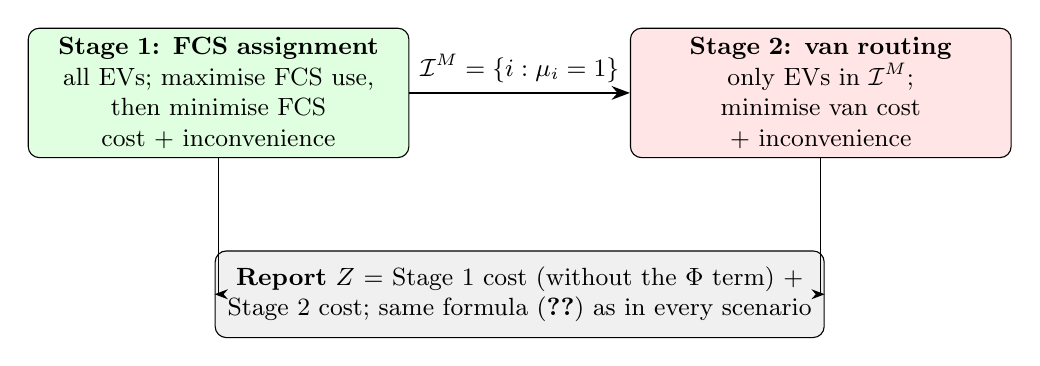
\begin{tikzpicture}[>=Stealth,box/.style={draw,rounded corners,align=center,minimum height=1.1cm,font=\small}]
  \node[box,fill=green!12,text width=4.6cm] (s1) {\textbf{Stage 1: FCS assignment}\\all EVs; maximise FCS use,\\then minimise FCS cost + inconvenience};
  \node[box,fill=red!10,text width=4.6cm,right=2.8cm of s1] (s2) {\textbf{Stage 2: van routing}\\only EVs in $\I^M$;\\minimise van cost + inconvenience};
  \draw[->,thick] (s1) -- node[above,font=\small]{$\I^M=\{i:\mu_i=1\}$} (s2);
  \node[box,fill=black!6,text width=7.5cm,below=2.0cm of $(s1)!0.5!(s2)$] (ev) {\textbf{Report} $Z=$ Stage~1 cost (without the $\Phi$ term) $+$ Stage~2 cost; same formula \eqref{eq:Z} as in every scenario};
  \draw[->] (s1) |- (ev); \draw[->] (s2) |- (ev);
\end{tikzpicture}
\end{center}

Stage~1 does not look at the vans, and Stage~2 cannot change what Stage~1 decided. That is the definition of ``FCS first, then MCS''.

%----------------------------------------------------------------
\subsection{Stage 1: assign EVs to fixed stations}

\textbf{Objective.}
\begin{equation}
\begin{split}
\min\ Z^{(1)}=\;&\underbrace{\Phi\sum_{i\in\I}\mu_i}_{\text{FCS first}}
+\underbrace{c^{EV}\sum_i\sum_{f\in\F_i}d_{if}Y_{if}}_{Z_1}
+\underbrace{Z^F_{\text{energy}}}_{\text{FCS part of }Z_4}\\
&+\underbrace{\sum_i\sum_{f\in\F_i}\rho^F_{if}Y_{if}+\alpha\sum_i w_i(C_i-r_i)+c^L\sum_i w_iL_i}_{\text{FCS customers' inconvenience}}
\end{split}
\label{eq:obj1}
\end{equation}
with $C_i=S_i+\tau^F_iY_i$ in this stage. $\Phi$ is a penalty for handing an EV to the vans. It is chosen larger than anything an extra FCS customer can add to the rest of \eqref{eq:obj1}, e.g.
\[
\Phi > \max_{i}\max_{f\in\F_i}\big(c^{EV}d_{if}+\pi^{\max}E_i+\rho^F_{if}\big)+n\,(\alpha+c^L)\,w_{\max}\,T,
\]
so Stage~1 first \textbf{maximises the number of EVs served at an FCS}, and only among those solutions minimises FCS cost and inconvenience. ($\pi^{\max}$ is the highest grid price.) A numerically safer equivalent is to solve twice: first $\max\sum_iY_i$, then fix that number and minimise the rest.
\ifTOU
Because $Z^F_{\text{energy}}$ uses the peak price, Stage~1 may \emph{start sessions later} to leave the peak, if the price saving beats the extra waiting cost (Section~\ref{sec:expect}).
\fi

\textbf{Constraints.}
\begin{align}
\sum_{g\in\G_i}y_{ig}+\mu_i &= 1 && \forall i\in\I \label{eq:s1assign}\\
S_i &\ge r_i+\sum_{f\in\F_i}t_{if}Y_{if} && \forall i\in\I \label{eq:fcsarr}\\
S_i &\le r_i+T\,(1-\mu_i) && \forall i\in\I \label{eq:s1park}\\
S_j &\ge S_i+\tau^F_i-(T+\tau^F_i)(3-y_{ig}-y_{jg}-o_{ij}) && \forall g,\ (i,j)\in\mathcal{P}_g \label{eq:disj1}\\
S_i &\ge S_j+\tau^F_j-(T+\tau^F_j)(2-y_{ig}-y_{jg}+o_{ij}) && \forall g,\ (i,j)\in\mathcal{P}_g \label{eq:disj2}\\
\sum_i y_{ig_1} &\ge \sum_i y_{ig_2} && \forall f,\ \G_f=\{g_1,g_2\} \label{eq:gunsym}\\
S_i+\tau^F_iY_i &\le T,\qquad L_i\ge S_i+\tau^F_iY_i-l_i && \forall i\in\I \label{eq:s1time}
\end{align}
\ifTOU plus the time-of-use split \eqref{eq:tou1}--\eqref{eq:tou5} of each FCS session (Section~\ref{sec:price}).\fi
\desc{\eqref{eq:s1assign}: every EV either gets one reachable gun or is handed to the vans. An EV that reaches no FCS ($\G_i=\emptyset$) is forced to $\mu_i=1$. \eqref{eq:fcsarr}: an FCS session cannot start before the EV has asked and driven to the station. \eqref{eq:s1park}: for an EV handed to the vans, $S_i$ is parked at $r_i$, so it adds no waiting in Stage~1 (its real start time is decided in Stage~2). \eqref{eq:disj1}--\eqref{eq:disj2}: two EVs on the same gun do not overlap; $o_{ij}$ picks who goes first. With two guns per station this means at most two EVs charge at a station at a time. \eqref{eq:gunsym}: symmetry breaking between the two identical guns (optional). \eqref{eq:s1time}: finished by $T$; lateness.}

\textbf{Optional acceptability rule.} An operator may refuse to send a driver to a station that is ``too inconvenient'', e.g.\ only allow gun $g$ of station $f$ for EV $i$ if $\hat\rho^F_{if}\le\bar\rho$. This only shrinks $\G_i$, so EVs whose stations are all too far go to the vans. Report results with and without it.

\textbf{Output:} $\I^M=\{i:\mu_i=1\}$, the EVs left for the vans; plus each FCS customer's gun and start time.

%----------------------------------------------------------------
\subsection{Stage 2: route the vans to the leftover EVs}

Stage~2 is a vehicle routing problem with time windows, on the EVs in $\I^M$ only. Here $C_i=S_i+\tau^M_i$.

\textbf{Objective.}
\begin{equation}
\begin{split}
\min\ Z^{(2)}=\;&\underbrace{c^M\sum_m\sum_{(i,j)\in\A^M}d_{ij}x_{ijm}}_{Z_2}+\underbrace{\sum_m c^D_mu_m}_{Z_3}+\underbrace{Z^M_{\text{energy}}}_{\text{van part of }Z_4}\\
&+\underbrace{\sum_{i\in\I^M}\sum_m\rho^M_{im}z_{im}+\alpha\sum_{i\in\I^M}w_i(C_i-r_i)+c^L\sum_{i\in\I^M}w_iL_i}_{\text{van customers' inconvenience}}
\end{split}
\label{eq:obj2}
\end{equation}
Since every EV in $\I^M$ must be served by some van, $Z^M_{\text{energy}}$ and the $\rho^M$ term are constants here. They are kept so that $Z^{(2)}$ is the true cost of Stage~2. Waiting and lateness make the vans visit urgent EVs early.

\textbf{Constraints.}
\begin{align}
\sum_{m\in\M}z_{im} &= 1 && \forall i\in\I^M \label{eq:s2assign}\\
\sum_{j:(0,j)\in\A^M}x_{0jm} = \sum_{i:(i,n+1)\in\A^M}x_{i,n+1,m} &= u_m && \forall m \label{eq:depot}\\
\sum_{i:(i,j)\in\A^M}x_{ijm} = \sum_{k:(j,k)\in\A^M}x_{jkm} &= z_{jm} && \forall j\in\I^M,\ m \label{eq:flow}\\
\sum_{i\in\I^M}z_{im} &\le Q_m\,u_m && \forall m \label{eq:cap}\\
\sum_{i\in\I^M}\frac{E_i}{\eta}z_{im}+\beta\sum_{(i,j)\in\A^M}d_{ij}x_{ijm} &\le B_m\,u_m && \forall m \label{eq:batt}
\end{align}
\begin{align}
S_j &\ge \max\{r_j,\ t_{0j}\,x_{0jm}\} && \forall j\in\I^M,\ m \label{eq:depart}\\
S_j &\ge S_i+\tau^M_i+t_{ij}-(T+\tau^M_i+t_{ij})(1-x_{ijm}) && \forall i\neq j,\ m \label{eq:seq}\\
S_i+\tau^M_i+t_{i,n+1} &\le T+(\tau^M_i+t_{i,n+1})(1-x_{i,n+1,m}) && \forall i,\ m \label{eq:return}\\
S_i+\tau^M_i \le T,\quad L_i &\ge S_i+\tau^M_i-l_i && \forall i\in\I^M \label{eq:s2time}\\
u_m &\ge u_{m+1} && m<|\M| \label{eq:vansym}
\end{align}
\desc{\eqref{eq:s2assign}: each leftover EV gets one van. \eqref{eq:depot}: a used van leaves and returns to the depot once. \eqref{eq:flow}: each EV on van $m$ is entered and left exactly once by that van. \eqref{eq:cap}: at most $Q_m$ EVs per van. \eqref{eq:batt}: delivered energy (with transfer losses) plus driving energy fits in the van battery. \eqref{eq:depart}: no start before the request, or before the van can drive there from the depot (written as two linear constraints). \eqref{eq:seq}: if the van goes $i\to j$, it finishes $i$ and drives to $j$ before starting $j$. This gives one EV at a time and removes subtours (MTZ-type). \eqref{eq:return}: back at the depot by $T$. \eqref{eq:s2time}: finished by $T$; lateness. \eqref{eq:vansym}: use identical vans in index order.}

\textbf{If Stage 2 is infeasible} (too many leftover EVs for the fleet by $T$), the sequential policy has \emph{failed} on that instance. For diagnosis, add $s_i\in\{0,1\}$ (``unserved''), replace \eqref{eq:s2assign} by $\sum_mz_{im}+s_i=1$ and add $\Phi^U\sum_is_i$ to \eqref{eq:obj2}. Then report the number of EVs that could not be served. This is a useful comparison with the integrated scenario, which may serve all of them.

%----------------------------------------------------------------
\subsection{Reported value}
\[
Z^{\text{S\scen}}=\big(Z^{(1)*}-\Phi\,|\I^M|\big)+Z^{(2)*},
\]
which is exactly \eqref{eq:Z} evaluated at the combined solution. The stage-1 solution plus the stage-2 solution is a feasible solution of the integrated model (S\ifTOU 4\else 3\fi), so
$Z^{\text{S\ifTOU 4\else 3\fi}}\le Z^{\text{S\scen}}$. The difference is the \emph{value of integration}.

\else
%---------------------------------------------------------------- INT
\subsection{Objective}
\begin{equation}
\min\ Z \quad\text{as in \eqref{eq:Z}, with }Z^F_{\text{energy}}=\ifTOU P^F\textstyle\sum_i\big[\pi^\off(\theta^1_i+\theta^3_i)+\pi^\pk\theta^2_i\big]\else\pi^F\textstyle\sum_iE_iY_i\fi,\quad C_i=S_i+\tau^F_iY_i+\tau^M_iZ_i. \label{eq:objint}
\end{equation}
Written out in full:
\begin{align*}
\min\ Z=\;& c^{EV}\sum_i\sum_{f\in\F_i}d_{if}Y_{if}+c^M\sum_m\sum_{(i,j)\in\A}d_{ij}x_{ijm}+\sum_mc^D_mu_m\\
&+\ifTOU P^F\sum_i\big[\pi^\off(\theta^1_i+\theta^3_i)+\pi^\pk\theta^2_i\big]\else\pi^F\sum_iE_iY_i\fi
+\pi^M\sum_i\sum_m\frac{E_i}{\eta}z_{im}\\
&+\sum_i\sum_{f\in\F_i}\rho^F_{if}Y_{if}+\sum_i\sum_m\rho^M_{im}z_{im}+\alpha\sum_iw_i(C_i-r_i)+c^L\sum_iw_iL_i .
\end{align*}
Every term is linear. One model weighs everything at once: an EV goes to a van exactly when the van's extra km, dispatch and energy cost are outweighed by the effort and waiting it saves the driver\ifTOU, or by the peak-price energy it avoids\fi.

\subsection{Constraints}

\textbf{Assignment.}
\begin{equation}
\sum_{g\in\G_i}y_{ig}+\sum_{m\in\M}z_{im}=1\qquad\forall i\in\I \label{eq:assign}
\end{equation}
\desc{Exactly one resource per EV: one reachable gun or one van. EVs that reach no FCS are forced onto a van.}

\textbf{Fixed stations.}
\begin{align}
S_i &\ge r_i+\sum_{f\in\F_i}t_{if}Y_{if} && \forall i \label{eq:fcsarr}\\
S_j &\ge S_i+\tau^F_i-(T+\tau^F_i)(3-y_{ig}-y_{jg}-o_{ij}) && \forall g,\ (i,j)\in\mathcal{P}_g \label{eq:disj1}\\
S_i &\ge S_j+\tau^F_j-(T+\tau^F_j)(2-y_{ig}-y_{jg}+o_{ij}) && \forall g,\ (i,j)\in\mathcal{P}_g \label{eq:disj2}\\
\sum_iy_{ig_1} &\ge \sum_iy_{ig_2} && \forall f,\ \G_f=\{g_1,g_2\} \label{eq:gunsym}
\end{align}
\desc{\eqref{eq:fcsarr}: an FCS session starts after the request and the drive to the station (for a van customer this is just $S_i\ge r_i$). \eqref{eq:disj1}--\eqref{eq:disj2}: EVs on the same gun do not overlap; $o_{ij}$ chooses the order. \eqref{eq:gunsym}: optional symmetry breaking.}

\textbf{Vans: routes, capacity, battery.}
\begin{align}
\sum_{j:(0,j)\in\A}x_{0jm}=\sum_{i:(i,n+1)\in\A}x_{i,n+1,m} &= u_m && \forall m \label{eq:depot}\\
\sum_{i:(i,j)\in\A}x_{ijm}=\sum_{k:(j,k)\in\A}x_{jkm} &= z_{jm} && \forall j\in\I,\ m \label{eq:flow}\\
\sum_iz_{im} &\le Q_mu_m && \forall m \label{eq:cap}\\
\sum_i\frac{E_i}{\eta}z_{im}+\beta\sum_{(i,j)\in\A}d_{ij}x_{ijm} &\le B_mu_m && \forall m \label{eq:batt}
\end{align}
\desc{\eqref{eq:depot}: a used van leaves and returns once. \eqref{eq:flow}: each EV on van $m$ is visited exactly once by it. \eqref{eq:cap}: at most $Q_m$ EVs. \eqref{eq:batt}: delivered energy (with losses) plus driving energy fits in the battery.}

\textbf{Vans: timing (one EV at a time, no subtours).}
\begin{align}
S_j &\ge t_{0j}\,x_{0jm} && \forall j\in\I,\ m \label{eq:depart}\\
S_j &\ge S_i+\tau^M_i+t_{ij}-(T+\tau^M_i+t_{ij})(1-x_{ijm}) && \forall i\neq j\in\I,\ m \label{eq:seq}\\
S_i+\tau^M_i+t_{i,n+1} &\le T+(\tau^M_i+t_{i,n+1})(1-x_{i,n+1,m}) && \forall i,\ m \label{eq:return}
\end{align}
\desc{\eqref{eq:depart}: the first stop cannot start before the van has driven there. \eqref{eq:seq}: $i\to j$ means finish $i$, drive, then start $j$; start times rise along a route, so no subtour can close. \eqref{eq:return}: back at the depot by $T$.}

\textbf{Horizon and lateness.}
\begin{equation}
C_i\le T,\qquad L_i\ge C_i-l_i\qquad\forall i\in\I \label{eq:time}
\end{equation}
\desc{Every EV is fully charged within the horizon; $L_i$ measures lateness.}

\ifTOU
\textbf{Time-of-use split.} Constraints \eqref{eq:tou1}--\eqref{eq:tou5} of Section~\ref{sec:price}.
\fi

\textbf{Symmetry and domains.}
\begin{equation}
u_m\ge u_{m+1};\qquad y,z,x,u,o\ifTOU,\kappa\fi\in\{0,1\};\qquad S_i,L_i\ifTOU,\theta^p_i\fi\ge0 \label{eq:dom}
\end{equation}
\fi

%=====================================================================
\section{Learning-to-optimise (RL) formulation}\label{sec:rl}

\textbf{Main rule:} the reward of each action is \emph{minus the increase in $Z$ that the action causes}. The rewards over an episode then add up to $-Z$ of the solution the policy builds. RL and MILP results are measured on the same yardstick \eqref{eq:Z}, and the MILP optimum is the benchmark for the RL gap.

\ifSEQ
%---------------------------------------------------------------- RL SEQ
The RL pipeline has the same two stages as the MILP.

\subsection{Stage 1 policy: FCS assignment}
\begin{itemize}[leftmargin=1.4em,itemsep=2pt]
  \item \textbf{Episode / epochs:} EVs are taken in order of request time $r_i$ (ties: higher $w_i$ first). One decision per EV.
  \item \textbf{State:} features of the current EV $k$ ($E_k,r_k,l_k,w_k,R_k$, location); for each gun $g$ the time $F_g$ it becomes free; summary features of the EVs still to come (count and positions near each station)\ifTOU; the current price and the time until $T_1$ and $T_2$\fi.
  \item \textbf{Action:} a gun $g\in\G_k$, or ``hand to vans''. \textbf{FCS-first mask:} ``hand to vans'' is allowed \emph{only} if no gun can finish EV $k$ by $T$ (or, with the optional rule, if all remaining guns have $\hat\rho^F_{kf}>\bar\rho$).
  \ifTOU\item \textbf{Optional timing action:} ``gun $g$, start after the peak'', i.e.\ $S_k=\max\{\text{earliest},T_2\}$, allowed only if the session still ends by $T$.\fi
  \item \textbf{Transition:} $S_k=\max\{r_k+t_{kf},F_g\}$ (or later, for the timing action); $F_g\leftarrow S_k+\tau^F_k$.
  \item \textbf{Reward:} $-\Big[c^{EV}d_{kf}+\text{energy}_k+\rho^F_{kf}+\alpha w_k(S_k+\tau^F_k-r_k)+c^Lw_k(S_k+\tau^F_k-l_k)^+\Big]$, where energy$_k$ = \ifTOU$P^F\big[\pi^\off\cdot(\text{off-peak hours of }[S_k,S_k+\tau^F_k])+\pi^\pk\cdot(\text{peak hours})\big]$, computed exactly in the simulator\else$\pi^FE_k$\fi. Handing an EV to the vans gives reward $0$ here; its cost is counted in Stage~2.
\end{itemize}
Note: a simple baseline for Stage~1 is the greedy rule ``gun with the largest one-step reward''. What RL can learn on top of this is, for example, to keep a nearby gun free for an urgent EV that arrives later.

\subsection{Stage 2 policy: van routing over $\I^M$}
\begin{itemize}[leftmargin=1.4em,itemsep=2pt]
  \item \textbf{Epochs:} whenever a van becomes free (the earliest-free van decides first).
  \item \textbf{State:} for each van: position, time free, remaining battery $b_m$, EVs served so far, dispatched or not; for each unserved EV in $\I^M$: location, $E_i,r_i,l_i,w_i$; current time.
  \item \textbf{Action:} the next EV $j$ for this van, or ``return to depot'' (ends the route). Mask: $j$ must be feasible: battery covers $E_j/\eta$ plus driving to $j$ and back to the depot, the count stays $\le Q_m$, and $j$ can be finished with the van back at the depot by $T$.
  \item \textbf{Transition:} $S_j=\max\{r_j,\ \text{time free}+t_{\text{pos},j}\}$; the van moves to $j$ and is free at $S_j+\tau^M_j$; $b_m$ falls by $E_j/\eta+\beta d_{\text{pos},j}$.
  \item \textbf{Reward:} serving $j$: $-\Big[c^Md_{\text{pos},j}+c^D_m[\text{first stop}]+\pi^M\frac{E_j}{\eta}+\rho^M_{jm}+\alpha w_j(S_j+\tau^M_j-r_j)+c^Lw_j(S_j+\tau^M_j-l_j)^+\Big]$; returning: $-c^Md_{\text{pos},0}$. EVs still unserved at the end: $-\Phi^U$ each.
  \item \textbf{Policy:} an attention-based routing policy (e.g.\ Kool et al., 2019, ``Attention, Learn to Solve Routing Problems!'') trained with REINFORCE or PPO. Baseline: nearest-feasible-EV heuristic.
\end{itemize}
Episode return of Stage~1 + Stage~2 $=-Z^{\text{S\scen}}$.

\else
%---------------------------------------------------------------- RL INT
One policy decides both who serves each EV and the van routes.
\begin{itemize}[leftmargin=1.4em,itemsep=2pt]
  \item \textbf{Episode / epochs:} EVs are taken in order of request time $r_i$ (ties: higher $w_i$ first). One decision per EV.
  \item \textbf{State:} (i) the current EV $k$: location, $E_k,r_k,l_k,w_k,R_k$, reachable stations; (ii) each gun $g$: time $F_g$ it becomes free; (iii) each van $m$: current end-of-route position, time free, remaining battery $b_m$, EVs served, dispatched or not; (iv) embeddings of the not-yet-assigned EVs (for look-ahead)\ifTOU; (v) current price, time until $T_1$ and $T_2$\fi.
  \item \textbf{Action:} $a\in\G_k\cup\M$: a gun, or a van (EV $k$ is appended to the end of that van's route). \textbf{Mask} infeasible actions: a gun that cannot finish $k$ by $T$; a van without enough battery for $E_k/\eta$ plus the drive to $k$ and back to the depot, with $Q_m$ reached, or unable to finish $k$ and return by $T$.
  \ifTOU\item \textbf{Optional timing action:} ``gun $g$, start after the peak'' ($S_k=\max\{\text{earliest},T_2\}$, if it still ends by $T$).\fi
  \item \textbf{Transition:} gun: $S_k=\max\{r_k+t_{kf},F_g\}$, $F_g\leftarrow S_k+\tau^F_k$. Van: $S_k=\max\{r_k,\ \text{free}_m+t_{\text{pos}_m,k}\}$, then the van moves to $k$, $\text{free}_m\leftarrow S_k+\tau^M_k$, $b_m\mathrel{-}=E_k/\eta+\beta d_{\text{pos}_m,k}$.
  \item \textbf{Reward} $=-\Delta Z$:
  \begin{align*}
  \text{gun } g\text{ at }f:&\quad -\Big[c^{EV}d_{kf}+\text{energy}^F_k+\rho^F_{kf}+\alpha w_k(C_k-r_k)+c^Lw_k(C_k-l_k)^+\Big]\\
  \text{van } m:&\quad -\Big[c^M\big(d_{\text{pos}_m,k}+d_{k,0}-d_{\text{pos}_m,0}\big)+c^D_m[\text{first use}]+\pi^M\tfrac{E_k}{\eta}\\
  &\qquad\quad+\rho^M_{km}+\alpha w_k(C_k-r_k)+c^Lw_k(C_k-l_k)^+\Big]
  \end{align*}
  The van distance term is the \emph{change} in route length when $k$ is inserted before the return to the depot, so the sum over the episode equals the total route length (the return legs telescope). energy$^F_k$ = \ifTOU$P^F\big[\pi^\off\cdot(\text{off-peak hours})+\pi^\pk\cdot(\text{peak hours of }[S_k,C_k])\big]$, computed exactly by the simulator; no linearisation is needed in RL\else$\pi^FE_k$\fi.
  \item \textbf{Dead end:} if every action is masked, EV $k$ is unserved: reward $-\Phi^U$, and the episode continues. Report the count.
  \item \textbf{Policy:} masked categorical policy over guns and vans, encoder with attention over EVs, guns and vans; trained with PPO. Natural baseline: greedy, i.e.\ choose the action with the largest one-step reward. That is the pairwise rule ``smallest $\hat\rho$ + cost'' from Section~\ref{sec:inc}.
\end{itemize}
Restriction to note: vans serve EVs in assignment order (append only). A variant that inserts $k$ at the cheapest position of a route is more flexible but has a larger action space.
\fi

\textbf{Reward scaling.} For stable training divide every reward by a constant, e.g.\ the greedy baseline's average $Z$ on the training instances. This does not change the optimal policy.

%=====================================================================
\section{What to expect and what to report}\label{sec:expect}

\ifnum\scen=1
\begin{itemize}[leftmargin=1.4em,itemsep=2pt]
  \item Vans serve only EVs that reach no station, or that the stations cannot finish by $T$. If stations have spare capacity, very few vans are dispatched.
  \item Inconvenience is high for EVs far from the nearest station (worked example: Rs\,682 at the FCS, against Rs\,458 if a van had been allowed).
  \item With too few vans Stage~2 becomes infeasible (unserved EVs), even when the integrated model S3 could serve everyone. Report the smallest $|\M|$ at which S1 is feasible and compare it with S3.
\end{itemize}
\fi
\ifnum\scen=2
\begin{itemize}[leftmargin=1.4em,itemsep=2pt]
  \item \textbf{When does Stage~1 delay a session to avoid the peak?} Moving one hour of charging out of the peak saves $(\pi^\pk-\pi^\off)P^F=3\times22=$ Rs\,66, but delays completion by up to an hour, which costs $\alpha w_i\ge$ Rs\,200. So with the default values Stage~1 almost never delays. It mostly pays the higher price, and S2 costs roughly S1 plus the peak surcharge. Sessions start later only if $\alpha$ is small (try $\lambda<0.33$ in the sensitivity analysis).
  \item The van assignment is the same as in S1 unless Stage~1's timing changes which EVs fit at the stations. Stage~1 cannot use vans to escape the peak price.
  \item Extra KPI: \textbf{grid energy drawn at FCS during the peak}, $P^F\sum_i\theta^2_i$ (kWh). Compare with S4.
\end{itemize}
\fi
\ifnum\scen=3
\begin{itemize}[leftmargin=1.4em,itemsep=2pt]
  \item Vans take EVs for which the saved inconvenience exceeds the extra van cost (worked example: van chosen, saving Rs\,224). Expect vans to serve EVs that are far from every station, have low range (high $w_i$), or have early deadlines, while EVs near a station still use it.
  \item \textbf{Value of integration under flat price:} $Z^{\text{S1}}-Z^{\text{S3}}\ge0$. Report it per component ($Z_1,\dots,Z_5$): typically operating cost rises a little and inconvenience falls a lot.
  \item Vary $|\M|$ (0, 1, 2, \dots): the first few vans lower $Z$ sharply, then the effect levels off. That curve shows the scenarios where mobile chargers help most.
\end{itemize}
\fi
\ifnum\scen=4
\begin{itemize}[leftmargin=1.4em,itemsep=2pt]
  \item During the peak a van kWh costs about the same as an FCS kWh (Rs\,10.0 each), so the vans' energy disadvantage disappears and vans also absorb \emph{peak-hour} demand that would otherwise be charged on the grid at peak price.
  \item Expect more van usage than in S3, concentrated on requests in $[T_1,T_2]$, and lower grid energy at the stations during the peak, $P^F\sum_i\theta^2_i$, than in S2.
  \item \textbf{Value of integration under peak pricing:} $Z^{\text{S2}}-Z^{\text{S4}}$. It should be larger than $Z^{\text{S1}}-Z^{\text{S3}}$, because integration now also allows price arbitrage.
  \item \textbf{Peak pricing with full flexibility:} $Z^{\text{S4}}-Z^{\text{S3}}$ should be smaller than $Z^{\text{S2}}-Z^{\text{S1}}$: vans cushion the price increase.
\end{itemize}
\fi

\textbf{Cross-scenario comparison table} (fill in from the four runs):
\begin{center}
\renewcommand{\arraystretch}{1.2}
\begin{tabular}{@{}lll@{}}
\toprule
\textbf{Comparison} & \textbf{Measures} & \textbf{Expected sign} \\
\midrule
S1 $-$ S3 & value of integration, flat price & $\ge0$ \\
S2 $-$ S4 & value of integration, peak price & $\ge0$, larger than S1 $-$ S3 \\
S2 $-$ S1 & cost of peak pricing, FCS-first operator & $>0$ \\
S4 $-$ S3 & cost of peak pricing, flexible operator & $>0$, smaller than S2 $-$ S1 \\
\bottomrule
\end{tabular}
\end{center}
Report for each: $Z$ and its components, number of vans used, EVs per resource, mean and maximum inconvenience per EV, total lateness, peak-hour grid energy, solve time, and (for RL) the gap to the MILP optimum.

%=====================================================================
\appendix
\section{Illustrative parameter values}\label{app:values}

These are starting values for experiments, not data. All are meant to be varied in the analysis. Values in Rs.

\begin{center}
\renewcommand{\arraystretch}{1.15}
\begin{tabular}{@{}llp{6.2cm}@{}}
\toprule
\textbf{Parameter} & \textbf{Value} & \textbf{Note} \\
\midrule
$T$, $[T_1,T_2]$ & 7 h, $[2,6]$ & 16:00--23:00, peak 18:00--22:00 \\
$P^F$, $P^M$ & 22 kW, 30 kW & \\
$v$, $\beta$, $\eta$ & 25 km/h, 0.25 kWh/km, 0.9 & \\
$B_m$, $Q_m$, $|\M|$ & 150 kWh, 6, 2--6 & \\
$c^{EV}$, $c^M$, $c^D_m$ & Rs\,4/km, Rs\,15/km, Rs\,1500 & van km includes driver time \\
$\pi^F$ (flat) & Rs\,8.7/kWh & equals the time-average of the ToU tariff over $[0,T]$ \\
$\pi^\off$, $\pi^\pk$ (ToU) & Rs\,7/kWh, Rs\,10/kWh & $(3\times7+4\times10)/7=8.7$ \\
$c^{bat}$ & Rs\,2/kWh & van battery wear \\
$\pi^M$ & Rs\,10.7 (flat) / Rs\,9.0 (ToU) & $=\pi^F+c^{bat}$ / $=\pi^\off+c^{bat}$ \\
$\alpha$, $\alpha^D$ & Rs\,200/h, Rs\,100/h & value of time; extra for attended time \\
$h^F$, $h^M$, $\varphi$ & Rs\,50, Rs\,10, Rs\,100 & trip hassle, hand-over, range stress \\
$c^L$ & Rs\,300/h & lateness \\
$w_i$ & $1+2(1-R_i/R_{\max})$, $R_i\sim U[3,40]$ km & priority from remaining range \\
\bottomrule
\end{tabular}
\end{center}

The flat price is set to the time-average of the peak tariff. The price \emph{level} is then the same in both pricing cases, and only the price \emph{shape} differs. Without this, part of S1 vs S2 would just reflect a different average price.

\end{document}
"
%    pdflatex -jobname=scenario2_peak_sequential   "\def\scen{2}% =====================================================================
%  One source, four PDFs.  Build with build.sh (or by hand):
%    pdflatex -jobname=scenario1_flat_sequential   "\def\scen{1}\input{scenario_master}"
%    pdflatex -jobname=scenario2_peak_sequential   "\def\scen{2}\input{scenario_master}"
%    pdflatex -jobname=scenario3_flat_integrated   "\def\scen{3}\input{scenario_master}"
%    pdflatex -jobname=scenario4_peak_integrated   "\def\scen{4}\input{scenario_master}"
%  (run each twice for cross-references)
% =====================================================================
\documentclass[11pt,a4paper]{article}
\usepackage[margin=2.2cm]{geometry}
\usepackage{amsmath,amssymb,amsfonts}
\usepackage{booktabs,array,tabularx}
\usepackage{enumitem}
\usepackage[table]{xcolor}
\usepackage{tikz}
\usetikzlibrary{arrows.meta,positioning,calc}
\usepackage[colorlinks=true,linkcolor=blue!50!black,urlcolor=blue!50!black]{hyperref}
\usepackage{titlesec}
\titleformat{\section}{\large\bfseries}{\thesection}{0.8em}{}
\titleformat{\subsection}{\normalsize\bfseries}{\thesubsection}{0.8em}{}
\setlength{\parindent}{0pt}
\setlength{\parskip}{5pt}

% ---------------- scenario switches ----------------
\ifdefined\scen\else\def\scen{1}\fi
\newif\ifTOU \TOUfalse   % true = time-of-use (peak) price
\newif\ifSEQ \SEQfalse   % true = FCS first, then MCS
\ifnum\scen=1 \SEQtrue \fi
\ifnum\scen=2 \TOUtrue \SEQtrue \fi
\ifnum\scen=4 \TOUtrue \fi

\newcommand{\pricename}{\ifTOU time-of-use price (dearer evening peak)\else single (flat) price all day\fi}
\newcommand{\structname}{\ifSEQ FCS first, then MCS (sequential)\else FCS and MCS together (integrated)\fi}

% ---------------- notation ----------------
\newcommand{\I}{\mathcal{I}}
\newcommand{\F}{\mathcal{F}}
\newcommand{\G}{\mathcal{G}}
\newcommand{\M}{\mathcal{M}}
\newcommand{\N}{\mathcal{N}}
\newcommand{\A}{\mathcal{A}}
\newcommand{\Rs}{\text{Rs}\,}
\newcommand{\pk}{\mathrm{pk}}
\newcommand{\off}{\mathrm{off}}
\newcommand{\desc}[1]{\par\vspace{-2pt}{\small\color{black!75}\textit{Meaning:} #1}\par\vspace{4pt}}
\newcommand{\cell}[2]{\ifnum\scen=#1\cellcolor{blue!18}\textbf{S#1 (this document)}\\\textbf{#2}\else S#1\\#2\fi}

\title{\textbf{EV Charging Network Optimisation}\\[4pt]
\large Scenario \scen: \pricename\ $+$ \structname\\[2pt]
\normalsize MILP and RL formulation}
\author{CP 320 OR for Mobility Management, course project}
\date{2 October 2026}

\begin{document}
\maketitle

%=====================================================================
\section{Where this scenario sits}

The project studies four scenarios: two ways of pricing grid electricity, times two ways of making the decisions.

\begin{center}
\renewcommand{\arraystretch}{1.5}
\begin{tabular}{>{\raggedright\arraybackslash}p{4.2cm}|>{\centering\arraybackslash}p{4.6cm}|>{\centering\arraybackslash}p{4.6cm}}
 & \textbf{Flat price all day} & \textbf{Time-of-use (peak) price} \\ \hline
\textbf{Sequential:} FCS first, leftover EVs to MCS &
\begin{tabular}[c]{@{}c@{}}\cell{1}{flat + sequential}\end{tabular} &
\begin{tabular}[c]{@{}c@{}}\cell{2}{peak + sequential}\end{tabular} \\ \hline
\textbf{Integrated:} FCS and MCS decided together &
\begin{tabular}[c]{@{}c@{}}\cell{3}{flat + integrated}\end{tabular} &
\begin{tabular}[c]{@{}c@{}}\cell{4}{peak + integrated}\end{tabular} \\
\end{tabular}
\end{center}

\textbf{The four scenarios do not have four different objectives.} They share \emph{one} cost yardstick $Z$ (Section~\ref{sec:obj}): the same cost terms and the same customer inconvenience (Section~\ref{sec:inc}). Only two things change:
\begin{itemize}[leftmargin=1.4em,itemsep=1pt]
  \item \textbf{Pricing} changes the formula for one term, the FCS energy cost (Section~\ref{sec:price}).
  \item \textbf{Decision structure} changes \emph{how} $Z$ is minimised: in one model (integrated), or in two stages (sequential), where each stage minimises its own part of $Z$.
\end{itemize}
Because the yardstick is the same, the four optimal values can be compared directly. The differences measure the \emph{value of integration} (S1$\to$S3, S2$\to$S4) and the \emph{effect of peak pricing} (S1$\to$S2, S3$\to$S4).

\ifnum\scen=1
\textbf{This scenario (S1)} is the baseline, the ``status quo''. Electricity costs the same at every hour, every EV that can be charged at a fixed station is sent there, and vans only take what is left over.
\fi
\ifnum\scen=2
\textbf{This scenario (S2)} keeps the FCS-first rule of S1, but grid electricity is dearer during the evening peak. Stage~1 can react to the price only by \emph{rescheduling} FCS sessions. It cannot hand a peak-hour EV to a van.
\fi
\ifnum\scen=3
\textbf{This scenario (S3)} keeps the flat price of S1, but the operator decides FCS and MCS service \emph{together}. An EV can be sent to a van even when a fixed station could take it, whenever that lowers total cost plus inconvenience.
\fi
\ifnum\scen=4
\textbf{This scenario (S4)} is the most flexible one: peak pricing at fixed stations, and FCS and MCS decided together. Van energy was bought off-peak, so vans can also be used to keep charging \emph{out of the expensive peak}.
\fi

%=====================================================================
\section{Setting and assumptions}\label{sec:setting}

\textbf{Time.} The planning horizon is $[0,T]$ with $T=7$\,h (16:00--23:00). It contains the evening peak window $[T_1,T_2]=[2,6]$ (18:00--22:00). The horizon is the same in all four scenarios. It is wider than the peak itself so that, under peak pricing, there is cheaper time on both sides of the peak.\ifTOU\else\ In this scenario the price is flat, so the window plays no role in the model.\fi

\textbf{Assumptions} (the same as MILP v3, plus two about energy):
\begin{enumerate}[leftmargin=1.6em,itemsep=1pt]
  \item Static, continuous time. All requests in the horizon are known at time $0$, and request $i$ becomes active at $r_i$.
  \item An EV served by an FCS drives there itself on its own battery (only to stations within its range $R_i$). The driver stays with the car while it waits for a free gun and while it charges.
  \item An EV served by an MCS stays parked where it is, and the driver is free in the meantime.
  \item Each FCS gun and each van charges one EV at a time, without interruption, at constant power.
  \item A van's battery covers both its driving and the energy it delivers. \textbf{The van battery is charged at the depot before the horizon starts}\ifTOU, i.e.\ at the off-peak price\fi, and is not recharged during the horizon.
  \item Every EV must be fully charged by $T$ (hard). Finishing after the driver's desired time $l_i$ is allowed but penalised.
\end{enumerate}

%=====================================================================
\section{Notation}\label{sec:notation}

\subsection*{Sets}
\begin{tabularx}{\textwidth}{@{}lX@{}}
\toprule
$\I=\{1,\dots,n\}$ & EV charging requests \\
$\F$; $\G_f$ ($|\G_f|=2$); $\G=\bigcup_f\G_f$ & fixed charging stations; guns of FCS $f$; all guns ($f(g)$ = station of gun $g$) \\
$\F_i=\{f: d_{if}\le R_i\}$, $\G_i=\bigcup_{f\in\F_i}\G_f$ & stations / guns EV $i$ can reach on its remaining range \\
$\M$ & mobile charging vans (MCS) \\
$0,\ n+1$ & depot as start node / end node (same place) \\
$\N=\{0\}\cup\I\cup\{n+1\}$, $\A$ & routing nodes; allowed van arcs $(i,j)$, $i\in\{0\}\cup\I$, $j\in\I\cup\{n+1\}$, $i\neq j$ \\
$\mathcal{P}_g=\{(i,j): i<j,\ g\in\G_i\cap\G_j\}$ & pairs of EVs that could share gun $g$ \\
\ifSEQ
$\I^M\subseteq\I$ & EVs handed to the vans by Stage~1 (an \emph{output} of Stage~1, a fixed input to Stage~2) \\
$\N^M$, $\A^M$ & routing nodes / arcs restricted to $\I^M$ \\
\fi
\bottomrule
\end{tabularx}

\subsection*{Parameters}
\begin{tabularx}{\textwidth}{@{}lX@{}}
\toprule
$E_i,\ r_i,\ l_i,\ R_i$ & energy demand (kWh), request time, desired completion time (h), remaining range (km) \\
$w_i\ge1$ & priority of EV $i$; $w_i=1+\kappa(1-R_i/R_{\max})$, so low-range EVs weigh more \\
$P^F,\ P^M$ & charging power of an FCS gun (22\,kW) / of a van (e.g.\ 30\,kW) \\
$\tau^F_i=E_i/P^F,\ \tau^M_i=E_i/P^M$ & charging time of EV $i$ at an FCS / by a van (h) \\
$d_{if},t_{if}$;\ $d_{ij},t_{ij}$ & distance (km) and time (h): EV$\to$FCS; between routing nodes ($t=d/v$) \\
$B_m,\ Q_m,\ \beta,\ \eta$ & van battery (kWh), max EVs per van, van consumption (kWh/km), transfer efficiency \\
$c^{EV},\ c^M,\ c^D_m$ & cost per km of EV driving, per km of van driving; fixed dispatch cost of van $m$ \\
\ifTOU
$\pi^\off,\ \pi^\pk$ & grid price (Rs/kWh) off-peak / in $[T_1,T_2]$, with $\pi^\pk\ge\pi^\off$ \\
\else
$\pi^F$ & grid price (Rs/kWh), the same at every hour \\
\fi
$c^{bat}$ & van battery wear per kWh cycled \\
$\pi^M$ & cost of 1 kWh taken from a van battery: $\pi^M=\ifTOU\pi^\off\else\pi^F\fi+c^{bat}$ (Section~\ref{sec:price}) \\
$\alpha,\ \alpha^D,\ h^F,\ h^M,\ \varphi,\ c^L$ & inconvenience coefficients (Section~\ref{sec:inc}) \\
\bottomrule
\end{tabularx}

\subsection*{Decision variables}
\begin{tabularx}{\textwidth}{@{}llX@{}}
\toprule
$y_{ig}$ & $\{0,1\}$ & EV $i$ charged at gun $g\in\G_i$ \\
$z_{im}$ & $\{0,1\}$ & EV $i$ served by van $m$ \\
$x_{ijm}$ & $\{0,1\}$ & van $m$ drives arc $(i,j)$ \\
$u_m$ & $\{0,1\}$ & van $m$ is dispatched \\
$o_{ij}$ & $\{0,1\}$ & for EVs $i<j$ that could share a gun: 1 if $i$ is charged before $j$ \\
\ifSEQ
$\mu_i$ & $\{0,1\}$ & Stage~1 only: EV $i$ is handed to the van fleet \\
\fi
\ifTOU
$\theta^1_i,\theta^2_i,\theta^3_i$ & $\ge0$ & hours of EV $i$'s FCS session before / inside / after the peak \\
$\kappa^1_i,\kappa^3_i$ & $\{0,1\}$ & EV $i$'s FCS session starts before $T_1$ / ends after $T_2$ \\
\fi
$S_i$ & $\ge0$ & time charging of EV $i$ starts (h), on whichever resource \\
$L_i$ & $\ge0$ & lateness of EV $i$ beyond $l_i$ (h) \\
\bottomrule
\end{tabularx}

\textbf{Short-hands} (linear expressions, not new variables):
\[
Y_{if}=\sum_{g\in\G_f}y_{ig},\qquad Y_i=\sum_{g\in\G_i}y_{ig}\ (\text{EV $i$ uses an FCS}),\qquad Z_i=\sum_{m\in\M}z_{im}\ (\text{EV $i$ uses a van}),
\]
\[
C_i=S_i+\tau^F_i\,Y_i+\tau^M_i\,Z_i \quad\text{(time EV $i$ is fully charged).}
\]

%=====================================================================
\section{Customer inconvenience}\label{sec:inc}

This section is \textbf{identical in all four scenario documents}. Inconvenience is a property of the customer, not of the price or of the planning method.

\subsection{What we mean by inconvenience}

Inconvenience is \emph{what the driver loses} from the moment they ask for a charge ($r_i$) until the car is fully charged ($C_i$), \emph{converted into rupees} so it can be added to the operator's costs. A driver loses three different things:

\begin{enumerate}[leftmargin=1.6em,itemsep=2pt]
  \item \textbf{Waiting:} the car is not ready. This lasts $C_i-r_i$ hours and affects \emph{every} driver, FCS or MCS.
  \item \textbf{Effort:} only an FCS customer has to drive to the station and sit there while the car charges. An MCS customer stays at home or at work and does something else. Driving to a far station also uses scarce battery range, which causes stress (``range anxiety'').
  \item \textbf{A missed deadline:} the car is still not ready at the time $l_i$ the driver needs it.
\end{enumerate}

Each loss gets a price in Rs per hour (or per event). All of them are multiplied by the priority $w_i$: an hour of delay for an EV with 5\,km of range left counts more than for one with 40\,km.

\subsection{The three components}

\begin{center}
\renewcommand{\arraystretch}{1.3}
\begin{tabularx}{\textwidth}{@{}>{\raggedright\arraybackslash}p{2.6cm}>{\raggedright\arraybackslash}X>{\raggedright\arraybackslash}X>{\raggedright\arraybackslash}p{3.0cm}@{}}
\toprule
\textbf{Component} & \textbf{EV $i$ at FCS $f$} & \textbf{EV $i$ by a van} & \textbf{Known when?} \\
\midrule
Effort & $w_i\big[\alpha^D(t_{if}+\tau^F_i)+h^F+\varphi\,d_{if}/R_i\big]$: driving and sitting at the station, a fixed trip hassle, range stress & $w_i\,h^M$: being reachable and handing over the car & \textbf{Static:} known as soon as the resource is chosen \\
Waiting & $w_i\,\alpha\,(C_i-r_i)$ = drive + \emph{queue at the gun} + charge & $w_i\,\alpha\,(C_i-r_i)$ = \emph{wait for the van} + charge & \textbf{Dynamic:} depends on the queue / van route \\
Missed deadline & $w_i\,c^L\,L_i$, $L_i=\max\{0,C_i-l_i\}$ & same & Dynamic \\
\bottomrule
\end{tabularx}
\end{center}

\textbf{Coefficients.}
$\alpha$ (Rs/h) is the value of an hour the car is not ready.
$\alpha^D$ (Rs/h) is the \emph{extra} value of an hour the driver must personally spend driving or sitting at the station: an hour at the station costs $\alpha+\alpha^D$, an hour waiting at home for a van costs only $\alpha$.
$h^F,h^M$ (Rs) are fixed hassle costs of one trip to a station / one van hand-over.
$\varphi$ (Rs) is the range-stress cost of a trip that uses the \emph{whole} remaining range ($d_{if}/R_i\le1$ is the fraction used).
$c^L$ (Rs/h) is the cost per hour late.

\subsection{Pairwise form: inconvenience of a (customer, resource) pair}

The natural first idea is: \emph{for every pair (EV $i$, FCS $f$) and every pair (EV $i$, van $m$) there is an inconvenience number, and the operator picks the pair with the lowest cost plus inconvenience.} The static part fits this idea exactly:
\[
\boxed{\;\rho^F_{if}=w_i\Big[\alpha^D\,(t_{if}+\tau^F_i)+h^F+\varphi\,\frac{d_{if}}{R_i}\Big]\qquad
\rho^M_{im}=w_i\,h^M\;}
\]
These are \textbf{parameters}, computed before solving, one number per (EV, FCS) pair and per (EV, van) pair. In the objective they appear linearly: $\sum_i\sum_f\rho^F_{if}Y_{if}+\sum_i\sum_m\rho^M_{im}z_{im}$.

Note that $\rho^M_{im}$ does not depend on $m$. Vans are identical and all start at the same depot, so the driver does not care \emph{which} van comes, only \emph{when} it comes. That ``when'' is the waiting part.

\subsection{Why waiting cannot be a fixed pairwise number}

It is tempting to also write the waiting as a pairwise number, e.g.\ ``the van needs 5 minutes to reach EV $i$''. But that depends on \emph{where the van is coming from}, which depends on the route the model is still choosing: if EV $i$ is the 4th stop of a van, the wait is the time for three charging sessions plus four drives. Likewise, waiting at an FCS depends on how many EVs are queued at that gun. So waiting is not known before solving. It is a function of decision variables:
\[
\text{waiting cost of EV } i \;=\; w_i\,\alpha\,(C_i-r_i),\qquad C_i=S_i+\tau^F_iY_i+\tau^M_iZ_i .
\]
This is \textbf{linear} in the variables ($S_i$, $y$, $z$), so it fits in a MILP directly. The constraints of Section~\ref{sec:milp} make $S_i$ equal to the true start time, including driving, queueing at the gun and the van's route. The term $\sum_i w_i\alpha r_i$ is a constant and may be dropped when solving.

\textbf{Pairwise \emph{estimate}} (used for intuition, by the RL policy and in heuristics): if there is no queue and the van comes straight to $i$,
\[
\hat\rho^{F}_{if}=\rho^F_{if}+w_i\alpha\,(t_{if}+\tau^F_i),\qquad
\hat\rho^{M}_{im}=\rho^M_{im}+w_i\alpha\,(t^{\text{van}}_{m\to i}+\tau^M_i),
\]
where $t^{\text{van}}_{m\to i}$ is the time until van $m$ can reach $i$ from where it currently is. In the RL formulation (Section~\ref{sec:rl}) the van's position \emph{is} known at each decision, so there this estimate becomes exact.

\subsection{Total inconvenience and how it enters the objective}

\begin{equation}
\boxed{\;
Z_{\text{inc}}=\underbrace{\sum_{i\in\I}\sum_{f\in\F_i}\rho^F_{if}Y_{if}+\sum_{i\in\I}\sum_{m\in\M}\rho^M_{im}z_{im}}_{\text{effort (static, pairwise)}}
+\underbrace{\alpha\sum_{i\in\I}w_i\,(C_i-r_i)}_{\text{waiting (dynamic)}}
+\underbrace{c^L\sum_{i\in\I}w_i\,L_i}_{\text{missed deadline}}
\;}\label{eq:inc}
\end{equation}
All three parts are in rupees, so $Z_{\text{inc}}$ is simply added to the operating costs. Nothing has to be normalised.

\subsection{Worked example: your ``10 km to the FCS vs.\ van in 5 minutes'' case}

EV $i$: $E_i=20$\,kWh, $R_i=40$\,km (so $w_i=1$); nearest free FCS $d_{if}=10$\,km away, $t_{if}=0.4$\,h at 25\,km/h; a van finishing next door can reach it in 5\,min ($0.083$\,h), adding about 4\,km to its route. $\tau^F_i=20/22=0.909$\,h, $\tau^M_i=20/30=0.667$\,h. Coefficients from Appendix~\ref{app:values}, flat price.

\begin{center}
\renewcommand{\arraystretch}{1.25}
\begin{tabular}{@{}lrr@{}}
\toprule
 & \textbf{FCS} & \textbf{Van} \\
\midrule
Driving (EV / extra van km) & $4\times10=40.0$ & $15\times4=60.0$ \\
Energy & $8.7\times20=174.0$ & $10.7\times20/0.9=237.8$ \\
\textbf{Operating cost only} & \textbf{214.0} & \textbf{297.8} \\
\midrule
Effort $\rho$ & $100(0.4+0.909)+50+100\cdot\tfrac{10}{40}=205.9$ & $10.0$ \\
Waiting $\alpha(C_i-r_i)$ & $200\times1.309=261.8$ & $200\times0.75=150.0$ \\
\textbf{Cost + inconvenience} & \textbf{681.7} & \textbf{457.8} \\
\bottomrule
\end{tabular}
\end{center}

On operating cost alone the FCS is cheaper, so a cost-only model would \emph{always} send this driver 10\,km away. With inconvenience included the van is better by about Rs\,224, and the integrated model chooses $z_{im}=1$, as you expected. If the FCS were only 1\,km away, the FCS would win both comparisons. The inconvenience term is what makes the model choose between ``cheap for the operator'' and ``convenient for the driver'', rather than following a fixed rule.

\subsection{Relation to a single penalty $\rho_i$ per EV}

The first draft used a penalty $\rho_i$ that is charged whenever EV $i$ goes to \emph{any} FCS: $\sum_i\sum_f\rho_iy_{if}$. Because $\sum_f y_{if}=1-\sum_m z_{im}$, this only says ``a van is worth $\rho_i$ more to EV $i$'', and that holds whether the station is 1\,km or 15\,km away, and whether the van arrives in 5 minutes or in 3 hours. The form above fixes both problems: $\rho^F_{if}$ grows with the distance to \emph{that} station, and the waiting term grows with how late the van or the free gun actually is. The old model is the special case $\alpha=\alpha^D=\varphi=c^L=0$, $h^F=\rho_i$.

\subsection{Choosing the coefficients}
\begin{itemize}[leftmargin=1.4em,itemsep=2pt]
  \item Use a value of time for $\alpha$ (e.g.\ Rs\,150--300/h for urban car users), and set $\alpha^D\approx0.5\alpha$: sitting at a station is worse than waiting at home.
  \item Keep $c^L>\alpha$, so missing the deadline is worse than ordinary waiting.
  \item \textbf{Sensitivity analysis:} multiply all inconvenience coefficients by a factor $\lambda\in\{0,0.25,0.5,1,2,4\}$ and plot operating cost against total inconvenience. $\lambda=0$ is the pure cost-minimising operator, and large $\lambda$ is a customer-first operator. This trade-off curve is a strong result for the ``Analysis'' part of the project.
\end{itemize}

\subsection{What inconvenience does in \emph{this} scenario}
\ifSEQ
In a sequential scenario inconvenience \textbf{cannot move an EV from an FCS to a van}: Stage~1 sends every EV that \emph{can} use an FCS to one. It still matters inside each stage. In Stage~1 it decides \emph{which} station and \emph{when} (urgent EVs get the near station and the first free gun). In Stage~2 it decides the \emph{order} in which vans visit EVs (urgent EVs first). In the worked example, this scenario sends the driver 10\,km to the FCS. That is the weakness the integrated scenarios remove.
\else
In an integrated scenario inconvenience is weighed directly against operating cost when choosing the resource. That is how the worked example ends up with a van. It also decides which station and which gun order, and the order of each van route.
\fi

%=====================================================================
\section{Electricity price in this scenario}\label{sec:price}

\textbf{Van energy (same in all scenarios).} A van's battery is charged at the depot \emph{before} the horizon, so its energy was bought at the
\ifTOU off-peak \fi
price, whatever time the van later delivers it. Each kWh taken from the van also wears the battery ($c^{bat}$), and a fraction $1-\eta$ is lost in transfer:
\[
Z^M_{\text{energy}}=\pi^M\sum_{i\in\I}\sum_{m\in\M}\frac{E_i}{\eta}\,z_{im},\qquad \pi^M=\ifTOU\pi^\off\else\pi^F\fi+c^{bat}.
\]

\ifTOU
\textbf{FCS energy (time-of-use).} An FCS draws from the grid while it charges. Energy delivered inside $[T_1,T_2]$ costs $\pi^\pk$, and energy outside it costs $\pi^\off$. A session $[S_i,S_i+\tau^F_i]$ may overlap the peak partly. Split its duration into the hours before, inside and after the peak, $\theta^1_i+\theta^2_i+\theta^3_i$:
\[
Z^F_{\text{energy}}=P^F\sum_{i\in\I}\Big[\pi^\off(\theta^1_i+\theta^3_i)+\pi^\pk\,\theta^2_i\Big].
\]
Constraints \eqref{eq:tou1}--\eqref{eq:tou5} below make the $\theta$'s equal to the true overlaps. Peak hours are dearer, so the solver wants $\theta^1_i,\theta^3_i$ as large as possible. It is enough to bound them from above by the true off-peak overlap, and the constraints need one binary per side:
\begin{align}
\theta^1_i+\theta^2_i+\theta^3_i &= \tau^F_i\,Y_i && \forall i\in\I \label{eq:tou1}\\
\theta^1_i &\le \tau^F_i\,\kappa^1_i && \forall i\in\I \label{eq:tou2}\\
\theta^1_i &\le T_1-S_i+T\,(1-\kappa^1_i) && \forall i\in\I \label{eq:tou3}\\
\theta^3_i &\le \tau^F_i\,\kappa^3_i && \forall i\in\I \label{eq:tou4}\\
\theta^3_i &\le S_i+\tau^F_i-T_2+T\,(1-\kappa^3_i) && \forall i\in\I \label{eq:tou5}
\end{align}
\desc{\eqref{eq:tou1}: the FCS session's hours are split into three parts; for a van customer ($Y_i=0$) all three are zero. \eqref{eq:tou2}--\eqref{eq:tou3}: off-peak time before the peak is only possible if the session starts before $T_1$ ($\kappa^1_i=1$), and is at most $T_1-S_i$. \eqref{eq:tou4}--\eqref{eq:tou5}: the same for time after $T_2$. $\theta^2_i\ge0$ prevents counting more off-peak hours than exist. Checking the cases (entirely before / inside / after the peak, straddling one edge, covering the whole peak) shows that at the optimum the $\theta$'s equal the exact overlaps. This needs $\pi^\pk\ge\pi^\off$, which is true for a peak tariff.}

\textbf{Why vans become more attractive.} Compare the cost of 1\,kWh delivered to an EV during the peak (values from Appendix~\ref{app:values}):
FCS $=\pi^\pk=$ Rs\,10.0, van $=(\pi^\off+c^{bat})/\eta=9/0.9=$ Rs\,10.0. They are at parity. Under the flat price the van is about Rs\,3.2/kWh dearer (FCS Rs\,8.7, van $10.7/0.9=$ Rs\,11.9). Peak pricing therefore removes the vans' main cost disadvantage, but only for EVs whose FCS session would fall in the peak.
\ifSEQ\ In this sequential scenario Stage~1 cannot use that, because it does not consider vans. It can only shift FCS sessions in time.\fi
\else
\textbf{FCS energy (flat).} Every kWh delivered at a fixed station costs $\pi^F$, whenever it is delivered:
\[
Z^F_{\text{energy}}=\pi^F\sum_{i\in\I}E_i\,Y_i .
\]
The start time therefore does not affect the energy cost. Under the flat price a van kWh costs $(\pi^F+c^{bat})/\eta\approx$ Rs\,11.9 against Rs\,8.7 at an FCS (Appendix~\ref{app:values}), so on energy alone the FCS always wins.
\fi

%=====================================================================
\section{MILP formulation}\label{sec:milp}

\subsection{The common cost yardstick $Z$}\label{sec:obj}

For any complete solution (every EV assigned, every route and start time known), the system cost is
\begin{equation}
\boxed{\;
Z=\underbrace{c^{EV}\sum_{i}\sum_{f\in\F_i}d_{if}Y_{if}}_{Z_1:\ \text{EV driving}}
+\underbrace{c^M\sum_{m}\sum_{(i,j)\in\A}d_{ij}x_{ijm}}_{Z_2:\ \text{van driving}}
+\underbrace{\sum_m c^D_m u_m}_{Z_3:\ \text{dispatch}}
+\underbrace{Z^F_{\text{energy}}+Z^M_{\text{energy}}}_{Z_4:\ \text{energy}}
+\underbrace{Z_{\text{inc}}}_{Z_5:\ \text{inconv.\ \eqref{eq:inc}}}
\;}\label{eq:Z}
\end{equation}
$Z_4$ is defined in Section~\ref{sec:price}. $Z_1$--$Z_4$ are the operator's costs listed in the brief (EV travel, MCS travel, MCS operating cost) plus energy. $Z_5$ is the customer inconvenience penalty. \textbf{The same formula is used to report results in all four scenarios.}

\ifSEQ
%---------------------------------------------------------------- SEQ
\subsection{Structure: two stages}

\begin{center}
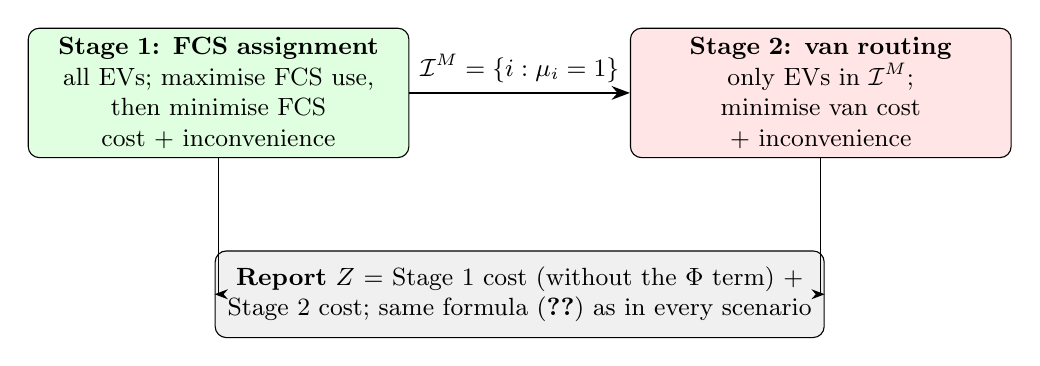
\begin{tikzpicture}[>=Stealth,box/.style={draw,rounded corners,align=center,minimum height=1.1cm,font=\small}]
  \node[box,fill=green!12,text width=4.6cm] (s1) {\textbf{Stage 1: FCS assignment}\\all EVs; maximise FCS use,\\then minimise FCS cost + inconvenience};
  \node[box,fill=red!10,text width=4.6cm,right=2.8cm of s1] (s2) {\textbf{Stage 2: van routing}\\only EVs in $\I^M$;\\minimise van cost + inconvenience};
  \draw[->,thick] (s1) -- node[above,font=\small]{$\I^M=\{i:\mu_i=1\}$} (s2);
  \node[box,fill=black!6,text width=7.5cm,below=2.0cm of $(s1)!0.5!(s2)$] (ev) {\textbf{Report} $Z=$ Stage~1 cost (without the $\Phi$ term) $+$ Stage~2 cost; same formula \eqref{eq:Z} as in every scenario};
  \draw[->] (s1) |- (ev); \draw[->] (s2) |- (ev);
\end{tikzpicture}
\end{center}

Stage~1 does not look at the vans, and Stage~2 cannot change what Stage~1 decided. That is the definition of ``FCS first, then MCS''.

%----------------------------------------------------------------
\subsection{Stage 1: assign EVs to fixed stations}

\textbf{Objective.}
\begin{equation}
\begin{split}
\min\ Z^{(1)}=\;&\underbrace{\Phi\sum_{i\in\I}\mu_i}_{\text{FCS first}}
+\underbrace{c^{EV}\sum_i\sum_{f\in\F_i}d_{if}Y_{if}}_{Z_1}
+\underbrace{Z^F_{\text{energy}}}_{\text{FCS part of }Z_4}\\
&+\underbrace{\sum_i\sum_{f\in\F_i}\rho^F_{if}Y_{if}+\alpha\sum_i w_i(C_i-r_i)+c^L\sum_i w_iL_i}_{\text{FCS customers' inconvenience}}
\end{split}
\label{eq:obj1}
\end{equation}
with $C_i=S_i+\tau^F_iY_i$ in this stage. $\Phi$ is a penalty for handing an EV to the vans. It is chosen larger than anything an extra FCS customer can add to the rest of \eqref{eq:obj1}, e.g.
\[
\Phi > \max_{i}\max_{f\in\F_i}\big(c^{EV}d_{if}+\pi^{\max}E_i+\rho^F_{if}\big)+n\,(\alpha+c^L)\,w_{\max}\,T,
\]
so Stage~1 first \textbf{maximises the number of EVs served at an FCS}, and only among those solutions minimises FCS cost and inconvenience. ($\pi^{\max}$ is the highest grid price.) A numerically safer equivalent is to solve twice: first $\max\sum_iY_i$, then fix that number and minimise the rest.
\ifTOU
Because $Z^F_{\text{energy}}$ uses the peak price, Stage~1 may \emph{start sessions later} to leave the peak, if the price saving beats the extra waiting cost (Section~\ref{sec:expect}).
\fi

\textbf{Constraints.}
\begin{align}
\sum_{g\in\G_i}y_{ig}+\mu_i &= 1 && \forall i\in\I \label{eq:s1assign}\\
S_i &\ge r_i+\sum_{f\in\F_i}t_{if}Y_{if} && \forall i\in\I \label{eq:fcsarr}\\
S_i &\le r_i+T\,(1-\mu_i) && \forall i\in\I \label{eq:s1park}\\
S_j &\ge S_i+\tau^F_i-(T+\tau^F_i)(3-y_{ig}-y_{jg}-o_{ij}) && \forall g,\ (i,j)\in\mathcal{P}_g \label{eq:disj1}\\
S_i &\ge S_j+\tau^F_j-(T+\tau^F_j)(2-y_{ig}-y_{jg}+o_{ij}) && \forall g,\ (i,j)\in\mathcal{P}_g \label{eq:disj2}\\
\sum_i y_{ig_1} &\ge \sum_i y_{ig_2} && \forall f,\ \G_f=\{g_1,g_2\} \label{eq:gunsym}\\
S_i+\tau^F_iY_i &\le T,\qquad L_i\ge S_i+\tau^F_iY_i-l_i && \forall i\in\I \label{eq:s1time}
\end{align}
\ifTOU plus the time-of-use split \eqref{eq:tou1}--\eqref{eq:tou5} of each FCS session (Section~\ref{sec:price}).\fi
\desc{\eqref{eq:s1assign}: every EV either gets one reachable gun or is handed to the vans. An EV that reaches no FCS ($\G_i=\emptyset$) is forced to $\mu_i=1$. \eqref{eq:fcsarr}: an FCS session cannot start before the EV has asked and driven to the station. \eqref{eq:s1park}: for an EV handed to the vans, $S_i$ is parked at $r_i$, so it adds no waiting in Stage~1 (its real start time is decided in Stage~2). \eqref{eq:disj1}--\eqref{eq:disj2}: two EVs on the same gun do not overlap; $o_{ij}$ picks who goes first. With two guns per station this means at most two EVs charge at a station at a time. \eqref{eq:gunsym}: symmetry breaking between the two identical guns (optional). \eqref{eq:s1time}: finished by $T$; lateness.}

\textbf{Optional acceptability rule.} An operator may refuse to send a driver to a station that is ``too inconvenient'', e.g.\ only allow gun $g$ of station $f$ for EV $i$ if $\hat\rho^F_{if}\le\bar\rho$. This only shrinks $\G_i$, so EVs whose stations are all too far go to the vans. Report results with and without it.

\textbf{Output:} $\I^M=\{i:\mu_i=1\}$, the EVs left for the vans; plus each FCS customer's gun and start time.

%----------------------------------------------------------------
\subsection{Stage 2: route the vans to the leftover EVs}

Stage~2 is a vehicle routing problem with time windows, on the EVs in $\I^M$ only. Here $C_i=S_i+\tau^M_i$.

\textbf{Objective.}
\begin{equation}
\begin{split}
\min\ Z^{(2)}=\;&\underbrace{c^M\sum_m\sum_{(i,j)\in\A^M}d_{ij}x_{ijm}}_{Z_2}+\underbrace{\sum_m c^D_mu_m}_{Z_3}+\underbrace{Z^M_{\text{energy}}}_{\text{van part of }Z_4}\\
&+\underbrace{\sum_{i\in\I^M}\sum_m\rho^M_{im}z_{im}+\alpha\sum_{i\in\I^M}w_i(C_i-r_i)+c^L\sum_{i\in\I^M}w_iL_i}_{\text{van customers' inconvenience}}
\end{split}
\label{eq:obj2}
\end{equation}
Since every EV in $\I^M$ must be served by some van, $Z^M_{\text{energy}}$ and the $\rho^M$ term are constants here. They are kept so that $Z^{(2)}$ is the true cost of Stage~2. Waiting and lateness make the vans visit urgent EVs early.

\textbf{Constraints.}
\begin{align}
\sum_{m\in\M}z_{im} &= 1 && \forall i\in\I^M \label{eq:s2assign}\\
\sum_{j:(0,j)\in\A^M}x_{0jm} = \sum_{i:(i,n+1)\in\A^M}x_{i,n+1,m} &= u_m && \forall m \label{eq:depot}\\
\sum_{i:(i,j)\in\A^M}x_{ijm} = \sum_{k:(j,k)\in\A^M}x_{jkm} &= z_{jm} && \forall j\in\I^M,\ m \label{eq:flow}\\
\sum_{i\in\I^M}z_{im} &\le Q_m\,u_m && \forall m \label{eq:cap}\\
\sum_{i\in\I^M}\frac{E_i}{\eta}z_{im}+\beta\sum_{(i,j)\in\A^M}d_{ij}x_{ijm} &\le B_m\,u_m && \forall m \label{eq:batt}
\end{align}
\begin{align}
S_j &\ge \max\{r_j,\ t_{0j}\,x_{0jm}\} && \forall j\in\I^M,\ m \label{eq:depart}\\
S_j &\ge S_i+\tau^M_i+t_{ij}-(T+\tau^M_i+t_{ij})(1-x_{ijm}) && \forall i\neq j,\ m \label{eq:seq}\\
S_i+\tau^M_i+t_{i,n+1} &\le T+(\tau^M_i+t_{i,n+1})(1-x_{i,n+1,m}) && \forall i,\ m \label{eq:return}\\
S_i+\tau^M_i \le T,\quad L_i &\ge S_i+\tau^M_i-l_i && \forall i\in\I^M \label{eq:s2time}\\
u_m &\ge u_{m+1} && m<|\M| \label{eq:vansym}
\end{align}
\desc{\eqref{eq:s2assign}: each leftover EV gets one van. \eqref{eq:depot}: a used van leaves and returns to the depot once. \eqref{eq:flow}: each EV on van $m$ is entered and left exactly once by that van. \eqref{eq:cap}: at most $Q_m$ EVs per van. \eqref{eq:batt}: delivered energy (with transfer losses) plus driving energy fits in the van battery. \eqref{eq:depart}: no start before the request, or before the van can drive there from the depot (written as two linear constraints). \eqref{eq:seq}: if the van goes $i\to j$, it finishes $i$ and drives to $j$ before starting $j$. This gives one EV at a time and removes subtours (MTZ-type). \eqref{eq:return}: back at the depot by $T$. \eqref{eq:s2time}: finished by $T$; lateness. \eqref{eq:vansym}: use identical vans in index order.}

\textbf{If Stage 2 is infeasible} (too many leftover EVs for the fleet by $T$), the sequential policy has \emph{failed} on that instance. For diagnosis, add $s_i\in\{0,1\}$ (``unserved''), replace \eqref{eq:s2assign} by $\sum_mz_{im}+s_i=1$ and add $\Phi^U\sum_is_i$ to \eqref{eq:obj2}. Then report the number of EVs that could not be served. This is a useful comparison with the integrated scenario, which may serve all of them.

%----------------------------------------------------------------
\subsection{Reported value}
\[
Z^{\text{S\scen}}=\big(Z^{(1)*}-\Phi\,|\I^M|\big)+Z^{(2)*},
\]
which is exactly \eqref{eq:Z} evaluated at the combined solution. The stage-1 solution plus the stage-2 solution is a feasible solution of the integrated model (S\ifTOU 4\else 3\fi), so
$Z^{\text{S\ifTOU 4\else 3\fi}}\le Z^{\text{S\scen}}$. The difference is the \emph{value of integration}.

\else
%---------------------------------------------------------------- INT
\subsection{Objective}
\begin{equation}
\min\ Z \quad\text{as in \eqref{eq:Z}, with }Z^F_{\text{energy}}=\ifTOU P^F\textstyle\sum_i\big[\pi^\off(\theta^1_i+\theta^3_i)+\pi^\pk\theta^2_i\big]\else\pi^F\textstyle\sum_iE_iY_i\fi,\quad C_i=S_i+\tau^F_iY_i+\tau^M_iZ_i. \label{eq:objint}
\end{equation}
Written out in full:
\begin{align*}
\min\ Z=\;& c^{EV}\sum_i\sum_{f\in\F_i}d_{if}Y_{if}+c^M\sum_m\sum_{(i,j)\in\A}d_{ij}x_{ijm}+\sum_mc^D_mu_m\\
&+\ifTOU P^F\sum_i\big[\pi^\off(\theta^1_i+\theta^3_i)+\pi^\pk\theta^2_i\big]\else\pi^F\sum_iE_iY_i\fi
+\pi^M\sum_i\sum_m\frac{E_i}{\eta}z_{im}\\
&+\sum_i\sum_{f\in\F_i}\rho^F_{if}Y_{if}+\sum_i\sum_m\rho^M_{im}z_{im}+\alpha\sum_iw_i(C_i-r_i)+c^L\sum_iw_iL_i .
\end{align*}
Every term is linear. One model weighs everything at once: an EV goes to a van exactly when the van's extra km, dispatch and energy cost are outweighed by the effort and waiting it saves the driver\ifTOU, or by the peak-price energy it avoids\fi.

\subsection{Constraints}

\textbf{Assignment.}
\begin{equation}
\sum_{g\in\G_i}y_{ig}+\sum_{m\in\M}z_{im}=1\qquad\forall i\in\I \label{eq:assign}
\end{equation}
\desc{Exactly one resource per EV: one reachable gun or one van. EVs that reach no FCS are forced onto a van.}

\textbf{Fixed stations.}
\begin{align}
S_i &\ge r_i+\sum_{f\in\F_i}t_{if}Y_{if} && \forall i \label{eq:fcsarr}\\
S_j &\ge S_i+\tau^F_i-(T+\tau^F_i)(3-y_{ig}-y_{jg}-o_{ij}) && \forall g,\ (i,j)\in\mathcal{P}_g \label{eq:disj1}\\
S_i &\ge S_j+\tau^F_j-(T+\tau^F_j)(2-y_{ig}-y_{jg}+o_{ij}) && \forall g,\ (i,j)\in\mathcal{P}_g \label{eq:disj2}\\
\sum_iy_{ig_1} &\ge \sum_iy_{ig_2} && \forall f,\ \G_f=\{g_1,g_2\} \label{eq:gunsym}
\end{align}
\desc{\eqref{eq:fcsarr}: an FCS session starts after the request and the drive to the station (for a van customer this is just $S_i\ge r_i$). \eqref{eq:disj1}--\eqref{eq:disj2}: EVs on the same gun do not overlap; $o_{ij}$ chooses the order. \eqref{eq:gunsym}: optional symmetry breaking.}

\textbf{Vans: routes, capacity, battery.}
\begin{align}
\sum_{j:(0,j)\in\A}x_{0jm}=\sum_{i:(i,n+1)\in\A}x_{i,n+1,m} &= u_m && \forall m \label{eq:depot}\\
\sum_{i:(i,j)\in\A}x_{ijm}=\sum_{k:(j,k)\in\A}x_{jkm} &= z_{jm} && \forall j\in\I,\ m \label{eq:flow}\\
\sum_iz_{im} &\le Q_mu_m && \forall m \label{eq:cap}\\
\sum_i\frac{E_i}{\eta}z_{im}+\beta\sum_{(i,j)\in\A}d_{ij}x_{ijm} &\le B_mu_m && \forall m \label{eq:batt}
\end{align}
\desc{\eqref{eq:depot}: a used van leaves and returns once. \eqref{eq:flow}: each EV on van $m$ is visited exactly once by it. \eqref{eq:cap}: at most $Q_m$ EVs. \eqref{eq:batt}: delivered energy (with losses) plus driving energy fits in the battery.}

\textbf{Vans: timing (one EV at a time, no subtours).}
\begin{align}
S_j &\ge t_{0j}\,x_{0jm} && \forall j\in\I,\ m \label{eq:depart}\\
S_j &\ge S_i+\tau^M_i+t_{ij}-(T+\tau^M_i+t_{ij})(1-x_{ijm}) && \forall i\neq j\in\I,\ m \label{eq:seq}\\
S_i+\tau^M_i+t_{i,n+1} &\le T+(\tau^M_i+t_{i,n+1})(1-x_{i,n+1,m}) && \forall i,\ m \label{eq:return}
\end{align}
\desc{\eqref{eq:depart}: the first stop cannot start before the van has driven there. \eqref{eq:seq}: $i\to j$ means finish $i$, drive, then start $j$; start times rise along a route, so no subtour can close. \eqref{eq:return}: back at the depot by $T$.}

\textbf{Horizon and lateness.}
\begin{equation}
C_i\le T,\qquad L_i\ge C_i-l_i\qquad\forall i\in\I \label{eq:time}
\end{equation}
\desc{Every EV is fully charged within the horizon; $L_i$ measures lateness.}

\ifTOU
\textbf{Time-of-use split.} Constraints \eqref{eq:tou1}--\eqref{eq:tou5} of Section~\ref{sec:price}.
\fi

\textbf{Symmetry and domains.}
\begin{equation}
u_m\ge u_{m+1};\qquad y,z,x,u,o\ifTOU,\kappa\fi\in\{0,1\};\qquad S_i,L_i\ifTOU,\theta^p_i\fi\ge0 \label{eq:dom}
\end{equation}
\fi

%=====================================================================
\section{Learning-to-optimise (RL) formulation}\label{sec:rl}

\textbf{Main rule:} the reward of each action is \emph{minus the increase in $Z$ that the action causes}. The rewards over an episode then add up to $-Z$ of the solution the policy builds. RL and MILP results are measured on the same yardstick \eqref{eq:Z}, and the MILP optimum is the benchmark for the RL gap.

\ifSEQ
%---------------------------------------------------------------- RL SEQ
The RL pipeline has the same two stages as the MILP.

\subsection{Stage 1 policy: FCS assignment}
\begin{itemize}[leftmargin=1.4em,itemsep=2pt]
  \item \textbf{Episode / epochs:} EVs are taken in order of request time $r_i$ (ties: higher $w_i$ first). One decision per EV.
  \item \textbf{State:} features of the current EV $k$ ($E_k,r_k,l_k,w_k,R_k$, location); for each gun $g$ the time $F_g$ it becomes free; summary features of the EVs still to come (count and positions near each station)\ifTOU; the current price and the time until $T_1$ and $T_2$\fi.
  \item \textbf{Action:} a gun $g\in\G_k$, or ``hand to vans''. \textbf{FCS-first mask:} ``hand to vans'' is allowed \emph{only} if no gun can finish EV $k$ by $T$ (or, with the optional rule, if all remaining guns have $\hat\rho^F_{kf}>\bar\rho$).
  \ifTOU\item \textbf{Optional timing action:} ``gun $g$, start after the peak'', i.e.\ $S_k=\max\{\text{earliest},T_2\}$, allowed only if the session still ends by $T$.\fi
  \item \textbf{Transition:} $S_k=\max\{r_k+t_{kf},F_g\}$ (or later, for the timing action); $F_g\leftarrow S_k+\tau^F_k$.
  \item \textbf{Reward:} $-\Big[c^{EV}d_{kf}+\text{energy}_k+\rho^F_{kf}+\alpha w_k(S_k+\tau^F_k-r_k)+c^Lw_k(S_k+\tau^F_k-l_k)^+\Big]$, where energy$_k$ = \ifTOU$P^F\big[\pi^\off\cdot(\text{off-peak hours of }[S_k,S_k+\tau^F_k])+\pi^\pk\cdot(\text{peak hours})\big]$, computed exactly in the simulator\else$\pi^FE_k$\fi. Handing an EV to the vans gives reward $0$ here; its cost is counted in Stage~2.
\end{itemize}
Note: a simple baseline for Stage~1 is the greedy rule ``gun with the largest one-step reward''. What RL can learn on top of this is, for example, to keep a nearby gun free for an urgent EV that arrives later.

\subsection{Stage 2 policy: van routing over $\I^M$}
\begin{itemize}[leftmargin=1.4em,itemsep=2pt]
  \item \textbf{Epochs:} whenever a van becomes free (the earliest-free van decides first).
  \item \textbf{State:} for each van: position, time free, remaining battery $b_m$, EVs served so far, dispatched or not; for each unserved EV in $\I^M$: location, $E_i,r_i,l_i,w_i$; current time.
  \item \textbf{Action:} the next EV $j$ for this van, or ``return to depot'' (ends the route). Mask: $j$ must be feasible: battery covers $E_j/\eta$ plus driving to $j$ and back to the depot, the count stays $\le Q_m$, and $j$ can be finished with the van back at the depot by $T$.
  \item \textbf{Transition:} $S_j=\max\{r_j,\ \text{time free}+t_{\text{pos},j}\}$; the van moves to $j$ and is free at $S_j+\tau^M_j$; $b_m$ falls by $E_j/\eta+\beta d_{\text{pos},j}$.
  \item \textbf{Reward:} serving $j$: $-\Big[c^Md_{\text{pos},j}+c^D_m[\text{first stop}]+\pi^M\frac{E_j}{\eta}+\rho^M_{jm}+\alpha w_j(S_j+\tau^M_j-r_j)+c^Lw_j(S_j+\tau^M_j-l_j)^+\Big]$; returning: $-c^Md_{\text{pos},0}$. EVs still unserved at the end: $-\Phi^U$ each.
  \item \textbf{Policy:} an attention-based routing policy (e.g.\ Kool et al., 2019, ``Attention, Learn to Solve Routing Problems!'') trained with REINFORCE or PPO. Baseline: nearest-feasible-EV heuristic.
\end{itemize}
Episode return of Stage~1 + Stage~2 $=-Z^{\text{S\scen}}$.

\else
%---------------------------------------------------------------- RL INT
One policy decides both who serves each EV and the van routes.
\begin{itemize}[leftmargin=1.4em,itemsep=2pt]
  \item \textbf{Episode / epochs:} EVs are taken in order of request time $r_i$ (ties: higher $w_i$ first). One decision per EV.
  \item \textbf{State:} (i) the current EV $k$: location, $E_k,r_k,l_k,w_k,R_k$, reachable stations; (ii) each gun $g$: time $F_g$ it becomes free; (iii) each van $m$: current end-of-route position, time free, remaining battery $b_m$, EVs served, dispatched or not; (iv) embeddings of the not-yet-assigned EVs (for look-ahead)\ifTOU; (v) current price, time until $T_1$ and $T_2$\fi.
  \item \textbf{Action:} $a\in\G_k\cup\M$: a gun, or a van (EV $k$ is appended to the end of that van's route). \textbf{Mask} infeasible actions: a gun that cannot finish $k$ by $T$; a van without enough battery for $E_k/\eta$ plus the drive to $k$ and back to the depot, with $Q_m$ reached, or unable to finish $k$ and return by $T$.
  \ifTOU\item \textbf{Optional timing action:} ``gun $g$, start after the peak'' ($S_k=\max\{\text{earliest},T_2\}$, if it still ends by $T$).\fi
  \item \textbf{Transition:} gun: $S_k=\max\{r_k+t_{kf},F_g\}$, $F_g\leftarrow S_k+\tau^F_k$. Van: $S_k=\max\{r_k,\ \text{free}_m+t_{\text{pos}_m,k}\}$, then the van moves to $k$, $\text{free}_m\leftarrow S_k+\tau^M_k$, $b_m\mathrel{-}=E_k/\eta+\beta d_{\text{pos}_m,k}$.
  \item \textbf{Reward} $=-\Delta Z$:
  \begin{align*}
  \text{gun } g\text{ at }f:&\quad -\Big[c^{EV}d_{kf}+\text{energy}^F_k+\rho^F_{kf}+\alpha w_k(C_k-r_k)+c^Lw_k(C_k-l_k)^+\Big]\\
  \text{van } m:&\quad -\Big[c^M\big(d_{\text{pos}_m,k}+d_{k,0}-d_{\text{pos}_m,0}\big)+c^D_m[\text{first use}]+\pi^M\tfrac{E_k}{\eta}\\
  &\qquad\quad+\rho^M_{km}+\alpha w_k(C_k-r_k)+c^Lw_k(C_k-l_k)^+\Big]
  \end{align*}
  The van distance term is the \emph{change} in route length when $k$ is inserted before the return to the depot, so the sum over the episode equals the total route length (the return legs telescope). energy$^F_k$ = \ifTOU$P^F\big[\pi^\off\cdot(\text{off-peak hours})+\pi^\pk\cdot(\text{peak hours of }[S_k,C_k])\big]$, computed exactly by the simulator; no linearisation is needed in RL\else$\pi^FE_k$\fi.
  \item \textbf{Dead end:} if every action is masked, EV $k$ is unserved: reward $-\Phi^U$, and the episode continues. Report the count.
  \item \textbf{Policy:} masked categorical policy over guns and vans, encoder with attention over EVs, guns and vans; trained with PPO. Natural baseline: greedy, i.e.\ choose the action with the largest one-step reward. That is the pairwise rule ``smallest $\hat\rho$ + cost'' from Section~\ref{sec:inc}.
\end{itemize}
Restriction to note: vans serve EVs in assignment order (append only). A variant that inserts $k$ at the cheapest position of a route is more flexible but has a larger action space.
\fi

\textbf{Reward scaling.} For stable training divide every reward by a constant, e.g.\ the greedy baseline's average $Z$ on the training instances. This does not change the optimal policy.

%=====================================================================
\section{What to expect and what to report}\label{sec:expect}

\ifnum\scen=1
\begin{itemize}[leftmargin=1.4em,itemsep=2pt]
  \item Vans serve only EVs that reach no station, or that the stations cannot finish by $T$. If stations have spare capacity, very few vans are dispatched.
  \item Inconvenience is high for EVs far from the nearest station (worked example: Rs\,682 at the FCS, against Rs\,458 if a van had been allowed).
  \item With too few vans Stage~2 becomes infeasible (unserved EVs), even when the integrated model S3 could serve everyone. Report the smallest $|\M|$ at which S1 is feasible and compare it with S3.
\end{itemize}
\fi
\ifnum\scen=2
\begin{itemize}[leftmargin=1.4em,itemsep=2pt]
  \item \textbf{When does Stage~1 delay a session to avoid the peak?} Moving one hour of charging out of the peak saves $(\pi^\pk-\pi^\off)P^F=3\times22=$ Rs\,66, but delays completion by up to an hour, which costs $\alpha w_i\ge$ Rs\,200. So with the default values Stage~1 almost never delays. It mostly pays the higher price, and S2 costs roughly S1 plus the peak surcharge. Sessions start later only if $\alpha$ is small (try $\lambda<0.33$ in the sensitivity analysis).
  \item The van assignment is the same as in S1 unless Stage~1's timing changes which EVs fit at the stations. Stage~1 cannot use vans to escape the peak price.
  \item Extra KPI: \textbf{grid energy drawn at FCS during the peak}, $P^F\sum_i\theta^2_i$ (kWh). Compare with S4.
\end{itemize}
\fi
\ifnum\scen=3
\begin{itemize}[leftmargin=1.4em,itemsep=2pt]
  \item Vans take EVs for which the saved inconvenience exceeds the extra van cost (worked example: van chosen, saving Rs\,224). Expect vans to serve EVs that are far from every station, have low range (high $w_i$), or have early deadlines, while EVs near a station still use it.
  \item \textbf{Value of integration under flat price:} $Z^{\text{S1}}-Z^{\text{S3}}\ge0$. Report it per component ($Z_1,\dots,Z_5$): typically operating cost rises a little and inconvenience falls a lot.
  \item Vary $|\M|$ (0, 1, 2, \dots): the first few vans lower $Z$ sharply, then the effect levels off. That curve shows the scenarios where mobile chargers help most.
\end{itemize}
\fi
\ifnum\scen=4
\begin{itemize}[leftmargin=1.4em,itemsep=2pt]
  \item During the peak a van kWh costs about the same as an FCS kWh (Rs\,10.0 each), so the vans' energy disadvantage disappears and vans also absorb \emph{peak-hour} demand that would otherwise be charged on the grid at peak price.
  \item Expect more van usage than in S3, concentrated on requests in $[T_1,T_2]$, and lower grid energy at the stations during the peak, $P^F\sum_i\theta^2_i$, than in S2.
  \item \textbf{Value of integration under peak pricing:} $Z^{\text{S2}}-Z^{\text{S4}}$. It should be larger than $Z^{\text{S1}}-Z^{\text{S3}}$, because integration now also allows price arbitrage.
  \item \textbf{Peak pricing with full flexibility:} $Z^{\text{S4}}-Z^{\text{S3}}$ should be smaller than $Z^{\text{S2}}-Z^{\text{S1}}$: vans cushion the price increase.
\end{itemize}
\fi

\textbf{Cross-scenario comparison table} (fill in from the four runs):
\begin{center}
\renewcommand{\arraystretch}{1.2}
\begin{tabular}{@{}lll@{}}
\toprule
\textbf{Comparison} & \textbf{Measures} & \textbf{Expected sign} \\
\midrule
S1 $-$ S3 & value of integration, flat price & $\ge0$ \\
S2 $-$ S4 & value of integration, peak price & $\ge0$, larger than S1 $-$ S3 \\
S2 $-$ S1 & cost of peak pricing, FCS-first operator & $>0$ \\
S4 $-$ S3 & cost of peak pricing, flexible operator & $>0$, smaller than S2 $-$ S1 \\
\bottomrule
\end{tabular}
\end{center}
Report for each: $Z$ and its components, number of vans used, EVs per resource, mean and maximum inconvenience per EV, total lateness, peak-hour grid energy, solve time, and (for RL) the gap to the MILP optimum.

%=====================================================================
\appendix
\section{Illustrative parameter values}\label{app:values}

These are starting values for experiments, not data. All are meant to be varied in the analysis. Values in Rs.

\begin{center}
\renewcommand{\arraystretch}{1.15}
\begin{tabular}{@{}llp{6.2cm}@{}}
\toprule
\textbf{Parameter} & \textbf{Value} & \textbf{Note} \\
\midrule
$T$, $[T_1,T_2]$ & 7 h, $[2,6]$ & 16:00--23:00, peak 18:00--22:00 \\
$P^F$, $P^M$ & 22 kW, 30 kW & \\
$v$, $\beta$, $\eta$ & 25 km/h, 0.25 kWh/km, 0.9 & \\
$B_m$, $Q_m$, $|\M|$ & 150 kWh, 6, 2--6 & \\
$c^{EV}$, $c^M$, $c^D_m$ & Rs\,4/km, Rs\,15/km, Rs\,1500 & van km includes driver time \\
$\pi^F$ (flat) & Rs\,8.7/kWh & equals the time-average of the ToU tariff over $[0,T]$ \\
$\pi^\off$, $\pi^\pk$ (ToU) & Rs\,7/kWh, Rs\,10/kWh & $(3\times7+4\times10)/7=8.7$ \\
$c^{bat}$ & Rs\,2/kWh & van battery wear \\
$\pi^M$ & Rs\,10.7 (flat) / Rs\,9.0 (ToU) & $=\pi^F+c^{bat}$ / $=\pi^\off+c^{bat}$ \\
$\alpha$, $\alpha^D$ & Rs\,200/h, Rs\,100/h & value of time; extra for attended time \\
$h^F$, $h^M$, $\varphi$ & Rs\,50, Rs\,10, Rs\,100 & trip hassle, hand-over, range stress \\
$c^L$ & Rs\,300/h & lateness \\
$w_i$ & $1+2(1-R_i/R_{\max})$, $R_i\sim U[3,40]$ km & priority from remaining range \\
\bottomrule
\end{tabular}
\end{center}

The flat price is set to the time-average of the peak tariff. The price \emph{level} is then the same in both pricing cases, and only the price \emph{shape} differs. Without this, part of S1 vs S2 would just reflect a different average price.

\end{document}
"
%    pdflatex -jobname=scenario3_flat_integrated   "\def\scen{3}% =====================================================================
%  One source, four PDFs.  Build with build.sh (or by hand):
%    pdflatex -jobname=scenario1_flat_sequential   "\def\scen{1}\input{scenario_master}"
%    pdflatex -jobname=scenario2_peak_sequential   "\def\scen{2}\input{scenario_master}"
%    pdflatex -jobname=scenario3_flat_integrated   "\def\scen{3}\input{scenario_master}"
%    pdflatex -jobname=scenario4_peak_integrated   "\def\scen{4}\input{scenario_master}"
%  (run each twice for cross-references)
% =====================================================================
\documentclass[11pt,a4paper]{article}
\usepackage[margin=2.2cm]{geometry}
\usepackage{amsmath,amssymb,amsfonts}
\usepackage{booktabs,array,tabularx}
\usepackage{enumitem}
\usepackage[table]{xcolor}
\usepackage{tikz}
\usetikzlibrary{arrows.meta,positioning,calc}
\usepackage[colorlinks=true,linkcolor=blue!50!black,urlcolor=blue!50!black]{hyperref}
\usepackage{titlesec}
\titleformat{\section}{\large\bfseries}{\thesection}{0.8em}{}
\titleformat{\subsection}{\normalsize\bfseries}{\thesubsection}{0.8em}{}
\setlength{\parindent}{0pt}
\setlength{\parskip}{5pt}

% ---------------- scenario switches ----------------
\ifdefined\scen\else\def\scen{1}\fi
\newif\ifTOU \TOUfalse   % true = time-of-use (peak) price
\newif\ifSEQ \SEQfalse   % true = FCS first, then MCS
\ifnum\scen=1 \SEQtrue \fi
\ifnum\scen=2 \TOUtrue \SEQtrue \fi
\ifnum\scen=4 \TOUtrue \fi

\newcommand{\pricename}{\ifTOU time-of-use price (dearer evening peak)\else single (flat) price all day\fi}
\newcommand{\structname}{\ifSEQ FCS first, then MCS (sequential)\else FCS and MCS together (integrated)\fi}

% ---------------- notation ----------------
\newcommand{\I}{\mathcal{I}}
\newcommand{\F}{\mathcal{F}}
\newcommand{\G}{\mathcal{G}}
\newcommand{\M}{\mathcal{M}}
\newcommand{\N}{\mathcal{N}}
\newcommand{\A}{\mathcal{A}}
\newcommand{\Rs}{\text{Rs}\,}
\newcommand{\pk}{\mathrm{pk}}
\newcommand{\off}{\mathrm{off}}
\newcommand{\desc}[1]{\par\vspace{-2pt}{\small\color{black!75}\textit{Meaning:} #1}\par\vspace{4pt}}
\newcommand{\cell}[2]{\ifnum\scen=#1\cellcolor{blue!18}\textbf{S#1 (this document)}\\\textbf{#2}\else S#1\\#2\fi}

\title{\textbf{EV Charging Network Optimisation}\\[4pt]
\large Scenario \scen: \pricename\ $+$ \structname\\[2pt]
\normalsize MILP and RL formulation}
\author{CP 320 OR for Mobility Management, course project}
\date{2 October 2026}

\begin{document}
\maketitle

%=====================================================================
\section{Where this scenario sits}

The project studies four scenarios: two ways of pricing grid electricity, times two ways of making the decisions.

\begin{center}
\renewcommand{\arraystretch}{1.5}
\begin{tabular}{>{\raggedright\arraybackslash}p{4.2cm}|>{\centering\arraybackslash}p{4.6cm}|>{\centering\arraybackslash}p{4.6cm}}
 & \textbf{Flat price all day} & \textbf{Time-of-use (peak) price} \\ \hline
\textbf{Sequential:} FCS first, leftover EVs to MCS &
\begin{tabular}[c]{@{}c@{}}\cell{1}{flat + sequential}\end{tabular} &
\begin{tabular}[c]{@{}c@{}}\cell{2}{peak + sequential}\end{tabular} \\ \hline
\textbf{Integrated:} FCS and MCS decided together &
\begin{tabular}[c]{@{}c@{}}\cell{3}{flat + integrated}\end{tabular} &
\begin{tabular}[c]{@{}c@{}}\cell{4}{peak + integrated}\end{tabular} \\
\end{tabular}
\end{center}

\textbf{The four scenarios do not have four different objectives.} They share \emph{one} cost yardstick $Z$ (Section~\ref{sec:obj}): the same cost terms and the same customer inconvenience (Section~\ref{sec:inc}). Only two things change:
\begin{itemize}[leftmargin=1.4em,itemsep=1pt]
  \item \textbf{Pricing} changes the formula for one term, the FCS energy cost (Section~\ref{sec:price}).
  \item \textbf{Decision structure} changes \emph{how} $Z$ is minimised: in one model (integrated), or in two stages (sequential), where each stage minimises its own part of $Z$.
\end{itemize}
Because the yardstick is the same, the four optimal values can be compared directly. The differences measure the \emph{value of integration} (S1$\to$S3, S2$\to$S4) and the \emph{effect of peak pricing} (S1$\to$S2, S3$\to$S4).

\ifnum\scen=1
\textbf{This scenario (S1)} is the baseline, the ``status quo''. Electricity costs the same at every hour, every EV that can be charged at a fixed station is sent there, and vans only take what is left over.
\fi
\ifnum\scen=2
\textbf{This scenario (S2)} keeps the FCS-first rule of S1, but grid electricity is dearer during the evening peak. Stage~1 can react to the price only by \emph{rescheduling} FCS sessions. It cannot hand a peak-hour EV to a van.
\fi
\ifnum\scen=3
\textbf{This scenario (S3)} keeps the flat price of S1, but the operator decides FCS and MCS service \emph{together}. An EV can be sent to a van even when a fixed station could take it, whenever that lowers total cost plus inconvenience.
\fi
\ifnum\scen=4
\textbf{This scenario (S4)} is the most flexible one: peak pricing at fixed stations, and FCS and MCS decided together. Van energy was bought off-peak, so vans can also be used to keep charging \emph{out of the expensive peak}.
\fi

%=====================================================================
\section{Setting and assumptions}\label{sec:setting}

\textbf{Time.} The planning horizon is $[0,T]$ with $T=7$\,h (16:00--23:00). It contains the evening peak window $[T_1,T_2]=[2,6]$ (18:00--22:00). The horizon is the same in all four scenarios. It is wider than the peak itself so that, under peak pricing, there is cheaper time on both sides of the peak.\ifTOU\else\ In this scenario the price is flat, so the window plays no role in the model.\fi

\textbf{Assumptions} (the same as MILP v3, plus two about energy):
\begin{enumerate}[leftmargin=1.6em,itemsep=1pt]
  \item Static, continuous time. All requests in the horizon are known at time $0$, and request $i$ becomes active at $r_i$.
  \item An EV served by an FCS drives there itself on its own battery (only to stations within its range $R_i$). The driver stays with the car while it waits for a free gun and while it charges.
  \item An EV served by an MCS stays parked where it is, and the driver is free in the meantime.
  \item Each FCS gun and each van charges one EV at a time, without interruption, at constant power.
  \item A van's battery covers both its driving and the energy it delivers. \textbf{The van battery is charged at the depot before the horizon starts}\ifTOU, i.e.\ at the off-peak price\fi, and is not recharged during the horizon.
  \item Every EV must be fully charged by $T$ (hard). Finishing after the driver's desired time $l_i$ is allowed but penalised.
\end{enumerate}

%=====================================================================
\section{Notation}\label{sec:notation}

\subsection*{Sets}
\begin{tabularx}{\textwidth}{@{}lX@{}}
\toprule
$\I=\{1,\dots,n\}$ & EV charging requests \\
$\F$; $\G_f$ ($|\G_f|=2$); $\G=\bigcup_f\G_f$ & fixed charging stations; guns of FCS $f$; all guns ($f(g)$ = station of gun $g$) \\
$\F_i=\{f: d_{if}\le R_i\}$, $\G_i=\bigcup_{f\in\F_i}\G_f$ & stations / guns EV $i$ can reach on its remaining range \\
$\M$ & mobile charging vans (MCS) \\
$0,\ n+1$ & depot as start node / end node (same place) \\
$\N=\{0\}\cup\I\cup\{n+1\}$, $\A$ & routing nodes; allowed van arcs $(i,j)$, $i\in\{0\}\cup\I$, $j\in\I\cup\{n+1\}$, $i\neq j$ \\
$\mathcal{P}_g=\{(i,j): i<j,\ g\in\G_i\cap\G_j\}$ & pairs of EVs that could share gun $g$ \\
\ifSEQ
$\I^M\subseteq\I$ & EVs handed to the vans by Stage~1 (an \emph{output} of Stage~1, a fixed input to Stage~2) \\
$\N^M$, $\A^M$ & routing nodes / arcs restricted to $\I^M$ \\
\fi
\bottomrule
\end{tabularx}

\subsection*{Parameters}
\begin{tabularx}{\textwidth}{@{}lX@{}}
\toprule
$E_i,\ r_i,\ l_i,\ R_i$ & energy demand (kWh), request time, desired completion time (h), remaining range (km) \\
$w_i\ge1$ & priority of EV $i$; $w_i=1+\kappa(1-R_i/R_{\max})$, so low-range EVs weigh more \\
$P^F,\ P^M$ & charging power of an FCS gun (22\,kW) / of a van (e.g.\ 30\,kW) \\
$\tau^F_i=E_i/P^F,\ \tau^M_i=E_i/P^M$ & charging time of EV $i$ at an FCS / by a van (h) \\
$d_{if},t_{if}$;\ $d_{ij},t_{ij}$ & distance (km) and time (h): EV$\to$FCS; between routing nodes ($t=d/v$) \\
$B_m,\ Q_m,\ \beta,\ \eta$ & van battery (kWh), max EVs per van, van consumption (kWh/km), transfer efficiency \\
$c^{EV},\ c^M,\ c^D_m$ & cost per km of EV driving, per km of van driving; fixed dispatch cost of van $m$ \\
\ifTOU
$\pi^\off,\ \pi^\pk$ & grid price (Rs/kWh) off-peak / in $[T_1,T_2]$, with $\pi^\pk\ge\pi^\off$ \\
\else
$\pi^F$ & grid price (Rs/kWh), the same at every hour \\
\fi
$c^{bat}$ & van battery wear per kWh cycled \\
$\pi^M$ & cost of 1 kWh taken from a van battery: $\pi^M=\ifTOU\pi^\off\else\pi^F\fi+c^{bat}$ (Section~\ref{sec:price}) \\
$\alpha,\ \alpha^D,\ h^F,\ h^M,\ \varphi,\ c^L$ & inconvenience coefficients (Section~\ref{sec:inc}) \\
\bottomrule
\end{tabularx}

\subsection*{Decision variables}
\begin{tabularx}{\textwidth}{@{}llX@{}}
\toprule
$y_{ig}$ & $\{0,1\}$ & EV $i$ charged at gun $g\in\G_i$ \\
$z_{im}$ & $\{0,1\}$ & EV $i$ served by van $m$ \\
$x_{ijm}$ & $\{0,1\}$ & van $m$ drives arc $(i,j)$ \\
$u_m$ & $\{0,1\}$ & van $m$ is dispatched \\
$o_{ij}$ & $\{0,1\}$ & for EVs $i<j$ that could share a gun: 1 if $i$ is charged before $j$ \\
\ifSEQ
$\mu_i$ & $\{0,1\}$ & Stage~1 only: EV $i$ is handed to the van fleet \\
\fi
\ifTOU
$\theta^1_i,\theta^2_i,\theta^3_i$ & $\ge0$ & hours of EV $i$'s FCS session before / inside / after the peak \\
$\kappa^1_i,\kappa^3_i$ & $\{0,1\}$ & EV $i$'s FCS session starts before $T_1$ / ends after $T_2$ \\
\fi
$S_i$ & $\ge0$ & time charging of EV $i$ starts (h), on whichever resource \\
$L_i$ & $\ge0$ & lateness of EV $i$ beyond $l_i$ (h) \\
\bottomrule
\end{tabularx}

\textbf{Short-hands} (linear expressions, not new variables):
\[
Y_{if}=\sum_{g\in\G_f}y_{ig},\qquad Y_i=\sum_{g\in\G_i}y_{ig}\ (\text{EV $i$ uses an FCS}),\qquad Z_i=\sum_{m\in\M}z_{im}\ (\text{EV $i$ uses a van}),
\]
\[
C_i=S_i+\tau^F_i\,Y_i+\tau^M_i\,Z_i \quad\text{(time EV $i$ is fully charged).}
\]

%=====================================================================
\section{Customer inconvenience}\label{sec:inc}

This section is \textbf{identical in all four scenario documents}. Inconvenience is a property of the customer, not of the price or of the planning method.

\subsection{What we mean by inconvenience}

Inconvenience is \emph{what the driver loses} from the moment they ask for a charge ($r_i$) until the car is fully charged ($C_i$), \emph{converted into rupees} so it can be added to the operator's costs. A driver loses three different things:

\begin{enumerate}[leftmargin=1.6em,itemsep=2pt]
  \item \textbf{Waiting:} the car is not ready. This lasts $C_i-r_i$ hours and affects \emph{every} driver, FCS or MCS.
  \item \textbf{Effort:} only an FCS customer has to drive to the station and sit there while the car charges. An MCS customer stays at home or at work and does something else. Driving to a far station also uses scarce battery range, which causes stress (``range anxiety'').
  \item \textbf{A missed deadline:} the car is still not ready at the time $l_i$ the driver needs it.
\end{enumerate}

Each loss gets a price in Rs per hour (or per event). All of them are multiplied by the priority $w_i$: an hour of delay for an EV with 5\,km of range left counts more than for one with 40\,km.

\subsection{The three components}

\begin{center}
\renewcommand{\arraystretch}{1.3}
\begin{tabularx}{\textwidth}{@{}>{\raggedright\arraybackslash}p{2.6cm}>{\raggedright\arraybackslash}X>{\raggedright\arraybackslash}X>{\raggedright\arraybackslash}p{3.0cm}@{}}
\toprule
\textbf{Component} & \textbf{EV $i$ at FCS $f$} & \textbf{EV $i$ by a van} & \textbf{Known when?} \\
\midrule
Effort & $w_i\big[\alpha^D(t_{if}+\tau^F_i)+h^F+\varphi\,d_{if}/R_i\big]$: driving and sitting at the station, a fixed trip hassle, range stress & $w_i\,h^M$: being reachable and handing over the car & \textbf{Static:} known as soon as the resource is chosen \\
Waiting & $w_i\,\alpha\,(C_i-r_i)$ = drive + \emph{queue at the gun} + charge & $w_i\,\alpha\,(C_i-r_i)$ = \emph{wait for the van} + charge & \textbf{Dynamic:} depends on the queue / van route \\
Missed deadline & $w_i\,c^L\,L_i$, $L_i=\max\{0,C_i-l_i\}$ & same & Dynamic \\
\bottomrule
\end{tabularx}
\end{center}

\textbf{Coefficients.}
$\alpha$ (Rs/h) is the value of an hour the car is not ready.
$\alpha^D$ (Rs/h) is the \emph{extra} value of an hour the driver must personally spend driving or sitting at the station: an hour at the station costs $\alpha+\alpha^D$, an hour waiting at home for a van costs only $\alpha$.
$h^F,h^M$ (Rs) are fixed hassle costs of one trip to a station / one van hand-over.
$\varphi$ (Rs) is the range-stress cost of a trip that uses the \emph{whole} remaining range ($d_{if}/R_i\le1$ is the fraction used).
$c^L$ (Rs/h) is the cost per hour late.

\subsection{Pairwise form: inconvenience of a (customer, resource) pair}

The natural first idea is: \emph{for every pair (EV $i$, FCS $f$) and every pair (EV $i$, van $m$) there is an inconvenience number, and the operator picks the pair with the lowest cost plus inconvenience.} The static part fits this idea exactly:
\[
\boxed{\;\rho^F_{if}=w_i\Big[\alpha^D\,(t_{if}+\tau^F_i)+h^F+\varphi\,\frac{d_{if}}{R_i}\Big]\qquad
\rho^M_{im}=w_i\,h^M\;}
\]
These are \textbf{parameters}, computed before solving, one number per (EV, FCS) pair and per (EV, van) pair. In the objective they appear linearly: $\sum_i\sum_f\rho^F_{if}Y_{if}+\sum_i\sum_m\rho^M_{im}z_{im}$.

Note that $\rho^M_{im}$ does not depend on $m$. Vans are identical and all start at the same depot, so the driver does not care \emph{which} van comes, only \emph{when} it comes. That ``when'' is the waiting part.

\subsection{Why waiting cannot be a fixed pairwise number}

It is tempting to also write the waiting as a pairwise number, e.g.\ ``the van needs 5 minutes to reach EV $i$''. But that depends on \emph{where the van is coming from}, which depends on the route the model is still choosing: if EV $i$ is the 4th stop of a van, the wait is the time for three charging sessions plus four drives. Likewise, waiting at an FCS depends on how many EVs are queued at that gun. So waiting is not known before solving. It is a function of decision variables:
\[
\text{waiting cost of EV } i \;=\; w_i\,\alpha\,(C_i-r_i),\qquad C_i=S_i+\tau^F_iY_i+\tau^M_iZ_i .
\]
This is \textbf{linear} in the variables ($S_i$, $y$, $z$), so it fits in a MILP directly. The constraints of Section~\ref{sec:milp} make $S_i$ equal to the true start time, including driving, queueing at the gun and the van's route. The term $\sum_i w_i\alpha r_i$ is a constant and may be dropped when solving.

\textbf{Pairwise \emph{estimate}} (used for intuition, by the RL policy and in heuristics): if there is no queue and the van comes straight to $i$,
\[
\hat\rho^{F}_{if}=\rho^F_{if}+w_i\alpha\,(t_{if}+\tau^F_i),\qquad
\hat\rho^{M}_{im}=\rho^M_{im}+w_i\alpha\,(t^{\text{van}}_{m\to i}+\tau^M_i),
\]
where $t^{\text{van}}_{m\to i}$ is the time until van $m$ can reach $i$ from where it currently is. In the RL formulation (Section~\ref{sec:rl}) the van's position \emph{is} known at each decision, so there this estimate becomes exact.

\subsection{Total inconvenience and how it enters the objective}

\begin{equation}
\boxed{\;
Z_{\text{inc}}=\underbrace{\sum_{i\in\I}\sum_{f\in\F_i}\rho^F_{if}Y_{if}+\sum_{i\in\I}\sum_{m\in\M}\rho^M_{im}z_{im}}_{\text{effort (static, pairwise)}}
+\underbrace{\alpha\sum_{i\in\I}w_i\,(C_i-r_i)}_{\text{waiting (dynamic)}}
+\underbrace{c^L\sum_{i\in\I}w_i\,L_i}_{\text{missed deadline}}
\;}\label{eq:inc}
\end{equation}
All three parts are in rupees, so $Z_{\text{inc}}$ is simply added to the operating costs. Nothing has to be normalised.

\subsection{Worked example: your ``10 km to the FCS vs.\ van in 5 minutes'' case}

EV $i$: $E_i=20$\,kWh, $R_i=40$\,km (so $w_i=1$); nearest free FCS $d_{if}=10$\,km away, $t_{if}=0.4$\,h at 25\,km/h; a van finishing next door can reach it in 5\,min ($0.083$\,h), adding about 4\,km to its route. $\tau^F_i=20/22=0.909$\,h, $\tau^M_i=20/30=0.667$\,h. Coefficients from Appendix~\ref{app:values}, flat price.

\begin{center}
\renewcommand{\arraystretch}{1.25}
\begin{tabular}{@{}lrr@{}}
\toprule
 & \textbf{FCS} & \textbf{Van} \\
\midrule
Driving (EV / extra van km) & $4\times10=40.0$ & $15\times4=60.0$ \\
Energy & $8.7\times20=174.0$ & $10.7\times20/0.9=237.8$ \\
\textbf{Operating cost only} & \textbf{214.0} & \textbf{297.8} \\
\midrule
Effort $\rho$ & $100(0.4+0.909)+50+100\cdot\tfrac{10}{40}=205.9$ & $10.0$ \\
Waiting $\alpha(C_i-r_i)$ & $200\times1.309=261.8$ & $200\times0.75=150.0$ \\
\textbf{Cost + inconvenience} & \textbf{681.7} & \textbf{457.8} \\
\bottomrule
\end{tabular}
\end{center}

On operating cost alone the FCS is cheaper, so a cost-only model would \emph{always} send this driver 10\,km away. With inconvenience included the van is better by about Rs\,224, and the integrated model chooses $z_{im}=1$, as you expected. If the FCS were only 1\,km away, the FCS would win both comparisons. The inconvenience term is what makes the model choose between ``cheap for the operator'' and ``convenient for the driver'', rather than following a fixed rule.

\subsection{Relation to a single penalty $\rho_i$ per EV}

The first draft used a penalty $\rho_i$ that is charged whenever EV $i$ goes to \emph{any} FCS: $\sum_i\sum_f\rho_iy_{if}$. Because $\sum_f y_{if}=1-\sum_m z_{im}$, this only says ``a van is worth $\rho_i$ more to EV $i$'', and that holds whether the station is 1\,km or 15\,km away, and whether the van arrives in 5 minutes or in 3 hours. The form above fixes both problems: $\rho^F_{if}$ grows with the distance to \emph{that} station, and the waiting term grows with how late the van or the free gun actually is. The old model is the special case $\alpha=\alpha^D=\varphi=c^L=0$, $h^F=\rho_i$.

\subsection{Choosing the coefficients}
\begin{itemize}[leftmargin=1.4em,itemsep=2pt]
  \item Use a value of time for $\alpha$ (e.g.\ Rs\,150--300/h for urban car users), and set $\alpha^D\approx0.5\alpha$: sitting at a station is worse than waiting at home.
  \item Keep $c^L>\alpha$, so missing the deadline is worse than ordinary waiting.
  \item \textbf{Sensitivity analysis:} multiply all inconvenience coefficients by a factor $\lambda\in\{0,0.25,0.5,1,2,4\}$ and plot operating cost against total inconvenience. $\lambda=0$ is the pure cost-minimising operator, and large $\lambda$ is a customer-first operator. This trade-off curve is a strong result for the ``Analysis'' part of the project.
\end{itemize}

\subsection{What inconvenience does in \emph{this} scenario}
\ifSEQ
In a sequential scenario inconvenience \textbf{cannot move an EV from an FCS to a van}: Stage~1 sends every EV that \emph{can} use an FCS to one. It still matters inside each stage. In Stage~1 it decides \emph{which} station and \emph{when} (urgent EVs get the near station and the first free gun). In Stage~2 it decides the \emph{order} in which vans visit EVs (urgent EVs first). In the worked example, this scenario sends the driver 10\,km to the FCS. That is the weakness the integrated scenarios remove.
\else
In an integrated scenario inconvenience is weighed directly against operating cost when choosing the resource. That is how the worked example ends up with a van. It also decides which station and which gun order, and the order of each van route.
\fi

%=====================================================================
\section{Electricity price in this scenario}\label{sec:price}

\textbf{Van energy (same in all scenarios).} A van's battery is charged at the depot \emph{before} the horizon, so its energy was bought at the
\ifTOU off-peak \fi
price, whatever time the van later delivers it. Each kWh taken from the van also wears the battery ($c^{bat}$), and a fraction $1-\eta$ is lost in transfer:
\[
Z^M_{\text{energy}}=\pi^M\sum_{i\in\I}\sum_{m\in\M}\frac{E_i}{\eta}\,z_{im},\qquad \pi^M=\ifTOU\pi^\off\else\pi^F\fi+c^{bat}.
\]

\ifTOU
\textbf{FCS energy (time-of-use).} An FCS draws from the grid while it charges. Energy delivered inside $[T_1,T_2]$ costs $\pi^\pk$, and energy outside it costs $\pi^\off$. A session $[S_i,S_i+\tau^F_i]$ may overlap the peak partly. Split its duration into the hours before, inside and after the peak, $\theta^1_i+\theta^2_i+\theta^3_i$:
\[
Z^F_{\text{energy}}=P^F\sum_{i\in\I}\Big[\pi^\off(\theta^1_i+\theta^3_i)+\pi^\pk\,\theta^2_i\Big].
\]
Constraints \eqref{eq:tou1}--\eqref{eq:tou5} below make the $\theta$'s equal to the true overlaps. Peak hours are dearer, so the solver wants $\theta^1_i,\theta^3_i$ as large as possible. It is enough to bound them from above by the true off-peak overlap, and the constraints need one binary per side:
\begin{align}
\theta^1_i+\theta^2_i+\theta^3_i &= \tau^F_i\,Y_i && \forall i\in\I \label{eq:tou1}\\
\theta^1_i &\le \tau^F_i\,\kappa^1_i && \forall i\in\I \label{eq:tou2}\\
\theta^1_i &\le T_1-S_i+T\,(1-\kappa^1_i) && \forall i\in\I \label{eq:tou3}\\
\theta^3_i &\le \tau^F_i\,\kappa^3_i && \forall i\in\I \label{eq:tou4}\\
\theta^3_i &\le S_i+\tau^F_i-T_2+T\,(1-\kappa^3_i) && \forall i\in\I \label{eq:tou5}
\end{align}
\desc{\eqref{eq:tou1}: the FCS session's hours are split into three parts; for a van customer ($Y_i=0$) all three are zero. \eqref{eq:tou2}--\eqref{eq:tou3}: off-peak time before the peak is only possible if the session starts before $T_1$ ($\kappa^1_i=1$), and is at most $T_1-S_i$. \eqref{eq:tou4}--\eqref{eq:tou5}: the same for time after $T_2$. $\theta^2_i\ge0$ prevents counting more off-peak hours than exist. Checking the cases (entirely before / inside / after the peak, straddling one edge, covering the whole peak) shows that at the optimum the $\theta$'s equal the exact overlaps. This needs $\pi^\pk\ge\pi^\off$, which is true for a peak tariff.}

\textbf{Why vans become more attractive.} Compare the cost of 1\,kWh delivered to an EV during the peak (values from Appendix~\ref{app:values}):
FCS $=\pi^\pk=$ Rs\,10.0, van $=(\pi^\off+c^{bat})/\eta=9/0.9=$ Rs\,10.0. They are at parity. Under the flat price the van is about Rs\,3.2/kWh dearer (FCS Rs\,8.7, van $10.7/0.9=$ Rs\,11.9). Peak pricing therefore removes the vans' main cost disadvantage, but only for EVs whose FCS session would fall in the peak.
\ifSEQ\ In this sequential scenario Stage~1 cannot use that, because it does not consider vans. It can only shift FCS sessions in time.\fi
\else
\textbf{FCS energy (flat).} Every kWh delivered at a fixed station costs $\pi^F$, whenever it is delivered:
\[
Z^F_{\text{energy}}=\pi^F\sum_{i\in\I}E_i\,Y_i .
\]
The start time therefore does not affect the energy cost. Under the flat price a van kWh costs $(\pi^F+c^{bat})/\eta\approx$ Rs\,11.9 against Rs\,8.7 at an FCS (Appendix~\ref{app:values}), so on energy alone the FCS always wins.
\fi

%=====================================================================
\section{MILP formulation}\label{sec:milp}

\subsection{The common cost yardstick $Z$}\label{sec:obj}

For any complete solution (every EV assigned, every route and start time known), the system cost is
\begin{equation}
\boxed{\;
Z=\underbrace{c^{EV}\sum_{i}\sum_{f\in\F_i}d_{if}Y_{if}}_{Z_1:\ \text{EV driving}}
+\underbrace{c^M\sum_{m}\sum_{(i,j)\in\A}d_{ij}x_{ijm}}_{Z_2:\ \text{van driving}}
+\underbrace{\sum_m c^D_m u_m}_{Z_3:\ \text{dispatch}}
+\underbrace{Z^F_{\text{energy}}+Z^M_{\text{energy}}}_{Z_4:\ \text{energy}}
+\underbrace{Z_{\text{inc}}}_{Z_5:\ \text{inconv.\ \eqref{eq:inc}}}
\;}\label{eq:Z}
\end{equation}
$Z_4$ is defined in Section~\ref{sec:price}. $Z_1$--$Z_4$ are the operator's costs listed in the brief (EV travel, MCS travel, MCS operating cost) plus energy. $Z_5$ is the customer inconvenience penalty. \textbf{The same formula is used to report results in all four scenarios.}

\ifSEQ
%---------------------------------------------------------------- SEQ
\subsection{Structure: two stages}

\begin{center}
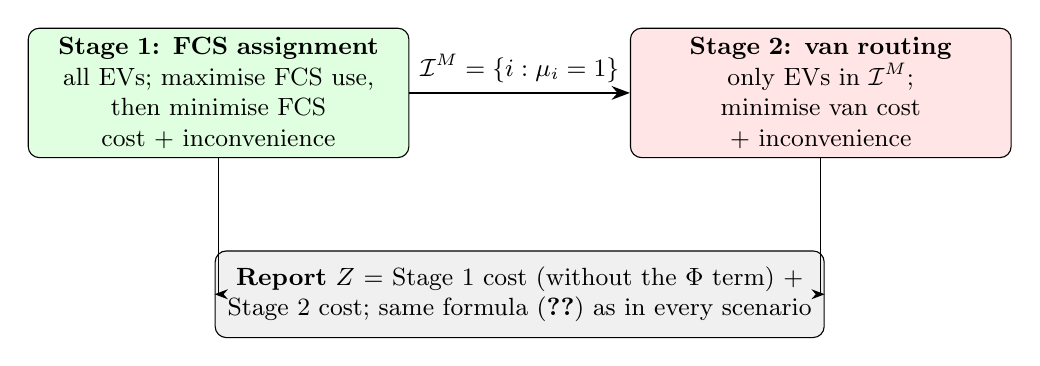
\begin{tikzpicture}[>=Stealth,box/.style={draw,rounded corners,align=center,minimum height=1.1cm,font=\small}]
  \node[box,fill=green!12,text width=4.6cm] (s1) {\textbf{Stage 1: FCS assignment}\\all EVs; maximise FCS use,\\then minimise FCS cost + inconvenience};
  \node[box,fill=red!10,text width=4.6cm,right=2.8cm of s1] (s2) {\textbf{Stage 2: van routing}\\only EVs in $\I^M$;\\minimise van cost + inconvenience};
  \draw[->,thick] (s1) -- node[above,font=\small]{$\I^M=\{i:\mu_i=1\}$} (s2);
  \node[box,fill=black!6,text width=7.5cm,below=2.0cm of $(s1)!0.5!(s2)$] (ev) {\textbf{Report} $Z=$ Stage~1 cost (without the $\Phi$ term) $+$ Stage~2 cost; same formula \eqref{eq:Z} as in every scenario};
  \draw[->] (s1) |- (ev); \draw[->] (s2) |- (ev);
\end{tikzpicture}
\end{center}

Stage~1 does not look at the vans, and Stage~2 cannot change what Stage~1 decided. That is the definition of ``FCS first, then MCS''.

%----------------------------------------------------------------
\subsection{Stage 1: assign EVs to fixed stations}

\textbf{Objective.}
\begin{equation}
\begin{split}
\min\ Z^{(1)}=\;&\underbrace{\Phi\sum_{i\in\I}\mu_i}_{\text{FCS first}}
+\underbrace{c^{EV}\sum_i\sum_{f\in\F_i}d_{if}Y_{if}}_{Z_1}
+\underbrace{Z^F_{\text{energy}}}_{\text{FCS part of }Z_4}\\
&+\underbrace{\sum_i\sum_{f\in\F_i}\rho^F_{if}Y_{if}+\alpha\sum_i w_i(C_i-r_i)+c^L\sum_i w_iL_i}_{\text{FCS customers' inconvenience}}
\end{split}
\label{eq:obj1}
\end{equation}
with $C_i=S_i+\tau^F_iY_i$ in this stage. $\Phi$ is a penalty for handing an EV to the vans. It is chosen larger than anything an extra FCS customer can add to the rest of \eqref{eq:obj1}, e.g.
\[
\Phi > \max_{i}\max_{f\in\F_i}\big(c^{EV}d_{if}+\pi^{\max}E_i+\rho^F_{if}\big)+n\,(\alpha+c^L)\,w_{\max}\,T,
\]
so Stage~1 first \textbf{maximises the number of EVs served at an FCS}, and only among those solutions minimises FCS cost and inconvenience. ($\pi^{\max}$ is the highest grid price.) A numerically safer equivalent is to solve twice: first $\max\sum_iY_i$, then fix that number and minimise the rest.
\ifTOU
Because $Z^F_{\text{energy}}$ uses the peak price, Stage~1 may \emph{start sessions later} to leave the peak, if the price saving beats the extra waiting cost (Section~\ref{sec:expect}).
\fi

\textbf{Constraints.}
\begin{align}
\sum_{g\in\G_i}y_{ig}+\mu_i &= 1 && \forall i\in\I \label{eq:s1assign}\\
S_i &\ge r_i+\sum_{f\in\F_i}t_{if}Y_{if} && \forall i\in\I \label{eq:fcsarr}\\
S_i &\le r_i+T\,(1-\mu_i) && \forall i\in\I \label{eq:s1park}\\
S_j &\ge S_i+\tau^F_i-(T+\tau^F_i)(3-y_{ig}-y_{jg}-o_{ij}) && \forall g,\ (i,j)\in\mathcal{P}_g \label{eq:disj1}\\
S_i &\ge S_j+\tau^F_j-(T+\tau^F_j)(2-y_{ig}-y_{jg}+o_{ij}) && \forall g,\ (i,j)\in\mathcal{P}_g \label{eq:disj2}\\
\sum_i y_{ig_1} &\ge \sum_i y_{ig_2} && \forall f,\ \G_f=\{g_1,g_2\} \label{eq:gunsym}\\
S_i+\tau^F_iY_i &\le T,\qquad L_i\ge S_i+\tau^F_iY_i-l_i && \forall i\in\I \label{eq:s1time}
\end{align}
\ifTOU plus the time-of-use split \eqref{eq:tou1}--\eqref{eq:tou5} of each FCS session (Section~\ref{sec:price}).\fi
\desc{\eqref{eq:s1assign}: every EV either gets one reachable gun or is handed to the vans. An EV that reaches no FCS ($\G_i=\emptyset$) is forced to $\mu_i=1$. \eqref{eq:fcsarr}: an FCS session cannot start before the EV has asked and driven to the station. \eqref{eq:s1park}: for an EV handed to the vans, $S_i$ is parked at $r_i$, so it adds no waiting in Stage~1 (its real start time is decided in Stage~2). \eqref{eq:disj1}--\eqref{eq:disj2}: two EVs on the same gun do not overlap; $o_{ij}$ picks who goes first. With two guns per station this means at most two EVs charge at a station at a time. \eqref{eq:gunsym}: symmetry breaking between the two identical guns (optional). \eqref{eq:s1time}: finished by $T$; lateness.}

\textbf{Optional acceptability rule.} An operator may refuse to send a driver to a station that is ``too inconvenient'', e.g.\ only allow gun $g$ of station $f$ for EV $i$ if $\hat\rho^F_{if}\le\bar\rho$. This only shrinks $\G_i$, so EVs whose stations are all too far go to the vans. Report results with and without it.

\textbf{Output:} $\I^M=\{i:\mu_i=1\}$, the EVs left for the vans; plus each FCS customer's gun and start time.

%----------------------------------------------------------------
\subsection{Stage 2: route the vans to the leftover EVs}

Stage~2 is a vehicle routing problem with time windows, on the EVs in $\I^M$ only. Here $C_i=S_i+\tau^M_i$.

\textbf{Objective.}
\begin{equation}
\begin{split}
\min\ Z^{(2)}=\;&\underbrace{c^M\sum_m\sum_{(i,j)\in\A^M}d_{ij}x_{ijm}}_{Z_2}+\underbrace{\sum_m c^D_mu_m}_{Z_3}+\underbrace{Z^M_{\text{energy}}}_{\text{van part of }Z_4}\\
&+\underbrace{\sum_{i\in\I^M}\sum_m\rho^M_{im}z_{im}+\alpha\sum_{i\in\I^M}w_i(C_i-r_i)+c^L\sum_{i\in\I^M}w_iL_i}_{\text{van customers' inconvenience}}
\end{split}
\label{eq:obj2}
\end{equation}
Since every EV in $\I^M$ must be served by some van, $Z^M_{\text{energy}}$ and the $\rho^M$ term are constants here. They are kept so that $Z^{(2)}$ is the true cost of Stage~2. Waiting and lateness make the vans visit urgent EVs early.

\textbf{Constraints.}
\begin{align}
\sum_{m\in\M}z_{im} &= 1 && \forall i\in\I^M \label{eq:s2assign}\\
\sum_{j:(0,j)\in\A^M}x_{0jm} = \sum_{i:(i,n+1)\in\A^M}x_{i,n+1,m} &= u_m && \forall m \label{eq:depot}\\
\sum_{i:(i,j)\in\A^M}x_{ijm} = \sum_{k:(j,k)\in\A^M}x_{jkm} &= z_{jm} && \forall j\in\I^M,\ m \label{eq:flow}\\
\sum_{i\in\I^M}z_{im} &\le Q_m\,u_m && \forall m \label{eq:cap}\\
\sum_{i\in\I^M}\frac{E_i}{\eta}z_{im}+\beta\sum_{(i,j)\in\A^M}d_{ij}x_{ijm} &\le B_m\,u_m && \forall m \label{eq:batt}
\end{align}
\begin{align}
S_j &\ge \max\{r_j,\ t_{0j}\,x_{0jm}\} && \forall j\in\I^M,\ m \label{eq:depart}\\
S_j &\ge S_i+\tau^M_i+t_{ij}-(T+\tau^M_i+t_{ij})(1-x_{ijm}) && \forall i\neq j,\ m \label{eq:seq}\\
S_i+\tau^M_i+t_{i,n+1} &\le T+(\tau^M_i+t_{i,n+1})(1-x_{i,n+1,m}) && \forall i,\ m \label{eq:return}\\
S_i+\tau^M_i \le T,\quad L_i &\ge S_i+\tau^M_i-l_i && \forall i\in\I^M \label{eq:s2time}\\
u_m &\ge u_{m+1} && m<|\M| \label{eq:vansym}
\end{align}
\desc{\eqref{eq:s2assign}: each leftover EV gets one van. \eqref{eq:depot}: a used van leaves and returns to the depot once. \eqref{eq:flow}: each EV on van $m$ is entered and left exactly once by that van. \eqref{eq:cap}: at most $Q_m$ EVs per van. \eqref{eq:batt}: delivered energy (with transfer losses) plus driving energy fits in the van battery. \eqref{eq:depart}: no start before the request, or before the van can drive there from the depot (written as two linear constraints). \eqref{eq:seq}: if the van goes $i\to j$, it finishes $i$ and drives to $j$ before starting $j$. This gives one EV at a time and removes subtours (MTZ-type). \eqref{eq:return}: back at the depot by $T$. \eqref{eq:s2time}: finished by $T$; lateness. \eqref{eq:vansym}: use identical vans in index order.}

\textbf{If Stage 2 is infeasible} (too many leftover EVs for the fleet by $T$), the sequential policy has \emph{failed} on that instance. For diagnosis, add $s_i\in\{0,1\}$ (``unserved''), replace \eqref{eq:s2assign} by $\sum_mz_{im}+s_i=1$ and add $\Phi^U\sum_is_i$ to \eqref{eq:obj2}. Then report the number of EVs that could not be served. This is a useful comparison with the integrated scenario, which may serve all of them.

%----------------------------------------------------------------
\subsection{Reported value}
\[
Z^{\text{S\scen}}=\big(Z^{(1)*}-\Phi\,|\I^M|\big)+Z^{(2)*},
\]
which is exactly \eqref{eq:Z} evaluated at the combined solution. The stage-1 solution plus the stage-2 solution is a feasible solution of the integrated model (S\ifTOU 4\else 3\fi), so
$Z^{\text{S\ifTOU 4\else 3\fi}}\le Z^{\text{S\scen}}$. The difference is the \emph{value of integration}.

\else
%---------------------------------------------------------------- INT
\subsection{Objective}
\begin{equation}
\min\ Z \quad\text{as in \eqref{eq:Z}, with }Z^F_{\text{energy}}=\ifTOU P^F\textstyle\sum_i\big[\pi^\off(\theta^1_i+\theta^3_i)+\pi^\pk\theta^2_i\big]\else\pi^F\textstyle\sum_iE_iY_i\fi,\quad C_i=S_i+\tau^F_iY_i+\tau^M_iZ_i. \label{eq:objint}
\end{equation}
Written out in full:
\begin{align*}
\min\ Z=\;& c^{EV}\sum_i\sum_{f\in\F_i}d_{if}Y_{if}+c^M\sum_m\sum_{(i,j)\in\A}d_{ij}x_{ijm}+\sum_mc^D_mu_m\\
&+\ifTOU P^F\sum_i\big[\pi^\off(\theta^1_i+\theta^3_i)+\pi^\pk\theta^2_i\big]\else\pi^F\sum_iE_iY_i\fi
+\pi^M\sum_i\sum_m\frac{E_i}{\eta}z_{im}\\
&+\sum_i\sum_{f\in\F_i}\rho^F_{if}Y_{if}+\sum_i\sum_m\rho^M_{im}z_{im}+\alpha\sum_iw_i(C_i-r_i)+c^L\sum_iw_iL_i .
\end{align*}
Every term is linear. One model weighs everything at once: an EV goes to a van exactly when the van's extra km, dispatch and energy cost are outweighed by the effort and waiting it saves the driver\ifTOU, or by the peak-price energy it avoids\fi.

\subsection{Constraints}

\textbf{Assignment.}
\begin{equation}
\sum_{g\in\G_i}y_{ig}+\sum_{m\in\M}z_{im}=1\qquad\forall i\in\I \label{eq:assign}
\end{equation}
\desc{Exactly one resource per EV: one reachable gun or one van. EVs that reach no FCS are forced onto a van.}

\textbf{Fixed stations.}
\begin{align}
S_i &\ge r_i+\sum_{f\in\F_i}t_{if}Y_{if} && \forall i \label{eq:fcsarr}\\
S_j &\ge S_i+\tau^F_i-(T+\tau^F_i)(3-y_{ig}-y_{jg}-o_{ij}) && \forall g,\ (i,j)\in\mathcal{P}_g \label{eq:disj1}\\
S_i &\ge S_j+\tau^F_j-(T+\tau^F_j)(2-y_{ig}-y_{jg}+o_{ij}) && \forall g,\ (i,j)\in\mathcal{P}_g \label{eq:disj2}\\
\sum_iy_{ig_1} &\ge \sum_iy_{ig_2} && \forall f,\ \G_f=\{g_1,g_2\} \label{eq:gunsym}
\end{align}
\desc{\eqref{eq:fcsarr}: an FCS session starts after the request and the drive to the station (for a van customer this is just $S_i\ge r_i$). \eqref{eq:disj1}--\eqref{eq:disj2}: EVs on the same gun do not overlap; $o_{ij}$ chooses the order. \eqref{eq:gunsym}: optional symmetry breaking.}

\textbf{Vans: routes, capacity, battery.}
\begin{align}
\sum_{j:(0,j)\in\A}x_{0jm}=\sum_{i:(i,n+1)\in\A}x_{i,n+1,m} &= u_m && \forall m \label{eq:depot}\\
\sum_{i:(i,j)\in\A}x_{ijm}=\sum_{k:(j,k)\in\A}x_{jkm} &= z_{jm} && \forall j\in\I,\ m \label{eq:flow}\\
\sum_iz_{im} &\le Q_mu_m && \forall m \label{eq:cap}\\
\sum_i\frac{E_i}{\eta}z_{im}+\beta\sum_{(i,j)\in\A}d_{ij}x_{ijm} &\le B_mu_m && \forall m \label{eq:batt}
\end{align}
\desc{\eqref{eq:depot}: a used van leaves and returns once. \eqref{eq:flow}: each EV on van $m$ is visited exactly once by it. \eqref{eq:cap}: at most $Q_m$ EVs. \eqref{eq:batt}: delivered energy (with losses) plus driving energy fits in the battery.}

\textbf{Vans: timing (one EV at a time, no subtours).}
\begin{align}
S_j &\ge t_{0j}\,x_{0jm} && \forall j\in\I,\ m \label{eq:depart}\\
S_j &\ge S_i+\tau^M_i+t_{ij}-(T+\tau^M_i+t_{ij})(1-x_{ijm}) && \forall i\neq j\in\I,\ m \label{eq:seq}\\
S_i+\tau^M_i+t_{i,n+1} &\le T+(\tau^M_i+t_{i,n+1})(1-x_{i,n+1,m}) && \forall i,\ m \label{eq:return}
\end{align}
\desc{\eqref{eq:depart}: the first stop cannot start before the van has driven there. \eqref{eq:seq}: $i\to j$ means finish $i$, drive, then start $j$; start times rise along a route, so no subtour can close. \eqref{eq:return}: back at the depot by $T$.}

\textbf{Horizon and lateness.}
\begin{equation}
C_i\le T,\qquad L_i\ge C_i-l_i\qquad\forall i\in\I \label{eq:time}
\end{equation}
\desc{Every EV is fully charged within the horizon; $L_i$ measures lateness.}

\ifTOU
\textbf{Time-of-use split.} Constraints \eqref{eq:tou1}--\eqref{eq:tou5} of Section~\ref{sec:price}.
\fi

\textbf{Symmetry and domains.}
\begin{equation}
u_m\ge u_{m+1};\qquad y,z,x,u,o\ifTOU,\kappa\fi\in\{0,1\};\qquad S_i,L_i\ifTOU,\theta^p_i\fi\ge0 \label{eq:dom}
\end{equation}
\fi

%=====================================================================
\section{Learning-to-optimise (RL) formulation}\label{sec:rl}

\textbf{Main rule:} the reward of each action is \emph{minus the increase in $Z$ that the action causes}. The rewards over an episode then add up to $-Z$ of the solution the policy builds. RL and MILP results are measured on the same yardstick \eqref{eq:Z}, and the MILP optimum is the benchmark for the RL gap.

\ifSEQ
%---------------------------------------------------------------- RL SEQ
The RL pipeline has the same two stages as the MILP.

\subsection{Stage 1 policy: FCS assignment}
\begin{itemize}[leftmargin=1.4em,itemsep=2pt]
  \item \textbf{Episode / epochs:} EVs are taken in order of request time $r_i$ (ties: higher $w_i$ first). One decision per EV.
  \item \textbf{State:} features of the current EV $k$ ($E_k,r_k,l_k,w_k,R_k$, location); for each gun $g$ the time $F_g$ it becomes free; summary features of the EVs still to come (count and positions near each station)\ifTOU; the current price and the time until $T_1$ and $T_2$\fi.
  \item \textbf{Action:} a gun $g\in\G_k$, or ``hand to vans''. \textbf{FCS-first mask:} ``hand to vans'' is allowed \emph{only} if no gun can finish EV $k$ by $T$ (or, with the optional rule, if all remaining guns have $\hat\rho^F_{kf}>\bar\rho$).
  \ifTOU\item \textbf{Optional timing action:} ``gun $g$, start after the peak'', i.e.\ $S_k=\max\{\text{earliest},T_2\}$, allowed only if the session still ends by $T$.\fi
  \item \textbf{Transition:} $S_k=\max\{r_k+t_{kf},F_g\}$ (or later, for the timing action); $F_g\leftarrow S_k+\tau^F_k$.
  \item \textbf{Reward:} $-\Big[c^{EV}d_{kf}+\text{energy}_k+\rho^F_{kf}+\alpha w_k(S_k+\tau^F_k-r_k)+c^Lw_k(S_k+\tau^F_k-l_k)^+\Big]$, where energy$_k$ = \ifTOU$P^F\big[\pi^\off\cdot(\text{off-peak hours of }[S_k,S_k+\tau^F_k])+\pi^\pk\cdot(\text{peak hours})\big]$, computed exactly in the simulator\else$\pi^FE_k$\fi. Handing an EV to the vans gives reward $0$ here; its cost is counted in Stage~2.
\end{itemize}
Note: a simple baseline for Stage~1 is the greedy rule ``gun with the largest one-step reward''. What RL can learn on top of this is, for example, to keep a nearby gun free for an urgent EV that arrives later.

\subsection{Stage 2 policy: van routing over $\I^M$}
\begin{itemize}[leftmargin=1.4em,itemsep=2pt]
  \item \textbf{Epochs:} whenever a van becomes free (the earliest-free van decides first).
  \item \textbf{State:} for each van: position, time free, remaining battery $b_m$, EVs served so far, dispatched or not; for each unserved EV in $\I^M$: location, $E_i,r_i,l_i,w_i$; current time.
  \item \textbf{Action:} the next EV $j$ for this van, or ``return to depot'' (ends the route). Mask: $j$ must be feasible: battery covers $E_j/\eta$ plus driving to $j$ and back to the depot, the count stays $\le Q_m$, and $j$ can be finished with the van back at the depot by $T$.
  \item \textbf{Transition:} $S_j=\max\{r_j,\ \text{time free}+t_{\text{pos},j}\}$; the van moves to $j$ and is free at $S_j+\tau^M_j$; $b_m$ falls by $E_j/\eta+\beta d_{\text{pos},j}$.
  \item \textbf{Reward:} serving $j$: $-\Big[c^Md_{\text{pos},j}+c^D_m[\text{first stop}]+\pi^M\frac{E_j}{\eta}+\rho^M_{jm}+\alpha w_j(S_j+\tau^M_j-r_j)+c^Lw_j(S_j+\tau^M_j-l_j)^+\Big]$; returning: $-c^Md_{\text{pos},0}$. EVs still unserved at the end: $-\Phi^U$ each.
  \item \textbf{Policy:} an attention-based routing policy (e.g.\ Kool et al., 2019, ``Attention, Learn to Solve Routing Problems!'') trained with REINFORCE or PPO. Baseline: nearest-feasible-EV heuristic.
\end{itemize}
Episode return of Stage~1 + Stage~2 $=-Z^{\text{S\scen}}$.

\else
%---------------------------------------------------------------- RL INT
One policy decides both who serves each EV and the van routes.
\begin{itemize}[leftmargin=1.4em,itemsep=2pt]
  \item \textbf{Episode / epochs:} EVs are taken in order of request time $r_i$ (ties: higher $w_i$ first). One decision per EV.
  \item \textbf{State:} (i) the current EV $k$: location, $E_k,r_k,l_k,w_k,R_k$, reachable stations; (ii) each gun $g$: time $F_g$ it becomes free; (iii) each van $m$: current end-of-route position, time free, remaining battery $b_m$, EVs served, dispatched or not; (iv) embeddings of the not-yet-assigned EVs (for look-ahead)\ifTOU; (v) current price, time until $T_1$ and $T_2$\fi.
  \item \textbf{Action:} $a\in\G_k\cup\M$: a gun, or a van (EV $k$ is appended to the end of that van's route). \textbf{Mask} infeasible actions: a gun that cannot finish $k$ by $T$; a van without enough battery for $E_k/\eta$ plus the drive to $k$ and back to the depot, with $Q_m$ reached, or unable to finish $k$ and return by $T$.
  \ifTOU\item \textbf{Optional timing action:} ``gun $g$, start after the peak'' ($S_k=\max\{\text{earliest},T_2\}$, if it still ends by $T$).\fi
  \item \textbf{Transition:} gun: $S_k=\max\{r_k+t_{kf},F_g\}$, $F_g\leftarrow S_k+\tau^F_k$. Van: $S_k=\max\{r_k,\ \text{free}_m+t_{\text{pos}_m,k}\}$, then the van moves to $k$, $\text{free}_m\leftarrow S_k+\tau^M_k$, $b_m\mathrel{-}=E_k/\eta+\beta d_{\text{pos}_m,k}$.
  \item \textbf{Reward} $=-\Delta Z$:
  \begin{align*}
  \text{gun } g\text{ at }f:&\quad -\Big[c^{EV}d_{kf}+\text{energy}^F_k+\rho^F_{kf}+\alpha w_k(C_k-r_k)+c^Lw_k(C_k-l_k)^+\Big]\\
  \text{van } m:&\quad -\Big[c^M\big(d_{\text{pos}_m,k}+d_{k,0}-d_{\text{pos}_m,0}\big)+c^D_m[\text{first use}]+\pi^M\tfrac{E_k}{\eta}\\
  &\qquad\quad+\rho^M_{km}+\alpha w_k(C_k-r_k)+c^Lw_k(C_k-l_k)^+\Big]
  \end{align*}
  The van distance term is the \emph{change} in route length when $k$ is inserted before the return to the depot, so the sum over the episode equals the total route length (the return legs telescope). energy$^F_k$ = \ifTOU$P^F\big[\pi^\off\cdot(\text{off-peak hours})+\pi^\pk\cdot(\text{peak hours of }[S_k,C_k])\big]$, computed exactly by the simulator; no linearisation is needed in RL\else$\pi^FE_k$\fi.
  \item \textbf{Dead end:} if every action is masked, EV $k$ is unserved: reward $-\Phi^U$, and the episode continues. Report the count.
  \item \textbf{Policy:} masked categorical policy over guns and vans, encoder with attention over EVs, guns and vans; trained with PPO. Natural baseline: greedy, i.e.\ choose the action with the largest one-step reward. That is the pairwise rule ``smallest $\hat\rho$ + cost'' from Section~\ref{sec:inc}.
\end{itemize}
Restriction to note: vans serve EVs in assignment order (append only). A variant that inserts $k$ at the cheapest position of a route is more flexible but has a larger action space.
\fi

\textbf{Reward scaling.} For stable training divide every reward by a constant, e.g.\ the greedy baseline's average $Z$ on the training instances. This does not change the optimal policy.

%=====================================================================
\section{What to expect and what to report}\label{sec:expect}

\ifnum\scen=1
\begin{itemize}[leftmargin=1.4em,itemsep=2pt]
  \item Vans serve only EVs that reach no station, or that the stations cannot finish by $T$. If stations have spare capacity, very few vans are dispatched.
  \item Inconvenience is high for EVs far from the nearest station (worked example: Rs\,682 at the FCS, against Rs\,458 if a van had been allowed).
  \item With too few vans Stage~2 becomes infeasible (unserved EVs), even when the integrated model S3 could serve everyone. Report the smallest $|\M|$ at which S1 is feasible and compare it with S3.
\end{itemize}
\fi
\ifnum\scen=2
\begin{itemize}[leftmargin=1.4em,itemsep=2pt]
  \item \textbf{When does Stage~1 delay a session to avoid the peak?} Moving one hour of charging out of the peak saves $(\pi^\pk-\pi^\off)P^F=3\times22=$ Rs\,66, but delays completion by up to an hour, which costs $\alpha w_i\ge$ Rs\,200. So with the default values Stage~1 almost never delays. It mostly pays the higher price, and S2 costs roughly S1 plus the peak surcharge. Sessions start later only if $\alpha$ is small (try $\lambda<0.33$ in the sensitivity analysis).
  \item The van assignment is the same as in S1 unless Stage~1's timing changes which EVs fit at the stations. Stage~1 cannot use vans to escape the peak price.
  \item Extra KPI: \textbf{grid energy drawn at FCS during the peak}, $P^F\sum_i\theta^2_i$ (kWh). Compare with S4.
\end{itemize}
\fi
\ifnum\scen=3
\begin{itemize}[leftmargin=1.4em,itemsep=2pt]
  \item Vans take EVs for which the saved inconvenience exceeds the extra van cost (worked example: van chosen, saving Rs\,224). Expect vans to serve EVs that are far from every station, have low range (high $w_i$), or have early deadlines, while EVs near a station still use it.
  \item \textbf{Value of integration under flat price:} $Z^{\text{S1}}-Z^{\text{S3}}\ge0$. Report it per component ($Z_1,\dots,Z_5$): typically operating cost rises a little and inconvenience falls a lot.
  \item Vary $|\M|$ (0, 1, 2, \dots): the first few vans lower $Z$ sharply, then the effect levels off. That curve shows the scenarios where mobile chargers help most.
\end{itemize}
\fi
\ifnum\scen=4
\begin{itemize}[leftmargin=1.4em,itemsep=2pt]
  \item During the peak a van kWh costs about the same as an FCS kWh (Rs\,10.0 each), so the vans' energy disadvantage disappears and vans also absorb \emph{peak-hour} demand that would otherwise be charged on the grid at peak price.
  \item Expect more van usage than in S3, concentrated on requests in $[T_1,T_2]$, and lower grid energy at the stations during the peak, $P^F\sum_i\theta^2_i$, than in S2.
  \item \textbf{Value of integration under peak pricing:} $Z^{\text{S2}}-Z^{\text{S4}}$. It should be larger than $Z^{\text{S1}}-Z^{\text{S3}}$, because integration now also allows price arbitrage.
  \item \textbf{Peak pricing with full flexibility:} $Z^{\text{S4}}-Z^{\text{S3}}$ should be smaller than $Z^{\text{S2}}-Z^{\text{S1}}$: vans cushion the price increase.
\end{itemize}
\fi

\textbf{Cross-scenario comparison table} (fill in from the four runs):
\begin{center}
\renewcommand{\arraystretch}{1.2}
\begin{tabular}{@{}lll@{}}
\toprule
\textbf{Comparison} & \textbf{Measures} & \textbf{Expected sign} \\
\midrule
S1 $-$ S3 & value of integration, flat price & $\ge0$ \\
S2 $-$ S4 & value of integration, peak price & $\ge0$, larger than S1 $-$ S3 \\
S2 $-$ S1 & cost of peak pricing, FCS-first operator & $>0$ \\
S4 $-$ S3 & cost of peak pricing, flexible operator & $>0$, smaller than S2 $-$ S1 \\
\bottomrule
\end{tabular}
\end{center}
Report for each: $Z$ and its components, number of vans used, EVs per resource, mean and maximum inconvenience per EV, total lateness, peak-hour grid energy, solve time, and (for RL) the gap to the MILP optimum.

%=====================================================================
\appendix
\section{Illustrative parameter values}\label{app:values}

These are starting values for experiments, not data. All are meant to be varied in the analysis. Values in Rs.

\begin{center}
\renewcommand{\arraystretch}{1.15}
\begin{tabular}{@{}llp{6.2cm}@{}}
\toprule
\textbf{Parameter} & \textbf{Value} & \textbf{Note} \\
\midrule
$T$, $[T_1,T_2]$ & 7 h, $[2,6]$ & 16:00--23:00, peak 18:00--22:00 \\
$P^F$, $P^M$ & 22 kW, 30 kW & \\
$v$, $\beta$, $\eta$ & 25 km/h, 0.25 kWh/km, 0.9 & \\
$B_m$, $Q_m$, $|\M|$ & 150 kWh, 6, 2--6 & \\
$c^{EV}$, $c^M$, $c^D_m$ & Rs\,4/km, Rs\,15/km, Rs\,1500 & van km includes driver time \\
$\pi^F$ (flat) & Rs\,8.7/kWh & equals the time-average of the ToU tariff over $[0,T]$ \\
$\pi^\off$, $\pi^\pk$ (ToU) & Rs\,7/kWh, Rs\,10/kWh & $(3\times7+4\times10)/7=8.7$ \\
$c^{bat}$ & Rs\,2/kWh & van battery wear \\
$\pi^M$ & Rs\,10.7 (flat) / Rs\,9.0 (ToU) & $=\pi^F+c^{bat}$ / $=\pi^\off+c^{bat}$ \\
$\alpha$, $\alpha^D$ & Rs\,200/h, Rs\,100/h & value of time; extra for attended time \\
$h^F$, $h^M$, $\varphi$ & Rs\,50, Rs\,10, Rs\,100 & trip hassle, hand-over, range stress \\
$c^L$ & Rs\,300/h & lateness \\
$w_i$ & $1+2(1-R_i/R_{\max})$, $R_i\sim U[3,40]$ km & priority from remaining range \\
\bottomrule
\end{tabular}
\end{center}

The flat price is set to the time-average of the peak tariff. The price \emph{level} is then the same in both pricing cases, and only the price \emph{shape} differs. Without this, part of S1 vs S2 would just reflect a different average price.

\end{document}
"
%    pdflatex -jobname=scenario4_peak_integrated   "\def\scen{4}% =====================================================================
%  One source, four PDFs.  Build with build.sh (or by hand):
%    pdflatex -jobname=scenario1_flat_sequential   "\def\scen{1}\input{scenario_master}"
%    pdflatex -jobname=scenario2_peak_sequential   "\def\scen{2}\input{scenario_master}"
%    pdflatex -jobname=scenario3_flat_integrated   "\def\scen{3}\input{scenario_master}"
%    pdflatex -jobname=scenario4_peak_integrated   "\def\scen{4}\input{scenario_master}"
%  (run each twice for cross-references)
% =====================================================================
\documentclass[11pt,a4paper]{article}
\usepackage[margin=2.2cm]{geometry}
\usepackage{amsmath,amssymb,amsfonts}
\usepackage{booktabs,array,tabularx}
\usepackage{enumitem}
\usepackage[table]{xcolor}
\usepackage{tikz}
\usetikzlibrary{arrows.meta,positioning,calc}
\usepackage[colorlinks=true,linkcolor=blue!50!black,urlcolor=blue!50!black]{hyperref}
\usepackage{titlesec}
\titleformat{\section}{\large\bfseries}{\thesection}{0.8em}{}
\titleformat{\subsection}{\normalsize\bfseries}{\thesubsection}{0.8em}{}
\setlength{\parindent}{0pt}
\setlength{\parskip}{5pt}

% ---------------- scenario switches ----------------
\ifdefined\scen\else\def\scen{1}\fi
\newif\ifTOU \TOUfalse   % true = time-of-use (peak) price
\newif\ifSEQ \SEQfalse   % true = FCS first, then MCS
\ifnum\scen=1 \SEQtrue \fi
\ifnum\scen=2 \TOUtrue \SEQtrue \fi
\ifnum\scen=4 \TOUtrue \fi

\newcommand{\pricename}{\ifTOU time-of-use price (dearer evening peak)\else single (flat) price all day\fi}
\newcommand{\structname}{\ifSEQ FCS first, then MCS (sequential)\else FCS and MCS together (integrated)\fi}

% ---------------- notation ----------------
\newcommand{\I}{\mathcal{I}}
\newcommand{\F}{\mathcal{F}}
\newcommand{\G}{\mathcal{G}}
\newcommand{\M}{\mathcal{M}}
\newcommand{\N}{\mathcal{N}}
\newcommand{\A}{\mathcal{A}}
\newcommand{\Rs}{\text{Rs}\,}
\newcommand{\pk}{\mathrm{pk}}
\newcommand{\off}{\mathrm{off}}
\newcommand{\desc}[1]{\par\vspace{-2pt}{\small\color{black!75}\textit{Meaning:} #1}\par\vspace{4pt}}
\newcommand{\cell}[2]{\ifnum\scen=#1\cellcolor{blue!18}\textbf{S#1 (this document)}\\\textbf{#2}\else S#1\\#2\fi}

\title{\textbf{EV Charging Network Optimisation}\\[4pt]
\large Scenario \scen: \pricename\ $+$ \structname\\[2pt]
\normalsize MILP and RL formulation}
\author{CP 320 OR for Mobility Management, course project}
\date{2 October 2026}

\begin{document}
\maketitle

%=====================================================================
\section{Where this scenario sits}

The project studies four scenarios: two ways of pricing grid electricity, times two ways of making the decisions.

\begin{center}
\renewcommand{\arraystretch}{1.5}
\begin{tabular}{>{\raggedright\arraybackslash}p{4.2cm}|>{\centering\arraybackslash}p{4.6cm}|>{\centering\arraybackslash}p{4.6cm}}
 & \textbf{Flat price all day} & \textbf{Time-of-use (peak) price} \\ \hline
\textbf{Sequential:} FCS first, leftover EVs to MCS &
\begin{tabular}[c]{@{}c@{}}\cell{1}{flat + sequential}\end{tabular} &
\begin{tabular}[c]{@{}c@{}}\cell{2}{peak + sequential}\end{tabular} \\ \hline
\textbf{Integrated:} FCS and MCS decided together &
\begin{tabular}[c]{@{}c@{}}\cell{3}{flat + integrated}\end{tabular} &
\begin{tabular}[c]{@{}c@{}}\cell{4}{peak + integrated}\end{tabular} \\
\end{tabular}
\end{center}

\textbf{The four scenarios do not have four different objectives.} They share \emph{one} cost yardstick $Z$ (Section~\ref{sec:obj}): the same cost terms and the same customer inconvenience (Section~\ref{sec:inc}). Only two things change:
\begin{itemize}[leftmargin=1.4em,itemsep=1pt]
  \item \textbf{Pricing} changes the formula for one term, the FCS energy cost (Section~\ref{sec:price}).
  \item \textbf{Decision structure} changes \emph{how} $Z$ is minimised: in one model (integrated), or in two stages (sequential), where each stage minimises its own part of $Z$.
\end{itemize}
Because the yardstick is the same, the four optimal values can be compared directly. The differences measure the \emph{value of integration} (S1$\to$S3, S2$\to$S4) and the \emph{effect of peak pricing} (S1$\to$S2, S3$\to$S4).

\ifnum\scen=1
\textbf{This scenario (S1)} is the baseline, the ``status quo''. Electricity costs the same at every hour, every EV that can be charged at a fixed station is sent there, and vans only take what is left over.
\fi
\ifnum\scen=2
\textbf{This scenario (S2)} keeps the FCS-first rule of S1, but grid electricity is dearer during the evening peak. Stage~1 can react to the price only by \emph{rescheduling} FCS sessions. It cannot hand a peak-hour EV to a van.
\fi
\ifnum\scen=3
\textbf{This scenario (S3)} keeps the flat price of S1, but the operator decides FCS and MCS service \emph{together}. An EV can be sent to a van even when a fixed station could take it, whenever that lowers total cost plus inconvenience.
\fi
\ifnum\scen=4
\textbf{This scenario (S4)} is the most flexible one: peak pricing at fixed stations, and FCS and MCS decided together. Van energy was bought off-peak, so vans can also be used to keep charging \emph{out of the expensive peak}.
\fi

%=====================================================================
\section{Setting and assumptions}\label{sec:setting}

\textbf{Time.} The planning horizon is $[0,T]$ with $T=7$\,h (16:00--23:00). It contains the evening peak window $[T_1,T_2]=[2,6]$ (18:00--22:00). The horizon is the same in all four scenarios. It is wider than the peak itself so that, under peak pricing, there is cheaper time on both sides of the peak.\ifTOU\else\ In this scenario the price is flat, so the window plays no role in the model.\fi

\textbf{Assumptions} (the same as MILP v3, plus two about energy):
\begin{enumerate}[leftmargin=1.6em,itemsep=1pt]
  \item Static, continuous time. All requests in the horizon are known at time $0$, and request $i$ becomes active at $r_i$.
  \item An EV served by an FCS drives there itself on its own battery (only to stations within its range $R_i$). The driver stays with the car while it waits for a free gun and while it charges.
  \item An EV served by an MCS stays parked where it is, and the driver is free in the meantime.
  \item Each FCS gun and each van charges one EV at a time, without interruption, at constant power.
  \item A van's battery covers both its driving and the energy it delivers. \textbf{The van battery is charged at the depot before the horizon starts}\ifTOU, i.e.\ at the off-peak price\fi, and is not recharged during the horizon.
  \item Every EV must be fully charged by $T$ (hard). Finishing after the driver's desired time $l_i$ is allowed but penalised.
\end{enumerate}

%=====================================================================
\section{Notation}\label{sec:notation}

\subsection*{Sets}
\begin{tabularx}{\textwidth}{@{}lX@{}}
\toprule
$\I=\{1,\dots,n\}$ & EV charging requests \\
$\F$; $\G_f$ ($|\G_f|=2$); $\G=\bigcup_f\G_f$ & fixed charging stations; guns of FCS $f$; all guns ($f(g)$ = station of gun $g$) \\
$\F_i=\{f: d_{if}\le R_i\}$, $\G_i=\bigcup_{f\in\F_i}\G_f$ & stations / guns EV $i$ can reach on its remaining range \\
$\M$ & mobile charging vans (MCS) \\
$0,\ n+1$ & depot as start node / end node (same place) \\
$\N=\{0\}\cup\I\cup\{n+1\}$, $\A$ & routing nodes; allowed van arcs $(i,j)$, $i\in\{0\}\cup\I$, $j\in\I\cup\{n+1\}$, $i\neq j$ \\
$\mathcal{P}_g=\{(i,j): i<j,\ g\in\G_i\cap\G_j\}$ & pairs of EVs that could share gun $g$ \\
\ifSEQ
$\I^M\subseteq\I$ & EVs handed to the vans by Stage~1 (an \emph{output} of Stage~1, a fixed input to Stage~2) \\
$\N^M$, $\A^M$ & routing nodes / arcs restricted to $\I^M$ \\
\fi
\bottomrule
\end{tabularx}

\subsection*{Parameters}
\begin{tabularx}{\textwidth}{@{}lX@{}}
\toprule
$E_i,\ r_i,\ l_i,\ R_i$ & energy demand (kWh), request time, desired completion time (h), remaining range (km) \\
$w_i\ge1$ & priority of EV $i$; $w_i=1+\kappa(1-R_i/R_{\max})$, so low-range EVs weigh more \\
$P^F,\ P^M$ & charging power of an FCS gun (22\,kW) / of a van (e.g.\ 30\,kW) \\
$\tau^F_i=E_i/P^F,\ \tau^M_i=E_i/P^M$ & charging time of EV $i$ at an FCS / by a van (h) \\
$d_{if},t_{if}$;\ $d_{ij},t_{ij}$ & distance (km) and time (h): EV$\to$FCS; between routing nodes ($t=d/v$) \\
$B_m,\ Q_m,\ \beta,\ \eta$ & van battery (kWh), max EVs per van, van consumption (kWh/km), transfer efficiency \\
$c^{EV},\ c^M,\ c^D_m$ & cost per km of EV driving, per km of van driving; fixed dispatch cost of van $m$ \\
\ifTOU
$\pi^\off,\ \pi^\pk$ & grid price (Rs/kWh) off-peak / in $[T_1,T_2]$, with $\pi^\pk\ge\pi^\off$ \\
\else
$\pi^F$ & grid price (Rs/kWh), the same at every hour \\
\fi
$c^{bat}$ & van battery wear per kWh cycled \\
$\pi^M$ & cost of 1 kWh taken from a van battery: $\pi^M=\ifTOU\pi^\off\else\pi^F\fi+c^{bat}$ (Section~\ref{sec:price}) \\
$\alpha,\ \alpha^D,\ h^F,\ h^M,\ \varphi,\ c^L$ & inconvenience coefficients (Section~\ref{sec:inc}) \\
\bottomrule
\end{tabularx}

\subsection*{Decision variables}
\begin{tabularx}{\textwidth}{@{}llX@{}}
\toprule
$y_{ig}$ & $\{0,1\}$ & EV $i$ charged at gun $g\in\G_i$ \\
$z_{im}$ & $\{0,1\}$ & EV $i$ served by van $m$ \\
$x_{ijm}$ & $\{0,1\}$ & van $m$ drives arc $(i,j)$ \\
$u_m$ & $\{0,1\}$ & van $m$ is dispatched \\
$o_{ij}$ & $\{0,1\}$ & for EVs $i<j$ that could share a gun: 1 if $i$ is charged before $j$ \\
\ifSEQ
$\mu_i$ & $\{0,1\}$ & Stage~1 only: EV $i$ is handed to the van fleet \\
\fi
\ifTOU
$\theta^1_i,\theta^2_i,\theta^3_i$ & $\ge0$ & hours of EV $i$'s FCS session before / inside / after the peak \\
$\kappa^1_i,\kappa^3_i$ & $\{0,1\}$ & EV $i$'s FCS session starts before $T_1$ / ends after $T_2$ \\
\fi
$S_i$ & $\ge0$ & time charging of EV $i$ starts (h), on whichever resource \\
$L_i$ & $\ge0$ & lateness of EV $i$ beyond $l_i$ (h) \\
\bottomrule
\end{tabularx}

\textbf{Short-hands} (linear expressions, not new variables):
\[
Y_{if}=\sum_{g\in\G_f}y_{ig},\qquad Y_i=\sum_{g\in\G_i}y_{ig}\ (\text{EV $i$ uses an FCS}),\qquad Z_i=\sum_{m\in\M}z_{im}\ (\text{EV $i$ uses a van}),
\]
\[
C_i=S_i+\tau^F_i\,Y_i+\tau^M_i\,Z_i \quad\text{(time EV $i$ is fully charged).}
\]

%=====================================================================
\section{Customer inconvenience}\label{sec:inc}

This section is \textbf{identical in all four scenario documents}. Inconvenience is a property of the customer, not of the price or of the planning method.

\subsection{What we mean by inconvenience}

Inconvenience is \emph{what the driver loses} from the moment they ask for a charge ($r_i$) until the car is fully charged ($C_i$), \emph{converted into rupees} so it can be added to the operator's costs. A driver loses three different things:

\begin{enumerate}[leftmargin=1.6em,itemsep=2pt]
  \item \textbf{Waiting:} the car is not ready. This lasts $C_i-r_i$ hours and affects \emph{every} driver, FCS or MCS.
  \item \textbf{Effort:} only an FCS customer has to drive to the station and sit there while the car charges. An MCS customer stays at home or at work and does something else. Driving to a far station also uses scarce battery range, which causes stress (``range anxiety'').
  \item \textbf{A missed deadline:} the car is still not ready at the time $l_i$ the driver needs it.
\end{enumerate}

Each loss gets a price in Rs per hour (or per event). All of them are multiplied by the priority $w_i$: an hour of delay for an EV with 5\,km of range left counts more than for one with 40\,km.

\subsection{The three components}

\begin{center}
\renewcommand{\arraystretch}{1.3}
\begin{tabularx}{\textwidth}{@{}>{\raggedright\arraybackslash}p{2.6cm}>{\raggedright\arraybackslash}X>{\raggedright\arraybackslash}X>{\raggedright\arraybackslash}p{3.0cm}@{}}
\toprule
\textbf{Component} & \textbf{EV $i$ at FCS $f$} & \textbf{EV $i$ by a van} & \textbf{Known when?} \\
\midrule
Effort & $w_i\big[\alpha^D(t_{if}+\tau^F_i)+h^F+\varphi\,d_{if}/R_i\big]$: driving and sitting at the station, a fixed trip hassle, range stress & $w_i\,h^M$: being reachable and handing over the car & \textbf{Static:} known as soon as the resource is chosen \\
Waiting & $w_i\,\alpha\,(C_i-r_i)$ = drive + \emph{queue at the gun} + charge & $w_i\,\alpha\,(C_i-r_i)$ = \emph{wait for the van} + charge & \textbf{Dynamic:} depends on the queue / van route \\
Missed deadline & $w_i\,c^L\,L_i$, $L_i=\max\{0,C_i-l_i\}$ & same & Dynamic \\
\bottomrule
\end{tabularx}
\end{center}

\textbf{Coefficients.}
$\alpha$ (Rs/h) is the value of an hour the car is not ready.
$\alpha^D$ (Rs/h) is the \emph{extra} value of an hour the driver must personally spend driving or sitting at the station: an hour at the station costs $\alpha+\alpha^D$, an hour waiting at home for a van costs only $\alpha$.
$h^F,h^M$ (Rs) are fixed hassle costs of one trip to a station / one van hand-over.
$\varphi$ (Rs) is the range-stress cost of a trip that uses the \emph{whole} remaining range ($d_{if}/R_i\le1$ is the fraction used).
$c^L$ (Rs/h) is the cost per hour late.

\subsection{Pairwise form: inconvenience of a (customer, resource) pair}

The natural first idea is: \emph{for every pair (EV $i$, FCS $f$) and every pair (EV $i$, van $m$) there is an inconvenience number, and the operator picks the pair with the lowest cost plus inconvenience.} The static part fits this idea exactly:
\[
\boxed{\;\rho^F_{if}=w_i\Big[\alpha^D\,(t_{if}+\tau^F_i)+h^F+\varphi\,\frac{d_{if}}{R_i}\Big]\qquad
\rho^M_{im}=w_i\,h^M\;}
\]
These are \textbf{parameters}, computed before solving, one number per (EV, FCS) pair and per (EV, van) pair. In the objective they appear linearly: $\sum_i\sum_f\rho^F_{if}Y_{if}+\sum_i\sum_m\rho^M_{im}z_{im}$.

Note that $\rho^M_{im}$ does not depend on $m$. Vans are identical and all start at the same depot, so the driver does not care \emph{which} van comes, only \emph{when} it comes. That ``when'' is the waiting part.

\subsection{Why waiting cannot be a fixed pairwise number}

It is tempting to also write the waiting as a pairwise number, e.g.\ ``the van needs 5 minutes to reach EV $i$''. But that depends on \emph{where the van is coming from}, which depends on the route the model is still choosing: if EV $i$ is the 4th stop of a van, the wait is the time for three charging sessions plus four drives. Likewise, waiting at an FCS depends on how many EVs are queued at that gun. So waiting is not known before solving. It is a function of decision variables:
\[
\text{waiting cost of EV } i \;=\; w_i\,\alpha\,(C_i-r_i),\qquad C_i=S_i+\tau^F_iY_i+\tau^M_iZ_i .
\]
This is \textbf{linear} in the variables ($S_i$, $y$, $z$), so it fits in a MILP directly. The constraints of Section~\ref{sec:milp} make $S_i$ equal to the true start time, including driving, queueing at the gun and the van's route. The term $\sum_i w_i\alpha r_i$ is a constant and may be dropped when solving.

\textbf{Pairwise \emph{estimate}} (used for intuition, by the RL policy and in heuristics): if there is no queue and the van comes straight to $i$,
\[
\hat\rho^{F}_{if}=\rho^F_{if}+w_i\alpha\,(t_{if}+\tau^F_i),\qquad
\hat\rho^{M}_{im}=\rho^M_{im}+w_i\alpha\,(t^{\text{van}}_{m\to i}+\tau^M_i),
\]
where $t^{\text{van}}_{m\to i}$ is the time until van $m$ can reach $i$ from where it currently is. In the RL formulation (Section~\ref{sec:rl}) the van's position \emph{is} known at each decision, so there this estimate becomes exact.

\subsection{Total inconvenience and how it enters the objective}

\begin{equation}
\boxed{\;
Z_{\text{inc}}=\underbrace{\sum_{i\in\I}\sum_{f\in\F_i}\rho^F_{if}Y_{if}+\sum_{i\in\I}\sum_{m\in\M}\rho^M_{im}z_{im}}_{\text{effort (static, pairwise)}}
+\underbrace{\alpha\sum_{i\in\I}w_i\,(C_i-r_i)}_{\text{waiting (dynamic)}}
+\underbrace{c^L\sum_{i\in\I}w_i\,L_i}_{\text{missed deadline}}
\;}\label{eq:inc}
\end{equation}
All three parts are in rupees, so $Z_{\text{inc}}$ is simply added to the operating costs. Nothing has to be normalised.

\subsection{Worked example: your ``10 km to the FCS vs.\ van in 5 minutes'' case}

EV $i$: $E_i=20$\,kWh, $R_i=40$\,km (so $w_i=1$); nearest free FCS $d_{if}=10$\,km away, $t_{if}=0.4$\,h at 25\,km/h; a van finishing next door can reach it in 5\,min ($0.083$\,h), adding about 4\,km to its route. $\tau^F_i=20/22=0.909$\,h, $\tau^M_i=20/30=0.667$\,h. Coefficients from Appendix~\ref{app:values}, flat price.

\begin{center}
\renewcommand{\arraystretch}{1.25}
\begin{tabular}{@{}lrr@{}}
\toprule
 & \textbf{FCS} & \textbf{Van} \\
\midrule
Driving (EV / extra van km) & $4\times10=40.0$ & $15\times4=60.0$ \\
Energy & $8.7\times20=174.0$ & $10.7\times20/0.9=237.8$ \\
\textbf{Operating cost only} & \textbf{214.0} & \textbf{297.8} \\
\midrule
Effort $\rho$ & $100(0.4+0.909)+50+100\cdot\tfrac{10}{40}=205.9$ & $10.0$ \\
Waiting $\alpha(C_i-r_i)$ & $200\times1.309=261.8$ & $200\times0.75=150.0$ \\
\textbf{Cost + inconvenience} & \textbf{681.7} & \textbf{457.8} \\
\bottomrule
\end{tabular}
\end{center}

On operating cost alone the FCS is cheaper, so a cost-only model would \emph{always} send this driver 10\,km away. With inconvenience included the van is better by about Rs\,224, and the integrated model chooses $z_{im}=1$, as you expected. If the FCS were only 1\,km away, the FCS would win both comparisons. The inconvenience term is what makes the model choose between ``cheap for the operator'' and ``convenient for the driver'', rather than following a fixed rule.

\subsection{Relation to a single penalty $\rho_i$ per EV}

The first draft used a penalty $\rho_i$ that is charged whenever EV $i$ goes to \emph{any} FCS: $\sum_i\sum_f\rho_iy_{if}$. Because $\sum_f y_{if}=1-\sum_m z_{im}$, this only says ``a van is worth $\rho_i$ more to EV $i$'', and that holds whether the station is 1\,km or 15\,km away, and whether the van arrives in 5 minutes or in 3 hours. The form above fixes both problems: $\rho^F_{if}$ grows with the distance to \emph{that} station, and the waiting term grows with how late the van or the free gun actually is. The old model is the special case $\alpha=\alpha^D=\varphi=c^L=0$, $h^F=\rho_i$.

\subsection{Choosing the coefficients}
\begin{itemize}[leftmargin=1.4em,itemsep=2pt]
  \item Use a value of time for $\alpha$ (e.g.\ Rs\,150--300/h for urban car users), and set $\alpha^D\approx0.5\alpha$: sitting at a station is worse than waiting at home.
  \item Keep $c^L>\alpha$, so missing the deadline is worse than ordinary waiting.
  \item \textbf{Sensitivity analysis:} multiply all inconvenience coefficients by a factor $\lambda\in\{0,0.25,0.5,1,2,4\}$ and plot operating cost against total inconvenience. $\lambda=0$ is the pure cost-minimising operator, and large $\lambda$ is a customer-first operator. This trade-off curve is a strong result for the ``Analysis'' part of the project.
\end{itemize}

\subsection{What inconvenience does in \emph{this} scenario}
\ifSEQ
In a sequential scenario inconvenience \textbf{cannot move an EV from an FCS to a van}: Stage~1 sends every EV that \emph{can} use an FCS to one. It still matters inside each stage. In Stage~1 it decides \emph{which} station and \emph{when} (urgent EVs get the near station and the first free gun). In Stage~2 it decides the \emph{order} in which vans visit EVs (urgent EVs first). In the worked example, this scenario sends the driver 10\,km to the FCS. That is the weakness the integrated scenarios remove.
\else
In an integrated scenario inconvenience is weighed directly against operating cost when choosing the resource. That is how the worked example ends up with a van. It also decides which station and which gun order, and the order of each van route.
\fi

%=====================================================================
\section{Electricity price in this scenario}\label{sec:price}

\textbf{Van energy (same in all scenarios).} A van's battery is charged at the depot \emph{before} the horizon, so its energy was bought at the
\ifTOU off-peak \fi
price, whatever time the van later delivers it. Each kWh taken from the van also wears the battery ($c^{bat}$), and a fraction $1-\eta$ is lost in transfer:
\[
Z^M_{\text{energy}}=\pi^M\sum_{i\in\I}\sum_{m\in\M}\frac{E_i}{\eta}\,z_{im},\qquad \pi^M=\ifTOU\pi^\off\else\pi^F\fi+c^{bat}.
\]

\ifTOU
\textbf{FCS energy (time-of-use).} An FCS draws from the grid while it charges. Energy delivered inside $[T_1,T_2]$ costs $\pi^\pk$, and energy outside it costs $\pi^\off$. A session $[S_i,S_i+\tau^F_i]$ may overlap the peak partly. Split its duration into the hours before, inside and after the peak, $\theta^1_i+\theta^2_i+\theta^3_i$:
\[
Z^F_{\text{energy}}=P^F\sum_{i\in\I}\Big[\pi^\off(\theta^1_i+\theta^3_i)+\pi^\pk\,\theta^2_i\Big].
\]
Constraints \eqref{eq:tou1}--\eqref{eq:tou5} below make the $\theta$'s equal to the true overlaps. Peak hours are dearer, so the solver wants $\theta^1_i,\theta^3_i$ as large as possible. It is enough to bound them from above by the true off-peak overlap, and the constraints need one binary per side:
\begin{align}
\theta^1_i+\theta^2_i+\theta^3_i &= \tau^F_i\,Y_i && \forall i\in\I \label{eq:tou1}\\
\theta^1_i &\le \tau^F_i\,\kappa^1_i && \forall i\in\I \label{eq:tou2}\\
\theta^1_i &\le T_1-S_i+T\,(1-\kappa^1_i) && \forall i\in\I \label{eq:tou3}\\
\theta^3_i &\le \tau^F_i\,\kappa^3_i && \forall i\in\I \label{eq:tou4}\\
\theta^3_i &\le S_i+\tau^F_i-T_2+T\,(1-\kappa^3_i) && \forall i\in\I \label{eq:tou5}
\end{align}
\desc{\eqref{eq:tou1}: the FCS session's hours are split into three parts; for a van customer ($Y_i=0$) all three are zero. \eqref{eq:tou2}--\eqref{eq:tou3}: off-peak time before the peak is only possible if the session starts before $T_1$ ($\kappa^1_i=1$), and is at most $T_1-S_i$. \eqref{eq:tou4}--\eqref{eq:tou5}: the same for time after $T_2$. $\theta^2_i\ge0$ prevents counting more off-peak hours than exist. Checking the cases (entirely before / inside / after the peak, straddling one edge, covering the whole peak) shows that at the optimum the $\theta$'s equal the exact overlaps. This needs $\pi^\pk\ge\pi^\off$, which is true for a peak tariff.}

\textbf{Why vans become more attractive.} Compare the cost of 1\,kWh delivered to an EV during the peak (values from Appendix~\ref{app:values}):
FCS $=\pi^\pk=$ Rs\,10.0, van $=(\pi^\off+c^{bat})/\eta=9/0.9=$ Rs\,10.0. They are at parity. Under the flat price the van is about Rs\,3.2/kWh dearer (FCS Rs\,8.7, van $10.7/0.9=$ Rs\,11.9). Peak pricing therefore removes the vans' main cost disadvantage, but only for EVs whose FCS session would fall in the peak.
\ifSEQ\ In this sequential scenario Stage~1 cannot use that, because it does not consider vans. It can only shift FCS sessions in time.\fi
\else
\textbf{FCS energy (flat).} Every kWh delivered at a fixed station costs $\pi^F$, whenever it is delivered:
\[
Z^F_{\text{energy}}=\pi^F\sum_{i\in\I}E_i\,Y_i .
\]
The start time therefore does not affect the energy cost. Under the flat price a van kWh costs $(\pi^F+c^{bat})/\eta\approx$ Rs\,11.9 against Rs\,8.7 at an FCS (Appendix~\ref{app:values}), so on energy alone the FCS always wins.
\fi

%=====================================================================
\section{MILP formulation}\label{sec:milp}

\subsection{The common cost yardstick $Z$}\label{sec:obj}

For any complete solution (every EV assigned, every route and start time known), the system cost is
\begin{equation}
\boxed{\;
Z=\underbrace{c^{EV}\sum_{i}\sum_{f\in\F_i}d_{if}Y_{if}}_{Z_1:\ \text{EV driving}}
+\underbrace{c^M\sum_{m}\sum_{(i,j)\in\A}d_{ij}x_{ijm}}_{Z_2:\ \text{van driving}}
+\underbrace{\sum_m c^D_m u_m}_{Z_3:\ \text{dispatch}}
+\underbrace{Z^F_{\text{energy}}+Z^M_{\text{energy}}}_{Z_4:\ \text{energy}}
+\underbrace{Z_{\text{inc}}}_{Z_5:\ \text{inconv.\ \eqref{eq:inc}}}
\;}\label{eq:Z}
\end{equation}
$Z_4$ is defined in Section~\ref{sec:price}. $Z_1$--$Z_4$ are the operator's costs listed in the brief (EV travel, MCS travel, MCS operating cost) plus energy. $Z_5$ is the customer inconvenience penalty. \textbf{The same formula is used to report results in all four scenarios.}

\ifSEQ
%---------------------------------------------------------------- SEQ
\subsection{Structure: two stages}

\begin{center}
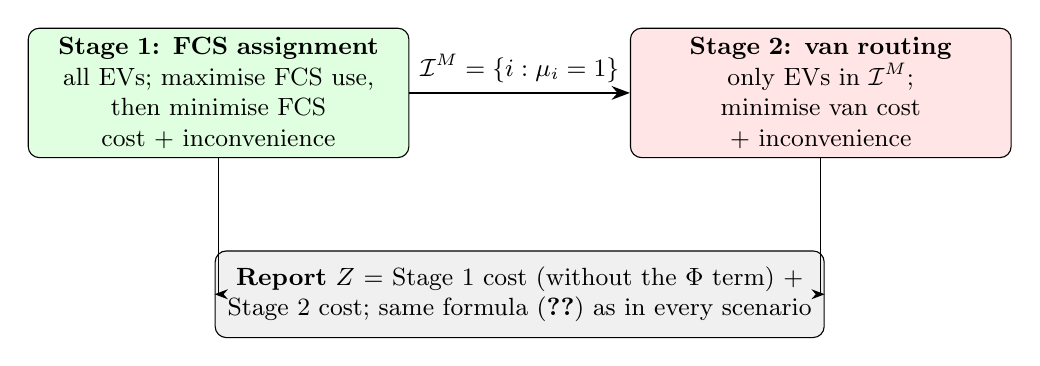
\begin{tikzpicture}[>=Stealth,box/.style={draw,rounded corners,align=center,minimum height=1.1cm,font=\small}]
  \node[box,fill=green!12,text width=4.6cm] (s1) {\textbf{Stage 1: FCS assignment}\\all EVs; maximise FCS use,\\then minimise FCS cost + inconvenience};
  \node[box,fill=red!10,text width=4.6cm,right=2.8cm of s1] (s2) {\textbf{Stage 2: van routing}\\only EVs in $\I^M$;\\minimise van cost + inconvenience};
  \draw[->,thick] (s1) -- node[above,font=\small]{$\I^M=\{i:\mu_i=1\}$} (s2);
  \node[box,fill=black!6,text width=7.5cm,below=2.0cm of $(s1)!0.5!(s2)$] (ev) {\textbf{Report} $Z=$ Stage~1 cost (without the $\Phi$ term) $+$ Stage~2 cost; same formula \eqref{eq:Z} as in every scenario};
  \draw[->] (s1) |- (ev); \draw[->] (s2) |- (ev);
\end{tikzpicture}
\end{center}

Stage~1 does not look at the vans, and Stage~2 cannot change what Stage~1 decided. That is the definition of ``FCS first, then MCS''.

%----------------------------------------------------------------
\subsection{Stage 1: assign EVs to fixed stations}

\textbf{Objective.}
\begin{equation}
\begin{split}
\min\ Z^{(1)}=\;&\underbrace{\Phi\sum_{i\in\I}\mu_i}_{\text{FCS first}}
+\underbrace{c^{EV}\sum_i\sum_{f\in\F_i}d_{if}Y_{if}}_{Z_1}
+\underbrace{Z^F_{\text{energy}}}_{\text{FCS part of }Z_4}\\
&+\underbrace{\sum_i\sum_{f\in\F_i}\rho^F_{if}Y_{if}+\alpha\sum_i w_i(C_i-r_i)+c^L\sum_i w_iL_i}_{\text{FCS customers' inconvenience}}
\end{split}
\label{eq:obj1}
\end{equation}
with $C_i=S_i+\tau^F_iY_i$ in this stage. $\Phi$ is a penalty for handing an EV to the vans. It is chosen larger than anything an extra FCS customer can add to the rest of \eqref{eq:obj1}, e.g.
\[
\Phi > \max_{i}\max_{f\in\F_i}\big(c^{EV}d_{if}+\pi^{\max}E_i+\rho^F_{if}\big)+n\,(\alpha+c^L)\,w_{\max}\,T,
\]
so Stage~1 first \textbf{maximises the number of EVs served at an FCS}, and only among those solutions minimises FCS cost and inconvenience. ($\pi^{\max}$ is the highest grid price.) A numerically safer equivalent is to solve twice: first $\max\sum_iY_i$, then fix that number and minimise the rest.
\ifTOU
Because $Z^F_{\text{energy}}$ uses the peak price, Stage~1 may \emph{start sessions later} to leave the peak, if the price saving beats the extra waiting cost (Section~\ref{sec:expect}).
\fi

\textbf{Constraints.}
\begin{align}
\sum_{g\in\G_i}y_{ig}+\mu_i &= 1 && \forall i\in\I \label{eq:s1assign}\\
S_i &\ge r_i+\sum_{f\in\F_i}t_{if}Y_{if} && \forall i\in\I \label{eq:fcsarr}\\
S_i &\le r_i+T\,(1-\mu_i) && \forall i\in\I \label{eq:s1park}\\
S_j &\ge S_i+\tau^F_i-(T+\tau^F_i)(3-y_{ig}-y_{jg}-o_{ij}) && \forall g,\ (i,j)\in\mathcal{P}_g \label{eq:disj1}\\
S_i &\ge S_j+\tau^F_j-(T+\tau^F_j)(2-y_{ig}-y_{jg}+o_{ij}) && \forall g,\ (i,j)\in\mathcal{P}_g \label{eq:disj2}\\
\sum_i y_{ig_1} &\ge \sum_i y_{ig_2} && \forall f,\ \G_f=\{g_1,g_2\} \label{eq:gunsym}\\
S_i+\tau^F_iY_i &\le T,\qquad L_i\ge S_i+\tau^F_iY_i-l_i && \forall i\in\I \label{eq:s1time}
\end{align}
\ifTOU plus the time-of-use split \eqref{eq:tou1}--\eqref{eq:tou5} of each FCS session (Section~\ref{sec:price}).\fi
\desc{\eqref{eq:s1assign}: every EV either gets one reachable gun or is handed to the vans. An EV that reaches no FCS ($\G_i=\emptyset$) is forced to $\mu_i=1$. \eqref{eq:fcsarr}: an FCS session cannot start before the EV has asked and driven to the station. \eqref{eq:s1park}: for an EV handed to the vans, $S_i$ is parked at $r_i$, so it adds no waiting in Stage~1 (its real start time is decided in Stage~2). \eqref{eq:disj1}--\eqref{eq:disj2}: two EVs on the same gun do not overlap; $o_{ij}$ picks who goes first. With two guns per station this means at most two EVs charge at a station at a time. \eqref{eq:gunsym}: symmetry breaking between the two identical guns (optional). \eqref{eq:s1time}: finished by $T$; lateness.}

\textbf{Optional acceptability rule.} An operator may refuse to send a driver to a station that is ``too inconvenient'', e.g.\ only allow gun $g$ of station $f$ for EV $i$ if $\hat\rho^F_{if}\le\bar\rho$. This only shrinks $\G_i$, so EVs whose stations are all too far go to the vans. Report results with and without it.

\textbf{Output:} $\I^M=\{i:\mu_i=1\}$, the EVs left for the vans; plus each FCS customer's gun and start time.

%----------------------------------------------------------------
\subsection{Stage 2: route the vans to the leftover EVs}

Stage~2 is a vehicle routing problem with time windows, on the EVs in $\I^M$ only. Here $C_i=S_i+\tau^M_i$.

\textbf{Objective.}
\begin{equation}
\begin{split}
\min\ Z^{(2)}=\;&\underbrace{c^M\sum_m\sum_{(i,j)\in\A^M}d_{ij}x_{ijm}}_{Z_2}+\underbrace{\sum_m c^D_mu_m}_{Z_3}+\underbrace{Z^M_{\text{energy}}}_{\text{van part of }Z_4}\\
&+\underbrace{\sum_{i\in\I^M}\sum_m\rho^M_{im}z_{im}+\alpha\sum_{i\in\I^M}w_i(C_i-r_i)+c^L\sum_{i\in\I^M}w_iL_i}_{\text{van customers' inconvenience}}
\end{split}
\label{eq:obj2}
\end{equation}
Since every EV in $\I^M$ must be served by some van, $Z^M_{\text{energy}}$ and the $\rho^M$ term are constants here. They are kept so that $Z^{(2)}$ is the true cost of Stage~2. Waiting and lateness make the vans visit urgent EVs early.

\textbf{Constraints.}
\begin{align}
\sum_{m\in\M}z_{im} &= 1 && \forall i\in\I^M \label{eq:s2assign}\\
\sum_{j:(0,j)\in\A^M}x_{0jm} = \sum_{i:(i,n+1)\in\A^M}x_{i,n+1,m} &= u_m && \forall m \label{eq:depot}\\
\sum_{i:(i,j)\in\A^M}x_{ijm} = \sum_{k:(j,k)\in\A^M}x_{jkm} &= z_{jm} && \forall j\in\I^M,\ m \label{eq:flow}\\
\sum_{i\in\I^M}z_{im} &\le Q_m\,u_m && \forall m \label{eq:cap}\\
\sum_{i\in\I^M}\frac{E_i}{\eta}z_{im}+\beta\sum_{(i,j)\in\A^M}d_{ij}x_{ijm} &\le B_m\,u_m && \forall m \label{eq:batt}
\end{align}
\begin{align}
S_j &\ge \max\{r_j,\ t_{0j}\,x_{0jm}\} && \forall j\in\I^M,\ m \label{eq:depart}\\
S_j &\ge S_i+\tau^M_i+t_{ij}-(T+\tau^M_i+t_{ij})(1-x_{ijm}) && \forall i\neq j,\ m \label{eq:seq}\\
S_i+\tau^M_i+t_{i,n+1} &\le T+(\tau^M_i+t_{i,n+1})(1-x_{i,n+1,m}) && \forall i,\ m \label{eq:return}\\
S_i+\tau^M_i \le T,\quad L_i &\ge S_i+\tau^M_i-l_i && \forall i\in\I^M \label{eq:s2time}\\
u_m &\ge u_{m+1} && m<|\M| \label{eq:vansym}
\end{align}
\desc{\eqref{eq:s2assign}: each leftover EV gets one van. \eqref{eq:depot}: a used van leaves and returns to the depot once. \eqref{eq:flow}: each EV on van $m$ is entered and left exactly once by that van. \eqref{eq:cap}: at most $Q_m$ EVs per van. \eqref{eq:batt}: delivered energy (with transfer losses) plus driving energy fits in the van battery. \eqref{eq:depart}: no start before the request, or before the van can drive there from the depot (written as two linear constraints). \eqref{eq:seq}: if the van goes $i\to j$, it finishes $i$ and drives to $j$ before starting $j$. This gives one EV at a time and removes subtours (MTZ-type). \eqref{eq:return}: back at the depot by $T$. \eqref{eq:s2time}: finished by $T$; lateness. \eqref{eq:vansym}: use identical vans in index order.}

\textbf{If Stage 2 is infeasible} (too many leftover EVs for the fleet by $T$), the sequential policy has \emph{failed} on that instance. For diagnosis, add $s_i\in\{0,1\}$ (``unserved''), replace \eqref{eq:s2assign} by $\sum_mz_{im}+s_i=1$ and add $\Phi^U\sum_is_i$ to \eqref{eq:obj2}. Then report the number of EVs that could not be served. This is a useful comparison with the integrated scenario, which may serve all of them.

%----------------------------------------------------------------
\subsection{Reported value}
\[
Z^{\text{S\scen}}=\big(Z^{(1)*}-\Phi\,|\I^M|\big)+Z^{(2)*},
\]
which is exactly \eqref{eq:Z} evaluated at the combined solution. The stage-1 solution plus the stage-2 solution is a feasible solution of the integrated model (S\ifTOU 4\else 3\fi), so
$Z^{\text{S\ifTOU 4\else 3\fi}}\le Z^{\text{S\scen}}$. The difference is the \emph{value of integration}.

\else
%---------------------------------------------------------------- INT
\subsection{Objective}
\begin{equation}
\min\ Z \quad\text{as in \eqref{eq:Z}, with }Z^F_{\text{energy}}=\ifTOU P^F\textstyle\sum_i\big[\pi^\off(\theta^1_i+\theta^3_i)+\pi^\pk\theta^2_i\big]\else\pi^F\textstyle\sum_iE_iY_i\fi,\quad C_i=S_i+\tau^F_iY_i+\tau^M_iZ_i. \label{eq:objint}
\end{equation}
Written out in full:
\begin{align*}
\min\ Z=\;& c^{EV}\sum_i\sum_{f\in\F_i}d_{if}Y_{if}+c^M\sum_m\sum_{(i,j)\in\A}d_{ij}x_{ijm}+\sum_mc^D_mu_m\\
&+\ifTOU P^F\sum_i\big[\pi^\off(\theta^1_i+\theta^3_i)+\pi^\pk\theta^2_i\big]\else\pi^F\sum_iE_iY_i\fi
+\pi^M\sum_i\sum_m\frac{E_i}{\eta}z_{im}\\
&+\sum_i\sum_{f\in\F_i}\rho^F_{if}Y_{if}+\sum_i\sum_m\rho^M_{im}z_{im}+\alpha\sum_iw_i(C_i-r_i)+c^L\sum_iw_iL_i .
\end{align*}
Every term is linear. One model weighs everything at once: an EV goes to a van exactly when the van's extra km, dispatch and energy cost are outweighed by the effort and waiting it saves the driver\ifTOU, or by the peak-price energy it avoids\fi.

\subsection{Constraints}

\textbf{Assignment.}
\begin{equation}
\sum_{g\in\G_i}y_{ig}+\sum_{m\in\M}z_{im}=1\qquad\forall i\in\I \label{eq:assign}
\end{equation}
\desc{Exactly one resource per EV: one reachable gun or one van. EVs that reach no FCS are forced onto a van.}

\textbf{Fixed stations.}
\begin{align}
S_i &\ge r_i+\sum_{f\in\F_i}t_{if}Y_{if} && \forall i \label{eq:fcsarr}\\
S_j &\ge S_i+\tau^F_i-(T+\tau^F_i)(3-y_{ig}-y_{jg}-o_{ij}) && \forall g,\ (i,j)\in\mathcal{P}_g \label{eq:disj1}\\
S_i &\ge S_j+\tau^F_j-(T+\tau^F_j)(2-y_{ig}-y_{jg}+o_{ij}) && \forall g,\ (i,j)\in\mathcal{P}_g \label{eq:disj2}\\
\sum_iy_{ig_1} &\ge \sum_iy_{ig_2} && \forall f,\ \G_f=\{g_1,g_2\} \label{eq:gunsym}
\end{align}
\desc{\eqref{eq:fcsarr}: an FCS session starts after the request and the drive to the station (for a van customer this is just $S_i\ge r_i$). \eqref{eq:disj1}--\eqref{eq:disj2}: EVs on the same gun do not overlap; $o_{ij}$ chooses the order. \eqref{eq:gunsym}: optional symmetry breaking.}

\textbf{Vans: routes, capacity, battery.}
\begin{align}
\sum_{j:(0,j)\in\A}x_{0jm}=\sum_{i:(i,n+1)\in\A}x_{i,n+1,m} &= u_m && \forall m \label{eq:depot}\\
\sum_{i:(i,j)\in\A}x_{ijm}=\sum_{k:(j,k)\in\A}x_{jkm} &= z_{jm} && \forall j\in\I,\ m \label{eq:flow}\\
\sum_iz_{im} &\le Q_mu_m && \forall m \label{eq:cap}\\
\sum_i\frac{E_i}{\eta}z_{im}+\beta\sum_{(i,j)\in\A}d_{ij}x_{ijm} &\le B_mu_m && \forall m \label{eq:batt}
\end{align}
\desc{\eqref{eq:depot}: a used van leaves and returns once. \eqref{eq:flow}: each EV on van $m$ is visited exactly once by it. \eqref{eq:cap}: at most $Q_m$ EVs. \eqref{eq:batt}: delivered energy (with losses) plus driving energy fits in the battery.}

\textbf{Vans: timing (one EV at a time, no subtours).}
\begin{align}
S_j &\ge t_{0j}\,x_{0jm} && \forall j\in\I,\ m \label{eq:depart}\\
S_j &\ge S_i+\tau^M_i+t_{ij}-(T+\tau^M_i+t_{ij})(1-x_{ijm}) && \forall i\neq j\in\I,\ m \label{eq:seq}\\
S_i+\tau^M_i+t_{i,n+1} &\le T+(\tau^M_i+t_{i,n+1})(1-x_{i,n+1,m}) && \forall i,\ m \label{eq:return}
\end{align}
\desc{\eqref{eq:depart}: the first stop cannot start before the van has driven there. \eqref{eq:seq}: $i\to j$ means finish $i$, drive, then start $j$; start times rise along a route, so no subtour can close. \eqref{eq:return}: back at the depot by $T$.}

\textbf{Horizon and lateness.}
\begin{equation}
C_i\le T,\qquad L_i\ge C_i-l_i\qquad\forall i\in\I \label{eq:time}
\end{equation}
\desc{Every EV is fully charged within the horizon; $L_i$ measures lateness.}

\ifTOU
\textbf{Time-of-use split.} Constraints \eqref{eq:tou1}--\eqref{eq:tou5} of Section~\ref{sec:price}.
\fi

\textbf{Symmetry and domains.}
\begin{equation}
u_m\ge u_{m+1};\qquad y,z,x,u,o\ifTOU,\kappa\fi\in\{0,1\};\qquad S_i,L_i\ifTOU,\theta^p_i\fi\ge0 \label{eq:dom}
\end{equation}
\fi

%=====================================================================
\section{Learning-to-optimise (RL) formulation}\label{sec:rl}

\textbf{Main rule:} the reward of each action is \emph{minus the increase in $Z$ that the action causes}. The rewards over an episode then add up to $-Z$ of the solution the policy builds. RL and MILP results are measured on the same yardstick \eqref{eq:Z}, and the MILP optimum is the benchmark for the RL gap.

\ifSEQ
%---------------------------------------------------------------- RL SEQ
The RL pipeline has the same two stages as the MILP.

\subsection{Stage 1 policy: FCS assignment}
\begin{itemize}[leftmargin=1.4em,itemsep=2pt]
  \item \textbf{Episode / epochs:} EVs are taken in order of request time $r_i$ (ties: higher $w_i$ first). One decision per EV.
  \item \textbf{State:} features of the current EV $k$ ($E_k,r_k,l_k,w_k,R_k$, location); for each gun $g$ the time $F_g$ it becomes free; summary features of the EVs still to come (count and positions near each station)\ifTOU; the current price and the time until $T_1$ and $T_2$\fi.
  \item \textbf{Action:} a gun $g\in\G_k$, or ``hand to vans''. \textbf{FCS-first mask:} ``hand to vans'' is allowed \emph{only} if no gun can finish EV $k$ by $T$ (or, with the optional rule, if all remaining guns have $\hat\rho^F_{kf}>\bar\rho$).
  \ifTOU\item \textbf{Optional timing action:} ``gun $g$, start after the peak'', i.e.\ $S_k=\max\{\text{earliest},T_2\}$, allowed only if the session still ends by $T$.\fi
  \item \textbf{Transition:} $S_k=\max\{r_k+t_{kf},F_g\}$ (or later, for the timing action); $F_g\leftarrow S_k+\tau^F_k$.
  \item \textbf{Reward:} $-\Big[c^{EV}d_{kf}+\text{energy}_k+\rho^F_{kf}+\alpha w_k(S_k+\tau^F_k-r_k)+c^Lw_k(S_k+\tau^F_k-l_k)^+\Big]$, where energy$_k$ = \ifTOU$P^F\big[\pi^\off\cdot(\text{off-peak hours of }[S_k,S_k+\tau^F_k])+\pi^\pk\cdot(\text{peak hours})\big]$, computed exactly in the simulator\else$\pi^FE_k$\fi. Handing an EV to the vans gives reward $0$ here; its cost is counted in Stage~2.
\end{itemize}
Note: a simple baseline for Stage~1 is the greedy rule ``gun with the largest one-step reward''. What RL can learn on top of this is, for example, to keep a nearby gun free for an urgent EV that arrives later.

\subsection{Stage 2 policy: van routing over $\I^M$}
\begin{itemize}[leftmargin=1.4em,itemsep=2pt]
  \item \textbf{Epochs:} whenever a van becomes free (the earliest-free van decides first).
  \item \textbf{State:} for each van: position, time free, remaining battery $b_m$, EVs served so far, dispatched or not; for each unserved EV in $\I^M$: location, $E_i,r_i,l_i,w_i$; current time.
  \item \textbf{Action:} the next EV $j$ for this van, or ``return to depot'' (ends the route). Mask: $j$ must be feasible: battery covers $E_j/\eta$ plus driving to $j$ and back to the depot, the count stays $\le Q_m$, and $j$ can be finished with the van back at the depot by $T$.
  \item \textbf{Transition:} $S_j=\max\{r_j,\ \text{time free}+t_{\text{pos},j}\}$; the van moves to $j$ and is free at $S_j+\tau^M_j$; $b_m$ falls by $E_j/\eta+\beta d_{\text{pos},j}$.
  \item \textbf{Reward:} serving $j$: $-\Big[c^Md_{\text{pos},j}+c^D_m[\text{first stop}]+\pi^M\frac{E_j}{\eta}+\rho^M_{jm}+\alpha w_j(S_j+\tau^M_j-r_j)+c^Lw_j(S_j+\tau^M_j-l_j)^+\Big]$; returning: $-c^Md_{\text{pos},0}$. EVs still unserved at the end: $-\Phi^U$ each.
  \item \textbf{Policy:} an attention-based routing policy (e.g.\ Kool et al., 2019, ``Attention, Learn to Solve Routing Problems!'') trained with REINFORCE or PPO. Baseline: nearest-feasible-EV heuristic.
\end{itemize}
Episode return of Stage~1 + Stage~2 $=-Z^{\text{S\scen}}$.

\else
%---------------------------------------------------------------- RL INT
One policy decides both who serves each EV and the van routes.
\begin{itemize}[leftmargin=1.4em,itemsep=2pt]
  \item \textbf{Episode / epochs:} EVs are taken in order of request time $r_i$ (ties: higher $w_i$ first). One decision per EV.
  \item \textbf{State:} (i) the current EV $k$: location, $E_k,r_k,l_k,w_k,R_k$, reachable stations; (ii) each gun $g$: time $F_g$ it becomes free; (iii) each van $m$: current end-of-route position, time free, remaining battery $b_m$, EVs served, dispatched or not; (iv) embeddings of the not-yet-assigned EVs (for look-ahead)\ifTOU; (v) current price, time until $T_1$ and $T_2$\fi.
  \item \textbf{Action:} $a\in\G_k\cup\M$: a gun, or a van (EV $k$ is appended to the end of that van's route). \textbf{Mask} infeasible actions: a gun that cannot finish $k$ by $T$; a van without enough battery for $E_k/\eta$ plus the drive to $k$ and back to the depot, with $Q_m$ reached, or unable to finish $k$ and return by $T$.
  \ifTOU\item \textbf{Optional timing action:} ``gun $g$, start after the peak'' ($S_k=\max\{\text{earliest},T_2\}$, if it still ends by $T$).\fi
  \item \textbf{Transition:} gun: $S_k=\max\{r_k+t_{kf},F_g\}$, $F_g\leftarrow S_k+\tau^F_k$. Van: $S_k=\max\{r_k,\ \text{free}_m+t_{\text{pos}_m,k}\}$, then the van moves to $k$, $\text{free}_m\leftarrow S_k+\tau^M_k$, $b_m\mathrel{-}=E_k/\eta+\beta d_{\text{pos}_m,k}$.
  \item \textbf{Reward} $=-\Delta Z$:
  \begin{align*}
  \text{gun } g\text{ at }f:&\quad -\Big[c^{EV}d_{kf}+\text{energy}^F_k+\rho^F_{kf}+\alpha w_k(C_k-r_k)+c^Lw_k(C_k-l_k)^+\Big]\\
  \text{van } m:&\quad -\Big[c^M\big(d_{\text{pos}_m,k}+d_{k,0}-d_{\text{pos}_m,0}\big)+c^D_m[\text{first use}]+\pi^M\tfrac{E_k}{\eta}\\
  &\qquad\quad+\rho^M_{km}+\alpha w_k(C_k-r_k)+c^Lw_k(C_k-l_k)^+\Big]
  \end{align*}
  The van distance term is the \emph{change} in route length when $k$ is inserted before the return to the depot, so the sum over the episode equals the total route length (the return legs telescope). energy$^F_k$ = \ifTOU$P^F\big[\pi^\off\cdot(\text{off-peak hours})+\pi^\pk\cdot(\text{peak hours of }[S_k,C_k])\big]$, computed exactly by the simulator; no linearisation is needed in RL\else$\pi^FE_k$\fi.
  \item \textbf{Dead end:} if every action is masked, EV $k$ is unserved: reward $-\Phi^U$, and the episode continues. Report the count.
  \item \textbf{Policy:} masked categorical policy over guns and vans, encoder with attention over EVs, guns and vans; trained with PPO. Natural baseline: greedy, i.e.\ choose the action with the largest one-step reward. That is the pairwise rule ``smallest $\hat\rho$ + cost'' from Section~\ref{sec:inc}.
\end{itemize}
Restriction to note: vans serve EVs in assignment order (append only). A variant that inserts $k$ at the cheapest position of a route is more flexible but has a larger action space.
\fi

\textbf{Reward scaling.} For stable training divide every reward by a constant, e.g.\ the greedy baseline's average $Z$ on the training instances. This does not change the optimal policy.

%=====================================================================
\section{What to expect and what to report}\label{sec:expect}

\ifnum\scen=1
\begin{itemize}[leftmargin=1.4em,itemsep=2pt]
  \item Vans serve only EVs that reach no station, or that the stations cannot finish by $T$. If stations have spare capacity, very few vans are dispatched.
  \item Inconvenience is high for EVs far from the nearest station (worked example: Rs\,682 at the FCS, against Rs\,458 if a van had been allowed).
  \item With too few vans Stage~2 becomes infeasible (unserved EVs), even when the integrated model S3 could serve everyone. Report the smallest $|\M|$ at which S1 is feasible and compare it with S3.
\end{itemize}
\fi
\ifnum\scen=2
\begin{itemize}[leftmargin=1.4em,itemsep=2pt]
  \item \textbf{When does Stage~1 delay a session to avoid the peak?} Moving one hour of charging out of the peak saves $(\pi^\pk-\pi^\off)P^F=3\times22=$ Rs\,66, but delays completion by up to an hour, which costs $\alpha w_i\ge$ Rs\,200. So with the default values Stage~1 almost never delays. It mostly pays the higher price, and S2 costs roughly S1 plus the peak surcharge. Sessions start later only if $\alpha$ is small (try $\lambda<0.33$ in the sensitivity analysis).
  \item The van assignment is the same as in S1 unless Stage~1's timing changes which EVs fit at the stations. Stage~1 cannot use vans to escape the peak price.
  \item Extra KPI: \textbf{grid energy drawn at FCS during the peak}, $P^F\sum_i\theta^2_i$ (kWh). Compare with S4.
\end{itemize}
\fi
\ifnum\scen=3
\begin{itemize}[leftmargin=1.4em,itemsep=2pt]
  \item Vans take EVs for which the saved inconvenience exceeds the extra van cost (worked example: van chosen, saving Rs\,224). Expect vans to serve EVs that are far from every station, have low range (high $w_i$), or have early deadlines, while EVs near a station still use it.
  \item \textbf{Value of integration under flat price:} $Z^{\text{S1}}-Z^{\text{S3}}\ge0$. Report it per component ($Z_1,\dots,Z_5$): typically operating cost rises a little and inconvenience falls a lot.
  \item Vary $|\M|$ (0, 1, 2, \dots): the first few vans lower $Z$ sharply, then the effect levels off. That curve shows the scenarios where mobile chargers help most.
\end{itemize}
\fi
\ifnum\scen=4
\begin{itemize}[leftmargin=1.4em,itemsep=2pt]
  \item During the peak a van kWh costs about the same as an FCS kWh (Rs\,10.0 each), so the vans' energy disadvantage disappears and vans also absorb \emph{peak-hour} demand that would otherwise be charged on the grid at peak price.
  \item Expect more van usage than in S3, concentrated on requests in $[T_1,T_2]$, and lower grid energy at the stations during the peak, $P^F\sum_i\theta^2_i$, than in S2.
  \item \textbf{Value of integration under peak pricing:} $Z^{\text{S2}}-Z^{\text{S4}}$. It should be larger than $Z^{\text{S1}}-Z^{\text{S3}}$, because integration now also allows price arbitrage.
  \item \textbf{Peak pricing with full flexibility:} $Z^{\text{S4}}-Z^{\text{S3}}$ should be smaller than $Z^{\text{S2}}-Z^{\text{S1}}$: vans cushion the price increase.
\end{itemize}
\fi

\textbf{Cross-scenario comparison table} (fill in from the four runs):
\begin{center}
\renewcommand{\arraystretch}{1.2}
\begin{tabular}{@{}lll@{}}
\toprule
\textbf{Comparison} & \textbf{Measures} & \textbf{Expected sign} \\
\midrule
S1 $-$ S3 & value of integration, flat price & $\ge0$ \\
S2 $-$ S4 & value of integration, peak price & $\ge0$, larger than S1 $-$ S3 \\
S2 $-$ S1 & cost of peak pricing, FCS-first operator & $>0$ \\
S4 $-$ S3 & cost of peak pricing, flexible operator & $>0$, smaller than S2 $-$ S1 \\
\bottomrule
\end{tabular}
\end{center}
Report for each: $Z$ and its components, number of vans used, EVs per resource, mean and maximum inconvenience per EV, total lateness, peak-hour grid energy, solve time, and (for RL) the gap to the MILP optimum.

%=====================================================================
\appendix
\section{Illustrative parameter values}\label{app:values}

These are starting values for experiments, not data. All are meant to be varied in the analysis. Values in Rs.

\begin{center}
\renewcommand{\arraystretch}{1.15}
\begin{tabular}{@{}llp{6.2cm}@{}}
\toprule
\textbf{Parameter} & \textbf{Value} & \textbf{Note} \\
\midrule
$T$, $[T_1,T_2]$ & 7 h, $[2,6]$ & 16:00--23:00, peak 18:00--22:00 \\
$P^F$, $P^M$ & 22 kW, 30 kW & \\
$v$, $\beta$, $\eta$ & 25 km/h, 0.25 kWh/km, 0.9 & \\
$B_m$, $Q_m$, $|\M|$ & 150 kWh, 6, 2--6 & \\
$c^{EV}$, $c^M$, $c^D_m$ & Rs\,4/km, Rs\,15/km, Rs\,1500 & van km includes driver time \\
$\pi^F$ (flat) & Rs\,8.7/kWh & equals the time-average of the ToU tariff over $[0,T]$ \\
$\pi^\off$, $\pi^\pk$ (ToU) & Rs\,7/kWh, Rs\,10/kWh & $(3\times7+4\times10)/7=8.7$ \\
$c^{bat}$ & Rs\,2/kWh & van battery wear \\
$\pi^M$ & Rs\,10.7 (flat) / Rs\,9.0 (ToU) & $=\pi^F+c^{bat}$ / $=\pi^\off+c^{bat}$ \\
$\alpha$, $\alpha^D$ & Rs\,200/h, Rs\,100/h & value of time; extra for attended time \\
$h^F$, $h^M$, $\varphi$ & Rs\,50, Rs\,10, Rs\,100 & trip hassle, hand-over, range stress \\
$c^L$ & Rs\,300/h & lateness \\
$w_i$ & $1+2(1-R_i/R_{\max})$, $R_i\sim U[3,40]$ km & priority from remaining range \\
\bottomrule
\end{tabular}
\end{center}

The flat price is set to the time-average of the peak tariff. The price \emph{level} is then the same in both pricing cases, and only the price \emph{shape} differs. Without this, part of S1 vs S2 would just reflect a different average price.

\end{document}
"
%  (run each twice for cross-references)
% =====================================================================
\documentclass[11pt,a4paper]{article}
\usepackage[margin=2.2cm]{geometry}
\usepackage{amsmath,amssymb,amsfonts}
\usepackage{booktabs,array,tabularx}
\usepackage{enumitem}
\usepackage[table]{xcolor}
\usepackage{tikz}
\usetikzlibrary{arrows.meta,positioning,calc}
\usepackage[colorlinks=true,linkcolor=blue!50!black,urlcolor=blue!50!black]{hyperref}
\usepackage{titlesec}
\titleformat{\section}{\large\bfseries}{\thesection}{0.8em}{}
\titleformat{\subsection}{\normalsize\bfseries}{\thesubsection}{0.8em}{}
\setlength{\parindent}{0pt}
\setlength{\parskip}{5pt}

% ---------------- scenario switches ----------------
\ifdefined\scen\else\def\scen{1}\fi
\newif\ifTOU \TOUfalse   % true = time-of-use (peak) price
\newif\ifSEQ \SEQfalse   % true = FCS first, then MCS
\ifnum\scen=1 \SEQtrue \fi
\ifnum\scen=2 \TOUtrue \SEQtrue \fi
\ifnum\scen=4 \TOUtrue \fi

\newcommand{\pricename}{\ifTOU time-of-use price (dearer evening peak)\else single (flat) price all day\fi}
\newcommand{\structname}{\ifSEQ FCS first, then MCS (sequential)\else FCS and MCS together (integrated)\fi}

% ---------------- notation ----------------
\newcommand{\I}{\mathcal{I}}
\newcommand{\F}{\mathcal{F}}
\newcommand{\G}{\mathcal{G}}
\newcommand{\M}{\mathcal{M}}
\newcommand{\N}{\mathcal{N}}
\newcommand{\A}{\mathcal{A}}
\newcommand{\Rs}{\text{Rs}\,}
\newcommand{\pk}{\mathrm{pk}}
\newcommand{\off}{\mathrm{off}}
\newcommand{\desc}[1]{\par\vspace{-2pt}{\small\color{black!75}\textit{Meaning:} #1}\par\vspace{4pt}}
\newcommand{\cell}[2]{\ifnum\scen=#1\cellcolor{blue!18}\textbf{S#1 (this document)}\\\textbf{#2}\else S#1\\#2\fi}

\title{\textbf{EV Charging Network Optimisation}\\[4pt]
\large Scenario \scen: \pricename\ $+$ \structname\\[2pt]
\normalsize MILP and RL formulation}
\author{CP 320 OR for Mobility Management, course project}
\date{2 October 2026}

\begin{document}
\maketitle

%=====================================================================
\section{Where this scenario sits}

The project studies four scenarios: two ways of pricing grid electricity, times two ways of making the decisions.

\begin{center}
\renewcommand{\arraystretch}{1.5}
\begin{tabular}{>{\raggedright\arraybackslash}p{4.2cm}|>{\centering\arraybackslash}p{4.6cm}|>{\centering\arraybackslash}p{4.6cm}}
 & \textbf{Flat price all day} & \textbf{Time-of-use (peak) price} \\ \hline
\textbf{Sequential:} FCS first, leftover EVs to MCS &
\begin{tabular}[c]{@{}c@{}}\cell{1}{flat + sequential}\end{tabular} &
\begin{tabular}[c]{@{}c@{}}\cell{2}{peak + sequential}\end{tabular} \\ \hline
\textbf{Integrated:} FCS and MCS decided together &
\begin{tabular}[c]{@{}c@{}}\cell{3}{flat + integrated}\end{tabular} &
\begin{tabular}[c]{@{}c@{}}\cell{4}{peak + integrated}\end{tabular} \\
\end{tabular}
\end{center}

\textbf{The four scenarios do not have four different objectives.} They share \emph{one} cost yardstick $Z$ (Section~\ref{sec:obj}): the same cost terms and the same customer inconvenience (Section~\ref{sec:inc}). Only two things change:
\begin{itemize}[leftmargin=1.4em,itemsep=1pt]
  \item \textbf{Pricing} changes the formula for one term, the FCS energy cost (Section~\ref{sec:price}).
  \item \textbf{Decision structure} changes \emph{how} $Z$ is minimised: in one model (integrated), or in two stages (sequential), where each stage minimises its own part of $Z$.
\end{itemize}
Because the yardstick is the same, the four optimal values can be compared directly. The differences measure the \emph{value of integration} (S1$\to$S3, S2$\to$S4) and the \emph{effect of peak pricing} (S1$\to$S2, S3$\to$S4).

\ifnum\scen=1
\textbf{This scenario (S1)} is the baseline, the ``status quo''. Electricity costs the same at every hour, every EV that can be charged at a fixed station is sent there, and vans only take what is left over.
\fi
\ifnum\scen=2
\textbf{This scenario (S2)} keeps the FCS-first rule of S1, but grid electricity is dearer during the evening peak. Stage~1 can react to the price only by \emph{rescheduling} FCS sessions. It cannot hand a peak-hour EV to a van.
\fi
\ifnum\scen=3
\textbf{This scenario (S3)} keeps the flat price of S1, but the operator decides FCS and MCS service \emph{together}. An EV can be sent to a van even when a fixed station could take it, whenever that lowers total cost plus inconvenience.
\fi
\ifnum\scen=4
\textbf{This scenario (S4)} is the most flexible one: peak pricing at fixed stations, and FCS and MCS decided together. Van energy was bought off-peak, so vans can also be used to keep charging \emph{out of the expensive peak}.
\fi

%=====================================================================
\section{Setting and assumptions}\label{sec:setting}

\textbf{Time.} The planning horizon is $[0,T]$ with $T=7$\,h (16:00--23:00). It contains the evening peak window $[T_1,T_2]=[2,6]$ (18:00--22:00). The horizon is the same in all four scenarios. It is wider than the peak itself so that, under peak pricing, there is cheaper time on both sides of the peak.\ifTOU\else\ In this scenario the price is flat, so the window plays no role in the model.\fi

\textbf{Assumptions} (the same as MILP v3, plus two about energy):
\begin{enumerate}[leftmargin=1.6em,itemsep=1pt]
  \item Static, continuous time. All requests in the horizon are known at time $0$, and request $i$ becomes active at $r_i$.
  \item An EV served by an FCS drives there itself on its own battery (only to stations within its range $R_i$). The driver stays with the car while it waits for a free gun and while it charges.
  \item An EV served by an MCS stays parked where it is, and the driver is free in the meantime.
  \item Each FCS gun and each van charges one EV at a time, without interruption, at constant power.
  \item A van's battery covers both its driving and the energy it delivers. \textbf{The van battery is charged at the depot before the horizon starts}\ifTOU, i.e.\ at the off-peak price\fi, and is not recharged during the horizon.
  \item Every EV must be fully charged by $T$ (hard). Finishing after the driver's desired time $l_i$ is allowed but penalised.
\end{enumerate}

%=====================================================================
\section{Notation}\label{sec:notation}

\subsection*{Sets}
\begin{tabularx}{\textwidth}{@{}lX@{}}
\toprule
$\I=\{1,\dots,n\}$ & EV charging requests \\
$\F$; $\G_f$ ($|\G_f|=2$); $\G=\bigcup_f\G_f$ & fixed charging stations; guns of FCS $f$; all guns ($f(g)$ = station of gun $g$) \\
$\F_i=\{f: d_{if}\le R_i\}$, $\G_i=\bigcup_{f\in\F_i}\G_f$ & stations / guns EV $i$ can reach on its remaining range \\
$\M$ & mobile charging vans (MCS) \\
$0,\ n+1$ & depot as start node / end node (same place) \\
$\N=\{0\}\cup\I\cup\{n+1\}$, $\A$ & routing nodes; allowed van arcs $(i,j)$, $i\in\{0\}\cup\I$, $j\in\I\cup\{n+1\}$, $i\neq j$ \\
$\mathcal{P}_g=\{(i,j): i<j,\ g\in\G_i\cap\G_j\}$ & pairs of EVs that could share gun $g$ \\
\ifSEQ
$\I^M\subseteq\I$ & EVs handed to the vans by Stage~1 (an \emph{output} of Stage~1, a fixed input to Stage~2) \\
$\N^M$, $\A^M$ & routing nodes / arcs restricted to $\I^M$ \\
\fi
\bottomrule
\end{tabularx}

\subsection*{Parameters}
\begin{tabularx}{\textwidth}{@{}lX@{}}
\toprule
$E_i,\ r_i,\ l_i,\ R_i$ & energy demand (kWh), request time, desired completion time (h), remaining range (km) \\
$w_i\ge1$ & priority of EV $i$; $w_i=1+\kappa(1-R_i/R_{\max})$, so low-range EVs weigh more \\
$P^F,\ P^M$ & charging power of an FCS gun (22\,kW) / of a van (e.g.\ 30\,kW) \\
$\tau^F_i=E_i/P^F,\ \tau^M_i=E_i/P^M$ & charging time of EV $i$ at an FCS / by a van (h) \\
$d_{if},t_{if}$;\ $d_{ij},t_{ij}$ & distance (km) and time (h): EV$\to$FCS; between routing nodes ($t=d/v$) \\
$B_m,\ Q_m,\ \beta,\ \eta$ & van battery (kWh), max EVs per van, van consumption (kWh/km), transfer efficiency \\
$c^{EV},\ c^M,\ c^D_m$ & cost per km of EV driving, per km of van driving; fixed dispatch cost of van $m$ \\
\ifTOU
$\pi^\off,\ \pi^\pk$ & grid price (Rs/kWh) off-peak / in $[T_1,T_2]$, with $\pi^\pk\ge\pi^\off$ \\
\else
$\pi^F$ & grid price (Rs/kWh), the same at every hour \\
\fi
$c^{bat}$ & van battery wear per kWh cycled \\
$\pi^M$ & cost of 1 kWh taken from a van battery: $\pi^M=\ifTOU\pi^\off\else\pi^F\fi+c^{bat}$ (Section~\ref{sec:price}) \\
$\alpha,\ \alpha^D,\ h^F,\ h^M,\ \varphi,\ c^L$ & inconvenience coefficients (Section~\ref{sec:inc}) \\
\bottomrule
\end{tabularx}

\subsection*{Decision variables}
\begin{tabularx}{\textwidth}{@{}llX@{}}
\toprule
$y_{ig}$ & $\{0,1\}$ & EV $i$ charged at gun $g\in\G_i$ \\
$z_{im}$ & $\{0,1\}$ & EV $i$ served by van $m$ \\
$x_{ijm}$ & $\{0,1\}$ & van $m$ drives arc $(i,j)$ \\
$u_m$ & $\{0,1\}$ & van $m$ is dispatched \\
$o_{ij}$ & $\{0,1\}$ & for EVs $i<j$ that could share a gun: 1 if $i$ is charged before $j$ \\
\ifSEQ
$\mu_i$ & $\{0,1\}$ & Stage~1 only: EV $i$ is handed to the van fleet \\
\fi
\ifTOU
$\theta^1_i,\theta^2_i,\theta^3_i$ & $\ge0$ & hours of EV $i$'s FCS session before / inside / after the peak \\
$\kappa^1_i,\kappa^3_i$ & $\{0,1\}$ & EV $i$'s FCS session starts before $T_1$ / ends after $T_2$ \\
\fi
$S_i$ & $\ge0$ & time charging of EV $i$ starts (h), on whichever resource \\
$L_i$ & $\ge0$ & lateness of EV $i$ beyond $l_i$ (h) \\
\bottomrule
\end{tabularx}

\textbf{Short-hands} (linear expressions, not new variables):
\[
Y_{if}=\sum_{g\in\G_f}y_{ig},\qquad Y_i=\sum_{g\in\G_i}y_{ig}\ (\text{EV $i$ uses an FCS}),\qquad Z_i=\sum_{m\in\M}z_{im}\ (\text{EV $i$ uses a van}),
\]
\[
C_i=S_i+\tau^F_i\,Y_i+\tau^M_i\,Z_i \quad\text{(time EV $i$ is fully charged).}
\]

%=====================================================================
\section{Customer inconvenience}\label{sec:inc}

This section is \textbf{identical in all four scenario documents}. Inconvenience is a property of the customer, not of the price or of the planning method.

\subsection{What we mean by inconvenience}

Inconvenience is \emph{what the driver loses} from the moment they ask for a charge ($r_i$) until the car is fully charged ($C_i$), \emph{converted into rupees} so it can be added to the operator's costs. A driver loses three different things:

\begin{enumerate}[leftmargin=1.6em,itemsep=2pt]
  \item \textbf{Waiting:} the car is not ready. This lasts $C_i-r_i$ hours and affects \emph{every} driver, FCS or MCS.
  \item \textbf{Effort:} only an FCS customer has to drive to the station and sit there while the car charges. An MCS customer stays at home or at work and does something else. Driving to a far station also uses scarce battery range, which causes stress (``range anxiety'').
  \item \textbf{A missed deadline:} the car is still not ready at the time $l_i$ the driver needs it.
\end{enumerate}

Each loss gets a price in Rs per hour (or per event). All of them are multiplied by the priority $w_i$: an hour of delay for an EV with 5\,km of range left counts more than for one with 40\,km.

\subsection{The three components}

\begin{center}
\renewcommand{\arraystretch}{1.3}
\begin{tabularx}{\textwidth}{@{}>{\raggedright\arraybackslash}p{2.6cm}>{\raggedright\arraybackslash}X>{\raggedright\arraybackslash}X>{\raggedright\arraybackslash}p{3.0cm}@{}}
\toprule
\textbf{Component} & \textbf{EV $i$ at FCS $f$} & \textbf{EV $i$ by a van} & \textbf{Known when?} \\
\midrule
Effort & $w_i\big[\alpha^D(t_{if}+\tau^F_i)+h^F+\varphi\,d_{if}/R_i\big]$: driving and sitting at the station, a fixed trip hassle, range stress & $w_i\,h^M$: being reachable and handing over the car & \textbf{Static:} known as soon as the resource is chosen \\
Waiting & $w_i\,\alpha\,(C_i-r_i)$ = drive + \emph{queue at the gun} + charge & $w_i\,\alpha\,(C_i-r_i)$ = \emph{wait for the van} + charge & \textbf{Dynamic:} depends on the queue / van route \\
Missed deadline & $w_i\,c^L\,L_i$, $L_i=\max\{0,C_i-l_i\}$ & same & Dynamic \\
\bottomrule
\end{tabularx}
\end{center}

\textbf{Coefficients.}
$\alpha$ (Rs/h) is the value of an hour the car is not ready.
$\alpha^D$ (Rs/h) is the \emph{extra} value of an hour the driver must personally spend driving or sitting at the station: an hour at the station costs $\alpha+\alpha^D$, an hour waiting at home for a van costs only $\alpha$.
$h^F,h^M$ (Rs) are fixed hassle costs of one trip to a station / one van hand-over.
$\varphi$ (Rs) is the range-stress cost of a trip that uses the \emph{whole} remaining range ($d_{if}/R_i\le1$ is the fraction used).
$c^L$ (Rs/h) is the cost per hour late.

\subsection{Pairwise form: inconvenience of a (customer, resource) pair}

The natural first idea is: \emph{for every pair (EV $i$, FCS $f$) and every pair (EV $i$, van $m$) there is an inconvenience number, and the operator picks the pair with the lowest cost plus inconvenience.} The static part fits this idea exactly:
\[
\boxed{\;\rho^F_{if}=w_i\Big[\alpha^D\,(t_{if}+\tau^F_i)+h^F+\varphi\,\frac{d_{if}}{R_i}\Big]\qquad
\rho^M_{im}=w_i\,h^M\;}
\]
These are \textbf{parameters}, computed before solving, one number per (EV, FCS) pair and per (EV, van) pair. In the objective they appear linearly: $\sum_i\sum_f\rho^F_{if}Y_{if}+\sum_i\sum_m\rho^M_{im}z_{im}$.

Note that $\rho^M_{im}$ does not depend on $m$. Vans are identical and all start at the same depot, so the driver does not care \emph{which} van comes, only \emph{when} it comes. That ``when'' is the waiting part.

\subsection{Why waiting cannot be a fixed pairwise number}

It is tempting to also write the waiting as a pairwise number, e.g.\ ``the van needs 5 minutes to reach EV $i$''. But that depends on \emph{where the van is coming from}, which depends on the route the model is still choosing: if EV $i$ is the 4th stop of a van, the wait is the time for three charging sessions plus four drives. Likewise, waiting at an FCS depends on how many EVs are queued at that gun. So waiting is not known before solving. It is a function of decision variables:
\[
\text{waiting cost of EV } i \;=\; w_i\,\alpha\,(C_i-r_i),\qquad C_i=S_i+\tau^F_iY_i+\tau^M_iZ_i .
\]
This is \textbf{linear} in the variables ($S_i$, $y$, $z$), so it fits in a MILP directly. The constraints of Section~\ref{sec:milp} make $S_i$ equal to the true start time, including driving, queueing at the gun and the van's route. The term $\sum_i w_i\alpha r_i$ is a constant and may be dropped when solving.

\textbf{Pairwise \emph{estimate}} (used for intuition, by the RL policy and in heuristics): if there is no queue and the van comes straight to $i$,
\[
\hat\rho^{F}_{if}=\rho^F_{if}+w_i\alpha\,(t_{if}+\tau^F_i),\qquad
\hat\rho^{M}_{im}=\rho^M_{im}+w_i\alpha\,(t^{\text{van}}_{m\to i}+\tau^M_i),
\]
where $t^{\text{van}}_{m\to i}$ is the time until van $m$ can reach $i$ from where it currently is. In the RL formulation (Section~\ref{sec:rl}) the van's position \emph{is} known at each decision, so there this estimate becomes exact.

\subsection{Total inconvenience and how it enters the objective}

\begin{equation}
\boxed{\;
Z_{\text{inc}}=\underbrace{\sum_{i\in\I}\sum_{f\in\F_i}\rho^F_{if}Y_{if}+\sum_{i\in\I}\sum_{m\in\M}\rho^M_{im}z_{im}}_{\text{effort (static, pairwise)}}
+\underbrace{\alpha\sum_{i\in\I}w_i\,(C_i-r_i)}_{\text{waiting (dynamic)}}
+\underbrace{c^L\sum_{i\in\I}w_i\,L_i}_{\text{missed deadline}}
\;}\label{eq:inc}
\end{equation}
All three parts are in rupees, so $Z_{\text{inc}}$ is simply added to the operating costs. Nothing has to be normalised.

\subsection{Worked example: your ``10 km to the FCS vs.\ van in 5 minutes'' case}

EV $i$: $E_i=20$\,kWh, $R_i=40$\,km (so $w_i=1$); nearest free FCS $d_{if}=10$\,km away, $t_{if}=0.4$\,h at 25\,km/h; a van finishing next door can reach it in 5\,min ($0.083$\,h), adding about 4\,km to its route. $\tau^F_i=20/22=0.909$\,h, $\tau^M_i=20/30=0.667$\,h. Coefficients from Appendix~\ref{app:values}, flat price.

\begin{center}
\renewcommand{\arraystretch}{1.25}
\begin{tabular}{@{}lrr@{}}
\toprule
 & \textbf{FCS} & \textbf{Van} \\
\midrule
Driving (EV / extra van km) & $4\times10=40.0$ & $15\times4=60.0$ \\
Energy & $8.7\times20=174.0$ & $10.7\times20/0.9=237.8$ \\
\textbf{Operating cost only} & \textbf{214.0} & \textbf{297.8} \\
\midrule
Effort $\rho$ & $100(0.4+0.909)+50+100\cdot\tfrac{10}{40}=205.9$ & $10.0$ \\
Waiting $\alpha(C_i-r_i)$ & $200\times1.309=261.8$ & $200\times0.75=150.0$ \\
\textbf{Cost + inconvenience} & \textbf{681.7} & \textbf{457.8} \\
\bottomrule
\end{tabular}
\end{center}

On operating cost alone the FCS is cheaper, so a cost-only model would \emph{always} send this driver 10\,km away. With inconvenience included the van is better by about Rs\,224, and the integrated model chooses $z_{im}=1$, as you expected. If the FCS were only 1\,km away, the FCS would win both comparisons. The inconvenience term is what makes the model choose between ``cheap for the operator'' and ``convenient for the driver'', rather than following a fixed rule.

\subsection{Relation to a single penalty $\rho_i$ per EV}

The first draft used a penalty $\rho_i$ that is charged whenever EV $i$ goes to \emph{any} FCS: $\sum_i\sum_f\rho_iy_{if}$. Because $\sum_f y_{if}=1-\sum_m z_{im}$, this only says ``a van is worth $\rho_i$ more to EV $i$'', and that holds whether the station is 1\,km or 15\,km away, and whether the van arrives in 5 minutes or in 3 hours. The form above fixes both problems: $\rho^F_{if}$ grows with the distance to \emph{that} station, and the waiting term grows with how late the van or the free gun actually is. The old model is the special case $\alpha=\alpha^D=\varphi=c^L=0$, $h^F=\rho_i$.

\subsection{Choosing the coefficients}
\begin{itemize}[leftmargin=1.4em,itemsep=2pt]
  \item Use a value of time for $\alpha$ (e.g.\ Rs\,150--300/h for urban car users), and set $\alpha^D\approx0.5\alpha$: sitting at a station is worse than waiting at home.
  \item Keep $c^L>\alpha$, so missing the deadline is worse than ordinary waiting.
  \item \textbf{Sensitivity analysis:} multiply all inconvenience coefficients by a factor $\lambda\in\{0,0.25,0.5,1,2,4\}$ and plot operating cost against total inconvenience. $\lambda=0$ is the pure cost-minimising operator, and large $\lambda$ is a customer-first operator. This trade-off curve is a strong result for the ``Analysis'' part of the project.
\end{itemize}

\subsection{What inconvenience does in \emph{this} scenario}
\ifSEQ
In a sequential scenario inconvenience \textbf{cannot move an EV from an FCS to a van}: Stage~1 sends every EV that \emph{can} use an FCS to one. It still matters inside each stage. In Stage~1 it decides \emph{which} station and \emph{when} (urgent EVs get the near station and the first free gun). In Stage~2 it decides the \emph{order} in which vans visit EVs (urgent EVs first). In the worked example, this scenario sends the driver 10\,km to the FCS. That is the weakness the integrated scenarios remove.
\else
In an integrated scenario inconvenience is weighed directly against operating cost when choosing the resource. That is how the worked example ends up with a van. It also decides which station and which gun order, and the order of each van route.
\fi

%=====================================================================
\section{Electricity price in this scenario}\label{sec:price}

\textbf{Van energy (same in all scenarios).} A van's battery is charged at the depot \emph{before} the horizon, so its energy was bought at the
\ifTOU off-peak \fi
price, whatever time the van later delivers it. Each kWh taken from the van also wears the battery ($c^{bat}$), and a fraction $1-\eta$ is lost in transfer:
\[
Z^M_{\text{energy}}=\pi^M\sum_{i\in\I}\sum_{m\in\M}\frac{E_i}{\eta}\,z_{im},\qquad \pi^M=\ifTOU\pi^\off\else\pi^F\fi+c^{bat}.
\]

\ifTOU
\textbf{FCS energy (time-of-use).} An FCS draws from the grid while it charges. Energy delivered inside $[T_1,T_2]$ costs $\pi^\pk$, and energy outside it costs $\pi^\off$. A session $[S_i,S_i+\tau^F_i]$ may overlap the peak partly. Split its duration into the hours before, inside and after the peak, $\theta^1_i+\theta^2_i+\theta^3_i$:
\[
Z^F_{\text{energy}}=P^F\sum_{i\in\I}\Big[\pi^\off(\theta^1_i+\theta^3_i)+\pi^\pk\,\theta^2_i\Big].
\]
Constraints \eqref{eq:tou1}--\eqref{eq:tou5} below make the $\theta$'s equal to the true overlaps. Peak hours are dearer, so the solver wants $\theta^1_i,\theta^3_i$ as large as possible. It is enough to bound them from above by the true off-peak overlap, and the constraints need one binary per side:
\begin{align}
\theta^1_i+\theta^2_i+\theta^3_i &= \tau^F_i\,Y_i && \forall i\in\I \label{eq:tou1}\\
\theta^1_i &\le \tau^F_i\,\kappa^1_i && \forall i\in\I \label{eq:tou2}\\
\theta^1_i &\le T_1-S_i+T\,(1-\kappa^1_i) && \forall i\in\I \label{eq:tou3}\\
\theta^3_i &\le \tau^F_i\,\kappa^3_i && \forall i\in\I \label{eq:tou4}\\
\theta^3_i &\le S_i+\tau^F_i-T_2+T\,(1-\kappa^3_i) && \forall i\in\I \label{eq:tou5}
\end{align}
\desc{\eqref{eq:tou1}: the FCS session's hours are split into three parts; for a van customer ($Y_i=0$) all three are zero. \eqref{eq:tou2}--\eqref{eq:tou3}: off-peak time before the peak is only possible if the session starts before $T_1$ ($\kappa^1_i=1$), and is at most $T_1-S_i$. \eqref{eq:tou4}--\eqref{eq:tou5}: the same for time after $T_2$. $\theta^2_i\ge0$ prevents counting more off-peak hours than exist. Checking the cases (entirely before / inside / after the peak, straddling one edge, covering the whole peak) shows that at the optimum the $\theta$'s equal the exact overlaps. This needs $\pi^\pk\ge\pi^\off$, which is true for a peak tariff.}

\textbf{Why vans become more attractive.} Compare the cost of 1\,kWh delivered to an EV during the peak (values from Appendix~\ref{app:values}):
FCS $=\pi^\pk=$ Rs\,10.0, van $=(\pi^\off+c^{bat})/\eta=9/0.9=$ Rs\,10.0. They are at parity. Under the flat price the van is about Rs\,3.2/kWh dearer (FCS Rs\,8.7, van $10.7/0.9=$ Rs\,11.9). Peak pricing therefore removes the vans' main cost disadvantage, but only for EVs whose FCS session would fall in the peak.
\ifSEQ\ In this sequential scenario Stage~1 cannot use that, because it does not consider vans. It can only shift FCS sessions in time.\fi
\else
\textbf{FCS energy (flat).} Every kWh delivered at a fixed station costs $\pi^F$, whenever it is delivered:
\[
Z^F_{\text{energy}}=\pi^F\sum_{i\in\I}E_i\,Y_i .
\]
The start time therefore does not affect the energy cost. Under the flat price a van kWh costs $(\pi^F+c^{bat})/\eta\approx$ Rs\,11.9 against Rs\,8.7 at an FCS (Appendix~\ref{app:values}), so on energy alone the FCS always wins.
\fi

%=====================================================================
\section{MILP formulation}\label{sec:milp}

\subsection{The common cost yardstick $Z$}\label{sec:obj}

For any complete solution (every EV assigned, every route and start time known), the system cost is
\begin{equation}
\boxed{\;
Z=\underbrace{c^{EV}\sum_{i}\sum_{f\in\F_i}d_{if}Y_{if}}_{Z_1:\ \text{EV driving}}
+\underbrace{c^M\sum_{m}\sum_{(i,j)\in\A}d_{ij}x_{ijm}}_{Z_2:\ \text{van driving}}
+\underbrace{\sum_m c^D_m u_m}_{Z_3:\ \text{dispatch}}
+\underbrace{Z^F_{\text{energy}}+Z^M_{\text{energy}}}_{Z_4:\ \text{energy}}
+\underbrace{Z_{\text{inc}}}_{Z_5:\ \text{inconv.\ \eqref{eq:inc}}}
\;}\label{eq:Z}
\end{equation}
$Z_4$ is defined in Section~\ref{sec:price}. $Z_1$--$Z_4$ are the operator's costs listed in the brief (EV travel, MCS travel, MCS operating cost) plus energy. $Z_5$ is the customer inconvenience penalty. \textbf{The same formula is used to report results in all four scenarios.}

\ifSEQ
%---------------------------------------------------------------- SEQ
\subsection{Structure: two stages}

\begin{center}
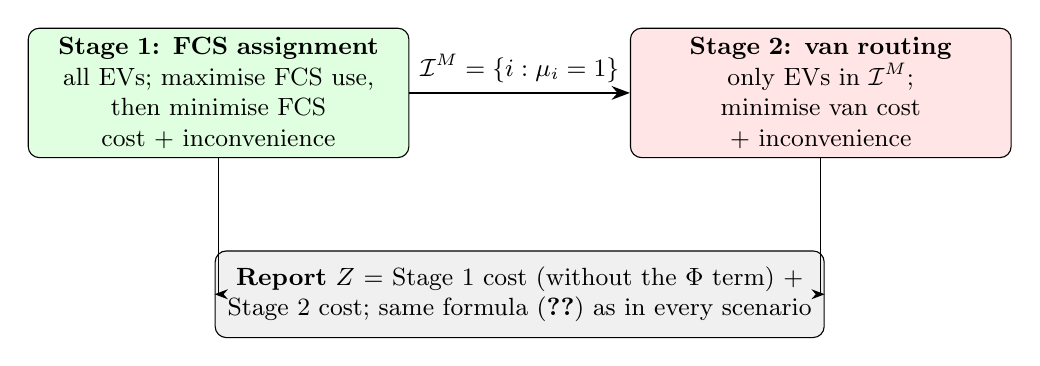
\begin{tikzpicture}[>=Stealth,box/.style={draw,rounded corners,align=center,minimum height=1.1cm,font=\small}]
  \node[box,fill=green!12,text width=4.6cm] (s1) {\textbf{Stage 1: FCS assignment}\\all EVs; maximise FCS use,\\then minimise FCS cost + inconvenience};
  \node[box,fill=red!10,text width=4.6cm,right=2.8cm of s1] (s2) {\textbf{Stage 2: van routing}\\only EVs in $\I^M$;\\minimise van cost + inconvenience};
  \draw[->,thick] (s1) -- node[above,font=\small]{$\I^M=\{i:\mu_i=1\}$} (s2);
  \node[box,fill=black!6,text width=7.5cm,below=2.0cm of $(s1)!0.5!(s2)$] (ev) {\textbf{Report} $Z=$ Stage~1 cost (without the $\Phi$ term) $+$ Stage~2 cost; same formula \eqref{eq:Z} as in every scenario};
  \draw[->] (s1) |- (ev); \draw[->] (s2) |- (ev);
\end{tikzpicture}
\end{center}

Stage~1 does not look at the vans, and Stage~2 cannot change what Stage~1 decided. That is the definition of ``FCS first, then MCS''.

%----------------------------------------------------------------
\subsection{Stage 1: assign EVs to fixed stations}

\textbf{Objective.}
\begin{equation}
\begin{split}
\min\ Z^{(1)}=\;&\underbrace{\Phi\sum_{i\in\I}\mu_i}_{\text{FCS first}}
+\underbrace{c^{EV}\sum_i\sum_{f\in\F_i}d_{if}Y_{if}}_{Z_1}
+\underbrace{Z^F_{\text{energy}}}_{\text{FCS part of }Z_4}\\
&+\underbrace{\sum_i\sum_{f\in\F_i}\rho^F_{if}Y_{if}+\alpha\sum_i w_i(C_i-r_i)+c^L\sum_i w_iL_i}_{\text{FCS customers' inconvenience}}
\end{split}
\label{eq:obj1}
\end{equation}
with $C_i=S_i+\tau^F_iY_i$ in this stage. $\Phi$ is a penalty for handing an EV to the vans. It is chosen larger than anything an extra FCS customer can add to the rest of \eqref{eq:obj1}, e.g.
\[
\Phi > \max_{i}\max_{f\in\F_i}\big(c^{EV}d_{if}+\pi^{\max}E_i+\rho^F_{if}\big)+n\,(\alpha+c^L)\,w_{\max}\,T,
\]
so Stage~1 first \textbf{maximises the number of EVs served at an FCS}, and only among those solutions minimises FCS cost and inconvenience. ($\pi^{\max}$ is the highest grid price.) A numerically safer equivalent is to solve twice: first $\max\sum_iY_i$, then fix that number and minimise the rest.
\ifTOU
Because $Z^F_{\text{energy}}$ uses the peak price, Stage~1 may \emph{start sessions later} to leave the peak, if the price saving beats the extra waiting cost (Section~\ref{sec:expect}).
\fi

\textbf{Constraints.}
\begin{align}
\sum_{g\in\G_i}y_{ig}+\mu_i &= 1 && \forall i\in\I \label{eq:s1assign}\\
S_i &\ge r_i+\sum_{f\in\F_i}t_{if}Y_{if} && \forall i\in\I \label{eq:fcsarr}\\
S_i &\le r_i+T\,(1-\mu_i) && \forall i\in\I \label{eq:s1park}\\
S_j &\ge S_i+\tau^F_i-(T+\tau^F_i)(3-y_{ig}-y_{jg}-o_{ij}) && \forall g,\ (i,j)\in\mathcal{P}_g \label{eq:disj1}\\
S_i &\ge S_j+\tau^F_j-(T+\tau^F_j)(2-y_{ig}-y_{jg}+o_{ij}) && \forall g,\ (i,j)\in\mathcal{P}_g \label{eq:disj2}\\
\sum_i y_{ig_1} &\ge \sum_i y_{ig_2} && \forall f,\ \G_f=\{g_1,g_2\} \label{eq:gunsym}\\
S_i+\tau^F_iY_i &\le T,\qquad L_i\ge S_i+\tau^F_iY_i-l_i && \forall i\in\I \label{eq:s1time}
\end{align}
\ifTOU plus the time-of-use split \eqref{eq:tou1}--\eqref{eq:tou5} of each FCS session (Section~\ref{sec:price}).\fi
\desc{\eqref{eq:s1assign}: every EV either gets one reachable gun or is handed to the vans. An EV that reaches no FCS ($\G_i=\emptyset$) is forced to $\mu_i=1$. \eqref{eq:fcsarr}: an FCS session cannot start before the EV has asked and driven to the station. \eqref{eq:s1park}: for an EV handed to the vans, $S_i$ is parked at $r_i$, so it adds no waiting in Stage~1 (its real start time is decided in Stage~2). \eqref{eq:disj1}--\eqref{eq:disj2}: two EVs on the same gun do not overlap; $o_{ij}$ picks who goes first. With two guns per station this means at most two EVs charge at a station at a time. \eqref{eq:gunsym}: symmetry breaking between the two identical guns (optional). \eqref{eq:s1time}: finished by $T$; lateness.}

\textbf{Optional acceptability rule.} An operator may refuse to send a driver to a station that is ``too inconvenient'', e.g.\ only allow gun $g$ of station $f$ for EV $i$ if $\hat\rho^F_{if}\le\bar\rho$. This only shrinks $\G_i$, so EVs whose stations are all too far go to the vans. Report results with and without it.

\textbf{Output:} $\I^M=\{i:\mu_i=1\}$, the EVs left for the vans; plus each FCS customer's gun and start time.

%----------------------------------------------------------------
\subsection{Stage 2: route the vans to the leftover EVs}

Stage~2 is a vehicle routing problem with time windows, on the EVs in $\I^M$ only. Here $C_i=S_i+\tau^M_i$.

\textbf{Objective.}
\begin{equation}
\begin{split}
\min\ Z^{(2)}=\;&\underbrace{c^M\sum_m\sum_{(i,j)\in\A^M}d_{ij}x_{ijm}}_{Z_2}+\underbrace{\sum_m c^D_mu_m}_{Z_3}+\underbrace{Z^M_{\text{energy}}}_{\text{van part of }Z_4}\\
&+\underbrace{\sum_{i\in\I^M}\sum_m\rho^M_{im}z_{im}+\alpha\sum_{i\in\I^M}w_i(C_i-r_i)+c^L\sum_{i\in\I^M}w_iL_i}_{\text{van customers' inconvenience}}
\end{split}
\label{eq:obj2}
\end{equation}
Since every EV in $\I^M$ must be served by some van, $Z^M_{\text{energy}}$ and the $\rho^M$ term are constants here. They are kept so that $Z^{(2)}$ is the true cost of Stage~2. Waiting and lateness make the vans visit urgent EVs early.

\textbf{Constraints.}
\begin{align}
\sum_{m\in\M}z_{im} &= 1 && \forall i\in\I^M \label{eq:s2assign}\\
\sum_{j:(0,j)\in\A^M}x_{0jm} = \sum_{i:(i,n+1)\in\A^M}x_{i,n+1,m} &= u_m && \forall m \label{eq:depot}\\
\sum_{i:(i,j)\in\A^M}x_{ijm} = \sum_{k:(j,k)\in\A^M}x_{jkm} &= z_{jm} && \forall j\in\I^M,\ m \label{eq:flow}\\
\sum_{i\in\I^M}z_{im} &\le Q_m\,u_m && \forall m \label{eq:cap}\\
\sum_{i\in\I^M}\frac{E_i}{\eta}z_{im}+\beta\sum_{(i,j)\in\A^M}d_{ij}x_{ijm} &\le B_m\,u_m && \forall m \label{eq:batt}
\end{align}
\begin{align}
S_j &\ge \max\{r_j,\ t_{0j}\,x_{0jm}\} && \forall j\in\I^M,\ m \label{eq:depart}\\
S_j &\ge S_i+\tau^M_i+t_{ij}-(T+\tau^M_i+t_{ij})(1-x_{ijm}) && \forall i\neq j,\ m \label{eq:seq}\\
S_i+\tau^M_i+t_{i,n+1} &\le T+(\tau^M_i+t_{i,n+1})(1-x_{i,n+1,m}) && \forall i,\ m \label{eq:return}\\
S_i+\tau^M_i \le T,\quad L_i &\ge S_i+\tau^M_i-l_i && \forall i\in\I^M \label{eq:s2time}\\
u_m &\ge u_{m+1} && m<|\M| \label{eq:vansym}
\end{align}
\desc{\eqref{eq:s2assign}: each leftover EV gets one van. \eqref{eq:depot}: a used van leaves and returns to the depot once. \eqref{eq:flow}: each EV on van $m$ is entered and left exactly once by that van. \eqref{eq:cap}: at most $Q_m$ EVs per van. \eqref{eq:batt}: delivered energy (with transfer losses) plus driving energy fits in the van battery. \eqref{eq:depart}: no start before the request, or before the van can drive there from the depot (written as two linear constraints). \eqref{eq:seq}: if the van goes $i\to j$, it finishes $i$ and drives to $j$ before starting $j$. This gives one EV at a time and removes subtours (MTZ-type). \eqref{eq:return}: back at the depot by $T$. \eqref{eq:s2time}: finished by $T$; lateness. \eqref{eq:vansym}: use identical vans in index order.}

\textbf{If Stage 2 is infeasible} (too many leftover EVs for the fleet by $T$), the sequential policy has \emph{failed} on that instance. For diagnosis, add $s_i\in\{0,1\}$ (``unserved''), replace \eqref{eq:s2assign} by $\sum_mz_{im}+s_i=1$ and add $\Phi^U\sum_is_i$ to \eqref{eq:obj2}. Then report the number of EVs that could not be served. This is a useful comparison with the integrated scenario, which may serve all of them.

%----------------------------------------------------------------
\subsection{Reported value}
\[
Z^{\text{S\scen}}=\big(Z^{(1)*}-\Phi\,|\I^M|\big)+Z^{(2)*},
\]
which is exactly \eqref{eq:Z} evaluated at the combined solution. The stage-1 solution plus the stage-2 solution is a feasible solution of the integrated model (S\ifTOU 4\else 3\fi), so
$Z^{\text{S\ifTOU 4\else 3\fi}}\le Z^{\text{S\scen}}$. The difference is the \emph{value of integration}.

\else
%---------------------------------------------------------------- INT
\subsection{Objective}
\begin{equation}
\min\ Z \quad\text{as in \eqref{eq:Z}, with }Z^F_{\text{energy}}=\ifTOU P^F\textstyle\sum_i\big[\pi^\off(\theta^1_i+\theta^3_i)+\pi^\pk\theta^2_i\big]\else\pi^F\textstyle\sum_iE_iY_i\fi,\quad C_i=S_i+\tau^F_iY_i+\tau^M_iZ_i. \label{eq:objint}
\end{equation}
Written out in full:
\begin{align*}
\min\ Z=\;& c^{EV}\sum_i\sum_{f\in\F_i}d_{if}Y_{if}+c^M\sum_m\sum_{(i,j)\in\A}d_{ij}x_{ijm}+\sum_mc^D_mu_m\\
&+\ifTOU P^F\sum_i\big[\pi^\off(\theta^1_i+\theta^3_i)+\pi^\pk\theta^2_i\big]\else\pi^F\sum_iE_iY_i\fi
+\pi^M\sum_i\sum_m\frac{E_i}{\eta}z_{im}\\
&+\sum_i\sum_{f\in\F_i}\rho^F_{if}Y_{if}+\sum_i\sum_m\rho^M_{im}z_{im}+\alpha\sum_iw_i(C_i-r_i)+c^L\sum_iw_iL_i .
\end{align*}
Every term is linear. One model weighs everything at once: an EV goes to a van exactly when the van's extra km, dispatch and energy cost are outweighed by the effort and waiting it saves the driver\ifTOU, or by the peak-price energy it avoids\fi.

\subsection{Constraints}

\textbf{Assignment.}
\begin{equation}
\sum_{g\in\G_i}y_{ig}+\sum_{m\in\M}z_{im}=1\qquad\forall i\in\I \label{eq:assign}
\end{equation}
\desc{Exactly one resource per EV: one reachable gun or one van. EVs that reach no FCS are forced onto a van.}

\textbf{Fixed stations.}
\begin{align}
S_i &\ge r_i+\sum_{f\in\F_i}t_{if}Y_{if} && \forall i \label{eq:fcsarr}\\
S_j &\ge S_i+\tau^F_i-(T+\tau^F_i)(3-y_{ig}-y_{jg}-o_{ij}) && \forall g,\ (i,j)\in\mathcal{P}_g \label{eq:disj1}\\
S_i &\ge S_j+\tau^F_j-(T+\tau^F_j)(2-y_{ig}-y_{jg}+o_{ij}) && \forall g,\ (i,j)\in\mathcal{P}_g \label{eq:disj2}\\
\sum_iy_{ig_1} &\ge \sum_iy_{ig_2} && \forall f,\ \G_f=\{g_1,g_2\} \label{eq:gunsym}
\end{align}
\desc{\eqref{eq:fcsarr}: an FCS session starts after the request and the drive to the station (for a van customer this is just $S_i\ge r_i$). \eqref{eq:disj1}--\eqref{eq:disj2}: EVs on the same gun do not overlap; $o_{ij}$ chooses the order. \eqref{eq:gunsym}: optional symmetry breaking.}

\textbf{Vans: routes, capacity, battery.}
\begin{align}
\sum_{j:(0,j)\in\A}x_{0jm}=\sum_{i:(i,n+1)\in\A}x_{i,n+1,m} &= u_m && \forall m \label{eq:depot}\\
\sum_{i:(i,j)\in\A}x_{ijm}=\sum_{k:(j,k)\in\A}x_{jkm} &= z_{jm} && \forall j\in\I,\ m \label{eq:flow}\\
\sum_iz_{im} &\le Q_mu_m && \forall m \label{eq:cap}\\
\sum_i\frac{E_i}{\eta}z_{im}+\beta\sum_{(i,j)\in\A}d_{ij}x_{ijm} &\le B_mu_m && \forall m \label{eq:batt}
\end{align}
\desc{\eqref{eq:depot}: a used van leaves and returns once. \eqref{eq:flow}: each EV on van $m$ is visited exactly once by it. \eqref{eq:cap}: at most $Q_m$ EVs. \eqref{eq:batt}: delivered energy (with losses) plus driving energy fits in the battery.}

\textbf{Vans: timing (one EV at a time, no subtours).}
\begin{align}
S_j &\ge t_{0j}\,x_{0jm} && \forall j\in\I,\ m \label{eq:depart}\\
S_j &\ge S_i+\tau^M_i+t_{ij}-(T+\tau^M_i+t_{ij})(1-x_{ijm}) && \forall i\neq j\in\I,\ m \label{eq:seq}\\
S_i+\tau^M_i+t_{i,n+1} &\le T+(\tau^M_i+t_{i,n+1})(1-x_{i,n+1,m}) && \forall i,\ m \label{eq:return}
\end{align}
\desc{\eqref{eq:depart}: the first stop cannot start before the van has driven there. \eqref{eq:seq}: $i\to j$ means finish $i$, drive, then start $j$; start times rise along a route, so no subtour can close. \eqref{eq:return}: back at the depot by $T$.}

\textbf{Horizon and lateness.}
\begin{equation}
C_i\le T,\qquad L_i\ge C_i-l_i\qquad\forall i\in\I \label{eq:time}
\end{equation}
\desc{Every EV is fully charged within the horizon; $L_i$ measures lateness.}

\ifTOU
\textbf{Time-of-use split.} Constraints \eqref{eq:tou1}--\eqref{eq:tou5} of Section~\ref{sec:price}.
\fi

\textbf{Symmetry and domains.}
\begin{equation}
u_m\ge u_{m+1};\qquad y,z,x,u,o\ifTOU,\kappa\fi\in\{0,1\};\qquad S_i,L_i\ifTOU,\theta^p_i\fi\ge0 \label{eq:dom}
\end{equation}
\fi

%=====================================================================
\section{Learning-to-optimise (RL) formulation}\label{sec:rl}

\textbf{Main rule:} the reward of each action is \emph{minus the increase in $Z$ that the action causes}. The rewards over an episode then add up to $-Z$ of the solution the policy builds. RL and MILP results are measured on the same yardstick \eqref{eq:Z}, and the MILP optimum is the benchmark for the RL gap.

\ifSEQ
%---------------------------------------------------------------- RL SEQ
The RL pipeline has the same two stages as the MILP.

\subsection{Stage 1 policy: FCS assignment}
\begin{itemize}[leftmargin=1.4em,itemsep=2pt]
  \item \textbf{Episode / epochs:} EVs are taken in order of request time $r_i$ (ties: higher $w_i$ first). One decision per EV.
  \item \textbf{State:} features of the current EV $k$ ($E_k,r_k,l_k,w_k,R_k$, location); for each gun $g$ the time $F_g$ it becomes free; summary features of the EVs still to come (count and positions near each station)\ifTOU; the current price and the time until $T_1$ and $T_2$\fi.
  \item \textbf{Action:} a gun $g\in\G_k$, or ``hand to vans''. \textbf{FCS-first mask:} ``hand to vans'' is allowed \emph{only} if no gun can finish EV $k$ by $T$ (or, with the optional rule, if all remaining guns have $\hat\rho^F_{kf}>\bar\rho$).
  \ifTOU\item \textbf{Optional timing action:} ``gun $g$, start after the peak'', i.e.\ $S_k=\max\{\text{earliest},T_2\}$, allowed only if the session still ends by $T$.\fi
  \item \textbf{Transition:} $S_k=\max\{r_k+t_{kf},F_g\}$ (or later, for the timing action); $F_g\leftarrow S_k+\tau^F_k$.
  \item \textbf{Reward:} $-\Big[c^{EV}d_{kf}+\text{energy}_k+\rho^F_{kf}+\alpha w_k(S_k+\tau^F_k-r_k)+c^Lw_k(S_k+\tau^F_k-l_k)^+\Big]$, where energy$_k$ = \ifTOU$P^F\big[\pi^\off\cdot(\text{off-peak hours of }[S_k,S_k+\tau^F_k])+\pi^\pk\cdot(\text{peak hours})\big]$, computed exactly in the simulator\else$\pi^FE_k$\fi. Handing an EV to the vans gives reward $0$ here; its cost is counted in Stage~2.
\end{itemize}
Note: a simple baseline for Stage~1 is the greedy rule ``gun with the largest one-step reward''. What RL can learn on top of this is, for example, to keep a nearby gun free for an urgent EV that arrives later.

\subsection{Stage 2 policy: van routing over $\I^M$}
\begin{itemize}[leftmargin=1.4em,itemsep=2pt]
  \item \textbf{Epochs:} whenever a van becomes free (the earliest-free van decides first).
  \item \textbf{State:} for each van: position, time free, remaining battery $b_m$, EVs served so far, dispatched or not; for each unserved EV in $\I^M$: location, $E_i,r_i,l_i,w_i$; current time.
  \item \textbf{Action:} the next EV $j$ for this van, or ``return to depot'' (ends the route). Mask: $j$ must be feasible: battery covers $E_j/\eta$ plus driving to $j$ and back to the depot, the count stays $\le Q_m$, and $j$ can be finished with the van back at the depot by $T$.
  \item \textbf{Transition:} $S_j=\max\{r_j,\ \text{time free}+t_{\text{pos},j}\}$; the van moves to $j$ and is free at $S_j+\tau^M_j$; $b_m$ falls by $E_j/\eta+\beta d_{\text{pos},j}$.
  \item \textbf{Reward:} serving $j$: $-\Big[c^Md_{\text{pos},j}+c^D_m[\text{first stop}]+\pi^M\frac{E_j}{\eta}+\rho^M_{jm}+\alpha w_j(S_j+\tau^M_j-r_j)+c^Lw_j(S_j+\tau^M_j-l_j)^+\Big]$; returning: $-c^Md_{\text{pos},0}$. EVs still unserved at the end: $-\Phi^U$ each.
  \item \textbf{Policy:} an attention-based routing policy (e.g.\ Kool et al., 2019, ``Attention, Learn to Solve Routing Problems!'') trained with REINFORCE or PPO. Baseline: nearest-feasible-EV heuristic.
\end{itemize}
Episode return of Stage~1 + Stage~2 $=-Z^{\text{S\scen}}$.

\else
%---------------------------------------------------------------- RL INT
One policy decides both who serves each EV and the van routes.
\begin{itemize}[leftmargin=1.4em,itemsep=2pt]
  \item \textbf{Episode / epochs:} EVs are taken in order of request time $r_i$ (ties: higher $w_i$ first). One decision per EV.
  \item \textbf{State:} (i) the current EV $k$: location, $E_k,r_k,l_k,w_k,R_k$, reachable stations; (ii) each gun $g$: time $F_g$ it becomes free; (iii) each van $m$: current end-of-route position, time free, remaining battery $b_m$, EVs served, dispatched or not; (iv) embeddings of the not-yet-assigned EVs (for look-ahead)\ifTOU; (v) current price, time until $T_1$ and $T_2$\fi.
  \item \textbf{Action:} $a\in\G_k\cup\M$: a gun, or a van (EV $k$ is appended to the end of that van's route). \textbf{Mask} infeasible actions: a gun that cannot finish $k$ by $T$; a van without enough battery for $E_k/\eta$ plus the drive to $k$ and back to the depot, with $Q_m$ reached, or unable to finish $k$ and return by $T$.
  \ifTOU\item \textbf{Optional timing action:} ``gun $g$, start after the peak'' ($S_k=\max\{\text{earliest},T_2\}$, if it still ends by $T$).\fi
  \item \textbf{Transition:} gun: $S_k=\max\{r_k+t_{kf},F_g\}$, $F_g\leftarrow S_k+\tau^F_k$. Van: $S_k=\max\{r_k,\ \text{free}_m+t_{\text{pos}_m,k}\}$, then the van moves to $k$, $\text{free}_m\leftarrow S_k+\tau^M_k$, $b_m\mathrel{-}=E_k/\eta+\beta d_{\text{pos}_m,k}$.
  \item \textbf{Reward} $=-\Delta Z$:
  \begin{align*}
  \text{gun } g\text{ at }f:&\quad -\Big[c^{EV}d_{kf}+\text{energy}^F_k+\rho^F_{kf}+\alpha w_k(C_k-r_k)+c^Lw_k(C_k-l_k)^+\Big]\\
  \text{van } m:&\quad -\Big[c^M\big(d_{\text{pos}_m,k}+d_{k,0}-d_{\text{pos}_m,0}\big)+c^D_m[\text{first use}]+\pi^M\tfrac{E_k}{\eta}\\
  &\qquad\quad+\rho^M_{km}+\alpha w_k(C_k-r_k)+c^Lw_k(C_k-l_k)^+\Big]
  \end{align*}
  The van distance term is the \emph{change} in route length when $k$ is inserted before the return to the depot, so the sum over the episode equals the total route length (the return legs telescope). energy$^F_k$ = \ifTOU$P^F\big[\pi^\off\cdot(\text{off-peak hours})+\pi^\pk\cdot(\text{peak hours of }[S_k,C_k])\big]$, computed exactly by the simulator; no linearisation is needed in RL\else$\pi^FE_k$\fi.
  \item \textbf{Dead end:} if every action is masked, EV $k$ is unserved: reward $-\Phi^U$, and the episode continues. Report the count.
  \item \textbf{Policy:} masked categorical policy over guns and vans, encoder with attention over EVs, guns and vans; trained with PPO. Natural baseline: greedy, i.e.\ choose the action with the largest one-step reward. That is the pairwise rule ``smallest $\hat\rho$ + cost'' from Section~\ref{sec:inc}.
\end{itemize}
Restriction to note: vans serve EVs in assignment order (append only). A variant that inserts $k$ at the cheapest position of a route is more flexible but has a larger action space.
\fi

\textbf{Reward scaling.} For stable training divide every reward by a constant, e.g.\ the greedy baseline's average $Z$ on the training instances. This does not change the optimal policy.

%=====================================================================
\section{What to expect and what to report}\label{sec:expect}

\ifnum\scen=1
\begin{itemize}[leftmargin=1.4em,itemsep=2pt]
  \item Vans serve only EVs that reach no station, or that the stations cannot finish by $T$. If stations have spare capacity, very few vans are dispatched.
  \item Inconvenience is high for EVs far from the nearest station (worked example: Rs\,682 at the FCS, against Rs\,458 if a van had been allowed).
  \item With too few vans Stage~2 becomes infeasible (unserved EVs), even when the integrated model S3 could serve everyone. Report the smallest $|\M|$ at which S1 is feasible and compare it with S3.
\end{itemize}
\fi
\ifnum\scen=2
\begin{itemize}[leftmargin=1.4em,itemsep=2pt]
  \item \textbf{When does Stage~1 delay a session to avoid the peak?} Moving one hour of charging out of the peak saves $(\pi^\pk-\pi^\off)P^F=3\times22=$ Rs\,66, but delays completion by up to an hour, which costs $\alpha w_i\ge$ Rs\,200. So with the default values Stage~1 almost never delays. It mostly pays the higher price, and S2 costs roughly S1 plus the peak surcharge. Sessions start later only if $\alpha$ is small (try $\lambda<0.33$ in the sensitivity analysis).
  \item The van assignment is the same as in S1 unless Stage~1's timing changes which EVs fit at the stations. Stage~1 cannot use vans to escape the peak price.
  \item Extra KPI: \textbf{grid energy drawn at FCS during the peak}, $P^F\sum_i\theta^2_i$ (kWh). Compare with S4.
\end{itemize}
\fi
\ifnum\scen=3
\begin{itemize}[leftmargin=1.4em,itemsep=2pt]
  \item Vans take EVs for which the saved inconvenience exceeds the extra van cost (worked example: van chosen, saving Rs\,224). Expect vans to serve EVs that are far from every station, have low range (high $w_i$), or have early deadlines, while EVs near a station still use it.
  \item \textbf{Value of integration under flat price:} $Z^{\text{S1}}-Z^{\text{S3}}\ge0$. Report it per component ($Z_1,\dots,Z_5$): typically operating cost rises a little and inconvenience falls a lot.
  \item Vary $|\M|$ (0, 1, 2, \dots): the first few vans lower $Z$ sharply, then the effect levels off. That curve shows the scenarios where mobile chargers help most.
\end{itemize}
\fi
\ifnum\scen=4
\begin{itemize}[leftmargin=1.4em,itemsep=2pt]
  \item During the peak a van kWh costs about the same as an FCS kWh (Rs\,10.0 each), so the vans' energy disadvantage disappears and vans also absorb \emph{peak-hour} demand that would otherwise be charged on the grid at peak price.
  \item Expect more van usage than in S3, concentrated on requests in $[T_1,T_2]$, and lower grid energy at the stations during the peak, $P^F\sum_i\theta^2_i$, than in S2.
  \item \textbf{Value of integration under peak pricing:} $Z^{\text{S2}}-Z^{\text{S4}}$. It should be larger than $Z^{\text{S1}}-Z^{\text{S3}}$, because integration now also allows price arbitrage.
  \item \textbf{Peak pricing with full flexibility:} $Z^{\text{S4}}-Z^{\text{S3}}$ should be smaller than $Z^{\text{S2}}-Z^{\text{S1}}$: vans cushion the price increase.
\end{itemize}
\fi

\textbf{Cross-scenario comparison table} (fill in from the four runs):
\begin{center}
\renewcommand{\arraystretch}{1.2}
\begin{tabular}{@{}lll@{}}
\toprule
\textbf{Comparison} & \textbf{Measures} & \textbf{Expected sign} \\
\midrule
S1 $-$ S3 & value of integration, flat price & $\ge0$ \\
S2 $-$ S4 & value of integration, peak price & $\ge0$, larger than S1 $-$ S3 \\
S2 $-$ S1 & cost of peak pricing, FCS-first operator & $>0$ \\
S4 $-$ S3 & cost of peak pricing, flexible operator & $>0$, smaller than S2 $-$ S1 \\
\bottomrule
\end{tabular}
\end{center}
Report for each: $Z$ and its components, number of vans used, EVs per resource, mean and maximum inconvenience per EV, total lateness, peak-hour grid energy, solve time, and (for RL) the gap to the MILP optimum.

%=====================================================================
\appendix
\section{Illustrative parameter values}\label{app:values}

These are starting values for experiments, not data. All are meant to be varied in the analysis. Values in Rs.

\begin{center}
\renewcommand{\arraystretch}{1.15}
\begin{tabular}{@{}llp{6.2cm}@{}}
\toprule
\textbf{Parameter} & \textbf{Value} & \textbf{Note} \\
\midrule
$T$, $[T_1,T_2]$ & 7 h, $[2,6]$ & 16:00--23:00, peak 18:00--22:00 \\
$P^F$, $P^M$ & 22 kW, 30 kW & \\
$v$, $\beta$, $\eta$ & 25 km/h, 0.25 kWh/km, 0.9 & \\
$B_m$, $Q_m$, $|\M|$ & 150 kWh, 6, 2--6 & \\
$c^{EV}$, $c^M$, $c^D_m$ & Rs\,4/km, Rs\,15/km, Rs\,1500 & van km includes driver time \\
$\pi^F$ (flat) & Rs\,8.7/kWh & equals the time-average of the ToU tariff over $[0,T]$ \\
$\pi^\off$, $\pi^\pk$ (ToU) & Rs\,7/kWh, Rs\,10/kWh & $(3\times7+4\times10)/7=8.7$ \\
$c^{bat}$ & Rs\,2/kWh & van battery wear \\
$\pi^M$ & Rs\,10.7 (flat) / Rs\,9.0 (ToU) & $=\pi^F+c^{bat}$ / $=\pi^\off+c^{bat}$ \\
$\alpha$, $\alpha^D$ & Rs\,200/h, Rs\,100/h & value of time; extra for attended time \\
$h^F$, $h^M$, $\varphi$ & Rs\,50, Rs\,10, Rs\,100 & trip hassle, hand-over, range stress \\
$c^L$ & Rs\,300/h & lateness \\
$w_i$ & $1+2(1-R_i/R_{\max})$, $R_i\sim U[3,40]$ km & priority from remaining range \\
\bottomrule
\end{tabular}
\end{center}

The flat price is set to the time-average of the peak tariff. The price \emph{level} is then the same in both pricing cases, and only the price \emph{shape} differs. Without this, part of S1 vs S2 would just reflect a different average price.

\end{document}
"
%    pdflatex -jobname=scenario2_peak_sequential   "\def\scen{2}% =====================================================================
%  One source, four PDFs.  Build with build.sh (or by hand):
%    pdflatex -jobname=scenario1_flat_sequential   "\def\scen{1}% =====================================================================
%  One source, four PDFs.  Build with build.sh (or by hand):
%    pdflatex -jobname=scenario1_flat_sequential   "\def\scen{1}\input{scenario_master}"
%    pdflatex -jobname=scenario2_peak_sequential   "\def\scen{2}\input{scenario_master}"
%    pdflatex -jobname=scenario3_flat_integrated   "\def\scen{3}\input{scenario_master}"
%    pdflatex -jobname=scenario4_peak_integrated   "\def\scen{4}\input{scenario_master}"
%  (run each twice for cross-references)
% =====================================================================
\documentclass[11pt,a4paper]{article}
\usepackage[margin=2.2cm]{geometry}
\usepackage{amsmath,amssymb,amsfonts}
\usepackage{booktabs,array,tabularx}
\usepackage{enumitem}
\usepackage[table]{xcolor}
\usepackage{tikz}
\usetikzlibrary{arrows.meta,positioning,calc}
\usepackage[colorlinks=true,linkcolor=blue!50!black,urlcolor=blue!50!black]{hyperref}
\usepackage{titlesec}
\titleformat{\section}{\large\bfseries}{\thesection}{0.8em}{}
\titleformat{\subsection}{\normalsize\bfseries}{\thesubsection}{0.8em}{}
\setlength{\parindent}{0pt}
\setlength{\parskip}{5pt}

% ---------------- scenario switches ----------------
\ifdefined\scen\else\def\scen{1}\fi
\newif\ifTOU \TOUfalse   % true = time-of-use (peak) price
\newif\ifSEQ \SEQfalse   % true = FCS first, then MCS
\ifnum\scen=1 \SEQtrue \fi
\ifnum\scen=2 \TOUtrue \SEQtrue \fi
\ifnum\scen=4 \TOUtrue \fi

\newcommand{\pricename}{\ifTOU time-of-use price (dearer evening peak)\else single (flat) price all day\fi}
\newcommand{\structname}{\ifSEQ FCS first, then MCS (sequential)\else FCS and MCS together (integrated)\fi}

% ---------------- notation ----------------
\newcommand{\I}{\mathcal{I}}
\newcommand{\F}{\mathcal{F}}
\newcommand{\G}{\mathcal{G}}
\newcommand{\M}{\mathcal{M}}
\newcommand{\N}{\mathcal{N}}
\newcommand{\A}{\mathcal{A}}
\newcommand{\Rs}{\text{Rs}\,}
\newcommand{\pk}{\mathrm{pk}}
\newcommand{\off}{\mathrm{off}}
\newcommand{\desc}[1]{\par\vspace{-2pt}{\small\color{black!75}\textit{Meaning:} #1}\par\vspace{4pt}}
\newcommand{\cell}[2]{\ifnum\scen=#1\cellcolor{blue!18}\textbf{S#1 (this document)}\\\textbf{#2}\else S#1\\#2\fi}

\title{\textbf{EV Charging Network Optimisation}\\[4pt]
\large Scenario \scen: \pricename\ $+$ \structname\\[2pt]
\normalsize MILP and RL formulation}
\author{CP 320 OR for Mobility Management, course project}
\date{2 October 2026}

\begin{document}
\maketitle

%=====================================================================
\section{Where this scenario sits}

The project studies four scenarios: two ways of pricing grid electricity, times two ways of making the decisions.

\begin{center}
\renewcommand{\arraystretch}{1.5}
\begin{tabular}{>{\raggedright\arraybackslash}p{4.2cm}|>{\centering\arraybackslash}p{4.6cm}|>{\centering\arraybackslash}p{4.6cm}}
 & \textbf{Flat price all day} & \textbf{Time-of-use (peak) price} \\ \hline
\textbf{Sequential:} FCS first, leftover EVs to MCS &
\begin{tabular}[c]{@{}c@{}}\cell{1}{flat + sequential}\end{tabular} &
\begin{tabular}[c]{@{}c@{}}\cell{2}{peak + sequential}\end{tabular} \\ \hline
\textbf{Integrated:} FCS and MCS decided together &
\begin{tabular}[c]{@{}c@{}}\cell{3}{flat + integrated}\end{tabular} &
\begin{tabular}[c]{@{}c@{}}\cell{4}{peak + integrated}\end{tabular} \\
\end{tabular}
\end{center}

\textbf{The four scenarios do not have four different objectives.} They share \emph{one} cost yardstick $Z$ (Section~\ref{sec:obj}): the same cost terms and the same customer inconvenience (Section~\ref{sec:inc}). Only two things change:
\begin{itemize}[leftmargin=1.4em,itemsep=1pt]
  \item \textbf{Pricing} changes the formula for one term, the FCS energy cost (Section~\ref{sec:price}).
  \item \textbf{Decision structure} changes \emph{how} $Z$ is minimised: in one model (integrated), or in two stages (sequential), where each stage minimises its own part of $Z$.
\end{itemize}
Because the yardstick is the same, the four optimal values can be compared directly. The differences measure the \emph{value of integration} (S1$\to$S3, S2$\to$S4) and the \emph{effect of peak pricing} (S1$\to$S2, S3$\to$S4).

\ifnum\scen=1
\textbf{This scenario (S1)} is the baseline, the ``status quo''. Electricity costs the same at every hour, every EV that can be charged at a fixed station is sent there, and vans only take what is left over.
\fi
\ifnum\scen=2
\textbf{This scenario (S2)} keeps the FCS-first rule of S1, but grid electricity is dearer during the evening peak. Stage~1 can react to the price only by \emph{rescheduling} FCS sessions. It cannot hand a peak-hour EV to a van.
\fi
\ifnum\scen=3
\textbf{This scenario (S3)} keeps the flat price of S1, but the operator decides FCS and MCS service \emph{together}. An EV can be sent to a van even when a fixed station could take it, whenever that lowers total cost plus inconvenience.
\fi
\ifnum\scen=4
\textbf{This scenario (S4)} is the most flexible one: peak pricing at fixed stations, and FCS and MCS decided together. Van energy was bought off-peak, so vans can also be used to keep charging \emph{out of the expensive peak}.
\fi

%=====================================================================
\section{Setting and assumptions}\label{sec:setting}

\textbf{Time.} The planning horizon is $[0,T]$ with $T=7$\,h (16:00--23:00). It contains the evening peak window $[T_1,T_2]=[2,6]$ (18:00--22:00). The horizon is the same in all four scenarios. It is wider than the peak itself so that, under peak pricing, there is cheaper time on both sides of the peak.\ifTOU\else\ In this scenario the price is flat, so the window plays no role in the model.\fi

\textbf{Assumptions} (the same as MILP v3, plus two about energy):
\begin{enumerate}[leftmargin=1.6em,itemsep=1pt]
  \item Static, continuous time. All requests in the horizon are known at time $0$, and request $i$ becomes active at $r_i$.
  \item An EV served by an FCS drives there itself on its own battery (only to stations within its range $R_i$). The driver stays with the car while it waits for a free gun and while it charges.
  \item An EV served by an MCS stays parked where it is, and the driver is free in the meantime.
  \item Each FCS gun and each van charges one EV at a time, without interruption, at constant power.
  \item A van's battery covers both its driving and the energy it delivers. \textbf{The van battery is charged at the depot before the horizon starts}\ifTOU, i.e.\ at the off-peak price\fi, and is not recharged during the horizon.
  \item Every EV must be fully charged by $T$ (hard). Finishing after the driver's desired time $l_i$ is allowed but penalised.
\end{enumerate}

%=====================================================================
\section{Notation}\label{sec:notation}

\subsection*{Sets}
\begin{tabularx}{\textwidth}{@{}lX@{}}
\toprule
$\I=\{1,\dots,n\}$ & EV charging requests \\
$\F$; $\G_f$ ($|\G_f|=2$); $\G=\bigcup_f\G_f$ & fixed charging stations; guns of FCS $f$; all guns ($f(g)$ = station of gun $g$) \\
$\F_i=\{f: d_{if}\le R_i\}$, $\G_i=\bigcup_{f\in\F_i}\G_f$ & stations / guns EV $i$ can reach on its remaining range \\
$\M$ & mobile charging vans (MCS) \\
$0,\ n+1$ & depot as start node / end node (same place) \\
$\N=\{0\}\cup\I\cup\{n+1\}$, $\A$ & routing nodes; allowed van arcs $(i,j)$, $i\in\{0\}\cup\I$, $j\in\I\cup\{n+1\}$, $i\neq j$ \\
$\mathcal{P}_g=\{(i,j): i<j,\ g\in\G_i\cap\G_j\}$ & pairs of EVs that could share gun $g$ \\
\ifSEQ
$\I^M\subseteq\I$ & EVs handed to the vans by Stage~1 (an \emph{output} of Stage~1, a fixed input to Stage~2) \\
$\N^M$, $\A^M$ & routing nodes / arcs restricted to $\I^M$ \\
\fi
\bottomrule
\end{tabularx}

\subsection*{Parameters}
\begin{tabularx}{\textwidth}{@{}lX@{}}
\toprule
$E_i,\ r_i,\ l_i,\ R_i$ & energy demand (kWh), request time, desired completion time (h), remaining range (km) \\
$w_i\ge1$ & priority of EV $i$; $w_i=1+\kappa(1-R_i/R_{\max})$, so low-range EVs weigh more \\
$P^F,\ P^M$ & charging power of an FCS gun (22\,kW) / of a van (e.g.\ 30\,kW) \\
$\tau^F_i=E_i/P^F,\ \tau^M_i=E_i/P^M$ & charging time of EV $i$ at an FCS / by a van (h) \\
$d_{if},t_{if}$;\ $d_{ij},t_{ij}$ & distance (km) and time (h): EV$\to$FCS; between routing nodes ($t=d/v$) \\
$B_m,\ Q_m,\ \beta,\ \eta$ & van battery (kWh), max EVs per van, van consumption (kWh/km), transfer efficiency \\
$c^{EV},\ c^M,\ c^D_m$ & cost per km of EV driving, per km of van driving; fixed dispatch cost of van $m$ \\
\ifTOU
$\pi^\off,\ \pi^\pk$ & grid price (Rs/kWh) off-peak / in $[T_1,T_2]$, with $\pi^\pk\ge\pi^\off$ \\
\else
$\pi^F$ & grid price (Rs/kWh), the same at every hour \\
\fi
$c^{bat}$ & van battery wear per kWh cycled \\
$\pi^M$ & cost of 1 kWh taken from a van battery: $\pi^M=\ifTOU\pi^\off\else\pi^F\fi+c^{bat}$ (Section~\ref{sec:price}) \\
$\alpha,\ \alpha^D,\ h^F,\ h^M,\ \varphi,\ c^L$ & inconvenience coefficients (Section~\ref{sec:inc}) \\
\bottomrule
\end{tabularx}

\subsection*{Decision variables}
\begin{tabularx}{\textwidth}{@{}llX@{}}
\toprule
$y_{ig}$ & $\{0,1\}$ & EV $i$ charged at gun $g\in\G_i$ \\
$z_{im}$ & $\{0,1\}$ & EV $i$ served by van $m$ \\
$x_{ijm}$ & $\{0,1\}$ & van $m$ drives arc $(i,j)$ \\
$u_m$ & $\{0,1\}$ & van $m$ is dispatched \\
$o_{ij}$ & $\{0,1\}$ & for EVs $i<j$ that could share a gun: 1 if $i$ is charged before $j$ \\
\ifSEQ
$\mu_i$ & $\{0,1\}$ & Stage~1 only: EV $i$ is handed to the van fleet \\
\fi
\ifTOU
$\theta^1_i,\theta^2_i,\theta^3_i$ & $\ge0$ & hours of EV $i$'s FCS session before / inside / after the peak \\
$\kappa^1_i,\kappa^3_i$ & $\{0,1\}$ & EV $i$'s FCS session starts before $T_1$ / ends after $T_2$ \\
\fi
$S_i$ & $\ge0$ & time charging of EV $i$ starts (h), on whichever resource \\
$L_i$ & $\ge0$ & lateness of EV $i$ beyond $l_i$ (h) \\
\bottomrule
\end{tabularx}

\textbf{Short-hands} (linear expressions, not new variables):
\[
Y_{if}=\sum_{g\in\G_f}y_{ig},\qquad Y_i=\sum_{g\in\G_i}y_{ig}\ (\text{EV $i$ uses an FCS}),\qquad Z_i=\sum_{m\in\M}z_{im}\ (\text{EV $i$ uses a van}),
\]
\[
C_i=S_i+\tau^F_i\,Y_i+\tau^M_i\,Z_i \quad\text{(time EV $i$ is fully charged).}
\]

%=====================================================================
\section{Customer inconvenience}\label{sec:inc}

This section is \textbf{identical in all four scenario documents}. Inconvenience is a property of the customer, not of the price or of the planning method.

\subsection{What we mean by inconvenience}

Inconvenience is \emph{what the driver loses} from the moment they ask for a charge ($r_i$) until the car is fully charged ($C_i$), \emph{converted into rupees} so it can be added to the operator's costs. A driver loses three different things:

\begin{enumerate}[leftmargin=1.6em,itemsep=2pt]
  \item \textbf{Waiting:} the car is not ready. This lasts $C_i-r_i$ hours and affects \emph{every} driver, FCS or MCS.
  \item \textbf{Effort:} only an FCS customer has to drive to the station and sit there while the car charges. An MCS customer stays at home or at work and does something else. Driving to a far station also uses scarce battery range, which causes stress (``range anxiety'').
  \item \textbf{A missed deadline:} the car is still not ready at the time $l_i$ the driver needs it.
\end{enumerate}

Each loss gets a price in Rs per hour (or per event). All of them are multiplied by the priority $w_i$: an hour of delay for an EV with 5\,km of range left counts more than for one with 40\,km.

\subsection{The three components}

\begin{center}
\renewcommand{\arraystretch}{1.3}
\begin{tabularx}{\textwidth}{@{}>{\raggedright\arraybackslash}p{2.6cm}>{\raggedright\arraybackslash}X>{\raggedright\arraybackslash}X>{\raggedright\arraybackslash}p{3.0cm}@{}}
\toprule
\textbf{Component} & \textbf{EV $i$ at FCS $f$} & \textbf{EV $i$ by a van} & \textbf{Known when?} \\
\midrule
Effort & $w_i\big[\alpha^D(t_{if}+\tau^F_i)+h^F+\varphi\,d_{if}/R_i\big]$: driving and sitting at the station, a fixed trip hassle, range stress & $w_i\,h^M$: being reachable and handing over the car & \textbf{Static:} known as soon as the resource is chosen \\
Waiting & $w_i\,\alpha\,(C_i-r_i)$ = drive + \emph{queue at the gun} + charge & $w_i\,\alpha\,(C_i-r_i)$ = \emph{wait for the van} + charge & \textbf{Dynamic:} depends on the queue / van route \\
Missed deadline & $w_i\,c^L\,L_i$, $L_i=\max\{0,C_i-l_i\}$ & same & Dynamic \\
\bottomrule
\end{tabularx}
\end{center}

\textbf{Coefficients.}
$\alpha$ (Rs/h) is the value of an hour the car is not ready.
$\alpha^D$ (Rs/h) is the \emph{extra} value of an hour the driver must personally spend driving or sitting at the station: an hour at the station costs $\alpha+\alpha^D$, an hour waiting at home for a van costs only $\alpha$.
$h^F,h^M$ (Rs) are fixed hassle costs of one trip to a station / one van hand-over.
$\varphi$ (Rs) is the range-stress cost of a trip that uses the \emph{whole} remaining range ($d_{if}/R_i\le1$ is the fraction used).
$c^L$ (Rs/h) is the cost per hour late.

\subsection{Pairwise form: inconvenience of a (customer, resource) pair}

The natural first idea is: \emph{for every pair (EV $i$, FCS $f$) and every pair (EV $i$, van $m$) there is an inconvenience number, and the operator picks the pair with the lowest cost plus inconvenience.} The static part fits this idea exactly:
\[
\boxed{\;\rho^F_{if}=w_i\Big[\alpha^D\,(t_{if}+\tau^F_i)+h^F+\varphi\,\frac{d_{if}}{R_i}\Big]\qquad
\rho^M_{im}=w_i\,h^M\;}
\]
These are \textbf{parameters}, computed before solving, one number per (EV, FCS) pair and per (EV, van) pair. In the objective they appear linearly: $\sum_i\sum_f\rho^F_{if}Y_{if}+\sum_i\sum_m\rho^M_{im}z_{im}$.

Note that $\rho^M_{im}$ does not depend on $m$. Vans are identical and all start at the same depot, so the driver does not care \emph{which} van comes, only \emph{when} it comes. That ``when'' is the waiting part.

\subsection{Why waiting cannot be a fixed pairwise number}

It is tempting to also write the waiting as a pairwise number, e.g.\ ``the van needs 5 minutes to reach EV $i$''. But that depends on \emph{where the van is coming from}, which depends on the route the model is still choosing: if EV $i$ is the 4th stop of a van, the wait is the time for three charging sessions plus four drives. Likewise, waiting at an FCS depends on how many EVs are queued at that gun. So waiting is not known before solving. It is a function of decision variables:
\[
\text{waiting cost of EV } i \;=\; w_i\,\alpha\,(C_i-r_i),\qquad C_i=S_i+\tau^F_iY_i+\tau^M_iZ_i .
\]
This is \textbf{linear} in the variables ($S_i$, $y$, $z$), so it fits in a MILP directly. The constraints of Section~\ref{sec:milp} make $S_i$ equal to the true start time, including driving, queueing at the gun and the van's route. The term $\sum_i w_i\alpha r_i$ is a constant and may be dropped when solving.

\textbf{Pairwise \emph{estimate}} (used for intuition, by the RL policy and in heuristics): if there is no queue and the van comes straight to $i$,
\[
\hat\rho^{F}_{if}=\rho^F_{if}+w_i\alpha\,(t_{if}+\tau^F_i),\qquad
\hat\rho^{M}_{im}=\rho^M_{im}+w_i\alpha\,(t^{\text{van}}_{m\to i}+\tau^M_i),
\]
where $t^{\text{van}}_{m\to i}$ is the time until van $m$ can reach $i$ from where it currently is. In the RL formulation (Section~\ref{sec:rl}) the van's position \emph{is} known at each decision, so there this estimate becomes exact.

\subsection{Total inconvenience and how it enters the objective}

\begin{equation}
\boxed{\;
Z_{\text{inc}}=\underbrace{\sum_{i\in\I}\sum_{f\in\F_i}\rho^F_{if}Y_{if}+\sum_{i\in\I}\sum_{m\in\M}\rho^M_{im}z_{im}}_{\text{effort (static, pairwise)}}
+\underbrace{\alpha\sum_{i\in\I}w_i\,(C_i-r_i)}_{\text{waiting (dynamic)}}
+\underbrace{c^L\sum_{i\in\I}w_i\,L_i}_{\text{missed deadline}}
\;}\label{eq:inc}
\end{equation}
All three parts are in rupees, so $Z_{\text{inc}}$ is simply added to the operating costs. Nothing has to be normalised.

\subsection{Worked example: your ``10 km to the FCS vs.\ van in 5 minutes'' case}

EV $i$: $E_i=20$\,kWh, $R_i=40$\,km (so $w_i=1$); nearest free FCS $d_{if}=10$\,km away, $t_{if}=0.4$\,h at 25\,km/h; a van finishing next door can reach it in 5\,min ($0.083$\,h), adding about 4\,km to its route. $\tau^F_i=20/22=0.909$\,h, $\tau^M_i=20/30=0.667$\,h. Coefficients from Appendix~\ref{app:values}, flat price.

\begin{center}
\renewcommand{\arraystretch}{1.25}
\begin{tabular}{@{}lrr@{}}
\toprule
 & \textbf{FCS} & \textbf{Van} \\
\midrule
Driving (EV / extra van km) & $4\times10=40.0$ & $15\times4=60.0$ \\
Energy & $8.7\times20=174.0$ & $10.7\times20/0.9=237.8$ \\
\textbf{Operating cost only} & \textbf{214.0} & \textbf{297.8} \\
\midrule
Effort $\rho$ & $100(0.4+0.909)+50+100\cdot\tfrac{10}{40}=205.9$ & $10.0$ \\
Waiting $\alpha(C_i-r_i)$ & $200\times1.309=261.8$ & $200\times0.75=150.0$ \\
\textbf{Cost + inconvenience} & \textbf{681.7} & \textbf{457.8} \\
\bottomrule
\end{tabular}
\end{center}

On operating cost alone the FCS is cheaper, so a cost-only model would \emph{always} send this driver 10\,km away. With inconvenience included the van is better by about Rs\,224, and the integrated model chooses $z_{im}=1$, as you expected. If the FCS were only 1\,km away, the FCS would win both comparisons. The inconvenience term is what makes the model choose between ``cheap for the operator'' and ``convenient for the driver'', rather than following a fixed rule.

\subsection{Relation to a single penalty $\rho_i$ per EV}

The first draft used a penalty $\rho_i$ that is charged whenever EV $i$ goes to \emph{any} FCS: $\sum_i\sum_f\rho_iy_{if}$. Because $\sum_f y_{if}=1-\sum_m z_{im}$, this only says ``a van is worth $\rho_i$ more to EV $i$'', and that holds whether the station is 1\,km or 15\,km away, and whether the van arrives in 5 minutes or in 3 hours. The form above fixes both problems: $\rho^F_{if}$ grows with the distance to \emph{that} station, and the waiting term grows with how late the van or the free gun actually is. The old model is the special case $\alpha=\alpha^D=\varphi=c^L=0$, $h^F=\rho_i$.

\subsection{Choosing the coefficients}
\begin{itemize}[leftmargin=1.4em,itemsep=2pt]
  \item Use a value of time for $\alpha$ (e.g.\ Rs\,150--300/h for urban car users), and set $\alpha^D\approx0.5\alpha$: sitting at a station is worse than waiting at home.
  \item Keep $c^L>\alpha$, so missing the deadline is worse than ordinary waiting.
  \item \textbf{Sensitivity analysis:} multiply all inconvenience coefficients by a factor $\lambda\in\{0,0.25,0.5,1,2,4\}$ and plot operating cost against total inconvenience. $\lambda=0$ is the pure cost-minimising operator, and large $\lambda$ is a customer-first operator. This trade-off curve is a strong result for the ``Analysis'' part of the project.
\end{itemize}

\subsection{What inconvenience does in \emph{this} scenario}
\ifSEQ
In a sequential scenario inconvenience \textbf{cannot move an EV from an FCS to a van}: Stage~1 sends every EV that \emph{can} use an FCS to one. It still matters inside each stage. In Stage~1 it decides \emph{which} station and \emph{when} (urgent EVs get the near station and the first free gun). In Stage~2 it decides the \emph{order} in which vans visit EVs (urgent EVs first). In the worked example, this scenario sends the driver 10\,km to the FCS. That is the weakness the integrated scenarios remove.
\else
In an integrated scenario inconvenience is weighed directly against operating cost when choosing the resource. That is how the worked example ends up with a van. It also decides which station and which gun order, and the order of each van route.
\fi

%=====================================================================
\section{Electricity price in this scenario}\label{sec:price}

\textbf{Van energy (same in all scenarios).} A van's battery is charged at the depot \emph{before} the horizon, so its energy was bought at the
\ifTOU off-peak \fi
price, whatever time the van later delivers it. Each kWh taken from the van also wears the battery ($c^{bat}$), and a fraction $1-\eta$ is lost in transfer:
\[
Z^M_{\text{energy}}=\pi^M\sum_{i\in\I}\sum_{m\in\M}\frac{E_i}{\eta}\,z_{im},\qquad \pi^M=\ifTOU\pi^\off\else\pi^F\fi+c^{bat}.
\]

\ifTOU
\textbf{FCS energy (time-of-use).} An FCS draws from the grid while it charges. Energy delivered inside $[T_1,T_2]$ costs $\pi^\pk$, and energy outside it costs $\pi^\off$. A session $[S_i,S_i+\tau^F_i]$ may overlap the peak partly. Split its duration into the hours before, inside and after the peak, $\theta^1_i+\theta^2_i+\theta^3_i$:
\[
Z^F_{\text{energy}}=P^F\sum_{i\in\I}\Big[\pi^\off(\theta^1_i+\theta^3_i)+\pi^\pk\,\theta^2_i\Big].
\]
Constraints \eqref{eq:tou1}--\eqref{eq:tou5} below make the $\theta$'s equal to the true overlaps. Peak hours are dearer, so the solver wants $\theta^1_i,\theta^3_i$ as large as possible. It is enough to bound them from above by the true off-peak overlap, and the constraints need one binary per side:
\begin{align}
\theta^1_i+\theta^2_i+\theta^3_i &= \tau^F_i\,Y_i && \forall i\in\I \label{eq:tou1}\\
\theta^1_i &\le \tau^F_i\,\kappa^1_i && \forall i\in\I \label{eq:tou2}\\
\theta^1_i &\le T_1-S_i+T\,(1-\kappa^1_i) && \forall i\in\I \label{eq:tou3}\\
\theta^3_i &\le \tau^F_i\,\kappa^3_i && \forall i\in\I \label{eq:tou4}\\
\theta^3_i &\le S_i+\tau^F_i-T_2+T\,(1-\kappa^3_i) && \forall i\in\I \label{eq:tou5}
\end{align}
\desc{\eqref{eq:tou1}: the FCS session's hours are split into three parts; for a van customer ($Y_i=0$) all three are zero. \eqref{eq:tou2}--\eqref{eq:tou3}: off-peak time before the peak is only possible if the session starts before $T_1$ ($\kappa^1_i=1$), and is at most $T_1-S_i$. \eqref{eq:tou4}--\eqref{eq:tou5}: the same for time after $T_2$. $\theta^2_i\ge0$ prevents counting more off-peak hours than exist. Checking the cases (entirely before / inside / after the peak, straddling one edge, covering the whole peak) shows that at the optimum the $\theta$'s equal the exact overlaps. This needs $\pi^\pk\ge\pi^\off$, which is true for a peak tariff.}

\textbf{Why vans become more attractive.} Compare the cost of 1\,kWh delivered to an EV during the peak (values from Appendix~\ref{app:values}):
FCS $=\pi^\pk=$ Rs\,10.0, van $=(\pi^\off+c^{bat})/\eta=9/0.9=$ Rs\,10.0. They are at parity. Under the flat price the van is about Rs\,3.2/kWh dearer (FCS Rs\,8.7, van $10.7/0.9=$ Rs\,11.9). Peak pricing therefore removes the vans' main cost disadvantage, but only for EVs whose FCS session would fall in the peak.
\ifSEQ\ In this sequential scenario Stage~1 cannot use that, because it does not consider vans. It can only shift FCS sessions in time.\fi
\else
\textbf{FCS energy (flat).} Every kWh delivered at a fixed station costs $\pi^F$, whenever it is delivered:
\[
Z^F_{\text{energy}}=\pi^F\sum_{i\in\I}E_i\,Y_i .
\]
The start time therefore does not affect the energy cost. Under the flat price a van kWh costs $(\pi^F+c^{bat})/\eta\approx$ Rs\,11.9 against Rs\,8.7 at an FCS (Appendix~\ref{app:values}), so on energy alone the FCS always wins.
\fi

%=====================================================================
\section{MILP formulation}\label{sec:milp}

\subsection{The common cost yardstick $Z$}\label{sec:obj}

For any complete solution (every EV assigned, every route and start time known), the system cost is
\begin{equation}
\boxed{\;
Z=\underbrace{c^{EV}\sum_{i}\sum_{f\in\F_i}d_{if}Y_{if}}_{Z_1:\ \text{EV driving}}
+\underbrace{c^M\sum_{m}\sum_{(i,j)\in\A}d_{ij}x_{ijm}}_{Z_2:\ \text{van driving}}
+\underbrace{\sum_m c^D_m u_m}_{Z_3:\ \text{dispatch}}
+\underbrace{Z^F_{\text{energy}}+Z^M_{\text{energy}}}_{Z_4:\ \text{energy}}
+\underbrace{Z_{\text{inc}}}_{Z_5:\ \text{inconv.\ \eqref{eq:inc}}}
\;}\label{eq:Z}
\end{equation}
$Z_4$ is defined in Section~\ref{sec:price}. $Z_1$--$Z_4$ are the operator's costs listed in the brief (EV travel, MCS travel, MCS operating cost) plus energy. $Z_5$ is the customer inconvenience penalty. \textbf{The same formula is used to report results in all four scenarios.}

\ifSEQ
%---------------------------------------------------------------- SEQ
\subsection{Structure: two stages}

\begin{center}
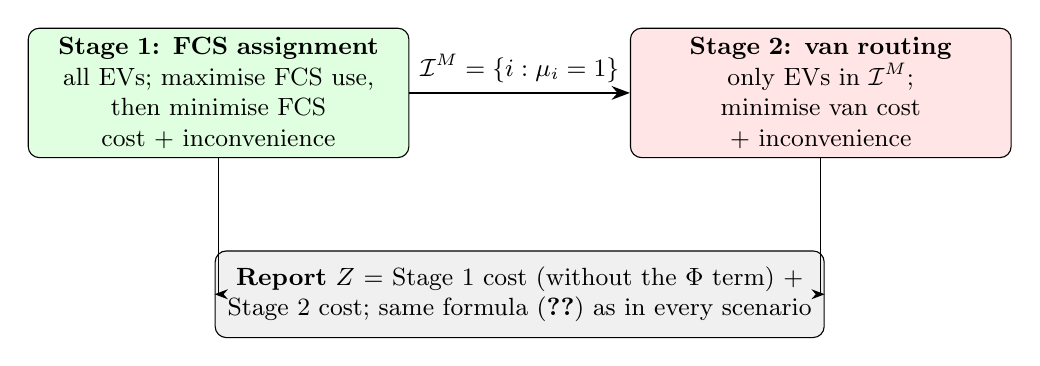
\begin{tikzpicture}[>=Stealth,box/.style={draw,rounded corners,align=center,minimum height=1.1cm,font=\small}]
  \node[box,fill=green!12,text width=4.6cm] (s1) {\textbf{Stage 1: FCS assignment}\\all EVs; maximise FCS use,\\then minimise FCS cost + inconvenience};
  \node[box,fill=red!10,text width=4.6cm,right=2.8cm of s1] (s2) {\textbf{Stage 2: van routing}\\only EVs in $\I^M$;\\minimise van cost + inconvenience};
  \draw[->,thick] (s1) -- node[above,font=\small]{$\I^M=\{i:\mu_i=1\}$} (s2);
  \node[box,fill=black!6,text width=7.5cm,below=2.0cm of $(s1)!0.5!(s2)$] (ev) {\textbf{Report} $Z=$ Stage~1 cost (without the $\Phi$ term) $+$ Stage~2 cost; same formula \eqref{eq:Z} as in every scenario};
  \draw[->] (s1) |- (ev); \draw[->] (s2) |- (ev);
\end{tikzpicture}
\end{center}

Stage~1 does not look at the vans, and Stage~2 cannot change what Stage~1 decided. That is the definition of ``FCS first, then MCS''.

%----------------------------------------------------------------
\subsection{Stage 1: assign EVs to fixed stations}

\textbf{Objective.}
\begin{equation}
\begin{split}
\min\ Z^{(1)}=\;&\underbrace{\Phi\sum_{i\in\I}\mu_i}_{\text{FCS first}}
+\underbrace{c^{EV}\sum_i\sum_{f\in\F_i}d_{if}Y_{if}}_{Z_1}
+\underbrace{Z^F_{\text{energy}}}_{\text{FCS part of }Z_4}\\
&+\underbrace{\sum_i\sum_{f\in\F_i}\rho^F_{if}Y_{if}+\alpha\sum_i w_i(C_i-r_i)+c^L\sum_i w_iL_i}_{\text{FCS customers' inconvenience}}
\end{split}
\label{eq:obj1}
\end{equation}
with $C_i=S_i+\tau^F_iY_i$ in this stage. $\Phi$ is a penalty for handing an EV to the vans. It is chosen larger than anything an extra FCS customer can add to the rest of \eqref{eq:obj1}, e.g.
\[
\Phi > \max_{i}\max_{f\in\F_i}\big(c^{EV}d_{if}+\pi^{\max}E_i+\rho^F_{if}\big)+n\,(\alpha+c^L)\,w_{\max}\,T,
\]
so Stage~1 first \textbf{maximises the number of EVs served at an FCS}, and only among those solutions minimises FCS cost and inconvenience. ($\pi^{\max}$ is the highest grid price.) A numerically safer equivalent is to solve twice: first $\max\sum_iY_i$, then fix that number and minimise the rest.
\ifTOU
Because $Z^F_{\text{energy}}$ uses the peak price, Stage~1 may \emph{start sessions later} to leave the peak, if the price saving beats the extra waiting cost (Section~\ref{sec:expect}).
\fi

\textbf{Constraints.}
\begin{align}
\sum_{g\in\G_i}y_{ig}+\mu_i &= 1 && \forall i\in\I \label{eq:s1assign}\\
S_i &\ge r_i+\sum_{f\in\F_i}t_{if}Y_{if} && \forall i\in\I \label{eq:fcsarr}\\
S_i &\le r_i+T\,(1-\mu_i) && \forall i\in\I \label{eq:s1park}\\
S_j &\ge S_i+\tau^F_i-(T+\tau^F_i)(3-y_{ig}-y_{jg}-o_{ij}) && \forall g,\ (i,j)\in\mathcal{P}_g \label{eq:disj1}\\
S_i &\ge S_j+\tau^F_j-(T+\tau^F_j)(2-y_{ig}-y_{jg}+o_{ij}) && \forall g,\ (i,j)\in\mathcal{P}_g \label{eq:disj2}\\
\sum_i y_{ig_1} &\ge \sum_i y_{ig_2} && \forall f,\ \G_f=\{g_1,g_2\} \label{eq:gunsym}\\
S_i+\tau^F_iY_i &\le T,\qquad L_i\ge S_i+\tau^F_iY_i-l_i && \forall i\in\I \label{eq:s1time}
\end{align}
\ifTOU plus the time-of-use split \eqref{eq:tou1}--\eqref{eq:tou5} of each FCS session (Section~\ref{sec:price}).\fi
\desc{\eqref{eq:s1assign}: every EV either gets one reachable gun or is handed to the vans. An EV that reaches no FCS ($\G_i=\emptyset$) is forced to $\mu_i=1$. \eqref{eq:fcsarr}: an FCS session cannot start before the EV has asked and driven to the station. \eqref{eq:s1park}: for an EV handed to the vans, $S_i$ is parked at $r_i$, so it adds no waiting in Stage~1 (its real start time is decided in Stage~2). \eqref{eq:disj1}--\eqref{eq:disj2}: two EVs on the same gun do not overlap; $o_{ij}$ picks who goes first. With two guns per station this means at most two EVs charge at a station at a time. \eqref{eq:gunsym}: symmetry breaking between the two identical guns (optional). \eqref{eq:s1time}: finished by $T$; lateness.}

\textbf{Optional acceptability rule.} An operator may refuse to send a driver to a station that is ``too inconvenient'', e.g.\ only allow gun $g$ of station $f$ for EV $i$ if $\hat\rho^F_{if}\le\bar\rho$. This only shrinks $\G_i$, so EVs whose stations are all too far go to the vans. Report results with and without it.

\textbf{Output:} $\I^M=\{i:\mu_i=1\}$, the EVs left for the vans; plus each FCS customer's gun and start time.

%----------------------------------------------------------------
\subsection{Stage 2: route the vans to the leftover EVs}

Stage~2 is a vehicle routing problem with time windows, on the EVs in $\I^M$ only. Here $C_i=S_i+\tau^M_i$.

\textbf{Objective.}
\begin{equation}
\begin{split}
\min\ Z^{(2)}=\;&\underbrace{c^M\sum_m\sum_{(i,j)\in\A^M}d_{ij}x_{ijm}}_{Z_2}+\underbrace{\sum_m c^D_mu_m}_{Z_3}+\underbrace{Z^M_{\text{energy}}}_{\text{van part of }Z_4}\\
&+\underbrace{\sum_{i\in\I^M}\sum_m\rho^M_{im}z_{im}+\alpha\sum_{i\in\I^M}w_i(C_i-r_i)+c^L\sum_{i\in\I^M}w_iL_i}_{\text{van customers' inconvenience}}
\end{split}
\label{eq:obj2}
\end{equation}
Since every EV in $\I^M$ must be served by some van, $Z^M_{\text{energy}}$ and the $\rho^M$ term are constants here. They are kept so that $Z^{(2)}$ is the true cost of Stage~2. Waiting and lateness make the vans visit urgent EVs early.

\textbf{Constraints.}
\begin{align}
\sum_{m\in\M}z_{im} &= 1 && \forall i\in\I^M \label{eq:s2assign}\\
\sum_{j:(0,j)\in\A^M}x_{0jm} = \sum_{i:(i,n+1)\in\A^M}x_{i,n+1,m} &= u_m && \forall m \label{eq:depot}\\
\sum_{i:(i,j)\in\A^M}x_{ijm} = \sum_{k:(j,k)\in\A^M}x_{jkm} &= z_{jm} && \forall j\in\I^M,\ m \label{eq:flow}\\
\sum_{i\in\I^M}z_{im} &\le Q_m\,u_m && \forall m \label{eq:cap}\\
\sum_{i\in\I^M}\frac{E_i}{\eta}z_{im}+\beta\sum_{(i,j)\in\A^M}d_{ij}x_{ijm} &\le B_m\,u_m && \forall m \label{eq:batt}
\end{align}
\begin{align}
S_j &\ge \max\{r_j,\ t_{0j}\,x_{0jm}\} && \forall j\in\I^M,\ m \label{eq:depart}\\
S_j &\ge S_i+\tau^M_i+t_{ij}-(T+\tau^M_i+t_{ij})(1-x_{ijm}) && \forall i\neq j,\ m \label{eq:seq}\\
S_i+\tau^M_i+t_{i,n+1} &\le T+(\tau^M_i+t_{i,n+1})(1-x_{i,n+1,m}) && \forall i,\ m \label{eq:return}\\
S_i+\tau^M_i \le T,\quad L_i &\ge S_i+\tau^M_i-l_i && \forall i\in\I^M \label{eq:s2time}\\
u_m &\ge u_{m+1} && m<|\M| \label{eq:vansym}
\end{align}
\desc{\eqref{eq:s2assign}: each leftover EV gets one van. \eqref{eq:depot}: a used van leaves and returns to the depot once. \eqref{eq:flow}: each EV on van $m$ is entered and left exactly once by that van. \eqref{eq:cap}: at most $Q_m$ EVs per van. \eqref{eq:batt}: delivered energy (with transfer losses) plus driving energy fits in the van battery. \eqref{eq:depart}: no start before the request, or before the van can drive there from the depot (written as two linear constraints). \eqref{eq:seq}: if the van goes $i\to j$, it finishes $i$ and drives to $j$ before starting $j$. This gives one EV at a time and removes subtours (MTZ-type). \eqref{eq:return}: back at the depot by $T$. \eqref{eq:s2time}: finished by $T$; lateness. \eqref{eq:vansym}: use identical vans in index order.}

\textbf{If Stage 2 is infeasible} (too many leftover EVs for the fleet by $T$), the sequential policy has \emph{failed} on that instance. For diagnosis, add $s_i\in\{0,1\}$ (``unserved''), replace \eqref{eq:s2assign} by $\sum_mz_{im}+s_i=1$ and add $\Phi^U\sum_is_i$ to \eqref{eq:obj2}. Then report the number of EVs that could not be served. This is a useful comparison with the integrated scenario, which may serve all of them.

%----------------------------------------------------------------
\subsection{Reported value}
\[
Z^{\text{S\scen}}=\big(Z^{(1)*}-\Phi\,|\I^M|\big)+Z^{(2)*},
\]
which is exactly \eqref{eq:Z} evaluated at the combined solution. The stage-1 solution plus the stage-2 solution is a feasible solution of the integrated model (S\ifTOU 4\else 3\fi), so
$Z^{\text{S\ifTOU 4\else 3\fi}}\le Z^{\text{S\scen}}$. The difference is the \emph{value of integration}.

\else
%---------------------------------------------------------------- INT
\subsection{Objective}
\begin{equation}
\min\ Z \quad\text{as in \eqref{eq:Z}, with }Z^F_{\text{energy}}=\ifTOU P^F\textstyle\sum_i\big[\pi^\off(\theta^1_i+\theta^3_i)+\pi^\pk\theta^2_i\big]\else\pi^F\textstyle\sum_iE_iY_i\fi,\quad C_i=S_i+\tau^F_iY_i+\tau^M_iZ_i. \label{eq:objint}
\end{equation}
Written out in full:
\begin{align*}
\min\ Z=\;& c^{EV}\sum_i\sum_{f\in\F_i}d_{if}Y_{if}+c^M\sum_m\sum_{(i,j)\in\A}d_{ij}x_{ijm}+\sum_mc^D_mu_m\\
&+\ifTOU P^F\sum_i\big[\pi^\off(\theta^1_i+\theta^3_i)+\pi^\pk\theta^2_i\big]\else\pi^F\sum_iE_iY_i\fi
+\pi^M\sum_i\sum_m\frac{E_i}{\eta}z_{im}\\
&+\sum_i\sum_{f\in\F_i}\rho^F_{if}Y_{if}+\sum_i\sum_m\rho^M_{im}z_{im}+\alpha\sum_iw_i(C_i-r_i)+c^L\sum_iw_iL_i .
\end{align*}
Every term is linear. One model weighs everything at once: an EV goes to a van exactly when the van's extra km, dispatch and energy cost are outweighed by the effort and waiting it saves the driver\ifTOU, or by the peak-price energy it avoids\fi.

\subsection{Constraints}

\textbf{Assignment.}
\begin{equation}
\sum_{g\in\G_i}y_{ig}+\sum_{m\in\M}z_{im}=1\qquad\forall i\in\I \label{eq:assign}
\end{equation}
\desc{Exactly one resource per EV: one reachable gun or one van. EVs that reach no FCS are forced onto a van.}

\textbf{Fixed stations.}
\begin{align}
S_i &\ge r_i+\sum_{f\in\F_i}t_{if}Y_{if} && \forall i \label{eq:fcsarr}\\
S_j &\ge S_i+\tau^F_i-(T+\tau^F_i)(3-y_{ig}-y_{jg}-o_{ij}) && \forall g,\ (i,j)\in\mathcal{P}_g \label{eq:disj1}\\
S_i &\ge S_j+\tau^F_j-(T+\tau^F_j)(2-y_{ig}-y_{jg}+o_{ij}) && \forall g,\ (i,j)\in\mathcal{P}_g \label{eq:disj2}\\
\sum_iy_{ig_1} &\ge \sum_iy_{ig_2} && \forall f,\ \G_f=\{g_1,g_2\} \label{eq:gunsym}
\end{align}
\desc{\eqref{eq:fcsarr}: an FCS session starts after the request and the drive to the station (for a van customer this is just $S_i\ge r_i$). \eqref{eq:disj1}--\eqref{eq:disj2}: EVs on the same gun do not overlap; $o_{ij}$ chooses the order. \eqref{eq:gunsym}: optional symmetry breaking.}

\textbf{Vans: routes, capacity, battery.}
\begin{align}
\sum_{j:(0,j)\in\A}x_{0jm}=\sum_{i:(i,n+1)\in\A}x_{i,n+1,m} &= u_m && \forall m \label{eq:depot}\\
\sum_{i:(i,j)\in\A}x_{ijm}=\sum_{k:(j,k)\in\A}x_{jkm} &= z_{jm} && \forall j\in\I,\ m \label{eq:flow}\\
\sum_iz_{im} &\le Q_mu_m && \forall m \label{eq:cap}\\
\sum_i\frac{E_i}{\eta}z_{im}+\beta\sum_{(i,j)\in\A}d_{ij}x_{ijm} &\le B_mu_m && \forall m \label{eq:batt}
\end{align}
\desc{\eqref{eq:depot}: a used van leaves and returns once. \eqref{eq:flow}: each EV on van $m$ is visited exactly once by it. \eqref{eq:cap}: at most $Q_m$ EVs. \eqref{eq:batt}: delivered energy (with losses) plus driving energy fits in the battery.}

\textbf{Vans: timing (one EV at a time, no subtours).}
\begin{align}
S_j &\ge t_{0j}\,x_{0jm} && \forall j\in\I,\ m \label{eq:depart}\\
S_j &\ge S_i+\tau^M_i+t_{ij}-(T+\tau^M_i+t_{ij})(1-x_{ijm}) && \forall i\neq j\in\I,\ m \label{eq:seq}\\
S_i+\tau^M_i+t_{i,n+1} &\le T+(\tau^M_i+t_{i,n+1})(1-x_{i,n+1,m}) && \forall i,\ m \label{eq:return}
\end{align}
\desc{\eqref{eq:depart}: the first stop cannot start before the van has driven there. \eqref{eq:seq}: $i\to j$ means finish $i$, drive, then start $j$; start times rise along a route, so no subtour can close. \eqref{eq:return}: back at the depot by $T$.}

\textbf{Horizon and lateness.}
\begin{equation}
C_i\le T,\qquad L_i\ge C_i-l_i\qquad\forall i\in\I \label{eq:time}
\end{equation}
\desc{Every EV is fully charged within the horizon; $L_i$ measures lateness.}

\ifTOU
\textbf{Time-of-use split.} Constraints \eqref{eq:tou1}--\eqref{eq:tou5} of Section~\ref{sec:price}.
\fi

\textbf{Symmetry and domains.}
\begin{equation}
u_m\ge u_{m+1};\qquad y,z,x,u,o\ifTOU,\kappa\fi\in\{0,1\};\qquad S_i,L_i\ifTOU,\theta^p_i\fi\ge0 \label{eq:dom}
\end{equation}
\fi

%=====================================================================
\section{Learning-to-optimise (RL) formulation}\label{sec:rl}

\textbf{Main rule:} the reward of each action is \emph{minus the increase in $Z$ that the action causes}. The rewards over an episode then add up to $-Z$ of the solution the policy builds. RL and MILP results are measured on the same yardstick \eqref{eq:Z}, and the MILP optimum is the benchmark for the RL gap.

\ifSEQ
%---------------------------------------------------------------- RL SEQ
The RL pipeline has the same two stages as the MILP.

\subsection{Stage 1 policy: FCS assignment}
\begin{itemize}[leftmargin=1.4em,itemsep=2pt]
  \item \textbf{Episode / epochs:} EVs are taken in order of request time $r_i$ (ties: higher $w_i$ first). One decision per EV.
  \item \textbf{State:} features of the current EV $k$ ($E_k,r_k,l_k,w_k,R_k$, location); for each gun $g$ the time $F_g$ it becomes free; summary features of the EVs still to come (count and positions near each station)\ifTOU; the current price and the time until $T_1$ and $T_2$\fi.
  \item \textbf{Action:} a gun $g\in\G_k$, or ``hand to vans''. \textbf{FCS-first mask:} ``hand to vans'' is allowed \emph{only} if no gun can finish EV $k$ by $T$ (or, with the optional rule, if all remaining guns have $\hat\rho^F_{kf}>\bar\rho$).
  \ifTOU\item \textbf{Optional timing action:} ``gun $g$, start after the peak'', i.e.\ $S_k=\max\{\text{earliest},T_2\}$, allowed only if the session still ends by $T$.\fi
  \item \textbf{Transition:} $S_k=\max\{r_k+t_{kf},F_g\}$ (or later, for the timing action); $F_g\leftarrow S_k+\tau^F_k$.
  \item \textbf{Reward:} $-\Big[c^{EV}d_{kf}+\text{energy}_k+\rho^F_{kf}+\alpha w_k(S_k+\tau^F_k-r_k)+c^Lw_k(S_k+\tau^F_k-l_k)^+\Big]$, where energy$_k$ = \ifTOU$P^F\big[\pi^\off\cdot(\text{off-peak hours of }[S_k,S_k+\tau^F_k])+\pi^\pk\cdot(\text{peak hours})\big]$, computed exactly in the simulator\else$\pi^FE_k$\fi. Handing an EV to the vans gives reward $0$ here; its cost is counted in Stage~2.
\end{itemize}
Note: a simple baseline for Stage~1 is the greedy rule ``gun with the largest one-step reward''. What RL can learn on top of this is, for example, to keep a nearby gun free for an urgent EV that arrives later.

\subsection{Stage 2 policy: van routing over $\I^M$}
\begin{itemize}[leftmargin=1.4em,itemsep=2pt]
  \item \textbf{Epochs:} whenever a van becomes free (the earliest-free van decides first).
  \item \textbf{State:} for each van: position, time free, remaining battery $b_m$, EVs served so far, dispatched or not; for each unserved EV in $\I^M$: location, $E_i,r_i,l_i,w_i$; current time.
  \item \textbf{Action:} the next EV $j$ for this van, or ``return to depot'' (ends the route). Mask: $j$ must be feasible: battery covers $E_j/\eta$ plus driving to $j$ and back to the depot, the count stays $\le Q_m$, and $j$ can be finished with the van back at the depot by $T$.
  \item \textbf{Transition:} $S_j=\max\{r_j,\ \text{time free}+t_{\text{pos},j}\}$; the van moves to $j$ and is free at $S_j+\tau^M_j$; $b_m$ falls by $E_j/\eta+\beta d_{\text{pos},j}$.
  \item \textbf{Reward:} serving $j$: $-\Big[c^Md_{\text{pos},j}+c^D_m[\text{first stop}]+\pi^M\frac{E_j}{\eta}+\rho^M_{jm}+\alpha w_j(S_j+\tau^M_j-r_j)+c^Lw_j(S_j+\tau^M_j-l_j)^+\Big]$; returning: $-c^Md_{\text{pos},0}$. EVs still unserved at the end: $-\Phi^U$ each.
  \item \textbf{Policy:} an attention-based routing policy (e.g.\ Kool et al., 2019, ``Attention, Learn to Solve Routing Problems!'') trained with REINFORCE or PPO. Baseline: nearest-feasible-EV heuristic.
\end{itemize}
Episode return of Stage~1 + Stage~2 $=-Z^{\text{S\scen}}$.

\else
%---------------------------------------------------------------- RL INT
One policy decides both who serves each EV and the van routes.
\begin{itemize}[leftmargin=1.4em,itemsep=2pt]
  \item \textbf{Episode / epochs:} EVs are taken in order of request time $r_i$ (ties: higher $w_i$ first). One decision per EV.
  \item \textbf{State:} (i) the current EV $k$: location, $E_k,r_k,l_k,w_k,R_k$, reachable stations; (ii) each gun $g$: time $F_g$ it becomes free; (iii) each van $m$: current end-of-route position, time free, remaining battery $b_m$, EVs served, dispatched or not; (iv) embeddings of the not-yet-assigned EVs (for look-ahead)\ifTOU; (v) current price, time until $T_1$ and $T_2$\fi.
  \item \textbf{Action:} $a\in\G_k\cup\M$: a gun, or a van (EV $k$ is appended to the end of that van's route). \textbf{Mask} infeasible actions: a gun that cannot finish $k$ by $T$; a van without enough battery for $E_k/\eta$ plus the drive to $k$ and back to the depot, with $Q_m$ reached, or unable to finish $k$ and return by $T$.
  \ifTOU\item \textbf{Optional timing action:} ``gun $g$, start after the peak'' ($S_k=\max\{\text{earliest},T_2\}$, if it still ends by $T$).\fi
  \item \textbf{Transition:} gun: $S_k=\max\{r_k+t_{kf},F_g\}$, $F_g\leftarrow S_k+\tau^F_k$. Van: $S_k=\max\{r_k,\ \text{free}_m+t_{\text{pos}_m,k}\}$, then the van moves to $k$, $\text{free}_m\leftarrow S_k+\tau^M_k$, $b_m\mathrel{-}=E_k/\eta+\beta d_{\text{pos}_m,k}$.
  \item \textbf{Reward} $=-\Delta Z$:
  \begin{align*}
  \text{gun } g\text{ at }f:&\quad -\Big[c^{EV}d_{kf}+\text{energy}^F_k+\rho^F_{kf}+\alpha w_k(C_k-r_k)+c^Lw_k(C_k-l_k)^+\Big]\\
  \text{van } m:&\quad -\Big[c^M\big(d_{\text{pos}_m,k}+d_{k,0}-d_{\text{pos}_m,0}\big)+c^D_m[\text{first use}]+\pi^M\tfrac{E_k}{\eta}\\
  &\qquad\quad+\rho^M_{km}+\alpha w_k(C_k-r_k)+c^Lw_k(C_k-l_k)^+\Big]
  \end{align*}
  The van distance term is the \emph{change} in route length when $k$ is inserted before the return to the depot, so the sum over the episode equals the total route length (the return legs telescope). energy$^F_k$ = \ifTOU$P^F\big[\pi^\off\cdot(\text{off-peak hours})+\pi^\pk\cdot(\text{peak hours of }[S_k,C_k])\big]$, computed exactly by the simulator; no linearisation is needed in RL\else$\pi^FE_k$\fi.
  \item \textbf{Dead end:} if every action is masked, EV $k$ is unserved: reward $-\Phi^U$, and the episode continues. Report the count.
  \item \textbf{Policy:} masked categorical policy over guns and vans, encoder with attention over EVs, guns and vans; trained with PPO. Natural baseline: greedy, i.e.\ choose the action with the largest one-step reward. That is the pairwise rule ``smallest $\hat\rho$ + cost'' from Section~\ref{sec:inc}.
\end{itemize}
Restriction to note: vans serve EVs in assignment order (append only). A variant that inserts $k$ at the cheapest position of a route is more flexible but has a larger action space.
\fi

\textbf{Reward scaling.} For stable training divide every reward by a constant, e.g.\ the greedy baseline's average $Z$ on the training instances. This does not change the optimal policy.

%=====================================================================
\section{What to expect and what to report}\label{sec:expect}

\ifnum\scen=1
\begin{itemize}[leftmargin=1.4em,itemsep=2pt]
  \item Vans serve only EVs that reach no station, or that the stations cannot finish by $T$. If stations have spare capacity, very few vans are dispatched.
  \item Inconvenience is high for EVs far from the nearest station (worked example: Rs\,682 at the FCS, against Rs\,458 if a van had been allowed).
  \item With too few vans Stage~2 becomes infeasible (unserved EVs), even when the integrated model S3 could serve everyone. Report the smallest $|\M|$ at which S1 is feasible and compare it with S3.
\end{itemize}
\fi
\ifnum\scen=2
\begin{itemize}[leftmargin=1.4em,itemsep=2pt]
  \item \textbf{When does Stage~1 delay a session to avoid the peak?} Moving one hour of charging out of the peak saves $(\pi^\pk-\pi^\off)P^F=3\times22=$ Rs\,66, but delays completion by up to an hour, which costs $\alpha w_i\ge$ Rs\,200. So with the default values Stage~1 almost never delays. It mostly pays the higher price, and S2 costs roughly S1 plus the peak surcharge. Sessions start later only if $\alpha$ is small (try $\lambda<0.33$ in the sensitivity analysis).
  \item The van assignment is the same as in S1 unless Stage~1's timing changes which EVs fit at the stations. Stage~1 cannot use vans to escape the peak price.
  \item Extra KPI: \textbf{grid energy drawn at FCS during the peak}, $P^F\sum_i\theta^2_i$ (kWh). Compare with S4.
\end{itemize}
\fi
\ifnum\scen=3
\begin{itemize}[leftmargin=1.4em,itemsep=2pt]
  \item Vans take EVs for which the saved inconvenience exceeds the extra van cost (worked example: van chosen, saving Rs\,224). Expect vans to serve EVs that are far from every station, have low range (high $w_i$), or have early deadlines, while EVs near a station still use it.
  \item \textbf{Value of integration under flat price:} $Z^{\text{S1}}-Z^{\text{S3}}\ge0$. Report it per component ($Z_1,\dots,Z_5$): typically operating cost rises a little and inconvenience falls a lot.
  \item Vary $|\M|$ (0, 1, 2, \dots): the first few vans lower $Z$ sharply, then the effect levels off. That curve shows the scenarios where mobile chargers help most.
\end{itemize}
\fi
\ifnum\scen=4
\begin{itemize}[leftmargin=1.4em,itemsep=2pt]
  \item During the peak a van kWh costs about the same as an FCS kWh (Rs\,10.0 each), so the vans' energy disadvantage disappears and vans also absorb \emph{peak-hour} demand that would otherwise be charged on the grid at peak price.
  \item Expect more van usage than in S3, concentrated on requests in $[T_1,T_2]$, and lower grid energy at the stations during the peak, $P^F\sum_i\theta^2_i$, than in S2.
  \item \textbf{Value of integration under peak pricing:} $Z^{\text{S2}}-Z^{\text{S4}}$. It should be larger than $Z^{\text{S1}}-Z^{\text{S3}}$, because integration now also allows price arbitrage.
  \item \textbf{Peak pricing with full flexibility:} $Z^{\text{S4}}-Z^{\text{S3}}$ should be smaller than $Z^{\text{S2}}-Z^{\text{S1}}$: vans cushion the price increase.
\end{itemize}
\fi

\textbf{Cross-scenario comparison table} (fill in from the four runs):
\begin{center}
\renewcommand{\arraystretch}{1.2}
\begin{tabular}{@{}lll@{}}
\toprule
\textbf{Comparison} & \textbf{Measures} & \textbf{Expected sign} \\
\midrule
S1 $-$ S3 & value of integration, flat price & $\ge0$ \\
S2 $-$ S4 & value of integration, peak price & $\ge0$, larger than S1 $-$ S3 \\
S2 $-$ S1 & cost of peak pricing, FCS-first operator & $>0$ \\
S4 $-$ S3 & cost of peak pricing, flexible operator & $>0$, smaller than S2 $-$ S1 \\
\bottomrule
\end{tabular}
\end{center}
Report for each: $Z$ and its components, number of vans used, EVs per resource, mean and maximum inconvenience per EV, total lateness, peak-hour grid energy, solve time, and (for RL) the gap to the MILP optimum.

%=====================================================================
\appendix
\section{Illustrative parameter values}\label{app:values}

These are starting values for experiments, not data. All are meant to be varied in the analysis. Values in Rs.

\begin{center}
\renewcommand{\arraystretch}{1.15}
\begin{tabular}{@{}llp{6.2cm}@{}}
\toprule
\textbf{Parameter} & \textbf{Value} & \textbf{Note} \\
\midrule
$T$, $[T_1,T_2]$ & 7 h, $[2,6]$ & 16:00--23:00, peak 18:00--22:00 \\
$P^F$, $P^M$ & 22 kW, 30 kW & \\
$v$, $\beta$, $\eta$ & 25 km/h, 0.25 kWh/km, 0.9 & \\
$B_m$, $Q_m$, $|\M|$ & 150 kWh, 6, 2--6 & \\
$c^{EV}$, $c^M$, $c^D_m$ & Rs\,4/km, Rs\,15/km, Rs\,1500 & van km includes driver time \\
$\pi^F$ (flat) & Rs\,8.7/kWh & equals the time-average of the ToU tariff over $[0,T]$ \\
$\pi^\off$, $\pi^\pk$ (ToU) & Rs\,7/kWh, Rs\,10/kWh & $(3\times7+4\times10)/7=8.7$ \\
$c^{bat}$ & Rs\,2/kWh & van battery wear \\
$\pi^M$ & Rs\,10.7 (flat) / Rs\,9.0 (ToU) & $=\pi^F+c^{bat}$ / $=\pi^\off+c^{bat}$ \\
$\alpha$, $\alpha^D$ & Rs\,200/h, Rs\,100/h & value of time; extra for attended time \\
$h^F$, $h^M$, $\varphi$ & Rs\,50, Rs\,10, Rs\,100 & trip hassle, hand-over, range stress \\
$c^L$ & Rs\,300/h & lateness \\
$w_i$ & $1+2(1-R_i/R_{\max})$, $R_i\sim U[3,40]$ km & priority from remaining range \\
\bottomrule
\end{tabular}
\end{center}

The flat price is set to the time-average of the peak tariff. The price \emph{level} is then the same in both pricing cases, and only the price \emph{shape} differs. Without this, part of S1 vs S2 would just reflect a different average price.

\end{document}
"
%    pdflatex -jobname=scenario2_peak_sequential   "\def\scen{2}% =====================================================================
%  One source, four PDFs.  Build with build.sh (or by hand):
%    pdflatex -jobname=scenario1_flat_sequential   "\def\scen{1}\input{scenario_master}"
%    pdflatex -jobname=scenario2_peak_sequential   "\def\scen{2}\input{scenario_master}"
%    pdflatex -jobname=scenario3_flat_integrated   "\def\scen{3}\input{scenario_master}"
%    pdflatex -jobname=scenario4_peak_integrated   "\def\scen{4}\input{scenario_master}"
%  (run each twice for cross-references)
% =====================================================================
\documentclass[11pt,a4paper]{article}
\usepackage[margin=2.2cm]{geometry}
\usepackage{amsmath,amssymb,amsfonts}
\usepackage{booktabs,array,tabularx}
\usepackage{enumitem}
\usepackage[table]{xcolor}
\usepackage{tikz}
\usetikzlibrary{arrows.meta,positioning,calc}
\usepackage[colorlinks=true,linkcolor=blue!50!black,urlcolor=blue!50!black]{hyperref}
\usepackage{titlesec}
\titleformat{\section}{\large\bfseries}{\thesection}{0.8em}{}
\titleformat{\subsection}{\normalsize\bfseries}{\thesubsection}{0.8em}{}
\setlength{\parindent}{0pt}
\setlength{\parskip}{5pt}

% ---------------- scenario switches ----------------
\ifdefined\scen\else\def\scen{1}\fi
\newif\ifTOU \TOUfalse   % true = time-of-use (peak) price
\newif\ifSEQ \SEQfalse   % true = FCS first, then MCS
\ifnum\scen=1 \SEQtrue \fi
\ifnum\scen=2 \TOUtrue \SEQtrue \fi
\ifnum\scen=4 \TOUtrue \fi

\newcommand{\pricename}{\ifTOU time-of-use price (dearer evening peak)\else single (flat) price all day\fi}
\newcommand{\structname}{\ifSEQ FCS first, then MCS (sequential)\else FCS and MCS together (integrated)\fi}

% ---------------- notation ----------------
\newcommand{\I}{\mathcal{I}}
\newcommand{\F}{\mathcal{F}}
\newcommand{\G}{\mathcal{G}}
\newcommand{\M}{\mathcal{M}}
\newcommand{\N}{\mathcal{N}}
\newcommand{\A}{\mathcal{A}}
\newcommand{\Rs}{\text{Rs}\,}
\newcommand{\pk}{\mathrm{pk}}
\newcommand{\off}{\mathrm{off}}
\newcommand{\desc}[1]{\par\vspace{-2pt}{\small\color{black!75}\textit{Meaning:} #1}\par\vspace{4pt}}
\newcommand{\cell}[2]{\ifnum\scen=#1\cellcolor{blue!18}\textbf{S#1 (this document)}\\\textbf{#2}\else S#1\\#2\fi}

\title{\textbf{EV Charging Network Optimisation}\\[4pt]
\large Scenario \scen: \pricename\ $+$ \structname\\[2pt]
\normalsize MILP and RL formulation}
\author{CP 320 OR for Mobility Management, course project}
\date{2 October 2026}

\begin{document}
\maketitle

%=====================================================================
\section{Where this scenario sits}

The project studies four scenarios: two ways of pricing grid electricity, times two ways of making the decisions.

\begin{center}
\renewcommand{\arraystretch}{1.5}
\begin{tabular}{>{\raggedright\arraybackslash}p{4.2cm}|>{\centering\arraybackslash}p{4.6cm}|>{\centering\arraybackslash}p{4.6cm}}
 & \textbf{Flat price all day} & \textbf{Time-of-use (peak) price} \\ \hline
\textbf{Sequential:} FCS first, leftover EVs to MCS &
\begin{tabular}[c]{@{}c@{}}\cell{1}{flat + sequential}\end{tabular} &
\begin{tabular}[c]{@{}c@{}}\cell{2}{peak + sequential}\end{tabular} \\ \hline
\textbf{Integrated:} FCS and MCS decided together &
\begin{tabular}[c]{@{}c@{}}\cell{3}{flat + integrated}\end{tabular} &
\begin{tabular}[c]{@{}c@{}}\cell{4}{peak + integrated}\end{tabular} \\
\end{tabular}
\end{center}

\textbf{The four scenarios do not have four different objectives.} They share \emph{one} cost yardstick $Z$ (Section~\ref{sec:obj}): the same cost terms and the same customer inconvenience (Section~\ref{sec:inc}). Only two things change:
\begin{itemize}[leftmargin=1.4em,itemsep=1pt]
  \item \textbf{Pricing} changes the formula for one term, the FCS energy cost (Section~\ref{sec:price}).
  \item \textbf{Decision structure} changes \emph{how} $Z$ is minimised: in one model (integrated), or in two stages (sequential), where each stage minimises its own part of $Z$.
\end{itemize}
Because the yardstick is the same, the four optimal values can be compared directly. The differences measure the \emph{value of integration} (S1$\to$S3, S2$\to$S4) and the \emph{effect of peak pricing} (S1$\to$S2, S3$\to$S4).

\ifnum\scen=1
\textbf{This scenario (S1)} is the baseline, the ``status quo''. Electricity costs the same at every hour, every EV that can be charged at a fixed station is sent there, and vans only take what is left over.
\fi
\ifnum\scen=2
\textbf{This scenario (S2)} keeps the FCS-first rule of S1, but grid electricity is dearer during the evening peak. Stage~1 can react to the price only by \emph{rescheduling} FCS sessions. It cannot hand a peak-hour EV to a van.
\fi
\ifnum\scen=3
\textbf{This scenario (S3)} keeps the flat price of S1, but the operator decides FCS and MCS service \emph{together}. An EV can be sent to a van even when a fixed station could take it, whenever that lowers total cost plus inconvenience.
\fi
\ifnum\scen=4
\textbf{This scenario (S4)} is the most flexible one: peak pricing at fixed stations, and FCS and MCS decided together. Van energy was bought off-peak, so vans can also be used to keep charging \emph{out of the expensive peak}.
\fi

%=====================================================================
\section{Setting and assumptions}\label{sec:setting}

\textbf{Time.} The planning horizon is $[0,T]$ with $T=7$\,h (16:00--23:00). It contains the evening peak window $[T_1,T_2]=[2,6]$ (18:00--22:00). The horizon is the same in all four scenarios. It is wider than the peak itself so that, under peak pricing, there is cheaper time on both sides of the peak.\ifTOU\else\ In this scenario the price is flat, so the window plays no role in the model.\fi

\textbf{Assumptions} (the same as MILP v3, plus two about energy):
\begin{enumerate}[leftmargin=1.6em,itemsep=1pt]
  \item Static, continuous time. All requests in the horizon are known at time $0$, and request $i$ becomes active at $r_i$.
  \item An EV served by an FCS drives there itself on its own battery (only to stations within its range $R_i$). The driver stays with the car while it waits for a free gun and while it charges.
  \item An EV served by an MCS stays parked where it is, and the driver is free in the meantime.
  \item Each FCS gun and each van charges one EV at a time, without interruption, at constant power.
  \item A van's battery covers both its driving and the energy it delivers. \textbf{The van battery is charged at the depot before the horizon starts}\ifTOU, i.e.\ at the off-peak price\fi, and is not recharged during the horizon.
  \item Every EV must be fully charged by $T$ (hard). Finishing after the driver's desired time $l_i$ is allowed but penalised.
\end{enumerate}

%=====================================================================
\section{Notation}\label{sec:notation}

\subsection*{Sets}
\begin{tabularx}{\textwidth}{@{}lX@{}}
\toprule
$\I=\{1,\dots,n\}$ & EV charging requests \\
$\F$; $\G_f$ ($|\G_f|=2$); $\G=\bigcup_f\G_f$ & fixed charging stations; guns of FCS $f$; all guns ($f(g)$ = station of gun $g$) \\
$\F_i=\{f: d_{if}\le R_i\}$, $\G_i=\bigcup_{f\in\F_i}\G_f$ & stations / guns EV $i$ can reach on its remaining range \\
$\M$ & mobile charging vans (MCS) \\
$0,\ n+1$ & depot as start node / end node (same place) \\
$\N=\{0\}\cup\I\cup\{n+1\}$, $\A$ & routing nodes; allowed van arcs $(i,j)$, $i\in\{0\}\cup\I$, $j\in\I\cup\{n+1\}$, $i\neq j$ \\
$\mathcal{P}_g=\{(i,j): i<j,\ g\in\G_i\cap\G_j\}$ & pairs of EVs that could share gun $g$ \\
\ifSEQ
$\I^M\subseteq\I$ & EVs handed to the vans by Stage~1 (an \emph{output} of Stage~1, a fixed input to Stage~2) \\
$\N^M$, $\A^M$ & routing nodes / arcs restricted to $\I^M$ \\
\fi
\bottomrule
\end{tabularx}

\subsection*{Parameters}
\begin{tabularx}{\textwidth}{@{}lX@{}}
\toprule
$E_i,\ r_i,\ l_i,\ R_i$ & energy demand (kWh), request time, desired completion time (h), remaining range (km) \\
$w_i\ge1$ & priority of EV $i$; $w_i=1+\kappa(1-R_i/R_{\max})$, so low-range EVs weigh more \\
$P^F,\ P^M$ & charging power of an FCS gun (22\,kW) / of a van (e.g.\ 30\,kW) \\
$\tau^F_i=E_i/P^F,\ \tau^M_i=E_i/P^M$ & charging time of EV $i$ at an FCS / by a van (h) \\
$d_{if},t_{if}$;\ $d_{ij},t_{ij}$ & distance (km) and time (h): EV$\to$FCS; between routing nodes ($t=d/v$) \\
$B_m,\ Q_m,\ \beta,\ \eta$ & van battery (kWh), max EVs per van, van consumption (kWh/km), transfer efficiency \\
$c^{EV},\ c^M,\ c^D_m$ & cost per km of EV driving, per km of van driving; fixed dispatch cost of van $m$ \\
\ifTOU
$\pi^\off,\ \pi^\pk$ & grid price (Rs/kWh) off-peak / in $[T_1,T_2]$, with $\pi^\pk\ge\pi^\off$ \\
\else
$\pi^F$ & grid price (Rs/kWh), the same at every hour \\
\fi
$c^{bat}$ & van battery wear per kWh cycled \\
$\pi^M$ & cost of 1 kWh taken from a van battery: $\pi^M=\ifTOU\pi^\off\else\pi^F\fi+c^{bat}$ (Section~\ref{sec:price}) \\
$\alpha,\ \alpha^D,\ h^F,\ h^M,\ \varphi,\ c^L$ & inconvenience coefficients (Section~\ref{sec:inc}) \\
\bottomrule
\end{tabularx}

\subsection*{Decision variables}
\begin{tabularx}{\textwidth}{@{}llX@{}}
\toprule
$y_{ig}$ & $\{0,1\}$ & EV $i$ charged at gun $g\in\G_i$ \\
$z_{im}$ & $\{0,1\}$ & EV $i$ served by van $m$ \\
$x_{ijm}$ & $\{0,1\}$ & van $m$ drives arc $(i,j)$ \\
$u_m$ & $\{0,1\}$ & van $m$ is dispatched \\
$o_{ij}$ & $\{0,1\}$ & for EVs $i<j$ that could share a gun: 1 if $i$ is charged before $j$ \\
\ifSEQ
$\mu_i$ & $\{0,1\}$ & Stage~1 only: EV $i$ is handed to the van fleet \\
\fi
\ifTOU
$\theta^1_i,\theta^2_i,\theta^3_i$ & $\ge0$ & hours of EV $i$'s FCS session before / inside / after the peak \\
$\kappa^1_i,\kappa^3_i$ & $\{0,1\}$ & EV $i$'s FCS session starts before $T_1$ / ends after $T_2$ \\
\fi
$S_i$ & $\ge0$ & time charging of EV $i$ starts (h), on whichever resource \\
$L_i$ & $\ge0$ & lateness of EV $i$ beyond $l_i$ (h) \\
\bottomrule
\end{tabularx}

\textbf{Short-hands} (linear expressions, not new variables):
\[
Y_{if}=\sum_{g\in\G_f}y_{ig},\qquad Y_i=\sum_{g\in\G_i}y_{ig}\ (\text{EV $i$ uses an FCS}),\qquad Z_i=\sum_{m\in\M}z_{im}\ (\text{EV $i$ uses a van}),
\]
\[
C_i=S_i+\tau^F_i\,Y_i+\tau^M_i\,Z_i \quad\text{(time EV $i$ is fully charged).}
\]

%=====================================================================
\section{Customer inconvenience}\label{sec:inc}

This section is \textbf{identical in all four scenario documents}. Inconvenience is a property of the customer, not of the price or of the planning method.

\subsection{What we mean by inconvenience}

Inconvenience is \emph{what the driver loses} from the moment they ask for a charge ($r_i$) until the car is fully charged ($C_i$), \emph{converted into rupees} so it can be added to the operator's costs. A driver loses three different things:

\begin{enumerate}[leftmargin=1.6em,itemsep=2pt]
  \item \textbf{Waiting:} the car is not ready. This lasts $C_i-r_i$ hours and affects \emph{every} driver, FCS or MCS.
  \item \textbf{Effort:} only an FCS customer has to drive to the station and sit there while the car charges. An MCS customer stays at home or at work and does something else. Driving to a far station also uses scarce battery range, which causes stress (``range anxiety'').
  \item \textbf{A missed deadline:} the car is still not ready at the time $l_i$ the driver needs it.
\end{enumerate}

Each loss gets a price in Rs per hour (or per event). All of them are multiplied by the priority $w_i$: an hour of delay for an EV with 5\,km of range left counts more than for one with 40\,km.

\subsection{The three components}

\begin{center}
\renewcommand{\arraystretch}{1.3}
\begin{tabularx}{\textwidth}{@{}>{\raggedright\arraybackslash}p{2.6cm}>{\raggedright\arraybackslash}X>{\raggedright\arraybackslash}X>{\raggedright\arraybackslash}p{3.0cm}@{}}
\toprule
\textbf{Component} & \textbf{EV $i$ at FCS $f$} & \textbf{EV $i$ by a van} & \textbf{Known when?} \\
\midrule
Effort & $w_i\big[\alpha^D(t_{if}+\tau^F_i)+h^F+\varphi\,d_{if}/R_i\big]$: driving and sitting at the station, a fixed trip hassle, range stress & $w_i\,h^M$: being reachable and handing over the car & \textbf{Static:} known as soon as the resource is chosen \\
Waiting & $w_i\,\alpha\,(C_i-r_i)$ = drive + \emph{queue at the gun} + charge & $w_i\,\alpha\,(C_i-r_i)$ = \emph{wait for the van} + charge & \textbf{Dynamic:} depends on the queue / van route \\
Missed deadline & $w_i\,c^L\,L_i$, $L_i=\max\{0,C_i-l_i\}$ & same & Dynamic \\
\bottomrule
\end{tabularx}
\end{center}

\textbf{Coefficients.}
$\alpha$ (Rs/h) is the value of an hour the car is not ready.
$\alpha^D$ (Rs/h) is the \emph{extra} value of an hour the driver must personally spend driving or sitting at the station: an hour at the station costs $\alpha+\alpha^D$, an hour waiting at home for a van costs only $\alpha$.
$h^F,h^M$ (Rs) are fixed hassle costs of one trip to a station / one van hand-over.
$\varphi$ (Rs) is the range-stress cost of a trip that uses the \emph{whole} remaining range ($d_{if}/R_i\le1$ is the fraction used).
$c^L$ (Rs/h) is the cost per hour late.

\subsection{Pairwise form: inconvenience of a (customer, resource) pair}

The natural first idea is: \emph{for every pair (EV $i$, FCS $f$) and every pair (EV $i$, van $m$) there is an inconvenience number, and the operator picks the pair with the lowest cost plus inconvenience.} The static part fits this idea exactly:
\[
\boxed{\;\rho^F_{if}=w_i\Big[\alpha^D\,(t_{if}+\tau^F_i)+h^F+\varphi\,\frac{d_{if}}{R_i}\Big]\qquad
\rho^M_{im}=w_i\,h^M\;}
\]
These are \textbf{parameters}, computed before solving, one number per (EV, FCS) pair and per (EV, van) pair. In the objective they appear linearly: $\sum_i\sum_f\rho^F_{if}Y_{if}+\sum_i\sum_m\rho^M_{im}z_{im}$.

Note that $\rho^M_{im}$ does not depend on $m$. Vans are identical and all start at the same depot, so the driver does not care \emph{which} van comes, only \emph{when} it comes. That ``when'' is the waiting part.

\subsection{Why waiting cannot be a fixed pairwise number}

It is tempting to also write the waiting as a pairwise number, e.g.\ ``the van needs 5 minutes to reach EV $i$''. But that depends on \emph{where the van is coming from}, which depends on the route the model is still choosing: if EV $i$ is the 4th stop of a van, the wait is the time for three charging sessions plus four drives. Likewise, waiting at an FCS depends on how many EVs are queued at that gun. So waiting is not known before solving. It is a function of decision variables:
\[
\text{waiting cost of EV } i \;=\; w_i\,\alpha\,(C_i-r_i),\qquad C_i=S_i+\tau^F_iY_i+\tau^M_iZ_i .
\]
This is \textbf{linear} in the variables ($S_i$, $y$, $z$), so it fits in a MILP directly. The constraints of Section~\ref{sec:milp} make $S_i$ equal to the true start time, including driving, queueing at the gun and the van's route. The term $\sum_i w_i\alpha r_i$ is a constant and may be dropped when solving.

\textbf{Pairwise \emph{estimate}} (used for intuition, by the RL policy and in heuristics): if there is no queue and the van comes straight to $i$,
\[
\hat\rho^{F}_{if}=\rho^F_{if}+w_i\alpha\,(t_{if}+\tau^F_i),\qquad
\hat\rho^{M}_{im}=\rho^M_{im}+w_i\alpha\,(t^{\text{van}}_{m\to i}+\tau^M_i),
\]
where $t^{\text{van}}_{m\to i}$ is the time until van $m$ can reach $i$ from where it currently is. In the RL formulation (Section~\ref{sec:rl}) the van's position \emph{is} known at each decision, so there this estimate becomes exact.

\subsection{Total inconvenience and how it enters the objective}

\begin{equation}
\boxed{\;
Z_{\text{inc}}=\underbrace{\sum_{i\in\I}\sum_{f\in\F_i}\rho^F_{if}Y_{if}+\sum_{i\in\I}\sum_{m\in\M}\rho^M_{im}z_{im}}_{\text{effort (static, pairwise)}}
+\underbrace{\alpha\sum_{i\in\I}w_i\,(C_i-r_i)}_{\text{waiting (dynamic)}}
+\underbrace{c^L\sum_{i\in\I}w_i\,L_i}_{\text{missed deadline}}
\;}\label{eq:inc}
\end{equation}
All three parts are in rupees, so $Z_{\text{inc}}$ is simply added to the operating costs. Nothing has to be normalised.

\subsection{Worked example: your ``10 km to the FCS vs.\ van in 5 minutes'' case}

EV $i$: $E_i=20$\,kWh, $R_i=40$\,km (so $w_i=1$); nearest free FCS $d_{if}=10$\,km away, $t_{if}=0.4$\,h at 25\,km/h; a van finishing next door can reach it in 5\,min ($0.083$\,h), adding about 4\,km to its route. $\tau^F_i=20/22=0.909$\,h, $\tau^M_i=20/30=0.667$\,h. Coefficients from Appendix~\ref{app:values}, flat price.

\begin{center}
\renewcommand{\arraystretch}{1.25}
\begin{tabular}{@{}lrr@{}}
\toprule
 & \textbf{FCS} & \textbf{Van} \\
\midrule
Driving (EV / extra van km) & $4\times10=40.0$ & $15\times4=60.0$ \\
Energy & $8.7\times20=174.0$ & $10.7\times20/0.9=237.8$ \\
\textbf{Operating cost only} & \textbf{214.0} & \textbf{297.8} \\
\midrule
Effort $\rho$ & $100(0.4+0.909)+50+100\cdot\tfrac{10}{40}=205.9$ & $10.0$ \\
Waiting $\alpha(C_i-r_i)$ & $200\times1.309=261.8$ & $200\times0.75=150.0$ \\
\textbf{Cost + inconvenience} & \textbf{681.7} & \textbf{457.8} \\
\bottomrule
\end{tabular}
\end{center}

On operating cost alone the FCS is cheaper, so a cost-only model would \emph{always} send this driver 10\,km away. With inconvenience included the van is better by about Rs\,224, and the integrated model chooses $z_{im}=1$, as you expected. If the FCS were only 1\,km away, the FCS would win both comparisons. The inconvenience term is what makes the model choose between ``cheap for the operator'' and ``convenient for the driver'', rather than following a fixed rule.

\subsection{Relation to a single penalty $\rho_i$ per EV}

The first draft used a penalty $\rho_i$ that is charged whenever EV $i$ goes to \emph{any} FCS: $\sum_i\sum_f\rho_iy_{if}$. Because $\sum_f y_{if}=1-\sum_m z_{im}$, this only says ``a van is worth $\rho_i$ more to EV $i$'', and that holds whether the station is 1\,km or 15\,km away, and whether the van arrives in 5 minutes or in 3 hours. The form above fixes both problems: $\rho^F_{if}$ grows with the distance to \emph{that} station, and the waiting term grows with how late the van or the free gun actually is. The old model is the special case $\alpha=\alpha^D=\varphi=c^L=0$, $h^F=\rho_i$.

\subsection{Choosing the coefficients}
\begin{itemize}[leftmargin=1.4em,itemsep=2pt]
  \item Use a value of time for $\alpha$ (e.g.\ Rs\,150--300/h for urban car users), and set $\alpha^D\approx0.5\alpha$: sitting at a station is worse than waiting at home.
  \item Keep $c^L>\alpha$, so missing the deadline is worse than ordinary waiting.
  \item \textbf{Sensitivity analysis:} multiply all inconvenience coefficients by a factor $\lambda\in\{0,0.25,0.5,1,2,4\}$ and plot operating cost against total inconvenience. $\lambda=0$ is the pure cost-minimising operator, and large $\lambda$ is a customer-first operator. This trade-off curve is a strong result for the ``Analysis'' part of the project.
\end{itemize}

\subsection{What inconvenience does in \emph{this} scenario}
\ifSEQ
In a sequential scenario inconvenience \textbf{cannot move an EV from an FCS to a van}: Stage~1 sends every EV that \emph{can} use an FCS to one. It still matters inside each stage. In Stage~1 it decides \emph{which} station and \emph{when} (urgent EVs get the near station and the first free gun). In Stage~2 it decides the \emph{order} in which vans visit EVs (urgent EVs first). In the worked example, this scenario sends the driver 10\,km to the FCS. That is the weakness the integrated scenarios remove.
\else
In an integrated scenario inconvenience is weighed directly against operating cost when choosing the resource. That is how the worked example ends up with a van. It also decides which station and which gun order, and the order of each van route.
\fi

%=====================================================================
\section{Electricity price in this scenario}\label{sec:price}

\textbf{Van energy (same in all scenarios).} A van's battery is charged at the depot \emph{before} the horizon, so its energy was bought at the
\ifTOU off-peak \fi
price, whatever time the van later delivers it. Each kWh taken from the van also wears the battery ($c^{bat}$), and a fraction $1-\eta$ is lost in transfer:
\[
Z^M_{\text{energy}}=\pi^M\sum_{i\in\I}\sum_{m\in\M}\frac{E_i}{\eta}\,z_{im},\qquad \pi^M=\ifTOU\pi^\off\else\pi^F\fi+c^{bat}.
\]

\ifTOU
\textbf{FCS energy (time-of-use).} An FCS draws from the grid while it charges. Energy delivered inside $[T_1,T_2]$ costs $\pi^\pk$, and energy outside it costs $\pi^\off$. A session $[S_i,S_i+\tau^F_i]$ may overlap the peak partly. Split its duration into the hours before, inside and after the peak, $\theta^1_i+\theta^2_i+\theta^3_i$:
\[
Z^F_{\text{energy}}=P^F\sum_{i\in\I}\Big[\pi^\off(\theta^1_i+\theta^3_i)+\pi^\pk\,\theta^2_i\Big].
\]
Constraints \eqref{eq:tou1}--\eqref{eq:tou5} below make the $\theta$'s equal to the true overlaps. Peak hours are dearer, so the solver wants $\theta^1_i,\theta^3_i$ as large as possible. It is enough to bound them from above by the true off-peak overlap, and the constraints need one binary per side:
\begin{align}
\theta^1_i+\theta^2_i+\theta^3_i &= \tau^F_i\,Y_i && \forall i\in\I \label{eq:tou1}\\
\theta^1_i &\le \tau^F_i\,\kappa^1_i && \forall i\in\I \label{eq:tou2}\\
\theta^1_i &\le T_1-S_i+T\,(1-\kappa^1_i) && \forall i\in\I \label{eq:tou3}\\
\theta^3_i &\le \tau^F_i\,\kappa^3_i && \forall i\in\I \label{eq:tou4}\\
\theta^3_i &\le S_i+\tau^F_i-T_2+T\,(1-\kappa^3_i) && \forall i\in\I \label{eq:tou5}
\end{align}
\desc{\eqref{eq:tou1}: the FCS session's hours are split into three parts; for a van customer ($Y_i=0$) all three are zero. \eqref{eq:tou2}--\eqref{eq:tou3}: off-peak time before the peak is only possible if the session starts before $T_1$ ($\kappa^1_i=1$), and is at most $T_1-S_i$. \eqref{eq:tou4}--\eqref{eq:tou5}: the same for time after $T_2$. $\theta^2_i\ge0$ prevents counting more off-peak hours than exist. Checking the cases (entirely before / inside / after the peak, straddling one edge, covering the whole peak) shows that at the optimum the $\theta$'s equal the exact overlaps. This needs $\pi^\pk\ge\pi^\off$, which is true for a peak tariff.}

\textbf{Why vans become more attractive.} Compare the cost of 1\,kWh delivered to an EV during the peak (values from Appendix~\ref{app:values}):
FCS $=\pi^\pk=$ Rs\,10.0, van $=(\pi^\off+c^{bat})/\eta=9/0.9=$ Rs\,10.0. They are at parity. Under the flat price the van is about Rs\,3.2/kWh dearer (FCS Rs\,8.7, van $10.7/0.9=$ Rs\,11.9). Peak pricing therefore removes the vans' main cost disadvantage, but only for EVs whose FCS session would fall in the peak.
\ifSEQ\ In this sequential scenario Stage~1 cannot use that, because it does not consider vans. It can only shift FCS sessions in time.\fi
\else
\textbf{FCS energy (flat).} Every kWh delivered at a fixed station costs $\pi^F$, whenever it is delivered:
\[
Z^F_{\text{energy}}=\pi^F\sum_{i\in\I}E_i\,Y_i .
\]
The start time therefore does not affect the energy cost. Under the flat price a van kWh costs $(\pi^F+c^{bat})/\eta\approx$ Rs\,11.9 against Rs\,8.7 at an FCS (Appendix~\ref{app:values}), so on energy alone the FCS always wins.
\fi

%=====================================================================
\section{MILP formulation}\label{sec:milp}

\subsection{The common cost yardstick $Z$}\label{sec:obj}

For any complete solution (every EV assigned, every route and start time known), the system cost is
\begin{equation}
\boxed{\;
Z=\underbrace{c^{EV}\sum_{i}\sum_{f\in\F_i}d_{if}Y_{if}}_{Z_1:\ \text{EV driving}}
+\underbrace{c^M\sum_{m}\sum_{(i,j)\in\A}d_{ij}x_{ijm}}_{Z_2:\ \text{van driving}}
+\underbrace{\sum_m c^D_m u_m}_{Z_3:\ \text{dispatch}}
+\underbrace{Z^F_{\text{energy}}+Z^M_{\text{energy}}}_{Z_4:\ \text{energy}}
+\underbrace{Z_{\text{inc}}}_{Z_5:\ \text{inconv.\ \eqref{eq:inc}}}
\;}\label{eq:Z}
\end{equation}
$Z_4$ is defined in Section~\ref{sec:price}. $Z_1$--$Z_4$ are the operator's costs listed in the brief (EV travel, MCS travel, MCS operating cost) plus energy. $Z_5$ is the customer inconvenience penalty. \textbf{The same formula is used to report results in all four scenarios.}

\ifSEQ
%---------------------------------------------------------------- SEQ
\subsection{Structure: two stages}

\begin{center}
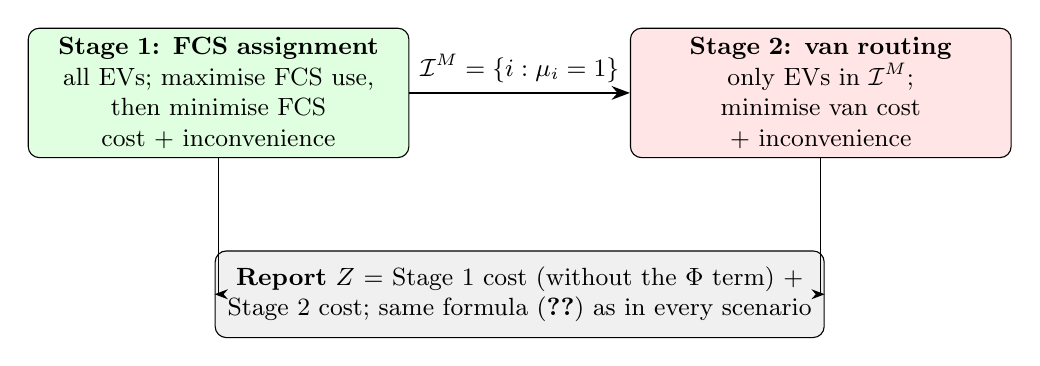
\begin{tikzpicture}[>=Stealth,box/.style={draw,rounded corners,align=center,minimum height=1.1cm,font=\small}]
  \node[box,fill=green!12,text width=4.6cm] (s1) {\textbf{Stage 1: FCS assignment}\\all EVs; maximise FCS use,\\then minimise FCS cost + inconvenience};
  \node[box,fill=red!10,text width=4.6cm,right=2.8cm of s1] (s2) {\textbf{Stage 2: van routing}\\only EVs in $\I^M$;\\minimise van cost + inconvenience};
  \draw[->,thick] (s1) -- node[above,font=\small]{$\I^M=\{i:\mu_i=1\}$} (s2);
  \node[box,fill=black!6,text width=7.5cm,below=2.0cm of $(s1)!0.5!(s2)$] (ev) {\textbf{Report} $Z=$ Stage~1 cost (without the $\Phi$ term) $+$ Stage~2 cost; same formula \eqref{eq:Z} as in every scenario};
  \draw[->] (s1) |- (ev); \draw[->] (s2) |- (ev);
\end{tikzpicture}
\end{center}

Stage~1 does not look at the vans, and Stage~2 cannot change what Stage~1 decided. That is the definition of ``FCS first, then MCS''.

%----------------------------------------------------------------
\subsection{Stage 1: assign EVs to fixed stations}

\textbf{Objective.}
\begin{equation}
\begin{split}
\min\ Z^{(1)}=\;&\underbrace{\Phi\sum_{i\in\I}\mu_i}_{\text{FCS first}}
+\underbrace{c^{EV}\sum_i\sum_{f\in\F_i}d_{if}Y_{if}}_{Z_1}
+\underbrace{Z^F_{\text{energy}}}_{\text{FCS part of }Z_4}\\
&+\underbrace{\sum_i\sum_{f\in\F_i}\rho^F_{if}Y_{if}+\alpha\sum_i w_i(C_i-r_i)+c^L\sum_i w_iL_i}_{\text{FCS customers' inconvenience}}
\end{split}
\label{eq:obj1}
\end{equation}
with $C_i=S_i+\tau^F_iY_i$ in this stage. $\Phi$ is a penalty for handing an EV to the vans. It is chosen larger than anything an extra FCS customer can add to the rest of \eqref{eq:obj1}, e.g.
\[
\Phi > \max_{i}\max_{f\in\F_i}\big(c^{EV}d_{if}+\pi^{\max}E_i+\rho^F_{if}\big)+n\,(\alpha+c^L)\,w_{\max}\,T,
\]
so Stage~1 first \textbf{maximises the number of EVs served at an FCS}, and only among those solutions minimises FCS cost and inconvenience. ($\pi^{\max}$ is the highest grid price.) A numerically safer equivalent is to solve twice: first $\max\sum_iY_i$, then fix that number and minimise the rest.
\ifTOU
Because $Z^F_{\text{energy}}$ uses the peak price, Stage~1 may \emph{start sessions later} to leave the peak, if the price saving beats the extra waiting cost (Section~\ref{sec:expect}).
\fi

\textbf{Constraints.}
\begin{align}
\sum_{g\in\G_i}y_{ig}+\mu_i &= 1 && \forall i\in\I \label{eq:s1assign}\\
S_i &\ge r_i+\sum_{f\in\F_i}t_{if}Y_{if} && \forall i\in\I \label{eq:fcsarr}\\
S_i &\le r_i+T\,(1-\mu_i) && \forall i\in\I \label{eq:s1park}\\
S_j &\ge S_i+\tau^F_i-(T+\tau^F_i)(3-y_{ig}-y_{jg}-o_{ij}) && \forall g,\ (i,j)\in\mathcal{P}_g \label{eq:disj1}\\
S_i &\ge S_j+\tau^F_j-(T+\tau^F_j)(2-y_{ig}-y_{jg}+o_{ij}) && \forall g,\ (i,j)\in\mathcal{P}_g \label{eq:disj2}\\
\sum_i y_{ig_1} &\ge \sum_i y_{ig_2} && \forall f,\ \G_f=\{g_1,g_2\} \label{eq:gunsym}\\
S_i+\tau^F_iY_i &\le T,\qquad L_i\ge S_i+\tau^F_iY_i-l_i && \forall i\in\I \label{eq:s1time}
\end{align}
\ifTOU plus the time-of-use split \eqref{eq:tou1}--\eqref{eq:tou5} of each FCS session (Section~\ref{sec:price}).\fi
\desc{\eqref{eq:s1assign}: every EV either gets one reachable gun or is handed to the vans. An EV that reaches no FCS ($\G_i=\emptyset$) is forced to $\mu_i=1$. \eqref{eq:fcsarr}: an FCS session cannot start before the EV has asked and driven to the station. \eqref{eq:s1park}: for an EV handed to the vans, $S_i$ is parked at $r_i$, so it adds no waiting in Stage~1 (its real start time is decided in Stage~2). \eqref{eq:disj1}--\eqref{eq:disj2}: two EVs on the same gun do not overlap; $o_{ij}$ picks who goes first. With two guns per station this means at most two EVs charge at a station at a time. \eqref{eq:gunsym}: symmetry breaking between the two identical guns (optional). \eqref{eq:s1time}: finished by $T$; lateness.}

\textbf{Optional acceptability rule.} An operator may refuse to send a driver to a station that is ``too inconvenient'', e.g.\ only allow gun $g$ of station $f$ for EV $i$ if $\hat\rho^F_{if}\le\bar\rho$. This only shrinks $\G_i$, so EVs whose stations are all too far go to the vans. Report results with and without it.

\textbf{Output:} $\I^M=\{i:\mu_i=1\}$, the EVs left for the vans; plus each FCS customer's gun and start time.

%----------------------------------------------------------------
\subsection{Stage 2: route the vans to the leftover EVs}

Stage~2 is a vehicle routing problem with time windows, on the EVs in $\I^M$ only. Here $C_i=S_i+\tau^M_i$.

\textbf{Objective.}
\begin{equation}
\begin{split}
\min\ Z^{(2)}=\;&\underbrace{c^M\sum_m\sum_{(i,j)\in\A^M}d_{ij}x_{ijm}}_{Z_2}+\underbrace{\sum_m c^D_mu_m}_{Z_3}+\underbrace{Z^M_{\text{energy}}}_{\text{van part of }Z_4}\\
&+\underbrace{\sum_{i\in\I^M}\sum_m\rho^M_{im}z_{im}+\alpha\sum_{i\in\I^M}w_i(C_i-r_i)+c^L\sum_{i\in\I^M}w_iL_i}_{\text{van customers' inconvenience}}
\end{split}
\label{eq:obj2}
\end{equation}
Since every EV in $\I^M$ must be served by some van, $Z^M_{\text{energy}}$ and the $\rho^M$ term are constants here. They are kept so that $Z^{(2)}$ is the true cost of Stage~2. Waiting and lateness make the vans visit urgent EVs early.

\textbf{Constraints.}
\begin{align}
\sum_{m\in\M}z_{im} &= 1 && \forall i\in\I^M \label{eq:s2assign}\\
\sum_{j:(0,j)\in\A^M}x_{0jm} = \sum_{i:(i,n+1)\in\A^M}x_{i,n+1,m} &= u_m && \forall m \label{eq:depot}\\
\sum_{i:(i,j)\in\A^M}x_{ijm} = \sum_{k:(j,k)\in\A^M}x_{jkm} &= z_{jm} && \forall j\in\I^M,\ m \label{eq:flow}\\
\sum_{i\in\I^M}z_{im} &\le Q_m\,u_m && \forall m \label{eq:cap}\\
\sum_{i\in\I^M}\frac{E_i}{\eta}z_{im}+\beta\sum_{(i,j)\in\A^M}d_{ij}x_{ijm} &\le B_m\,u_m && \forall m \label{eq:batt}
\end{align}
\begin{align}
S_j &\ge \max\{r_j,\ t_{0j}\,x_{0jm}\} && \forall j\in\I^M,\ m \label{eq:depart}\\
S_j &\ge S_i+\tau^M_i+t_{ij}-(T+\tau^M_i+t_{ij})(1-x_{ijm}) && \forall i\neq j,\ m \label{eq:seq}\\
S_i+\tau^M_i+t_{i,n+1} &\le T+(\tau^M_i+t_{i,n+1})(1-x_{i,n+1,m}) && \forall i,\ m \label{eq:return}\\
S_i+\tau^M_i \le T,\quad L_i &\ge S_i+\tau^M_i-l_i && \forall i\in\I^M \label{eq:s2time}\\
u_m &\ge u_{m+1} && m<|\M| \label{eq:vansym}
\end{align}
\desc{\eqref{eq:s2assign}: each leftover EV gets one van. \eqref{eq:depot}: a used van leaves and returns to the depot once. \eqref{eq:flow}: each EV on van $m$ is entered and left exactly once by that van. \eqref{eq:cap}: at most $Q_m$ EVs per van. \eqref{eq:batt}: delivered energy (with transfer losses) plus driving energy fits in the van battery. \eqref{eq:depart}: no start before the request, or before the van can drive there from the depot (written as two linear constraints). \eqref{eq:seq}: if the van goes $i\to j$, it finishes $i$ and drives to $j$ before starting $j$. This gives one EV at a time and removes subtours (MTZ-type). \eqref{eq:return}: back at the depot by $T$. \eqref{eq:s2time}: finished by $T$; lateness. \eqref{eq:vansym}: use identical vans in index order.}

\textbf{If Stage 2 is infeasible} (too many leftover EVs for the fleet by $T$), the sequential policy has \emph{failed} on that instance. For diagnosis, add $s_i\in\{0,1\}$ (``unserved''), replace \eqref{eq:s2assign} by $\sum_mz_{im}+s_i=1$ and add $\Phi^U\sum_is_i$ to \eqref{eq:obj2}. Then report the number of EVs that could not be served. This is a useful comparison with the integrated scenario, which may serve all of them.

%----------------------------------------------------------------
\subsection{Reported value}
\[
Z^{\text{S\scen}}=\big(Z^{(1)*}-\Phi\,|\I^M|\big)+Z^{(2)*},
\]
which is exactly \eqref{eq:Z} evaluated at the combined solution. The stage-1 solution plus the stage-2 solution is a feasible solution of the integrated model (S\ifTOU 4\else 3\fi), so
$Z^{\text{S\ifTOU 4\else 3\fi}}\le Z^{\text{S\scen}}$. The difference is the \emph{value of integration}.

\else
%---------------------------------------------------------------- INT
\subsection{Objective}
\begin{equation}
\min\ Z \quad\text{as in \eqref{eq:Z}, with }Z^F_{\text{energy}}=\ifTOU P^F\textstyle\sum_i\big[\pi^\off(\theta^1_i+\theta^3_i)+\pi^\pk\theta^2_i\big]\else\pi^F\textstyle\sum_iE_iY_i\fi,\quad C_i=S_i+\tau^F_iY_i+\tau^M_iZ_i. \label{eq:objint}
\end{equation}
Written out in full:
\begin{align*}
\min\ Z=\;& c^{EV}\sum_i\sum_{f\in\F_i}d_{if}Y_{if}+c^M\sum_m\sum_{(i,j)\in\A}d_{ij}x_{ijm}+\sum_mc^D_mu_m\\
&+\ifTOU P^F\sum_i\big[\pi^\off(\theta^1_i+\theta^3_i)+\pi^\pk\theta^2_i\big]\else\pi^F\sum_iE_iY_i\fi
+\pi^M\sum_i\sum_m\frac{E_i}{\eta}z_{im}\\
&+\sum_i\sum_{f\in\F_i}\rho^F_{if}Y_{if}+\sum_i\sum_m\rho^M_{im}z_{im}+\alpha\sum_iw_i(C_i-r_i)+c^L\sum_iw_iL_i .
\end{align*}
Every term is linear. One model weighs everything at once: an EV goes to a van exactly when the van's extra km, dispatch and energy cost are outweighed by the effort and waiting it saves the driver\ifTOU, or by the peak-price energy it avoids\fi.

\subsection{Constraints}

\textbf{Assignment.}
\begin{equation}
\sum_{g\in\G_i}y_{ig}+\sum_{m\in\M}z_{im}=1\qquad\forall i\in\I \label{eq:assign}
\end{equation}
\desc{Exactly one resource per EV: one reachable gun or one van. EVs that reach no FCS are forced onto a van.}

\textbf{Fixed stations.}
\begin{align}
S_i &\ge r_i+\sum_{f\in\F_i}t_{if}Y_{if} && \forall i \label{eq:fcsarr}\\
S_j &\ge S_i+\tau^F_i-(T+\tau^F_i)(3-y_{ig}-y_{jg}-o_{ij}) && \forall g,\ (i,j)\in\mathcal{P}_g \label{eq:disj1}\\
S_i &\ge S_j+\tau^F_j-(T+\tau^F_j)(2-y_{ig}-y_{jg}+o_{ij}) && \forall g,\ (i,j)\in\mathcal{P}_g \label{eq:disj2}\\
\sum_iy_{ig_1} &\ge \sum_iy_{ig_2} && \forall f,\ \G_f=\{g_1,g_2\} \label{eq:gunsym}
\end{align}
\desc{\eqref{eq:fcsarr}: an FCS session starts after the request and the drive to the station (for a van customer this is just $S_i\ge r_i$). \eqref{eq:disj1}--\eqref{eq:disj2}: EVs on the same gun do not overlap; $o_{ij}$ chooses the order. \eqref{eq:gunsym}: optional symmetry breaking.}

\textbf{Vans: routes, capacity, battery.}
\begin{align}
\sum_{j:(0,j)\in\A}x_{0jm}=\sum_{i:(i,n+1)\in\A}x_{i,n+1,m} &= u_m && \forall m \label{eq:depot}\\
\sum_{i:(i,j)\in\A}x_{ijm}=\sum_{k:(j,k)\in\A}x_{jkm} &= z_{jm} && \forall j\in\I,\ m \label{eq:flow}\\
\sum_iz_{im} &\le Q_mu_m && \forall m \label{eq:cap}\\
\sum_i\frac{E_i}{\eta}z_{im}+\beta\sum_{(i,j)\in\A}d_{ij}x_{ijm} &\le B_mu_m && \forall m \label{eq:batt}
\end{align}
\desc{\eqref{eq:depot}: a used van leaves and returns once. \eqref{eq:flow}: each EV on van $m$ is visited exactly once by it. \eqref{eq:cap}: at most $Q_m$ EVs. \eqref{eq:batt}: delivered energy (with losses) plus driving energy fits in the battery.}

\textbf{Vans: timing (one EV at a time, no subtours).}
\begin{align}
S_j &\ge t_{0j}\,x_{0jm} && \forall j\in\I,\ m \label{eq:depart}\\
S_j &\ge S_i+\tau^M_i+t_{ij}-(T+\tau^M_i+t_{ij})(1-x_{ijm}) && \forall i\neq j\in\I,\ m \label{eq:seq}\\
S_i+\tau^M_i+t_{i,n+1} &\le T+(\tau^M_i+t_{i,n+1})(1-x_{i,n+1,m}) && \forall i,\ m \label{eq:return}
\end{align}
\desc{\eqref{eq:depart}: the first stop cannot start before the van has driven there. \eqref{eq:seq}: $i\to j$ means finish $i$, drive, then start $j$; start times rise along a route, so no subtour can close. \eqref{eq:return}: back at the depot by $T$.}

\textbf{Horizon and lateness.}
\begin{equation}
C_i\le T,\qquad L_i\ge C_i-l_i\qquad\forall i\in\I \label{eq:time}
\end{equation}
\desc{Every EV is fully charged within the horizon; $L_i$ measures lateness.}

\ifTOU
\textbf{Time-of-use split.} Constraints \eqref{eq:tou1}--\eqref{eq:tou5} of Section~\ref{sec:price}.
\fi

\textbf{Symmetry and domains.}
\begin{equation}
u_m\ge u_{m+1};\qquad y,z,x,u,o\ifTOU,\kappa\fi\in\{0,1\};\qquad S_i,L_i\ifTOU,\theta^p_i\fi\ge0 \label{eq:dom}
\end{equation}
\fi

%=====================================================================
\section{Learning-to-optimise (RL) formulation}\label{sec:rl}

\textbf{Main rule:} the reward of each action is \emph{minus the increase in $Z$ that the action causes}. The rewards over an episode then add up to $-Z$ of the solution the policy builds. RL and MILP results are measured on the same yardstick \eqref{eq:Z}, and the MILP optimum is the benchmark for the RL gap.

\ifSEQ
%---------------------------------------------------------------- RL SEQ
The RL pipeline has the same two stages as the MILP.

\subsection{Stage 1 policy: FCS assignment}
\begin{itemize}[leftmargin=1.4em,itemsep=2pt]
  \item \textbf{Episode / epochs:} EVs are taken in order of request time $r_i$ (ties: higher $w_i$ first). One decision per EV.
  \item \textbf{State:} features of the current EV $k$ ($E_k,r_k,l_k,w_k,R_k$, location); for each gun $g$ the time $F_g$ it becomes free; summary features of the EVs still to come (count and positions near each station)\ifTOU; the current price and the time until $T_1$ and $T_2$\fi.
  \item \textbf{Action:} a gun $g\in\G_k$, or ``hand to vans''. \textbf{FCS-first mask:} ``hand to vans'' is allowed \emph{only} if no gun can finish EV $k$ by $T$ (or, with the optional rule, if all remaining guns have $\hat\rho^F_{kf}>\bar\rho$).
  \ifTOU\item \textbf{Optional timing action:} ``gun $g$, start after the peak'', i.e.\ $S_k=\max\{\text{earliest},T_2\}$, allowed only if the session still ends by $T$.\fi
  \item \textbf{Transition:} $S_k=\max\{r_k+t_{kf},F_g\}$ (or later, for the timing action); $F_g\leftarrow S_k+\tau^F_k$.
  \item \textbf{Reward:} $-\Big[c^{EV}d_{kf}+\text{energy}_k+\rho^F_{kf}+\alpha w_k(S_k+\tau^F_k-r_k)+c^Lw_k(S_k+\tau^F_k-l_k)^+\Big]$, where energy$_k$ = \ifTOU$P^F\big[\pi^\off\cdot(\text{off-peak hours of }[S_k,S_k+\tau^F_k])+\pi^\pk\cdot(\text{peak hours})\big]$, computed exactly in the simulator\else$\pi^FE_k$\fi. Handing an EV to the vans gives reward $0$ here; its cost is counted in Stage~2.
\end{itemize}
Note: a simple baseline for Stage~1 is the greedy rule ``gun with the largest one-step reward''. What RL can learn on top of this is, for example, to keep a nearby gun free for an urgent EV that arrives later.

\subsection{Stage 2 policy: van routing over $\I^M$}
\begin{itemize}[leftmargin=1.4em,itemsep=2pt]
  \item \textbf{Epochs:} whenever a van becomes free (the earliest-free van decides first).
  \item \textbf{State:} for each van: position, time free, remaining battery $b_m$, EVs served so far, dispatched or not; for each unserved EV in $\I^M$: location, $E_i,r_i,l_i,w_i$; current time.
  \item \textbf{Action:} the next EV $j$ for this van, or ``return to depot'' (ends the route). Mask: $j$ must be feasible: battery covers $E_j/\eta$ plus driving to $j$ and back to the depot, the count stays $\le Q_m$, and $j$ can be finished with the van back at the depot by $T$.
  \item \textbf{Transition:} $S_j=\max\{r_j,\ \text{time free}+t_{\text{pos},j}\}$; the van moves to $j$ and is free at $S_j+\tau^M_j$; $b_m$ falls by $E_j/\eta+\beta d_{\text{pos},j}$.
  \item \textbf{Reward:} serving $j$: $-\Big[c^Md_{\text{pos},j}+c^D_m[\text{first stop}]+\pi^M\frac{E_j}{\eta}+\rho^M_{jm}+\alpha w_j(S_j+\tau^M_j-r_j)+c^Lw_j(S_j+\tau^M_j-l_j)^+\Big]$; returning: $-c^Md_{\text{pos},0}$. EVs still unserved at the end: $-\Phi^U$ each.
  \item \textbf{Policy:} an attention-based routing policy (e.g.\ Kool et al., 2019, ``Attention, Learn to Solve Routing Problems!'') trained with REINFORCE or PPO. Baseline: nearest-feasible-EV heuristic.
\end{itemize}
Episode return of Stage~1 + Stage~2 $=-Z^{\text{S\scen}}$.

\else
%---------------------------------------------------------------- RL INT
One policy decides both who serves each EV and the van routes.
\begin{itemize}[leftmargin=1.4em,itemsep=2pt]
  \item \textbf{Episode / epochs:} EVs are taken in order of request time $r_i$ (ties: higher $w_i$ first). One decision per EV.
  \item \textbf{State:} (i) the current EV $k$: location, $E_k,r_k,l_k,w_k,R_k$, reachable stations; (ii) each gun $g$: time $F_g$ it becomes free; (iii) each van $m$: current end-of-route position, time free, remaining battery $b_m$, EVs served, dispatched or not; (iv) embeddings of the not-yet-assigned EVs (for look-ahead)\ifTOU; (v) current price, time until $T_1$ and $T_2$\fi.
  \item \textbf{Action:} $a\in\G_k\cup\M$: a gun, or a van (EV $k$ is appended to the end of that van's route). \textbf{Mask} infeasible actions: a gun that cannot finish $k$ by $T$; a van without enough battery for $E_k/\eta$ plus the drive to $k$ and back to the depot, with $Q_m$ reached, or unable to finish $k$ and return by $T$.
  \ifTOU\item \textbf{Optional timing action:} ``gun $g$, start after the peak'' ($S_k=\max\{\text{earliest},T_2\}$, if it still ends by $T$).\fi
  \item \textbf{Transition:} gun: $S_k=\max\{r_k+t_{kf},F_g\}$, $F_g\leftarrow S_k+\tau^F_k$. Van: $S_k=\max\{r_k,\ \text{free}_m+t_{\text{pos}_m,k}\}$, then the van moves to $k$, $\text{free}_m\leftarrow S_k+\tau^M_k$, $b_m\mathrel{-}=E_k/\eta+\beta d_{\text{pos}_m,k}$.
  \item \textbf{Reward} $=-\Delta Z$:
  \begin{align*}
  \text{gun } g\text{ at }f:&\quad -\Big[c^{EV}d_{kf}+\text{energy}^F_k+\rho^F_{kf}+\alpha w_k(C_k-r_k)+c^Lw_k(C_k-l_k)^+\Big]\\
  \text{van } m:&\quad -\Big[c^M\big(d_{\text{pos}_m,k}+d_{k,0}-d_{\text{pos}_m,0}\big)+c^D_m[\text{first use}]+\pi^M\tfrac{E_k}{\eta}\\
  &\qquad\quad+\rho^M_{km}+\alpha w_k(C_k-r_k)+c^Lw_k(C_k-l_k)^+\Big]
  \end{align*}
  The van distance term is the \emph{change} in route length when $k$ is inserted before the return to the depot, so the sum over the episode equals the total route length (the return legs telescope). energy$^F_k$ = \ifTOU$P^F\big[\pi^\off\cdot(\text{off-peak hours})+\pi^\pk\cdot(\text{peak hours of }[S_k,C_k])\big]$, computed exactly by the simulator; no linearisation is needed in RL\else$\pi^FE_k$\fi.
  \item \textbf{Dead end:} if every action is masked, EV $k$ is unserved: reward $-\Phi^U$, and the episode continues. Report the count.
  \item \textbf{Policy:} masked categorical policy over guns and vans, encoder with attention over EVs, guns and vans; trained with PPO. Natural baseline: greedy, i.e.\ choose the action with the largest one-step reward. That is the pairwise rule ``smallest $\hat\rho$ + cost'' from Section~\ref{sec:inc}.
\end{itemize}
Restriction to note: vans serve EVs in assignment order (append only). A variant that inserts $k$ at the cheapest position of a route is more flexible but has a larger action space.
\fi

\textbf{Reward scaling.} For stable training divide every reward by a constant, e.g.\ the greedy baseline's average $Z$ on the training instances. This does not change the optimal policy.

%=====================================================================
\section{What to expect and what to report}\label{sec:expect}

\ifnum\scen=1
\begin{itemize}[leftmargin=1.4em,itemsep=2pt]
  \item Vans serve only EVs that reach no station, or that the stations cannot finish by $T$. If stations have spare capacity, very few vans are dispatched.
  \item Inconvenience is high for EVs far from the nearest station (worked example: Rs\,682 at the FCS, against Rs\,458 if a van had been allowed).
  \item With too few vans Stage~2 becomes infeasible (unserved EVs), even when the integrated model S3 could serve everyone. Report the smallest $|\M|$ at which S1 is feasible and compare it with S3.
\end{itemize}
\fi
\ifnum\scen=2
\begin{itemize}[leftmargin=1.4em,itemsep=2pt]
  \item \textbf{When does Stage~1 delay a session to avoid the peak?} Moving one hour of charging out of the peak saves $(\pi^\pk-\pi^\off)P^F=3\times22=$ Rs\,66, but delays completion by up to an hour, which costs $\alpha w_i\ge$ Rs\,200. So with the default values Stage~1 almost never delays. It mostly pays the higher price, and S2 costs roughly S1 plus the peak surcharge. Sessions start later only if $\alpha$ is small (try $\lambda<0.33$ in the sensitivity analysis).
  \item The van assignment is the same as in S1 unless Stage~1's timing changes which EVs fit at the stations. Stage~1 cannot use vans to escape the peak price.
  \item Extra KPI: \textbf{grid energy drawn at FCS during the peak}, $P^F\sum_i\theta^2_i$ (kWh). Compare with S4.
\end{itemize}
\fi
\ifnum\scen=3
\begin{itemize}[leftmargin=1.4em,itemsep=2pt]
  \item Vans take EVs for which the saved inconvenience exceeds the extra van cost (worked example: van chosen, saving Rs\,224). Expect vans to serve EVs that are far from every station, have low range (high $w_i$), or have early deadlines, while EVs near a station still use it.
  \item \textbf{Value of integration under flat price:} $Z^{\text{S1}}-Z^{\text{S3}}\ge0$. Report it per component ($Z_1,\dots,Z_5$): typically operating cost rises a little and inconvenience falls a lot.
  \item Vary $|\M|$ (0, 1, 2, \dots): the first few vans lower $Z$ sharply, then the effect levels off. That curve shows the scenarios where mobile chargers help most.
\end{itemize}
\fi
\ifnum\scen=4
\begin{itemize}[leftmargin=1.4em,itemsep=2pt]
  \item During the peak a van kWh costs about the same as an FCS kWh (Rs\,10.0 each), so the vans' energy disadvantage disappears and vans also absorb \emph{peak-hour} demand that would otherwise be charged on the grid at peak price.
  \item Expect more van usage than in S3, concentrated on requests in $[T_1,T_2]$, and lower grid energy at the stations during the peak, $P^F\sum_i\theta^2_i$, than in S2.
  \item \textbf{Value of integration under peak pricing:} $Z^{\text{S2}}-Z^{\text{S4}}$. It should be larger than $Z^{\text{S1}}-Z^{\text{S3}}$, because integration now also allows price arbitrage.
  \item \textbf{Peak pricing with full flexibility:} $Z^{\text{S4}}-Z^{\text{S3}}$ should be smaller than $Z^{\text{S2}}-Z^{\text{S1}}$: vans cushion the price increase.
\end{itemize}
\fi

\textbf{Cross-scenario comparison table} (fill in from the four runs):
\begin{center}
\renewcommand{\arraystretch}{1.2}
\begin{tabular}{@{}lll@{}}
\toprule
\textbf{Comparison} & \textbf{Measures} & \textbf{Expected sign} \\
\midrule
S1 $-$ S3 & value of integration, flat price & $\ge0$ \\
S2 $-$ S4 & value of integration, peak price & $\ge0$, larger than S1 $-$ S3 \\
S2 $-$ S1 & cost of peak pricing, FCS-first operator & $>0$ \\
S4 $-$ S3 & cost of peak pricing, flexible operator & $>0$, smaller than S2 $-$ S1 \\
\bottomrule
\end{tabular}
\end{center}
Report for each: $Z$ and its components, number of vans used, EVs per resource, mean and maximum inconvenience per EV, total lateness, peak-hour grid energy, solve time, and (for RL) the gap to the MILP optimum.

%=====================================================================
\appendix
\section{Illustrative parameter values}\label{app:values}

These are starting values for experiments, not data. All are meant to be varied in the analysis. Values in Rs.

\begin{center}
\renewcommand{\arraystretch}{1.15}
\begin{tabular}{@{}llp{6.2cm}@{}}
\toprule
\textbf{Parameter} & \textbf{Value} & \textbf{Note} \\
\midrule
$T$, $[T_1,T_2]$ & 7 h, $[2,6]$ & 16:00--23:00, peak 18:00--22:00 \\
$P^F$, $P^M$ & 22 kW, 30 kW & \\
$v$, $\beta$, $\eta$ & 25 km/h, 0.25 kWh/km, 0.9 & \\
$B_m$, $Q_m$, $|\M|$ & 150 kWh, 6, 2--6 & \\
$c^{EV}$, $c^M$, $c^D_m$ & Rs\,4/km, Rs\,15/km, Rs\,1500 & van km includes driver time \\
$\pi^F$ (flat) & Rs\,8.7/kWh & equals the time-average of the ToU tariff over $[0,T]$ \\
$\pi^\off$, $\pi^\pk$ (ToU) & Rs\,7/kWh, Rs\,10/kWh & $(3\times7+4\times10)/7=8.7$ \\
$c^{bat}$ & Rs\,2/kWh & van battery wear \\
$\pi^M$ & Rs\,10.7 (flat) / Rs\,9.0 (ToU) & $=\pi^F+c^{bat}$ / $=\pi^\off+c^{bat}$ \\
$\alpha$, $\alpha^D$ & Rs\,200/h, Rs\,100/h & value of time; extra for attended time \\
$h^F$, $h^M$, $\varphi$ & Rs\,50, Rs\,10, Rs\,100 & trip hassle, hand-over, range stress \\
$c^L$ & Rs\,300/h & lateness \\
$w_i$ & $1+2(1-R_i/R_{\max})$, $R_i\sim U[3,40]$ km & priority from remaining range \\
\bottomrule
\end{tabular}
\end{center}

The flat price is set to the time-average of the peak tariff. The price \emph{level} is then the same in both pricing cases, and only the price \emph{shape} differs. Without this, part of S1 vs S2 would just reflect a different average price.

\end{document}
"
%    pdflatex -jobname=scenario3_flat_integrated   "\def\scen{3}% =====================================================================
%  One source, four PDFs.  Build with build.sh (or by hand):
%    pdflatex -jobname=scenario1_flat_sequential   "\def\scen{1}\input{scenario_master}"
%    pdflatex -jobname=scenario2_peak_sequential   "\def\scen{2}\input{scenario_master}"
%    pdflatex -jobname=scenario3_flat_integrated   "\def\scen{3}\input{scenario_master}"
%    pdflatex -jobname=scenario4_peak_integrated   "\def\scen{4}\input{scenario_master}"
%  (run each twice for cross-references)
% =====================================================================
\documentclass[11pt,a4paper]{article}
\usepackage[margin=2.2cm]{geometry}
\usepackage{amsmath,amssymb,amsfonts}
\usepackage{booktabs,array,tabularx}
\usepackage{enumitem}
\usepackage[table]{xcolor}
\usepackage{tikz}
\usetikzlibrary{arrows.meta,positioning,calc}
\usepackage[colorlinks=true,linkcolor=blue!50!black,urlcolor=blue!50!black]{hyperref}
\usepackage{titlesec}
\titleformat{\section}{\large\bfseries}{\thesection}{0.8em}{}
\titleformat{\subsection}{\normalsize\bfseries}{\thesubsection}{0.8em}{}
\setlength{\parindent}{0pt}
\setlength{\parskip}{5pt}

% ---------------- scenario switches ----------------
\ifdefined\scen\else\def\scen{1}\fi
\newif\ifTOU \TOUfalse   % true = time-of-use (peak) price
\newif\ifSEQ \SEQfalse   % true = FCS first, then MCS
\ifnum\scen=1 \SEQtrue \fi
\ifnum\scen=2 \TOUtrue \SEQtrue \fi
\ifnum\scen=4 \TOUtrue \fi

\newcommand{\pricename}{\ifTOU time-of-use price (dearer evening peak)\else single (flat) price all day\fi}
\newcommand{\structname}{\ifSEQ FCS first, then MCS (sequential)\else FCS and MCS together (integrated)\fi}

% ---------------- notation ----------------
\newcommand{\I}{\mathcal{I}}
\newcommand{\F}{\mathcal{F}}
\newcommand{\G}{\mathcal{G}}
\newcommand{\M}{\mathcal{M}}
\newcommand{\N}{\mathcal{N}}
\newcommand{\A}{\mathcal{A}}
\newcommand{\Rs}{\text{Rs}\,}
\newcommand{\pk}{\mathrm{pk}}
\newcommand{\off}{\mathrm{off}}
\newcommand{\desc}[1]{\par\vspace{-2pt}{\small\color{black!75}\textit{Meaning:} #1}\par\vspace{4pt}}
\newcommand{\cell}[2]{\ifnum\scen=#1\cellcolor{blue!18}\textbf{S#1 (this document)}\\\textbf{#2}\else S#1\\#2\fi}

\title{\textbf{EV Charging Network Optimisation}\\[4pt]
\large Scenario \scen: \pricename\ $+$ \structname\\[2pt]
\normalsize MILP and RL formulation}
\author{CP 320 OR for Mobility Management, course project}
\date{2 October 2026}

\begin{document}
\maketitle

%=====================================================================
\section{Where this scenario sits}

The project studies four scenarios: two ways of pricing grid electricity, times two ways of making the decisions.

\begin{center}
\renewcommand{\arraystretch}{1.5}
\begin{tabular}{>{\raggedright\arraybackslash}p{4.2cm}|>{\centering\arraybackslash}p{4.6cm}|>{\centering\arraybackslash}p{4.6cm}}
 & \textbf{Flat price all day} & \textbf{Time-of-use (peak) price} \\ \hline
\textbf{Sequential:} FCS first, leftover EVs to MCS &
\begin{tabular}[c]{@{}c@{}}\cell{1}{flat + sequential}\end{tabular} &
\begin{tabular}[c]{@{}c@{}}\cell{2}{peak + sequential}\end{tabular} \\ \hline
\textbf{Integrated:} FCS and MCS decided together &
\begin{tabular}[c]{@{}c@{}}\cell{3}{flat + integrated}\end{tabular} &
\begin{tabular}[c]{@{}c@{}}\cell{4}{peak + integrated}\end{tabular} \\
\end{tabular}
\end{center}

\textbf{The four scenarios do not have four different objectives.} They share \emph{one} cost yardstick $Z$ (Section~\ref{sec:obj}): the same cost terms and the same customer inconvenience (Section~\ref{sec:inc}). Only two things change:
\begin{itemize}[leftmargin=1.4em,itemsep=1pt]
  \item \textbf{Pricing} changes the formula for one term, the FCS energy cost (Section~\ref{sec:price}).
  \item \textbf{Decision structure} changes \emph{how} $Z$ is minimised: in one model (integrated), or in two stages (sequential), where each stage minimises its own part of $Z$.
\end{itemize}
Because the yardstick is the same, the four optimal values can be compared directly. The differences measure the \emph{value of integration} (S1$\to$S3, S2$\to$S4) and the \emph{effect of peak pricing} (S1$\to$S2, S3$\to$S4).

\ifnum\scen=1
\textbf{This scenario (S1)} is the baseline, the ``status quo''. Electricity costs the same at every hour, every EV that can be charged at a fixed station is sent there, and vans only take what is left over.
\fi
\ifnum\scen=2
\textbf{This scenario (S2)} keeps the FCS-first rule of S1, but grid electricity is dearer during the evening peak. Stage~1 can react to the price only by \emph{rescheduling} FCS sessions. It cannot hand a peak-hour EV to a van.
\fi
\ifnum\scen=3
\textbf{This scenario (S3)} keeps the flat price of S1, but the operator decides FCS and MCS service \emph{together}. An EV can be sent to a van even when a fixed station could take it, whenever that lowers total cost plus inconvenience.
\fi
\ifnum\scen=4
\textbf{This scenario (S4)} is the most flexible one: peak pricing at fixed stations, and FCS and MCS decided together. Van energy was bought off-peak, so vans can also be used to keep charging \emph{out of the expensive peak}.
\fi

%=====================================================================
\section{Setting and assumptions}\label{sec:setting}

\textbf{Time.} The planning horizon is $[0,T]$ with $T=7$\,h (16:00--23:00). It contains the evening peak window $[T_1,T_2]=[2,6]$ (18:00--22:00). The horizon is the same in all four scenarios. It is wider than the peak itself so that, under peak pricing, there is cheaper time on both sides of the peak.\ifTOU\else\ In this scenario the price is flat, so the window plays no role in the model.\fi

\textbf{Assumptions} (the same as MILP v3, plus two about energy):
\begin{enumerate}[leftmargin=1.6em,itemsep=1pt]
  \item Static, continuous time. All requests in the horizon are known at time $0$, and request $i$ becomes active at $r_i$.
  \item An EV served by an FCS drives there itself on its own battery (only to stations within its range $R_i$). The driver stays with the car while it waits for a free gun and while it charges.
  \item An EV served by an MCS stays parked where it is, and the driver is free in the meantime.
  \item Each FCS gun and each van charges one EV at a time, without interruption, at constant power.
  \item A van's battery covers both its driving and the energy it delivers. \textbf{The van battery is charged at the depot before the horizon starts}\ifTOU, i.e.\ at the off-peak price\fi, and is not recharged during the horizon.
  \item Every EV must be fully charged by $T$ (hard). Finishing after the driver's desired time $l_i$ is allowed but penalised.
\end{enumerate}

%=====================================================================
\section{Notation}\label{sec:notation}

\subsection*{Sets}
\begin{tabularx}{\textwidth}{@{}lX@{}}
\toprule
$\I=\{1,\dots,n\}$ & EV charging requests \\
$\F$; $\G_f$ ($|\G_f|=2$); $\G=\bigcup_f\G_f$ & fixed charging stations; guns of FCS $f$; all guns ($f(g)$ = station of gun $g$) \\
$\F_i=\{f: d_{if}\le R_i\}$, $\G_i=\bigcup_{f\in\F_i}\G_f$ & stations / guns EV $i$ can reach on its remaining range \\
$\M$ & mobile charging vans (MCS) \\
$0,\ n+1$ & depot as start node / end node (same place) \\
$\N=\{0\}\cup\I\cup\{n+1\}$, $\A$ & routing nodes; allowed van arcs $(i,j)$, $i\in\{0\}\cup\I$, $j\in\I\cup\{n+1\}$, $i\neq j$ \\
$\mathcal{P}_g=\{(i,j): i<j,\ g\in\G_i\cap\G_j\}$ & pairs of EVs that could share gun $g$ \\
\ifSEQ
$\I^M\subseteq\I$ & EVs handed to the vans by Stage~1 (an \emph{output} of Stage~1, a fixed input to Stage~2) \\
$\N^M$, $\A^M$ & routing nodes / arcs restricted to $\I^M$ \\
\fi
\bottomrule
\end{tabularx}

\subsection*{Parameters}
\begin{tabularx}{\textwidth}{@{}lX@{}}
\toprule
$E_i,\ r_i,\ l_i,\ R_i$ & energy demand (kWh), request time, desired completion time (h), remaining range (km) \\
$w_i\ge1$ & priority of EV $i$; $w_i=1+\kappa(1-R_i/R_{\max})$, so low-range EVs weigh more \\
$P^F,\ P^M$ & charging power of an FCS gun (22\,kW) / of a van (e.g.\ 30\,kW) \\
$\tau^F_i=E_i/P^F,\ \tau^M_i=E_i/P^M$ & charging time of EV $i$ at an FCS / by a van (h) \\
$d_{if},t_{if}$;\ $d_{ij},t_{ij}$ & distance (km) and time (h): EV$\to$FCS; between routing nodes ($t=d/v$) \\
$B_m,\ Q_m,\ \beta,\ \eta$ & van battery (kWh), max EVs per van, van consumption (kWh/km), transfer efficiency \\
$c^{EV},\ c^M,\ c^D_m$ & cost per km of EV driving, per km of van driving; fixed dispatch cost of van $m$ \\
\ifTOU
$\pi^\off,\ \pi^\pk$ & grid price (Rs/kWh) off-peak / in $[T_1,T_2]$, with $\pi^\pk\ge\pi^\off$ \\
\else
$\pi^F$ & grid price (Rs/kWh), the same at every hour \\
\fi
$c^{bat}$ & van battery wear per kWh cycled \\
$\pi^M$ & cost of 1 kWh taken from a van battery: $\pi^M=\ifTOU\pi^\off\else\pi^F\fi+c^{bat}$ (Section~\ref{sec:price}) \\
$\alpha,\ \alpha^D,\ h^F,\ h^M,\ \varphi,\ c^L$ & inconvenience coefficients (Section~\ref{sec:inc}) \\
\bottomrule
\end{tabularx}

\subsection*{Decision variables}
\begin{tabularx}{\textwidth}{@{}llX@{}}
\toprule
$y_{ig}$ & $\{0,1\}$ & EV $i$ charged at gun $g\in\G_i$ \\
$z_{im}$ & $\{0,1\}$ & EV $i$ served by van $m$ \\
$x_{ijm}$ & $\{0,1\}$ & van $m$ drives arc $(i,j)$ \\
$u_m$ & $\{0,1\}$ & van $m$ is dispatched \\
$o_{ij}$ & $\{0,1\}$ & for EVs $i<j$ that could share a gun: 1 if $i$ is charged before $j$ \\
\ifSEQ
$\mu_i$ & $\{0,1\}$ & Stage~1 only: EV $i$ is handed to the van fleet \\
\fi
\ifTOU
$\theta^1_i,\theta^2_i,\theta^3_i$ & $\ge0$ & hours of EV $i$'s FCS session before / inside / after the peak \\
$\kappa^1_i,\kappa^3_i$ & $\{0,1\}$ & EV $i$'s FCS session starts before $T_1$ / ends after $T_2$ \\
\fi
$S_i$ & $\ge0$ & time charging of EV $i$ starts (h), on whichever resource \\
$L_i$ & $\ge0$ & lateness of EV $i$ beyond $l_i$ (h) \\
\bottomrule
\end{tabularx}

\textbf{Short-hands} (linear expressions, not new variables):
\[
Y_{if}=\sum_{g\in\G_f}y_{ig},\qquad Y_i=\sum_{g\in\G_i}y_{ig}\ (\text{EV $i$ uses an FCS}),\qquad Z_i=\sum_{m\in\M}z_{im}\ (\text{EV $i$ uses a van}),
\]
\[
C_i=S_i+\tau^F_i\,Y_i+\tau^M_i\,Z_i \quad\text{(time EV $i$ is fully charged).}
\]

%=====================================================================
\section{Customer inconvenience}\label{sec:inc}

This section is \textbf{identical in all four scenario documents}. Inconvenience is a property of the customer, not of the price or of the planning method.

\subsection{What we mean by inconvenience}

Inconvenience is \emph{what the driver loses} from the moment they ask for a charge ($r_i$) until the car is fully charged ($C_i$), \emph{converted into rupees} so it can be added to the operator's costs. A driver loses three different things:

\begin{enumerate}[leftmargin=1.6em,itemsep=2pt]
  \item \textbf{Waiting:} the car is not ready. This lasts $C_i-r_i$ hours and affects \emph{every} driver, FCS or MCS.
  \item \textbf{Effort:} only an FCS customer has to drive to the station and sit there while the car charges. An MCS customer stays at home or at work and does something else. Driving to a far station also uses scarce battery range, which causes stress (``range anxiety'').
  \item \textbf{A missed deadline:} the car is still not ready at the time $l_i$ the driver needs it.
\end{enumerate}

Each loss gets a price in Rs per hour (or per event). All of them are multiplied by the priority $w_i$: an hour of delay for an EV with 5\,km of range left counts more than for one with 40\,km.

\subsection{The three components}

\begin{center}
\renewcommand{\arraystretch}{1.3}
\begin{tabularx}{\textwidth}{@{}>{\raggedright\arraybackslash}p{2.6cm}>{\raggedright\arraybackslash}X>{\raggedright\arraybackslash}X>{\raggedright\arraybackslash}p{3.0cm}@{}}
\toprule
\textbf{Component} & \textbf{EV $i$ at FCS $f$} & \textbf{EV $i$ by a van} & \textbf{Known when?} \\
\midrule
Effort & $w_i\big[\alpha^D(t_{if}+\tau^F_i)+h^F+\varphi\,d_{if}/R_i\big]$: driving and sitting at the station, a fixed trip hassle, range stress & $w_i\,h^M$: being reachable and handing over the car & \textbf{Static:} known as soon as the resource is chosen \\
Waiting & $w_i\,\alpha\,(C_i-r_i)$ = drive + \emph{queue at the gun} + charge & $w_i\,\alpha\,(C_i-r_i)$ = \emph{wait for the van} + charge & \textbf{Dynamic:} depends on the queue / van route \\
Missed deadline & $w_i\,c^L\,L_i$, $L_i=\max\{0,C_i-l_i\}$ & same & Dynamic \\
\bottomrule
\end{tabularx}
\end{center}

\textbf{Coefficients.}
$\alpha$ (Rs/h) is the value of an hour the car is not ready.
$\alpha^D$ (Rs/h) is the \emph{extra} value of an hour the driver must personally spend driving or sitting at the station: an hour at the station costs $\alpha+\alpha^D$, an hour waiting at home for a van costs only $\alpha$.
$h^F,h^M$ (Rs) are fixed hassle costs of one trip to a station / one van hand-over.
$\varphi$ (Rs) is the range-stress cost of a trip that uses the \emph{whole} remaining range ($d_{if}/R_i\le1$ is the fraction used).
$c^L$ (Rs/h) is the cost per hour late.

\subsection{Pairwise form: inconvenience of a (customer, resource) pair}

The natural first idea is: \emph{for every pair (EV $i$, FCS $f$) and every pair (EV $i$, van $m$) there is an inconvenience number, and the operator picks the pair with the lowest cost plus inconvenience.} The static part fits this idea exactly:
\[
\boxed{\;\rho^F_{if}=w_i\Big[\alpha^D\,(t_{if}+\tau^F_i)+h^F+\varphi\,\frac{d_{if}}{R_i}\Big]\qquad
\rho^M_{im}=w_i\,h^M\;}
\]
These are \textbf{parameters}, computed before solving, one number per (EV, FCS) pair and per (EV, van) pair. In the objective they appear linearly: $\sum_i\sum_f\rho^F_{if}Y_{if}+\sum_i\sum_m\rho^M_{im}z_{im}$.

Note that $\rho^M_{im}$ does not depend on $m$. Vans are identical and all start at the same depot, so the driver does not care \emph{which} van comes, only \emph{when} it comes. That ``when'' is the waiting part.

\subsection{Why waiting cannot be a fixed pairwise number}

It is tempting to also write the waiting as a pairwise number, e.g.\ ``the van needs 5 minutes to reach EV $i$''. But that depends on \emph{where the van is coming from}, which depends on the route the model is still choosing: if EV $i$ is the 4th stop of a van, the wait is the time for three charging sessions plus four drives. Likewise, waiting at an FCS depends on how many EVs are queued at that gun. So waiting is not known before solving. It is a function of decision variables:
\[
\text{waiting cost of EV } i \;=\; w_i\,\alpha\,(C_i-r_i),\qquad C_i=S_i+\tau^F_iY_i+\tau^M_iZ_i .
\]
This is \textbf{linear} in the variables ($S_i$, $y$, $z$), so it fits in a MILP directly. The constraints of Section~\ref{sec:milp} make $S_i$ equal to the true start time, including driving, queueing at the gun and the van's route. The term $\sum_i w_i\alpha r_i$ is a constant and may be dropped when solving.

\textbf{Pairwise \emph{estimate}} (used for intuition, by the RL policy and in heuristics): if there is no queue and the van comes straight to $i$,
\[
\hat\rho^{F}_{if}=\rho^F_{if}+w_i\alpha\,(t_{if}+\tau^F_i),\qquad
\hat\rho^{M}_{im}=\rho^M_{im}+w_i\alpha\,(t^{\text{van}}_{m\to i}+\tau^M_i),
\]
where $t^{\text{van}}_{m\to i}$ is the time until van $m$ can reach $i$ from where it currently is. In the RL formulation (Section~\ref{sec:rl}) the van's position \emph{is} known at each decision, so there this estimate becomes exact.

\subsection{Total inconvenience and how it enters the objective}

\begin{equation}
\boxed{\;
Z_{\text{inc}}=\underbrace{\sum_{i\in\I}\sum_{f\in\F_i}\rho^F_{if}Y_{if}+\sum_{i\in\I}\sum_{m\in\M}\rho^M_{im}z_{im}}_{\text{effort (static, pairwise)}}
+\underbrace{\alpha\sum_{i\in\I}w_i\,(C_i-r_i)}_{\text{waiting (dynamic)}}
+\underbrace{c^L\sum_{i\in\I}w_i\,L_i}_{\text{missed deadline}}
\;}\label{eq:inc}
\end{equation}
All three parts are in rupees, so $Z_{\text{inc}}$ is simply added to the operating costs. Nothing has to be normalised.

\subsection{Worked example: your ``10 km to the FCS vs.\ van in 5 minutes'' case}

EV $i$: $E_i=20$\,kWh, $R_i=40$\,km (so $w_i=1$); nearest free FCS $d_{if}=10$\,km away, $t_{if}=0.4$\,h at 25\,km/h; a van finishing next door can reach it in 5\,min ($0.083$\,h), adding about 4\,km to its route. $\tau^F_i=20/22=0.909$\,h, $\tau^M_i=20/30=0.667$\,h. Coefficients from Appendix~\ref{app:values}, flat price.

\begin{center}
\renewcommand{\arraystretch}{1.25}
\begin{tabular}{@{}lrr@{}}
\toprule
 & \textbf{FCS} & \textbf{Van} \\
\midrule
Driving (EV / extra van km) & $4\times10=40.0$ & $15\times4=60.0$ \\
Energy & $8.7\times20=174.0$ & $10.7\times20/0.9=237.8$ \\
\textbf{Operating cost only} & \textbf{214.0} & \textbf{297.8} \\
\midrule
Effort $\rho$ & $100(0.4+0.909)+50+100\cdot\tfrac{10}{40}=205.9$ & $10.0$ \\
Waiting $\alpha(C_i-r_i)$ & $200\times1.309=261.8$ & $200\times0.75=150.0$ \\
\textbf{Cost + inconvenience} & \textbf{681.7} & \textbf{457.8} \\
\bottomrule
\end{tabular}
\end{center}

On operating cost alone the FCS is cheaper, so a cost-only model would \emph{always} send this driver 10\,km away. With inconvenience included the van is better by about Rs\,224, and the integrated model chooses $z_{im}=1$, as you expected. If the FCS were only 1\,km away, the FCS would win both comparisons. The inconvenience term is what makes the model choose between ``cheap for the operator'' and ``convenient for the driver'', rather than following a fixed rule.

\subsection{Relation to a single penalty $\rho_i$ per EV}

The first draft used a penalty $\rho_i$ that is charged whenever EV $i$ goes to \emph{any} FCS: $\sum_i\sum_f\rho_iy_{if}$. Because $\sum_f y_{if}=1-\sum_m z_{im}$, this only says ``a van is worth $\rho_i$ more to EV $i$'', and that holds whether the station is 1\,km or 15\,km away, and whether the van arrives in 5 minutes or in 3 hours. The form above fixes both problems: $\rho^F_{if}$ grows with the distance to \emph{that} station, and the waiting term grows with how late the van or the free gun actually is. The old model is the special case $\alpha=\alpha^D=\varphi=c^L=0$, $h^F=\rho_i$.

\subsection{Choosing the coefficients}
\begin{itemize}[leftmargin=1.4em,itemsep=2pt]
  \item Use a value of time for $\alpha$ (e.g.\ Rs\,150--300/h for urban car users), and set $\alpha^D\approx0.5\alpha$: sitting at a station is worse than waiting at home.
  \item Keep $c^L>\alpha$, so missing the deadline is worse than ordinary waiting.
  \item \textbf{Sensitivity analysis:} multiply all inconvenience coefficients by a factor $\lambda\in\{0,0.25,0.5,1,2,4\}$ and plot operating cost against total inconvenience. $\lambda=0$ is the pure cost-minimising operator, and large $\lambda$ is a customer-first operator. This trade-off curve is a strong result for the ``Analysis'' part of the project.
\end{itemize}

\subsection{What inconvenience does in \emph{this} scenario}
\ifSEQ
In a sequential scenario inconvenience \textbf{cannot move an EV from an FCS to a van}: Stage~1 sends every EV that \emph{can} use an FCS to one. It still matters inside each stage. In Stage~1 it decides \emph{which} station and \emph{when} (urgent EVs get the near station and the first free gun). In Stage~2 it decides the \emph{order} in which vans visit EVs (urgent EVs first). In the worked example, this scenario sends the driver 10\,km to the FCS. That is the weakness the integrated scenarios remove.
\else
In an integrated scenario inconvenience is weighed directly against operating cost when choosing the resource. That is how the worked example ends up with a van. It also decides which station and which gun order, and the order of each van route.
\fi

%=====================================================================
\section{Electricity price in this scenario}\label{sec:price}

\textbf{Van energy (same in all scenarios).} A van's battery is charged at the depot \emph{before} the horizon, so its energy was bought at the
\ifTOU off-peak \fi
price, whatever time the van later delivers it. Each kWh taken from the van also wears the battery ($c^{bat}$), and a fraction $1-\eta$ is lost in transfer:
\[
Z^M_{\text{energy}}=\pi^M\sum_{i\in\I}\sum_{m\in\M}\frac{E_i}{\eta}\,z_{im},\qquad \pi^M=\ifTOU\pi^\off\else\pi^F\fi+c^{bat}.
\]

\ifTOU
\textbf{FCS energy (time-of-use).} An FCS draws from the grid while it charges. Energy delivered inside $[T_1,T_2]$ costs $\pi^\pk$, and energy outside it costs $\pi^\off$. A session $[S_i,S_i+\tau^F_i]$ may overlap the peak partly. Split its duration into the hours before, inside and after the peak, $\theta^1_i+\theta^2_i+\theta^3_i$:
\[
Z^F_{\text{energy}}=P^F\sum_{i\in\I}\Big[\pi^\off(\theta^1_i+\theta^3_i)+\pi^\pk\,\theta^2_i\Big].
\]
Constraints \eqref{eq:tou1}--\eqref{eq:tou5} below make the $\theta$'s equal to the true overlaps. Peak hours are dearer, so the solver wants $\theta^1_i,\theta^3_i$ as large as possible. It is enough to bound them from above by the true off-peak overlap, and the constraints need one binary per side:
\begin{align}
\theta^1_i+\theta^2_i+\theta^3_i &= \tau^F_i\,Y_i && \forall i\in\I \label{eq:tou1}\\
\theta^1_i &\le \tau^F_i\,\kappa^1_i && \forall i\in\I \label{eq:tou2}\\
\theta^1_i &\le T_1-S_i+T\,(1-\kappa^1_i) && \forall i\in\I \label{eq:tou3}\\
\theta^3_i &\le \tau^F_i\,\kappa^3_i && \forall i\in\I \label{eq:tou4}\\
\theta^3_i &\le S_i+\tau^F_i-T_2+T\,(1-\kappa^3_i) && \forall i\in\I \label{eq:tou5}
\end{align}
\desc{\eqref{eq:tou1}: the FCS session's hours are split into three parts; for a van customer ($Y_i=0$) all three are zero. \eqref{eq:tou2}--\eqref{eq:tou3}: off-peak time before the peak is only possible if the session starts before $T_1$ ($\kappa^1_i=1$), and is at most $T_1-S_i$. \eqref{eq:tou4}--\eqref{eq:tou5}: the same for time after $T_2$. $\theta^2_i\ge0$ prevents counting more off-peak hours than exist. Checking the cases (entirely before / inside / after the peak, straddling one edge, covering the whole peak) shows that at the optimum the $\theta$'s equal the exact overlaps. This needs $\pi^\pk\ge\pi^\off$, which is true for a peak tariff.}

\textbf{Why vans become more attractive.} Compare the cost of 1\,kWh delivered to an EV during the peak (values from Appendix~\ref{app:values}):
FCS $=\pi^\pk=$ Rs\,10.0, van $=(\pi^\off+c^{bat})/\eta=9/0.9=$ Rs\,10.0. They are at parity. Under the flat price the van is about Rs\,3.2/kWh dearer (FCS Rs\,8.7, van $10.7/0.9=$ Rs\,11.9). Peak pricing therefore removes the vans' main cost disadvantage, but only for EVs whose FCS session would fall in the peak.
\ifSEQ\ In this sequential scenario Stage~1 cannot use that, because it does not consider vans. It can only shift FCS sessions in time.\fi
\else
\textbf{FCS energy (flat).} Every kWh delivered at a fixed station costs $\pi^F$, whenever it is delivered:
\[
Z^F_{\text{energy}}=\pi^F\sum_{i\in\I}E_i\,Y_i .
\]
The start time therefore does not affect the energy cost. Under the flat price a van kWh costs $(\pi^F+c^{bat})/\eta\approx$ Rs\,11.9 against Rs\,8.7 at an FCS (Appendix~\ref{app:values}), so on energy alone the FCS always wins.
\fi

%=====================================================================
\section{MILP formulation}\label{sec:milp}

\subsection{The common cost yardstick $Z$}\label{sec:obj}

For any complete solution (every EV assigned, every route and start time known), the system cost is
\begin{equation}
\boxed{\;
Z=\underbrace{c^{EV}\sum_{i}\sum_{f\in\F_i}d_{if}Y_{if}}_{Z_1:\ \text{EV driving}}
+\underbrace{c^M\sum_{m}\sum_{(i,j)\in\A}d_{ij}x_{ijm}}_{Z_2:\ \text{van driving}}
+\underbrace{\sum_m c^D_m u_m}_{Z_3:\ \text{dispatch}}
+\underbrace{Z^F_{\text{energy}}+Z^M_{\text{energy}}}_{Z_4:\ \text{energy}}
+\underbrace{Z_{\text{inc}}}_{Z_5:\ \text{inconv.\ \eqref{eq:inc}}}
\;}\label{eq:Z}
\end{equation}
$Z_4$ is defined in Section~\ref{sec:price}. $Z_1$--$Z_4$ are the operator's costs listed in the brief (EV travel, MCS travel, MCS operating cost) plus energy. $Z_5$ is the customer inconvenience penalty. \textbf{The same formula is used to report results in all four scenarios.}

\ifSEQ
%---------------------------------------------------------------- SEQ
\subsection{Structure: two stages}

\begin{center}
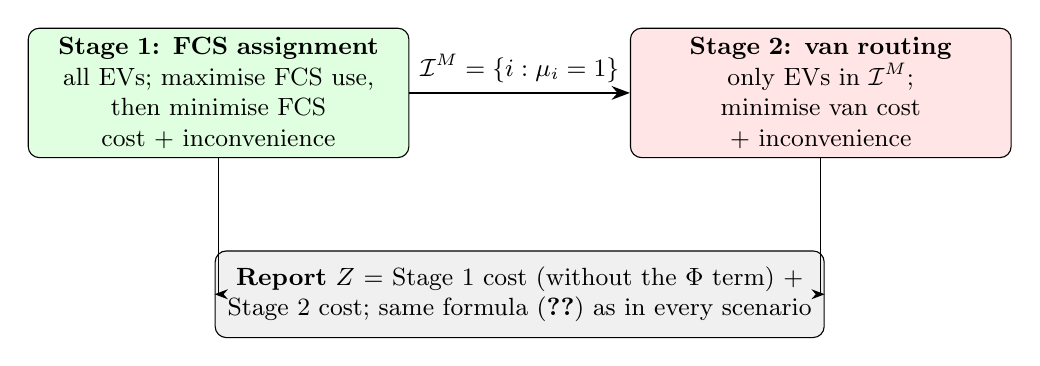
\begin{tikzpicture}[>=Stealth,box/.style={draw,rounded corners,align=center,minimum height=1.1cm,font=\small}]
  \node[box,fill=green!12,text width=4.6cm] (s1) {\textbf{Stage 1: FCS assignment}\\all EVs; maximise FCS use,\\then minimise FCS cost + inconvenience};
  \node[box,fill=red!10,text width=4.6cm,right=2.8cm of s1] (s2) {\textbf{Stage 2: van routing}\\only EVs in $\I^M$;\\minimise van cost + inconvenience};
  \draw[->,thick] (s1) -- node[above,font=\small]{$\I^M=\{i:\mu_i=1\}$} (s2);
  \node[box,fill=black!6,text width=7.5cm,below=2.0cm of $(s1)!0.5!(s2)$] (ev) {\textbf{Report} $Z=$ Stage~1 cost (without the $\Phi$ term) $+$ Stage~2 cost; same formula \eqref{eq:Z} as in every scenario};
  \draw[->] (s1) |- (ev); \draw[->] (s2) |- (ev);
\end{tikzpicture}
\end{center}

Stage~1 does not look at the vans, and Stage~2 cannot change what Stage~1 decided. That is the definition of ``FCS first, then MCS''.

%----------------------------------------------------------------
\subsection{Stage 1: assign EVs to fixed stations}

\textbf{Objective.}
\begin{equation}
\begin{split}
\min\ Z^{(1)}=\;&\underbrace{\Phi\sum_{i\in\I}\mu_i}_{\text{FCS first}}
+\underbrace{c^{EV}\sum_i\sum_{f\in\F_i}d_{if}Y_{if}}_{Z_1}
+\underbrace{Z^F_{\text{energy}}}_{\text{FCS part of }Z_4}\\
&+\underbrace{\sum_i\sum_{f\in\F_i}\rho^F_{if}Y_{if}+\alpha\sum_i w_i(C_i-r_i)+c^L\sum_i w_iL_i}_{\text{FCS customers' inconvenience}}
\end{split}
\label{eq:obj1}
\end{equation}
with $C_i=S_i+\tau^F_iY_i$ in this stage. $\Phi$ is a penalty for handing an EV to the vans. It is chosen larger than anything an extra FCS customer can add to the rest of \eqref{eq:obj1}, e.g.
\[
\Phi > \max_{i}\max_{f\in\F_i}\big(c^{EV}d_{if}+\pi^{\max}E_i+\rho^F_{if}\big)+n\,(\alpha+c^L)\,w_{\max}\,T,
\]
so Stage~1 first \textbf{maximises the number of EVs served at an FCS}, and only among those solutions minimises FCS cost and inconvenience. ($\pi^{\max}$ is the highest grid price.) A numerically safer equivalent is to solve twice: first $\max\sum_iY_i$, then fix that number and minimise the rest.
\ifTOU
Because $Z^F_{\text{energy}}$ uses the peak price, Stage~1 may \emph{start sessions later} to leave the peak, if the price saving beats the extra waiting cost (Section~\ref{sec:expect}).
\fi

\textbf{Constraints.}
\begin{align}
\sum_{g\in\G_i}y_{ig}+\mu_i &= 1 && \forall i\in\I \label{eq:s1assign}\\
S_i &\ge r_i+\sum_{f\in\F_i}t_{if}Y_{if} && \forall i\in\I \label{eq:fcsarr}\\
S_i &\le r_i+T\,(1-\mu_i) && \forall i\in\I \label{eq:s1park}\\
S_j &\ge S_i+\tau^F_i-(T+\tau^F_i)(3-y_{ig}-y_{jg}-o_{ij}) && \forall g,\ (i,j)\in\mathcal{P}_g \label{eq:disj1}\\
S_i &\ge S_j+\tau^F_j-(T+\tau^F_j)(2-y_{ig}-y_{jg}+o_{ij}) && \forall g,\ (i,j)\in\mathcal{P}_g \label{eq:disj2}\\
\sum_i y_{ig_1} &\ge \sum_i y_{ig_2} && \forall f,\ \G_f=\{g_1,g_2\} \label{eq:gunsym}\\
S_i+\tau^F_iY_i &\le T,\qquad L_i\ge S_i+\tau^F_iY_i-l_i && \forall i\in\I \label{eq:s1time}
\end{align}
\ifTOU plus the time-of-use split \eqref{eq:tou1}--\eqref{eq:tou5} of each FCS session (Section~\ref{sec:price}).\fi
\desc{\eqref{eq:s1assign}: every EV either gets one reachable gun or is handed to the vans. An EV that reaches no FCS ($\G_i=\emptyset$) is forced to $\mu_i=1$. \eqref{eq:fcsarr}: an FCS session cannot start before the EV has asked and driven to the station. \eqref{eq:s1park}: for an EV handed to the vans, $S_i$ is parked at $r_i$, so it adds no waiting in Stage~1 (its real start time is decided in Stage~2). \eqref{eq:disj1}--\eqref{eq:disj2}: two EVs on the same gun do not overlap; $o_{ij}$ picks who goes first. With two guns per station this means at most two EVs charge at a station at a time. \eqref{eq:gunsym}: symmetry breaking between the two identical guns (optional). \eqref{eq:s1time}: finished by $T$; lateness.}

\textbf{Optional acceptability rule.} An operator may refuse to send a driver to a station that is ``too inconvenient'', e.g.\ only allow gun $g$ of station $f$ for EV $i$ if $\hat\rho^F_{if}\le\bar\rho$. This only shrinks $\G_i$, so EVs whose stations are all too far go to the vans. Report results with and without it.

\textbf{Output:} $\I^M=\{i:\mu_i=1\}$, the EVs left for the vans; plus each FCS customer's gun and start time.

%----------------------------------------------------------------
\subsection{Stage 2: route the vans to the leftover EVs}

Stage~2 is a vehicle routing problem with time windows, on the EVs in $\I^M$ only. Here $C_i=S_i+\tau^M_i$.

\textbf{Objective.}
\begin{equation}
\begin{split}
\min\ Z^{(2)}=\;&\underbrace{c^M\sum_m\sum_{(i,j)\in\A^M}d_{ij}x_{ijm}}_{Z_2}+\underbrace{\sum_m c^D_mu_m}_{Z_3}+\underbrace{Z^M_{\text{energy}}}_{\text{van part of }Z_4}\\
&+\underbrace{\sum_{i\in\I^M}\sum_m\rho^M_{im}z_{im}+\alpha\sum_{i\in\I^M}w_i(C_i-r_i)+c^L\sum_{i\in\I^M}w_iL_i}_{\text{van customers' inconvenience}}
\end{split}
\label{eq:obj2}
\end{equation}
Since every EV in $\I^M$ must be served by some van, $Z^M_{\text{energy}}$ and the $\rho^M$ term are constants here. They are kept so that $Z^{(2)}$ is the true cost of Stage~2. Waiting and lateness make the vans visit urgent EVs early.

\textbf{Constraints.}
\begin{align}
\sum_{m\in\M}z_{im} &= 1 && \forall i\in\I^M \label{eq:s2assign}\\
\sum_{j:(0,j)\in\A^M}x_{0jm} = \sum_{i:(i,n+1)\in\A^M}x_{i,n+1,m} &= u_m && \forall m \label{eq:depot}\\
\sum_{i:(i,j)\in\A^M}x_{ijm} = \sum_{k:(j,k)\in\A^M}x_{jkm} &= z_{jm} && \forall j\in\I^M,\ m \label{eq:flow}\\
\sum_{i\in\I^M}z_{im} &\le Q_m\,u_m && \forall m \label{eq:cap}\\
\sum_{i\in\I^M}\frac{E_i}{\eta}z_{im}+\beta\sum_{(i,j)\in\A^M}d_{ij}x_{ijm} &\le B_m\,u_m && \forall m \label{eq:batt}
\end{align}
\begin{align}
S_j &\ge \max\{r_j,\ t_{0j}\,x_{0jm}\} && \forall j\in\I^M,\ m \label{eq:depart}\\
S_j &\ge S_i+\tau^M_i+t_{ij}-(T+\tau^M_i+t_{ij})(1-x_{ijm}) && \forall i\neq j,\ m \label{eq:seq}\\
S_i+\tau^M_i+t_{i,n+1} &\le T+(\tau^M_i+t_{i,n+1})(1-x_{i,n+1,m}) && \forall i,\ m \label{eq:return}\\
S_i+\tau^M_i \le T,\quad L_i &\ge S_i+\tau^M_i-l_i && \forall i\in\I^M \label{eq:s2time}\\
u_m &\ge u_{m+1} && m<|\M| \label{eq:vansym}
\end{align}
\desc{\eqref{eq:s2assign}: each leftover EV gets one van. \eqref{eq:depot}: a used van leaves and returns to the depot once. \eqref{eq:flow}: each EV on van $m$ is entered and left exactly once by that van. \eqref{eq:cap}: at most $Q_m$ EVs per van. \eqref{eq:batt}: delivered energy (with transfer losses) plus driving energy fits in the van battery. \eqref{eq:depart}: no start before the request, or before the van can drive there from the depot (written as two linear constraints). \eqref{eq:seq}: if the van goes $i\to j$, it finishes $i$ and drives to $j$ before starting $j$. This gives one EV at a time and removes subtours (MTZ-type). \eqref{eq:return}: back at the depot by $T$. \eqref{eq:s2time}: finished by $T$; lateness. \eqref{eq:vansym}: use identical vans in index order.}

\textbf{If Stage 2 is infeasible} (too many leftover EVs for the fleet by $T$), the sequential policy has \emph{failed} on that instance. For diagnosis, add $s_i\in\{0,1\}$ (``unserved''), replace \eqref{eq:s2assign} by $\sum_mz_{im}+s_i=1$ and add $\Phi^U\sum_is_i$ to \eqref{eq:obj2}. Then report the number of EVs that could not be served. This is a useful comparison with the integrated scenario, which may serve all of them.

%----------------------------------------------------------------
\subsection{Reported value}
\[
Z^{\text{S\scen}}=\big(Z^{(1)*}-\Phi\,|\I^M|\big)+Z^{(2)*},
\]
which is exactly \eqref{eq:Z} evaluated at the combined solution. The stage-1 solution plus the stage-2 solution is a feasible solution of the integrated model (S\ifTOU 4\else 3\fi), so
$Z^{\text{S\ifTOU 4\else 3\fi}}\le Z^{\text{S\scen}}$. The difference is the \emph{value of integration}.

\else
%---------------------------------------------------------------- INT
\subsection{Objective}
\begin{equation}
\min\ Z \quad\text{as in \eqref{eq:Z}, with }Z^F_{\text{energy}}=\ifTOU P^F\textstyle\sum_i\big[\pi^\off(\theta^1_i+\theta^3_i)+\pi^\pk\theta^2_i\big]\else\pi^F\textstyle\sum_iE_iY_i\fi,\quad C_i=S_i+\tau^F_iY_i+\tau^M_iZ_i. \label{eq:objint}
\end{equation}
Written out in full:
\begin{align*}
\min\ Z=\;& c^{EV}\sum_i\sum_{f\in\F_i}d_{if}Y_{if}+c^M\sum_m\sum_{(i,j)\in\A}d_{ij}x_{ijm}+\sum_mc^D_mu_m\\
&+\ifTOU P^F\sum_i\big[\pi^\off(\theta^1_i+\theta^3_i)+\pi^\pk\theta^2_i\big]\else\pi^F\sum_iE_iY_i\fi
+\pi^M\sum_i\sum_m\frac{E_i}{\eta}z_{im}\\
&+\sum_i\sum_{f\in\F_i}\rho^F_{if}Y_{if}+\sum_i\sum_m\rho^M_{im}z_{im}+\alpha\sum_iw_i(C_i-r_i)+c^L\sum_iw_iL_i .
\end{align*}
Every term is linear. One model weighs everything at once: an EV goes to a van exactly when the van's extra km, dispatch and energy cost are outweighed by the effort and waiting it saves the driver\ifTOU, or by the peak-price energy it avoids\fi.

\subsection{Constraints}

\textbf{Assignment.}
\begin{equation}
\sum_{g\in\G_i}y_{ig}+\sum_{m\in\M}z_{im}=1\qquad\forall i\in\I \label{eq:assign}
\end{equation}
\desc{Exactly one resource per EV: one reachable gun or one van. EVs that reach no FCS are forced onto a van.}

\textbf{Fixed stations.}
\begin{align}
S_i &\ge r_i+\sum_{f\in\F_i}t_{if}Y_{if} && \forall i \label{eq:fcsarr}\\
S_j &\ge S_i+\tau^F_i-(T+\tau^F_i)(3-y_{ig}-y_{jg}-o_{ij}) && \forall g,\ (i,j)\in\mathcal{P}_g \label{eq:disj1}\\
S_i &\ge S_j+\tau^F_j-(T+\tau^F_j)(2-y_{ig}-y_{jg}+o_{ij}) && \forall g,\ (i,j)\in\mathcal{P}_g \label{eq:disj2}\\
\sum_iy_{ig_1} &\ge \sum_iy_{ig_2} && \forall f,\ \G_f=\{g_1,g_2\} \label{eq:gunsym}
\end{align}
\desc{\eqref{eq:fcsarr}: an FCS session starts after the request and the drive to the station (for a van customer this is just $S_i\ge r_i$). \eqref{eq:disj1}--\eqref{eq:disj2}: EVs on the same gun do not overlap; $o_{ij}$ chooses the order. \eqref{eq:gunsym}: optional symmetry breaking.}

\textbf{Vans: routes, capacity, battery.}
\begin{align}
\sum_{j:(0,j)\in\A}x_{0jm}=\sum_{i:(i,n+1)\in\A}x_{i,n+1,m} &= u_m && \forall m \label{eq:depot}\\
\sum_{i:(i,j)\in\A}x_{ijm}=\sum_{k:(j,k)\in\A}x_{jkm} &= z_{jm} && \forall j\in\I,\ m \label{eq:flow}\\
\sum_iz_{im} &\le Q_mu_m && \forall m \label{eq:cap}\\
\sum_i\frac{E_i}{\eta}z_{im}+\beta\sum_{(i,j)\in\A}d_{ij}x_{ijm} &\le B_mu_m && \forall m \label{eq:batt}
\end{align}
\desc{\eqref{eq:depot}: a used van leaves and returns once. \eqref{eq:flow}: each EV on van $m$ is visited exactly once by it. \eqref{eq:cap}: at most $Q_m$ EVs. \eqref{eq:batt}: delivered energy (with losses) plus driving energy fits in the battery.}

\textbf{Vans: timing (one EV at a time, no subtours).}
\begin{align}
S_j &\ge t_{0j}\,x_{0jm} && \forall j\in\I,\ m \label{eq:depart}\\
S_j &\ge S_i+\tau^M_i+t_{ij}-(T+\tau^M_i+t_{ij})(1-x_{ijm}) && \forall i\neq j\in\I,\ m \label{eq:seq}\\
S_i+\tau^M_i+t_{i,n+1} &\le T+(\tau^M_i+t_{i,n+1})(1-x_{i,n+1,m}) && \forall i,\ m \label{eq:return}
\end{align}
\desc{\eqref{eq:depart}: the first stop cannot start before the van has driven there. \eqref{eq:seq}: $i\to j$ means finish $i$, drive, then start $j$; start times rise along a route, so no subtour can close. \eqref{eq:return}: back at the depot by $T$.}

\textbf{Horizon and lateness.}
\begin{equation}
C_i\le T,\qquad L_i\ge C_i-l_i\qquad\forall i\in\I \label{eq:time}
\end{equation}
\desc{Every EV is fully charged within the horizon; $L_i$ measures lateness.}

\ifTOU
\textbf{Time-of-use split.} Constraints \eqref{eq:tou1}--\eqref{eq:tou5} of Section~\ref{sec:price}.
\fi

\textbf{Symmetry and domains.}
\begin{equation}
u_m\ge u_{m+1};\qquad y,z,x,u,o\ifTOU,\kappa\fi\in\{0,1\};\qquad S_i,L_i\ifTOU,\theta^p_i\fi\ge0 \label{eq:dom}
\end{equation}
\fi

%=====================================================================
\section{Learning-to-optimise (RL) formulation}\label{sec:rl}

\textbf{Main rule:} the reward of each action is \emph{minus the increase in $Z$ that the action causes}. The rewards over an episode then add up to $-Z$ of the solution the policy builds. RL and MILP results are measured on the same yardstick \eqref{eq:Z}, and the MILP optimum is the benchmark for the RL gap.

\ifSEQ
%---------------------------------------------------------------- RL SEQ
The RL pipeline has the same two stages as the MILP.

\subsection{Stage 1 policy: FCS assignment}
\begin{itemize}[leftmargin=1.4em,itemsep=2pt]
  \item \textbf{Episode / epochs:} EVs are taken in order of request time $r_i$ (ties: higher $w_i$ first). One decision per EV.
  \item \textbf{State:} features of the current EV $k$ ($E_k,r_k,l_k,w_k,R_k$, location); for each gun $g$ the time $F_g$ it becomes free; summary features of the EVs still to come (count and positions near each station)\ifTOU; the current price and the time until $T_1$ and $T_2$\fi.
  \item \textbf{Action:} a gun $g\in\G_k$, or ``hand to vans''. \textbf{FCS-first mask:} ``hand to vans'' is allowed \emph{only} if no gun can finish EV $k$ by $T$ (or, with the optional rule, if all remaining guns have $\hat\rho^F_{kf}>\bar\rho$).
  \ifTOU\item \textbf{Optional timing action:} ``gun $g$, start after the peak'', i.e.\ $S_k=\max\{\text{earliest},T_2\}$, allowed only if the session still ends by $T$.\fi
  \item \textbf{Transition:} $S_k=\max\{r_k+t_{kf},F_g\}$ (or later, for the timing action); $F_g\leftarrow S_k+\tau^F_k$.
  \item \textbf{Reward:} $-\Big[c^{EV}d_{kf}+\text{energy}_k+\rho^F_{kf}+\alpha w_k(S_k+\tau^F_k-r_k)+c^Lw_k(S_k+\tau^F_k-l_k)^+\Big]$, where energy$_k$ = \ifTOU$P^F\big[\pi^\off\cdot(\text{off-peak hours of }[S_k,S_k+\tau^F_k])+\pi^\pk\cdot(\text{peak hours})\big]$, computed exactly in the simulator\else$\pi^FE_k$\fi. Handing an EV to the vans gives reward $0$ here; its cost is counted in Stage~2.
\end{itemize}
Note: a simple baseline for Stage~1 is the greedy rule ``gun with the largest one-step reward''. What RL can learn on top of this is, for example, to keep a nearby gun free for an urgent EV that arrives later.

\subsection{Stage 2 policy: van routing over $\I^M$}
\begin{itemize}[leftmargin=1.4em,itemsep=2pt]
  \item \textbf{Epochs:} whenever a van becomes free (the earliest-free van decides first).
  \item \textbf{State:} for each van: position, time free, remaining battery $b_m$, EVs served so far, dispatched or not; for each unserved EV in $\I^M$: location, $E_i,r_i,l_i,w_i$; current time.
  \item \textbf{Action:} the next EV $j$ for this van, or ``return to depot'' (ends the route). Mask: $j$ must be feasible: battery covers $E_j/\eta$ plus driving to $j$ and back to the depot, the count stays $\le Q_m$, and $j$ can be finished with the van back at the depot by $T$.
  \item \textbf{Transition:} $S_j=\max\{r_j,\ \text{time free}+t_{\text{pos},j}\}$; the van moves to $j$ and is free at $S_j+\tau^M_j$; $b_m$ falls by $E_j/\eta+\beta d_{\text{pos},j}$.
  \item \textbf{Reward:} serving $j$: $-\Big[c^Md_{\text{pos},j}+c^D_m[\text{first stop}]+\pi^M\frac{E_j}{\eta}+\rho^M_{jm}+\alpha w_j(S_j+\tau^M_j-r_j)+c^Lw_j(S_j+\tau^M_j-l_j)^+\Big]$; returning: $-c^Md_{\text{pos},0}$. EVs still unserved at the end: $-\Phi^U$ each.
  \item \textbf{Policy:} an attention-based routing policy (e.g.\ Kool et al., 2019, ``Attention, Learn to Solve Routing Problems!'') trained with REINFORCE or PPO. Baseline: nearest-feasible-EV heuristic.
\end{itemize}
Episode return of Stage~1 + Stage~2 $=-Z^{\text{S\scen}}$.

\else
%---------------------------------------------------------------- RL INT
One policy decides both who serves each EV and the van routes.
\begin{itemize}[leftmargin=1.4em,itemsep=2pt]
  \item \textbf{Episode / epochs:} EVs are taken in order of request time $r_i$ (ties: higher $w_i$ first). One decision per EV.
  \item \textbf{State:} (i) the current EV $k$: location, $E_k,r_k,l_k,w_k,R_k$, reachable stations; (ii) each gun $g$: time $F_g$ it becomes free; (iii) each van $m$: current end-of-route position, time free, remaining battery $b_m$, EVs served, dispatched or not; (iv) embeddings of the not-yet-assigned EVs (for look-ahead)\ifTOU; (v) current price, time until $T_1$ and $T_2$\fi.
  \item \textbf{Action:} $a\in\G_k\cup\M$: a gun, or a van (EV $k$ is appended to the end of that van's route). \textbf{Mask} infeasible actions: a gun that cannot finish $k$ by $T$; a van without enough battery for $E_k/\eta$ plus the drive to $k$ and back to the depot, with $Q_m$ reached, or unable to finish $k$ and return by $T$.
  \ifTOU\item \textbf{Optional timing action:} ``gun $g$, start after the peak'' ($S_k=\max\{\text{earliest},T_2\}$, if it still ends by $T$).\fi
  \item \textbf{Transition:} gun: $S_k=\max\{r_k+t_{kf},F_g\}$, $F_g\leftarrow S_k+\tau^F_k$. Van: $S_k=\max\{r_k,\ \text{free}_m+t_{\text{pos}_m,k}\}$, then the van moves to $k$, $\text{free}_m\leftarrow S_k+\tau^M_k$, $b_m\mathrel{-}=E_k/\eta+\beta d_{\text{pos}_m,k}$.
  \item \textbf{Reward} $=-\Delta Z$:
  \begin{align*}
  \text{gun } g\text{ at }f:&\quad -\Big[c^{EV}d_{kf}+\text{energy}^F_k+\rho^F_{kf}+\alpha w_k(C_k-r_k)+c^Lw_k(C_k-l_k)^+\Big]\\
  \text{van } m:&\quad -\Big[c^M\big(d_{\text{pos}_m,k}+d_{k,0}-d_{\text{pos}_m,0}\big)+c^D_m[\text{first use}]+\pi^M\tfrac{E_k}{\eta}\\
  &\qquad\quad+\rho^M_{km}+\alpha w_k(C_k-r_k)+c^Lw_k(C_k-l_k)^+\Big]
  \end{align*}
  The van distance term is the \emph{change} in route length when $k$ is inserted before the return to the depot, so the sum over the episode equals the total route length (the return legs telescope). energy$^F_k$ = \ifTOU$P^F\big[\pi^\off\cdot(\text{off-peak hours})+\pi^\pk\cdot(\text{peak hours of }[S_k,C_k])\big]$, computed exactly by the simulator; no linearisation is needed in RL\else$\pi^FE_k$\fi.
  \item \textbf{Dead end:} if every action is masked, EV $k$ is unserved: reward $-\Phi^U$, and the episode continues. Report the count.
  \item \textbf{Policy:} masked categorical policy over guns and vans, encoder with attention over EVs, guns and vans; trained with PPO. Natural baseline: greedy, i.e.\ choose the action with the largest one-step reward. That is the pairwise rule ``smallest $\hat\rho$ + cost'' from Section~\ref{sec:inc}.
\end{itemize}
Restriction to note: vans serve EVs in assignment order (append only). A variant that inserts $k$ at the cheapest position of a route is more flexible but has a larger action space.
\fi

\textbf{Reward scaling.} For stable training divide every reward by a constant, e.g.\ the greedy baseline's average $Z$ on the training instances. This does not change the optimal policy.

%=====================================================================
\section{What to expect and what to report}\label{sec:expect}

\ifnum\scen=1
\begin{itemize}[leftmargin=1.4em,itemsep=2pt]
  \item Vans serve only EVs that reach no station, or that the stations cannot finish by $T$. If stations have spare capacity, very few vans are dispatched.
  \item Inconvenience is high for EVs far from the nearest station (worked example: Rs\,682 at the FCS, against Rs\,458 if a van had been allowed).
  \item With too few vans Stage~2 becomes infeasible (unserved EVs), even when the integrated model S3 could serve everyone. Report the smallest $|\M|$ at which S1 is feasible and compare it with S3.
\end{itemize}
\fi
\ifnum\scen=2
\begin{itemize}[leftmargin=1.4em,itemsep=2pt]
  \item \textbf{When does Stage~1 delay a session to avoid the peak?} Moving one hour of charging out of the peak saves $(\pi^\pk-\pi^\off)P^F=3\times22=$ Rs\,66, but delays completion by up to an hour, which costs $\alpha w_i\ge$ Rs\,200. So with the default values Stage~1 almost never delays. It mostly pays the higher price, and S2 costs roughly S1 plus the peak surcharge. Sessions start later only if $\alpha$ is small (try $\lambda<0.33$ in the sensitivity analysis).
  \item The van assignment is the same as in S1 unless Stage~1's timing changes which EVs fit at the stations. Stage~1 cannot use vans to escape the peak price.
  \item Extra KPI: \textbf{grid energy drawn at FCS during the peak}, $P^F\sum_i\theta^2_i$ (kWh). Compare with S4.
\end{itemize}
\fi
\ifnum\scen=3
\begin{itemize}[leftmargin=1.4em,itemsep=2pt]
  \item Vans take EVs for which the saved inconvenience exceeds the extra van cost (worked example: van chosen, saving Rs\,224). Expect vans to serve EVs that are far from every station, have low range (high $w_i$), or have early deadlines, while EVs near a station still use it.
  \item \textbf{Value of integration under flat price:} $Z^{\text{S1}}-Z^{\text{S3}}\ge0$. Report it per component ($Z_1,\dots,Z_5$): typically operating cost rises a little and inconvenience falls a lot.
  \item Vary $|\M|$ (0, 1, 2, \dots): the first few vans lower $Z$ sharply, then the effect levels off. That curve shows the scenarios where mobile chargers help most.
\end{itemize}
\fi
\ifnum\scen=4
\begin{itemize}[leftmargin=1.4em,itemsep=2pt]
  \item During the peak a van kWh costs about the same as an FCS kWh (Rs\,10.0 each), so the vans' energy disadvantage disappears and vans also absorb \emph{peak-hour} demand that would otherwise be charged on the grid at peak price.
  \item Expect more van usage than in S3, concentrated on requests in $[T_1,T_2]$, and lower grid energy at the stations during the peak, $P^F\sum_i\theta^2_i$, than in S2.
  \item \textbf{Value of integration under peak pricing:} $Z^{\text{S2}}-Z^{\text{S4}}$. It should be larger than $Z^{\text{S1}}-Z^{\text{S3}}$, because integration now also allows price arbitrage.
  \item \textbf{Peak pricing with full flexibility:} $Z^{\text{S4}}-Z^{\text{S3}}$ should be smaller than $Z^{\text{S2}}-Z^{\text{S1}}$: vans cushion the price increase.
\end{itemize}
\fi

\textbf{Cross-scenario comparison table} (fill in from the four runs):
\begin{center}
\renewcommand{\arraystretch}{1.2}
\begin{tabular}{@{}lll@{}}
\toprule
\textbf{Comparison} & \textbf{Measures} & \textbf{Expected sign} \\
\midrule
S1 $-$ S3 & value of integration, flat price & $\ge0$ \\
S2 $-$ S4 & value of integration, peak price & $\ge0$, larger than S1 $-$ S3 \\
S2 $-$ S1 & cost of peak pricing, FCS-first operator & $>0$ \\
S4 $-$ S3 & cost of peak pricing, flexible operator & $>0$, smaller than S2 $-$ S1 \\
\bottomrule
\end{tabular}
\end{center}
Report for each: $Z$ and its components, number of vans used, EVs per resource, mean and maximum inconvenience per EV, total lateness, peak-hour grid energy, solve time, and (for RL) the gap to the MILP optimum.

%=====================================================================
\appendix
\section{Illustrative parameter values}\label{app:values}

These are starting values for experiments, not data. All are meant to be varied in the analysis. Values in Rs.

\begin{center}
\renewcommand{\arraystretch}{1.15}
\begin{tabular}{@{}llp{6.2cm}@{}}
\toprule
\textbf{Parameter} & \textbf{Value} & \textbf{Note} \\
\midrule
$T$, $[T_1,T_2]$ & 7 h, $[2,6]$ & 16:00--23:00, peak 18:00--22:00 \\
$P^F$, $P^M$ & 22 kW, 30 kW & \\
$v$, $\beta$, $\eta$ & 25 km/h, 0.25 kWh/km, 0.9 & \\
$B_m$, $Q_m$, $|\M|$ & 150 kWh, 6, 2--6 & \\
$c^{EV}$, $c^M$, $c^D_m$ & Rs\,4/km, Rs\,15/km, Rs\,1500 & van km includes driver time \\
$\pi^F$ (flat) & Rs\,8.7/kWh & equals the time-average of the ToU tariff over $[0,T]$ \\
$\pi^\off$, $\pi^\pk$ (ToU) & Rs\,7/kWh, Rs\,10/kWh & $(3\times7+4\times10)/7=8.7$ \\
$c^{bat}$ & Rs\,2/kWh & van battery wear \\
$\pi^M$ & Rs\,10.7 (flat) / Rs\,9.0 (ToU) & $=\pi^F+c^{bat}$ / $=\pi^\off+c^{bat}$ \\
$\alpha$, $\alpha^D$ & Rs\,200/h, Rs\,100/h & value of time; extra for attended time \\
$h^F$, $h^M$, $\varphi$ & Rs\,50, Rs\,10, Rs\,100 & trip hassle, hand-over, range stress \\
$c^L$ & Rs\,300/h & lateness \\
$w_i$ & $1+2(1-R_i/R_{\max})$, $R_i\sim U[3,40]$ km & priority from remaining range \\
\bottomrule
\end{tabular}
\end{center}

The flat price is set to the time-average of the peak tariff. The price \emph{level} is then the same in both pricing cases, and only the price \emph{shape} differs. Without this, part of S1 vs S2 would just reflect a different average price.

\end{document}
"
%    pdflatex -jobname=scenario4_peak_integrated   "\def\scen{4}% =====================================================================
%  One source, four PDFs.  Build with build.sh (or by hand):
%    pdflatex -jobname=scenario1_flat_sequential   "\def\scen{1}\input{scenario_master}"
%    pdflatex -jobname=scenario2_peak_sequential   "\def\scen{2}\input{scenario_master}"
%    pdflatex -jobname=scenario3_flat_integrated   "\def\scen{3}\input{scenario_master}"
%    pdflatex -jobname=scenario4_peak_integrated   "\def\scen{4}\input{scenario_master}"
%  (run each twice for cross-references)
% =====================================================================
\documentclass[11pt,a4paper]{article}
\usepackage[margin=2.2cm]{geometry}
\usepackage{amsmath,amssymb,amsfonts}
\usepackage{booktabs,array,tabularx}
\usepackage{enumitem}
\usepackage[table]{xcolor}
\usepackage{tikz}
\usetikzlibrary{arrows.meta,positioning,calc}
\usepackage[colorlinks=true,linkcolor=blue!50!black,urlcolor=blue!50!black]{hyperref}
\usepackage{titlesec}
\titleformat{\section}{\large\bfseries}{\thesection}{0.8em}{}
\titleformat{\subsection}{\normalsize\bfseries}{\thesubsection}{0.8em}{}
\setlength{\parindent}{0pt}
\setlength{\parskip}{5pt}

% ---------------- scenario switches ----------------
\ifdefined\scen\else\def\scen{1}\fi
\newif\ifTOU \TOUfalse   % true = time-of-use (peak) price
\newif\ifSEQ \SEQfalse   % true = FCS first, then MCS
\ifnum\scen=1 \SEQtrue \fi
\ifnum\scen=2 \TOUtrue \SEQtrue \fi
\ifnum\scen=4 \TOUtrue \fi

\newcommand{\pricename}{\ifTOU time-of-use price (dearer evening peak)\else single (flat) price all day\fi}
\newcommand{\structname}{\ifSEQ FCS first, then MCS (sequential)\else FCS and MCS together (integrated)\fi}

% ---------------- notation ----------------
\newcommand{\I}{\mathcal{I}}
\newcommand{\F}{\mathcal{F}}
\newcommand{\G}{\mathcal{G}}
\newcommand{\M}{\mathcal{M}}
\newcommand{\N}{\mathcal{N}}
\newcommand{\A}{\mathcal{A}}
\newcommand{\Rs}{\text{Rs}\,}
\newcommand{\pk}{\mathrm{pk}}
\newcommand{\off}{\mathrm{off}}
\newcommand{\desc}[1]{\par\vspace{-2pt}{\small\color{black!75}\textit{Meaning:} #1}\par\vspace{4pt}}
\newcommand{\cell}[2]{\ifnum\scen=#1\cellcolor{blue!18}\textbf{S#1 (this document)}\\\textbf{#2}\else S#1\\#2\fi}

\title{\textbf{EV Charging Network Optimisation}\\[4pt]
\large Scenario \scen: \pricename\ $+$ \structname\\[2pt]
\normalsize MILP and RL formulation}
\author{CP 320 OR for Mobility Management, course project}
\date{2 October 2026}

\begin{document}
\maketitle

%=====================================================================
\section{Where this scenario sits}

The project studies four scenarios: two ways of pricing grid electricity, times two ways of making the decisions.

\begin{center}
\renewcommand{\arraystretch}{1.5}
\begin{tabular}{>{\raggedright\arraybackslash}p{4.2cm}|>{\centering\arraybackslash}p{4.6cm}|>{\centering\arraybackslash}p{4.6cm}}
 & \textbf{Flat price all day} & \textbf{Time-of-use (peak) price} \\ \hline
\textbf{Sequential:} FCS first, leftover EVs to MCS &
\begin{tabular}[c]{@{}c@{}}\cell{1}{flat + sequential}\end{tabular} &
\begin{tabular}[c]{@{}c@{}}\cell{2}{peak + sequential}\end{tabular} \\ \hline
\textbf{Integrated:} FCS and MCS decided together &
\begin{tabular}[c]{@{}c@{}}\cell{3}{flat + integrated}\end{tabular} &
\begin{tabular}[c]{@{}c@{}}\cell{4}{peak + integrated}\end{tabular} \\
\end{tabular}
\end{center}

\textbf{The four scenarios do not have four different objectives.} They share \emph{one} cost yardstick $Z$ (Section~\ref{sec:obj}): the same cost terms and the same customer inconvenience (Section~\ref{sec:inc}). Only two things change:
\begin{itemize}[leftmargin=1.4em,itemsep=1pt]
  \item \textbf{Pricing} changes the formula for one term, the FCS energy cost (Section~\ref{sec:price}).
  \item \textbf{Decision structure} changes \emph{how} $Z$ is minimised: in one model (integrated), or in two stages (sequential), where each stage minimises its own part of $Z$.
\end{itemize}
Because the yardstick is the same, the four optimal values can be compared directly. The differences measure the \emph{value of integration} (S1$\to$S3, S2$\to$S4) and the \emph{effect of peak pricing} (S1$\to$S2, S3$\to$S4).

\ifnum\scen=1
\textbf{This scenario (S1)} is the baseline, the ``status quo''. Electricity costs the same at every hour, every EV that can be charged at a fixed station is sent there, and vans only take what is left over.
\fi
\ifnum\scen=2
\textbf{This scenario (S2)} keeps the FCS-first rule of S1, but grid electricity is dearer during the evening peak. Stage~1 can react to the price only by \emph{rescheduling} FCS sessions. It cannot hand a peak-hour EV to a van.
\fi
\ifnum\scen=3
\textbf{This scenario (S3)} keeps the flat price of S1, but the operator decides FCS and MCS service \emph{together}. An EV can be sent to a van even when a fixed station could take it, whenever that lowers total cost plus inconvenience.
\fi
\ifnum\scen=4
\textbf{This scenario (S4)} is the most flexible one: peak pricing at fixed stations, and FCS and MCS decided together. Van energy was bought off-peak, so vans can also be used to keep charging \emph{out of the expensive peak}.
\fi

%=====================================================================
\section{Setting and assumptions}\label{sec:setting}

\textbf{Time.} The planning horizon is $[0,T]$ with $T=7$\,h (16:00--23:00). It contains the evening peak window $[T_1,T_2]=[2,6]$ (18:00--22:00). The horizon is the same in all four scenarios. It is wider than the peak itself so that, under peak pricing, there is cheaper time on both sides of the peak.\ifTOU\else\ In this scenario the price is flat, so the window plays no role in the model.\fi

\textbf{Assumptions} (the same as MILP v3, plus two about energy):
\begin{enumerate}[leftmargin=1.6em,itemsep=1pt]
  \item Static, continuous time. All requests in the horizon are known at time $0$, and request $i$ becomes active at $r_i$.
  \item An EV served by an FCS drives there itself on its own battery (only to stations within its range $R_i$). The driver stays with the car while it waits for a free gun and while it charges.
  \item An EV served by an MCS stays parked where it is, and the driver is free in the meantime.
  \item Each FCS gun and each van charges one EV at a time, without interruption, at constant power.
  \item A van's battery covers both its driving and the energy it delivers. \textbf{The van battery is charged at the depot before the horizon starts}\ifTOU, i.e.\ at the off-peak price\fi, and is not recharged during the horizon.
  \item Every EV must be fully charged by $T$ (hard). Finishing after the driver's desired time $l_i$ is allowed but penalised.
\end{enumerate}

%=====================================================================
\section{Notation}\label{sec:notation}

\subsection*{Sets}
\begin{tabularx}{\textwidth}{@{}lX@{}}
\toprule
$\I=\{1,\dots,n\}$ & EV charging requests \\
$\F$; $\G_f$ ($|\G_f|=2$); $\G=\bigcup_f\G_f$ & fixed charging stations; guns of FCS $f$; all guns ($f(g)$ = station of gun $g$) \\
$\F_i=\{f: d_{if}\le R_i\}$, $\G_i=\bigcup_{f\in\F_i}\G_f$ & stations / guns EV $i$ can reach on its remaining range \\
$\M$ & mobile charging vans (MCS) \\
$0,\ n+1$ & depot as start node / end node (same place) \\
$\N=\{0\}\cup\I\cup\{n+1\}$, $\A$ & routing nodes; allowed van arcs $(i,j)$, $i\in\{0\}\cup\I$, $j\in\I\cup\{n+1\}$, $i\neq j$ \\
$\mathcal{P}_g=\{(i,j): i<j,\ g\in\G_i\cap\G_j\}$ & pairs of EVs that could share gun $g$ \\
\ifSEQ
$\I^M\subseteq\I$ & EVs handed to the vans by Stage~1 (an \emph{output} of Stage~1, a fixed input to Stage~2) \\
$\N^M$, $\A^M$ & routing nodes / arcs restricted to $\I^M$ \\
\fi
\bottomrule
\end{tabularx}

\subsection*{Parameters}
\begin{tabularx}{\textwidth}{@{}lX@{}}
\toprule
$E_i,\ r_i,\ l_i,\ R_i$ & energy demand (kWh), request time, desired completion time (h), remaining range (km) \\
$w_i\ge1$ & priority of EV $i$; $w_i=1+\kappa(1-R_i/R_{\max})$, so low-range EVs weigh more \\
$P^F,\ P^M$ & charging power of an FCS gun (22\,kW) / of a van (e.g.\ 30\,kW) \\
$\tau^F_i=E_i/P^F,\ \tau^M_i=E_i/P^M$ & charging time of EV $i$ at an FCS / by a van (h) \\
$d_{if},t_{if}$;\ $d_{ij},t_{ij}$ & distance (km) and time (h): EV$\to$FCS; between routing nodes ($t=d/v$) \\
$B_m,\ Q_m,\ \beta,\ \eta$ & van battery (kWh), max EVs per van, van consumption (kWh/km), transfer efficiency \\
$c^{EV},\ c^M,\ c^D_m$ & cost per km of EV driving, per km of van driving; fixed dispatch cost of van $m$ \\
\ifTOU
$\pi^\off,\ \pi^\pk$ & grid price (Rs/kWh) off-peak / in $[T_1,T_2]$, with $\pi^\pk\ge\pi^\off$ \\
\else
$\pi^F$ & grid price (Rs/kWh), the same at every hour \\
\fi
$c^{bat}$ & van battery wear per kWh cycled \\
$\pi^M$ & cost of 1 kWh taken from a van battery: $\pi^M=\ifTOU\pi^\off\else\pi^F\fi+c^{bat}$ (Section~\ref{sec:price}) \\
$\alpha,\ \alpha^D,\ h^F,\ h^M,\ \varphi,\ c^L$ & inconvenience coefficients (Section~\ref{sec:inc}) \\
\bottomrule
\end{tabularx}

\subsection*{Decision variables}
\begin{tabularx}{\textwidth}{@{}llX@{}}
\toprule
$y_{ig}$ & $\{0,1\}$ & EV $i$ charged at gun $g\in\G_i$ \\
$z_{im}$ & $\{0,1\}$ & EV $i$ served by van $m$ \\
$x_{ijm}$ & $\{0,1\}$ & van $m$ drives arc $(i,j)$ \\
$u_m$ & $\{0,1\}$ & van $m$ is dispatched \\
$o_{ij}$ & $\{0,1\}$ & for EVs $i<j$ that could share a gun: 1 if $i$ is charged before $j$ \\
\ifSEQ
$\mu_i$ & $\{0,1\}$ & Stage~1 only: EV $i$ is handed to the van fleet \\
\fi
\ifTOU
$\theta^1_i,\theta^2_i,\theta^3_i$ & $\ge0$ & hours of EV $i$'s FCS session before / inside / after the peak \\
$\kappa^1_i,\kappa^3_i$ & $\{0,1\}$ & EV $i$'s FCS session starts before $T_1$ / ends after $T_2$ \\
\fi
$S_i$ & $\ge0$ & time charging of EV $i$ starts (h), on whichever resource \\
$L_i$ & $\ge0$ & lateness of EV $i$ beyond $l_i$ (h) \\
\bottomrule
\end{tabularx}

\textbf{Short-hands} (linear expressions, not new variables):
\[
Y_{if}=\sum_{g\in\G_f}y_{ig},\qquad Y_i=\sum_{g\in\G_i}y_{ig}\ (\text{EV $i$ uses an FCS}),\qquad Z_i=\sum_{m\in\M}z_{im}\ (\text{EV $i$ uses a van}),
\]
\[
C_i=S_i+\tau^F_i\,Y_i+\tau^M_i\,Z_i \quad\text{(time EV $i$ is fully charged).}
\]

%=====================================================================
\section{Customer inconvenience}\label{sec:inc}

This section is \textbf{identical in all four scenario documents}. Inconvenience is a property of the customer, not of the price or of the planning method.

\subsection{What we mean by inconvenience}

Inconvenience is \emph{what the driver loses} from the moment they ask for a charge ($r_i$) until the car is fully charged ($C_i$), \emph{converted into rupees} so it can be added to the operator's costs. A driver loses three different things:

\begin{enumerate}[leftmargin=1.6em,itemsep=2pt]
  \item \textbf{Waiting:} the car is not ready. This lasts $C_i-r_i$ hours and affects \emph{every} driver, FCS or MCS.
  \item \textbf{Effort:} only an FCS customer has to drive to the station and sit there while the car charges. An MCS customer stays at home or at work and does something else. Driving to a far station also uses scarce battery range, which causes stress (``range anxiety'').
  \item \textbf{A missed deadline:} the car is still not ready at the time $l_i$ the driver needs it.
\end{enumerate}

Each loss gets a price in Rs per hour (or per event). All of them are multiplied by the priority $w_i$: an hour of delay for an EV with 5\,km of range left counts more than for one with 40\,km.

\subsection{The three components}

\begin{center}
\renewcommand{\arraystretch}{1.3}
\begin{tabularx}{\textwidth}{@{}>{\raggedright\arraybackslash}p{2.6cm}>{\raggedright\arraybackslash}X>{\raggedright\arraybackslash}X>{\raggedright\arraybackslash}p{3.0cm}@{}}
\toprule
\textbf{Component} & \textbf{EV $i$ at FCS $f$} & \textbf{EV $i$ by a van} & \textbf{Known when?} \\
\midrule
Effort & $w_i\big[\alpha^D(t_{if}+\tau^F_i)+h^F+\varphi\,d_{if}/R_i\big]$: driving and sitting at the station, a fixed trip hassle, range stress & $w_i\,h^M$: being reachable and handing over the car & \textbf{Static:} known as soon as the resource is chosen \\
Waiting & $w_i\,\alpha\,(C_i-r_i)$ = drive + \emph{queue at the gun} + charge & $w_i\,\alpha\,(C_i-r_i)$ = \emph{wait for the van} + charge & \textbf{Dynamic:} depends on the queue / van route \\
Missed deadline & $w_i\,c^L\,L_i$, $L_i=\max\{0,C_i-l_i\}$ & same & Dynamic \\
\bottomrule
\end{tabularx}
\end{center}

\textbf{Coefficients.}
$\alpha$ (Rs/h) is the value of an hour the car is not ready.
$\alpha^D$ (Rs/h) is the \emph{extra} value of an hour the driver must personally spend driving or sitting at the station: an hour at the station costs $\alpha+\alpha^D$, an hour waiting at home for a van costs only $\alpha$.
$h^F,h^M$ (Rs) are fixed hassle costs of one trip to a station / one van hand-over.
$\varphi$ (Rs) is the range-stress cost of a trip that uses the \emph{whole} remaining range ($d_{if}/R_i\le1$ is the fraction used).
$c^L$ (Rs/h) is the cost per hour late.

\subsection{Pairwise form: inconvenience of a (customer, resource) pair}

The natural first idea is: \emph{for every pair (EV $i$, FCS $f$) and every pair (EV $i$, van $m$) there is an inconvenience number, and the operator picks the pair with the lowest cost plus inconvenience.} The static part fits this idea exactly:
\[
\boxed{\;\rho^F_{if}=w_i\Big[\alpha^D\,(t_{if}+\tau^F_i)+h^F+\varphi\,\frac{d_{if}}{R_i}\Big]\qquad
\rho^M_{im}=w_i\,h^M\;}
\]
These are \textbf{parameters}, computed before solving, one number per (EV, FCS) pair and per (EV, van) pair. In the objective they appear linearly: $\sum_i\sum_f\rho^F_{if}Y_{if}+\sum_i\sum_m\rho^M_{im}z_{im}$.

Note that $\rho^M_{im}$ does not depend on $m$. Vans are identical and all start at the same depot, so the driver does not care \emph{which} van comes, only \emph{when} it comes. That ``when'' is the waiting part.

\subsection{Why waiting cannot be a fixed pairwise number}

It is tempting to also write the waiting as a pairwise number, e.g.\ ``the van needs 5 minutes to reach EV $i$''. But that depends on \emph{where the van is coming from}, which depends on the route the model is still choosing: if EV $i$ is the 4th stop of a van, the wait is the time for three charging sessions plus four drives. Likewise, waiting at an FCS depends on how many EVs are queued at that gun. So waiting is not known before solving. It is a function of decision variables:
\[
\text{waiting cost of EV } i \;=\; w_i\,\alpha\,(C_i-r_i),\qquad C_i=S_i+\tau^F_iY_i+\tau^M_iZ_i .
\]
This is \textbf{linear} in the variables ($S_i$, $y$, $z$), so it fits in a MILP directly. The constraints of Section~\ref{sec:milp} make $S_i$ equal to the true start time, including driving, queueing at the gun and the van's route. The term $\sum_i w_i\alpha r_i$ is a constant and may be dropped when solving.

\textbf{Pairwise \emph{estimate}} (used for intuition, by the RL policy and in heuristics): if there is no queue and the van comes straight to $i$,
\[
\hat\rho^{F}_{if}=\rho^F_{if}+w_i\alpha\,(t_{if}+\tau^F_i),\qquad
\hat\rho^{M}_{im}=\rho^M_{im}+w_i\alpha\,(t^{\text{van}}_{m\to i}+\tau^M_i),
\]
where $t^{\text{van}}_{m\to i}$ is the time until van $m$ can reach $i$ from where it currently is. In the RL formulation (Section~\ref{sec:rl}) the van's position \emph{is} known at each decision, so there this estimate becomes exact.

\subsection{Total inconvenience and how it enters the objective}

\begin{equation}
\boxed{\;
Z_{\text{inc}}=\underbrace{\sum_{i\in\I}\sum_{f\in\F_i}\rho^F_{if}Y_{if}+\sum_{i\in\I}\sum_{m\in\M}\rho^M_{im}z_{im}}_{\text{effort (static, pairwise)}}
+\underbrace{\alpha\sum_{i\in\I}w_i\,(C_i-r_i)}_{\text{waiting (dynamic)}}
+\underbrace{c^L\sum_{i\in\I}w_i\,L_i}_{\text{missed deadline}}
\;}\label{eq:inc}
\end{equation}
All three parts are in rupees, so $Z_{\text{inc}}$ is simply added to the operating costs. Nothing has to be normalised.

\subsection{Worked example: your ``10 km to the FCS vs.\ van in 5 minutes'' case}

EV $i$: $E_i=20$\,kWh, $R_i=40$\,km (so $w_i=1$); nearest free FCS $d_{if}=10$\,km away, $t_{if}=0.4$\,h at 25\,km/h; a van finishing next door can reach it in 5\,min ($0.083$\,h), adding about 4\,km to its route. $\tau^F_i=20/22=0.909$\,h, $\tau^M_i=20/30=0.667$\,h. Coefficients from Appendix~\ref{app:values}, flat price.

\begin{center}
\renewcommand{\arraystretch}{1.25}
\begin{tabular}{@{}lrr@{}}
\toprule
 & \textbf{FCS} & \textbf{Van} \\
\midrule
Driving (EV / extra van km) & $4\times10=40.0$ & $15\times4=60.0$ \\
Energy & $8.7\times20=174.0$ & $10.7\times20/0.9=237.8$ \\
\textbf{Operating cost only} & \textbf{214.0} & \textbf{297.8} \\
\midrule
Effort $\rho$ & $100(0.4+0.909)+50+100\cdot\tfrac{10}{40}=205.9$ & $10.0$ \\
Waiting $\alpha(C_i-r_i)$ & $200\times1.309=261.8$ & $200\times0.75=150.0$ \\
\textbf{Cost + inconvenience} & \textbf{681.7} & \textbf{457.8} \\
\bottomrule
\end{tabular}
\end{center}

On operating cost alone the FCS is cheaper, so a cost-only model would \emph{always} send this driver 10\,km away. With inconvenience included the van is better by about Rs\,224, and the integrated model chooses $z_{im}=1$, as you expected. If the FCS were only 1\,km away, the FCS would win both comparisons. The inconvenience term is what makes the model choose between ``cheap for the operator'' and ``convenient for the driver'', rather than following a fixed rule.

\subsection{Relation to a single penalty $\rho_i$ per EV}

The first draft used a penalty $\rho_i$ that is charged whenever EV $i$ goes to \emph{any} FCS: $\sum_i\sum_f\rho_iy_{if}$. Because $\sum_f y_{if}=1-\sum_m z_{im}$, this only says ``a van is worth $\rho_i$ more to EV $i$'', and that holds whether the station is 1\,km or 15\,km away, and whether the van arrives in 5 minutes or in 3 hours. The form above fixes both problems: $\rho^F_{if}$ grows with the distance to \emph{that} station, and the waiting term grows with how late the van or the free gun actually is. The old model is the special case $\alpha=\alpha^D=\varphi=c^L=0$, $h^F=\rho_i$.

\subsection{Choosing the coefficients}
\begin{itemize}[leftmargin=1.4em,itemsep=2pt]
  \item Use a value of time for $\alpha$ (e.g.\ Rs\,150--300/h for urban car users), and set $\alpha^D\approx0.5\alpha$: sitting at a station is worse than waiting at home.
  \item Keep $c^L>\alpha$, so missing the deadline is worse than ordinary waiting.
  \item \textbf{Sensitivity analysis:} multiply all inconvenience coefficients by a factor $\lambda\in\{0,0.25,0.5,1,2,4\}$ and plot operating cost against total inconvenience. $\lambda=0$ is the pure cost-minimising operator, and large $\lambda$ is a customer-first operator. This trade-off curve is a strong result for the ``Analysis'' part of the project.
\end{itemize}

\subsection{What inconvenience does in \emph{this} scenario}
\ifSEQ
In a sequential scenario inconvenience \textbf{cannot move an EV from an FCS to a van}: Stage~1 sends every EV that \emph{can} use an FCS to one. It still matters inside each stage. In Stage~1 it decides \emph{which} station and \emph{when} (urgent EVs get the near station and the first free gun). In Stage~2 it decides the \emph{order} in which vans visit EVs (urgent EVs first). In the worked example, this scenario sends the driver 10\,km to the FCS. That is the weakness the integrated scenarios remove.
\else
In an integrated scenario inconvenience is weighed directly against operating cost when choosing the resource. That is how the worked example ends up with a van. It also decides which station and which gun order, and the order of each van route.
\fi

%=====================================================================
\section{Electricity price in this scenario}\label{sec:price}

\textbf{Van energy (same in all scenarios).} A van's battery is charged at the depot \emph{before} the horizon, so its energy was bought at the
\ifTOU off-peak \fi
price, whatever time the van later delivers it. Each kWh taken from the van also wears the battery ($c^{bat}$), and a fraction $1-\eta$ is lost in transfer:
\[
Z^M_{\text{energy}}=\pi^M\sum_{i\in\I}\sum_{m\in\M}\frac{E_i}{\eta}\,z_{im},\qquad \pi^M=\ifTOU\pi^\off\else\pi^F\fi+c^{bat}.
\]

\ifTOU
\textbf{FCS energy (time-of-use).} An FCS draws from the grid while it charges. Energy delivered inside $[T_1,T_2]$ costs $\pi^\pk$, and energy outside it costs $\pi^\off$. A session $[S_i,S_i+\tau^F_i]$ may overlap the peak partly. Split its duration into the hours before, inside and after the peak, $\theta^1_i+\theta^2_i+\theta^3_i$:
\[
Z^F_{\text{energy}}=P^F\sum_{i\in\I}\Big[\pi^\off(\theta^1_i+\theta^3_i)+\pi^\pk\,\theta^2_i\Big].
\]
Constraints \eqref{eq:tou1}--\eqref{eq:tou5} below make the $\theta$'s equal to the true overlaps. Peak hours are dearer, so the solver wants $\theta^1_i,\theta^3_i$ as large as possible. It is enough to bound them from above by the true off-peak overlap, and the constraints need one binary per side:
\begin{align}
\theta^1_i+\theta^2_i+\theta^3_i &= \tau^F_i\,Y_i && \forall i\in\I \label{eq:tou1}\\
\theta^1_i &\le \tau^F_i\,\kappa^1_i && \forall i\in\I \label{eq:tou2}\\
\theta^1_i &\le T_1-S_i+T\,(1-\kappa^1_i) && \forall i\in\I \label{eq:tou3}\\
\theta^3_i &\le \tau^F_i\,\kappa^3_i && \forall i\in\I \label{eq:tou4}\\
\theta^3_i &\le S_i+\tau^F_i-T_2+T\,(1-\kappa^3_i) && \forall i\in\I \label{eq:tou5}
\end{align}
\desc{\eqref{eq:tou1}: the FCS session's hours are split into three parts; for a van customer ($Y_i=0$) all three are zero. \eqref{eq:tou2}--\eqref{eq:tou3}: off-peak time before the peak is only possible if the session starts before $T_1$ ($\kappa^1_i=1$), and is at most $T_1-S_i$. \eqref{eq:tou4}--\eqref{eq:tou5}: the same for time after $T_2$. $\theta^2_i\ge0$ prevents counting more off-peak hours than exist. Checking the cases (entirely before / inside / after the peak, straddling one edge, covering the whole peak) shows that at the optimum the $\theta$'s equal the exact overlaps. This needs $\pi^\pk\ge\pi^\off$, which is true for a peak tariff.}

\textbf{Why vans become more attractive.} Compare the cost of 1\,kWh delivered to an EV during the peak (values from Appendix~\ref{app:values}):
FCS $=\pi^\pk=$ Rs\,10.0, van $=(\pi^\off+c^{bat})/\eta=9/0.9=$ Rs\,10.0. They are at parity. Under the flat price the van is about Rs\,3.2/kWh dearer (FCS Rs\,8.7, van $10.7/0.9=$ Rs\,11.9). Peak pricing therefore removes the vans' main cost disadvantage, but only for EVs whose FCS session would fall in the peak.
\ifSEQ\ In this sequential scenario Stage~1 cannot use that, because it does not consider vans. It can only shift FCS sessions in time.\fi
\else
\textbf{FCS energy (flat).} Every kWh delivered at a fixed station costs $\pi^F$, whenever it is delivered:
\[
Z^F_{\text{energy}}=\pi^F\sum_{i\in\I}E_i\,Y_i .
\]
The start time therefore does not affect the energy cost. Under the flat price a van kWh costs $(\pi^F+c^{bat})/\eta\approx$ Rs\,11.9 against Rs\,8.7 at an FCS (Appendix~\ref{app:values}), so on energy alone the FCS always wins.
\fi

%=====================================================================
\section{MILP formulation}\label{sec:milp}

\subsection{The common cost yardstick $Z$}\label{sec:obj}

For any complete solution (every EV assigned, every route and start time known), the system cost is
\begin{equation}
\boxed{\;
Z=\underbrace{c^{EV}\sum_{i}\sum_{f\in\F_i}d_{if}Y_{if}}_{Z_1:\ \text{EV driving}}
+\underbrace{c^M\sum_{m}\sum_{(i,j)\in\A}d_{ij}x_{ijm}}_{Z_2:\ \text{van driving}}
+\underbrace{\sum_m c^D_m u_m}_{Z_3:\ \text{dispatch}}
+\underbrace{Z^F_{\text{energy}}+Z^M_{\text{energy}}}_{Z_4:\ \text{energy}}
+\underbrace{Z_{\text{inc}}}_{Z_5:\ \text{inconv.\ \eqref{eq:inc}}}
\;}\label{eq:Z}
\end{equation}
$Z_4$ is defined in Section~\ref{sec:price}. $Z_1$--$Z_4$ are the operator's costs listed in the brief (EV travel, MCS travel, MCS operating cost) plus energy. $Z_5$ is the customer inconvenience penalty. \textbf{The same formula is used to report results in all four scenarios.}

\ifSEQ
%---------------------------------------------------------------- SEQ
\subsection{Structure: two stages}

\begin{center}
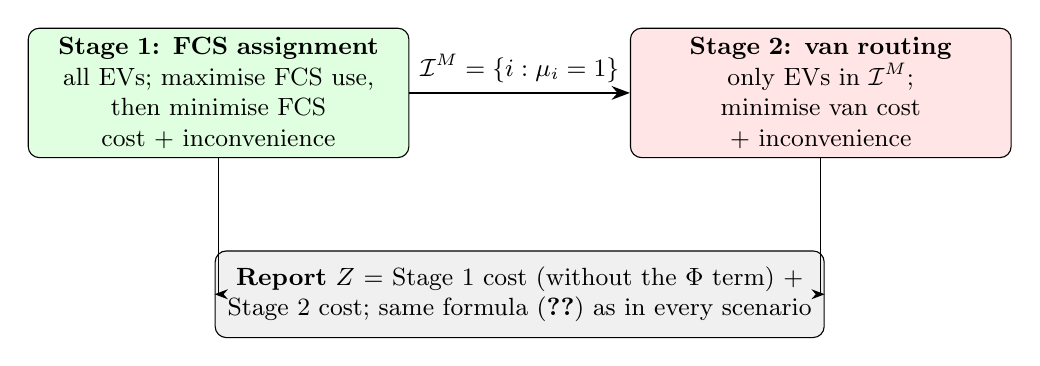
\begin{tikzpicture}[>=Stealth,box/.style={draw,rounded corners,align=center,minimum height=1.1cm,font=\small}]
  \node[box,fill=green!12,text width=4.6cm] (s1) {\textbf{Stage 1: FCS assignment}\\all EVs; maximise FCS use,\\then minimise FCS cost + inconvenience};
  \node[box,fill=red!10,text width=4.6cm,right=2.8cm of s1] (s2) {\textbf{Stage 2: van routing}\\only EVs in $\I^M$;\\minimise van cost + inconvenience};
  \draw[->,thick] (s1) -- node[above,font=\small]{$\I^M=\{i:\mu_i=1\}$} (s2);
  \node[box,fill=black!6,text width=7.5cm,below=2.0cm of $(s1)!0.5!(s2)$] (ev) {\textbf{Report} $Z=$ Stage~1 cost (without the $\Phi$ term) $+$ Stage~2 cost; same formula \eqref{eq:Z} as in every scenario};
  \draw[->] (s1) |- (ev); \draw[->] (s2) |- (ev);
\end{tikzpicture}
\end{center}

Stage~1 does not look at the vans, and Stage~2 cannot change what Stage~1 decided. That is the definition of ``FCS first, then MCS''.

%----------------------------------------------------------------
\subsection{Stage 1: assign EVs to fixed stations}

\textbf{Objective.}
\begin{equation}
\begin{split}
\min\ Z^{(1)}=\;&\underbrace{\Phi\sum_{i\in\I}\mu_i}_{\text{FCS first}}
+\underbrace{c^{EV}\sum_i\sum_{f\in\F_i}d_{if}Y_{if}}_{Z_1}
+\underbrace{Z^F_{\text{energy}}}_{\text{FCS part of }Z_4}\\
&+\underbrace{\sum_i\sum_{f\in\F_i}\rho^F_{if}Y_{if}+\alpha\sum_i w_i(C_i-r_i)+c^L\sum_i w_iL_i}_{\text{FCS customers' inconvenience}}
\end{split}
\label{eq:obj1}
\end{equation}
with $C_i=S_i+\tau^F_iY_i$ in this stage. $\Phi$ is a penalty for handing an EV to the vans. It is chosen larger than anything an extra FCS customer can add to the rest of \eqref{eq:obj1}, e.g.
\[
\Phi > \max_{i}\max_{f\in\F_i}\big(c^{EV}d_{if}+\pi^{\max}E_i+\rho^F_{if}\big)+n\,(\alpha+c^L)\,w_{\max}\,T,
\]
so Stage~1 first \textbf{maximises the number of EVs served at an FCS}, and only among those solutions minimises FCS cost and inconvenience. ($\pi^{\max}$ is the highest grid price.) A numerically safer equivalent is to solve twice: first $\max\sum_iY_i$, then fix that number and minimise the rest.
\ifTOU
Because $Z^F_{\text{energy}}$ uses the peak price, Stage~1 may \emph{start sessions later} to leave the peak, if the price saving beats the extra waiting cost (Section~\ref{sec:expect}).
\fi

\textbf{Constraints.}
\begin{align}
\sum_{g\in\G_i}y_{ig}+\mu_i &= 1 && \forall i\in\I \label{eq:s1assign}\\
S_i &\ge r_i+\sum_{f\in\F_i}t_{if}Y_{if} && \forall i\in\I \label{eq:fcsarr}\\
S_i &\le r_i+T\,(1-\mu_i) && \forall i\in\I \label{eq:s1park}\\
S_j &\ge S_i+\tau^F_i-(T+\tau^F_i)(3-y_{ig}-y_{jg}-o_{ij}) && \forall g,\ (i,j)\in\mathcal{P}_g \label{eq:disj1}\\
S_i &\ge S_j+\tau^F_j-(T+\tau^F_j)(2-y_{ig}-y_{jg}+o_{ij}) && \forall g,\ (i,j)\in\mathcal{P}_g \label{eq:disj2}\\
\sum_i y_{ig_1} &\ge \sum_i y_{ig_2} && \forall f,\ \G_f=\{g_1,g_2\} \label{eq:gunsym}\\
S_i+\tau^F_iY_i &\le T,\qquad L_i\ge S_i+\tau^F_iY_i-l_i && \forall i\in\I \label{eq:s1time}
\end{align}
\ifTOU plus the time-of-use split \eqref{eq:tou1}--\eqref{eq:tou5} of each FCS session (Section~\ref{sec:price}).\fi
\desc{\eqref{eq:s1assign}: every EV either gets one reachable gun or is handed to the vans. An EV that reaches no FCS ($\G_i=\emptyset$) is forced to $\mu_i=1$. \eqref{eq:fcsarr}: an FCS session cannot start before the EV has asked and driven to the station. \eqref{eq:s1park}: for an EV handed to the vans, $S_i$ is parked at $r_i$, so it adds no waiting in Stage~1 (its real start time is decided in Stage~2). \eqref{eq:disj1}--\eqref{eq:disj2}: two EVs on the same gun do not overlap; $o_{ij}$ picks who goes first. With two guns per station this means at most two EVs charge at a station at a time. \eqref{eq:gunsym}: symmetry breaking between the two identical guns (optional). \eqref{eq:s1time}: finished by $T$; lateness.}

\textbf{Optional acceptability rule.} An operator may refuse to send a driver to a station that is ``too inconvenient'', e.g.\ only allow gun $g$ of station $f$ for EV $i$ if $\hat\rho^F_{if}\le\bar\rho$. This only shrinks $\G_i$, so EVs whose stations are all too far go to the vans. Report results with and without it.

\textbf{Output:} $\I^M=\{i:\mu_i=1\}$, the EVs left for the vans; plus each FCS customer's gun and start time.

%----------------------------------------------------------------
\subsection{Stage 2: route the vans to the leftover EVs}

Stage~2 is a vehicle routing problem with time windows, on the EVs in $\I^M$ only. Here $C_i=S_i+\tau^M_i$.

\textbf{Objective.}
\begin{equation}
\begin{split}
\min\ Z^{(2)}=\;&\underbrace{c^M\sum_m\sum_{(i,j)\in\A^M}d_{ij}x_{ijm}}_{Z_2}+\underbrace{\sum_m c^D_mu_m}_{Z_3}+\underbrace{Z^M_{\text{energy}}}_{\text{van part of }Z_4}\\
&+\underbrace{\sum_{i\in\I^M}\sum_m\rho^M_{im}z_{im}+\alpha\sum_{i\in\I^M}w_i(C_i-r_i)+c^L\sum_{i\in\I^M}w_iL_i}_{\text{van customers' inconvenience}}
\end{split}
\label{eq:obj2}
\end{equation}
Since every EV in $\I^M$ must be served by some van, $Z^M_{\text{energy}}$ and the $\rho^M$ term are constants here. They are kept so that $Z^{(2)}$ is the true cost of Stage~2. Waiting and lateness make the vans visit urgent EVs early.

\textbf{Constraints.}
\begin{align}
\sum_{m\in\M}z_{im} &= 1 && \forall i\in\I^M \label{eq:s2assign}\\
\sum_{j:(0,j)\in\A^M}x_{0jm} = \sum_{i:(i,n+1)\in\A^M}x_{i,n+1,m} &= u_m && \forall m \label{eq:depot}\\
\sum_{i:(i,j)\in\A^M}x_{ijm} = \sum_{k:(j,k)\in\A^M}x_{jkm} &= z_{jm} && \forall j\in\I^M,\ m \label{eq:flow}\\
\sum_{i\in\I^M}z_{im} &\le Q_m\,u_m && \forall m \label{eq:cap}\\
\sum_{i\in\I^M}\frac{E_i}{\eta}z_{im}+\beta\sum_{(i,j)\in\A^M}d_{ij}x_{ijm} &\le B_m\,u_m && \forall m \label{eq:batt}
\end{align}
\begin{align}
S_j &\ge \max\{r_j,\ t_{0j}\,x_{0jm}\} && \forall j\in\I^M,\ m \label{eq:depart}\\
S_j &\ge S_i+\tau^M_i+t_{ij}-(T+\tau^M_i+t_{ij})(1-x_{ijm}) && \forall i\neq j,\ m \label{eq:seq}\\
S_i+\tau^M_i+t_{i,n+1} &\le T+(\tau^M_i+t_{i,n+1})(1-x_{i,n+1,m}) && \forall i,\ m \label{eq:return}\\
S_i+\tau^M_i \le T,\quad L_i &\ge S_i+\tau^M_i-l_i && \forall i\in\I^M \label{eq:s2time}\\
u_m &\ge u_{m+1} && m<|\M| \label{eq:vansym}
\end{align}
\desc{\eqref{eq:s2assign}: each leftover EV gets one van. \eqref{eq:depot}: a used van leaves and returns to the depot once. \eqref{eq:flow}: each EV on van $m$ is entered and left exactly once by that van. \eqref{eq:cap}: at most $Q_m$ EVs per van. \eqref{eq:batt}: delivered energy (with transfer losses) plus driving energy fits in the van battery. \eqref{eq:depart}: no start before the request, or before the van can drive there from the depot (written as two linear constraints). \eqref{eq:seq}: if the van goes $i\to j$, it finishes $i$ and drives to $j$ before starting $j$. This gives one EV at a time and removes subtours (MTZ-type). \eqref{eq:return}: back at the depot by $T$. \eqref{eq:s2time}: finished by $T$; lateness. \eqref{eq:vansym}: use identical vans in index order.}

\textbf{If Stage 2 is infeasible} (too many leftover EVs for the fleet by $T$), the sequential policy has \emph{failed} on that instance. For diagnosis, add $s_i\in\{0,1\}$ (``unserved''), replace \eqref{eq:s2assign} by $\sum_mz_{im}+s_i=1$ and add $\Phi^U\sum_is_i$ to \eqref{eq:obj2}. Then report the number of EVs that could not be served. This is a useful comparison with the integrated scenario, which may serve all of them.

%----------------------------------------------------------------
\subsection{Reported value}
\[
Z^{\text{S\scen}}=\big(Z^{(1)*}-\Phi\,|\I^M|\big)+Z^{(2)*},
\]
which is exactly \eqref{eq:Z} evaluated at the combined solution. The stage-1 solution plus the stage-2 solution is a feasible solution of the integrated model (S\ifTOU 4\else 3\fi), so
$Z^{\text{S\ifTOU 4\else 3\fi}}\le Z^{\text{S\scen}}$. The difference is the \emph{value of integration}.

\else
%---------------------------------------------------------------- INT
\subsection{Objective}
\begin{equation}
\min\ Z \quad\text{as in \eqref{eq:Z}, with }Z^F_{\text{energy}}=\ifTOU P^F\textstyle\sum_i\big[\pi^\off(\theta^1_i+\theta^3_i)+\pi^\pk\theta^2_i\big]\else\pi^F\textstyle\sum_iE_iY_i\fi,\quad C_i=S_i+\tau^F_iY_i+\tau^M_iZ_i. \label{eq:objint}
\end{equation}
Written out in full:
\begin{align*}
\min\ Z=\;& c^{EV}\sum_i\sum_{f\in\F_i}d_{if}Y_{if}+c^M\sum_m\sum_{(i,j)\in\A}d_{ij}x_{ijm}+\sum_mc^D_mu_m\\
&+\ifTOU P^F\sum_i\big[\pi^\off(\theta^1_i+\theta^3_i)+\pi^\pk\theta^2_i\big]\else\pi^F\sum_iE_iY_i\fi
+\pi^M\sum_i\sum_m\frac{E_i}{\eta}z_{im}\\
&+\sum_i\sum_{f\in\F_i}\rho^F_{if}Y_{if}+\sum_i\sum_m\rho^M_{im}z_{im}+\alpha\sum_iw_i(C_i-r_i)+c^L\sum_iw_iL_i .
\end{align*}
Every term is linear. One model weighs everything at once: an EV goes to a van exactly when the van's extra km, dispatch and energy cost are outweighed by the effort and waiting it saves the driver\ifTOU, or by the peak-price energy it avoids\fi.

\subsection{Constraints}

\textbf{Assignment.}
\begin{equation}
\sum_{g\in\G_i}y_{ig}+\sum_{m\in\M}z_{im}=1\qquad\forall i\in\I \label{eq:assign}
\end{equation}
\desc{Exactly one resource per EV: one reachable gun or one van. EVs that reach no FCS are forced onto a van.}

\textbf{Fixed stations.}
\begin{align}
S_i &\ge r_i+\sum_{f\in\F_i}t_{if}Y_{if} && \forall i \label{eq:fcsarr}\\
S_j &\ge S_i+\tau^F_i-(T+\tau^F_i)(3-y_{ig}-y_{jg}-o_{ij}) && \forall g,\ (i,j)\in\mathcal{P}_g \label{eq:disj1}\\
S_i &\ge S_j+\tau^F_j-(T+\tau^F_j)(2-y_{ig}-y_{jg}+o_{ij}) && \forall g,\ (i,j)\in\mathcal{P}_g \label{eq:disj2}\\
\sum_iy_{ig_1} &\ge \sum_iy_{ig_2} && \forall f,\ \G_f=\{g_1,g_2\} \label{eq:gunsym}
\end{align}
\desc{\eqref{eq:fcsarr}: an FCS session starts after the request and the drive to the station (for a van customer this is just $S_i\ge r_i$). \eqref{eq:disj1}--\eqref{eq:disj2}: EVs on the same gun do not overlap; $o_{ij}$ chooses the order. \eqref{eq:gunsym}: optional symmetry breaking.}

\textbf{Vans: routes, capacity, battery.}
\begin{align}
\sum_{j:(0,j)\in\A}x_{0jm}=\sum_{i:(i,n+1)\in\A}x_{i,n+1,m} &= u_m && \forall m \label{eq:depot}\\
\sum_{i:(i,j)\in\A}x_{ijm}=\sum_{k:(j,k)\in\A}x_{jkm} &= z_{jm} && \forall j\in\I,\ m \label{eq:flow}\\
\sum_iz_{im} &\le Q_mu_m && \forall m \label{eq:cap}\\
\sum_i\frac{E_i}{\eta}z_{im}+\beta\sum_{(i,j)\in\A}d_{ij}x_{ijm} &\le B_mu_m && \forall m \label{eq:batt}
\end{align}
\desc{\eqref{eq:depot}: a used van leaves and returns once. \eqref{eq:flow}: each EV on van $m$ is visited exactly once by it. \eqref{eq:cap}: at most $Q_m$ EVs. \eqref{eq:batt}: delivered energy (with losses) plus driving energy fits in the battery.}

\textbf{Vans: timing (one EV at a time, no subtours).}
\begin{align}
S_j &\ge t_{0j}\,x_{0jm} && \forall j\in\I,\ m \label{eq:depart}\\
S_j &\ge S_i+\tau^M_i+t_{ij}-(T+\tau^M_i+t_{ij})(1-x_{ijm}) && \forall i\neq j\in\I,\ m \label{eq:seq}\\
S_i+\tau^M_i+t_{i,n+1} &\le T+(\tau^M_i+t_{i,n+1})(1-x_{i,n+1,m}) && \forall i,\ m \label{eq:return}
\end{align}
\desc{\eqref{eq:depart}: the first stop cannot start before the van has driven there. \eqref{eq:seq}: $i\to j$ means finish $i$, drive, then start $j$; start times rise along a route, so no subtour can close. \eqref{eq:return}: back at the depot by $T$.}

\textbf{Horizon and lateness.}
\begin{equation}
C_i\le T,\qquad L_i\ge C_i-l_i\qquad\forall i\in\I \label{eq:time}
\end{equation}
\desc{Every EV is fully charged within the horizon; $L_i$ measures lateness.}

\ifTOU
\textbf{Time-of-use split.} Constraints \eqref{eq:tou1}--\eqref{eq:tou5} of Section~\ref{sec:price}.
\fi

\textbf{Symmetry and domains.}
\begin{equation}
u_m\ge u_{m+1};\qquad y,z,x,u,o\ifTOU,\kappa\fi\in\{0,1\};\qquad S_i,L_i\ifTOU,\theta^p_i\fi\ge0 \label{eq:dom}
\end{equation}
\fi

%=====================================================================
\section{Learning-to-optimise (RL) formulation}\label{sec:rl}

\textbf{Main rule:} the reward of each action is \emph{minus the increase in $Z$ that the action causes}. The rewards over an episode then add up to $-Z$ of the solution the policy builds. RL and MILP results are measured on the same yardstick \eqref{eq:Z}, and the MILP optimum is the benchmark for the RL gap.

\ifSEQ
%---------------------------------------------------------------- RL SEQ
The RL pipeline has the same two stages as the MILP.

\subsection{Stage 1 policy: FCS assignment}
\begin{itemize}[leftmargin=1.4em,itemsep=2pt]
  \item \textbf{Episode / epochs:} EVs are taken in order of request time $r_i$ (ties: higher $w_i$ first). One decision per EV.
  \item \textbf{State:} features of the current EV $k$ ($E_k,r_k,l_k,w_k,R_k$, location); for each gun $g$ the time $F_g$ it becomes free; summary features of the EVs still to come (count and positions near each station)\ifTOU; the current price and the time until $T_1$ and $T_2$\fi.
  \item \textbf{Action:} a gun $g\in\G_k$, or ``hand to vans''. \textbf{FCS-first mask:} ``hand to vans'' is allowed \emph{only} if no gun can finish EV $k$ by $T$ (or, with the optional rule, if all remaining guns have $\hat\rho^F_{kf}>\bar\rho$).
  \ifTOU\item \textbf{Optional timing action:} ``gun $g$, start after the peak'', i.e.\ $S_k=\max\{\text{earliest},T_2\}$, allowed only if the session still ends by $T$.\fi
  \item \textbf{Transition:} $S_k=\max\{r_k+t_{kf},F_g\}$ (or later, for the timing action); $F_g\leftarrow S_k+\tau^F_k$.
  \item \textbf{Reward:} $-\Big[c^{EV}d_{kf}+\text{energy}_k+\rho^F_{kf}+\alpha w_k(S_k+\tau^F_k-r_k)+c^Lw_k(S_k+\tau^F_k-l_k)^+\Big]$, where energy$_k$ = \ifTOU$P^F\big[\pi^\off\cdot(\text{off-peak hours of }[S_k,S_k+\tau^F_k])+\pi^\pk\cdot(\text{peak hours})\big]$, computed exactly in the simulator\else$\pi^FE_k$\fi. Handing an EV to the vans gives reward $0$ here; its cost is counted in Stage~2.
\end{itemize}
Note: a simple baseline for Stage~1 is the greedy rule ``gun with the largest one-step reward''. What RL can learn on top of this is, for example, to keep a nearby gun free for an urgent EV that arrives later.

\subsection{Stage 2 policy: van routing over $\I^M$}
\begin{itemize}[leftmargin=1.4em,itemsep=2pt]
  \item \textbf{Epochs:} whenever a van becomes free (the earliest-free van decides first).
  \item \textbf{State:} for each van: position, time free, remaining battery $b_m$, EVs served so far, dispatched or not; for each unserved EV in $\I^M$: location, $E_i,r_i,l_i,w_i$; current time.
  \item \textbf{Action:} the next EV $j$ for this van, or ``return to depot'' (ends the route). Mask: $j$ must be feasible: battery covers $E_j/\eta$ plus driving to $j$ and back to the depot, the count stays $\le Q_m$, and $j$ can be finished with the van back at the depot by $T$.
  \item \textbf{Transition:} $S_j=\max\{r_j,\ \text{time free}+t_{\text{pos},j}\}$; the van moves to $j$ and is free at $S_j+\tau^M_j$; $b_m$ falls by $E_j/\eta+\beta d_{\text{pos},j}$.
  \item \textbf{Reward:} serving $j$: $-\Big[c^Md_{\text{pos},j}+c^D_m[\text{first stop}]+\pi^M\frac{E_j}{\eta}+\rho^M_{jm}+\alpha w_j(S_j+\tau^M_j-r_j)+c^Lw_j(S_j+\tau^M_j-l_j)^+\Big]$; returning: $-c^Md_{\text{pos},0}$. EVs still unserved at the end: $-\Phi^U$ each.
  \item \textbf{Policy:} an attention-based routing policy (e.g.\ Kool et al., 2019, ``Attention, Learn to Solve Routing Problems!'') trained with REINFORCE or PPO. Baseline: nearest-feasible-EV heuristic.
\end{itemize}
Episode return of Stage~1 + Stage~2 $=-Z^{\text{S\scen}}$.

\else
%---------------------------------------------------------------- RL INT
One policy decides both who serves each EV and the van routes.
\begin{itemize}[leftmargin=1.4em,itemsep=2pt]
  \item \textbf{Episode / epochs:} EVs are taken in order of request time $r_i$ (ties: higher $w_i$ first). One decision per EV.
  \item \textbf{State:} (i) the current EV $k$: location, $E_k,r_k,l_k,w_k,R_k$, reachable stations; (ii) each gun $g$: time $F_g$ it becomes free; (iii) each van $m$: current end-of-route position, time free, remaining battery $b_m$, EVs served, dispatched or not; (iv) embeddings of the not-yet-assigned EVs (for look-ahead)\ifTOU; (v) current price, time until $T_1$ and $T_2$\fi.
  \item \textbf{Action:} $a\in\G_k\cup\M$: a gun, or a van (EV $k$ is appended to the end of that van's route). \textbf{Mask} infeasible actions: a gun that cannot finish $k$ by $T$; a van without enough battery for $E_k/\eta$ plus the drive to $k$ and back to the depot, with $Q_m$ reached, or unable to finish $k$ and return by $T$.
  \ifTOU\item \textbf{Optional timing action:} ``gun $g$, start after the peak'' ($S_k=\max\{\text{earliest},T_2\}$, if it still ends by $T$).\fi
  \item \textbf{Transition:} gun: $S_k=\max\{r_k+t_{kf},F_g\}$, $F_g\leftarrow S_k+\tau^F_k$. Van: $S_k=\max\{r_k,\ \text{free}_m+t_{\text{pos}_m,k}\}$, then the van moves to $k$, $\text{free}_m\leftarrow S_k+\tau^M_k$, $b_m\mathrel{-}=E_k/\eta+\beta d_{\text{pos}_m,k}$.
  \item \textbf{Reward} $=-\Delta Z$:
  \begin{align*}
  \text{gun } g\text{ at }f:&\quad -\Big[c^{EV}d_{kf}+\text{energy}^F_k+\rho^F_{kf}+\alpha w_k(C_k-r_k)+c^Lw_k(C_k-l_k)^+\Big]\\
  \text{van } m:&\quad -\Big[c^M\big(d_{\text{pos}_m,k}+d_{k,0}-d_{\text{pos}_m,0}\big)+c^D_m[\text{first use}]+\pi^M\tfrac{E_k}{\eta}\\
  &\qquad\quad+\rho^M_{km}+\alpha w_k(C_k-r_k)+c^Lw_k(C_k-l_k)^+\Big]
  \end{align*}
  The van distance term is the \emph{change} in route length when $k$ is inserted before the return to the depot, so the sum over the episode equals the total route length (the return legs telescope). energy$^F_k$ = \ifTOU$P^F\big[\pi^\off\cdot(\text{off-peak hours})+\pi^\pk\cdot(\text{peak hours of }[S_k,C_k])\big]$, computed exactly by the simulator; no linearisation is needed in RL\else$\pi^FE_k$\fi.
  \item \textbf{Dead end:} if every action is masked, EV $k$ is unserved: reward $-\Phi^U$, and the episode continues. Report the count.
  \item \textbf{Policy:} masked categorical policy over guns and vans, encoder with attention over EVs, guns and vans; trained with PPO. Natural baseline: greedy, i.e.\ choose the action with the largest one-step reward. That is the pairwise rule ``smallest $\hat\rho$ + cost'' from Section~\ref{sec:inc}.
\end{itemize}
Restriction to note: vans serve EVs in assignment order (append only). A variant that inserts $k$ at the cheapest position of a route is more flexible but has a larger action space.
\fi

\textbf{Reward scaling.} For stable training divide every reward by a constant, e.g.\ the greedy baseline's average $Z$ on the training instances. This does not change the optimal policy.

%=====================================================================
\section{What to expect and what to report}\label{sec:expect}

\ifnum\scen=1
\begin{itemize}[leftmargin=1.4em,itemsep=2pt]
  \item Vans serve only EVs that reach no station, or that the stations cannot finish by $T$. If stations have spare capacity, very few vans are dispatched.
  \item Inconvenience is high for EVs far from the nearest station (worked example: Rs\,682 at the FCS, against Rs\,458 if a van had been allowed).
  \item With too few vans Stage~2 becomes infeasible (unserved EVs), even when the integrated model S3 could serve everyone. Report the smallest $|\M|$ at which S1 is feasible and compare it with S3.
\end{itemize}
\fi
\ifnum\scen=2
\begin{itemize}[leftmargin=1.4em,itemsep=2pt]
  \item \textbf{When does Stage~1 delay a session to avoid the peak?} Moving one hour of charging out of the peak saves $(\pi^\pk-\pi^\off)P^F=3\times22=$ Rs\,66, but delays completion by up to an hour, which costs $\alpha w_i\ge$ Rs\,200. So with the default values Stage~1 almost never delays. It mostly pays the higher price, and S2 costs roughly S1 plus the peak surcharge. Sessions start later only if $\alpha$ is small (try $\lambda<0.33$ in the sensitivity analysis).
  \item The van assignment is the same as in S1 unless Stage~1's timing changes which EVs fit at the stations. Stage~1 cannot use vans to escape the peak price.
  \item Extra KPI: \textbf{grid energy drawn at FCS during the peak}, $P^F\sum_i\theta^2_i$ (kWh). Compare with S4.
\end{itemize}
\fi
\ifnum\scen=3
\begin{itemize}[leftmargin=1.4em,itemsep=2pt]
  \item Vans take EVs for which the saved inconvenience exceeds the extra van cost (worked example: van chosen, saving Rs\,224). Expect vans to serve EVs that are far from every station, have low range (high $w_i$), or have early deadlines, while EVs near a station still use it.
  \item \textbf{Value of integration under flat price:} $Z^{\text{S1}}-Z^{\text{S3}}\ge0$. Report it per component ($Z_1,\dots,Z_5$): typically operating cost rises a little and inconvenience falls a lot.
  \item Vary $|\M|$ (0, 1, 2, \dots): the first few vans lower $Z$ sharply, then the effect levels off. That curve shows the scenarios where mobile chargers help most.
\end{itemize}
\fi
\ifnum\scen=4
\begin{itemize}[leftmargin=1.4em,itemsep=2pt]
  \item During the peak a van kWh costs about the same as an FCS kWh (Rs\,10.0 each), so the vans' energy disadvantage disappears and vans also absorb \emph{peak-hour} demand that would otherwise be charged on the grid at peak price.
  \item Expect more van usage than in S3, concentrated on requests in $[T_1,T_2]$, and lower grid energy at the stations during the peak, $P^F\sum_i\theta^2_i$, than in S2.
  \item \textbf{Value of integration under peak pricing:} $Z^{\text{S2}}-Z^{\text{S4}}$. It should be larger than $Z^{\text{S1}}-Z^{\text{S3}}$, because integration now also allows price arbitrage.
  \item \textbf{Peak pricing with full flexibility:} $Z^{\text{S4}}-Z^{\text{S3}}$ should be smaller than $Z^{\text{S2}}-Z^{\text{S1}}$: vans cushion the price increase.
\end{itemize}
\fi

\textbf{Cross-scenario comparison table} (fill in from the four runs):
\begin{center}
\renewcommand{\arraystretch}{1.2}
\begin{tabular}{@{}lll@{}}
\toprule
\textbf{Comparison} & \textbf{Measures} & \textbf{Expected sign} \\
\midrule
S1 $-$ S3 & value of integration, flat price & $\ge0$ \\
S2 $-$ S4 & value of integration, peak price & $\ge0$, larger than S1 $-$ S3 \\
S2 $-$ S1 & cost of peak pricing, FCS-first operator & $>0$ \\
S4 $-$ S3 & cost of peak pricing, flexible operator & $>0$, smaller than S2 $-$ S1 \\
\bottomrule
\end{tabular}
\end{center}
Report for each: $Z$ and its components, number of vans used, EVs per resource, mean and maximum inconvenience per EV, total lateness, peak-hour grid energy, solve time, and (for RL) the gap to the MILP optimum.

%=====================================================================
\appendix
\section{Illustrative parameter values}\label{app:values}

These are starting values for experiments, not data. All are meant to be varied in the analysis. Values in Rs.

\begin{center}
\renewcommand{\arraystretch}{1.15}
\begin{tabular}{@{}llp{6.2cm}@{}}
\toprule
\textbf{Parameter} & \textbf{Value} & \textbf{Note} \\
\midrule
$T$, $[T_1,T_2]$ & 7 h, $[2,6]$ & 16:00--23:00, peak 18:00--22:00 \\
$P^F$, $P^M$ & 22 kW, 30 kW & \\
$v$, $\beta$, $\eta$ & 25 km/h, 0.25 kWh/km, 0.9 & \\
$B_m$, $Q_m$, $|\M|$ & 150 kWh, 6, 2--6 & \\
$c^{EV}$, $c^M$, $c^D_m$ & Rs\,4/km, Rs\,15/km, Rs\,1500 & van km includes driver time \\
$\pi^F$ (flat) & Rs\,8.7/kWh & equals the time-average of the ToU tariff over $[0,T]$ \\
$\pi^\off$, $\pi^\pk$ (ToU) & Rs\,7/kWh, Rs\,10/kWh & $(3\times7+4\times10)/7=8.7$ \\
$c^{bat}$ & Rs\,2/kWh & van battery wear \\
$\pi^M$ & Rs\,10.7 (flat) / Rs\,9.0 (ToU) & $=\pi^F+c^{bat}$ / $=\pi^\off+c^{bat}$ \\
$\alpha$, $\alpha^D$ & Rs\,200/h, Rs\,100/h & value of time; extra for attended time \\
$h^F$, $h^M$, $\varphi$ & Rs\,50, Rs\,10, Rs\,100 & trip hassle, hand-over, range stress \\
$c^L$ & Rs\,300/h & lateness \\
$w_i$ & $1+2(1-R_i/R_{\max})$, $R_i\sim U[3,40]$ km & priority from remaining range \\
\bottomrule
\end{tabular}
\end{center}

The flat price is set to the time-average of the peak tariff. The price \emph{level} is then the same in both pricing cases, and only the price \emph{shape} differs. Without this, part of S1 vs S2 would just reflect a different average price.

\end{document}
"
%  (run each twice for cross-references)
% =====================================================================
\documentclass[11pt,a4paper]{article}
\usepackage[margin=2.2cm]{geometry}
\usepackage{amsmath,amssymb,amsfonts}
\usepackage{booktabs,array,tabularx}
\usepackage{enumitem}
\usepackage[table]{xcolor}
\usepackage{tikz}
\usetikzlibrary{arrows.meta,positioning,calc}
\usepackage[colorlinks=true,linkcolor=blue!50!black,urlcolor=blue!50!black]{hyperref}
\usepackage{titlesec}
\titleformat{\section}{\large\bfseries}{\thesection}{0.8em}{}
\titleformat{\subsection}{\normalsize\bfseries}{\thesubsection}{0.8em}{}
\setlength{\parindent}{0pt}
\setlength{\parskip}{5pt}

% ---------------- scenario switches ----------------
\ifdefined\scen\else\def\scen{1}\fi
\newif\ifTOU \TOUfalse   % true = time-of-use (peak) price
\newif\ifSEQ \SEQfalse   % true = FCS first, then MCS
\ifnum\scen=1 \SEQtrue \fi
\ifnum\scen=2 \TOUtrue \SEQtrue \fi
\ifnum\scen=4 \TOUtrue \fi

\newcommand{\pricename}{\ifTOU time-of-use price (dearer evening peak)\else single (flat) price all day\fi}
\newcommand{\structname}{\ifSEQ FCS first, then MCS (sequential)\else FCS and MCS together (integrated)\fi}

% ---------------- notation ----------------
\newcommand{\I}{\mathcal{I}}
\newcommand{\F}{\mathcal{F}}
\newcommand{\G}{\mathcal{G}}
\newcommand{\M}{\mathcal{M}}
\newcommand{\N}{\mathcal{N}}
\newcommand{\A}{\mathcal{A}}
\newcommand{\Rs}{\text{Rs}\,}
\newcommand{\pk}{\mathrm{pk}}
\newcommand{\off}{\mathrm{off}}
\newcommand{\desc}[1]{\par\vspace{-2pt}{\small\color{black!75}\textit{Meaning:} #1}\par\vspace{4pt}}
\newcommand{\cell}[2]{\ifnum\scen=#1\cellcolor{blue!18}\textbf{S#1 (this document)}\\\textbf{#2}\else S#1\\#2\fi}

\title{\textbf{EV Charging Network Optimisation}\\[4pt]
\large Scenario \scen: \pricename\ $+$ \structname\\[2pt]
\normalsize MILP and RL formulation}
\author{CP 320 OR for Mobility Management, course project}
\date{2 October 2026}

\begin{document}
\maketitle

%=====================================================================
\section{Where this scenario sits}

The project studies four scenarios: two ways of pricing grid electricity, times two ways of making the decisions.

\begin{center}
\renewcommand{\arraystretch}{1.5}
\begin{tabular}{>{\raggedright\arraybackslash}p{4.2cm}|>{\centering\arraybackslash}p{4.6cm}|>{\centering\arraybackslash}p{4.6cm}}
 & \textbf{Flat price all day} & \textbf{Time-of-use (peak) price} \\ \hline
\textbf{Sequential:} FCS first, leftover EVs to MCS &
\begin{tabular}[c]{@{}c@{}}\cell{1}{flat + sequential}\end{tabular} &
\begin{tabular}[c]{@{}c@{}}\cell{2}{peak + sequential}\end{tabular} \\ \hline
\textbf{Integrated:} FCS and MCS decided together &
\begin{tabular}[c]{@{}c@{}}\cell{3}{flat + integrated}\end{tabular} &
\begin{tabular}[c]{@{}c@{}}\cell{4}{peak + integrated}\end{tabular} \\
\end{tabular}
\end{center}

\textbf{The four scenarios do not have four different objectives.} They share \emph{one} cost yardstick $Z$ (Section~\ref{sec:obj}): the same cost terms and the same customer inconvenience (Section~\ref{sec:inc}). Only two things change:
\begin{itemize}[leftmargin=1.4em,itemsep=1pt]
  \item \textbf{Pricing} changes the formula for one term, the FCS energy cost (Section~\ref{sec:price}).
  \item \textbf{Decision structure} changes \emph{how} $Z$ is minimised: in one model (integrated), or in two stages (sequential), where each stage minimises its own part of $Z$.
\end{itemize}
Because the yardstick is the same, the four optimal values can be compared directly. The differences measure the \emph{value of integration} (S1$\to$S3, S2$\to$S4) and the \emph{effect of peak pricing} (S1$\to$S2, S3$\to$S4).

\ifnum\scen=1
\textbf{This scenario (S1)} is the baseline, the ``status quo''. Electricity costs the same at every hour, every EV that can be charged at a fixed station is sent there, and vans only take what is left over.
\fi
\ifnum\scen=2
\textbf{This scenario (S2)} keeps the FCS-first rule of S1, but grid electricity is dearer during the evening peak. Stage~1 can react to the price only by \emph{rescheduling} FCS sessions. It cannot hand a peak-hour EV to a van.
\fi
\ifnum\scen=3
\textbf{This scenario (S3)} keeps the flat price of S1, but the operator decides FCS and MCS service \emph{together}. An EV can be sent to a van even when a fixed station could take it, whenever that lowers total cost plus inconvenience.
\fi
\ifnum\scen=4
\textbf{This scenario (S4)} is the most flexible one: peak pricing at fixed stations, and FCS and MCS decided together. Van energy was bought off-peak, so vans can also be used to keep charging \emph{out of the expensive peak}.
\fi

%=====================================================================
\section{Setting and assumptions}\label{sec:setting}

\textbf{Time.} The planning horizon is $[0,T]$ with $T=7$\,h (16:00--23:00). It contains the evening peak window $[T_1,T_2]=[2,6]$ (18:00--22:00). The horizon is the same in all four scenarios. It is wider than the peak itself so that, under peak pricing, there is cheaper time on both sides of the peak.\ifTOU\else\ In this scenario the price is flat, so the window plays no role in the model.\fi

\textbf{Assumptions} (the same as MILP v3, plus two about energy):
\begin{enumerate}[leftmargin=1.6em,itemsep=1pt]
  \item Static, continuous time. All requests in the horizon are known at time $0$, and request $i$ becomes active at $r_i$.
  \item An EV served by an FCS drives there itself on its own battery (only to stations within its range $R_i$). The driver stays with the car while it waits for a free gun and while it charges.
  \item An EV served by an MCS stays parked where it is, and the driver is free in the meantime.
  \item Each FCS gun and each van charges one EV at a time, without interruption, at constant power.
  \item A van's battery covers both its driving and the energy it delivers. \textbf{The van battery is charged at the depot before the horizon starts}\ifTOU, i.e.\ at the off-peak price\fi, and is not recharged during the horizon.
  \item Every EV must be fully charged by $T$ (hard). Finishing after the driver's desired time $l_i$ is allowed but penalised.
\end{enumerate}

%=====================================================================
\section{Notation}\label{sec:notation}

\subsection*{Sets}
\begin{tabularx}{\textwidth}{@{}lX@{}}
\toprule
$\I=\{1,\dots,n\}$ & EV charging requests \\
$\F$; $\G_f$ ($|\G_f|=2$); $\G=\bigcup_f\G_f$ & fixed charging stations; guns of FCS $f$; all guns ($f(g)$ = station of gun $g$) \\
$\F_i=\{f: d_{if}\le R_i\}$, $\G_i=\bigcup_{f\in\F_i}\G_f$ & stations / guns EV $i$ can reach on its remaining range \\
$\M$ & mobile charging vans (MCS) \\
$0,\ n+1$ & depot as start node / end node (same place) \\
$\N=\{0\}\cup\I\cup\{n+1\}$, $\A$ & routing nodes; allowed van arcs $(i,j)$, $i\in\{0\}\cup\I$, $j\in\I\cup\{n+1\}$, $i\neq j$ \\
$\mathcal{P}_g=\{(i,j): i<j,\ g\in\G_i\cap\G_j\}$ & pairs of EVs that could share gun $g$ \\
\ifSEQ
$\I^M\subseteq\I$ & EVs handed to the vans by Stage~1 (an \emph{output} of Stage~1, a fixed input to Stage~2) \\
$\N^M$, $\A^M$ & routing nodes / arcs restricted to $\I^M$ \\
\fi
\bottomrule
\end{tabularx}

\subsection*{Parameters}
\begin{tabularx}{\textwidth}{@{}lX@{}}
\toprule
$E_i,\ r_i,\ l_i,\ R_i$ & energy demand (kWh), request time, desired completion time (h), remaining range (km) \\
$w_i\ge1$ & priority of EV $i$; $w_i=1+\kappa(1-R_i/R_{\max})$, so low-range EVs weigh more \\
$P^F,\ P^M$ & charging power of an FCS gun (22\,kW) / of a van (e.g.\ 30\,kW) \\
$\tau^F_i=E_i/P^F,\ \tau^M_i=E_i/P^M$ & charging time of EV $i$ at an FCS / by a van (h) \\
$d_{if},t_{if}$;\ $d_{ij},t_{ij}$ & distance (km) and time (h): EV$\to$FCS; between routing nodes ($t=d/v$) \\
$B_m,\ Q_m,\ \beta,\ \eta$ & van battery (kWh), max EVs per van, van consumption (kWh/km), transfer efficiency \\
$c^{EV},\ c^M,\ c^D_m$ & cost per km of EV driving, per km of van driving; fixed dispatch cost of van $m$ \\
\ifTOU
$\pi^\off,\ \pi^\pk$ & grid price (Rs/kWh) off-peak / in $[T_1,T_2]$, with $\pi^\pk\ge\pi^\off$ \\
\else
$\pi^F$ & grid price (Rs/kWh), the same at every hour \\
\fi
$c^{bat}$ & van battery wear per kWh cycled \\
$\pi^M$ & cost of 1 kWh taken from a van battery: $\pi^M=\ifTOU\pi^\off\else\pi^F\fi+c^{bat}$ (Section~\ref{sec:price}) \\
$\alpha,\ \alpha^D,\ h^F,\ h^M,\ \varphi,\ c^L$ & inconvenience coefficients (Section~\ref{sec:inc}) \\
\bottomrule
\end{tabularx}

\subsection*{Decision variables}
\begin{tabularx}{\textwidth}{@{}llX@{}}
\toprule
$y_{ig}$ & $\{0,1\}$ & EV $i$ charged at gun $g\in\G_i$ \\
$z_{im}$ & $\{0,1\}$ & EV $i$ served by van $m$ \\
$x_{ijm}$ & $\{0,1\}$ & van $m$ drives arc $(i,j)$ \\
$u_m$ & $\{0,1\}$ & van $m$ is dispatched \\
$o_{ij}$ & $\{0,1\}$ & for EVs $i<j$ that could share a gun: 1 if $i$ is charged before $j$ \\
\ifSEQ
$\mu_i$ & $\{0,1\}$ & Stage~1 only: EV $i$ is handed to the van fleet \\
\fi
\ifTOU
$\theta^1_i,\theta^2_i,\theta^3_i$ & $\ge0$ & hours of EV $i$'s FCS session before / inside / after the peak \\
$\kappa^1_i,\kappa^3_i$ & $\{0,1\}$ & EV $i$'s FCS session starts before $T_1$ / ends after $T_2$ \\
\fi
$S_i$ & $\ge0$ & time charging of EV $i$ starts (h), on whichever resource \\
$L_i$ & $\ge0$ & lateness of EV $i$ beyond $l_i$ (h) \\
\bottomrule
\end{tabularx}

\textbf{Short-hands} (linear expressions, not new variables):
\[
Y_{if}=\sum_{g\in\G_f}y_{ig},\qquad Y_i=\sum_{g\in\G_i}y_{ig}\ (\text{EV $i$ uses an FCS}),\qquad Z_i=\sum_{m\in\M}z_{im}\ (\text{EV $i$ uses a van}),
\]
\[
C_i=S_i+\tau^F_i\,Y_i+\tau^M_i\,Z_i \quad\text{(time EV $i$ is fully charged).}
\]

%=====================================================================
\section{Customer inconvenience}\label{sec:inc}

This section is \textbf{identical in all four scenario documents}. Inconvenience is a property of the customer, not of the price or of the planning method.

\subsection{What we mean by inconvenience}

Inconvenience is \emph{what the driver loses} from the moment they ask for a charge ($r_i$) until the car is fully charged ($C_i$), \emph{converted into rupees} so it can be added to the operator's costs. A driver loses three different things:

\begin{enumerate}[leftmargin=1.6em,itemsep=2pt]
  \item \textbf{Waiting:} the car is not ready. This lasts $C_i-r_i$ hours and affects \emph{every} driver, FCS or MCS.
  \item \textbf{Effort:} only an FCS customer has to drive to the station and sit there while the car charges. An MCS customer stays at home or at work and does something else. Driving to a far station also uses scarce battery range, which causes stress (``range anxiety'').
  \item \textbf{A missed deadline:} the car is still not ready at the time $l_i$ the driver needs it.
\end{enumerate}

Each loss gets a price in Rs per hour (or per event). All of them are multiplied by the priority $w_i$: an hour of delay for an EV with 5\,km of range left counts more than for one with 40\,km.

\subsection{The three components}

\begin{center}
\renewcommand{\arraystretch}{1.3}
\begin{tabularx}{\textwidth}{@{}>{\raggedright\arraybackslash}p{2.6cm}>{\raggedright\arraybackslash}X>{\raggedright\arraybackslash}X>{\raggedright\arraybackslash}p{3.0cm}@{}}
\toprule
\textbf{Component} & \textbf{EV $i$ at FCS $f$} & \textbf{EV $i$ by a van} & \textbf{Known when?} \\
\midrule
Effort & $w_i\big[\alpha^D(t_{if}+\tau^F_i)+h^F+\varphi\,d_{if}/R_i\big]$: driving and sitting at the station, a fixed trip hassle, range stress & $w_i\,h^M$: being reachable and handing over the car & \textbf{Static:} known as soon as the resource is chosen \\
Waiting & $w_i\,\alpha\,(C_i-r_i)$ = drive + \emph{queue at the gun} + charge & $w_i\,\alpha\,(C_i-r_i)$ = \emph{wait for the van} + charge & \textbf{Dynamic:} depends on the queue / van route \\
Missed deadline & $w_i\,c^L\,L_i$, $L_i=\max\{0,C_i-l_i\}$ & same & Dynamic \\
\bottomrule
\end{tabularx}
\end{center}

\textbf{Coefficients.}
$\alpha$ (Rs/h) is the value of an hour the car is not ready.
$\alpha^D$ (Rs/h) is the \emph{extra} value of an hour the driver must personally spend driving or sitting at the station: an hour at the station costs $\alpha+\alpha^D$, an hour waiting at home for a van costs only $\alpha$.
$h^F,h^M$ (Rs) are fixed hassle costs of one trip to a station / one van hand-over.
$\varphi$ (Rs) is the range-stress cost of a trip that uses the \emph{whole} remaining range ($d_{if}/R_i\le1$ is the fraction used).
$c^L$ (Rs/h) is the cost per hour late.

\subsection{Pairwise form: inconvenience of a (customer, resource) pair}

The natural first idea is: \emph{for every pair (EV $i$, FCS $f$) and every pair (EV $i$, van $m$) there is an inconvenience number, and the operator picks the pair with the lowest cost plus inconvenience.} The static part fits this idea exactly:
\[
\boxed{\;\rho^F_{if}=w_i\Big[\alpha^D\,(t_{if}+\tau^F_i)+h^F+\varphi\,\frac{d_{if}}{R_i}\Big]\qquad
\rho^M_{im}=w_i\,h^M\;}
\]
These are \textbf{parameters}, computed before solving, one number per (EV, FCS) pair and per (EV, van) pair. In the objective they appear linearly: $\sum_i\sum_f\rho^F_{if}Y_{if}+\sum_i\sum_m\rho^M_{im}z_{im}$.

Note that $\rho^M_{im}$ does not depend on $m$. Vans are identical and all start at the same depot, so the driver does not care \emph{which} van comes, only \emph{when} it comes. That ``when'' is the waiting part.

\subsection{Why waiting cannot be a fixed pairwise number}

It is tempting to also write the waiting as a pairwise number, e.g.\ ``the van needs 5 minutes to reach EV $i$''. But that depends on \emph{where the van is coming from}, which depends on the route the model is still choosing: if EV $i$ is the 4th stop of a van, the wait is the time for three charging sessions plus four drives. Likewise, waiting at an FCS depends on how many EVs are queued at that gun. So waiting is not known before solving. It is a function of decision variables:
\[
\text{waiting cost of EV } i \;=\; w_i\,\alpha\,(C_i-r_i),\qquad C_i=S_i+\tau^F_iY_i+\tau^M_iZ_i .
\]
This is \textbf{linear} in the variables ($S_i$, $y$, $z$), so it fits in a MILP directly. The constraints of Section~\ref{sec:milp} make $S_i$ equal to the true start time, including driving, queueing at the gun and the van's route. The term $\sum_i w_i\alpha r_i$ is a constant and may be dropped when solving.

\textbf{Pairwise \emph{estimate}} (used for intuition, by the RL policy and in heuristics): if there is no queue and the van comes straight to $i$,
\[
\hat\rho^{F}_{if}=\rho^F_{if}+w_i\alpha\,(t_{if}+\tau^F_i),\qquad
\hat\rho^{M}_{im}=\rho^M_{im}+w_i\alpha\,(t^{\text{van}}_{m\to i}+\tau^M_i),
\]
where $t^{\text{van}}_{m\to i}$ is the time until van $m$ can reach $i$ from where it currently is. In the RL formulation (Section~\ref{sec:rl}) the van's position \emph{is} known at each decision, so there this estimate becomes exact.

\subsection{Total inconvenience and how it enters the objective}

\begin{equation}
\boxed{\;
Z_{\text{inc}}=\underbrace{\sum_{i\in\I}\sum_{f\in\F_i}\rho^F_{if}Y_{if}+\sum_{i\in\I}\sum_{m\in\M}\rho^M_{im}z_{im}}_{\text{effort (static, pairwise)}}
+\underbrace{\alpha\sum_{i\in\I}w_i\,(C_i-r_i)}_{\text{waiting (dynamic)}}
+\underbrace{c^L\sum_{i\in\I}w_i\,L_i}_{\text{missed deadline}}
\;}\label{eq:inc}
\end{equation}
All three parts are in rupees, so $Z_{\text{inc}}$ is simply added to the operating costs. Nothing has to be normalised.

\subsection{Worked example: your ``10 km to the FCS vs.\ van in 5 minutes'' case}

EV $i$: $E_i=20$\,kWh, $R_i=40$\,km (so $w_i=1$); nearest free FCS $d_{if}=10$\,km away, $t_{if}=0.4$\,h at 25\,km/h; a van finishing next door can reach it in 5\,min ($0.083$\,h), adding about 4\,km to its route. $\tau^F_i=20/22=0.909$\,h, $\tau^M_i=20/30=0.667$\,h. Coefficients from Appendix~\ref{app:values}, flat price.

\begin{center}
\renewcommand{\arraystretch}{1.25}
\begin{tabular}{@{}lrr@{}}
\toprule
 & \textbf{FCS} & \textbf{Van} \\
\midrule
Driving (EV / extra van km) & $4\times10=40.0$ & $15\times4=60.0$ \\
Energy & $8.7\times20=174.0$ & $10.7\times20/0.9=237.8$ \\
\textbf{Operating cost only} & \textbf{214.0} & \textbf{297.8} \\
\midrule
Effort $\rho$ & $100(0.4+0.909)+50+100\cdot\tfrac{10}{40}=205.9$ & $10.0$ \\
Waiting $\alpha(C_i-r_i)$ & $200\times1.309=261.8$ & $200\times0.75=150.0$ \\
\textbf{Cost + inconvenience} & \textbf{681.7} & \textbf{457.8} \\
\bottomrule
\end{tabular}
\end{center}

On operating cost alone the FCS is cheaper, so a cost-only model would \emph{always} send this driver 10\,km away. With inconvenience included the van is better by about Rs\,224, and the integrated model chooses $z_{im}=1$, as you expected. If the FCS were only 1\,km away, the FCS would win both comparisons. The inconvenience term is what makes the model choose between ``cheap for the operator'' and ``convenient for the driver'', rather than following a fixed rule.

\subsection{Relation to a single penalty $\rho_i$ per EV}

The first draft used a penalty $\rho_i$ that is charged whenever EV $i$ goes to \emph{any} FCS: $\sum_i\sum_f\rho_iy_{if}$. Because $\sum_f y_{if}=1-\sum_m z_{im}$, this only says ``a van is worth $\rho_i$ more to EV $i$'', and that holds whether the station is 1\,km or 15\,km away, and whether the van arrives in 5 minutes or in 3 hours. The form above fixes both problems: $\rho^F_{if}$ grows with the distance to \emph{that} station, and the waiting term grows with how late the van or the free gun actually is. The old model is the special case $\alpha=\alpha^D=\varphi=c^L=0$, $h^F=\rho_i$.

\subsection{Choosing the coefficients}
\begin{itemize}[leftmargin=1.4em,itemsep=2pt]
  \item Use a value of time for $\alpha$ (e.g.\ Rs\,150--300/h for urban car users), and set $\alpha^D\approx0.5\alpha$: sitting at a station is worse than waiting at home.
  \item Keep $c^L>\alpha$, so missing the deadline is worse than ordinary waiting.
  \item \textbf{Sensitivity analysis:} multiply all inconvenience coefficients by a factor $\lambda\in\{0,0.25,0.5,1,2,4\}$ and plot operating cost against total inconvenience. $\lambda=0$ is the pure cost-minimising operator, and large $\lambda$ is a customer-first operator. This trade-off curve is a strong result for the ``Analysis'' part of the project.
\end{itemize}

\subsection{What inconvenience does in \emph{this} scenario}
\ifSEQ
In a sequential scenario inconvenience \textbf{cannot move an EV from an FCS to a van}: Stage~1 sends every EV that \emph{can} use an FCS to one. It still matters inside each stage. In Stage~1 it decides \emph{which} station and \emph{when} (urgent EVs get the near station and the first free gun). In Stage~2 it decides the \emph{order} in which vans visit EVs (urgent EVs first). In the worked example, this scenario sends the driver 10\,km to the FCS. That is the weakness the integrated scenarios remove.
\else
In an integrated scenario inconvenience is weighed directly against operating cost when choosing the resource. That is how the worked example ends up with a van. It also decides which station and which gun order, and the order of each van route.
\fi

%=====================================================================
\section{Electricity price in this scenario}\label{sec:price}

\textbf{Van energy (same in all scenarios).} A van's battery is charged at the depot \emph{before} the horizon, so its energy was bought at the
\ifTOU off-peak \fi
price, whatever time the van later delivers it. Each kWh taken from the van also wears the battery ($c^{bat}$), and a fraction $1-\eta$ is lost in transfer:
\[
Z^M_{\text{energy}}=\pi^M\sum_{i\in\I}\sum_{m\in\M}\frac{E_i}{\eta}\,z_{im},\qquad \pi^M=\ifTOU\pi^\off\else\pi^F\fi+c^{bat}.
\]

\ifTOU
\textbf{FCS energy (time-of-use).} An FCS draws from the grid while it charges. Energy delivered inside $[T_1,T_2]$ costs $\pi^\pk$, and energy outside it costs $\pi^\off$. A session $[S_i,S_i+\tau^F_i]$ may overlap the peak partly. Split its duration into the hours before, inside and after the peak, $\theta^1_i+\theta^2_i+\theta^3_i$:
\[
Z^F_{\text{energy}}=P^F\sum_{i\in\I}\Big[\pi^\off(\theta^1_i+\theta^3_i)+\pi^\pk\,\theta^2_i\Big].
\]
Constraints \eqref{eq:tou1}--\eqref{eq:tou5} below make the $\theta$'s equal to the true overlaps. Peak hours are dearer, so the solver wants $\theta^1_i,\theta^3_i$ as large as possible. It is enough to bound them from above by the true off-peak overlap, and the constraints need one binary per side:
\begin{align}
\theta^1_i+\theta^2_i+\theta^3_i &= \tau^F_i\,Y_i && \forall i\in\I \label{eq:tou1}\\
\theta^1_i &\le \tau^F_i\,\kappa^1_i && \forall i\in\I \label{eq:tou2}\\
\theta^1_i &\le T_1-S_i+T\,(1-\kappa^1_i) && \forall i\in\I \label{eq:tou3}\\
\theta^3_i &\le \tau^F_i\,\kappa^3_i && \forall i\in\I \label{eq:tou4}\\
\theta^3_i &\le S_i+\tau^F_i-T_2+T\,(1-\kappa^3_i) && \forall i\in\I \label{eq:tou5}
\end{align}
\desc{\eqref{eq:tou1}: the FCS session's hours are split into three parts; for a van customer ($Y_i=0$) all three are zero. \eqref{eq:tou2}--\eqref{eq:tou3}: off-peak time before the peak is only possible if the session starts before $T_1$ ($\kappa^1_i=1$), and is at most $T_1-S_i$. \eqref{eq:tou4}--\eqref{eq:tou5}: the same for time after $T_2$. $\theta^2_i\ge0$ prevents counting more off-peak hours than exist. Checking the cases (entirely before / inside / after the peak, straddling one edge, covering the whole peak) shows that at the optimum the $\theta$'s equal the exact overlaps. This needs $\pi^\pk\ge\pi^\off$, which is true for a peak tariff.}

\textbf{Why vans become more attractive.} Compare the cost of 1\,kWh delivered to an EV during the peak (values from Appendix~\ref{app:values}):
FCS $=\pi^\pk=$ Rs\,10.0, van $=(\pi^\off+c^{bat})/\eta=9/0.9=$ Rs\,10.0. They are at parity. Under the flat price the van is about Rs\,3.2/kWh dearer (FCS Rs\,8.7, van $10.7/0.9=$ Rs\,11.9). Peak pricing therefore removes the vans' main cost disadvantage, but only for EVs whose FCS session would fall in the peak.
\ifSEQ\ In this sequential scenario Stage~1 cannot use that, because it does not consider vans. It can only shift FCS sessions in time.\fi
\else
\textbf{FCS energy (flat).} Every kWh delivered at a fixed station costs $\pi^F$, whenever it is delivered:
\[
Z^F_{\text{energy}}=\pi^F\sum_{i\in\I}E_i\,Y_i .
\]
The start time therefore does not affect the energy cost. Under the flat price a van kWh costs $(\pi^F+c^{bat})/\eta\approx$ Rs\,11.9 against Rs\,8.7 at an FCS (Appendix~\ref{app:values}), so on energy alone the FCS always wins.
\fi

%=====================================================================
\section{MILP formulation}\label{sec:milp}

\subsection{The common cost yardstick $Z$}\label{sec:obj}

For any complete solution (every EV assigned, every route and start time known), the system cost is
\begin{equation}
\boxed{\;
Z=\underbrace{c^{EV}\sum_{i}\sum_{f\in\F_i}d_{if}Y_{if}}_{Z_1:\ \text{EV driving}}
+\underbrace{c^M\sum_{m}\sum_{(i,j)\in\A}d_{ij}x_{ijm}}_{Z_2:\ \text{van driving}}
+\underbrace{\sum_m c^D_m u_m}_{Z_3:\ \text{dispatch}}
+\underbrace{Z^F_{\text{energy}}+Z^M_{\text{energy}}}_{Z_4:\ \text{energy}}
+\underbrace{Z_{\text{inc}}}_{Z_5:\ \text{inconv.\ \eqref{eq:inc}}}
\;}\label{eq:Z}
\end{equation}
$Z_4$ is defined in Section~\ref{sec:price}. $Z_1$--$Z_4$ are the operator's costs listed in the brief (EV travel, MCS travel, MCS operating cost) plus energy. $Z_5$ is the customer inconvenience penalty. \textbf{The same formula is used to report results in all four scenarios.}

\ifSEQ
%---------------------------------------------------------------- SEQ
\subsection{Structure: two stages}

\begin{center}
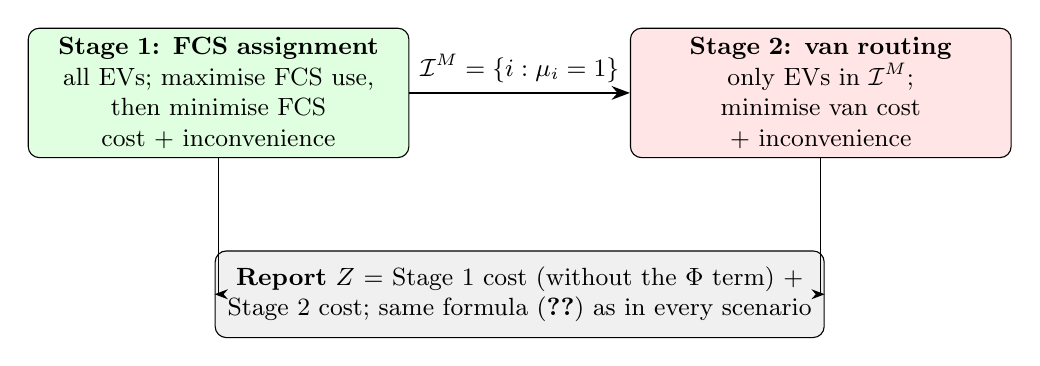
\begin{tikzpicture}[>=Stealth,box/.style={draw,rounded corners,align=center,minimum height=1.1cm,font=\small}]
  \node[box,fill=green!12,text width=4.6cm] (s1) {\textbf{Stage 1: FCS assignment}\\all EVs; maximise FCS use,\\then minimise FCS cost + inconvenience};
  \node[box,fill=red!10,text width=4.6cm,right=2.8cm of s1] (s2) {\textbf{Stage 2: van routing}\\only EVs in $\I^M$;\\minimise van cost + inconvenience};
  \draw[->,thick] (s1) -- node[above,font=\small]{$\I^M=\{i:\mu_i=1\}$} (s2);
  \node[box,fill=black!6,text width=7.5cm,below=2.0cm of $(s1)!0.5!(s2)$] (ev) {\textbf{Report} $Z=$ Stage~1 cost (without the $\Phi$ term) $+$ Stage~2 cost; same formula \eqref{eq:Z} as in every scenario};
  \draw[->] (s1) |- (ev); \draw[->] (s2) |- (ev);
\end{tikzpicture}
\end{center}

Stage~1 does not look at the vans, and Stage~2 cannot change what Stage~1 decided. That is the definition of ``FCS first, then MCS''.

%----------------------------------------------------------------
\subsection{Stage 1: assign EVs to fixed stations}

\textbf{Objective.}
\begin{equation}
\begin{split}
\min\ Z^{(1)}=\;&\underbrace{\Phi\sum_{i\in\I}\mu_i}_{\text{FCS first}}
+\underbrace{c^{EV}\sum_i\sum_{f\in\F_i}d_{if}Y_{if}}_{Z_1}
+\underbrace{Z^F_{\text{energy}}}_{\text{FCS part of }Z_4}\\
&+\underbrace{\sum_i\sum_{f\in\F_i}\rho^F_{if}Y_{if}+\alpha\sum_i w_i(C_i-r_i)+c^L\sum_i w_iL_i}_{\text{FCS customers' inconvenience}}
\end{split}
\label{eq:obj1}
\end{equation}
with $C_i=S_i+\tau^F_iY_i$ in this stage. $\Phi$ is a penalty for handing an EV to the vans. It is chosen larger than anything an extra FCS customer can add to the rest of \eqref{eq:obj1}, e.g.
\[
\Phi > \max_{i}\max_{f\in\F_i}\big(c^{EV}d_{if}+\pi^{\max}E_i+\rho^F_{if}\big)+n\,(\alpha+c^L)\,w_{\max}\,T,
\]
so Stage~1 first \textbf{maximises the number of EVs served at an FCS}, and only among those solutions minimises FCS cost and inconvenience. ($\pi^{\max}$ is the highest grid price.) A numerically safer equivalent is to solve twice: first $\max\sum_iY_i$, then fix that number and minimise the rest.
\ifTOU
Because $Z^F_{\text{energy}}$ uses the peak price, Stage~1 may \emph{start sessions later} to leave the peak, if the price saving beats the extra waiting cost (Section~\ref{sec:expect}).
\fi

\textbf{Constraints.}
\begin{align}
\sum_{g\in\G_i}y_{ig}+\mu_i &= 1 && \forall i\in\I \label{eq:s1assign}\\
S_i &\ge r_i+\sum_{f\in\F_i}t_{if}Y_{if} && \forall i\in\I \label{eq:fcsarr}\\
S_i &\le r_i+T\,(1-\mu_i) && \forall i\in\I \label{eq:s1park}\\
S_j &\ge S_i+\tau^F_i-(T+\tau^F_i)(3-y_{ig}-y_{jg}-o_{ij}) && \forall g,\ (i,j)\in\mathcal{P}_g \label{eq:disj1}\\
S_i &\ge S_j+\tau^F_j-(T+\tau^F_j)(2-y_{ig}-y_{jg}+o_{ij}) && \forall g,\ (i,j)\in\mathcal{P}_g \label{eq:disj2}\\
\sum_i y_{ig_1} &\ge \sum_i y_{ig_2} && \forall f,\ \G_f=\{g_1,g_2\} \label{eq:gunsym}\\
S_i+\tau^F_iY_i &\le T,\qquad L_i\ge S_i+\tau^F_iY_i-l_i && \forall i\in\I \label{eq:s1time}
\end{align}
\ifTOU plus the time-of-use split \eqref{eq:tou1}--\eqref{eq:tou5} of each FCS session (Section~\ref{sec:price}).\fi
\desc{\eqref{eq:s1assign}: every EV either gets one reachable gun or is handed to the vans. An EV that reaches no FCS ($\G_i=\emptyset$) is forced to $\mu_i=1$. \eqref{eq:fcsarr}: an FCS session cannot start before the EV has asked and driven to the station. \eqref{eq:s1park}: for an EV handed to the vans, $S_i$ is parked at $r_i$, so it adds no waiting in Stage~1 (its real start time is decided in Stage~2). \eqref{eq:disj1}--\eqref{eq:disj2}: two EVs on the same gun do not overlap; $o_{ij}$ picks who goes first. With two guns per station this means at most two EVs charge at a station at a time. \eqref{eq:gunsym}: symmetry breaking between the two identical guns (optional). \eqref{eq:s1time}: finished by $T$; lateness.}

\textbf{Optional acceptability rule.} An operator may refuse to send a driver to a station that is ``too inconvenient'', e.g.\ only allow gun $g$ of station $f$ for EV $i$ if $\hat\rho^F_{if}\le\bar\rho$. This only shrinks $\G_i$, so EVs whose stations are all too far go to the vans. Report results with and without it.

\textbf{Output:} $\I^M=\{i:\mu_i=1\}$, the EVs left for the vans; plus each FCS customer's gun and start time.

%----------------------------------------------------------------
\subsection{Stage 2: route the vans to the leftover EVs}

Stage~2 is a vehicle routing problem with time windows, on the EVs in $\I^M$ only. Here $C_i=S_i+\tau^M_i$.

\textbf{Objective.}
\begin{equation}
\begin{split}
\min\ Z^{(2)}=\;&\underbrace{c^M\sum_m\sum_{(i,j)\in\A^M}d_{ij}x_{ijm}}_{Z_2}+\underbrace{\sum_m c^D_mu_m}_{Z_3}+\underbrace{Z^M_{\text{energy}}}_{\text{van part of }Z_4}\\
&+\underbrace{\sum_{i\in\I^M}\sum_m\rho^M_{im}z_{im}+\alpha\sum_{i\in\I^M}w_i(C_i-r_i)+c^L\sum_{i\in\I^M}w_iL_i}_{\text{van customers' inconvenience}}
\end{split}
\label{eq:obj2}
\end{equation}
Since every EV in $\I^M$ must be served by some van, $Z^M_{\text{energy}}$ and the $\rho^M$ term are constants here. They are kept so that $Z^{(2)}$ is the true cost of Stage~2. Waiting and lateness make the vans visit urgent EVs early.

\textbf{Constraints.}
\begin{align}
\sum_{m\in\M}z_{im} &= 1 && \forall i\in\I^M \label{eq:s2assign}\\
\sum_{j:(0,j)\in\A^M}x_{0jm} = \sum_{i:(i,n+1)\in\A^M}x_{i,n+1,m} &= u_m && \forall m \label{eq:depot}\\
\sum_{i:(i,j)\in\A^M}x_{ijm} = \sum_{k:(j,k)\in\A^M}x_{jkm} &= z_{jm} && \forall j\in\I^M,\ m \label{eq:flow}\\
\sum_{i\in\I^M}z_{im} &\le Q_m\,u_m && \forall m \label{eq:cap}\\
\sum_{i\in\I^M}\frac{E_i}{\eta}z_{im}+\beta\sum_{(i,j)\in\A^M}d_{ij}x_{ijm} &\le B_m\,u_m && \forall m \label{eq:batt}
\end{align}
\begin{align}
S_j &\ge \max\{r_j,\ t_{0j}\,x_{0jm}\} && \forall j\in\I^M,\ m \label{eq:depart}\\
S_j &\ge S_i+\tau^M_i+t_{ij}-(T+\tau^M_i+t_{ij})(1-x_{ijm}) && \forall i\neq j,\ m \label{eq:seq}\\
S_i+\tau^M_i+t_{i,n+1} &\le T+(\tau^M_i+t_{i,n+1})(1-x_{i,n+1,m}) && \forall i,\ m \label{eq:return}\\
S_i+\tau^M_i \le T,\quad L_i &\ge S_i+\tau^M_i-l_i && \forall i\in\I^M \label{eq:s2time}\\
u_m &\ge u_{m+1} && m<|\M| \label{eq:vansym}
\end{align}
\desc{\eqref{eq:s2assign}: each leftover EV gets one van. \eqref{eq:depot}: a used van leaves and returns to the depot once. \eqref{eq:flow}: each EV on van $m$ is entered and left exactly once by that van. \eqref{eq:cap}: at most $Q_m$ EVs per van. \eqref{eq:batt}: delivered energy (with transfer losses) plus driving energy fits in the van battery. \eqref{eq:depart}: no start before the request, or before the van can drive there from the depot (written as two linear constraints). \eqref{eq:seq}: if the van goes $i\to j$, it finishes $i$ and drives to $j$ before starting $j$. This gives one EV at a time and removes subtours (MTZ-type). \eqref{eq:return}: back at the depot by $T$. \eqref{eq:s2time}: finished by $T$; lateness. \eqref{eq:vansym}: use identical vans in index order.}

\textbf{If Stage 2 is infeasible} (too many leftover EVs for the fleet by $T$), the sequential policy has \emph{failed} on that instance. For diagnosis, add $s_i\in\{0,1\}$ (``unserved''), replace \eqref{eq:s2assign} by $\sum_mz_{im}+s_i=1$ and add $\Phi^U\sum_is_i$ to \eqref{eq:obj2}. Then report the number of EVs that could not be served. This is a useful comparison with the integrated scenario, which may serve all of them.

%----------------------------------------------------------------
\subsection{Reported value}
\[
Z^{\text{S\scen}}=\big(Z^{(1)*}-\Phi\,|\I^M|\big)+Z^{(2)*},
\]
which is exactly \eqref{eq:Z} evaluated at the combined solution. The stage-1 solution plus the stage-2 solution is a feasible solution of the integrated model (S\ifTOU 4\else 3\fi), so
$Z^{\text{S\ifTOU 4\else 3\fi}}\le Z^{\text{S\scen}}$. The difference is the \emph{value of integration}.

\else
%---------------------------------------------------------------- INT
\subsection{Objective}
\begin{equation}
\min\ Z \quad\text{as in \eqref{eq:Z}, with }Z^F_{\text{energy}}=\ifTOU P^F\textstyle\sum_i\big[\pi^\off(\theta^1_i+\theta^3_i)+\pi^\pk\theta^2_i\big]\else\pi^F\textstyle\sum_iE_iY_i\fi,\quad C_i=S_i+\tau^F_iY_i+\tau^M_iZ_i. \label{eq:objint}
\end{equation}
Written out in full:
\begin{align*}
\min\ Z=\;& c^{EV}\sum_i\sum_{f\in\F_i}d_{if}Y_{if}+c^M\sum_m\sum_{(i,j)\in\A}d_{ij}x_{ijm}+\sum_mc^D_mu_m\\
&+\ifTOU P^F\sum_i\big[\pi^\off(\theta^1_i+\theta^3_i)+\pi^\pk\theta^2_i\big]\else\pi^F\sum_iE_iY_i\fi
+\pi^M\sum_i\sum_m\frac{E_i}{\eta}z_{im}\\
&+\sum_i\sum_{f\in\F_i}\rho^F_{if}Y_{if}+\sum_i\sum_m\rho^M_{im}z_{im}+\alpha\sum_iw_i(C_i-r_i)+c^L\sum_iw_iL_i .
\end{align*}
Every term is linear. One model weighs everything at once: an EV goes to a van exactly when the van's extra km, dispatch and energy cost are outweighed by the effort and waiting it saves the driver\ifTOU, or by the peak-price energy it avoids\fi.

\subsection{Constraints}

\textbf{Assignment.}
\begin{equation}
\sum_{g\in\G_i}y_{ig}+\sum_{m\in\M}z_{im}=1\qquad\forall i\in\I \label{eq:assign}
\end{equation}
\desc{Exactly one resource per EV: one reachable gun or one van. EVs that reach no FCS are forced onto a van.}

\textbf{Fixed stations.}
\begin{align}
S_i &\ge r_i+\sum_{f\in\F_i}t_{if}Y_{if} && \forall i \label{eq:fcsarr}\\
S_j &\ge S_i+\tau^F_i-(T+\tau^F_i)(3-y_{ig}-y_{jg}-o_{ij}) && \forall g,\ (i,j)\in\mathcal{P}_g \label{eq:disj1}\\
S_i &\ge S_j+\tau^F_j-(T+\tau^F_j)(2-y_{ig}-y_{jg}+o_{ij}) && \forall g,\ (i,j)\in\mathcal{P}_g \label{eq:disj2}\\
\sum_iy_{ig_1} &\ge \sum_iy_{ig_2} && \forall f,\ \G_f=\{g_1,g_2\} \label{eq:gunsym}
\end{align}
\desc{\eqref{eq:fcsarr}: an FCS session starts after the request and the drive to the station (for a van customer this is just $S_i\ge r_i$). \eqref{eq:disj1}--\eqref{eq:disj2}: EVs on the same gun do not overlap; $o_{ij}$ chooses the order. \eqref{eq:gunsym}: optional symmetry breaking.}

\textbf{Vans: routes, capacity, battery.}
\begin{align}
\sum_{j:(0,j)\in\A}x_{0jm}=\sum_{i:(i,n+1)\in\A}x_{i,n+1,m} &= u_m && \forall m \label{eq:depot}\\
\sum_{i:(i,j)\in\A}x_{ijm}=\sum_{k:(j,k)\in\A}x_{jkm} &= z_{jm} && \forall j\in\I,\ m \label{eq:flow}\\
\sum_iz_{im} &\le Q_mu_m && \forall m \label{eq:cap}\\
\sum_i\frac{E_i}{\eta}z_{im}+\beta\sum_{(i,j)\in\A}d_{ij}x_{ijm} &\le B_mu_m && \forall m \label{eq:batt}
\end{align}
\desc{\eqref{eq:depot}: a used van leaves and returns once. \eqref{eq:flow}: each EV on van $m$ is visited exactly once by it. \eqref{eq:cap}: at most $Q_m$ EVs. \eqref{eq:batt}: delivered energy (with losses) plus driving energy fits in the battery.}

\textbf{Vans: timing (one EV at a time, no subtours).}
\begin{align}
S_j &\ge t_{0j}\,x_{0jm} && \forall j\in\I,\ m \label{eq:depart}\\
S_j &\ge S_i+\tau^M_i+t_{ij}-(T+\tau^M_i+t_{ij})(1-x_{ijm}) && \forall i\neq j\in\I,\ m \label{eq:seq}\\
S_i+\tau^M_i+t_{i,n+1} &\le T+(\tau^M_i+t_{i,n+1})(1-x_{i,n+1,m}) && \forall i,\ m \label{eq:return}
\end{align}
\desc{\eqref{eq:depart}: the first stop cannot start before the van has driven there. \eqref{eq:seq}: $i\to j$ means finish $i$, drive, then start $j$; start times rise along a route, so no subtour can close. \eqref{eq:return}: back at the depot by $T$.}

\textbf{Horizon and lateness.}
\begin{equation}
C_i\le T,\qquad L_i\ge C_i-l_i\qquad\forall i\in\I \label{eq:time}
\end{equation}
\desc{Every EV is fully charged within the horizon; $L_i$ measures lateness.}

\ifTOU
\textbf{Time-of-use split.} Constraints \eqref{eq:tou1}--\eqref{eq:tou5} of Section~\ref{sec:price}.
\fi

\textbf{Symmetry and domains.}
\begin{equation}
u_m\ge u_{m+1};\qquad y,z,x,u,o\ifTOU,\kappa\fi\in\{0,1\};\qquad S_i,L_i\ifTOU,\theta^p_i\fi\ge0 \label{eq:dom}
\end{equation}
\fi

%=====================================================================
\section{Learning-to-optimise (RL) formulation}\label{sec:rl}

\textbf{Main rule:} the reward of each action is \emph{minus the increase in $Z$ that the action causes}. The rewards over an episode then add up to $-Z$ of the solution the policy builds. RL and MILP results are measured on the same yardstick \eqref{eq:Z}, and the MILP optimum is the benchmark for the RL gap.

\ifSEQ
%---------------------------------------------------------------- RL SEQ
The RL pipeline has the same two stages as the MILP.

\subsection{Stage 1 policy: FCS assignment}
\begin{itemize}[leftmargin=1.4em,itemsep=2pt]
  \item \textbf{Episode / epochs:} EVs are taken in order of request time $r_i$ (ties: higher $w_i$ first). One decision per EV.
  \item \textbf{State:} features of the current EV $k$ ($E_k,r_k,l_k,w_k,R_k$, location); for each gun $g$ the time $F_g$ it becomes free; summary features of the EVs still to come (count and positions near each station)\ifTOU; the current price and the time until $T_1$ and $T_2$\fi.
  \item \textbf{Action:} a gun $g\in\G_k$, or ``hand to vans''. \textbf{FCS-first mask:} ``hand to vans'' is allowed \emph{only} if no gun can finish EV $k$ by $T$ (or, with the optional rule, if all remaining guns have $\hat\rho^F_{kf}>\bar\rho$).
  \ifTOU\item \textbf{Optional timing action:} ``gun $g$, start after the peak'', i.e.\ $S_k=\max\{\text{earliest},T_2\}$, allowed only if the session still ends by $T$.\fi
  \item \textbf{Transition:} $S_k=\max\{r_k+t_{kf},F_g\}$ (or later, for the timing action); $F_g\leftarrow S_k+\tau^F_k$.
  \item \textbf{Reward:} $-\Big[c^{EV}d_{kf}+\text{energy}_k+\rho^F_{kf}+\alpha w_k(S_k+\tau^F_k-r_k)+c^Lw_k(S_k+\tau^F_k-l_k)^+\Big]$, where energy$_k$ = \ifTOU$P^F\big[\pi^\off\cdot(\text{off-peak hours of }[S_k,S_k+\tau^F_k])+\pi^\pk\cdot(\text{peak hours})\big]$, computed exactly in the simulator\else$\pi^FE_k$\fi. Handing an EV to the vans gives reward $0$ here; its cost is counted in Stage~2.
\end{itemize}
Note: a simple baseline for Stage~1 is the greedy rule ``gun with the largest one-step reward''. What RL can learn on top of this is, for example, to keep a nearby gun free for an urgent EV that arrives later.

\subsection{Stage 2 policy: van routing over $\I^M$}
\begin{itemize}[leftmargin=1.4em,itemsep=2pt]
  \item \textbf{Epochs:} whenever a van becomes free (the earliest-free van decides first).
  \item \textbf{State:} for each van: position, time free, remaining battery $b_m$, EVs served so far, dispatched or not; for each unserved EV in $\I^M$: location, $E_i,r_i,l_i,w_i$; current time.
  \item \textbf{Action:} the next EV $j$ for this van, or ``return to depot'' (ends the route). Mask: $j$ must be feasible: battery covers $E_j/\eta$ plus driving to $j$ and back to the depot, the count stays $\le Q_m$, and $j$ can be finished with the van back at the depot by $T$.
  \item \textbf{Transition:} $S_j=\max\{r_j,\ \text{time free}+t_{\text{pos},j}\}$; the van moves to $j$ and is free at $S_j+\tau^M_j$; $b_m$ falls by $E_j/\eta+\beta d_{\text{pos},j}$.
  \item \textbf{Reward:} serving $j$: $-\Big[c^Md_{\text{pos},j}+c^D_m[\text{first stop}]+\pi^M\frac{E_j}{\eta}+\rho^M_{jm}+\alpha w_j(S_j+\tau^M_j-r_j)+c^Lw_j(S_j+\tau^M_j-l_j)^+\Big]$; returning: $-c^Md_{\text{pos},0}$. EVs still unserved at the end: $-\Phi^U$ each.
  \item \textbf{Policy:} an attention-based routing policy (e.g.\ Kool et al., 2019, ``Attention, Learn to Solve Routing Problems!'') trained with REINFORCE or PPO. Baseline: nearest-feasible-EV heuristic.
\end{itemize}
Episode return of Stage~1 + Stage~2 $=-Z^{\text{S\scen}}$.

\else
%---------------------------------------------------------------- RL INT
One policy decides both who serves each EV and the van routes.
\begin{itemize}[leftmargin=1.4em,itemsep=2pt]
  \item \textbf{Episode / epochs:} EVs are taken in order of request time $r_i$ (ties: higher $w_i$ first). One decision per EV.
  \item \textbf{State:} (i) the current EV $k$: location, $E_k,r_k,l_k,w_k,R_k$, reachable stations; (ii) each gun $g$: time $F_g$ it becomes free; (iii) each van $m$: current end-of-route position, time free, remaining battery $b_m$, EVs served, dispatched or not; (iv) embeddings of the not-yet-assigned EVs (for look-ahead)\ifTOU; (v) current price, time until $T_1$ and $T_2$\fi.
  \item \textbf{Action:} $a\in\G_k\cup\M$: a gun, or a van (EV $k$ is appended to the end of that van's route). \textbf{Mask} infeasible actions: a gun that cannot finish $k$ by $T$; a van without enough battery for $E_k/\eta$ plus the drive to $k$ and back to the depot, with $Q_m$ reached, or unable to finish $k$ and return by $T$.
  \ifTOU\item \textbf{Optional timing action:} ``gun $g$, start after the peak'' ($S_k=\max\{\text{earliest},T_2\}$, if it still ends by $T$).\fi
  \item \textbf{Transition:} gun: $S_k=\max\{r_k+t_{kf},F_g\}$, $F_g\leftarrow S_k+\tau^F_k$. Van: $S_k=\max\{r_k,\ \text{free}_m+t_{\text{pos}_m,k}\}$, then the van moves to $k$, $\text{free}_m\leftarrow S_k+\tau^M_k$, $b_m\mathrel{-}=E_k/\eta+\beta d_{\text{pos}_m,k}$.
  \item \textbf{Reward} $=-\Delta Z$:
  \begin{align*}
  \text{gun } g\text{ at }f:&\quad -\Big[c^{EV}d_{kf}+\text{energy}^F_k+\rho^F_{kf}+\alpha w_k(C_k-r_k)+c^Lw_k(C_k-l_k)^+\Big]\\
  \text{van } m:&\quad -\Big[c^M\big(d_{\text{pos}_m,k}+d_{k,0}-d_{\text{pos}_m,0}\big)+c^D_m[\text{first use}]+\pi^M\tfrac{E_k}{\eta}\\
  &\qquad\quad+\rho^M_{km}+\alpha w_k(C_k-r_k)+c^Lw_k(C_k-l_k)^+\Big]
  \end{align*}
  The van distance term is the \emph{change} in route length when $k$ is inserted before the return to the depot, so the sum over the episode equals the total route length (the return legs telescope). energy$^F_k$ = \ifTOU$P^F\big[\pi^\off\cdot(\text{off-peak hours})+\pi^\pk\cdot(\text{peak hours of }[S_k,C_k])\big]$, computed exactly by the simulator; no linearisation is needed in RL\else$\pi^FE_k$\fi.
  \item \textbf{Dead end:} if every action is masked, EV $k$ is unserved: reward $-\Phi^U$, and the episode continues. Report the count.
  \item \textbf{Policy:} masked categorical policy over guns and vans, encoder with attention over EVs, guns and vans; trained with PPO. Natural baseline: greedy, i.e.\ choose the action with the largest one-step reward. That is the pairwise rule ``smallest $\hat\rho$ + cost'' from Section~\ref{sec:inc}.
\end{itemize}
Restriction to note: vans serve EVs in assignment order (append only). A variant that inserts $k$ at the cheapest position of a route is more flexible but has a larger action space.
\fi

\textbf{Reward scaling.} For stable training divide every reward by a constant, e.g.\ the greedy baseline's average $Z$ on the training instances. This does not change the optimal policy.

%=====================================================================
\section{What to expect and what to report}\label{sec:expect}

\ifnum\scen=1
\begin{itemize}[leftmargin=1.4em,itemsep=2pt]
  \item Vans serve only EVs that reach no station, or that the stations cannot finish by $T$. If stations have spare capacity, very few vans are dispatched.
  \item Inconvenience is high for EVs far from the nearest station (worked example: Rs\,682 at the FCS, against Rs\,458 if a van had been allowed).
  \item With too few vans Stage~2 becomes infeasible (unserved EVs), even when the integrated model S3 could serve everyone. Report the smallest $|\M|$ at which S1 is feasible and compare it with S3.
\end{itemize}
\fi
\ifnum\scen=2
\begin{itemize}[leftmargin=1.4em,itemsep=2pt]
  \item \textbf{When does Stage~1 delay a session to avoid the peak?} Moving one hour of charging out of the peak saves $(\pi^\pk-\pi^\off)P^F=3\times22=$ Rs\,66, but delays completion by up to an hour, which costs $\alpha w_i\ge$ Rs\,200. So with the default values Stage~1 almost never delays. It mostly pays the higher price, and S2 costs roughly S1 plus the peak surcharge. Sessions start later only if $\alpha$ is small (try $\lambda<0.33$ in the sensitivity analysis).
  \item The van assignment is the same as in S1 unless Stage~1's timing changes which EVs fit at the stations. Stage~1 cannot use vans to escape the peak price.
  \item Extra KPI: \textbf{grid energy drawn at FCS during the peak}, $P^F\sum_i\theta^2_i$ (kWh). Compare with S4.
\end{itemize}
\fi
\ifnum\scen=3
\begin{itemize}[leftmargin=1.4em,itemsep=2pt]
  \item Vans take EVs for which the saved inconvenience exceeds the extra van cost (worked example: van chosen, saving Rs\,224). Expect vans to serve EVs that are far from every station, have low range (high $w_i$), or have early deadlines, while EVs near a station still use it.
  \item \textbf{Value of integration under flat price:} $Z^{\text{S1}}-Z^{\text{S3}}\ge0$. Report it per component ($Z_1,\dots,Z_5$): typically operating cost rises a little and inconvenience falls a lot.
  \item Vary $|\M|$ (0, 1, 2, \dots): the first few vans lower $Z$ sharply, then the effect levels off. That curve shows the scenarios where mobile chargers help most.
\end{itemize}
\fi
\ifnum\scen=4
\begin{itemize}[leftmargin=1.4em,itemsep=2pt]
  \item During the peak a van kWh costs about the same as an FCS kWh (Rs\,10.0 each), so the vans' energy disadvantage disappears and vans also absorb \emph{peak-hour} demand that would otherwise be charged on the grid at peak price.
  \item Expect more van usage than in S3, concentrated on requests in $[T_1,T_2]$, and lower grid energy at the stations during the peak, $P^F\sum_i\theta^2_i$, than in S2.
  \item \textbf{Value of integration under peak pricing:} $Z^{\text{S2}}-Z^{\text{S4}}$. It should be larger than $Z^{\text{S1}}-Z^{\text{S3}}$, because integration now also allows price arbitrage.
  \item \textbf{Peak pricing with full flexibility:} $Z^{\text{S4}}-Z^{\text{S3}}$ should be smaller than $Z^{\text{S2}}-Z^{\text{S1}}$: vans cushion the price increase.
\end{itemize}
\fi

\textbf{Cross-scenario comparison table} (fill in from the four runs):
\begin{center}
\renewcommand{\arraystretch}{1.2}
\begin{tabular}{@{}lll@{}}
\toprule
\textbf{Comparison} & \textbf{Measures} & \textbf{Expected sign} \\
\midrule
S1 $-$ S3 & value of integration, flat price & $\ge0$ \\
S2 $-$ S4 & value of integration, peak price & $\ge0$, larger than S1 $-$ S3 \\
S2 $-$ S1 & cost of peak pricing, FCS-first operator & $>0$ \\
S4 $-$ S3 & cost of peak pricing, flexible operator & $>0$, smaller than S2 $-$ S1 \\
\bottomrule
\end{tabular}
\end{center}
Report for each: $Z$ and its components, number of vans used, EVs per resource, mean and maximum inconvenience per EV, total lateness, peak-hour grid energy, solve time, and (for RL) the gap to the MILP optimum.

%=====================================================================
\appendix
\section{Illustrative parameter values}\label{app:values}

These are starting values for experiments, not data. All are meant to be varied in the analysis. Values in Rs.

\begin{center}
\renewcommand{\arraystretch}{1.15}
\begin{tabular}{@{}llp{6.2cm}@{}}
\toprule
\textbf{Parameter} & \textbf{Value} & \textbf{Note} \\
\midrule
$T$, $[T_1,T_2]$ & 7 h, $[2,6]$ & 16:00--23:00, peak 18:00--22:00 \\
$P^F$, $P^M$ & 22 kW, 30 kW & \\
$v$, $\beta$, $\eta$ & 25 km/h, 0.25 kWh/km, 0.9 & \\
$B_m$, $Q_m$, $|\M|$ & 150 kWh, 6, 2--6 & \\
$c^{EV}$, $c^M$, $c^D_m$ & Rs\,4/km, Rs\,15/km, Rs\,1500 & van km includes driver time \\
$\pi^F$ (flat) & Rs\,8.7/kWh & equals the time-average of the ToU tariff over $[0,T]$ \\
$\pi^\off$, $\pi^\pk$ (ToU) & Rs\,7/kWh, Rs\,10/kWh & $(3\times7+4\times10)/7=8.7$ \\
$c^{bat}$ & Rs\,2/kWh & van battery wear \\
$\pi^M$ & Rs\,10.7 (flat) / Rs\,9.0 (ToU) & $=\pi^F+c^{bat}$ / $=\pi^\off+c^{bat}$ \\
$\alpha$, $\alpha^D$ & Rs\,200/h, Rs\,100/h & value of time; extra for attended time \\
$h^F$, $h^M$, $\varphi$ & Rs\,50, Rs\,10, Rs\,100 & trip hassle, hand-over, range stress \\
$c^L$ & Rs\,300/h & lateness \\
$w_i$ & $1+2(1-R_i/R_{\max})$, $R_i\sim U[3,40]$ km & priority from remaining range \\
\bottomrule
\end{tabular}
\end{center}

The flat price is set to the time-average of the peak tariff. The price \emph{level} is then the same in both pricing cases, and only the price \emph{shape} differs. Without this, part of S1 vs S2 would just reflect a different average price.

\end{document}
"
%    pdflatex -jobname=scenario3_flat_integrated   "\def\scen{3}% =====================================================================
%  One source, four PDFs.  Build with build.sh (or by hand):
%    pdflatex -jobname=scenario1_flat_sequential   "\def\scen{1}% =====================================================================
%  One source, four PDFs.  Build with build.sh (or by hand):
%    pdflatex -jobname=scenario1_flat_sequential   "\def\scen{1}\input{scenario_master}"
%    pdflatex -jobname=scenario2_peak_sequential   "\def\scen{2}\input{scenario_master}"
%    pdflatex -jobname=scenario3_flat_integrated   "\def\scen{3}\input{scenario_master}"
%    pdflatex -jobname=scenario4_peak_integrated   "\def\scen{4}\input{scenario_master}"
%  (run each twice for cross-references)
% =====================================================================
\documentclass[11pt,a4paper]{article}
\usepackage[margin=2.2cm]{geometry}
\usepackage{amsmath,amssymb,amsfonts}
\usepackage{booktabs,array,tabularx}
\usepackage{enumitem}
\usepackage[table]{xcolor}
\usepackage{tikz}
\usetikzlibrary{arrows.meta,positioning,calc}
\usepackage[colorlinks=true,linkcolor=blue!50!black,urlcolor=blue!50!black]{hyperref}
\usepackage{titlesec}
\titleformat{\section}{\large\bfseries}{\thesection}{0.8em}{}
\titleformat{\subsection}{\normalsize\bfseries}{\thesubsection}{0.8em}{}
\setlength{\parindent}{0pt}
\setlength{\parskip}{5pt}

% ---------------- scenario switches ----------------
\ifdefined\scen\else\def\scen{1}\fi
\newif\ifTOU \TOUfalse   % true = time-of-use (peak) price
\newif\ifSEQ \SEQfalse   % true = FCS first, then MCS
\ifnum\scen=1 \SEQtrue \fi
\ifnum\scen=2 \TOUtrue \SEQtrue \fi
\ifnum\scen=4 \TOUtrue \fi

\newcommand{\pricename}{\ifTOU time-of-use price (dearer evening peak)\else single (flat) price all day\fi}
\newcommand{\structname}{\ifSEQ FCS first, then MCS (sequential)\else FCS and MCS together (integrated)\fi}

% ---------------- notation ----------------
\newcommand{\I}{\mathcal{I}}
\newcommand{\F}{\mathcal{F}}
\newcommand{\G}{\mathcal{G}}
\newcommand{\M}{\mathcal{M}}
\newcommand{\N}{\mathcal{N}}
\newcommand{\A}{\mathcal{A}}
\newcommand{\Rs}{\text{Rs}\,}
\newcommand{\pk}{\mathrm{pk}}
\newcommand{\off}{\mathrm{off}}
\newcommand{\desc}[1]{\par\vspace{-2pt}{\small\color{black!75}\textit{Meaning:} #1}\par\vspace{4pt}}
\newcommand{\cell}[2]{\ifnum\scen=#1\cellcolor{blue!18}\textbf{S#1 (this document)}\\\textbf{#2}\else S#1\\#2\fi}

\title{\textbf{EV Charging Network Optimisation}\\[4pt]
\large Scenario \scen: \pricename\ $+$ \structname\\[2pt]
\normalsize MILP and RL formulation}
\author{CP 320 OR for Mobility Management, course project}
\date{2 October 2026}

\begin{document}
\maketitle

%=====================================================================
\section{Where this scenario sits}

The project studies four scenarios: two ways of pricing grid electricity, times two ways of making the decisions.

\begin{center}
\renewcommand{\arraystretch}{1.5}
\begin{tabular}{>{\raggedright\arraybackslash}p{4.2cm}|>{\centering\arraybackslash}p{4.6cm}|>{\centering\arraybackslash}p{4.6cm}}
 & \textbf{Flat price all day} & \textbf{Time-of-use (peak) price} \\ \hline
\textbf{Sequential:} FCS first, leftover EVs to MCS &
\begin{tabular}[c]{@{}c@{}}\cell{1}{flat + sequential}\end{tabular} &
\begin{tabular}[c]{@{}c@{}}\cell{2}{peak + sequential}\end{tabular} \\ \hline
\textbf{Integrated:} FCS and MCS decided together &
\begin{tabular}[c]{@{}c@{}}\cell{3}{flat + integrated}\end{tabular} &
\begin{tabular}[c]{@{}c@{}}\cell{4}{peak + integrated}\end{tabular} \\
\end{tabular}
\end{center}

\textbf{The four scenarios do not have four different objectives.} They share \emph{one} cost yardstick $Z$ (Section~\ref{sec:obj}): the same cost terms and the same customer inconvenience (Section~\ref{sec:inc}). Only two things change:
\begin{itemize}[leftmargin=1.4em,itemsep=1pt]
  \item \textbf{Pricing} changes the formula for one term, the FCS energy cost (Section~\ref{sec:price}).
  \item \textbf{Decision structure} changes \emph{how} $Z$ is minimised: in one model (integrated), or in two stages (sequential), where each stage minimises its own part of $Z$.
\end{itemize}
Because the yardstick is the same, the four optimal values can be compared directly. The differences measure the \emph{value of integration} (S1$\to$S3, S2$\to$S4) and the \emph{effect of peak pricing} (S1$\to$S2, S3$\to$S4).

\ifnum\scen=1
\textbf{This scenario (S1)} is the baseline, the ``status quo''. Electricity costs the same at every hour, every EV that can be charged at a fixed station is sent there, and vans only take what is left over.
\fi
\ifnum\scen=2
\textbf{This scenario (S2)} keeps the FCS-first rule of S1, but grid electricity is dearer during the evening peak. Stage~1 can react to the price only by \emph{rescheduling} FCS sessions. It cannot hand a peak-hour EV to a van.
\fi
\ifnum\scen=3
\textbf{This scenario (S3)} keeps the flat price of S1, but the operator decides FCS and MCS service \emph{together}. An EV can be sent to a van even when a fixed station could take it, whenever that lowers total cost plus inconvenience.
\fi
\ifnum\scen=4
\textbf{This scenario (S4)} is the most flexible one: peak pricing at fixed stations, and FCS and MCS decided together. Van energy was bought off-peak, so vans can also be used to keep charging \emph{out of the expensive peak}.
\fi

%=====================================================================
\section{Setting and assumptions}\label{sec:setting}

\textbf{Time.} The planning horizon is $[0,T]$ with $T=7$\,h (16:00--23:00). It contains the evening peak window $[T_1,T_2]=[2,6]$ (18:00--22:00). The horizon is the same in all four scenarios. It is wider than the peak itself so that, under peak pricing, there is cheaper time on both sides of the peak.\ifTOU\else\ In this scenario the price is flat, so the window plays no role in the model.\fi

\textbf{Assumptions} (the same as MILP v3, plus two about energy):
\begin{enumerate}[leftmargin=1.6em,itemsep=1pt]
  \item Static, continuous time. All requests in the horizon are known at time $0$, and request $i$ becomes active at $r_i$.
  \item An EV served by an FCS drives there itself on its own battery (only to stations within its range $R_i$). The driver stays with the car while it waits for a free gun and while it charges.
  \item An EV served by an MCS stays parked where it is, and the driver is free in the meantime.
  \item Each FCS gun and each van charges one EV at a time, without interruption, at constant power.
  \item A van's battery covers both its driving and the energy it delivers. \textbf{The van battery is charged at the depot before the horizon starts}\ifTOU, i.e.\ at the off-peak price\fi, and is not recharged during the horizon.
  \item Every EV must be fully charged by $T$ (hard). Finishing after the driver's desired time $l_i$ is allowed but penalised.
\end{enumerate}

%=====================================================================
\section{Notation}\label{sec:notation}

\subsection*{Sets}
\begin{tabularx}{\textwidth}{@{}lX@{}}
\toprule
$\I=\{1,\dots,n\}$ & EV charging requests \\
$\F$; $\G_f$ ($|\G_f|=2$); $\G=\bigcup_f\G_f$ & fixed charging stations; guns of FCS $f$; all guns ($f(g)$ = station of gun $g$) \\
$\F_i=\{f: d_{if}\le R_i\}$, $\G_i=\bigcup_{f\in\F_i}\G_f$ & stations / guns EV $i$ can reach on its remaining range \\
$\M$ & mobile charging vans (MCS) \\
$0,\ n+1$ & depot as start node / end node (same place) \\
$\N=\{0\}\cup\I\cup\{n+1\}$, $\A$ & routing nodes; allowed van arcs $(i,j)$, $i\in\{0\}\cup\I$, $j\in\I\cup\{n+1\}$, $i\neq j$ \\
$\mathcal{P}_g=\{(i,j): i<j,\ g\in\G_i\cap\G_j\}$ & pairs of EVs that could share gun $g$ \\
\ifSEQ
$\I^M\subseteq\I$ & EVs handed to the vans by Stage~1 (an \emph{output} of Stage~1, a fixed input to Stage~2) \\
$\N^M$, $\A^M$ & routing nodes / arcs restricted to $\I^M$ \\
\fi
\bottomrule
\end{tabularx}

\subsection*{Parameters}
\begin{tabularx}{\textwidth}{@{}lX@{}}
\toprule
$E_i,\ r_i,\ l_i,\ R_i$ & energy demand (kWh), request time, desired completion time (h), remaining range (km) \\
$w_i\ge1$ & priority of EV $i$; $w_i=1+\kappa(1-R_i/R_{\max})$, so low-range EVs weigh more \\
$P^F,\ P^M$ & charging power of an FCS gun (22\,kW) / of a van (e.g.\ 30\,kW) \\
$\tau^F_i=E_i/P^F,\ \tau^M_i=E_i/P^M$ & charging time of EV $i$ at an FCS / by a van (h) \\
$d_{if},t_{if}$;\ $d_{ij},t_{ij}$ & distance (km) and time (h): EV$\to$FCS; between routing nodes ($t=d/v$) \\
$B_m,\ Q_m,\ \beta,\ \eta$ & van battery (kWh), max EVs per van, van consumption (kWh/km), transfer efficiency \\
$c^{EV},\ c^M,\ c^D_m$ & cost per km of EV driving, per km of van driving; fixed dispatch cost of van $m$ \\
\ifTOU
$\pi^\off,\ \pi^\pk$ & grid price (Rs/kWh) off-peak / in $[T_1,T_2]$, with $\pi^\pk\ge\pi^\off$ \\
\else
$\pi^F$ & grid price (Rs/kWh), the same at every hour \\
\fi
$c^{bat}$ & van battery wear per kWh cycled \\
$\pi^M$ & cost of 1 kWh taken from a van battery: $\pi^M=\ifTOU\pi^\off\else\pi^F\fi+c^{bat}$ (Section~\ref{sec:price}) \\
$\alpha,\ \alpha^D,\ h^F,\ h^M,\ \varphi,\ c^L$ & inconvenience coefficients (Section~\ref{sec:inc}) \\
\bottomrule
\end{tabularx}

\subsection*{Decision variables}
\begin{tabularx}{\textwidth}{@{}llX@{}}
\toprule
$y_{ig}$ & $\{0,1\}$ & EV $i$ charged at gun $g\in\G_i$ \\
$z_{im}$ & $\{0,1\}$ & EV $i$ served by van $m$ \\
$x_{ijm}$ & $\{0,1\}$ & van $m$ drives arc $(i,j)$ \\
$u_m$ & $\{0,1\}$ & van $m$ is dispatched \\
$o_{ij}$ & $\{0,1\}$ & for EVs $i<j$ that could share a gun: 1 if $i$ is charged before $j$ \\
\ifSEQ
$\mu_i$ & $\{0,1\}$ & Stage~1 only: EV $i$ is handed to the van fleet \\
\fi
\ifTOU
$\theta^1_i,\theta^2_i,\theta^3_i$ & $\ge0$ & hours of EV $i$'s FCS session before / inside / after the peak \\
$\kappa^1_i,\kappa^3_i$ & $\{0,1\}$ & EV $i$'s FCS session starts before $T_1$ / ends after $T_2$ \\
\fi
$S_i$ & $\ge0$ & time charging of EV $i$ starts (h), on whichever resource \\
$L_i$ & $\ge0$ & lateness of EV $i$ beyond $l_i$ (h) \\
\bottomrule
\end{tabularx}

\textbf{Short-hands} (linear expressions, not new variables):
\[
Y_{if}=\sum_{g\in\G_f}y_{ig},\qquad Y_i=\sum_{g\in\G_i}y_{ig}\ (\text{EV $i$ uses an FCS}),\qquad Z_i=\sum_{m\in\M}z_{im}\ (\text{EV $i$ uses a van}),
\]
\[
C_i=S_i+\tau^F_i\,Y_i+\tau^M_i\,Z_i \quad\text{(time EV $i$ is fully charged).}
\]

%=====================================================================
\section{Customer inconvenience}\label{sec:inc}

This section is \textbf{identical in all four scenario documents}. Inconvenience is a property of the customer, not of the price or of the planning method.

\subsection{What we mean by inconvenience}

Inconvenience is \emph{what the driver loses} from the moment they ask for a charge ($r_i$) until the car is fully charged ($C_i$), \emph{converted into rupees} so it can be added to the operator's costs. A driver loses three different things:

\begin{enumerate}[leftmargin=1.6em,itemsep=2pt]
  \item \textbf{Waiting:} the car is not ready. This lasts $C_i-r_i$ hours and affects \emph{every} driver, FCS or MCS.
  \item \textbf{Effort:} only an FCS customer has to drive to the station and sit there while the car charges. An MCS customer stays at home or at work and does something else. Driving to a far station also uses scarce battery range, which causes stress (``range anxiety'').
  \item \textbf{A missed deadline:} the car is still not ready at the time $l_i$ the driver needs it.
\end{enumerate}

Each loss gets a price in Rs per hour (or per event). All of them are multiplied by the priority $w_i$: an hour of delay for an EV with 5\,km of range left counts more than for one with 40\,km.

\subsection{The three components}

\begin{center}
\renewcommand{\arraystretch}{1.3}
\begin{tabularx}{\textwidth}{@{}>{\raggedright\arraybackslash}p{2.6cm}>{\raggedright\arraybackslash}X>{\raggedright\arraybackslash}X>{\raggedright\arraybackslash}p{3.0cm}@{}}
\toprule
\textbf{Component} & \textbf{EV $i$ at FCS $f$} & \textbf{EV $i$ by a van} & \textbf{Known when?} \\
\midrule
Effort & $w_i\big[\alpha^D(t_{if}+\tau^F_i)+h^F+\varphi\,d_{if}/R_i\big]$: driving and sitting at the station, a fixed trip hassle, range stress & $w_i\,h^M$: being reachable and handing over the car & \textbf{Static:} known as soon as the resource is chosen \\
Waiting & $w_i\,\alpha\,(C_i-r_i)$ = drive + \emph{queue at the gun} + charge & $w_i\,\alpha\,(C_i-r_i)$ = \emph{wait for the van} + charge & \textbf{Dynamic:} depends on the queue / van route \\
Missed deadline & $w_i\,c^L\,L_i$, $L_i=\max\{0,C_i-l_i\}$ & same & Dynamic \\
\bottomrule
\end{tabularx}
\end{center}

\textbf{Coefficients.}
$\alpha$ (Rs/h) is the value of an hour the car is not ready.
$\alpha^D$ (Rs/h) is the \emph{extra} value of an hour the driver must personally spend driving or sitting at the station: an hour at the station costs $\alpha+\alpha^D$, an hour waiting at home for a van costs only $\alpha$.
$h^F,h^M$ (Rs) are fixed hassle costs of one trip to a station / one van hand-over.
$\varphi$ (Rs) is the range-stress cost of a trip that uses the \emph{whole} remaining range ($d_{if}/R_i\le1$ is the fraction used).
$c^L$ (Rs/h) is the cost per hour late.

\subsection{Pairwise form: inconvenience of a (customer, resource) pair}

The natural first idea is: \emph{for every pair (EV $i$, FCS $f$) and every pair (EV $i$, van $m$) there is an inconvenience number, and the operator picks the pair with the lowest cost plus inconvenience.} The static part fits this idea exactly:
\[
\boxed{\;\rho^F_{if}=w_i\Big[\alpha^D\,(t_{if}+\tau^F_i)+h^F+\varphi\,\frac{d_{if}}{R_i}\Big]\qquad
\rho^M_{im}=w_i\,h^M\;}
\]
These are \textbf{parameters}, computed before solving, one number per (EV, FCS) pair and per (EV, van) pair. In the objective they appear linearly: $\sum_i\sum_f\rho^F_{if}Y_{if}+\sum_i\sum_m\rho^M_{im}z_{im}$.

Note that $\rho^M_{im}$ does not depend on $m$. Vans are identical and all start at the same depot, so the driver does not care \emph{which} van comes, only \emph{when} it comes. That ``when'' is the waiting part.

\subsection{Why waiting cannot be a fixed pairwise number}

It is tempting to also write the waiting as a pairwise number, e.g.\ ``the van needs 5 minutes to reach EV $i$''. But that depends on \emph{where the van is coming from}, which depends on the route the model is still choosing: if EV $i$ is the 4th stop of a van, the wait is the time for three charging sessions plus four drives. Likewise, waiting at an FCS depends on how many EVs are queued at that gun. So waiting is not known before solving. It is a function of decision variables:
\[
\text{waiting cost of EV } i \;=\; w_i\,\alpha\,(C_i-r_i),\qquad C_i=S_i+\tau^F_iY_i+\tau^M_iZ_i .
\]
This is \textbf{linear} in the variables ($S_i$, $y$, $z$), so it fits in a MILP directly. The constraints of Section~\ref{sec:milp} make $S_i$ equal to the true start time, including driving, queueing at the gun and the van's route. The term $\sum_i w_i\alpha r_i$ is a constant and may be dropped when solving.

\textbf{Pairwise \emph{estimate}} (used for intuition, by the RL policy and in heuristics): if there is no queue and the van comes straight to $i$,
\[
\hat\rho^{F}_{if}=\rho^F_{if}+w_i\alpha\,(t_{if}+\tau^F_i),\qquad
\hat\rho^{M}_{im}=\rho^M_{im}+w_i\alpha\,(t^{\text{van}}_{m\to i}+\tau^M_i),
\]
where $t^{\text{van}}_{m\to i}$ is the time until van $m$ can reach $i$ from where it currently is. In the RL formulation (Section~\ref{sec:rl}) the van's position \emph{is} known at each decision, so there this estimate becomes exact.

\subsection{Total inconvenience and how it enters the objective}

\begin{equation}
\boxed{\;
Z_{\text{inc}}=\underbrace{\sum_{i\in\I}\sum_{f\in\F_i}\rho^F_{if}Y_{if}+\sum_{i\in\I}\sum_{m\in\M}\rho^M_{im}z_{im}}_{\text{effort (static, pairwise)}}
+\underbrace{\alpha\sum_{i\in\I}w_i\,(C_i-r_i)}_{\text{waiting (dynamic)}}
+\underbrace{c^L\sum_{i\in\I}w_i\,L_i}_{\text{missed deadline}}
\;}\label{eq:inc}
\end{equation}
All three parts are in rupees, so $Z_{\text{inc}}$ is simply added to the operating costs. Nothing has to be normalised.

\subsection{Worked example: your ``10 km to the FCS vs.\ van in 5 minutes'' case}

EV $i$: $E_i=20$\,kWh, $R_i=40$\,km (so $w_i=1$); nearest free FCS $d_{if}=10$\,km away, $t_{if}=0.4$\,h at 25\,km/h; a van finishing next door can reach it in 5\,min ($0.083$\,h), adding about 4\,km to its route. $\tau^F_i=20/22=0.909$\,h, $\tau^M_i=20/30=0.667$\,h. Coefficients from Appendix~\ref{app:values}, flat price.

\begin{center}
\renewcommand{\arraystretch}{1.25}
\begin{tabular}{@{}lrr@{}}
\toprule
 & \textbf{FCS} & \textbf{Van} \\
\midrule
Driving (EV / extra van km) & $4\times10=40.0$ & $15\times4=60.0$ \\
Energy & $8.7\times20=174.0$ & $10.7\times20/0.9=237.8$ \\
\textbf{Operating cost only} & \textbf{214.0} & \textbf{297.8} \\
\midrule
Effort $\rho$ & $100(0.4+0.909)+50+100\cdot\tfrac{10}{40}=205.9$ & $10.0$ \\
Waiting $\alpha(C_i-r_i)$ & $200\times1.309=261.8$ & $200\times0.75=150.0$ \\
\textbf{Cost + inconvenience} & \textbf{681.7} & \textbf{457.8} \\
\bottomrule
\end{tabular}
\end{center}

On operating cost alone the FCS is cheaper, so a cost-only model would \emph{always} send this driver 10\,km away. With inconvenience included the van is better by about Rs\,224, and the integrated model chooses $z_{im}=1$, as you expected. If the FCS were only 1\,km away, the FCS would win both comparisons. The inconvenience term is what makes the model choose between ``cheap for the operator'' and ``convenient for the driver'', rather than following a fixed rule.

\subsection{Relation to a single penalty $\rho_i$ per EV}

The first draft used a penalty $\rho_i$ that is charged whenever EV $i$ goes to \emph{any} FCS: $\sum_i\sum_f\rho_iy_{if}$. Because $\sum_f y_{if}=1-\sum_m z_{im}$, this only says ``a van is worth $\rho_i$ more to EV $i$'', and that holds whether the station is 1\,km or 15\,km away, and whether the van arrives in 5 minutes or in 3 hours. The form above fixes both problems: $\rho^F_{if}$ grows with the distance to \emph{that} station, and the waiting term grows with how late the van or the free gun actually is. The old model is the special case $\alpha=\alpha^D=\varphi=c^L=0$, $h^F=\rho_i$.

\subsection{Choosing the coefficients}
\begin{itemize}[leftmargin=1.4em,itemsep=2pt]
  \item Use a value of time for $\alpha$ (e.g.\ Rs\,150--300/h for urban car users), and set $\alpha^D\approx0.5\alpha$: sitting at a station is worse than waiting at home.
  \item Keep $c^L>\alpha$, so missing the deadline is worse than ordinary waiting.
  \item \textbf{Sensitivity analysis:} multiply all inconvenience coefficients by a factor $\lambda\in\{0,0.25,0.5,1,2,4\}$ and plot operating cost against total inconvenience. $\lambda=0$ is the pure cost-minimising operator, and large $\lambda$ is a customer-first operator. This trade-off curve is a strong result for the ``Analysis'' part of the project.
\end{itemize}

\subsection{What inconvenience does in \emph{this} scenario}
\ifSEQ
In a sequential scenario inconvenience \textbf{cannot move an EV from an FCS to a van}: Stage~1 sends every EV that \emph{can} use an FCS to one. It still matters inside each stage. In Stage~1 it decides \emph{which} station and \emph{when} (urgent EVs get the near station and the first free gun). In Stage~2 it decides the \emph{order} in which vans visit EVs (urgent EVs first). In the worked example, this scenario sends the driver 10\,km to the FCS. That is the weakness the integrated scenarios remove.
\else
In an integrated scenario inconvenience is weighed directly against operating cost when choosing the resource. That is how the worked example ends up with a van. It also decides which station and which gun order, and the order of each van route.
\fi

%=====================================================================
\section{Electricity price in this scenario}\label{sec:price}

\textbf{Van energy (same in all scenarios).} A van's battery is charged at the depot \emph{before} the horizon, so its energy was bought at the
\ifTOU off-peak \fi
price, whatever time the van later delivers it. Each kWh taken from the van also wears the battery ($c^{bat}$), and a fraction $1-\eta$ is lost in transfer:
\[
Z^M_{\text{energy}}=\pi^M\sum_{i\in\I}\sum_{m\in\M}\frac{E_i}{\eta}\,z_{im},\qquad \pi^M=\ifTOU\pi^\off\else\pi^F\fi+c^{bat}.
\]

\ifTOU
\textbf{FCS energy (time-of-use).} An FCS draws from the grid while it charges. Energy delivered inside $[T_1,T_2]$ costs $\pi^\pk$, and energy outside it costs $\pi^\off$. A session $[S_i,S_i+\tau^F_i]$ may overlap the peak partly. Split its duration into the hours before, inside and after the peak, $\theta^1_i+\theta^2_i+\theta^3_i$:
\[
Z^F_{\text{energy}}=P^F\sum_{i\in\I}\Big[\pi^\off(\theta^1_i+\theta^3_i)+\pi^\pk\,\theta^2_i\Big].
\]
Constraints \eqref{eq:tou1}--\eqref{eq:tou5} below make the $\theta$'s equal to the true overlaps. Peak hours are dearer, so the solver wants $\theta^1_i,\theta^3_i$ as large as possible. It is enough to bound them from above by the true off-peak overlap, and the constraints need one binary per side:
\begin{align}
\theta^1_i+\theta^2_i+\theta^3_i &= \tau^F_i\,Y_i && \forall i\in\I \label{eq:tou1}\\
\theta^1_i &\le \tau^F_i\,\kappa^1_i && \forall i\in\I \label{eq:tou2}\\
\theta^1_i &\le T_1-S_i+T\,(1-\kappa^1_i) && \forall i\in\I \label{eq:tou3}\\
\theta^3_i &\le \tau^F_i\,\kappa^3_i && \forall i\in\I \label{eq:tou4}\\
\theta^3_i &\le S_i+\tau^F_i-T_2+T\,(1-\kappa^3_i) && \forall i\in\I \label{eq:tou5}
\end{align}
\desc{\eqref{eq:tou1}: the FCS session's hours are split into three parts; for a van customer ($Y_i=0$) all three are zero. \eqref{eq:tou2}--\eqref{eq:tou3}: off-peak time before the peak is only possible if the session starts before $T_1$ ($\kappa^1_i=1$), and is at most $T_1-S_i$. \eqref{eq:tou4}--\eqref{eq:tou5}: the same for time after $T_2$. $\theta^2_i\ge0$ prevents counting more off-peak hours than exist. Checking the cases (entirely before / inside / after the peak, straddling one edge, covering the whole peak) shows that at the optimum the $\theta$'s equal the exact overlaps. This needs $\pi^\pk\ge\pi^\off$, which is true for a peak tariff.}

\textbf{Why vans become more attractive.} Compare the cost of 1\,kWh delivered to an EV during the peak (values from Appendix~\ref{app:values}):
FCS $=\pi^\pk=$ Rs\,10.0, van $=(\pi^\off+c^{bat})/\eta=9/0.9=$ Rs\,10.0. They are at parity. Under the flat price the van is about Rs\,3.2/kWh dearer (FCS Rs\,8.7, van $10.7/0.9=$ Rs\,11.9). Peak pricing therefore removes the vans' main cost disadvantage, but only for EVs whose FCS session would fall in the peak.
\ifSEQ\ In this sequential scenario Stage~1 cannot use that, because it does not consider vans. It can only shift FCS sessions in time.\fi
\else
\textbf{FCS energy (flat).} Every kWh delivered at a fixed station costs $\pi^F$, whenever it is delivered:
\[
Z^F_{\text{energy}}=\pi^F\sum_{i\in\I}E_i\,Y_i .
\]
The start time therefore does not affect the energy cost. Under the flat price a van kWh costs $(\pi^F+c^{bat})/\eta\approx$ Rs\,11.9 against Rs\,8.7 at an FCS (Appendix~\ref{app:values}), so on energy alone the FCS always wins.
\fi

%=====================================================================
\section{MILP formulation}\label{sec:milp}

\subsection{The common cost yardstick $Z$}\label{sec:obj}

For any complete solution (every EV assigned, every route and start time known), the system cost is
\begin{equation}
\boxed{\;
Z=\underbrace{c^{EV}\sum_{i}\sum_{f\in\F_i}d_{if}Y_{if}}_{Z_1:\ \text{EV driving}}
+\underbrace{c^M\sum_{m}\sum_{(i,j)\in\A}d_{ij}x_{ijm}}_{Z_2:\ \text{van driving}}
+\underbrace{\sum_m c^D_m u_m}_{Z_3:\ \text{dispatch}}
+\underbrace{Z^F_{\text{energy}}+Z^M_{\text{energy}}}_{Z_4:\ \text{energy}}
+\underbrace{Z_{\text{inc}}}_{Z_5:\ \text{inconv.\ \eqref{eq:inc}}}
\;}\label{eq:Z}
\end{equation}
$Z_4$ is defined in Section~\ref{sec:price}. $Z_1$--$Z_4$ are the operator's costs listed in the brief (EV travel, MCS travel, MCS operating cost) plus energy. $Z_5$ is the customer inconvenience penalty. \textbf{The same formula is used to report results in all four scenarios.}

\ifSEQ
%---------------------------------------------------------------- SEQ
\subsection{Structure: two stages}

\begin{center}
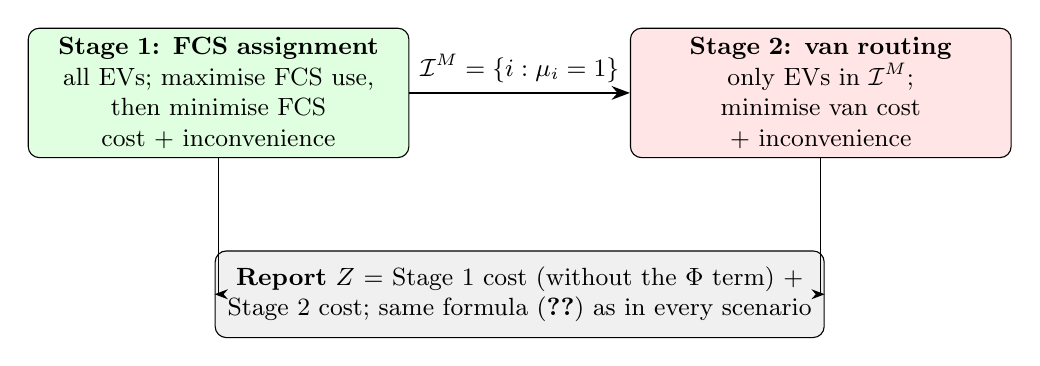
\begin{tikzpicture}[>=Stealth,box/.style={draw,rounded corners,align=center,minimum height=1.1cm,font=\small}]
  \node[box,fill=green!12,text width=4.6cm] (s1) {\textbf{Stage 1: FCS assignment}\\all EVs; maximise FCS use,\\then minimise FCS cost + inconvenience};
  \node[box,fill=red!10,text width=4.6cm,right=2.8cm of s1] (s2) {\textbf{Stage 2: van routing}\\only EVs in $\I^M$;\\minimise van cost + inconvenience};
  \draw[->,thick] (s1) -- node[above,font=\small]{$\I^M=\{i:\mu_i=1\}$} (s2);
  \node[box,fill=black!6,text width=7.5cm,below=2.0cm of $(s1)!0.5!(s2)$] (ev) {\textbf{Report} $Z=$ Stage~1 cost (without the $\Phi$ term) $+$ Stage~2 cost; same formula \eqref{eq:Z} as in every scenario};
  \draw[->] (s1) |- (ev); \draw[->] (s2) |- (ev);
\end{tikzpicture}
\end{center}

Stage~1 does not look at the vans, and Stage~2 cannot change what Stage~1 decided. That is the definition of ``FCS first, then MCS''.

%----------------------------------------------------------------
\subsection{Stage 1: assign EVs to fixed stations}

\textbf{Objective.}
\begin{equation}
\begin{split}
\min\ Z^{(1)}=\;&\underbrace{\Phi\sum_{i\in\I}\mu_i}_{\text{FCS first}}
+\underbrace{c^{EV}\sum_i\sum_{f\in\F_i}d_{if}Y_{if}}_{Z_1}
+\underbrace{Z^F_{\text{energy}}}_{\text{FCS part of }Z_4}\\
&+\underbrace{\sum_i\sum_{f\in\F_i}\rho^F_{if}Y_{if}+\alpha\sum_i w_i(C_i-r_i)+c^L\sum_i w_iL_i}_{\text{FCS customers' inconvenience}}
\end{split}
\label{eq:obj1}
\end{equation}
with $C_i=S_i+\tau^F_iY_i$ in this stage. $\Phi$ is a penalty for handing an EV to the vans. It is chosen larger than anything an extra FCS customer can add to the rest of \eqref{eq:obj1}, e.g.
\[
\Phi > \max_{i}\max_{f\in\F_i}\big(c^{EV}d_{if}+\pi^{\max}E_i+\rho^F_{if}\big)+n\,(\alpha+c^L)\,w_{\max}\,T,
\]
so Stage~1 first \textbf{maximises the number of EVs served at an FCS}, and only among those solutions minimises FCS cost and inconvenience. ($\pi^{\max}$ is the highest grid price.) A numerically safer equivalent is to solve twice: first $\max\sum_iY_i$, then fix that number and minimise the rest.
\ifTOU
Because $Z^F_{\text{energy}}$ uses the peak price, Stage~1 may \emph{start sessions later} to leave the peak, if the price saving beats the extra waiting cost (Section~\ref{sec:expect}).
\fi

\textbf{Constraints.}
\begin{align}
\sum_{g\in\G_i}y_{ig}+\mu_i &= 1 && \forall i\in\I \label{eq:s1assign}\\
S_i &\ge r_i+\sum_{f\in\F_i}t_{if}Y_{if} && \forall i\in\I \label{eq:fcsarr}\\
S_i &\le r_i+T\,(1-\mu_i) && \forall i\in\I \label{eq:s1park}\\
S_j &\ge S_i+\tau^F_i-(T+\tau^F_i)(3-y_{ig}-y_{jg}-o_{ij}) && \forall g,\ (i,j)\in\mathcal{P}_g \label{eq:disj1}\\
S_i &\ge S_j+\tau^F_j-(T+\tau^F_j)(2-y_{ig}-y_{jg}+o_{ij}) && \forall g,\ (i,j)\in\mathcal{P}_g \label{eq:disj2}\\
\sum_i y_{ig_1} &\ge \sum_i y_{ig_2} && \forall f,\ \G_f=\{g_1,g_2\} \label{eq:gunsym}\\
S_i+\tau^F_iY_i &\le T,\qquad L_i\ge S_i+\tau^F_iY_i-l_i && \forall i\in\I \label{eq:s1time}
\end{align}
\ifTOU plus the time-of-use split \eqref{eq:tou1}--\eqref{eq:tou5} of each FCS session (Section~\ref{sec:price}).\fi
\desc{\eqref{eq:s1assign}: every EV either gets one reachable gun or is handed to the vans. An EV that reaches no FCS ($\G_i=\emptyset$) is forced to $\mu_i=1$. \eqref{eq:fcsarr}: an FCS session cannot start before the EV has asked and driven to the station. \eqref{eq:s1park}: for an EV handed to the vans, $S_i$ is parked at $r_i$, so it adds no waiting in Stage~1 (its real start time is decided in Stage~2). \eqref{eq:disj1}--\eqref{eq:disj2}: two EVs on the same gun do not overlap; $o_{ij}$ picks who goes first. With two guns per station this means at most two EVs charge at a station at a time. \eqref{eq:gunsym}: symmetry breaking between the two identical guns (optional). \eqref{eq:s1time}: finished by $T$; lateness.}

\textbf{Optional acceptability rule.} An operator may refuse to send a driver to a station that is ``too inconvenient'', e.g.\ only allow gun $g$ of station $f$ for EV $i$ if $\hat\rho^F_{if}\le\bar\rho$. This only shrinks $\G_i$, so EVs whose stations are all too far go to the vans. Report results with and without it.

\textbf{Output:} $\I^M=\{i:\mu_i=1\}$, the EVs left for the vans; plus each FCS customer's gun and start time.

%----------------------------------------------------------------
\subsection{Stage 2: route the vans to the leftover EVs}

Stage~2 is a vehicle routing problem with time windows, on the EVs in $\I^M$ only. Here $C_i=S_i+\tau^M_i$.

\textbf{Objective.}
\begin{equation}
\begin{split}
\min\ Z^{(2)}=\;&\underbrace{c^M\sum_m\sum_{(i,j)\in\A^M}d_{ij}x_{ijm}}_{Z_2}+\underbrace{\sum_m c^D_mu_m}_{Z_3}+\underbrace{Z^M_{\text{energy}}}_{\text{van part of }Z_4}\\
&+\underbrace{\sum_{i\in\I^M}\sum_m\rho^M_{im}z_{im}+\alpha\sum_{i\in\I^M}w_i(C_i-r_i)+c^L\sum_{i\in\I^M}w_iL_i}_{\text{van customers' inconvenience}}
\end{split}
\label{eq:obj2}
\end{equation}
Since every EV in $\I^M$ must be served by some van, $Z^M_{\text{energy}}$ and the $\rho^M$ term are constants here. They are kept so that $Z^{(2)}$ is the true cost of Stage~2. Waiting and lateness make the vans visit urgent EVs early.

\textbf{Constraints.}
\begin{align}
\sum_{m\in\M}z_{im} &= 1 && \forall i\in\I^M \label{eq:s2assign}\\
\sum_{j:(0,j)\in\A^M}x_{0jm} = \sum_{i:(i,n+1)\in\A^M}x_{i,n+1,m} &= u_m && \forall m \label{eq:depot}\\
\sum_{i:(i,j)\in\A^M}x_{ijm} = \sum_{k:(j,k)\in\A^M}x_{jkm} &= z_{jm} && \forall j\in\I^M,\ m \label{eq:flow}\\
\sum_{i\in\I^M}z_{im} &\le Q_m\,u_m && \forall m \label{eq:cap}\\
\sum_{i\in\I^M}\frac{E_i}{\eta}z_{im}+\beta\sum_{(i,j)\in\A^M}d_{ij}x_{ijm} &\le B_m\,u_m && \forall m \label{eq:batt}
\end{align}
\begin{align}
S_j &\ge \max\{r_j,\ t_{0j}\,x_{0jm}\} && \forall j\in\I^M,\ m \label{eq:depart}\\
S_j &\ge S_i+\tau^M_i+t_{ij}-(T+\tau^M_i+t_{ij})(1-x_{ijm}) && \forall i\neq j,\ m \label{eq:seq}\\
S_i+\tau^M_i+t_{i,n+1} &\le T+(\tau^M_i+t_{i,n+1})(1-x_{i,n+1,m}) && \forall i,\ m \label{eq:return}\\
S_i+\tau^M_i \le T,\quad L_i &\ge S_i+\tau^M_i-l_i && \forall i\in\I^M \label{eq:s2time}\\
u_m &\ge u_{m+1} && m<|\M| \label{eq:vansym}
\end{align}
\desc{\eqref{eq:s2assign}: each leftover EV gets one van. \eqref{eq:depot}: a used van leaves and returns to the depot once. \eqref{eq:flow}: each EV on van $m$ is entered and left exactly once by that van. \eqref{eq:cap}: at most $Q_m$ EVs per van. \eqref{eq:batt}: delivered energy (with transfer losses) plus driving energy fits in the van battery. \eqref{eq:depart}: no start before the request, or before the van can drive there from the depot (written as two linear constraints). \eqref{eq:seq}: if the van goes $i\to j$, it finishes $i$ and drives to $j$ before starting $j$. This gives one EV at a time and removes subtours (MTZ-type). \eqref{eq:return}: back at the depot by $T$. \eqref{eq:s2time}: finished by $T$; lateness. \eqref{eq:vansym}: use identical vans in index order.}

\textbf{If Stage 2 is infeasible} (too many leftover EVs for the fleet by $T$), the sequential policy has \emph{failed} on that instance. For diagnosis, add $s_i\in\{0,1\}$ (``unserved''), replace \eqref{eq:s2assign} by $\sum_mz_{im}+s_i=1$ and add $\Phi^U\sum_is_i$ to \eqref{eq:obj2}. Then report the number of EVs that could not be served. This is a useful comparison with the integrated scenario, which may serve all of them.

%----------------------------------------------------------------
\subsection{Reported value}
\[
Z^{\text{S\scen}}=\big(Z^{(1)*}-\Phi\,|\I^M|\big)+Z^{(2)*},
\]
which is exactly \eqref{eq:Z} evaluated at the combined solution. The stage-1 solution plus the stage-2 solution is a feasible solution of the integrated model (S\ifTOU 4\else 3\fi), so
$Z^{\text{S\ifTOU 4\else 3\fi}}\le Z^{\text{S\scen}}$. The difference is the \emph{value of integration}.

\else
%---------------------------------------------------------------- INT
\subsection{Objective}
\begin{equation}
\min\ Z \quad\text{as in \eqref{eq:Z}, with }Z^F_{\text{energy}}=\ifTOU P^F\textstyle\sum_i\big[\pi^\off(\theta^1_i+\theta^3_i)+\pi^\pk\theta^2_i\big]\else\pi^F\textstyle\sum_iE_iY_i\fi,\quad C_i=S_i+\tau^F_iY_i+\tau^M_iZ_i. \label{eq:objint}
\end{equation}
Written out in full:
\begin{align*}
\min\ Z=\;& c^{EV}\sum_i\sum_{f\in\F_i}d_{if}Y_{if}+c^M\sum_m\sum_{(i,j)\in\A}d_{ij}x_{ijm}+\sum_mc^D_mu_m\\
&+\ifTOU P^F\sum_i\big[\pi^\off(\theta^1_i+\theta^3_i)+\pi^\pk\theta^2_i\big]\else\pi^F\sum_iE_iY_i\fi
+\pi^M\sum_i\sum_m\frac{E_i}{\eta}z_{im}\\
&+\sum_i\sum_{f\in\F_i}\rho^F_{if}Y_{if}+\sum_i\sum_m\rho^M_{im}z_{im}+\alpha\sum_iw_i(C_i-r_i)+c^L\sum_iw_iL_i .
\end{align*}
Every term is linear. One model weighs everything at once: an EV goes to a van exactly when the van's extra km, dispatch and energy cost are outweighed by the effort and waiting it saves the driver\ifTOU, or by the peak-price energy it avoids\fi.

\subsection{Constraints}

\textbf{Assignment.}
\begin{equation}
\sum_{g\in\G_i}y_{ig}+\sum_{m\in\M}z_{im}=1\qquad\forall i\in\I \label{eq:assign}
\end{equation}
\desc{Exactly one resource per EV: one reachable gun or one van. EVs that reach no FCS are forced onto a van.}

\textbf{Fixed stations.}
\begin{align}
S_i &\ge r_i+\sum_{f\in\F_i}t_{if}Y_{if} && \forall i \label{eq:fcsarr}\\
S_j &\ge S_i+\tau^F_i-(T+\tau^F_i)(3-y_{ig}-y_{jg}-o_{ij}) && \forall g,\ (i,j)\in\mathcal{P}_g \label{eq:disj1}\\
S_i &\ge S_j+\tau^F_j-(T+\tau^F_j)(2-y_{ig}-y_{jg}+o_{ij}) && \forall g,\ (i,j)\in\mathcal{P}_g \label{eq:disj2}\\
\sum_iy_{ig_1} &\ge \sum_iy_{ig_2} && \forall f,\ \G_f=\{g_1,g_2\} \label{eq:gunsym}
\end{align}
\desc{\eqref{eq:fcsarr}: an FCS session starts after the request and the drive to the station (for a van customer this is just $S_i\ge r_i$). \eqref{eq:disj1}--\eqref{eq:disj2}: EVs on the same gun do not overlap; $o_{ij}$ chooses the order. \eqref{eq:gunsym}: optional symmetry breaking.}

\textbf{Vans: routes, capacity, battery.}
\begin{align}
\sum_{j:(0,j)\in\A}x_{0jm}=\sum_{i:(i,n+1)\in\A}x_{i,n+1,m} &= u_m && \forall m \label{eq:depot}\\
\sum_{i:(i,j)\in\A}x_{ijm}=\sum_{k:(j,k)\in\A}x_{jkm} &= z_{jm} && \forall j\in\I,\ m \label{eq:flow}\\
\sum_iz_{im} &\le Q_mu_m && \forall m \label{eq:cap}\\
\sum_i\frac{E_i}{\eta}z_{im}+\beta\sum_{(i,j)\in\A}d_{ij}x_{ijm} &\le B_mu_m && \forall m \label{eq:batt}
\end{align}
\desc{\eqref{eq:depot}: a used van leaves and returns once. \eqref{eq:flow}: each EV on van $m$ is visited exactly once by it. \eqref{eq:cap}: at most $Q_m$ EVs. \eqref{eq:batt}: delivered energy (with losses) plus driving energy fits in the battery.}

\textbf{Vans: timing (one EV at a time, no subtours).}
\begin{align}
S_j &\ge t_{0j}\,x_{0jm} && \forall j\in\I,\ m \label{eq:depart}\\
S_j &\ge S_i+\tau^M_i+t_{ij}-(T+\tau^M_i+t_{ij})(1-x_{ijm}) && \forall i\neq j\in\I,\ m \label{eq:seq}\\
S_i+\tau^M_i+t_{i,n+1} &\le T+(\tau^M_i+t_{i,n+1})(1-x_{i,n+1,m}) && \forall i,\ m \label{eq:return}
\end{align}
\desc{\eqref{eq:depart}: the first stop cannot start before the van has driven there. \eqref{eq:seq}: $i\to j$ means finish $i$, drive, then start $j$; start times rise along a route, so no subtour can close. \eqref{eq:return}: back at the depot by $T$.}

\textbf{Horizon and lateness.}
\begin{equation}
C_i\le T,\qquad L_i\ge C_i-l_i\qquad\forall i\in\I \label{eq:time}
\end{equation}
\desc{Every EV is fully charged within the horizon; $L_i$ measures lateness.}

\ifTOU
\textbf{Time-of-use split.} Constraints \eqref{eq:tou1}--\eqref{eq:tou5} of Section~\ref{sec:price}.
\fi

\textbf{Symmetry and domains.}
\begin{equation}
u_m\ge u_{m+1};\qquad y,z,x,u,o\ifTOU,\kappa\fi\in\{0,1\};\qquad S_i,L_i\ifTOU,\theta^p_i\fi\ge0 \label{eq:dom}
\end{equation}
\fi

%=====================================================================
\section{Learning-to-optimise (RL) formulation}\label{sec:rl}

\textbf{Main rule:} the reward of each action is \emph{minus the increase in $Z$ that the action causes}. The rewards over an episode then add up to $-Z$ of the solution the policy builds. RL and MILP results are measured on the same yardstick \eqref{eq:Z}, and the MILP optimum is the benchmark for the RL gap.

\ifSEQ
%---------------------------------------------------------------- RL SEQ
The RL pipeline has the same two stages as the MILP.

\subsection{Stage 1 policy: FCS assignment}
\begin{itemize}[leftmargin=1.4em,itemsep=2pt]
  \item \textbf{Episode / epochs:} EVs are taken in order of request time $r_i$ (ties: higher $w_i$ first). One decision per EV.
  \item \textbf{State:} features of the current EV $k$ ($E_k,r_k,l_k,w_k,R_k$, location); for each gun $g$ the time $F_g$ it becomes free; summary features of the EVs still to come (count and positions near each station)\ifTOU; the current price and the time until $T_1$ and $T_2$\fi.
  \item \textbf{Action:} a gun $g\in\G_k$, or ``hand to vans''. \textbf{FCS-first mask:} ``hand to vans'' is allowed \emph{only} if no gun can finish EV $k$ by $T$ (or, with the optional rule, if all remaining guns have $\hat\rho^F_{kf}>\bar\rho$).
  \ifTOU\item \textbf{Optional timing action:} ``gun $g$, start after the peak'', i.e.\ $S_k=\max\{\text{earliest},T_2\}$, allowed only if the session still ends by $T$.\fi
  \item \textbf{Transition:} $S_k=\max\{r_k+t_{kf},F_g\}$ (or later, for the timing action); $F_g\leftarrow S_k+\tau^F_k$.
  \item \textbf{Reward:} $-\Big[c^{EV}d_{kf}+\text{energy}_k+\rho^F_{kf}+\alpha w_k(S_k+\tau^F_k-r_k)+c^Lw_k(S_k+\tau^F_k-l_k)^+\Big]$, where energy$_k$ = \ifTOU$P^F\big[\pi^\off\cdot(\text{off-peak hours of }[S_k,S_k+\tau^F_k])+\pi^\pk\cdot(\text{peak hours})\big]$, computed exactly in the simulator\else$\pi^FE_k$\fi. Handing an EV to the vans gives reward $0$ here; its cost is counted in Stage~2.
\end{itemize}
Note: a simple baseline for Stage~1 is the greedy rule ``gun with the largest one-step reward''. What RL can learn on top of this is, for example, to keep a nearby gun free for an urgent EV that arrives later.

\subsection{Stage 2 policy: van routing over $\I^M$}
\begin{itemize}[leftmargin=1.4em,itemsep=2pt]
  \item \textbf{Epochs:} whenever a van becomes free (the earliest-free van decides first).
  \item \textbf{State:} for each van: position, time free, remaining battery $b_m$, EVs served so far, dispatched or not; for each unserved EV in $\I^M$: location, $E_i,r_i,l_i,w_i$; current time.
  \item \textbf{Action:} the next EV $j$ for this van, or ``return to depot'' (ends the route). Mask: $j$ must be feasible: battery covers $E_j/\eta$ plus driving to $j$ and back to the depot, the count stays $\le Q_m$, and $j$ can be finished with the van back at the depot by $T$.
  \item \textbf{Transition:} $S_j=\max\{r_j,\ \text{time free}+t_{\text{pos},j}\}$; the van moves to $j$ and is free at $S_j+\tau^M_j$; $b_m$ falls by $E_j/\eta+\beta d_{\text{pos},j}$.
  \item \textbf{Reward:} serving $j$: $-\Big[c^Md_{\text{pos},j}+c^D_m[\text{first stop}]+\pi^M\frac{E_j}{\eta}+\rho^M_{jm}+\alpha w_j(S_j+\tau^M_j-r_j)+c^Lw_j(S_j+\tau^M_j-l_j)^+\Big]$; returning: $-c^Md_{\text{pos},0}$. EVs still unserved at the end: $-\Phi^U$ each.
  \item \textbf{Policy:} an attention-based routing policy (e.g.\ Kool et al., 2019, ``Attention, Learn to Solve Routing Problems!'') trained with REINFORCE or PPO. Baseline: nearest-feasible-EV heuristic.
\end{itemize}
Episode return of Stage~1 + Stage~2 $=-Z^{\text{S\scen}}$.

\else
%---------------------------------------------------------------- RL INT
One policy decides both who serves each EV and the van routes.
\begin{itemize}[leftmargin=1.4em,itemsep=2pt]
  \item \textbf{Episode / epochs:} EVs are taken in order of request time $r_i$ (ties: higher $w_i$ first). One decision per EV.
  \item \textbf{State:} (i) the current EV $k$: location, $E_k,r_k,l_k,w_k,R_k$, reachable stations; (ii) each gun $g$: time $F_g$ it becomes free; (iii) each van $m$: current end-of-route position, time free, remaining battery $b_m$, EVs served, dispatched or not; (iv) embeddings of the not-yet-assigned EVs (for look-ahead)\ifTOU; (v) current price, time until $T_1$ and $T_2$\fi.
  \item \textbf{Action:} $a\in\G_k\cup\M$: a gun, or a van (EV $k$ is appended to the end of that van's route). \textbf{Mask} infeasible actions: a gun that cannot finish $k$ by $T$; a van without enough battery for $E_k/\eta$ plus the drive to $k$ and back to the depot, with $Q_m$ reached, or unable to finish $k$ and return by $T$.
  \ifTOU\item \textbf{Optional timing action:} ``gun $g$, start after the peak'' ($S_k=\max\{\text{earliest},T_2\}$, if it still ends by $T$).\fi
  \item \textbf{Transition:} gun: $S_k=\max\{r_k+t_{kf},F_g\}$, $F_g\leftarrow S_k+\tau^F_k$. Van: $S_k=\max\{r_k,\ \text{free}_m+t_{\text{pos}_m,k}\}$, then the van moves to $k$, $\text{free}_m\leftarrow S_k+\tau^M_k$, $b_m\mathrel{-}=E_k/\eta+\beta d_{\text{pos}_m,k}$.
  \item \textbf{Reward} $=-\Delta Z$:
  \begin{align*}
  \text{gun } g\text{ at }f:&\quad -\Big[c^{EV}d_{kf}+\text{energy}^F_k+\rho^F_{kf}+\alpha w_k(C_k-r_k)+c^Lw_k(C_k-l_k)^+\Big]\\
  \text{van } m:&\quad -\Big[c^M\big(d_{\text{pos}_m,k}+d_{k,0}-d_{\text{pos}_m,0}\big)+c^D_m[\text{first use}]+\pi^M\tfrac{E_k}{\eta}\\
  &\qquad\quad+\rho^M_{km}+\alpha w_k(C_k-r_k)+c^Lw_k(C_k-l_k)^+\Big]
  \end{align*}
  The van distance term is the \emph{change} in route length when $k$ is inserted before the return to the depot, so the sum over the episode equals the total route length (the return legs telescope). energy$^F_k$ = \ifTOU$P^F\big[\pi^\off\cdot(\text{off-peak hours})+\pi^\pk\cdot(\text{peak hours of }[S_k,C_k])\big]$, computed exactly by the simulator; no linearisation is needed in RL\else$\pi^FE_k$\fi.
  \item \textbf{Dead end:} if every action is masked, EV $k$ is unserved: reward $-\Phi^U$, and the episode continues. Report the count.
  \item \textbf{Policy:} masked categorical policy over guns and vans, encoder with attention over EVs, guns and vans; trained with PPO. Natural baseline: greedy, i.e.\ choose the action with the largest one-step reward. That is the pairwise rule ``smallest $\hat\rho$ + cost'' from Section~\ref{sec:inc}.
\end{itemize}
Restriction to note: vans serve EVs in assignment order (append only). A variant that inserts $k$ at the cheapest position of a route is more flexible but has a larger action space.
\fi

\textbf{Reward scaling.} For stable training divide every reward by a constant, e.g.\ the greedy baseline's average $Z$ on the training instances. This does not change the optimal policy.

%=====================================================================
\section{What to expect and what to report}\label{sec:expect}

\ifnum\scen=1
\begin{itemize}[leftmargin=1.4em,itemsep=2pt]
  \item Vans serve only EVs that reach no station, or that the stations cannot finish by $T$. If stations have spare capacity, very few vans are dispatched.
  \item Inconvenience is high for EVs far from the nearest station (worked example: Rs\,682 at the FCS, against Rs\,458 if a van had been allowed).
  \item With too few vans Stage~2 becomes infeasible (unserved EVs), even when the integrated model S3 could serve everyone. Report the smallest $|\M|$ at which S1 is feasible and compare it with S3.
\end{itemize}
\fi
\ifnum\scen=2
\begin{itemize}[leftmargin=1.4em,itemsep=2pt]
  \item \textbf{When does Stage~1 delay a session to avoid the peak?} Moving one hour of charging out of the peak saves $(\pi^\pk-\pi^\off)P^F=3\times22=$ Rs\,66, but delays completion by up to an hour, which costs $\alpha w_i\ge$ Rs\,200. So with the default values Stage~1 almost never delays. It mostly pays the higher price, and S2 costs roughly S1 plus the peak surcharge. Sessions start later only if $\alpha$ is small (try $\lambda<0.33$ in the sensitivity analysis).
  \item The van assignment is the same as in S1 unless Stage~1's timing changes which EVs fit at the stations. Stage~1 cannot use vans to escape the peak price.
  \item Extra KPI: \textbf{grid energy drawn at FCS during the peak}, $P^F\sum_i\theta^2_i$ (kWh). Compare with S4.
\end{itemize}
\fi
\ifnum\scen=3
\begin{itemize}[leftmargin=1.4em,itemsep=2pt]
  \item Vans take EVs for which the saved inconvenience exceeds the extra van cost (worked example: van chosen, saving Rs\,224). Expect vans to serve EVs that are far from every station, have low range (high $w_i$), or have early deadlines, while EVs near a station still use it.
  \item \textbf{Value of integration under flat price:} $Z^{\text{S1}}-Z^{\text{S3}}\ge0$. Report it per component ($Z_1,\dots,Z_5$): typically operating cost rises a little and inconvenience falls a lot.
  \item Vary $|\M|$ (0, 1, 2, \dots): the first few vans lower $Z$ sharply, then the effect levels off. That curve shows the scenarios where mobile chargers help most.
\end{itemize}
\fi
\ifnum\scen=4
\begin{itemize}[leftmargin=1.4em,itemsep=2pt]
  \item During the peak a van kWh costs about the same as an FCS kWh (Rs\,10.0 each), so the vans' energy disadvantage disappears and vans also absorb \emph{peak-hour} demand that would otherwise be charged on the grid at peak price.
  \item Expect more van usage than in S3, concentrated on requests in $[T_1,T_2]$, and lower grid energy at the stations during the peak, $P^F\sum_i\theta^2_i$, than in S2.
  \item \textbf{Value of integration under peak pricing:} $Z^{\text{S2}}-Z^{\text{S4}}$. It should be larger than $Z^{\text{S1}}-Z^{\text{S3}}$, because integration now also allows price arbitrage.
  \item \textbf{Peak pricing with full flexibility:} $Z^{\text{S4}}-Z^{\text{S3}}$ should be smaller than $Z^{\text{S2}}-Z^{\text{S1}}$: vans cushion the price increase.
\end{itemize}
\fi

\textbf{Cross-scenario comparison table} (fill in from the four runs):
\begin{center}
\renewcommand{\arraystretch}{1.2}
\begin{tabular}{@{}lll@{}}
\toprule
\textbf{Comparison} & \textbf{Measures} & \textbf{Expected sign} \\
\midrule
S1 $-$ S3 & value of integration, flat price & $\ge0$ \\
S2 $-$ S4 & value of integration, peak price & $\ge0$, larger than S1 $-$ S3 \\
S2 $-$ S1 & cost of peak pricing, FCS-first operator & $>0$ \\
S4 $-$ S3 & cost of peak pricing, flexible operator & $>0$, smaller than S2 $-$ S1 \\
\bottomrule
\end{tabular}
\end{center}
Report for each: $Z$ and its components, number of vans used, EVs per resource, mean and maximum inconvenience per EV, total lateness, peak-hour grid energy, solve time, and (for RL) the gap to the MILP optimum.

%=====================================================================
\appendix
\section{Illustrative parameter values}\label{app:values}

These are starting values for experiments, not data. All are meant to be varied in the analysis. Values in Rs.

\begin{center}
\renewcommand{\arraystretch}{1.15}
\begin{tabular}{@{}llp{6.2cm}@{}}
\toprule
\textbf{Parameter} & \textbf{Value} & \textbf{Note} \\
\midrule
$T$, $[T_1,T_2]$ & 7 h, $[2,6]$ & 16:00--23:00, peak 18:00--22:00 \\
$P^F$, $P^M$ & 22 kW, 30 kW & \\
$v$, $\beta$, $\eta$ & 25 km/h, 0.25 kWh/km, 0.9 & \\
$B_m$, $Q_m$, $|\M|$ & 150 kWh, 6, 2--6 & \\
$c^{EV}$, $c^M$, $c^D_m$ & Rs\,4/km, Rs\,15/km, Rs\,1500 & van km includes driver time \\
$\pi^F$ (flat) & Rs\,8.7/kWh & equals the time-average of the ToU tariff over $[0,T]$ \\
$\pi^\off$, $\pi^\pk$ (ToU) & Rs\,7/kWh, Rs\,10/kWh & $(3\times7+4\times10)/7=8.7$ \\
$c^{bat}$ & Rs\,2/kWh & van battery wear \\
$\pi^M$ & Rs\,10.7 (flat) / Rs\,9.0 (ToU) & $=\pi^F+c^{bat}$ / $=\pi^\off+c^{bat}$ \\
$\alpha$, $\alpha^D$ & Rs\,200/h, Rs\,100/h & value of time; extra for attended time \\
$h^F$, $h^M$, $\varphi$ & Rs\,50, Rs\,10, Rs\,100 & trip hassle, hand-over, range stress \\
$c^L$ & Rs\,300/h & lateness \\
$w_i$ & $1+2(1-R_i/R_{\max})$, $R_i\sim U[3,40]$ km & priority from remaining range \\
\bottomrule
\end{tabular}
\end{center}

The flat price is set to the time-average of the peak tariff. The price \emph{level} is then the same in both pricing cases, and only the price \emph{shape} differs. Without this, part of S1 vs S2 would just reflect a different average price.

\end{document}
"
%    pdflatex -jobname=scenario2_peak_sequential   "\def\scen{2}% =====================================================================
%  One source, four PDFs.  Build with build.sh (or by hand):
%    pdflatex -jobname=scenario1_flat_sequential   "\def\scen{1}\input{scenario_master}"
%    pdflatex -jobname=scenario2_peak_sequential   "\def\scen{2}\input{scenario_master}"
%    pdflatex -jobname=scenario3_flat_integrated   "\def\scen{3}\input{scenario_master}"
%    pdflatex -jobname=scenario4_peak_integrated   "\def\scen{4}\input{scenario_master}"
%  (run each twice for cross-references)
% =====================================================================
\documentclass[11pt,a4paper]{article}
\usepackage[margin=2.2cm]{geometry}
\usepackage{amsmath,amssymb,amsfonts}
\usepackage{booktabs,array,tabularx}
\usepackage{enumitem}
\usepackage[table]{xcolor}
\usepackage{tikz}
\usetikzlibrary{arrows.meta,positioning,calc}
\usepackage[colorlinks=true,linkcolor=blue!50!black,urlcolor=blue!50!black]{hyperref}
\usepackage{titlesec}
\titleformat{\section}{\large\bfseries}{\thesection}{0.8em}{}
\titleformat{\subsection}{\normalsize\bfseries}{\thesubsection}{0.8em}{}
\setlength{\parindent}{0pt}
\setlength{\parskip}{5pt}

% ---------------- scenario switches ----------------
\ifdefined\scen\else\def\scen{1}\fi
\newif\ifTOU \TOUfalse   % true = time-of-use (peak) price
\newif\ifSEQ \SEQfalse   % true = FCS first, then MCS
\ifnum\scen=1 \SEQtrue \fi
\ifnum\scen=2 \TOUtrue \SEQtrue \fi
\ifnum\scen=4 \TOUtrue \fi

\newcommand{\pricename}{\ifTOU time-of-use price (dearer evening peak)\else single (flat) price all day\fi}
\newcommand{\structname}{\ifSEQ FCS first, then MCS (sequential)\else FCS and MCS together (integrated)\fi}

% ---------------- notation ----------------
\newcommand{\I}{\mathcal{I}}
\newcommand{\F}{\mathcal{F}}
\newcommand{\G}{\mathcal{G}}
\newcommand{\M}{\mathcal{M}}
\newcommand{\N}{\mathcal{N}}
\newcommand{\A}{\mathcal{A}}
\newcommand{\Rs}{\text{Rs}\,}
\newcommand{\pk}{\mathrm{pk}}
\newcommand{\off}{\mathrm{off}}
\newcommand{\desc}[1]{\par\vspace{-2pt}{\small\color{black!75}\textit{Meaning:} #1}\par\vspace{4pt}}
\newcommand{\cell}[2]{\ifnum\scen=#1\cellcolor{blue!18}\textbf{S#1 (this document)}\\\textbf{#2}\else S#1\\#2\fi}

\title{\textbf{EV Charging Network Optimisation}\\[4pt]
\large Scenario \scen: \pricename\ $+$ \structname\\[2pt]
\normalsize MILP and RL formulation}
\author{CP 320 OR for Mobility Management, course project}
\date{2 October 2026}

\begin{document}
\maketitle

%=====================================================================
\section{Where this scenario sits}

The project studies four scenarios: two ways of pricing grid electricity, times two ways of making the decisions.

\begin{center}
\renewcommand{\arraystretch}{1.5}
\begin{tabular}{>{\raggedright\arraybackslash}p{4.2cm}|>{\centering\arraybackslash}p{4.6cm}|>{\centering\arraybackslash}p{4.6cm}}
 & \textbf{Flat price all day} & \textbf{Time-of-use (peak) price} \\ \hline
\textbf{Sequential:} FCS first, leftover EVs to MCS &
\begin{tabular}[c]{@{}c@{}}\cell{1}{flat + sequential}\end{tabular} &
\begin{tabular}[c]{@{}c@{}}\cell{2}{peak + sequential}\end{tabular} \\ \hline
\textbf{Integrated:} FCS and MCS decided together &
\begin{tabular}[c]{@{}c@{}}\cell{3}{flat + integrated}\end{tabular} &
\begin{tabular}[c]{@{}c@{}}\cell{4}{peak + integrated}\end{tabular} \\
\end{tabular}
\end{center}

\textbf{The four scenarios do not have four different objectives.} They share \emph{one} cost yardstick $Z$ (Section~\ref{sec:obj}): the same cost terms and the same customer inconvenience (Section~\ref{sec:inc}). Only two things change:
\begin{itemize}[leftmargin=1.4em,itemsep=1pt]
  \item \textbf{Pricing} changes the formula for one term, the FCS energy cost (Section~\ref{sec:price}).
  \item \textbf{Decision structure} changes \emph{how} $Z$ is minimised: in one model (integrated), or in two stages (sequential), where each stage minimises its own part of $Z$.
\end{itemize}
Because the yardstick is the same, the four optimal values can be compared directly. The differences measure the \emph{value of integration} (S1$\to$S3, S2$\to$S4) and the \emph{effect of peak pricing} (S1$\to$S2, S3$\to$S4).

\ifnum\scen=1
\textbf{This scenario (S1)} is the baseline, the ``status quo''. Electricity costs the same at every hour, every EV that can be charged at a fixed station is sent there, and vans only take what is left over.
\fi
\ifnum\scen=2
\textbf{This scenario (S2)} keeps the FCS-first rule of S1, but grid electricity is dearer during the evening peak. Stage~1 can react to the price only by \emph{rescheduling} FCS sessions. It cannot hand a peak-hour EV to a van.
\fi
\ifnum\scen=3
\textbf{This scenario (S3)} keeps the flat price of S1, but the operator decides FCS and MCS service \emph{together}. An EV can be sent to a van even when a fixed station could take it, whenever that lowers total cost plus inconvenience.
\fi
\ifnum\scen=4
\textbf{This scenario (S4)} is the most flexible one: peak pricing at fixed stations, and FCS and MCS decided together. Van energy was bought off-peak, so vans can also be used to keep charging \emph{out of the expensive peak}.
\fi

%=====================================================================
\section{Setting and assumptions}\label{sec:setting}

\textbf{Time.} The planning horizon is $[0,T]$ with $T=7$\,h (16:00--23:00). It contains the evening peak window $[T_1,T_2]=[2,6]$ (18:00--22:00). The horizon is the same in all four scenarios. It is wider than the peak itself so that, under peak pricing, there is cheaper time on both sides of the peak.\ifTOU\else\ In this scenario the price is flat, so the window plays no role in the model.\fi

\textbf{Assumptions} (the same as MILP v3, plus two about energy):
\begin{enumerate}[leftmargin=1.6em,itemsep=1pt]
  \item Static, continuous time. All requests in the horizon are known at time $0$, and request $i$ becomes active at $r_i$.
  \item An EV served by an FCS drives there itself on its own battery (only to stations within its range $R_i$). The driver stays with the car while it waits for a free gun and while it charges.
  \item An EV served by an MCS stays parked where it is, and the driver is free in the meantime.
  \item Each FCS gun and each van charges one EV at a time, without interruption, at constant power.
  \item A van's battery covers both its driving and the energy it delivers. \textbf{The van battery is charged at the depot before the horizon starts}\ifTOU, i.e.\ at the off-peak price\fi, and is not recharged during the horizon.
  \item Every EV must be fully charged by $T$ (hard). Finishing after the driver's desired time $l_i$ is allowed but penalised.
\end{enumerate}

%=====================================================================
\section{Notation}\label{sec:notation}

\subsection*{Sets}
\begin{tabularx}{\textwidth}{@{}lX@{}}
\toprule
$\I=\{1,\dots,n\}$ & EV charging requests \\
$\F$; $\G_f$ ($|\G_f|=2$); $\G=\bigcup_f\G_f$ & fixed charging stations; guns of FCS $f$; all guns ($f(g)$ = station of gun $g$) \\
$\F_i=\{f: d_{if}\le R_i\}$, $\G_i=\bigcup_{f\in\F_i}\G_f$ & stations / guns EV $i$ can reach on its remaining range \\
$\M$ & mobile charging vans (MCS) \\
$0,\ n+1$ & depot as start node / end node (same place) \\
$\N=\{0\}\cup\I\cup\{n+1\}$, $\A$ & routing nodes; allowed van arcs $(i,j)$, $i\in\{0\}\cup\I$, $j\in\I\cup\{n+1\}$, $i\neq j$ \\
$\mathcal{P}_g=\{(i,j): i<j,\ g\in\G_i\cap\G_j\}$ & pairs of EVs that could share gun $g$ \\
\ifSEQ
$\I^M\subseteq\I$ & EVs handed to the vans by Stage~1 (an \emph{output} of Stage~1, a fixed input to Stage~2) \\
$\N^M$, $\A^M$ & routing nodes / arcs restricted to $\I^M$ \\
\fi
\bottomrule
\end{tabularx}

\subsection*{Parameters}
\begin{tabularx}{\textwidth}{@{}lX@{}}
\toprule
$E_i,\ r_i,\ l_i,\ R_i$ & energy demand (kWh), request time, desired completion time (h), remaining range (km) \\
$w_i\ge1$ & priority of EV $i$; $w_i=1+\kappa(1-R_i/R_{\max})$, so low-range EVs weigh more \\
$P^F,\ P^M$ & charging power of an FCS gun (22\,kW) / of a van (e.g.\ 30\,kW) \\
$\tau^F_i=E_i/P^F,\ \tau^M_i=E_i/P^M$ & charging time of EV $i$ at an FCS / by a van (h) \\
$d_{if},t_{if}$;\ $d_{ij},t_{ij}$ & distance (km) and time (h): EV$\to$FCS; between routing nodes ($t=d/v$) \\
$B_m,\ Q_m,\ \beta,\ \eta$ & van battery (kWh), max EVs per van, van consumption (kWh/km), transfer efficiency \\
$c^{EV},\ c^M,\ c^D_m$ & cost per km of EV driving, per km of van driving; fixed dispatch cost of van $m$ \\
\ifTOU
$\pi^\off,\ \pi^\pk$ & grid price (Rs/kWh) off-peak / in $[T_1,T_2]$, with $\pi^\pk\ge\pi^\off$ \\
\else
$\pi^F$ & grid price (Rs/kWh), the same at every hour \\
\fi
$c^{bat}$ & van battery wear per kWh cycled \\
$\pi^M$ & cost of 1 kWh taken from a van battery: $\pi^M=\ifTOU\pi^\off\else\pi^F\fi+c^{bat}$ (Section~\ref{sec:price}) \\
$\alpha,\ \alpha^D,\ h^F,\ h^M,\ \varphi,\ c^L$ & inconvenience coefficients (Section~\ref{sec:inc}) \\
\bottomrule
\end{tabularx}

\subsection*{Decision variables}
\begin{tabularx}{\textwidth}{@{}llX@{}}
\toprule
$y_{ig}$ & $\{0,1\}$ & EV $i$ charged at gun $g\in\G_i$ \\
$z_{im}$ & $\{0,1\}$ & EV $i$ served by van $m$ \\
$x_{ijm}$ & $\{0,1\}$ & van $m$ drives arc $(i,j)$ \\
$u_m$ & $\{0,1\}$ & van $m$ is dispatched \\
$o_{ij}$ & $\{0,1\}$ & for EVs $i<j$ that could share a gun: 1 if $i$ is charged before $j$ \\
\ifSEQ
$\mu_i$ & $\{0,1\}$ & Stage~1 only: EV $i$ is handed to the van fleet \\
\fi
\ifTOU
$\theta^1_i,\theta^2_i,\theta^3_i$ & $\ge0$ & hours of EV $i$'s FCS session before / inside / after the peak \\
$\kappa^1_i,\kappa^3_i$ & $\{0,1\}$ & EV $i$'s FCS session starts before $T_1$ / ends after $T_2$ \\
\fi
$S_i$ & $\ge0$ & time charging of EV $i$ starts (h), on whichever resource \\
$L_i$ & $\ge0$ & lateness of EV $i$ beyond $l_i$ (h) \\
\bottomrule
\end{tabularx}

\textbf{Short-hands} (linear expressions, not new variables):
\[
Y_{if}=\sum_{g\in\G_f}y_{ig},\qquad Y_i=\sum_{g\in\G_i}y_{ig}\ (\text{EV $i$ uses an FCS}),\qquad Z_i=\sum_{m\in\M}z_{im}\ (\text{EV $i$ uses a van}),
\]
\[
C_i=S_i+\tau^F_i\,Y_i+\tau^M_i\,Z_i \quad\text{(time EV $i$ is fully charged).}
\]

%=====================================================================
\section{Customer inconvenience}\label{sec:inc}

This section is \textbf{identical in all four scenario documents}. Inconvenience is a property of the customer, not of the price or of the planning method.

\subsection{What we mean by inconvenience}

Inconvenience is \emph{what the driver loses} from the moment they ask for a charge ($r_i$) until the car is fully charged ($C_i$), \emph{converted into rupees} so it can be added to the operator's costs. A driver loses three different things:

\begin{enumerate}[leftmargin=1.6em,itemsep=2pt]
  \item \textbf{Waiting:} the car is not ready. This lasts $C_i-r_i$ hours and affects \emph{every} driver, FCS or MCS.
  \item \textbf{Effort:} only an FCS customer has to drive to the station and sit there while the car charges. An MCS customer stays at home or at work and does something else. Driving to a far station also uses scarce battery range, which causes stress (``range anxiety'').
  \item \textbf{A missed deadline:} the car is still not ready at the time $l_i$ the driver needs it.
\end{enumerate}

Each loss gets a price in Rs per hour (or per event). All of them are multiplied by the priority $w_i$: an hour of delay for an EV with 5\,km of range left counts more than for one with 40\,km.

\subsection{The three components}

\begin{center}
\renewcommand{\arraystretch}{1.3}
\begin{tabularx}{\textwidth}{@{}>{\raggedright\arraybackslash}p{2.6cm}>{\raggedright\arraybackslash}X>{\raggedright\arraybackslash}X>{\raggedright\arraybackslash}p{3.0cm}@{}}
\toprule
\textbf{Component} & \textbf{EV $i$ at FCS $f$} & \textbf{EV $i$ by a van} & \textbf{Known when?} \\
\midrule
Effort & $w_i\big[\alpha^D(t_{if}+\tau^F_i)+h^F+\varphi\,d_{if}/R_i\big]$: driving and sitting at the station, a fixed trip hassle, range stress & $w_i\,h^M$: being reachable and handing over the car & \textbf{Static:} known as soon as the resource is chosen \\
Waiting & $w_i\,\alpha\,(C_i-r_i)$ = drive + \emph{queue at the gun} + charge & $w_i\,\alpha\,(C_i-r_i)$ = \emph{wait for the van} + charge & \textbf{Dynamic:} depends on the queue / van route \\
Missed deadline & $w_i\,c^L\,L_i$, $L_i=\max\{0,C_i-l_i\}$ & same & Dynamic \\
\bottomrule
\end{tabularx}
\end{center}

\textbf{Coefficients.}
$\alpha$ (Rs/h) is the value of an hour the car is not ready.
$\alpha^D$ (Rs/h) is the \emph{extra} value of an hour the driver must personally spend driving or sitting at the station: an hour at the station costs $\alpha+\alpha^D$, an hour waiting at home for a van costs only $\alpha$.
$h^F,h^M$ (Rs) are fixed hassle costs of one trip to a station / one van hand-over.
$\varphi$ (Rs) is the range-stress cost of a trip that uses the \emph{whole} remaining range ($d_{if}/R_i\le1$ is the fraction used).
$c^L$ (Rs/h) is the cost per hour late.

\subsection{Pairwise form: inconvenience of a (customer, resource) pair}

The natural first idea is: \emph{for every pair (EV $i$, FCS $f$) and every pair (EV $i$, van $m$) there is an inconvenience number, and the operator picks the pair with the lowest cost plus inconvenience.} The static part fits this idea exactly:
\[
\boxed{\;\rho^F_{if}=w_i\Big[\alpha^D\,(t_{if}+\tau^F_i)+h^F+\varphi\,\frac{d_{if}}{R_i}\Big]\qquad
\rho^M_{im}=w_i\,h^M\;}
\]
These are \textbf{parameters}, computed before solving, one number per (EV, FCS) pair and per (EV, van) pair. In the objective they appear linearly: $\sum_i\sum_f\rho^F_{if}Y_{if}+\sum_i\sum_m\rho^M_{im}z_{im}$.

Note that $\rho^M_{im}$ does not depend on $m$. Vans are identical and all start at the same depot, so the driver does not care \emph{which} van comes, only \emph{when} it comes. That ``when'' is the waiting part.

\subsection{Why waiting cannot be a fixed pairwise number}

It is tempting to also write the waiting as a pairwise number, e.g.\ ``the van needs 5 minutes to reach EV $i$''. But that depends on \emph{where the van is coming from}, which depends on the route the model is still choosing: if EV $i$ is the 4th stop of a van, the wait is the time for three charging sessions plus four drives. Likewise, waiting at an FCS depends on how many EVs are queued at that gun. So waiting is not known before solving. It is a function of decision variables:
\[
\text{waiting cost of EV } i \;=\; w_i\,\alpha\,(C_i-r_i),\qquad C_i=S_i+\tau^F_iY_i+\tau^M_iZ_i .
\]
This is \textbf{linear} in the variables ($S_i$, $y$, $z$), so it fits in a MILP directly. The constraints of Section~\ref{sec:milp} make $S_i$ equal to the true start time, including driving, queueing at the gun and the van's route. The term $\sum_i w_i\alpha r_i$ is a constant and may be dropped when solving.

\textbf{Pairwise \emph{estimate}} (used for intuition, by the RL policy and in heuristics): if there is no queue and the van comes straight to $i$,
\[
\hat\rho^{F}_{if}=\rho^F_{if}+w_i\alpha\,(t_{if}+\tau^F_i),\qquad
\hat\rho^{M}_{im}=\rho^M_{im}+w_i\alpha\,(t^{\text{van}}_{m\to i}+\tau^M_i),
\]
where $t^{\text{van}}_{m\to i}$ is the time until van $m$ can reach $i$ from where it currently is. In the RL formulation (Section~\ref{sec:rl}) the van's position \emph{is} known at each decision, so there this estimate becomes exact.

\subsection{Total inconvenience and how it enters the objective}

\begin{equation}
\boxed{\;
Z_{\text{inc}}=\underbrace{\sum_{i\in\I}\sum_{f\in\F_i}\rho^F_{if}Y_{if}+\sum_{i\in\I}\sum_{m\in\M}\rho^M_{im}z_{im}}_{\text{effort (static, pairwise)}}
+\underbrace{\alpha\sum_{i\in\I}w_i\,(C_i-r_i)}_{\text{waiting (dynamic)}}
+\underbrace{c^L\sum_{i\in\I}w_i\,L_i}_{\text{missed deadline}}
\;}\label{eq:inc}
\end{equation}
All three parts are in rupees, so $Z_{\text{inc}}$ is simply added to the operating costs. Nothing has to be normalised.

\subsection{Worked example: your ``10 km to the FCS vs.\ van in 5 minutes'' case}

EV $i$: $E_i=20$\,kWh, $R_i=40$\,km (so $w_i=1$); nearest free FCS $d_{if}=10$\,km away, $t_{if}=0.4$\,h at 25\,km/h; a van finishing next door can reach it in 5\,min ($0.083$\,h), adding about 4\,km to its route. $\tau^F_i=20/22=0.909$\,h, $\tau^M_i=20/30=0.667$\,h. Coefficients from Appendix~\ref{app:values}, flat price.

\begin{center}
\renewcommand{\arraystretch}{1.25}
\begin{tabular}{@{}lrr@{}}
\toprule
 & \textbf{FCS} & \textbf{Van} \\
\midrule
Driving (EV / extra van km) & $4\times10=40.0$ & $15\times4=60.0$ \\
Energy & $8.7\times20=174.0$ & $10.7\times20/0.9=237.8$ \\
\textbf{Operating cost only} & \textbf{214.0} & \textbf{297.8} \\
\midrule
Effort $\rho$ & $100(0.4+0.909)+50+100\cdot\tfrac{10}{40}=205.9$ & $10.0$ \\
Waiting $\alpha(C_i-r_i)$ & $200\times1.309=261.8$ & $200\times0.75=150.0$ \\
\textbf{Cost + inconvenience} & \textbf{681.7} & \textbf{457.8} \\
\bottomrule
\end{tabular}
\end{center}

On operating cost alone the FCS is cheaper, so a cost-only model would \emph{always} send this driver 10\,km away. With inconvenience included the van is better by about Rs\,224, and the integrated model chooses $z_{im}=1$, as you expected. If the FCS were only 1\,km away, the FCS would win both comparisons. The inconvenience term is what makes the model choose between ``cheap for the operator'' and ``convenient for the driver'', rather than following a fixed rule.

\subsection{Relation to a single penalty $\rho_i$ per EV}

The first draft used a penalty $\rho_i$ that is charged whenever EV $i$ goes to \emph{any} FCS: $\sum_i\sum_f\rho_iy_{if}$. Because $\sum_f y_{if}=1-\sum_m z_{im}$, this only says ``a van is worth $\rho_i$ more to EV $i$'', and that holds whether the station is 1\,km or 15\,km away, and whether the van arrives in 5 minutes or in 3 hours. The form above fixes both problems: $\rho^F_{if}$ grows with the distance to \emph{that} station, and the waiting term grows with how late the van or the free gun actually is. The old model is the special case $\alpha=\alpha^D=\varphi=c^L=0$, $h^F=\rho_i$.

\subsection{Choosing the coefficients}
\begin{itemize}[leftmargin=1.4em,itemsep=2pt]
  \item Use a value of time for $\alpha$ (e.g.\ Rs\,150--300/h for urban car users), and set $\alpha^D\approx0.5\alpha$: sitting at a station is worse than waiting at home.
  \item Keep $c^L>\alpha$, so missing the deadline is worse than ordinary waiting.
  \item \textbf{Sensitivity analysis:} multiply all inconvenience coefficients by a factor $\lambda\in\{0,0.25,0.5,1,2,4\}$ and plot operating cost against total inconvenience. $\lambda=0$ is the pure cost-minimising operator, and large $\lambda$ is a customer-first operator. This trade-off curve is a strong result for the ``Analysis'' part of the project.
\end{itemize}

\subsection{What inconvenience does in \emph{this} scenario}
\ifSEQ
In a sequential scenario inconvenience \textbf{cannot move an EV from an FCS to a van}: Stage~1 sends every EV that \emph{can} use an FCS to one. It still matters inside each stage. In Stage~1 it decides \emph{which} station and \emph{when} (urgent EVs get the near station and the first free gun). In Stage~2 it decides the \emph{order} in which vans visit EVs (urgent EVs first). In the worked example, this scenario sends the driver 10\,km to the FCS. That is the weakness the integrated scenarios remove.
\else
In an integrated scenario inconvenience is weighed directly against operating cost when choosing the resource. That is how the worked example ends up with a van. It also decides which station and which gun order, and the order of each van route.
\fi

%=====================================================================
\section{Electricity price in this scenario}\label{sec:price}

\textbf{Van energy (same in all scenarios).} A van's battery is charged at the depot \emph{before} the horizon, so its energy was bought at the
\ifTOU off-peak \fi
price, whatever time the van later delivers it. Each kWh taken from the van also wears the battery ($c^{bat}$), and a fraction $1-\eta$ is lost in transfer:
\[
Z^M_{\text{energy}}=\pi^M\sum_{i\in\I}\sum_{m\in\M}\frac{E_i}{\eta}\,z_{im},\qquad \pi^M=\ifTOU\pi^\off\else\pi^F\fi+c^{bat}.
\]

\ifTOU
\textbf{FCS energy (time-of-use).} An FCS draws from the grid while it charges. Energy delivered inside $[T_1,T_2]$ costs $\pi^\pk$, and energy outside it costs $\pi^\off$. A session $[S_i,S_i+\tau^F_i]$ may overlap the peak partly. Split its duration into the hours before, inside and after the peak, $\theta^1_i+\theta^2_i+\theta^3_i$:
\[
Z^F_{\text{energy}}=P^F\sum_{i\in\I}\Big[\pi^\off(\theta^1_i+\theta^3_i)+\pi^\pk\,\theta^2_i\Big].
\]
Constraints \eqref{eq:tou1}--\eqref{eq:tou5} below make the $\theta$'s equal to the true overlaps. Peak hours are dearer, so the solver wants $\theta^1_i,\theta^3_i$ as large as possible. It is enough to bound them from above by the true off-peak overlap, and the constraints need one binary per side:
\begin{align}
\theta^1_i+\theta^2_i+\theta^3_i &= \tau^F_i\,Y_i && \forall i\in\I \label{eq:tou1}\\
\theta^1_i &\le \tau^F_i\,\kappa^1_i && \forall i\in\I \label{eq:tou2}\\
\theta^1_i &\le T_1-S_i+T\,(1-\kappa^1_i) && \forall i\in\I \label{eq:tou3}\\
\theta^3_i &\le \tau^F_i\,\kappa^3_i && \forall i\in\I \label{eq:tou4}\\
\theta^3_i &\le S_i+\tau^F_i-T_2+T\,(1-\kappa^3_i) && \forall i\in\I \label{eq:tou5}
\end{align}
\desc{\eqref{eq:tou1}: the FCS session's hours are split into three parts; for a van customer ($Y_i=0$) all three are zero. \eqref{eq:tou2}--\eqref{eq:tou3}: off-peak time before the peak is only possible if the session starts before $T_1$ ($\kappa^1_i=1$), and is at most $T_1-S_i$. \eqref{eq:tou4}--\eqref{eq:tou5}: the same for time after $T_2$. $\theta^2_i\ge0$ prevents counting more off-peak hours than exist. Checking the cases (entirely before / inside / after the peak, straddling one edge, covering the whole peak) shows that at the optimum the $\theta$'s equal the exact overlaps. This needs $\pi^\pk\ge\pi^\off$, which is true for a peak tariff.}

\textbf{Why vans become more attractive.} Compare the cost of 1\,kWh delivered to an EV during the peak (values from Appendix~\ref{app:values}):
FCS $=\pi^\pk=$ Rs\,10.0, van $=(\pi^\off+c^{bat})/\eta=9/0.9=$ Rs\,10.0. They are at parity. Under the flat price the van is about Rs\,3.2/kWh dearer (FCS Rs\,8.7, van $10.7/0.9=$ Rs\,11.9). Peak pricing therefore removes the vans' main cost disadvantage, but only for EVs whose FCS session would fall in the peak.
\ifSEQ\ In this sequential scenario Stage~1 cannot use that, because it does not consider vans. It can only shift FCS sessions in time.\fi
\else
\textbf{FCS energy (flat).} Every kWh delivered at a fixed station costs $\pi^F$, whenever it is delivered:
\[
Z^F_{\text{energy}}=\pi^F\sum_{i\in\I}E_i\,Y_i .
\]
The start time therefore does not affect the energy cost. Under the flat price a van kWh costs $(\pi^F+c^{bat})/\eta\approx$ Rs\,11.9 against Rs\,8.7 at an FCS (Appendix~\ref{app:values}), so on energy alone the FCS always wins.
\fi

%=====================================================================
\section{MILP formulation}\label{sec:milp}

\subsection{The common cost yardstick $Z$}\label{sec:obj}

For any complete solution (every EV assigned, every route and start time known), the system cost is
\begin{equation}
\boxed{\;
Z=\underbrace{c^{EV}\sum_{i}\sum_{f\in\F_i}d_{if}Y_{if}}_{Z_1:\ \text{EV driving}}
+\underbrace{c^M\sum_{m}\sum_{(i,j)\in\A}d_{ij}x_{ijm}}_{Z_2:\ \text{van driving}}
+\underbrace{\sum_m c^D_m u_m}_{Z_3:\ \text{dispatch}}
+\underbrace{Z^F_{\text{energy}}+Z^M_{\text{energy}}}_{Z_4:\ \text{energy}}
+\underbrace{Z_{\text{inc}}}_{Z_5:\ \text{inconv.\ \eqref{eq:inc}}}
\;}\label{eq:Z}
\end{equation}
$Z_4$ is defined in Section~\ref{sec:price}. $Z_1$--$Z_4$ are the operator's costs listed in the brief (EV travel, MCS travel, MCS operating cost) plus energy. $Z_5$ is the customer inconvenience penalty. \textbf{The same formula is used to report results in all four scenarios.}

\ifSEQ
%---------------------------------------------------------------- SEQ
\subsection{Structure: two stages}

\begin{center}
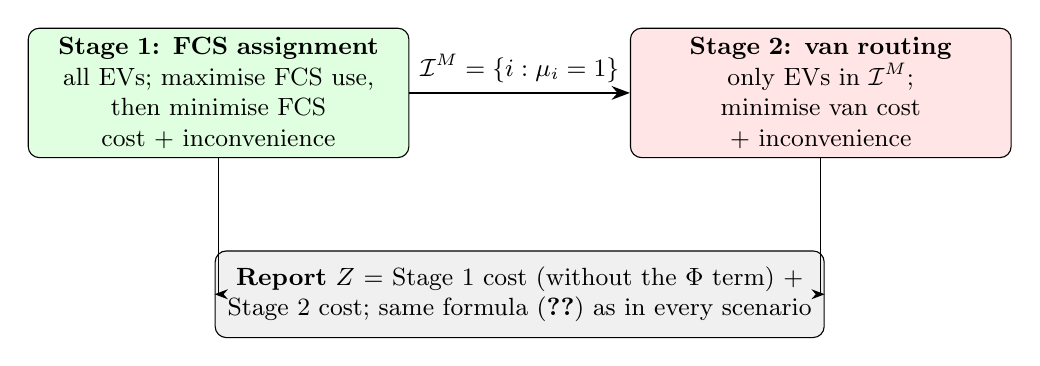
\begin{tikzpicture}[>=Stealth,box/.style={draw,rounded corners,align=center,minimum height=1.1cm,font=\small}]
  \node[box,fill=green!12,text width=4.6cm] (s1) {\textbf{Stage 1: FCS assignment}\\all EVs; maximise FCS use,\\then minimise FCS cost + inconvenience};
  \node[box,fill=red!10,text width=4.6cm,right=2.8cm of s1] (s2) {\textbf{Stage 2: van routing}\\only EVs in $\I^M$;\\minimise van cost + inconvenience};
  \draw[->,thick] (s1) -- node[above,font=\small]{$\I^M=\{i:\mu_i=1\}$} (s2);
  \node[box,fill=black!6,text width=7.5cm,below=2.0cm of $(s1)!0.5!(s2)$] (ev) {\textbf{Report} $Z=$ Stage~1 cost (without the $\Phi$ term) $+$ Stage~2 cost; same formula \eqref{eq:Z} as in every scenario};
  \draw[->] (s1) |- (ev); \draw[->] (s2) |- (ev);
\end{tikzpicture}
\end{center}

Stage~1 does not look at the vans, and Stage~2 cannot change what Stage~1 decided. That is the definition of ``FCS first, then MCS''.

%----------------------------------------------------------------
\subsection{Stage 1: assign EVs to fixed stations}

\textbf{Objective.}
\begin{equation}
\begin{split}
\min\ Z^{(1)}=\;&\underbrace{\Phi\sum_{i\in\I}\mu_i}_{\text{FCS first}}
+\underbrace{c^{EV}\sum_i\sum_{f\in\F_i}d_{if}Y_{if}}_{Z_1}
+\underbrace{Z^F_{\text{energy}}}_{\text{FCS part of }Z_4}\\
&+\underbrace{\sum_i\sum_{f\in\F_i}\rho^F_{if}Y_{if}+\alpha\sum_i w_i(C_i-r_i)+c^L\sum_i w_iL_i}_{\text{FCS customers' inconvenience}}
\end{split}
\label{eq:obj1}
\end{equation}
with $C_i=S_i+\tau^F_iY_i$ in this stage. $\Phi$ is a penalty for handing an EV to the vans. It is chosen larger than anything an extra FCS customer can add to the rest of \eqref{eq:obj1}, e.g.
\[
\Phi > \max_{i}\max_{f\in\F_i}\big(c^{EV}d_{if}+\pi^{\max}E_i+\rho^F_{if}\big)+n\,(\alpha+c^L)\,w_{\max}\,T,
\]
so Stage~1 first \textbf{maximises the number of EVs served at an FCS}, and only among those solutions minimises FCS cost and inconvenience. ($\pi^{\max}$ is the highest grid price.) A numerically safer equivalent is to solve twice: first $\max\sum_iY_i$, then fix that number and minimise the rest.
\ifTOU
Because $Z^F_{\text{energy}}$ uses the peak price, Stage~1 may \emph{start sessions later} to leave the peak, if the price saving beats the extra waiting cost (Section~\ref{sec:expect}).
\fi

\textbf{Constraints.}
\begin{align}
\sum_{g\in\G_i}y_{ig}+\mu_i &= 1 && \forall i\in\I \label{eq:s1assign}\\
S_i &\ge r_i+\sum_{f\in\F_i}t_{if}Y_{if} && \forall i\in\I \label{eq:fcsarr}\\
S_i &\le r_i+T\,(1-\mu_i) && \forall i\in\I \label{eq:s1park}\\
S_j &\ge S_i+\tau^F_i-(T+\tau^F_i)(3-y_{ig}-y_{jg}-o_{ij}) && \forall g,\ (i,j)\in\mathcal{P}_g \label{eq:disj1}\\
S_i &\ge S_j+\tau^F_j-(T+\tau^F_j)(2-y_{ig}-y_{jg}+o_{ij}) && \forall g,\ (i,j)\in\mathcal{P}_g \label{eq:disj2}\\
\sum_i y_{ig_1} &\ge \sum_i y_{ig_2} && \forall f,\ \G_f=\{g_1,g_2\} \label{eq:gunsym}\\
S_i+\tau^F_iY_i &\le T,\qquad L_i\ge S_i+\tau^F_iY_i-l_i && \forall i\in\I \label{eq:s1time}
\end{align}
\ifTOU plus the time-of-use split \eqref{eq:tou1}--\eqref{eq:tou5} of each FCS session (Section~\ref{sec:price}).\fi
\desc{\eqref{eq:s1assign}: every EV either gets one reachable gun or is handed to the vans. An EV that reaches no FCS ($\G_i=\emptyset$) is forced to $\mu_i=1$. \eqref{eq:fcsarr}: an FCS session cannot start before the EV has asked and driven to the station. \eqref{eq:s1park}: for an EV handed to the vans, $S_i$ is parked at $r_i$, so it adds no waiting in Stage~1 (its real start time is decided in Stage~2). \eqref{eq:disj1}--\eqref{eq:disj2}: two EVs on the same gun do not overlap; $o_{ij}$ picks who goes first. With two guns per station this means at most two EVs charge at a station at a time. \eqref{eq:gunsym}: symmetry breaking between the two identical guns (optional). \eqref{eq:s1time}: finished by $T$; lateness.}

\textbf{Optional acceptability rule.} An operator may refuse to send a driver to a station that is ``too inconvenient'', e.g.\ only allow gun $g$ of station $f$ for EV $i$ if $\hat\rho^F_{if}\le\bar\rho$. This only shrinks $\G_i$, so EVs whose stations are all too far go to the vans. Report results with and without it.

\textbf{Output:} $\I^M=\{i:\mu_i=1\}$, the EVs left for the vans; plus each FCS customer's gun and start time.

%----------------------------------------------------------------
\subsection{Stage 2: route the vans to the leftover EVs}

Stage~2 is a vehicle routing problem with time windows, on the EVs in $\I^M$ only. Here $C_i=S_i+\tau^M_i$.

\textbf{Objective.}
\begin{equation}
\begin{split}
\min\ Z^{(2)}=\;&\underbrace{c^M\sum_m\sum_{(i,j)\in\A^M}d_{ij}x_{ijm}}_{Z_2}+\underbrace{\sum_m c^D_mu_m}_{Z_3}+\underbrace{Z^M_{\text{energy}}}_{\text{van part of }Z_4}\\
&+\underbrace{\sum_{i\in\I^M}\sum_m\rho^M_{im}z_{im}+\alpha\sum_{i\in\I^M}w_i(C_i-r_i)+c^L\sum_{i\in\I^M}w_iL_i}_{\text{van customers' inconvenience}}
\end{split}
\label{eq:obj2}
\end{equation}
Since every EV in $\I^M$ must be served by some van, $Z^M_{\text{energy}}$ and the $\rho^M$ term are constants here. They are kept so that $Z^{(2)}$ is the true cost of Stage~2. Waiting and lateness make the vans visit urgent EVs early.

\textbf{Constraints.}
\begin{align}
\sum_{m\in\M}z_{im} &= 1 && \forall i\in\I^M \label{eq:s2assign}\\
\sum_{j:(0,j)\in\A^M}x_{0jm} = \sum_{i:(i,n+1)\in\A^M}x_{i,n+1,m} &= u_m && \forall m \label{eq:depot}\\
\sum_{i:(i,j)\in\A^M}x_{ijm} = \sum_{k:(j,k)\in\A^M}x_{jkm} &= z_{jm} && \forall j\in\I^M,\ m \label{eq:flow}\\
\sum_{i\in\I^M}z_{im} &\le Q_m\,u_m && \forall m \label{eq:cap}\\
\sum_{i\in\I^M}\frac{E_i}{\eta}z_{im}+\beta\sum_{(i,j)\in\A^M}d_{ij}x_{ijm} &\le B_m\,u_m && \forall m \label{eq:batt}
\end{align}
\begin{align}
S_j &\ge \max\{r_j,\ t_{0j}\,x_{0jm}\} && \forall j\in\I^M,\ m \label{eq:depart}\\
S_j &\ge S_i+\tau^M_i+t_{ij}-(T+\tau^M_i+t_{ij})(1-x_{ijm}) && \forall i\neq j,\ m \label{eq:seq}\\
S_i+\tau^M_i+t_{i,n+1} &\le T+(\tau^M_i+t_{i,n+1})(1-x_{i,n+1,m}) && \forall i,\ m \label{eq:return}\\
S_i+\tau^M_i \le T,\quad L_i &\ge S_i+\tau^M_i-l_i && \forall i\in\I^M \label{eq:s2time}\\
u_m &\ge u_{m+1} && m<|\M| \label{eq:vansym}
\end{align}
\desc{\eqref{eq:s2assign}: each leftover EV gets one van. \eqref{eq:depot}: a used van leaves and returns to the depot once. \eqref{eq:flow}: each EV on van $m$ is entered and left exactly once by that van. \eqref{eq:cap}: at most $Q_m$ EVs per van. \eqref{eq:batt}: delivered energy (with transfer losses) plus driving energy fits in the van battery. \eqref{eq:depart}: no start before the request, or before the van can drive there from the depot (written as two linear constraints). \eqref{eq:seq}: if the van goes $i\to j$, it finishes $i$ and drives to $j$ before starting $j$. This gives one EV at a time and removes subtours (MTZ-type). \eqref{eq:return}: back at the depot by $T$. \eqref{eq:s2time}: finished by $T$; lateness. \eqref{eq:vansym}: use identical vans in index order.}

\textbf{If Stage 2 is infeasible} (too many leftover EVs for the fleet by $T$), the sequential policy has \emph{failed} on that instance. For diagnosis, add $s_i\in\{0,1\}$ (``unserved''), replace \eqref{eq:s2assign} by $\sum_mz_{im}+s_i=1$ and add $\Phi^U\sum_is_i$ to \eqref{eq:obj2}. Then report the number of EVs that could not be served. This is a useful comparison with the integrated scenario, which may serve all of them.

%----------------------------------------------------------------
\subsection{Reported value}
\[
Z^{\text{S\scen}}=\big(Z^{(1)*}-\Phi\,|\I^M|\big)+Z^{(2)*},
\]
which is exactly \eqref{eq:Z} evaluated at the combined solution. The stage-1 solution plus the stage-2 solution is a feasible solution of the integrated model (S\ifTOU 4\else 3\fi), so
$Z^{\text{S\ifTOU 4\else 3\fi}}\le Z^{\text{S\scen}}$. The difference is the \emph{value of integration}.

\else
%---------------------------------------------------------------- INT
\subsection{Objective}
\begin{equation}
\min\ Z \quad\text{as in \eqref{eq:Z}, with }Z^F_{\text{energy}}=\ifTOU P^F\textstyle\sum_i\big[\pi^\off(\theta^1_i+\theta^3_i)+\pi^\pk\theta^2_i\big]\else\pi^F\textstyle\sum_iE_iY_i\fi,\quad C_i=S_i+\tau^F_iY_i+\tau^M_iZ_i. \label{eq:objint}
\end{equation}
Written out in full:
\begin{align*}
\min\ Z=\;& c^{EV}\sum_i\sum_{f\in\F_i}d_{if}Y_{if}+c^M\sum_m\sum_{(i,j)\in\A}d_{ij}x_{ijm}+\sum_mc^D_mu_m\\
&+\ifTOU P^F\sum_i\big[\pi^\off(\theta^1_i+\theta^3_i)+\pi^\pk\theta^2_i\big]\else\pi^F\sum_iE_iY_i\fi
+\pi^M\sum_i\sum_m\frac{E_i}{\eta}z_{im}\\
&+\sum_i\sum_{f\in\F_i}\rho^F_{if}Y_{if}+\sum_i\sum_m\rho^M_{im}z_{im}+\alpha\sum_iw_i(C_i-r_i)+c^L\sum_iw_iL_i .
\end{align*}
Every term is linear. One model weighs everything at once: an EV goes to a van exactly when the van's extra km, dispatch and energy cost are outweighed by the effort and waiting it saves the driver\ifTOU, or by the peak-price energy it avoids\fi.

\subsection{Constraints}

\textbf{Assignment.}
\begin{equation}
\sum_{g\in\G_i}y_{ig}+\sum_{m\in\M}z_{im}=1\qquad\forall i\in\I \label{eq:assign}
\end{equation}
\desc{Exactly one resource per EV: one reachable gun or one van. EVs that reach no FCS are forced onto a van.}

\textbf{Fixed stations.}
\begin{align}
S_i &\ge r_i+\sum_{f\in\F_i}t_{if}Y_{if} && \forall i \label{eq:fcsarr}\\
S_j &\ge S_i+\tau^F_i-(T+\tau^F_i)(3-y_{ig}-y_{jg}-o_{ij}) && \forall g,\ (i,j)\in\mathcal{P}_g \label{eq:disj1}\\
S_i &\ge S_j+\tau^F_j-(T+\tau^F_j)(2-y_{ig}-y_{jg}+o_{ij}) && \forall g,\ (i,j)\in\mathcal{P}_g \label{eq:disj2}\\
\sum_iy_{ig_1} &\ge \sum_iy_{ig_2} && \forall f,\ \G_f=\{g_1,g_2\} \label{eq:gunsym}
\end{align}
\desc{\eqref{eq:fcsarr}: an FCS session starts after the request and the drive to the station (for a van customer this is just $S_i\ge r_i$). \eqref{eq:disj1}--\eqref{eq:disj2}: EVs on the same gun do not overlap; $o_{ij}$ chooses the order. \eqref{eq:gunsym}: optional symmetry breaking.}

\textbf{Vans: routes, capacity, battery.}
\begin{align}
\sum_{j:(0,j)\in\A}x_{0jm}=\sum_{i:(i,n+1)\in\A}x_{i,n+1,m} &= u_m && \forall m \label{eq:depot}\\
\sum_{i:(i,j)\in\A}x_{ijm}=\sum_{k:(j,k)\in\A}x_{jkm} &= z_{jm} && \forall j\in\I,\ m \label{eq:flow}\\
\sum_iz_{im} &\le Q_mu_m && \forall m \label{eq:cap}\\
\sum_i\frac{E_i}{\eta}z_{im}+\beta\sum_{(i,j)\in\A}d_{ij}x_{ijm} &\le B_mu_m && \forall m \label{eq:batt}
\end{align}
\desc{\eqref{eq:depot}: a used van leaves and returns once. \eqref{eq:flow}: each EV on van $m$ is visited exactly once by it. \eqref{eq:cap}: at most $Q_m$ EVs. \eqref{eq:batt}: delivered energy (with losses) plus driving energy fits in the battery.}

\textbf{Vans: timing (one EV at a time, no subtours).}
\begin{align}
S_j &\ge t_{0j}\,x_{0jm} && \forall j\in\I,\ m \label{eq:depart}\\
S_j &\ge S_i+\tau^M_i+t_{ij}-(T+\tau^M_i+t_{ij})(1-x_{ijm}) && \forall i\neq j\in\I,\ m \label{eq:seq}\\
S_i+\tau^M_i+t_{i,n+1} &\le T+(\tau^M_i+t_{i,n+1})(1-x_{i,n+1,m}) && \forall i,\ m \label{eq:return}
\end{align}
\desc{\eqref{eq:depart}: the first stop cannot start before the van has driven there. \eqref{eq:seq}: $i\to j$ means finish $i$, drive, then start $j$; start times rise along a route, so no subtour can close. \eqref{eq:return}: back at the depot by $T$.}

\textbf{Horizon and lateness.}
\begin{equation}
C_i\le T,\qquad L_i\ge C_i-l_i\qquad\forall i\in\I \label{eq:time}
\end{equation}
\desc{Every EV is fully charged within the horizon; $L_i$ measures lateness.}

\ifTOU
\textbf{Time-of-use split.} Constraints \eqref{eq:tou1}--\eqref{eq:tou5} of Section~\ref{sec:price}.
\fi

\textbf{Symmetry and domains.}
\begin{equation}
u_m\ge u_{m+1};\qquad y,z,x,u,o\ifTOU,\kappa\fi\in\{0,1\};\qquad S_i,L_i\ifTOU,\theta^p_i\fi\ge0 \label{eq:dom}
\end{equation}
\fi

%=====================================================================
\section{Learning-to-optimise (RL) formulation}\label{sec:rl}

\textbf{Main rule:} the reward of each action is \emph{minus the increase in $Z$ that the action causes}. The rewards over an episode then add up to $-Z$ of the solution the policy builds. RL and MILP results are measured on the same yardstick \eqref{eq:Z}, and the MILP optimum is the benchmark for the RL gap.

\ifSEQ
%---------------------------------------------------------------- RL SEQ
The RL pipeline has the same two stages as the MILP.

\subsection{Stage 1 policy: FCS assignment}
\begin{itemize}[leftmargin=1.4em,itemsep=2pt]
  \item \textbf{Episode / epochs:} EVs are taken in order of request time $r_i$ (ties: higher $w_i$ first). One decision per EV.
  \item \textbf{State:} features of the current EV $k$ ($E_k,r_k,l_k,w_k,R_k$, location); for each gun $g$ the time $F_g$ it becomes free; summary features of the EVs still to come (count and positions near each station)\ifTOU; the current price and the time until $T_1$ and $T_2$\fi.
  \item \textbf{Action:} a gun $g\in\G_k$, or ``hand to vans''. \textbf{FCS-first mask:} ``hand to vans'' is allowed \emph{only} if no gun can finish EV $k$ by $T$ (or, with the optional rule, if all remaining guns have $\hat\rho^F_{kf}>\bar\rho$).
  \ifTOU\item \textbf{Optional timing action:} ``gun $g$, start after the peak'', i.e.\ $S_k=\max\{\text{earliest},T_2\}$, allowed only if the session still ends by $T$.\fi
  \item \textbf{Transition:} $S_k=\max\{r_k+t_{kf},F_g\}$ (or later, for the timing action); $F_g\leftarrow S_k+\tau^F_k$.
  \item \textbf{Reward:} $-\Big[c^{EV}d_{kf}+\text{energy}_k+\rho^F_{kf}+\alpha w_k(S_k+\tau^F_k-r_k)+c^Lw_k(S_k+\tau^F_k-l_k)^+\Big]$, where energy$_k$ = \ifTOU$P^F\big[\pi^\off\cdot(\text{off-peak hours of }[S_k,S_k+\tau^F_k])+\pi^\pk\cdot(\text{peak hours})\big]$, computed exactly in the simulator\else$\pi^FE_k$\fi. Handing an EV to the vans gives reward $0$ here; its cost is counted in Stage~2.
\end{itemize}
Note: a simple baseline for Stage~1 is the greedy rule ``gun with the largest one-step reward''. What RL can learn on top of this is, for example, to keep a nearby gun free for an urgent EV that arrives later.

\subsection{Stage 2 policy: van routing over $\I^M$}
\begin{itemize}[leftmargin=1.4em,itemsep=2pt]
  \item \textbf{Epochs:} whenever a van becomes free (the earliest-free van decides first).
  \item \textbf{State:} for each van: position, time free, remaining battery $b_m$, EVs served so far, dispatched or not; for each unserved EV in $\I^M$: location, $E_i,r_i,l_i,w_i$; current time.
  \item \textbf{Action:} the next EV $j$ for this van, or ``return to depot'' (ends the route). Mask: $j$ must be feasible: battery covers $E_j/\eta$ plus driving to $j$ and back to the depot, the count stays $\le Q_m$, and $j$ can be finished with the van back at the depot by $T$.
  \item \textbf{Transition:} $S_j=\max\{r_j,\ \text{time free}+t_{\text{pos},j}\}$; the van moves to $j$ and is free at $S_j+\tau^M_j$; $b_m$ falls by $E_j/\eta+\beta d_{\text{pos},j}$.
  \item \textbf{Reward:} serving $j$: $-\Big[c^Md_{\text{pos},j}+c^D_m[\text{first stop}]+\pi^M\frac{E_j}{\eta}+\rho^M_{jm}+\alpha w_j(S_j+\tau^M_j-r_j)+c^Lw_j(S_j+\tau^M_j-l_j)^+\Big]$; returning: $-c^Md_{\text{pos},0}$. EVs still unserved at the end: $-\Phi^U$ each.
  \item \textbf{Policy:} an attention-based routing policy (e.g.\ Kool et al., 2019, ``Attention, Learn to Solve Routing Problems!'') trained with REINFORCE or PPO. Baseline: nearest-feasible-EV heuristic.
\end{itemize}
Episode return of Stage~1 + Stage~2 $=-Z^{\text{S\scen}}$.

\else
%---------------------------------------------------------------- RL INT
One policy decides both who serves each EV and the van routes.
\begin{itemize}[leftmargin=1.4em,itemsep=2pt]
  \item \textbf{Episode / epochs:} EVs are taken in order of request time $r_i$ (ties: higher $w_i$ first). One decision per EV.
  \item \textbf{State:} (i) the current EV $k$: location, $E_k,r_k,l_k,w_k,R_k$, reachable stations; (ii) each gun $g$: time $F_g$ it becomes free; (iii) each van $m$: current end-of-route position, time free, remaining battery $b_m$, EVs served, dispatched or not; (iv) embeddings of the not-yet-assigned EVs (for look-ahead)\ifTOU; (v) current price, time until $T_1$ and $T_2$\fi.
  \item \textbf{Action:} $a\in\G_k\cup\M$: a gun, or a van (EV $k$ is appended to the end of that van's route). \textbf{Mask} infeasible actions: a gun that cannot finish $k$ by $T$; a van without enough battery for $E_k/\eta$ plus the drive to $k$ and back to the depot, with $Q_m$ reached, or unable to finish $k$ and return by $T$.
  \ifTOU\item \textbf{Optional timing action:} ``gun $g$, start after the peak'' ($S_k=\max\{\text{earliest},T_2\}$, if it still ends by $T$).\fi
  \item \textbf{Transition:} gun: $S_k=\max\{r_k+t_{kf},F_g\}$, $F_g\leftarrow S_k+\tau^F_k$. Van: $S_k=\max\{r_k,\ \text{free}_m+t_{\text{pos}_m,k}\}$, then the van moves to $k$, $\text{free}_m\leftarrow S_k+\tau^M_k$, $b_m\mathrel{-}=E_k/\eta+\beta d_{\text{pos}_m,k}$.
  \item \textbf{Reward} $=-\Delta Z$:
  \begin{align*}
  \text{gun } g\text{ at }f:&\quad -\Big[c^{EV}d_{kf}+\text{energy}^F_k+\rho^F_{kf}+\alpha w_k(C_k-r_k)+c^Lw_k(C_k-l_k)^+\Big]\\
  \text{van } m:&\quad -\Big[c^M\big(d_{\text{pos}_m,k}+d_{k,0}-d_{\text{pos}_m,0}\big)+c^D_m[\text{first use}]+\pi^M\tfrac{E_k}{\eta}\\
  &\qquad\quad+\rho^M_{km}+\alpha w_k(C_k-r_k)+c^Lw_k(C_k-l_k)^+\Big]
  \end{align*}
  The van distance term is the \emph{change} in route length when $k$ is inserted before the return to the depot, so the sum over the episode equals the total route length (the return legs telescope). energy$^F_k$ = \ifTOU$P^F\big[\pi^\off\cdot(\text{off-peak hours})+\pi^\pk\cdot(\text{peak hours of }[S_k,C_k])\big]$, computed exactly by the simulator; no linearisation is needed in RL\else$\pi^FE_k$\fi.
  \item \textbf{Dead end:} if every action is masked, EV $k$ is unserved: reward $-\Phi^U$, and the episode continues. Report the count.
  \item \textbf{Policy:} masked categorical policy over guns and vans, encoder with attention over EVs, guns and vans; trained with PPO. Natural baseline: greedy, i.e.\ choose the action with the largest one-step reward. That is the pairwise rule ``smallest $\hat\rho$ + cost'' from Section~\ref{sec:inc}.
\end{itemize}
Restriction to note: vans serve EVs in assignment order (append only). A variant that inserts $k$ at the cheapest position of a route is more flexible but has a larger action space.
\fi

\textbf{Reward scaling.} For stable training divide every reward by a constant, e.g.\ the greedy baseline's average $Z$ on the training instances. This does not change the optimal policy.

%=====================================================================
\section{What to expect and what to report}\label{sec:expect}

\ifnum\scen=1
\begin{itemize}[leftmargin=1.4em,itemsep=2pt]
  \item Vans serve only EVs that reach no station, or that the stations cannot finish by $T$. If stations have spare capacity, very few vans are dispatched.
  \item Inconvenience is high for EVs far from the nearest station (worked example: Rs\,682 at the FCS, against Rs\,458 if a van had been allowed).
  \item With too few vans Stage~2 becomes infeasible (unserved EVs), even when the integrated model S3 could serve everyone. Report the smallest $|\M|$ at which S1 is feasible and compare it with S3.
\end{itemize}
\fi
\ifnum\scen=2
\begin{itemize}[leftmargin=1.4em,itemsep=2pt]
  \item \textbf{When does Stage~1 delay a session to avoid the peak?} Moving one hour of charging out of the peak saves $(\pi^\pk-\pi^\off)P^F=3\times22=$ Rs\,66, but delays completion by up to an hour, which costs $\alpha w_i\ge$ Rs\,200. So with the default values Stage~1 almost never delays. It mostly pays the higher price, and S2 costs roughly S1 plus the peak surcharge. Sessions start later only if $\alpha$ is small (try $\lambda<0.33$ in the sensitivity analysis).
  \item The van assignment is the same as in S1 unless Stage~1's timing changes which EVs fit at the stations. Stage~1 cannot use vans to escape the peak price.
  \item Extra KPI: \textbf{grid energy drawn at FCS during the peak}, $P^F\sum_i\theta^2_i$ (kWh). Compare with S4.
\end{itemize}
\fi
\ifnum\scen=3
\begin{itemize}[leftmargin=1.4em,itemsep=2pt]
  \item Vans take EVs for which the saved inconvenience exceeds the extra van cost (worked example: van chosen, saving Rs\,224). Expect vans to serve EVs that are far from every station, have low range (high $w_i$), or have early deadlines, while EVs near a station still use it.
  \item \textbf{Value of integration under flat price:} $Z^{\text{S1}}-Z^{\text{S3}}\ge0$. Report it per component ($Z_1,\dots,Z_5$): typically operating cost rises a little and inconvenience falls a lot.
  \item Vary $|\M|$ (0, 1, 2, \dots): the first few vans lower $Z$ sharply, then the effect levels off. That curve shows the scenarios where mobile chargers help most.
\end{itemize}
\fi
\ifnum\scen=4
\begin{itemize}[leftmargin=1.4em,itemsep=2pt]
  \item During the peak a van kWh costs about the same as an FCS kWh (Rs\,10.0 each), so the vans' energy disadvantage disappears and vans also absorb \emph{peak-hour} demand that would otherwise be charged on the grid at peak price.
  \item Expect more van usage than in S3, concentrated on requests in $[T_1,T_2]$, and lower grid energy at the stations during the peak, $P^F\sum_i\theta^2_i$, than in S2.
  \item \textbf{Value of integration under peak pricing:} $Z^{\text{S2}}-Z^{\text{S4}}$. It should be larger than $Z^{\text{S1}}-Z^{\text{S3}}$, because integration now also allows price arbitrage.
  \item \textbf{Peak pricing with full flexibility:} $Z^{\text{S4}}-Z^{\text{S3}}$ should be smaller than $Z^{\text{S2}}-Z^{\text{S1}}$: vans cushion the price increase.
\end{itemize}
\fi

\textbf{Cross-scenario comparison table} (fill in from the four runs):
\begin{center}
\renewcommand{\arraystretch}{1.2}
\begin{tabular}{@{}lll@{}}
\toprule
\textbf{Comparison} & \textbf{Measures} & \textbf{Expected sign} \\
\midrule
S1 $-$ S3 & value of integration, flat price & $\ge0$ \\
S2 $-$ S4 & value of integration, peak price & $\ge0$, larger than S1 $-$ S3 \\
S2 $-$ S1 & cost of peak pricing, FCS-first operator & $>0$ \\
S4 $-$ S3 & cost of peak pricing, flexible operator & $>0$, smaller than S2 $-$ S1 \\
\bottomrule
\end{tabular}
\end{center}
Report for each: $Z$ and its components, number of vans used, EVs per resource, mean and maximum inconvenience per EV, total lateness, peak-hour grid energy, solve time, and (for RL) the gap to the MILP optimum.

%=====================================================================
\appendix
\section{Illustrative parameter values}\label{app:values}

These are starting values for experiments, not data. All are meant to be varied in the analysis. Values in Rs.

\begin{center}
\renewcommand{\arraystretch}{1.15}
\begin{tabular}{@{}llp{6.2cm}@{}}
\toprule
\textbf{Parameter} & \textbf{Value} & \textbf{Note} \\
\midrule
$T$, $[T_1,T_2]$ & 7 h, $[2,6]$ & 16:00--23:00, peak 18:00--22:00 \\
$P^F$, $P^M$ & 22 kW, 30 kW & \\
$v$, $\beta$, $\eta$ & 25 km/h, 0.25 kWh/km, 0.9 & \\
$B_m$, $Q_m$, $|\M|$ & 150 kWh, 6, 2--6 & \\
$c^{EV}$, $c^M$, $c^D_m$ & Rs\,4/km, Rs\,15/km, Rs\,1500 & van km includes driver time \\
$\pi^F$ (flat) & Rs\,8.7/kWh & equals the time-average of the ToU tariff over $[0,T]$ \\
$\pi^\off$, $\pi^\pk$ (ToU) & Rs\,7/kWh, Rs\,10/kWh & $(3\times7+4\times10)/7=8.7$ \\
$c^{bat}$ & Rs\,2/kWh & van battery wear \\
$\pi^M$ & Rs\,10.7 (flat) / Rs\,9.0 (ToU) & $=\pi^F+c^{bat}$ / $=\pi^\off+c^{bat}$ \\
$\alpha$, $\alpha^D$ & Rs\,200/h, Rs\,100/h & value of time; extra for attended time \\
$h^F$, $h^M$, $\varphi$ & Rs\,50, Rs\,10, Rs\,100 & trip hassle, hand-over, range stress \\
$c^L$ & Rs\,300/h & lateness \\
$w_i$ & $1+2(1-R_i/R_{\max})$, $R_i\sim U[3,40]$ km & priority from remaining range \\
\bottomrule
\end{tabular}
\end{center}

The flat price is set to the time-average of the peak tariff. The price \emph{level} is then the same in both pricing cases, and only the price \emph{shape} differs. Without this, part of S1 vs S2 would just reflect a different average price.

\end{document}
"
%    pdflatex -jobname=scenario3_flat_integrated   "\def\scen{3}% =====================================================================
%  One source, four PDFs.  Build with build.sh (or by hand):
%    pdflatex -jobname=scenario1_flat_sequential   "\def\scen{1}\input{scenario_master}"
%    pdflatex -jobname=scenario2_peak_sequential   "\def\scen{2}\input{scenario_master}"
%    pdflatex -jobname=scenario3_flat_integrated   "\def\scen{3}\input{scenario_master}"
%    pdflatex -jobname=scenario4_peak_integrated   "\def\scen{4}\input{scenario_master}"
%  (run each twice for cross-references)
% =====================================================================
\documentclass[11pt,a4paper]{article}
\usepackage[margin=2.2cm]{geometry}
\usepackage{amsmath,amssymb,amsfonts}
\usepackage{booktabs,array,tabularx}
\usepackage{enumitem}
\usepackage[table]{xcolor}
\usepackage{tikz}
\usetikzlibrary{arrows.meta,positioning,calc}
\usepackage[colorlinks=true,linkcolor=blue!50!black,urlcolor=blue!50!black]{hyperref}
\usepackage{titlesec}
\titleformat{\section}{\large\bfseries}{\thesection}{0.8em}{}
\titleformat{\subsection}{\normalsize\bfseries}{\thesubsection}{0.8em}{}
\setlength{\parindent}{0pt}
\setlength{\parskip}{5pt}

% ---------------- scenario switches ----------------
\ifdefined\scen\else\def\scen{1}\fi
\newif\ifTOU \TOUfalse   % true = time-of-use (peak) price
\newif\ifSEQ \SEQfalse   % true = FCS first, then MCS
\ifnum\scen=1 \SEQtrue \fi
\ifnum\scen=2 \TOUtrue \SEQtrue \fi
\ifnum\scen=4 \TOUtrue \fi

\newcommand{\pricename}{\ifTOU time-of-use price (dearer evening peak)\else single (flat) price all day\fi}
\newcommand{\structname}{\ifSEQ FCS first, then MCS (sequential)\else FCS and MCS together (integrated)\fi}

% ---------------- notation ----------------
\newcommand{\I}{\mathcal{I}}
\newcommand{\F}{\mathcal{F}}
\newcommand{\G}{\mathcal{G}}
\newcommand{\M}{\mathcal{M}}
\newcommand{\N}{\mathcal{N}}
\newcommand{\A}{\mathcal{A}}
\newcommand{\Rs}{\text{Rs}\,}
\newcommand{\pk}{\mathrm{pk}}
\newcommand{\off}{\mathrm{off}}
\newcommand{\desc}[1]{\par\vspace{-2pt}{\small\color{black!75}\textit{Meaning:} #1}\par\vspace{4pt}}
\newcommand{\cell}[2]{\ifnum\scen=#1\cellcolor{blue!18}\textbf{S#1 (this document)}\\\textbf{#2}\else S#1\\#2\fi}

\title{\textbf{EV Charging Network Optimisation}\\[4pt]
\large Scenario \scen: \pricename\ $+$ \structname\\[2pt]
\normalsize MILP and RL formulation}
\author{CP 320 OR for Mobility Management, course project}
\date{2 October 2026}

\begin{document}
\maketitle

%=====================================================================
\section{Where this scenario sits}

The project studies four scenarios: two ways of pricing grid electricity, times two ways of making the decisions.

\begin{center}
\renewcommand{\arraystretch}{1.5}
\begin{tabular}{>{\raggedright\arraybackslash}p{4.2cm}|>{\centering\arraybackslash}p{4.6cm}|>{\centering\arraybackslash}p{4.6cm}}
 & \textbf{Flat price all day} & \textbf{Time-of-use (peak) price} \\ \hline
\textbf{Sequential:} FCS first, leftover EVs to MCS &
\begin{tabular}[c]{@{}c@{}}\cell{1}{flat + sequential}\end{tabular} &
\begin{tabular}[c]{@{}c@{}}\cell{2}{peak + sequential}\end{tabular} \\ \hline
\textbf{Integrated:} FCS and MCS decided together &
\begin{tabular}[c]{@{}c@{}}\cell{3}{flat + integrated}\end{tabular} &
\begin{tabular}[c]{@{}c@{}}\cell{4}{peak + integrated}\end{tabular} \\
\end{tabular}
\end{center}

\textbf{The four scenarios do not have four different objectives.} They share \emph{one} cost yardstick $Z$ (Section~\ref{sec:obj}): the same cost terms and the same customer inconvenience (Section~\ref{sec:inc}). Only two things change:
\begin{itemize}[leftmargin=1.4em,itemsep=1pt]
  \item \textbf{Pricing} changes the formula for one term, the FCS energy cost (Section~\ref{sec:price}).
  \item \textbf{Decision structure} changes \emph{how} $Z$ is minimised: in one model (integrated), or in two stages (sequential), where each stage minimises its own part of $Z$.
\end{itemize}
Because the yardstick is the same, the four optimal values can be compared directly. The differences measure the \emph{value of integration} (S1$\to$S3, S2$\to$S4) and the \emph{effect of peak pricing} (S1$\to$S2, S3$\to$S4).

\ifnum\scen=1
\textbf{This scenario (S1)} is the baseline, the ``status quo''. Electricity costs the same at every hour, every EV that can be charged at a fixed station is sent there, and vans only take what is left over.
\fi
\ifnum\scen=2
\textbf{This scenario (S2)} keeps the FCS-first rule of S1, but grid electricity is dearer during the evening peak. Stage~1 can react to the price only by \emph{rescheduling} FCS sessions. It cannot hand a peak-hour EV to a van.
\fi
\ifnum\scen=3
\textbf{This scenario (S3)} keeps the flat price of S1, but the operator decides FCS and MCS service \emph{together}. An EV can be sent to a van even when a fixed station could take it, whenever that lowers total cost plus inconvenience.
\fi
\ifnum\scen=4
\textbf{This scenario (S4)} is the most flexible one: peak pricing at fixed stations, and FCS and MCS decided together. Van energy was bought off-peak, so vans can also be used to keep charging \emph{out of the expensive peak}.
\fi

%=====================================================================
\section{Setting and assumptions}\label{sec:setting}

\textbf{Time.} The planning horizon is $[0,T]$ with $T=7$\,h (16:00--23:00). It contains the evening peak window $[T_1,T_2]=[2,6]$ (18:00--22:00). The horizon is the same in all four scenarios. It is wider than the peak itself so that, under peak pricing, there is cheaper time on both sides of the peak.\ifTOU\else\ In this scenario the price is flat, so the window plays no role in the model.\fi

\textbf{Assumptions} (the same as MILP v3, plus two about energy):
\begin{enumerate}[leftmargin=1.6em,itemsep=1pt]
  \item Static, continuous time. All requests in the horizon are known at time $0$, and request $i$ becomes active at $r_i$.
  \item An EV served by an FCS drives there itself on its own battery (only to stations within its range $R_i$). The driver stays with the car while it waits for a free gun and while it charges.
  \item An EV served by an MCS stays parked where it is, and the driver is free in the meantime.
  \item Each FCS gun and each van charges one EV at a time, without interruption, at constant power.
  \item A van's battery covers both its driving and the energy it delivers. \textbf{The van battery is charged at the depot before the horizon starts}\ifTOU, i.e.\ at the off-peak price\fi, and is not recharged during the horizon.
  \item Every EV must be fully charged by $T$ (hard). Finishing after the driver's desired time $l_i$ is allowed but penalised.
\end{enumerate}

%=====================================================================
\section{Notation}\label{sec:notation}

\subsection*{Sets}
\begin{tabularx}{\textwidth}{@{}lX@{}}
\toprule
$\I=\{1,\dots,n\}$ & EV charging requests \\
$\F$; $\G_f$ ($|\G_f|=2$); $\G=\bigcup_f\G_f$ & fixed charging stations; guns of FCS $f$; all guns ($f(g)$ = station of gun $g$) \\
$\F_i=\{f: d_{if}\le R_i\}$, $\G_i=\bigcup_{f\in\F_i}\G_f$ & stations / guns EV $i$ can reach on its remaining range \\
$\M$ & mobile charging vans (MCS) \\
$0,\ n+1$ & depot as start node / end node (same place) \\
$\N=\{0\}\cup\I\cup\{n+1\}$, $\A$ & routing nodes; allowed van arcs $(i,j)$, $i\in\{0\}\cup\I$, $j\in\I\cup\{n+1\}$, $i\neq j$ \\
$\mathcal{P}_g=\{(i,j): i<j,\ g\in\G_i\cap\G_j\}$ & pairs of EVs that could share gun $g$ \\
\ifSEQ
$\I^M\subseteq\I$ & EVs handed to the vans by Stage~1 (an \emph{output} of Stage~1, a fixed input to Stage~2) \\
$\N^M$, $\A^M$ & routing nodes / arcs restricted to $\I^M$ \\
\fi
\bottomrule
\end{tabularx}

\subsection*{Parameters}
\begin{tabularx}{\textwidth}{@{}lX@{}}
\toprule
$E_i,\ r_i,\ l_i,\ R_i$ & energy demand (kWh), request time, desired completion time (h), remaining range (km) \\
$w_i\ge1$ & priority of EV $i$; $w_i=1+\kappa(1-R_i/R_{\max})$, so low-range EVs weigh more \\
$P^F,\ P^M$ & charging power of an FCS gun (22\,kW) / of a van (e.g.\ 30\,kW) \\
$\tau^F_i=E_i/P^F,\ \tau^M_i=E_i/P^M$ & charging time of EV $i$ at an FCS / by a van (h) \\
$d_{if},t_{if}$;\ $d_{ij},t_{ij}$ & distance (km) and time (h): EV$\to$FCS; between routing nodes ($t=d/v$) \\
$B_m,\ Q_m,\ \beta,\ \eta$ & van battery (kWh), max EVs per van, van consumption (kWh/km), transfer efficiency \\
$c^{EV},\ c^M,\ c^D_m$ & cost per km of EV driving, per km of van driving; fixed dispatch cost of van $m$ \\
\ifTOU
$\pi^\off,\ \pi^\pk$ & grid price (Rs/kWh) off-peak / in $[T_1,T_2]$, with $\pi^\pk\ge\pi^\off$ \\
\else
$\pi^F$ & grid price (Rs/kWh), the same at every hour \\
\fi
$c^{bat}$ & van battery wear per kWh cycled \\
$\pi^M$ & cost of 1 kWh taken from a van battery: $\pi^M=\ifTOU\pi^\off\else\pi^F\fi+c^{bat}$ (Section~\ref{sec:price}) \\
$\alpha,\ \alpha^D,\ h^F,\ h^M,\ \varphi,\ c^L$ & inconvenience coefficients (Section~\ref{sec:inc}) \\
\bottomrule
\end{tabularx}

\subsection*{Decision variables}
\begin{tabularx}{\textwidth}{@{}llX@{}}
\toprule
$y_{ig}$ & $\{0,1\}$ & EV $i$ charged at gun $g\in\G_i$ \\
$z_{im}$ & $\{0,1\}$ & EV $i$ served by van $m$ \\
$x_{ijm}$ & $\{0,1\}$ & van $m$ drives arc $(i,j)$ \\
$u_m$ & $\{0,1\}$ & van $m$ is dispatched \\
$o_{ij}$ & $\{0,1\}$ & for EVs $i<j$ that could share a gun: 1 if $i$ is charged before $j$ \\
\ifSEQ
$\mu_i$ & $\{0,1\}$ & Stage~1 only: EV $i$ is handed to the van fleet \\
\fi
\ifTOU
$\theta^1_i,\theta^2_i,\theta^3_i$ & $\ge0$ & hours of EV $i$'s FCS session before / inside / after the peak \\
$\kappa^1_i,\kappa^3_i$ & $\{0,1\}$ & EV $i$'s FCS session starts before $T_1$ / ends after $T_2$ \\
\fi
$S_i$ & $\ge0$ & time charging of EV $i$ starts (h), on whichever resource \\
$L_i$ & $\ge0$ & lateness of EV $i$ beyond $l_i$ (h) \\
\bottomrule
\end{tabularx}

\textbf{Short-hands} (linear expressions, not new variables):
\[
Y_{if}=\sum_{g\in\G_f}y_{ig},\qquad Y_i=\sum_{g\in\G_i}y_{ig}\ (\text{EV $i$ uses an FCS}),\qquad Z_i=\sum_{m\in\M}z_{im}\ (\text{EV $i$ uses a van}),
\]
\[
C_i=S_i+\tau^F_i\,Y_i+\tau^M_i\,Z_i \quad\text{(time EV $i$ is fully charged).}
\]

%=====================================================================
\section{Customer inconvenience}\label{sec:inc}

This section is \textbf{identical in all four scenario documents}. Inconvenience is a property of the customer, not of the price or of the planning method.

\subsection{What we mean by inconvenience}

Inconvenience is \emph{what the driver loses} from the moment they ask for a charge ($r_i$) until the car is fully charged ($C_i$), \emph{converted into rupees} so it can be added to the operator's costs. A driver loses three different things:

\begin{enumerate}[leftmargin=1.6em,itemsep=2pt]
  \item \textbf{Waiting:} the car is not ready. This lasts $C_i-r_i$ hours and affects \emph{every} driver, FCS or MCS.
  \item \textbf{Effort:} only an FCS customer has to drive to the station and sit there while the car charges. An MCS customer stays at home or at work and does something else. Driving to a far station also uses scarce battery range, which causes stress (``range anxiety'').
  \item \textbf{A missed deadline:} the car is still not ready at the time $l_i$ the driver needs it.
\end{enumerate}

Each loss gets a price in Rs per hour (or per event). All of them are multiplied by the priority $w_i$: an hour of delay for an EV with 5\,km of range left counts more than for one with 40\,km.

\subsection{The three components}

\begin{center}
\renewcommand{\arraystretch}{1.3}
\begin{tabularx}{\textwidth}{@{}>{\raggedright\arraybackslash}p{2.6cm}>{\raggedright\arraybackslash}X>{\raggedright\arraybackslash}X>{\raggedright\arraybackslash}p{3.0cm}@{}}
\toprule
\textbf{Component} & \textbf{EV $i$ at FCS $f$} & \textbf{EV $i$ by a van} & \textbf{Known when?} \\
\midrule
Effort & $w_i\big[\alpha^D(t_{if}+\tau^F_i)+h^F+\varphi\,d_{if}/R_i\big]$: driving and sitting at the station, a fixed trip hassle, range stress & $w_i\,h^M$: being reachable and handing over the car & \textbf{Static:} known as soon as the resource is chosen \\
Waiting & $w_i\,\alpha\,(C_i-r_i)$ = drive + \emph{queue at the gun} + charge & $w_i\,\alpha\,(C_i-r_i)$ = \emph{wait for the van} + charge & \textbf{Dynamic:} depends on the queue / van route \\
Missed deadline & $w_i\,c^L\,L_i$, $L_i=\max\{0,C_i-l_i\}$ & same & Dynamic \\
\bottomrule
\end{tabularx}
\end{center}

\textbf{Coefficients.}
$\alpha$ (Rs/h) is the value of an hour the car is not ready.
$\alpha^D$ (Rs/h) is the \emph{extra} value of an hour the driver must personally spend driving or sitting at the station: an hour at the station costs $\alpha+\alpha^D$, an hour waiting at home for a van costs only $\alpha$.
$h^F,h^M$ (Rs) are fixed hassle costs of one trip to a station / one van hand-over.
$\varphi$ (Rs) is the range-stress cost of a trip that uses the \emph{whole} remaining range ($d_{if}/R_i\le1$ is the fraction used).
$c^L$ (Rs/h) is the cost per hour late.

\subsection{Pairwise form: inconvenience of a (customer, resource) pair}

The natural first idea is: \emph{for every pair (EV $i$, FCS $f$) and every pair (EV $i$, van $m$) there is an inconvenience number, and the operator picks the pair with the lowest cost plus inconvenience.} The static part fits this idea exactly:
\[
\boxed{\;\rho^F_{if}=w_i\Big[\alpha^D\,(t_{if}+\tau^F_i)+h^F+\varphi\,\frac{d_{if}}{R_i}\Big]\qquad
\rho^M_{im}=w_i\,h^M\;}
\]
These are \textbf{parameters}, computed before solving, one number per (EV, FCS) pair and per (EV, van) pair. In the objective they appear linearly: $\sum_i\sum_f\rho^F_{if}Y_{if}+\sum_i\sum_m\rho^M_{im}z_{im}$.

Note that $\rho^M_{im}$ does not depend on $m$. Vans are identical and all start at the same depot, so the driver does not care \emph{which} van comes, only \emph{when} it comes. That ``when'' is the waiting part.

\subsection{Why waiting cannot be a fixed pairwise number}

It is tempting to also write the waiting as a pairwise number, e.g.\ ``the van needs 5 minutes to reach EV $i$''. But that depends on \emph{where the van is coming from}, which depends on the route the model is still choosing: if EV $i$ is the 4th stop of a van, the wait is the time for three charging sessions plus four drives. Likewise, waiting at an FCS depends on how many EVs are queued at that gun. So waiting is not known before solving. It is a function of decision variables:
\[
\text{waiting cost of EV } i \;=\; w_i\,\alpha\,(C_i-r_i),\qquad C_i=S_i+\tau^F_iY_i+\tau^M_iZ_i .
\]
This is \textbf{linear} in the variables ($S_i$, $y$, $z$), so it fits in a MILP directly. The constraints of Section~\ref{sec:milp} make $S_i$ equal to the true start time, including driving, queueing at the gun and the van's route. The term $\sum_i w_i\alpha r_i$ is a constant and may be dropped when solving.

\textbf{Pairwise \emph{estimate}} (used for intuition, by the RL policy and in heuristics): if there is no queue and the van comes straight to $i$,
\[
\hat\rho^{F}_{if}=\rho^F_{if}+w_i\alpha\,(t_{if}+\tau^F_i),\qquad
\hat\rho^{M}_{im}=\rho^M_{im}+w_i\alpha\,(t^{\text{van}}_{m\to i}+\tau^M_i),
\]
where $t^{\text{van}}_{m\to i}$ is the time until van $m$ can reach $i$ from where it currently is. In the RL formulation (Section~\ref{sec:rl}) the van's position \emph{is} known at each decision, so there this estimate becomes exact.

\subsection{Total inconvenience and how it enters the objective}

\begin{equation}
\boxed{\;
Z_{\text{inc}}=\underbrace{\sum_{i\in\I}\sum_{f\in\F_i}\rho^F_{if}Y_{if}+\sum_{i\in\I}\sum_{m\in\M}\rho^M_{im}z_{im}}_{\text{effort (static, pairwise)}}
+\underbrace{\alpha\sum_{i\in\I}w_i\,(C_i-r_i)}_{\text{waiting (dynamic)}}
+\underbrace{c^L\sum_{i\in\I}w_i\,L_i}_{\text{missed deadline}}
\;}\label{eq:inc}
\end{equation}
All three parts are in rupees, so $Z_{\text{inc}}$ is simply added to the operating costs. Nothing has to be normalised.

\subsection{Worked example: your ``10 km to the FCS vs.\ van in 5 minutes'' case}

EV $i$: $E_i=20$\,kWh, $R_i=40$\,km (so $w_i=1$); nearest free FCS $d_{if}=10$\,km away, $t_{if}=0.4$\,h at 25\,km/h; a van finishing next door can reach it in 5\,min ($0.083$\,h), adding about 4\,km to its route. $\tau^F_i=20/22=0.909$\,h, $\tau^M_i=20/30=0.667$\,h. Coefficients from Appendix~\ref{app:values}, flat price.

\begin{center}
\renewcommand{\arraystretch}{1.25}
\begin{tabular}{@{}lrr@{}}
\toprule
 & \textbf{FCS} & \textbf{Van} \\
\midrule
Driving (EV / extra van km) & $4\times10=40.0$ & $15\times4=60.0$ \\
Energy & $8.7\times20=174.0$ & $10.7\times20/0.9=237.8$ \\
\textbf{Operating cost only} & \textbf{214.0} & \textbf{297.8} \\
\midrule
Effort $\rho$ & $100(0.4+0.909)+50+100\cdot\tfrac{10}{40}=205.9$ & $10.0$ \\
Waiting $\alpha(C_i-r_i)$ & $200\times1.309=261.8$ & $200\times0.75=150.0$ \\
\textbf{Cost + inconvenience} & \textbf{681.7} & \textbf{457.8} \\
\bottomrule
\end{tabular}
\end{center}

On operating cost alone the FCS is cheaper, so a cost-only model would \emph{always} send this driver 10\,km away. With inconvenience included the van is better by about Rs\,224, and the integrated model chooses $z_{im}=1$, as you expected. If the FCS were only 1\,km away, the FCS would win both comparisons. The inconvenience term is what makes the model choose between ``cheap for the operator'' and ``convenient for the driver'', rather than following a fixed rule.

\subsection{Relation to a single penalty $\rho_i$ per EV}

The first draft used a penalty $\rho_i$ that is charged whenever EV $i$ goes to \emph{any} FCS: $\sum_i\sum_f\rho_iy_{if}$. Because $\sum_f y_{if}=1-\sum_m z_{im}$, this only says ``a van is worth $\rho_i$ more to EV $i$'', and that holds whether the station is 1\,km or 15\,km away, and whether the van arrives in 5 minutes or in 3 hours. The form above fixes both problems: $\rho^F_{if}$ grows with the distance to \emph{that} station, and the waiting term grows with how late the van or the free gun actually is. The old model is the special case $\alpha=\alpha^D=\varphi=c^L=0$, $h^F=\rho_i$.

\subsection{Choosing the coefficients}
\begin{itemize}[leftmargin=1.4em,itemsep=2pt]
  \item Use a value of time for $\alpha$ (e.g.\ Rs\,150--300/h for urban car users), and set $\alpha^D\approx0.5\alpha$: sitting at a station is worse than waiting at home.
  \item Keep $c^L>\alpha$, so missing the deadline is worse than ordinary waiting.
  \item \textbf{Sensitivity analysis:} multiply all inconvenience coefficients by a factor $\lambda\in\{0,0.25,0.5,1,2,4\}$ and plot operating cost against total inconvenience. $\lambda=0$ is the pure cost-minimising operator, and large $\lambda$ is a customer-first operator. This trade-off curve is a strong result for the ``Analysis'' part of the project.
\end{itemize}

\subsection{What inconvenience does in \emph{this} scenario}
\ifSEQ
In a sequential scenario inconvenience \textbf{cannot move an EV from an FCS to a van}: Stage~1 sends every EV that \emph{can} use an FCS to one. It still matters inside each stage. In Stage~1 it decides \emph{which} station and \emph{when} (urgent EVs get the near station and the first free gun). In Stage~2 it decides the \emph{order} in which vans visit EVs (urgent EVs first). In the worked example, this scenario sends the driver 10\,km to the FCS. That is the weakness the integrated scenarios remove.
\else
In an integrated scenario inconvenience is weighed directly against operating cost when choosing the resource. That is how the worked example ends up with a van. It also decides which station and which gun order, and the order of each van route.
\fi

%=====================================================================
\section{Electricity price in this scenario}\label{sec:price}

\textbf{Van energy (same in all scenarios).} A van's battery is charged at the depot \emph{before} the horizon, so its energy was bought at the
\ifTOU off-peak \fi
price, whatever time the van later delivers it. Each kWh taken from the van also wears the battery ($c^{bat}$), and a fraction $1-\eta$ is lost in transfer:
\[
Z^M_{\text{energy}}=\pi^M\sum_{i\in\I}\sum_{m\in\M}\frac{E_i}{\eta}\,z_{im},\qquad \pi^M=\ifTOU\pi^\off\else\pi^F\fi+c^{bat}.
\]

\ifTOU
\textbf{FCS energy (time-of-use).} An FCS draws from the grid while it charges. Energy delivered inside $[T_1,T_2]$ costs $\pi^\pk$, and energy outside it costs $\pi^\off$. A session $[S_i,S_i+\tau^F_i]$ may overlap the peak partly. Split its duration into the hours before, inside and after the peak, $\theta^1_i+\theta^2_i+\theta^3_i$:
\[
Z^F_{\text{energy}}=P^F\sum_{i\in\I}\Big[\pi^\off(\theta^1_i+\theta^3_i)+\pi^\pk\,\theta^2_i\Big].
\]
Constraints \eqref{eq:tou1}--\eqref{eq:tou5} below make the $\theta$'s equal to the true overlaps. Peak hours are dearer, so the solver wants $\theta^1_i,\theta^3_i$ as large as possible. It is enough to bound them from above by the true off-peak overlap, and the constraints need one binary per side:
\begin{align}
\theta^1_i+\theta^2_i+\theta^3_i &= \tau^F_i\,Y_i && \forall i\in\I \label{eq:tou1}\\
\theta^1_i &\le \tau^F_i\,\kappa^1_i && \forall i\in\I \label{eq:tou2}\\
\theta^1_i &\le T_1-S_i+T\,(1-\kappa^1_i) && \forall i\in\I \label{eq:tou3}\\
\theta^3_i &\le \tau^F_i\,\kappa^3_i && \forall i\in\I \label{eq:tou4}\\
\theta^3_i &\le S_i+\tau^F_i-T_2+T\,(1-\kappa^3_i) && \forall i\in\I \label{eq:tou5}
\end{align}
\desc{\eqref{eq:tou1}: the FCS session's hours are split into three parts; for a van customer ($Y_i=0$) all three are zero. \eqref{eq:tou2}--\eqref{eq:tou3}: off-peak time before the peak is only possible if the session starts before $T_1$ ($\kappa^1_i=1$), and is at most $T_1-S_i$. \eqref{eq:tou4}--\eqref{eq:tou5}: the same for time after $T_2$. $\theta^2_i\ge0$ prevents counting more off-peak hours than exist. Checking the cases (entirely before / inside / after the peak, straddling one edge, covering the whole peak) shows that at the optimum the $\theta$'s equal the exact overlaps. This needs $\pi^\pk\ge\pi^\off$, which is true for a peak tariff.}

\textbf{Why vans become more attractive.} Compare the cost of 1\,kWh delivered to an EV during the peak (values from Appendix~\ref{app:values}):
FCS $=\pi^\pk=$ Rs\,10.0, van $=(\pi^\off+c^{bat})/\eta=9/0.9=$ Rs\,10.0. They are at parity. Under the flat price the van is about Rs\,3.2/kWh dearer (FCS Rs\,8.7, van $10.7/0.9=$ Rs\,11.9). Peak pricing therefore removes the vans' main cost disadvantage, but only for EVs whose FCS session would fall in the peak.
\ifSEQ\ In this sequential scenario Stage~1 cannot use that, because it does not consider vans. It can only shift FCS sessions in time.\fi
\else
\textbf{FCS energy (flat).} Every kWh delivered at a fixed station costs $\pi^F$, whenever it is delivered:
\[
Z^F_{\text{energy}}=\pi^F\sum_{i\in\I}E_i\,Y_i .
\]
The start time therefore does not affect the energy cost. Under the flat price a van kWh costs $(\pi^F+c^{bat})/\eta\approx$ Rs\,11.9 against Rs\,8.7 at an FCS (Appendix~\ref{app:values}), so on energy alone the FCS always wins.
\fi

%=====================================================================
\section{MILP formulation}\label{sec:milp}

\subsection{The common cost yardstick $Z$}\label{sec:obj}

For any complete solution (every EV assigned, every route and start time known), the system cost is
\begin{equation}
\boxed{\;
Z=\underbrace{c^{EV}\sum_{i}\sum_{f\in\F_i}d_{if}Y_{if}}_{Z_1:\ \text{EV driving}}
+\underbrace{c^M\sum_{m}\sum_{(i,j)\in\A}d_{ij}x_{ijm}}_{Z_2:\ \text{van driving}}
+\underbrace{\sum_m c^D_m u_m}_{Z_3:\ \text{dispatch}}
+\underbrace{Z^F_{\text{energy}}+Z^M_{\text{energy}}}_{Z_4:\ \text{energy}}
+\underbrace{Z_{\text{inc}}}_{Z_5:\ \text{inconv.\ \eqref{eq:inc}}}
\;}\label{eq:Z}
\end{equation}
$Z_4$ is defined in Section~\ref{sec:price}. $Z_1$--$Z_4$ are the operator's costs listed in the brief (EV travel, MCS travel, MCS operating cost) plus energy. $Z_5$ is the customer inconvenience penalty. \textbf{The same formula is used to report results in all four scenarios.}

\ifSEQ
%---------------------------------------------------------------- SEQ
\subsection{Structure: two stages}

\begin{center}
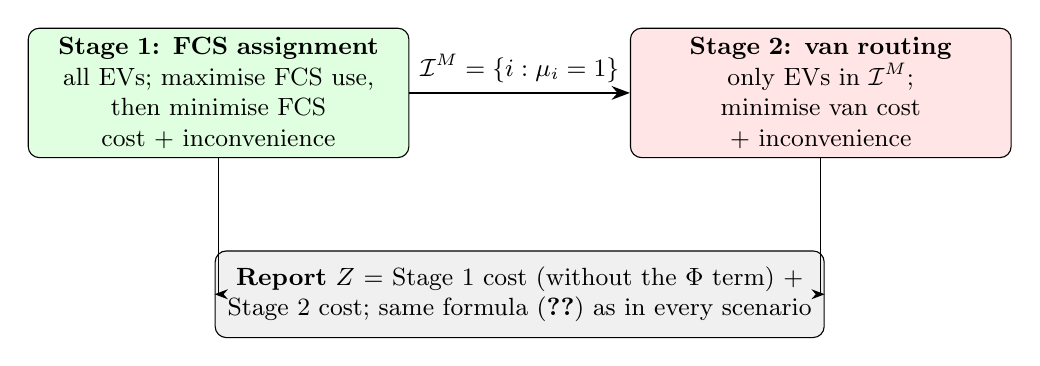
\begin{tikzpicture}[>=Stealth,box/.style={draw,rounded corners,align=center,minimum height=1.1cm,font=\small}]
  \node[box,fill=green!12,text width=4.6cm] (s1) {\textbf{Stage 1: FCS assignment}\\all EVs; maximise FCS use,\\then minimise FCS cost + inconvenience};
  \node[box,fill=red!10,text width=4.6cm,right=2.8cm of s1] (s2) {\textbf{Stage 2: van routing}\\only EVs in $\I^M$;\\minimise van cost + inconvenience};
  \draw[->,thick] (s1) -- node[above,font=\small]{$\I^M=\{i:\mu_i=1\}$} (s2);
  \node[box,fill=black!6,text width=7.5cm,below=2.0cm of $(s1)!0.5!(s2)$] (ev) {\textbf{Report} $Z=$ Stage~1 cost (without the $\Phi$ term) $+$ Stage~2 cost; same formula \eqref{eq:Z} as in every scenario};
  \draw[->] (s1) |- (ev); \draw[->] (s2) |- (ev);
\end{tikzpicture}
\end{center}

Stage~1 does not look at the vans, and Stage~2 cannot change what Stage~1 decided. That is the definition of ``FCS first, then MCS''.

%----------------------------------------------------------------
\subsection{Stage 1: assign EVs to fixed stations}

\textbf{Objective.}
\begin{equation}
\begin{split}
\min\ Z^{(1)}=\;&\underbrace{\Phi\sum_{i\in\I}\mu_i}_{\text{FCS first}}
+\underbrace{c^{EV}\sum_i\sum_{f\in\F_i}d_{if}Y_{if}}_{Z_1}
+\underbrace{Z^F_{\text{energy}}}_{\text{FCS part of }Z_4}\\
&+\underbrace{\sum_i\sum_{f\in\F_i}\rho^F_{if}Y_{if}+\alpha\sum_i w_i(C_i-r_i)+c^L\sum_i w_iL_i}_{\text{FCS customers' inconvenience}}
\end{split}
\label{eq:obj1}
\end{equation}
with $C_i=S_i+\tau^F_iY_i$ in this stage. $\Phi$ is a penalty for handing an EV to the vans. It is chosen larger than anything an extra FCS customer can add to the rest of \eqref{eq:obj1}, e.g.
\[
\Phi > \max_{i}\max_{f\in\F_i}\big(c^{EV}d_{if}+\pi^{\max}E_i+\rho^F_{if}\big)+n\,(\alpha+c^L)\,w_{\max}\,T,
\]
so Stage~1 first \textbf{maximises the number of EVs served at an FCS}, and only among those solutions minimises FCS cost and inconvenience. ($\pi^{\max}$ is the highest grid price.) A numerically safer equivalent is to solve twice: first $\max\sum_iY_i$, then fix that number and minimise the rest.
\ifTOU
Because $Z^F_{\text{energy}}$ uses the peak price, Stage~1 may \emph{start sessions later} to leave the peak, if the price saving beats the extra waiting cost (Section~\ref{sec:expect}).
\fi

\textbf{Constraints.}
\begin{align}
\sum_{g\in\G_i}y_{ig}+\mu_i &= 1 && \forall i\in\I \label{eq:s1assign}\\
S_i &\ge r_i+\sum_{f\in\F_i}t_{if}Y_{if} && \forall i\in\I \label{eq:fcsarr}\\
S_i &\le r_i+T\,(1-\mu_i) && \forall i\in\I \label{eq:s1park}\\
S_j &\ge S_i+\tau^F_i-(T+\tau^F_i)(3-y_{ig}-y_{jg}-o_{ij}) && \forall g,\ (i,j)\in\mathcal{P}_g \label{eq:disj1}\\
S_i &\ge S_j+\tau^F_j-(T+\tau^F_j)(2-y_{ig}-y_{jg}+o_{ij}) && \forall g,\ (i,j)\in\mathcal{P}_g \label{eq:disj2}\\
\sum_i y_{ig_1} &\ge \sum_i y_{ig_2} && \forall f,\ \G_f=\{g_1,g_2\} \label{eq:gunsym}\\
S_i+\tau^F_iY_i &\le T,\qquad L_i\ge S_i+\tau^F_iY_i-l_i && \forall i\in\I \label{eq:s1time}
\end{align}
\ifTOU plus the time-of-use split \eqref{eq:tou1}--\eqref{eq:tou5} of each FCS session (Section~\ref{sec:price}).\fi
\desc{\eqref{eq:s1assign}: every EV either gets one reachable gun or is handed to the vans. An EV that reaches no FCS ($\G_i=\emptyset$) is forced to $\mu_i=1$. \eqref{eq:fcsarr}: an FCS session cannot start before the EV has asked and driven to the station. \eqref{eq:s1park}: for an EV handed to the vans, $S_i$ is parked at $r_i$, so it adds no waiting in Stage~1 (its real start time is decided in Stage~2). \eqref{eq:disj1}--\eqref{eq:disj2}: two EVs on the same gun do not overlap; $o_{ij}$ picks who goes first. With two guns per station this means at most two EVs charge at a station at a time. \eqref{eq:gunsym}: symmetry breaking between the two identical guns (optional). \eqref{eq:s1time}: finished by $T$; lateness.}

\textbf{Optional acceptability rule.} An operator may refuse to send a driver to a station that is ``too inconvenient'', e.g.\ only allow gun $g$ of station $f$ for EV $i$ if $\hat\rho^F_{if}\le\bar\rho$. This only shrinks $\G_i$, so EVs whose stations are all too far go to the vans. Report results with and without it.

\textbf{Output:} $\I^M=\{i:\mu_i=1\}$, the EVs left for the vans; plus each FCS customer's gun and start time.

%----------------------------------------------------------------
\subsection{Stage 2: route the vans to the leftover EVs}

Stage~2 is a vehicle routing problem with time windows, on the EVs in $\I^M$ only. Here $C_i=S_i+\tau^M_i$.

\textbf{Objective.}
\begin{equation}
\begin{split}
\min\ Z^{(2)}=\;&\underbrace{c^M\sum_m\sum_{(i,j)\in\A^M}d_{ij}x_{ijm}}_{Z_2}+\underbrace{\sum_m c^D_mu_m}_{Z_3}+\underbrace{Z^M_{\text{energy}}}_{\text{van part of }Z_4}\\
&+\underbrace{\sum_{i\in\I^M}\sum_m\rho^M_{im}z_{im}+\alpha\sum_{i\in\I^M}w_i(C_i-r_i)+c^L\sum_{i\in\I^M}w_iL_i}_{\text{van customers' inconvenience}}
\end{split}
\label{eq:obj2}
\end{equation}
Since every EV in $\I^M$ must be served by some van, $Z^M_{\text{energy}}$ and the $\rho^M$ term are constants here. They are kept so that $Z^{(2)}$ is the true cost of Stage~2. Waiting and lateness make the vans visit urgent EVs early.

\textbf{Constraints.}
\begin{align}
\sum_{m\in\M}z_{im} &= 1 && \forall i\in\I^M \label{eq:s2assign}\\
\sum_{j:(0,j)\in\A^M}x_{0jm} = \sum_{i:(i,n+1)\in\A^M}x_{i,n+1,m} &= u_m && \forall m \label{eq:depot}\\
\sum_{i:(i,j)\in\A^M}x_{ijm} = \sum_{k:(j,k)\in\A^M}x_{jkm} &= z_{jm} && \forall j\in\I^M,\ m \label{eq:flow}\\
\sum_{i\in\I^M}z_{im} &\le Q_m\,u_m && \forall m \label{eq:cap}\\
\sum_{i\in\I^M}\frac{E_i}{\eta}z_{im}+\beta\sum_{(i,j)\in\A^M}d_{ij}x_{ijm} &\le B_m\,u_m && \forall m \label{eq:batt}
\end{align}
\begin{align}
S_j &\ge \max\{r_j,\ t_{0j}\,x_{0jm}\} && \forall j\in\I^M,\ m \label{eq:depart}\\
S_j &\ge S_i+\tau^M_i+t_{ij}-(T+\tau^M_i+t_{ij})(1-x_{ijm}) && \forall i\neq j,\ m \label{eq:seq}\\
S_i+\tau^M_i+t_{i,n+1} &\le T+(\tau^M_i+t_{i,n+1})(1-x_{i,n+1,m}) && \forall i,\ m \label{eq:return}\\
S_i+\tau^M_i \le T,\quad L_i &\ge S_i+\tau^M_i-l_i && \forall i\in\I^M \label{eq:s2time}\\
u_m &\ge u_{m+1} && m<|\M| \label{eq:vansym}
\end{align}
\desc{\eqref{eq:s2assign}: each leftover EV gets one van. \eqref{eq:depot}: a used van leaves and returns to the depot once. \eqref{eq:flow}: each EV on van $m$ is entered and left exactly once by that van. \eqref{eq:cap}: at most $Q_m$ EVs per van. \eqref{eq:batt}: delivered energy (with transfer losses) plus driving energy fits in the van battery. \eqref{eq:depart}: no start before the request, or before the van can drive there from the depot (written as two linear constraints). \eqref{eq:seq}: if the van goes $i\to j$, it finishes $i$ and drives to $j$ before starting $j$. This gives one EV at a time and removes subtours (MTZ-type). \eqref{eq:return}: back at the depot by $T$. \eqref{eq:s2time}: finished by $T$; lateness. \eqref{eq:vansym}: use identical vans in index order.}

\textbf{If Stage 2 is infeasible} (too many leftover EVs for the fleet by $T$), the sequential policy has \emph{failed} on that instance. For diagnosis, add $s_i\in\{0,1\}$ (``unserved''), replace \eqref{eq:s2assign} by $\sum_mz_{im}+s_i=1$ and add $\Phi^U\sum_is_i$ to \eqref{eq:obj2}. Then report the number of EVs that could not be served. This is a useful comparison with the integrated scenario, which may serve all of them.

%----------------------------------------------------------------
\subsection{Reported value}
\[
Z^{\text{S\scen}}=\big(Z^{(1)*}-\Phi\,|\I^M|\big)+Z^{(2)*},
\]
which is exactly \eqref{eq:Z} evaluated at the combined solution. The stage-1 solution plus the stage-2 solution is a feasible solution of the integrated model (S\ifTOU 4\else 3\fi), so
$Z^{\text{S\ifTOU 4\else 3\fi}}\le Z^{\text{S\scen}}$. The difference is the \emph{value of integration}.

\else
%---------------------------------------------------------------- INT
\subsection{Objective}
\begin{equation}
\min\ Z \quad\text{as in \eqref{eq:Z}, with }Z^F_{\text{energy}}=\ifTOU P^F\textstyle\sum_i\big[\pi^\off(\theta^1_i+\theta^3_i)+\pi^\pk\theta^2_i\big]\else\pi^F\textstyle\sum_iE_iY_i\fi,\quad C_i=S_i+\tau^F_iY_i+\tau^M_iZ_i. \label{eq:objint}
\end{equation}
Written out in full:
\begin{align*}
\min\ Z=\;& c^{EV}\sum_i\sum_{f\in\F_i}d_{if}Y_{if}+c^M\sum_m\sum_{(i,j)\in\A}d_{ij}x_{ijm}+\sum_mc^D_mu_m\\
&+\ifTOU P^F\sum_i\big[\pi^\off(\theta^1_i+\theta^3_i)+\pi^\pk\theta^2_i\big]\else\pi^F\sum_iE_iY_i\fi
+\pi^M\sum_i\sum_m\frac{E_i}{\eta}z_{im}\\
&+\sum_i\sum_{f\in\F_i}\rho^F_{if}Y_{if}+\sum_i\sum_m\rho^M_{im}z_{im}+\alpha\sum_iw_i(C_i-r_i)+c^L\sum_iw_iL_i .
\end{align*}
Every term is linear. One model weighs everything at once: an EV goes to a van exactly when the van's extra km, dispatch and energy cost are outweighed by the effort and waiting it saves the driver\ifTOU, or by the peak-price energy it avoids\fi.

\subsection{Constraints}

\textbf{Assignment.}
\begin{equation}
\sum_{g\in\G_i}y_{ig}+\sum_{m\in\M}z_{im}=1\qquad\forall i\in\I \label{eq:assign}
\end{equation}
\desc{Exactly one resource per EV: one reachable gun or one van. EVs that reach no FCS are forced onto a van.}

\textbf{Fixed stations.}
\begin{align}
S_i &\ge r_i+\sum_{f\in\F_i}t_{if}Y_{if} && \forall i \label{eq:fcsarr}\\
S_j &\ge S_i+\tau^F_i-(T+\tau^F_i)(3-y_{ig}-y_{jg}-o_{ij}) && \forall g,\ (i,j)\in\mathcal{P}_g \label{eq:disj1}\\
S_i &\ge S_j+\tau^F_j-(T+\tau^F_j)(2-y_{ig}-y_{jg}+o_{ij}) && \forall g,\ (i,j)\in\mathcal{P}_g \label{eq:disj2}\\
\sum_iy_{ig_1} &\ge \sum_iy_{ig_2} && \forall f,\ \G_f=\{g_1,g_2\} \label{eq:gunsym}
\end{align}
\desc{\eqref{eq:fcsarr}: an FCS session starts after the request and the drive to the station (for a van customer this is just $S_i\ge r_i$). \eqref{eq:disj1}--\eqref{eq:disj2}: EVs on the same gun do not overlap; $o_{ij}$ chooses the order. \eqref{eq:gunsym}: optional symmetry breaking.}

\textbf{Vans: routes, capacity, battery.}
\begin{align}
\sum_{j:(0,j)\in\A}x_{0jm}=\sum_{i:(i,n+1)\in\A}x_{i,n+1,m} &= u_m && \forall m \label{eq:depot}\\
\sum_{i:(i,j)\in\A}x_{ijm}=\sum_{k:(j,k)\in\A}x_{jkm} &= z_{jm} && \forall j\in\I,\ m \label{eq:flow}\\
\sum_iz_{im} &\le Q_mu_m && \forall m \label{eq:cap}\\
\sum_i\frac{E_i}{\eta}z_{im}+\beta\sum_{(i,j)\in\A}d_{ij}x_{ijm} &\le B_mu_m && \forall m \label{eq:batt}
\end{align}
\desc{\eqref{eq:depot}: a used van leaves and returns once. \eqref{eq:flow}: each EV on van $m$ is visited exactly once by it. \eqref{eq:cap}: at most $Q_m$ EVs. \eqref{eq:batt}: delivered energy (with losses) plus driving energy fits in the battery.}

\textbf{Vans: timing (one EV at a time, no subtours).}
\begin{align}
S_j &\ge t_{0j}\,x_{0jm} && \forall j\in\I,\ m \label{eq:depart}\\
S_j &\ge S_i+\tau^M_i+t_{ij}-(T+\tau^M_i+t_{ij})(1-x_{ijm}) && \forall i\neq j\in\I,\ m \label{eq:seq}\\
S_i+\tau^M_i+t_{i,n+1} &\le T+(\tau^M_i+t_{i,n+1})(1-x_{i,n+1,m}) && \forall i,\ m \label{eq:return}
\end{align}
\desc{\eqref{eq:depart}: the first stop cannot start before the van has driven there. \eqref{eq:seq}: $i\to j$ means finish $i$, drive, then start $j$; start times rise along a route, so no subtour can close. \eqref{eq:return}: back at the depot by $T$.}

\textbf{Horizon and lateness.}
\begin{equation}
C_i\le T,\qquad L_i\ge C_i-l_i\qquad\forall i\in\I \label{eq:time}
\end{equation}
\desc{Every EV is fully charged within the horizon; $L_i$ measures lateness.}

\ifTOU
\textbf{Time-of-use split.} Constraints \eqref{eq:tou1}--\eqref{eq:tou5} of Section~\ref{sec:price}.
\fi

\textbf{Symmetry and domains.}
\begin{equation}
u_m\ge u_{m+1};\qquad y,z,x,u,o\ifTOU,\kappa\fi\in\{0,1\};\qquad S_i,L_i\ifTOU,\theta^p_i\fi\ge0 \label{eq:dom}
\end{equation}
\fi

%=====================================================================
\section{Learning-to-optimise (RL) formulation}\label{sec:rl}

\textbf{Main rule:} the reward of each action is \emph{minus the increase in $Z$ that the action causes}. The rewards over an episode then add up to $-Z$ of the solution the policy builds. RL and MILP results are measured on the same yardstick \eqref{eq:Z}, and the MILP optimum is the benchmark for the RL gap.

\ifSEQ
%---------------------------------------------------------------- RL SEQ
The RL pipeline has the same two stages as the MILP.

\subsection{Stage 1 policy: FCS assignment}
\begin{itemize}[leftmargin=1.4em,itemsep=2pt]
  \item \textbf{Episode / epochs:} EVs are taken in order of request time $r_i$ (ties: higher $w_i$ first). One decision per EV.
  \item \textbf{State:} features of the current EV $k$ ($E_k,r_k,l_k,w_k,R_k$, location); for each gun $g$ the time $F_g$ it becomes free; summary features of the EVs still to come (count and positions near each station)\ifTOU; the current price and the time until $T_1$ and $T_2$\fi.
  \item \textbf{Action:} a gun $g\in\G_k$, or ``hand to vans''. \textbf{FCS-first mask:} ``hand to vans'' is allowed \emph{only} if no gun can finish EV $k$ by $T$ (or, with the optional rule, if all remaining guns have $\hat\rho^F_{kf}>\bar\rho$).
  \ifTOU\item \textbf{Optional timing action:} ``gun $g$, start after the peak'', i.e.\ $S_k=\max\{\text{earliest},T_2\}$, allowed only if the session still ends by $T$.\fi
  \item \textbf{Transition:} $S_k=\max\{r_k+t_{kf},F_g\}$ (or later, for the timing action); $F_g\leftarrow S_k+\tau^F_k$.
  \item \textbf{Reward:} $-\Big[c^{EV}d_{kf}+\text{energy}_k+\rho^F_{kf}+\alpha w_k(S_k+\tau^F_k-r_k)+c^Lw_k(S_k+\tau^F_k-l_k)^+\Big]$, where energy$_k$ = \ifTOU$P^F\big[\pi^\off\cdot(\text{off-peak hours of }[S_k,S_k+\tau^F_k])+\pi^\pk\cdot(\text{peak hours})\big]$, computed exactly in the simulator\else$\pi^FE_k$\fi. Handing an EV to the vans gives reward $0$ here; its cost is counted in Stage~2.
\end{itemize}
Note: a simple baseline for Stage~1 is the greedy rule ``gun with the largest one-step reward''. What RL can learn on top of this is, for example, to keep a nearby gun free for an urgent EV that arrives later.

\subsection{Stage 2 policy: van routing over $\I^M$}
\begin{itemize}[leftmargin=1.4em,itemsep=2pt]
  \item \textbf{Epochs:} whenever a van becomes free (the earliest-free van decides first).
  \item \textbf{State:} for each van: position, time free, remaining battery $b_m$, EVs served so far, dispatched or not; for each unserved EV in $\I^M$: location, $E_i,r_i,l_i,w_i$; current time.
  \item \textbf{Action:} the next EV $j$ for this van, or ``return to depot'' (ends the route). Mask: $j$ must be feasible: battery covers $E_j/\eta$ plus driving to $j$ and back to the depot, the count stays $\le Q_m$, and $j$ can be finished with the van back at the depot by $T$.
  \item \textbf{Transition:} $S_j=\max\{r_j,\ \text{time free}+t_{\text{pos},j}\}$; the van moves to $j$ and is free at $S_j+\tau^M_j$; $b_m$ falls by $E_j/\eta+\beta d_{\text{pos},j}$.
  \item \textbf{Reward:} serving $j$: $-\Big[c^Md_{\text{pos},j}+c^D_m[\text{first stop}]+\pi^M\frac{E_j}{\eta}+\rho^M_{jm}+\alpha w_j(S_j+\tau^M_j-r_j)+c^Lw_j(S_j+\tau^M_j-l_j)^+\Big]$; returning: $-c^Md_{\text{pos},0}$. EVs still unserved at the end: $-\Phi^U$ each.
  \item \textbf{Policy:} an attention-based routing policy (e.g.\ Kool et al., 2019, ``Attention, Learn to Solve Routing Problems!'') trained with REINFORCE or PPO. Baseline: nearest-feasible-EV heuristic.
\end{itemize}
Episode return of Stage~1 + Stage~2 $=-Z^{\text{S\scen}}$.

\else
%---------------------------------------------------------------- RL INT
One policy decides both who serves each EV and the van routes.
\begin{itemize}[leftmargin=1.4em,itemsep=2pt]
  \item \textbf{Episode / epochs:} EVs are taken in order of request time $r_i$ (ties: higher $w_i$ first). One decision per EV.
  \item \textbf{State:} (i) the current EV $k$: location, $E_k,r_k,l_k,w_k,R_k$, reachable stations; (ii) each gun $g$: time $F_g$ it becomes free; (iii) each van $m$: current end-of-route position, time free, remaining battery $b_m$, EVs served, dispatched or not; (iv) embeddings of the not-yet-assigned EVs (for look-ahead)\ifTOU; (v) current price, time until $T_1$ and $T_2$\fi.
  \item \textbf{Action:} $a\in\G_k\cup\M$: a gun, or a van (EV $k$ is appended to the end of that van's route). \textbf{Mask} infeasible actions: a gun that cannot finish $k$ by $T$; a van without enough battery for $E_k/\eta$ plus the drive to $k$ and back to the depot, with $Q_m$ reached, or unable to finish $k$ and return by $T$.
  \ifTOU\item \textbf{Optional timing action:} ``gun $g$, start after the peak'' ($S_k=\max\{\text{earliest},T_2\}$, if it still ends by $T$).\fi
  \item \textbf{Transition:} gun: $S_k=\max\{r_k+t_{kf},F_g\}$, $F_g\leftarrow S_k+\tau^F_k$. Van: $S_k=\max\{r_k,\ \text{free}_m+t_{\text{pos}_m,k}\}$, then the van moves to $k$, $\text{free}_m\leftarrow S_k+\tau^M_k$, $b_m\mathrel{-}=E_k/\eta+\beta d_{\text{pos}_m,k}$.
  \item \textbf{Reward} $=-\Delta Z$:
  \begin{align*}
  \text{gun } g\text{ at }f:&\quad -\Big[c^{EV}d_{kf}+\text{energy}^F_k+\rho^F_{kf}+\alpha w_k(C_k-r_k)+c^Lw_k(C_k-l_k)^+\Big]\\
  \text{van } m:&\quad -\Big[c^M\big(d_{\text{pos}_m,k}+d_{k,0}-d_{\text{pos}_m,0}\big)+c^D_m[\text{first use}]+\pi^M\tfrac{E_k}{\eta}\\
  &\qquad\quad+\rho^M_{km}+\alpha w_k(C_k-r_k)+c^Lw_k(C_k-l_k)^+\Big]
  \end{align*}
  The van distance term is the \emph{change} in route length when $k$ is inserted before the return to the depot, so the sum over the episode equals the total route length (the return legs telescope). energy$^F_k$ = \ifTOU$P^F\big[\pi^\off\cdot(\text{off-peak hours})+\pi^\pk\cdot(\text{peak hours of }[S_k,C_k])\big]$, computed exactly by the simulator; no linearisation is needed in RL\else$\pi^FE_k$\fi.
  \item \textbf{Dead end:} if every action is masked, EV $k$ is unserved: reward $-\Phi^U$, and the episode continues. Report the count.
  \item \textbf{Policy:} masked categorical policy over guns and vans, encoder with attention over EVs, guns and vans; trained with PPO. Natural baseline: greedy, i.e.\ choose the action with the largest one-step reward. That is the pairwise rule ``smallest $\hat\rho$ + cost'' from Section~\ref{sec:inc}.
\end{itemize}
Restriction to note: vans serve EVs in assignment order (append only). A variant that inserts $k$ at the cheapest position of a route is more flexible but has a larger action space.
\fi

\textbf{Reward scaling.} For stable training divide every reward by a constant, e.g.\ the greedy baseline's average $Z$ on the training instances. This does not change the optimal policy.

%=====================================================================
\section{What to expect and what to report}\label{sec:expect}

\ifnum\scen=1
\begin{itemize}[leftmargin=1.4em,itemsep=2pt]
  \item Vans serve only EVs that reach no station, or that the stations cannot finish by $T$. If stations have spare capacity, very few vans are dispatched.
  \item Inconvenience is high for EVs far from the nearest station (worked example: Rs\,682 at the FCS, against Rs\,458 if a van had been allowed).
  \item With too few vans Stage~2 becomes infeasible (unserved EVs), even when the integrated model S3 could serve everyone. Report the smallest $|\M|$ at which S1 is feasible and compare it with S3.
\end{itemize}
\fi
\ifnum\scen=2
\begin{itemize}[leftmargin=1.4em,itemsep=2pt]
  \item \textbf{When does Stage~1 delay a session to avoid the peak?} Moving one hour of charging out of the peak saves $(\pi^\pk-\pi^\off)P^F=3\times22=$ Rs\,66, but delays completion by up to an hour, which costs $\alpha w_i\ge$ Rs\,200. So with the default values Stage~1 almost never delays. It mostly pays the higher price, and S2 costs roughly S1 plus the peak surcharge. Sessions start later only if $\alpha$ is small (try $\lambda<0.33$ in the sensitivity analysis).
  \item The van assignment is the same as in S1 unless Stage~1's timing changes which EVs fit at the stations. Stage~1 cannot use vans to escape the peak price.
  \item Extra KPI: \textbf{grid energy drawn at FCS during the peak}, $P^F\sum_i\theta^2_i$ (kWh). Compare with S4.
\end{itemize}
\fi
\ifnum\scen=3
\begin{itemize}[leftmargin=1.4em,itemsep=2pt]
  \item Vans take EVs for which the saved inconvenience exceeds the extra van cost (worked example: van chosen, saving Rs\,224). Expect vans to serve EVs that are far from every station, have low range (high $w_i$), or have early deadlines, while EVs near a station still use it.
  \item \textbf{Value of integration under flat price:} $Z^{\text{S1}}-Z^{\text{S3}}\ge0$. Report it per component ($Z_1,\dots,Z_5$): typically operating cost rises a little and inconvenience falls a lot.
  \item Vary $|\M|$ (0, 1, 2, \dots): the first few vans lower $Z$ sharply, then the effect levels off. That curve shows the scenarios where mobile chargers help most.
\end{itemize}
\fi
\ifnum\scen=4
\begin{itemize}[leftmargin=1.4em,itemsep=2pt]
  \item During the peak a van kWh costs about the same as an FCS kWh (Rs\,10.0 each), so the vans' energy disadvantage disappears and vans also absorb \emph{peak-hour} demand that would otherwise be charged on the grid at peak price.
  \item Expect more van usage than in S3, concentrated on requests in $[T_1,T_2]$, and lower grid energy at the stations during the peak, $P^F\sum_i\theta^2_i$, than in S2.
  \item \textbf{Value of integration under peak pricing:} $Z^{\text{S2}}-Z^{\text{S4}}$. It should be larger than $Z^{\text{S1}}-Z^{\text{S3}}$, because integration now also allows price arbitrage.
  \item \textbf{Peak pricing with full flexibility:} $Z^{\text{S4}}-Z^{\text{S3}}$ should be smaller than $Z^{\text{S2}}-Z^{\text{S1}}$: vans cushion the price increase.
\end{itemize}
\fi

\textbf{Cross-scenario comparison table} (fill in from the four runs):
\begin{center}
\renewcommand{\arraystretch}{1.2}
\begin{tabular}{@{}lll@{}}
\toprule
\textbf{Comparison} & \textbf{Measures} & \textbf{Expected sign} \\
\midrule
S1 $-$ S3 & value of integration, flat price & $\ge0$ \\
S2 $-$ S4 & value of integration, peak price & $\ge0$, larger than S1 $-$ S3 \\
S2 $-$ S1 & cost of peak pricing, FCS-first operator & $>0$ \\
S4 $-$ S3 & cost of peak pricing, flexible operator & $>0$, smaller than S2 $-$ S1 \\
\bottomrule
\end{tabular}
\end{center}
Report for each: $Z$ and its components, number of vans used, EVs per resource, mean and maximum inconvenience per EV, total lateness, peak-hour grid energy, solve time, and (for RL) the gap to the MILP optimum.

%=====================================================================
\appendix
\section{Illustrative parameter values}\label{app:values}

These are starting values for experiments, not data. All are meant to be varied in the analysis. Values in Rs.

\begin{center}
\renewcommand{\arraystretch}{1.15}
\begin{tabular}{@{}llp{6.2cm}@{}}
\toprule
\textbf{Parameter} & \textbf{Value} & \textbf{Note} \\
\midrule
$T$, $[T_1,T_2]$ & 7 h, $[2,6]$ & 16:00--23:00, peak 18:00--22:00 \\
$P^F$, $P^M$ & 22 kW, 30 kW & \\
$v$, $\beta$, $\eta$ & 25 km/h, 0.25 kWh/km, 0.9 & \\
$B_m$, $Q_m$, $|\M|$ & 150 kWh, 6, 2--6 & \\
$c^{EV}$, $c^M$, $c^D_m$ & Rs\,4/km, Rs\,15/km, Rs\,1500 & van km includes driver time \\
$\pi^F$ (flat) & Rs\,8.7/kWh & equals the time-average of the ToU tariff over $[0,T]$ \\
$\pi^\off$, $\pi^\pk$ (ToU) & Rs\,7/kWh, Rs\,10/kWh & $(3\times7+4\times10)/7=8.7$ \\
$c^{bat}$ & Rs\,2/kWh & van battery wear \\
$\pi^M$ & Rs\,10.7 (flat) / Rs\,9.0 (ToU) & $=\pi^F+c^{bat}$ / $=\pi^\off+c^{bat}$ \\
$\alpha$, $\alpha^D$ & Rs\,200/h, Rs\,100/h & value of time; extra for attended time \\
$h^F$, $h^M$, $\varphi$ & Rs\,50, Rs\,10, Rs\,100 & trip hassle, hand-over, range stress \\
$c^L$ & Rs\,300/h & lateness \\
$w_i$ & $1+2(1-R_i/R_{\max})$, $R_i\sim U[3,40]$ km & priority from remaining range \\
\bottomrule
\end{tabular}
\end{center}

The flat price is set to the time-average of the peak tariff. The price \emph{level} is then the same in both pricing cases, and only the price \emph{shape} differs. Without this, part of S1 vs S2 would just reflect a different average price.

\end{document}
"
%    pdflatex -jobname=scenario4_peak_integrated   "\def\scen{4}% =====================================================================
%  One source, four PDFs.  Build with build.sh (or by hand):
%    pdflatex -jobname=scenario1_flat_sequential   "\def\scen{1}\input{scenario_master}"
%    pdflatex -jobname=scenario2_peak_sequential   "\def\scen{2}\input{scenario_master}"
%    pdflatex -jobname=scenario3_flat_integrated   "\def\scen{3}\input{scenario_master}"
%    pdflatex -jobname=scenario4_peak_integrated   "\def\scen{4}\input{scenario_master}"
%  (run each twice for cross-references)
% =====================================================================
\documentclass[11pt,a4paper]{article}
\usepackage[margin=2.2cm]{geometry}
\usepackage{amsmath,amssymb,amsfonts}
\usepackage{booktabs,array,tabularx}
\usepackage{enumitem}
\usepackage[table]{xcolor}
\usepackage{tikz}
\usetikzlibrary{arrows.meta,positioning,calc}
\usepackage[colorlinks=true,linkcolor=blue!50!black,urlcolor=blue!50!black]{hyperref}
\usepackage{titlesec}
\titleformat{\section}{\large\bfseries}{\thesection}{0.8em}{}
\titleformat{\subsection}{\normalsize\bfseries}{\thesubsection}{0.8em}{}
\setlength{\parindent}{0pt}
\setlength{\parskip}{5pt}

% ---------------- scenario switches ----------------
\ifdefined\scen\else\def\scen{1}\fi
\newif\ifTOU \TOUfalse   % true = time-of-use (peak) price
\newif\ifSEQ \SEQfalse   % true = FCS first, then MCS
\ifnum\scen=1 \SEQtrue \fi
\ifnum\scen=2 \TOUtrue \SEQtrue \fi
\ifnum\scen=4 \TOUtrue \fi

\newcommand{\pricename}{\ifTOU time-of-use price (dearer evening peak)\else single (flat) price all day\fi}
\newcommand{\structname}{\ifSEQ FCS first, then MCS (sequential)\else FCS and MCS together (integrated)\fi}

% ---------------- notation ----------------
\newcommand{\I}{\mathcal{I}}
\newcommand{\F}{\mathcal{F}}
\newcommand{\G}{\mathcal{G}}
\newcommand{\M}{\mathcal{M}}
\newcommand{\N}{\mathcal{N}}
\newcommand{\A}{\mathcal{A}}
\newcommand{\Rs}{\text{Rs}\,}
\newcommand{\pk}{\mathrm{pk}}
\newcommand{\off}{\mathrm{off}}
\newcommand{\desc}[1]{\par\vspace{-2pt}{\small\color{black!75}\textit{Meaning:} #1}\par\vspace{4pt}}
\newcommand{\cell}[2]{\ifnum\scen=#1\cellcolor{blue!18}\textbf{S#1 (this document)}\\\textbf{#2}\else S#1\\#2\fi}

\title{\textbf{EV Charging Network Optimisation}\\[4pt]
\large Scenario \scen: \pricename\ $+$ \structname\\[2pt]
\normalsize MILP and RL formulation}
\author{CP 320 OR for Mobility Management, course project}
\date{2 October 2026}

\begin{document}
\maketitle

%=====================================================================
\section{Where this scenario sits}

The project studies four scenarios: two ways of pricing grid electricity, times two ways of making the decisions.

\begin{center}
\renewcommand{\arraystretch}{1.5}
\begin{tabular}{>{\raggedright\arraybackslash}p{4.2cm}|>{\centering\arraybackslash}p{4.6cm}|>{\centering\arraybackslash}p{4.6cm}}
 & \textbf{Flat price all day} & \textbf{Time-of-use (peak) price} \\ \hline
\textbf{Sequential:} FCS first, leftover EVs to MCS &
\begin{tabular}[c]{@{}c@{}}\cell{1}{flat + sequential}\end{tabular} &
\begin{tabular}[c]{@{}c@{}}\cell{2}{peak + sequential}\end{tabular} \\ \hline
\textbf{Integrated:} FCS and MCS decided together &
\begin{tabular}[c]{@{}c@{}}\cell{3}{flat + integrated}\end{tabular} &
\begin{tabular}[c]{@{}c@{}}\cell{4}{peak + integrated}\end{tabular} \\
\end{tabular}
\end{center}

\textbf{The four scenarios do not have four different objectives.} They share \emph{one} cost yardstick $Z$ (Section~\ref{sec:obj}): the same cost terms and the same customer inconvenience (Section~\ref{sec:inc}). Only two things change:
\begin{itemize}[leftmargin=1.4em,itemsep=1pt]
  \item \textbf{Pricing} changes the formula for one term, the FCS energy cost (Section~\ref{sec:price}).
  \item \textbf{Decision structure} changes \emph{how} $Z$ is minimised: in one model (integrated), or in two stages (sequential), where each stage minimises its own part of $Z$.
\end{itemize}
Because the yardstick is the same, the four optimal values can be compared directly. The differences measure the \emph{value of integration} (S1$\to$S3, S2$\to$S4) and the \emph{effect of peak pricing} (S1$\to$S2, S3$\to$S4).

\ifnum\scen=1
\textbf{This scenario (S1)} is the baseline, the ``status quo''. Electricity costs the same at every hour, every EV that can be charged at a fixed station is sent there, and vans only take what is left over.
\fi
\ifnum\scen=2
\textbf{This scenario (S2)} keeps the FCS-first rule of S1, but grid electricity is dearer during the evening peak. Stage~1 can react to the price only by \emph{rescheduling} FCS sessions. It cannot hand a peak-hour EV to a van.
\fi
\ifnum\scen=3
\textbf{This scenario (S3)} keeps the flat price of S1, but the operator decides FCS and MCS service \emph{together}. An EV can be sent to a van even when a fixed station could take it, whenever that lowers total cost plus inconvenience.
\fi
\ifnum\scen=4
\textbf{This scenario (S4)} is the most flexible one: peak pricing at fixed stations, and FCS and MCS decided together. Van energy was bought off-peak, so vans can also be used to keep charging \emph{out of the expensive peak}.
\fi

%=====================================================================
\section{Setting and assumptions}\label{sec:setting}

\textbf{Time.} The planning horizon is $[0,T]$ with $T=7$\,h (16:00--23:00). It contains the evening peak window $[T_1,T_2]=[2,6]$ (18:00--22:00). The horizon is the same in all four scenarios. It is wider than the peak itself so that, under peak pricing, there is cheaper time on both sides of the peak.\ifTOU\else\ In this scenario the price is flat, so the window plays no role in the model.\fi

\textbf{Assumptions} (the same as MILP v3, plus two about energy):
\begin{enumerate}[leftmargin=1.6em,itemsep=1pt]
  \item Static, continuous time. All requests in the horizon are known at time $0$, and request $i$ becomes active at $r_i$.
  \item An EV served by an FCS drives there itself on its own battery (only to stations within its range $R_i$). The driver stays with the car while it waits for a free gun and while it charges.
  \item An EV served by an MCS stays parked where it is, and the driver is free in the meantime.
  \item Each FCS gun and each van charges one EV at a time, without interruption, at constant power.
  \item A van's battery covers both its driving and the energy it delivers. \textbf{The van battery is charged at the depot before the horizon starts}\ifTOU, i.e.\ at the off-peak price\fi, and is not recharged during the horizon.
  \item Every EV must be fully charged by $T$ (hard). Finishing after the driver's desired time $l_i$ is allowed but penalised.
\end{enumerate}

%=====================================================================
\section{Notation}\label{sec:notation}

\subsection*{Sets}
\begin{tabularx}{\textwidth}{@{}lX@{}}
\toprule
$\I=\{1,\dots,n\}$ & EV charging requests \\
$\F$; $\G_f$ ($|\G_f|=2$); $\G=\bigcup_f\G_f$ & fixed charging stations; guns of FCS $f$; all guns ($f(g)$ = station of gun $g$) \\
$\F_i=\{f: d_{if}\le R_i\}$, $\G_i=\bigcup_{f\in\F_i}\G_f$ & stations / guns EV $i$ can reach on its remaining range \\
$\M$ & mobile charging vans (MCS) \\
$0,\ n+1$ & depot as start node / end node (same place) \\
$\N=\{0\}\cup\I\cup\{n+1\}$, $\A$ & routing nodes; allowed van arcs $(i,j)$, $i\in\{0\}\cup\I$, $j\in\I\cup\{n+1\}$, $i\neq j$ \\
$\mathcal{P}_g=\{(i,j): i<j,\ g\in\G_i\cap\G_j\}$ & pairs of EVs that could share gun $g$ \\
\ifSEQ
$\I^M\subseteq\I$ & EVs handed to the vans by Stage~1 (an \emph{output} of Stage~1, a fixed input to Stage~2) \\
$\N^M$, $\A^M$ & routing nodes / arcs restricted to $\I^M$ \\
\fi
\bottomrule
\end{tabularx}

\subsection*{Parameters}
\begin{tabularx}{\textwidth}{@{}lX@{}}
\toprule
$E_i,\ r_i,\ l_i,\ R_i$ & energy demand (kWh), request time, desired completion time (h), remaining range (km) \\
$w_i\ge1$ & priority of EV $i$; $w_i=1+\kappa(1-R_i/R_{\max})$, so low-range EVs weigh more \\
$P^F,\ P^M$ & charging power of an FCS gun (22\,kW) / of a van (e.g.\ 30\,kW) \\
$\tau^F_i=E_i/P^F,\ \tau^M_i=E_i/P^M$ & charging time of EV $i$ at an FCS / by a van (h) \\
$d_{if},t_{if}$;\ $d_{ij},t_{ij}$ & distance (km) and time (h): EV$\to$FCS; between routing nodes ($t=d/v$) \\
$B_m,\ Q_m,\ \beta,\ \eta$ & van battery (kWh), max EVs per van, van consumption (kWh/km), transfer efficiency \\
$c^{EV},\ c^M,\ c^D_m$ & cost per km of EV driving, per km of van driving; fixed dispatch cost of van $m$ \\
\ifTOU
$\pi^\off,\ \pi^\pk$ & grid price (Rs/kWh) off-peak / in $[T_1,T_2]$, with $\pi^\pk\ge\pi^\off$ \\
\else
$\pi^F$ & grid price (Rs/kWh), the same at every hour \\
\fi
$c^{bat}$ & van battery wear per kWh cycled \\
$\pi^M$ & cost of 1 kWh taken from a van battery: $\pi^M=\ifTOU\pi^\off\else\pi^F\fi+c^{bat}$ (Section~\ref{sec:price}) \\
$\alpha,\ \alpha^D,\ h^F,\ h^M,\ \varphi,\ c^L$ & inconvenience coefficients (Section~\ref{sec:inc}) \\
\bottomrule
\end{tabularx}

\subsection*{Decision variables}
\begin{tabularx}{\textwidth}{@{}llX@{}}
\toprule
$y_{ig}$ & $\{0,1\}$ & EV $i$ charged at gun $g\in\G_i$ \\
$z_{im}$ & $\{0,1\}$ & EV $i$ served by van $m$ \\
$x_{ijm}$ & $\{0,1\}$ & van $m$ drives arc $(i,j)$ \\
$u_m$ & $\{0,1\}$ & van $m$ is dispatched \\
$o_{ij}$ & $\{0,1\}$ & for EVs $i<j$ that could share a gun: 1 if $i$ is charged before $j$ \\
\ifSEQ
$\mu_i$ & $\{0,1\}$ & Stage~1 only: EV $i$ is handed to the van fleet \\
\fi
\ifTOU
$\theta^1_i,\theta^2_i,\theta^3_i$ & $\ge0$ & hours of EV $i$'s FCS session before / inside / after the peak \\
$\kappa^1_i,\kappa^3_i$ & $\{0,1\}$ & EV $i$'s FCS session starts before $T_1$ / ends after $T_2$ \\
\fi
$S_i$ & $\ge0$ & time charging of EV $i$ starts (h), on whichever resource \\
$L_i$ & $\ge0$ & lateness of EV $i$ beyond $l_i$ (h) \\
\bottomrule
\end{tabularx}

\textbf{Short-hands} (linear expressions, not new variables):
\[
Y_{if}=\sum_{g\in\G_f}y_{ig},\qquad Y_i=\sum_{g\in\G_i}y_{ig}\ (\text{EV $i$ uses an FCS}),\qquad Z_i=\sum_{m\in\M}z_{im}\ (\text{EV $i$ uses a van}),
\]
\[
C_i=S_i+\tau^F_i\,Y_i+\tau^M_i\,Z_i \quad\text{(time EV $i$ is fully charged).}
\]

%=====================================================================
\section{Customer inconvenience}\label{sec:inc}

This section is \textbf{identical in all four scenario documents}. Inconvenience is a property of the customer, not of the price or of the planning method.

\subsection{What we mean by inconvenience}

Inconvenience is \emph{what the driver loses} from the moment they ask for a charge ($r_i$) until the car is fully charged ($C_i$), \emph{converted into rupees} so it can be added to the operator's costs. A driver loses three different things:

\begin{enumerate}[leftmargin=1.6em,itemsep=2pt]
  \item \textbf{Waiting:} the car is not ready. This lasts $C_i-r_i$ hours and affects \emph{every} driver, FCS or MCS.
  \item \textbf{Effort:} only an FCS customer has to drive to the station and sit there while the car charges. An MCS customer stays at home or at work and does something else. Driving to a far station also uses scarce battery range, which causes stress (``range anxiety'').
  \item \textbf{A missed deadline:} the car is still not ready at the time $l_i$ the driver needs it.
\end{enumerate}

Each loss gets a price in Rs per hour (or per event). All of them are multiplied by the priority $w_i$: an hour of delay for an EV with 5\,km of range left counts more than for one with 40\,km.

\subsection{The three components}

\begin{center}
\renewcommand{\arraystretch}{1.3}
\begin{tabularx}{\textwidth}{@{}>{\raggedright\arraybackslash}p{2.6cm}>{\raggedright\arraybackslash}X>{\raggedright\arraybackslash}X>{\raggedright\arraybackslash}p{3.0cm}@{}}
\toprule
\textbf{Component} & \textbf{EV $i$ at FCS $f$} & \textbf{EV $i$ by a van} & \textbf{Known when?} \\
\midrule
Effort & $w_i\big[\alpha^D(t_{if}+\tau^F_i)+h^F+\varphi\,d_{if}/R_i\big]$: driving and sitting at the station, a fixed trip hassle, range stress & $w_i\,h^M$: being reachable and handing over the car & \textbf{Static:} known as soon as the resource is chosen \\
Waiting & $w_i\,\alpha\,(C_i-r_i)$ = drive + \emph{queue at the gun} + charge & $w_i\,\alpha\,(C_i-r_i)$ = \emph{wait for the van} + charge & \textbf{Dynamic:} depends on the queue / van route \\
Missed deadline & $w_i\,c^L\,L_i$, $L_i=\max\{0,C_i-l_i\}$ & same & Dynamic \\
\bottomrule
\end{tabularx}
\end{center}

\textbf{Coefficients.}
$\alpha$ (Rs/h) is the value of an hour the car is not ready.
$\alpha^D$ (Rs/h) is the \emph{extra} value of an hour the driver must personally spend driving or sitting at the station: an hour at the station costs $\alpha+\alpha^D$, an hour waiting at home for a van costs only $\alpha$.
$h^F,h^M$ (Rs) are fixed hassle costs of one trip to a station / one van hand-over.
$\varphi$ (Rs) is the range-stress cost of a trip that uses the \emph{whole} remaining range ($d_{if}/R_i\le1$ is the fraction used).
$c^L$ (Rs/h) is the cost per hour late.

\subsection{Pairwise form: inconvenience of a (customer, resource) pair}

The natural first idea is: \emph{for every pair (EV $i$, FCS $f$) and every pair (EV $i$, van $m$) there is an inconvenience number, and the operator picks the pair with the lowest cost plus inconvenience.} The static part fits this idea exactly:
\[
\boxed{\;\rho^F_{if}=w_i\Big[\alpha^D\,(t_{if}+\tau^F_i)+h^F+\varphi\,\frac{d_{if}}{R_i}\Big]\qquad
\rho^M_{im}=w_i\,h^M\;}
\]
These are \textbf{parameters}, computed before solving, one number per (EV, FCS) pair and per (EV, van) pair. In the objective they appear linearly: $\sum_i\sum_f\rho^F_{if}Y_{if}+\sum_i\sum_m\rho^M_{im}z_{im}$.

Note that $\rho^M_{im}$ does not depend on $m$. Vans are identical and all start at the same depot, so the driver does not care \emph{which} van comes, only \emph{when} it comes. That ``when'' is the waiting part.

\subsection{Why waiting cannot be a fixed pairwise number}

It is tempting to also write the waiting as a pairwise number, e.g.\ ``the van needs 5 minutes to reach EV $i$''. But that depends on \emph{where the van is coming from}, which depends on the route the model is still choosing: if EV $i$ is the 4th stop of a van, the wait is the time for three charging sessions plus four drives. Likewise, waiting at an FCS depends on how many EVs are queued at that gun. So waiting is not known before solving. It is a function of decision variables:
\[
\text{waiting cost of EV } i \;=\; w_i\,\alpha\,(C_i-r_i),\qquad C_i=S_i+\tau^F_iY_i+\tau^M_iZ_i .
\]
This is \textbf{linear} in the variables ($S_i$, $y$, $z$), so it fits in a MILP directly. The constraints of Section~\ref{sec:milp} make $S_i$ equal to the true start time, including driving, queueing at the gun and the van's route. The term $\sum_i w_i\alpha r_i$ is a constant and may be dropped when solving.

\textbf{Pairwise \emph{estimate}} (used for intuition, by the RL policy and in heuristics): if there is no queue and the van comes straight to $i$,
\[
\hat\rho^{F}_{if}=\rho^F_{if}+w_i\alpha\,(t_{if}+\tau^F_i),\qquad
\hat\rho^{M}_{im}=\rho^M_{im}+w_i\alpha\,(t^{\text{van}}_{m\to i}+\tau^M_i),
\]
where $t^{\text{van}}_{m\to i}$ is the time until van $m$ can reach $i$ from where it currently is. In the RL formulation (Section~\ref{sec:rl}) the van's position \emph{is} known at each decision, so there this estimate becomes exact.

\subsection{Total inconvenience and how it enters the objective}

\begin{equation}
\boxed{\;
Z_{\text{inc}}=\underbrace{\sum_{i\in\I}\sum_{f\in\F_i}\rho^F_{if}Y_{if}+\sum_{i\in\I}\sum_{m\in\M}\rho^M_{im}z_{im}}_{\text{effort (static, pairwise)}}
+\underbrace{\alpha\sum_{i\in\I}w_i\,(C_i-r_i)}_{\text{waiting (dynamic)}}
+\underbrace{c^L\sum_{i\in\I}w_i\,L_i}_{\text{missed deadline}}
\;}\label{eq:inc}
\end{equation}
All three parts are in rupees, so $Z_{\text{inc}}$ is simply added to the operating costs. Nothing has to be normalised.

\subsection{Worked example: your ``10 km to the FCS vs.\ van in 5 minutes'' case}

EV $i$: $E_i=20$\,kWh, $R_i=40$\,km (so $w_i=1$); nearest free FCS $d_{if}=10$\,km away, $t_{if}=0.4$\,h at 25\,km/h; a van finishing next door can reach it in 5\,min ($0.083$\,h), adding about 4\,km to its route. $\tau^F_i=20/22=0.909$\,h, $\tau^M_i=20/30=0.667$\,h. Coefficients from Appendix~\ref{app:values}, flat price.

\begin{center}
\renewcommand{\arraystretch}{1.25}
\begin{tabular}{@{}lrr@{}}
\toprule
 & \textbf{FCS} & \textbf{Van} \\
\midrule
Driving (EV / extra van km) & $4\times10=40.0$ & $15\times4=60.0$ \\
Energy & $8.7\times20=174.0$ & $10.7\times20/0.9=237.8$ \\
\textbf{Operating cost only} & \textbf{214.0} & \textbf{297.8} \\
\midrule
Effort $\rho$ & $100(0.4+0.909)+50+100\cdot\tfrac{10}{40}=205.9$ & $10.0$ \\
Waiting $\alpha(C_i-r_i)$ & $200\times1.309=261.8$ & $200\times0.75=150.0$ \\
\textbf{Cost + inconvenience} & \textbf{681.7} & \textbf{457.8} \\
\bottomrule
\end{tabular}
\end{center}

On operating cost alone the FCS is cheaper, so a cost-only model would \emph{always} send this driver 10\,km away. With inconvenience included the van is better by about Rs\,224, and the integrated model chooses $z_{im}=1$, as you expected. If the FCS were only 1\,km away, the FCS would win both comparisons. The inconvenience term is what makes the model choose between ``cheap for the operator'' and ``convenient for the driver'', rather than following a fixed rule.

\subsection{Relation to a single penalty $\rho_i$ per EV}

The first draft used a penalty $\rho_i$ that is charged whenever EV $i$ goes to \emph{any} FCS: $\sum_i\sum_f\rho_iy_{if}$. Because $\sum_f y_{if}=1-\sum_m z_{im}$, this only says ``a van is worth $\rho_i$ more to EV $i$'', and that holds whether the station is 1\,km or 15\,km away, and whether the van arrives in 5 minutes or in 3 hours. The form above fixes both problems: $\rho^F_{if}$ grows with the distance to \emph{that} station, and the waiting term grows with how late the van or the free gun actually is. The old model is the special case $\alpha=\alpha^D=\varphi=c^L=0$, $h^F=\rho_i$.

\subsection{Choosing the coefficients}
\begin{itemize}[leftmargin=1.4em,itemsep=2pt]
  \item Use a value of time for $\alpha$ (e.g.\ Rs\,150--300/h for urban car users), and set $\alpha^D\approx0.5\alpha$: sitting at a station is worse than waiting at home.
  \item Keep $c^L>\alpha$, so missing the deadline is worse than ordinary waiting.
  \item \textbf{Sensitivity analysis:} multiply all inconvenience coefficients by a factor $\lambda\in\{0,0.25,0.5,1,2,4\}$ and plot operating cost against total inconvenience. $\lambda=0$ is the pure cost-minimising operator, and large $\lambda$ is a customer-first operator. This trade-off curve is a strong result for the ``Analysis'' part of the project.
\end{itemize}

\subsection{What inconvenience does in \emph{this} scenario}
\ifSEQ
In a sequential scenario inconvenience \textbf{cannot move an EV from an FCS to a van}: Stage~1 sends every EV that \emph{can} use an FCS to one. It still matters inside each stage. In Stage~1 it decides \emph{which} station and \emph{when} (urgent EVs get the near station and the first free gun). In Stage~2 it decides the \emph{order} in which vans visit EVs (urgent EVs first). In the worked example, this scenario sends the driver 10\,km to the FCS. That is the weakness the integrated scenarios remove.
\else
In an integrated scenario inconvenience is weighed directly against operating cost when choosing the resource. That is how the worked example ends up with a van. It also decides which station and which gun order, and the order of each van route.
\fi

%=====================================================================
\section{Electricity price in this scenario}\label{sec:price}

\textbf{Van energy (same in all scenarios).} A van's battery is charged at the depot \emph{before} the horizon, so its energy was bought at the
\ifTOU off-peak \fi
price, whatever time the van later delivers it. Each kWh taken from the van also wears the battery ($c^{bat}$), and a fraction $1-\eta$ is lost in transfer:
\[
Z^M_{\text{energy}}=\pi^M\sum_{i\in\I}\sum_{m\in\M}\frac{E_i}{\eta}\,z_{im},\qquad \pi^M=\ifTOU\pi^\off\else\pi^F\fi+c^{bat}.
\]

\ifTOU
\textbf{FCS energy (time-of-use).} An FCS draws from the grid while it charges. Energy delivered inside $[T_1,T_2]$ costs $\pi^\pk$, and energy outside it costs $\pi^\off$. A session $[S_i,S_i+\tau^F_i]$ may overlap the peak partly. Split its duration into the hours before, inside and after the peak, $\theta^1_i+\theta^2_i+\theta^3_i$:
\[
Z^F_{\text{energy}}=P^F\sum_{i\in\I}\Big[\pi^\off(\theta^1_i+\theta^3_i)+\pi^\pk\,\theta^2_i\Big].
\]
Constraints \eqref{eq:tou1}--\eqref{eq:tou5} below make the $\theta$'s equal to the true overlaps. Peak hours are dearer, so the solver wants $\theta^1_i,\theta^3_i$ as large as possible. It is enough to bound them from above by the true off-peak overlap, and the constraints need one binary per side:
\begin{align}
\theta^1_i+\theta^2_i+\theta^3_i &= \tau^F_i\,Y_i && \forall i\in\I \label{eq:tou1}\\
\theta^1_i &\le \tau^F_i\,\kappa^1_i && \forall i\in\I \label{eq:tou2}\\
\theta^1_i &\le T_1-S_i+T\,(1-\kappa^1_i) && \forall i\in\I \label{eq:tou3}\\
\theta^3_i &\le \tau^F_i\,\kappa^3_i && \forall i\in\I \label{eq:tou4}\\
\theta^3_i &\le S_i+\tau^F_i-T_2+T\,(1-\kappa^3_i) && \forall i\in\I \label{eq:tou5}
\end{align}
\desc{\eqref{eq:tou1}: the FCS session's hours are split into three parts; for a van customer ($Y_i=0$) all three are zero. \eqref{eq:tou2}--\eqref{eq:tou3}: off-peak time before the peak is only possible if the session starts before $T_1$ ($\kappa^1_i=1$), and is at most $T_1-S_i$. \eqref{eq:tou4}--\eqref{eq:tou5}: the same for time after $T_2$. $\theta^2_i\ge0$ prevents counting more off-peak hours than exist. Checking the cases (entirely before / inside / after the peak, straddling one edge, covering the whole peak) shows that at the optimum the $\theta$'s equal the exact overlaps. This needs $\pi^\pk\ge\pi^\off$, which is true for a peak tariff.}

\textbf{Why vans become more attractive.} Compare the cost of 1\,kWh delivered to an EV during the peak (values from Appendix~\ref{app:values}):
FCS $=\pi^\pk=$ Rs\,10.0, van $=(\pi^\off+c^{bat})/\eta=9/0.9=$ Rs\,10.0. They are at parity. Under the flat price the van is about Rs\,3.2/kWh dearer (FCS Rs\,8.7, van $10.7/0.9=$ Rs\,11.9). Peak pricing therefore removes the vans' main cost disadvantage, but only for EVs whose FCS session would fall in the peak.
\ifSEQ\ In this sequential scenario Stage~1 cannot use that, because it does not consider vans. It can only shift FCS sessions in time.\fi
\else
\textbf{FCS energy (flat).} Every kWh delivered at a fixed station costs $\pi^F$, whenever it is delivered:
\[
Z^F_{\text{energy}}=\pi^F\sum_{i\in\I}E_i\,Y_i .
\]
The start time therefore does not affect the energy cost. Under the flat price a van kWh costs $(\pi^F+c^{bat})/\eta\approx$ Rs\,11.9 against Rs\,8.7 at an FCS (Appendix~\ref{app:values}), so on energy alone the FCS always wins.
\fi

%=====================================================================
\section{MILP formulation}\label{sec:milp}

\subsection{The common cost yardstick $Z$}\label{sec:obj}

For any complete solution (every EV assigned, every route and start time known), the system cost is
\begin{equation}
\boxed{\;
Z=\underbrace{c^{EV}\sum_{i}\sum_{f\in\F_i}d_{if}Y_{if}}_{Z_1:\ \text{EV driving}}
+\underbrace{c^M\sum_{m}\sum_{(i,j)\in\A}d_{ij}x_{ijm}}_{Z_2:\ \text{van driving}}
+\underbrace{\sum_m c^D_m u_m}_{Z_3:\ \text{dispatch}}
+\underbrace{Z^F_{\text{energy}}+Z^M_{\text{energy}}}_{Z_4:\ \text{energy}}
+\underbrace{Z_{\text{inc}}}_{Z_5:\ \text{inconv.\ \eqref{eq:inc}}}
\;}\label{eq:Z}
\end{equation}
$Z_4$ is defined in Section~\ref{sec:price}. $Z_1$--$Z_4$ are the operator's costs listed in the brief (EV travel, MCS travel, MCS operating cost) plus energy. $Z_5$ is the customer inconvenience penalty. \textbf{The same formula is used to report results in all four scenarios.}

\ifSEQ
%---------------------------------------------------------------- SEQ
\subsection{Structure: two stages}

\begin{center}
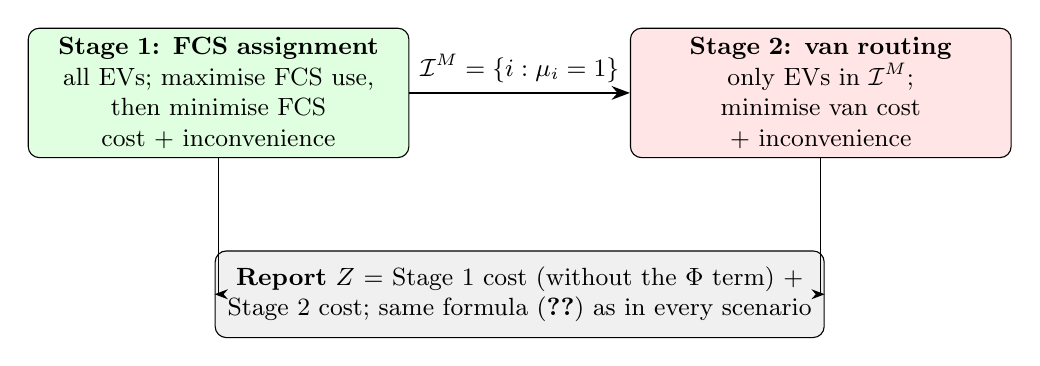
\begin{tikzpicture}[>=Stealth,box/.style={draw,rounded corners,align=center,minimum height=1.1cm,font=\small}]
  \node[box,fill=green!12,text width=4.6cm] (s1) {\textbf{Stage 1: FCS assignment}\\all EVs; maximise FCS use,\\then minimise FCS cost + inconvenience};
  \node[box,fill=red!10,text width=4.6cm,right=2.8cm of s1] (s2) {\textbf{Stage 2: van routing}\\only EVs in $\I^M$;\\minimise van cost + inconvenience};
  \draw[->,thick] (s1) -- node[above,font=\small]{$\I^M=\{i:\mu_i=1\}$} (s2);
  \node[box,fill=black!6,text width=7.5cm,below=2.0cm of $(s1)!0.5!(s2)$] (ev) {\textbf{Report} $Z=$ Stage~1 cost (without the $\Phi$ term) $+$ Stage~2 cost; same formula \eqref{eq:Z} as in every scenario};
  \draw[->] (s1) |- (ev); \draw[->] (s2) |- (ev);
\end{tikzpicture}
\end{center}

Stage~1 does not look at the vans, and Stage~2 cannot change what Stage~1 decided. That is the definition of ``FCS first, then MCS''.

%----------------------------------------------------------------
\subsection{Stage 1: assign EVs to fixed stations}

\textbf{Objective.}
\begin{equation}
\begin{split}
\min\ Z^{(1)}=\;&\underbrace{\Phi\sum_{i\in\I}\mu_i}_{\text{FCS first}}
+\underbrace{c^{EV}\sum_i\sum_{f\in\F_i}d_{if}Y_{if}}_{Z_1}
+\underbrace{Z^F_{\text{energy}}}_{\text{FCS part of }Z_4}\\
&+\underbrace{\sum_i\sum_{f\in\F_i}\rho^F_{if}Y_{if}+\alpha\sum_i w_i(C_i-r_i)+c^L\sum_i w_iL_i}_{\text{FCS customers' inconvenience}}
\end{split}
\label{eq:obj1}
\end{equation}
with $C_i=S_i+\tau^F_iY_i$ in this stage. $\Phi$ is a penalty for handing an EV to the vans. It is chosen larger than anything an extra FCS customer can add to the rest of \eqref{eq:obj1}, e.g.
\[
\Phi > \max_{i}\max_{f\in\F_i}\big(c^{EV}d_{if}+\pi^{\max}E_i+\rho^F_{if}\big)+n\,(\alpha+c^L)\,w_{\max}\,T,
\]
so Stage~1 first \textbf{maximises the number of EVs served at an FCS}, and only among those solutions minimises FCS cost and inconvenience. ($\pi^{\max}$ is the highest grid price.) A numerically safer equivalent is to solve twice: first $\max\sum_iY_i$, then fix that number and minimise the rest.
\ifTOU
Because $Z^F_{\text{energy}}$ uses the peak price, Stage~1 may \emph{start sessions later} to leave the peak, if the price saving beats the extra waiting cost (Section~\ref{sec:expect}).
\fi

\textbf{Constraints.}
\begin{align}
\sum_{g\in\G_i}y_{ig}+\mu_i &= 1 && \forall i\in\I \label{eq:s1assign}\\
S_i &\ge r_i+\sum_{f\in\F_i}t_{if}Y_{if} && \forall i\in\I \label{eq:fcsarr}\\
S_i &\le r_i+T\,(1-\mu_i) && \forall i\in\I \label{eq:s1park}\\
S_j &\ge S_i+\tau^F_i-(T+\tau^F_i)(3-y_{ig}-y_{jg}-o_{ij}) && \forall g,\ (i,j)\in\mathcal{P}_g \label{eq:disj1}\\
S_i &\ge S_j+\tau^F_j-(T+\tau^F_j)(2-y_{ig}-y_{jg}+o_{ij}) && \forall g,\ (i,j)\in\mathcal{P}_g \label{eq:disj2}\\
\sum_i y_{ig_1} &\ge \sum_i y_{ig_2} && \forall f,\ \G_f=\{g_1,g_2\} \label{eq:gunsym}\\
S_i+\tau^F_iY_i &\le T,\qquad L_i\ge S_i+\tau^F_iY_i-l_i && \forall i\in\I \label{eq:s1time}
\end{align}
\ifTOU plus the time-of-use split \eqref{eq:tou1}--\eqref{eq:tou5} of each FCS session (Section~\ref{sec:price}).\fi
\desc{\eqref{eq:s1assign}: every EV either gets one reachable gun or is handed to the vans. An EV that reaches no FCS ($\G_i=\emptyset$) is forced to $\mu_i=1$. \eqref{eq:fcsarr}: an FCS session cannot start before the EV has asked and driven to the station. \eqref{eq:s1park}: for an EV handed to the vans, $S_i$ is parked at $r_i$, so it adds no waiting in Stage~1 (its real start time is decided in Stage~2). \eqref{eq:disj1}--\eqref{eq:disj2}: two EVs on the same gun do not overlap; $o_{ij}$ picks who goes first. With two guns per station this means at most two EVs charge at a station at a time. \eqref{eq:gunsym}: symmetry breaking between the two identical guns (optional). \eqref{eq:s1time}: finished by $T$; lateness.}

\textbf{Optional acceptability rule.} An operator may refuse to send a driver to a station that is ``too inconvenient'', e.g.\ only allow gun $g$ of station $f$ for EV $i$ if $\hat\rho^F_{if}\le\bar\rho$. This only shrinks $\G_i$, so EVs whose stations are all too far go to the vans. Report results with and without it.

\textbf{Output:} $\I^M=\{i:\mu_i=1\}$, the EVs left for the vans; plus each FCS customer's gun and start time.

%----------------------------------------------------------------
\subsection{Stage 2: route the vans to the leftover EVs}

Stage~2 is a vehicle routing problem with time windows, on the EVs in $\I^M$ only. Here $C_i=S_i+\tau^M_i$.

\textbf{Objective.}
\begin{equation}
\begin{split}
\min\ Z^{(2)}=\;&\underbrace{c^M\sum_m\sum_{(i,j)\in\A^M}d_{ij}x_{ijm}}_{Z_2}+\underbrace{\sum_m c^D_mu_m}_{Z_3}+\underbrace{Z^M_{\text{energy}}}_{\text{van part of }Z_4}\\
&+\underbrace{\sum_{i\in\I^M}\sum_m\rho^M_{im}z_{im}+\alpha\sum_{i\in\I^M}w_i(C_i-r_i)+c^L\sum_{i\in\I^M}w_iL_i}_{\text{van customers' inconvenience}}
\end{split}
\label{eq:obj2}
\end{equation}
Since every EV in $\I^M$ must be served by some van, $Z^M_{\text{energy}}$ and the $\rho^M$ term are constants here. They are kept so that $Z^{(2)}$ is the true cost of Stage~2. Waiting and lateness make the vans visit urgent EVs early.

\textbf{Constraints.}
\begin{align}
\sum_{m\in\M}z_{im} &= 1 && \forall i\in\I^M \label{eq:s2assign}\\
\sum_{j:(0,j)\in\A^M}x_{0jm} = \sum_{i:(i,n+1)\in\A^M}x_{i,n+1,m} &= u_m && \forall m \label{eq:depot}\\
\sum_{i:(i,j)\in\A^M}x_{ijm} = \sum_{k:(j,k)\in\A^M}x_{jkm} &= z_{jm} && \forall j\in\I^M,\ m \label{eq:flow}\\
\sum_{i\in\I^M}z_{im} &\le Q_m\,u_m && \forall m \label{eq:cap}\\
\sum_{i\in\I^M}\frac{E_i}{\eta}z_{im}+\beta\sum_{(i,j)\in\A^M}d_{ij}x_{ijm} &\le B_m\,u_m && \forall m \label{eq:batt}
\end{align}
\begin{align}
S_j &\ge \max\{r_j,\ t_{0j}\,x_{0jm}\} && \forall j\in\I^M,\ m \label{eq:depart}\\
S_j &\ge S_i+\tau^M_i+t_{ij}-(T+\tau^M_i+t_{ij})(1-x_{ijm}) && \forall i\neq j,\ m \label{eq:seq}\\
S_i+\tau^M_i+t_{i,n+1} &\le T+(\tau^M_i+t_{i,n+1})(1-x_{i,n+1,m}) && \forall i,\ m \label{eq:return}\\
S_i+\tau^M_i \le T,\quad L_i &\ge S_i+\tau^M_i-l_i && \forall i\in\I^M \label{eq:s2time}\\
u_m &\ge u_{m+1} && m<|\M| \label{eq:vansym}
\end{align}
\desc{\eqref{eq:s2assign}: each leftover EV gets one van. \eqref{eq:depot}: a used van leaves and returns to the depot once. \eqref{eq:flow}: each EV on van $m$ is entered and left exactly once by that van. \eqref{eq:cap}: at most $Q_m$ EVs per van. \eqref{eq:batt}: delivered energy (with transfer losses) plus driving energy fits in the van battery. \eqref{eq:depart}: no start before the request, or before the van can drive there from the depot (written as two linear constraints). \eqref{eq:seq}: if the van goes $i\to j$, it finishes $i$ and drives to $j$ before starting $j$. This gives one EV at a time and removes subtours (MTZ-type). \eqref{eq:return}: back at the depot by $T$. \eqref{eq:s2time}: finished by $T$; lateness. \eqref{eq:vansym}: use identical vans in index order.}

\textbf{If Stage 2 is infeasible} (too many leftover EVs for the fleet by $T$), the sequential policy has \emph{failed} on that instance. For diagnosis, add $s_i\in\{0,1\}$ (``unserved''), replace \eqref{eq:s2assign} by $\sum_mz_{im}+s_i=1$ and add $\Phi^U\sum_is_i$ to \eqref{eq:obj2}. Then report the number of EVs that could not be served. This is a useful comparison with the integrated scenario, which may serve all of them.

%----------------------------------------------------------------
\subsection{Reported value}
\[
Z^{\text{S\scen}}=\big(Z^{(1)*}-\Phi\,|\I^M|\big)+Z^{(2)*},
\]
which is exactly \eqref{eq:Z} evaluated at the combined solution. The stage-1 solution plus the stage-2 solution is a feasible solution of the integrated model (S\ifTOU 4\else 3\fi), so
$Z^{\text{S\ifTOU 4\else 3\fi}}\le Z^{\text{S\scen}}$. The difference is the \emph{value of integration}.

\else
%---------------------------------------------------------------- INT
\subsection{Objective}
\begin{equation}
\min\ Z \quad\text{as in \eqref{eq:Z}, with }Z^F_{\text{energy}}=\ifTOU P^F\textstyle\sum_i\big[\pi^\off(\theta^1_i+\theta^3_i)+\pi^\pk\theta^2_i\big]\else\pi^F\textstyle\sum_iE_iY_i\fi,\quad C_i=S_i+\tau^F_iY_i+\tau^M_iZ_i. \label{eq:objint}
\end{equation}
Written out in full:
\begin{align*}
\min\ Z=\;& c^{EV}\sum_i\sum_{f\in\F_i}d_{if}Y_{if}+c^M\sum_m\sum_{(i,j)\in\A}d_{ij}x_{ijm}+\sum_mc^D_mu_m\\
&+\ifTOU P^F\sum_i\big[\pi^\off(\theta^1_i+\theta^3_i)+\pi^\pk\theta^2_i\big]\else\pi^F\sum_iE_iY_i\fi
+\pi^M\sum_i\sum_m\frac{E_i}{\eta}z_{im}\\
&+\sum_i\sum_{f\in\F_i}\rho^F_{if}Y_{if}+\sum_i\sum_m\rho^M_{im}z_{im}+\alpha\sum_iw_i(C_i-r_i)+c^L\sum_iw_iL_i .
\end{align*}
Every term is linear. One model weighs everything at once: an EV goes to a van exactly when the van's extra km, dispatch and energy cost are outweighed by the effort and waiting it saves the driver\ifTOU, or by the peak-price energy it avoids\fi.

\subsection{Constraints}

\textbf{Assignment.}
\begin{equation}
\sum_{g\in\G_i}y_{ig}+\sum_{m\in\M}z_{im}=1\qquad\forall i\in\I \label{eq:assign}
\end{equation}
\desc{Exactly one resource per EV: one reachable gun or one van. EVs that reach no FCS are forced onto a van.}

\textbf{Fixed stations.}
\begin{align}
S_i &\ge r_i+\sum_{f\in\F_i}t_{if}Y_{if} && \forall i \label{eq:fcsarr}\\
S_j &\ge S_i+\tau^F_i-(T+\tau^F_i)(3-y_{ig}-y_{jg}-o_{ij}) && \forall g,\ (i,j)\in\mathcal{P}_g \label{eq:disj1}\\
S_i &\ge S_j+\tau^F_j-(T+\tau^F_j)(2-y_{ig}-y_{jg}+o_{ij}) && \forall g,\ (i,j)\in\mathcal{P}_g \label{eq:disj2}\\
\sum_iy_{ig_1} &\ge \sum_iy_{ig_2} && \forall f,\ \G_f=\{g_1,g_2\} \label{eq:gunsym}
\end{align}
\desc{\eqref{eq:fcsarr}: an FCS session starts after the request and the drive to the station (for a van customer this is just $S_i\ge r_i$). \eqref{eq:disj1}--\eqref{eq:disj2}: EVs on the same gun do not overlap; $o_{ij}$ chooses the order. \eqref{eq:gunsym}: optional symmetry breaking.}

\textbf{Vans: routes, capacity, battery.}
\begin{align}
\sum_{j:(0,j)\in\A}x_{0jm}=\sum_{i:(i,n+1)\in\A}x_{i,n+1,m} &= u_m && \forall m \label{eq:depot}\\
\sum_{i:(i,j)\in\A}x_{ijm}=\sum_{k:(j,k)\in\A}x_{jkm} &= z_{jm} && \forall j\in\I,\ m \label{eq:flow}\\
\sum_iz_{im} &\le Q_mu_m && \forall m \label{eq:cap}\\
\sum_i\frac{E_i}{\eta}z_{im}+\beta\sum_{(i,j)\in\A}d_{ij}x_{ijm} &\le B_mu_m && \forall m \label{eq:batt}
\end{align}
\desc{\eqref{eq:depot}: a used van leaves and returns once. \eqref{eq:flow}: each EV on van $m$ is visited exactly once by it. \eqref{eq:cap}: at most $Q_m$ EVs. \eqref{eq:batt}: delivered energy (with losses) plus driving energy fits in the battery.}

\textbf{Vans: timing (one EV at a time, no subtours).}
\begin{align}
S_j &\ge t_{0j}\,x_{0jm} && \forall j\in\I,\ m \label{eq:depart}\\
S_j &\ge S_i+\tau^M_i+t_{ij}-(T+\tau^M_i+t_{ij})(1-x_{ijm}) && \forall i\neq j\in\I,\ m \label{eq:seq}\\
S_i+\tau^M_i+t_{i,n+1} &\le T+(\tau^M_i+t_{i,n+1})(1-x_{i,n+1,m}) && \forall i,\ m \label{eq:return}
\end{align}
\desc{\eqref{eq:depart}: the first stop cannot start before the van has driven there. \eqref{eq:seq}: $i\to j$ means finish $i$, drive, then start $j$; start times rise along a route, so no subtour can close. \eqref{eq:return}: back at the depot by $T$.}

\textbf{Horizon and lateness.}
\begin{equation}
C_i\le T,\qquad L_i\ge C_i-l_i\qquad\forall i\in\I \label{eq:time}
\end{equation}
\desc{Every EV is fully charged within the horizon; $L_i$ measures lateness.}

\ifTOU
\textbf{Time-of-use split.} Constraints \eqref{eq:tou1}--\eqref{eq:tou5} of Section~\ref{sec:price}.
\fi

\textbf{Symmetry and domains.}
\begin{equation}
u_m\ge u_{m+1};\qquad y,z,x,u,o\ifTOU,\kappa\fi\in\{0,1\};\qquad S_i,L_i\ifTOU,\theta^p_i\fi\ge0 \label{eq:dom}
\end{equation}
\fi

%=====================================================================
\section{Learning-to-optimise (RL) formulation}\label{sec:rl}

\textbf{Main rule:} the reward of each action is \emph{minus the increase in $Z$ that the action causes}. The rewards over an episode then add up to $-Z$ of the solution the policy builds. RL and MILP results are measured on the same yardstick \eqref{eq:Z}, and the MILP optimum is the benchmark for the RL gap.

\ifSEQ
%---------------------------------------------------------------- RL SEQ
The RL pipeline has the same two stages as the MILP.

\subsection{Stage 1 policy: FCS assignment}
\begin{itemize}[leftmargin=1.4em,itemsep=2pt]
  \item \textbf{Episode / epochs:} EVs are taken in order of request time $r_i$ (ties: higher $w_i$ first). One decision per EV.
  \item \textbf{State:} features of the current EV $k$ ($E_k,r_k,l_k,w_k,R_k$, location); for each gun $g$ the time $F_g$ it becomes free; summary features of the EVs still to come (count and positions near each station)\ifTOU; the current price and the time until $T_1$ and $T_2$\fi.
  \item \textbf{Action:} a gun $g\in\G_k$, or ``hand to vans''. \textbf{FCS-first mask:} ``hand to vans'' is allowed \emph{only} if no gun can finish EV $k$ by $T$ (or, with the optional rule, if all remaining guns have $\hat\rho^F_{kf}>\bar\rho$).
  \ifTOU\item \textbf{Optional timing action:} ``gun $g$, start after the peak'', i.e.\ $S_k=\max\{\text{earliest},T_2\}$, allowed only if the session still ends by $T$.\fi
  \item \textbf{Transition:} $S_k=\max\{r_k+t_{kf},F_g\}$ (or later, for the timing action); $F_g\leftarrow S_k+\tau^F_k$.
  \item \textbf{Reward:} $-\Big[c^{EV}d_{kf}+\text{energy}_k+\rho^F_{kf}+\alpha w_k(S_k+\tau^F_k-r_k)+c^Lw_k(S_k+\tau^F_k-l_k)^+\Big]$, where energy$_k$ = \ifTOU$P^F\big[\pi^\off\cdot(\text{off-peak hours of }[S_k,S_k+\tau^F_k])+\pi^\pk\cdot(\text{peak hours})\big]$, computed exactly in the simulator\else$\pi^FE_k$\fi. Handing an EV to the vans gives reward $0$ here; its cost is counted in Stage~2.
\end{itemize}
Note: a simple baseline for Stage~1 is the greedy rule ``gun with the largest one-step reward''. What RL can learn on top of this is, for example, to keep a nearby gun free for an urgent EV that arrives later.

\subsection{Stage 2 policy: van routing over $\I^M$}
\begin{itemize}[leftmargin=1.4em,itemsep=2pt]
  \item \textbf{Epochs:} whenever a van becomes free (the earliest-free van decides first).
  \item \textbf{State:} for each van: position, time free, remaining battery $b_m$, EVs served so far, dispatched or not; for each unserved EV in $\I^M$: location, $E_i,r_i,l_i,w_i$; current time.
  \item \textbf{Action:} the next EV $j$ for this van, or ``return to depot'' (ends the route). Mask: $j$ must be feasible: battery covers $E_j/\eta$ plus driving to $j$ and back to the depot, the count stays $\le Q_m$, and $j$ can be finished with the van back at the depot by $T$.
  \item \textbf{Transition:} $S_j=\max\{r_j,\ \text{time free}+t_{\text{pos},j}\}$; the van moves to $j$ and is free at $S_j+\tau^M_j$; $b_m$ falls by $E_j/\eta+\beta d_{\text{pos},j}$.
  \item \textbf{Reward:} serving $j$: $-\Big[c^Md_{\text{pos},j}+c^D_m[\text{first stop}]+\pi^M\frac{E_j}{\eta}+\rho^M_{jm}+\alpha w_j(S_j+\tau^M_j-r_j)+c^Lw_j(S_j+\tau^M_j-l_j)^+\Big]$; returning: $-c^Md_{\text{pos},0}$. EVs still unserved at the end: $-\Phi^U$ each.
  \item \textbf{Policy:} an attention-based routing policy (e.g.\ Kool et al., 2019, ``Attention, Learn to Solve Routing Problems!'') trained with REINFORCE or PPO. Baseline: nearest-feasible-EV heuristic.
\end{itemize}
Episode return of Stage~1 + Stage~2 $=-Z^{\text{S\scen}}$.

\else
%---------------------------------------------------------------- RL INT
One policy decides both who serves each EV and the van routes.
\begin{itemize}[leftmargin=1.4em,itemsep=2pt]
  \item \textbf{Episode / epochs:} EVs are taken in order of request time $r_i$ (ties: higher $w_i$ first). One decision per EV.
  \item \textbf{State:} (i) the current EV $k$: location, $E_k,r_k,l_k,w_k,R_k$, reachable stations; (ii) each gun $g$: time $F_g$ it becomes free; (iii) each van $m$: current end-of-route position, time free, remaining battery $b_m$, EVs served, dispatched or not; (iv) embeddings of the not-yet-assigned EVs (for look-ahead)\ifTOU; (v) current price, time until $T_1$ and $T_2$\fi.
  \item \textbf{Action:} $a\in\G_k\cup\M$: a gun, or a van (EV $k$ is appended to the end of that van's route). \textbf{Mask} infeasible actions: a gun that cannot finish $k$ by $T$; a van without enough battery for $E_k/\eta$ plus the drive to $k$ and back to the depot, with $Q_m$ reached, or unable to finish $k$ and return by $T$.
  \ifTOU\item \textbf{Optional timing action:} ``gun $g$, start after the peak'' ($S_k=\max\{\text{earliest},T_2\}$, if it still ends by $T$).\fi
  \item \textbf{Transition:} gun: $S_k=\max\{r_k+t_{kf},F_g\}$, $F_g\leftarrow S_k+\tau^F_k$. Van: $S_k=\max\{r_k,\ \text{free}_m+t_{\text{pos}_m,k}\}$, then the van moves to $k$, $\text{free}_m\leftarrow S_k+\tau^M_k$, $b_m\mathrel{-}=E_k/\eta+\beta d_{\text{pos}_m,k}$.
  \item \textbf{Reward} $=-\Delta Z$:
  \begin{align*}
  \text{gun } g\text{ at }f:&\quad -\Big[c^{EV}d_{kf}+\text{energy}^F_k+\rho^F_{kf}+\alpha w_k(C_k-r_k)+c^Lw_k(C_k-l_k)^+\Big]\\
  \text{van } m:&\quad -\Big[c^M\big(d_{\text{pos}_m,k}+d_{k,0}-d_{\text{pos}_m,0}\big)+c^D_m[\text{first use}]+\pi^M\tfrac{E_k}{\eta}\\
  &\qquad\quad+\rho^M_{km}+\alpha w_k(C_k-r_k)+c^Lw_k(C_k-l_k)^+\Big]
  \end{align*}
  The van distance term is the \emph{change} in route length when $k$ is inserted before the return to the depot, so the sum over the episode equals the total route length (the return legs telescope). energy$^F_k$ = \ifTOU$P^F\big[\pi^\off\cdot(\text{off-peak hours})+\pi^\pk\cdot(\text{peak hours of }[S_k,C_k])\big]$, computed exactly by the simulator; no linearisation is needed in RL\else$\pi^FE_k$\fi.
  \item \textbf{Dead end:} if every action is masked, EV $k$ is unserved: reward $-\Phi^U$, and the episode continues. Report the count.
  \item \textbf{Policy:} masked categorical policy over guns and vans, encoder with attention over EVs, guns and vans; trained with PPO. Natural baseline: greedy, i.e.\ choose the action with the largest one-step reward. That is the pairwise rule ``smallest $\hat\rho$ + cost'' from Section~\ref{sec:inc}.
\end{itemize}
Restriction to note: vans serve EVs in assignment order (append only). A variant that inserts $k$ at the cheapest position of a route is more flexible but has a larger action space.
\fi

\textbf{Reward scaling.} For stable training divide every reward by a constant, e.g.\ the greedy baseline's average $Z$ on the training instances. This does not change the optimal policy.

%=====================================================================
\section{What to expect and what to report}\label{sec:expect}

\ifnum\scen=1
\begin{itemize}[leftmargin=1.4em,itemsep=2pt]
  \item Vans serve only EVs that reach no station, or that the stations cannot finish by $T$. If stations have spare capacity, very few vans are dispatched.
  \item Inconvenience is high for EVs far from the nearest station (worked example: Rs\,682 at the FCS, against Rs\,458 if a van had been allowed).
  \item With too few vans Stage~2 becomes infeasible (unserved EVs), even when the integrated model S3 could serve everyone. Report the smallest $|\M|$ at which S1 is feasible and compare it with S3.
\end{itemize}
\fi
\ifnum\scen=2
\begin{itemize}[leftmargin=1.4em,itemsep=2pt]
  \item \textbf{When does Stage~1 delay a session to avoid the peak?} Moving one hour of charging out of the peak saves $(\pi^\pk-\pi^\off)P^F=3\times22=$ Rs\,66, but delays completion by up to an hour, which costs $\alpha w_i\ge$ Rs\,200. So with the default values Stage~1 almost never delays. It mostly pays the higher price, and S2 costs roughly S1 plus the peak surcharge. Sessions start later only if $\alpha$ is small (try $\lambda<0.33$ in the sensitivity analysis).
  \item The van assignment is the same as in S1 unless Stage~1's timing changes which EVs fit at the stations. Stage~1 cannot use vans to escape the peak price.
  \item Extra KPI: \textbf{grid energy drawn at FCS during the peak}, $P^F\sum_i\theta^2_i$ (kWh). Compare with S4.
\end{itemize}
\fi
\ifnum\scen=3
\begin{itemize}[leftmargin=1.4em,itemsep=2pt]
  \item Vans take EVs for which the saved inconvenience exceeds the extra van cost (worked example: van chosen, saving Rs\,224). Expect vans to serve EVs that are far from every station, have low range (high $w_i$), or have early deadlines, while EVs near a station still use it.
  \item \textbf{Value of integration under flat price:} $Z^{\text{S1}}-Z^{\text{S3}}\ge0$. Report it per component ($Z_1,\dots,Z_5$): typically operating cost rises a little and inconvenience falls a lot.
  \item Vary $|\M|$ (0, 1, 2, \dots): the first few vans lower $Z$ sharply, then the effect levels off. That curve shows the scenarios where mobile chargers help most.
\end{itemize}
\fi
\ifnum\scen=4
\begin{itemize}[leftmargin=1.4em,itemsep=2pt]
  \item During the peak a van kWh costs about the same as an FCS kWh (Rs\,10.0 each), so the vans' energy disadvantage disappears and vans also absorb \emph{peak-hour} demand that would otherwise be charged on the grid at peak price.
  \item Expect more van usage than in S3, concentrated on requests in $[T_1,T_2]$, and lower grid energy at the stations during the peak, $P^F\sum_i\theta^2_i$, than in S2.
  \item \textbf{Value of integration under peak pricing:} $Z^{\text{S2}}-Z^{\text{S4}}$. It should be larger than $Z^{\text{S1}}-Z^{\text{S3}}$, because integration now also allows price arbitrage.
  \item \textbf{Peak pricing with full flexibility:} $Z^{\text{S4}}-Z^{\text{S3}}$ should be smaller than $Z^{\text{S2}}-Z^{\text{S1}}$: vans cushion the price increase.
\end{itemize}
\fi

\textbf{Cross-scenario comparison table} (fill in from the four runs):
\begin{center}
\renewcommand{\arraystretch}{1.2}
\begin{tabular}{@{}lll@{}}
\toprule
\textbf{Comparison} & \textbf{Measures} & \textbf{Expected sign} \\
\midrule
S1 $-$ S3 & value of integration, flat price & $\ge0$ \\
S2 $-$ S4 & value of integration, peak price & $\ge0$, larger than S1 $-$ S3 \\
S2 $-$ S1 & cost of peak pricing, FCS-first operator & $>0$ \\
S4 $-$ S3 & cost of peak pricing, flexible operator & $>0$, smaller than S2 $-$ S1 \\
\bottomrule
\end{tabular}
\end{center}
Report for each: $Z$ and its components, number of vans used, EVs per resource, mean and maximum inconvenience per EV, total lateness, peak-hour grid energy, solve time, and (for RL) the gap to the MILP optimum.

%=====================================================================
\appendix
\section{Illustrative parameter values}\label{app:values}

These are starting values for experiments, not data. All are meant to be varied in the analysis. Values in Rs.

\begin{center}
\renewcommand{\arraystretch}{1.15}
\begin{tabular}{@{}llp{6.2cm}@{}}
\toprule
\textbf{Parameter} & \textbf{Value} & \textbf{Note} \\
\midrule
$T$, $[T_1,T_2]$ & 7 h, $[2,6]$ & 16:00--23:00, peak 18:00--22:00 \\
$P^F$, $P^M$ & 22 kW, 30 kW & \\
$v$, $\beta$, $\eta$ & 25 km/h, 0.25 kWh/km, 0.9 & \\
$B_m$, $Q_m$, $|\M|$ & 150 kWh, 6, 2--6 & \\
$c^{EV}$, $c^M$, $c^D_m$ & Rs\,4/km, Rs\,15/km, Rs\,1500 & van km includes driver time \\
$\pi^F$ (flat) & Rs\,8.7/kWh & equals the time-average of the ToU tariff over $[0,T]$ \\
$\pi^\off$, $\pi^\pk$ (ToU) & Rs\,7/kWh, Rs\,10/kWh & $(3\times7+4\times10)/7=8.7$ \\
$c^{bat}$ & Rs\,2/kWh & van battery wear \\
$\pi^M$ & Rs\,10.7 (flat) / Rs\,9.0 (ToU) & $=\pi^F+c^{bat}$ / $=\pi^\off+c^{bat}$ \\
$\alpha$, $\alpha^D$ & Rs\,200/h, Rs\,100/h & value of time; extra for attended time \\
$h^F$, $h^M$, $\varphi$ & Rs\,50, Rs\,10, Rs\,100 & trip hassle, hand-over, range stress \\
$c^L$ & Rs\,300/h & lateness \\
$w_i$ & $1+2(1-R_i/R_{\max})$, $R_i\sim U[3,40]$ km & priority from remaining range \\
\bottomrule
\end{tabular}
\end{center}

The flat price is set to the time-average of the peak tariff. The price \emph{level} is then the same in both pricing cases, and only the price \emph{shape} differs. Without this, part of S1 vs S2 would just reflect a different average price.

\end{document}
"
%  (run each twice for cross-references)
% =====================================================================
\documentclass[11pt,a4paper]{article}
\usepackage[margin=2.2cm]{geometry}
\usepackage{amsmath,amssymb,amsfonts}
\usepackage{booktabs,array,tabularx}
\usepackage{enumitem}
\usepackage[table]{xcolor}
\usepackage{tikz}
\usetikzlibrary{arrows.meta,positioning,calc}
\usepackage[colorlinks=true,linkcolor=blue!50!black,urlcolor=blue!50!black]{hyperref}
\usepackage{titlesec}
\titleformat{\section}{\large\bfseries}{\thesection}{0.8em}{}
\titleformat{\subsection}{\normalsize\bfseries}{\thesubsection}{0.8em}{}
\setlength{\parindent}{0pt}
\setlength{\parskip}{5pt}

% ---------------- scenario switches ----------------
\ifdefined\scen\else\def\scen{1}\fi
\newif\ifTOU \TOUfalse   % true = time-of-use (peak) price
\newif\ifSEQ \SEQfalse   % true = FCS first, then MCS
\ifnum\scen=1 \SEQtrue \fi
\ifnum\scen=2 \TOUtrue \SEQtrue \fi
\ifnum\scen=4 \TOUtrue \fi

\newcommand{\pricename}{\ifTOU time-of-use price (dearer evening peak)\else single (flat) price all day\fi}
\newcommand{\structname}{\ifSEQ FCS first, then MCS (sequential)\else FCS and MCS together (integrated)\fi}

% ---------------- notation ----------------
\newcommand{\I}{\mathcal{I}}
\newcommand{\F}{\mathcal{F}}
\newcommand{\G}{\mathcal{G}}
\newcommand{\M}{\mathcal{M}}
\newcommand{\N}{\mathcal{N}}
\newcommand{\A}{\mathcal{A}}
\newcommand{\Rs}{\text{Rs}\,}
\newcommand{\pk}{\mathrm{pk}}
\newcommand{\off}{\mathrm{off}}
\newcommand{\desc}[1]{\par\vspace{-2pt}{\small\color{black!75}\textit{Meaning:} #1}\par\vspace{4pt}}
\newcommand{\cell}[2]{\ifnum\scen=#1\cellcolor{blue!18}\textbf{S#1 (this document)}\\\textbf{#2}\else S#1\\#2\fi}

\title{\textbf{EV Charging Network Optimisation}\\[4pt]
\large Scenario \scen: \pricename\ $+$ \structname\\[2pt]
\normalsize MILP and RL formulation}
\author{CP 320 OR for Mobility Management, course project}
\date{2 October 2026}

\begin{document}
\maketitle

%=====================================================================
\section{Where this scenario sits}

The project studies four scenarios: two ways of pricing grid electricity, times two ways of making the decisions.

\begin{center}
\renewcommand{\arraystretch}{1.5}
\begin{tabular}{>{\raggedright\arraybackslash}p{4.2cm}|>{\centering\arraybackslash}p{4.6cm}|>{\centering\arraybackslash}p{4.6cm}}
 & \textbf{Flat price all day} & \textbf{Time-of-use (peak) price} \\ \hline
\textbf{Sequential:} FCS first, leftover EVs to MCS &
\begin{tabular}[c]{@{}c@{}}\cell{1}{flat + sequential}\end{tabular} &
\begin{tabular}[c]{@{}c@{}}\cell{2}{peak + sequential}\end{tabular} \\ \hline
\textbf{Integrated:} FCS and MCS decided together &
\begin{tabular}[c]{@{}c@{}}\cell{3}{flat + integrated}\end{tabular} &
\begin{tabular}[c]{@{}c@{}}\cell{4}{peak + integrated}\end{tabular} \\
\end{tabular}
\end{center}

\textbf{The four scenarios do not have four different objectives.} They share \emph{one} cost yardstick $Z$ (Section~\ref{sec:obj}): the same cost terms and the same customer inconvenience (Section~\ref{sec:inc}). Only two things change:
\begin{itemize}[leftmargin=1.4em,itemsep=1pt]
  \item \textbf{Pricing} changes the formula for one term, the FCS energy cost (Section~\ref{sec:price}).
  \item \textbf{Decision structure} changes \emph{how} $Z$ is minimised: in one model (integrated), or in two stages (sequential), where each stage minimises its own part of $Z$.
\end{itemize}
Because the yardstick is the same, the four optimal values can be compared directly. The differences measure the \emph{value of integration} (S1$\to$S3, S2$\to$S4) and the \emph{effect of peak pricing} (S1$\to$S2, S3$\to$S4).

\ifnum\scen=1
\textbf{This scenario (S1)} is the baseline, the ``status quo''. Electricity costs the same at every hour, every EV that can be charged at a fixed station is sent there, and vans only take what is left over.
\fi
\ifnum\scen=2
\textbf{This scenario (S2)} keeps the FCS-first rule of S1, but grid electricity is dearer during the evening peak. Stage~1 can react to the price only by \emph{rescheduling} FCS sessions. It cannot hand a peak-hour EV to a van.
\fi
\ifnum\scen=3
\textbf{This scenario (S3)} keeps the flat price of S1, but the operator decides FCS and MCS service \emph{together}. An EV can be sent to a van even when a fixed station could take it, whenever that lowers total cost plus inconvenience.
\fi
\ifnum\scen=4
\textbf{This scenario (S4)} is the most flexible one: peak pricing at fixed stations, and FCS and MCS decided together. Van energy was bought off-peak, so vans can also be used to keep charging \emph{out of the expensive peak}.
\fi

%=====================================================================
\section{Setting and assumptions}\label{sec:setting}

\textbf{Time.} The planning horizon is $[0,T]$ with $T=7$\,h (16:00--23:00). It contains the evening peak window $[T_1,T_2]=[2,6]$ (18:00--22:00). The horizon is the same in all four scenarios. It is wider than the peak itself so that, under peak pricing, there is cheaper time on both sides of the peak.\ifTOU\else\ In this scenario the price is flat, so the window plays no role in the model.\fi

\textbf{Assumptions} (the same as MILP v3, plus two about energy):
\begin{enumerate}[leftmargin=1.6em,itemsep=1pt]
  \item Static, continuous time. All requests in the horizon are known at time $0$, and request $i$ becomes active at $r_i$.
  \item An EV served by an FCS drives there itself on its own battery (only to stations within its range $R_i$). The driver stays with the car while it waits for a free gun and while it charges.
  \item An EV served by an MCS stays parked where it is, and the driver is free in the meantime.
  \item Each FCS gun and each van charges one EV at a time, without interruption, at constant power.
  \item A van's battery covers both its driving and the energy it delivers. \textbf{The van battery is charged at the depot before the horizon starts}\ifTOU, i.e.\ at the off-peak price\fi, and is not recharged during the horizon.
  \item Every EV must be fully charged by $T$ (hard). Finishing after the driver's desired time $l_i$ is allowed but penalised.
\end{enumerate}

%=====================================================================
\section{Notation}\label{sec:notation}

\subsection*{Sets}
\begin{tabularx}{\textwidth}{@{}lX@{}}
\toprule
$\I=\{1,\dots,n\}$ & EV charging requests \\
$\F$; $\G_f$ ($|\G_f|=2$); $\G=\bigcup_f\G_f$ & fixed charging stations; guns of FCS $f$; all guns ($f(g)$ = station of gun $g$) \\
$\F_i=\{f: d_{if}\le R_i\}$, $\G_i=\bigcup_{f\in\F_i}\G_f$ & stations / guns EV $i$ can reach on its remaining range \\
$\M$ & mobile charging vans (MCS) \\
$0,\ n+1$ & depot as start node / end node (same place) \\
$\N=\{0\}\cup\I\cup\{n+1\}$, $\A$ & routing nodes; allowed van arcs $(i,j)$, $i\in\{0\}\cup\I$, $j\in\I\cup\{n+1\}$, $i\neq j$ \\
$\mathcal{P}_g=\{(i,j): i<j,\ g\in\G_i\cap\G_j\}$ & pairs of EVs that could share gun $g$ \\
\ifSEQ
$\I^M\subseteq\I$ & EVs handed to the vans by Stage~1 (an \emph{output} of Stage~1, a fixed input to Stage~2) \\
$\N^M$, $\A^M$ & routing nodes / arcs restricted to $\I^M$ \\
\fi
\bottomrule
\end{tabularx}

\subsection*{Parameters}
\begin{tabularx}{\textwidth}{@{}lX@{}}
\toprule
$E_i,\ r_i,\ l_i,\ R_i$ & energy demand (kWh), request time, desired completion time (h), remaining range (km) \\
$w_i\ge1$ & priority of EV $i$; $w_i=1+\kappa(1-R_i/R_{\max})$, so low-range EVs weigh more \\
$P^F,\ P^M$ & charging power of an FCS gun (22\,kW) / of a van (e.g.\ 30\,kW) \\
$\tau^F_i=E_i/P^F,\ \tau^M_i=E_i/P^M$ & charging time of EV $i$ at an FCS / by a van (h) \\
$d_{if},t_{if}$;\ $d_{ij},t_{ij}$ & distance (km) and time (h): EV$\to$FCS; between routing nodes ($t=d/v$) \\
$B_m,\ Q_m,\ \beta,\ \eta$ & van battery (kWh), max EVs per van, van consumption (kWh/km), transfer efficiency \\
$c^{EV},\ c^M,\ c^D_m$ & cost per km of EV driving, per km of van driving; fixed dispatch cost of van $m$ \\
\ifTOU
$\pi^\off,\ \pi^\pk$ & grid price (Rs/kWh) off-peak / in $[T_1,T_2]$, with $\pi^\pk\ge\pi^\off$ \\
\else
$\pi^F$ & grid price (Rs/kWh), the same at every hour \\
\fi
$c^{bat}$ & van battery wear per kWh cycled \\
$\pi^M$ & cost of 1 kWh taken from a van battery: $\pi^M=\ifTOU\pi^\off\else\pi^F\fi+c^{bat}$ (Section~\ref{sec:price}) \\
$\alpha,\ \alpha^D,\ h^F,\ h^M,\ \varphi,\ c^L$ & inconvenience coefficients (Section~\ref{sec:inc}) \\
\bottomrule
\end{tabularx}

\subsection*{Decision variables}
\begin{tabularx}{\textwidth}{@{}llX@{}}
\toprule
$y_{ig}$ & $\{0,1\}$ & EV $i$ charged at gun $g\in\G_i$ \\
$z_{im}$ & $\{0,1\}$ & EV $i$ served by van $m$ \\
$x_{ijm}$ & $\{0,1\}$ & van $m$ drives arc $(i,j)$ \\
$u_m$ & $\{0,1\}$ & van $m$ is dispatched \\
$o_{ij}$ & $\{0,1\}$ & for EVs $i<j$ that could share a gun: 1 if $i$ is charged before $j$ \\
\ifSEQ
$\mu_i$ & $\{0,1\}$ & Stage~1 only: EV $i$ is handed to the van fleet \\
\fi
\ifTOU
$\theta^1_i,\theta^2_i,\theta^3_i$ & $\ge0$ & hours of EV $i$'s FCS session before / inside / after the peak \\
$\kappa^1_i,\kappa^3_i$ & $\{0,1\}$ & EV $i$'s FCS session starts before $T_1$ / ends after $T_2$ \\
\fi
$S_i$ & $\ge0$ & time charging of EV $i$ starts (h), on whichever resource \\
$L_i$ & $\ge0$ & lateness of EV $i$ beyond $l_i$ (h) \\
\bottomrule
\end{tabularx}

\textbf{Short-hands} (linear expressions, not new variables):
\[
Y_{if}=\sum_{g\in\G_f}y_{ig},\qquad Y_i=\sum_{g\in\G_i}y_{ig}\ (\text{EV $i$ uses an FCS}),\qquad Z_i=\sum_{m\in\M}z_{im}\ (\text{EV $i$ uses a van}),
\]
\[
C_i=S_i+\tau^F_i\,Y_i+\tau^M_i\,Z_i \quad\text{(time EV $i$ is fully charged).}
\]

%=====================================================================
\section{Customer inconvenience}\label{sec:inc}

This section is \textbf{identical in all four scenario documents}. Inconvenience is a property of the customer, not of the price or of the planning method.

\subsection{What we mean by inconvenience}

Inconvenience is \emph{what the driver loses} from the moment they ask for a charge ($r_i$) until the car is fully charged ($C_i$), \emph{converted into rupees} so it can be added to the operator's costs. A driver loses three different things:

\begin{enumerate}[leftmargin=1.6em,itemsep=2pt]
  \item \textbf{Waiting:} the car is not ready. This lasts $C_i-r_i$ hours and affects \emph{every} driver, FCS or MCS.
  \item \textbf{Effort:} only an FCS customer has to drive to the station and sit there while the car charges. An MCS customer stays at home or at work and does something else. Driving to a far station also uses scarce battery range, which causes stress (``range anxiety'').
  \item \textbf{A missed deadline:} the car is still not ready at the time $l_i$ the driver needs it.
\end{enumerate}

Each loss gets a price in Rs per hour (or per event). All of them are multiplied by the priority $w_i$: an hour of delay for an EV with 5\,km of range left counts more than for one with 40\,km.

\subsection{The three components}

\begin{center}
\renewcommand{\arraystretch}{1.3}
\begin{tabularx}{\textwidth}{@{}>{\raggedright\arraybackslash}p{2.6cm}>{\raggedright\arraybackslash}X>{\raggedright\arraybackslash}X>{\raggedright\arraybackslash}p{3.0cm}@{}}
\toprule
\textbf{Component} & \textbf{EV $i$ at FCS $f$} & \textbf{EV $i$ by a van} & \textbf{Known when?} \\
\midrule
Effort & $w_i\big[\alpha^D(t_{if}+\tau^F_i)+h^F+\varphi\,d_{if}/R_i\big]$: driving and sitting at the station, a fixed trip hassle, range stress & $w_i\,h^M$: being reachable and handing over the car & \textbf{Static:} known as soon as the resource is chosen \\
Waiting & $w_i\,\alpha\,(C_i-r_i)$ = drive + \emph{queue at the gun} + charge & $w_i\,\alpha\,(C_i-r_i)$ = \emph{wait for the van} + charge & \textbf{Dynamic:} depends on the queue / van route \\
Missed deadline & $w_i\,c^L\,L_i$, $L_i=\max\{0,C_i-l_i\}$ & same & Dynamic \\
\bottomrule
\end{tabularx}
\end{center}

\textbf{Coefficients.}
$\alpha$ (Rs/h) is the value of an hour the car is not ready.
$\alpha^D$ (Rs/h) is the \emph{extra} value of an hour the driver must personally spend driving or sitting at the station: an hour at the station costs $\alpha+\alpha^D$, an hour waiting at home for a van costs only $\alpha$.
$h^F,h^M$ (Rs) are fixed hassle costs of one trip to a station / one van hand-over.
$\varphi$ (Rs) is the range-stress cost of a trip that uses the \emph{whole} remaining range ($d_{if}/R_i\le1$ is the fraction used).
$c^L$ (Rs/h) is the cost per hour late.

\subsection{Pairwise form: inconvenience of a (customer, resource) pair}

The natural first idea is: \emph{for every pair (EV $i$, FCS $f$) and every pair (EV $i$, van $m$) there is an inconvenience number, and the operator picks the pair with the lowest cost plus inconvenience.} The static part fits this idea exactly:
\[
\boxed{\;\rho^F_{if}=w_i\Big[\alpha^D\,(t_{if}+\tau^F_i)+h^F+\varphi\,\frac{d_{if}}{R_i}\Big]\qquad
\rho^M_{im}=w_i\,h^M\;}
\]
These are \textbf{parameters}, computed before solving, one number per (EV, FCS) pair and per (EV, van) pair. In the objective they appear linearly: $\sum_i\sum_f\rho^F_{if}Y_{if}+\sum_i\sum_m\rho^M_{im}z_{im}$.

Note that $\rho^M_{im}$ does not depend on $m$. Vans are identical and all start at the same depot, so the driver does not care \emph{which} van comes, only \emph{when} it comes. That ``when'' is the waiting part.

\subsection{Why waiting cannot be a fixed pairwise number}

It is tempting to also write the waiting as a pairwise number, e.g.\ ``the van needs 5 minutes to reach EV $i$''. But that depends on \emph{where the van is coming from}, which depends on the route the model is still choosing: if EV $i$ is the 4th stop of a van, the wait is the time for three charging sessions plus four drives. Likewise, waiting at an FCS depends on how many EVs are queued at that gun. So waiting is not known before solving. It is a function of decision variables:
\[
\text{waiting cost of EV } i \;=\; w_i\,\alpha\,(C_i-r_i),\qquad C_i=S_i+\tau^F_iY_i+\tau^M_iZ_i .
\]
This is \textbf{linear} in the variables ($S_i$, $y$, $z$), so it fits in a MILP directly. The constraints of Section~\ref{sec:milp} make $S_i$ equal to the true start time, including driving, queueing at the gun and the van's route. The term $\sum_i w_i\alpha r_i$ is a constant and may be dropped when solving.

\textbf{Pairwise \emph{estimate}} (used for intuition, by the RL policy and in heuristics): if there is no queue and the van comes straight to $i$,
\[
\hat\rho^{F}_{if}=\rho^F_{if}+w_i\alpha\,(t_{if}+\tau^F_i),\qquad
\hat\rho^{M}_{im}=\rho^M_{im}+w_i\alpha\,(t^{\text{van}}_{m\to i}+\tau^M_i),
\]
where $t^{\text{van}}_{m\to i}$ is the time until van $m$ can reach $i$ from where it currently is. In the RL formulation (Section~\ref{sec:rl}) the van's position \emph{is} known at each decision, so there this estimate becomes exact.

\subsection{Total inconvenience and how it enters the objective}

\begin{equation}
\boxed{\;
Z_{\text{inc}}=\underbrace{\sum_{i\in\I}\sum_{f\in\F_i}\rho^F_{if}Y_{if}+\sum_{i\in\I}\sum_{m\in\M}\rho^M_{im}z_{im}}_{\text{effort (static, pairwise)}}
+\underbrace{\alpha\sum_{i\in\I}w_i\,(C_i-r_i)}_{\text{waiting (dynamic)}}
+\underbrace{c^L\sum_{i\in\I}w_i\,L_i}_{\text{missed deadline}}
\;}\label{eq:inc}
\end{equation}
All three parts are in rupees, so $Z_{\text{inc}}$ is simply added to the operating costs. Nothing has to be normalised.

\subsection{Worked example: your ``10 km to the FCS vs.\ van in 5 minutes'' case}

EV $i$: $E_i=20$\,kWh, $R_i=40$\,km (so $w_i=1$); nearest free FCS $d_{if}=10$\,km away, $t_{if}=0.4$\,h at 25\,km/h; a van finishing next door can reach it in 5\,min ($0.083$\,h), adding about 4\,km to its route. $\tau^F_i=20/22=0.909$\,h, $\tau^M_i=20/30=0.667$\,h. Coefficients from Appendix~\ref{app:values}, flat price.

\begin{center}
\renewcommand{\arraystretch}{1.25}
\begin{tabular}{@{}lrr@{}}
\toprule
 & \textbf{FCS} & \textbf{Van} \\
\midrule
Driving (EV / extra van km) & $4\times10=40.0$ & $15\times4=60.0$ \\
Energy & $8.7\times20=174.0$ & $10.7\times20/0.9=237.8$ \\
\textbf{Operating cost only} & \textbf{214.0} & \textbf{297.8} \\
\midrule
Effort $\rho$ & $100(0.4+0.909)+50+100\cdot\tfrac{10}{40}=205.9$ & $10.0$ \\
Waiting $\alpha(C_i-r_i)$ & $200\times1.309=261.8$ & $200\times0.75=150.0$ \\
\textbf{Cost + inconvenience} & \textbf{681.7} & \textbf{457.8} \\
\bottomrule
\end{tabular}
\end{center}

On operating cost alone the FCS is cheaper, so a cost-only model would \emph{always} send this driver 10\,km away. With inconvenience included the van is better by about Rs\,224, and the integrated model chooses $z_{im}=1$, as you expected. If the FCS were only 1\,km away, the FCS would win both comparisons. The inconvenience term is what makes the model choose between ``cheap for the operator'' and ``convenient for the driver'', rather than following a fixed rule.

\subsection{Relation to a single penalty $\rho_i$ per EV}

The first draft used a penalty $\rho_i$ that is charged whenever EV $i$ goes to \emph{any} FCS: $\sum_i\sum_f\rho_iy_{if}$. Because $\sum_f y_{if}=1-\sum_m z_{im}$, this only says ``a van is worth $\rho_i$ more to EV $i$'', and that holds whether the station is 1\,km or 15\,km away, and whether the van arrives in 5 minutes or in 3 hours. The form above fixes both problems: $\rho^F_{if}$ grows with the distance to \emph{that} station, and the waiting term grows with how late the van or the free gun actually is. The old model is the special case $\alpha=\alpha^D=\varphi=c^L=0$, $h^F=\rho_i$.

\subsection{Choosing the coefficients}
\begin{itemize}[leftmargin=1.4em,itemsep=2pt]
  \item Use a value of time for $\alpha$ (e.g.\ Rs\,150--300/h for urban car users), and set $\alpha^D\approx0.5\alpha$: sitting at a station is worse than waiting at home.
  \item Keep $c^L>\alpha$, so missing the deadline is worse than ordinary waiting.
  \item \textbf{Sensitivity analysis:} multiply all inconvenience coefficients by a factor $\lambda\in\{0,0.25,0.5,1,2,4\}$ and plot operating cost against total inconvenience. $\lambda=0$ is the pure cost-minimising operator, and large $\lambda$ is a customer-first operator. This trade-off curve is a strong result for the ``Analysis'' part of the project.
\end{itemize}

\subsection{What inconvenience does in \emph{this} scenario}
\ifSEQ
In a sequential scenario inconvenience \textbf{cannot move an EV from an FCS to a van}: Stage~1 sends every EV that \emph{can} use an FCS to one. It still matters inside each stage. In Stage~1 it decides \emph{which} station and \emph{when} (urgent EVs get the near station and the first free gun). In Stage~2 it decides the \emph{order} in which vans visit EVs (urgent EVs first). In the worked example, this scenario sends the driver 10\,km to the FCS. That is the weakness the integrated scenarios remove.
\else
In an integrated scenario inconvenience is weighed directly against operating cost when choosing the resource. That is how the worked example ends up with a van. It also decides which station and which gun order, and the order of each van route.
\fi

%=====================================================================
\section{Electricity price in this scenario}\label{sec:price}

\textbf{Van energy (same in all scenarios).} A van's battery is charged at the depot \emph{before} the horizon, so its energy was bought at the
\ifTOU off-peak \fi
price, whatever time the van later delivers it. Each kWh taken from the van also wears the battery ($c^{bat}$), and a fraction $1-\eta$ is lost in transfer:
\[
Z^M_{\text{energy}}=\pi^M\sum_{i\in\I}\sum_{m\in\M}\frac{E_i}{\eta}\,z_{im},\qquad \pi^M=\ifTOU\pi^\off\else\pi^F\fi+c^{bat}.
\]

\ifTOU
\textbf{FCS energy (time-of-use).} An FCS draws from the grid while it charges. Energy delivered inside $[T_1,T_2]$ costs $\pi^\pk$, and energy outside it costs $\pi^\off$. A session $[S_i,S_i+\tau^F_i]$ may overlap the peak partly. Split its duration into the hours before, inside and after the peak, $\theta^1_i+\theta^2_i+\theta^3_i$:
\[
Z^F_{\text{energy}}=P^F\sum_{i\in\I}\Big[\pi^\off(\theta^1_i+\theta^3_i)+\pi^\pk\,\theta^2_i\Big].
\]
Constraints \eqref{eq:tou1}--\eqref{eq:tou5} below make the $\theta$'s equal to the true overlaps. Peak hours are dearer, so the solver wants $\theta^1_i,\theta^3_i$ as large as possible. It is enough to bound them from above by the true off-peak overlap, and the constraints need one binary per side:
\begin{align}
\theta^1_i+\theta^2_i+\theta^3_i &= \tau^F_i\,Y_i && \forall i\in\I \label{eq:tou1}\\
\theta^1_i &\le \tau^F_i\,\kappa^1_i && \forall i\in\I \label{eq:tou2}\\
\theta^1_i &\le T_1-S_i+T\,(1-\kappa^1_i) && \forall i\in\I \label{eq:tou3}\\
\theta^3_i &\le \tau^F_i\,\kappa^3_i && \forall i\in\I \label{eq:tou4}\\
\theta^3_i &\le S_i+\tau^F_i-T_2+T\,(1-\kappa^3_i) && \forall i\in\I \label{eq:tou5}
\end{align}
\desc{\eqref{eq:tou1}: the FCS session's hours are split into three parts; for a van customer ($Y_i=0$) all three are zero. \eqref{eq:tou2}--\eqref{eq:tou3}: off-peak time before the peak is only possible if the session starts before $T_1$ ($\kappa^1_i=1$), and is at most $T_1-S_i$. \eqref{eq:tou4}--\eqref{eq:tou5}: the same for time after $T_2$. $\theta^2_i\ge0$ prevents counting more off-peak hours than exist. Checking the cases (entirely before / inside / after the peak, straddling one edge, covering the whole peak) shows that at the optimum the $\theta$'s equal the exact overlaps. This needs $\pi^\pk\ge\pi^\off$, which is true for a peak tariff.}

\textbf{Why vans become more attractive.} Compare the cost of 1\,kWh delivered to an EV during the peak (values from Appendix~\ref{app:values}):
FCS $=\pi^\pk=$ Rs\,10.0, van $=(\pi^\off+c^{bat})/\eta=9/0.9=$ Rs\,10.0. They are at parity. Under the flat price the van is about Rs\,3.2/kWh dearer (FCS Rs\,8.7, van $10.7/0.9=$ Rs\,11.9). Peak pricing therefore removes the vans' main cost disadvantage, but only for EVs whose FCS session would fall in the peak.
\ifSEQ\ In this sequential scenario Stage~1 cannot use that, because it does not consider vans. It can only shift FCS sessions in time.\fi
\else
\textbf{FCS energy (flat).} Every kWh delivered at a fixed station costs $\pi^F$, whenever it is delivered:
\[
Z^F_{\text{energy}}=\pi^F\sum_{i\in\I}E_i\,Y_i .
\]
The start time therefore does not affect the energy cost. Under the flat price a van kWh costs $(\pi^F+c^{bat})/\eta\approx$ Rs\,11.9 against Rs\,8.7 at an FCS (Appendix~\ref{app:values}), so on energy alone the FCS always wins.
\fi

%=====================================================================
\section{MILP formulation}\label{sec:milp}

\subsection{The common cost yardstick $Z$}\label{sec:obj}

For any complete solution (every EV assigned, every route and start time known), the system cost is
\begin{equation}
\boxed{\;
Z=\underbrace{c^{EV}\sum_{i}\sum_{f\in\F_i}d_{if}Y_{if}}_{Z_1:\ \text{EV driving}}
+\underbrace{c^M\sum_{m}\sum_{(i,j)\in\A}d_{ij}x_{ijm}}_{Z_2:\ \text{van driving}}
+\underbrace{\sum_m c^D_m u_m}_{Z_3:\ \text{dispatch}}
+\underbrace{Z^F_{\text{energy}}+Z^M_{\text{energy}}}_{Z_4:\ \text{energy}}
+\underbrace{Z_{\text{inc}}}_{Z_5:\ \text{inconv.\ \eqref{eq:inc}}}
\;}\label{eq:Z}
\end{equation}
$Z_4$ is defined in Section~\ref{sec:price}. $Z_1$--$Z_4$ are the operator's costs listed in the brief (EV travel, MCS travel, MCS operating cost) plus energy. $Z_5$ is the customer inconvenience penalty. \textbf{The same formula is used to report results in all four scenarios.}

\ifSEQ
%---------------------------------------------------------------- SEQ
\subsection{Structure: two stages}

\begin{center}
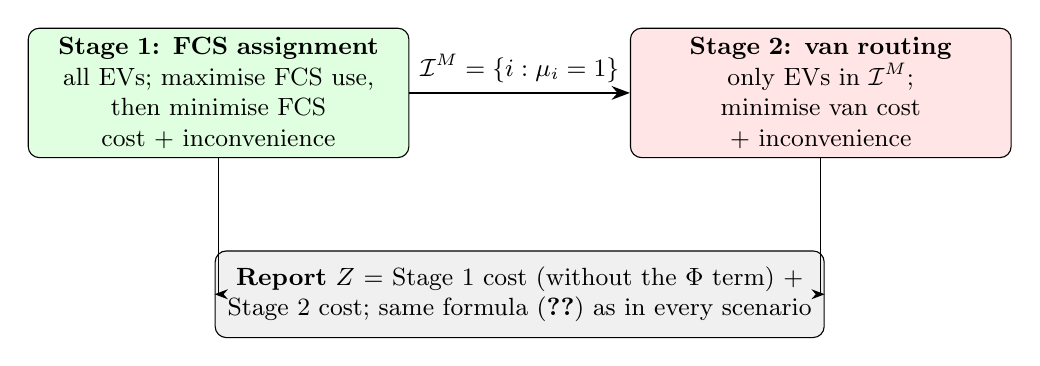
\begin{tikzpicture}[>=Stealth,box/.style={draw,rounded corners,align=center,minimum height=1.1cm,font=\small}]
  \node[box,fill=green!12,text width=4.6cm] (s1) {\textbf{Stage 1: FCS assignment}\\all EVs; maximise FCS use,\\then minimise FCS cost + inconvenience};
  \node[box,fill=red!10,text width=4.6cm,right=2.8cm of s1] (s2) {\textbf{Stage 2: van routing}\\only EVs in $\I^M$;\\minimise van cost + inconvenience};
  \draw[->,thick] (s1) -- node[above,font=\small]{$\I^M=\{i:\mu_i=1\}$} (s2);
  \node[box,fill=black!6,text width=7.5cm,below=2.0cm of $(s1)!0.5!(s2)$] (ev) {\textbf{Report} $Z=$ Stage~1 cost (without the $\Phi$ term) $+$ Stage~2 cost; same formula \eqref{eq:Z} as in every scenario};
  \draw[->] (s1) |- (ev); \draw[->] (s2) |- (ev);
\end{tikzpicture}
\end{center}

Stage~1 does not look at the vans, and Stage~2 cannot change what Stage~1 decided. That is the definition of ``FCS first, then MCS''.

%----------------------------------------------------------------
\subsection{Stage 1: assign EVs to fixed stations}

\textbf{Objective.}
\begin{equation}
\begin{split}
\min\ Z^{(1)}=\;&\underbrace{\Phi\sum_{i\in\I}\mu_i}_{\text{FCS first}}
+\underbrace{c^{EV}\sum_i\sum_{f\in\F_i}d_{if}Y_{if}}_{Z_1}
+\underbrace{Z^F_{\text{energy}}}_{\text{FCS part of }Z_4}\\
&+\underbrace{\sum_i\sum_{f\in\F_i}\rho^F_{if}Y_{if}+\alpha\sum_i w_i(C_i-r_i)+c^L\sum_i w_iL_i}_{\text{FCS customers' inconvenience}}
\end{split}
\label{eq:obj1}
\end{equation}
with $C_i=S_i+\tau^F_iY_i$ in this stage. $\Phi$ is a penalty for handing an EV to the vans. It is chosen larger than anything an extra FCS customer can add to the rest of \eqref{eq:obj1}, e.g.
\[
\Phi > \max_{i}\max_{f\in\F_i}\big(c^{EV}d_{if}+\pi^{\max}E_i+\rho^F_{if}\big)+n\,(\alpha+c^L)\,w_{\max}\,T,
\]
so Stage~1 first \textbf{maximises the number of EVs served at an FCS}, and only among those solutions minimises FCS cost and inconvenience. ($\pi^{\max}$ is the highest grid price.) A numerically safer equivalent is to solve twice: first $\max\sum_iY_i$, then fix that number and minimise the rest.
\ifTOU
Because $Z^F_{\text{energy}}$ uses the peak price, Stage~1 may \emph{start sessions later} to leave the peak, if the price saving beats the extra waiting cost (Section~\ref{sec:expect}).
\fi

\textbf{Constraints.}
\begin{align}
\sum_{g\in\G_i}y_{ig}+\mu_i &= 1 && \forall i\in\I \label{eq:s1assign}\\
S_i &\ge r_i+\sum_{f\in\F_i}t_{if}Y_{if} && \forall i\in\I \label{eq:fcsarr}\\
S_i &\le r_i+T\,(1-\mu_i) && \forall i\in\I \label{eq:s1park}\\
S_j &\ge S_i+\tau^F_i-(T+\tau^F_i)(3-y_{ig}-y_{jg}-o_{ij}) && \forall g,\ (i,j)\in\mathcal{P}_g \label{eq:disj1}\\
S_i &\ge S_j+\tau^F_j-(T+\tau^F_j)(2-y_{ig}-y_{jg}+o_{ij}) && \forall g,\ (i,j)\in\mathcal{P}_g \label{eq:disj2}\\
\sum_i y_{ig_1} &\ge \sum_i y_{ig_2} && \forall f,\ \G_f=\{g_1,g_2\} \label{eq:gunsym}\\
S_i+\tau^F_iY_i &\le T,\qquad L_i\ge S_i+\tau^F_iY_i-l_i && \forall i\in\I \label{eq:s1time}
\end{align}
\ifTOU plus the time-of-use split \eqref{eq:tou1}--\eqref{eq:tou5} of each FCS session (Section~\ref{sec:price}).\fi
\desc{\eqref{eq:s1assign}: every EV either gets one reachable gun or is handed to the vans. An EV that reaches no FCS ($\G_i=\emptyset$) is forced to $\mu_i=1$. \eqref{eq:fcsarr}: an FCS session cannot start before the EV has asked and driven to the station. \eqref{eq:s1park}: for an EV handed to the vans, $S_i$ is parked at $r_i$, so it adds no waiting in Stage~1 (its real start time is decided in Stage~2). \eqref{eq:disj1}--\eqref{eq:disj2}: two EVs on the same gun do not overlap; $o_{ij}$ picks who goes first. With two guns per station this means at most two EVs charge at a station at a time. \eqref{eq:gunsym}: symmetry breaking between the two identical guns (optional). \eqref{eq:s1time}: finished by $T$; lateness.}

\textbf{Optional acceptability rule.} An operator may refuse to send a driver to a station that is ``too inconvenient'', e.g.\ only allow gun $g$ of station $f$ for EV $i$ if $\hat\rho^F_{if}\le\bar\rho$. This only shrinks $\G_i$, so EVs whose stations are all too far go to the vans. Report results with and without it.

\textbf{Output:} $\I^M=\{i:\mu_i=1\}$, the EVs left for the vans; plus each FCS customer's gun and start time.

%----------------------------------------------------------------
\subsection{Stage 2: route the vans to the leftover EVs}

Stage~2 is a vehicle routing problem with time windows, on the EVs in $\I^M$ only. Here $C_i=S_i+\tau^M_i$.

\textbf{Objective.}
\begin{equation}
\begin{split}
\min\ Z^{(2)}=\;&\underbrace{c^M\sum_m\sum_{(i,j)\in\A^M}d_{ij}x_{ijm}}_{Z_2}+\underbrace{\sum_m c^D_mu_m}_{Z_3}+\underbrace{Z^M_{\text{energy}}}_{\text{van part of }Z_4}\\
&+\underbrace{\sum_{i\in\I^M}\sum_m\rho^M_{im}z_{im}+\alpha\sum_{i\in\I^M}w_i(C_i-r_i)+c^L\sum_{i\in\I^M}w_iL_i}_{\text{van customers' inconvenience}}
\end{split}
\label{eq:obj2}
\end{equation}
Since every EV in $\I^M$ must be served by some van, $Z^M_{\text{energy}}$ and the $\rho^M$ term are constants here. They are kept so that $Z^{(2)}$ is the true cost of Stage~2. Waiting and lateness make the vans visit urgent EVs early.

\textbf{Constraints.}
\begin{align}
\sum_{m\in\M}z_{im} &= 1 && \forall i\in\I^M \label{eq:s2assign}\\
\sum_{j:(0,j)\in\A^M}x_{0jm} = \sum_{i:(i,n+1)\in\A^M}x_{i,n+1,m} &= u_m && \forall m \label{eq:depot}\\
\sum_{i:(i,j)\in\A^M}x_{ijm} = \sum_{k:(j,k)\in\A^M}x_{jkm} &= z_{jm} && \forall j\in\I^M,\ m \label{eq:flow}\\
\sum_{i\in\I^M}z_{im} &\le Q_m\,u_m && \forall m \label{eq:cap}\\
\sum_{i\in\I^M}\frac{E_i}{\eta}z_{im}+\beta\sum_{(i,j)\in\A^M}d_{ij}x_{ijm} &\le B_m\,u_m && \forall m \label{eq:batt}
\end{align}
\begin{align}
S_j &\ge \max\{r_j,\ t_{0j}\,x_{0jm}\} && \forall j\in\I^M,\ m \label{eq:depart}\\
S_j &\ge S_i+\tau^M_i+t_{ij}-(T+\tau^M_i+t_{ij})(1-x_{ijm}) && \forall i\neq j,\ m \label{eq:seq}\\
S_i+\tau^M_i+t_{i,n+1} &\le T+(\tau^M_i+t_{i,n+1})(1-x_{i,n+1,m}) && \forall i,\ m \label{eq:return}\\
S_i+\tau^M_i \le T,\quad L_i &\ge S_i+\tau^M_i-l_i && \forall i\in\I^M \label{eq:s2time}\\
u_m &\ge u_{m+1} && m<|\M| \label{eq:vansym}
\end{align}
\desc{\eqref{eq:s2assign}: each leftover EV gets one van. \eqref{eq:depot}: a used van leaves and returns to the depot once. \eqref{eq:flow}: each EV on van $m$ is entered and left exactly once by that van. \eqref{eq:cap}: at most $Q_m$ EVs per van. \eqref{eq:batt}: delivered energy (with transfer losses) plus driving energy fits in the van battery. \eqref{eq:depart}: no start before the request, or before the van can drive there from the depot (written as two linear constraints). \eqref{eq:seq}: if the van goes $i\to j$, it finishes $i$ and drives to $j$ before starting $j$. This gives one EV at a time and removes subtours (MTZ-type). \eqref{eq:return}: back at the depot by $T$. \eqref{eq:s2time}: finished by $T$; lateness. \eqref{eq:vansym}: use identical vans in index order.}

\textbf{If Stage 2 is infeasible} (too many leftover EVs for the fleet by $T$), the sequential policy has \emph{failed} on that instance. For diagnosis, add $s_i\in\{0,1\}$ (``unserved''), replace \eqref{eq:s2assign} by $\sum_mz_{im}+s_i=1$ and add $\Phi^U\sum_is_i$ to \eqref{eq:obj2}. Then report the number of EVs that could not be served. This is a useful comparison with the integrated scenario, which may serve all of them.

%----------------------------------------------------------------
\subsection{Reported value}
\[
Z^{\text{S\scen}}=\big(Z^{(1)*}-\Phi\,|\I^M|\big)+Z^{(2)*},
\]
which is exactly \eqref{eq:Z} evaluated at the combined solution. The stage-1 solution plus the stage-2 solution is a feasible solution of the integrated model (S\ifTOU 4\else 3\fi), so
$Z^{\text{S\ifTOU 4\else 3\fi}}\le Z^{\text{S\scen}}$. The difference is the \emph{value of integration}.

\else
%---------------------------------------------------------------- INT
\subsection{Objective}
\begin{equation}
\min\ Z \quad\text{as in \eqref{eq:Z}, with }Z^F_{\text{energy}}=\ifTOU P^F\textstyle\sum_i\big[\pi^\off(\theta^1_i+\theta^3_i)+\pi^\pk\theta^2_i\big]\else\pi^F\textstyle\sum_iE_iY_i\fi,\quad C_i=S_i+\tau^F_iY_i+\tau^M_iZ_i. \label{eq:objint}
\end{equation}
Written out in full:
\begin{align*}
\min\ Z=\;& c^{EV}\sum_i\sum_{f\in\F_i}d_{if}Y_{if}+c^M\sum_m\sum_{(i,j)\in\A}d_{ij}x_{ijm}+\sum_mc^D_mu_m\\
&+\ifTOU P^F\sum_i\big[\pi^\off(\theta^1_i+\theta^3_i)+\pi^\pk\theta^2_i\big]\else\pi^F\sum_iE_iY_i\fi
+\pi^M\sum_i\sum_m\frac{E_i}{\eta}z_{im}\\
&+\sum_i\sum_{f\in\F_i}\rho^F_{if}Y_{if}+\sum_i\sum_m\rho^M_{im}z_{im}+\alpha\sum_iw_i(C_i-r_i)+c^L\sum_iw_iL_i .
\end{align*}
Every term is linear. One model weighs everything at once: an EV goes to a van exactly when the van's extra km, dispatch and energy cost are outweighed by the effort and waiting it saves the driver\ifTOU, or by the peak-price energy it avoids\fi.

\subsection{Constraints}

\textbf{Assignment.}
\begin{equation}
\sum_{g\in\G_i}y_{ig}+\sum_{m\in\M}z_{im}=1\qquad\forall i\in\I \label{eq:assign}
\end{equation}
\desc{Exactly one resource per EV: one reachable gun or one van. EVs that reach no FCS are forced onto a van.}

\textbf{Fixed stations.}
\begin{align}
S_i &\ge r_i+\sum_{f\in\F_i}t_{if}Y_{if} && \forall i \label{eq:fcsarr}\\
S_j &\ge S_i+\tau^F_i-(T+\tau^F_i)(3-y_{ig}-y_{jg}-o_{ij}) && \forall g,\ (i,j)\in\mathcal{P}_g \label{eq:disj1}\\
S_i &\ge S_j+\tau^F_j-(T+\tau^F_j)(2-y_{ig}-y_{jg}+o_{ij}) && \forall g,\ (i,j)\in\mathcal{P}_g \label{eq:disj2}\\
\sum_iy_{ig_1} &\ge \sum_iy_{ig_2} && \forall f,\ \G_f=\{g_1,g_2\} \label{eq:gunsym}
\end{align}
\desc{\eqref{eq:fcsarr}: an FCS session starts after the request and the drive to the station (for a van customer this is just $S_i\ge r_i$). \eqref{eq:disj1}--\eqref{eq:disj2}: EVs on the same gun do not overlap; $o_{ij}$ chooses the order. \eqref{eq:gunsym}: optional symmetry breaking.}

\textbf{Vans: routes, capacity, battery.}
\begin{align}
\sum_{j:(0,j)\in\A}x_{0jm}=\sum_{i:(i,n+1)\in\A}x_{i,n+1,m} &= u_m && \forall m \label{eq:depot}\\
\sum_{i:(i,j)\in\A}x_{ijm}=\sum_{k:(j,k)\in\A}x_{jkm} &= z_{jm} && \forall j\in\I,\ m \label{eq:flow}\\
\sum_iz_{im} &\le Q_mu_m && \forall m \label{eq:cap}\\
\sum_i\frac{E_i}{\eta}z_{im}+\beta\sum_{(i,j)\in\A}d_{ij}x_{ijm} &\le B_mu_m && \forall m \label{eq:batt}
\end{align}
\desc{\eqref{eq:depot}: a used van leaves and returns once. \eqref{eq:flow}: each EV on van $m$ is visited exactly once by it. \eqref{eq:cap}: at most $Q_m$ EVs. \eqref{eq:batt}: delivered energy (with losses) plus driving energy fits in the battery.}

\textbf{Vans: timing (one EV at a time, no subtours).}
\begin{align}
S_j &\ge t_{0j}\,x_{0jm} && \forall j\in\I,\ m \label{eq:depart}\\
S_j &\ge S_i+\tau^M_i+t_{ij}-(T+\tau^M_i+t_{ij})(1-x_{ijm}) && \forall i\neq j\in\I,\ m \label{eq:seq}\\
S_i+\tau^M_i+t_{i,n+1} &\le T+(\tau^M_i+t_{i,n+1})(1-x_{i,n+1,m}) && \forall i,\ m \label{eq:return}
\end{align}
\desc{\eqref{eq:depart}: the first stop cannot start before the van has driven there. \eqref{eq:seq}: $i\to j$ means finish $i$, drive, then start $j$; start times rise along a route, so no subtour can close. \eqref{eq:return}: back at the depot by $T$.}

\textbf{Horizon and lateness.}
\begin{equation}
C_i\le T,\qquad L_i\ge C_i-l_i\qquad\forall i\in\I \label{eq:time}
\end{equation}
\desc{Every EV is fully charged within the horizon; $L_i$ measures lateness.}

\ifTOU
\textbf{Time-of-use split.} Constraints \eqref{eq:tou1}--\eqref{eq:tou5} of Section~\ref{sec:price}.
\fi

\textbf{Symmetry and domains.}
\begin{equation}
u_m\ge u_{m+1};\qquad y,z,x,u,o\ifTOU,\kappa\fi\in\{0,1\};\qquad S_i,L_i\ifTOU,\theta^p_i\fi\ge0 \label{eq:dom}
\end{equation}
\fi

%=====================================================================
\section{Learning-to-optimise (RL) formulation}\label{sec:rl}

\textbf{Main rule:} the reward of each action is \emph{minus the increase in $Z$ that the action causes}. The rewards over an episode then add up to $-Z$ of the solution the policy builds. RL and MILP results are measured on the same yardstick \eqref{eq:Z}, and the MILP optimum is the benchmark for the RL gap.

\ifSEQ
%---------------------------------------------------------------- RL SEQ
The RL pipeline has the same two stages as the MILP.

\subsection{Stage 1 policy: FCS assignment}
\begin{itemize}[leftmargin=1.4em,itemsep=2pt]
  \item \textbf{Episode / epochs:} EVs are taken in order of request time $r_i$ (ties: higher $w_i$ first). One decision per EV.
  \item \textbf{State:} features of the current EV $k$ ($E_k,r_k,l_k,w_k,R_k$, location); for each gun $g$ the time $F_g$ it becomes free; summary features of the EVs still to come (count and positions near each station)\ifTOU; the current price and the time until $T_1$ and $T_2$\fi.
  \item \textbf{Action:} a gun $g\in\G_k$, or ``hand to vans''. \textbf{FCS-first mask:} ``hand to vans'' is allowed \emph{only} if no gun can finish EV $k$ by $T$ (or, with the optional rule, if all remaining guns have $\hat\rho^F_{kf}>\bar\rho$).
  \ifTOU\item \textbf{Optional timing action:} ``gun $g$, start after the peak'', i.e.\ $S_k=\max\{\text{earliest},T_2\}$, allowed only if the session still ends by $T$.\fi
  \item \textbf{Transition:} $S_k=\max\{r_k+t_{kf},F_g\}$ (or later, for the timing action); $F_g\leftarrow S_k+\tau^F_k$.
  \item \textbf{Reward:} $-\Big[c^{EV}d_{kf}+\text{energy}_k+\rho^F_{kf}+\alpha w_k(S_k+\tau^F_k-r_k)+c^Lw_k(S_k+\tau^F_k-l_k)^+\Big]$, where energy$_k$ = \ifTOU$P^F\big[\pi^\off\cdot(\text{off-peak hours of }[S_k,S_k+\tau^F_k])+\pi^\pk\cdot(\text{peak hours})\big]$, computed exactly in the simulator\else$\pi^FE_k$\fi. Handing an EV to the vans gives reward $0$ here; its cost is counted in Stage~2.
\end{itemize}
Note: a simple baseline for Stage~1 is the greedy rule ``gun with the largest one-step reward''. What RL can learn on top of this is, for example, to keep a nearby gun free for an urgent EV that arrives later.

\subsection{Stage 2 policy: van routing over $\I^M$}
\begin{itemize}[leftmargin=1.4em,itemsep=2pt]
  \item \textbf{Epochs:} whenever a van becomes free (the earliest-free van decides first).
  \item \textbf{State:} for each van: position, time free, remaining battery $b_m$, EVs served so far, dispatched or not; for each unserved EV in $\I^M$: location, $E_i,r_i,l_i,w_i$; current time.
  \item \textbf{Action:} the next EV $j$ for this van, or ``return to depot'' (ends the route). Mask: $j$ must be feasible: battery covers $E_j/\eta$ plus driving to $j$ and back to the depot, the count stays $\le Q_m$, and $j$ can be finished with the van back at the depot by $T$.
  \item \textbf{Transition:} $S_j=\max\{r_j,\ \text{time free}+t_{\text{pos},j}\}$; the van moves to $j$ and is free at $S_j+\tau^M_j$; $b_m$ falls by $E_j/\eta+\beta d_{\text{pos},j}$.
  \item \textbf{Reward:} serving $j$: $-\Big[c^Md_{\text{pos},j}+c^D_m[\text{first stop}]+\pi^M\frac{E_j}{\eta}+\rho^M_{jm}+\alpha w_j(S_j+\tau^M_j-r_j)+c^Lw_j(S_j+\tau^M_j-l_j)^+\Big]$; returning: $-c^Md_{\text{pos},0}$. EVs still unserved at the end: $-\Phi^U$ each.
  \item \textbf{Policy:} an attention-based routing policy (e.g.\ Kool et al., 2019, ``Attention, Learn to Solve Routing Problems!'') trained with REINFORCE or PPO. Baseline: nearest-feasible-EV heuristic.
\end{itemize}
Episode return of Stage~1 + Stage~2 $=-Z^{\text{S\scen}}$.

\else
%---------------------------------------------------------------- RL INT
One policy decides both who serves each EV and the van routes.
\begin{itemize}[leftmargin=1.4em,itemsep=2pt]
  \item \textbf{Episode / epochs:} EVs are taken in order of request time $r_i$ (ties: higher $w_i$ first). One decision per EV.
  \item \textbf{State:} (i) the current EV $k$: location, $E_k,r_k,l_k,w_k,R_k$, reachable stations; (ii) each gun $g$: time $F_g$ it becomes free; (iii) each van $m$: current end-of-route position, time free, remaining battery $b_m$, EVs served, dispatched or not; (iv) embeddings of the not-yet-assigned EVs (for look-ahead)\ifTOU; (v) current price, time until $T_1$ and $T_2$\fi.
  \item \textbf{Action:} $a\in\G_k\cup\M$: a gun, or a van (EV $k$ is appended to the end of that van's route). \textbf{Mask} infeasible actions: a gun that cannot finish $k$ by $T$; a van without enough battery for $E_k/\eta$ plus the drive to $k$ and back to the depot, with $Q_m$ reached, or unable to finish $k$ and return by $T$.
  \ifTOU\item \textbf{Optional timing action:} ``gun $g$, start after the peak'' ($S_k=\max\{\text{earliest},T_2\}$, if it still ends by $T$).\fi
  \item \textbf{Transition:} gun: $S_k=\max\{r_k+t_{kf},F_g\}$, $F_g\leftarrow S_k+\tau^F_k$. Van: $S_k=\max\{r_k,\ \text{free}_m+t_{\text{pos}_m,k}\}$, then the van moves to $k$, $\text{free}_m\leftarrow S_k+\tau^M_k$, $b_m\mathrel{-}=E_k/\eta+\beta d_{\text{pos}_m,k}$.
  \item \textbf{Reward} $=-\Delta Z$:
  \begin{align*}
  \text{gun } g\text{ at }f:&\quad -\Big[c^{EV}d_{kf}+\text{energy}^F_k+\rho^F_{kf}+\alpha w_k(C_k-r_k)+c^Lw_k(C_k-l_k)^+\Big]\\
  \text{van } m:&\quad -\Big[c^M\big(d_{\text{pos}_m,k}+d_{k,0}-d_{\text{pos}_m,0}\big)+c^D_m[\text{first use}]+\pi^M\tfrac{E_k}{\eta}\\
  &\qquad\quad+\rho^M_{km}+\alpha w_k(C_k-r_k)+c^Lw_k(C_k-l_k)^+\Big]
  \end{align*}
  The van distance term is the \emph{change} in route length when $k$ is inserted before the return to the depot, so the sum over the episode equals the total route length (the return legs telescope). energy$^F_k$ = \ifTOU$P^F\big[\pi^\off\cdot(\text{off-peak hours})+\pi^\pk\cdot(\text{peak hours of }[S_k,C_k])\big]$, computed exactly by the simulator; no linearisation is needed in RL\else$\pi^FE_k$\fi.
  \item \textbf{Dead end:} if every action is masked, EV $k$ is unserved: reward $-\Phi^U$, and the episode continues. Report the count.
  \item \textbf{Policy:} masked categorical policy over guns and vans, encoder with attention over EVs, guns and vans; trained with PPO. Natural baseline: greedy, i.e.\ choose the action with the largest one-step reward. That is the pairwise rule ``smallest $\hat\rho$ + cost'' from Section~\ref{sec:inc}.
\end{itemize}
Restriction to note: vans serve EVs in assignment order (append only). A variant that inserts $k$ at the cheapest position of a route is more flexible but has a larger action space.
\fi

\textbf{Reward scaling.} For stable training divide every reward by a constant, e.g.\ the greedy baseline's average $Z$ on the training instances. This does not change the optimal policy.

%=====================================================================
\section{What to expect and what to report}\label{sec:expect}

\ifnum\scen=1
\begin{itemize}[leftmargin=1.4em,itemsep=2pt]
  \item Vans serve only EVs that reach no station, or that the stations cannot finish by $T$. If stations have spare capacity, very few vans are dispatched.
  \item Inconvenience is high for EVs far from the nearest station (worked example: Rs\,682 at the FCS, against Rs\,458 if a van had been allowed).
  \item With too few vans Stage~2 becomes infeasible (unserved EVs), even when the integrated model S3 could serve everyone. Report the smallest $|\M|$ at which S1 is feasible and compare it with S3.
\end{itemize}
\fi
\ifnum\scen=2
\begin{itemize}[leftmargin=1.4em,itemsep=2pt]
  \item \textbf{When does Stage~1 delay a session to avoid the peak?} Moving one hour of charging out of the peak saves $(\pi^\pk-\pi^\off)P^F=3\times22=$ Rs\,66, but delays completion by up to an hour, which costs $\alpha w_i\ge$ Rs\,200. So with the default values Stage~1 almost never delays. It mostly pays the higher price, and S2 costs roughly S1 plus the peak surcharge. Sessions start later only if $\alpha$ is small (try $\lambda<0.33$ in the sensitivity analysis).
  \item The van assignment is the same as in S1 unless Stage~1's timing changes which EVs fit at the stations. Stage~1 cannot use vans to escape the peak price.
  \item Extra KPI: \textbf{grid energy drawn at FCS during the peak}, $P^F\sum_i\theta^2_i$ (kWh). Compare with S4.
\end{itemize}
\fi
\ifnum\scen=3
\begin{itemize}[leftmargin=1.4em,itemsep=2pt]
  \item Vans take EVs for which the saved inconvenience exceeds the extra van cost (worked example: van chosen, saving Rs\,224). Expect vans to serve EVs that are far from every station, have low range (high $w_i$), or have early deadlines, while EVs near a station still use it.
  \item \textbf{Value of integration under flat price:} $Z^{\text{S1}}-Z^{\text{S3}}\ge0$. Report it per component ($Z_1,\dots,Z_5$): typically operating cost rises a little and inconvenience falls a lot.
  \item Vary $|\M|$ (0, 1, 2, \dots): the first few vans lower $Z$ sharply, then the effect levels off. That curve shows the scenarios where mobile chargers help most.
\end{itemize}
\fi
\ifnum\scen=4
\begin{itemize}[leftmargin=1.4em,itemsep=2pt]
  \item During the peak a van kWh costs about the same as an FCS kWh (Rs\,10.0 each), so the vans' energy disadvantage disappears and vans also absorb \emph{peak-hour} demand that would otherwise be charged on the grid at peak price.
  \item Expect more van usage than in S3, concentrated on requests in $[T_1,T_2]$, and lower grid energy at the stations during the peak, $P^F\sum_i\theta^2_i$, than in S2.
  \item \textbf{Value of integration under peak pricing:} $Z^{\text{S2}}-Z^{\text{S4}}$. It should be larger than $Z^{\text{S1}}-Z^{\text{S3}}$, because integration now also allows price arbitrage.
  \item \textbf{Peak pricing with full flexibility:} $Z^{\text{S4}}-Z^{\text{S3}}$ should be smaller than $Z^{\text{S2}}-Z^{\text{S1}}$: vans cushion the price increase.
\end{itemize}
\fi

\textbf{Cross-scenario comparison table} (fill in from the four runs):
\begin{center}
\renewcommand{\arraystretch}{1.2}
\begin{tabular}{@{}lll@{}}
\toprule
\textbf{Comparison} & \textbf{Measures} & \textbf{Expected sign} \\
\midrule
S1 $-$ S3 & value of integration, flat price & $\ge0$ \\
S2 $-$ S4 & value of integration, peak price & $\ge0$, larger than S1 $-$ S3 \\
S2 $-$ S1 & cost of peak pricing, FCS-first operator & $>0$ \\
S4 $-$ S3 & cost of peak pricing, flexible operator & $>0$, smaller than S2 $-$ S1 \\
\bottomrule
\end{tabular}
\end{center}
Report for each: $Z$ and its components, number of vans used, EVs per resource, mean and maximum inconvenience per EV, total lateness, peak-hour grid energy, solve time, and (for RL) the gap to the MILP optimum.

%=====================================================================
\appendix
\section{Illustrative parameter values}\label{app:values}

These are starting values for experiments, not data. All are meant to be varied in the analysis. Values in Rs.

\begin{center}
\renewcommand{\arraystretch}{1.15}
\begin{tabular}{@{}llp{6.2cm}@{}}
\toprule
\textbf{Parameter} & \textbf{Value} & \textbf{Note} \\
\midrule
$T$, $[T_1,T_2]$ & 7 h, $[2,6]$ & 16:00--23:00, peak 18:00--22:00 \\
$P^F$, $P^M$ & 22 kW, 30 kW & \\
$v$, $\beta$, $\eta$ & 25 km/h, 0.25 kWh/km, 0.9 & \\
$B_m$, $Q_m$, $|\M|$ & 150 kWh, 6, 2--6 & \\
$c^{EV}$, $c^M$, $c^D_m$ & Rs\,4/km, Rs\,15/km, Rs\,1500 & van km includes driver time \\
$\pi^F$ (flat) & Rs\,8.7/kWh & equals the time-average of the ToU tariff over $[0,T]$ \\
$\pi^\off$, $\pi^\pk$ (ToU) & Rs\,7/kWh, Rs\,10/kWh & $(3\times7+4\times10)/7=8.7$ \\
$c^{bat}$ & Rs\,2/kWh & van battery wear \\
$\pi^M$ & Rs\,10.7 (flat) / Rs\,9.0 (ToU) & $=\pi^F+c^{bat}$ / $=\pi^\off+c^{bat}$ \\
$\alpha$, $\alpha^D$ & Rs\,200/h, Rs\,100/h & value of time; extra for attended time \\
$h^F$, $h^M$, $\varphi$ & Rs\,50, Rs\,10, Rs\,100 & trip hassle, hand-over, range stress \\
$c^L$ & Rs\,300/h & lateness \\
$w_i$ & $1+2(1-R_i/R_{\max})$, $R_i\sim U[3,40]$ km & priority from remaining range \\
\bottomrule
\end{tabular}
\end{center}

The flat price is set to the time-average of the peak tariff. The price \emph{level} is then the same in both pricing cases, and only the price \emph{shape} differs. Without this, part of S1 vs S2 would just reflect a different average price.

\end{document}
"
%    pdflatex -jobname=scenario4_peak_integrated   "\def\scen{4}% =====================================================================
%  One source, four PDFs.  Build with build.sh (or by hand):
%    pdflatex -jobname=scenario1_flat_sequential   "\def\scen{1}% =====================================================================
%  One source, four PDFs.  Build with build.sh (or by hand):
%    pdflatex -jobname=scenario1_flat_sequential   "\def\scen{1}\input{scenario_master}"
%    pdflatex -jobname=scenario2_peak_sequential   "\def\scen{2}\input{scenario_master}"
%    pdflatex -jobname=scenario3_flat_integrated   "\def\scen{3}\input{scenario_master}"
%    pdflatex -jobname=scenario4_peak_integrated   "\def\scen{4}\input{scenario_master}"
%  (run each twice for cross-references)
% =====================================================================
\documentclass[11pt,a4paper]{article}
\usepackage[margin=2.2cm]{geometry}
\usepackage{amsmath,amssymb,amsfonts}
\usepackage{booktabs,array,tabularx}
\usepackage{enumitem}
\usepackage[table]{xcolor}
\usepackage{tikz}
\usetikzlibrary{arrows.meta,positioning,calc}
\usepackage[colorlinks=true,linkcolor=blue!50!black,urlcolor=blue!50!black]{hyperref}
\usepackage{titlesec}
\titleformat{\section}{\large\bfseries}{\thesection}{0.8em}{}
\titleformat{\subsection}{\normalsize\bfseries}{\thesubsection}{0.8em}{}
\setlength{\parindent}{0pt}
\setlength{\parskip}{5pt}

% ---------------- scenario switches ----------------
\ifdefined\scen\else\def\scen{1}\fi
\newif\ifTOU \TOUfalse   % true = time-of-use (peak) price
\newif\ifSEQ \SEQfalse   % true = FCS first, then MCS
\ifnum\scen=1 \SEQtrue \fi
\ifnum\scen=2 \TOUtrue \SEQtrue \fi
\ifnum\scen=4 \TOUtrue \fi

\newcommand{\pricename}{\ifTOU time-of-use price (dearer evening peak)\else single (flat) price all day\fi}
\newcommand{\structname}{\ifSEQ FCS first, then MCS (sequential)\else FCS and MCS together (integrated)\fi}

% ---------------- notation ----------------
\newcommand{\I}{\mathcal{I}}
\newcommand{\F}{\mathcal{F}}
\newcommand{\G}{\mathcal{G}}
\newcommand{\M}{\mathcal{M}}
\newcommand{\N}{\mathcal{N}}
\newcommand{\A}{\mathcal{A}}
\newcommand{\Rs}{\text{Rs}\,}
\newcommand{\pk}{\mathrm{pk}}
\newcommand{\off}{\mathrm{off}}
\newcommand{\desc}[1]{\par\vspace{-2pt}{\small\color{black!75}\textit{Meaning:} #1}\par\vspace{4pt}}
\newcommand{\cell}[2]{\ifnum\scen=#1\cellcolor{blue!18}\textbf{S#1 (this document)}\\\textbf{#2}\else S#1\\#2\fi}

\title{\textbf{EV Charging Network Optimisation}\\[4pt]
\large Scenario \scen: \pricename\ $+$ \structname\\[2pt]
\normalsize MILP and RL formulation}
\author{CP 320 OR for Mobility Management, course project}
\date{2 October 2026}

\begin{document}
\maketitle

%=====================================================================
\section{Where this scenario sits}

The project studies four scenarios: two ways of pricing grid electricity, times two ways of making the decisions.

\begin{center}
\renewcommand{\arraystretch}{1.5}
\begin{tabular}{>{\raggedright\arraybackslash}p{4.2cm}|>{\centering\arraybackslash}p{4.6cm}|>{\centering\arraybackslash}p{4.6cm}}
 & \textbf{Flat price all day} & \textbf{Time-of-use (peak) price} \\ \hline
\textbf{Sequential:} FCS first, leftover EVs to MCS &
\begin{tabular}[c]{@{}c@{}}\cell{1}{flat + sequential}\end{tabular} &
\begin{tabular}[c]{@{}c@{}}\cell{2}{peak + sequential}\end{tabular} \\ \hline
\textbf{Integrated:} FCS and MCS decided together &
\begin{tabular}[c]{@{}c@{}}\cell{3}{flat + integrated}\end{tabular} &
\begin{tabular}[c]{@{}c@{}}\cell{4}{peak + integrated}\end{tabular} \\
\end{tabular}
\end{center}

\textbf{The four scenarios do not have four different objectives.} They share \emph{one} cost yardstick $Z$ (Section~\ref{sec:obj}): the same cost terms and the same customer inconvenience (Section~\ref{sec:inc}). Only two things change:
\begin{itemize}[leftmargin=1.4em,itemsep=1pt]
  \item \textbf{Pricing} changes the formula for one term, the FCS energy cost (Section~\ref{sec:price}).
  \item \textbf{Decision structure} changes \emph{how} $Z$ is minimised: in one model (integrated), or in two stages (sequential), where each stage minimises its own part of $Z$.
\end{itemize}
Because the yardstick is the same, the four optimal values can be compared directly. The differences measure the \emph{value of integration} (S1$\to$S3, S2$\to$S4) and the \emph{effect of peak pricing} (S1$\to$S2, S3$\to$S4).

\ifnum\scen=1
\textbf{This scenario (S1)} is the baseline, the ``status quo''. Electricity costs the same at every hour, every EV that can be charged at a fixed station is sent there, and vans only take what is left over.
\fi
\ifnum\scen=2
\textbf{This scenario (S2)} keeps the FCS-first rule of S1, but grid electricity is dearer during the evening peak. Stage~1 can react to the price only by \emph{rescheduling} FCS sessions. It cannot hand a peak-hour EV to a van.
\fi
\ifnum\scen=3
\textbf{This scenario (S3)} keeps the flat price of S1, but the operator decides FCS and MCS service \emph{together}. An EV can be sent to a van even when a fixed station could take it, whenever that lowers total cost plus inconvenience.
\fi
\ifnum\scen=4
\textbf{This scenario (S4)} is the most flexible one: peak pricing at fixed stations, and FCS and MCS decided together. Van energy was bought off-peak, so vans can also be used to keep charging \emph{out of the expensive peak}.
\fi

%=====================================================================
\section{Setting and assumptions}\label{sec:setting}

\textbf{Time.} The planning horizon is $[0,T]$ with $T=7$\,h (16:00--23:00). It contains the evening peak window $[T_1,T_2]=[2,6]$ (18:00--22:00). The horizon is the same in all four scenarios. It is wider than the peak itself so that, under peak pricing, there is cheaper time on both sides of the peak.\ifTOU\else\ In this scenario the price is flat, so the window plays no role in the model.\fi

\textbf{Assumptions} (the same as MILP v3, plus two about energy):
\begin{enumerate}[leftmargin=1.6em,itemsep=1pt]
  \item Static, continuous time. All requests in the horizon are known at time $0$, and request $i$ becomes active at $r_i$.
  \item An EV served by an FCS drives there itself on its own battery (only to stations within its range $R_i$). The driver stays with the car while it waits for a free gun and while it charges.
  \item An EV served by an MCS stays parked where it is, and the driver is free in the meantime.
  \item Each FCS gun and each van charges one EV at a time, without interruption, at constant power.
  \item A van's battery covers both its driving and the energy it delivers. \textbf{The van battery is charged at the depot before the horizon starts}\ifTOU, i.e.\ at the off-peak price\fi, and is not recharged during the horizon.
  \item Every EV must be fully charged by $T$ (hard). Finishing after the driver's desired time $l_i$ is allowed but penalised.
\end{enumerate}

%=====================================================================
\section{Notation}\label{sec:notation}

\subsection*{Sets}
\begin{tabularx}{\textwidth}{@{}lX@{}}
\toprule
$\I=\{1,\dots,n\}$ & EV charging requests \\
$\F$; $\G_f$ ($|\G_f|=2$); $\G=\bigcup_f\G_f$ & fixed charging stations; guns of FCS $f$; all guns ($f(g)$ = station of gun $g$) \\
$\F_i=\{f: d_{if}\le R_i\}$, $\G_i=\bigcup_{f\in\F_i}\G_f$ & stations / guns EV $i$ can reach on its remaining range \\
$\M$ & mobile charging vans (MCS) \\
$0,\ n+1$ & depot as start node / end node (same place) \\
$\N=\{0\}\cup\I\cup\{n+1\}$, $\A$ & routing nodes; allowed van arcs $(i,j)$, $i\in\{0\}\cup\I$, $j\in\I\cup\{n+1\}$, $i\neq j$ \\
$\mathcal{P}_g=\{(i,j): i<j,\ g\in\G_i\cap\G_j\}$ & pairs of EVs that could share gun $g$ \\
\ifSEQ
$\I^M\subseteq\I$ & EVs handed to the vans by Stage~1 (an \emph{output} of Stage~1, a fixed input to Stage~2) \\
$\N^M$, $\A^M$ & routing nodes / arcs restricted to $\I^M$ \\
\fi
\bottomrule
\end{tabularx}

\subsection*{Parameters}
\begin{tabularx}{\textwidth}{@{}lX@{}}
\toprule
$E_i,\ r_i,\ l_i,\ R_i$ & energy demand (kWh), request time, desired completion time (h), remaining range (km) \\
$w_i\ge1$ & priority of EV $i$; $w_i=1+\kappa(1-R_i/R_{\max})$, so low-range EVs weigh more \\
$P^F,\ P^M$ & charging power of an FCS gun (22\,kW) / of a van (e.g.\ 30\,kW) \\
$\tau^F_i=E_i/P^F,\ \tau^M_i=E_i/P^M$ & charging time of EV $i$ at an FCS / by a van (h) \\
$d_{if},t_{if}$;\ $d_{ij},t_{ij}$ & distance (km) and time (h): EV$\to$FCS; between routing nodes ($t=d/v$) \\
$B_m,\ Q_m,\ \beta,\ \eta$ & van battery (kWh), max EVs per van, van consumption (kWh/km), transfer efficiency \\
$c^{EV},\ c^M,\ c^D_m$ & cost per km of EV driving, per km of van driving; fixed dispatch cost of van $m$ \\
\ifTOU
$\pi^\off,\ \pi^\pk$ & grid price (Rs/kWh) off-peak / in $[T_1,T_2]$, with $\pi^\pk\ge\pi^\off$ \\
\else
$\pi^F$ & grid price (Rs/kWh), the same at every hour \\
\fi
$c^{bat}$ & van battery wear per kWh cycled \\
$\pi^M$ & cost of 1 kWh taken from a van battery: $\pi^M=\ifTOU\pi^\off\else\pi^F\fi+c^{bat}$ (Section~\ref{sec:price}) \\
$\alpha,\ \alpha^D,\ h^F,\ h^M,\ \varphi,\ c^L$ & inconvenience coefficients (Section~\ref{sec:inc}) \\
\bottomrule
\end{tabularx}

\subsection*{Decision variables}
\begin{tabularx}{\textwidth}{@{}llX@{}}
\toprule
$y_{ig}$ & $\{0,1\}$ & EV $i$ charged at gun $g\in\G_i$ \\
$z_{im}$ & $\{0,1\}$ & EV $i$ served by van $m$ \\
$x_{ijm}$ & $\{0,1\}$ & van $m$ drives arc $(i,j)$ \\
$u_m$ & $\{0,1\}$ & van $m$ is dispatched \\
$o_{ij}$ & $\{0,1\}$ & for EVs $i<j$ that could share a gun: 1 if $i$ is charged before $j$ \\
\ifSEQ
$\mu_i$ & $\{0,1\}$ & Stage~1 only: EV $i$ is handed to the van fleet \\
\fi
\ifTOU
$\theta^1_i,\theta^2_i,\theta^3_i$ & $\ge0$ & hours of EV $i$'s FCS session before / inside / after the peak \\
$\kappa^1_i,\kappa^3_i$ & $\{0,1\}$ & EV $i$'s FCS session starts before $T_1$ / ends after $T_2$ \\
\fi
$S_i$ & $\ge0$ & time charging of EV $i$ starts (h), on whichever resource \\
$L_i$ & $\ge0$ & lateness of EV $i$ beyond $l_i$ (h) \\
\bottomrule
\end{tabularx}

\textbf{Short-hands} (linear expressions, not new variables):
\[
Y_{if}=\sum_{g\in\G_f}y_{ig},\qquad Y_i=\sum_{g\in\G_i}y_{ig}\ (\text{EV $i$ uses an FCS}),\qquad Z_i=\sum_{m\in\M}z_{im}\ (\text{EV $i$ uses a van}),
\]
\[
C_i=S_i+\tau^F_i\,Y_i+\tau^M_i\,Z_i \quad\text{(time EV $i$ is fully charged).}
\]

%=====================================================================
\section{Customer inconvenience}\label{sec:inc}

This section is \textbf{identical in all four scenario documents}. Inconvenience is a property of the customer, not of the price or of the planning method.

\subsection{What we mean by inconvenience}

Inconvenience is \emph{what the driver loses} from the moment they ask for a charge ($r_i$) until the car is fully charged ($C_i$), \emph{converted into rupees} so it can be added to the operator's costs. A driver loses three different things:

\begin{enumerate}[leftmargin=1.6em,itemsep=2pt]
  \item \textbf{Waiting:} the car is not ready. This lasts $C_i-r_i$ hours and affects \emph{every} driver, FCS or MCS.
  \item \textbf{Effort:} only an FCS customer has to drive to the station and sit there while the car charges. An MCS customer stays at home or at work and does something else. Driving to a far station also uses scarce battery range, which causes stress (``range anxiety'').
  \item \textbf{A missed deadline:} the car is still not ready at the time $l_i$ the driver needs it.
\end{enumerate}

Each loss gets a price in Rs per hour (or per event). All of them are multiplied by the priority $w_i$: an hour of delay for an EV with 5\,km of range left counts more than for one with 40\,km.

\subsection{The three components}

\begin{center}
\renewcommand{\arraystretch}{1.3}
\begin{tabularx}{\textwidth}{@{}>{\raggedright\arraybackslash}p{2.6cm}>{\raggedright\arraybackslash}X>{\raggedright\arraybackslash}X>{\raggedright\arraybackslash}p{3.0cm}@{}}
\toprule
\textbf{Component} & \textbf{EV $i$ at FCS $f$} & \textbf{EV $i$ by a van} & \textbf{Known when?} \\
\midrule
Effort & $w_i\big[\alpha^D(t_{if}+\tau^F_i)+h^F+\varphi\,d_{if}/R_i\big]$: driving and sitting at the station, a fixed trip hassle, range stress & $w_i\,h^M$: being reachable and handing over the car & \textbf{Static:} known as soon as the resource is chosen \\
Waiting & $w_i\,\alpha\,(C_i-r_i)$ = drive + \emph{queue at the gun} + charge & $w_i\,\alpha\,(C_i-r_i)$ = \emph{wait for the van} + charge & \textbf{Dynamic:} depends on the queue / van route \\
Missed deadline & $w_i\,c^L\,L_i$, $L_i=\max\{0,C_i-l_i\}$ & same & Dynamic \\
\bottomrule
\end{tabularx}
\end{center}

\textbf{Coefficients.}
$\alpha$ (Rs/h) is the value of an hour the car is not ready.
$\alpha^D$ (Rs/h) is the \emph{extra} value of an hour the driver must personally spend driving or sitting at the station: an hour at the station costs $\alpha+\alpha^D$, an hour waiting at home for a van costs only $\alpha$.
$h^F,h^M$ (Rs) are fixed hassle costs of one trip to a station / one van hand-over.
$\varphi$ (Rs) is the range-stress cost of a trip that uses the \emph{whole} remaining range ($d_{if}/R_i\le1$ is the fraction used).
$c^L$ (Rs/h) is the cost per hour late.

\subsection{Pairwise form: inconvenience of a (customer, resource) pair}

The natural first idea is: \emph{for every pair (EV $i$, FCS $f$) and every pair (EV $i$, van $m$) there is an inconvenience number, and the operator picks the pair with the lowest cost plus inconvenience.} The static part fits this idea exactly:
\[
\boxed{\;\rho^F_{if}=w_i\Big[\alpha^D\,(t_{if}+\tau^F_i)+h^F+\varphi\,\frac{d_{if}}{R_i}\Big]\qquad
\rho^M_{im}=w_i\,h^M\;}
\]
These are \textbf{parameters}, computed before solving, one number per (EV, FCS) pair and per (EV, van) pair. In the objective they appear linearly: $\sum_i\sum_f\rho^F_{if}Y_{if}+\sum_i\sum_m\rho^M_{im}z_{im}$.

Note that $\rho^M_{im}$ does not depend on $m$. Vans are identical and all start at the same depot, so the driver does not care \emph{which} van comes, only \emph{when} it comes. That ``when'' is the waiting part.

\subsection{Why waiting cannot be a fixed pairwise number}

It is tempting to also write the waiting as a pairwise number, e.g.\ ``the van needs 5 minutes to reach EV $i$''. But that depends on \emph{where the van is coming from}, which depends on the route the model is still choosing: if EV $i$ is the 4th stop of a van, the wait is the time for three charging sessions plus four drives. Likewise, waiting at an FCS depends on how many EVs are queued at that gun. So waiting is not known before solving. It is a function of decision variables:
\[
\text{waiting cost of EV } i \;=\; w_i\,\alpha\,(C_i-r_i),\qquad C_i=S_i+\tau^F_iY_i+\tau^M_iZ_i .
\]
This is \textbf{linear} in the variables ($S_i$, $y$, $z$), so it fits in a MILP directly. The constraints of Section~\ref{sec:milp} make $S_i$ equal to the true start time, including driving, queueing at the gun and the van's route. The term $\sum_i w_i\alpha r_i$ is a constant and may be dropped when solving.

\textbf{Pairwise \emph{estimate}} (used for intuition, by the RL policy and in heuristics): if there is no queue and the van comes straight to $i$,
\[
\hat\rho^{F}_{if}=\rho^F_{if}+w_i\alpha\,(t_{if}+\tau^F_i),\qquad
\hat\rho^{M}_{im}=\rho^M_{im}+w_i\alpha\,(t^{\text{van}}_{m\to i}+\tau^M_i),
\]
where $t^{\text{van}}_{m\to i}$ is the time until van $m$ can reach $i$ from where it currently is. In the RL formulation (Section~\ref{sec:rl}) the van's position \emph{is} known at each decision, so there this estimate becomes exact.

\subsection{Total inconvenience and how it enters the objective}

\begin{equation}
\boxed{\;
Z_{\text{inc}}=\underbrace{\sum_{i\in\I}\sum_{f\in\F_i}\rho^F_{if}Y_{if}+\sum_{i\in\I}\sum_{m\in\M}\rho^M_{im}z_{im}}_{\text{effort (static, pairwise)}}
+\underbrace{\alpha\sum_{i\in\I}w_i\,(C_i-r_i)}_{\text{waiting (dynamic)}}
+\underbrace{c^L\sum_{i\in\I}w_i\,L_i}_{\text{missed deadline}}
\;}\label{eq:inc}
\end{equation}
All three parts are in rupees, so $Z_{\text{inc}}$ is simply added to the operating costs. Nothing has to be normalised.

\subsection{Worked example: your ``10 km to the FCS vs.\ van in 5 minutes'' case}

EV $i$: $E_i=20$\,kWh, $R_i=40$\,km (so $w_i=1$); nearest free FCS $d_{if}=10$\,km away, $t_{if}=0.4$\,h at 25\,km/h; a van finishing next door can reach it in 5\,min ($0.083$\,h), adding about 4\,km to its route. $\tau^F_i=20/22=0.909$\,h, $\tau^M_i=20/30=0.667$\,h. Coefficients from Appendix~\ref{app:values}, flat price.

\begin{center}
\renewcommand{\arraystretch}{1.25}
\begin{tabular}{@{}lrr@{}}
\toprule
 & \textbf{FCS} & \textbf{Van} \\
\midrule
Driving (EV / extra van km) & $4\times10=40.0$ & $15\times4=60.0$ \\
Energy & $8.7\times20=174.0$ & $10.7\times20/0.9=237.8$ \\
\textbf{Operating cost only} & \textbf{214.0} & \textbf{297.8} \\
\midrule
Effort $\rho$ & $100(0.4+0.909)+50+100\cdot\tfrac{10}{40}=205.9$ & $10.0$ \\
Waiting $\alpha(C_i-r_i)$ & $200\times1.309=261.8$ & $200\times0.75=150.0$ \\
\textbf{Cost + inconvenience} & \textbf{681.7} & \textbf{457.8} \\
\bottomrule
\end{tabular}
\end{center}

On operating cost alone the FCS is cheaper, so a cost-only model would \emph{always} send this driver 10\,km away. With inconvenience included the van is better by about Rs\,224, and the integrated model chooses $z_{im}=1$, as you expected. If the FCS were only 1\,km away, the FCS would win both comparisons. The inconvenience term is what makes the model choose between ``cheap for the operator'' and ``convenient for the driver'', rather than following a fixed rule.

\subsection{Relation to a single penalty $\rho_i$ per EV}

The first draft used a penalty $\rho_i$ that is charged whenever EV $i$ goes to \emph{any} FCS: $\sum_i\sum_f\rho_iy_{if}$. Because $\sum_f y_{if}=1-\sum_m z_{im}$, this only says ``a van is worth $\rho_i$ more to EV $i$'', and that holds whether the station is 1\,km or 15\,km away, and whether the van arrives in 5 minutes or in 3 hours. The form above fixes both problems: $\rho^F_{if}$ grows with the distance to \emph{that} station, and the waiting term grows with how late the van or the free gun actually is. The old model is the special case $\alpha=\alpha^D=\varphi=c^L=0$, $h^F=\rho_i$.

\subsection{Choosing the coefficients}
\begin{itemize}[leftmargin=1.4em,itemsep=2pt]
  \item Use a value of time for $\alpha$ (e.g.\ Rs\,150--300/h for urban car users), and set $\alpha^D\approx0.5\alpha$: sitting at a station is worse than waiting at home.
  \item Keep $c^L>\alpha$, so missing the deadline is worse than ordinary waiting.
  \item \textbf{Sensitivity analysis:} multiply all inconvenience coefficients by a factor $\lambda\in\{0,0.25,0.5,1,2,4\}$ and plot operating cost against total inconvenience. $\lambda=0$ is the pure cost-minimising operator, and large $\lambda$ is a customer-first operator. This trade-off curve is a strong result for the ``Analysis'' part of the project.
\end{itemize}

\subsection{What inconvenience does in \emph{this} scenario}
\ifSEQ
In a sequential scenario inconvenience \textbf{cannot move an EV from an FCS to a van}: Stage~1 sends every EV that \emph{can} use an FCS to one. It still matters inside each stage. In Stage~1 it decides \emph{which} station and \emph{when} (urgent EVs get the near station and the first free gun). In Stage~2 it decides the \emph{order} in which vans visit EVs (urgent EVs first). In the worked example, this scenario sends the driver 10\,km to the FCS. That is the weakness the integrated scenarios remove.
\else
In an integrated scenario inconvenience is weighed directly against operating cost when choosing the resource. That is how the worked example ends up with a van. It also decides which station and which gun order, and the order of each van route.
\fi

%=====================================================================
\section{Electricity price in this scenario}\label{sec:price}

\textbf{Van energy (same in all scenarios).} A van's battery is charged at the depot \emph{before} the horizon, so its energy was bought at the
\ifTOU off-peak \fi
price, whatever time the van later delivers it. Each kWh taken from the van also wears the battery ($c^{bat}$), and a fraction $1-\eta$ is lost in transfer:
\[
Z^M_{\text{energy}}=\pi^M\sum_{i\in\I}\sum_{m\in\M}\frac{E_i}{\eta}\,z_{im},\qquad \pi^M=\ifTOU\pi^\off\else\pi^F\fi+c^{bat}.
\]

\ifTOU
\textbf{FCS energy (time-of-use).} An FCS draws from the grid while it charges. Energy delivered inside $[T_1,T_2]$ costs $\pi^\pk$, and energy outside it costs $\pi^\off$. A session $[S_i,S_i+\tau^F_i]$ may overlap the peak partly. Split its duration into the hours before, inside and after the peak, $\theta^1_i+\theta^2_i+\theta^3_i$:
\[
Z^F_{\text{energy}}=P^F\sum_{i\in\I}\Big[\pi^\off(\theta^1_i+\theta^3_i)+\pi^\pk\,\theta^2_i\Big].
\]
Constraints \eqref{eq:tou1}--\eqref{eq:tou5} below make the $\theta$'s equal to the true overlaps. Peak hours are dearer, so the solver wants $\theta^1_i,\theta^3_i$ as large as possible. It is enough to bound them from above by the true off-peak overlap, and the constraints need one binary per side:
\begin{align}
\theta^1_i+\theta^2_i+\theta^3_i &= \tau^F_i\,Y_i && \forall i\in\I \label{eq:tou1}\\
\theta^1_i &\le \tau^F_i\,\kappa^1_i && \forall i\in\I \label{eq:tou2}\\
\theta^1_i &\le T_1-S_i+T\,(1-\kappa^1_i) && \forall i\in\I \label{eq:tou3}\\
\theta^3_i &\le \tau^F_i\,\kappa^3_i && \forall i\in\I \label{eq:tou4}\\
\theta^3_i &\le S_i+\tau^F_i-T_2+T\,(1-\kappa^3_i) && \forall i\in\I \label{eq:tou5}
\end{align}
\desc{\eqref{eq:tou1}: the FCS session's hours are split into three parts; for a van customer ($Y_i=0$) all three are zero. \eqref{eq:tou2}--\eqref{eq:tou3}: off-peak time before the peak is only possible if the session starts before $T_1$ ($\kappa^1_i=1$), and is at most $T_1-S_i$. \eqref{eq:tou4}--\eqref{eq:tou5}: the same for time after $T_2$. $\theta^2_i\ge0$ prevents counting more off-peak hours than exist. Checking the cases (entirely before / inside / after the peak, straddling one edge, covering the whole peak) shows that at the optimum the $\theta$'s equal the exact overlaps. This needs $\pi^\pk\ge\pi^\off$, which is true for a peak tariff.}

\textbf{Why vans become more attractive.} Compare the cost of 1\,kWh delivered to an EV during the peak (values from Appendix~\ref{app:values}):
FCS $=\pi^\pk=$ Rs\,10.0, van $=(\pi^\off+c^{bat})/\eta=9/0.9=$ Rs\,10.0. They are at parity. Under the flat price the van is about Rs\,3.2/kWh dearer (FCS Rs\,8.7, van $10.7/0.9=$ Rs\,11.9). Peak pricing therefore removes the vans' main cost disadvantage, but only for EVs whose FCS session would fall in the peak.
\ifSEQ\ In this sequential scenario Stage~1 cannot use that, because it does not consider vans. It can only shift FCS sessions in time.\fi
\else
\textbf{FCS energy (flat).} Every kWh delivered at a fixed station costs $\pi^F$, whenever it is delivered:
\[
Z^F_{\text{energy}}=\pi^F\sum_{i\in\I}E_i\,Y_i .
\]
The start time therefore does not affect the energy cost. Under the flat price a van kWh costs $(\pi^F+c^{bat})/\eta\approx$ Rs\,11.9 against Rs\,8.7 at an FCS (Appendix~\ref{app:values}), so on energy alone the FCS always wins.
\fi

%=====================================================================
\section{MILP formulation}\label{sec:milp}

\subsection{The common cost yardstick $Z$}\label{sec:obj}

For any complete solution (every EV assigned, every route and start time known), the system cost is
\begin{equation}
\boxed{\;
Z=\underbrace{c^{EV}\sum_{i}\sum_{f\in\F_i}d_{if}Y_{if}}_{Z_1:\ \text{EV driving}}
+\underbrace{c^M\sum_{m}\sum_{(i,j)\in\A}d_{ij}x_{ijm}}_{Z_2:\ \text{van driving}}
+\underbrace{\sum_m c^D_m u_m}_{Z_3:\ \text{dispatch}}
+\underbrace{Z^F_{\text{energy}}+Z^M_{\text{energy}}}_{Z_4:\ \text{energy}}
+\underbrace{Z_{\text{inc}}}_{Z_5:\ \text{inconv.\ \eqref{eq:inc}}}
\;}\label{eq:Z}
\end{equation}
$Z_4$ is defined in Section~\ref{sec:price}. $Z_1$--$Z_4$ are the operator's costs listed in the brief (EV travel, MCS travel, MCS operating cost) plus energy. $Z_5$ is the customer inconvenience penalty. \textbf{The same formula is used to report results in all four scenarios.}

\ifSEQ
%---------------------------------------------------------------- SEQ
\subsection{Structure: two stages}

\begin{center}
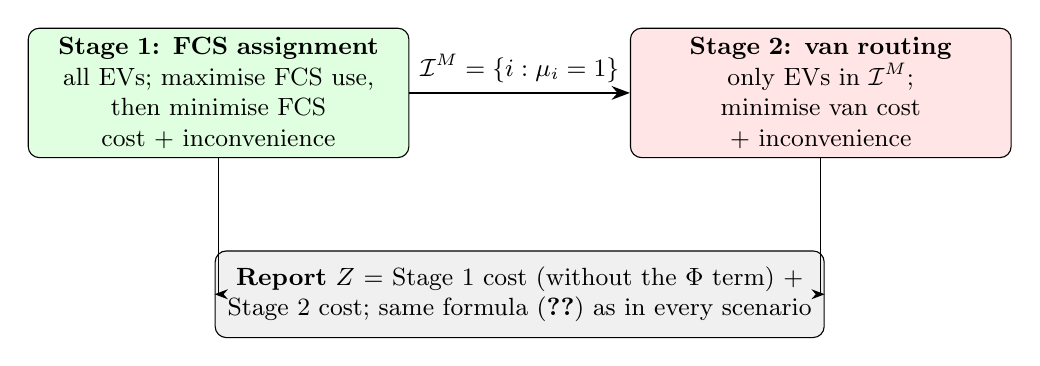
\begin{tikzpicture}[>=Stealth,box/.style={draw,rounded corners,align=center,minimum height=1.1cm,font=\small}]
  \node[box,fill=green!12,text width=4.6cm] (s1) {\textbf{Stage 1: FCS assignment}\\all EVs; maximise FCS use,\\then minimise FCS cost + inconvenience};
  \node[box,fill=red!10,text width=4.6cm,right=2.8cm of s1] (s2) {\textbf{Stage 2: van routing}\\only EVs in $\I^M$;\\minimise van cost + inconvenience};
  \draw[->,thick] (s1) -- node[above,font=\small]{$\I^M=\{i:\mu_i=1\}$} (s2);
  \node[box,fill=black!6,text width=7.5cm,below=2.0cm of $(s1)!0.5!(s2)$] (ev) {\textbf{Report} $Z=$ Stage~1 cost (without the $\Phi$ term) $+$ Stage~2 cost; same formula \eqref{eq:Z} as in every scenario};
  \draw[->] (s1) |- (ev); \draw[->] (s2) |- (ev);
\end{tikzpicture}
\end{center}

Stage~1 does not look at the vans, and Stage~2 cannot change what Stage~1 decided. That is the definition of ``FCS first, then MCS''.

%----------------------------------------------------------------
\subsection{Stage 1: assign EVs to fixed stations}

\textbf{Objective.}
\begin{equation}
\begin{split}
\min\ Z^{(1)}=\;&\underbrace{\Phi\sum_{i\in\I}\mu_i}_{\text{FCS first}}
+\underbrace{c^{EV}\sum_i\sum_{f\in\F_i}d_{if}Y_{if}}_{Z_1}
+\underbrace{Z^F_{\text{energy}}}_{\text{FCS part of }Z_4}\\
&+\underbrace{\sum_i\sum_{f\in\F_i}\rho^F_{if}Y_{if}+\alpha\sum_i w_i(C_i-r_i)+c^L\sum_i w_iL_i}_{\text{FCS customers' inconvenience}}
\end{split}
\label{eq:obj1}
\end{equation}
with $C_i=S_i+\tau^F_iY_i$ in this stage. $\Phi$ is a penalty for handing an EV to the vans. It is chosen larger than anything an extra FCS customer can add to the rest of \eqref{eq:obj1}, e.g.
\[
\Phi > \max_{i}\max_{f\in\F_i}\big(c^{EV}d_{if}+\pi^{\max}E_i+\rho^F_{if}\big)+n\,(\alpha+c^L)\,w_{\max}\,T,
\]
so Stage~1 first \textbf{maximises the number of EVs served at an FCS}, and only among those solutions minimises FCS cost and inconvenience. ($\pi^{\max}$ is the highest grid price.) A numerically safer equivalent is to solve twice: first $\max\sum_iY_i$, then fix that number and minimise the rest.
\ifTOU
Because $Z^F_{\text{energy}}$ uses the peak price, Stage~1 may \emph{start sessions later} to leave the peak, if the price saving beats the extra waiting cost (Section~\ref{sec:expect}).
\fi

\textbf{Constraints.}
\begin{align}
\sum_{g\in\G_i}y_{ig}+\mu_i &= 1 && \forall i\in\I \label{eq:s1assign}\\
S_i &\ge r_i+\sum_{f\in\F_i}t_{if}Y_{if} && \forall i\in\I \label{eq:fcsarr}\\
S_i &\le r_i+T\,(1-\mu_i) && \forall i\in\I \label{eq:s1park}\\
S_j &\ge S_i+\tau^F_i-(T+\tau^F_i)(3-y_{ig}-y_{jg}-o_{ij}) && \forall g,\ (i,j)\in\mathcal{P}_g \label{eq:disj1}\\
S_i &\ge S_j+\tau^F_j-(T+\tau^F_j)(2-y_{ig}-y_{jg}+o_{ij}) && \forall g,\ (i,j)\in\mathcal{P}_g \label{eq:disj2}\\
\sum_i y_{ig_1} &\ge \sum_i y_{ig_2} && \forall f,\ \G_f=\{g_1,g_2\} \label{eq:gunsym}\\
S_i+\tau^F_iY_i &\le T,\qquad L_i\ge S_i+\tau^F_iY_i-l_i && \forall i\in\I \label{eq:s1time}
\end{align}
\ifTOU plus the time-of-use split \eqref{eq:tou1}--\eqref{eq:tou5} of each FCS session (Section~\ref{sec:price}).\fi
\desc{\eqref{eq:s1assign}: every EV either gets one reachable gun or is handed to the vans. An EV that reaches no FCS ($\G_i=\emptyset$) is forced to $\mu_i=1$. \eqref{eq:fcsarr}: an FCS session cannot start before the EV has asked and driven to the station. \eqref{eq:s1park}: for an EV handed to the vans, $S_i$ is parked at $r_i$, so it adds no waiting in Stage~1 (its real start time is decided in Stage~2). \eqref{eq:disj1}--\eqref{eq:disj2}: two EVs on the same gun do not overlap; $o_{ij}$ picks who goes first. With two guns per station this means at most two EVs charge at a station at a time. \eqref{eq:gunsym}: symmetry breaking between the two identical guns (optional). \eqref{eq:s1time}: finished by $T$; lateness.}

\textbf{Optional acceptability rule.} An operator may refuse to send a driver to a station that is ``too inconvenient'', e.g.\ only allow gun $g$ of station $f$ for EV $i$ if $\hat\rho^F_{if}\le\bar\rho$. This only shrinks $\G_i$, so EVs whose stations are all too far go to the vans. Report results with and without it.

\textbf{Output:} $\I^M=\{i:\mu_i=1\}$, the EVs left for the vans; plus each FCS customer's gun and start time.

%----------------------------------------------------------------
\subsection{Stage 2: route the vans to the leftover EVs}

Stage~2 is a vehicle routing problem with time windows, on the EVs in $\I^M$ only. Here $C_i=S_i+\tau^M_i$.

\textbf{Objective.}
\begin{equation}
\begin{split}
\min\ Z^{(2)}=\;&\underbrace{c^M\sum_m\sum_{(i,j)\in\A^M}d_{ij}x_{ijm}}_{Z_2}+\underbrace{\sum_m c^D_mu_m}_{Z_3}+\underbrace{Z^M_{\text{energy}}}_{\text{van part of }Z_4}\\
&+\underbrace{\sum_{i\in\I^M}\sum_m\rho^M_{im}z_{im}+\alpha\sum_{i\in\I^M}w_i(C_i-r_i)+c^L\sum_{i\in\I^M}w_iL_i}_{\text{van customers' inconvenience}}
\end{split}
\label{eq:obj2}
\end{equation}
Since every EV in $\I^M$ must be served by some van, $Z^M_{\text{energy}}$ and the $\rho^M$ term are constants here. They are kept so that $Z^{(2)}$ is the true cost of Stage~2. Waiting and lateness make the vans visit urgent EVs early.

\textbf{Constraints.}
\begin{align}
\sum_{m\in\M}z_{im} &= 1 && \forall i\in\I^M \label{eq:s2assign}\\
\sum_{j:(0,j)\in\A^M}x_{0jm} = \sum_{i:(i,n+1)\in\A^M}x_{i,n+1,m} &= u_m && \forall m \label{eq:depot}\\
\sum_{i:(i,j)\in\A^M}x_{ijm} = \sum_{k:(j,k)\in\A^M}x_{jkm} &= z_{jm} && \forall j\in\I^M,\ m \label{eq:flow}\\
\sum_{i\in\I^M}z_{im} &\le Q_m\,u_m && \forall m \label{eq:cap}\\
\sum_{i\in\I^M}\frac{E_i}{\eta}z_{im}+\beta\sum_{(i,j)\in\A^M}d_{ij}x_{ijm} &\le B_m\,u_m && \forall m \label{eq:batt}
\end{align}
\begin{align}
S_j &\ge \max\{r_j,\ t_{0j}\,x_{0jm}\} && \forall j\in\I^M,\ m \label{eq:depart}\\
S_j &\ge S_i+\tau^M_i+t_{ij}-(T+\tau^M_i+t_{ij})(1-x_{ijm}) && \forall i\neq j,\ m \label{eq:seq}\\
S_i+\tau^M_i+t_{i,n+1} &\le T+(\tau^M_i+t_{i,n+1})(1-x_{i,n+1,m}) && \forall i,\ m \label{eq:return}\\
S_i+\tau^M_i \le T,\quad L_i &\ge S_i+\tau^M_i-l_i && \forall i\in\I^M \label{eq:s2time}\\
u_m &\ge u_{m+1} && m<|\M| \label{eq:vansym}
\end{align}
\desc{\eqref{eq:s2assign}: each leftover EV gets one van. \eqref{eq:depot}: a used van leaves and returns to the depot once. \eqref{eq:flow}: each EV on van $m$ is entered and left exactly once by that van. \eqref{eq:cap}: at most $Q_m$ EVs per van. \eqref{eq:batt}: delivered energy (with transfer losses) plus driving energy fits in the van battery. \eqref{eq:depart}: no start before the request, or before the van can drive there from the depot (written as two linear constraints). \eqref{eq:seq}: if the van goes $i\to j$, it finishes $i$ and drives to $j$ before starting $j$. This gives one EV at a time and removes subtours (MTZ-type). \eqref{eq:return}: back at the depot by $T$. \eqref{eq:s2time}: finished by $T$; lateness. \eqref{eq:vansym}: use identical vans in index order.}

\textbf{If Stage 2 is infeasible} (too many leftover EVs for the fleet by $T$), the sequential policy has \emph{failed} on that instance. For diagnosis, add $s_i\in\{0,1\}$ (``unserved''), replace \eqref{eq:s2assign} by $\sum_mz_{im}+s_i=1$ and add $\Phi^U\sum_is_i$ to \eqref{eq:obj2}. Then report the number of EVs that could not be served. This is a useful comparison with the integrated scenario, which may serve all of them.

%----------------------------------------------------------------
\subsection{Reported value}
\[
Z^{\text{S\scen}}=\big(Z^{(1)*}-\Phi\,|\I^M|\big)+Z^{(2)*},
\]
which is exactly \eqref{eq:Z} evaluated at the combined solution. The stage-1 solution plus the stage-2 solution is a feasible solution of the integrated model (S\ifTOU 4\else 3\fi), so
$Z^{\text{S\ifTOU 4\else 3\fi}}\le Z^{\text{S\scen}}$. The difference is the \emph{value of integration}.

\else
%---------------------------------------------------------------- INT
\subsection{Objective}
\begin{equation}
\min\ Z \quad\text{as in \eqref{eq:Z}, with }Z^F_{\text{energy}}=\ifTOU P^F\textstyle\sum_i\big[\pi^\off(\theta^1_i+\theta^3_i)+\pi^\pk\theta^2_i\big]\else\pi^F\textstyle\sum_iE_iY_i\fi,\quad C_i=S_i+\tau^F_iY_i+\tau^M_iZ_i. \label{eq:objint}
\end{equation}
Written out in full:
\begin{align*}
\min\ Z=\;& c^{EV}\sum_i\sum_{f\in\F_i}d_{if}Y_{if}+c^M\sum_m\sum_{(i,j)\in\A}d_{ij}x_{ijm}+\sum_mc^D_mu_m\\
&+\ifTOU P^F\sum_i\big[\pi^\off(\theta^1_i+\theta^3_i)+\pi^\pk\theta^2_i\big]\else\pi^F\sum_iE_iY_i\fi
+\pi^M\sum_i\sum_m\frac{E_i}{\eta}z_{im}\\
&+\sum_i\sum_{f\in\F_i}\rho^F_{if}Y_{if}+\sum_i\sum_m\rho^M_{im}z_{im}+\alpha\sum_iw_i(C_i-r_i)+c^L\sum_iw_iL_i .
\end{align*}
Every term is linear. One model weighs everything at once: an EV goes to a van exactly when the van's extra km, dispatch and energy cost are outweighed by the effort and waiting it saves the driver\ifTOU, or by the peak-price energy it avoids\fi.

\subsection{Constraints}

\textbf{Assignment.}
\begin{equation}
\sum_{g\in\G_i}y_{ig}+\sum_{m\in\M}z_{im}=1\qquad\forall i\in\I \label{eq:assign}
\end{equation}
\desc{Exactly one resource per EV: one reachable gun or one van. EVs that reach no FCS are forced onto a van.}

\textbf{Fixed stations.}
\begin{align}
S_i &\ge r_i+\sum_{f\in\F_i}t_{if}Y_{if} && \forall i \label{eq:fcsarr}\\
S_j &\ge S_i+\tau^F_i-(T+\tau^F_i)(3-y_{ig}-y_{jg}-o_{ij}) && \forall g,\ (i,j)\in\mathcal{P}_g \label{eq:disj1}\\
S_i &\ge S_j+\tau^F_j-(T+\tau^F_j)(2-y_{ig}-y_{jg}+o_{ij}) && \forall g,\ (i,j)\in\mathcal{P}_g \label{eq:disj2}\\
\sum_iy_{ig_1} &\ge \sum_iy_{ig_2} && \forall f,\ \G_f=\{g_1,g_2\} \label{eq:gunsym}
\end{align}
\desc{\eqref{eq:fcsarr}: an FCS session starts after the request and the drive to the station (for a van customer this is just $S_i\ge r_i$). \eqref{eq:disj1}--\eqref{eq:disj2}: EVs on the same gun do not overlap; $o_{ij}$ chooses the order. \eqref{eq:gunsym}: optional symmetry breaking.}

\textbf{Vans: routes, capacity, battery.}
\begin{align}
\sum_{j:(0,j)\in\A}x_{0jm}=\sum_{i:(i,n+1)\in\A}x_{i,n+1,m} &= u_m && \forall m \label{eq:depot}\\
\sum_{i:(i,j)\in\A}x_{ijm}=\sum_{k:(j,k)\in\A}x_{jkm} &= z_{jm} && \forall j\in\I,\ m \label{eq:flow}\\
\sum_iz_{im} &\le Q_mu_m && \forall m \label{eq:cap}\\
\sum_i\frac{E_i}{\eta}z_{im}+\beta\sum_{(i,j)\in\A}d_{ij}x_{ijm} &\le B_mu_m && \forall m \label{eq:batt}
\end{align}
\desc{\eqref{eq:depot}: a used van leaves and returns once. \eqref{eq:flow}: each EV on van $m$ is visited exactly once by it. \eqref{eq:cap}: at most $Q_m$ EVs. \eqref{eq:batt}: delivered energy (with losses) plus driving energy fits in the battery.}

\textbf{Vans: timing (one EV at a time, no subtours).}
\begin{align}
S_j &\ge t_{0j}\,x_{0jm} && \forall j\in\I,\ m \label{eq:depart}\\
S_j &\ge S_i+\tau^M_i+t_{ij}-(T+\tau^M_i+t_{ij})(1-x_{ijm}) && \forall i\neq j\in\I,\ m \label{eq:seq}\\
S_i+\tau^M_i+t_{i,n+1} &\le T+(\tau^M_i+t_{i,n+1})(1-x_{i,n+1,m}) && \forall i,\ m \label{eq:return}
\end{align}
\desc{\eqref{eq:depart}: the first stop cannot start before the van has driven there. \eqref{eq:seq}: $i\to j$ means finish $i$, drive, then start $j$; start times rise along a route, so no subtour can close. \eqref{eq:return}: back at the depot by $T$.}

\textbf{Horizon and lateness.}
\begin{equation}
C_i\le T,\qquad L_i\ge C_i-l_i\qquad\forall i\in\I \label{eq:time}
\end{equation}
\desc{Every EV is fully charged within the horizon; $L_i$ measures lateness.}

\ifTOU
\textbf{Time-of-use split.} Constraints \eqref{eq:tou1}--\eqref{eq:tou5} of Section~\ref{sec:price}.
\fi

\textbf{Symmetry and domains.}
\begin{equation}
u_m\ge u_{m+1};\qquad y,z,x,u,o\ifTOU,\kappa\fi\in\{0,1\};\qquad S_i,L_i\ifTOU,\theta^p_i\fi\ge0 \label{eq:dom}
\end{equation}
\fi

%=====================================================================
\section{Learning-to-optimise (RL) formulation}\label{sec:rl}

\textbf{Main rule:} the reward of each action is \emph{minus the increase in $Z$ that the action causes}. The rewards over an episode then add up to $-Z$ of the solution the policy builds. RL and MILP results are measured on the same yardstick \eqref{eq:Z}, and the MILP optimum is the benchmark for the RL gap.

\ifSEQ
%---------------------------------------------------------------- RL SEQ
The RL pipeline has the same two stages as the MILP.

\subsection{Stage 1 policy: FCS assignment}
\begin{itemize}[leftmargin=1.4em,itemsep=2pt]
  \item \textbf{Episode / epochs:} EVs are taken in order of request time $r_i$ (ties: higher $w_i$ first). One decision per EV.
  \item \textbf{State:} features of the current EV $k$ ($E_k,r_k,l_k,w_k,R_k$, location); for each gun $g$ the time $F_g$ it becomes free; summary features of the EVs still to come (count and positions near each station)\ifTOU; the current price and the time until $T_1$ and $T_2$\fi.
  \item \textbf{Action:} a gun $g\in\G_k$, or ``hand to vans''. \textbf{FCS-first mask:} ``hand to vans'' is allowed \emph{only} if no gun can finish EV $k$ by $T$ (or, with the optional rule, if all remaining guns have $\hat\rho^F_{kf}>\bar\rho$).
  \ifTOU\item \textbf{Optional timing action:} ``gun $g$, start after the peak'', i.e.\ $S_k=\max\{\text{earliest},T_2\}$, allowed only if the session still ends by $T$.\fi
  \item \textbf{Transition:} $S_k=\max\{r_k+t_{kf},F_g\}$ (or later, for the timing action); $F_g\leftarrow S_k+\tau^F_k$.
  \item \textbf{Reward:} $-\Big[c^{EV}d_{kf}+\text{energy}_k+\rho^F_{kf}+\alpha w_k(S_k+\tau^F_k-r_k)+c^Lw_k(S_k+\tau^F_k-l_k)^+\Big]$, where energy$_k$ = \ifTOU$P^F\big[\pi^\off\cdot(\text{off-peak hours of }[S_k,S_k+\tau^F_k])+\pi^\pk\cdot(\text{peak hours})\big]$, computed exactly in the simulator\else$\pi^FE_k$\fi. Handing an EV to the vans gives reward $0$ here; its cost is counted in Stage~2.
\end{itemize}
Note: a simple baseline for Stage~1 is the greedy rule ``gun with the largest one-step reward''. What RL can learn on top of this is, for example, to keep a nearby gun free for an urgent EV that arrives later.

\subsection{Stage 2 policy: van routing over $\I^M$}
\begin{itemize}[leftmargin=1.4em,itemsep=2pt]
  \item \textbf{Epochs:} whenever a van becomes free (the earliest-free van decides first).
  \item \textbf{State:} for each van: position, time free, remaining battery $b_m$, EVs served so far, dispatched or not; for each unserved EV in $\I^M$: location, $E_i,r_i,l_i,w_i$; current time.
  \item \textbf{Action:} the next EV $j$ for this van, or ``return to depot'' (ends the route). Mask: $j$ must be feasible: battery covers $E_j/\eta$ plus driving to $j$ and back to the depot, the count stays $\le Q_m$, and $j$ can be finished with the van back at the depot by $T$.
  \item \textbf{Transition:} $S_j=\max\{r_j,\ \text{time free}+t_{\text{pos},j}\}$; the van moves to $j$ and is free at $S_j+\tau^M_j$; $b_m$ falls by $E_j/\eta+\beta d_{\text{pos},j}$.
  \item \textbf{Reward:} serving $j$: $-\Big[c^Md_{\text{pos},j}+c^D_m[\text{first stop}]+\pi^M\frac{E_j}{\eta}+\rho^M_{jm}+\alpha w_j(S_j+\tau^M_j-r_j)+c^Lw_j(S_j+\tau^M_j-l_j)^+\Big]$; returning: $-c^Md_{\text{pos},0}$. EVs still unserved at the end: $-\Phi^U$ each.
  \item \textbf{Policy:} an attention-based routing policy (e.g.\ Kool et al., 2019, ``Attention, Learn to Solve Routing Problems!'') trained with REINFORCE or PPO. Baseline: nearest-feasible-EV heuristic.
\end{itemize}
Episode return of Stage~1 + Stage~2 $=-Z^{\text{S\scen}}$.

\else
%---------------------------------------------------------------- RL INT
One policy decides both who serves each EV and the van routes.
\begin{itemize}[leftmargin=1.4em,itemsep=2pt]
  \item \textbf{Episode / epochs:} EVs are taken in order of request time $r_i$ (ties: higher $w_i$ first). One decision per EV.
  \item \textbf{State:} (i) the current EV $k$: location, $E_k,r_k,l_k,w_k,R_k$, reachable stations; (ii) each gun $g$: time $F_g$ it becomes free; (iii) each van $m$: current end-of-route position, time free, remaining battery $b_m$, EVs served, dispatched or not; (iv) embeddings of the not-yet-assigned EVs (for look-ahead)\ifTOU; (v) current price, time until $T_1$ and $T_2$\fi.
  \item \textbf{Action:} $a\in\G_k\cup\M$: a gun, or a van (EV $k$ is appended to the end of that van's route). \textbf{Mask} infeasible actions: a gun that cannot finish $k$ by $T$; a van without enough battery for $E_k/\eta$ plus the drive to $k$ and back to the depot, with $Q_m$ reached, or unable to finish $k$ and return by $T$.
  \ifTOU\item \textbf{Optional timing action:} ``gun $g$, start after the peak'' ($S_k=\max\{\text{earliest},T_2\}$, if it still ends by $T$).\fi
  \item \textbf{Transition:} gun: $S_k=\max\{r_k+t_{kf},F_g\}$, $F_g\leftarrow S_k+\tau^F_k$. Van: $S_k=\max\{r_k,\ \text{free}_m+t_{\text{pos}_m,k}\}$, then the van moves to $k$, $\text{free}_m\leftarrow S_k+\tau^M_k$, $b_m\mathrel{-}=E_k/\eta+\beta d_{\text{pos}_m,k}$.
  \item \textbf{Reward} $=-\Delta Z$:
  \begin{align*}
  \text{gun } g\text{ at }f:&\quad -\Big[c^{EV}d_{kf}+\text{energy}^F_k+\rho^F_{kf}+\alpha w_k(C_k-r_k)+c^Lw_k(C_k-l_k)^+\Big]\\
  \text{van } m:&\quad -\Big[c^M\big(d_{\text{pos}_m,k}+d_{k,0}-d_{\text{pos}_m,0}\big)+c^D_m[\text{first use}]+\pi^M\tfrac{E_k}{\eta}\\
  &\qquad\quad+\rho^M_{km}+\alpha w_k(C_k-r_k)+c^Lw_k(C_k-l_k)^+\Big]
  \end{align*}
  The van distance term is the \emph{change} in route length when $k$ is inserted before the return to the depot, so the sum over the episode equals the total route length (the return legs telescope). energy$^F_k$ = \ifTOU$P^F\big[\pi^\off\cdot(\text{off-peak hours})+\pi^\pk\cdot(\text{peak hours of }[S_k,C_k])\big]$, computed exactly by the simulator; no linearisation is needed in RL\else$\pi^FE_k$\fi.
  \item \textbf{Dead end:} if every action is masked, EV $k$ is unserved: reward $-\Phi^U$, and the episode continues. Report the count.
  \item \textbf{Policy:} masked categorical policy over guns and vans, encoder with attention over EVs, guns and vans; trained with PPO. Natural baseline: greedy, i.e.\ choose the action with the largest one-step reward. That is the pairwise rule ``smallest $\hat\rho$ + cost'' from Section~\ref{sec:inc}.
\end{itemize}
Restriction to note: vans serve EVs in assignment order (append only). A variant that inserts $k$ at the cheapest position of a route is more flexible but has a larger action space.
\fi

\textbf{Reward scaling.} For stable training divide every reward by a constant, e.g.\ the greedy baseline's average $Z$ on the training instances. This does not change the optimal policy.

%=====================================================================
\section{What to expect and what to report}\label{sec:expect}

\ifnum\scen=1
\begin{itemize}[leftmargin=1.4em,itemsep=2pt]
  \item Vans serve only EVs that reach no station, or that the stations cannot finish by $T$. If stations have spare capacity, very few vans are dispatched.
  \item Inconvenience is high for EVs far from the nearest station (worked example: Rs\,682 at the FCS, against Rs\,458 if a van had been allowed).
  \item With too few vans Stage~2 becomes infeasible (unserved EVs), even when the integrated model S3 could serve everyone. Report the smallest $|\M|$ at which S1 is feasible and compare it with S3.
\end{itemize}
\fi
\ifnum\scen=2
\begin{itemize}[leftmargin=1.4em,itemsep=2pt]
  \item \textbf{When does Stage~1 delay a session to avoid the peak?} Moving one hour of charging out of the peak saves $(\pi^\pk-\pi^\off)P^F=3\times22=$ Rs\,66, but delays completion by up to an hour, which costs $\alpha w_i\ge$ Rs\,200. So with the default values Stage~1 almost never delays. It mostly pays the higher price, and S2 costs roughly S1 plus the peak surcharge. Sessions start later only if $\alpha$ is small (try $\lambda<0.33$ in the sensitivity analysis).
  \item The van assignment is the same as in S1 unless Stage~1's timing changes which EVs fit at the stations. Stage~1 cannot use vans to escape the peak price.
  \item Extra KPI: \textbf{grid energy drawn at FCS during the peak}, $P^F\sum_i\theta^2_i$ (kWh). Compare with S4.
\end{itemize}
\fi
\ifnum\scen=3
\begin{itemize}[leftmargin=1.4em,itemsep=2pt]
  \item Vans take EVs for which the saved inconvenience exceeds the extra van cost (worked example: van chosen, saving Rs\,224). Expect vans to serve EVs that are far from every station, have low range (high $w_i$), or have early deadlines, while EVs near a station still use it.
  \item \textbf{Value of integration under flat price:} $Z^{\text{S1}}-Z^{\text{S3}}\ge0$. Report it per component ($Z_1,\dots,Z_5$): typically operating cost rises a little and inconvenience falls a lot.
  \item Vary $|\M|$ (0, 1, 2, \dots): the first few vans lower $Z$ sharply, then the effect levels off. That curve shows the scenarios where mobile chargers help most.
\end{itemize}
\fi
\ifnum\scen=4
\begin{itemize}[leftmargin=1.4em,itemsep=2pt]
  \item During the peak a van kWh costs about the same as an FCS kWh (Rs\,10.0 each), so the vans' energy disadvantage disappears and vans also absorb \emph{peak-hour} demand that would otherwise be charged on the grid at peak price.
  \item Expect more van usage than in S3, concentrated on requests in $[T_1,T_2]$, and lower grid energy at the stations during the peak, $P^F\sum_i\theta^2_i$, than in S2.
  \item \textbf{Value of integration under peak pricing:} $Z^{\text{S2}}-Z^{\text{S4}}$. It should be larger than $Z^{\text{S1}}-Z^{\text{S3}}$, because integration now also allows price arbitrage.
  \item \textbf{Peak pricing with full flexibility:} $Z^{\text{S4}}-Z^{\text{S3}}$ should be smaller than $Z^{\text{S2}}-Z^{\text{S1}}$: vans cushion the price increase.
\end{itemize}
\fi

\textbf{Cross-scenario comparison table} (fill in from the four runs):
\begin{center}
\renewcommand{\arraystretch}{1.2}
\begin{tabular}{@{}lll@{}}
\toprule
\textbf{Comparison} & \textbf{Measures} & \textbf{Expected sign} \\
\midrule
S1 $-$ S3 & value of integration, flat price & $\ge0$ \\
S2 $-$ S4 & value of integration, peak price & $\ge0$, larger than S1 $-$ S3 \\
S2 $-$ S1 & cost of peak pricing, FCS-first operator & $>0$ \\
S4 $-$ S3 & cost of peak pricing, flexible operator & $>0$, smaller than S2 $-$ S1 \\
\bottomrule
\end{tabular}
\end{center}
Report for each: $Z$ and its components, number of vans used, EVs per resource, mean and maximum inconvenience per EV, total lateness, peak-hour grid energy, solve time, and (for RL) the gap to the MILP optimum.

%=====================================================================
\appendix
\section{Illustrative parameter values}\label{app:values}

These are starting values for experiments, not data. All are meant to be varied in the analysis. Values in Rs.

\begin{center}
\renewcommand{\arraystretch}{1.15}
\begin{tabular}{@{}llp{6.2cm}@{}}
\toprule
\textbf{Parameter} & \textbf{Value} & \textbf{Note} \\
\midrule
$T$, $[T_1,T_2]$ & 7 h, $[2,6]$ & 16:00--23:00, peak 18:00--22:00 \\
$P^F$, $P^M$ & 22 kW, 30 kW & \\
$v$, $\beta$, $\eta$ & 25 km/h, 0.25 kWh/km, 0.9 & \\
$B_m$, $Q_m$, $|\M|$ & 150 kWh, 6, 2--6 & \\
$c^{EV}$, $c^M$, $c^D_m$ & Rs\,4/km, Rs\,15/km, Rs\,1500 & van km includes driver time \\
$\pi^F$ (flat) & Rs\,8.7/kWh & equals the time-average of the ToU tariff over $[0,T]$ \\
$\pi^\off$, $\pi^\pk$ (ToU) & Rs\,7/kWh, Rs\,10/kWh & $(3\times7+4\times10)/7=8.7$ \\
$c^{bat}$ & Rs\,2/kWh & van battery wear \\
$\pi^M$ & Rs\,10.7 (flat) / Rs\,9.0 (ToU) & $=\pi^F+c^{bat}$ / $=\pi^\off+c^{bat}$ \\
$\alpha$, $\alpha^D$ & Rs\,200/h, Rs\,100/h & value of time; extra for attended time \\
$h^F$, $h^M$, $\varphi$ & Rs\,50, Rs\,10, Rs\,100 & trip hassle, hand-over, range stress \\
$c^L$ & Rs\,300/h & lateness \\
$w_i$ & $1+2(1-R_i/R_{\max})$, $R_i\sim U[3,40]$ km & priority from remaining range \\
\bottomrule
\end{tabular}
\end{center}

The flat price is set to the time-average of the peak tariff. The price \emph{level} is then the same in both pricing cases, and only the price \emph{shape} differs. Without this, part of S1 vs S2 would just reflect a different average price.

\end{document}
"
%    pdflatex -jobname=scenario2_peak_sequential   "\def\scen{2}% =====================================================================
%  One source, four PDFs.  Build with build.sh (or by hand):
%    pdflatex -jobname=scenario1_flat_sequential   "\def\scen{1}\input{scenario_master}"
%    pdflatex -jobname=scenario2_peak_sequential   "\def\scen{2}\input{scenario_master}"
%    pdflatex -jobname=scenario3_flat_integrated   "\def\scen{3}\input{scenario_master}"
%    pdflatex -jobname=scenario4_peak_integrated   "\def\scen{4}\input{scenario_master}"
%  (run each twice for cross-references)
% =====================================================================
\documentclass[11pt,a4paper]{article}
\usepackage[margin=2.2cm]{geometry}
\usepackage{amsmath,amssymb,amsfonts}
\usepackage{booktabs,array,tabularx}
\usepackage{enumitem}
\usepackage[table]{xcolor}
\usepackage{tikz}
\usetikzlibrary{arrows.meta,positioning,calc}
\usepackage[colorlinks=true,linkcolor=blue!50!black,urlcolor=blue!50!black]{hyperref}
\usepackage{titlesec}
\titleformat{\section}{\large\bfseries}{\thesection}{0.8em}{}
\titleformat{\subsection}{\normalsize\bfseries}{\thesubsection}{0.8em}{}
\setlength{\parindent}{0pt}
\setlength{\parskip}{5pt}

% ---------------- scenario switches ----------------
\ifdefined\scen\else\def\scen{1}\fi
\newif\ifTOU \TOUfalse   % true = time-of-use (peak) price
\newif\ifSEQ \SEQfalse   % true = FCS first, then MCS
\ifnum\scen=1 \SEQtrue \fi
\ifnum\scen=2 \TOUtrue \SEQtrue \fi
\ifnum\scen=4 \TOUtrue \fi

\newcommand{\pricename}{\ifTOU time-of-use price (dearer evening peak)\else single (flat) price all day\fi}
\newcommand{\structname}{\ifSEQ FCS first, then MCS (sequential)\else FCS and MCS together (integrated)\fi}

% ---------------- notation ----------------
\newcommand{\I}{\mathcal{I}}
\newcommand{\F}{\mathcal{F}}
\newcommand{\G}{\mathcal{G}}
\newcommand{\M}{\mathcal{M}}
\newcommand{\N}{\mathcal{N}}
\newcommand{\A}{\mathcal{A}}
\newcommand{\Rs}{\text{Rs}\,}
\newcommand{\pk}{\mathrm{pk}}
\newcommand{\off}{\mathrm{off}}
\newcommand{\desc}[1]{\par\vspace{-2pt}{\small\color{black!75}\textit{Meaning:} #1}\par\vspace{4pt}}
\newcommand{\cell}[2]{\ifnum\scen=#1\cellcolor{blue!18}\textbf{S#1 (this document)}\\\textbf{#2}\else S#1\\#2\fi}

\title{\textbf{EV Charging Network Optimisation}\\[4pt]
\large Scenario \scen: \pricename\ $+$ \structname\\[2pt]
\normalsize MILP and RL formulation}
\author{CP 320 OR for Mobility Management, course project}
\date{2 October 2026}

\begin{document}
\maketitle

%=====================================================================
\section{Where this scenario sits}

The project studies four scenarios: two ways of pricing grid electricity, times two ways of making the decisions.

\begin{center}
\renewcommand{\arraystretch}{1.5}
\begin{tabular}{>{\raggedright\arraybackslash}p{4.2cm}|>{\centering\arraybackslash}p{4.6cm}|>{\centering\arraybackslash}p{4.6cm}}
 & \textbf{Flat price all day} & \textbf{Time-of-use (peak) price} \\ \hline
\textbf{Sequential:} FCS first, leftover EVs to MCS &
\begin{tabular}[c]{@{}c@{}}\cell{1}{flat + sequential}\end{tabular} &
\begin{tabular}[c]{@{}c@{}}\cell{2}{peak + sequential}\end{tabular} \\ \hline
\textbf{Integrated:} FCS and MCS decided together &
\begin{tabular}[c]{@{}c@{}}\cell{3}{flat + integrated}\end{tabular} &
\begin{tabular}[c]{@{}c@{}}\cell{4}{peak + integrated}\end{tabular} \\
\end{tabular}
\end{center}

\textbf{The four scenarios do not have four different objectives.} They share \emph{one} cost yardstick $Z$ (Section~\ref{sec:obj}): the same cost terms and the same customer inconvenience (Section~\ref{sec:inc}). Only two things change:
\begin{itemize}[leftmargin=1.4em,itemsep=1pt]
  \item \textbf{Pricing} changes the formula for one term, the FCS energy cost (Section~\ref{sec:price}).
  \item \textbf{Decision structure} changes \emph{how} $Z$ is minimised: in one model (integrated), or in two stages (sequential), where each stage minimises its own part of $Z$.
\end{itemize}
Because the yardstick is the same, the four optimal values can be compared directly. The differences measure the \emph{value of integration} (S1$\to$S3, S2$\to$S4) and the \emph{effect of peak pricing} (S1$\to$S2, S3$\to$S4).

\ifnum\scen=1
\textbf{This scenario (S1)} is the baseline, the ``status quo''. Electricity costs the same at every hour, every EV that can be charged at a fixed station is sent there, and vans only take what is left over.
\fi
\ifnum\scen=2
\textbf{This scenario (S2)} keeps the FCS-first rule of S1, but grid electricity is dearer during the evening peak. Stage~1 can react to the price only by \emph{rescheduling} FCS sessions. It cannot hand a peak-hour EV to a van.
\fi
\ifnum\scen=3
\textbf{This scenario (S3)} keeps the flat price of S1, but the operator decides FCS and MCS service \emph{together}. An EV can be sent to a van even when a fixed station could take it, whenever that lowers total cost plus inconvenience.
\fi
\ifnum\scen=4
\textbf{This scenario (S4)} is the most flexible one: peak pricing at fixed stations, and FCS and MCS decided together. Van energy was bought off-peak, so vans can also be used to keep charging \emph{out of the expensive peak}.
\fi

%=====================================================================
\section{Setting and assumptions}\label{sec:setting}

\textbf{Time.} The planning horizon is $[0,T]$ with $T=7$\,h (16:00--23:00). It contains the evening peak window $[T_1,T_2]=[2,6]$ (18:00--22:00). The horizon is the same in all four scenarios. It is wider than the peak itself so that, under peak pricing, there is cheaper time on both sides of the peak.\ifTOU\else\ In this scenario the price is flat, so the window plays no role in the model.\fi

\textbf{Assumptions} (the same as MILP v3, plus two about energy):
\begin{enumerate}[leftmargin=1.6em,itemsep=1pt]
  \item Static, continuous time. All requests in the horizon are known at time $0$, and request $i$ becomes active at $r_i$.
  \item An EV served by an FCS drives there itself on its own battery (only to stations within its range $R_i$). The driver stays with the car while it waits for a free gun and while it charges.
  \item An EV served by an MCS stays parked where it is, and the driver is free in the meantime.
  \item Each FCS gun and each van charges one EV at a time, without interruption, at constant power.
  \item A van's battery covers both its driving and the energy it delivers. \textbf{The van battery is charged at the depot before the horizon starts}\ifTOU, i.e.\ at the off-peak price\fi, and is not recharged during the horizon.
  \item Every EV must be fully charged by $T$ (hard). Finishing after the driver's desired time $l_i$ is allowed but penalised.
\end{enumerate}

%=====================================================================
\section{Notation}\label{sec:notation}

\subsection*{Sets}
\begin{tabularx}{\textwidth}{@{}lX@{}}
\toprule
$\I=\{1,\dots,n\}$ & EV charging requests \\
$\F$; $\G_f$ ($|\G_f|=2$); $\G=\bigcup_f\G_f$ & fixed charging stations; guns of FCS $f$; all guns ($f(g)$ = station of gun $g$) \\
$\F_i=\{f: d_{if}\le R_i\}$, $\G_i=\bigcup_{f\in\F_i}\G_f$ & stations / guns EV $i$ can reach on its remaining range \\
$\M$ & mobile charging vans (MCS) \\
$0,\ n+1$ & depot as start node / end node (same place) \\
$\N=\{0\}\cup\I\cup\{n+1\}$, $\A$ & routing nodes; allowed van arcs $(i,j)$, $i\in\{0\}\cup\I$, $j\in\I\cup\{n+1\}$, $i\neq j$ \\
$\mathcal{P}_g=\{(i,j): i<j,\ g\in\G_i\cap\G_j\}$ & pairs of EVs that could share gun $g$ \\
\ifSEQ
$\I^M\subseteq\I$ & EVs handed to the vans by Stage~1 (an \emph{output} of Stage~1, a fixed input to Stage~2) \\
$\N^M$, $\A^M$ & routing nodes / arcs restricted to $\I^M$ \\
\fi
\bottomrule
\end{tabularx}

\subsection*{Parameters}
\begin{tabularx}{\textwidth}{@{}lX@{}}
\toprule
$E_i,\ r_i,\ l_i,\ R_i$ & energy demand (kWh), request time, desired completion time (h), remaining range (km) \\
$w_i\ge1$ & priority of EV $i$; $w_i=1+\kappa(1-R_i/R_{\max})$, so low-range EVs weigh more \\
$P^F,\ P^M$ & charging power of an FCS gun (22\,kW) / of a van (e.g.\ 30\,kW) \\
$\tau^F_i=E_i/P^F,\ \tau^M_i=E_i/P^M$ & charging time of EV $i$ at an FCS / by a van (h) \\
$d_{if},t_{if}$;\ $d_{ij},t_{ij}$ & distance (km) and time (h): EV$\to$FCS; between routing nodes ($t=d/v$) \\
$B_m,\ Q_m,\ \beta,\ \eta$ & van battery (kWh), max EVs per van, van consumption (kWh/km), transfer efficiency \\
$c^{EV},\ c^M,\ c^D_m$ & cost per km of EV driving, per km of van driving; fixed dispatch cost of van $m$ \\
\ifTOU
$\pi^\off,\ \pi^\pk$ & grid price (Rs/kWh) off-peak / in $[T_1,T_2]$, with $\pi^\pk\ge\pi^\off$ \\
\else
$\pi^F$ & grid price (Rs/kWh), the same at every hour \\
\fi
$c^{bat}$ & van battery wear per kWh cycled \\
$\pi^M$ & cost of 1 kWh taken from a van battery: $\pi^M=\ifTOU\pi^\off\else\pi^F\fi+c^{bat}$ (Section~\ref{sec:price}) \\
$\alpha,\ \alpha^D,\ h^F,\ h^M,\ \varphi,\ c^L$ & inconvenience coefficients (Section~\ref{sec:inc}) \\
\bottomrule
\end{tabularx}

\subsection*{Decision variables}
\begin{tabularx}{\textwidth}{@{}llX@{}}
\toprule
$y_{ig}$ & $\{0,1\}$ & EV $i$ charged at gun $g\in\G_i$ \\
$z_{im}$ & $\{0,1\}$ & EV $i$ served by van $m$ \\
$x_{ijm}$ & $\{0,1\}$ & van $m$ drives arc $(i,j)$ \\
$u_m$ & $\{0,1\}$ & van $m$ is dispatched \\
$o_{ij}$ & $\{0,1\}$ & for EVs $i<j$ that could share a gun: 1 if $i$ is charged before $j$ \\
\ifSEQ
$\mu_i$ & $\{0,1\}$ & Stage~1 only: EV $i$ is handed to the van fleet \\
\fi
\ifTOU
$\theta^1_i,\theta^2_i,\theta^3_i$ & $\ge0$ & hours of EV $i$'s FCS session before / inside / after the peak \\
$\kappa^1_i,\kappa^3_i$ & $\{0,1\}$ & EV $i$'s FCS session starts before $T_1$ / ends after $T_2$ \\
\fi
$S_i$ & $\ge0$ & time charging of EV $i$ starts (h), on whichever resource \\
$L_i$ & $\ge0$ & lateness of EV $i$ beyond $l_i$ (h) \\
\bottomrule
\end{tabularx}

\textbf{Short-hands} (linear expressions, not new variables):
\[
Y_{if}=\sum_{g\in\G_f}y_{ig},\qquad Y_i=\sum_{g\in\G_i}y_{ig}\ (\text{EV $i$ uses an FCS}),\qquad Z_i=\sum_{m\in\M}z_{im}\ (\text{EV $i$ uses a van}),
\]
\[
C_i=S_i+\tau^F_i\,Y_i+\tau^M_i\,Z_i \quad\text{(time EV $i$ is fully charged).}
\]

%=====================================================================
\section{Customer inconvenience}\label{sec:inc}

This section is \textbf{identical in all four scenario documents}. Inconvenience is a property of the customer, not of the price or of the planning method.

\subsection{What we mean by inconvenience}

Inconvenience is \emph{what the driver loses} from the moment they ask for a charge ($r_i$) until the car is fully charged ($C_i$), \emph{converted into rupees} so it can be added to the operator's costs. A driver loses three different things:

\begin{enumerate}[leftmargin=1.6em,itemsep=2pt]
  \item \textbf{Waiting:} the car is not ready. This lasts $C_i-r_i$ hours and affects \emph{every} driver, FCS or MCS.
  \item \textbf{Effort:} only an FCS customer has to drive to the station and sit there while the car charges. An MCS customer stays at home or at work and does something else. Driving to a far station also uses scarce battery range, which causes stress (``range anxiety'').
  \item \textbf{A missed deadline:} the car is still not ready at the time $l_i$ the driver needs it.
\end{enumerate}

Each loss gets a price in Rs per hour (or per event). All of them are multiplied by the priority $w_i$: an hour of delay for an EV with 5\,km of range left counts more than for one with 40\,km.

\subsection{The three components}

\begin{center}
\renewcommand{\arraystretch}{1.3}
\begin{tabularx}{\textwidth}{@{}>{\raggedright\arraybackslash}p{2.6cm}>{\raggedright\arraybackslash}X>{\raggedright\arraybackslash}X>{\raggedright\arraybackslash}p{3.0cm}@{}}
\toprule
\textbf{Component} & \textbf{EV $i$ at FCS $f$} & \textbf{EV $i$ by a van} & \textbf{Known when?} \\
\midrule
Effort & $w_i\big[\alpha^D(t_{if}+\tau^F_i)+h^F+\varphi\,d_{if}/R_i\big]$: driving and sitting at the station, a fixed trip hassle, range stress & $w_i\,h^M$: being reachable and handing over the car & \textbf{Static:} known as soon as the resource is chosen \\
Waiting & $w_i\,\alpha\,(C_i-r_i)$ = drive + \emph{queue at the gun} + charge & $w_i\,\alpha\,(C_i-r_i)$ = \emph{wait for the van} + charge & \textbf{Dynamic:} depends on the queue / van route \\
Missed deadline & $w_i\,c^L\,L_i$, $L_i=\max\{0,C_i-l_i\}$ & same & Dynamic \\
\bottomrule
\end{tabularx}
\end{center}

\textbf{Coefficients.}
$\alpha$ (Rs/h) is the value of an hour the car is not ready.
$\alpha^D$ (Rs/h) is the \emph{extra} value of an hour the driver must personally spend driving or sitting at the station: an hour at the station costs $\alpha+\alpha^D$, an hour waiting at home for a van costs only $\alpha$.
$h^F,h^M$ (Rs) are fixed hassle costs of one trip to a station / one van hand-over.
$\varphi$ (Rs) is the range-stress cost of a trip that uses the \emph{whole} remaining range ($d_{if}/R_i\le1$ is the fraction used).
$c^L$ (Rs/h) is the cost per hour late.

\subsection{Pairwise form: inconvenience of a (customer, resource) pair}

The natural first idea is: \emph{for every pair (EV $i$, FCS $f$) and every pair (EV $i$, van $m$) there is an inconvenience number, and the operator picks the pair with the lowest cost plus inconvenience.} The static part fits this idea exactly:
\[
\boxed{\;\rho^F_{if}=w_i\Big[\alpha^D\,(t_{if}+\tau^F_i)+h^F+\varphi\,\frac{d_{if}}{R_i}\Big]\qquad
\rho^M_{im}=w_i\,h^M\;}
\]
These are \textbf{parameters}, computed before solving, one number per (EV, FCS) pair and per (EV, van) pair. In the objective they appear linearly: $\sum_i\sum_f\rho^F_{if}Y_{if}+\sum_i\sum_m\rho^M_{im}z_{im}$.

Note that $\rho^M_{im}$ does not depend on $m$. Vans are identical and all start at the same depot, so the driver does not care \emph{which} van comes, only \emph{when} it comes. That ``when'' is the waiting part.

\subsection{Why waiting cannot be a fixed pairwise number}

It is tempting to also write the waiting as a pairwise number, e.g.\ ``the van needs 5 minutes to reach EV $i$''. But that depends on \emph{where the van is coming from}, which depends on the route the model is still choosing: if EV $i$ is the 4th stop of a van, the wait is the time for three charging sessions plus four drives. Likewise, waiting at an FCS depends on how many EVs are queued at that gun. So waiting is not known before solving. It is a function of decision variables:
\[
\text{waiting cost of EV } i \;=\; w_i\,\alpha\,(C_i-r_i),\qquad C_i=S_i+\tau^F_iY_i+\tau^M_iZ_i .
\]
This is \textbf{linear} in the variables ($S_i$, $y$, $z$), so it fits in a MILP directly. The constraints of Section~\ref{sec:milp} make $S_i$ equal to the true start time, including driving, queueing at the gun and the van's route. The term $\sum_i w_i\alpha r_i$ is a constant and may be dropped when solving.

\textbf{Pairwise \emph{estimate}} (used for intuition, by the RL policy and in heuristics): if there is no queue and the van comes straight to $i$,
\[
\hat\rho^{F}_{if}=\rho^F_{if}+w_i\alpha\,(t_{if}+\tau^F_i),\qquad
\hat\rho^{M}_{im}=\rho^M_{im}+w_i\alpha\,(t^{\text{van}}_{m\to i}+\tau^M_i),
\]
where $t^{\text{van}}_{m\to i}$ is the time until van $m$ can reach $i$ from where it currently is. In the RL formulation (Section~\ref{sec:rl}) the van's position \emph{is} known at each decision, so there this estimate becomes exact.

\subsection{Total inconvenience and how it enters the objective}

\begin{equation}
\boxed{\;
Z_{\text{inc}}=\underbrace{\sum_{i\in\I}\sum_{f\in\F_i}\rho^F_{if}Y_{if}+\sum_{i\in\I}\sum_{m\in\M}\rho^M_{im}z_{im}}_{\text{effort (static, pairwise)}}
+\underbrace{\alpha\sum_{i\in\I}w_i\,(C_i-r_i)}_{\text{waiting (dynamic)}}
+\underbrace{c^L\sum_{i\in\I}w_i\,L_i}_{\text{missed deadline}}
\;}\label{eq:inc}
\end{equation}
All three parts are in rupees, so $Z_{\text{inc}}$ is simply added to the operating costs. Nothing has to be normalised.

\subsection{Worked example: your ``10 km to the FCS vs.\ van in 5 minutes'' case}

EV $i$: $E_i=20$\,kWh, $R_i=40$\,km (so $w_i=1$); nearest free FCS $d_{if}=10$\,km away, $t_{if}=0.4$\,h at 25\,km/h; a van finishing next door can reach it in 5\,min ($0.083$\,h), adding about 4\,km to its route. $\tau^F_i=20/22=0.909$\,h, $\tau^M_i=20/30=0.667$\,h. Coefficients from Appendix~\ref{app:values}, flat price.

\begin{center}
\renewcommand{\arraystretch}{1.25}
\begin{tabular}{@{}lrr@{}}
\toprule
 & \textbf{FCS} & \textbf{Van} \\
\midrule
Driving (EV / extra van km) & $4\times10=40.0$ & $15\times4=60.0$ \\
Energy & $8.7\times20=174.0$ & $10.7\times20/0.9=237.8$ \\
\textbf{Operating cost only} & \textbf{214.0} & \textbf{297.8} \\
\midrule
Effort $\rho$ & $100(0.4+0.909)+50+100\cdot\tfrac{10}{40}=205.9$ & $10.0$ \\
Waiting $\alpha(C_i-r_i)$ & $200\times1.309=261.8$ & $200\times0.75=150.0$ \\
\textbf{Cost + inconvenience} & \textbf{681.7} & \textbf{457.8} \\
\bottomrule
\end{tabular}
\end{center}

On operating cost alone the FCS is cheaper, so a cost-only model would \emph{always} send this driver 10\,km away. With inconvenience included the van is better by about Rs\,224, and the integrated model chooses $z_{im}=1$, as you expected. If the FCS were only 1\,km away, the FCS would win both comparisons. The inconvenience term is what makes the model choose between ``cheap for the operator'' and ``convenient for the driver'', rather than following a fixed rule.

\subsection{Relation to a single penalty $\rho_i$ per EV}

The first draft used a penalty $\rho_i$ that is charged whenever EV $i$ goes to \emph{any} FCS: $\sum_i\sum_f\rho_iy_{if}$. Because $\sum_f y_{if}=1-\sum_m z_{im}$, this only says ``a van is worth $\rho_i$ more to EV $i$'', and that holds whether the station is 1\,km or 15\,km away, and whether the van arrives in 5 minutes or in 3 hours. The form above fixes both problems: $\rho^F_{if}$ grows with the distance to \emph{that} station, and the waiting term grows with how late the van or the free gun actually is. The old model is the special case $\alpha=\alpha^D=\varphi=c^L=0$, $h^F=\rho_i$.

\subsection{Choosing the coefficients}
\begin{itemize}[leftmargin=1.4em,itemsep=2pt]
  \item Use a value of time for $\alpha$ (e.g.\ Rs\,150--300/h for urban car users), and set $\alpha^D\approx0.5\alpha$: sitting at a station is worse than waiting at home.
  \item Keep $c^L>\alpha$, so missing the deadline is worse than ordinary waiting.
  \item \textbf{Sensitivity analysis:} multiply all inconvenience coefficients by a factor $\lambda\in\{0,0.25,0.5,1,2,4\}$ and plot operating cost against total inconvenience. $\lambda=0$ is the pure cost-minimising operator, and large $\lambda$ is a customer-first operator. This trade-off curve is a strong result for the ``Analysis'' part of the project.
\end{itemize}

\subsection{What inconvenience does in \emph{this} scenario}
\ifSEQ
In a sequential scenario inconvenience \textbf{cannot move an EV from an FCS to a van}: Stage~1 sends every EV that \emph{can} use an FCS to one. It still matters inside each stage. In Stage~1 it decides \emph{which} station and \emph{when} (urgent EVs get the near station and the first free gun). In Stage~2 it decides the \emph{order} in which vans visit EVs (urgent EVs first). In the worked example, this scenario sends the driver 10\,km to the FCS. That is the weakness the integrated scenarios remove.
\else
In an integrated scenario inconvenience is weighed directly against operating cost when choosing the resource. That is how the worked example ends up with a van. It also decides which station and which gun order, and the order of each van route.
\fi

%=====================================================================
\section{Electricity price in this scenario}\label{sec:price}

\textbf{Van energy (same in all scenarios).} A van's battery is charged at the depot \emph{before} the horizon, so its energy was bought at the
\ifTOU off-peak \fi
price, whatever time the van later delivers it. Each kWh taken from the van also wears the battery ($c^{bat}$), and a fraction $1-\eta$ is lost in transfer:
\[
Z^M_{\text{energy}}=\pi^M\sum_{i\in\I}\sum_{m\in\M}\frac{E_i}{\eta}\,z_{im},\qquad \pi^M=\ifTOU\pi^\off\else\pi^F\fi+c^{bat}.
\]

\ifTOU
\textbf{FCS energy (time-of-use).} An FCS draws from the grid while it charges. Energy delivered inside $[T_1,T_2]$ costs $\pi^\pk$, and energy outside it costs $\pi^\off$. A session $[S_i,S_i+\tau^F_i]$ may overlap the peak partly. Split its duration into the hours before, inside and after the peak, $\theta^1_i+\theta^2_i+\theta^3_i$:
\[
Z^F_{\text{energy}}=P^F\sum_{i\in\I}\Big[\pi^\off(\theta^1_i+\theta^3_i)+\pi^\pk\,\theta^2_i\Big].
\]
Constraints \eqref{eq:tou1}--\eqref{eq:tou5} below make the $\theta$'s equal to the true overlaps. Peak hours are dearer, so the solver wants $\theta^1_i,\theta^3_i$ as large as possible. It is enough to bound them from above by the true off-peak overlap, and the constraints need one binary per side:
\begin{align}
\theta^1_i+\theta^2_i+\theta^3_i &= \tau^F_i\,Y_i && \forall i\in\I \label{eq:tou1}\\
\theta^1_i &\le \tau^F_i\,\kappa^1_i && \forall i\in\I \label{eq:tou2}\\
\theta^1_i &\le T_1-S_i+T\,(1-\kappa^1_i) && \forall i\in\I \label{eq:tou3}\\
\theta^3_i &\le \tau^F_i\,\kappa^3_i && \forall i\in\I \label{eq:tou4}\\
\theta^3_i &\le S_i+\tau^F_i-T_2+T\,(1-\kappa^3_i) && \forall i\in\I \label{eq:tou5}
\end{align}
\desc{\eqref{eq:tou1}: the FCS session's hours are split into three parts; for a van customer ($Y_i=0$) all three are zero. \eqref{eq:tou2}--\eqref{eq:tou3}: off-peak time before the peak is only possible if the session starts before $T_1$ ($\kappa^1_i=1$), and is at most $T_1-S_i$. \eqref{eq:tou4}--\eqref{eq:tou5}: the same for time after $T_2$. $\theta^2_i\ge0$ prevents counting more off-peak hours than exist. Checking the cases (entirely before / inside / after the peak, straddling one edge, covering the whole peak) shows that at the optimum the $\theta$'s equal the exact overlaps. This needs $\pi^\pk\ge\pi^\off$, which is true for a peak tariff.}

\textbf{Why vans become more attractive.} Compare the cost of 1\,kWh delivered to an EV during the peak (values from Appendix~\ref{app:values}):
FCS $=\pi^\pk=$ Rs\,10.0, van $=(\pi^\off+c^{bat})/\eta=9/0.9=$ Rs\,10.0. They are at parity. Under the flat price the van is about Rs\,3.2/kWh dearer (FCS Rs\,8.7, van $10.7/0.9=$ Rs\,11.9). Peak pricing therefore removes the vans' main cost disadvantage, but only for EVs whose FCS session would fall in the peak.
\ifSEQ\ In this sequential scenario Stage~1 cannot use that, because it does not consider vans. It can only shift FCS sessions in time.\fi
\else
\textbf{FCS energy (flat).} Every kWh delivered at a fixed station costs $\pi^F$, whenever it is delivered:
\[
Z^F_{\text{energy}}=\pi^F\sum_{i\in\I}E_i\,Y_i .
\]
The start time therefore does not affect the energy cost. Under the flat price a van kWh costs $(\pi^F+c^{bat})/\eta\approx$ Rs\,11.9 against Rs\,8.7 at an FCS (Appendix~\ref{app:values}), so on energy alone the FCS always wins.
\fi

%=====================================================================
\section{MILP formulation}\label{sec:milp}

\subsection{The common cost yardstick $Z$}\label{sec:obj}

For any complete solution (every EV assigned, every route and start time known), the system cost is
\begin{equation}
\boxed{\;
Z=\underbrace{c^{EV}\sum_{i}\sum_{f\in\F_i}d_{if}Y_{if}}_{Z_1:\ \text{EV driving}}
+\underbrace{c^M\sum_{m}\sum_{(i,j)\in\A}d_{ij}x_{ijm}}_{Z_2:\ \text{van driving}}
+\underbrace{\sum_m c^D_m u_m}_{Z_3:\ \text{dispatch}}
+\underbrace{Z^F_{\text{energy}}+Z^M_{\text{energy}}}_{Z_4:\ \text{energy}}
+\underbrace{Z_{\text{inc}}}_{Z_5:\ \text{inconv.\ \eqref{eq:inc}}}
\;}\label{eq:Z}
\end{equation}
$Z_4$ is defined in Section~\ref{sec:price}. $Z_1$--$Z_4$ are the operator's costs listed in the brief (EV travel, MCS travel, MCS operating cost) plus energy. $Z_5$ is the customer inconvenience penalty. \textbf{The same formula is used to report results in all four scenarios.}

\ifSEQ
%---------------------------------------------------------------- SEQ
\subsection{Structure: two stages}

\begin{center}
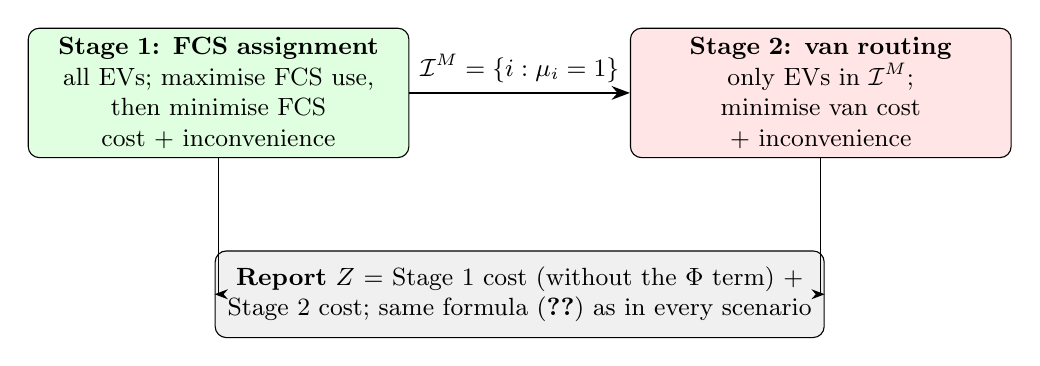
\begin{tikzpicture}[>=Stealth,box/.style={draw,rounded corners,align=center,minimum height=1.1cm,font=\small}]
  \node[box,fill=green!12,text width=4.6cm] (s1) {\textbf{Stage 1: FCS assignment}\\all EVs; maximise FCS use,\\then minimise FCS cost + inconvenience};
  \node[box,fill=red!10,text width=4.6cm,right=2.8cm of s1] (s2) {\textbf{Stage 2: van routing}\\only EVs in $\I^M$;\\minimise van cost + inconvenience};
  \draw[->,thick] (s1) -- node[above,font=\small]{$\I^M=\{i:\mu_i=1\}$} (s2);
  \node[box,fill=black!6,text width=7.5cm,below=2.0cm of $(s1)!0.5!(s2)$] (ev) {\textbf{Report} $Z=$ Stage~1 cost (without the $\Phi$ term) $+$ Stage~2 cost; same formula \eqref{eq:Z} as in every scenario};
  \draw[->] (s1) |- (ev); \draw[->] (s2) |- (ev);
\end{tikzpicture}
\end{center}

Stage~1 does not look at the vans, and Stage~2 cannot change what Stage~1 decided. That is the definition of ``FCS first, then MCS''.

%----------------------------------------------------------------
\subsection{Stage 1: assign EVs to fixed stations}

\textbf{Objective.}
\begin{equation}
\begin{split}
\min\ Z^{(1)}=\;&\underbrace{\Phi\sum_{i\in\I}\mu_i}_{\text{FCS first}}
+\underbrace{c^{EV}\sum_i\sum_{f\in\F_i}d_{if}Y_{if}}_{Z_1}
+\underbrace{Z^F_{\text{energy}}}_{\text{FCS part of }Z_4}\\
&+\underbrace{\sum_i\sum_{f\in\F_i}\rho^F_{if}Y_{if}+\alpha\sum_i w_i(C_i-r_i)+c^L\sum_i w_iL_i}_{\text{FCS customers' inconvenience}}
\end{split}
\label{eq:obj1}
\end{equation}
with $C_i=S_i+\tau^F_iY_i$ in this stage. $\Phi$ is a penalty for handing an EV to the vans. It is chosen larger than anything an extra FCS customer can add to the rest of \eqref{eq:obj1}, e.g.
\[
\Phi > \max_{i}\max_{f\in\F_i}\big(c^{EV}d_{if}+\pi^{\max}E_i+\rho^F_{if}\big)+n\,(\alpha+c^L)\,w_{\max}\,T,
\]
so Stage~1 first \textbf{maximises the number of EVs served at an FCS}, and only among those solutions minimises FCS cost and inconvenience. ($\pi^{\max}$ is the highest grid price.) A numerically safer equivalent is to solve twice: first $\max\sum_iY_i$, then fix that number and minimise the rest.
\ifTOU
Because $Z^F_{\text{energy}}$ uses the peak price, Stage~1 may \emph{start sessions later} to leave the peak, if the price saving beats the extra waiting cost (Section~\ref{sec:expect}).
\fi

\textbf{Constraints.}
\begin{align}
\sum_{g\in\G_i}y_{ig}+\mu_i &= 1 && \forall i\in\I \label{eq:s1assign}\\
S_i &\ge r_i+\sum_{f\in\F_i}t_{if}Y_{if} && \forall i\in\I \label{eq:fcsarr}\\
S_i &\le r_i+T\,(1-\mu_i) && \forall i\in\I \label{eq:s1park}\\
S_j &\ge S_i+\tau^F_i-(T+\tau^F_i)(3-y_{ig}-y_{jg}-o_{ij}) && \forall g,\ (i,j)\in\mathcal{P}_g \label{eq:disj1}\\
S_i &\ge S_j+\tau^F_j-(T+\tau^F_j)(2-y_{ig}-y_{jg}+o_{ij}) && \forall g,\ (i,j)\in\mathcal{P}_g \label{eq:disj2}\\
\sum_i y_{ig_1} &\ge \sum_i y_{ig_2} && \forall f,\ \G_f=\{g_1,g_2\} \label{eq:gunsym}\\
S_i+\tau^F_iY_i &\le T,\qquad L_i\ge S_i+\tau^F_iY_i-l_i && \forall i\in\I \label{eq:s1time}
\end{align}
\ifTOU plus the time-of-use split \eqref{eq:tou1}--\eqref{eq:tou5} of each FCS session (Section~\ref{sec:price}).\fi
\desc{\eqref{eq:s1assign}: every EV either gets one reachable gun or is handed to the vans. An EV that reaches no FCS ($\G_i=\emptyset$) is forced to $\mu_i=1$. \eqref{eq:fcsarr}: an FCS session cannot start before the EV has asked and driven to the station. \eqref{eq:s1park}: for an EV handed to the vans, $S_i$ is parked at $r_i$, so it adds no waiting in Stage~1 (its real start time is decided in Stage~2). \eqref{eq:disj1}--\eqref{eq:disj2}: two EVs on the same gun do not overlap; $o_{ij}$ picks who goes first. With two guns per station this means at most two EVs charge at a station at a time. \eqref{eq:gunsym}: symmetry breaking between the two identical guns (optional). \eqref{eq:s1time}: finished by $T$; lateness.}

\textbf{Optional acceptability rule.} An operator may refuse to send a driver to a station that is ``too inconvenient'', e.g.\ only allow gun $g$ of station $f$ for EV $i$ if $\hat\rho^F_{if}\le\bar\rho$. This only shrinks $\G_i$, so EVs whose stations are all too far go to the vans. Report results with and without it.

\textbf{Output:} $\I^M=\{i:\mu_i=1\}$, the EVs left for the vans; plus each FCS customer's gun and start time.

%----------------------------------------------------------------
\subsection{Stage 2: route the vans to the leftover EVs}

Stage~2 is a vehicle routing problem with time windows, on the EVs in $\I^M$ only. Here $C_i=S_i+\tau^M_i$.

\textbf{Objective.}
\begin{equation}
\begin{split}
\min\ Z^{(2)}=\;&\underbrace{c^M\sum_m\sum_{(i,j)\in\A^M}d_{ij}x_{ijm}}_{Z_2}+\underbrace{\sum_m c^D_mu_m}_{Z_3}+\underbrace{Z^M_{\text{energy}}}_{\text{van part of }Z_4}\\
&+\underbrace{\sum_{i\in\I^M}\sum_m\rho^M_{im}z_{im}+\alpha\sum_{i\in\I^M}w_i(C_i-r_i)+c^L\sum_{i\in\I^M}w_iL_i}_{\text{van customers' inconvenience}}
\end{split}
\label{eq:obj2}
\end{equation}
Since every EV in $\I^M$ must be served by some van, $Z^M_{\text{energy}}$ and the $\rho^M$ term are constants here. They are kept so that $Z^{(2)}$ is the true cost of Stage~2. Waiting and lateness make the vans visit urgent EVs early.

\textbf{Constraints.}
\begin{align}
\sum_{m\in\M}z_{im} &= 1 && \forall i\in\I^M \label{eq:s2assign}\\
\sum_{j:(0,j)\in\A^M}x_{0jm} = \sum_{i:(i,n+1)\in\A^M}x_{i,n+1,m} &= u_m && \forall m \label{eq:depot}\\
\sum_{i:(i,j)\in\A^M}x_{ijm} = \sum_{k:(j,k)\in\A^M}x_{jkm} &= z_{jm} && \forall j\in\I^M,\ m \label{eq:flow}\\
\sum_{i\in\I^M}z_{im} &\le Q_m\,u_m && \forall m \label{eq:cap}\\
\sum_{i\in\I^M}\frac{E_i}{\eta}z_{im}+\beta\sum_{(i,j)\in\A^M}d_{ij}x_{ijm} &\le B_m\,u_m && \forall m \label{eq:batt}
\end{align}
\begin{align}
S_j &\ge \max\{r_j,\ t_{0j}\,x_{0jm}\} && \forall j\in\I^M,\ m \label{eq:depart}\\
S_j &\ge S_i+\tau^M_i+t_{ij}-(T+\tau^M_i+t_{ij})(1-x_{ijm}) && \forall i\neq j,\ m \label{eq:seq}\\
S_i+\tau^M_i+t_{i,n+1} &\le T+(\tau^M_i+t_{i,n+1})(1-x_{i,n+1,m}) && \forall i,\ m \label{eq:return}\\
S_i+\tau^M_i \le T,\quad L_i &\ge S_i+\tau^M_i-l_i && \forall i\in\I^M \label{eq:s2time}\\
u_m &\ge u_{m+1} && m<|\M| \label{eq:vansym}
\end{align}
\desc{\eqref{eq:s2assign}: each leftover EV gets one van. \eqref{eq:depot}: a used van leaves and returns to the depot once. \eqref{eq:flow}: each EV on van $m$ is entered and left exactly once by that van. \eqref{eq:cap}: at most $Q_m$ EVs per van. \eqref{eq:batt}: delivered energy (with transfer losses) plus driving energy fits in the van battery. \eqref{eq:depart}: no start before the request, or before the van can drive there from the depot (written as two linear constraints). \eqref{eq:seq}: if the van goes $i\to j$, it finishes $i$ and drives to $j$ before starting $j$. This gives one EV at a time and removes subtours (MTZ-type). \eqref{eq:return}: back at the depot by $T$. \eqref{eq:s2time}: finished by $T$; lateness. \eqref{eq:vansym}: use identical vans in index order.}

\textbf{If Stage 2 is infeasible} (too many leftover EVs for the fleet by $T$), the sequential policy has \emph{failed} on that instance. For diagnosis, add $s_i\in\{0,1\}$ (``unserved''), replace \eqref{eq:s2assign} by $\sum_mz_{im}+s_i=1$ and add $\Phi^U\sum_is_i$ to \eqref{eq:obj2}. Then report the number of EVs that could not be served. This is a useful comparison with the integrated scenario, which may serve all of them.

%----------------------------------------------------------------
\subsection{Reported value}
\[
Z^{\text{S\scen}}=\big(Z^{(1)*}-\Phi\,|\I^M|\big)+Z^{(2)*},
\]
which is exactly \eqref{eq:Z} evaluated at the combined solution. The stage-1 solution plus the stage-2 solution is a feasible solution of the integrated model (S\ifTOU 4\else 3\fi), so
$Z^{\text{S\ifTOU 4\else 3\fi}}\le Z^{\text{S\scen}}$. The difference is the \emph{value of integration}.

\else
%---------------------------------------------------------------- INT
\subsection{Objective}
\begin{equation}
\min\ Z \quad\text{as in \eqref{eq:Z}, with }Z^F_{\text{energy}}=\ifTOU P^F\textstyle\sum_i\big[\pi^\off(\theta^1_i+\theta^3_i)+\pi^\pk\theta^2_i\big]\else\pi^F\textstyle\sum_iE_iY_i\fi,\quad C_i=S_i+\tau^F_iY_i+\tau^M_iZ_i. \label{eq:objint}
\end{equation}
Written out in full:
\begin{align*}
\min\ Z=\;& c^{EV}\sum_i\sum_{f\in\F_i}d_{if}Y_{if}+c^M\sum_m\sum_{(i,j)\in\A}d_{ij}x_{ijm}+\sum_mc^D_mu_m\\
&+\ifTOU P^F\sum_i\big[\pi^\off(\theta^1_i+\theta^3_i)+\pi^\pk\theta^2_i\big]\else\pi^F\sum_iE_iY_i\fi
+\pi^M\sum_i\sum_m\frac{E_i}{\eta}z_{im}\\
&+\sum_i\sum_{f\in\F_i}\rho^F_{if}Y_{if}+\sum_i\sum_m\rho^M_{im}z_{im}+\alpha\sum_iw_i(C_i-r_i)+c^L\sum_iw_iL_i .
\end{align*}
Every term is linear. One model weighs everything at once: an EV goes to a van exactly when the van's extra km, dispatch and energy cost are outweighed by the effort and waiting it saves the driver\ifTOU, or by the peak-price energy it avoids\fi.

\subsection{Constraints}

\textbf{Assignment.}
\begin{equation}
\sum_{g\in\G_i}y_{ig}+\sum_{m\in\M}z_{im}=1\qquad\forall i\in\I \label{eq:assign}
\end{equation}
\desc{Exactly one resource per EV: one reachable gun or one van. EVs that reach no FCS are forced onto a van.}

\textbf{Fixed stations.}
\begin{align}
S_i &\ge r_i+\sum_{f\in\F_i}t_{if}Y_{if} && \forall i \label{eq:fcsarr}\\
S_j &\ge S_i+\tau^F_i-(T+\tau^F_i)(3-y_{ig}-y_{jg}-o_{ij}) && \forall g,\ (i,j)\in\mathcal{P}_g \label{eq:disj1}\\
S_i &\ge S_j+\tau^F_j-(T+\tau^F_j)(2-y_{ig}-y_{jg}+o_{ij}) && \forall g,\ (i,j)\in\mathcal{P}_g \label{eq:disj2}\\
\sum_iy_{ig_1} &\ge \sum_iy_{ig_2} && \forall f,\ \G_f=\{g_1,g_2\} \label{eq:gunsym}
\end{align}
\desc{\eqref{eq:fcsarr}: an FCS session starts after the request and the drive to the station (for a van customer this is just $S_i\ge r_i$). \eqref{eq:disj1}--\eqref{eq:disj2}: EVs on the same gun do not overlap; $o_{ij}$ chooses the order. \eqref{eq:gunsym}: optional symmetry breaking.}

\textbf{Vans: routes, capacity, battery.}
\begin{align}
\sum_{j:(0,j)\in\A}x_{0jm}=\sum_{i:(i,n+1)\in\A}x_{i,n+1,m} &= u_m && \forall m \label{eq:depot}\\
\sum_{i:(i,j)\in\A}x_{ijm}=\sum_{k:(j,k)\in\A}x_{jkm} &= z_{jm} && \forall j\in\I,\ m \label{eq:flow}\\
\sum_iz_{im} &\le Q_mu_m && \forall m \label{eq:cap}\\
\sum_i\frac{E_i}{\eta}z_{im}+\beta\sum_{(i,j)\in\A}d_{ij}x_{ijm} &\le B_mu_m && \forall m \label{eq:batt}
\end{align}
\desc{\eqref{eq:depot}: a used van leaves and returns once. \eqref{eq:flow}: each EV on van $m$ is visited exactly once by it. \eqref{eq:cap}: at most $Q_m$ EVs. \eqref{eq:batt}: delivered energy (with losses) plus driving energy fits in the battery.}

\textbf{Vans: timing (one EV at a time, no subtours).}
\begin{align}
S_j &\ge t_{0j}\,x_{0jm} && \forall j\in\I,\ m \label{eq:depart}\\
S_j &\ge S_i+\tau^M_i+t_{ij}-(T+\tau^M_i+t_{ij})(1-x_{ijm}) && \forall i\neq j\in\I,\ m \label{eq:seq}\\
S_i+\tau^M_i+t_{i,n+1} &\le T+(\tau^M_i+t_{i,n+1})(1-x_{i,n+1,m}) && \forall i,\ m \label{eq:return}
\end{align}
\desc{\eqref{eq:depart}: the first stop cannot start before the van has driven there. \eqref{eq:seq}: $i\to j$ means finish $i$, drive, then start $j$; start times rise along a route, so no subtour can close. \eqref{eq:return}: back at the depot by $T$.}

\textbf{Horizon and lateness.}
\begin{equation}
C_i\le T,\qquad L_i\ge C_i-l_i\qquad\forall i\in\I \label{eq:time}
\end{equation}
\desc{Every EV is fully charged within the horizon; $L_i$ measures lateness.}

\ifTOU
\textbf{Time-of-use split.} Constraints \eqref{eq:tou1}--\eqref{eq:tou5} of Section~\ref{sec:price}.
\fi

\textbf{Symmetry and domains.}
\begin{equation}
u_m\ge u_{m+1};\qquad y,z,x,u,o\ifTOU,\kappa\fi\in\{0,1\};\qquad S_i,L_i\ifTOU,\theta^p_i\fi\ge0 \label{eq:dom}
\end{equation}
\fi

%=====================================================================
\section{Learning-to-optimise (RL) formulation}\label{sec:rl}

\textbf{Main rule:} the reward of each action is \emph{minus the increase in $Z$ that the action causes}. The rewards over an episode then add up to $-Z$ of the solution the policy builds. RL and MILP results are measured on the same yardstick \eqref{eq:Z}, and the MILP optimum is the benchmark for the RL gap.

\ifSEQ
%---------------------------------------------------------------- RL SEQ
The RL pipeline has the same two stages as the MILP.

\subsection{Stage 1 policy: FCS assignment}
\begin{itemize}[leftmargin=1.4em,itemsep=2pt]
  \item \textbf{Episode / epochs:} EVs are taken in order of request time $r_i$ (ties: higher $w_i$ first). One decision per EV.
  \item \textbf{State:} features of the current EV $k$ ($E_k,r_k,l_k,w_k,R_k$, location); for each gun $g$ the time $F_g$ it becomes free; summary features of the EVs still to come (count and positions near each station)\ifTOU; the current price and the time until $T_1$ and $T_2$\fi.
  \item \textbf{Action:} a gun $g\in\G_k$, or ``hand to vans''. \textbf{FCS-first mask:} ``hand to vans'' is allowed \emph{only} if no gun can finish EV $k$ by $T$ (or, with the optional rule, if all remaining guns have $\hat\rho^F_{kf}>\bar\rho$).
  \ifTOU\item \textbf{Optional timing action:} ``gun $g$, start after the peak'', i.e.\ $S_k=\max\{\text{earliest},T_2\}$, allowed only if the session still ends by $T$.\fi
  \item \textbf{Transition:} $S_k=\max\{r_k+t_{kf},F_g\}$ (or later, for the timing action); $F_g\leftarrow S_k+\tau^F_k$.
  \item \textbf{Reward:} $-\Big[c^{EV}d_{kf}+\text{energy}_k+\rho^F_{kf}+\alpha w_k(S_k+\tau^F_k-r_k)+c^Lw_k(S_k+\tau^F_k-l_k)^+\Big]$, where energy$_k$ = \ifTOU$P^F\big[\pi^\off\cdot(\text{off-peak hours of }[S_k,S_k+\tau^F_k])+\pi^\pk\cdot(\text{peak hours})\big]$, computed exactly in the simulator\else$\pi^FE_k$\fi. Handing an EV to the vans gives reward $0$ here; its cost is counted in Stage~2.
\end{itemize}
Note: a simple baseline for Stage~1 is the greedy rule ``gun with the largest one-step reward''. What RL can learn on top of this is, for example, to keep a nearby gun free for an urgent EV that arrives later.

\subsection{Stage 2 policy: van routing over $\I^M$}
\begin{itemize}[leftmargin=1.4em,itemsep=2pt]
  \item \textbf{Epochs:} whenever a van becomes free (the earliest-free van decides first).
  \item \textbf{State:} for each van: position, time free, remaining battery $b_m$, EVs served so far, dispatched or not; for each unserved EV in $\I^M$: location, $E_i,r_i,l_i,w_i$; current time.
  \item \textbf{Action:} the next EV $j$ for this van, or ``return to depot'' (ends the route). Mask: $j$ must be feasible: battery covers $E_j/\eta$ plus driving to $j$ and back to the depot, the count stays $\le Q_m$, and $j$ can be finished with the van back at the depot by $T$.
  \item \textbf{Transition:} $S_j=\max\{r_j,\ \text{time free}+t_{\text{pos},j}\}$; the van moves to $j$ and is free at $S_j+\tau^M_j$; $b_m$ falls by $E_j/\eta+\beta d_{\text{pos},j}$.
  \item \textbf{Reward:} serving $j$: $-\Big[c^Md_{\text{pos},j}+c^D_m[\text{first stop}]+\pi^M\frac{E_j}{\eta}+\rho^M_{jm}+\alpha w_j(S_j+\tau^M_j-r_j)+c^Lw_j(S_j+\tau^M_j-l_j)^+\Big]$; returning: $-c^Md_{\text{pos},0}$. EVs still unserved at the end: $-\Phi^U$ each.
  \item \textbf{Policy:} an attention-based routing policy (e.g.\ Kool et al., 2019, ``Attention, Learn to Solve Routing Problems!'') trained with REINFORCE or PPO. Baseline: nearest-feasible-EV heuristic.
\end{itemize}
Episode return of Stage~1 + Stage~2 $=-Z^{\text{S\scen}}$.

\else
%---------------------------------------------------------------- RL INT
One policy decides both who serves each EV and the van routes.
\begin{itemize}[leftmargin=1.4em,itemsep=2pt]
  \item \textbf{Episode / epochs:} EVs are taken in order of request time $r_i$ (ties: higher $w_i$ first). One decision per EV.
  \item \textbf{State:} (i) the current EV $k$: location, $E_k,r_k,l_k,w_k,R_k$, reachable stations; (ii) each gun $g$: time $F_g$ it becomes free; (iii) each van $m$: current end-of-route position, time free, remaining battery $b_m$, EVs served, dispatched or not; (iv) embeddings of the not-yet-assigned EVs (for look-ahead)\ifTOU; (v) current price, time until $T_1$ and $T_2$\fi.
  \item \textbf{Action:} $a\in\G_k\cup\M$: a gun, or a van (EV $k$ is appended to the end of that van's route). \textbf{Mask} infeasible actions: a gun that cannot finish $k$ by $T$; a van without enough battery for $E_k/\eta$ plus the drive to $k$ and back to the depot, with $Q_m$ reached, or unable to finish $k$ and return by $T$.
  \ifTOU\item \textbf{Optional timing action:} ``gun $g$, start after the peak'' ($S_k=\max\{\text{earliest},T_2\}$, if it still ends by $T$).\fi
  \item \textbf{Transition:} gun: $S_k=\max\{r_k+t_{kf},F_g\}$, $F_g\leftarrow S_k+\tau^F_k$. Van: $S_k=\max\{r_k,\ \text{free}_m+t_{\text{pos}_m,k}\}$, then the van moves to $k$, $\text{free}_m\leftarrow S_k+\tau^M_k$, $b_m\mathrel{-}=E_k/\eta+\beta d_{\text{pos}_m,k}$.
  \item \textbf{Reward} $=-\Delta Z$:
  \begin{align*}
  \text{gun } g\text{ at }f:&\quad -\Big[c^{EV}d_{kf}+\text{energy}^F_k+\rho^F_{kf}+\alpha w_k(C_k-r_k)+c^Lw_k(C_k-l_k)^+\Big]\\
  \text{van } m:&\quad -\Big[c^M\big(d_{\text{pos}_m,k}+d_{k,0}-d_{\text{pos}_m,0}\big)+c^D_m[\text{first use}]+\pi^M\tfrac{E_k}{\eta}\\
  &\qquad\quad+\rho^M_{km}+\alpha w_k(C_k-r_k)+c^Lw_k(C_k-l_k)^+\Big]
  \end{align*}
  The van distance term is the \emph{change} in route length when $k$ is inserted before the return to the depot, so the sum over the episode equals the total route length (the return legs telescope). energy$^F_k$ = \ifTOU$P^F\big[\pi^\off\cdot(\text{off-peak hours})+\pi^\pk\cdot(\text{peak hours of }[S_k,C_k])\big]$, computed exactly by the simulator; no linearisation is needed in RL\else$\pi^FE_k$\fi.
  \item \textbf{Dead end:} if every action is masked, EV $k$ is unserved: reward $-\Phi^U$, and the episode continues. Report the count.
  \item \textbf{Policy:} masked categorical policy over guns and vans, encoder with attention over EVs, guns and vans; trained with PPO. Natural baseline: greedy, i.e.\ choose the action with the largest one-step reward. That is the pairwise rule ``smallest $\hat\rho$ + cost'' from Section~\ref{sec:inc}.
\end{itemize}
Restriction to note: vans serve EVs in assignment order (append only). A variant that inserts $k$ at the cheapest position of a route is more flexible but has a larger action space.
\fi

\textbf{Reward scaling.} For stable training divide every reward by a constant, e.g.\ the greedy baseline's average $Z$ on the training instances. This does not change the optimal policy.

%=====================================================================
\section{What to expect and what to report}\label{sec:expect}

\ifnum\scen=1
\begin{itemize}[leftmargin=1.4em,itemsep=2pt]
  \item Vans serve only EVs that reach no station, or that the stations cannot finish by $T$. If stations have spare capacity, very few vans are dispatched.
  \item Inconvenience is high for EVs far from the nearest station (worked example: Rs\,682 at the FCS, against Rs\,458 if a van had been allowed).
  \item With too few vans Stage~2 becomes infeasible (unserved EVs), even when the integrated model S3 could serve everyone. Report the smallest $|\M|$ at which S1 is feasible and compare it with S3.
\end{itemize}
\fi
\ifnum\scen=2
\begin{itemize}[leftmargin=1.4em,itemsep=2pt]
  \item \textbf{When does Stage~1 delay a session to avoid the peak?} Moving one hour of charging out of the peak saves $(\pi^\pk-\pi^\off)P^F=3\times22=$ Rs\,66, but delays completion by up to an hour, which costs $\alpha w_i\ge$ Rs\,200. So with the default values Stage~1 almost never delays. It mostly pays the higher price, and S2 costs roughly S1 plus the peak surcharge. Sessions start later only if $\alpha$ is small (try $\lambda<0.33$ in the sensitivity analysis).
  \item The van assignment is the same as in S1 unless Stage~1's timing changes which EVs fit at the stations. Stage~1 cannot use vans to escape the peak price.
  \item Extra KPI: \textbf{grid energy drawn at FCS during the peak}, $P^F\sum_i\theta^2_i$ (kWh). Compare with S4.
\end{itemize}
\fi
\ifnum\scen=3
\begin{itemize}[leftmargin=1.4em,itemsep=2pt]
  \item Vans take EVs for which the saved inconvenience exceeds the extra van cost (worked example: van chosen, saving Rs\,224). Expect vans to serve EVs that are far from every station, have low range (high $w_i$), or have early deadlines, while EVs near a station still use it.
  \item \textbf{Value of integration under flat price:} $Z^{\text{S1}}-Z^{\text{S3}}\ge0$. Report it per component ($Z_1,\dots,Z_5$): typically operating cost rises a little and inconvenience falls a lot.
  \item Vary $|\M|$ (0, 1, 2, \dots): the first few vans lower $Z$ sharply, then the effect levels off. That curve shows the scenarios where mobile chargers help most.
\end{itemize}
\fi
\ifnum\scen=4
\begin{itemize}[leftmargin=1.4em,itemsep=2pt]
  \item During the peak a van kWh costs about the same as an FCS kWh (Rs\,10.0 each), so the vans' energy disadvantage disappears and vans also absorb \emph{peak-hour} demand that would otherwise be charged on the grid at peak price.
  \item Expect more van usage than in S3, concentrated on requests in $[T_1,T_2]$, and lower grid energy at the stations during the peak, $P^F\sum_i\theta^2_i$, than in S2.
  \item \textbf{Value of integration under peak pricing:} $Z^{\text{S2}}-Z^{\text{S4}}$. It should be larger than $Z^{\text{S1}}-Z^{\text{S3}}$, because integration now also allows price arbitrage.
  \item \textbf{Peak pricing with full flexibility:} $Z^{\text{S4}}-Z^{\text{S3}}$ should be smaller than $Z^{\text{S2}}-Z^{\text{S1}}$: vans cushion the price increase.
\end{itemize}
\fi

\textbf{Cross-scenario comparison table} (fill in from the four runs):
\begin{center}
\renewcommand{\arraystretch}{1.2}
\begin{tabular}{@{}lll@{}}
\toprule
\textbf{Comparison} & \textbf{Measures} & \textbf{Expected sign} \\
\midrule
S1 $-$ S3 & value of integration, flat price & $\ge0$ \\
S2 $-$ S4 & value of integration, peak price & $\ge0$, larger than S1 $-$ S3 \\
S2 $-$ S1 & cost of peak pricing, FCS-first operator & $>0$ \\
S4 $-$ S3 & cost of peak pricing, flexible operator & $>0$, smaller than S2 $-$ S1 \\
\bottomrule
\end{tabular}
\end{center}
Report for each: $Z$ and its components, number of vans used, EVs per resource, mean and maximum inconvenience per EV, total lateness, peak-hour grid energy, solve time, and (for RL) the gap to the MILP optimum.

%=====================================================================
\appendix
\section{Illustrative parameter values}\label{app:values}

These are starting values for experiments, not data. All are meant to be varied in the analysis. Values in Rs.

\begin{center}
\renewcommand{\arraystretch}{1.15}
\begin{tabular}{@{}llp{6.2cm}@{}}
\toprule
\textbf{Parameter} & \textbf{Value} & \textbf{Note} \\
\midrule
$T$, $[T_1,T_2]$ & 7 h, $[2,6]$ & 16:00--23:00, peak 18:00--22:00 \\
$P^F$, $P^M$ & 22 kW, 30 kW & \\
$v$, $\beta$, $\eta$ & 25 km/h, 0.25 kWh/km, 0.9 & \\
$B_m$, $Q_m$, $|\M|$ & 150 kWh, 6, 2--6 & \\
$c^{EV}$, $c^M$, $c^D_m$ & Rs\,4/km, Rs\,15/km, Rs\,1500 & van km includes driver time \\
$\pi^F$ (flat) & Rs\,8.7/kWh & equals the time-average of the ToU tariff over $[0,T]$ \\
$\pi^\off$, $\pi^\pk$ (ToU) & Rs\,7/kWh, Rs\,10/kWh & $(3\times7+4\times10)/7=8.7$ \\
$c^{bat}$ & Rs\,2/kWh & van battery wear \\
$\pi^M$ & Rs\,10.7 (flat) / Rs\,9.0 (ToU) & $=\pi^F+c^{bat}$ / $=\pi^\off+c^{bat}$ \\
$\alpha$, $\alpha^D$ & Rs\,200/h, Rs\,100/h & value of time; extra for attended time \\
$h^F$, $h^M$, $\varphi$ & Rs\,50, Rs\,10, Rs\,100 & trip hassle, hand-over, range stress \\
$c^L$ & Rs\,300/h & lateness \\
$w_i$ & $1+2(1-R_i/R_{\max})$, $R_i\sim U[3,40]$ km & priority from remaining range \\
\bottomrule
\end{tabular}
\end{center}

The flat price is set to the time-average of the peak tariff. The price \emph{level} is then the same in both pricing cases, and only the price \emph{shape} differs. Without this, part of S1 vs S2 would just reflect a different average price.

\end{document}
"
%    pdflatex -jobname=scenario3_flat_integrated   "\def\scen{3}% =====================================================================
%  One source, four PDFs.  Build with build.sh (or by hand):
%    pdflatex -jobname=scenario1_flat_sequential   "\def\scen{1}\input{scenario_master}"
%    pdflatex -jobname=scenario2_peak_sequential   "\def\scen{2}\input{scenario_master}"
%    pdflatex -jobname=scenario3_flat_integrated   "\def\scen{3}\input{scenario_master}"
%    pdflatex -jobname=scenario4_peak_integrated   "\def\scen{4}\input{scenario_master}"
%  (run each twice for cross-references)
% =====================================================================
\documentclass[11pt,a4paper]{article}
\usepackage[margin=2.2cm]{geometry}
\usepackage{amsmath,amssymb,amsfonts}
\usepackage{booktabs,array,tabularx}
\usepackage{enumitem}
\usepackage[table]{xcolor}
\usepackage{tikz}
\usetikzlibrary{arrows.meta,positioning,calc}
\usepackage[colorlinks=true,linkcolor=blue!50!black,urlcolor=blue!50!black]{hyperref}
\usepackage{titlesec}
\titleformat{\section}{\large\bfseries}{\thesection}{0.8em}{}
\titleformat{\subsection}{\normalsize\bfseries}{\thesubsection}{0.8em}{}
\setlength{\parindent}{0pt}
\setlength{\parskip}{5pt}

% ---------------- scenario switches ----------------
\ifdefined\scen\else\def\scen{1}\fi
\newif\ifTOU \TOUfalse   % true = time-of-use (peak) price
\newif\ifSEQ \SEQfalse   % true = FCS first, then MCS
\ifnum\scen=1 \SEQtrue \fi
\ifnum\scen=2 \TOUtrue \SEQtrue \fi
\ifnum\scen=4 \TOUtrue \fi

\newcommand{\pricename}{\ifTOU time-of-use price (dearer evening peak)\else single (flat) price all day\fi}
\newcommand{\structname}{\ifSEQ FCS first, then MCS (sequential)\else FCS and MCS together (integrated)\fi}

% ---------------- notation ----------------
\newcommand{\I}{\mathcal{I}}
\newcommand{\F}{\mathcal{F}}
\newcommand{\G}{\mathcal{G}}
\newcommand{\M}{\mathcal{M}}
\newcommand{\N}{\mathcal{N}}
\newcommand{\A}{\mathcal{A}}
\newcommand{\Rs}{\text{Rs}\,}
\newcommand{\pk}{\mathrm{pk}}
\newcommand{\off}{\mathrm{off}}
\newcommand{\desc}[1]{\par\vspace{-2pt}{\small\color{black!75}\textit{Meaning:} #1}\par\vspace{4pt}}
\newcommand{\cell}[2]{\ifnum\scen=#1\cellcolor{blue!18}\textbf{S#1 (this document)}\\\textbf{#2}\else S#1\\#2\fi}

\title{\textbf{EV Charging Network Optimisation}\\[4pt]
\large Scenario \scen: \pricename\ $+$ \structname\\[2pt]
\normalsize MILP and RL formulation}
\author{CP 320 OR for Mobility Management, course project}
\date{2 October 2026}

\begin{document}
\maketitle

%=====================================================================
\section{Where this scenario sits}

The project studies four scenarios: two ways of pricing grid electricity, times two ways of making the decisions.

\begin{center}
\renewcommand{\arraystretch}{1.5}
\begin{tabular}{>{\raggedright\arraybackslash}p{4.2cm}|>{\centering\arraybackslash}p{4.6cm}|>{\centering\arraybackslash}p{4.6cm}}
 & \textbf{Flat price all day} & \textbf{Time-of-use (peak) price} \\ \hline
\textbf{Sequential:} FCS first, leftover EVs to MCS &
\begin{tabular}[c]{@{}c@{}}\cell{1}{flat + sequential}\end{tabular} &
\begin{tabular}[c]{@{}c@{}}\cell{2}{peak + sequential}\end{tabular} \\ \hline
\textbf{Integrated:} FCS and MCS decided together &
\begin{tabular}[c]{@{}c@{}}\cell{3}{flat + integrated}\end{tabular} &
\begin{tabular}[c]{@{}c@{}}\cell{4}{peak + integrated}\end{tabular} \\
\end{tabular}
\end{center}

\textbf{The four scenarios do not have four different objectives.} They share \emph{one} cost yardstick $Z$ (Section~\ref{sec:obj}): the same cost terms and the same customer inconvenience (Section~\ref{sec:inc}). Only two things change:
\begin{itemize}[leftmargin=1.4em,itemsep=1pt]
  \item \textbf{Pricing} changes the formula for one term, the FCS energy cost (Section~\ref{sec:price}).
  \item \textbf{Decision structure} changes \emph{how} $Z$ is minimised: in one model (integrated), or in two stages (sequential), where each stage minimises its own part of $Z$.
\end{itemize}
Because the yardstick is the same, the four optimal values can be compared directly. The differences measure the \emph{value of integration} (S1$\to$S3, S2$\to$S4) and the \emph{effect of peak pricing} (S1$\to$S2, S3$\to$S4).

\ifnum\scen=1
\textbf{This scenario (S1)} is the baseline, the ``status quo''. Electricity costs the same at every hour, every EV that can be charged at a fixed station is sent there, and vans only take what is left over.
\fi
\ifnum\scen=2
\textbf{This scenario (S2)} keeps the FCS-first rule of S1, but grid electricity is dearer during the evening peak. Stage~1 can react to the price only by \emph{rescheduling} FCS sessions. It cannot hand a peak-hour EV to a van.
\fi
\ifnum\scen=3
\textbf{This scenario (S3)} keeps the flat price of S1, but the operator decides FCS and MCS service \emph{together}. An EV can be sent to a van even when a fixed station could take it, whenever that lowers total cost plus inconvenience.
\fi
\ifnum\scen=4
\textbf{This scenario (S4)} is the most flexible one: peak pricing at fixed stations, and FCS and MCS decided together. Van energy was bought off-peak, so vans can also be used to keep charging \emph{out of the expensive peak}.
\fi

%=====================================================================
\section{Setting and assumptions}\label{sec:setting}

\textbf{Time.} The planning horizon is $[0,T]$ with $T=7$\,h (16:00--23:00). It contains the evening peak window $[T_1,T_2]=[2,6]$ (18:00--22:00). The horizon is the same in all four scenarios. It is wider than the peak itself so that, under peak pricing, there is cheaper time on both sides of the peak.\ifTOU\else\ In this scenario the price is flat, so the window plays no role in the model.\fi

\textbf{Assumptions} (the same as MILP v3, plus two about energy):
\begin{enumerate}[leftmargin=1.6em,itemsep=1pt]
  \item Static, continuous time. All requests in the horizon are known at time $0$, and request $i$ becomes active at $r_i$.
  \item An EV served by an FCS drives there itself on its own battery (only to stations within its range $R_i$). The driver stays with the car while it waits for a free gun and while it charges.
  \item An EV served by an MCS stays parked where it is, and the driver is free in the meantime.
  \item Each FCS gun and each van charges one EV at a time, without interruption, at constant power.
  \item A van's battery covers both its driving and the energy it delivers. \textbf{The van battery is charged at the depot before the horizon starts}\ifTOU, i.e.\ at the off-peak price\fi, and is not recharged during the horizon.
  \item Every EV must be fully charged by $T$ (hard). Finishing after the driver's desired time $l_i$ is allowed but penalised.
\end{enumerate}

%=====================================================================
\section{Notation}\label{sec:notation}

\subsection*{Sets}
\begin{tabularx}{\textwidth}{@{}lX@{}}
\toprule
$\I=\{1,\dots,n\}$ & EV charging requests \\
$\F$; $\G_f$ ($|\G_f|=2$); $\G=\bigcup_f\G_f$ & fixed charging stations; guns of FCS $f$; all guns ($f(g)$ = station of gun $g$) \\
$\F_i=\{f: d_{if}\le R_i\}$, $\G_i=\bigcup_{f\in\F_i}\G_f$ & stations / guns EV $i$ can reach on its remaining range \\
$\M$ & mobile charging vans (MCS) \\
$0,\ n+1$ & depot as start node / end node (same place) \\
$\N=\{0\}\cup\I\cup\{n+1\}$, $\A$ & routing nodes; allowed van arcs $(i,j)$, $i\in\{0\}\cup\I$, $j\in\I\cup\{n+1\}$, $i\neq j$ \\
$\mathcal{P}_g=\{(i,j): i<j,\ g\in\G_i\cap\G_j\}$ & pairs of EVs that could share gun $g$ \\
\ifSEQ
$\I^M\subseteq\I$ & EVs handed to the vans by Stage~1 (an \emph{output} of Stage~1, a fixed input to Stage~2) \\
$\N^M$, $\A^M$ & routing nodes / arcs restricted to $\I^M$ \\
\fi
\bottomrule
\end{tabularx}

\subsection*{Parameters}
\begin{tabularx}{\textwidth}{@{}lX@{}}
\toprule
$E_i,\ r_i,\ l_i,\ R_i$ & energy demand (kWh), request time, desired completion time (h), remaining range (km) \\
$w_i\ge1$ & priority of EV $i$; $w_i=1+\kappa(1-R_i/R_{\max})$, so low-range EVs weigh more \\
$P^F,\ P^M$ & charging power of an FCS gun (22\,kW) / of a van (e.g.\ 30\,kW) \\
$\tau^F_i=E_i/P^F,\ \tau^M_i=E_i/P^M$ & charging time of EV $i$ at an FCS / by a van (h) \\
$d_{if},t_{if}$;\ $d_{ij},t_{ij}$ & distance (km) and time (h): EV$\to$FCS; between routing nodes ($t=d/v$) \\
$B_m,\ Q_m,\ \beta,\ \eta$ & van battery (kWh), max EVs per van, van consumption (kWh/km), transfer efficiency \\
$c^{EV},\ c^M,\ c^D_m$ & cost per km of EV driving, per km of van driving; fixed dispatch cost of van $m$ \\
\ifTOU
$\pi^\off,\ \pi^\pk$ & grid price (Rs/kWh) off-peak / in $[T_1,T_2]$, with $\pi^\pk\ge\pi^\off$ \\
\else
$\pi^F$ & grid price (Rs/kWh), the same at every hour \\
\fi
$c^{bat}$ & van battery wear per kWh cycled \\
$\pi^M$ & cost of 1 kWh taken from a van battery: $\pi^M=\ifTOU\pi^\off\else\pi^F\fi+c^{bat}$ (Section~\ref{sec:price}) \\
$\alpha,\ \alpha^D,\ h^F,\ h^M,\ \varphi,\ c^L$ & inconvenience coefficients (Section~\ref{sec:inc}) \\
\bottomrule
\end{tabularx}

\subsection*{Decision variables}
\begin{tabularx}{\textwidth}{@{}llX@{}}
\toprule
$y_{ig}$ & $\{0,1\}$ & EV $i$ charged at gun $g\in\G_i$ \\
$z_{im}$ & $\{0,1\}$ & EV $i$ served by van $m$ \\
$x_{ijm}$ & $\{0,1\}$ & van $m$ drives arc $(i,j)$ \\
$u_m$ & $\{0,1\}$ & van $m$ is dispatched \\
$o_{ij}$ & $\{0,1\}$ & for EVs $i<j$ that could share a gun: 1 if $i$ is charged before $j$ \\
\ifSEQ
$\mu_i$ & $\{0,1\}$ & Stage~1 only: EV $i$ is handed to the van fleet \\
\fi
\ifTOU
$\theta^1_i,\theta^2_i,\theta^3_i$ & $\ge0$ & hours of EV $i$'s FCS session before / inside / after the peak \\
$\kappa^1_i,\kappa^3_i$ & $\{0,1\}$ & EV $i$'s FCS session starts before $T_1$ / ends after $T_2$ \\
\fi
$S_i$ & $\ge0$ & time charging of EV $i$ starts (h), on whichever resource \\
$L_i$ & $\ge0$ & lateness of EV $i$ beyond $l_i$ (h) \\
\bottomrule
\end{tabularx}

\textbf{Short-hands} (linear expressions, not new variables):
\[
Y_{if}=\sum_{g\in\G_f}y_{ig},\qquad Y_i=\sum_{g\in\G_i}y_{ig}\ (\text{EV $i$ uses an FCS}),\qquad Z_i=\sum_{m\in\M}z_{im}\ (\text{EV $i$ uses a van}),
\]
\[
C_i=S_i+\tau^F_i\,Y_i+\tau^M_i\,Z_i \quad\text{(time EV $i$ is fully charged).}
\]

%=====================================================================
\section{Customer inconvenience}\label{sec:inc}

This section is \textbf{identical in all four scenario documents}. Inconvenience is a property of the customer, not of the price or of the planning method.

\subsection{What we mean by inconvenience}

Inconvenience is \emph{what the driver loses} from the moment they ask for a charge ($r_i$) until the car is fully charged ($C_i$), \emph{converted into rupees} so it can be added to the operator's costs. A driver loses three different things:

\begin{enumerate}[leftmargin=1.6em,itemsep=2pt]
  \item \textbf{Waiting:} the car is not ready. This lasts $C_i-r_i$ hours and affects \emph{every} driver, FCS or MCS.
  \item \textbf{Effort:} only an FCS customer has to drive to the station and sit there while the car charges. An MCS customer stays at home or at work and does something else. Driving to a far station also uses scarce battery range, which causes stress (``range anxiety'').
  \item \textbf{A missed deadline:} the car is still not ready at the time $l_i$ the driver needs it.
\end{enumerate}

Each loss gets a price in Rs per hour (or per event). All of them are multiplied by the priority $w_i$: an hour of delay for an EV with 5\,km of range left counts more than for one with 40\,km.

\subsection{The three components}

\begin{center}
\renewcommand{\arraystretch}{1.3}
\begin{tabularx}{\textwidth}{@{}>{\raggedright\arraybackslash}p{2.6cm}>{\raggedright\arraybackslash}X>{\raggedright\arraybackslash}X>{\raggedright\arraybackslash}p{3.0cm}@{}}
\toprule
\textbf{Component} & \textbf{EV $i$ at FCS $f$} & \textbf{EV $i$ by a van} & \textbf{Known when?} \\
\midrule
Effort & $w_i\big[\alpha^D(t_{if}+\tau^F_i)+h^F+\varphi\,d_{if}/R_i\big]$: driving and sitting at the station, a fixed trip hassle, range stress & $w_i\,h^M$: being reachable and handing over the car & \textbf{Static:} known as soon as the resource is chosen \\
Waiting & $w_i\,\alpha\,(C_i-r_i)$ = drive + \emph{queue at the gun} + charge & $w_i\,\alpha\,(C_i-r_i)$ = \emph{wait for the van} + charge & \textbf{Dynamic:} depends on the queue / van route \\
Missed deadline & $w_i\,c^L\,L_i$, $L_i=\max\{0,C_i-l_i\}$ & same & Dynamic \\
\bottomrule
\end{tabularx}
\end{center}

\textbf{Coefficients.}
$\alpha$ (Rs/h) is the value of an hour the car is not ready.
$\alpha^D$ (Rs/h) is the \emph{extra} value of an hour the driver must personally spend driving or sitting at the station: an hour at the station costs $\alpha+\alpha^D$, an hour waiting at home for a van costs only $\alpha$.
$h^F,h^M$ (Rs) are fixed hassle costs of one trip to a station / one van hand-over.
$\varphi$ (Rs) is the range-stress cost of a trip that uses the \emph{whole} remaining range ($d_{if}/R_i\le1$ is the fraction used).
$c^L$ (Rs/h) is the cost per hour late.

\subsection{Pairwise form: inconvenience of a (customer, resource) pair}

The natural first idea is: \emph{for every pair (EV $i$, FCS $f$) and every pair (EV $i$, van $m$) there is an inconvenience number, and the operator picks the pair with the lowest cost plus inconvenience.} The static part fits this idea exactly:
\[
\boxed{\;\rho^F_{if}=w_i\Big[\alpha^D\,(t_{if}+\tau^F_i)+h^F+\varphi\,\frac{d_{if}}{R_i}\Big]\qquad
\rho^M_{im}=w_i\,h^M\;}
\]
These are \textbf{parameters}, computed before solving, one number per (EV, FCS) pair and per (EV, van) pair. In the objective they appear linearly: $\sum_i\sum_f\rho^F_{if}Y_{if}+\sum_i\sum_m\rho^M_{im}z_{im}$.

Note that $\rho^M_{im}$ does not depend on $m$. Vans are identical and all start at the same depot, so the driver does not care \emph{which} van comes, only \emph{when} it comes. That ``when'' is the waiting part.

\subsection{Why waiting cannot be a fixed pairwise number}

It is tempting to also write the waiting as a pairwise number, e.g.\ ``the van needs 5 minutes to reach EV $i$''. But that depends on \emph{where the van is coming from}, which depends on the route the model is still choosing: if EV $i$ is the 4th stop of a van, the wait is the time for three charging sessions plus four drives. Likewise, waiting at an FCS depends on how many EVs are queued at that gun. So waiting is not known before solving. It is a function of decision variables:
\[
\text{waiting cost of EV } i \;=\; w_i\,\alpha\,(C_i-r_i),\qquad C_i=S_i+\tau^F_iY_i+\tau^M_iZ_i .
\]
This is \textbf{linear} in the variables ($S_i$, $y$, $z$), so it fits in a MILP directly. The constraints of Section~\ref{sec:milp} make $S_i$ equal to the true start time, including driving, queueing at the gun and the van's route. The term $\sum_i w_i\alpha r_i$ is a constant and may be dropped when solving.

\textbf{Pairwise \emph{estimate}} (used for intuition, by the RL policy and in heuristics): if there is no queue and the van comes straight to $i$,
\[
\hat\rho^{F}_{if}=\rho^F_{if}+w_i\alpha\,(t_{if}+\tau^F_i),\qquad
\hat\rho^{M}_{im}=\rho^M_{im}+w_i\alpha\,(t^{\text{van}}_{m\to i}+\tau^M_i),
\]
where $t^{\text{van}}_{m\to i}$ is the time until van $m$ can reach $i$ from where it currently is. In the RL formulation (Section~\ref{sec:rl}) the van's position \emph{is} known at each decision, so there this estimate becomes exact.

\subsection{Total inconvenience and how it enters the objective}

\begin{equation}
\boxed{\;
Z_{\text{inc}}=\underbrace{\sum_{i\in\I}\sum_{f\in\F_i}\rho^F_{if}Y_{if}+\sum_{i\in\I}\sum_{m\in\M}\rho^M_{im}z_{im}}_{\text{effort (static, pairwise)}}
+\underbrace{\alpha\sum_{i\in\I}w_i\,(C_i-r_i)}_{\text{waiting (dynamic)}}
+\underbrace{c^L\sum_{i\in\I}w_i\,L_i}_{\text{missed deadline}}
\;}\label{eq:inc}
\end{equation}
All three parts are in rupees, so $Z_{\text{inc}}$ is simply added to the operating costs. Nothing has to be normalised.

\subsection{Worked example: your ``10 km to the FCS vs.\ van in 5 minutes'' case}

EV $i$: $E_i=20$\,kWh, $R_i=40$\,km (so $w_i=1$); nearest free FCS $d_{if}=10$\,km away, $t_{if}=0.4$\,h at 25\,km/h; a van finishing next door can reach it in 5\,min ($0.083$\,h), adding about 4\,km to its route. $\tau^F_i=20/22=0.909$\,h, $\tau^M_i=20/30=0.667$\,h. Coefficients from Appendix~\ref{app:values}, flat price.

\begin{center}
\renewcommand{\arraystretch}{1.25}
\begin{tabular}{@{}lrr@{}}
\toprule
 & \textbf{FCS} & \textbf{Van} \\
\midrule
Driving (EV / extra van km) & $4\times10=40.0$ & $15\times4=60.0$ \\
Energy & $8.7\times20=174.0$ & $10.7\times20/0.9=237.8$ \\
\textbf{Operating cost only} & \textbf{214.0} & \textbf{297.8} \\
\midrule
Effort $\rho$ & $100(0.4+0.909)+50+100\cdot\tfrac{10}{40}=205.9$ & $10.0$ \\
Waiting $\alpha(C_i-r_i)$ & $200\times1.309=261.8$ & $200\times0.75=150.0$ \\
\textbf{Cost + inconvenience} & \textbf{681.7} & \textbf{457.8} \\
\bottomrule
\end{tabular}
\end{center}

On operating cost alone the FCS is cheaper, so a cost-only model would \emph{always} send this driver 10\,km away. With inconvenience included the van is better by about Rs\,224, and the integrated model chooses $z_{im}=1$, as you expected. If the FCS were only 1\,km away, the FCS would win both comparisons. The inconvenience term is what makes the model choose between ``cheap for the operator'' and ``convenient for the driver'', rather than following a fixed rule.

\subsection{Relation to a single penalty $\rho_i$ per EV}

The first draft used a penalty $\rho_i$ that is charged whenever EV $i$ goes to \emph{any} FCS: $\sum_i\sum_f\rho_iy_{if}$. Because $\sum_f y_{if}=1-\sum_m z_{im}$, this only says ``a van is worth $\rho_i$ more to EV $i$'', and that holds whether the station is 1\,km or 15\,km away, and whether the van arrives in 5 minutes or in 3 hours. The form above fixes both problems: $\rho^F_{if}$ grows with the distance to \emph{that} station, and the waiting term grows with how late the van or the free gun actually is. The old model is the special case $\alpha=\alpha^D=\varphi=c^L=0$, $h^F=\rho_i$.

\subsection{Choosing the coefficients}
\begin{itemize}[leftmargin=1.4em,itemsep=2pt]
  \item Use a value of time for $\alpha$ (e.g.\ Rs\,150--300/h for urban car users), and set $\alpha^D\approx0.5\alpha$: sitting at a station is worse than waiting at home.
  \item Keep $c^L>\alpha$, so missing the deadline is worse than ordinary waiting.
  \item \textbf{Sensitivity analysis:} multiply all inconvenience coefficients by a factor $\lambda\in\{0,0.25,0.5,1,2,4\}$ and plot operating cost against total inconvenience. $\lambda=0$ is the pure cost-minimising operator, and large $\lambda$ is a customer-first operator. This trade-off curve is a strong result for the ``Analysis'' part of the project.
\end{itemize}

\subsection{What inconvenience does in \emph{this} scenario}
\ifSEQ
In a sequential scenario inconvenience \textbf{cannot move an EV from an FCS to a van}: Stage~1 sends every EV that \emph{can} use an FCS to one. It still matters inside each stage. In Stage~1 it decides \emph{which} station and \emph{when} (urgent EVs get the near station and the first free gun). In Stage~2 it decides the \emph{order} in which vans visit EVs (urgent EVs first). In the worked example, this scenario sends the driver 10\,km to the FCS. That is the weakness the integrated scenarios remove.
\else
In an integrated scenario inconvenience is weighed directly against operating cost when choosing the resource. That is how the worked example ends up with a van. It also decides which station and which gun order, and the order of each van route.
\fi

%=====================================================================
\section{Electricity price in this scenario}\label{sec:price}

\textbf{Van energy (same in all scenarios).} A van's battery is charged at the depot \emph{before} the horizon, so its energy was bought at the
\ifTOU off-peak \fi
price, whatever time the van later delivers it. Each kWh taken from the van also wears the battery ($c^{bat}$), and a fraction $1-\eta$ is lost in transfer:
\[
Z^M_{\text{energy}}=\pi^M\sum_{i\in\I}\sum_{m\in\M}\frac{E_i}{\eta}\,z_{im},\qquad \pi^M=\ifTOU\pi^\off\else\pi^F\fi+c^{bat}.
\]

\ifTOU
\textbf{FCS energy (time-of-use).} An FCS draws from the grid while it charges. Energy delivered inside $[T_1,T_2]$ costs $\pi^\pk$, and energy outside it costs $\pi^\off$. A session $[S_i,S_i+\tau^F_i]$ may overlap the peak partly. Split its duration into the hours before, inside and after the peak, $\theta^1_i+\theta^2_i+\theta^3_i$:
\[
Z^F_{\text{energy}}=P^F\sum_{i\in\I}\Big[\pi^\off(\theta^1_i+\theta^3_i)+\pi^\pk\,\theta^2_i\Big].
\]
Constraints \eqref{eq:tou1}--\eqref{eq:tou5} below make the $\theta$'s equal to the true overlaps. Peak hours are dearer, so the solver wants $\theta^1_i,\theta^3_i$ as large as possible. It is enough to bound them from above by the true off-peak overlap, and the constraints need one binary per side:
\begin{align}
\theta^1_i+\theta^2_i+\theta^3_i &= \tau^F_i\,Y_i && \forall i\in\I \label{eq:tou1}\\
\theta^1_i &\le \tau^F_i\,\kappa^1_i && \forall i\in\I \label{eq:tou2}\\
\theta^1_i &\le T_1-S_i+T\,(1-\kappa^1_i) && \forall i\in\I \label{eq:tou3}\\
\theta^3_i &\le \tau^F_i\,\kappa^3_i && \forall i\in\I \label{eq:tou4}\\
\theta^3_i &\le S_i+\tau^F_i-T_2+T\,(1-\kappa^3_i) && \forall i\in\I \label{eq:tou5}
\end{align}
\desc{\eqref{eq:tou1}: the FCS session's hours are split into three parts; for a van customer ($Y_i=0$) all three are zero. \eqref{eq:tou2}--\eqref{eq:tou3}: off-peak time before the peak is only possible if the session starts before $T_1$ ($\kappa^1_i=1$), and is at most $T_1-S_i$. \eqref{eq:tou4}--\eqref{eq:tou5}: the same for time after $T_2$. $\theta^2_i\ge0$ prevents counting more off-peak hours than exist. Checking the cases (entirely before / inside / after the peak, straddling one edge, covering the whole peak) shows that at the optimum the $\theta$'s equal the exact overlaps. This needs $\pi^\pk\ge\pi^\off$, which is true for a peak tariff.}

\textbf{Why vans become more attractive.} Compare the cost of 1\,kWh delivered to an EV during the peak (values from Appendix~\ref{app:values}):
FCS $=\pi^\pk=$ Rs\,10.0, van $=(\pi^\off+c^{bat})/\eta=9/0.9=$ Rs\,10.0. They are at parity. Under the flat price the van is about Rs\,3.2/kWh dearer (FCS Rs\,8.7, van $10.7/0.9=$ Rs\,11.9). Peak pricing therefore removes the vans' main cost disadvantage, but only for EVs whose FCS session would fall in the peak.
\ifSEQ\ In this sequential scenario Stage~1 cannot use that, because it does not consider vans. It can only shift FCS sessions in time.\fi
\else
\textbf{FCS energy (flat).} Every kWh delivered at a fixed station costs $\pi^F$, whenever it is delivered:
\[
Z^F_{\text{energy}}=\pi^F\sum_{i\in\I}E_i\,Y_i .
\]
The start time therefore does not affect the energy cost. Under the flat price a van kWh costs $(\pi^F+c^{bat})/\eta\approx$ Rs\,11.9 against Rs\,8.7 at an FCS (Appendix~\ref{app:values}), so on energy alone the FCS always wins.
\fi

%=====================================================================
\section{MILP formulation}\label{sec:milp}

\subsection{The common cost yardstick $Z$}\label{sec:obj}

For any complete solution (every EV assigned, every route and start time known), the system cost is
\begin{equation}
\boxed{\;
Z=\underbrace{c^{EV}\sum_{i}\sum_{f\in\F_i}d_{if}Y_{if}}_{Z_1:\ \text{EV driving}}
+\underbrace{c^M\sum_{m}\sum_{(i,j)\in\A}d_{ij}x_{ijm}}_{Z_2:\ \text{van driving}}
+\underbrace{\sum_m c^D_m u_m}_{Z_3:\ \text{dispatch}}
+\underbrace{Z^F_{\text{energy}}+Z^M_{\text{energy}}}_{Z_4:\ \text{energy}}
+\underbrace{Z_{\text{inc}}}_{Z_5:\ \text{inconv.\ \eqref{eq:inc}}}
\;}\label{eq:Z}
\end{equation}
$Z_4$ is defined in Section~\ref{sec:price}. $Z_1$--$Z_4$ are the operator's costs listed in the brief (EV travel, MCS travel, MCS operating cost) plus energy. $Z_5$ is the customer inconvenience penalty. \textbf{The same formula is used to report results in all four scenarios.}

\ifSEQ
%---------------------------------------------------------------- SEQ
\subsection{Structure: two stages}

\begin{center}
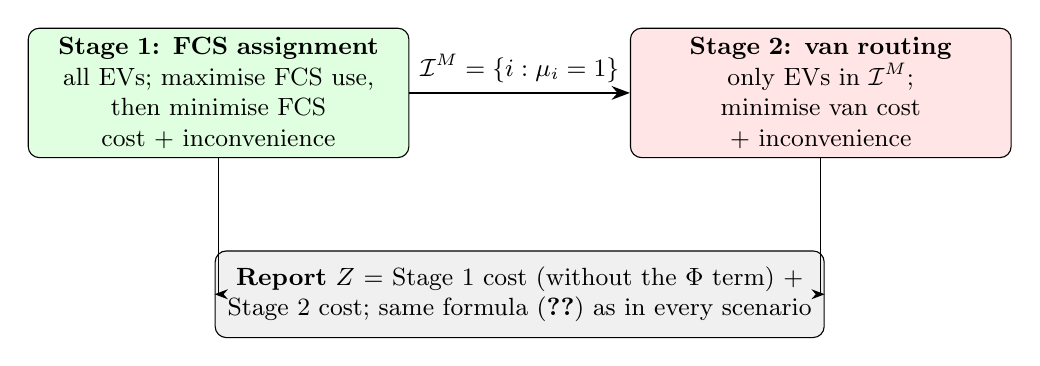
\begin{tikzpicture}[>=Stealth,box/.style={draw,rounded corners,align=center,minimum height=1.1cm,font=\small}]
  \node[box,fill=green!12,text width=4.6cm] (s1) {\textbf{Stage 1: FCS assignment}\\all EVs; maximise FCS use,\\then minimise FCS cost + inconvenience};
  \node[box,fill=red!10,text width=4.6cm,right=2.8cm of s1] (s2) {\textbf{Stage 2: van routing}\\only EVs in $\I^M$;\\minimise van cost + inconvenience};
  \draw[->,thick] (s1) -- node[above,font=\small]{$\I^M=\{i:\mu_i=1\}$} (s2);
  \node[box,fill=black!6,text width=7.5cm,below=2.0cm of $(s1)!0.5!(s2)$] (ev) {\textbf{Report} $Z=$ Stage~1 cost (without the $\Phi$ term) $+$ Stage~2 cost; same formula \eqref{eq:Z} as in every scenario};
  \draw[->] (s1) |- (ev); \draw[->] (s2) |- (ev);
\end{tikzpicture}
\end{center}

Stage~1 does not look at the vans, and Stage~2 cannot change what Stage~1 decided. That is the definition of ``FCS first, then MCS''.

%----------------------------------------------------------------
\subsection{Stage 1: assign EVs to fixed stations}

\textbf{Objective.}
\begin{equation}
\begin{split}
\min\ Z^{(1)}=\;&\underbrace{\Phi\sum_{i\in\I}\mu_i}_{\text{FCS first}}
+\underbrace{c^{EV}\sum_i\sum_{f\in\F_i}d_{if}Y_{if}}_{Z_1}
+\underbrace{Z^F_{\text{energy}}}_{\text{FCS part of }Z_4}\\
&+\underbrace{\sum_i\sum_{f\in\F_i}\rho^F_{if}Y_{if}+\alpha\sum_i w_i(C_i-r_i)+c^L\sum_i w_iL_i}_{\text{FCS customers' inconvenience}}
\end{split}
\label{eq:obj1}
\end{equation}
with $C_i=S_i+\tau^F_iY_i$ in this stage. $\Phi$ is a penalty for handing an EV to the vans. It is chosen larger than anything an extra FCS customer can add to the rest of \eqref{eq:obj1}, e.g.
\[
\Phi > \max_{i}\max_{f\in\F_i}\big(c^{EV}d_{if}+\pi^{\max}E_i+\rho^F_{if}\big)+n\,(\alpha+c^L)\,w_{\max}\,T,
\]
so Stage~1 first \textbf{maximises the number of EVs served at an FCS}, and only among those solutions minimises FCS cost and inconvenience. ($\pi^{\max}$ is the highest grid price.) A numerically safer equivalent is to solve twice: first $\max\sum_iY_i$, then fix that number and minimise the rest.
\ifTOU
Because $Z^F_{\text{energy}}$ uses the peak price, Stage~1 may \emph{start sessions later} to leave the peak, if the price saving beats the extra waiting cost (Section~\ref{sec:expect}).
\fi

\textbf{Constraints.}
\begin{align}
\sum_{g\in\G_i}y_{ig}+\mu_i &= 1 && \forall i\in\I \label{eq:s1assign}\\
S_i &\ge r_i+\sum_{f\in\F_i}t_{if}Y_{if} && \forall i\in\I \label{eq:fcsarr}\\
S_i &\le r_i+T\,(1-\mu_i) && \forall i\in\I \label{eq:s1park}\\
S_j &\ge S_i+\tau^F_i-(T+\tau^F_i)(3-y_{ig}-y_{jg}-o_{ij}) && \forall g,\ (i,j)\in\mathcal{P}_g \label{eq:disj1}\\
S_i &\ge S_j+\tau^F_j-(T+\tau^F_j)(2-y_{ig}-y_{jg}+o_{ij}) && \forall g,\ (i,j)\in\mathcal{P}_g \label{eq:disj2}\\
\sum_i y_{ig_1} &\ge \sum_i y_{ig_2} && \forall f,\ \G_f=\{g_1,g_2\} \label{eq:gunsym}\\
S_i+\tau^F_iY_i &\le T,\qquad L_i\ge S_i+\tau^F_iY_i-l_i && \forall i\in\I \label{eq:s1time}
\end{align}
\ifTOU plus the time-of-use split \eqref{eq:tou1}--\eqref{eq:tou5} of each FCS session (Section~\ref{sec:price}).\fi
\desc{\eqref{eq:s1assign}: every EV either gets one reachable gun or is handed to the vans. An EV that reaches no FCS ($\G_i=\emptyset$) is forced to $\mu_i=1$. \eqref{eq:fcsarr}: an FCS session cannot start before the EV has asked and driven to the station. \eqref{eq:s1park}: for an EV handed to the vans, $S_i$ is parked at $r_i$, so it adds no waiting in Stage~1 (its real start time is decided in Stage~2). \eqref{eq:disj1}--\eqref{eq:disj2}: two EVs on the same gun do not overlap; $o_{ij}$ picks who goes first. With two guns per station this means at most two EVs charge at a station at a time. \eqref{eq:gunsym}: symmetry breaking between the two identical guns (optional). \eqref{eq:s1time}: finished by $T$; lateness.}

\textbf{Optional acceptability rule.} An operator may refuse to send a driver to a station that is ``too inconvenient'', e.g.\ only allow gun $g$ of station $f$ for EV $i$ if $\hat\rho^F_{if}\le\bar\rho$. This only shrinks $\G_i$, so EVs whose stations are all too far go to the vans. Report results with and without it.

\textbf{Output:} $\I^M=\{i:\mu_i=1\}$, the EVs left for the vans; plus each FCS customer's gun and start time.

%----------------------------------------------------------------
\subsection{Stage 2: route the vans to the leftover EVs}

Stage~2 is a vehicle routing problem with time windows, on the EVs in $\I^M$ only. Here $C_i=S_i+\tau^M_i$.

\textbf{Objective.}
\begin{equation}
\begin{split}
\min\ Z^{(2)}=\;&\underbrace{c^M\sum_m\sum_{(i,j)\in\A^M}d_{ij}x_{ijm}}_{Z_2}+\underbrace{\sum_m c^D_mu_m}_{Z_3}+\underbrace{Z^M_{\text{energy}}}_{\text{van part of }Z_4}\\
&+\underbrace{\sum_{i\in\I^M}\sum_m\rho^M_{im}z_{im}+\alpha\sum_{i\in\I^M}w_i(C_i-r_i)+c^L\sum_{i\in\I^M}w_iL_i}_{\text{van customers' inconvenience}}
\end{split}
\label{eq:obj2}
\end{equation}
Since every EV in $\I^M$ must be served by some van, $Z^M_{\text{energy}}$ and the $\rho^M$ term are constants here. They are kept so that $Z^{(2)}$ is the true cost of Stage~2. Waiting and lateness make the vans visit urgent EVs early.

\textbf{Constraints.}
\begin{align}
\sum_{m\in\M}z_{im} &= 1 && \forall i\in\I^M \label{eq:s2assign}\\
\sum_{j:(0,j)\in\A^M}x_{0jm} = \sum_{i:(i,n+1)\in\A^M}x_{i,n+1,m} &= u_m && \forall m \label{eq:depot}\\
\sum_{i:(i,j)\in\A^M}x_{ijm} = \sum_{k:(j,k)\in\A^M}x_{jkm} &= z_{jm} && \forall j\in\I^M,\ m \label{eq:flow}\\
\sum_{i\in\I^M}z_{im} &\le Q_m\,u_m && \forall m \label{eq:cap}\\
\sum_{i\in\I^M}\frac{E_i}{\eta}z_{im}+\beta\sum_{(i,j)\in\A^M}d_{ij}x_{ijm} &\le B_m\,u_m && \forall m \label{eq:batt}
\end{align}
\begin{align}
S_j &\ge \max\{r_j,\ t_{0j}\,x_{0jm}\} && \forall j\in\I^M,\ m \label{eq:depart}\\
S_j &\ge S_i+\tau^M_i+t_{ij}-(T+\tau^M_i+t_{ij})(1-x_{ijm}) && \forall i\neq j,\ m \label{eq:seq}\\
S_i+\tau^M_i+t_{i,n+1} &\le T+(\tau^M_i+t_{i,n+1})(1-x_{i,n+1,m}) && \forall i,\ m \label{eq:return}\\
S_i+\tau^M_i \le T,\quad L_i &\ge S_i+\tau^M_i-l_i && \forall i\in\I^M \label{eq:s2time}\\
u_m &\ge u_{m+1} && m<|\M| \label{eq:vansym}
\end{align}
\desc{\eqref{eq:s2assign}: each leftover EV gets one van. \eqref{eq:depot}: a used van leaves and returns to the depot once. \eqref{eq:flow}: each EV on van $m$ is entered and left exactly once by that van. \eqref{eq:cap}: at most $Q_m$ EVs per van. \eqref{eq:batt}: delivered energy (with transfer losses) plus driving energy fits in the van battery. \eqref{eq:depart}: no start before the request, or before the van can drive there from the depot (written as two linear constraints). \eqref{eq:seq}: if the van goes $i\to j$, it finishes $i$ and drives to $j$ before starting $j$. This gives one EV at a time and removes subtours (MTZ-type). \eqref{eq:return}: back at the depot by $T$. \eqref{eq:s2time}: finished by $T$; lateness. \eqref{eq:vansym}: use identical vans in index order.}

\textbf{If Stage 2 is infeasible} (too many leftover EVs for the fleet by $T$), the sequential policy has \emph{failed} on that instance. For diagnosis, add $s_i\in\{0,1\}$ (``unserved''), replace \eqref{eq:s2assign} by $\sum_mz_{im}+s_i=1$ and add $\Phi^U\sum_is_i$ to \eqref{eq:obj2}. Then report the number of EVs that could not be served. This is a useful comparison with the integrated scenario, which may serve all of them.

%----------------------------------------------------------------
\subsection{Reported value}
\[
Z^{\text{S\scen}}=\big(Z^{(1)*}-\Phi\,|\I^M|\big)+Z^{(2)*},
\]
which is exactly \eqref{eq:Z} evaluated at the combined solution. The stage-1 solution plus the stage-2 solution is a feasible solution of the integrated model (S\ifTOU 4\else 3\fi), so
$Z^{\text{S\ifTOU 4\else 3\fi}}\le Z^{\text{S\scen}}$. The difference is the \emph{value of integration}.

\else
%---------------------------------------------------------------- INT
\subsection{Objective}
\begin{equation}
\min\ Z \quad\text{as in \eqref{eq:Z}, with }Z^F_{\text{energy}}=\ifTOU P^F\textstyle\sum_i\big[\pi^\off(\theta^1_i+\theta^3_i)+\pi^\pk\theta^2_i\big]\else\pi^F\textstyle\sum_iE_iY_i\fi,\quad C_i=S_i+\tau^F_iY_i+\tau^M_iZ_i. \label{eq:objint}
\end{equation}
Written out in full:
\begin{align*}
\min\ Z=\;& c^{EV}\sum_i\sum_{f\in\F_i}d_{if}Y_{if}+c^M\sum_m\sum_{(i,j)\in\A}d_{ij}x_{ijm}+\sum_mc^D_mu_m\\
&+\ifTOU P^F\sum_i\big[\pi^\off(\theta^1_i+\theta^3_i)+\pi^\pk\theta^2_i\big]\else\pi^F\sum_iE_iY_i\fi
+\pi^M\sum_i\sum_m\frac{E_i}{\eta}z_{im}\\
&+\sum_i\sum_{f\in\F_i}\rho^F_{if}Y_{if}+\sum_i\sum_m\rho^M_{im}z_{im}+\alpha\sum_iw_i(C_i-r_i)+c^L\sum_iw_iL_i .
\end{align*}
Every term is linear. One model weighs everything at once: an EV goes to a van exactly when the van's extra km, dispatch and energy cost are outweighed by the effort and waiting it saves the driver\ifTOU, or by the peak-price energy it avoids\fi.

\subsection{Constraints}

\textbf{Assignment.}
\begin{equation}
\sum_{g\in\G_i}y_{ig}+\sum_{m\in\M}z_{im}=1\qquad\forall i\in\I \label{eq:assign}
\end{equation}
\desc{Exactly one resource per EV: one reachable gun or one van. EVs that reach no FCS are forced onto a van.}

\textbf{Fixed stations.}
\begin{align}
S_i &\ge r_i+\sum_{f\in\F_i}t_{if}Y_{if} && \forall i \label{eq:fcsarr}\\
S_j &\ge S_i+\tau^F_i-(T+\tau^F_i)(3-y_{ig}-y_{jg}-o_{ij}) && \forall g,\ (i,j)\in\mathcal{P}_g \label{eq:disj1}\\
S_i &\ge S_j+\tau^F_j-(T+\tau^F_j)(2-y_{ig}-y_{jg}+o_{ij}) && \forall g,\ (i,j)\in\mathcal{P}_g \label{eq:disj2}\\
\sum_iy_{ig_1} &\ge \sum_iy_{ig_2} && \forall f,\ \G_f=\{g_1,g_2\} \label{eq:gunsym}
\end{align}
\desc{\eqref{eq:fcsarr}: an FCS session starts after the request and the drive to the station (for a van customer this is just $S_i\ge r_i$). \eqref{eq:disj1}--\eqref{eq:disj2}: EVs on the same gun do not overlap; $o_{ij}$ chooses the order. \eqref{eq:gunsym}: optional symmetry breaking.}

\textbf{Vans: routes, capacity, battery.}
\begin{align}
\sum_{j:(0,j)\in\A}x_{0jm}=\sum_{i:(i,n+1)\in\A}x_{i,n+1,m} &= u_m && \forall m \label{eq:depot}\\
\sum_{i:(i,j)\in\A}x_{ijm}=\sum_{k:(j,k)\in\A}x_{jkm} &= z_{jm} && \forall j\in\I,\ m \label{eq:flow}\\
\sum_iz_{im} &\le Q_mu_m && \forall m \label{eq:cap}\\
\sum_i\frac{E_i}{\eta}z_{im}+\beta\sum_{(i,j)\in\A}d_{ij}x_{ijm} &\le B_mu_m && \forall m \label{eq:batt}
\end{align}
\desc{\eqref{eq:depot}: a used van leaves and returns once. \eqref{eq:flow}: each EV on van $m$ is visited exactly once by it. \eqref{eq:cap}: at most $Q_m$ EVs. \eqref{eq:batt}: delivered energy (with losses) plus driving energy fits in the battery.}

\textbf{Vans: timing (one EV at a time, no subtours).}
\begin{align}
S_j &\ge t_{0j}\,x_{0jm} && \forall j\in\I,\ m \label{eq:depart}\\
S_j &\ge S_i+\tau^M_i+t_{ij}-(T+\tau^M_i+t_{ij})(1-x_{ijm}) && \forall i\neq j\in\I,\ m \label{eq:seq}\\
S_i+\tau^M_i+t_{i,n+1} &\le T+(\tau^M_i+t_{i,n+1})(1-x_{i,n+1,m}) && \forall i,\ m \label{eq:return}
\end{align}
\desc{\eqref{eq:depart}: the first stop cannot start before the van has driven there. \eqref{eq:seq}: $i\to j$ means finish $i$, drive, then start $j$; start times rise along a route, so no subtour can close. \eqref{eq:return}: back at the depot by $T$.}

\textbf{Horizon and lateness.}
\begin{equation}
C_i\le T,\qquad L_i\ge C_i-l_i\qquad\forall i\in\I \label{eq:time}
\end{equation}
\desc{Every EV is fully charged within the horizon; $L_i$ measures lateness.}

\ifTOU
\textbf{Time-of-use split.} Constraints \eqref{eq:tou1}--\eqref{eq:tou5} of Section~\ref{sec:price}.
\fi

\textbf{Symmetry and domains.}
\begin{equation}
u_m\ge u_{m+1};\qquad y,z,x,u,o\ifTOU,\kappa\fi\in\{0,1\};\qquad S_i,L_i\ifTOU,\theta^p_i\fi\ge0 \label{eq:dom}
\end{equation}
\fi

%=====================================================================
\section{Learning-to-optimise (RL) formulation}\label{sec:rl}

\textbf{Main rule:} the reward of each action is \emph{minus the increase in $Z$ that the action causes}. The rewards over an episode then add up to $-Z$ of the solution the policy builds. RL and MILP results are measured on the same yardstick \eqref{eq:Z}, and the MILP optimum is the benchmark for the RL gap.

\ifSEQ
%---------------------------------------------------------------- RL SEQ
The RL pipeline has the same two stages as the MILP.

\subsection{Stage 1 policy: FCS assignment}
\begin{itemize}[leftmargin=1.4em,itemsep=2pt]
  \item \textbf{Episode / epochs:} EVs are taken in order of request time $r_i$ (ties: higher $w_i$ first). One decision per EV.
  \item \textbf{State:} features of the current EV $k$ ($E_k,r_k,l_k,w_k,R_k$, location); for each gun $g$ the time $F_g$ it becomes free; summary features of the EVs still to come (count and positions near each station)\ifTOU; the current price and the time until $T_1$ and $T_2$\fi.
  \item \textbf{Action:} a gun $g\in\G_k$, or ``hand to vans''. \textbf{FCS-first mask:} ``hand to vans'' is allowed \emph{only} if no gun can finish EV $k$ by $T$ (or, with the optional rule, if all remaining guns have $\hat\rho^F_{kf}>\bar\rho$).
  \ifTOU\item \textbf{Optional timing action:} ``gun $g$, start after the peak'', i.e.\ $S_k=\max\{\text{earliest},T_2\}$, allowed only if the session still ends by $T$.\fi
  \item \textbf{Transition:} $S_k=\max\{r_k+t_{kf},F_g\}$ (or later, for the timing action); $F_g\leftarrow S_k+\tau^F_k$.
  \item \textbf{Reward:} $-\Big[c^{EV}d_{kf}+\text{energy}_k+\rho^F_{kf}+\alpha w_k(S_k+\tau^F_k-r_k)+c^Lw_k(S_k+\tau^F_k-l_k)^+\Big]$, where energy$_k$ = \ifTOU$P^F\big[\pi^\off\cdot(\text{off-peak hours of }[S_k,S_k+\tau^F_k])+\pi^\pk\cdot(\text{peak hours})\big]$, computed exactly in the simulator\else$\pi^FE_k$\fi. Handing an EV to the vans gives reward $0$ here; its cost is counted in Stage~2.
\end{itemize}
Note: a simple baseline for Stage~1 is the greedy rule ``gun with the largest one-step reward''. What RL can learn on top of this is, for example, to keep a nearby gun free for an urgent EV that arrives later.

\subsection{Stage 2 policy: van routing over $\I^M$}
\begin{itemize}[leftmargin=1.4em,itemsep=2pt]
  \item \textbf{Epochs:} whenever a van becomes free (the earliest-free van decides first).
  \item \textbf{State:} for each van: position, time free, remaining battery $b_m$, EVs served so far, dispatched or not; for each unserved EV in $\I^M$: location, $E_i,r_i,l_i,w_i$; current time.
  \item \textbf{Action:} the next EV $j$ for this van, or ``return to depot'' (ends the route). Mask: $j$ must be feasible: battery covers $E_j/\eta$ plus driving to $j$ and back to the depot, the count stays $\le Q_m$, and $j$ can be finished with the van back at the depot by $T$.
  \item \textbf{Transition:} $S_j=\max\{r_j,\ \text{time free}+t_{\text{pos},j}\}$; the van moves to $j$ and is free at $S_j+\tau^M_j$; $b_m$ falls by $E_j/\eta+\beta d_{\text{pos},j}$.
  \item \textbf{Reward:} serving $j$: $-\Big[c^Md_{\text{pos},j}+c^D_m[\text{first stop}]+\pi^M\frac{E_j}{\eta}+\rho^M_{jm}+\alpha w_j(S_j+\tau^M_j-r_j)+c^Lw_j(S_j+\tau^M_j-l_j)^+\Big]$; returning: $-c^Md_{\text{pos},0}$. EVs still unserved at the end: $-\Phi^U$ each.
  \item \textbf{Policy:} an attention-based routing policy (e.g.\ Kool et al., 2019, ``Attention, Learn to Solve Routing Problems!'') trained with REINFORCE or PPO. Baseline: nearest-feasible-EV heuristic.
\end{itemize}
Episode return of Stage~1 + Stage~2 $=-Z^{\text{S\scen}}$.

\else
%---------------------------------------------------------------- RL INT
One policy decides both who serves each EV and the van routes.
\begin{itemize}[leftmargin=1.4em,itemsep=2pt]
  \item \textbf{Episode / epochs:} EVs are taken in order of request time $r_i$ (ties: higher $w_i$ first). One decision per EV.
  \item \textbf{State:} (i) the current EV $k$: location, $E_k,r_k,l_k,w_k,R_k$, reachable stations; (ii) each gun $g$: time $F_g$ it becomes free; (iii) each van $m$: current end-of-route position, time free, remaining battery $b_m$, EVs served, dispatched or not; (iv) embeddings of the not-yet-assigned EVs (for look-ahead)\ifTOU; (v) current price, time until $T_1$ and $T_2$\fi.
  \item \textbf{Action:} $a\in\G_k\cup\M$: a gun, or a van (EV $k$ is appended to the end of that van's route). \textbf{Mask} infeasible actions: a gun that cannot finish $k$ by $T$; a van without enough battery for $E_k/\eta$ plus the drive to $k$ and back to the depot, with $Q_m$ reached, or unable to finish $k$ and return by $T$.
  \ifTOU\item \textbf{Optional timing action:} ``gun $g$, start after the peak'' ($S_k=\max\{\text{earliest},T_2\}$, if it still ends by $T$).\fi
  \item \textbf{Transition:} gun: $S_k=\max\{r_k+t_{kf},F_g\}$, $F_g\leftarrow S_k+\tau^F_k$. Van: $S_k=\max\{r_k,\ \text{free}_m+t_{\text{pos}_m,k}\}$, then the van moves to $k$, $\text{free}_m\leftarrow S_k+\tau^M_k$, $b_m\mathrel{-}=E_k/\eta+\beta d_{\text{pos}_m,k}$.
  \item \textbf{Reward} $=-\Delta Z$:
  \begin{align*}
  \text{gun } g\text{ at }f:&\quad -\Big[c^{EV}d_{kf}+\text{energy}^F_k+\rho^F_{kf}+\alpha w_k(C_k-r_k)+c^Lw_k(C_k-l_k)^+\Big]\\
  \text{van } m:&\quad -\Big[c^M\big(d_{\text{pos}_m,k}+d_{k,0}-d_{\text{pos}_m,0}\big)+c^D_m[\text{first use}]+\pi^M\tfrac{E_k}{\eta}\\
  &\qquad\quad+\rho^M_{km}+\alpha w_k(C_k-r_k)+c^Lw_k(C_k-l_k)^+\Big]
  \end{align*}
  The van distance term is the \emph{change} in route length when $k$ is inserted before the return to the depot, so the sum over the episode equals the total route length (the return legs telescope). energy$^F_k$ = \ifTOU$P^F\big[\pi^\off\cdot(\text{off-peak hours})+\pi^\pk\cdot(\text{peak hours of }[S_k,C_k])\big]$, computed exactly by the simulator; no linearisation is needed in RL\else$\pi^FE_k$\fi.
  \item \textbf{Dead end:} if every action is masked, EV $k$ is unserved: reward $-\Phi^U$, and the episode continues. Report the count.
  \item \textbf{Policy:} masked categorical policy over guns and vans, encoder with attention over EVs, guns and vans; trained with PPO. Natural baseline: greedy, i.e.\ choose the action with the largest one-step reward. That is the pairwise rule ``smallest $\hat\rho$ + cost'' from Section~\ref{sec:inc}.
\end{itemize}
Restriction to note: vans serve EVs in assignment order (append only). A variant that inserts $k$ at the cheapest position of a route is more flexible but has a larger action space.
\fi

\textbf{Reward scaling.} For stable training divide every reward by a constant, e.g.\ the greedy baseline's average $Z$ on the training instances. This does not change the optimal policy.

%=====================================================================
\section{What to expect and what to report}\label{sec:expect}

\ifnum\scen=1
\begin{itemize}[leftmargin=1.4em,itemsep=2pt]
  \item Vans serve only EVs that reach no station, or that the stations cannot finish by $T$. If stations have spare capacity, very few vans are dispatched.
  \item Inconvenience is high for EVs far from the nearest station (worked example: Rs\,682 at the FCS, against Rs\,458 if a van had been allowed).
  \item With too few vans Stage~2 becomes infeasible (unserved EVs), even when the integrated model S3 could serve everyone. Report the smallest $|\M|$ at which S1 is feasible and compare it with S3.
\end{itemize}
\fi
\ifnum\scen=2
\begin{itemize}[leftmargin=1.4em,itemsep=2pt]
  \item \textbf{When does Stage~1 delay a session to avoid the peak?} Moving one hour of charging out of the peak saves $(\pi^\pk-\pi^\off)P^F=3\times22=$ Rs\,66, but delays completion by up to an hour, which costs $\alpha w_i\ge$ Rs\,200. So with the default values Stage~1 almost never delays. It mostly pays the higher price, and S2 costs roughly S1 plus the peak surcharge. Sessions start later only if $\alpha$ is small (try $\lambda<0.33$ in the sensitivity analysis).
  \item The van assignment is the same as in S1 unless Stage~1's timing changes which EVs fit at the stations. Stage~1 cannot use vans to escape the peak price.
  \item Extra KPI: \textbf{grid energy drawn at FCS during the peak}, $P^F\sum_i\theta^2_i$ (kWh). Compare with S4.
\end{itemize}
\fi
\ifnum\scen=3
\begin{itemize}[leftmargin=1.4em,itemsep=2pt]
  \item Vans take EVs for which the saved inconvenience exceeds the extra van cost (worked example: van chosen, saving Rs\,224). Expect vans to serve EVs that are far from every station, have low range (high $w_i$), or have early deadlines, while EVs near a station still use it.
  \item \textbf{Value of integration under flat price:} $Z^{\text{S1}}-Z^{\text{S3}}\ge0$. Report it per component ($Z_1,\dots,Z_5$): typically operating cost rises a little and inconvenience falls a lot.
  \item Vary $|\M|$ (0, 1, 2, \dots): the first few vans lower $Z$ sharply, then the effect levels off. That curve shows the scenarios where mobile chargers help most.
\end{itemize}
\fi
\ifnum\scen=4
\begin{itemize}[leftmargin=1.4em,itemsep=2pt]
  \item During the peak a van kWh costs about the same as an FCS kWh (Rs\,10.0 each), so the vans' energy disadvantage disappears and vans also absorb \emph{peak-hour} demand that would otherwise be charged on the grid at peak price.
  \item Expect more van usage than in S3, concentrated on requests in $[T_1,T_2]$, and lower grid energy at the stations during the peak, $P^F\sum_i\theta^2_i$, than in S2.
  \item \textbf{Value of integration under peak pricing:} $Z^{\text{S2}}-Z^{\text{S4}}$. It should be larger than $Z^{\text{S1}}-Z^{\text{S3}}$, because integration now also allows price arbitrage.
  \item \textbf{Peak pricing with full flexibility:} $Z^{\text{S4}}-Z^{\text{S3}}$ should be smaller than $Z^{\text{S2}}-Z^{\text{S1}}$: vans cushion the price increase.
\end{itemize}
\fi

\textbf{Cross-scenario comparison table} (fill in from the four runs):
\begin{center}
\renewcommand{\arraystretch}{1.2}
\begin{tabular}{@{}lll@{}}
\toprule
\textbf{Comparison} & \textbf{Measures} & \textbf{Expected sign} \\
\midrule
S1 $-$ S3 & value of integration, flat price & $\ge0$ \\
S2 $-$ S4 & value of integration, peak price & $\ge0$, larger than S1 $-$ S3 \\
S2 $-$ S1 & cost of peak pricing, FCS-first operator & $>0$ \\
S4 $-$ S3 & cost of peak pricing, flexible operator & $>0$, smaller than S2 $-$ S1 \\
\bottomrule
\end{tabular}
\end{center}
Report for each: $Z$ and its components, number of vans used, EVs per resource, mean and maximum inconvenience per EV, total lateness, peak-hour grid energy, solve time, and (for RL) the gap to the MILP optimum.

%=====================================================================
\appendix
\section{Illustrative parameter values}\label{app:values}

These are starting values for experiments, not data. All are meant to be varied in the analysis. Values in Rs.

\begin{center}
\renewcommand{\arraystretch}{1.15}
\begin{tabular}{@{}llp{6.2cm}@{}}
\toprule
\textbf{Parameter} & \textbf{Value} & \textbf{Note} \\
\midrule
$T$, $[T_1,T_2]$ & 7 h, $[2,6]$ & 16:00--23:00, peak 18:00--22:00 \\
$P^F$, $P^M$ & 22 kW, 30 kW & \\
$v$, $\beta$, $\eta$ & 25 km/h, 0.25 kWh/km, 0.9 & \\
$B_m$, $Q_m$, $|\M|$ & 150 kWh, 6, 2--6 & \\
$c^{EV}$, $c^M$, $c^D_m$ & Rs\,4/km, Rs\,15/km, Rs\,1500 & van km includes driver time \\
$\pi^F$ (flat) & Rs\,8.7/kWh & equals the time-average of the ToU tariff over $[0,T]$ \\
$\pi^\off$, $\pi^\pk$ (ToU) & Rs\,7/kWh, Rs\,10/kWh & $(3\times7+4\times10)/7=8.7$ \\
$c^{bat}$ & Rs\,2/kWh & van battery wear \\
$\pi^M$ & Rs\,10.7 (flat) / Rs\,9.0 (ToU) & $=\pi^F+c^{bat}$ / $=\pi^\off+c^{bat}$ \\
$\alpha$, $\alpha^D$ & Rs\,200/h, Rs\,100/h & value of time; extra for attended time \\
$h^F$, $h^M$, $\varphi$ & Rs\,50, Rs\,10, Rs\,100 & trip hassle, hand-over, range stress \\
$c^L$ & Rs\,300/h & lateness \\
$w_i$ & $1+2(1-R_i/R_{\max})$, $R_i\sim U[3,40]$ km & priority from remaining range \\
\bottomrule
\end{tabular}
\end{center}

The flat price is set to the time-average of the peak tariff. The price \emph{level} is then the same in both pricing cases, and only the price \emph{shape} differs. Without this, part of S1 vs S2 would just reflect a different average price.

\end{document}
"
%    pdflatex -jobname=scenario4_peak_integrated   "\def\scen{4}% =====================================================================
%  One source, four PDFs.  Build with build.sh (or by hand):
%    pdflatex -jobname=scenario1_flat_sequential   "\def\scen{1}\input{scenario_master}"
%    pdflatex -jobname=scenario2_peak_sequential   "\def\scen{2}\input{scenario_master}"
%    pdflatex -jobname=scenario3_flat_integrated   "\def\scen{3}\input{scenario_master}"
%    pdflatex -jobname=scenario4_peak_integrated   "\def\scen{4}\input{scenario_master}"
%  (run each twice for cross-references)
% =====================================================================
\documentclass[11pt,a4paper]{article}
\usepackage[margin=2.2cm]{geometry}
\usepackage{amsmath,amssymb,amsfonts}
\usepackage{booktabs,array,tabularx}
\usepackage{enumitem}
\usepackage[table]{xcolor}
\usepackage{tikz}
\usetikzlibrary{arrows.meta,positioning,calc}
\usepackage[colorlinks=true,linkcolor=blue!50!black,urlcolor=blue!50!black]{hyperref}
\usepackage{titlesec}
\titleformat{\section}{\large\bfseries}{\thesection}{0.8em}{}
\titleformat{\subsection}{\normalsize\bfseries}{\thesubsection}{0.8em}{}
\setlength{\parindent}{0pt}
\setlength{\parskip}{5pt}

% ---------------- scenario switches ----------------
\ifdefined\scen\else\def\scen{1}\fi
\newif\ifTOU \TOUfalse   % true = time-of-use (peak) price
\newif\ifSEQ \SEQfalse   % true = FCS first, then MCS
\ifnum\scen=1 \SEQtrue \fi
\ifnum\scen=2 \TOUtrue \SEQtrue \fi
\ifnum\scen=4 \TOUtrue \fi

\newcommand{\pricename}{\ifTOU time-of-use price (dearer evening peak)\else single (flat) price all day\fi}
\newcommand{\structname}{\ifSEQ FCS first, then MCS (sequential)\else FCS and MCS together (integrated)\fi}

% ---------------- notation ----------------
\newcommand{\I}{\mathcal{I}}
\newcommand{\F}{\mathcal{F}}
\newcommand{\G}{\mathcal{G}}
\newcommand{\M}{\mathcal{M}}
\newcommand{\N}{\mathcal{N}}
\newcommand{\A}{\mathcal{A}}
\newcommand{\Rs}{\text{Rs}\,}
\newcommand{\pk}{\mathrm{pk}}
\newcommand{\off}{\mathrm{off}}
\newcommand{\desc}[1]{\par\vspace{-2pt}{\small\color{black!75}\textit{Meaning:} #1}\par\vspace{4pt}}
\newcommand{\cell}[2]{\ifnum\scen=#1\cellcolor{blue!18}\textbf{S#1 (this document)}\\\textbf{#2}\else S#1\\#2\fi}

\title{\textbf{EV Charging Network Optimisation}\\[4pt]
\large Scenario \scen: \pricename\ $+$ \structname\\[2pt]
\normalsize MILP and RL formulation}
\author{CP 320 OR for Mobility Management, course project}
\date{2 October 2026}

\begin{document}
\maketitle

%=====================================================================
\section{Where this scenario sits}

The project studies four scenarios: two ways of pricing grid electricity, times two ways of making the decisions.

\begin{center}
\renewcommand{\arraystretch}{1.5}
\begin{tabular}{>{\raggedright\arraybackslash}p{4.2cm}|>{\centering\arraybackslash}p{4.6cm}|>{\centering\arraybackslash}p{4.6cm}}
 & \textbf{Flat price all day} & \textbf{Time-of-use (peak) price} \\ \hline
\textbf{Sequential:} FCS first, leftover EVs to MCS &
\begin{tabular}[c]{@{}c@{}}\cell{1}{flat + sequential}\end{tabular} &
\begin{tabular}[c]{@{}c@{}}\cell{2}{peak + sequential}\end{tabular} \\ \hline
\textbf{Integrated:} FCS and MCS decided together &
\begin{tabular}[c]{@{}c@{}}\cell{3}{flat + integrated}\end{tabular} &
\begin{tabular}[c]{@{}c@{}}\cell{4}{peak + integrated}\end{tabular} \\
\end{tabular}
\end{center}

\textbf{The four scenarios do not have four different objectives.} They share \emph{one} cost yardstick $Z$ (Section~\ref{sec:obj}): the same cost terms and the same customer inconvenience (Section~\ref{sec:inc}). Only two things change:
\begin{itemize}[leftmargin=1.4em,itemsep=1pt]
  \item \textbf{Pricing} changes the formula for one term, the FCS energy cost (Section~\ref{sec:price}).
  \item \textbf{Decision structure} changes \emph{how} $Z$ is minimised: in one model (integrated), or in two stages (sequential), where each stage minimises its own part of $Z$.
\end{itemize}
Because the yardstick is the same, the four optimal values can be compared directly. The differences measure the \emph{value of integration} (S1$\to$S3, S2$\to$S4) and the \emph{effect of peak pricing} (S1$\to$S2, S3$\to$S4).

\ifnum\scen=1
\textbf{This scenario (S1)} is the baseline, the ``status quo''. Electricity costs the same at every hour, every EV that can be charged at a fixed station is sent there, and vans only take what is left over.
\fi
\ifnum\scen=2
\textbf{This scenario (S2)} keeps the FCS-first rule of S1, but grid electricity is dearer during the evening peak. Stage~1 can react to the price only by \emph{rescheduling} FCS sessions. It cannot hand a peak-hour EV to a van.
\fi
\ifnum\scen=3
\textbf{This scenario (S3)} keeps the flat price of S1, but the operator decides FCS and MCS service \emph{together}. An EV can be sent to a van even when a fixed station could take it, whenever that lowers total cost plus inconvenience.
\fi
\ifnum\scen=4
\textbf{This scenario (S4)} is the most flexible one: peak pricing at fixed stations, and FCS and MCS decided together. Van energy was bought off-peak, so vans can also be used to keep charging \emph{out of the expensive peak}.
\fi

%=====================================================================
\section{Setting and assumptions}\label{sec:setting}

\textbf{Time.} The planning horizon is $[0,T]$ with $T=7$\,h (16:00--23:00). It contains the evening peak window $[T_1,T_2]=[2,6]$ (18:00--22:00). The horizon is the same in all four scenarios. It is wider than the peak itself so that, under peak pricing, there is cheaper time on both sides of the peak.\ifTOU\else\ In this scenario the price is flat, so the window plays no role in the model.\fi

\textbf{Assumptions} (the same as MILP v3, plus two about energy):
\begin{enumerate}[leftmargin=1.6em,itemsep=1pt]
  \item Static, continuous time. All requests in the horizon are known at time $0$, and request $i$ becomes active at $r_i$.
  \item An EV served by an FCS drives there itself on its own battery (only to stations within its range $R_i$). The driver stays with the car while it waits for a free gun and while it charges.
  \item An EV served by an MCS stays parked where it is, and the driver is free in the meantime.
  \item Each FCS gun and each van charges one EV at a time, without interruption, at constant power.
  \item A van's battery covers both its driving and the energy it delivers. \textbf{The van battery is charged at the depot before the horizon starts}\ifTOU, i.e.\ at the off-peak price\fi, and is not recharged during the horizon.
  \item Every EV must be fully charged by $T$ (hard). Finishing after the driver's desired time $l_i$ is allowed but penalised.
\end{enumerate}

%=====================================================================
\section{Notation}\label{sec:notation}

\subsection*{Sets}
\begin{tabularx}{\textwidth}{@{}lX@{}}
\toprule
$\I=\{1,\dots,n\}$ & EV charging requests \\
$\F$; $\G_f$ ($|\G_f|=2$); $\G=\bigcup_f\G_f$ & fixed charging stations; guns of FCS $f$; all guns ($f(g)$ = station of gun $g$) \\
$\F_i=\{f: d_{if}\le R_i\}$, $\G_i=\bigcup_{f\in\F_i}\G_f$ & stations / guns EV $i$ can reach on its remaining range \\
$\M$ & mobile charging vans (MCS) \\
$0,\ n+1$ & depot as start node / end node (same place) \\
$\N=\{0\}\cup\I\cup\{n+1\}$, $\A$ & routing nodes; allowed van arcs $(i,j)$, $i\in\{0\}\cup\I$, $j\in\I\cup\{n+1\}$, $i\neq j$ \\
$\mathcal{P}_g=\{(i,j): i<j,\ g\in\G_i\cap\G_j\}$ & pairs of EVs that could share gun $g$ \\
\ifSEQ
$\I^M\subseteq\I$ & EVs handed to the vans by Stage~1 (an \emph{output} of Stage~1, a fixed input to Stage~2) \\
$\N^M$, $\A^M$ & routing nodes / arcs restricted to $\I^M$ \\
\fi
\bottomrule
\end{tabularx}

\subsection*{Parameters}
\begin{tabularx}{\textwidth}{@{}lX@{}}
\toprule
$E_i,\ r_i,\ l_i,\ R_i$ & energy demand (kWh), request time, desired completion time (h), remaining range (km) \\
$w_i\ge1$ & priority of EV $i$; $w_i=1+\kappa(1-R_i/R_{\max})$, so low-range EVs weigh more \\
$P^F,\ P^M$ & charging power of an FCS gun (22\,kW) / of a van (e.g.\ 30\,kW) \\
$\tau^F_i=E_i/P^F,\ \tau^M_i=E_i/P^M$ & charging time of EV $i$ at an FCS / by a van (h) \\
$d_{if},t_{if}$;\ $d_{ij},t_{ij}$ & distance (km) and time (h): EV$\to$FCS; between routing nodes ($t=d/v$) \\
$B_m,\ Q_m,\ \beta,\ \eta$ & van battery (kWh), max EVs per van, van consumption (kWh/km), transfer efficiency \\
$c^{EV},\ c^M,\ c^D_m$ & cost per km of EV driving, per km of van driving; fixed dispatch cost of van $m$ \\
\ifTOU
$\pi^\off,\ \pi^\pk$ & grid price (Rs/kWh) off-peak / in $[T_1,T_2]$, with $\pi^\pk\ge\pi^\off$ \\
\else
$\pi^F$ & grid price (Rs/kWh), the same at every hour \\
\fi
$c^{bat}$ & van battery wear per kWh cycled \\
$\pi^M$ & cost of 1 kWh taken from a van battery: $\pi^M=\ifTOU\pi^\off\else\pi^F\fi+c^{bat}$ (Section~\ref{sec:price}) \\
$\alpha,\ \alpha^D,\ h^F,\ h^M,\ \varphi,\ c^L$ & inconvenience coefficients (Section~\ref{sec:inc}) \\
\bottomrule
\end{tabularx}

\subsection*{Decision variables}
\begin{tabularx}{\textwidth}{@{}llX@{}}
\toprule
$y_{ig}$ & $\{0,1\}$ & EV $i$ charged at gun $g\in\G_i$ \\
$z_{im}$ & $\{0,1\}$ & EV $i$ served by van $m$ \\
$x_{ijm}$ & $\{0,1\}$ & van $m$ drives arc $(i,j)$ \\
$u_m$ & $\{0,1\}$ & van $m$ is dispatched \\
$o_{ij}$ & $\{0,1\}$ & for EVs $i<j$ that could share a gun: 1 if $i$ is charged before $j$ \\
\ifSEQ
$\mu_i$ & $\{0,1\}$ & Stage~1 only: EV $i$ is handed to the van fleet \\
\fi
\ifTOU
$\theta^1_i,\theta^2_i,\theta^3_i$ & $\ge0$ & hours of EV $i$'s FCS session before / inside / after the peak \\
$\kappa^1_i,\kappa^3_i$ & $\{0,1\}$ & EV $i$'s FCS session starts before $T_1$ / ends after $T_2$ \\
\fi
$S_i$ & $\ge0$ & time charging of EV $i$ starts (h), on whichever resource \\
$L_i$ & $\ge0$ & lateness of EV $i$ beyond $l_i$ (h) \\
\bottomrule
\end{tabularx}

\textbf{Short-hands} (linear expressions, not new variables):
\[
Y_{if}=\sum_{g\in\G_f}y_{ig},\qquad Y_i=\sum_{g\in\G_i}y_{ig}\ (\text{EV $i$ uses an FCS}),\qquad Z_i=\sum_{m\in\M}z_{im}\ (\text{EV $i$ uses a van}),
\]
\[
C_i=S_i+\tau^F_i\,Y_i+\tau^M_i\,Z_i \quad\text{(time EV $i$ is fully charged).}
\]

%=====================================================================
\section{Customer inconvenience}\label{sec:inc}

This section is \textbf{identical in all four scenario documents}. Inconvenience is a property of the customer, not of the price or of the planning method.

\subsection{What we mean by inconvenience}

Inconvenience is \emph{what the driver loses} from the moment they ask for a charge ($r_i$) until the car is fully charged ($C_i$), \emph{converted into rupees} so it can be added to the operator's costs. A driver loses three different things:

\begin{enumerate}[leftmargin=1.6em,itemsep=2pt]
  \item \textbf{Waiting:} the car is not ready. This lasts $C_i-r_i$ hours and affects \emph{every} driver, FCS or MCS.
  \item \textbf{Effort:} only an FCS customer has to drive to the station and sit there while the car charges. An MCS customer stays at home or at work and does something else. Driving to a far station also uses scarce battery range, which causes stress (``range anxiety'').
  \item \textbf{A missed deadline:} the car is still not ready at the time $l_i$ the driver needs it.
\end{enumerate}

Each loss gets a price in Rs per hour (or per event). All of them are multiplied by the priority $w_i$: an hour of delay for an EV with 5\,km of range left counts more than for one with 40\,km.

\subsection{The three components}

\begin{center}
\renewcommand{\arraystretch}{1.3}
\begin{tabularx}{\textwidth}{@{}>{\raggedright\arraybackslash}p{2.6cm}>{\raggedright\arraybackslash}X>{\raggedright\arraybackslash}X>{\raggedright\arraybackslash}p{3.0cm}@{}}
\toprule
\textbf{Component} & \textbf{EV $i$ at FCS $f$} & \textbf{EV $i$ by a van} & \textbf{Known when?} \\
\midrule
Effort & $w_i\big[\alpha^D(t_{if}+\tau^F_i)+h^F+\varphi\,d_{if}/R_i\big]$: driving and sitting at the station, a fixed trip hassle, range stress & $w_i\,h^M$: being reachable and handing over the car & \textbf{Static:} known as soon as the resource is chosen \\
Waiting & $w_i\,\alpha\,(C_i-r_i)$ = drive + \emph{queue at the gun} + charge & $w_i\,\alpha\,(C_i-r_i)$ = \emph{wait for the van} + charge & \textbf{Dynamic:} depends on the queue / van route \\
Missed deadline & $w_i\,c^L\,L_i$, $L_i=\max\{0,C_i-l_i\}$ & same & Dynamic \\
\bottomrule
\end{tabularx}
\end{center}

\textbf{Coefficients.}
$\alpha$ (Rs/h) is the value of an hour the car is not ready.
$\alpha^D$ (Rs/h) is the \emph{extra} value of an hour the driver must personally spend driving or sitting at the station: an hour at the station costs $\alpha+\alpha^D$, an hour waiting at home for a van costs only $\alpha$.
$h^F,h^M$ (Rs) are fixed hassle costs of one trip to a station / one van hand-over.
$\varphi$ (Rs) is the range-stress cost of a trip that uses the \emph{whole} remaining range ($d_{if}/R_i\le1$ is the fraction used).
$c^L$ (Rs/h) is the cost per hour late.

\subsection{Pairwise form: inconvenience of a (customer, resource) pair}

The natural first idea is: \emph{for every pair (EV $i$, FCS $f$) and every pair (EV $i$, van $m$) there is an inconvenience number, and the operator picks the pair with the lowest cost plus inconvenience.} The static part fits this idea exactly:
\[
\boxed{\;\rho^F_{if}=w_i\Big[\alpha^D\,(t_{if}+\tau^F_i)+h^F+\varphi\,\frac{d_{if}}{R_i}\Big]\qquad
\rho^M_{im}=w_i\,h^M\;}
\]
These are \textbf{parameters}, computed before solving, one number per (EV, FCS) pair and per (EV, van) pair. In the objective they appear linearly: $\sum_i\sum_f\rho^F_{if}Y_{if}+\sum_i\sum_m\rho^M_{im}z_{im}$.

Note that $\rho^M_{im}$ does not depend on $m$. Vans are identical and all start at the same depot, so the driver does not care \emph{which} van comes, only \emph{when} it comes. That ``when'' is the waiting part.

\subsection{Why waiting cannot be a fixed pairwise number}

It is tempting to also write the waiting as a pairwise number, e.g.\ ``the van needs 5 minutes to reach EV $i$''. But that depends on \emph{where the van is coming from}, which depends on the route the model is still choosing: if EV $i$ is the 4th stop of a van, the wait is the time for three charging sessions plus four drives. Likewise, waiting at an FCS depends on how many EVs are queued at that gun. So waiting is not known before solving. It is a function of decision variables:
\[
\text{waiting cost of EV } i \;=\; w_i\,\alpha\,(C_i-r_i),\qquad C_i=S_i+\tau^F_iY_i+\tau^M_iZ_i .
\]
This is \textbf{linear} in the variables ($S_i$, $y$, $z$), so it fits in a MILP directly. The constraints of Section~\ref{sec:milp} make $S_i$ equal to the true start time, including driving, queueing at the gun and the van's route. The term $\sum_i w_i\alpha r_i$ is a constant and may be dropped when solving.

\textbf{Pairwise \emph{estimate}} (used for intuition, by the RL policy and in heuristics): if there is no queue and the van comes straight to $i$,
\[
\hat\rho^{F}_{if}=\rho^F_{if}+w_i\alpha\,(t_{if}+\tau^F_i),\qquad
\hat\rho^{M}_{im}=\rho^M_{im}+w_i\alpha\,(t^{\text{van}}_{m\to i}+\tau^M_i),
\]
where $t^{\text{van}}_{m\to i}$ is the time until van $m$ can reach $i$ from where it currently is. In the RL formulation (Section~\ref{sec:rl}) the van's position \emph{is} known at each decision, so there this estimate becomes exact.

\subsection{Total inconvenience and how it enters the objective}

\begin{equation}
\boxed{\;
Z_{\text{inc}}=\underbrace{\sum_{i\in\I}\sum_{f\in\F_i}\rho^F_{if}Y_{if}+\sum_{i\in\I}\sum_{m\in\M}\rho^M_{im}z_{im}}_{\text{effort (static, pairwise)}}
+\underbrace{\alpha\sum_{i\in\I}w_i\,(C_i-r_i)}_{\text{waiting (dynamic)}}
+\underbrace{c^L\sum_{i\in\I}w_i\,L_i}_{\text{missed deadline}}
\;}\label{eq:inc}
\end{equation}
All three parts are in rupees, so $Z_{\text{inc}}$ is simply added to the operating costs. Nothing has to be normalised.

\subsection{Worked example: your ``10 km to the FCS vs.\ van in 5 minutes'' case}

EV $i$: $E_i=20$\,kWh, $R_i=40$\,km (so $w_i=1$); nearest free FCS $d_{if}=10$\,km away, $t_{if}=0.4$\,h at 25\,km/h; a van finishing next door can reach it in 5\,min ($0.083$\,h), adding about 4\,km to its route. $\tau^F_i=20/22=0.909$\,h, $\tau^M_i=20/30=0.667$\,h. Coefficients from Appendix~\ref{app:values}, flat price.

\begin{center}
\renewcommand{\arraystretch}{1.25}
\begin{tabular}{@{}lrr@{}}
\toprule
 & \textbf{FCS} & \textbf{Van} \\
\midrule
Driving (EV / extra van km) & $4\times10=40.0$ & $15\times4=60.0$ \\
Energy & $8.7\times20=174.0$ & $10.7\times20/0.9=237.8$ \\
\textbf{Operating cost only} & \textbf{214.0} & \textbf{297.8} \\
\midrule
Effort $\rho$ & $100(0.4+0.909)+50+100\cdot\tfrac{10}{40}=205.9$ & $10.0$ \\
Waiting $\alpha(C_i-r_i)$ & $200\times1.309=261.8$ & $200\times0.75=150.0$ \\
\textbf{Cost + inconvenience} & \textbf{681.7} & \textbf{457.8} \\
\bottomrule
\end{tabular}
\end{center}

On operating cost alone the FCS is cheaper, so a cost-only model would \emph{always} send this driver 10\,km away. With inconvenience included the van is better by about Rs\,224, and the integrated model chooses $z_{im}=1$, as you expected. If the FCS were only 1\,km away, the FCS would win both comparisons. The inconvenience term is what makes the model choose between ``cheap for the operator'' and ``convenient for the driver'', rather than following a fixed rule.

\subsection{Relation to a single penalty $\rho_i$ per EV}

The first draft used a penalty $\rho_i$ that is charged whenever EV $i$ goes to \emph{any} FCS: $\sum_i\sum_f\rho_iy_{if}$. Because $\sum_f y_{if}=1-\sum_m z_{im}$, this only says ``a van is worth $\rho_i$ more to EV $i$'', and that holds whether the station is 1\,km or 15\,km away, and whether the van arrives in 5 minutes or in 3 hours. The form above fixes both problems: $\rho^F_{if}$ grows with the distance to \emph{that} station, and the waiting term grows with how late the van or the free gun actually is. The old model is the special case $\alpha=\alpha^D=\varphi=c^L=0$, $h^F=\rho_i$.

\subsection{Choosing the coefficients}
\begin{itemize}[leftmargin=1.4em,itemsep=2pt]
  \item Use a value of time for $\alpha$ (e.g.\ Rs\,150--300/h for urban car users), and set $\alpha^D\approx0.5\alpha$: sitting at a station is worse than waiting at home.
  \item Keep $c^L>\alpha$, so missing the deadline is worse than ordinary waiting.
  \item \textbf{Sensitivity analysis:} multiply all inconvenience coefficients by a factor $\lambda\in\{0,0.25,0.5,1,2,4\}$ and plot operating cost against total inconvenience. $\lambda=0$ is the pure cost-minimising operator, and large $\lambda$ is a customer-first operator. This trade-off curve is a strong result for the ``Analysis'' part of the project.
\end{itemize}

\subsection{What inconvenience does in \emph{this} scenario}
\ifSEQ
In a sequential scenario inconvenience \textbf{cannot move an EV from an FCS to a van}: Stage~1 sends every EV that \emph{can} use an FCS to one. It still matters inside each stage. In Stage~1 it decides \emph{which} station and \emph{when} (urgent EVs get the near station and the first free gun). In Stage~2 it decides the \emph{order} in which vans visit EVs (urgent EVs first). In the worked example, this scenario sends the driver 10\,km to the FCS. That is the weakness the integrated scenarios remove.
\else
In an integrated scenario inconvenience is weighed directly against operating cost when choosing the resource. That is how the worked example ends up with a van. It also decides which station and which gun order, and the order of each van route.
\fi

%=====================================================================
\section{Electricity price in this scenario}\label{sec:price}

\textbf{Van energy (same in all scenarios).} A van's battery is charged at the depot \emph{before} the horizon, so its energy was bought at the
\ifTOU off-peak \fi
price, whatever time the van later delivers it. Each kWh taken from the van also wears the battery ($c^{bat}$), and a fraction $1-\eta$ is lost in transfer:
\[
Z^M_{\text{energy}}=\pi^M\sum_{i\in\I}\sum_{m\in\M}\frac{E_i}{\eta}\,z_{im},\qquad \pi^M=\ifTOU\pi^\off\else\pi^F\fi+c^{bat}.
\]

\ifTOU
\textbf{FCS energy (time-of-use).} An FCS draws from the grid while it charges. Energy delivered inside $[T_1,T_2]$ costs $\pi^\pk$, and energy outside it costs $\pi^\off$. A session $[S_i,S_i+\tau^F_i]$ may overlap the peak partly. Split its duration into the hours before, inside and after the peak, $\theta^1_i+\theta^2_i+\theta^3_i$:
\[
Z^F_{\text{energy}}=P^F\sum_{i\in\I}\Big[\pi^\off(\theta^1_i+\theta^3_i)+\pi^\pk\,\theta^2_i\Big].
\]
Constraints \eqref{eq:tou1}--\eqref{eq:tou5} below make the $\theta$'s equal to the true overlaps. Peak hours are dearer, so the solver wants $\theta^1_i,\theta^3_i$ as large as possible. It is enough to bound them from above by the true off-peak overlap, and the constraints need one binary per side:
\begin{align}
\theta^1_i+\theta^2_i+\theta^3_i &= \tau^F_i\,Y_i && \forall i\in\I \label{eq:tou1}\\
\theta^1_i &\le \tau^F_i\,\kappa^1_i && \forall i\in\I \label{eq:tou2}\\
\theta^1_i &\le T_1-S_i+T\,(1-\kappa^1_i) && \forall i\in\I \label{eq:tou3}\\
\theta^3_i &\le \tau^F_i\,\kappa^3_i && \forall i\in\I \label{eq:tou4}\\
\theta^3_i &\le S_i+\tau^F_i-T_2+T\,(1-\kappa^3_i) && \forall i\in\I \label{eq:tou5}
\end{align}
\desc{\eqref{eq:tou1}: the FCS session's hours are split into three parts; for a van customer ($Y_i=0$) all three are zero. \eqref{eq:tou2}--\eqref{eq:tou3}: off-peak time before the peak is only possible if the session starts before $T_1$ ($\kappa^1_i=1$), and is at most $T_1-S_i$. \eqref{eq:tou4}--\eqref{eq:tou5}: the same for time after $T_2$. $\theta^2_i\ge0$ prevents counting more off-peak hours than exist. Checking the cases (entirely before / inside / after the peak, straddling one edge, covering the whole peak) shows that at the optimum the $\theta$'s equal the exact overlaps. This needs $\pi^\pk\ge\pi^\off$, which is true for a peak tariff.}

\textbf{Why vans become more attractive.} Compare the cost of 1\,kWh delivered to an EV during the peak (values from Appendix~\ref{app:values}):
FCS $=\pi^\pk=$ Rs\,10.0, van $=(\pi^\off+c^{bat})/\eta=9/0.9=$ Rs\,10.0. They are at parity. Under the flat price the van is about Rs\,3.2/kWh dearer (FCS Rs\,8.7, van $10.7/0.9=$ Rs\,11.9). Peak pricing therefore removes the vans' main cost disadvantage, but only for EVs whose FCS session would fall in the peak.
\ifSEQ\ In this sequential scenario Stage~1 cannot use that, because it does not consider vans. It can only shift FCS sessions in time.\fi
\else
\textbf{FCS energy (flat).} Every kWh delivered at a fixed station costs $\pi^F$, whenever it is delivered:
\[
Z^F_{\text{energy}}=\pi^F\sum_{i\in\I}E_i\,Y_i .
\]
The start time therefore does not affect the energy cost. Under the flat price a van kWh costs $(\pi^F+c^{bat})/\eta\approx$ Rs\,11.9 against Rs\,8.7 at an FCS (Appendix~\ref{app:values}), so on energy alone the FCS always wins.
\fi

%=====================================================================
\section{MILP formulation}\label{sec:milp}

\subsection{The common cost yardstick $Z$}\label{sec:obj}

For any complete solution (every EV assigned, every route and start time known), the system cost is
\begin{equation}
\boxed{\;
Z=\underbrace{c^{EV}\sum_{i}\sum_{f\in\F_i}d_{if}Y_{if}}_{Z_1:\ \text{EV driving}}
+\underbrace{c^M\sum_{m}\sum_{(i,j)\in\A}d_{ij}x_{ijm}}_{Z_2:\ \text{van driving}}
+\underbrace{\sum_m c^D_m u_m}_{Z_3:\ \text{dispatch}}
+\underbrace{Z^F_{\text{energy}}+Z^M_{\text{energy}}}_{Z_4:\ \text{energy}}
+\underbrace{Z_{\text{inc}}}_{Z_5:\ \text{inconv.\ \eqref{eq:inc}}}
\;}\label{eq:Z}
\end{equation}
$Z_4$ is defined in Section~\ref{sec:price}. $Z_1$--$Z_4$ are the operator's costs listed in the brief (EV travel, MCS travel, MCS operating cost) plus energy. $Z_5$ is the customer inconvenience penalty. \textbf{The same formula is used to report results in all four scenarios.}

\ifSEQ
%---------------------------------------------------------------- SEQ
\subsection{Structure: two stages}

\begin{center}
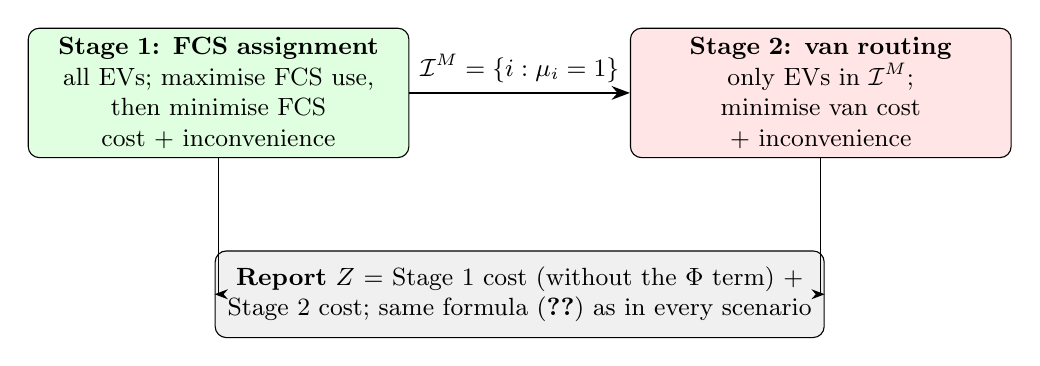
\begin{tikzpicture}[>=Stealth,box/.style={draw,rounded corners,align=center,minimum height=1.1cm,font=\small}]
  \node[box,fill=green!12,text width=4.6cm] (s1) {\textbf{Stage 1: FCS assignment}\\all EVs; maximise FCS use,\\then minimise FCS cost + inconvenience};
  \node[box,fill=red!10,text width=4.6cm,right=2.8cm of s1] (s2) {\textbf{Stage 2: van routing}\\only EVs in $\I^M$;\\minimise van cost + inconvenience};
  \draw[->,thick] (s1) -- node[above,font=\small]{$\I^M=\{i:\mu_i=1\}$} (s2);
  \node[box,fill=black!6,text width=7.5cm,below=2.0cm of $(s1)!0.5!(s2)$] (ev) {\textbf{Report} $Z=$ Stage~1 cost (without the $\Phi$ term) $+$ Stage~2 cost; same formula \eqref{eq:Z} as in every scenario};
  \draw[->] (s1) |- (ev); \draw[->] (s2) |- (ev);
\end{tikzpicture}
\end{center}

Stage~1 does not look at the vans, and Stage~2 cannot change what Stage~1 decided. That is the definition of ``FCS first, then MCS''.

%----------------------------------------------------------------
\subsection{Stage 1: assign EVs to fixed stations}

\textbf{Objective.}
\begin{equation}
\begin{split}
\min\ Z^{(1)}=\;&\underbrace{\Phi\sum_{i\in\I}\mu_i}_{\text{FCS first}}
+\underbrace{c^{EV}\sum_i\sum_{f\in\F_i}d_{if}Y_{if}}_{Z_1}
+\underbrace{Z^F_{\text{energy}}}_{\text{FCS part of }Z_4}\\
&+\underbrace{\sum_i\sum_{f\in\F_i}\rho^F_{if}Y_{if}+\alpha\sum_i w_i(C_i-r_i)+c^L\sum_i w_iL_i}_{\text{FCS customers' inconvenience}}
\end{split}
\label{eq:obj1}
\end{equation}
with $C_i=S_i+\tau^F_iY_i$ in this stage. $\Phi$ is a penalty for handing an EV to the vans. It is chosen larger than anything an extra FCS customer can add to the rest of \eqref{eq:obj1}, e.g.
\[
\Phi > \max_{i}\max_{f\in\F_i}\big(c^{EV}d_{if}+\pi^{\max}E_i+\rho^F_{if}\big)+n\,(\alpha+c^L)\,w_{\max}\,T,
\]
so Stage~1 first \textbf{maximises the number of EVs served at an FCS}, and only among those solutions minimises FCS cost and inconvenience. ($\pi^{\max}$ is the highest grid price.) A numerically safer equivalent is to solve twice: first $\max\sum_iY_i$, then fix that number and minimise the rest.
\ifTOU
Because $Z^F_{\text{energy}}$ uses the peak price, Stage~1 may \emph{start sessions later} to leave the peak, if the price saving beats the extra waiting cost (Section~\ref{sec:expect}).
\fi

\textbf{Constraints.}
\begin{align}
\sum_{g\in\G_i}y_{ig}+\mu_i &= 1 && \forall i\in\I \label{eq:s1assign}\\
S_i &\ge r_i+\sum_{f\in\F_i}t_{if}Y_{if} && \forall i\in\I \label{eq:fcsarr}\\
S_i &\le r_i+T\,(1-\mu_i) && \forall i\in\I \label{eq:s1park}\\
S_j &\ge S_i+\tau^F_i-(T+\tau^F_i)(3-y_{ig}-y_{jg}-o_{ij}) && \forall g,\ (i,j)\in\mathcal{P}_g \label{eq:disj1}\\
S_i &\ge S_j+\tau^F_j-(T+\tau^F_j)(2-y_{ig}-y_{jg}+o_{ij}) && \forall g,\ (i,j)\in\mathcal{P}_g \label{eq:disj2}\\
\sum_i y_{ig_1} &\ge \sum_i y_{ig_2} && \forall f,\ \G_f=\{g_1,g_2\} \label{eq:gunsym}\\
S_i+\tau^F_iY_i &\le T,\qquad L_i\ge S_i+\tau^F_iY_i-l_i && \forall i\in\I \label{eq:s1time}
\end{align}
\ifTOU plus the time-of-use split \eqref{eq:tou1}--\eqref{eq:tou5} of each FCS session (Section~\ref{sec:price}).\fi
\desc{\eqref{eq:s1assign}: every EV either gets one reachable gun or is handed to the vans. An EV that reaches no FCS ($\G_i=\emptyset$) is forced to $\mu_i=1$. \eqref{eq:fcsarr}: an FCS session cannot start before the EV has asked and driven to the station. \eqref{eq:s1park}: for an EV handed to the vans, $S_i$ is parked at $r_i$, so it adds no waiting in Stage~1 (its real start time is decided in Stage~2). \eqref{eq:disj1}--\eqref{eq:disj2}: two EVs on the same gun do not overlap; $o_{ij}$ picks who goes first. With two guns per station this means at most two EVs charge at a station at a time. \eqref{eq:gunsym}: symmetry breaking between the two identical guns (optional). \eqref{eq:s1time}: finished by $T$; lateness.}

\textbf{Optional acceptability rule.} An operator may refuse to send a driver to a station that is ``too inconvenient'', e.g.\ only allow gun $g$ of station $f$ for EV $i$ if $\hat\rho^F_{if}\le\bar\rho$. This only shrinks $\G_i$, so EVs whose stations are all too far go to the vans. Report results with and without it.

\textbf{Output:} $\I^M=\{i:\mu_i=1\}$, the EVs left for the vans; plus each FCS customer's gun and start time.

%----------------------------------------------------------------
\subsection{Stage 2: route the vans to the leftover EVs}

Stage~2 is a vehicle routing problem with time windows, on the EVs in $\I^M$ only. Here $C_i=S_i+\tau^M_i$.

\textbf{Objective.}
\begin{equation}
\begin{split}
\min\ Z^{(2)}=\;&\underbrace{c^M\sum_m\sum_{(i,j)\in\A^M}d_{ij}x_{ijm}}_{Z_2}+\underbrace{\sum_m c^D_mu_m}_{Z_3}+\underbrace{Z^M_{\text{energy}}}_{\text{van part of }Z_4}\\
&+\underbrace{\sum_{i\in\I^M}\sum_m\rho^M_{im}z_{im}+\alpha\sum_{i\in\I^M}w_i(C_i-r_i)+c^L\sum_{i\in\I^M}w_iL_i}_{\text{van customers' inconvenience}}
\end{split}
\label{eq:obj2}
\end{equation}
Since every EV in $\I^M$ must be served by some van, $Z^M_{\text{energy}}$ and the $\rho^M$ term are constants here. They are kept so that $Z^{(2)}$ is the true cost of Stage~2. Waiting and lateness make the vans visit urgent EVs early.

\textbf{Constraints.}
\begin{align}
\sum_{m\in\M}z_{im} &= 1 && \forall i\in\I^M \label{eq:s2assign}\\
\sum_{j:(0,j)\in\A^M}x_{0jm} = \sum_{i:(i,n+1)\in\A^M}x_{i,n+1,m} &= u_m && \forall m \label{eq:depot}\\
\sum_{i:(i,j)\in\A^M}x_{ijm} = \sum_{k:(j,k)\in\A^M}x_{jkm} &= z_{jm} && \forall j\in\I^M,\ m \label{eq:flow}\\
\sum_{i\in\I^M}z_{im} &\le Q_m\,u_m && \forall m \label{eq:cap}\\
\sum_{i\in\I^M}\frac{E_i}{\eta}z_{im}+\beta\sum_{(i,j)\in\A^M}d_{ij}x_{ijm} &\le B_m\,u_m && \forall m \label{eq:batt}
\end{align}
\begin{align}
S_j &\ge \max\{r_j,\ t_{0j}\,x_{0jm}\} && \forall j\in\I^M,\ m \label{eq:depart}\\
S_j &\ge S_i+\tau^M_i+t_{ij}-(T+\tau^M_i+t_{ij})(1-x_{ijm}) && \forall i\neq j,\ m \label{eq:seq}\\
S_i+\tau^M_i+t_{i,n+1} &\le T+(\tau^M_i+t_{i,n+1})(1-x_{i,n+1,m}) && \forall i,\ m \label{eq:return}\\
S_i+\tau^M_i \le T,\quad L_i &\ge S_i+\tau^M_i-l_i && \forall i\in\I^M \label{eq:s2time}\\
u_m &\ge u_{m+1} && m<|\M| \label{eq:vansym}
\end{align}
\desc{\eqref{eq:s2assign}: each leftover EV gets one van. \eqref{eq:depot}: a used van leaves and returns to the depot once. \eqref{eq:flow}: each EV on van $m$ is entered and left exactly once by that van. \eqref{eq:cap}: at most $Q_m$ EVs per van. \eqref{eq:batt}: delivered energy (with transfer losses) plus driving energy fits in the van battery. \eqref{eq:depart}: no start before the request, or before the van can drive there from the depot (written as two linear constraints). \eqref{eq:seq}: if the van goes $i\to j$, it finishes $i$ and drives to $j$ before starting $j$. This gives one EV at a time and removes subtours (MTZ-type). \eqref{eq:return}: back at the depot by $T$. \eqref{eq:s2time}: finished by $T$; lateness. \eqref{eq:vansym}: use identical vans in index order.}

\textbf{If Stage 2 is infeasible} (too many leftover EVs for the fleet by $T$), the sequential policy has \emph{failed} on that instance. For diagnosis, add $s_i\in\{0,1\}$ (``unserved''), replace \eqref{eq:s2assign} by $\sum_mz_{im}+s_i=1$ and add $\Phi^U\sum_is_i$ to \eqref{eq:obj2}. Then report the number of EVs that could not be served. This is a useful comparison with the integrated scenario, which may serve all of them.

%----------------------------------------------------------------
\subsection{Reported value}
\[
Z^{\text{S\scen}}=\big(Z^{(1)*}-\Phi\,|\I^M|\big)+Z^{(2)*},
\]
which is exactly \eqref{eq:Z} evaluated at the combined solution. The stage-1 solution plus the stage-2 solution is a feasible solution of the integrated model (S\ifTOU 4\else 3\fi), so
$Z^{\text{S\ifTOU 4\else 3\fi}}\le Z^{\text{S\scen}}$. The difference is the \emph{value of integration}.

\else
%---------------------------------------------------------------- INT
\subsection{Objective}
\begin{equation}
\min\ Z \quad\text{as in \eqref{eq:Z}, with }Z^F_{\text{energy}}=\ifTOU P^F\textstyle\sum_i\big[\pi^\off(\theta^1_i+\theta^3_i)+\pi^\pk\theta^2_i\big]\else\pi^F\textstyle\sum_iE_iY_i\fi,\quad C_i=S_i+\tau^F_iY_i+\tau^M_iZ_i. \label{eq:objint}
\end{equation}
Written out in full:
\begin{align*}
\min\ Z=\;& c^{EV}\sum_i\sum_{f\in\F_i}d_{if}Y_{if}+c^M\sum_m\sum_{(i,j)\in\A}d_{ij}x_{ijm}+\sum_mc^D_mu_m\\
&+\ifTOU P^F\sum_i\big[\pi^\off(\theta^1_i+\theta^3_i)+\pi^\pk\theta^2_i\big]\else\pi^F\sum_iE_iY_i\fi
+\pi^M\sum_i\sum_m\frac{E_i}{\eta}z_{im}\\
&+\sum_i\sum_{f\in\F_i}\rho^F_{if}Y_{if}+\sum_i\sum_m\rho^M_{im}z_{im}+\alpha\sum_iw_i(C_i-r_i)+c^L\sum_iw_iL_i .
\end{align*}
Every term is linear. One model weighs everything at once: an EV goes to a van exactly when the van's extra km, dispatch and energy cost are outweighed by the effort and waiting it saves the driver\ifTOU, or by the peak-price energy it avoids\fi.

\subsection{Constraints}

\textbf{Assignment.}
\begin{equation}
\sum_{g\in\G_i}y_{ig}+\sum_{m\in\M}z_{im}=1\qquad\forall i\in\I \label{eq:assign}
\end{equation}
\desc{Exactly one resource per EV: one reachable gun or one van. EVs that reach no FCS are forced onto a van.}

\textbf{Fixed stations.}
\begin{align}
S_i &\ge r_i+\sum_{f\in\F_i}t_{if}Y_{if} && \forall i \label{eq:fcsarr}\\
S_j &\ge S_i+\tau^F_i-(T+\tau^F_i)(3-y_{ig}-y_{jg}-o_{ij}) && \forall g,\ (i,j)\in\mathcal{P}_g \label{eq:disj1}\\
S_i &\ge S_j+\tau^F_j-(T+\tau^F_j)(2-y_{ig}-y_{jg}+o_{ij}) && \forall g,\ (i,j)\in\mathcal{P}_g \label{eq:disj2}\\
\sum_iy_{ig_1} &\ge \sum_iy_{ig_2} && \forall f,\ \G_f=\{g_1,g_2\} \label{eq:gunsym}
\end{align}
\desc{\eqref{eq:fcsarr}: an FCS session starts after the request and the drive to the station (for a van customer this is just $S_i\ge r_i$). \eqref{eq:disj1}--\eqref{eq:disj2}: EVs on the same gun do not overlap; $o_{ij}$ chooses the order. \eqref{eq:gunsym}: optional symmetry breaking.}

\textbf{Vans: routes, capacity, battery.}
\begin{align}
\sum_{j:(0,j)\in\A}x_{0jm}=\sum_{i:(i,n+1)\in\A}x_{i,n+1,m} &= u_m && \forall m \label{eq:depot}\\
\sum_{i:(i,j)\in\A}x_{ijm}=\sum_{k:(j,k)\in\A}x_{jkm} &= z_{jm} && \forall j\in\I,\ m \label{eq:flow}\\
\sum_iz_{im} &\le Q_mu_m && \forall m \label{eq:cap}\\
\sum_i\frac{E_i}{\eta}z_{im}+\beta\sum_{(i,j)\in\A}d_{ij}x_{ijm} &\le B_mu_m && \forall m \label{eq:batt}
\end{align}
\desc{\eqref{eq:depot}: a used van leaves and returns once. \eqref{eq:flow}: each EV on van $m$ is visited exactly once by it. \eqref{eq:cap}: at most $Q_m$ EVs. \eqref{eq:batt}: delivered energy (with losses) plus driving energy fits in the battery.}

\textbf{Vans: timing (one EV at a time, no subtours).}
\begin{align}
S_j &\ge t_{0j}\,x_{0jm} && \forall j\in\I,\ m \label{eq:depart}\\
S_j &\ge S_i+\tau^M_i+t_{ij}-(T+\tau^M_i+t_{ij})(1-x_{ijm}) && \forall i\neq j\in\I,\ m \label{eq:seq}\\
S_i+\tau^M_i+t_{i,n+1} &\le T+(\tau^M_i+t_{i,n+1})(1-x_{i,n+1,m}) && \forall i,\ m \label{eq:return}
\end{align}
\desc{\eqref{eq:depart}: the first stop cannot start before the van has driven there. \eqref{eq:seq}: $i\to j$ means finish $i$, drive, then start $j$; start times rise along a route, so no subtour can close. \eqref{eq:return}: back at the depot by $T$.}

\textbf{Horizon and lateness.}
\begin{equation}
C_i\le T,\qquad L_i\ge C_i-l_i\qquad\forall i\in\I \label{eq:time}
\end{equation}
\desc{Every EV is fully charged within the horizon; $L_i$ measures lateness.}

\ifTOU
\textbf{Time-of-use split.} Constraints \eqref{eq:tou1}--\eqref{eq:tou5} of Section~\ref{sec:price}.
\fi

\textbf{Symmetry and domains.}
\begin{equation}
u_m\ge u_{m+1};\qquad y,z,x,u,o\ifTOU,\kappa\fi\in\{0,1\};\qquad S_i,L_i\ifTOU,\theta^p_i\fi\ge0 \label{eq:dom}
\end{equation}
\fi

%=====================================================================
\section{Learning-to-optimise (RL) formulation}\label{sec:rl}

\textbf{Main rule:} the reward of each action is \emph{minus the increase in $Z$ that the action causes}. The rewards over an episode then add up to $-Z$ of the solution the policy builds. RL and MILP results are measured on the same yardstick \eqref{eq:Z}, and the MILP optimum is the benchmark for the RL gap.

\ifSEQ
%---------------------------------------------------------------- RL SEQ
The RL pipeline has the same two stages as the MILP.

\subsection{Stage 1 policy: FCS assignment}
\begin{itemize}[leftmargin=1.4em,itemsep=2pt]
  \item \textbf{Episode / epochs:} EVs are taken in order of request time $r_i$ (ties: higher $w_i$ first). One decision per EV.
  \item \textbf{State:} features of the current EV $k$ ($E_k,r_k,l_k,w_k,R_k$, location); for each gun $g$ the time $F_g$ it becomes free; summary features of the EVs still to come (count and positions near each station)\ifTOU; the current price and the time until $T_1$ and $T_2$\fi.
  \item \textbf{Action:} a gun $g\in\G_k$, or ``hand to vans''. \textbf{FCS-first mask:} ``hand to vans'' is allowed \emph{only} if no gun can finish EV $k$ by $T$ (or, with the optional rule, if all remaining guns have $\hat\rho^F_{kf}>\bar\rho$).
  \ifTOU\item \textbf{Optional timing action:} ``gun $g$, start after the peak'', i.e.\ $S_k=\max\{\text{earliest},T_2\}$, allowed only if the session still ends by $T$.\fi
  \item \textbf{Transition:} $S_k=\max\{r_k+t_{kf},F_g\}$ (or later, for the timing action); $F_g\leftarrow S_k+\tau^F_k$.
  \item \textbf{Reward:} $-\Big[c^{EV}d_{kf}+\text{energy}_k+\rho^F_{kf}+\alpha w_k(S_k+\tau^F_k-r_k)+c^Lw_k(S_k+\tau^F_k-l_k)^+\Big]$, where energy$_k$ = \ifTOU$P^F\big[\pi^\off\cdot(\text{off-peak hours of }[S_k,S_k+\tau^F_k])+\pi^\pk\cdot(\text{peak hours})\big]$, computed exactly in the simulator\else$\pi^FE_k$\fi. Handing an EV to the vans gives reward $0$ here; its cost is counted in Stage~2.
\end{itemize}
Note: a simple baseline for Stage~1 is the greedy rule ``gun with the largest one-step reward''. What RL can learn on top of this is, for example, to keep a nearby gun free for an urgent EV that arrives later.

\subsection{Stage 2 policy: van routing over $\I^M$}
\begin{itemize}[leftmargin=1.4em,itemsep=2pt]
  \item \textbf{Epochs:} whenever a van becomes free (the earliest-free van decides first).
  \item \textbf{State:} for each van: position, time free, remaining battery $b_m$, EVs served so far, dispatched or not; for each unserved EV in $\I^M$: location, $E_i,r_i,l_i,w_i$; current time.
  \item \textbf{Action:} the next EV $j$ for this van, or ``return to depot'' (ends the route). Mask: $j$ must be feasible: battery covers $E_j/\eta$ plus driving to $j$ and back to the depot, the count stays $\le Q_m$, and $j$ can be finished with the van back at the depot by $T$.
  \item \textbf{Transition:} $S_j=\max\{r_j,\ \text{time free}+t_{\text{pos},j}\}$; the van moves to $j$ and is free at $S_j+\tau^M_j$; $b_m$ falls by $E_j/\eta+\beta d_{\text{pos},j}$.
  \item \textbf{Reward:} serving $j$: $-\Big[c^Md_{\text{pos},j}+c^D_m[\text{first stop}]+\pi^M\frac{E_j}{\eta}+\rho^M_{jm}+\alpha w_j(S_j+\tau^M_j-r_j)+c^Lw_j(S_j+\tau^M_j-l_j)^+\Big]$; returning: $-c^Md_{\text{pos},0}$. EVs still unserved at the end: $-\Phi^U$ each.
  \item \textbf{Policy:} an attention-based routing policy (e.g.\ Kool et al., 2019, ``Attention, Learn to Solve Routing Problems!'') trained with REINFORCE or PPO. Baseline: nearest-feasible-EV heuristic.
\end{itemize}
Episode return of Stage~1 + Stage~2 $=-Z^{\text{S\scen}}$.

\else
%---------------------------------------------------------------- RL INT
One policy decides both who serves each EV and the van routes.
\begin{itemize}[leftmargin=1.4em,itemsep=2pt]
  \item \textbf{Episode / epochs:} EVs are taken in order of request time $r_i$ (ties: higher $w_i$ first). One decision per EV.
  \item \textbf{State:} (i) the current EV $k$: location, $E_k,r_k,l_k,w_k,R_k$, reachable stations; (ii) each gun $g$: time $F_g$ it becomes free; (iii) each van $m$: current end-of-route position, time free, remaining battery $b_m$, EVs served, dispatched or not; (iv) embeddings of the not-yet-assigned EVs (for look-ahead)\ifTOU; (v) current price, time until $T_1$ and $T_2$\fi.
  \item \textbf{Action:} $a\in\G_k\cup\M$: a gun, or a van (EV $k$ is appended to the end of that van's route). \textbf{Mask} infeasible actions: a gun that cannot finish $k$ by $T$; a van without enough battery for $E_k/\eta$ plus the drive to $k$ and back to the depot, with $Q_m$ reached, or unable to finish $k$ and return by $T$.
  \ifTOU\item \textbf{Optional timing action:} ``gun $g$, start after the peak'' ($S_k=\max\{\text{earliest},T_2\}$, if it still ends by $T$).\fi
  \item \textbf{Transition:} gun: $S_k=\max\{r_k+t_{kf},F_g\}$, $F_g\leftarrow S_k+\tau^F_k$. Van: $S_k=\max\{r_k,\ \text{free}_m+t_{\text{pos}_m,k}\}$, then the van moves to $k$, $\text{free}_m\leftarrow S_k+\tau^M_k$, $b_m\mathrel{-}=E_k/\eta+\beta d_{\text{pos}_m,k}$.
  \item \textbf{Reward} $=-\Delta Z$:
  \begin{align*}
  \text{gun } g\text{ at }f:&\quad -\Big[c^{EV}d_{kf}+\text{energy}^F_k+\rho^F_{kf}+\alpha w_k(C_k-r_k)+c^Lw_k(C_k-l_k)^+\Big]\\
  \text{van } m:&\quad -\Big[c^M\big(d_{\text{pos}_m,k}+d_{k,0}-d_{\text{pos}_m,0}\big)+c^D_m[\text{first use}]+\pi^M\tfrac{E_k}{\eta}\\
  &\qquad\quad+\rho^M_{km}+\alpha w_k(C_k-r_k)+c^Lw_k(C_k-l_k)^+\Big]
  \end{align*}
  The van distance term is the \emph{change} in route length when $k$ is inserted before the return to the depot, so the sum over the episode equals the total route length (the return legs telescope). energy$^F_k$ = \ifTOU$P^F\big[\pi^\off\cdot(\text{off-peak hours})+\pi^\pk\cdot(\text{peak hours of }[S_k,C_k])\big]$, computed exactly by the simulator; no linearisation is needed in RL\else$\pi^FE_k$\fi.
  \item \textbf{Dead end:} if every action is masked, EV $k$ is unserved: reward $-\Phi^U$, and the episode continues. Report the count.
  \item \textbf{Policy:} masked categorical policy over guns and vans, encoder with attention over EVs, guns and vans; trained with PPO. Natural baseline: greedy, i.e.\ choose the action with the largest one-step reward. That is the pairwise rule ``smallest $\hat\rho$ + cost'' from Section~\ref{sec:inc}.
\end{itemize}
Restriction to note: vans serve EVs in assignment order (append only). A variant that inserts $k$ at the cheapest position of a route is more flexible but has a larger action space.
\fi

\textbf{Reward scaling.} For stable training divide every reward by a constant, e.g.\ the greedy baseline's average $Z$ on the training instances. This does not change the optimal policy.

%=====================================================================
\section{What to expect and what to report}\label{sec:expect}

\ifnum\scen=1
\begin{itemize}[leftmargin=1.4em,itemsep=2pt]
  \item Vans serve only EVs that reach no station, or that the stations cannot finish by $T$. If stations have spare capacity, very few vans are dispatched.
  \item Inconvenience is high for EVs far from the nearest station (worked example: Rs\,682 at the FCS, against Rs\,458 if a van had been allowed).
  \item With too few vans Stage~2 becomes infeasible (unserved EVs), even when the integrated model S3 could serve everyone. Report the smallest $|\M|$ at which S1 is feasible and compare it with S3.
\end{itemize}
\fi
\ifnum\scen=2
\begin{itemize}[leftmargin=1.4em,itemsep=2pt]
  \item \textbf{When does Stage~1 delay a session to avoid the peak?} Moving one hour of charging out of the peak saves $(\pi^\pk-\pi^\off)P^F=3\times22=$ Rs\,66, but delays completion by up to an hour, which costs $\alpha w_i\ge$ Rs\,200. So with the default values Stage~1 almost never delays. It mostly pays the higher price, and S2 costs roughly S1 plus the peak surcharge. Sessions start later only if $\alpha$ is small (try $\lambda<0.33$ in the sensitivity analysis).
  \item The van assignment is the same as in S1 unless Stage~1's timing changes which EVs fit at the stations. Stage~1 cannot use vans to escape the peak price.
  \item Extra KPI: \textbf{grid energy drawn at FCS during the peak}, $P^F\sum_i\theta^2_i$ (kWh). Compare with S4.
\end{itemize}
\fi
\ifnum\scen=3
\begin{itemize}[leftmargin=1.4em,itemsep=2pt]
  \item Vans take EVs for which the saved inconvenience exceeds the extra van cost (worked example: van chosen, saving Rs\,224). Expect vans to serve EVs that are far from every station, have low range (high $w_i$), or have early deadlines, while EVs near a station still use it.
  \item \textbf{Value of integration under flat price:} $Z^{\text{S1}}-Z^{\text{S3}}\ge0$. Report it per component ($Z_1,\dots,Z_5$): typically operating cost rises a little and inconvenience falls a lot.
  \item Vary $|\M|$ (0, 1, 2, \dots): the first few vans lower $Z$ sharply, then the effect levels off. That curve shows the scenarios where mobile chargers help most.
\end{itemize}
\fi
\ifnum\scen=4
\begin{itemize}[leftmargin=1.4em,itemsep=2pt]
  \item During the peak a van kWh costs about the same as an FCS kWh (Rs\,10.0 each), so the vans' energy disadvantage disappears and vans also absorb \emph{peak-hour} demand that would otherwise be charged on the grid at peak price.
  \item Expect more van usage than in S3, concentrated on requests in $[T_1,T_2]$, and lower grid energy at the stations during the peak, $P^F\sum_i\theta^2_i$, than in S2.
  \item \textbf{Value of integration under peak pricing:} $Z^{\text{S2}}-Z^{\text{S4}}$. It should be larger than $Z^{\text{S1}}-Z^{\text{S3}}$, because integration now also allows price arbitrage.
  \item \textbf{Peak pricing with full flexibility:} $Z^{\text{S4}}-Z^{\text{S3}}$ should be smaller than $Z^{\text{S2}}-Z^{\text{S1}}$: vans cushion the price increase.
\end{itemize}
\fi

\textbf{Cross-scenario comparison table} (fill in from the four runs):
\begin{center}
\renewcommand{\arraystretch}{1.2}
\begin{tabular}{@{}lll@{}}
\toprule
\textbf{Comparison} & \textbf{Measures} & \textbf{Expected sign} \\
\midrule
S1 $-$ S3 & value of integration, flat price & $\ge0$ \\
S2 $-$ S4 & value of integration, peak price & $\ge0$, larger than S1 $-$ S3 \\
S2 $-$ S1 & cost of peak pricing, FCS-first operator & $>0$ \\
S4 $-$ S3 & cost of peak pricing, flexible operator & $>0$, smaller than S2 $-$ S1 \\
\bottomrule
\end{tabular}
\end{center}
Report for each: $Z$ and its components, number of vans used, EVs per resource, mean and maximum inconvenience per EV, total lateness, peak-hour grid energy, solve time, and (for RL) the gap to the MILP optimum.

%=====================================================================
\appendix
\section{Illustrative parameter values}\label{app:values}

These are starting values for experiments, not data. All are meant to be varied in the analysis. Values in Rs.

\begin{center}
\renewcommand{\arraystretch}{1.15}
\begin{tabular}{@{}llp{6.2cm}@{}}
\toprule
\textbf{Parameter} & \textbf{Value} & \textbf{Note} \\
\midrule
$T$, $[T_1,T_2]$ & 7 h, $[2,6]$ & 16:00--23:00, peak 18:00--22:00 \\
$P^F$, $P^M$ & 22 kW, 30 kW & \\
$v$, $\beta$, $\eta$ & 25 km/h, 0.25 kWh/km, 0.9 & \\
$B_m$, $Q_m$, $|\M|$ & 150 kWh, 6, 2--6 & \\
$c^{EV}$, $c^M$, $c^D_m$ & Rs\,4/km, Rs\,15/km, Rs\,1500 & van km includes driver time \\
$\pi^F$ (flat) & Rs\,8.7/kWh & equals the time-average of the ToU tariff over $[0,T]$ \\
$\pi^\off$, $\pi^\pk$ (ToU) & Rs\,7/kWh, Rs\,10/kWh & $(3\times7+4\times10)/7=8.7$ \\
$c^{bat}$ & Rs\,2/kWh & van battery wear \\
$\pi^M$ & Rs\,10.7 (flat) / Rs\,9.0 (ToU) & $=\pi^F+c^{bat}$ / $=\pi^\off+c^{bat}$ \\
$\alpha$, $\alpha^D$ & Rs\,200/h, Rs\,100/h & value of time; extra for attended time \\
$h^F$, $h^M$, $\varphi$ & Rs\,50, Rs\,10, Rs\,100 & trip hassle, hand-over, range stress \\
$c^L$ & Rs\,300/h & lateness \\
$w_i$ & $1+2(1-R_i/R_{\max})$, $R_i\sim U[3,40]$ km & priority from remaining range \\
\bottomrule
\end{tabular}
\end{center}

The flat price is set to the time-average of the peak tariff. The price \emph{level} is then the same in both pricing cases, and only the price \emph{shape} differs. Without this, part of S1 vs S2 would just reflect a different average price.

\end{document}
"
%  (run each twice for cross-references)
% =====================================================================
\documentclass[11pt,a4paper]{article}
\usepackage[margin=2.2cm]{geometry}
\usepackage{amsmath,amssymb,amsfonts}
\usepackage{booktabs,array,tabularx}
\usepackage{enumitem}
\usepackage[table]{xcolor}
\usepackage{tikz}
\usetikzlibrary{arrows.meta,positioning,calc}
\usepackage[colorlinks=true,linkcolor=blue!50!black,urlcolor=blue!50!black]{hyperref}
\usepackage{titlesec}
\titleformat{\section}{\large\bfseries}{\thesection}{0.8em}{}
\titleformat{\subsection}{\normalsize\bfseries}{\thesubsection}{0.8em}{}
\setlength{\parindent}{0pt}
\setlength{\parskip}{5pt}

% ---------------- scenario switches ----------------
\ifdefined\scen\else\def\scen{1}\fi
\newif\ifTOU \TOUfalse   % true = time-of-use (peak) price
\newif\ifSEQ \SEQfalse   % true = FCS first, then MCS
\ifnum\scen=1 \SEQtrue \fi
\ifnum\scen=2 \TOUtrue \SEQtrue \fi
\ifnum\scen=4 \TOUtrue \fi

\newcommand{\pricename}{\ifTOU time-of-use price (dearer evening peak)\else single (flat) price all day\fi}
\newcommand{\structname}{\ifSEQ FCS first, then MCS (sequential)\else FCS and MCS together (integrated)\fi}

% ---------------- notation ----------------
\newcommand{\I}{\mathcal{I}}
\newcommand{\F}{\mathcal{F}}
\newcommand{\G}{\mathcal{G}}
\newcommand{\M}{\mathcal{M}}
\newcommand{\N}{\mathcal{N}}
\newcommand{\A}{\mathcal{A}}
\newcommand{\Rs}{\text{Rs}\,}
\newcommand{\pk}{\mathrm{pk}}
\newcommand{\off}{\mathrm{off}}
\newcommand{\desc}[1]{\par\vspace{-2pt}{\small\color{black!75}\textit{Meaning:} #1}\par\vspace{4pt}}
\newcommand{\cell}[2]{\ifnum\scen=#1\cellcolor{blue!18}\textbf{S#1 (this document)}\\\textbf{#2}\else S#1\\#2\fi}

\title{\textbf{EV Charging Network Optimisation}\\[4pt]
\large Scenario \scen: \pricename\ $+$ \structname\\[2pt]
\normalsize MILP and RL formulation}
\author{CP 320 OR for Mobility Management, course project}
\date{2 October 2026}

\begin{document}
\maketitle

%=====================================================================
\section{Where this scenario sits}

The project studies four scenarios: two ways of pricing grid electricity, times two ways of making the decisions.

\begin{center}
\renewcommand{\arraystretch}{1.5}
\begin{tabular}{>{\raggedright\arraybackslash}p{4.2cm}|>{\centering\arraybackslash}p{4.6cm}|>{\centering\arraybackslash}p{4.6cm}}
 & \textbf{Flat price all day} & \textbf{Time-of-use (peak) price} \\ \hline
\textbf{Sequential:} FCS first, leftover EVs to MCS &
\begin{tabular}[c]{@{}c@{}}\cell{1}{flat + sequential}\end{tabular} &
\begin{tabular}[c]{@{}c@{}}\cell{2}{peak + sequential}\end{tabular} \\ \hline
\textbf{Integrated:} FCS and MCS decided together &
\begin{tabular}[c]{@{}c@{}}\cell{3}{flat + integrated}\end{tabular} &
\begin{tabular}[c]{@{}c@{}}\cell{4}{peak + integrated}\end{tabular} \\
\end{tabular}
\end{center}

\textbf{The four scenarios do not have four different objectives.} They share \emph{one} cost yardstick $Z$ (Section~\ref{sec:obj}): the same cost terms and the same customer inconvenience (Section~\ref{sec:inc}). Only two things change:
\begin{itemize}[leftmargin=1.4em,itemsep=1pt]
  \item \textbf{Pricing} changes the formula for one term, the FCS energy cost (Section~\ref{sec:price}).
  \item \textbf{Decision structure} changes \emph{how} $Z$ is minimised: in one model (integrated), or in two stages (sequential), where each stage minimises its own part of $Z$.
\end{itemize}
Because the yardstick is the same, the four optimal values can be compared directly. The differences measure the \emph{value of integration} (S1$\to$S3, S2$\to$S4) and the \emph{effect of peak pricing} (S1$\to$S2, S3$\to$S4).

\ifnum\scen=1
\textbf{This scenario (S1)} is the baseline, the ``status quo''. Electricity costs the same at every hour, every EV that can be charged at a fixed station is sent there, and vans only take what is left over.
\fi
\ifnum\scen=2
\textbf{This scenario (S2)} keeps the FCS-first rule of S1, but grid electricity is dearer during the evening peak. Stage~1 can react to the price only by \emph{rescheduling} FCS sessions. It cannot hand a peak-hour EV to a van.
\fi
\ifnum\scen=3
\textbf{This scenario (S3)} keeps the flat price of S1, but the operator decides FCS and MCS service \emph{together}. An EV can be sent to a van even when a fixed station could take it, whenever that lowers total cost plus inconvenience.
\fi
\ifnum\scen=4
\textbf{This scenario (S4)} is the most flexible one: peak pricing at fixed stations, and FCS and MCS decided together. Van energy was bought off-peak, so vans can also be used to keep charging \emph{out of the expensive peak}.
\fi

%=====================================================================
\section{Setting and assumptions}\label{sec:setting}

\textbf{Time.} The planning horizon is $[0,T]$ with $T=7$\,h (16:00--23:00). It contains the evening peak window $[T_1,T_2]=[2,6]$ (18:00--22:00). The horizon is the same in all four scenarios. It is wider than the peak itself so that, under peak pricing, there is cheaper time on both sides of the peak.\ifTOU\else\ In this scenario the price is flat, so the window plays no role in the model.\fi

\textbf{Assumptions} (the same as MILP v3, plus two about energy):
\begin{enumerate}[leftmargin=1.6em,itemsep=1pt]
  \item Static, continuous time. All requests in the horizon are known at time $0$, and request $i$ becomes active at $r_i$.
  \item An EV served by an FCS drives there itself on its own battery (only to stations within its range $R_i$). The driver stays with the car while it waits for a free gun and while it charges.
  \item An EV served by an MCS stays parked where it is, and the driver is free in the meantime.
  \item Each FCS gun and each van charges one EV at a time, without interruption, at constant power.
  \item A van's battery covers both its driving and the energy it delivers. \textbf{The van battery is charged at the depot before the horizon starts}\ifTOU, i.e.\ at the off-peak price\fi, and is not recharged during the horizon.
  \item Every EV must be fully charged by $T$ (hard). Finishing after the driver's desired time $l_i$ is allowed but penalised.
\end{enumerate}

%=====================================================================
\section{Notation}\label{sec:notation}

\subsection*{Sets}
\begin{tabularx}{\textwidth}{@{}lX@{}}
\toprule
$\I=\{1,\dots,n\}$ & EV charging requests \\
$\F$; $\G_f$ ($|\G_f|=2$); $\G=\bigcup_f\G_f$ & fixed charging stations; guns of FCS $f$; all guns ($f(g)$ = station of gun $g$) \\
$\F_i=\{f: d_{if}\le R_i\}$, $\G_i=\bigcup_{f\in\F_i}\G_f$ & stations / guns EV $i$ can reach on its remaining range \\
$\M$ & mobile charging vans (MCS) \\
$0,\ n+1$ & depot as start node / end node (same place) \\
$\N=\{0\}\cup\I\cup\{n+1\}$, $\A$ & routing nodes; allowed van arcs $(i,j)$, $i\in\{0\}\cup\I$, $j\in\I\cup\{n+1\}$, $i\neq j$ \\
$\mathcal{P}_g=\{(i,j): i<j,\ g\in\G_i\cap\G_j\}$ & pairs of EVs that could share gun $g$ \\
\ifSEQ
$\I^M\subseteq\I$ & EVs handed to the vans by Stage~1 (an \emph{output} of Stage~1, a fixed input to Stage~2) \\
$\N^M$, $\A^M$ & routing nodes / arcs restricted to $\I^M$ \\
\fi
\bottomrule
\end{tabularx}

\subsection*{Parameters}
\begin{tabularx}{\textwidth}{@{}lX@{}}
\toprule
$E_i,\ r_i,\ l_i,\ R_i$ & energy demand (kWh), request time, desired completion time (h), remaining range (km) \\
$w_i\ge1$ & priority of EV $i$; $w_i=1+\kappa(1-R_i/R_{\max})$, so low-range EVs weigh more \\
$P^F,\ P^M$ & charging power of an FCS gun (22\,kW) / of a van (e.g.\ 30\,kW) \\
$\tau^F_i=E_i/P^F,\ \tau^M_i=E_i/P^M$ & charging time of EV $i$ at an FCS / by a van (h) \\
$d_{if},t_{if}$;\ $d_{ij},t_{ij}$ & distance (km) and time (h): EV$\to$FCS; between routing nodes ($t=d/v$) \\
$B_m,\ Q_m,\ \beta,\ \eta$ & van battery (kWh), max EVs per van, van consumption (kWh/km), transfer efficiency \\
$c^{EV},\ c^M,\ c^D_m$ & cost per km of EV driving, per km of van driving; fixed dispatch cost of van $m$ \\
\ifTOU
$\pi^\off,\ \pi^\pk$ & grid price (Rs/kWh) off-peak / in $[T_1,T_2]$, with $\pi^\pk\ge\pi^\off$ \\
\else
$\pi^F$ & grid price (Rs/kWh), the same at every hour \\
\fi
$c^{bat}$ & van battery wear per kWh cycled \\
$\pi^M$ & cost of 1 kWh taken from a van battery: $\pi^M=\ifTOU\pi^\off\else\pi^F\fi+c^{bat}$ (Section~\ref{sec:price}) \\
$\alpha,\ \alpha^D,\ h^F,\ h^M,\ \varphi,\ c^L$ & inconvenience coefficients (Section~\ref{sec:inc}) \\
\bottomrule
\end{tabularx}

\subsection*{Decision variables}
\begin{tabularx}{\textwidth}{@{}llX@{}}
\toprule
$y_{ig}$ & $\{0,1\}$ & EV $i$ charged at gun $g\in\G_i$ \\
$z_{im}$ & $\{0,1\}$ & EV $i$ served by van $m$ \\
$x_{ijm}$ & $\{0,1\}$ & van $m$ drives arc $(i,j)$ \\
$u_m$ & $\{0,1\}$ & van $m$ is dispatched \\
$o_{ij}$ & $\{0,1\}$ & for EVs $i<j$ that could share a gun: 1 if $i$ is charged before $j$ \\
\ifSEQ
$\mu_i$ & $\{0,1\}$ & Stage~1 only: EV $i$ is handed to the van fleet \\
\fi
\ifTOU
$\theta^1_i,\theta^2_i,\theta^3_i$ & $\ge0$ & hours of EV $i$'s FCS session before / inside / after the peak \\
$\kappa^1_i,\kappa^3_i$ & $\{0,1\}$ & EV $i$'s FCS session starts before $T_1$ / ends after $T_2$ \\
\fi
$S_i$ & $\ge0$ & time charging of EV $i$ starts (h), on whichever resource \\
$L_i$ & $\ge0$ & lateness of EV $i$ beyond $l_i$ (h) \\
\bottomrule
\end{tabularx}

\textbf{Short-hands} (linear expressions, not new variables):
\[
Y_{if}=\sum_{g\in\G_f}y_{ig},\qquad Y_i=\sum_{g\in\G_i}y_{ig}\ (\text{EV $i$ uses an FCS}),\qquad Z_i=\sum_{m\in\M}z_{im}\ (\text{EV $i$ uses a van}),
\]
\[
C_i=S_i+\tau^F_i\,Y_i+\tau^M_i\,Z_i \quad\text{(time EV $i$ is fully charged).}
\]

%=====================================================================
\section{Customer inconvenience}\label{sec:inc}

This section is \textbf{identical in all four scenario documents}. Inconvenience is a property of the customer, not of the price or of the planning method.

\subsection{What we mean by inconvenience}

Inconvenience is \emph{what the driver loses} from the moment they ask for a charge ($r_i$) until the car is fully charged ($C_i$), \emph{converted into rupees} so it can be added to the operator's costs. A driver loses three different things:

\begin{enumerate}[leftmargin=1.6em,itemsep=2pt]
  \item \textbf{Waiting:} the car is not ready. This lasts $C_i-r_i$ hours and affects \emph{every} driver, FCS or MCS.
  \item \textbf{Effort:} only an FCS customer has to drive to the station and sit there while the car charges. An MCS customer stays at home or at work and does something else. Driving to a far station also uses scarce battery range, which causes stress (``range anxiety'').
  \item \textbf{A missed deadline:} the car is still not ready at the time $l_i$ the driver needs it.
\end{enumerate}

Each loss gets a price in Rs per hour (or per event). All of them are multiplied by the priority $w_i$: an hour of delay for an EV with 5\,km of range left counts more than for one with 40\,km.

\subsection{The three components}

\begin{center}
\renewcommand{\arraystretch}{1.3}
\begin{tabularx}{\textwidth}{@{}>{\raggedright\arraybackslash}p{2.6cm}>{\raggedright\arraybackslash}X>{\raggedright\arraybackslash}X>{\raggedright\arraybackslash}p{3.0cm}@{}}
\toprule
\textbf{Component} & \textbf{EV $i$ at FCS $f$} & \textbf{EV $i$ by a van} & \textbf{Known when?} \\
\midrule
Effort & $w_i\big[\alpha^D(t_{if}+\tau^F_i)+h^F+\varphi\,d_{if}/R_i\big]$: driving and sitting at the station, a fixed trip hassle, range stress & $w_i\,h^M$: being reachable and handing over the car & \textbf{Static:} known as soon as the resource is chosen \\
Waiting & $w_i\,\alpha\,(C_i-r_i)$ = drive + \emph{queue at the gun} + charge & $w_i\,\alpha\,(C_i-r_i)$ = \emph{wait for the van} + charge & \textbf{Dynamic:} depends on the queue / van route \\
Missed deadline & $w_i\,c^L\,L_i$, $L_i=\max\{0,C_i-l_i\}$ & same & Dynamic \\
\bottomrule
\end{tabularx}
\end{center}

\textbf{Coefficients.}
$\alpha$ (Rs/h) is the value of an hour the car is not ready.
$\alpha^D$ (Rs/h) is the \emph{extra} value of an hour the driver must personally spend driving or sitting at the station: an hour at the station costs $\alpha+\alpha^D$, an hour waiting at home for a van costs only $\alpha$.
$h^F,h^M$ (Rs) are fixed hassle costs of one trip to a station / one van hand-over.
$\varphi$ (Rs) is the range-stress cost of a trip that uses the \emph{whole} remaining range ($d_{if}/R_i\le1$ is the fraction used).
$c^L$ (Rs/h) is the cost per hour late.

\subsection{Pairwise form: inconvenience of a (customer, resource) pair}

The natural first idea is: \emph{for every pair (EV $i$, FCS $f$) and every pair (EV $i$, van $m$) there is an inconvenience number, and the operator picks the pair with the lowest cost plus inconvenience.} The static part fits this idea exactly:
\[
\boxed{\;\rho^F_{if}=w_i\Big[\alpha^D\,(t_{if}+\tau^F_i)+h^F+\varphi\,\frac{d_{if}}{R_i}\Big]\qquad
\rho^M_{im}=w_i\,h^M\;}
\]
These are \textbf{parameters}, computed before solving, one number per (EV, FCS) pair and per (EV, van) pair. In the objective they appear linearly: $\sum_i\sum_f\rho^F_{if}Y_{if}+\sum_i\sum_m\rho^M_{im}z_{im}$.

Note that $\rho^M_{im}$ does not depend on $m$. Vans are identical and all start at the same depot, so the driver does not care \emph{which} van comes, only \emph{when} it comes. That ``when'' is the waiting part.

\subsection{Why waiting cannot be a fixed pairwise number}

It is tempting to also write the waiting as a pairwise number, e.g.\ ``the van needs 5 minutes to reach EV $i$''. But that depends on \emph{where the van is coming from}, which depends on the route the model is still choosing: if EV $i$ is the 4th stop of a van, the wait is the time for three charging sessions plus four drives. Likewise, waiting at an FCS depends on how many EVs are queued at that gun. So waiting is not known before solving. It is a function of decision variables:
\[
\text{waiting cost of EV } i \;=\; w_i\,\alpha\,(C_i-r_i),\qquad C_i=S_i+\tau^F_iY_i+\tau^M_iZ_i .
\]
This is \textbf{linear} in the variables ($S_i$, $y$, $z$), so it fits in a MILP directly. The constraints of Section~\ref{sec:milp} make $S_i$ equal to the true start time, including driving, queueing at the gun and the van's route. The term $\sum_i w_i\alpha r_i$ is a constant and may be dropped when solving.

\textbf{Pairwise \emph{estimate}} (used for intuition, by the RL policy and in heuristics): if there is no queue and the van comes straight to $i$,
\[
\hat\rho^{F}_{if}=\rho^F_{if}+w_i\alpha\,(t_{if}+\tau^F_i),\qquad
\hat\rho^{M}_{im}=\rho^M_{im}+w_i\alpha\,(t^{\text{van}}_{m\to i}+\tau^M_i),
\]
where $t^{\text{van}}_{m\to i}$ is the time until van $m$ can reach $i$ from where it currently is. In the RL formulation (Section~\ref{sec:rl}) the van's position \emph{is} known at each decision, so there this estimate becomes exact.

\subsection{Total inconvenience and how it enters the objective}

\begin{equation}
\boxed{\;
Z_{\text{inc}}=\underbrace{\sum_{i\in\I}\sum_{f\in\F_i}\rho^F_{if}Y_{if}+\sum_{i\in\I}\sum_{m\in\M}\rho^M_{im}z_{im}}_{\text{effort (static, pairwise)}}
+\underbrace{\alpha\sum_{i\in\I}w_i\,(C_i-r_i)}_{\text{waiting (dynamic)}}
+\underbrace{c^L\sum_{i\in\I}w_i\,L_i}_{\text{missed deadline}}
\;}\label{eq:inc}
\end{equation}
All three parts are in rupees, so $Z_{\text{inc}}$ is simply added to the operating costs. Nothing has to be normalised.

\subsection{Worked example: your ``10 km to the FCS vs.\ van in 5 minutes'' case}

EV $i$: $E_i=20$\,kWh, $R_i=40$\,km (so $w_i=1$); nearest free FCS $d_{if}=10$\,km away, $t_{if}=0.4$\,h at 25\,km/h; a van finishing next door can reach it in 5\,min ($0.083$\,h), adding about 4\,km to its route. $\tau^F_i=20/22=0.909$\,h, $\tau^M_i=20/30=0.667$\,h. Coefficients from Appendix~\ref{app:values}, flat price.

\begin{center}
\renewcommand{\arraystretch}{1.25}
\begin{tabular}{@{}lrr@{}}
\toprule
 & \textbf{FCS} & \textbf{Van} \\
\midrule
Driving (EV / extra van km) & $4\times10=40.0$ & $15\times4=60.0$ \\
Energy & $8.7\times20=174.0$ & $10.7\times20/0.9=237.8$ \\
\textbf{Operating cost only} & \textbf{214.0} & \textbf{297.8} \\
\midrule
Effort $\rho$ & $100(0.4+0.909)+50+100\cdot\tfrac{10}{40}=205.9$ & $10.0$ \\
Waiting $\alpha(C_i-r_i)$ & $200\times1.309=261.8$ & $200\times0.75=150.0$ \\
\textbf{Cost + inconvenience} & \textbf{681.7} & \textbf{457.8} \\
\bottomrule
\end{tabular}
\end{center}

On operating cost alone the FCS is cheaper, so a cost-only model would \emph{always} send this driver 10\,km away. With inconvenience included the van is better by about Rs\,224, and the integrated model chooses $z_{im}=1$, as you expected. If the FCS were only 1\,km away, the FCS would win both comparisons. The inconvenience term is what makes the model choose between ``cheap for the operator'' and ``convenient for the driver'', rather than following a fixed rule.

\subsection{Relation to a single penalty $\rho_i$ per EV}

The first draft used a penalty $\rho_i$ that is charged whenever EV $i$ goes to \emph{any} FCS: $\sum_i\sum_f\rho_iy_{if}$. Because $\sum_f y_{if}=1-\sum_m z_{im}$, this only says ``a van is worth $\rho_i$ more to EV $i$'', and that holds whether the station is 1\,km or 15\,km away, and whether the van arrives in 5 minutes or in 3 hours. The form above fixes both problems: $\rho^F_{if}$ grows with the distance to \emph{that} station, and the waiting term grows with how late the van or the free gun actually is. The old model is the special case $\alpha=\alpha^D=\varphi=c^L=0$, $h^F=\rho_i$.

\subsection{Choosing the coefficients}
\begin{itemize}[leftmargin=1.4em,itemsep=2pt]
  \item Use a value of time for $\alpha$ (e.g.\ Rs\,150--300/h for urban car users), and set $\alpha^D\approx0.5\alpha$: sitting at a station is worse than waiting at home.
  \item Keep $c^L>\alpha$, so missing the deadline is worse than ordinary waiting.
  \item \textbf{Sensitivity analysis:} multiply all inconvenience coefficients by a factor $\lambda\in\{0,0.25,0.5,1,2,4\}$ and plot operating cost against total inconvenience. $\lambda=0$ is the pure cost-minimising operator, and large $\lambda$ is a customer-first operator. This trade-off curve is a strong result for the ``Analysis'' part of the project.
\end{itemize}

\subsection{What inconvenience does in \emph{this} scenario}
\ifSEQ
In a sequential scenario inconvenience \textbf{cannot move an EV from an FCS to a van}: Stage~1 sends every EV that \emph{can} use an FCS to one. It still matters inside each stage. In Stage~1 it decides \emph{which} station and \emph{when} (urgent EVs get the near station and the first free gun). In Stage~2 it decides the \emph{order} in which vans visit EVs (urgent EVs first). In the worked example, this scenario sends the driver 10\,km to the FCS. That is the weakness the integrated scenarios remove.
\else
In an integrated scenario inconvenience is weighed directly against operating cost when choosing the resource. That is how the worked example ends up with a van. It also decides which station and which gun order, and the order of each van route.
\fi

%=====================================================================
\section{Electricity price in this scenario}\label{sec:price}

\textbf{Van energy (same in all scenarios).} A van's battery is charged at the depot \emph{before} the horizon, so its energy was bought at the
\ifTOU off-peak \fi
price, whatever time the van later delivers it. Each kWh taken from the van also wears the battery ($c^{bat}$), and a fraction $1-\eta$ is lost in transfer:
\[
Z^M_{\text{energy}}=\pi^M\sum_{i\in\I}\sum_{m\in\M}\frac{E_i}{\eta}\,z_{im},\qquad \pi^M=\ifTOU\pi^\off\else\pi^F\fi+c^{bat}.
\]

\ifTOU
\textbf{FCS energy (time-of-use).} An FCS draws from the grid while it charges. Energy delivered inside $[T_1,T_2]$ costs $\pi^\pk$, and energy outside it costs $\pi^\off$. A session $[S_i,S_i+\tau^F_i]$ may overlap the peak partly. Split its duration into the hours before, inside and after the peak, $\theta^1_i+\theta^2_i+\theta^3_i$:
\[
Z^F_{\text{energy}}=P^F\sum_{i\in\I}\Big[\pi^\off(\theta^1_i+\theta^3_i)+\pi^\pk\,\theta^2_i\Big].
\]
Constraints \eqref{eq:tou1}--\eqref{eq:tou5} below make the $\theta$'s equal to the true overlaps. Peak hours are dearer, so the solver wants $\theta^1_i,\theta^3_i$ as large as possible. It is enough to bound them from above by the true off-peak overlap, and the constraints need one binary per side:
\begin{align}
\theta^1_i+\theta^2_i+\theta^3_i &= \tau^F_i\,Y_i && \forall i\in\I \label{eq:tou1}\\
\theta^1_i &\le \tau^F_i\,\kappa^1_i && \forall i\in\I \label{eq:tou2}\\
\theta^1_i &\le T_1-S_i+T\,(1-\kappa^1_i) && \forall i\in\I \label{eq:tou3}\\
\theta^3_i &\le \tau^F_i\,\kappa^3_i && \forall i\in\I \label{eq:tou4}\\
\theta^3_i &\le S_i+\tau^F_i-T_2+T\,(1-\kappa^3_i) && \forall i\in\I \label{eq:tou5}
\end{align}
\desc{\eqref{eq:tou1}: the FCS session's hours are split into three parts; for a van customer ($Y_i=0$) all three are zero. \eqref{eq:tou2}--\eqref{eq:tou3}: off-peak time before the peak is only possible if the session starts before $T_1$ ($\kappa^1_i=1$), and is at most $T_1-S_i$. \eqref{eq:tou4}--\eqref{eq:tou5}: the same for time after $T_2$. $\theta^2_i\ge0$ prevents counting more off-peak hours than exist. Checking the cases (entirely before / inside / after the peak, straddling one edge, covering the whole peak) shows that at the optimum the $\theta$'s equal the exact overlaps. This needs $\pi^\pk\ge\pi^\off$, which is true for a peak tariff.}

\textbf{Why vans become more attractive.} Compare the cost of 1\,kWh delivered to an EV during the peak (values from Appendix~\ref{app:values}):
FCS $=\pi^\pk=$ Rs\,10.0, van $=(\pi^\off+c^{bat})/\eta=9/0.9=$ Rs\,10.0. They are at parity. Under the flat price the van is about Rs\,3.2/kWh dearer (FCS Rs\,8.7, van $10.7/0.9=$ Rs\,11.9). Peak pricing therefore removes the vans' main cost disadvantage, but only for EVs whose FCS session would fall in the peak.
\ifSEQ\ In this sequential scenario Stage~1 cannot use that, because it does not consider vans. It can only shift FCS sessions in time.\fi
\else
\textbf{FCS energy (flat).} Every kWh delivered at a fixed station costs $\pi^F$, whenever it is delivered:
\[
Z^F_{\text{energy}}=\pi^F\sum_{i\in\I}E_i\,Y_i .
\]
The start time therefore does not affect the energy cost. Under the flat price a van kWh costs $(\pi^F+c^{bat})/\eta\approx$ Rs\,11.9 against Rs\,8.7 at an FCS (Appendix~\ref{app:values}), so on energy alone the FCS always wins.
\fi

%=====================================================================
\section{MILP formulation}\label{sec:milp}

\subsection{The common cost yardstick $Z$}\label{sec:obj}

For any complete solution (every EV assigned, every route and start time known), the system cost is
\begin{equation}
\boxed{\;
Z=\underbrace{c^{EV}\sum_{i}\sum_{f\in\F_i}d_{if}Y_{if}}_{Z_1:\ \text{EV driving}}
+\underbrace{c^M\sum_{m}\sum_{(i,j)\in\A}d_{ij}x_{ijm}}_{Z_2:\ \text{van driving}}
+\underbrace{\sum_m c^D_m u_m}_{Z_3:\ \text{dispatch}}
+\underbrace{Z^F_{\text{energy}}+Z^M_{\text{energy}}}_{Z_4:\ \text{energy}}
+\underbrace{Z_{\text{inc}}}_{Z_5:\ \text{inconv.\ \eqref{eq:inc}}}
\;}\label{eq:Z}
\end{equation}
$Z_4$ is defined in Section~\ref{sec:price}. $Z_1$--$Z_4$ are the operator's costs listed in the brief (EV travel, MCS travel, MCS operating cost) plus energy. $Z_5$ is the customer inconvenience penalty. \textbf{The same formula is used to report results in all four scenarios.}

\ifSEQ
%---------------------------------------------------------------- SEQ
\subsection{Structure: two stages}

\begin{center}
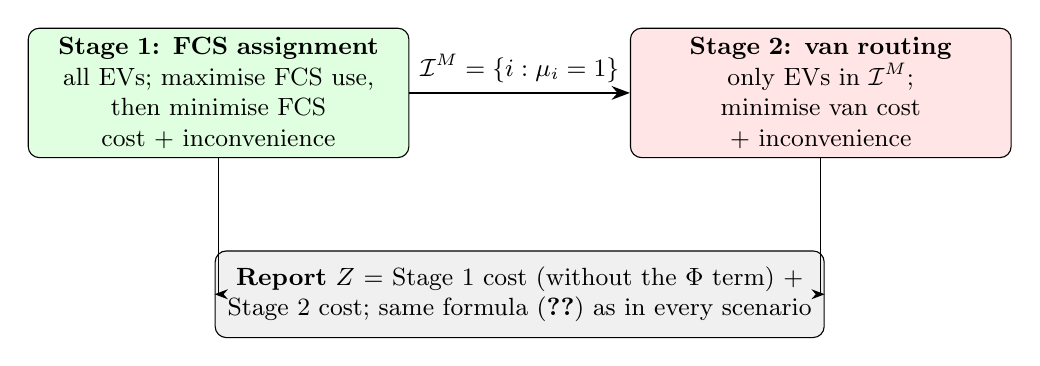
\begin{tikzpicture}[>=Stealth,box/.style={draw,rounded corners,align=center,minimum height=1.1cm,font=\small}]
  \node[box,fill=green!12,text width=4.6cm] (s1) {\textbf{Stage 1: FCS assignment}\\all EVs; maximise FCS use,\\then minimise FCS cost + inconvenience};
  \node[box,fill=red!10,text width=4.6cm,right=2.8cm of s1] (s2) {\textbf{Stage 2: van routing}\\only EVs in $\I^M$;\\minimise van cost + inconvenience};
  \draw[->,thick] (s1) -- node[above,font=\small]{$\I^M=\{i:\mu_i=1\}$} (s2);
  \node[box,fill=black!6,text width=7.5cm,below=2.0cm of $(s1)!0.5!(s2)$] (ev) {\textbf{Report} $Z=$ Stage~1 cost (without the $\Phi$ term) $+$ Stage~2 cost; same formula \eqref{eq:Z} as in every scenario};
  \draw[->] (s1) |- (ev); \draw[->] (s2) |- (ev);
\end{tikzpicture}
\end{center}

Stage~1 does not look at the vans, and Stage~2 cannot change what Stage~1 decided. That is the definition of ``FCS first, then MCS''.

%----------------------------------------------------------------
\subsection{Stage 1: assign EVs to fixed stations}

\textbf{Objective.}
\begin{equation}
\begin{split}
\min\ Z^{(1)}=\;&\underbrace{\Phi\sum_{i\in\I}\mu_i}_{\text{FCS first}}
+\underbrace{c^{EV}\sum_i\sum_{f\in\F_i}d_{if}Y_{if}}_{Z_1}
+\underbrace{Z^F_{\text{energy}}}_{\text{FCS part of }Z_4}\\
&+\underbrace{\sum_i\sum_{f\in\F_i}\rho^F_{if}Y_{if}+\alpha\sum_i w_i(C_i-r_i)+c^L\sum_i w_iL_i}_{\text{FCS customers' inconvenience}}
\end{split}
\label{eq:obj1}
\end{equation}
with $C_i=S_i+\tau^F_iY_i$ in this stage. $\Phi$ is a penalty for handing an EV to the vans. It is chosen larger than anything an extra FCS customer can add to the rest of \eqref{eq:obj1}, e.g.
\[
\Phi > \max_{i}\max_{f\in\F_i}\big(c^{EV}d_{if}+\pi^{\max}E_i+\rho^F_{if}\big)+n\,(\alpha+c^L)\,w_{\max}\,T,
\]
so Stage~1 first \textbf{maximises the number of EVs served at an FCS}, and only among those solutions minimises FCS cost and inconvenience. ($\pi^{\max}$ is the highest grid price.) A numerically safer equivalent is to solve twice: first $\max\sum_iY_i$, then fix that number and minimise the rest.
\ifTOU
Because $Z^F_{\text{energy}}$ uses the peak price, Stage~1 may \emph{start sessions later} to leave the peak, if the price saving beats the extra waiting cost (Section~\ref{sec:expect}).
\fi

\textbf{Constraints.}
\begin{align}
\sum_{g\in\G_i}y_{ig}+\mu_i &= 1 && \forall i\in\I \label{eq:s1assign}\\
S_i &\ge r_i+\sum_{f\in\F_i}t_{if}Y_{if} && \forall i\in\I \label{eq:fcsarr}\\
S_i &\le r_i+T\,(1-\mu_i) && \forall i\in\I \label{eq:s1park}\\
S_j &\ge S_i+\tau^F_i-(T+\tau^F_i)(3-y_{ig}-y_{jg}-o_{ij}) && \forall g,\ (i,j)\in\mathcal{P}_g \label{eq:disj1}\\
S_i &\ge S_j+\tau^F_j-(T+\tau^F_j)(2-y_{ig}-y_{jg}+o_{ij}) && \forall g,\ (i,j)\in\mathcal{P}_g \label{eq:disj2}\\
\sum_i y_{ig_1} &\ge \sum_i y_{ig_2} && \forall f,\ \G_f=\{g_1,g_2\} \label{eq:gunsym}\\
S_i+\tau^F_iY_i &\le T,\qquad L_i\ge S_i+\tau^F_iY_i-l_i && \forall i\in\I \label{eq:s1time}
\end{align}
\ifTOU plus the time-of-use split \eqref{eq:tou1}--\eqref{eq:tou5} of each FCS session (Section~\ref{sec:price}).\fi
\desc{\eqref{eq:s1assign}: every EV either gets one reachable gun or is handed to the vans. An EV that reaches no FCS ($\G_i=\emptyset$) is forced to $\mu_i=1$. \eqref{eq:fcsarr}: an FCS session cannot start before the EV has asked and driven to the station. \eqref{eq:s1park}: for an EV handed to the vans, $S_i$ is parked at $r_i$, so it adds no waiting in Stage~1 (its real start time is decided in Stage~2). \eqref{eq:disj1}--\eqref{eq:disj2}: two EVs on the same gun do not overlap; $o_{ij}$ picks who goes first. With two guns per station this means at most two EVs charge at a station at a time. \eqref{eq:gunsym}: symmetry breaking between the two identical guns (optional). \eqref{eq:s1time}: finished by $T$; lateness.}

\textbf{Optional acceptability rule.} An operator may refuse to send a driver to a station that is ``too inconvenient'', e.g.\ only allow gun $g$ of station $f$ for EV $i$ if $\hat\rho^F_{if}\le\bar\rho$. This only shrinks $\G_i$, so EVs whose stations are all too far go to the vans. Report results with and without it.

\textbf{Output:} $\I^M=\{i:\mu_i=1\}$, the EVs left for the vans; plus each FCS customer's gun and start time.

%----------------------------------------------------------------
\subsection{Stage 2: route the vans to the leftover EVs}

Stage~2 is a vehicle routing problem with time windows, on the EVs in $\I^M$ only. Here $C_i=S_i+\tau^M_i$.

\textbf{Objective.}
\begin{equation}
\begin{split}
\min\ Z^{(2)}=\;&\underbrace{c^M\sum_m\sum_{(i,j)\in\A^M}d_{ij}x_{ijm}}_{Z_2}+\underbrace{\sum_m c^D_mu_m}_{Z_3}+\underbrace{Z^M_{\text{energy}}}_{\text{van part of }Z_4}\\
&+\underbrace{\sum_{i\in\I^M}\sum_m\rho^M_{im}z_{im}+\alpha\sum_{i\in\I^M}w_i(C_i-r_i)+c^L\sum_{i\in\I^M}w_iL_i}_{\text{van customers' inconvenience}}
\end{split}
\label{eq:obj2}
\end{equation}
Since every EV in $\I^M$ must be served by some van, $Z^M_{\text{energy}}$ and the $\rho^M$ term are constants here. They are kept so that $Z^{(2)}$ is the true cost of Stage~2. Waiting and lateness make the vans visit urgent EVs early.

\textbf{Constraints.}
\begin{align}
\sum_{m\in\M}z_{im} &= 1 && \forall i\in\I^M \label{eq:s2assign}\\
\sum_{j:(0,j)\in\A^M}x_{0jm} = \sum_{i:(i,n+1)\in\A^M}x_{i,n+1,m} &= u_m && \forall m \label{eq:depot}\\
\sum_{i:(i,j)\in\A^M}x_{ijm} = \sum_{k:(j,k)\in\A^M}x_{jkm} &= z_{jm} && \forall j\in\I^M,\ m \label{eq:flow}\\
\sum_{i\in\I^M}z_{im} &\le Q_m\,u_m && \forall m \label{eq:cap}\\
\sum_{i\in\I^M}\frac{E_i}{\eta}z_{im}+\beta\sum_{(i,j)\in\A^M}d_{ij}x_{ijm} &\le B_m\,u_m && \forall m \label{eq:batt}
\end{align}
\begin{align}
S_j &\ge \max\{r_j,\ t_{0j}\,x_{0jm}\} && \forall j\in\I^M,\ m \label{eq:depart}\\
S_j &\ge S_i+\tau^M_i+t_{ij}-(T+\tau^M_i+t_{ij})(1-x_{ijm}) && \forall i\neq j,\ m \label{eq:seq}\\
S_i+\tau^M_i+t_{i,n+1} &\le T+(\tau^M_i+t_{i,n+1})(1-x_{i,n+1,m}) && \forall i,\ m \label{eq:return}\\
S_i+\tau^M_i \le T,\quad L_i &\ge S_i+\tau^M_i-l_i && \forall i\in\I^M \label{eq:s2time}\\
u_m &\ge u_{m+1} && m<|\M| \label{eq:vansym}
\end{align}
\desc{\eqref{eq:s2assign}: each leftover EV gets one van. \eqref{eq:depot}: a used van leaves and returns to the depot once. \eqref{eq:flow}: each EV on van $m$ is entered and left exactly once by that van. \eqref{eq:cap}: at most $Q_m$ EVs per van. \eqref{eq:batt}: delivered energy (with transfer losses) plus driving energy fits in the van battery. \eqref{eq:depart}: no start before the request, or before the van can drive there from the depot (written as two linear constraints). \eqref{eq:seq}: if the van goes $i\to j$, it finishes $i$ and drives to $j$ before starting $j$. This gives one EV at a time and removes subtours (MTZ-type). \eqref{eq:return}: back at the depot by $T$. \eqref{eq:s2time}: finished by $T$; lateness. \eqref{eq:vansym}: use identical vans in index order.}

\textbf{If Stage 2 is infeasible} (too many leftover EVs for the fleet by $T$), the sequential policy has \emph{failed} on that instance. For diagnosis, add $s_i\in\{0,1\}$ (``unserved''), replace \eqref{eq:s2assign} by $\sum_mz_{im}+s_i=1$ and add $\Phi^U\sum_is_i$ to \eqref{eq:obj2}. Then report the number of EVs that could not be served. This is a useful comparison with the integrated scenario, which may serve all of them.

%----------------------------------------------------------------
\subsection{Reported value}
\[
Z^{\text{S\scen}}=\big(Z^{(1)*}-\Phi\,|\I^M|\big)+Z^{(2)*},
\]
which is exactly \eqref{eq:Z} evaluated at the combined solution. The stage-1 solution plus the stage-2 solution is a feasible solution of the integrated model (S\ifTOU 4\else 3\fi), so
$Z^{\text{S\ifTOU 4\else 3\fi}}\le Z^{\text{S\scen}}$. The difference is the \emph{value of integration}.

\else
%---------------------------------------------------------------- INT
\subsection{Objective}
\begin{equation}
\min\ Z \quad\text{as in \eqref{eq:Z}, with }Z^F_{\text{energy}}=\ifTOU P^F\textstyle\sum_i\big[\pi^\off(\theta^1_i+\theta^3_i)+\pi^\pk\theta^2_i\big]\else\pi^F\textstyle\sum_iE_iY_i\fi,\quad C_i=S_i+\tau^F_iY_i+\tau^M_iZ_i. \label{eq:objint}
\end{equation}
Written out in full:
\begin{align*}
\min\ Z=\;& c^{EV}\sum_i\sum_{f\in\F_i}d_{if}Y_{if}+c^M\sum_m\sum_{(i,j)\in\A}d_{ij}x_{ijm}+\sum_mc^D_mu_m\\
&+\ifTOU P^F\sum_i\big[\pi^\off(\theta^1_i+\theta^3_i)+\pi^\pk\theta^2_i\big]\else\pi^F\sum_iE_iY_i\fi
+\pi^M\sum_i\sum_m\frac{E_i}{\eta}z_{im}\\
&+\sum_i\sum_{f\in\F_i}\rho^F_{if}Y_{if}+\sum_i\sum_m\rho^M_{im}z_{im}+\alpha\sum_iw_i(C_i-r_i)+c^L\sum_iw_iL_i .
\end{align*}
Every term is linear. One model weighs everything at once: an EV goes to a van exactly when the van's extra km, dispatch and energy cost are outweighed by the effort and waiting it saves the driver\ifTOU, or by the peak-price energy it avoids\fi.

\subsection{Constraints}

\textbf{Assignment.}
\begin{equation}
\sum_{g\in\G_i}y_{ig}+\sum_{m\in\M}z_{im}=1\qquad\forall i\in\I \label{eq:assign}
\end{equation}
\desc{Exactly one resource per EV: one reachable gun or one van. EVs that reach no FCS are forced onto a van.}

\textbf{Fixed stations.}
\begin{align}
S_i &\ge r_i+\sum_{f\in\F_i}t_{if}Y_{if} && \forall i \label{eq:fcsarr}\\
S_j &\ge S_i+\tau^F_i-(T+\tau^F_i)(3-y_{ig}-y_{jg}-o_{ij}) && \forall g,\ (i,j)\in\mathcal{P}_g \label{eq:disj1}\\
S_i &\ge S_j+\tau^F_j-(T+\tau^F_j)(2-y_{ig}-y_{jg}+o_{ij}) && \forall g,\ (i,j)\in\mathcal{P}_g \label{eq:disj2}\\
\sum_iy_{ig_1} &\ge \sum_iy_{ig_2} && \forall f,\ \G_f=\{g_1,g_2\} \label{eq:gunsym}
\end{align}
\desc{\eqref{eq:fcsarr}: an FCS session starts after the request and the drive to the station (for a van customer this is just $S_i\ge r_i$). \eqref{eq:disj1}--\eqref{eq:disj2}: EVs on the same gun do not overlap; $o_{ij}$ chooses the order. \eqref{eq:gunsym}: optional symmetry breaking.}

\textbf{Vans: routes, capacity, battery.}
\begin{align}
\sum_{j:(0,j)\in\A}x_{0jm}=\sum_{i:(i,n+1)\in\A}x_{i,n+1,m} &= u_m && \forall m \label{eq:depot}\\
\sum_{i:(i,j)\in\A}x_{ijm}=\sum_{k:(j,k)\in\A}x_{jkm} &= z_{jm} && \forall j\in\I,\ m \label{eq:flow}\\
\sum_iz_{im} &\le Q_mu_m && \forall m \label{eq:cap}\\
\sum_i\frac{E_i}{\eta}z_{im}+\beta\sum_{(i,j)\in\A}d_{ij}x_{ijm} &\le B_mu_m && \forall m \label{eq:batt}
\end{align}
\desc{\eqref{eq:depot}: a used van leaves and returns once. \eqref{eq:flow}: each EV on van $m$ is visited exactly once by it. \eqref{eq:cap}: at most $Q_m$ EVs. \eqref{eq:batt}: delivered energy (with losses) plus driving energy fits in the battery.}

\textbf{Vans: timing (one EV at a time, no subtours).}
\begin{align}
S_j &\ge t_{0j}\,x_{0jm} && \forall j\in\I,\ m \label{eq:depart}\\
S_j &\ge S_i+\tau^M_i+t_{ij}-(T+\tau^M_i+t_{ij})(1-x_{ijm}) && \forall i\neq j\in\I,\ m \label{eq:seq}\\
S_i+\tau^M_i+t_{i,n+1} &\le T+(\tau^M_i+t_{i,n+1})(1-x_{i,n+1,m}) && \forall i,\ m \label{eq:return}
\end{align}
\desc{\eqref{eq:depart}: the first stop cannot start before the van has driven there. \eqref{eq:seq}: $i\to j$ means finish $i$, drive, then start $j$; start times rise along a route, so no subtour can close. \eqref{eq:return}: back at the depot by $T$.}

\textbf{Horizon and lateness.}
\begin{equation}
C_i\le T,\qquad L_i\ge C_i-l_i\qquad\forall i\in\I \label{eq:time}
\end{equation}
\desc{Every EV is fully charged within the horizon; $L_i$ measures lateness.}

\ifTOU
\textbf{Time-of-use split.} Constraints \eqref{eq:tou1}--\eqref{eq:tou5} of Section~\ref{sec:price}.
\fi

\textbf{Symmetry and domains.}
\begin{equation}
u_m\ge u_{m+1};\qquad y,z,x,u,o\ifTOU,\kappa\fi\in\{0,1\};\qquad S_i,L_i\ifTOU,\theta^p_i\fi\ge0 \label{eq:dom}
\end{equation}
\fi

%=====================================================================
\section{Learning-to-optimise (RL) formulation}\label{sec:rl}

\textbf{Main rule:} the reward of each action is \emph{minus the increase in $Z$ that the action causes}. The rewards over an episode then add up to $-Z$ of the solution the policy builds. RL and MILP results are measured on the same yardstick \eqref{eq:Z}, and the MILP optimum is the benchmark for the RL gap.

\ifSEQ
%---------------------------------------------------------------- RL SEQ
The RL pipeline has the same two stages as the MILP.

\subsection{Stage 1 policy: FCS assignment}
\begin{itemize}[leftmargin=1.4em,itemsep=2pt]
  \item \textbf{Episode / epochs:} EVs are taken in order of request time $r_i$ (ties: higher $w_i$ first). One decision per EV.
  \item \textbf{State:} features of the current EV $k$ ($E_k,r_k,l_k,w_k,R_k$, location); for each gun $g$ the time $F_g$ it becomes free; summary features of the EVs still to come (count and positions near each station)\ifTOU; the current price and the time until $T_1$ and $T_2$\fi.
  \item \textbf{Action:} a gun $g\in\G_k$, or ``hand to vans''. \textbf{FCS-first mask:} ``hand to vans'' is allowed \emph{only} if no gun can finish EV $k$ by $T$ (or, with the optional rule, if all remaining guns have $\hat\rho^F_{kf}>\bar\rho$).
  \ifTOU\item \textbf{Optional timing action:} ``gun $g$, start after the peak'', i.e.\ $S_k=\max\{\text{earliest},T_2\}$, allowed only if the session still ends by $T$.\fi
  \item \textbf{Transition:} $S_k=\max\{r_k+t_{kf},F_g\}$ (or later, for the timing action); $F_g\leftarrow S_k+\tau^F_k$.
  \item \textbf{Reward:} $-\Big[c^{EV}d_{kf}+\text{energy}_k+\rho^F_{kf}+\alpha w_k(S_k+\tau^F_k-r_k)+c^Lw_k(S_k+\tau^F_k-l_k)^+\Big]$, where energy$_k$ = \ifTOU$P^F\big[\pi^\off\cdot(\text{off-peak hours of }[S_k,S_k+\tau^F_k])+\pi^\pk\cdot(\text{peak hours})\big]$, computed exactly in the simulator\else$\pi^FE_k$\fi. Handing an EV to the vans gives reward $0$ here; its cost is counted in Stage~2.
\end{itemize}
Note: a simple baseline for Stage~1 is the greedy rule ``gun with the largest one-step reward''. What RL can learn on top of this is, for example, to keep a nearby gun free for an urgent EV that arrives later.

\subsection{Stage 2 policy: van routing over $\I^M$}
\begin{itemize}[leftmargin=1.4em,itemsep=2pt]
  \item \textbf{Epochs:} whenever a van becomes free (the earliest-free van decides first).
  \item \textbf{State:} for each van: position, time free, remaining battery $b_m$, EVs served so far, dispatched or not; for each unserved EV in $\I^M$: location, $E_i,r_i,l_i,w_i$; current time.
  \item \textbf{Action:} the next EV $j$ for this van, or ``return to depot'' (ends the route). Mask: $j$ must be feasible: battery covers $E_j/\eta$ plus driving to $j$ and back to the depot, the count stays $\le Q_m$, and $j$ can be finished with the van back at the depot by $T$.
  \item \textbf{Transition:} $S_j=\max\{r_j,\ \text{time free}+t_{\text{pos},j}\}$; the van moves to $j$ and is free at $S_j+\tau^M_j$; $b_m$ falls by $E_j/\eta+\beta d_{\text{pos},j}$.
  \item \textbf{Reward:} serving $j$: $-\Big[c^Md_{\text{pos},j}+c^D_m[\text{first stop}]+\pi^M\frac{E_j}{\eta}+\rho^M_{jm}+\alpha w_j(S_j+\tau^M_j-r_j)+c^Lw_j(S_j+\tau^M_j-l_j)^+\Big]$; returning: $-c^Md_{\text{pos},0}$. EVs still unserved at the end: $-\Phi^U$ each.
  \item \textbf{Policy:} an attention-based routing policy (e.g.\ Kool et al., 2019, ``Attention, Learn to Solve Routing Problems!'') trained with REINFORCE or PPO. Baseline: nearest-feasible-EV heuristic.
\end{itemize}
Episode return of Stage~1 + Stage~2 $=-Z^{\text{S\scen}}$.

\else
%---------------------------------------------------------------- RL INT
One policy decides both who serves each EV and the van routes.
\begin{itemize}[leftmargin=1.4em,itemsep=2pt]
  \item \textbf{Episode / epochs:} EVs are taken in order of request time $r_i$ (ties: higher $w_i$ first). One decision per EV.
  \item \textbf{State:} (i) the current EV $k$: location, $E_k,r_k,l_k,w_k,R_k$, reachable stations; (ii) each gun $g$: time $F_g$ it becomes free; (iii) each van $m$: current end-of-route position, time free, remaining battery $b_m$, EVs served, dispatched or not; (iv) embeddings of the not-yet-assigned EVs (for look-ahead)\ifTOU; (v) current price, time until $T_1$ and $T_2$\fi.
  \item \textbf{Action:} $a\in\G_k\cup\M$: a gun, or a van (EV $k$ is appended to the end of that van's route). \textbf{Mask} infeasible actions: a gun that cannot finish $k$ by $T$; a van without enough battery for $E_k/\eta$ plus the drive to $k$ and back to the depot, with $Q_m$ reached, or unable to finish $k$ and return by $T$.
  \ifTOU\item \textbf{Optional timing action:} ``gun $g$, start after the peak'' ($S_k=\max\{\text{earliest},T_2\}$, if it still ends by $T$).\fi
  \item \textbf{Transition:} gun: $S_k=\max\{r_k+t_{kf},F_g\}$, $F_g\leftarrow S_k+\tau^F_k$. Van: $S_k=\max\{r_k,\ \text{free}_m+t_{\text{pos}_m,k}\}$, then the van moves to $k$, $\text{free}_m\leftarrow S_k+\tau^M_k$, $b_m\mathrel{-}=E_k/\eta+\beta d_{\text{pos}_m,k}$.
  \item \textbf{Reward} $=-\Delta Z$:
  \begin{align*}
  \text{gun } g\text{ at }f:&\quad -\Big[c^{EV}d_{kf}+\text{energy}^F_k+\rho^F_{kf}+\alpha w_k(C_k-r_k)+c^Lw_k(C_k-l_k)^+\Big]\\
  \text{van } m:&\quad -\Big[c^M\big(d_{\text{pos}_m,k}+d_{k,0}-d_{\text{pos}_m,0}\big)+c^D_m[\text{first use}]+\pi^M\tfrac{E_k}{\eta}\\
  &\qquad\quad+\rho^M_{km}+\alpha w_k(C_k-r_k)+c^Lw_k(C_k-l_k)^+\Big]
  \end{align*}
  The van distance term is the \emph{change} in route length when $k$ is inserted before the return to the depot, so the sum over the episode equals the total route length (the return legs telescope). energy$^F_k$ = \ifTOU$P^F\big[\pi^\off\cdot(\text{off-peak hours})+\pi^\pk\cdot(\text{peak hours of }[S_k,C_k])\big]$, computed exactly by the simulator; no linearisation is needed in RL\else$\pi^FE_k$\fi.
  \item \textbf{Dead end:} if every action is masked, EV $k$ is unserved: reward $-\Phi^U$, and the episode continues. Report the count.
  \item \textbf{Policy:} masked categorical policy over guns and vans, encoder with attention over EVs, guns and vans; trained with PPO. Natural baseline: greedy, i.e.\ choose the action with the largest one-step reward. That is the pairwise rule ``smallest $\hat\rho$ + cost'' from Section~\ref{sec:inc}.
\end{itemize}
Restriction to note: vans serve EVs in assignment order (append only). A variant that inserts $k$ at the cheapest position of a route is more flexible but has a larger action space.
\fi

\textbf{Reward scaling.} For stable training divide every reward by a constant, e.g.\ the greedy baseline's average $Z$ on the training instances. This does not change the optimal policy.

%=====================================================================
\section{What to expect and what to report}\label{sec:expect}

\ifnum\scen=1
\begin{itemize}[leftmargin=1.4em,itemsep=2pt]
  \item Vans serve only EVs that reach no station, or that the stations cannot finish by $T$. If stations have spare capacity, very few vans are dispatched.
  \item Inconvenience is high for EVs far from the nearest station (worked example: Rs\,682 at the FCS, against Rs\,458 if a van had been allowed).
  \item With too few vans Stage~2 becomes infeasible (unserved EVs), even when the integrated model S3 could serve everyone. Report the smallest $|\M|$ at which S1 is feasible and compare it with S3.
\end{itemize}
\fi
\ifnum\scen=2
\begin{itemize}[leftmargin=1.4em,itemsep=2pt]
  \item \textbf{When does Stage~1 delay a session to avoid the peak?} Moving one hour of charging out of the peak saves $(\pi^\pk-\pi^\off)P^F=3\times22=$ Rs\,66, but delays completion by up to an hour, which costs $\alpha w_i\ge$ Rs\,200. So with the default values Stage~1 almost never delays. It mostly pays the higher price, and S2 costs roughly S1 plus the peak surcharge. Sessions start later only if $\alpha$ is small (try $\lambda<0.33$ in the sensitivity analysis).
  \item The van assignment is the same as in S1 unless Stage~1's timing changes which EVs fit at the stations. Stage~1 cannot use vans to escape the peak price.
  \item Extra KPI: \textbf{grid energy drawn at FCS during the peak}, $P^F\sum_i\theta^2_i$ (kWh). Compare with S4.
\end{itemize}
\fi
\ifnum\scen=3
\begin{itemize}[leftmargin=1.4em,itemsep=2pt]
  \item Vans take EVs for which the saved inconvenience exceeds the extra van cost (worked example: van chosen, saving Rs\,224). Expect vans to serve EVs that are far from every station, have low range (high $w_i$), or have early deadlines, while EVs near a station still use it.
  \item \textbf{Value of integration under flat price:} $Z^{\text{S1}}-Z^{\text{S3}}\ge0$. Report it per component ($Z_1,\dots,Z_5$): typically operating cost rises a little and inconvenience falls a lot.
  \item Vary $|\M|$ (0, 1, 2, \dots): the first few vans lower $Z$ sharply, then the effect levels off. That curve shows the scenarios where mobile chargers help most.
\end{itemize}
\fi
\ifnum\scen=4
\begin{itemize}[leftmargin=1.4em,itemsep=2pt]
  \item During the peak a van kWh costs about the same as an FCS kWh (Rs\,10.0 each), so the vans' energy disadvantage disappears and vans also absorb \emph{peak-hour} demand that would otherwise be charged on the grid at peak price.
  \item Expect more van usage than in S3, concentrated on requests in $[T_1,T_2]$, and lower grid energy at the stations during the peak, $P^F\sum_i\theta^2_i$, than in S2.
  \item \textbf{Value of integration under peak pricing:} $Z^{\text{S2}}-Z^{\text{S4}}$. It should be larger than $Z^{\text{S1}}-Z^{\text{S3}}$, because integration now also allows price arbitrage.
  \item \textbf{Peak pricing with full flexibility:} $Z^{\text{S4}}-Z^{\text{S3}}$ should be smaller than $Z^{\text{S2}}-Z^{\text{S1}}$: vans cushion the price increase.
\end{itemize}
\fi

\textbf{Cross-scenario comparison table} (fill in from the four runs):
\begin{center}
\renewcommand{\arraystretch}{1.2}
\begin{tabular}{@{}lll@{}}
\toprule
\textbf{Comparison} & \textbf{Measures} & \textbf{Expected sign} \\
\midrule
S1 $-$ S3 & value of integration, flat price & $\ge0$ \\
S2 $-$ S4 & value of integration, peak price & $\ge0$, larger than S1 $-$ S3 \\
S2 $-$ S1 & cost of peak pricing, FCS-first operator & $>0$ \\
S4 $-$ S3 & cost of peak pricing, flexible operator & $>0$, smaller than S2 $-$ S1 \\
\bottomrule
\end{tabular}
\end{center}
Report for each: $Z$ and its components, number of vans used, EVs per resource, mean and maximum inconvenience per EV, total lateness, peak-hour grid energy, solve time, and (for RL) the gap to the MILP optimum.

%=====================================================================
\appendix
\section{Illustrative parameter values}\label{app:values}

These are starting values for experiments, not data. All are meant to be varied in the analysis. Values in Rs.

\begin{center}
\renewcommand{\arraystretch}{1.15}
\begin{tabular}{@{}llp{6.2cm}@{}}
\toprule
\textbf{Parameter} & \textbf{Value} & \textbf{Note} \\
\midrule
$T$, $[T_1,T_2]$ & 7 h, $[2,6]$ & 16:00--23:00, peak 18:00--22:00 \\
$P^F$, $P^M$ & 22 kW, 30 kW & \\
$v$, $\beta$, $\eta$ & 25 km/h, 0.25 kWh/km, 0.9 & \\
$B_m$, $Q_m$, $|\M|$ & 150 kWh, 6, 2--6 & \\
$c^{EV}$, $c^M$, $c^D_m$ & Rs\,4/km, Rs\,15/km, Rs\,1500 & van km includes driver time \\
$\pi^F$ (flat) & Rs\,8.7/kWh & equals the time-average of the ToU tariff over $[0,T]$ \\
$\pi^\off$, $\pi^\pk$ (ToU) & Rs\,7/kWh, Rs\,10/kWh & $(3\times7+4\times10)/7=8.7$ \\
$c^{bat}$ & Rs\,2/kWh & van battery wear \\
$\pi^M$ & Rs\,10.7 (flat) / Rs\,9.0 (ToU) & $=\pi^F+c^{bat}$ / $=\pi^\off+c^{bat}$ \\
$\alpha$, $\alpha^D$ & Rs\,200/h, Rs\,100/h & value of time; extra for attended time \\
$h^F$, $h^M$, $\varphi$ & Rs\,50, Rs\,10, Rs\,100 & trip hassle, hand-over, range stress \\
$c^L$ & Rs\,300/h & lateness \\
$w_i$ & $1+2(1-R_i/R_{\max})$, $R_i\sim U[3,40]$ km & priority from remaining range \\
\bottomrule
\end{tabular}
\end{center}

The flat price is set to the time-average of the peak tariff. The price \emph{level} is then the same in both pricing cases, and only the price \emph{shape} differs. Without this, part of S1 vs S2 would just reflect a different average price.

\end{document}
"
%  (run each twice for cross-references)
% =====================================================================
\documentclass[11pt,a4paper]{article}
\usepackage[margin=2.2cm]{geometry}
\usepackage{amsmath,amssymb,amsfonts}
\usepackage{booktabs,array,tabularx}
\usepackage{enumitem}
\usepackage[table]{xcolor}
\usepackage{tikz}
\usetikzlibrary{arrows.meta,positioning,calc}
\usepackage[colorlinks=true,linkcolor=blue!50!black,urlcolor=blue!50!black]{hyperref}
\usepackage{titlesec}
\titleformat{\section}{\large\bfseries}{\thesection}{0.8em}{}
\titleformat{\subsection}{\normalsize\bfseries}{\thesubsection}{0.8em}{}
\setlength{\parindent}{0pt}
\setlength{\parskip}{5pt}

% ---------------- scenario switches ----------------
\ifdefined\scen\else\def\scen{1}\fi
\newif\ifTOU \TOUfalse   % true = time-of-use (peak) price
\newif\ifSEQ \SEQfalse   % true = FCS first, then MCS
\ifnum\scen=1 \SEQtrue \fi
\ifnum\scen=2 \TOUtrue \SEQtrue \fi
\ifnum\scen=4 \TOUtrue \fi

\newcommand{\pricename}{\ifTOU time-of-use price (dearer evening peak)\else single (flat) price all day\fi}
\newcommand{\structname}{\ifSEQ FCS first, then MCS (sequential)\else FCS and MCS together (integrated)\fi}

% ---------------- notation ----------------
\newcommand{\I}{\mathcal{I}}
\newcommand{\F}{\mathcal{F}}
\newcommand{\G}{\mathcal{G}}
\newcommand{\M}{\mathcal{M}}
\newcommand{\N}{\mathcal{N}}
\newcommand{\A}{\mathcal{A}}
\newcommand{\Rs}{\text{Rs}\,}
\newcommand{\pk}{\mathrm{pk}}
\newcommand{\off}{\mathrm{off}}
\newcommand{\desc}[1]{\par\vspace{-2pt}{\small\color{black!75}\textit{Meaning:} #1}\par\vspace{4pt}}
\newcommand{\cell}[2]{\ifnum\scen=#1\cellcolor{blue!18}\textbf{S#1 (this document)}\\\textbf{#2}\else S#1\\#2\fi}

\title{\textbf{EV Charging Network Optimisation}\\[4pt]
\large Scenario \scen: \pricename\ $+$ \structname\\[2pt]
\normalsize MILP and RL formulation}
\author{CP 320 OR for Mobility Management, course project}
\date{2 October 2026}

\begin{document}
\maketitle

%=====================================================================
\section{Where this scenario sits}

The project studies four scenarios: two ways of pricing grid electricity, times two ways of making the decisions.

\begin{center}
\renewcommand{\arraystretch}{1.5}
\begin{tabular}{>{\raggedright\arraybackslash}p{4.2cm}|>{\centering\arraybackslash}p{4.6cm}|>{\centering\arraybackslash}p{4.6cm}}
 & \textbf{Flat price all day} & \textbf{Time-of-use (peak) price} \\ \hline
\textbf{Sequential:} FCS first, leftover EVs to MCS &
\begin{tabular}[c]{@{}c@{}}\cell{1}{flat + sequential}\end{tabular} &
\begin{tabular}[c]{@{}c@{}}\cell{2}{peak + sequential}\end{tabular} \\ \hline
\textbf{Integrated:} FCS and MCS decided together &
\begin{tabular}[c]{@{}c@{}}\cell{3}{flat + integrated}\end{tabular} &
\begin{tabular}[c]{@{}c@{}}\cell{4}{peak + integrated}\end{tabular} \\
\end{tabular}
\end{center}

\textbf{The four scenarios do not have four different objectives.} They share \emph{one} cost yardstick $Z$ (Section~\ref{sec:obj}): the same cost terms and the same customer inconvenience (Section~\ref{sec:inc}). Only two things change:
\begin{itemize}[leftmargin=1.4em,itemsep=1pt]
  \item \textbf{Pricing} changes the formula for one term, the FCS energy cost (Section~\ref{sec:price}).
  \item \textbf{Decision structure} changes \emph{how} $Z$ is minimised: in one model (integrated), or in two stages (sequential), where each stage minimises its own part of $Z$.
\end{itemize}
Because the yardstick is the same, the four optimal values can be compared directly. The differences measure the \emph{value of integration} (S1$\to$S3, S2$\to$S4) and the \emph{effect of peak pricing} (S1$\to$S2, S3$\to$S4).

\ifnum\scen=1
\textbf{This scenario (S1)} is the baseline, the ``status quo''. Electricity costs the same at every hour, every EV that can be charged at a fixed station is sent there, and vans only take what is left over.
\fi
\ifnum\scen=2
\textbf{This scenario (S2)} keeps the FCS-first rule of S1, but grid electricity is dearer during the evening peak. Stage~1 can react to the price only by \emph{rescheduling} FCS sessions. It cannot hand a peak-hour EV to a van.
\fi
\ifnum\scen=3
\textbf{This scenario (S3)} keeps the flat price of S1, but the operator decides FCS and MCS service \emph{together}. An EV can be sent to a van even when a fixed station could take it, whenever that lowers total cost plus inconvenience.
\fi
\ifnum\scen=4
\textbf{This scenario (S4)} is the most flexible one: peak pricing at fixed stations, and FCS and MCS decided together. Van energy was bought off-peak, so vans can also be used to keep charging \emph{out of the expensive peak}.
\fi

%=====================================================================
\section{Setting and assumptions}\label{sec:setting}

\textbf{Time.} The planning horizon is $[0,T]$ with $T=7$\,h (16:00--23:00). It contains the evening peak window $[T_1,T_2]=[2,6]$ (18:00--22:00). The horizon is the same in all four scenarios. It is wider than the peak itself so that, under peak pricing, there is cheaper time on both sides of the peak.\ifTOU\else\ In this scenario the price is flat, so the window plays no role in the model.\fi

\textbf{Assumptions} (the same as MILP v3, plus two about energy):
\begin{enumerate}[leftmargin=1.6em,itemsep=1pt]
  \item Static, continuous time. All requests in the horizon are known at time $0$, and request $i$ becomes active at $r_i$.
  \item An EV served by an FCS drives there itself on its own battery (only to stations within its range $R_i$). The driver stays with the car while it waits for a free gun and while it charges.
  \item An EV served by an MCS stays parked where it is, and the driver is free in the meantime.
  \item Each FCS gun and each van charges one EV at a time, without interruption, at constant power.
  \item A van's battery covers both its driving and the energy it delivers. \textbf{The van battery is charged at the depot before the horizon starts}\ifTOU, i.e.\ at the off-peak price\fi, and is not recharged during the horizon.
  \item Every EV must be fully charged by $T$ (hard). Finishing after the driver's desired time $l_i$ is allowed but penalised.
\end{enumerate}

%=====================================================================
\section{Notation}\label{sec:notation}

\subsection*{Sets}
\begin{tabularx}{\textwidth}{@{}lX@{}}
\toprule
$\I=\{1,\dots,n\}$ & EV charging requests \\
$\F$; $\G_f$ ($|\G_f|=2$); $\G=\bigcup_f\G_f$ & fixed charging stations; guns of FCS $f$; all guns ($f(g)$ = station of gun $g$) \\
$\F_i=\{f: d_{if}\le R_i\}$, $\G_i=\bigcup_{f\in\F_i}\G_f$ & stations / guns EV $i$ can reach on its remaining range \\
$\M$ & mobile charging vans (MCS) \\
$0,\ n+1$ & depot as start node / end node (same place) \\
$\N=\{0\}\cup\I\cup\{n+1\}$, $\A$ & routing nodes; allowed van arcs $(i,j)$, $i\in\{0\}\cup\I$, $j\in\I\cup\{n+1\}$, $i\neq j$ \\
$\mathcal{P}_g=\{(i,j): i<j,\ g\in\G_i\cap\G_j\}$ & pairs of EVs that could share gun $g$ \\
\ifSEQ
$\I^M\subseteq\I$ & EVs handed to the vans by Stage~1 (an \emph{output} of Stage~1, a fixed input to Stage~2) \\
$\N^M$, $\A^M$ & routing nodes / arcs restricted to $\I^M$ \\
\fi
\bottomrule
\end{tabularx}

\subsection*{Parameters}
\begin{tabularx}{\textwidth}{@{}lX@{}}
\toprule
$E_i,\ r_i,\ l_i,\ R_i$ & energy demand (kWh), request time, desired completion time (h), remaining range (km) \\
$w_i\ge1$ & priority of EV $i$; $w_i=1+\kappa(1-R_i/R_{\max})$, so low-range EVs weigh more \\
$P^F,\ P^M$ & charging power of an FCS gun (22\,kW) / of a van (e.g.\ 30\,kW) \\
$\tau^F_i=E_i/P^F,\ \tau^M_i=E_i/P^M$ & charging time of EV $i$ at an FCS / by a van (h) \\
$d_{if},t_{if}$;\ $d_{ij},t_{ij}$ & distance (km) and time (h): EV$\to$FCS; between routing nodes ($t=d/v$) \\
$B_m,\ Q_m,\ \beta,\ \eta$ & van battery (kWh), max EVs per van, van consumption (kWh/km), transfer efficiency \\
$c^{EV},\ c^M,\ c^D_m$ & cost per km of EV driving, per km of van driving; fixed dispatch cost of van $m$ \\
\ifTOU
$\pi^\off,\ \pi^\pk$ & grid price (Rs/kWh) off-peak / in $[T_1,T_2]$, with $\pi^\pk\ge\pi^\off$ \\
\else
$\pi^F$ & grid price (Rs/kWh), the same at every hour \\
\fi
$c^{bat}$ & van battery wear per kWh cycled \\
$\pi^M$ & cost of 1 kWh taken from a van battery: $\pi^M=\ifTOU\pi^\off\else\pi^F\fi+c^{bat}$ (Section~\ref{sec:price}) \\
$\alpha,\ \alpha^D,\ h^F,\ h^M,\ \varphi,\ c^L$ & inconvenience coefficients (Section~\ref{sec:inc}) \\
\bottomrule
\end{tabularx}

\subsection*{Decision variables}
\begin{tabularx}{\textwidth}{@{}llX@{}}
\toprule
$y_{ig}$ & $\{0,1\}$ & EV $i$ charged at gun $g\in\G_i$ \\
$z_{im}$ & $\{0,1\}$ & EV $i$ served by van $m$ \\
$x_{ijm}$ & $\{0,1\}$ & van $m$ drives arc $(i,j)$ \\
$u_m$ & $\{0,1\}$ & van $m$ is dispatched \\
$o_{ij}$ & $\{0,1\}$ & for EVs $i<j$ that could share a gun: 1 if $i$ is charged before $j$ \\
\ifSEQ
$\mu_i$ & $\{0,1\}$ & Stage~1 only: EV $i$ is handed to the van fleet \\
\fi
\ifTOU
$\theta^1_i,\theta^2_i,\theta^3_i$ & $\ge0$ & hours of EV $i$'s FCS session before / inside / after the peak \\
$\kappa^1_i,\kappa^3_i$ & $\{0,1\}$ & EV $i$'s FCS session starts before $T_1$ / ends after $T_2$ \\
\fi
$S_i$ & $\ge0$ & time charging of EV $i$ starts (h), on whichever resource \\
$L_i$ & $\ge0$ & lateness of EV $i$ beyond $l_i$ (h) \\
\bottomrule
\end{tabularx}

\textbf{Short-hands} (linear expressions, not new variables):
\[
Y_{if}=\sum_{g\in\G_f}y_{ig},\qquad Y_i=\sum_{g\in\G_i}y_{ig}\ (\text{EV $i$ uses an FCS}),\qquad Z_i=\sum_{m\in\M}z_{im}\ (\text{EV $i$ uses a van}),
\]
\[
C_i=S_i+\tau^F_i\,Y_i+\tau^M_i\,Z_i \quad\text{(time EV $i$ is fully charged).}
\]

%=====================================================================
\section{Customer inconvenience}\label{sec:inc}

This section is \textbf{identical in all four scenario documents}. Inconvenience is a property of the customer, not of the price or of the planning method.

\subsection{What we mean by inconvenience}

Inconvenience is \emph{what the driver loses} from the moment they ask for a charge ($r_i$) until the car is fully charged ($C_i$), \emph{converted into rupees} so it can be added to the operator's costs. A driver loses three different things:

\begin{enumerate}[leftmargin=1.6em,itemsep=2pt]
  \item \textbf{Waiting:} the car is not ready. This lasts $C_i-r_i$ hours and affects \emph{every} driver, FCS or MCS.
  \item \textbf{Effort:} only an FCS customer has to drive to the station and sit there while the car charges. An MCS customer stays at home or at work and does something else. Driving to a far station also uses scarce battery range, which causes stress (``range anxiety'').
  \item \textbf{A missed deadline:} the car is still not ready at the time $l_i$ the driver needs it.
\end{enumerate}

Each loss gets a price in Rs per hour (or per event). All of them are multiplied by the priority $w_i$: an hour of delay for an EV with 5\,km of range left counts more than for one with 40\,km.

\subsection{The three components}

\begin{center}
\renewcommand{\arraystretch}{1.3}
\begin{tabularx}{\textwidth}{@{}>{\raggedright\arraybackslash}p{2.6cm}>{\raggedright\arraybackslash}X>{\raggedright\arraybackslash}X>{\raggedright\arraybackslash}p{3.0cm}@{}}
\toprule
\textbf{Component} & \textbf{EV $i$ at FCS $f$} & \textbf{EV $i$ by a van} & \textbf{Known when?} \\
\midrule
Effort & $w_i\big[\alpha^D(t_{if}+\tau^F_i)+h^F+\varphi\,d_{if}/R_i\big]$: driving and sitting at the station, a fixed trip hassle, range stress & $w_i\,h^M$: being reachable and handing over the car & \textbf{Static:} known as soon as the resource is chosen \\
Waiting & $w_i\,\alpha\,(C_i-r_i)$ = drive + \emph{queue at the gun} + charge & $w_i\,\alpha\,(C_i-r_i)$ = \emph{wait for the van} + charge & \textbf{Dynamic:} depends on the queue / van route \\
Missed deadline & $w_i\,c^L\,L_i$, $L_i=\max\{0,C_i-l_i\}$ & same & Dynamic \\
\bottomrule
\end{tabularx}
\end{center}

\textbf{Coefficients.}
$\alpha$ (Rs/h) is the value of an hour the car is not ready.
$\alpha^D$ (Rs/h) is the \emph{extra} value of an hour the driver must personally spend driving or sitting at the station: an hour at the station costs $\alpha+\alpha^D$, an hour waiting at home for a van costs only $\alpha$.
$h^F,h^M$ (Rs) are fixed hassle costs of one trip to a station / one van hand-over.
$\varphi$ (Rs) is the range-stress cost of a trip that uses the \emph{whole} remaining range ($d_{if}/R_i\le1$ is the fraction used).
$c^L$ (Rs/h) is the cost per hour late.

\subsection{Pairwise form: inconvenience of a (customer, resource) pair}

The natural first idea is: \emph{for every pair (EV $i$, FCS $f$) and every pair (EV $i$, van $m$) there is an inconvenience number, and the operator picks the pair with the lowest cost plus inconvenience.} The static part fits this idea exactly:
\[
\boxed{\;\rho^F_{if}=w_i\Big[\alpha^D\,(t_{if}+\tau^F_i)+h^F+\varphi\,\frac{d_{if}}{R_i}\Big]\qquad
\rho^M_{im}=w_i\,h^M\;}
\]
These are \textbf{parameters}, computed before solving, one number per (EV, FCS) pair and per (EV, van) pair. In the objective they appear linearly: $\sum_i\sum_f\rho^F_{if}Y_{if}+\sum_i\sum_m\rho^M_{im}z_{im}$.

Note that $\rho^M_{im}$ does not depend on $m$. Vans are identical and all start at the same depot, so the driver does not care \emph{which} van comes, only \emph{when} it comes. That ``when'' is the waiting part.

\subsection{Why waiting cannot be a fixed pairwise number}

It is tempting to also write the waiting as a pairwise number, e.g.\ ``the van needs 5 minutes to reach EV $i$''. But that depends on \emph{where the van is coming from}, which depends on the route the model is still choosing: if EV $i$ is the 4th stop of a van, the wait is the time for three charging sessions plus four drives. Likewise, waiting at an FCS depends on how many EVs are queued at that gun. So waiting is not known before solving. It is a function of decision variables:
\[
\text{waiting cost of EV } i \;=\; w_i\,\alpha\,(C_i-r_i),\qquad C_i=S_i+\tau^F_iY_i+\tau^M_iZ_i .
\]
This is \textbf{linear} in the variables ($S_i$, $y$, $z$), so it fits in a MILP directly. The constraints of Section~\ref{sec:milp} make $S_i$ equal to the true start time, including driving, queueing at the gun and the van's route. The term $\sum_i w_i\alpha r_i$ is a constant and may be dropped when solving.

\textbf{Pairwise \emph{estimate}} (used for intuition, by the RL policy and in heuristics): if there is no queue and the van comes straight to $i$,
\[
\hat\rho^{F}_{if}=\rho^F_{if}+w_i\alpha\,(t_{if}+\tau^F_i),\qquad
\hat\rho^{M}_{im}=\rho^M_{im}+w_i\alpha\,(t^{\text{van}}_{m\to i}+\tau^M_i),
\]
where $t^{\text{van}}_{m\to i}$ is the time until van $m$ can reach $i$ from where it currently is. In the RL formulation (Section~\ref{sec:rl}) the van's position \emph{is} known at each decision, so there this estimate becomes exact.

\subsection{Total inconvenience and how it enters the objective}

\begin{equation}
\boxed{\;
Z_{\text{inc}}=\underbrace{\sum_{i\in\I}\sum_{f\in\F_i}\rho^F_{if}Y_{if}+\sum_{i\in\I}\sum_{m\in\M}\rho^M_{im}z_{im}}_{\text{effort (static, pairwise)}}
+\underbrace{\alpha\sum_{i\in\I}w_i\,(C_i-r_i)}_{\text{waiting (dynamic)}}
+\underbrace{c^L\sum_{i\in\I}w_i\,L_i}_{\text{missed deadline}}
\;}\label{eq:inc}
\end{equation}
All three parts are in rupees, so $Z_{\text{inc}}$ is simply added to the operating costs. Nothing has to be normalised.

\subsection{Worked example: your ``10 km to the FCS vs.\ van in 5 minutes'' case}

EV $i$: $E_i=20$\,kWh, $R_i=40$\,km (so $w_i=1$); nearest free FCS $d_{if}=10$\,km away, $t_{if}=0.4$\,h at 25\,km/h; a van finishing next door can reach it in 5\,min ($0.083$\,h), adding about 4\,km to its route. $\tau^F_i=20/22=0.909$\,h, $\tau^M_i=20/30=0.667$\,h. Coefficients from Appendix~\ref{app:values}, flat price.

\begin{center}
\renewcommand{\arraystretch}{1.25}
\begin{tabular}{@{}lrr@{}}
\toprule
 & \textbf{FCS} & \textbf{Van} \\
\midrule
Driving (EV / extra van km) & $4\times10=40.0$ & $15\times4=60.0$ \\
Energy & $8.7\times20=174.0$ & $10.7\times20/0.9=237.8$ \\
\textbf{Operating cost only} & \textbf{214.0} & \textbf{297.8} \\
\midrule
Effort $\rho$ & $100(0.4+0.909)+50+100\cdot\tfrac{10}{40}=205.9$ & $10.0$ \\
Waiting $\alpha(C_i-r_i)$ & $200\times1.309=261.8$ & $200\times0.75=150.0$ \\
\textbf{Cost + inconvenience} & \textbf{681.7} & \textbf{457.8} \\
\bottomrule
\end{tabular}
\end{center}

On operating cost alone the FCS is cheaper, so a cost-only model would \emph{always} send this driver 10\,km away. With inconvenience included the van is better by about Rs\,224, and the integrated model chooses $z_{im}=1$, as you expected. If the FCS were only 1\,km away, the FCS would win both comparisons. The inconvenience term is what makes the model choose between ``cheap for the operator'' and ``convenient for the driver'', rather than following a fixed rule.

\subsection{Relation to a single penalty $\rho_i$ per EV}

The first draft used a penalty $\rho_i$ that is charged whenever EV $i$ goes to \emph{any} FCS: $\sum_i\sum_f\rho_iy_{if}$. Because $\sum_f y_{if}=1-\sum_m z_{im}$, this only says ``a van is worth $\rho_i$ more to EV $i$'', and that holds whether the station is 1\,km or 15\,km away, and whether the van arrives in 5 minutes or in 3 hours. The form above fixes both problems: $\rho^F_{if}$ grows with the distance to \emph{that} station, and the waiting term grows with how late the van or the free gun actually is. The old model is the special case $\alpha=\alpha^D=\varphi=c^L=0$, $h^F=\rho_i$.

\subsection{Choosing the coefficients}
\begin{itemize}[leftmargin=1.4em,itemsep=2pt]
  \item Use a value of time for $\alpha$ (e.g.\ Rs\,150--300/h for urban car users), and set $\alpha^D\approx0.5\alpha$: sitting at a station is worse than waiting at home.
  \item Keep $c^L>\alpha$, so missing the deadline is worse than ordinary waiting.
  \item \textbf{Sensitivity analysis:} multiply all inconvenience coefficients by a factor $\lambda\in\{0,0.25,0.5,1,2,4\}$ and plot operating cost against total inconvenience. $\lambda=0$ is the pure cost-minimising operator, and large $\lambda$ is a customer-first operator. This trade-off curve is a strong result for the ``Analysis'' part of the project.
\end{itemize}

\subsection{What inconvenience does in \emph{this} scenario}
\ifSEQ
In a sequential scenario inconvenience \textbf{cannot move an EV from an FCS to a van}: Stage~1 sends every EV that \emph{can} use an FCS to one. It still matters inside each stage. In Stage~1 it decides \emph{which} station and \emph{when} (urgent EVs get the near station and the first free gun). In Stage~2 it decides the \emph{order} in which vans visit EVs (urgent EVs first). In the worked example, this scenario sends the driver 10\,km to the FCS. That is the weakness the integrated scenarios remove.
\else
In an integrated scenario inconvenience is weighed directly against operating cost when choosing the resource. That is how the worked example ends up with a van. It also decides which station and which gun order, and the order of each van route.
\fi

%=====================================================================
\section{Electricity price in this scenario}\label{sec:price}

\textbf{Van energy (same in all scenarios).} A van's battery is charged at the depot \emph{before} the horizon, so its energy was bought at the
\ifTOU off-peak \fi
price, whatever time the van later delivers it. Each kWh taken from the van also wears the battery ($c^{bat}$), and a fraction $1-\eta$ is lost in transfer:
\[
Z^M_{\text{energy}}=\pi^M\sum_{i\in\I}\sum_{m\in\M}\frac{E_i}{\eta}\,z_{im},\qquad \pi^M=\ifTOU\pi^\off\else\pi^F\fi+c^{bat}.
\]

\ifTOU
\textbf{FCS energy (time-of-use).} An FCS draws from the grid while it charges. Energy delivered inside $[T_1,T_2]$ costs $\pi^\pk$, and energy outside it costs $\pi^\off$. A session $[S_i,S_i+\tau^F_i]$ may overlap the peak partly. Split its duration into the hours before, inside and after the peak, $\theta^1_i+\theta^2_i+\theta^3_i$:
\[
Z^F_{\text{energy}}=P^F\sum_{i\in\I}\Big[\pi^\off(\theta^1_i+\theta^3_i)+\pi^\pk\,\theta^2_i\Big].
\]
Constraints \eqref{eq:tou1}--\eqref{eq:tou5} below make the $\theta$'s equal to the true overlaps. Peak hours are dearer, so the solver wants $\theta^1_i,\theta^3_i$ as large as possible. It is enough to bound them from above by the true off-peak overlap, and the constraints need one binary per side:
\begin{align}
\theta^1_i+\theta^2_i+\theta^3_i &= \tau^F_i\,Y_i && \forall i\in\I \label{eq:tou1}\\
\theta^1_i &\le \tau^F_i\,\kappa^1_i && \forall i\in\I \label{eq:tou2}\\
\theta^1_i &\le T_1-S_i+T\,(1-\kappa^1_i) && \forall i\in\I \label{eq:tou3}\\
\theta^3_i &\le \tau^F_i\,\kappa^3_i && \forall i\in\I \label{eq:tou4}\\
\theta^3_i &\le S_i+\tau^F_i-T_2+T\,(1-\kappa^3_i) && \forall i\in\I \label{eq:tou5}
\end{align}
\desc{\eqref{eq:tou1}: the FCS session's hours are split into three parts; for a van customer ($Y_i=0$) all three are zero. \eqref{eq:tou2}--\eqref{eq:tou3}: off-peak time before the peak is only possible if the session starts before $T_1$ ($\kappa^1_i=1$), and is at most $T_1-S_i$. \eqref{eq:tou4}--\eqref{eq:tou5}: the same for time after $T_2$. $\theta^2_i\ge0$ prevents counting more off-peak hours than exist. Checking the cases (entirely before / inside / after the peak, straddling one edge, covering the whole peak) shows that at the optimum the $\theta$'s equal the exact overlaps. This needs $\pi^\pk\ge\pi^\off$, which is true for a peak tariff.}

\textbf{Why vans become more attractive.} Compare the cost of 1\,kWh delivered to an EV during the peak (values from Appendix~\ref{app:values}):
FCS $=\pi^\pk=$ Rs\,10.0, van $=(\pi^\off+c^{bat})/\eta=9/0.9=$ Rs\,10.0. They are at parity. Under the flat price the van is about Rs\,3.2/kWh dearer (FCS Rs\,8.7, van $10.7/0.9=$ Rs\,11.9). Peak pricing therefore removes the vans' main cost disadvantage, but only for EVs whose FCS session would fall in the peak.
\ifSEQ\ In this sequential scenario Stage~1 cannot use that, because it does not consider vans. It can only shift FCS sessions in time.\fi
\else
\textbf{FCS energy (flat).} Every kWh delivered at a fixed station costs $\pi^F$, whenever it is delivered:
\[
Z^F_{\text{energy}}=\pi^F\sum_{i\in\I}E_i\,Y_i .
\]
The start time therefore does not affect the energy cost. Under the flat price a van kWh costs $(\pi^F+c^{bat})/\eta\approx$ Rs\,11.9 against Rs\,8.7 at an FCS (Appendix~\ref{app:values}), so on energy alone the FCS always wins.
\fi

%=====================================================================
\section{MILP formulation}\label{sec:milp}

\subsection{The common cost yardstick $Z$}\label{sec:obj}

For any complete solution (every EV assigned, every route and start time known), the system cost is
\begin{equation}
\boxed{\;
Z=\underbrace{c^{EV}\sum_{i}\sum_{f\in\F_i}d_{if}Y_{if}}_{Z_1:\ \text{EV driving}}
+\underbrace{c^M\sum_{m}\sum_{(i,j)\in\A}d_{ij}x_{ijm}}_{Z_2:\ \text{van driving}}
+\underbrace{\sum_m c^D_m u_m}_{Z_3:\ \text{dispatch}}
+\underbrace{Z^F_{\text{energy}}+Z^M_{\text{energy}}}_{Z_4:\ \text{energy}}
+\underbrace{Z_{\text{inc}}}_{Z_5:\ \text{inconv.\ \eqref{eq:inc}}}
\;}\label{eq:Z}
\end{equation}
$Z_4$ is defined in Section~\ref{sec:price}. $Z_1$--$Z_4$ are the operator's costs listed in the brief (EV travel, MCS travel, MCS operating cost) plus energy. $Z_5$ is the customer inconvenience penalty. \textbf{The same formula is used to report results in all four scenarios.}

\ifSEQ
%---------------------------------------------------------------- SEQ
\subsection{Structure: two stages}

\begin{center}
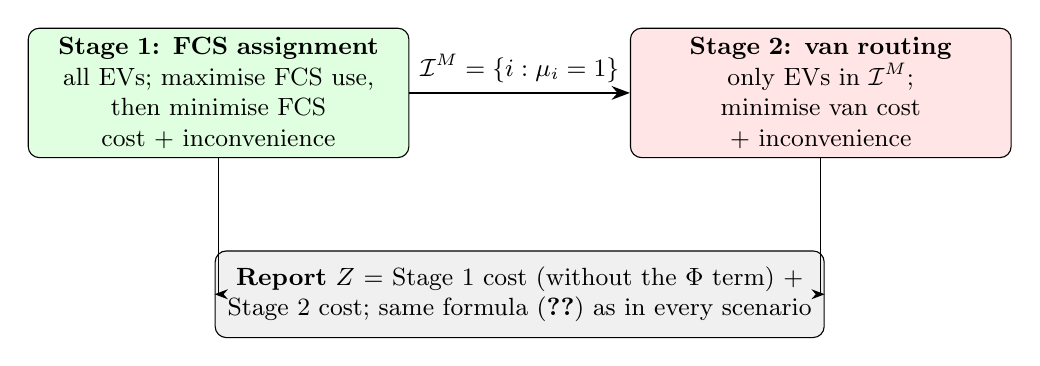
\begin{tikzpicture}[>=Stealth,box/.style={draw,rounded corners,align=center,minimum height=1.1cm,font=\small}]
  \node[box,fill=green!12,text width=4.6cm] (s1) {\textbf{Stage 1: FCS assignment}\\all EVs; maximise FCS use,\\then minimise FCS cost + inconvenience};
  \node[box,fill=red!10,text width=4.6cm,right=2.8cm of s1] (s2) {\textbf{Stage 2: van routing}\\only EVs in $\I^M$;\\minimise van cost + inconvenience};
  \draw[->,thick] (s1) -- node[above,font=\small]{$\I^M=\{i:\mu_i=1\}$} (s2);
  \node[box,fill=black!6,text width=7.5cm,below=2.0cm of $(s1)!0.5!(s2)$] (ev) {\textbf{Report} $Z=$ Stage~1 cost (without the $\Phi$ term) $+$ Stage~2 cost; same formula \eqref{eq:Z} as in every scenario};
  \draw[->] (s1) |- (ev); \draw[->] (s2) |- (ev);
\end{tikzpicture}
\end{center}

Stage~1 does not look at the vans, and Stage~2 cannot change what Stage~1 decided. That is the definition of ``FCS first, then MCS''.

%----------------------------------------------------------------
\subsection{Stage 1: assign EVs to fixed stations}

\textbf{Objective.}
\begin{equation}
\begin{split}
\min\ Z^{(1)}=\;&\underbrace{\Phi\sum_{i\in\I}\mu_i}_{\text{FCS first}}
+\underbrace{c^{EV}\sum_i\sum_{f\in\F_i}d_{if}Y_{if}}_{Z_1}
+\underbrace{Z^F_{\text{energy}}}_{\text{FCS part of }Z_4}\\
&+\underbrace{\sum_i\sum_{f\in\F_i}\rho^F_{if}Y_{if}+\alpha\sum_i w_i(C_i-r_i)+c^L\sum_i w_iL_i}_{\text{FCS customers' inconvenience}}
\end{split}
\label{eq:obj1}
\end{equation}
with $C_i=S_i+\tau^F_iY_i$ in this stage. $\Phi$ is a penalty for handing an EV to the vans. It is chosen larger than anything an extra FCS customer can add to the rest of \eqref{eq:obj1}, e.g.
\[
\Phi > \max_{i}\max_{f\in\F_i}\big(c^{EV}d_{if}+\pi^{\max}E_i+\rho^F_{if}\big)+n\,(\alpha+c^L)\,w_{\max}\,T,
\]
so Stage~1 first \textbf{maximises the number of EVs served at an FCS}, and only among those solutions minimises FCS cost and inconvenience. ($\pi^{\max}$ is the highest grid price.) A numerically safer equivalent is to solve twice: first $\max\sum_iY_i$, then fix that number and minimise the rest.
\ifTOU
Because $Z^F_{\text{energy}}$ uses the peak price, Stage~1 may \emph{start sessions later} to leave the peak, if the price saving beats the extra waiting cost (Section~\ref{sec:expect}).
\fi

\textbf{Constraints.}
\begin{align}
\sum_{g\in\G_i}y_{ig}+\mu_i &= 1 && \forall i\in\I \label{eq:s1assign}\\
S_i &\ge r_i+\sum_{f\in\F_i}t_{if}Y_{if} && \forall i\in\I \label{eq:fcsarr}\\
S_i &\le r_i+T\,(1-\mu_i) && \forall i\in\I \label{eq:s1park}\\
S_j &\ge S_i+\tau^F_i-(T+\tau^F_i)(3-y_{ig}-y_{jg}-o_{ij}) && \forall g,\ (i,j)\in\mathcal{P}_g \label{eq:disj1}\\
S_i &\ge S_j+\tau^F_j-(T+\tau^F_j)(2-y_{ig}-y_{jg}+o_{ij}) && \forall g,\ (i,j)\in\mathcal{P}_g \label{eq:disj2}\\
\sum_i y_{ig_1} &\ge \sum_i y_{ig_2} && \forall f,\ \G_f=\{g_1,g_2\} \label{eq:gunsym}\\
S_i+\tau^F_iY_i &\le T,\qquad L_i\ge S_i+\tau^F_iY_i-l_i && \forall i\in\I \label{eq:s1time}
\end{align}
\ifTOU plus the time-of-use split \eqref{eq:tou1}--\eqref{eq:tou5} of each FCS session (Section~\ref{sec:price}).\fi
\desc{\eqref{eq:s1assign}: every EV either gets one reachable gun or is handed to the vans. An EV that reaches no FCS ($\G_i=\emptyset$) is forced to $\mu_i=1$. \eqref{eq:fcsarr}: an FCS session cannot start before the EV has asked and driven to the station. \eqref{eq:s1park}: for an EV handed to the vans, $S_i$ is parked at $r_i$, so it adds no waiting in Stage~1 (its real start time is decided in Stage~2). \eqref{eq:disj1}--\eqref{eq:disj2}: two EVs on the same gun do not overlap; $o_{ij}$ picks who goes first. With two guns per station this means at most two EVs charge at a station at a time. \eqref{eq:gunsym}: symmetry breaking between the two identical guns (optional). \eqref{eq:s1time}: finished by $T$; lateness.}

\textbf{Optional acceptability rule.} An operator may refuse to send a driver to a station that is ``too inconvenient'', e.g.\ only allow gun $g$ of station $f$ for EV $i$ if $\hat\rho^F_{if}\le\bar\rho$. This only shrinks $\G_i$, so EVs whose stations are all too far go to the vans. Report results with and without it.

\textbf{Output:} $\I^M=\{i:\mu_i=1\}$, the EVs left for the vans; plus each FCS customer's gun and start time.

%----------------------------------------------------------------
\subsection{Stage 2: route the vans to the leftover EVs}

Stage~2 is a vehicle routing problem with time windows, on the EVs in $\I^M$ only. Here $C_i=S_i+\tau^M_i$.

\textbf{Objective.}
\begin{equation}
\begin{split}
\min\ Z^{(2)}=\;&\underbrace{c^M\sum_m\sum_{(i,j)\in\A^M}d_{ij}x_{ijm}}_{Z_2}+\underbrace{\sum_m c^D_mu_m}_{Z_3}+\underbrace{Z^M_{\text{energy}}}_{\text{van part of }Z_4}\\
&+\underbrace{\sum_{i\in\I^M}\sum_m\rho^M_{im}z_{im}+\alpha\sum_{i\in\I^M}w_i(C_i-r_i)+c^L\sum_{i\in\I^M}w_iL_i}_{\text{van customers' inconvenience}}
\end{split}
\label{eq:obj2}
\end{equation}
Since every EV in $\I^M$ must be served by some van, $Z^M_{\text{energy}}$ and the $\rho^M$ term are constants here. They are kept so that $Z^{(2)}$ is the true cost of Stage~2. Waiting and lateness make the vans visit urgent EVs early.

\textbf{Constraints.}
\begin{align}
\sum_{m\in\M}z_{im} &= 1 && \forall i\in\I^M \label{eq:s2assign}\\
\sum_{j:(0,j)\in\A^M}x_{0jm} = \sum_{i:(i,n+1)\in\A^M}x_{i,n+1,m} &= u_m && \forall m \label{eq:depot}\\
\sum_{i:(i,j)\in\A^M}x_{ijm} = \sum_{k:(j,k)\in\A^M}x_{jkm} &= z_{jm} && \forall j\in\I^M,\ m \label{eq:flow}\\
\sum_{i\in\I^M}z_{im} &\le Q_m\,u_m && \forall m \label{eq:cap}\\
\sum_{i\in\I^M}\frac{E_i}{\eta}z_{im}+\beta\sum_{(i,j)\in\A^M}d_{ij}x_{ijm} &\le B_m\,u_m && \forall m \label{eq:batt}
\end{align}
\begin{align}
S_j &\ge \max\{r_j,\ t_{0j}\,x_{0jm}\} && \forall j\in\I^M,\ m \label{eq:depart}\\
S_j &\ge S_i+\tau^M_i+t_{ij}-(T+\tau^M_i+t_{ij})(1-x_{ijm}) && \forall i\neq j,\ m \label{eq:seq}\\
S_i+\tau^M_i+t_{i,n+1} &\le T+(\tau^M_i+t_{i,n+1})(1-x_{i,n+1,m}) && \forall i,\ m \label{eq:return}\\
S_i+\tau^M_i \le T,\quad L_i &\ge S_i+\tau^M_i-l_i && \forall i\in\I^M \label{eq:s2time}\\
u_m &\ge u_{m+1} && m<|\M| \label{eq:vansym}
\end{align}
\desc{\eqref{eq:s2assign}: each leftover EV gets one van. \eqref{eq:depot}: a used van leaves and returns to the depot once. \eqref{eq:flow}: each EV on van $m$ is entered and left exactly once by that van. \eqref{eq:cap}: at most $Q_m$ EVs per van. \eqref{eq:batt}: delivered energy (with transfer losses) plus driving energy fits in the van battery. \eqref{eq:depart}: no start before the request, or before the van can drive there from the depot (written as two linear constraints). \eqref{eq:seq}: if the van goes $i\to j$, it finishes $i$ and drives to $j$ before starting $j$. This gives one EV at a time and removes subtours (MTZ-type). \eqref{eq:return}: back at the depot by $T$. \eqref{eq:s2time}: finished by $T$; lateness. \eqref{eq:vansym}: use identical vans in index order.}

\textbf{If Stage 2 is infeasible} (too many leftover EVs for the fleet by $T$), the sequential policy has \emph{failed} on that instance. For diagnosis, add $s_i\in\{0,1\}$ (``unserved''), replace \eqref{eq:s2assign} by $\sum_mz_{im}+s_i=1$ and add $\Phi^U\sum_is_i$ to \eqref{eq:obj2}. Then report the number of EVs that could not be served. This is a useful comparison with the integrated scenario, which may serve all of them.

%----------------------------------------------------------------
\subsection{Reported value}
\[
Z^{\text{S\scen}}=\big(Z^{(1)*}-\Phi\,|\I^M|\big)+Z^{(2)*},
\]
which is exactly \eqref{eq:Z} evaluated at the combined solution. The stage-1 solution plus the stage-2 solution is a feasible solution of the integrated model (S\ifTOU 4\else 3\fi), so
$Z^{\text{S\ifTOU 4\else 3\fi}}\le Z^{\text{S\scen}}$. The difference is the \emph{value of integration}.

\else
%---------------------------------------------------------------- INT
\subsection{Objective}
\begin{equation}
\min\ Z \quad\text{as in \eqref{eq:Z}, with }Z^F_{\text{energy}}=\ifTOU P^F\textstyle\sum_i\big[\pi^\off(\theta^1_i+\theta^3_i)+\pi^\pk\theta^2_i\big]\else\pi^F\textstyle\sum_iE_iY_i\fi,\quad C_i=S_i+\tau^F_iY_i+\tau^M_iZ_i. \label{eq:objint}
\end{equation}
Written out in full:
\begin{align*}
\min\ Z=\;& c^{EV}\sum_i\sum_{f\in\F_i}d_{if}Y_{if}+c^M\sum_m\sum_{(i,j)\in\A}d_{ij}x_{ijm}+\sum_mc^D_mu_m\\
&+\ifTOU P^F\sum_i\big[\pi^\off(\theta^1_i+\theta^3_i)+\pi^\pk\theta^2_i\big]\else\pi^F\sum_iE_iY_i\fi
+\pi^M\sum_i\sum_m\frac{E_i}{\eta}z_{im}\\
&+\sum_i\sum_{f\in\F_i}\rho^F_{if}Y_{if}+\sum_i\sum_m\rho^M_{im}z_{im}+\alpha\sum_iw_i(C_i-r_i)+c^L\sum_iw_iL_i .
\end{align*}
Every term is linear. One model weighs everything at once: an EV goes to a van exactly when the van's extra km, dispatch and energy cost are outweighed by the effort and waiting it saves the driver\ifTOU, or by the peak-price energy it avoids\fi.

\subsection{Constraints}

\textbf{Assignment.}
\begin{equation}
\sum_{g\in\G_i}y_{ig}+\sum_{m\in\M}z_{im}=1\qquad\forall i\in\I \label{eq:assign}
\end{equation}
\desc{Exactly one resource per EV: one reachable gun or one van. EVs that reach no FCS are forced onto a van.}

\textbf{Fixed stations.}
\begin{align}
S_i &\ge r_i+\sum_{f\in\F_i}t_{if}Y_{if} && \forall i \label{eq:fcsarr}\\
S_j &\ge S_i+\tau^F_i-(T+\tau^F_i)(3-y_{ig}-y_{jg}-o_{ij}) && \forall g,\ (i,j)\in\mathcal{P}_g \label{eq:disj1}\\
S_i &\ge S_j+\tau^F_j-(T+\tau^F_j)(2-y_{ig}-y_{jg}+o_{ij}) && \forall g,\ (i,j)\in\mathcal{P}_g \label{eq:disj2}\\
\sum_iy_{ig_1} &\ge \sum_iy_{ig_2} && \forall f,\ \G_f=\{g_1,g_2\} \label{eq:gunsym}
\end{align}
\desc{\eqref{eq:fcsarr}: an FCS session starts after the request and the drive to the station (for a van customer this is just $S_i\ge r_i$). \eqref{eq:disj1}--\eqref{eq:disj2}: EVs on the same gun do not overlap; $o_{ij}$ chooses the order. \eqref{eq:gunsym}: optional symmetry breaking.}

\textbf{Vans: routes, capacity, battery.}
\begin{align}
\sum_{j:(0,j)\in\A}x_{0jm}=\sum_{i:(i,n+1)\in\A}x_{i,n+1,m} &= u_m && \forall m \label{eq:depot}\\
\sum_{i:(i,j)\in\A}x_{ijm}=\sum_{k:(j,k)\in\A}x_{jkm} &= z_{jm} && \forall j\in\I,\ m \label{eq:flow}\\
\sum_iz_{im} &\le Q_mu_m && \forall m \label{eq:cap}\\
\sum_i\frac{E_i}{\eta}z_{im}+\beta\sum_{(i,j)\in\A}d_{ij}x_{ijm} &\le B_mu_m && \forall m \label{eq:batt}
\end{align}
\desc{\eqref{eq:depot}: a used van leaves and returns once. \eqref{eq:flow}: each EV on van $m$ is visited exactly once by it. \eqref{eq:cap}: at most $Q_m$ EVs. \eqref{eq:batt}: delivered energy (with losses) plus driving energy fits in the battery.}

\textbf{Vans: timing (one EV at a time, no subtours).}
\begin{align}
S_j &\ge t_{0j}\,x_{0jm} && \forall j\in\I,\ m \label{eq:depart}\\
S_j &\ge S_i+\tau^M_i+t_{ij}-(T+\tau^M_i+t_{ij})(1-x_{ijm}) && \forall i\neq j\in\I,\ m \label{eq:seq}\\
S_i+\tau^M_i+t_{i,n+1} &\le T+(\tau^M_i+t_{i,n+1})(1-x_{i,n+1,m}) && \forall i,\ m \label{eq:return}
\end{align}
\desc{\eqref{eq:depart}: the first stop cannot start before the van has driven there. \eqref{eq:seq}: $i\to j$ means finish $i$, drive, then start $j$; start times rise along a route, so no subtour can close. \eqref{eq:return}: back at the depot by $T$.}

\textbf{Horizon and lateness.}
\begin{equation}
C_i\le T,\qquad L_i\ge C_i-l_i\qquad\forall i\in\I \label{eq:time}
\end{equation}
\desc{Every EV is fully charged within the horizon; $L_i$ measures lateness.}

\ifTOU
\textbf{Time-of-use split.} Constraints \eqref{eq:tou1}--\eqref{eq:tou5} of Section~\ref{sec:price}.
\fi

\textbf{Symmetry and domains.}
\begin{equation}
u_m\ge u_{m+1};\qquad y,z,x,u,o\ifTOU,\kappa\fi\in\{0,1\};\qquad S_i,L_i\ifTOU,\theta^p_i\fi\ge0 \label{eq:dom}
\end{equation}
\fi

%=====================================================================
\section{Learning-to-optimise (RL) formulation}\label{sec:rl}

\textbf{Main rule:} the reward of each action is \emph{minus the increase in $Z$ that the action causes}. The rewards over an episode then add up to $-Z$ of the solution the policy builds. RL and MILP results are measured on the same yardstick \eqref{eq:Z}, and the MILP optimum is the benchmark for the RL gap.

\ifSEQ
%---------------------------------------------------------------- RL SEQ
The RL pipeline has the same two stages as the MILP.

\subsection{Stage 1 policy: FCS assignment}
\begin{itemize}[leftmargin=1.4em,itemsep=2pt]
  \item \textbf{Episode / epochs:} EVs are taken in order of request time $r_i$ (ties: higher $w_i$ first). One decision per EV.
  \item \textbf{State:} features of the current EV $k$ ($E_k,r_k,l_k,w_k,R_k$, location); for each gun $g$ the time $F_g$ it becomes free; summary features of the EVs still to come (count and positions near each station)\ifTOU; the current price and the time until $T_1$ and $T_2$\fi.
  \item \textbf{Action:} a gun $g\in\G_k$, or ``hand to vans''. \textbf{FCS-first mask:} ``hand to vans'' is allowed \emph{only} if no gun can finish EV $k$ by $T$ (or, with the optional rule, if all remaining guns have $\hat\rho^F_{kf}>\bar\rho$).
  \ifTOU\item \textbf{Optional timing action:} ``gun $g$, start after the peak'', i.e.\ $S_k=\max\{\text{earliest},T_2\}$, allowed only if the session still ends by $T$.\fi
  \item \textbf{Transition:} $S_k=\max\{r_k+t_{kf},F_g\}$ (or later, for the timing action); $F_g\leftarrow S_k+\tau^F_k$.
  \item \textbf{Reward:} $-\Big[c^{EV}d_{kf}+\text{energy}_k+\rho^F_{kf}+\alpha w_k(S_k+\tau^F_k-r_k)+c^Lw_k(S_k+\tau^F_k-l_k)^+\Big]$, where energy$_k$ = \ifTOU$P^F\big[\pi^\off\cdot(\text{off-peak hours of }[S_k,S_k+\tau^F_k])+\pi^\pk\cdot(\text{peak hours})\big]$, computed exactly in the simulator\else$\pi^FE_k$\fi. Handing an EV to the vans gives reward $0$ here; its cost is counted in Stage~2.
\end{itemize}
Note: a simple baseline for Stage~1 is the greedy rule ``gun with the largest one-step reward''. What RL can learn on top of this is, for example, to keep a nearby gun free for an urgent EV that arrives later.

\subsection{Stage 2 policy: van routing over $\I^M$}
\begin{itemize}[leftmargin=1.4em,itemsep=2pt]
  \item \textbf{Epochs:} whenever a van becomes free (the earliest-free van decides first).
  \item \textbf{State:} for each van: position, time free, remaining battery $b_m$, EVs served so far, dispatched or not; for each unserved EV in $\I^M$: location, $E_i,r_i,l_i,w_i$; current time.
  \item \textbf{Action:} the next EV $j$ for this van, or ``return to depot'' (ends the route). Mask: $j$ must be feasible: battery covers $E_j/\eta$ plus driving to $j$ and back to the depot, the count stays $\le Q_m$, and $j$ can be finished with the van back at the depot by $T$.
  \item \textbf{Transition:} $S_j=\max\{r_j,\ \text{time free}+t_{\text{pos},j}\}$; the van moves to $j$ and is free at $S_j+\tau^M_j$; $b_m$ falls by $E_j/\eta+\beta d_{\text{pos},j}$.
  \item \textbf{Reward:} serving $j$: $-\Big[c^Md_{\text{pos},j}+c^D_m[\text{first stop}]+\pi^M\frac{E_j}{\eta}+\rho^M_{jm}+\alpha w_j(S_j+\tau^M_j-r_j)+c^Lw_j(S_j+\tau^M_j-l_j)^+\Big]$; returning: $-c^Md_{\text{pos},0}$. EVs still unserved at the end: $-\Phi^U$ each.
  \item \textbf{Policy:} an attention-based routing policy (e.g.\ Kool et al., 2019, ``Attention, Learn to Solve Routing Problems!'') trained with REINFORCE or PPO. Baseline: nearest-feasible-EV heuristic.
\end{itemize}
Episode return of Stage~1 + Stage~2 $=-Z^{\text{S\scen}}$.

\else
%---------------------------------------------------------------- RL INT
One policy decides both who serves each EV and the van routes.
\begin{itemize}[leftmargin=1.4em,itemsep=2pt]
  \item \textbf{Episode / epochs:} EVs are taken in order of request time $r_i$ (ties: higher $w_i$ first). One decision per EV.
  \item \textbf{State:} (i) the current EV $k$: location, $E_k,r_k,l_k,w_k,R_k$, reachable stations; (ii) each gun $g$: time $F_g$ it becomes free; (iii) each van $m$: current end-of-route position, time free, remaining battery $b_m$, EVs served, dispatched or not; (iv) embeddings of the not-yet-assigned EVs (for look-ahead)\ifTOU; (v) current price, time until $T_1$ and $T_2$\fi.
  \item \textbf{Action:} $a\in\G_k\cup\M$: a gun, or a van (EV $k$ is appended to the end of that van's route). \textbf{Mask} infeasible actions: a gun that cannot finish $k$ by $T$; a van without enough battery for $E_k/\eta$ plus the drive to $k$ and back to the depot, with $Q_m$ reached, or unable to finish $k$ and return by $T$.
  \ifTOU\item \textbf{Optional timing action:} ``gun $g$, start after the peak'' ($S_k=\max\{\text{earliest},T_2\}$, if it still ends by $T$).\fi
  \item \textbf{Transition:} gun: $S_k=\max\{r_k+t_{kf},F_g\}$, $F_g\leftarrow S_k+\tau^F_k$. Van: $S_k=\max\{r_k,\ \text{free}_m+t_{\text{pos}_m,k}\}$, then the van moves to $k$, $\text{free}_m\leftarrow S_k+\tau^M_k$, $b_m\mathrel{-}=E_k/\eta+\beta d_{\text{pos}_m,k}$.
  \item \textbf{Reward} $=-\Delta Z$:
  \begin{align*}
  \text{gun } g\text{ at }f:&\quad -\Big[c^{EV}d_{kf}+\text{energy}^F_k+\rho^F_{kf}+\alpha w_k(C_k-r_k)+c^Lw_k(C_k-l_k)^+\Big]\\
  \text{van } m:&\quad -\Big[c^M\big(d_{\text{pos}_m,k}+d_{k,0}-d_{\text{pos}_m,0}\big)+c^D_m[\text{first use}]+\pi^M\tfrac{E_k}{\eta}\\
  &\qquad\quad+\rho^M_{km}+\alpha w_k(C_k-r_k)+c^Lw_k(C_k-l_k)^+\Big]
  \end{align*}
  The van distance term is the \emph{change} in route length when $k$ is inserted before the return to the depot, so the sum over the episode equals the total route length (the return legs telescope). energy$^F_k$ = \ifTOU$P^F\big[\pi^\off\cdot(\text{off-peak hours})+\pi^\pk\cdot(\text{peak hours of }[S_k,C_k])\big]$, computed exactly by the simulator; no linearisation is needed in RL\else$\pi^FE_k$\fi.
  \item \textbf{Dead end:} if every action is masked, EV $k$ is unserved: reward $-\Phi^U$, and the episode continues. Report the count.
  \item \textbf{Policy:} masked categorical policy over guns and vans, encoder with attention over EVs, guns and vans; trained with PPO. Natural baseline: greedy, i.e.\ choose the action with the largest one-step reward. That is the pairwise rule ``smallest $\hat\rho$ + cost'' from Section~\ref{sec:inc}.
\end{itemize}
Restriction to note: vans serve EVs in assignment order (append only). A variant that inserts $k$ at the cheapest position of a route is more flexible but has a larger action space.
\fi

\textbf{Reward scaling.} For stable training divide every reward by a constant, e.g.\ the greedy baseline's average $Z$ on the training instances. This does not change the optimal policy.

%=====================================================================
\section{What to expect and what to report}\label{sec:expect}

\ifnum\scen=1
\begin{itemize}[leftmargin=1.4em,itemsep=2pt]
  \item Vans serve only EVs that reach no station, or that the stations cannot finish by $T$. If stations have spare capacity, very few vans are dispatched.
  \item Inconvenience is high for EVs far from the nearest station (worked example: Rs\,682 at the FCS, against Rs\,458 if a van had been allowed).
  \item With too few vans Stage~2 becomes infeasible (unserved EVs), even when the integrated model S3 could serve everyone. Report the smallest $|\M|$ at which S1 is feasible and compare it with S3.
\end{itemize}
\fi
\ifnum\scen=2
\begin{itemize}[leftmargin=1.4em,itemsep=2pt]
  \item \textbf{When does Stage~1 delay a session to avoid the peak?} Moving one hour of charging out of the peak saves $(\pi^\pk-\pi^\off)P^F=3\times22=$ Rs\,66, but delays completion by up to an hour, which costs $\alpha w_i\ge$ Rs\,200. So with the default values Stage~1 almost never delays. It mostly pays the higher price, and S2 costs roughly S1 plus the peak surcharge. Sessions start later only if $\alpha$ is small (try $\lambda<0.33$ in the sensitivity analysis).
  \item The van assignment is the same as in S1 unless Stage~1's timing changes which EVs fit at the stations. Stage~1 cannot use vans to escape the peak price.
  \item Extra KPI: \textbf{grid energy drawn at FCS during the peak}, $P^F\sum_i\theta^2_i$ (kWh). Compare with S4.
\end{itemize}
\fi
\ifnum\scen=3
\begin{itemize}[leftmargin=1.4em,itemsep=2pt]
  \item Vans take EVs for which the saved inconvenience exceeds the extra van cost (worked example: van chosen, saving Rs\,224). Expect vans to serve EVs that are far from every station, have low range (high $w_i$), or have early deadlines, while EVs near a station still use it.
  \item \textbf{Value of integration under flat price:} $Z^{\text{S1}}-Z^{\text{S3}}\ge0$. Report it per component ($Z_1,\dots,Z_5$): typically operating cost rises a little and inconvenience falls a lot.
  \item Vary $|\M|$ (0, 1, 2, \dots): the first few vans lower $Z$ sharply, then the effect levels off. That curve shows the scenarios where mobile chargers help most.
\end{itemize}
\fi
\ifnum\scen=4
\begin{itemize}[leftmargin=1.4em,itemsep=2pt]
  \item During the peak a van kWh costs about the same as an FCS kWh (Rs\,10.0 each), so the vans' energy disadvantage disappears and vans also absorb \emph{peak-hour} demand that would otherwise be charged on the grid at peak price.
  \item Expect more van usage than in S3, concentrated on requests in $[T_1,T_2]$, and lower grid energy at the stations during the peak, $P^F\sum_i\theta^2_i$, than in S2.
  \item \textbf{Value of integration under peak pricing:} $Z^{\text{S2}}-Z^{\text{S4}}$. It should be larger than $Z^{\text{S1}}-Z^{\text{S3}}$, because integration now also allows price arbitrage.
  \item \textbf{Peak pricing with full flexibility:} $Z^{\text{S4}}-Z^{\text{S3}}$ should be smaller than $Z^{\text{S2}}-Z^{\text{S1}}$: vans cushion the price increase.
\end{itemize}
\fi

\textbf{Cross-scenario comparison table} (fill in from the four runs):
\begin{center}
\renewcommand{\arraystretch}{1.2}
\begin{tabular}{@{}lll@{}}
\toprule
\textbf{Comparison} & \textbf{Measures} & \textbf{Expected sign} \\
\midrule
S1 $-$ S3 & value of integration, flat price & $\ge0$ \\
S2 $-$ S4 & value of integration, peak price & $\ge0$, larger than S1 $-$ S3 \\
S2 $-$ S1 & cost of peak pricing, FCS-first operator & $>0$ \\
S4 $-$ S3 & cost of peak pricing, flexible operator & $>0$, smaller than S2 $-$ S1 \\
\bottomrule
\end{tabular}
\end{center}
Report for each: $Z$ and its components, number of vans used, EVs per resource, mean and maximum inconvenience per EV, total lateness, peak-hour grid energy, solve time, and (for RL) the gap to the MILP optimum.

%=====================================================================
\appendix
\section{Illustrative parameter values}\label{app:values}

These are starting values for experiments, not data. All are meant to be varied in the analysis. Values in Rs.

\begin{center}
\renewcommand{\arraystretch}{1.15}
\begin{tabular}{@{}llp{6.2cm}@{}}
\toprule
\textbf{Parameter} & \textbf{Value} & \textbf{Note} \\
\midrule
$T$, $[T_1,T_2]$ & 7 h, $[2,6]$ & 16:00--23:00, peak 18:00--22:00 \\
$P^F$, $P^M$ & 22 kW, 30 kW & \\
$v$, $\beta$, $\eta$ & 25 km/h, 0.25 kWh/km, 0.9 & \\
$B_m$, $Q_m$, $|\M|$ & 150 kWh, 6, 2--6 & \\
$c^{EV}$, $c^M$, $c^D_m$ & Rs\,4/km, Rs\,15/km, Rs\,1500 & van km includes driver time \\
$\pi^F$ (flat) & Rs\,8.7/kWh & equals the time-average of the ToU tariff over $[0,T]$ \\
$\pi^\off$, $\pi^\pk$ (ToU) & Rs\,7/kWh, Rs\,10/kWh & $(3\times7+4\times10)/7=8.7$ \\
$c^{bat}$ & Rs\,2/kWh & van battery wear \\
$\pi^M$ & Rs\,10.7 (flat) / Rs\,9.0 (ToU) & $=\pi^F+c^{bat}$ / $=\pi^\off+c^{bat}$ \\
$\alpha$, $\alpha^D$ & Rs\,200/h, Rs\,100/h & value of time; extra for attended time \\
$h^F$, $h^M$, $\varphi$ & Rs\,50, Rs\,10, Rs\,100 & trip hassle, hand-over, range stress \\
$c^L$ & Rs\,300/h & lateness \\
$w_i$ & $1+2(1-R_i/R_{\max})$, $R_i\sim U[3,40]$ km & priority from remaining range \\
\bottomrule
\end{tabular}
\end{center}

The flat price is set to the time-average of the peak tariff. The price \emph{level} is then the same in both pricing cases, and only the price \emph{shape} differs. Without this, part of S1 vs S2 would just reflect a different average price.

\end{document}
"
%    pdflatex -jobname=scenario2_peak_sequential   "\def\scen{2}% =====================================================================
%  One source, four PDFs.  Build with build.sh (or by hand):
%    pdflatex -jobname=scenario1_flat_sequential   "\def\scen{1}% =====================================================================
%  One source, four PDFs.  Build with build.sh (or by hand):
%    pdflatex -jobname=scenario1_flat_sequential   "\def\scen{1}% =====================================================================
%  One source, four PDFs.  Build with build.sh (or by hand):
%    pdflatex -jobname=scenario1_flat_sequential   "\def\scen{1}\input{scenario_master}"
%    pdflatex -jobname=scenario2_peak_sequential   "\def\scen{2}\input{scenario_master}"
%    pdflatex -jobname=scenario3_flat_integrated   "\def\scen{3}\input{scenario_master}"
%    pdflatex -jobname=scenario4_peak_integrated   "\def\scen{4}\input{scenario_master}"
%  (run each twice for cross-references)
% =====================================================================
\documentclass[11pt,a4paper]{article}
\usepackage[margin=2.2cm]{geometry}
\usepackage{amsmath,amssymb,amsfonts}
\usepackage{booktabs,array,tabularx}
\usepackage{enumitem}
\usepackage[table]{xcolor}
\usepackage{tikz}
\usetikzlibrary{arrows.meta,positioning,calc}
\usepackage[colorlinks=true,linkcolor=blue!50!black,urlcolor=blue!50!black]{hyperref}
\usepackage{titlesec}
\titleformat{\section}{\large\bfseries}{\thesection}{0.8em}{}
\titleformat{\subsection}{\normalsize\bfseries}{\thesubsection}{0.8em}{}
\setlength{\parindent}{0pt}
\setlength{\parskip}{5pt}

% ---------------- scenario switches ----------------
\ifdefined\scen\else\def\scen{1}\fi
\newif\ifTOU \TOUfalse   % true = time-of-use (peak) price
\newif\ifSEQ \SEQfalse   % true = FCS first, then MCS
\ifnum\scen=1 \SEQtrue \fi
\ifnum\scen=2 \TOUtrue \SEQtrue \fi
\ifnum\scen=4 \TOUtrue \fi

\newcommand{\pricename}{\ifTOU time-of-use price (dearer evening peak)\else single (flat) price all day\fi}
\newcommand{\structname}{\ifSEQ FCS first, then MCS (sequential)\else FCS and MCS together (integrated)\fi}

% ---------------- notation ----------------
\newcommand{\I}{\mathcal{I}}
\newcommand{\F}{\mathcal{F}}
\newcommand{\G}{\mathcal{G}}
\newcommand{\M}{\mathcal{M}}
\newcommand{\N}{\mathcal{N}}
\newcommand{\A}{\mathcal{A}}
\newcommand{\Rs}{\text{Rs}\,}
\newcommand{\pk}{\mathrm{pk}}
\newcommand{\off}{\mathrm{off}}
\newcommand{\desc}[1]{\par\vspace{-2pt}{\small\color{black!75}\textit{Meaning:} #1}\par\vspace{4pt}}
\newcommand{\cell}[2]{\ifnum\scen=#1\cellcolor{blue!18}\textbf{S#1 (this document)}\\\textbf{#2}\else S#1\\#2\fi}

\title{\textbf{EV Charging Network Optimisation}\\[4pt]
\large Scenario \scen: \pricename\ $+$ \structname\\[2pt]
\normalsize MILP and RL formulation}
\author{CP 320 OR for Mobility Management, course project}
\date{2 October 2026}

\begin{document}
\maketitle

%=====================================================================
\section{Where this scenario sits}

The project studies four scenarios: two ways of pricing grid electricity, times two ways of making the decisions.

\begin{center}
\renewcommand{\arraystretch}{1.5}
\begin{tabular}{>{\raggedright\arraybackslash}p{4.2cm}|>{\centering\arraybackslash}p{4.6cm}|>{\centering\arraybackslash}p{4.6cm}}
 & \textbf{Flat price all day} & \textbf{Time-of-use (peak) price} \\ \hline
\textbf{Sequential:} FCS first, leftover EVs to MCS &
\begin{tabular}[c]{@{}c@{}}\cell{1}{flat + sequential}\end{tabular} &
\begin{tabular}[c]{@{}c@{}}\cell{2}{peak + sequential}\end{tabular} \\ \hline
\textbf{Integrated:} FCS and MCS decided together &
\begin{tabular}[c]{@{}c@{}}\cell{3}{flat + integrated}\end{tabular} &
\begin{tabular}[c]{@{}c@{}}\cell{4}{peak + integrated}\end{tabular} \\
\end{tabular}
\end{center}

\textbf{The four scenarios do not have four different objectives.} They share \emph{one} cost yardstick $Z$ (Section~\ref{sec:obj}): the same cost terms and the same customer inconvenience (Section~\ref{sec:inc}). Only two things change:
\begin{itemize}[leftmargin=1.4em,itemsep=1pt]
  \item \textbf{Pricing} changes the formula for one term, the FCS energy cost (Section~\ref{sec:price}).
  \item \textbf{Decision structure} changes \emph{how} $Z$ is minimised: in one model (integrated), or in two stages (sequential), where each stage minimises its own part of $Z$.
\end{itemize}
Because the yardstick is the same, the four optimal values can be compared directly. The differences measure the \emph{value of integration} (S1$\to$S3, S2$\to$S4) and the \emph{effect of peak pricing} (S1$\to$S2, S3$\to$S4).

\ifnum\scen=1
\textbf{This scenario (S1)} is the baseline, the ``status quo''. Electricity costs the same at every hour, every EV that can be charged at a fixed station is sent there, and vans only take what is left over.
\fi
\ifnum\scen=2
\textbf{This scenario (S2)} keeps the FCS-first rule of S1, but grid electricity is dearer during the evening peak. Stage~1 can react to the price only by \emph{rescheduling} FCS sessions. It cannot hand a peak-hour EV to a van.
\fi
\ifnum\scen=3
\textbf{This scenario (S3)} keeps the flat price of S1, but the operator decides FCS and MCS service \emph{together}. An EV can be sent to a van even when a fixed station could take it, whenever that lowers total cost plus inconvenience.
\fi
\ifnum\scen=4
\textbf{This scenario (S4)} is the most flexible one: peak pricing at fixed stations, and FCS and MCS decided together. Van energy was bought off-peak, so vans can also be used to keep charging \emph{out of the expensive peak}.
\fi

%=====================================================================
\section{Setting and assumptions}\label{sec:setting}

\textbf{Time.} The planning horizon is $[0,T]$ with $T=7$\,h (16:00--23:00). It contains the evening peak window $[T_1,T_2]=[2,6]$ (18:00--22:00). The horizon is the same in all four scenarios. It is wider than the peak itself so that, under peak pricing, there is cheaper time on both sides of the peak.\ifTOU\else\ In this scenario the price is flat, so the window plays no role in the model.\fi

\textbf{Assumptions} (the same as MILP v3, plus two about energy):
\begin{enumerate}[leftmargin=1.6em,itemsep=1pt]
  \item Static, continuous time. All requests in the horizon are known at time $0$, and request $i$ becomes active at $r_i$.
  \item An EV served by an FCS drives there itself on its own battery (only to stations within its range $R_i$). The driver stays with the car while it waits for a free gun and while it charges.
  \item An EV served by an MCS stays parked where it is, and the driver is free in the meantime.
  \item Each FCS gun and each van charges one EV at a time, without interruption, at constant power.
  \item A van's battery covers both its driving and the energy it delivers. \textbf{The van battery is charged at the depot before the horizon starts}\ifTOU, i.e.\ at the off-peak price\fi, and is not recharged during the horizon.
  \item Every EV must be fully charged by $T$ (hard). Finishing after the driver's desired time $l_i$ is allowed but penalised.
\end{enumerate}

%=====================================================================
\section{Notation}\label{sec:notation}

\subsection*{Sets}
\begin{tabularx}{\textwidth}{@{}lX@{}}
\toprule
$\I=\{1,\dots,n\}$ & EV charging requests \\
$\F$; $\G_f$ ($|\G_f|=2$); $\G=\bigcup_f\G_f$ & fixed charging stations; guns of FCS $f$; all guns ($f(g)$ = station of gun $g$) \\
$\F_i=\{f: d_{if}\le R_i\}$, $\G_i=\bigcup_{f\in\F_i}\G_f$ & stations / guns EV $i$ can reach on its remaining range \\
$\M$ & mobile charging vans (MCS) \\
$0,\ n+1$ & depot as start node / end node (same place) \\
$\N=\{0\}\cup\I\cup\{n+1\}$, $\A$ & routing nodes; allowed van arcs $(i,j)$, $i\in\{0\}\cup\I$, $j\in\I\cup\{n+1\}$, $i\neq j$ \\
$\mathcal{P}_g=\{(i,j): i<j,\ g\in\G_i\cap\G_j\}$ & pairs of EVs that could share gun $g$ \\
\ifSEQ
$\I^M\subseteq\I$ & EVs handed to the vans by Stage~1 (an \emph{output} of Stage~1, a fixed input to Stage~2) \\
$\N^M$, $\A^M$ & routing nodes / arcs restricted to $\I^M$ \\
\fi
\bottomrule
\end{tabularx}

\subsection*{Parameters}
\begin{tabularx}{\textwidth}{@{}lX@{}}
\toprule
$E_i,\ r_i,\ l_i,\ R_i$ & energy demand (kWh), request time, desired completion time (h), remaining range (km) \\
$w_i\ge1$ & priority of EV $i$; $w_i=1+\kappa(1-R_i/R_{\max})$, so low-range EVs weigh more \\
$P^F,\ P^M$ & charging power of an FCS gun (22\,kW) / of a van (e.g.\ 30\,kW) \\
$\tau^F_i=E_i/P^F,\ \tau^M_i=E_i/P^M$ & charging time of EV $i$ at an FCS / by a van (h) \\
$d_{if},t_{if}$;\ $d_{ij},t_{ij}$ & distance (km) and time (h): EV$\to$FCS; between routing nodes ($t=d/v$) \\
$B_m,\ Q_m,\ \beta,\ \eta$ & van battery (kWh), max EVs per van, van consumption (kWh/km), transfer efficiency \\
$c^{EV},\ c^M,\ c^D_m$ & cost per km of EV driving, per km of van driving; fixed dispatch cost of van $m$ \\
\ifTOU
$\pi^\off,\ \pi^\pk$ & grid price (Rs/kWh) off-peak / in $[T_1,T_2]$, with $\pi^\pk\ge\pi^\off$ \\
\else
$\pi^F$ & grid price (Rs/kWh), the same at every hour \\
\fi
$c^{bat}$ & van battery wear per kWh cycled \\
$\pi^M$ & cost of 1 kWh taken from a van battery: $\pi^M=\ifTOU\pi^\off\else\pi^F\fi+c^{bat}$ (Section~\ref{sec:price}) \\
$\alpha,\ \alpha^D,\ h^F,\ h^M,\ \varphi,\ c^L$ & inconvenience coefficients (Section~\ref{sec:inc}) \\
\bottomrule
\end{tabularx}

\subsection*{Decision variables}
\begin{tabularx}{\textwidth}{@{}llX@{}}
\toprule
$y_{ig}$ & $\{0,1\}$ & EV $i$ charged at gun $g\in\G_i$ \\
$z_{im}$ & $\{0,1\}$ & EV $i$ served by van $m$ \\
$x_{ijm}$ & $\{0,1\}$ & van $m$ drives arc $(i,j)$ \\
$u_m$ & $\{0,1\}$ & van $m$ is dispatched \\
$o_{ij}$ & $\{0,1\}$ & for EVs $i<j$ that could share a gun: 1 if $i$ is charged before $j$ \\
\ifSEQ
$\mu_i$ & $\{0,1\}$ & Stage~1 only: EV $i$ is handed to the van fleet \\
\fi
\ifTOU
$\theta^1_i,\theta^2_i,\theta^3_i$ & $\ge0$ & hours of EV $i$'s FCS session before / inside / after the peak \\
$\kappa^1_i,\kappa^3_i$ & $\{0,1\}$ & EV $i$'s FCS session starts before $T_1$ / ends after $T_2$ \\
\fi
$S_i$ & $\ge0$ & time charging of EV $i$ starts (h), on whichever resource \\
$L_i$ & $\ge0$ & lateness of EV $i$ beyond $l_i$ (h) \\
\bottomrule
\end{tabularx}

\textbf{Short-hands} (linear expressions, not new variables):
\[
Y_{if}=\sum_{g\in\G_f}y_{ig},\qquad Y_i=\sum_{g\in\G_i}y_{ig}\ (\text{EV $i$ uses an FCS}),\qquad Z_i=\sum_{m\in\M}z_{im}\ (\text{EV $i$ uses a van}),
\]
\[
C_i=S_i+\tau^F_i\,Y_i+\tau^M_i\,Z_i \quad\text{(time EV $i$ is fully charged).}
\]

%=====================================================================
\section{Customer inconvenience}\label{sec:inc}

This section is \textbf{identical in all four scenario documents}. Inconvenience is a property of the customer, not of the price or of the planning method.

\subsection{What we mean by inconvenience}

Inconvenience is \emph{what the driver loses} from the moment they ask for a charge ($r_i$) until the car is fully charged ($C_i$), \emph{converted into rupees} so it can be added to the operator's costs. A driver loses three different things:

\begin{enumerate}[leftmargin=1.6em,itemsep=2pt]
  \item \textbf{Waiting:} the car is not ready. This lasts $C_i-r_i$ hours and affects \emph{every} driver, FCS or MCS.
  \item \textbf{Effort:} only an FCS customer has to drive to the station and sit there while the car charges. An MCS customer stays at home or at work and does something else. Driving to a far station also uses scarce battery range, which causes stress (``range anxiety'').
  \item \textbf{A missed deadline:} the car is still not ready at the time $l_i$ the driver needs it.
\end{enumerate}

Each loss gets a price in Rs per hour (or per event). All of them are multiplied by the priority $w_i$: an hour of delay for an EV with 5\,km of range left counts more than for one with 40\,km.

\subsection{The three components}

\begin{center}
\renewcommand{\arraystretch}{1.3}
\begin{tabularx}{\textwidth}{@{}>{\raggedright\arraybackslash}p{2.6cm}>{\raggedright\arraybackslash}X>{\raggedright\arraybackslash}X>{\raggedright\arraybackslash}p{3.0cm}@{}}
\toprule
\textbf{Component} & \textbf{EV $i$ at FCS $f$} & \textbf{EV $i$ by a van} & \textbf{Known when?} \\
\midrule
Effort & $w_i\big[\alpha^D(t_{if}+\tau^F_i)+h^F+\varphi\,d_{if}/R_i\big]$: driving and sitting at the station, a fixed trip hassle, range stress & $w_i\,h^M$: being reachable and handing over the car & \textbf{Static:} known as soon as the resource is chosen \\
Waiting & $w_i\,\alpha\,(C_i-r_i)$ = drive + \emph{queue at the gun} + charge & $w_i\,\alpha\,(C_i-r_i)$ = \emph{wait for the van} + charge & \textbf{Dynamic:} depends on the queue / van route \\
Missed deadline & $w_i\,c^L\,L_i$, $L_i=\max\{0,C_i-l_i\}$ & same & Dynamic \\
\bottomrule
\end{tabularx}
\end{center}

\textbf{Coefficients.}
$\alpha$ (Rs/h) is the value of an hour the car is not ready.
$\alpha^D$ (Rs/h) is the \emph{extra} value of an hour the driver must personally spend driving or sitting at the station: an hour at the station costs $\alpha+\alpha^D$, an hour waiting at home for a van costs only $\alpha$.
$h^F,h^M$ (Rs) are fixed hassle costs of one trip to a station / one van hand-over.
$\varphi$ (Rs) is the range-stress cost of a trip that uses the \emph{whole} remaining range ($d_{if}/R_i\le1$ is the fraction used).
$c^L$ (Rs/h) is the cost per hour late.

\subsection{Pairwise form: inconvenience of a (customer, resource) pair}

The natural first idea is: \emph{for every pair (EV $i$, FCS $f$) and every pair (EV $i$, van $m$) there is an inconvenience number, and the operator picks the pair with the lowest cost plus inconvenience.} The static part fits this idea exactly:
\[
\boxed{\;\rho^F_{if}=w_i\Big[\alpha^D\,(t_{if}+\tau^F_i)+h^F+\varphi\,\frac{d_{if}}{R_i}\Big]\qquad
\rho^M_{im}=w_i\,h^M\;}
\]
These are \textbf{parameters}, computed before solving, one number per (EV, FCS) pair and per (EV, van) pair. In the objective they appear linearly: $\sum_i\sum_f\rho^F_{if}Y_{if}+\sum_i\sum_m\rho^M_{im}z_{im}$.

Note that $\rho^M_{im}$ does not depend on $m$. Vans are identical and all start at the same depot, so the driver does not care \emph{which} van comes, only \emph{when} it comes. That ``when'' is the waiting part.

\subsection{Why waiting cannot be a fixed pairwise number}

It is tempting to also write the waiting as a pairwise number, e.g.\ ``the van needs 5 minutes to reach EV $i$''. But that depends on \emph{where the van is coming from}, which depends on the route the model is still choosing: if EV $i$ is the 4th stop of a van, the wait is the time for three charging sessions plus four drives. Likewise, waiting at an FCS depends on how many EVs are queued at that gun. So waiting is not known before solving. It is a function of decision variables:
\[
\text{waiting cost of EV } i \;=\; w_i\,\alpha\,(C_i-r_i),\qquad C_i=S_i+\tau^F_iY_i+\tau^M_iZ_i .
\]
This is \textbf{linear} in the variables ($S_i$, $y$, $z$), so it fits in a MILP directly. The constraints of Section~\ref{sec:milp} make $S_i$ equal to the true start time, including driving, queueing at the gun and the van's route. The term $\sum_i w_i\alpha r_i$ is a constant and may be dropped when solving.

\textbf{Pairwise \emph{estimate}} (used for intuition, by the RL policy and in heuristics): if there is no queue and the van comes straight to $i$,
\[
\hat\rho^{F}_{if}=\rho^F_{if}+w_i\alpha\,(t_{if}+\tau^F_i),\qquad
\hat\rho^{M}_{im}=\rho^M_{im}+w_i\alpha\,(t^{\text{van}}_{m\to i}+\tau^M_i),
\]
where $t^{\text{van}}_{m\to i}$ is the time until van $m$ can reach $i$ from where it currently is. In the RL formulation (Section~\ref{sec:rl}) the van's position \emph{is} known at each decision, so there this estimate becomes exact.

\subsection{Total inconvenience and how it enters the objective}

\begin{equation}
\boxed{\;
Z_{\text{inc}}=\underbrace{\sum_{i\in\I}\sum_{f\in\F_i}\rho^F_{if}Y_{if}+\sum_{i\in\I}\sum_{m\in\M}\rho^M_{im}z_{im}}_{\text{effort (static, pairwise)}}
+\underbrace{\alpha\sum_{i\in\I}w_i\,(C_i-r_i)}_{\text{waiting (dynamic)}}
+\underbrace{c^L\sum_{i\in\I}w_i\,L_i}_{\text{missed deadline}}
\;}\label{eq:inc}
\end{equation}
All three parts are in rupees, so $Z_{\text{inc}}$ is simply added to the operating costs. Nothing has to be normalised.

\subsection{Worked example: your ``10 km to the FCS vs.\ van in 5 minutes'' case}

EV $i$: $E_i=20$\,kWh, $R_i=40$\,km (so $w_i=1$); nearest free FCS $d_{if}=10$\,km away, $t_{if}=0.4$\,h at 25\,km/h; a van finishing next door can reach it in 5\,min ($0.083$\,h), adding about 4\,km to its route. $\tau^F_i=20/22=0.909$\,h, $\tau^M_i=20/30=0.667$\,h. Coefficients from Appendix~\ref{app:values}, flat price.

\begin{center}
\renewcommand{\arraystretch}{1.25}
\begin{tabular}{@{}lrr@{}}
\toprule
 & \textbf{FCS} & \textbf{Van} \\
\midrule
Driving (EV / extra van km) & $4\times10=40.0$ & $15\times4=60.0$ \\
Energy & $8.7\times20=174.0$ & $10.7\times20/0.9=237.8$ \\
\textbf{Operating cost only} & \textbf{214.0} & \textbf{297.8} \\
\midrule
Effort $\rho$ & $100(0.4+0.909)+50+100\cdot\tfrac{10}{40}=205.9$ & $10.0$ \\
Waiting $\alpha(C_i-r_i)$ & $200\times1.309=261.8$ & $200\times0.75=150.0$ \\
\textbf{Cost + inconvenience} & \textbf{681.7} & \textbf{457.8} \\
\bottomrule
\end{tabular}
\end{center}

On operating cost alone the FCS is cheaper, so a cost-only model would \emph{always} send this driver 10\,km away. With inconvenience included the van is better by about Rs\,224, and the integrated model chooses $z_{im}=1$, as you expected. If the FCS were only 1\,km away, the FCS would win both comparisons. The inconvenience term is what makes the model choose between ``cheap for the operator'' and ``convenient for the driver'', rather than following a fixed rule.

\subsection{Relation to a single penalty $\rho_i$ per EV}

The first draft used a penalty $\rho_i$ that is charged whenever EV $i$ goes to \emph{any} FCS: $\sum_i\sum_f\rho_iy_{if}$. Because $\sum_f y_{if}=1-\sum_m z_{im}$, this only says ``a van is worth $\rho_i$ more to EV $i$'', and that holds whether the station is 1\,km or 15\,km away, and whether the van arrives in 5 minutes or in 3 hours. The form above fixes both problems: $\rho^F_{if}$ grows with the distance to \emph{that} station, and the waiting term grows with how late the van or the free gun actually is. The old model is the special case $\alpha=\alpha^D=\varphi=c^L=0$, $h^F=\rho_i$.

\subsection{Choosing the coefficients}
\begin{itemize}[leftmargin=1.4em,itemsep=2pt]
  \item Use a value of time for $\alpha$ (e.g.\ Rs\,150--300/h for urban car users), and set $\alpha^D\approx0.5\alpha$: sitting at a station is worse than waiting at home.
  \item Keep $c^L>\alpha$, so missing the deadline is worse than ordinary waiting.
  \item \textbf{Sensitivity analysis:} multiply all inconvenience coefficients by a factor $\lambda\in\{0,0.25,0.5,1,2,4\}$ and plot operating cost against total inconvenience. $\lambda=0$ is the pure cost-minimising operator, and large $\lambda$ is a customer-first operator. This trade-off curve is a strong result for the ``Analysis'' part of the project.
\end{itemize}

\subsection{What inconvenience does in \emph{this} scenario}
\ifSEQ
In a sequential scenario inconvenience \textbf{cannot move an EV from an FCS to a van}: Stage~1 sends every EV that \emph{can} use an FCS to one. It still matters inside each stage. In Stage~1 it decides \emph{which} station and \emph{when} (urgent EVs get the near station and the first free gun). In Stage~2 it decides the \emph{order} in which vans visit EVs (urgent EVs first). In the worked example, this scenario sends the driver 10\,km to the FCS. That is the weakness the integrated scenarios remove.
\else
In an integrated scenario inconvenience is weighed directly against operating cost when choosing the resource. That is how the worked example ends up with a van. It also decides which station and which gun order, and the order of each van route.
\fi

%=====================================================================
\section{Electricity price in this scenario}\label{sec:price}

\textbf{Van energy (same in all scenarios).} A van's battery is charged at the depot \emph{before} the horizon, so its energy was bought at the
\ifTOU off-peak \fi
price, whatever time the van later delivers it. Each kWh taken from the van also wears the battery ($c^{bat}$), and a fraction $1-\eta$ is lost in transfer:
\[
Z^M_{\text{energy}}=\pi^M\sum_{i\in\I}\sum_{m\in\M}\frac{E_i}{\eta}\,z_{im},\qquad \pi^M=\ifTOU\pi^\off\else\pi^F\fi+c^{bat}.
\]

\ifTOU
\textbf{FCS energy (time-of-use).} An FCS draws from the grid while it charges. Energy delivered inside $[T_1,T_2]$ costs $\pi^\pk$, and energy outside it costs $\pi^\off$. A session $[S_i,S_i+\tau^F_i]$ may overlap the peak partly. Split its duration into the hours before, inside and after the peak, $\theta^1_i+\theta^2_i+\theta^3_i$:
\[
Z^F_{\text{energy}}=P^F\sum_{i\in\I}\Big[\pi^\off(\theta^1_i+\theta^3_i)+\pi^\pk\,\theta^2_i\Big].
\]
Constraints \eqref{eq:tou1}--\eqref{eq:tou5} below make the $\theta$'s equal to the true overlaps. Peak hours are dearer, so the solver wants $\theta^1_i,\theta^3_i$ as large as possible. It is enough to bound them from above by the true off-peak overlap, and the constraints need one binary per side:
\begin{align}
\theta^1_i+\theta^2_i+\theta^3_i &= \tau^F_i\,Y_i && \forall i\in\I \label{eq:tou1}\\
\theta^1_i &\le \tau^F_i\,\kappa^1_i && \forall i\in\I \label{eq:tou2}\\
\theta^1_i &\le T_1-S_i+T\,(1-\kappa^1_i) && \forall i\in\I \label{eq:tou3}\\
\theta^3_i &\le \tau^F_i\,\kappa^3_i && \forall i\in\I \label{eq:tou4}\\
\theta^3_i &\le S_i+\tau^F_i-T_2+T\,(1-\kappa^3_i) && \forall i\in\I \label{eq:tou5}
\end{align}
\desc{\eqref{eq:tou1}: the FCS session's hours are split into three parts; for a van customer ($Y_i=0$) all three are zero. \eqref{eq:tou2}--\eqref{eq:tou3}: off-peak time before the peak is only possible if the session starts before $T_1$ ($\kappa^1_i=1$), and is at most $T_1-S_i$. \eqref{eq:tou4}--\eqref{eq:tou5}: the same for time after $T_2$. $\theta^2_i\ge0$ prevents counting more off-peak hours than exist. Checking the cases (entirely before / inside / after the peak, straddling one edge, covering the whole peak) shows that at the optimum the $\theta$'s equal the exact overlaps. This needs $\pi^\pk\ge\pi^\off$, which is true for a peak tariff.}

\textbf{Why vans become more attractive.} Compare the cost of 1\,kWh delivered to an EV during the peak (values from Appendix~\ref{app:values}):
FCS $=\pi^\pk=$ Rs\,10.0, van $=(\pi^\off+c^{bat})/\eta=9/0.9=$ Rs\,10.0. They are at parity. Under the flat price the van is about Rs\,3.2/kWh dearer (FCS Rs\,8.7, van $10.7/0.9=$ Rs\,11.9). Peak pricing therefore removes the vans' main cost disadvantage, but only for EVs whose FCS session would fall in the peak.
\ifSEQ\ In this sequential scenario Stage~1 cannot use that, because it does not consider vans. It can only shift FCS sessions in time.\fi
\else
\textbf{FCS energy (flat).} Every kWh delivered at a fixed station costs $\pi^F$, whenever it is delivered:
\[
Z^F_{\text{energy}}=\pi^F\sum_{i\in\I}E_i\,Y_i .
\]
The start time therefore does not affect the energy cost. Under the flat price a van kWh costs $(\pi^F+c^{bat})/\eta\approx$ Rs\,11.9 against Rs\,8.7 at an FCS (Appendix~\ref{app:values}), so on energy alone the FCS always wins.
\fi

%=====================================================================
\section{MILP formulation}\label{sec:milp}

\subsection{The common cost yardstick $Z$}\label{sec:obj}

For any complete solution (every EV assigned, every route and start time known), the system cost is
\begin{equation}
\boxed{\;
Z=\underbrace{c^{EV}\sum_{i}\sum_{f\in\F_i}d_{if}Y_{if}}_{Z_1:\ \text{EV driving}}
+\underbrace{c^M\sum_{m}\sum_{(i,j)\in\A}d_{ij}x_{ijm}}_{Z_2:\ \text{van driving}}
+\underbrace{\sum_m c^D_m u_m}_{Z_3:\ \text{dispatch}}
+\underbrace{Z^F_{\text{energy}}+Z^M_{\text{energy}}}_{Z_4:\ \text{energy}}
+\underbrace{Z_{\text{inc}}}_{Z_5:\ \text{inconv.\ \eqref{eq:inc}}}
\;}\label{eq:Z}
\end{equation}
$Z_4$ is defined in Section~\ref{sec:price}. $Z_1$--$Z_4$ are the operator's costs listed in the brief (EV travel, MCS travel, MCS operating cost) plus energy. $Z_5$ is the customer inconvenience penalty. \textbf{The same formula is used to report results in all four scenarios.}

\ifSEQ
%---------------------------------------------------------------- SEQ
\subsection{Structure: two stages}

\begin{center}
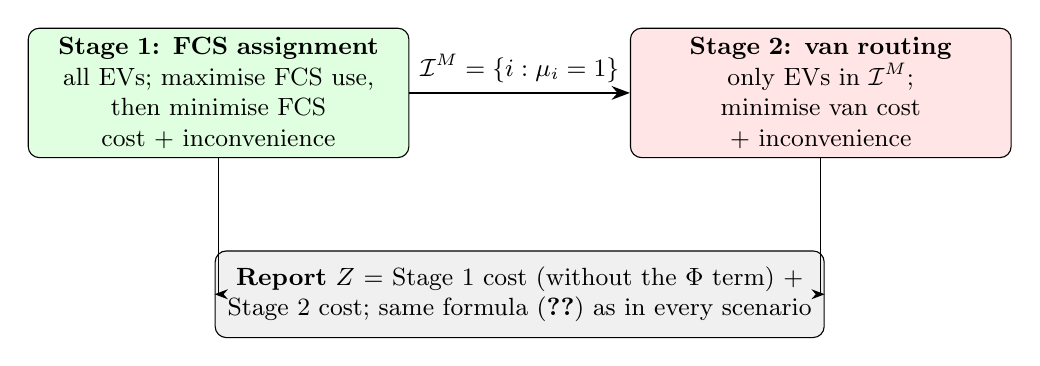
\begin{tikzpicture}[>=Stealth,box/.style={draw,rounded corners,align=center,minimum height=1.1cm,font=\small}]
  \node[box,fill=green!12,text width=4.6cm] (s1) {\textbf{Stage 1: FCS assignment}\\all EVs; maximise FCS use,\\then minimise FCS cost + inconvenience};
  \node[box,fill=red!10,text width=4.6cm,right=2.8cm of s1] (s2) {\textbf{Stage 2: van routing}\\only EVs in $\I^M$;\\minimise van cost + inconvenience};
  \draw[->,thick] (s1) -- node[above,font=\small]{$\I^M=\{i:\mu_i=1\}$} (s2);
  \node[box,fill=black!6,text width=7.5cm,below=2.0cm of $(s1)!0.5!(s2)$] (ev) {\textbf{Report} $Z=$ Stage~1 cost (without the $\Phi$ term) $+$ Stage~2 cost; same formula \eqref{eq:Z} as in every scenario};
  \draw[->] (s1) |- (ev); \draw[->] (s2) |- (ev);
\end{tikzpicture}
\end{center}

Stage~1 does not look at the vans, and Stage~2 cannot change what Stage~1 decided. That is the definition of ``FCS first, then MCS''.

%----------------------------------------------------------------
\subsection{Stage 1: assign EVs to fixed stations}

\textbf{Objective.}
\begin{equation}
\begin{split}
\min\ Z^{(1)}=\;&\underbrace{\Phi\sum_{i\in\I}\mu_i}_{\text{FCS first}}
+\underbrace{c^{EV}\sum_i\sum_{f\in\F_i}d_{if}Y_{if}}_{Z_1}
+\underbrace{Z^F_{\text{energy}}}_{\text{FCS part of }Z_4}\\
&+\underbrace{\sum_i\sum_{f\in\F_i}\rho^F_{if}Y_{if}+\alpha\sum_i w_i(C_i-r_i)+c^L\sum_i w_iL_i}_{\text{FCS customers' inconvenience}}
\end{split}
\label{eq:obj1}
\end{equation}
with $C_i=S_i+\tau^F_iY_i$ in this stage. $\Phi$ is a penalty for handing an EV to the vans. It is chosen larger than anything an extra FCS customer can add to the rest of \eqref{eq:obj1}, e.g.
\[
\Phi > \max_{i}\max_{f\in\F_i}\big(c^{EV}d_{if}+\pi^{\max}E_i+\rho^F_{if}\big)+n\,(\alpha+c^L)\,w_{\max}\,T,
\]
so Stage~1 first \textbf{maximises the number of EVs served at an FCS}, and only among those solutions minimises FCS cost and inconvenience. ($\pi^{\max}$ is the highest grid price.) A numerically safer equivalent is to solve twice: first $\max\sum_iY_i$, then fix that number and minimise the rest.
\ifTOU
Because $Z^F_{\text{energy}}$ uses the peak price, Stage~1 may \emph{start sessions later} to leave the peak, if the price saving beats the extra waiting cost (Section~\ref{sec:expect}).
\fi

\textbf{Constraints.}
\begin{align}
\sum_{g\in\G_i}y_{ig}+\mu_i &= 1 && \forall i\in\I \label{eq:s1assign}\\
S_i &\ge r_i+\sum_{f\in\F_i}t_{if}Y_{if} && \forall i\in\I \label{eq:fcsarr}\\
S_i &\le r_i+T\,(1-\mu_i) && \forall i\in\I \label{eq:s1park}\\
S_j &\ge S_i+\tau^F_i-(T+\tau^F_i)(3-y_{ig}-y_{jg}-o_{ij}) && \forall g,\ (i,j)\in\mathcal{P}_g \label{eq:disj1}\\
S_i &\ge S_j+\tau^F_j-(T+\tau^F_j)(2-y_{ig}-y_{jg}+o_{ij}) && \forall g,\ (i,j)\in\mathcal{P}_g \label{eq:disj2}\\
\sum_i y_{ig_1} &\ge \sum_i y_{ig_2} && \forall f,\ \G_f=\{g_1,g_2\} \label{eq:gunsym}\\
S_i+\tau^F_iY_i &\le T,\qquad L_i\ge S_i+\tau^F_iY_i-l_i && \forall i\in\I \label{eq:s1time}
\end{align}
\ifTOU plus the time-of-use split \eqref{eq:tou1}--\eqref{eq:tou5} of each FCS session (Section~\ref{sec:price}).\fi
\desc{\eqref{eq:s1assign}: every EV either gets one reachable gun or is handed to the vans. An EV that reaches no FCS ($\G_i=\emptyset$) is forced to $\mu_i=1$. \eqref{eq:fcsarr}: an FCS session cannot start before the EV has asked and driven to the station. \eqref{eq:s1park}: for an EV handed to the vans, $S_i$ is parked at $r_i$, so it adds no waiting in Stage~1 (its real start time is decided in Stage~2). \eqref{eq:disj1}--\eqref{eq:disj2}: two EVs on the same gun do not overlap; $o_{ij}$ picks who goes first. With two guns per station this means at most two EVs charge at a station at a time. \eqref{eq:gunsym}: symmetry breaking between the two identical guns (optional). \eqref{eq:s1time}: finished by $T$; lateness.}

\textbf{Optional acceptability rule.} An operator may refuse to send a driver to a station that is ``too inconvenient'', e.g.\ only allow gun $g$ of station $f$ for EV $i$ if $\hat\rho^F_{if}\le\bar\rho$. This only shrinks $\G_i$, so EVs whose stations are all too far go to the vans. Report results with and without it.

\textbf{Output:} $\I^M=\{i:\mu_i=1\}$, the EVs left for the vans; plus each FCS customer's gun and start time.

%----------------------------------------------------------------
\subsection{Stage 2: route the vans to the leftover EVs}

Stage~2 is a vehicle routing problem with time windows, on the EVs in $\I^M$ only. Here $C_i=S_i+\tau^M_i$.

\textbf{Objective.}
\begin{equation}
\begin{split}
\min\ Z^{(2)}=\;&\underbrace{c^M\sum_m\sum_{(i,j)\in\A^M}d_{ij}x_{ijm}}_{Z_2}+\underbrace{\sum_m c^D_mu_m}_{Z_3}+\underbrace{Z^M_{\text{energy}}}_{\text{van part of }Z_4}\\
&+\underbrace{\sum_{i\in\I^M}\sum_m\rho^M_{im}z_{im}+\alpha\sum_{i\in\I^M}w_i(C_i-r_i)+c^L\sum_{i\in\I^M}w_iL_i}_{\text{van customers' inconvenience}}
\end{split}
\label{eq:obj2}
\end{equation}
Since every EV in $\I^M$ must be served by some van, $Z^M_{\text{energy}}$ and the $\rho^M$ term are constants here. They are kept so that $Z^{(2)}$ is the true cost of Stage~2. Waiting and lateness make the vans visit urgent EVs early.

\textbf{Constraints.}
\begin{align}
\sum_{m\in\M}z_{im} &= 1 && \forall i\in\I^M \label{eq:s2assign}\\
\sum_{j:(0,j)\in\A^M}x_{0jm} = \sum_{i:(i,n+1)\in\A^M}x_{i,n+1,m} &= u_m && \forall m \label{eq:depot}\\
\sum_{i:(i,j)\in\A^M}x_{ijm} = \sum_{k:(j,k)\in\A^M}x_{jkm} &= z_{jm} && \forall j\in\I^M,\ m \label{eq:flow}\\
\sum_{i\in\I^M}z_{im} &\le Q_m\,u_m && \forall m \label{eq:cap}\\
\sum_{i\in\I^M}\frac{E_i}{\eta}z_{im}+\beta\sum_{(i,j)\in\A^M}d_{ij}x_{ijm} &\le B_m\,u_m && \forall m \label{eq:batt}
\end{align}
\begin{align}
S_j &\ge \max\{r_j,\ t_{0j}\,x_{0jm}\} && \forall j\in\I^M,\ m \label{eq:depart}\\
S_j &\ge S_i+\tau^M_i+t_{ij}-(T+\tau^M_i+t_{ij})(1-x_{ijm}) && \forall i\neq j,\ m \label{eq:seq}\\
S_i+\tau^M_i+t_{i,n+1} &\le T+(\tau^M_i+t_{i,n+1})(1-x_{i,n+1,m}) && \forall i,\ m \label{eq:return}\\
S_i+\tau^M_i \le T,\quad L_i &\ge S_i+\tau^M_i-l_i && \forall i\in\I^M \label{eq:s2time}\\
u_m &\ge u_{m+1} && m<|\M| \label{eq:vansym}
\end{align}
\desc{\eqref{eq:s2assign}: each leftover EV gets one van. \eqref{eq:depot}: a used van leaves and returns to the depot once. \eqref{eq:flow}: each EV on van $m$ is entered and left exactly once by that van. \eqref{eq:cap}: at most $Q_m$ EVs per van. \eqref{eq:batt}: delivered energy (with transfer losses) plus driving energy fits in the van battery. \eqref{eq:depart}: no start before the request, or before the van can drive there from the depot (written as two linear constraints). \eqref{eq:seq}: if the van goes $i\to j$, it finishes $i$ and drives to $j$ before starting $j$. This gives one EV at a time and removes subtours (MTZ-type). \eqref{eq:return}: back at the depot by $T$. \eqref{eq:s2time}: finished by $T$; lateness. \eqref{eq:vansym}: use identical vans in index order.}

\textbf{If Stage 2 is infeasible} (too many leftover EVs for the fleet by $T$), the sequential policy has \emph{failed} on that instance. For diagnosis, add $s_i\in\{0,1\}$ (``unserved''), replace \eqref{eq:s2assign} by $\sum_mz_{im}+s_i=1$ and add $\Phi^U\sum_is_i$ to \eqref{eq:obj2}. Then report the number of EVs that could not be served. This is a useful comparison with the integrated scenario, which may serve all of them.

%----------------------------------------------------------------
\subsection{Reported value}
\[
Z^{\text{S\scen}}=\big(Z^{(1)*}-\Phi\,|\I^M|\big)+Z^{(2)*},
\]
which is exactly \eqref{eq:Z} evaluated at the combined solution. The stage-1 solution plus the stage-2 solution is a feasible solution of the integrated model (S\ifTOU 4\else 3\fi), so
$Z^{\text{S\ifTOU 4\else 3\fi}}\le Z^{\text{S\scen}}$. The difference is the \emph{value of integration}.

\else
%---------------------------------------------------------------- INT
\subsection{Objective}
\begin{equation}
\min\ Z \quad\text{as in \eqref{eq:Z}, with }Z^F_{\text{energy}}=\ifTOU P^F\textstyle\sum_i\big[\pi^\off(\theta^1_i+\theta^3_i)+\pi^\pk\theta^2_i\big]\else\pi^F\textstyle\sum_iE_iY_i\fi,\quad C_i=S_i+\tau^F_iY_i+\tau^M_iZ_i. \label{eq:objint}
\end{equation}
Written out in full:
\begin{align*}
\min\ Z=\;& c^{EV}\sum_i\sum_{f\in\F_i}d_{if}Y_{if}+c^M\sum_m\sum_{(i,j)\in\A}d_{ij}x_{ijm}+\sum_mc^D_mu_m\\
&+\ifTOU P^F\sum_i\big[\pi^\off(\theta^1_i+\theta^3_i)+\pi^\pk\theta^2_i\big]\else\pi^F\sum_iE_iY_i\fi
+\pi^M\sum_i\sum_m\frac{E_i}{\eta}z_{im}\\
&+\sum_i\sum_{f\in\F_i}\rho^F_{if}Y_{if}+\sum_i\sum_m\rho^M_{im}z_{im}+\alpha\sum_iw_i(C_i-r_i)+c^L\sum_iw_iL_i .
\end{align*}
Every term is linear. One model weighs everything at once: an EV goes to a van exactly when the van's extra km, dispatch and energy cost are outweighed by the effort and waiting it saves the driver\ifTOU, or by the peak-price energy it avoids\fi.

\subsection{Constraints}

\textbf{Assignment.}
\begin{equation}
\sum_{g\in\G_i}y_{ig}+\sum_{m\in\M}z_{im}=1\qquad\forall i\in\I \label{eq:assign}
\end{equation}
\desc{Exactly one resource per EV: one reachable gun or one van. EVs that reach no FCS are forced onto a van.}

\textbf{Fixed stations.}
\begin{align}
S_i &\ge r_i+\sum_{f\in\F_i}t_{if}Y_{if} && \forall i \label{eq:fcsarr}\\
S_j &\ge S_i+\tau^F_i-(T+\tau^F_i)(3-y_{ig}-y_{jg}-o_{ij}) && \forall g,\ (i,j)\in\mathcal{P}_g \label{eq:disj1}\\
S_i &\ge S_j+\tau^F_j-(T+\tau^F_j)(2-y_{ig}-y_{jg}+o_{ij}) && \forall g,\ (i,j)\in\mathcal{P}_g \label{eq:disj2}\\
\sum_iy_{ig_1} &\ge \sum_iy_{ig_2} && \forall f,\ \G_f=\{g_1,g_2\} \label{eq:gunsym}
\end{align}
\desc{\eqref{eq:fcsarr}: an FCS session starts after the request and the drive to the station (for a van customer this is just $S_i\ge r_i$). \eqref{eq:disj1}--\eqref{eq:disj2}: EVs on the same gun do not overlap; $o_{ij}$ chooses the order. \eqref{eq:gunsym}: optional symmetry breaking.}

\textbf{Vans: routes, capacity, battery.}
\begin{align}
\sum_{j:(0,j)\in\A}x_{0jm}=\sum_{i:(i,n+1)\in\A}x_{i,n+1,m} &= u_m && \forall m \label{eq:depot}\\
\sum_{i:(i,j)\in\A}x_{ijm}=\sum_{k:(j,k)\in\A}x_{jkm} &= z_{jm} && \forall j\in\I,\ m \label{eq:flow}\\
\sum_iz_{im} &\le Q_mu_m && \forall m \label{eq:cap}\\
\sum_i\frac{E_i}{\eta}z_{im}+\beta\sum_{(i,j)\in\A}d_{ij}x_{ijm} &\le B_mu_m && \forall m \label{eq:batt}
\end{align}
\desc{\eqref{eq:depot}: a used van leaves and returns once. \eqref{eq:flow}: each EV on van $m$ is visited exactly once by it. \eqref{eq:cap}: at most $Q_m$ EVs. \eqref{eq:batt}: delivered energy (with losses) plus driving energy fits in the battery.}

\textbf{Vans: timing (one EV at a time, no subtours).}
\begin{align}
S_j &\ge t_{0j}\,x_{0jm} && \forall j\in\I,\ m \label{eq:depart}\\
S_j &\ge S_i+\tau^M_i+t_{ij}-(T+\tau^M_i+t_{ij})(1-x_{ijm}) && \forall i\neq j\in\I,\ m \label{eq:seq}\\
S_i+\tau^M_i+t_{i,n+1} &\le T+(\tau^M_i+t_{i,n+1})(1-x_{i,n+1,m}) && \forall i,\ m \label{eq:return}
\end{align}
\desc{\eqref{eq:depart}: the first stop cannot start before the van has driven there. \eqref{eq:seq}: $i\to j$ means finish $i$, drive, then start $j$; start times rise along a route, so no subtour can close. \eqref{eq:return}: back at the depot by $T$.}

\textbf{Horizon and lateness.}
\begin{equation}
C_i\le T,\qquad L_i\ge C_i-l_i\qquad\forall i\in\I \label{eq:time}
\end{equation}
\desc{Every EV is fully charged within the horizon; $L_i$ measures lateness.}

\ifTOU
\textbf{Time-of-use split.} Constraints \eqref{eq:tou1}--\eqref{eq:tou5} of Section~\ref{sec:price}.
\fi

\textbf{Symmetry and domains.}
\begin{equation}
u_m\ge u_{m+1};\qquad y,z,x,u,o\ifTOU,\kappa\fi\in\{0,1\};\qquad S_i,L_i\ifTOU,\theta^p_i\fi\ge0 \label{eq:dom}
\end{equation}
\fi

%=====================================================================
\section{Learning-to-optimise (RL) formulation}\label{sec:rl}

\textbf{Main rule:} the reward of each action is \emph{minus the increase in $Z$ that the action causes}. The rewards over an episode then add up to $-Z$ of the solution the policy builds. RL and MILP results are measured on the same yardstick \eqref{eq:Z}, and the MILP optimum is the benchmark for the RL gap.

\ifSEQ
%---------------------------------------------------------------- RL SEQ
The RL pipeline has the same two stages as the MILP.

\subsection{Stage 1 policy: FCS assignment}
\begin{itemize}[leftmargin=1.4em,itemsep=2pt]
  \item \textbf{Episode / epochs:} EVs are taken in order of request time $r_i$ (ties: higher $w_i$ first). One decision per EV.
  \item \textbf{State:} features of the current EV $k$ ($E_k,r_k,l_k,w_k,R_k$, location); for each gun $g$ the time $F_g$ it becomes free; summary features of the EVs still to come (count and positions near each station)\ifTOU; the current price and the time until $T_1$ and $T_2$\fi.
  \item \textbf{Action:} a gun $g\in\G_k$, or ``hand to vans''. \textbf{FCS-first mask:} ``hand to vans'' is allowed \emph{only} if no gun can finish EV $k$ by $T$ (or, with the optional rule, if all remaining guns have $\hat\rho^F_{kf}>\bar\rho$).
  \ifTOU\item \textbf{Optional timing action:} ``gun $g$, start after the peak'', i.e.\ $S_k=\max\{\text{earliest},T_2\}$, allowed only if the session still ends by $T$.\fi
  \item \textbf{Transition:} $S_k=\max\{r_k+t_{kf},F_g\}$ (or later, for the timing action); $F_g\leftarrow S_k+\tau^F_k$.
  \item \textbf{Reward:} $-\Big[c^{EV}d_{kf}+\text{energy}_k+\rho^F_{kf}+\alpha w_k(S_k+\tau^F_k-r_k)+c^Lw_k(S_k+\tau^F_k-l_k)^+\Big]$, where energy$_k$ = \ifTOU$P^F\big[\pi^\off\cdot(\text{off-peak hours of }[S_k,S_k+\tau^F_k])+\pi^\pk\cdot(\text{peak hours})\big]$, computed exactly in the simulator\else$\pi^FE_k$\fi. Handing an EV to the vans gives reward $0$ here; its cost is counted in Stage~2.
\end{itemize}
Note: a simple baseline for Stage~1 is the greedy rule ``gun with the largest one-step reward''. What RL can learn on top of this is, for example, to keep a nearby gun free for an urgent EV that arrives later.

\subsection{Stage 2 policy: van routing over $\I^M$}
\begin{itemize}[leftmargin=1.4em,itemsep=2pt]
  \item \textbf{Epochs:} whenever a van becomes free (the earliest-free van decides first).
  \item \textbf{State:} for each van: position, time free, remaining battery $b_m$, EVs served so far, dispatched or not; for each unserved EV in $\I^M$: location, $E_i,r_i,l_i,w_i$; current time.
  \item \textbf{Action:} the next EV $j$ for this van, or ``return to depot'' (ends the route). Mask: $j$ must be feasible: battery covers $E_j/\eta$ plus driving to $j$ and back to the depot, the count stays $\le Q_m$, and $j$ can be finished with the van back at the depot by $T$.
  \item \textbf{Transition:} $S_j=\max\{r_j,\ \text{time free}+t_{\text{pos},j}\}$; the van moves to $j$ and is free at $S_j+\tau^M_j$; $b_m$ falls by $E_j/\eta+\beta d_{\text{pos},j}$.
  \item \textbf{Reward:} serving $j$: $-\Big[c^Md_{\text{pos},j}+c^D_m[\text{first stop}]+\pi^M\frac{E_j}{\eta}+\rho^M_{jm}+\alpha w_j(S_j+\tau^M_j-r_j)+c^Lw_j(S_j+\tau^M_j-l_j)^+\Big]$; returning: $-c^Md_{\text{pos},0}$. EVs still unserved at the end: $-\Phi^U$ each.
  \item \textbf{Policy:} an attention-based routing policy (e.g.\ Kool et al., 2019, ``Attention, Learn to Solve Routing Problems!'') trained with REINFORCE or PPO. Baseline: nearest-feasible-EV heuristic.
\end{itemize}
Episode return of Stage~1 + Stage~2 $=-Z^{\text{S\scen}}$.

\else
%---------------------------------------------------------------- RL INT
One policy decides both who serves each EV and the van routes.
\begin{itemize}[leftmargin=1.4em,itemsep=2pt]
  \item \textbf{Episode / epochs:} EVs are taken in order of request time $r_i$ (ties: higher $w_i$ first). One decision per EV.
  \item \textbf{State:} (i) the current EV $k$: location, $E_k,r_k,l_k,w_k,R_k$, reachable stations; (ii) each gun $g$: time $F_g$ it becomes free; (iii) each van $m$: current end-of-route position, time free, remaining battery $b_m$, EVs served, dispatched or not; (iv) embeddings of the not-yet-assigned EVs (for look-ahead)\ifTOU; (v) current price, time until $T_1$ and $T_2$\fi.
  \item \textbf{Action:} $a\in\G_k\cup\M$: a gun, or a van (EV $k$ is appended to the end of that van's route). \textbf{Mask} infeasible actions: a gun that cannot finish $k$ by $T$; a van without enough battery for $E_k/\eta$ plus the drive to $k$ and back to the depot, with $Q_m$ reached, or unable to finish $k$ and return by $T$.
  \ifTOU\item \textbf{Optional timing action:} ``gun $g$, start after the peak'' ($S_k=\max\{\text{earliest},T_2\}$, if it still ends by $T$).\fi
  \item \textbf{Transition:} gun: $S_k=\max\{r_k+t_{kf},F_g\}$, $F_g\leftarrow S_k+\tau^F_k$. Van: $S_k=\max\{r_k,\ \text{free}_m+t_{\text{pos}_m,k}\}$, then the van moves to $k$, $\text{free}_m\leftarrow S_k+\tau^M_k$, $b_m\mathrel{-}=E_k/\eta+\beta d_{\text{pos}_m,k}$.
  \item \textbf{Reward} $=-\Delta Z$:
  \begin{align*}
  \text{gun } g\text{ at }f:&\quad -\Big[c^{EV}d_{kf}+\text{energy}^F_k+\rho^F_{kf}+\alpha w_k(C_k-r_k)+c^Lw_k(C_k-l_k)^+\Big]\\
  \text{van } m:&\quad -\Big[c^M\big(d_{\text{pos}_m,k}+d_{k,0}-d_{\text{pos}_m,0}\big)+c^D_m[\text{first use}]+\pi^M\tfrac{E_k}{\eta}\\
  &\qquad\quad+\rho^M_{km}+\alpha w_k(C_k-r_k)+c^Lw_k(C_k-l_k)^+\Big]
  \end{align*}
  The van distance term is the \emph{change} in route length when $k$ is inserted before the return to the depot, so the sum over the episode equals the total route length (the return legs telescope). energy$^F_k$ = \ifTOU$P^F\big[\pi^\off\cdot(\text{off-peak hours})+\pi^\pk\cdot(\text{peak hours of }[S_k,C_k])\big]$, computed exactly by the simulator; no linearisation is needed in RL\else$\pi^FE_k$\fi.
  \item \textbf{Dead end:} if every action is masked, EV $k$ is unserved: reward $-\Phi^U$, and the episode continues. Report the count.
  \item \textbf{Policy:} masked categorical policy over guns and vans, encoder with attention over EVs, guns and vans; trained with PPO. Natural baseline: greedy, i.e.\ choose the action with the largest one-step reward. That is the pairwise rule ``smallest $\hat\rho$ + cost'' from Section~\ref{sec:inc}.
\end{itemize}
Restriction to note: vans serve EVs in assignment order (append only). A variant that inserts $k$ at the cheapest position of a route is more flexible but has a larger action space.
\fi

\textbf{Reward scaling.} For stable training divide every reward by a constant, e.g.\ the greedy baseline's average $Z$ on the training instances. This does not change the optimal policy.

%=====================================================================
\section{What to expect and what to report}\label{sec:expect}

\ifnum\scen=1
\begin{itemize}[leftmargin=1.4em,itemsep=2pt]
  \item Vans serve only EVs that reach no station, or that the stations cannot finish by $T$. If stations have spare capacity, very few vans are dispatched.
  \item Inconvenience is high for EVs far from the nearest station (worked example: Rs\,682 at the FCS, against Rs\,458 if a van had been allowed).
  \item With too few vans Stage~2 becomes infeasible (unserved EVs), even when the integrated model S3 could serve everyone. Report the smallest $|\M|$ at which S1 is feasible and compare it with S3.
\end{itemize}
\fi
\ifnum\scen=2
\begin{itemize}[leftmargin=1.4em,itemsep=2pt]
  \item \textbf{When does Stage~1 delay a session to avoid the peak?} Moving one hour of charging out of the peak saves $(\pi^\pk-\pi^\off)P^F=3\times22=$ Rs\,66, but delays completion by up to an hour, which costs $\alpha w_i\ge$ Rs\,200. So with the default values Stage~1 almost never delays. It mostly pays the higher price, and S2 costs roughly S1 plus the peak surcharge. Sessions start later only if $\alpha$ is small (try $\lambda<0.33$ in the sensitivity analysis).
  \item The van assignment is the same as in S1 unless Stage~1's timing changes which EVs fit at the stations. Stage~1 cannot use vans to escape the peak price.
  \item Extra KPI: \textbf{grid energy drawn at FCS during the peak}, $P^F\sum_i\theta^2_i$ (kWh). Compare with S4.
\end{itemize}
\fi
\ifnum\scen=3
\begin{itemize}[leftmargin=1.4em,itemsep=2pt]
  \item Vans take EVs for which the saved inconvenience exceeds the extra van cost (worked example: van chosen, saving Rs\,224). Expect vans to serve EVs that are far from every station, have low range (high $w_i$), or have early deadlines, while EVs near a station still use it.
  \item \textbf{Value of integration under flat price:} $Z^{\text{S1}}-Z^{\text{S3}}\ge0$. Report it per component ($Z_1,\dots,Z_5$): typically operating cost rises a little and inconvenience falls a lot.
  \item Vary $|\M|$ (0, 1, 2, \dots): the first few vans lower $Z$ sharply, then the effect levels off. That curve shows the scenarios where mobile chargers help most.
\end{itemize}
\fi
\ifnum\scen=4
\begin{itemize}[leftmargin=1.4em,itemsep=2pt]
  \item During the peak a van kWh costs about the same as an FCS kWh (Rs\,10.0 each), so the vans' energy disadvantage disappears and vans also absorb \emph{peak-hour} demand that would otherwise be charged on the grid at peak price.
  \item Expect more van usage than in S3, concentrated on requests in $[T_1,T_2]$, and lower grid energy at the stations during the peak, $P^F\sum_i\theta^2_i$, than in S2.
  \item \textbf{Value of integration under peak pricing:} $Z^{\text{S2}}-Z^{\text{S4}}$. It should be larger than $Z^{\text{S1}}-Z^{\text{S3}}$, because integration now also allows price arbitrage.
  \item \textbf{Peak pricing with full flexibility:} $Z^{\text{S4}}-Z^{\text{S3}}$ should be smaller than $Z^{\text{S2}}-Z^{\text{S1}}$: vans cushion the price increase.
\end{itemize}
\fi

\textbf{Cross-scenario comparison table} (fill in from the four runs):
\begin{center}
\renewcommand{\arraystretch}{1.2}
\begin{tabular}{@{}lll@{}}
\toprule
\textbf{Comparison} & \textbf{Measures} & \textbf{Expected sign} \\
\midrule
S1 $-$ S3 & value of integration, flat price & $\ge0$ \\
S2 $-$ S4 & value of integration, peak price & $\ge0$, larger than S1 $-$ S3 \\
S2 $-$ S1 & cost of peak pricing, FCS-first operator & $>0$ \\
S4 $-$ S3 & cost of peak pricing, flexible operator & $>0$, smaller than S2 $-$ S1 \\
\bottomrule
\end{tabular}
\end{center}
Report for each: $Z$ and its components, number of vans used, EVs per resource, mean and maximum inconvenience per EV, total lateness, peak-hour grid energy, solve time, and (for RL) the gap to the MILP optimum.

%=====================================================================
\appendix
\section{Illustrative parameter values}\label{app:values}

These are starting values for experiments, not data. All are meant to be varied in the analysis. Values in Rs.

\begin{center}
\renewcommand{\arraystretch}{1.15}
\begin{tabular}{@{}llp{6.2cm}@{}}
\toprule
\textbf{Parameter} & \textbf{Value} & \textbf{Note} \\
\midrule
$T$, $[T_1,T_2]$ & 7 h, $[2,6]$ & 16:00--23:00, peak 18:00--22:00 \\
$P^F$, $P^M$ & 22 kW, 30 kW & \\
$v$, $\beta$, $\eta$ & 25 km/h, 0.25 kWh/km, 0.9 & \\
$B_m$, $Q_m$, $|\M|$ & 150 kWh, 6, 2--6 & \\
$c^{EV}$, $c^M$, $c^D_m$ & Rs\,4/km, Rs\,15/km, Rs\,1500 & van km includes driver time \\
$\pi^F$ (flat) & Rs\,8.7/kWh & equals the time-average of the ToU tariff over $[0,T]$ \\
$\pi^\off$, $\pi^\pk$ (ToU) & Rs\,7/kWh, Rs\,10/kWh & $(3\times7+4\times10)/7=8.7$ \\
$c^{bat}$ & Rs\,2/kWh & van battery wear \\
$\pi^M$ & Rs\,10.7 (flat) / Rs\,9.0 (ToU) & $=\pi^F+c^{bat}$ / $=\pi^\off+c^{bat}$ \\
$\alpha$, $\alpha^D$ & Rs\,200/h, Rs\,100/h & value of time; extra for attended time \\
$h^F$, $h^M$, $\varphi$ & Rs\,50, Rs\,10, Rs\,100 & trip hassle, hand-over, range stress \\
$c^L$ & Rs\,300/h & lateness \\
$w_i$ & $1+2(1-R_i/R_{\max})$, $R_i\sim U[3,40]$ km & priority from remaining range \\
\bottomrule
\end{tabular}
\end{center}

The flat price is set to the time-average of the peak tariff. The price \emph{level} is then the same in both pricing cases, and only the price \emph{shape} differs. Without this, part of S1 vs S2 would just reflect a different average price.

\end{document}
"
%    pdflatex -jobname=scenario2_peak_sequential   "\def\scen{2}% =====================================================================
%  One source, four PDFs.  Build with build.sh (or by hand):
%    pdflatex -jobname=scenario1_flat_sequential   "\def\scen{1}\input{scenario_master}"
%    pdflatex -jobname=scenario2_peak_sequential   "\def\scen{2}\input{scenario_master}"
%    pdflatex -jobname=scenario3_flat_integrated   "\def\scen{3}\input{scenario_master}"
%    pdflatex -jobname=scenario4_peak_integrated   "\def\scen{4}\input{scenario_master}"
%  (run each twice for cross-references)
% =====================================================================
\documentclass[11pt,a4paper]{article}
\usepackage[margin=2.2cm]{geometry}
\usepackage{amsmath,amssymb,amsfonts}
\usepackage{booktabs,array,tabularx}
\usepackage{enumitem}
\usepackage[table]{xcolor}
\usepackage{tikz}
\usetikzlibrary{arrows.meta,positioning,calc}
\usepackage[colorlinks=true,linkcolor=blue!50!black,urlcolor=blue!50!black]{hyperref}
\usepackage{titlesec}
\titleformat{\section}{\large\bfseries}{\thesection}{0.8em}{}
\titleformat{\subsection}{\normalsize\bfseries}{\thesubsection}{0.8em}{}
\setlength{\parindent}{0pt}
\setlength{\parskip}{5pt}

% ---------------- scenario switches ----------------
\ifdefined\scen\else\def\scen{1}\fi
\newif\ifTOU \TOUfalse   % true = time-of-use (peak) price
\newif\ifSEQ \SEQfalse   % true = FCS first, then MCS
\ifnum\scen=1 \SEQtrue \fi
\ifnum\scen=2 \TOUtrue \SEQtrue \fi
\ifnum\scen=4 \TOUtrue \fi

\newcommand{\pricename}{\ifTOU time-of-use price (dearer evening peak)\else single (flat) price all day\fi}
\newcommand{\structname}{\ifSEQ FCS first, then MCS (sequential)\else FCS and MCS together (integrated)\fi}

% ---------------- notation ----------------
\newcommand{\I}{\mathcal{I}}
\newcommand{\F}{\mathcal{F}}
\newcommand{\G}{\mathcal{G}}
\newcommand{\M}{\mathcal{M}}
\newcommand{\N}{\mathcal{N}}
\newcommand{\A}{\mathcal{A}}
\newcommand{\Rs}{\text{Rs}\,}
\newcommand{\pk}{\mathrm{pk}}
\newcommand{\off}{\mathrm{off}}
\newcommand{\desc}[1]{\par\vspace{-2pt}{\small\color{black!75}\textit{Meaning:} #1}\par\vspace{4pt}}
\newcommand{\cell}[2]{\ifnum\scen=#1\cellcolor{blue!18}\textbf{S#1 (this document)}\\\textbf{#2}\else S#1\\#2\fi}

\title{\textbf{EV Charging Network Optimisation}\\[4pt]
\large Scenario \scen: \pricename\ $+$ \structname\\[2pt]
\normalsize MILP and RL formulation}
\author{CP 320 OR for Mobility Management, course project}
\date{2 October 2026}

\begin{document}
\maketitle

%=====================================================================
\section{Where this scenario sits}

The project studies four scenarios: two ways of pricing grid electricity, times two ways of making the decisions.

\begin{center}
\renewcommand{\arraystretch}{1.5}
\begin{tabular}{>{\raggedright\arraybackslash}p{4.2cm}|>{\centering\arraybackslash}p{4.6cm}|>{\centering\arraybackslash}p{4.6cm}}
 & \textbf{Flat price all day} & \textbf{Time-of-use (peak) price} \\ \hline
\textbf{Sequential:} FCS first, leftover EVs to MCS &
\begin{tabular}[c]{@{}c@{}}\cell{1}{flat + sequential}\end{tabular} &
\begin{tabular}[c]{@{}c@{}}\cell{2}{peak + sequential}\end{tabular} \\ \hline
\textbf{Integrated:} FCS and MCS decided together &
\begin{tabular}[c]{@{}c@{}}\cell{3}{flat + integrated}\end{tabular} &
\begin{tabular}[c]{@{}c@{}}\cell{4}{peak + integrated}\end{tabular} \\
\end{tabular}
\end{center}

\textbf{The four scenarios do not have four different objectives.} They share \emph{one} cost yardstick $Z$ (Section~\ref{sec:obj}): the same cost terms and the same customer inconvenience (Section~\ref{sec:inc}). Only two things change:
\begin{itemize}[leftmargin=1.4em,itemsep=1pt]
  \item \textbf{Pricing} changes the formula for one term, the FCS energy cost (Section~\ref{sec:price}).
  \item \textbf{Decision structure} changes \emph{how} $Z$ is minimised: in one model (integrated), or in two stages (sequential), where each stage minimises its own part of $Z$.
\end{itemize}
Because the yardstick is the same, the four optimal values can be compared directly. The differences measure the \emph{value of integration} (S1$\to$S3, S2$\to$S4) and the \emph{effect of peak pricing} (S1$\to$S2, S3$\to$S4).

\ifnum\scen=1
\textbf{This scenario (S1)} is the baseline, the ``status quo''. Electricity costs the same at every hour, every EV that can be charged at a fixed station is sent there, and vans only take what is left over.
\fi
\ifnum\scen=2
\textbf{This scenario (S2)} keeps the FCS-first rule of S1, but grid electricity is dearer during the evening peak. Stage~1 can react to the price only by \emph{rescheduling} FCS sessions. It cannot hand a peak-hour EV to a van.
\fi
\ifnum\scen=3
\textbf{This scenario (S3)} keeps the flat price of S1, but the operator decides FCS and MCS service \emph{together}. An EV can be sent to a van even when a fixed station could take it, whenever that lowers total cost plus inconvenience.
\fi
\ifnum\scen=4
\textbf{This scenario (S4)} is the most flexible one: peak pricing at fixed stations, and FCS and MCS decided together. Van energy was bought off-peak, so vans can also be used to keep charging \emph{out of the expensive peak}.
\fi

%=====================================================================
\section{Setting and assumptions}\label{sec:setting}

\textbf{Time.} The planning horizon is $[0,T]$ with $T=7$\,h (16:00--23:00). It contains the evening peak window $[T_1,T_2]=[2,6]$ (18:00--22:00). The horizon is the same in all four scenarios. It is wider than the peak itself so that, under peak pricing, there is cheaper time on both sides of the peak.\ifTOU\else\ In this scenario the price is flat, so the window plays no role in the model.\fi

\textbf{Assumptions} (the same as MILP v3, plus two about energy):
\begin{enumerate}[leftmargin=1.6em,itemsep=1pt]
  \item Static, continuous time. All requests in the horizon are known at time $0$, and request $i$ becomes active at $r_i$.
  \item An EV served by an FCS drives there itself on its own battery (only to stations within its range $R_i$). The driver stays with the car while it waits for a free gun and while it charges.
  \item An EV served by an MCS stays parked where it is, and the driver is free in the meantime.
  \item Each FCS gun and each van charges one EV at a time, without interruption, at constant power.
  \item A van's battery covers both its driving and the energy it delivers. \textbf{The van battery is charged at the depot before the horizon starts}\ifTOU, i.e.\ at the off-peak price\fi, and is not recharged during the horizon.
  \item Every EV must be fully charged by $T$ (hard). Finishing after the driver's desired time $l_i$ is allowed but penalised.
\end{enumerate}

%=====================================================================
\section{Notation}\label{sec:notation}

\subsection*{Sets}
\begin{tabularx}{\textwidth}{@{}lX@{}}
\toprule
$\I=\{1,\dots,n\}$ & EV charging requests \\
$\F$; $\G_f$ ($|\G_f|=2$); $\G=\bigcup_f\G_f$ & fixed charging stations; guns of FCS $f$; all guns ($f(g)$ = station of gun $g$) \\
$\F_i=\{f: d_{if}\le R_i\}$, $\G_i=\bigcup_{f\in\F_i}\G_f$ & stations / guns EV $i$ can reach on its remaining range \\
$\M$ & mobile charging vans (MCS) \\
$0,\ n+1$ & depot as start node / end node (same place) \\
$\N=\{0\}\cup\I\cup\{n+1\}$, $\A$ & routing nodes; allowed van arcs $(i,j)$, $i\in\{0\}\cup\I$, $j\in\I\cup\{n+1\}$, $i\neq j$ \\
$\mathcal{P}_g=\{(i,j): i<j,\ g\in\G_i\cap\G_j\}$ & pairs of EVs that could share gun $g$ \\
\ifSEQ
$\I^M\subseteq\I$ & EVs handed to the vans by Stage~1 (an \emph{output} of Stage~1, a fixed input to Stage~2) \\
$\N^M$, $\A^M$ & routing nodes / arcs restricted to $\I^M$ \\
\fi
\bottomrule
\end{tabularx}

\subsection*{Parameters}
\begin{tabularx}{\textwidth}{@{}lX@{}}
\toprule
$E_i,\ r_i,\ l_i,\ R_i$ & energy demand (kWh), request time, desired completion time (h), remaining range (km) \\
$w_i\ge1$ & priority of EV $i$; $w_i=1+\kappa(1-R_i/R_{\max})$, so low-range EVs weigh more \\
$P^F,\ P^M$ & charging power of an FCS gun (22\,kW) / of a van (e.g.\ 30\,kW) \\
$\tau^F_i=E_i/P^F,\ \tau^M_i=E_i/P^M$ & charging time of EV $i$ at an FCS / by a van (h) \\
$d_{if},t_{if}$;\ $d_{ij},t_{ij}$ & distance (km) and time (h): EV$\to$FCS; between routing nodes ($t=d/v$) \\
$B_m,\ Q_m,\ \beta,\ \eta$ & van battery (kWh), max EVs per van, van consumption (kWh/km), transfer efficiency \\
$c^{EV},\ c^M,\ c^D_m$ & cost per km of EV driving, per km of van driving; fixed dispatch cost of van $m$ \\
\ifTOU
$\pi^\off,\ \pi^\pk$ & grid price (Rs/kWh) off-peak / in $[T_1,T_2]$, with $\pi^\pk\ge\pi^\off$ \\
\else
$\pi^F$ & grid price (Rs/kWh), the same at every hour \\
\fi
$c^{bat}$ & van battery wear per kWh cycled \\
$\pi^M$ & cost of 1 kWh taken from a van battery: $\pi^M=\ifTOU\pi^\off\else\pi^F\fi+c^{bat}$ (Section~\ref{sec:price}) \\
$\alpha,\ \alpha^D,\ h^F,\ h^M,\ \varphi,\ c^L$ & inconvenience coefficients (Section~\ref{sec:inc}) \\
\bottomrule
\end{tabularx}

\subsection*{Decision variables}
\begin{tabularx}{\textwidth}{@{}llX@{}}
\toprule
$y_{ig}$ & $\{0,1\}$ & EV $i$ charged at gun $g\in\G_i$ \\
$z_{im}$ & $\{0,1\}$ & EV $i$ served by van $m$ \\
$x_{ijm}$ & $\{0,1\}$ & van $m$ drives arc $(i,j)$ \\
$u_m$ & $\{0,1\}$ & van $m$ is dispatched \\
$o_{ij}$ & $\{0,1\}$ & for EVs $i<j$ that could share a gun: 1 if $i$ is charged before $j$ \\
\ifSEQ
$\mu_i$ & $\{0,1\}$ & Stage~1 only: EV $i$ is handed to the van fleet \\
\fi
\ifTOU
$\theta^1_i,\theta^2_i,\theta^3_i$ & $\ge0$ & hours of EV $i$'s FCS session before / inside / after the peak \\
$\kappa^1_i,\kappa^3_i$ & $\{0,1\}$ & EV $i$'s FCS session starts before $T_1$ / ends after $T_2$ \\
\fi
$S_i$ & $\ge0$ & time charging of EV $i$ starts (h), on whichever resource \\
$L_i$ & $\ge0$ & lateness of EV $i$ beyond $l_i$ (h) \\
\bottomrule
\end{tabularx}

\textbf{Short-hands} (linear expressions, not new variables):
\[
Y_{if}=\sum_{g\in\G_f}y_{ig},\qquad Y_i=\sum_{g\in\G_i}y_{ig}\ (\text{EV $i$ uses an FCS}),\qquad Z_i=\sum_{m\in\M}z_{im}\ (\text{EV $i$ uses a van}),
\]
\[
C_i=S_i+\tau^F_i\,Y_i+\tau^M_i\,Z_i \quad\text{(time EV $i$ is fully charged).}
\]

%=====================================================================
\section{Customer inconvenience}\label{sec:inc}

This section is \textbf{identical in all four scenario documents}. Inconvenience is a property of the customer, not of the price or of the planning method.

\subsection{What we mean by inconvenience}

Inconvenience is \emph{what the driver loses} from the moment they ask for a charge ($r_i$) until the car is fully charged ($C_i$), \emph{converted into rupees} so it can be added to the operator's costs. A driver loses three different things:

\begin{enumerate}[leftmargin=1.6em,itemsep=2pt]
  \item \textbf{Waiting:} the car is not ready. This lasts $C_i-r_i$ hours and affects \emph{every} driver, FCS or MCS.
  \item \textbf{Effort:} only an FCS customer has to drive to the station and sit there while the car charges. An MCS customer stays at home or at work and does something else. Driving to a far station also uses scarce battery range, which causes stress (``range anxiety'').
  \item \textbf{A missed deadline:} the car is still not ready at the time $l_i$ the driver needs it.
\end{enumerate}

Each loss gets a price in Rs per hour (or per event). All of them are multiplied by the priority $w_i$: an hour of delay for an EV with 5\,km of range left counts more than for one with 40\,km.

\subsection{The three components}

\begin{center}
\renewcommand{\arraystretch}{1.3}
\begin{tabularx}{\textwidth}{@{}>{\raggedright\arraybackslash}p{2.6cm}>{\raggedright\arraybackslash}X>{\raggedright\arraybackslash}X>{\raggedright\arraybackslash}p{3.0cm}@{}}
\toprule
\textbf{Component} & \textbf{EV $i$ at FCS $f$} & \textbf{EV $i$ by a van} & \textbf{Known when?} \\
\midrule
Effort & $w_i\big[\alpha^D(t_{if}+\tau^F_i)+h^F+\varphi\,d_{if}/R_i\big]$: driving and sitting at the station, a fixed trip hassle, range stress & $w_i\,h^M$: being reachable and handing over the car & \textbf{Static:} known as soon as the resource is chosen \\
Waiting & $w_i\,\alpha\,(C_i-r_i)$ = drive + \emph{queue at the gun} + charge & $w_i\,\alpha\,(C_i-r_i)$ = \emph{wait for the van} + charge & \textbf{Dynamic:} depends on the queue / van route \\
Missed deadline & $w_i\,c^L\,L_i$, $L_i=\max\{0,C_i-l_i\}$ & same & Dynamic \\
\bottomrule
\end{tabularx}
\end{center}

\textbf{Coefficients.}
$\alpha$ (Rs/h) is the value of an hour the car is not ready.
$\alpha^D$ (Rs/h) is the \emph{extra} value of an hour the driver must personally spend driving or sitting at the station: an hour at the station costs $\alpha+\alpha^D$, an hour waiting at home for a van costs only $\alpha$.
$h^F,h^M$ (Rs) are fixed hassle costs of one trip to a station / one van hand-over.
$\varphi$ (Rs) is the range-stress cost of a trip that uses the \emph{whole} remaining range ($d_{if}/R_i\le1$ is the fraction used).
$c^L$ (Rs/h) is the cost per hour late.

\subsection{Pairwise form: inconvenience of a (customer, resource) pair}

The natural first idea is: \emph{for every pair (EV $i$, FCS $f$) and every pair (EV $i$, van $m$) there is an inconvenience number, and the operator picks the pair with the lowest cost plus inconvenience.} The static part fits this idea exactly:
\[
\boxed{\;\rho^F_{if}=w_i\Big[\alpha^D\,(t_{if}+\tau^F_i)+h^F+\varphi\,\frac{d_{if}}{R_i}\Big]\qquad
\rho^M_{im}=w_i\,h^M\;}
\]
These are \textbf{parameters}, computed before solving, one number per (EV, FCS) pair and per (EV, van) pair. In the objective they appear linearly: $\sum_i\sum_f\rho^F_{if}Y_{if}+\sum_i\sum_m\rho^M_{im}z_{im}$.

Note that $\rho^M_{im}$ does not depend on $m$. Vans are identical and all start at the same depot, so the driver does not care \emph{which} van comes, only \emph{when} it comes. That ``when'' is the waiting part.

\subsection{Why waiting cannot be a fixed pairwise number}

It is tempting to also write the waiting as a pairwise number, e.g.\ ``the van needs 5 minutes to reach EV $i$''. But that depends on \emph{where the van is coming from}, which depends on the route the model is still choosing: if EV $i$ is the 4th stop of a van, the wait is the time for three charging sessions plus four drives. Likewise, waiting at an FCS depends on how many EVs are queued at that gun. So waiting is not known before solving. It is a function of decision variables:
\[
\text{waiting cost of EV } i \;=\; w_i\,\alpha\,(C_i-r_i),\qquad C_i=S_i+\tau^F_iY_i+\tau^M_iZ_i .
\]
This is \textbf{linear} in the variables ($S_i$, $y$, $z$), so it fits in a MILP directly. The constraints of Section~\ref{sec:milp} make $S_i$ equal to the true start time, including driving, queueing at the gun and the van's route. The term $\sum_i w_i\alpha r_i$ is a constant and may be dropped when solving.

\textbf{Pairwise \emph{estimate}} (used for intuition, by the RL policy and in heuristics): if there is no queue and the van comes straight to $i$,
\[
\hat\rho^{F}_{if}=\rho^F_{if}+w_i\alpha\,(t_{if}+\tau^F_i),\qquad
\hat\rho^{M}_{im}=\rho^M_{im}+w_i\alpha\,(t^{\text{van}}_{m\to i}+\tau^M_i),
\]
where $t^{\text{van}}_{m\to i}$ is the time until van $m$ can reach $i$ from where it currently is. In the RL formulation (Section~\ref{sec:rl}) the van's position \emph{is} known at each decision, so there this estimate becomes exact.

\subsection{Total inconvenience and how it enters the objective}

\begin{equation}
\boxed{\;
Z_{\text{inc}}=\underbrace{\sum_{i\in\I}\sum_{f\in\F_i}\rho^F_{if}Y_{if}+\sum_{i\in\I}\sum_{m\in\M}\rho^M_{im}z_{im}}_{\text{effort (static, pairwise)}}
+\underbrace{\alpha\sum_{i\in\I}w_i\,(C_i-r_i)}_{\text{waiting (dynamic)}}
+\underbrace{c^L\sum_{i\in\I}w_i\,L_i}_{\text{missed deadline}}
\;}\label{eq:inc}
\end{equation}
All three parts are in rupees, so $Z_{\text{inc}}$ is simply added to the operating costs. Nothing has to be normalised.

\subsection{Worked example: your ``10 km to the FCS vs.\ van in 5 minutes'' case}

EV $i$: $E_i=20$\,kWh, $R_i=40$\,km (so $w_i=1$); nearest free FCS $d_{if}=10$\,km away, $t_{if}=0.4$\,h at 25\,km/h; a van finishing next door can reach it in 5\,min ($0.083$\,h), adding about 4\,km to its route. $\tau^F_i=20/22=0.909$\,h, $\tau^M_i=20/30=0.667$\,h. Coefficients from Appendix~\ref{app:values}, flat price.

\begin{center}
\renewcommand{\arraystretch}{1.25}
\begin{tabular}{@{}lrr@{}}
\toprule
 & \textbf{FCS} & \textbf{Van} \\
\midrule
Driving (EV / extra van km) & $4\times10=40.0$ & $15\times4=60.0$ \\
Energy & $8.7\times20=174.0$ & $10.7\times20/0.9=237.8$ \\
\textbf{Operating cost only} & \textbf{214.0} & \textbf{297.8} \\
\midrule
Effort $\rho$ & $100(0.4+0.909)+50+100\cdot\tfrac{10}{40}=205.9$ & $10.0$ \\
Waiting $\alpha(C_i-r_i)$ & $200\times1.309=261.8$ & $200\times0.75=150.0$ \\
\textbf{Cost + inconvenience} & \textbf{681.7} & \textbf{457.8} \\
\bottomrule
\end{tabular}
\end{center}

On operating cost alone the FCS is cheaper, so a cost-only model would \emph{always} send this driver 10\,km away. With inconvenience included the van is better by about Rs\,224, and the integrated model chooses $z_{im}=1$, as you expected. If the FCS were only 1\,km away, the FCS would win both comparisons. The inconvenience term is what makes the model choose between ``cheap for the operator'' and ``convenient for the driver'', rather than following a fixed rule.

\subsection{Relation to a single penalty $\rho_i$ per EV}

The first draft used a penalty $\rho_i$ that is charged whenever EV $i$ goes to \emph{any} FCS: $\sum_i\sum_f\rho_iy_{if}$. Because $\sum_f y_{if}=1-\sum_m z_{im}$, this only says ``a van is worth $\rho_i$ more to EV $i$'', and that holds whether the station is 1\,km or 15\,km away, and whether the van arrives in 5 minutes or in 3 hours. The form above fixes both problems: $\rho^F_{if}$ grows with the distance to \emph{that} station, and the waiting term grows with how late the van or the free gun actually is. The old model is the special case $\alpha=\alpha^D=\varphi=c^L=0$, $h^F=\rho_i$.

\subsection{Choosing the coefficients}
\begin{itemize}[leftmargin=1.4em,itemsep=2pt]
  \item Use a value of time for $\alpha$ (e.g.\ Rs\,150--300/h for urban car users), and set $\alpha^D\approx0.5\alpha$: sitting at a station is worse than waiting at home.
  \item Keep $c^L>\alpha$, so missing the deadline is worse than ordinary waiting.
  \item \textbf{Sensitivity analysis:} multiply all inconvenience coefficients by a factor $\lambda\in\{0,0.25,0.5,1,2,4\}$ and plot operating cost against total inconvenience. $\lambda=0$ is the pure cost-minimising operator, and large $\lambda$ is a customer-first operator. This trade-off curve is a strong result for the ``Analysis'' part of the project.
\end{itemize}

\subsection{What inconvenience does in \emph{this} scenario}
\ifSEQ
In a sequential scenario inconvenience \textbf{cannot move an EV from an FCS to a van}: Stage~1 sends every EV that \emph{can} use an FCS to one. It still matters inside each stage. In Stage~1 it decides \emph{which} station and \emph{when} (urgent EVs get the near station and the first free gun). In Stage~2 it decides the \emph{order} in which vans visit EVs (urgent EVs first). In the worked example, this scenario sends the driver 10\,km to the FCS. That is the weakness the integrated scenarios remove.
\else
In an integrated scenario inconvenience is weighed directly against operating cost when choosing the resource. That is how the worked example ends up with a van. It also decides which station and which gun order, and the order of each van route.
\fi

%=====================================================================
\section{Electricity price in this scenario}\label{sec:price}

\textbf{Van energy (same in all scenarios).} A van's battery is charged at the depot \emph{before} the horizon, so its energy was bought at the
\ifTOU off-peak \fi
price, whatever time the van later delivers it. Each kWh taken from the van also wears the battery ($c^{bat}$), and a fraction $1-\eta$ is lost in transfer:
\[
Z^M_{\text{energy}}=\pi^M\sum_{i\in\I}\sum_{m\in\M}\frac{E_i}{\eta}\,z_{im},\qquad \pi^M=\ifTOU\pi^\off\else\pi^F\fi+c^{bat}.
\]

\ifTOU
\textbf{FCS energy (time-of-use).} An FCS draws from the grid while it charges. Energy delivered inside $[T_1,T_2]$ costs $\pi^\pk$, and energy outside it costs $\pi^\off$. A session $[S_i,S_i+\tau^F_i]$ may overlap the peak partly. Split its duration into the hours before, inside and after the peak, $\theta^1_i+\theta^2_i+\theta^3_i$:
\[
Z^F_{\text{energy}}=P^F\sum_{i\in\I}\Big[\pi^\off(\theta^1_i+\theta^3_i)+\pi^\pk\,\theta^2_i\Big].
\]
Constraints \eqref{eq:tou1}--\eqref{eq:tou5} below make the $\theta$'s equal to the true overlaps. Peak hours are dearer, so the solver wants $\theta^1_i,\theta^3_i$ as large as possible. It is enough to bound them from above by the true off-peak overlap, and the constraints need one binary per side:
\begin{align}
\theta^1_i+\theta^2_i+\theta^3_i &= \tau^F_i\,Y_i && \forall i\in\I \label{eq:tou1}\\
\theta^1_i &\le \tau^F_i\,\kappa^1_i && \forall i\in\I \label{eq:tou2}\\
\theta^1_i &\le T_1-S_i+T\,(1-\kappa^1_i) && \forall i\in\I \label{eq:tou3}\\
\theta^3_i &\le \tau^F_i\,\kappa^3_i && \forall i\in\I \label{eq:tou4}\\
\theta^3_i &\le S_i+\tau^F_i-T_2+T\,(1-\kappa^3_i) && \forall i\in\I \label{eq:tou5}
\end{align}
\desc{\eqref{eq:tou1}: the FCS session's hours are split into three parts; for a van customer ($Y_i=0$) all three are zero. \eqref{eq:tou2}--\eqref{eq:tou3}: off-peak time before the peak is only possible if the session starts before $T_1$ ($\kappa^1_i=1$), and is at most $T_1-S_i$. \eqref{eq:tou4}--\eqref{eq:tou5}: the same for time after $T_2$. $\theta^2_i\ge0$ prevents counting more off-peak hours than exist. Checking the cases (entirely before / inside / after the peak, straddling one edge, covering the whole peak) shows that at the optimum the $\theta$'s equal the exact overlaps. This needs $\pi^\pk\ge\pi^\off$, which is true for a peak tariff.}

\textbf{Why vans become more attractive.} Compare the cost of 1\,kWh delivered to an EV during the peak (values from Appendix~\ref{app:values}):
FCS $=\pi^\pk=$ Rs\,10.0, van $=(\pi^\off+c^{bat})/\eta=9/0.9=$ Rs\,10.0. They are at parity. Under the flat price the van is about Rs\,3.2/kWh dearer (FCS Rs\,8.7, van $10.7/0.9=$ Rs\,11.9). Peak pricing therefore removes the vans' main cost disadvantage, but only for EVs whose FCS session would fall in the peak.
\ifSEQ\ In this sequential scenario Stage~1 cannot use that, because it does not consider vans. It can only shift FCS sessions in time.\fi
\else
\textbf{FCS energy (flat).} Every kWh delivered at a fixed station costs $\pi^F$, whenever it is delivered:
\[
Z^F_{\text{energy}}=\pi^F\sum_{i\in\I}E_i\,Y_i .
\]
The start time therefore does not affect the energy cost. Under the flat price a van kWh costs $(\pi^F+c^{bat})/\eta\approx$ Rs\,11.9 against Rs\,8.7 at an FCS (Appendix~\ref{app:values}), so on energy alone the FCS always wins.
\fi

%=====================================================================
\section{MILP formulation}\label{sec:milp}

\subsection{The common cost yardstick $Z$}\label{sec:obj}

For any complete solution (every EV assigned, every route and start time known), the system cost is
\begin{equation}
\boxed{\;
Z=\underbrace{c^{EV}\sum_{i}\sum_{f\in\F_i}d_{if}Y_{if}}_{Z_1:\ \text{EV driving}}
+\underbrace{c^M\sum_{m}\sum_{(i,j)\in\A}d_{ij}x_{ijm}}_{Z_2:\ \text{van driving}}
+\underbrace{\sum_m c^D_m u_m}_{Z_3:\ \text{dispatch}}
+\underbrace{Z^F_{\text{energy}}+Z^M_{\text{energy}}}_{Z_4:\ \text{energy}}
+\underbrace{Z_{\text{inc}}}_{Z_5:\ \text{inconv.\ \eqref{eq:inc}}}
\;}\label{eq:Z}
\end{equation}
$Z_4$ is defined in Section~\ref{sec:price}. $Z_1$--$Z_4$ are the operator's costs listed in the brief (EV travel, MCS travel, MCS operating cost) plus energy. $Z_5$ is the customer inconvenience penalty. \textbf{The same formula is used to report results in all four scenarios.}

\ifSEQ
%---------------------------------------------------------------- SEQ
\subsection{Structure: two stages}

\begin{center}
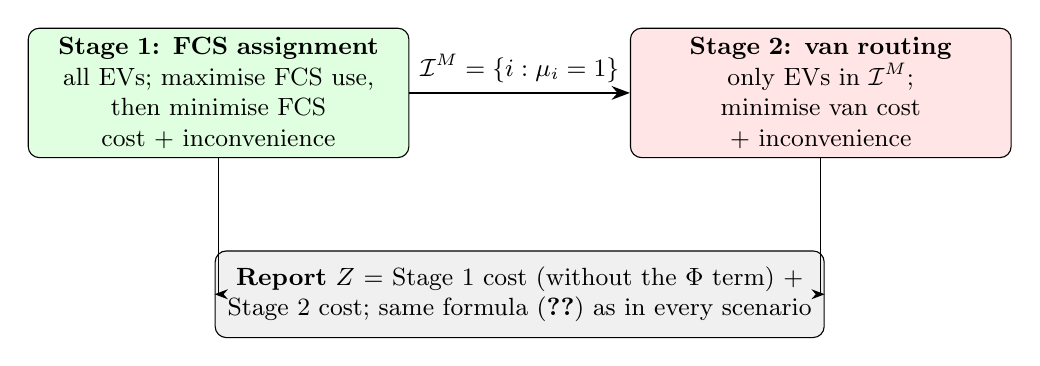
\begin{tikzpicture}[>=Stealth,box/.style={draw,rounded corners,align=center,minimum height=1.1cm,font=\small}]
  \node[box,fill=green!12,text width=4.6cm] (s1) {\textbf{Stage 1: FCS assignment}\\all EVs; maximise FCS use,\\then minimise FCS cost + inconvenience};
  \node[box,fill=red!10,text width=4.6cm,right=2.8cm of s1] (s2) {\textbf{Stage 2: van routing}\\only EVs in $\I^M$;\\minimise van cost + inconvenience};
  \draw[->,thick] (s1) -- node[above,font=\small]{$\I^M=\{i:\mu_i=1\}$} (s2);
  \node[box,fill=black!6,text width=7.5cm,below=2.0cm of $(s1)!0.5!(s2)$] (ev) {\textbf{Report} $Z=$ Stage~1 cost (without the $\Phi$ term) $+$ Stage~2 cost; same formula \eqref{eq:Z} as in every scenario};
  \draw[->] (s1) |- (ev); \draw[->] (s2) |- (ev);
\end{tikzpicture}
\end{center}

Stage~1 does not look at the vans, and Stage~2 cannot change what Stage~1 decided. That is the definition of ``FCS first, then MCS''.

%----------------------------------------------------------------
\subsection{Stage 1: assign EVs to fixed stations}

\textbf{Objective.}
\begin{equation}
\begin{split}
\min\ Z^{(1)}=\;&\underbrace{\Phi\sum_{i\in\I}\mu_i}_{\text{FCS first}}
+\underbrace{c^{EV}\sum_i\sum_{f\in\F_i}d_{if}Y_{if}}_{Z_1}
+\underbrace{Z^F_{\text{energy}}}_{\text{FCS part of }Z_4}\\
&+\underbrace{\sum_i\sum_{f\in\F_i}\rho^F_{if}Y_{if}+\alpha\sum_i w_i(C_i-r_i)+c^L\sum_i w_iL_i}_{\text{FCS customers' inconvenience}}
\end{split}
\label{eq:obj1}
\end{equation}
with $C_i=S_i+\tau^F_iY_i$ in this stage. $\Phi$ is a penalty for handing an EV to the vans. It is chosen larger than anything an extra FCS customer can add to the rest of \eqref{eq:obj1}, e.g.
\[
\Phi > \max_{i}\max_{f\in\F_i}\big(c^{EV}d_{if}+\pi^{\max}E_i+\rho^F_{if}\big)+n\,(\alpha+c^L)\,w_{\max}\,T,
\]
so Stage~1 first \textbf{maximises the number of EVs served at an FCS}, and only among those solutions minimises FCS cost and inconvenience. ($\pi^{\max}$ is the highest grid price.) A numerically safer equivalent is to solve twice: first $\max\sum_iY_i$, then fix that number and minimise the rest.
\ifTOU
Because $Z^F_{\text{energy}}$ uses the peak price, Stage~1 may \emph{start sessions later} to leave the peak, if the price saving beats the extra waiting cost (Section~\ref{sec:expect}).
\fi

\textbf{Constraints.}
\begin{align}
\sum_{g\in\G_i}y_{ig}+\mu_i &= 1 && \forall i\in\I \label{eq:s1assign}\\
S_i &\ge r_i+\sum_{f\in\F_i}t_{if}Y_{if} && \forall i\in\I \label{eq:fcsarr}\\
S_i &\le r_i+T\,(1-\mu_i) && \forall i\in\I \label{eq:s1park}\\
S_j &\ge S_i+\tau^F_i-(T+\tau^F_i)(3-y_{ig}-y_{jg}-o_{ij}) && \forall g,\ (i,j)\in\mathcal{P}_g \label{eq:disj1}\\
S_i &\ge S_j+\tau^F_j-(T+\tau^F_j)(2-y_{ig}-y_{jg}+o_{ij}) && \forall g,\ (i,j)\in\mathcal{P}_g \label{eq:disj2}\\
\sum_i y_{ig_1} &\ge \sum_i y_{ig_2} && \forall f,\ \G_f=\{g_1,g_2\} \label{eq:gunsym}\\
S_i+\tau^F_iY_i &\le T,\qquad L_i\ge S_i+\tau^F_iY_i-l_i && \forall i\in\I \label{eq:s1time}
\end{align}
\ifTOU plus the time-of-use split \eqref{eq:tou1}--\eqref{eq:tou5} of each FCS session (Section~\ref{sec:price}).\fi
\desc{\eqref{eq:s1assign}: every EV either gets one reachable gun or is handed to the vans. An EV that reaches no FCS ($\G_i=\emptyset$) is forced to $\mu_i=1$. \eqref{eq:fcsarr}: an FCS session cannot start before the EV has asked and driven to the station. \eqref{eq:s1park}: for an EV handed to the vans, $S_i$ is parked at $r_i$, so it adds no waiting in Stage~1 (its real start time is decided in Stage~2). \eqref{eq:disj1}--\eqref{eq:disj2}: two EVs on the same gun do not overlap; $o_{ij}$ picks who goes first. With two guns per station this means at most two EVs charge at a station at a time. \eqref{eq:gunsym}: symmetry breaking between the two identical guns (optional). \eqref{eq:s1time}: finished by $T$; lateness.}

\textbf{Optional acceptability rule.} An operator may refuse to send a driver to a station that is ``too inconvenient'', e.g.\ only allow gun $g$ of station $f$ for EV $i$ if $\hat\rho^F_{if}\le\bar\rho$. This only shrinks $\G_i$, so EVs whose stations are all too far go to the vans. Report results with and without it.

\textbf{Output:} $\I^M=\{i:\mu_i=1\}$, the EVs left for the vans; plus each FCS customer's gun and start time.

%----------------------------------------------------------------
\subsection{Stage 2: route the vans to the leftover EVs}

Stage~2 is a vehicle routing problem with time windows, on the EVs in $\I^M$ only. Here $C_i=S_i+\tau^M_i$.

\textbf{Objective.}
\begin{equation}
\begin{split}
\min\ Z^{(2)}=\;&\underbrace{c^M\sum_m\sum_{(i,j)\in\A^M}d_{ij}x_{ijm}}_{Z_2}+\underbrace{\sum_m c^D_mu_m}_{Z_3}+\underbrace{Z^M_{\text{energy}}}_{\text{van part of }Z_4}\\
&+\underbrace{\sum_{i\in\I^M}\sum_m\rho^M_{im}z_{im}+\alpha\sum_{i\in\I^M}w_i(C_i-r_i)+c^L\sum_{i\in\I^M}w_iL_i}_{\text{van customers' inconvenience}}
\end{split}
\label{eq:obj2}
\end{equation}
Since every EV in $\I^M$ must be served by some van, $Z^M_{\text{energy}}$ and the $\rho^M$ term are constants here. They are kept so that $Z^{(2)}$ is the true cost of Stage~2. Waiting and lateness make the vans visit urgent EVs early.

\textbf{Constraints.}
\begin{align}
\sum_{m\in\M}z_{im} &= 1 && \forall i\in\I^M \label{eq:s2assign}\\
\sum_{j:(0,j)\in\A^M}x_{0jm} = \sum_{i:(i,n+1)\in\A^M}x_{i,n+1,m} &= u_m && \forall m \label{eq:depot}\\
\sum_{i:(i,j)\in\A^M}x_{ijm} = \sum_{k:(j,k)\in\A^M}x_{jkm} &= z_{jm} && \forall j\in\I^M,\ m \label{eq:flow}\\
\sum_{i\in\I^M}z_{im} &\le Q_m\,u_m && \forall m \label{eq:cap}\\
\sum_{i\in\I^M}\frac{E_i}{\eta}z_{im}+\beta\sum_{(i,j)\in\A^M}d_{ij}x_{ijm} &\le B_m\,u_m && \forall m \label{eq:batt}
\end{align}
\begin{align}
S_j &\ge \max\{r_j,\ t_{0j}\,x_{0jm}\} && \forall j\in\I^M,\ m \label{eq:depart}\\
S_j &\ge S_i+\tau^M_i+t_{ij}-(T+\tau^M_i+t_{ij})(1-x_{ijm}) && \forall i\neq j,\ m \label{eq:seq}\\
S_i+\tau^M_i+t_{i,n+1} &\le T+(\tau^M_i+t_{i,n+1})(1-x_{i,n+1,m}) && \forall i,\ m \label{eq:return}\\
S_i+\tau^M_i \le T,\quad L_i &\ge S_i+\tau^M_i-l_i && \forall i\in\I^M \label{eq:s2time}\\
u_m &\ge u_{m+1} && m<|\M| \label{eq:vansym}
\end{align}
\desc{\eqref{eq:s2assign}: each leftover EV gets one van. \eqref{eq:depot}: a used van leaves and returns to the depot once. \eqref{eq:flow}: each EV on van $m$ is entered and left exactly once by that van. \eqref{eq:cap}: at most $Q_m$ EVs per van. \eqref{eq:batt}: delivered energy (with transfer losses) plus driving energy fits in the van battery. \eqref{eq:depart}: no start before the request, or before the van can drive there from the depot (written as two linear constraints). \eqref{eq:seq}: if the van goes $i\to j$, it finishes $i$ and drives to $j$ before starting $j$. This gives one EV at a time and removes subtours (MTZ-type). \eqref{eq:return}: back at the depot by $T$. \eqref{eq:s2time}: finished by $T$; lateness. \eqref{eq:vansym}: use identical vans in index order.}

\textbf{If Stage 2 is infeasible} (too many leftover EVs for the fleet by $T$), the sequential policy has \emph{failed} on that instance. For diagnosis, add $s_i\in\{0,1\}$ (``unserved''), replace \eqref{eq:s2assign} by $\sum_mz_{im}+s_i=1$ and add $\Phi^U\sum_is_i$ to \eqref{eq:obj2}. Then report the number of EVs that could not be served. This is a useful comparison with the integrated scenario, which may serve all of them.

%----------------------------------------------------------------
\subsection{Reported value}
\[
Z^{\text{S\scen}}=\big(Z^{(1)*}-\Phi\,|\I^M|\big)+Z^{(2)*},
\]
which is exactly \eqref{eq:Z} evaluated at the combined solution. The stage-1 solution plus the stage-2 solution is a feasible solution of the integrated model (S\ifTOU 4\else 3\fi), so
$Z^{\text{S\ifTOU 4\else 3\fi}}\le Z^{\text{S\scen}}$. The difference is the \emph{value of integration}.

\else
%---------------------------------------------------------------- INT
\subsection{Objective}
\begin{equation}
\min\ Z \quad\text{as in \eqref{eq:Z}, with }Z^F_{\text{energy}}=\ifTOU P^F\textstyle\sum_i\big[\pi^\off(\theta^1_i+\theta^3_i)+\pi^\pk\theta^2_i\big]\else\pi^F\textstyle\sum_iE_iY_i\fi,\quad C_i=S_i+\tau^F_iY_i+\tau^M_iZ_i. \label{eq:objint}
\end{equation}
Written out in full:
\begin{align*}
\min\ Z=\;& c^{EV}\sum_i\sum_{f\in\F_i}d_{if}Y_{if}+c^M\sum_m\sum_{(i,j)\in\A}d_{ij}x_{ijm}+\sum_mc^D_mu_m\\
&+\ifTOU P^F\sum_i\big[\pi^\off(\theta^1_i+\theta^3_i)+\pi^\pk\theta^2_i\big]\else\pi^F\sum_iE_iY_i\fi
+\pi^M\sum_i\sum_m\frac{E_i}{\eta}z_{im}\\
&+\sum_i\sum_{f\in\F_i}\rho^F_{if}Y_{if}+\sum_i\sum_m\rho^M_{im}z_{im}+\alpha\sum_iw_i(C_i-r_i)+c^L\sum_iw_iL_i .
\end{align*}
Every term is linear. One model weighs everything at once: an EV goes to a van exactly when the van's extra km, dispatch and energy cost are outweighed by the effort and waiting it saves the driver\ifTOU, or by the peak-price energy it avoids\fi.

\subsection{Constraints}

\textbf{Assignment.}
\begin{equation}
\sum_{g\in\G_i}y_{ig}+\sum_{m\in\M}z_{im}=1\qquad\forall i\in\I \label{eq:assign}
\end{equation}
\desc{Exactly one resource per EV: one reachable gun or one van. EVs that reach no FCS are forced onto a van.}

\textbf{Fixed stations.}
\begin{align}
S_i &\ge r_i+\sum_{f\in\F_i}t_{if}Y_{if} && \forall i \label{eq:fcsarr}\\
S_j &\ge S_i+\tau^F_i-(T+\tau^F_i)(3-y_{ig}-y_{jg}-o_{ij}) && \forall g,\ (i,j)\in\mathcal{P}_g \label{eq:disj1}\\
S_i &\ge S_j+\tau^F_j-(T+\tau^F_j)(2-y_{ig}-y_{jg}+o_{ij}) && \forall g,\ (i,j)\in\mathcal{P}_g \label{eq:disj2}\\
\sum_iy_{ig_1} &\ge \sum_iy_{ig_2} && \forall f,\ \G_f=\{g_1,g_2\} \label{eq:gunsym}
\end{align}
\desc{\eqref{eq:fcsarr}: an FCS session starts after the request and the drive to the station (for a van customer this is just $S_i\ge r_i$). \eqref{eq:disj1}--\eqref{eq:disj2}: EVs on the same gun do not overlap; $o_{ij}$ chooses the order. \eqref{eq:gunsym}: optional symmetry breaking.}

\textbf{Vans: routes, capacity, battery.}
\begin{align}
\sum_{j:(0,j)\in\A}x_{0jm}=\sum_{i:(i,n+1)\in\A}x_{i,n+1,m} &= u_m && \forall m \label{eq:depot}\\
\sum_{i:(i,j)\in\A}x_{ijm}=\sum_{k:(j,k)\in\A}x_{jkm} &= z_{jm} && \forall j\in\I,\ m \label{eq:flow}\\
\sum_iz_{im} &\le Q_mu_m && \forall m \label{eq:cap}\\
\sum_i\frac{E_i}{\eta}z_{im}+\beta\sum_{(i,j)\in\A}d_{ij}x_{ijm} &\le B_mu_m && \forall m \label{eq:batt}
\end{align}
\desc{\eqref{eq:depot}: a used van leaves and returns once. \eqref{eq:flow}: each EV on van $m$ is visited exactly once by it. \eqref{eq:cap}: at most $Q_m$ EVs. \eqref{eq:batt}: delivered energy (with losses) plus driving energy fits in the battery.}

\textbf{Vans: timing (one EV at a time, no subtours).}
\begin{align}
S_j &\ge t_{0j}\,x_{0jm} && \forall j\in\I,\ m \label{eq:depart}\\
S_j &\ge S_i+\tau^M_i+t_{ij}-(T+\tau^M_i+t_{ij})(1-x_{ijm}) && \forall i\neq j\in\I,\ m \label{eq:seq}\\
S_i+\tau^M_i+t_{i,n+1} &\le T+(\tau^M_i+t_{i,n+1})(1-x_{i,n+1,m}) && \forall i,\ m \label{eq:return}
\end{align}
\desc{\eqref{eq:depart}: the first stop cannot start before the van has driven there. \eqref{eq:seq}: $i\to j$ means finish $i$, drive, then start $j$; start times rise along a route, so no subtour can close. \eqref{eq:return}: back at the depot by $T$.}

\textbf{Horizon and lateness.}
\begin{equation}
C_i\le T,\qquad L_i\ge C_i-l_i\qquad\forall i\in\I \label{eq:time}
\end{equation}
\desc{Every EV is fully charged within the horizon; $L_i$ measures lateness.}

\ifTOU
\textbf{Time-of-use split.} Constraints \eqref{eq:tou1}--\eqref{eq:tou5} of Section~\ref{sec:price}.
\fi

\textbf{Symmetry and domains.}
\begin{equation}
u_m\ge u_{m+1};\qquad y,z,x,u,o\ifTOU,\kappa\fi\in\{0,1\};\qquad S_i,L_i\ifTOU,\theta^p_i\fi\ge0 \label{eq:dom}
\end{equation}
\fi

%=====================================================================
\section{Learning-to-optimise (RL) formulation}\label{sec:rl}

\textbf{Main rule:} the reward of each action is \emph{minus the increase in $Z$ that the action causes}. The rewards over an episode then add up to $-Z$ of the solution the policy builds. RL and MILP results are measured on the same yardstick \eqref{eq:Z}, and the MILP optimum is the benchmark for the RL gap.

\ifSEQ
%---------------------------------------------------------------- RL SEQ
The RL pipeline has the same two stages as the MILP.

\subsection{Stage 1 policy: FCS assignment}
\begin{itemize}[leftmargin=1.4em,itemsep=2pt]
  \item \textbf{Episode / epochs:} EVs are taken in order of request time $r_i$ (ties: higher $w_i$ first). One decision per EV.
  \item \textbf{State:} features of the current EV $k$ ($E_k,r_k,l_k,w_k,R_k$, location); for each gun $g$ the time $F_g$ it becomes free; summary features of the EVs still to come (count and positions near each station)\ifTOU; the current price and the time until $T_1$ and $T_2$\fi.
  \item \textbf{Action:} a gun $g\in\G_k$, or ``hand to vans''. \textbf{FCS-first mask:} ``hand to vans'' is allowed \emph{only} if no gun can finish EV $k$ by $T$ (or, with the optional rule, if all remaining guns have $\hat\rho^F_{kf}>\bar\rho$).
  \ifTOU\item \textbf{Optional timing action:} ``gun $g$, start after the peak'', i.e.\ $S_k=\max\{\text{earliest},T_2\}$, allowed only if the session still ends by $T$.\fi
  \item \textbf{Transition:} $S_k=\max\{r_k+t_{kf},F_g\}$ (or later, for the timing action); $F_g\leftarrow S_k+\tau^F_k$.
  \item \textbf{Reward:} $-\Big[c^{EV}d_{kf}+\text{energy}_k+\rho^F_{kf}+\alpha w_k(S_k+\tau^F_k-r_k)+c^Lw_k(S_k+\tau^F_k-l_k)^+\Big]$, where energy$_k$ = \ifTOU$P^F\big[\pi^\off\cdot(\text{off-peak hours of }[S_k,S_k+\tau^F_k])+\pi^\pk\cdot(\text{peak hours})\big]$, computed exactly in the simulator\else$\pi^FE_k$\fi. Handing an EV to the vans gives reward $0$ here; its cost is counted in Stage~2.
\end{itemize}
Note: a simple baseline for Stage~1 is the greedy rule ``gun with the largest one-step reward''. What RL can learn on top of this is, for example, to keep a nearby gun free for an urgent EV that arrives later.

\subsection{Stage 2 policy: van routing over $\I^M$}
\begin{itemize}[leftmargin=1.4em,itemsep=2pt]
  \item \textbf{Epochs:} whenever a van becomes free (the earliest-free van decides first).
  \item \textbf{State:} for each van: position, time free, remaining battery $b_m$, EVs served so far, dispatched or not; for each unserved EV in $\I^M$: location, $E_i,r_i,l_i,w_i$; current time.
  \item \textbf{Action:} the next EV $j$ for this van, or ``return to depot'' (ends the route). Mask: $j$ must be feasible: battery covers $E_j/\eta$ plus driving to $j$ and back to the depot, the count stays $\le Q_m$, and $j$ can be finished with the van back at the depot by $T$.
  \item \textbf{Transition:} $S_j=\max\{r_j,\ \text{time free}+t_{\text{pos},j}\}$; the van moves to $j$ and is free at $S_j+\tau^M_j$; $b_m$ falls by $E_j/\eta+\beta d_{\text{pos},j}$.
  \item \textbf{Reward:} serving $j$: $-\Big[c^Md_{\text{pos},j}+c^D_m[\text{first stop}]+\pi^M\frac{E_j}{\eta}+\rho^M_{jm}+\alpha w_j(S_j+\tau^M_j-r_j)+c^Lw_j(S_j+\tau^M_j-l_j)^+\Big]$; returning: $-c^Md_{\text{pos},0}$. EVs still unserved at the end: $-\Phi^U$ each.
  \item \textbf{Policy:} an attention-based routing policy (e.g.\ Kool et al., 2019, ``Attention, Learn to Solve Routing Problems!'') trained with REINFORCE or PPO. Baseline: nearest-feasible-EV heuristic.
\end{itemize}
Episode return of Stage~1 + Stage~2 $=-Z^{\text{S\scen}}$.

\else
%---------------------------------------------------------------- RL INT
One policy decides both who serves each EV and the van routes.
\begin{itemize}[leftmargin=1.4em,itemsep=2pt]
  \item \textbf{Episode / epochs:} EVs are taken in order of request time $r_i$ (ties: higher $w_i$ first). One decision per EV.
  \item \textbf{State:} (i) the current EV $k$: location, $E_k,r_k,l_k,w_k,R_k$, reachable stations; (ii) each gun $g$: time $F_g$ it becomes free; (iii) each van $m$: current end-of-route position, time free, remaining battery $b_m$, EVs served, dispatched or not; (iv) embeddings of the not-yet-assigned EVs (for look-ahead)\ifTOU; (v) current price, time until $T_1$ and $T_2$\fi.
  \item \textbf{Action:} $a\in\G_k\cup\M$: a gun, or a van (EV $k$ is appended to the end of that van's route). \textbf{Mask} infeasible actions: a gun that cannot finish $k$ by $T$; a van without enough battery for $E_k/\eta$ plus the drive to $k$ and back to the depot, with $Q_m$ reached, or unable to finish $k$ and return by $T$.
  \ifTOU\item \textbf{Optional timing action:} ``gun $g$, start after the peak'' ($S_k=\max\{\text{earliest},T_2\}$, if it still ends by $T$).\fi
  \item \textbf{Transition:} gun: $S_k=\max\{r_k+t_{kf},F_g\}$, $F_g\leftarrow S_k+\tau^F_k$. Van: $S_k=\max\{r_k,\ \text{free}_m+t_{\text{pos}_m,k}\}$, then the van moves to $k$, $\text{free}_m\leftarrow S_k+\tau^M_k$, $b_m\mathrel{-}=E_k/\eta+\beta d_{\text{pos}_m,k}$.
  \item \textbf{Reward} $=-\Delta Z$:
  \begin{align*}
  \text{gun } g\text{ at }f:&\quad -\Big[c^{EV}d_{kf}+\text{energy}^F_k+\rho^F_{kf}+\alpha w_k(C_k-r_k)+c^Lw_k(C_k-l_k)^+\Big]\\
  \text{van } m:&\quad -\Big[c^M\big(d_{\text{pos}_m,k}+d_{k,0}-d_{\text{pos}_m,0}\big)+c^D_m[\text{first use}]+\pi^M\tfrac{E_k}{\eta}\\
  &\qquad\quad+\rho^M_{km}+\alpha w_k(C_k-r_k)+c^Lw_k(C_k-l_k)^+\Big]
  \end{align*}
  The van distance term is the \emph{change} in route length when $k$ is inserted before the return to the depot, so the sum over the episode equals the total route length (the return legs telescope). energy$^F_k$ = \ifTOU$P^F\big[\pi^\off\cdot(\text{off-peak hours})+\pi^\pk\cdot(\text{peak hours of }[S_k,C_k])\big]$, computed exactly by the simulator; no linearisation is needed in RL\else$\pi^FE_k$\fi.
  \item \textbf{Dead end:} if every action is masked, EV $k$ is unserved: reward $-\Phi^U$, and the episode continues. Report the count.
  \item \textbf{Policy:} masked categorical policy over guns and vans, encoder with attention over EVs, guns and vans; trained with PPO. Natural baseline: greedy, i.e.\ choose the action with the largest one-step reward. That is the pairwise rule ``smallest $\hat\rho$ + cost'' from Section~\ref{sec:inc}.
\end{itemize}
Restriction to note: vans serve EVs in assignment order (append only). A variant that inserts $k$ at the cheapest position of a route is more flexible but has a larger action space.
\fi

\textbf{Reward scaling.} For stable training divide every reward by a constant, e.g.\ the greedy baseline's average $Z$ on the training instances. This does not change the optimal policy.

%=====================================================================
\section{What to expect and what to report}\label{sec:expect}

\ifnum\scen=1
\begin{itemize}[leftmargin=1.4em,itemsep=2pt]
  \item Vans serve only EVs that reach no station, or that the stations cannot finish by $T$. If stations have spare capacity, very few vans are dispatched.
  \item Inconvenience is high for EVs far from the nearest station (worked example: Rs\,682 at the FCS, against Rs\,458 if a van had been allowed).
  \item With too few vans Stage~2 becomes infeasible (unserved EVs), even when the integrated model S3 could serve everyone. Report the smallest $|\M|$ at which S1 is feasible and compare it with S3.
\end{itemize}
\fi
\ifnum\scen=2
\begin{itemize}[leftmargin=1.4em,itemsep=2pt]
  \item \textbf{When does Stage~1 delay a session to avoid the peak?} Moving one hour of charging out of the peak saves $(\pi^\pk-\pi^\off)P^F=3\times22=$ Rs\,66, but delays completion by up to an hour, which costs $\alpha w_i\ge$ Rs\,200. So with the default values Stage~1 almost never delays. It mostly pays the higher price, and S2 costs roughly S1 plus the peak surcharge. Sessions start later only if $\alpha$ is small (try $\lambda<0.33$ in the sensitivity analysis).
  \item The van assignment is the same as in S1 unless Stage~1's timing changes which EVs fit at the stations. Stage~1 cannot use vans to escape the peak price.
  \item Extra KPI: \textbf{grid energy drawn at FCS during the peak}, $P^F\sum_i\theta^2_i$ (kWh). Compare with S4.
\end{itemize}
\fi
\ifnum\scen=3
\begin{itemize}[leftmargin=1.4em,itemsep=2pt]
  \item Vans take EVs for which the saved inconvenience exceeds the extra van cost (worked example: van chosen, saving Rs\,224). Expect vans to serve EVs that are far from every station, have low range (high $w_i$), or have early deadlines, while EVs near a station still use it.
  \item \textbf{Value of integration under flat price:} $Z^{\text{S1}}-Z^{\text{S3}}\ge0$. Report it per component ($Z_1,\dots,Z_5$): typically operating cost rises a little and inconvenience falls a lot.
  \item Vary $|\M|$ (0, 1, 2, \dots): the first few vans lower $Z$ sharply, then the effect levels off. That curve shows the scenarios where mobile chargers help most.
\end{itemize}
\fi
\ifnum\scen=4
\begin{itemize}[leftmargin=1.4em,itemsep=2pt]
  \item During the peak a van kWh costs about the same as an FCS kWh (Rs\,10.0 each), so the vans' energy disadvantage disappears and vans also absorb \emph{peak-hour} demand that would otherwise be charged on the grid at peak price.
  \item Expect more van usage than in S3, concentrated on requests in $[T_1,T_2]$, and lower grid energy at the stations during the peak, $P^F\sum_i\theta^2_i$, than in S2.
  \item \textbf{Value of integration under peak pricing:} $Z^{\text{S2}}-Z^{\text{S4}}$. It should be larger than $Z^{\text{S1}}-Z^{\text{S3}}$, because integration now also allows price arbitrage.
  \item \textbf{Peak pricing with full flexibility:} $Z^{\text{S4}}-Z^{\text{S3}}$ should be smaller than $Z^{\text{S2}}-Z^{\text{S1}}$: vans cushion the price increase.
\end{itemize}
\fi

\textbf{Cross-scenario comparison table} (fill in from the four runs):
\begin{center}
\renewcommand{\arraystretch}{1.2}
\begin{tabular}{@{}lll@{}}
\toprule
\textbf{Comparison} & \textbf{Measures} & \textbf{Expected sign} \\
\midrule
S1 $-$ S3 & value of integration, flat price & $\ge0$ \\
S2 $-$ S4 & value of integration, peak price & $\ge0$, larger than S1 $-$ S3 \\
S2 $-$ S1 & cost of peak pricing, FCS-first operator & $>0$ \\
S4 $-$ S3 & cost of peak pricing, flexible operator & $>0$, smaller than S2 $-$ S1 \\
\bottomrule
\end{tabular}
\end{center}
Report for each: $Z$ and its components, number of vans used, EVs per resource, mean and maximum inconvenience per EV, total lateness, peak-hour grid energy, solve time, and (for RL) the gap to the MILP optimum.

%=====================================================================
\appendix
\section{Illustrative parameter values}\label{app:values}

These are starting values for experiments, not data. All are meant to be varied in the analysis. Values in Rs.

\begin{center}
\renewcommand{\arraystretch}{1.15}
\begin{tabular}{@{}llp{6.2cm}@{}}
\toprule
\textbf{Parameter} & \textbf{Value} & \textbf{Note} \\
\midrule
$T$, $[T_1,T_2]$ & 7 h, $[2,6]$ & 16:00--23:00, peak 18:00--22:00 \\
$P^F$, $P^M$ & 22 kW, 30 kW & \\
$v$, $\beta$, $\eta$ & 25 km/h, 0.25 kWh/km, 0.9 & \\
$B_m$, $Q_m$, $|\M|$ & 150 kWh, 6, 2--6 & \\
$c^{EV}$, $c^M$, $c^D_m$ & Rs\,4/km, Rs\,15/km, Rs\,1500 & van km includes driver time \\
$\pi^F$ (flat) & Rs\,8.7/kWh & equals the time-average of the ToU tariff over $[0,T]$ \\
$\pi^\off$, $\pi^\pk$ (ToU) & Rs\,7/kWh, Rs\,10/kWh & $(3\times7+4\times10)/7=8.7$ \\
$c^{bat}$ & Rs\,2/kWh & van battery wear \\
$\pi^M$ & Rs\,10.7 (flat) / Rs\,9.0 (ToU) & $=\pi^F+c^{bat}$ / $=\pi^\off+c^{bat}$ \\
$\alpha$, $\alpha^D$ & Rs\,200/h, Rs\,100/h & value of time; extra for attended time \\
$h^F$, $h^M$, $\varphi$ & Rs\,50, Rs\,10, Rs\,100 & trip hassle, hand-over, range stress \\
$c^L$ & Rs\,300/h & lateness \\
$w_i$ & $1+2(1-R_i/R_{\max})$, $R_i\sim U[3,40]$ km & priority from remaining range \\
\bottomrule
\end{tabular}
\end{center}

The flat price is set to the time-average of the peak tariff. The price \emph{level} is then the same in both pricing cases, and only the price \emph{shape} differs. Without this, part of S1 vs S2 would just reflect a different average price.

\end{document}
"
%    pdflatex -jobname=scenario3_flat_integrated   "\def\scen{3}% =====================================================================
%  One source, four PDFs.  Build with build.sh (or by hand):
%    pdflatex -jobname=scenario1_flat_sequential   "\def\scen{1}\input{scenario_master}"
%    pdflatex -jobname=scenario2_peak_sequential   "\def\scen{2}\input{scenario_master}"
%    pdflatex -jobname=scenario3_flat_integrated   "\def\scen{3}\input{scenario_master}"
%    pdflatex -jobname=scenario4_peak_integrated   "\def\scen{4}\input{scenario_master}"
%  (run each twice for cross-references)
% =====================================================================
\documentclass[11pt,a4paper]{article}
\usepackage[margin=2.2cm]{geometry}
\usepackage{amsmath,amssymb,amsfonts}
\usepackage{booktabs,array,tabularx}
\usepackage{enumitem}
\usepackage[table]{xcolor}
\usepackage{tikz}
\usetikzlibrary{arrows.meta,positioning,calc}
\usepackage[colorlinks=true,linkcolor=blue!50!black,urlcolor=blue!50!black]{hyperref}
\usepackage{titlesec}
\titleformat{\section}{\large\bfseries}{\thesection}{0.8em}{}
\titleformat{\subsection}{\normalsize\bfseries}{\thesubsection}{0.8em}{}
\setlength{\parindent}{0pt}
\setlength{\parskip}{5pt}

% ---------------- scenario switches ----------------
\ifdefined\scen\else\def\scen{1}\fi
\newif\ifTOU \TOUfalse   % true = time-of-use (peak) price
\newif\ifSEQ \SEQfalse   % true = FCS first, then MCS
\ifnum\scen=1 \SEQtrue \fi
\ifnum\scen=2 \TOUtrue \SEQtrue \fi
\ifnum\scen=4 \TOUtrue \fi

\newcommand{\pricename}{\ifTOU time-of-use price (dearer evening peak)\else single (flat) price all day\fi}
\newcommand{\structname}{\ifSEQ FCS first, then MCS (sequential)\else FCS and MCS together (integrated)\fi}

% ---------------- notation ----------------
\newcommand{\I}{\mathcal{I}}
\newcommand{\F}{\mathcal{F}}
\newcommand{\G}{\mathcal{G}}
\newcommand{\M}{\mathcal{M}}
\newcommand{\N}{\mathcal{N}}
\newcommand{\A}{\mathcal{A}}
\newcommand{\Rs}{\text{Rs}\,}
\newcommand{\pk}{\mathrm{pk}}
\newcommand{\off}{\mathrm{off}}
\newcommand{\desc}[1]{\par\vspace{-2pt}{\small\color{black!75}\textit{Meaning:} #1}\par\vspace{4pt}}
\newcommand{\cell}[2]{\ifnum\scen=#1\cellcolor{blue!18}\textbf{S#1 (this document)}\\\textbf{#2}\else S#1\\#2\fi}

\title{\textbf{EV Charging Network Optimisation}\\[4pt]
\large Scenario \scen: \pricename\ $+$ \structname\\[2pt]
\normalsize MILP and RL formulation}
\author{CP 320 OR for Mobility Management, course project}
\date{2 October 2026}

\begin{document}
\maketitle

%=====================================================================
\section{Where this scenario sits}

The project studies four scenarios: two ways of pricing grid electricity, times two ways of making the decisions.

\begin{center}
\renewcommand{\arraystretch}{1.5}
\begin{tabular}{>{\raggedright\arraybackslash}p{4.2cm}|>{\centering\arraybackslash}p{4.6cm}|>{\centering\arraybackslash}p{4.6cm}}
 & \textbf{Flat price all day} & \textbf{Time-of-use (peak) price} \\ \hline
\textbf{Sequential:} FCS first, leftover EVs to MCS &
\begin{tabular}[c]{@{}c@{}}\cell{1}{flat + sequential}\end{tabular} &
\begin{tabular}[c]{@{}c@{}}\cell{2}{peak + sequential}\end{tabular} \\ \hline
\textbf{Integrated:} FCS and MCS decided together &
\begin{tabular}[c]{@{}c@{}}\cell{3}{flat + integrated}\end{tabular} &
\begin{tabular}[c]{@{}c@{}}\cell{4}{peak + integrated}\end{tabular} \\
\end{tabular}
\end{center}

\textbf{The four scenarios do not have four different objectives.} They share \emph{one} cost yardstick $Z$ (Section~\ref{sec:obj}): the same cost terms and the same customer inconvenience (Section~\ref{sec:inc}). Only two things change:
\begin{itemize}[leftmargin=1.4em,itemsep=1pt]
  \item \textbf{Pricing} changes the formula for one term, the FCS energy cost (Section~\ref{sec:price}).
  \item \textbf{Decision structure} changes \emph{how} $Z$ is minimised: in one model (integrated), or in two stages (sequential), where each stage minimises its own part of $Z$.
\end{itemize}
Because the yardstick is the same, the four optimal values can be compared directly. The differences measure the \emph{value of integration} (S1$\to$S3, S2$\to$S4) and the \emph{effect of peak pricing} (S1$\to$S2, S3$\to$S4).

\ifnum\scen=1
\textbf{This scenario (S1)} is the baseline, the ``status quo''. Electricity costs the same at every hour, every EV that can be charged at a fixed station is sent there, and vans only take what is left over.
\fi
\ifnum\scen=2
\textbf{This scenario (S2)} keeps the FCS-first rule of S1, but grid electricity is dearer during the evening peak. Stage~1 can react to the price only by \emph{rescheduling} FCS sessions. It cannot hand a peak-hour EV to a van.
\fi
\ifnum\scen=3
\textbf{This scenario (S3)} keeps the flat price of S1, but the operator decides FCS and MCS service \emph{together}. An EV can be sent to a van even when a fixed station could take it, whenever that lowers total cost plus inconvenience.
\fi
\ifnum\scen=4
\textbf{This scenario (S4)} is the most flexible one: peak pricing at fixed stations, and FCS and MCS decided together. Van energy was bought off-peak, so vans can also be used to keep charging \emph{out of the expensive peak}.
\fi

%=====================================================================
\section{Setting and assumptions}\label{sec:setting}

\textbf{Time.} The planning horizon is $[0,T]$ with $T=7$\,h (16:00--23:00). It contains the evening peak window $[T_1,T_2]=[2,6]$ (18:00--22:00). The horizon is the same in all four scenarios. It is wider than the peak itself so that, under peak pricing, there is cheaper time on both sides of the peak.\ifTOU\else\ In this scenario the price is flat, so the window plays no role in the model.\fi

\textbf{Assumptions} (the same as MILP v3, plus two about energy):
\begin{enumerate}[leftmargin=1.6em,itemsep=1pt]
  \item Static, continuous time. All requests in the horizon are known at time $0$, and request $i$ becomes active at $r_i$.
  \item An EV served by an FCS drives there itself on its own battery (only to stations within its range $R_i$). The driver stays with the car while it waits for a free gun and while it charges.
  \item An EV served by an MCS stays parked where it is, and the driver is free in the meantime.
  \item Each FCS gun and each van charges one EV at a time, without interruption, at constant power.
  \item A van's battery covers both its driving and the energy it delivers. \textbf{The van battery is charged at the depot before the horizon starts}\ifTOU, i.e.\ at the off-peak price\fi, and is not recharged during the horizon.
  \item Every EV must be fully charged by $T$ (hard). Finishing after the driver's desired time $l_i$ is allowed but penalised.
\end{enumerate}

%=====================================================================
\section{Notation}\label{sec:notation}

\subsection*{Sets}
\begin{tabularx}{\textwidth}{@{}lX@{}}
\toprule
$\I=\{1,\dots,n\}$ & EV charging requests \\
$\F$; $\G_f$ ($|\G_f|=2$); $\G=\bigcup_f\G_f$ & fixed charging stations; guns of FCS $f$; all guns ($f(g)$ = station of gun $g$) \\
$\F_i=\{f: d_{if}\le R_i\}$, $\G_i=\bigcup_{f\in\F_i}\G_f$ & stations / guns EV $i$ can reach on its remaining range \\
$\M$ & mobile charging vans (MCS) \\
$0,\ n+1$ & depot as start node / end node (same place) \\
$\N=\{0\}\cup\I\cup\{n+1\}$, $\A$ & routing nodes; allowed van arcs $(i,j)$, $i\in\{0\}\cup\I$, $j\in\I\cup\{n+1\}$, $i\neq j$ \\
$\mathcal{P}_g=\{(i,j): i<j,\ g\in\G_i\cap\G_j\}$ & pairs of EVs that could share gun $g$ \\
\ifSEQ
$\I^M\subseteq\I$ & EVs handed to the vans by Stage~1 (an \emph{output} of Stage~1, a fixed input to Stage~2) \\
$\N^M$, $\A^M$ & routing nodes / arcs restricted to $\I^M$ \\
\fi
\bottomrule
\end{tabularx}

\subsection*{Parameters}
\begin{tabularx}{\textwidth}{@{}lX@{}}
\toprule
$E_i,\ r_i,\ l_i,\ R_i$ & energy demand (kWh), request time, desired completion time (h), remaining range (km) \\
$w_i\ge1$ & priority of EV $i$; $w_i=1+\kappa(1-R_i/R_{\max})$, so low-range EVs weigh more \\
$P^F,\ P^M$ & charging power of an FCS gun (22\,kW) / of a van (e.g.\ 30\,kW) \\
$\tau^F_i=E_i/P^F,\ \tau^M_i=E_i/P^M$ & charging time of EV $i$ at an FCS / by a van (h) \\
$d_{if},t_{if}$;\ $d_{ij},t_{ij}$ & distance (km) and time (h): EV$\to$FCS; between routing nodes ($t=d/v$) \\
$B_m,\ Q_m,\ \beta,\ \eta$ & van battery (kWh), max EVs per van, van consumption (kWh/km), transfer efficiency \\
$c^{EV},\ c^M,\ c^D_m$ & cost per km of EV driving, per km of van driving; fixed dispatch cost of van $m$ \\
\ifTOU
$\pi^\off,\ \pi^\pk$ & grid price (Rs/kWh) off-peak / in $[T_1,T_2]$, with $\pi^\pk\ge\pi^\off$ \\
\else
$\pi^F$ & grid price (Rs/kWh), the same at every hour \\
\fi
$c^{bat}$ & van battery wear per kWh cycled \\
$\pi^M$ & cost of 1 kWh taken from a van battery: $\pi^M=\ifTOU\pi^\off\else\pi^F\fi+c^{bat}$ (Section~\ref{sec:price}) \\
$\alpha,\ \alpha^D,\ h^F,\ h^M,\ \varphi,\ c^L$ & inconvenience coefficients (Section~\ref{sec:inc}) \\
\bottomrule
\end{tabularx}

\subsection*{Decision variables}
\begin{tabularx}{\textwidth}{@{}llX@{}}
\toprule
$y_{ig}$ & $\{0,1\}$ & EV $i$ charged at gun $g\in\G_i$ \\
$z_{im}$ & $\{0,1\}$ & EV $i$ served by van $m$ \\
$x_{ijm}$ & $\{0,1\}$ & van $m$ drives arc $(i,j)$ \\
$u_m$ & $\{0,1\}$ & van $m$ is dispatched \\
$o_{ij}$ & $\{0,1\}$ & for EVs $i<j$ that could share a gun: 1 if $i$ is charged before $j$ \\
\ifSEQ
$\mu_i$ & $\{0,1\}$ & Stage~1 only: EV $i$ is handed to the van fleet \\
\fi
\ifTOU
$\theta^1_i,\theta^2_i,\theta^3_i$ & $\ge0$ & hours of EV $i$'s FCS session before / inside / after the peak \\
$\kappa^1_i,\kappa^3_i$ & $\{0,1\}$ & EV $i$'s FCS session starts before $T_1$ / ends after $T_2$ \\
\fi
$S_i$ & $\ge0$ & time charging of EV $i$ starts (h), on whichever resource \\
$L_i$ & $\ge0$ & lateness of EV $i$ beyond $l_i$ (h) \\
\bottomrule
\end{tabularx}

\textbf{Short-hands} (linear expressions, not new variables):
\[
Y_{if}=\sum_{g\in\G_f}y_{ig},\qquad Y_i=\sum_{g\in\G_i}y_{ig}\ (\text{EV $i$ uses an FCS}),\qquad Z_i=\sum_{m\in\M}z_{im}\ (\text{EV $i$ uses a van}),
\]
\[
C_i=S_i+\tau^F_i\,Y_i+\tau^M_i\,Z_i \quad\text{(time EV $i$ is fully charged).}
\]

%=====================================================================
\section{Customer inconvenience}\label{sec:inc}

This section is \textbf{identical in all four scenario documents}. Inconvenience is a property of the customer, not of the price or of the planning method.

\subsection{What we mean by inconvenience}

Inconvenience is \emph{what the driver loses} from the moment they ask for a charge ($r_i$) until the car is fully charged ($C_i$), \emph{converted into rupees} so it can be added to the operator's costs. A driver loses three different things:

\begin{enumerate}[leftmargin=1.6em,itemsep=2pt]
  \item \textbf{Waiting:} the car is not ready. This lasts $C_i-r_i$ hours and affects \emph{every} driver, FCS or MCS.
  \item \textbf{Effort:} only an FCS customer has to drive to the station and sit there while the car charges. An MCS customer stays at home or at work and does something else. Driving to a far station also uses scarce battery range, which causes stress (``range anxiety'').
  \item \textbf{A missed deadline:} the car is still not ready at the time $l_i$ the driver needs it.
\end{enumerate}

Each loss gets a price in Rs per hour (or per event). All of them are multiplied by the priority $w_i$: an hour of delay for an EV with 5\,km of range left counts more than for one with 40\,km.

\subsection{The three components}

\begin{center}
\renewcommand{\arraystretch}{1.3}
\begin{tabularx}{\textwidth}{@{}>{\raggedright\arraybackslash}p{2.6cm}>{\raggedright\arraybackslash}X>{\raggedright\arraybackslash}X>{\raggedright\arraybackslash}p{3.0cm}@{}}
\toprule
\textbf{Component} & \textbf{EV $i$ at FCS $f$} & \textbf{EV $i$ by a van} & \textbf{Known when?} \\
\midrule
Effort & $w_i\big[\alpha^D(t_{if}+\tau^F_i)+h^F+\varphi\,d_{if}/R_i\big]$: driving and sitting at the station, a fixed trip hassle, range stress & $w_i\,h^M$: being reachable and handing over the car & \textbf{Static:} known as soon as the resource is chosen \\
Waiting & $w_i\,\alpha\,(C_i-r_i)$ = drive + \emph{queue at the gun} + charge & $w_i\,\alpha\,(C_i-r_i)$ = \emph{wait for the van} + charge & \textbf{Dynamic:} depends on the queue / van route \\
Missed deadline & $w_i\,c^L\,L_i$, $L_i=\max\{0,C_i-l_i\}$ & same & Dynamic \\
\bottomrule
\end{tabularx}
\end{center}

\textbf{Coefficients.}
$\alpha$ (Rs/h) is the value of an hour the car is not ready.
$\alpha^D$ (Rs/h) is the \emph{extra} value of an hour the driver must personally spend driving or sitting at the station: an hour at the station costs $\alpha+\alpha^D$, an hour waiting at home for a van costs only $\alpha$.
$h^F,h^M$ (Rs) are fixed hassle costs of one trip to a station / one van hand-over.
$\varphi$ (Rs) is the range-stress cost of a trip that uses the \emph{whole} remaining range ($d_{if}/R_i\le1$ is the fraction used).
$c^L$ (Rs/h) is the cost per hour late.

\subsection{Pairwise form: inconvenience of a (customer, resource) pair}

The natural first idea is: \emph{for every pair (EV $i$, FCS $f$) and every pair (EV $i$, van $m$) there is an inconvenience number, and the operator picks the pair with the lowest cost plus inconvenience.} The static part fits this idea exactly:
\[
\boxed{\;\rho^F_{if}=w_i\Big[\alpha^D\,(t_{if}+\tau^F_i)+h^F+\varphi\,\frac{d_{if}}{R_i}\Big]\qquad
\rho^M_{im}=w_i\,h^M\;}
\]
These are \textbf{parameters}, computed before solving, one number per (EV, FCS) pair and per (EV, van) pair. In the objective they appear linearly: $\sum_i\sum_f\rho^F_{if}Y_{if}+\sum_i\sum_m\rho^M_{im}z_{im}$.

Note that $\rho^M_{im}$ does not depend on $m$. Vans are identical and all start at the same depot, so the driver does not care \emph{which} van comes, only \emph{when} it comes. That ``when'' is the waiting part.

\subsection{Why waiting cannot be a fixed pairwise number}

It is tempting to also write the waiting as a pairwise number, e.g.\ ``the van needs 5 minutes to reach EV $i$''. But that depends on \emph{where the van is coming from}, which depends on the route the model is still choosing: if EV $i$ is the 4th stop of a van, the wait is the time for three charging sessions plus four drives. Likewise, waiting at an FCS depends on how many EVs are queued at that gun. So waiting is not known before solving. It is a function of decision variables:
\[
\text{waiting cost of EV } i \;=\; w_i\,\alpha\,(C_i-r_i),\qquad C_i=S_i+\tau^F_iY_i+\tau^M_iZ_i .
\]
This is \textbf{linear} in the variables ($S_i$, $y$, $z$), so it fits in a MILP directly. The constraints of Section~\ref{sec:milp} make $S_i$ equal to the true start time, including driving, queueing at the gun and the van's route. The term $\sum_i w_i\alpha r_i$ is a constant and may be dropped when solving.

\textbf{Pairwise \emph{estimate}} (used for intuition, by the RL policy and in heuristics): if there is no queue and the van comes straight to $i$,
\[
\hat\rho^{F}_{if}=\rho^F_{if}+w_i\alpha\,(t_{if}+\tau^F_i),\qquad
\hat\rho^{M}_{im}=\rho^M_{im}+w_i\alpha\,(t^{\text{van}}_{m\to i}+\tau^M_i),
\]
where $t^{\text{van}}_{m\to i}$ is the time until van $m$ can reach $i$ from where it currently is. In the RL formulation (Section~\ref{sec:rl}) the van's position \emph{is} known at each decision, so there this estimate becomes exact.

\subsection{Total inconvenience and how it enters the objective}

\begin{equation}
\boxed{\;
Z_{\text{inc}}=\underbrace{\sum_{i\in\I}\sum_{f\in\F_i}\rho^F_{if}Y_{if}+\sum_{i\in\I}\sum_{m\in\M}\rho^M_{im}z_{im}}_{\text{effort (static, pairwise)}}
+\underbrace{\alpha\sum_{i\in\I}w_i\,(C_i-r_i)}_{\text{waiting (dynamic)}}
+\underbrace{c^L\sum_{i\in\I}w_i\,L_i}_{\text{missed deadline}}
\;}\label{eq:inc}
\end{equation}
All three parts are in rupees, so $Z_{\text{inc}}$ is simply added to the operating costs. Nothing has to be normalised.

\subsection{Worked example: your ``10 km to the FCS vs.\ van in 5 minutes'' case}

EV $i$: $E_i=20$\,kWh, $R_i=40$\,km (so $w_i=1$); nearest free FCS $d_{if}=10$\,km away, $t_{if}=0.4$\,h at 25\,km/h; a van finishing next door can reach it in 5\,min ($0.083$\,h), adding about 4\,km to its route. $\tau^F_i=20/22=0.909$\,h, $\tau^M_i=20/30=0.667$\,h. Coefficients from Appendix~\ref{app:values}, flat price.

\begin{center}
\renewcommand{\arraystretch}{1.25}
\begin{tabular}{@{}lrr@{}}
\toprule
 & \textbf{FCS} & \textbf{Van} \\
\midrule
Driving (EV / extra van km) & $4\times10=40.0$ & $15\times4=60.0$ \\
Energy & $8.7\times20=174.0$ & $10.7\times20/0.9=237.8$ \\
\textbf{Operating cost only} & \textbf{214.0} & \textbf{297.8} \\
\midrule
Effort $\rho$ & $100(0.4+0.909)+50+100\cdot\tfrac{10}{40}=205.9$ & $10.0$ \\
Waiting $\alpha(C_i-r_i)$ & $200\times1.309=261.8$ & $200\times0.75=150.0$ \\
\textbf{Cost + inconvenience} & \textbf{681.7} & \textbf{457.8} \\
\bottomrule
\end{tabular}
\end{center}

On operating cost alone the FCS is cheaper, so a cost-only model would \emph{always} send this driver 10\,km away. With inconvenience included the van is better by about Rs\,224, and the integrated model chooses $z_{im}=1$, as you expected. If the FCS were only 1\,km away, the FCS would win both comparisons. The inconvenience term is what makes the model choose between ``cheap for the operator'' and ``convenient for the driver'', rather than following a fixed rule.

\subsection{Relation to a single penalty $\rho_i$ per EV}

The first draft used a penalty $\rho_i$ that is charged whenever EV $i$ goes to \emph{any} FCS: $\sum_i\sum_f\rho_iy_{if}$. Because $\sum_f y_{if}=1-\sum_m z_{im}$, this only says ``a van is worth $\rho_i$ more to EV $i$'', and that holds whether the station is 1\,km or 15\,km away, and whether the van arrives in 5 minutes or in 3 hours. The form above fixes both problems: $\rho^F_{if}$ grows with the distance to \emph{that} station, and the waiting term grows with how late the van or the free gun actually is. The old model is the special case $\alpha=\alpha^D=\varphi=c^L=0$, $h^F=\rho_i$.

\subsection{Choosing the coefficients}
\begin{itemize}[leftmargin=1.4em,itemsep=2pt]
  \item Use a value of time for $\alpha$ (e.g.\ Rs\,150--300/h for urban car users), and set $\alpha^D\approx0.5\alpha$: sitting at a station is worse than waiting at home.
  \item Keep $c^L>\alpha$, so missing the deadline is worse than ordinary waiting.
  \item \textbf{Sensitivity analysis:} multiply all inconvenience coefficients by a factor $\lambda\in\{0,0.25,0.5,1,2,4\}$ and plot operating cost against total inconvenience. $\lambda=0$ is the pure cost-minimising operator, and large $\lambda$ is a customer-first operator. This trade-off curve is a strong result for the ``Analysis'' part of the project.
\end{itemize}

\subsection{What inconvenience does in \emph{this} scenario}
\ifSEQ
In a sequential scenario inconvenience \textbf{cannot move an EV from an FCS to a van}: Stage~1 sends every EV that \emph{can} use an FCS to one. It still matters inside each stage. In Stage~1 it decides \emph{which} station and \emph{when} (urgent EVs get the near station and the first free gun). In Stage~2 it decides the \emph{order} in which vans visit EVs (urgent EVs first). In the worked example, this scenario sends the driver 10\,km to the FCS. That is the weakness the integrated scenarios remove.
\else
In an integrated scenario inconvenience is weighed directly against operating cost when choosing the resource. That is how the worked example ends up with a van. It also decides which station and which gun order, and the order of each van route.
\fi

%=====================================================================
\section{Electricity price in this scenario}\label{sec:price}

\textbf{Van energy (same in all scenarios).} A van's battery is charged at the depot \emph{before} the horizon, so its energy was bought at the
\ifTOU off-peak \fi
price, whatever time the van later delivers it. Each kWh taken from the van also wears the battery ($c^{bat}$), and a fraction $1-\eta$ is lost in transfer:
\[
Z^M_{\text{energy}}=\pi^M\sum_{i\in\I}\sum_{m\in\M}\frac{E_i}{\eta}\,z_{im},\qquad \pi^M=\ifTOU\pi^\off\else\pi^F\fi+c^{bat}.
\]

\ifTOU
\textbf{FCS energy (time-of-use).} An FCS draws from the grid while it charges. Energy delivered inside $[T_1,T_2]$ costs $\pi^\pk$, and energy outside it costs $\pi^\off$. A session $[S_i,S_i+\tau^F_i]$ may overlap the peak partly. Split its duration into the hours before, inside and after the peak, $\theta^1_i+\theta^2_i+\theta^3_i$:
\[
Z^F_{\text{energy}}=P^F\sum_{i\in\I}\Big[\pi^\off(\theta^1_i+\theta^3_i)+\pi^\pk\,\theta^2_i\Big].
\]
Constraints \eqref{eq:tou1}--\eqref{eq:tou5} below make the $\theta$'s equal to the true overlaps. Peak hours are dearer, so the solver wants $\theta^1_i,\theta^3_i$ as large as possible. It is enough to bound them from above by the true off-peak overlap, and the constraints need one binary per side:
\begin{align}
\theta^1_i+\theta^2_i+\theta^3_i &= \tau^F_i\,Y_i && \forall i\in\I \label{eq:tou1}\\
\theta^1_i &\le \tau^F_i\,\kappa^1_i && \forall i\in\I \label{eq:tou2}\\
\theta^1_i &\le T_1-S_i+T\,(1-\kappa^1_i) && \forall i\in\I \label{eq:tou3}\\
\theta^3_i &\le \tau^F_i\,\kappa^3_i && \forall i\in\I \label{eq:tou4}\\
\theta^3_i &\le S_i+\tau^F_i-T_2+T\,(1-\kappa^3_i) && \forall i\in\I \label{eq:tou5}
\end{align}
\desc{\eqref{eq:tou1}: the FCS session's hours are split into three parts; for a van customer ($Y_i=0$) all three are zero. \eqref{eq:tou2}--\eqref{eq:tou3}: off-peak time before the peak is only possible if the session starts before $T_1$ ($\kappa^1_i=1$), and is at most $T_1-S_i$. \eqref{eq:tou4}--\eqref{eq:tou5}: the same for time after $T_2$. $\theta^2_i\ge0$ prevents counting more off-peak hours than exist. Checking the cases (entirely before / inside / after the peak, straddling one edge, covering the whole peak) shows that at the optimum the $\theta$'s equal the exact overlaps. This needs $\pi^\pk\ge\pi^\off$, which is true for a peak tariff.}

\textbf{Why vans become more attractive.} Compare the cost of 1\,kWh delivered to an EV during the peak (values from Appendix~\ref{app:values}):
FCS $=\pi^\pk=$ Rs\,10.0, van $=(\pi^\off+c^{bat})/\eta=9/0.9=$ Rs\,10.0. They are at parity. Under the flat price the van is about Rs\,3.2/kWh dearer (FCS Rs\,8.7, van $10.7/0.9=$ Rs\,11.9). Peak pricing therefore removes the vans' main cost disadvantage, but only for EVs whose FCS session would fall in the peak.
\ifSEQ\ In this sequential scenario Stage~1 cannot use that, because it does not consider vans. It can only shift FCS sessions in time.\fi
\else
\textbf{FCS energy (flat).} Every kWh delivered at a fixed station costs $\pi^F$, whenever it is delivered:
\[
Z^F_{\text{energy}}=\pi^F\sum_{i\in\I}E_i\,Y_i .
\]
The start time therefore does not affect the energy cost. Under the flat price a van kWh costs $(\pi^F+c^{bat})/\eta\approx$ Rs\,11.9 against Rs\,8.7 at an FCS (Appendix~\ref{app:values}), so on energy alone the FCS always wins.
\fi

%=====================================================================
\section{MILP formulation}\label{sec:milp}

\subsection{The common cost yardstick $Z$}\label{sec:obj}

For any complete solution (every EV assigned, every route and start time known), the system cost is
\begin{equation}
\boxed{\;
Z=\underbrace{c^{EV}\sum_{i}\sum_{f\in\F_i}d_{if}Y_{if}}_{Z_1:\ \text{EV driving}}
+\underbrace{c^M\sum_{m}\sum_{(i,j)\in\A}d_{ij}x_{ijm}}_{Z_2:\ \text{van driving}}
+\underbrace{\sum_m c^D_m u_m}_{Z_3:\ \text{dispatch}}
+\underbrace{Z^F_{\text{energy}}+Z^M_{\text{energy}}}_{Z_4:\ \text{energy}}
+\underbrace{Z_{\text{inc}}}_{Z_5:\ \text{inconv.\ \eqref{eq:inc}}}
\;}\label{eq:Z}
\end{equation}
$Z_4$ is defined in Section~\ref{sec:price}. $Z_1$--$Z_4$ are the operator's costs listed in the brief (EV travel, MCS travel, MCS operating cost) plus energy. $Z_5$ is the customer inconvenience penalty. \textbf{The same formula is used to report results in all four scenarios.}

\ifSEQ
%---------------------------------------------------------------- SEQ
\subsection{Structure: two stages}

\begin{center}
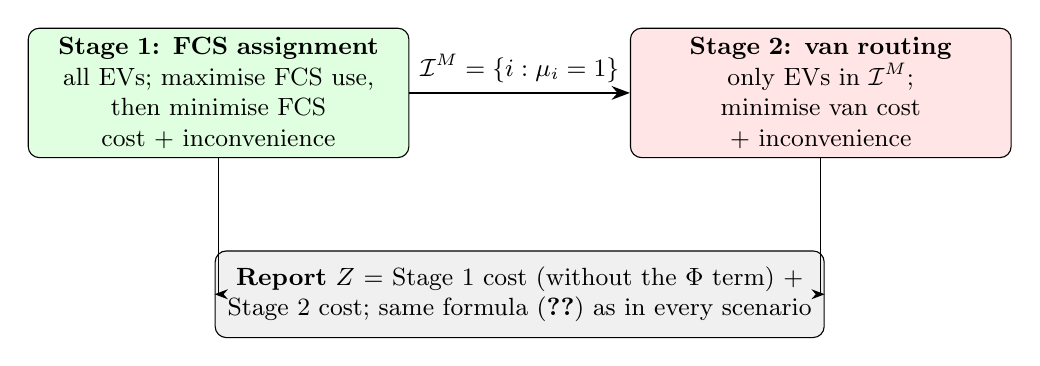
\begin{tikzpicture}[>=Stealth,box/.style={draw,rounded corners,align=center,minimum height=1.1cm,font=\small}]
  \node[box,fill=green!12,text width=4.6cm] (s1) {\textbf{Stage 1: FCS assignment}\\all EVs; maximise FCS use,\\then minimise FCS cost + inconvenience};
  \node[box,fill=red!10,text width=4.6cm,right=2.8cm of s1] (s2) {\textbf{Stage 2: van routing}\\only EVs in $\I^M$;\\minimise van cost + inconvenience};
  \draw[->,thick] (s1) -- node[above,font=\small]{$\I^M=\{i:\mu_i=1\}$} (s2);
  \node[box,fill=black!6,text width=7.5cm,below=2.0cm of $(s1)!0.5!(s2)$] (ev) {\textbf{Report} $Z=$ Stage~1 cost (without the $\Phi$ term) $+$ Stage~2 cost; same formula \eqref{eq:Z} as in every scenario};
  \draw[->] (s1) |- (ev); \draw[->] (s2) |- (ev);
\end{tikzpicture}
\end{center}

Stage~1 does not look at the vans, and Stage~2 cannot change what Stage~1 decided. That is the definition of ``FCS first, then MCS''.

%----------------------------------------------------------------
\subsection{Stage 1: assign EVs to fixed stations}

\textbf{Objective.}
\begin{equation}
\begin{split}
\min\ Z^{(1)}=\;&\underbrace{\Phi\sum_{i\in\I}\mu_i}_{\text{FCS first}}
+\underbrace{c^{EV}\sum_i\sum_{f\in\F_i}d_{if}Y_{if}}_{Z_1}
+\underbrace{Z^F_{\text{energy}}}_{\text{FCS part of }Z_4}\\
&+\underbrace{\sum_i\sum_{f\in\F_i}\rho^F_{if}Y_{if}+\alpha\sum_i w_i(C_i-r_i)+c^L\sum_i w_iL_i}_{\text{FCS customers' inconvenience}}
\end{split}
\label{eq:obj1}
\end{equation}
with $C_i=S_i+\tau^F_iY_i$ in this stage. $\Phi$ is a penalty for handing an EV to the vans. It is chosen larger than anything an extra FCS customer can add to the rest of \eqref{eq:obj1}, e.g.
\[
\Phi > \max_{i}\max_{f\in\F_i}\big(c^{EV}d_{if}+\pi^{\max}E_i+\rho^F_{if}\big)+n\,(\alpha+c^L)\,w_{\max}\,T,
\]
so Stage~1 first \textbf{maximises the number of EVs served at an FCS}, and only among those solutions minimises FCS cost and inconvenience. ($\pi^{\max}$ is the highest grid price.) A numerically safer equivalent is to solve twice: first $\max\sum_iY_i$, then fix that number and minimise the rest.
\ifTOU
Because $Z^F_{\text{energy}}$ uses the peak price, Stage~1 may \emph{start sessions later} to leave the peak, if the price saving beats the extra waiting cost (Section~\ref{sec:expect}).
\fi

\textbf{Constraints.}
\begin{align}
\sum_{g\in\G_i}y_{ig}+\mu_i &= 1 && \forall i\in\I \label{eq:s1assign}\\
S_i &\ge r_i+\sum_{f\in\F_i}t_{if}Y_{if} && \forall i\in\I \label{eq:fcsarr}\\
S_i &\le r_i+T\,(1-\mu_i) && \forall i\in\I \label{eq:s1park}\\
S_j &\ge S_i+\tau^F_i-(T+\tau^F_i)(3-y_{ig}-y_{jg}-o_{ij}) && \forall g,\ (i,j)\in\mathcal{P}_g \label{eq:disj1}\\
S_i &\ge S_j+\tau^F_j-(T+\tau^F_j)(2-y_{ig}-y_{jg}+o_{ij}) && \forall g,\ (i,j)\in\mathcal{P}_g \label{eq:disj2}\\
\sum_i y_{ig_1} &\ge \sum_i y_{ig_2} && \forall f,\ \G_f=\{g_1,g_2\} \label{eq:gunsym}\\
S_i+\tau^F_iY_i &\le T,\qquad L_i\ge S_i+\tau^F_iY_i-l_i && \forall i\in\I \label{eq:s1time}
\end{align}
\ifTOU plus the time-of-use split \eqref{eq:tou1}--\eqref{eq:tou5} of each FCS session (Section~\ref{sec:price}).\fi
\desc{\eqref{eq:s1assign}: every EV either gets one reachable gun or is handed to the vans. An EV that reaches no FCS ($\G_i=\emptyset$) is forced to $\mu_i=1$. \eqref{eq:fcsarr}: an FCS session cannot start before the EV has asked and driven to the station. \eqref{eq:s1park}: for an EV handed to the vans, $S_i$ is parked at $r_i$, so it adds no waiting in Stage~1 (its real start time is decided in Stage~2). \eqref{eq:disj1}--\eqref{eq:disj2}: two EVs on the same gun do not overlap; $o_{ij}$ picks who goes first. With two guns per station this means at most two EVs charge at a station at a time. \eqref{eq:gunsym}: symmetry breaking between the two identical guns (optional). \eqref{eq:s1time}: finished by $T$; lateness.}

\textbf{Optional acceptability rule.} An operator may refuse to send a driver to a station that is ``too inconvenient'', e.g.\ only allow gun $g$ of station $f$ for EV $i$ if $\hat\rho^F_{if}\le\bar\rho$. This only shrinks $\G_i$, so EVs whose stations are all too far go to the vans. Report results with and without it.

\textbf{Output:} $\I^M=\{i:\mu_i=1\}$, the EVs left for the vans; plus each FCS customer's gun and start time.

%----------------------------------------------------------------
\subsection{Stage 2: route the vans to the leftover EVs}

Stage~2 is a vehicle routing problem with time windows, on the EVs in $\I^M$ only. Here $C_i=S_i+\tau^M_i$.

\textbf{Objective.}
\begin{equation}
\begin{split}
\min\ Z^{(2)}=\;&\underbrace{c^M\sum_m\sum_{(i,j)\in\A^M}d_{ij}x_{ijm}}_{Z_2}+\underbrace{\sum_m c^D_mu_m}_{Z_3}+\underbrace{Z^M_{\text{energy}}}_{\text{van part of }Z_4}\\
&+\underbrace{\sum_{i\in\I^M}\sum_m\rho^M_{im}z_{im}+\alpha\sum_{i\in\I^M}w_i(C_i-r_i)+c^L\sum_{i\in\I^M}w_iL_i}_{\text{van customers' inconvenience}}
\end{split}
\label{eq:obj2}
\end{equation}
Since every EV in $\I^M$ must be served by some van, $Z^M_{\text{energy}}$ and the $\rho^M$ term are constants here. They are kept so that $Z^{(2)}$ is the true cost of Stage~2. Waiting and lateness make the vans visit urgent EVs early.

\textbf{Constraints.}
\begin{align}
\sum_{m\in\M}z_{im} &= 1 && \forall i\in\I^M \label{eq:s2assign}\\
\sum_{j:(0,j)\in\A^M}x_{0jm} = \sum_{i:(i,n+1)\in\A^M}x_{i,n+1,m} &= u_m && \forall m \label{eq:depot}\\
\sum_{i:(i,j)\in\A^M}x_{ijm} = \sum_{k:(j,k)\in\A^M}x_{jkm} &= z_{jm} && \forall j\in\I^M,\ m \label{eq:flow}\\
\sum_{i\in\I^M}z_{im} &\le Q_m\,u_m && \forall m \label{eq:cap}\\
\sum_{i\in\I^M}\frac{E_i}{\eta}z_{im}+\beta\sum_{(i,j)\in\A^M}d_{ij}x_{ijm} &\le B_m\,u_m && \forall m \label{eq:batt}
\end{align}
\begin{align}
S_j &\ge \max\{r_j,\ t_{0j}\,x_{0jm}\} && \forall j\in\I^M,\ m \label{eq:depart}\\
S_j &\ge S_i+\tau^M_i+t_{ij}-(T+\tau^M_i+t_{ij})(1-x_{ijm}) && \forall i\neq j,\ m \label{eq:seq}\\
S_i+\tau^M_i+t_{i,n+1} &\le T+(\tau^M_i+t_{i,n+1})(1-x_{i,n+1,m}) && \forall i,\ m \label{eq:return}\\
S_i+\tau^M_i \le T,\quad L_i &\ge S_i+\tau^M_i-l_i && \forall i\in\I^M \label{eq:s2time}\\
u_m &\ge u_{m+1} && m<|\M| \label{eq:vansym}
\end{align}
\desc{\eqref{eq:s2assign}: each leftover EV gets one van. \eqref{eq:depot}: a used van leaves and returns to the depot once. \eqref{eq:flow}: each EV on van $m$ is entered and left exactly once by that van. \eqref{eq:cap}: at most $Q_m$ EVs per van. \eqref{eq:batt}: delivered energy (with transfer losses) plus driving energy fits in the van battery. \eqref{eq:depart}: no start before the request, or before the van can drive there from the depot (written as two linear constraints). \eqref{eq:seq}: if the van goes $i\to j$, it finishes $i$ and drives to $j$ before starting $j$. This gives one EV at a time and removes subtours (MTZ-type). \eqref{eq:return}: back at the depot by $T$. \eqref{eq:s2time}: finished by $T$; lateness. \eqref{eq:vansym}: use identical vans in index order.}

\textbf{If Stage 2 is infeasible} (too many leftover EVs for the fleet by $T$), the sequential policy has \emph{failed} on that instance. For diagnosis, add $s_i\in\{0,1\}$ (``unserved''), replace \eqref{eq:s2assign} by $\sum_mz_{im}+s_i=1$ and add $\Phi^U\sum_is_i$ to \eqref{eq:obj2}. Then report the number of EVs that could not be served. This is a useful comparison with the integrated scenario, which may serve all of them.

%----------------------------------------------------------------
\subsection{Reported value}
\[
Z^{\text{S\scen}}=\big(Z^{(1)*}-\Phi\,|\I^M|\big)+Z^{(2)*},
\]
which is exactly \eqref{eq:Z} evaluated at the combined solution. The stage-1 solution plus the stage-2 solution is a feasible solution of the integrated model (S\ifTOU 4\else 3\fi), so
$Z^{\text{S\ifTOU 4\else 3\fi}}\le Z^{\text{S\scen}}$. The difference is the \emph{value of integration}.

\else
%---------------------------------------------------------------- INT
\subsection{Objective}
\begin{equation}
\min\ Z \quad\text{as in \eqref{eq:Z}, with }Z^F_{\text{energy}}=\ifTOU P^F\textstyle\sum_i\big[\pi^\off(\theta^1_i+\theta^3_i)+\pi^\pk\theta^2_i\big]\else\pi^F\textstyle\sum_iE_iY_i\fi,\quad C_i=S_i+\tau^F_iY_i+\tau^M_iZ_i. \label{eq:objint}
\end{equation}
Written out in full:
\begin{align*}
\min\ Z=\;& c^{EV}\sum_i\sum_{f\in\F_i}d_{if}Y_{if}+c^M\sum_m\sum_{(i,j)\in\A}d_{ij}x_{ijm}+\sum_mc^D_mu_m\\
&+\ifTOU P^F\sum_i\big[\pi^\off(\theta^1_i+\theta^3_i)+\pi^\pk\theta^2_i\big]\else\pi^F\sum_iE_iY_i\fi
+\pi^M\sum_i\sum_m\frac{E_i}{\eta}z_{im}\\
&+\sum_i\sum_{f\in\F_i}\rho^F_{if}Y_{if}+\sum_i\sum_m\rho^M_{im}z_{im}+\alpha\sum_iw_i(C_i-r_i)+c^L\sum_iw_iL_i .
\end{align*}
Every term is linear. One model weighs everything at once: an EV goes to a van exactly when the van's extra km, dispatch and energy cost are outweighed by the effort and waiting it saves the driver\ifTOU, or by the peak-price energy it avoids\fi.

\subsection{Constraints}

\textbf{Assignment.}
\begin{equation}
\sum_{g\in\G_i}y_{ig}+\sum_{m\in\M}z_{im}=1\qquad\forall i\in\I \label{eq:assign}
\end{equation}
\desc{Exactly one resource per EV: one reachable gun or one van. EVs that reach no FCS are forced onto a van.}

\textbf{Fixed stations.}
\begin{align}
S_i &\ge r_i+\sum_{f\in\F_i}t_{if}Y_{if} && \forall i \label{eq:fcsarr}\\
S_j &\ge S_i+\tau^F_i-(T+\tau^F_i)(3-y_{ig}-y_{jg}-o_{ij}) && \forall g,\ (i,j)\in\mathcal{P}_g \label{eq:disj1}\\
S_i &\ge S_j+\tau^F_j-(T+\tau^F_j)(2-y_{ig}-y_{jg}+o_{ij}) && \forall g,\ (i,j)\in\mathcal{P}_g \label{eq:disj2}\\
\sum_iy_{ig_1} &\ge \sum_iy_{ig_2} && \forall f,\ \G_f=\{g_1,g_2\} \label{eq:gunsym}
\end{align}
\desc{\eqref{eq:fcsarr}: an FCS session starts after the request and the drive to the station (for a van customer this is just $S_i\ge r_i$). \eqref{eq:disj1}--\eqref{eq:disj2}: EVs on the same gun do not overlap; $o_{ij}$ chooses the order. \eqref{eq:gunsym}: optional symmetry breaking.}

\textbf{Vans: routes, capacity, battery.}
\begin{align}
\sum_{j:(0,j)\in\A}x_{0jm}=\sum_{i:(i,n+1)\in\A}x_{i,n+1,m} &= u_m && \forall m \label{eq:depot}\\
\sum_{i:(i,j)\in\A}x_{ijm}=\sum_{k:(j,k)\in\A}x_{jkm} &= z_{jm} && \forall j\in\I,\ m \label{eq:flow}\\
\sum_iz_{im} &\le Q_mu_m && \forall m \label{eq:cap}\\
\sum_i\frac{E_i}{\eta}z_{im}+\beta\sum_{(i,j)\in\A}d_{ij}x_{ijm} &\le B_mu_m && \forall m \label{eq:batt}
\end{align}
\desc{\eqref{eq:depot}: a used van leaves and returns once. \eqref{eq:flow}: each EV on van $m$ is visited exactly once by it. \eqref{eq:cap}: at most $Q_m$ EVs. \eqref{eq:batt}: delivered energy (with losses) plus driving energy fits in the battery.}

\textbf{Vans: timing (one EV at a time, no subtours).}
\begin{align}
S_j &\ge t_{0j}\,x_{0jm} && \forall j\in\I,\ m \label{eq:depart}\\
S_j &\ge S_i+\tau^M_i+t_{ij}-(T+\tau^M_i+t_{ij})(1-x_{ijm}) && \forall i\neq j\in\I,\ m \label{eq:seq}\\
S_i+\tau^M_i+t_{i,n+1} &\le T+(\tau^M_i+t_{i,n+1})(1-x_{i,n+1,m}) && \forall i,\ m \label{eq:return}
\end{align}
\desc{\eqref{eq:depart}: the first stop cannot start before the van has driven there. \eqref{eq:seq}: $i\to j$ means finish $i$, drive, then start $j$; start times rise along a route, so no subtour can close. \eqref{eq:return}: back at the depot by $T$.}

\textbf{Horizon and lateness.}
\begin{equation}
C_i\le T,\qquad L_i\ge C_i-l_i\qquad\forall i\in\I \label{eq:time}
\end{equation}
\desc{Every EV is fully charged within the horizon; $L_i$ measures lateness.}

\ifTOU
\textbf{Time-of-use split.} Constraints \eqref{eq:tou1}--\eqref{eq:tou5} of Section~\ref{sec:price}.
\fi

\textbf{Symmetry and domains.}
\begin{equation}
u_m\ge u_{m+1};\qquad y,z,x,u,o\ifTOU,\kappa\fi\in\{0,1\};\qquad S_i,L_i\ifTOU,\theta^p_i\fi\ge0 \label{eq:dom}
\end{equation}
\fi

%=====================================================================
\section{Learning-to-optimise (RL) formulation}\label{sec:rl}

\textbf{Main rule:} the reward of each action is \emph{minus the increase in $Z$ that the action causes}. The rewards over an episode then add up to $-Z$ of the solution the policy builds. RL and MILP results are measured on the same yardstick \eqref{eq:Z}, and the MILP optimum is the benchmark for the RL gap.

\ifSEQ
%---------------------------------------------------------------- RL SEQ
The RL pipeline has the same two stages as the MILP.

\subsection{Stage 1 policy: FCS assignment}
\begin{itemize}[leftmargin=1.4em,itemsep=2pt]
  \item \textbf{Episode / epochs:} EVs are taken in order of request time $r_i$ (ties: higher $w_i$ first). One decision per EV.
  \item \textbf{State:} features of the current EV $k$ ($E_k,r_k,l_k,w_k,R_k$, location); for each gun $g$ the time $F_g$ it becomes free; summary features of the EVs still to come (count and positions near each station)\ifTOU; the current price and the time until $T_1$ and $T_2$\fi.
  \item \textbf{Action:} a gun $g\in\G_k$, or ``hand to vans''. \textbf{FCS-first mask:} ``hand to vans'' is allowed \emph{only} if no gun can finish EV $k$ by $T$ (or, with the optional rule, if all remaining guns have $\hat\rho^F_{kf}>\bar\rho$).
  \ifTOU\item \textbf{Optional timing action:} ``gun $g$, start after the peak'', i.e.\ $S_k=\max\{\text{earliest},T_2\}$, allowed only if the session still ends by $T$.\fi
  \item \textbf{Transition:} $S_k=\max\{r_k+t_{kf},F_g\}$ (or later, for the timing action); $F_g\leftarrow S_k+\tau^F_k$.
  \item \textbf{Reward:} $-\Big[c^{EV}d_{kf}+\text{energy}_k+\rho^F_{kf}+\alpha w_k(S_k+\tau^F_k-r_k)+c^Lw_k(S_k+\tau^F_k-l_k)^+\Big]$, where energy$_k$ = \ifTOU$P^F\big[\pi^\off\cdot(\text{off-peak hours of }[S_k,S_k+\tau^F_k])+\pi^\pk\cdot(\text{peak hours})\big]$, computed exactly in the simulator\else$\pi^FE_k$\fi. Handing an EV to the vans gives reward $0$ here; its cost is counted in Stage~2.
\end{itemize}
Note: a simple baseline for Stage~1 is the greedy rule ``gun with the largest one-step reward''. What RL can learn on top of this is, for example, to keep a nearby gun free for an urgent EV that arrives later.

\subsection{Stage 2 policy: van routing over $\I^M$}
\begin{itemize}[leftmargin=1.4em,itemsep=2pt]
  \item \textbf{Epochs:} whenever a van becomes free (the earliest-free van decides first).
  \item \textbf{State:} for each van: position, time free, remaining battery $b_m$, EVs served so far, dispatched or not; for each unserved EV in $\I^M$: location, $E_i,r_i,l_i,w_i$; current time.
  \item \textbf{Action:} the next EV $j$ for this van, or ``return to depot'' (ends the route). Mask: $j$ must be feasible: battery covers $E_j/\eta$ plus driving to $j$ and back to the depot, the count stays $\le Q_m$, and $j$ can be finished with the van back at the depot by $T$.
  \item \textbf{Transition:} $S_j=\max\{r_j,\ \text{time free}+t_{\text{pos},j}\}$; the van moves to $j$ and is free at $S_j+\tau^M_j$; $b_m$ falls by $E_j/\eta+\beta d_{\text{pos},j}$.
  \item \textbf{Reward:} serving $j$: $-\Big[c^Md_{\text{pos},j}+c^D_m[\text{first stop}]+\pi^M\frac{E_j}{\eta}+\rho^M_{jm}+\alpha w_j(S_j+\tau^M_j-r_j)+c^Lw_j(S_j+\tau^M_j-l_j)^+\Big]$; returning: $-c^Md_{\text{pos},0}$. EVs still unserved at the end: $-\Phi^U$ each.
  \item \textbf{Policy:} an attention-based routing policy (e.g.\ Kool et al., 2019, ``Attention, Learn to Solve Routing Problems!'') trained with REINFORCE or PPO. Baseline: nearest-feasible-EV heuristic.
\end{itemize}
Episode return of Stage~1 + Stage~2 $=-Z^{\text{S\scen}}$.

\else
%---------------------------------------------------------------- RL INT
One policy decides both who serves each EV and the van routes.
\begin{itemize}[leftmargin=1.4em,itemsep=2pt]
  \item \textbf{Episode / epochs:} EVs are taken in order of request time $r_i$ (ties: higher $w_i$ first). One decision per EV.
  \item \textbf{State:} (i) the current EV $k$: location, $E_k,r_k,l_k,w_k,R_k$, reachable stations; (ii) each gun $g$: time $F_g$ it becomes free; (iii) each van $m$: current end-of-route position, time free, remaining battery $b_m$, EVs served, dispatched or not; (iv) embeddings of the not-yet-assigned EVs (for look-ahead)\ifTOU; (v) current price, time until $T_1$ and $T_2$\fi.
  \item \textbf{Action:} $a\in\G_k\cup\M$: a gun, or a van (EV $k$ is appended to the end of that van's route). \textbf{Mask} infeasible actions: a gun that cannot finish $k$ by $T$; a van without enough battery for $E_k/\eta$ plus the drive to $k$ and back to the depot, with $Q_m$ reached, or unable to finish $k$ and return by $T$.
  \ifTOU\item \textbf{Optional timing action:} ``gun $g$, start after the peak'' ($S_k=\max\{\text{earliest},T_2\}$, if it still ends by $T$).\fi
  \item \textbf{Transition:} gun: $S_k=\max\{r_k+t_{kf},F_g\}$, $F_g\leftarrow S_k+\tau^F_k$. Van: $S_k=\max\{r_k,\ \text{free}_m+t_{\text{pos}_m,k}\}$, then the van moves to $k$, $\text{free}_m\leftarrow S_k+\tau^M_k$, $b_m\mathrel{-}=E_k/\eta+\beta d_{\text{pos}_m,k}$.
  \item \textbf{Reward} $=-\Delta Z$:
  \begin{align*}
  \text{gun } g\text{ at }f:&\quad -\Big[c^{EV}d_{kf}+\text{energy}^F_k+\rho^F_{kf}+\alpha w_k(C_k-r_k)+c^Lw_k(C_k-l_k)^+\Big]\\
  \text{van } m:&\quad -\Big[c^M\big(d_{\text{pos}_m,k}+d_{k,0}-d_{\text{pos}_m,0}\big)+c^D_m[\text{first use}]+\pi^M\tfrac{E_k}{\eta}\\
  &\qquad\quad+\rho^M_{km}+\alpha w_k(C_k-r_k)+c^Lw_k(C_k-l_k)^+\Big]
  \end{align*}
  The van distance term is the \emph{change} in route length when $k$ is inserted before the return to the depot, so the sum over the episode equals the total route length (the return legs telescope). energy$^F_k$ = \ifTOU$P^F\big[\pi^\off\cdot(\text{off-peak hours})+\pi^\pk\cdot(\text{peak hours of }[S_k,C_k])\big]$, computed exactly by the simulator; no linearisation is needed in RL\else$\pi^FE_k$\fi.
  \item \textbf{Dead end:} if every action is masked, EV $k$ is unserved: reward $-\Phi^U$, and the episode continues. Report the count.
  \item \textbf{Policy:} masked categorical policy over guns and vans, encoder with attention over EVs, guns and vans; trained with PPO. Natural baseline: greedy, i.e.\ choose the action with the largest one-step reward. That is the pairwise rule ``smallest $\hat\rho$ + cost'' from Section~\ref{sec:inc}.
\end{itemize}
Restriction to note: vans serve EVs in assignment order (append only). A variant that inserts $k$ at the cheapest position of a route is more flexible but has a larger action space.
\fi

\textbf{Reward scaling.} For stable training divide every reward by a constant, e.g.\ the greedy baseline's average $Z$ on the training instances. This does not change the optimal policy.

%=====================================================================
\section{What to expect and what to report}\label{sec:expect}

\ifnum\scen=1
\begin{itemize}[leftmargin=1.4em,itemsep=2pt]
  \item Vans serve only EVs that reach no station, or that the stations cannot finish by $T$. If stations have spare capacity, very few vans are dispatched.
  \item Inconvenience is high for EVs far from the nearest station (worked example: Rs\,682 at the FCS, against Rs\,458 if a van had been allowed).
  \item With too few vans Stage~2 becomes infeasible (unserved EVs), even when the integrated model S3 could serve everyone. Report the smallest $|\M|$ at which S1 is feasible and compare it with S3.
\end{itemize}
\fi
\ifnum\scen=2
\begin{itemize}[leftmargin=1.4em,itemsep=2pt]
  \item \textbf{When does Stage~1 delay a session to avoid the peak?} Moving one hour of charging out of the peak saves $(\pi^\pk-\pi^\off)P^F=3\times22=$ Rs\,66, but delays completion by up to an hour, which costs $\alpha w_i\ge$ Rs\,200. So with the default values Stage~1 almost never delays. It mostly pays the higher price, and S2 costs roughly S1 plus the peak surcharge. Sessions start later only if $\alpha$ is small (try $\lambda<0.33$ in the sensitivity analysis).
  \item The van assignment is the same as in S1 unless Stage~1's timing changes which EVs fit at the stations. Stage~1 cannot use vans to escape the peak price.
  \item Extra KPI: \textbf{grid energy drawn at FCS during the peak}, $P^F\sum_i\theta^2_i$ (kWh). Compare with S4.
\end{itemize}
\fi
\ifnum\scen=3
\begin{itemize}[leftmargin=1.4em,itemsep=2pt]
  \item Vans take EVs for which the saved inconvenience exceeds the extra van cost (worked example: van chosen, saving Rs\,224). Expect vans to serve EVs that are far from every station, have low range (high $w_i$), or have early deadlines, while EVs near a station still use it.
  \item \textbf{Value of integration under flat price:} $Z^{\text{S1}}-Z^{\text{S3}}\ge0$. Report it per component ($Z_1,\dots,Z_5$): typically operating cost rises a little and inconvenience falls a lot.
  \item Vary $|\M|$ (0, 1, 2, \dots): the first few vans lower $Z$ sharply, then the effect levels off. That curve shows the scenarios where mobile chargers help most.
\end{itemize}
\fi
\ifnum\scen=4
\begin{itemize}[leftmargin=1.4em,itemsep=2pt]
  \item During the peak a van kWh costs about the same as an FCS kWh (Rs\,10.0 each), so the vans' energy disadvantage disappears and vans also absorb \emph{peak-hour} demand that would otherwise be charged on the grid at peak price.
  \item Expect more van usage than in S3, concentrated on requests in $[T_1,T_2]$, and lower grid energy at the stations during the peak, $P^F\sum_i\theta^2_i$, than in S2.
  \item \textbf{Value of integration under peak pricing:} $Z^{\text{S2}}-Z^{\text{S4}}$. It should be larger than $Z^{\text{S1}}-Z^{\text{S3}}$, because integration now also allows price arbitrage.
  \item \textbf{Peak pricing with full flexibility:} $Z^{\text{S4}}-Z^{\text{S3}}$ should be smaller than $Z^{\text{S2}}-Z^{\text{S1}}$: vans cushion the price increase.
\end{itemize}
\fi

\textbf{Cross-scenario comparison table} (fill in from the four runs):
\begin{center}
\renewcommand{\arraystretch}{1.2}
\begin{tabular}{@{}lll@{}}
\toprule
\textbf{Comparison} & \textbf{Measures} & \textbf{Expected sign} \\
\midrule
S1 $-$ S3 & value of integration, flat price & $\ge0$ \\
S2 $-$ S4 & value of integration, peak price & $\ge0$, larger than S1 $-$ S3 \\
S2 $-$ S1 & cost of peak pricing, FCS-first operator & $>0$ \\
S4 $-$ S3 & cost of peak pricing, flexible operator & $>0$, smaller than S2 $-$ S1 \\
\bottomrule
\end{tabular}
\end{center}
Report for each: $Z$ and its components, number of vans used, EVs per resource, mean and maximum inconvenience per EV, total lateness, peak-hour grid energy, solve time, and (for RL) the gap to the MILP optimum.

%=====================================================================
\appendix
\section{Illustrative parameter values}\label{app:values}

These are starting values for experiments, not data. All are meant to be varied in the analysis. Values in Rs.

\begin{center}
\renewcommand{\arraystretch}{1.15}
\begin{tabular}{@{}llp{6.2cm}@{}}
\toprule
\textbf{Parameter} & \textbf{Value} & \textbf{Note} \\
\midrule
$T$, $[T_1,T_2]$ & 7 h, $[2,6]$ & 16:00--23:00, peak 18:00--22:00 \\
$P^F$, $P^M$ & 22 kW, 30 kW & \\
$v$, $\beta$, $\eta$ & 25 km/h, 0.25 kWh/km, 0.9 & \\
$B_m$, $Q_m$, $|\M|$ & 150 kWh, 6, 2--6 & \\
$c^{EV}$, $c^M$, $c^D_m$ & Rs\,4/km, Rs\,15/km, Rs\,1500 & van km includes driver time \\
$\pi^F$ (flat) & Rs\,8.7/kWh & equals the time-average of the ToU tariff over $[0,T]$ \\
$\pi^\off$, $\pi^\pk$ (ToU) & Rs\,7/kWh, Rs\,10/kWh & $(3\times7+4\times10)/7=8.7$ \\
$c^{bat}$ & Rs\,2/kWh & van battery wear \\
$\pi^M$ & Rs\,10.7 (flat) / Rs\,9.0 (ToU) & $=\pi^F+c^{bat}$ / $=\pi^\off+c^{bat}$ \\
$\alpha$, $\alpha^D$ & Rs\,200/h, Rs\,100/h & value of time; extra for attended time \\
$h^F$, $h^M$, $\varphi$ & Rs\,50, Rs\,10, Rs\,100 & trip hassle, hand-over, range stress \\
$c^L$ & Rs\,300/h & lateness \\
$w_i$ & $1+2(1-R_i/R_{\max})$, $R_i\sim U[3,40]$ km & priority from remaining range \\
\bottomrule
\end{tabular}
\end{center}

The flat price is set to the time-average of the peak tariff. The price \emph{level} is then the same in both pricing cases, and only the price \emph{shape} differs. Without this, part of S1 vs S2 would just reflect a different average price.

\end{document}
"
%    pdflatex -jobname=scenario4_peak_integrated   "\def\scen{4}% =====================================================================
%  One source, four PDFs.  Build with build.sh (or by hand):
%    pdflatex -jobname=scenario1_flat_sequential   "\def\scen{1}\input{scenario_master}"
%    pdflatex -jobname=scenario2_peak_sequential   "\def\scen{2}\input{scenario_master}"
%    pdflatex -jobname=scenario3_flat_integrated   "\def\scen{3}\input{scenario_master}"
%    pdflatex -jobname=scenario4_peak_integrated   "\def\scen{4}\input{scenario_master}"
%  (run each twice for cross-references)
% =====================================================================
\documentclass[11pt,a4paper]{article}
\usepackage[margin=2.2cm]{geometry}
\usepackage{amsmath,amssymb,amsfonts}
\usepackage{booktabs,array,tabularx}
\usepackage{enumitem}
\usepackage[table]{xcolor}
\usepackage{tikz}
\usetikzlibrary{arrows.meta,positioning,calc}
\usepackage[colorlinks=true,linkcolor=blue!50!black,urlcolor=blue!50!black]{hyperref}
\usepackage{titlesec}
\titleformat{\section}{\large\bfseries}{\thesection}{0.8em}{}
\titleformat{\subsection}{\normalsize\bfseries}{\thesubsection}{0.8em}{}
\setlength{\parindent}{0pt}
\setlength{\parskip}{5pt}

% ---------------- scenario switches ----------------
\ifdefined\scen\else\def\scen{1}\fi
\newif\ifTOU \TOUfalse   % true = time-of-use (peak) price
\newif\ifSEQ \SEQfalse   % true = FCS first, then MCS
\ifnum\scen=1 \SEQtrue \fi
\ifnum\scen=2 \TOUtrue \SEQtrue \fi
\ifnum\scen=4 \TOUtrue \fi

\newcommand{\pricename}{\ifTOU time-of-use price (dearer evening peak)\else single (flat) price all day\fi}
\newcommand{\structname}{\ifSEQ FCS first, then MCS (sequential)\else FCS and MCS together (integrated)\fi}

% ---------------- notation ----------------
\newcommand{\I}{\mathcal{I}}
\newcommand{\F}{\mathcal{F}}
\newcommand{\G}{\mathcal{G}}
\newcommand{\M}{\mathcal{M}}
\newcommand{\N}{\mathcal{N}}
\newcommand{\A}{\mathcal{A}}
\newcommand{\Rs}{\text{Rs}\,}
\newcommand{\pk}{\mathrm{pk}}
\newcommand{\off}{\mathrm{off}}
\newcommand{\desc}[1]{\par\vspace{-2pt}{\small\color{black!75}\textit{Meaning:} #1}\par\vspace{4pt}}
\newcommand{\cell}[2]{\ifnum\scen=#1\cellcolor{blue!18}\textbf{S#1 (this document)}\\\textbf{#2}\else S#1\\#2\fi}

\title{\textbf{EV Charging Network Optimisation}\\[4pt]
\large Scenario \scen: \pricename\ $+$ \structname\\[2pt]
\normalsize MILP and RL formulation}
\author{CP 320 OR for Mobility Management, course project}
\date{2 October 2026}

\begin{document}
\maketitle

%=====================================================================
\section{Where this scenario sits}

The project studies four scenarios: two ways of pricing grid electricity, times two ways of making the decisions.

\begin{center}
\renewcommand{\arraystretch}{1.5}
\begin{tabular}{>{\raggedright\arraybackslash}p{4.2cm}|>{\centering\arraybackslash}p{4.6cm}|>{\centering\arraybackslash}p{4.6cm}}
 & \textbf{Flat price all day} & \textbf{Time-of-use (peak) price} \\ \hline
\textbf{Sequential:} FCS first, leftover EVs to MCS &
\begin{tabular}[c]{@{}c@{}}\cell{1}{flat + sequential}\end{tabular} &
\begin{tabular}[c]{@{}c@{}}\cell{2}{peak + sequential}\end{tabular} \\ \hline
\textbf{Integrated:} FCS and MCS decided together &
\begin{tabular}[c]{@{}c@{}}\cell{3}{flat + integrated}\end{tabular} &
\begin{tabular}[c]{@{}c@{}}\cell{4}{peak + integrated}\end{tabular} \\
\end{tabular}
\end{center}

\textbf{The four scenarios do not have four different objectives.} They share \emph{one} cost yardstick $Z$ (Section~\ref{sec:obj}): the same cost terms and the same customer inconvenience (Section~\ref{sec:inc}). Only two things change:
\begin{itemize}[leftmargin=1.4em,itemsep=1pt]
  \item \textbf{Pricing} changes the formula for one term, the FCS energy cost (Section~\ref{sec:price}).
  \item \textbf{Decision structure} changes \emph{how} $Z$ is minimised: in one model (integrated), or in two stages (sequential), where each stage minimises its own part of $Z$.
\end{itemize}
Because the yardstick is the same, the four optimal values can be compared directly. The differences measure the \emph{value of integration} (S1$\to$S3, S2$\to$S4) and the \emph{effect of peak pricing} (S1$\to$S2, S3$\to$S4).

\ifnum\scen=1
\textbf{This scenario (S1)} is the baseline, the ``status quo''. Electricity costs the same at every hour, every EV that can be charged at a fixed station is sent there, and vans only take what is left over.
\fi
\ifnum\scen=2
\textbf{This scenario (S2)} keeps the FCS-first rule of S1, but grid electricity is dearer during the evening peak. Stage~1 can react to the price only by \emph{rescheduling} FCS sessions. It cannot hand a peak-hour EV to a van.
\fi
\ifnum\scen=3
\textbf{This scenario (S3)} keeps the flat price of S1, but the operator decides FCS and MCS service \emph{together}. An EV can be sent to a van even when a fixed station could take it, whenever that lowers total cost plus inconvenience.
\fi
\ifnum\scen=4
\textbf{This scenario (S4)} is the most flexible one: peak pricing at fixed stations, and FCS and MCS decided together. Van energy was bought off-peak, so vans can also be used to keep charging \emph{out of the expensive peak}.
\fi

%=====================================================================
\section{Setting and assumptions}\label{sec:setting}

\textbf{Time.} The planning horizon is $[0,T]$ with $T=7$\,h (16:00--23:00). It contains the evening peak window $[T_1,T_2]=[2,6]$ (18:00--22:00). The horizon is the same in all four scenarios. It is wider than the peak itself so that, under peak pricing, there is cheaper time on both sides of the peak.\ifTOU\else\ In this scenario the price is flat, so the window plays no role in the model.\fi

\textbf{Assumptions} (the same as MILP v3, plus two about energy):
\begin{enumerate}[leftmargin=1.6em,itemsep=1pt]
  \item Static, continuous time. All requests in the horizon are known at time $0$, and request $i$ becomes active at $r_i$.
  \item An EV served by an FCS drives there itself on its own battery (only to stations within its range $R_i$). The driver stays with the car while it waits for a free gun and while it charges.
  \item An EV served by an MCS stays parked where it is, and the driver is free in the meantime.
  \item Each FCS gun and each van charges one EV at a time, without interruption, at constant power.
  \item A van's battery covers both its driving and the energy it delivers. \textbf{The van battery is charged at the depot before the horizon starts}\ifTOU, i.e.\ at the off-peak price\fi, and is not recharged during the horizon.
  \item Every EV must be fully charged by $T$ (hard). Finishing after the driver's desired time $l_i$ is allowed but penalised.
\end{enumerate}

%=====================================================================
\section{Notation}\label{sec:notation}

\subsection*{Sets}
\begin{tabularx}{\textwidth}{@{}lX@{}}
\toprule
$\I=\{1,\dots,n\}$ & EV charging requests \\
$\F$; $\G_f$ ($|\G_f|=2$); $\G=\bigcup_f\G_f$ & fixed charging stations; guns of FCS $f$; all guns ($f(g)$ = station of gun $g$) \\
$\F_i=\{f: d_{if}\le R_i\}$, $\G_i=\bigcup_{f\in\F_i}\G_f$ & stations / guns EV $i$ can reach on its remaining range \\
$\M$ & mobile charging vans (MCS) \\
$0,\ n+1$ & depot as start node / end node (same place) \\
$\N=\{0\}\cup\I\cup\{n+1\}$, $\A$ & routing nodes; allowed van arcs $(i,j)$, $i\in\{0\}\cup\I$, $j\in\I\cup\{n+1\}$, $i\neq j$ \\
$\mathcal{P}_g=\{(i,j): i<j,\ g\in\G_i\cap\G_j\}$ & pairs of EVs that could share gun $g$ \\
\ifSEQ
$\I^M\subseteq\I$ & EVs handed to the vans by Stage~1 (an \emph{output} of Stage~1, a fixed input to Stage~2) \\
$\N^M$, $\A^M$ & routing nodes / arcs restricted to $\I^M$ \\
\fi
\bottomrule
\end{tabularx}

\subsection*{Parameters}
\begin{tabularx}{\textwidth}{@{}lX@{}}
\toprule
$E_i,\ r_i,\ l_i,\ R_i$ & energy demand (kWh), request time, desired completion time (h), remaining range (km) \\
$w_i\ge1$ & priority of EV $i$; $w_i=1+\kappa(1-R_i/R_{\max})$, so low-range EVs weigh more \\
$P^F,\ P^M$ & charging power of an FCS gun (22\,kW) / of a van (e.g.\ 30\,kW) \\
$\tau^F_i=E_i/P^F,\ \tau^M_i=E_i/P^M$ & charging time of EV $i$ at an FCS / by a van (h) \\
$d_{if},t_{if}$;\ $d_{ij},t_{ij}$ & distance (km) and time (h): EV$\to$FCS; between routing nodes ($t=d/v$) \\
$B_m,\ Q_m,\ \beta,\ \eta$ & van battery (kWh), max EVs per van, van consumption (kWh/km), transfer efficiency \\
$c^{EV},\ c^M,\ c^D_m$ & cost per km of EV driving, per km of van driving; fixed dispatch cost of van $m$ \\
\ifTOU
$\pi^\off,\ \pi^\pk$ & grid price (Rs/kWh) off-peak / in $[T_1,T_2]$, with $\pi^\pk\ge\pi^\off$ \\
\else
$\pi^F$ & grid price (Rs/kWh), the same at every hour \\
\fi
$c^{bat}$ & van battery wear per kWh cycled \\
$\pi^M$ & cost of 1 kWh taken from a van battery: $\pi^M=\ifTOU\pi^\off\else\pi^F\fi+c^{bat}$ (Section~\ref{sec:price}) \\
$\alpha,\ \alpha^D,\ h^F,\ h^M,\ \varphi,\ c^L$ & inconvenience coefficients (Section~\ref{sec:inc}) \\
\bottomrule
\end{tabularx}

\subsection*{Decision variables}
\begin{tabularx}{\textwidth}{@{}llX@{}}
\toprule
$y_{ig}$ & $\{0,1\}$ & EV $i$ charged at gun $g\in\G_i$ \\
$z_{im}$ & $\{0,1\}$ & EV $i$ served by van $m$ \\
$x_{ijm}$ & $\{0,1\}$ & van $m$ drives arc $(i,j)$ \\
$u_m$ & $\{0,1\}$ & van $m$ is dispatched \\
$o_{ij}$ & $\{0,1\}$ & for EVs $i<j$ that could share a gun: 1 if $i$ is charged before $j$ \\
\ifSEQ
$\mu_i$ & $\{0,1\}$ & Stage~1 only: EV $i$ is handed to the van fleet \\
\fi
\ifTOU
$\theta^1_i,\theta^2_i,\theta^3_i$ & $\ge0$ & hours of EV $i$'s FCS session before / inside / after the peak \\
$\kappa^1_i,\kappa^3_i$ & $\{0,1\}$ & EV $i$'s FCS session starts before $T_1$ / ends after $T_2$ \\
\fi
$S_i$ & $\ge0$ & time charging of EV $i$ starts (h), on whichever resource \\
$L_i$ & $\ge0$ & lateness of EV $i$ beyond $l_i$ (h) \\
\bottomrule
\end{tabularx}

\textbf{Short-hands} (linear expressions, not new variables):
\[
Y_{if}=\sum_{g\in\G_f}y_{ig},\qquad Y_i=\sum_{g\in\G_i}y_{ig}\ (\text{EV $i$ uses an FCS}),\qquad Z_i=\sum_{m\in\M}z_{im}\ (\text{EV $i$ uses a van}),
\]
\[
C_i=S_i+\tau^F_i\,Y_i+\tau^M_i\,Z_i \quad\text{(time EV $i$ is fully charged).}
\]

%=====================================================================
\section{Customer inconvenience}\label{sec:inc}

This section is \textbf{identical in all four scenario documents}. Inconvenience is a property of the customer, not of the price or of the planning method.

\subsection{What we mean by inconvenience}

Inconvenience is \emph{what the driver loses} from the moment they ask for a charge ($r_i$) until the car is fully charged ($C_i$), \emph{converted into rupees} so it can be added to the operator's costs. A driver loses three different things:

\begin{enumerate}[leftmargin=1.6em,itemsep=2pt]
  \item \textbf{Waiting:} the car is not ready. This lasts $C_i-r_i$ hours and affects \emph{every} driver, FCS or MCS.
  \item \textbf{Effort:} only an FCS customer has to drive to the station and sit there while the car charges. An MCS customer stays at home or at work and does something else. Driving to a far station also uses scarce battery range, which causes stress (``range anxiety'').
  \item \textbf{A missed deadline:} the car is still not ready at the time $l_i$ the driver needs it.
\end{enumerate}

Each loss gets a price in Rs per hour (or per event). All of them are multiplied by the priority $w_i$: an hour of delay for an EV with 5\,km of range left counts more than for one with 40\,km.

\subsection{The three components}

\begin{center}
\renewcommand{\arraystretch}{1.3}
\begin{tabularx}{\textwidth}{@{}>{\raggedright\arraybackslash}p{2.6cm}>{\raggedright\arraybackslash}X>{\raggedright\arraybackslash}X>{\raggedright\arraybackslash}p{3.0cm}@{}}
\toprule
\textbf{Component} & \textbf{EV $i$ at FCS $f$} & \textbf{EV $i$ by a van} & \textbf{Known when?} \\
\midrule
Effort & $w_i\big[\alpha^D(t_{if}+\tau^F_i)+h^F+\varphi\,d_{if}/R_i\big]$: driving and sitting at the station, a fixed trip hassle, range stress & $w_i\,h^M$: being reachable and handing over the car & \textbf{Static:} known as soon as the resource is chosen \\
Waiting & $w_i\,\alpha\,(C_i-r_i)$ = drive + \emph{queue at the gun} + charge & $w_i\,\alpha\,(C_i-r_i)$ = \emph{wait for the van} + charge & \textbf{Dynamic:} depends on the queue / van route \\
Missed deadline & $w_i\,c^L\,L_i$, $L_i=\max\{0,C_i-l_i\}$ & same & Dynamic \\
\bottomrule
\end{tabularx}
\end{center}

\textbf{Coefficients.}
$\alpha$ (Rs/h) is the value of an hour the car is not ready.
$\alpha^D$ (Rs/h) is the \emph{extra} value of an hour the driver must personally spend driving or sitting at the station: an hour at the station costs $\alpha+\alpha^D$, an hour waiting at home for a van costs only $\alpha$.
$h^F,h^M$ (Rs) are fixed hassle costs of one trip to a station / one van hand-over.
$\varphi$ (Rs) is the range-stress cost of a trip that uses the \emph{whole} remaining range ($d_{if}/R_i\le1$ is the fraction used).
$c^L$ (Rs/h) is the cost per hour late.

\subsection{Pairwise form: inconvenience of a (customer, resource) pair}

The natural first idea is: \emph{for every pair (EV $i$, FCS $f$) and every pair (EV $i$, van $m$) there is an inconvenience number, and the operator picks the pair with the lowest cost plus inconvenience.} The static part fits this idea exactly:
\[
\boxed{\;\rho^F_{if}=w_i\Big[\alpha^D\,(t_{if}+\tau^F_i)+h^F+\varphi\,\frac{d_{if}}{R_i}\Big]\qquad
\rho^M_{im}=w_i\,h^M\;}
\]
These are \textbf{parameters}, computed before solving, one number per (EV, FCS) pair and per (EV, van) pair. In the objective they appear linearly: $\sum_i\sum_f\rho^F_{if}Y_{if}+\sum_i\sum_m\rho^M_{im}z_{im}$.

Note that $\rho^M_{im}$ does not depend on $m$. Vans are identical and all start at the same depot, so the driver does not care \emph{which} van comes, only \emph{when} it comes. That ``when'' is the waiting part.

\subsection{Why waiting cannot be a fixed pairwise number}

It is tempting to also write the waiting as a pairwise number, e.g.\ ``the van needs 5 minutes to reach EV $i$''. But that depends on \emph{where the van is coming from}, which depends on the route the model is still choosing: if EV $i$ is the 4th stop of a van, the wait is the time for three charging sessions plus four drives. Likewise, waiting at an FCS depends on how many EVs are queued at that gun. So waiting is not known before solving. It is a function of decision variables:
\[
\text{waiting cost of EV } i \;=\; w_i\,\alpha\,(C_i-r_i),\qquad C_i=S_i+\tau^F_iY_i+\tau^M_iZ_i .
\]
This is \textbf{linear} in the variables ($S_i$, $y$, $z$), so it fits in a MILP directly. The constraints of Section~\ref{sec:milp} make $S_i$ equal to the true start time, including driving, queueing at the gun and the van's route. The term $\sum_i w_i\alpha r_i$ is a constant and may be dropped when solving.

\textbf{Pairwise \emph{estimate}} (used for intuition, by the RL policy and in heuristics): if there is no queue and the van comes straight to $i$,
\[
\hat\rho^{F}_{if}=\rho^F_{if}+w_i\alpha\,(t_{if}+\tau^F_i),\qquad
\hat\rho^{M}_{im}=\rho^M_{im}+w_i\alpha\,(t^{\text{van}}_{m\to i}+\tau^M_i),
\]
where $t^{\text{van}}_{m\to i}$ is the time until van $m$ can reach $i$ from where it currently is. In the RL formulation (Section~\ref{sec:rl}) the van's position \emph{is} known at each decision, so there this estimate becomes exact.

\subsection{Total inconvenience and how it enters the objective}

\begin{equation}
\boxed{\;
Z_{\text{inc}}=\underbrace{\sum_{i\in\I}\sum_{f\in\F_i}\rho^F_{if}Y_{if}+\sum_{i\in\I}\sum_{m\in\M}\rho^M_{im}z_{im}}_{\text{effort (static, pairwise)}}
+\underbrace{\alpha\sum_{i\in\I}w_i\,(C_i-r_i)}_{\text{waiting (dynamic)}}
+\underbrace{c^L\sum_{i\in\I}w_i\,L_i}_{\text{missed deadline}}
\;}\label{eq:inc}
\end{equation}
All three parts are in rupees, so $Z_{\text{inc}}$ is simply added to the operating costs. Nothing has to be normalised.

\subsection{Worked example: your ``10 km to the FCS vs.\ van in 5 minutes'' case}

EV $i$: $E_i=20$\,kWh, $R_i=40$\,km (so $w_i=1$); nearest free FCS $d_{if}=10$\,km away, $t_{if}=0.4$\,h at 25\,km/h; a van finishing next door can reach it in 5\,min ($0.083$\,h), adding about 4\,km to its route. $\tau^F_i=20/22=0.909$\,h, $\tau^M_i=20/30=0.667$\,h. Coefficients from Appendix~\ref{app:values}, flat price.

\begin{center}
\renewcommand{\arraystretch}{1.25}
\begin{tabular}{@{}lrr@{}}
\toprule
 & \textbf{FCS} & \textbf{Van} \\
\midrule
Driving (EV / extra van km) & $4\times10=40.0$ & $15\times4=60.0$ \\
Energy & $8.7\times20=174.0$ & $10.7\times20/0.9=237.8$ \\
\textbf{Operating cost only} & \textbf{214.0} & \textbf{297.8} \\
\midrule
Effort $\rho$ & $100(0.4+0.909)+50+100\cdot\tfrac{10}{40}=205.9$ & $10.0$ \\
Waiting $\alpha(C_i-r_i)$ & $200\times1.309=261.8$ & $200\times0.75=150.0$ \\
\textbf{Cost + inconvenience} & \textbf{681.7} & \textbf{457.8} \\
\bottomrule
\end{tabular}
\end{center}

On operating cost alone the FCS is cheaper, so a cost-only model would \emph{always} send this driver 10\,km away. With inconvenience included the van is better by about Rs\,224, and the integrated model chooses $z_{im}=1$, as you expected. If the FCS were only 1\,km away, the FCS would win both comparisons. The inconvenience term is what makes the model choose between ``cheap for the operator'' and ``convenient for the driver'', rather than following a fixed rule.

\subsection{Relation to a single penalty $\rho_i$ per EV}

The first draft used a penalty $\rho_i$ that is charged whenever EV $i$ goes to \emph{any} FCS: $\sum_i\sum_f\rho_iy_{if}$. Because $\sum_f y_{if}=1-\sum_m z_{im}$, this only says ``a van is worth $\rho_i$ more to EV $i$'', and that holds whether the station is 1\,km or 15\,km away, and whether the van arrives in 5 minutes or in 3 hours. The form above fixes both problems: $\rho^F_{if}$ grows with the distance to \emph{that} station, and the waiting term grows with how late the van or the free gun actually is. The old model is the special case $\alpha=\alpha^D=\varphi=c^L=0$, $h^F=\rho_i$.

\subsection{Choosing the coefficients}
\begin{itemize}[leftmargin=1.4em,itemsep=2pt]
  \item Use a value of time for $\alpha$ (e.g.\ Rs\,150--300/h for urban car users), and set $\alpha^D\approx0.5\alpha$: sitting at a station is worse than waiting at home.
  \item Keep $c^L>\alpha$, so missing the deadline is worse than ordinary waiting.
  \item \textbf{Sensitivity analysis:} multiply all inconvenience coefficients by a factor $\lambda\in\{0,0.25,0.5,1,2,4\}$ and plot operating cost against total inconvenience. $\lambda=0$ is the pure cost-minimising operator, and large $\lambda$ is a customer-first operator. This trade-off curve is a strong result for the ``Analysis'' part of the project.
\end{itemize}

\subsection{What inconvenience does in \emph{this} scenario}
\ifSEQ
In a sequential scenario inconvenience \textbf{cannot move an EV from an FCS to a van}: Stage~1 sends every EV that \emph{can} use an FCS to one. It still matters inside each stage. In Stage~1 it decides \emph{which} station and \emph{when} (urgent EVs get the near station and the first free gun). In Stage~2 it decides the \emph{order} in which vans visit EVs (urgent EVs first). In the worked example, this scenario sends the driver 10\,km to the FCS. That is the weakness the integrated scenarios remove.
\else
In an integrated scenario inconvenience is weighed directly against operating cost when choosing the resource. That is how the worked example ends up with a van. It also decides which station and which gun order, and the order of each van route.
\fi

%=====================================================================
\section{Electricity price in this scenario}\label{sec:price}

\textbf{Van energy (same in all scenarios).} A van's battery is charged at the depot \emph{before} the horizon, so its energy was bought at the
\ifTOU off-peak \fi
price, whatever time the van later delivers it. Each kWh taken from the van also wears the battery ($c^{bat}$), and a fraction $1-\eta$ is lost in transfer:
\[
Z^M_{\text{energy}}=\pi^M\sum_{i\in\I}\sum_{m\in\M}\frac{E_i}{\eta}\,z_{im},\qquad \pi^M=\ifTOU\pi^\off\else\pi^F\fi+c^{bat}.
\]

\ifTOU
\textbf{FCS energy (time-of-use).} An FCS draws from the grid while it charges. Energy delivered inside $[T_1,T_2]$ costs $\pi^\pk$, and energy outside it costs $\pi^\off$. A session $[S_i,S_i+\tau^F_i]$ may overlap the peak partly. Split its duration into the hours before, inside and after the peak, $\theta^1_i+\theta^2_i+\theta^3_i$:
\[
Z^F_{\text{energy}}=P^F\sum_{i\in\I}\Big[\pi^\off(\theta^1_i+\theta^3_i)+\pi^\pk\,\theta^2_i\Big].
\]
Constraints \eqref{eq:tou1}--\eqref{eq:tou5} below make the $\theta$'s equal to the true overlaps. Peak hours are dearer, so the solver wants $\theta^1_i,\theta^3_i$ as large as possible. It is enough to bound them from above by the true off-peak overlap, and the constraints need one binary per side:
\begin{align}
\theta^1_i+\theta^2_i+\theta^3_i &= \tau^F_i\,Y_i && \forall i\in\I \label{eq:tou1}\\
\theta^1_i &\le \tau^F_i\,\kappa^1_i && \forall i\in\I \label{eq:tou2}\\
\theta^1_i &\le T_1-S_i+T\,(1-\kappa^1_i) && \forall i\in\I \label{eq:tou3}\\
\theta^3_i &\le \tau^F_i\,\kappa^3_i && \forall i\in\I \label{eq:tou4}\\
\theta^3_i &\le S_i+\tau^F_i-T_2+T\,(1-\kappa^3_i) && \forall i\in\I \label{eq:tou5}
\end{align}
\desc{\eqref{eq:tou1}: the FCS session's hours are split into three parts; for a van customer ($Y_i=0$) all three are zero. \eqref{eq:tou2}--\eqref{eq:tou3}: off-peak time before the peak is only possible if the session starts before $T_1$ ($\kappa^1_i=1$), and is at most $T_1-S_i$. \eqref{eq:tou4}--\eqref{eq:tou5}: the same for time after $T_2$. $\theta^2_i\ge0$ prevents counting more off-peak hours than exist. Checking the cases (entirely before / inside / after the peak, straddling one edge, covering the whole peak) shows that at the optimum the $\theta$'s equal the exact overlaps. This needs $\pi^\pk\ge\pi^\off$, which is true for a peak tariff.}

\textbf{Why vans become more attractive.} Compare the cost of 1\,kWh delivered to an EV during the peak (values from Appendix~\ref{app:values}):
FCS $=\pi^\pk=$ Rs\,10.0, van $=(\pi^\off+c^{bat})/\eta=9/0.9=$ Rs\,10.0. They are at parity. Under the flat price the van is about Rs\,3.2/kWh dearer (FCS Rs\,8.7, van $10.7/0.9=$ Rs\,11.9). Peak pricing therefore removes the vans' main cost disadvantage, but only for EVs whose FCS session would fall in the peak.
\ifSEQ\ In this sequential scenario Stage~1 cannot use that, because it does not consider vans. It can only shift FCS sessions in time.\fi
\else
\textbf{FCS energy (flat).} Every kWh delivered at a fixed station costs $\pi^F$, whenever it is delivered:
\[
Z^F_{\text{energy}}=\pi^F\sum_{i\in\I}E_i\,Y_i .
\]
The start time therefore does not affect the energy cost. Under the flat price a van kWh costs $(\pi^F+c^{bat})/\eta\approx$ Rs\,11.9 against Rs\,8.7 at an FCS (Appendix~\ref{app:values}), so on energy alone the FCS always wins.
\fi

%=====================================================================
\section{MILP formulation}\label{sec:milp}

\subsection{The common cost yardstick $Z$}\label{sec:obj}

For any complete solution (every EV assigned, every route and start time known), the system cost is
\begin{equation}
\boxed{\;
Z=\underbrace{c^{EV}\sum_{i}\sum_{f\in\F_i}d_{if}Y_{if}}_{Z_1:\ \text{EV driving}}
+\underbrace{c^M\sum_{m}\sum_{(i,j)\in\A}d_{ij}x_{ijm}}_{Z_2:\ \text{van driving}}
+\underbrace{\sum_m c^D_m u_m}_{Z_3:\ \text{dispatch}}
+\underbrace{Z^F_{\text{energy}}+Z^M_{\text{energy}}}_{Z_4:\ \text{energy}}
+\underbrace{Z_{\text{inc}}}_{Z_5:\ \text{inconv.\ \eqref{eq:inc}}}
\;}\label{eq:Z}
\end{equation}
$Z_4$ is defined in Section~\ref{sec:price}. $Z_1$--$Z_4$ are the operator's costs listed in the brief (EV travel, MCS travel, MCS operating cost) plus energy. $Z_5$ is the customer inconvenience penalty. \textbf{The same formula is used to report results in all four scenarios.}

\ifSEQ
%---------------------------------------------------------------- SEQ
\subsection{Structure: two stages}

\begin{center}
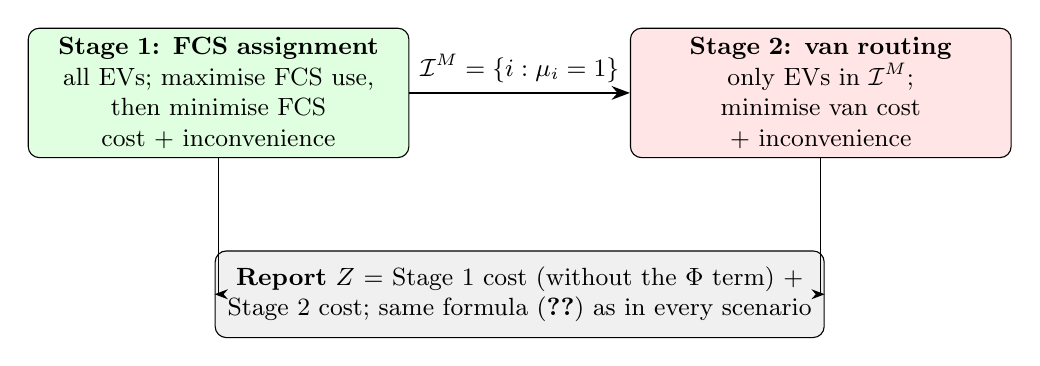
\begin{tikzpicture}[>=Stealth,box/.style={draw,rounded corners,align=center,minimum height=1.1cm,font=\small}]
  \node[box,fill=green!12,text width=4.6cm] (s1) {\textbf{Stage 1: FCS assignment}\\all EVs; maximise FCS use,\\then minimise FCS cost + inconvenience};
  \node[box,fill=red!10,text width=4.6cm,right=2.8cm of s1] (s2) {\textbf{Stage 2: van routing}\\only EVs in $\I^M$;\\minimise van cost + inconvenience};
  \draw[->,thick] (s1) -- node[above,font=\small]{$\I^M=\{i:\mu_i=1\}$} (s2);
  \node[box,fill=black!6,text width=7.5cm,below=2.0cm of $(s1)!0.5!(s2)$] (ev) {\textbf{Report} $Z=$ Stage~1 cost (without the $\Phi$ term) $+$ Stage~2 cost; same formula \eqref{eq:Z} as in every scenario};
  \draw[->] (s1) |- (ev); \draw[->] (s2) |- (ev);
\end{tikzpicture}
\end{center}

Stage~1 does not look at the vans, and Stage~2 cannot change what Stage~1 decided. That is the definition of ``FCS first, then MCS''.

%----------------------------------------------------------------
\subsection{Stage 1: assign EVs to fixed stations}

\textbf{Objective.}
\begin{equation}
\begin{split}
\min\ Z^{(1)}=\;&\underbrace{\Phi\sum_{i\in\I}\mu_i}_{\text{FCS first}}
+\underbrace{c^{EV}\sum_i\sum_{f\in\F_i}d_{if}Y_{if}}_{Z_1}
+\underbrace{Z^F_{\text{energy}}}_{\text{FCS part of }Z_4}\\
&+\underbrace{\sum_i\sum_{f\in\F_i}\rho^F_{if}Y_{if}+\alpha\sum_i w_i(C_i-r_i)+c^L\sum_i w_iL_i}_{\text{FCS customers' inconvenience}}
\end{split}
\label{eq:obj1}
\end{equation}
with $C_i=S_i+\tau^F_iY_i$ in this stage. $\Phi$ is a penalty for handing an EV to the vans. It is chosen larger than anything an extra FCS customer can add to the rest of \eqref{eq:obj1}, e.g.
\[
\Phi > \max_{i}\max_{f\in\F_i}\big(c^{EV}d_{if}+\pi^{\max}E_i+\rho^F_{if}\big)+n\,(\alpha+c^L)\,w_{\max}\,T,
\]
so Stage~1 first \textbf{maximises the number of EVs served at an FCS}, and only among those solutions minimises FCS cost and inconvenience. ($\pi^{\max}$ is the highest grid price.) A numerically safer equivalent is to solve twice: first $\max\sum_iY_i$, then fix that number and minimise the rest.
\ifTOU
Because $Z^F_{\text{energy}}$ uses the peak price, Stage~1 may \emph{start sessions later} to leave the peak, if the price saving beats the extra waiting cost (Section~\ref{sec:expect}).
\fi

\textbf{Constraints.}
\begin{align}
\sum_{g\in\G_i}y_{ig}+\mu_i &= 1 && \forall i\in\I \label{eq:s1assign}\\
S_i &\ge r_i+\sum_{f\in\F_i}t_{if}Y_{if} && \forall i\in\I \label{eq:fcsarr}\\
S_i &\le r_i+T\,(1-\mu_i) && \forall i\in\I \label{eq:s1park}\\
S_j &\ge S_i+\tau^F_i-(T+\tau^F_i)(3-y_{ig}-y_{jg}-o_{ij}) && \forall g,\ (i,j)\in\mathcal{P}_g \label{eq:disj1}\\
S_i &\ge S_j+\tau^F_j-(T+\tau^F_j)(2-y_{ig}-y_{jg}+o_{ij}) && \forall g,\ (i,j)\in\mathcal{P}_g \label{eq:disj2}\\
\sum_i y_{ig_1} &\ge \sum_i y_{ig_2} && \forall f,\ \G_f=\{g_1,g_2\} \label{eq:gunsym}\\
S_i+\tau^F_iY_i &\le T,\qquad L_i\ge S_i+\tau^F_iY_i-l_i && \forall i\in\I \label{eq:s1time}
\end{align}
\ifTOU plus the time-of-use split \eqref{eq:tou1}--\eqref{eq:tou5} of each FCS session (Section~\ref{sec:price}).\fi
\desc{\eqref{eq:s1assign}: every EV either gets one reachable gun or is handed to the vans. An EV that reaches no FCS ($\G_i=\emptyset$) is forced to $\mu_i=1$. \eqref{eq:fcsarr}: an FCS session cannot start before the EV has asked and driven to the station. \eqref{eq:s1park}: for an EV handed to the vans, $S_i$ is parked at $r_i$, so it adds no waiting in Stage~1 (its real start time is decided in Stage~2). \eqref{eq:disj1}--\eqref{eq:disj2}: two EVs on the same gun do not overlap; $o_{ij}$ picks who goes first. With two guns per station this means at most two EVs charge at a station at a time. \eqref{eq:gunsym}: symmetry breaking between the two identical guns (optional). \eqref{eq:s1time}: finished by $T$; lateness.}

\textbf{Optional acceptability rule.} An operator may refuse to send a driver to a station that is ``too inconvenient'', e.g.\ only allow gun $g$ of station $f$ for EV $i$ if $\hat\rho^F_{if}\le\bar\rho$. This only shrinks $\G_i$, so EVs whose stations are all too far go to the vans. Report results with and without it.

\textbf{Output:} $\I^M=\{i:\mu_i=1\}$, the EVs left for the vans; plus each FCS customer's gun and start time.

%----------------------------------------------------------------
\subsection{Stage 2: route the vans to the leftover EVs}

Stage~2 is a vehicle routing problem with time windows, on the EVs in $\I^M$ only. Here $C_i=S_i+\tau^M_i$.

\textbf{Objective.}
\begin{equation}
\begin{split}
\min\ Z^{(2)}=\;&\underbrace{c^M\sum_m\sum_{(i,j)\in\A^M}d_{ij}x_{ijm}}_{Z_2}+\underbrace{\sum_m c^D_mu_m}_{Z_3}+\underbrace{Z^M_{\text{energy}}}_{\text{van part of }Z_4}\\
&+\underbrace{\sum_{i\in\I^M}\sum_m\rho^M_{im}z_{im}+\alpha\sum_{i\in\I^M}w_i(C_i-r_i)+c^L\sum_{i\in\I^M}w_iL_i}_{\text{van customers' inconvenience}}
\end{split}
\label{eq:obj2}
\end{equation}
Since every EV in $\I^M$ must be served by some van, $Z^M_{\text{energy}}$ and the $\rho^M$ term are constants here. They are kept so that $Z^{(2)}$ is the true cost of Stage~2. Waiting and lateness make the vans visit urgent EVs early.

\textbf{Constraints.}
\begin{align}
\sum_{m\in\M}z_{im} &= 1 && \forall i\in\I^M \label{eq:s2assign}\\
\sum_{j:(0,j)\in\A^M}x_{0jm} = \sum_{i:(i,n+1)\in\A^M}x_{i,n+1,m} &= u_m && \forall m \label{eq:depot}\\
\sum_{i:(i,j)\in\A^M}x_{ijm} = \sum_{k:(j,k)\in\A^M}x_{jkm} &= z_{jm} && \forall j\in\I^M,\ m \label{eq:flow}\\
\sum_{i\in\I^M}z_{im} &\le Q_m\,u_m && \forall m \label{eq:cap}\\
\sum_{i\in\I^M}\frac{E_i}{\eta}z_{im}+\beta\sum_{(i,j)\in\A^M}d_{ij}x_{ijm} &\le B_m\,u_m && \forall m \label{eq:batt}
\end{align}
\begin{align}
S_j &\ge \max\{r_j,\ t_{0j}\,x_{0jm}\} && \forall j\in\I^M,\ m \label{eq:depart}\\
S_j &\ge S_i+\tau^M_i+t_{ij}-(T+\tau^M_i+t_{ij})(1-x_{ijm}) && \forall i\neq j,\ m \label{eq:seq}\\
S_i+\tau^M_i+t_{i,n+1} &\le T+(\tau^M_i+t_{i,n+1})(1-x_{i,n+1,m}) && \forall i,\ m \label{eq:return}\\
S_i+\tau^M_i \le T,\quad L_i &\ge S_i+\tau^M_i-l_i && \forall i\in\I^M \label{eq:s2time}\\
u_m &\ge u_{m+1} && m<|\M| \label{eq:vansym}
\end{align}
\desc{\eqref{eq:s2assign}: each leftover EV gets one van. \eqref{eq:depot}: a used van leaves and returns to the depot once. \eqref{eq:flow}: each EV on van $m$ is entered and left exactly once by that van. \eqref{eq:cap}: at most $Q_m$ EVs per van. \eqref{eq:batt}: delivered energy (with transfer losses) plus driving energy fits in the van battery. \eqref{eq:depart}: no start before the request, or before the van can drive there from the depot (written as two linear constraints). \eqref{eq:seq}: if the van goes $i\to j$, it finishes $i$ and drives to $j$ before starting $j$. This gives one EV at a time and removes subtours (MTZ-type). \eqref{eq:return}: back at the depot by $T$. \eqref{eq:s2time}: finished by $T$; lateness. \eqref{eq:vansym}: use identical vans in index order.}

\textbf{If Stage 2 is infeasible} (too many leftover EVs for the fleet by $T$), the sequential policy has \emph{failed} on that instance. For diagnosis, add $s_i\in\{0,1\}$ (``unserved''), replace \eqref{eq:s2assign} by $\sum_mz_{im}+s_i=1$ and add $\Phi^U\sum_is_i$ to \eqref{eq:obj2}. Then report the number of EVs that could not be served. This is a useful comparison with the integrated scenario, which may serve all of them.

%----------------------------------------------------------------
\subsection{Reported value}
\[
Z^{\text{S\scen}}=\big(Z^{(1)*}-\Phi\,|\I^M|\big)+Z^{(2)*},
\]
which is exactly \eqref{eq:Z} evaluated at the combined solution. The stage-1 solution plus the stage-2 solution is a feasible solution of the integrated model (S\ifTOU 4\else 3\fi), so
$Z^{\text{S\ifTOU 4\else 3\fi}}\le Z^{\text{S\scen}}$. The difference is the \emph{value of integration}.

\else
%---------------------------------------------------------------- INT
\subsection{Objective}
\begin{equation}
\min\ Z \quad\text{as in \eqref{eq:Z}, with }Z^F_{\text{energy}}=\ifTOU P^F\textstyle\sum_i\big[\pi^\off(\theta^1_i+\theta^3_i)+\pi^\pk\theta^2_i\big]\else\pi^F\textstyle\sum_iE_iY_i\fi,\quad C_i=S_i+\tau^F_iY_i+\tau^M_iZ_i. \label{eq:objint}
\end{equation}
Written out in full:
\begin{align*}
\min\ Z=\;& c^{EV}\sum_i\sum_{f\in\F_i}d_{if}Y_{if}+c^M\sum_m\sum_{(i,j)\in\A}d_{ij}x_{ijm}+\sum_mc^D_mu_m\\
&+\ifTOU P^F\sum_i\big[\pi^\off(\theta^1_i+\theta^3_i)+\pi^\pk\theta^2_i\big]\else\pi^F\sum_iE_iY_i\fi
+\pi^M\sum_i\sum_m\frac{E_i}{\eta}z_{im}\\
&+\sum_i\sum_{f\in\F_i}\rho^F_{if}Y_{if}+\sum_i\sum_m\rho^M_{im}z_{im}+\alpha\sum_iw_i(C_i-r_i)+c^L\sum_iw_iL_i .
\end{align*}
Every term is linear. One model weighs everything at once: an EV goes to a van exactly when the van's extra km, dispatch and energy cost are outweighed by the effort and waiting it saves the driver\ifTOU, or by the peak-price energy it avoids\fi.

\subsection{Constraints}

\textbf{Assignment.}
\begin{equation}
\sum_{g\in\G_i}y_{ig}+\sum_{m\in\M}z_{im}=1\qquad\forall i\in\I \label{eq:assign}
\end{equation}
\desc{Exactly one resource per EV: one reachable gun or one van. EVs that reach no FCS are forced onto a van.}

\textbf{Fixed stations.}
\begin{align}
S_i &\ge r_i+\sum_{f\in\F_i}t_{if}Y_{if} && \forall i \label{eq:fcsarr}\\
S_j &\ge S_i+\tau^F_i-(T+\tau^F_i)(3-y_{ig}-y_{jg}-o_{ij}) && \forall g,\ (i,j)\in\mathcal{P}_g \label{eq:disj1}\\
S_i &\ge S_j+\tau^F_j-(T+\tau^F_j)(2-y_{ig}-y_{jg}+o_{ij}) && \forall g,\ (i,j)\in\mathcal{P}_g \label{eq:disj2}\\
\sum_iy_{ig_1} &\ge \sum_iy_{ig_2} && \forall f,\ \G_f=\{g_1,g_2\} \label{eq:gunsym}
\end{align}
\desc{\eqref{eq:fcsarr}: an FCS session starts after the request and the drive to the station (for a van customer this is just $S_i\ge r_i$). \eqref{eq:disj1}--\eqref{eq:disj2}: EVs on the same gun do not overlap; $o_{ij}$ chooses the order. \eqref{eq:gunsym}: optional symmetry breaking.}

\textbf{Vans: routes, capacity, battery.}
\begin{align}
\sum_{j:(0,j)\in\A}x_{0jm}=\sum_{i:(i,n+1)\in\A}x_{i,n+1,m} &= u_m && \forall m \label{eq:depot}\\
\sum_{i:(i,j)\in\A}x_{ijm}=\sum_{k:(j,k)\in\A}x_{jkm} &= z_{jm} && \forall j\in\I,\ m \label{eq:flow}\\
\sum_iz_{im} &\le Q_mu_m && \forall m \label{eq:cap}\\
\sum_i\frac{E_i}{\eta}z_{im}+\beta\sum_{(i,j)\in\A}d_{ij}x_{ijm} &\le B_mu_m && \forall m \label{eq:batt}
\end{align}
\desc{\eqref{eq:depot}: a used van leaves and returns once. \eqref{eq:flow}: each EV on van $m$ is visited exactly once by it. \eqref{eq:cap}: at most $Q_m$ EVs. \eqref{eq:batt}: delivered energy (with losses) plus driving energy fits in the battery.}

\textbf{Vans: timing (one EV at a time, no subtours).}
\begin{align}
S_j &\ge t_{0j}\,x_{0jm} && \forall j\in\I,\ m \label{eq:depart}\\
S_j &\ge S_i+\tau^M_i+t_{ij}-(T+\tau^M_i+t_{ij})(1-x_{ijm}) && \forall i\neq j\in\I,\ m \label{eq:seq}\\
S_i+\tau^M_i+t_{i,n+1} &\le T+(\tau^M_i+t_{i,n+1})(1-x_{i,n+1,m}) && \forall i,\ m \label{eq:return}
\end{align}
\desc{\eqref{eq:depart}: the first stop cannot start before the van has driven there. \eqref{eq:seq}: $i\to j$ means finish $i$, drive, then start $j$; start times rise along a route, so no subtour can close. \eqref{eq:return}: back at the depot by $T$.}

\textbf{Horizon and lateness.}
\begin{equation}
C_i\le T,\qquad L_i\ge C_i-l_i\qquad\forall i\in\I \label{eq:time}
\end{equation}
\desc{Every EV is fully charged within the horizon; $L_i$ measures lateness.}

\ifTOU
\textbf{Time-of-use split.} Constraints \eqref{eq:tou1}--\eqref{eq:tou5} of Section~\ref{sec:price}.
\fi

\textbf{Symmetry and domains.}
\begin{equation}
u_m\ge u_{m+1};\qquad y,z,x,u,o\ifTOU,\kappa\fi\in\{0,1\};\qquad S_i,L_i\ifTOU,\theta^p_i\fi\ge0 \label{eq:dom}
\end{equation}
\fi

%=====================================================================
\section{Learning-to-optimise (RL) formulation}\label{sec:rl}

\textbf{Main rule:} the reward of each action is \emph{minus the increase in $Z$ that the action causes}. The rewards over an episode then add up to $-Z$ of the solution the policy builds. RL and MILP results are measured on the same yardstick \eqref{eq:Z}, and the MILP optimum is the benchmark for the RL gap.

\ifSEQ
%---------------------------------------------------------------- RL SEQ
The RL pipeline has the same two stages as the MILP.

\subsection{Stage 1 policy: FCS assignment}
\begin{itemize}[leftmargin=1.4em,itemsep=2pt]
  \item \textbf{Episode / epochs:} EVs are taken in order of request time $r_i$ (ties: higher $w_i$ first). One decision per EV.
  \item \textbf{State:} features of the current EV $k$ ($E_k,r_k,l_k,w_k,R_k$, location); for each gun $g$ the time $F_g$ it becomes free; summary features of the EVs still to come (count and positions near each station)\ifTOU; the current price and the time until $T_1$ and $T_2$\fi.
  \item \textbf{Action:} a gun $g\in\G_k$, or ``hand to vans''. \textbf{FCS-first mask:} ``hand to vans'' is allowed \emph{only} if no gun can finish EV $k$ by $T$ (or, with the optional rule, if all remaining guns have $\hat\rho^F_{kf}>\bar\rho$).
  \ifTOU\item \textbf{Optional timing action:} ``gun $g$, start after the peak'', i.e.\ $S_k=\max\{\text{earliest},T_2\}$, allowed only if the session still ends by $T$.\fi
  \item \textbf{Transition:} $S_k=\max\{r_k+t_{kf},F_g\}$ (or later, for the timing action); $F_g\leftarrow S_k+\tau^F_k$.
  \item \textbf{Reward:} $-\Big[c^{EV}d_{kf}+\text{energy}_k+\rho^F_{kf}+\alpha w_k(S_k+\tau^F_k-r_k)+c^Lw_k(S_k+\tau^F_k-l_k)^+\Big]$, where energy$_k$ = \ifTOU$P^F\big[\pi^\off\cdot(\text{off-peak hours of }[S_k,S_k+\tau^F_k])+\pi^\pk\cdot(\text{peak hours})\big]$, computed exactly in the simulator\else$\pi^FE_k$\fi. Handing an EV to the vans gives reward $0$ here; its cost is counted in Stage~2.
\end{itemize}
Note: a simple baseline for Stage~1 is the greedy rule ``gun with the largest one-step reward''. What RL can learn on top of this is, for example, to keep a nearby gun free for an urgent EV that arrives later.

\subsection{Stage 2 policy: van routing over $\I^M$}
\begin{itemize}[leftmargin=1.4em,itemsep=2pt]
  \item \textbf{Epochs:} whenever a van becomes free (the earliest-free van decides first).
  \item \textbf{State:} for each van: position, time free, remaining battery $b_m$, EVs served so far, dispatched or not; for each unserved EV in $\I^M$: location, $E_i,r_i,l_i,w_i$; current time.
  \item \textbf{Action:} the next EV $j$ for this van, or ``return to depot'' (ends the route). Mask: $j$ must be feasible: battery covers $E_j/\eta$ plus driving to $j$ and back to the depot, the count stays $\le Q_m$, and $j$ can be finished with the van back at the depot by $T$.
  \item \textbf{Transition:} $S_j=\max\{r_j,\ \text{time free}+t_{\text{pos},j}\}$; the van moves to $j$ and is free at $S_j+\tau^M_j$; $b_m$ falls by $E_j/\eta+\beta d_{\text{pos},j}$.
  \item \textbf{Reward:} serving $j$: $-\Big[c^Md_{\text{pos},j}+c^D_m[\text{first stop}]+\pi^M\frac{E_j}{\eta}+\rho^M_{jm}+\alpha w_j(S_j+\tau^M_j-r_j)+c^Lw_j(S_j+\tau^M_j-l_j)^+\Big]$; returning: $-c^Md_{\text{pos},0}$. EVs still unserved at the end: $-\Phi^U$ each.
  \item \textbf{Policy:} an attention-based routing policy (e.g.\ Kool et al., 2019, ``Attention, Learn to Solve Routing Problems!'') trained with REINFORCE or PPO. Baseline: nearest-feasible-EV heuristic.
\end{itemize}
Episode return of Stage~1 + Stage~2 $=-Z^{\text{S\scen}}$.

\else
%---------------------------------------------------------------- RL INT
One policy decides both who serves each EV and the van routes.
\begin{itemize}[leftmargin=1.4em,itemsep=2pt]
  \item \textbf{Episode / epochs:} EVs are taken in order of request time $r_i$ (ties: higher $w_i$ first). One decision per EV.
  \item \textbf{State:} (i) the current EV $k$: location, $E_k,r_k,l_k,w_k,R_k$, reachable stations; (ii) each gun $g$: time $F_g$ it becomes free; (iii) each van $m$: current end-of-route position, time free, remaining battery $b_m$, EVs served, dispatched or not; (iv) embeddings of the not-yet-assigned EVs (for look-ahead)\ifTOU; (v) current price, time until $T_1$ and $T_2$\fi.
  \item \textbf{Action:} $a\in\G_k\cup\M$: a gun, or a van (EV $k$ is appended to the end of that van's route). \textbf{Mask} infeasible actions: a gun that cannot finish $k$ by $T$; a van without enough battery for $E_k/\eta$ plus the drive to $k$ and back to the depot, with $Q_m$ reached, or unable to finish $k$ and return by $T$.
  \ifTOU\item \textbf{Optional timing action:} ``gun $g$, start after the peak'' ($S_k=\max\{\text{earliest},T_2\}$, if it still ends by $T$).\fi
  \item \textbf{Transition:} gun: $S_k=\max\{r_k+t_{kf},F_g\}$, $F_g\leftarrow S_k+\tau^F_k$. Van: $S_k=\max\{r_k,\ \text{free}_m+t_{\text{pos}_m,k}\}$, then the van moves to $k$, $\text{free}_m\leftarrow S_k+\tau^M_k$, $b_m\mathrel{-}=E_k/\eta+\beta d_{\text{pos}_m,k}$.
  \item \textbf{Reward} $=-\Delta Z$:
  \begin{align*}
  \text{gun } g\text{ at }f:&\quad -\Big[c^{EV}d_{kf}+\text{energy}^F_k+\rho^F_{kf}+\alpha w_k(C_k-r_k)+c^Lw_k(C_k-l_k)^+\Big]\\
  \text{van } m:&\quad -\Big[c^M\big(d_{\text{pos}_m,k}+d_{k,0}-d_{\text{pos}_m,0}\big)+c^D_m[\text{first use}]+\pi^M\tfrac{E_k}{\eta}\\
  &\qquad\quad+\rho^M_{km}+\alpha w_k(C_k-r_k)+c^Lw_k(C_k-l_k)^+\Big]
  \end{align*}
  The van distance term is the \emph{change} in route length when $k$ is inserted before the return to the depot, so the sum over the episode equals the total route length (the return legs telescope). energy$^F_k$ = \ifTOU$P^F\big[\pi^\off\cdot(\text{off-peak hours})+\pi^\pk\cdot(\text{peak hours of }[S_k,C_k])\big]$, computed exactly by the simulator; no linearisation is needed in RL\else$\pi^FE_k$\fi.
  \item \textbf{Dead end:} if every action is masked, EV $k$ is unserved: reward $-\Phi^U$, and the episode continues. Report the count.
  \item \textbf{Policy:} masked categorical policy over guns and vans, encoder with attention over EVs, guns and vans; trained with PPO. Natural baseline: greedy, i.e.\ choose the action with the largest one-step reward. That is the pairwise rule ``smallest $\hat\rho$ + cost'' from Section~\ref{sec:inc}.
\end{itemize}
Restriction to note: vans serve EVs in assignment order (append only). A variant that inserts $k$ at the cheapest position of a route is more flexible but has a larger action space.
\fi

\textbf{Reward scaling.} For stable training divide every reward by a constant, e.g.\ the greedy baseline's average $Z$ on the training instances. This does not change the optimal policy.

%=====================================================================
\section{What to expect and what to report}\label{sec:expect}

\ifnum\scen=1
\begin{itemize}[leftmargin=1.4em,itemsep=2pt]
  \item Vans serve only EVs that reach no station, or that the stations cannot finish by $T$. If stations have spare capacity, very few vans are dispatched.
  \item Inconvenience is high for EVs far from the nearest station (worked example: Rs\,682 at the FCS, against Rs\,458 if a van had been allowed).
  \item With too few vans Stage~2 becomes infeasible (unserved EVs), even when the integrated model S3 could serve everyone. Report the smallest $|\M|$ at which S1 is feasible and compare it with S3.
\end{itemize}
\fi
\ifnum\scen=2
\begin{itemize}[leftmargin=1.4em,itemsep=2pt]
  \item \textbf{When does Stage~1 delay a session to avoid the peak?} Moving one hour of charging out of the peak saves $(\pi^\pk-\pi^\off)P^F=3\times22=$ Rs\,66, but delays completion by up to an hour, which costs $\alpha w_i\ge$ Rs\,200. So with the default values Stage~1 almost never delays. It mostly pays the higher price, and S2 costs roughly S1 plus the peak surcharge. Sessions start later only if $\alpha$ is small (try $\lambda<0.33$ in the sensitivity analysis).
  \item The van assignment is the same as in S1 unless Stage~1's timing changes which EVs fit at the stations. Stage~1 cannot use vans to escape the peak price.
  \item Extra KPI: \textbf{grid energy drawn at FCS during the peak}, $P^F\sum_i\theta^2_i$ (kWh). Compare with S4.
\end{itemize}
\fi
\ifnum\scen=3
\begin{itemize}[leftmargin=1.4em,itemsep=2pt]
  \item Vans take EVs for which the saved inconvenience exceeds the extra van cost (worked example: van chosen, saving Rs\,224). Expect vans to serve EVs that are far from every station, have low range (high $w_i$), or have early deadlines, while EVs near a station still use it.
  \item \textbf{Value of integration under flat price:} $Z^{\text{S1}}-Z^{\text{S3}}\ge0$. Report it per component ($Z_1,\dots,Z_5$): typically operating cost rises a little and inconvenience falls a lot.
  \item Vary $|\M|$ (0, 1, 2, \dots): the first few vans lower $Z$ sharply, then the effect levels off. That curve shows the scenarios where mobile chargers help most.
\end{itemize}
\fi
\ifnum\scen=4
\begin{itemize}[leftmargin=1.4em,itemsep=2pt]
  \item During the peak a van kWh costs about the same as an FCS kWh (Rs\,10.0 each), so the vans' energy disadvantage disappears and vans also absorb \emph{peak-hour} demand that would otherwise be charged on the grid at peak price.
  \item Expect more van usage than in S3, concentrated on requests in $[T_1,T_2]$, and lower grid energy at the stations during the peak, $P^F\sum_i\theta^2_i$, than in S2.
  \item \textbf{Value of integration under peak pricing:} $Z^{\text{S2}}-Z^{\text{S4}}$. It should be larger than $Z^{\text{S1}}-Z^{\text{S3}}$, because integration now also allows price arbitrage.
  \item \textbf{Peak pricing with full flexibility:} $Z^{\text{S4}}-Z^{\text{S3}}$ should be smaller than $Z^{\text{S2}}-Z^{\text{S1}}$: vans cushion the price increase.
\end{itemize}
\fi

\textbf{Cross-scenario comparison table} (fill in from the four runs):
\begin{center}
\renewcommand{\arraystretch}{1.2}
\begin{tabular}{@{}lll@{}}
\toprule
\textbf{Comparison} & \textbf{Measures} & \textbf{Expected sign} \\
\midrule
S1 $-$ S3 & value of integration, flat price & $\ge0$ \\
S2 $-$ S4 & value of integration, peak price & $\ge0$, larger than S1 $-$ S3 \\
S2 $-$ S1 & cost of peak pricing, FCS-first operator & $>0$ \\
S4 $-$ S3 & cost of peak pricing, flexible operator & $>0$, smaller than S2 $-$ S1 \\
\bottomrule
\end{tabular}
\end{center}
Report for each: $Z$ and its components, number of vans used, EVs per resource, mean and maximum inconvenience per EV, total lateness, peak-hour grid energy, solve time, and (for RL) the gap to the MILP optimum.

%=====================================================================
\appendix
\section{Illustrative parameter values}\label{app:values}

These are starting values for experiments, not data. All are meant to be varied in the analysis. Values in Rs.

\begin{center}
\renewcommand{\arraystretch}{1.15}
\begin{tabular}{@{}llp{6.2cm}@{}}
\toprule
\textbf{Parameter} & \textbf{Value} & \textbf{Note} \\
\midrule
$T$, $[T_1,T_2]$ & 7 h, $[2,6]$ & 16:00--23:00, peak 18:00--22:00 \\
$P^F$, $P^M$ & 22 kW, 30 kW & \\
$v$, $\beta$, $\eta$ & 25 km/h, 0.25 kWh/km, 0.9 & \\
$B_m$, $Q_m$, $|\M|$ & 150 kWh, 6, 2--6 & \\
$c^{EV}$, $c^M$, $c^D_m$ & Rs\,4/km, Rs\,15/km, Rs\,1500 & van km includes driver time \\
$\pi^F$ (flat) & Rs\,8.7/kWh & equals the time-average of the ToU tariff over $[0,T]$ \\
$\pi^\off$, $\pi^\pk$ (ToU) & Rs\,7/kWh, Rs\,10/kWh & $(3\times7+4\times10)/7=8.7$ \\
$c^{bat}$ & Rs\,2/kWh & van battery wear \\
$\pi^M$ & Rs\,10.7 (flat) / Rs\,9.0 (ToU) & $=\pi^F+c^{bat}$ / $=\pi^\off+c^{bat}$ \\
$\alpha$, $\alpha^D$ & Rs\,200/h, Rs\,100/h & value of time; extra for attended time \\
$h^F$, $h^M$, $\varphi$ & Rs\,50, Rs\,10, Rs\,100 & trip hassle, hand-over, range stress \\
$c^L$ & Rs\,300/h & lateness \\
$w_i$ & $1+2(1-R_i/R_{\max})$, $R_i\sim U[3,40]$ km & priority from remaining range \\
\bottomrule
\end{tabular}
\end{center}

The flat price is set to the time-average of the peak tariff. The price \emph{level} is then the same in both pricing cases, and only the price \emph{shape} differs. Without this, part of S1 vs S2 would just reflect a different average price.

\end{document}
"
%  (run each twice for cross-references)
% =====================================================================
\documentclass[11pt,a4paper]{article}
\usepackage[margin=2.2cm]{geometry}
\usepackage{amsmath,amssymb,amsfonts}
\usepackage{booktabs,array,tabularx}
\usepackage{enumitem}
\usepackage[table]{xcolor}
\usepackage{tikz}
\usetikzlibrary{arrows.meta,positioning,calc}
\usepackage[colorlinks=true,linkcolor=blue!50!black,urlcolor=blue!50!black]{hyperref}
\usepackage{titlesec}
\titleformat{\section}{\large\bfseries}{\thesection}{0.8em}{}
\titleformat{\subsection}{\normalsize\bfseries}{\thesubsection}{0.8em}{}
\setlength{\parindent}{0pt}
\setlength{\parskip}{5pt}

% ---------------- scenario switches ----------------
\ifdefined\scen\else\def\scen{1}\fi
\newif\ifTOU \TOUfalse   % true = time-of-use (peak) price
\newif\ifSEQ \SEQfalse   % true = FCS first, then MCS
\ifnum\scen=1 \SEQtrue \fi
\ifnum\scen=2 \TOUtrue \SEQtrue \fi
\ifnum\scen=4 \TOUtrue \fi

\newcommand{\pricename}{\ifTOU time-of-use price (dearer evening peak)\else single (flat) price all day\fi}
\newcommand{\structname}{\ifSEQ FCS first, then MCS (sequential)\else FCS and MCS together (integrated)\fi}

% ---------------- notation ----------------
\newcommand{\I}{\mathcal{I}}
\newcommand{\F}{\mathcal{F}}
\newcommand{\G}{\mathcal{G}}
\newcommand{\M}{\mathcal{M}}
\newcommand{\N}{\mathcal{N}}
\newcommand{\A}{\mathcal{A}}
\newcommand{\Rs}{\text{Rs}\,}
\newcommand{\pk}{\mathrm{pk}}
\newcommand{\off}{\mathrm{off}}
\newcommand{\desc}[1]{\par\vspace{-2pt}{\small\color{black!75}\textit{Meaning:} #1}\par\vspace{4pt}}
\newcommand{\cell}[2]{\ifnum\scen=#1\cellcolor{blue!18}\textbf{S#1 (this document)}\\\textbf{#2}\else S#1\\#2\fi}

\title{\textbf{EV Charging Network Optimisation}\\[4pt]
\large Scenario \scen: \pricename\ $+$ \structname\\[2pt]
\normalsize MILP and RL formulation}
\author{CP 320 OR for Mobility Management, course project}
\date{2 October 2026}

\begin{document}
\maketitle

%=====================================================================
\section{Where this scenario sits}

The project studies four scenarios: two ways of pricing grid electricity, times two ways of making the decisions.

\begin{center}
\renewcommand{\arraystretch}{1.5}
\begin{tabular}{>{\raggedright\arraybackslash}p{4.2cm}|>{\centering\arraybackslash}p{4.6cm}|>{\centering\arraybackslash}p{4.6cm}}
 & \textbf{Flat price all day} & \textbf{Time-of-use (peak) price} \\ \hline
\textbf{Sequential:} FCS first, leftover EVs to MCS &
\begin{tabular}[c]{@{}c@{}}\cell{1}{flat + sequential}\end{tabular} &
\begin{tabular}[c]{@{}c@{}}\cell{2}{peak + sequential}\end{tabular} \\ \hline
\textbf{Integrated:} FCS and MCS decided together &
\begin{tabular}[c]{@{}c@{}}\cell{3}{flat + integrated}\end{tabular} &
\begin{tabular}[c]{@{}c@{}}\cell{4}{peak + integrated}\end{tabular} \\
\end{tabular}
\end{center}

\textbf{The four scenarios do not have four different objectives.} They share \emph{one} cost yardstick $Z$ (Section~\ref{sec:obj}): the same cost terms and the same customer inconvenience (Section~\ref{sec:inc}). Only two things change:
\begin{itemize}[leftmargin=1.4em,itemsep=1pt]
  \item \textbf{Pricing} changes the formula for one term, the FCS energy cost (Section~\ref{sec:price}).
  \item \textbf{Decision structure} changes \emph{how} $Z$ is minimised: in one model (integrated), or in two stages (sequential), where each stage minimises its own part of $Z$.
\end{itemize}
Because the yardstick is the same, the four optimal values can be compared directly. The differences measure the \emph{value of integration} (S1$\to$S3, S2$\to$S4) and the \emph{effect of peak pricing} (S1$\to$S2, S3$\to$S4).

\ifnum\scen=1
\textbf{This scenario (S1)} is the baseline, the ``status quo''. Electricity costs the same at every hour, every EV that can be charged at a fixed station is sent there, and vans only take what is left over.
\fi
\ifnum\scen=2
\textbf{This scenario (S2)} keeps the FCS-first rule of S1, but grid electricity is dearer during the evening peak. Stage~1 can react to the price only by \emph{rescheduling} FCS sessions. It cannot hand a peak-hour EV to a van.
\fi
\ifnum\scen=3
\textbf{This scenario (S3)} keeps the flat price of S1, but the operator decides FCS and MCS service \emph{together}. An EV can be sent to a van even when a fixed station could take it, whenever that lowers total cost plus inconvenience.
\fi
\ifnum\scen=4
\textbf{This scenario (S4)} is the most flexible one: peak pricing at fixed stations, and FCS and MCS decided together. Van energy was bought off-peak, so vans can also be used to keep charging \emph{out of the expensive peak}.
\fi

%=====================================================================
\section{Setting and assumptions}\label{sec:setting}

\textbf{Time.} The planning horizon is $[0,T]$ with $T=7$\,h (16:00--23:00). It contains the evening peak window $[T_1,T_2]=[2,6]$ (18:00--22:00). The horizon is the same in all four scenarios. It is wider than the peak itself so that, under peak pricing, there is cheaper time on both sides of the peak.\ifTOU\else\ In this scenario the price is flat, so the window plays no role in the model.\fi

\textbf{Assumptions} (the same as MILP v3, plus two about energy):
\begin{enumerate}[leftmargin=1.6em,itemsep=1pt]
  \item Static, continuous time. All requests in the horizon are known at time $0$, and request $i$ becomes active at $r_i$.
  \item An EV served by an FCS drives there itself on its own battery (only to stations within its range $R_i$). The driver stays with the car while it waits for a free gun and while it charges.
  \item An EV served by an MCS stays parked where it is, and the driver is free in the meantime.
  \item Each FCS gun and each van charges one EV at a time, without interruption, at constant power.
  \item A van's battery covers both its driving and the energy it delivers. \textbf{The van battery is charged at the depot before the horizon starts}\ifTOU, i.e.\ at the off-peak price\fi, and is not recharged during the horizon.
  \item Every EV must be fully charged by $T$ (hard). Finishing after the driver's desired time $l_i$ is allowed but penalised.
\end{enumerate}

%=====================================================================
\section{Notation}\label{sec:notation}

\subsection*{Sets}
\begin{tabularx}{\textwidth}{@{}lX@{}}
\toprule
$\I=\{1,\dots,n\}$ & EV charging requests \\
$\F$; $\G_f$ ($|\G_f|=2$); $\G=\bigcup_f\G_f$ & fixed charging stations; guns of FCS $f$; all guns ($f(g)$ = station of gun $g$) \\
$\F_i=\{f: d_{if}\le R_i\}$, $\G_i=\bigcup_{f\in\F_i}\G_f$ & stations / guns EV $i$ can reach on its remaining range \\
$\M$ & mobile charging vans (MCS) \\
$0,\ n+1$ & depot as start node / end node (same place) \\
$\N=\{0\}\cup\I\cup\{n+1\}$, $\A$ & routing nodes; allowed van arcs $(i,j)$, $i\in\{0\}\cup\I$, $j\in\I\cup\{n+1\}$, $i\neq j$ \\
$\mathcal{P}_g=\{(i,j): i<j,\ g\in\G_i\cap\G_j\}$ & pairs of EVs that could share gun $g$ \\
\ifSEQ
$\I^M\subseteq\I$ & EVs handed to the vans by Stage~1 (an \emph{output} of Stage~1, a fixed input to Stage~2) \\
$\N^M$, $\A^M$ & routing nodes / arcs restricted to $\I^M$ \\
\fi
\bottomrule
\end{tabularx}

\subsection*{Parameters}
\begin{tabularx}{\textwidth}{@{}lX@{}}
\toprule
$E_i,\ r_i,\ l_i,\ R_i$ & energy demand (kWh), request time, desired completion time (h), remaining range (km) \\
$w_i\ge1$ & priority of EV $i$; $w_i=1+\kappa(1-R_i/R_{\max})$, so low-range EVs weigh more \\
$P^F,\ P^M$ & charging power of an FCS gun (22\,kW) / of a van (e.g.\ 30\,kW) \\
$\tau^F_i=E_i/P^F,\ \tau^M_i=E_i/P^M$ & charging time of EV $i$ at an FCS / by a van (h) \\
$d_{if},t_{if}$;\ $d_{ij},t_{ij}$ & distance (km) and time (h): EV$\to$FCS; between routing nodes ($t=d/v$) \\
$B_m,\ Q_m,\ \beta,\ \eta$ & van battery (kWh), max EVs per van, van consumption (kWh/km), transfer efficiency \\
$c^{EV},\ c^M,\ c^D_m$ & cost per km of EV driving, per km of van driving; fixed dispatch cost of van $m$ \\
\ifTOU
$\pi^\off,\ \pi^\pk$ & grid price (Rs/kWh) off-peak / in $[T_1,T_2]$, with $\pi^\pk\ge\pi^\off$ \\
\else
$\pi^F$ & grid price (Rs/kWh), the same at every hour \\
\fi
$c^{bat}$ & van battery wear per kWh cycled \\
$\pi^M$ & cost of 1 kWh taken from a van battery: $\pi^M=\ifTOU\pi^\off\else\pi^F\fi+c^{bat}$ (Section~\ref{sec:price}) \\
$\alpha,\ \alpha^D,\ h^F,\ h^M,\ \varphi,\ c^L$ & inconvenience coefficients (Section~\ref{sec:inc}) \\
\bottomrule
\end{tabularx}

\subsection*{Decision variables}
\begin{tabularx}{\textwidth}{@{}llX@{}}
\toprule
$y_{ig}$ & $\{0,1\}$ & EV $i$ charged at gun $g\in\G_i$ \\
$z_{im}$ & $\{0,1\}$ & EV $i$ served by van $m$ \\
$x_{ijm}$ & $\{0,1\}$ & van $m$ drives arc $(i,j)$ \\
$u_m$ & $\{0,1\}$ & van $m$ is dispatched \\
$o_{ij}$ & $\{0,1\}$ & for EVs $i<j$ that could share a gun: 1 if $i$ is charged before $j$ \\
\ifSEQ
$\mu_i$ & $\{0,1\}$ & Stage~1 only: EV $i$ is handed to the van fleet \\
\fi
\ifTOU
$\theta^1_i,\theta^2_i,\theta^3_i$ & $\ge0$ & hours of EV $i$'s FCS session before / inside / after the peak \\
$\kappa^1_i,\kappa^3_i$ & $\{0,1\}$ & EV $i$'s FCS session starts before $T_1$ / ends after $T_2$ \\
\fi
$S_i$ & $\ge0$ & time charging of EV $i$ starts (h), on whichever resource \\
$L_i$ & $\ge0$ & lateness of EV $i$ beyond $l_i$ (h) \\
\bottomrule
\end{tabularx}

\textbf{Short-hands} (linear expressions, not new variables):
\[
Y_{if}=\sum_{g\in\G_f}y_{ig},\qquad Y_i=\sum_{g\in\G_i}y_{ig}\ (\text{EV $i$ uses an FCS}),\qquad Z_i=\sum_{m\in\M}z_{im}\ (\text{EV $i$ uses a van}),
\]
\[
C_i=S_i+\tau^F_i\,Y_i+\tau^M_i\,Z_i \quad\text{(time EV $i$ is fully charged).}
\]

%=====================================================================
\section{Customer inconvenience}\label{sec:inc}

This section is \textbf{identical in all four scenario documents}. Inconvenience is a property of the customer, not of the price or of the planning method.

\subsection{What we mean by inconvenience}

Inconvenience is \emph{what the driver loses} from the moment they ask for a charge ($r_i$) until the car is fully charged ($C_i$), \emph{converted into rupees} so it can be added to the operator's costs. A driver loses three different things:

\begin{enumerate}[leftmargin=1.6em,itemsep=2pt]
  \item \textbf{Waiting:} the car is not ready. This lasts $C_i-r_i$ hours and affects \emph{every} driver, FCS or MCS.
  \item \textbf{Effort:} only an FCS customer has to drive to the station and sit there while the car charges. An MCS customer stays at home or at work and does something else. Driving to a far station also uses scarce battery range, which causes stress (``range anxiety'').
  \item \textbf{A missed deadline:} the car is still not ready at the time $l_i$ the driver needs it.
\end{enumerate}

Each loss gets a price in Rs per hour (or per event). All of them are multiplied by the priority $w_i$: an hour of delay for an EV with 5\,km of range left counts more than for one with 40\,km.

\subsection{The three components}

\begin{center}
\renewcommand{\arraystretch}{1.3}
\begin{tabularx}{\textwidth}{@{}>{\raggedright\arraybackslash}p{2.6cm}>{\raggedright\arraybackslash}X>{\raggedright\arraybackslash}X>{\raggedright\arraybackslash}p{3.0cm}@{}}
\toprule
\textbf{Component} & \textbf{EV $i$ at FCS $f$} & \textbf{EV $i$ by a van} & \textbf{Known when?} \\
\midrule
Effort & $w_i\big[\alpha^D(t_{if}+\tau^F_i)+h^F+\varphi\,d_{if}/R_i\big]$: driving and sitting at the station, a fixed trip hassle, range stress & $w_i\,h^M$: being reachable and handing over the car & \textbf{Static:} known as soon as the resource is chosen \\
Waiting & $w_i\,\alpha\,(C_i-r_i)$ = drive + \emph{queue at the gun} + charge & $w_i\,\alpha\,(C_i-r_i)$ = \emph{wait for the van} + charge & \textbf{Dynamic:} depends on the queue / van route \\
Missed deadline & $w_i\,c^L\,L_i$, $L_i=\max\{0,C_i-l_i\}$ & same & Dynamic \\
\bottomrule
\end{tabularx}
\end{center}

\textbf{Coefficients.}
$\alpha$ (Rs/h) is the value of an hour the car is not ready.
$\alpha^D$ (Rs/h) is the \emph{extra} value of an hour the driver must personally spend driving or sitting at the station: an hour at the station costs $\alpha+\alpha^D$, an hour waiting at home for a van costs only $\alpha$.
$h^F,h^M$ (Rs) are fixed hassle costs of one trip to a station / one van hand-over.
$\varphi$ (Rs) is the range-stress cost of a trip that uses the \emph{whole} remaining range ($d_{if}/R_i\le1$ is the fraction used).
$c^L$ (Rs/h) is the cost per hour late.

\subsection{Pairwise form: inconvenience of a (customer, resource) pair}

The natural first idea is: \emph{for every pair (EV $i$, FCS $f$) and every pair (EV $i$, van $m$) there is an inconvenience number, and the operator picks the pair with the lowest cost plus inconvenience.} The static part fits this idea exactly:
\[
\boxed{\;\rho^F_{if}=w_i\Big[\alpha^D\,(t_{if}+\tau^F_i)+h^F+\varphi\,\frac{d_{if}}{R_i}\Big]\qquad
\rho^M_{im}=w_i\,h^M\;}
\]
These are \textbf{parameters}, computed before solving, one number per (EV, FCS) pair and per (EV, van) pair. In the objective they appear linearly: $\sum_i\sum_f\rho^F_{if}Y_{if}+\sum_i\sum_m\rho^M_{im}z_{im}$.

Note that $\rho^M_{im}$ does not depend on $m$. Vans are identical and all start at the same depot, so the driver does not care \emph{which} van comes, only \emph{when} it comes. That ``when'' is the waiting part.

\subsection{Why waiting cannot be a fixed pairwise number}

It is tempting to also write the waiting as a pairwise number, e.g.\ ``the van needs 5 minutes to reach EV $i$''. But that depends on \emph{where the van is coming from}, which depends on the route the model is still choosing: if EV $i$ is the 4th stop of a van, the wait is the time for three charging sessions plus four drives. Likewise, waiting at an FCS depends on how many EVs are queued at that gun. So waiting is not known before solving. It is a function of decision variables:
\[
\text{waiting cost of EV } i \;=\; w_i\,\alpha\,(C_i-r_i),\qquad C_i=S_i+\tau^F_iY_i+\tau^M_iZ_i .
\]
This is \textbf{linear} in the variables ($S_i$, $y$, $z$), so it fits in a MILP directly. The constraints of Section~\ref{sec:milp} make $S_i$ equal to the true start time, including driving, queueing at the gun and the van's route. The term $\sum_i w_i\alpha r_i$ is a constant and may be dropped when solving.

\textbf{Pairwise \emph{estimate}} (used for intuition, by the RL policy and in heuristics): if there is no queue and the van comes straight to $i$,
\[
\hat\rho^{F}_{if}=\rho^F_{if}+w_i\alpha\,(t_{if}+\tau^F_i),\qquad
\hat\rho^{M}_{im}=\rho^M_{im}+w_i\alpha\,(t^{\text{van}}_{m\to i}+\tau^M_i),
\]
where $t^{\text{van}}_{m\to i}$ is the time until van $m$ can reach $i$ from where it currently is. In the RL formulation (Section~\ref{sec:rl}) the van's position \emph{is} known at each decision, so there this estimate becomes exact.

\subsection{Total inconvenience and how it enters the objective}

\begin{equation}
\boxed{\;
Z_{\text{inc}}=\underbrace{\sum_{i\in\I}\sum_{f\in\F_i}\rho^F_{if}Y_{if}+\sum_{i\in\I}\sum_{m\in\M}\rho^M_{im}z_{im}}_{\text{effort (static, pairwise)}}
+\underbrace{\alpha\sum_{i\in\I}w_i\,(C_i-r_i)}_{\text{waiting (dynamic)}}
+\underbrace{c^L\sum_{i\in\I}w_i\,L_i}_{\text{missed deadline}}
\;}\label{eq:inc}
\end{equation}
All three parts are in rupees, so $Z_{\text{inc}}$ is simply added to the operating costs. Nothing has to be normalised.

\subsection{Worked example: your ``10 km to the FCS vs.\ van in 5 minutes'' case}

EV $i$: $E_i=20$\,kWh, $R_i=40$\,km (so $w_i=1$); nearest free FCS $d_{if}=10$\,km away, $t_{if}=0.4$\,h at 25\,km/h; a van finishing next door can reach it in 5\,min ($0.083$\,h), adding about 4\,km to its route. $\tau^F_i=20/22=0.909$\,h, $\tau^M_i=20/30=0.667$\,h. Coefficients from Appendix~\ref{app:values}, flat price.

\begin{center}
\renewcommand{\arraystretch}{1.25}
\begin{tabular}{@{}lrr@{}}
\toprule
 & \textbf{FCS} & \textbf{Van} \\
\midrule
Driving (EV / extra van km) & $4\times10=40.0$ & $15\times4=60.0$ \\
Energy & $8.7\times20=174.0$ & $10.7\times20/0.9=237.8$ \\
\textbf{Operating cost only} & \textbf{214.0} & \textbf{297.8} \\
\midrule
Effort $\rho$ & $100(0.4+0.909)+50+100\cdot\tfrac{10}{40}=205.9$ & $10.0$ \\
Waiting $\alpha(C_i-r_i)$ & $200\times1.309=261.8$ & $200\times0.75=150.0$ \\
\textbf{Cost + inconvenience} & \textbf{681.7} & \textbf{457.8} \\
\bottomrule
\end{tabular}
\end{center}

On operating cost alone the FCS is cheaper, so a cost-only model would \emph{always} send this driver 10\,km away. With inconvenience included the van is better by about Rs\,224, and the integrated model chooses $z_{im}=1$, as you expected. If the FCS were only 1\,km away, the FCS would win both comparisons. The inconvenience term is what makes the model choose between ``cheap for the operator'' and ``convenient for the driver'', rather than following a fixed rule.

\subsection{Relation to a single penalty $\rho_i$ per EV}

The first draft used a penalty $\rho_i$ that is charged whenever EV $i$ goes to \emph{any} FCS: $\sum_i\sum_f\rho_iy_{if}$. Because $\sum_f y_{if}=1-\sum_m z_{im}$, this only says ``a van is worth $\rho_i$ more to EV $i$'', and that holds whether the station is 1\,km or 15\,km away, and whether the van arrives in 5 minutes or in 3 hours. The form above fixes both problems: $\rho^F_{if}$ grows with the distance to \emph{that} station, and the waiting term grows with how late the van or the free gun actually is. The old model is the special case $\alpha=\alpha^D=\varphi=c^L=0$, $h^F=\rho_i$.

\subsection{Choosing the coefficients}
\begin{itemize}[leftmargin=1.4em,itemsep=2pt]
  \item Use a value of time for $\alpha$ (e.g.\ Rs\,150--300/h for urban car users), and set $\alpha^D\approx0.5\alpha$: sitting at a station is worse than waiting at home.
  \item Keep $c^L>\alpha$, so missing the deadline is worse than ordinary waiting.
  \item \textbf{Sensitivity analysis:} multiply all inconvenience coefficients by a factor $\lambda\in\{0,0.25,0.5,1,2,4\}$ and plot operating cost against total inconvenience. $\lambda=0$ is the pure cost-minimising operator, and large $\lambda$ is a customer-first operator. This trade-off curve is a strong result for the ``Analysis'' part of the project.
\end{itemize}

\subsection{What inconvenience does in \emph{this} scenario}
\ifSEQ
In a sequential scenario inconvenience \textbf{cannot move an EV from an FCS to a van}: Stage~1 sends every EV that \emph{can} use an FCS to one. It still matters inside each stage. In Stage~1 it decides \emph{which} station and \emph{when} (urgent EVs get the near station and the first free gun). In Stage~2 it decides the \emph{order} in which vans visit EVs (urgent EVs first). In the worked example, this scenario sends the driver 10\,km to the FCS. That is the weakness the integrated scenarios remove.
\else
In an integrated scenario inconvenience is weighed directly against operating cost when choosing the resource. That is how the worked example ends up with a van. It also decides which station and which gun order, and the order of each van route.
\fi

%=====================================================================
\section{Electricity price in this scenario}\label{sec:price}

\textbf{Van energy (same in all scenarios).} A van's battery is charged at the depot \emph{before} the horizon, so its energy was bought at the
\ifTOU off-peak \fi
price, whatever time the van later delivers it. Each kWh taken from the van also wears the battery ($c^{bat}$), and a fraction $1-\eta$ is lost in transfer:
\[
Z^M_{\text{energy}}=\pi^M\sum_{i\in\I}\sum_{m\in\M}\frac{E_i}{\eta}\,z_{im},\qquad \pi^M=\ifTOU\pi^\off\else\pi^F\fi+c^{bat}.
\]

\ifTOU
\textbf{FCS energy (time-of-use).} An FCS draws from the grid while it charges. Energy delivered inside $[T_1,T_2]$ costs $\pi^\pk$, and energy outside it costs $\pi^\off$. A session $[S_i,S_i+\tau^F_i]$ may overlap the peak partly. Split its duration into the hours before, inside and after the peak, $\theta^1_i+\theta^2_i+\theta^3_i$:
\[
Z^F_{\text{energy}}=P^F\sum_{i\in\I}\Big[\pi^\off(\theta^1_i+\theta^3_i)+\pi^\pk\,\theta^2_i\Big].
\]
Constraints \eqref{eq:tou1}--\eqref{eq:tou5} below make the $\theta$'s equal to the true overlaps. Peak hours are dearer, so the solver wants $\theta^1_i,\theta^3_i$ as large as possible. It is enough to bound them from above by the true off-peak overlap, and the constraints need one binary per side:
\begin{align}
\theta^1_i+\theta^2_i+\theta^3_i &= \tau^F_i\,Y_i && \forall i\in\I \label{eq:tou1}\\
\theta^1_i &\le \tau^F_i\,\kappa^1_i && \forall i\in\I \label{eq:tou2}\\
\theta^1_i &\le T_1-S_i+T\,(1-\kappa^1_i) && \forall i\in\I \label{eq:tou3}\\
\theta^3_i &\le \tau^F_i\,\kappa^3_i && \forall i\in\I \label{eq:tou4}\\
\theta^3_i &\le S_i+\tau^F_i-T_2+T\,(1-\kappa^3_i) && \forall i\in\I \label{eq:tou5}
\end{align}
\desc{\eqref{eq:tou1}: the FCS session's hours are split into three parts; for a van customer ($Y_i=0$) all three are zero. \eqref{eq:tou2}--\eqref{eq:tou3}: off-peak time before the peak is only possible if the session starts before $T_1$ ($\kappa^1_i=1$), and is at most $T_1-S_i$. \eqref{eq:tou4}--\eqref{eq:tou5}: the same for time after $T_2$. $\theta^2_i\ge0$ prevents counting more off-peak hours than exist. Checking the cases (entirely before / inside / after the peak, straddling one edge, covering the whole peak) shows that at the optimum the $\theta$'s equal the exact overlaps. This needs $\pi^\pk\ge\pi^\off$, which is true for a peak tariff.}

\textbf{Why vans become more attractive.} Compare the cost of 1\,kWh delivered to an EV during the peak (values from Appendix~\ref{app:values}):
FCS $=\pi^\pk=$ Rs\,10.0, van $=(\pi^\off+c^{bat})/\eta=9/0.9=$ Rs\,10.0. They are at parity. Under the flat price the van is about Rs\,3.2/kWh dearer (FCS Rs\,8.7, van $10.7/0.9=$ Rs\,11.9). Peak pricing therefore removes the vans' main cost disadvantage, but only for EVs whose FCS session would fall in the peak.
\ifSEQ\ In this sequential scenario Stage~1 cannot use that, because it does not consider vans. It can only shift FCS sessions in time.\fi
\else
\textbf{FCS energy (flat).} Every kWh delivered at a fixed station costs $\pi^F$, whenever it is delivered:
\[
Z^F_{\text{energy}}=\pi^F\sum_{i\in\I}E_i\,Y_i .
\]
The start time therefore does not affect the energy cost. Under the flat price a van kWh costs $(\pi^F+c^{bat})/\eta\approx$ Rs\,11.9 against Rs\,8.7 at an FCS (Appendix~\ref{app:values}), so on energy alone the FCS always wins.
\fi

%=====================================================================
\section{MILP formulation}\label{sec:milp}

\subsection{The common cost yardstick $Z$}\label{sec:obj}

For any complete solution (every EV assigned, every route and start time known), the system cost is
\begin{equation}
\boxed{\;
Z=\underbrace{c^{EV}\sum_{i}\sum_{f\in\F_i}d_{if}Y_{if}}_{Z_1:\ \text{EV driving}}
+\underbrace{c^M\sum_{m}\sum_{(i,j)\in\A}d_{ij}x_{ijm}}_{Z_2:\ \text{van driving}}
+\underbrace{\sum_m c^D_m u_m}_{Z_3:\ \text{dispatch}}
+\underbrace{Z^F_{\text{energy}}+Z^M_{\text{energy}}}_{Z_4:\ \text{energy}}
+\underbrace{Z_{\text{inc}}}_{Z_5:\ \text{inconv.\ \eqref{eq:inc}}}
\;}\label{eq:Z}
\end{equation}
$Z_4$ is defined in Section~\ref{sec:price}. $Z_1$--$Z_4$ are the operator's costs listed in the brief (EV travel, MCS travel, MCS operating cost) plus energy. $Z_5$ is the customer inconvenience penalty. \textbf{The same formula is used to report results in all four scenarios.}

\ifSEQ
%---------------------------------------------------------------- SEQ
\subsection{Structure: two stages}

\begin{center}
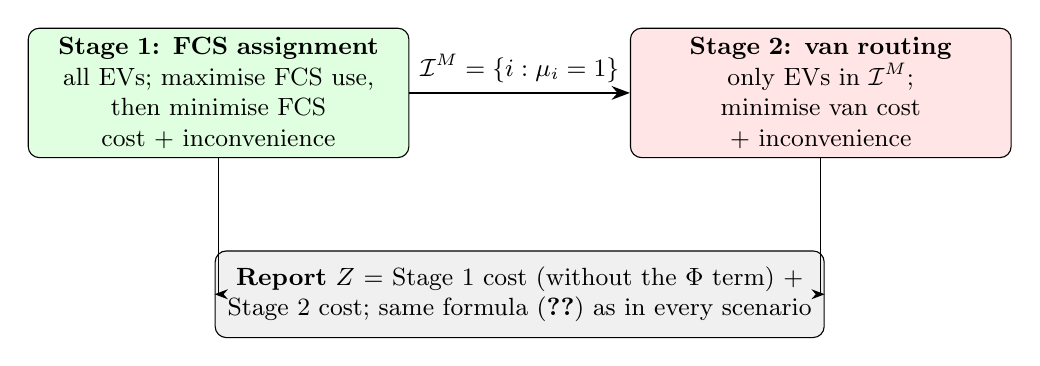
\begin{tikzpicture}[>=Stealth,box/.style={draw,rounded corners,align=center,minimum height=1.1cm,font=\small}]
  \node[box,fill=green!12,text width=4.6cm] (s1) {\textbf{Stage 1: FCS assignment}\\all EVs; maximise FCS use,\\then minimise FCS cost + inconvenience};
  \node[box,fill=red!10,text width=4.6cm,right=2.8cm of s1] (s2) {\textbf{Stage 2: van routing}\\only EVs in $\I^M$;\\minimise van cost + inconvenience};
  \draw[->,thick] (s1) -- node[above,font=\small]{$\I^M=\{i:\mu_i=1\}$} (s2);
  \node[box,fill=black!6,text width=7.5cm,below=2.0cm of $(s1)!0.5!(s2)$] (ev) {\textbf{Report} $Z=$ Stage~1 cost (without the $\Phi$ term) $+$ Stage~2 cost; same formula \eqref{eq:Z} as in every scenario};
  \draw[->] (s1) |- (ev); \draw[->] (s2) |- (ev);
\end{tikzpicture}
\end{center}

Stage~1 does not look at the vans, and Stage~2 cannot change what Stage~1 decided. That is the definition of ``FCS first, then MCS''.

%----------------------------------------------------------------
\subsection{Stage 1: assign EVs to fixed stations}

\textbf{Objective.}
\begin{equation}
\begin{split}
\min\ Z^{(1)}=\;&\underbrace{\Phi\sum_{i\in\I}\mu_i}_{\text{FCS first}}
+\underbrace{c^{EV}\sum_i\sum_{f\in\F_i}d_{if}Y_{if}}_{Z_1}
+\underbrace{Z^F_{\text{energy}}}_{\text{FCS part of }Z_4}\\
&+\underbrace{\sum_i\sum_{f\in\F_i}\rho^F_{if}Y_{if}+\alpha\sum_i w_i(C_i-r_i)+c^L\sum_i w_iL_i}_{\text{FCS customers' inconvenience}}
\end{split}
\label{eq:obj1}
\end{equation}
with $C_i=S_i+\tau^F_iY_i$ in this stage. $\Phi$ is a penalty for handing an EV to the vans. It is chosen larger than anything an extra FCS customer can add to the rest of \eqref{eq:obj1}, e.g.
\[
\Phi > \max_{i}\max_{f\in\F_i}\big(c^{EV}d_{if}+\pi^{\max}E_i+\rho^F_{if}\big)+n\,(\alpha+c^L)\,w_{\max}\,T,
\]
so Stage~1 first \textbf{maximises the number of EVs served at an FCS}, and only among those solutions minimises FCS cost and inconvenience. ($\pi^{\max}$ is the highest grid price.) A numerically safer equivalent is to solve twice: first $\max\sum_iY_i$, then fix that number and minimise the rest.
\ifTOU
Because $Z^F_{\text{energy}}$ uses the peak price, Stage~1 may \emph{start sessions later} to leave the peak, if the price saving beats the extra waiting cost (Section~\ref{sec:expect}).
\fi

\textbf{Constraints.}
\begin{align}
\sum_{g\in\G_i}y_{ig}+\mu_i &= 1 && \forall i\in\I \label{eq:s1assign}\\
S_i &\ge r_i+\sum_{f\in\F_i}t_{if}Y_{if} && \forall i\in\I \label{eq:fcsarr}\\
S_i &\le r_i+T\,(1-\mu_i) && \forall i\in\I \label{eq:s1park}\\
S_j &\ge S_i+\tau^F_i-(T+\tau^F_i)(3-y_{ig}-y_{jg}-o_{ij}) && \forall g,\ (i,j)\in\mathcal{P}_g \label{eq:disj1}\\
S_i &\ge S_j+\tau^F_j-(T+\tau^F_j)(2-y_{ig}-y_{jg}+o_{ij}) && \forall g,\ (i,j)\in\mathcal{P}_g \label{eq:disj2}\\
\sum_i y_{ig_1} &\ge \sum_i y_{ig_2} && \forall f,\ \G_f=\{g_1,g_2\} \label{eq:gunsym}\\
S_i+\tau^F_iY_i &\le T,\qquad L_i\ge S_i+\tau^F_iY_i-l_i && \forall i\in\I \label{eq:s1time}
\end{align}
\ifTOU plus the time-of-use split \eqref{eq:tou1}--\eqref{eq:tou5} of each FCS session (Section~\ref{sec:price}).\fi
\desc{\eqref{eq:s1assign}: every EV either gets one reachable gun or is handed to the vans. An EV that reaches no FCS ($\G_i=\emptyset$) is forced to $\mu_i=1$. \eqref{eq:fcsarr}: an FCS session cannot start before the EV has asked and driven to the station. \eqref{eq:s1park}: for an EV handed to the vans, $S_i$ is parked at $r_i$, so it adds no waiting in Stage~1 (its real start time is decided in Stage~2). \eqref{eq:disj1}--\eqref{eq:disj2}: two EVs on the same gun do not overlap; $o_{ij}$ picks who goes first. With two guns per station this means at most two EVs charge at a station at a time. \eqref{eq:gunsym}: symmetry breaking between the two identical guns (optional). \eqref{eq:s1time}: finished by $T$; lateness.}

\textbf{Optional acceptability rule.} An operator may refuse to send a driver to a station that is ``too inconvenient'', e.g.\ only allow gun $g$ of station $f$ for EV $i$ if $\hat\rho^F_{if}\le\bar\rho$. This only shrinks $\G_i$, so EVs whose stations are all too far go to the vans. Report results with and without it.

\textbf{Output:} $\I^M=\{i:\mu_i=1\}$, the EVs left for the vans; plus each FCS customer's gun and start time.

%----------------------------------------------------------------
\subsection{Stage 2: route the vans to the leftover EVs}

Stage~2 is a vehicle routing problem with time windows, on the EVs in $\I^M$ only. Here $C_i=S_i+\tau^M_i$.

\textbf{Objective.}
\begin{equation}
\begin{split}
\min\ Z^{(2)}=\;&\underbrace{c^M\sum_m\sum_{(i,j)\in\A^M}d_{ij}x_{ijm}}_{Z_2}+\underbrace{\sum_m c^D_mu_m}_{Z_3}+\underbrace{Z^M_{\text{energy}}}_{\text{van part of }Z_4}\\
&+\underbrace{\sum_{i\in\I^M}\sum_m\rho^M_{im}z_{im}+\alpha\sum_{i\in\I^M}w_i(C_i-r_i)+c^L\sum_{i\in\I^M}w_iL_i}_{\text{van customers' inconvenience}}
\end{split}
\label{eq:obj2}
\end{equation}
Since every EV in $\I^M$ must be served by some van, $Z^M_{\text{energy}}$ and the $\rho^M$ term are constants here. They are kept so that $Z^{(2)}$ is the true cost of Stage~2. Waiting and lateness make the vans visit urgent EVs early.

\textbf{Constraints.}
\begin{align}
\sum_{m\in\M}z_{im} &= 1 && \forall i\in\I^M \label{eq:s2assign}\\
\sum_{j:(0,j)\in\A^M}x_{0jm} = \sum_{i:(i,n+1)\in\A^M}x_{i,n+1,m} &= u_m && \forall m \label{eq:depot}\\
\sum_{i:(i,j)\in\A^M}x_{ijm} = \sum_{k:(j,k)\in\A^M}x_{jkm} &= z_{jm} && \forall j\in\I^M,\ m \label{eq:flow}\\
\sum_{i\in\I^M}z_{im} &\le Q_m\,u_m && \forall m \label{eq:cap}\\
\sum_{i\in\I^M}\frac{E_i}{\eta}z_{im}+\beta\sum_{(i,j)\in\A^M}d_{ij}x_{ijm} &\le B_m\,u_m && \forall m \label{eq:batt}
\end{align}
\begin{align}
S_j &\ge \max\{r_j,\ t_{0j}\,x_{0jm}\} && \forall j\in\I^M,\ m \label{eq:depart}\\
S_j &\ge S_i+\tau^M_i+t_{ij}-(T+\tau^M_i+t_{ij})(1-x_{ijm}) && \forall i\neq j,\ m \label{eq:seq}\\
S_i+\tau^M_i+t_{i,n+1} &\le T+(\tau^M_i+t_{i,n+1})(1-x_{i,n+1,m}) && \forall i,\ m \label{eq:return}\\
S_i+\tau^M_i \le T,\quad L_i &\ge S_i+\tau^M_i-l_i && \forall i\in\I^M \label{eq:s2time}\\
u_m &\ge u_{m+1} && m<|\M| \label{eq:vansym}
\end{align}
\desc{\eqref{eq:s2assign}: each leftover EV gets one van. \eqref{eq:depot}: a used van leaves and returns to the depot once. \eqref{eq:flow}: each EV on van $m$ is entered and left exactly once by that van. \eqref{eq:cap}: at most $Q_m$ EVs per van. \eqref{eq:batt}: delivered energy (with transfer losses) plus driving energy fits in the van battery. \eqref{eq:depart}: no start before the request, or before the van can drive there from the depot (written as two linear constraints). \eqref{eq:seq}: if the van goes $i\to j$, it finishes $i$ and drives to $j$ before starting $j$. This gives one EV at a time and removes subtours (MTZ-type). \eqref{eq:return}: back at the depot by $T$. \eqref{eq:s2time}: finished by $T$; lateness. \eqref{eq:vansym}: use identical vans in index order.}

\textbf{If Stage 2 is infeasible} (too many leftover EVs for the fleet by $T$), the sequential policy has \emph{failed} on that instance. For diagnosis, add $s_i\in\{0,1\}$ (``unserved''), replace \eqref{eq:s2assign} by $\sum_mz_{im}+s_i=1$ and add $\Phi^U\sum_is_i$ to \eqref{eq:obj2}. Then report the number of EVs that could not be served. This is a useful comparison with the integrated scenario, which may serve all of them.

%----------------------------------------------------------------
\subsection{Reported value}
\[
Z^{\text{S\scen}}=\big(Z^{(1)*}-\Phi\,|\I^M|\big)+Z^{(2)*},
\]
which is exactly \eqref{eq:Z} evaluated at the combined solution. The stage-1 solution plus the stage-2 solution is a feasible solution of the integrated model (S\ifTOU 4\else 3\fi), so
$Z^{\text{S\ifTOU 4\else 3\fi}}\le Z^{\text{S\scen}}$. The difference is the \emph{value of integration}.

\else
%---------------------------------------------------------------- INT
\subsection{Objective}
\begin{equation}
\min\ Z \quad\text{as in \eqref{eq:Z}, with }Z^F_{\text{energy}}=\ifTOU P^F\textstyle\sum_i\big[\pi^\off(\theta^1_i+\theta^3_i)+\pi^\pk\theta^2_i\big]\else\pi^F\textstyle\sum_iE_iY_i\fi,\quad C_i=S_i+\tau^F_iY_i+\tau^M_iZ_i. \label{eq:objint}
\end{equation}
Written out in full:
\begin{align*}
\min\ Z=\;& c^{EV}\sum_i\sum_{f\in\F_i}d_{if}Y_{if}+c^M\sum_m\sum_{(i,j)\in\A}d_{ij}x_{ijm}+\sum_mc^D_mu_m\\
&+\ifTOU P^F\sum_i\big[\pi^\off(\theta^1_i+\theta^3_i)+\pi^\pk\theta^2_i\big]\else\pi^F\sum_iE_iY_i\fi
+\pi^M\sum_i\sum_m\frac{E_i}{\eta}z_{im}\\
&+\sum_i\sum_{f\in\F_i}\rho^F_{if}Y_{if}+\sum_i\sum_m\rho^M_{im}z_{im}+\alpha\sum_iw_i(C_i-r_i)+c^L\sum_iw_iL_i .
\end{align*}
Every term is linear. One model weighs everything at once: an EV goes to a van exactly when the van's extra km, dispatch and energy cost are outweighed by the effort and waiting it saves the driver\ifTOU, or by the peak-price energy it avoids\fi.

\subsection{Constraints}

\textbf{Assignment.}
\begin{equation}
\sum_{g\in\G_i}y_{ig}+\sum_{m\in\M}z_{im}=1\qquad\forall i\in\I \label{eq:assign}
\end{equation}
\desc{Exactly one resource per EV: one reachable gun or one van. EVs that reach no FCS are forced onto a van.}

\textbf{Fixed stations.}
\begin{align}
S_i &\ge r_i+\sum_{f\in\F_i}t_{if}Y_{if} && \forall i \label{eq:fcsarr}\\
S_j &\ge S_i+\tau^F_i-(T+\tau^F_i)(3-y_{ig}-y_{jg}-o_{ij}) && \forall g,\ (i,j)\in\mathcal{P}_g \label{eq:disj1}\\
S_i &\ge S_j+\tau^F_j-(T+\tau^F_j)(2-y_{ig}-y_{jg}+o_{ij}) && \forall g,\ (i,j)\in\mathcal{P}_g \label{eq:disj2}\\
\sum_iy_{ig_1} &\ge \sum_iy_{ig_2} && \forall f,\ \G_f=\{g_1,g_2\} \label{eq:gunsym}
\end{align}
\desc{\eqref{eq:fcsarr}: an FCS session starts after the request and the drive to the station (for a van customer this is just $S_i\ge r_i$). \eqref{eq:disj1}--\eqref{eq:disj2}: EVs on the same gun do not overlap; $o_{ij}$ chooses the order. \eqref{eq:gunsym}: optional symmetry breaking.}

\textbf{Vans: routes, capacity, battery.}
\begin{align}
\sum_{j:(0,j)\in\A}x_{0jm}=\sum_{i:(i,n+1)\in\A}x_{i,n+1,m} &= u_m && \forall m \label{eq:depot}\\
\sum_{i:(i,j)\in\A}x_{ijm}=\sum_{k:(j,k)\in\A}x_{jkm} &= z_{jm} && \forall j\in\I,\ m \label{eq:flow}\\
\sum_iz_{im} &\le Q_mu_m && \forall m \label{eq:cap}\\
\sum_i\frac{E_i}{\eta}z_{im}+\beta\sum_{(i,j)\in\A}d_{ij}x_{ijm} &\le B_mu_m && \forall m \label{eq:batt}
\end{align}
\desc{\eqref{eq:depot}: a used van leaves and returns once. \eqref{eq:flow}: each EV on van $m$ is visited exactly once by it. \eqref{eq:cap}: at most $Q_m$ EVs. \eqref{eq:batt}: delivered energy (with losses) plus driving energy fits in the battery.}

\textbf{Vans: timing (one EV at a time, no subtours).}
\begin{align}
S_j &\ge t_{0j}\,x_{0jm} && \forall j\in\I,\ m \label{eq:depart}\\
S_j &\ge S_i+\tau^M_i+t_{ij}-(T+\tau^M_i+t_{ij})(1-x_{ijm}) && \forall i\neq j\in\I,\ m \label{eq:seq}\\
S_i+\tau^M_i+t_{i,n+1} &\le T+(\tau^M_i+t_{i,n+1})(1-x_{i,n+1,m}) && \forall i,\ m \label{eq:return}
\end{align}
\desc{\eqref{eq:depart}: the first stop cannot start before the van has driven there. \eqref{eq:seq}: $i\to j$ means finish $i$, drive, then start $j$; start times rise along a route, so no subtour can close. \eqref{eq:return}: back at the depot by $T$.}

\textbf{Horizon and lateness.}
\begin{equation}
C_i\le T,\qquad L_i\ge C_i-l_i\qquad\forall i\in\I \label{eq:time}
\end{equation}
\desc{Every EV is fully charged within the horizon; $L_i$ measures lateness.}

\ifTOU
\textbf{Time-of-use split.} Constraints \eqref{eq:tou1}--\eqref{eq:tou5} of Section~\ref{sec:price}.
\fi

\textbf{Symmetry and domains.}
\begin{equation}
u_m\ge u_{m+1};\qquad y,z,x,u,o\ifTOU,\kappa\fi\in\{0,1\};\qquad S_i,L_i\ifTOU,\theta^p_i\fi\ge0 \label{eq:dom}
\end{equation}
\fi

%=====================================================================
\section{Learning-to-optimise (RL) formulation}\label{sec:rl}

\textbf{Main rule:} the reward of each action is \emph{minus the increase in $Z$ that the action causes}. The rewards over an episode then add up to $-Z$ of the solution the policy builds. RL and MILP results are measured on the same yardstick \eqref{eq:Z}, and the MILP optimum is the benchmark for the RL gap.

\ifSEQ
%---------------------------------------------------------------- RL SEQ
The RL pipeline has the same two stages as the MILP.

\subsection{Stage 1 policy: FCS assignment}
\begin{itemize}[leftmargin=1.4em,itemsep=2pt]
  \item \textbf{Episode / epochs:} EVs are taken in order of request time $r_i$ (ties: higher $w_i$ first). One decision per EV.
  \item \textbf{State:} features of the current EV $k$ ($E_k,r_k,l_k,w_k,R_k$, location); for each gun $g$ the time $F_g$ it becomes free; summary features of the EVs still to come (count and positions near each station)\ifTOU; the current price and the time until $T_1$ and $T_2$\fi.
  \item \textbf{Action:} a gun $g\in\G_k$, or ``hand to vans''. \textbf{FCS-first mask:} ``hand to vans'' is allowed \emph{only} if no gun can finish EV $k$ by $T$ (or, with the optional rule, if all remaining guns have $\hat\rho^F_{kf}>\bar\rho$).
  \ifTOU\item \textbf{Optional timing action:} ``gun $g$, start after the peak'', i.e.\ $S_k=\max\{\text{earliest},T_2\}$, allowed only if the session still ends by $T$.\fi
  \item \textbf{Transition:} $S_k=\max\{r_k+t_{kf},F_g\}$ (or later, for the timing action); $F_g\leftarrow S_k+\tau^F_k$.
  \item \textbf{Reward:} $-\Big[c^{EV}d_{kf}+\text{energy}_k+\rho^F_{kf}+\alpha w_k(S_k+\tau^F_k-r_k)+c^Lw_k(S_k+\tau^F_k-l_k)^+\Big]$, where energy$_k$ = \ifTOU$P^F\big[\pi^\off\cdot(\text{off-peak hours of }[S_k,S_k+\tau^F_k])+\pi^\pk\cdot(\text{peak hours})\big]$, computed exactly in the simulator\else$\pi^FE_k$\fi. Handing an EV to the vans gives reward $0$ here; its cost is counted in Stage~2.
\end{itemize}
Note: a simple baseline for Stage~1 is the greedy rule ``gun with the largest one-step reward''. What RL can learn on top of this is, for example, to keep a nearby gun free for an urgent EV that arrives later.

\subsection{Stage 2 policy: van routing over $\I^M$}
\begin{itemize}[leftmargin=1.4em,itemsep=2pt]
  \item \textbf{Epochs:} whenever a van becomes free (the earliest-free van decides first).
  \item \textbf{State:} for each van: position, time free, remaining battery $b_m$, EVs served so far, dispatched or not; for each unserved EV in $\I^M$: location, $E_i,r_i,l_i,w_i$; current time.
  \item \textbf{Action:} the next EV $j$ for this van, or ``return to depot'' (ends the route). Mask: $j$ must be feasible: battery covers $E_j/\eta$ plus driving to $j$ and back to the depot, the count stays $\le Q_m$, and $j$ can be finished with the van back at the depot by $T$.
  \item \textbf{Transition:} $S_j=\max\{r_j,\ \text{time free}+t_{\text{pos},j}\}$; the van moves to $j$ and is free at $S_j+\tau^M_j$; $b_m$ falls by $E_j/\eta+\beta d_{\text{pos},j}$.
  \item \textbf{Reward:} serving $j$: $-\Big[c^Md_{\text{pos},j}+c^D_m[\text{first stop}]+\pi^M\frac{E_j}{\eta}+\rho^M_{jm}+\alpha w_j(S_j+\tau^M_j-r_j)+c^Lw_j(S_j+\tau^M_j-l_j)^+\Big]$; returning: $-c^Md_{\text{pos},0}$. EVs still unserved at the end: $-\Phi^U$ each.
  \item \textbf{Policy:} an attention-based routing policy (e.g.\ Kool et al., 2019, ``Attention, Learn to Solve Routing Problems!'') trained with REINFORCE or PPO. Baseline: nearest-feasible-EV heuristic.
\end{itemize}
Episode return of Stage~1 + Stage~2 $=-Z^{\text{S\scen}}$.

\else
%---------------------------------------------------------------- RL INT
One policy decides both who serves each EV and the van routes.
\begin{itemize}[leftmargin=1.4em,itemsep=2pt]
  \item \textbf{Episode / epochs:} EVs are taken in order of request time $r_i$ (ties: higher $w_i$ first). One decision per EV.
  \item \textbf{State:} (i) the current EV $k$: location, $E_k,r_k,l_k,w_k,R_k$, reachable stations; (ii) each gun $g$: time $F_g$ it becomes free; (iii) each van $m$: current end-of-route position, time free, remaining battery $b_m$, EVs served, dispatched or not; (iv) embeddings of the not-yet-assigned EVs (for look-ahead)\ifTOU; (v) current price, time until $T_1$ and $T_2$\fi.
  \item \textbf{Action:} $a\in\G_k\cup\M$: a gun, or a van (EV $k$ is appended to the end of that van's route). \textbf{Mask} infeasible actions: a gun that cannot finish $k$ by $T$; a van without enough battery for $E_k/\eta$ plus the drive to $k$ and back to the depot, with $Q_m$ reached, or unable to finish $k$ and return by $T$.
  \ifTOU\item \textbf{Optional timing action:} ``gun $g$, start after the peak'' ($S_k=\max\{\text{earliest},T_2\}$, if it still ends by $T$).\fi
  \item \textbf{Transition:} gun: $S_k=\max\{r_k+t_{kf},F_g\}$, $F_g\leftarrow S_k+\tau^F_k$. Van: $S_k=\max\{r_k,\ \text{free}_m+t_{\text{pos}_m,k}\}$, then the van moves to $k$, $\text{free}_m\leftarrow S_k+\tau^M_k$, $b_m\mathrel{-}=E_k/\eta+\beta d_{\text{pos}_m,k}$.
  \item \textbf{Reward} $=-\Delta Z$:
  \begin{align*}
  \text{gun } g\text{ at }f:&\quad -\Big[c^{EV}d_{kf}+\text{energy}^F_k+\rho^F_{kf}+\alpha w_k(C_k-r_k)+c^Lw_k(C_k-l_k)^+\Big]\\
  \text{van } m:&\quad -\Big[c^M\big(d_{\text{pos}_m,k}+d_{k,0}-d_{\text{pos}_m,0}\big)+c^D_m[\text{first use}]+\pi^M\tfrac{E_k}{\eta}\\
  &\qquad\quad+\rho^M_{km}+\alpha w_k(C_k-r_k)+c^Lw_k(C_k-l_k)^+\Big]
  \end{align*}
  The van distance term is the \emph{change} in route length when $k$ is inserted before the return to the depot, so the sum over the episode equals the total route length (the return legs telescope). energy$^F_k$ = \ifTOU$P^F\big[\pi^\off\cdot(\text{off-peak hours})+\pi^\pk\cdot(\text{peak hours of }[S_k,C_k])\big]$, computed exactly by the simulator; no linearisation is needed in RL\else$\pi^FE_k$\fi.
  \item \textbf{Dead end:} if every action is masked, EV $k$ is unserved: reward $-\Phi^U$, and the episode continues. Report the count.
  \item \textbf{Policy:} masked categorical policy over guns and vans, encoder with attention over EVs, guns and vans; trained with PPO. Natural baseline: greedy, i.e.\ choose the action with the largest one-step reward. That is the pairwise rule ``smallest $\hat\rho$ + cost'' from Section~\ref{sec:inc}.
\end{itemize}
Restriction to note: vans serve EVs in assignment order (append only). A variant that inserts $k$ at the cheapest position of a route is more flexible but has a larger action space.
\fi

\textbf{Reward scaling.} For stable training divide every reward by a constant, e.g.\ the greedy baseline's average $Z$ on the training instances. This does not change the optimal policy.

%=====================================================================
\section{What to expect and what to report}\label{sec:expect}

\ifnum\scen=1
\begin{itemize}[leftmargin=1.4em,itemsep=2pt]
  \item Vans serve only EVs that reach no station, or that the stations cannot finish by $T$. If stations have spare capacity, very few vans are dispatched.
  \item Inconvenience is high for EVs far from the nearest station (worked example: Rs\,682 at the FCS, against Rs\,458 if a van had been allowed).
  \item With too few vans Stage~2 becomes infeasible (unserved EVs), even when the integrated model S3 could serve everyone. Report the smallest $|\M|$ at which S1 is feasible and compare it with S3.
\end{itemize}
\fi
\ifnum\scen=2
\begin{itemize}[leftmargin=1.4em,itemsep=2pt]
  \item \textbf{When does Stage~1 delay a session to avoid the peak?} Moving one hour of charging out of the peak saves $(\pi^\pk-\pi^\off)P^F=3\times22=$ Rs\,66, but delays completion by up to an hour, which costs $\alpha w_i\ge$ Rs\,200. So with the default values Stage~1 almost never delays. It mostly pays the higher price, and S2 costs roughly S1 plus the peak surcharge. Sessions start later only if $\alpha$ is small (try $\lambda<0.33$ in the sensitivity analysis).
  \item The van assignment is the same as in S1 unless Stage~1's timing changes which EVs fit at the stations. Stage~1 cannot use vans to escape the peak price.
  \item Extra KPI: \textbf{grid energy drawn at FCS during the peak}, $P^F\sum_i\theta^2_i$ (kWh). Compare with S4.
\end{itemize}
\fi
\ifnum\scen=3
\begin{itemize}[leftmargin=1.4em,itemsep=2pt]
  \item Vans take EVs for which the saved inconvenience exceeds the extra van cost (worked example: van chosen, saving Rs\,224). Expect vans to serve EVs that are far from every station, have low range (high $w_i$), or have early deadlines, while EVs near a station still use it.
  \item \textbf{Value of integration under flat price:} $Z^{\text{S1}}-Z^{\text{S3}}\ge0$. Report it per component ($Z_1,\dots,Z_5$): typically operating cost rises a little and inconvenience falls a lot.
  \item Vary $|\M|$ (0, 1, 2, \dots): the first few vans lower $Z$ sharply, then the effect levels off. That curve shows the scenarios where mobile chargers help most.
\end{itemize}
\fi
\ifnum\scen=4
\begin{itemize}[leftmargin=1.4em,itemsep=2pt]
  \item During the peak a van kWh costs about the same as an FCS kWh (Rs\,10.0 each), so the vans' energy disadvantage disappears and vans also absorb \emph{peak-hour} demand that would otherwise be charged on the grid at peak price.
  \item Expect more van usage than in S3, concentrated on requests in $[T_1,T_2]$, and lower grid energy at the stations during the peak, $P^F\sum_i\theta^2_i$, than in S2.
  \item \textbf{Value of integration under peak pricing:} $Z^{\text{S2}}-Z^{\text{S4}}$. It should be larger than $Z^{\text{S1}}-Z^{\text{S3}}$, because integration now also allows price arbitrage.
  \item \textbf{Peak pricing with full flexibility:} $Z^{\text{S4}}-Z^{\text{S3}}$ should be smaller than $Z^{\text{S2}}-Z^{\text{S1}}$: vans cushion the price increase.
\end{itemize}
\fi

\textbf{Cross-scenario comparison table} (fill in from the four runs):
\begin{center}
\renewcommand{\arraystretch}{1.2}
\begin{tabular}{@{}lll@{}}
\toprule
\textbf{Comparison} & \textbf{Measures} & \textbf{Expected sign} \\
\midrule
S1 $-$ S3 & value of integration, flat price & $\ge0$ \\
S2 $-$ S4 & value of integration, peak price & $\ge0$, larger than S1 $-$ S3 \\
S2 $-$ S1 & cost of peak pricing, FCS-first operator & $>0$ \\
S4 $-$ S3 & cost of peak pricing, flexible operator & $>0$, smaller than S2 $-$ S1 \\
\bottomrule
\end{tabular}
\end{center}
Report for each: $Z$ and its components, number of vans used, EVs per resource, mean and maximum inconvenience per EV, total lateness, peak-hour grid energy, solve time, and (for RL) the gap to the MILP optimum.

%=====================================================================
\appendix
\section{Illustrative parameter values}\label{app:values}

These are starting values for experiments, not data. All are meant to be varied in the analysis. Values in Rs.

\begin{center}
\renewcommand{\arraystretch}{1.15}
\begin{tabular}{@{}llp{6.2cm}@{}}
\toprule
\textbf{Parameter} & \textbf{Value} & \textbf{Note} \\
\midrule
$T$, $[T_1,T_2]$ & 7 h, $[2,6]$ & 16:00--23:00, peak 18:00--22:00 \\
$P^F$, $P^M$ & 22 kW, 30 kW & \\
$v$, $\beta$, $\eta$ & 25 km/h, 0.25 kWh/km, 0.9 & \\
$B_m$, $Q_m$, $|\M|$ & 150 kWh, 6, 2--6 & \\
$c^{EV}$, $c^M$, $c^D_m$ & Rs\,4/km, Rs\,15/km, Rs\,1500 & van km includes driver time \\
$\pi^F$ (flat) & Rs\,8.7/kWh & equals the time-average of the ToU tariff over $[0,T]$ \\
$\pi^\off$, $\pi^\pk$ (ToU) & Rs\,7/kWh, Rs\,10/kWh & $(3\times7+4\times10)/7=8.7$ \\
$c^{bat}$ & Rs\,2/kWh & van battery wear \\
$\pi^M$ & Rs\,10.7 (flat) / Rs\,9.0 (ToU) & $=\pi^F+c^{bat}$ / $=\pi^\off+c^{bat}$ \\
$\alpha$, $\alpha^D$ & Rs\,200/h, Rs\,100/h & value of time; extra for attended time \\
$h^F$, $h^M$, $\varphi$ & Rs\,50, Rs\,10, Rs\,100 & trip hassle, hand-over, range stress \\
$c^L$ & Rs\,300/h & lateness \\
$w_i$ & $1+2(1-R_i/R_{\max})$, $R_i\sim U[3,40]$ km & priority from remaining range \\
\bottomrule
\end{tabular}
\end{center}

The flat price is set to the time-average of the peak tariff. The price \emph{level} is then the same in both pricing cases, and only the price \emph{shape} differs. Without this, part of S1 vs S2 would just reflect a different average price.

\end{document}
"
%    pdflatex -jobname=scenario2_peak_sequential   "\def\scen{2}% =====================================================================
%  One source, four PDFs.  Build with build.sh (or by hand):
%    pdflatex -jobname=scenario1_flat_sequential   "\def\scen{1}% =====================================================================
%  One source, four PDFs.  Build with build.sh (or by hand):
%    pdflatex -jobname=scenario1_flat_sequential   "\def\scen{1}\input{scenario_master}"
%    pdflatex -jobname=scenario2_peak_sequential   "\def\scen{2}\input{scenario_master}"
%    pdflatex -jobname=scenario3_flat_integrated   "\def\scen{3}\input{scenario_master}"
%    pdflatex -jobname=scenario4_peak_integrated   "\def\scen{4}\input{scenario_master}"
%  (run each twice for cross-references)
% =====================================================================
\documentclass[11pt,a4paper]{article}
\usepackage[margin=2.2cm]{geometry}
\usepackage{amsmath,amssymb,amsfonts}
\usepackage{booktabs,array,tabularx}
\usepackage{enumitem}
\usepackage[table]{xcolor}
\usepackage{tikz}
\usetikzlibrary{arrows.meta,positioning,calc}
\usepackage[colorlinks=true,linkcolor=blue!50!black,urlcolor=blue!50!black]{hyperref}
\usepackage{titlesec}
\titleformat{\section}{\large\bfseries}{\thesection}{0.8em}{}
\titleformat{\subsection}{\normalsize\bfseries}{\thesubsection}{0.8em}{}
\setlength{\parindent}{0pt}
\setlength{\parskip}{5pt}

% ---------------- scenario switches ----------------
\ifdefined\scen\else\def\scen{1}\fi
\newif\ifTOU \TOUfalse   % true = time-of-use (peak) price
\newif\ifSEQ \SEQfalse   % true = FCS first, then MCS
\ifnum\scen=1 \SEQtrue \fi
\ifnum\scen=2 \TOUtrue \SEQtrue \fi
\ifnum\scen=4 \TOUtrue \fi

\newcommand{\pricename}{\ifTOU time-of-use price (dearer evening peak)\else single (flat) price all day\fi}
\newcommand{\structname}{\ifSEQ FCS first, then MCS (sequential)\else FCS and MCS together (integrated)\fi}

% ---------------- notation ----------------
\newcommand{\I}{\mathcal{I}}
\newcommand{\F}{\mathcal{F}}
\newcommand{\G}{\mathcal{G}}
\newcommand{\M}{\mathcal{M}}
\newcommand{\N}{\mathcal{N}}
\newcommand{\A}{\mathcal{A}}
\newcommand{\Rs}{\text{Rs}\,}
\newcommand{\pk}{\mathrm{pk}}
\newcommand{\off}{\mathrm{off}}
\newcommand{\desc}[1]{\par\vspace{-2pt}{\small\color{black!75}\textit{Meaning:} #1}\par\vspace{4pt}}
\newcommand{\cell}[2]{\ifnum\scen=#1\cellcolor{blue!18}\textbf{S#1 (this document)}\\\textbf{#2}\else S#1\\#2\fi}

\title{\textbf{EV Charging Network Optimisation}\\[4pt]
\large Scenario \scen: \pricename\ $+$ \structname\\[2pt]
\normalsize MILP and RL formulation}
\author{CP 320 OR for Mobility Management, course project}
\date{2 October 2026}

\begin{document}
\maketitle

%=====================================================================
\section{Where this scenario sits}

The project studies four scenarios: two ways of pricing grid electricity, times two ways of making the decisions.

\begin{center}
\renewcommand{\arraystretch}{1.5}
\begin{tabular}{>{\raggedright\arraybackslash}p{4.2cm}|>{\centering\arraybackslash}p{4.6cm}|>{\centering\arraybackslash}p{4.6cm}}
 & \textbf{Flat price all day} & \textbf{Time-of-use (peak) price} \\ \hline
\textbf{Sequential:} FCS first, leftover EVs to MCS &
\begin{tabular}[c]{@{}c@{}}\cell{1}{flat + sequential}\end{tabular} &
\begin{tabular}[c]{@{}c@{}}\cell{2}{peak + sequential}\end{tabular} \\ \hline
\textbf{Integrated:} FCS and MCS decided together &
\begin{tabular}[c]{@{}c@{}}\cell{3}{flat + integrated}\end{tabular} &
\begin{tabular}[c]{@{}c@{}}\cell{4}{peak + integrated}\end{tabular} \\
\end{tabular}
\end{center}

\textbf{The four scenarios do not have four different objectives.} They share \emph{one} cost yardstick $Z$ (Section~\ref{sec:obj}): the same cost terms and the same customer inconvenience (Section~\ref{sec:inc}). Only two things change:
\begin{itemize}[leftmargin=1.4em,itemsep=1pt]
  \item \textbf{Pricing} changes the formula for one term, the FCS energy cost (Section~\ref{sec:price}).
  \item \textbf{Decision structure} changes \emph{how} $Z$ is minimised: in one model (integrated), or in two stages (sequential), where each stage minimises its own part of $Z$.
\end{itemize}
Because the yardstick is the same, the four optimal values can be compared directly. The differences measure the \emph{value of integration} (S1$\to$S3, S2$\to$S4) and the \emph{effect of peak pricing} (S1$\to$S2, S3$\to$S4).

\ifnum\scen=1
\textbf{This scenario (S1)} is the baseline, the ``status quo''. Electricity costs the same at every hour, every EV that can be charged at a fixed station is sent there, and vans only take what is left over.
\fi
\ifnum\scen=2
\textbf{This scenario (S2)} keeps the FCS-first rule of S1, but grid electricity is dearer during the evening peak. Stage~1 can react to the price only by \emph{rescheduling} FCS sessions. It cannot hand a peak-hour EV to a van.
\fi
\ifnum\scen=3
\textbf{This scenario (S3)} keeps the flat price of S1, but the operator decides FCS and MCS service \emph{together}. An EV can be sent to a van even when a fixed station could take it, whenever that lowers total cost plus inconvenience.
\fi
\ifnum\scen=4
\textbf{This scenario (S4)} is the most flexible one: peak pricing at fixed stations, and FCS and MCS decided together. Van energy was bought off-peak, so vans can also be used to keep charging \emph{out of the expensive peak}.
\fi

%=====================================================================
\section{Setting and assumptions}\label{sec:setting}

\textbf{Time.} The planning horizon is $[0,T]$ with $T=7$\,h (16:00--23:00). It contains the evening peak window $[T_1,T_2]=[2,6]$ (18:00--22:00). The horizon is the same in all four scenarios. It is wider than the peak itself so that, under peak pricing, there is cheaper time on both sides of the peak.\ifTOU\else\ In this scenario the price is flat, so the window plays no role in the model.\fi

\textbf{Assumptions} (the same as MILP v3, plus two about energy):
\begin{enumerate}[leftmargin=1.6em,itemsep=1pt]
  \item Static, continuous time. All requests in the horizon are known at time $0$, and request $i$ becomes active at $r_i$.
  \item An EV served by an FCS drives there itself on its own battery (only to stations within its range $R_i$). The driver stays with the car while it waits for a free gun and while it charges.
  \item An EV served by an MCS stays parked where it is, and the driver is free in the meantime.
  \item Each FCS gun and each van charges one EV at a time, without interruption, at constant power.
  \item A van's battery covers both its driving and the energy it delivers. \textbf{The van battery is charged at the depot before the horizon starts}\ifTOU, i.e.\ at the off-peak price\fi, and is not recharged during the horizon.
  \item Every EV must be fully charged by $T$ (hard). Finishing after the driver's desired time $l_i$ is allowed but penalised.
\end{enumerate}

%=====================================================================
\section{Notation}\label{sec:notation}

\subsection*{Sets}
\begin{tabularx}{\textwidth}{@{}lX@{}}
\toprule
$\I=\{1,\dots,n\}$ & EV charging requests \\
$\F$; $\G_f$ ($|\G_f|=2$); $\G=\bigcup_f\G_f$ & fixed charging stations; guns of FCS $f$; all guns ($f(g)$ = station of gun $g$) \\
$\F_i=\{f: d_{if}\le R_i\}$, $\G_i=\bigcup_{f\in\F_i}\G_f$ & stations / guns EV $i$ can reach on its remaining range \\
$\M$ & mobile charging vans (MCS) \\
$0,\ n+1$ & depot as start node / end node (same place) \\
$\N=\{0\}\cup\I\cup\{n+1\}$, $\A$ & routing nodes; allowed van arcs $(i,j)$, $i\in\{0\}\cup\I$, $j\in\I\cup\{n+1\}$, $i\neq j$ \\
$\mathcal{P}_g=\{(i,j): i<j,\ g\in\G_i\cap\G_j\}$ & pairs of EVs that could share gun $g$ \\
\ifSEQ
$\I^M\subseteq\I$ & EVs handed to the vans by Stage~1 (an \emph{output} of Stage~1, a fixed input to Stage~2) \\
$\N^M$, $\A^M$ & routing nodes / arcs restricted to $\I^M$ \\
\fi
\bottomrule
\end{tabularx}

\subsection*{Parameters}
\begin{tabularx}{\textwidth}{@{}lX@{}}
\toprule
$E_i,\ r_i,\ l_i,\ R_i$ & energy demand (kWh), request time, desired completion time (h), remaining range (km) \\
$w_i\ge1$ & priority of EV $i$; $w_i=1+\kappa(1-R_i/R_{\max})$, so low-range EVs weigh more \\
$P^F,\ P^M$ & charging power of an FCS gun (22\,kW) / of a van (e.g.\ 30\,kW) \\
$\tau^F_i=E_i/P^F,\ \tau^M_i=E_i/P^M$ & charging time of EV $i$ at an FCS / by a van (h) \\
$d_{if},t_{if}$;\ $d_{ij},t_{ij}$ & distance (km) and time (h): EV$\to$FCS; between routing nodes ($t=d/v$) \\
$B_m,\ Q_m,\ \beta,\ \eta$ & van battery (kWh), max EVs per van, van consumption (kWh/km), transfer efficiency \\
$c^{EV},\ c^M,\ c^D_m$ & cost per km of EV driving, per km of van driving; fixed dispatch cost of van $m$ \\
\ifTOU
$\pi^\off,\ \pi^\pk$ & grid price (Rs/kWh) off-peak / in $[T_1,T_2]$, with $\pi^\pk\ge\pi^\off$ \\
\else
$\pi^F$ & grid price (Rs/kWh), the same at every hour \\
\fi
$c^{bat}$ & van battery wear per kWh cycled \\
$\pi^M$ & cost of 1 kWh taken from a van battery: $\pi^M=\ifTOU\pi^\off\else\pi^F\fi+c^{bat}$ (Section~\ref{sec:price}) \\
$\alpha,\ \alpha^D,\ h^F,\ h^M,\ \varphi,\ c^L$ & inconvenience coefficients (Section~\ref{sec:inc}) \\
\bottomrule
\end{tabularx}

\subsection*{Decision variables}
\begin{tabularx}{\textwidth}{@{}llX@{}}
\toprule
$y_{ig}$ & $\{0,1\}$ & EV $i$ charged at gun $g\in\G_i$ \\
$z_{im}$ & $\{0,1\}$ & EV $i$ served by van $m$ \\
$x_{ijm}$ & $\{0,1\}$ & van $m$ drives arc $(i,j)$ \\
$u_m$ & $\{0,1\}$ & van $m$ is dispatched \\
$o_{ij}$ & $\{0,1\}$ & for EVs $i<j$ that could share a gun: 1 if $i$ is charged before $j$ \\
\ifSEQ
$\mu_i$ & $\{0,1\}$ & Stage~1 only: EV $i$ is handed to the van fleet \\
\fi
\ifTOU
$\theta^1_i,\theta^2_i,\theta^3_i$ & $\ge0$ & hours of EV $i$'s FCS session before / inside / after the peak \\
$\kappa^1_i,\kappa^3_i$ & $\{0,1\}$ & EV $i$'s FCS session starts before $T_1$ / ends after $T_2$ \\
\fi
$S_i$ & $\ge0$ & time charging of EV $i$ starts (h), on whichever resource \\
$L_i$ & $\ge0$ & lateness of EV $i$ beyond $l_i$ (h) \\
\bottomrule
\end{tabularx}

\textbf{Short-hands} (linear expressions, not new variables):
\[
Y_{if}=\sum_{g\in\G_f}y_{ig},\qquad Y_i=\sum_{g\in\G_i}y_{ig}\ (\text{EV $i$ uses an FCS}),\qquad Z_i=\sum_{m\in\M}z_{im}\ (\text{EV $i$ uses a van}),
\]
\[
C_i=S_i+\tau^F_i\,Y_i+\tau^M_i\,Z_i \quad\text{(time EV $i$ is fully charged).}
\]

%=====================================================================
\section{Customer inconvenience}\label{sec:inc}

This section is \textbf{identical in all four scenario documents}. Inconvenience is a property of the customer, not of the price or of the planning method.

\subsection{What we mean by inconvenience}

Inconvenience is \emph{what the driver loses} from the moment they ask for a charge ($r_i$) until the car is fully charged ($C_i$), \emph{converted into rupees} so it can be added to the operator's costs. A driver loses three different things:

\begin{enumerate}[leftmargin=1.6em,itemsep=2pt]
  \item \textbf{Waiting:} the car is not ready. This lasts $C_i-r_i$ hours and affects \emph{every} driver, FCS or MCS.
  \item \textbf{Effort:} only an FCS customer has to drive to the station and sit there while the car charges. An MCS customer stays at home or at work and does something else. Driving to a far station also uses scarce battery range, which causes stress (``range anxiety'').
  \item \textbf{A missed deadline:} the car is still not ready at the time $l_i$ the driver needs it.
\end{enumerate}

Each loss gets a price in Rs per hour (or per event). All of them are multiplied by the priority $w_i$: an hour of delay for an EV with 5\,km of range left counts more than for one with 40\,km.

\subsection{The three components}

\begin{center}
\renewcommand{\arraystretch}{1.3}
\begin{tabularx}{\textwidth}{@{}>{\raggedright\arraybackslash}p{2.6cm}>{\raggedright\arraybackslash}X>{\raggedright\arraybackslash}X>{\raggedright\arraybackslash}p{3.0cm}@{}}
\toprule
\textbf{Component} & \textbf{EV $i$ at FCS $f$} & \textbf{EV $i$ by a van} & \textbf{Known when?} \\
\midrule
Effort & $w_i\big[\alpha^D(t_{if}+\tau^F_i)+h^F+\varphi\,d_{if}/R_i\big]$: driving and sitting at the station, a fixed trip hassle, range stress & $w_i\,h^M$: being reachable and handing over the car & \textbf{Static:} known as soon as the resource is chosen \\
Waiting & $w_i\,\alpha\,(C_i-r_i)$ = drive + \emph{queue at the gun} + charge & $w_i\,\alpha\,(C_i-r_i)$ = \emph{wait for the van} + charge & \textbf{Dynamic:} depends on the queue / van route \\
Missed deadline & $w_i\,c^L\,L_i$, $L_i=\max\{0,C_i-l_i\}$ & same & Dynamic \\
\bottomrule
\end{tabularx}
\end{center}

\textbf{Coefficients.}
$\alpha$ (Rs/h) is the value of an hour the car is not ready.
$\alpha^D$ (Rs/h) is the \emph{extra} value of an hour the driver must personally spend driving or sitting at the station: an hour at the station costs $\alpha+\alpha^D$, an hour waiting at home for a van costs only $\alpha$.
$h^F,h^M$ (Rs) are fixed hassle costs of one trip to a station / one van hand-over.
$\varphi$ (Rs) is the range-stress cost of a trip that uses the \emph{whole} remaining range ($d_{if}/R_i\le1$ is the fraction used).
$c^L$ (Rs/h) is the cost per hour late.

\subsection{Pairwise form: inconvenience of a (customer, resource) pair}

The natural first idea is: \emph{for every pair (EV $i$, FCS $f$) and every pair (EV $i$, van $m$) there is an inconvenience number, and the operator picks the pair with the lowest cost plus inconvenience.} The static part fits this idea exactly:
\[
\boxed{\;\rho^F_{if}=w_i\Big[\alpha^D\,(t_{if}+\tau^F_i)+h^F+\varphi\,\frac{d_{if}}{R_i}\Big]\qquad
\rho^M_{im}=w_i\,h^M\;}
\]
These are \textbf{parameters}, computed before solving, one number per (EV, FCS) pair and per (EV, van) pair. In the objective they appear linearly: $\sum_i\sum_f\rho^F_{if}Y_{if}+\sum_i\sum_m\rho^M_{im}z_{im}$.

Note that $\rho^M_{im}$ does not depend on $m$. Vans are identical and all start at the same depot, so the driver does not care \emph{which} van comes, only \emph{when} it comes. That ``when'' is the waiting part.

\subsection{Why waiting cannot be a fixed pairwise number}

It is tempting to also write the waiting as a pairwise number, e.g.\ ``the van needs 5 minutes to reach EV $i$''. But that depends on \emph{where the van is coming from}, which depends on the route the model is still choosing: if EV $i$ is the 4th stop of a van, the wait is the time for three charging sessions plus four drives. Likewise, waiting at an FCS depends on how many EVs are queued at that gun. So waiting is not known before solving. It is a function of decision variables:
\[
\text{waiting cost of EV } i \;=\; w_i\,\alpha\,(C_i-r_i),\qquad C_i=S_i+\tau^F_iY_i+\tau^M_iZ_i .
\]
This is \textbf{linear} in the variables ($S_i$, $y$, $z$), so it fits in a MILP directly. The constraints of Section~\ref{sec:milp} make $S_i$ equal to the true start time, including driving, queueing at the gun and the van's route. The term $\sum_i w_i\alpha r_i$ is a constant and may be dropped when solving.

\textbf{Pairwise \emph{estimate}} (used for intuition, by the RL policy and in heuristics): if there is no queue and the van comes straight to $i$,
\[
\hat\rho^{F}_{if}=\rho^F_{if}+w_i\alpha\,(t_{if}+\tau^F_i),\qquad
\hat\rho^{M}_{im}=\rho^M_{im}+w_i\alpha\,(t^{\text{van}}_{m\to i}+\tau^M_i),
\]
where $t^{\text{van}}_{m\to i}$ is the time until van $m$ can reach $i$ from where it currently is. In the RL formulation (Section~\ref{sec:rl}) the van's position \emph{is} known at each decision, so there this estimate becomes exact.

\subsection{Total inconvenience and how it enters the objective}

\begin{equation}
\boxed{\;
Z_{\text{inc}}=\underbrace{\sum_{i\in\I}\sum_{f\in\F_i}\rho^F_{if}Y_{if}+\sum_{i\in\I}\sum_{m\in\M}\rho^M_{im}z_{im}}_{\text{effort (static, pairwise)}}
+\underbrace{\alpha\sum_{i\in\I}w_i\,(C_i-r_i)}_{\text{waiting (dynamic)}}
+\underbrace{c^L\sum_{i\in\I}w_i\,L_i}_{\text{missed deadline}}
\;}\label{eq:inc}
\end{equation}
All three parts are in rupees, so $Z_{\text{inc}}$ is simply added to the operating costs. Nothing has to be normalised.

\subsection{Worked example: your ``10 km to the FCS vs.\ van in 5 minutes'' case}

EV $i$: $E_i=20$\,kWh, $R_i=40$\,km (so $w_i=1$); nearest free FCS $d_{if}=10$\,km away, $t_{if}=0.4$\,h at 25\,km/h; a van finishing next door can reach it in 5\,min ($0.083$\,h), adding about 4\,km to its route. $\tau^F_i=20/22=0.909$\,h, $\tau^M_i=20/30=0.667$\,h. Coefficients from Appendix~\ref{app:values}, flat price.

\begin{center}
\renewcommand{\arraystretch}{1.25}
\begin{tabular}{@{}lrr@{}}
\toprule
 & \textbf{FCS} & \textbf{Van} \\
\midrule
Driving (EV / extra van km) & $4\times10=40.0$ & $15\times4=60.0$ \\
Energy & $8.7\times20=174.0$ & $10.7\times20/0.9=237.8$ \\
\textbf{Operating cost only} & \textbf{214.0} & \textbf{297.8} \\
\midrule
Effort $\rho$ & $100(0.4+0.909)+50+100\cdot\tfrac{10}{40}=205.9$ & $10.0$ \\
Waiting $\alpha(C_i-r_i)$ & $200\times1.309=261.8$ & $200\times0.75=150.0$ \\
\textbf{Cost + inconvenience} & \textbf{681.7} & \textbf{457.8} \\
\bottomrule
\end{tabular}
\end{center}

On operating cost alone the FCS is cheaper, so a cost-only model would \emph{always} send this driver 10\,km away. With inconvenience included the van is better by about Rs\,224, and the integrated model chooses $z_{im}=1$, as you expected. If the FCS were only 1\,km away, the FCS would win both comparisons. The inconvenience term is what makes the model choose between ``cheap for the operator'' and ``convenient for the driver'', rather than following a fixed rule.

\subsection{Relation to a single penalty $\rho_i$ per EV}

The first draft used a penalty $\rho_i$ that is charged whenever EV $i$ goes to \emph{any} FCS: $\sum_i\sum_f\rho_iy_{if}$. Because $\sum_f y_{if}=1-\sum_m z_{im}$, this only says ``a van is worth $\rho_i$ more to EV $i$'', and that holds whether the station is 1\,km or 15\,km away, and whether the van arrives in 5 minutes or in 3 hours. The form above fixes both problems: $\rho^F_{if}$ grows with the distance to \emph{that} station, and the waiting term grows with how late the van or the free gun actually is. The old model is the special case $\alpha=\alpha^D=\varphi=c^L=0$, $h^F=\rho_i$.

\subsection{Choosing the coefficients}
\begin{itemize}[leftmargin=1.4em,itemsep=2pt]
  \item Use a value of time for $\alpha$ (e.g.\ Rs\,150--300/h for urban car users), and set $\alpha^D\approx0.5\alpha$: sitting at a station is worse than waiting at home.
  \item Keep $c^L>\alpha$, so missing the deadline is worse than ordinary waiting.
  \item \textbf{Sensitivity analysis:} multiply all inconvenience coefficients by a factor $\lambda\in\{0,0.25,0.5,1,2,4\}$ and plot operating cost against total inconvenience. $\lambda=0$ is the pure cost-minimising operator, and large $\lambda$ is a customer-first operator. This trade-off curve is a strong result for the ``Analysis'' part of the project.
\end{itemize}

\subsection{What inconvenience does in \emph{this} scenario}
\ifSEQ
In a sequential scenario inconvenience \textbf{cannot move an EV from an FCS to a van}: Stage~1 sends every EV that \emph{can} use an FCS to one. It still matters inside each stage. In Stage~1 it decides \emph{which} station and \emph{when} (urgent EVs get the near station and the first free gun). In Stage~2 it decides the \emph{order} in which vans visit EVs (urgent EVs first). In the worked example, this scenario sends the driver 10\,km to the FCS. That is the weakness the integrated scenarios remove.
\else
In an integrated scenario inconvenience is weighed directly against operating cost when choosing the resource. That is how the worked example ends up with a van. It also decides which station and which gun order, and the order of each van route.
\fi

%=====================================================================
\section{Electricity price in this scenario}\label{sec:price}

\textbf{Van energy (same in all scenarios).} A van's battery is charged at the depot \emph{before} the horizon, so its energy was bought at the
\ifTOU off-peak \fi
price, whatever time the van later delivers it. Each kWh taken from the van also wears the battery ($c^{bat}$), and a fraction $1-\eta$ is lost in transfer:
\[
Z^M_{\text{energy}}=\pi^M\sum_{i\in\I}\sum_{m\in\M}\frac{E_i}{\eta}\,z_{im},\qquad \pi^M=\ifTOU\pi^\off\else\pi^F\fi+c^{bat}.
\]

\ifTOU
\textbf{FCS energy (time-of-use).} An FCS draws from the grid while it charges. Energy delivered inside $[T_1,T_2]$ costs $\pi^\pk$, and energy outside it costs $\pi^\off$. A session $[S_i,S_i+\tau^F_i]$ may overlap the peak partly. Split its duration into the hours before, inside and after the peak, $\theta^1_i+\theta^2_i+\theta^3_i$:
\[
Z^F_{\text{energy}}=P^F\sum_{i\in\I}\Big[\pi^\off(\theta^1_i+\theta^3_i)+\pi^\pk\,\theta^2_i\Big].
\]
Constraints \eqref{eq:tou1}--\eqref{eq:tou5} below make the $\theta$'s equal to the true overlaps. Peak hours are dearer, so the solver wants $\theta^1_i,\theta^3_i$ as large as possible. It is enough to bound them from above by the true off-peak overlap, and the constraints need one binary per side:
\begin{align}
\theta^1_i+\theta^2_i+\theta^3_i &= \tau^F_i\,Y_i && \forall i\in\I \label{eq:tou1}\\
\theta^1_i &\le \tau^F_i\,\kappa^1_i && \forall i\in\I \label{eq:tou2}\\
\theta^1_i &\le T_1-S_i+T\,(1-\kappa^1_i) && \forall i\in\I \label{eq:tou3}\\
\theta^3_i &\le \tau^F_i\,\kappa^3_i && \forall i\in\I \label{eq:tou4}\\
\theta^3_i &\le S_i+\tau^F_i-T_2+T\,(1-\kappa^3_i) && \forall i\in\I \label{eq:tou5}
\end{align}
\desc{\eqref{eq:tou1}: the FCS session's hours are split into three parts; for a van customer ($Y_i=0$) all three are zero. \eqref{eq:tou2}--\eqref{eq:tou3}: off-peak time before the peak is only possible if the session starts before $T_1$ ($\kappa^1_i=1$), and is at most $T_1-S_i$. \eqref{eq:tou4}--\eqref{eq:tou5}: the same for time after $T_2$. $\theta^2_i\ge0$ prevents counting more off-peak hours than exist. Checking the cases (entirely before / inside / after the peak, straddling one edge, covering the whole peak) shows that at the optimum the $\theta$'s equal the exact overlaps. This needs $\pi^\pk\ge\pi^\off$, which is true for a peak tariff.}

\textbf{Why vans become more attractive.} Compare the cost of 1\,kWh delivered to an EV during the peak (values from Appendix~\ref{app:values}):
FCS $=\pi^\pk=$ Rs\,10.0, van $=(\pi^\off+c^{bat})/\eta=9/0.9=$ Rs\,10.0. They are at parity. Under the flat price the van is about Rs\,3.2/kWh dearer (FCS Rs\,8.7, van $10.7/0.9=$ Rs\,11.9). Peak pricing therefore removes the vans' main cost disadvantage, but only for EVs whose FCS session would fall in the peak.
\ifSEQ\ In this sequential scenario Stage~1 cannot use that, because it does not consider vans. It can only shift FCS sessions in time.\fi
\else
\textbf{FCS energy (flat).} Every kWh delivered at a fixed station costs $\pi^F$, whenever it is delivered:
\[
Z^F_{\text{energy}}=\pi^F\sum_{i\in\I}E_i\,Y_i .
\]
The start time therefore does not affect the energy cost. Under the flat price a van kWh costs $(\pi^F+c^{bat})/\eta\approx$ Rs\,11.9 against Rs\,8.7 at an FCS (Appendix~\ref{app:values}), so on energy alone the FCS always wins.
\fi

%=====================================================================
\section{MILP formulation}\label{sec:milp}

\subsection{The common cost yardstick $Z$}\label{sec:obj}

For any complete solution (every EV assigned, every route and start time known), the system cost is
\begin{equation}
\boxed{\;
Z=\underbrace{c^{EV}\sum_{i}\sum_{f\in\F_i}d_{if}Y_{if}}_{Z_1:\ \text{EV driving}}
+\underbrace{c^M\sum_{m}\sum_{(i,j)\in\A}d_{ij}x_{ijm}}_{Z_2:\ \text{van driving}}
+\underbrace{\sum_m c^D_m u_m}_{Z_3:\ \text{dispatch}}
+\underbrace{Z^F_{\text{energy}}+Z^M_{\text{energy}}}_{Z_4:\ \text{energy}}
+\underbrace{Z_{\text{inc}}}_{Z_5:\ \text{inconv.\ \eqref{eq:inc}}}
\;}\label{eq:Z}
\end{equation}
$Z_4$ is defined in Section~\ref{sec:price}. $Z_1$--$Z_4$ are the operator's costs listed in the brief (EV travel, MCS travel, MCS operating cost) plus energy. $Z_5$ is the customer inconvenience penalty. \textbf{The same formula is used to report results in all four scenarios.}

\ifSEQ
%---------------------------------------------------------------- SEQ
\subsection{Structure: two stages}

\begin{center}
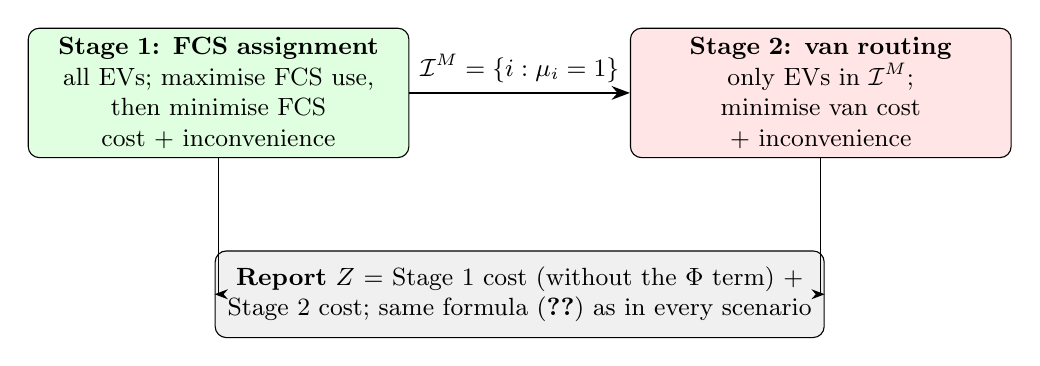
\begin{tikzpicture}[>=Stealth,box/.style={draw,rounded corners,align=center,minimum height=1.1cm,font=\small}]
  \node[box,fill=green!12,text width=4.6cm] (s1) {\textbf{Stage 1: FCS assignment}\\all EVs; maximise FCS use,\\then minimise FCS cost + inconvenience};
  \node[box,fill=red!10,text width=4.6cm,right=2.8cm of s1] (s2) {\textbf{Stage 2: van routing}\\only EVs in $\I^M$;\\minimise van cost + inconvenience};
  \draw[->,thick] (s1) -- node[above,font=\small]{$\I^M=\{i:\mu_i=1\}$} (s2);
  \node[box,fill=black!6,text width=7.5cm,below=2.0cm of $(s1)!0.5!(s2)$] (ev) {\textbf{Report} $Z=$ Stage~1 cost (without the $\Phi$ term) $+$ Stage~2 cost; same formula \eqref{eq:Z} as in every scenario};
  \draw[->] (s1) |- (ev); \draw[->] (s2) |- (ev);
\end{tikzpicture}
\end{center}

Stage~1 does not look at the vans, and Stage~2 cannot change what Stage~1 decided. That is the definition of ``FCS first, then MCS''.

%----------------------------------------------------------------
\subsection{Stage 1: assign EVs to fixed stations}

\textbf{Objective.}
\begin{equation}
\begin{split}
\min\ Z^{(1)}=\;&\underbrace{\Phi\sum_{i\in\I}\mu_i}_{\text{FCS first}}
+\underbrace{c^{EV}\sum_i\sum_{f\in\F_i}d_{if}Y_{if}}_{Z_1}
+\underbrace{Z^F_{\text{energy}}}_{\text{FCS part of }Z_4}\\
&+\underbrace{\sum_i\sum_{f\in\F_i}\rho^F_{if}Y_{if}+\alpha\sum_i w_i(C_i-r_i)+c^L\sum_i w_iL_i}_{\text{FCS customers' inconvenience}}
\end{split}
\label{eq:obj1}
\end{equation}
with $C_i=S_i+\tau^F_iY_i$ in this stage. $\Phi$ is a penalty for handing an EV to the vans. It is chosen larger than anything an extra FCS customer can add to the rest of \eqref{eq:obj1}, e.g.
\[
\Phi > \max_{i}\max_{f\in\F_i}\big(c^{EV}d_{if}+\pi^{\max}E_i+\rho^F_{if}\big)+n\,(\alpha+c^L)\,w_{\max}\,T,
\]
so Stage~1 first \textbf{maximises the number of EVs served at an FCS}, and only among those solutions minimises FCS cost and inconvenience. ($\pi^{\max}$ is the highest grid price.) A numerically safer equivalent is to solve twice: first $\max\sum_iY_i$, then fix that number and minimise the rest.
\ifTOU
Because $Z^F_{\text{energy}}$ uses the peak price, Stage~1 may \emph{start sessions later} to leave the peak, if the price saving beats the extra waiting cost (Section~\ref{sec:expect}).
\fi

\textbf{Constraints.}
\begin{align}
\sum_{g\in\G_i}y_{ig}+\mu_i &= 1 && \forall i\in\I \label{eq:s1assign}\\
S_i &\ge r_i+\sum_{f\in\F_i}t_{if}Y_{if} && \forall i\in\I \label{eq:fcsarr}\\
S_i &\le r_i+T\,(1-\mu_i) && \forall i\in\I \label{eq:s1park}\\
S_j &\ge S_i+\tau^F_i-(T+\tau^F_i)(3-y_{ig}-y_{jg}-o_{ij}) && \forall g,\ (i,j)\in\mathcal{P}_g \label{eq:disj1}\\
S_i &\ge S_j+\tau^F_j-(T+\tau^F_j)(2-y_{ig}-y_{jg}+o_{ij}) && \forall g,\ (i,j)\in\mathcal{P}_g \label{eq:disj2}\\
\sum_i y_{ig_1} &\ge \sum_i y_{ig_2} && \forall f,\ \G_f=\{g_1,g_2\} \label{eq:gunsym}\\
S_i+\tau^F_iY_i &\le T,\qquad L_i\ge S_i+\tau^F_iY_i-l_i && \forall i\in\I \label{eq:s1time}
\end{align}
\ifTOU plus the time-of-use split \eqref{eq:tou1}--\eqref{eq:tou5} of each FCS session (Section~\ref{sec:price}).\fi
\desc{\eqref{eq:s1assign}: every EV either gets one reachable gun or is handed to the vans. An EV that reaches no FCS ($\G_i=\emptyset$) is forced to $\mu_i=1$. \eqref{eq:fcsarr}: an FCS session cannot start before the EV has asked and driven to the station. \eqref{eq:s1park}: for an EV handed to the vans, $S_i$ is parked at $r_i$, so it adds no waiting in Stage~1 (its real start time is decided in Stage~2). \eqref{eq:disj1}--\eqref{eq:disj2}: two EVs on the same gun do not overlap; $o_{ij}$ picks who goes first. With two guns per station this means at most two EVs charge at a station at a time. \eqref{eq:gunsym}: symmetry breaking between the two identical guns (optional). \eqref{eq:s1time}: finished by $T$; lateness.}

\textbf{Optional acceptability rule.} An operator may refuse to send a driver to a station that is ``too inconvenient'', e.g.\ only allow gun $g$ of station $f$ for EV $i$ if $\hat\rho^F_{if}\le\bar\rho$. This only shrinks $\G_i$, so EVs whose stations are all too far go to the vans. Report results with and without it.

\textbf{Output:} $\I^M=\{i:\mu_i=1\}$, the EVs left for the vans; plus each FCS customer's gun and start time.

%----------------------------------------------------------------
\subsection{Stage 2: route the vans to the leftover EVs}

Stage~2 is a vehicle routing problem with time windows, on the EVs in $\I^M$ only. Here $C_i=S_i+\tau^M_i$.

\textbf{Objective.}
\begin{equation}
\begin{split}
\min\ Z^{(2)}=\;&\underbrace{c^M\sum_m\sum_{(i,j)\in\A^M}d_{ij}x_{ijm}}_{Z_2}+\underbrace{\sum_m c^D_mu_m}_{Z_3}+\underbrace{Z^M_{\text{energy}}}_{\text{van part of }Z_4}\\
&+\underbrace{\sum_{i\in\I^M}\sum_m\rho^M_{im}z_{im}+\alpha\sum_{i\in\I^M}w_i(C_i-r_i)+c^L\sum_{i\in\I^M}w_iL_i}_{\text{van customers' inconvenience}}
\end{split}
\label{eq:obj2}
\end{equation}
Since every EV in $\I^M$ must be served by some van, $Z^M_{\text{energy}}$ and the $\rho^M$ term are constants here. They are kept so that $Z^{(2)}$ is the true cost of Stage~2. Waiting and lateness make the vans visit urgent EVs early.

\textbf{Constraints.}
\begin{align}
\sum_{m\in\M}z_{im} &= 1 && \forall i\in\I^M \label{eq:s2assign}\\
\sum_{j:(0,j)\in\A^M}x_{0jm} = \sum_{i:(i,n+1)\in\A^M}x_{i,n+1,m} &= u_m && \forall m \label{eq:depot}\\
\sum_{i:(i,j)\in\A^M}x_{ijm} = \sum_{k:(j,k)\in\A^M}x_{jkm} &= z_{jm} && \forall j\in\I^M,\ m \label{eq:flow}\\
\sum_{i\in\I^M}z_{im} &\le Q_m\,u_m && \forall m \label{eq:cap}\\
\sum_{i\in\I^M}\frac{E_i}{\eta}z_{im}+\beta\sum_{(i,j)\in\A^M}d_{ij}x_{ijm} &\le B_m\,u_m && \forall m \label{eq:batt}
\end{align}
\begin{align}
S_j &\ge \max\{r_j,\ t_{0j}\,x_{0jm}\} && \forall j\in\I^M,\ m \label{eq:depart}\\
S_j &\ge S_i+\tau^M_i+t_{ij}-(T+\tau^M_i+t_{ij})(1-x_{ijm}) && \forall i\neq j,\ m \label{eq:seq}\\
S_i+\tau^M_i+t_{i,n+1} &\le T+(\tau^M_i+t_{i,n+1})(1-x_{i,n+1,m}) && \forall i,\ m \label{eq:return}\\
S_i+\tau^M_i \le T,\quad L_i &\ge S_i+\tau^M_i-l_i && \forall i\in\I^M \label{eq:s2time}\\
u_m &\ge u_{m+1} && m<|\M| \label{eq:vansym}
\end{align}
\desc{\eqref{eq:s2assign}: each leftover EV gets one van. \eqref{eq:depot}: a used van leaves and returns to the depot once. \eqref{eq:flow}: each EV on van $m$ is entered and left exactly once by that van. \eqref{eq:cap}: at most $Q_m$ EVs per van. \eqref{eq:batt}: delivered energy (with transfer losses) plus driving energy fits in the van battery. \eqref{eq:depart}: no start before the request, or before the van can drive there from the depot (written as two linear constraints). \eqref{eq:seq}: if the van goes $i\to j$, it finishes $i$ and drives to $j$ before starting $j$. This gives one EV at a time and removes subtours (MTZ-type). \eqref{eq:return}: back at the depot by $T$. \eqref{eq:s2time}: finished by $T$; lateness. \eqref{eq:vansym}: use identical vans in index order.}

\textbf{If Stage 2 is infeasible} (too many leftover EVs for the fleet by $T$), the sequential policy has \emph{failed} on that instance. For diagnosis, add $s_i\in\{0,1\}$ (``unserved''), replace \eqref{eq:s2assign} by $\sum_mz_{im}+s_i=1$ and add $\Phi^U\sum_is_i$ to \eqref{eq:obj2}. Then report the number of EVs that could not be served. This is a useful comparison with the integrated scenario, which may serve all of them.

%----------------------------------------------------------------
\subsection{Reported value}
\[
Z^{\text{S\scen}}=\big(Z^{(1)*}-\Phi\,|\I^M|\big)+Z^{(2)*},
\]
which is exactly \eqref{eq:Z} evaluated at the combined solution. The stage-1 solution plus the stage-2 solution is a feasible solution of the integrated model (S\ifTOU 4\else 3\fi), so
$Z^{\text{S\ifTOU 4\else 3\fi}}\le Z^{\text{S\scen}}$. The difference is the \emph{value of integration}.

\else
%---------------------------------------------------------------- INT
\subsection{Objective}
\begin{equation}
\min\ Z \quad\text{as in \eqref{eq:Z}, with }Z^F_{\text{energy}}=\ifTOU P^F\textstyle\sum_i\big[\pi^\off(\theta^1_i+\theta^3_i)+\pi^\pk\theta^2_i\big]\else\pi^F\textstyle\sum_iE_iY_i\fi,\quad C_i=S_i+\tau^F_iY_i+\tau^M_iZ_i. \label{eq:objint}
\end{equation}
Written out in full:
\begin{align*}
\min\ Z=\;& c^{EV}\sum_i\sum_{f\in\F_i}d_{if}Y_{if}+c^M\sum_m\sum_{(i,j)\in\A}d_{ij}x_{ijm}+\sum_mc^D_mu_m\\
&+\ifTOU P^F\sum_i\big[\pi^\off(\theta^1_i+\theta^3_i)+\pi^\pk\theta^2_i\big]\else\pi^F\sum_iE_iY_i\fi
+\pi^M\sum_i\sum_m\frac{E_i}{\eta}z_{im}\\
&+\sum_i\sum_{f\in\F_i}\rho^F_{if}Y_{if}+\sum_i\sum_m\rho^M_{im}z_{im}+\alpha\sum_iw_i(C_i-r_i)+c^L\sum_iw_iL_i .
\end{align*}
Every term is linear. One model weighs everything at once: an EV goes to a van exactly when the van's extra km, dispatch and energy cost are outweighed by the effort and waiting it saves the driver\ifTOU, or by the peak-price energy it avoids\fi.

\subsection{Constraints}

\textbf{Assignment.}
\begin{equation}
\sum_{g\in\G_i}y_{ig}+\sum_{m\in\M}z_{im}=1\qquad\forall i\in\I \label{eq:assign}
\end{equation}
\desc{Exactly one resource per EV: one reachable gun or one van. EVs that reach no FCS are forced onto a van.}

\textbf{Fixed stations.}
\begin{align}
S_i &\ge r_i+\sum_{f\in\F_i}t_{if}Y_{if} && \forall i \label{eq:fcsarr}\\
S_j &\ge S_i+\tau^F_i-(T+\tau^F_i)(3-y_{ig}-y_{jg}-o_{ij}) && \forall g,\ (i,j)\in\mathcal{P}_g \label{eq:disj1}\\
S_i &\ge S_j+\tau^F_j-(T+\tau^F_j)(2-y_{ig}-y_{jg}+o_{ij}) && \forall g,\ (i,j)\in\mathcal{P}_g \label{eq:disj2}\\
\sum_iy_{ig_1} &\ge \sum_iy_{ig_2} && \forall f,\ \G_f=\{g_1,g_2\} \label{eq:gunsym}
\end{align}
\desc{\eqref{eq:fcsarr}: an FCS session starts after the request and the drive to the station (for a van customer this is just $S_i\ge r_i$). \eqref{eq:disj1}--\eqref{eq:disj2}: EVs on the same gun do not overlap; $o_{ij}$ chooses the order. \eqref{eq:gunsym}: optional symmetry breaking.}

\textbf{Vans: routes, capacity, battery.}
\begin{align}
\sum_{j:(0,j)\in\A}x_{0jm}=\sum_{i:(i,n+1)\in\A}x_{i,n+1,m} &= u_m && \forall m \label{eq:depot}\\
\sum_{i:(i,j)\in\A}x_{ijm}=\sum_{k:(j,k)\in\A}x_{jkm} &= z_{jm} && \forall j\in\I,\ m \label{eq:flow}\\
\sum_iz_{im} &\le Q_mu_m && \forall m \label{eq:cap}\\
\sum_i\frac{E_i}{\eta}z_{im}+\beta\sum_{(i,j)\in\A}d_{ij}x_{ijm} &\le B_mu_m && \forall m \label{eq:batt}
\end{align}
\desc{\eqref{eq:depot}: a used van leaves and returns once. \eqref{eq:flow}: each EV on van $m$ is visited exactly once by it. \eqref{eq:cap}: at most $Q_m$ EVs. \eqref{eq:batt}: delivered energy (with losses) plus driving energy fits in the battery.}

\textbf{Vans: timing (one EV at a time, no subtours).}
\begin{align}
S_j &\ge t_{0j}\,x_{0jm} && \forall j\in\I,\ m \label{eq:depart}\\
S_j &\ge S_i+\tau^M_i+t_{ij}-(T+\tau^M_i+t_{ij})(1-x_{ijm}) && \forall i\neq j\in\I,\ m \label{eq:seq}\\
S_i+\tau^M_i+t_{i,n+1} &\le T+(\tau^M_i+t_{i,n+1})(1-x_{i,n+1,m}) && \forall i,\ m \label{eq:return}
\end{align}
\desc{\eqref{eq:depart}: the first stop cannot start before the van has driven there. \eqref{eq:seq}: $i\to j$ means finish $i$, drive, then start $j$; start times rise along a route, so no subtour can close. \eqref{eq:return}: back at the depot by $T$.}

\textbf{Horizon and lateness.}
\begin{equation}
C_i\le T,\qquad L_i\ge C_i-l_i\qquad\forall i\in\I \label{eq:time}
\end{equation}
\desc{Every EV is fully charged within the horizon; $L_i$ measures lateness.}

\ifTOU
\textbf{Time-of-use split.} Constraints \eqref{eq:tou1}--\eqref{eq:tou5} of Section~\ref{sec:price}.
\fi

\textbf{Symmetry and domains.}
\begin{equation}
u_m\ge u_{m+1};\qquad y,z,x,u,o\ifTOU,\kappa\fi\in\{0,1\};\qquad S_i,L_i\ifTOU,\theta^p_i\fi\ge0 \label{eq:dom}
\end{equation}
\fi

%=====================================================================
\section{Learning-to-optimise (RL) formulation}\label{sec:rl}

\textbf{Main rule:} the reward of each action is \emph{minus the increase in $Z$ that the action causes}. The rewards over an episode then add up to $-Z$ of the solution the policy builds. RL and MILP results are measured on the same yardstick \eqref{eq:Z}, and the MILP optimum is the benchmark for the RL gap.

\ifSEQ
%---------------------------------------------------------------- RL SEQ
The RL pipeline has the same two stages as the MILP.

\subsection{Stage 1 policy: FCS assignment}
\begin{itemize}[leftmargin=1.4em,itemsep=2pt]
  \item \textbf{Episode / epochs:} EVs are taken in order of request time $r_i$ (ties: higher $w_i$ first). One decision per EV.
  \item \textbf{State:} features of the current EV $k$ ($E_k,r_k,l_k,w_k,R_k$, location); for each gun $g$ the time $F_g$ it becomes free; summary features of the EVs still to come (count and positions near each station)\ifTOU; the current price and the time until $T_1$ and $T_2$\fi.
  \item \textbf{Action:} a gun $g\in\G_k$, or ``hand to vans''. \textbf{FCS-first mask:} ``hand to vans'' is allowed \emph{only} if no gun can finish EV $k$ by $T$ (or, with the optional rule, if all remaining guns have $\hat\rho^F_{kf}>\bar\rho$).
  \ifTOU\item \textbf{Optional timing action:} ``gun $g$, start after the peak'', i.e.\ $S_k=\max\{\text{earliest},T_2\}$, allowed only if the session still ends by $T$.\fi
  \item \textbf{Transition:} $S_k=\max\{r_k+t_{kf},F_g\}$ (or later, for the timing action); $F_g\leftarrow S_k+\tau^F_k$.
  \item \textbf{Reward:} $-\Big[c^{EV}d_{kf}+\text{energy}_k+\rho^F_{kf}+\alpha w_k(S_k+\tau^F_k-r_k)+c^Lw_k(S_k+\tau^F_k-l_k)^+\Big]$, where energy$_k$ = \ifTOU$P^F\big[\pi^\off\cdot(\text{off-peak hours of }[S_k,S_k+\tau^F_k])+\pi^\pk\cdot(\text{peak hours})\big]$, computed exactly in the simulator\else$\pi^FE_k$\fi. Handing an EV to the vans gives reward $0$ here; its cost is counted in Stage~2.
\end{itemize}
Note: a simple baseline for Stage~1 is the greedy rule ``gun with the largest one-step reward''. What RL can learn on top of this is, for example, to keep a nearby gun free for an urgent EV that arrives later.

\subsection{Stage 2 policy: van routing over $\I^M$}
\begin{itemize}[leftmargin=1.4em,itemsep=2pt]
  \item \textbf{Epochs:} whenever a van becomes free (the earliest-free van decides first).
  \item \textbf{State:} for each van: position, time free, remaining battery $b_m$, EVs served so far, dispatched or not; for each unserved EV in $\I^M$: location, $E_i,r_i,l_i,w_i$; current time.
  \item \textbf{Action:} the next EV $j$ for this van, or ``return to depot'' (ends the route). Mask: $j$ must be feasible: battery covers $E_j/\eta$ plus driving to $j$ and back to the depot, the count stays $\le Q_m$, and $j$ can be finished with the van back at the depot by $T$.
  \item \textbf{Transition:} $S_j=\max\{r_j,\ \text{time free}+t_{\text{pos},j}\}$; the van moves to $j$ and is free at $S_j+\tau^M_j$; $b_m$ falls by $E_j/\eta+\beta d_{\text{pos},j}$.
  \item \textbf{Reward:} serving $j$: $-\Big[c^Md_{\text{pos},j}+c^D_m[\text{first stop}]+\pi^M\frac{E_j}{\eta}+\rho^M_{jm}+\alpha w_j(S_j+\tau^M_j-r_j)+c^Lw_j(S_j+\tau^M_j-l_j)^+\Big]$; returning: $-c^Md_{\text{pos},0}$. EVs still unserved at the end: $-\Phi^U$ each.
  \item \textbf{Policy:} an attention-based routing policy (e.g.\ Kool et al., 2019, ``Attention, Learn to Solve Routing Problems!'') trained with REINFORCE or PPO. Baseline: nearest-feasible-EV heuristic.
\end{itemize}
Episode return of Stage~1 + Stage~2 $=-Z^{\text{S\scen}}$.

\else
%---------------------------------------------------------------- RL INT
One policy decides both who serves each EV and the van routes.
\begin{itemize}[leftmargin=1.4em,itemsep=2pt]
  \item \textbf{Episode / epochs:} EVs are taken in order of request time $r_i$ (ties: higher $w_i$ first). One decision per EV.
  \item \textbf{State:} (i) the current EV $k$: location, $E_k,r_k,l_k,w_k,R_k$, reachable stations; (ii) each gun $g$: time $F_g$ it becomes free; (iii) each van $m$: current end-of-route position, time free, remaining battery $b_m$, EVs served, dispatched or not; (iv) embeddings of the not-yet-assigned EVs (for look-ahead)\ifTOU; (v) current price, time until $T_1$ and $T_2$\fi.
  \item \textbf{Action:} $a\in\G_k\cup\M$: a gun, or a van (EV $k$ is appended to the end of that van's route). \textbf{Mask} infeasible actions: a gun that cannot finish $k$ by $T$; a van without enough battery for $E_k/\eta$ plus the drive to $k$ and back to the depot, with $Q_m$ reached, or unable to finish $k$ and return by $T$.
  \ifTOU\item \textbf{Optional timing action:} ``gun $g$, start after the peak'' ($S_k=\max\{\text{earliest},T_2\}$, if it still ends by $T$).\fi
  \item \textbf{Transition:} gun: $S_k=\max\{r_k+t_{kf},F_g\}$, $F_g\leftarrow S_k+\tau^F_k$. Van: $S_k=\max\{r_k,\ \text{free}_m+t_{\text{pos}_m,k}\}$, then the van moves to $k$, $\text{free}_m\leftarrow S_k+\tau^M_k$, $b_m\mathrel{-}=E_k/\eta+\beta d_{\text{pos}_m,k}$.
  \item \textbf{Reward} $=-\Delta Z$:
  \begin{align*}
  \text{gun } g\text{ at }f:&\quad -\Big[c^{EV}d_{kf}+\text{energy}^F_k+\rho^F_{kf}+\alpha w_k(C_k-r_k)+c^Lw_k(C_k-l_k)^+\Big]\\
  \text{van } m:&\quad -\Big[c^M\big(d_{\text{pos}_m,k}+d_{k,0}-d_{\text{pos}_m,0}\big)+c^D_m[\text{first use}]+\pi^M\tfrac{E_k}{\eta}\\
  &\qquad\quad+\rho^M_{km}+\alpha w_k(C_k-r_k)+c^Lw_k(C_k-l_k)^+\Big]
  \end{align*}
  The van distance term is the \emph{change} in route length when $k$ is inserted before the return to the depot, so the sum over the episode equals the total route length (the return legs telescope). energy$^F_k$ = \ifTOU$P^F\big[\pi^\off\cdot(\text{off-peak hours})+\pi^\pk\cdot(\text{peak hours of }[S_k,C_k])\big]$, computed exactly by the simulator; no linearisation is needed in RL\else$\pi^FE_k$\fi.
  \item \textbf{Dead end:} if every action is masked, EV $k$ is unserved: reward $-\Phi^U$, and the episode continues. Report the count.
  \item \textbf{Policy:} masked categorical policy over guns and vans, encoder with attention over EVs, guns and vans; trained with PPO. Natural baseline: greedy, i.e.\ choose the action with the largest one-step reward. That is the pairwise rule ``smallest $\hat\rho$ + cost'' from Section~\ref{sec:inc}.
\end{itemize}
Restriction to note: vans serve EVs in assignment order (append only). A variant that inserts $k$ at the cheapest position of a route is more flexible but has a larger action space.
\fi

\textbf{Reward scaling.} For stable training divide every reward by a constant, e.g.\ the greedy baseline's average $Z$ on the training instances. This does not change the optimal policy.

%=====================================================================
\section{What to expect and what to report}\label{sec:expect}

\ifnum\scen=1
\begin{itemize}[leftmargin=1.4em,itemsep=2pt]
  \item Vans serve only EVs that reach no station, or that the stations cannot finish by $T$. If stations have spare capacity, very few vans are dispatched.
  \item Inconvenience is high for EVs far from the nearest station (worked example: Rs\,682 at the FCS, against Rs\,458 if a van had been allowed).
  \item With too few vans Stage~2 becomes infeasible (unserved EVs), even when the integrated model S3 could serve everyone. Report the smallest $|\M|$ at which S1 is feasible and compare it with S3.
\end{itemize}
\fi
\ifnum\scen=2
\begin{itemize}[leftmargin=1.4em,itemsep=2pt]
  \item \textbf{When does Stage~1 delay a session to avoid the peak?} Moving one hour of charging out of the peak saves $(\pi^\pk-\pi^\off)P^F=3\times22=$ Rs\,66, but delays completion by up to an hour, which costs $\alpha w_i\ge$ Rs\,200. So with the default values Stage~1 almost never delays. It mostly pays the higher price, and S2 costs roughly S1 plus the peak surcharge. Sessions start later only if $\alpha$ is small (try $\lambda<0.33$ in the sensitivity analysis).
  \item The van assignment is the same as in S1 unless Stage~1's timing changes which EVs fit at the stations. Stage~1 cannot use vans to escape the peak price.
  \item Extra KPI: \textbf{grid energy drawn at FCS during the peak}, $P^F\sum_i\theta^2_i$ (kWh). Compare with S4.
\end{itemize}
\fi
\ifnum\scen=3
\begin{itemize}[leftmargin=1.4em,itemsep=2pt]
  \item Vans take EVs for which the saved inconvenience exceeds the extra van cost (worked example: van chosen, saving Rs\,224). Expect vans to serve EVs that are far from every station, have low range (high $w_i$), or have early deadlines, while EVs near a station still use it.
  \item \textbf{Value of integration under flat price:} $Z^{\text{S1}}-Z^{\text{S3}}\ge0$. Report it per component ($Z_1,\dots,Z_5$): typically operating cost rises a little and inconvenience falls a lot.
  \item Vary $|\M|$ (0, 1, 2, \dots): the first few vans lower $Z$ sharply, then the effect levels off. That curve shows the scenarios where mobile chargers help most.
\end{itemize}
\fi
\ifnum\scen=4
\begin{itemize}[leftmargin=1.4em,itemsep=2pt]
  \item During the peak a van kWh costs about the same as an FCS kWh (Rs\,10.0 each), so the vans' energy disadvantage disappears and vans also absorb \emph{peak-hour} demand that would otherwise be charged on the grid at peak price.
  \item Expect more van usage than in S3, concentrated on requests in $[T_1,T_2]$, and lower grid energy at the stations during the peak, $P^F\sum_i\theta^2_i$, than in S2.
  \item \textbf{Value of integration under peak pricing:} $Z^{\text{S2}}-Z^{\text{S4}}$. It should be larger than $Z^{\text{S1}}-Z^{\text{S3}}$, because integration now also allows price arbitrage.
  \item \textbf{Peak pricing with full flexibility:} $Z^{\text{S4}}-Z^{\text{S3}}$ should be smaller than $Z^{\text{S2}}-Z^{\text{S1}}$: vans cushion the price increase.
\end{itemize}
\fi

\textbf{Cross-scenario comparison table} (fill in from the four runs):
\begin{center}
\renewcommand{\arraystretch}{1.2}
\begin{tabular}{@{}lll@{}}
\toprule
\textbf{Comparison} & \textbf{Measures} & \textbf{Expected sign} \\
\midrule
S1 $-$ S3 & value of integration, flat price & $\ge0$ \\
S2 $-$ S4 & value of integration, peak price & $\ge0$, larger than S1 $-$ S3 \\
S2 $-$ S1 & cost of peak pricing, FCS-first operator & $>0$ \\
S4 $-$ S3 & cost of peak pricing, flexible operator & $>0$, smaller than S2 $-$ S1 \\
\bottomrule
\end{tabular}
\end{center}
Report for each: $Z$ and its components, number of vans used, EVs per resource, mean and maximum inconvenience per EV, total lateness, peak-hour grid energy, solve time, and (for RL) the gap to the MILP optimum.

%=====================================================================
\appendix
\section{Illustrative parameter values}\label{app:values}

These are starting values for experiments, not data. All are meant to be varied in the analysis. Values in Rs.

\begin{center}
\renewcommand{\arraystretch}{1.15}
\begin{tabular}{@{}llp{6.2cm}@{}}
\toprule
\textbf{Parameter} & \textbf{Value} & \textbf{Note} \\
\midrule
$T$, $[T_1,T_2]$ & 7 h, $[2,6]$ & 16:00--23:00, peak 18:00--22:00 \\
$P^F$, $P^M$ & 22 kW, 30 kW & \\
$v$, $\beta$, $\eta$ & 25 km/h, 0.25 kWh/km, 0.9 & \\
$B_m$, $Q_m$, $|\M|$ & 150 kWh, 6, 2--6 & \\
$c^{EV}$, $c^M$, $c^D_m$ & Rs\,4/km, Rs\,15/km, Rs\,1500 & van km includes driver time \\
$\pi^F$ (flat) & Rs\,8.7/kWh & equals the time-average of the ToU tariff over $[0,T]$ \\
$\pi^\off$, $\pi^\pk$ (ToU) & Rs\,7/kWh, Rs\,10/kWh & $(3\times7+4\times10)/7=8.7$ \\
$c^{bat}$ & Rs\,2/kWh & van battery wear \\
$\pi^M$ & Rs\,10.7 (flat) / Rs\,9.0 (ToU) & $=\pi^F+c^{bat}$ / $=\pi^\off+c^{bat}$ \\
$\alpha$, $\alpha^D$ & Rs\,200/h, Rs\,100/h & value of time; extra for attended time \\
$h^F$, $h^M$, $\varphi$ & Rs\,50, Rs\,10, Rs\,100 & trip hassle, hand-over, range stress \\
$c^L$ & Rs\,300/h & lateness \\
$w_i$ & $1+2(1-R_i/R_{\max})$, $R_i\sim U[3,40]$ km & priority from remaining range \\
\bottomrule
\end{tabular}
\end{center}

The flat price is set to the time-average of the peak tariff. The price \emph{level} is then the same in both pricing cases, and only the price \emph{shape} differs. Without this, part of S1 vs S2 would just reflect a different average price.

\end{document}
"
%    pdflatex -jobname=scenario2_peak_sequential   "\def\scen{2}% =====================================================================
%  One source, four PDFs.  Build with build.sh (or by hand):
%    pdflatex -jobname=scenario1_flat_sequential   "\def\scen{1}\input{scenario_master}"
%    pdflatex -jobname=scenario2_peak_sequential   "\def\scen{2}\input{scenario_master}"
%    pdflatex -jobname=scenario3_flat_integrated   "\def\scen{3}\input{scenario_master}"
%    pdflatex -jobname=scenario4_peak_integrated   "\def\scen{4}\input{scenario_master}"
%  (run each twice for cross-references)
% =====================================================================
\documentclass[11pt,a4paper]{article}
\usepackage[margin=2.2cm]{geometry}
\usepackage{amsmath,amssymb,amsfonts}
\usepackage{booktabs,array,tabularx}
\usepackage{enumitem}
\usepackage[table]{xcolor}
\usepackage{tikz}
\usetikzlibrary{arrows.meta,positioning,calc}
\usepackage[colorlinks=true,linkcolor=blue!50!black,urlcolor=blue!50!black]{hyperref}
\usepackage{titlesec}
\titleformat{\section}{\large\bfseries}{\thesection}{0.8em}{}
\titleformat{\subsection}{\normalsize\bfseries}{\thesubsection}{0.8em}{}
\setlength{\parindent}{0pt}
\setlength{\parskip}{5pt}

% ---------------- scenario switches ----------------
\ifdefined\scen\else\def\scen{1}\fi
\newif\ifTOU \TOUfalse   % true = time-of-use (peak) price
\newif\ifSEQ \SEQfalse   % true = FCS first, then MCS
\ifnum\scen=1 \SEQtrue \fi
\ifnum\scen=2 \TOUtrue \SEQtrue \fi
\ifnum\scen=4 \TOUtrue \fi

\newcommand{\pricename}{\ifTOU time-of-use price (dearer evening peak)\else single (flat) price all day\fi}
\newcommand{\structname}{\ifSEQ FCS first, then MCS (sequential)\else FCS and MCS together (integrated)\fi}

% ---------------- notation ----------------
\newcommand{\I}{\mathcal{I}}
\newcommand{\F}{\mathcal{F}}
\newcommand{\G}{\mathcal{G}}
\newcommand{\M}{\mathcal{M}}
\newcommand{\N}{\mathcal{N}}
\newcommand{\A}{\mathcal{A}}
\newcommand{\Rs}{\text{Rs}\,}
\newcommand{\pk}{\mathrm{pk}}
\newcommand{\off}{\mathrm{off}}
\newcommand{\desc}[1]{\par\vspace{-2pt}{\small\color{black!75}\textit{Meaning:} #1}\par\vspace{4pt}}
\newcommand{\cell}[2]{\ifnum\scen=#1\cellcolor{blue!18}\textbf{S#1 (this document)}\\\textbf{#2}\else S#1\\#2\fi}

\title{\textbf{EV Charging Network Optimisation}\\[4pt]
\large Scenario \scen: \pricename\ $+$ \structname\\[2pt]
\normalsize MILP and RL formulation}
\author{CP 320 OR for Mobility Management, course project}
\date{2 October 2026}

\begin{document}
\maketitle

%=====================================================================
\section{Where this scenario sits}

The project studies four scenarios: two ways of pricing grid electricity, times two ways of making the decisions.

\begin{center}
\renewcommand{\arraystretch}{1.5}
\begin{tabular}{>{\raggedright\arraybackslash}p{4.2cm}|>{\centering\arraybackslash}p{4.6cm}|>{\centering\arraybackslash}p{4.6cm}}
 & \textbf{Flat price all day} & \textbf{Time-of-use (peak) price} \\ \hline
\textbf{Sequential:} FCS first, leftover EVs to MCS &
\begin{tabular}[c]{@{}c@{}}\cell{1}{flat + sequential}\end{tabular} &
\begin{tabular}[c]{@{}c@{}}\cell{2}{peak + sequential}\end{tabular} \\ \hline
\textbf{Integrated:} FCS and MCS decided together &
\begin{tabular}[c]{@{}c@{}}\cell{3}{flat + integrated}\end{tabular} &
\begin{tabular}[c]{@{}c@{}}\cell{4}{peak + integrated}\end{tabular} \\
\end{tabular}
\end{center}

\textbf{The four scenarios do not have four different objectives.} They share \emph{one} cost yardstick $Z$ (Section~\ref{sec:obj}): the same cost terms and the same customer inconvenience (Section~\ref{sec:inc}). Only two things change:
\begin{itemize}[leftmargin=1.4em,itemsep=1pt]
  \item \textbf{Pricing} changes the formula for one term, the FCS energy cost (Section~\ref{sec:price}).
  \item \textbf{Decision structure} changes \emph{how} $Z$ is minimised: in one model (integrated), or in two stages (sequential), where each stage minimises its own part of $Z$.
\end{itemize}
Because the yardstick is the same, the four optimal values can be compared directly. The differences measure the \emph{value of integration} (S1$\to$S3, S2$\to$S4) and the \emph{effect of peak pricing} (S1$\to$S2, S3$\to$S4).

\ifnum\scen=1
\textbf{This scenario (S1)} is the baseline, the ``status quo''. Electricity costs the same at every hour, every EV that can be charged at a fixed station is sent there, and vans only take what is left over.
\fi
\ifnum\scen=2
\textbf{This scenario (S2)} keeps the FCS-first rule of S1, but grid electricity is dearer during the evening peak. Stage~1 can react to the price only by \emph{rescheduling} FCS sessions. It cannot hand a peak-hour EV to a van.
\fi
\ifnum\scen=3
\textbf{This scenario (S3)} keeps the flat price of S1, but the operator decides FCS and MCS service \emph{together}. An EV can be sent to a van even when a fixed station could take it, whenever that lowers total cost plus inconvenience.
\fi
\ifnum\scen=4
\textbf{This scenario (S4)} is the most flexible one: peak pricing at fixed stations, and FCS and MCS decided together. Van energy was bought off-peak, so vans can also be used to keep charging \emph{out of the expensive peak}.
\fi

%=====================================================================
\section{Setting and assumptions}\label{sec:setting}

\textbf{Time.} The planning horizon is $[0,T]$ with $T=7$\,h (16:00--23:00). It contains the evening peak window $[T_1,T_2]=[2,6]$ (18:00--22:00). The horizon is the same in all four scenarios. It is wider than the peak itself so that, under peak pricing, there is cheaper time on both sides of the peak.\ifTOU\else\ In this scenario the price is flat, so the window plays no role in the model.\fi

\textbf{Assumptions} (the same as MILP v3, plus two about energy):
\begin{enumerate}[leftmargin=1.6em,itemsep=1pt]
  \item Static, continuous time. All requests in the horizon are known at time $0$, and request $i$ becomes active at $r_i$.
  \item An EV served by an FCS drives there itself on its own battery (only to stations within its range $R_i$). The driver stays with the car while it waits for a free gun and while it charges.
  \item An EV served by an MCS stays parked where it is, and the driver is free in the meantime.
  \item Each FCS gun and each van charges one EV at a time, without interruption, at constant power.
  \item A van's battery covers both its driving and the energy it delivers. \textbf{The van battery is charged at the depot before the horizon starts}\ifTOU, i.e.\ at the off-peak price\fi, and is not recharged during the horizon.
  \item Every EV must be fully charged by $T$ (hard). Finishing after the driver's desired time $l_i$ is allowed but penalised.
\end{enumerate}

%=====================================================================
\section{Notation}\label{sec:notation}

\subsection*{Sets}
\begin{tabularx}{\textwidth}{@{}lX@{}}
\toprule
$\I=\{1,\dots,n\}$ & EV charging requests \\
$\F$; $\G_f$ ($|\G_f|=2$); $\G=\bigcup_f\G_f$ & fixed charging stations; guns of FCS $f$; all guns ($f(g)$ = station of gun $g$) \\
$\F_i=\{f: d_{if}\le R_i\}$, $\G_i=\bigcup_{f\in\F_i}\G_f$ & stations / guns EV $i$ can reach on its remaining range \\
$\M$ & mobile charging vans (MCS) \\
$0,\ n+1$ & depot as start node / end node (same place) \\
$\N=\{0\}\cup\I\cup\{n+1\}$, $\A$ & routing nodes; allowed van arcs $(i,j)$, $i\in\{0\}\cup\I$, $j\in\I\cup\{n+1\}$, $i\neq j$ \\
$\mathcal{P}_g=\{(i,j): i<j,\ g\in\G_i\cap\G_j\}$ & pairs of EVs that could share gun $g$ \\
\ifSEQ
$\I^M\subseteq\I$ & EVs handed to the vans by Stage~1 (an \emph{output} of Stage~1, a fixed input to Stage~2) \\
$\N^M$, $\A^M$ & routing nodes / arcs restricted to $\I^M$ \\
\fi
\bottomrule
\end{tabularx}

\subsection*{Parameters}
\begin{tabularx}{\textwidth}{@{}lX@{}}
\toprule
$E_i,\ r_i,\ l_i,\ R_i$ & energy demand (kWh), request time, desired completion time (h), remaining range (km) \\
$w_i\ge1$ & priority of EV $i$; $w_i=1+\kappa(1-R_i/R_{\max})$, so low-range EVs weigh more \\
$P^F,\ P^M$ & charging power of an FCS gun (22\,kW) / of a van (e.g.\ 30\,kW) \\
$\tau^F_i=E_i/P^F,\ \tau^M_i=E_i/P^M$ & charging time of EV $i$ at an FCS / by a van (h) \\
$d_{if},t_{if}$;\ $d_{ij},t_{ij}$ & distance (km) and time (h): EV$\to$FCS; between routing nodes ($t=d/v$) \\
$B_m,\ Q_m,\ \beta,\ \eta$ & van battery (kWh), max EVs per van, van consumption (kWh/km), transfer efficiency \\
$c^{EV},\ c^M,\ c^D_m$ & cost per km of EV driving, per km of van driving; fixed dispatch cost of van $m$ \\
\ifTOU
$\pi^\off,\ \pi^\pk$ & grid price (Rs/kWh) off-peak / in $[T_1,T_2]$, with $\pi^\pk\ge\pi^\off$ \\
\else
$\pi^F$ & grid price (Rs/kWh), the same at every hour \\
\fi
$c^{bat}$ & van battery wear per kWh cycled \\
$\pi^M$ & cost of 1 kWh taken from a van battery: $\pi^M=\ifTOU\pi^\off\else\pi^F\fi+c^{bat}$ (Section~\ref{sec:price}) \\
$\alpha,\ \alpha^D,\ h^F,\ h^M,\ \varphi,\ c^L$ & inconvenience coefficients (Section~\ref{sec:inc}) \\
\bottomrule
\end{tabularx}

\subsection*{Decision variables}
\begin{tabularx}{\textwidth}{@{}llX@{}}
\toprule
$y_{ig}$ & $\{0,1\}$ & EV $i$ charged at gun $g\in\G_i$ \\
$z_{im}$ & $\{0,1\}$ & EV $i$ served by van $m$ \\
$x_{ijm}$ & $\{0,1\}$ & van $m$ drives arc $(i,j)$ \\
$u_m$ & $\{0,1\}$ & van $m$ is dispatched \\
$o_{ij}$ & $\{0,1\}$ & for EVs $i<j$ that could share a gun: 1 if $i$ is charged before $j$ \\
\ifSEQ
$\mu_i$ & $\{0,1\}$ & Stage~1 only: EV $i$ is handed to the van fleet \\
\fi
\ifTOU
$\theta^1_i,\theta^2_i,\theta^3_i$ & $\ge0$ & hours of EV $i$'s FCS session before / inside / after the peak \\
$\kappa^1_i,\kappa^3_i$ & $\{0,1\}$ & EV $i$'s FCS session starts before $T_1$ / ends after $T_2$ \\
\fi
$S_i$ & $\ge0$ & time charging of EV $i$ starts (h), on whichever resource \\
$L_i$ & $\ge0$ & lateness of EV $i$ beyond $l_i$ (h) \\
\bottomrule
\end{tabularx}

\textbf{Short-hands} (linear expressions, not new variables):
\[
Y_{if}=\sum_{g\in\G_f}y_{ig},\qquad Y_i=\sum_{g\in\G_i}y_{ig}\ (\text{EV $i$ uses an FCS}),\qquad Z_i=\sum_{m\in\M}z_{im}\ (\text{EV $i$ uses a van}),
\]
\[
C_i=S_i+\tau^F_i\,Y_i+\tau^M_i\,Z_i \quad\text{(time EV $i$ is fully charged).}
\]

%=====================================================================
\section{Customer inconvenience}\label{sec:inc}

This section is \textbf{identical in all four scenario documents}. Inconvenience is a property of the customer, not of the price or of the planning method.

\subsection{What we mean by inconvenience}

Inconvenience is \emph{what the driver loses} from the moment they ask for a charge ($r_i$) until the car is fully charged ($C_i$), \emph{converted into rupees} so it can be added to the operator's costs. A driver loses three different things:

\begin{enumerate}[leftmargin=1.6em,itemsep=2pt]
  \item \textbf{Waiting:} the car is not ready. This lasts $C_i-r_i$ hours and affects \emph{every} driver, FCS or MCS.
  \item \textbf{Effort:} only an FCS customer has to drive to the station and sit there while the car charges. An MCS customer stays at home or at work and does something else. Driving to a far station also uses scarce battery range, which causes stress (``range anxiety'').
  \item \textbf{A missed deadline:} the car is still not ready at the time $l_i$ the driver needs it.
\end{enumerate}

Each loss gets a price in Rs per hour (or per event). All of them are multiplied by the priority $w_i$: an hour of delay for an EV with 5\,km of range left counts more than for one with 40\,km.

\subsection{The three components}

\begin{center}
\renewcommand{\arraystretch}{1.3}
\begin{tabularx}{\textwidth}{@{}>{\raggedright\arraybackslash}p{2.6cm}>{\raggedright\arraybackslash}X>{\raggedright\arraybackslash}X>{\raggedright\arraybackslash}p{3.0cm}@{}}
\toprule
\textbf{Component} & \textbf{EV $i$ at FCS $f$} & \textbf{EV $i$ by a van} & \textbf{Known when?} \\
\midrule
Effort & $w_i\big[\alpha^D(t_{if}+\tau^F_i)+h^F+\varphi\,d_{if}/R_i\big]$: driving and sitting at the station, a fixed trip hassle, range stress & $w_i\,h^M$: being reachable and handing over the car & \textbf{Static:} known as soon as the resource is chosen \\
Waiting & $w_i\,\alpha\,(C_i-r_i)$ = drive + \emph{queue at the gun} + charge & $w_i\,\alpha\,(C_i-r_i)$ = \emph{wait for the van} + charge & \textbf{Dynamic:} depends on the queue / van route \\
Missed deadline & $w_i\,c^L\,L_i$, $L_i=\max\{0,C_i-l_i\}$ & same & Dynamic \\
\bottomrule
\end{tabularx}
\end{center}

\textbf{Coefficients.}
$\alpha$ (Rs/h) is the value of an hour the car is not ready.
$\alpha^D$ (Rs/h) is the \emph{extra} value of an hour the driver must personally spend driving or sitting at the station: an hour at the station costs $\alpha+\alpha^D$, an hour waiting at home for a van costs only $\alpha$.
$h^F,h^M$ (Rs) are fixed hassle costs of one trip to a station / one van hand-over.
$\varphi$ (Rs) is the range-stress cost of a trip that uses the \emph{whole} remaining range ($d_{if}/R_i\le1$ is the fraction used).
$c^L$ (Rs/h) is the cost per hour late.

\subsection{Pairwise form: inconvenience of a (customer, resource) pair}

The natural first idea is: \emph{for every pair (EV $i$, FCS $f$) and every pair (EV $i$, van $m$) there is an inconvenience number, and the operator picks the pair with the lowest cost plus inconvenience.} The static part fits this idea exactly:
\[
\boxed{\;\rho^F_{if}=w_i\Big[\alpha^D\,(t_{if}+\tau^F_i)+h^F+\varphi\,\frac{d_{if}}{R_i}\Big]\qquad
\rho^M_{im}=w_i\,h^M\;}
\]
These are \textbf{parameters}, computed before solving, one number per (EV, FCS) pair and per (EV, van) pair. In the objective they appear linearly: $\sum_i\sum_f\rho^F_{if}Y_{if}+\sum_i\sum_m\rho^M_{im}z_{im}$.

Note that $\rho^M_{im}$ does not depend on $m$. Vans are identical and all start at the same depot, so the driver does not care \emph{which} van comes, only \emph{when} it comes. That ``when'' is the waiting part.

\subsection{Why waiting cannot be a fixed pairwise number}

It is tempting to also write the waiting as a pairwise number, e.g.\ ``the van needs 5 minutes to reach EV $i$''. But that depends on \emph{where the van is coming from}, which depends on the route the model is still choosing: if EV $i$ is the 4th stop of a van, the wait is the time for three charging sessions plus four drives. Likewise, waiting at an FCS depends on how many EVs are queued at that gun. So waiting is not known before solving. It is a function of decision variables:
\[
\text{waiting cost of EV } i \;=\; w_i\,\alpha\,(C_i-r_i),\qquad C_i=S_i+\tau^F_iY_i+\tau^M_iZ_i .
\]
This is \textbf{linear} in the variables ($S_i$, $y$, $z$), so it fits in a MILP directly. The constraints of Section~\ref{sec:milp} make $S_i$ equal to the true start time, including driving, queueing at the gun and the van's route. The term $\sum_i w_i\alpha r_i$ is a constant and may be dropped when solving.

\textbf{Pairwise \emph{estimate}} (used for intuition, by the RL policy and in heuristics): if there is no queue and the van comes straight to $i$,
\[
\hat\rho^{F}_{if}=\rho^F_{if}+w_i\alpha\,(t_{if}+\tau^F_i),\qquad
\hat\rho^{M}_{im}=\rho^M_{im}+w_i\alpha\,(t^{\text{van}}_{m\to i}+\tau^M_i),
\]
where $t^{\text{van}}_{m\to i}$ is the time until van $m$ can reach $i$ from where it currently is. In the RL formulation (Section~\ref{sec:rl}) the van's position \emph{is} known at each decision, so there this estimate becomes exact.

\subsection{Total inconvenience and how it enters the objective}

\begin{equation}
\boxed{\;
Z_{\text{inc}}=\underbrace{\sum_{i\in\I}\sum_{f\in\F_i}\rho^F_{if}Y_{if}+\sum_{i\in\I}\sum_{m\in\M}\rho^M_{im}z_{im}}_{\text{effort (static, pairwise)}}
+\underbrace{\alpha\sum_{i\in\I}w_i\,(C_i-r_i)}_{\text{waiting (dynamic)}}
+\underbrace{c^L\sum_{i\in\I}w_i\,L_i}_{\text{missed deadline}}
\;}\label{eq:inc}
\end{equation}
All three parts are in rupees, so $Z_{\text{inc}}$ is simply added to the operating costs. Nothing has to be normalised.

\subsection{Worked example: your ``10 km to the FCS vs.\ van in 5 minutes'' case}

EV $i$: $E_i=20$\,kWh, $R_i=40$\,km (so $w_i=1$); nearest free FCS $d_{if}=10$\,km away, $t_{if}=0.4$\,h at 25\,km/h; a van finishing next door can reach it in 5\,min ($0.083$\,h), adding about 4\,km to its route. $\tau^F_i=20/22=0.909$\,h, $\tau^M_i=20/30=0.667$\,h. Coefficients from Appendix~\ref{app:values}, flat price.

\begin{center}
\renewcommand{\arraystretch}{1.25}
\begin{tabular}{@{}lrr@{}}
\toprule
 & \textbf{FCS} & \textbf{Van} \\
\midrule
Driving (EV / extra van km) & $4\times10=40.0$ & $15\times4=60.0$ \\
Energy & $8.7\times20=174.0$ & $10.7\times20/0.9=237.8$ \\
\textbf{Operating cost only} & \textbf{214.0} & \textbf{297.8} \\
\midrule
Effort $\rho$ & $100(0.4+0.909)+50+100\cdot\tfrac{10}{40}=205.9$ & $10.0$ \\
Waiting $\alpha(C_i-r_i)$ & $200\times1.309=261.8$ & $200\times0.75=150.0$ \\
\textbf{Cost + inconvenience} & \textbf{681.7} & \textbf{457.8} \\
\bottomrule
\end{tabular}
\end{center}

On operating cost alone the FCS is cheaper, so a cost-only model would \emph{always} send this driver 10\,km away. With inconvenience included the van is better by about Rs\,224, and the integrated model chooses $z_{im}=1$, as you expected. If the FCS were only 1\,km away, the FCS would win both comparisons. The inconvenience term is what makes the model choose between ``cheap for the operator'' and ``convenient for the driver'', rather than following a fixed rule.

\subsection{Relation to a single penalty $\rho_i$ per EV}

The first draft used a penalty $\rho_i$ that is charged whenever EV $i$ goes to \emph{any} FCS: $\sum_i\sum_f\rho_iy_{if}$. Because $\sum_f y_{if}=1-\sum_m z_{im}$, this only says ``a van is worth $\rho_i$ more to EV $i$'', and that holds whether the station is 1\,km or 15\,km away, and whether the van arrives in 5 minutes or in 3 hours. The form above fixes both problems: $\rho^F_{if}$ grows with the distance to \emph{that} station, and the waiting term grows with how late the van or the free gun actually is. The old model is the special case $\alpha=\alpha^D=\varphi=c^L=0$, $h^F=\rho_i$.

\subsection{Choosing the coefficients}
\begin{itemize}[leftmargin=1.4em,itemsep=2pt]
  \item Use a value of time for $\alpha$ (e.g.\ Rs\,150--300/h for urban car users), and set $\alpha^D\approx0.5\alpha$: sitting at a station is worse than waiting at home.
  \item Keep $c^L>\alpha$, so missing the deadline is worse than ordinary waiting.
  \item \textbf{Sensitivity analysis:} multiply all inconvenience coefficients by a factor $\lambda\in\{0,0.25,0.5,1,2,4\}$ and plot operating cost against total inconvenience. $\lambda=0$ is the pure cost-minimising operator, and large $\lambda$ is a customer-first operator. This trade-off curve is a strong result for the ``Analysis'' part of the project.
\end{itemize}

\subsection{What inconvenience does in \emph{this} scenario}
\ifSEQ
In a sequential scenario inconvenience \textbf{cannot move an EV from an FCS to a van}: Stage~1 sends every EV that \emph{can} use an FCS to one. It still matters inside each stage. In Stage~1 it decides \emph{which} station and \emph{when} (urgent EVs get the near station and the first free gun). In Stage~2 it decides the \emph{order} in which vans visit EVs (urgent EVs first). In the worked example, this scenario sends the driver 10\,km to the FCS. That is the weakness the integrated scenarios remove.
\else
In an integrated scenario inconvenience is weighed directly against operating cost when choosing the resource. That is how the worked example ends up with a van. It also decides which station and which gun order, and the order of each van route.
\fi

%=====================================================================
\section{Electricity price in this scenario}\label{sec:price}

\textbf{Van energy (same in all scenarios).} A van's battery is charged at the depot \emph{before} the horizon, so its energy was bought at the
\ifTOU off-peak \fi
price, whatever time the van later delivers it. Each kWh taken from the van also wears the battery ($c^{bat}$), and a fraction $1-\eta$ is lost in transfer:
\[
Z^M_{\text{energy}}=\pi^M\sum_{i\in\I}\sum_{m\in\M}\frac{E_i}{\eta}\,z_{im},\qquad \pi^M=\ifTOU\pi^\off\else\pi^F\fi+c^{bat}.
\]

\ifTOU
\textbf{FCS energy (time-of-use).} An FCS draws from the grid while it charges. Energy delivered inside $[T_1,T_2]$ costs $\pi^\pk$, and energy outside it costs $\pi^\off$. A session $[S_i,S_i+\tau^F_i]$ may overlap the peak partly. Split its duration into the hours before, inside and after the peak, $\theta^1_i+\theta^2_i+\theta^3_i$:
\[
Z^F_{\text{energy}}=P^F\sum_{i\in\I}\Big[\pi^\off(\theta^1_i+\theta^3_i)+\pi^\pk\,\theta^2_i\Big].
\]
Constraints \eqref{eq:tou1}--\eqref{eq:tou5} below make the $\theta$'s equal to the true overlaps. Peak hours are dearer, so the solver wants $\theta^1_i,\theta^3_i$ as large as possible. It is enough to bound them from above by the true off-peak overlap, and the constraints need one binary per side:
\begin{align}
\theta^1_i+\theta^2_i+\theta^3_i &= \tau^F_i\,Y_i && \forall i\in\I \label{eq:tou1}\\
\theta^1_i &\le \tau^F_i\,\kappa^1_i && \forall i\in\I \label{eq:tou2}\\
\theta^1_i &\le T_1-S_i+T\,(1-\kappa^1_i) && \forall i\in\I \label{eq:tou3}\\
\theta^3_i &\le \tau^F_i\,\kappa^3_i && \forall i\in\I \label{eq:tou4}\\
\theta^3_i &\le S_i+\tau^F_i-T_2+T\,(1-\kappa^3_i) && \forall i\in\I \label{eq:tou5}
\end{align}
\desc{\eqref{eq:tou1}: the FCS session's hours are split into three parts; for a van customer ($Y_i=0$) all three are zero. \eqref{eq:tou2}--\eqref{eq:tou3}: off-peak time before the peak is only possible if the session starts before $T_1$ ($\kappa^1_i=1$), and is at most $T_1-S_i$. \eqref{eq:tou4}--\eqref{eq:tou5}: the same for time after $T_2$. $\theta^2_i\ge0$ prevents counting more off-peak hours than exist. Checking the cases (entirely before / inside / after the peak, straddling one edge, covering the whole peak) shows that at the optimum the $\theta$'s equal the exact overlaps. This needs $\pi^\pk\ge\pi^\off$, which is true for a peak tariff.}

\textbf{Why vans become more attractive.} Compare the cost of 1\,kWh delivered to an EV during the peak (values from Appendix~\ref{app:values}):
FCS $=\pi^\pk=$ Rs\,10.0, van $=(\pi^\off+c^{bat})/\eta=9/0.9=$ Rs\,10.0. They are at parity. Under the flat price the van is about Rs\,3.2/kWh dearer (FCS Rs\,8.7, van $10.7/0.9=$ Rs\,11.9). Peak pricing therefore removes the vans' main cost disadvantage, but only for EVs whose FCS session would fall in the peak.
\ifSEQ\ In this sequential scenario Stage~1 cannot use that, because it does not consider vans. It can only shift FCS sessions in time.\fi
\else
\textbf{FCS energy (flat).} Every kWh delivered at a fixed station costs $\pi^F$, whenever it is delivered:
\[
Z^F_{\text{energy}}=\pi^F\sum_{i\in\I}E_i\,Y_i .
\]
The start time therefore does not affect the energy cost. Under the flat price a van kWh costs $(\pi^F+c^{bat})/\eta\approx$ Rs\,11.9 against Rs\,8.7 at an FCS (Appendix~\ref{app:values}), so on energy alone the FCS always wins.
\fi

%=====================================================================
\section{MILP formulation}\label{sec:milp}

\subsection{The common cost yardstick $Z$}\label{sec:obj}

For any complete solution (every EV assigned, every route and start time known), the system cost is
\begin{equation}
\boxed{\;
Z=\underbrace{c^{EV}\sum_{i}\sum_{f\in\F_i}d_{if}Y_{if}}_{Z_1:\ \text{EV driving}}
+\underbrace{c^M\sum_{m}\sum_{(i,j)\in\A}d_{ij}x_{ijm}}_{Z_2:\ \text{van driving}}
+\underbrace{\sum_m c^D_m u_m}_{Z_3:\ \text{dispatch}}
+\underbrace{Z^F_{\text{energy}}+Z^M_{\text{energy}}}_{Z_4:\ \text{energy}}
+\underbrace{Z_{\text{inc}}}_{Z_5:\ \text{inconv.\ \eqref{eq:inc}}}
\;}\label{eq:Z}
\end{equation}
$Z_4$ is defined in Section~\ref{sec:price}. $Z_1$--$Z_4$ are the operator's costs listed in the brief (EV travel, MCS travel, MCS operating cost) plus energy. $Z_5$ is the customer inconvenience penalty. \textbf{The same formula is used to report results in all four scenarios.}

\ifSEQ
%---------------------------------------------------------------- SEQ
\subsection{Structure: two stages}

\begin{center}
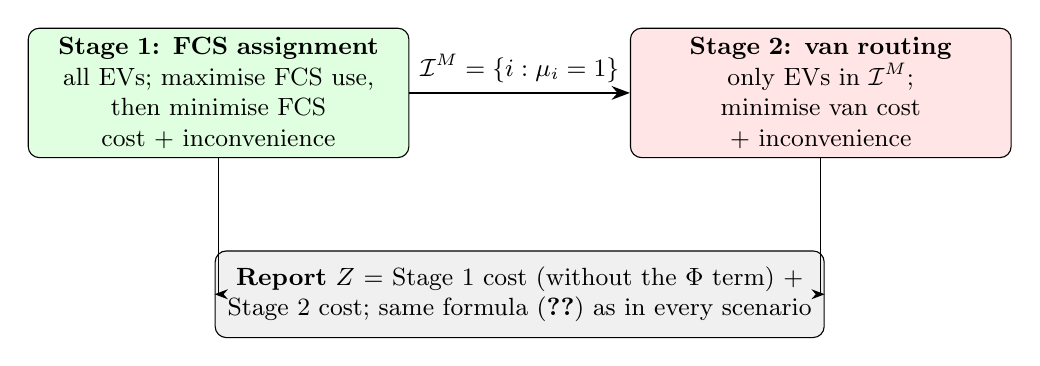
\begin{tikzpicture}[>=Stealth,box/.style={draw,rounded corners,align=center,minimum height=1.1cm,font=\small}]
  \node[box,fill=green!12,text width=4.6cm] (s1) {\textbf{Stage 1: FCS assignment}\\all EVs; maximise FCS use,\\then minimise FCS cost + inconvenience};
  \node[box,fill=red!10,text width=4.6cm,right=2.8cm of s1] (s2) {\textbf{Stage 2: van routing}\\only EVs in $\I^M$;\\minimise van cost + inconvenience};
  \draw[->,thick] (s1) -- node[above,font=\small]{$\I^M=\{i:\mu_i=1\}$} (s2);
  \node[box,fill=black!6,text width=7.5cm,below=2.0cm of $(s1)!0.5!(s2)$] (ev) {\textbf{Report} $Z=$ Stage~1 cost (without the $\Phi$ term) $+$ Stage~2 cost; same formula \eqref{eq:Z} as in every scenario};
  \draw[->] (s1) |- (ev); \draw[->] (s2) |- (ev);
\end{tikzpicture}
\end{center}

Stage~1 does not look at the vans, and Stage~2 cannot change what Stage~1 decided. That is the definition of ``FCS first, then MCS''.

%----------------------------------------------------------------
\subsection{Stage 1: assign EVs to fixed stations}

\textbf{Objective.}
\begin{equation}
\begin{split}
\min\ Z^{(1)}=\;&\underbrace{\Phi\sum_{i\in\I}\mu_i}_{\text{FCS first}}
+\underbrace{c^{EV}\sum_i\sum_{f\in\F_i}d_{if}Y_{if}}_{Z_1}
+\underbrace{Z^F_{\text{energy}}}_{\text{FCS part of }Z_4}\\
&+\underbrace{\sum_i\sum_{f\in\F_i}\rho^F_{if}Y_{if}+\alpha\sum_i w_i(C_i-r_i)+c^L\sum_i w_iL_i}_{\text{FCS customers' inconvenience}}
\end{split}
\label{eq:obj1}
\end{equation}
with $C_i=S_i+\tau^F_iY_i$ in this stage. $\Phi$ is a penalty for handing an EV to the vans. It is chosen larger than anything an extra FCS customer can add to the rest of \eqref{eq:obj1}, e.g.
\[
\Phi > \max_{i}\max_{f\in\F_i}\big(c^{EV}d_{if}+\pi^{\max}E_i+\rho^F_{if}\big)+n\,(\alpha+c^L)\,w_{\max}\,T,
\]
so Stage~1 first \textbf{maximises the number of EVs served at an FCS}, and only among those solutions minimises FCS cost and inconvenience. ($\pi^{\max}$ is the highest grid price.) A numerically safer equivalent is to solve twice: first $\max\sum_iY_i$, then fix that number and minimise the rest.
\ifTOU
Because $Z^F_{\text{energy}}$ uses the peak price, Stage~1 may \emph{start sessions later} to leave the peak, if the price saving beats the extra waiting cost (Section~\ref{sec:expect}).
\fi

\textbf{Constraints.}
\begin{align}
\sum_{g\in\G_i}y_{ig}+\mu_i &= 1 && \forall i\in\I \label{eq:s1assign}\\
S_i &\ge r_i+\sum_{f\in\F_i}t_{if}Y_{if} && \forall i\in\I \label{eq:fcsarr}\\
S_i &\le r_i+T\,(1-\mu_i) && \forall i\in\I \label{eq:s1park}\\
S_j &\ge S_i+\tau^F_i-(T+\tau^F_i)(3-y_{ig}-y_{jg}-o_{ij}) && \forall g,\ (i,j)\in\mathcal{P}_g \label{eq:disj1}\\
S_i &\ge S_j+\tau^F_j-(T+\tau^F_j)(2-y_{ig}-y_{jg}+o_{ij}) && \forall g,\ (i,j)\in\mathcal{P}_g \label{eq:disj2}\\
\sum_i y_{ig_1} &\ge \sum_i y_{ig_2} && \forall f,\ \G_f=\{g_1,g_2\} \label{eq:gunsym}\\
S_i+\tau^F_iY_i &\le T,\qquad L_i\ge S_i+\tau^F_iY_i-l_i && \forall i\in\I \label{eq:s1time}
\end{align}
\ifTOU plus the time-of-use split \eqref{eq:tou1}--\eqref{eq:tou5} of each FCS session (Section~\ref{sec:price}).\fi
\desc{\eqref{eq:s1assign}: every EV either gets one reachable gun or is handed to the vans. An EV that reaches no FCS ($\G_i=\emptyset$) is forced to $\mu_i=1$. \eqref{eq:fcsarr}: an FCS session cannot start before the EV has asked and driven to the station. \eqref{eq:s1park}: for an EV handed to the vans, $S_i$ is parked at $r_i$, so it adds no waiting in Stage~1 (its real start time is decided in Stage~2). \eqref{eq:disj1}--\eqref{eq:disj2}: two EVs on the same gun do not overlap; $o_{ij}$ picks who goes first. With two guns per station this means at most two EVs charge at a station at a time. \eqref{eq:gunsym}: symmetry breaking between the two identical guns (optional). \eqref{eq:s1time}: finished by $T$; lateness.}

\textbf{Optional acceptability rule.} An operator may refuse to send a driver to a station that is ``too inconvenient'', e.g.\ only allow gun $g$ of station $f$ for EV $i$ if $\hat\rho^F_{if}\le\bar\rho$. This only shrinks $\G_i$, so EVs whose stations are all too far go to the vans. Report results with and without it.

\textbf{Output:} $\I^M=\{i:\mu_i=1\}$, the EVs left for the vans; plus each FCS customer's gun and start time.

%----------------------------------------------------------------
\subsection{Stage 2: route the vans to the leftover EVs}

Stage~2 is a vehicle routing problem with time windows, on the EVs in $\I^M$ only. Here $C_i=S_i+\tau^M_i$.

\textbf{Objective.}
\begin{equation}
\begin{split}
\min\ Z^{(2)}=\;&\underbrace{c^M\sum_m\sum_{(i,j)\in\A^M}d_{ij}x_{ijm}}_{Z_2}+\underbrace{\sum_m c^D_mu_m}_{Z_3}+\underbrace{Z^M_{\text{energy}}}_{\text{van part of }Z_4}\\
&+\underbrace{\sum_{i\in\I^M}\sum_m\rho^M_{im}z_{im}+\alpha\sum_{i\in\I^M}w_i(C_i-r_i)+c^L\sum_{i\in\I^M}w_iL_i}_{\text{van customers' inconvenience}}
\end{split}
\label{eq:obj2}
\end{equation}
Since every EV in $\I^M$ must be served by some van, $Z^M_{\text{energy}}$ and the $\rho^M$ term are constants here. They are kept so that $Z^{(2)}$ is the true cost of Stage~2. Waiting and lateness make the vans visit urgent EVs early.

\textbf{Constraints.}
\begin{align}
\sum_{m\in\M}z_{im} &= 1 && \forall i\in\I^M \label{eq:s2assign}\\
\sum_{j:(0,j)\in\A^M}x_{0jm} = \sum_{i:(i,n+1)\in\A^M}x_{i,n+1,m} &= u_m && \forall m \label{eq:depot}\\
\sum_{i:(i,j)\in\A^M}x_{ijm} = \sum_{k:(j,k)\in\A^M}x_{jkm} &= z_{jm} && \forall j\in\I^M,\ m \label{eq:flow}\\
\sum_{i\in\I^M}z_{im} &\le Q_m\,u_m && \forall m \label{eq:cap}\\
\sum_{i\in\I^M}\frac{E_i}{\eta}z_{im}+\beta\sum_{(i,j)\in\A^M}d_{ij}x_{ijm} &\le B_m\,u_m && \forall m \label{eq:batt}
\end{align}
\begin{align}
S_j &\ge \max\{r_j,\ t_{0j}\,x_{0jm}\} && \forall j\in\I^M,\ m \label{eq:depart}\\
S_j &\ge S_i+\tau^M_i+t_{ij}-(T+\tau^M_i+t_{ij})(1-x_{ijm}) && \forall i\neq j,\ m \label{eq:seq}\\
S_i+\tau^M_i+t_{i,n+1} &\le T+(\tau^M_i+t_{i,n+1})(1-x_{i,n+1,m}) && \forall i,\ m \label{eq:return}\\
S_i+\tau^M_i \le T,\quad L_i &\ge S_i+\tau^M_i-l_i && \forall i\in\I^M \label{eq:s2time}\\
u_m &\ge u_{m+1} && m<|\M| \label{eq:vansym}
\end{align}
\desc{\eqref{eq:s2assign}: each leftover EV gets one van. \eqref{eq:depot}: a used van leaves and returns to the depot once. \eqref{eq:flow}: each EV on van $m$ is entered and left exactly once by that van. \eqref{eq:cap}: at most $Q_m$ EVs per van. \eqref{eq:batt}: delivered energy (with transfer losses) plus driving energy fits in the van battery. \eqref{eq:depart}: no start before the request, or before the van can drive there from the depot (written as two linear constraints). \eqref{eq:seq}: if the van goes $i\to j$, it finishes $i$ and drives to $j$ before starting $j$. This gives one EV at a time and removes subtours (MTZ-type). \eqref{eq:return}: back at the depot by $T$. \eqref{eq:s2time}: finished by $T$; lateness. \eqref{eq:vansym}: use identical vans in index order.}

\textbf{If Stage 2 is infeasible} (too many leftover EVs for the fleet by $T$), the sequential policy has \emph{failed} on that instance. For diagnosis, add $s_i\in\{0,1\}$ (``unserved''), replace \eqref{eq:s2assign} by $\sum_mz_{im}+s_i=1$ and add $\Phi^U\sum_is_i$ to \eqref{eq:obj2}. Then report the number of EVs that could not be served. This is a useful comparison with the integrated scenario, which may serve all of them.

%----------------------------------------------------------------
\subsection{Reported value}
\[
Z^{\text{S\scen}}=\big(Z^{(1)*}-\Phi\,|\I^M|\big)+Z^{(2)*},
\]
which is exactly \eqref{eq:Z} evaluated at the combined solution. The stage-1 solution plus the stage-2 solution is a feasible solution of the integrated model (S\ifTOU 4\else 3\fi), so
$Z^{\text{S\ifTOU 4\else 3\fi}}\le Z^{\text{S\scen}}$. The difference is the \emph{value of integration}.

\else
%---------------------------------------------------------------- INT
\subsection{Objective}
\begin{equation}
\min\ Z \quad\text{as in \eqref{eq:Z}, with }Z^F_{\text{energy}}=\ifTOU P^F\textstyle\sum_i\big[\pi^\off(\theta^1_i+\theta^3_i)+\pi^\pk\theta^2_i\big]\else\pi^F\textstyle\sum_iE_iY_i\fi,\quad C_i=S_i+\tau^F_iY_i+\tau^M_iZ_i. \label{eq:objint}
\end{equation}
Written out in full:
\begin{align*}
\min\ Z=\;& c^{EV}\sum_i\sum_{f\in\F_i}d_{if}Y_{if}+c^M\sum_m\sum_{(i,j)\in\A}d_{ij}x_{ijm}+\sum_mc^D_mu_m\\
&+\ifTOU P^F\sum_i\big[\pi^\off(\theta^1_i+\theta^3_i)+\pi^\pk\theta^2_i\big]\else\pi^F\sum_iE_iY_i\fi
+\pi^M\sum_i\sum_m\frac{E_i}{\eta}z_{im}\\
&+\sum_i\sum_{f\in\F_i}\rho^F_{if}Y_{if}+\sum_i\sum_m\rho^M_{im}z_{im}+\alpha\sum_iw_i(C_i-r_i)+c^L\sum_iw_iL_i .
\end{align*}
Every term is linear. One model weighs everything at once: an EV goes to a van exactly when the van's extra km, dispatch and energy cost are outweighed by the effort and waiting it saves the driver\ifTOU, or by the peak-price energy it avoids\fi.

\subsection{Constraints}

\textbf{Assignment.}
\begin{equation}
\sum_{g\in\G_i}y_{ig}+\sum_{m\in\M}z_{im}=1\qquad\forall i\in\I \label{eq:assign}
\end{equation}
\desc{Exactly one resource per EV: one reachable gun or one van. EVs that reach no FCS are forced onto a van.}

\textbf{Fixed stations.}
\begin{align}
S_i &\ge r_i+\sum_{f\in\F_i}t_{if}Y_{if} && \forall i \label{eq:fcsarr}\\
S_j &\ge S_i+\tau^F_i-(T+\tau^F_i)(3-y_{ig}-y_{jg}-o_{ij}) && \forall g,\ (i,j)\in\mathcal{P}_g \label{eq:disj1}\\
S_i &\ge S_j+\tau^F_j-(T+\tau^F_j)(2-y_{ig}-y_{jg}+o_{ij}) && \forall g,\ (i,j)\in\mathcal{P}_g \label{eq:disj2}\\
\sum_iy_{ig_1} &\ge \sum_iy_{ig_2} && \forall f,\ \G_f=\{g_1,g_2\} \label{eq:gunsym}
\end{align}
\desc{\eqref{eq:fcsarr}: an FCS session starts after the request and the drive to the station (for a van customer this is just $S_i\ge r_i$). \eqref{eq:disj1}--\eqref{eq:disj2}: EVs on the same gun do not overlap; $o_{ij}$ chooses the order. \eqref{eq:gunsym}: optional symmetry breaking.}

\textbf{Vans: routes, capacity, battery.}
\begin{align}
\sum_{j:(0,j)\in\A}x_{0jm}=\sum_{i:(i,n+1)\in\A}x_{i,n+1,m} &= u_m && \forall m \label{eq:depot}\\
\sum_{i:(i,j)\in\A}x_{ijm}=\sum_{k:(j,k)\in\A}x_{jkm} &= z_{jm} && \forall j\in\I,\ m \label{eq:flow}\\
\sum_iz_{im} &\le Q_mu_m && \forall m \label{eq:cap}\\
\sum_i\frac{E_i}{\eta}z_{im}+\beta\sum_{(i,j)\in\A}d_{ij}x_{ijm} &\le B_mu_m && \forall m \label{eq:batt}
\end{align}
\desc{\eqref{eq:depot}: a used van leaves and returns once. \eqref{eq:flow}: each EV on van $m$ is visited exactly once by it. \eqref{eq:cap}: at most $Q_m$ EVs. \eqref{eq:batt}: delivered energy (with losses) plus driving energy fits in the battery.}

\textbf{Vans: timing (one EV at a time, no subtours).}
\begin{align}
S_j &\ge t_{0j}\,x_{0jm} && \forall j\in\I,\ m \label{eq:depart}\\
S_j &\ge S_i+\tau^M_i+t_{ij}-(T+\tau^M_i+t_{ij})(1-x_{ijm}) && \forall i\neq j\in\I,\ m \label{eq:seq}\\
S_i+\tau^M_i+t_{i,n+1} &\le T+(\tau^M_i+t_{i,n+1})(1-x_{i,n+1,m}) && \forall i,\ m \label{eq:return}
\end{align}
\desc{\eqref{eq:depart}: the first stop cannot start before the van has driven there. \eqref{eq:seq}: $i\to j$ means finish $i$, drive, then start $j$; start times rise along a route, so no subtour can close. \eqref{eq:return}: back at the depot by $T$.}

\textbf{Horizon and lateness.}
\begin{equation}
C_i\le T,\qquad L_i\ge C_i-l_i\qquad\forall i\in\I \label{eq:time}
\end{equation}
\desc{Every EV is fully charged within the horizon; $L_i$ measures lateness.}

\ifTOU
\textbf{Time-of-use split.} Constraints \eqref{eq:tou1}--\eqref{eq:tou5} of Section~\ref{sec:price}.
\fi

\textbf{Symmetry and domains.}
\begin{equation}
u_m\ge u_{m+1};\qquad y,z,x,u,o\ifTOU,\kappa\fi\in\{0,1\};\qquad S_i,L_i\ifTOU,\theta^p_i\fi\ge0 \label{eq:dom}
\end{equation}
\fi

%=====================================================================
\section{Learning-to-optimise (RL) formulation}\label{sec:rl}

\textbf{Main rule:} the reward of each action is \emph{minus the increase in $Z$ that the action causes}. The rewards over an episode then add up to $-Z$ of the solution the policy builds. RL and MILP results are measured on the same yardstick \eqref{eq:Z}, and the MILP optimum is the benchmark for the RL gap.

\ifSEQ
%---------------------------------------------------------------- RL SEQ
The RL pipeline has the same two stages as the MILP.

\subsection{Stage 1 policy: FCS assignment}
\begin{itemize}[leftmargin=1.4em,itemsep=2pt]
  \item \textbf{Episode / epochs:} EVs are taken in order of request time $r_i$ (ties: higher $w_i$ first). One decision per EV.
  \item \textbf{State:} features of the current EV $k$ ($E_k,r_k,l_k,w_k,R_k$, location); for each gun $g$ the time $F_g$ it becomes free; summary features of the EVs still to come (count and positions near each station)\ifTOU; the current price and the time until $T_1$ and $T_2$\fi.
  \item \textbf{Action:} a gun $g\in\G_k$, or ``hand to vans''. \textbf{FCS-first mask:} ``hand to vans'' is allowed \emph{only} if no gun can finish EV $k$ by $T$ (or, with the optional rule, if all remaining guns have $\hat\rho^F_{kf}>\bar\rho$).
  \ifTOU\item \textbf{Optional timing action:} ``gun $g$, start after the peak'', i.e.\ $S_k=\max\{\text{earliest},T_2\}$, allowed only if the session still ends by $T$.\fi
  \item \textbf{Transition:} $S_k=\max\{r_k+t_{kf},F_g\}$ (or later, for the timing action); $F_g\leftarrow S_k+\tau^F_k$.
  \item \textbf{Reward:} $-\Big[c^{EV}d_{kf}+\text{energy}_k+\rho^F_{kf}+\alpha w_k(S_k+\tau^F_k-r_k)+c^Lw_k(S_k+\tau^F_k-l_k)^+\Big]$, where energy$_k$ = \ifTOU$P^F\big[\pi^\off\cdot(\text{off-peak hours of }[S_k,S_k+\tau^F_k])+\pi^\pk\cdot(\text{peak hours})\big]$, computed exactly in the simulator\else$\pi^FE_k$\fi. Handing an EV to the vans gives reward $0$ here; its cost is counted in Stage~2.
\end{itemize}
Note: a simple baseline for Stage~1 is the greedy rule ``gun with the largest one-step reward''. What RL can learn on top of this is, for example, to keep a nearby gun free for an urgent EV that arrives later.

\subsection{Stage 2 policy: van routing over $\I^M$}
\begin{itemize}[leftmargin=1.4em,itemsep=2pt]
  \item \textbf{Epochs:} whenever a van becomes free (the earliest-free van decides first).
  \item \textbf{State:} for each van: position, time free, remaining battery $b_m$, EVs served so far, dispatched or not; for each unserved EV in $\I^M$: location, $E_i,r_i,l_i,w_i$; current time.
  \item \textbf{Action:} the next EV $j$ for this van, or ``return to depot'' (ends the route). Mask: $j$ must be feasible: battery covers $E_j/\eta$ plus driving to $j$ and back to the depot, the count stays $\le Q_m$, and $j$ can be finished with the van back at the depot by $T$.
  \item \textbf{Transition:} $S_j=\max\{r_j,\ \text{time free}+t_{\text{pos},j}\}$; the van moves to $j$ and is free at $S_j+\tau^M_j$; $b_m$ falls by $E_j/\eta+\beta d_{\text{pos},j}$.
  \item \textbf{Reward:} serving $j$: $-\Big[c^Md_{\text{pos},j}+c^D_m[\text{first stop}]+\pi^M\frac{E_j}{\eta}+\rho^M_{jm}+\alpha w_j(S_j+\tau^M_j-r_j)+c^Lw_j(S_j+\tau^M_j-l_j)^+\Big]$; returning: $-c^Md_{\text{pos},0}$. EVs still unserved at the end: $-\Phi^U$ each.
  \item \textbf{Policy:} an attention-based routing policy (e.g.\ Kool et al., 2019, ``Attention, Learn to Solve Routing Problems!'') trained with REINFORCE or PPO. Baseline: nearest-feasible-EV heuristic.
\end{itemize}
Episode return of Stage~1 + Stage~2 $=-Z^{\text{S\scen}}$.

\else
%---------------------------------------------------------------- RL INT
One policy decides both who serves each EV and the van routes.
\begin{itemize}[leftmargin=1.4em,itemsep=2pt]
  \item \textbf{Episode / epochs:} EVs are taken in order of request time $r_i$ (ties: higher $w_i$ first). One decision per EV.
  \item \textbf{State:} (i) the current EV $k$: location, $E_k,r_k,l_k,w_k,R_k$, reachable stations; (ii) each gun $g$: time $F_g$ it becomes free; (iii) each van $m$: current end-of-route position, time free, remaining battery $b_m$, EVs served, dispatched or not; (iv) embeddings of the not-yet-assigned EVs (for look-ahead)\ifTOU; (v) current price, time until $T_1$ and $T_2$\fi.
  \item \textbf{Action:} $a\in\G_k\cup\M$: a gun, or a van (EV $k$ is appended to the end of that van's route). \textbf{Mask} infeasible actions: a gun that cannot finish $k$ by $T$; a van without enough battery for $E_k/\eta$ plus the drive to $k$ and back to the depot, with $Q_m$ reached, or unable to finish $k$ and return by $T$.
  \ifTOU\item \textbf{Optional timing action:} ``gun $g$, start after the peak'' ($S_k=\max\{\text{earliest},T_2\}$, if it still ends by $T$).\fi
  \item \textbf{Transition:} gun: $S_k=\max\{r_k+t_{kf},F_g\}$, $F_g\leftarrow S_k+\tau^F_k$. Van: $S_k=\max\{r_k,\ \text{free}_m+t_{\text{pos}_m,k}\}$, then the van moves to $k$, $\text{free}_m\leftarrow S_k+\tau^M_k$, $b_m\mathrel{-}=E_k/\eta+\beta d_{\text{pos}_m,k}$.
  \item \textbf{Reward} $=-\Delta Z$:
  \begin{align*}
  \text{gun } g\text{ at }f:&\quad -\Big[c^{EV}d_{kf}+\text{energy}^F_k+\rho^F_{kf}+\alpha w_k(C_k-r_k)+c^Lw_k(C_k-l_k)^+\Big]\\
  \text{van } m:&\quad -\Big[c^M\big(d_{\text{pos}_m,k}+d_{k,0}-d_{\text{pos}_m,0}\big)+c^D_m[\text{first use}]+\pi^M\tfrac{E_k}{\eta}\\
  &\qquad\quad+\rho^M_{km}+\alpha w_k(C_k-r_k)+c^Lw_k(C_k-l_k)^+\Big]
  \end{align*}
  The van distance term is the \emph{change} in route length when $k$ is inserted before the return to the depot, so the sum over the episode equals the total route length (the return legs telescope). energy$^F_k$ = \ifTOU$P^F\big[\pi^\off\cdot(\text{off-peak hours})+\pi^\pk\cdot(\text{peak hours of }[S_k,C_k])\big]$, computed exactly by the simulator; no linearisation is needed in RL\else$\pi^FE_k$\fi.
  \item \textbf{Dead end:} if every action is masked, EV $k$ is unserved: reward $-\Phi^U$, and the episode continues. Report the count.
  \item \textbf{Policy:} masked categorical policy over guns and vans, encoder with attention over EVs, guns and vans; trained with PPO. Natural baseline: greedy, i.e.\ choose the action with the largest one-step reward. That is the pairwise rule ``smallest $\hat\rho$ + cost'' from Section~\ref{sec:inc}.
\end{itemize}
Restriction to note: vans serve EVs in assignment order (append only). A variant that inserts $k$ at the cheapest position of a route is more flexible but has a larger action space.
\fi

\textbf{Reward scaling.} For stable training divide every reward by a constant, e.g.\ the greedy baseline's average $Z$ on the training instances. This does not change the optimal policy.

%=====================================================================
\section{What to expect and what to report}\label{sec:expect}

\ifnum\scen=1
\begin{itemize}[leftmargin=1.4em,itemsep=2pt]
  \item Vans serve only EVs that reach no station, or that the stations cannot finish by $T$. If stations have spare capacity, very few vans are dispatched.
  \item Inconvenience is high for EVs far from the nearest station (worked example: Rs\,682 at the FCS, against Rs\,458 if a van had been allowed).
  \item With too few vans Stage~2 becomes infeasible (unserved EVs), even when the integrated model S3 could serve everyone. Report the smallest $|\M|$ at which S1 is feasible and compare it with S3.
\end{itemize}
\fi
\ifnum\scen=2
\begin{itemize}[leftmargin=1.4em,itemsep=2pt]
  \item \textbf{When does Stage~1 delay a session to avoid the peak?} Moving one hour of charging out of the peak saves $(\pi^\pk-\pi^\off)P^F=3\times22=$ Rs\,66, but delays completion by up to an hour, which costs $\alpha w_i\ge$ Rs\,200. So with the default values Stage~1 almost never delays. It mostly pays the higher price, and S2 costs roughly S1 plus the peak surcharge. Sessions start later only if $\alpha$ is small (try $\lambda<0.33$ in the sensitivity analysis).
  \item The van assignment is the same as in S1 unless Stage~1's timing changes which EVs fit at the stations. Stage~1 cannot use vans to escape the peak price.
  \item Extra KPI: \textbf{grid energy drawn at FCS during the peak}, $P^F\sum_i\theta^2_i$ (kWh). Compare with S4.
\end{itemize}
\fi
\ifnum\scen=3
\begin{itemize}[leftmargin=1.4em,itemsep=2pt]
  \item Vans take EVs for which the saved inconvenience exceeds the extra van cost (worked example: van chosen, saving Rs\,224). Expect vans to serve EVs that are far from every station, have low range (high $w_i$), or have early deadlines, while EVs near a station still use it.
  \item \textbf{Value of integration under flat price:} $Z^{\text{S1}}-Z^{\text{S3}}\ge0$. Report it per component ($Z_1,\dots,Z_5$): typically operating cost rises a little and inconvenience falls a lot.
  \item Vary $|\M|$ (0, 1, 2, \dots): the first few vans lower $Z$ sharply, then the effect levels off. That curve shows the scenarios where mobile chargers help most.
\end{itemize}
\fi
\ifnum\scen=4
\begin{itemize}[leftmargin=1.4em,itemsep=2pt]
  \item During the peak a van kWh costs about the same as an FCS kWh (Rs\,10.0 each), so the vans' energy disadvantage disappears and vans also absorb \emph{peak-hour} demand that would otherwise be charged on the grid at peak price.
  \item Expect more van usage than in S3, concentrated on requests in $[T_1,T_2]$, and lower grid energy at the stations during the peak, $P^F\sum_i\theta^2_i$, than in S2.
  \item \textbf{Value of integration under peak pricing:} $Z^{\text{S2}}-Z^{\text{S4}}$. It should be larger than $Z^{\text{S1}}-Z^{\text{S3}}$, because integration now also allows price arbitrage.
  \item \textbf{Peak pricing with full flexibility:} $Z^{\text{S4}}-Z^{\text{S3}}$ should be smaller than $Z^{\text{S2}}-Z^{\text{S1}}$: vans cushion the price increase.
\end{itemize}
\fi

\textbf{Cross-scenario comparison table} (fill in from the four runs):
\begin{center}
\renewcommand{\arraystretch}{1.2}
\begin{tabular}{@{}lll@{}}
\toprule
\textbf{Comparison} & \textbf{Measures} & \textbf{Expected sign} \\
\midrule
S1 $-$ S3 & value of integration, flat price & $\ge0$ \\
S2 $-$ S4 & value of integration, peak price & $\ge0$, larger than S1 $-$ S3 \\
S2 $-$ S1 & cost of peak pricing, FCS-first operator & $>0$ \\
S4 $-$ S3 & cost of peak pricing, flexible operator & $>0$, smaller than S2 $-$ S1 \\
\bottomrule
\end{tabular}
\end{center}
Report for each: $Z$ and its components, number of vans used, EVs per resource, mean and maximum inconvenience per EV, total lateness, peak-hour grid energy, solve time, and (for RL) the gap to the MILP optimum.

%=====================================================================
\appendix
\section{Illustrative parameter values}\label{app:values}

These are starting values for experiments, not data. All are meant to be varied in the analysis. Values in Rs.

\begin{center}
\renewcommand{\arraystretch}{1.15}
\begin{tabular}{@{}llp{6.2cm}@{}}
\toprule
\textbf{Parameter} & \textbf{Value} & \textbf{Note} \\
\midrule
$T$, $[T_1,T_2]$ & 7 h, $[2,6]$ & 16:00--23:00, peak 18:00--22:00 \\
$P^F$, $P^M$ & 22 kW, 30 kW & \\
$v$, $\beta$, $\eta$ & 25 km/h, 0.25 kWh/km, 0.9 & \\
$B_m$, $Q_m$, $|\M|$ & 150 kWh, 6, 2--6 & \\
$c^{EV}$, $c^M$, $c^D_m$ & Rs\,4/km, Rs\,15/km, Rs\,1500 & van km includes driver time \\
$\pi^F$ (flat) & Rs\,8.7/kWh & equals the time-average of the ToU tariff over $[0,T]$ \\
$\pi^\off$, $\pi^\pk$ (ToU) & Rs\,7/kWh, Rs\,10/kWh & $(3\times7+4\times10)/7=8.7$ \\
$c^{bat}$ & Rs\,2/kWh & van battery wear \\
$\pi^M$ & Rs\,10.7 (flat) / Rs\,9.0 (ToU) & $=\pi^F+c^{bat}$ / $=\pi^\off+c^{bat}$ \\
$\alpha$, $\alpha^D$ & Rs\,200/h, Rs\,100/h & value of time; extra for attended time \\
$h^F$, $h^M$, $\varphi$ & Rs\,50, Rs\,10, Rs\,100 & trip hassle, hand-over, range stress \\
$c^L$ & Rs\,300/h & lateness \\
$w_i$ & $1+2(1-R_i/R_{\max})$, $R_i\sim U[3,40]$ km & priority from remaining range \\
\bottomrule
\end{tabular}
\end{center}

The flat price is set to the time-average of the peak tariff. The price \emph{level} is then the same in both pricing cases, and only the price \emph{shape} differs. Without this, part of S1 vs S2 would just reflect a different average price.

\end{document}
"
%    pdflatex -jobname=scenario3_flat_integrated   "\def\scen{3}% =====================================================================
%  One source, four PDFs.  Build with build.sh (or by hand):
%    pdflatex -jobname=scenario1_flat_sequential   "\def\scen{1}\input{scenario_master}"
%    pdflatex -jobname=scenario2_peak_sequential   "\def\scen{2}\input{scenario_master}"
%    pdflatex -jobname=scenario3_flat_integrated   "\def\scen{3}\input{scenario_master}"
%    pdflatex -jobname=scenario4_peak_integrated   "\def\scen{4}\input{scenario_master}"
%  (run each twice for cross-references)
% =====================================================================
\documentclass[11pt,a4paper]{article}
\usepackage[margin=2.2cm]{geometry}
\usepackage{amsmath,amssymb,amsfonts}
\usepackage{booktabs,array,tabularx}
\usepackage{enumitem}
\usepackage[table]{xcolor}
\usepackage{tikz}
\usetikzlibrary{arrows.meta,positioning,calc}
\usepackage[colorlinks=true,linkcolor=blue!50!black,urlcolor=blue!50!black]{hyperref}
\usepackage{titlesec}
\titleformat{\section}{\large\bfseries}{\thesection}{0.8em}{}
\titleformat{\subsection}{\normalsize\bfseries}{\thesubsection}{0.8em}{}
\setlength{\parindent}{0pt}
\setlength{\parskip}{5pt}

% ---------------- scenario switches ----------------
\ifdefined\scen\else\def\scen{1}\fi
\newif\ifTOU \TOUfalse   % true = time-of-use (peak) price
\newif\ifSEQ \SEQfalse   % true = FCS first, then MCS
\ifnum\scen=1 \SEQtrue \fi
\ifnum\scen=2 \TOUtrue \SEQtrue \fi
\ifnum\scen=4 \TOUtrue \fi

\newcommand{\pricename}{\ifTOU time-of-use price (dearer evening peak)\else single (flat) price all day\fi}
\newcommand{\structname}{\ifSEQ FCS first, then MCS (sequential)\else FCS and MCS together (integrated)\fi}

% ---------------- notation ----------------
\newcommand{\I}{\mathcal{I}}
\newcommand{\F}{\mathcal{F}}
\newcommand{\G}{\mathcal{G}}
\newcommand{\M}{\mathcal{M}}
\newcommand{\N}{\mathcal{N}}
\newcommand{\A}{\mathcal{A}}
\newcommand{\Rs}{\text{Rs}\,}
\newcommand{\pk}{\mathrm{pk}}
\newcommand{\off}{\mathrm{off}}
\newcommand{\desc}[1]{\par\vspace{-2pt}{\small\color{black!75}\textit{Meaning:} #1}\par\vspace{4pt}}
\newcommand{\cell}[2]{\ifnum\scen=#1\cellcolor{blue!18}\textbf{S#1 (this document)}\\\textbf{#2}\else S#1\\#2\fi}

\title{\textbf{EV Charging Network Optimisation}\\[4pt]
\large Scenario \scen: \pricename\ $+$ \structname\\[2pt]
\normalsize MILP and RL formulation}
\author{CP 320 OR for Mobility Management, course project}
\date{2 October 2026}

\begin{document}
\maketitle

%=====================================================================
\section{Where this scenario sits}

The project studies four scenarios: two ways of pricing grid electricity, times two ways of making the decisions.

\begin{center}
\renewcommand{\arraystretch}{1.5}
\begin{tabular}{>{\raggedright\arraybackslash}p{4.2cm}|>{\centering\arraybackslash}p{4.6cm}|>{\centering\arraybackslash}p{4.6cm}}
 & \textbf{Flat price all day} & \textbf{Time-of-use (peak) price} \\ \hline
\textbf{Sequential:} FCS first, leftover EVs to MCS &
\begin{tabular}[c]{@{}c@{}}\cell{1}{flat + sequential}\end{tabular} &
\begin{tabular}[c]{@{}c@{}}\cell{2}{peak + sequential}\end{tabular} \\ \hline
\textbf{Integrated:} FCS and MCS decided together &
\begin{tabular}[c]{@{}c@{}}\cell{3}{flat + integrated}\end{tabular} &
\begin{tabular}[c]{@{}c@{}}\cell{4}{peak + integrated}\end{tabular} \\
\end{tabular}
\end{center}

\textbf{The four scenarios do not have four different objectives.} They share \emph{one} cost yardstick $Z$ (Section~\ref{sec:obj}): the same cost terms and the same customer inconvenience (Section~\ref{sec:inc}). Only two things change:
\begin{itemize}[leftmargin=1.4em,itemsep=1pt]
  \item \textbf{Pricing} changes the formula for one term, the FCS energy cost (Section~\ref{sec:price}).
  \item \textbf{Decision structure} changes \emph{how} $Z$ is minimised: in one model (integrated), or in two stages (sequential), where each stage minimises its own part of $Z$.
\end{itemize}
Because the yardstick is the same, the four optimal values can be compared directly. The differences measure the \emph{value of integration} (S1$\to$S3, S2$\to$S4) and the \emph{effect of peak pricing} (S1$\to$S2, S3$\to$S4).

\ifnum\scen=1
\textbf{This scenario (S1)} is the baseline, the ``status quo''. Electricity costs the same at every hour, every EV that can be charged at a fixed station is sent there, and vans only take what is left over.
\fi
\ifnum\scen=2
\textbf{This scenario (S2)} keeps the FCS-first rule of S1, but grid electricity is dearer during the evening peak. Stage~1 can react to the price only by \emph{rescheduling} FCS sessions. It cannot hand a peak-hour EV to a van.
\fi
\ifnum\scen=3
\textbf{This scenario (S3)} keeps the flat price of S1, but the operator decides FCS and MCS service \emph{together}. An EV can be sent to a van even when a fixed station could take it, whenever that lowers total cost plus inconvenience.
\fi
\ifnum\scen=4
\textbf{This scenario (S4)} is the most flexible one: peak pricing at fixed stations, and FCS and MCS decided together. Van energy was bought off-peak, so vans can also be used to keep charging \emph{out of the expensive peak}.
\fi

%=====================================================================
\section{Setting and assumptions}\label{sec:setting}

\textbf{Time.} The planning horizon is $[0,T]$ with $T=7$\,h (16:00--23:00). It contains the evening peak window $[T_1,T_2]=[2,6]$ (18:00--22:00). The horizon is the same in all four scenarios. It is wider than the peak itself so that, under peak pricing, there is cheaper time on both sides of the peak.\ifTOU\else\ In this scenario the price is flat, so the window plays no role in the model.\fi

\textbf{Assumptions} (the same as MILP v3, plus two about energy):
\begin{enumerate}[leftmargin=1.6em,itemsep=1pt]
  \item Static, continuous time. All requests in the horizon are known at time $0$, and request $i$ becomes active at $r_i$.
  \item An EV served by an FCS drives there itself on its own battery (only to stations within its range $R_i$). The driver stays with the car while it waits for a free gun and while it charges.
  \item An EV served by an MCS stays parked where it is, and the driver is free in the meantime.
  \item Each FCS gun and each van charges one EV at a time, without interruption, at constant power.
  \item A van's battery covers both its driving and the energy it delivers. \textbf{The van battery is charged at the depot before the horizon starts}\ifTOU, i.e.\ at the off-peak price\fi, and is not recharged during the horizon.
  \item Every EV must be fully charged by $T$ (hard). Finishing after the driver's desired time $l_i$ is allowed but penalised.
\end{enumerate}

%=====================================================================
\section{Notation}\label{sec:notation}

\subsection*{Sets}
\begin{tabularx}{\textwidth}{@{}lX@{}}
\toprule
$\I=\{1,\dots,n\}$ & EV charging requests \\
$\F$; $\G_f$ ($|\G_f|=2$); $\G=\bigcup_f\G_f$ & fixed charging stations; guns of FCS $f$; all guns ($f(g)$ = station of gun $g$) \\
$\F_i=\{f: d_{if}\le R_i\}$, $\G_i=\bigcup_{f\in\F_i}\G_f$ & stations / guns EV $i$ can reach on its remaining range \\
$\M$ & mobile charging vans (MCS) \\
$0,\ n+1$ & depot as start node / end node (same place) \\
$\N=\{0\}\cup\I\cup\{n+1\}$, $\A$ & routing nodes; allowed van arcs $(i,j)$, $i\in\{0\}\cup\I$, $j\in\I\cup\{n+1\}$, $i\neq j$ \\
$\mathcal{P}_g=\{(i,j): i<j,\ g\in\G_i\cap\G_j\}$ & pairs of EVs that could share gun $g$ \\
\ifSEQ
$\I^M\subseteq\I$ & EVs handed to the vans by Stage~1 (an \emph{output} of Stage~1, a fixed input to Stage~2) \\
$\N^M$, $\A^M$ & routing nodes / arcs restricted to $\I^M$ \\
\fi
\bottomrule
\end{tabularx}

\subsection*{Parameters}
\begin{tabularx}{\textwidth}{@{}lX@{}}
\toprule
$E_i,\ r_i,\ l_i,\ R_i$ & energy demand (kWh), request time, desired completion time (h), remaining range (km) \\
$w_i\ge1$ & priority of EV $i$; $w_i=1+\kappa(1-R_i/R_{\max})$, so low-range EVs weigh more \\
$P^F,\ P^M$ & charging power of an FCS gun (22\,kW) / of a van (e.g.\ 30\,kW) \\
$\tau^F_i=E_i/P^F,\ \tau^M_i=E_i/P^M$ & charging time of EV $i$ at an FCS / by a van (h) \\
$d_{if},t_{if}$;\ $d_{ij},t_{ij}$ & distance (km) and time (h): EV$\to$FCS; between routing nodes ($t=d/v$) \\
$B_m,\ Q_m,\ \beta,\ \eta$ & van battery (kWh), max EVs per van, van consumption (kWh/km), transfer efficiency \\
$c^{EV},\ c^M,\ c^D_m$ & cost per km of EV driving, per km of van driving; fixed dispatch cost of van $m$ \\
\ifTOU
$\pi^\off,\ \pi^\pk$ & grid price (Rs/kWh) off-peak / in $[T_1,T_2]$, with $\pi^\pk\ge\pi^\off$ \\
\else
$\pi^F$ & grid price (Rs/kWh), the same at every hour \\
\fi
$c^{bat}$ & van battery wear per kWh cycled \\
$\pi^M$ & cost of 1 kWh taken from a van battery: $\pi^M=\ifTOU\pi^\off\else\pi^F\fi+c^{bat}$ (Section~\ref{sec:price}) \\
$\alpha,\ \alpha^D,\ h^F,\ h^M,\ \varphi,\ c^L$ & inconvenience coefficients (Section~\ref{sec:inc}) \\
\bottomrule
\end{tabularx}

\subsection*{Decision variables}
\begin{tabularx}{\textwidth}{@{}llX@{}}
\toprule
$y_{ig}$ & $\{0,1\}$ & EV $i$ charged at gun $g\in\G_i$ \\
$z_{im}$ & $\{0,1\}$ & EV $i$ served by van $m$ \\
$x_{ijm}$ & $\{0,1\}$ & van $m$ drives arc $(i,j)$ \\
$u_m$ & $\{0,1\}$ & van $m$ is dispatched \\
$o_{ij}$ & $\{0,1\}$ & for EVs $i<j$ that could share a gun: 1 if $i$ is charged before $j$ \\
\ifSEQ
$\mu_i$ & $\{0,1\}$ & Stage~1 only: EV $i$ is handed to the van fleet \\
\fi
\ifTOU
$\theta^1_i,\theta^2_i,\theta^3_i$ & $\ge0$ & hours of EV $i$'s FCS session before / inside / after the peak \\
$\kappa^1_i,\kappa^3_i$ & $\{0,1\}$ & EV $i$'s FCS session starts before $T_1$ / ends after $T_2$ \\
\fi
$S_i$ & $\ge0$ & time charging of EV $i$ starts (h), on whichever resource \\
$L_i$ & $\ge0$ & lateness of EV $i$ beyond $l_i$ (h) \\
\bottomrule
\end{tabularx}

\textbf{Short-hands} (linear expressions, not new variables):
\[
Y_{if}=\sum_{g\in\G_f}y_{ig},\qquad Y_i=\sum_{g\in\G_i}y_{ig}\ (\text{EV $i$ uses an FCS}),\qquad Z_i=\sum_{m\in\M}z_{im}\ (\text{EV $i$ uses a van}),
\]
\[
C_i=S_i+\tau^F_i\,Y_i+\tau^M_i\,Z_i \quad\text{(time EV $i$ is fully charged).}
\]

%=====================================================================
\section{Customer inconvenience}\label{sec:inc}

This section is \textbf{identical in all four scenario documents}. Inconvenience is a property of the customer, not of the price or of the planning method.

\subsection{What we mean by inconvenience}

Inconvenience is \emph{what the driver loses} from the moment they ask for a charge ($r_i$) until the car is fully charged ($C_i$), \emph{converted into rupees} so it can be added to the operator's costs. A driver loses three different things:

\begin{enumerate}[leftmargin=1.6em,itemsep=2pt]
  \item \textbf{Waiting:} the car is not ready. This lasts $C_i-r_i$ hours and affects \emph{every} driver, FCS or MCS.
  \item \textbf{Effort:} only an FCS customer has to drive to the station and sit there while the car charges. An MCS customer stays at home or at work and does something else. Driving to a far station also uses scarce battery range, which causes stress (``range anxiety'').
  \item \textbf{A missed deadline:} the car is still not ready at the time $l_i$ the driver needs it.
\end{enumerate}

Each loss gets a price in Rs per hour (or per event). All of them are multiplied by the priority $w_i$: an hour of delay for an EV with 5\,km of range left counts more than for one with 40\,km.

\subsection{The three components}

\begin{center}
\renewcommand{\arraystretch}{1.3}
\begin{tabularx}{\textwidth}{@{}>{\raggedright\arraybackslash}p{2.6cm}>{\raggedright\arraybackslash}X>{\raggedright\arraybackslash}X>{\raggedright\arraybackslash}p{3.0cm}@{}}
\toprule
\textbf{Component} & \textbf{EV $i$ at FCS $f$} & \textbf{EV $i$ by a van} & \textbf{Known when?} \\
\midrule
Effort & $w_i\big[\alpha^D(t_{if}+\tau^F_i)+h^F+\varphi\,d_{if}/R_i\big]$: driving and sitting at the station, a fixed trip hassle, range stress & $w_i\,h^M$: being reachable and handing over the car & \textbf{Static:} known as soon as the resource is chosen \\
Waiting & $w_i\,\alpha\,(C_i-r_i)$ = drive + \emph{queue at the gun} + charge & $w_i\,\alpha\,(C_i-r_i)$ = \emph{wait for the van} + charge & \textbf{Dynamic:} depends on the queue / van route \\
Missed deadline & $w_i\,c^L\,L_i$, $L_i=\max\{0,C_i-l_i\}$ & same & Dynamic \\
\bottomrule
\end{tabularx}
\end{center}

\textbf{Coefficients.}
$\alpha$ (Rs/h) is the value of an hour the car is not ready.
$\alpha^D$ (Rs/h) is the \emph{extra} value of an hour the driver must personally spend driving or sitting at the station: an hour at the station costs $\alpha+\alpha^D$, an hour waiting at home for a van costs only $\alpha$.
$h^F,h^M$ (Rs) are fixed hassle costs of one trip to a station / one van hand-over.
$\varphi$ (Rs) is the range-stress cost of a trip that uses the \emph{whole} remaining range ($d_{if}/R_i\le1$ is the fraction used).
$c^L$ (Rs/h) is the cost per hour late.

\subsection{Pairwise form: inconvenience of a (customer, resource) pair}

The natural first idea is: \emph{for every pair (EV $i$, FCS $f$) and every pair (EV $i$, van $m$) there is an inconvenience number, and the operator picks the pair with the lowest cost plus inconvenience.} The static part fits this idea exactly:
\[
\boxed{\;\rho^F_{if}=w_i\Big[\alpha^D\,(t_{if}+\tau^F_i)+h^F+\varphi\,\frac{d_{if}}{R_i}\Big]\qquad
\rho^M_{im}=w_i\,h^M\;}
\]
These are \textbf{parameters}, computed before solving, one number per (EV, FCS) pair and per (EV, van) pair. In the objective they appear linearly: $\sum_i\sum_f\rho^F_{if}Y_{if}+\sum_i\sum_m\rho^M_{im}z_{im}$.

Note that $\rho^M_{im}$ does not depend on $m$. Vans are identical and all start at the same depot, so the driver does not care \emph{which} van comes, only \emph{when} it comes. That ``when'' is the waiting part.

\subsection{Why waiting cannot be a fixed pairwise number}

It is tempting to also write the waiting as a pairwise number, e.g.\ ``the van needs 5 minutes to reach EV $i$''. But that depends on \emph{where the van is coming from}, which depends on the route the model is still choosing: if EV $i$ is the 4th stop of a van, the wait is the time for three charging sessions plus four drives. Likewise, waiting at an FCS depends on how many EVs are queued at that gun. So waiting is not known before solving. It is a function of decision variables:
\[
\text{waiting cost of EV } i \;=\; w_i\,\alpha\,(C_i-r_i),\qquad C_i=S_i+\tau^F_iY_i+\tau^M_iZ_i .
\]
This is \textbf{linear} in the variables ($S_i$, $y$, $z$), so it fits in a MILP directly. The constraints of Section~\ref{sec:milp} make $S_i$ equal to the true start time, including driving, queueing at the gun and the van's route. The term $\sum_i w_i\alpha r_i$ is a constant and may be dropped when solving.

\textbf{Pairwise \emph{estimate}} (used for intuition, by the RL policy and in heuristics): if there is no queue and the van comes straight to $i$,
\[
\hat\rho^{F}_{if}=\rho^F_{if}+w_i\alpha\,(t_{if}+\tau^F_i),\qquad
\hat\rho^{M}_{im}=\rho^M_{im}+w_i\alpha\,(t^{\text{van}}_{m\to i}+\tau^M_i),
\]
where $t^{\text{van}}_{m\to i}$ is the time until van $m$ can reach $i$ from where it currently is. In the RL formulation (Section~\ref{sec:rl}) the van's position \emph{is} known at each decision, so there this estimate becomes exact.

\subsection{Total inconvenience and how it enters the objective}

\begin{equation}
\boxed{\;
Z_{\text{inc}}=\underbrace{\sum_{i\in\I}\sum_{f\in\F_i}\rho^F_{if}Y_{if}+\sum_{i\in\I}\sum_{m\in\M}\rho^M_{im}z_{im}}_{\text{effort (static, pairwise)}}
+\underbrace{\alpha\sum_{i\in\I}w_i\,(C_i-r_i)}_{\text{waiting (dynamic)}}
+\underbrace{c^L\sum_{i\in\I}w_i\,L_i}_{\text{missed deadline}}
\;}\label{eq:inc}
\end{equation}
All three parts are in rupees, so $Z_{\text{inc}}$ is simply added to the operating costs. Nothing has to be normalised.

\subsection{Worked example: your ``10 km to the FCS vs.\ van in 5 minutes'' case}

EV $i$: $E_i=20$\,kWh, $R_i=40$\,km (so $w_i=1$); nearest free FCS $d_{if}=10$\,km away, $t_{if}=0.4$\,h at 25\,km/h; a van finishing next door can reach it in 5\,min ($0.083$\,h), adding about 4\,km to its route. $\tau^F_i=20/22=0.909$\,h, $\tau^M_i=20/30=0.667$\,h. Coefficients from Appendix~\ref{app:values}, flat price.

\begin{center}
\renewcommand{\arraystretch}{1.25}
\begin{tabular}{@{}lrr@{}}
\toprule
 & \textbf{FCS} & \textbf{Van} \\
\midrule
Driving (EV / extra van km) & $4\times10=40.0$ & $15\times4=60.0$ \\
Energy & $8.7\times20=174.0$ & $10.7\times20/0.9=237.8$ \\
\textbf{Operating cost only} & \textbf{214.0} & \textbf{297.8} \\
\midrule
Effort $\rho$ & $100(0.4+0.909)+50+100\cdot\tfrac{10}{40}=205.9$ & $10.0$ \\
Waiting $\alpha(C_i-r_i)$ & $200\times1.309=261.8$ & $200\times0.75=150.0$ \\
\textbf{Cost + inconvenience} & \textbf{681.7} & \textbf{457.8} \\
\bottomrule
\end{tabular}
\end{center}

On operating cost alone the FCS is cheaper, so a cost-only model would \emph{always} send this driver 10\,km away. With inconvenience included the van is better by about Rs\,224, and the integrated model chooses $z_{im}=1$, as you expected. If the FCS were only 1\,km away, the FCS would win both comparisons. The inconvenience term is what makes the model choose between ``cheap for the operator'' and ``convenient for the driver'', rather than following a fixed rule.

\subsection{Relation to a single penalty $\rho_i$ per EV}

The first draft used a penalty $\rho_i$ that is charged whenever EV $i$ goes to \emph{any} FCS: $\sum_i\sum_f\rho_iy_{if}$. Because $\sum_f y_{if}=1-\sum_m z_{im}$, this only says ``a van is worth $\rho_i$ more to EV $i$'', and that holds whether the station is 1\,km or 15\,km away, and whether the van arrives in 5 minutes or in 3 hours. The form above fixes both problems: $\rho^F_{if}$ grows with the distance to \emph{that} station, and the waiting term grows with how late the van or the free gun actually is. The old model is the special case $\alpha=\alpha^D=\varphi=c^L=0$, $h^F=\rho_i$.

\subsection{Choosing the coefficients}
\begin{itemize}[leftmargin=1.4em,itemsep=2pt]
  \item Use a value of time for $\alpha$ (e.g.\ Rs\,150--300/h for urban car users), and set $\alpha^D\approx0.5\alpha$: sitting at a station is worse than waiting at home.
  \item Keep $c^L>\alpha$, so missing the deadline is worse than ordinary waiting.
  \item \textbf{Sensitivity analysis:} multiply all inconvenience coefficients by a factor $\lambda\in\{0,0.25,0.5,1,2,4\}$ and plot operating cost against total inconvenience. $\lambda=0$ is the pure cost-minimising operator, and large $\lambda$ is a customer-first operator. This trade-off curve is a strong result for the ``Analysis'' part of the project.
\end{itemize}

\subsection{What inconvenience does in \emph{this} scenario}
\ifSEQ
In a sequential scenario inconvenience \textbf{cannot move an EV from an FCS to a van}: Stage~1 sends every EV that \emph{can} use an FCS to one. It still matters inside each stage. In Stage~1 it decides \emph{which} station and \emph{when} (urgent EVs get the near station and the first free gun). In Stage~2 it decides the \emph{order} in which vans visit EVs (urgent EVs first). In the worked example, this scenario sends the driver 10\,km to the FCS. That is the weakness the integrated scenarios remove.
\else
In an integrated scenario inconvenience is weighed directly against operating cost when choosing the resource. That is how the worked example ends up with a van. It also decides which station and which gun order, and the order of each van route.
\fi

%=====================================================================
\section{Electricity price in this scenario}\label{sec:price}

\textbf{Van energy (same in all scenarios).} A van's battery is charged at the depot \emph{before} the horizon, so its energy was bought at the
\ifTOU off-peak \fi
price, whatever time the van later delivers it. Each kWh taken from the van also wears the battery ($c^{bat}$), and a fraction $1-\eta$ is lost in transfer:
\[
Z^M_{\text{energy}}=\pi^M\sum_{i\in\I}\sum_{m\in\M}\frac{E_i}{\eta}\,z_{im},\qquad \pi^M=\ifTOU\pi^\off\else\pi^F\fi+c^{bat}.
\]

\ifTOU
\textbf{FCS energy (time-of-use).} An FCS draws from the grid while it charges. Energy delivered inside $[T_1,T_2]$ costs $\pi^\pk$, and energy outside it costs $\pi^\off$. A session $[S_i,S_i+\tau^F_i]$ may overlap the peak partly. Split its duration into the hours before, inside and after the peak, $\theta^1_i+\theta^2_i+\theta^3_i$:
\[
Z^F_{\text{energy}}=P^F\sum_{i\in\I}\Big[\pi^\off(\theta^1_i+\theta^3_i)+\pi^\pk\,\theta^2_i\Big].
\]
Constraints \eqref{eq:tou1}--\eqref{eq:tou5} below make the $\theta$'s equal to the true overlaps. Peak hours are dearer, so the solver wants $\theta^1_i,\theta^3_i$ as large as possible. It is enough to bound them from above by the true off-peak overlap, and the constraints need one binary per side:
\begin{align}
\theta^1_i+\theta^2_i+\theta^3_i &= \tau^F_i\,Y_i && \forall i\in\I \label{eq:tou1}\\
\theta^1_i &\le \tau^F_i\,\kappa^1_i && \forall i\in\I \label{eq:tou2}\\
\theta^1_i &\le T_1-S_i+T\,(1-\kappa^1_i) && \forall i\in\I \label{eq:tou3}\\
\theta^3_i &\le \tau^F_i\,\kappa^3_i && \forall i\in\I \label{eq:tou4}\\
\theta^3_i &\le S_i+\tau^F_i-T_2+T\,(1-\kappa^3_i) && \forall i\in\I \label{eq:tou5}
\end{align}
\desc{\eqref{eq:tou1}: the FCS session's hours are split into three parts; for a van customer ($Y_i=0$) all three are zero. \eqref{eq:tou2}--\eqref{eq:tou3}: off-peak time before the peak is only possible if the session starts before $T_1$ ($\kappa^1_i=1$), and is at most $T_1-S_i$. \eqref{eq:tou4}--\eqref{eq:tou5}: the same for time after $T_2$. $\theta^2_i\ge0$ prevents counting more off-peak hours than exist. Checking the cases (entirely before / inside / after the peak, straddling one edge, covering the whole peak) shows that at the optimum the $\theta$'s equal the exact overlaps. This needs $\pi^\pk\ge\pi^\off$, which is true for a peak tariff.}

\textbf{Why vans become more attractive.} Compare the cost of 1\,kWh delivered to an EV during the peak (values from Appendix~\ref{app:values}):
FCS $=\pi^\pk=$ Rs\,10.0, van $=(\pi^\off+c^{bat})/\eta=9/0.9=$ Rs\,10.0. They are at parity. Under the flat price the van is about Rs\,3.2/kWh dearer (FCS Rs\,8.7, van $10.7/0.9=$ Rs\,11.9). Peak pricing therefore removes the vans' main cost disadvantage, but only for EVs whose FCS session would fall in the peak.
\ifSEQ\ In this sequential scenario Stage~1 cannot use that, because it does not consider vans. It can only shift FCS sessions in time.\fi
\else
\textbf{FCS energy (flat).} Every kWh delivered at a fixed station costs $\pi^F$, whenever it is delivered:
\[
Z^F_{\text{energy}}=\pi^F\sum_{i\in\I}E_i\,Y_i .
\]
The start time therefore does not affect the energy cost. Under the flat price a van kWh costs $(\pi^F+c^{bat})/\eta\approx$ Rs\,11.9 against Rs\,8.7 at an FCS (Appendix~\ref{app:values}), so on energy alone the FCS always wins.
\fi

%=====================================================================
\section{MILP formulation}\label{sec:milp}

\subsection{The common cost yardstick $Z$}\label{sec:obj}

For any complete solution (every EV assigned, every route and start time known), the system cost is
\begin{equation}
\boxed{\;
Z=\underbrace{c^{EV}\sum_{i}\sum_{f\in\F_i}d_{if}Y_{if}}_{Z_1:\ \text{EV driving}}
+\underbrace{c^M\sum_{m}\sum_{(i,j)\in\A}d_{ij}x_{ijm}}_{Z_2:\ \text{van driving}}
+\underbrace{\sum_m c^D_m u_m}_{Z_3:\ \text{dispatch}}
+\underbrace{Z^F_{\text{energy}}+Z^M_{\text{energy}}}_{Z_4:\ \text{energy}}
+\underbrace{Z_{\text{inc}}}_{Z_5:\ \text{inconv.\ \eqref{eq:inc}}}
\;}\label{eq:Z}
\end{equation}
$Z_4$ is defined in Section~\ref{sec:price}. $Z_1$--$Z_4$ are the operator's costs listed in the brief (EV travel, MCS travel, MCS operating cost) plus energy. $Z_5$ is the customer inconvenience penalty. \textbf{The same formula is used to report results in all four scenarios.}

\ifSEQ
%---------------------------------------------------------------- SEQ
\subsection{Structure: two stages}

\begin{center}
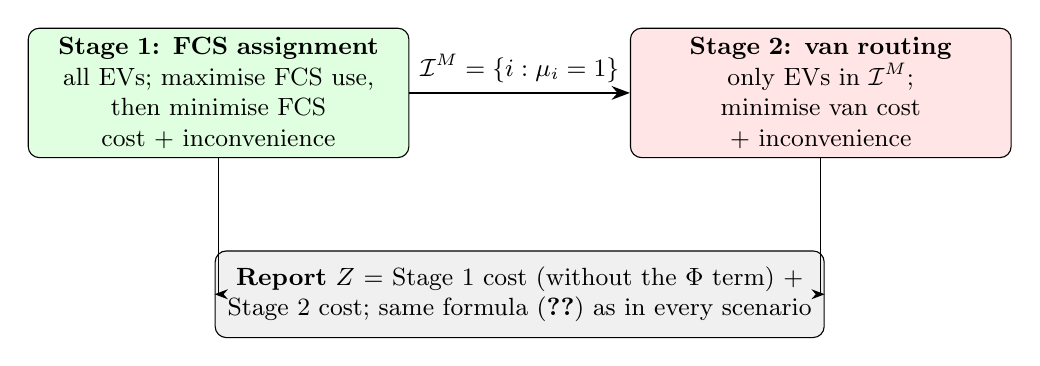
\begin{tikzpicture}[>=Stealth,box/.style={draw,rounded corners,align=center,minimum height=1.1cm,font=\small}]
  \node[box,fill=green!12,text width=4.6cm] (s1) {\textbf{Stage 1: FCS assignment}\\all EVs; maximise FCS use,\\then minimise FCS cost + inconvenience};
  \node[box,fill=red!10,text width=4.6cm,right=2.8cm of s1] (s2) {\textbf{Stage 2: van routing}\\only EVs in $\I^M$;\\minimise van cost + inconvenience};
  \draw[->,thick] (s1) -- node[above,font=\small]{$\I^M=\{i:\mu_i=1\}$} (s2);
  \node[box,fill=black!6,text width=7.5cm,below=2.0cm of $(s1)!0.5!(s2)$] (ev) {\textbf{Report} $Z=$ Stage~1 cost (without the $\Phi$ term) $+$ Stage~2 cost; same formula \eqref{eq:Z} as in every scenario};
  \draw[->] (s1) |- (ev); \draw[->] (s2) |- (ev);
\end{tikzpicture}
\end{center}

Stage~1 does not look at the vans, and Stage~2 cannot change what Stage~1 decided. That is the definition of ``FCS first, then MCS''.

%----------------------------------------------------------------
\subsection{Stage 1: assign EVs to fixed stations}

\textbf{Objective.}
\begin{equation}
\begin{split}
\min\ Z^{(1)}=\;&\underbrace{\Phi\sum_{i\in\I}\mu_i}_{\text{FCS first}}
+\underbrace{c^{EV}\sum_i\sum_{f\in\F_i}d_{if}Y_{if}}_{Z_1}
+\underbrace{Z^F_{\text{energy}}}_{\text{FCS part of }Z_4}\\
&+\underbrace{\sum_i\sum_{f\in\F_i}\rho^F_{if}Y_{if}+\alpha\sum_i w_i(C_i-r_i)+c^L\sum_i w_iL_i}_{\text{FCS customers' inconvenience}}
\end{split}
\label{eq:obj1}
\end{equation}
with $C_i=S_i+\tau^F_iY_i$ in this stage. $\Phi$ is a penalty for handing an EV to the vans. It is chosen larger than anything an extra FCS customer can add to the rest of \eqref{eq:obj1}, e.g.
\[
\Phi > \max_{i}\max_{f\in\F_i}\big(c^{EV}d_{if}+\pi^{\max}E_i+\rho^F_{if}\big)+n\,(\alpha+c^L)\,w_{\max}\,T,
\]
so Stage~1 first \textbf{maximises the number of EVs served at an FCS}, and only among those solutions minimises FCS cost and inconvenience. ($\pi^{\max}$ is the highest grid price.) A numerically safer equivalent is to solve twice: first $\max\sum_iY_i$, then fix that number and minimise the rest.
\ifTOU
Because $Z^F_{\text{energy}}$ uses the peak price, Stage~1 may \emph{start sessions later} to leave the peak, if the price saving beats the extra waiting cost (Section~\ref{sec:expect}).
\fi

\textbf{Constraints.}
\begin{align}
\sum_{g\in\G_i}y_{ig}+\mu_i &= 1 && \forall i\in\I \label{eq:s1assign}\\
S_i &\ge r_i+\sum_{f\in\F_i}t_{if}Y_{if} && \forall i\in\I \label{eq:fcsarr}\\
S_i &\le r_i+T\,(1-\mu_i) && \forall i\in\I \label{eq:s1park}\\
S_j &\ge S_i+\tau^F_i-(T+\tau^F_i)(3-y_{ig}-y_{jg}-o_{ij}) && \forall g,\ (i,j)\in\mathcal{P}_g \label{eq:disj1}\\
S_i &\ge S_j+\tau^F_j-(T+\tau^F_j)(2-y_{ig}-y_{jg}+o_{ij}) && \forall g,\ (i,j)\in\mathcal{P}_g \label{eq:disj2}\\
\sum_i y_{ig_1} &\ge \sum_i y_{ig_2} && \forall f,\ \G_f=\{g_1,g_2\} \label{eq:gunsym}\\
S_i+\tau^F_iY_i &\le T,\qquad L_i\ge S_i+\tau^F_iY_i-l_i && \forall i\in\I \label{eq:s1time}
\end{align}
\ifTOU plus the time-of-use split \eqref{eq:tou1}--\eqref{eq:tou5} of each FCS session (Section~\ref{sec:price}).\fi
\desc{\eqref{eq:s1assign}: every EV either gets one reachable gun or is handed to the vans. An EV that reaches no FCS ($\G_i=\emptyset$) is forced to $\mu_i=1$. \eqref{eq:fcsarr}: an FCS session cannot start before the EV has asked and driven to the station. \eqref{eq:s1park}: for an EV handed to the vans, $S_i$ is parked at $r_i$, so it adds no waiting in Stage~1 (its real start time is decided in Stage~2). \eqref{eq:disj1}--\eqref{eq:disj2}: two EVs on the same gun do not overlap; $o_{ij}$ picks who goes first. With two guns per station this means at most two EVs charge at a station at a time. \eqref{eq:gunsym}: symmetry breaking between the two identical guns (optional). \eqref{eq:s1time}: finished by $T$; lateness.}

\textbf{Optional acceptability rule.} An operator may refuse to send a driver to a station that is ``too inconvenient'', e.g.\ only allow gun $g$ of station $f$ for EV $i$ if $\hat\rho^F_{if}\le\bar\rho$. This only shrinks $\G_i$, so EVs whose stations are all too far go to the vans. Report results with and without it.

\textbf{Output:} $\I^M=\{i:\mu_i=1\}$, the EVs left for the vans; plus each FCS customer's gun and start time.

%----------------------------------------------------------------
\subsection{Stage 2: route the vans to the leftover EVs}

Stage~2 is a vehicle routing problem with time windows, on the EVs in $\I^M$ only. Here $C_i=S_i+\tau^M_i$.

\textbf{Objective.}
\begin{equation}
\begin{split}
\min\ Z^{(2)}=\;&\underbrace{c^M\sum_m\sum_{(i,j)\in\A^M}d_{ij}x_{ijm}}_{Z_2}+\underbrace{\sum_m c^D_mu_m}_{Z_3}+\underbrace{Z^M_{\text{energy}}}_{\text{van part of }Z_4}\\
&+\underbrace{\sum_{i\in\I^M}\sum_m\rho^M_{im}z_{im}+\alpha\sum_{i\in\I^M}w_i(C_i-r_i)+c^L\sum_{i\in\I^M}w_iL_i}_{\text{van customers' inconvenience}}
\end{split}
\label{eq:obj2}
\end{equation}
Since every EV in $\I^M$ must be served by some van, $Z^M_{\text{energy}}$ and the $\rho^M$ term are constants here. They are kept so that $Z^{(2)}$ is the true cost of Stage~2. Waiting and lateness make the vans visit urgent EVs early.

\textbf{Constraints.}
\begin{align}
\sum_{m\in\M}z_{im} &= 1 && \forall i\in\I^M \label{eq:s2assign}\\
\sum_{j:(0,j)\in\A^M}x_{0jm} = \sum_{i:(i,n+1)\in\A^M}x_{i,n+1,m} &= u_m && \forall m \label{eq:depot}\\
\sum_{i:(i,j)\in\A^M}x_{ijm} = \sum_{k:(j,k)\in\A^M}x_{jkm} &= z_{jm} && \forall j\in\I^M,\ m \label{eq:flow}\\
\sum_{i\in\I^M}z_{im} &\le Q_m\,u_m && \forall m \label{eq:cap}\\
\sum_{i\in\I^M}\frac{E_i}{\eta}z_{im}+\beta\sum_{(i,j)\in\A^M}d_{ij}x_{ijm} &\le B_m\,u_m && \forall m \label{eq:batt}
\end{align}
\begin{align}
S_j &\ge \max\{r_j,\ t_{0j}\,x_{0jm}\} && \forall j\in\I^M,\ m \label{eq:depart}\\
S_j &\ge S_i+\tau^M_i+t_{ij}-(T+\tau^M_i+t_{ij})(1-x_{ijm}) && \forall i\neq j,\ m \label{eq:seq}\\
S_i+\tau^M_i+t_{i,n+1} &\le T+(\tau^M_i+t_{i,n+1})(1-x_{i,n+1,m}) && \forall i,\ m \label{eq:return}\\
S_i+\tau^M_i \le T,\quad L_i &\ge S_i+\tau^M_i-l_i && \forall i\in\I^M \label{eq:s2time}\\
u_m &\ge u_{m+1} && m<|\M| \label{eq:vansym}
\end{align}
\desc{\eqref{eq:s2assign}: each leftover EV gets one van. \eqref{eq:depot}: a used van leaves and returns to the depot once. \eqref{eq:flow}: each EV on van $m$ is entered and left exactly once by that van. \eqref{eq:cap}: at most $Q_m$ EVs per van. \eqref{eq:batt}: delivered energy (with transfer losses) plus driving energy fits in the van battery. \eqref{eq:depart}: no start before the request, or before the van can drive there from the depot (written as two linear constraints). \eqref{eq:seq}: if the van goes $i\to j$, it finishes $i$ and drives to $j$ before starting $j$. This gives one EV at a time and removes subtours (MTZ-type). \eqref{eq:return}: back at the depot by $T$. \eqref{eq:s2time}: finished by $T$; lateness. \eqref{eq:vansym}: use identical vans in index order.}

\textbf{If Stage 2 is infeasible} (too many leftover EVs for the fleet by $T$), the sequential policy has \emph{failed} on that instance. For diagnosis, add $s_i\in\{0,1\}$ (``unserved''), replace \eqref{eq:s2assign} by $\sum_mz_{im}+s_i=1$ and add $\Phi^U\sum_is_i$ to \eqref{eq:obj2}. Then report the number of EVs that could not be served. This is a useful comparison with the integrated scenario, which may serve all of them.

%----------------------------------------------------------------
\subsection{Reported value}
\[
Z^{\text{S\scen}}=\big(Z^{(1)*}-\Phi\,|\I^M|\big)+Z^{(2)*},
\]
which is exactly \eqref{eq:Z} evaluated at the combined solution. The stage-1 solution plus the stage-2 solution is a feasible solution of the integrated model (S\ifTOU 4\else 3\fi), so
$Z^{\text{S\ifTOU 4\else 3\fi}}\le Z^{\text{S\scen}}$. The difference is the \emph{value of integration}.

\else
%---------------------------------------------------------------- INT
\subsection{Objective}
\begin{equation}
\min\ Z \quad\text{as in \eqref{eq:Z}, with }Z^F_{\text{energy}}=\ifTOU P^F\textstyle\sum_i\big[\pi^\off(\theta^1_i+\theta^3_i)+\pi^\pk\theta^2_i\big]\else\pi^F\textstyle\sum_iE_iY_i\fi,\quad C_i=S_i+\tau^F_iY_i+\tau^M_iZ_i. \label{eq:objint}
\end{equation}
Written out in full:
\begin{align*}
\min\ Z=\;& c^{EV}\sum_i\sum_{f\in\F_i}d_{if}Y_{if}+c^M\sum_m\sum_{(i,j)\in\A}d_{ij}x_{ijm}+\sum_mc^D_mu_m\\
&+\ifTOU P^F\sum_i\big[\pi^\off(\theta^1_i+\theta^3_i)+\pi^\pk\theta^2_i\big]\else\pi^F\sum_iE_iY_i\fi
+\pi^M\sum_i\sum_m\frac{E_i}{\eta}z_{im}\\
&+\sum_i\sum_{f\in\F_i}\rho^F_{if}Y_{if}+\sum_i\sum_m\rho^M_{im}z_{im}+\alpha\sum_iw_i(C_i-r_i)+c^L\sum_iw_iL_i .
\end{align*}
Every term is linear. One model weighs everything at once: an EV goes to a van exactly when the van's extra km, dispatch and energy cost are outweighed by the effort and waiting it saves the driver\ifTOU, or by the peak-price energy it avoids\fi.

\subsection{Constraints}

\textbf{Assignment.}
\begin{equation}
\sum_{g\in\G_i}y_{ig}+\sum_{m\in\M}z_{im}=1\qquad\forall i\in\I \label{eq:assign}
\end{equation}
\desc{Exactly one resource per EV: one reachable gun or one van. EVs that reach no FCS are forced onto a van.}

\textbf{Fixed stations.}
\begin{align}
S_i &\ge r_i+\sum_{f\in\F_i}t_{if}Y_{if} && \forall i \label{eq:fcsarr}\\
S_j &\ge S_i+\tau^F_i-(T+\tau^F_i)(3-y_{ig}-y_{jg}-o_{ij}) && \forall g,\ (i,j)\in\mathcal{P}_g \label{eq:disj1}\\
S_i &\ge S_j+\tau^F_j-(T+\tau^F_j)(2-y_{ig}-y_{jg}+o_{ij}) && \forall g,\ (i,j)\in\mathcal{P}_g \label{eq:disj2}\\
\sum_iy_{ig_1} &\ge \sum_iy_{ig_2} && \forall f,\ \G_f=\{g_1,g_2\} \label{eq:gunsym}
\end{align}
\desc{\eqref{eq:fcsarr}: an FCS session starts after the request and the drive to the station (for a van customer this is just $S_i\ge r_i$). \eqref{eq:disj1}--\eqref{eq:disj2}: EVs on the same gun do not overlap; $o_{ij}$ chooses the order. \eqref{eq:gunsym}: optional symmetry breaking.}

\textbf{Vans: routes, capacity, battery.}
\begin{align}
\sum_{j:(0,j)\in\A}x_{0jm}=\sum_{i:(i,n+1)\in\A}x_{i,n+1,m} &= u_m && \forall m \label{eq:depot}\\
\sum_{i:(i,j)\in\A}x_{ijm}=\sum_{k:(j,k)\in\A}x_{jkm} &= z_{jm} && \forall j\in\I,\ m \label{eq:flow}\\
\sum_iz_{im} &\le Q_mu_m && \forall m \label{eq:cap}\\
\sum_i\frac{E_i}{\eta}z_{im}+\beta\sum_{(i,j)\in\A}d_{ij}x_{ijm} &\le B_mu_m && \forall m \label{eq:batt}
\end{align}
\desc{\eqref{eq:depot}: a used van leaves and returns once. \eqref{eq:flow}: each EV on van $m$ is visited exactly once by it. \eqref{eq:cap}: at most $Q_m$ EVs. \eqref{eq:batt}: delivered energy (with losses) plus driving energy fits in the battery.}

\textbf{Vans: timing (one EV at a time, no subtours).}
\begin{align}
S_j &\ge t_{0j}\,x_{0jm} && \forall j\in\I,\ m \label{eq:depart}\\
S_j &\ge S_i+\tau^M_i+t_{ij}-(T+\tau^M_i+t_{ij})(1-x_{ijm}) && \forall i\neq j\in\I,\ m \label{eq:seq}\\
S_i+\tau^M_i+t_{i,n+1} &\le T+(\tau^M_i+t_{i,n+1})(1-x_{i,n+1,m}) && \forall i,\ m \label{eq:return}
\end{align}
\desc{\eqref{eq:depart}: the first stop cannot start before the van has driven there. \eqref{eq:seq}: $i\to j$ means finish $i$, drive, then start $j$; start times rise along a route, so no subtour can close. \eqref{eq:return}: back at the depot by $T$.}

\textbf{Horizon and lateness.}
\begin{equation}
C_i\le T,\qquad L_i\ge C_i-l_i\qquad\forall i\in\I \label{eq:time}
\end{equation}
\desc{Every EV is fully charged within the horizon; $L_i$ measures lateness.}

\ifTOU
\textbf{Time-of-use split.} Constraints \eqref{eq:tou1}--\eqref{eq:tou5} of Section~\ref{sec:price}.
\fi

\textbf{Symmetry and domains.}
\begin{equation}
u_m\ge u_{m+1};\qquad y,z,x,u,o\ifTOU,\kappa\fi\in\{0,1\};\qquad S_i,L_i\ifTOU,\theta^p_i\fi\ge0 \label{eq:dom}
\end{equation}
\fi

%=====================================================================
\section{Learning-to-optimise (RL) formulation}\label{sec:rl}

\textbf{Main rule:} the reward of each action is \emph{minus the increase in $Z$ that the action causes}. The rewards over an episode then add up to $-Z$ of the solution the policy builds. RL and MILP results are measured on the same yardstick \eqref{eq:Z}, and the MILP optimum is the benchmark for the RL gap.

\ifSEQ
%---------------------------------------------------------------- RL SEQ
The RL pipeline has the same two stages as the MILP.

\subsection{Stage 1 policy: FCS assignment}
\begin{itemize}[leftmargin=1.4em,itemsep=2pt]
  \item \textbf{Episode / epochs:} EVs are taken in order of request time $r_i$ (ties: higher $w_i$ first). One decision per EV.
  \item \textbf{State:} features of the current EV $k$ ($E_k,r_k,l_k,w_k,R_k$, location); for each gun $g$ the time $F_g$ it becomes free; summary features of the EVs still to come (count and positions near each station)\ifTOU; the current price and the time until $T_1$ and $T_2$\fi.
  \item \textbf{Action:} a gun $g\in\G_k$, or ``hand to vans''. \textbf{FCS-first mask:} ``hand to vans'' is allowed \emph{only} if no gun can finish EV $k$ by $T$ (or, with the optional rule, if all remaining guns have $\hat\rho^F_{kf}>\bar\rho$).
  \ifTOU\item \textbf{Optional timing action:} ``gun $g$, start after the peak'', i.e.\ $S_k=\max\{\text{earliest},T_2\}$, allowed only if the session still ends by $T$.\fi
  \item \textbf{Transition:} $S_k=\max\{r_k+t_{kf},F_g\}$ (or later, for the timing action); $F_g\leftarrow S_k+\tau^F_k$.
  \item \textbf{Reward:} $-\Big[c^{EV}d_{kf}+\text{energy}_k+\rho^F_{kf}+\alpha w_k(S_k+\tau^F_k-r_k)+c^Lw_k(S_k+\tau^F_k-l_k)^+\Big]$, where energy$_k$ = \ifTOU$P^F\big[\pi^\off\cdot(\text{off-peak hours of }[S_k,S_k+\tau^F_k])+\pi^\pk\cdot(\text{peak hours})\big]$, computed exactly in the simulator\else$\pi^FE_k$\fi. Handing an EV to the vans gives reward $0$ here; its cost is counted in Stage~2.
\end{itemize}
Note: a simple baseline for Stage~1 is the greedy rule ``gun with the largest one-step reward''. What RL can learn on top of this is, for example, to keep a nearby gun free for an urgent EV that arrives later.

\subsection{Stage 2 policy: van routing over $\I^M$}
\begin{itemize}[leftmargin=1.4em,itemsep=2pt]
  \item \textbf{Epochs:} whenever a van becomes free (the earliest-free van decides first).
  \item \textbf{State:} for each van: position, time free, remaining battery $b_m$, EVs served so far, dispatched or not; for each unserved EV in $\I^M$: location, $E_i,r_i,l_i,w_i$; current time.
  \item \textbf{Action:} the next EV $j$ for this van, or ``return to depot'' (ends the route). Mask: $j$ must be feasible: battery covers $E_j/\eta$ plus driving to $j$ and back to the depot, the count stays $\le Q_m$, and $j$ can be finished with the van back at the depot by $T$.
  \item \textbf{Transition:} $S_j=\max\{r_j,\ \text{time free}+t_{\text{pos},j}\}$; the van moves to $j$ and is free at $S_j+\tau^M_j$; $b_m$ falls by $E_j/\eta+\beta d_{\text{pos},j}$.
  \item \textbf{Reward:} serving $j$: $-\Big[c^Md_{\text{pos},j}+c^D_m[\text{first stop}]+\pi^M\frac{E_j}{\eta}+\rho^M_{jm}+\alpha w_j(S_j+\tau^M_j-r_j)+c^Lw_j(S_j+\tau^M_j-l_j)^+\Big]$; returning: $-c^Md_{\text{pos},0}$. EVs still unserved at the end: $-\Phi^U$ each.
  \item \textbf{Policy:} an attention-based routing policy (e.g.\ Kool et al., 2019, ``Attention, Learn to Solve Routing Problems!'') trained with REINFORCE or PPO. Baseline: nearest-feasible-EV heuristic.
\end{itemize}
Episode return of Stage~1 + Stage~2 $=-Z^{\text{S\scen}}$.

\else
%---------------------------------------------------------------- RL INT
One policy decides both who serves each EV and the van routes.
\begin{itemize}[leftmargin=1.4em,itemsep=2pt]
  \item \textbf{Episode / epochs:} EVs are taken in order of request time $r_i$ (ties: higher $w_i$ first). One decision per EV.
  \item \textbf{State:} (i) the current EV $k$: location, $E_k,r_k,l_k,w_k,R_k$, reachable stations; (ii) each gun $g$: time $F_g$ it becomes free; (iii) each van $m$: current end-of-route position, time free, remaining battery $b_m$, EVs served, dispatched or not; (iv) embeddings of the not-yet-assigned EVs (for look-ahead)\ifTOU; (v) current price, time until $T_1$ and $T_2$\fi.
  \item \textbf{Action:} $a\in\G_k\cup\M$: a gun, or a van (EV $k$ is appended to the end of that van's route). \textbf{Mask} infeasible actions: a gun that cannot finish $k$ by $T$; a van without enough battery for $E_k/\eta$ plus the drive to $k$ and back to the depot, with $Q_m$ reached, or unable to finish $k$ and return by $T$.
  \ifTOU\item \textbf{Optional timing action:} ``gun $g$, start after the peak'' ($S_k=\max\{\text{earliest},T_2\}$, if it still ends by $T$).\fi
  \item \textbf{Transition:} gun: $S_k=\max\{r_k+t_{kf},F_g\}$, $F_g\leftarrow S_k+\tau^F_k$. Van: $S_k=\max\{r_k,\ \text{free}_m+t_{\text{pos}_m,k}\}$, then the van moves to $k$, $\text{free}_m\leftarrow S_k+\tau^M_k$, $b_m\mathrel{-}=E_k/\eta+\beta d_{\text{pos}_m,k}$.
  \item \textbf{Reward} $=-\Delta Z$:
  \begin{align*}
  \text{gun } g\text{ at }f:&\quad -\Big[c^{EV}d_{kf}+\text{energy}^F_k+\rho^F_{kf}+\alpha w_k(C_k-r_k)+c^Lw_k(C_k-l_k)^+\Big]\\
  \text{van } m:&\quad -\Big[c^M\big(d_{\text{pos}_m,k}+d_{k,0}-d_{\text{pos}_m,0}\big)+c^D_m[\text{first use}]+\pi^M\tfrac{E_k}{\eta}\\
  &\qquad\quad+\rho^M_{km}+\alpha w_k(C_k-r_k)+c^Lw_k(C_k-l_k)^+\Big]
  \end{align*}
  The van distance term is the \emph{change} in route length when $k$ is inserted before the return to the depot, so the sum over the episode equals the total route length (the return legs telescope). energy$^F_k$ = \ifTOU$P^F\big[\pi^\off\cdot(\text{off-peak hours})+\pi^\pk\cdot(\text{peak hours of }[S_k,C_k])\big]$, computed exactly by the simulator; no linearisation is needed in RL\else$\pi^FE_k$\fi.
  \item \textbf{Dead end:} if every action is masked, EV $k$ is unserved: reward $-\Phi^U$, and the episode continues. Report the count.
  \item \textbf{Policy:} masked categorical policy over guns and vans, encoder with attention over EVs, guns and vans; trained with PPO. Natural baseline: greedy, i.e.\ choose the action with the largest one-step reward. That is the pairwise rule ``smallest $\hat\rho$ + cost'' from Section~\ref{sec:inc}.
\end{itemize}
Restriction to note: vans serve EVs in assignment order (append only). A variant that inserts $k$ at the cheapest position of a route is more flexible but has a larger action space.
\fi

\textbf{Reward scaling.} For stable training divide every reward by a constant, e.g.\ the greedy baseline's average $Z$ on the training instances. This does not change the optimal policy.

%=====================================================================
\section{What to expect and what to report}\label{sec:expect}

\ifnum\scen=1
\begin{itemize}[leftmargin=1.4em,itemsep=2pt]
  \item Vans serve only EVs that reach no station, or that the stations cannot finish by $T$. If stations have spare capacity, very few vans are dispatched.
  \item Inconvenience is high for EVs far from the nearest station (worked example: Rs\,682 at the FCS, against Rs\,458 if a van had been allowed).
  \item With too few vans Stage~2 becomes infeasible (unserved EVs), even when the integrated model S3 could serve everyone. Report the smallest $|\M|$ at which S1 is feasible and compare it with S3.
\end{itemize}
\fi
\ifnum\scen=2
\begin{itemize}[leftmargin=1.4em,itemsep=2pt]
  \item \textbf{When does Stage~1 delay a session to avoid the peak?} Moving one hour of charging out of the peak saves $(\pi^\pk-\pi^\off)P^F=3\times22=$ Rs\,66, but delays completion by up to an hour, which costs $\alpha w_i\ge$ Rs\,200. So with the default values Stage~1 almost never delays. It mostly pays the higher price, and S2 costs roughly S1 plus the peak surcharge. Sessions start later only if $\alpha$ is small (try $\lambda<0.33$ in the sensitivity analysis).
  \item The van assignment is the same as in S1 unless Stage~1's timing changes which EVs fit at the stations. Stage~1 cannot use vans to escape the peak price.
  \item Extra KPI: \textbf{grid energy drawn at FCS during the peak}, $P^F\sum_i\theta^2_i$ (kWh). Compare with S4.
\end{itemize}
\fi
\ifnum\scen=3
\begin{itemize}[leftmargin=1.4em,itemsep=2pt]
  \item Vans take EVs for which the saved inconvenience exceeds the extra van cost (worked example: van chosen, saving Rs\,224). Expect vans to serve EVs that are far from every station, have low range (high $w_i$), or have early deadlines, while EVs near a station still use it.
  \item \textbf{Value of integration under flat price:} $Z^{\text{S1}}-Z^{\text{S3}}\ge0$. Report it per component ($Z_1,\dots,Z_5$): typically operating cost rises a little and inconvenience falls a lot.
  \item Vary $|\M|$ (0, 1, 2, \dots): the first few vans lower $Z$ sharply, then the effect levels off. That curve shows the scenarios where mobile chargers help most.
\end{itemize}
\fi
\ifnum\scen=4
\begin{itemize}[leftmargin=1.4em,itemsep=2pt]
  \item During the peak a van kWh costs about the same as an FCS kWh (Rs\,10.0 each), so the vans' energy disadvantage disappears and vans also absorb \emph{peak-hour} demand that would otherwise be charged on the grid at peak price.
  \item Expect more van usage than in S3, concentrated on requests in $[T_1,T_2]$, and lower grid energy at the stations during the peak, $P^F\sum_i\theta^2_i$, than in S2.
  \item \textbf{Value of integration under peak pricing:} $Z^{\text{S2}}-Z^{\text{S4}}$. It should be larger than $Z^{\text{S1}}-Z^{\text{S3}}$, because integration now also allows price arbitrage.
  \item \textbf{Peak pricing with full flexibility:} $Z^{\text{S4}}-Z^{\text{S3}}$ should be smaller than $Z^{\text{S2}}-Z^{\text{S1}}$: vans cushion the price increase.
\end{itemize}
\fi

\textbf{Cross-scenario comparison table} (fill in from the four runs):
\begin{center}
\renewcommand{\arraystretch}{1.2}
\begin{tabular}{@{}lll@{}}
\toprule
\textbf{Comparison} & \textbf{Measures} & \textbf{Expected sign} \\
\midrule
S1 $-$ S3 & value of integration, flat price & $\ge0$ \\
S2 $-$ S4 & value of integration, peak price & $\ge0$, larger than S1 $-$ S3 \\
S2 $-$ S1 & cost of peak pricing, FCS-first operator & $>0$ \\
S4 $-$ S3 & cost of peak pricing, flexible operator & $>0$, smaller than S2 $-$ S1 \\
\bottomrule
\end{tabular}
\end{center}
Report for each: $Z$ and its components, number of vans used, EVs per resource, mean and maximum inconvenience per EV, total lateness, peak-hour grid energy, solve time, and (for RL) the gap to the MILP optimum.

%=====================================================================
\appendix
\section{Illustrative parameter values}\label{app:values}

These are starting values for experiments, not data. All are meant to be varied in the analysis. Values in Rs.

\begin{center}
\renewcommand{\arraystretch}{1.15}
\begin{tabular}{@{}llp{6.2cm}@{}}
\toprule
\textbf{Parameter} & \textbf{Value} & \textbf{Note} \\
\midrule
$T$, $[T_1,T_2]$ & 7 h, $[2,6]$ & 16:00--23:00, peak 18:00--22:00 \\
$P^F$, $P^M$ & 22 kW, 30 kW & \\
$v$, $\beta$, $\eta$ & 25 km/h, 0.25 kWh/km, 0.9 & \\
$B_m$, $Q_m$, $|\M|$ & 150 kWh, 6, 2--6 & \\
$c^{EV}$, $c^M$, $c^D_m$ & Rs\,4/km, Rs\,15/km, Rs\,1500 & van km includes driver time \\
$\pi^F$ (flat) & Rs\,8.7/kWh & equals the time-average of the ToU tariff over $[0,T]$ \\
$\pi^\off$, $\pi^\pk$ (ToU) & Rs\,7/kWh, Rs\,10/kWh & $(3\times7+4\times10)/7=8.7$ \\
$c^{bat}$ & Rs\,2/kWh & van battery wear \\
$\pi^M$ & Rs\,10.7 (flat) / Rs\,9.0 (ToU) & $=\pi^F+c^{bat}$ / $=\pi^\off+c^{bat}$ \\
$\alpha$, $\alpha^D$ & Rs\,200/h, Rs\,100/h & value of time; extra for attended time \\
$h^F$, $h^M$, $\varphi$ & Rs\,50, Rs\,10, Rs\,100 & trip hassle, hand-over, range stress \\
$c^L$ & Rs\,300/h & lateness \\
$w_i$ & $1+2(1-R_i/R_{\max})$, $R_i\sim U[3,40]$ km & priority from remaining range \\
\bottomrule
\end{tabular}
\end{center}

The flat price is set to the time-average of the peak tariff. The price \emph{level} is then the same in both pricing cases, and only the price \emph{shape} differs. Without this, part of S1 vs S2 would just reflect a different average price.

\end{document}
"
%    pdflatex -jobname=scenario4_peak_integrated   "\def\scen{4}% =====================================================================
%  One source, four PDFs.  Build with build.sh (or by hand):
%    pdflatex -jobname=scenario1_flat_sequential   "\def\scen{1}\input{scenario_master}"
%    pdflatex -jobname=scenario2_peak_sequential   "\def\scen{2}\input{scenario_master}"
%    pdflatex -jobname=scenario3_flat_integrated   "\def\scen{3}\input{scenario_master}"
%    pdflatex -jobname=scenario4_peak_integrated   "\def\scen{4}\input{scenario_master}"
%  (run each twice for cross-references)
% =====================================================================
\documentclass[11pt,a4paper]{article}
\usepackage[margin=2.2cm]{geometry}
\usepackage{amsmath,amssymb,amsfonts}
\usepackage{booktabs,array,tabularx}
\usepackage{enumitem}
\usepackage[table]{xcolor}
\usepackage{tikz}
\usetikzlibrary{arrows.meta,positioning,calc}
\usepackage[colorlinks=true,linkcolor=blue!50!black,urlcolor=blue!50!black]{hyperref}
\usepackage{titlesec}
\titleformat{\section}{\large\bfseries}{\thesection}{0.8em}{}
\titleformat{\subsection}{\normalsize\bfseries}{\thesubsection}{0.8em}{}
\setlength{\parindent}{0pt}
\setlength{\parskip}{5pt}

% ---------------- scenario switches ----------------
\ifdefined\scen\else\def\scen{1}\fi
\newif\ifTOU \TOUfalse   % true = time-of-use (peak) price
\newif\ifSEQ \SEQfalse   % true = FCS first, then MCS
\ifnum\scen=1 \SEQtrue \fi
\ifnum\scen=2 \TOUtrue \SEQtrue \fi
\ifnum\scen=4 \TOUtrue \fi

\newcommand{\pricename}{\ifTOU time-of-use price (dearer evening peak)\else single (flat) price all day\fi}
\newcommand{\structname}{\ifSEQ FCS first, then MCS (sequential)\else FCS and MCS together (integrated)\fi}

% ---------------- notation ----------------
\newcommand{\I}{\mathcal{I}}
\newcommand{\F}{\mathcal{F}}
\newcommand{\G}{\mathcal{G}}
\newcommand{\M}{\mathcal{M}}
\newcommand{\N}{\mathcal{N}}
\newcommand{\A}{\mathcal{A}}
\newcommand{\Rs}{\text{Rs}\,}
\newcommand{\pk}{\mathrm{pk}}
\newcommand{\off}{\mathrm{off}}
\newcommand{\desc}[1]{\par\vspace{-2pt}{\small\color{black!75}\textit{Meaning:} #1}\par\vspace{4pt}}
\newcommand{\cell}[2]{\ifnum\scen=#1\cellcolor{blue!18}\textbf{S#1 (this document)}\\\textbf{#2}\else S#1\\#2\fi}

\title{\textbf{EV Charging Network Optimisation}\\[4pt]
\large Scenario \scen: \pricename\ $+$ \structname\\[2pt]
\normalsize MILP and RL formulation}
\author{CP 320 OR for Mobility Management, course project}
\date{2 October 2026}

\begin{document}
\maketitle

%=====================================================================
\section{Where this scenario sits}

The project studies four scenarios: two ways of pricing grid electricity, times two ways of making the decisions.

\begin{center}
\renewcommand{\arraystretch}{1.5}
\begin{tabular}{>{\raggedright\arraybackslash}p{4.2cm}|>{\centering\arraybackslash}p{4.6cm}|>{\centering\arraybackslash}p{4.6cm}}
 & \textbf{Flat price all day} & \textbf{Time-of-use (peak) price} \\ \hline
\textbf{Sequential:} FCS first, leftover EVs to MCS &
\begin{tabular}[c]{@{}c@{}}\cell{1}{flat + sequential}\end{tabular} &
\begin{tabular}[c]{@{}c@{}}\cell{2}{peak + sequential}\end{tabular} \\ \hline
\textbf{Integrated:} FCS and MCS decided together &
\begin{tabular}[c]{@{}c@{}}\cell{3}{flat + integrated}\end{tabular} &
\begin{tabular}[c]{@{}c@{}}\cell{4}{peak + integrated}\end{tabular} \\
\end{tabular}
\end{center}

\textbf{The four scenarios do not have four different objectives.} They share \emph{one} cost yardstick $Z$ (Section~\ref{sec:obj}): the same cost terms and the same customer inconvenience (Section~\ref{sec:inc}). Only two things change:
\begin{itemize}[leftmargin=1.4em,itemsep=1pt]
  \item \textbf{Pricing} changes the formula for one term, the FCS energy cost (Section~\ref{sec:price}).
  \item \textbf{Decision structure} changes \emph{how} $Z$ is minimised: in one model (integrated), or in two stages (sequential), where each stage minimises its own part of $Z$.
\end{itemize}
Because the yardstick is the same, the four optimal values can be compared directly. The differences measure the \emph{value of integration} (S1$\to$S3, S2$\to$S4) and the \emph{effect of peak pricing} (S1$\to$S2, S3$\to$S4).

\ifnum\scen=1
\textbf{This scenario (S1)} is the baseline, the ``status quo''. Electricity costs the same at every hour, every EV that can be charged at a fixed station is sent there, and vans only take what is left over.
\fi
\ifnum\scen=2
\textbf{This scenario (S2)} keeps the FCS-first rule of S1, but grid electricity is dearer during the evening peak. Stage~1 can react to the price only by \emph{rescheduling} FCS sessions. It cannot hand a peak-hour EV to a van.
\fi
\ifnum\scen=3
\textbf{This scenario (S3)} keeps the flat price of S1, but the operator decides FCS and MCS service \emph{together}. An EV can be sent to a van even when a fixed station could take it, whenever that lowers total cost plus inconvenience.
\fi
\ifnum\scen=4
\textbf{This scenario (S4)} is the most flexible one: peak pricing at fixed stations, and FCS and MCS decided together. Van energy was bought off-peak, so vans can also be used to keep charging \emph{out of the expensive peak}.
\fi

%=====================================================================
\section{Setting and assumptions}\label{sec:setting}

\textbf{Time.} The planning horizon is $[0,T]$ with $T=7$\,h (16:00--23:00). It contains the evening peak window $[T_1,T_2]=[2,6]$ (18:00--22:00). The horizon is the same in all four scenarios. It is wider than the peak itself so that, under peak pricing, there is cheaper time on both sides of the peak.\ifTOU\else\ In this scenario the price is flat, so the window plays no role in the model.\fi

\textbf{Assumptions} (the same as MILP v3, plus two about energy):
\begin{enumerate}[leftmargin=1.6em,itemsep=1pt]
  \item Static, continuous time. All requests in the horizon are known at time $0$, and request $i$ becomes active at $r_i$.
  \item An EV served by an FCS drives there itself on its own battery (only to stations within its range $R_i$). The driver stays with the car while it waits for a free gun and while it charges.
  \item An EV served by an MCS stays parked where it is, and the driver is free in the meantime.
  \item Each FCS gun and each van charges one EV at a time, without interruption, at constant power.
  \item A van's battery covers both its driving and the energy it delivers. \textbf{The van battery is charged at the depot before the horizon starts}\ifTOU, i.e.\ at the off-peak price\fi, and is not recharged during the horizon.
  \item Every EV must be fully charged by $T$ (hard). Finishing after the driver's desired time $l_i$ is allowed but penalised.
\end{enumerate}

%=====================================================================
\section{Notation}\label{sec:notation}

\subsection*{Sets}
\begin{tabularx}{\textwidth}{@{}lX@{}}
\toprule
$\I=\{1,\dots,n\}$ & EV charging requests \\
$\F$; $\G_f$ ($|\G_f|=2$); $\G=\bigcup_f\G_f$ & fixed charging stations; guns of FCS $f$; all guns ($f(g)$ = station of gun $g$) \\
$\F_i=\{f: d_{if}\le R_i\}$, $\G_i=\bigcup_{f\in\F_i}\G_f$ & stations / guns EV $i$ can reach on its remaining range \\
$\M$ & mobile charging vans (MCS) \\
$0,\ n+1$ & depot as start node / end node (same place) \\
$\N=\{0\}\cup\I\cup\{n+1\}$, $\A$ & routing nodes; allowed van arcs $(i,j)$, $i\in\{0\}\cup\I$, $j\in\I\cup\{n+1\}$, $i\neq j$ \\
$\mathcal{P}_g=\{(i,j): i<j,\ g\in\G_i\cap\G_j\}$ & pairs of EVs that could share gun $g$ \\
\ifSEQ
$\I^M\subseteq\I$ & EVs handed to the vans by Stage~1 (an \emph{output} of Stage~1, a fixed input to Stage~2) \\
$\N^M$, $\A^M$ & routing nodes / arcs restricted to $\I^M$ \\
\fi
\bottomrule
\end{tabularx}

\subsection*{Parameters}
\begin{tabularx}{\textwidth}{@{}lX@{}}
\toprule
$E_i,\ r_i,\ l_i,\ R_i$ & energy demand (kWh), request time, desired completion time (h), remaining range (km) \\
$w_i\ge1$ & priority of EV $i$; $w_i=1+\kappa(1-R_i/R_{\max})$, so low-range EVs weigh more \\
$P^F,\ P^M$ & charging power of an FCS gun (22\,kW) / of a van (e.g.\ 30\,kW) \\
$\tau^F_i=E_i/P^F,\ \tau^M_i=E_i/P^M$ & charging time of EV $i$ at an FCS / by a van (h) \\
$d_{if},t_{if}$;\ $d_{ij},t_{ij}$ & distance (km) and time (h): EV$\to$FCS; between routing nodes ($t=d/v$) \\
$B_m,\ Q_m,\ \beta,\ \eta$ & van battery (kWh), max EVs per van, van consumption (kWh/km), transfer efficiency \\
$c^{EV},\ c^M,\ c^D_m$ & cost per km of EV driving, per km of van driving; fixed dispatch cost of van $m$ \\
\ifTOU
$\pi^\off,\ \pi^\pk$ & grid price (Rs/kWh) off-peak / in $[T_1,T_2]$, with $\pi^\pk\ge\pi^\off$ \\
\else
$\pi^F$ & grid price (Rs/kWh), the same at every hour \\
\fi
$c^{bat}$ & van battery wear per kWh cycled \\
$\pi^M$ & cost of 1 kWh taken from a van battery: $\pi^M=\ifTOU\pi^\off\else\pi^F\fi+c^{bat}$ (Section~\ref{sec:price}) \\
$\alpha,\ \alpha^D,\ h^F,\ h^M,\ \varphi,\ c^L$ & inconvenience coefficients (Section~\ref{sec:inc}) \\
\bottomrule
\end{tabularx}

\subsection*{Decision variables}
\begin{tabularx}{\textwidth}{@{}llX@{}}
\toprule
$y_{ig}$ & $\{0,1\}$ & EV $i$ charged at gun $g\in\G_i$ \\
$z_{im}$ & $\{0,1\}$ & EV $i$ served by van $m$ \\
$x_{ijm}$ & $\{0,1\}$ & van $m$ drives arc $(i,j)$ \\
$u_m$ & $\{0,1\}$ & van $m$ is dispatched \\
$o_{ij}$ & $\{0,1\}$ & for EVs $i<j$ that could share a gun: 1 if $i$ is charged before $j$ \\
\ifSEQ
$\mu_i$ & $\{0,1\}$ & Stage~1 only: EV $i$ is handed to the van fleet \\
\fi
\ifTOU
$\theta^1_i,\theta^2_i,\theta^3_i$ & $\ge0$ & hours of EV $i$'s FCS session before / inside / after the peak \\
$\kappa^1_i,\kappa^3_i$ & $\{0,1\}$ & EV $i$'s FCS session starts before $T_1$ / ends after $T_2$ \\
\fi
$S_i$ & $\ge0$ & time charging of EV $i$ starts (h), on whichever resource \\
$L_i$ & $\ge0$ & lateness of EV $i$ beyond $l_i$ (h) \\
\bottomrule
\end{tabularx}

\textbf{Short-hands} (linear expressions, not new variables):
\[
Y_{if}=\sum_{g\in\G_f}y_{ig},\qquad Y_i=\sum_{g\in\G_i}y_{ig}\ (\text{EV $i$ uses an FCS}),\qquad Z_i=\sum_{m\in\M}z_{im}\ (\text{EV $i$ uses a van}),
\]
\[
C_i=S_i+\tau^F_i\,Y_i+\tau^M_i\,Z_i \quad\text{(time EV $i$ is fully charged).}
\]

%=====================================================================
\section{Customer inconvenience}\label{sec:inc}

This section is \textbf{identical in all four scenario documents}. Inconvenience is a property of the customer, not of the price or of the planning method.

\subsection{What we mean by inconvenience}

Inconvenience is \emph{what the driver loses} from the moment they ask for a charge ($r_i$) until the car is fully charged ($C_i$), \emph{converted into rupees} so it can be added to the operator's costs. A driver loses three different things:

\begin{enumerate}[leftmargin=1.6em,itemsep=2pt]
  \item \textbf{Waiting:} the car is not ready. This lasts $C_i-r_i$ hours and affects \emph{every} driver, FCS or MCS.
  \item \textbf{Effort:} only an FCS customer has to drive to the station and sit there while the car charges. An MCS customer stays at home or at work and does something else. Driving to a far station also uses scarce battery range, which causes stress (``range anxiety'').
  \item \textbf{A missed deadline:} the car is still not ready at the time $l_i$ the driver needs it.
\end{enumerate}

Each loss gets a price in Rs per hour (or per event). All of them are multiplied by the priority $w_i$: an hour of delay for an EV with 5\,km of range left counts more than for one with 40\,km.

\subsection{The three components}

\begin{center}
\renewcommand{\arraystretch}{1.3}
\begin{tabularx}{\textwidth}{@{}>{\raggedright\arraybackslash}p{2.6cm}>{\raggedright\arraybackslash}X>{\raggedright\arraybackslash}X>{\raggedright\arraybackslash}p{3.0cm}@{}}
\toprule
\textbf{Component} & \textbf{EV $i$ at FCS $f$} & \textbf{EV $i$ by a van} & \textbf{Known when?} \\
\midrule
Effort & $w_i\big[\alpha^D(t_{if}+\tau^F_i)+h^F+\varphi\,d_{if}/R_i\big]$: driving and sitting at the station, a fixed trip hassle, range stress & $w_i\,h^M$: being reachable and handing over the car & \textbf{Static:} known as soon as the resource is chosen \\
Waiting & $w_i\,\alpha\,(C_i-r_i)$ = drive + \emph{queue at the gun} + charge & $w_i\,\alpha\,(C_i-r_i)$ = \emph{wait for the van} + charge & \textbf{Dynamic:} depends on the queue / van route \\
Missed deadline & $w_i\,c^L\,L_i$, $L_i=\max\{0,C_i-l_i\}$ & same & Dynamic \\
\bottomrule
\end{tabularx}
\end{center}

\textbf{Coefficients.}
$\alpha$ (Rs/h) is the value of an hour the car is not ready.
$\alpha^D$ (Rs/h) is the \emph{extra} value of an hour the driver must personally spend driving or sitting at the station: an hour at the station costs $\alpha+\alpha^D$, an hour waiting at home for a van costs only $\alpha$.
$h^F,h^M$ (Rs) are fixed hassle costs of one trip to a station / one van hand-over.
$\varphi$ (Rs) is the range-stress cost of a trip that uses the \emph{whole} remaining range ($d_{if}/R_i\le1$ is the fraction used).
$c^L$ (Rs/h) is the cost per hour late.

\subsection{Pairwise form: inconvenience of a (customer, resource) pair}

The natural first idea is: \emph{for every pair (EV $i$, FCS $f$) and every pair (EV $i$, van $m$) there is an inconvenience number, and the operator picks the pair with the lowest cost plus inconvenience.} The static part fits this idea exactly:
\[
\boxed{\;\rho^F_{if}=w_i\Big[\alpha^D\,(t_{if}+\tau^F_i)+h^F+\varphi\,\frac{d_{if}}{R_i}\Big]\qquad
\rho^M_{im}=w_i\,h^M\;}
\]
These are \textbf{parameters}, computed before solving, one number per (EV, FCS) pair and per (EV, van) pair. In the objective they appear linearly: $\sum_i\sum_f\rho^F_{if}Y_{if}+\sum_i\sum_m\rho^M_{im}z_{im}$.

Note that $\rho^M_{im}$ does not depend on $m$. Vans are identical and all start at the same depot, so the driver does not care \emph{which} van comes, only \emph{when} it comes. That ``when'' is the waiting part.

\subsection{Why waiting cannot be a fixed pairwise number}

It is tempting to also write the waiting as a pairwise number, e.g.\ ``the van needs 5 minutes to reach EV $i$''. But that depends on \emph{where the van is coming from}, which depends on the route the model is still choosing: if EV $i$ is the 4th stop of a van, the wait is the time for three charging sessions plus four drives. Likewise, waiting at an FCS depends on how many EVs are queued at that gun. So waiting is not known before solving. It is a function of decision variables:
\[
\text{waiting cost of EV } i \;=\; w_i\,\alpha\,(C_i-r_i),\qquad C_i=S_i+\tau^F_iY_i+\tau^M_iZ_i .
\]
This is \textbf{linear} in the variables ($S_i$, $y$, $z$), so it fits in a MILP directly. The constraints of Section~\ref{sec:milp} make $S_i$ equal to the true start time, including driving, queueing at the gun and the van's route. The term $\sum_i w_i\alpha r_i$ is a constant and may be dropped when solving.

\textbf{Pairwise \emph{estimate}} (used for intuition, by the RL policy and in heuristics): if there is no queue and the van comes straight to $i$,
\[
\hat\rho^{F}_{if}=\rho^F_{if}+w_i\alpha\,(t_{if}+\tau^F_i),\qquad
\hat\rho^{M}_{im}=\rho^M_{im}+w_i\alpha\,(t^{\text{van}}_{m\to i}+\tau^M_i),
\]
where $t^{\text{van}}_{m\to i}$ is the time until van $m$ can reach $i$ from where it currently is. In the RL formulation (Section~\ref{sec:rl}) the van's position \emph{is} known at each decision, so there this estimate becomes exact.

\subsection{Total inconvenience and how it enters the objective}

\begin{equation}
\boxed{\;
Z_{\text{inc}}=\underbrace{\sum_{i\in\I}\sum_{f\in\F_i}\rho^F_{if}Y_{if}+\sum_{i\in\I}\sum_{m\in\M}\rho^M_{im}z_{im}}_{\text{effort (static, pairwise)}}
+\underbrace{\alpha\sum_{i\in\I}w_i\,(C_i-r_i)}_{\text{waiting (dynamic)}}
+\underbrace{c^L\sum_{i\in\I}w_i\,L_i}_{\text{missed deadline}}
\;}\label{eq:inc}
\end{equation}
All three parts are in rupees, so $Z_{\text{inc}}$ is simply added to the operating costs. Nothing has to be normalised.

\subsection{Worked example: your ``10 km to the FCS vs.\ van in 5 minutes'' case}

EV $i$: $E_i=20$\,kWh, $R_i=40$\,km (so $w_i=1$); nearest free FCS $d_{if}=10$\,km away, $t_{if}=0.4$\,h at 25\,km/h; a van finishing next door can reach it in 5\,min ($0.083$\,h), adding about 4\,km to its route. $\tau^F_i=20/22=0.909$\,h, $\tau^M_i=20/30=0.667$\,h. Coefficients from Appendix~\ref{app:values}, flat price.

\begin{center}
\renewcommand{\arraystretch}{1.25}
\begin{tabular}{@{}lrr@{}}
\toprule
 & \textbf{FCS} & \textbf{Van} \\
\midrule
Driving (EV / extra van km) & $4\times10=40.0$ & $15\times4=60.0$ \\
Energy & $8.7\times20=174.0$ & $10.7\times20/0.9=237.8$ \\
\textbf{Operating cost only} & \textbf{214.0} & \textbf{297.8} \\
\midrule
Effort $\rho$ & $100(0.4+0.909)+50+100\cdot\tfrac{10}{40}=205.9$ & $10.0$ \\
Waiting $\alpha(C_i-r_i)$ & $200\times1.309=261.8$ & $200\times0.75=150.0$ \\
\textbf{Cost + inconvenience} & \textbf{681.7} & \textbf{457.8} \\
\bottomrule
\end{tabular}
\end{center}

On operating cost alone the FCS is cheaper, so a cost-only model would \emph{always} send this driver 10\,km away. With inconvenience included the van is better by about Rs\,224, and the integrated model chooses $z_{im}=1$, as you expected. If the FCS were only 1\,km away, the FCS would win both comparisons. The inconvenience term is what makes the model choose between ``cheap for the operator'' and ``convenient for the driver'', rather than following a fixed rule.

\subsection{Relation to a single penalty $\rho_i$ per EV}

The first draft used a penalty $\rho_i$ that is charged whenever EV $i$ goes to \emph{any} FCS: $\sum_i\sum_f\rho_iy_{if}$. Because $\sum_f y_{if}=1-\sum_m z_{im}$, this only says ``a van is worth $\rho_i$ more to EV $i$'', and that holds whether the station is 1\,km or 15\,km away, and whether the van arrives in 5 minutes or in 3 hours. The form above fixes both problems: $\rho^F_{if}$ grows with the distance to \emph{that} station, and the waiting term grows with how late the van or the free gun actually is. The old model is the special case $\alpha=\alpha^D=\varphi=c^L=0$, $h^F=\rho_i$.

\subsection{Choosing the coefficients}
\begin{itemize}[leftmargin=1.4em,itemsep=2pt]
  \item Use a value of time for $\alpha$ (e.g.\ Rs\,150--300/h for urban car users), and set $\alpha^D\approx0.5\alpha$: sitting at a station is worse than waiting at home.
  \item Keep $c^L>\alpha$, so missing the deadline is worse than ordinary waiting.
  \item \textbf{Sensitivity analysis:} multiply all inconvenience coefficients by a factor $\lambda\in\{0,0.25,0.5,1,2,4\}$ and plot operating cost against total inconvenience. $\lambda=0$ is the pure cost-minimising operator, and large $\lambda$ is a customer-first operator. This trade-off curve is a strong result for the ``Analysis'' part of the project.
\end{itemize}

\subsection{What inconvenience does in \emph{this} scenario}
\ifSEQ
In a sequential scenario inconvenience \textbf{cannot move an EV from an FCS to a van}: Stage~1 sends every EV that \emph{can} use an FCS to one. It still matters inside each stage. In Stage~1 it decides \emph{which} station and \emph{when} (urgent EVs get the near station and the first free gun). In Stage~2 it decides the \emph{order} in which vans visit EVs (urgent EVs first). In the worked example, this scenario sends the driver 10\,km to the FCS. That is the weakness the integrated scenarios remove.
\else
In an integrated scenario inconvenience is weighed directly against operating cost when choosing the resource. That is how the worked example ends up with a van. It also decides which station and which gun order, and the order of each van route.
\fi

%=====================================================================
\section{Electricity price in this scenario}\label{sec:price}

\textbf{Van energy (same in all scenarios).} A van's battery is charged at the depot \emph{before} the horizon, so its energy was bought at the
\ifTOU off-peak \fi
price, whatever time the van later delivers it. Each kWh taken from the van also wears the battery ($c^{bat}$), and a fraction $1-\eta$ is lost in transfer:
\[
Z^M_{\text{energy}}=\pi^M\sum_{i\in\I}\sum_{m\in\M}\frac{E_i}{\eta}\,z_{im},\qquad \pi^M=\ifTOU\pi^\off\else\pi^F\fi+c^{bat}.
\]

\ifTOU
\textbf{FCS energy (time-of-use).} An FCS draws from the grid while it charges. Energy delivered inside $[T_1,T_2]$ costs $\pi^\pk$, and energy outside it costs $\pi^\off$. A session $[S_i,S_i+\tau^F_i]$ may overlap the peak partly. Split its duration into the hours before, inside and after the peak, $\theta^1_i+\theta^2_i+\theta^3_i$:
\[
Z^F_{\text{energy}}=P^F\sum_{i\in\I}\Big[\pi^\off(\theta^1_i+\theta^3_i)+\pi^\pk\,\theta^2_i\Big].
\]
Constraints \eqref{eq:tou1}--\eqref{eq:tou5} below make the $\theta$'s equal to the true overlaps. Peak hours are dearer, so the solver wants $\theta^1_i,\theta^3_i$ as large as possible. It is enough to bound them from above by the true off-peak overlap, and the constraints need one binary per side:
\begin{align}
\theta^1_i+\theta^2_i+\theta^3_i &= \tau^F_i\,Y_i && \forall i\in\I \label{eq:tou1}\\
\theta^1_i &\le \tau^F_i\,\kappa^1_i && \forall i\in\I \label{eq:tou2}\\
\theta^1_i &\le T_1-S_i+T\,(1-\kappa^1_i) && \forall i\in\I \label{eq:tou3}\\
\theta^3_i &\le \tau^F_i\,\kappa^3_i && \forall i\in\I \label{eq:tou4}\\
\theta^3_i &\le S_i+\tau^F_i-T_2+T\,(1-\kappa^3_i) && \forall i\in\I \label{eq:tou5}
\end{align}
\desc{\eqref{eq:tou1}: the FCS session's hours are split into three parts; for a van customer ($Y_i=0$) all three are zero. \eqref{eq:tou2}--\eqref{eq:tou3}: off-peak time before the peak is only possible if the session starts before $T_1$ ($\kappa^1_i=1$), and is at most $T_1-S_i$. \eqref{eq:tou4}--\eqref{eq:tou5}: the same for time after $T_2$. $\theta^2_i\ge0$ prevents counting more off-peak hours than exist. Checking the cases (entirely before / inside / after the peak, straddling one edge, covering the whole peak) shows that at the optimum the $\theta$'s equal the exact overlaps. This needs $\pi^\pk\ge\pi^\off$, which is true for a peak tariff.}

\textbf{Why vans become more attractive.} Compare the cost of 1\,kWh delivered to an EV during the peak (values from Appendix~\ref{app:values}):
FCS $=\pi^\pk=$ Rs\,10.0, van $=(\pi^\off+c^{bat})/\eta=9/0.9=$ Rs\,10.0. They are at parity. Under the flat price the van is about Rs\,3.2/kWh dearer (FCS Rs\,8.7, van $10.7/0.9=$ Rs\,11.9). Peak pricing therefore removes the vans' main cost disadvantage, but only for EVs whose FCS session would fall in the peak.
\ifSEQ\ In this sequential scenario Stage~1 cannot use that, because it does not consider vans. It can only shift FCS sessions in time.\fi
\else
\textbf{FCS energy (flat).} Every kWh delivered at a fixed station costs $\pi^F$, whenever it is delivered:
\[
Z^F_{\text{energy}}=\pi^F\sum_{i\in\I}E_i\,Y_i .
\]
The start time therefore does not affect the energy cost. Under the flat price a van kWh costs $(\pi^F+c^{bat})/\eta\approx$ Rs\,11.9 against Rs\,8.7 at an FCS (Appendix~\ref{app:values}), so on energy alone the FCS always wins.
\fi

%=====================================================================
\section{MILP formulation}\label{sec:milp}

\subsection{The common cost yardstick $Z$}\label{sec:obj}

For any complete solution (every EV assigned, every route and start time known), the system cost is
\begin{equation}
\boxed{\;
Z=\underbrace{c^{EV}\sum_{i}\sum_{f\in\F_i}d_{if}Y_{if}}_{Z_1:\ \text{EV driving}}
+\underbrace{c^M\sum_{m}\sum_{(i,j)\in\A}d_{ij}x_{ijm}}_{Z_2:\ \text{van driving}}
+\underbrace{\sum_m c^D_m u_m}_{Z_3:\ \text{dispatch}}
+\underbrace{Z^F_{\text{energy}}+Z^M_{\text{energy}}}_{Z_4:\ \text{energy}}
+\underbrace{Z_{\text{inc}}}_{Z_5:\ \text{inconv.\ \eqref{eq:inc}}}
\;}\label{eq:Z}
\end{equation}
$Z_4$ is defined in Section~\ref{sec:price}. $Z_1$--$Z_4$ are the operator's costs listed in the brief (EV travel, MCS travel, MCS operating cost) plus energy. $Z_5$ is the customer inconvenience penalty. \textbf{The same formula is used to report results in all four scenarios.}

\ifSEQ
%---------------------------------------------------------------- SEQ
\subsection{Structure: two stages}

\begin{center}
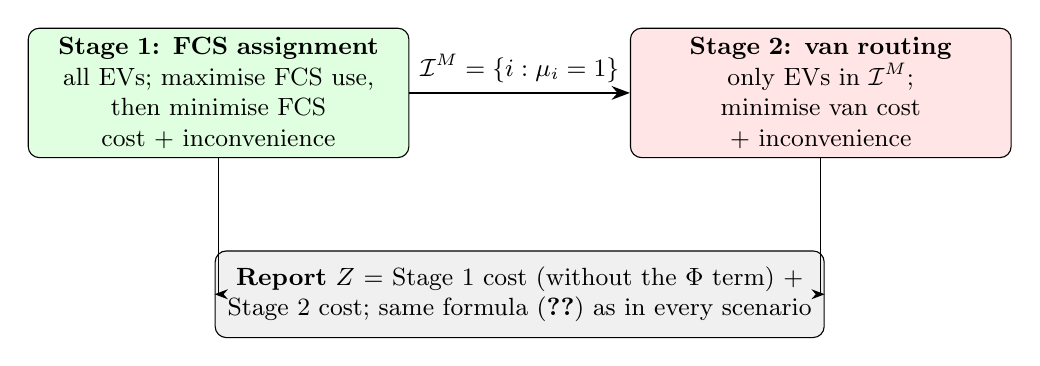
\begin{tikzpicture}[>=Stealth,box/.style={draw,rounded corners,align=center,minimum height=1.1cm,font=\small}]
  \node[box,fill=green!12,text width=4.6cm] (s1) {\textbf{Stage 1: FCS assignment}\\all EVs; maximise FCS use,\\then minimise FCS cost + inconvenience};
  \node[box,fill=red!10,text width=4.6cm,right=2.8cm of s1] (s2) {\textbf{Stage 2: van routing}\\only EVs in $\I^M$;\\minimise van cost + inconvenience};
  \draw[->,thick] (s1) -- node[above,font=\small]{$\I^M=\{i:\mu_i=1\}$} (s2);
  \node[box,fill=black!6,text width=7.5cm,below=2.0cm of $(s1)!0.5!(s2)$] (ev) {\textbf{Report} $Z=$ Stage~1 cost (without the $\Phi$ term) $+$ Stage~2 cost; same formula \eqref{eq:Z} as in every scenario};
  \draw[->] (s1) |- (ev); \draw[->] (s2) |- (ev);
\end{tikzpicture}
\end{center}

Stage~1 does not look at the vans, and Stage~2 cannot change what Stage~1 decided. That is the definition of ``FCS first, then MCS''.

%----------------------------------------------------------------
\subsection{Stage 1: assign EVs to fixed stations}

\textbf{Objective.}
\begin{equation}
\begin{split}
\min\ Z^{(1)}=\;&\underbrace{\Phi\sum_{i\in\I}\mu_i}_{\text{FCS first}}
+\underbrace{c^{EV}\sum_i\sum_{f\in\F_i}d_{if}Y_{if}}_{Z_1}
+\underbrace{Z^F_{\text{energy}}}_{\text{FCS part of }Z_4}\\
&+\underbrace{\sum_i\sum_{f\in\F_i}\rho^F_{if}Y_{if}+\alpha\sum_i w_i(C_i-r_i)+c^L\sum_i w_iL_i}_{\text{FCS customers' inconvenience}}
\end{split}
\label{eq:obj1}
\end{equation}
with $C_i=S_i+\tau^F_iY_i$ in this stage. $\Phi$ is a penalty for handing an EV to the vans. It is chosen larger than anything an extra FCS customer can add to the rest of \eqref{eq:obj1}, e.g.
\[
\Phi > \max_{i}\max_{f\in\F_i}\big(c^{EV}d_{if}+\pi^{\max}E_i+\rho^F_{if}\big)+n\,(\alpha+c^L)\,w_{\max}\,T,
\]
so Stage~1 first \textbf{maximises the number of EVs served at an FCS}, and only among those solutions minimises FCS cost and inconvenience. ($\pi^{\max}$ is the highest grid price.) A numerically safer equivalent is to solve twice: first $\max\sum_iY_i$, then fix that number and minimise the rest.
\ifTOU
Because $Z^F_{\text{energy}}$ uses the peak price, Stage~1 may \emph{start sessions later} to leave the peak, if the price saving beats the extra waiting cost (Section~\ref{sec:expect}).
\fi

\textbf{Constraints.}
\begin{align}
\sum_{g\in\G_i}y_{ig}+\mu_i &= 1 && \forall i\in\I \label{eq:s1assign}\\
S_i &\ge r_i+\sum_{f\in\F_i}t_{if}Y_{if} && \forall i\in\I \label{eq:fcsarr}\\
S_i &\le r_i+T\,(1-\mu_i) && \forall i\in\I \label{eq:s1park}\\
S_j &\ge S_i+\tau^F_i-(T+\tau^F_i)(3-y_{ig}-y_{jg}-o_{ij}) && \forall g,\ (i,j)\in\mathcal{P}_g \label{eq:disj1}\\
S_i &\ge S_j+\tau^F_j-(T+\tau^F_j)(2-y_{ig}-y_{jg}+o_{ij}) && \forall g,\ (i,j)\in\mathcal{P}_g \label{eq:disj2}\\
\sum_i y_{ig_1} &\ge \sum_i y_{ig_2} && \forall f,\ \G_f=\{g_1,g_2\} \label{eq:gunsym}\\
S_i+\tau^F_iY_i &\le T,\qquad L_i\ge S_i+\tau^F_iY_i-l_i && \forall i\in\I \label{eq:s1time}
\end{align}
\ifTOU plus the time-of-use split \eqref{eq:tou1}--\eqref{eq:tou5} of each FCS session (Section~\ref{sec:price}).\fi
\desc{\eqref{eq:s1assign}: every EV either gets one reachable gun or is handed to the vans. An EV that reaches no FCS ($\G_i=\emptyset$) is forced to $\mu_i=1$. \eqref{eq:fcsarr}: an FCS session cannot start before the EV has asked and driven to the station. \eqref{eq:s1park}: for an EV handed to the vans, $S_i$ is parked at $r_i$, so it adds no waiting in Stage~1 (its real start time is decided in Stage~2). \eqref{eq:disj1}--\eqref{eq:disj2}: two EVs on the same gun do not overlap; $o_{ij}$ picks who goes first. With two guns per station this means at most two EVs charge at a station at a time. \eqref{eq:gunsym}: symmetry breaking between the two identical guns (optional). \eqref{eq:s1time}: finished by $T$; lateness.}

\textbf{Optional acceptability rule.} An operator may refuse to send a driver to a station that is ``too inconvenient'', e.g.\ only allow gun $g$ of station $f$ for EV $i$ if $\hat\rho^F_{if}\le\bar\rho$. This only shrinks $\G_i$, so EVs whose stations are all too far go to the vans. Report results with and without it.

\textbf{Output:} $\I^M=\{i:\mu_i=1\}$, the EVs left for the vans; plus each FCS customer's gun and start time.

%----------------------------------------------------------------
\subsection{Stage 2: route the vans to the leftover EVs}

Stage~2 is a vehicle routing problem with time windows, on the EVs in $\I^M$ only. Here $C_i=S_i+\tau^M_i$.

\textbf{Objective.}
\begin{equation}
\begin{split}
\min\ Z^{(2)}=\;&\underbrace{c^M\sum_m\sum_{(i,j)\in\A^M}d_{ij}x_{ijm}}_{Z_2}+\underbrace{\sum_m c^D_mu_m}_{Z_3}+\underbrace{Z^M_{\text{energy}}}_{\text{van part of }Z_4}\\
&+\underbrace{\sum_{i\in\I^M}\sum_m\rho^M_{im}z_{im}+\alpha\sum_{i\in\I^M}w_i(C_i-r_i)+c^L\sum_{i\in\I^M}w_iL_i}_{\text{van customers' inconvenience}}
\end{split}
\label{eq:obj2}
\end{equation}
Since every EV in $\I^M$ must be served by some van, $Z^M_{\text{energy}}$ and the $\rho^M$ term are constants here. They are kept so that $Z^{(2)}$ is the true cost of Stage~2. Waiting and lateness make the vans visit urgent EVs early.

\textbf{Constraints.}
\begin{align}
\sum_{m\in\M}z_{im} &= 1 && \forall i\in\I^M \label{eq:s2assign}\\
\sum_{j:(0,j)\in\A^M}x_{0jm} = \sum_{i:(i,n+1)\in\A^M}x_{i,n+1,m} &= u_m && \forall m \label{eq:depot}\\
\sum_{i:(i,j)\in\A^M}x_{ijm} = \sum_{k:(j,k)\in\A^M}x_{jkm} &= z_{jm} && \forall j\in\I^M,\ m \label{eq:flow}\\
\sum_{i\in\I^M}z_{im} &\le Q_m\,u_m && \forall m \label{eq:cap}\\
\sum_{i\in\I^M}\frac{E_i}{\eta}z_{im}+\beta\sum_{(i,j)\in\A^M}d_{ij}x_{ijm} &\le B_m\,u_m && \forall m \label{eq:batt}
\end{align}
\begin{align}
S_j &\ge \max\{r_j,\ t_{0j}\,x_{0jm}\} && \forall j\in\I^M,\ m \label{eq:depart}\\
S_j &\ge S_i+\tau^M_i+t_{ij}-(T+\tau^M_i+t_{ij})(1-x_{ijm}) && \forall i\neq j,\ m \label{eq:seq}\\
S_i+\tau^M_i+t_{i,n+1} &\le T+(\tau^M_i+t_{i,n+1})(1-x_{i,n+1,m}) && \forall i,\ m \label{eq:return}\\
S_i+\tau^M_i \le T,\quad L_i &\ge S_i+\tau^M_i-l_i && \forall i\in\I^M \label{eq:s2time}\\
u_m &\ge u_{m+1} && m<|\M| \label{eq:vansym}
\end{align}
\desc{\eqref{eq:s2assign}: each leftover EV gets one van. \eqref{eq:depot}: a used van leaves and returns to the depot once. \eqref{eq:flow}: each EV on van $m$ is entered and left exactly once by that van. \eqref{eq:cap}: at most $Q_m$ EVs per van. \eqref{eq:batt}: delivered energy (with transfer losses) plus driving energy fits in the van battery. \eqref{eq:depart}: no start before the request, or before the van can drive there from the depot (written as two linear constraints). \eqref{eq:seq}: if the van goes $i\to j$, it finishes $i$ and drives to $j$ before starting $j$. This gives one EV at a time and removes subtours (MTZ-type). \eqref{eq:return}: back at the depot by $T$. \eqref{eq:s2time}: finished by $T$; lateness. \eqref{eq:vansym}: use identical vans in index order.}

\textbf{If Stage 2 is infeasible} (too many leftover EVs for the fleet by $T$), the sequential policy has \emph{failed} on that instance. For diagnosis, add $s_i\in\{0,1\}$ (``unserved''), replace \eqref{eq:s2assign} by $\sum_mz_{im}+s_i=1$ and add $\Phi^U\sum_is_i$ to \eqref{eq:obj2}. Then report the number of EVs that could not be served. This is a useful comparison with the integrated scenario, which may serve all of them.

%----------------------------------------------------------------
\subsection{Reported value}
\[
Z^{\text{S\scen}}=\big(Z^{(1)*}-\Phi\,|\I^M|\big)+Z^{(2)*},
\]
which is exactly \eqref{eq:Z} evaluated at the combined solution. The stage-1 solution plus the stage-2 solution is a feasible solution of the integrated model (S\ifTOU 4\else 3\fi), so
$Z^{\text{S\ifTOU 4\else 3\fi}}\le Z^{\text{S\scen}}$. The difference is the \emph{value of integration}.

\else
%---------------------------------------------------------------- INT
\subsection{Objective}
\begin{equation}
\min\ Z \quad\text{as in \eqref{eq:Z}, with }Z^F_{\text{energy}}=\ifTOU P^F\textstyle\sum_i\big[\pi^\off(\theta^1_i+\theta^3_i)+\pi^\pk\theta^2_i\big]\else\pi^F\textstyle\sum_iE_iY_i\fi,\quad C_i=S_i+\tau^F_iY_i+\tau^M_iZ_i. \label{eq:objint}
\end{equation}
Written out in full:
\begin{align*}
\min\ Z=\;& c^{EV}\sum_i\sum_{f\in\F_i}d_{if}Y_{if}+c^M\sum_m\sum_{(i,j)\in\A}d_{ij}x_{ijm}+\sum_mc^D_mu_m\\
&+\ifTOU P^F\sum_i\big[\pi^\off(\theta^1_i+\theta^3_i)+\pi^\pk\theta^2_i\big]\else\pi^F\sum_iE_iY_i\fi
+\pi^M\sum_i\sum_m\frac{E_i}{\eta}z_{im}\\
&+\sum_i\sum_{f\in\F_i}\rho^F_{if}Y_{if}+\sum_i\sum_m\rho^M_{im}z_{im}+\alpha\sum_iw_i(C_i-r_i)+c^L\sum_iw_iL_i .
\end{align*}
Every term is linear. One model weighs everything at once: an EV goes to a van exactly when the van's extra km, dispatch and energy cost are outweighed by the effort and waiting it saves the driver\ifTOU, or by the peak-price energy it avoids\fi.

\subsection{Constraints}

\textbf{Assignment.}
\begin{equation}
\sum_{g\in\G_i}y_{ig}+\sum_{m\in\M}z_{im}=1\qquad\forall i\in\I \label{eq:assign}
\end{equation}
\desc{Exactly one resource per EV: one reachable gun or one van. EVs that reach no FCS are forced onto a van.}

\textbf{Fixed stations.}
\begin{align}
S_i &\ge r_i+\sum_{f\in\F_i}t_{if}Y_{if} && \forall i \label{eq:fcsarr}\\
S_j &\ge S_i+\tau^F_i-(T+\tau^F_i)(3-y_{ig}-y_{jg}-o_{ij}) && \forall g,\ (i,j)\in\mathcal{P}_g \label{eq:disj1}\\
S_i &\ge S_j+\tau^F_j-(T+\tau^F_j)(2-y_{ig}-y_{jg}+o_{ij}) && \forall g,\ (i,j)\in\mathcal{P}_g \label{eq:disj2}\\
\sum_iy_{ig_1} &\ge \sum_iy_{ig_2} && \forall f,\ \G_f=\{g_1,g_2\} \label{eq:gunsym}
\end{align}
\desc{\eqref{eq:fcsarr}: an FCS session starts after the request and the drive to the station (for a van customer this is just $S_i\ge r_i$). \eqref{eq:disj1}--\eqref{eq:disj2}: EVs on the same gun do not overlap; $o_{ij}$ chooses the order. \eqref{eq:gunsym}: optional symmetry breaking.}

\textbf{Vans: routes, capacity, battery.}
\begin{align}
\sum_{j:(0,j)\in\A}x_{0jm}=\sum_{i:(i,n+1)\in\A}x_{i,n+1,m} &= u_m && \forall m \label{eq:depot}\\
\sum_{i:(i,j)\in\A}x_{ijm}=\sum_{k:(j,k)\in\A}x_{jkm} &= z_{jm} && \forall j\in\I,\ m \label{eq:flow}\\
\sum_iz_{im} &\le Q_mu_m && \forall m \label{eq:cap}\\
\sum_i\frac{E_i}{\eta}z_{im}+\beta\sum_{(i,j)\in\A}d_{ij}x_{ijm} &\le B_mu_m && \forall m \label{eq:batt}
\end{align}
\desc{\eqref{eq:depot}: a used van leaves and returns once. \eqref{eq:flow}: each EV on van $m$ is visited exactly once by it. \eqref{eq:cap}: at most $Q_m$ EVs. \eqref{eq:batt}: delivered energy (with losses) plus driving energy fits in the battery.}

\textbf{Vans: timing (one EV at a time, no subtours).}
\begin{align}
S_j &\ge t_{0j}\,x_{0jm} && \forall j\in\I,\ m \label{eq:depart}\\
S_j &\ge S_i+\tau^M_i+t_{ij}-(T+\tau^M_i+t_{ij})(1-x_{ijm}) && \forall i\neq j\in\I,\ m \label{eq:seq}\\
S_i+\tau^M_i+t_{i,n+1} &\le T+(\tau^M_i+t_{i,n+1})(1-x_{i,n+1,m}) && \forall i,\ m \label{eq:return}
\end{align}
\desc{\eqref{eq:depart}: the first stop cannot start before the van has driven there. \eqref{eq:seq}: $i\to j$ means finish $i$, drive, then start $j$; start times rise along a route, so no subtour can close. \eqref{eq:return}: back at the depot by $T$.}

\textbf{Horizon and lateness.}
\begin{equation}
C_i\le T,\qquad L_i\ge C_i-l_i\qquad\forall i\in\I \label{eq:time}
\end{equation}
\desc{Every EV is fully charged within the horizon; $L_i$ measures lateness.}

\ifTOU
\textbf{Time-of-use split.} Constraints \eqref{eq:tou1}--\eqref{eq:tou5} of Section~\ref{sec:price}.
\fi

\textbf{Symmetry and domains.}
\begin{equation}
u_m\ge u_{m+1};\qquad y,z,x,u,o\ifTOU,\kappa\fi\in\{0,1\};\qquad S_i,L_i\ifTOU,\theta^p_i\fi\ge0 \label{eq:dom}
\end{equation}
\fi

%=====================================================================
\section{Learning-to-optimise (RL) formulation}\label{sec:rl}

\textbf{Main rule:} the reward of each action is \emph{minus the increase in $Z$ that the action causes}. The rewards over an episode then add up to $-Z$ of the solution the policy builds. RL and MILP results are measured on the same yardstick \eqref{eq:Z}, and the MILP optimum is the benchmark for the RL gap.

\ifSEQ
%---------------------------------------------------------------- RL SEQ
The RL pipeline has the same two stages as the MILP.

\subsection{Stage 1 policy: FCS assignment}
\begin{itemize}[leftmargin=1.4em,itemsep=2pt]
  \item \textbf{Episode / epochs:} EVs are taken in order of request time $r_i$ (ties: higher $w_i$ first). One decision per EV.
  \item \textbf{State:} features of the current EV $k$ ($E_k,r_k,l_k,w_k,R_k$, location); for each gun $g$ the time $F_g$ it becomes free; summary features of the EVs still to come (count and positions near each station)\ifTOU; the current price and the time until $T_1$ and $T_2$\fi.
  \item \textbf{Action:} a gun $g\in\G_k$, or ``hand to vans''. \textbf{FCS-first mask:} ``hand to vans'' is allowed \emph{only} if no gun can finish EV $k$ by $T$ (or, with the optional rule, if all remaining guns have $\hat\rho^F_{kf}>\bar\rho$).
  \ifTOU\item \textbf{Optional timing action:} ``gun $g$, start after the peak'', i.e.\ $S_k=\max\{\text{earliest},T_2\}$, allowed only if the session still ends by $T$.\fi
  \item \textbf{Transition:} $S_k=\max\{r_k+t_{kf},F_g\}$ (or later, for the timing action); $F_g\leftarrow S_k+\tau^F_k$.
  \item \textbf{Reward:} $-\Big[c^{EV}d_{kf}+\text{energy}_k+\rho^F_{kf}+\alpha w_k(S_k+\tau^F_k-r_k)+c^Lw_k(S_k+\tau^F_k-l_k)^+\Big]$, where energy$_k$ = \ifTOU$P^F\big[\pi^\off\cdot(\text{off-peak hours of }[S_k,S_k+\tau^F_k])+\pi^\pk\cdot(\text{peak hours})\big]$, computed exactly in the simulator\else$\pi^FE_k$\fi. Handing an EV to the vans gives reward $0$ here; its cost is counted in Stage~2.
\end{itemize}
Note: a simple baseline for Stage~1 is the greedy rule ``gun with the largest one-step reward''. What RL can learn on top of this is, for example, to keep a nearby gun free for an urgent EV that arrives later.

\subsection{Stage 2 policy: van routing over $\I^M$}
\begin{itemize}[leftmargin=1.4em,itemsep=2pt]
  \item \textbf{Epochs:} whenever a van becomes free (the earliest-free van decides first).
  \item \textbf{State:} for each van: position, time free, remaining battery $b_m$, EVs served so far, dispatched or not; for each unserved EV in $\I^M$: location, $E_i,r_i,l_i,w_i$; current time.
  \item \textbf{Action:} the next EV $j$ for this van, or ``return to depot'' (ends the route). Mask: $j$ must be feasible: battery covers $E_j/\eta$ plus driving to $j$ and back to the depot, the count stays $\le Q_m$, and $j$ can be finished with the van back at the depot by $T$.
  \item \textbf{Transition:} $S_j=\max\{r_j,\ \text{time free}+t_{\text{pos},j}\}$; the van moves to $j$ and is free at $S_j+\tau^M_j$; $b_m$ falls by $E_j/\eta+\beta d_{\text{pos},j}$.
  \item \textbf{Reward:} serving $j$: $-\Big[c^Md_{\text{pos},j}+c^D_m[\text{first stop}]+\pi^M\frac{E_j}{\eta}+\rho^M_{jm}+\alpha w_j(S_j+\tau^M_j-r_j)+c^Lw_j(S_j+\tau^M_j-l_j)^+\Big]$; returning: $-c^Md_{\text{pos},0}$. EVs still unserved at the end: $-\Phi^U$ each.
  \item \textbf{Policy:} an attention-based routing policy (e.g.\ Kool et al., 2019, ``Attention, Learn to Solve Routing Problems!'') trained with REINFORCE or PPO. Baseline: nearest-feasible-EV heuristic.
\end{itemize}
Episode return of Stage~1 + Stage~2 $=-Z^{\text{S\scen}}$.

\else
%---------------------------------------------------------------- RL INT
One policy decides both who serves each EV and the van routes.
\begin{itemize}[leftmargin=1.4em,itemsep=2pt]
  \item \textbf{Episode / epochs:} EVs are taken in order of request time $r_i$ (ties: higher $w_i$ first). One decision per EV.
  \item \textbf{State:} (i) the current EV $k$: location, $E_k,r_k,l_k,w_k,R_k$, reachable stations; (ii) each gun $g$: time $F_g$ it becomes free; (iii) each van $m$: current end-of-route position, time free, remaining battery $b_m$, EVs served, dispatched or not; (iv) embeddings of the not-yet-assigned EVs (for look-ahead)\ifTOU; (v) current price, time until $T_1$ and $T_2$\fi.
  \item \textbf{Action:} $a\in\G_k\cup\M$: a gun, or a van (EV $k$ is appended to the end of that van's route). \textbf{Mask} infeasible actions: a gun that cannot finish $k$ by $T$; a van without enough battery for $E_k/\eta$ plus the drive to $k$ and back to the depot, with $Q_m$ reached, or unable to finish $k$ and return by $T$.
  \ifTOU\item \textbf{Optional timing action:} ``gun $g$, start after the peak'' ($S_k=\max\{\text{earliest},T_2\}$, if it still ends by $T$).\fi
  \item \textbf{Transition:} gun: $S_k=\max\{r_k+t_{kf},F_g\}$, $F_g\leftarrow S_k+\tau^F_k$. Van: $S_k=\max\{r_k,\ \text{free}_m+t_{\text{pos}_m,k}\}$, then the van moves to $k$, $\text{free}_m\leftarrow S_k+\tau^M_k$, $b_m\mathrel{-}=E_k/\eta+\beta d_{\text{pos}_m,k}$.
  \item \textbf{Reward} $=-\Delta Z$:
  \begin{align*}
  \text{gun } g\text{ at }f:&\quad -\Big[c^{EV}d_{kf}+\text{energy}^F_k+\rho^F_{kf}+\alpha w_k(C_k-r_k)+c^Lw_k(C_k-l_k)^+\Big]\\
  \text{van } m:&\quad -\Big[c^M\big(d_{\text{pos}_m,k}+d_{k,0}-d_{\text{pos}_m,0}\big)+c^D_m[\text{first use}]+\pi^M\tfrac{E_k}{\eta}\\
  &\qquad\quad+\rho^M_{km}+\alpha w_k(C_k-r_k)+c^Lw_k(C_k-l_k)^+\Big]
  \end{align*}
  The van distance term is the \emph{change} in route length when $k$ is inserted before the return to the depot, so the sum over the episode equals the total route length (the return legs telescope). energy$^F_k$ = \ifTOU$P^F\big[\pi^\off\cdot(\text{off-peak hours})+\pi^\pk\cdot(\text{peak hours of }[S_k,C_k])\big]$, computed exactly by the simulator; no linearisation is needed in RL\else$\pi^FE_k$\fi.
  \item \textbf{Dead end:} if every action is masked, EV $k$ is unserved: reward $-\Phi^U$, and the episode continues. Report the count.
  \item \textbf{Policy:} masked categorical policy over guns and vans, encoder with attention over EVs, guns and vans; trained with PPO. Natural baseline: greedy, i.e.\ choose the action with the largest one-step reward. That is the pairwise rule ``smallest $\hat\rho$ + cost'' from Section~\ref{sec:inc}.
\end{itemize}
Restriction to note: vans serve EVs in assignment order (append only). A variant that inserts $k$ at the cheapest position of a route is more flexible but has a larger action space.
\fi

\textbf{Reward scaling.} For stable training divide every reward by a constant, e.g.\ the greedy baseline's average $Z$ on the training instances. This does not change the optimal policy.

%=====================================================================
\section{What to expect and what to report}\label{sec:expect}

\ifnum\scen=1
\begin{itemize}[leftmargin=1.4em,itemsep=2pt]
  \item Vans serve only EVs that reach no station, or that the stations cannot finish by $T$. If stations have spare capacity, very few vans are dispatched.
  \item Inconvenience is high for EVs far from the nearest station (worked example: Rs\,682 at the FCS, against Rs\,458 if a van had been allowed).
  \item With too few vans Stage~2 becomes infeasible (unserved EVs), even when the integrated model S3 could serve everyone. Report the smallest $|\M|$ at which S1 is feasible and compare it with S3.
\end{itemize}
\fi
\ifnum\scen=2
\begin{itemize}[leftmargin=1.4em,itemsep=2pt]
  \item \textbf{When does Stage~1 delay a session to avoid the peak?} Moving one hour of charging out of the peak saves $(\pi^\pk-\pi^\off)P^F=3\times22=$ Rs\,66, but delays completion by up to an hour, which costs $\alpha w_i\ge$ Rs\,200. So with the default values Stage~1 almost never delays. It mostly pays the higher price, and S2 costs roughly S1 plus the peak surcharge. Sessions start later only if $\alpha$ is small (try $\lambda<0.33$ in the sensitivity analysis).
  \item The van assignment is the same as in S1 unless Stage~1's timing changes which EVs fit at the stations. Stage~1 cannot use vans to escape the peak price.
  \item Extra KPI: \textbf{grid energy drawn at FCS during the peak}, $P^F\sum_i\theta^2_i$ (kWh). Compare with S4.
\end{itemize}
\fi
\ifnum\scen=3
\begin{itemize}[leftmargin=1.4em,itemsep=2pt]
  \item Vans take EVs for which the saved inconvenience exceeds the extra van cost (worked example: van chosen, saving Rs\,224). Expect vans to serve EVs that are far from every station, have low range (high $w_i$), or have early deadlines, while EVs near a station still use it.
  \item \textbf{Value of integration under flat price:} $Z^{\text{S1}}-Z^{\text{S3}}\ge0$. Report it per component ($Z_1,\dots,Z_5$): typically operating cost rises a little and inconvenience falls a lot.
  \item Vary $|\M|$ (0, 1, 2, \dots): the first few vans lower $Z$ sharply, then the effect levels off. That curve shows the scenarios where mobile chargers help most.
\end{itemize}
\fi
\ifnum\scen=4
\begin{itemize}[leftmargin=1.4em,itemsep=2pt]
  \item During the peak a van kWh costs about the same as an FCS kWh (Rs\,10.0 each), so the vans' energy disadvantage disappears and vans also absorb \emph{peak-hour} demand that would otherwise be charged on the grid at peak price.
  \item Expect more van usage than in S3, concentrated on requests in $[T_1,T_2]$, and lower grid energy at the stations during the peak, $P^F\sum_i\theta^2_i$, than in S2.
  \item \textbf{Value of integration under peak pricing:} $Z^{\text{S2}}-Z^{\text{S4}}$. It should be larger than $Z^{\text{S1}}-Z^{\text{S3}}$, because integration now also allows price arbitrage.
  \item \textbf{Peak pricing with full flexibility:} $Z^{\text{S4}}-Z^{\text{S3}}$ should be smaller than $Z^{\text{S2}}-Z^{\text{S1}}$: vans cushion the price increase.
\end{itemize}
\fi

\textbf{Cross-scenario comparison table} (fill in from the four runs):
\begin{center}
\renewcommand{\arraystretch}{1.2}
\begin{tabular}{@{}lll@{}}
\toprule
\textbf{Comparison} & \textbf{Measures} & \textbf{Expected sign} \\
\midrule
S1 $-$ S3 & value of integration, flat price & $\ge0$ \\
S2 $-$ S4 & value of integration, peak price & $\ge0$, larger than S1 $-$ S3 \\
S2 $-$ S1 & cost of peak pricing, FCS-first operator & $>0$ \\
S4 $-$ S3 & cost of peak pricing, flexible operator & $>0$, smaller than S2 $-$ S1 \\
\bottomrule
\end{tabular}
\end{center}
Report for each: $Z$ and its components, number of vans used, EVs per resource, mean and maximum inconvenience per EV, total lateness, peak-hour grid energy, solve time, and (for RL) the gap to the MILP optimum.

%=====================================================================
\appendix
\section{Illustrative parameter values}\label{app:values}

These are starting values for experiments, not data. All are meant to be varied in the analysis. Values in Rs.

\begin{center}
\renewcommand{\arraystretch}{1.15}
\begin{tabular}{@{}llp{6.2cm}@{}}
\toprule
\textbf{Parameter} & \textbf{Value} & \textbf{Note} \\
\midrule
$T$, $[T_1,T_2]$ & 7 h, $[2,6]$ & 16:00--23:00, peak 18:00--22:00 \\
$P^F$, $P^M$ & 22 kW, 30 kW & \\
$v$, $\beta$, $\eta$ & 25 km/h, 0.25 kWh/km, 0.9 & \\
$B_m$, $Q_m$, $|\M|$ & 150 kWh, 6, 2--6 & \\
$c^{EV}$, $c^M$, $c^D_m$ & Rs\,4/km, Rs\,15/km, Rs\,1500 & van km includes driver time \\
$\pi^F$ (flat) & Rs\,8.7/kWh & equals the time-average of the ToU tariff over $[0,T]$ \\
$\pi^\off$, $\pi^\pk$ (ToU) & Rs\,7/kWh, Rs\,10/kWh & $(3\times7+4\times10)/7=8.7$ \\
$c^{bat}$ & Rs\,2/kWh & van battery wear \\
$\pi^M$ & Rs\,10.7 (flat) / Rs\,9.0 (ToU) & $=\pi^F+c^{bat}$ / $=\pi^\off+c^{bat}$ \\
$\alpha$, $\alpha^D$ & Rs\,200/h, Rs\,100/h & value of time; extra for attended time \\
$h^F$, $h^M$, $\varphi$ & Rs\,50, Rs\,10, Rs\,100 & trip hassle, hand-over, range stress \\
$c^L$ & Rs\,300/h & lateness \\
$w_i$ & $1+2(1-R_i/R_{\max})$, $R_i\sim U[3,40]$ km & priority from remaining range \\
\bottomrule
\end{tabular}
\end{center}

The flat price is set to the time-average of the peak tariff. The price \emph{level} is then the same in both pricing cases, and only the price \emph{shape} differs. Without this, part of S1 vs S2 would just reflect a different average price.

\end{document}
"
%  (run each twice for cross-references)
% =====================================================================
\documentclass[11pt,a4paper]{article}
\usepackage[margin=2.2cm]{geometry}
\usepackage{amsmath,amssymb,amsfonts}
\usepackage{booktabs,array,tabularx}
\usepackage{enumitem}
\usepackage[table]{xcolor}
\usepackage{tikz}
\usetikzlibrary{arrows.meta,positioning,calc}
\usepackage[colorlinks=true,linkcolor=blue!50!black,urlcolor=blue!50!black]{hyperref}
\usepackage{titlesec}
\titleformat{\section}{\large\bfseries}{\thesection}{0.8em}{}
\titleformat{\subsection}{\normalsize\bfseries}{\thesubsection}{0.8em}{}
\setlength{\parindent}{0pt}
\setlength{\parskip}{5pt}

% ---------------- scenario switches ----------------
\ifdefined\scen\else\def\scen{1}\fi
\newif\ifTOU \TOUfalse   % true = time-of-use (peak) price
\newif\ifSEQ \SEQfalse   % true = FCS first, then MCS
\ifnum\scen=1 \SEQtrue \fi
\ifnum\scen=2 \TOUtrue \SEQtrue \fi
\ifnum\scen=4 \TOUtrue \fi

\newcommand{\pricename}{\ifTOU time-of-use price (dearer evening peak)\else single (flat) price all day\fi}
\newcommand{\structname}{\ifSEQ FCS first, then MCS (sequential)\else FCS and MCS together (integrated)\fi}

% ---------------- notation ----------------
\newcommand{\I}{\mathcal{I}}
\newcommand{\F}{\mathcal{F}}
\newcommand{\G}{\mathcal{G}}
\newcommand{\M}{\mathcal{M}}
\newcommand{\N}{\mathcal{N}}
\newcommand{\A}{\mathcal{A}}
\newcommand{\Rs}{\text{Rs}\,}
\newcommand{\pk}{\mathrm{pk}}
\newcommand{\off}{\mathrm{off}}
\newcommand{\desc}[1]{\par\vspace{-2pt}{\small\color{black!75}\textit{Meaning:} #1}\par\vspace{4pt}}
\newcommand{\cell}[2]{\ifnum\scen=#1\cellcolor{blue!18}\textbf{S#1 (this document)}\\\textbf{#2}\else S#1\\#2\fi}

\title{\textbf{EV Charging Network Optimisation}\\[4pt]
\large Scenario \scen: \pricename\ $+$ \structname\\[2pt]
\normalsize MILP and RL formulation}
\author{CP 320 OR for Mobility Management, course project}
\date{2 October 2026}

\begin{document}
\maketitle

%=====================================================================
\section{Where this scenario sits}

The project studies four scenarios: two ways of pricing grid electricity, times two ways of making the decisions.

\begin{center}
\renewcommand{\arraystretch}{1.5}
\begin{tabular}{>{\raggedright\arraybackslash}p{4.2cm}|>{\centering\arraybackslash}p{4.6cm}|>{\centering\arraybackslash}p{4.6cm}}
 & \textbf{Flat price all day} & \textbf{Time-of-use (peak) price} \\ \hline
\textbf{Sequential:} FCS first, leftover EVs to MCS &
\begin{tabular}[c]{@{}c@{}}\cell{1}{flat + sequential}\end{tabular} &
\begin{tabular}[c]{@{}c@{}}\cell{2}{peak + sequential}\end{tabular} \\ \hline
\textbf{Integrated:} FCS and MCS decided together &
\begin{tabular}[c]{@{}c@{}}\cell{3}{flat + integrated}\end{tabular} &
\begin{tabular}[c]{@{}c@{}}\cell{4}{peak + integrated}\end{tabular} \\
\end{tabular}
\end{center}

\textbf{The four scenarios do not have four different objectives.} They share \emph{one} cost yardstick $Z$ (Section~\ref{sec:obj}): the same cost terms and the same customer inconvenience (Section~\ref{sec:inc}). Only two things change:
\begin{itemize}[leftmargin=1.4em,itemsep=1pt]
  \item \textbf{Pricing} changes the formula for one term, the FCS energy cost (Section~\ref{sec:price}).
  \item \textbf{Decision structure} changes \emph{how} $Z$ is minimised: in one model (integrated), or in two stages (sequential), where each stage minimises its own part of $Z$.
\end{itemize}
Because the yardstick is the same, the four optimal values can be compared directly. The differences measure the \emph{value of integration} (S1$\to$S3, S2$\to$S4) and the \emph{effect of peak pricing} (S1$\to$S2, S3$\to$S4).

\ifnum\scen=1
\textbf{This scenario (S1)} is the baseline, the ``status quo''. Electricity costs the same at every hour, every EV that can be charged at a fixed station is sent there, and vans only take what is left over.
\fi
\ifnum\scen=2
\textbf{This scenario (S2)} keeps the FCS-first rule of S1, but grid electricity is dearer during the evening peak. Stage~1 can react to the price only by \emph{rescheduling} FCS sessions. It cannot hand a peak-hour EV to a van.
\fi
\ifnum\scen=3
\textbf{This scenario (S3)} keeps the flat price of S1, but the operator decides FCS and MCS service \emph{together}. An EV can be sent to a van even when a fixed station could take it, whenever that lowers total cost plus inconvenience.
\fi
\ifnum\scen=4
\textbf{This scenario (S4)} is the most flexible one: peak pricing at fixed stations, and FCS and MCS decided together. Van energy was bought off-peak, so vans can also be used to keep charging \emph{out of the expensive peak}.
\fi

%=====================================================================
\section{Setting and assumptions}\label{sec:setting}

\textbf{Time.} The planning horizon is $[0,T]$ with $T=7$\,h (16:00--23:00). It contains the evening peak window $[T_1,T_2]=[2,6]$ (18:00--22:00). The horizon is the same in all four scenarios. It is wider than the peak itself so that, under peak pricing, there is cheaper time on both sides of the peak.\ifTOU\else\ In this scenario the price is flat, so the window plays no role in the model.\fi

\textbf{Assumptions} (the same as MILP v3, plus two about energy):
\begin{enumerate}[leftmargin=1.6em,itemsep=1pt]
  \item Static, continuous time. All requests in the horizon are known at time $0$, and request $i$ becomes active at $r_i$.
  \item An EV served by an FCS drives there itself on its own battery (only to stations within its range $R_i$). The driver stays with the car while it waits for a free gun and while it charges.
  \item An EV served by an MCS stays parked where it is, and the driver is free in the meantime.
  \item Each FCS gun and each van charges one EV at a time, without interruption, at constant power.
  \item A van's battery covers both its driving and the energy it delivers. \textbf{The van battery is charged at the depot before the horizon starts}\ifTOU, i.e.\ at the off-peak price\fi, and is not recharged during the horizon.
  \item Every EV must be fully charged by $T$ (hard). Finishing after the driver's desired time $l_i$ is allowed but penalised.
\end{enumerate}

%=====================================================================
\section{Notation}\label{sec:notation}

\subsection*{Sets}
\begin{tabularx}{\textwidth}{@{}lX@{}}
\toprule
$\I=\{1,\dots,n\}$ & EV charging requests \\
$\F$; $\G_f$ ($|\G_f|=2$); $\G=\bigcup_f\G_f$ & fixed charging stations; guns of FCS $f$; all guns ($f(g)$ = station of gun $g$) \\
$\F_i=\{f: d_{if}\le R_i\}$, $\G_i=\bigcup_{f\in\F_i}\G_f$ & stations / guns EV $i$ can reach on its remaining range \\
$\M$ & mobile charging vans (MCS) \\
$0,\ n+1$ & depot as start node / end node (same place) \\
$\N=\{0\}\cup\I\cup\{n+1\}$, $\A$ & routing nodes; allowed van arcs $(i,j)$, $i\in\{0\}\cup\I$, $j\in\I\cup\{n+1\}$, $i\neq j$ \\
$\mathcal{P}_g=\{(i,j): i<j,\ g\in\G_i\cap\G_j\}$ & pairs of EVs that could share gun $g$ \\
\ifSEQ
$\I^M\subseteq\I$ & EVs handed to the vans by Stage~1 (an \emph{output} of Stage~1, a fixed input to Stage~2) \\
$\N^M$, $\A^M$ & routing nodes / arcs restricted to $\I^M$ \\
\fi
\bottomrule
\end{tabularx}

\subsection*{Parameters}
\begin{tabularx}{\textwidth}{@{}lX@{}}
\toprule
$E_i,\ r_i,\ l_i,\ R_i$ & energy demand (kWh), request time, desired completion time (h), remaining range (km) \\
$w_i\ge1$ & priority of EV $i$; $w_i=1+\kappa(1-R_i/R_{\max})$, so low-range EVs weigh more \\
$P^F,\ P^M$ & charging power of an FCS gun (22\,kW) / of a van (e.g.\ 30\,kW) \\
$\tau^F_i=E_i/P^F,\ \tau^M_i=E_i/P^M$ & charging time of EV $i$ at an FCS / by a van (h) \\
$d_{if},t_{if}$;\ $d_{ij},t_{ij}$ & distance (km) and time (h): EV$\to$FCS; between routing nodes ($t=d/v$) \\
$B_m,\ Q_m,\ \beta,\ \eta$ & van battery (kWh), max EVs per van, van consumption (kWh/km), transfer efficiency \\
$c^{EV},\ c^M,\ c^D_m$ & cost per km of EV driving, per km of van driving; fixed dispatch cost of van $m$ \\
\ifTOU
$\pi^\off,\ \pi^\pk$ & grid price (Rs/kWh) off-peak / in $[T_1,T_2]$, with $\pi^\pk\ge\pi^\off$ \\
\else
$\pi^F$ & grid price (Rs/kWh), the same at every hour \\
\fi
$c^{bat}$ & van battery wear per kWh cycled \\
$\pi^M$ & cost of 1 kWh taken from a van battery: $\pi^M=\ifTOU\pi^\off\else\pi^F\fi+c^{bat}$ (Section~\ref{sec:price}) \\
$\alpha,\ \alpha^D,\ h^F,\ h^M,\ \varphi,\ c^L$ & inconvenience coefficients (Section~\ref{sec:inc}) \\
\bottomrule
\end{tabularx}

\subsection*{Decision variables}
\begin{tabularx}{\textwidth}{@{}llX@{}}
\toprule
$y_{ig}$ & $\{0,1\}$ & EV $i$ charged at gun $g\in\G_i$ \\
$z_{im}$ & $\{0,1\}$ & EV $i$ served by van $m$ \\
$x_{ijm}$ & $\{0,1\}$ & van $m$ drives arc $(i,j)$ \\
$u_m$ & $\{0,1\}$ & van $m$ is dispatched \\
$o_{ij}$ & $\{0,1\}$ & for EVs $i<j$ that could share a gun: 1 if $i$ is charged before $j$ \\
\ifSEQ
$\mu_i$ & $\{0,1\}$ & Stage~1 only: EV $i$ is handed to the van fleet \\
\fi
\ifTOU
$\theta^1_i,\theta^2_i,\theta^3_i$ & $\ge0$ & hours of EV $i$'s FCS session before / inside / after the peak \\
$\kappa^1_i,\kappa^3_i$ & $\{0,1\}$ & EV $i$'s FCS session starts before $T_1$ / ends after $T_2$ \\
\fi
$S_i$ & $\ge0$ & time charging of EV $i$ starts (h), on whichever resource \\
$L_i$ & $\ge0$ & lateness of EV $i$ beyond $l_i$ (h) \\
\bottomrule
\end{tabularx}

\textbf{Short-hands} (linear expressions, not new variables):
\[
Y_{if}=\sum_{g\in\G_f}y_{ig},\qquad Y_i=\sum_{g\in\G_i}y_{ig}\ (\text{EV $i$ uses an FCS}),\qquad Z_i=\sum_{m\in\M}z_{im}\ (\text{EV $i$ uses a van}),
\]
\[
C_i=S_i+\tau^F_i\,Y_i+\tau^M_i\,Z_i \quad\text{(time EV $i$ is fully charged).}
\]

%=====================================================================
\section{Customer inconvenience}\label{sec:inc}

This section is \textbf{identical in all four scenario documents}. Inconvenience is a property of the customer, not of the price or of the planning method.

\subsection{What we mean by inconvenience}

Inconvenience is \emph{what the driver loses} from the moment they ask for a charge ($r_i$) until the car is fully charged ($C_i$), \emph{converted into rupees} so it can be added to the operator's costs. A driver loses three different things:

\begin{enumerate}[leftmargin=1.6em,itemsep=2pt]
  \item \textbf{Waiting:} the car is not ready. This lasts $C_i-r_i$ hours and affects \emph{every} driver, FCS or MCS.
  \item \textbf{Effort:} only an FCS customer has to drive to the station and sit there while the car charges. An MCS customer stays at home or at work and does something else. Driving to a far station also uses scarce battery range, which causes stress (``range anxiety'').
  \item \textbf{A missed deadline:} the car is still not ready at the time $l_i$ the driver needs it.
\end{enumerate}

Each loss gets a price in Rs per hour (or per event). All of them are multiplied by the priority $w_i$: an hour of delay for an EV with 5\,km of range left counts more than for one with 40\,km.

\subsection{The three components}

\begin{center}
\renewcommand{\arraystretch}{1.3}
\begin{tabularx}{\textwidth}{@{}>{\raggedright\arraybackslash}p{2.6cm}>{\raggedright\arraybackslash}X>{\raggedright\arraybackslash}X>{\raggedright\arraybackslash}p{3.0cm}@{}}
\toprule
\textbf{Component} & \textbf{EV $i$ at FCS $f$} & \textbf{EV $i$ by a van} & \textbf{Known when?} \\
\midrule
Effort & $w_i\big[\alpha^D(t_{if}+\tau^F_i)+h^F+\varphi\,d_{if}/R_i\big]$: driving and sitting at the station, a fixed trip hassle, range stress & $w_i\,h^M$: being reachable and handing over the car & \textbf{Static:} known as soon as the resource is chosen \\
Waiting & $w_i\,\alpha\,(C_i-r_i)$ = drive + \emph{queue at the gun} + charge & $w_i\,\alpha\,(C_i-r_i)$ = \emph{wait for the van} + charge & \textbf{Dynamic:} depends on the queue / van route \\
Missed deadline & $w_i\,c^L\,L_i$, $L_i=\max\{0,C_i-l_i\}$ & same & Dynamic \\
\bottomrule
\end{tabularx}
\end{center}

\textbf{Coefficients.}
$\alpha$ (Rs/h) is the value of an hour the car is not ready.
$\alpha^D$ (Rs/h) is the \emph{extra} value of an hour the driver must personally spend driving or sitting at the station: an hour at the station costs $\alpha+\alpha^D$, an hour waiting at home for a van costs only $\alpha$.
$h^F,h^M$ (Rs) are fixed hassle costs of one trip to a station / one van hand-over.
$\varphi$ (Rs) is the range-stress cost of a trip that uses the \emph{whole} remaining range ($d_{if}/R_i\le1$ is the fraction used).
$c^L$ (Rs/h) is the cost per hour late.

\subsection{Pairwise form: inconvenience of a (customer, resource) pair}

The natural first idea is: \emph{for every pair (EV $i$, FCS $f$) and every pair (EV $i$, van $m$) there is an inconvenience number, and the operator picks the pair with the lowest cost plus inconvenience.} The static part fits this idea exactly:
\[
\boxed{\;\rho^F_{if}=w_i\Big[\alpha^D\,(t_{if}+\tau^F_i)+h^F+\varphi\,\frac{d_{if}}{R_i}\Big]\qquad
\rho^M_{im}=w_i\,h^M\;}
\]
These are \textbf{parameters}, computed before solving, one number per (EV, FCS) pair and per (EV, van) pair. In the objective they appear linearly: $\sum_i\sum_f\rho^F_{if}Y_{if}+\sum_i\sum_m\rho^M_{im}z_{im}$.

Note that $\rho^M_{im}$ does not depend on $m$. Vans are identical and all start at the same depot, so the driver does not care \emph{which} van comes, only \emph{when} it comes. That ``when'' is the waiting part.

\subsection{Why waiting cannot be a fixed pairwise number}

It is tempting to also write the waiting as a pairwise number, e.g.\ ``the van needs 5 minutes to reach EV $i$''. But that depends on \emph{where the van is coming from}, which depends on the route the model is still choosing: if EV $i$ is the 4th stop of a van, the wait is the time for three charging sessions plus four drives. Likewise, waiting at an FCS depends on how many EVs are queued at that gun. So waiting is not known before solving. It is a function of decision variables:
\[
\text{waiting cost of EV } i \;=\; w_i\,\alpha\,(C_i-r_i),\qquad C_i=S_i+\tau^F_iY_i+\tau^M_iZ_i .
\]
This is \textbf{linear} in the variables ($S_i$, $y$, $z$), so it fits in a MILP directly. The constraints of Section~\ref{sec:milp} make $S_i$ equal to the true start time, including driving, queueing at the gun and the van's route. The term $\sum_i w_i\alpha r_i$ is a constant and may be dropped when solving.

\textbf{Pairwise \emph{estimate}} (used for intuition, by the RL policy and in heuristics): if there is no queue and the van comes straight to $i$,
\[
\hat\rho^{F}_{if}=\rho^F_{if}+w_i\alpha\,(t_{if}+\tau^F_i),\qquad
\hat\rho^{M}_{im}=\rho^M_{im}+w_i\alpha\,(t^{\text{van}}_{m\to i}+\tau^M_i),
\]
where $t^{\text{van}}_{m\to i}$ is the time until van $m$ can reach $i$ from where it currently is. In the RL formulation (Section~\ref{sec:rl}) the van's position \emph{is} known at each decision, so there this estimate becomes exact.

\subsection{Total inconvenience and how it enters the objective}

\begin{equation}
\boxed{\;
Z_{\text{inc}}=\underbrace{\sum_{i\in\I}\sum_{f\in\F_i}\rho^F_{if}Y_{if}+\sum_{i\in\I}\sum_{m\in\M}\rho^M_{im}z_{im}}_{\text{effort (static, pairwise)}}
+\underbrace{\alpha\sum_{i\in\I}w_i\,(C_i-r_i)}_{\text{waiting (dynamic)}}
+\underbrace{c^L\sum_{i\in\I}w_i\,L_i}_{\text{missed deadline}}
\;}\label{eq:inc}
\end{equation}
All three parts are in rupees, so $Z_{\text{inc}}$ is simply added to the operating costs. Nothing has to be normalised.

\subsection{Worked example: your ``10 km to the FCS vs.\ van in 5 minutes'' case}

EV $i$: $E_i=20$\,kWh, $R_i=40$\,km (so $w_i=1$); nearest free FCS $d_{if}=10$\,km away, $t_{if}=0.4$\,h at 25\,km/h; a van finishing next door can reach it in 5\,min ($0.083$\,h), adding about 4\,km to its route. $\tau^F_i=20/22=0.909$\,h, $\tau^M_i=20/30=0.667$\,h. Coefficients from Appendix~\ref{app:values}, flat price.

\begin{center}
\renewcommand{\arraystretch}{1.25}
\begin{tabular}{@{}lrr@{}}
\toprule
 & \textbf{FCS} & \textbf{Van} \\
\midrule
Driving (EV / extra van km) & $4\times10=40.0$ & $15\times4=60.0$ \\
Energy & $8.7\times20=174.0$ & $10.7\times20/0.9=237.8$ \\
\textbf{Operating cost only} & \textbf{214.0} & \textbf{297.8} \\
\midrule
Effort $\rho$ & $100(0.4+0.909)+50+100\cdot\tfrac{10}{40}=205.9$ & $10.0$ \\
Waiting $\alpha(C_i-r_i)$ & $200\times1.309=261.8$ & $200\times0.75=150.0$ \\
\textbf{Cost + inconvenience} & \textbf{681.7} & \textbf{457.8} \\
\bottomrule
\end{tabular}
\end{center}

On operating cost alone the FCS is cheaper, so a cost-only model would \emph{always} send this driver 10\,km away. With inconvenience included the van is better by about Rs\,224, and the integrated model chooses $z_{im}=1$, as you expected. If the FCS were only 1\,km away, the FCS would win both comparisons. The inconvenience term is what makes the model choose between ``cheap for the operator'' and ``convenient for the driver'', rather than following a fixed rule.

\subsection{Relation to a single penalty $\rho_i$ per EV}

The first draft used a penalty $\rho_i$ that is charged whenever EV $i$ goes to \emph{any} FCS: $\sum_i\sum_f\rho_iy_{if}$. Because $\sum_f y_{if}=1-\sum_m z_{im}$, this only says ``a van is worth $\rho_i$ more to EV $i$'', and that holds whether the station is 1\,km or 15\,km away, and whether the van arrives in 5 minutes or in 3 hours. The form above fixes both problems: $\rho^F_{if}$ grows with the distance to \emph{that} station, and the waiting term grows with how late the van or the free gun actually is. The old model is the special case $\alpha=\alpha^D=\varphi=c^L=0$, $h^F=\rho_i$.

\subsection{Choosing the coefficients}
\begin{itemize}[leftmargin=1.4em,itemsep=2pt]
  \item Use a value of time for $\alpha$ (e.g.\ Rs\,150--300/h for urban car users), and set $\alpha^D\approx0.5\alpha$: sitting at a station is worse than waiting at home.
  \item Keep $c^L>\alpha$, so missing the deadline is worse than ordinary waiting.
  \item \textbf{Sensitivity analysis:} multiply all inconvenience coefficients by a factor $\lambda\in\{0,0.25,0.5,1,2,4\}$ and plot operating cost against total inconvenience. $\lambda=0$ is the pure cost-minimising operator, and large $\lambda$ is a customer-first operator. This trade-off curve is a strong result for the ``Analysis'' part of the project.
\end{itemize}

\subsection{What inconvenience does in \emph{this} scenario}
\ifSEQ
In a sequential scenario inconvenience \textbf{cannot move an EV from an FCS to a van}: Stage~1 sends every EV that \emph{can} use an FCS to one. It still matters inside each stage. In Stage~1 it decides \emph{which} station and \emph{when} (urgent EVs get the near station and the first free gun). In Stage~2 it decides the \emph{order} in which vans visit EVs (urgent EVs first). In the worked example, this scenario sends the driver 10\,km to the FCS. That is the weakness the integrated scenarios remove.
\else
In an integrated scenario inconvenience is weighed directly against operating cost when choosing the resource. That is how the worked example ends up with a van. It also decides which station and which gun order, and the order of each van route.
\fi

%=====================================================================
\section{Electricity price in this scenario}\label{sec:price}

\textbf{Van energy (same in all scenarios).} A van's battery is charged at the depot \emph{before} the horizon, so its energy was bought at the
\ifTOU off-peak \fi
price, whatever time the van later delivers it. Each kWh taken from the van also wears the battery ($c^{bat}$), and a fraction $1-\eta$ is lost in transfer:
\[
Z^M_{\text{energy}}=\pi^M\sum_{i\in\I}\sum_{m\in\M}\frac{E_i}{\eta}\,z_{im},\qquad \pi^M=\ifTOU\pi^\off\else\pi^F\fi+c^{bat}.
\]

\ifTOU
\textbf{FCS energy (time-of-use).} An FCS draws from the grid while it charges. Energy delivered inside $[T_1,T_2]$ costs $\pi^\pk$, and energy outside it costs $\pi^\off$. A session $[S_i,S_i+\tau^F_i]$ may overlap the peak partly. Split its duration into the hours before, inside and after the peak, $\theta^1_i+\theta^2_i+\theta^3_i$:
\[
Z^F_{\text{energy}}=P^F\sum_{i\in\I}\Big[\pi^\off(\theta^1_i+\theta^3_i)+\pi^\pk\,\theta^2_i\Big].
\]
Constraints \eqref{eq:tou1}--\eqref{eq:tou5} below make the $\theta$'s equal to the true overlaps. Peak hours are dearer, so the solver wants $\theta^1_i,\theta^3_i$ as large as possible. It is enough to bound them from above by the true off-peak overlap, and the constraints need one binary per side:
\begin{align}
\theta^1_i+\theta^2_i+\theta^3_i &= \tau^F_i\,Y_i && \forall i\in\I \label{eq:tou1}\\
\theta^1_i &\le \tau^F_i\,\kappa^1_i && \forall i\in\I \label{eq:tou2}\\
\theta^1_i &\le T_1-S_i+T\,(1-\kappa^1_i) && \forall i\in\I \label{eq:tou3}\\
\theta^3_i &\le \tau^F_i\,\kappa^3_i && \forall i\in\I \label{eq:tou4}\\
\theta^3_i &\le S_i+\tau^F_i-T_2+T\,(1-\kappa^3_i) && \forall i\in\I \label{eq:tou5}
\end{align}
\desc{\eqref{eq:tou1}: the FCS session's hours are split into three parts; for a van customer ($Y_i=0$) all three are zero. \eqref{eq:tou2}--\eqref{eq:tou3}: off-peak time before the peak is only possible if the session starts before $T_1$ ($\kappa^1_i=1$), and is at most $T_1-S_i$. \eqref{eq:tou4}--\eqref{eq:tou5}: the same for time after $T_2$. $\theta^2_i\ge0$ prevents counting more off-peak hours than exist. Checking the cases (entirely before / inside / after the peak, straddling one edge, covering the whole peak) shows that at the optimum the $\theta$'s equal the exact overlaps. This needs $\pi^\pk\ge\pi^\off$, which is true for a peak tariff.}

\textbf{Why vans become more attractive.} Compare the cost of 1\,kWh delivered to an EV during the peak (values from Appendix~\ref{app:values}):
FCS $=\pi^\pk=$ Rs\,10.0, van $=(\pi^\off+c^{bat})/\eta=9/0.9=$ Rs\,10.0. They are at parity. Under the flat price the van is about Rs\,3.2/kWh dearer (FCS Rs\,8.7, van $10.7/0.9=$ Rs\,11.9). Peak pricing therefore removes the vans' main cost disadvantage, but only for EVs whose FCS session would fall in the peak.
\ifSEQ\ In this sequential scenario Stage~1 cannot use that, because it does not consider vans. It can only shift FCS sessions in time.\fi
\else
\textbf{FCS energy (flat).} Every kWh delivered at a fixed station costs $\pi^F$, whenever it is delivered:
\[
Z^F_{\text{energy}}=\pi^F\sum_{i\in\I}E_i\,Y_i .
\]
The start time therefore does not affect the energy cost. Under the flat price a van kWh costs $(\pi^F+c^{bat})/\eta\approx$ Rs\,11.9 against Rs\,8.7 at an FCS (Appendix~\ref{app:values}), so on energy alone the FCS always wins.
\fi

%=====================================================================
\section{MILP formulation}\label{sec:milp}

\subsection{The common cost yardstick $Z$}\label{sec:obj}

For any complete solution (every EV assigned, every route and start time known), the system cost is
\begin{equation}
\boxed{\;
Z=\underbrace{c^{EV}\sum_{i}\sum_{f\in\F_i}d_{if}Y_{if}}_{Z_1:\ \text{EV driving}}
+\underbrace{c^M\sum_{m}\sum_{(i,j)\in\A}d_{ij}x_{ijm}}_{Z_2:\ \text{van driving}}
+\underbrace{\sum_m c^D_m u_m}_{Z_3:\ \text{dispatch}}
+\underbrace{Z^F_{\text{energy}}+Z^M_{\text{energy}}}_{Z_4:\ \text{energy}}
+\underbrace{Z_{\text{inc}}}_{Z_5:\ \text{inconv.\ \eqref{eq:inc}}}
\;}\label{eq:Z}
\end{equation}
$Z_4$ is defined in Section~\ref{sec:price}. $Z_1$--$Z_4$ are the operator's costs listed in the brief (EV travel, MCS travel, MCS operating cost) plus energy. $Z_5$ is the customer inconvenience penalty. \textbf{The same formula is used to report results in all four scenarios.}

\ifSEQ
%---------------------------------------------------------------- SEQ
\subsection{Structure: two stages}

\begin{center}
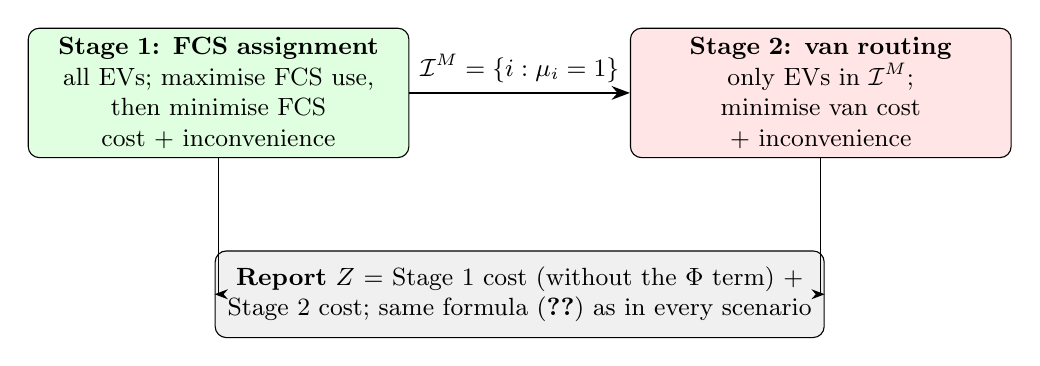
\begin{tikzpicture}[>=Stealth,box/.style={draw,rounded corners,align=center,minimum height=1.1cm,font=\small}]
  \node[box,fill=green!12,text width=4.6cm] (s1) {\textbf{Stage 1: FCS assignment}\\all EVs; maximise FCS use,\\then minimise FCS cost + inconvenience};
  \node[box,fill=red!10,text width=4.6cm,right=2.8cm of s1] (s2) {\textbf{Stage 2: van routing}\\only EVs in $\I^M$;\\minimise van cost + inconvenience};
  \draw[->,thick] (s1) -- node[above,font=\small]{$\I^M=\{i:\mu_i=1\}$} (s2);
  \node[box,fill=black!6,text width=7.5cm,below=2.0cm of $(s1)!0.5!(s2)$] (ev) {\textbf{Report} $Z=$ Stage~1 cost (without the $\Phi$ term) $+$ Stage~2 cost; same formula \eqref{eq:Z} as in every scenario};
  \draw[->] (s1) |- (ev); \draw[->] (s2) |- (ev);
\end{tikzpicture}
\end{center}

Stage~1 does not look at the vans, and Stage~2 cannot change what Stage~1 decided. That is the definition of ``FCS first, then MCS''.

%----------------------------------------------------------------
\subsection{Stage 1: assign EVs to fixed stations}

\textbf{Objective.}
\begin{equation}
\begin{split}
\min\ Z^{(1)}=\;&\underbrace{\Phi\sum_{i\in\I}\mu_i}_{\text{FCS first}}
+\underbrace{c^{EV}\sum_i\sum_{f\in\F_i}d_{if}Y_{if}}_{Z_1}
+\underbrace{Z^F_{\text{energy}}}_{\text{FCS part of }Z_4}\\
&+\underbrace{\sum_i\sum_{f\in\F_i}\rho^F_{if}Y_{if}+\alpha\sum_i w_i(C_i-r_i)+c^L\sum_i w_iL_i}_{\text{FCS customers' inconvenience}}
\end{split}
\label{eq:obj1}
\end{equation}
with $C_i=S_i+\tau^F_iY_i$ in this stage. $\Phi$ is a penalty for handing an EV to the vans. It is chosen larger than anything an extra FCS customer can add to the rest of \eqref{eq:obj1}, e.g.
\[
\Phi > \max_{i}\max_{f\in\F_i}\big(c^{EV}d_{if}+\pi^{\max}E_i+\rho^F_{if}\big)+n\,(\alpha+c^L)\,w_{\max}\,T,
\]
so Stage~1 first \textbf{maximises the number of EVs served at an FCS}, and only among those solutions minimises FCS cost and inconvenience. ($\pi^{\max}$ is the highest grid price.) A numerically safer equivalent is to solve twice: first $\max\sum_iY_i$, then fix that number and minimise the rest.
\ifTOU
Because $Z^F_{\text{energy}}$ uses the peak price, Stage~1 may \emph{start sessions later} to leave the peak, if the price saving beats the extra waiting cost (Section~\ref{sec:expect}).
\fi

\textbf{Constraints.}
\begin{align}
\sum_{g\in\G_i}y_{ig}+\mu_i &= 1 && \forall i\in\I \label{eq:s1assign}\\
S_i &\ge r_i+\sum_{f\in\F_i}t_{if}Y_{if} && \forall i\in\I \label{eq:fcsarr}\\
S_i &\le r_i+T\,(1-\mu_i) && \forall i\in\I \label{eq:s1park}\\
S_j &\ge S_i+\tau^F_i-(T+\tau^F_i)(3-y_{ig}-y_{jg}-o_{ij}) && \forall g,\ (i,j)\in\mathcal{P}_g \label{eq:disj1}\\
S_i &\ge S_j+\tau^F_j-(T+\tau^F_j)(2-y_{ig}-y_{jg}+o_{ij}) && \forall g,\ (i,j)\in\mathcal{P}_g \label{eq:disj2}\\
\sum_i y_{ig_1} &\ge \sum_i y_{ig_2} && \forall f,\ \G_f=\{g_1,g_2\} \label{eq:gunsym}\\
S_i+\tau^F_iY_i &\le T,\qquad L_i\ge S_i+\tau^F_iY_i-l_i && \forall i\in\I \label{eq:s1time}
\end{align}
\ifTOU plus the time-of-use split \eqref{eq:tou1}--\eqref{eq:tou5} of each FCS session (Section~\ref{sec:price}).\fi
\desc{\eqref{eq:s1assign}: every EV either gets one reachable gun or is handed to the vans. An EV that reaches no FCS ($\G_i=\emptyset$) is forced to $\mu_i=1$. \eqref{eq:fcsarr}: an FCS session cannot start before the EV has asked and driven to the station. \eqref{eq:s1park}: for an EV handed to the vans, $S_i$ is parked at $r_i$, so it adds no waiting in Stage~1 (its real start time is decided in Stage~2). \eqref{eq:disj1}--\eqref{eq:disj2}: two EVs on the same gun do not overlap; $o_{ij}$ picks who goes first. With two guns per station this means at most two EVs charge at a station at a time. \eqref{eq:gunsym}: symmetry breaking between the two identical guns (optional). \eqref{eq:s1time}: finished by $T$; lateness.}

\textbf{Optional acceptability rule.} An operator may refuse to send a driver to a station that is ``too inconvenient'', e.g.\ only allow gun $g$ of station $f$ for EV $i$ if $\hat\rho^F_{if}\le\bar\rho$. This only shrinks $\G_i$, so EVs whose stations are all too far go to the vans. Report results with and without it.

\textbf{Output:} $\I^M=\{i:\mu_i=1\}$, the EVs left for the vans; plus each FCS customer's gun and start time.

%----------------------------------------------------------------
\subsection{Stage 2: route the vans to the leftover EVs}

Stage~2 is a vehicle routing problem with time windows, on the EVs in $\I^M$ only. Here $C_i=S_i+\tau^M_i$.

\textbf{Objective.}
\begin{equation}
\begin{split}
\min\ Z^{(2)}=\;&\underbrace{c^M\sum_m\sum_{(i,j)\in\A^M}d_{ij}x_{ijm}}_{Z_2}+\underbrace{\sum_m c^D_mu_m}_{Z_3}+\underbrace{Z^M_{\text{energy}}}_{\text{van part of }Z_4}\\
&+\underbrace{\sum_{i\in\I^M}\sum_m\rho^M_{im}z_{im}+\alpha\sum_{i\in\I^M}w_i(C_i-r_i)+c^L\sum_{i\in\I^M}w_iL_i}_{\text{van customers' inconvenience}}
\end{split}
\label{eq:obj2}
\end{equation}
Since every EV in $\I^M$ must be served by some van, $Z^M_{\text{energy}}$ and the $\rho^M$ term are constants here. They are kept so that $Z^{(2)}$ is the true cost of Stage~2. Waiting and lateness make the vans visit urgent EVs early.

\textbf{Constraints.}
\begin{align}
\sum_{m\in\M}z_{im} &= 1 && \forall i\in\I^M \label{eq:s2assign}\\
\sum_{j:(0,j)\in\A^M}x_{0jm} = \sum_{i:(i,n+1)\in\A^M}x_{i,n+1,m} &= u_m && \forall m \label{eq:depot}\\
\sum_{i:(i,j)\in\A^M}x_{ijm} = \sum_{k:(j,k)\in\A^M}x_{jkm} &= z_{jm} && \forall j\in\I^M,\ m \label{eq:flow}\\
\sum_{i\in\I^M}z_{im} &\le Q_m\,u_m && \forall m \label{eq:cap}\\
\sum_{i\in\I^M}\frac{E_i}{\eta}z_{im}+\beta\sum_{(i,j)\in\A^M}d_{ij}x_{ijm} &\le B_m\,u_m && \forall m \label{eq:batt}
\end{align}
\begin{align}
S_j &\ge \max\{r_j,\ t_{0j}\,x_{0jm}\} && \forall j\in\I^M,\ m \label{eq:depart}\\
S_j &\ge S_i+\tau^M_i+t_{ij}-(T+\tau^M_i+t_{ij})(1-x_{ijm}) && \forall i\neq j,\ m \label{eq:seq}\\
S_i+\tau^M_i+t_{i,n+1} &\le T+(\tau^M_i+t_{i,n+1})(1-x_{i,n+1,m}) && \forall i,\ m \label{eq:return}\\
S_i+\tau^M_i \le T,\quad L_i &\ge S_i+\tau^M_i-l_i && \forall i\in\I^M \label{eq:s2time}\\
u_m &\ge u_{m+1} && m<|\M| \label{eq:vansym}
\end{align}
\desc{\eqref{eq:s2assign}: each leftover EV gets one van. \eqref{eq:depot}: a used van leaves and returns to the depot once. \eqref{eq:flow}: each EV on van $m$ is entered and left exactly once by that van. \eqref{eq:cap}: at most $Q_m$ EVs per van. \eqref{eq:batt}: delivered energy (with transfer losses) plus driving energy fits in the van battery. \eqref{eq:depart}: no start before the request, or before the van can drive there from the depot (written as two linear constraints). \eqref{eq:seq}: if the van goes $i\to j$, it finishes $i$ and drives to $j$ before starting $j$. This gives one EV at a time and removes subtours (MTZ-type). \eqref{eq:return}: back at the depot by $T$. \eqref{eq:s2time}: finished by $T$; lateness. \eqref{eq:vansym}: use identical vans in index order.}

\textbf{If Stage 2 is infeasible} (too many leftover EVs for the fleet by $T$), the sequential policy has \emph{failed} on that instance. For diagnosis, add $s_i\in\{0,1\}$ (``unserved''), replace \eqref{eq:s2assign} by $\sum_mz_{im}+s_i=1$ and add $\Phi^U\sum_is_i$ to \eqref{eq:obj2}. Then report the number of EVs that could not be served. This is a useful comparison with the integrated scenario, which may serve all of them.

%----------------------------------------------------------------
\subsection{Reported value}
\[
Z^{\text{S\scen}}=\big(Z^{(1)*}-\Phi\,|\I^M|\big)+Z^{(2)*},
\]
which is exactly \eqref{eq:Z} evaluated at the combined solution. The stage-1 solution plus the stage-2 solution is a feasible solution of the integrated model (S\ifTOU 4\else 3\fi), so
$Z^{\text{S\ifTOU 4\else 3\fi}}\le Z^{\text{S\scen}}$. The difference is the \emph{value of integration}.

\else
%---------------------------------------------------------------- INT
\subsection{Objective}
\begin{equation}
\min\ Z \quad\text{as in \eqref{eq:Z}, with }Z^F_{\text{energy}}=\ifTOU P^F\textstyle\sum_i\big[\pi^\off(\theta^1_i+\theta^3_i)+\pi^\pk\theta^2_i\big]\else\pi^F\textstyle\sum_iE_iY_i\fi,\quad C_i=S_i+\tau^F_iY_i+\tau^M_iZ_i. \label{eq:objint}
\end{equation}
Written out in full:
\begin{align*}
\min\ Z=\;& c^{EV}\sum_i\sum_{f\in\F_i}d_{if}Y_{if}+c^M\sum_m\sum_{(i,j)\in\A}d_{ij}x_{ijm}+\sum_mc^D_mu_m\\
&+\ifTOU P^F\sum_i\big[\pi^\off(\theta^1_i+\theta^3_i)+\pi^\pk\theta^2_i\big]\else\pi^F\sum_iE_iY_i\fi
+\pi^M\sum_i\sum_m\frac{E_i}{\eta}z_{im}\\
&+\sum_i\sum_{f\in\F_i}\rho^F_{if}Y_{if}+\sum_i\sum_m\rho^M_{im}z_{im}+\alpha\sum_iw_i(C_i-r_i)+c^L\sum_iw_iL_i .
\end{align*}
Every term is linear. One model weighs everything at once: an EV goes to a van exactly when the van's extra km, dispatch and energy cost are outweighed by the effort and waiting it saves the driver\ifTOU, or by the peak-price energy it avoids\fi.

\subsection{Constraints}

\textbf{Assignment.}
\begin{equation}
\sum_{g\in\G_i}y_{ig}+\sum_{m\in\M}z_{im}=1\qquad\forall i\in\I \label{eq:assign}
\end{equation}
\desc{Exactly one resource per EV: one reachable gun or one van. EVs that reach no FCS are forced onto a van.}

\textbf{Fixed stations.}
\begin{align}
S_i &\ge r_i+\sum_{f\in\F_i}t_{if}Y_{if} && \forall i \label{eq:fcsarr}\\
S_j &\ge S_i+\tau^F_i-(T+\tau^F_i)(3-y_{ig}-y_{jg}-o_{ij}) && \forall g,\ (i,j)\in\mathcal{P}_g \label{eq:disj1}\\
S_i &\ge S_j+\tau^F_j-(T+\tau^F_j)(2-y_{ig}-y_{jg}+o_{ij}) && \forall g,\ (i,j)\in\mathcal{P}_g \label{eq:disj2}\\
\sum_iy_{ig_1} &\ge \sum_iy_{ig_2} && \forall f,\ \G_f=\{g_1,g_2\} \label{eq:gunsym}
\end{align}
\desc{\eqref{eq:fcsarr}: an FCS session starts after the request and the drive to the station (for a van customer this is just $S_i\ge r_i$). \eqref{eq:disj1}--\eqref{eq:disj2}: EVs on the same gun do not overlap; $o_{ij}$ chooses the order. \eqref{eq:gunsym}: optional symmetry breaking.}

\textbf{Vans: routes, capacity, battery.}
\begin{align}
\sum_{j:(0,j)\in\A}x_{0jm}=\sum_{i:(i,n+1)\in\A}x_{i,n+1,m} &= u_m && \forall m \label{eq:depot}\\
\sum_{i:(i,j)\in\A}x_{ijm}=\sum_{k:(j,k)\in\A}x_{jkm} &= z_{jm} && \forall j\in\I,\ m \label{eq:flow}\\
\sum_iz_{im} &\le Q_mu_m && \forall m \label{eq:cap}\\
\sum_i\frac{E_i}{\eta}z_{im}+\beta\sum_{(i,j)\in\A}d_{ij}x_{ijm} &\le B_mu_m && \forall m \label{eq:batt}
\end{align}
\desc{\eqref{eq:depot}: a used van leaves and returns once. \eqref{eq:flow}: each EV on van $m$ is visited exactly once by it. \eqref{eq:cap}: at most $Q_m$ EVs. \eqref{eq:batt}: delivered energy (with losses) plus driving energy fits in the battery.}

\textbf{Vans: timing (one EV at a time, no subtours).}
\begin{align}
S_j &\ge t_{0j}\,x_{0jm} && \forall j\in\I,\ m \label{eq:depart}\\
S_j &\ge S_i+\tau^M_i+t_{ij}-(T+\tau^M_i+t_{ij})(1-x_{ijm}) && \forall i\neq j\in\I,\ m \label{eq:seq}\\
S_i+\tau^M_i+t_{i,n+1} &\le T+(\tau^M_i+t_{i,n+1})(1-x_{i,n+1,m}) && \forall i,\ m \label{eq:return}
\end{align}
\desc{\eqref{eq:depart}: the first stop cannot start before the van has driven there. \eqref{eq:seq}: $i\to j$ means finish $i$, drive, then start $j$; start times rise along a route, so no subtour can close. \eqref{eq:return}: back at the depot by $T$.}

\textbf{Horizon and lateness.}
\begin{equation}
C_i\le T,\qquad L_i\ge C_i-l_i\qquad\forall i\in\I \label{eq:time}
\end{equation}
\desc{Every EV is fully charged within the horizon; $L_i$ measures lateness.}

\ifTOU
\textbf{Time-of-use split.} Constraints \eqref{eq:tou1}--\eqref{eq:tou5} of Section~\ref{sec:price}.
\fi

\textbf{Symmetry and domains.}
\begin{equation}
u_m\ge u_{m+1};\qquad y,z,x,u,o\ifTOU,\kappa\fi\in\{0,1\};\qquad S_i,L_i\ifTOU,\theta^p_i\fi\ge0 \label{eq:dom}
\end{equation}
\fi

%=====================================================================
\section{Learning-to-optimise (RL) formulation}\label{sec:rl}

\textbf{Main rule:} the reward of each action is \emph{minus the increase in $Z$ that the action causes}. The rewards over an episode then add up to $-Z$ of the solution the policy builds. RL and MILP results are measured on the same yardstick \eqref{eq:Z}, and the MILP optimum is the benchmark for the RL gap.

\ifSEQ
%---------------------------------------------------------------- RL SEQ
The RL pipeline has the same two stages as the MILP.

\subsection{Stage 1 policy: FCS assignment}
\begin{itemize}[leftmargin=1.4em,itemsep=2pt]
  \item \textbf{Episode / epochs:} EVs are taken in order of request time $r_i$ (ties: higher $w_i$ first). One decision per EV.
  \item \textbf{State:} features of the current EV $k$ ($E_k,r_k,l_k,w_k,R_k$, location); for each gun $g$ the time $F_g$ it becomes free; summary features of the EVs still to come (count and positions near each station)\ifTOU; the current price and the time until $T_1$ and $T_2$\fi.
  \item \textbf{Action:} a gun $g\in\G_k$, or ``hand to vans''. \textbf{FCS-first mask:} ``hand to vans'' is allowed \emph{only} if no gun can finish EV $k$ by $T$ (or, with the optional rule, if all remaining guns have $\hat\rho^F_{kf}>\bar\rho$).
  \ifTOU\item \textbf{Optional timing action:} ``gun $g$, start after the peak'', i.e.\ $S_k=\max\{\text{earliest},T_2\}$, allowed only if the session still ends by $T$.\fi
  \item \textbf{Transition:} $S_k=\max\{r_k+t_{kf},F_g\}$ (or later, for the timing action); $F_g\leftarrow S_k+\tau^F_k$.
  \item \textbf{Reward:} $-\Big[c^{EV}d_{kf}+\text{energy}_k+\rho^F_{kf}+\alpha w_k(S_k+\tau^F_k-r_k)+c^Lw_k(S_k+\tau^F_k-l_k)^+\Big]$, where energy$_k$ = \ifTOU$P^F\big[\pi^\off\cdot(\text{off-peak hours of }[S_k,S_k+\tau^F_k])+\pi^\pk\cdot(\text{peak hours})\big]$, computed exactly in the simulator\else$\pi^FE_k$\fi. Handing an EV to the vans gives reward $0$ here; its cost is counted in Stage~2.
\end{itemize}
Note: a simple baseline for Stage~1 is the greedy rule ``gun with the largest one-step reward''. What RL can learn on top of this is, for example, to keep a nearby gun free for an urgent EV that arrives later.

\subsection{Stage 2 policy: van routing over $\I^M$}
\begin{itemize}[leftmargin=1.4em,itemsep=2pt]
  \item \textbf{Epochs:} whenever a van becomes free (the earliest-free van decides first).
  \item \textbf{State:} for each van: position, time free, remaining battery $b_m$, EVs served so far, dispatched or not; for each unserved EV in $\I^M$: location, $E_i,r_i,l_i,w_i$; current time.
  \item \textbf{Action:} the next EV $j$ for this van, or ``return to depot'' (ends the route). Mask: $j$ must be feasible: battery covers $E_j/\eta$ plus driving to $j$ and back to the depot, the count stays $\le Q_m$, and $j$ can be finished with the van back at the depot by $T$.
  \item \textbf{Transition:} $S_j=\max\{r_j,\ \text{time free}+t_{\text{pos},j}\}$; the van moves to $j$ and is free at $S_j+\tau^M_j$; $b_m$ falls by $E_j/\eta+\beta d_{\text{pos},j}$.
  \item \textbf{Reward:} serving $j$: $-\Big[c^Md_{\text{pos},j}+c^D_m[\text{first stop}]+\pi^M\frac{E_j}{\eta}+\rho^M_{jm}+\alpha w_j(S_j+\tau^M_j-r_j)+c^Lw_j(S_j+\tau^M_j-l_j)^+\Big]$; returning: $-c^Md_{\text{pos},0}$. EVs still unserved at the end: $-\Phi^U$ each.
  \item \textbf{Policy:} an attention-based routing policy (e.g.\ Kool et al., 2019, ``Attention, Learn to Solve Routing Problems!'') trained with REINFORCE or PPO. Baseline: nearest-feasible-EV heuristic.
\end{itemize}
Episode return of Stage~1 + Stage~2 $=-Z^{\text{S\scen}}$.

\else
%---------------------------------------------------------------- RL INT
One policy decides both who serves each EV and the van routes.
\begin{itemize}[leftmargin=1.4em,itemsep=2pt]
  \item \textbf{Episode / epochs:} EVs are taken in order of request time $r_i$ (ties: higher $w_i$ first). One decision per EV.
  \item \textbf{State:} (i) the current EV $k$: location, $E_k,r_k,l_k,w_k,R_k$, reachable stations; (ii) each gun $g$: time $F_g$ it becomes free; (iii) each van $m$: current end-of-route position, time free, remaining battery $b_m$, EVs served, dispatched or not; (iv) embeddings of the not-yet-assigned EVs (for look-ahead)\ifTOU; (v) current price, time until $T_1$ and $T_2$\fi.
  \item \textbf{Action:} $a\in\G_k\cup\M$: a gun, or a van (EV $k$ is appended to the end of that van's route). \textbf{Mask} infeasible actions: a gun that cannot finish $k$ by $T$; a van without enough battery for $E_k/\eta$ plus the drive to $k$ and back to the depot, with $Q_m$ reached, or unable to finish $k$ and return by $T$.
  \ifTOU\item \textbf{Optional timing action:} ``gun $g$, start after the peak'' ($S_k=\max\{\text{earliest},T_2\}$, if it still ends by $T$).\fi
  \item \textbf{Transition:} gun: $S_k=\max\{r_k+t_{kf},F_g\}$, $F_g\leftarrow S_k+\tau^F_k$. Van: $S_k=\max\{r_k,\ \text{free}_m+t_{\text{pos}_m,k}\}$, then the van moves to $k$, $\text{free}_m\leftarrow S_k+\tau^M_k$, $b_m\mathrel{-}=E_k/\eta+\beta d_{\text{pos}_m,k}$.
  \item \textbf{Reward} $=-\Delta Z$:
  \begin{align*}
  \text{gun } g\text{ at }f:&\quad -\Big[c^{EV}d_{kf}+\text{energy}^F_k+\rho^F_{kf}+\alpha w_k(C_k-r_k)+c^Lw_k(C_k-l_k)^+\Big]\\
  \text{van } m:&\quad -\Big[c^M\big(d_{\text{pos}_m,k}+d_{k,0}-d_{\text{pos}_m,0}\big)+c^D_m[\text{first use}]+\pi^M\tfrac{E_k}{\eta}\\
  &\qquad\quad+\rho^M_{km}+\alpha w_k(C_k-r_k)+c^Lw_k(C_k-l_k)^+\Big]
  \end{align*}
  The van distance term is the \emph{change} in route length when $k$ is inserted before the return to the depot, so the sum over the episode equals the total route length (the return legs telescope). energy$^F_k$ = \ifTOU$P^F\big[\pi^\off\cdot(\text{off-peak hours})+\pi^\pk\cdot(\text{peak hours of }[S_k,C_k])\big]$, computed exactly by the simulator; no linearisation is needed in RL\else$\pi^FE_k$\fi.
  \item \textbf{Dead end:} if every action is masked, EV $k$ is unserved: reward $-\Phi^U$, and the episode continues. Report the count.
  \item \textbf{Policy:} masked categorical policy over guns and vans, encoder with attention over EVs, guns and vans; trained with PPO. Natural baseline: greedy, i.e.\ choose the action with the largest one-step reward. That is the pairwise rule ``smallest $\hat\rho$ + cost'' from Section~\ref{sec:inc}.
\end{itemize}
Restriction to note: vans serve EVs in assignment order (append only). A variant that inserts $k$ at the cheapest position of a route is more flexible but has a larger action space.
\fi

\textbf{Reward scaling.} For stable training divide every reward by a constant, e.g.\ the greedy baseline's average $Z$ on the training instances. This does not change the optimal policy.

%=====================================================================
\section{What to expect and what to report}\label{sec:expect}

\ifnum\scen=1
\begin{itemize}[leftmargin=1.4em,itemsep=2pt]
  \item Vans serve only EVs that reach no station, or that the stations cannot finish by $T$. If stations have spare capacity, very few vans are dispatched.
  \item Inconvenience is high for EVs far from the nearest station (worked example: Rs\,682 at the FCS, against Rs\,458 if a van had been allowed).
  \item With too few vans Stage~2 becomes infeasible (unserved EVs), even when the integrated model S3 could serve everyone. Report the smallest $|\M|$ at which S1 is feasible and compare it with S3.
\end{itemize}
\fi
\ifnum\scen=2
\begin{itemize}[leftmargin=1.4em,itemsep=2pt]
  \item \textbf{When does Stage~1 delay a session to avoid the peak?} Moving one hour of charging out of the peak saves $(\pi^\pk-\pi^\off)P^F=3\times22=$ Rs\,66, but delays completion by up to an hour, which costs $\alpha w_i\ge$ Rs\,200. So with the default values Stage~1 almost never delays. It mostly pays the higher price, and S2 costs roughly S1 plus the peak surcharge. Sessions start later only if $\alpha$ is small (try $\lambda<0.33$ in the sensitivity analysis).
  \item The van assignment is the same as in S1 unless Stage~1's timing changes which EVs fit at the stations. Stage~1 cannot use vans to escape the peak price.
  \item Extra KPI: \textbf{grid energy drawn at FCS during the peak}, $P^F\sum_i\theta^2_i$ (kWh). Compare with S4.
\end{itemize}
\fi
\ifnum\scen=3
\begin{itemize}[leftmargin=1.4em,itemsep=2pt]
  \item Vans take EVs for which the saved inconvenience exceeds the extra van cost (worked example: van chosen, saving Rs\,224). Expect vans to serve EVs that are far from every station, have low range (high $w_i$), or have early deadlines, while EVs near a station still use it.
  \item \textbf{Value of integration under flat price:} $Z^{\text{S1}}-Z^{\text{S3}}\ge0$. Report it per component ($Z_1,\dots,Z_5$): typically operating cost rises a little and inconvenience falls a lot.
  \item Vary $|\M|$ (0, 1, 2, \dots): the first few vans lower $Z$ sharply, then the effect levels off. That curve shows the scenarios where mobile chargers help most.
\end{itemize}
\fi
\ifnum\scen=4
\begin{itemize}[leftmargin=1.4em,itemsep=2pt]
  \item During the peak a van kWh costs about the same as an FCS kWh (Rs\,10.0 each), so the vans' energy disadvantage disappears and vans also absorb \emph{peak-hour} demand that would otherwise be charged on the grid at peak price.
  \item Expect more van usage than in S3, concentrated on requests in $[T_1,T_2]$, and lower grid energy at the stations during the peak, $P^F\sum_i\theta^2_i$, than in S2.
  \item \textbf{Value of integration under peak pricing:} $Z^{\text{S2}}-Z^{\text{S4}}$. It should be larger than $Z^{\text{S1}}-Z^{\text{S3}}$, because integration now also allows price arbitrage.
  \item \textbf{Peak pricing with full flexibility:} $Z^{\text{S4}}-Z^{\text{S3}}$ should be smaller than $Z^{\text{S2}}-Z^{\text{S1}}$: vans cushion the price increase.
\end{itemize}
\fi

\textbf{Cross-scenario comparison table} (fill in from the four runs):
\begin{center}
\renewcommand{\arraystretch}{1.2}
\begin{tabular}{@{}lll@{}}
\toprule
\textbf{Comparison} & \textbf{Measures} & \textbf{Expected sign} \\
\midrule
S1 $-$ S3 & value of integration, flat price & $\ge0$ \\
S2 $-$ S4 & value of integration, peak price & $\ge0$, larger than S1 $-$ S3 \\
S2 $-$ S1 & cost of peak pricing, FCS-first operator & $>0$ \\
S4 $-$ S3 & cost of peak pricing, flexible operator & $>0$, smaller than S2 $-$ S1 \\
\bottomrule
\end{tabular}
\end{center}
Report for each: $Z$ and its components, number of vans used, EVs per resource, mean and maximum inconvenience per EV, total lateness, peak-hour grid energy, solve time, and (for RL) the gap to the MILP optimum.

%=====================================================================
\appendix
\section{Illustrative parameter values}\label{app:values}

These are starting values for experiments, not data. All are meant to be varied in the analysis. Values in Rs.

\begin{center}
\renewcommand{\arraystretch}{1.15}
\begin{tabular}{@{}llp{6.2cm}@{}}
\toprule
\textbf{Parameter} & \textbf{Value} & \textbf{Note} \\
\midrule
$T$, $[T_1,T_2]$ & 7 h, $[2,6]$ & 16:00--23:00, peak 18:00--22:00 \\
$P^F$, $P^M$ & 22 kW, 30 kW & \\
$v$, $\beta$, $\eta$ & 25 km/h, 0.25 kWh/km, 0.9 & \\
$B_m$, $Q_m$, $|\M|$ & 150 kWh, 6, 2--6 & \\
$c^{EV}$, $c^M$, $c^D_m$ & Rs\,4/km, Rs\,15/km, Rs\,1500 & van km includes driver time \\
$\pi^F$ (flat) & Rs\,8.7/kWh & equals the time-average of the ToU tariff over $[0,T]$ \\
$\pi^\off$, $\pi^\pk$ (ToU) & Rs\,7/kWh, Rs\,10/kWh & $(3\times7+4\times10)/7=8.7$ \\
$c^{bat}$ & Rs\,2/kWh & van battery wear \\
$\pi^M$ & Rs\,10.7 (flat) / Rs\,9.0 (ToU) & $=\pi^F+c^{bat}$ / $=\pi^\off+c^{bat}$ \\
$\alpha$, $\alpha^D$ & Rs\,200/h, Rs\,100/h & value of time; extra for attended time \\
$h^F$, $h^M$, $\varphi$ & Rs\,50, Rs\,10, Rs\,100 & trip hassle, hand-over, range stress \\
$c^L$ & Rs\,300/h & lateness \\
$w_i$ & $1+2(1-R_i/R_{\max})$, $R_i\sim U[3,40]$ km & priority from remaining range \\
\bottomrule
\end{tabular}
\end{center}

The flat price is set to the time-average of the peak tariff. The price \emph{level} is then the same in both pricing cases, and only the price \emph{shape} differs. Without this, part of S1 vs S2 would just reflect a different average price.

\end{document}
"
%    pdflatex -jobname=scenario3_flat_integrated   "\def\scen{3}% =====================================================================
%  One source, four PDFs.  Build with build.sh (or by hand):
%    pdflatex -jobname=scenario1_flat_sequential   "\def\scen{1}% =====================================================================
%  One source, four PDFs.  Build with build.sh (or by hand):
%    pdflatex -jobname=scenario1_flat_sequential   "\def\scen{1}\input{scenario_master}"
%    pdflatex -jobname=scenario2_peak_sequential   "\def\scen{2}\input{scenario_master}"
%    pdflatex -jobname=scenario3_flat_integrated   "\def\scen{3}\input{scenario_master}"
%    pdflatex -jobname=scenario4_peak_integrated   "\def\scen{4}\input{scenario_master}"
%  (run each twice for cross-references)
% =====================================================================
\documentclass[11pt,a4paper]{article}
\usepackage[margin=2.2cm]{geometry}
\usepackage{amsmath,amssymb,amsfonts}
\usepackage{booktabs,array,tabularx}
\usepackage{enumitem}
\usepackage[table]{xcolor}
\usepackage{tikz}
\usetikzlibrary{arrows.meta,positioning,calc}
\usepackage[colorlinks=true,linkcolor=blue!50!black,urlcolor=blue!50!black]{hyperref}
\usepackage{titlesec}
\titleformat{\section}{\large\bfseries}{\thesection}{0.8em}{}
\titleformat{\subsection}{\normalsize\bfseries}{\thesubsection}{0.8em}{}
\setlength{\parindent}{0pt}
\setlength{\parskip}{5pt}

% ---------------- scenario switches ----------------
\ifdefined\scen\else\def\scen{1}\fi
\newif\ifTOU \TOUfalse   % true = time-of-use (peak) price
\newif\ifSEQ \SEQfalse   % true = FCS first, then MCS
\ifnum\scen=1 \SEQtrue \fi
\ifnum\scen=2 \TOUtrue \SEQtrue \fi
\ifnum\scen=4 \TOUtrue \fi

\newcommand{\pricename}{\ifTOU time-of-use price (dearer evening peak)\else single (flat) price all day\fi}
\newcommand{\structname}{\ifSEQ FCS first, then MCS (sequential)\else FCS and MCS together (integrated)\fi}

% ---------------- notation ----------------
\newcommand{\I}{\mathcal{I}}
\newcommand{\F}{\mathcal{F}}
\newcommand{\G}{\mathcal{G}}
\newcommand{\M}{\mathcal{M}}
\newcommand{\N}{\mathcal{N}}
\newcommand{\A}{\mathcal{A}}
\newcommand{\Rs}{\text{Rs}\,}
\newcommand{\pk}{\mathrm{pk}}
\newcommand{\off}{\mathrm{off}}
\newcommand{\desc}[1]{\par\vspace{-2pt}{\small\color{black!75}\textit{Meaning:} #1}\par\vspace{4pt}}
\newcommand{\cell}[2]{\ifnum\scen=#1\cellcolor{blue!18}\textbf{S#1 (this document)}\\\textbf{#2}\else S#1\\#2\fi}

\title{\textbf{EV Charging Network Optimisation}\\[4pt]
\large Scenario \scen: \pricename\ $+$ \structname\\[2pt]
\normalsize MILP and RL formulation}
\author{CP 320 OR for Mobility Management, course project}
\date{2 October 2026}

\begin{document}
\maketitle

%=====================================================================
\section{Where this scenario sits}

The project studies four scenarios: two ways of pricing grid electricity, times two ways of making the decisions.

\begin{center}
\renewcommand{\arraystretch}{1.5}
\begin{tabular}{>{\raggedright\arraybackslash}p{4.2cm}|>{\centering\arraybackslash}p{4.6cm}|>{\centering\arraybackslash}p{4.6cm}}
 & \textbf{Flat price all day} & \textbf{Time-of-use (peak) price} \\ \hline
\textbf{Sequential:} FCS first, leftover EVs to MCS &
\begin{tabular}[c]{@{}c@{}}\cell{1}{flat + sequential}\end{tabular} &
\begin{tabular}[c]{@{}c@{}}\cell{2}{peak + sequential}\end{tabular} \\ \hline
\textbf{Integrated:} FCS and MCS decided together &
\begin{tabular}[c]{@{}c@{}}\cell{3}{flat + integrated}\end{tabular} &
\begin{tabular}[c]{@{}c@{}}\cell{4}{peak + integrated}\end{tabular} \\
\end{tabular}
\end{center}

\textbf{The four scenarios do not have four different objectives.} They share \emph{one} cost yardstick $Z$ (Section~\ref{sec:obj}): the same cost terms and the same customer inconvenience (Section~\ref{sec:inc}). Only two things change:
\begin{itemize}[leftmargin=1.4em,itemsep=1pt]
  \item \textbf{Pricing} changes the formula for one term, the FCS energy cost (Section~\ref{sec:price}).
  \item \textbf{Decision structure} changes \emph{how} $Z$ is minimised: in one model (integrated), or in two stages (sequential), where each stage minimises its own part of $Z$.
\end{itemize}
Because the yardstick is the same, the four optimal values can be compared directly. The differences measure the \emph{value of integration} (S1$\to$S3, S2$\to$S4) and the \emph{effect of peak pricing} (S1$\to$S2, S3$\to$S4).

\ifnum\scen=1
\textbf{This scenario (S1)} is the baseline, the ``status quo''. Electricity costs the same at every hour, every EV that can be charged at a fixed station is sent there, and vans only take what is left over.
\fi
\ifnum\scen=2
\textbf{This scenario (S2)} keeps the FCS-first rule of S1, but grid electricity is dearer during the evening peak. Stage~1 can react to the price only by \emph{rescheduling} FCS sessions. It cannot hand a peak-hour EV to a van.
\fi
\ifnum\scen=3
\textbf{This scenario (S3)} keeps the flat price of S1, but the operator decides FCS and MCS service \emph{together}. An EV can be sent to a van even when a fixed station could take it, whenever that lowers total cost plus inconvenience.
\fi
\ifnum\scen=4
\textbf{This scenario (S4)} is the most flexible one: peak pricing at fixed stations, and FCS and MCS decided together. Van energy was bought off-peak, so vans can also be used to keep charging \emph{out of the expensive peak}.
\fi

%=====================================================================
\section{Setting and assumptions}\label{sec:setting}

\textbf{Time.} The planning horizon is $[0,T]$ with $T=7$\,h (16:00--23:00). It contains the evening peak window $[T_1,T_2]=[2,6]$ (18:00--22:00). The horizon is the same in all four scenarios. It is wider than the peak itself so that, under peak pricing, there is cheaper time on both sides of the peak.\ifTOU\else\ In this scenario the price is flat, so the window plays no role in the model.\fi

\textbf{Assumptions} (the same as MILP v3, plus two about energy):
\begin{enumerate}[leftmargin=1.6em,itemsep=1pt]
  \item Static, continuous time. All requests in the horizon are known at time $0$, and request $i$ becomes active at $r_i$.
  \item An EV served by an FCS drives there itself on its own battery (only to stations within its range $R_i$). The driver stays with the car while it waits for a free gun and while it charges.
  \item An EV served by an MCS stays parked where it is, and the driver is free in the meantime.
  \item Each FCS gun and each van charges one EV at a time, without interruption, at constant power.
  \item A van's battery covers both its driving and the energy it delivers. \textbf{The van battery is charged at the depot before the horizon starts}\ifTOU, i.e.\ at the off-peak price\fi, and is not recharged during the horizon.
  \item Every EV must be fully charged by $T$ (hard). Finishing after the driver's desired time $l_i$ is allowed but penalised.
\end{enumerate}

%=====================================================================
\section{Notation}\label{sec:notation}

\subsection*{Sets}
\begin{tabularx}{\textwidth}{@{}lX@{}}
\toprule
$\I=\{1,\dots,n\}$ & EV charging requests \\
$\F$; $\G_f$ ($|\G_f|=2$); $\G=\bigcup_f\G_f$ & fixed charging stations; guns of FCS $f$; all guns ($f(g)$ = station of gun $g$) \\
$\F_i=\{f: d_{if}\le R_i\}$, $\G_i=\bigcup_{f\in\F_i}\G_f$ & stations / guns EV $i$ can reach on its remaining range \\
$\M$ & mobile charging vans (MCS) \\
$0,\ n+1$ & depot as start node / end node (same place) \\
$\N=\{0\}\cup\I\cup\{n+1\}$, $\A$ & routing nodes; allowed van arcs $(i,j)$, $i\in\{0\}\cup\I$, $j\in\I\cup\{n+1\}$, $i\neq j$ \\
$\mathcal{P}_g=\{(i,j): i<j,\ g\in\G_i\cap\G_j\}$ & pairs of EVs that could share gun $g$ \\
\ifSEQ
$\I^M\subseteq\I$ & EVs handed to the vans by Stage~1 (an \emph{output} of Stage~1, a fixed input to Stage~2) \\
$\N^M$, $\A^M$ & routing nodes / arcs restricted to $\I^M$ \\
\fi
\bottomrule
\end{tabularx}

\subsection*{Parameters}
\begin{tabularx}{\textwidth}{@{}lX@{}}
\toprule
$E_i,\ r_i,\ l_i,\ R_i$ & energy demand (kWh), request time, desired completion time (h), remaining range (km) \\
$w_i\ge1$ & priority of EV $i$; $w_i=1+\kappa(1-R_i/R_{\max})$, so low-range EVs weigh more \\
$P^F,\ P^M$ & charging power of an FCS gun (22\,kW) / of a van (e.g.\ 30\,kW) \\
$\tau^F_i=E_i/P^F,\ \tau^M_i=E_i/P^M$ & charging time of EV $i$ at an FCS / by a van (h) \\
$d_{if},t_{if}$;\ $d_{ij},t_{ij}$ & distance (km) and time (h): EV$\to$FCS; between routing nodes ($t=d/v$) \\
$B_m,\ Q_m,\ \beta,\ \eta$ & van battery (kWh), max EVs per van, van consumption (kWh/km), transfer efficiency \\
$c^{EV},\ c^M,\ c^D_m$ & cost per km of EV driving, per km of van driving; fixed dispatch cost of van $m$ \\
\ifTOU
$\pi^\off,\ \pi^\pk$ & grid price (Rs/kWh) off-peak / in $[T_1,T_2]$, with $\pi^\pk\ge\pi^\off$ \\
\else
$\pi^F$ & grid price (Rs/kWh), the same at every hour \\
\fi
$c^{bat}$ & van battery wear per kWh cycled \\
$\pi^M$ & cost of 1 kWh taken from a van battery: $\pi^M=\ifTOU\pi^\off\else\pi^F\fi+c^{bat}$ (Section~\ref{sec:price}) \\
$\alpha,\ \alpha^D,\ h^F,\ h^M,\ \varphi,\ c^L$ & inconvenience coefficients (Section~\ref{sec:inc}) \\
\bottomrule
\end{tabularx}

\subsection*{Decision variables}
\begin{tabularx}{\textwidth}{@{}llX@{}}
\toprule
$y_{ig}$ & $\{0,1\}$ & EV $i$ charged at gun $g\in\G_i$ \\
$z_{im}$ & $\{0,1\}$ & EV $i$ served by van $m$ \\
$x_{ijm}$ & $\{0,1\}$ & van $m$ drives arc $(i,j)$ \\
$u_m$ & $\{0,1\}$ & van $m$ is dispatched \\
$o_{ij}$ & $\{0,1\}$ & for EVs $i<j$ that could share a gun: 1 if $i$ is charged before $j$ \\
\ifSEQ
$\mu_i$ & $\{0,1\}$ & Stage~1 only: EV $i$ is handed to the van fleet \\
\fi
\ifTOU
$\theta^1_i,\theta^2_i,\theta^3_i$ & $\ge0$ & hours of EV $i$'s FCS session before / inside / after the peak \\
$\kappa^1_i,\kappa^3_i$ & $\{0,1\}$ & EV $i$'s FCS session starts before $T_1$ / ends after $T_2$ \\
\fi
$S_i$ & $\ge0$ & time charging of EV $i$ starts (h), on whichever resource \\
$L_i$ & $\ge0$ & lateness of EV $i$ beyond $l_i$ (h) \\
\bottomrule
\end{tabularx}

\textbf{Short-hands} (linear expressions, not new variables):
\[
Y_{if}=\sum_{g\in\G_f}y_{ig},\qquad Y_i=\sum_{g\in\G_i}y_{ig}\ (\text{EV $i$ uses an FCS}),\qquad Z_i=\sum_{m\in\M}z_{im}\ (\text{EV $i$ uses a van}),
\]
\[
C_i=S_i+\tau^F_i\,Y_i+\tau^M_i\,Z_i \quad\text{(time EV $i$ is fully charged).}
\]

%=====================================================================
\section{Customer inconvenience}\label{sec:inc}

This section is \textbf{identical in all four scenario documents}. Inconvenience is a property of the customer, not of the price or of the planning method.

\subsection{What we mean by inconvenience}

Inconvenience is \emph{what the driver loses} from the moment they ask for a charge ($r_i$) until the car is fully charged ($C_i$), \emph{converted into rupees} so it can be added to the operator's costs. A driver loses three different things:

\begin{enumerate}[leftmargin=1.6em,itemsep=2pt]
  \item \textbf{Waiting:} the car is not ready. This lasts $C_i-r_i$ hours and affects \emph{every} driver, FCS or MCS.
  \item \textbf{Effort:} only an FCS customer has to drive to the station and sit there while the car charges. An MCS customer stays at home or at work and does something else. Driving to a far station also uses scarce battery range, which causes stress (``range anxiety'').
  \item \textbf{A missed deadline:} the car is still not ready at the time $l_i$ the driver needs it.
\end{enumerate}

Each loss gets a price in Rs per hour (or per event). All of them are multiplied by the priority $w_i$: an hour of delay for an EV with 5\,km of range left counts more than for one with 40\,km.

\subsection{The three components}

\begin{center}
\renewcommand{\arraystretch}{1.3}
\begin{tabularx}{\textwidth}{@{}>{\raggedright\arraybackslash}p{2.6cm}>{\raggedright\arraybackslash}X>{\raggedright\arraybackslash}X>{\raggedright\arraybackslash}p{3.0cm}@{}}
\toprule
\textbf{Component} & \textbf{EV $i$ at FCS $f$} & \textbf{EV $i$ by a van} & \textbf{Known when?} \\
\midrule
Effort & $w_i\big[\alpha^D(t_{if}+\tau^F_i)+h^F+\varphi\,d_{if}/R_i\big]$: driving and sitting at the station, a fixed trip hassle, range stress & $w_i\,h^M$: being reachable and handing over the car & \textbf{Static:} known as soon as the resource is chosen \\
Waiting & $w_i\,\alpha\,(C_i-r_i)$ = drive + \emph{queue at the gun} + charge & $w_i\,\alpha\,(C_i-r_i)$ = \emph{wait for the van} + charge & \textbf{Dynamic:} depends on the queue / van route \\
Missed deadline & $w_i\,c^L\,L_i$, $L_i=\max\{0,C_i-l_i\}$ & same & Dynamic \\
\bottomrule
\end{tabularx}
\end{center}

\textbf{Coefficients.}
$\alpha$ (Rs/h) is the value of an hour the car is not ready.
$\alpha^D$ (Rs/h) is the \emph{extra} value of an hour the driver must personally spend driving or sitting at the station: an hour at the station costs $\alpha+\alpha^D$, an hour waiting at home for a van costs only $\alpha$.
$h^F,h^M$ (Rs) are fixed hassle costs of one trip to a station / one van hand-over.
$\varphi$ (Rs) is the range-stress cost of a trip that uses the \emph{whole} remaining range ($d_{if}/R_i\le1$ is the fraction used).
$c^L$ (Rs/h) is the cost per hour late.

\subsection{Pairwise form: inconvenience of a (customer, resource) pair}

The natural first idea is: \emph{for every pair (EV $i$, FCS $f$) and every pair (EV $i$, van $m$) there is an inconvenience number, and the operator picks the pair with the lowest cost plus inconvenience.} The static part fits this idea exactly:
\[
\boxed{\;\rho^F_{if}=w_i\Big[\alpha^D\,(t_{if}+\tau^F_i)+h^F+\varphi\,\frac{d_{if}}{R_i}\Big]\qquad
\rho^M_{im}=w_i\,h^M\;}
\]
These are \textbf{parameters}, computed before solving, one number per (EV, FCS) pair and per (EV, van) pair. In the objective they appear linearly: $\sum_i\sum_f\rho^F_{if}Y_{if}+\sum_i\sum_m\rho^M_{im}z_{im}$.

Note that $\rho^M_{im}$ does not depend on $m$. Vans are identical and all start at the same depot, so the driver does not care \emph{which} van comes, only \emph{when} it comes. That ``when'' is the waiting part.

\subsection{Why waiting cannot be a fixed pairwise number}

It is tempting to also write the waiting as a pairwise number, e.g.\ ``the van needs 5 minutes to reach EV $i$''. But that depends on \emph{where the van is coming from}, which depends on the route the model is still choosing: if EV $i$ is the 4th stop of a van, the wait is the time for three charging sessions plus four drives. Likewise, waiting at an FCS depends on how many EVs are queued at that gun. So waiting is not known before solving. It is a function of decision variables:
\[
\text{waiting cost of EV } i \;=\; w_i\,\alpha\,(C_i-r_i),\qquad C_i=S_i+\tau^F_iY_i+\tau^M_iZ_i .
\]
This is \textbf{linear} in the variables ($S_i$, $y$, $z$), so it fits in a MILP directly. The constraints of Section~\ref{sec:milp} make $S_i$ equal to the true start time, including driving, queueing at the gun and the van's route. The term $\sum_i w_i\alpha r_i$ is a constant and may be dropped when solving.

\textbf{Pairwise \emph{estimate}} (used for intuition, by the RL policy and in heuristics): if there is no queue and the van comes straight to $i$,
\[
\hat\rho^{F}_{if}=\rho^F_{if}+w_i\alpha\,(t_{if}+\tau^F_i),\qquad
\hat\rho^{M}_{im}=\rho^M_{im}+w_i\alpha\,(t^{\text{van}}_{m\to i}+\tau^M_i),
\]
where $t^{\text{van}}_{m\to i}$ is the time until van $m$ can reach $i$ from where it currently is. In the RL formulation (Section~\ref{sec:rl}) the van's position \emph{is} known at each decision, so there this estimate becomes exact.

\subsection{Total inconvenience and how it enters the objective}

\begin{equation}
\boxed{\;
Z_{\text{inc}}=\underbrace{\sum_{i\in\I}\sum_{f\in\F_i}\rho^F_{if}Y_{if}+\sum_{i\in\I}\sum_{m\in\M}\rho^M_{im}z_{im}}_{\text{effort (static, pairwise)}}
+\underbrace{\alpha\sum_{i\in\I}w_i\,(C_i-r_i)}_{\text{waiting (dynamic)}}
+\underbrace{c^L\sum_{i\in\I}w_i\,L_i}_{\text{missed deadline}}
\;}\label{eq:inc}
\end{equation}
All three parts are in rupees, so $Z_{\text{inc}}$ is simply added to the operating costs. Nothing has to be normalised.

\subsection{Worked example: your ``10 km to the FCS vs.\ van in 5 minutes'' case}

EV $i$: $E_i=20$\,kWh, $R_i=40$\,km (so $w_i=1$); nearest free FCS $d_{if}=10$\,km away, $t_{if}=0.4$\,h at 25\,km/h; a van finishing next door can reach it in 5\,min ($0.083$\,h), adding about 4\,km to its route. $\tau^F_i=20/22=0.909$\,h, $\tau^M_i=20/30=0.667$\,h. Coefficients from Appendix~\ref{app:values}, flat price.

\begin{center}
\renewcommand{\arraystretch}{1.25}
\begin{tabular}{@{}lrr@{}}
\toprule
 & \textbf{FCS} & \textbf{Van} \\
\midrule
Driving (EV / extra van km) & $4\times10=40.0$ & $15\times4=60.0$ \\
Energy & $8.7\times20=174.0$ & $10.7\times20/0.9=237.8$ \\
\textbf{Operating cost only} & \textbf{214.0} & \textbf{297.8} \\
\midrule
Effort $\rho$ & $100(0.4+0.909)+50+100\cdot\tfrac{10}{40}=205.9$ & $10.0$ \\
Waiting $\alpha(C_i-r_i)$ & $200\times1.309=261.8$ & $200\times0.75=150.0$ \\
\textbf{Cost + inconvenience} & \textbf{681.7} & \textbf{457.8} \\
\bottomrule
\end{tabular}
\end{center}

On operating cost alone the FCS is cheaper, so a cost-only model would \emph{always} send this driver 10\,km away. With inconvenience included the van is better by about Rs\,224, and the integrated model chooses $z_{im}=1$, as you expected. If the FCS were only 1\,km away, the FCS would win both comparisons. The inconvenience term is what makes the model choose between ``cheap for the operator'' and ``convenient for the driver'', rather than following a fixed rule.

\subsection{Relation to a single penalty $\rho_i$ per EV}

The first draft used a penalty $\rho_i$ that is charged whenever EV $i$ goes to \emph{any} FCS: $\sum_i\sum_f\rho_iy_{if}$. Because $\sum_f y_{if}=1-\sum_m z_{im}$, this only says ``a van is worth $\rho_i$ more to EV $i$'', and that holds whether the station is 1\,km or 15\,km away, and whether the van arrives in 5 minutes or in 3 hours. The form above fixes both problems: $\rho^F_{if}$ grows with the distance to \emph{that} station, and the waiting term grows with how late the van or the free gun actually is. The old model is the special case $\alpha=\alpha^D=\varphi=c^L=0$, $h^F=\rho_i$.

\subsection{Choosing the coefficients}
\begin{itemize}[leftmargin=1.4em,itemsep=2pt]
  \item Use a value of time for $\alpha$ (e.g.\ Rs\,150--300/h for urban car users), and set $\alpha^D\approx0.5\alpha$: sitting at a station is worse than waiting at home.
  \item Keep $c^L>\alpha$, so missing the deadline is worse than ordinary waiting.
  \item \textbf{Sensitivity analysis:} multiply all inconvenience coefficients by a factor $\lambda\in\{0,0.25,0.5,1,2,4\}$ and plot operating cost against total inconvenience. $\lambda=0$ is the pure cost-minimising operator, and large $\lambda$ is a customer-first operator. This trade-off curve is a strong result for the ``Analysis'' part of the project.
\end{itemize}

\subsection{What inconvenience does in \emph{this} scenario}
\ifSEQ
In a sequential scenario inconvenience \textbf{cannot move an EV from an FCS to a van}: Stage~1 sends every EV that \emph{can} use an FCS to one. It still matters inside each stage. In Stage~1 it decides \emph{which} station and \emph{when} (urgent EVs get the near station and the first free gun). In Stage~2 it decides the \emph{order} in which vans visit EVs (urgent EVs first). In the worked example, this scenario sends the driver 10\,km to the FCS. That is the weakness the integrated scenarios remove.
\else
In an integrated scenario inconvenience is weighed directly against operating cost when choosing the resource. That is how the worked example ends up with a van. It also decides which station and which gun order, and the order of each van route.
\fi

%=====================================================================
\section{Electricity price in this scenario}\label{sec:price}

\textbf{Van energy (same in all scenarios).} A van's battery is charged at the depot \emph{before} the horizon, so its energy was bought at the
\ifTOU off-peak \fi
price, whatever time the van later delivers it. Each kWh taken from the van also wears the battery ($c^{bat}$), and a fraction $1-\eta$ is lost in transfer:
\[
Z^M_{\text{energy}}=\pi^M\sum_{i\in\I}\sum_{m\in\M}\frac{E_i}{\eta}\,z_{im},\qquad \pi^M=\ifTOU\pi^\off\else\pi^F\fi+c^{bat}.
\]

\ifTOU
\textbf{FCS energy (time-of-use).} An FCS draws from the grid while it charges. Energy delivered inside $[T_1,T_2]$ costs $\pi^\pk$, and energy outside it costs $\pi^\off$. A session $[S_i,S_i+\tau^F_i]$ may overlap the peak partly. Split its duration into the hours before, inside and after the peak, $\theta^1_i+\theta^2_i+\theta^3_i$:
\[
Z^F_{\text{energy}}=P^F\sum_{i\in\I}\Big[\pi^\off(\theta^1_i+\theta^3_i)+\pi^\pk\,\theta^2_i\Big].
\]
Constraints \eqref{eq:tou1}--\eqref{eq:tou5} below make the $\theta$'s equal to the true overlaps. Peak hours are dearer, so the solver wants $\theta^1_i,\theta^3_i$ as large as possible. It is enough to bound them from above by the true off-peak overlap, and the constraints need one binary per side:
\begin{align}
\theta^1_i+\theta^2_i+\theta^3_i &= \tau^F_i\,Y_i && \forall i\in\I \label{eq:tou1}\\
\theta^1_i &\le \tau^F_i\,\kappa^1_i && \forall i\in\I \label{eq:tou2}\\
\theta^1_i &\le T_1-S_i+T\,(1-\kappa^1_i) && \forall i\in\I \label{eq:tou3}\\
\theta^3_i &\le \tau^F_i\,\kappa^3_i && \forall i\in\I \label{eq:tou4}\\
\theta^3_i &\le S_i+\tau^F_i-T_2+T\,(1-\kappa^3_i) && \forall i\in\I \label{eq:tou5}
\end{align}
\desc{\eqref{eq:tou1}: the FCS session's hours are split into three parts; for a van customer ($Y_i=0$) all three are zero. \eqref{eq:tou2}--\eqref{eq:tou3}: off-peak time before the peak is only possible if the session starts before $T_1$ ($\kappa^1_i=1$), and is at most $T_1-S_i$. \eqref{eq:tou4}--\eqref{eq:tou5}: the same for time after $T_2$. $\theta^2_i\ge0$ prevents counting more off-peak hours than exist. Checking the cases (entirely before / inside / after the peak, straddling one edge, covering the whole peak) shows that at the optimum the $\theta$'s equal the exact overlaps. This needs $\pi^\pk\ge\pi^\off$, which is true for a peak tariff.}

\textbf{Why vans become more attractive.} Compare the cost of 1\,kWh delivered to an EV during the peak (values from Appendix~\ref{app:values}):
FCS $=\pi^\pk=$ Rs\,10.0, van $=(\pi^\off+c^{bat})/\eta=9/0.9=$ Rs\,10.0. They are at parity. Under the flat price the van is about Rs\,3.2/kWh dearer (FCS Rs\,8.7, van $10.7/0.9=$ Rs\,11.9). Peak pricing therefore removes the vans' main cost disadvantage, but only for EVs whose FCS session would fall in the peak.
\ifSEQ\ In this sequential scenario Stage~1 cannot use that, because it does not consider vans. It can only shift FCS sessions in time.\fi
\else
\textbf{FCS energy (flat).} Every kWh delivered at a fixed station costs $\pi^F$, whenever it is delivered:
\[
Z^F_{\text{energy}}=\pi^F\sum_{i\in\I}E_i\,Y_i .
\]
The start time therefore does not affect the energy cost. Under the flat price a van kWh costs $(\pi^F+c^{bat})/\eta\approx$ Rs\,11.9 against Rs\,8.7 at an FCS (Appendix~\ref{app:values}), so on energy alone the FCS always wins.
\fi

%=====================================================================
\section{MILP formulation}\label{sec:milp}

\subsection{The common cost yardstick $Z$}\label{sec:obj}

For any complete solution (every EV assigned, every route and start time known), the system cost is
\begin{equation}
\boxed{\;
Z=\underbrace{c^{EV}\sum_{i}\sum_{f\in\F_i}d_{if}Y_{if}}_{Z_1:\ \text{EV driving}}
+\underbrace{c^M\sum_{m}\sum_{(i,j)\in\A}d_{ij}x_{ijm}}_{Z_2:\ \text{van driving}}
+\underbrace{\sum_m c^D_m u_m}_{Z_3:\ \text{dispatch}}
+\underbrace{Z^F_{\text{energy}}+Z^M_{\text{energy}}}_{Z_4:\ \text{energy}}
+\underbrace{Z_{\text{inc}}}_{Z_5:\ \text{inconv.\ \eqref{eq:inc}}}
\;}\label{eq:Z}
\end{equation}
$Z_4$ is defined in Section~\ref{sec:price}. $Z_1$--$Z_4$ are the operator's costs listed in the brief (EV travel, MCS travel, MCS operating cost) plus energy. $Z_5$ is the customer inconvenience penalty. \textbf{The same formula is used to report results in all four scenarios.}

\ifSEQ
%---------------------------------------------------------------- SEQ
\subsection{Structure: two stages}

\begin{center}
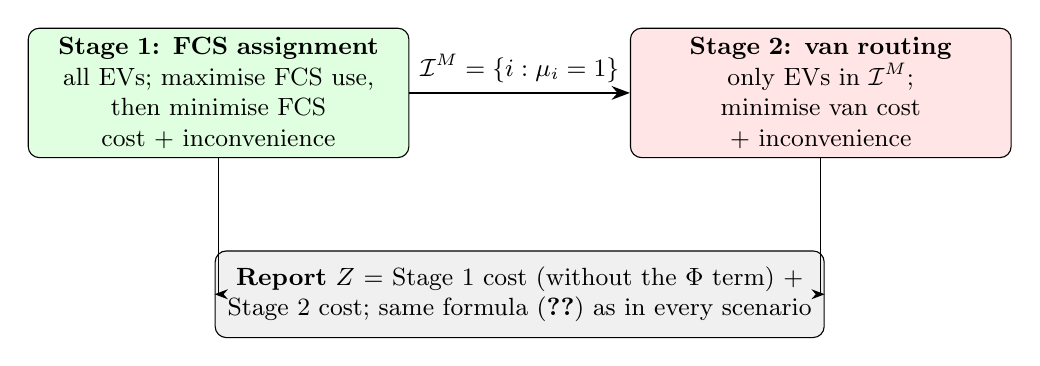
\begin{tikzpicture}[>=Stealth,box/.style={draw,rounded corners,align=center,minimum height=1.1cm,font=\small}]
  \node[box,fill=green!12,text width=4.6cm] (s1) {\textbf{Stage 1: FCS assignment}\\all EVs; maximise FCS use,\\then minimise FCS cost + inconvenience};
  \node[box,fill=red!10,text width=4.6cm,right=2.8cm of s1] (s2) {\textbf{Stage 2: van routing}\\only EVs in $\I^M$;\\minimise van cost + inconvenience};
  \draw[->,thick] (s1) -- node[above,font=\small]{$\I^M=\{i:\mu_i=1\}$} (s2);
  \node[box,fill=black!6,text width=7.5cm,below=2.0cm of $(s1)!0.5!(s2)$] (ev) {\textbf{Report} $Z=$ Stage~1 cost (without the $\Phi$ term) $+$ Stage~2 cost; same formula \eqref{eq:Z} as in every scenario};
  \draw[->] (s1) |- (ev); \draw[->] (s2) |- (ev);
\end{tikzpicture}
\end{center}

Stage~1 does not look at the vans, and Stage~2 cannot change what Stage~1 decided. That is the definition of ``FCS first, then MCS''.

%----------------------------------------------------------------
\subsection{Stage 1: assign EVs to fixed stations}

\textbf{Objective.}
\begin{equation}
\begin{split}
\min\ Z^{(1)}=\;&\underbrace{\Phi\sum_{i\in\I}\mu_i}_{\text{FCS first}}
+\underbrace{c^{EV}\sum_i\sum_{f\in\F_i}d_{if}Y_{if}}_{Z_1}
+\underbrace{Z^F_{\text{energy}}}_{\text{FCS part of }Z_4}\\
&+\underbrace{\sum_i\sum_{f\in\F_i}\rho^F_{if}Y_{if}+\alpha\sum_i w_i(C_i-r_i)+c^L\sum_i w_iL_i}_{\text{FCS customers' inconvenience}}
\end{split}
\label{eq:obj1}
\end{equation}
with $C_i=S_i+\tau^F_iY_i$ in this stage. $\Phi$ is a penalty for handing an EV to the vans. It is chosen larger than anything an extra FCS customer can add to the rest of \eqref{eq:obj1}, e.g.
\[
\Phi > \max_{i}\max_{f\in\F_i}\big(c^{EV}d_{if}+\pi^{\max}E_i+\rho^F_{if}\big)+n\,(\alpha+c^L)\,w_{\max}\,T,
\]
so Stage~1 first \textbf{maximises the number of EVs served at an FCS}, and only among those solutions minimises FCS cost and inconvenience. ($\pi^{\max}$ is the highest grid price.) A numerically safer equivalent is to solve twice: first $\max\sum_iY_i$, then fix that number and minimise the rest.
\ifTOU
Because $Z^F_{\text{energy}}$ uses the peak price, Stage~1 may \emph{start sessions later} to leave the peak, if the price saving beats the extra waiting cost (Section~\ref{sec:expect}).
\fi

\textbf{Constraints.}
\begin{align}
\sum_{g\in\G_i}y_{ig}+\mu_i &= 1 && \forall i\in\I \label{eq:s1assign}\\
S_i &\ge r_i+\sum_{f\in\F_i}t_{if}Y_{if} && \forall i\in\I \label{eq:fcsarr}\\
S_i &\le r_i+T\,(1-\mu_i) && \forall i\in\I \label{eq:s1park}\\
S_j &\ge S_i+\tau^F_i-(T+\tau^F_i)(3-y_{ig}-y_{jg}-o_{ij}) && \forall g,\ (i,j)\in\mathcal{P}_g \label{eq:disj1}\\
S_i &\ge S_j+\tau^F_j-(T+\tau^F_j)(2-y_{ig}-y_{jg}+o_{ij}) && \forall g,\ (i,j)\in\mathcal{P}_g \label{eq:disj2}\\
\sum_i y_{ig_1} &\ge \sum_i y_{ig_2} && \forall f,\ \G_f=\{g_1,g_2\} \label{eq:gunsym}\\
S_i+\tau^F_iY_i &\le T,\qquad L_i\ge S_i+\tau^F_iY_i-l_i && \forall i\in\I \label{eq:s1time}
\end{align}
\ifTOU plus the time-of-use split \eqref{eq:tou1}--\eqref{eq:tou5} of each FCS session (Section~\ref{sec:price}).\fi
\desc{\eqref{eq:s1assign}: every EV either gets one reachable gun or is handed to the vans. An EV that reaches no FCS ($\G_i=\emptyset$) is forced to $\mu_i=1$. \eqref{eq:fcsarr}: an FCS session cannot start before the EV has asked and driven to the station. \eqref{eq:s1park}: for an EV handed to the vans, $S_i$ is parked at $r_i$, so it adds no waiting in Stage~1 (its real start time is decided in Stage~2). \eqref{eq:disj1}--\eqref{eq:disj2}: two EVs on the same gun do not overlap; $o_{ij}$ picks who goes first. With two guns per station this means at most two EVs charge at a station at a time. \eqref{eq:gunsym}: symmetry breaking between the two identical guns (optional). \eqref{eq:s1time}: finished by $T$; lateness.}

\textbf{Optional acceptability rule.} An operator may refuse to send a driver to a station that is ``too inconvenient'', e.g.\ only allow gun $g$ of station $f$ for EV $i$ if $\hat\rho^F_{if}\le\bar\rho$. This only shrinks $\G_i$, so EVs whose stations are all too far go to the vans. Report results with and without it.

\textbf{Output:} $\I^M=\{i:\mu_i=1\}$, the EVs left for the vans; plus each FCS customer's gun and start time.

%----------------------------------------------------------------
\subsection{Stage 2: route the vans to the leftover EVs}

Stage~2 is a vehicle routing problem with time windows, on the EVs in $\I^M$ only. Here $C_i=S_i+\tau^M_i$.

\textbf{Objective.}
\begin{equation}
\begin{split}
\min\ Z^{(2)}=\;&\underbrace{c^M\sum_m\sum_{(i,j)\in\A^M}d_{ij}x_{ijm}}_{Z_2}+\underbrace{\sum_m c^D_mu_m}_{Z_3}+\underbrace{Z^M_{\text{energy}}}_{\text{van part of }Z_4}\\
&+\underbrace{\sum_{i\in\I^M}\sum_m\rho^M_{im}z_{im}+\alpha\sum_{i\in\I^M}w_i(C_i-r_i)+c^L\sum_{i\in\I^M}w_iL_i}_{\text{van customers' inconvenience}}
\end{split}
\label{eq:obj2}
\end{equation}
Since every EV in $\I^M$ must be served by some van, $Z^M_{\text{energy}}$ and the $\rho^M$ term are constants here. They are kept so that $Z^{(2)}$ is the true cost of Stage~2. Waiting and lateness make the vans visit urgent EVs early.

\textbf{Constraints.}
\begin{align}
\sum_{m\in\M}z_{im} &= 1 && \forall i\in\I^M \label{eq:s2assign}\\
\sum_{j:(0,j)\in\A^M}x_{0jm} = \sum_{i:(i,n+1)\in\A^M}x_{i,n+1,m} &= u_m && \forall m \label{eq:depot}\\
\sum_{i:(i,j)\in\A^M}x_{ijm} = \sum_{k:(j,k)\in\A^M}x_{jkm} &= z_{jm} && \forall j\in\I^M,\ m \label{eq:flow}\\
\sum_{i\in\I^M}z_{im} &\le Q_m\,u_m && \forall m \label{eq:cap}\\
\sum_{i\in\I^M}\frac{E_i}{\eta}z_{im}+\beta\sum_{(i,j)\in\A^M}d_{ij}x_{ijm} &\le B_m\,u_m && \forall m \label{eq:batt}
\end{align}
\begin{align}
S_j &\ge \max\{r_j,\ t_{0j}\,x_{0jm}\} && \forall j\in\I^M,\ m \label{eq:depart}\\
S_j &\ge S_i+\tau^M_i+t_{ij}-(T+\tau^M_i+t_{ij})(1-x_{ijm}) && \forall i\neq j,\ m \label{eq:seq}\\
S_i+\tau^M_i+t_{i,n+1} &\le T+(\tau^M_i+t_{i,n+1})(1-x_{i,n+1,m}) && \forall i,\ m \label{eq:return}\\
S_i+\tau^M_i \le T,\quad L_i &\ge S_i+\tau^M_i-l_i && \forall i\in\I^M \label{eq:s2time}\\
u_m &\ge u_{m+1} && m<|\M| \label{eq:vansym}
\end{align}
\desc{\eqref{eq:s2assign}: each leftover EV gets one van. \eqref{eq:depot}: a used van leaves and returns to the depot once. \eqref{eq:flow}: each EV on van $m$ is entered and left exactly once by that van. \eqref{eq:cap}: at most $Q_m$ EVs per van. \eqref{eq:batt}: delivered energy (with transfer losses) plus driving energy fits in the van battery. \eqref{eq:depart}: no start before the request, or before the van can drive there from the depot (written as two linear constraints). \eqref{eq:seq}: if the van goes $i\to j$, it finishes $i$ and drives to $j$ before starting $j$. This gives one EV at a time and removes subtours (MTZ-type). \eqref{eq:return}: back at the depot by $T$. \eqref{eq:s2time}: finished by $T$; lateness. \eqref{eq:vansym}: use identical vans in index order.}

\textbf{If Stage 2 is infeasible} (too many leftover EVs for the fleet by $T$), the sequential policy has \emph{failed} on that instance. For diagnosis, add $s_i\in\{0,1\}$ (``unserved''), replace \eqref{eq:s2assign} by $\sum_mz_{im}+s_i=1$ and add $\Phi^U\sum_is_i$ to \eqref{eq:obj2}. Then report the number of EVs that could not be served. This is a useful comparison with the integrated scenario, which may serve all of them.

%----------------------------------------------------------------
\subsection{Reported value}
\[
Z^{\text{S\scen}}=\big(Z^{(1)*}-\Phi\,|\I^M|\big)+Z^{(2)*},
\]
which is exactly \eqref{eq:Z} evaluated at the combined solution. The stage-1 solution plus the stage-2 solution is a feasible solution of the integrated model (S\ifTOU 4\else 3\fi), so
$Z^{\text{S\ifTOU 4\else 3\fi}}\le Z^{\text{S\scen}}$. The difference is the \emph{value of integration}.

\else
%---------------------------------------------------------------- INT
\subsection{Objective}
\begin{equation}
\min\ Z \quad\text{as in \eqref{eq:Z}, with }Z^F_{\text{energy}}=\ifTOU P^F\textstyle\sum_i\big[\pi^\off(\theta^1_i+\theta^3_i)+\pi^\pk\theta^2_i\big]\else\pi^F\textstyle\sum_iE_iY_i\fi,\quad C_i=S_i+\tau^F_iY_i+\tau^M_iZ_i. \label{eq:objint}
\end{equation}
Written out in full:
\begin{align*}
\min\ Z=\;& c^{EV}\sum_i\sum_{f\in\F_i}d_{if}Y_{if}+c^M\sum_m\sum_{(i,j)\in\A}d_{ij}x_{ijm}+\sum_mc^D_mu_m\\
&+\ifTOU P^F\sum_i\big[\pi^\off(\theta^1_i+\theta^3_i)+\pi^\pk\theta^2_i\big]\else\pi^F\sum_iE_iY_i\fi
+\pi^M\sum_i\sum_m\frac{E_i}{\eta}z_{im}\\
&+\sum_i\sum_{f\in\F_i}\rho^F_{if}Y_{if}+\sum_i\sum_m\rho^M_{im}z_{im}+\alpha\sum_iw_i(C_i-r_i)+c^L\sum_iw_iL_i .
\end{align*}
Every term is linear. One model weighs everything at once: an EV goes to a van exactly when the van's extra km, dispatch and energy cost are outweighed by the effort and waiting it saves the driver\ifTOU, or by the peak-price energy it avoids\fi.

\subsection{Constraints}

\textbf{Assignment.}
\begin{equation}
\sum_{g\in\G_i}y_{ig}+\sum_{m\in\M}z_{im}=1\qquad\forall i\in\I \label{eq:assign}
\end{equation}
\desc{Exactly one resource per EV: one reachable gun or one van. EVs that reach no FCS are forced onto a van.}

\textbf{Fixed stations.}
\begin{align}
S_i &\ge r_i+\sum_{f\in\F_i}t_{if}Y_{if} && \forall i \label{eq:fcsarr}\\
S_j &\ge S_i+\tau^F_i-(T+\tau^F_i)(3-y_{ig}-y_{jg}-o_{ij}) && \forall g,\ (i,j)\in\mathcal{P}_g \label{eq:disj1}\\
S_i &\ge S_j+\tau^F_j-(T+\tau^F_j)(2-y_{ig}-y_{jg}+o_{ij}) && \forall g,\ (i,j)\in\mathcal{P}_g \label{eq:disj2}\\
\sum_iy_{ig_1} &\ge \sum_iy_{ig_2} && \forall f,\ \G_f=\{g_1,g_2\} \label{eq:gunsym}
\end{align}
\desc{\eqref{eq:fcsarr}: an FCS session starts after the request and the drive to the station (for a van customer this is just $S_i\ge r_i$). \eqref{eq:disj1}--\eqref{eq:disj2}: EVs on the same gun do not overlap; $o_{ij}$ chooses the order. \eqref{eq:gunsym}: optional symmetry breaking.}

\textbf{Vans: routes, capacity, battery.}
\begin{align}
\sum_{j:(0,j)\in\A}x_{0jm}=\sum_{i:(i,n+1)\in\A}x_{i,n+1,m} &= u_m && \forall m \label{eq:depot}\\
\sum_{i:(i,j)\in\A}x_{ijm}=\sum_{k:(j,k)\in\A}x_{jkm} &= z_{jm} && \forall j\in\I,\ m \label{eq:flow}\\
\sum_iz_{im} &\le Q_mu_m && \forall m \label{eq:cap}\\
\sum_i\frac{E_i}{\eta}z_{im}+\beta\sum_{(i,j)\in\A}d_{ij}x_{ijm} &\le B_mu_m && \forall m \label{eq:batt}
\end{align}
\desc{\eqref{eq:depot}: a used van leaves and returns once. \eqref{eq:flow}: each EV on van $m$ is visited exactly once by it. \eqref{eq:cap}: at most $Q_m$ EVs. \eqref{eq:batt}: delivered energy (with losses) plus driving energy fits in the battery.}

\textbf{Vans: timing (one EV at a time, no subtours).}
\begin{align}
S_j &\ge t_{0j}\,x_{0jm} && \forall j\in\I,\ m \label{eq:depart}\\
S_j &\ge S_i+\tau^M_i+t_{ij}-(T+\tau^M_i+t_{ij})(1-x_{ijm}) && \forall i\neq j\in\I,\ m \label{eq:seq}\\
S_i+\tau^M_i+t_{i,n+1} &\le T+(\tau^M_i+t_{i,n+1})(1-x_{i,n+1,m}) && \forall i,\ m \label{eq:return}
\end{align}
\desc{\eqref{eq:depart}: the first stop cannot start before the van has driven there. \eqref{eq:seq}: $i\to j$ means finish $i$, drive, then start $j$; start times rise along a route, so no subtour can close. \eqref{eq:return}: back at the depot by $T$.}

\textbf{Horizon and lateness.}
\begin{equation}
C_i\le T,\qquad L_i\ge C_i-l_i\qquad\forall i\in\I \label{eq:time}
\end{equation}
\desc{Every EV is fully charged within the horizon; $L_i$ measures lateness.}

\ifTOU
\textbf{Time-of-use split.} Constraints \eqref{eq:tou1}--\eqref{eq:tou5} of Section~\ref{sec:price}.
\fi

\textbf{Symmetry and domains.}
\begin{equation}
u_m\ge u_{m+1};\qquad y,z,x,u,o\ifTOU,\kappa\fi\in\{0,1\};\qquad S_i,L_i\ifTOU,\theta^p_i\fi\ge0 \label{eq:dom}
\end{equation}
\fi

%=====================================================================
\section{Learning-to-optimise (RL) formulation}\label{sec:rl}

\textbf{Main rule:} the reward of each action is \emph{minus the increase in $Z$ that the action causes}. The rewards over an episode then add up to $-Z$ of the solution the policy builds. RL and MILP results are measured on the same yardstick \eqref{eq:Z}, and the MILP optimum is the benchmark for the RL gap.

\ifSEQ
%---------------------------------------------------------------- RL SEQ
The RL pipeline has the same two stages as the MILP.

\subsection{Stage 1 policy: FCS assignment}
\begin{itemize}[leftmargin=1.4em,itemsep=2pt]
  \item \textbf{Episode / epochs:} EVs are taken in order of request time $r_i$ (ties: higher $w_i$ first). One decision per EV.
  \item \textbf{State:} features of the current EV $k$ ($E_k,r_k,l_k,w_k,R_k$, location); for each gun $g$ the time $F_g$ it becomes free; summary features of the EVs still to come (count and positions near each station)\ifTOU; the current price and the time until $T_1$ and $T_2$\fi.
  \item \textbf{Action:} a gun $g\in\G_k$, or ``hand to vans''. \textbf{FCS-first mask:} ``hand to vans'' is allowed \emph{only} if no gun can finish EV $k$ by $T$ (or, with the optional rule, if all remaining guns have $\hat\rho^F_{kf}>\bar\rho$).
  \ifTOU\item \textbf{Optional timing action:} ``gun $g$, start after the peak'', i.e.\ $S_k=\max\{\text{earliest},T_2\}$, allowed only if the session still ends by $T$.\fi
  \item \textbf{Transition:} $S_k=\max\{r_k+t_{kf},F_g\}$ (or later, for the timing action); $F_g\leftarrow S_k+\tau^F_k$.
  \item \textbf{Reward:} $-\Big[c^{EV}d_{kf}+\text{energy}_k+\rho^F_{kf}+\alpha w_k(S_k+\tau^F_k-r_k)+c^Lw_k(S_k+\tau^F_k-l_k)^+\Big]$, where energy$_k$ = \ifTOU$P^F\big[\pi^\off\cdot(\text{off-peak hours of }[S_k,S_k+\tau^F_k])+\pi^\pk\cdot(\text{peak hours})\big]$, computed exactly in the simulator\else$\pi^FE_k$\fi. Handing an EV to the vans gives reward $0$ here; its cost is counted in Stage~2.
\end{itemize}
Note: a simple baseline for Stage~1 is the greedy rule ``gun with the largest one-step reward''. What RL can learn on top of this is, for example, to keep a nearby gun free for an urgent EV that arrives later.

\subsection{Stage 2 policy: van routing over $\I^M$}
\begin{itemize}[leftmargin=1.4em,itemsep=2pt]
  \item \textbf{Epochs:} whenever a van becomes free (the earliest-free van decides first).
  \item \textbf{State:} for each van: position, time free, remaining battery $b_m$, EVs served so far, dispatched or not; for each unserved EV in $\I^M$: location, $E_i,r_i,l_i,w_i$; current time.
  \item \textbf{Action:} the next EV $j$ for this van, or ``return to depot'' (ends the route). Mask: $j$ must be feasible: battery covers $E_j/\eta$ plus driving to $j$ and back to the depot, the count stays $\le Q_m$, and $j$ can be finished with the van back at the depot by $T$.
  \item \textbf{Transition:} $S_j=\max\{r_j,\ \text{time free}+t_{\text{pos},j}\}$; the van moves to $j$ and is free at $S_j+\tau^M_j$; $b_m$ falls by $E_j/\eta+\beta d_{\text{pos},j}$.
  \item \textbf{Reward:} serving $j$: $-\Big[c^Md_{\text{pos},j}+c^D_m[\text{first stop}]+\pi^M\frac{E_j}{\eta}+\rho^M_{jm}+\alpha w_j(S_j+\tau^M_j-r_j)+c^Lw_j(S_j+\tau^M_j-l_j)^+\Big]$; returning: $-c^Md_{\text{pos},0}$. EVs still unserved at the end: $-\Phi^U$ each.
  \item \textbf{Policy:} an attention-based routing policy (e.g.\ Kool et al., 2019, ``Attention, Learn to Solve Routing Problems!'') trained with REINFORCE or PPO. Baseline: nearest-feasible-EV heuristic.
\end{itemize}
Episode return of Stage~1 + Stage~2 $=-Z^{\text{S\scen}}$.

\else
%---------------------------------------------------------------- RL INT
One policy decides both who serves each EV and the van routes.
\begin{itemize}[leftmargin=1.4em,itemsep=2pt]
  \item \textbf{Episode / epochs:} EVs are taken in order of request time $r_i$ (ties: higher $w_i$ first). One decision per EV.
  \item \textbf{State:} (i) the current EV $k$: location, $E_k,r_k,l_k,w_k,R_k$, reachable stations; (ii) each gun $g$: time $F_g$ it becomes free; (iii) each van $m$: current end-of-route position, time free, remaining battery $b_m$, EVs served, dispatched or not; (iv) embeddings of the not-yet-assigned EVs (for look-ahead)\ifTOU; (v) current price, time until $T_1$ and $T_2$\fi.
  \item \textbf{Action:} $a\in\G_k\cup\M$: a gun, or a van (EV $k$ is appended to the end of that van's route). \textbf{Mask} infeasible actions: a gun that cannot finish $k$ by $T$; a van without enough battery for $E_k/\eta$ plus the drive to $k$ and back to the depot, with $Q_m$ reached, or unable to finish $k$ and return by $T$.
  \ifTOU\item \textbf{Optional timing action:} ``gun $g$, start after the peak'' ($S_k=\max\{\text{earliest},T_2\}$, if it still ends by $T$).\fi
  \item \textbf{Transition:} gun: $S_k=\max\{r_k+t_{kf},F_g\}$, $F_g\leftarrow S_k+\tau^F_k$. Van: $S_k=\max\{r_k,\ \text{free}_m+t_{\text{pos}_m,k}\}$, then the van moves to $k$, $\text{free}_m\leftarrow S_k+\tau^M_k$, $b_m\mathrel{-}=E_k/\eta+\beta d_{\text{pos}_m,k}$.
  \item \textbf{Reward} $=-\Delta Z$:
  \begin{align*}
  \text{gun } g\text{ at }f:&\quad -\Big[c^{EV}d_{kf}+\text{energy}^F_k+\rho^F_{kf}+\alpha w_k(C_k-r_k)+c^Lw_k(C_k-l_k)^+\Big]\\
  \text{van } m:&\quad -\Big[c^M\big(d_{\text{pos}_m,k}+d_{k,0}-d_{\text{pos}_m,0}\big)+c^D_m[\text{first use}]+\pi^M\tfrac{E_k}{\eta}\\
  &\qquad\quad+\rho^M_{km}+\alpha w_k(C_k-r_k)+c^Lw_k(C_k-l_k)^+\Big]
  \end{align*}
  The van distance term is the \emph{change} in route length when $k$ is inserted before the return to the depot, so the sum over the episode equals the total route length (the return legs telescope). energy$^F_k$ = \ifTOU$P^F\big[\pi^\off\cdot(\text{off-peak hours})+\pi^\pk\cdot(\text{peak hours of }[S_k,C_k])\big]$, computed exactly by the simulator; no linearisation is needed in RL\else$\pi^FE_k$\fi.
  \item \textbf{Dead end:} if every action is masked, EV $k$ is unserved: reward $-\Phi^U$, and the episode continues. Report the count.
  \item \textbf{Policy:} masked categorical policy over guns and vans, encoder with attention over EVs, guns and vans; trained with PPO. Natural baseline: greedy, i.e.\ choose the action with the largest one-step reward. That is the pairwise rule ``smallest $\hat\rho$ + cost'' from Section~\ref{sec:inc}.
\end{itemize}
Restriction to note: vans serve EVs in assignment order (append only). A variant that inserts $k$ at the cheapest position of a route is more flexible but has a larger action space.
\fi

\textbf{Reward scaling.} For stable training divide every reward by a constant, e.g.\ the greedy baseline's average $Z$ on the training instances. This does not change the optimal policy.

%=====================================================================
\section{What to expect and what to report}\label{sec:expect}

\ifnum\scen=1
\begin{itemize}[leftmargin=1.4em,itemsep=2pt]
  \item Vans serve only EVs that reach no station, or that the stations cannot finish by $T$. If stations have spare capacity, very few vans are dispatched.
  \item Inconvenience is high for EVs far from the nearest station (worked example: Rs\,682 at the FCS, against Rs\,458 if a van had been allowed).
  \item With too few vans Stage~2 becomes infeasible (unserved EVs), even when the integrated model S3 could serve everyone. Report the smallest $|\M|$ at which S1 is feasible and compare it with S3.
\end{itemize}
\fi
\ifnum\scen=2
\begin{itemize}[leftmargin=1.4em,itemsep=2pt]
  \item \textbf{When does Stage~1 delay a session to avoid the peak?} Moving one hour of charging out of the peak saves $(\pi^\pk-\pi^\off)P^F=3\times22=$ Rs\,66, but delays completion by up to an hour, which costs $\alpha w_i\ge$ Rs\,200. So with the default values Stage~1 almost never delays. It mostly pays the higher price, and S2 costs roughly S1 plus the peak surcharge. Sessions start later only if $\alpha$ is small (try $\lambda<0.33$ in the sensitivity analysis).
  \item The van assignment is the same as in S1 unless Stage~1's timing changes which EVs fit at the stations. Stage~1 cannot use vans to escape the peak price.
  \item Extra KPI: \textbf{grid energy drawn at FCS during the peak}, $P^F\sum_i\theta^2_i$ (kWh). Compare with S4.
\end{itemize}
\fi
\ifnum\scen=3
\begin{itemize}[leftmargin=1.4em,itemsep=2pt]
  \item Vans take EVs for which the saved inconvenience exceeds the extra van cost (worked example: van chosen, saving Rs\,224). Expect vans to serve EVs that are far from every station, have low range (high $w_i$), or have early deadlines, while EVs near a station still use it.
  \item \textbf{Value of integration under flat price:} $Z^{\text{S1}}-Z^{\text{S3}}\ge0$. Report it per component ($Z_1,\dots,Z_5$): typically operating cost rises a little and inconvenience falls a lot.
  \item Vary $|\M|$ (0, 1, 2, \dots): the first few vans lower $Z$ sharply, then the effect levels off. That curve shows the scenarios where mobile chargers help most.
\end{itemize}
\fi
\ifnum\scen=4
\begin{itemize}[leftmargin=1.4em,itemsep=2pt]
  \item During the peak a van kWh costs about the same as an FCS kWh (Rs\,10.0 each), so the vans' energy disadvantage disappears and vans also absorb \emph{peak-hour} demand that would otherwise be charged on the grid at peak price.
  \item Expect more van usage than in S3, concentrated on requests in $[T_1,T_2]$, and lower grid energy at the stations during the peak, $P^F\sum_i\theta^2_i$, than in S2.
  \item \textbf{Value of integration under peak pricing:} $Z^{\text{S2}}-Z^{\text{S4}}$. It should be larger than $Z^{\text{S1}}-Z^{\text{S3}}$, because integration now also allows price arbitrage.
  \item \textbf{Peak pricing with full flexibility:} $Z^{\text{S4}}-Z^{\text{S3}}$ should be smaller than $Z^{\text{S2}}-Z^{\text{S1}}$: vans cushion the price increase.
\end{itemize}
\fi

\textbf{Cross-scenario comparison table} (fill in from the four runs):
\begin{center}
\renewcommand{\arraystretch}{1.2}
\begin{tabular}{@{}lll@{}}
\toprule
\textbf{Comparison} & \textbf{Measures} & \textbf{Expected sign} \\
\midrule
S1 $-$ S3 & value of integration, flat price & $\ge0$ \\
S2 $-$ S4 & value of integration, peak price & $\ge0$, larger than S1 $-$ S3 \\
S2 $-$ S1 & cost of peak pricing, FCS-first operator & $>0$ \\
S4 $-$ S3 & cost of peak pricing, flexible operator & $>0$, smaller than S2 $-$ S1 \\
\bottomrule
\end{tabular}
\end{center}
Report for each: $Z$ and its components, number of vans used, EVs per resource, mean and maximum inconvenience per EV, total lateness, peak-hour grid energy, solve time, and (for RL) the gap to the MILP optimum.

%=====================================================================
\appendix
\section{Illustrative parameter values}\label{app:values}

These are starting values for experiments, not data. All are meant to be varied in the analysis. Values in Rs.

\begin{center}
\renewcommand{\arraystretch}{1.15}
\begin{tabular}{@{}llp{6.2cm}@{}}
\toprule
\textbf{Parameter} & \textbf{Value} & \textbf{Note} \\
\midrule
$T$, $[T_1,T_2]$ & 7 h, $[2,6]$ & 16:00--23:00, peak 18:00--22:00 \\
$P^F$, $P^M$ & 22 kW, 30 kW & \\
$v$, $\beta$, $\eta$ & 25 km/h, 0.25 kWh/km, 0.9 & \\
$B_m$, $Q_m$, $|\M|$ & 150 kWh, 6, 2--6 & \\
$c^{EV}$, $c^M$, $c^D_m$ & Rs\,4/km, Rs\,15/km, Rs\,1500 & van km includes driver time \\
$\pi^F$ (flat) & Rs\,8.7/kWh & equals the time-average of the ToU tariff over $[0,T]$ \\
$\pi^\off$, $\pi^\pk$ (ToU) & Rs\,7/kWh, Rs\,10/kWh & $(3\times7+4\times10)/7=8.7$ \\
$c^{bat}$ & Rs\,2/kWh & van battery wear \\
$\pi^M$ & Rs\,10.7 (flat) / Rs\,9.0 (ToU) & $=\pi^F+c^{bat}$ / $=\pi^\off+c^{bat}$ \\
$\alpha$, $\alpha^D$ & Rs\,200/h, Rs\,100/h & value of time; extra for attended time \\
$h^F$, $h^M$, $\varphi$ & Rs\,50, Rs\,10, Rs\,100 & trip hassle, hand-over, range stress \\
$c^L$ & Rs\,300/h & lateness \\
$w_i$ & $1+2(1-R_i/R_{\max})$, $R_i\sim U[3,40]$ km & priority from remaining range \\
\bottomrule
\end{tabular}
\end{center}

The flat price is set to the time-average of the peak tariff. The price \emph{level} is then the same in both pricing cases, and only the price \emph{shape} differs. Without this, part of S1 vs S2 would just reflect a different average price.

\end{document}
"
%    pdflatex -jobname=scenario2_peak_sequential   "\def\scen{2}% =====================================================================
%  One source, four PDFs.  Build with build.sh (or by hand):
%    pdflatex -jobname=scenario1_flat_sequential   "\def\scen{1}\input{scenario_master}"
%    pdflatex -jobname=scenario2_peak_sequential   "\def\scen{2}\input{scenario_master}"
%    pdflatex -jobname=scenario3_flat_integrated   "\def\scen{3}\input{scenario_master}"
%    pdflatex -jobname=scenario4_peak_integrated   "\def\scen{4}\input{scenario_master}"
%  (run each twice for cross-references)
% =====================================================================
\documentclass[11pt,a4paper]{article}
\usepackage[margin=2.2cm]{geometry}
\usepackage{amsmath,amssymb,amsfonts}
\usepackage{booktabs,array,tabularx}
\usepackage{enumitem}
\usepackage[table]{xcolor}
\usepackage{tikz}
\usetikzlibrary{arrows.meta,positioning,calc}
\usepackage[colorlinks=true,linkcolor=blue!50!black,urlcolor=blue!50!black]{hyperref}
\usepackage{titlesec}
\titleformat{\section}{\large\bfseries}{\thesection}{0.8em}{}
\titleformat{\subsection}{\normalsize\bfseries}{\thesubsection}{0.8em}{}
\setlength{\parindent}{0pt}
\setlength{\parskip}{5pt}

% ---------------- scenario switches ----------------
\ifdefined\scen\else\def\scen{1}\fi
\newif\ifTOU \TOUfalse   % true = time-of-use (peak) price
\newif\ifSEQ \SEQfalse   % true = FCS first, then MCS
\ifnum\scen=1 \SEQtrue \fi
\ifnum\scen=2 \TOUtrue \SEQtrue \fi
\ifnum\scen=4 \TOUtrue \fi

\newcommand{\pricename}{\ifTOU time-of-use price (dearer evening peak)\else single (flat) price all day\fi}
\newcommand{\structname}{\ifSEQ FCS first, then MCS (sequential)\else FCS and MCS together (integrated)\fi}

% ---------------- notation ----------------
\newcommand{\I}{\mathcal{I}}
\newcommand{\F}{\mathcal{F}}
\newcommand{\G}{\mathcal{G}}
\newcommand{\M}{\mathcal{M}}
\newcommand{\N}{\mathcal{N}}
\newcommand{\A}{\mathcal{A}}
\newcommand{\Rs}{\text{Rs}\,}
\newcommand{\pk}{\mathrm{pk}}
\newcommand{\off}{\mathrm{off}}
\newcommand{\desc}[1]{\par\vspace{-2pt}{\small\color{black!75}\textit{Meaning:} #1}\par\vspace{4pt}}
\newcommand{\cell}[2]{\ifnum\scen=#1\cellcolor{blue!18}\textbf{S#1 (this document)}\\\textbf{#2}\else S#1\\#2\fi}

\title{\textbf{EV Charging Network Optimisation}\\[4pt]
\large Scenario \scen: \pricename\ $+$ \structname\\[2pt]
\normalsize MILP and RL formulation}
\author{CP 320 OR for Mobility Management, course project}
\date{2 October 2026}

\begin{document}
\maketitle

%=====================================================================
\section{Where this scenario sits}

The project studies four scenarios: two ways of pricing grid electricity, times two ways of making the decisions.

\begin{center}
\renewcommand{\arraystretch}{1.5}
\begin{tabular}{>{\raggedright\arraybackslash}p{4.2cm}|>{\centering\arraybackslash}p{4.6cm}|>{\centering\arraybackslash}p{4.6cm}}
 & \textbf{Flat price all day} & \textbf{Time-of-use (peak) price} \\ \hline
\textbf{Sequential:} FCS first, leftover EVs to MCS &
\begin{tabular}[c]{@{}c@{}}\cell{1}{flat + sequential}\end{tabular} &
\begin{tabular}[c]{@{}c@{}}\cell{2}{peak + sequential}\end{tabular} \\ \hline
\textbf{Integrated:} FCS and MCS decided together &
\begin{tabular}[c]{@{}c@{}}\cell{3}{flat + integrated}\end{tabular} &
\begin{tabular}[c]{@{}c@{}}\cell{4}{peak + integrated}\end{tabular} \\
\end{tabular}
\end{center}

\textbf{The four scenarios do not have four different objectives.} They share \emph{one} cost yardstick $Z$ (Section~\ref{sec:obj}): the same cost terms and the same customer inconvenience (Section~\ref{sec:inc}). Only two things change:
\begin{itemize}[leftmargin=1.4em,itemsep=1pt]
  \item \textbf{Pricing} changes the formula for one term, the FCS energy cost (Section~\ref{sec:price}).
  \item \textbf{Decision structure} changes \emph{how} $Z$ is minimised: in one model (integrated), or in two stages (sequential), where each stage minimises its own part of $Z$.
\end{itemize}
Because the yardstick is the same, the four optimal values can be compared directly. The differences measure the \emph{value of integration} (S1$\to$S3, S2$\to$S4) and the \emph{effect of peak pricing} (S1$\to$S2, S3$\to$S4).

\ifnum\scen=1
\textbf{This scenario (S1)} is the baseline, the ``status quo''. Electricity costs the same at every hour, every EV that can be charged at a fixed station is sent there, and vans only take what is left over.
\fi
\ifnum\scen=2
\textbf{This scenario (S2)} keeps the FCS-first rule of S1, but grid electricity is dearer during the evening peak. Stage~1 can react to the price only by \emph{rescheduling} FCS sessions. It cannot hand a peak-hour EV to a van.
\fi
\ifnum\scen=3
\textbf{This scenario (S3)} keeps the flat price of S1, but the operator decides FCS and MCS service \emph{together}. An EV can be sent to a van even when a fixed station could take it, whenever that lowers total cost plus inconvenience.
\fi
\ifnum\scen=4
\textbf{This scenario (S4)} is the most flexible one: peak pricing at fixed stations, and FCS and MCS decided together. Van energy was bought off-peak, so vans can also be used to keep charging \emph{out of the expensive peak}.
\fi

%=====================================================================
\section{Setting and assumptions}\label{sec:setting}

\textbf{Time.} The planning horizon is $[0,T]$ with $T=7$\,h (16:00--23:00). It contains the evening peak window $[T_1,T_2]=[2,6]$ (18:00--22:00). The horizon is the same in all four scenarios. It is wider than the peak itself so that, under peak pricing, there is cheaper time on both sides of the peak.\ifTOU\else\ In this scenario the price is flat, so the window plays no role in the model.\fi

\textbf{Assumptions} (the same as MILP v3, plus two about energy):
\begin{enumerate}[leftmargin=1.6em,itemsep=1pt]
  \item Static, continuous time. All requests in the horizon are known at time $0$, and request $i$ becomes active at $r_i$.
  \item An EV served by an FCS drives there itself on its own battery (only to stations within its range $R_i$). The driver stays with the car while it waits for a free gun and while it charges.
  \item An EV served by an MCS stays parked where it is, and the driver is free in the meantime.
  \item Each FCS gun and each van charges one EV at a time, without interruption, at constant power.
  \item A van's battery covers both its driving and the energy it delivers. \textbf{The van battery is charged at the depot before the horizon starts}\ifTOU, i.e.\ at the off-peak price\fi, and is not recharged during the horizon.
  \item Every EV must be fully charged by $T$ (hard). Finishing after the driver's desired time $l_i$ is allowed but penalised.
\end{enumerate}

%=====================================================================
\section{Notation}\label{sec:notation}

\subsection*{Sets}
\begin{tabularx}{\textwidth}{@{}lX@{}}
\toprule
$\I=\{1,\dots,n\}$ & EV charging requests \\
$\F$; $\G_f$ ($|\G_f|=2$); $\G=\bigcup_f\G_f$ & fixed charging stations; guns of FCS $f$; all guns ($f(g)$ = station of gun $g$) \\
$\F_i=\{f: d_{if}\le R_i\}$, $\G_i=\bigcup_{f\in\F_i}\G_f$ & stations / guns EV $i$ can reach on its remaining range \\
$\M$ & mobile charging vans (MCS) \\
$0,\ n+1$ & depot as start node / end node (same place) \\
$\N=\{0\}\cup\I\cup\{n+1\}$, $\A$ & routing nodes; allowed van arcs $(i,j)$, $i\in\{0\}\cup\I$, $j\in\I\cup\{n+1\}$, $i\neq j$ \\
$\mathcal{P}_g=\{(i,j): i<j,\ g\in\G_i\cap\G_j\}$ & pairs of EVs that could share gun $g$ \\
\ifSEQ
$\I^M\subseteq\I$ & EVs handed to the vans by Stage~1 (an \emph{output} of Stage~1, a fixed input to Stage~2) \\
$\N^M$, $\A^M$ & routing nodes / arcs restricted to $\I^M$ \\
\fi
\bottomrule
\end{tabularx}

\subsection*{Parameters}
\begin{tabularx}{\textwidth}{@{}lX@{}}
\toprule
$E_i,\ r_i,\ l_i,\ R_i$ & energy demand (kWh), request time, desired completion time (h), remaining range (km) \\
$w_i\ge1$ & priority of EV $i$; $w_i=1+\kappa(1-R_i/R_{\max})$, so low-range EVs weigh more \\
$P^F,\ P^M$ & charging power of an FCS gun (22\,kW) / of a van (e.g.\ 30\,kW) \\
$\tau^F_i=E_i/P^F,\ \tau^M_i=E_i/P^M$ & charging time of EV $i$ at an FCS / by a van (h) \\
$d_{if},t_{if}$;\ $d_{ij},t_{ij}$ & distance (km) and time (h): EV$\to$FCS; between routing nodes ($t=d/v$) \\
$B_m,\ Q_m,\ \beta,\ \eta$ & van battery (kWh), max EVs per van, van consumption (kWh/km), transfer efficiency \\
$c^{EV},\ c^M,\ c^D_m$ & cost per km of EV driving, per km of van driving; fixed dispatch cost of van $m$ \\
\ifTOU
$\pi^\off,\ \pi^\pk$ & grid price (Rs/kWh) off-peak / in $[T_1,T_2]$, with $\pi^\pk\ge\pi^\off$ \\
\else
$\pi^F$ & grid price (Rs/kWh), the same at every hour \\
\fi
$c^{bat}$ & van battery wear per kWh cycled \\
$\pi^M$ & cost of 1 kWh taken from a van battery: $\pi^M=\ifTOU\pi^\off\else\pi^F\fi+c^{bat}$ (Section~\ref{sec:price}) \\
$\alpha,\ \alpha^D,\ h^F,\ h^M,\ \varphi,\ c^L$ & inconvenience coefficients (Section~\ref{sec:inc}) \\
\bottomrule
\end{tabularx}

\subsection*{Decision variables}
\begin{tabularx}{\textwidth}{@{}llX@{}}
\toprule
$y_{ig}$ & $\{0,1\}$ & EV $i$ charged at gun $g\in\G_i$ \\
$z_{im}$ & $\{0,1\}$ & EV $i$ served by van $m$ \\
$x_{ijm}$ & $\{0,1\}$ & van $m$ drives arc $(i,j)$ \\
$u_m$ & $\{0,1\}$ & van $m$ is dispatched \\
$o_{ij}$ & $\{0,1\}$ & for EVs $i<j$ that could share a gun: 1 if $i$ is charged before $j$ \\
\ifSEQ
$\mu_i$ & $\{0,1\}$ & Stage~1 only: EV $i$ is handed to the van fleet \\
\fi
\ifTOU
$\theta^1_i,\theta^2_i,\theta^3_i$ & $\ge0$ & hours of EV $i$'s FCS session before / inside / after the peak \\
$\kappa^1_i,\kappa^3_i$ & $\{0,1\}$ & EV $i$'s FCS session starts before $T_1$ / ends after $T_2$ \\
\fi
$S_i$ & $\ge0$ & time charging of EV $i$ starts (h), on whichever resource \\
$L_i$ & $\ge0$ & lateness of EV $i$ beyond $l_i$ (h) \\
\bottomrule
\end{tabularx}

\textbf{Short-hands} (linear expressions, not new variables):
\[
Y_{if}=\sum_{g\in\G_f}y_{ig},\qquad Y_i=\sum_{g\in\G_i}y_{ig}\ (\text{EV $i$ uses an FCS}),\qquad Z_i=\sum_{m\in\M}z_{im}\ (\text{EV $i$ uses a van}),
\]
\[
C_i=S_i+\tau^F_i\,Y_i+\tau^M_i\,Z_i \quad\text{(time EV $i$ is fully charged).}
\]

%=====================================================================
\section{Customer inconvenience}\label{sec:inc}

This section is \textbf{identical in all four scenario documents}. Inconvenience is a property of the customer, not of the price or of the planning method.

\subsection{What we mean by inconvenience}

Inconvenience is \emph{what the driver loses} from the moment they ask for a charge ($r_i$) until the car is fully charged ($C_i$), \emph{converted into rupees} so it can be added to the operator's costs. A driver loses three different things:

\begin{enumerate}[leftmargin=1.6em,itemsep=2pt]
  \item \textbf{Waiting:} the car is not ready. This lasts $C_i-r_i$ hours and affects \emph{every} driver, FCS or MCS.
  \item \textbf{Effort:} only an FCS customer has to drive to the station and sit there while the car charges. An MCS customer stays at home or at work and does something else. Driving to a far station also uses scarce battery range, which causes stress (``range anxiety'').
  \item \textbf{A missed deadline:} the car is still not ready at the time $l_i$ the driver needs it.
\end{enumerate}

Each loss gets a price in Rs per hour (or per event). All of them are multiplied by the priority $w_i$: an hour of delay for an EV with 5\,km of range left counts more than for one with 40\,km.

\subsection{The three components}

\begin{center}
\renewcommand{\arraystretch}{1.3}
\begin{tabularx}{\textwidth}{@{}>{\raggedright\arraybackslash}p{2.6cm}>{\raggedright\arraybackslash}X>{\raggedright\arraybackslash}X>{\raggedright\arraybackslash}p{3.0cm}@{}}
\toprule
\textbf{Component} & \textbf{EV $i$ at FCS $f$} & \textbf{EV $i$ by a van} & \textbf{Known when?} \\
\midrule
Effort & $w_i\big[\alpha^D(t_{if}+\tau^F_i)+h^F+\varphi\,d_{if}/R_i\big]$: driving and sitting at the station, a fixed trip hassle, range stress & $w_i\,h^M$: being reachable and handing over the car & \textbf{Static:} known as soon as the resource is chosen \\
Waiting & $w_i\,\alpha\,(C_i-r_i)$ = drive + \emph{queue at the gun} + charge & $w_i\,\alpha\,(C_i-r_i)$ = \emph{wait for the van} + charge & \textbf{Dynamic:} depends on the queue / van route \\
Missed deadline & $w_i\,c^L\,L_i$, $L_i=\max\{0,C_i-l_i\}$ & same & Dynamic \\
\bottomrule
\end{tabularx}
\end{center}

\textbf{Coefficients.}
$\alpha$ (Rs/h) is the value of an hour the car is not ready.
$\alpha^D$ (Rs/h) is the \emph{extra} value of an hour the driver must personally spend driving or sitting at the station: an hour at the station costs $\alpha+\alpha^D$, an hour waiting at home for a van costs only $\alpha$.
$h^F,h^M$ (Rs) are fixed hassle costs of one trip to a station / one van hand-over.
$\varphi$ (Rs) is the range-stress cost of a trip that uses the \emph{whole} remaining range ($d_{if}/R_i\le1$ is the fraction used).
$c^L$ (Rs/h) is the cost per hour late.

\subsection{Pairwise form: inconvenience of a (customer, resource) pair}

The natural first idea is: \emph{for every pair (EV $i$, FCS $f$) and every pair (EV $i$, van $m$) there is an inconvenience number, and the operator picks the pair with the lowest cost plus inconvenience.} The static part fits this idea exactly:
\[
\boxed{\;\rho^F_{if}=w_i\Big[\alpha^D\,(t_{if}+\tau^F_i)+h^F+\varphi\,\frac{d_{if}}{R_i}\Big]\qquad
\rho^M_{im}=w_i\,h^M\;}
\]
These are \textbf{parameters}, computed before solving, one number per (EV, FCS) pair and per (EV, van) pair. In the objective they appear linearly: $\sum_i\sum_f\rho^F_{if}Y_{if}+\sum_i\sum_m\rho^M_{im}z_{im}$.

Note that $\rho^M_{im}$ does not depend on $m$. Vans are identical and all start at the same depot, so the driver does not care \emph{which} van comes, only \emph{when} it comes. That ``when'' is the waiting part.

\subsection{Why waiting cannot be a fixed pairwise number}

It is tempting to also write the waiting as a pairwise number, e.g.\ ``the van needs 5 minutes to reach EV $i$''. But that depends on \emph{where the van is coming from}, which depends on the route the model is still choosing: if EV $i$ is the 4th stop of a van, the wait is the time for three charging sessions plus four drives. Likewise, waiting at an FCS depends on how many EVs are queued at that gun. So waiting is not known before solving. It is a function of decision variables:
\[
\text{waiting cost of EV } i \;=\; w_i\,\alpha\,(C_i-r_i),\qquad C_i=S_i+\tau^F_iY_i+\tau^M_iZ_i .
\]
This is \textbf{linear} in the variables ($S_i$, $y$, $z$), so it fits in a MILP directly. The constraints of Section~\ref{sec:milp} make $S_i$ equal to the true start time, including driving, queueing at the gun and the van's route. The term $\sum_i w_i\alpha r_i$ is a constant and may be dropped when solving.

\textbf{Pairwise \emph{estimate}} (used for intuition, by the RL policy and in heuristics): if there is no queue and the van comes straight to $i$,
\[
\hat\rho^{F}_{if}=\rho^F_{if}+w_i\alpha\,(t_{if}+\tau^F_i),\qquad
\hat\rho^{M}_{im}=\rho^M_{im}+w_i\alpha\,(t^{\text{van}}_{m\to i}+\tau^M_i),
\]
where $t^{\text{van}}_{m\to i}$ is the time until van $m$ can reach $i$ from where it currently is. In the RL formulation (Section~\ref{sec:rl}) the van's position \emph{is} known at each decision, so there this estimate becomes exact.

\subsection{Total inconvenience and how it enters the objective}

\begin{equation}
\boxed{\;
Z_{\text{inc}}=\underbrace{\sum_{i\in\I}\sum_{f\in\F_i}\rho^F_{if}Y_{if}+\sum_{i\in\I}\sum_{m\in\M}\rho^M_{im}z_{im}}_{\text{effort (static, pairwise)}}
+\underbrace{\alpha\sum_{i\in\I}w_i\,(C_i-r_i)}_{\text{waiting (dynamic)}}
+\underbrace{c^L\sum_{i\in\I}w_i\,L_i}_{\text{missed deadline}}
\;}\label{eq:inc}
\end{equation}
All three parts are in rupees, so $Z_{\text{inc}}$ is simply added to the operating costs. Nothing has to be normalised.

\subsection{Worked example: your ``10 km to the FCS vs.\ van in 5 minutes'' case}

EV $i$: $E_i=20$\,kWh, $R_i=40$\,km (so $w_i=1$); nearest free FCS $d_{if}=10$\,km away, $t_{if}=0.4$\,h at 25\,km/h; a van finishing next door can reach it in 5\,min ($0.083$\,h), adding about 4\,km to its route. $\tau^F_i=20/22=0.909$\,h, $\tau^M_i=20/30=0.667$\,h. Coefficients from Appendix~\ref{app:values}, flat price.

\begin{center}
\renewcommand{\arraystretch}{1.25}
\begin{tabular}{@{}lrr@{}}
\toprule
 & \textbf{FCS} & \textbf{Van} \\
\midrule
Driving (EV / extra van km) & $4\times10=40.0$ & $15\times4=60.0$ \\
Energy & $8.7\times20=174.0$ & $10.7\times20/0.9=237.8$ \\
\textbf{Operating cost only} & \textbf{214.0} & \textbf{297.8} \\
\midrule
Effort $\rho$ & $100(0.4+0.909)+50+100\cdot\tfrac{10}{40}=205.9$ & $10.0$ \\
Waiting $\alpha(C_i-r_i)$ & $200\times1.309=261.8$ & $200\times0.75=150.0$ \\
\textbf{Cost + inconvenience} & \textbf{681.7} & \textbf{457.8} \\
\bottomrule
\end{tabular}
\end{center}

On operating cost alone the FCS is cheaper, so a cost-only model would \emph{always} send this driver 10\,km away. With inconvenience included the van is better by about Rs\,224, and the integrated model chooses $z_{im}=1$, as you expected. If the FCS were only 1\,km away, the FCS would win both comparisons. The inconvenience term is what makes the model choose between ``cheap for the operator'' and ``convenient for the driver'', rather than following a fixed rule.

\subsection{Relation to a single penalty $\rho_i$ per EV}

The first draft used a penalty $\rho_i$ that is charged whenever EV $i$ goes to \emph{any} FCS: $\sum_i\sum_f\rho_iy_{if}$. Because $\sum_f y_{if}=1-\sum_m z_{im}$, this only says ``a van is worth $\rho_i$ more to EV $i$'', and that holds whether the station is 1\,km or 15\,km away, and whether the van arrives in 5 minutes or in 3 hours. The form above fixes both problems: $\rho^F_{if}$ grows with the distance to \emph{that} station, and the waiting term grows with how late the van or the free gun actually is. The old model is the special case $\alpha=\alpha^D=\varphi=c^L=0$, $h^F=\rho_i$.

\subsection{Choosing the coefficients}
\begin{itemize}[leftmargin=1.4em,itemsep=2pt]
  \item Use a value of time for $\alpha$ (e.g.\ Rs\,150--300/h for urban car users), and set $\alpha^D\approx0.5\alpha$: sitting at a station is worse than waiting at home.
  \item Keep $c^L>\alpha$, so missing the deadline is worse than ordinary waiting.
  \item \textbf{Sensitivity analysis:} multiply all inconvenience coefficients by a factor $\lambda\in\{0,0.25,0.5,1,2,4\}$ and plot operating cost against total inconvenience. $\lambda=0$ is the pure cost-minimising operator, and large $\lambda$ is a customer-first operator. This trade-off curve is a strong result for the ``Analysis'' part of the project.
\end{itemize}

\subsection{What inconvenience does in \emph{this} scenario}
\ifSEQ
In a sequential scenario inconvenience \textbf{cannot move an EV from an FCS to a van}: Stage~1 sends every EV that \emph{can} use an FCS to one. It still matters inside each stage. In Stage~1 it decides \emph{which} station and \emph{when} (urgent EVs get the near station and the first free gun). In Stage~2 it decides the \emph{order} in which vans visit EVs (urgent EVs first). In the worked example, this scenario sends the driver 10\,km to the FCS. That is the weakness the integrated scenarios remove.
\else
In an integrated scenario inconvenience is weighed directly against operating cost when choosing the resource. That is how the worked example ends up with a van. It also decides which station and which gun order, and the order of each van route.
\fi

%=====================================================================
\section{Electricity price in this scenario}\label{sec:price}

\textbf{Van energy (same in all scenarios).} A van's battery is charged at the depot \emph{before} the horizon, so its energy was bought at the
\ifTOU off-peak \fi
price, whatever time the van later delivers it. Each kWh taken from the van also wears the battery ($c^{bat}$), and a fraction $1-\eta$ is lost in transfer:
\[
Z^M_{\text{energy}}=\pi^M\sum_{i\in\I}\sum_{m\in\M}\frac{E_i}{\eta}\,z_{im},\qquad \pi^M=\ifTOU\pi^\off\else\pi^F\fi+c^{bat}.
\]

\ifTOU
\textbf{FCS energy (time-of-use).} An FCS draws from the grid while it charges. Energy delivered inside $[T_1,T_2]$ costs $\pi^\pk$, and energy outside it costs $\pi^\off$. A session $[S_i,S_i+\tau^F_i]$ may overlap the peak partly. Split its duration into the hours before, inside and after the peak, $\theta^1_i+\theta^2_i+\theta^3_i$:
\[
Z^F_{\text{energy}}=P^F\sum_{i\in\I}\Big[\pi^\off(\theta^1_i+\theta^3_i)+\pi^\pk\,\theta^2_i\Big].
\]
Constraints \eqref{eq:tou1}--\eqref{eq:tou5} below make the $\theta$'s equal to the true overlaps. Peak hours are dearer, so the solver wants $\theta^1_i,\theta^3_i$ as large as possible. It is enough to bound them from above by the true off-peak overlap, and the constraints need one binary per side:
\begin{align}
\theta^1_i+\theta^2_i+\theta^3_i &= \tau^F_i\,Y_i && \forall i\in\I \label{eq:tou1}\\
\theta^1_i &\le \tau^F_i\,\kappa^1_i && \forall i\in\I \label{eq:tou2}\\
\theta^1_i &\le T_1-S_i+T\,(1-\kappa^1_i) && \forall i\in\I \label{eq:tou3}\\
\theta^3_i &\le \tau^F_i\,\kappa^3_i && \forall i\in\I \label{eq:tou4}\\
\theta^3_i &\le S_i+\tau^F_i-T_2+T\,(1-\kappa^3_i) && \forall i\in\I \label{eq:tou5}
\end{align}
\desc{\eqref{eq:tou1}: the FCS session's hours are split into three parts; for a van customer ($Y_i=0$) all three are zero. \eqref{eq:tou2}--\eqref{eq:tou3}: off-peak time before the peak is only possible if the session starts before $T_1$ ($\kappa^1_i=1$), and is at most $T_1-S_i$. \eqref{eq:tou4}--\eqref{eq:tou5}: the same for time after $T_2$. $\theta^2_i\ge0$ prevents counting more off-peak hours than exist. Checking the cases (entirely before / inside / after the peak, straddling one edge, covering the whole peak) shows that at the optimum the $\theta$'s equal the exact overlaps. This needs $\pi^\pk\ge\pi^\off$, which is true for a peak tariff.}

\textbf{Why vans become more attractive.} Compare the cost of 1\,kWh delivered to an EV during the peak (values from Appendix~\ref{app:values}):
FCS $=\pi^\pk=$ Rs\,10.0, van $=(\pi^\off+c^{bat})/\eta=9/0.9=$ Rs\,10.0. They are at parity. Under the flat price the van is about Rs\,3.2/kWh dearer (FCS Rs\,8.7, van $10.7/0.9=$ Rs\,11.9). Peak pricing therefore removes the vans' main cost disadvantage, but only for EVs whose FCS session would fall in the peak.
\ifSEQ\ In this sequential scenario Stage~1 cannot use that, because it does not consider vans. It can only shift FCS sessions in time.\fi
\else
\textbf{FCS energy (flat).} Every kWh delivered at a fixed station costs $\pi^F$, whenever it is delivered:
\[
Z^F_{\text{energy}}=\pi^F\sum_{i\in\I}E_i\,Y_i .
\]
The start time therefore does not affect the energy cost. Under the flat price a van kWh costs $(\pi^F+c^{bat})/\eta\approx$ Rs\,11.9 against Rs\,8.7 at an FCS (Appendix~\ref{app:values}), so on energy alone the FCS always wins.
\fi

%=====================================================================
\section{MILP formulation}\label{sec:milp}

\subsection{The common cost yardstick $Z$}\label{sec:obj}

For any complete solution (every EV assigned, every route and start time known), the system cost is
\begin{equation}
\boxed{\;
Z=\underbrace{c^{EV}\sum_{i}\sum_{f\in\F_i}d_{if}Y_{if}}_{Z_1:\ \text{EV driving}}
+\underbrace{c^M\sum_{m}\sum_{(i,j)\in\A}d_{ij}x_{ijm}}_{Z_2:\ \text{van driving}}
+\underbrace{\sum_m c^D_m u_m}_{Z_3:\ \text{dispatch}}
+\underbrace{Z^F_{\text{energy}}+Z^M_{\text{energy}}}_{Z_4:\ \text{energy}}
+\underbrace{Z_{\text{inc}}}_{Z_5:\ \text{inconv.\ \eqref{eq:inc}}}
\;}\label{eq:Z}
\end{equation}
$Z_4$ is defined in Section~\ref{sec:price}. $Z_1$--$Z_4$ are the operator's costs listed in the brief (EV travel, MCS travel, MCS operating cost) plus energy. $Z_5$ is the customer inconvenience penalty. \textbf{The same formula is used to report results in all four scenarios.}

\ifSEQ
%---------------------------------------------------------------- SEQ
\subsection{Structure: two stages}

\begin{center}
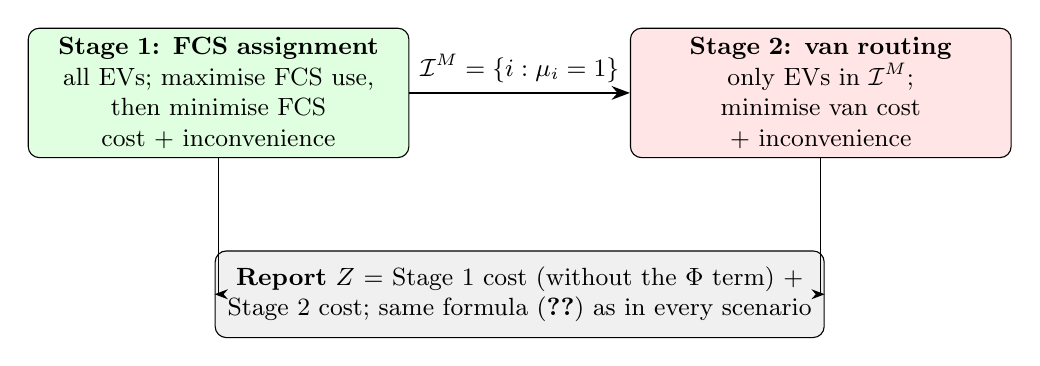
\begin{tikzpicture}[>=Stealth,box/.style={draw,rounded corners,align=center,minimum height=1.1cm,font=\small}]
  \node[box,fill=green!12,text width=4.6cm] (s1) {\textbf{Stage 1: FCS assignment}\\all EVs; maximise FCS use,\\then minimise FCS cost + inconvenience};
  \node[box,fill=red!10,text width=4.6cm,right=2.8cm of s1] (s2) {\textbf{Stage 2: van routing}\\only EVs in $\I^M$;\\minimise van cost + inconvenience};
  \draw[->,thick] (s1) -- node[above,font=\small]{$\I^M=\{i:\mu_i=1\}$} (s2);
  \node[box,fill=black!6,text width=7.5cm,below=2.0cm of $(s1)!0.5!(s2)$] (ev) {\textbf{Report} $Z=$ Stage~1 cost (without the $\Phi$ term) $+$ Stage~2 cost; same formula \eqref{eq:Z} as in every scenario};
  \draw[->] (s1) |- (ev); \draw[->] (s2) |- (ev);
\end{tikzpicture}
\end{center}

Stage~1 does not look at the vans, and Stage~2 cannot change what Stage~1 decided. That is the definition of ``FCS first, then MCS''.

%----------------------------------------------------------------
\subsection{Stage 1: assign EVs to fixed stations}

\textbf{Objective.}
\begin{equation}
\begin{split}
\min\ Z^{(1)}=\;&\underbrace{\Phi\sum_{i\in\I}\mu_i}_{\text{FCS first}}
+\underbrace{c^{EV}\sum_i\sum_{f\in\F_i}d_{if}Y_{if}}_{Z_1}
+\underbrace{Z^F_{\text{energy}}}_{\text{FCS part of }Z_4}\\
&+\underbrace{\sum_i\sum_{f\in\F_i}\rho^F_{if}Y_{if}+\alpha\sum_i w_i(C_i-r_i)+c^L\sum_i w_iL_i}_{\text{FCS customers' inconvenience}}
\end{split}
\label{eq:obj1}
\end{equation}
with $C_i=S_i+\tau^F_iY_i$ in this stage. $\Phi$ is a penalty for handing an EV to the vans. It is chosen larger than anything an extra FCS customer can add to the rest of \eqref{eq:obj1}, e.g.
\[
\Phi > \max_{i}\max_{f\in\F_i}\big(c^{EV}d_{if}+\pi^{\max}E_i+\rho^F_{if}\big)+n\,(\alpha+c^L)\,w_{\max}\,T,
\]
so Stage~1 first \textbf{maximises the number of EVs served at an FCS}, and only among those solutions minimises FCS cost and inconvenience. ($\pi^{\max}$ is the highest grid price.) A numerically safer equivalent is to solve twice: first $\max\sum_iY_i$, then fix that number and minimise the rest.
\ifTOU
Because $Z^F_{\text{energy}}$ uses the peak price, Stage~1 may \emph{start sessions later} to leave the peak, if the price saving beats the extra waiting cost (Section~\ref{sec:expect}).
\fi

\textbf{Constraints.}
\begin{align}
\sum_{g\in\G_i}y_{ig}+\mu_i &= 1 && \forall i\in\I \label{eq:s1assign}\\
S_i &\ge r_i+\sum_{f\in\F_i}t_{if}Y_{if} && \forall i\in\I \label{eq:fcsarr}\\
S_i &\le r_i+T\,(1-\mu_i) && \forall i\in\I \label{eq:s1park}\\
S_j &\ge S_i+\tau^F_i-(T+\tau^F_i)(3-y_{ig}-y_{jg}-o_{ij}) && \forall g,\ (i,j)\in\mathcal{P}_g \label{eq:disj1}\\
S_i &\ge S_j+\tau^F_j-(T+\tau^F_j)(2-y_{ig}-y_{jg}+o_{ij}) && \forall g,\ (i,j)\in\mathcal{P}_g \label{eq:disj2}\\
\sum_i y_{ig_1} &\ge \sum_i y_{ig_2} && \forall f,\ \G_f=\{g_1,g_2\} \label{eq:gunsym}\\
S_i+\tau^F_iY_i &\le T,\qquad L_i\ge S_i+\tau^F_iY_i-l_i && \forall i\in\I \label{eq:s1time}
\end{align}
\ifTOU plus the time-of-use split \eqref{eq:tou1}--\eqref{eq:tou5} of each FCS session (Section~\ref{sec:price}).\fi
\desc{\eqref{eq:s1assign}: every EV either gets one reachable gun or is handed to the vans. An EV that reaches no FCS ($\G_i=\emptyset$) is forced to $\mu_i=1$. \eqref{eq:fcsarr}: an FCS session cannot start before the EV has asked and driven to the station. \eqref{eq:s1park}: for an EV handed to the vans, $S_i$ is parked at $r_i$, so it adds no waiting in Stage~1 (its real start time is decided in Stage~2). \eqref{eq:disj1}--\eqref{eq:disj2}: two EVs on the same gun do not overlap; $o_{ij}$ picks who goes first. With two guns per station this means at most two EVs charge at a station at a time. \eqref{eq:gunsym}: symmetry breaking between the two identical guns (optional). \eqref{eq:s1time}: finished by $T$; lateness.}

\textbf{Optional acceptability rule.} An operator may refuse to send a driver to a station that is ``too inconvenient'', e.g.\ only allow gun $g$ of station $f$ for EV $i$ if $\hat\rho^F_{if}\le\bar\rho$. This only shrinks $\G_i$, so EVs whose stations are all too far go to the vans. Report results with and without it.

\textbf{Output:} $\I^M=\{i:\mu_i=1\}$, the EVs left for the vans; plus each FCS customer's gun and start time.

%----------------------------------------------------------------
\subsection{Stage 2: route the vans to the leftover EVs}

Stage~2 is a vehicle routing problem with time windows, on the EVs in $\I^M$ only. Here $C_i=S_i+\tau^M_i$.

\textbf{Objective.}
\begin{equation}
\begin{split}
\min\ Z^{(2)}=\;&\underbrace{c^M\sum_m\sum_{(i,j)\in\A^M}d_{ij}x_{ijm}}_{Z_2}+\underbrace{\sum_m c^D_mu_m}_{Z_3}+\underbrace{Z^M_{\text{energy}}}_{\text{van part of }Z_4}\\
&+\underbrace{\sum_{i\in\I^M}\sum_m\rho^M_{im}z_{im}+\alpha\sum_{i\in\I^M}w_i(C_i-r_i)+c^L\sum_{i\in\I^M}w_iL_i}_{\text{van customers' inconvenience}}
\end{split}
\label{eq:obj2}
\end{equation}
Since every EV in $\I^M$ must be served by some van, $Z^M_{\text{energy}}$ and the $\rho^M$ term are constants here. They are kept so that $Z^{(2)}$ is the true cost of Stage~2. Waiting and lateness make the vans visit urgent EVs early.

\textbf{Constraints.}
\begin{align}
\sum_{m\in\M}z_{im} &= 1 && \forall i\in\I^M \label{eq:s2assign}\\
\sum_{j:(0,j)\in\A^M}x_{0jm} = \sum_{i:(i,n+1)\in\A^M}x_{i,n+1,m} &= u_m && \forall m \label{eq:depot}\\
\sum_{i:(i,j)\in\A^M}x_{ijm} = \sum_{k:(j,k)\in\A^M}x_{jkm} &= z_{jm} && \forall j\in\I^M,\ m \label{eq:flow}\\
\sum_{i\in\I^M}z_{im} &\le Q_m\,u_m && \forall m \label{eq:cap}\\
\sum_{i\in\I^M}\frac{E_i}{\eta}z_{im}+\beta\sum_{(i,j)\in\A^M}d_{ij}x_{ijm} &\le B_m\,u_m && \forall m \label{eq:batt}
\end{align}
\begin{align}
S_j &\ge \max\{r_j,\ t_{0j}\,x_{0jm}\} && \forall j\in\I^M,\ m \label{eq:depart}\\
S_j &\ge S_i+\tau^M_i+t_{ij}-(T+\tau^M_i+t_{ij})(1-x_{ijm}) && \forall i\neq j,\ m \label{eq:seq}\\
S_i+\tau^M_i+t_{i,n+1} &\le T+(\tau^M_i+t_{i,n+1})(1-x_{i,n+1,m}) && \forall i,\ m \label{eq:return}\\
S_i+\tau^M_i \le T,\quad L_i &\ge S_i+\tau^M_i-l_i && \forall i\in\I^M \label{eq:s2time}\\
u_m &\ge u_{m+1} && m<|\M| \label{eq:vansym}
\end{align}
\desc{\eqref{eq:s2assign}: each leftover EV gets one van. \eqref{eq:depot}: a used van leaves and returns to the depot once. \eqref{eq:flow}: each EV on van $m$ is entered and left exactly once by that van. \eqref{eq:cap}: at most $Q_m$ EVs per van. \eqref{eq:batt}: delivered energy (with transfer losses) plus driving energy fits in the van battery. \eqref{eq:depart}: no start before the request, or before the van can drive there from the depot (written as two linear constraints). \eqref{eq:seq}: if the van goes $i\to j$, it finishes $i$ and drives to $j$ before starting $j$. This gives one EV at a time and removes subtours (MTZ-type). \eqref{eq:return}: back at the depot by $T$. \eqref{eq:s2time}: finished by $T$; lateness. \eqref{eq:vansym}: use identical vans in index order.}

\textbf{If Stage 2 is infeasible} (too many leftover EVs for the fleet by $T$), the sequential policy has \emph{failed} on that instance. For diagnosis, add $s_i\in\{0,1\}$ (``unserved''), replace \eqref{eq:s2assign} by $\sum_mz_{im}+s_i=1$ and add $\Phi^U\sum_is_i$ to \eqref{eq:obj2}. Then report the number of EVs that could not be served. This is a useful comparison with the integrated scenario, which may serve all of them.

%----------------------------------------------------------------
\subsection{Reported value}
\[
Z^{\text{S\scen}}=\big(Z^{(1)*}-\Phi\,|\I^M|\big)+Z^{(2)*},
\]
which is exactly \eqref{eq:Z} evaluated at the combined solution. The stage-1 solution plus the stage-2 solution is a feasible solution of the integrated model (S\ifTOU 4\else 3\fi), so
$Z^{\text{S\ifTOU 4\else 3\fi}}\le Z^{\text{S\scen}}$. The difference is the \emph{value of integration}.

\else
%---------------------------------------------------------------- INT
\subsection{Objective}
\begin{equation}
\min\ Z \quad\text{as in \eqref{eq:Z}, with }Z^F_{\text{energy}}=\ifTOU P^F\textstyle\sum_i\big[\pi^\off(\theta^1_i+\theta^3_i)+\pi^\pk\theta^2_i\big]\else\pi^F\textstyle\sum_iE_iY_i\fi,\quad C_i=S_i+\tau^F_iY_i+\tau^M_iZ_i. \label{eq:objint}
\end{equation}
Written out in full:
\begin{align*}
\min\ Z=\;& c^{EV}\sum_i\sum_{f\in\F_i}d_{if}Y_{if}+c^M\sum_m\sum_{(i,j)\in\A}d_{ij}x_{ijm}+\sum_mc^D_mu_m\\
&+\ifTOU P^F\sum_i\big[\pi^\off(\theta^1_i+\theta^3_i)+\pi^\pk\theta^2_i\big]\else\pi^F\sum_iE_iY_i\fi
+\pi^M\sum_i\sum_m\frac{E_i}{\eta}z_{im}\\
&+\sum_i\sum_{f\in\F_i}\rho^F_{if}Y_{if}+\sum_i\sum_m\rho^M_{im}z_{im}+\alpha\sum_iw_i(C_i-r_i)+c^L\sum_iw_iL_i .
\end{align*}
Every term is linear. One model weighs everything at once: an EV goes to a van exactly when the van's extra km, dispatch and energy cost are outweighed by the effort and waiting it saves the driver\ifTOU, or by the peak-price energy it avoids\fi.

\subsection{Constraints}

\textbf{Assignment.}
\begin{equation}
\sum_{g\in\G_i}y_{ig}+\sum_{m\in\M}z_{im}=1\qquad\forall i\in\I \label{eq:assign}
\end{equation}
\desc{Exactly one resource per EV: one reachable gun or one van. EVs that reach no FCS are forced onto a van.}

\textbf{Fixed stations.}
\begin{align}
S_i &\ge r_i+\sum_{f\in\F_i}t_{if}Y_{if} && \forall i \label{eq:fcsarr}\\
S_j &\ge S_i+\tau^F_i-(T+\tau^F_i)(3-y_{ig}-y_{jg}-o_{ij}) && \forall g,\ (i,j)\in\mathcal{P}_g \label{eq:disj1}\\
S_i &\ge S_j+\tau^F_j-(T+\tau^F_j)(2-y_{ig}-y_{jg}+o_{ij}) && \forall g,\ (i,j)\in\mathcal{P}_g \label{eq:disj2}\\
\sum_iy_{ig_1} &\ge \sum_iy_{ig_2} && \forall f,\ \G_f=\{g_1,g_2\} \label{eq:gunsym}
\end{align}
\desc{\eqref{eq:fcsarr}: an FCS session starts after the request and the drive to the station (for a van customer this is just $S_i\ge r_i$). \eqref{eq:disj1}--\eqref{eq:disj2}: EVs on the same gun do not overlap; $o_{ij}$ chooses the order. \eqref{eq:gunsym}: optional symmetry breaking.}

\textbf{Vans: routes, capacity, battery.}
\begin{align}
\sum_{j:(0,j)\in\A}x_{0jm}=\sum_{i:(i,n+1)\in\A}x_{i,n+1,m} &= u_m && \forall m \label{eq:depot}\\
\sum_{i:(i,j)\in\A}x_{ijm}=\sum_{k:(j,k)\in\A}x_{jkm} &= z_{jm} && \forall j\in\I,\ m \label{eq:flow}\\
\sum_iz_{im} &\le Q_mu_m && \forall m \label{eq:cap}\\
\sum_i\frac{E_i}{\eta}z_{im}+\beta\sum_{(i,j)\in\A}d_{ij}x_{ijm} &\le B_mu_m && \forall m \label{eq:batt}
\end{align}
\desc{\eqref{eq:depot}: a used van leaves and returns once. \eqref{eq:flow}: each EV on van $m$ is visited exactly once by it. \eqref{eq:cap}: at most $Q_m$ EVs. \eqref{eq:batt}: delivered energy (with losses) plus driving energy fits in the battery.}

\textbf{Vans: timing (one EV at a time, no subtours).}
\begin{align}
S_j &\ge t_{0j}\,x_{0jm} && \forall j\in\I,\ m \label{eq:depart}\\
S_j &\ge S_i+\tau^M_i+t_{ij}-(T+\tau^M_i+t_{ij})(1-x_{ijm}) && \forall i\neq j\in\I,\ m \label{eq:seq}\\
S_i+\tau^M_i+t_{i,n+1} &\le T+(\tau^M_i+t_{i,n+1})(1-x_{i,n+1,m}) && \forall i,\ m \label{eq:return}
\end{align}
\desc{\eqref{eq:depart}: the first stop cannot start before the van has driven there. \eqref{eq:seq}: $i\to j$ means finish $i$, drive, then start $j$; start times rise along a route, so no subtour can close. \eqref{eq:return}: back at the depot by $T$.}

\textbf{Horizon and lateness.}
\begin{equation}
C_i\le T,\qquad L_i\ge C_i-l_i\qquad\forall i\in\I \label{eq:time}
\end{equation}
\desc{Every EV is fully charged within the horizon; $L_i$ measures lateness.}

\ifTOU
\textbf{Time-of-use split.} Constraints \eqref{eq:tou1}--\eqref{eq:tou5} of Section~\ref{sec:price}.
\fi

\textbf{Symmetry and domains.}
\begin{equation}
u_m\ge u_{m+1};\qquad y,z,x,u,o\ifTOU,\kappa\fi\in\{0,1\};\qquad S_i,L_i\ifTOU,\theta^p_i\fi\ge0 \label{eq:dom}
\end{equation}
\fi

%=====================================================================
\section{Learning-to-optimise (RL) formulation}\label{sec:rl}

\textbf{Main rule:} the reward of each action is \emph{minus the increase in $Z$ that the action causes}. The rewards over an episode then add up to $-Z$ of the solution the policy builds. RL and MILP results are measured on the same yardstick \eqref{eq:Z}, and the MILP optimum is the benchmark for the RL gap.

\ifSEQ
%---------------------------------------------------------------- RL SEQ
The RL pipeline has the same two stages as the MILP.

\subsection{Stage 1 policy: FCS assignment}
\begin{itemize}[leftmargin=1.4em,itemsep=2pt]
  \item \textbf{Episode / epochs:} EVs are taken in order of request time $r_i$ (ties: higher $w_i$ first). One decision per EV.
  \item \textbf{State:} features of the current EV $k$ ($E_k,r_k,l_k,w_k,R_k$, location); for each gun $g$ the time $F_g$ it becomes free; summary features of the EVs still to come (count and positions near each station)\ifTOU; the current price and the time until $T_1$ and $T_2$\fi.
  \item \textbf{Action:} a gun $g\in\G_k$, or ``hand to vans''. \textbf{FCS-first mask:} ``hand to vans'' is allowed \emph{only} if no gun can finish EV $k$ by $T$ (or, with the optional rule, if all remaining guns have $\hat\rho^F_{kf}>\bar\rho$).
  \ifTOU\item \textbf{Optional timing action:} ``gun $g$, start after the peak'', i.e.\ $S_k=\max\{\text{earliest},T_2\}$, allowed only if the session still ends by $T$.\fi
  \item \textbf{Transition:} $S_k=\max\{r_k+t_{kf},F_g\}$ (or later, for the timing action); $F_g\leftarrow S_k+\tau^F_k$.
  \item \textbf{Reward:} $-\Big[c^{EV}d_{kf}+\text{energy}_k+\rho^F_{kf}+\alpha w_k(S_k+\tau^F_k-r_k)+c^Lw_k(S_k+\tau^F_k-l_k)^+\Big]$, where energy$_k$ = \ifTOU$P^F\big[\pi^\off\cdot(\text{off-peak hours of }[S_k,S_k+\tau^F_k])+\pi^\pk\cdot(\text{peak hours})\big]$, computed exactly in the simulator\else$\pi^FE_k$\fi. Handing an EV to the vans gives reward $0$ here; its cost is counted in Stage~2.
\end{itemize}
Note: a simple baseline for Stage~1 is the greedy rule ``gun with the largest one-step reward''. What RL can learn on top of this is, for example, to keep a nearby gun free for an urgent EV that arrives later.

\subsection{Stage 2 policy: van routing over $\I^M$}
\begin{itemize}[leftmargin=1.4em,itemsep=2pt]
  \item \textbf{Epochs:} whenever a van becomes free (the earliest-free van decides first).
  \item \textbf{State:} for each van: position, time free, remaining battery $b_m$, EVs served so far, dispatched or not; for each unserved EV in $\I^M$: location, $E_i,r_i,l_i,w_i$; current time.
  \item \textbf{Action:} the next EV $j$ for this van, or ``return to depot'' (ends the route). Mask: $j$ must be feasible: battery covers $E_j/\eta$ plus driving to $j$ and back to the depot, the count stays $\le Q_m$, and $j$ can be finished with the van back at the depot by $T$.
  \item \textbf{Transition:} $S_j=\max\{r_j,\ \text{time free}+t_{\text{pos},j}\}$; the van moves to $j$ and is free at $S_j+\tau^M_j$; $b_m$ falls by $E_j/\eta+\beta d_{\text{pos},j}$.
  \item \textbf{Reward:} serving $j$: $-\Big[c^Md_{\text{pos},j}+c^D_m[\text{first stop}]+\pi^M\frac{E_j}{\eta}+\rho^M_{jm}+\alpha w_j(S_j+\tau^M_j-r_j)+c^Lw_j(S_j+\tau^M_j-l_j)^+\Big]$; returning: $-c^Md_{\text{pos},0}$. EVs still unserved at the end: $-\Phi^U$ each.
  \item \textbf{Policy:} an attention-based routing policy (e.g.\ Kool et al., 2019, ``Attention, Learn to Solve Routing Problems!'') trained with REINFORCE or PPO. Baseline: nearest-feasible-EV heuristic.
\end{itemize}
Episode return of Stage~1 + Stage~2 $=-Z^{\text{S\scen}}$.

\else
%---------------------------------------------------------------- RL INT
One policy decides both who serves each EV and the van routes.
\begin{itemize}[leftmargin=1.4em,itemsep=2pt]
  \item \textbf{Episode / epochs:} EVs are taken in order of request time $r_i$ (ties: higher $w_i$ first). One decision per EV.
  \item \textbf{State:} (i) the current EV $k$: location, $E_k,r_k,l_k,w_k,R_k$, reachable stations; (ii) each gun $g$: time $F_g$ it becomes free; (iii) each van $m$: current end-of-route position, time free, remaining battery $b_m$, EVs served, dispatched or not; (iv) embeddings of the not-yet-assigned EVs (for look-ahead)\ifTOU; (v) current price, time until $T_1$ and $T_2$\fi.
  \item \textbf{Action:} $a\in\G_k\cup\M$: a gun, or a van (EV $k$ is appended to the end of that van's route). \textbf{Mask} infeasible actions: a gun that cannot finish $k$ by $T$; a van without enough battery for $E_k/\eta$ plus the drive to $k$ and back to the depot, with $Q_m$ reached, or unable to finish $k$ and return by $T$.
  \ifTOU\item \textbf{Optional timing action:} ``gun $g$, start after the peak'' ($S_k=\max\{\text{earliest},T_2\}$, if it still ends by $T$).\fi
  \item \textbf{Transition:} gun: $S_k=\max\{r_k+t_{kf},F_g\}$, $F_g\leftarrow S_k+\tau^F_k$. Van: $S_k=\max\{r_k,\ \text{free}_m+t_{\text{pos}_m,k}\}$, then the van moves to $k$, $\text{free}_m\leftarrow S_k+\tau^M_k$, $b_m\mathrel{-}=E_k/\eta+\beta d_{\text{pos}_m,k}$.
  \item \textbf{Reward} $=-\Delta Z$:
  \begin{align*}
  \text{gun } g\text{ at }f:&\quad -\Big[c^{EV}d_{kf}+\text{energy}^F_k+\rho^F_{kf}+\alpha w_k(C_k-r_k)+c^Lw_k(C_k-l_k)^+\Big]\\
  \text{van } m:&\quad -\Big[c^M\big(d_{\text{pos}_m,k}+d_{k,0}-d_{\text{pos}_m,0}\big)+c^D_m[\text{first use}]+\pi^M\tfrac{E_k}{\eta}\\
  &\qquad\quad+\rho^M_{km}+\alpha w_k(C_k-r_k)+c^Lw_k(C_k-l_k)^+\Big]
  \end{align*}
  The van distance term is the \emph{change} in route length when $k$ is inserted before the return to the depot, so the sum over the episode equals the total route length (the return legs telescope). energy$^F_k$ = \ifTOU$P^F\big[\pi^\off\cdot(\text{off-peak hours})+\pi^\pk\cdot(\text{peak hours of }[S_k,C_k])\big]$, computed exactly by the simulator; no linearisation is needed in RL\else$\pi^FE_k$\fi.
  \item \textbf{Dead end:} if every action is masked, EV $k$ is unserved: reward $-\Phi^U$, and the episode continues. Report the count.
  \item \textbf{Policy:} masked categorical policy over guns and vans, encoder with attention over EVs, guns and vans; trained with PPO. Natural baseline: greedy, i.e.\ choose the action with the largest one-step reward. That is the pairwise rule ``smallest $\hat\rho$ + cost'' from Section~\ref{sec:inc}.
\end{itemize}
Restriction to note: vans serve EVs in assignment order (append only). A variant that inserts $k$ at the cheapest position of a route is more flexible but has a larger action space.
\fi

\textbf{Reward scaling.} For stable training divide every reward by a constant, e.g.\ the greedy baseline's average $Z$ on the training instances. This does not change the optimal policy.

%=====================================================================
\section{What to expect and what to report}\label{sec:expect}

\ifnum\scen=1
\begin{itemize}[leftmargin=1.4em,itemsep=2pt]
  \item Vans serve only EVs that reach no station, or that the stations cannot finish by $T$. If stations have spare capacity, very few vans are dispatched.
  \item Inconvenience is high for EVs far from the nearest station (worked example: Rs\,682 at the FCS, against Rs\,458 if a van had been allowed).
  \item With too few vans Stage~2 becomes infeasible (unserved EVs), even when the integrated model S3 could serve everyone. Report the smallest $|\M|$ at which S1 is feasible and compare it with S3.
\end{itemize}
\fi
\ifnum\scen=2
\begin{itemize}[leftmargin=1.4em,itemsep=2pt]
  \item \textbf{When does Stage~1 delay a session to avoid the peak?} Moving one hour of charging out of the peak saves $(\pi^\pk-\pi^\off)P^F=3\times22=$ Rs\,66, but delays completion by up to an hour, which costs $\alpha w_i\ge$ Rs\,200. So with the default values Stage~1 almost never delays. It mostly pays the higher price, and S2 costs roughly S1 plus the peak surcharge. Sessions start later only if $\alpha$ is small (try $\lambda<0.33$ in the sensitivity analysis).
  \item The van assignment is the same as in S1 unless Stage~1's timing changes which EVs fit at the stations. Stage~1 cannot use vans to escape the peak price.
  \item Extra KPI: \textbf{grid energy drawn at FCS during the peak}, $P^F\sum_i\theta^2_i$ (kWh). Compare with S4.
\end{itemize}
\fi
\ifnum\scen=3
\begin{itemize}[leftmargin=1.4em,itemsep=2pt]
  \item Vans take EVs for which the saved inconvenience exceeds the extra van cost (worked example: van chosen, saving Rs\,224). Expect vans to serve EVs that are far from every station, have low range (high $w_i$), or have early deadlines, while EVs near a station still use it.
  \item \textbf{Value of integration under flat price:} $Z^{\text{S1}}-Z^{\text{S3}}\ge0$. Report it per component ($Z_1,\dots,Z_5$): typically operating cost rises a little and inconvenience falls a lot.
  \item Vary $|\M|$ (0, 1, 2, \dots): the first few vans lower $Z$ sharply, then the effect levels off. That curve shows the scenarios where mobile chargers help most.
\end{itemize}
\fi
\ifnum\scen=4
\begin{itemize}[leftmargin=1.4em,itemsep=2pt]
  \item During the peak a van kWh costs about the same as an FCS kWh (Rs\,10.0 each), so the vans' energy disadvantage disappears and vans also absorb \emph{peak-hour} demand that would otherwise be charged on the grid at peak price.
  \item Expect more van usage than in S3, concentrated on requests in $[T_1,T_2]$, and lower grid energy at the stations during the peak, $P^F\sum_i\theta^2_i$, than in S2.
  \item \textbf{Value of integration under peak pricing:} $Z^{\text{S2}}-Z^{\text{S4}}$. It should be larger than $Z^{\text{S1}}-Z^{\text{S3}}$, because integration now also allows price arbitrage.
  \item \textbf{Peak pricing with full flexibility:} $Z^{\text{S4}}-Z^{\text{S3}}$ should be smaller than $Z^{\text{S2}}-Z^{\text{S1}}$: vans cushion the price increase.
\end{itemize}
\fi

\textbf{Cross-scenario comparison table} (fill in from the four runs):
\begin{center}
\renewcommand{\arraystretch}{1.2}
\begin{tabular}{@{}lll@{}}
\toprule
\textbf{Comparison} & \textbf{Measures} & \textbf{Expected sign} \\
\midrule
S1 $-$ S3 & value of integration, flat price & $\ge0$ \\
S2 $-$ S4 & value of integration, peak price & $\ge0$, larger than S1 $-$ S3 \\
S2 $-$ S1 & cost of peak pricing, FCS-first operator & $>0$ \\
S4 $-$ S3 & cost of peak pricing, flexible operator & $>0$, smaller than S2 $-$ S1 \\
\bottomrule
\end{tabular}
\end{center}
Report for each: $Z$ and its components, number of vans used, EVs per resource, mean and maximum inconvenience per EV, total lateness, peak-hour grid energy, solve time, and (for RL) the gap to the MILP optimum.

%=====================================================================
\appendix
\section{Illustrative parameter values}\label{app:values}

These are starting values for experiments, not data. All are meant to be varied in the analysis. Values in Rs.

\begin{center}
\renewcommand{\arraystretch}{1.15}
\begin{tabular}{@{}llp{6.2cm}@{}}
\toprule
\textbf{Parameter} & \textbf{Value} & \textbf{Note} \\
\midrule
$T$, $[T_1,T_2]$ & 7 h, $[2,6]$ & 16:00--23:00, peak 18:00--22:00 \\
$P^F$, $P^M$ & 22 kW, 30 kW & \\
$v$, $\beta$, $\eta$ & 25 km/h, 0.25 kWh/km, 0.9 & \\
$B_m$, $Q_m$, $|\M|$ & 150 kWh, 6, 2--6 & \\
$c^{EV}$, $c^M$, $c^D_m$ & Rs\,4/km, Rs\,15/km, Rs\,1500 & van km includes driver time \\
$\pi^F$ (flat) & Rs\,8.7/kWh & equals the time-average of the ToU tariff over $[0,T]$ \\
$\pi^\off$, $\pi^\pk$ (ToU) & Rs\,7/kWh, Rs\,10/kWh & $(3\times7+4\times10)/7=8.7$ \\
$c^{bat}$ & Rs\,2/kWh & van battery wear \\
$\pi^M$ & Rs\,10.7 (flat) / Rs\,9.0 (ToU) & $=\pi^F+c^{bat}$ / $=\pi^\off+c^{bat}$ \\
$\alpha$, $\alpha^D$ & Rs\,200/h, Rs\,100/h & value of time; extra for attended time \\
$h^F$, $h^M$, $\varphi$ & Rs\,50, Rs\,10, Rs\,100 & trip hassle, hand-over, range stress \\
$c^L$ & Rs\,300/h & lateness \\
$w_i$ & $1+2(1-R_i/R_{\max})$, $R_i\sim U[3,40]$ km & priority from remaining range \\
\bottomrule
\end{tabular}
\end{center}

The flat price is set to the time-average of the peak tariff. The price \emph{level} is then the same in both pricing cases, and only the price \emph{shape} differs. Without this, part of S1 vs S2 would just reflect a different average price.

\end{document}
"
%    pdflatex -jobname=scenario3_flat_integrated   "\def\scen{3}% =====================================================================
%  One source, four PDFs.  Build with build.sh (or by hand):
%    pdflatex -jobname=scenario1_flat_sequential   "\def\scen{1}\input{scenario_master}"
%    pdflatex -jobname=scenario2_peak_sequential   "\def\scen{2}\input{scenario_master}"
%    pdflatex -jobname=scenario3_flat_integrated   "\def\scen{3}\input{scenario_master}"
%    pdflatex -jobname=scenario4_peak_integrated   "\def\scen{4}\input{scenario_master}"
%  (run each twice for cross-references)
% =====================================================================
\documentclass[11pt,a4paper]{article}
\usepackage[margin=2.2cm]{geometry}
\usepackage{amsmath,amssymb,amsfonts}
\usepackage{booktabs,array,tabularx}
\usepackage{enumitem}
\usepackage[table]{xcolor}
\usepackage{tikz}
\usetikzlibrary{arrows.meta,positioning,calc}
\usepackage[colorlinks=true,linkcolor=blue!50!black,urlcolor=blue!50!black]{hyperref}
\usepackage{titlesec}
\titleformat{\section}{\large\bfseries}{\thesection}{0.8em}{}
\titleformat{\subsection}{\normalsize\bfseries}{\thesubsection}{0.8em}{}
\setlength{\parindent}{0pt}
\setlength{\parskip}{5pt}

% ---------------- scenario switches ----------------
\ifdefined\scen\else\def\scen{1}\fi
\newif\ifTOU \TOUfalse   % true = time-of-use (peak) price
\newif\ifSEQ \SEQfalse   % true = FCS first, then MCS
\ifnum\scen=1 \SEQtrue \fi
\ifnum\scen=2 \TOUtrue \SEQtrue \fi
\ifnum\scen=4 \TOUtrue \fi

\newcommand{\pricename}{\ifTOU time-of-use price (dearer evening peak)\else single (flat) price all day\fi}
\newcommand{\structname}{\ifSEQ FCS first, then MCS (sequential)\else FCS and MCS together (integrated)\fi}

% ---------------- notation ----------------
\newcommand{\I}{\mathcal{I}}
\newcommand{\F}{\mathcal{F}}
\newcommand{\G}{\mathcal{G}}
\newcommand{\M}{\mathcal{M}}
\newcommand{\N}{\mathcal{N}}
\newcommand{\A}{\mathcal{A}}
\newcommand{\Rs}{\text{Rs}\,}
\newcommand{\pk}{\mathrm{pk}}
\newcommand{\off}{\mathrm{off}}
\newcommand{\desc}[1]{\par\vspace{-2pt}{\small\color{black!75}\textit{Meaning:} #1}\par\vspace{4pt}}
\newcommand{\cell}[2]{\ifnum\scen=#1\cellcolor{blue!18}\textbf{S#1 (this document)}\\\textbf{#2}\else S#1\\#2\fi}

\title{\textbf{EV Charging Network Optimisation}\\[4pt]
\large Scenario \scen: \pricename\ $+$ \structname\\[2pt]
\normalsize MILP and RL formulation}
\author{CP 320 OR for Mobility Management, course project}
\date{2 October 2026}

\begin{document}
\maketitle

%=====================================================================
\section{Where this scenario sits}

The project studies four scenarios: two ways of pricing grid electricity, times two ways of making the decisions.

\begin{center}
\renewcommand{\arraystretch}{1.5}
\begin{tabular}{>{\raggedright\arraybackslash}p{4.2cm}|>{\centering\arraybackslash}p{4.6cm}|>{\centering\arraybackslash}p{4.6cm}}
 & \textbf{Flat price all day} & \textbf{Time-of-use (peak) price} \\ \hline
\textbf{Sequential:} FCS first, leftover EVs to MCS &
\begin{tabular}[c]{@{}c@{}}\cell{1}{flat + sequential}\end{tabular} &
\begin{tabular}[c]{@{}c@{}}\cell{2}{peak + sequential}\end{tabular} \\ \hline
\textbf{Integrated:} FCS and MCS decided together &
\begin{tabular}[c]{@{}c@{}}\cell{3}{flat + integrated}\end{tabular} &
\begin{tabular}[c]{@{}c@{}}\cell{4}{peak + integrated}\end{tabular} \\
\end{tabular}
\end{center}

\textbf{The four scenarios do not have four different objectives.} They share \emph{one} cost yardstick $Z$ (Section~\ref{sec:obj}): the same cost terms and the same customer inconvenience (Section~\ref{sec:inc}). Only two things change:
\begin{itemize}[leftmargin=1.4em,itemsep=1pt]
  \item \textbf{Pricing} changes the formula for one term, the FCS energy cost (Section~\ref{sec:price}).
  \item \textbf{Decision structure} changes \emph{how} $Z$ is minimised: in one model (integrated), or in two stages (sequential), where each stage minimises its own part of $Z$.
\end{itemize}
Because the yardstick is the same, the four optimal values can be compared directly. The differences measure the \emph{value of integration} (S1$\to$S3, S2$\to$S4) and the \emph{effect of peak pricing} (S1$\to$S2, S3$\to$S4).

\ifnum\scen=1
\textbf{This scenario (S1)} is the baseline, the ``status quo''. Electricity costs the same at every hour, every EV that can be charged at a fixed station is sent there, and vans only take what is left over.
\fi
\ifnum\scen=2
\textbf{This scenario (S2)} keeps the FCS-first rule of S1, but grid electricity is dearer during the evening peak. Stage~1 can react to the price only by \emph{rescheduling} FCS sessions. It cannot hand a peak-hour EV to a van.
\fi
\ifnum\scen=3
\textbf{This scenario (S3)} keeps the flat price of S1, but the operator decides FCS and MCS service \emph{together}. An EV can be sent to a van even when a fixed station could take it, whenever that lowers total cost plus inconvenience.
\fi
\ifnum\scen=4
\textbf{This scenario (S4)} is the most flexible one: peak pricing at fixed stations, and FCS and MCS decided together. Van energy was bought off-peak, so vans can also be used to keep charging \emph{out of the expensive peak}.
\fi

%=====================================================================
\section{Setting and assumptions}\label{sec:setting}

\textbf{Time.} The planning horizon is $[0,T]$ with $T=7$\,h (16:00--23:00). It contains the evening peak window $[T_1,T_2]=[2,6]$ (18:00--22:00). The horizon is the same in all four scenarios. It is wider than the peak itself so that, under peak pricing, there is cheaper time on both sides of the peak.\ifTOU\else\ In this scenario the price is flat, so the window plays no role in the model.\fi

\textbf{Assumptions} (the same as MILP v3, plus two about energy):
\begin{enumerate}[leftmargin=1.6em,itemsep=1pt]
  \item Static, continuous time. All requests in the horizon are known at time $0$, and request $i$ becomes active at $r_i$.
  \item An EV served by an FCS drives there itself on its own battery (only to stations within its range $R_i$). The driver stays with the car while it waits for a free gun and while it charges.
  \item An EV served by an MCS stays parked where it is, and the driver is free in the meantime.
  \item Each FCS gun and each van charges one EV at a time, without interruption, at constant power.
  \item A van's battery covers both its driving and the energy it delivers. \textbf{The van battery is charged at the depot before the horizon starts}\ifTOU, i.e.\ at the off-peak price\fi, and is not recharged during the horizon.
  \item Every EV must be fully charged by $T$ (hard). Finishing after the driver's desired time $l_i$ is allowed but penalised.
\end{enumerate}

%=====================================================================
\section{Notation}\label{sec:notation}

\subsection*{Sets}
\begin{tabularx}{\textwidth}{@{}lX@{}}
\toprule
$\I=\{1,\dots,n\}$ & EV charging requests \\
$\F$; $\G_f$ ($|\G_f|=2$); $\G=\bigcup_f\G_f$ & fixed charging stations; guns of FCS $f$; all guns ($f(g)$ = station of gun $g$) \\
$\F_i=\{f: d_{if}\le R_i\}$, $\G_i=\bigcup_{f\in\F_i}\G_f$ & stations / guns EV $i$ can reach on its remaining range \\
$\M$ & mobile charging vans (MCS) \\
$0,\ n+1$ & depot as start node / end node (same place) \\
$\N=\{0\}\cup\I\cup\{n+1\}$, $\A$ & routing nodes; allowed van arcs $(i,j)$, $i\in\{0\}\cup\I$, $j\in\I\cup\{n+1\}$, $i\neq j$ \\
$\mathcal{P}_g=\{(i,j): i<j,\ g\in\G_i\cap\G_j\}$ & pairs of EVs that could share gun $g$ \\
\ifSEQ
$\I^M\subseteq\I$ & EVs handed to the vans by Stage~1 (an \emph{output} of Stage~1, a fixed input to Stage~2) \\
$\N^M$, $\A^M$ & routing nodes / arcs restricted to $\I^M$ \\
\fi
\bottomrule
\end{tabularx}

\subsection*{Parameters}
\begin{tabularx}{\textwidth}{@{}lX@{}}
\toprule
$E_i,\ r_i,\ l_i,\ R_i$ & energy demand (kWh), request time, desired completion time (h), remaining range (km) \\
$w_i\ge1$ & priority of EV $i$; $w_i=1+\kappa(1-R_i/R_{\max})$, so low-range EVs weigh more \\
$P^F,\ P^M$ & charging power of an FCS gun (22\,kW) / of a van (e.g.\ 30\,kW) \\
$\tau^F_i=E_i/P^F,\ \tau^M_i=E_i/P^M$ & charging time of EV $i$ at an FCS / by a van (h) \\
$d_{if},t_{if}$;\ $d_{ij},t_{ij}$ & distance (km) and time (h): EV$\to$FCS; between routing nodes ($t=d/v$) \\
$B_m,\ Q_m,\ \beta,\ \eta$ & van battery (kWh), max EVs per van, van consumption (kWh/km), transfer efficiency \\
$c^{EV},\ c^M,\ c^D_m$ & cost per km of EV driving, per km of van driving; fixed dispatch cost of van $m$ \\
\ifTOU
$\pi^\off,\ \pi^\pk$ & grid price (Rs/kWh) off-peak / in $[T_1,T_2]$, with $\pi^\pk\ge\pi^\off$ \\
\else
$\pi^F$ & grid price (Rs/kWh), the same at every hour \\
\fi
$c^{bat}$ & van battery wear per kWh cycled \\
$\pi^M$ & cost of 1 kWh taken from a van battery: $\pi^M=\ifTOU\pi^\off\else\pi^F\fi+c^{bat}$ (Section~\ref{sec:price}) \\
$\alpha,\ \alpha^D,\ h^F,\ h^M,\ \varphi,\ c^L$ & inconvenience coefficients (Section~\ref{sec:inc}) \\
\bottomrule
\end{tabularx}

\subsection*{Decision variables}
\begin{tabularx}{\textwidth}{@{}llX@{}}
\toprule
$y_{ig}$ & $\{0,1\}$ & EV $i$ charged at gun $g\in\G_i$ \\
$z_{im}$ & $\{0,1\}$ & EV $i$ served by van $m$ \\
$x_{ijm}$ & $\{0,1\}$ & van $m$ drives arc $(i,j)$ \\
$u_m$ & $\{0,1\}$ & van $m$ is dispatched \\
$o_{ij}$ & $\{0,1\}$ & for EVs $i<j$ that could share a gun: 1 if $i$ is charged before $j$ \\
\ifSEQ
$\mu_i$ & $\{0,1\}$ & Stage~1 only: EV $i$ is handed to the van fleet \\
\fi
\ifTOU
$\theta^1_i,\theta^2_i,\theta^3_i$ & $\ge0$ & hours of EV $i$'s FCS session before / inside / after the peak \\
$\kappa^1_i,\kappa^3_i$ & $\{0,1\}$ & EV $i$'s FCS session starts before $T_1$ / ends after $T_2$ \\
\fi
$S_i$ & $\ge0$ & time charging of EV $i$ starts (h), on whichever resource \\
$L_i$ & $\ge0$ & lateness of EV $i$ beyond $l_i$ (h) \\
\bottomrule
\end{tabularx}

\textbf{Short-hands} (linear expressions, not new variables):
\[
Y_{if}=\sum_{g\in\G_f}y_{ig},\qquad Y_i=\sum_{g\in\G_i}y_{ig}\ (\text{EV $i$ uses an FCS}),\qquad Z_i=\sum_{m\in\M}z_{im}\ (\text{EV $i$ uses a van}),
\]
\[
C_i=S_i+\tau^F_i\,Y_i+\tau^M_i\,Z_i \quad\text{(time EV $i$ is fully charged).}
\]

%=====================================================================
\section{Customer inconvenience}\label{sec:inc}

This section is \textbf{identical in all four scenario documents}. Inconvenience is a property of the customer, not of the price or of the planning method.

\subsection{What we mean by inconvenience}

Inconvenience is \emph{what the driver loses} from the moment they ask for a charge ($r_i$) until the car is fully charged ($C_i$), \emph{converted into rupees} so it can be added to the operator's costs. A driver loses three different things:

\begin{enumerate}[leftmargin=1.6em,itemsep=2pt]
  \item \textbf{Waiting:} the car is not ready. This lasts $C_i-r_i$ hours and affects \emph{every} driver, FCS or MCS.
  \item \textbf{Effort:} only an FCS customer has to drive to the station and sit there while the car charges. An MCS customer stays at home or at work and does something else. Driving to a far station also uses scarce battery range, which causes stress (``range anxiety'').
  \item \textbf{A missed deadline:} the car is still not ready at the time $l_i$ the driver needs it.
\end{enumerate}

Each loss gets a price in Rs per hour (or per event). All of them are multiplied by the priority $w_i$: an hour of delay for an EV with 5\,km of range left counts more than for one with 40\,km.

\subsection{The three components}

\begin{center}
\renewcommand{\arraystretch}{1.3}
\begin{tabularx}{\textwidth}{@{}>{\raggedright\arraybackslash}p{2.6cm}>{\raggedright\arraybackslash}X>{\raggedright\arraybackslash}X>{\raggedright\arraybackslash}p{3.0cm}@{}}
\toprule
\textbf{Component} & \textbf{EV $i$ at FCS $f$} & \textbf{EV $i$ by a van} & \textbf{Known when?} \\
\midrule
Effort & $w_i\big[\alpha^D(t_{if}+\tau^F_i)+h^F+\varphi\,d_{if}/R_i\big]$: driving and sitting at the station, a fixed trip hassle, range stress & $w_i\,h^M$: being reachable and handing over the car & \textbf{Static:} known as soon as the resource is chosen \\
Waiting & $w_i\,\alpha\,(C_i-r_i)$ = drive + \emph{queue at the gun} + charge & $w_i\,\alpha\,(C_i-r_i)$ = \emph{wait for the van} + charge & \textbf{Dynamic:} depends on the queue / van route \\
Missed deadline & $w_i\,c^L\,L_i$, $L_i=\max\{0,C_i-l_i\}$ & same & Dynamic \\
\bottomrule
\end{tabularx}
\end{center}

\textbf{Coefficients.}
$\alpha$ (Rs/h) is the value of an hour the car is not ready.
$\alpha^D$ (Rs/h) is the \emph{extra} value of an hour the driver must personally spend driving or sitting at the station: an hour at the station costs $\alpha+\alpha^D$, an hour waiting at home for a van costs only $\alpha$.
$h^F,h^M$ (Rs) are fixed hassle costs of one trip to a station / one van hand-over.
$\varphi$ (Rs) is the range-stress cost of a trip that uses the \emph{whole} remaining range ($d_{if}/R_i\le1$ is the fraction used).
$c^L$ (Rs/h) is the cost per hour late.

\subsection{Pairwise form: inconvenience of a (customer, resource) pair}

The natural first idea is: \emph{for every pair (EV $i$, FCS $f$) and every pair (EV $i$, van $m$) there is an inconvenience number, and the operator picks the pair with the lowest cost plus inconvenience.} The static part fits this idea exactly:
\[
\boxed{\;\rho^F_{if}=w_i\Big[\alpha^D\,(t_{if}+\tau^F_i)+h^F+\varphi\,\frac{d_{if}}{R_i}\Big]\qquad
\rho^M_{im}=w_i\,h^M\;}
\]
These are \textbf{parameters}, computed before solving, one number per (EV, FCS) pair and per (EV, van) pair. In the objective they appear linearly: $\sum_i\sum_f\rho^F_{if}Y_{if}+\sum_i\sum_m\rho^M_{im}z_{im}$.

Note that $\rho^M_{im}$ does not depend on $m$. Vans are identical and all start at the same depot, so the driver does not care \emph{which} van comes, only \emph{when} it comes. That ``when'' is the waiting part.

\subsection{Why waiting cannot be a fixed pairwise number}

It is tempting to also write the waiting as a pairwise number, e.g.\ ``the van needs 5 minutes to reach EV $i$''. But that depends on \emph{where the van is coming from}, which depends on the route the model is still choosing: if EV $i$ is the 4th stop of a van, the wait is the time for three charging sessions plus four drives. Likewise, waiting at an FCS depends on how many EVs are queued at that gun. So waiting is not known before solving. It is a function of decision variables:
\[
\text{waiting cost of EV } i \;=\; w_i\,\alpha\,(C_i-r_i),\qquad C_i=S_i+\tau^F_iY_i+\tau^M_iZ_i .
\]
This is \textbf{linear} in the variables ($S_i$, $y$, $z$), so it fits in a MILP directly. The constraints of Section~\ref{sec:milp} make $S_i$ equal to the true start time, including driving, queueing at the gun and the van's route. The term $\sum_i w_i\alpha r_i$ is a constant and may be dropped when solving.

\textbf{Pairwise \emph{estimate}} (used for intuition, by the RL policy and in heuristics): if there is no queue and the van comes straight to $i$,
\[
\hat\rho^{F}_{if}=\rho^F_{if}+w_i\alpha\,(t_{if}+\tau^F_i),\qquad
\hat\rho^{M}_{im}=\rho^M_{im}+w_i\alpha\,(t^{\text{van}}_{m\to i}+\tau^M_i),
\]
where $t^{\text{van}}_{m\to i}$ is the time until van $m$ can reach $i$ from where it currently is. In the RL formulation (Section~\ref{sec:rl}) the van's position \emph{is} known at each decision, so there this estimate becomes exact.

\subsection{Total inconvenience and how it enters the objective}

\begin{equation}
\boxed{\;
Z_{\text{inc}}=\underbrace{\sum_{i\in\I}\sum_{f\in\F_i}\rho^F_{if}Y_{if}+\sum_{i\in\I}\sum_{m\in\M}\rho^M_{im}z_{im}}_{\text{effort (static, pairwise)}}
+\underbrace{\alpha\sum_{i\in\I}w_i\,(C_i-r_i)}_{\text{waiting (dynamic)}}
+\underbrace{c^L\sum_{i\in\I}w_i\,L_i}_{\text{missed deadline}}
\;}\label{eq:inc}
\end{equation}
All three parts are in rupees, so $Z_{\text{inc}}$ is simply added to the operating costs. Nothing has to be normalised.

\subsection{Worked example: your ``10 km to the FCS vs.\ van in 5 minutes'' case}

EV $i$: $E_i=20$\,kWh, $R_i=40$\,km (so $w_i=1$); nearest free FCS $d_{if}=10$\,km away, $t_{if}=0.4$\,h at 25\,km/h; a van finishing next door can reach it in 5\,min ($0.083$\,h), adding about 4\,km to its route. $\tau^F_i=20/22=0.909$\,h, $\tau^M_i=20/30=0.667$\,h. Coefficients from Appendix~\ref{app:values}, flat price.

\begin{center}
\renewcommand{\arraystretch}{1.25}
\begin{tabular}{@{}lrr@{}}
\toprule
 & \textbf{FCS} & \textbf{Van} \\
\midrule
Driving (EV / extra van km) & $4\times10=40.0$ & $15\times4=60.0$ \\
Energy & $8.7\times20=174.0$ & $10.7\times20/0.9=237.8$ \\
\textbf{Operating cost only} & \textbf{214.0} & \textbf{297.8} \\
\midrule
Effort $\rho$ & $100(0.4+0.909)+50+100\cdot\tfrac{10}{40}=205.9$ & $10.0$ \\
Waiting $\alpha(C_i-r_i)$ & $200\times1.309=261.8$ & $200\times0.75=150.0$ \\
\textbf{Cost + inconvenience} & \textbf{681.7} & \textbf{457.8} \\
\bottomrule
\end{tabular}
\end{center}

On operating cost alone the FCS is cheaper, so a cost-only model would \emph{always} send this driver 10\,km away. With inconvenience included the van is better by about Rs\,224, and the integrated model chooses $z_{im}=1$, as you expected. If the FCS were only 1\,km away, the FCS would win both comparisons. The inconvenience term is what makes the model choose between ``cheap for the operator'' and ``convenient for the driver'', rather than following a fixed rule.

\subsection{Relation to a single penalty $\rho_i$ per EV}

The first draft used a penalty $\rho_i$ that is charged whenever EV $i$ goes to \emph{any} FCS: $\sum_i\sum_f\rho_iy_{if}$. Because $\sum_f y_{if}=1-\sum_m z_{im}$, this only says ``a van is worth $\rho_i$ more to EV $i$'', and that holds whether the station is 1\,km or 15\,km away, and whether the van arrives in 5 minutes or in 3 hours. The form above fixes both problems: $\rho^F_{if}$ grows with the distance to \emph{that} station, and the waiting term grows with how late the van or the free gun actually is. The old model is the special case $\alpha=\alpha^D=\varphi=c^L=0$, $h^F=\rho_i$.

\subsection{Choosing the coefficients}
\begin{itemize}[leftmargin=1.4em,itemsep=2pt]
  \item Use a value of time for $\alpha$ (e.g.\ Rs\,150--300/h for urban car users), and set $\alpha^D\approx0.5\alpha$: sitting at a station is worse than waiting at home.
  \item Keep $c^L>\alpha$, so missing the deadline is worse than ordinary waiting.
  \item \textbf{Sensitivity analysis:} multiply all inconvenience coefficients by a factor $\lambda\in\{0,0.25,0.5,1,2,4\}$ and plot operating cost against total inconvenience. $\lambda=0$ is the pure cost-minimising operator, and large $\lambda$ is a customer-first operator. This trade-off curve is a strong result for the ``Analysis'' part of the project.
\end{itemize}

\subsection{What inconvenience does in \emph{this} scenario}
\ifSEQ
In a sequential scenario inconvenience \textbf{cannot move an EV from an FCS to a van}: Stage~1 sends every EV that \emph{can} use an FCS to one. It still matters inside each stage. In Stage~1 it decides \emph{which} station and \emph{when} (urgent EVs get the near station and the first free gun). In Stage~2 it decides the \emph{order} in which vans visit EVs (urgent EVs first). In the worked example, this scenario sends the driver 10\,km to the FCS. That is the weakness the integrated scenarios remove.
\else
In an integrated scenario inconvenience is weighed directly against operating cost when choosing the resource. That is how the worked example ends up with a van. It also decides which station and which gun order, and the order of each van route.
\fi

%=====================================================================
\section{Electricity price in this scenario}\label{sec:price}

\textbf{Van energy (same in all scenarios).} A van's battery is charged at the depot \emph{before} the horizon, so its energy was bought at the
\ifTOU off-peak \fi
price, whatever time the van later delivers it. Each kWh taken from the van also wears the battery ($c^{bat}$), and a fraction $1-\eta$ is lost in transfer:
\[
Z^M_{\text{energy}}=\pi^M\sum_{i\in\I}\sum_{m\in\M}\frac{E_i}{\eta}\,z_{im},\qquad \pi^M=\ifTOU\pi^\off\else\pi^F\fi+c^{bat}.
\]

\ifTOU
\textbf{FCS energy (time-of-use).} An FCS draws from the grid while it charges. Energy delivered inside $[T_1,T_2]$ costs $\pi^\pk$, and energy outside it costs $\pi^\off$. A session $[S_i,S_i+\tau^F_i]$ may overlap the peak partly. Split its duration into the hours before, inside and after the peak, $\theta^1_i+\theta^2_i+\theta^3_i$:
\[
Z^F_{\text{energy}}=P^F\sum_{i\in\I}\Big[\pi^\off(\theta^1_i+\theta^3_i)+\pi^\pk\,\theta^2_i\Big].
\]
Constraints \eqref{eq:tou1}--\eqref{eq:tou5} below make the $\theta$'s equal to the true overlaps. Peak hours are dearer, so the solver wants $\theta^1_i,\theta^3_i$ as large as possible. It is enough to bound them from above by the true off-peak overlap, and the constraints need one binary per side:
\begin{align}
\theta^1_i+\theta^2_i+\theta^3_i &= \tau^F_i\,Y_i && \forall i\in\I \label{eq:tou1}\\
\theta^1_i &\le \tau^F_i\,\kappa^1_i && \forall i\in\I \label{eq:tou2}\\
\theta^1_i &\le T_1-S_i+T\,(1-\kappa^1_i) && \forall i\in\I \label{eq:tou3}\\
\theta^3_i &\le \tau^F_i\,\kappa^3_i && \forall i\in\I \label{eq:tou4}\\
\theta^3_i &\le S_i+\tau^F_i-T_2+T\,(1-\kappa^3_i) && \forall i\in\I \label{eq:tou5}
\end{align}
\desc{\eqref{eq:tou1}: the FCS session's hours are split into three parts; for a van customer ($Y_i=0$) all three are zero. \eqref{eq:tou2}--\eqref{eq:tou3}: off-peak time before the peak is only possible if the session starts before $T_1$ ($\kappa^1_i=1$), and is at most $T_1-S_i$. \eqref{eq:tou4}--\eqref{eq:tou5}: the same for time after $T_2$. $\theta^2_i\ge0$ prevents counting more off-peak hours than exist. Checking the cases (entirely before / inside / after the peak, straddling one edge, covering the whole peak) shows that at the optimum the $\theta$'s equal the exact overlaps. This needs $\pi^\pk\ge\pi^\off$, which is true for a peak tariff.}

\textbf{Why vans become more attractive.} Compare the cost of 1\,kWh delivered to an EV during the peak (values from Appendix~\ref{app:values}):
FCS $=\pi^\pk=$ Rs\,10.0, van $=(\pi^\off+c^{bat})/\eta=9/0.9=$ Rs\,10.0. They are at parity. Under the flat price the van is about Rs\,3.2/kWh dearer (FCS Rs\,8.7, van $10.7/0.9=$ Rs\,11.9). Peak pricing therefore removes the vans' main cost disadvantage, but only for EVs whose FCS session would fall in the peak.
\ifSEQ\ In this sequential scenario Stage~1 cannot use that, because it does not consider vans. It can only shift FCS sessions in time.\fi
\else
\textbf{FCS energy (flat).} Every kWh delivered at a fixed station costs $\pi^F$, whenever it is delivered:
\[
Z^F_{\text{energy}}=\pi^F\sum_{i\in\I}E_i\,Y_i .
\]
The start time therefore does not affect the energy cost. Under the flat price a van kWh costs $(\pi^F+c^{bat})/\eta\approx$ Rs\,11.9 against Rs\,8.7 at an FCS (Appendix~\ref{app:values}), so on energy alone the FCS always wins.
\fi

%=====================================================================
\section{MILP formulation}\label{sec:milp}

\subsection{The common cost yardstick $Z$}\label{sec:obj}

For any complete solution (every EV assigned, every route and start time known), the system cost is
\begin{equation}
\boxed{\;
Z=\underbrace{c^{EV}\sum_{i}\sum_{f\in\F_i}d_{if}Y_{if}}_{Z_1:\ \text{EV driving}}
+\underbrace{c^M\sum_{m}\sum_{(i,j)\in\A}d_{ij}x_{ijm}}_{Z_2:\ \text{van driving}}
+\underbrace{\sum_m c^D_m u_m}_{Z_3:\ \text{dispatch}}
+\underbrace{Z^F_{\text{energy}}+Z^M_{\text{energy}}}_{Z_4:\ \text{energy}}
+\underbrace{Z_{\text{inc}}}_{Z_5:\ \text{inconv.\ \eqref{eq:inc}}}
\;}\label{eq:Z}
\end{equation}
$Z_4$ is defined in Section~\ref{sec:price}. $Z_1$--$Z_4$ are the operator's costs listed in the brief (EV travel, MCS travel, MCS operating cost) plus energy. $Z_5$ is the customer inconvenience penalty. \textbf{The same formula is used to report results in all four scenarios.}

\ifSEQ
%---------------------------------------------------------------- SEQ
\subsection{Structure: two stages}

\begin{center}
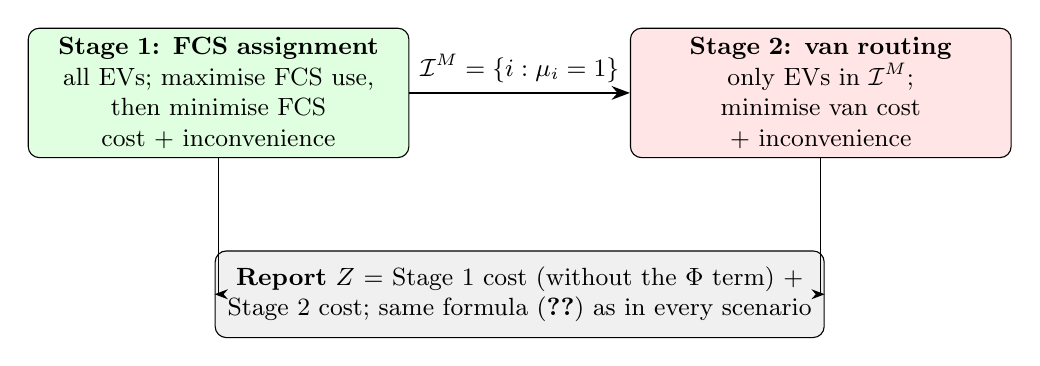
\begin{tikzpicture}[>=Stealth,box/.style={draw,rounded corners,align=center,minimum height=1.1cm,font=\small}]
  \node[box,fill=green!12,text width=4.6cm] (s1) {\textbf{Stage 1: FCS assignment}\\all EVs; maximise FCS use,\\then minimise FCS cost + inconvenience};
  \node[box,fill=red!10,text width=4.6cm,right=2.8cm of s1] (s2) {\textbf{Stage 2: van routing}\\only EVs in $\I^M$;\\minimise van cost + inconvenience};
  \draw[->,thick] (s1) -- node[above,font=\small]{$\I^M=\{i:\mu_i=1\}$} (s2);
  \node[box,fill=black!6,text width=7.5cm,below=2.0cm of $(s1)!0.5!(s2)$] (ev) {\textbf{Report} $Z=$ Stage~1 cost (without the $\Phi$ term) $+$ Stage~2 cost; same formula \eqref{eq:Z} as in every scenario};
  \draw[->] (s1) |- (ev); \draw[->] (s2) |- (ev);
\end{tikzpicture}
\end{center}

Stage~1 does not look at the vans, and Stage~2 cannot change what Stage~1 decided. That is the definition of ``FCS first, then MCS''.

%----------------------------------------------------------------
\subsection{Stage 1: assign EVs to fixed stations}

\textbf{Objective.}
\begin{equation}
\begin{split}
\min\ Z^{(1)}=\;&\underbrace{\Phi\sum_{i\in\I}\mu_i}_{\text{FCS first}}
+\underbrace{c^{EV}\sum_i\sum_{f\in\F_i}d_{if}Y_{if}}_{Z_1}
+\underbrace{Z^F_{\text{energy}}}_{\text{FCS part of }Z_4}\\
&+\underbrace{\sum_i\sum_{f\in\F_i}\rho^F_{if}Y_{if}+\alpha\sum_i w_i(C_i-r_i)+c^L\sum_i w_iL_i}_{\text{FCS customers' inconvenience}}
\end{split}
\label{eq:obj1}
\end{equation}
with $C_i=S_i+\tau^F_iY_i$ in this stage. $\Phi$ is a penalty for handing an EV to the vans. It is chosen larger than anything an extra FCS customer can add to the rest of \eqref{eq:obj1}, e.g.
\[
\Phi > \max_{i}\max_{f\in\F_i}\big(c^{EV}d_{if}+\pi^{\max}E_i+\rho^F_{if}\big)+n\,(\alpha+c^L)\,w_{\max}\,T,
\]
so Stage~1 first \textbf{maximises the number of EVs served at an FCS}, and only among those solutions minimises FCS cost and inconvenience. ($\pi^{\max}$ is the highest grid price.) A numerically safer equivalent is to solve twice: first $\max\sum_iY_i$, then fix that number and minimise the rest.
\ifTOU
Because $Z^F_{\text{energy}}$ uses the peak price, Stage~1 may \emph{start sessions later} to leave the peak, if the price saving beats the extra waiting cost (Section~\ref{sec:expect}).
\fi

\textbf{Constraints.}
\begin{align}
\sum_{g\in\G_i}y_{ig}+\mu_i &= 1 && \forall i\in\I \label{eq:s1assign}\\
S_i &\ge r_i+\sum_{f\in\F_i}t_{if}Y_{if} && \forall i\in\I \label{eq:fcsarr}\\
S_i &\le r_i+T\,(1-\mu_i) && \forall i\in\I \label{eq:s1park}\\
S_j &\ge S_i+\tau^F_i-(T+\tau^F_i)(3-y_{ig}-y_{jg}-o_{ij}) && \forall g,\ (i,j)\in\mathcal{P}_g \label{eq:disj1}\\
S_i &\ge S_j+\tau^F_j-(T+\tau^F_j)(2-y_{ig}-y_{jg}+o_{ij}) && \forall g,\ (i,j)\in\mathcal{P}_g \label{eq:disj2}\\
\sum_i y_{ig_1} &\ge \sum_i y_{ig_2} && \forall f,\ \G_f=\{g_1,g_2\} \label{eq:gunsym}\\
S_i+\tau^F_iY_i &\le T,\qquad L_i\ge S_i+\tau^F_iY_i-l_i && \forall i\in\I \label{eq:s1time}
\end{align}
\ifTOU plus the time-of-use split \eqref{eq:tou1}--\eqref{eq:tou5} of each FCS session (Section~\ref{sec:price}).\fi
\desc{\eqref{eq:s1assign}: every EV either gets one reachable gun or is handed to the vans. An EV that reaches no FCS ($\G_i=\emptyset$) is forced to $\mu_i=1$. \eqref{eq:fcsarr}: an FCS session cannot start before the EV has asked and driven to the station. \eqref{eq:s1park}: for an EV handed to the vans, $S_i$ is parked at $r_i$, so it adds no waiting in Stage~1 (its real start time is decided in Stage~2). \eqref{eq:disj1}--\eqref{eq:disj2}: two EVs on the same gun do not overlap; $o_{ij}$ picks who goes first. With two guns per station this means at most two EVs charge at a station at a time. \eqref{eq:gunsym}: symmetry breaking between the two identical guns (optional). \eqref{eq:s1time}: finished by $T$; lateness.}

\textbf{Optional acceptability rule.} An operator may refuse to send a driver to a station that is ``too inconvenient'', e.g.\ only allow gun $g$ of station $f$ for EV $i$ if $\hat\rho^F_{if}\le\bar\rho$. This only shrinks $\G_i$, so EVs whose stations are all too far go to the vans. Report results with and without it.

\textbf{Output:} $\I^M=\{i:\mu_i=1\}$, the EVs left for the vans; plus each FCS customer's gun and start time.

%----------------------------------------------------------------
\subsection{Stage 2: route the vans to the leftover EVs}

Stage~2 is a vehicle routing problem with time windows, on the EVs in $\I^M$ only. Here $C_i=S_i+\tau^M_i$.

\textbf{Objective.}
\begin{equation}
\begin{split}
\min\ Z^{(2)}=\;&\underbrace{c^M\sum_m\sum_{(i,j)\in\A^M}d_{ij}x_{ijm}}_{Z_2}+\underbrace{\sum_m c^D_mu_m}_{Z_3}+\underbrace{Z^M_{\text{energy}}}_{\text{van part of }Z_4}\\
&+\underbrace{\sum_{i\in\I^M}\sum_m\rho^M_{im}z_{im}+\alpha\sum_{i\in\I^M}w_i(C_i-r_i)+c^L\sum_{i\in\I^M}w_iL_i}_{\text{van customers' inconvenience}}
\end{split}
\label{eq:obj2}
\end{equation}
Since every EV in $\I^M$ must be served by some van, $Z^M_{\text{energy}}$ and the $\rho^M$ term are constants here. They are kept so that $Z^{(2)}$ is the true cost of Stage~2. Waiting and lateness make the vans visit urgent EVs early.

\textbf{Constraints.}
\begin{align}
\sum_{m\in\M}z_{im} &= 1 && \forall i\in\I^M \label{eq:s2assign}\\
\sum_{j:(0,j)\in\A^M}x_{0jm} = \sum_{i:(i,n+1)\in\A^M}x_{i,n+1,m} &= u_m && \forall m \label{eq:depot}\\
\sum_{i:(i,j)\in\A^M}x_{ijm} = \sum_{k:(j,k)\in\A^M}x_{jkm} &= z_{jm} && \forall j\in\I^M,\ m \label{eq:flow}\\
\sum_{i\in\I^M}z_{im} &\le Q_m\,u_m && \forall m \label{eq:cap}\\
\sum_{i\in\I^M}\frac{E_i}{\eta}z_{im}+\beta\sum_{(i,j)\in\A^M}d_{ij}x_{ijm} &\le B_m\,u_m && \forall m \label{eq:batt}
\end{align}
\begin{align}
S_j &\ge \max\{r_j,\ t_{0j}\,x_{0jm}\} && \forall j\in\I^M,\ m \label{eq:depart}\\
S_j &\ge S_i+\tau^M_i+t_{ij}-(T+\tau^M_i+t_{ij})(1-x_{ijm}) && \forall i\neq j,\ m \label{eq:seq}\\
S_i+\tau^M_i+t_{i,n+1} &\le T+(\tau^M_i+t_{i,n+1})(1-x_{i,n+1,m}) && \forall i,\ m \label{eq:return}\\
S_i+\tau^M_i \le T,\quad L_i &\ge S_i+\tau^M_i-l_i && \forall i\in\I^M \label{eq:s2time}\\
u_m &\ge u_{m+1} && m<|\M| \label{eq:vansym}
\end{align}
\desc{\eqref{eq:s2assign}: each leftover EV gets one van. \eqref{eq:depot}: a used van leaves and returns to the depot once. \eqref{eq:flow}: each EV on van $m$ is entered and left exactly once by that van. \eqref{eq:cap}: at most $Q_m$ EVs per van. \eqref{eq:batt}: delivered energy (with transfer losses) plus driving energy fits in the van battery. \eqref{eq:depart}: no start before the request, or before the van can drive there from the depot (written as two linear constraints). \eqref{eq:seq}: if the van goes $i\to j$, it finishes $i$ and drives to $j$ before starting $j$. This gives one EV at a time and removes subtours (MTZ-type). \eqref{eq:return}: back at the depot by $T$. \eqref{eq:s2time}: finished by $T$; lateness. \eqref{eq:vansym}: use identical vans in index order.}

\textbf{If Stage 2 is infeasible} (too many leftover EVs for the fleet by $T$), the sequential policy has \emph{failed} on that instance. For diagnosis, add $s_i\in\{0,1\}$ (``unserved''), replace \eqref{eq:s2assign} by $\sum_mz_{im}+s_i=1$ and add $\Phi^U\sum_is_i$ to \eqref{eq:obj2}. Then report the number of EVs that could not be served. This is a useful comparison with the integrated scenario, which may serve all of them.

%----------------------------------------------------------------
\subsection{Reported value}
\[
Z^{\text{S\scen}}=\big(Z^{(1)*}-\Phi\,|\I^M|\big)+Z^{(2)*},
\]
which is exactly \eqref{eq:Z} evaluated at the combined solution. The stage-1 solution plus the stage-2 solution is a feasible solution of the integrated model (S\ifTOU 4\else 3\fi), so
$Z^{\text{S\ifTOU 4\else 3\fi}}\le Z^{\text{S\scen}}$. The difference is the \emph{value of integration}.

\else
%---------------------------------------------------------------- INT
\subsection{Objective}
\begin{equation}
\min\ Z \quad\text{as in \eqref{eq:Z}, with }Z^F_{\text{energy}}=\ifTOU P^F\textstyle\sum_i\big[\pi^\off(\theta^1_i+\theta^3_i)+\pi^\pk\theta^2_i\big]\else\pi^F\textstyle\sum_iE_iY_i\fi,\quad C_i=S_i+\tau^F_iY_i+\tau^M_iZ_i. \label{eq:objint}
\end{equation}
Written out in full:
\begin{align*}
\min\ Z=\;& c^{EV}\sum_i\sum_{f\in\F_i}d_{if}Y_{if}+c^M\sum_m\sum_{(i,j)\in\A}d_{ij}x_{ijm}+\sum_mc^D_mu_m\\
&+\ifTOU P^F\sum_i\big[\pi^\off(\theta^1_i+\theta^3_i)+\pi^\pk\theta^2_i\big]\else\pi^F\sum_iE_iY_i\fi
+\pi^M\sum_i\sum_m\frac{E_i}{\eta}z_{im}\\
&+\sum_i\sum_{f\in\F_i}\rho^F_{if}Y_{if}+\sum_i\sum_m\rho^M_{im}z_{im}+\alpha\sum_iw_i(C_i-r_i)+c^L\sum_iw_iL_i .
\end{align*}
Every term is linear. One model weighs everything at once: an EV goes to a van exactly when the van's extra km, dispatch and energy cost are outweighed by the effort and waiting it saves the driver\ifTOU, or by the peak-price energy it avoids\fi.

\subsection{Constraints}

\textbf{Assignment.}
\begin{equation}
\sum_{g\in\G_i}y_{ig}+\sum_{m\in\M}z_{im}=1\qquad\forall i\in\I \label{eq:assign}
\end{equation}
\desc{Exactly one resource per EV: one reachable gun or one van. EVs that reach no FCS are forced onto a van.}

\textbf{Fixed stations.}
\begin{align}
S_i &\ge r_i+\sum_{f\in\F_i}t_{if}Y_{if} && \forall i \label{eq:fcsarr}\\
S_j &\ge S_i+\tau^F_i-(T+\tau^F_i)(3-y_{ig}-y_{jg}-o_{ij}) && \forall g,\ (i,j)\in\mathcal{P}_g \label{eq:disj1}\\
S_i &\ge S_j+\tau^F_j-(T+\tau^F_j)(2-y_{ig}-y_{jg}+o_{ij}) && \forall g,\ (i,j)\in\mathcal{P}_g \label{eq:disj2}\\
\sum_iy_{ig_1} &\ge \sum_iy_{ig_2} && \forall f,\ \G_f=\{g_1,g_2\} \label{eq:gunsym}
\end{align}
\desc{\eqref{eq:fcsarr}: an FCS session starts after the request and the drive to the station (for a van customer this is just $S_i\ge r_i$). \eqref{eq:disj1}--\eqref{eq:disj2}: EVs on the same gun do not overlap; $o_{ij}$ chooses the order. \eqref{eq:gunsym}: optional symmetry breaking.}

\textbf{Vans: routes, capacity, battery.}
\begin{align}
\sum_{j:(0,j)\in\A}x_{0jm}=\sum_{i:(i,n+1)\in\A}x_{i,n+1,m} &= u_m && \forall m \label{eq:depot}\\
\sum_{i:(i,j)\in\A}x_{ijm}=\sum_{k:(j,k)\in\A}x_{jkm} &= z_{jm} && \forall j\in\I,\ m \label{eq:flow}\\
\sum_iz_{im} &\le Q_mu_m && \forall m \label{eq:cap}\\
\sum_i\frac{E_i}{\eta}z_{im}+\beta\sum_{(i,j)\in\A}d_{ij}x_{ijm} &\le B_mu_m && \forall m \label{eq:batt}
\end{align}
\desc{\eqref{eq:depot}: a used van leaves and returns once. \eqref{eq:flow}: each EV on van $m$ is visited exactly once by it. \eqref{eq:cap}: at most $Q_m$ EVs. \eqref{eq:batt}: delivered energy (with losses) plus driving energy fits in the battery.}

\textbf{Vans: timing (one EV at a time, no subtours).}
\begin{align}
S_j &\ge t_{0j}\,x_{0jm} && \forall j\in\I,\ m \label{eq:depart}\\
S_j &\ge S_i+\tau^M_i+t_{ij}-(T+\tau^M_i+t_{ij})(1-x_{ijm}) && \forall i\neq j\in\I,\ m \label{eq:seq}\\
S_i+\tau^M_i+t_{i,n+1} &\le T+(\tau^M_i+t_{i,n+1})(1-x_{i,n+1,m}) && \forall i,\ m \label{eq:return}
\end{align}
\desc{\eqref{eq:depart}: the first stop cannot start before the van has driven there. \eqref{eq:seq}: $i\to j$ means finish $i$, drive, then start $j$; start times rise along a route, so no subtour can close. \eqref{eq:return}: back at the depot by $T$.}

\textbf{Horizon and lateness.}
\begin{equation}
C_i\le T,\qquad L_i\ge C_i-l_i\qquad\forall i\in\I \label{eq:time}
\end{equation}
\desc{Every EV is fully charged within the horizon; $L_i$ measures lateness.}

\ifTOU
\textbf{Time-of-use split.} Constraints \eqref{eq:tou1}--\eqref{eq:tou5} of Section~\ref{sec:price}.
\fi

\textbf{Symmetry and domains.}
\begin{equation}
u_m\ge u_{m+1};\qquad y,z,x,u,o\ifTOU,\kappa\fi\in\{0,1\};\qquad S_i,L_i\ifTOU,\theta^p_i\fi\ge0 \label{eq:dom}
\end{equation}
\fi

%=====================================================================
\section{Learning-to-optimise (RL) formulation}\label{sec:rl}

\textbf{Main rule:} the reward of each action is \emph{minus the increase in $Z$ that the action causes}. The rewards over an episode then add up to $-Z$ of the solution the policy builds. RL and MILP results are measured on the same yardstick \eqref{eq:Z}, and the MILP optimum is the benchmark for the RL gap.

\ifSEQ
%---------------------------------------------------------------- RL SEQ
The RL pipeline has the same two stages as the MILP.

\subsection{Stage 1 policy: FCS assignment}
\begin{itemize}[leftmargin=1.4em,itemsep=2pt]
  \item \textbf{Episode / epochs:} EVs are taken in order of request time $r_i$ (ties: higher $w_i$ first). One decision per EV.
  \item \textbf{State:} features of the current EV $k$ ($E_k,r_k,l_k,w_k,R_k$, location); for each gun $g$ the time $F_g$ it becomes free; summary features of the EVs still to come (count and positions near each station)\ifTOU; the current price and the time until $T_1$ and $T_2$\fi.
  \item \textbf{Action:} a gun $g\in\G_k$, or ``hand to vans''. \textbf{FCS-first mask:} ``hand to vans'' is allowed \emph{only} if no gun can finish EV $k$ by $T$ (or, with the optional rule, if all remaining guns have $\hat\rho^F_{kf}>\bar\rho$).
  \ifTOU\item \textbf{Optional timing action:} ``gun $g$, start after the peak'', i.e.\ $S_k=\max\{\text{earliest},T_2\}$, allowed only if the session still ends by $T$.\fi
  \item \textbf{Transition:} $S_k=\max\{r_k+t_{kf},F_g\}$ (or later, for the timing action); $F_g\leftarrow S_k+\tau^F_k$.
  \item \textbf{Reward:} $-\Big[c^{EV}d_{kf}+\text{energy}_k+\rho^F_{kf}+\alpha w_k(S_k+\tau^F_k-r_k)+c^Lw_k(S_k+\tau^F_k-l_k)^+\Big]$, where energy$_k$ = \ifTOU$P^F\big[\pi^\off\cdot(\text{off-peak hours of }[S_k,S_k+\tau^F_k])+\pi^\pk\cdot(\text{peak hours})\big]$, computed exactly in the simulator\else$\pi^FE_k$\fi. Handing an EV to the vans gives reward $0$ here; its cost is counted in Stage~2.
\end{itemize}
Note: a simple baseline for Stage~1 is the greedy rule ``gun with the largest one-step reward''. What RL can learn on top of this is, for example, to keep a nearby gun free for an urgent EV that arrives later.

\subsection{Stage 2 policy: van routing over $\I^M$}
\begin{itemize}[leftmargin=1.4em,itemsep=2pt]
  \item \textbf{Epochs:} whenever a van becomes free (the earliest-free van decides first).
  \item \textbf{State:} for each van: position, time free, remaining battery $b_m$, EVs served so far, dispatched or not; for each unserved EV in $\I^M$: location, $E_i,r_i,l_i,w_i$; current time.
  \item \textbf{Action:} the next EV $j$ for this van, or ``return to depot'' (ends the route). Mask: $j$ must be feasible: battery covers $E_j/\eta$ plus driving to $j$ and back to the depot, the count stays $\le Q_m$, and $j$ can be finished with the van back at the depot by $T$.
  \item \textbf{Transition:} $S_j=\max\{r_j,\ \text{time free}+t_{\text{pos},j}\}$; the van moves to $j$ and is free at $S_j+\tau^M_j$; $b_m$ falls by $E_j/\eta+\beta d_{\text{pos},j}$.
  \item \textbf{Reward:} serving $j$: $-\Big[c^Md_{\text{pos},j}+c^D_m[\text{first stop}]+\pi^M\frac{E_j}{\eta}+\rho^M_{jm}+\alpha w_j(S_j+\tau^M_j-r_j)+c^Lw_j(S_j+\tau^M_j-l_j)^+\Big]$; returning: $-c^Md_{\text{pos},0}$. EVs still unserved at the end: $-\Phi^U$ each.
  \item \textbf{Policy:} an attention-based routing policy (e.g.\ Kool et al., 2019, ``Attention, Learn to Solve Routing Problems!'') trained with REINFORCE or PPO. Baseline: nearest-feasible-EV heuristic.
\end{itemize}
Episode return of Stage~1 + Stage~2 $=-Z^{\text{S\scen}}$.

\else
%---------------------------------------------------------------- RL INT
One policy decides both who serves each EV and the van routes.
\begin{itemize}[leftmargin=1.4em,itemsep=2pt]
  \item \textbf{Episode / epochs:} EVs are taken in order of request time $r_i$ (ties: higher $w_i$ first). One decision per EV.
  \item \textbf{State:} (i) the current EV $k$: location, $E_k,r_k,l_k,w_k,R_k$, reachable stations; (ii) each gun $g$: time $F_g$ it becomes free; (iii) each van $m$: current end-of-route position, time free, remaining battery $b_m$, EVs served, dispatched or not; (iv) embeddings of the not-yet-assigned EVs (for look-ahead)\ifTOU; (v) current price, time until $T_1$ and $T_2$\fi.
  \item \textbf{Action:} $a\in\G_k\cup\M$: a gun, or a van (EV $k$ is appended to the end of that van's route). \textbf{Mask} infeasible actions: a gun that cannot finish $k$ by $T$; a van without enough battery for $E_k/\eta$ plus the drive to $k$ and back to the depot, with $Q_m$ reached, or unable to finish $k$ and return by $T$.
  \ifTOU\item \textbf{Optional timing action:} ``gun $g$, start after the peak'' ($S_k=\max\{\text{earliest},T_2\}$, if it still ends by $T$).\fi
  \item \textbf{Transition:} gun: $S_k=\max\{r_k+t_{kf},F_g\}$, $F_g\leftarrow S_k+\tau^F_k$. Van: $S_k=\max\{r_k,\ \text{free}_m+t_{\text{pos}_m,k}\}$, then the van moves to $k$, $\text{free}_m\leftarrow S_k+\tau^M_k$, $b_m\mathrel{-}=E_k/\eta+\beta d_{\text{pos}_m,k}$.
  \item \textbf{Reward} $=-\Delta Z$:
  \begin{align*}
  \text{gun } g\text{ at }f:&\quad -\Big[c^{EV}d_{kf}+\text{energy}^F_k+\rho^F_{kf}+\alpha w_k(C_k-r_k)+c^Lw_k(C_k-l_k)^+\Big]\\
  \text{van } m:&\quad -\Big[c^M\big(d_{\text{pos}_m,k}+d_{k,0}-d_{\text{pos}_m,0}\big)+c^D_m[\text{first use}]+\pi^M\tfrac{E_k}{\eta}\\
  &\qquad\quad+\rho^M_{km}+\alpha w_k(C_k-r_k)+c^Lw_k(C_k-l_k)^+\Big]
  \end{align*}
  The van distance term is the \emph{change} in route length when $k$ is inserted before the return to the depot, so the sum over the episode equals the total route length (the return legs telescope). energy$^F_k$ = \ifTOU$P^F\big[\pi^\off\cdot(\text{off-peak hours})+\pi^\pk\cdot(\text{peak hours of }[S_k,C_k])\big]$, computed exactly by the simulator; no linearisation is needed in RL\else$\pi^FE_k$\fi.
  \item \textbf{Dead end:} if every action is masked, EV $k$ is unserved: reward $-\Phi^U$, and the episode continues. Report the count.
  \item \textbf{Policy:} masked categorical policy over guns and vans, encoder with attention over EVs, guns and vans; trained with PPO. Natural baseline: greedy, i.e.\ choose the action with the largest one-step reward. That is the pairwise rule ``smallest $\hat\rho$ + cost'' from Section~\ref{sec:inc}.
\end{itemize}
Restriction to note: vans serve EVs in assignment order (append only). A variant that inserts $k$ at the cheapest position of a route is more flexible but has a larger action space.
\fi

\textbf{Reward scaling.} For stable training divide every reward by a constant, e.g.\ the greedy baseline's average $Z$ on the training instances. This does not change the optimal policy.

%=====================================================================
\section{What to expect and what to report}\label{sec:expect}

\ifnum\scen=1
\begin{itemize}[leftmargin=1.4em,itemsep=2pt]
  \item Vans serve only EVs that reach no station, or that the stations cannot finish by $T$. If stations have spare capacity, very few vans are dispatched.
  \item Inconvenience is high for EVs far from the nearest station (worked example: Rs\,682 at the FCS, against Rs\,458 if a van had been allowed).
  \item With too few vans Stage~2 becomes infeasible (unserved EVs), even when the integrated model S3 could serve everyone. Report the smallest $|\M|$ at which S1 is feasible and compare it with S3.
\end{itemize}
\fi
\ifnum\scen=2
\begin{itemize}[leftmargin=1.4em,itemsep=2pt]
  \item \textbf{When does Stage~1 delay a session to avoid the peak?} Moving one hour of charging out of the peak saves $(\pi^\pk-\pi^\off)P^F=3\times22=$ Rs\,66, but delays completion by up to an hour, which costs $\alpha w_i\ge$ Rs\,200. So with the default values Stage~1 almost never delays. It mostly pays the higher price, and S2 costs roughly S1 plus the peak surcharge. Sessions start later only if $\alpha$ is small (try $\lambda<0.33$ in the sensitivity analysis).
  \item The van assignment is the same as in S1 unless Stage~1's timing changes which EVs fit at the stations. Stage~1 cannot use vans to escape the peak price.
  \item Extra KPI: \textbf{grid energy drawn at FCS during the peak}, $P^F\sum_i\theta^2_i$ (kWh). Compare with S4.
\end{itemize}
\fi
\ifnum\scen=3
\begin{itemize}[leftmargin=1.4em,itemsep=2pt]
  \item Vans take EVs for which the saved inconvenience exceeds the extra van cost (worked example: van chosen, saving Rs\,224). Expect vans to serve EVs that are far from every station, have low range (high $w_i$), or have early deadlines, while EVs near a station still use it.
  \item \textbf{Value of integration under flat price:} $Z^{\text{S1}}-Z^{\text{S3}}\ge0$. Report it per component ($Z_1,\dots,Z_5$): typically operating cost rises a little and inconvenience falls a lot.
  \item Vary $|\M|$ (0, 1, 2, \dots): the first few vans lower $Z$ sharply, then the effect levels off. That curve shows the scenarios where mobile chargers help most.
\end{itemize}
\fi
\ifnum\scen=4
\begin{itemize}[leftmargin=1.4em,itemsep=2pt]
  \item During the peak a van kWh costs about the same as an FCS kWh (Rs\,10.0 each), so the vans' energy disadvantage disappears and vans also absorb \emph{peak-hour} demand that would otherwise be charged on the grid at peak price.
  \item Expect more van usage than in S3, concentrated on requests in $[T_1,T_2]$, and lower grid energy at the stations during the peak, $P^F\sum_i\theta^2_i$, than in S2.
  \item \textbf{Value of integration under peak pricing:} $Z^{\text{S2}}-Z^{\text{S4}}$. It should be larger than $Z^{\text{S1}}-Z^{\text{S3}}$, because integration now also allows price arbitrage.
  \item \textbf{Peak pricing with full flexibility:} $Z^{\text{S4}}-Z^{\text{S3}}$ should be smaller than $Z^{\text{S2}}-Z^{\text{S1}}$: vans cushion the price increase.
\end{itemize}
\fi

\textbf{Cross-scenario comparison table} (fill in from the four runs):
\begin{center}
\renewcommand{\arraystretch}{1.2}
\begin{tabular}{@{}lll@{}}
\toprule
\textbf{Comparison} & \textbf{Measures} & \textbf{Expected sign} \\
\midrule
S1 $-$ S3 & value of integration, flat price & $\ge0$ \\
S2 $-$ S4 & value of integration, peak price & $\ge0$, larger than S1 $-$ S3 \\
S2 $-$ S1 & cost of peak pricing, FCS-first operator & $>0$ \\
S4 $-$ S3 & cost of peak pricing, flexible operator & $>0$, smaller than S2 $-$ S1 \\
\bottomrule
\end{tabular}
\end{center}
Report for each: $Z$ and its components, number of vans used, EVs per resource, mean and maximum inconvenience per EV, total lateness, peak-hour grid energy, solve time, and (for RL) the gap to the MILP optimum.

%=====================================================================
\appendix
\section{Illustrative parameter values}\label{app:values}

These are starting values for experiments, not data. All are meant to be varied in the analysis. Values in Rs.

\begin{center}
\renewcommand{\arraystretch}{1.15}
\begin{tabular}{@{}llp{6.2cm}@{}}
\toprule
\textbf{Parameter} & \textbf{Value} & \textbf{Note} \\
\midrule
$T$, $[T_1,T_2]$ & 7 h, $[2,6]$ & 16:00--23:00, peak 18:00--22:00 \\
$P^F$, $P^M$ & 22 kW, 30 kW & \\
$v$, $\beta$, $\eta$ & 25 km/h, 0.25 kWh/km, 0.9 & \\
$B_m$, $Q_m$, $|\M|$ & 150 kWh, 6, 2--6 & \\
$c^{EV}$, $c^M$, $c^D_m$ & Rs\,4/km, Rs\,15/km, Rs\,1500 & van km includes driver time \\
$\pi^F$ (flat) & Rs\,8.7/kWh & equals the time-average of the ToU tariff over $[0,T]$ \\
$\pi^\off$, $\pi^\pk$ (ToU) & Rs\,7/kWh, Rs\,10/kWh & $(3\times7+4\times10)/7=8.7$ \\
$c^{bat}$ & Rs\,2/kWh & van battery wear \\
$\pi^M$ & Rs\,10.7 (flat) / Rs\,9.0 (ToU) & $=\pi^F+c^{bat}$ / $=\pi^\off+c^{bat}$ \\
$\alpha$, $\alpha^D$ & Rs\,200/h, Rs\,100/h & value of time; extra for attended time \\
$h^F$, $h^M$, $\varphi$ & Rs\,50, Rs\,10, Rs\,100 & trip hassle, hand-over, range stress \\
$c^L$ & Rs\,300/h & lateness \\
$w_i$ & $1+2(1-R_i/R_{\max})$, $R_i\sim U[3,40]$ km & priority from remaining range \\
\bottomrule
\end{tabular}
\end{center}

The flat price is set to the time-average of the peak tariff. The price \emph{level} is then the same in both pricing cases, and only the price \emph{shape} differs. Without this, part of S1 vs S2 would just reflect a different average price.

\end{document}
"
%    pdflatex -jobname=scenario4_peak_integrated   "\def\scen{4}% =====================================================================
%  One source, four PDFs.  Build with build.sh (or by hand):
%    pdflatex -jobname=scenario1_flat_sequential   "\def\scen{1}\input{scenario_master}"
%    pdflatex -jobname=scenario2_peak_sequential   "\def\scen{2}\input{scenario_master}"
%    pdflatex -jobname=scenario3_flat_integrated   "\def\scen{3}\input{scenario_master}"
%    pdflatex -jobname=scenario4_peak_integrated   "\def\scen{4}\input{scenario_master}"
%  (run each twice for cross-references)
% =====================================================================
\documentclass[11pt,a4paper]{article}
\usepackage[margin=2.2cm]{geometry}
\usepackage{amsmath,amssymb,amsfonts}
\usepackage{booktabs,array,tabularx}
\usepackage{enumitem}
\usepackage[table]{xcolor}
\usepackage{tikz}
\usetikzlibrary{arrows.meta,positioning,calc}
\usepackage[colorlinks=true,linkcolor=blue!50!black,urlcolor=blue!50!black]{hyperref}
\usepackage{titlesec}
\titleformat{\section}{\large\bfseries}{\thesection}{0.8em}{}
\titleformat{\subsection}{\normalsize\bfseries}{\thesubsection}{0.8em}{}
\setlength{\parindent}{0pt}
\setlength{\parskip}{5pt}

% ---------------- scenario switches ----------------
\ifdefined\scen\else\def\scen{1}\fi
\newif\ifTOU \TOUfalse   % true = time-of-use (peak) price
\newif\ifSEQ \SEQfalse   % true = FCS first, then MCS
\ifnum\scen=1 \SEQtrue \fi
\ifnum\scen=2 \TOUtrue \SEQtrue \fi
\ifnum\scen=4 \TOUtrue \fi

\newcommand{\pricename}{\ifTOU time-of-use price (dearer evening peak)\else single (flat) price all day\fi}
\newcommand{\structname}{\ifSEQ FCS first, then MCS (sequential)\else FCS and MCS together (integrated)\fi}

% ---------------- notation ----------------
\newcommand{\I}{\mathcal{I}}
\newcommand{\F}{\mathcal{F}}
\newcommand{\G}{\mathcal{G}}
\newcommand{\M}{\mathcal{M}}
\newcommand{\N}{\mathcal{N}}
\newcommand{\A}{\mathcal{A}}
\newcommand{\Rs}{\text{Rs}\,}
\newcommand{\pk}{\mathrm{pk}}
\newcommand{\off}{\mathrm{off}}
\newcommand{\desc}[1]{\par\vspace{-2pt}{\small\color{black!75}\textit{Meaning:} #1}\par\vspace{4pt}}
\newcommand{\cell}[2]{\ifnum\scen=#1\cellcolor{blue!18}\textbf{S#1 (this document)}\\\textbf{#2}\else S#1\\#2\fi}

\title{\textbf{EV Charging Network Optimisation}\\[4pt]
\large Scenario \scen: \pricename\ $+$ \structname\\[2pt]
\normalsize MILP and RL formulation}
\author{CP 320 OR for Mobility Management, course project}
\date{2 October 2026}

\begin{document}
\maketitle

%=====================================================================
\section{Where this scenario sits}

The project studies four scenarios: two ways of pricing grid electricity, times two ways of making the decisions.

\begin{center}
\renewcommand{\arraystretch}{1.5}
\begin{tabular}{>{\raggedright\arraybackslash}p{4.2cm}|>{\centering\arraybackslash}p{4.6cm}|>{\centering\arraybackslash}p{4.6cm}}
 & \textbf{Flat price all day} & \textbf{Time-of-use (peak) price} \\ \hline
\textbf{Sequential:} FCS first, leftover EVs to MCS &
\begin{tabular}[c]{@{}c@{}}\cell{1}{flat + sequential}\end{tabular} &
\begin{tabular}[c]{@{}c@{}}\cell{2}{peak + sequential}\end{tabular} \\ \hline
\textbf{Integrated:} FCS and MCS decided together &
\begin{tabular}[c]{@{}c@{}}\cell{3}{flat + integrated}\end{tabular} &
\begin{tabular}[c]{@{}c@{}}\cell{4}{peak + integrated}\end{tabular} \\
\end{tabular}
\end{center}

\textbf{The four scenarios do not have four different objectives.} They share \emph{one} cost yardstick $Z$ (Section~\ref{sec:obj}): the same cost terms and the same customer inconvenience (Section~\ref{sec:inc}). Only two things change:
\begin{itemize}[leftmargin=1.4em,itemsep=1pt]
  \item \textbf{Pricing} changes the formula for one term, the FCS energy cost (Section~\ref{sec:price}).
  \item \textbf{Decision structure} changes \emph{how} $Z$ is minimised: in one model (integrated), or in two stages (sequential), where each stage minimises its own part of $Z$.
\end{itemize}
Because the yardstick is the same, the four optimal values can be compared directly. The differences measure the \emph{value of integration} (S1$\to$S3, S2$\to$S4) and the \emph{effect of peak pricing} (S1$\to$S2, S3$\to$S4).

\ifnum\scen=1
\textbf{This scenario (S1)} is the baseline, the ``status quo''. Electricity costs the same at every hour, every EV that can be charged at a fixed station is sent there, and vans only take what is left over.
\fi
\ifnum\scen=2
\textbf{This scenario (S2)} keeps the FCS-first rule of S1, but grid electricity is dearer during the evening peak. Stage~1 can react to the price only by \emph{rescheduling} FCS sessions. It cannot hand a peak-hour EV to a van.
\fi
\ifnum\scen=3
\textbf{This scenario (S3)} keeps the flat price of S1, but the operator decides FCS and MCS service \emph{together}. An EV can be sent to a van even when a fixed station could take it, whenever that lowers total cost plus inconvenience.
\fi
\ifnum\scen=4
\textbf{This scenario (S4)} is the most flexible one: peak pricing at fixed stations, and FCS and MCS decided together. Van energy was bought off-peak, so vans can also be used to keep charging \emph{out of the expensive peak}.
\fi

%=====================================================================
\section{Setting and assumptions}\label{sec:setting}

\textbf{Time.} The planning horizon is $[0,T]$ with $T=7$\,h (16:00--23:00). It contains the evening peak window $[T_1,T_2]=[2,6]$ (18:00--22:00). The horizon is the same in all four scenarios. It is wider than the peak itself so that, under peak pricing, there is cheaper time on both sides of the peak.\ifTOU\else\ In this scenario the price is flat, so the window plays no role in the model.\fi

\textbf{Assumptions} (the same as MILP v3, plus two about energy):
\begin{enumerate}[leftmargin=1.6em,itemsep=1pt]
  \item Static, continuous time. All requests in the horizon are known at time $0$, and request $i$ becomes active at $r_i$.
  \item An EV served by an FCS drives there itself on its own battery (only to stations within its range $R_i$). The driver stays with the car while it waits for a free gun and while it charges.
  \item An EV served by an MCS stays parked where it is, and the driver is free in the meantime.
  \item Each FCS gun and each van charges one EV at a time, without interruption, at constant power.
  \item A van's battery covers both its driving and the energy it delivers. \textbf{The van battery is charged at the depot before the horizon starts}\ifTOU, i.e.\ at the off-peak price\fi, and is not recharged during the horizon.
  \item Every EV must be fully charged by $T$ (hard). Finishing after the driver's desired time $l_i$ is allowed but penalised.
\end{enumerate}

%=====================================================================
\section{Notation}\label{sec:notation}

\subsection*{Sets}
\begin{tabularx}{\textwidth}{@{}lX@{}}
\toprule
$\I=\{1,\dots,n\}$ & EV charging requests \\
$\F$; $\G_f$ ($|\G_f|=2$); $\G=\bigcup_f\G_f$ & fixed charging stations; guns of FCS $f$; all guns ($f(g)$ = station of gun $g$) \\
$\F_i=\{f: d_{if}\le R_i\}$, $\G_i=\bigcup_{f\in\F_i}\G_f$ & stations / guns EV $i$ can reach on its remaining range \\
$\M$ & mobile charging vans (MCS) \\
$0,\ n+1$ & depot as start node / end node (same place) \\
$\N=\{0\}\cup\I\cup\{n+1\}$, $\A$ & routing nodes; allowed van arcs $(i,j)$, $i\in\{0\}\cup\I$, $j\in\I\cup\{n+1\}$, $i\neq j$ \\
$\mathcal{P}_g=\{(i,j): i<j,\ g\in\G_i\cap\G_j\}$ & pairs of EVs that could share gun $g$ \\
\ifSEQ
$\I^M\subseteq\I$ & EVs handed to the vans by Stage~1 (an \emph{output} of Stage~1, a fixed input to Stage~2) \\
$\N^M$, $\A^M$ & routing nodes / arcs restricted to $\I^M$ \\
\fi
\bottomrule
\end{tabularx}

\subsection*{Parameters}
\begin{tabularx}{\textwidth}{@{}lX@{}}
\toprule
$E_i,\ r_i,\ l_i,\ R_i$ & energy demand (kWh), request time, desired completion time (h), remaining range (km) \\
$w_i\ge1$ & priority of EV $i$; $w_i=1+\kappa(1-R_i/R_{\max})$, so low-range EVs weigh more \\
$P^F,\ P^M$ & charging power of an FCS gun (22\,kW) / of a van (e.g.\ 30\,kW) \\
$\tau^F_i=E_i/P^F,\ \tau^M_i=E_i/P^M$ & charging time of EV $i$ at an FCS / by a van (h) \\
$d_{if},t_{if}$;\ $d_{ij},t_{ij}$ & distance (km) and time (h): EV$\to$FCS; between routing nodes ($t=d/v$) \\
$B_m,\ Q_m,\ \beta,\ \eta$ & van battery (kWh), max EVs per van, van consumption (kWh/km), transfer efficiency \\
$c^{EV},\ c^M,\ c^D_m$ & cost per km of EV driving, per km of van driving; fixed dispatch cost of van $m$ \\
\ifTOU
$\pi^\off,\ \pi^\pk$ & grid price (Rs/kWh) off-peak / in $[T_1,T_2]$, with $\pi^\pk\ge\pi^\off$ \\
\else
$\pi^F$ & grid price (Rs/kWh), the same at every hour \\
\fi
$c^{bat}$ & van battery wear per kWh cycled \\
$\pi^M$ & cost of 1 kWh taken from a van battery: $\pi^M=\ifTOU\pi^\off\else\pi^F\fi+c^{bat}$ (Section~\ref{sec:price}) \\
$\alpha,\ \alpha^D,\ h^F,\ h^M,\ \varphi,\ c^L$ & inconvenience coefficients (Section~\ref{sec:inc}) \\
\bottomrule
\end{tabularx}

\subsection*{Decision variables}
\begin{tabularx}{\textwidth}{@{}llX@{}}
\toprule
$y_{ig}$ & $\{0,1\}$ & EV $i$ charged at gun $g\in\G_i$ \\
$z_{im}$ & $\{0,1\}$ & EV $i$ served by van $m$ \\
$x_{ijm}$ & $\{0,1\}$ & van $m$ drives arc $(i,j)$ \\
$u_m$ & $\{0,1\}$ & van $m$ is dispatched \\
$o_{ij}$ & $\{0,1\}$ & for EVs $i<j$ that could share a gun: 1 if $i$ is charged before $j$ \\
\ifSEQ
$\mu_i$ & $\{0,1\}$ & Stage~1 only: EV $i$ is handed to the van fleet \\
\fi
\ifTOU
$\theta^1_i,\theta^2_i,\theta^3_i$ & $\ge0$ & hours of EV $i$'s FCS session before / inside / after the peak \\
$\kappa^1_i,\kappa^3_i$ & $\{0,1\}$ & EV $i$'s FCS session starts before $T_1$ / ends after $T_2$ \\
\fi
$S_i$ & $\ge0$ & time charging of EV $i$ starts (h), on whichever resource \\
$L_i$ & $\ge0$ & lateness of EV $i$ beyond $l_i$ (h) \\
\bottomrule
\end{tabularx}

\textbf{Short-hands} (linear expressions, not new variables):
\[
Y_{if}=\sum_{g\in\G_f}y_{ig},\qquad Y_i=\sum_{g\in\G_i}y_{ig}\ (\text{EV $i$ uses an FCS}),\qquad Z_i=\sum_{m\in\M}z_{im}\ (\text{EV $i$ uses a van}),
\]
\[
C_i=S_i+\tau^F_i\,Y_i+\tau^M_i\,Z_i \quad\text{(time EV $i$ is fully charged).}
\]

%=====================================================================
\section{Customer inconvenience}\label{sec:inc}

This section is \textbf{identical in all four scenario documents}. Inconvenience is a property of the customer, not of the price or of the planning method.

\subsection{What we mean by inconvenience}

Inconvenience is \emph{what the driver loses} from the moment they ask for a charge ($r_i$) until the car is fully charged ($C_i$), \emph{converted into rupees} so it can be added to the operator's costs. A driver loses three different things:

\begin{enumerate}[leftmargin=1.6em,itemsep=2pt]
  \item \textbf{Waiting:} the car is not ready. This lasts $C_i-r_i$ hours and affects \emph{every} driver, FCS or MCS.
  \item \textbf{Effort:} only an FCS customer has to drive to the station and sit there while the car charges. An MCS customer stays at home or at work and does something else. Driving to a far station also uses scarce battery range, which causes stress (``range anxiety'').
  \item \textbf{A missed deadline:} the car is still not ready at the time $l_i$ the driver needs it.
\end{enumerate}

Each loss gets a price in Rs per hour (or per event). All of them are multiplied by the priority $w_i$: an hour of delay for an EV with 5\,km of range left counts more than for one with 40\,km.

\subsection{The three components}

\begin{center}
\renewcommand{\arraystretch}{1.3}
\begin{tabularx}{\textwidth}{@{}>{\raggedright\arraybackslash}p{2.6cm}>{\raggedright\arraybackslash}X>{\raggedright\arraybackslash}X>{\raggedright\arraybackslash}p{3.0cm}@{}}
\toprule
\textbf{Component} & \textbf{EV $i$ at FCS $f$} & \textbf{EV $i$ by a van} & \textbf{Known when?} \\
\midrule
Effort & $w_i\big[\alpha^D(t_{if}+\tau^F_i)+h^F+\varphi\,d_{if}/R_i\big]$: driving and sitting at the station, a fixed trip hassle, range stress & $w_i\,h^M$: being reachable and handing over the car & \textbf{Static:} known as soon as the resource is chosen \\
Waiting & $w_i\,\alpha\,(C_i-r_i)$ = drive + \emph{queue at the gun} + charge & $w_i\,\alpha\,(C_i-r_i)$ = \emph{wait for the van} + charge & \textbf{Dynamic:} depends on the queue / van route \\
Missed deadline & $w_i\,c^L\,L_i$, $L_i=\max\{0,C_i-l_i\}$ & same & Dynamic \\
\bottomrule
\end{tabularx}
\end{center}

\textbf{Coefficients.}
$\alpha$ (Rs/h) is the value of an hour the car is not ready.
$\alpha^D$ (Rs/h) is the \emph{extra} value of an hour the driver must personally spend driving or sitting at the station: an hour at the station costs $\alpha+\alpha^D$, an hour waiting at home for a van costs only $\alpha$.
$h^F,h^M$ (Rs) are fixed hassle costs of one trip to a station / one van hand-over.
$\varphi$ (Rs) is the range-stress cost of a trip that uses the \emph{whole} remaining range ($d_{if}/R_i\le1$ is the fraction used).
$c^L$ (Rs/h) is the cost per hour late.

\subsection{Pairwise form: inconvenience of a (customer, resource) pair}

The natural first idea is: \emph{for every pair (EV $i$, FCS $f$) and every pair (EV $i$, van $m$) there is an inconvenience number, and the operator picks the pair with the lowest cost plus inconvenience.} The static part fits this idea exactly:
\[
\boxed{\;\rho^F_{if}=w_i\Big[\alpha^D\,(t_{if}+\tau^F_i)+h^F+\varphi\,\frac{d_{if}}{R_i}\Big]\qquad
\rho^M_{im}=w_i\,h^M\;}
\]
These are \textbf{parameters}, computed before solving, one number per (EV, FCS) pair and per (EV, van) pair. In the objective they appear linearly: $\sum_i\sum_f\rho^F_{if}Y_{if}+\sum_i\sum_m\rho^M_{im}z_{im}$.

Note that $\rho^M_{im}$ does not depend on $m$. Vans are identical and all start at the same depot, so the driver does not care \emph{which} van comes, only \emph{when} it comes. That ``when'' is the waiting part.

\subsection{Why waiting cannot be a fixed pairwise number}

It is tempting to also write the waiting as a pairwise number, e.g.\ ``the van needs 5 minutes to reach EV $i$''. But that depends on \emph{where the van is coming from}, which depends on the route the model is still choosing: if EV $i$ is the 4th stop of a van, the wait is the time for three charging sessions plus four drives. Likewise, waiting at an FCS depends on how many EVs are queued at that gun. So waiting is not known before solving. It is a function of decision variables:
\[
\text{waiting cost of EV } i \;=\; w_i\,\alpha\,(C_i-r_i),\qquad C_i=S_i+\tau^F_iY_i+\tau^M_iZ_i .
\]
This is \textbf{linear} in the variables ($S_i$, $y$, $z$), so it fits in a MILP directly. The constraints of Section~\ref{sec:milp} make $S_i$ equal to the true start time, including driving, queueing at the gun and the van's route. The term $\sum_i w_i\alpha r_i$ is a constant and may be dropped when solving.

\textbf{Pairwise \emph{estimate}} (used for intuition, by the RL policy and in heuristics): if there is no queue and the van comes straight to $i$,
\[
\hat\rho^{F}_{if}=\rho^F_{if}+w_i\alpha\,(t_{if}+\tau^F_i),\qquad
\hat\rho^{M}_{im}=\rho^M_{im}+w_i\alpha\,(t^{\text{van}}_{m\to i}+\tau^M_i),
\]
where $t^{\text{van}}_{m\to i}$ is the time until van $m$ can reach $i$ from where it currently is. In the RL formulation (Section~\ref{sec:rl}) the van's position \emph{is} known at each decision, so there this estimate becomes exact.

\subsection{Total inconvenience and how it enters the objective}

\begin{equation}
\boxed{\;
Z_{\text{inc}}=\underbrace{\sum_{i\in\I}\sum_{f\in\F_i}\rho^F_{if}Y_{if}+\sum_{i\in\I}\sum_{m\in\M}\rho^M_{im}z_{im}}_{\text{effort (static, pairwise)}}
+\underbrace{\alpha\sum_{i\in\I}w_i\,(C_i-r_i)}_{\text{waiting (dynamic)}}
+\underbrace{c^L\sum_{i\in\I}w_i\,L_i}_{\text{missed deadline}}
\;}\label{eq:inc}
\end{equation}
All three parts are in rupees, so $Z_{\text{inc}}$ is simply added to the operating costs. Nothing has to be normalised.

\subsection{Worked example: your ``10 km to the FCS vs.\ van in 5 minutes'' case}

EV $i$: $E_i=20$\,kWh, $R_i=40$\,km (so $w_i=1$); nearest free FCS $d_{if}=10$\,km away, $t_{if}=0.4$\,h at 25\,km/h; a van finishing next door can reach it in 5\,min ($0.083$\,h), adding about 4\,km to its route. $\tau^F_i=20/22=0.909$\,h, $\tau^M_i=20/30=0.667$\,h. Coefficients from Appendix~\ref{app:values}, flat price.

\begin{center}
\renewcommand{\arraystretch}{1.25}
\begin{tabular}{@{}lrr@{}}
\toprule
 & \textbf{FCS} & \textbf{Van} \\
\midrule
Driving (EV / extra van km) & $4\times10=40.0$ & $15\times4=60.0$ \\
Energy & $8.7\times20=174.0$ & $10.7\times20/0.9=237.8$ \\
\textbf{Operating cost only} & \textbf{214.0} & \textbf{297.8} \\
\midrule
Effort $\rho$ & $100(0.4+0.909)+50+100\cdot\tfrac{10}{40}=205.9$ & $10.0$ \\
Waiting $\alpha(C_i-r_i)$ & $200\times1.309=261.8$ & $200\times0.75=150.0$ \\
\textbf{Cost + inconvenience} & \textbf{681.7} & \textbf{457.8} \\
\bottomrule
\end{tabular}
\end{center}

On operating cost alone the FCS is cheaper, so a cost-only model would \emph{always} send this driver 10\,km away. With inconvenience included the van is better by about Rs\,224, and the integrated model chooses $z_{im}=1$, as you expected. If the FCS were only 1\,km away, the FCS would win both comparisons. The inconvenience term is what makes the model choose between ``cheap for the operator'' and ``convenient for the driver'', rather than following a fixed rule.

\subsection{Relation to a single penalty $\rho_i$ per EV}

The first draft used a penalty $\rho_i$ that is charged whenever EV $i$ goes to \emph{any} FCS: $\sum_i\sum_f\rho_iy_{if}$. Because $\sum_f y_{if}=1-\sum_m z_{im}$, this only says ``a van is worth $\rho_i$ more to EV $i$'', and that holds whether the station is 1\,km or 15\,km away, and whether the van arrives in 5 minutes or in 3 hours. The form above fixes both problems: $\rho^F_{if}$ grows with the distance to \emph{that} station, and the waiting term grows with how late the van or the free gun actually is. The old model is the special case $\alpha=\alpha^D=\varphi=c^L=0$, $h^F=\rho_i$.

\subsection{Choosing the coefficients}
\begin{itemize}[leftmargin=1.4em,itemsep=2pt]
  \item Use a value of time for $\alpha$ (e.g.\ Rs\,150--300/h for urban car users), and set $\alpha^D\approx0.5\alpha$: sitting at a station is worse than waiting at home.
  \item Keep $c^L>\alpha$, so missing the deadline is worse than ordinary waiting.
  \item \textbf{Sensitivity analysis:} multiply all inconvenience coefficients by a factor $\lambda\in\{0,0.25,0.5,1,2,4\}$ and plot operating cost against total inconvenience. $\lambda=0$ is the pure cost-minimising operator, and large $\lambda$ is a customer-first operator. This trade-off curve is a strong result for the ``Analysis'' part of the project.
\end{itemize}

\subsection{What inconvenience does in \emph{this} scenario}
\ifSEQ
In a sequential scenario inconvenience \textbf{cannot move an EV from an FCS to a van}: Stage~1 sends every EV that \emph{can} use an FCS to one. It still matters inside each stage. In Stage~1 it decides \emph{which} station and \emph{when} (urgent EVs get the near station and the first free gun). In Stage~2 it decides the \emph{order} in which vans visit EVs (urgent EVs first). In the worked example, this scenario sends the driver 10\,km to the FCS. That is the weakness the integrated scenarios remove.
\else
In an integrated scenario inconvenience is weighed directly against operating cost when choosing the resource. That is how the worked example ends up with a van. It also decides which station and which gun order, and the order of each van route.
\fi

%=====================================================================
\section{Electricity price in this scenario}\label{sec:price}

\textbf{Van energy (same in all scenarios).} A van's battery is charged at the depot \emph{before} the horizon, so its energy was bought at the
\ifTOU off-peak \fi
price, whatever time the van later delivers it. Each kWh taken from the van also wears the battery ($c^{bat}$), and a fraction $1-\eta$ is lost in transfer:
\[
Z^M_{\text{energy}}=\pi^M\sum_{i\in\I}\sum_{m\in\M}\frac{E_i}{\eta}\,z_{im},\qquad \pi^M=\ifTOU\pi^\off\else\pi^F\fi+c^{bat}.
\]

\ifTOU
\textbf{FCS energy (time-of-use).} An FCS draws from the grid while it charges. Energy delivered inside $[T_1,T_2]$ costs $\pi^\pk$, and energy outside it costs $\pi^\off$. A session $[S_i,S_i+\tau^F_i]$ may overlap the peak partly. Split its duration into the hours before, inside and after the peak, $\theta^1_i+\theta^2_i+\theta^3_i$:
\[
Z^F_{\text{energy}}=P^F\sum_{i\in\I}\Big[\pi^\off(\theta^1_i+\theta^3_i)+\pi^\pk\,\theta^2_i\Big].
\]
Constraints \eqref{eq:tou1}--\eqref{eq:tou5} below make the $\theta$'s equal to the true overlaps. Peak hours are dearer, so the solver wants $\theta^1_i,\theta^3_i$ as large as possible. It is enough to bound them from above by the true off-peak overlap, and the constraints need one binary per side:
\begin{align}
\theta^1_i+\theta^2_i+\theta^3_i &= \tau^F_i\,Y_i && \forall i\in\I \label{eq:tou1}\\
\theta^1_i &\le \tau^F_i\,\kappa^1_i && \forall i\in\I \label{eq:tou2}\\
\theta^1_i &\le T_1-S_i+T\,(1-\kappa^1_i) && \forall i\in\I \label{eq:tou3}\\
\theta^3_i &\le \tau^F_i\,\kappa^3_i && \forall i\in\I \label{eq:tou4}\\
\theta^3_i &\le S_i+\tau^F_i-T_2+T\,(1-\kappa^3_i) && \forall i\in\I \label{eq:tou5}
\end{align}
\desc{\eqref{eq:tou1}: the FCS session's hours are split into three parts; for a van customer ($Y_i=0$) all three are zero. \eqref{eq:tou2}--\eqref{eq:tou3}: off-peak time before the peak is only possible if the session starts before $T_1$ ($\kappa^1_i=1$), and is at most $T_1-S_i$. \eqref{eq:tou4}--\eqref{eq:tou5}: the same for time after $T_2$. $\theta^2_i\ge0$ prevents counting more off-peak hours than exist. Checking the cases (entirely before / inside / after the peak, straddling one edge, covering the whole peak) shows that at the optimum the $\theta$'s equal the exact overlaps. This needs $\pi^\pk\ge\pi^\off$, which is true for a peak tariff.}

\textbf{Why vans become more attractive.} Compare the cost of 1\,kWh delivered to an EV during the peak (values from Appendix~\ref{app:values}):
FCS $=\pi^\pk=$ Rs\,10.0, van $=(\pi^\off+c^{bat})/\eta=9/0.9=$ Rs\,10.0. They are at parity. Under the flat price the van is about Rs\,3.2/kWh dearer (FCS Rs\,8.7, van $10.7/0.9=$ Rs\,11.9). Peak pricing therefore removes the vans' main cost disadvantage, but only for EVs whose FCS session would fall in the peak.
\ifSEQ\ In this sequential scenario Stage~1 cannot use that, because it does not consider vans. It can only shift FCS sessions in time.\fi
\else
\textbf{FCS energy (flat).} Every kWh delivered at a fixed station costs $\pi^F$, whenever it is delivered:
\[
Z^F_{\text{energy}}=\pi^F\sum_{i\in\I}E_i\,Y_i .
\]
The start time therefore does not affect the energy cost. Under the flat price a van kWh costs $(\pi^F+c^{bat})/\eta\approx$ Rs\,11.9 against Rs\,8.7 at an FCS (Appendix~\ref{app:values}), so on energy alone the FCS always wins.
\fi

%=====================================================================
\section{MILP formulation}\label{sec:milp}

\subsection{The common cost yardstick $Z$}\label{sec:obj}

For any complete solution (every EV assigned, every route and start time known), the system cost is
\begin{equation}
\boxed{\;
Z=\underbrace{c^{EV}\sum_{i}\sum_{f\in\F_i}d_{if}Y_{if}}_{Z_1:\ \text{EV driving}}
+\underbrace{c^M\sum_{m}\sum_{(i,j)\in\A}d_{ij}x_{ijm}}_{Z_2:\ \text{van driving}}
+\underbrace{\sum_m c^D_m u_m}_{Z_3:\ \text{dispatch}}
+\underbrace{Z^F_{\text{energy}}+Z^M_{\text{energy}}}_{Z_4:\ \text{energy}}
+\underbrace{Z_{\text{inc}}}_{Z_5:\ \text{inconv.\ \eqref{eq:inc}}}
\;}\label{eq:Z}
\end{equation}
$Z_4$ is defined in Section~\ref{sec:price}. $Z_1$--$Z_4$ are the operator's costs listed in the brief (EV travel, MCS travel, MCS operating cost) plus energy. $Z_5$ is the customer inconvenience penalty. \textbf{The same formula is used to report results in all four scenarios.}

\ifSEQ
%---------------------------------------------------------------- SEQ
\subsection{Structure: two stages}

\begin{center}
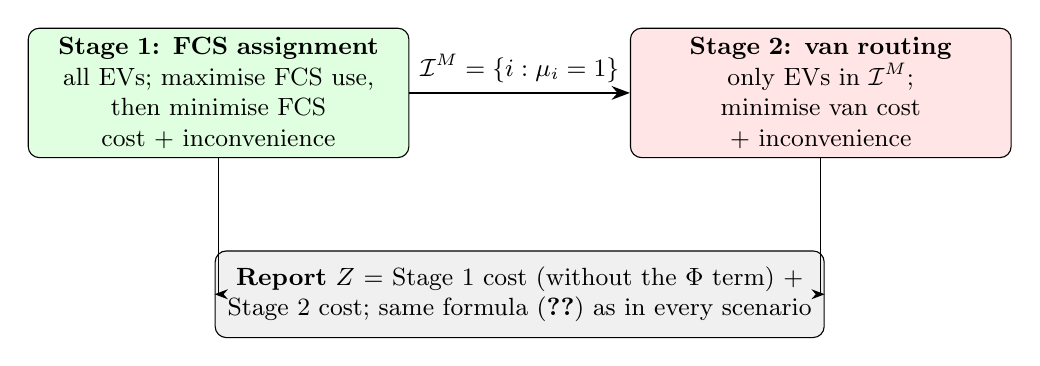
\begin{tikzpicture}[>=Stealth,box/.style={draw,rounded corners,align=center,minimum height=1.1cm,font=\small}]
  \node[box,fill=green!12,text width=4.6cm] (s1) {\textbf{Stage 1: FCS assignment}\\all EVs; maximise FCS use,\\then minimise FCS cost + inconvenience};
  \node[box,fill=red!10,text width=4.6cm,right=2.8cm of s1] (s2) {\textbf{Stage 2: van routing}\\only EVs in $\I^M$;\\minimise van cost + inconvenience};
  \draw[->,thick] (s1) -- node[above,font=\small]{$\I^M=\{i:\mu_i=1\}$} (s2);
  \node[box,fill=black!6,text width=7.5cm,below=2.0cm of $(s1)!0.5!(s2)$] (ev) {\textbf{Report} $Z=$ Stage~1 cost (without the $\Phi$ term) $+$ Stage~2 cost; same formula \eqref{eq:Z} as in every scenario};
  \draw[->] (s1) |- (ev); \draw[->] (s2) |- (ev);
\end{tikzpicture}
\end{center}

Stage~1 does not look at the vans, and Stage~2 cannot change what Stage~1 decided. That is the definition of ``FCS first, then MCS''.

%----------------------------------------------------------------
\subsection{Stage 1: assign EVs to fixed stations}

\textbf{Objective.}
\begin{equation}
\begin{split}
\min\ Z^{(1)}=\;&\underbrace{\Phi\sum_{i\in\I}\mu_i}_{\text{FCS first}}
+\underbrace{c^{EV}\sum_i\sum_{f\in\F_i}d_{if}Y_{if}}_{Z_1}
+\underbrace{Z^F_{\text{energy}}}_{\text{FCS part of }Z_4}\\
&+\underbrace{\sum_i\sum_{f\in\F_i}\rho^F_{if}Y_{if}+\alpha\sum_i w_i(C_i-r_i)+c^L\sum_i w_iL_i}_{\text{FCS customers' inconvenience}}
\end{split}
\label{eq:obj1}
\end{equation}
with $C_i=S_i+\tau^F_iY_i$ in this stage. $\Phi$ is a penalty for handing an EV to the vans. It is chosen larger than anything an extra FCS customer can add to the rest of \eqref{eq:obj1}, e.g.
\[
\Phi > \max_{i}\max_{f\in\F_i}\big(c^{EV}d_{if}+\pi^{\max}E_i+\rho^F_{if}\big)+n\,(\alpha+c^L)\,w_{\max}\,T,
\]
so Stage~1 first \textbf{maximises the number of EVs served at an FCS}, and only among those solutions minimises FCS cost and inconvenience. ($\pi^{\max}$ is the highest grid price.) A numerically safer equivalent is to solve twice: first $\max\sum_iY_i$, then fix that number and minimise the rest.
\ifTOU
Because $Z^F_{\text{energy}}$ uses the peak price, Stage~1 may \emph{start sessions later} to leave the peak, if the price saving beats the extra waiting cost (Section~\ref{sec:expect}).
\fi

\textbf{Constraints.}
\begin{align}
\sum_{g\in\G_i}y_{ig}+\mu_i &= 1 && \forall i\in\I \label{eq:s1assign}\\
S_i &\ge r_i+\sum_{f\in\F_i}t_{if}Y_{if} && \forall i\in\I \label{eq:fcsarr}\\
S_i &\le r_i+T\,(1-\mu_i) && \forall i\in\I \label{eq:s1park}\\
S_j &\ge S_i+\tau^F_i-(T+\tau^F_i)(3-y_{ig}-y_{jg}-o_{ij}) && \forall g,\ (i,j)\in\mathcal{P}_g \label{eq:disj1}\\
S_i &\ge S_j+\tau^F_j-(T+\tau^F_j)(2-y_{ig}-y_{jg}+o_{ij}) && \forall g,\ (i,j)\in\mathcal{P}_g \label{eq:disj2}\\
\sum_i y_{ig_1} &\ge \sum_i y_{ig_2} && \forall f,\ \G_f=\{g_1,g_2\} \label{eq:gunsym}\\
S_i+\tau^F_iY_i &\le T,\qquad L_i\ge S_i+\tau^F_iY_i-l_i && \forall i\in\I \label{eq:s1time}
\end{align}
\ifTOU plus the time-of-use split \eqref{eq:tou1}--\eqref{eq:tou5} of each FCS session (Section~\ref{sec:price}).\fi
\desc{\eqref{eq:s1assign}: every EV either gets one reachable gun or is handed to the vans. An EV that reaches no FCS ($\G_i=\emptyset$) is forced to $\mu_i=1$. \eqref{eq:fcsarr}: an FCS session cannot start before the EV has asked and driven to the station. \eqref{eq:s1park}: for an EV handed to the vans, $S_i$ is parked at $r_i$, so it adds no waiting in Stage~1 (its real start time is decided in Stage~2). \eqref{eq:disj1}--\eqref{eq:disj2}: two EVs on the same gun do not overlap; $o_{ij}$ picks who goes first. With two guns per station this means at most two EVs charge at a station at a time. \eqref{eq:gunsym}: symmetry breaking between the two identical guns (optional). \eqref{eq:s1time}: finished by $T$; lateness.}

\textbf{Optional acceptability rule.} An operator may refuse to send a driver to a station that is ``too inconvenient'', e.g.\ only allow gun $g$ of station $f$ for EV $i$ if $\hat\rho^F_{if}\le\bar\rho$. This only shrinks $\G_i$, so EVs whose stations are all too far go to the vans. Report results with and without it.

\textbf{Output:} $\I^M=\{i:\mu_i=1\}$, the EVs left for the vans; plus each FCS customer's gun and start time.

%----------------------------------------------------------------
\subsection{Stage 2: route the vans to the leftover EVs}

Stage~2 is a vehicle routing problem with time windows, on the EVs in $\I^M$ only. Here $C_i=S_i+\tau^M_i$.

\textbf{Objective.}
\begin{equation}
\begin{split}
\min\ Z^{(2)}=\;&\underbrace{c^M\sum_m\sum_{(i,j)\in\A^M}d_{ij}x_{ijm}}_{Z_2}+\underbrace{\sum_m c^D_mu_m}_{Z_3}+\underbrace{Z^M_{\text{energy}}}_{\text{van part of }Z_4}\\
&+\underbrace{\sum_{i\in\I^M}\sum_m\rho^M_{im}z_{im}+\alpha\sum_{i\in\I^M}w_i(C_i-r_i)+c^L\sum_{i\in\I^M}w_iL_i}_{\text{van customers' inconvenience}}
\end{split}
\label{eq:obj2}
\end{equation}
Since every EV in $\I^M$ must be served by some van, $Z^M_{\text{energy}}$ and the $\rho^M$ term are constants here. They are kept so that $Z^{(2)}$ is the true cost of Stage~2. Waiting and lateness make the vans visit urgent EVs early.

\textbf{Constraints.}
\begin{align}
\sum_{m\in\M}z_{im} &= 1 && \forall i\in\I^M \label{eq:s2assign}\\
\sum_{j:(0,j)\in\A^M}x_{0jm} = \sum_{i:(i,n+1)\in\A^M}x_{i,n+1,m} &= u_m && \forall m \label{eq:depot}\\
\sum_{i:(i,j)\in\A^M}x_{ijm} = \sum_{k:(j,k)\in\A^M}x_{jkm} &= z_{jm} && \forall j\in\I^M,\ m \label{eq:flow}\\
\sum_{i\in\I^M}z_{im} &\le Q_m\,u_m && \forall m \label{eq:cap}\\
\sum_{i\in\I^M}\frac{E_i}{\eta}z_{im}+\beta\sum_{(i,j)\in\A^M}d_{ij}x_{ijm} &\le B_m\,u_m && \forall m \label{eq:batt}
\end{align}
\begin{align}
S_j &\ge \max\{r_j,\ t_{0j}\,x_{0jm}\} && \forall j\in\I^M,\ m \label{eq:depart}\\
S_j &\ge S_i+\tau^M_i+t_{ij}-(T+\tau^M_i+t_{ij})(1-x_{ijm}) && \forall i\neq j,\ m \label{eq:seq}\\
S_i+\tau^M_i+t_{i,n+1} &\le T+(\tau^M_i+t_{i,n+1})(1-x_{i,n+1,m}) && \forall i,\ m \label{eq:return}\\
S_i+\tau^M_i \le T,\quad L_i &\ge S_i+\tau^M_i-l_i && \forall i\in\I^M \label{eq:s2time}\\
u_m &\ge u_{m+1} && m<|\M| \label{eq:vansym}
\end{align}
\desc{\eqref{eq:s2assign}: each leftover EV gets one van. \eqref{eq:depot}: a used van leaves and returns to the depot once. \eqref{eq:flow}: each EV on van $m$ is entered and left exactly once by that van. \eqref{eq:cap}: at most $Q_m$ EVs per van. \eqref{eq:batt}: delivered energy (with transfer losses) plus driving energy fits in the van battery. \eqref{eq:depart}: no start before the request, or before the van can drive there from the depot (written as two linear constraints). \eqref{eq:seq}: if the van goes $i\to j$, it finishes $i$ and drives to $j$ before starting $j$. This gives one EV at a time and removes subtours (MTZ-type). \eqref{eq:return}: back at the depot by $T$. \eqref{eq:s2time}: finished by $T$; lateness. \eqref{eq:vansym}: use identical vans in index order.}

\textbf{If Stage 2 is infeasible} (too many leftover EVs for the fleet by $T$), the sequential policy has \emph{failed} on that instance. For diagnosis, add $s_i\in\{0,1\}$ (``unserved''), replace \eqref{eq:s2assign} by $\sum_mz_{im}+s_i=1$ and add $\Phi^U\sum_is_i$ to \eqref{eq:obj2}. Then report the number of EVs that could not be served. This is a useful comparison with the integrated scenario, which may serve all of them.

%----------------------------------------------------------------
\subsection{Reported value}
\[
Z^{\text{S\scen}}=\big(Z^{(1)*}-\Phi\,|\I^M|\big)+Z^{(2)*},
\]
which is exactly \eqref{eq:Z} evaluated at the combined solution. The stage-1 solution plus the stage-2 solution is a feasible solution of the integrated model (S\ifTOU 4\else 3\fi), so
$Z^{\text{S\ifTOU 4\else 3\fi}}\le Z^{\text{S\scen}}$. The difference is the \emph{value of integration}.

\else
%---------------------------------------------------------------- INT
\subsection{Objective}
\begin{equation}
\min\ Z \quad\text{as in \eqref{eq:Z}, with }Z^F_{\text{energy}}=\ifTOU P^F\textstyle\sum_i\big[\pi^\off(\theta^1_i+\theta^3_i)+\pi^\pk\theta^2_i\big]\else\pi^F\textstyle\sum_iE_iY_i\fi,\quad C_i=S_i+\tau^F_iY_i+\tau^M_iZ_i. \label{eq:objint}
\end{equation}
Written out in full:
\begin{align*}
\min\ Z=\;& c^{EV}\sum_i\sum_{f\in\F_i}d_{if}Y_{if}+c^M\sum_m\sum_{(i,j)\in\A}d_{ij}x_{ijm}+\sum_mc^D_mu_m\\
&+\ifTOU P^F\sum_i\big[\pi^\off(\theta^1_i+\theta^3_i)+\pi^\pk\theta^2_i\big]\else\pi^F\sum_iE_iY_i\fi
+\pi^M\sum_i\sum_m\frac{E_i}{\eta}z_{im}\\
&+\sum_i\sum_{f\in\F_i}\rho^F_{if}Y_{if}+\sum_i\sum_m\rho^M_{im}z_{im}+\alpha\sum_iw_i(C_i-r_i)+c^L\sum_iw_iL_i .
\end{align*}
Every term is linear. One model weighs everything at once: an EV goes to a van exactly when the van's extra km, dispatch and energy cost are outweighed by the effort and waiting it saves the driver\ifTOU, or by the peak-price energy it avoids\fi.

\subsection{Constraints}

\textbf{Assignment.}
\begin{equation}
\sum_{g\in\G_i}y_{ig}+\sum_{m\in\M}z_{im}=1\qquad\forall i\in\I \label{eq:assign}
\end{equation}
\desc{Exactly one resource per EV: one reachable gun or one van. EVs that reach no FCS are forced onto a van.}

\textbf{Fixed stations.}
\begin{align}
S_i &\ge r_i+\sum_{f\in\F_i}t_{if}Y_{if} && \forall i \label{eq:fcsarr}\\
S_j &\ge S_i+\tau^F_i-(T+\tau^F_i)(3-y_{ig}-y_{jg}-o_{ij}) && \forall g,\ (i,j)\in\mathcal{P}_g \label{eq:disj1}\\
S_i &\ge S_j+\tau^F_j-(T+\tau^F_j)(2-y_{ig}-y_{jg}+o_{ij}) && \forall g,\ (i,j)\in\mathcal{P}_g \label{eq:disj2}\\
\sum_iy_{ig_1} &\ge \sum_iy_{ig_2} && \forall f,\ \G_f=\{g_1,g_2\} \label{eq:gunsym}
\end{align}
\desc{\eqref{eq:fcsarr}: an FCS session starts after the request and the drive to the station (for a van customer this is just $S_i\ge r_i$). \eqref{eq:disj1}--\eqref{eq:disj2}: EVs on the same gun do not overlap; $o_{ij}$ chooses the order. \eqref{eq:gunsym}: optional symmetry breaking.}

\textbf{Vans: routes, capacity, battery.}
\begin{align}
\sum_{j:(0,j)\in\A}x_{0jm}=\sum_{i:(i,n+1)\in\A}x_{i,n+1,m} &= u_m && \forall m \label{eq:depot}\\
\sum_{i:(i,j)\in\A}x_{ijm}=\sum_{k:(j,k)\in\A}x_{jkm} &= z_{jm} && \forall j\in\I,\ m \label{eq:flow}\\
\sum_iz_{im} &\le Q_mu_m && \forall m \label{eq:cap}\\
\sum_i\frac{E_i}{\eta}z_{im}+\beta\sum_{(i,j)\in\A}d_{ij}x_{ijm} &\le B_mu_m && \forall m \label{eq:batt}
\end{align}
\desc{\eqref{eq:depot}: a used van leaves and returns once. \eqref{eq:flow}: each EV on van $m$ is visited exactly once by it. \eqref{eq:cap}: at most $Q_m$ EVs. \eqref{eq:batt}: delivered energy (with losses) plus driving energy fits in the battery.}

\textbf{Vans: timing (one EV at a time, no subtours).}
\begin{align}
S_j &\ge t_{0j}\,x_{0jm} && \forall j\in\I,\ m \label{eq:depart}\\
S_j &\ge S_i+\tau^M_i+t_{ij}-(T+\tau^M_i+t_{ij})(1-x_{ijm}) && \forall i\neq j\in\I,\ m \label{eq:seq}\\
S_i+\tau^M_i+t_{i,n+1} &\le T+(\tau^M_i+t_{i,n+1})(1-x_{i,n+1,m}) && \forall i,\ m \label{eq:return}
\end{align}
\desc{\eqref{eq:depart}: the first stop cannot start before the van has driven there. \eqref{eq:seq}: $i\to j$ means finish $i$, drive, then start $j$; start times rise along a route, so no subtour can close. \eqref{eq:return}: back at the depot by $T$.}

\textbf{Horizon and lateness.}
\begin{equation}
C_i\le T,\qquad L_i\ge C_i-l_i\qquad\forall i\in\I \label{eq:time}
\end{equation}
\desc{Every EV is fully charged within the horizon; $L_i$ measures lateness.}

\ifTOU
\textbf{Time-of-use split.} Constraints \eqref{eq:tou1}--\eqref{eq:tou5} of Section~\ref{sec:price}.
\fi

\textbf{Symmetry and domains.}
\begin{equation}
u_m\ge u_{m+1};\qquad y,z,x,u,o\ifTOU,\kappa\fi\in\{0,1\};\qquad S_i,L_i\ifTOU,\theta^p_i\fi\ge0 \label{eq:dom}
\end{equation}
\fi

%=====================================================================
\section{Learning-to-optimise (RL) formulation}\label{sec:rl}

\textbf{Main rule:} the reward of each action is \emph{minus the increase in $Z$ that the action causes}. The rewards over an episode then add up to $-Z$ of the solution the policy builds. RL and MILP results are measured on the same yardstick \eqref{eq:Z}, and the MILP optimum is the benchmark for the RL gap.

\ifSEQ
%---------------------------------------------------------------- RL SEQ
The RL pipeline has the same two stages as the MILP.

\subsection{Stage 1 policy: FCS assignment}
\begin{itemize}[leftmargin=1.4em,itemsep=2pt]
  \item \textbf{Episode / epochs:} EVs are taken in order of request time $r_i$ (ties: higher $w_i$ first). One decision per EV.
  \item \textbf{State:} features of the current EV $k$ ($E_k,r_k,l_k,w_k,R_k$, location); for each gun $g$ the time $F_g$ it becomes free; summary features of the EVs still to come (count and positions near each station)\ifTOU; the current price and the time until $T_1$ and $T_2$\fi.
  \item \textbf{Action:} a gun $g\in\G_k$, or ``hand to vans''. \textbf{FCS-first mask:} ``hand to vans'' is allowed \emph{only} if no gun can finish EV $k$ by $T$ (or, with the optional rule, if all remaining guns have $\hat\rho^F_{kf}>\bar\rho$).
  \ifTOU\item \textbf{Optional timing action:} ``gun $g$, start after the peak'', i.e.\ $S_k=\max\{\text{earliest},T_2\}$, allowed only if the session still ends by $T$.\fi
  \item \textbf{Transition:} $S_k=\max\{r_k+t_{kf},F_g\}$ (or later, for the timing action); $F_g\leftarrow S_k+\tau^F_k$.
  \item \textbf{Reward:} $-\Big[c^{EV}d_{kf}+\text{energy}_k+\rho^F_{kf}+\alpha w_k(S_k+\tau^F_k-r_k)+c^Lw_k(S_k+\tau^F_k-l_k)^+\Big]$, where energy$_k$ = \ifTOU$P^F\big[\pi^\off\cdot(\text{off-peak hours of }[S_k,S_k+\tau^F_k])+\pi^\pk\cdot(\text{peak hours})\big]$, computed exactly in the simulator\else$\pi^FE_k$\fi. Handing an EV to the vans gives reward $0$ here; its cost is counted in Stage~2.
\end{itemize}
Note: a simple baseline for Stage~1 is the greedy rule ``gun with the largest one-step reward''. What RL can learn on top of this is, for example, to keep a nearby gun free for an urgent EV that arrives later.

\subsection{Stage 2 policy: van routing over $\I^M$}
\begin{itemize}[leftmargin=1.4em,itemsep=2pt]
  \item \textbf{Epochs:} whenever a van becomes free (the earliest-free van decides first).
  \item \textbf{State:} for each van: position, time free, remaining battery $b_m$, EVs served so far, dispatched or not; for each unserved EV in $\I^M$: location, $E_i,r_i,l_i,w_i$; current time.
  \item \textbf{Action:} the next EV $j$ for this van, or ``return to depot'' (ends the route). Mask: $j$ must be feasible: battery covers $E_j/\eta$ plus driving to $j$ and back to the depot, the count stays $\le Q_m$, and $j$ can be finished with the van back at the depot by $T$.
  \item \textbf{Transition:} $S_j=\max\{r_j,\ \text{time free}+t_{\text{pos},j}\}$; the van moves to $j$ and is free at $S_j+\tau^M_j$; $b_m$ falls by $E_j/\eta+\beta d_{\text{pos},j}$.
  \item \textbf{Reward:} serving $j$: $-\Big[c^Md_{\text{pos},j}+c^D_m[\text{first stop}]+\pi^M\frac{E_j}{\eta}+\rho^M_{jm}+\alpha w_j(S_j+\tau^M_j-r_j)+c^Lw_j(S_j+\tau^M_j-l_j)^+\Big]$; returning: $-c^Md_{\text{pos},0}$. EVs still unserved at the end: $-\Phi^U$ each.
  \item \textbf{Policy:} an attention-based routing policy (e.g.\ Kool et al., 2019, ``Attention, Learn to Solve Routing Problems!'') trained with REINFORCE or PPO. Baseline: nearest-feasible-EV heuristic.
\end{itemize}
Episode return of Stage~1 + Stage~2 $=-Z^{\text{S\scen}}$.

\else
%---------------------------------------------------------------- RL INT
One policy decides both who serves each EV and the van routes.
\begin{itemize}[leftmargin=1.4em,itemsep=2pt]
  \item \textbf{Episode / epochs:} EVs are taken in order of request time $r_i$ (ties: higher $w_i$ first). One decision per EV.
  \item \textbf{State:} (i) the current EV $k$: location, $E_k,r_k,l_k,w_k,R_k$, reachable stations; (ii) each gun $g$: time $F_g$ it becomes free; (iii) each van $m$: current end-of-route position, time free, remaining battery $b_m$, EVs served, dispatched or not; (iv) embeddings of the not-yet-assigned EVs (for look-ahead)\ifTOU; (v) current price, time until $T_1$ and $T_2$\fi.
  \item \textbf{Action:} $a\in\G_k\cup\M$: a gun, or a van (EV $k$ is appended to the end of that van's route). \textbf{Mask} infeasible actions: a gun that cannot finish $k$ by $T$; a van without enough battery for $E_k/\eta$ plus the drive to $k$ and back to the depot, with $Q_m$ reached, or unable to finish $k$ and return by $T$.
  \ifTOU\item \textbf{Optional timing action:} ``gun $g$, start after the peak'' ($S_k=\max\{\text{earliest},T_2\}$, if it still ends by $T$).\fi
  \item \textbf{Transition:} gun: $S_k=\max\{r_k+t_{kf},F_g\}$, $F_g\leftarrow S_k+\tau^F_k$. Van: $S_k=\max\{r_k,\ \text{free}_m+t_{\text{pos}_m,k}\}$, then the van moves to $k$, $\text{free}_m\leftarrow S_k+\tau^M_k$, $b_m\mathrel{-}=E_k/\eta+\beta d_{\text{pos}_m,k}$.
  \item \textbf{Reward} $=-\Delta Z$:
  \begin{align*}
  \text{gun } g\text{ at }f:&\quad -\Big[c^{EV}d_{kf}+\text{energy}^F_k+\rho^F_{kf}+\alpha w_k(C_k-r_k)+c^Lw_k(C_k-l_k)^+\Big]\\
  \text{van } m:&\quad -\Big[c^M\big(d_{\text{pos}_m,k}+d_{k,0}-d_{\text{pos}_m,0}\big)+c^D_m[\text{first use}]+\pi^M\tfrac{E_k}{\eta}\\
  &\qquad\quad+\rho^M_{km}+\alpha w_k(C_k-r_k)+c^Lw_k(C_k-l_k)^+\Big]
  \end{align*}
  The van distance term is the \emph{change} in route length when $k$ is inserted before the return to the depot, so the sum over the episode equals the total route length (the return legs telescope). energy$^F_k$ = \ifTOU$P^F\big[\pi^\off\cdot(\text{off-peak hours})+\pi^\pk\cdot(\text{peak hours of }[S_k,C_k])\big]$, computed exactly by the simulator; no linearisation is needed in RL\else$\pi^FE_k$\fi.
  \item \textbf{Dead end:} if every action is masked, EV $k$ is unserved: reward $-\Phi^U$, and the episode continues. Report the count.
  \item \textbf{Policy:} masked categorical policy over guns and vans, encoder with attention over EVs, guns and vans; trained with PPO. Natural baseline: greedy, i.e.\ choose the action with the largest one-step reward. That is the pairwise rule ``smallest $\hat\rho$ + cost'' from Section~\ref{sec:inc}.
\end{itemize}
Restriction to note: vans serve EVs in assignment order (append only). A variant that inserts $k$ at the cheapest position of a route is more flexible but has a larger action space.
\fi

\textbf{Reward scaling.} For stable training divide every reward by a constant, e.g.\ the greedy baseline's average $Z$ on the training instances. This does not change the optimal policy.

%=====================================================================
\section{What to expect and what to report}\label{sec:expect}

\ifnum\scen=1
\begin{itemize}[leftmargin=1.4em,itemsep=2pt]
  \item Vans serve only EVs that reach no station, or that the stations cannot finish by $T$. If stations have spare capacity, very few vans are dispatched.
  \item Inconvenience is high for EVs far from the nearest station (worked example: Rs\,682 at the FCS, against Rs\,458 if a van had been allowed).
  \item With too few vans Stage~2 becomes infeasible (unserved EVs), even when the integrated model S3 could serve everyone. Report the smallest $|\M|$ at which S1 is feasible and compare it with S3.
\end{itemize}
\fi
\ifnum\scen=2
\begin{itemize}[leftmargin=1.4em,itemsep=2pt]
  \item \textbf{When does Stage~1 delay a session to avoid the peak?} Moving one hour of charging out of the peak saves $(\pi^\pk-\pi^\off)P^F=3\times22=$ Rs\,66, but delays completion by up to an hour, which costs $\alpha w_i\ge$ Rs\,200. So with the default values Stage~1 almost never delays. It mostly pays the higher price, and S2 costs roughly S1 plus the peak surcharge. Sessions start later only if $\alpha$ is small (try $\lambda<0.33$ in the sensitivity analysis).
  \item The van assignment is the same as in S1 unless Stage~1's timing changes which EVs fit at the stations. Stage~1 cannot use vans to escape the peak price.
  \item Extra KPI: \textbf{grid energy drawn at FCS during the peak}, $P^F\sum_i\theta^2_i$ (kWh). Compare with S4.
\end{itemize}
\fi
\ifnum\scen=3
\begin{itemize}[leftmargin=1.4em,itemsep=2pt]
  \item Vans take EVs for which the saved inconvenience exceeds the extra van cost (worked example: van chosen, saving Rs\,224). Expect vans to serve EVs that are far from every station, have low range (high $w_i$), or have early deadlines, while EVs near a station still use it.
  \item \textbf{Value of integration under flat price:} $Z^{\text{S1}}-Z^{\text{S3}}\ge0$. Report it per component ($Z_1,\dots,Z_5$): typically operating cost rises a little and inconvenience falls a lot.
  \item Vary $|\M|$ (0, 1, 2, \dots): the first few vans lower $Z$ sharply, then the effect levels off. That curve shows the scenarios where mobile chargers help most.
\end{itemize}
\fi
\ifnum\scen=4
\begin{itemize}[leftmargin=1.4em,itemsep=2pt]
  \item During the peak a van kWh costs about the same as an FCS kWh (Rs\,10.0 each), so the vans' energy disadvantage disappears and vans also absorb \emph{peak-hour} demand that would otherwise be charged on the grid at peak price.
  \item Expect more van usage than in S3, concentrated on requests in $[T_1,T_2]$, and lower grid energy at the stations during the peak, $P^F\sum_i\theta^2_i$, than in S2.
  \item \textbf{Value of integration under peak pricing:} $Z^{\text{S2}}-Z^{\text{S4}}$. It should be larger than $Z^{\text{S1}}-Z^{\text{S3}}$, because integration now also allows price arbitrage.
  \item \textbf{Peak pricing with full flexibility:} $Z^{\text{S4}}-Z^{\text{S3}}$ should be smaller than $Z^{\text{S2}}-Z^{\text{S1}}$: vans cushion the price increase.
\end{itemize}
\fi

\textbf{Cross-scenario comparison table} (fill in from the four runs):
\begin{center}
\renewcommand{\arraystretch}{1.2}
\begin{tabular}{@{}lll@{}}
\toprule
\textbf{Comparison} & \textbf{Measures} & \textbf{Expected sign} \\
\midrule
S1 $-$ S3 & value of integration, flat price & $\ge0$ \\
S2 $-$ S4 & value of integration, peak price & $\ge0$, larger than S1 $-$ S3 \\
S2 $-$ S1 & cost of peak pricing, FCS-first operator & $>0$ \\
S4 $-$ S3 & cost of peak pricing, flexible operator & $>0$, smaller than S2 $-$ S1 \\
\bottomrule
\end{tabular}
\end{center}
Report for each: $Z$ and its components, number of vans used, EVs per resource, mean and maximum inconvenience per EV, total lateness, peak-hour grid energy, solve time, and (for RL) the gap to the MILP optimum.

%=====================================================================
\appendix
\section{Illustrative parameter values}\label{app:values}

These are starting values for experiments, not data. All are meant to be varied in the analysis. Values in Rs.

\begin{center}
\renewcommand{\arraystretch}{1.15}
\begin{tabular}{@{}llp{6.2cm}@{}}
\toprule
\textbf{Parameter} & \textbf{Value} & \textbf{Note} \\
\midrule
$T$, $[T_1,T_2]$ & 7 h, $[2,6]$ & 16:00--23:00, peak 18:00--22:00 \\
$P^F$, $P^M$ & 22 kW, 30 kW & \\
$v$, $\beta$, $\eta$ & 25 km/h, 0.25 kWh/km, 0.9 & \\
$B_m$, $Q_m$, $|\M|$ & 150 kWh, 6, 2--6 & \\
$c^{EV}$, $c^M$, $c^D_m$ & Rs\,4/km, Rs\,15/km, Rs\,1500 & van km includes driver time \\
$\pi^F$ (flat) & Rs\,8.7/kWh & equals the time-average of the ToU tariff over $[0,T]$ \\
$\pi^\off$, $\pi^\pk$ (ToU) & Rs\,7/kWh, Rs\,10/kWh & $(3\times7+4\times10)/7=8.7$ \\
$c^{bat}$ & Rs\,2/kWh & van battery wear \\
$\pi^M$ & Rs\,10.7 (flat) / Rs\,9.0 (ToU) & $=\pi^F+c^{bat}$ / $=\pi^\off+c^{bat}$ \\
$\alpha$, $\alpha^D$ & Rs\,200/h, Rs\,100/h & value of time; extra for attended time \\
$h^F$, $h^M$, $\varphi$ & Rs\,50, Rs\,10, Rs\,100 & trip hassle, hand-over, range stress \\
$c^L$ & Rs\,300/h & lateness \\
$w_i$ & $1+2(1-R_i/R_{\max})$, $R_i\sim U[3,40]$ km & priority from remaining range \\
\bottomrule
\end{tabular}
\end{center}

The flat price is set to the time-average of the peak tariff. The price \emph{level} is then the same in both pricing cases, and only the price \emph{shape} differs. Without this, part of S1 vs S2 would just reflect a different average price.

\end{document}
"
%  (run each twice for cross-references)
% =====================================================================
\documentclass[11pt,a4paper]{article}
\usepackage[margin=2.2cm]{geometry}
\usepackage{amsmath,amssymb,amsfonts}
\usepackage{booktabs,array,tabularx}
\usepackage{enumitem}
\usepackage[table]{xcolor}
\usepackage{tikz}
\usetikzlibrary{arrows.meta,positioning,calc}
\usepackage[colorlinks=true,linkcolor=blue!50!black,urlcolor=blue!50!black]{hyperref}
\usepackage{titlesec}
\titleformat{\section}{\large\bfseries}{\thesection}{0.8em}{}
\titleformat{\subsection}{\normalsize\bfseries}{\thesubsection}{0.8em}{}
\setlength{\parindent}{0pt}
\setlength{\parskip}{5pt}

% ---------------- scenario switches ----------------
\ifdefined\scen\else\def\scen{1}\fi
\newif\ifTOU \TOUfalse   % true = time-of-use (peak) price
\newif\ifSEQ \SEQfalse   % true = FCS first, then MCS
\ifnum\scen=1 \SEQtrue \fi
\ifnum\scen=2 \TOUtrue \SEQtrue \fi
\ifnum\scen=4 \TOUtrue \fi

\newcommand{\pricename}{\ifTOU time-of-use price (dearer evening peak)\else single (flat) price all day\fi}
\newcommand{\structname}{\ifSEQ FCS first, then MCS (sequential)\else FCS and MCS together (integrated)\fi}

% ---------------- notation ----------------
\newcommand{\I}{\mathcal{I}}
\newcommand{\F}{\mathcal{F}}
\newcommand{\G}{\mathcal{G}}
\newcommand{\M}{\mathcal{M}}
\newcommand{\N}{\mathcal{N}}
\newcommand{\A}{\mathcal{A}}
\newcommand{\Rs}{\text{Rs}\,}
\newcommand{\pk}{\mathrm{pk}}
\newcommand{\off}{\mathrm{off}}
\newcommand{\desc}[1]{\par\vspace{-2pt}{\small\color{black!75}\textit{Meaning:} #1}\par\vspace{4pt}}
\newcommand{\cell}[2]{\ifnum\scen=#1\cellcolor{blue!18}\textbf{S#1 (this document)}\\\textbf{#2}\else S#1\\#2\fi}

\title{\textbf{EV Charging Network Optimisation}\\[4pt]
\large Scenario \scen: \pricename\ $+$ \structname\\[2pt]
\normalsize MILP and RL formulation}
\author{CP 320 OR for Mobility Management, course project}
\date{2 October 2026}

\begin{document}
\maketitle

%=====================================================================
\section{Where this scenario sits}

The project studies four scenarios: two ways of pricing grid electricity, times two ways of making the decisions.

\begin{center}
\renewcommand{\arraystretch}{1.5}
\begin{tabular}{>{\raggedright\arraybackslash}p{4.2cm}|>{\centering\arraybackslash}p{4.6cm}|>{\centering\arraybackslash}p{4.6cm}}
 & \textbf{Flat price all day} & \textbf{Time-of-use (peak) price} \\ \hline
\textbf{Sequential:} FCS first, leftover EVs to MCS &
\begin{tabular}[c]{@{}c@{}}\cell{1}{flat + sequential}\end{tabular} &
\begin{tabular}[c]{@{}c@{}}\cell{2}{peak + sequential}\end{tabular} \\ \hline
\textbf{Integrated:} FCS and MCS decided together &
\begin{tabular}[c]{@{}c@{}}\cell{3}{flat + integrated}\end{tabular} &
\begin{tabular}[c]{@{}c@{}}\cell{4}{peak + integrated}\end{tabular} \\
\end{tabular}
\end{center}

\textbf{The four scenarios do not have four different objectives.} They share \emph{one} cost yardstick $Z$ (Section~\ref{sec:obj}): the same cost terms and the same customer inconvenience (Section~\ref{sec:inc}). Only two things change:
\begin{itemize}[leftmargin=1.4em,itemsep=1pt]
  \item \textbf{Pricing} changes the formula for one term, the FCS energy cost (Section~\ref{sec:price}).
  \item \textbf{Decision structure} changes \emph{how} $Z$ is minimised: in one model (integrated), or in two stages (sequential), where each stage minimises its own part of $Z$.
\end{itemize}
Because the yardstick is the same, the four optimal values can be compared directly. The differences measure the \emph{value of integration} (S1$\to$S3, S2$\to$S4) and the \emph{effect of peak pricing} (S1$\to$S2, S3$\to$S4).

\ifnum\scen=1
\textbf{This scenario (S1)} is the baseline, the ``status quo''. Electricity costs the same at every hour, every EV that can be charged at a fixed station is sent there, and vans only take what is left over.
\fi
\ifnum\scen=2
\textbf{This scenario (S2)} keeps the FCS-first rule of S1, but grid electricity is dearer during the evening peak. Stage~1 can react to the price only by \emph{rescheduling} FCS sessions. It cannot hand a peak-hour EV to a van.
\fi
\ifnum\scen=3
\textbf{This scenario (S3)} keeps the flat price of S1, but the operator decides FCS and MCS service \emph{together}. An EV can be sent to a van even when a fixed station could take it, whenever that lowers total cost plus inconvenience.
\fi
\ifnum\scen=4
\textbf{This scenario (S4)} is the most flexible one: peak pricing at fixed stations, and FCS and MCS decided together. Van energy was bought off-peak, so vans can also be used to keep charging \emph{out of the expensive peak}.
\fi

%=====================================================================
\section{Setting and assumptions}\label{sec:setting}

\textbf{Time.} The planning horizon is $[0,T]$ with $T=7$\,h (16:00--23:00). It contains the evening peak window $[T_1,T_2]=[2,6]$ (18:00--22:00). The horizon is the same in all four scenarios. It is wider than the peak itself so that, under peak pricing, there is cheaper time on both sides of the peak.\ifTOU\else\ In this scenario the price is flat, so the window plays no role in the model.\fi

\textbf{Assumptions} (the same as MILP v3, plus two about energy):
\begin{enumerate}[leftmargin=1.6em,itemsep=1pt]
  \item Static, continuous time. All requests in the horizon are known at time $0$, and request $i$ becomes active at $r_i$.
  \item An EV served by an FCS drives there itself on its own battery (only to stations within its range $R_i$). The driver stays with the car while it waits for a free gun and while it charges.
  \item An EV served by an MCS stays parked where it is, and the driver is free in the meantime.
  \item Each FCS gun and each van charges one EV at a time, without interruption, at constant power.
  \item A van's battery covers both its driving and the energy it delivers. \textbf{The van battery is charged at the depot before the horizon starts}\ifTOU, i.e.\ at the off-peak price\fi, and is not recharged during the horizon.
  \item Every EV must be fully charged by $T$ (hard). Finishing after the driver's desired time $l_i$ is allowed but penalised.
\end{enumerate}

%=====================================================================
\section{Notation}\label{sec:notation}

\subsection*{Sets}
\begin{tabularx}{\textwidth}{@{}lX@{}}
\toprule
$\I=\{1,\dots,n\}$ & EV charging requests \\
$\F$; $\G_f$ ($|\G_f|=2$); $\G=\bigcup_f\G_f$ & fixed charging stations; guns of FCS $f$; all guns ($f(g)$ = station of gun $g$) \\
$\F_i=\{f: d_{if}\le R_i\}$, $\G_i=\bigcup_{f\in\F_i}\G_f$ & stations / guns EV $i$ can reach on its remaining range \\
$\M$ & mobile charging vans (MCS) \\
$0,\ n+1$ & depot as start node / end node (same place) \\
$\N=\{0\}\cup\I\cup\{n+1\}$, $\A$ & routing nodes; allowed van arcs $(i,j)$, $i\in\{0\}\cup\I$, $j\in\I\cup\{n+1\}$, $i\neq j$ \\
$\mathcal{P}_g=\{(i,j): i<j,\ g\in\G_i\cap\G_j\}$ & pairs of EVs that could share gun $g$ \\
\ifSEQ
$\I^M\subseteq\I$ & EVs handed to the vans by Stage~1 (an \emph{output} of Stage~1, a fixed input to Stage~2) \\
$\N^M$, $\A^M$ & routing nodes / arcs restricted to $\I^M$ \\
\fi
\bottomrule
\end{tabularx}

\subsection*{Parameters}
\begin{tabularx}{\textwidth}{@{}lX@{}}
\toprule
$E_i,\ r_i,\ l_i,\ R_i$ & energy demand (kWh), request time, desired completion time (h), remaining range (km) \\
$w_i\ge1$ & priority of EV $i$; $w_i=1+\kappa(1-R_i/R_{\max})$, so low-range EVs weigh more \\
$P^F,\ P^M$ & charging power of an FCS gun (22\,kW) / of a van (e.g.\ 30\,kW) \\
$\tau^F_i=E_i/P^F,\ \tau^M_i=E_i/P^M$ & charging time of EV $i$ at an FCS / by a van (h) \\
$d_{if},t_{if}$;\ $d_{ij},t_{ij}$ & distance (km) and time (h): EV$\to$FCS; between routing nodes ($t=d/v$) \\
$B_m,\ Q_m,\ \beta,\ \eta$ & van battery (kWh), max EVs per van, van consumption (kWh/km), transfer efficiency \\
$c^{EV},\ c^M,\ c^D_m$ & cost per km of EV driving, per km of van driving; fixed dispatch cost of van $m$ \\
\ifTOU
$\pi^\off,\ \pi^\pk$ & grid price (Rs/kWh) off-peak / in $[T_1,T_2]$, with $\pi^\pk\ge\pi^\off$ \\
\else
$\pi^F$ & grid price (Rs/kWh), the same at every hour \\
\fi
$c^{bat}$ & van battery wear per kWh cycled \\
$\pi^M$ & cost of 1 kWh taken from a van battery: $\pi^M=\ifTOU\pi^\off\else\pi^F\fi+c^{bat}$ (Section~\ref{sec:price}) \\
$\alpha,\ \alpha^D,\ h^F,\ h^M,\ \varphi,\ c^L$ & inconvenience coefficients (Section~\ref{sec:inc}) \\
\bottomrule
\end{tabularx}

\subsection*{Decision variables}
\begin{tabularx}{\textwidth}{@{}llX@{}}
\toprule
$y_{ig}$ & $\{0,1\}$ & EV $i$ charged at gun $g\in\G_i$ \\
$z_{im}$ & $\{0,1\}$ & EV $i$ served by van $m$ \\
$x_{ijm}$ & $\{0,1\}$ & van $m$ drives arc $(i,j)$ \\
$u_m$ & $\{0,1\}$ & van $m$ is dispatched \\
$o_{ij}$ & $\{0,1\}$ & for EVs $i<j$ that could share a gun: 1 if $i$ is charged before $j$ \\
\ifSEQ
$\mu_i$ & $\{0,1\}$ & Stage~1 only: EV $i$ is handed to the van fleet \\
\fi
\ifTOU
$\theta^1_i,\theta^2_i,\theta^3_i$ & $\ge0$ & hours of EV $i$'s FCS session before / inside / after the peak \\
$\kappa^1_i,\kappa^3_i$ & $\{0,1\}$ & EV $i$'s FCS session starts before $T_1$ / ends after $T_2$ \\
\fi
$S_i$ & $\ge0$ & time charging of EV $i$ starts (h), on whichever resource \\
$L_i$ & $\ge0$ & lateness of EV $i$ beyond $l_i$ (h) \\
\bottomrule
\end{tabularx}

\textbf{Short-hands} (linear expressions, not new variables):
\[
Y_{if}=\sum_{g\in\G_f}y_{ig},\qquad Y_i=\sum_{g\in\G_i}y_{ig}\ (\text{EV $i$ uses an FCS}),\qquad Z_i=\sum_{m\in\M}z_{im}\ (\text{EV $i$ uses a van}),
\]
\[
C_i=S_i+\tau^F_i\,Y_i+\tau^M_i\,Z_i \quad\text{(time EV $i$ is fully charged).}
\]

%=====================================================================
\section{Customer inconvenience}\label{sec:inc}

This section is \textbf{identical in all four scenario documents}. Inconvenience is a property of the customer, not of the price or of the planning method.

\subsection{What we mean by inconvenience}

Inconvenience is \emph{what the driver loses} from the moment they ask for a charge ($r_i$) until the car is fully charged ($C_i$), \emph{converted into rupees} so it can be added to the operator's costs. A driver loses three different things:

\begin{enumerate}[leftmargin=1.6em,itemsep=2pt]
  \item \textbf{Waiting:} the car is not ready. This lasts $C_i-r_i$ hours and affects \emph{every} driver, FCS or MCS.
  \item \textbf{Effort:} only an FCS customer has to drive to the station and sit there while the car charges. An MCS customer stays at home or at work and does something else. Driving to a far station also uses scarce battery range, which causes stress (``range anxiety'').
  \item \textbf{A missed deadline:} the car is still not ready at the time $l_i$ the driver needs it.
\end{enumerate}

Each loss gets a price in Rs per hour (or per event). All of them are multiplied by the priority $w_i$: an hour of delay for an EV with 5\,km of range left counts more than for one with 40\,km.

\subsection{The three components}

\begin{center}
\renewcommand{\arraystretch}{1.3}
\begin{tabularx}{\textwidth}{@{}>{\raggedright\arraybackslash}p{2.6cm}>{\raggedright\arraybackslash}X>{\raggedright\arraybackslash}X>{\raggedright\arraybackslash}p{3.0cm}@{}}
\toprule
\textbf{Component} & \textbf{EV $i$ at FCS $f$} & \textbf{EV $i$ by a van} & \textbf{Known when?} \\
\midrule
Effort & $w_i\big[\alpha^D(t_{if}+\tau^F_i)+h^F+\varphi\,d_{if}/R_i\big]$: driving and sitting at the station, a fixed trip hassle, range stress & $w_i\,h^M$: being reachable and handing over the car & \textbf{Static:} known as soon as the resource is chosen \\
Waiting & $w_i\,\alpha\,(C_i-r_i)$ = drive + \emph{queue at the gun} + charge & $w_i\,\alpha\,(C_i-r_i)$ = \emph{wait for the van} + charge & \textbf{Dynamic:} depends on the queue / van route \\
Missed deadline & $w_i\,c^L\,L_i$, $L_i=\max\{0,C_i-l_i\}$ & same & Dynamic \\
\bottomrule
\end{tabularx}
\end{center}

\textbf{Coefficients.}
$\alpha$ (Rs/h) is the value of an hour the car is not ready.
$\alpha^D$ (Rs/h) is the \emph{extra} value of an hour the driver must personally spend driving or sitting at the station: an hour at the station costs $\alpha+\alpha^D$, an hour waiting at home for a van costs only $\alpha$.
$h^F,h^M$ (Rs) are fixed hassle costs of one trip to a station / one van hand-over.
$\varphi$ (Rs) is the range-stress cost of a trip that uses the \emph{whole} remaining range ($d_{if}/R_i\le1$ is the fraction used).
$c^L$ (Rs/h) is the cost per hour late.

\subsection{Pairwise form: inconvenience of a (customer, resource) pair}

The natural first idea is: \emph{for every pair (EV $i$, FCS $f$) and every pair (EV $i$, van $m$) there is an inconvenience number, and the operator picks the pair with the lowest cost plus inconvenience.} The static part fits this idea exactly:
\[
\boxed{\;\rho^F_{if}=w_i\Big[\alpha^D\,(t_{if}+\tau^F_i)+h^F+\varphi\,\frac{d_{if}}{R_i}\Big]\qquad
\rho^M_{im}=w_i\,h^M\;}
\]
These are \textbf{parameters}, computed before solving, one number per (EV, FCS) pair and per (EV, van) pair. In the objective they appear linearly: $\sum_i\sum_f\rho^F_{if}Y_{if}+\sum_i\sum_m\rho^M_{im}z_{im}$.

Note that $\rho^M_{im}$ does not depend on $m$. Vans are identical and all start at the same depot, so the driver does not care \emph{which} van comes, only \emph{when} it comes. That ``when'' is the waiting part.

\subsection{Why waiting cannot be a fixed pairwise number}

It is tempting to also write the waiting as a pairwise number, e.g.\ ``the van needs 5 minutes to reach EV $i$''. But that depends on \emph{where the van is coming from}, which depends on the route the model is still choosing: if EV $i$ is the 4th stop of a van, the wait is the time for three charging sessions plus four drives. Likewise, waiting at an FCS depends on how many EVs are queued at that gun. So waiting is not known before solving. It is a function of decision variables:
\[
\text{waiting cost of EV } i \;=\; w_i\,\alpha\,(C_i-r_i),\qquad C_i=S_i+\tau^F_iY_i+\tau^M_iZ_i .
\]
This is \textbf{linear} in the variables ($S_i$, $y$, $z$), so it fits in a MILP directly. The constraints of Section~\ref{sec:milp} make $S_i$ equal to the true start time, including driving, queueing at the gun and the van's route. The term $\sum_i w_i\alpha r_i$ is a constant and may be dropped when solving.

\textbf{Pairwise \emph{estimate}} (used for intuition, by the RL policy and in heuristics): if there is no queue and the van comes straight to $i$,
\[
\hat\rho^{F}_{if}=\rho^F_{if}+w_i\alpha\,(t_{if}+\tau^F_i),\qquad
\hat\rho^{M}_{im}=\rho^M_{im}+w_i\alpha\,(t^{\text{van}}_{m\to i}+\tau^M_i),
\]
where $t^{\text{van}}_{m\to i}$ is the time until van $m$ can reach $i$ from where it currently is. In the RL formulation (Section~\ref{sec:rl}) the van's position \emph{is} known at each decision, so there this estimate becomes exact.

\subsection{Total inconvenience and how it enters the objective}

\begin{equation}
\boxed{\;
Z_{\text{inc}}=\underbrace{\sum_{i\in\I}\sum_{f\in\F_i}\rho^F_{if}Y_{if}+\sum_{i\in\I}\sum_{m\in\M}\rho^M_{im}z_{im}}_{\text{effort (static, pairwise)}}
+\underbrace{\alpha\sum_{i\in\I}w_i\,(C_i-r_i)}_{\text{waiting (dynamic)}}
+\underbrace{c^L\sum_{i\in\I}w_i\,L_i}_{\text{missed deadline}}
\;}\label{eq:inc}
\end{equation}
All three parts are in rupees, so $Z_{\text{inc}}$ is simply added to the operating costs. Nothing has to be normalised.

\subsection{Worked example: your ``10 km to the FCS vs.\ van in 5 minutes'' case}

EV $i$: $E_i=20$\,kWh, $R_i=40$\,km (so $w_i=1$); nearest free FCS $d_{if}=10$\,km away, $t_{if}=0.4$\,h at 25\,km/h; a van finishing next door can reach it in 5\,min ($0.083$\,h), adding about 4\,km to its route. $\tau^F_i=20/22=0.909$\,h, $\tau^M_i=20/30=0.667$\,h. Coefficients from Appendix~\ref{app:values}, flat price.

\begin{center}
\renewcommand{\arraystretch}{1.25}
\begin{tabular}{@{}lrr@{}}
\toprule
 & \textbf{FCS} & \textbf{Van} \\
\midrule
Driving (EV / extra van km) & $4\times10=40.0$ & $15\times4=60.0$ \\
Energy & $8.7\times20=174.0$ & $10.7\times20/0.9=237.8$ \\
\textbf{Operating cost only} & \textbf{214.0} & \textbf{297.8} \\
\midrule
Effort $\rho$ & $100(0.4+0.909)+50+100\cdot\tfrac{10}{40}=205.9$ & $10.0$ \\
Waiting $\alpha(C_i-r_i)$ & $200\times1.309=261.8$ & $200\times0.75=150.0$ \\
\textbf{Cost + inconvenience} & \textbf{681.7} & \textbf{457.8} \\
\bottomrule
\end{tabular}
\end{center}

On operating cost alone the FCS is cheaper, so a cost-only model would \emph{always} send this driver 10\,km away. With inconvenience included the van is better by about Rs\,224, and the integrated model chooses $z_{im}=1$, as you expected. If the FCS were only 1\,km away, the FCS would win both comparisons. The inconvenience term is what makes the model choose between ``cheap for the operator'' and ``convenient for the driver'', rather than following a fixed rule.

\subsection{Relation to a single penalty $\rho_i$ per EV}

The first draft used a penalty $\rho_i$ that is charged whenever EV $i$ goes to \emph{any} FCS: $\sum_i\sum_f\rho_iy_{if}$. Because $\sum_f y_{if}=1-\sum_m z_{im}$, this only says ``a van is worth $\rho_i$ more to EV $i$'', and that holds whether the station is 1\,km or 15\,km away, and whether the van arrives in 5 minutes or in 3 hours. The form above fixes both problems: $\rho^F_{if}$ grows with the distance to \emph{that} station, and the waiting term grows with how late the van or the free gun actually is. The old model is the special case $\alpha=\alpha^D=\varphi=c^L=0$, $h^F=\rho_i$.

\subsection{Choosing the coefficients}
\begin{itemize}[leftmargin=1.4em,itemsep=2pt]
  \item Use a value of time for $\alpha$ (e.g.\ Rs\,150--300/h for urban car users), and set $\alpha^D\approx0.5\alpha$: sitting at a station is worse than waiting at home.
  \item Keep $c^L>\alpha$, so missing the deadline is worse than ordinary waiting.
  \item \textbf{Sensitivity analysis:} multiply all inconvenience coefficients by a factor $\lambda\in\{0,0.25,0.5,1,2,4\}$ and plot operating cost against total inconvenience. $\lambda=0$ is the pure cost-minimising operator, and large $\lambda$ is a customer-first operator. This trade-off curve is a strong result for the ``Analysis'' part of the project.
\end{itemize}

\subsection{What inconvenience does in \emph{this} scenario}
\ifSEQ
In a sequential scenario inconvenience \textbf{cannot move an EV from an FCS to a van}: Stage~1 sends every EV that \emph{can} use an FCS to one. It still matters inside each stage. In Stage~1 it decides \emph{which} station and \emph{when} (urgent EVs get the near station and the first free gun). In Stage~2 it decides the \emph{order} in which vans visit EVs (urgent EVs first). In the worked example, this scenario sends the driver 10\,km to the FCS. That is the weakness the integrated scenarios remove.
\else
In an integrated scenario inconvenience is weighed directly against operating cost when choosing the resource. That is how the worked example ends up with a van. It also decides which station and which gun order, and the order of each van route.
\fi

%=====================================================================
\section{Electricity price in this scenario}\label{sec:price}

\textbf{Van energy (same in all scenarios).} A van's battery is charged at the depot \emph{before} the horizon, so its energy was bought at the
\ifTOU off-peak \fi
price, whatever time the van later delivers it. Each kWh taken from the van also wears the battery ($c^{bat}$), and a fraction $1-\eta$ is lost in transfer:
\[
Z^M_{\text{energy}}=\pi^M\sum_{i\in\I}\sum_{m\in\M}\frac{E_i}{\eta}\,z_{im},\qquad \pi^M=\ifTOU\pi^\off\else\pi^F\fi+c^{bat}.
\]

\ifTOU
\textbf{FCS energy (time-of-use).} An FCS draws from the grid while it charges. Energy delivered inside $[T_1,T_2]$ costs $\pi^\pk$, and energy outside it costs $\pi^\off$. A session $[S_i,S_i+\tau^F_i]$ may overlap the peak partly. Split its duration into the hours before, inside and after the peak, $\theta^1_i+\theta^2_i+\theta^3_i$:
\[
Z^F_{\text{energy}}=P^F\sum_{i\in\I}\Big[\pi^\off(\theta^1_i+\theta^3_i)+\pi^\pk\,\theta^2_i\Big].
\]
Constraints \eqref{eq:tou1}--\eqref{eq:tou5} below make the $\theta$'s equal to the true overlaps. Peak hours are dearer, so the solver wants $\theta^1_i,\theta^3_i$ as large as possible. It is enough to bound them from above by the true off-peak overlap, and the constraints need one binary per side:
\begin{align}
\theta^1_i+\theta^2_i+\theta^3_i &= \tau^F_i\,Y_i && \forall i\in\I \label{eq:tou1}\\
\theta^1_i &\le \tau^F_i\,\kappa^1_i && \forall i\in\I \label{eq:tou2}\\
\theta^1_i &\le T_1-S_i+T\,(1-\kappa^1_i) && \forall i\in\I \label{eq:tou3}\\
\theta^3_i &\le \tau^F_i\,\kappa^3_i && \forall i\in\I \label{eq:tou4}\\
\theta^3_i &\le S_i+\tau^F_i-T_2+T\,(1-\kappa^3_i) && \forall i\in\I \label{eq:tou5}
\end{align}
\desc{\eqref{eq:tou1}: the FCS session's hours are split into three parts; for a van customer ($Y_i=0$) all three are zero. \eqref{eq:tou2}--\eqref{eq:tou3}: off-peak time before the peak is only possible if the session starts before $T_1$ ($\kappa^1_i=1$), and is at most $T_1-S_i$. \eqref{eq:tou4}--\eqref{eq:tou5}: the same for time after $T_2$. $\theta^2_i\ge0$ prevents counting more off-peak hours than exist. Checking the cases (entirely before / inside / after the peak, straddling one edge, covering the whole peak) shows that at the optimum the $\theta$'s equal the exact overlaps. This needs $\pi^\pk\ge\pi^\off$, which is true for a peak tariff.}

\textbf{Why vans become more attractive.} Compare the cost of 1\,kWh delivered to an EV during the peak (values from Appendix~\ref{app:values}):
FCS $=\pi^\pk=$ Rs\,10.0, van $=(\pi^\off+c^{bat})/\eta=9/0.9=$ Rs\,10.0. They are at parity. Under the flat price the van is about Rs\,3.2/kWh dearer (FCS Rs\,8.7, van $10.7/0.9=$ Rs\,11.9). Peak pricing therefore removes the vans' main cost disadvantage, but only for EVs whose FCS session would fall in the peak.
\ifSEQ\ In this sequential scenario Stage~1 cannot use that, because it does not consider vans. It can only shift FCS sessions in time.\fi
\else
\textbf{FCS energy (flat).} Every kWh delivered at a fixed station costs $\pi^F$, whenever it is delivered:
\[
Z^F_{\text{energy}}=\pi^F\sum_{i\in\I}E_i\,Y_i .
\]
The start time therefore does not affect the energy cost. Under the flat price a van kWh costs $(\pi^F+c^{bat})/\eta\approx$ Rs\,11.9 against Rs\,8.7 at an FCS (Appendix~\ref{app:values}), so on energy alone the FCS always wins.
\fi

%=====================================================================
\section{MILP formulation}\label{sec:milp}

\subsection{The common cost yardstick $Z$}\label{sec:obj}

For any complete solution (every EV assigned, every route and start time known), the system cost is
\begin{equation}
\boxed{\;
Z=\underbrace{c^{EV}\sum_{i}\sum_{f\in\F_i}d_{if}Y_{if}}_{Z_1:\ \text{EV driving}}
+\underbrace{c^M\sum_{m}\sum_{(i,j)\in\A}d_{ij}x_{ijm}}_{Z_2:\ \text{van driving}}
+\underbrace{\sum_m c^D_m u_m}_{Z_3:\ \text{dispatch}}
+\underbrace{Z^F_{\text{energy}}+Z^M_{\text{energy}}}_{Z_4:\ \text{energy}}
+\underbrace{Z_{\text{inc}}}_{Z_5:\ \text{inconv.\ \eqref{eq:inc}}}
\;}\label{eq:Z}
\end{equation}
$Z_4$ is defined in Section~\ref{sec:price}. $Z_1$--$Z_4$ are the operator's costs listed in the brief (EV travel, MCS travel, MCS operating cost) plus energy. $Z_5$ is the customer inconvenience penalty. \textbf{The same formula is used to report results in all four scenarios.}

\ifSEQ
%---------------------------------------------------------------- SEQ
\subsection{Structure: two stages}

\begin{center}
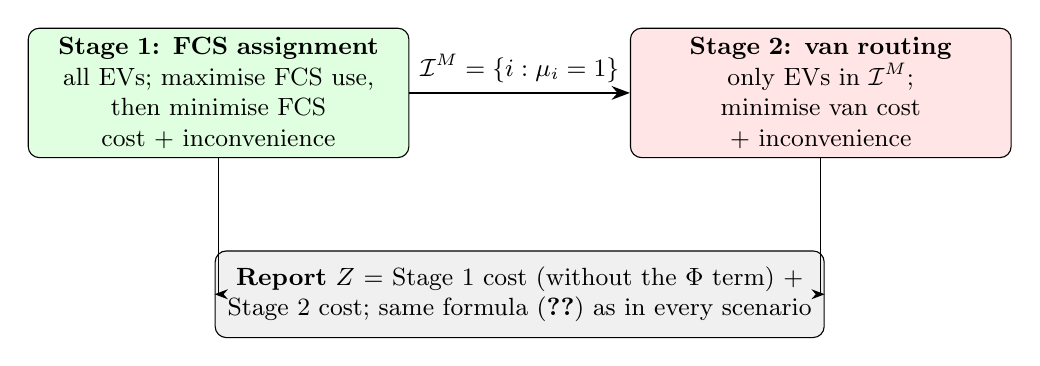
\begin{tikzpicture}[>=Stealth,box/.style={draw,rounded corners,align=center,minimum height=1.1cm,font=\small}]
  \node[box,fill=green!12,text width=4.6cm] (s1) {\textbf{Stage 1: FCS assignment}\\all EVs; maximise FCS use,\\then minimise FCS cost + inconvenience};
  \node[box,fill=red!10,text width=4.6cm,right=2.8cm of s1] (s2) {\textbf{Stage 2: van routing}\\only EVs in $\I^M$;\\minimise van cost + inconvenience};
  \draw[->,thick] (s1) -- node[above,font=\small]{$\I^M=\{i:\mu_i=1\}$} (s2);
  \node[box,fill=black!6,text width=7.5cm,below=2.0cm of $(s1)!0.5!(s2)$] (ev) {\textbf{Report} $Z=$ Stage~1 cost (without the $\Phi$ term) $+$ Stage~2 cost; same formula \eqref{eq:Z} as in every scenario};
  \draw[->] (s1) |- (ev); \draw[->] (s2) |- (ev);
\end{tikzpicture}
\end{center}

Stage~1 does not look at the vans, and Stage~2 cannot change what Stage~1 decided. That is the definition of ``FCS first, then MCS''.

%----------------------------------------------------------------
\subsection{Stage 1: assign EVs to fixed stations}

\textbf{Objective.}
\begin{equation}
\begin{split}
\min\ Z^{(1)}=\;&\underbrace{\Phi\sum_{i\in\I}\mu_i}_{\text{FCS first}}
+\underbrace{c^{EV}\sum_i\sum_{f\in\F_i}d_{if}Y_{if}}_{Z_1}
+\underbrace{Z^F_{\text{energy}}}_{\text{FCS part of }Z_4}\\
&+\underbrace{\sum_i\sum_{f\in\F_i}\rho^F_{if}Y_{if}+\alpha\sum_i w_i(C_i-r_i)+c^L\sum_i w_iL_i}_{\text{FCS customers' inconvenience}}
\end{split}
\label{eq:obj1}
\end{equation}
with $C_i=S_i+\tau^F_iY_i$ in this stage. $\Phi$ is a penalty for handing an EV to the vans. It is chosen larger than anything an extra FCS customer can add to the rest of \eqref{eq:obj1}, e.g.
\[
\Phi > \max_{i}\max_{f\in\F_i}\big(c^{EV}d_{if}+\pi^{\max}E_i+\rho^F_{if}\big)+n\,(\alpha+c^L)\,w_{\max}\,T,
\]
so Stage~1 first \textbf{maximises the number of EVs served at an FCS}, and only among those solutions minimises FCS cost and inconvenience. ($\pi^{\max}$ is the highest grid price.) A numerically safer equivalent is to solve twice: first $\max\sum_iY_i$, then fix that number and minimise the rest.
\ifTOU
Because $Z^F_{\text{energy}}$ uses the peak price, Stage~1 may \emph{start sessions later} to leave the peak, if the price saving beats the extra waiting cost (Section~\ref{sec:expect}).
\fi

\textbf{Constraints.}
\begin{align}
\sum_{g\in\G_i}y_{ig}+\mu_i &= 1 && \forall i\in\I \label{eq:s1assign}\\
S_i &\ge r_i+\sum_{f\in\F_i}t_{if}Y_{if} && \forall i\in\I \label{eq:fcsarr}\\
S_i &\le r_i+T\,(1-\mu_i) && \forall i\in\I \label{eq:s1park}\\
S_j &\ge S_i+\tau^F_i-(T+\tau^F_i)(3-y_{ig}-y_{jg}-o_{ij}) && \forall g,\ (i,j)\in\mathcal{P}_g \label{eq:disj1}\\
S_i &\ge S_j+\tau^F_j-(T+\tau^F_j)(2-y_{ig}-y_{jg}+o_{ij}) && \forall g,\ (i,j)\in\mathcal{P}_g \label{eq:disj2}\\
\sum_i y_{ig_1} &\ge \sum_i y_{ig_2} && \forall f,\ \G_f=\{g_1,g_2\} \label{eq:gunsym}\\
S_i+\tau^F_iY_i &\le T,\qquad L_i\ge S_i+\tau^F_iY_i-l_i && \forall i\in\I \label{eq:s1time}
\end{align}
\ifTOU plus the time-of-use split \eqref{eq:tou1}--\eqref{eq:tou5} of each FCS session (Section~\ref{sec:price}).\fi
\desc{\eqref{eq:s1assign}: every EV either gets one reachable gun or is handed to the vans. An EV that reaches no FCS ($\G_i=\emptyset$) is forced to $\mu_i=1$. \eqref{eq:fcsarr}: an FCS session cannot start before the EV has asked and driven to the station. \eqref{eq:s1park}: for an EV handed to the vans, $S_i$ is parked at $r_i$, so it adds no waiting in Stage~1 (its real start time is decided in Stage~2). \eqref{eq:disj1}--\eqref{eq:disj2}: two EVs on the same gun do not overlap; $o_{ij}$ picks who goes first. With two guns per station this means at most two EVs charge at a station at a time. \eqref{eq:gunsym}: symmetry breaking between the two identical guns (optional). \eqref{eq:s1time}: finished by $T$; lateness.}

\textbf{Optional acceptability rule.} An operator may refuse to send a driver to a station that is ``too inconvenient'', e.g.\ only allow gun $g$ of station $f$ for EV $i$ if $\hat\rho^F_{if}\le\bar\rho$. This only shrinks $\G_i$, so EVs whose stations are all too far go to the vans. Report results with and without it.

\textbf{Output:} $\I^M=\{i:\mu_i=1\}$, the EVs left for the vans; plus each FCS customer's gun and start time.

%----------------------------------------------------------------
\subsection{Stage 2: route the vans to the leftover EVs}

Stage~2 is a vehicle routing problem with time windows, on the EVs in $\I^M$ only. Here $C_i=S_i+\tau^M_i$.

\textbf{Objective.}
\begin{equation}
\begin{split}
\min\ Z^{(2)}=\;&\underbrace{c^M\sum_m\sum_{(i,j)\in\A^M}d_{ij}x_{ijm}}_{Z_2}+\underbrace{\sum_m c^D_mu_m}_{Z_3}+\underbrace{Z^M_{\text{energy}}}_{\text{van part of }Z_4}\\
&+\underbrace{\sum_{i\in\I^M}\sum_m\rho^M_{im}z_{im}+\alpha\sum_{i\in\I^M}w_i(C_i-r_i)+c^L\sum_{i\in\I^M}w_iL_i}_{\text{van customers' inconvenience}}
\end{split}
\label{eq:obj2}
\end{equation}
Since every EV in $\I^M$ must be served by some van, $Z^M_{\text{energy}}$ and the $\rho^M$ term are constants here. They are kept so that $Z^{(2)}$ is the true cost of Stage~2. Waiting and lateness make the vans visit urgent EVs early.

\textbf{Constraints.}
\begin{align}
\sum_{m\in\M}z_{im} &= 1 && \forall i\in\I^M \label{eq:s2assign}\\
\sum_{j:(0,j)\in\A^M}x_{0jm} = \sum_{i:(i,n+1)\in\A^M}x_{i,n+1,m} &= u_m && \forall m \label{eq:depot}\\
\sum_{i:(i,j)\in\A^M}x_{ijm} = \sum_{k:(j,k)\in\A^M}x_{jkm} &= z_{jm} && \forall j\in\I^M,\ m \label{eq:flow}\\
\sum_{i\in\I^M}z_{im} &\le Q_m\,u_m && \forall m \label{eq:cap}\\
\sum_{i\in\I^M}\frac{E_i}{\eta}z_{im}+\beta\sum_{(i,j)\in\A^M}d_{ij}x_{ijm} &\le B_m\,u_m && \forall m \label{eq:batt}
\end{align}
\begin{align}
S_j &\ge \max\{r_j,\ t_{0j}\,x_{0jm}\} && \forall j\in\I^M,\ m \label{eq:depart}\\
S_j &\ge S_i+\tau^M_i+t_{ij}-(T+\tau^M_i+t_{ij})(1-x_{ijm}) && \forall i\neq j,\ m \label{eq:seq}\\
S_i+\tau^M_i+t_{i,n+1} &\le T+(\tau^M_i+t_{i,n+1})(1-x_{i,n+1,m}) && \forall i,\ m \label{eq:return}\\
S_i+\tau^M_i \le T,\quad L_i &\ge S_i+\tau^M_i-l_i && \forall i\in\I^M \label{eq:s2time}\\
u_m &\ge u_{m+1} && m<|\M| \label{eq:vansym}
\end{align}
\desc{\eqref{eq:s2assign}: each leftover EV gets one van. \eqref{eq:depot}: a used van leaves and returns to the depot once. \eqref{eq:flow}: each EV on van $m$ is entered and left exactly once by that van. \eqref{eq:cap}: at most $Q_m$ EVs per van. \eqref{eq:batt}: delivered energy (with transfer losses) plus driving energy fits in the van battery. \eqref{eq:depart}: no start before the request, or before the van can drive there from the depot (written as two linear constraints). \eqref{eq:seq}: if the van goes $i\to j$, it finishes $i$ and drives to $j$ before starting $j$. This gives one EV at a time and removes subtours (MTZ-type). \eqref{eq:return}: back at the depot by $T$. \eqref{eq:s2time}: finished by $T$; lateness. \eqref{eq:vansym}: use identical vans in index order.}

\textbf{If Stage 2 is infeasible} (too many leftover EVs for the fleet by $T$), the sequential policy has \emph{failed} on that instance. For diagnosis, add $s_i\in\{0,1\}$ (``unserved''), replace \eqref{eq:s2assign} by $\sum_mz_{im}+s_i=1$ and add $\Phi^U\sum_is_i$ to \eqref{eq:obj2}. Then report the number of EVs that could not be served. This is a useful comparison with the integrated scenario, which may serve all of them.

%----------------------------------------------------------------
\subsection{Reported value}
\[
Z^{\text{S\scen}}=\big(Z^{(1)*}-\Phi\,|\I^M|\big)+Z^{(2)*},
\]
which is exactly \eqref{eq:Z} evaluated at the combined solution. The stage-1 solution plus the stage-2 solution is a feasible solution of the integrated model (S\ifTOU 4\else 3\fi), so
$Z^{\text{S\ifTOU 4\else 3\fi}}\le Z^{\text{S\scen}}$. The difference is the \emph{value of integration}.

\else
%---------------------------------------------------------------- INT
\subsection{Objective}
\begin{equation}
\min\ Z \quad\text{as in \eqref{eq:Z}, with }Z^F_{\text{energy}}=\ifTOU P^F\textstyle\sum_i\big[\pi^\off(\theta^1_i+\theta^3_i)+\pi^\pk\theta^2_i\big]\else\pi^F\textstyle\sum_iE_iY_i\fi,\quad C_i=S_i+\tau^F_iY_i+\tau^M_iZ_i. \label{eq:objint}
\end{equation}
Written out in full:
\begin{align*}
\min\ Z=\;& c^{EV}\sum_i\sum_{f\in\F_i}d_{if}Y_{if}+c^M\sum_m\sum_{(i,j)\in\A}d_{ij}x_{ijm}+\sum_mc^D_mu_m\\
&+\ifTOU P^F\sum_i\big[\pi^\off(\theta^1_i+\theta^3_i)+\pi^\pk\theta^2_i\big]\else\pi^F\sum_iE_iY_i\fi
+\pi^M\sum_i\sum_m\frac{E_i}{\eta}z_{im}\\
&+\sum_i\sum_{f\in\F_i}\rho^F_{if}Y_{if}+\sum_i\sum_m\rho^M_{im}z_{im}+\alpha\sum_iw_i(C_i-r_i)+c^L\sum_iw_iL_i .
\end{align*}
Every term is linear. One model weighs everything at once: an EV goes to a van exactly when the van's extra km, dispatch and energy cost are outweighed by the effort and waiting it saves the driver\ifTOU, or by the peak-price energy it avoids\fi.

\subsection{Constraints}

\textbf{Assignment.}
\begin{equation}
\sum_{g\in\G_i}y_{ig}+\sum_{m\in\M}z_{im}=1\qquad\forall i\in\I \label{eq:assign}
\end{equation}
\desc{Exactly one resource per EV: one reachable gun or one van. EVs that reach no FCS are forced onto a van.}

\textbf{Fixed stations.}
\begin{align}
S_i &\ge r_i+\sum_{f\in\F_i}t_{if}Y_{if} && \forall i \label{eq:fcsarr}\\
S_j &\ge S_i+\tau^F_i-(T+\tau^F_i)(3-y_{ig}-y_{jg}-o_{ij}) && \forall g,\ (i,j)\in\mathcal{P}_g \label{eq:disj1}\\
S_i &\ge S_j+\tau^F_j-(T+\tau^F_j)(2-y_{ig}-y_{jg}+o_{ij}) && \forall g,\ (i,j)\in\mathcal{P}_g \label{eq:disj2}\\
\sum_iy_{ig_1} &\ge \sum_iy_{ig_2} && \forall f,\ \G_f=\{g_1,g_2\} \label{eq:gunsym}
\end{align}
\desc{\eqref{eq:fcsarr}: an FCS session starts after the request and the drive to the station (for a van customer this is just $S_i\ge r_i$). \eqref{eq:disj1}--\eqref{eq:disj2}: EVs on the same gun do not overlap; $o_{ij}$ chooses the order. \eqref{eq:gunsym}: optional symmetry breaking.}

\textbf{Vans: routes, capacity, battery.}
\begin{align}
\sum_{j:(0,j)\in\A}x_{0jm}=\sum_{i:(i,n+1)\in\A}x_{i,n+1,m} &= u_m && \forall m \label{eq:depot}\\
\sum_{i:(i,j)\in\A}x_{ijm}=\sum_{k:(j,k)\in\A}x_{jkm} &= z_{jm} && \forall j\in\I,\ m \label{eq:flow}\\
\sum_iz_{im} &\le Q_mu_m && \forall m \label{eq:cap}\\
\sum_i\frac{E_i}{\eta}z_{im}+\beta\sum_{(i,j)\in\A}d_{ij}x_{ijm} &\le B_mu_m && \forall m \label{eq:batt}
\end{align}
\desc{\eqref{eq:depot}: a used van leaves and returns once. \eqref{eq:flow}: each EV on van $m$ is visited exactly once by it. \eqref{eq:cap}: at most $Q_m$ EVs. \eqref{eq:batt}: delivered energy (with losses) plus driving energy fits in the battery.}

\textbf{Vans: timing (one EV at a time, no subtours).}
\begin{align}
S_j &\ge t_{0j}\,x_{0jm} && \forall j\in\I,\ m \label{eq:depart}\\
S_j &\ge S_i+\tau^M_i+t_{ij}-(T+\tau^M_i+t_{ij})(1-x_{ijm}) && \forall i\neq j\in\I,\ m \label{eq:seq}\\
S_i+\tau^M_i+t_{i,n+1} &\le T+(\tau^M_i+t_{i,n+1})(1-x_{i,n+1,m}) && \forall i,\ m \label{eq:return}
\end{align}
\desc{\eqref{eq:depart}: the first stop cannot start before the van has driven there. \eqref{eq:seq}: $i\to j$ means finish $i$, drive, then start $j$; start times rise along a route, so no subtour can close. \eqref{eq:return}: back at the depot by $T$.}

\textbf{Horizon and lateness.}
\begin{equation}
C_i\le T,\qquad L_i\ge C_i-l_i\qquad\forall i\in\I \label{eq:time}
\end{equation}
\desc{Every EV is fully charged within the horizon; $L_i$ measures lateness.}

\ifTOU
\textbf{Time-of-use split.} Constraints \eqref{eq:tou1}--\eqref{eq:tou5} of Section~\ref{sec:price}.
\fi

\textbf{Symmetry and domains.}
\begin{equation}
u_m\ge u_{m+1};\qquad y,z,x,u,o\ifTOU,\kappa\fi\in\{0,1\};\qquad S_i,L_i\ifTOU,\theta^p_i\fi\ge0 \label{eq:dom}
\end{equation}
\fi

%=====================================================================
\section{Learning-to-optimise (RL) formulation}\label{sec:rl}

\textbf{Main rule:} the reward of each action is \emph{minus the increase in $Z$ that the action causes}. The rewards over an episode then add up to $-Z$ of the solution the policy builds. RL and MILP results are measured on the same yardstick \eqref{eq:Z}, and the MILP optimum is the benchmark for the RL gap.

\ifSEQ
%---------------------------------------------------------------- RL SEQ
The RL pipeline has the same two stages as the MILP.

\subsection{Stage 1 policy: FCS assignment}
\begin{itemize}[leftmargin=1.4em,itemsep=2pt]
  \item \textbf{Episode / epochs:} EVs are taken in order of request time $r_i$ (ties: higher $w_i$ first). One decision per EV.
  \item \textbf{State:} features of the current EV $k$ ($E_k,r_k,l_k,w_k,R_k$, location); for each gun $g$ the time $F_g$ it becomes free; summary features of the EVs still to come (count and positions near each station)\ifTOU; the current price and the time until $T_1$ and $T_2$\fi.
  \item \textbf{Action:} a gun $g\in\G_k$, or ``hand to vans''. \textbf{FCS-first mask:} ``hand to vans'' is allowed \emph{only} if no gun can finish EV $k$ by $T$ (or, with the optional rule, if all remaining guns have $\hat\rho^F_{kf}>\bar\rho$).
  \ifTOU\item \textbf{Optional timing action:} ``gun $g$, start after the peak'', i.e.\ $S_k=\max\{\text{earliest},T_2\}$, allowed only if the session still ends by $T$.\fi
  \item \textbf{Transition:} $S_k=\max\{r_k+t_{kf},F_g\}$ (or later, for the timing action); $F_g\leftarrow S_k+\tau^F_k$.
  \item \textbf{Reward:} $-\Big[c^{EV}d_{kf}+\text{energy}_k+\rho^F_{kf}+\alpha w_k(S_k+\tau^F_k-r_k)+c^Lw_k(S_k+\tau^F_k-l_k)^+\Big]$, where energy$_k$ = \ifTOU$P^F\big[\pi^\off\cdot(\text{off-peak hours of }[S_k,S_k+\tau^F_k])+\pi^\pk\cdot(\text{peak hours})\big]$, computed exactly in the simulator\else$\pi^FE_k$\fi. Handing an EV to the vans gives reward $0$ here; its cost is counted in Stage~2.
\end{itemize}
Note: a simple baseline for Stage~1 is the greedy rule ``gun with the largest one-step reward''. What RL can learn on top of this is, for example, to keep a nearby gun free for an urgent EV that arrives later.

\subsection{Stage 2 policy: van routing over $\I^M$}
\begin{itemize}[leftmargin=1.4em,itemsep=2pt]
  \item \textbf{Epochs:} whenever a van becomes free (the earliest-free van decides first).
  \item \textbf{State:} for each van: position, time free, remaining battery $b_m$, EVs served so far, dispatched or not; for each unserved EV in $\I^M$: location, $E_i,r_i,l_i,w_i$; current time.
  \item \textbf{Action:} the next EV $j$ for this van, or ``return to depot'' (ends the route). Mask: $j$ must be feasible: battery covers $E_j/\eta$ plus driving to $j$ and back to the depot, the count stays $\le Q_m$, and $j$ can be finished with the van back at the depot by $T$.
  \item \textbf{Transition:} $S_j=\max\{r_j,\ \text{time free}+t_{\text{pos},j}\}$; the van moves to $j$ and is free at $S_j+\tau^M_j$; $b_m$ falls by $E_j/\eta+\beta d_{\text{pos},j}$.
  \item \textbf{Reward:} serving $j$: $-\Big[c^Md_{\text{pos},j}+c^D_m[\text{first stop}]+\pi^M\frac{E_j}{\eta}+\rho^M_{jm}+\alpha w_j(S_j+\tau^M_j-r_j)+c^Lw_j(S_j+\tau^M_j-l_j)^+\Big]$; returning: $-c^Md_{\text{pos},0}$. EVs still unserved at the end: $-\Phi^U$ each.
  \item \textbf{Policy:} an attention-based routing policy (e.g.\ Kool et al., 2019, ``Attention, Learn to Solve Routing Problems!'') trained with REINFORCE or PPO. Baseline: nearest-feasible-EV heuristic.
\end{itemize}
Episode return of Stage~1 + Stage~2 $=-Z^{\text{S\scen}}$.

\else
%---------------------------------------------------------------- RL INT
One policy decides both who serves each EV and the van routes.
\begin{itemize}[leftmargin=1.4em,itemsep=2pt]
  \item \textbf{Episode / epochs:} EVs are taken in order of request time $r_i$ (ties: higher $w_i$ first). One decision per EV.
  \item \textbf{State:} (i) the current EV $k$: location, $E_k,r_k,l_k,w_k,R_k$, reachable stations; (ii) each gun $g$: time $F_g$ it becomes free; (iii) each van $m$: current end-of-route position, time free, remaining battery $b_m$, EVs served, dispatched or not; (iv) embeddings of the not-yet-assigned EVs (for look-ahead)\ifTOU; (v) current price, time until $T_1$ and $T_2$\fi.
  \item \textbf{Action:} $a\in\G_k\cup\M$: a gun, or a van (EV $k$ is appended to the end of that van's route). \textbf{Mask} infeasible actions: a gun that cannot finish $k$ by $T$; a van without enough battery for $E_k/\eta$ plus the drive to $k$ and back to the depot, with $Q_m$ reached, or unable to finish $k$ and return by $T$.
  \ifTOU\item \textbf{Optional timing action:} ``gun $g$, start after the peak'' ($S_k=\max\{\text{earliest},T_2\}$, if it still ends by $T$).\fi
  \item \textbf{Transition:} gun: $S_k=\max\{r_k+t_{kf},F_g\}$, $F_g\leftarrow S_k+\tau^F_k$. Van: $S_k=\max\{r_k,\ \text{free}_m+t_{\text{pos}_m,k}\}$, then the van moves to $k$, $\text{free}_m\leftarrow S_k+\tau^M_k$, $b_m\mathrel{-}=E_k/\eta+\beta d_{\text{pos}_m,k}$.
  \item \textbf{Reward} $=-\Delta Z$:
  \begin{align*}
  \text{gun } g\text{ at }f:&\quad -\Big[c^{EV}d_{kf}+\text{energy}^F_k+\rho^F_{kf}+\alpha w_k(C_k-r_k)+c^Lw_k(C_k-l_k)^+\Big]\\
  \text{van } m:&\quad -\Big[c^M\big(d_{\text{pos}_m,k}+d_{k,0}-d_{\text{pos}_m,0}\big)+c^D_m[\text{first use}]+\pi^M\tfrac{E_k}{\eta}\\
  &\qquad\quad+\rho^M_{km}+\alpha w_k(C_k-r_k)+c^Lw_k(C_k-l_k)^+\Big]
  \end{align*}
  The van distance term is the \emph{change} in route length when $k$ is inserted before the return to the depot, so the sum over the episode equals the total route length (the return legs telescope). energy$^F_k$ = \ifTOU$P^F\big[\pi^\off\cdot(\text{off-peak hours})+\pi^\pk\cdot(\text{peak hours of }[S_k,C_k])\big]$, computed exactly by the simulator; no linearisation is needed in RL\else$\pi^FE_k$\fi.
  \item \textbf{Dead end:} if every action is masked, EV $k$ is unserved: reward $-\Phi^U$, and the episode continues. Report the count.
  \item \textbf{Policy:} masked categorical policy over guns and vans, encoder with attention over EVs, guns and vans; trained with PPO. Natural baseline: greedy, i.e.\ choose the action with the largest one-step reward. That is the pairwise rule ``smallest $\hat\rho$ + cost'' from Section~\ref{sec:inc}.
\end{itemize}
Restriction to note: vans serve EVs in assignment order (append only). A variant that inserts $k$ at the cheapest position of a route is more flexible but has a larger action space.
\fi

\textbf{Reward scaling.} For stable training divide every reward by a constant, e.g.\ the greedy baseline's average $Z$ on the training instances. This does not change the optimal policy.

%=====================================================================
\section{What to expect and what to report}\label{sec:expect}

\ifnum\scen=1
\begin{itemize}[leftmargin=1.4em,itemsep=2pt]
  \item Vans serve only EVs that reach no station, or that the stations cannot finish by $T$. If stations have spare capacity, very few vans are dispatched.
  \item Inconvenience is high for EVs far from the nearest station (worked example: Rs\,682 at the FCS, against Rs\,458 if a van had been allowed).
  \item With too few vans Stage~2 becomes infeasible (unserved EVs), even when the integrated model S3 could serve everyone. Report the smallest $|\M|$ at which S1 is feasible and compare it with S3.
\end{itemize}
\fi
\ifnum\scen=2
\begin{itemize}[leftmargin=1.4em,itemsep=2pt]
  \item \textbf{When does Stage~1 delay a session to avoid the peak?} Moving one hour of charging out of the peak saves $(\pi^\pk-\pi^\off)P^F=3\times22=$ Rs\,66, but delays completion by up to an hour, which costs $\alpha w_i\ge$ Rs\,200. So with the default values Stage~1 almost never delays. It mostly pays the higher price, and S2 costs roughly S1 plus the peak surcharge. Sessions start later only if $\alpha$ is small (try $\lambda<0.33$ in the sensitivity analysis).
  \item The van assignment is the same as in S1 unless Stage~1's timing changes which EVs fit at the stations. Stage~1 cannot use vans to escape the peak price.
  \item Extra KPI: \textbf{grid energy drawn at FCS during the peak}, $P^F\sum_i\theta^2_i$ (kWh). Compare with S4.
\end{itemize}
\fi
\ifnum\scen=3
\begin{itemize}[leftmargin=1.4em,itemsep=2pt]
  \item Vans take EVs for which the saved inconvenience exceeds the extra van cost (worked example: van chosen, saving Rs\,224). Expect vans to serve EVs that are far from every station, have low range (high $w_i$), or have early deadlines, while EVs near a station still use it.
  \item \textbf{Value of integration under flat price:} $Z^{\text{S1}}-Z^{\text{S3}}\ge0$. Report it per component ($Z_1,\dots,Z_5$): typically operating cost rises a little and inconvenience falls a lot.
  \item Vary $|\M|$ (0, 1, 2, \dots): the first few vans lower $Z$ sharply, then the effect levels off. That curve shows the scenarios where mobile chargers help most.
\end{itemize}
\fi
\ifnum\scen=4
\begin{itemize}[leftmargin=1.4em,itemsep=2pt]
  \item During the peak a van kWh costs about the same as an FCS kWh (Rs\,10.0 each), so the vans' energy disadvantage disappears and vans also absorb \emph{peak-hour} demand that would otherwise be charged on the grid at peak price.
  \item Expect more van usage than in S3, concentrated on requests in $[T_1,T_2]$, and lower grid energy at the stations during the peak, $P^F\sum_i\theta^2_i$, than in S2.
  \item \textbf{Value of integration under peak pricing:} $Z^{\text{S2}}-Z^{\text{S4}}$. It should be larger than $Z^{\text{S1}}-Z^{\text{S3}}$, because integration now also allows price arbitrage.
  \item \textbf{Peak pricing with full flexibility:} $Z^{\text{S4}}-Z^{\text{S3}}$ should be smaller than $Z^{\text{S2}}-Z^{\text{S1}}$: vans cushion the price increase.
\end{itemize}
\fi

\textbf{Cross-scenario comparison table} (fill in from the four runs):
\begin{center}
\renewcommand{\arraystretch}{1.2}
\begin{tabular}{@{}lll@{}}
\toprule
\textbf{Comparison} & \textbf{Measures} & \textbf{Expected sign} \\
\midrule
S1 $-$ S3 & value of integration, flat price & $\ge0$ \\
S2 $-$ S4 & value of integration, peak price & $\ge0$, larger than S1 $-$ S3 \\
S2 $-$ S1 & cost of peak pricing, FCS-first operator & $>0$ \\
S4 $-$ S3 & cost of peak pricing, flexible operator & $>0$, smaller than S2 $-$ S1 \\
\bottomrule
\end{tabular}
\end{center}
Report for each: $Z$ and its components, number of vans used, EVs per resource, mean and maximum inconvenience per EV, total lateness, peak-hour grid energy, solve time, and (for RL) the gap to the MILP optimum.

%=====================================================================
\appendix
\section{Illustrative parameter values}\label{app:values}

These are starting values for experiments, not data. All are meant to be varied in the analysis. Values in Rs.

\begin{center}
\renewcommand{\arraystretch}{1.15}
\begin{tabular}{@{}llp{6.2cm}@{}}
\toprule
\textbf{Parameter} & \textbf{Value} & \textbf{Note} \\
\midrule
$T$, $[T_1,T_2]$ & 7 h, $[2,6]$ & 16:00--23:00, peak 18:00--22:00 \\
$P^F$, $P^M$ & 22 kW, 30 kW & \\
$v$, $\beta$, $\eta$ & 25 km/h, 0.25 kWh/km, 0.9 & \\
$B_m$, $Q_m$, $|\M|$ & 150 kWh, 6, 2--6 & \\
$c^{EV}$, $c^M$, $c^D_m$ & Rs\,4/km, Rs\,15/km, Rs\,1500 & van km includes driver time \\
$\pi^F$ (flat) & Rs\,8.7/kWh & equals the time-average of the ToU tariff over $[0,T]$ \\
$\pi^\off$, $\pi^\pk$ (ToU) & Rs\,7/kWh, Rs\,10/kWh & $(3\times7+4\times10)/7=8.7$ \\
$c^{bat}$ & Rs\,2/kWh & van battery wear \\
$\pi^M$ & Rs\,10.7 (flat) / Rs\,9.0 (ToU) & $=\pi^F+c^{bat}$ / $=\pi^\off+c^{bat}$ \\
$\alpha$, $\alpha^D$ & Rs\,200/h, Rs\,100/h & value of time; extra for attended time \\
$h^F$, $h^M$, $\varphi$ & Rs\,50, Rs\,10, Rs\,100 & trip hassle, hand-over, range stress \\
$c^L$ & Rs\,300/h & lateness \\
$w_i$ & $1+2(1-R_i/R_{\max})$, $R_i\sim U[3,40]$ km & priority from remaining range \\
\bottomrule
\end{tabular}
\end{center}

The flat price is set to the time-average of the peak tariff. The price \emph{level} is then the same in both pricing cases, and only the price \emph{shape} differs. Without this, part of S1 vs S2 would just reflect a different average price.

\end{document}
"
%    pdflatex -jobname=scenario4_peak_integrated   "\def\scen{4}% =====================================================================
%  One source, four PDFs.  Build with build.sh (or by hand):
%    pdflatex -jobname=scenario1_flat_sequential   "\def\scen{1}% =====================================================================
%  One source, four PDFs.  Build with build.sh (or by hand):
%    pdflatex -jobname=scenario1_flat_sequential   "\def\scen{1}\input{scenario_master}"
%    pdflatex -jobname=scenario2_peak_sequential   "\def\scen{2}\input{scenario_master}"
%    pdflatex -jobname=scenario3_flat_integrated   "\def\scen{3}\input{scenario_master}"
%    pdflatex -jobname=scenario4_peak_integrated   "\def\scen{4}\input{scenario_master}"
%  (run each twice for cross-references)
% =====================================================================
\documentclass[11pt,a4paper]{article}
\usepackage[margin=2.2cm]{geometry}
\usepackage{amsmath,amssymb,amsfonts}
\usepackage{booktabs,array,tabularx}
\usepackage{enumitem}
\usepackage[table]{xcolor}
\usepackage{tikz}
\usetikzlibrary{arrows.meta,positioning,calc}
\usepackage[colorlinks=true,linkcolor=blue!50!black,urlcolor=blue!50!black]{hyperref}
\usepackage{titlesec}
\titleformat{\section}{\large\bfseries}{\thesection}{0.8em}{}
\titleformat{\subsection}{\normalsize\bfseries}{\thesubsection}{0.8em}{}
\setlength{\parindent}{0pt}
\setlength{\parskip}{5pt}

% ---------------- scenario switches ----------------
\ifdefined\scen\else\def\scen{1}\fi
\newif\ifTOU \TOUfalse   % true = time-of-use (peak) price
\newif\ifSEQ \SEQfalse   % true = FCS first, then MCS
\ifnum\scen=1 \SEQtrue \fi
\ifnum\scen=2 \TOUtrue \SEQtrue \fi
\ifnum\scen=4 \TOUtrue \fi

\newcommand{\pricename}{\ifTOU time-of-use price (dearer evening peak)\else single (flat) price all day\fi}
\newcommand{\structname}{\ifSEQ FCS first, then MCS (sequential)\else FCS and MCS together (integrated)\fi}

% ---------------- notation ----------------
\newcommand{\I}{\mathcal{I}}
\newcommand{\F}{\mathcal{F}}
\newcommand{\G}{\mathcal{G}}
\newcommand{\M}{\mathcal{M}}
\newcommand{\N}{\mathcal{N}}
\newcommand{\A}{\mathcal{A}}
\newcommand{\Rs}{\text{Rs}\,}
\newcommand{\pk}{\mathrm{pk}}
\newcommand{\off}{\mathrm{off}}
\newcommand{\desc}[1]{\par\vspace{-2pt}{\small\color{black!75}\textit{Meaning:} #1}\par\vspace{4pt}}
\newcommand{\cell}[2]{\ifnum\scen=#1\cellcolor{blue!18}\textbf{S#1 (this document)}\\\textbf{#2}\else S#1\\#2\fi}

\title{\textbf{EV Charging Network Optimisation}\\[4pt]
\large Scenario \scen: \pricename\ $+$ \structname\\[2pt]
\normalsize MILP and RL formulation}
\author{CP 320 OR for Mobility Management, course project}
\date{2 October 2026}

\begin{document}
\maketitle

%=====================================================================
\section{Where this scenario sits}

The project studies four scenarios: two ways of pricing grid electricity, times two ways of making the decisions.

\begin{center}
\renewcommand{\arraystretch}{1.5}
\begin{tabular}{>{\raggedright\arraybackslash}p{4.2cm}|>{\centering\arraybackslash}p{4.6cm}|>{\centering\arraybackslash}p{4.6cm}}
 & \textbf{Flat price all day} & \textbf{Time-of-use (peak) price} \\ \hline
\textbf{Sequential:} FCS first, leftover EVs to MCS &
\begin{tabular}[c]{@{}c@{}}\cell{1}{flat + sequential}\end{tabular} &
\begin{tabular}[c]{@{}c@{}}\cell{2}{peak + sequential}\end{tabular} \\ \hline
\textbf{Integrated:} FCS and MCS decided together &
\begin{tabular}[c]{@{}c@{}}\cell{3}{flat + integrated}\end{tabular} &
\begin{tabular}[c]{@{}c@{}}\cell{4}{peak + integrated}\end{tabular} \\
\end{tabular}
\end{center}

\textbf{The four scenarios do not have four different objectives.} They share \emph{one} cost yardstick $Z$ (Section~\ref{sec:obj}): the same cost terms and the same customer inconvenience (Section~\ref{sec:inc}). Only two things change:
\begin{itemize}[leftmargin=1.4em,itemsep=1pt]
  \item \textbf{Pricing} changes the formula for one term, the FCS energy cost (Section~\ref{sec:price}).
  \item \textbf{Decision structure} changes \emph{how} $Z$ is minimised: in one model (integrated), or in two stages (sequential), where each stage minimises its own part of $Z$.
\end{itemize}
Because the yardstick is the same, the four optimal values can be compared directly. The differences measure the \emph{value of integration} (S1$\to$S3, S2$\to$S4) and the \emph{effect of peak pricing} (S1$\to$S2, S3$\to$S4).

\ifnum\scen=1
\textbf{This scenario (S1)} is the baseline, the ``status quo''. Electricity costs the same at every hour, every EV that can be charged at a fixed station is sent there, and vans only take what is left over.
\fi
\ifnum\scen=2
\textbf{This scenario (S2)} keeps the FCS-first rule of S1, but grid electricity is dearer during the evening peak. Stage~1 can react to the price only by \emph{rescheduling} FCS sessions. It cannot hand a peak-hour EV to a van.
\fi
\ifnum\scen=3
\textbf{This scenario (S3)} keeps the flat price of S1, but the operator decides FCS and MCS service \emph{together}. An EV can be sent to a van even when a fixed station could take it, whenever that lowers total cost plus inconvenience.
\fi
\ifnum\scen=4
\textbf{This scenario (S4)} is the most flexible one: peak pricing at fixed stations, and FCS and MCS decided together. Van energy was bought off-peak, so vans can also be used to keep charging \emph{out of the expensive peak}.
\fi

%=====================================================================
\section{Setting and assumptions}\label{sec:setting}

\textbf{Time.} The planning horizon is $[0,T]$ with $T=7$\,h (16:00--23:00). It contains the evening peak window $[T_1,T_2]=[2,6]$ (18:00--22:00). The horizon is the same in all four scenarios. It is wider than the peak itself so that, under peak pricing, there is cheaper time on both sides of the peak.\ifTOU\else\ In this scenario the price is flat, so the window plays no role in the model.\fi

\textbf{Assumptions} (the same as MILP v3, plus two about energy):
\begin{enumerate}[leftmargin=1.6em,itemsep=1pt]
  \item Static, continuous time. All requests in the horizon are known at time $0$, and request $i$ becomes active at $r_i$.
  \item An EV served by an FCS drives there itself on its own battery (only to stations within its range $R_i$). The driver stays with the car while it waits for a free gun and while it charges.
  \item An EV served by an MCS stays parked where it is, and the driver is free in the meantime.
  \item Each FCS gun and each van charges one EV at a time, without interruption, at constant power.
  \item A van's battery covers both its driving and the energy it delivers. \textbf{The van battery is charged at the depot before the horizon starts}\ifTOU, i.e.\ at the off-peak price\fi, and is not recharged during the horizon.
  \item Every EV must be fully charged by $T$ (hard). Finishing after the driver's desired time $l_i$ is allowed but penalised.
\end{enumerate}

%=====================================================================
\section{Notation}\label{sec:notation}

\subsection*{Sets}
\begin{tabularx}{\textwidth}{@{}lX@{}}
\toprule
$\I=\{1,\dots,n\}$ & EV charging requests \\
$\F$; $\G_f$ ($|\G_f|=2$); $\G=\bigcup_f\G_f$ & fixed charging stations; guns of FCS $f$; all guns ($f(g)$ = station of gun $g$) \\
$\F_i=\{f: d_{if}\le R_i\}$, $\G_i=\bigcup_{f\in\F_i}\G_f$ & stations / guns EV $i$ can reach on its remaining range \\
$\M$ & mobile charging vans (MCS) \\
$0,\ n+1$ & depot as start node / end node (same place) \\
$\N=\{0\}\cup\I\cup\{n+1\}$, $\A$ & routing nodes; allowed van arcs $(i,j)$, $i\in\{0\}\cup\I$, $j\in\I\cup\{n+1\}$, $i\neq j$ \\
$\mathcal{P}_g=\{(i,j): i<j,\ g\in\G_i\cap\G_j\}$ & pairs of EVs that could share gun $g$ \\
\ifSEQ
$\I^M\subseteq\I$ & EVs handed to the vans by Stage~1 (an \emph{output} of Stage~1, a fixed input to Stage~2) \\
$\N^M$, $\A^M$ & routing nodes / arcs restricted to $\I^M$ \\
\fi
\bottomrule
\end{tabularx}

\subsection*{Parameters}
\begin{tabularx}{\textwidth}{@{}lX@{}}
\toprule
$E_i,\ r_i,\ l_i,\ R_i$ & energy demand (kWh), request time, desired completion time (h), remaining range (km) \\
$w_i\ge1$ & priority of EV $i$; $w_i=1+\kappa(1-R_i/R_{\max})$, so low-range EVs weigh more \\
$P^F,\ P^M$ & charging power of an FCS gun (22\,kW) / of a van (e.g.\ 30\,kW) \\
$\tau^F_i=E_i/P^F,\ \tau^M_i=E_i/P^M$ & charging time of EV $i$ at an FCS / by a van (h) \\
$d_{if},t_{if}$;\ $d_{ij},t_{ij}$ & distance (km) and time (h): EV$\to$FCS; between routing nodes ($t=d/v$) \\
$B_m,\ Q_m,\ \beta,\ \eta$ & van battery (kWh), max EVs per van, van consumption (kWh/km), transfer efficiency \\
$c^{EV},\ c^M,\ c^D_m$ & cost per km of EV driving, per km of van driving; fixed dispatch cost of van $m$ \\
\ifTOU
$\pi^\off,\ \pi^\pk$ & grid price (Rs/kWh) off-peak / in $[T_1,T_2]$, with $\pi^\pk\ge\pi^\off$ \\
\else
$\pi^F$ & grid price (Rs/kWh), the same at every hour \\
\fi
$c^{bat}$ & van battery wear per kWh cycled \\
$\pi^M$ & cost of 1 kWh taken from a van battery: $\pi^M=\ifTOU\pi^\off\else\pi^F\fi+c^{bat}$ (Section~\ref{sec:price}) \\
$\alpha,\ \alpha^D,\ h^F,\ h^M,\ \varphi,\ c^L$ & inconvenience coefficients (Section~\ref{sec:inc}) \\
\bottomrule
\end{tabularx}

\subsection*{Decision variables}
\begin{tabularx}{\textwidth}{@{}llX@{}}
\toprule
$y_{ig}$ & $\{0,1\}$ & EV $i$ charged at gun $g\in\G_i$ \\
$z_{im}$ & $\{0,1\}$ & EV $i$ served by van $m$ \\
$x_{ijm}$ & $\{0,1\}$ & van $m$ drives arc $(i,j)$ \\
$u_m$ & $\{0,1\}$ & van $m$ is dispatched \\
$o_{ij}$ & $\{0,1\}$ & for EVs $i<j$ that could share a gun: 1 if $i$ is charged before $j$ \\
\ifSEQ
$\mu_i$ & $\{0,1\}$ & Stage~1 only: EV $i$ is handed to the van fleet \\
\fi
\ifTOU
$\theta^1_i,\theta^2_i,\theta^3_i$ & $\ge0$ & hours of EV $i$'s FCS session before / inside / after the peak \\
$\kappa^1_i,\kappa^3_i$ & $\{0,1\}$ & EV $i$'s FCS session starts before $T_1$ / ends after $T_2$ \\
\fi
$S_i$ & $\ge0$ & time charging of EV $i$ starts (h), on whichever resource \\
$L_i$ & $\ge0$ & lateness of EV $i$ beyond $l_i$ (h) \\
\bottomrule
\end{tabularx}

\textbf{Short-hands} (linear expressions, not new variables):
\[
Y_{if}=\sum_{g\in\G_f}y_{ig},\qquad Y_i=\sum_{g\in\G_i}y_{ig}\ (\text{EV $i$ uses an FCS}),\qquad Z_i=\sum_{m\in\M}z_{im}\ (\text{EV $i$ uses a van}),
\]
\[
C_i=S_i+\tau^F_i\,Y_i+\tau^M_i\,Z_i \quad\text{(time EV $i$ is fully charged).}
\]

%=====================================================================
\section{Customer inconvenience}\label{sec:inc}

This section is \textbf{identical in all four scenario documents}. Inconvenience is a property of the customer, not of the price or of the planning method.

\subsection{What we mean by inconvenience}

Inconvenience is \emph{what the driver loses} from the moment they ask for a charge ($r_i$) until the car is fully charged ($C_i$), \emph{converted into rupees} so it can be added to the operator's costs. A driver loses three different things:

\begin{enumerate}[leftmargin=1.6em,itemsep=2pt]
  \item \textbf{Waiting:} the car is not ready. This lasts $C_i-r_i$ hours and affects \emph{every} driver, FCS or MCS.
  \item \textbf{Effort:} only an FCS customer has to drive to the station and sit there while the car charges. An MCS customer stays at home or at work and does something else. Driving to a far station also uses scarce battery range, which causes stress (``range anxiety'').
  \item \textbf{A missed deadline:} the car is still not ready at the time $l_i$ the driver needs it.
\end{enumerate}

Each loss gets a price in Rs per hour (or per event). All of them are multiplied by the priority $w_i$: an hour of delay for an EV with 5\,km of range left counts more than for one with 40\,km.

\subsection{The three components}

\begin{center}
\renewcommand{\arraystretch}{1.3}
\begin{tabularx}{\textwidth}{@{}>{\raggedright\arraybackslash}p{2.6cm}>{\raggedright\arraybackslash}X>{\raggedright\arraybackslash}X>{\raggedright\arraybackslash}p{3.0cm}@{}}
\toprule
\textbf{Component} & \textbf{EV $i$ at FCS $f$} & \textbf{EV $i$ by a van} & \textbf{Known when?} \\
\midrule
Effort & $w_i\big[\alpha^D(t_{if}+\tau^F_i)+h^F+\varphi\,d_{if}/R_i\big]$: driving and sitting at the station, a fixed trip hassle, range stress & $w_i\,h^M$: being reachable and handing over the car & \textbf{Static:} known as soon as the resource is chosen \\
Waiting & $w_i\,\alpha\,(C_i-r_i)$ = drive + \emph{queue at the gun} + charge & $w_i\,\alpha\,(C_i-r_i)$ = \emph{wait for the van} + charge & \textbf{Dynamic:} depends on the queue / van route \\
Missed deadline & $w_i\,c^L\,L_i$, $L_i=\max\{0,C_i-l_i\}$ & same & Dynamic \\
\bottomrule
\end{tabularx}
\end{center}

\textbf{Coefficients.}
$\alpha$ (Rs/h) is the value of an hour the car is not ready.
$\alpha^D$ (Rs/h) is the \emph{extra} value of an hour the driver must personally spend driving or sitting at the station: an hour at the station costs $\alpha+\alpha^D$, an hour waiting at home for a van costs only $\alpha$.
$h^F,h^M$ (Rs) are fixed hassle costs of one trip to a station / one van hand-over.
$\varphi$ (Rs) is the range-stress cost of a trip that uses the \emph{whole} remaining range ($d_{if}/R_i\le1$ is the fraction used).
$c^L$ (Rs/h) is the cost per hour late.

\subsection{Pairwise form: inconvenience of a (customer, resource) pair}

The natural first idea is: \emph{for every pair (EV $i$, FCS $f$) and every pair (EV $i$, van $m$) there is an inconvenience number, and the operator picks the pair with the lowest cost plus inconvenience.} The static part fits this idea exactly:
\[
\boxed{\;\rho^F_{if}=w_i\Big[\alpha^D\,(t_{if}+\tau^F_i)+h^F+\varphi\,\frac{d_{if}}{R_i}\Big]\qquad
\rho^M_{im}=w_i\,h^M\;}
\]
These are \textbf{parameters}, computed before solving, one number per (EV, FCS) pair and per (EV, van) pair. In the objective they appear linearly: $\sum_i\sum_f\rho^F_{if}Y_{if}+\sum_i\sum_m\rho^M_{im}z_{im}$.

Note that $\rho^M_{im}$ does not depend on $m$. Vans are identical and all start at the same depot, so the driver does not care \emph{which} van comes, only \emph{when} it comes. That ``when'' is the waiting part.

\subsection{Why waiting cannot be a fixed pairwise number}

It is tempting to also write the waiting as a pairwise number, e.g.\ ``the van needs 5 minutes to reach EV $i$''. But that depends on \emph{where the van is coming from}, which depends on the route the model is still choosing: if EV $i$ is the 4th stop of a van, the wait is the time for three charging sessions plus four drives. Likewise, waiting at an FCS depends on how many EVs are queued at that gun. So waiting is not known before solving. It is a function of decision variables:
\[
\text{waiting cost of EV } i \;=\; w_i\,\alpha\,(C_i-r_i),\qquad C_i=S_i+\tau^F_iY_i+\tau^M_iZ_i .
\]
This is \textbf{linear} in the variables ($S_i$, $y$, $z$), so it fits in a MILP directly. The constraints of Section~\ref{sec:milp} make $S_i$ equal to the true start time, including driving, queueing at the gun and the van's route. The term $\sum_i w_i\alpha r_i$ is a constant and may be dropped when solving.

\textbf{Pairwise \emph{estimate}} (used for intuition, by the RL policy and in heuristics): if there is no queue and the van comes straight to $i$,
\[
\hat\rho^{F}_{if}=\rho^F_{if}+w_i\alpha\,(t_{if}+\tau^F_i),\qquad
\hat\rho^{M}_{im}=\rho^M_{im}+w_i\alpha\,(t^{\text{van}}_{m\to i}+\tau^M_i),
\]
where $t^{\text{van}}_{m\to i}$ is the time until van $m$ can reach $i$ from where it currently is. In the RL formulation (Section~\ref{sec:rl}) the van's position \emph{is} known at each decision, so there this estimate becomes exact.

\subsection{Total inconvenience and how it enters the objective}

\begin{equation}
\boxed{\;
Z_{\text{inc}}=\underbrace{\sum_{i\in\I}\sum_{f\in\F_i}\rho^F_{if}Y_{if}+\sum_{i\in\I}\sum_{m\in\M}\rho^M_{im}z_{im}}_{\text{effort (static, pairwise)}}
+\underbrace{\alpha\sum_{i\in\I}w_i\,(C_i-r_i)}_{\text{waiting (dynamic)}}
+\underbrace{c^L\sum_{i\in\I}w_i\,L_i}_{\text{missed deadline}}
\;}\label{eq:inc}
\end{equation}
All three parts are in rupees, so $Z_{\text{inc}}$ is simply added to the operating costs. Nothing has to be normalised.

\subsection{Worked example: your ``10 km to the FCS vs.\ van in 5 minutes'' case}

EV $i$: $E_i=20$\,kWh, $R_i=40$\,km (so $w_i=1$); nearest free FCS $d_{if}=10$\,km away, $t_{if}=0.4$\,h at 25\,km/h; a van finishing next door can reach it in 5\,min ($0.083$\,h), adding about 4\,km to its route. $\tau^F_i=20/22=0.909$\,h, $\tau^M_i=20/30=0.667$\,h. Coefficients from Appendix~\ref{app:values}, flat price.

\begin{center}
\renewcommand{\arraystretch}{1.25}
\begin{tabular}{@{}lrr@{}}
\toprule
 & \textbf{FCS} & \textbf{Van} \\
\midrule
Driving (EV / extra van km) & $4\times10=40.0$ & $15\times4=60.0$ \\
Energy & $8.7\times20=174.0$ & $10.7\times20/0.9=237.8$ \\
\textbf{Operating cost only} & \textbf{214.0} & \textbf{297.8} \\
\midrule
Effort $\rho$ & $100(0.4+0.909)+50+100\cdot\tfrac{10}{40}=205.9$ & $10.0$ \\
Waiting $\alpha(C_i-r_i)$ & $200\times1.309=261.8$ & $200\times0.75=150.0$ \\
\textbf{Cost + inconvenience} & \textbf{681.7} & \textbf{457.8} \\
\bottomrule
\end{tabular}
\end{center}

On operating cost alone the FCS is cheaper, so a cost-only model would \emph{always} send this driver 10\,km away. With inconvenience included the van is better by about Rs\,224, and the integrated model chooses $z_{im}=1$, as you expected. If the FCS were only 1\,km away, the FCS would win both comparisons. The inconvenience term is what makes the model choose between ``cheap for the operator'' and ``convenient for the driver'', rather than following a fixed rule.

\subsection{Relation to a single penalty $\rho_i$ per EV}

The first draft used a penalty $\rho_i$ that is charged whenever EV $i$ goes to \emph{any} FCS: $\sum_i\sum_f\rho_iy_{if}$. Because $\sum_f y_{if}=1-\sum_m z_{im}$, this only says ``a van is worth $\rho_i$ more to EV $i$'', and that holds whether the station is 1\,km or 15\,km away, and whether the van arrives in 5 minutes or in 3 hours. The form above fixes both problems: $\rho^F_{if}$ grows with the distance to \emph{that} station, and the waiting term grows with how late the van or the free gun actually is. The old model is the special case $\alpha=\alpha^D=\varphi=c^L=0$, $h^F=\rho_i$.

\subsection{Choosing the coefficients}
\begin{itemize}[leftmargin=1.4em,itemsep=2pt]
  \item Use a value of time for $\alpha$ (e.g.\ Rs\,150--300/h for urban car users), and set $\alpha^D\approx0.5\alpha$: sitting at a station is worse than waiting at home.
  \item Keep $c^L>\alpha$, so missing the deadline is worse than ordinary waiting.
  \item \textbf{Sensitivity analysis:} multiply all inconvenience coefficients by a factor $\lambda\in\{0,0.25,0.5,1,2,4\}$ and plot operating cost against total inconvenience. $\lambda=0$ is the pure cost-minimising operator, and large $\lambda$ is a customer-first operator. This trade-off curve is a strong result for the ``Analysis'' part of the project.
\end{itemize}

\subsection{What inconvenience does in \emph{this} scenario}
\ifSEQ
In a sequential scenario inconvenience \textbf{cannot move an EV from an FCS to a van}: Stage~1 sends every EV that \emph{can} use an FCS to one. It still matters inside each stage. In Stage~1 it decides \emph{which} station and \emph{when} (urgent EVs get the near station and the first free gun). In Stage~2 it decides the \emph{order} in which vans visit EVs (urgent EVs first). In the worked example, this scenario sends the driver 10\,km to the FCS. That is the weakness the integrated scenarios remove.
\else
In an integrated scenario inconvenience is weighed directly against operating cost when choosing the resource. That is how the worked example ends up with a van. It also decides which station and which gun order, and the order of each van route.
\fi

%=====================================================================
\section{Electricity price in this scenario}\label{sec:price}

\textbf{Van energy (same in all scenarios).} A van's battery is charged at the depot \emph{before} the horizon, so its energy was bought at the
\ifTOU off-peak \fi
price, whatever time the van later delivers it. Each kWh taken from the van also wears the battery ($c^{bat}$), and a fraction $1-\eta$ is lost in transfer:
\[
Z^M_{\text{energy}}=\pi^M\sum_{i\in\I}\sum_{m\in\M}\frac{E_i}{\eta}\,z_{im},\qquad \pi^M=\ifTOU\pi^\off\else\pi^F\fi+c^{bat}.
\]

\ifTOU
\textbf{FCS energy (time-of-use).} An FCS draws from the grid while it charges. Energy delivered inside $[T_1,T_2]$ costs $\pi^\pk$, and energy outside it costs $\pi^\off$. A session $[S_i,S_i+\tau^F_i]$ may overlap the peak partly. Split its duration into the hours before, inside and after the peak, $\theta^1_i+\theta^2_i+\theta^3_i$:
\[
Z^F_{\text{energy}}=P^F\sum_{i\in\I}\Big[\pi^\off(\theta^1_i+\theta^3_i)+\pi^\pk\,\theta^2_i\Big].
\]
Constraints \eqref{eq:tou1}--\eqref{eq:tou5} below make the $\theta$'s equal to the true overlaps. Peak hours are dearer, so the solver wants $\theta^1_i,\theta^3_i$ as large as possible. It is enough to bound them from above by the true off-peak overlap, and the constraints need one binary per side:
\begin{align}
\theta^1_i+\theta^2_i+\theta^3_i &= \tau^F_i\,Y_i && \forall i\in\I \label{eq:tou1}\\
\theta^1_i &\le \tau^F_i\,\kappa^1_i && \forall i\in\I \label{eq:tou2}\\
\theta^1_i &\le T_1-S_i+T\,(1-\kappa^1_i) && \forall i\in\I \label{eq:tou3}\\
\theta^3_i &\le \tau^F_i\,\kappa^3_i && \forall i\in\I \label{eq:tou4}\\
\theta^3_i &\le S_i+\tau^F_i-T_2+T\,(1-\kappa^3_i) && \forall i\in\I \label{eq:tou5}
\end{align}
\desc{\eqref{eq:tou1}: the FCS session's hours are split into three parts; for a van customer ($Y_i=0$) all three are zero. \eqref{eq:tou2}--\eqref{eq:tou3}: off-peak time before the peak is only possible if the session starts before $T_1$ ($\kappa^1_i=1$), and is at most $T_1-S_i$. \eqref{eq:tou4}--\eqref{eq:tou5}: the same for time after $T_2$. $\theta^2_i\ge0$ prevents counting more off-peak hours than exist. Checking the cases (entirely before / inside / after the peak, straddling one edge, covering the whole peak) shows that at the optimum the $\theta$'s equal the exact overlaps. This needs $\pi^\pk\ge\pi^\off$, which is true for a peak tariff.}

\textbf{Why vans become more attractive.} Compare the cost of 1\,kWh delivered to an EV during the peak (values from Appendix~\ref{app:values}):
FCS $=\pi^\pk=$ Rs\,10.0, van $=(\pi^\off+c^{bat})/\eta=9/0.9=$ Rs\,10.0. They are at parity. Under the flat price the van is about Rs\,3.2/kWh dearer (FCS Rs\,8.7, van $10.7/0.9=$ Rs\,11.9). Peak pricing therefore removes the vans' main cost disadvantage, but only for EVs whose FCS session would fall in the peak.
\ifSEQ\ In this sequential scenario Stage~1 cannot use that, because it does not consider vans. It can only shift FCS sessions in time.\fi
\else
\textbf{FCS energy (flat).} Every kWh delivered at a fixed station costs $\pi^F$, whenever it is delivered:
\[
Z^F_{\text{energy}}=\pi^F\sum_{i\in\I}E_i\,Y_i .
\]
The start time therefore does not affect the energy cost. Under the flat price a van kWh costs $(\pi^F+c^{bat})/\eta\approx$ Rs\,11.9 against Rs\,8.7 at an FCS (Appendix~\ref{app:values}), so on energy alone the FCS always wins.
\fi

%=====================================================================
\section{MILP formulation}\label{sec:milp}

\subsection{The common cost yardstick $Z$}\label{sec:obj}

For any complete solution (every EV assigned, every route and start time known), the system cost is
\begin{equation}
\boxed{\;
Z=\underbrace{c^{EV}\sum_{i}\sum_{f\in\F_i}d_{if}Y_{if}}_{Z_1:\ \text{EV driving}}
+\underbrace{c^M\sum_{m}\sum_{(i,j)\in\A}d_{ij}x_{ijm}}_{Z_2:\ \text{van driving}}
+\underbrace{\sum_m c^D_m u_m}_{Z_3:\ \text{dispatch}}
+\underbrace{Z^F_{\text{energy}}+Z^M_{\text{energy}}}_{Z_4:\ \text{energy}}
+\underbrace{Z_{\text{inc}}}_{Z_5:\ \text{inconv.\ \eqref{eq:inc}}}
\;}\label{eq:Z}
\end{equation}
$Z_4$ is defined in Section~\ref{sec:price}. $Z_1$--$Z_4$ are the operator's costs listed in the brief (EV travel, MCS travel, MCS operating cost) plus energy. $Z_5$ is the customer inconvenience penalty. \textbf{The same formula is used to report results in all four scenarios.}

\ifSEQ
%---------------------------------------------------------------- SEQ
\subsection{Structure: two stages}

\begin{center}
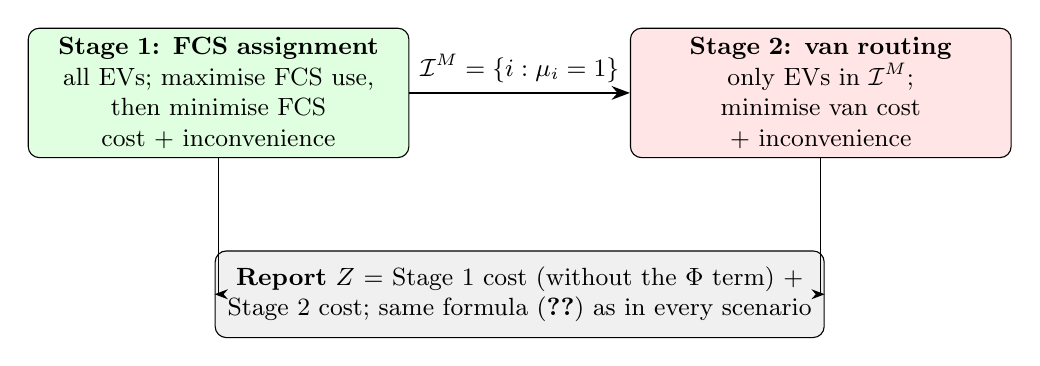
\begin{tikzpicture}[>=Stealth,box/.style={draw,rounded corners,align=center,minimum height=1.1cm,font=\small}]
  \node[box,fill=green!12,text width=4.6cm] (s1) {\textbf{Stage 1: FCS assignment}\\all EVs; maximise FCS use,\\then minimise FCS cost + inconvenience};
  \node[box,fill=red!10,text width=4.6cm,right=2.8cm of s1] (s2) {\textbf{Stage 2: van routing}\\only EVs in $\I^M$;\\minimise van cost + inconvenience};
  \draw[->,thick] (s1) -- node[above,font=\small]{$\I^M=\{i:\mu_i=1\}$} (s2);
  \node[box,fill=black!6,text width=7.5cm,below=2.0cm of $(s1)!0.5!(s2)$] (ev) {\textbf{Report} $Z=$ Stage~1 cost (without the $\Phi$ term) $+$ Stage~2 cost; same formula \eqref{eq:Z} as in every scenario};
  \draw[->] (s1) |- (ev); \draw[->] (s2) |- (ev);
\end{tikzpicture}
\end{center}

Stage~1 does not look at the vans, and Stage~2 cannot change what Stage~1 decided. That is the definition of ``FCS first, then MCS''.

%----------------------------------------------------------------
\subsection{Stage 1: assign EVs to fixed stations}

\textbf{Objective.}
\begin{equation}
\begin{split}
\min\ Z^{(1)}=\;&\underbrace{\Phi\sum_{i\in\I}\mu_i}_{\text{FCS first}}
+\underbrace{c^{EV}\sum_i\sum_{f\in\F_i}d_{if}Y_{if}}_{Z_1}
+\underbrace{Z^F_{\text{energy}}}_{\text{FCS part of }Z_4}\\
&+\underbrace{\sum_i\sum_{f\in\F_i}\rho^F_{if}Y_{if}+\alpha\sum_i w_i(C_i-r_i)+c^L\sum_i w_iL_i}_{\text{FCS customers' inconvenience}}
\end{split}
\label{eq:obj1}
\end{equation}
with $C_i=S_i+\tau^F_iY_i$ in this stage. $\Phi$ is a penalty for handing an EV to the vans. It is chosen larger than anything an extra FCS customer can add to the rest of \eqref{eq:obj1}, e.g.
\[
\Phi > \max_{i}\max_{f\in\F_i}\big(c^{EV}d_{if}+\pi^{\max}E_i+\rho^F_{if}\big)+n\,(\alpha+c^L)\,w_{\max}\,T,
\]
so Stage~1 first \textbf{maximises the number of EVs served at an FCS}, and only among those solutions minimises FCS cost and inconvenience. ($\pi^{\max}$ is the highest grid price.) A numerically safer equivalent is to solve twice: first $\max\sum_iY_i$, then fix that number and minimise the rest.
\ifTOU
Because $Z^F_{\text{energy}}$ uses the peak price, Stage~1 may \emph{start sessions later} to leave the peak, if the price saving beats the extra waiting cost (Section~\ref{sec:expect}).
\fi

\textbf{Constraints.}
\begin{align}
\sum_{g\in\G_i}y_{ig}+\mu_i &= 1 && \forall i\in\I \label{eq:s1assign}\\
S_i &\ge r_i+\sum_{f\in\F_i}t_{if}Y_{if} && \forall i\in\I \label{eq:fcsarr}\\
S_i &\le r_i+T\,(1-\mu_i) && \forall i\in\I \label{eq:s1park}\\
S_j &\ge S_i+\tau^F_i-(T+\tau^F_i)(3-y_{ig}-y_{jg}-o_{ij}) && \forall g,\ (i,j)\in\mathcal{P}_g \label{eq:disj1}\\
S_i &\ge S_j+\tau^F_j-(T+\tau^F_j)(2-y_{ig}-y_{jg}+o_{ij}) && \forall g,\ (i,j)\in\mathcal{P}_g \label{eq:disj2}\\
\sum_i y_{ig_1} &\ge \sum_i y_{ig_2} && \forall f,\ \G_f=\{g_1,g_2\} \label{eq:gunsym}\\
S_i+\tau^F_iY_i &\le T,\qquad L_i\ge S_i+\tau^F_iY_i-l_i && \forall i\in\I \label{eq:s1time}
\end{align}
\ifTOU plus the time-of-use split \eqref{eq:tou1}--\eqref{eq:tou5} of each FCS session (Section~\ref{sec:price}).\fi
\desc{\eqref{eq:s1assign}: every EV either gets one reachable gun or is handed to the vans. An EV that reaches no FCS ($\G_i=\emptyset$) is forced to $\mu_i=1$. \eqref{eq:fcsarr}: an FCS session cannot start before the EV has asked and driven to the station. \eqref{eq:s1park}: for an EV handed to the vans, $S_i$ is parked at $r_i$, so it adds no waiting in Stage~1 (its real start time is decided in Stage~2). \eqref{eq:disj1}--\eqref{eq:disj2}: two EVs on the same gun do not overlap; $o_{ij}$ picks who goes first. With two guns per station this means at most two EVs charge at a station at a time. \eqref{eq:gunsym}: symmetry breaking between the two identical guns (optional). \eqref{eq:s1time}: finished by $T$; lateness.}

\textbf{Optional acceptability rule.} An operator may refuse to send a driver to a station that is ``too inconvenient'', e.g.\ only allow gun $g$ of station $f$ for EV $i$ if $\hat\rho^F_{if}\le\bar\rho$. This only shrinks $\G_i$, so EVs whose stations are all too far go to the vans. Report results with and without it.

\textbf{Output:} $\I^M=\{i:\mu_i=1\}$, the EVs left for the vans; plus each FCS customer's gun and start time.

%----------------------------------------------------------------
\subsection{Stage 2: route the vans to the leftover EVs}

Stage~2 is a vehicle routing problem with time windows, on the EVs in $\I^M$ only. Here $C_i=S_i+\tau^M_i$.

\textbf{Objective.}
\begin{equation}
\begin{split}
\min\ Z^{(2)}=\;&\underbrace{c^M\sum_m\sum_{(i,j)\in\A^M}d_{ij}x_{ijm}}_{Z_2}+\underbrace{\sum_m c^D_mu_m}_{Z_3}+\underbrace{Z^M_{\text{energy}}}_{\text{van part of }Z_4}\\
&+\underbrace{\sum_{i\in\I^M}\sum_m\rho^M_{im}z_{im}+\alpha\sum_{i\in\I^M}w_i(C_i-r_i)+c^L\sum_{i\in\I^M}w_iL_i}_{\text{van customers' inconvenience}}
\end{split}
\label{eq:obj2}
\end{equation}
Since every EV in $\I^M$ must be served by some van, $Z^M_{\text{energy}}$ and the $\rho^M$ term are constants here. They are kept so that $Z^{(2)}$ is the true cost of Stage~2. Waiting and lateness make the vans visit urgent EVs early.

\textbf{Constraints.}
\begin{align}
\sum_{m\in\M}z_{im} &= 1 && \forall i\in\I^M \label{eq:s2assign}\\
\sum_{j:(0,j)\in\A^M}x_{0jm} = \sum_{i:(i,n+1)\in\A^M}x_{i,n+1,m} &= u_m && \forall m \label{eq:depot}\\
\sum_{i:(i,j)\in\A^M}x_{ijm} = \sum_{k:(j,k)\in\A^M}x_{jkm} &= z_{jm} && \forall j\in\I^M,\ m \label{eq:flow}\\
\sum_{i\in\I^M}z_{im} &\le Q_m\,u_m && \forall m \label{eq:cap}\\
\sum_{i\in\I^M}\frac{E_i}{\eta}z_{im}+\beta\sum_{(i,j)\in\A^M}d_{ij}x_{ijm} &\le B_m\,u_m && \forall m \label{eq:batt}
\end{align}
\begin{align}
S_j &\ge \max\{r_j,\ t_{0j}\,x_{0jm}\} && \forall j\in\I^M,\ m \label{eq:depart}\\
S_j &\ge S_i+\tau^M_i+t_{ij}-(T+\tau^M_i+t_{ij})(1-x_{ijm}) && \forall i\neq j,\ m \label{eq:seq}\\
S_i+\tau^M_i+t_{i,n+1} &\le T+(\tau^M_i+t_{i,n+1})(1-x_{i,n+1,m}) && \forall i,\ m \label{eq:return}\\
S_i+\tau^M_i \le T,\quad L_i &\ge S_i+\tau^M_i-l_i && \forall i\in\I^M \label{eq:s2time}\\
u_m &\ge u_{m+1} && m<|\M| \label{eq:vansym}
\end{align}
\desc{\eqref{eq:s2assign}: each leftover EV gets one van. \eqref{eq:depot}: a used van leaves and returns to the depot once. \eqref{eq:flow}: each EV on van $m$ is entered and left exactly once by that van. \eqref{eq:cap}: at most $Q_m$ EVs per van. \eqref{eq:batt}: delivered energy (with transfer losses) plus driving energy fits in the van battery. \eqref{eq:depart}: no start before the request, or before the van can drive there from the depot (written as two linear constraints). \eqref{eq:seq}: if the van goes $i\to j$, it finishes $i$ and drives to $j$ before starting $j$. This gives one EV at a time and removes subtours (MTZ-type). \eqref{eq:return}: back at the depot by $T$. \eqref{eq:s2time}: finished by $T$; lateness. \eqref{eq:vansym}: use identical vans in index order.}

\textbf{If Stage 2 is infeasible} (too many leftover EVs for the fleet by $T$), the sequential policy has \emph{failed} on that instance. For diagnosis, add $s_i\in\{0,1\}$ (``unserved''), replace \eqref{eq:s2assign} by $\sum_mz_{im}+s_i=1$ and add $\Phi^U\sum_is_i$ to \eqref{eq:obj2}. Then report the number of EVs that could not be served. This is a useful comparison with the integrated scenario, which may serve all of them.

%----------------------------------------------------------------
\subsection{Reported value}
\[
Z^{\text{S\scen}}=\big(Z^{(1)*}-\Phi\,|\I^M|\big)+Z^{(2)*},
\]
which is exactly \eqref{eq:Z} evaluated at the combined solution. The stage-1 solution plus the stage-2 solution is a feasible solution of the integrated model (S\ifTOU 4\else 3\fi), so
$Z^{\text{S\ifTOU 4\else 3\fi}}\le Z^{\text{S\scen}}$. The difference is the \emph{value of integration}.

\else
%---------------------------------------------------------------- INT
\subsection{Objective}
\begin{equation}
\min\ Z \quad\text{as in \eqref{eq:Z}, with }Z^F_{\text{energy}}=\ifTOU P^F\textstyle\sum_i\big[\pi^\off(\theta^1_i+\theta^3_i)+\pi^\pk\theta^2_i\big]\else\pi^F\textstyle\sum_iE_iY_i\fi,\quad C_i=S_i+\tau^F_iY_i+\tau^M_iZ_i. \label{eq:objint}
\end{equation}
Written out in full:
\begin{align*}
\min\ Z=\;& c^{EV}\sum_i\sum_{f\in\F_i}d_{if}Y_{if}+c^M\sum_m\sum_{(i,j)\in\A}d_{ij}x_{ijm}+\sum_mc^D_mu_m\\
&+\ifTOU P^F\sum_i\big[\pi^\off(\theta^1_i+\theta^3_i)+\pi^\pk\theta^2_i\big]\else\pi^F\sum_iE_iY_i\fi
+\pi^M\sum_i\sum_m\frac{E_i}{\eta}z_{im}\\
&+\sum_i\sum_{f\in\F_i}\rho^F_{if}Y_{if}+\sum_i\sum_m\rho^M_{im}z_{im}+\alpha\sum_iw_i(C_i-r_i)+c^L\sum_iw_iL_i .
\end{align*}
Every term is linear. One model weighs everything at once: an EV goes to a van exactly when the van's extra km, dispatch and energy cost are outweighed by the effort and waiting it saves the driver\ifTOU, or by the peak-price energy it avoids\fi.

\subsection{Constraints}

\textbf{Assignment.}
\begin{equation}
\sum_{g\in\G_i}y_{ig}+\sum_{m\in\M}z_{im}=1\qquad\forall i\in\I \label{eq:assign}
\end{equation}
\desc{Exactly one resource per EV: one reachable gun or one van. EVs that reach no FCS are forced onto a van.}

\textbf{Fixed stations.}
\begin{align}
S_i &\ge r_i+\sum_{f\in\F_i}t_{if}Y_{if} && \forall i \label{eq:fcsarr}\\
S_j &\ge S_i+\tau^F_i-(T+\tau^F_i)(3-y_{ig}-y_{jg}-o_{ij}) && \forall g,\ (i,j)\in\mathcal{P}_g \label{eq:disj1}\\
S_i &\ge S_j+\tau^F_j-(T+\tau^F_j)(2-y_{ig}-y_{jg}+o_{ij}) && \forall g,\ (i,j)\in\mathcal{P}_g \label{eq:disj2}\\
\sum_iy_{ig_1} &\ge \sum_iy_{ig_2} && \forall f,\ \G_f=\{g_1,g_2\} \label{eq:gunsym}
\end{align}
\desc{\eqref{eq:fcsarr}: an FCS session starts after the request and the drive to the station (for a van customer this is just $S_i\ge r_i$). \eqref{eq:disj1}--\eqref{eq:disj2}: EVs on the same gun do not overlap; $o_{ij}$ chooses the order. \eqref{eq:gunsym}: optional symmetry breaking.}

\textbf{Vans: routes, capacity, battery.}
\begin{align}
\sum_{j:(0,j)\in\A}x_{0jm}=\sum_{i:(i,n+1)\in\A}x_{i,n+1,m} &= u_m && \forall m \label{eq:depot}\\
\sum_{i:(i,j)\in\A}x_{ijm}=\sum_{k:(j,k)\in\A}x_{jkm} &= z_{jm} && \forall j\in\I,\ m \label{eq:flow}\\
\sum_iz_{im} &\le Q_mu_m && \forall m \label{eq:cap}\\
\sum_i\frac{E_i}{\eta}z_{im}+\beta\sum_{(i,j)\in\A}d_{ij}x_{ijm} &\le B_mu_m && \forall m \label{eq:batt}
\end{align}
\desc{\eqref{eq:depot}: a used van leaves and returns once. \eqref{eq:flow}: each EV on van $m$ is visited exactly once by it. \eqref{eq:cap}: at most $Q_m$ EVs. \eqref{eq:batt}: delivered energy (with losses) plus driving energy fits in the battery.}

\textbf{Vans: timing (one EV at a time, no subtours).}
\begin{align}
S_j &\ge t_{0j}\,x_{0jm} && \forall j\in\I,\ m \label{eq:depart}\\
S_j &\ge S_i+\tau^M_i+t_{ij}-(T+\tau^M_i+t_{ij})(1-x_{ijm}) && \forall i\neq j\in\I,\ m \label{eq:seq}\\
S_i+\tau^M_i+t_{i,n+1} &\le T+(\tau^M_i+t_{i,n+1})(1-x_{i,n+1,m}) && \forall i,\ m \label{eq:return}
\end{align}
\desc{\eqref{eq:depart}: the first stop cannot start before the van has driven there. \eqref{eq:seq}: $i\to j$ means finish $i$, drive, then start $j$; start times rise along a route, so no subtour can close. \eqref{eq:return}: back at the depot by $T$.}

\textbf{Horizon and lateness.}
\begin{equation}
C_i\le T,\qquad L_i\ge C_i-l_i\qquad\forall i\in\I \label{eq:time}
\end{equation}
\desc{Every EV is fully charged within the horizon; $L_i$ measures lateness.}

\ifTOU
\textbf{Time-of-use split.} Constraints \eqref{eq:tou1}--\eqref{eq:tou5} of Section~\ref{sec:price}.
\fi

\textbf{Symmetry and domains.}
\begin{equation}
u_m\ge u_{m+1};\qquad y,z,x,u,o\ifTOU,\kappa\fi\in\{0,1\};\qquad S_i,L_i\ifTOU,\theta^p_i\fi\ge0 \label{eq:dom}
\end{equation}
\fi

%=====================================================================
\section{Learning-to-optimise (RL) formulation}\label{sec:rl}

\textbf{Main rule:} the reward of each action is \emph{minus the increase in $Z$ that the action causes}. The rewards over an episode then add up to $-Z$ of the solution the policy builds. RL and MILP results are measured on the same yardstick \eqref{eq:Z}, and the MILP optimum is the benchmark for the RL gap.

\ifSEQ
%---------------------------------------------------------------- RL SEQ
The RL pipeline has the same two stages as the MILP.

\subsection{Stage 1 policy: FCS assignment}
\begin{itemize}[leftmargin=1.4em,itemsep=2pt]
  \item \textbf{Episode / epochs:} EVs are taken in order of request time $r_i$ (ties: higher $w_i$ first). One decision per EV.
  \item \textbf{State:} features of the current EV $k$ ($E_k,r_k,l_k,w_k,R_k$, location); for each gun $g$ the time $F_g$ it becomes free; summary features of the EVs still to come (count and positions near each station)\ifTOU; the current price and the time until $T_1$ and $T_2$\fi.
  \item \textbf{Action:} a gun $g\in\G_k$, or ``hand to vans''. \textbf{FCS-first mask:} ``hand to vans'' is allowed \emph{only} if no gun can finish EV $k$ by $T$ (or, with the optional rule, if all remaining guns have $\hat\rho^F_{kf}>\bar\rho$).
  \ifTOU\item \textbf{Optional timing action:} ``gun $g$, start after the peak'', i.e.\ $S_k=\max\{\text{earliest},T_2\}$, allowed only if the session still ends by $T$.\fi
  \item \textbf{Transition:} $S_k=\max\{r_k+t_{kf},F_g\}$ (or later, for the timing action); $F_g\leftarrow S_k+\tau^F_k$.
  \item \textbf{Reward:} $-\Big[c^{EV}d_{kf}+\text{energy}_k+\rho^F_{kf}+\alpha w_k(S_k+\tau^F_k-r_k)+c^Lw_k(S_k+\tau^F_k-l_k)^+\Big]$, where energy$_k$ = \ifTOU$P^F\big[\pi^\off\cdot(\text{off-peak hours of }[S_k,S_k+\tau^F_k])+\pi^\pk\cdot(\text{peak hours})\big]$, computed exactly in the simulator\else$\pi^FE_k$\fi. Handing an EV to the vans gives reward $0$ here; its cost is counted in Stage~2.
\end{itemize}
Note: a simple baseline for Stage~1 is the greedy rule ``gun with the largest one-step reward''. What RL can learn on top of this is, for example, to keep a nearby gun free for an urgent EV that arrives later.

\subsection{Stage 2 policy: van routing over $\I^M$}
\begin{itemize}[leftmargin=1.4em,itemsep=2pt]
  \item \textbf{Epochs:} whenever a van becomes free (the earliest-free van decides first).
  \item \textbf{State:} for each van: position, time free, remaining battery $b_m$, EVs served so far, dispatched or not; for each unserved EV in $\I^M$: location, $E_i,r_i,l_i,w_i$; current time.
  \item \textbf{Action:} the next EV $j$ for this van, or ``return to depot'' (ends the route). Mask: $j$ must be feasible: battery covers $E_j/\eta$ plus driving to $j$ and back to the depot, the count stays $\le Q_m$, and $j$ can be finished with the van back at the depot by $T$.
  \item \textbf{Transition:} $S_j=\max\{r_j,\ \text{time free}+t_{\text{pos},j}\}$; the van moves to $j$ and is free at $S_j+\tau^M_j$; $b_m$ falls by $E_j/\eta+\beta d_{\text{pos},j}$.
  \item \textbf{Reward:} serving $j$: $-\Big[c^Md_{\text{pos},j}+c^D_m[\text{first stop}]+\pi^M\frac{E_j}{\eta}+\rho^M_{jm}+\alpha w_j(S_j+\tau^M_j-r_j)+c^Lw_j(S_j+\tau^M_j-l_j)^+\Big]$; returning: $-c^Md_{\text{pos},0}$. EVs still unserved at the end: $-\Phi^U$ each.
  \item \textbf{Policy:} an attention-based routing policy (e.g.\ Kool et al., 2019, ``Attention, Learn to Solve Routing Problems!'') trained with REINFORCE or PPO. Baseline: nearest-feasible-EV heuristic.
\end{itemize}
Episode return of Stage~1 + Stage~2 $=-Z^{\text{S\scen}}$.

\else
%---------------------------------------------------------------- RL INT
One policy decides both who serves each EV and the van routes.
\begin{itemize}[leftmargin=1.4em,itemsep=2pt]
  \item \textbf{Episode / epochs:} EVs are taken in order of request time $r_i$ (ties: higher $w_i$ first). One decision per EV.
  \item \textbf{State:} (i) the current EV $k$: location, $E_k,r_k,l_k,w_k,R_k$, reachable stations; (ii) each gun $g$: time $F_g$ it becomes free; (iii) each van $m$: current end-of-route position, time free, remaining battery $b_m$, EVs served, dispatched or not; (iv) embeddings of the not-yet-assigned EVs (for look-ahead)\ifTOU; (v) current price, time until $T_1$ and $T_2$\fi.
  \item \textbf{Action:} $a\in\G_k\cup\M$: a gun, or a van (EV $k$ is appended to the end of that van's route). \textbf{Mask} infeasible actions: a gun that cannot finish $k$ by $T$; a van without enough battery for $E_k/\eta$ plus the drive to $k$ and back to the depot, with $Q_m$ reached, or unable to finish $k$ and return by $T$.
  \ifTOU\item \textbf{Optional timing action:} ``gun $g$, start after the peak'' ($S_k=\max\{\text{earliest},T_2\}$, if it still ends by $T$).\fi
  \item \textbf{Transition:} gun: $S_k=\max\{r_k+t_{kf},F_g\}$, $F_g\leftarrow S_k+\tau^F_k$. Van: $S_k=\max\{r_k,\ \text{free}_m+t_{\text{pos}_m,k}\}$, then the van moves to $k$, $\text{free}_m\leftarrow S_k+\tau^M_k$, $b_m\mathrel{-}=E_k/\eta+\beta d_{\text{pos}_m,k}$.
  \item \textbf{Reward} $=-\Delta Z$:
  \begin{align*}
  \text{gun } g\text{ at }f:&\quad -\Big[c^{EV}d_{kf}+\text{energy}^F_k+\rho^F_{kf}+\alpha w_k(C_k-r_k)+c^Lw_k(C_k-l_k)^+\Big]\\
  \text{van } m:&\quad -\Big[c^M\big(d_{\text{pos}_m,k}+d_{k,0}-d_{\text{pos}_m,0}\big)+c^D_m[\text{first use}]+\pi^M\tfrac{E_k}{\eta}\\
  &\qquad\quad+\rho^M_{km}+\alpha w_k(C_k-r_k)+c^Lw_k(C_k-l_k)^+\Big]
  \end{align*}
  The van distance term is the \emph{change} in route length when $k$ is inserted before the return to the depot, so the sum over the episode equals the total route length (the return legs telescope). energy$^F_k$ = \ifTOU$P^F\big[\pi^\off\cdot(\text{off-peak hours})+\pi^\pk\cdot(\text{peak hours of }[S_k,C_k])\big]$, computed exactly by the simulator; no linearisation is needed in RL\else$\pi^FE_k$\fi.
  \item \textbf{Dead end:} if every action is masked, EV $k$ is unserved: reward $-\Phi^U$, and the episode continues. Report the count.
  \item \textbf{Policy:} masked categorical policy over guns and vans, encoder with attention over EVs, guns and vans; trained with PPO. Natural baseline: greedy, i.e.\ choose the action with the largest one-step reward. That is the pairwise rule ``smallest $\hat\rho$ + cost'' from Section~\ref{sec:inc}.
\end{itemize}
Restriction to note: vans serve EVs in assignment order (append only). A variant that inserts $k$ at the cheapest position of a route is more flexible but has a larger action space.
\fi

\textbf{Reward scaling.} For stable training divide every reward by a constant, e.g.\ the greedy baseline's average $Z$ on the training instances. This does not change the optimal policy.

%=====================================================================
\section{What to expect and what to report}\label{sec:expect}

\ifnum\scen=1
\begin{itemize}[leftmargin=1.4em,itemsep=2pt]
  \item Vans serve only EVs that reach no station, or that the stations cannot finish by $T$. If stations have spare capacity, very few vans are dispatched.
  \item Inconvenience is high for EVs far from the nearest station (worked example: Rs\,682 at the FCS, against Rs\,458 if a van had been allowed).
  \item With too few vans Stage~2 becomes infeasible (unserved EVs), even when the integrated model S3 could serve everyone. Report the smallest $|\M|$ at which S1 is feasible and compare it with S3.
\end{itemize}
\fi
\ifnum\scen=2
\begin{itemize}[leftmargin=1.4em,itemsep=2pt]
  \item \textbf{When does Stage~1 delay a session to avoid the peak?} Moving one hour of charging out of the peak saves $(\pi^\pk-\pi^\off)P^F=3\times22=$ Rs\,66, but delays completion by up to an hour, which costs $\alpha w_i\ge$ Rs\,200. So with the default values Stage~1 almost never delays. It mostly pays the higher price, and S2 costs roughly S1 plus the peak surcharge. Sessions start later only if $\alpha$ is small (try $\lambda<0.33$ in the sensitivity analysis).
  \item The van assignment is the same as in S1 unless Stage~1's timing changes which EVs fit at the stations. Stage~1 cannot use vans to escape the peak price.
  \item Extra KPI: \textbf{grid energy drawn at FCS during the peak}, $P^F\sum_i\theta^2_i$ (kWh). Compare with S4.
\end{itemize}
\fi
\ifnum\scen=3
\begin{itemize}[leftmargin=1.4em,itemsep=2pt]
  \item Vans take EVs for which the saved inconvenience exceeds the extra van cost (worked example: van chosen, saving Rs\,224). Expect vans to serve EVs that are far from every station, have low range (high $w_i$), or have early deadlines, while EVs near a station still use it.
  \item \textbf{Value of integration under flat price:} $Z^{\text{S1}}-Z^{\text{S3}}\ge0$. Report it per component ($Z_1,\dots,Z_5$): typically operating cost rises a little and inconvenience falls a lot.
  \item Vary $|\M|$ (0, 1, 2, \dots): the first few vans lower $Z$ sharply, then the effect levels off. That curve shows the scenarios where mobile chargers help most.
\end{itemize}
\fi
\ifnum\scen=4
\begin{itemize}[leftmargin=1.4em,itemsep=2pt]
  \item During the peak a van kWh costs about the same as an FCS kWh (Rs\,10.0 each), so the vans' energy disadvantage disappears and vans also absorb \emph{peak-hour} demand that would otherwise be charged on the grid at peak price.
  \item Expect more van usage than in S3, concentrated on requests in $[T_1,T_2]$, and lower grid energy at the stations during the peak, $P^F\sum_i\theta^2_i$, than in S2.
  \item \textbf{Value of integration under peak pricing:} $Z^{\text{S2}}-Z^{\text{S4}}$. It should be larger than $Z^{\text{S1}}-Z^{\text{S3}}$, because integration now also allows price arbitrage.
  \item \textbf{Peak pricing with full flexibility:} $Z^{\text{S4}}-Z^{\text{S3}}$ should be smaller than $Z^{\text{S2}}-Z^{\text{S1}}$: vans cushion the price increase.
\end{itemize}
\fi

\textbf{Cross-scenario comparison table} (fill in from the four runs):
\begin{center}
\renewcommand{\arraystretch}{1.2}
\begin{tabular}{@{}lll@{}}
\toprule
\textbf{Comparison} & \textbf{Measures} & \textbf{Expected sign} \\
\midrule
S1 $-$ S3 & value of integration, flat price & $\ge0$ \\
S2 $-$ S4 & value of integration, peak price & $\ge0$, larger than S1 $-$ S3 \\
S2 $-$ S1 & cost of peak pricing, FCS-first operator & $>0$ \\
S4 $-$ S3 & cost of peak pricing, flexible operator & $>0$, smaller than S2 $-$ S1 \\
\bottomrule
\end{tabular}
\end{center}
Report for each: $Z$ and its components, number of vans used, EVs per resource, mean and maximum inconvenience per EV, total lateness, peak-hour grid energy, solve time, and (for RL) the gap to the MILP optimum.

%=====================================================================
\appendix
\section{Illustrative parameter values}\label{app:values}

These are starting values for experiments, not data. All are meant to be varied in the analysis. Values in Rs.

\begin{center}
\renewcommand{\arraystretch}{1.15}
\begin{tabular}{@{}llp{6.2cm}@{}}
\toprule
\textbf{Parameter} & \textbf{Value} & \textbf{Note} \\
\midrule
$T$, $[T_1,T_2]$ & 7 h, $[2,6]$ & 16:00--23:00, peak 18:00--22:00 \\
$P^F$, $P^M$ & 22 kW, 30 kW & \\
$v$, $\beta$, $\eta$ & 25 km/h, 0.25 kWh/km, 0.9 & \\
$B_m$, $Q_m$, $|\M|$ & 150 kWh, 6, 2--6 & \\
$c^{EV}$, $c^M$, $c^D_m$ & Rs\,4/km, Rs\,15/km, Rs\,1500 & van km includes driver time \\
$\pi^F$ (flat) & Rs\,8.7/kWh & equals the time-average of the ToU tariff over $[0,T]$ \\
$\pi^\off$, $\pi^\pk$ (ToU) & Rs\,7/kWh, Rs\,10/kWh & $(3\times7+4\times10)/7=8.7$ \\
$c^{bat}$ & Rs\,2/kWh & van battery wear \\
$\pi^M$ & Rs\,10.7 (flat) / Rs\,9.0 (ToU) & $=\pi^F+c^{bat}$ / $=\pi^\off+c^{bat}$ \\
$\alpha$, $\alpha^D$ & Rs\,200/h, Rs\,100/h & value of time; extra for attended time \\
$h^F$, $h^M$, $\varphi$ & Rs\,50, Rs\,10, Rs\,100 & trip hassle, hand-over, range stress \\
$c^L$ & Rs\,300/h & lateness \\
$w_i$ & $1+2(1-R_i/R_{\max})$, $R_i\sim U[3,40]$ km & priority from remaining range \\
\bottomrule
\end{tabular}
\end{center}

The flat price is set to the time-average of the peak tariff. The price \emph{level} is then the same in both pricing cases, and only the price \emph{shape} differs. Without this, part of S1 vs S2 would just reflect a different average price.

\end{document}
"
%    pdflatex -jobname=scenario2_peak_sequential   "\def\scen{2}% =====================================================================
%  One source, four PDFs.  Build with build.sh (or by hand):
%    pdflatex -jobname=scenario1_flat_sequential   "\def\scen{1}\input{scenario_master}"
%    pdflatex -jobname=scenario2_peak_sequential   "\def\scen{2}\input{scenario_master}"
%    pdflatex -jobname=scenario3_flat_integrated   "\def\scen{3}\input{scenario_master}"
%    pdflatex -jobname=scenario4_peak_integrated   "\def\scen{4}\input{scenario_master}"
%  (run each twice for cross-references)
% =====================================================================
\documentclass[11pt,a4paper]{article}
\usepackage[margin=2.2cm]{geometry}
\usepackage{amsmath,amssymb,amsfonts}
\usepackage{booktabs,array,tabularx}
\usepackage{enumitem}
\usepackage[table]{xcolor}
\usepackage{tikz}
\usetikzlibrary{arrows.meta,positioning,calc}
\usepackage[colorlinks=true,linkcolor=blue!50!black,urlcolor=blue!50!black]{hyperref}
\usepackage{titlesec}
\titleformat{\section}{\large\bfseries}{\thesection}{0.8em}{}
\titleformat{\subsection}{\normalsize\bfseries}{\thesubsection}{0.8em}{}
\setlength{\parindent}{0pt}
\setlength{\parskip}{5pt}

% ---------------- scenario switches ----------------
\ifdefined\scen\else\def\scen{1}\fi
\newif\ifTOU \TOUfalse   % true = time-of-use (peak) price
\newif\ifSEQ \SEQfalse   % true = FCS first, then MCS
\ifnum\scen=1 \SEQtrue \fi
\ifnum\scen=2 \TOUtrue \SEQtrue \fi
\ifnum\scen=4 \TOUtrue \fi

\newcommand{\pricename}{\ifTOU time-of-use price (dearer evening peak)\else single (flat) price all day\fi}
\newcommand{\structname}{\ifSEQ FCS first, then MCS (sequential)\else FCS and MCS together (integrated)\fi}

% ---------------- notation ----------------
\newcommand{\I}{\mathcal{I}}
\newcommand{\F}{\mathcal{F}}
\newcommand{\G}{\mathcal{G}}
\newcommand{\M}{\mathcal{M}}
\newcommand{\N}{\mathcal{N}}
\newcommand{\A}{\mathcal{A}}
\newcommand{\Rs}{\text{Rs}\,}
\newcommand{\pk}{\mathrm{pk}}
\newcommand{\off}{\mathrm{off}}
\newcommand{\desc}[1]{\par\vspace{-2pt}{\small\color{black!75}\textit{Meaning:} #1}\par\vspace{4pt}}
\newcommand{\cell}[2]{\ifnum\scen=#1\cellcolor{blue!18}\textbf{S#1 (this document)}\\\textbf{#2}\else S#1\\#2\fi}

\title{\textbf{EV Charging Network Optimisation}\\[4pt]
\large Scenario \scen: \pricename\ $+$ \structname\\[2pt]
\normalsize MILP and RL formulation}
\author{CP 320 OR for Mobility Management, course project}
\date{2 October 2026}

\begin{document}
\maketitle

%=====================================================================
\section{Where this scenario sits}

The project studies four scenarios: two ways of pricing grid electricity, times two ways of making the decisions.

\begin{center}
\renewcommand{\arraystretch}{1.5}
\begin{tabular}{>{\raggedright\arraybackslash}p{4.2cm}|>{\centering\arraybackslash}p{4.6cm}|>{\centering\arraybackslash}p{4.6cm}}
 & \textbf{Flat price all day} & \textbf{Time-of-use (peak) price} \\ \hline
\textbf{Sequential:} FCS first, leftover EVs to MCS &
\begin{tabular}[c]{@{}c@{}}\cell{1}{flat + sequential}\end{tabular} &
\begin{tabular}[c]{@{}c@{}}\cell{2}{peak + sequential}\end{tabular} \\ \hline
\textbf{Integrated:} FCS and MCS decided together &
\begin{tabular}[c]{@{}c@{}}\cell{3}{flat + integrated}\end{tabular} &
\begin{tabular}[c]{@{}c@{}}\cell{4}{peak + integrated}\end{tabular} \\
\end{tabular}
\end{center}

\textbf{The four scenarios do not have four different objectives.} They share \emph{one} cost yardstick $Z$ (Section~\ref{sec:obj}): the same cost terms and the same customer inconvenience (Section~\ref{sec:inc}). Only two things change:
\begin{itemize}[leftmargin=1.4em,itemsep=1pt]
  \item \textbf{Pricing} changes the formula for one term, the FCS energy cost (Section~\ref{sec:price}).
  \item \textbf{Decision structure} changes \emph{how} $Z$ is minimised: in one model (integrated), or in two stages (sequential), where each stage minimises its own part of $Z$.
\end{itemize}
Because the yardstick is the same, the four optimal values can be compared directly. The differences measure the \emph{value of integration} (S1$\to$S3, S2$\to$S4) and the \emph{effect of peak pricing} (S1$\to$S2, S3$\to$S4).

\ifnum\scen=1
\textbf{This scenario (S1)} is the baseline, the ``status quo''. Electricity costs the same at every hour, every EV that can be charged at a fixed station is sent there, and vans only take what is left over.
\fi
\ifnum\scen=2
\textbf{This scenario (S2)} keeps the FCS-first rule of S1, but grid electricity is dearer during the evening peak. Stage~1 can react to the price only by \emph{rescheduling} FCS sessions. It cannot hand a peak-hour EV to a van.
\fi
\ifnum\scen=3
\textbf{This scenario (S3)} keeps the flat price of S1, but the operator decides FCS and MCS service \emph{together}. An EV can be sent to a van even when a fixed station could take it, whenever that lowers total cost plus inconvenience.
\fi
\ifnum\scen=4
\textbf{This scenario (S4)} is the most flexible one: peak pricing at fixed stations, and FCS and MCS decided together. Van energy was bought off-peak, so vans can also be used to keep charging \emph{out of the expensive peak}.
\fi

%=====================================================================
\section{Setting and assumptions}\label{sec:setting}

\textbf{Time.} The planning horizon is $[0,T]$ with $T=7$\,h (16:00--23:00). It contains the evening peak window $[T_1,T_2]=[2,6]$ (18:00--22:00). The horizon is the same in all four scenarios. It is wider than the peak itself so that, under peak pricing, there is cheaper time on both sides of the peak.\ifTOU\else\ In this scenario the price is flat, so the window plays no role in the model.\fi

\textbf{Assumptions} (the same as MILP v3, plus two about energy):
\begin{enumerate}[leftmargin=1.6em,itemsep=1pt]
  \item Static, continuous time. All requests in the horizon are known at time $0$, and request $i$ becomes active at $r_i$.
  \item An EV served by an FCS drives there itself on its own battery (only to stations within its range $R_i$). The driver stays with the car while it waits for a free gun and while it charges.
  \item An EV served by an MCS stays parked where it is, and the driver is free in the meantime.
  \item Each FCS gun and each van charges one EV at a time, without interruption, at constant power.
  \item A van's battery covers both its driving and the energy it delivers. \textbf{The van battery is charged at the depot before the horizon starts}\ifTOU, i.e.\ at the off-peak price\fi, and is not recharged during the horizon.
  \item Every EV must be fully charged by $T$ (hard). Finishing after the driver's desired time $l_i$ is allowed but penalised.
\end{enumerate}

%=====================================================================
\section{Notation}\label{sec:notation}

\subsection*{Sets}
\begin{tabularx}{\textwidth}{@{}lX@{}}
\toprule
$\I=\{1,\dots,n\}$ & EV charging requests \\
$\F$; $\G_f$ ($|\G_f|=2$); $\G=\bigcup_f\G_f$ & fixed charging stations; guns of FCS $f$; all guns ($f(g)$ = station of gun $g$) \\
$\F_i=\{f: d_{if}\le R_i\}$, $\G_i=\bigcup_{f\in\F_i}\G_f$ & stations / guns EV $i$ can reach on its remaining range \\
$\M$ & mobile charging vans (MCS) \\
$0,\ n+1$ & depot as start node / end node (same place) \\
$\N=\{0\}\cup\I\cup\{n+1\}$, $\A$ & routing nodes; allowed van arcs $(i,j)$, $i\in\{0\}\cup\I$, $j\in\I\cup\{n+1\}$, $i\neq j$ \\
$\mathcal{P}_g=\{(i,j): i<j,\ g\in\G_i\cap\G_j\}$ & pairs of EVs that could share gun $g$ \\
\ifSEQ
$\I^M\subseteq\I$ & EVs handed to the vans by Stage~1 (an \emph{output} of Stage~1, a fixed input to Stage~2) \\
$\N^M$, $\A^M$ & routing nodes / arcs restricted to $\I^M$ \\
\fi
\bottomrule
\end{tabularx}

\subsection*{Parameters}
\begin{tabularx}{\textwidth}{@{}lX@{}}
\toprule
$E_i,\ r_i,\ l_i,\ R_i$ & energy demand (kWh), request time, desired completion time (h), remaining range (km) \\
$w_i\ge1$ & priority of EV $i$; $w_i=1+\kappa(1-R_i/R_{\max})$, so low-range EVs weigh more \\
$P^F,\ P^M$ & charging power of an FCS gun (22\,kW) / of a van (e.g.\ 30\,kW) \\
$\tau^F_i=E_i/P^F,\ \tau^M_i=E_i/P^M$ & charging time of EV $i$ at an FCS / by a van (h) \\
$d_{if},t_{if}$;\ $d_{ij},t_{ij}$ & distance (km) and time (h): EV$\to$FCS; between routing nodes ($t=d/v$) \\
$B_m,\ Q_m,\ \beta,\ \eta$ & van battery (kWh), max EVs per van, van consumption (kWh/km), transfer efficiency \\
$c^{EV},\ c^M,\ c^D_m$ & cost per km of EV driving, per km of van driving; fixed dispatch cost of van $m$ \\
\ifTOU
$\pi^\off,\ \pi^\pk$ & grid price (Rs/kWh) off-peak / in $[T_1,T_2]$, with $\pi^\pk\ge\pi^\off$ \\
\else
$\pi^F$ & grid price (Rs/kWh), the same at every hour \\
\fi
$c^{bat}$ & van battery wear per kWh cycled \\
$\pi^M$ & cost of 1 kWh taken from a van battery: $\pi^M=\ifTOU\pi^\off\else\pi^F\fi+c^{bat}$ (Section~\ref{sec:price}) \\
$\alpha,\ \alpha^D,\ h^F,\ h^M,\ \varphi,\ c^L$ & inconvenience coefficients (Section~\ref{sec:inc}) \\
\bottomrule
\end{tabularx}

\subsection*{Decision variables}
\begin{tabularx}{\textwidth}{@{}llX@{}}
\toprule
$y_{ig}$ & $\{0,1\}$ & EV $i$ charged at gun $g\in\G_i$ \\
$z_{im}$ & $\{0,1\}$ & EV $i$ served by van $m$ \\
$x_{ijm}$ & $\{0,1\}$ & van $m$ drives arc $(i,j)$ \\
$u_m$ & $\{0,1\}$ & van $m$ is dispatched \\
$o_{ij}$ & $\{0,1\}$ & for EVs $i<j$ that could share a gun: 1 if $i$ is charged before $j$ \\
\ifSEQ
$\mu_i$ & $\{0,1\}$ & Stage~1 only: EV $i$ is handed to the van fleet \\
\fi
\ifTOU
$\theta^1_i,\theta^2_i,\theta^3_i$ & $\ge0$ & hours of EV $i$'s FCS session before / inside / after the peak \\
$\kappa^1_i,\kappa^3_i$ & $\{0,1\}$ & EV $i$'s FCS session starts before $T_1$ / ends after $T_2$ \\
\fi
$S_i$ & $\ge0$ & time charging of EV $i$ starts (h), on whichever resource \\
$L_i$ & $\ge0$ & lateness of EV $i$ beyond $l_i$ (h) \\
\bottomrule
\end{tabularx}

\textbf{Short-hands} (linear expressions, not new variables):
\[
Y_{if}=\sum_{g\in\G_f}y_{ig},\qquad Y_i=\sum_{g\in\G_i}y_{ig}\ (\text{EV $i$ uses an FCS}),\qquad Z_i=\sum_{m\in\M}z_{im}\ (\text{EV $i$ uses a van}),
\]
\[
C_i=S_i+\tau^F_i\,Y_i+\tau^M_i\,Z_i \quad\text{(time EV $i$ is fully charged).}
\]

%=====================================================================
\section{Customer inconvenience}\label{sec:inc}

This section is \textbf{identical in all four scenario documents}. Inconvenience is a property of the customer, not of the price or of the planning method.

\subsection{What we mean by inconvenience}

Inconvenience is \emph{what the driver loses} from the moment they ask for a charge ($r_i$) until the car is fully charged ($C_i$), \emph{converted into rupees} so it can be added to the operator's costs. A driver loses three different things:

\begin{enumerate}[leftmargin=1.6em,itemsep=2pt]
  \item \textbf{Waiting:} the car is not ready. This lasts $C_i-r_i$ hours and affects \emph{every} driver, FCS or MCS.
  \item \textbf{Effort:} only an FCS customer has to drive to the station and sit there while the car charges. An MCS customer stays at home or at work and does something else. Driving to a far station also uses scarce battery range, which causes stress (``range anxiety'').
  \item \textbf{A missed deadline:} the car is still not ready at the time $l_i$ the driver needs it.
\end{enumerate}

Each loss gets a price in Rs per hour (or per event). All of them are multiplied by the priority $w_i$: an hour of delay for an EV with 5\,km of range left counts more than for one with 40\,km.

\subsection{The three components}

\begin{center}
\renewcommand{\arraystretch}{1.3}
\begin{tabularx}{\textwidth}{@{}>{\raggedright\arraybackslash}p{2.6cm}>{\raggedright\arraybackslash}X>{\raggedright\arraybackslash}X>{\raggedright\arraybackslash}p{3.0cm}@{}}
\toprule
\textbf{Component} & \textbf{EV $i$ at FCS $f$} & \textbf{EV $i$ by a van} & \textbf{Known when?} \\
\midrule
Effort & $w_i\big[\alpha^D(t_{if}+\tau^F_i)+h^F+\varphi\,d_{if}/R_i\big]$: driving and sitting at the station, a fixed trip hassle, range stress & $w_i\,h^M$: being reachable and handing over the car & \textbf{Static:} known as soon as the resource is chosen \\
Waiting & $w_i\,\alpha\,(C_i-r_i)$ = drive + \emph{queue at the gun} + charge & $w_i\,\alpha\,(C_i-r_i)$ = \emph{wait for the van} + charge & \textbf{Dynamic:} depends on the queue / van route \\
Missed deadline & $w_i\,c^L\,L_i$, $L_i=\max\{0,C_i-l_i\}$ & same & Dynamic \\
\bottomrule
\end{tabularx}
\end{center}

\textbf{Coefficients.}
$\alpha$ (Rs/h) is the value of an hour the car is not ready.
$\alpha^D$ (Rs/h) is the \emph{extra} value of an hour the driver must personally spend driving or sitting at the station: an hour at the station costs $\alpha+\alpha^D$, an hour waiting at home for a van costs only $\alpha$.
$h^F,h^M$ (Rs) are fixed hassle costs of one trip to a station / one van hand-over.
$\varphi$ (Rs) is the range-stress cost of a trip that uses the \emph{whole} remaining range ($d_{if}/R_i\le1$ is the fraction used).
$c^L$ (Rs/h) is the cost per hour late.

\subsection{Pairwise form: inconvenience of a (customer, resource) pair}

The natural first idea is: \emph{for every pair (EV $i$, FCS $f$) and every pair (EV $i$, van $m$) there is an inconvenience number, and the operator picks the pair with the lowest cost plus inconvenience.} The static part fits this idea exactly:
\[
\boxed{\;\rho^F_{if}=w_i\Big[\alpha^D\,(t_{if}+\tau^F_i)+h^F+\varphi\,\frac{d_{if}}{R_i}\Big]\qquad
\rho^M_{im}=w_i\,h^M\;}
\]
These are \textbf{parameters}, computed before solving, one number per (EV, FCS) pair and per (EV, van) pair. In the objective they appear linearly: $\sum_i\sum_f\rho^F_{if}Y_{if}+\sum_i\sum_m\rho^M_{im}z_{im}$.

Note that $\rho^M_{im}$ does not depend on $m$. Vans are identical and all start at the same depot, so the driver does not care \emph{which} van comes, only \emph{when} it comes. That ``when'' is the waiting part.

\subsection{Why waiting cannot be a fixed pairwise number}

It is tempting to also write the waiting as a pairwise number, e.g.\ ``the van needs 5 minutes to reach EV $i$''. But that depends on \emph{where the van is coming from}, which depends on the route the model is still choosing: if EV $i$ is the 4th stop of a van, the wait is the time for three charging sessions plus four drives. Likewise, waiting at an FCS depends on how many EVs are queued at that gun. So waiting is not known before solving. It is a function of decision variables:
\[
\text{waiting cost of EV } i \;=\; w_i\,\alpha\,(C_i-r_i),\qquad C_i=S_i+\tau^F_iY_i+\tau^M_iZ_i .
\]
This is \textbf{linear} in the variables ($S_i$, $y$, $z$), so it fits in a MILP directly. The constraints of Section~\ref{sec:milp} make $S_i$ equal to the true start time, including driving, queueing at the gun and the van's route. The term $\sum_i w_i\alpha r_i$ is a constant and may be dropped when solving.

\textbf{Pairwise \emph{estimate}} (used for intuition, by the RL policy and in heuristics): if there is no queue and the van comes straight to $i$,
\[
\hat\rho^{F}_{if}=\rho^F_{if}+w_i\alpha\,(t_{if}+\tau^F_i),\qquad
\hat\rho^{M}_{im}=\rho^M_{im}+w_i\alpha\,(t^{\text{van}}_{m\to i}+\tau^M_i),
\]
where $t^{\text{van}}_{m\to i}$ is the time until van $m$ can reach $i$ from where it currently is. In the RL formulation (Section~\ref{sec:rl}) the van's position \emph{is} known at each decision, so there this estimate becomes exact.

\subsection{Total inconvenience and how it enters the objective}

\begin{equation}
\boxed{\;
Z_{\text{inc}}=\underbrace{\sum_{i\in\I}\sum_{f\in\F_i}\rho^F_{if}Y_{if}+\sum_{i\in\I}\sum_{m\in\M}\rho^M_{im}z_{im}}_{\text{effort (static, pairwise)}}
+\underbrace{\alpha\sum_{i\in\I}w_i\,(C_i-r_i)}_{\text{waiting (dynamic)}}
+\underbrace{c^L\sum_{i\in\I}w_i\,L_i}_{\text{missed deadline}}
\;}\label{eq:inc}
\end{equation}
All three parts are in rupees, so $Z_{\text{inc}}$ is simply added to the operating costs. Nothing has to be normalised.

\subsection{Worked example: your ``10 km to the FCS vs.\ van in 5 minutes'' case}

EV $i$: $E_i=20$\,kWh, $R_i=40$\,km (so $w_i=1$); nearest free FCS $d_{if}=10$\,km away, $t_{if}=0.4$\,h at 25\,km/h; a van finishing next door can reach it in 5\,min ($0.083$\,h), adding about 4\,km to its route. $\tau^F_i=20/22=0.909$\,h, $\tau^M_i=20/30=0.667$\,h. Coefficients from Appendix~\ref{app:values}, flat price.

\begin{center}
\renewcommand{\arraystretch}{1.25}
\begin{tabular}{@{}lrr@{}}
\toprule
 & \textbf{FCS} & \textbf{Van} \\
\midrule
Driving (EV / extra van km) & $4\times10=40.0$ & $15\times4=60.0$ \\
Energy & $8.7\times20=174.0$ & $10.7\times20/0.9=237.8$ \\
\textbf{Operating cost only} & \textbf{214.0} & \textbf{297.8} \\
\midrule
Effort $\rho$ & $100(0.4+0.909)+50+100\cdot\tfrac{10}{40}=205.9$ & $10.0$ \\
Waiting $\alpha(C_i-r_i)$ & $200\times1.309=261.8$ & $200\times0.75=150.0$ \\
\textbf{Cost + inconvenience} & \textbf{681.7} & \textbf{457.8} \\
\bottomrule
\end{tabular}
\end{center}

On operating cost alone the FCS is cheaper, so a cost-only model would \emph{always} send this driver 10\,km away. With inconvenience included the van is better by about Rs\,224, and the integrated model chooses $z_{im}=1$, as you expected. If the FCS were only 1\,km away, the FCS would win both comparisons. The inconvenience term is what makes the model choose between ``cheap for the operator'' and ``convenient for the driver'', rather than following a fixed rule.

\subsection{Relation to a single penalty $\rho_i$ per EV}

The first draft used a penalty $\rho_i$ that is charged whenever EV $i$ goes to \emph{any} FCS: $\sum_i\sum_f\rho_iy_{if}$. Because $\sum_f y_{if}=1-\sum_m z_{im}$, this only says ``a van is worth $\rho_i$ more to EV $i$'', and that holds whether the station is 1\,km or 15\,km away, and whether the van arrives in 5 minutes or in 3 hours. The form above fixes both problems: $\rho^F_{if}$ grows with the distance to \emph{that} station, and the waiting term grows with how late the van or the free gun actually is. The old model is the special case $\alpha=\alpha^D=\varphi=c^L=0$, $h^F=\rho_i$.

\subsection{Choosing the coefficients}
\begin{itemize}[leftmargin=1.4em,itemsep=2pt]
  \item Use a value of time for $\alpha$ (e.g.\ Rs\,150--300/h for urban car users), and set $\alpha^D\approx0.5\alpha$: sitting at a station is worse than waiting at home.
  \item Keep $c^L>\alpha$, so missing the deadline is worse than ordinary waiting.
  \item \textbf{Sensitivity analysis:} multiply all inconvenience coefficients by a factor $\lambda\in\{0,0.25,0.5,1,2,4\}$ and plot operating cost against total inconvenience. $\lambda=0$ is the pure cost-minimising operator, and large $\lambda$ is a customer-first operator. This trade-off curve is a strong result for the ``Analysis'' part of the project.
\end{itemize}

\subsection{What inconvenience does in \emph{this} scenario}
\ifSEQ
In a sequential scenario inconvenience \textbf{cannot move an EV from an FCS to a van}: Stage~1 sends every EV that \emph{can} use an FCS to one. It still matters inside each stage. In Stage~1 it decides \emph{which} station and \emph{when} (urgent EVs get the near station and the first free gun). In Stage~2 it decides the \emph{order} in which vans visit EVs (urgent EVs first). In the worked example, this scenario sends the driver 10\,km to the FCS. That is the weakness the integrated scenarios remove.
\else
In an integrated scenario inconvenience is weighed directly against operating cost when choosing the resource. That is how the worked example ends up with a van. It also decides which station and which gun order, and the order of each van route.
\fi

%=====================================================================
\section{Electricity price in this scenario}\label{sec:price}

\textbf{Van energy (same in all scenarios).} A van's battery is charged at the depot \emph{before} the horizon, so its energy was bought at the
\ifTOU off-peak \fi
price, whatever time the van later delivers it. Each kWh taken from the van also wears the battery ($c^{bat}$), and a fraction $1-\eta$ is lost in transfer:
\[
Z^M_{\text{energy}}=\pi^M\sum_{i\in\I}\sum_{m\in\M}\frac{E_i}{\eta}\,z_{im},\qquad \pi^M=\ifTOU\pi^\off\else\pi^F\fi+c^{bat}.
\]

\ifTOU
\textbf{FCS energy (time-of-use).} An FCS draws from the grid while it charges. Energy delivered inside $[T_1,T_2]$ costs $\pi^\pk$, and energy outside it costs $\pi^\off$. A session $[S_i,S_i+\tau^F_i]$ may overlap the peak partly. Split its duration into the hours before, inside and after the peak, $\theta^1_i+\theta^2_i+\theta^3_i$:
\[
Z^F_{\text{energy}}=P^F\sum_{i\in\I}\Big[\pi^\off(\theta^1_i+\theta^3_i)+\pi^\pk\,\theta^2_i\Big].
\]
Constraints \eqref{eq:tou1}--\eqref{eq:tou5} below make the $\theta$'s equal to the true overlaps. Peak hours are dearer, so the solver wants $\theta^1_i,\theta^3_i$ as large as possible. It is enough to bound them from above by the true off-peak overlap, and the constraints need one binary per side:
\begin{align}
\theta^1_i+\theta^2_i+\theta^3_i &= \tau^F_i\,Y_i && \forall i\in\I \label{eq:tou1}\\
\theta^1_i &\le \tau^F_i\,\kappa^1_i && \forall i\in\I \label{eq:tou2}\\
\theta^1_i &\le T_1-S_i+T\,(1-\kappa^1_i) && \forall i\in\I \label{eq:tou3}\\
\theta^3_i &\le \tau^F_i\,\kappa^3_i && \forall i\in\I \label{eq:tou4}\\
\theta^3_i &\le S_i+\tau^F_i-T_2+T\,(1-\kappa^3_i) && \forall i\in\I \label{eq:tou5}
\end{align}
\desc{\eqref{eq:tou1}: the FCS session's hours are split into three parts; for a van customer ($Y_i=0$) all three are zero. \eqref{eq:tou2}--\eqref{eq:tou3}: off-peak time before the peak is only possible if the session starts before $T_1$ ($\kappa^1_i=1$), and is at most $T_1-S_i$. \eqref{eq:tou4}--\eqref{eq:tou5}: the same for time after $T_2$. $\theta^2_i\ge0$ prevents counting more off-peak hours than exist. Checking the cases (entirely before / inside / after the peak, straddling one edge, covering the whole peak) shows that at the optimum the $\theta$'s equal the exact overlaps. This needs $\pi^\pk\ge\pi^\off$, which is true for a peak tariff.}

\textbf{Why vans become more attractive.} Compare the cost of 1\,kWh delivered to an EV during the peak (values from Appendix~\ref{app:values}):
FCS $=\pi^\pk=$ Rs\,10.0, van $=(\pi^\off+c^{bat})/\eta=9/0.9=$ Rs\,10.0. They are at parity. Under the flat price the van is about Rs\,3.2/kWh dearer (FCS Rs\,8.7, van $10.7/0.9=$ Rs\,11.9). Peak pricing therefore removes the vans' main cost disadvantage, but only for EVs whose FCS session would fall in the peak.
\ifSEQ\ In this sequential scenario Stage~1 cannot use that, because it does not consider vans. It can only shift FCS sessions in time.\fi
\else
\textbf{FCS energy (flat).} Every kWh delivered at a fixed station costs $\pi^F$, whenever it is delivered:
\[
Z^F_{\text{energy}}=\pi^F\sum_{i\in\I}E_i\,Y_i .
\]
The start time therefore does not affect the energy cost. Under the flat price a van kWh costs $(\pi^F+c^{bat})/\eta\approx$ Rs\,11.9 against Rs\,8.7 at an FCS (Appendix~\ref{app:values}), so on energy alone the FCS always wins.
\fi

%=====================================================================
\section{MILP formulation}\label{sec:milp}

\subsection{The common cost yardstick $Z$}\label{sec:obj}

For any complete solution (every EV assigned, every route and start time known), the system cost is
\begin{equation}
\boxed{\;
Z=\underbrace{c^{EV}\sum_{i}\sum_{f\in\F_i}d_{if}Y_{if}}_{Z_1:\ \text{EV driving}}
+\underbrace{c^M\sum_{m}\sum_{(i,j)\in\A}d_{ij}x_{ijm}}_{Z_2:\ \text{van driving}}
+\underbrace{\sum_m c^D_m u_m}_{Z_3:\ \text{dispatch}}
+\underbrace{Z^F_{\text{energy}}+Z^M_{\text{energy}}}_{Z_4:\ \text{energy}}
+\underbrace{Z_{\text{inc}}}_{Z_5:\ \text{inconv.\ \eqref{eq:inc}}}
\;}\label{eq:Z}
\end{equation}
$Z_4$ is defined in Section~\ref{sec:price}. $Z_1$--$Z_4$ are the operator's costs listed in the brief (EV travel, MCS travel, MCS operating cost) plus energy. $Z_5$ is the customer inconvenience penalty. \textbf{The same formula is used to report results in all four scenarios.}

\ifSEQ
%---------------------------------------------------------------- SEQ
\subsection{Structure: two stages}

\begin{center}
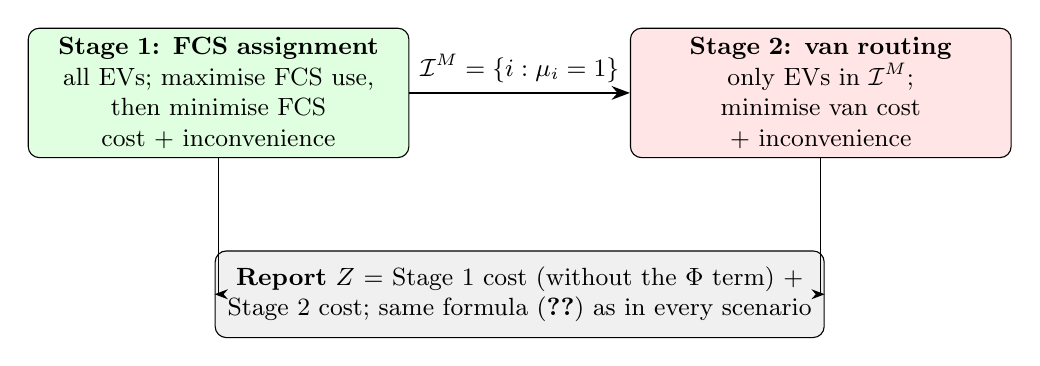
\begin{tikzpicture}[>=Stealth,box/.style={draw,rounded corners,align=center,minimum height=1.1cm,font=\small}]
  \node[box,fill=green!12,text width=4.6cm] (s1) {\textbf{Stage 1: FCS assignment}\\all EVs; maximise FCS use,\\then minimise FCS cost + inconvenience};
  \node[box,fill=red!10,text width=4.6cm,right=2.8cm of s1] (s2) {\textbf{Stage 2: van routing}\\only EVs in $\I^M$;\\minimise van cost + inconvenience};
  \draw[->,thick] (s1) -- node[above,font=\small]{$\I^M=\{i:\mu_i=1\}$} (s2);
  \node[box,fill=black!6,text width=7.5cm,below=2.0cm of $(s1)!0.5!(s2)$] (ev) {\textbf{Report} $Z=$ Stage~1 cost (without the $\Phi$ term) $+$ Stage~2 cost; same formula \eqref{eq:Z} as in every scenario};
  \draw[->] (s1) |- (ev); \draw[->] (s2) |- (ev);
\end{tikzpicture}
\end{center}

Stage~1 does not look at the vans, and Stage~2 cannot change what Stage~1 decided. That is the definition of ``FCS first, then MCS''.

%----------------------------------------------------------------
\subsection{Stage 1: assign EVs to fixed stations}

\textbf{Objective.}
\begin{equation}
\begin{split}
\min\ Z^{(1)}=\;&\underbrace{\Phi\sum_{i\in\I}\mu_i}_{\text{FCS first}}
+\underbrace{c^{EV}\sum_i\sum_{f\in\F_i}d_{if}Y_{if}}_{Z_1}
+\underbrace{Z^F_{\text{energy}}}_{\text{FCS part of }Z_4}\\
&+\underbrace{\sum_i\sum_{f\in\F_i}\rho^F_{if}Y_{if}+\alpha\sum_i w_i(C_i-r_i)+c^L\sum_i w_iL_i}_{\text{FCS customers' inconvenience}}
\end{split}
\label{eq:obj1}
\end{equation}
with $C_i=S_i+\tau^F_iY_i$ in this stage. $\Phi$ is a penalty for handing an EV to the vans. It is chosen larger than anything an extra FCS customer can add to the rest of \eqref{eq:obj1}, e.g.
\[
\Phi > \max_{i}\max_{f\in\F_i}\big(c^{EV}d_{if}+\pi^{\max}E_i+\rho^F_{if}\big)+n\,(\alpha+c^L)\,w_{\max}\,T,
\]
so Stage~1 first \textbf{maximises the number of EVs served at an FCS}, and only among those solutions minimises FCS cost and inconvenience. ($\pi^{\max}$ is the highest grid price.) A numerically safer equivalent is to solve twice: first $\max\sum_iY_i$, then fix that number and minimise the rest.
\ifTOU
Because $Z^F_{\text{energy}}$ uses the peak price, Stage~1 may \emph{start sessions later} to leave the peak, if the price saving beats the extra waiting cost (Section~\ref{sec:expect}).
\fi

\textbf{Constraints.}
\begin{align}
\sum_{g\in\G_i}y_{ig}+\mu_i &= 1 && \forall i\in\I \label{eq:s1assign}\\
S_i &\ge r_i+\sum_{f\in\F_i}t_{if}Y_{if} && \forall i\in\I \label{eq:fcsarr}\\
S_i &\le r_i+T\,(1-\mu_i) && \forall i\in\I \label{eq:s1park}\\
S_j &\ge S_i+\tau^F_i-(T+\tau^F_i)(3-y_{ig}-y_{jg}-o_{ij}) && \forall g,\ (i,j)\in\mathcal{P}_g \label{eq:disj1}\\
S_i &\ge S_j+\tau^F_j-(T+\tau^F_j)(2-y_{ig}-y_{jg}+o_{ij}) && \forall g,\ (i,j)\in\mathcal{P}_g \label{eq:disj2}\\
\sum_i y_{ig_1} &\ge \sum_i y_{ig_2} && \forall f,\ \G_f=\{g_1,g_2\} \label{eq:gunsym}\\
S_i+\tau^F_iY_i &\le T,\qquad L_i\ge S_i+\tau^F_iY_i-l_i && \forall i\in\I \label{eq:s1time}
\end{align}
\ifTOU plus the time-of-use split \eqref{eq:tou1}--\eqref{eq:tou5} of each FCS session (Section~\ref{sec:price}).\fi
\desc{\eqref{eq:s1assign}: every EV either gets one reachable gun or is handed to the vans. An EV that reaches no FCS ($\G_i=\emptyset$) is forced to $\mu_i=1$. \eqref{eq:fcsarr}: an FCS session cannot start before the EV has asked and driven to the station. \eqref{eq:s1park}: for an EV handed to the vans, $S_i$ is parked at $r_i$, so it adds no waiting in Stage~1 (its real start time is decided in Stage~2). \eqref{eq:disj1}--\eqref{eq:disj2}: two EVs on the same gun do not overlap; $o_{ij}$ picks who goes first. With two guns per station this means at most two EVs charge at a station at a time. \eqref{eq:gunsym}: symmetry breaking between the two identical guns (optional). \eqref{eq:s1time}: finished by $T$; lateness.}

\textbf{Optional acceptability rule.} An operator may refuse to send a driver to a station that is ``too inconvenient'', e.g.\ only allow gun $g$ of station $f$ for EV $i$ if $\hat\rho^F_{if}\le\bar\rho$. This only shrinks $\G_i$, so EVs whose stations are all too far go to the vans. Report results with and without it.

\textbf{Output:} $\I^M=\{i:\mu_i=1\}$, the EVs left for the vans; plus each FCS customer's gun and start time.

%----------------------------------------------------------------
\subsection{Stage 2: route the vans to the leftover EVs}

Stage~2 is a vehicle routing problem with time windows, on the EVs in $\I^M$ only. Here $C_i=S_i+\tau^M_i$.

\textbf{Objective.}
\begin{equation}
\begin{split}
\min\ Z^{(2)}=\;&\underbrace{c^M\sum_m\sum_{(i,j)\in\A^M}d_{ij}x_{ijm}}_{Z_2}+\underbrace{\sum_m c^D_mu_m}_{Z_3}+\underbrace{Z^M_{\text{energy}}}_{\text{van part of }Z_4}\\
&+\underbrace{\sum_{i\in\I^M}\sum_m\rho^M_{im}z_{im}+\alpha\sum_{i\in\I^M}w_i(C_i-r_i)+c^L\sum_{i\in\I^M}w_iL_i}_{\text{van customers' inconvenience}}
\end{split}
\label{eq:obj2}
\end{equation}
Since every EV in $\I^M$ must be served by some van, $Z^M_{\text{energy}}$ and the $\rho^M$ term are constants here. They are kept so that $Z^{(2)}$ is the true cost of Stage~2. Waiting and lateness make the vans visit urgent EVs early.

\textbf{Constraints.}
\begin{align}
\sum_{m\in\M}z_{im} &= 1 && \forall i\in\I^M \label{eq:s2assign}\\
\sum_{j:(0,j)\in\A^M}x_{0jm} = \sum_{i:(i,n+1)\in\A^M}x_{i,n+1,m} &= u_m && \forall m \label{eq:depot}\\
\sum_{i:(i,j)\in\A^M}x_{ijm} = \sum_{k:(j,k)\in\A^M}x_{jkm} &= z_{jm} && \forall j\in\I^M,\ m \label{eq:flow}\\
\sum_{i\in\I^M}z_{im} &\le Q_m\,u_m && \forall m \label{eq:cap}\\
\sum_{i\in\I^M}\frac{E_i}{\eta}z_{im}+\beta\sum_{(i,j)\in\A^M}d_{ij}x_{ijm} &\le B_m\,u_m && \forall m \label{eq:batt}
\end{align}
\begin{align}
S_j &\ge \max\{r_j,\ t_{0j}\,x_{0jm}\} && \forall j\in\I^M,\ m \label{eq:depart}\\
S_j &\ge S_i+\tau^M_i+t_{ij}-(T+\tau^M_i+t_{ij})(1-x_{ijm}) && \forall i\neq j,\ m \label{eq:seq}\\
S_i+\tau^M_i+t_{i,n+1} &\le T+(\tau^M_i+t_{i,n+1})(1-x_{i,n+1,m}) && \forall i,\ m \label{eq:return}\\
S_i+\tau^M_i \le T,\quad L_i &\ge S_i+\tau^M_i-l_i && \forall i\in\I^M \label{eq:s2time}\\
u_m &\ge u_{m+1} && m<|\M| \label{eq:vansym}
\end{align}
\desc{\eqref{eq:s2assign}: each leftover EV gets one van. \eqref{eq:depot}: a used van leaves and returns to the depot once. \eqref{eq:flow}: each EV on van $m$ is entered and left exactly once by that van. \eqref{eq:cap}: at most $Q_m$ EVs per van. \eqref{eq:batt}: delivered energy (with transfer losses) plus driving energy fits in the van battery. \eqref{eq:depart}: no start before the request, or before the van can drive there from the depot (written as two linear constraints). \eqref{eq:seq}: if the van goes $i\to j$, it finishes $i$ and drives to $j$ before starting $j$. This gives one EV at a time and removes subtours (MTZ-type). \eqref{eq:return}: back at the depot by $T$. \eqref{eq:s2time}: finished by $T$; lateness. \eqref{eq:vansym}: use identical vans in index order.}

\textbf{If Stage 2 is infeasible} (too many leftover EVs for the fleet by $T$), the sequential policy has \emph{failed} on that instance. For diagnosis, add $s_i\in\{0,1\}$ (``unserved''), replace \eqref{eq:s2assign} by $\sum_mz_{im}+s_i=1$ and add $\Phi^U\sum_is_i$ to \eqref{eq:obj2}. Then report the number of EVs that could not be served. This is a useful comparison with the integrated scenario, which may serve all of them.

%----------------------------------------------------------------
\subsection{Reported value}
\[
Z^{\text{S\scen}}=\big(Z^{(1)*}-\Phi\,|\I^M|\big)+Z^{(2)*},
\]
which is exactly \eqref{eq:Z} evaluated at the combined solution. The stage-1 solution plus the stage-2 solution is a feasible solution of the integrated model (S\ifTOU 4\else 3\fi), so
$Z^{\text{S\ifTOU 4\else 3\fi}}\le Z^{\text{S\scen}}$. The difference is the \emph{value of integration}.

\else
%---------------------------------------------------------------- INT
\subsection{Objective}
\begin{equation}
\min\ Z \quad\text{as in \eqref{eq:Z}, with }Z^F_{\text{energy}}=\ifTOU P^F\textstyle\sum_i\big[\pi^\off(\theta^1_i+\theta^3_i)+\pi^\pk\theta^2_i\big]\else\pi^F\textstyle\sum_iE_iY_i\fi,\quad C_i=S_i+\tau^F_iY_i+\tau^M_iZ_i. \label{eq:objint}
\end{equation}
Written out in full:
\begin{align*}
\min\ Z=\;& c^{EV}\sum_i\sum_{f\in\F_i}d_{if}Y_{if}+c^M\sum_m\sum_{(i,j)\in\A}d_{ij}x_{ijm}+\sum_mc^D_mu_m\\
&+\ifTOU P^F\sum_i\big[\pi^\off(\theta^1_i+\theta^3_i)+\pi^\pk\theta^2_i\big]\else\pi^F\sum_iE_iY_i\fi
+\pi^M\sum_i\sum_m\frac{E_i}{\eta}z_{im}\\
&+\sum_i\sum_{f\in\F_i}\rho^F_{if}Y_{if}+\sum_i\sum_m\rho^M_{im}z_{im}+\alpha\sum_iw_i(C_i-r_i)+c^L\sum_iw_iL_i .
\end{align*}
Every term is linear. One model weighs everything at once: an EV goes to a van exactly when the van's extra km, dispatch and energy cost are outweighed by the effort and waiting it saves the driver\ifTOU, or by the peak-price energy it avoids\fi.

\subsection{Constraints}

\textbf{Assignment.}
\begin{equation}
\sum_{g\in\G_i}y_{ig}+\sum_{m\in\M}z_{im}=1\qquad\forall i\in\I \label{eq:assign}
\end{equation}
\desc{Exactly one resource per EV: one reachable gun or one van. EVs that reach no FCS are forced onto a van.}

\textbf{Fixed stations.}
\begin{align}
S_i &\ge r_i+\sum_{f\in\F_i}t_{if}Y_{if} && \forall i \label{eq:fcsarr}\\
S_j &\ge S_i+\tau^F_i-(T+\tau^F_i)(3-y_{ig}-y_{jg}-o_{ij}) && \forall g,\ (i,j)\in\mathcal{P}_g \label{eq:disj1}\\
S_i &\ge S_j+\tau^F_j-(T+\tau^F_j)(2-y_{ig}-y_{jg}+o_{ij}) && \forall g,\ (i,j)\in\mathcal{P}_g \label{eq:disj2}\\
\sum_iy_{ig_1} &\ge \sum_iy_{ig_2} && \forall f,\ \G_f=\{g_1,g_2\} \label{eq:gunsym}
\end{align}
\desc{\eqref{eq:fcsarr}: an FCS session starts after the request and the drive to the station (for a van customer this is just $S_i\ge r_i$). \eqref{eq:disj1}--\eqref{eq:disj2}: EVs on the same gun do not overlap; $o_{ij}$ chooses the order. \eqref{eq:gunsym}: optional symmetry breaking.}

\textbf{Vans: routes, capacity, battery.}
\begin{align}
\sum_{j:(0,j)\in\A}x_{0jm}=\sum_{i:(i,n+1)\in\A}x_{i,n+1,m} &= u_m && \forall m \label{eq:depot}\\
\sum_{i:(i,j)\in\A}x_{ijm}=\sum_{k:(j,k)\in\A}x_{jkm} &= z_{jm} && \forall j\in\I,\ m \label{eq:flow}\\
\sum_iz_{im} &\le Q_mu_m && \forall m \label{eq:cap}\\
\sum_i\frac{E_i}{\eta}z_{im}+\beta\sum_{(i,j)\in\A}d_{ij}x_{ijm} &\le B_mu_m && \forall m \label{eq:batt}
\end{align}
\desc{\eqref{eq:depot}: a used van leaves and returns once. \eqref{eq:flow}: each EV on van $m$ is visited exactly once by it. \eqref{eq:cap}: at most $Q_m$ EVs. \eqref{eq:batt}: delivered energy (with losses) plus driving energy fits in the battery.}

\textbf{Vans: timing (one EV at a time, no subtours).}
\begin{align}
S_j &\ge t_{0j}\,x_{0jm} && \forall j\in\I,\ m \label{eq:depart}\\
S_j &\ge S_i+\tau^M_i+t_{ij}-(T+\tau^M_i+t_{ij})(1-x_{ijm}) && \forall i\neq j\in\I,\ m \label{eq:seq}\\
S_i+\tau^M_i+t_{i,n+1} &\le T+(\tau^M_i+t_{i,n+1})(1-x_{i,n+1,m}) && \forall i,\ m \label{eq:return}
\end{align}
\desc{\eqref{eq:depart}: the first stop cannot start before the van has driven there. \eqref{eq:seq}: $i\to j$ means finish $i$, drive, then start $j$; start times rise along a route, so no subtour can close. \eqref{eq:return}: back at the depot by $T$.}

\textbf{Horizon and lateness.}
\begin{equation}
C_i\le T,\qquad L_i\ge C_i-l_i\qquad\forall i\in\I \label{eq:time}
\end{equation}
\desc{Every EV is fully charged within the horizon; $L_i$ measures lateness.}

\ifTOU
\textbf{Time-of-use split.} Constraints \eqref{eq:tou1}--\eqref{eq:tou5} of Section~\ref{sec:price}.
\fi

\textbf{Symmetry and domains.}
\begin{equation}
u_m\ge u_{m+1};\qquad y,z,x,u,o\ifTOU,\kappa\fi\in\{0,1\};\qquad S_i,L_i\ifTOU,\theta^p_i\fi\ge0 \label{eq:dom}
\end{equation}
\fi

%=====================================================================
\section{Learning-to-optimise (RL) formulation}\label{sec:rl}

\textbf{Main rule:} the reward of each action is \emph{minus the increase in $Z$ that the action causes}. The rewards over an episode then add up to $-Z$ of the solution the policy builds. RL and MILP results are measured on the same yardstick \eqref{eq:Z}, and the MILP optimum is the benchmark for the RL gap.

\ifSEQ
%---------------------------------------------------------------- RL SEQ
The RL pipeline has the same two stages as the MILP.

\subsection{Stage 1 policy: FCS assignment}
\begin{itemize}[leftmargin=1.4em,itemsep=2pt]
  \item \textbf{Episode / epochs:} EVs are taken in order of request time $r_i$ (ties: higher $w_i$ first). One decision per EV.
  \item \textbf{State:} features of the current EV $k$ ($E_k,r_k,l_k,w_k,R_k$, location); for each gun $g$ the time $F_g$ it becomes free; summary features of the EVs still to come (count and positions near each station)\ifTOU; the current price and the time until $T_1$ and $T_2$\fi.
  \item \textbf{Action:} a gun $g\in\G_k$, or ``hand to vans''. \textbf{FCS-first mask:} ``hand to vans'' is allowed \emph{only} if no gun can finish EV $k$ by $T$ (or, with the optional rule, if all remaining guns have $\hat\rho^F_{kf}>\bar\rho$).
  \ifTOU\item \textbf{Optional timing action:} ``gun $g$, start after the peak'', i.e.\ $S_k=\max\{\text{earliest},T_2\}$, allowed only if the session still ends by $T$.\fi
  \item \textbf{Transition:} $S_k=\max\{r_k+t_{kf},F_g\}$ (or later, for the timing action); $F_g\leftarrow S_k+\tau^F_k$.
  \item \textbf{Reward:} $-\Big[c^{EV}d_{kf}+\text{energy}_k+\rho^F_{kf}+\alpha w_k(S_k+\tau^F_k-r_k)+c^Lw_k(S_k+\tau^F_k-l_k)^+\Big]$, where energy$_k$ = \ifTOU$P^F\big[\pi^\off\cdot(\text{off-peak hours of }[S_k,S_k+\tau^F_k])+\pi^\pk\cdot(\text{peak hours})\big]$, computed exactly in the simulator\else$\pi^FE_k$\fi. Handing an EV to the vans gives reward $0$ here; its cost is counted in Stage~2.
\end{itemize}
Note: a simple baseline for Stage~1 is the greedy rule ``gun with the largest one-step reward''. What RL can learn on top of this is, for example, to keep a nearby gun free for an urgent EV that arrives later.

\subsection{Stage 2 policy: van routing over $\I^M$}
\begin{itemize}[leftmargin=1.4em,itemsep=2pt]
  \item \textbf{Epochs:} whenever a van becomes free (the earliest-free van decides first).
  \item \textbf{State:} for each van: position, time free, remaining battery $b_m$, EVs served so far, dispatched or not; for each unserved EV in $\I^M$: location, $E_i,r_i,l_i,w_i$; current time.
  \item \textbf{Action:} the next EV $j$ for this van, or ``return to depot'' (ends the route). Mask: $j$ must be feasible: battery covers $E_j/\eta$ plus driving to $j$ and back to the depot, the count stays $\le Q_m$, and $j$ can be finished with the van back at the depot by $T$.
  \item \textbf{Transition:} $S_j=\max\{r_j,\ \text{time free}+t_{\text{pos},j}\}$; the van moves to $j$ and is free at $S_j+\tau^M_j$; $b_m$ falls by $E_j/\eta+\beta d_{\text{pos},j}$.
  \item \textbf{Reward:} serving $j$: $-\Big[c^Md_{\text{pos},j}+c^D_m[\text{first stop}]+\pi^M\frac{E_j}{\eta}+\rho^M_{jm}+\alpha w_j(S_j+\tau^M_j-r_j)+c^Lw_j(S_j+\tau^M_j-l_j)^+\Big]$; returning: $-c^Md_{\text{pos},0}$. EVs still unserved at the end: $-\Phi^U$ each.
  \item \textbf{Policy:} an attention-based routing policy (e.g.\ Kool et al., 2019, ``Attention, Learn to Solve Routing Problems!'') trained with REINFORCE or PPO. Baseline: nearest-feasible-EV heuristic.
\end{itemize}
Episode return of Stage~1 + Stage~2 $=-Z^{\text{S\scen}}$.

\else
%---------------------------------------------------------------- RL INT
One policy decides both who serves each EV and the van routes.
\begin{itemize}[leftmargin=1.4em,itemsep=2pt]
  \item \textbf{Episode / epochs:} EVs are taken in order of request time $r_i$ (ties: higher $w_i$ first). One decision per EV.
  \item \textbf{State:} (i) the current EV $k$: location, $E_k,r_k,l_k,w_k,R_k$, reachable stations; (ii) each gun $g$: time $F_g$ it becomes free; (iii) each van $m$: current end-of-route position, time free, remaining battery $b_m$, EVs served, dispatched or not; (iv) embeddings of the not-yet-assigned EVs (for look-ahead)\ifTOU; (v) current price, time until $T_1$ and $T_2$\fi.
  \item \textbf{Action:} $a\in\G_k\cup\M$: a gun, or a van (EV $k$ is appended to the end of that van's route). \textbf{Mask} infeasible actions: a gun that cannot finish $k$ by $T$; a van without enough battery for $E_k/\eta$ plus the drive to $k$ and back to the depot, with $Q_m$ reached, or unable to finish $k$ and return by $T$.
  \ifTOU\item \textbf{Optional timing action:} ``gun $g$, start after the peak'' ($S_k=\max\{\text{earliest},T_2\}$, if it still ends by $T$).\fi
  \item \textbf{Transition:} gun: $S_k=\max\{r_k+t_{kf},F_g\}$, $F_g\leftarrow S_k+\tau^F_k$. Van: $S_k=\max\{r_k,\ \text{free}_m+t_{\text{pos}_m,k}\}$, then the van moves to $k$, $\text{free}_m\leftarrow S_k+\tau^M_k$, $b_m\mathrel{-}=E_k/\eta+\beta d_{\text{pos}_m,k}$.
  \item \textbf{Reward} $=-\Delta Z$:
  \begin{align*}
  \text{gun } g\text{ at }f:&\quad -\Big[c^{EV}d_{kf}+\text{energy}^F_k+\rho^F_{kf}+\alpha w_k(C_k-r_k)+c^Lw_k(C_k-l_k)^+\Big]\\
  \text{van } m:&\quad -\Big[c^M\big(d_{\text{pos}_m,k}+d_{k,0}-d_{\text{pos}_m,0}\big)+c^D_m[\text{first use}]+\pi^M\tfrac{E_k}{\eta}\\
  &\qquad\quad+\rho^M_{km}+\alpha w_k(C_k-r_k)+c^Lw_k(C_k-l_k)^+\Big]
  \end{align*}
  The van distance term is the \emph{change} in route length when $k$ is inserted before the return to the depot, so the sum over the episode equals the total route length (the return legs telescope). energy$^F_k$ = \ifTOU$P^F\big[\pi^\off\cdot(\text{off-peak hours})+\pi^\pk\cdot(\text{peak hours of }[S_k,C_k])\big]$, computed exactly by the simulator; no linearisation is needed in RL\else$\pi^FE_k$\fi.
  \item \textbf{Dead end:} if every action is masked, EV $k$ is unserved: reward $-\Phi^U$, and the episode continues. Report the count.
  \item \textbf{Policy:} masked categorical policy over guns and vans, encoder with attention over EVs, guns and vans; trained with PPO. Natural baseline: greedy, i.e.\ choose the action with the largest one-step reward. That is the pairwise rule ``smallest $\hat\rho$ + cost'' from Section~\ref{sec:inc}.
\end{itemize}
Restriction to note: vans serve EVs in assignment order (append only). A variant that inserts $k$ at the cheapest position of a route is more flexible but has a larger action space.
\fi

\textbf{Reward scaling.} For stable training divide every reward by a constant, e.g.\ the greedy baseline's average $Z$ on the training instances. This does not change the optimal policy.

%=====================================================================
\section{What to expect and what to report}\label{sec:expect}

\ifnum\scen=1
\begin{itemize}[leftmargin=1.4em,itemsep=2pt]
  \item Vans serve only EVs that reach no station, or that the stations cannot finish by $T$. If stations have spare capacity, very few vans are dispatched.
  \item Inconvenience is high for EVs far from the nearest station (worked example: Rs\,682 at the FCS, against Rs\,458 if a van had been allowed).
  \item With too few vans Stage~2 becomes infeasible (unserved EVs), even when the integrated model S3 could serve everyone. Report the smallest $|\M|$ at which S1 is feasible and compare it with S3.
\end{itemize}
\fi
\ifnum\scen=2
\begin{itemize}[leftmargin=1.4em,itemsep=2pt]
  \item \textbf{When does Stage~1 delay a session to avoid the peak?} Moving one hour of charging out of the peak saves $(\pi^\pk-\pi^\off)P^F=3\times22=$ Rs\,66, but delays completion by up to an hour, which costs $\alpha w_i\ge$ Rs\,200. So with the default values Stage~1 almost never delays. It mostly pays the higher price, and S2 costs roughly S1 plus the peak surcharge. Sessions start later only if $\alpha$ is small (try $\lambda<0.33$ in the sensitivity analysis).
  \item The van assignment is the same as in S1 unless Stage~1's timing changes which EVs fit at the stations. Stage~1 cannot use vans to escape the peak price.
  \item Extra KPI: \textbf{grid energy drawn at FCS during the peak}, $P^F\sum_i\theta^2_i$ (kWh). Compare with S4.
\end{itemize}
\fi
\ifnum\scen=3
\begin{itemize}[leftmargin=1.4em,itemsep=2pt]
  \item Vans take EVs for which the saved inconvenience exceeds the extra van cost (worked example: van chosen, saving Rs\,224). Expect vans to serve EVs that are far from every station, have low range (high $w_i$), or have early deadlines, while EVs near a station still use it.
  \item \textbf{Value of integration under flat price:} $Z^{\text{S1}}-Z^{\text{S3}}\ge0$. Report it per component ($Z_1,\dots,Z_5$): typically operating cost rises a little and inconvenience falls a lot.
  \item Vary $|\M|$ (0, 1, 2, \dots): the first few vans lower $Z$ sharply, then the effect levels off. That curve shows the scenarios where mobile chargers help most.
\end{itemize}
\fi
\ifnum\scen=4
\begin{itemize}[leftmargin=1.4em,itemsep=2pt]
  \item During the peak a van kWh costs about the same as an FCS kWh (Rs\,10.0 each), so the vans' energy disadvantage disappears and vans also absorb \emph{peak-hour} demand that would otherwise be charged on the grid at peak price.
  \item Expect more van usage than in S3, concentrated on requests in $[T_1,T_2]$, and lower grid energy at the stations during the peak, $P^F\sum_i\theta^2_i$, than in S2.
  \item \textbf{Value of integration under peak pricing:} $Z^{\text{S2}}-Z^{\text{S4}}$. It should be larger than $Z^{\text{S1}}-Z^{\text{S3}}$, because integration now also allows price arbitrage.
  \item \textbf{Peak pricing with full flexibility:} $Z^{\text{S4}}-Z^{\text{S3}}$ should be smaller than $Z^{\text{S2}}-Z^{\text{S1}}$: vans cushion the price increase.
\end{itemize}
\fi

\textbf{Cross-scenario comparison table} (fill in from the four runs):
\begin{center}
\renewcommand{\arraystretch}{1.2}
\begin{tabular}{@{}lll@{}}
\toprule
\textbf{Comparison} & \textbf{Measures} & \textbf{Expected sign} \\
\midrule
S1 $-$ S3 & value of integration, flat price & $\ge0$ \\
S2 $-$ S4 & value of integration, peak price & $\ge0$, larger than S1 $-$ S3 \\
S2 $-$ S1 & cost of peak pricing, FCS-first operator & $>0$ \\
S4 $-$ S3 & cost of peak pricing, flexible operator & $>0$, smaller than S2 $-$ S1 \\
\bottomrule
\end{tabular}
\end{center}
Report for each: $Z$ and its components, number of vans used, EVs per resource, mean and maximum inconvenience per EV, total lateness, peak-hour grid energy, solve time, and (for RL) the gap to the MILP optimum.

%=====================================================================
\appendix
\section{Illustrative parameter values}\label{app:values}

These are starting values for experiments, not data. All are meant to be varied in the analysis. Values in Rs.

\begin{center}
\renewcommand{\arraystretch}{1.15}
\begin{tabular}{@{}llp{6.2cm}@{}}
\toprule
\textbf{Parameter} & \textbf{Value} & \textbf{Note} \\
\midrule
$T$, $[T_1,T_2]$ & 7 h, $[2,6]$ & 16:00--23:00, peak 18:00--22:00 \\
$P^F$, $P^M$ & 22 kW, 30 kW & \\
$v$, $\beta$, $\eta$ & 25 km/h, 0.25 kWh/km, 0.9 & \\
$B_m$, $Q_m$, $|\M|$ & 150 kWh, 6, 2--6 & \\
$c^{EV}$, $c^M$, $c^D_m$ & Rs\,4/km, Rs\,15/km, Rs\,1500 & van km includes driver time \\
$\pi^F$ (flat) & Rs\,8.7/kWh & equals the time-average of the ToU tariff over $[0,T]$ \\
$\pi^\off$, $\pi^\pk$ (ToU) & Rs\,7/kWh, Rs\,10/kWh & $(3\times7+4\times10)/7=8.7$ \\
$c^{bat}$ & Rs\,2/kWh & van battery wear \\
$\pi^M$ & Rs\,10.7 (flat) / Rs\,9.0 (ToU) & $=\pi^F+c^{bat}$ / $=\pi^\off+c^{bat}$ \\
$\alpha$, $\alpha^D$ & Rs\,200/h, Rs\,100/h & value of time; extra for attended time \\
$h^F$, $h^M$, $\varphi$ & Rs\,50, Rs\,10, Rs\,100 & trip hassle, hand-over, range stress \\
$c^L$ & Rs\,300/h & lateness \\
$w_i$ & $1+2(1-R_i/R_{\max})$, $R_i\sim U[3,40]$ km & priority from remaining range \\
\bottomrule
\end{tabular}
\end{center}

The flat price is set to the time-average of the peak tariff. The price \emph{level} is then the same in both pricing cases, and only the price \emph{shape} differs. Without this, part of S1 vs S2 would just reflect a different average price.

\end{document}
"
%    pdflatex -jobname=scenario3_flat_integrated   "\def\scen{3}% =====================================================================
%  One source, four PDFs.  Build with build.sh (or by hand):
%    pdflatex -jobname=scenario1_flat_sequential   "\def\scen{1}\input{scenario_master}"
%    pdflatex -jobname=scenario2_peak_sequential   "\def\scen{2}\input{scenario_master}"
%    pdflatex -jobname=scenario3_flat_integrated   "\def\scen{3}\input{scenario_master}"
%    pdflatex -jobname=scenario4_peak_integrated   "\def\scen{4}\input{scenario_master}"
%  (run each twice for cross-references)
% =====================================================================
\documentclass[11pt,a4paper]{article}
\usepackage[margin=2.2cm]{geometry}
\usepackage{amsmath,amssymb,amsfonts}
\usepackage{booktabs,array,tabularx}
\usepackage{enumitem}
\usepackage[table]{xcolor}
\usepackage{tikz}
\usetikzlibrary{arrows.meta,positioning,calc}
\usepackage[colorlinks=true,linkcolor=blue!50!black,urlcolor=blue!50!black]{hyperref}
\usepackage{titlesec}
\titleformat{\section}{\large\bfseries}{\thesection}{0.8em}{}
\titleformat{\subsection}{\normalsize\bfseries}{\thesubsection}{0.8em}{}
\setlength{\parindent}{0pt}
\setlength{\parskip}{5pt}

% ---------------- scenario switches ----------------
\ifdefined\scen\else\def\scen{1}\fi
\newif\ifTOU \TOUfalse   % true = time-of-use (peak) price
\newif\ifSEQ \SEQfalse   % true = FCS first, then MCS
\ifnum\scen=1 \SEQtrue \fi
\ifnum\scen=2 \TOUtrue \SEQtrue \fi
\ifnum\scen=4 \TOUtrue \fi

\newcommand{\pricename}{\ifTOU time-of-use price (dearer evening peak)\else single (flat) price all day\fi}
\newcommand{\structname}{\ifSEQ FCS first, then MCS (sequential)\else FCS and MCS together (integrated)\fi}

% ---------------- notation ----------------
\newcommand{\I}{\mathcal{I}}
\newcommand{\F}{\mathcal{F}}
\newcommand{\G}{\mathcal{G}}
\newcommand{\M}{\mathcal{M}}
\newcommand{\N}{\mathcal{N}}
\newcommand{\A}{\mathcal{A}}
\newcommand{\Rs}{\text{Rs}\,}
\newcommand{\pk}{\mathrm{pk}}
\newcommand{\off}{\mathrm{off}}
\newcommand{\desc}[1]{\par\vspace{-2pt}{\small\color{black!75}\textit{Meaning:} #1}\par\vspace{4pt}}
\newcommand{\cell}[2]{\ifnum\scen=#1\cellcolor{blue!18}\textbf{S#1 (this document)}\\\textbf{#2}\else S#1\\#2\fi}

\title{\textbf{EV Charging Network Optimisation}\\[4pt]
\large Scenario \scen: \pricename\ $+$ \structname\\[2pt]
\normalsize MILP and RL formulation}
\author{CP 320 OR for Mobility Management, course project}
\date{2 October 2026}

\begin{document}
\maketitle

%=====================================================================
\section{Where this scenario sits}

The project studies four scenarios: two ways of pricing grid electricity, times two ways of making the decisions.

\begin{center}
\renewcommand{\arraystretch}{1.5}
\begin{tabular}{>{\raggedright\arraybackslash}p{4.2cm}|>{\centering\arraybackslash}p{4.6cm}|>{\centering\arraybackslash}p{4.6cm}}
 & \textbf{Flat price all day} & \textbf{Time-of-use (peak) price} \\ \hline
\textbf{Sequential:} FCS first, leftover EVs to MCS &
\begin{tabular}[c]{@{}c@{}}\cell{1}{flat + sequential}\end{tabular} &
\begin{tabular}[c]{@{}c@{}}\cell{2}{peak + sequential}\end{tabular} \\ \hline
\textbf{Integrated:} FCS and MCS decided together &
\begin{tabular}[c]{@{}c@{}}\cell{3}{flat + integrated}\end{tabular} &
\begin{tabular}[c]{@{}c@{}}\cell{4}{peak + integrated}\end{tabular} \\
\end{tabular}
\end{center}

\textbf{The four scenarios do not have four different objectives.} They share \emph{one} cost yardstick $Z$ (Section~\ref{sec:obj}): the same cost terms and the same customer inconvenience (Section~\ref{sec:inc}). Only two things change:
\begin{itemize}[leftmargin=1.4em,itemsep=1pt]
  \item \textbf{Pricing} changes the formula for one term, the FCS energy cost (Section~\ref{sec:price}).
  \item \textbf{Decision structure} changes \emph{how} $Z$ is minimised: in one model (integrated), or in two stages (sequential), where each stage minimises its own part of $Z$.
\end{itemize}
Because the yardstick is the same, the four optimal values can be compared directly. The differences measure the \emph{value of integration} (S1$\to$S3, S2$\to$S4) and the \emph{effect of peak pricing} (S1$\to$S2, S3$\to$S4).

\ifnum\scen=1
\textbf{This scenario (S1)} is the baseline, the ``status quo''. Electricity costs the same at every hour, every EV that can be charged at a fixed station is sent there, and vans only take what is left over.
\fi
\ifnum\scen=2
\textbf{This scenario (S2)} keeps the FCS-first rule of S1, but grid electricity is dearer during the evening peak. Stage~1 can react to the price only by \emph{rescheduling} FCS sessions. It cannot hand a peak-hour EV to a van.
\fi
\ifnum\scen=3
\textbf{This scenario (S3)} keeps the flat price of S1, but the operator decides FCS and MCS service \emph{together}. An EV can be sent to a van even when a fixed station could take it, whenever that lowers total cost plus inconvenience.
\fi
\ifnum\scen=4
\textbf{This scenario (S4)} is the most flexible one: peak pricing at fixed stations, and FCS and MCS decided together. Van energy was bought off-peak, so vans can also be used to keep charging \emph{out of the expensive peak}.
\fi

%=====================================================================
\section{Setting and assumptions}\label{sec:setting}

\textbf{Time.} The planning horizon is $[0,T]$ with $T=7$\,h (16:00--23:00). It contains the evening peak window $[T_1,T_2]=[2,6]$ (18:00--22:00). The horizon is the same in all four scenarios. It is wider than the peak itself so that, under peak pricing, there is cheaper time on both sides of the peak.\ifTOU\else\ In this scenario the price is flat, so the window plays no role in the model.\fi

\textbf{Assumptions} (the same as MILP v3, plus two about energy):
\begin{enumerate}[leftmargin=1.6em,itemsep=1pt]
  \item Static, continuous time. All requests in the horizon are known at time $0$, and request $i$ becomes active at $r_i$.
  \item An EV served by an FCS drives there itself on its own battery (only to stations within its range $R_i$). The driver stays with the car while it waits for a free gun and while it charges.
  \item An EV served by an MCS stays parked where it is, and the driver is free in the meantime.
  \item Each FCS gun and each van charges one EV at a time, without interruption, at constant power.
  \item A van's battery covers both its driving and the energy it delivers. \textbf{The van battery is charged at the depot before the horizon starts}\ifTOU, i.e.\ at the off-peak price\fi, and is not recharged during the horizon.
  \item Every EV must be fully charged by $T$ (hard). Finishing after the driver's desired time $l_i$ is allowed but penalised.
\end{enumerate}

%=====================================================================
\section{Notation}\label{sec:notation}

\subsection*{Sets}
\begin{tabularx}{\textwidth}{@{}lX@{}}
\toprule
$\I=\{1,\dots,n\}$ & EV charging requests \\
$\F$; $\G_f$ ($|\G_f|=2$); $\G=\bigcup_f\G_f$ & fixed charging stations; guns of FCS $f$; all guns ($f(g)$ = station of gun $g$) \\
$\F_i=\{f: d_{if}\le R_i\}$, $\G_i=\bigcup_{f\in\F_i}\G_f$ & stations / guns EV $i$ can reach on its remaining range \\
$\M$ & mobile charging vans (MCS) \\
$0,\ n+1$ & depot as start node / end node (same place) \\
$\N=\{0\}\cup\I\cup\{n+1\}$, $\A$ & routing nodes; allowed van arcs $(i,j)$, $i\in\{0\}\cup\I$, $j\in\I\cup\{n+1\}$, $i\neq j$ \\
$\mathcal{P}_g=\{(i,j): i<j,\ g\in\G_i\cap\G_j\}$ & pairs of EVs that could share gun $g$ \\
\ifSEQ
$\I^M\subseteq\I$ & EVs handed to the vans by Stage~1 (an \emph{output} of Stage~1, a fixed input to Stage~2) \\
$\N^M$, $\A^M$ & routing nodes / arcs restricted to $\I^M$ \\
\fi
\bottomrule
\end{tabularx}

\subsection*{Parameters}
\begin{tabularx}{\textwidth}{@{}lX@{}}
\toprule
$E_i,\ r_i,\ l_i,\ R_i$ & energy demand (kWh), request time, desired completion time (h), remaining range (km) \\
$w_i\ge1$ & priority of EV $i$; $w_i=1+\kappa(1-R_i/R_{\max})$, so low-range EVs weigh more \\
$P^F,\ P^M$ & charging power of an FCS gun (22\,kW) / of a van (e.g.\ 30\,kW) \\
$\tau^F_i=E_i/P^F,\ \tau^M_i=E_i/P^M$ & charging time of EV $i$ at an FCS / by a van (h) \\
$d_{if},t_{if}$;\ $d_{ij},t_{ij}$ & distance (km) and time (h): EV$\to$FCS; between routing nodes ($t=d/v$) \\
$B_m,\ Q_m,\ \beta,\ \eta$ & van battery (kWh), max EVs per van, van consumption (kWh/km), transfer efficiency \\
$c^{EV},\ c^M,\ c^D_m$ & cost per km of EV driving, per km of van driving; fixed dispatch cost of van $m$ \\
\ifTOU
$\pi^\off,\ \pi^\pk$ & grid price (Rs/kWh) off-peak / in $[T_1,T_2]$, with $\pi^\pk\ge\pi^\off$ \\
\else
$\pi^F$ & grid price (Rs/kWh), the same at every hour \\
\fi
$c^{bat}$ & van battery wear per kWh cycled \\
$\pi^M$ & cost of 1 kWh taken from a van battery: $\pi^M=\ifTOU\pi^\off\else\pi^F\fi+c^{bat}$ (Section~\ref{sec:price}) \\
$\alpha,\ \alpha^D,\ h^F,\ h^M,\ \varphi,\ c^L$ & inconvenience coefficients (Section~\ref{sec:inc}) \\
\bottomrule
\end{tabularx}

\subsection*{Decision variables}
\begin{tabularx}{\textwidth}{@{}llX@{}}
\toprule
$y_{ig}$ & $\{0,1\}$ & EV $i$ charged at gun $g\in\G_i$ \\
$z_{im}$ & $\{0,1\}$ & EV $i$ served by van $m$ \\
$x_{ijm}$ & $\{0,1\}$ & van $m$ drives arc $(i,j)$ \\
$u_m$ & $\{0,1\}$ & van $m$ is dispatched \\
$o_{ij}$ & $\{0,1\}$ & for EVs $i<j$ that could share a gun: 1 if $i$ is charged before $j$ \\
\ifSEQ
$\mu_i$ & $\{0,1\}$ & Stage~1 only: EV $i$ is handed to the van fleet \\
\fi
\ifTOU
$\theta^1_i,\theta^2_i,\theta^3_i$ & $\ge0$ & hours of EV $i$'s FCS session before / inside / after the peak \\
$\kappa^1_i,\kappa^3_i$ & $\{0,1\}$ & EV $i$'s FCS session starts before $T_1$ / ends after $T_2$ \\
\fi
$S_i$ & $\ge0$ & time charging of EV $i$ starts (h), on whichever resource \\
$L_i$ & $\ge0$ & lateness of EV $i$ beyond $l_i$ (h) \\
\bottomrule
\end{tabularx}

\textbf{Short-hands} (linear expressions, not new variables):
\[
Y_{if}=\sum_{g\in\G_f}y_{ig},\qquad Y_i=\sum_{g\in\G_i}y_{ig}\ (\text{EV $i$ uses an FCS}),\qquad Z_i=\sum_{m\in\M}z_{im}\ (\text{EV $i$ uses a van}),
\]
\[
C_i=S_i+\tau^F_i\,Y_i+\tau^M_i\,Z_i \quad\text{(time EV $i$ is fully charged).}
\]

%=====================================================================
\section{Customer inconvenience}\label{sec:inc}

This section is \textbf{identical in all four scenario documents}. Inconvenience is a property of the customer, not of the price or of the planning method.

\subsection{What we mean by inconvenience}

Inconvenience is \emph{what the driver loses} from the moment they ask for a charge ($r_i$) until the car is fully charged ($C_i$), \emph{converted into rupees} so it can be added to the operator's costs. A driver loses three different things:

\begin{enumerate}[leftmargin=1.6em,itemsep=2pt]
  \item \textbf{Waiting:} the car is not ready. This lasts $C_i-r_i$ hours and affects \emph{every} driver, FCS or MCS.
  \item \textbf{Effort:} only an FCS customer has to drive to the station and sit there while the car charges. An MCS customer stays at home or at work and does something else. Driving to a far station also uses scarce battery range, which causes stress (``range anxiety'').
  \item \textbf{A missed deadline:} the car is still not ready at the time $l_i$ the driver needs it.
\end{enumerate}

Each loss gets a price in Rs per hour (or per event). All of them are multiplied by the priority $w_i$: an hour of delay for an EV with 5\,km of range left counts more than for one with 40\,km.

\subsection{The three components}

\begin{center}
\renewcommand{\arraystretch}{1.3}
\begin{tabularx}{\textwidth}{@{}>{\raggedright\arraybackslash}p{2.6cm}>{\raggedright\arraybackslash}X>{\raggedright\arraybackslash}X>{\raggedright\arraybackslash}p{3.0cm}@{}}
\toprule
\textbf{Component} & \textbf{EV $i$ at FCS $f$} & \textbf{EV $i$ by a van} & \textbf{Known when?} \\
\midrule
Effort & $w_i\big[\alpha^D(t_{if}+\tau^F_i)+h^F+\varphi\,d_{if}/R_i\big]$: driving and sitting at the station, a fixed trip hassle, range stress & $w_i\,h^M$: being reachable and handing over the car & \textbf{Static:} known as soon as the resource is chosen \\
Waiting & $w_i\,\alpha\,(C_i-r_i)$ = drive + \emph{queue at the gun} + charge & $w_i\,\alpha\,(C_i-r_i)$ = \emph{wait for the van} + charge & \textbf{Dynamic:} depends on the queue / van route \\
Missed deadline & $w_i\,c^L\,L_i$, $L_i=\max\{0,C_i-l_i\}$ & same & Dynamic \\
\bottomrule
\end{tabularx}
\end{center}

\textbf{Coefficients.}
$\alpha$ (Rs/h) is the value of an hour the car is not ready.
$\alpha^D$ (Rs/h) is the \emph{extra} value of an hour the driver must personally spend driving or sitting at the station: an hour at the station costs $\alpha+\alpha^D$, an hour waiting at home for a van costs only $\alpha$.
$h^F,h^M$ (Rs) are fixed hassle costs of one trip to a station / one van hand-over.
$\varphi$ (Rs) is the range-stress cost of a trip that uses the \emph{whole} remaining range ($d_{if}/R_i\le1$ is the fraction used).
$c^L$ (Rs/h) is the cost per hour late.

\subsection{Pairwise form: inconvenience of a (customer, resource) pair}

The natural first idea is: \emph{for every pair (EV $i$, FCS $f$) and every pair (EV $i$, van $m$) there is an inconvenience number, and the operator picks the pair with the lowest cost plus inconvenience.} The static part fits this idea exactly:
\[
\boxed{\;\rho^F_{if}=w_i\Big[\alpha^D\,(t_{if}+\tau^F_i)+h^F+\varphi\,\frac{d_{if}}{R_i}\Big]\qquad
\rho^M_{im}=w_i\,h^M\;}
\]
These are \textbf{parameters}, computed before solving, one number per (EV, FCS) pair and per (EV, van) pair. In the objective they appear linearly: $\sum_i\sum_f\rho^F_{if}Y_{if}+\sum_i\sum_m\rho^M_{im}z_{im}$.

Note that $\rho^M_{im}$ does not depend on $m$. Vans are identical and all start at the same depot, so the driver does not care \emph{which} van comes, only \emph{when} it comes. That ``when'' is the waiting part.

\subsection{Why waiting cannot be a fixed pairwise number}

It is tempting to also write the waiting as a pairwise number, e.g.\ ``the van needs 5 minutes to reach EV $i$''. But that depends on \emph{where the van is coming from}, which depends on the route the model is still choosing: if EV $i$ is the 4th stop of a van, the wait is the time for three charging sessions plus four drives. Likewise, waiting at an FCS depends on how many EVs are queued at that gun. So waiting is not known before solving. It is a function of decision variables:
\[
\text{waiting cost of EV } i \;=\; w_i\,\alpha\,(C_i-r_i),\qquad C_i=S_i+\tau^F_iY_i+\tau^M_iZ_i .
\]
This is \textbf{linear} in the variables ($S_i$, $y$, $z$), so it fits in a MILP directly. The constraints of Section~\ref{sec:milp} make $S_i$ equal to the true start time, including driving, queueing at the gun and the van's route. The term $\sum_i w_i\alpha r_i$ is a constant and may be dropped when solving.

\textbf{Pairwise \emph{estimate}} (used for intuition, by the RL policy and in heuristics): if there is no queue and the van comes straight to $i$,
\[
\hat\rho^{F}_{if}=\rho^F_{if}+w_i\alpha\,(t_{if}+\tau^F_i),\qquad
\hat\rho^{M}_{im}=\rho^M_{im}+w_i\alpha\,(t^{\text{van}}_{m\to i}+\tau^M_i),
\]
where $t^{\text{van}}_{m\to i}$ is the time until van $m$ can reach $i$ from where it currently is. In the RL formulation (Section~\ref{sec:rl}) the van's position \emph{is} known at each decision, so there this estimate becomes exact.

\subsection{Total inconvenience and how it enters the objective}

\begin{equation}
\boxed{\;
Z_{\text{inc}}=\underbrace{\sum_{i\in\I}\sum_{f\in\F_i}\rho^F_{if}Y_{if}+\sum_{i\in\I}\sum_{m\in\M}\rho^M_{im}z_{im}}_{\text{effort (static, pairwise)}}
+\underbrace{\alpha\sum_{i\in\I}w_i\,(C_i-r_i)}_{\text{waiting (dynamic)}}
+\underbrace{c^L\sum_{i\in\I}w_i\,L_i}_{\text{missed deadline}}
\;}\label{eq:inc}
\end{equation}
All three parts are in rupees, so $Z_{\text{inc}}$ is simply added to the operating costs. Nothing has to be normalised.

\subsection{Worked example: your ``10 km to the FCS vs.\ van in 5 minutes'' case}

EV $i$: $E_i=20$\,kWh, $R_i=40$\,km (so $w_i=1$); nearest free FCS $d_{if}=10$\,km away, $t_{if}=0.4$\,h at 25\,km/h; a van finishing next door can reach it in 5\,min ($0.083$\,h), adding about 4\,km to its route. $\tau^F_i=20/22=0.909$\,h, $\tau^M_i=20/30=0.667$\,h. Coefficients from Appendix~\ref{app:values}, flat price.

\begin{center}
\renewcommand{\arraystretch}{1.25}
\begin{tabular}{@{}lrr@{}}
\toprule
 & \textbf{FCS} & \textbf{Van} \\
\midrule
Driving (EV / extra van km) & $4\times10=40.0$ & $15\times4=60.0$ \\
Energy & $8.7\times20=174.0$ & $10.7\times20/0.9=237.8$ \\
\textbf{Operating cost only} & \textbf{214.0} & \textbf{297.8} \\
\midrule
Effort $\rho$ & $100(0.4+0.909)+50+100\cdot\tfrac{10}{40}=205.9$ & $10.0$ \\
Waiting $\alpha(C_i-r_i)$ & $200\times1.309=261.8$ & $200\times0.75=150.0$ \\
\textbf{Cost + inconvenience} & \textbf{681.7} & \textbf{457.8} \\
\bottomrule
\end{tabular}
\end{center}

On operating cost alone the FCS is cheaper, so a cost-only model would \emph{always} send this driver 10\,km away. With inconvenience included the van is better by about Rs\,224, and the integrated model chooses $z_{im}=1$, as you expected. If the FCS were only 1\,km away, the FCS would win both comparisons. The inconvenience term is what makes the model choose between ``cheap for the operator'' and ``convenient for the driver'', rather than following a fixed rule.

\subsection{Relation to a single penalty $\rho_i$ per EV}

The first draft used a penalty $\rho_i$ that is charged whenever EV $i$ goes to \emph{any} FCS: $\sum_i\sum_f\rho_iy_{if}$. Because $\sum_f y_{if}=1-\sum_m z_{im}$, this only says ``a van is worth $\rho_i$ more to EV $i$'', and that holds whether the station is 1\,km or 15\,km away, and whether the van arrives in 5 minutes or in 3 hours. The form above fixes both problems: $\rho^F_{if}$ grows with the distance to \emph{that} station, and the waiting term grows with how late the van or the free gun actually is. The old model is the special case $\alpha=\alpha^D=\varphi=c^L=0$, $h^F=\rho_i$.

\subsection{Choosing the coefficients}
\begin{itemize}[leftmargin=1.4em,itemsep=2pt]
  \item Use a value of time for $\alpha$ (e.g.\ Rs\,150--300/h for urban car users), and set $\alpha^D\approx0.5\alpha$: sitting at a station is worse than waiting at home.
  \item Keep $c^L>\alpha$, so missing the deadline is worse than ordinary waiting.
  \item \textbf{Sensitivity analysis:} multiply all inconvenience coefficients by a factor $\lambda\in\{0,0.25,0.5,1,2,4\}$ and plot operating cost against total inconvenience. $\lambda=0$ is the pure cost-minimising operator, and large $\lambda$ is a customer-first operator. This trade-off curve is a strong result for the ``Analysis'' part of the project.
\end{itemize}

\subsection{What inconvenience does in \emph{this} scenario}
\ifSEQ
In a sequential scenario inconvenience \textbf{cannot move an EV from an FCS to a van}: Stage~1 sends every EV that \emph{can} use an FCS to one. It still matters inside each stage. In Stage~1 it decides \emph{which} station and \emph{when} (urgent EVs get the near station and the first free gun). In Stage~2 it decides the \emph{order} in which vans visit EVs (urgent EVs first). In the worked example, this scenario sends the driver 10\,km to the FCS. That is the weakness the integrated scenarios remove.
\else
In an integrated scenario inconvenience is weighed directly against operating cost when choosing the resource. That is how the worked example ends up with a van. It also decides which station and which gun order, and the order of each van route.
\fi

%=====================================================================
\section{Electricity price in this scenario}\label{sec:price}

\textbf{Van energy (same in all scenarios).} A van's battery is charged at the depot \emph{before} the horizon, so its energy was bought at the
\ifTOU off-peak \fi
price, whatever time the van later delivers it. Each kWh taken from the van also wears the battery ($c^{bat}$), and a fraction $1-\eta$ is lost in transfer:
\[
Z^M_{\text{energy}}=\pi^M\sum_{i\in\I}\sum_{m\in\M}\frac{E_i}{\eta}\,z_{im},\qquad \pi^M=\ifTOU\pi^\off\else\pi^F\fi+c^{bat}.
\]

\ifTOU
\textbf{FCS energy (time-of-use).} An FCS draws from the grid while it charges. Energy delivered inside $[T_1,T_2]$ costs $\pi^\pk$, and energy outside it costs $\pi^\off$. A session $[S_i,S_i+\tau^F_i]$ may overlap the peak partly. Split its duration into the hours before, inside and after the peak, $\theta^1_i+\theta^2_i+\theta^3_i$:
\[
Z^F_{\text{energy}}=P^F\sum_{i\in\I}\Big[\pi^\off(\theta^1_i+\theta^3_i)+\pi^\pk\,\theta^2_i\Big].
\]
Constraints \eqref{eq:tou1}--\eqref{eq:tou5} below make the $\theta$'s equal to the true overlaps. Peak hours are dearer, so the solver wants $\theta^1_i,\theta^3_i$ as large as possible. It is enough to bound them from above by the true off-peak overlap, and the constraints need one binary per side:
\begin{align}
\theta^1_i+\theta^2_i+\theta^3_i &= \tau^F_i\,Y_i && \forall i\in\I \label{eq:tou1}\\
\theta^1_i &\le \tau^F_i\,\kappa^1_i && \forall i\in\I \label{eq:tou2}\\
\theta^1_i &\le T_1-S_i+T\,(1-\kappa^1_i) && \forall i\in\I \label{eq:tou3}\\
\theta^3_i &\le \tau^F_i\,\kappa^3_i && \forall i\in\I \label{eq:tou4}\\
\theta^3_i &\le S_i+\tau^F_i-T_2+T\,(1-\kappa^3_i) && \forall i\in\I \label{eq:tou5}
\end{align}
\desc{\eqref{eq:tou1}: the FCS session's hours are split into three parts; for a van customer ($Y_i=0$) all three are zero. \eqref{eq:tou2}--\eqref{eq:tou3}: off-peak time before the peak is only possible if the session starts before $T_1$ ($\kappa^1_i=1$), and is at most $T_1-S_i$. \eqref{eq:tou4}--\eqref{eq:tou5}: the same for time after $T_2$. $\theta^2_i\ge0$ prevents counting more off-peak hours than exist. Checking the cases (entirely before / inside / after the peak, straddling one edge, covering the whole peak) shows that at the optimum the $\theta$'s equal the exact overlaps. This needs $\pi^\pk\ge\pi^\off$, which is true for a peak tariff.}

\textbf{Why vans become more attractive.} Compare the cost of 1\,kWh delivered to an EV during the peak (values from Appendix~\ref{app:values}):
FCS $=\pi^\pk=$ Rs\,10.0, van $=(\pi^\off+c^{bat})/\eta=9/0.9=$ Rs\,10.0. They are at parity. Under the flat price the van is about Rs\,3.2/kWh dearer (FCS Rs\,8.7, van $10.7/0.9=$ Rs\,11.9). Peak pricing therefore removes the vans' main cost disadvantage, but only for EVs whose FCS session would fall in the peak.
\ifSEQ\ In this sequential scenario Stage~1 cannot use that, because it does not consider vans. It can only shift FCS sessions in time.\fi
\else
\textbf{FCS energy (flat).} Every kWh delivered at a fixed station costs $\pi^F$, whenever it is delivered:
\[
Z^F_{\text{energy}}=\pi^F\sum_{i\in\I}E_i\,Y_i .
\]
The start time therefore does not affect the energy cost. Under the flat price a van kWh costs $(\pi^F+c^{bat})/\eta\approx$ Rs\,11.9 against Rs\,8.7 at an FCS (Appendix~\ref{app:values}), so on energy alone the FCS always wins.
\fi

%=====================================================================
\section{MILP formulation}\label{sec:milp}

\subsection{The common cost yardstick $Z$}\label{sec:obj}

For any complete solution (every EV assigned, every route and start time known), the system cost is
\begin{equation}
\boxed{\;
Z=\underbrace{c^{EV}\sum_{i}\sum_{f\in\F_i}d_{if}Y_{if}}_{Z_1:\ \text{EV driving}}
+\underbrace{c^M\sum_{m}\sum_{(i,j)\in\A}d_{ij}x_{ijm}}_{Z_2:\ \text{van driving}}
+\underbrace{\sum_m c^D_m u_m}_{Z_3:\ \text{dispatch}}
+\underbrace{Z^F_{\text{energy}}+Z^M_{\text{energy}}}_{Z_4:\ \text{energy}}
+\underbrace{Z_{\text{inc}}}_{Z_5:\ \text{inconv.\ \eqref{eq:inc}}}
\;}\label{eq:Z}
\end{equation}
$Z_4$ is defined in Section~\ref{sec:price}. $Z_1$--$Z_4$ are the operator's costs listed in the brief (EV travel, MCS travel, MCS operating cost) plus energy. $Z_5$ is the customer inconvenience penalty. \textbf{The same formula is used to report results in all four scenarios.}

\ifSEQ
%---------------------------------------------------------------- SEQ
\subsection{Structure: two stages}

\begin{center}
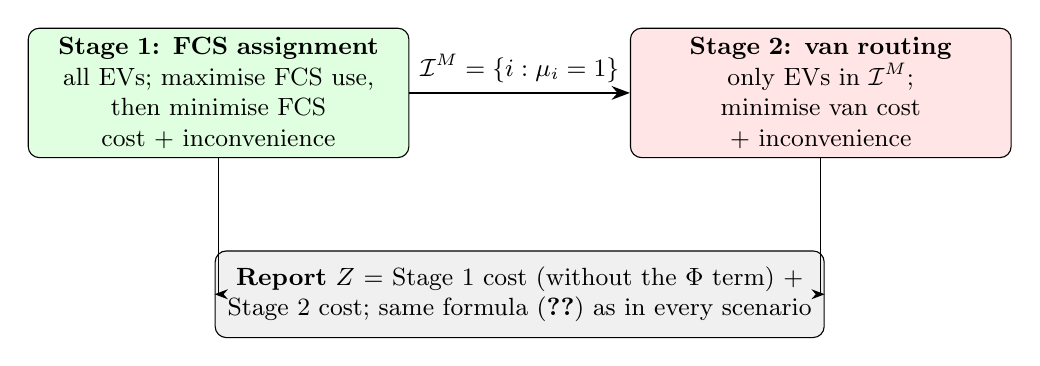
\begin{tikzpicture}[>=Stealth,box/.style={draw,rounded corners,align=center,minimum height=1.1cm,font=\small}]
  \node[box,fill=green!12,text width=4.6cm] (s1) {\textbf{Stage 1: FCS assignment}\\all EVs; maximise FCS use,\\then minimise FCS cost + inconvenience};
  \node[box,fill=red!10,text width=4.6cm,right=2.8cm of s1] (s2) {\textbf{Stage 2: van routing}\\only EVs in $\I^M$;\\minimise van cost + inconvenience};
  \draw[->,thick] (s1) -- node[above,font=\small]{$\I^M=\{i:\mu_i=1\}$} (s2);
  \node[box,fill=black!6,text width=7.5cm,below=2.0cm of $(s1)!0.5!(s2)$] (ev) {\textbf{Report} $Z=$ Stage~1 cost (without the $\Phi$ term) $+$ Stage~2 cost; same formula \eqref{eq:Z} as in every scenario};
  \draw[->] (s1) |- (ev); \draw[->] (s2) |- (ev);
\end{tikzpicture}
\end{center}

Stage~1 does not look at the vans, and Stage~2 cannot change what Stage~1 decided. That is the definition of ``FCS first, then MCS''.

%----------------------------------------------------------------
\subsection{Stage 1: assign EVs to fixed stations}

\textbf{Objective.}
\begin{equation}
\begin{split}
\min\ Z^{(1)}=\;&\underbrace{\Phi\sum_{i\in\I}\mu_i}_{\text{FCS first}}
+\underbrace{c^{EV}\sum_i\sum_{f\in\F_i}d_{if}Y_{if}}_{Z_1}
+\underbrace{Z^F_{\text{energy}}}_{\text{FCS part of }Z_4}\\
&+\underbrace{\sum_i\sum_{f\in\F_i}\rho^F_{if}Y_{if}+\alpha\sum_i w_i(C_i-r_i)+c^L\sum_i w_iL_i}_{\text{FCS customers' inconvenience}}
\end{split}
\label{eq:obj1}
\end{equation}
with $C_i=S_i+\tau^F_iY_i$ in this stage. $\Phi$ is a penalty for handing an EV to the vans. It is chosen larger than anything an extra FCS customer can add to the rest of \eqref{eq:obj1}, e.g.
\[
\Phi > \max_{i}\max_{f\in\F_i}\big(c^{EV}d_{if}+\pi^{\max}E_i+\rho^F_{if}\big)+n\,(\alpha+c^L)\,w_{\max}\,T,
\]
so Stage~1 first \textbf{maximises the number of EVs served at an FCS}, and only among those solutions minimises FCS cost and inconvenience. ($\pi^{\max}$ is the highest grid price.) A numerically safer equivalent is to solve twice: first $\max\sum_iY_i$, then fix that number and minimise the rest.
\ifTOU
Because $Z^F_{\text{energy}}$ uses the peak price, Stage~1 may \emph{start sessions later} to leave the peak, if the price saving beats the extra waiting cost (Section~\ref{sec:expect}).
\fi

\textbf{Constraints.}
\begin{align}
\sum_{g\in\G_i}y_{ig}+\mu_i &= 1 && \forall i\in\I \label{eq:s1assign}\\
S_i &\ge r_i+\sum_{f\in\F_i}t_{if}Y_{if} && \forall i\in\I \label{eq:fcsarr}\\
S_i &\le r_i+T\,(1-\mu_i) && \forall i\in\I \label{eq:s1park}\\
S_j &\ge S_i+\tau^F_i-(T+\tau^F_i)(3-y_{ig}-y_{jg}-o_{ij}) && \forall g,\ (i,j)\in\mathcal{P}_g \label{eq:disj1}\\
S_i &\ge S_j+\tau^F_j-(T+\tau^F_j)(2-y_{ig}-y_{jg}+o_{ij}) && \forall g,\ (i,j)\in\mathcal{P}_g \label{eq:disj2}\\
\sum_i y_{ig_1} &\ge \sum_i y_{ig_2} && \forall f,\ \G_f=\{g_1,g_2\} \label{eq:gunsym}\\
S_i+\tau^F_iY_i &\le T,\qquad L_i\ge S_i+\tau^F_iY_i-l_i && \forall i\in\I \label{eq:s1time}
\end{align}
\ifTOU plus the time-of-use split \eqref{eq:tou1}--\eqref{eq:tou5} of each FCS session (Section~\ref{sec:price}).\fi
\desc{\eqref{eq:s1assign}: every EV either gets one reachable gun or is handed to the vans. An EV that reaches no FCS ($\G_i=\emptyset$) is forced to $\mu_i=1$. \eqref{eq:fcsarr}: an FCS session cannot start before the EV has asked and driven to the station. \eqref{eq:s1park}: for an EV handed to the vans, $S_i$ is parked at $r_i$, so it adds no waiting in Stage~1 (its real start time is decided in Stage~2). \eqref{eq:disj1}--\eqref{eq:disj2}: two EVs on the same gun do not overlap; $o_{ij}$ picks who goes first. With two guns per station this means at most two EVs charge at a station at a time. \eqref{eq:gunsym}: symmetry breaking between the two identical guns (optional). \eqref{eq:s1time}: finished by $T$; lateness.}

\textbf{Optional acceptability rule.} An operator may refuse to send a driver to a station that is ``too inconvenient'', e.g.\ only allow gun $g$ of station $f$ for EV $i$ if $\hat\rho^F_{if}\le\bar\rho$. This only shrinks $\G_i$, so EVs whose stations are all too far go to the vans. Report results with and without it.

\textbf{Output:} $\I^M=\{i:\mu_i=1\}$, the EVs left for the vans; plus each FCS customer's gun and start time.

%----------------------------------------------------------------
\subsection{Stage 2: route the vans to the leftover EVs}

Stage~2 is a vehicle routing problem with time windows, on the EVs in $\I^M$ only. Here $C_i=S_i+\tau^M_i$.

\textbf{Objective.}
\begin{equation}
\begin{split}
\min\ Z^{(2)}=\;&\underbrace{c^M\sum_m\sum_{(i,j)\in\A^M}d_{ij}x_{ijm}}_{Z_2}+\underbrace{\sum_m c^D_mu_m}_{Z_3}+\underbrace{Z^M_{\text{energy}}}_{\text{van part of }Z_4}\\
&+\underbrace{\sum_{i\in\I^M}\sum_m\rho^M_{im}z_{im}+\alpha\sum_{i\in\I^M}w_i(C_i-r_i)+c^L\sum_{i\in\I^M}w_iL_i}_{\text{van customers' inconvenience}}
\end{split}
\label{eq:obj2}
\end{equation}
Since every EV in $\I^M$ must be served by some van, $Z^M_{\text{energy}}$ and the $\rho^M$ term are constants here. They are kept so that $Z^{(2)}$ is the true cost of Stage~2. Waiting and lateness make the vans visit urgent EVs early.

\textbf{Constraints.}
\begin{align}
\sum_{m\in\M}z_{im} &= 1 && \forall i\in\I^M \label{eq:s2assign}\\
\sum_{j:(0,j)\in\A^M}x_{0jm} = \sum_{i:(i,n+1)\in\A^M}x_{i,n+1,m} &= u_m && \forall m \label{eq:depot}\\
\sum_{i:(i,j)\in\A^M}x_{ijm} = \sum_{k:(j,k)\in\A^M}x_{jkm} &= z_{jm} && \forall j\in\I^M,\ m \label{eq:flow}\\
\sum_{i\in\I^M}z_{im} &\le Q_m\,u_m && \forall m \label{eq:cap}\\
\sum_{i\in\I^M}\frac{E_i}{\eta}z_{im}+\beta\sum_{(i,j)\in\A^M}d_{ij}x_{ijm} &\le B_m\,u_m && \forall m \label{eq:batt}
\end{align}
\begin{align}
S_j &\ge \max\{r_j,\ t_{0j}\,x_{0jm}\} && \forall j\in\I^M,\ m \label{eq:depart}\\
S_j &\ge S_i+\tau^M_i+t_{ij}-(T+\tau^M_i+t_{ij})(1-x_{ijm}) && \forall i\neq j,\ m \label{eq:seq}\\
S_i+\tau^M_i+t_{i,n+1} &\le T+(\tau^M_i+t_{i,n+1})(1-x_{i,n+1,m}) && \forall i,\ m \label{eq:return}\\
S_i+\tau^M_i \le T,\quad L_i &\ge S_i+\tau^M_i-l_i && \forall i\in\I^M \label{eq:s2time}\\
u_m &\ge u_{m+1} && m<|\M| \label{eq:vansym}
\end{align}
\desc{\eqref{eq:s2assign}: each leftover EV gets one van. \eqref{eq:depot}: a used van leaves and returns to the depot once. \eqref{eq:flow}: each EV on van $m$ is entered and left exactly once by that van. \eqref{eq:cap}: at most $Q_m$ EVs per van. \eqref{eq:batt}: delivered energy (with transfer losses) plus driving energy fits in the van battery. \eqref{eq:depart}: no start before the request, or before the van can drive there from the depot (written as two linear constraints). \eqref{eq:seq}: if the van goes $i\to j$, it finishes $i$ and drives to $j$ before starting $j$. This gives one EV at a time and removes subtours (MTZ-type). \eqref{eq:return}: back at the depot by $T$. \eqref{eq:s2time}: finished by $T$; lateness. \eqref{eq:vansym}: use identical vans in index order.}

\textbf{If Stage 2 is infeasible} (too many leftover EVs for the fleet by $T$), the sequential policy has \emph{failed} on that instance. For diagnosis, add $s_i\in\{0,1\}$ (``unserved''), replace \eqref{eq:s2assign} by $\sum_mz_{im}+s_i=1$ and add $\Phi^U\sum_is_i$ to \eqref{eq:obj2}. Then report the number of EVs that could not be served. This is a useful comparison with the integrated scenario, which may serve all of them.

%----------------------------------------------------------------
\subsection{Reported value}
\[
Z^{\text{S\scen}}=\big(Z^{(1)*}-\Phi\,|\I^M|\big)+Z^{(2)*},
\]
which is exactly \eqref{eq:Z} evaluated at the combined solution. The stage-1 solution plus the stage-2 solution is a feasible solution of the integrated model (S\ifTOU 4\else 3\fi), so
$Z^{\text{S\ifTOU 4\else 3\fi}}\le Z^{\text{S\scen}}$. The difference is the \emph{value of integration}.

\else
%---------------------------------------------------------------- INT
\subsection{Objective}
\begin{equation}
\min\ Z \quad\text{as in \eqref{eq:Z}, with }Z^F_{\text{energy}}=\ifTOU P^F\textstyle\sum_i\big[\pi^\off(\theta^1_i+\theta^3_i)+\pi^\pk\theta^2_i\big]\else\pi^F\textstyle\sum_iE_iY_i\fi,\quad C_i=S_i+\tau^F_iY_i+\tau^M_iZ_i. \label{eq:objint}
\end{equation}
Written out in full:
\begin{align*}
\min\ Z=\;& c^{EV}\sum_i\sum_{f\in\F_i}d_{if}Y_{if}+c^M\sum_m\sum_{(i,j)\in\A}d_{ij}x_{ijm}+\sum_mc^D_mu_m\\
&+\ifTOU P^F\sum_i\big[\pi^\off(\theta^1_i+\theta^3_i)+\pi^\pk\theta^2_i\big]\else\pi^F\sum_iE_iY_i\fi
+\pi^M\sum_i\sum_m\frac{E_i}{\eta}z_{im}\\
&+\sum_i\sum_{f\in\F_i}\rho^F_{if}Y_{if}+\sum_i\sum_m\rho^M_{im}z_{im}+\alpha\sum_iw_i(C_i-r_i)+c^L\sum_iw_iL_i .
\end{align*}
Every term is linear. One model weighs everything at once: an EV goes to a van exactly when the van's extra km, dispatch and energy cost are outweighed by the effort and waiting it saves the driver\ifTOU, or by the peak-price energy it avoids\fi.

\subsection{Constraints}

\textbf{Assignment.}
\begin{equation}
\sum_{g\in\G_i}y_{ig}+\sum_{m\in\M}z_{im}=1\qquad\forall i\in\I \label{eq:assign}
\end{equation}
\desc{Exactly one resource per EV: one reachable gun or one van. EVs that reach no FCS are forced onto a van.}

\textbf{Fixed stations.}
\begin{align}
S_i &\ge r_i+\sum_{f\in\F_i}t_{if}Y_{if} && \forall i \label{eq:fcsarr}\\
S_j &\ge S_i+\tau^F_i-(T+\tau^F_i)(3-y_{ig}-y_{jg}-o_{ij}) && \forall g,\ (i,j)\in\mathcal{P}_g \label{eq:disj1}\\
S_i &\ge S_j+\tau^F_j-(T+\tau^F_j)(2-y_{ig}-y_{jg}+o_{ij}) && \forall g,\ (i,j)\in\mathcal{P}_g \label{eq:disj2}\\
\sum_iy_{ig_1} &\ge \sum_iy_{ig_2} && \forall f,\ \G_f=\{g_1,g_2\} \label{eq:gunsym}
\end{align}
\desc{\eqref{eq:fcsarr}: an FCS session starts after the request and the drive to the station (for a van customer this is just $S_i\ge r_i$). \eqref{eq:disj1}--\eqref{eq:disj2}: EVs on the same gun do not overlap; $o_{ij}$ chooses the order. \eqref{eq:gunsym}: optional symmetry breaking.}

\textbf{Vans: routes, capacity, battery.}
\begin{align}
\sum_{j:(0,j)\in\A}x_{0jm}=\sum_{i:(i,n+1)\in\A}x_{i,n+1,m} &= u_m && \forall m \label{eq:depot}\\
\sum_{i:(i,j)\in\A}x_{ijm}=\sum_{k:(j,k)\in\A}x_{jkm} &= z_{jm} && \forall j\in\I,\ m \label{eq:flow}\\
\sum_iz_{im} &\le Q_mu_m && \forall m \label{eq:cap}\\
\sum_i\frac{E_i}{\eta}z_{im}+\beta\sum_{(i,j)\in\A}d_{ij}x_{ijm} &\le B_mu_m && \forall m \label{eq:batt}
\end{align}
\desc{\eqref{eq:depot}: a used van leaves and returns once. \eqref{eq:flow}: each EV on van $m$ is visited exactly once by it. \eqref{eq:cap}: at most $Q_m$ EVs. \eqref{eq:batt}: delivered energy (with losses) plus driving energy fits in the battery.}

\textbf{Vans: timing (one EV at a time, no subtours).}
\begin{align}
S_j &\ge t_{0j}\,x_{0jm} && \forall j\in\I,\ m \label{eq:depart}\\
S_j &\ge S_i+\tau^M_i+t_{ij}-(T+\tau^M_i+t_{ij})(1-x_{ijm}) && \forall i\neq j\in\I,\ m \label{eq:seq}\\
S_i+\tau^M_i+t_{i,n+1} &\le T+(\tau^M_i+t_{i,n+1})(1-x_{i,n+1,m}) && \forall i,\ m \label{eq:return}
\end{align}
\desc{\eqref{eq:depart}: the first stop cannot start before the van has driven there. \eqref{eq:seq}: $i\to j$ means finish $i$, drive, then start $j$; start times rise along a route, so no subtour can close. \eqref{eq:return}: back at the depot by $T$.}

\textbf{Horizon and lateness.}
\begin{equation}
C_i\le T,\qquad L_i\ge C_i-l_i\qquad\forall i\in\I \label{eq:time}
\end{equation}
\desc{Every EV is fully charged within the horizon; $L_i$ measures lateness.}

\ifTOU
\textbf{Time-of-use split.} Constraints \eqref{eq:tou1}--\eqref{eq:tou5} of Section~\ref{sec:price}.
\fi

\textbf{Symmetry and domains.}
\begin{equation}
u_m\ge u_{m+1};\qquad y,z,x,u,o\ifTOU,\kappa\fi\in\{0,1\};\qquad S_i,L_i\ifTOU,\theta^p_i\fi\ge0 \label{eq:dom}
\end{equation}
\fi

%=====================================================================
\section{Learning-to-optimise (RL) formulation}\label{sec:rl}

\textbf{Main rule:} the reward of each action is \emph{minus the increase in $Z$ that the action causes}. The rewards over an episode then add up to $-Z$ of the solution the policy builds. RL and MILP results are measured on the same yardstick \eqref{eq:Z}, and the MILP optimum is the benchmark for the RL gap.

\ifSEQ
%---------------------------------------------------------------- RL SEQ
The RL pipeline has the same two stages as the MILP.

\subsection{Stage 1 policy: FCS assignment}
\begin{itemize}[leftmargin=1.4em,itemsep=2pt]
  \item \textbf{Episode / epochs:} EVs are taken in order of request time $r_i$ (ties: higher $w_i$ first). One decision per EV.
  \item \textbf{State:} features of the current EV $k$ ($E_k,r_k,l_k,w_k,R_k$, location); for each gun $g$ the time $F_g$ it becomes free; summary features of the EVs still to come (count and positions near each station)\ifTOU; the current price and the time until $T_1$ and $T_2$\fi.
  \item \textbf{Action:} a gun $g\in\G_k$, or ``hand to vans''. \textbf{FCS-first mask:} ``hand to vans'' is allowed \emph{only} if no gun can finish EV $k$ by $T$ (or, with the optional rule, if all remaining guns have $\hat\rho^F_{kf}>\bar\rho$).
  \ifTOU\item \textbf{Optional timing action:} ``gun $g$, start after the peak'', i.e.\ $S_k=\max\{\text{earliest},T_2\}$, allowed only if the session still ends by $T$.\fi
  \item \textbf{Transition:} $S_k=\max\{r_k+t_{kf},F_g\}$ (or later, for the timing action); $F_g\leftarrow S_k+\tau^F_k$.
  \item \textbf{Reward:} $-\Big[c^{EV}d_{kf}+\text{energy}_k+\rho^F_{kf}+\alpha w_k(S_k+\tau^F_k-r_k)+c^Lw_k(S_k+\tau^F_k-l_k)^+\Big]$, where energy$_k$ = \ifTOU$P^F\big[\pi^\off\cdot(\text{off-peak hours of }[S_k,S_k+\tau^F_k])+\pi^\pk\cdot(\text{peak hours})\big]$, computed exactly in the simulator\else$\pi^FE_k$\fi. Handing an EV to the vans gives reward $0$ here; its cost is counted in Stage~2.
\end{itemize}
Note: a simple baseline for Stage~1 is the greedy rule ``gun with the largest one-step reward''. What RL can learn on top of this is, for example, to keep a nearby gun free for an urgent EV that arrives later.

\subsection{Stage 2 policy: van routing over $\I^M$}
\begin{itemize}[leftmargin=1.4em,itemsep=2pt]
  \item \textbf{Epochs:} whenever a van becomes free (the earliest-free van decides first).
  \item \textbf{State:} for each van: position, time free, remaining battery $b_m$, EVs served so far, dispatched or not; for each unserved EV in $\I^M$: location, $E_i,r_i,l_i,w_i$; current time.
  \item \textbf{Action:} the next EV $j$ for this van, or ``return to depot'' (ends the route). Mask: $j$ must be feasible: battery covers $E_j/\eta$ plus driving to $j$ and back to the depot, the count stays $\le Q_m$, and $j$ can be finished with the van back at the depot by $T$.
  \item \textbf{Transition:} $S_j=\max\{r_j,\ \text{time free}+t_{\text{pos},j}\}$; the van moves to $j$ and is free at $S_j+\tau^M_j$; $b_m$ falls by $E_j/\eta+\beta d_{\text{pos},j}$.
  \item \textbf{Reward:} serving $j$: $-\Big[c^Md_{\text{pos},j}+c^D_m[\text{first stop}]+\pi^M\frac{E_j}{\eta}+\rho^M_{jm}+\alpha w_j(S_j+\tau^M_j-r_j)+c^Lw_j(S_j+\tau^M_j-l_j)^+\Big]$; returning: $-c^Md_{\text{pos},0}$. EVs still unserved at the end: $-\Phi^U$ each.
  \item \textbf{Policy:} an attention-based routing policy (e.g.\ Kool et al., 2019, ``Attention, Learn to Solve Routing Problems!'') trained with REINFORCE or PPO. Baseline: nearest-feasible-EV heuristic.
\end{itemize}
Episode return of Stage~1 + Stage~2 $=-Z^{\text{S\scen}}$.

\else
%---------------------------------------------------------------- RL INT
One policy decides both who serves each EV and the van routes.
\begin{itemize}[leftmargin=1.4em,itemsep=2pt]
  \item \textbf{Episode / epochs:} EVs are taken in order of request time $r_i$ (ties: higher $w_i$ first). One decision per EV.
  \item \textbf{State:} (i) the current EV $k$: location, $E_k,r_k,l_k,w_k,R_k$, reachable stations; (ii) each gun $g$: time $F_g$ it becomes free; (iii) each van $m$: current end-of-route position, time free, remaining battery $b_m$, EVs served, dispatched or not; (iv) embeddings of the not-yet-assigned EVs (for look-ahead)\ifTOU; (v) current price, time until $T_1$ and $T_2$\fi.
  \item \textbf{Action:} $a\in\G_k\cup\M$: a gun, or a van (EV $k$ is appended to the end of that van's route). \textbf{Mask} infeasible actions: a gun that cannot finish $k$ by $T$; a van without enough battery for $E_k/\eta$ plus the drive to $k$ and back to the depot, with $Q_m$ reached, or unable to finish $k$ and return by $T$.
  \ifTOU\item \textbf{Optional timing action:} ``gun $g$, start after the peak'' ($S_k=\max\{\text{earliest},T_2\}$, if it still ends by $T$).\fi
  \item \textbf{Transition:} gun: $S_k=\max\{r_k+t_{kf},F_g\}$, $F_g\leftarrow S_k+\tau^F_k$. Van: $S_k=\max\{r_k,\ \text{free}_m+t_{\text{pos}_m,k}\}$, then the van moves to $k$, $\text{free}_m\leftarrow S_k+\tau^M_k$, $b_m\mathrel{-}=E_k/\eta+\beta d_{\text{pos}_m,k}$.
  \item \textbf{Reward} $=-\Delta Z$:
  \begin{align*}
  \text{gun } g\text{ at }f:&\quad -\Big[c^{EV}d_{kf}+\text{energy}^F_k+\rho^F_{kf}+\alpha w_k(C_k-r_k)+c^Lw_k(C_k-l_k)^+\Big]\\
  \text{van } m:&\quad -\Big[c^M\big(d_{\text{pos}_m,k}+d_{k,0}-d_{\text{pos}_m,0}\big)+c^D_m[\text{first use}]+\pi^M\tfrac{E_k}{\eta}\\
  &\qquad\quad+\rho^M_{km}+\alpha w_k(C_k-r_k)+c^Lw_k(C_k-l_k)^+\Big]
  \end{align*}
  The van distance term is the \emph{change} in route length when $k$ is inserted before the return to the depot, so the sum over the episode equals the total route length (the return legs telescope). energy$^F_k$ = \ifTOU$P^F\big[\pi^\off\cdot(\text{off-peak hours})+\pi^\pk\cdot(\text{peak hours of }[S_k,C_k])\big]$, computed exactly by the simulator; no linearisation is needed in RL\else$\pi^FE_k$\fi.
  \item \textbf{Dead end:} if every action is masked, EV $k$ is unserved: reward $-\Phi^U$, and the episode continues. Report the count.
  \item \textbf{Policy:} masked categorical policy over guns and vans, encoder with attention over EVs, guns and vans; trained with PPO. Natural baseline: greedy, i.e.\ choose the action with the largest one-step reward. That is the pairwise rule ``smallest $\hat\rho$ + cost'' from Section~\ref{sec:inc}.
\end{itemize}
Restriction to note: vans serve EVs in assignment order (append only). A variant that inserts $k$ at the cheapest position of a route is more flexible but has a larger action space.
\fi

\textbf{Reward scaling.} For stable training divide every reward by a constant, e.g.\ the greedy baseline's average $Z$ on the training instances. This does not change the optimal policy.

%=====================================================================
\section{What to expect and what to report}\label{sec:expect}

\ifnum\scen=1
\begin{itemize}[leftmargin=1.4em,itemsep=2pt]
  \item Vans serve only EVs that reach no station, or that the stations cannot finish by $T$. If stations have spare capacity, very few vans are dispatched.
  \item Inconvenience is high for EVs far from the nearest station (worked example: Rs\,682 at the FCS, against Rs\,458 if a van had been allowed).
  \item With too few vans Stage~2 becomes infeasible (unserved EVs), even when the integrated model S3 could serve everyone. Report the smallest $|\M|$ at which S1 is feasible and compare it with S3.
\end{itemize}
\fi
\ifnum\scen=2
\begin{itemize}[leftmargin=1.4em,itemsep=2pt]
  \item \textbf{When does Stage~1 delay a session to avoid the peak?} Moving one hour of charging out of the peak saves $(\pi^\pk-\pi^\off)P^F=3\times22=$ Rs\,66, but delays completion by up to an hour, which costs $\alpha w_i\ge$ Rs\,200. So with the default values Stage~1 almost never delays. It mostly pays the higher price, and S2 costs roughly S1 plus the peak surcharge. Sessions start later only if $\alpha$ is small (try $\lambda<0.33$ in the sensitivity analysis).
  \item The van assignment is the same as in S1 unless Stage~1's timing changes which EVs fit at the stations. Stage~1 cannot use vans to escape the peak price.
  \item Extra KPI: \textbf{grid energy drawn at FCS during the peak}, $P^F\sum_i\theta^2_i$ (kWh). Compare with S4.
\end{itemize}
\fi
\ifnum\scen=3
\begin{itemize}[leftmargin=1.4em,itemsep=2pt]
  \item Vans take EVs for which the saved inconvenience exceeds the extra van cost (worked example: van chosen, saving Rs\,224). Expect vans to serve EVs that are far from every station, have low range (high $w_i$), or have early deadlines, while EVs near a station still use it.
  \item \textbf{Value of integration under flat price:} $Z^{\text{S1}}-Z^{\text{S3}}\ge0$. Report it per component ($Z_1,\dots,Z_5$): typically operating cost rises a little and inconvenience falls a lot.
  \item Vary $|\M|$ (0, 1, 2, \dots): the first few vans lower $Z$ sharply, then the effect levels off. That curve shows the scenarios where mobile chargers help most.
\end{itemize}
\fi
\ifnum\scen=4
\begin{itemize}[leftmargin=1.4em,itemsep=2pt]
  \item During the peak a van kWh costs about the same as an FCS kWh (Rs\,10.0 each), so the vans' energy disadvantage disappears and vans also absorb \emph{peak-hour} demand that would otherwise be charged on the grid at peak price.
  \item Expect more van usage than in S3, concentrated on requests in $[T_1,T_2]$, and lower grid energy at the stations during the peak, $P^F\sum_i\theta^2_i$, than in S2.
  \item \textbf{Value of integration under peak pricing:} $Z^{\text{S2}}-Z^{\text{S4}}$. It should be larger than $Z^{\text{S1}}-Z^{\text{S3}}$, because integration now also allows price arbitrage.
  \item \textbf{Peak pricing with full flexibility:} $Z^{\text{S4}}-Z^{\text{S3}}$ should be smaller than $Z^{\text{S2}}-Z^{\text{S1}}$: vans cushion the price increase.
\end{itemize}
\fi

\textbf{Cross-scenario comparison table} (fill in from the four runs):
\begin{center}
\renewcommand{\arraystretch}{1.2}
\begin{tabular}{@{}lll@{}}
\toprule
\textbf{Comparison} & \textbf{Measures} & \textbf{Expected sign} \\
\midrule
S1 $-$ S3 & value of integration, flat price & $\ge0$ \\
S2 $-$ S4 & value of integration, peak price & $\ge0$, larger than S1 $-$ S3 \\
S2 $-$ S1 & cost of peak pricing, FCS-first operator & $>0$ \\
S4 $-$ S3 & cost of peak pricing, flexible operator & $>0$, smaller than S2 $-$ S1 \\
\bottomrule
\end{tabular}
\end{center}
Report for each: $Z$ and its components, number of vans used, EVs per resource, mean and maximum inconvenience per EV, total lateness, peak-hour grid energy, solve time, and (for RL) the gap to the MILP optimum.

%=====================================================================
\appendix
\section{Illustrative parameter values}\label{app:values}

These are starting values for experiments, not data. All are meant to be varied in the analysis. Values in Rs.

\begin{center}
\renewcommand{\arraystretch}{1.15}
\begin{tabular}{@{}llp{6.2cm}@{}}
\toprule
\textbf{Parameter} & \textbf{Value} & \textbf{Note} \\
\midrule
$T$, $[T_1,T_2]$ & 7 h, $[2,6]$ & 16:00--23:00, peak 18:00--22:00 \\
$P^F$, $P^M$ & 22 kW, 30 kW & \\
$v$, $\beta$, $\eta$ & 25 km/h, 0.25 kWh/km, 0.9 & \\
$B_m$, $Q_m$, $|\M|$ & 150 kWh, 6, 2--6 & \\
$c^{EV}$, $c^M$, $c^D_m$ & Rs\,4/km, Rs\,15/km, Rs\,1500 & van km includes driver time \\
$\pi^F$ (flat) & Rs\,8.7/kWh & equals the time-average of the ToU tariff over $[0,T]$ \\
$\pi^\off$, $\pi^\pk$ (ToU) & Rs\,7/kWh, Rs\,10/kWh & $(3\times7+4\times10)/7=8.7$ \\
$c^{bat}$ & Rs\,2/kWh & van battery wear \\
$\pi^M$ & Rs\,10.7 (flat) / Rs\,9.0 (ToU) & $=\pi^F+c^{bat}$ / $=\pi^\off+c^{bat}$ \\
$\alpha$, $\alpha^D$ & Rs\,200/h, Rs\,100/h & value of time; extra for attended time \\
$h^F$, $h^M$, $\varphi$ & Rs\,50, Rs\,10, Rs\,100 & trip hassle, hand-over, range stress \\
$c^L$ & Rs\,300/h & lateness \\
$w_i$ & $1+2(1-R_i/R_{\max})$, $R_i\sim U[3,40]$ km & priority from remaining range \\
\bottomrule
\end{tabular}
\end{center}

The flat price is set to the time-average of the peak tariff. The price \emph{level} is then the same in both pricing cases, and only the price \emph{shape} differs. Without this, part of S1 vs S2 would just reflect a different average price.

\end{document}
"
%    pdflatex -jobname=scenario4_peak_integrated   "\def\scen{4}% =====================================================================
%  One source, four PDFs.  Build with build.sh (or by hand):
%    pdflatex -jobname=scenario1_flat_sequential   "\def\scen{1}\input{scenario_master}"
%    pdflatex -jobname=scenario2_peak_sequential   "\def\scen{2}\input{scenario_master}"
%    pdflatex -jobname=scenario3_flat_integrated   "\def\scen{3}\input{scenario_master}"
%    pdflatex -jobname=scenario4_peak_integrated   "\def\scen{4}\input{scenario_master}"
%  (run each twice for cross-references)
% =====================================================================
\documentclass[11pt,a4paper]{article}
\usepackage[margin=2.2cm]{geometry}
\usepackage{amsmath,amssymb,amsfonts}
\usepackage{booktabs,array,tabularx}
\usepackage{enumitem}
\usepackage[table]{xcolor}
\usepackage{tikz}
\usetikzlibrary{arrows.meta,positioning,calc}
\usepackage[colorlinks=true,linkcolor=blue!50!black,urlcolor=blue!50!black]{hyperref}
\usepackage{titlesec}
\titleformat{\section}{\large\bfseries}{\thesection}{0.8em}{}
\titleformat{\subsection}{\normalsize\bfseries}{\thesubsection}{0.8em}{}
\setlength{\parindent}{0pt}
\setlength{\parskip}{5pt}

% ---------------- scenario switches ----------------
\ifdefined\scen\else\def\scen{1}\fi
\newif\ifTOU \TOUfalse   % true = time-of-use (peak) price
\newif\ifSEQ \SEQfalse   % true = FCS first, then MCS
\ifnum\scen=1 \SEQtrue \fi
\ifnum\scen=2 \TOUtrue \SEQtrue \fi
\ifnum\scen=4 \TOUtrue \fi

\newcommand{\pricename}{\ifTOU time-of-use price (dearer evening peak)\else single (flat) price all day\fi}
\newcommand{\structname}{\ifSEQ FCS first, then MCS (sequential)\else FCS and MCS together (integrated)\fi}

% ---------------- notation ----------------
\newcommand{\I}{\mathcal{I}}
\newcommand{\F}{\mathcal{F}}
\newcommand{\G}{\mathcal{G}}
\newcommand{\M}{\mathcal{M}}
\newcommand{\N}{\mathcal{N}}
\newcommand{\A}{\mathcal{A}}
\newcommand{\Rs}{\text{Rs}\,}
\newcommand{\pk}{\mathrm{pk}}
\newcommand{\off}{\mathrm{off}}
\newcommand{\desc}[1]{\par\vspace{-2pt}{\small\color{black!75}\textit{Meaning:} #1}\par\vspace{4pt}}
\newcommand{\cell}[2]{\ifnum\scen=#1\cellcolor{blue!18}\textbf{S#1 (this document)}\\\textbf{#2}\else S#1\\#2\fi}

\title{\textbf{EV Charging Network Optimisation}\\[4pt]
\large Scenario \scen: \pricename\ $+$ \structname\\[2pt]
\normalsize MILP and RL formulation}
\author{CP 320 OR for Mobility Management, course project}
\date{2 October 2026}

\begin{document}
\maketitle

%=====================================================================
\section{Where this scenario sits}

The project studies four scenarios: two ways of pricing grid electricity, times two ways of making the decisions.

\begin{center}
\renewcommand{\arraystretch}{1.5}
\begin{tabular}{>{\raggedright\arraybackslash}p{4.2cm}|>{\centering\arraybackslash}p{4.6cm}|>{\centering\arraybackslash}p{4.6cm}}
 & \textbf{Flat price all day} & \textbf{Time-of-use (peak) price} \\ \hline
\textbf{Sequential:} FCS first, leftover EVs to MCS &
\begin{tabular}[c]{@{}c@{}}\cell{1}{flat + sequential}\end{tabular} &
\begin{tabular}[c]{@{}c@{}}\cell{2}{peak + sequential}\end{tabular} \\ \hline
\textbf{Integrated:} FCS and MCS decided together &
\begin{tabular}[c]{@{}c@{}}\cell{3}{flat + integrated}\end{tabular} &
\begin{tabular}[c]{@{}c@{}}\cell{4}{peak + integrated}\end{tabular} \\
\end{tabular}
\end{center}

\textbf{The four scenarios do not have four different objectives.} They share \emph{one} cost yardstick $Z$ (Section~\ref{sec:obj}): the same cost terms and the same customer inconvenience (Section~\ref{sec:inc}). Only two things change:
\begin{itemize}[leftmargin=1.4em,itemsep=1pt]
  \item \textbf{Pricing} changes the formula for one term, the FCS energy cost (Section~\ref{sec:price}).
  \item \textbf{Decision structure} changes \emph{how} $Z$ is minimised: in one model (integrated), or in two stages (sequential), where each stage minimises its own part of $Z$.
\end{itemize}
Because the yardstick is the same, the four optimal values can be compared directly. The differences measure the \emph{value of integration} (S1$\to$S3, S2$\to$S4) and the \emph{effect of peak pricing} (S1$\to$S2, S3$\to$S4).

\ifnum\scen=1
\textbf{This scenario (S1)} is the baseline, the ``status quo''. Electricity costs the same at every hour, every EV that can be charged at a fixed station is sent there, and vans only take what is left over.
\fi
\ifnum\scen=2
\textbf{This scenario (S2)} keeps the FCS-first rule of S1, but grid electricity is dearer during the evening peak. Stage~1 can react to the price only by \emph{rescheduling} FCS sessions. It cannot hand a peak-hour EV to a van.
\fi
\ifnum\scen=3
\textbf{This scenario (S3)} keeps the flat price of S1, but the operator decides FCS and MCS service \emph{together}. An EV can be sent to a van even when a fixed station could take it, whenever that lowers total cost plus inconvenience.
\fi
\ifnum\scen=4
\textbf{This scenario (S4)} is the most flexible one: peak pricing at fixed stations, and FCS and MCS decided together. Van energy was bought off-peak, so vans can also be used to keep charging \emph{out of the expensive peak}.
\fi

%=====================================================================
\section{Setting and assumptions}\label{sec:setting}

\textbf{Time.} The planning horizon is $[0,T]$ with $T=7$\,h (16:00--23:00). It contains the evening peak window $[T_1,T_2]=[2,6]$ (18:00--22:00). The horizon is the same in all four scenarios. It is wider than the peak itself so that, under peak pricing, there is cheaper time on both sides of the peak.\ifTOU\else\ In this scenario the price is flat, so the window plays no role in the model.\fi

\textbf{Assumptions} (the same as MILP v3, plus two about energy):
\begin{enumerate}[leftmargin=1.6em,itemsep=1pt]
  \item Static, continuous time. All requests in the horizon are known at time $0$, and request $i$ becomes active at $r_i$.
  \item An EV served by an FCS drives there itself on its own battery (only to stations within its range $R_i$). The driver stays with the car while it waits for a free gun and while it charges.
  \item An EV served by an MCS stays parked where it is, and the driver is free in the meantime.
  \item Each FCS gun and each van charges one EV at a time, without interruption, at constant power.
  \item A van's battery covers both its driving and the energy it delivers. \textbf{The van battery is charged at the depot before the horizon starts}\ifTOU, i.e.\ at the off-peak price\fi, and is not recharged during the horizon.
  \item Every EV must be fully charged by $T$ (hard). Finishing after the driver's desired time $l_i$ is allowed but penalised.
\end{enumerate}

%=====================================================================
\section{Notation}\label{sec:notation}

\subsection*{Sets}
\begin{tabularx}{\textwidth}{@{}lX@{}}
\toprule
$\I=\{1,\dots,n\}$ & EV charging requests \\
$\F$; $\G_f$ ($|\G_f|=2$); $\G=\bigcup_f\G_f$ & fixed charging stations; guns of FCS $f$; all guns ($f(g)$ = station of gun $g$) \\
$\F_i=\{f: d_{if}\le R_i\}$, $\G_i=\bigcup_{f\in\F_i}\G_f$ & stations / guns EV $i$ can reach on its remaining range \\
$\M$ & mobile charging vans (MCS) \\
$0,\ n+1$ & depot as start node / end node (same place) \\
$\N=\{0\}\cup\I\cup\{n+1\}$, $\A$ & routing nodes; allowed van arcs $(i,j)$, $i\in\{0\}\cup\I$, $j\in\I\cup\{n+1\}$, $i\neq j$ \\
$\mathcal{P}_g=\{(i,j): i<j,\ g\in\G_i\cap\G_j\}$ & pairs of EVs that could share gun $g$ \\
\ifSEQ
$\I^M\subseteq\I$ & EVs handed to the vans by Stage~1 (an \emph{output} of Stage~1, a fixed input to Stage~2) \\
$\N^M$, $\A^M$ & routing nodes / arcs restricted to $\I^M$ \\
\fi
\bottomrule
\end{tabularx}

\subsection*{Parameters}
\begin{tabularx}{\textwidth}{@{}lX@{}}
\toprule
$E_i,\ r_i,\ l_i,\ R_i$ & energy demand (kWh), request time, desired completion time (h), remaining range (km) \\
$w_i\ge1$ & priority of EV $i$; $w_i=1+\kappa(1-R_i/R_{\max})$, so low-range EVs weigh more \\
$P^F,\ P^M$ & charging power of an FCS gun (22\,kW) / of a van (e.g.\ 30\,kW) \\
$\tau^F_i=E_i/P^F,\ \tau^M_i=E_i/P^M$ & charging time of EV $i$ at an FCS / by a van (h) \\
$d_{if},t_{if}$;\ $d_{ij},t_{ij}$ & distance (km) and time (h): EV$\to$FCS; between routing nodes ($t=d/v$) \\
$B_m,\ Q_m,\ \beta,\ \eta$ & van battery (kWh), max EVs per van, van consumption (kWh/km), transfer efficiency \\
$c^{EV},\ c^M,\ c^D_m$ & cost per km of EV driving, per km of van driving; fixed dispatch cost of van $m$ \\
\ifTOU
$\pi^\off,\ \pi^\pk$ & grid price (Rs/kWh) off-peak / in $[T_1,T_2]$, with $\pi^\pk\ge\pi^\off$ \\
\else
$\pi^F$ & grid price (Rs/kWh), the same at every hour \\
\fi
$c^{bat}$ & van battery wear per kWh cycled \\
$\pi^M$ & cost of 1 kWh taken from a van battery: $\pi^M=\ifTOU\pi^\off\else\pi^F\fi+c^{bat}$ (Section~\ref{sec:price}) \\
$\alpha,\ \alpha^D,\ h^F,\ h^M,\ \varphi,\ c^L$ & inconvenience coefficients (Section~\ref{sec:inc}) \\
\bottomrule
\end{tabularx}

\subsection*{Decision variables}
\begin{tabularx}{\textwidth}{@{}llX@{}}
\toprule
$y_{ig}$ & $\{0,1\}$ & EV $i$ charged at gun $g\in\G_i$ \\
$z_{im}$ & $\{0,1\}$ & EV $i$ served by van $m$ \\
$x_{ijm}$ & $\{0,1\}$ & van $m$ drives arc $(i,j)$ \\
$u_m$ & $\{0,1\}$ & van $m$ is dispatched \\
$o_{ij}$ & $\{0,1\}$ & for EVs $i<j$ that could share a gun: 1 if $i$ is charged before $j$ \\
\ifSEQ
$\mu_i$ & $\{0,1\}$ & Stage~1 only: EV $i$ is handed to the van fleet \\
\fi
\ifTOU
$\theta^1_i,\theta^2_i,\theta^3_i$ & $\ge0$ & hours of EV $i$'s FCS session before / inside / after the peak \\
$\kappa^1_i,\kappa^3_i$ & $\{0,1\}$ & EV $i$'s FCS session starts before $T_1$ / ends after $T_2$ \\
\fi
$S_i$ & $\ge0$ & time charging of EV $i$ starts (h), on whichever resource \\
$L_i$ & $\ge0$ & lateness of EV $i$ beyond $l_i$ (h) \\
\bottomrule
\end{tabularx}

\textbf{Short-hands} (linear expressions, not new variables):
\[
Y_{if}=\sum_{g\in\G_f}y_{ig},\qquad Y_i=\sum_{g\in\G_i}y_{ig}\ (\text{EV $i$ uses an FCS}),\qquad Z_i=\sum_{m\in\M}z_{im}\ (\text{EV $i$ uses a van}),
\]
\[
C_i=S_i+\tau^F_i\,Y_i+\tau^M_i\,Z_i \quad\text{(time EV $i$ is fully charged).}
\]

%=====================================================================
\section{Customer inconvenience}\label{sec:inc}

This section is \textbf{identical in all four scenario documents}. Inconvenience is a property of the customer, not of the price or of the planning method.

\subsection{What we mean by inconvenience}

Inconvenience is \emph{what the driver loses} from the moment they ask for a charge ($r_i$) until the car is fully charged ($C_i$), \emph{converted into rupees} so it can be added to the operator's costs. A driver loses three different things:

\begin{enumerate}[leftmargin=1.6em,itemsep=2pt]
  \item \textbf{Waiting:} the car is not ready. This lasts $C_i-r_i$ hours and affects \emph{every} driver, FCS or MCS.
  \item \textbf{Effort:} only an FCS customer has to drive to the station and sit there while the car charges. An MCS customer stays at home or at work and does something else. Driving to a far station also uses scarce battery range, which causes stress (``range anxiety'').
  \item \textbf{A missed deadline:} the car is still not ready at the time $l_i$ the driver needs it.
\end{enumerate}

Each loss gets a price in Rs per hour (or per event). All of them are multiplied by the priority $w_i$: an hour of delay for an EV with 5\,km of range left counts more than for one with 40\,km.

\subsection{The three components}

\begin{center}
\renewcommand{\arraystretch}{1.3}
\begin{tabularx}{\textwidth}{@{}>{\raggedright\arraybackslash}p{2.6cm}>{\raggedright\arraybackslash}X>{\raggedright\arraybackslash}X>{\raggedright\arraybackslash}p{3.0cm}@{}}
\toprule
\textbf{Component} & \textbf{EV $i$ at FCS $f$} & \textbf{EV $i$ by a van} & \textbf{Known when?} \\
\midrule
Effort & $w_i\big[\alpha^D(t_{if}+\tau^F_i)+h^F+\varphi\,d_{if}/R_i\big]$: driving and sitting at the station, a fixed trip hassle, range stress & $w_i\,h^M$: being reachable and handing over the car & \textbf{Static:} known as soon as the resource is chosen \\
Waiting & $w_i\,\alpha\,(C_i-r_i)$ = drive + \emph{queue at the gun} + charge & $w_i\,\alpha\,(C_i-r_i)$ = \emph{wait for the van} + charge & \textbf{Dynamic:} depends on the queue / van route \\
Missed deadline & $w_i\,c^L\,L_i$, $L_i=\max\{0,C_i-l_i\}$ & same & Dynamic \\
\bottomrule
\end{tabularx}
\end{center}

\textbf{Coefficients.}
$\alpha$ (Rs/h) is the value of an hour the car is not ready.
$\alpha^D$ (Rs/h) is the \emph{extra} value of an hour the driver must personally spend driving or sitting at the station: an hour at the station costs $\alpha+\alpha^D$, an hour waiting at home for a van costs only $\alpha$.
$h^F,h^M$ (Rs) are fixed hassle costs of one trip to a station / one van hand-over.
$\varphi$ (Rs) is the range-stress cost of a trip that uses the \emph{whole} remaining range ($d_{if}/R_i\le1$ is the fraction used).
$c^L$ (Rs/h) is the cost per hour late.

\subsection{Pairwise form: inconvenience of a (customer, resource) pair}

The natural first idea is: \emph{for every pair (EV $i$, FCS $f$) and every pair (EV $i$, van $m$) there is an inconvenience number, and the operator picks the pair with the lowest cost plus inconvenience.} The static part fits this idea exactly:
\[
\boxed{\;\rho^F_{if}=w_i\Big[\alpha^D\,(t_{if}+\tau^F_i)+h^F+\varphi\,\frac{d_{if}}{R_i}\Big]\qquad
\rho^M_{im}=w_i\,h^M\;}
\]
These are \textbf{parameters}, computed before solving, one number per (EV, FCS) pair and per (EV, van) pair. In the objective they appear linearly: $\sum_i\sum_f\rho^F_{if}Y_{if}+\sum_i\sum_m\rho^M_{im}z_{im}$.

Note that $\rho^M_{im}$ does not depend on $m$. Vans are identical and all start at the same depot, so the driver does not care \emph{which} van comes, only \emph{when} it comes. That ``when'' is the waiting part.

\subsection{Why waiting cannot be a fixed pairwise number}

It is tempting to also write the waiting as a pairwise number, e.g.\ ``the van needs 5 minutes to reach EV $i$''. But that depends on \emph{where the van is coming from}, which depends on the route the model is still choosing: if EV $i$ is the 4th stop of a van, the wait is the time for three charging sessions plus four drives. Likewise, waiting at an FCS depends on how many EVs are queued at that gun. So waiting is not known before solving. It is a function of decision variables:
\[
\text{waiting cost of EV } i \;=\; w_i\,\alpha\,(C_i-r_i),\qquad C_i=S_i+\tau^F_iY_i+\tau^M_iZ_i .
\]
This is \textbf{linear} in the variables ($S_i$, $y$, $z$), so it fits in a MILP directly. The constraints of Section~\ref{sec:milp} make $S_i$ equal to the true start time, including driving, queueing at the gun and the van's route. The term $\sum_i w_i\alpha r_i$ is a constant and may be dropped when solving.

\textbf{Pairwise \emph{estimate}} (used for intuition, by the RL policy and in heuristics): if there is no queue and the van comes straight to $i$,
\[
\hat\rho^{F}_{if}=\rho^F_{if}+w_i\alpha\,(t_{if}+\tau^F_i),\qquad
\hat\rho^{M}_{im}=\rho^M_{im}+w_i\alpha\,(t^{\text{van}}_{m\to i}+\tau^M_i),
\]
where $t^{\text{van}}_{m\to i}$ is the time until van $m$ can reach $i$ from where it currently is. In the RL formulation (Section~\ref{sec:rl}) the van's position \emph{is} known at each decision, so there this estimate becomes exact.

\subsection{Total inconvenience and how it enters the objective}

\begin{equation}
\boxed{\;
Z_{\text{inc}}=\underbrace{\sum_{i\in\I}\sum_{f\in\F_i}\rho^F_{if}Y_{if}+\sum_{i\in\I}\sum_{m\in\M}\rho^M_{im}z_{im}}_{\text{effort (static, pairwise)}}
+\underbrace{\alpha\sum_{i\in\I}w_i\,(C_i-r_i)}_{\text{waiting (dynamic)}}
+\underbrace{c^L\sum_{i\in\I}w_i\,L_i}_{\text{missed deadline}}
\;}\label{eq:inc}
\end{equation}
All three parts are in rupees, so $Z_{\text{inc}}$ is simply added to the operating costs. Nothing has to be normalised.

\subsection{Worked example: your ``10 km to the FCS vs.\ van in 5 minutes'' case}

EV $i$: $E_i=20$\,kWh, $R_i=40$\,km (so $w_i=1$); nearest free FCS $d_{if}=10$\,km away, $t_{if}=0.4$\,h at 25\,km/h; a van finishing next door can reach it in 5\,min ($0.083$\,h), adding about 4\,km to its route. $\tau^F_i=20/22=0.909$\,h, $\tau^M_i=20/30=0.667$\,h. Coefficients from Appendix~\ref{app:values}, flat price.

\begin{center}
\renewcommand{\arraystretch}{1.25}
\begin{tabular}{@{}lrr@{}}
\toprule
 & \textbf{FCS} & \textbf{Van} \\
\midrule
Driving (EV / extra van km) & $4\times10=40.0$ & $15\times4=60.0$ \\
Energy & $8.7\times20=174.0$ & $10.7\times20/0.9=237.8$ \\
\textbf{Operating cost only} & \textbf{214.0} & \textbf{297.8} \\
\midrule
Effort $\rho$ & $100(0.4+0.909)+50+100\cdot\tfrac{10}{40}=205.9$ & $10.0$ \\
Waiting $\alpha(C_i-r_i)$ & $200\times1.309=261.8$ & $200\times0.75=150.0$ \\
\textbf{Cost + inconvenience} & \textbf{681.7} & \textbf{457.8} \\
\bottomrule
\end{tabular}
\end{center}

On operating cost alone the FCS is cheaper, so a cost-only model would \emph{always} send this driver 10\,km away. With inconvenience included the van is better by about Rs\,224, and the integrated model chooses $z_{im}=1$, as you expected. If the FCS were only 1\,km away, the FCS would win both comparisons. The inconvenience term is what makes the model choose between ``cheap for the operator'' and ``convenient for the driver'', rather than following a fixed rule.

\subsection{Relation to a single penalty $\rho_i$ per EV}

The first draft used a penalty $\rho_i$ that is charged whenever EV $i$ goes to \emph{any} FCS: $\sum_i\sum_f\rho_iy_{if}$. Because $\sum_f y_{if}=1-\sum_m z_{im}$, this only says ``a van is worth $\rho_i$ more to EV $i$'', and that holds whether the station is 1\,km or 15\,km away, and whether the van arrives in 5 minutes or in 3 hours. The form above fixes both problems: $\rho^F_{if}$ grows with the distance to \emph{that} station, and the waiting term grows with how late the van or the free gun actually is. The old model is the special case $\alpha=\alpha^D=\varphi=c^L=0$, $h^F=\rho_i$.

\subsection{Choosing the coefficients}
\begin{itemize}[leftmargin=1.4em,itemsep=2pt]
  \item Use a value of time for $\alpha$ (e.g.\ Rs\,150--300/h for urban car users), and set $\alpha^D\approx0.5\alpha$: sitting at a station is worse than waiting at home.
  \item Keep $c^L>\alpha$, so missing the deadline is worse than ordinary waiting.
  \item \textbf{Sensitivity analysis:} multiply all inconvenience coefficients by a factor $\lambda\in\{0,0.25,0.5,1,2,4\}$ and plot operating cost against total inconvenience. $\lambda=0$ is the pure cost-minimising operator, and large $\lambda$ is a customer-first operator. This trade-off curve is a strong result for the ``Analysis'' part of the project.
\end{itemize}

\subsection{What inconvenience does in \emph{this} scenario}
\ifSEQ
In a sequential scenario inconvenience \textbf{cannot move an EV from an FCS to a van}: Stage~1 sends every EV that \emph{can} use an FCS to one. It still matters inside each stage. In Stage~1 it decides \emph{which} station and \emph{when} (urgent EVs get the near station and the first free gun). In Stage~2 it decides the \emph{order} in which vans visit EVs (urgent EVs first). In the worked example, this scenario sends the driver 10\,km to the FCS. That is the weakness the integrated scenarios remove.
\else
In an integrated scenario inconvenience is weighed directly against operating cost when choosing the resource. That is how the worked example ends up with a van. It also decides which station and which gun order, and the order of each van route.
\fi

%=====================================================================
\section{Electricity price in this scenario}\label{sec:price}

\textbf{Van energy (same in all scenarios).} A van's battery is charged at the depot \emph{before} the horizon, so its energy was bought at the
\ifTOU off-peak \fi
price, whatever time the van later delivers it. Each kWh taken from the van also wears the battery ($c^{bat}$), and a fraction $1-\eta$ is lost in transfer:
\[
Z^M_{\text{energy}}=\pi^M\sum_{i\in\I}\sum_{m\in\M}\frac{E_i}{\eta}\,z_{im},\qquad \pi^M=\ifTOU\pi^\off\else\pi^F\fi+c^{bat}.
\]

\ifTOU
\textbf{FCS energy (time-of-use).} An FCS draws from the grid while it charges. Energy delivered inside $[T_1,T_2]$ costs $\pi^\pk$, and energy outside it costs $\pi^\off$. A session $[S_i,S_i+\tau^F_i]$ may overlap the peak partly. Split its duration into the hours before, inside and after the peak, $\theta^1_i+\theta^2_i+\theta^3_i$:
\[
Z^F_{\text{energy}}=P^F\sum_{i\in\I}\Big[\pi^\off(\theta^1_i+\theta^3_i)+\pi^\pk\,\theta^2_i\Big].
\]
Constraints \eqref{eq:tou1}--\eqref{eq:tou5} below make the $\theta$'s equal to the true overlaps. Peak hours are dearer, so the solver wants $\theta^1_i,\theta^3_i$ as large as possible. It is enough to bound them from above by the true off-peak overlap, and the constraints need one binary per side:
\begin{align}
\theta^1_i+\theta^2_i+\theta^3_i &= \tau^F_i\,Y_i && \forall i\in\I \label{eq:tou1}\\
\theta^1_i &\le \tau^F_i\,\kappa^1_i && \forall i\in\I \label{eq:tou2}\\
\theta^1_i &\le T_1-S_i+T\,(1-\kappa^1_i) && \forall i\in\I \label{eq:tou3}\\
\theta^3_i &\le \tau^F_i\,\kappa^3_i && \forall i\in\I \label{eq:tou4}\\
\theta^3_i &\le S_i+\tau^F_i-T_2+T\,(1-\kappa^3_i) && \forall i\in\I \label{eq:tou5}
\end{align}
\desc{\eqref{eq:tou1}: the FCS session's hours are split into three parts; for a van customer ($Y_i=0$) all three are zero. \eqref{eq:tou2}--\eqref{eq:tou3}: off-peak time before the peak is only possible if the session starts before $T_1$ ($\kappa^1_i=1$), and is at most $T_1-S_i$. \eqref{eq:tou4}--\eqref{eq:tou5}: the same for time after $T_2$. $\theta^2_i\ge0$ prevents counting more off-peak hours than exist. Checking the cases (entirely before / inside / after the peak, straddling one edge, covering the whole peak) shows that at the optimum the $\theta$'s equal the exact overlaps. This needs $\pi^\pk\ge\pi^\off$, which is true for a peak tariff.}

\textbf{Why vans become more attractive.} Compare the cost of 1\,kWh delivered to an EV during the peak (values from Appendix~\ref{app:values}):
FCS $=\pi^\pk=$ Rs\,10.0, van $=(\pi^\off+c^{bat})/\eta=9/0.9=$ Rs\,10.0. They are at parity. Under the flat price the van is about Rs\,3.2/kWh dearer (FCS Rs\,8.7, van $10.7/0.9=$ Rs\,11.9). Peak pricing therefore removes the vans' main cost disadvantage, but only for EVs whose FCS session would fall in the peak.
\ifSEQ\ In this sequential scenario Stage~1 cannot use that, because it does not consider vans. It can only shift FCS sessions in time.\fi
\else
\textbf{FCS energy (flat).} Every kWh delivered at a fixed station costs $\pi^F$, whenever it is delivered:
\[
Z^F_{\text{energy}}=\pi^F\sum_{i\in\I}E_i\,Y_i .
\]
The start time therefore does not affect the energy cost. Under the flat price a van kWh costs $(\pi^F+c^{bat})/\eta\approx$ Rs\,11.9 against Rs\,8.7 at an FCS (Appendix~\ref{app:values}), so on energy alone the FCS always wins.
\fi

%=====================================================================
\section{MILP formulation}\label{sec:milp}

\subsection{The common cost yardstick $Z$}\label{sec:obj}

For any complete solution (every EV assigned, every route and start time known), the system cost is
\begin{equation}
\boxed{\;
Z=\underbrace{c^{EV}\sum_{i}\sum_{f\in\F_i}d_{if}Y_{if}}_{Z_1:\ \text{EV driving}}
+\underbrace{c^M\sum_{m}\sum_{(i,j)\in\A}d_{ij}x_{ijm}}_{Z_2:\ \text{van driving}}
+\underbrace{\sum_m c^D_m u_m}_{Z_3:\ \text{dispatch}}
+\underbrace{Z^F_{\text{energy}}+Z^M_{\text{energy}}}_{Z_4:\ \text{energy}}
+\underbrace{Z_{\text{inc}}}_{Z_5:\ \text{inconv.\ \eqref{eq:inc}}}
\;}\label{eq:Z}
\end{equation}
$Z_4$ is defined in Section~\ref{sec:price}. $Z_1$--$Z_4$ are the operator's costs listed in the brief (EV travel, MCS travel, MCS operating cost) plus energy. $Z_5$ is the customer inconvenience penalty. \textbf{The same formula is used to report results in all four scenarios.}

\ifSEQ
%---------------------------------------------------------------- SEQ
\subsection{Structure: two stages}

\begin{center}
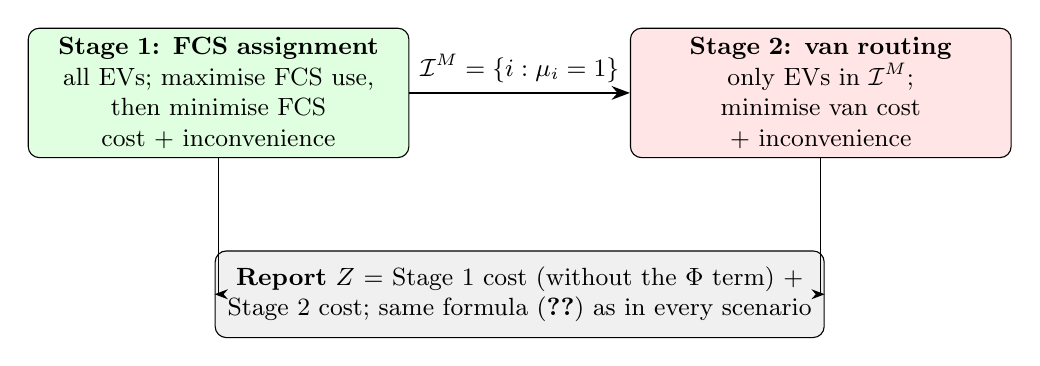
\begin{tikzpicture}[>=Stealth,box/.style={draw,rounded corners,align=center,minimum height=1.1cm,font=\small}]
  \node[box,fill=green!12,text width=4.6cm] (s1) {\textbf{Stage 1: FCS assignment}\\all EVs; maximise FCS use,\\then minimise FCS cost + inconvenience};
  \node[box,fill=red!10,text width=4.6cm,right=2.8cm of s1] (s2) {\textbf{Stage 2: van routing}\\only EVs in $\I^M$;\\minimise van cost + inconvenience};
  \draw[->,thick] (s1) -- node[above,font=\small]{$\I^M=\{i:\mu_i=1\}$} (s2);
  \node[box,fill=black!6,text width=7.5cm,below=2.0cm of $(s1)!0.5!(s2)$] (ev) {\textbf{Report} $Z=$ Stage~1 cost (without the $\Phi$ term) $+$ Stage~2 cost; same formula \eqref{eq:Z} as in every scenario};
  \draw[->] (s1) |- (ev); \draw[->] (s2) |- (ev);
\end{tikzpicture}
\end{center}

Stage~1 does not look at the vans, and Stage~2 cannot change what Stage~1 decided. That is the definition of ``FCS first, then MCS''.

%----------------------------------------------------------------
\subsection{Stage 1: assign EVs to fixed stations}

\textbf{Objective.}
\begin{equation}
\begin{split}
\min\ Z^{(1)}=\;&\underbrace{\Phi\sum_{i\in\I}\mu_i}_{\text{FCS first}}
+\underbrace{c^{EV}\sum_i\sum_{f\in\F_i}d_{if}Y_{if}}_{Z_1}
+\underbrace{Z^F_{\text{energy}}}_{\text{FCS part of }Z_4}\\
&+\underbrace{\sum_i\sum_{f\in\F_i}\rho^F_{if}Y_{if}+\alpha\sum_i w_i(C_i-r_i)+c^L\sum_i w_iL_i}_{\text{FCS customers' inconvenience}}
\end{split}
\label{eq:obj1}
\end{equation}
with $C_i=S_i+\tau^F_iY_i$ in this stage. $\Phi$ is a penalty for handing an EV to the vans. It is chosen larger than anything an extra FCS customer can add to the rest of \eqref{eq:obj1}, e.g.
\[
\Phi > \max_{i}\max_{f\in\F_i}\big(c^{EV}d_{if}+\pi^{\max}E_i+\rho^F_{if}\big)+n\,(\alpha+c^L)\,w_{\max}\,T,
\]
so Stage~1 first \textbf{maximises the number of EVs served at an FCS}, and only among those solutions minimises FCS cost and inconvenience. ($\pi^{\max}$ is the highest grid price.) A numerically safer equivalent is to solve twice: first $\max\sum_iY_i$, then fix that number and minimise the rest.
\ifTOU
Because $Z^F_{\text{energy}}$ uses the peak price, Stage~1 may \emph{start sessions later} to leave the peak, if the price saving beats the extra waiting cost (Section~\ref{sec:expect}).
\fi

\textbf{Constraints.}
\begin{align}
\sum_{g\in\G_i}y_{ig}+\mu_i &= 1 && \forall i\in\I \label{eq:s1assign}\\
S_i &\ge r_i+\sum_{f\in\F_i}t_{if}Y_{if} && \forall i\in\I \label{eq:fcsarr}\\
S_i &\le r_i+T\,(1-\mu_i) && \forall i\in\I \label{eq:s1park}\\
S_j &\ge S_i+\tau^F_i-(T+\tau^F_i)(3-y_{ig}-y_{jg}-o_{ij}) && \forall g,\ (i,j)\in\mathcal{P}_g \label{eq:disj1}\\
S_i &\ge S_j+\tau^F_j-(T+\tau^F_j)(2-y_{ig}-y_{jg}+o_{ij}) && \forall g,\ (i,j)\in\mathcal{P}_g \label{eq:disj2}\\
\sum_i y_{ig_1} &\ge \sum_i y_{ig_2} && \forall f,\ \G_f=\{g_1,g_2\} \label{eq:gunsym}\\
S_i+\tau^F_iY_i &\le T,\qquad L_i\ge S_i+\tau^F_iY_i-l_i && \forall i\in\I \label{eq:s1time}
\end{align}
\ifTOU plus the time-of-use split \eqref{eq:tou1}--\eqref{eq:tou5} of each FCS session (Section~\ref{sec:price}).\fi
\desc{\eqref{eq:s1assign}: every EV either gets one reachable gun or is handed to the vans. An EV that reaches no FCS ($\G_i=\emptyset$) is forced to $\mu_i=1$. \eqref{eq:fcsarr}: an FCS session cannot start before the EV has asked and driven to the station. \eqref{eq:s1park}: for an EV handed to the vans, $S_i$ is parked at $r_i$, so it adds no waiting in Stage~1 (its real start time is decided in Stage~2). \eqref{eq:disj1}--\eqref{eq:disj2}: two EVs on the same gun do not overlap; $o_{ij}$ picks who goes first. With two guns per station this means at most two EVs charge at a station at a time. \eqref{eq:gunsym}: symmetry breaking between the two identical guns (optional). \eqref{eq:s1time}: finished by $T$; lateness.}

\textbf{Optional acceptability rule.} An operator may refuse to send a driver to a station that is ``too inconvenient'', e.g.\ only allow gun $g$ of station $f$ for EV $i$ if $\hat\rho^F_{if}\le\bar\rho$. This only shrinks $\G_i$, so EVs whose stations are all too far go to the vans. Report results with and without it.

\textbf{Output:} $\I^M=\{i:\mu_i=1\}$, the EVs left for the vans; plus each FCS customer's gun and start time.

%----------------------------------------------------------------
\subsection{Stage 2: route the vans to the leftover EVs}

Stage~2 is a vehicle routing problem with time windows, on the EVs in $\I^M$ only. Here $C_i=S_i+\tau^M_i$.

\textbf{Objective.}
\begin{equation}
\begin{split}
\min\ Z^{(2)}=\;&\underbrace{c^M\sum_m\sum_{(i,j)\in\A^M}d_{ij}x_{ijm}}_{Z_2}+\underbrace{\sum_m c^D_mu_m}_{Z_3}+\underbrace{Z^M_{\text{energy}}}_{\text{van part of }Z_4}\\
&+\underbrace{\sum_{i\in\I^M}\sum_m\rho^M_{im}z_{im}+\alpha\sum_{i\in\I^M}w_i(C_i-r_i)+c^L\sum_{i\in\I^M}w_iL_i}_{\text{van customers' inconvenience}}
\end{split}
\label{eq:obj2}
\end{equation}
Since every EV in $\I^M$ must be served by some van, $Z^M_{\text{energy}}$ and the $\rho^M$ term are constants here. They are kept so that $Z^{(2)}$ is the true cost of Stage~2. Waiting and lateness make the vans visit urgent EVs early.

\textbf{Constraints.}
\begin{align}
\sum_{m\in\M}z_{im} &= 1 && \forall i\in\I^M \label{eq:s2assign}\\
\sum_{j:(0,j)\in\A^M}x_{0jm} = \sum_{i:(i,n+1)\in\A^M}x_{i,n+1,m} &= u_m && \forall m \label{eq:depot}\\
\sum_{i:(i,j)\in\A^M}x_{ijm} = \sum_{k:(j,k)\in\A^M}x_{jkm} &= z_{jm} && \forall j\in\I^M,\ m \label{eq:flow}\\
\sum_{i\in\I^M}z_{im} &\le Q_m\,u_m && \forall m \label{eq:cap}\\
\sum_{i\in\I^M}\frac{E_i}{\eta}z_{im}+\beta\sum_{(i,j)\in\A^M}d_{ij}x_{ijm} &\le B_m\,u_m && \forall m \label{eq:batt}
\end{align}
\begin{align}
S_j &\ge \max\{r_j,\ t_{0j}\,x_{0jm}\} && \forall j\in\I^M,\ m \label{eq:depart}\\
S_j &\ge S_i+\tau^M_i+t_{ij}-(T+\tau^M_i+t_{ij})(1-x_{ijm}) && \forall i\neq j,\ m \label{eq:seq}\\
S_i+\tau^M_i+t_{i,n+1} &\le T+(\tau^M_i+t_{i,n+1})(1-x_{i,n+1,m}) && \forall i,\ m \label{eq:return}\\
S_i+\tau^M_i \le T,\quad L_i &\ge S_i+\tau^M_i-l_i && \forall i\in\I^M \label{eq:s2time}\\
u_m &\ge u_{m+1} && m<|\M| \label{eq:vansym}
\end{align}
\desc{\eqref{eq:s2assign}: each leftover EV gets one van. \eqref{eq:depot}: a used van leaves and returns to the depot once. \eqref{eq:flow}: each EV on van $m$ is entered and left exactly once by that van. \eqref{eq:cap}: at most $Q_m$ EVs per van. \eqref{eq:batt}: delivered energy (with transfer losses) plus driving energy fits in the van battery. \eqref{eq:depart}: no start before the request, or before the van can drive there from the depot (written as two linear constraints). \eqref{eq:seq}: if the van goes $i\to j$, it finishes $i$ and drives to $j$ before starting $j$. This gives one EV at a time and removes subtours (MTZ-type). \eqref{eq:return}: back at the depot by $T$. \eqref{eq:s2time}: finished by $T$; lateness. \eqref{eq:vansym}: use identical vans in index order.}

\textbf{If Stage 2 is infeasible} (too many leftover EVs for the fleet by $T$), the sequential policy has \emph{failed} on that instance. For diagnosis, add $s_i\in\{0,1\}$ (``unserved''), replace \eqref{eq:s2assign} by $\sum_mz_{im}+s_i=1$ and add $\Phi^U\sum_is_i$ to \eqref{eq:obj2}. Then report the number of EVs that could not be served. This is a useful comparison with the integrated scenario, which may serve all of them.

%----------------------------------------------------------------
\subsection{Reported value}
\[
Z^{\text{S\scen}}=\big(Z^{(1)*}-\Phi\,|\I^M|\big)+Z^{(2)*},
\]
which is exactly \eqref{eq:Z} evaluated at the combined solution. The stage-1 solution plus the stage-2 solution is a feasible solution of the integrated model (S\ifTOU 4\else 3\fi), so
$Z^{\text{S\ifTOU 4\else 3\fi}}\le Z^{\text{S\scen}}$. The difference is the \emph{value of integration}.

\else
%---------------------------------------------------------------- INT
\subsection{Objective}
\begin{equation}
\min\ Z \quad\text{as in \eqref{eq:Z}, with }Z^F_{\text{energy}}=\ifTOU P^F\textstyle\sum_i\big[\pi^\off(\theta^1_i+\theta^3_i)+\pi^\pk\theta^2_i\big]\else\pi^F\textstyle\sum_iE_iY_i\fi,\quad C_i=S_i+\tau^F_iY_i+\tau^M_iZ_i. \label{eq:objint}
\end{equation}
Written out in full:
\begin{align*}
\min\ Z=\;& c^{EV}\sum_i\sum_{f\in\F_i}d_{if}Y_{if}+c^M\sum_m\sum_{(i,j)\in\A}d_{ij}x_{ijm}+\sum_mc^D_mu_m\\
&+\ifTOU P^F\sum_i\big[\pi^\off(\theta^1_i+\theta^3_i)+\pi^\pk\theta^2_i\big]\else\pi^F\sum_iE_iY_i\fi
+\pi^M\sum_i\sum_m\frac{E_i}{\eta}z_{im}\\
&+\sum_i\sum_{f\in\F_i}\rho^F_{if}Y_{if}+\sum_i\sum_m\rho^M_{im}z_{im}+\alpha\sum_iw_i(C_i-r_i)+c^L\sum_iw_iL_i .
\end{align*}
Every term is linear. One model weighs everything at once: an EV goes to a van exactly when the van's extra km, dispatch and energy cost are outweighed by the effort and waiting it saves the driver\ifTOU, or by the peak-price energy it avoids\fi.

\subsection{Constraints}

\textbf{Assignment.}
\begin{equation}
\sum_{g\in\G_i}y_{ig}+\sum_{m\in\M}z_{im}=1\qquad\forall i\in\I \label{eq:assign}
\end{equation}
\desc{Exactly one resource per EV: one reachable gun or one van. EVs that reach no FCS are forced onto a van.}

\textbf{Fixed stations.}
\begin{align}
S_i &\ge r_i+\sum_{f\in\F_i}t_{if}Y_{if} && \forall i \label{eq:fcsarr}\\
S_j &\ge S_i+\tau^F_i-(T+\tau^F_i)(3-y_{ig}-y_{jg}-o_{ij}) && \forall g,\ (i,j)\in\mathcal{P}_g \label{eq:disj1}\\
S_i &\ge S_j+\tau^F_j-(T+\tau^F_j)(2-y_{ig}-y_{jg}+o_{ij}) && \forall g,\ (i,j)\in\mathcal{P}_g \label{eq:disj2}\\
\sum_iy_{ig_1} &\ge \sum_iy_{ig_2} && \forall f,\ \G_f=\{g_1,g_2\} \label{eq:gunsym}
\end{align}
\desc{\eqref{eq:fcsarr}: an FCS session starts after the request and the drive to the station (for a van customer this is just $S_i\ge r_i$). \eqref{eq:disj1}--\eqref{eq:disj2}: EVs on the same gun do not overlap; $o_{ij}$ chooses the order. \eqref{eq:gunsym}: optional symmetry breaking.}

\textbf{Vans: routes, capacity, battery.}
\begin{align}
\sum_{j:(0,j)\in\A}x_{0jm}=\sum_{i:(i,n+1)\in\A}x_{i,n+1,m} &= u_m && \forall m \label{eq:depot}\\
\sum_{i:(i,j)\in\A}x_{ijm}=\sum_{k:(j,k)\in\A}x_{jkm} &= z_{jm} && \forall j\in\I,\ m \label{eq:flow}\\
\sum_iz_{im} &\le Q_mu_m && \forall m \label{eq:cap}\\
\sum_i\frac{E_i}{\eta}z_{im}+\beta\sum_{(i,j)\in\A}d_{ij}x_{ijm} &\le B_mu_m && \forall m \label{eq:batt}
\end{align}
\desc{\eqref{eq:depot}: a used van leaves and returns once. \eqref{eq:flow}: each EV on van $m$ is visited exactly once by it. \eqref{eq:cap}: at most $Q_m$ EVs. \eqref{eq:batt}: delivered energy (with losses) plus driving energy fits in the battery.}

\textbf{Vans: timing (one EV at a time, no subtours).}
\begin{align}
S_j &\ge t_{0j}\,x_{0jm} && \forall j\in\I,\ m \label{eq:depart}\\
S_j &\ge S_i+\tau^M_i+t_{ij}-(T+\tau^M_i+t_{ij})(1-x_{ijm}) && \forall i\neq j\in\I,\ m \label{eq:seq}\\
S_i+\tau^M_i+t_{i,n+1} &\le T+(\tau^M_i+t_{i,n+1})(1-x_{i,n+1,m}) && \forall i,\ m \label{eq:return}
\end{align}
\desc{\eqref{eq:depart}: the first stop cannot start before the van has driven there. \eqref{eq:seq}: $i\to j$ means finish $i$, drive, then start $j$; start times rise along a route, so no subtour can close. \eqref{eq:return}: back at the depot by $T$.}

\textbf{Horizon and lateness.}
\begin{equation}
C_i\le T,\qquad L_i\ge C_i-l_i\qquad\forall i\in\I \label{eq:time}
\end{equation}
\desc{Every EV is fully charged within the horizon; $L_i$ measures lateness.}

\ifTOU
\textbf{Time-of-use split.} Constraints \eqref{eq:tou1}--\eqref{eq:tou5} of Section~\ref{sec:price}.
\fi

\textbf{Symmetry and domains.}
\begin{equation}
u_m\ge u_{m+1};\qquad y,z,x,u,o\ifTOU,\kappa\fi\in\{0,1\};\qquad S_i,L_i\ifTOU,\theta^p_i\fi\ge0 \label{eq:dom}
\end{equation}
\fi

%=====================================================================
\section{Learning-to-optimise (RL) formulation}\label{sec:rl}

\textbf{Main rule:} the reward of each action is \emph{minus the increase in $Z$ that the action causes}. The rewards over an episode then add up to $-Z$ of the solution the policy builds. RL and MILP results are measured on the same yardstick \eqref{eq:Z}, and the MILP optimum is the benchmark for the RL gap.

\ifSEQ
%---------------------------------------------------------------- RL SEQ
The RL pipeline has the same two stages as the MILP.

\subsection{Stage 1 policy: FCS assignment}
\begin{itemize}[leftmargin=1.4em,itemsep=2pt]
  \item \textbf{Episode / epochs:} EVs are taken in order of request time $r_i$ (ties: higher $w_i$ first). One decision per EV.
  \item \textbf{State:} features of the current EV $k$ ($E_k,r_k,l_k,w_k,R_k$, location); for each gun $g$ the time $F_g$ it becomes free; summary features of the EVs still to come (count and positions near each station)\ifTOU; the current price and the time until $T_1$ and $T_2$\fi.
  \item \textbf{Action:} a gun $g\in\G_k$, or ``hand to vans''. \textbf{FCS-first mask:} ``hand to vans'' is allowed \emph{only} if no gun can finish EV $k$ by $T$ (or, with the optional rule, if all remaining guns have $\hat\rho^F_{kf}>\bar\rho$).
  \ifTOU\item \textbf{Optional timing action:} ``gun $g$, start after the peak'', i.e.\ $S_k=\max\{\text{earliest},T_2\}$, allowed only if the session still ends by $T$.\fi
  \item \textbf{Transition:} $S_k=\max\{r_k+t_{kf},F_g\}$ (or later, for the timing action); $F_g\leftarrow S_k+\tau^F_k$.
  \item \textbf{Reward:} $-\Big[c^{EV}d_{kf}+\text{energy}_k+\rho^F_{kf}+\alpha w_k(S_k+\tau^F_k-r_k)+c^Lw_k(S_k+\tau^F_k-l_k)^+\Big]$, where energy$_k$ = \ifTOU$P^F\big[\pi^\off\cdot(\text{off-peak hours of }[S_k,S_k+\tau^F_k])+\pi^\pk\cdot(\text{peak hours})\big]$, computed exactly in the simulator\else$\pi^FE_k$\fi. Handing an EV to the vans gives reward $0$ here; its cost is counted in Stage~2.
\end{itemize}
Note: a simple baseline for Stage~1 is the greedy rule ``gun with the largest one-step reward''. What RL can learn on top of this is, for example, to keep a nearby gun free for an urgent EV that arrives later.

\subsection{Stage 2 policy: van routing over $\I^M$}
\begin{itemize}[leftmargin=1.4em,itemsep=2pt]
  \item \textbf{Epochs:} whenever a van becomes free (the earliest-free van decides first).
  \item \textbf{State:} for each van: position, time free, remaining battery $b_m$, EVs served so far, dispatched or not; for each unserved EV in $\I^M$: location, $E_i,r_i,l_i,w_i$; current time.
  \item \textbf{Action:} the next EV $j$ for this van, or ``return to depot'' (ends the route). Mask: $j$ must be feasible: battery covers $E_j/\eta$ plus driving to $j$ and back to the depot, the count stays $\le Q_m$, and $j$ can be finished with the van back at the depot by $T$.
  \item \textbf{Transition:} $S_j=\max\{r_j,\ \text{time free}+t_{\text{pos},j}\}$; the van moves to $j$ and is free at $S_j+\tau^M_j$; $b_m$ falls by $E_j/\eta+\beta d_{\text{pos},j}$.
  \item \textbf{Reward:} serving $j$: $-\Big[c^Md_{\text{pos},j}+c^D_m[\text{first stop}]+\pi^M\frac{E_j}{\eta}+\rho^M_{jm}+\alpha w_j(S_j+\tau^M_j-r_j)+c^Lw_j(S_j+\tau^M_j-l_j)^+\Big]$; returning: $-c^Md_{\text{pos},0}$. EVs still unserved at the end: $-\Phi^U$ each.
  \item \textbf{Policy:} an attention-based routing policy (e.g.\ Kool et al., 2019, ``Attention, Learn to Solve Routing Problems!'') trained with REINFORCE or PPO. Baseline: nearest-feasible-EV heuristic.
\end{itemize}
Episode return of Stage~1 + Stage~2 $=-Z^{\text{S\scen}}$.

\else
%---------------------------------------------------------------- RL INT
One policy decides both who serves each EV and the van routes.
\begin{itemize}[leftmargin=1.4em,itemsep=2pt]
  \item \textbf{Episode / epochs:} EVs are taken in order of request time $r_i$ (ties: higher $w_i$ first). One decision per EV.
  \item \textbf{State:} (i) the current EV $k$: location, $E_k,r_k,l_k,w_k,R_k$, reachable stations; (ii) each gun $g$: time $F_g$ it becomes free; (iii) each van $m$: current end-of-route position, time free, remaining battery $b_m$, EVs served, dispatched or not; (iv) embeddings of the not-yet-assigned EVs (for look-ahead)\ifTOU; (v) current price, time until $T_1$ and $T_2$\fi.
  \item \textbf{Action:} $a\in\G_k\cup\M$: a gun, or a van (EV $k$ is appended to the end of that van's route). \textbf{Mask} infeasible actions: a gun that cannot finish $k$ by $T$; a van without enough battery for $E_k/\eta$ plus the drive to $k$ and back to the depot, with $Q_m$ reached, or unable to finish $k$ and return by $T$.
  \ifTOU\item \textbf{Optional timing action:} ``gun $g$, start after the peak'' ($S_k=\max\{\text{earliest},T_2\}$, if it still ends by $T$).\fi
  \item \textbf{Transition:} gun: $S_k=\max\{r_k+t_{kf},F_g\}$, $F_g\leftarrow S_k+\tau^F_k$. Van: $S_k=\max\{r_k,\ \text{free}_m+t_{\text{pos}_m,k}\}$, then the van moves to $k$, $\text{free}_m\leftarrow S_k+\tau^M_k$, $b_m\mathrel{-}=E_k/\eta+\beta d_{\text{pos}_m,k}$.
  \item \textbf{Reward} $=-\Delta Z$:
  \begin{align*}
  \text{gun } g\text{ at }f:&\quad -\Big[c^{EV}d_{kf}+\text{energy}^F_k+\rho^F_{kf}+\alpha w_k(C_k-r_k)+c^Lw_k(C_k-l_k)^+\Big]\\
  \text{van } m:&\quad -\Big[c^M\big(d_{\text{pos}_m,k}+d_{k,0}-d_{\text{pos}_m,0}\big)+c^D_m[\text{first use}]+\pi^M\tfrac{E_k}{\eta}\\
  &\qquad\quad+\rho^M_{km}+\alpha w_k(C_k-r_k)+c^Lw_k(C_k-l_k)^+\Big]
  \end{align*}
  The van distance term is the \emph{change} in route length when $k$ is inserted before the return to the depot, so the sum over the episode equals the total route length (the return legs telescope). energy$^F_k$ = \ifTOU$P^F\big[\pi^\off\cdot(\text{off-peak hours})+\pi^\pk\cdot(\text{peak hours of }[S_k,C_k])\big]$, computed exactly by the simulator; no linearisation is needed in RL\else$\pi^FE_k$\fi.
  \item \textbf{Dead end:} if every action is masked, EV $k$ is unserved: reward $-\Phi^U$, and the episode continues. Report the count.
  \item \textbf{Policy:} masked categorical policy over guns and vans, encoder with attention over EVs, guns and vans; trained with PPO. Natural baseline: greedy, i.e.\ choose the action with the largest one-step reward. That is the pairwise rule ``smallest $\hat\rho$ + cost'' from Section~\ref{sec:inc}.
\end{itemize}
Restriction to note: vans serve EVs in assignment order (append only). A variant that inserts $k$ at the cheapest position of a route is more flexible but has a larger action space.
\fi

\textbf{Reward scaling.} For stable training divide every reward by a constant, e.g.\ the greedy baseline's average $Z$ on the training instances. This does not change the optimal policy.

%=====================================================================
\section{What to expect and what to report}\label{sec:expect}

\ifnum\scen=1
\begin{itemize}[leftmargin=1.4em,itemsep=2pt]
  \item Vans serve only EVs that reach no station, or that the stations cannot finish by $T$. If stations have spare capacity, very few vans are dispatched.
  \item Inconvenience is high for EVs far from the nearest station (worked example: Rs\,682 at the FCS, against Rs\,458 if a van had been allowed).
  \item With too few vans Stage~2 becomes infeasible (unserved EVs), even when the integrated model S3 could serve everyone. Report the smallest $|\M|$ at which S1 is feasible and compare it with S3.
\end{itemize}
\fi
\ifnum\scen=2
\begin{itemize}[leftmargin=1.4em,itemsep=2pt]
  \item \textbf{When does Stage~1 delay a session to avoid the peak?} Moving one hour of charging out of the peak saves $(\pi^\pk-\pi^\off)P^F=3\times22=$ Rs\,66, but delays completion by up to an hour, which costs $\alpha w_i\ge$ Rs\,200. So with the default values Stage~1 almost never delays. It mostly pays the higher price, and S2 costs roughly S1 plus the peak surcharge. Sessions start later only if $\alpha$ is small (try $\lambda<0.33$ in the sensitivity analysis).
  \item The van assignment is the same as in S1 unless Stage~1's timing changes which EVs fit at the stations. Stage~1 cannot use vans to escape the peak price.
  \item Extra KPI: \textbf{grid energy drawn at FCS during the peak}, $P^F\sum_i\theta^2_i$ (kWh). Compare with S4.
\end{itemize}
\fi
\ifnum\scen=3
\begin{itemize}[leftmargin=1.4em,itemsep=2pt]
  \item Vans take EVs for which the saved inconvenience exceeds the extra van cost (worked example: van chosen, saving Rs\,224). Expect vans to serve EVs that are far from every station, have low range (high $w_i$), or have early deadlines, while EVs near a station still use it.
  \item \textbf{Value of integration under flat price:} $Z^{\text{S1}}-Z^{\text{S3}}\ge0$. Report it per component ($Z_1,\dots,Z_5$): typically operating cost rises a little and inconvenience falls a lot.
  \item Vary $|\M|$ (0, 1, 2, \dots): the first few vans lower $Z$ sharply, then the effect levels off. That curve shows the scenarios where mobile chargers help most.
\end{itemize}
\fi
\ifnum\scen=4
\begin{itemize}[leftmargin=1.4em,itemsep=2pt]
  \item During the peak a van kWh costs about the same as an FCS kWh (Rs\,10.0 each), so the vans' energy disadvantage disappears and vans also absorb \emph{peak-hour} demand that would otherwise be charged on the grid at peak price.
  \item Expect more van usage than in S3, concentrated on requests in $[T_1,T_2]$, and lower grid energy at the stations during the peak, $P^F\sum_i\theta^2_i$, than in S2.
  \item \textbf{Value of integration under peak pricing:} $Z^{\text{S2}}-Z^{\text{S4}}$. It should be larger than $Z^{\text{S1}}-Z^{\text{S3}}$, because integration now also allows price arbitrage.
  \item \textbf{Peak pricing with full flexibility:} $Z^{\text{S4}}-Z^{\text{S3}}$ should be smaller than $Z^{\text{S2}}-Z^{\text{S1}}$: vans cushion the price increase.
\end{itemize}
\fi

\textbf{Cross-scenario comparison table} (fill in from the four runs):
\begin{center}
\renewcommand{\arraystretch}{1.2}
\begin{tabular}{@{}lll@{}}
\toprule
\textbf{Comparison} & \textbf{Measures} & \textbf{Expected sign} \\
\midrule
S1 $-$ S3 & value of integration, flat price & $\ge0$ \\
S2 $-$ S4 & value of integration, peak price & $\ge0$, larger than S1 $-$ S3 \\
S2 $-$ S1 & cost of peak pricing, FCS-first operator & $>0$ \\
S4 $-$ S3 & cost of peak pricing, flexible operator & $>0$, smaller than S2 $-$ S1 \\
\bottomrule
\end{tabular}
\end{center}
Report for each: $Z$ and its components, number of vans used, EVs per resource, mean and maximum inconvenience per EV, total lateness, peak-hour grid energy, solve time, and (for RL) the gap to the MILP optimum.

%=====================================================================
\appendix
\section{Illustrative parameter values}\label{app:values}

These are starting values for experiments, not data. All are meant to be varied in the analysis. Values in Rs.

\begin{center}
\renewcommand{\arraystretch}{1.15}
\begin{tabular}{@{}llp{6.2cm}@{}}
\toprule
\textbf{Parameter} & \textbf{Value} & \textbf{Note} \\
\midrule
$T$, $[T_1,T_2]$ & 7 h, $[2,6]$ & 16:00--23:00, peak 18:00--22:00 \\
$P^F$, $P^M$ & 22 kW, 30 kW & \\
$v$, $\beta$, $\eta$ & 25 km/h, 0.25 kWh/km, 0.9 & \\
$B_m$, $Q_m$, $|\M|$ & 150 kWh, 6, 2--6 & \\
$c^{EV}$, $c^M$, $c^D_m$ & Rs\,4/km, Rs\,15/km, Rs\,1500 & van km includes driver time \\
$\pi^F$ (flat) & Rs\,8.7/kWh & equals the time-average of the ToU tariff over $[0,T]$ \\
$\pi^\off$, $\pi^\pk$ (ToU) & Rs\,7/kWh, Rs\,10/kWh & $(3\times7+4\times10)/7=8.7$ \\
$c^{bat}$ & Rs\,2/kWh & van battery wear \\
$\pi^M$ & Rs\,10.7 (flat) / Rs\,9.0 (ToU) & $=\pi^F+c^{bat}$ / $=\pi^\off+c^{bat}$ \\
$\alpha$, $\alpha^D$ & Rs\,200/h, Rs\,100/h & value of time; extra for attended time \\
$h^F$, $h^M$, $\varphi$ & Rs\,50, Rs\,10, Rs\,100 & trip hassle, hand-over, range stress \\
$c^L$ & Rs\,300/h & lateness \\
$w_i$ & $1+2(1-R_i/R_{\max})$, $R_i\sim U[3,40]$ km & priority from remaining range \\
\bottomrule
\end{tabular}
\end{center}

The flat price is set to the time-average of the peak tariff. The price \emph{level} is then the same in both pricing cases, and only the price \emph{shape} differs. Without this, part of S1 vs S2 would just reflect a different average price.

\end{document}
"
%  (run each twice for cross-references)
% =====================================================================
\documentclass[11pt,a4paper]{article}
\usepackage[margin=2.2cm]{geometry}
\usepackage{amsmath,amssymb,amsfonts}
\usepackage{booktabs,array,tabularx}
\usepackage{enumitem}
\usepackage[table]{xcolor}
\usepackage{tikz}
\usetikzlibrary{arrows.meta,positioning,calc}
\usepackage[colorlinks=true,linkcolor=blue!50!black,urlcolor=blue!50!black]{hyperref}
\usepackage{titlesec}
\titleformat{\section}{\large\bfseries}{\thesection}{0.8em}{}
\titleformat{\subsection}{\normalsize\bfseries}{\thesubsection}{0.8em}{}
\setlength{\parindent}{0pt}
\setlength{\parskip}{5pt}

% ---------------- scenario switches ----------------
\ifdefined\scen\else\def\scen{1}\fi
\newif\ifTOU \TOUfalse   % true = time-of-use (peak) price
\newif\ifSEQ \SEQfalse   % true = FCS first, then MCS
\ifnum\scen=1 \SEQtrue \fi
\ifnum\scen=2 \TOUtrue \SEQtrue \fi
\ifnum\scen=4 \TOUtrue \fi

\newcommand{\pricename}{\ifTOU time-of-use price (dearer evening peak)\else single (flat) price all day\fi}
\newcommand{\structname}{\ifSEQ FCS first, then MCS (sequential)\else FCS and MCS together (integrated)\fi}

% ---------------- notation ----------------
\newcommand{\I}{\mathcal{I}}
\newcommand{\F}{\mathcal{F}}
\newcommand{\G}{\mathcal{G}}
\newcommand{\M}{\mathcal{M}}
\newcommand{\N}{\mathcal{N}}
\newcommand{\A}{\mathcal{A}}
\newcommand{\Rs}{\text{Rs}\,}
\newcommand{\pk}{\mathrm{pk}}
\newcommand{\off}{\mathrm{off}}
\newcommand{\desc}[1]{\par\vspace{-2pt}{\small\color{black!75}\textit{Meaning:} #1}\par\vspace{4pt}}
\newcommand{\cell}[2]{\ifnum\scen=#1\cellcolor{blue!18}\textbf{S#1 (this document)}\\\textbf{#2}\else S#1\\#2\fi}

\title{\textbf{EV Charging Network Optimisation}\\[4pt]
\large Scenario \scen: \pricename\ $+$ \structname\\[2pt]
\normalsize MILP and RL formulation}
\author{CP 320 OR for Mobility Management, course project}
\date{2 October 2026}

\begin{document}
\maketitle

%=====================================================================
\section{Where this scenario sits}

The project studies four scenarios: two ways of pricing grid electricity, times two ways of making the decisions.

\begin{center}
\renewcommand{\arraystretch}{1.5}
\begin{tabular}{>{\raggedright\arraybackslash}p{4.2cm}|>{\centering\arraybackslash}p{4.6cm}|>{\centering\arraybackslash}p{4.6cm}}
 & \textbf{Flat price all day} & \textbf{Time-of-use (peak) price} \\ \hline
\textbf{Sequential:} FCS first, leftover EVs to MCS &
\begin{tabular}[c]{@{}c@{}}\cell{1}{flat + sequential}\end{tabular} &
\begin{tabular}[c]{@{}c@{}}\cell{2}{peak + sequential}\end{tabular} \\ \hline
\textbf{Integrated:} FCS and MCS decided together &
\begin{tabular}[c]{@{}c@{}}\cell{3}{flat + integrated}\end{tabular} &
\begin{tabular}[c]{@{}c@{}}\cell{4}{peak + integrated}\end{tabular} \\
\end{tabular}
\end{center}

\textbf{The four scenarios do not have four different objectives.} They share \emph{one} cost yardstick $Z$ (Section~\ref{sec:obj}): the same cost terms and the same customer inconvenience (Section~\ref{sec:inc}). Only two things change:
\begin{itemize}[leftmargin=1.4em,itemsep=1pt]
  \item \textbf{Pricing} changes the formula for one term, the FCS energy cost (Section~\ref{sec:price}).
  \item \textbf{Decision structure} changes \emph{how} $Z$ is minimised: in one model (integrated), or in two stages (sequential), where each stage minimises its own part of $Z$.
\end{itemize}
Because the yardstick is the same, the four optimal values can be compared directly. The differences measure the \emph{value of integration} (S1$\to$S3, S2$\to$S4) and the \emph{effect of peak pricing} (S1$\to$S2, S3$\to$S4).

\ifnum\scen=1
\textbf{This scenario (S1)} is the baseline, the ``status quo''. Electricity costs the same at every hour, every EV that can be charged at a fixed station is sent there, and vans only take what is left over.
\fi
\ifnum\scen=2
\textbf{This scenario (S2)} keeps the FCS-first rule of S1, but grid electricity is dearer during the evening peak. Stage~1 can react to the price only by \emph{rescheduling} FCS sessions. It cannot hand a peak-hour EV to a van.
\fi
\ifnum\scen=3
\textbf{This scenario (S3)} keeps the flat price of S1, but the operator decides FCS and MCS service \emph{together}. An EV can be sent to a van even when a fixed station could take it, whenever that lowers total cost plus inconvenience.
\fi
\ifnum\scen=4
\textbf{This scenario (S4)} is the most flexible one: peak pricing at fixed stations, and FCS and MCS decided together. Van energy was bought off-peak, so vans can also be used to keep charging \emph{out of the expensive peak}.
\fi

%=====================================================================
\section{Setting and assumptions}\label{sec:setting}

\textbf{Time.} The planning horizon is $[0,T]$ with $T=7$\,h (16:00--23:00). It contains the evening peak window $[T_1,T_2]=[2,6]$ (18:00--22:00). The horizon is the same in all four scenarios. It is wider than the peak itself so that, under peak pricing, there is cheaper time on both sides of the peak.\ifTOU\else\ In this scenario the price is flat, so the window plays no role in the model.\fi

\textbf{Assumptions} (the same as MILP v3, plus two about energy):
\begin{enumerate}[leftmargin=1.6em,itemsep=1pt]
  \item Static, continuous time. All requests in the horizon are known at time $0$, and request $i$ becomes active at $r_i$.
  \item An EV served by an FCS drives there itself on its own battery (only to stations within its range $R_i$). The driver stays with the car while it waits for a free gun and while it charges.
  \item An EV served by an MCS stays parked where it is, and the driver is free in the meantime.
  \item Each FCS gun and each van charges one EV at a time, without interruption, at constant power.
  \item A van's battery covers both its driving and the energy it delivers. \textbf{The van battery is charged at the depot before the horizon starts}\ifTOU, i.e.\ at the off-peak price\fi, and is not recharged during the horizon.
  \item Every EV must be fully charged by $T$ (hard). Finishing after the driver's desired time $l_i$ is allowed but penalised.
\end{enumerate}

%=====================================================================
\section{Notation}\label{sec:notation}

\subsection*{Sets}
\begin{tabularx}{\textwidth}{@{}lX@{}}
\toprule
$\I=\{1,\dots,n\}$ & EV charging requests \\
$\F$; $\G_f$ ($|\G_f|=2$); $\G=\bigcup_f\G_f$ & fixed charging stations; guns of FCS $f$; all guns ($f(g)$ = station of gun $g$) \\
$\F_i=\{f: d_{if}\le R_i\}$, $\G_i=\bigcup_{f\in\F_i}\G_f$ & stations / guns EV $i$ can reach on its remaining range \\
$\M$ & mobile charging vans (MCS) \\
$0,\ n+1$ & depot as start node / end node (same place) \\
$\N=\{0\}\cup\I\cup\{n+1\}$, $\A$ & routing nodes; allowed van arcs $(i,j)$, $i\in\{0\}\cup\I$, $j\in\I\cup\{n+1\}$, $i\neq j$ \\
$\mathcal{P}_g=\{(i,j): i<j,\ g\in\G_i\cap\G_j\}$ & pairs of EVs that could share gun $g$ \\
\ifSEQ
$\I^M\subseteq\I$ & EVs handed to the vans by Stage~1 (an \emph{output} of Stage~1, a fixed input to Stage~2) \\
$\N^M$, $\A^M$ & routing nodes / arcs restricted to $\I^M$ \\
\fi
\bottomrule
\end{tabularx}

\subsection*{Parameters}
\begin{tabularx}{\textwidth}{@{}lX@{}}
\toprule
$E_i,\ r_i,\ l_i,\ R_i$ & energy demand (kWh), request time, desired completion time (h), remaining range (km) \\
$w_i\ge1$ & priority of EV $i$; $w_i=1+\kappa(1-R_i/R_{\max})$, so low-range EVs weigh more \\
$P^F,\ P^M$ & charging power of an FCS gun (22\,kW) / of a van (e.g.\ 30\,kW) \\
$\tau^F_i=E_i/P^F,\ \tau^M_i=E_i/P^M$ & charging time of EV $i$ at an FCS / by a van (h) \\
$d_{if},t_{if}$;\ $d_{ij},t_{ij}$ & distance (km) and time (h): EV$\to$FCS; between routing nodes ($t=d/v$) \\
$B_m,\ Q_m,\ \beta,\ \eta$ & van battery (kWh), max EVs per van, van consumption (kWh/km), transfer efficiency \\
$c^{EV},\ c^M,\ c^D_m$ & cost per km of EV driving, per km of van driving; fixed dispatch cost of van $m$ \\
\ifTOU
$\pi^\off,\ \pi^\pk$ & grid price (Rs/kWh) off-peak / in $[T_1,T_2]$, with $\pi^\pk\ge\pi^\off$ \\
\else
$\pi^F$ & grid price (Rs/kWh), the same at every hour \\
\fi
$c^{bat}$ & van battery wear per kWh cycled \\
$\pi^M$ & cost of 1 kWh taken from a van battery: $\pi^M=\ifTOU\pi^\off\else\pi^F\fi+c^{bat}$ (Section~\ref{sec:price}) \\
$\alpha,\ \alpha^D,\ h^F,\ h^M,\ \varphi,\ c^L$ & inconvenience coefficients (Section~\ref{sec:inc}) \\
\bottomrule
\end{tabularx}

\subsection*{Decision variables}
\begin{tabularx}{\textwidth}{@{}llX@{}}
\toprule
$y_{ig}$ & $\{0,1\}$ & EV $i$ charged at gun $g\in\G_i$ \\
$z_{im}$ & $\{0,1\}$ & EV $i$ served by van $m$ \\
$x_{ijm}$ & $\{0,1\}$ & van $m$ drives arc $(i,j)$ \\
$u_m$ & $\{0,1\}$ & van $m$ is dispatched \\
$o_{ij}$ & $\{0,1\}$ & for EVs $i<j$ that could share a gun: 1 if $i$ is charged before $j$ \\
\ifSEQ
$\mu_i$ & $\{0,1\}$ & Stage~1 only: EV $i$ is handed to the van fleet \\
\fi
\ifTOU
$\theta^1_i,\theta^2_i,\theta^3_i$ & $\ge0$ & hours of EV $i$'s FCS session before / inside / after the peak \\
$\kappa^1_i,\kappa^3_i$ & $\{0,1\}$ & EV $i$'s FCS session starts before $T_1$ / ends after $T_2$ \\
\fi
$S_i$ & $\ge0$ & time charging of EV $i$ starts (h), on whichever resource \\
$L_i$ & $\ge0$ & lateness of EV $i$ beyond $l_i$ (h) \\
\bottomrule
\end{tabularx}

\textbf{Short-hands} (linear expressions, not new variables):
\[
Y_{if}=\sum_{g\in\G_f}y_{ig},\qquad Y_i=\sum_{g\in\G_i}y_{ig}\ (\text{EV $i$ uses an FCS}),\qquad Z_i=\sum_{m\in\M}z_{im}\ (\text{EV $i$ uses a van}),
\]
\[
C_i=S_i+\tau^F_i\,Y_i+\tau^M_i\,Z_i \quad\text{(time EV $i$ is fully charged).}
\]

%=====================================================================
\section{Customer inconvenience}\label{sec:inc}

This section is \textbf{identical in all four scenario documents}. Inconvenience is a property of the customer, not of the price or of the planning method.

\subsection{What we mean by inconvenience}

Inconvenience is \emph{what the driver loses} from the moment they ask for a charge ($r_i$) until the car is fully charged ($C_i$), \emph{converted into rupees} so it can be added to the operator's costs. A driver loses three different things:

\begin{enumerate}[leftmargin=1.6em,itemsep=2pt]
  \item \textbf{Waiting:} the car is not ready. This lasts $C_i-r_i$ hours and affects \emph{every} driver, FCS or MCS.
  \item \textbf{Effort:} only an FCS customer has to drive to the station and sit there while the car charges. An MCS customer stays at home or at work and does something else. Driving to a far station also uses scarce battery range, which causes stress (``range anxiety'').
  \item \textbf{A missed deadline:} the car is still not ready at the time $l_i$ the driver needs it.
\end{enumerate}

Each loss gets a price in Rs per hour (or per event). All of them are multiplied by the priority $w_i$: an hour of delay for an EV with 5\,km of range left counts more than for one with 40\,km.

\subsection{The three components}

\begin{center}
\renewcommand{\arraystretch}{1.3}
\begin{tabularx}{\textwidth}{@{}>{\raggedright\arraybackslash}p{2.6cm}>{\raggedright\arraybackslash}X>{\raggedright\arraybackslash}X>{\raggedright\arraybackslash}p{3.0cm}@{}}
\toprule
\textbf{Component} & \textbf{EV $i$ at FCS $f$} & \textbf{EV $i$ by a van} & \textbf{Known when?} \\
\midrule
Effort & $w_i\big[\alpha^D(t_{if}+\tau^F_i)+h^F+\varphi\,d_{if}/R_i\big]$: driving and sitting at the station, a fixed trip hassle, range stress & $w_i\,h^M$: being reachable and handing over the car & \textbf{Static:} known as soon as the resource is chosen \\
Waiting & $w_i\,\alpha\,(C_i-r_i)$ = drive + \emph{queue at the gun} + charge & $w_i\,\alpha\,(C_i-r_i)$ = \emph{wait for the van} + charge & \textbf{Dynamic:} depends on the queue / van route \\
Missed deadline & $w_i\,c^L\,L_i$, $L_i=\max\{0,C_i-l_i\}$ & same & Dynamic \\
\bottomrule
\end{tabularx}
\end{center}

\textbf{Coefficients.}
$\alpha$ (Rs/h) is the value of an hour the car is not ready.
$\alpha^D$ (Rs/h) is the \emph{extra} value of an hour the driver must personally spend driving or sitting at the station: an hour at the station costs $\alpha+\alpha^D$, an hour waiting at home for a van costs only $\alpha$.
$h^F,h^M$ (Rs) are fixed hassle costs of one trip to a station / one van hand-over.
$\varphi$ (Rs) is the range-stress cost of a trip that uses the \emph{whole} remaining range ($d_{if}/R_i\le1$ is the fraction used).
$c^L$ (Rs/h) is the cost per hour late.

\subsection{Pairwise form: inconvenience of a (customer, resource) pair}

The natural first idea is: \emph{for every pair (EV $i$, FCS $f$) and every pair (EV $i$, van $m$) there is an inconvenience number, and the operator picks the pair with the lowest cost plus inconvenience.} The static part fits this idea exactly:
\[
\boxed{\;\rho^F_{if}=w_i\Big[\alpha^D\,(t_{if}+\tau^F_i)+h^F+\varphi\,\frac{d_{if}}{R_i}\Big]\qquad
\rho^M_{im}=w_i\,h^M\;}
\]
These are \textbf{parameters}, computed before solving, one number per (EV, FCS) pair and per (EV, van) pair. In the objective they appear linearly: $\sum_i\sum_f\rho^F_{if}Y_{if}+\sum_i\sum_m\rho^M_{im}z_{im}$.

Note that $\rho^M_{im}$ does not depend on $m$. Vans are identical and all start at the same depot, so the driver does not care \emph{which} van comes, only \emph{when} it comes. That ``when'' is the waiting part.

\subsection{Why waiting cannot be a fixed pairwise number}

It is tempting to also write the waiting as a pairwise number, e.g.\ ``the van needs 5 minutes to reach EV $i$''. But that depends on \emph{where the van is coming from}, which depends on the route the model is still choosing: if EV $i$ is the 4th stop of a van, the wait is the time for three charging sessions plus four drives. Likewise, waiting at an FCS depends on how many EVs are queued at that gun. So waiting is not known before solving. It is a function of decision variables:
\[
\text{waiting cost of EV } i \;=\; w_i\,\alpha\,(C_i-r_i),\qquad C_i=S_i+\tau^F_iY_i+\tau^M_iZ_i .
\]
This is \textbf{linear} in the variables ($S_i$, $y$, $z$), so it fits in a MILP directly. The constraints of Section~\ref{sec:milp} make $S_i$ equal to the true start time, including driving, queueing at the gun and the van's route. The term $\sum_i w_i\alpha r_i$ is a constant and may be dropped when solving.

\textbf{Pairwise \emph{estimate}} (used for intuition, by the RL policy and in heuristics): if there is no queue and the van comes straight to $i$,
\[
\hat\rho^{F}_{if}=\rho^F_{if}+w_i\alpha\,(t_{if}+\tau^F_i),\qquad
\hat\rho^{M}_{im}=\rho^M_{im}+w_i\alpha\,(t^{\text{van}}_{m\to i}+\tau^M_i),
\]
where $t^{\text{van}}_{m\to i}$ is the time until van $m$ can reach $i$ from where it currently is. In the RL formulation (Section~\ref{sec:rl}) the van's position \emph{is} known at each decision, so there this estimate becomes exact.

\subsection{Total inconvenience and how it enters the objective}

\begin{equation}
\boxed{\;
Z_{\text{inc}}=\underbrace{\sum_{i\in\I}\sum_{f\in\F_i}\rho^F_{if}Y_{if}+\sum_{i\in\I}\sum_{m\in\M}\rho^M_{im}z_{im}}_{\text{effort (static, pairwise)}}
+\underbrace{\alpha\sum_{i\in\I}w_i\,(C_i-r_i)}_{\text{waiting (dynamic)}}
+\underbrace{c^L\sum_{i\in\I}w_i\,L_i}_{\text{missed deadline}}
\;}\label{eq:inc}
\end{equation}
All three parts are in rupees, so $Z_{\text{inc}}$ is simply added to the operating costs. Nothing has to be normalised.

\subsection{Worked example: your ``10 km to the FCS vs.\ van in 5 minutes'' case}

EV $i$: $E_i=20$\,kWh, $R_i=40$\,km (so $w_i=1$); nearest free FCS $d_{if}=10$\,km away, $t_{if}=0.4$\,h at 25\,km/h; a van finishing next door can reach it in 5\,min ($0.083$\,h), adding about 4\,km to its route. $\tau^F_i=20/22=0.909$\,h, $\tau^M_i=20/30=0.667$\,h. Coefficients from Appendix~\ref{app:values}, flat price.

\begin{center}
\renewcommand{\arraystretch}{1.25}
\begin{tabular}{@{}lrr@{}}
\toprule
 & \textbf{FCS} & \textbf{Van} \\
\midrule
Driving (EV / extra van km) & $4\times10=40.0$ & $15\times4=60.0$ \\
Energy & $8.7\times20=174.0$ & $10.7\times20/0.9=237.8$ \\
\textbf{Operating cost only} & \textbf{214.0} & \textbf{297.8} \\
\midrule
Effort $\rho$ & $100(0.4+0.909)+50+100\cdot\tfrac{10}{40}=205.9$ & $10.0$ \\
Waiting $\alpha(C_i-r_i)$ & $200\times1.309=261.8$ & $200\times0.75=150.0$ \\
\textbf{Cost + inconvenience} & \textbf{681.7} & \textbf{457.8} \\
\bottomrule
\end{tabular}
\end{center}

On operating cost alone the FCS is cheaper, so a cost-only model would \emph{always} send this driver 10\,km away. With inconvenience included the van is better by about Rs\,224, and the integrated model chooses $z_{im}=1$, as you expected. If the FCS were only 1\,km away, the FCS would win both comparisons. The inconvenience term is what makes the model choose between ``cheap for the operator'' and ``convenient for the driver'', rather than following a fixed rule.

\subsection{Relation to a single penalty $\rho_i$ per EV}

The first draft used a penalty $\rho_i$ that is charged whenever EV $i$ goes to \emph{any} FCS: $\sum_i\sum_f\rho_iy_{if}$. Because $\sum_f y_{if}=1-\sum_m z_{im}$, this only says ``a van is worth $\rho_i$ more to EV $i$'', and that holds whether the station is 1\,km or 15\,km away, and whether the van arrives in 5 minutes or in 3 hours. The form above fixes both problems: $\rho^F_{if}$ grows with the distance to \emph{that} station, and the waiting term grows with how late the van or the free gun actually is. The old model is the special case $\alpha=\alpha^D=\varphi=c^L=0$, $h^F=\rho_i$.

\subsection{Choosing the coefficients}
\begin{itemize}[leftmargin=1.4em,itemsep=2pt]
  \item Use a value of time for $\alpha$ (e.g.\ Rs\,150--300/h for urban car users), and set $\alpha^D\approx0.5\alpha$: sitting at a station is worse than waiting at home.
  \item Keep $c^L>\alpha$, so missing the deadline is worse than ordinary waiting.
  \item \textbf{Sensitivity analysis:} multiply all inconvenience coefficients by a factor $\lambda\in\{0,0.25,0.5,1,2,4\}$ and plot operating cost against total inconvenience. $\lambda=0$ is the pure cost-minimising operator, and large $\lambda$ is a customer-first operator. This trade-off curve is a strong result for the ``Analysis'' part of the project.
\end{itemize}

\subsection{What inconvenience does in \emph{this} scenario}
\ifSEQ
In a sequential scenario inconvenience \textbf{cannot move an EV from an FCS to a van}: Stage~1 sends every EV that \emph{can} use an FCS to one. It still matters inside each stage. In Stage~1 it decides \emph{which} station and \emph{when} (urgent EVs get the near station and the first free gun). In Stage~2 it decides the \emph{order} in which vans visit EVs (urgent EVs first). In the worked example, this scenario sends the driver 10\,km to the FCS. That is the weakness the integrated scenarios remove.
\else
In an integrated scenario inconvenience is weighed directly against operating cost when choosing the resource. That is how the worked example ends up with a van. It also decides which station and which gun order, and the order of each van route.
\fi

%=====================================================================
\section{Electricity price in this scenario}\label{sec:price}

\textbf{Van energy (same in all scenarios).} A van's battery is charged at the depot \emph{before} the horizon, so its energy was bought at the
\ifTOU off-peak \fi
price, whatever time the van later delivers it. Each kWh taken from the van also wears the battery ($c^{bat}$), and a fraction $1-\eta$ is lost in transfer:
\[
Z^M_{\text{energy}}=\pi^M\sum_{i\in\I}\sum_{m\in\M}\frac{E_i}{\eta}\,z_{im},\qquad \pi^M=\ifTOU\pi^\off\else\pi^F\fi+c^{bat}.
\]

\ifTOU
\textbf{FCS energy (time-of-use).} An FCS draws from the grid while it charges. Energy delivered inside $[T_1,T_2]$ costs $\pi^\pk$, and energy outside it costs $\pi^\off$. A session $[S_i,S_i+\tau^F_i]$ may overlap the peak partly. Split its duration into the hours before, inside and after the peak, $\theta^1_i+\theta^2_i+\theta^3_i$:
\[
Z^F_{\text{energy}}=P^F\sum_{i\in\I}\Big[\pi^\off(\theta^1_i+\theta^3_i)+\pi^\pk\,\theta^2_i\Big].
\]
Constraints \eqref{eq:tou1}--\eqref{eq:tou5} below make the $\theta$'s equal to the true overlaps. Peak hours are dearer, so the solver wants $\theta^1_i,\theta^3_i$ as large as possible. It is enough to bound them from above by the true off-peak overlap, and the constraints need one binary per side:
\begin{align}
\theta^1_i+\theta^2_i+\theta^3_i &= \tau^F_i\,Y_i && \forall i\in\I \label{eq:tou1}\\
\theta^1_i &\le \tau^F_i\,\kappa^1_i && \forall i\in\I \label{eq:tou2}\\
\theta^1_i &\le T_1-S_i+T\,(1-\kappa^1_i) && \forall i\in\I \label{eq:tou3}\\
\theta^3_i &\le \tau^F_i\,\kappa^3_i && \forall i\in\I \label{eq:tou4}\\
\theta^3_i &\le S_i+\tau^F_i-T_2+T\,(1-\kappa^3_i) && \forall i\in\I \label{eq:tou5}
\end{align}
\desc{\eqref{eq:tou1}: the FCS session's hours are split into three parts; for a van customer ($Y_i=0$) all three are zero. \eqref{eq:tou2}--\eqref{eq:tou3}: off-peak time before the peak is only possible if the session starts before $T_1$ ($\kappa^1_i=1$), and is at most $T_1-S_i$. \eqref{eq:tou4}--\eqref{eq:tou5}: the same for time after $T_2$. $\theta^2_i\ge0$ prevents counting more off-peak hours than exist. Checking the cases (entirely before / inside / after the peak, straddling one edge, covering the whole peak) shows that at the optimum the $\theta$'s equal the exact overlaps. This needs $\pi^\pk\ge\pi^\off$, which is true for a peak tariff.}

\textbf{Why vans become more attractive.} Compare the cost of 1\,kWh delivered to an EV during the peak (values from Appendix~\ref{app:values}):
FCS $=\pi^\pk=$ Rs\,10.0, van $=(\pi^\off+c^{bat})/\eta=9/0.9=$ Rs\,10.0. They are at parity. Under the flat price the van is about Rs\,3.2/kWh dearer (FCS Rs\,8.7, van $10.7/0.9=$ Rs\,11.9). Peak pricing therefore removes the vans' main cost disadvantage, but only for EVs whose FCS session would fall in the peak.
\ifSEQ\ In this sequential scenario Stage~1 cannot use that, because it does not consider vans. It can only shift FCS sessions in time.\fi
\else
\textbf{FCS energy (flat).} Every kWh delivered at a fixed station costs $\pi^F$, whenever it is delivered:
\[
Z^F_{\text{energy}}=\pi^F\sum_{i\in\I}E_i\,Y_i .
\]
The start time therefore does not affect the energy cost. Under the flat price a van kWh costs $(\pi^F+c^{bat})/\eta\approx$ Rs\,11.9 against Rs\,8.7 at an FCS (Appendix~\ref{app:values}), so on energy alone the FCS always wins.
\fi

%=====================================================================
\section{MILP formulation}\label{sec:milp}

\subsection{The common cost yardstick $Z$}\label{sec:obj}

For any complete solution (every EV assigned, every route and start time known), the system cost is
\begin{equation}
\boxed{\;
Z=\underbrace{c^{EV}\sum_{i}\sum_{f\in\F_i}d_{if}Y_{if}}_{Z_1:\ \text{EV driving}}
+\underbrace{c^M\sum_{m}\sum_{(i,j)\in\A}d_{ij}x_{ijm}}_{Z_2:\ \text{van driving}}
+\underbrace{\sum_m c^D_m u_m}_{Z_3:\ \text{dispatch}}
+\underbrace{Z^F_{\text{energy}}+Z^M_{\text{energy}}}_{Z_4:\ \text{energy}}
+\underbrace{Z_{\text{inc}}}_{Z_5:\ \text{inconv.\ \eqref{eq:inc}}}
\;}\label{eq:Z}
\end{equation}
$Z_4$ is defined in Section~\ref{sec:price}. $Z_1$--$Z_4$ are the operator's costs listed in the brief (EV travel, MCS travel, MCS operating cost) plus energy. $Z_5$ is the customer inconvenience penalty. \textbf{The same formula is used to report results in all four scenarios.}

\ifSEQ
%---------------------------------------------------------------- SEQ
\subsection{Structure: two stages}

\begin{center}
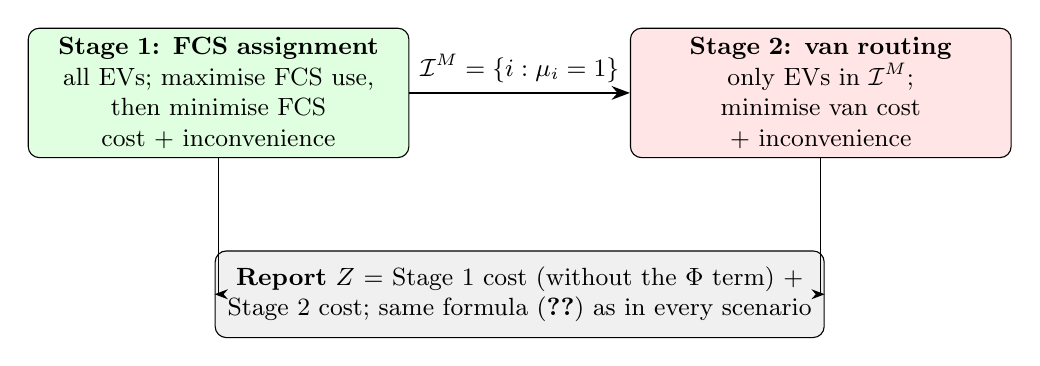
\begin{tikzpicture}[>=Stealth,box/.style={draw,rounded corners,align=center,minimum height=1.1cm,font=\small}]
  \node[box,fill=green!12,text width=4.6cm] (s1) {\textbf{Stage 1: FCS assignment}\\all EVs; maximise FCS use,\\then minimise FCS cost + inconvenience};
  \node[box,fill=red!10,text width=4.6cm,right=2.8cm of s1] (s2) {\textbf{Stage 2: van routing}\\only EVs in $\I^M$;\\minimise van cost + inconvenience};
  \draw[->,thick] (s1) -- node[above,font=\small]{$\I^M=\{i:\mu_i=1\}$} (s2);
  \node[box,fill=black!6,text width=7.5cm,below=2.0cm of $(s1)!0.5!(s2)$] (ev) {\textbf{Report} $Z=$ Stage~1 cost (without the $\Phi$ term) $+$ Stage~2 cost; same formula \eqref{eq:Z} as in every scenario};
  \draw[->] (s1) |- (ev); \draw[->] (s2) |- (ev);
\end{tikzpicture}
\end{center}

Stage~1 does not look at the vans, and Stage~2 cannot change what Stage~1 decided. That is the definition of ``FCS first, then MCS''.

%----------------------------------------------------------------
\subsection{Stage 1: assign EVs to fixed stations}

\textbf{Objective.}
\begin{equation}
\begin{split}
\min\ Z^{(1)}=\;&\underbrace{\Phi\sum_{i\in\I}\mu_i}_{\text{FCS first}}
+\underbrace{c^{EV}\sum_i\sum_{f\in\F_i}d_{if}Y_{if}}_{Z_1}
+\underbrace{Z^F_{\text{energy}}}_{\text{FCS part of }Z_4}\\
&+\underbrace{\sum_i\sum_{f\in\F_i}\rho^F_{if}Y_{if}+\alpha\sum_i w_i(C_i-r_i)+c^L\sum_i w_iL_i}_{\text{FCS customers' inconvenience}}
\end{split}
\label{eq:obj1}
\end{equation}
with $C_i=S_i+\tau^F_iY_i$ in this stage. $\Phi$ is a penalty for handing an EV to the vans. It is chosen larger than anything an extra FCS customer can add to the rest of \eqref{eq:obj1}, e.g.
\[
\Phi > \max_{i}\max_{f\in\F_i}\big(c^{EV}d_{if}+\pi^{\max}E_i+\rho^F_{if}\big)+n\,(\alpha+c^L)\,w_{\max}\,T,
\]
so Stage~1 first \textbf{maximises the number of EVs served at an FCS}, and only among those solutions minimises FCS cost and inconvenience. ($\pi^{\max}$ is the highest grid price.) A numerically safer equivalent is to solve twice: first $\max\sum_iY_i$, then fix that number and minimise the rest.
\ifTOU
Because $Z^F_{\text{energy}}$ uses the peak price, Stage~1 may \emph{start sessions later} to leave the peak, if the price saving beats the extra waiting cost (Section~\ref{sec:expect}).
\fi

\textbf{Constraints.}
\begin{align}
\sum_{g\in\G_i}y_{ig}+\mu_i &= 1 && \forall i\in\I \label{eq:s1assign}\\
S_i &\ge r_i+\sum_{f\in\F_i}t_{if}Y_{if} && \forall i\in\I \label{eq:fcsarr}\\
S_i &\le r_i+T\,(1-\mu_i) && \forall i\in\I \label{eq:s1park}\\
S_j &\ge S_i+\tau^F_i-(T+\tau^F_i)(3-y_{ig}-y_{jg}-o_{ij}) && \forall g,\ (i,j)\in\mathcal{P}_g \label{eq:disj1}\\
S_i &\ge S_j+\tau^F_j-(T+\tau^F_j)(2-y_{ig}-y_{jg}+o_{ij}) && \forall g,\ (i,j)\in\mathcal{P}_g \label{eq:disj2}\\
\sum_i y_{ig_1} &\ge \sum_i y_{ig_2} && \forall f,\ \G_f=\{g_1,g_2\} \label{eq:gunsym}\\
S_i+\tau^F_iY_i &\le T,\qquad L_i\ge S_i+\tau^F_iY_i-l_i && \forall i\in\I \label{eq:s1time}
\end{align}
\ifTOU plus the time-of-use split \eqref{eq:tou1}--\eqref{eq:tou5} of each FCS session (Section~\ref{sec:price}).\fi
\desc{\eqref{eq:s1assign}: every EV either gets one reachable gun or is handed to the vans. An EV that reaches no FCS ($\G_i=\emptyset$) is forced to $\mu_i=1$. \eqref{eq:fcsarr}: an FCS session cannot start before the EV has asked and driven to the station. \eqref{eq:s1park}: for an EV handed to the vans, $S_i$ is parked at $r_i$, so it adds no waiting in Stage~1 (its real start time is decided in Stage~2). \eqref{eq:disj1}--\eqref{eq:disj2}: two EVs on the same gun do not overlap; $o_{ij}$ picks who goes first. With two guns per station this means at most two EVs charge at a station at a time. \eqref{eq:gunsym}: symmetry breaking between the two identical guns (optional). \eqref{eq:s1time}: finished by $T$; lateness.}

\textbf{Optional acceptability rule.} An operator may refuse to send a driver to a station that is ``too inconvenient'', e.g.\ only allow gun $g$ of station $f$ for EV $i$ if $\hat\rho^F_{if}\le\bar\rho$. This only shrinks $\G_i$, so EVs whose stations are all too far go to the vans. Report results with and without it.

\textbf{Output:} $\I^M=\{i:\mu_i=1\}$, the EVs left for the vans; plus each FCS customer's gun and start time.

%----------------------------------------------------------------
\subsection{Stage 2: route the vans to the leftover EVs}

Stage~2 is a vehicle routing problem with time windows, on the EVs in $\I^M$ only. Here $C_i=S_i+\tau^M_i$.

\textbf{Objective.}
\begin{equation}
\begin{split}
\min\ Z^{(2)}=\;&\underbrace{c^M\sum_m\sum_{(i,j)\in\A^M}d_{ij}x_{ijm}}_{Z_2}+\underbrace{\sum_m c^D_mu_m}_{Z_3}+\underbrace{Z^M_{\text{energy}}}_{\text{van part of }Z_4}\\
&+\underbrace{\sum_{i\in\I^M}\sum_m\rho^M_{im}z_{im}+\alpha\sum_{i\in\I^M}w_i(C_i-r_i)+c^L\sum_{i\in\I^M}w_iL_i}_{\text{van customers' inconvenience}}
\end{split}
\label{eq:obj2}
\end{equation}
Since every EV in $\I^M$ must be served by some van, $Z^M_{\text{energy}}$ and the $\rho^M$ term are constants here. They are kept so that $Z^{(2)}$ is the true cost of Stage~2. Waiting and lateness make the vans visit urgent EVs early.

\textbf{Constraints.}
\begin{align}
\sum_{m\in\M}z_{im} &= 1 && \forall i\in\I^M \label{eq:s2assign}\\
\sum_{j:(0,j)\in\A^M}x_{0jm} = \sum_{i:(i,n+1)\in\A^M}x_{i,n+1,m} &= u_m && \forall m \label{eq:depot}\\
\sum_{i:(i,j)\in\A^M}x_{ijm} = \sum_{k:(j,k)\in\A^M}x_{jkm} &= z_{jm} && \forall j\in\I^M,\ m \label{eq:flow}\\
\sum_{i\in\I^M}z_{im} &\le Q_m\,u_m && \forall m \label{eq:cap}\\
\sum_{i\in\I^M}\frac{E_i}{\eta}z_{im}+\beta\sum_{(i,j)\in\A^M}d_{ij}x_{ijm} &\le B_m\,u_m && \forall m \label{eq:batt}
\end{align}
\begin{align}
S_j &\ge \max\{r_j,\ t_{0j}\,x_{0jm}\} && \forall j\in\I^M,\ m \label{eq:depart}\\
S_j &\ge S_i+\tau^M_i+t_{ij}-(T+\tau^M_i+t_{ij})(1-x_{ijm}) && \forall i\neq j,\ m \label{eq:seq}\\
S_i+\tau^M_i+t_{i,n+1} &\le T+(\tau^M_i+t_{i,n+1})(1-x_{i,n+1,m}) && \forall i,\ m \label{eq:return}\\
S_i+\tau^M_i \le T,\quad L_i &\ge S_i+\tau^M_i-l_i && \forall i\in\I^M \label{eq:s2time}\\
u_m &\ge u_{m+1} && m<|\M| \label{eq:vansym}
\end{align}
\desc{\eqref{eq:s2assign}: each leftover EV gets one van. \eqref{eq:depot}: a used van leaves and returns to the depot once. \eqref{eq:flow}: each EV on van $m$ is entered and left exactly once by that van. \eqref{eq:cap}: at most $Q_m$ EVs per van. \eqref{eq:batt}: delivered energy (with transfer losses) plus driving energy fits in the van battery. \eqref{eq:depart}: no start before the request, or before the van can drive there from the depot (written as two linear constraints). \eqref{eq:seq}: if the van goes $i\to j$, it finishes $i$ and drives to $j$ before starting $j$. This gives one EV at a time and removes subtours (MTZ-type). \eqref{eq:return}: back at the depot by $T$. \eqref{eq:s2time}: finished by $T$; lateness. \eqref{eq:vansym}: use identical vans in index order.}

\textbf{If Stage 2 is infeasible} (too many leftover EVs for the fleet by $T$), the sequential policy has \emph{failed} on that instance. For diagnosis, add $s_i\in\{0,1\}$ (``unserved''), replace \eqref{eq:s2assign} by $\sum_mz_{im}+s_i=1$ and add $\Phi^U\sum_is_i$ to \eqref{eq:obj2}. Then report the number of EVs that could not be served. This is a useful comparison with the integrated scenario, which may serve all of them.

%----------------------------------------------------------------
\subsection{Reported value}
\[
Z^{\text{S\scen}}=\big(Z^{(1)*}-\Phi\,|\I^M|\big)+Z^{(2)*},
\]
which is exactly \eqref{eq:Z} evaluated at the combined solution. The stage-1 solution plus the stage-2 solution is a feasible solution of the integrated model (S\ifTOU 4\else 3\fi), so
$Z^{\text{S\ifTOU 4\else 3\fi}}\le Z^{\text{S\scen}}$. The difference is the \emph{value of integration}.

\else
%---------------------------------------------------------------- INT
\subsection{Objective}
\begin{equation}
\min\ Z \quad\text{as in \eqref{eq:Z}, with }Z^F_{\text{energy}}=\ifTOU P^F\textstyle\sum_i\big[\pi^\off(\theta^1_i+\theta^3_i)+\pi^\pk\theta^2_i\big]\else\pi^F\textstyle\sum_iE_iY_i\fi,\quad C_i=S_i+\tau^F_iY_i+\tau^M_iZ_i. \label{eq:objint}
\end{equation}
Written out in full:
\begin{align*}
\min\ Z=\;& c^{EV}\sum_i\sum_{f\in\F_i}d_{if}Y_{if}+c^M\sum_m\sum_{(i,j)\in\A}d_{ij}x_{ijm}+\sum_mc^D_mu_m\\
&+\ifTOU P^F\sum_i\big[\pi^\off(\theta^1_i+\theta^3_i)+\pi^\pk\theta^2_i\big]\else\pi^F\sum_iE_iY_i\fi
+\pi^M\sum_i\sum_m\frac{E_i}{\eta}z_{im}\\
&+\sum_i\sum_{f\in\F_i}\rho^F_{if}Y_{if}+\sum_i\sum_m\rho^M_{im}z_{im}+\alpha\sum_iw_i(C_i-r_i)+c^L\sum_iw_iL_i .
\end{align*}
Every term is linear. One model weighs everything at once: an EV goes to a van exactly when the van's extra km, dispatch and energy cost are outweighed by the effort and waiting it saves the driver\ifTOU, or by the peak-price energy it avoids\fi.

\subsection{Constraints}

\textbf{Assignment.}
\begin{equation}
\sum_{g\in\G_i}y_{ig}+\sum_{m\in\M}z_{im}=1\qquad\forall i\in\I \label{eq:assign}
\end{equation}
\desc{Exactly one resource per EV: one reachable gun or one van. EVs that reach no FCS are forced onto a van.}

\textbf{Fixed stations.}
\begin{align}
S_i &\ge r_i+\sum_{f\in\F_i}t_{if}Y_{if} && \forall i \label{eq:fcsarr}\\
S_j &\ge S_i+\tau^F_i-(T+\tau^F_i)(3-y_{ig}-y_{jg}-o_{ij}) && \forall g,\ (i,j)\in\mathcal{P}_g \label{eq:disj1}\\
S_i &\ge S_j+\tau^F_j-(T+\tau^F_j)(2-y_{ig}-y_{jg}+o_{ij}) && \forall g,\ (i,j)\in\mathcal{P}_g \label{eq:disj2}\\
\sum_iy_{ig_1} &\ge \sum_iy_{ig_2} && \forall f,\ \G_f=\{g_1,g_2\} \label{eq:gunsym}
\end{align}
\desc{\eqref{eq:fcsarr}: an FCS session starts after the request and the drive to the station (for a van customer this is just $S_i\ge r_i$). \eqref{eq:disj1}--\eqref{eq:disj2}: EVs on the same gun do not overlap; $o_{ij}$ chooses the order. \eqref{eq:gunsym}: optional symmetry breaking.}

\textbf{Vans: routes, capacity, battery.}
\begin{align}
\sum_{j:(0,j)\in\A}x_{0jm}=\sum_{i:(i,n+1)\in\A}x_{i,n+1,m} &= u_m && \forall m \label{eq:depot}\\
\sum_{i:(i,j)\in\A}x_{ijm}=\sum_{k:(j,k)\in\A}x_{jkm} &= z_{jm} && \forall j\in\I,\ m \label{eq:flow}\\
\sum_iz_{im} &\le Q_mu_m && \forall m \label{eq:cap}\\
\sum_i\frac{E_i}{\eta}z_{im}+\beta\sum_{(i,j)\in\A}d_{ij}x_{ijm} &\le B_mu_m && \forall m \label{eq:batt}
\end{align}
\desc{\eqref{eq:depot}: a used van leaves and returns once. \eqref{eq:flow}: each EV on van $m$ is visited exactly once by it. \eqref{eq:cap}: at most $Q_m$ EVs. \eqref{eq:batt}: delivered energy (with losses) plus driving energy fits in the battery.}

\textbf{Vans: timing (one EV at a time, no subtours).}
\begin{align}
S_j &\ge t_{0j}\,x_{0jm} && \forall j\in\I,\ m \label{eq:depart}\\
S_j &\ge S_i+\tau^M_i+t_{ij}-(T+\tau^M_i+t_{ij})(1-x_{ijm}) && \forall i\neq j\in\I,\ m \label{eq:seq}\\
S_i+\tau^M_i+t_{i,n+1} &\le T+(\tau^M_i+t_{i,n+1})(1-x_{i,n+1,m}) && \forall i,\ m \label{eq:return}
\end{align}
\desc{\eqref{eq:depart}: the first stop cannot start before the van has driven there. \eqref{eq:seq}: $i\to j$ means finish $i$, drive, then start $j$; start times rise along a route, so no subtour can close. \eqref{eq:return}: back at the depot by $T$.}

\textbf{Horizon and lateness.}
\begin{equation}
C_i\le T,\qquad L_i\ge C_i-l_i\qquad\forall i\in\I \label{eq:time}
\end{equation}
\desc{Every EV is fully charged within the horizon; $L_i$ measures lateness.}

\ifTOU
\textbf{Time-of-use split.} Constraints \eqref{eq:tou1}--\eqref{eq:tou5} of Section~\ref{sec:price}.
\fi

\textbf{Symmetry and domains.}
\begin{equation}
u_m\ge u_{m+1};\qquad y,z,x,u,o\ifTOU,\kappa\fi\in\{0,1\};\qquad S_i,L_i\ifTOU,\theta^p_i\fi\ge0 \label{eq:dom}
\end{equation}
\fi

%=====================================================================
\section{Learning-to-optimise (RL) formulation}\label{sec:rl}

\textbf{Main rule:} the reward of each action is \emph{minus the increase in $Z$ that the action causes}. The rewards over an episode then add up to $-Z$ of the solution the policy builds. RL and MILP results are measured on the same yardstick \eqref{eq:Z}, and the MILP optimum is the benchmark for the RL gap.

\ifSEQ
%---------------------------------------------------------------- RL SEQ
The RL pipeline has the same two stages as the MILP.

\subsection{Stage 1 policy: FCS assignment}
\begin{itemize}[leftmargin=1.4em,itemsep=2pt]
  \item \textbf{Episode / epochs:} EVs are taken in order of request time $r_i$ (ties: higher $w_i$ first). One decision per EV.
  \item \textbf{State:} features of the current EV $k$ ($E_k,r_k,l_k,w_k,R_k$, location); for each gun $g$ the time $F_g$ it becomes free; summary features of the EVs still to come (count and positions near each station)\ifTOU; the current price and the time until $T_1$ and $T_2$\fi.
  \item \textbf{Action:} a gun $g\in\G_k$, or ``hand to vans''. \textbf{FCS-first mask:} ``hand to vans'' is allowed \emph{only} if no gun can finish EV $k$ by $T$ (or, with the optional rule, if all remaining guns have $\hat\rho^F_{kf}>\bar\rho$).
  \ifTOU\item \textbf{Optional timing action:} ``gun $g$, start after the peak'', i.e.\ $S_k=\max\{\text{earliest},T_2\}$, allowed only if the session still ends by $T$.\fi
  \item \textbf{Transition:} $S_k=\max\{r_k+t_{kf},F_g\}$ (or later, for the timing action); $F_g\leftarrow S_k+\tau^F_k$.
  \item \textbf{Reward:} $-\Big[c^{EV}d_{kf}+\text{energy}_k+\rho^F_{kf}+\alpha w_k(S_k+\tau^F_k-r_k)+c^Lw_k(S_k+\tau^F_k-l_k)^+\Big]$, where energy$_k$ = \ifTOU$P^F\big[\pi^\off\cdot(\text{off-peak hours of }[S_k,S_k+\tau^F_k])+\pi^\pk\cdot(\text{peak hours})\big]$, computed exactly in the simulator\else$\pi^FE_k$\fi. Handing an EV to the vans gives reward $0$ here; its cost is counted in Stage~2.
\end{itemize}
Note: a simple baseline for Stage~1 is the greedy rule ``gun with the largest one-step reward''. What RL can learn on top of this is, for example, to keep a nearby gun free for an urgent EV that arrives later.

\subsection{Stage 2 policy: van routing over $\I^M$}
\begin{itemize}[leftmargin=1.4em,itemsep=2pt]
  \item \textbf{Epochs:} whenever a van becomes free (the earliest-free van decides first).
  \item \textbf{State:} for each van: position, time free, remaining battery $b_m$, EVs served so far, dispatched or not; for each unserved EV in $\I^M$: location, $E_i,r_i,l_i,w_i$; current time.
  \item \textbf{Action:} the next EV $j$ for this van, or ``return to depot'' (ends the route). Mask: $j$ must be feasible: battery covers $E_j/\eta$ plus driving to $j$ and back to the depot, the count stays $\le Q_m$, and $j$ can be finished with the van back at the depot by $T$.
  \item \textbf{Transition:} $S_j=\max\{r_j,\ \text{time free}+t_{\text{pos},j}\}$; the van moves to $j$ and is free at $S_j+\tau^M_j$; $b_m$ falls by $E_j/\eta+\beta d_{\text{pos},j}$.
  \item \textbf{Reward:} serving $j$: $-\Big[c^Md_{\text{pos},j}+c^D_m[\text{first stop}]+\pi^M\frac{E_j}{\eta}+\rho^M_{jm}+\alpha w_j(S_j+\tau^M_j-r_j)+c^Lw_j(S_j+\tau^M_j-l_j)^+\Big]$; returning: $-c^Md_{\text{pos},0}$. EVs still unserved at the end: $-\Phi^U$ each.
  \item \textbf{Policy:} an attention-based routing policy (e.g.\ Kool et al., 2019, ``Attention, Learn to Solve Routing Problems!'') trained with REINFORCE or PPO. Baseline: nearest-feasible-EV heuristic.
\end{itemize}
Episode return of Stage~1 + Stage~2 $=-Z^{\text{S\scen}}$.

\else
%---------------------------------------------------------------- RL INT
One policy decides both who serves each EV and the van routes.
\begin{itemize}[leftmargin=1.4em,itemsep=2pt]
  \item \textbf{Episode / epochs:} EVs are taken in order of request time $r_i$ (ties: higher $w_i$ first). One decision per EV.
  \item \textbf{State:} (i) the current EV $k$: location, $E_k,r_k,l_k,w_k,R_k$, reachable stations; (ii) each gun $g$: time $F_g$ it becomes free; (iii) each van $m$: current end-of-route position, time free, remaining battery $b_m$, EVs served, dispatched or not; (iv) embeddings of the not-yet-assigned EVs (for look-ahead)\ifTOU; (v) current price, time until $T_1$ and $T_2$\fi.
  \item \textbf{Action:} $a\in\G_k\cup\M$: a gun, or a van (EV $k$ is appended to the end of that van's route). \textbf{Mask} infeasible actions: a gun that cannot finish $k$ by $T$; a van without enough battery for $E_k/\eta$ plus the drive to $k$ and back to the depot, with $Q_m$ reached, or unable to finish $k$ and return by $T$.
  \ifTOU\item \textbf{Optional timing action:} ``gun $g$, start after the peak'' ($S_k=\max\{\text{earliest},T_2\}$, if it still ends by $T$).\fi
  \item \textbf{Transition:} gun: $S_k=\max\{r_k+t_{kf},F_g\}$, $F_g\leftarrow S_k+\tau^F_k$. Van: $S_k=\max\{r_k,\ \text{free}_m+t_{\text{pos}_m,k}\}$, then the van moves to $k$, $\text{free}_m\leftarrow S_k+\tau^M_k$, $b_m\mathrel{-}=E_k/\eta+\beta d_{\text{pos}_m,k}$.
  \item \textbf{Reward} $=-\Delta Z$:
  \begin{align*}
  \text{gun } g\text{ at }f:&\quad -\Big[c^{EV}d_{kf}+\text{energy}^F_k+\rho^F_{kf}+\alpha w_k(C_k-r_k)+c^Lw_k(C_k-l_k)^+\Big]\\
  \text{van } m:&\quad -\Big[c^M\big(d_{\text{pos}_m,k}+d_{k,0}-d_{\text{pos}_m,0}\big)+c^D_m[\text{first use}]+\pi^M\tfrac{E_k}{\eta}\\
  &\qquad\quad+\rho^M_{km}+\alpha w_k(C_k-r_k)+c^Lw_k(C_k-l_k)^+\Big]
  \end{align*}
  The van distance term is the \emph{change} in route length when $k$ is inserted before the return to the depot, so the sum over the episode equals the total route length (the return legs telescope). energy$^F_k$ = \ifTOU$P^F\big[\pi^\off\cdot(\text{off-peak hours})+\pi^\pk\cdot(\text{peak hours of }[S_k,C_k])\big]$, computed exactly by the simulator; no linearisation is needed in RL\else$\pi^FE_k$\fi.
  \item \textbf{Dead end:} if every action is masked, EV $k$ is unserved: reward $-\Phi^U$, and the episode continues. Report the count.
  \item \textbf{Policy:} masked categorical policy over guns and vans, encoder with attention over EVs, guns and vans; trained with PPO. Natural baseline: greedy, i.e.\ choose the action with the largest one-step reward. That is the pairwise rule ``smallest $\hat\rho$ + cost'' from Section~\ref{sec:inc}.
\end{itemize}
Restriction to note: vans serve EVs in assignment order (append only). A variant that inserts $k$ at the cheapest position of a route is more flexible but has a larger action space.
\fi

\textbf{Reward scaling.} For stable training divide every reward by a constant, e.g.\ the greedy baseline's average $Z$ on the training instances. This does not change the optimal policy.

%=====================================================================
\section{What to expect and what to report}\label{sec:expect}

\ifnum\scen=1
\begin{itemize}[leftmargin=1.4em,itemsep=2pt]
  \item Vans serve only EVs that reach no station, or that the stations cannot finish by $T$. If stations have spare capacity, very few vans are dispatched.
  \item Inconvenience is high for EVs far from the nearest station (worked example: Rs\,682 at the FCS, against Rs\,458 if a van had been allowed).
  \item With too few vans Stage~2 becomes infeasible (unserved EVs), even when the integrated model S3 could serve everyone. Report the smallest $|\M|$ at which S1 is feasible and compare it with S3.
\end{itemize}
\fi
\ifnum\scen=2
\begin{itemize}[leftmargin=1.4em,itemsep=2pt]
  \item \textbf{When does Stage~1 delay a session to avoid the peak?} Moving one hour of charging out of the peak saves $(\pi^\pk-\pi^\off)P^F=3\times22=$ Rs\,66, but delays completion by up to an hour, which costs $\alpha w_i\ge$ Rs\,200. So with the default values Stage~1 almost never delays. It mostly pays the higher price, and S2 costs roughly S1 plus the peak surcharge. Sessions start later only if $\alpha$ is small (try $\lambda<0.33$ in the sensitivity analysis).
  \item The van assignment is the same as in S1 unless Stage~1's timing changes which EVs fit at the stations. Stage~1 cannot use vans to escape the peak price.
  \item Extra KPI: \textbf{grid energy drawn at FCS during the peak}, $P^F\sum_i\theta^2_i$ (kWh). Compare with S4.
\end{itemize}
\fi
\ifnum\scen=3
\begin{itemize}[leftmargin=1.4em,itemsep=2pt]
  \item Vans take EVs for which the saved inconvenience exceeds the extra van cost (worked example: van chosen, saving Rs\,224). Expect vans to serve EVs that are far from every station, have low range (high $w_i$), or have early deadlines, while EVs near a station still use it.
  \item \textbf{Value of integration under flat price:} $Z^{\text{S1}}-Z^{\text{S3}}\ge0$. Report it per component ($Z_1,\dots,Z_5$): typically operating cost rises a little and inconvenience falls a lot.
  \item Vary $|\M|$ (0, 1, 2, \dots): the first few vans lower $Z$ sharply, then the effect levels off. That curve shows the scenarios where mobile chargers help most.
\end{itemize}
\fi
\ifnum\scen=4
\begin{itemize}[leftmargin=1.4em,itemsep=2pt]
  \item During the peak a van kWh costs about the same as an FCS kWh (Rs\,10.0 each), so the vans' energy disadvantage disappears and vans also absorb \emph{peak-hour} demand that would otherwise be charged on the grid at peak price.
  \item Expect more van usage than in S3, concentrated on requests in $[T_1,T_2]$, and lower grid energy at the stations during the peak, $P^F\sum_i\theta^2_i$, than in S2.
  \item \textbf{Value of integration under peak pricing:} $Z^{\text{S2}}-Z^{\text{S4}}$. It should be larger than $Z^{\text{S1}}-Z^{\text{S3}}$, because integration now also allows price arbitrage.
  \item \textbf{Peak pricing with full flexibility:} $Z^{\text{S4}}-Z^{\text{S3}}$ should be smaller than $Z^{\text{S2}}-Z^{\text{S1}}$: vans cushion the price increase.
\end{itemize}
\fi

\textbf{Cross-scenario comparison table} (fill in from the four runs):
\begin{center}
\renewcommand{\arraystretch}{1.2}
\begin{tabular}{@{}lll@{}}
\toprule
\textbf{Comparison} & \textbf{Measures} & \textbf{Expected sign} \\
\midrule
S1 $-$ S3 & value of integration, flat price & $\ge0$ \\
S2 $-$ S4 & value of integration, peak price & $\ge0$, larger than S1 $-$ S3 \\
S2 $-$ S1 & cost of peak pricing, FCS-first operator & $>0$ \\
S4 $-$ S3 & cost of peak pricing, flexible operator & $>0$, smaller than S2 $-$ S1 \\
\bottomrule
\end{tabular}
\end{center}
Report for each: $Z$ and its components, number of vans used, EVs per resource, mean and maximum inconvenience per EV, total lateness, peak-hour grid energy, solve time, and (for RL) the gap to the MILP optimum.

%=====================================================================
\appendix
\section{Illustrative parameter values}\label{app:values}

These are starting values for experiments, not data. All are meant to be varied in the analysis. Values in Rs.

\begin{center}
\renewcommand{\arraystretch}{1.15}
\begin{tabular}{@{}llp{6.2cm}@{}}
\toprule
\textbf{Parameter} & \textbf{Value} & \textbf{Note} \\
\midrule
$T$, $[T_1,T_2]$ & 7 h, $[2,6]$ & 16:00--23:00, peak 18:00--22:00 \\
$P^F$, $P^M$ & 22 kW, 30 kW & \\
$v$, $\beta$, $\eta$ & 25 km/h, 0.25 kWh/km, 0.9 & \\
$B_m$, $Q_m$, $|\M|$ & 150 kWh, 6, 2--6 & \\
$c^{EV}$, $c^M$, $c^D_m$ & Rs\,4/km, Rs\,15/km, Rs\,1500 & van km includes driver time \\
$\pi^F$ (flat) & Rs\,8.7/kWh & equals the time-average of the ToU tariff over $[0,T]$ \\
$\pi^\off$, $\pi^\pk$ (ToU) & Rs\,7/kWh, Rs\,10/kWh & $(3\times7+4\times10)/7=8.7$ \\
$c^{bat}$ & Rs\,2/kWh & van battery wear \\
$\pi^M$ & Rs\,10.7 (flat) / Rs\,9.0 (ToU) & $=\pi^F+c^{bat}$ / $=\pi^\off+c^{bat}$ \\
$\alpha$, $\alpha^D$ & Rs\,200/h, Rs\,100/h & value of time; extra for attended time \\
$h^F$, $h^M$, $\varphi$ & Rs\,50, Rs\,10, Rs\,100 & trip hassle, hand-over, range stress \\
$c^L$ & Rs\,300/h & lateness \\
$w_i$ & $1+2(1-R_i/R_{\max})$, $R_i\sim U[3,40]$ km & priority from remaining range \\
\bottomrule
\end{tabular}
\end{center}

The flat price is set to the time-average of the peak tariff. The price \emph{level} is then the same in both pricing cases, and only the price \emph{shape} differs. Without this, part of S1 vs S2 would just reflect a different average price.

\end{document}
"
%  (run each twice for cross-references)
% =====================================================================
\documentclass[11pt,a4paper]{article}
\usepackage[margin=2.2cm]{geometry}
\usepackage{amsmath,amssymb,amsfonts}
\usepackage{booktabs,array,tabularx}
\usepackage{enumitem}
\usepackage[table]{xcolor}
\usepackage{tikz}
\usetikzlibrary{arrows.meta,positioning,calc}
\usepackage[colorlinks=true,linkcolor=blue!50!black,urlcolor=blue!50!black]{hyperref}
\usepackage{titlesec}
\titleformat{\section}{\large\bfseries}{\thesection}{0.8em}{}
\titleformat{\subsection}{\normalsize\bfseries}{\thesubsection}{0.8em}{}
\setlength{\parindent}{0pt}
\setlength{\parskip}{5pt}

% ---------------- scenario switches ----------------
\ifdefined\scen\else\def\scen{1}\fi
\newif\ifTOU \TOUfalse   % true = time-of-use (peak) price
\newif\ifSEQ \SEQfalse   % true = FCS first, then MCS
\ifnum\scen=1 \SEQtrue \fi
\ifnum\scen=2 \TOUtrue \SEQtrue \fi
\ifnum\scen=4 \TOUtrue \fi

\newcommand{\pricename}{\ifTOU time-of-use price (dearer evening peak)\else single (flat) price all day\fi}
\newcommand{\structname}{\ifSEQ FCS first, then MCS (sequential)\else FCS and MCS together (integrated)\fi}

% ---------------- notation ----------------
\newcommand{\I}{\mathcal{I}}
\newcommand{\F}{\mathcal{F}}
\newcommand{\G}{\mathcal{G}}
\newcommand{\M}{\mathcal{M}}
\newcommand{\N}{\mathcal{N}}
\newcommand{\A}{\mathcal{A}}
\newcommand{\Rs}{\text{Rs}\,}
\newcommand{\pk}{\mathrm{pk}}
\newcommand{\off}{\mathrm{off}}
\newcommand{\desc}[1]{\par\vspace{-2pt}{\small\color{black!75}\textit{Meaning:} #1}\par\vspace{4pt}}
\newcommand{\cell}[2]{\ifnum\scen=#1\cellcolor{blue!18}\textbf{S#1 (this document)}\\\textbf{#2}\else S#1\\#2\fi}

\title{\textbf{EV Charging Network Optimisation}\\[4pt]
\large Scenario \scen: \pricename\ $+$ \structname\\[2pt]
\normalsize MILP and RL formulation}
\author{CP 320 OR for Mobility Management, course project}
\date{2 October 2026}

\begin{document}
\maketitle

%=====================================================================
\section{Where this scenario sits}

The project studies four scenarios: two ways of pricing grid electricity, times two ways of making the decisions.

\begin{center}
\renewcommand{\arraystretch}{1.5}
\begin{tabular}{>{\raggedright\arraybackslash}p{4.2cm}|>{\centering\arraybackslash}p{4.6cm}|>{\centering\arraybackslash}p{4.6cm}}
 & \textbf{Flat price all day} & \textbf{Time-of-use (peak) price} \\ \hline
\textbf{Sequential:} FCS first, leftover EVs to MCS &
\begin{tabular}[c]{@{}c@{}}\cell{1}{flat + sequential}\end{tabular} &
\begin{tabular}[c]{@{}c@{}}\cell{2}{peak + sequential}\end{tabular} \\ \hline
\textbf{Integrated:} FCS and MCS decided together &
\begin{tabular}[c]{@{}c@{}}\cell{3}{flat + integrated}\end{tabular} &
\begin{tabular}[c]{@{}c@{}}\cell{4}{peak + integrated}\end{tabular} \\
\end{tabular}
\end{center}

\textbf{The four scenarios do not have four different objectives.} They share \emph{one} cost yardstick $Z$ (Section~\ref{sec:obj}): the same cost terms and the same customer inconvenience (Section~\ref{sec:inc}). Only two things change:
\begin{itemize}[leftmargin=1.4em,itemsep=1pt]
  \item \textbf{Pricing} changes the formula for one term, the FCS energy cost (Section~\ref{sec:price}).
  \item \textbf{Decision structure} changes \emph{how} $Z$ is minimised: in one model (integrated), or in two stages (sequential), where each stage minimises its own part of $Z$.
\end{itemize}
Because the yardstick is the same, the four optimal values can be compared directly. The differences measure the \emph{value of integration} (S1$\to$S3, S2$\to$S4) and the \emph{effect of peak pricing} (S1$\to$S2, S3$\to$S4).

\ifnum\scen=1
\textbf{This scenario (S1)} is the baseline, the ``status quo''. Electricity costs the same at every hour, every EV that can be charged at a fixed station is sent there, and vans only take what is left over.
\fi
\ifnum\scen=2
\textbf{This scenario (S2)} keeps the FCS-first rule of S1, but grid electricity is dearer during the evening peak. Stage~1 can react to the price only by \emph{rescheduling} FCS sessions. It cannot hand a peak-hour EV to a van.
\fi
\ifnum\scen=3
\textbf{This scenario (S3)} keeps the flat price of S1, but the operator decides FCS and MCS service \emph{together}. An EV can be sent to a van even when a fixed station could take it, whenever that lowers total cost plus inconvenience.
\fi
\ifnum\scen=4
\textbf{This scenario (S4)} is the most flexible one: peak pricing at fixed stations, and FCS and MCS decided together. Van energy was bought off-peak, so vans can also be used to keep charging \emph{out of the expensive peak}.
\fi

%=====================================================================
\section{Setting and assumptions}\label{sec:setting}

\textbf{Time.} The planning horizon is $[0,T]$ with $T=7$\,h (16:00--23:00). It contains the evening peak window $[T_1,T_2]=[2,6]$ (18:00--22:00). The horizon is the same in all four scenarios. It is wider than the peak itself so that, under peak pricing, there is cheaper time on both sides of the peak.\ifTOU\else\ In this scenario the price is flat, so the window plays no role in the model.\fi

\textbf{Assumptions} (the same as MILP v3, plus two about energy):
\begin{enumerate}[leftmargin=1.6em,itemsep=1pt]
  \item Static, continuous time. All requests in the horizon are known at time $0$, and request $i$ becomes active at $r_i$.
  \item An EV served by an FCS drives there itself on its own battery (only to stations within its range $R_i$). The driver stays with the car while it waits for a free gun and while it charges.
  \item An EV served by an MCS stays parked where it is, and the driver is free in the meantime.
  \item Each FCS gun and each van charges one EV at a time, without interruption, at constant power.
  \item A van's battery covers both its driving and the energy it delivers. \textbf{The van battery is charged at the depot before the horizon starts}\ifTOU, i.e.\ at the off-peak price\fi, and is not recharged during the horizon.
  \item Every EV must be fully charged by $T$ (hard). Finishing after the driver's desired time $l_i$ is allowed but penalised.
\end{enumerate}

%=====================================================================
\section{Notation}\label{sec:notation}

\subsection*{Sets}
\begin{tabularx}{\textwidth}{@{}lX@{}}
\toprule
$\I=\{1,\dots,n\}$ & EV charging requests \\
$\F$; $\G_f$ ($|\G_f|=2$); $\G=\bigcup_f\G_f$ & fixed charging stations; guns of FCS $f$; all guns ($f(g)$ = station of gun $g$) \\
$\F_i=\{f: d_{if}\le R_i\}$, $\G_i=\bigcup_{f\in\F_i}\G_f$ & stations / guns EV $i$ can reach on its remaining range \\
$\M$ & mobile charging vans (MCS) \\
$0,\ n+1$ & depot as start node / end node (same place) \\
$\N=\{0\}\cup\I\cup\{n+1\}$, $\A$ & routing nodes; allowed van arcs $(i,j)$, $i\in\{0\}\cup\I$, $j\in\I\cup\{n+1\}$, $i\neq j$ \\
$\mathcal{P}_g=\{(i,j): i<j,\ g\in\G_i\cap\G_j\}$ & pairs of EVs that could share gun $g$ \\
\ifSEQ
$\I^M\subseteq\I$ & EVs handed to the vans by Stage~1 (an \emph{output} of Stage~1, a fixed input to Stage~2) \\
$\N^M$, $\A^M$ & routing nodes / arcs restricted to $\I^M$ \\
\fi
\bottomrule
\end{tabularx}

\subsection*{Parameters}
\begin{tabularx}{\textwidth}{@{}lX@{}}
\toprule
$E_i,\ r_i,\ l_i,\ R_i$ & energy demand (kWh), request time, desired completion time (h), remaining range (km) \\
$w_i\ge1$ & priority of EV $i$; $w_i=1+\kappa(1-R_i/R_{\max})$, so low-range EVs weigh more \\
$P^F,\ P^M$ & charging power of an FCS gun (22\,kW) / of a van (e.g.\ 30\,kW) \\
$\tau^F_i=E_i/P^F,\ \tau^M_i=E_i/P^M$ & charging time of EV $i$ at an FCS / by a van (h) \\
$d_{if},t_{if}$;\ $d_{ij},t_{ij}$ & distance (km) and time (h): EV$\to$FCS; between routing nodes ($t=d/v$) \\
$B_m,\ Q_m,\ \beta,\ \eta$ & van battery (kWh), max EVs per van, van consumption (kWh/km), transfer efficiency \\
$c^{EV},\ c^M,\ c^D_m$ & cost per km of EV driving, per km of van driving; fixed dispatch cost of van $m$ \\
\ifTOU
$\pi^\off,\ \pi^\pk$ & grid price (Rs/kWh) off-peak / in $[T_1,T_2]$, with $\pi^\pk\ge\pi^\off$ \\
\else
$\pi^F$ & grid price (Rs/kWh), the same at every hour \\
\fi
$c^{bat}$ & van battery wear per kWh cycled \\
$\pi^M$ & cost of 1 kWh taken from a van battery: $\pi^M=\ifTOU\pi^\off\else\pi^F\fi+c^{bat}$ (Section~\ref{sec:price}) \\
$\alpha,\ \alpha^D,\ h^F,\ h^M,\ \varphi,\ c^L$ & inconvenience coefficients (Section~\ref{sec:inc}) \\
\bottomrule
\end{tabularx}

\subsection*{Decision variables}
\begin{tabularx}{\textwidth}{@{}llX@{}}
\toprule
$y_{ig}$ & $\{0,1\}$ & EV $i$ charged at gun $g\in\G_i$ \\
$z_{im}$ & $\{0,1\}$ & EV $i$ served by van $m$ \\
$x_{ijm}$ & $\{0,1\}$ & van $m$ drives arc $(i,j)$ \\
$u_m$ & $\{0,1\}$ & van $m$ is dispatched \\
$o_{ij}$ & $\{0,1\}$ & for EVs $i<j$ that could share a gun: 1 if $i$ is charged before $j$ \\
\ifSEQ
$\mu_i$ & $\{0,1\}$ & Stage~1 only: EV $i$ is handed to the van fleet \\
\fi
\ifTOU
$\theta^1_i,\theta^2_i,\theta^3_i$ & $\ge0$ & hours of EV $i$'s FCS session before / inside / after the peak \\
$\kappa^1_i,\kappa^3_i$ & $\{0,1\}$ & EV $i$'s FCS session starts before $T_1$ / ends after $T_2$ \\
\fi
$S_i$ & $\ge0$ & time charging of EV $i$ starts (h), on whichever resource \\
$L_i$ & $\ge0$ & lateness of EV $i$ beyond $l_i$ (h) \\
\bottomrule
\end{tabularx}

\textbf{Short-hands} (linear expressions, not new variables):
\[
Y_{if}=\sum_{g\in\G_f}y_{ig},\qquad Y_i=\sum_{g\in\G_i}y_{ig}\ (\text{EV $i$ uses an FCS}),\qquad Z_i=\sum_{m\in\M}z_{im}\ (\text{EV $i$ uses a van}),
\]
\[
C_i=S_i+\tau^F_i\,Y_i+\tau^M_i\,Z_i \quad\text{(time EV $i$ is fully charged).}
\]

%=====================================================================
\section{Customer inconvenience}\label{sec:inc}

This section is \textbf{identical in all four scenario documents}. Inconvenience is a property of the customer, not of the price or of the planning method.

\subsection{What we mean by inconvenience}

Inconvenience is \emph{what the driver loses} from the moment they ask for a charge ($r_i$) until the car is fully charged ($C_i$), \emph{converted into rupees} so it can be added to the operator's costs. A driver loses three different things:

\begin{enumerate}[leftmargin=1.6em,itemsep=2pt]
  \item \textbf{Waiting:} the car is not ready. This lasts $C_i-r_i$ hours and affects \emph{every} driver, FCS or MCS.
  \item \textbf{Effort:} only an FCS customer has to drive to the station and sit there while the car charges. An MCS customer stays at home or at work and does something else. Driving to a far station also uses scarce battery range, which causes stress (``range anxiety'').
  \item \textbf{A missed deadline:} the car is still not ready at the time $l_i$ the driver needs it.
\end{enumerate}

Each loss gets a price in Rs per hour (or per event). All of them are multiplied by the priority $w_i$: an hour of delay for an EV with 5\,km of range left counts more than for one with 40\,km.

\subsection{The three components}

\begin{center}
\renewcommand{\arraystretch}{1.3}
\begin{tabularx}{\textwidth}{@{}>{\raggedright\arraybackslash}p{2.6cm}>{\raggedright\arraybackslash}X>{\raggedright\arraybackslash}X>{\raggedright\arraybackslash}p{3.0cm}@{}}
\toprule
\textbf{Component} & \textbf{EV $i$ at FCS $f$} & \textbf{EV $i$ by a van} & \textbf{Known when?} \\
\midrule
Effort & $w_i\big[\alpha^D(t_{if}+\tau^F_i)+h^F+\varphi\,d_{if}/R_i\big]$: driving and sitting at the station, a fixed trip hassle, range stress & $w_i\,h^M$: being reachable and handing over the car & \textbf{Static:} known as soon as the resource is chosen \\
Waiting & $w_i\,\alpha\,(C_i-r_i)$ = drive + \emph{queue at the gun} + charge & $w_i\,\alpha\,(C_i-r_i)$ = \emph{wait for the van} + charge & \textbf{Dynamic:} depends on the queue / van route \\
Missed deadline & $w_i\,c^L\,L_i$, $L_i=\max\{0,C_i-l_i\}$ & same & Dynamic \\
\bottomrule
\end{tabularx}
\end{center}

\textbf{Coefficients.}
$\alpha$ (Rs/h) is the value of an hour the car is not ready.
$\alpha^D$ (Rs/h) is the \emph{extra} value of an hour the driver must personally spend driving or sitting at the station: an hour at the station costs $\alpha+\alpha^D$, an hour waiting at home for a van costs only $\alpha$.
$h^F,h^M$ (Rs) are fixed hassle costs of one trip to a station / one van hand-over.
$\varphi$ (Rs) is the range-stress cost of a trip that uses the \emph{whole} remaining range ($d_{if}/R_i\le1$ is the fraction used).
$c^L$ (Rs/h) is the cost per hour late.

\subsection{Pairwise form: inconvenience of a (customer, resource) pair}

The natural first idea is: \emph{for every pair (EV $i$, FCS $f$) and every pair (EV $i$, van $m$) there is an inconvenience number, and the operator picks the pair with the lowest cost plus inconvenience.} The static part fits this idea exactly:
\[
\boxed{\;\rho^F_{if}=w_i\Big[\alpha^D\,(t_{if}+\tau^F_i)+h^F+\varphi\,\frac{d_{if}}{R_i}\Big]\qquad
\rho^M_{im}=w_i\,h^M\;}
\]
These are \textbf{parameters}, computed before solving, one number per (EV, FCS) pair and per (EV, van) pair. In the objective they appear linearly: $\sum_i\sum_f\rho^F_{if}Y_{if}+\sum_i\sum_m\rho^M_{im}z_{im}$.

Note that $\rho^M_{im}$ does not depend on $m$. Vans are identical and all start at the same depot, so the driver does not care \emph{which} van comes, only \emph{when} it comes. That ``when'' is the waiting part.

\subsection{Why waiting cannot be a fixed pairwise number}

It is tempting to also write the waiting as a pairwise number, e.g.\ ``the van needs 5 minutes to reach EV $i$''. But that depends on \emph{where the van is coming from}, which depends on the route the model is still choosing: if EV $i$ is the 4th stop of a van, the wait is the time for three charging sessions plus four drives. Likewise, waiting at an FCS depends on how many EVs are queued at that gun. So waiting is not known before solving. It is a function of decision variables:
\[
\text{waiting cost of EV } i \;=\; w_i\,\alpha\,(C_i-r_i),\qquad C_i=S_i+\tau^F_iY_i+\tau^M_iZ_i .
\]
This is \textbf{linear} in the variables ($S_i$, $y$, $z$), so it fits in a MILP directly. The constraints of Section~\ref{sec:milp} make $S_i$ equal to the true start time, including driving, queueing at the gun and the van's route. The term $\sum_i w_i\alpha r_i$ is a constant and may be dropped when solving.

\textbf{Pairwise \emph{estimate}} (used for intuition, by the RL policy and in heuristics): if there is no queue and the van comes straight to $i$,
\[
\hat\rho^{F}_{if}=\rho^F_{if}+w_i\alpha\,(t_{if}+\tau^F_i),\qquad
\hat\rho^{M}_{im}=\rho^M_{im}+w_i\alpha\,(t^{\text{van}}_{m\to i}+\tau^M_i),
\]
where $t^{\text{van}}_{m\to i}$ is the time until van $m$ can reach $i$ from where it currently is. In the RL formulation (Section~\ref{sec:rl}) the van's position \emph{is} known at each decision, so there this estimate becomes exact.

\subsection{Total inconvenience and how it enters the objective}

\begin{equation}
\boxed{\;
Z_{\text{inc}}=\underbrace{\sum_{i\in\I}\sum_{f\in\F_i}\rho^F_{if}Y_{if}+\sum_{i\in\I}\sum_{m\in\M}\rho^M_{im}z_{im}}_{\text{effort (static, pairwise)}}
+\underbrace{\alpha\sum_{i\in\I}w_i\,(C_i-r_i)}_{\text{waiting (dynamic)}}
+\underbrace{c^L\sum_{i\in\I}w_i\,L_i}_{\text{missed deadline}}
\;}\label{eq:inc}
\end{equation}
All three parts are in rupees, so $Z_{\text{inc}}$ is simply added to the operating costs. Nothing has to be normalised.

\subsection{Worked example: your ``10 km to the FCS vs.\ van in 5 minutes'' case}

EV $i$: $E_i=20$\,kWh, $R_i=40$\,km (so $w_i=1$); nearest free FCS $d_{if}=10$\,km away, $t_{if}=0.4$\,h at 25\,km/h; a van finishing next door can reach it in 5\,min ($0.083$\,h), adding about 4\,km to its route. $\tau^F_i=20/22=0.909$\,h, $\tau^M_i=20/30=0.667$\,h. Coefficients from Appendix~\ref{app:values}, flat price.

\begin{center}
\renewcommand{\arraystretch}{1.25}
\begin{tabular}{@{}lrr@{}}
\toprule
 & \textbf{FCS} & \textbf{Van} \\
\midrule
Driving (EV / extra van km) & $4\times10=40.0$ & $15\times4=60.0$ \\
Energy & $8.7\times20=174.0$ & $10.7\times20/0.9=237.8$ \\
\textbf{Operating cost only} & \textbf{214.0} & \textbf{297.8} \\
\midrule
Effort $\rho$ & $100(0.4+0.909)+50+100\cdot\tfrac{10}{40}=205.9$ & $10.0$ \\
Waiting $\alpha(C_i-r_i)$ & $200\times1.309=261.8$ & $200\times0.75=150.0$ \\
\textbf{Cost + inconvenience} & \textbf{681.7} & \textbf{457.8} \\
\bottomrule
\end{tabular}
\end{center}

On operating cost alone the FCS is cheaper, so a cost-only model would \emph{always} send this driver 10\,km away. With inconvenience included the van is better by about Rs\,224, and the integrated model chooses $z_{im}=1$, as you expected. If the FCS were only 1\,km away, the FCS would win both comparisons. The inconvenience term is what makes the model choose between ``cheap for the operator'' and ``convenient for the driver'', rather than following a fixed rule.

\subsection{Relation to a single penalty $\rho_i$ per EV}

The first draft used a penalty $\rho_i$ that is charged whenever EV $i$ goes to \emph{any} FCS: $\sum_i\sum_f\rho_iy_{if}$. Because $\sum_f y_{if}=1-\sum_m z_{im}$, this only says ``a van is worth $\rho_i$ more to EV $i$'', and that holds whether the station is 1\,km or 15\,km away, and whether the van arrives in 5 minutes or in 3 hours. The form above fixes both problems: $\rho^F_{if}$ grows with the distance to \emph{that} station, and the waiting term grows with how late the van or the free gun actually is. The old model is the special case $\alpha=\alpha^D=\varphi=c^L=0$, $h^F=\rho_i$.

\subsection{Choosing the coefficients}
\begin{itemize}[leftmargin=1.4em,itemsep=2pt]
  \item Use a value of time for $\alpha$ (e.g.\ Rs\,150--300/h for urban car users), and set $\alpha^D\approx0.5\alpha$: sitting at a station is worse than waiting at home.
  \item Keep $c^L>\alpha$, so missing the deadline is worse than ordinary waiting.
  \item \textbf{Sensitivity analysis:} multiply all inconvenience coefficients by a factor $\lambda\in\{0,0.25,0.5,1,2,4\}$ and plot operating cost against total inconvenience. $\lambda=0$ is the pure cost-minimising operator, and large $\lambda$ is a customer-first operator. This trade-off curve is a strong result for the ``Analysis'' part of the project.
\end{itemize}

\subsection{What inconvenience does in \emph{this} scenario}
\ifSEQ
In a sequential scenario inconvenience \textbf{cannot move an EV from an FCS to a van}: Stage~1 sends every EV that \emph{can} use an FCS to one. It still matters inside each stage. In Stage~1 it decides \emph{which} station and \emph{when} (urgent EVs get the near station and the first free gun). In Stage~2 it decides the \emph{order} in which vans visit EVs (urgent EVs first). In the worked example, this scenario sends the driver 10\,km to the FCS. That is the weakness the integrated scenarios remove.
\else
In an integrated scenario inconvenience is weighed directly against operating cost when choosing the resource. That is how the worked example ends up with a van. It also decides which station and which gun order, and the order of each van route.
\fi

%=====================================================================
\section{Electricity price in this scenario}\label{sec:price}

\textbf{Van energy (same in all scenarios).} A van's battery is charged at the depot \emph{before} the horizon, so its energy was bought at the
\ifTOU off-peak \fi
price, whatever time the van later delivers it. Each kWh taken from the van also wears the battery ($c^{bat}$), and a fraction $1-\eta$ is lost in transfer:
\[
Z^M_{\text{energy}}=\pi^M\sum_{i\in\I}\sum_{m\in\M}\frac{E_i}{\eta}\,z_{im},\qquad \pi^M=\ifTOU\pi^\off\else\pi^F\fi+c^{bat}.
\]

\ifTOU
\textbf{FCS energy (time-of-use).} An FCS draws from the grid while it charges. Energy delivered inside $[T_1,T_2]$ costs $\pi^\pk$, and energy outside it costs $\pi^\off$. A session $[S_i,S_i+\tau^F_i]$ may overlap the peak partly. Split its duration into the hours before, inside and after the peak, $\theta^1_i+\theta^2_i+\theta^3_i$:
\[
Z^F_{\text{energy}}=P^F\sum_{i\in\I}\Big[\pi^\off(\theta^1_i+\theta^3_i)+\pi^\pk\,\theta^2_i\Big].
\]
Constraints \eqref{eq:tou1}--\eqref{eq:tou5} below make the $\theta$'s equal to the true overlaps. Peak hours are dearer, so the solver wants $\theta^1_i,\theta^3_i$ as large as possible. It is enough to bound them from above by the true off-peak overlap, and the constraints need one binary per side:
\begin{align}
\theta^1_i+\theta^2_i+\theta^3_i &= \tau^F_i\,Y_i && \forall i\in\I \label{eq:tou1}\\
\theta^1_i &\le \tau^F_i\,\kappa^1_i && \forall i\in\I \label{eq:tou2}\\
\theta^1_i &\le T_1-S_i+T\,(1-\kappa^1_i) && \forall i\in\I \label{eq:tou3}\\
\theta^3_i &\le \tau^F_i\,\kappa^3_i && \forall i\in\I \label{eq:tou4}\\
\theta^3_i &\le S_i+\tau^F_i-T_2+T\,(1-\kappa^3_i) && \forall i\in\I \label{eq:tou5}
\end{align}
\desc{\eqref{eq:tou1}: the FCS session's hours are split into three parts; for a van customer ($Y_i=0$) all three are zero. \eqref{eq:tou2}--\eqref{eq:tou3}: off-peak time before the peak is only possible if the session starts before $T_1$ ($\kappa^1_i=1$), and is at most $T_1-S_i$. \eqref{eq:tou4}--\eqref{eq:tou5}: the same for time after $T_2$. $\theta^2_i\ge0$ prevents counting more off-peak hours than exist. Checking the cases (entirely before / inside / after the peak, straddling one edge, covering the whole peak) shows that at the optimum the $\theta$'s equal the exact overlaps. This needs $\pi^\pk\ge\pi^\off$, which is true for a peak tariff.}

\textbf{Why vans become more attractive.} Compare the cost of 1\,kWh delivered to an EV during the peak (values from Appendix~\ref{app:values}):
FCS $=\pi^\pk=$ Rs\,10.0, van $=(\pi^\off+c^{bat})/\eta=9/0.9=$ Rs\,10.0. They are at parity. Under the flat price the van is about Rs\,3.2/kWh dearer (FCS Rs\,8.7, van $10.7/0.9=$ Rs\,11.9). Peak pricing therefore removes the vans' main cost disadvantage, but only for EVs whose FCS session would fall in the peak.
\ifSEQ\ In this sequential scenario Stage~1 cannot use that, because it does not consider vans. It can only shift FCS sessions in time.\fi
\else
\textbf{FCS energy (flat).} Every kWh delivered at a fixed station costs $\pi^F$, whenever it is delivered:
\[
Z^F_{\text{energy}}=\pi^F\sum_{i\in\I}E_i\,Y_i .
\]
The start time therefore does not affect the energy cost. Under the flat price a van kWh costs $(\pi^F+c^{bat})/\eta\approx$ Rs\,11.9 against Rs\,8.7 at an FCS (Appendix~\ref{app:values}), so on energy alone the FCS always wins.
\fi

%=====================================================================
\section{MILP formulation}\label{sec:milp}

\subsection{The common cost yardstick $Z$}\label{sec:obj}

For any complete solution (every EV assigned, every route and start time known), the system cost is
\begin{equation}
\boxed{\;
Z=\underbrace{c^{EV}\sum_{i}\sum_{f\in\F_i}d_{if}Y_{if}}_{Z_1:\ \text{EV driving}}
+\underbrace{c^M\sum_{m}\sum_{(i,j)\in\A}d_{ij}x_{ijm}}_{Z_2:\ \text{van driving}}
+\underbrace{\sum_m c^D_m u_m}_{Z_3:\ \text{dispatch}}
+\underbrace{Z^F_{\text{energy}}+Z^M_{\text{energy}}}_{Z_4:\ \text{energy}}
+\underbrace{Z_{\text{inc}}}_{Z_5:\ \text{inconv.\ \eqref{eq:inc}}}
\;}\label{eq:Z}
\end{equation}
$Z_4$ is defined in Section~\ref{sec:price}. $Z_1$--$Z_4$ are the operator's costs listed in the brief (EV travel, MCS travel, MCS operating cost) plus energy. $Z_5$ is the customer inconvenience penalty. \textbf{The same formula is used to report results in all four scenarios.}

\ifSEQ
%---------------------------------------------------------------- SEQ
\subsection{Structure: two stages}

\begin{center}
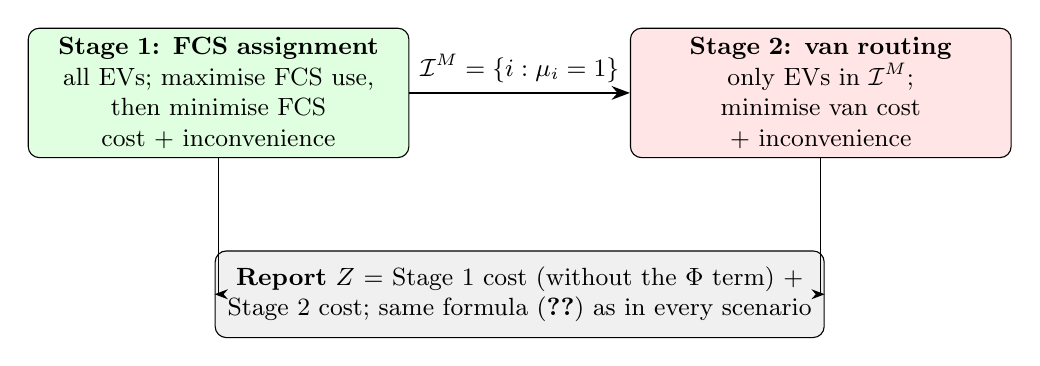
\begin{tikzpicture}[>=Stealth,box/.style={draw,rounded corners,align=center,minimum height=1.1cm,font=\small}]
  \node[box,fill=green!12,text width=4.6cm] (s1) {\textbf{Stage 1: FCS assignment}\\all EVs; maximise FCS use,\\then minimise FCS cost + inconvenience};
  \node[box,fill=red!10,text width=4.6cm,right=2.8cm of s1] (s2) {\textbf{Stage 2: van routing}\\only EVs in $\I^M$;\\minimise van cost + inconvenience};
  \draw[->,thick] (s1) -- node[above,font=\small]{$\I^M=\{i:\mu_i=1\}$} (s2);
  \node[box,fill=black!6,text width=7.5cm,below=2.0cm of $(s1)!0.5!(s2)$] (ev) {\textbf{Report} $Z=$ Stage~1 cost (without the $\Phi$ term) $+$ Stage~2 cost; same formula \eqref{eq:Z} as in every scenario};
  \draw[->] (s1) |- (ev); \draw[->] (s2) |- (ev);
\end{tikzpicture}
\end{center}

Stage~1 does not look at the vans, and Stage~2 cannot change what Stage~1 decided. That is the definition of ``FCS first, then MCS''.

%----------------------------------------------------------------
\subsection{Stage 1: assign EVs to fixed stations}

\textbf{Objective.}
\begin{equation}
\begin{split}
\min\ Z^{(1)}=\;&\underbrace{\Phi\sum_{i\in\I}\mu_i}_{\text{FCS first}}
+\underbrace{c^{EV}\sum_i\sum_{f\in\F_i}d_{if}Y_{if}}_{Z_1}
+\underbrace{Z^F_{\text{energy}}}_{\text{FCS part of }Z_4}\\
&+\underbrace{\sum_i\sum_{f\in\F_i}\rho^F_{if}Y_{if}+\alpha\sum_i w_i(C_i-r_i)+c^L\sum_i w_iL_i}_{\text{FCS customers' inconvenience}}
\end{split}
\label{eq:obj1}
\end{equation}
with $C_i=S_i+\tau^F_iY_i$ in this stage. $\Phi$ is a penalty for handing an EV to the vans. It is chosen larger than anything an extra FCS customer can add to the rest of \eqref{eq:obj1}, e.g.
\[
\Phi > \max_{i}\max_{f\in\F_i}\big(c^{EV}d_{if}+\pi^{\max}E_i+\rho^F_{if}\big)+n\,(\alpha+c^L)\,w_{\max}\,T,
\]
so Stage~1 first \textbf{maximises the number of EVs served at an FCS}, and only among those solutions minimises FCS cost and inconvenience. ($\pi^{\max}$ is the highest grid price.) A numerically safer equivalent is to solve twice: first $\max\sum_iY_i$, then fix that number and minimise the rest.
\ifTOU
Because $Z^F_{\text{energy}}$ uses the peak price, Stage~1 may \emph{start sessions later} to leave the peak, if the price saving beats the extra waiting cost (Section~\ref{sec:expect}).
\fi

\textbf{Constraints.}
\begin{align}
\sum_{g\in\G_i}y_{ig}+\mu_i &= 1 && \forall i\in\I \label{eq:s1assign}\\
S_i &\ge r_i+\sum_{f\in\F_i}t_{if}Y_{if} && \forall i\in\I \label{eq:fcsarr}\\
S_i &\le r_i+T\,(1-\mu_i) && \forall i\in\I \label{eq:s1park}\\
S_j &\ge S_i+\tau^F_i-(T+\tau^F_i)(3-y_{ig}-y_{jg}-o_{ij}) && \forall g,\ (i,j)\in\mathcal{P}_g \label{eq:disj1}\\
S_i &\ge S_j+\tau^F_j-(T+\tau^F_j)(2-y_{ig}-y_{jg}+o_{ij}) && \forall g,\ (i,j)\in\mathcal{P}_g \label{eq:disj2}\\
\sum_i y_{ig_1} &\ge \sum_i y_{ig_2} && \forall f,\ \G_f=\{g_1,g_2\} \label{eq:gunsym}\\
S_i+\tau^F_iY_i &\le T,\qquad L_i\ge S_i+\tau^F_iY_i-l_i && \forall i\in\I \label{eq:s1time}
\end{align}
\ifTOU plus the time-of-use split \eqref{eq:tou1}--\eqref{eq:tou5} of each FCS session (Section~\ref{sec:price}).\fi
\desc{\eqref{eq:s1assign}: every EV either gets one reachable gun or is handed to the vans. An EV that reaches no FCS ($\G_i=\emptyset$) is forced to $\mu_i=1$. \eqref{eq:fcsarr}: an FCS session cannot start before the EV has asked and driven to the station. \eqref{eq:s1park}: for an EV handed to the vans, $S_i$ is parked at $r_i$, so it adds no waiting in Stage~1 (its real start time is decided in Stage~2). \eqref{eq:disj1}--\eqref{eq:disj2}: two EVs on the same gun do not overlap; $o_{ij}$ picks who goes first. With two guns per station this means at most two EVs charge at a station at a time. \eqref{eq:gunsym}: symmetry breaking between the two identical guns (optional). \eqref{eq:s1time}: finished by $T$; lateness.}

\textbf{Optional acceptability rule.} An operator may refuse to send a driver to a station that is ``too inconvenient'', e.g.\ only allow gun $g$ of station $f$ for EV $i$ if $\hat\rho^F_{if}\le\bar\rho$. This only shrinks $\G_i$, so EVs whose stations are all too far go to the vans. Report results with and without it.

\textbf{Output:} $\I^M=\{i:\mu_i=1\}$, the EVs left for the vans; plus each FCS customer's gun and start time.

%----------------------------------------------------------------
\subsection{Stage 2: route the vans to the leftover EVs}

Stage~2 is a vehicle routing problem with time windows, on the EVs in $\I^M$ only. Here $C_i=S_i+\tau^M_i$.

\textbf{Objective.}
\begin{equation}
\begin{split}
\min\ Z^{(2)}=\;&\underbrace{c^M\sum_m\sum_{(i,j)\in\A^M}d_{ij}x_{ijm}}_{Z_2}+\underbrace{\sum_m c^D_mu_m}_{Z_3}+\underbrace{Z^M_{\text{energy}}}_{\text{van part of }Z_4}\\
&+\underbrace{\sum_{i\in\I^M}\sum_m\rho^M_{im}z_{im}+\alpha\sum_{i\in\I^M}w_i(C_i-r_i)+c^L\sum_{i\in\I^M}w_iL_i}_{\text{van customers' inconvenience}}
\end{split}
\label{eq:obj2}
\end{equation}
Since every EV in $\I^M$ must be served by some van, $Z^M_{\text{energy}}$ and the $\rho^M$ term are constants here. They are kept so that $Z^{(2)}$ is the true cost of Stage~2. Waiting and lateness make the vans visit urgent EVs early.

\textbf{Constraints.}
\begin{align}
\sum_{m\in\M}z_{im} &= 1 && \forall i\in\I^M \label{eq:s2assign}\\
\sum_{j:(0,j)\in\A^M}x_{0jm} = \sum_{i:(i,n+1)\in\A^M}x_{i,n+1,m} &= u_m && \forall m \label{eq:depot}\\
\sum_{i:(i,j)\in\A^M}x_{ijm} = \sum_{k:(j,k)\in\A^M}x_{jkm} &= z_{jm} && \forall j\in\I^M,\ m \label{eq:flow}\\
\sum_{i\in\I^M}z_{im} &\le Q_m\,u_m && \forall m \label{eq:cap}\\
\sum_{i\in\I^M}\frac{E_i}{\eta}z_{im}+\beta\sum_{(i,j)\in\A^M}d_{ij}x_{ijm} &\le B_m\,u_m && \forall m \label{eq:batt}
\end{align}
\begin{align}
S_j &\ge \max\{r_j,\ t_{0j}\,x_{0jm}\} && \forall j\in\I^M,\ m \label{eq:depart}\\
S_j &\ge S_i+\tau^M_i+t_{ij}-(T+\tau^M_i+t_{ij})(1-x_{ijm}) && \forall i\neq j,\ m \label{eq:seq}\\
S_i+\tau^M_i+t_{i,n+1} &\le T+(\tau^M_i+t_{i,n+1})(1-x_{i,n+1,m}) && \forall i,\ m \label{eq:return}\\
S_i+\tau^M_i \le T,\quad L_i &\ge S_i+\tau^M_i-l_i && \forall i\in\I^M \label{eq:s2time}\\
u_m &\ge u_{m+1} && m<|\M| \label{eq:vansym}
\end{align}
\desc{\eqref{eq:s2assign}: each leftover EV gets one van. \eqref{eq:depot}: a used van leaves and returns to the depot once. \eqref{eq:flow}: each EV on van $m$ is entered and left exactly once by that van. \eqref{eq:cap}: at most $Q_m$ EVs per van. \eqref{eq:batt}: delivered energy (with transfer losses) plus driving energy fits in the van battery. \eqref{eq:depart}: no start before the request, or before the van can drive there from the depot (written as two linear constraints). \eqref{eq:seq}: if the van goes $i\to j$, it finishes $i$ and drives to $j$ before starting $j$. This gives one EV at a time and removes subtours (MTZ-type). \eqref{eq:return}: back at the depot by $T$. \eqref{eq:s2time}: finished by $T$; lateness. \eqref{eq:vansym}: use identical vans in index order.}

\textbf{If Stage 2 is infeasible} (too many leftover EVs for the fleet by $T$), the sequential policy has \emph{failed} on that instance. For diagnosis, add $s_i\in\{0,1\}$ (``unserved''), replace \eqref{eq:s2assign} by $\sum_mz_{im}+s_i=1$ and add $\Phi^U\sum_is_i$ to \eqref{eq:obj2}. Then report the number of EVs that could not be served. This is a useful comparison with the integrated scenario, which may serve all of them.

%----------------------------------------------------------------
\subsection{Reported value}
\[
Z^{\text{S\scen}}=\big(Z^{(1)*}-\Phi\,|\I^M|\big)+Z^{(2)*},
\]
which is exactly \eqref{eq:Z} evaluated at the combined solution. The stage-1 solution plus the stage-2 solution is a feasible solution of the integrated model (S\ifTOU 4\else 3\fi), so
$Z^{\text{S\ifTOU 4\else 3\fi}}\le Z^{\text{S\scen}}$. The difference is the \emph{value of integration}.

\else
%---------------------------------------------------------------- INT
\subsection{Objective}
\begin{equation}
\min\ Z \quad\text{as in \eqref{eq:Z}, with }Z^F_{\text{energy}}=\ifTOU P^F\textstyle\sum_i\big[\pi^\off(\theta^1_i+\theta^3_i)+\pi^\pk\theta^2_i\big]\else\pi^F\textstyle\sum_iE_iY_i\fi,\quad C_i=S_i+\tau^F_iY_i+\tau^M_iZ_i. \label{eq:objint}
\end{equation}
Written out in full:
\begin{align*}
\min\ Z=\;& c^{EV}\sum_i\sum_{f\in\F_i}d_{if}Y_{if}+c^M\sum_m\sum_{(i,j)\in\A}d_{ij}x_{ijm}+\sum_mc^D_mu_m\\
&+\ifTOU P^F\sum_i\big[\pi^\off(\theta^1_i+\theta^3_i)+\pi^\pk\theta^2_i\big]\else\pi^F\sum_iE_iY_i\fi
+\pi^M\sum_i\sum_m\frac{E_i}{\eta}z_{im}\\
&+\sum_i\sum_{f\in\F_i}\rho^F_{if}Y_{if}+\sum_i\sum_m\rho^M_{im}z_{im}+\alpha\sum_iw_i(C_i-r_i)+c^L\sum_iw_iL_i .
\end{align*}
Every term is linear. One model weighs everything at once: an EV goes to a van exactly when the van's extra km, dispatch and energy cost are outweighed by the effort and waiting it saves the driver\ifTOU, or by the peak-price energy it avoids\fi.

\subsection{Constraints}

\textbf{Assignment.}
\begin{equation}
\sum_{g\in\G_i}y_{ig}+\sum_{m\in\M}z_{im}=1\qquad\forall i\in\I \label{eq:assign}
\end{equation}
\desc{Exactly one resource per EV: one reachable gun or one van. EVs that reach no FCS are forced onto a van.}

\textbf{Fixed stations.}
\begin{align}
S_i &\ge r_i+\sum_{f\in\F_i}t_{if}Y_{if} && \forall i \label{eq:fcsarr}\\
S_j &\ge S_i+\tau^F_i-(T+\tau^F_i)(3-y_{ig}-y_{jg}-o_{ij}) && \forall g,\ (i,j)\in\mathcal{P}_g \label{eq:disj1}\\
S_i &\ge S_j+\tau^F_j-(T+\tau^F_j)(2-y_{ig}-y_{jg}+o_{ij}) && \forall g,\ (i,j)\in\mathcal{P}_g \label{eq:disj2}\\
\sum_iy_{ig_1} &\ge \sum_iy_{ig_2} && \forall f,\ \G_f=\{g_1,g_2\} \label{eq:gunsym}
\end{align}
\desc{\eqref{eq:fcsarr}: an FCS session starts after the request and the drive to the station (for a van customer this is just $S_i\ge r_i$). \eqref{eq:disj1}--\eqref{eq:disj2}: EVs on the same gun do not overlap; $o_{ij}$ chooses the order. \eqref{eq:gunsym}: optional symmetry breaking.}

\textbf{Vans: routes, capacity, battery.}
\begin{align}
\sum_{j:(0,j)\in\A}x_{0jm}=\sum_{i:(i,n+1)\in\A}x_{i,n+1,m} &= u_m && \forall m \label{eq:depot}\\
\sum_{i:(i,j)\in\A}x_{ijm}=\sum_{k:(j,k)\in\A}x_{jkm} &= z_{jm} && \forall j\in\I,\ m \label{eq:flow}\\
\sum_iz_{im} &\le Q_mu_m && \forall m \label{eq:cap}\\
\sum_i\frac{E_i}{\eta}z_{im}+\beta\sum_{(i,j)\in\A}d_{ij}x_{ijm} &\le B_mu_m && \forall m \label{eq:batt}
\end{align}
\desc{\eqref{eq:depot}: a used van leaves and returns once. \eqref{eq:flow}: each EV on van $m$ is visited exactly once by it. \eqref{eq:cap}: at most $Q_m$ EVs. \eqref{eq:batt}: delivered energy (with losses) plus driving energy fits in the battery.}

\textbf{Vans: timing (one EV at a time, no subtours).}
\begin{align}
S_j &\ge t_{0j}\,x_{0jm} && \forall j\in\I,\ m \label{eq:depart}\\
S_j &\ge S_i+\tau^M_i+t_{ij}-(T+\tau^M_i+t_{ij})(1-x_{ijm}) && \forall i\neq j\in\I,\ m \label{eq:seq}\\
S_i+\tau^M_i+t_{i,n+1} &\le T+(\tau^M_i+t_{i,n+1})(1-x_{i,n+1,m}) && \forall i,\ m \label{eq:return}
\end{align}
\desc{\eqref{eq:depart}: the first stop cannot start before the van has driven there. \eqref{eq:seq}: $i\to j$ means finish $i$, drive, then start $j$; start times rise along a route, so no subtour can close. \eqref{eq:return}: back at the depot by $T$.}

\textbf{Horizon and lateness.}
\begin{equation}
C_i\le T,\qquad L_i\ge C_i-l_i\qquad\forall i\in\I \label{eq:time}
\end{equation}
\desc{Every EV is fully charged within the horizon; $L_i$ measures lateness.}

\ifTOU
\textbf{Time-of-use split.} Constraints \eqref{eq:tou1}--\eqref{eq:tou5} of Section~\ref{sec:price}.
\fi

\textbf{Symmetry and domains.}
\begin{equation}
u_m\ge u_{m+1};\qquad y,z,x,u,o\ifTOU,\kappa\fi\in\{0,1\};\qquad S_i,L_i\ifTOU,\theta^p_i\fi\ge0 \label{eq:dom}
\end{equation}
\fi

%=====================================================================
\section{Learning-to-optimise (RL) formulation}\label{sec:rl}

\textbf{Main rule:} the reward of each action is \emph{minus the increase in $Z$ that the action causes}. The rewards over an episode then add up to $-Z$ of the solution the policy builds. RL and MILP results are measured on the same yardstick \eqref{eq:Z}, and the MILP optimum is the benchmark for the RL gap.

\ifSEQ
%---------------------------------------------------------------- RL SEQ
The RL pipeline has the same two stages as the MILP.

\subsection{Stage 1 policy: FCS assignment}
\begin{itemize}[leftmargin=1.4em,itemsep=2pt]
  \item \textbf{Episode / epochs:} EVs are taken in order of request time $r_i$ (ties: higher $w_i$ first). One decision per EV.
  \item \textbf{State:} features of the current EV $k$ ($E_k,r_k,l_k,w_k,R_k$, location); for each gun $g$ the time $F_g$ it becomes free; summary features of the EVs still to come (count and positions near each station)\ifTOU; the current price and the time until $T_1$ and $T_2$\fi.
  \item \textbf{Action:} a gun $g\in\G_k$, or ``hand to vans''. \textbf{FCS-first mask:} ``hand to vans'' is allowed \emph{only} if no gun can finish EV $k$ by $T$ (or, with the optional rule, if all remaining guns have $\hat\rho^F_{kf}>\bar\rho$).
  \ifTOU\item \textbf{Optional timing action:} ``gun $g$, start after the peak'', i.e.\ $S_k=\max\{\text{earliest},T_2\}$, allowed only if the session still ends by $T$.\fi
  \item \textbf{Transition:} $S_k=\max\{r_k+t_{kf},F_g\}$ (or later, for the timing action); $F_g\leftarrow S_k+\tau^F_k$.
  \item \textbf{Reward:} $-\Big[c^{EV}d_{kf}+\text{energy}_k+\rho^F_{kf}+\alpha w_k(S_k+\tau^F_k-r_k)+c^Lw_k(S_k+\tau^F_k-l_k)^+\Big]$, where energy$_k$ = \ifTOU$P^F\big[\pi^\off\cdot(\text{off-peak hours of }[S_k,S_k+\tau^F_k])+\pi^\pk\cdot(\text{peak hours})\big]$, computed exactly in the simulator\else$\pi^FE_k$\fi. Handing an EV to the vans gives reward $0$ here; its cost is counted in Stage~2.
\end{itemize}
Note: a simple baseline for Stage~1 is the greedy rule ``gun with the largest one-step reward''. What RL can learn on top of this is, for example, to keep a nearby gun free for an urgent EV that arrives later.

\subsection{Stage 2 policy: van routing over $\I^M$}
\begin{itemize}[leftmargin=1.4em,itemsep=2pt]
  \item \textbf{Epochs:} whenever a van becomes free (the earliest-free van decides first).
  \item \textbf{State:} for each van: position, time free, remaining battery $b_m$, EVs served so far, dispatched or not; for each unserved EV in $\I^M$: location, $E_i,r_i,l_i,w_i$; current time.
  \item \textbf{Action:} the next EV $j$ for this van, or ``return to depot'' (ends the route). Mask: $j$ must be feasible: battery covers $E_j/\eta$ plus driving to $j$ and back to the depot, the count stays $\le Q_m$, and $j$ can be finished with the van back at the depot by $T$.
  \item \textbf{Transition:} $S_j=\max\{r_j,\ \text{time free}+t_{\text{pos},j}\}$; the van moves to $j$ and is free at $S_j+\tau^M_j$; $b_m$ falls by $E_j/\eta+\beta d_{\text{pos},j}$.
  \item \textbf{Reward:} serving $j$: $-\Big[c^Md_{\text{pos},j}+c^D_m[\text{first stop}]+\pi^M\frac{E_j}{\eta}+\rho^M_{jm}+\alpha w_j(S_j+\tau^M_j-r_j)+c^Lw_j(S_j+\tau^M_j-l_j)^+\Big]$; returning: $-c^Md_{\text{pos},0}$. EVs still unserved at the end: $-\Phi^U$ each.
  \item \textbf{Policy:} an attention-based routing policy (e.g.\ Kool et al., 2019, ``Attention, Learn to Solve Routing Problems!'') trained with REINFORCE or PPO. Baseline: nearest-feasible-EV heuristic.
\end{itemize}
Episode return of Stage~1 + Stage~2 $=-Z^{\text{S\scen}}$.

\else
%---------------------------------------------------------------- RL INT
One policy decides both who serves each EV and the van routes.
\begin{itemize}[leftmargin=1.4em,itemsep=2pt]
  \item \textbf{Episode / epochs:} EVs are taken in order of request time $r_i$ (ties: higher $w_i$ first). One decision per EV.
  \item \textbf{State:} (i) the current EV $k$: location, $E_k,r_k,l_k,w_k,R_k$, reachable stations; (ii) each gun $g$: time $F_g$ it becomes free; (iii) each van $m$: current end-of-route position, time free, remaining battery $b_m$, EVs served, dispatched or not; (iv) embeddings of the not-yet-assigned EVs (for look-ahead)\ifTOU; (v) current price, time until $T_1$ and $T_2$\fi.
  \item \textbf{Action:} $a\in\G_k\cup\M$: a gun, or a van (EV $k$ is appended to the end of that van's route). \textbf{Mask} infeasible actions: a gun that cannot finish $k$ by $T$; a van without enough battery for $E_k/\eta$ plus the drive to $k$ and back to the depot, with $Q_m$ reached, or unable to finish $k$ and return by $T$.
  \ifTOU\item \textbf{Optional timing action:} ``gun $g$, start after the peak'' ($S_k=\max\{\text{earliest},T_2\}$, if it still ends by $T$).\fi
  \item \textbf{Transition:} gun: $S_k=\max\{r_k+t_{kf},F_g\}$, $F_g\leftarrow S_k+\tau^F_k$. Van: $S_k=\max\{r_k,\ \text{free}_m+t_{\text{pos}_m,k}\}$, then the van moves to $k$, $\text{free}_m\leftarrow S_k+\tau^M_k$, $b_m\mathrel{-}=E_k/\eta+\beta d_{\text{pos}_m,k}$.
  \item \textbf{Reward} $=-\Delta Z$:
  \begin{align*}
  \text{gun } g\text{ at }f:&\quad -\Big[c^{EV}d_{kf}+\text{energy}^F_k+\rho^F_{kf}+\alpha w_k(C_k-r_k)+c^Lw_k(C_k-l_k)^+\Big]\\
  \text{van } m:&\quad -\Big[c^M\big(d_{\text{pos}_m,k}+d_{k,0}-d_{\text{pos}_m,0}\big)+c^D_m[\text{first use}]+\pi^M\tfrac{E_k}{\eta}\\
  &\qquad\quad+\rho^M_{km}+\alpha w_k(C_k-r_k)+c^Lw_k(C_k-l_k)^+\Big]
  \end{align*}
  The van distance term is the \emph{change} in route length when $k$ is inserted before the return to the depot, so the sum over the episode equals the total route length (the return legs telescope). energy$^F_k$ = \ifTOU$P^F\big[\pi^\off\cdot(\text{off-peak hours})+\pi^\pk\cdot(\text{peak hours of }[S_k,C_k])\big]$, computed exactly by the simulator; no linearisation is needed in RL\else$\pi^FE_k$\fi.
  \item \textbf{Dead end:} if every action is masked, EV $k$ is unserved: reward $-\Phi^U$, and the episode continues. Report the count.
  \item \textbf{Policy:} masked categorical policy over guns and vans, encoder with attention over EVs, guns and vans; trained with PPO. Natural baseline: greedy, i.e.\ choose the action with the largest one-step reward. That is the pairwise rule ``smallest $\hat\rho$ + cost'' from Section~\ref{sec:inc}.
\end{itemize}
Restriction to note: vans serve EVs in assignment order (append only). A variant that inserts $k$ at the cheapest position of a route is more flexible but has a larger action space.
\fi

\textbf{Reward scaling.} For stable training divide every reward by a constant, e.g.\ the greedy baseline's average $Z$ on the training instances. This does not change the optimal policy.

%=====================================================================
\section{What to expect and what to report}\label{sec:expect}

\ifnum\scen=1
\begin{itemize}[leftmargin=1.4em,itemsep=2pt]
  \item Vans serve only EVs that reach no station, or that the stations cannot finish by $T$. If stations have spare capacity, very few vans are dispatched.
  \item Inconvenience is high for EVs far from the nearest station (worked example: Rs\,682 at the FCS, against Rs\,458 if a van had been allowed).
  \item With too few vans Stage~2 becomes infeasible (unserved EVs), even when the integrated model S3 could serve everyone. Report the smallest $|\M|$ at which S1 is feasible and compare it with S3.
\end{itemize}
\fi
\ifnum\scen=2
\begin{itemize}[leftmargin=1.4em,itemsep=2pt]
  \item \textbf{When does Stage~1 delay a session to avoid the peak?} Moving one hour of charging out of the peak saves $(\pi^\pk-\pi^\off)P^F=3\times22=$ Rs\,66, but delays completion by up to an hour, which costs $\alpha w_i\ge$ Rs\,200. So with the default values Stage~1 almost never delays. It mostly pays the higher price, and S2 costs roughly S1 plus the peak surcharge. Sessions start later only if $\alpha$ is small (try $\lambda<0.33$ in the sensitivity analysis).
  \item The van assignment is the same as in S1 unless Stage~1's timing changes which EVs fit at the stations. Stage~1 cannot use vans to escape the peak price.
  \item Extra KPI: \textbf{grid energy drawn at FCS during the peak}, $P^F\sum_i\theta^2_i$ (kWh). Compare with S4.
\end{itemize}
\fi
\ifnum\scen=3
\begin{itemize}[leftmargin=1.4em,itemsep=2pt]
  \item Vans take EVs for which the saved inconvenience exceeds the extra van cost (worked example: van chosen, saving Rs\,224). Expect vans to serve EVs that are far from every station, have low range (high $w_i$), or have early deadlines, while EVs near a station still use it.
  \item \textbf{Value of integration under flat price:} $Z^{\text{S1}}-Z^{\text{S3}}\ge0$. Report it per component ($Z_1,\dots,Z_5$): typically operating cost rises a little and inconvenience falls a lot.
  \item Vary $|\M|$ (0, 1, 2, \dots): the first few vans lower $Z$ sharply, then the effect levels off. That curve shows the scenarios where mobile chargers help most.
\end{itemize}
\fi
\ifnum\scen=4
\begin{itemize}[leftmargin=1.4em,itemsep=2pt]
  \item During the peak a van kWh costs about the same as an FCS kWh (Rs\,10.0 each), so the vans' energy disadvantage disappears and vans also absorb \emph{peak-hour} demand that would otherwise be charged on the grid at peak price.
  \item Expect more van usage than in S3, concentrated on requests in $[T_1,T_2]$, and lower grid energy at the stations during the peak, $P^F\sum_i\theta^2_i$, than in S2.
  \item \textbf{Value of integration under peak pricing:} $Z^{\text{S2}}-Z^{\text{S4}}$. It should be larger than $Z^{\text{S1}}-Z^{\text{S3}}$, because integration now also allows price arbitrage.
  \item \textbf{Peak pricing with full flexibility:} $Z^{\text{S4}}-Z^{\text{S3}}$ should be smaller than $Z^{\text{S2}}-Z^{\text{S1}}$: vans cushion the price increase.
\end{itemize}
\fi

\textbf{Cross-scenario comparison table} (fill in from the four runs):
\begin{center}
\renewcommand{\arraystretch}{1.2}
\begin{tabular}{@{}lll@{}}
\toprule
\textbf{Comparison} & \textbf{Measures} & \textbf{Expected sign} \\
\midrule
S1 $-$ S3 & value of integration, flat price & $\ge0$ \\
S2 $-$ S4 & value of integration, peak price & $\ge0$, larger than S1 $-$ S3 \\
S2 $-$ S1 & cost of peak pricing, FCS-first operator & $>0$ \\
S4 $-$ S3 & cost of peak pricing, flexible operator & $>0$, smaller than S2 $-$ S1 \\
\bottomrule
\end{tabular}
\end{center}
Report for each: $Z$ and its components, number of vans used, EVs per resource, mean and maximum inconvenience per EV, total lateness, peak-hour grid energy, solve time, and (for RL) the gap to the MILP optimum.

%=====================================================================
\appendix
\section{Illustrative parameter values}\label{app:values}

These are starting values for experiments, not data. All are meant to be varied in the analysis. Values in Rs.

\begin{center}
\renewcommand{\arraystretch}{1.15}
\begin{tabular}{@{}llp{6.2cm}@{}}
\toprule
\textbf{Parameter} & \textbf{Value} & \textbf{Note} \\
\midrule
$T$, $[T_1,T_2]$ & 7 h, $[2,6]$ & 16:00--23:00, peak 18:00--22:00 \\
$P^F$, $P^M$ & 22 kW, 30 kW & \\
$v$, $\beta$, $\eta$ & 25 km/h, 0.25 kWh/km, 0.9 & \\
$B_m$, $Q_m$, $|\M|$ & 150 kWh, 6, 2--6 & \\
$c^{EV}$, $c^M$, $c^D_m$ & Rs\,4/km, Rs\,15/km, Rs\,1500 & van km includes driver time \\
$\pi^F$ (flat) & Rs\,8.7/kWh & equals the time-average of the ToU tariff over $[0,T]$ \\
$\pi^\off$, $\pi^\pk$ (ToU) & Rs\,7/kWh, Rs\,10/kWh & $(3\times7+4\times10)/7=8.7$ \\
$c^{bat}$ & Rs\,2/kWh & van battery wear \\
$\pi^M$ & Rs\,10.7 (flat) / Rs\,9.0 (ToU) & $=\pi^F+c^{bat}$ / $=\pi^\off+c^{bat}$ \\
$\alpha$, $\alpha^D$ & Rs\,200/h, Rs\,100/h & value of time; extra for attended time \\
$h^F$, $h^M$, $\varphi$ & Rs\,50, Rs\,10, Rs\,100 & trip hassle, hand-over, range stress \\
$c^L$ & Rs\,300/h & lateness \\
$w_i$ & $1+2(1-R_i/R_{\max})$, $R_i\sim U[3,40]$ km & priority from remaining range \\
\bottomrule
\end{tabular}
\end{center}

The flat price is set to the time-average of the peak tariff. The price \emph{level} is then the same in both pricing cases, and only the price \emph{shape} differs. Without this, part of S1 vs S2 would just reflect a different average price.

\end{document}
"
%    pdflatex -jobname=scenario3_flat_integrated   "\def\scen{3}% =====================================================================
%  One source, four PDFs.  Build with build.sh (or by hand):
%    pdflatex -jobname=scenario1_flat_sequential   "\def\scen{1}% =====================================================================
%  One source, four PDFs.  Build with build.sh (or by hand):
%    pdflatex -jobname=scenario1_flat_sequential   "\def\scen{1}% =====================================================================
%  One source, four PDFs.  Build with build.sh (or by hand):
%    pdflatex -jobname=scenario1_flat_sequential   "\def\scen{1}\input{scenario_master}"
%    pdflatex -jobname=scenario2_peak_sequential   "\def\scen{2}\input{scenario_master}"
%    pdflatex -jobname=scenario3_flat_integrated   "\def\scen{3}\input{scenario_master}"
%    pdflatex -jobname=scenario4_peak_integrated   "\def\scen{4}\input{scenario_master}"
%  (run each twice for cross-references)
% =====================================================================
\documentclass[11pt,a4paper]{article}
\usepackage[margin=2.2cm]{geometry}
\usepackage{amsmath,amssymb,amsfonts}
\usepackage{booktabs,array,tabularx}
\usepackage{enumitem}
\usepackage[table]{xcolor}
\usepackage{tikz}
\usetikzlibrary{arrows.meta,positioning,calc}
\usepackage[colorlinks=true,linkcolor=blue!50!black,urlcolor=blue!50!black]{hyperref}
\usepackage{titlesec}
\titleformat{\section}{\large\bfseries}{\thesection}{0.8em}{}
\titleformat{\subsection}{\normalsize\bfseries}{\thesubsection}{0.8em}{}
\setlength{\parindent}{0pt}
\setlength{\parskip}{5pt}

% ---------------- scenario switches ----------------
\ifdefined\scen\else\def\scen{1}\fi
\newif\ifTOU \TOUfalse   % true = time-of-use (peak) price
\newif\ifSEQ \SEQfalse   % true = FCS first, then MCS
\ifnum\scen=1 \SEQtrue \fi
\ifnum\scen=2 \TOUtrue \SEQtrue \fi
\ifnum\scen=4 \TOUtrue \fi

\newcommand{\pricename}{\ifTOU time-of-use price (dearer evening peak)\else single (flat) price all day\fi}
\newcommand{\structname}{\ifSEQ FCS first, then MCS (sequential)\else FCS and MCS together (integrated)\fi}

% ---------------- notation ----------------
\newcommand{\I}{\mathcal{I}}
\newcommand{\F}{\mathcal{F}}
\newcommand{\G}{\mathcal{G}}
\newcommand{\M}{\mathcal{M}}
\newcommand{\N}{\mathcal{N}}
\newcommand{\A}{\mathcal{A}}
\newcommand{\Rs}{\text{Rs}\,}
\newcommand{\pk}{\mathrm{pk}}
\newcommand{\off}{\mathrm{off}}
\newcommand{\desc}[1]{\par\vspace{-2pt}{\small\color{black!75}\textit{Meaning:} #1}\par\vspace{4pt}}
\newcommand{\cell}[2]{\ifnum\scen=#1\cellcolor{blue!18}\textbf{S#1 (this document)}\\\textbf{#2}\else S#1\\#2\fi}

\title{\textbf{EV Charging Network Optimisation}\\[4pt]
\large Scenario \scen: \pricename\ $+$ \structname\\[2pt]
\normalsize MILP and RL formulation}
\author{CP 320 OR for Mobility Management, course project}
\date{2 October 2026}

\begin{document}
\maketitle

%=====================================================================
\section{Where this scenario sits}

The project studies four scenarios: two ways of pricing grid electricity, times two ways of making the decisions.

\begin{center}
\renewcommand{\arraystretch}{1.5}
\begin{tabular}{>{\raggedright\arraybackslash}p{4.2cm}|>{\centering\arraybackslash}p{4.6cm}|>{\centering\arraybackslash}p{4.6cm}}
 & \textbf{Flat price all day} & \textbf{Time-of-use (peak) price} \\ \hline
\textbf{Sequential:} FCS first, leftover EVs to MCS &
\begin{tabular}[c]{@{}c@{}}\cell{1}{flat + sequential}\end{tabular} &
\begin{tabular}[c]{@{}c@{}}\cell{2}{peak + sequential}\end{tabular} \\ \hline
\textbf{Integrated:} FCS and MCS decided together &
\begin{tabular}[c]{@{}c@{}}\cell{3}{flat + integrated}\end{tabular} &
\begin{tabular}[c]{@{}c@{}}\cell{4}{peak + integrated}\end{tabular} \\
\end{tabular}
\end{center}

\textbf{The four scenarios do not have four different objectives.} They share \emph{one} cost yardstick $Z$ (Section~\ref{sec:obj}): the same cost terms and the same customer inconvenience (Section~\ref{sec:inc}). Only two things change:
\begin{itemize}[leftmargin=1.4em,itemsep=1pt]
  \item \textbf{Pricing} changes the formula for one term, the FCS energy cost (Section~\ref{sec:price}).
  \item \textbf{Decision structure} changes \emph{how} $Z$ is minimised: in one model (integrated), or in two stages (sequential), where each stage minimises its own part of $Z$.
\end{itemize}
Because the yardstick is the same, the four optimal values can be compared directly. The differences measure the \emph{value of integration} (S1$\to$S3, S2$\to$S4) and the \emph{effect of peak pricing} (S1$\to$S2, S3$\to$S4).

\ifnum\scen=1
\textbf{This scenario (S1)} is the baseline, the ``status quo''. Electricity costs the same at every hour, every EV that can be charged at a fixed station is sent there, and vans only take what is left over.
\fi
\ifnum\scen=2
\textbf{This scenario (S2)} keeps the FCS-first rule of S1, but grid electricity is dearer during the evening peak. Stage~1 can react to the price only by \emph{rescheduling} FCS sessions. It cannot hand a peak-hour EV to a van.
\fi
\ifnum\scen=3
\textbf{This scenario (S3)} keeps the flat price of S1, but the operator decides FCS and MCS service \emph{together}. An EV can be sent to a van even when a fixed station could take it, whenever that lowers total cost plus inconvenience.
\fi
\ifnum\scen=4
\textbf{This scenario (S4)} is the most flexible one: peak pricing at fixed stations, and FCS and MCS decided together. Van energy was bought off-peak, so vans can also be used to keep charging \emph{out of the expensive peak}.
\fi

%=====================================================================
\section{Setting and assumptions}\label{sec:setting}

\textbf{Time.} The planning horizon is $[0,T]$ with $T=7$\,h (16:00--23:00). It contains the evening peak window $[T_1,T_2]=[2,6]$ (18:00--22:00). The horizon is the same in all four scenarios. It is wider than the peak itself so that, under peak pricing, there is cheaper time on both sides of the peak.\ifTOU\else\ In this scenario the price is flat, so the window plays no role in the model.\fi

\textbf{Assumptions} (the same as MILP v3, plus two about energy):
\begin{enumerate}[leftmargin=1.6em,itemsep=1pt]
  \item Static, continuous time. All requests in the horizon are known at time $0$, and request $i$ becomes active at $r_i$.
  \item An EV served by an FCS drives there itself on its own battery (only to stations within its range $R_i$). The driver stays with the car while it waits for a free gun and while it charges.
  \item An EV served by an MCS stays parked where it is, and the driver is free in the meantime.
  \item Each FCS gun and each van charges one EV at a time, without interruption, at constant power.
  \item A van's battery covers both its driving and the energy it delivers. \textbf{The van battery is charged at the depot before the horizon starts}\ifTOU, i.e.\ at the off-peak price\fi, and is not recharged during the horizon.
  \item Every EV must be fully charged by $T$ (hard). Finishing after the driver's desired time $l_i$ is allowed but penalised.
\end{enumerate}

%=====================================================================
\section{Notation}\label{sec:notation}

\subsection*{Sets}
\begin{tabularx}{\textwidth}{@{}lX@{}}
\toprule
$\I=\{1,\dots,n\}$ & EV charging requests \\
$\F$; $\G_f$ ($|\G_f|=2$); $\G=\bigcup_f\G_f$ & fixed charging stations; guns of FCS $f$; all guns ($f(g)$ = station of gun $g$) \\
$\F_i=\{f: d_{if}\le R_i\}$, $\G_i=\bigcup_{f\in\F_i}\G_f$ & stations / guns EV $i$ can reach on its remaining range \\
$\M$ & mobile charging vans (MCS) \\
$0,\ n+1$ & depot as start node / end node (same place) \\
$\N=\{0\}\cup\I\cup\{n+1\}$, $\A$ & routing nodes; allowed van arcs $(i,j)$, $i\in\{0\}\cup\I$, $j\in\I\cup\{n+1\}$, $i\neq j$ \\
$\mathcal{P}_g=\{(i,j): i<j,\ g\in\G_i\cap\G_j\}$ & pairs of EVs that could share gun $g$ \\
\ifSEQ
$\I^M\subseteq\I$ & EVs handed to the vans by Stage~1 (an \emph{output} of Stage~1, a fixed input to Stage~2) \\
$\N^M$, $\A^M$ & routing nodes / arcs restricted to $\I^M$ \\
\fi
\bottomrule
\end{tabularx}

\subsection*{Parameters}
\begin{tabularx}{\textwidth}{@{}lX@{}}
\toprule
$E_i,\ r_i,\ l_i,\ R_i$ & energy demand (kWh), request time, desired completion time (h), remaining range (km) \\
$w_i\ge1$ & priority of EV $i$; $w_i=1+\kappa(1-R_i/R_{\max})$, so low-range EVs weigh more \\
$P^F,\ P^M$ & charging power of an FCS gun (22\,kW) / of a van (e.g.\ 30\,kW) \\
$\tau^F_i=E_i/P^F,\ \tau^M_i=E_i/P^M$ & charging time of EV $i$ at an FCS / by a van (h) \\
$d_{if},t_{if}$;\ $d_{ij},t_{ij}$ & distance (km) and time (h): EV$\to$FCS; between routing nodes ($t=d/v$) \\
$B_m,\ Q_m,\ \beta,\ \eta$ & van battery (kWh), max EVs per van, van consumption (kWh/km), transfer efficiency \\
$c^{EV},\ c^M,\ c^D_m$ & cost per km of EV driving, per km of van driving; fixed dispatch cost of van $m$ \\
\ifTOU
$\pi^\off,\ \pi^\pk$ & grid price (Rs/kWh) off-peak / in $[T_1,T_2]$, with $\pi^\pk\ge\pi^\off$ \\
\else
$\pi^F$ & grid price (Rs/kWh), the same at every hour \\
\fi
$c^{bat}$ & van battery wear per kWh cycled \\
$\pi^M$ & cost of 1 kWh taken from a van battery: $\pi^M=\ifTOU\pi^\off\else\pi^F\fi+c^{bat}$ (Section~\ref{sec:price}) \\
$\alpha,\ \alpha^D,\ h^F,\ h^M,\ \varphi,\ c^L$ & inconvenience coefficients (Section~\ref{sec:inc}) \\
\bottomrule
\end{tabularx}

\subsection*{Decision variables}
\begin{tabularx}{\textwidth}{@{}llX@{}}
\toprule
$y_{ig}$ & $\{0,1\}$ & EV $i$ charged at gun $g\in\G_i$ \\
$z_{im}$ & $\{0,1\}$ & EV $i$ served by van $m$ \\
$x_{ijm}$ & $\{0,1\}$ & van $m$ drives arc $(i,j)$ \\
$u_m$ & $\{0,1\}$ & van $m$ is dispatched \\
$o_{ij}$ & $\{0,1\}$ & for EVs $i<j$ that could share a gun: 1 if $i$ is charged before $j$ \\
\ifSEQ
$\mu_i$ & $\{0,1\}$ & Stage~1 only: EV $i$ is handed to the van fleet \\
\fi
\ifTOU
$\theta^1_i,\theta^2_i,\theta^3_i$ & $\ge0$ & hours of EV $i$'s FCS session before / inside / after the peak \\
$\kappa^1_i,\kappa^3_i$ & $\{0,1\}$ & EV $i$'s FCS session starts before $T_1$ / ends after $T_2$ \\
\fi
$S_i$ & $\ge0$ & time charging of EV $i$ starts (h), on whichever resource \\
$L_i$ & $\ge0$ & lateness of EV $i$ beyond $l_i$ (h) \\
\bottomrule
\end{tabularx}

\textbf{Short-hands} (linear expressions, not new variables):
\[
Y_{if}=\sum_{g\in\G_f}y_{ig},\qquad Y_i=\sum_{g\in\G_i}y_{ig}\ (\text{EV $i$ uses an FCS}),\qquad Z_i=\sum_{m\in\M}z_{im}\ (\text{EV $i$ uses a van}),
\]
\[
C_i=S_i+\tau^F_i\,Y_i+\tau^M_i\,Z_i \quad\text{(time EV $i$ is fully charged).}
\]

%=====================================================================
\section{Customer inconvenience}\label{sec:inc}

This section is \textbf{identical in all four scenario documents}. Inconvenience is a property of the customer, not of the price or of the planning method.

\subsection{What we mean by inconvenience}

Inconvenience is \emph{what the driver loses} from the moment they ask for a charge ($r_i$) until the car is fully charged ($C_i$), \emph{converted into rupees} so it can be added to the operator's costs. A driver loses three different things:

\begin{enumerate}[leftmargin=1.6em,itemsep=2pt]
  \item \textbf{Waiting:} the car is not ready. This lasts $C_i-r_i$ hours and affects \emph{every} driver, FCS or MCS.
  \item \textbf{Effort:} only an FCS customer has to drive to the station and sit there while the car charges. An MCS customer stays at home or at work and does something else. Driving to a far station also uses scarce battery range, which causes stress (``range anxiety'').
  \item \textbf{A missed deadline:} the car is still not ready at the time $l_i$ the driver needs it.
\end{enumerate}

Each loss gets a price in Rs per hour (or per event). All of them are multiplied by the priority $w_i$: an hour of delay for an EV with 5\,km of range left counts more than for one with 40\,km.

\subsection{The three components}

\begin{center}
\renewcommand{\arraystretch}{1.3}
\begin{tabularx}{\textwidth}{@{}>{\raggedright\arraybackslash}p{2.6cm}>{\raggedright\arraybackslash}X>{\raggedright\arraybackslash}X>{\raggedright\arraybackslash}p{3.0cm}@{}}
\toprule
\textbf{Component} & \textbf{EV $i$ at FCS $f$} & \textbf{EV $i$ by a van} & \textbf{Known when?} \\
\midrule
Effort & $w_i\big[\alpha^D(t_{if}+\tau^F_i)+h^F+\varphi\,d_{if}/R_i\big]$: driving and sitting at the station, a fixed trip hassle, range stress & $w_i\,h^M$: being reachable and handing over the car & \textbf{Static:} known as soon as the resource is chosen \\
Waiting & $w_i\,\alpha\,(C_i-r_i)$ = drive + \emph{queue at the gun} + charge & $w_i\,\alpha\,(C_i-r_i)$ = \emph{wait for the van} + charge & \textbf{Dynamic:} depends on the queue / van route \\
Missed deadline & $w_i\,c^L\,L_i$, $L_i=\max\{0,C_i-l_i\}$ & same & Dynamic \\
\bottomrule
\end{tabularx}
\end{center}

\textbf{Coefficients.}
$\alpha$ (Rs/h) is the value of an hour the car is not ready.
$\alpha^D$ (Rs/h) is the \emph{extra} value of an hour the driver must personally spend driving or sitting at the station: an hour at the station costs $\alpha+\alpha^D$, an hour waiting at home for a van costs only $\alpha$.
$h^F,h^M$ (Rs) are fixed hassle costs of one trip to a station / one van hand-over.
$\varphi$ (Rs) is the range-stress cost of a trip that uses the \emph{whole} remaining range ($d_{if}/R_i\le1$ is the fraction used).
$c^L$ (Rs/h) is the cost per hour late.

\subsection{Pairwise form: inconvenience of a (customer, resource) pair}

The natural first idea is: \emph{for every pair (EV $i$, FCS $f$) and every pair (EV $i$, van $m$) there is an inconvenience number, and the operator picks the pair with the lowest cost plus inconvenience.} The static part fits this idea exactly:
\[
\boxed{\;\rho^F_{if}=w_i\Big[\alpha^D\,(t_{if}+\tau^F_i)+h^F+\varphi\,\frac{d_{if}}{R_i}\Big]\qquad
\rho^M_{im}=w_i\,h^M\;}
\]
These are \textbf{parameters}, computed before solving, one number per (EV, FCS) pair and per (EV, van) pair. In the objective they appear linearly: $\sum_i\sum_f\rho^F_{if}Y_{if}+\sum_i\sum_m\rho^M_{im}z_{im}$.

Note that $\rho^M_{im}$ does not depend on $m$. Vans are identical and all start at the same depot, so the driver does not care \emph{which} van comes, only \emph{when} it comes. That ``when'' is the waiting part.

\subsection{Why waiting cannot be a fixed pairwise number}

It is tempting to also write the waiting as a pairwise number, e.g.\ ``the van needs 5 minutes to reach EV $i$''. But that depends on \emph{where the van is coming from}, which depends on the route the model is still choosing: if EV $i$ is the 4th stop of a van, the wait is the time for three charging sessions plus four drives. Likewise, waiting at an FCS depends on how many EVs are queued at that gun. So waiting is not known before solving. It is a function of decision variables:
\[
\text{waiting cost of EV } i \;=\; w_i\,\alpha\,(C_i-r_i),\qquad C_i=S_i+\tau^F_iY_i+\tau^M_iZ_i .
\]
This is \textbf{linear} in the variables ($S_i$, $y$, $z$), so it fits in a MILP directly. The constraints of Section~\ref{sec:milp} make $S_i$ equal to the true start time, including driving, queueing at the gun and the van's route. The term $\sum_i w_i\alpha r_i$ is a constant and may be dropped when solving.

\textbf{Pairwise \emph{estimate}} (used for intuition, by the RL policy and in heuristics): if there is no queue and the van comes straight to $i$,
\[
\hat\rho^{F}_{if}=\rho^F_{if}+w_i\alpha\,(t_{if}+\tau^F_i),\qquad
\hat\rho^{M}_{im}=\rho^M_{im}+w_i\alpha\,(t^{\text{van}}_{m\to i}+\tau^M_i),
\]
where $t^{\text{van}}_{m\to i}$ is the time until van $m$ can reach $i$ from where it currently is. In the RL formulation (Section~\ref{sec:rl}) the van's position \emph{is} known at each decision, so there this estimate becomes exact.

\subsection{Total inconvenience and how it enters the objective}

\begin{equation}
\boxed{\;
Z_{\text{inc}}=\underbrace{\sum_{i\in\I}\sum_{f\in\F_i}\rho^F_{if}Y_{if}+\sum_{i\in\I}\sum_{m\in\M}\rho^M_{im}z_{im}}_{\text{effort (static, pairwise)}}
+\underbrace{\alpha\sum_{i\in\I}w_i\,(C_i-r_i)}_{\text{waiting (dynamic)}}
+\underbrace{c^L\sum_{i\in\I}w_i\,L_i}_{\text{missed deadline}}
\;}\label{eq:inc}
\end{equation}
All three parts are in rupees, so $Z_{\text{inc}}$ is simply added to the operating costs. Nothing has to be normalised.

\subsection{Worked example: your ``10 km to the FCS vs.\ van in 5 minutes'' case}

EV $i$: $E_i=20$\,kWh, $R_i=40$\,km (so $w_i=1$); nearest free FCS $d_{if}=10$\,km away, $t_{if}=0.4$\,h at 25\,km/h; a van finishing next door can reach it in 5\,min ($0.083$\,h), adding about 4\,km to its route. $\tau^F_i=20/22=0.909$\,h, $\tau^M_i=20/30=0.667$\,h. Coefficients from Appendix~\ref{app:values}, flat price.

\begin{center}
\renewcommand{\arraystretch}{1.25}
\begin{tabular}{@{}lrr@{}}
\toprule
 & \textbf{FCS} & \textbf{Van} \\
\midrule
Driving (EV / extra van km) & $4\times10=40.0$ & $15\times4=60.0$ \\
Energy & $8.7\times20=174.0$ & $10.7\times20/0.9=237.8$ \\
\textbf{Operating cost only} & \textbf{214.0} & \textbf{297.8} \\
\midrule
Effort $\rho$ & $100(0.4+0.909)+50+100\cdot\tfrac{10}{40}=205.9$ & $10.0$ \\
Waiting $\alpha(C_i-r_i)$ & $200\times1.309=261.8$ & $200\times0.75=150.0$ \\
\textbf{Cost + inconvenience} & \textbf{681.7} & \textbf{457.8} \\
\bottomrule
\end{tabular}
\end{center}

On operating cost alone the FCS is cheaper, so a cost-only model would \emph{always} send this driver 10\,km away. With inconvenience included the van is better by about Rs\,224, and the integrated model chooses $z_{im}=1$, as you expected. If the FCS were only 1\,km away, the FCS would win both comparisons. The inconvenience term is what makes the model choose between ``cheap for the operator'' and ``convenient for the driver'', rather than following a fixed rule.

\subsection{Relation to a single penalty $\rho_i$ per EV}

The first draft used a penalty $\rho_i$ that is charged whenever EV $i$ goes to \emph{any} FCS: $\sum_i\sum_f\rho_iy_{if}$. Because $\sum_f y_{if}=1-\sum_m z_{im}$, this only says ``a van is worth $\rho_i$ more to EV $i$'', and that holds whether the station is 1\,km or 15\,km away, and whether the van arrives in 5 minutes or in 3 hours. The form above fixes both problems: $\rho^F_{if}$ grows with the distance to \emph{that} station, and the waiting term grows with how late the van or the free gun actually is. The old model is the special case $\alpha=\alpha^D=\varphi=c^L=0$, $h^F=\rho_i$.

\subsection{Choosing the coefficients}
\begin{itemize}[leftmargin=1.4em,itemsep=2pt]
  \item Use a value of time for $\alpha$ (e.g.\ Rs\,150--300/h for urban car users), and set $\alpha^D\approx0.5\alpha$: sitting at a station is worse than waiting at home.
  \item Keep $c^L>\alpha$, so missing the deadline is worse than ordinary waiting.
  \item \textbf{Sensitivity analysis:} multiply all inconvenience coefficients by a factor $\lambda\in\{0,0.25,0.5,1,2,4\}$ and plot operating cost against total inconvenience. $\lambda=0$ is the pure cost-minimising operator, and large $\lambda$ is a customer-first operator. This trade-off curve is a strong result for the ``Analysis'' part of the project.
\end{itemize}

\subsection{What inconvenience does in \emph{this} scenario}
\ifSEQ
In a sequential scenario inconvenience \textbf{cannot move an EV from an FCS to a van}: Stage~1 sends every EV that \emph{can} use an FCS to one. It still matters inside each stage. In Stage~1 it decides \emph{which} station and \emph{when} (urgent EVs get the near station and the first free gun). In Stage~2 it decides the \emph{order} in which vans visit EVs (urgent EVs first). In the worked example, this scenario sends the driver 10\,km to the FCS. That is the weakness the integrated scenarios remove.
\else
In an integrated scenario inconvenience is weighed directly against operating cost when choosing the resource. That is how the worked example ends up with a van. It also decides which station and which gun order, and the order of each van route.
\fi

%=====================================================================
\section{Electricity price in this scenario}\label{sec:price}

\textbf{Van energy (same in all scenarios).} A van's battery is charged at the depot \emph{before} the horizon, so its energy was bought at the
\ifTOU off-peak \fi
price, whatever time the van later delivers it. Each kWh taken from the van also wears the battery ($c^{bat}$), and a fraction $1-\eta$ is lost in transfer:
\[
Z^M_{\text{energy}}=\pi^M\sum_{i\in\I}\sum_{m\in\M}\frac{E_i}{\eta}\,z_{im},\qquad \pi^M=\ifTOU\pi^\off\else\pi^F\fi+c^{bat}.
\]

\ifTOU
\textbf{FCS energy (time-of-use).} An FCS draws from the grid while it charges. Energy delivered inside $[T_1,T_2]$ costs $\pi^\pk$, and energy outside it costs $\pi^\off$. A session $[S_i,S_i+\tau^F_i]$ may overlap the peak partly. Split its duration into the hours before, inside and after the peak, $\theta^1_i+\theta^2_i+\theta^3_i$:
\[
Z^F_{\text{energy}}=P^F\sum_{i\in\I}\Big[\pi^\off(\theta^1_i+\theta^3_i)+\pi^\pk\,\theta^2_i\Big].
\]
Constraints \eqref{eq:tou1}--\eqref{eq:tou5} below make the $\theta$'s equal to the true overlaps. Peak hours are dearer, so the solver wants $\theta^1_i,\theta^3_i$ as large as possible. It is enough to bound them from above by the true off-peak overlap, and the constraints need one binary per side:
\begin{align}
\theta^1_i+\theta^2_i+\theta^3_i &= \tau^F_i\,Y_i && \forall i\in\I \label{eq:tou1}\\
\theta^1_i &\le \tau^F_i\,\kappa^1_i && \forall i\in\I \label{eq:tou2}\\
\theta^1_i &\le T_1-S_i+T\,(1-\kappa^1_i) && \forall i\in\I \label{eq:tou3}\\
\theta^3_i &\le \tau^F_i\,\kappa^3_i && \forall i\in\I \label{eq:tou4}\\
\theta^3_i &\le S_i+\tau^F_i-T_2+T\,(1-\kappa^3_i) && \forall i\in\I \label{eq:tou5}
\end{align}
\desc{\eqref{eq:tou1}: the FCS session's hours are split into three parts; for a van customer ($Y_i=0$) all three are zero. \eqref{eq:tou2}--\eqref{eq:tou3}: off-peak time before the peak is only possible if the session starts before $T_1$ ($\kappa^1_i=1$), and is at most $T_1-S_i$. \eqref{eq:tou4}--\eqref{eq:tou5}: the same for time after $T_2$. $\theta^2_i\ge0$ prevents counting more off-peak hours than exist. Checking the cases (entirely before / inside / after the peak, straddling one edge, covering the whole peak) shows that at the optimum the $\theta$'s equal the exact overlaps. This needs $\pi^\pk\ge\pi^\off$, which is true for a peak tariff.}

\textbf{Why vans become more attractive.} Compare the cost of 1\,kWh delivered to an EV during the peak (values from Appendix~\ref{app:values}):
FCS $=\pi^\pk=$ Rs\,10.0, van $=(\pi^\off+c^{bat})/\eta=9/0.9=$ Rs\,10.0. They are at parity. Under the flat price the van is about Rs\,3.2/kWh dearer (FCS Rs\,8.7, van $10.7/0.9=$ Rs\,11.9). Peak pricing therefore removes the vans' main cost disadvantage, but only for EVs whose FCS session would fall in the peak.
\ifSEQ\ In this sequential scenario Stage~1 cannot use that, because it does not consider vans. It can only shift FCS sessions in time.\fi
\else
\textbf{FCS energy (flat).} Every kWh delivered at a fixed station costs $\pi^F$, whenever it is delivered:
\[
Z^F_{\text{energy}}=\pi^F\sum_{i\in\I}E_i\,Y_i .
\]
The start time therefore does not affect the energy cost. Under the flat price a van kWh costs $(\pi^F+c^{bat})/\eta\approx$ Rs\,11.9 against Rs\,8.7 at an FCS (Appendix~\ref{app:values}), so on energy alone the FCS always wins.
\fi

%=====================================================================
\section{MILP formulation}\label{sec:milp}

\subsection{The common cost yardstick $Z$}\label{sec:obj}

For any complete solution (every EV assigned, every route and start time known), the system cost is
\begin{equation}
\boxed{\;
Z=\underbrace{c^{EV}\sum_{i}\sum_{f\in\F_i}d_{if}Y_{if}}_{Z_1:\ \text{EV driving}}
+\underbrace{c^M\sum_{m}\sum_{(i,j)\in\A}d_{ij}x_{ijm}}_{Z_2:\ \text{van driving}}
+\underbrace{\sum_m c^D_m u_m}_{Z_3:\ \text{dispatch}}
+\underbrace{Z^F_{\text{energy}}+Z^M_{\text{energy}}}_{Z_4:\ \text{energy}}
+\underbrace{Z_{\text{inc}}}_{Z_5:\ \text{inconv.\ \eqref{eq:inc}}}
\;}\label{eq:Z}
\end{equation}
$Z_4$ is defined in Section~\ref{sec:price}. $Z_1$--$Z_4$ are the operator's costs listed in the brief (EV travel, MCS travel, MCS operating cost) plus energy. $Z_5$ is the customer inconvenience penalty. \textbf{The same formula is used to report results in all four scenarios.}

\ifSEQ
%---------------------------------------------------------------- SEQ
\subsection{Structure: two stages}

\begin{center}
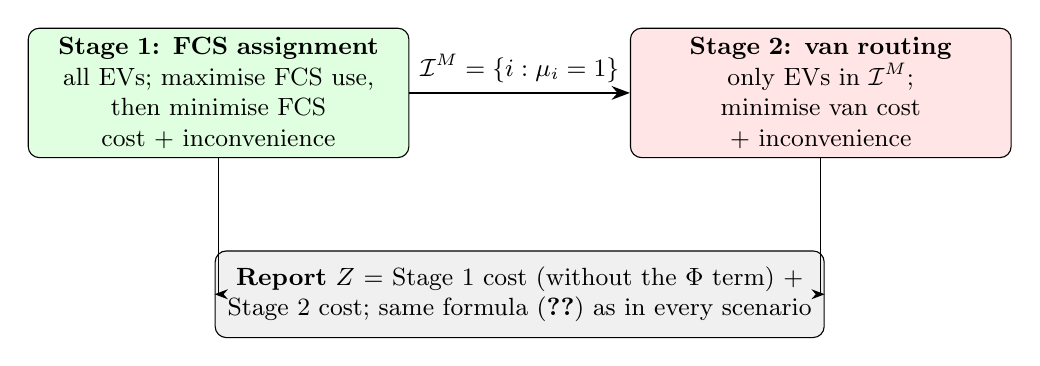
\begin{tikzpicture}[>=Stealth,box/.style={draw,rounded corners,align=center,minimum height=1.1cm,font=\small}]
  \node[box,fill=green!12,text width=4.6cm] (s1) {\textbf{Stage 1: FCS assignment}\\all EVs; maximise FCS use,\\then minimise FCS cost + inconvenience};
  \node[box,fill=red!10,text width=4.6cm,right=2.8cm of s1] (s2) {\textbf{Stage 2: van routing}\\only EVs in $\I^M$;\\minimise van cost + inconvenience};
  \draw[->,thick] (s1) -- node[above,font=\small]{$\I^M=\{i:\mu_i=1\}$} (s2);
  \node[box,fill=black!6,text width=7.5cm,below=2.0cm of $(s1)!0.5!(s2)$] (ev) {\textbf{Report} $Z=$ Stage~1 cost (without the $\Phi$ term) $+$ Stage~2 cost; same formula \eqref{eq:Z} as in every scenario};
  \draw[->] (s1) |- (ev); \draw[->] (s2) |- (ev);
\end{tikzpicture}
\end{center}

Stage~1 does not look at the vans, and Stage~2 cannot change what Stage~1 decided. That is the definition of ``FCS first, then MCS''.

%----------------------------------------------------------------
\subsection{Stage 1: assign EVs to fixed stations}

\textbf{Objective.}
\begin{equation}
\begin{split}
\min\ Z^{(1)}=\;&\underbrace{\Phi\sum_{i\in\I}\mu_i}_{\text{FCS first}}
+\underbrace{c^{EV}\sum_i\sum_{f\in\F_i}d_{if}Y_{if}}_{Z_1}
+\underbrace{Z^F_{\text{energy}}}_{\text{FCS part of }Z_4}\\
&+\underbrace{\sum_i\sum_{f\in\F_i}\rho^F_{if}Y_{if}+\alpha\sum_i w_i(C_i-r_i)+c^L\sum_i w_iL_i}_{\text{FCS customers' inconvenience}}
\end{split}
\label{eq:obj1}
\end{equation}
with $C_i=S_i+\tau^F_iY_i$ in this stage. $\Phi$ is a penalty for handing an EV to the vans. It is chosen larger than anything an extra FCS customer can add to the rest of \eqref{eq:obj1}, e.g.
\[
\Phi > \max_{i}\max_{f\in\F_i}\big(c^{EV}d_{if}+\pi^{\max}E_i+\rho^F_{if}\big)+n\,(\alpha+c^L)\,w_{\max}\,T,
\]
so Stage~1 first \textbf{maximises the number of EVs served at an FCS}, and only among those solutions minimises FCS cost and inconvenience. ($\pi^{\max}$ is the highest grid price.) A numerically safer equivalent is to solve twice: first $\max\sum_iY_i$, then fix that number and minimise the rest.
\ifTOU
Because $Z^F_{\text{energy}}$ uses the peak price, Stage~1 may \emph{start sessions later} to leave the peak, if the price saving beats the extra waiting cost (Section~\ref{sec:expect}).
\fi

\textbf{Constraints.}
\begin{align}
\sum_{g\in\G_i}y_{ig}+\mu_i &= 1 && \forall i\in\I \label{eq:s1assign}\\
S_i &\ge r_i+\sum_{f\in\F_i}t_{if}Y_{if} && \forall i\in\I \label{eq:fcsarr}\\
S_i &\le r_i+T\,(1-\mu_i) && \forall i\in\I \label{eq:s1park}\\
S_j &\ge S_i+\tau^F_i-(T+\tau^F_i)(3-y_{ig}-y_{jg}-o_{ij}) && \forall g,\ (i,j)\in\mathcal{P}_g \label{eq:disj1}\\
S_i &\ge S_j+\tau^F_j-(T+\tau^F_j)(2-y_{ig}-y_{jg}+o_{ij}) && \forall g,\ (i,j)\in\mathcal{P}_g \label{eq:disj2}\\
\sum_i y_{ig_1} &\ge \sum_i y_{ig_2} && \forall f,\ \G_f=\{g_1,g_2\} \label{eq:gunsym}\\
S_i+\tau^F_iY_i &\le T,\qquad L_i\ge S_i+\tau^F_iY_i-l_i && \forall i\in\I \label{eq:s1time}
\end{align}
\ifTOU plus the time-of-use split \eqref{eq:tou1}--\eqref{eq:tou5} of each FCS session (Section~\ref{sec:price}).\fi
\desc{\eqref{eq:s1assign}: every EV either gets one reachable gun or is handed to the vans. An EV that reaches no FCS ($\G_i=\emptyset$) is forced to $\mu_i=1$. \eqref{eq:fcsarr}: an FCS session cannot start before the EV has asked and driven to the station. \eqref{eq:s1park}: for an EV handed to the vans, $S_i$ is parked at $r_i$, so it adds no waiting in Stage~1 (its real start time is decided in Stage~2). \eqref{eq:disj1}--\eqref{eq:disj2}: two EVs on the same gun do not overlap; $o_{ij}$ picks who goes first. With two guns per station this means at most two EVs charge at a station at a time. \eqref{eq:gunsym}: symmetry breaking between the two identical guns (optional). \eqref{eq:s1time}: finished by $T$; lateness.}

\textbf{Optional acceptability rule.} An operator may refuse to send a driver to a station that is ``too inconvenient'', e.g.\ only allow gun $g$ of station $f$ for EV $i$ if $\hat\rho^F_{if}\le\bar\rho$. This only shrinks $\G_i$, so EVs whose stations are all too far go to the vans. Report results with and without it.

\textbf{Output:} $\I^M=\{i:\mu_i=1\}$, the EVs left for the vans; plus each FCS customer's gun and start time.

%----------------------------------------------------------------
\subsection{Stage 2: route the vans to the leftover EVs}

Stage~2 is a vehicle routing problem with time windows, on the EVs in $\I^M$ only. Here $C_i=S_i+\tau^M_i$.

\textbf{Objective.}
\begin{equation}
\begin{split}
\min\ Z^{(2)}=\;&\underbrace{c^M\sum_m\sum_{(i,j)\in\A^M}d_{ij}x_{ijm}}_{Z_2}+\underbrace{\sum_m c^D_mu_m}_{Z_3}+\underbrace{Z^M_{\text{energy}}}_{\text{van part of }Z_4}\\
&+\underbrace{\sum_{i\in\I^M}\sum_m\rho^M_{im}z_{im}+\alpha\sum_{i\in\I^M}w_i(C_i-r_i)+c^L\sum_{i\in\I^M}w_iL_i}_{\text{van customers' inconvenience}}
\end{split}
\label{eq:obj2}
\end{equation}
Since every EV in $\I^M$ must be served by some van, $Z^M_{\text{energy}}$ and the $\rho^M$ term are constants here. They are kept so that $Z^{(2)}$ is the true cost of Stage~2. Waiting and lateness make the vans visit urgent EVs early.

\textbf{Constraints.}
\begin{align}
\sum_{m\in\M}z_{im} &= 1 && \forall i\in\I^M \label{eq:s2assign}\\
\sum_{j:(0,j)\in\A^M}x_{0jm} = \sum_{i:(i,n+1)\in\A^M}x_{i,n+1,m} &= u_m && \forall m \label{eq:depot}\\
\sum_{i:(i,j)\in\A^M}x_{ijm} = \sum_{k:(j,k)\in\A^M}x_{jkm} &= z_{jm} && \forall j\in\I^M,\ m \label{eq:flow}\\
\sum_{i\in\I^M}z_{im} &\le Q_m\,u_m && \forall m \label{eq:cap}\\
\sum_{i\in\I^M}\frac{E_i}{\eta}z_{im}+\beta\sum_{(i,j)\in\A^M}d_{ij}x_{ijm} &\le B_m\,u_m && \forall m \label{eq:batt}
\end{align}
\begin{align}
S_j &\ge \max\{r_j,\ t_{0j}\,x_{0jm}\} && \forall j\in\I^M,\ m \label{eq:depart}\\
S_j &\ge S_i+\tau^M_i+t_{ij}-(T+\tau^M_i+t_{ij})(1-x_{ijm}) && \forall i\neq j,\ m \label{eq:seq}\\
S_i+\tau^M_i+t_{i,n+1} &\le T+(\tau^M_i+t_{i,n+1})(1-x_{i,n+1,m}) && \forall i,\ m \label{eq:return}\\
S_i+\tau^M_i \le T,\quad L_i &\ge S_i+\tau^M_i-l_i && \forall i\in\I^M \label{eq:s2time}\\
u_m &\ge u_{m+1} && m<|\M| \label{eq:vansym}
\end{align}
\desc{\eqref{eq:s2assign}: each leftover EV gets one van. \eqref{eq:depot}: a used van leaves and returns to the depot once. \eqref{eq:flow}: each EV on van $m$ is entered and left exactly once by that van. \eqref{eq:cap}: at most $Q_m$ EVs per van. \eqref{eq:batt}: delivered energy (with transfer losses) plus driving energy fits in the van battery. \eqref{eq:depart}: no start before the request, or before the van can drive there from the depot (written as two linear constraints). \eqref{eq:seq}: if the van goes $i\to j$, it finishes $i$ and drives to $j$ before starting $j$. This gives one EV at a time and removes subtours (MTZ-type). \eqref{eq:return}: back at the depot by $T$. \eqref{eq:s2time}: finished by $T$; lateness. \eqref{eq:vansym}: use identical vans in index order.}

\textbf{If Stage 2 is infeasible} (too many leftover EVs for the fleet by $T$), the sequential policy has \emph{failed} on that instance. For diagnosis, add $s_i\in\{0,1\}$ (``unserved''), replace \eqref{eq:s2assign} by $\sum_mz_{im}+s_i=1$ and add $\Phi^U\sum_is_i$ to \eqref{eq:obj2}. Then report the number of EVs that could not be served. This is a useful comparison with the integrated scenario, which may serve all of them.

%----------------------------------------------------------------
\subsection{Reported value}
\[
Z^{\text{S\scen}}=\big(Z^{(1)*}-\Phi\,|\I^M|\big)+Z^{(2)*},
\]
which is exactly \eqref{eq:Z} evaluated at the combined solution. The stage-1 solution plus the stage-2 solution is a feasible solution of the integrated model (S\ifTOU 4\else 3\fi), so
$Z^{\text{S\ifTOU 4\else 3\fi}}\le Z^{\text{S\scen}}$. The difference is the \emph{value of integration}.

\else
%---------------------------------------------------------------- INT
\subsection{Objective}
\begin{equation}
\min\ Z \quad\text{as in \eqref{eq:Z}, with }Z^F_{\text{energy}}=\ifTOU P^F\textstyle\sum_i\big[\pi^\off(\theta^1_i+\theta^3_i)+\pi^\pk\theta^2_i\big]\else\pi^F\textstyle\sum_iE_iY_i\fi,\quad C_i=S_i+\tau^F_iY_i+\tau^M_iZ_i. \label{eq:objint}
\end{equation}
Written out in full:
\begin{align*}
\min\ Z=\;& c^{EV}\sum_i\sum_{f\in\F_i}d_{if}Y_{if}+c^M\sum_m\sum_{(i,j)\in\A}d_{ij}x_{ijm}+\sum_mc^D_mu_m\\
&+\ifTOU P^F\sum_i\big[\pi^\off(\theta^1_i+\theta^3_i)+\pi^\pk\theta^2_i\big]\else\pi^F\sum_iE_iY_i\fi
+\pi^M\sum_i\sum_m\frac{E_i}{\eta}z_{im}\\
&+\sum_i\sum_{f\in\F_i}\rho^F_{if}Y_{if}+\sum_i\sum_m\rho^M_{im}z_{im}+\alpha\sum_iw_i(C_i-r_i)+c^L\sum_iw_iL_i .
\end{align*}
Every term is linear. One model weighs everything at once: an EV goes to a van exactly when the van's extra km, dispatch and energy cost are outweighed by the effort and waiting it saves the driver\ifTOU, or by the peak-price energy it avoids\fi.

\subsection{Constraints}

\textbf{Assignment.}
\begin{equation}
\sum_{g\in\G_i}y_{ig}+\sum_{m\in\M}z_{im}=1\qquad\forall i\in\I \label{eq:assign}
\end{equation}
\desc{Exactly one resource per EV: one reachable gun or one van. EVs that reach no FCS are forced onto a van.}

\textbf{Fixed stations.}
\begin{align}
S_i &\ge r_i+\sum_{f\in\F_i}t_{if}Y_{if} && \forall i \label{eq:fcsarr}\\
S_j &\ge S_i+\tau^F_i-(T+\tau^F_i)(3-y_{ig}-y_{jg}-o_{ij}) && \forall g,\ (i,j)\in\mathcal{P}_g \label{eq:disj1}\\
S_i &\ge S_j+\tau^F_j-(T+\tau^F_j)(2-y_{ig}-y_{jg}+o_{ij}) && \forall g,\ (i,j)\in\mathcal{P}_g \label{eq:disj2}\\
\sum_iy_{ig_1} &\ge \sum_iy_{ig_2} && \forall f,\ \G_f=\{g_1,g_2\} \label{eq:gunsym}
\end{align}
\desc{\eqref{eq:fcsarr}: an FCS session starts after the request and the drive to the station (for a van customer this is just $S_i\ge r_i$). \eqref{eq:disj1}--\eqref{eq:disj2}: EVs on the same gun do not overlap; $o_{ij}$ chooses the order. \eqref{eq:gunsym}: optional symmetry breaking.}

\textbf{Vans: routes, capacity, battery.}
\begin{align}
\sum_{j:(0,j)\in\A}x_{0jm}=\sum_{i:(i,n+1)\in\A}x_{i,n+1,m} &= u_m && \forall m \label{eq:depot}\\
\sum_{i:(i,j)\in\A}x_{ijm}=\sum_{k:(j,k)\in\A}x_{jkm} &= z_{jm} && \forall j\in\I,\ m \label{eq:flow}\\
\sum_iz_{im} &\le Q_mu_m && \forall m \label{eq:cap}\\
\sum_i\frac{E_i}{\eta}z_{im}+\beta\sum_{(i,j)\in\A}d_{ij}x_{ijm} &\le B_mu_m && \forall m \label{eq:batt}
\end{align}
\desc{\eqref{eq:depot}: a used van leaves and returns once. \eqref{eq:flow}: each EV on van $m$ is visited exactly once by it. \eqref{eq:cap}: at most $Q_m$ EVs. \eqref{eq:batt}: delivered energy (with losses) plus driving energy fits in the battery.}

\textbf{Vans: timing (one EV at a time, no subtours).}
\begin{align}
S_j &\ge t_{0j}\,x_{0jm} && \forall j\in\I,\ m \label{eq:depart}\\
S_j &\ge S_i+\tau^M_i+t_{ij}-(T+\tau^M_i+t_{ij})(1-x_{ijm}) && \forall i\neq j\in\I,\ m \label{eq:seq}\\
S_i+\tau^M_i+t_{i,n+1} &\le T+(\tau^M_i+t_{i,n+1})(1-x_{i,n+1,m}) && \forall i,\ m \label{eq:return}
\end{align}
\desc{\eqref{eq:depart}: the first stop cannot start before the van has driven there. \eqref{eq:seq}: $i\to j$ means finish $i$, drive, then start $j$; start times rise along a route, so no subtour can close. \eqref{eq:return}: back at the depot by $T$.}

\textbf{Horizon and lateness.}
\begin{equation}
C_i\le T,\qquad L_i\ge C_i-l_i\qquad\forall i\in\I \label{eq:time}
\end{equation}
\desc{Every EV is fully charged within the horizon; $L_i$ measures lateness.}

\ifTOU
\textbf{Time-of-use split.} Constraints \eqref{eq:tou1}--\eqref{eq:tou5} of Section~\ref{sec:price}.
\fi

\textbf{Symmetry and domains.}
\begin{equation}
u_m\ge u_{m+1};\qquad y,z,x,u,o\ifTOU,\kappa\fi\in\{0,1\};\qquad S_i,L_i\ifTOU,\theta^p_i\fi\ge0 \label{eq:dom}
\end{equation}
\fi

%=====================================================================
\section{Learning-to-optimise (RL) formulation}\label{sec:rl}

\textbf{Main rule:} the reward of each action is \emph{minus the increase in $Z$ that the action causes}. The rewards over an episode then add up to $-Z$ of the solution the policy builds. RL and MILP results are measured on the same yardstick \eqref{eq:Z}, and the MILP optimum is the benchmark for the RL gap.

\ifSEQ
%---------------------------------------------------------------- RL SEQ
The RL pipeline has the same two stages as the MILP.

\subsection{Stage 1 policy: FCS assignment}
\begin{itemize}[leftmargin=1.4em,itemsep=2pt]
  \item \textbf{Episode / epochs:} EVs are taken in order of request time $r_i$ (ties: higher $w_i$ first). One decision per EV.
  \item \textbf{State:} features of the current EV $k$ ($E_k,r_k,l_k,w_k,R_k$, location); for each gun $g$ the time $F_g$ it becomes free; summary features of the EVs still to come (count and positions near each station)\ifTOU; the current price and the time until $T_1$ and $T_2$\fi.
  \item \textbf{Action:} a gun $g\in\G_k$, or ``hand to vans''. \textbf{FCS-first mask:} ``hand to vans'' is allowed \emph{only} if no gun can finish EV $k$ by $T$ (or, with the optional rule, if all remaining guns have $\hat\rho^F_{kf}>\bar\rho$).
  \ifTOU\item \textbf{Optional timing action:} ``gun $g$, start after the peak'', i.e.\ $S_k=\max\{\text{earliest},T_2\}$, allowed only if the session still ends by $T$.\fi
  \item \textbf{Transition:} $S_k=\max\{r_k+t_{kf},F_g\}$ (or later, for the timing action); $F_g\leftarrow S_k+\tau^F_k$.
  \item \textbf{Reward:} $-\Big[c^{EV}d_{kf}+\text{energy}_k+\rho^F_{kf}+\alpha w_k(S_k+\tau^F_k-r_k)+c^Lw_k(S_k+\tau^F_k-l_k)^+\Big]$, where energy$_k$ = \ifTOU$P^F\big[\pi^\off\cdot(\text{off-peak hours of }[S_k,S_k+\tau^F_k])+\pi^\pk\cdot(\text{peak hours})\big]$, computed exactly in the simulator\else$\pi^FE_k$\fi. Handing an EV to the vans gives reward $0$ here; its cost is counted in Stage~2.
\end{itemize}
Note: a simple baseline for Stage~1 is the greedy rule ``gun with the largest one-step reward''. What RL can learn on top of this is, for example, to keep a nearby gun free for an urgent EV that arrives later.

\subsection{Stage 2 policy: van routing over $\I^M$}
\begin{itemize}[leftmargin=1.4em,itemsep=2pt]
  \item \textbf{Epochs:} whenever a van becomes free (the earliest-free van decides first).
  \item \textbf{State:} for each van: position, time free, remaining battery $b_m$, EVs served so far, dispatched or not; for each unserved EV in $\I^M$: location, $E_i,r_i,l_i,w_i$; current time.
  \item \textbf{Action:} the next EV $j$ for this van, or ``return to depot'' (ends the route). Mask: $j$ must be feasible: battery covers $E_j/\eta$ plus driving to $j$ and back to the depot, the count stays $\le Q_m$, and $j$ can be finished with the van back at the depot by $T$.
  \item \textbf{Transition:} $S_j=\max\{r_j,\ \text{time free}+t_{\text{pos},j}\}$; the van moves to $j$ and is free at $S_j+\tau^M_j$; $b_m$ falls by $E_j/\eta+\beta d_{\text{pos},j}$.
  \item \textbf{Reward:} serving $j$: $-\Big[c^Md_{\text{pos},j}+c^D_m[\text{first stop}]+\pi^M\frac{E_j}{\eta}+\rho^M_{jm}+\alpha w_j(S_j+\tau^M_j-r_j)+c^Lw_j(S_j+\tau^M_j-l_j)^+\Big]$; returning: $-c^Md_{\text{pos},0}$. EVs still unserved at the end: $-\Phi^U$ each.
  \item \textbf{Policy:} an attention-based routing policy (e.g.\ Kool et al., 2019, ``Attention, Learn to Solve Routing Problems!'') trained with REINFORCE or PPO. Baseline: nearest-feasible-EV heuristic.
\end{itemize}
Episode return of Stage~1 + Stage~2 $=-Z^{\text{S\scen}}$.

\else
%---------------------------------------------------------------- RL INT
One policy decides both who serves each EV and the van routes.
\begin{itemize}[leftmargin=1.4em,itemsep=2pt]
  \item \textbf{Episode / epochs:} EVs are taken in order of request time $r_i$ (ties: higher $w_i$ first). One decision per EV.
  \item \textbf{State:} (i) the current EV $k$: location, $E_k,r_k,l_k,w_k,R_k$, reachable stations; (ii) each gun $g$: time $F_g$ it becomes free; (iii) each van $m$: current end-of-route position, time free, remaining battery $b_m$, EVs served, dispatched or not; (iv) embeddings of the not-yet-assigned EVs (for look-ahead)\ifTOU; (v) current price, time until $T_1$ and $T_2$\fi.
  \item \textbf{Action:} $a\in\G_k\cup\M$: a gun, or a van (EV $k$ is appended to the end of that van's route). \textbf{Mask} infeasible actions: a gun that cannot finish $k$ by $T$; a van without enough battery for $E_k/\eta$ plus the drive to $k$ and back to the depot, with $Q_m$ reached, or unable to finish $k$ and return by $T$.
  \ifTOU\item \textbf{Optional timing action:} ``gun $g$, start after the peak'' ($S_k=\max\{\text{earliest},T_2\}$, if it still ends by $T$).\fi
  \item \textbf{Transition:} gun: $S_k=\max\{r_k+t_{kf},F_g\}$, $F_g\leftarrow S_k+\tau^F_k$. Van: $S_k=\max\{r_k,\ \text{free}_m+t_{\text{pos}_m,k}\}$, then the van moves to $k$, $\text{free}_m\leftarrow S_k+\tau^M_k$, $b_m\mathrel{-}=E_k/\eta+\beta d_{\text{pos}_m,k}$.
  \item \textbf{Reward} $=-\Delta Z$:
  \begin{align*}
  \text{gun } g\text{ at }f:&\quad -\Big[c^{EV}d_{kf}+\text{energy}^F_k+\rho^F_{kf}+\alpha w_k(C_k-r_k)+c^Lw_k(C_k-l_k)^+\Big]\\
  \text{van } m:&\quad -\Big[c^M\big(d_{\text{pos}_m,k}+d_{k,0}-d_{\text{pos}_m,0}\big)+c^D_m[\text{first use}]+\pi^M\tfrac{E_k}{\eta}\\
  &\qquad\quad+\rho^M_{km}+\alpha w_k(C_k-r_k)+c^Lw_k(C_k-l_k)^+\Big]
  \end{align*}
  The van distance term is the \emph{change} in route length when $k$ is inserted before the return to the depot, so the sum over the episode equals the total route length (the return legs telescope). energy$^F_k$ = \ifTOU$P^F\big[\pi^\off\cdot(\text{off-peak hours})+\pi^\pk\cdot(\text{peak hours of }[S_k,C_k])\big]$, computed exactly by the simulator; no linearisation is needed in RL\else$\pi^FE_k$\fi.
  \item \textbf{Dead end:} if every action is masked, EV $k$ is unserved: reward $-\Phi^U$, and the episode continues. Report the count.
  \item \textbf{Policy:} masked categorical policy over guns and vans, encoder with attention over EVs, guns and vans; trained with PPO. Natural baseline: greedy, i.e.\ choose the action with the largest one-step reward. That is the pairwise rule ``smallest $\hat\rho$ + cost'' from Section~\ref{sec:inc}.
\end{itemize}
Restriction to note: vans serve EVs in assignment order (append only). A variant that inserts $k$ at the cheapest position of a route is more flexible but has a larger action space.
\fi

\textbf{Reward scaling.} For stable training divide every reward by a constant, e.g.\ the greedy baseline's average $Z$ on the training instances. This does not change the optimal policy.

%=====================================================================
\section{What to expect and what to report}\label{sec:expect}

\ifnum\scen=1
\begin{itemize}[leftmargin=1.4em,itemsep=2pt]
  \item Vans serve only EVs that reach no station, or that the stations cannot finish by $T$. If stations have spare capacity, very few vans are dispatched.
  \item Inconvenience is high for EVs far from the nearest station (worked example: Rs\,682 at the FCS, against Rs\,458 if a van had been allowed).
  \item With too few vans Stage~2 becomes infeasible (unserved EVs), even when the integrated model S3 could serve everyone. Report the smallest $|\M|$ at which S1 is feasible and compare it with S3.
\end{itemize}
\fi
\ifnum\scen=2
\begin{itemize}[leftmargin=1.4em,itemsep=2pt]
  \item \textbf{When does Stage~1 delay a session to avoid the peak?} Moving one hour of charging out of the peak saves $(\pi^\pk-\pi^\off)P^F=3\times22=$ Rs\,66, but delays completion by up to an hour, which costs $\alpha w_i\ge$ Rs\,200. So with the default values Stage~1 almost never delays. It mostly pays the higher price, and S2 costs roughly S1 plus the peak surcharge. Sessions start later only if $\alpha$ is small (try $\lambda<0.33$ in the sensitivity analysis).
  \item The van assignment is the same as in S1 unless Stage~1's timing changes which EVs fit at the stations. Stage~1 cannot use vans to escape the peak price.
  \item Extra KPI: \textbf{grid energy drawn at FCS during the peak}, $P^F\sum_i\theta^2_i$ (kWh). Compare with S4.
\end{itemize}
\fi
\ifnum\scen=3
\begin{itemize}[leftmargin=1.4em,itemsep=2pt]
  \item Vans take EVs for which the saved inconvenience exceeds the extra van cost (worked example: van chosen, saving Rs\,224). Expect vans to serve EVs that are far from every station, have low range (high $w_i$), or have early deadlines, while EVs near a station still use it.
  \item \textbf{Value of integration under flat price:} $Z^{\text{S1}}-Z^{\text{S3}}\ge0$. Report it per component ($Z_1,\dots,Z_5$): typically operating cost rises a little and inconvenience falls a lot.
  \item Vary $|\M|$ (0, 1, 2, \dots): the first few vans lower $Z$ sharply, then the effect levels off. That curve shows the scenarios where mobile chargers help most.
\end{itemize}
\fi
\ifnum\scen=4
\begin{itemize}[leftmargin=1.4em,itemsep=2pt]
  \item During the peak a van kWh costs about the same as an FCS kWh (Rs\,10.0 each), so the vans' energy disadvantage disappears and vans also absorb \emph{peak-hour} demand that would otherwise be charged on the grid at peak price.
  \item Expect more van usage than in S3, concentrated on requests in $[T_1,T_2]$, and lower grid energy at the stations during the peak, $P^F\sum_i\theta^2_i$, than in S2.
  \item \textbf{Value of integration under peak pricing:} $Z^{\text{S2}}-Z^{\text{S4}}$. It should be larger than $Z^{\text{S1}}-Z^{\text{S3}}$, because integration now also allows price arbitrage.
  \item \textbf{Peak pricing with full flexibility:} $Z^{\text{S4}}-Z^{\text{S3}}$ should be smaller than $Z^{\text{S2}}-Z^{\text{S1}}$: vans cushion the price increase.
\end{itemize}
\fi

\textbf{Cross-scenario comparison table} (fill in from the four runs):
\begin{center}
\renewcommand{\arraystretch}{1.2}
\begin{tabular}{@{}lll@{}}
\toprule
\textbf{Comparison} & \textbf{Measures} & \textbf{Expected sign} \\
\midrule
S1 $-$ S3 & value of integration, flat price & $\ge0$ \\
S2 $-$ S4 & value of integration, peak price & $\ge0$, larger than S1 $-$ S3 \\
S2 $-$ S1 & cost of peak pricing, FCS-first operator & $>0$ \\
S4 $-$ S3 & cost of peak pricing, flexible operator & $>0$, smaller than S2 $-$ S1 \\
\bottomrule
\end{tabular}
\end{center}
Report for each: $Z$ and its components, number of vans used, EVs per resource, mean and maximum inconvenience per EV, total lateness, peak-hour grid energy, solve time, and (for RL) the gap to the MILP optimum.

%=====================================================================
\appendix
\section{Illustrative parameter values}\label{app:values}

These are starting values for experiments, not data. All are meant to be varied in the analysis. Values in Rs.

\begin{center}
\renewcommand{\arraystretch}{1.15}
\begin{tabular}{@{}llp{6.2cm}@{}}
\toprule
\textbf{Parameter} & \textbf{Value} & \textbf{Note} \\
\midrule
$T$, $[T_1,T_2]$ & 7 h, $[2,6]$ & 16:00--23:00, peak 18:00--22:00 \\
$P^F$, $P^M$ & 22 kW, 30 kW & \\
$v$, $\beta$, $\eta$ & 25 km/h, 0.25 kWh/km, 0.9 & \\
$B_m$, $Q_m$, $|\M|$ & 150 kWh, 6, 2--6 & \\
$c^{EV}$, $c^M$, $c^D_m$ & Rs\,4/km, Rs\,15/km, Rs\,1500 & van km includes driver time \\
$\pi^F$ (flat) & Rs\,8.7/kWh & equals the time-average of the ToU tariff over $[0,T]$ \\
$\pi^\off$, $\pi^\pk$ (ToU) & Rs\,7/kWh, Rs\,10/kWh & $(3\times7+4\times10)/7=8.7$ \\
$c^{bat}$ & Rs\,2/kWh & van battery wear \\
$\pi^M$ & Rs\,10.7 (flat) / Rs\,9.0 (ToU) & $=\pi^F+c^{bat}$ / $=\pi^\off+c^{bat}$ \\
$\alpha$, $\alpha^D$ & Rs\,200/h, Rs\,100/h & value of time; extra for attended time \\
$h^F$, $h^M$, $\varphi$ & Rs\,50, Rs\,10, Rs\,100 & trip hassle, hand-over, range stress \\
$c^L$ & Rs\,300/h & lateness \\
$w_i$ & $1+2(1-R_i/R_{\max})$, $R_i\sim U[3,40]$ km & priority from remaining range \\
\bottomrule
\end{tabular}
\end{center}

The flat price is set to the time-average of the peak tariff. The price \emph{level} is then the same in both pricing cases, and only the price \emph{shape} differs. Without this, part of S1 vs S2 would just reflect a different average price.

\end{document}
"
%    pdflatex -jobname=scenario2_peak_sequential   "\def\scen{2}% =====================================================================
%  One source, four PDFs.  Build with build.sh (or by hand):
%    pdflatex -jobname=scenario1_flat_sequential   "\def\scen{1}\input{scenario_master}"
%    pdflatex -jobname=scenario2_peak_sequential   "\def\scen{2}\input{scenario_master}"
%    pdflatex -jobname=scenario3_flat_integrated   "\def\scen{3}\input{scenario_master}"
%    pdflatex -jobname=scenario4_peak_integrated   "\def\scen{4}\input{scenario_master}"
%  (run each twice for cross-references)
% =====================================================================
\documentclass[11pt,a4paper]{article}
\usepackage[margin=2.2cm]{geometry}
\usepackage{amsmath,amssymb,amsfonts}
\usepackage{booktabs,array,tabularx}
\usepackage{enumitem}
\usepackage[table]{xcolor}
\usepackage{tikz}
\usetikzlibrary{arrows.meta,positioning,calc}
\usepackage[colorlinks=true,linkcolor=blue!50!black,urlcolor=blue!50!black]{hyperref}
\usepackage{titlesec}
\titleformat{\section}{\large\bfseries}{\thesection}{0.8em}{}
\titleformat{\subsection}{\normalsize\bfseries}{\thesubsection}{0.8em}{}
\setlength{\parindent}{0pt}
\setlength{\parskip}{5pt}

% ---------------- scenario switches ----------------
\ifdefined\scen\else\def\scen{1}\fi
\newif\ifTOU \TOUfalse   % true = time-of-use (peak) price
\newif\ifSEQ \SEQfalse   % true = FCS first, then MCS
\ifnum\scen=1 \SEQtrue \fi
\ifnum\scen=2 \TOUtrue \SEQtrue \fi
\ifnum\scen=4 \TOUtrue \fi

\newcommand{\pricename}{\ifTOU time-of-use price (dearer evening peak)\else single (flat) price all day\fi}
\newcommand{\structname}{\ifSEQ FCS first, then MCS (sequential)\else FCS and MCS together (integrated)\fi}

% ---------------- notation ----------------
\newcommand{\I}{\mathcal{I}}
\newcommand{\F}{\mathcal{F}}
\newcommand{\G}{\mathcal{G}}
\newcommand{\M}{\mathcal{M}}
\newcommand{\N}{\mathcal{N}}
\newcommand{\A}{\mathcal{A}}
\newcommand{\Rs}{\text{Rs}\,}
\newcommand{\pk}{\mathrm{pk}}
\newcommand{\off}{\mathrm{off}}
\newcommand{\desc}[1]{\par\vspace{-2pt}{\small\color{black!75}\textit{Meaning:} #1}\par\vspace{4pt}}
\newcommand{\cell}[2]{\ifnum\scen=#1\cellcolor{blue!18}\textbf{S#1 (this document)}\\\textbf{#2}\else S#1\\#2\fi}

\title{\textbf{EV Charging Network Optimisation}\\[4pt]
\large Scenario \scen: \pricename\ $+$ \structname\\[2pt]
\normalsize MILP and RL formulation}
\author{CP 320 OR for Mobility Management, course project}
\date{2 October 2026}

\begin{document}
\maketitle

%=====================================================================
\section{Where this scenario sits}

The project studies four scenarios: two ways of pricing grid electricity, times two ways of making the decisions.

\begin{center}
\renewcommand{\arraystretch}{1.5}
\begin{tabular}{>{\raggedright\arraybackslash}p{4.2cm}|>{\centering\arraybackslash}p{4.6cm}|>{\centering\arraybackslash}p{4.6cm}}
 & \textbf{Flat price all day} & \textbf{Time-of-use (peak) price} \\ \hline
\textbf{Sequential:} FCS first, leftover EVs to MCS &
\begin{tabular}[c]{@{}c@{}}\cell{1}{flat + sequential}\end{tabular} &
\begin{tabular}[c]{@{}c@{}}\cell{2}{peak + sequential}\end{tabular} \\ \hline
\textbf{Integrated:} FCS and MCS decided together &
\begin{tabular}[c]{@{}c@{}}\cell{3}{flat + integrated}\end{tabular} &
\begin{tabular}[c]{@{}c@{}}\cell{4}{peak + integrated}\end{tabular} \\
\end{tabular}
\end{center}

\textbf{The four scenarios do not have four different objectives.} They share \emph{one} cost yardstick $Z$ (Section~\ref{sec:obj}): the same cost terms and the same customer inconvenience (Section~\ref{sec:inc}). Only two things change:
\begin{itemize}[leftmargin=1.4em,itemsep=1pt]
  \item \textbf{Pricing} changes the formula for one term, the FCS energy cost (Section~\ref{sec:price}).
  \item \textbf{Decision structure} changes \emph{how} $Z$ is minimised: in one model (integrated), or in two stages (sequential), where each stage minimises its own part of $Z$.
\end{itemize}
Because the yardstick is the same, the four optimal values can be compared directly. The differences measure the \emph{value of integration} (S1$\to$S3, S2$\to$S4) and the \emph{effect of peak pricing} (S1$\to$S2, S3$\to$S4).

\ifnum\scen=1
\textbf{This scenario (S1)} is the baseline, the ``status quo''. Electricity costs the same at every hour, every EV that can be charged at a fixed station is sent there, and vans only take what is left over.
\fi
\ifnum\scen=2
\textbf{This scenario (S2)} keeps the FCS-first rule of S1, but grid electricity is dearer during the evening peak. Stage~1 can react to the price only by \emph{rescheduling} FCS sessions. It cannot hand a peak-hour EV to a van.
\fi
\ifnum\scen=3
\textbf{This scenario (S3)} keeps the flat price of S1, but the operator decides FCS and MCS service \emph{together}. An EV can be sent to a van even when a fixed station could take it, whenever that lowers total cost plus inconvenience.
\fi
\ifnum\scen=4
\textbf{This scenario (S4)} is the most flexible one: peak pricing at fixed stations, and FCS and MCS decided together. Van energy was bought off-peak, so vans can also be used to keep charging \emph{out of the expensive peak}.
\fi

%=====================================================================
\section{Setting and assumptions}\label{sec:setting}

\textbf{Time.} The planning horizon is $[0,T]$ with $T=7$\,h (16:00--23:00). It contains the evening peak window $[T_1,T_2]=[2,6]$ (18:00--22:00). The horizon is the same in all four scenarios. It is wider than the peak itself so that, under peak pricing, there is cheaper time on both sides of the peak.\ifTOU\else\ In this scenario the price is flat, so the window plays no role in the model.\fi

\textbf{Assumptions} (the same as MILP v3, plus two about energy):
\begin{enumerate}[leftmargin=1.6em,itemsep=1pt]
  \item Static, continuous time. All requests in the horizon are known at time $0$, and request $i$ becomes active at $r_i$.
  \item An EV served by an FCS drives there itself on its own battery (only to stations within its range $R_i$). The driver stays with the car while it waits for a free gun and while it charges.
  \item An EV served by an MCS stays parked where it is, and the driver is free in the meantime.
  \item Each FCS gun and each van charges one EV at a time, without interruption, at constant power.
  \item A van's battery covers both its driving and the energy it delivers. \textbf{The van battery is charged at the depot before the horizon starts}\ifTOU, i.e.\ at the off-peak price\fi, and is not recharged during the horizon.
  \item Every EV must be fully charged by $T$ (hard). Finishing after the driver's desired time $l_i$ is allowed but penalised.
\end{enumerate}

%=====================================================================
\section{Notation}\label{sec:notation}

\subsection*{Sets}
\begin{tabularx}{\textwidth}{@{}lX@{}}
\toprule
$\I=\{1,\dots,n\}$ & EV charging requests \\
$\F$; $\G_f$ ($|\G_f|=2$); $\G=\bigcup_f\G_f$ & fixed charging stations; guns of FCS $f$; all guns ($f(g)$ = station of gun $g$) \\
$\F_i=\{f: d_{if}\le R_i\}$, $\G_i=\bigcup_{f\in\F_i}\G_f$ & stations / guns EV $i$ can reach on its remaining range \\
$\M$ & mobile charging vans (MCS) \\
$0,\ n+1$ & depot as start node / end node (same place) \\
$\N=\{0\}\cup\I\cup\{n+1\}$, $\A$ & routing nodes; allowed van arcs $(i,j)$, $i\in\{0\}\cup\I$, $j\in\I\cup\{n+1\}$, $i\neq j$ \\
$\mathcal{P}_g=\{(i,j): i<j,\ g\in\G_i\cap\G_j\}$ & pairs of EVs that could share gun $g$ \\
\ifSEQ
$\I^M\subseteq\I$ & EVs handed to the vans by Stage~1 (an \emph{output} of Stage~1, a fixed input to Stage~2) \\
$\N^M$, $\A^M$ & routing nodes / arcs restricted to $\I^M$ \\
\fi
\bottomrule
\end{tabularx}

\subsection*{Parameters}
\begin{tabularx}{\textwidth}{@{}lX@{}}
\toprule
$E_i,\ r_i,\ l_i,\ R_i$ & energy demand (kWh), request time, desired completion time (h), remaining range (km) \\
$w_i\ge1$ & priority of EV $i$; $w_i=1+\kappa(1-R_i/R_{\max})$, so low-range EVs weigh more \\
$P^F,\ P^M$ & charging power of an FCS gun (22\,kW) / of a van (e.g.\ 30\,kW) \\
$\tau^F_i=E_i/P^F,\ \tau^M_i=E_i/P^M$ & charging time of EV $i$ at an FCS / by a van (h) \\
$d_{if},t_{if}$;\ $d_{ij},t_{ij}$ & distance (km) and time (h): EV$\to$FCS; between routing nodes ($t=d/v$) \\
$B_m,\ Q_m,\ \beta,\ \eta$ & van battery (kWh), max EVs per van, van consumption (kWh/km), transfer efficiency \\
$c^{EV},\ c^M,\ c^D_m$ & cost per km of EV driving, per km of van driving; fixed dispatch cost of van $m$ \\
\ifTOU
$\pi^\off,\ \pi^\pk$ & grid price (Rs/kWh) off-peak / in $[T_1,T_2]$, with $\pi^\pk\ge\pi^\off$ \\
\else
$\pi^F$ & grid price (Rs/kWh), the same at every hour \\
\fi
$c^{bat}$ & van battery wear per kWh cycled \\
$\pi^M$ & cost of 1 kWh taken from a van battery: $\pi^M=\ifTOU\pi^\off\else\pi^F\fi+c^{bat}$ (Section~\ref{sec:price}) \\
$\alpha,\ \alpha^D,\ h^F,\ h^M,\ \varphi,\ c^L$ & inconvenience coefficients (Section~\ref{sec:inc}) \\
\bottomrule
\end{tabularx}

\subsection*{Decision variables}
\begin{tabularx}{\textwidth}{@{}llX@{}}
\toprule
$y_{ig}$ & $\{0,1\}$ & EV $i$ charged at gun $g\in\G_i$ \\
$z_{im}$ & $\{0,1\}$ & EV $i$ served by van $m$ \\
$x_{ijm}$ & $\{0,1\}$ & van $m$ drives arc $(i,j)$ \\
$u_m$ & $\{0,1\}$ & van $m$ is dispatched \\
$o_{ij}$ & $\{0,1\}$ & for EVs $i<j$ that could share a gun: 1 if $i$ is charged before $j$ \\
\ifSEQ
$\mu_i$ & $\{0,1\}$ & Stage~1 only: EV $i$ is handed to the van fleet \\
\fi
\ifTOU
$\theta^1_i,\theta^2_i,\theta^3_i$ & $\ge0$ & hours of EV $i$'s FCS session before / inside / after the peak \\
$\kappa^1_i,\kappa^3_i$ & $\{0,1\}$ & EV $i$'s FCS session starts before $T_1$ / ends after $T_2$ \\
\fi
$S_i$ & $\ge0$ & time charging of EV $i$ starts (h), on whichever resource \\
$L_i$ & $\ge0$ & lateness of EV $i$ beyond $l_i$ (h) \\
\bottomrule
\end{tabularx}

\textbf{Short-hands} (linear expressions, not new variables):
\[
Y_{if}=\sum_{g\in\G_f}y_{ig},\qquad Y_i=\sum_{g\in\G_i}y_{ig}\ (\text{EV $i$ uses an FCS}),\qquad Z_i=\sum_{m\in\M}z_{im}\ (\text{EV $i$ uses a van}),
\]
\[
C_i=S_i+\tau^F_i\,Y_i+\tau^M_i\,Z_i \quad\text{(time EV $i$ is fully charged).}
\]

%=====================================================================
\section{Customer inconvenience}\label{sec:inc}

This section is \textbf{identical in all four scenario documents}. Inconvenience is a property of the customer, not of the price or of the planning method.

\subsection{What we mean by inconvenience}

Inconvenience is \emph{what the driver loses} from the moment they ask for a charge ($r_i$) until the car is fully charged ($C_i$), \emph{converted into rupees} so it can be added to the operator's costs. A driver loses three different things:

\begin{enumerate}[leftmargin=1.6em,itemsep=2pt]
  \item \textbf{Waiting:} the car is not ready. This lasts $C_i-r_i$ hours and affects \emph{every} driver, FCS or MCS.
  \item \textbf{Effort:} only an FCS customer has to drive to the station and sit there while the car charges. An MCS customer stays at home or at work and does something else. Driving to a far station also uses scarce battery range, which causes stress (``range anxiety'').
  \item \textbf{A missed deadline:} the car is still not ready at the time $l_i$ the driver needs it.
\end{enumerate}

Each loss gets a price in Rs per hour (or per event). All of them are multiplied by the priority $w_i$: an hour of delay for an EV with 5\,km of range left counts more than for one with 40\,km.

\subsection{The three components}

\begin{center}
\renewcommand{\arraystretch}{1.3}
\begin{tabularx}{\textwidth}{@{}>{\raggedright\arraybackslash}p{2.6cm}>{\raggedright\arraybackslash}X>{\raggedright\arraybackslash}X>{\raggedright\arraybackslash}p{3.0cm}@{}}
\toprule
\textbf{Component} & \textbf{EV $i$ at FCS $f$} & \textbf{EV $i$ by a van} & \textbf{Known when?} \\
\midrule
Effort & $w_i\big[\alpha^D(t_{if}+\tau^F_i)+h^F+\varphi\,d_{if}/R_i\big]$: driving and sitting at the station, a fixed trip hassle, range stress & $w_i\,h^M$: being reachable and handing over the car & \textbf{Static:} known as soon as the resource is chosen \\
Waiting & $w_i\,\alpha\,(C_i-r_i)$ = drive + \emph{queue at the gun} + charge & $w_i\,\alpha\,(C_i-r_i)$ = \emph{wait for the van} + charge & \textbf{Dynamic:} depends on the queue / van route \\
Missed deadline & $w_i\,c^L\,L_i$, $L_i=\max\{0,C_i-l_i\}$ & same & Dynamic \\
\bottomrule
\end{tabularx}
\end{center}

\textbf{Coefficients.}
$\alpha$ (Rs/h) is the value of an hour the car is not ready.
$\alpha^D$ (Rs/h) is the \emph{extra} value of an hour the driver must personally spend driving or sitting at the station: an hour at the station costs $\alpha+\alpha^D$, an hour waiting at home for a van costs only $\alpha$.
$h^F,h^M$ (Rs) are fixed hassle costs of one trip to a station / one van hand-over.
$\varphi$ (Rs) is the range-stress cost of a trip that uses the \emph{whole} remaining range ($d_{if}/R_i\le1$ is the fraction used).
$c^L$ (Rs/h) is the cost per hour late.

\subsection{Pairwise form: inconvenience of a (customer, resource) pair}

The natural first idea is: \emph{for every pair (EV $i$, FCS $f$) and every pair (EV $i$, van $m$) there is an inconvenience number, and the operator picks the pair with the lowest cost plus inconvenience.} The static part fits this idea exactly:
\[
\boxed{\;\rho^F_{if}=w_i\Big[\alpha^D\,(t_{if}+\tau^F_i)+h^F+\varphi\,\frac{d_{if}}{R_i}\Big]\qquad
\rho^M_{im}=w_i\,h^M\;}
\]
These are \textbf{parameters}, computed before solving, one number per (EV, FCS) pair and per (EV, van) pair. In the objective they appear linearly: $\sum_i\sum_f\rho^F_{if}Y_{if}+\sum_i\sum_m\rho^M_{im}z_{im}$.

Note that $\rho^M_{im}$ does not depend on $m$. Vans are identical and all start at the same depot, so the driver does not care \emph{which} van comes, only \emph{when} it comes. That ``when'' is the waiting part.

\subsection{Why waiting cannot be a fixed pairwise number}

It is tempting to also write the waiting as a pairwise number, e.g.\ ``the van needs 5 minutes to reach EV $i$''. But that depends on \emph{where the van is coming from}, which depends on the route the model is still choosing: if EV $i$ is the 4th stop of a van, the wait is the time for three charging sessions plus four drives. Likewise, waiting at an FCS depends on how many EVs are queued at that gun. So waiting is not known before solving. It is a function of decision variables:
\[
\text{waiting cost of EV } i \;=\; w_i\,\alpha\,(C_i-r_i),\qquad C_i=S_i+\tau^F_iY_i+\tau^M_iZ_i .
\]
This is \textbf{linear} in the variables ($S_i$, $y$, $z$), so it fits in a MILP directly. The constraints of Section~\ref{sec:milp} make $S_i$ equal to the true start time, including driving, queueing at the gun and the van's route. The term $\sum_i w_i\alpha r_i$ is a constant and may be dropped when solving.

\textbf{Pairwise \emph{estimate}} (used for intuition, by the RL policy and in heuristics): if there is no queue and the van comes straight to $i$,
\[
\hat\rho^{F}_{if}=\rho^F_{if}+w_i\alpha\,(t_{if}+\tau^F_i),\qquad
\hat\rho^{M}_{im}=\rho^M_{im}+w_i\alpha\,(t^{\text{van}}_{m\to i}+\tau^M_i),
\]
where $t^{\text{van}}_{m\to i}$ is the time until van $m$ can reach $i$ from where it currently is. In the RL formulation (Section~\ref{sec:rl}) the van's position \emph{is} known at each decision, so there this estimate becomes exact.

\subsection{Total inconvenience and how it enters the objective}

\begin{equation}
\boxed{\;
Z_{\text{inc}}=\underbrace{\sum_{i\in\I}\sum_{f\in\F_i}\rho^F_{if}Y_{if}+\sum_{i\in\I}\sum_{m\in\M}\rho^M_{im}z_{im}}_{\text{effort (static, pairwise)}}
+\underbrace{\alpha\sum_{i\in\I}w_i\,(C_i-r_i)}_{\text{waiting (dynamic)}}
+\underbrace{c^L\sum_{i\in\I}w_i\,L_i}_{\text{missed deadline}}
\;}\label{eq:inc}
\end{equation}
All three parts are in rupees, so $Z_{\text{inc}}$ is simply added to the operating costs. Nothing has to be normalised.

\subsection{Worked example: your ``10 km to the FCS vs.\ van in 5 minutes'' case}

EV $i$: $E_i=20$\,kWh, $R_i=40$\,km (so $w_i=1$); nearest free FCS $d_{if}=10$\,km away, $t_{if}=0.4$\,h at 25\,km/h; a van finishing next door can reach it in 5\,min ($0.083$\,h), adding about 4\,km to its route. $\tau^F_i=20/22=0.909$\,h, $\tau^M_i=20/30=0.667$\,h. Coefficients from Appendix~\ref{app:values}, flat price.

\begin{center}
\renewcommand{\arraystretch}{1.25}
\begin{tabular}{@{}lrr@{}}
\toprule
 & \textbf{FCS} & \textbf{Van} \\
\midrule
Driving (EV / extra van km) & $4\times10=40.0$ & $15\times4=60.0$ \\
Energy & $8.7\times20=174.0$ & $10.7\times20/0.9=237.8$ \\
\textbf{Operating cost only} & \textbf{214.0} & \textbf{297.8} \\
\midrule
Effort $\rho$ & $100(0.4+0.909)+50+100\cdot\tfrac{10}{40}=205.9$ & $10.0$ \\
Waiting $\alpha(C_i-r_i)$ & $200\times1.309=261.8$ & $200\times0.75=150.0$ \\
\textbf{Cost + inconvenience} & \textbf{681.7} & \textbf{457.8} \\
\bottomrule
\end{tabular}
\end{center}

On operating cost alone the FCS is cheaper, so a cost-only model would \emph{always} send this driver 10\,km away. With inconvenience included the van is better by about Rs\,224, and the integrated model chooses $z_{im}=1$, as you expected. If the FCS were only 1\,km away, the FCS would win both comparisons. The inconvenience term is what makes the model choose between ``cheap for the operator'' and ``convenient for the driver'', rather than following a fixed rule.

\subsection{Relation to a single penalty $\rho_i$ per EV}

The first draft used a penalty $\rho_i$ that is charged whenever EV $i$ goes to \emph{any} FCS: $\sum_i\sum_f\rho_iy_{if}$. Because $\sum_f y_{if}=1-\sum_m z_{im}$, this only says ``a van is worth $\rho_i$ more to EV $i$'', and that holds whether the station is 1\,km or 15\,km away, and whether the van arrives in 5 minutes or in 3 hours. The form above fixes both problems: $\rho^F_{if}$ grows with the distance to \emph{that} station, and the waiting term grows with how late the van or the free gun actually is. The old model is the special case $\alpha=\alpha^D=\varphi=c^L=0$, $h^F=\rho_i$.

\subsection{Choosing the coefficients}
\begin{itemize}[leftmargin=1.4em,itemsep=2pt]
  \item Use a value of time for $\alpha$ (e.g.\ Rs\,150--300/h for urban car users), and set $\alpha^D\approx0.5\alpha$: sitting at a station is worse than waiting at home.
  \item Keep $c^L>\alpha$, so missing the deadline is worse than ordinary waiting.
  \item \textbf{Sensitivity analysis:} multiply all inconvenience coefficients by a factor $\lambda\in\{0,0.25,0.5,1,2,4\}$ and plot operating cost against total inconvenience. $\lambda=0$ is the pure cost-minimising operator, and large $\lambda$ is a customer-first operator. This trade-off curve is a strong result for the ``Analysis'' part of the project.
\end{itemize}

\subsection{What inconvenience does in \emph{this} scenario}
\ifSEQ
In a sequential scenario inconvenience \textbf{cannot move an EV from an FCS to a van}: Stage~1 sends every EV that \emph{can} use an FCS to one. It still matters inside each stage. In Stage~1 it decides \emph{which} station and \emph{when} (urgent EVs get the near station and the first free gun). In Stage~2 it decides the \emph{order} in which vans visit EVs (urgent EVs first). In the worked example, this scenario sends the driver 10\,km to the FCS. That is the weakness the integrated scenarios remove.
\else
In an integrated scenario inconvenience is weighed directly against operating cost when choosing the resource. That is how the worked example ends up with a van. It also decides which station and which gun order, and the order of each van route.
\fi

%=====================================================================
\section{Electricity price in this scenario}\label{sec:price}

\textbf{Van energy (same in all scenarios).} A van's battery is charged at the depot \emph{before} the horizon, so its energy was bought at the
\ifTOU off-peak \fi
price, whatever time the van later delivers it. Each kWh taken from the van also wears the battery ($c^{bat}$), and a fraction $1-\eta$ is lost in transfer:
\[
Z^M_{\text{energy}}=\pi^M\sum_{i\in\I}\sum_{m\in\M}\frac{E_i}{\eta}\,z_{im},\qquad \pi^M=\ifTOU\pi^\off\else\pi^F\fi+c^{bat}.
\]

\ifTOU
\textbf{FCS energy (time-of-use).} An FCS draws from the grid while it charges. Energy delivered inside $[T_1,T_2]$ costs $\pi^\pk$, and energy outside it costs $\pi^\off$. A session $[S_i,S_i+\tau^F_i]$ may overlap the peak partly. Split its duration into the hours before, inside and after the peak, $\theta^1_i+\theta^2_i+\theta^3_i$:
\[
Z^F_{\text{energy}}=P^F\sum_{i\in\I}\Big[\pi^\off(\theta^1_i+\theta^3_i)+\pi^\pk\,\theta^2_i\Big].
\]
Constraints \eqref{eq:tou1}--\eqref{eq:tou5} below make the $\theta$'s equal to the true overlaps. Peak hours are dearer, so the solver wants $\theta^1_i,\theta^3_i$ as large as possible. It is enough to bound them from above by the true off-peak overlap, and the constraints need one binary per side:
\begin{align}
\theta^1_i+\theta^2_i+\theta^3_i &= \tau^F_i\,Y_i && \forall i\in\I \label{eq:tou1}\\
\theta^1_i &\le \tau^F_i\,\kappa^1_i && \forall i\in\I \label{eq:tou2}\\
\theta^1_i &\le T_1-S_i+T\,(1-\kappa^1_i) && \forall i\in\I \label{eq:tou3}\\
\theta^3_i &\le \tau^F_i\,\kappa^3_i && \forall i\in\I \label{eq:tou4}\\
\theta^3_i &\le S_i+\tau^F_i-T_2+T\,(1-\kappa^3_i) && \forall i\in\I \label{eq:tou5}
\end{align}
\desc{\eqref{eq:tou1}: the FCS session's hours are split into three parts; for a van customer ($Y_i=0$) all three are zero. \eqref{eq:tou2}--\eqref{eq:tou3}: off-peak time before the peak is only possible if the session starts before $T_1$ ($\kappa^1_i=1$), and is at most $T_1-S_i$. \eqref{eq:tou4}--\eqref{eq:tou5}: the same for time after $T_2$. $\theta^2_i\ge0$ prevents counting more off-peak hours than exist. Checking the cases (entirely before / inside / after the peak, straddling one edge, covering the whole peak) shows that at the optimum the $\theta$'s equal the exact overlaps. This needs $\pi^\pk\ge\pi^\off$, which is true for a peak tariff.}

\textbf{Why vans become more attractive.} Compare the cost of 1\,kWh delivered to an EV during the peak (values from Appendix~\ref{app:values}):
FCS $=\pi^\pk=$ Rs\,10.0, van $=(\pi^\off+c^{bat})/\eta=9/0.9=$ Rs\,10.0. They are at parity. Under the flat price the van is about Rs\,3.2/kWh dearer (FCS Rs\,8.7, van $10.7/0.9=$ Rs\,11.9). Peak pricing therefore removes the vans' main cost disadvantage, but only for EVs whose FCS session would fall in the peak.
\ifSEQ\ In this sequential scenario Stage~1 cannot use that, because it does not consider vans. It can only shift FCS sessions in time.\fi
\else
\textbf{FCS energy (flat).} Every kWh delivered at a fixed station costs $\pi^F$, whenever it is delivered:
\[
Z^F_{\text{energy}}=\pi^F\sum_{i\in\I}E_i\,Y_i .
\]
The start time therefore does not affect the energy cost. Under the flat price a van kWh costs $(\pi^F+c^{bat})/\eta\approx$ Rs\,11.9 against Rs\,8.7 at an FCS (Appendix~\ref{app:values}), so on energy alone the FCS always wins.
\fi

%=====================================================================
\section{MILP formulation}\label{sec:milp}

\subsection{The common cost yardstick $Z$}\label{sec:obj}

For any complete solution (every EV assigned, every route and start time known), the system cost is
\begin{equation}
\boxed{\;
Z=\underbrace{c^{EV}\sum_{i}\sum_{f\in\F_i}d_{if}Y_{if}}_{Z_1:\ \text{EV driving}}
+\underbrace{c^M\sum_{m}\sum_{(i,j)\in\A}d_{ij}x_{ijm}}_{Z_2:\ \text{van driving}}
+\underbrace{\sum_m c^D_m u_m}_{Z_3:\ \text{dispatch}}
+\underbrace{Z^F_{\text{energy}}+Z^M_{\text{energy}}}_{Z_4:\ \text{energy}}
+\underbrace{Z_{\text{inc}}}_{Z_5:\ \text{inconv.\ \eqref{eq:inc}}}
\;}\label{eq:Z}
\end{equation}
$Z_4$ is defined in Section~\ref{sec:price}. $Z_1$--$Z_4$ are the operator's costs listed in the brief (EV travel, MCS travel, MCS operating cost) plus energy. $Z_5$ is the customer inconvenience penalty. \textbf{The same formula is used to report results in all four scenarios.}

\ifSEQ
%---------------------------------------------------------------- SEQ
\subsection{Structure: two stages}

\begin{center}
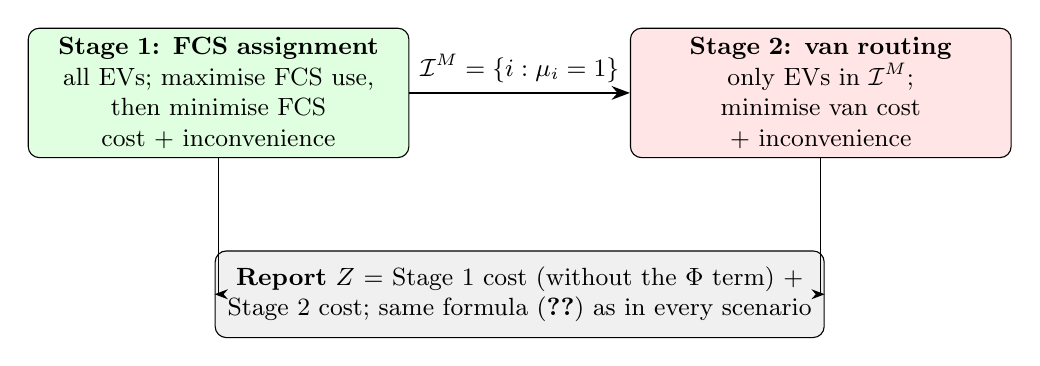
\begin{tikzpicture}[>=Stealth,box/.style={draw,rounded corners,align=center,minimum height=1.1cm,font=\small}]
  \node[box,fill=green!12,text width=4.6cm] (s1) {\textbf{Stage 1: FCS assignment}\\all EVs; maximise FCS use,\\then minimise FCS cost + inconvenience};
  \node[box,fill=red!10,text width=4.6cm,right=2.8cm of s1] (s2) {\textbf{Stage 2: van routing}\\only EVs in $\I^M$;\\minimise van cost + inconvenience};
  \draw[->,thick] (s1) -- node[above,font=\small]{$\I^M=\{i:\mu_i=1\}$} (s2);
  \node[box,fill=black!6,text width=7.5cm,below=2.0cm of $(s1)!0.5!(s2)$] (ev) {\textbf{Report} $Z=$ Stage~1 cost (without the $\Phi$ term) $+$ Stage~2 cost; same formula \eqref{eq:Z} as in every scenario};
  \draw[->] (s1) |- (ev); \draw[->] (s2) |- (ev);
\end{tikzpicture}
\end{center}

Stage~1 does not look at the vans, and Stage~2 cannot change what Stage~1 decided. That is the definition of ``FCS first, then MCS''.

%----------------------------------------------------------------
\subsection{Stage 1: assign EVs to fixed stations}

\textbf{Objective.}
\begin{equation}
\begin{split}
\min\ Z^{(1)}=\;&\underbrace{\Phi\sum_{i\in\I}\mu_i}_{\text{FCS first}}
+\underbrace{c^{EV}\sum_i\sum_{f\in\F_i}d_{if}Y_{if}}_{Z_1}
+\underbrace{Z^F_{\text{energy}}}_{\text{FCS part of }Z_4}\\
&+\underbrace{\sum_i\sum_{f\in\F_i}\rho^F_{if}Y_{if}+\alpha\sum_i w_i(C_i-r_i)+c^L\sum_i w_iL_i}_{\text{FCS customers' inconvenience}}
\end{split}
\label{eq:obj1}
\end{equation}
with $C_i=S_i+\tau^F_iY_i$ in this stage. $\Phi$ is a penalty for handing an EV to the vans. It is chosen larger than anything an extra FCS customer can add to the rest of \eqref{eq:obj1}, e.g.
\[
\Phi > \max_{i}\max_{f\in\F_i}\big(c^{EV}d_{if}+\pi^{\max}E_i+\rho^F_{if}\big)+n\,(\alpha+c^L)\,w_{\max}\,T,
\]
so Stage~1 first \textbf{maximises the number of EVs served at an FCS}, and only among those solutions minimises FCS cost and inconvenience. ($\pi^{\max}$ is the highest grid price.) A numerically safer equivalent is to solve twice: first $\max\sum_iY_i$, then fix that number and minimise the rest.
\ifTOU
Because $Z^F_{\text{energy}}$ uses the peak price, Stage~1 may \emph{start sessions later} to leave the peak, if the price saving beats the extra waiting cost (Section~\ref{sec:expect}).
\fi

\textbf{Constraints.}
\begin{align}
\sum_{g\in\G_i}y_{ig}+\mu_i &= 1 && \forall i\in\I \label{eq:s1assign}\\
S_i &\ge r_i+\sum_{f\in\F_i}t_{if}Y_{if} && \forall i\in\I \label{eq:fcsarr}\\
S_i &\le r_i+T\,(1-\mu_i) && \forall i\in\I \label{eq:s1park}\\
S_j &\ge S_i+\tau^F_i-(T+\tau^F_i)(3-y_{ig}-y_{jg}-o_{ij}) && \forall g,\ (i,j)\in\mathcal{P}_g \label{eq:disj1}\\
S_i &\ge S_j+\tau^F_j-(T+\tau^F_j)(2-y_{ig}-y_{jg}+o_{ij}) && \forall g,\ (i,j)\in\mathcal{P}_g \label{eq:disj2}\\
\sum_i y_{ig_1} &\ge \sum_i y_{ig_2} && \forall f,\ \G_f=\{g_1,g_2\} \label{eq:gunsym}\\
S_i+\tau^F_iY_i &\le T,\qquad L_i\ge S_i+\tau^F_iY_i-l_i && \forall i\in\I \label{eq:s1time}
\end{align}
\ifTOU plus the time-of-use split \eqref{eq:tou1}--\eqref{eq:tou5} of each FCS session (Section~\ref{sec:price}).\fi
\desc{\eqref{eq:s1assign}: every EV either gets one reachable gun or is handed to the vans. An EV that reaches no FCS ($\G_i=\emptyset$) is forced to $\mu_i=1$. \eqref{eq:fcsarr}: an FCS session cannot start before the EV has asked and driven to the station. \eqref{eq:s1park}: for an EV handed to the vans, $S_i$ is parked at $r_i$, so it adds no waiting in Stage~1 (its real start time is decided in Stage~2). \eqref{eq:disj1}--\eqref{eq:disj2}: two EVs on the same gun do not overlap; $o_{ij}$ picks who goes first. With two guns per station this means at most two EVs charge at a station at a time. \eqref{eq:gunsym}: symmetry breaking between the two identical guns (optional). \eqref{eq:s1time}: finished by $T$; lateness.}

\textbf{Optional acceptability rule.} An operator may refuse to send a driver to a station that is ``too inconvenient'', e.g.\ only allow gun $g$ of station $f$ for EV $i$ if $\hat\rho^F_{if}\le\bar\rho$. This only shrinks $\G_i$, so EVs whose stations are all too far go to the vans. Report results with and without it.

\textbf{Output:} $\I^M=\{i:\mu_i=1\}$, the EVs left for the vans; plus each FCS customer's gun and start time.

%----------------------------------------------------------------
\subsection{Stage 2: route the vans to the leftover EVs}

Stage~2 is a vehicle routing problem with time windows, on the EVs in $\I^M$ only. Here $C_i=S_i+\tau^M_i$.

\textbf{Objective.}
\begin{equation}
\begin{split}
\min\ Z^{(2)}=\;&\underbrace{c^M\sum_m\sum_{(i,j)\in\A^M}d_{ij}x_{ijm}}_{Z_2}+\underbrace{\sum_m c^D_mu_m}_{Z_3}+\underbrace{Z^M_{\text{energy}}}_{\text{van part of }Z_4}\\
&+\underbrace{\sum_{i\in\I^M}\sum_m\rho^M_{im}z_{im}+\alpha\sum_{i\in\I^M}w_i(C_i-r_i)+c^L\sum_{i\in\I^M}w_iL_i}_{\text{van customers' inconvenience}}
\end{split}
\label{eq:obj2}
\end{equation}
Since every EV in $\I^M$ must be served by some van, $Z^M_{\text{energy}}$ and the $\rho^M$ term are constants here. They are kept so that $Z^{(2)}$ is the true cost of Stage~2. Waiting and lateness make the vans visit urgent EVs early.

\textbf{Constraints.}
\begin{align}
\sum_{m\in\M}z_{im} &= 1 && \forall i\in\I^M \label{eq:s2assign}\\
\sum_{j:(0,j)\in\A^M}x_{0jm} = \sum_{i:(i,n+1)\in\A^M}x_{i,n+1,m} &= u_m && \forall m \label{eq:depot}\\
\sum_{i:(i,j)\in\A^M}x_{ijm} = \sum_{k:(j,k)\in\A^M}x_{jkm} &= z_{jm} && \forall j\in\I^M,\ m \label{eq:flow}\\
\sum_{i\in\I^M}z_{im} &\le Q_m\,u_m && \forall m \label{eq:cap}\\
\sum_{i\in\I^M}\frac{E_i}{\eta}z_{im}+\beta\sum_{(i,j)\in\A^M}d_{ij}x_{ijm} &\le B_m\,u_m && \forall m \label{eq:batt}
\end{align}
\begin{align}
S_j &\ge \max\{r_j,\ t_{0j}\,x_{0jm}\} && \forall j\in\I^M,\ m \label{eq:depart}\\
S_j &\ge S_i+\tau^M_i+t_{ij}-(T+\tau^M_i+t_{ij})(1-x_{ijm}) && \forall i\neq j,\ m \label{eq:seq}\\
S_i+\tau^M_i+t_{i,n+1} &\le T+(\tau^M_i+t_{i,n+1})(1-x_{i,n+1,m}) && \forall i,\ m \label{eq:return}\\
S_i+\tau^M_i \le T,\quad L_i &\ge S_i+\tau^M_i-l_i && \forall i\in\I^M \label{eq:s2time}\\
u_m &\ge u_{m+1} && m<|\M| \label{eq:vansym}
\end{align}
\desc{\eqref{eq:s2assign}: each leftover EV gets one van. \eqref{eq:depot}: a used van leaves and returns to the depot once. \eqref{eq:flow}: each EV on van $m$ is entered and left exactly once by that van. \eqref{eq:cap}: at most $Q_m$ EVs per van. \eqref{eq:batt}: delivered energy (with transfer losses) plus driving energy fits in the van battery. \eqref{eq:depart}: no start before the request, or before the van can drive there from the depot (written as two linear constraints). \eqref{eq:seq}: if the van goes $i\to j$, it finishes $i$ and drives to $j$ before starting $j$. This gives one EV at a time and removes subtours (MTZ-type). \eqref{eq:return}: back at the depot by $T$. \eqref{eq:s2time}: finished by $T$; lateness. \eqref{eq:vansym}: use identical vans in index order.}

\textbf{If Stage 2 is infeasible} (too many leftover EVs for the fleet by $T$), the sequential policy has \emph{failed} on that instance. For diagnosis, add $s_i\in\{0,1\}$ (``unserved''), replace \eqref{eq:s2assign} by $\sum_mz_{im}+s_i=1$ and add $\Phi^U\sum_is_i$ to \eqref{eq:obj2}. Then report the number of EVs that could not be served. This is a useful comparison with the integrated scenario, which may serve all of them.

%----------------------------------------------------------------
\subsection{Reported value}
\[
Z^{\text{S\scen}}=\big(Z^{(1)*}-\Phi\,|\I^M|\big)+Z^{(2)*},
\]
which is exactly \eqref{eq:Z} evaluated at the combined solution. The stage-1 solution plus the stage-2 solution is a feasible solution of the integrated model (S\ifTOU 4\else 3\fi), so
$Z^{\text{S\ifTOU 4\else 3\fi}}\le Z^{\text{S\scen}}$. The difference is the \emph{value of integration}.

\else
%---------------------------------------------------------------- INT
\subsection{Objective}
\begin{equation}
\min\ Z \quad\text{as in \eqref{eq:Z}, with }Z^F_{\text{energy}}=\ifTOU P^F\textstyle\sum_i\big[\pi^\off(\theta^1_i+\theta^3_i)+\pi^\pk\theta^2_i\big]\else\pi^F\textstyle\sum_iE_iY_i\fi,\quad C_i=S_i+\tau^F_iY_i+\tau^M_iZ_i. \label{eq:objint}
\end{equation}
Written out in full:
\begin{align*}
\min\ Z=\;& c^{EV}\sum_i\sum_{f\in\F_i}d_{if}Y_{if}+c^M\sum_m\sum_{(i,j)\in\A}d_{ij}x_{ijm}+\sum_mc^D_mu_m\\
&+\ifTOU P^F\sum_i\big[\pi^\off(\theta^1_i+\theta^3_i)+\pi^\pk\theta^2_i\big]\else\pi^F\sum_iE_iY_i\fi
+\pi^M\sum_i\sum_m\frac{E_i}{\eta}z_{im}\\
&+\sum_i\sum_{f\in\F_i}\rho^F_{if}Y_{if}+\sum_i\sum_m\rho^M_{im}z_{im}+\alpha\sum_iw_i(C_i-r_i)+c^L\sum_iw_iL_i .
\end{align*}
Every term is linear. One model weighs everything at once: an EV goes to a van exactly when the van's extra km, dispatch and energy cost are outweighed by the effort and waiting it saves the driver\ifTOU, or by the peak-price energy it avoids\fi.

\subsection{Constraints}

\textbf{Assignment.}
\begin{equation}
\sum_{g\in\G_i}y_{ig}+\sum_{m\in\M}z_{im}=1\qquad\forall i\in\I \label{eq:assign}
\end{equation}
\desc{Exactly one resource per EV: one reachable gun or one van. EVs that reach no FCS are forced onto a van.}

\textbf{Fixed stations.}
\begin{align}
S_i &\ge r_i+\sum_{f\in\F_i}t_{if}Y_{if} && \forall i \label{eq:fcsarr}\\
S_j &\ge S_i+\tau^F_i-(T+\tau^F_i)(3-y_{ig}-y_{jg}-o_{ij}) && \forall g,\ (i,j)\in\mathcal{P}_g \label{eq:disj1}\\
S_i &\ge S_j+\tau^F_j-(T+\tau^F_j)(2-y_{ig}-y_{jg}+o_{ij}) && \forall g,\ (i,j)\in\mathcal{P}_g \label{eq:disj2}\\
\sum_iy_{ig_1} &\ge \sum_iy_{ig_2} && \forall f,\ \G_f=\{g_1,g_2\} \label{eq:gunsym}
\end{align}
\desc{\eqref{eq:fcsarr}: an FCS session starts after the request and the drive to the station (for a van customer this is just $S_i\ge r_i$). \eqref{eq:disj1}--\eqref{eq:disj2}: EVs on the same gun do not overlap; $o_{ij}$ chooses the order. \eqref{eq:gunsym}: optional symmetry breaking.}

\textbf{Vans: routes, capacity, battery.}
\begin{align}
\sum_{j:(0,j)\in\A}x_{0jm}=\sum_{i:(i,n+1)\in\A}x_{i,n+1,m} &= u_m && \forall m \label{eq:depot}\\
\sum_{i:(i,j)\in\A}x_{ijm}=\sum_{k:(j,k)\in\A}x_{jkm} &= z_{jm} && \forall j\in\I,\ m \label{eq:flow}\\
\sum_iz_{im} &\le Q_mu_m && \forall m \label{eq:cap}\\
\sum_i\frac{E_i}{\eta}z_{im}+\beta\sum_{(i,j)\in\A}d_{ij}x_{ijm} &\le B_mu_m && \forall m \label{eq:batt}
\end{align}
\desc{\eqref{eq:depot}: a used van leaves and returns once. \eqref{eq:flow}: each EV on van $m$ is visited exactly once by it. \eqref{eq:cap}: at most $Q_m$ EVs. \eqref{eq:batt}: delivered energy (with losses) plus driving energy fits in the battery.}

\textbf{Vans: timing (one EV at a time, no subtours).}
\begin{align}
S_j &\ge t_{0j}\,x_{0jm} && \forall j\in\I,\ m \label{eq:depart}\\
S_j &\ge S_i+\tau^M_i+t_{ij}-(T+\tau^M_i+t_{ij})(1-x_{ijm}) && \forall i\neq j\in\I,\ m \label{eq:seq}\\
S_i+\tau^M_i+t_{i,n+1} &\le T+(\tau^M_i+t_{i,n+1})(1-x_{i,n+1,m}) && \forall i,\ m \label{eq:return}
\end{align}
\desc{\eqref{eq:depart}: the first stop cannot start before the van has driven there. \eqref{eq:seq}: $i\to j$ means finish $i$, drive, then start $j$; start times rise along a route, so no subtour can close. \eqref{eq:return}: back at the depot by $T$.}

\textbf{Horizon and lateness.}
\begin{equation}
C_i\le T,\qquad L_i\ge C_i-l_i\qquad\forall i\in\I \label{eq:time}
\end{equation}
\desc{Every EV is fully charged within the horizon; $L_i$ measures lateness.}

\ifTOU
\textbf{Time-of-use split.} Constraints \eqref{eq:tou1}--\eqref{eq:tou5} of Section~\ref{sec:price}.
\fi

\textbf{Symmetry and domains.}
\begin{equation}
u_m\ge u_{m+1};\qquad y,z,x,u,o\ifTOU,\kappa\fi\in\{0,1\};\qquad S_i,L_i\ifTOU,\theta^p_i\fi\ge0 \label{eq:dom}
\end{equation}
\fi

%=====================================================================
\section{Learning-to-optimise (RL) formulation}\label{sec:rl}

\textbf{Main rule:} the reward of each action is \emph{minus the increase in $Z$ that the action causes}. The rewards over an episode then add up to $-Z$ of the solution the policy builds. RL and MILP results are measured on the same yardstick \eqref{eq:Z}, and the MILP optimum is the benchmark for the RL gap.

\ifSEQ
%---------------------------------------------------------------- RL SEQ
The RL pipeline has the same two stages as the MILP.

\subsection{Stage 1 policy: FCS assignment}
\begin{itemize}[leftmargin=1.4em,itemsep=2pt]
  \item \textbf{Episode / epochs:} EVs are taken in order of request time $r_i$ (ties: higher $w_i$ first). One decision per EV.
  \item \textbf{State:} features of the current EV $k$ ($E_k,r_k,l_k,w_k,R_k$, location); for each gun $g$ the time $F_g$ it becomes free; summary features of the EVs still to come (count and positions near each station)\ifTOU; the current price and the time until $T_1$ and $T_2$\fi.
  \item \textbf{Action:} a gun $g\in\G_k$, or ``hand to vans''. \textbf{FCS-first mask:} ``hand to vans'' is allowed \emph{only} if no gun can finish EV $k$ by $T$ (or, with the optional rule, if all remaining guns have $\hat\rho^F_{kf}>\bar\rho$).
  \ifTOU\item \textbf{Optional timing action:} ``gun $g$, start after the peak'', i.e.\ $S_k=\max\{\text{earliest},T_2\}$, allowed only if the session still ends by $T$.\fi
  \item \textbf{Transition:} $S_k=\max\{r_k+t_{kf},F_g\}$ (or later, for the timing action); $F_g\leftarrow S_k+\tau^F_k$.
  \item \textbf{Reward:} $-\Big[c^{EV}d_{kf}+\text{energy}_k+\rho^F_{kf}+\alpha w_k(S_k+\tau^F_k-r_k)+c^Lw_k(S_k+\tau^F_k-l_k)^+\Big]$, where energy$_k$ = \ifTOU$P^F\big[\pi^\off\cdot(\text{off-peak hours of }[S_k,S_k+\tau^F_k])+\pi^\pk\cdot(\text{peak hours})\big]$, computed exactly in the simulator\else$\pi^FE_k$\fi. Handing an EV to the vans gives reward $0$ here; its cost is counted in Stage~2.
\end{itemize}
Note: a simple baseline for Stage~1 is the greedy rule ``gun with the largest one-step reward''. What RL can learn on top of this is, for example, to keep a nearby gun free for an urgent EV that arrives later.

\subsection{Stage 2 policy: van routing over $\I^M$}
\begin{itemize}[leftmargin=1.4em,itemsep=2pt]
  \item \textbf{Epochs:} whenever a van becomes free (the earliest-free van decides first).
  \item \textbf{State:} for each van: position, time free, remaining battery $b_m$, EVs served so far, dispatched or not; for each unserved EV in $\I^M$: location, $E_i,r_i,l_i,w_i$; current time.
  \item \textbf{Action:} the next EV $j$ for this van, or ``return to depot'' (ends the route). Mask: $j$ must be feasible: battery covers $E_j/\eta$ plus driving to $j$ and back to the depot, the count stays $\le Q_m$, and $j$ can be finished with the van back at the depot by $T$.
  \item \textbf{Transition:} $S_j=\max\{r_j,\ \text{time free}+t_{\text{pos},j}\}$; the van moves to $j$ and is free at $S_j+\tau^M_j$; $b_m$ falls by $E_j/\eta+\beta d_{\text{pos},j}$.
  \item \textbf{Reward:} serving $j$: $-\Big[c^Md_{\text{pos},j}+c^D_m[\text{first stop}]+\pi^M\frac{E_j}{\eta}+\rho^M_{jm}+\alpha w_j(S_j+\tau^M_j-r_j)+c^Lw_j(S_j+\tau^M_j-l_j)^+\Big]$; returning: $-c^Md_{\text{pos},0}$. EVs still unserved at the end: $-\Phi^U$ each.
  \item \textbf{Policy:} an attention-based routing policy (e.g.\ Kool et al., 2019, ``Attention, Learn to Solve Routing Problems!'') trained with REINFORCE or PPO. Baseline: nearest-feasible-EV heuristic.
\end{itemize}
Episode return of Stage~1 + Stage~2 $=-Z^{\text{S\scen}}$.

\else
%---------------------------------------------------------------- RL INT
One policy decides both who serves each EV and the van routes.
\begin{itemize}[leftmargin=1.4em,itemsep=2pt]
  \item \textbf{Episode / epochs:} EVs are taken in order of request time $r_i$ (ties: higher $w_i$ first). One decision per EV.
  \item \textbf{State:} (i) the current EV $k$: location, $E_k,r_k,l_k,w_k,R_k$, reachable stations; (ii) each gun $g$: time $F_g$ it becomes free; (iii) each van $m$: current end-of-route position, time free, remaining battery $b_m$, EVs served, dispatched or not; (iv) embeddings of the not-yet-assigned EVs (for look-ahead)\ifTOU; (v) current price, time until $T_1$ and $T_2$\fi.
  \item \textbf{Action:} $a\in\G_k\cup\M$: a gun, or a van (EV $k$ is appended to the end of that van's route). \textbf{Mask} infeasible actions: a gun that cannot finish $k$ by $T$; a van without enough battery for $E_k/\eta$ plus the drive to $k$ and back to the depot, with $Q_m$ reached, or unable to finish $k$ and return by $T$.
  \ifTOU\item \textbf{Optional timing action:} ``gun $g$, start after the peak'' ($S_k=\max\{\text{earliest},T_2\}$, if it still ends by $T$).\fi
  \item \textbf{Transition:} gun: $S_k=\max\{r_k+t_{kf},F_g\}$, $F_g\leftarrow S_k+\tau^F_k$. Van: $S_k=\max\{r_k,\ \text{free}_m+t_{\text{pos}_m,k}\}$, then the van moves to $k$, $\text{free}_m\leftarrow S_k+\tau^M_k$, $b_m\mathrel{-}=E_k/\eta+\beta d_{\text{pos}_m,k}$.
  \item \textbf{Reward} $=-\Delta Z$:
  \begin{align*}
  \text{gun } g\text{ at }f:&\quad -\Big[c^{EV}d_{kf}+\text{energy}^F_k+\rho^F_{kf}+\alpha w_k(C_k-r_k)+c^Lw_k(C_k-l_k)^+\Big]\\
  \text{van } m:&\quad -\Big[c^M\big(d_{\text{pos}_m,k}+d_{k,0}-d_{\text{pos}_m,0}\big)+c^D_m[\text{first use}]+\pi^M\tfrac{E_k}{\eta}\\
  &\qquad\quad+\rho^M_{km}+\alpha w_k(C_k-r_k)+c^Lw_k(C_k-l_k)^+\Big]
  \end{align*}
  The van distance term is the \emph{change} in route length when $k$ is inserted before the return to the depot, so the sum over the episode equals the total route length (the return legs telescope). energy$^F_k$ = \ifTOU$P^F\big[\pi^\off\cdot(\text{off-peak hours})+\pi^\pk\cdot(\text{peak hours of }[S_k,C_k])\big]$, computed exactly by the simulator; no linearisation is needed in RL\else$\pi^FE_k$\fi.
  \item \textbf{Dead end:} if every action is masked, EV $k$ is unserved: reward $-\Phi^U$, and the episode continues. Report the count.
  \item \textbf{Policy:} masked categorical policy over guns and vans, encoder with attention over EVs, guns and vans; trained with PPO. Natural baseline: greedy, i.e.\ choose the action with the largest one-step reward. That is the pairwise rule ``smallest $\hat\rho$ + cost'' from Section~\ref{sec:inc}.
\end{itemize}
Restriction to note: vans serve EVs in assignment order (append only). A variant that inserts $k$ at the cheapest position of a route is more flexible but has a larger action space.
\fi

\textbf{Reward scaling.} For stable training divide every reward by a constant, e.g.\ the greedy baseline's average $Z$ on the training instances. This does not change the optimal policy.

%=====================================================================
\section{What to expect and what to report}\label{sec:expect}

\ifnum\scen=1
\begin{itemize}[leftmargin=1.4em,itemsep=2pt]
  \item Vans serve only EVs that reach no station, or that the stations cannot finish by $T$. If stations have spare capacity, very few vans are dispatched.
  \item Inconvenience is high for EVs far from the nearest station (worked example: Rs\,682 at the FCS, against Rs\,458 if a van had been allowed).
  \item With too few vans Stage~2 becomes infeasible (unserved EVs), even when the integrated model S3 could serve everyone. Report the smallest $|\M|$ at which S1 is feasible and compare it with S3.
\end{itemize}
\fi
\ifnum\scen=2
\begin{itemize}[leftmargin=1.4em,itemsep=2pt]
  \item \textbf{When does Stage~1 delay a session to avoid the peak?} Moving one hour of charging out of the peak saves $(\pi^\pk-\pi^\off)P^F=3\times22=$ Rs\,66, but delays completion by up to an hour, which costs $\alpha w_i\ge$ Rs\,200. So with the default values Stage~1 almost never delays. It mostly pays the higher price, and S2 costs roughly S1 plus the peak surcharge. Sessions start later only if $\alpha$ is small (try $\lambda<0.33$ in the sensitivity analysis).
  \item The van assignment is the same as in S1 unless Stage~1's timing changes which EVs fit at the stations. Stage~1 cannot use vans to escape the peak price.
  \item Extra KPI: \textbf{grid energy drawn at FCS during the peak}, $P^F\sum_i\theta^2_i$ (kWh). Compare with S4.
\end{itemize}
\fi
\ifnum\scen=3
\begin{itemize}[leftmargin=1.4em,itemsep=2pt]
  \item Vans take EVs for which the saved inconvenience exceeds the extra van cost (worked example: van chosen, saving Rs\,224). Expect vans to serve EVs that are far from every station, have low range (high $w_i$), or have early deadlines, while EVs near a station still use it.
  \item \textbf{Value of integration under flat price:} $Z^{\text{S1}}-Z^{\text{S3}}\ge0$. Report it per component ($Z_1,\dots,Z_5$): typically operating cost rises a little and inconvenience falls a lot.
  \item Vary $|\M|$ (0, 1, 2, \dots): the first few vans lower $Z$ sharply, then the effect levels off. That curve shows the scenarios where mobile chargers help most.
\end{itemize}
\fi
\ifnum\scen=4
\begin{itemize}[leftmargin=1.4em,itemsep=2pt]
  \item During the peak a van kWh costs about the same as an FCS kWh (Rs\,10.0 each), so the vans' energy disadvantage disappears and vans also absorb \emph{peak-hour} demand that would otherwise be charged on the grid at peak price.
  \item Expect more van usage than in S3, concentrated on requests in $[T_1,T_2]$, and lower grid energy at the stations during the peak, $P^F\sum_i\theta^2_i$, than in S2.
  \item \textbf{Value of integration under peak pricing:} $Z^{\text{S2}}-Z^{\text{S4}}$. It should be larger than $Z^{\text{S1}}-Z^{\text{S3}}$, because integration now also allows price arbitrage.
  \item \textbf{Peak pricing with full flexibility:} $Z^{\text{S4}}-Z^{\text{S3}}$ should be smaller than $Z^{\text{S2}}-Z^{\text{S1}}$: vans cushion the price increase.
\end{itemize}
\fi

\textbf{Cross-scenario comparison table} (fill in from the four runs):
\begin{center}
\renewcommand{\arraystretch}{1.2}
\begin{tabular}{@{}lll@{}}
\toprule
\textbf{Comparison} & \textbf{Measures} & \textbf{Expected sign} \\
\midrule
S1 $-$ S3 & value of integration, flat price & $\ge0$ \\
S2 $-$ S4 & value of integration, peak price & $\ge0$, larger than S1 $-$ S3 \\
S2 $-$ S1 & cost of peak pricing, FCS-first operator & $>0$ \\
S4 $-$ S3 & cost of peak pricing, flexible operator & $>0$, smaller than S2 $-$ S1 \\
\bottomrule
\end{tabular}
\end{center}
Report for each: $Z$ and its components, number of vans used, EVs per resource, mean and maximum inconvenience per EV, total lateness, peak-hour grid energy, solve time, and (for RL) the gap to the MILP optimum.

%=====================================================================
\appendix
\section{Illustrative parameter values}\label{app:values}

These are starting values for experiments, not data. All are meant to be varied in the analysis. Values in Rs.

\begin{center}
\renewcommand{\arraystretch}{1.15}
\begin{tabular}{@{}llp{6.2cm}@{}}
\toprule
\textbf{Parameter} & \textbf{Value} & \textbf{Note} \\
\midrule
$T$, $[T_1,T_2]$ & 7 h, $[2,6]$ & 16:00--23:00, peak 18:00--22:00 \\
$P^F$, $P^M$ & 22 kW, 30 kW & \\
$v$, $\beta$, $\eta$ & 25 km/h, 0.25 kWh/km, 0.9 & \\
$B_m$, $Q_m$, $|\M|$ & 150 kWh, 6, 2--6 & \\
$c^{EV}$, $c^M$, $c^D_m$ & Rs\,4/km, Rs\,15/km, Rs\,1500 & van km includes driver time \\
$\pi^F$ (flat) & Rs\,8.7/kWh & equals the time-average of the ToU tariff over $[0,T]$ \\
$\pi^\off$, $\pi^\pk$ (ToU) & Rs\,7/kWh, Rs\,10/kWh & $(3\times7+4\times10)/7=8.7$ \\
$c^{bat}$ & Rs\,2/kWh & van battery wear \\
$\pi^M$ & Rs\,10.7 (flat) / Rs\,9.0 (ToU) & $=\pi^F+c^{bat}$ / $=\pi^\off+c^{bat}$ \\
$\alpha$, $\alpha^D$ & Rs\,200/h, Rs\,100/h & value of time; extra for attended time \\
$h^F$, $h^M$, $\varphi$ & Rs\,50, Rs\,10, Rs\,100 & trip hassle, hand-over, range stress \\
$c^L$ & Rs\,300/h & lateness \\
$w_i$ & $1+2(1-R_i/R_{\max})$, $R_i\sim U[3,40]$ km & priority from remaining range \\
\bottomrule
\end{tabular}
\end{center}

The flat price is set to the time-average of the peak tariff. The price \emph{level} is then the same in both pricing cases, and only the price \emph{shape} differs. Without this, part of S1 vs S2 would just reflect a different average price.

\end{document}
"
%    pdflatex -jobname=scenario3_flat_integrated   "\def\scen{3}% =====================================================================
%  One source, four PDFs.  Build with build.sh (or by hand):
%    pdflatex -jobname=scenario1_flat_sequential   "\def\scen{1}\input{scenario_master}"
%    pdflatex -jobname=scenario2_peak_sequential   "\def\scen{2}\input{scenario_master}"
%    pdflatex -jobname=scenario3_flat_integrated   "\def\scen{3}\input{scenario_master}"
%    pdflatex -jobname=scenario4_peak_integrated   "\def\scen{4}\input{scenario_master}"
%  (run each twice for cross-references)
% =====================================================================
\documentclass[11pt,a4paper]{article}
\usepackage[margin=2.2cm]{geometry}
\usepackage{amsmath,amssymb,amsfonts}
\usepackage{booktabs,array,tabularx}
\usepackage{enumitem}
\usepackage[table]{xcolor}
\usepackage{tikz}
\usetikzlibrary{arrows.meta,positioning,calc}
\usepackage[colorlinks=true,linkcolor=blue!50!black,urlcolor=blue!50!black]{hyperref}
\usepackage{titlesec}
\titleformat{\section}{\large\bfseries}{\thesection}{0.8em}{}
\titleformat{\subsection}{\normalsize\bfseries}{\thesubsection}{0.8em}{}
\setlength{\parindent}{0pt}
\setlength{\parskip}{5pt}

% ---------------- scenario switches ----------------
\ifdefined\scen\else\def\scen{1}\fi
\newif\ifTOU \TOUfalse   % true = time-of-use (peak) price
\newif\ifSEQ \SEQfalse   % true = FCS first, then MCS
\ifnum\scen=1 \SEQtrue \fi
\ifnum\scen=2 \TOUtrue \SEQtrue \fi
\ifnum\scen=4 \TOUtrue \fi

\newcommand{\pricename}{\ifTOU time-of-use price (dearer evening peak)\else single (flat) price all day\fi}
\newcommand{\structname}{\ifSEQ FCS first, then MCS (sequential)\else FCS and MCS together (integrated)\fi}

% ---------------- notation ----------------
\newcommand{\I}{\mathcal{I}}
\newcommand{\F}{\mathcal{F}}
\newcommand{\G}{\mathcal{G}}
\newcommand{\M}{\mathcal{M}}
\newcommand{\N}{\mathcal{N}}
\newcommand{\A}{\mathcal{A}}
\newcommand{\Rs}{\text{Rs}\,}
\newcommand{\pk}{\mathrm{pk}}
\newcommand{\off}{\mathrm{off}}
\newcommand{\desc}[1]{\par\vspace{-2pt}{\small\color{black!75}\textit{Meaning:} #1}\par\vspace{4pt}}
\newcommand{\cell}[2]{\ifnum\scen=#1\cellcolor{blue!18}\textbf{S#1 (this document)}\\\textbf{#2}\else S#1\\#2\fi}

\title{\textbf{EV Charging Network Optimisation}\\[4pt]
\large Scenario \scen: \pricename\ $+$ \structname\\[2pt]
\normalsize MILP and RL formulation}
\author{CP 320 OR for Mobility Management, course project}
\date{2 October 2026}

\begin{document}
\maketitle

%=====================================================================
\section{Where this scenario sits}

The project studies four scenarios: two ways of pricing grid electricity, times two ways of making the decisions.

\begin{center}
\renewcommand{\arraystretch}{1.5}
\begin{tabular}{>{\raggedright\arraybackslash}p{4.2cm}|>{\centering\arraybackslash}p{4.6cm}|>{\centering\arraybackslash}p{4.6cm}}
 & \textbf{Flat price all day} & \textbf{Time-of-use (peak) price} \\ \hline
\textbf{Sequential:} FCS first, leftover EVs to MCS &
\begin{tabular}[c]{@{}c@{}}\cell{1}{flat + sequential}\end{tabular} &
\begin{tabular}[c]{@{}c@{}}\cell{2}{peak + sequential}\end{tabular} \\ \hline
\textbf{Integrated:} FCS and MCS decided together &
\begin{tabular}[c]{@{}c@{}}\cell{3}{flat + integrated}\end{tabular} &
\begin{tabular}[c]{@{}c@{}}\cell{4}{peak + integrated}\end{tabular} \\
\end{tabular}
\end{center}

\textbf{The four scenarios do not have four different objectives.} They share \emph{one} cost yardstick $Z$ (Section~\ref{sec:obj}): the same cost terms and the same customer inconvenience (Section~\ref{sec:inc}). Only two things change:
\begin{itemize}[leftmargin=1.4em,itemsep=1pt]
  \item \textbf{Pricing} changes the formula for one term, the FCS energy cost (Section~\ref{sec:price}).
  \item \textbf{Decision structure} changes \emph{how} $Z$ is minimised: in one model (integrated), or in two stages (sequential), where each stage minimises its own part of $Z$.
\end{itemize}
Because the yardstick is the same, the four optimal values can be compared directly. The differences measure the \emph{value of integration} (S1$\to$S3, S2$\to$S4) and the \emph{effect of peak pricing} (S1$\to$S2, S3$\to$S4).

\ifnum\scen=1
\textbf{This scenario (S1)} is the baseline, the ``status quo''. Electricity costs the same at every hour, every EV that can be charged at a fixed station is sent there, and vans only take what is left over.
\fi
\ifnum\scen=2
\textbf{This scenario (S2)} keeps the FCS-first rule of S1, but grid electricity is dearer during the evening peak. Stage~1 can react to the price only by \emph{rescheduling} FCS sessions. It cannot hand a peak-hour EV to a van.
\fi
\ifnum\scen=3
\textbf{This scenario (S3)} keeps the flat price of S1, but the operator decides FCS and MCS service \emph{together}. An EV can be sent to a van even when a fixed station could take it, whenever that lowers total cost plus inconvenience.
\fi
\ifnum\scen=4
\textbf{This scenario (S4)} is the most flexible one: peak pricing at fixed stations, and FCS and MCS decided together. Van energy was bought off-peak, so vans can also be used to keep charging \emph{out of the expensive peak}.
\fi

%=====================================================================
\section{Setting and assumptions}\label{sec:setting}

\textbf{Time.} The planning horizon is $[0,T]$ with $T=7$\,h (16:00--23:00). It contains the evening peak window $[T_1,T_2]=[2,6]$ (18:00--22:00). The horizon is the same in all four scenarios. It is wider than the peak itself so that, under peak pricing, there is cheaper time on both sides of the peak.\ifTOU\else\ In this scenario the price is flat, so the window plays no role in the model.\fi

\textbf{Assumptions} (the same as MILP v3, plus two about energy):
\begin{enumerate}[leftmargin=1.6em,itemsep=1pt]
  \item Static, continuous time. All requests in the horizon are known at time $0$, and request $i$ becomes active at $r_i$.
  \item An EV served by an FCS drives there itself on its own battery (only to stations within its range $R_i$). The driver stays with the car while it waits for a free gun and while it charges.
  \item An EV served by an MCS stays parked where it is, and the driver is free in the meantime.
  \item Each FCS gun and each van charges one EV at a time, without interruption, at constant power.
  \item A van's battery covers both its driving and the energy it delivers. \textbf{The van battery is charged at the depot before the horizon starts}\ifTOU, i.e.\ at the off-peak price\fi, and is not recharged during the horizon.
  \item Every EV must be fully charged by $T$ (hard). Finishing after the driver's desired time $l_i$ is allowed but penalised.
\end{enumerate}

%=====================================================================
\section{Notation}\label{sec:notation}

\subsection*{Sets}
\begin{tabularx}{\textwidth}{@{}lX@{}}
\toprule
$\I=\{1,\dots,n\}$ & EV charging requests \\
$\F$; $\G_f$ ($|\G_f|=2$); $\G=\bigcup_f\G_f$ & fixed charging stations; guns of FCS $f$; all guns ($f(g)$ = station of gun $g$) \\
$\F_i=\{f: d_{if}\le R_i\}$, $\G_i=\bigcup_{f\in\F_i}\G_f$ & stations / guns EV $i$ can reach on its remaining range \\
$\M$ & mobile charging vans (MCS) \\
$0,\ n+1$ & depot as start node / end node (same place) \\
$\N=\{0\}\cup\I\cup\{n+1\}$, $\A$ & routing nodes; allowed van arcs $(i,j)$, $i\in\{0\}\cup\I$, $j\in\I\cup\{n+1\}$, $i\neq j$ \\
$\mathcal{P}_g=\{(i,j): i<j,\ g\in\G_i\cap\G_j\}$ & pairs of EVs that could share gun $g$ \\
\ifSEQ
$\I^M\subseteq\I$ & EVs handed to the vans by Stage~1 (an \emph{output} of Stage~1, a fixed input to Stage~2) \\
$\N^M$, $\A^M$ & routing nodes / arcs restricted to $\I^M$ \\
\fi
\bottomrule
\end{tabularx}

\subsection*{Parameters}
\begin{tabularx}{\textwidth}{@{}lX@{}}
\toprule
$E_i,\ r_i,\ l_i,\ R_i$ & energy demand (kWh), request time, desired completion time (h), remaining range (km) \\
$w_i\ge1$ & priority of EV $i$; $w_i=1+\kappa(1-R_i/R_{\max})$, so low-range EVs weigh more \\
$P^F,\ P^M$ & charging power of an FCS gun (22\,kW) / of a van (e.g.\ 30\,kW) \\
$\tau^F_i=E_i/P^F,\ \tau^M_i=E_i/P^M$ & charging time of EV $i$ at an FCS / by a van (h) \\
$d_{if},t_{if}$;\ $d_{ij},t_{ij}$ & distance (km) and time (h): EV$\to$FCS; between routing nodes ($t=d/v$) \\
$B_m,\ Q_m,\ \beta,\ \eta$ & van battery (kWh), max EVs per van, van consumption (kWh/km), transfer efficiency \\
$c^{EV},\ c^M,\ c^D_m$ & cost per km of EV driving, per km of van driving; fixed dispatch cost of van $m$ \\
\ifTOU
$\pi^\off,\ \pi^\pk$ & grid price (Rs/kWh) off-peak / in $[T_1,T_2]$, with $\pi^\pk\ge\pi^\off$ \\
\else
$\pi^F$ & grid price (Rs/kWh), the same at every hour \\
\fi
$c^{bat}$ & van battery wear per kWh cycled \\
$\pi^M$ & cost of 1 kWh taken from a van battery: $\pi^M=\ifTOU\pi^\off\else\pi^F\fi+c^{bat}$ (Section~\ref{sec:price}) \\
$\alpha,\ \alpha^D,\ h^F,\ h^M,\ \varphi,\ c^L$ & inconvenience coefficients (Section~\ref{sec:inc}) \\
\bottomrule
\end{tabularx}

\subsection*{Decision variables}
\begin{tabularx}{\textwidth}{@{}llX@{}}
\toprule
$y_{ig}$ & $\{0,1\}$ & EV $i$ charged at gun $g\in\G_i$ \\
$z_{im}$ & $\{0,1\}$ & EV $i$ served by van $m$ \\
$x_{ijm}$ & $\{0,1\}$ & van $m$ drives arc $(i,j)$ \\
$u_m$ & $\{0,1\}$ & van $m$ is dispatched \\
$o_{ij}$ & $\{0,1\}$ & for EVs $i<j$ that could share a gun: 1 if $i$ is charged before $j$ \\
\ifSEQ
$\mu_i$ & $\{0,1\}$ & Stage~1 only: EV $i$ is handed to the van fleet \\
\fi
\ifTOU
$\theta^1_i,\theta^2_i,\theta^3_i$ & $\ge0$ & hours of EV $i$'s FCS session before / inside / after the peak \\
$\kappa^1_i,\kappa^3_i$ & $\{0,1\}$ & EV $i$'s FCS session starts before $T_1$ / ends after $T_2$ \\
\fi
$S_i$ & $\ge0$ & time charging of EV $i$ starts (h), on whichever resource \\
$L_i$ & $\ge0$ & lateness of EV $i$ beyond $l_i$ (h) \\
\bottomrule
\end{tabularx}

\textbf{Short-hands} (linear expressions, not new variables):
\[
Y_{if}=\sum_{g\in\G_f}y_{ig},\qquad Y_i=\sum_{g\in\G_i}y_{ig}\ (\text{EV $i$ uses an FCS}),\qquad Z_i=\sum_{m\in\M}z_{im}\ (\text{EV $i$ uses a van}),
\]
\[
C_i=S_i+\tau^F_i\,Y_i+\tau^M_i\,Z_i \quad\text{(time EV $i$ is fully charged).}
\]

%=====================================================================
\section{Customer inconvenience}\label{sec:inc}

This section is \textbf{identical in all four scenario documents}. Inconvenience is a property of the customer, not of the price or of the planning method.

\subsection{What we mean by inconvenience}

Inconvenience is \emph{what the driver loses} from the moment they ask for a charge ($r_i$) until the car is fully charged ($C_i$), \emph{converted into rupees} so it can be added to the operator's costs. A driver loses three different things:

\begin{enumerate}[leftmargin=1.6em,itemsep=2pt]
  \item \textbf{Waiting:} the car is not ready. This lasts $C_i-r_i$ hours and affects \emph{every} driver, FCS or MCS.
  \item \textbf{Effort:} only an FCS customer has to drive to the station and sit there while the car charges. An MCS customer stays at home or at work and does something else. Driving to a far station also uses scarce battery range, which causes stress (``range anxiety'').
  \item \textbf{A missed deadline:} the car is still not ready at the time $l_i$ the driver needs it.
\end{enumerate}

Each loss gets a price in Rs per hour (or per event). All of them are multiplied by the priority $w_i$: an hour of delay for an EV with 5\,km of range left counts more than for one with 40\,km.

\subsection{The three components}

\begin{center}
\renewcommand{\arraystretch}{1.3}
\begin{tabularx}{\textwidth}{@{}>{\raggedright\arraybackslash}p{2.6cm}>{\raggedright\arraybackslash}X>{\raggedright\arraybackslash}X>{\raggedright\arraybackslash}p{3.0cm}@{}}
\toprule
\textbf{Component} & \textbf{EV $i$ at FCS $f$} & \textbf{EV $i$ by a van} & \textbf{Known when?} \\
\midrule
Effort & $w_i\big[\alpha^D(t_{if}+\tau^F_i)+h^F+\varphi\,d_{if}/R_i\big]$: driving and sitting at the station, a fixed trip hassle, range stress & $w_i\,h^M$: being reachable and handing over the car & \textbf{Static:} known as soon as the resource is chosen \\
Waiting & $w_i\,\alpha\,(C_i-r_i)$ = drive + \emph{queue at the gun} + charge & $w_i\,\alpha\,(C_i-r_i)$ = \emph{wait for the van} + charge & \textbf{Dynamic:} depends on the queue / van route \\
Missed deadline & $w_i\,c^L\,L_i$, $L_i=\max\{0,C_i-l_i\}$ & same & Dynamic \\
\bottomrule
\end{tabularx}
\end{center}

\textbf{Coefficients.}
$\alpha$ (Rs/h) is the value of an hour the car is not ready.
$\alpha^D$ (Rs/h) is the \emph{extra} value of an hour the driver must personally spend driving or sitting at the station: an hour at the station costs $\alpha+\alpha^D$, an hour waiting at home for a van costs only $\alpha$.
$h^F,h^M$ (Rs) are fixed hassle costs of one trip to a station / one van hand-over.
$\varphi$ (Rs) is the range-stress cost of a trip that uses the \emph{whole} remaining range ($d_{if}/R_i\le1$ is the fraction used).
$c^L$ (Rs/h) is the cost per hour late.

\subsection{Pairwise form: inconvenience of a (customer, resource) pair}

The natural first idea is: \emph{for every pair (EV $i$, FCS $f$) and every pair (EV $i$, van $m$) there is an inconvenience number, and the operator picks the pair with the lowest cost plus inconvenience.} The static part fits this idea exactly:
\[
\boxed{\;\rho^F_{if}=w_i\Big[\alpha^D\,(t_{if}+\tau^F_i)+h^F+\varphi\,\frac{d_{if}}{R_i}\Big]\qquad
\rho^M_{im}=w_i\,h^M\;}
\]
These are \textbf{parameters}, computed before solving, one number per (EV, FCS) pair and per (EV, van) pair. In the objective they appear linearly: $\sum_i\sum_f\rho^F_{if}Y_{if}+\sum_i\sum_m\rho^M_{im}z_{im}$.

Note that $\rho^M_{im}$ does not depend on $m$. Vans are identical and all start at the same depot, so the driver does not care \emph{which} van comes, only \emph{when} it comes. That ``when'' is the waiting part.

\subsection{Why waiting cannot be a fixed pairwise number}

It is tempting to also write the waiting as a pairwise number, e.g.\ ``the van needs 5 minutes to reach EV $i$''. But that depends on \emph{where the van is coming from}, which depends on the route the model is still choosing: if EV $i$ is the 4th stop of a van, the wait is the time for three charging sessions plus four drives. Likewise, waiting at an FCS depends on how many EVs are queued at that gun. So waiting is not known before solving. It is a function of decision variables:
\[
\text{waiting cost of EV } i \;=\; w_i\,\alpha\,(C_i-r_i),\qquad C_i=S_i+\tau^F_iY_i+\tau^M_iZ_i .
\]
This is \textbf{linear} in the variables ($S_i$, $y$, $z$), so it fits in a MILP directly. The constraints of Section~\ref{sec:milp} make $S_i$ equal to the true start time, including driving, queueing at the gun and the van's route. The term $\sum_i w_i\alpha r_i$ is a constant and may be dropped when solving.

\textbf{Pairwise \emph{estimate}} (used for intuition, by the RL policy and in heuristics): if there is no queue and the van comes straight to $i$,
\[
\hat\rho^{F}_{if}=\rho^F_{if}+w_i\alpha\,(t_{if}+\tau^F_i),\qquad
\hat\rho^{M}_{im}=\rho^M_{im}+w_i\alpha\,(t^{\text{van}}_{m\to i}+\tau^M_i),
\]
where $t^{\text{van}}_{m\to i}$ is the time until van $m$ can reach $i$ from where it currently is. In the RL formulation (Section~\ref{sec:rl}) the van's position \emph{is} known at each decision, so there this estimate becomes exact.

\subsection{Total inconvenience and how it enters the objective}

\begin{equation}
\boxed{\;
Z_{\text{inc}}=\underbrace{\sum_{i\in\I}\sum_{f\in\F_i}\rho^F_{if}Y_{if}+\sum_{i\in\I}\sum_{m\in\M}\rho^M_{im}z_{im}}_{\text{effort (static, pairwise)}}
+\underbrace{\alpha\sum_{i\in\I}w_i\,(C_i-r_i)}_{\text{waiting (dynamic)}}
+\underbrace{c^L\sum_{i\in\I}w_i\,L_i}_{\text{missed deadline}}
\;}\label{eq:inc}
\end{equation}
All three parts are in rupees, so $Z_{\text{inc}}$ is simply added to the operating costs. Nothing has to be normalised.

\subsection{Worked example: your ``10 km to the FCS vs.\ van in 5 minutes'' case}

EV $i$: $E_i=20$\,kWh, $R_i=40$\,km (so $w_i=1$); nearest free FCS $d_{if}=10$\,km away, $t_{if}=0.4$\,h at 25\,km/h; a van finishing next door can reach it in 5\,min ($0.083$\,h), adding about 4\,km to its route. $\tau^F_i=20/22=0.909$\,h, $\tau^M_i=20/30=0.667$\,h. Coefficients from Appendix~\ref{app:values}, flat price.

\begin{center}
\renewcommand{\arraystretch}{1.25}
\begin{tabular}{@{}lrr@{}}
\toprule
 & \textbf{FCS} & \textbf{Van} \\
\midrule
Driving (EV / extra van km) & $4\times10=40.0$ & $15\times4=60.0$ \\
Energy & $8.7\times20=174.0$ & $10.7\times20/0.9=237.8$ \\
\textbf{Operating cost only} & \textbf{214.0} & \textbf{297.8} \\
\midrule
Effort $\rho$ & $100(0.4+0.909)+50+100\cdot\tfrac{10}{40}=205.9$ & $10.0$ \\
Waiting $\alpha(C_i-r_i)$ & $200\times1.309=261.8$ & $200\times0.75=150.0$ \\
\textbf{Cost + inconvenience} & \textbf{681.7} & \textbf{457.8} \\
\bottomrule
\end{tabular}
\end{center}

On operating cost alone the FCS is cheaper, so a cost-only model would \emph{always} send this driver 10\,km away. With inconvenience included the van is better by about Rs\,224, and the integrated model chooses $z_{im}=1$, as you expected. If the FCS were only 1\,km away, the FCS would win both comparisons. The inconvenience term is what makes the model choose between ``cheap for the operator'' and ``convenient for the driver'', rather than following a fixed rule.

\subsection{Relation to a single penalty $\rho_i$ per EV}

The first draft used a penalty $\rho_i$ that is charged whenever EV $i$ goes to \emph{any} FCS: $\sum_i\sum_f\rho_iy_{if}$. Because $\sum_f y_{if}=1-\sum_m z_{im}$, this only says ``a van is worth $\rho_i$ more to EV $i$'', and that holds whether the station is 1\,km or 15\,km away, and whether the van arrives in 5 minutes or in 3 hours. The form above fixes both problems: $\rho^F_{if}$ grows with the distance to \emph{that} station, and the waiting term grows with how late the van or the free gun actually is. The old model is the special case $\alpha=\alpha^D=\varphi=c^L=0$, $h^F=\rho_i$.

\subsection{Choosing the coefficients}
\begin{itemize}[leftmargin=1.4em,itemsep=2pt]
  \item Use a value of time for $\alpha$ (e.g.\ Rs\,150--300/h for urban car users), and set $\alpha^D\approx0.5\alpha$: sitting at a station is worse than waiting at home.
  \item Keep $c^L>\alpha$, so missing the deadline is worse than ordinary waiting.
  \item \textbf{Sensitivity analysis:} multiply all inconvenience coefficients by a factor $\lambda\in\{0,0.25,0.5,1,2,4\}$ and plot operating cost against total inconvenience. $\lambda=0$ is the pure cost-minimising operator, and large $\lambda$ is a customer-first operator. This trade-off curve is a strong result for the ``Analysis'' part of the project.
\end{itemize}

\subsection{What inconvenience does in \emph{this} scenario}
\ifSEQ
In a sequential scenario inconvenience \textbf{cannot move an EV from an FCS to a van}: Stage~1 sends every EV that \emph{can} use an FCS to one. It still matters inside each stage. In Stage~1 it decides \emph{which} station and \emph{when} (urgent EVs get the near station and the first free gun). In Stage~2 it decides the \emph{order} in which vans visit EVs (urgent EVs first). In the worked example, this scenario sends the driver 10\,km to the FCS. That is the weakness the integrated scenarios remove.
\else
In an integrated scenario inconvenience is weighed directly against operating cost when choosing the resource. That is how the worked example ends up with a van. It also decides which station and which gun order, and the order of each van route.
\fi

%=====================================================================
\section{Electricity price in this scenario}\label{sec:price}

\textbf{Van energy (same in all scenarios).} A van's battery is charged at the depot \emph{before} the horizon, so its energy was bought at the
\ifTOU off-peak \fi
price, whatever time the van later delivers it. Each kWh taken from the van also wears the battery ($c^{bat}$), and a fraction $1-\eta$ is lost in transfer:
\[
Z^M_{\text{energy}}=\pi^M\sum_{i\in\I}\sum_{m\in\M}\frac{E_i}{\eta}\,z_{im},\qquad \pi^M=\ifTOU\pi^\off\else\pi^F\fi+c^{bat}.
\]

\ifTOU
\textbf{FCS energy (time-of-use).} An FCS draws from the grid while it charges. Energy delivered inside $[T_1,T_2]$ costs $\pi^\pk$, and energy outside it costs $\pi^\off$. A session $[S_i,S_i+\tau^F_i]$ may overlap the peak partly. Split its duration into the hours before, inside and after the peak, $\theta^1_i+\theta^2_i+\theta^3_i$:
\[
Z^F_{\text{energy}}=P^F\sum_{i\in\I}\Big[\pi^\off(\theta^1_i+\theta^3_i)+\pi^\pk\,\theta^2_i\Big].
\]
Constraints \eqref{eq:tou1}--\eqref{eq:tou5} below make the $\theta$'s equal to the true overlaps. Peak hours are dearer, so the solver wants $\theta^1_i,\theta^3_i$ as large as possible. It is enough to bound them from above by the true off-peak overlap, and the constraints need one binary per side:
\begin{align}
\theta^1_i+\theta^2_i+\theta^3_i &= \tau^F_i\,Y_i && \forall i\in\I \label{eq:tou1}\\
\theta^1_i &\le \tau^F_i\,\kappa^1_i && \forall i\in\I \label{eq:tou2}\\
\theta^1_i &\le T_1-S_i+T\,(1-\kappa^1_i) && \forall i\in\I \label{eq:tou3}\\
\theta^3_i &\le \tau^F_i\,\kappa^3_i && \forall i\in\I \label{eq:tou4}\\
\theta^3_i &\le S_i+\tau^F_i-T_2+T\,(1-\kappa^3_i) && \forall i\in\I \label{eq:tou5}
\end{align}
\desc{\eqref{eq:tou1}: the FCS session's hours are split into three parts; for a van customer ($Y_i=0$) all three are zero. \eqref{eq:tou2}--\eqref{eq:tou3}: off-peak time before the peak is only possible if the session starts before $T_1$ ($\kappa^1_i=1$), and is at most $T_1-S_i$. \eqref{eq:tou4}--\eqref{eq:tou5}: the same for time after $T_2$. $\theta^2_i\ge0$ prevents counting more off-peak hours than exist. Checking the cases (entirely before / inside / after the peak, straddling one edge, covering the whole peak) shows that at the optimum the $\theta$'s equal the exact overlaps. This needs $\pi^\pk\ge\pi^\off$, which is true for a peak tariff.}

\textbf{Why vans become more attractive.} Compare the cost of 1\,kWh delivered to an EV during the peak (values from Appendix~\ref{app:values}):
FCS $=\pi^\pk=$ Rs\,10.0, van $=(\pi^\off+c^{bat})/\eta=9/0.9=$ Rs\,10.0. They are at parity. Under the flat price the van is about Rs\,3.2/kWh dearer (FCS Rs\,8.7, van $10.7/0.9=$ Rs\,11.9). Peak pricing therefore removes the vans' main cost disadvantage, but only for EVs whose FCS session would fall in the peak.
\ifSEQ\ In this sequential scenario Stage~1 cannot use that, because it does not consider vans. It can only shift FCS sessions in time.\fi
\else
\textbf{FCS energy (flat).} Every kWh delivered at a fixed station costs $\pi^F$, whenever it is delivered:
\[
Z^F_{\text{energy}}=\pi^F\sum_{i\in\I}E_i\,Y_i .
\]
The start time therefore does not affect the energy cost. Under the flat price a van kWh costs $(\pi^F+c^{bat})/\eta\approx$ Rs\,11.9 against Rs\,8.7 at an FCS (Appendix~\ref{app:values}), so on energy alone the FCS always wins.
\fi

%=====================================================================
\section{MILP formulation}\label{sec:milp}

\subsection{The common cost yardstick $Z$}\label{sec:obj}

For any complete solution (every EV assigned, every route and start time known), the system cost is
\begin{equation}
\boxed{\;
Z=\underbrace{c^{EV}\sum_{i}\sum_{f\in\F_i}d_{if}Y_{if}}_{Z_1:\ \text{EV driving}}
+\underbrace{c^M\sum_{m}\sum_{(i,j)\in\A}d_{ij}x_{ijm}}_{Z_2:\ \text{van driving}}
+\underbrace{\sum_m c^D_m u_m}_{Z_3:\ \text{dispatch}}
+\underbrace{Z^F_{\text{energy}}+Z^M_{\text{energy}}}_{Z_4:\ \text{energy}}
+\underbrace{Z_{\text{inc}}}_{Z_5:\ \text{inconv.\ \eqref{eq:inc}}}
\;}\label{eq:Z}
\end{equation}
$Z_4$ is defined in Section~\ref{sec:price}. $Z_1$--$Z_4$ are the operator's costs listed in the brief (EV travel, MCS travel, MCS operating cost) plus energy. $Z_5$ is the customer inconvenience penalty. \textbf{The same formula is used to report results in all four scenarios.}

\ifSEQ
%---------------------------------------------------------------- SEQ
\subsection{Structure: two stages}

\begin{center}
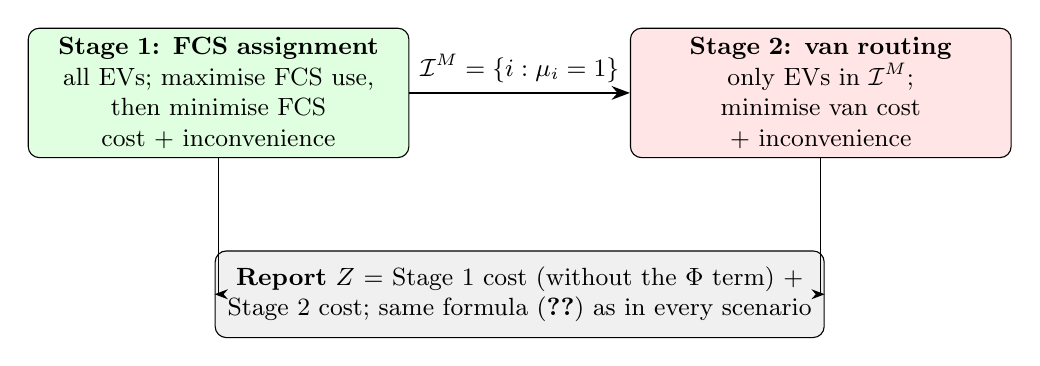
\begin{tikzpicture}[>=Stealth,box/.style={draw,rounded corners,align=center,minimum height=1.1cm,font=\small}]
  \node[box,fill=green!12,text width=4.6cm] (s1) {\textbf{Stage 1: FCS assignment}\\all EVs; maximise FCS use,\\then minimise FCS cost + inconvenience};
  \node[box,fill=red!10,text width=4.6cm,right=2.8cm of s1] (s2) {\textbf{Stage 2: van routing}\\only EVs in $\I^M$;\\minimise van cost + inconvenience};
  \draw[->,thick] (s1) -- node[above,font=\small]{$\I^M=\{i:\mu_i=1\}$} (s2);
  \node[box,fill=black!6,text width=7.5cm,below=2.0cm of $(s1)!0.5!(s2)$] (ev) {\textbf{Report} $Z=$ Stage~1 cost (without the $\Phi$ term) $+$ Stage~2 cost; same formula \eqref{eq:Z} as in every scenario};
  \draw[->] (s1) |- (ev); \draw[->] (s2) |- (ev);
\end{tikzpicture}
\end{center}

Stage~1 does not look at the vans, and Stage~2 cannot change what Stage~1 decided. That is the definition of ``FCS first, then MCS''.

%----------------------------------------------------------------
\subsection{Stage 1: assign EVs to fixed stations}

\textbf{Objective.}
\begin{equation}
\begin{split}
\min\ Z^{(1)}=\;&\underbrace{\Phi\sum_{i\in\I}\mu_i}_{\text{FCS first}}
+\underbrace{c^{EV}\sum_i\sum_{f\in\F_i}d_{if}Y_{if}}_{Z_1}
+\underbrace{Z^F_{\text{energy}}}_{\text{FCS part of }Z_4}\\
&+\underbrace{\sum_i\sum_{f\in\F_i}\rho^F_{if}Y_{if}+\alpha\sum_i w_i(C_i-r_i)+c^L\sum_i w_iL_i}_{\text{FCS customers' inconvenience}}
\end{split}
\label{eq:obj1}
\end{equation}
with $C_i=S_i+\tau^F_iY_i$ in this stage. $\Phi$ is a penalty for handing an EV to the vans. It is chosen larger than anything an extra FCS customer can add to the rest of \eqref{eq:obj1}, e.g.
\[
\Phi > \max_{i}\max_{f\in\F_i}\big(c^{EV}d_{if}+\pi^{\max}E_i+\rho^F_{if}\big)+n\,(\alpha+c^L)\,w_{\max}\,T,
\]
so Stage~1 first \textbf{maximises the number of EVs served at an FCS}, and only among those solutions minimises FCS cost and inconvenience. ($\pi^{\max}$ is the highest grid price.) A numerically safer equivalent is to solve twice: first $\max\sum_iY_i$, then fix that number and minimise the rest.
\ifTOU
Because $Z^F_{\text{energy}}$ uses the peak price, Stage~1 may \emph{start sessions later} to leave the peak, if the price saving beats the extra waiting cost (Section~\ref{sec:expect}).
\fi

\textbf{Constraints.}
\begin{align}
\sum_{g\in\G_i}y_{ig}+\mu_i &= 1 && \forall i\in\I \label{eq:s1assign}\\
S_i &\ge r_i+\sum_{f\in\F_i}t_{if}Y_{if} && \forall i\in\I \label{eq:fcsarr}\\
S_i &\le r_i+T\,(1-\mu_i) && \forall i\in\I \label{eq:s1park}\\
S_j &\ge S_i+\tau^F_i-(T+\tau^F_i)(3-y_{ig}-y_{jg}-o_{ij}) && \forall g,\ (i,j)\in\mathcal{P}_g \label{eq:disj1}\\
S_i &\ge S_j+\tau^F_j-(T+\tau^F_j)(2-y_{ig}-y_{jg}+o_{ij}) && \forall g,\ (i,j)\in\mathcal{P}_g \label{eq:disj2}\\
\sum_i y_{ig_1} &\ge \sum_i y_{ig_2} && \forall f,\ \G_f=\{g_1,g_2\} \label{eq:gunsym}\\
S_i+\tau^F_iY_i &\le T,\qquad L_i\ge S_i+\tau^F_iY_i-l_i && \forall i\in\I \label{eq:s1time}
\end{align}
\ifTOU plus the time-of-use split \eqref{eq:tou1}--\eqref{eq:tou5} of each FCS session (Section~\ref{sec:price}).\fi
\desc{\eqref{eq:s1assign}: every EV either gets one reachable gun or is handed to the vans. An EV that reaches no FCS ($\G_i=\emptyset$) is forced to $\mu_i=1$. \eqref{eq:fcsarr}: an FCS session cannot start before the EV has asked and driven to the station. \eqref{eq:s1park}: for an EV handed to the vans, $S_i$ is parked at $r_i$, so it adds no waiting in Stage~1 (its real start time is decided in Stage~2). \eqref{eq:disj1}--\eqref{eq:disj2}: two EVs on the same gun do not overlap; $o_{ij}$ picks who goes first. With two guns per station this means at most two EVs charge at a station at a time. \eqref{eq:gunsym}: symmetry breaking between the two identical guns (optional). \eqref{eq:s1time}: finished by $T$; lateness.}

\textbf{Optional acceptability rule.} An operator may refuse to send a driver to a station that is ``too inconvenient'', e.g.\ only allow gun $g$ of station $f$ for EV $i$ if $\hat\rho^F_{if}\le\bar\rho$. This only shrinks $\G_i$, so EVs whose stations are all too far go to the vans. Report results with and without it.

\textbf{Output:} $\I^M=\{i:\mu_i=1\}$, the EVs left for the vans; plus each FCS customer's gun and start time.

%----------------------------------------------------------------
\subsection{Stage 2: route the vans to the leftover EVs}

Stage~2 is a vehicle routing problem with time windows, on the EVs in $\I^M$ only. Here $C_i=S_i+\tau^M_i$.

\textbf{Objective.}
\begin{equation}
\begin{split}
\min\ Z^{(2)}=\;&\underbrace{c^M\sum_m\sum_{(i,j)\in\A^M}d_{ij}x_{ijm}}_{Z_2}+\underbrace{\sum_m c^D_mu_m}_{Z_3}+\underbrace{Z^M_{\text{energy}}}_{\text{van part of }Z_4}\\
&+\underbrace{\sum_{i\in\I^M}\sum_m\rho^M_{im}z_{im}+\alpha\sum_{i\in\I^M}w_i(C_i-r_i)+c^L\sum_{i\in\I^M}w_iL_i}_{\text{van customers' inconvenience}}
\end{split}
\label{eq:obj2}
\end{equation}
Since every EV in $\I^M$ must be served by some van, $Z^M_{\text{energy}}$ and the $\rho^M$ term are constants here. They are kept so that $Z^{(2)}$ is the true cost of Stage~2. Waiting and lateness make the vans visit urgent EVs early.

\textbf{Constraints.}
\begin{align}
\sum_{m\in\M}z_{im} &= 1 && \forall i\in\I^M \label{eq:s2assign}\\
\sum_{j:(0,j)\in\A^M}x_{0jm} = \sum_{i:(i,n+1)\in\A^M}x_{i,n+1,m} &= u_m && \forall m \label{eq:depot}\\
\sum_{i:(i,j)\in\A^M}x_{ijm} = \sum_{k:(j,k)\in\A^M}x_{jkm} &= z_{jm} && \forall j\in\I^M,\ m \label{eq:flow}\\
\sum_{i\in\I^M}z_{im} &\le Q_m\,u_m && \forall m \label{eq:cap}\\
\sum_{i\in\I^M}\frac{E_i}{\eta}z_{im}+\beta\sum_{(i,j)\in\A^M}d_{ij}x_{ijm} &\le B_m\,u_m && \forall m \label{eq:batt}
\end{align}
\begin{align}
S_j &\ge \max\{r_j,\ t_{0j}\,x_{0jm}\} && \forall j\in\I^M,\ m \label{eq:depart}\\
S_j &\ge S_i+\tau^M_i+t_{ij}-(T+\tau^M_i+t_{ij})(1-x_{ijm}) && \forall i\neq j,\ m \label{eq:seq}\\
S_i+\tau^M_i+t_{i,n+1} &\le T+(\tau^M_i+t_{i,n+1})(1-x_{i,n+1,m}) && \forall i,\ m \label{eq:return}\\
S_i+\tau^M_i \le T,\quad L_i &\ge S_i+\tau^M_i-l_i && \forall i\in\I^M \label{eq:s2time}\\
u_m &\ge u_{m+1} && m<|\M| \label{eq:vansym}
\end{align}
\desc{\eqref{eq:s2assign}: each leftover EV gets one van. \eqref{eq:depot}: a used van leaves and returns to the depot once. \eqref{eq:flow}: each EV on van $m$ is entered and left exactly once by that van. \eqref{eq:cap}: at most $Q_m$ EVs per van. \eqref{eq:batt}: delivered energy (with transfer losses) plus driving energy fits in the van battery. \eqref{eq:depart}: no start before the request, or before the van can drive there from the depot (written as two linear constraints). \eqref{eq:seq}: if the van goes $i\to j$, it finishes $i$ and drives to $j$ before starting $j$. This gives one EV at a time and removes subtours (MTZ-type). \eqref{eq:return}: back at the depot by $T$. \eqref{eq:s2time}: finished by $T$; lateness. \eqref{eq:vansym}: use identical vans in index order.}

\textbf{If Stage 2 is infeasible} (too many leftover EVs for the fleet by $T$), the sequential policy has \emph{failed} on that instance. For diagnosis, add $s_i\in\{0,1\}$ (``unserved''), replace \eqref{eq:s2assign} by $\sum_mz_{im}+s_i=1$ and add $\Phi^U\sum_is_i$ to \eqref{eq:obj2}. Then report the number of EVs that could not be served. This is a useful comparison with the integrated scenario, which may serve all of them.

%----------------------------------------------------------------
\subsection{Reported value}
\[
Z^{\text{S\scen}}=\big(Z^{(1)*}-\Phi\,|\I^M|\big)+Z^{(2)*},
\]
which is exactly \eqref{eq:Z} evaluated at the combined solution. The stage-1 solution plus the stage-2 solution is a feasible solution of the integrated model (S\ifTOU 4\else 3\fi), so
$Z^{\text{S\ifTOU 4\else 3\fi}}\le Z^{\text{S\scen}}$. The difference is the \emph{value of integration}.

\else
%---------------------------------------------------------------- INT
\subsection{Objective}
\begin{equation}
\min\ Z \quad\text{as in \eqref{eq:Z}, with }Z^F_{\text{energy}}=\ifTOU P^F\textstyle\sum_i\big[\pi^\off(\theta^1_i+\theta^3_i)+\pi^\pk\theta^2_i\big]\else\pi^F\textstyle\sum_iE_iY_i\fi,\quad C_i=S_i+\tau^F_iY_i+\tau^M_iZ_i. \label{eq:objint}
\end{equation}
Written out in full:
\begin{align*}
\min\ Z=\;& c^{EV}\sum_i\sum_{f\in\F_i}d_{if}Y_{if}+c^M\sum_m\sum_{(i,j)\in\A}d_{ij}x_{ijm}+\sum_mc^D_mu_m\\
&+\ifTOU P^F\sum_i\big[\pi^\off(\theta^1_i+\theta^3_i)+\pi^\pk\theta^2_i\big]\else\pi^F\sum_iE_iY_i\fi
+\pi^M\sum_i\sum_m\frac{E_i}{\eta}z_{im}\\
&+\sum_i\sum_{f\in\F_i}\rho^F_{if}Y_{if}+\sum_i\sum_m\rho^M_{im}z_{im}+\alpha\sum_iw_i(C_i-r_i)+c^L\sum_iw_iL_i .
\end{align*}
Every term is linear. One model weighs everything at once: an EV goes to a van exactly when the van's extra km, dispatch and energy cost are outweighed by the effort and waiting it saves the driver\ifTOU, or by the peak-price energy it avoids\fi.

\subsection{Constraints}

\textbf{Assignment.}
\begin{equation}
\sum_{g\in\G_i}y_{ig}+\sum_{m\in\M}z_{im}=1\qquad\forall i\in\I \label{eq:assign}
\end{equation}
\desc{Exactly one resource per EV: one reachable gun or one van. EVs that reach no FCS are forced onto a van.}

\textbf{Fixed stations.}
\begin{align}
S_i &\ge r_i+\sum_{f\in\F_i}t_{if}Y_{if} && \forall i \label{eq:fcsarr}\\
S_j &\ge S_i+\tau^F_i-(T+\tau^F_i)(3-y_{ig}-y_{jg}-o_{ij}) && \forall g,\ (i,j)\in\mathcal{P}_g \label{eq:disj1}\\
S_i &\ge S_j+\tau^F_j-(T+\tau^F_j)(2-y_{ig}-y_{jg}+o_{ij}) && \forall g,\ (i,j)\in\mathcal{P}_g \label{eq:disj2}\\
\sum_iy_{ig_1} &\ge \sum_iy_{ig_2} && \forall f,\ \G_f=\{g_1,g_2\} \label{eq:gunsym}
\end{align}
\desc{\eqref{eq:fcsarr}: an FCS session starts after the request and the drive to the station (for a van customer this is just $S_i\ge r_i$). \eqref{eq:disj1}--\eqref{eq:disj2}: EVs on the same gun do not overlap; $o_{ij}$ chooses the order. \eqref{eq:gunsym}: optional symmetry breaking.}

\textbf{Vans: routes, capacity, battery.}
\begin{align}
\sum_{j:(0,j)\in\A}x_{0jm}=\sum_{i:(i,n+1)\in\A}x_{i,n+1,m} &= u_m && \forall m \label{eq:depot}\\
\sum_{i:(i,j)\in\A}x_{ijm}=\sum_{k:(j,k)\in\A}x_{jkm} &= z_{jm} && \forall j\in\I,\ m \label{eq:flow}\\
\sum_iz_{im} &\le Q_mu_m && \forall m \label{eq:cap}\\
\sum_i\frac{E_i}{\eta}z_{im}+\beta\sum_{(i,j)\in\A}d_{ij}x_{ijm} &\le B_mu_m && \forall m \label{eq:batt}
\end{align}
\desc{\eqref{eq:depot}: a used van leaves and returns once. \eqref{eq:flow}: each EV on van $m$ is visited exactly once by it. \eqref{eq:cap}: at most $Q_m$ EVs. \eqref{eq:batt}: delivered energy (with losses) plus driving energy fits in the battery.}

\textbf{Vans: timing (one EV at a time, no subtours).}
\begin{align}
S_j &\ge t_{0j}\,x_{0jm} && \forall j\in\I,\ m \label{eq:depart}\\
S_j &\ge S_i+\tau^M_i+t_{ij}-(T+\tau^M_i+t_{ij})(1-x_{ijm}) && \forall i\neq j\in\I,\ m \label{eq:seq}\\
S_i+\tau^M_i+t_{i,n+1} &\le T+(\tau^M_i+t_{i,n+1})(1-x_{i,n+1,m}) && \forall i,\ m \label{eq:return}
\end{align}
\desc{\eqref{eq:depart}: the first stop cannot start before the van has driven there. \eqref{eq:seq}: $i\to j$ means finish $i$, drive, then start $j$; start times rise along a route, so no subtour can close. \eqref{eq:return}: back at the depot by $T$.}

\textbf{Horizon and lateness.}
\begin{equation}
C_i\le T,\qquad L_i\ge C_i-l_i\qquad\forall i\in\I \label{eq:time}
\end{equation}
\desc{Every EV is fully charged within the horizon; $L_i$ measures lateness.}

\ifTOU
\textbf{Time-of-use split.} Constraints \eqref{eq:tou1}--\eqref{eq:tou5} of Section~\ref{sec:price}.
\fi

\textbf{Symmetry and domains.}
\begin{equation}
u_m\ge u_{m+1};\qquad y,z,x,u,o\ifTOU,\kappa\fi\in\{0,1\};\qquad S_i,L_i\ifTOU,\theta^p_i\fi\ge0 \label{eq:dom}
\end{equation}
\fi

%=====================================================================
\section{Learning-to-optimise (RL) formulation}\label{sec:rl}

\textbf{Main rule:} the reward of each action is \emph{minus the increase in $Z$ that the action causes}. The rewards over an episode then add up to $-Z$ of the solution the policy builds. RL and MILP results are measured on the same yardstick \eqref{eq:Z}, and the MILP optimum is the benchmark for the RL gap.

\ifSEQ
%---------------------------------------------------------------- RL SEQ
The RL pipeline has the same two stages as the MILP.

\subsection{Stage 1 policy: FCS assignment}
\begin{itemize}[leftmargin=1.4em,itemsep=2pt]
  \item \textbf{Episode / epochs:} EVs are taken in order of request time $r_i$ (ties: higher $w_i$ first). One decision per EV.
  \item \textbf{State:} features of the current EV $k$ ($E_k,r_k,l_k,w_k,R_k$, location); for each gun $g$ the time $F_g$ it becomes free; summary features of the EVs still to come (count and positions near each station)\ifTOU; the current price and the time until $T_1$ and $T_2$\fi.
  \item \textbf{Action:} a gun $g\in\G_k$, or ``hand to vans''. \textbf{FCS-first mask:} ``hand to vans'' is allowed \emph{only} if no gun can finish EV $k$ by $T$ (or, with the optional rule, if all remaining guns have $\hat\rho^F_{kf}>\bar\rho$).
  \ifTOU\item \textbf{Optional timing action:} ``gun $g$, start after the peak'', i.e.\ $S_k=\max\{\text{earliest},T_2\}$, allowed only if the session still ends by $T$.\fi
  \item \textbf{Transition:} $S_k=\max\{r_k+t_{kf},F_g\}$ (or later, for the timing action); $F_g\leftarrow S_k+\tau^F_k$.
  \item \textbf{Reward:} $-\Big[c^{EV}d_{kf}+\text{energy}_k+\rho^F_{kf}+\alpha w_k(S_k+\tau^F_k-r_k)+c^Lw_k(S_k+\tau^F_k-l_k)^+\Big]$, where energy$_k$ = \ifTOU$P^F\big[\pi^\off\cdot(\text{off-peak hours of }[S_k,S_k+\tau^F_k])+\pi^\pk\cdot(\text{peak hours})\big]$, computed exactly in the simulator\else$\pi^FE_k$\fi. Handing an EV to the vans gives reward $0$ here; its cost is counted in Stage~2.
\end{itemize}
Note: a simple baseline for Stage~1 is the greedy rule ``gun with the largest one-step reward''. What RL can learn on top of this is, for example, to keep a nearby gun free for an urgent EV that arrives later.

\subsection{Stage 2 policy: van routing over $\I^M$}
\begin{itemize}[leftmargin=1.4em,itemsep=2pt]
  \item \textbf{Epochs:} whenever a van becomes free (the earliest-free van decides first).
  \item \textbf{State:} for each van: position, time free, remaining battery $b_m$, EVs served so far, dispatched or not; for each unserved EV in $\I^M$: location, $E_i,r_i,l_i,w_i$; current time.
  \item \textbf{Action:} the next EV $j$ for this van, or ``return to depot'' (ends the route). Mask: $j$ must be feasible: battery covers $E_j/\eta$ plus driving to $j$ and back to the depot, the count stays $\le Q_m$, and $j$ can be finished with the van back at the depot by $T$.
  \item \textbf{Transition:} $S_j=\max\{r_j,\ \text{time free}+t_{\text{pos},j}\}$; the van moves to $j$ and is free at $S_j+\tau^M_j$; $b_m$ falls by $E_j/\eta+\beta d_{\text{pos},j}$.
  \item \textbf{Reward:} serving $j$: $-\Big[c^Md_{\text{pos},j}+c^D_m[\text{first stop}]+\pi^M\frac{E_j}{\eta}+\rho^M_{jm}+\alpha w_j(S_j+\tau^M_j-r_j)+c^Lw_j(S_j+\tau^M_j-l_j)^+\Big]$; returning: $-c^Md_{\text{pos},0}$. EVs still unserved at the end: $-\Phi^U$ each.
  \item \textbf{Policy:} an attention-based routing policy (e.g.\ Kool et al., 2019, ``Attention, Learn to Solve Routing Problems!'') trained with REINFORCE or PPO. Baseline: nearest-feasible-EV heuristic.
\end{itemize}
Episode return of Stage~1 + Stage~2 $=-Z^{\text{S\scen}}$.

\else
%---------------------------------------------------------------- RL INT
One policy decides both who serves each EV and the van routes.
\begin{itemize}[leftmargin=1.4em,itemsep=2pt]
  \item \textbf{Episode / epochs:} EVs are taken in order of request time $r_i$ (ties: higher $w_i$ first). One decision per EV.
  \item \textbf{State:} (i) the current EV $k$: location, $E_k,r_k,l_k,w_k,R_k$, reachable stations; (ii) each gun $g$: time $F_g$ it becomes free; (iii) each van $m$: current end-of-route position, time free, remaining battery $b_m$, EVs served, dispatched or not; (iv) embeddings of the not-yet-assigned EVs (for look-ahead)\ifTOU; (v) current price, time until $T_1$ and $T_2$\fi.
  \item \textbf{Action:} $a\in\G_k\cup\M$: a gun, or a van (EV $k$ is appended to the end of that van's route). \textbf{Mask} infeasible actions: a gun that cannot finish $k$ by $T$; a van without enough battery for $E_k/\eta$ plus the drive to $k$ and back to the depot, with $Q_m$ reached, or unable to finish $k$ and return by $T$.
  \ifTOU\item \textbf{Optional timing action:} ``gun $g$, start after the peak'' ($S_k=\max\{\text{earliest},T_2\}$, if it still ends by $T$).\fi
  \item \textbf{Transition:} gun: $S_k=\max\{r_k+t_{kf},F_g\}$, $F_g\leftarrow S_k+\tau^F_k$. Van: $S_k=\max\{r_k,\ \text{free}_m+t_{\text{pos}_m,k}\}$, then the van moves to $k$, $\text{free}_m\leftarrow S_k+\tau^M_k$, $b_m\mathrel{-}=E_k/\eta+\beta d_{\text{pos}_m,k}$.
  \item \textbf{Reward} $=-\Delta Z$:
  \begin{align*}
  \text{gun } g\text{ at }f:&\quad -\Big[c^{EV}d_{kf}+\text{energy}^F_k+\rho^F_{kf}+\alpha w_k(C_k-r_k)+c^Lw_k(C_k-l_k)^+\Big]\\
  \text{van } m:&\quad -\Big[c^M\big(d_{\text{pos}_m,k}+d_{k,0}-d_{\text{pos}_m,0}\big)+c^D_m[\text{first use}]+\pi^M\tfrac{E_k}{\eta}\\
  &\qquad\quad+\rho^M_{km}+\alpha w_k(C_k-r_k)+c^Lw_k(C_k-l_k)^+\Big]
  \end{align*}
  The van distance term is the \emph{change} in route length when $k$ is inserted before the return to the depot, so the sum over the episode equals the total route length (the return legs telescope). energy$^F_k$ = \ifTOU$P^F\big[\pi^\off\cdot(\text{off-peak hours})+\pi^\pk\cdot(\text{peak hours of }[S_k,C_k])\big]$, computed exactly by the simulator; no linearisation is needed in RL\else$\pi^FE_k$\fi.
  \item \textbf{Dead end:} if every action is masked, EV $k$ is unserved: reward $-\Phi^U$, and the episode continues. Report the count.
  \item \textbf{Policy:} masked categorical policy over guns and vans, encoder with attention over EVs, guns and vans; trained with PPO. Natural baseline: greedy, i.e.\ choose the action with the largest one-step reward. That is the pairwise rule ``smallest $\hat\rho$ + cost'' from Section~\ref{sec:inc}.
\end{itemize}
Restriction to note: vans serve EVs in assignment order (append only). A variant that inserts $k$ at the cheapest position of a route is more flexible but has a larger action space.
\fi

\textbf{Reward scaling.} For stable training divide every reward by a constant, e.g.\ the greedy baseline's average $Z$ on the training instances. This does not change the optimal policy.

%=====================================================================
\section{What to expect and what to report}\label{sec:expect}

\ifnum\scen=1
\begin{itemize}[leftmargin=1.4em,itemsep=2pt]
  \item Vans serve only EVs that reach no station, or that the stations cannot finish by $T$. If stations have spare capacity, very few vans are dispatched.
  \item Inconvenience is high for EVs far from the nearest station (worked example: Rs\,682 at the FCS, against Rs\,458 if a van had been allowed).
  \item With too few vans Stage~2 becomes infeasible (unserved EVs), even when the integrated model S3 could serve everyone. Report the smallest $|\M|$ at which S1 is feasible and compare it with S3.
\end{itemize}
\fi
\ifnum\scen=2
\begin{itemize}[leftmargin=1.4em,itemsep=2pt]
  \item \textbf{When does Stage~1 delay a session to avoid the peak?} Moving one hour of charging out of the peak saves $(\pi^\pk-\pi^\off)P^F=3\times22=$ Rs\,66, but delays completion by up to an hour, which costs $\alpha w_i\ge$ Rs\,200. So with the default values Stage~1 almost never delays. It mostly pays the higher price, and S2 costs roughly S1 plus the peak surcharge. Sessions start later only if $\alpha$ is small (try $\lambda<0.33$ in the sensitivity analysis).
  \item The van assignment is the same as in S1 unless Stage~1's timing changes which EVs fit at the stations. Stage~1 cannot use vans to escape the peak price.
  \item Extra KPI: \textbf{grid energy drawn at FCS during the peak}, $P^F\sum_i\theta^2_i$ (kWh). Compare with S4.
\end{itemize}
\fi
\ifnum\scen=3
\begin{itemize}[leftmargin=1.4em,itemsep=2pt]
  \item Vans take EVs for which the saved inconvenience exceeds the extra van cost (worked example: van chosen, saving Rs\,224). Expect vans to serve EVs that are far from every station, have low range (high $w_i$), or have early deadlines, while EVs near a station still use it.
  \item \textbf{Value of integration under flat price:} $Z^{\text{S1}}-Z^{\text{S3}}\ge0$. Report it per component ($Z_1,\dots,Z_5$): typically operating cost rises a little and inconvenience falls a lot.
  \item Vary $|\M|$ (0, 1, 2, \dots): the first few vans lower $Z$ sharply, then the effect levels off. That curve shows the scenarios where mobile chargers help most.
\end{itemize}
\fi
\ifnum\scen=4
\begin{itemize}[leftmargin=1.4em,itemsep=2pt]
  \item During the peak a van kWh costs about the same as an FCS kWh (Rs\,10.0 each), so the vans' energy disadvantage disappears and vans also absorb \emph{peak-hour} demand that would otherwise be charged on the grid at peak price.
  \item Expect more van usage than in S3, concentrated on requests in $[T_1,T_2]$, and lower grid energy at the stations during the peak, $P^F\sum_i\theta^2_i$, than in S2.
  \item \textbf{Value of integration under peak pricing:} $Z^{\text{S2}}-Z^{\text{S4}}$. It should be larger than $Z^{\text{S1}}-Z^{\text{S3}}$, because integration now also allows price arbitrage.
  \item \textbf{Peak pricing with full flexibility:} $Z^{\text{S4}}-Z^{\text{S3}}$ should be smaller than $Z^{\text{S2}}-Z^{\text{S1}}$: vans cushion the price increase.
\end{itemize}
\fi

\textbf{Cross-scenario comparison table} (fill in from the four runs):
\begin{center}
\renewcommand{\arraystretch}{1.2}
\begin{tabular}{@{}lll@{}}
\toprule
\textbf{Comparison} & \textbf{Measures} & \textbf{Expected sign} \\
\midrule
S1 $-$ S3 & value of integration, flat price & $\ge0$ \\
S2 $-$ S4 & value of integration, peak price & $\ge0$, larger than S1 $-$ S3 \\
S2 $-$ S1 & cost of peak pricing, FCS-first operator & $>0$ \\
S4 $-$ S3 & cost of peak pricing, flexible operator & $>0$, smaller than S2 $-$ S1 \\
\bottomrule
\end{tabular}
\end{center}
Report for each: $Z$ and its components, number of vans used, EVs per resource, mean and maximum inconvenience per EV, total lateness, peak-hour grid energy, solve time, and (for RL) the gap to the MILP optimum.

%=====================================================================
\appendix
\section{Illustrative parameter values}\label{app:values}

These are starting values for experiments, not data. All are meant to be varied in the analysis. Values in Rs.

\begin{center}
\renewcommand{\arraystretch}{1.15}
\begin{tabular}{@{}llp{6.2cm}@{}}
\toprule
\textbf{Parameter} & \textbf{Value} & \textbf{Note} \\
\midrule
$T$, $[T_1,T_2]$ & 7 h, $[2,6]$ & 16:00--23:00, peak 18:00--22:00 \\
$P^F$, $P^M$ & 22 kW, 30 kW & \\
$v$, $\beta$, $\eta$ & 25 km/h, 0.25 kWh/km, 0.9 & \\
$B_m$, $Q_m$, $|\M|$ & 150 kWh, 6, 2--6 & \\
$c^{EV}$, $c^M$, $c^D_m$ & Rs\,4/km, Rs\,15/km, Rs\,1500 & van km includes driver time \\
$\pi^F$ (flat) & Rs\,8.7/kWh & equals the time-average of the ToU tariff over $[0,T]$ \\
$\pi^\off$, $\pi^\pk$ (ToU) & Rs\,7/kWh, Rs\,10/kWh & $(3\times7+4\times10)/7=8.7$ \\
$c^{bat}$ & Rs\,2/kWh & van battery wear \\
$\pi^M$ & Rs\,10.7 (flat) / Rs\,9.0 (ToU) & $=\pi^F+c^{bat}$ / $=\pi^\off+c^{bat}$ \\
$\alpha$, $\alpha^D$ & Rs\,200/h, Rs\,100/h & value of time; extra for attended time \\
$h^F$, $h^M$, $\varphi$ & Rs\,50, Rs\,10, Rs\,100 & trip hassle, hand-over, range stress \\
$c^L$ & Rs\,300/h & lateness \\
$w_i$ & $1+2(1-R_i/R_{\max})$, $R_i\sim U[3,40]$ km & priority from remaining range \\
\bottomrule
\end{tabular}
\end{center}

The flat price is set to the time-average of the peak tariff. The price \emph{level} is then the same in both pricing cases, and only the price \emph{shape} differs. Without this, part of S1 vs S2 would just reflect a different average price.

\end{document}
"
%    pdflatex -jobname=scenario4_peak_integrated   "\def\scen{4}% =====================================================================
%  One source, four PDFs.  Build with build.sh (or by hand):
%    pdflatex -jobname=scenario1_flat_sequential   "\def\scen{1}\input{scenario_master}"
%    pdflatex -jobname=scenario2_peak_sequential   "\def\scen{2}\input{scenario_master}"
%    pdflatex -jobname=scenario3_flat_integrated   "\def\scen{3}\input{scenario_master}"
%    pdflatex -jobname=scenario4_peak_integrated   "\def\scen{4}\input{scenario_master}"
%  (run each twice for cross-references)
% =====================================================================
\documentclass[11pt,a4paper]{article}
\usepackage[margin=2.2cm]{geometry}
\usepackage{amsmath,amssymb,amsfonts}
\usepackage{booktabs,array,tabularx}
\usepackage{enumitem}
\usepackage[table]{xcolor}
\usepackage{tikz}
\usetikzlibrary{arrows.meta,positioning,calc}
\usepackage[colorlinks=true,linkcolor=blue!50!black,urlcolor=blue!50!black]{hyperref}
\usepackage{titlesec}
\titleformat{\section}{\large\bfseries}{\thesection}{0.8em}{}
\titleformat{\subsection}{\normalsize\bfseries}{\thesubsection}{0.8em}{}
\setlength{\parindent}{0pt}
\setlength{\parskip}{5pt}

% ---------------- scenario switches ----------------
\ifdefined\scen\else\def\scen{1}\fi
\newif\ifTOU \TOUfalse   % true = time-of-use (peak) price
\newif\ifSEQ \SEQfalse   % true = FCS first, then MCS
\ifnum\scen=1 \SEQtrue \fi
\ifnum\scen=2 \TOUtrue \SEQtrue \fi
\ifnum\scen=4 \TOUtrue \fi

\newcommand{\pricename}{\ifTOU time-of-use price (dearer evening peak)\else single (flat) price all day\fi}
\newcommand{\structname}{\ifSEQ FCS first, then MCS (sequential)\else FCS and MCS together (integrated)\fi}

% ---------------- notation ----------------
\newcommand{\I}{\mathcal{I}}
\newcommand{\F}{\mathcal{F}}
\newcommand{\G}{\mathcal{G}}
\newcommand{\M}{\mathcal{M}}
\newcommand{\N}{\mathcal{N}}
\newcommand{\A}{\mathcal{A}}
\newcommand{\Rs}{\text{Rs}\,}
\newcommand{\pk}{\mathrm{pk}}
\newcommand{\off}{\mathrm{off}}
\newcommand{\desc}[1]{\par\vspace{-2pt}{\small\color{black!75}\textit{Meaning:} #1}\par\vspace{4pt}}
\newcommand{\cell}[2]{\ifnum\scen=#1\cellcolor{blue!18}\textbf{S#1 (this document)}\\\textbf{#2}\else S#1\\#2\fi}

\title{\textbf{EV Charging Network Optimisation}\\[4pt]
\large Scenario \scen: \pricename\ $+$ \structname\\[2pt]
\normalsize MILP and RL formulation}
\author{CP 320 OR for Mobility Management, course project}
\date{2 October 2026}

\begin{document}
\maketitle

%=====================================================================
\section{Where this scenario sits}

The project studies four scenarios: two ways of pricing grid electricity, times two ways of making the decisions.

\begin{center}
\renewcommand{\arraystretch}{1.5}
\begin{tabular}{>{\raggedright\arraybackslash}p{4.2cm}|>{\centering\arraybackslash}p{4.6cm}|>{\centering\arraybackslash}p{4.6cm}}
 & \textbf{Flat price all day} & \textbf{Time-of-use (peak) price} \\ \hline
\textbf{Sequential:} FCS first, leftover EVs to MCS &
\begin{tabular}[c]{@{}c@{}}\cell{1}{flat + sequential}\end{tabular} &
\begin{tabular}[c]{@{}c@{}}\cell{2}{peak + sequential}\end{tabular} \\ \hline
\textbf{Integrated:} FCS and MCS decided together &
\begin{tabular}[c]{@{}c@{}}\cell{3}{flat + integrated}\end{tabular} &
\begin{tabular}[c]{@{}c@{}}\cell{4}{peak + integrated}\end{tabular} \\
\end{tabular}
\end{center}

\textbf{The four scenarios do not have four different objectives.} They share \emph{one} cost yardstick $Z$ (Section~\ref{sec:obj}): the same cost terms and the same customer inconvenience (Section~\ref{sec:inc}). Only two things change:
\begin{itemize}[leftmargin=1.4em,itemsep=1pt]
  \item \textbf{Pricing} changes the formula for one term, the FCS energy cost (Section~\ref{sec:price}).
  \item \textbf{Decision structure} changes \emph{how} $Z$ is minimised: in one model (integrated), or in two stages (sequential), where each stage minimises its own part of $Z$.
\end{itemize}
Because the yardstick is the same, the four optimal values can be compared directly. The differences measure the \emph{value of integration} (S1$\to$S3, S2$\to$S4) and the \emph{effect of peak pricing} (S1$\to$S2, S3$\to$S4).

\ifnum\scen=1
\textbf{This scenario (S1)} is the baseline, the ``status quo''. Electricity costs the same at every hour, every EV that can be charged at a fixed station is sent there, and vans only take what is left over.
\fi
\ifnum\scen=2
\textbf{This scenario (S2)} keeps the FCS-first rule of S1, but grid electricity is dearer during the evening peak. Stage~1 can react to the price only by \emph{rescheduling} FCS sessions. It cannot hand a peak-hour EV to a van.
\fi
\ifnum\scen=3
\textbf{This scenario (S3)} keeps the flat price of S1, but the operator decides FCS and MCS service \emph{together}. An EV can be sent to a van even when a fixed station could take it, whenever that lowers total cost plus inconvenience.
\fi
\ifnum\scen=4
\textbf{This scenario (S4)} is the most flexible one: peak pricing at fixed stations, and FCS and MCS decided together. Van energy was bought off-peak, so vans can also be used to keep charging \emph{out of the expensive peak}.
\fi

%=====================================================================
\section{Setting and assumptions}\label{sec:setting}

\textbf{Time.} The planning horizon is $[0,T]$ with $T=7$\,h (16:00--23:00). It contains the evening peak window $[T_1,T_2]=[2,6]$ (18:00--22:00). The horizon is the same in all four scenarios. It is wider than the peak itself so that, under peak pricing, there is cheaper time on both sides of the peak.\ifTOU\else\ In this scenario the price is flat, so the window plays no role in the model.\fi

\textbf{Assumptions} (the same as MILP v3, plus two about energy):
\begin{enumerate}[leftmargin=1.6em,itemsep=1pt]
  \item Static, continuous time. All requests in the horizon are known at time $0$, and request $i$ becomes active at $r_i$.
  \item An EV served by an FCS drives there itself on its own battery (only to stations within its range $R_i$). The driver stays with the car while it waits for a free gun and while it charges.
  \item An EV served by an MCS stays parked where it is, and the driver is free in the meantime.
  \item Each FCS gun and each van charges one EV at a time, without interruption, at constant power.
  \item A van's battery covers both its driving and the energy it delivers. \textbf{The van battery is charged at the depot before the horizon starts}\ifTOU, i.e.\ at the off-peak price\fi, and is not recharged during the horizon.
  \item Every EV must be fully charged by $T$ (hard). Finishing after the driver's desired time $l_i$ is allowed but penalised.
\end{enumerate}

%=====================================================================
\section{Notation}\label{sec:notation}

\subsection*{Sets}
\begin{tabularx}{\textwidth}{@{}lX@{}}
\toprule
$\I=\{1,\dots,n\}$ & EV charging requests \\
$\F$; $\G_f$ ($|\G_f|=2$); $\G=\bigcup_f\G_f$ & fixed charging stations; guns of FCS $f$; all guns ($f(g)$ = station of gun $g$) \\
$\F_i=\{f: d_{if}\le R_i\}$, $\G_i=\bigcup_{f\in\F_i}\G_f$ & stations / guns EV $i$ can reach on its remaining range \\
$\M$ & mobile charging vans (MCS) \\
$0,\ n+1$ & depot as start node / end node (same place) \\
$\N=\{0\}\cup\I\cup\{n+1\}$, $\A$ & routing nodes; allowed van arcs $(i,j)$, $i\in\{0\}\cup\I$, $j\in\I\cup\{n+1\}$, $i\neq j$ \\
$\mathcal{P}_g=\{(i,j): i<j,\ g\in\G_i\cap\G_j\}$ & pairs of EVs that could share gun $g$ \\
\ifSEQ
$\I^M\subseteq\I$ & EVs handed to the vans by Stage~1 (an \emph{output} of Stage~1, a fixed input to Stage~2) \\
$\N^M$, $\A^M$ & routing nodes / arcs restricted to $\I^M$ \\
\fi
\bottomrule
\end{tabularx}

\subsection*{Parameters}
\begin{tabularx}{\textwidth}{@{}lX@{}}
\toprule
$E_i,\ r_i,\ l_i,\ R_i$ & energy demand (kWh), request time, desired completion time (h), remaining range (km) \\
$w_i\ge1$ & priority of EV $i$; $w_i=1+\kappa(1-R_i/R_{\max})$, so low-range EVs weigh more \\
$P^F,\ P^M$ & charging power of an FCS gun (22\,kW) / of a van (e.g.\ 30\,kW) \\
$\tau^F_i=E_i/P^F,\ \tau^M_i=E_i/P^M$ & charging time of EV $i$ at an FCS / by a van (h) \\
$d_{if},t_{if}$;\ $d_{ij},t_{ij}$ & distance (km) and time (h): EV$\to$FCS; between routing nodes ($t=d/v$) \\
$B_m,\ Q_m,\ \beta,\ \eta$ & van battery (kWh), max EVs per van, van consumption (kWh/km), transfer efficiency \\
$c^{EV},\ c^M,\ c^D_m$ & cost per km of EV driving, per km of van driving; fixed dispatch cost of van $m$ \\
\ifTOU
$\pi^\off,\ \pi^\pk$ & grid price (Rs/kWh) off-peak / in $[T_1,T_2]$, with $\pi^\pk\ge\pi^\off$ \\
\else
$\pi^F$ & grid price (Rs/kWh), the same at every hour \\
\fi
$c^{bat}$ & van battery wear per kWh cycled \\
$\pi^M$ & cost of 1 kWh taken from a van battery: $\pi^M=\ifTOU\pi^\off\else\pi^F\fi+c^{bat}$ (Section~\ref{sec:price}) \\
$\alpha,\ \alpha^D,\ h^F,\ h^M,\ \varphi,\ c^L$ & inconvenience coefficients (Section~\ref{sec:inc}) \\
\bottomrule
\end{tabularx}

\subsection*{Decision variables}
\begin{tabularx}{\textwidth}{@{}llX@{}}
\toprule
$y_{ig}$ & $\{0,1\}$ & EV $i$ charged at gun $g\in\G_i$ \\
$z_{im}$ & $\{0,1\}$ & EV $i$ served by van $m$ \\
$x_{ijm}$ & $\{0,1\}$ & van $m$ drives arc $(i,j)$ \\
$u_m$ & $\{0,1\}$ & van $m$ is dispatched \\
$o_{ij}$ & $\{0,1\}$ & for EVs $i<j$ that could share a gun: 1 if $i$ is charged before $j$ \\
\ifSEQ
$\mu_i$ & $\{0,1\}$ & Stage~1 only: EV $i$ is handed to the van fleet \\
\fi
\ifTOU
$\theta^1_i,\theta^2_i,\theta^3_i$ & $\ge0$ & hours of EV $i$'s FCS session before / inside / after the peak \\
$\kappa^1_i,\kappa^3_i$ & $\{0,1\}$ & EV $i$'s FCS session starts before $T_1$ / ends after $T_2$ \\
\fi
$S_i$ & $\ge0$ & time charging of EV $i$ starts (h), on whichever resource \\
$L_i$ & $\ge0$ & lateness of EV $i$ beyond $l_i$ (h) \\
\bottomrule
\end{tabularx}

\textbf{Short-hands} (linear expressions, not new variables):
\[
Y_{if}=\sum_{g\in\G_f}y_{ig},\qquad Y_i=\sum_{g\in\G_i}y_{ig}\ (\text{EV $i$ uses an FCS}),\qquad Z_i=\sum_{m\in\M}z_{im}\ (\text{EV $i$ uses a van}),
\]
\[
C_i=S_i+\tau^F_i\,Y_i+\tau^M_i\,Z_i \quad\text{(time EV $i$ is fully charged).}
\]

%=====================================================================
\section{Customer inconvenience}\label{sec:inc}

This section is \textbf{identical in all four scenario documents}. Inconvenience is a property of the customer, not of the price or of the planning method.

\subsection{What we mean by inconvenience}

Inconvenience is \emph{what the driver loses} from the moment they ask for a charge ($r_i$) until the car is fully charged ($C_i$), \emph{converted into rupees} so it can be added to the operator's costs. A driver loses three different things:

\begin{enumerate}[leftmargin=1.6em,itemsep=2pt]
  \item \textbf{Waiting:} the car is not ready. This lasts $C_i-r_i$ hours and affects \emph{every} driver, FCS or MCS.
  \item \textbf{Effort:} only an FCS customer has to drive to the station and sit there while the car charges. An MCS customer stays at home or at work and does something else. Driving to a far station also uses scarce battery range, which causes stress (``range anxiety'').
  \item \textbf{A missed deadline:} the car is still not ready at the time $l_i$ the driver needs it.
\end{enumerate}

Each loss gets a price in Rs per hour (or per event). All of them are multiplied by the priority $w_i$: an hour of delay for an EV with 5\,km of range left counts more than for one with 40\,km.

\subsection{The three components}

\begin{center}
\renewcommand{\arraystretch}{1.3}
\begin{tabularx}{\textwidth}{@{}>{\raggedright\arraybackslash}p{2.6cm}>{\raggedright\arraybackslash}X>{\raggedright\arraybackslash}X>{\raggedright\arraybackslash}p{3.0cm}@{}}
\toprule
\textbf{Component} & \textbf{EV $i$ at FCS $f$} & \textbf{EV $i$ by a van} & \textbf{Known when?} \\
\midrule
Effort & $w_i\big[\alpha^D(t_{if}+\tau^F_i)+h^F+\varphi\,d_{if}/R_i\big]$: driving and sitting at the station, a fixed trip hassle, range stress & $w_i\,h^M$: being reachable and handing over the car & \textbf{Static:} known as soon as the resource is chosen \\
Waiting & $w_i\,\alpha\,(C_i-r_i)$ = drive + \emph{queue at the gun} + charge & $w_i\,\alpha\,(C_i-r_i)$ = \emph{wait for the van} + charge & \textbf{Dynamic:} depends on the queue / van route \\
Missed deadline & $w_i\,c^L\,L_i$, $L_i=\max\{0,C_i-l_i\}$ & same & Dynamic \\
\bottomrule
\end{tabularx}
\end{center}

\textbf{Coefficients.}
$\alpha$ (Rs/h) is the value of an hour the car is not ready.
$\alpha^D$ (Rs/h) is the \emph{extra} value of an hour the driver must personally spend driving or sitting at the station: an hour at the station costs $\alpha+\alpha^D$, an hour waiting at home for a van costs only $\alpha$.
$h^F,h^M$ (Rs) are fixed hassle costs of one trip to a station / one van hand-over.
$\varphi$ (Rs) is the range-stress cost of a trip that uses the \emph{whole} remaining range ($d_{if}/R_i\le1$ is the fraction used).
$c^L$ (Rs/h) is the cost per hour late.

\subsection{Pairwise form: inconvenience of a (customer, resource) pair}

The natural first idea is: \emph{for every pair (EV $i$, FCS $f$) and every pair (EV $i$, van $m$) there is an inconvenience number, and the operator picks the pair with the lowest cost plus inconvenience.} The static part fits this idea exactly:
\[
\boxed{\;\rho^F_{if}=w_i\Big[\alpha^D\,(t_{if}+\tau^F_i)+h^F+\varphi\,\frac{d_{if}}{R_i}\Big]\qquad
\rho^M_{im}=w_i\,h^M\;}
\]
These are \textbf{parameters}, computed before solving, one number per (EV, FCS) pair and per (EV, van) pair. In the objective they appear linearly: $\sum_i\sum_f\rho^F_{if}Y_{if}+\sum_i\sum_m\rho^M_{im}z_{im}$.

Note that $\rho^M_{im}$ does not depend on $m$. Vans are identical and all start at the same depot, so the driver does not care \emph{which} van comes, only \emph{when} it comes. That ``when'' is the waiting part.

\subsection{Why waiting cannot be a fixed pairwise number}

It is tempting to also write the waiting as a pairwise number, e.g.\ ``the van needs 5 minutes to reach EV $i$''. But that depends on \emph{where the van is coming from}, which depends on the route the model is still choosing: if EV $i$ is the 4th stop of a van, the wait is the time for three charging sessions plus four drives. Likewise, waiting at an FCS depends on how many EVs are queued at that gun. So waiting is not known before solving. It is a function of decision variables:
\[
\text{waiting cost of EV } i \;=\; w_i\,\alpha\,(C_i-r_i),\qquad C_i=S_i+\tau^F_iY_i+\tau^M_iZ_i .
\]
This is \textbf{linear} in the variables ($S_i$, $y$, $z$), so it fits in a MILP directly. The constraints of Section~\ref{sec:milp} make $S_i$ equal to the true start time, including driving, queueing at the gun and the van's route. The term $\sum_i w_i\alpha r_i$ is a constant and may be dropped when solving.

\textbf{Pairwise \emph{estimate}} (used for intuition, by the RL policy and in heuristics): if there is no queue and the van comes straight to $i$,
\[
\hat\rho^{F}_{if}=\rho^F_{if}+w_i\alpha\,(t_{if}+\tau^F_i),\qquad
\hat\rho^{M}_{im}=\rho^M_{im}+w_i\alpha\,(t^{\text{van}}_{m\to i}+\tau^M_i),
\]
where $t^{\text{van}}_{m\to i}$ is the time until van $m$ can reach $i$ from where it currently is. In the RL formulation (Section~\ref{sec:rl}) the van's position \emph{is} known at each decision, so there this estimate becomes exact.

\subsection{Total inconvenience and how it enters the objective}

\begin{equation}
\boxed{\;
Z_{\text{inc}}=\underbrace{\sum_{i\in\I}\sum_{f\in\F_i}\rho^F_{if}Y_{if}+\sum_{i\in\I}\sum_{m\in\M}\rho^M_{im}z_{im}}_{\text{effort (static, pairwise)}}
+\underbrace{\alpha\sum_{i\in\I}w_i\,(C_i-r_i)}_{\text{waiting (dynamic)}}
+\underbrace{c^L\sum_{i\in\I}w_i\,L_i}_{\text{missed deadline}}
\;}\label{eq:inc}
\end{equation}
All three parts are in rupees, so $Z_{\text{inc}}$ is simply added to the operating costs. Nothing has to be normalised.

\subsection{Worked example: your ``10 km to the FCS vs.\ van in 5 minutes'' case}

EV $i$: $E_i=20$\,kWh, $R_i=40$\,km (so $w_i=1$); nearest free FCS $d_{if}=10$\,km away, $t_{if}=0.4$\,h at 25\,km/h; a van finishing next door can reach it in 5\,min ($0.083$\,h), adding about 4\,km to its route. $\tau^F_i=20/22=0.909$\,h, $\tau^M_i=20/30=0.667$\,h. Coefficients from Appendix~\ref{app:values}, flat price.

\begin{center}
\renewcommand{\arraystretch}{1.25}
\begin{tabular}{@{}lrr@{}}
\toprule
 & \textbf{FCS} & \textbf{Van} \\
\midrule
Driving (EV / extra van km) & $4\times10=40.0$ & $15\times4=60.0$ \\
Energy & $8.7\times20=174.0$ & $10.7\times20/0.9=237.8$ \\
\textbf{Operating cost only} & \textbf{214.0} & \textbf{297.8} \\
\midrule
Effort $\rho$ & $100(0.4+0.909)+50+100\cdot\tfrac{10}{40}=205.9$ & $10.0$ \\
Waiting $\alpha(C_i-r_i)$ & $200\times1.309=261.8$ & $200\times0.75=150.0$ \\
\textbf{Cost + inconvenience} & \textbf{681.7} & \textbf{457.8} \\
\bottomrule
\end{tabular}
\end{center}

On operating cost alone the FCS is cheaper, so a cost-only model would \emph{always} send this driver 10\,km away. With inconvenience included the van is better by about Rs\,224, and the integrated model chooses $z_{im}=1$, as you expected. If the FCS were only 1\,km away, the FCS would win both comparisons. The inconvenience term is what makes the model choose between ``cheap for the operator'' and ``convenient for the driver'', rather than following a fixed rule.

\subsection{Relation to a single penalty $\rho_i$ per EV}

The first draft used a penalty $\rho_i$ that is charged whenever EV $i$ goes to \emph{any} FCS: $\sum_i\sum_f\rho_iy_{if}$. Because $\sum_f y_{if}=1-\sum_m z_{im}$, this only says ``a van is worth $\rho_i$ more to EV $i$'', and that holds whether the station is 1\,km or 15\,km away, and whether the van arrives in 5 minutes or in 3 hours. The form above fixes both problems: $\rho^F_{if}$ grows with the distance to \emph{that} station, and the waiting term grows with how late the van or the free gun actually is. The old model is the special case $\alpha=\alpha^D=\varphi=c^L=0$, $h^F=\rho_i$.

\subsection{Choosing the coefficients}
\begin{itemize}[leftmargin=1.4em,itemsep=2pt]
  \item Use a value of time for $\alpha$ (e.g.\ Rs\,150--300/h for urban car users), and set $\alpha^D\approx0.5\alpha$: sitting at a station is worse than waiting at home.
  \item Keep $c^L>\alpha$, so missing the deadline is worse than ordinary waiting.
  \item \textbf{Sensitivity analysis:} multiply all inconvenience coefficients by a factor $\lambda\in\{0,0.25,0.5,1,2,4\}$ and plot operating cost against total inconvenience. $\lambda=0$ is the pure cost-minimising operator, and large $\lambda$ is a customer-first operator. This trade-off curve is a strong result for the ``Analysis'' part of the project.
\end{itemize}

\subsection{What inconvenience does in \emph{this} scenario}
\ifSEQ
In a sequential scenario inconvenience \textbf{cannot move an EV from an FCS to a van}: Stage~1 sends every EV that \emph{can} use an FCS to one. It still matters inside each stage. In Stage~1 it decides \emph{which} station and \emph{when} (urgent EVs get the near station and the first free gun). In Stage~2 it decides the \emph{order} in which vans visit EVs (urgent EVs first). In the worked example, this scenario sends the driver 10\,km to the FCS. That is the weakness the integrated scenarios remove.
\else
In an integrated scenario inconvenience is weighed directly against operating cost when choosing the resource. That is how the worked example ends up with a van. It also decides which station and which gun order, and the order of each van route.
\fi

%=====================================================================
\section{Electricity price in this scenario}\label{sec:price}

\textbf{Van energy (same in all scenarios).} A van's battery is charged at the depot \emph{before} the horizon, so its energy was bought at the
\ifTOU off-peak \fi
price, whatever time the van later delivers it. Each kWh taken from the van also wears the battery ($c^{bat}$), and a fraction $1-\eta$ is lost in transfer:
\[
Z^M_{\text{energy}}=\pi^M\sum_{i\in\I}\sum_{m\in\M}\frac{E_i}{\eta}\,z_{im},\qquad \pi^M=\ifTOU\pi^\off\else\pi^F\fi+c^{bat}.
\]

\ifTOU
\textbf{FCS energy (time-of-use).} An FCS draws from the grid while it charges. Energy delivered inside $[T_1,T_2]$ costs $\pi^\pk$, and energy outside it costs $\pi^\off$. A session $[S_i,S_i+\tau^F_i]$ may overlap the peak partly. Split its duration into the hours before, inside and after the peak, $\theta^1_i+\theta^2_i+\theta^3_i$:
\[
Z^F_{\text{energy}}=P^F\sum_{i\in\I}\Big[\pi^\off(\theta^1_i+\theta^3_i)+\pi^\pk\,\theta^2_i\Big].
\]
Constraints \eqref{eq:tou1}--\eqref{eq:tou5} below make the $\theta$'s equal to the true overlaps. Peak hours are dearer, so the solver wants $\theta^1_i,\theta^3_i$ as large as possible. It is enough to bound them from above by the true off-peak overlap, and the constraints need one binary per side:
\begin{align}
\theta^1_i+\theta^2_i+\theta^3_i &= \tau^F_i\,Y_i && \forall i\in\I \label{eq:tou1}\\
\theta^1_i &\le \tau^F_i\,\kappa^1_i && \forall i\in\I \label{eq:tou2}\\
\theta^1_i &\le T_1-S_i+T\,(1-\kappa^1_i) && \forall i\in\I \label{eq:tou3}\\
\theta^3_i &\le \tau^F_i\,\kappa^3_i && \forall i\in\I \label{eq:tou4}\\
\theta^3_i &\le S_i+\tau^F_i-T_2+T\,(1-\kappa^3_i) && \forall i\in\I \label{eq:tou5}
\end{align}
\desc{\eqref{eq:tou1}: the FCS session's hours are split into three parts; for a van customer ($Y_i=0$) all three are zero. \eqref{eq:tou2}--\eqref{eq:tou3}: off-peak time before the peak is only possible if the session starts before $T_1$ ($\kappa^1_i=1$), and is at most $T_1-S_i$. \eqref{eq:tou4}--\eqref{eq:tou5}: the same for time after $T_2$. $\theta^2_i\ge0$ prevents counting more off-peak hours than exist. Checking the cases (entirely before / inside / after the peak, straddling one edge, covering the whole peak) shows that at the optimum the $\theta$'s equal the exact overlaps. This needs $\pi^\pk\ge\pi^\off$, which is true for a peak tariff.}

\textbf{Why vans become more attractive.} Compare the cost of 1\,kWh delivered to an EV during the peak (values from Appendix~\ref{app:values}):
FCS $=\pi^\pk=$ Rs\,10.0, van $=(\pi^\off+c^{bat})/\eta=9/0.9=$ Rs\,10.0. They are at parity. Under the flat price the van is about Rs\,3.2/kWh dearer (FCS Rs\,8.7, van $10.7/0.9=$ Rs\,11.9). Peak pricing therefore removes the vans' main cost disadvantage, but only for EVs whose FCS session would fall in the peak.
\ifSEQ\ In this sequential scenario Stage~1 cannot use that, because it does not consider vans. It can only shift FCS sessions in time.\fi
\else
\textbf{FCS energy (flat).} Every kWh delivered at a fixed station costs $\pi^F$, whenever it is delivered:
\[
Z^F_{\text{energy}}=\pi^F\sum_{i\in\I}E_i\,Y_i .
\]
The start time therefore does not affect the energy cost. Under the flat price a van kWh costs $(\pi^F+c^{bat})/\eta\approx$ Rs\,11.9 against Rs\,8.7 at an FCS (Appendix~\ref{app:values}), so on energy alone the FCS always wins.
\fi

%=====================================================================
\section{MILP formulation}\label{sec:milp}

\subsection{The common cost yardstick $Z$}\label{sec:obj}

For any complete solution (every EV assigned, every route and start time known), the system cost is
\begin{equation}
\boxed{\;
Z=\underbrace{c^{EV}\sum_{i}\sum_{f\in\F_i}d_{if}Y_{if}}_{Z_1:\ \text{EV driving}}
+\underbrace{c^M\sum_{m}\sum_{(i,j)\in\A}d_{ij}x_{ijm}}_{Z_2:\ \text{van driving}}
+\underbrace{\sum_m c^D_m u_m}_{Z_3:\ \text{dispatch}}
+\underbrace{Z^F_{\text{energy}}+Z^M_{\text{energy}}}_{Z_4:\ \text{energy}}
+\underbrace{Z_{\text{inc}}}_{Z_5:\ \text{inconv.\ \eqref{eq:inc}}}
\;}\label{eq:Z}
\end{equation}
$Z_4$ is defined in Section~\ref{sec:price}. $Z_1$--$Z_4$ are the operator's costs listed in the brief (EV travel, MCS travel, MCS operating cost) plus energy. $Z_5$ is the customer inconvenience penalty. \textbf{The same formula is used to report results in all four scenarios.}

\ifSEQ
%---------------------------------------------------------------- SEQ
\subsection{Structure: two stages}

\begin{center}
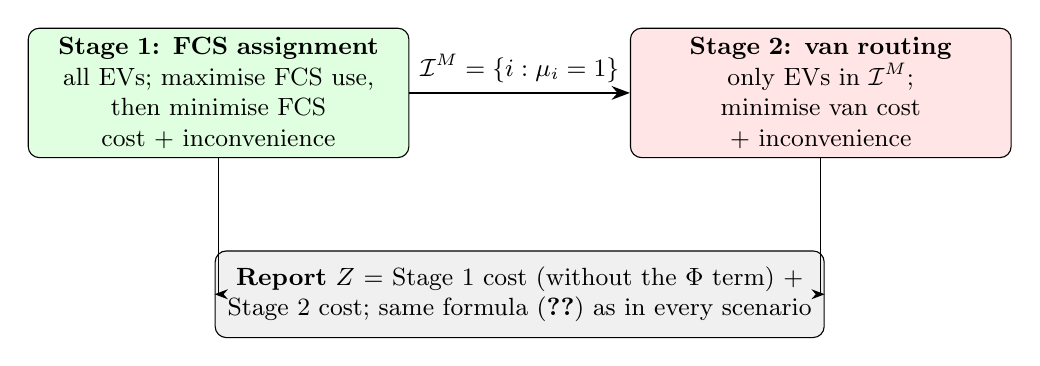
\begin{tikzpicture}[>=Stealth,box/.style={draw,rounded corners,align=center,minimum height=1.1cm,font=\small}]
  \node[box,fill=green!12,text width=4.6cm] (s1) {\textbf{Stage 1: FCS assignment}\\all EVs; maximise FCS use,\\then minimise FCS cost + inconvenience};
  \node[box,fill=red!10,text width=4.6cm,right=2.8cm of s1] (s2) {\textbf{Stage 2: van routing}\\only EVs in $\I^M$;\\minimise van cost + inconvenience};
  \draw[->,thick] (s1) -- node[above,font=\small]{$\I^M=\{i:\mu_i=1\}$} (s2);
  \node[box,fill=black!6,text width=7.5cm,below=2.0cm of $(s1)!0.5!(s2)$] (ev) {\textbf{Report} $Z=$ Stage~1 cost (without the $\Phi$ term) $+$ Stage~2 cost; same formula \eqref{eq:Z} as in every scenario};
  \draw[->] (s1) |- (ev); \draw[->] (s2) |- (ev);
\end{tikzpicture}
\end{center}

Stage~1 does not look at the vans, and Stage~2 cannot change what Stage~1 decided. That is the definition of ``FCS first, then MCS''.

%----------------------------------------------------------------
\subsection{Stage 1: assign EVs to fixed stations}

\textbf{Objective.}
\begin{equation}
\begin{split}
\min\ Z^{(1)}=\;&\underbrace{\Phi\sum_{i\in\I}\mu_i}_{\text{FCS first}}
+\underbrace{c^{EV}\sum_i\sum_{f\in\F_i}d_{if}Y_{if}}_{Z_1}
+\underbrace{Z^F_{\text{energy}}}_{\text{FCS part of }Z_4}\\
&+\underbrace{\sum_i\sum_{f\in\F_i}\rho^F_{if}Y_{if}+\alpha\sum_i w_i(C_i-r_i)+c^L\sum_i w_iL_i}_{\text{FCS customers' inconvenience}}
\end{split}
\label{eq:obj1}
\end{equation}
with $C_i=S_i+\tau^F_iY_i$ in this stage. $\Phi$ is a penalty for handing an EV to the vans. It is chosen larger than anything an extra FCS customer can add to the rest of \eqref{eq:obj1}, e.g.
\[
\Phi > \max_{i}\max_{f\in\F_i}\big(c^{EV}d_{if}+\pi^{\max}E_i+\rho^F_{if}\big)+n\,(\alpha+c^L)\,w_{\max}\,T,
\]
so Stage~1 first \textbf{maximises the number of EVs served at an FCS}, and only among those solutions minimises FCS cost and inconvenience. ($\pi^{\max}$ is the highest grid price.) A numerically safer equivalent is to solve twice: first $\max\sum_iY_i$, then fix that number and minimise the rest.
\ifTOU
Because $Z^F_{\text{energy}}$ uses the peak price, Stage~1 may \emph{start sessions later} to leave the peak, if the price saving beats the extra waiting cost (Section~\ref{sec:expect}).
\fi

\textbf{Constraints.}
\begin{align}
\sum_{g\in\G_i}y_{ig}+\mu_i &= 1 && \forall i\in\I \label{eq:s1assign}\\
S_i &\ge r_i+\sum_{f\in\F_i}t_{if}Y_{if} && \forall i\in\I \label{eq:fcsarr}\\
S_i &\le r_i+T\,(1-\mu_i) && \forall i\in\I \label{eq:s1park}\\
S_j &\ge S_i+\tau^F_i-(T+\tau^F_i)(3-y_{ig}-y_{jg}-o_{ij}) && \forall g,\ (i,j)\in\mathcal{P}_g \label{eq:disj1}\\
S_i &\ge S_j+\tau^F_j-(T+\tau^F_j)(2-y_{ig}-y_{jg}+o_{ij}) && \forall g,\ (i,j)\in\mathcal{P}_g \label{eq:disj2}\\
\sum_i y_{ig_1} &\ge \sum_i y_{ig_2} && \forall f,\ \G_f=\{g_1,g_2\} \label{eq:gunsym}\\
S_i+\tau^F_iY_i &\le T,\qquad L_i\ge S_i+\tau^F_iY_i-l_i && \forall i\in\I \label{eq:s1time}
\end{align}
\ifTOU plus the time-of-use split \eqref{eq:tou1}--\eqref{eq:tou5} of each FCS session (Section~\ref{sec:price}).\fi
\desc{\eqref{eq:s1assign}: every EV either gets one reachable gun or is handed to the vans. An EV that reaches no FCS ($\G_i=\emptyset$) is forced to $\mu_i=1$. \eqref{eq:fcsarr}: an FCS session cannot start before the EV has asked and driven to the station. \eqref{eq:s1park}: for an EV handed to the vans, $S_i$ is parked at $r_i$, so it adds no waiting in Stage~1 (its real start time is decided in Stage~2). \eqref{eq:disj1}--\eqref{eq:disj2}: two EVs on the same gun do not overlap; $o_{ij}$ picks who goes first. With two guns per station this means at most two EVs charge at a station at a time. \eqref{eq:gunsym}: symmetry breaking between the two identical guns (optional). \eqref{eq:s1time}: finished by $T$; lateness.}

\textbf{Optional acceptability rule.} An operator may refuse to send a driver to a station that is ``too inconvenient'', e.g.\ only allow gun $g$ of station $f$ for EV $i$ if $\hat\rho^F_{if}\le\bar\rho$. This only shrinks $\G_i$, so EVs whose stations are all too far go to the vans. Report results with and without it.

\textbf{Output:} $\I^M=\{i:\mu_i=1\}$, the EVs left for the vans; plus each FCS customer's gun and start time.

%----------------------------------------------------------------
\subsection{Stage 2: route the vans to the leftover EVs}

Stage~2 is a vehicle routing problem with time windows, on the EVs in $\I^M$ only. Here $C_i=S_i+\tau^M_i$.

\textbf{Objective.}
\begin{equation}
\begin{split}
\min\ Z^{(2)}=\;&\underbrace{c^M\sum_m\sum_{(i,j)\in\A^M}d_{ij}x_{ijm}}_{Z_2}+\underbrace{\sum_m c^D_mu_m}_{Z_3}+\underbrace{Z^M_{\text{energy}}}_{\text{van part of }Z_4}\\
&+\underbrace{\sum_{i\in\I^M}\sum_m\rho^M_{im}z_{im}+\alpha\sum_{i\in\I^M}w_i(C_i-r_i)+c^L\sum_{i\in\I^M}w_iL_i}_{\text{van customers' inconvenience}}
\end{split}
\label{eq:obj2}
\end{equation}
Since every EV in $\I^M$ must be served by some van, $Z^M_{\text{energy}}$ and the $\rho^M$ term are constants here. They are kept so that $Z^{(2)}$ is the true cost of Stage~2. Waiting and lateness make the vans visit urgent EVs early.

\textbf{Constraints.}
\begin{align}
\sum_{m\in\M}z_{im} &= 1 && \forall i\in\I^M \label{eq:s2assign}\\
\sum_{j:(0,j)\in\A^M}x_{0jm} = \sum_{i:(i,n+1)\in\A^M}x_{i,n+1,m} &= u_m && \forall m \label{eq:depot}\\
\sum_{i:(i,j)\in\A^M}x_{ijm} = \sum_{k:(j,k)\in\A^M}x_{jkm} &= z_{jm} && \forall j\in\I^M,\ m \label{eq:flow}\\
\sum_{i\in\I^M}z_{im} &\le Q_m\,u_m && \forall m \label{eq:cap}\\
\sum_{i\in\I^M}\frac{E_i}{\eta}z_{im}+\beta\sum_{(i,j)\in\A^M}d_{ij}x_{ijm} &\le B_m\,u_m && \forall m \label{eq:batt}
\end{align}
\begin{align}
S_j &\ge \max\{r_j,\ t_{0j}\,x_{0jm}\} && \forall j\in\I^M,\ m \label{eq:depart}\\
S_j &\ge S_i+\tau^M_i+t_{ij}-(T+\tau^M_i+t_{ij})(1-x_{ijm}) && \forall i\neq j,\ m \label{eq:seq}\\
S_i+\tau^M_i+t_{i,n+1} &\le T+(\tau^M_i+t_{i,n+1})(1-x_{i,n+1,m}) && \forall i,\ m \label{eq:return}\\
S_i+\tau^M_i \le T,\quad L_i &\ge S_i+\tau^M_i-l_i && \forall i\in\I^M \label{eq:s2time}\\
u_m &\ge u_{m+1} && m<|\M| \label{eq:vansym}
\end{align}
\desc{\eqref{eq:s2assign}: each leftover EV gets one van. \eqref{eq:depot}: a used van leaves and returns to the depot once. \eqref{eq:flow}: each EV on van $m$ is entered and left exactly once by that van. \eqref{eq:cap}: at most $Q_m$ EVs per van. \eqref{eq:batt}: delivered energy (with transfer losses) plus driving energy fits in the van battery. \eqref{eq:depart}: no start before the request, or before the van can drive there from the depot (written as two linear constraints). \eqref{eq:seq}: if the van goes $i\to j$, it finishes $i$ and drives to $j$ before starting $j$. This gives one EV at a time and removes subtours (MTZ-type). \eqref{eq:return}: back at the depot by $T$. \eqref{eq:s2time}: finished by $T$; lateness. \eqref{eq:vansym}: use identical vans in index order.}

\textbf{If Stage 2 is infeasible} (too many leftover EVs for the fleet by $T$), the sequential policy has \emph{failed} on that instance. For diagnosis, add $s_i\in\{0,1\}$ (``unserved''), replace \eqref{eq:s2assign} by $\sum_mz_{im}+s_i=1$ and add $\Phi^U\sum_is_i$ to \eqref{eq:obj2}. Then report the number of EVs that could not be served. This is a useful comparison with the integrated scenario, which may serve all of them.

%----------------------------------------------------------------
\subsection{Reported value}
\[
Z^{\text{S\scen}}=\big(Z^{(1)*}-\Phi\,|\I^M|\big)+Z^{(2)*},
\]
which is exactly \eqref{eq:Z} evaluated at the combined solution. The stage-1 solution plus the stage-2 solution is a feasible solution of the integrated model (S\ifTOU 4\else 3\fi), so
$Z^{\text{S\ifTOU 4\else 3\fi}}\le Z^{\text{S\scen}}$. The difference is the \emph{value of integration}.

\else
%---------------------------------------------------------------- INT
\subsection{Objective}
\begin{equation}
\min\ Z \quad\text{as in \eqref{eq:Z}, with }Z^F_{\text{energy}}=\ifTOU P^F\textstyle\sum_i\big[\pi^\off(\theta^1_i+\theta^3_i)+\pi^\pk\theta^2_i\big]\else\pi^F\textstyle\sum_iE_iY_i\fi,\quad C_i=S_i+\tau^F_iY_i+\tau^M_iZ_i. \label{eq:objint}
\end{equation}
Written out in full:
\begin{align*}
\min\ Z=\;& c^{EV}\sum_i\sum_{f\in\F_i}d_{if}Y_{if}+c^M\sum_m\sum_{(i,j)\in\A}d_{ij}x_{ijm}+\sum_mc^D_mu_m\\
&+\ifTOU P^F\sum_i\big[\pi^\off(\theta^1_i+\theta^3_i)+\pi^\pk\theta^2_i\big]\else\pi^F\sum_iE_iY_i\fi
+\pi^M\sum_i\sum_m\frac{E_i}{\eta}z_{im}\\
&+\sum_i\sum_{f\in\F_i}\rho^F_{if}Y_{if}+\sum_i\sum_m\rho^M_{im}z_{im}+\alpha\sum_iw_i(C_i-r_i)+c^L\sum_iw_iL_i .
\end{align*}
Every term is linear. One model weighs everything at once: an EV goes to a van exactly when the van's extra km, dispatch and energy cost are outweighed by the effort and waiting it saves the driver\ifTOU, or by the peak-price energy it avoids\fi.

\subsection{Constraints}

\textbf{Assignment.}
\begin{equation}
\sum_{g\in\G_i}y_{ig}+\sum_{m\in\M}z_{im}=1\qquad\forall i\in\I \label{eq:assign}
\end{equation}
\desc{Exactly one resource per EV: one reachable gun or one van. EVs that reach no FCS are forced onto a van.}

\textbf{Fixed stations.}
\begin{align}
S_i &\ge r_i+\sum_{f\in\F_i}t_{if}Y_{if} && \forall i \label{eq:fcsarr}\\
S_j &\ge S_i+\tau^F_i-(T+\tau^F_i)(3-y_{ig}-y_{jg}-o_{ij}) && \forall g,\ (i,j)\in\mathcal{P}_g \label{eq:disj1}\\
S_i &\ge S_j+\tau^F_j-(T+\tau^F_j)(2-y_{ig}-y_{jg}+o_{ij}) && \forall g,\ (i,j)\in\mathcal{P}_g \label{eq:disj2}\\
\sum_iy_{ig_1} &\ge \sum_iy_{ig_2} && \forall f,\ \G_f=\{g_1,g_2\} \label{eq:gunsym}
\end{align}
\desc{\eqref{eq:fcsarr}: an FCS session starts after the request and the drive to the station (for a van customer this is just $S_i\ge r_i$). \eqref{eq:disj1}--\eqref{eq:disj2}: EVs on the same gun do not overlap; $o_{ij}$ chooses the order. \eqref{eq:gunsym}: optional symmetry breaking.}

\textbf{Vans: routes, capacity, battery.}
\begin{align}
\sum_{j:(0,j)\in\A}x_{0jm}=\sum_{i:(i,n+1)\in\A}x_{i,n+1,m} &= u_m && \forall m \label{eq:depot}\\
\sum_{i:(i,j)\in\A}x_{ijm}=\sum_{k:(j,k)\in\A}x_{jkm} &= z_{jm} && \forall j\in\I,\ m \label{eq:flow}\\
\sum_iz_{im} &\le Q_mu_m && \forall m \label{eq:cap}\\
\sum_i\frac{E_i}{\eta}z_{im}+\beta\sum_{(i,j)\in\A}d_{ij}x_{ijm} &\le B_mu_m && \forall m \label{eq:batt}
\end{align}
\desc{\eqref{eq:depot}: a used van leaves and returns once. \eqref{eq:flow}: each EV on van $m$ is visited exactly once by it. \eqref{eq:cap}: at most $Q_m$ EVs. \eqref{eq:batt}: delivered energy (with losses) plus driving energy fits in the battery.}

\textbf{Vans: timing (one EV at a time, no subtours).}
\begin{align}
S_j &\ge t_{0j}\,x_{0jm} && \forall j\in\I,\ m \label{eq:depart}\\
S_j &\ge S_i+\tau^M_i+t_{ij}-(T+\tau^M_i+t_{ij})(1-x_{ijm}) && \forall i\neq j\in\I,\ m \label{eq:seq}\\
S_i+\tau^M_i+t_{i,n+1} &\le T+(\tau^M_i+t_{i,n+1})(1-x_{i,n+1,m}) && \forall i,\ m \label{eq:return}
\end{align}
\desc{\eqref{eq:depart}: the first stop cannot start before the van has driven there. \eqref{eq:seq}: $i\to j$ means finish $i$, drive, then start $j$; start times rise along a route, so no subtour can close. \eqref{eq:return}: back at the depot by $T$.}

\textbf{Horizon and lateness.}
\begin{equation}
C_i\le T,\qquad L_i\ge C_i-l_i\qquad\forall i\in\I \label{eq:time}
\end{equation}
\desc{Every EV is fully charged within the horizon; $L_i$ measures lateness.}

\ifTOU
\textbf{Time-of-use split.} Constraints \eqref{eq:tou1}--\eqref{eq:tou5} of Section~\ref{sec:price}.
\fi

\textbf{Symmetry and domains.}
\begin{equation}
u_m\ge u_{m+1};\qquad y,z,x,u,o\ifTOU,\kappa\fi\in\{0,1\};\qquad S_i,L_i\ifTOU,\theta^p_i\fi\ge0 \label{eq:dom}
\end{equation}
\fi

%=====================================================================
\section{Learning-to-optimise (RL) formulation}\label{sec:rl}

\textbf{Main rule:} the reward of each action is \emph{minus the increase in $Z$ that the action causes}. The rewards over an episode then add up to $-Z$ of the solution the policy builds. RL and MILP results are measured on the same yardstick \eqref{eq:Z}, and the MILP optimum is the benchmark for the RL gap.

\ifSEQ
%---------------------------------------------------------------- RL SEQ
The RL pipeline has the same two stages as the MILP.

\subsection{Stage 1 policy: FCS assignment}
\begin{itemize}[leftmargin=1.4em,itemsep=2pt]
  \item \textbf{Episode / epochs:} EVs are taken in order of request time $r_i$ (ties: higher $w_i$ first). One decision per EV.
  \item \textbf{State:} features of the current EV $k$ ($E_k,r_k,l_k,w_k,R_k$, location); for each gun $g$ the time $F_g$ it becomes free; summary features of the EVs still to come (count and positions near each station)\ifTOU; the current price and the time until $T_1$ and $T_2$\fi.
  \item \textbf{Action:} a gun $g\in\G_k$, or ``hand to vans''. \textbf{FCS-first mask:} ``hand to vans'' is allowed \emph{only} if no gun can finish EV $k$ by $T$ (or, with the optional rule, if all remaining guns have $\hat\rho^F_{kf}>\bar\rho$).
  \ifTOU\item \textbf{Optional timing action:} ``gun $g$, start after the peak'', i.e.\ $S_k=\max\{\text{earliest},T_2\}$, allowed only if the session still ends by $T$.\fi
  \item \textbf{Transition:} $S_k=\max\{r_k+t_{kf},F_g\}$ (or later, for the timing action); $F_g\leftarrow S_k+\tau^F_k$.
  \item \textbf{Reward:} $-\Big[c^{EV}d_{kf}+\text{energy}_k+\rho^F_{kf}+\alpha w_k(S_k+\tau^F_k-r_k)+c^Lw_k(S_k+\tau^F_k-l_k)^+\Big]$, where energy$_k$ = \ifTOU$P^F\big[\pi^\off\cdot(\text{off-peak hours of }[S_k,S_k+\tau^F_k])+\pi^\pk\cdot(\text{peak hours})\big]$, computed exactly in the simulator\else$\pi^FE_k$\fi. Handing an EV to the vans gives reward $0$ here; its cost is counted in Stage~2.
\end{itemize}
Note: a simple baseline for Stage~1 is the greedy rule ``gun with the largest one-step reward''. What RL can learn on top of this is, for example, to keep a nearby gun free for an urgent EV that arrives later.

\subsection{Stage 2 policy: van routing over $\I^M$}
\begin{itemize}[leftmargin=1.4em,itemsep=2pt]
  \item \textbf{Epochs:} whenever a van becomes free (the earliest-free van decides first).
  \item \textbf{State:} for each van: position, time free, remaining battery $b_m$, EVs served so far, dispatched or not; for each unserved EV in $\I^M$: location, $E_i,r_i,l_i,w_i$; current time.
  \item \textbf{Action:} the next EV $j$ for this van, or ``return to depot'' (ends the route). Mask: $j$ must be feasible: battery covers $E_j/\eta$ plus driving to $j$ and back to the depot, the count stays $\le Q_m$, and $j$ can be finished with the van back at the depot by $T$.
  \item \textbf{Transition:} $S_j=\max\{r_j,\ \text{time free}+t_{\text{pos},j}\}$; the van moves to $j$ and is free at $S_j+\tau^M_j$; $b_m$ falls by $E_j/\eta+\beta d_{\text{pos},j}$.
  \item \textbf{Reward:} serving $j$: $-\Big[c^Md_{\text{pos},j}+c^D_m[\text{first stop}]+\pi^M\frac{E_j}{\eta}+\rho^M_{jm}+\alpha w_j(S_j+\tau^M_j-r_j)+c^Lw_j(S_j+\tau^M_j-l_j)^+\Big]$; returning: $-c^Md_{\text{pos},0}$. EVs still unserved at the end: $-\Phi^U$ each.
  \item \textbf{Policy:} an attention-based routing policy (e.g.\ Kool et al., 2019, ``Attention, Learn to Solve Routing Problems!'') trained with REINFORCE or PPO. Baseline: nearest-feasible-EV heuristic.
\end{itemize}
Episode return of Stage~1 + Stage~2 $=-Z^{\text{S\scen}}$.

\else
%---------------------------------------------------------------- RL INT
One policy decides both who serves each EV and the van routes.
\begin{itemize}[leftmargin=1.4em,itemsep=2pt]
  \item \textbf{Episode / epochs:} EVs are taken in order of request time $r_i$ (ties: higher $w_i$ first). One decision per EV.
  \item \textbf{State:} (i) the current EV $k$: location, $E_k,r_k,l_k,w_k,R_k$, reachable stations; (ii) each gun $g$: time $F_g$ it becomes free; (iii) each van $m$: current end-of-route position, time free, remaining battery $b_m$, EVs served, dispatched or not; (iv) embeddings of the not-yet-assigned EVs (for look-ahead)\ifTOU; (v) current price, time until $T_1$ and $T_2$\fi.
  \item \textbf{Action:} $a\in\G_k\cup\M$: a gun, or a van (EV $k$ is appended to the end of that van's route). \textbf{Mask} infeasible actions: a gun that cannot finish $k$ by $T$; a van without enough battery for $E_k/\eta$ plus the drive to $k$ and back to the depot, with $Q_m$ reached, or unable to finish $k$ and return by $T$.
  \ifTOU\item \textbf{Optional timing action:} ``gun $g$, start after the peak'' ($S_k=\max\{\text{earliest},T_2\}$, if it still ends by $T$).\fi
  \item \textbf{Transition:} gun: $S_k=\max\{r_k+t_{kf},F_g\}$, $F_g\leftarrow S_k+\tau^F_k$. Van: $S_k=\max\{r_k,\ \text{free}_m+t_{\text{pos}_m,k}\}$, then the van moves to $k$, $\text{free}_m\leftarrow S_k+\tau^M_k$, $b_m\mathrel{-}=E_k/\eta+\beta d_{\text{pos}_m,k}$.
  \item \textbf{Reward} $=-\Delta Z$:
  \begin{align*}
  \text{gun } g\text{ at }f:&\quad -\Big[c^{EV}d_{kf}+\text{energy}^F_k+\rho^F_{kf}+\alpha w_k(C_k-r_k)+c^Lw_k(C_k-l_k)^+\Big]\\
  \text{van } m:&\quad -\Big[c^M\big(d_{\text{pos}_m,k}+d_{k,0}-d_{\text{pos}_m,0}\big)+c^D_m[\text{first use}]+\pi^M\tfrac{E_k}{\eta}\\
  &\qquad\quad+\rho^M_{km}+\alpha w_k(C_k-r_k)+c^Lw_k(C_k-l_k)^+\Big]
  \end{align*}
  The van distance term is the \emph{change} in route length when $k$ is inserted before the return to the depot, so the sum over the episode equals the total route length (the return legs telescope). energy$^F_k$ = \ifTOU$P^F\big[\pi^\off\cdot(\text{off-peak hours})+\pi^\pk\cdot(\text{peak hours of }[S_k,C_k])\big]$, computed exactly by the simulator; no linearisation is needed in RL\else$\pi^FE_k$\fi.
  \item \textbf{Dead end:} if every action is masked, EV $k$ is unserved: reward $-\Phi^U$, and the episode continues. Report the count.
  \item \textbf{Policy:} masked categorical policy over guns and vans, encoder with attention over EVs, guns and vans; trained with PPO. Natural baseline: greedy, i.e.\ choose the action with the largest one-step reward. That is the pairwise rule ``smallest $\hat\rho$ + cost'' from Section~\ref{sec:inc}.
\end{itemize}
Restriction to note: vans serve EVs in assignment order (append only). A variant that inserts $k$ at the cheapest position of a route is more flexible but has a larger action space.
\fi

\textbf{Reward scaling.} For stable training divide every reward by a constant, e.g.\ the greedy baseline's average $Z$ on the training instances. This does not change the optimal policy.

%=====================================================================
\section{What to expect and what to report}\label{sec:expect}

\ifnum\scen=1
\begin{itemize}[leftmargin=1.4em,itemsep=2pt]
  \item Vans serve only EVs that reach no station, or that the stations cannot finish by $T$. If stations have spare capacity, very few vans are dispatched.
  \item Inconvenience is high for EVs far from the nearest station (worked example: Rs\,682 at the FCS, against Rs\,458 if a van had been allowed).
  \item With too few vans Stage~2 becomes infeasible (unserved EVs), even when the integrated model S3 could serve everyone. Report the smallest $|\M|$ at which S1 is feasible and compare it with S3.
\end{itemize}
\fi
\ifnum\scen=2
\begin{itemize}[leftmargin=1.4em,itemsep=2pt]
  \item \textbf{When does Stage~1 delay a session to avoid the peak?} Moving one hour of charging out of the peak saves $(\pi^\pk-\pi^\off)P^F=3\times22=$ Rs\,66, but delays completion by up to an hour, which costs $\alpha w_i\ge$ Rs\,200. So with the default values Stage~1 almost never delays. It mostly pays the higher price, and S2 costs roughly S1 plus the peak surcharge. Sessions start later only if $\alpha$ is small (try $\lambda<0.33$ in the sensitivity analysis).
  \item The van assignment is the same as in S1 unless Stage~1's timing changes which EVs fit at the stations. Stage~1 cannot use vans to escape the peak price.
  \item Extra KPI: \textbf{grid energy drawn at FCS during the peak}, $P^F\sum_i\theta^2_i$ (kWh). Compare with S4.
\end{itemize}
\fi
\ifnum\scen=3
\begin{itemize}[leftmargin=1.4em,itemsep=2pt]
  \item Vans take EVs for which the saved inconvenience exceeds the extra van cost (worked example: van chosen, saving Rs\,224). Expect vans to serve EVs that are far from every station, have low range (high $w_i$), or have early deadlines, while EVs near a station still use it.
  \item \textbf{Value of integration under flat price:} $Z^{\text{S1}}-Z^{\text{S3}}\ge0$. Report it per component ($Z_1,\dots,Z_5$): typically operating cost rises a little and inconvenience falls a lot.
  \item Vary $|\M|$ (0, 1, 2, \dots): the first few vans lower $Z$ sharply, then the effect levels off. That curve shows the scenarios where mobile chargers help most.
\end{itemize}
\fi
\ifnum\scen=4
\begin{itemize}[leftmargin=1.4em,itemsep=2pt]
  \item During the peak a van kWh costs about the same as an FCS kWh (Rs\,10.0 each), so the vans' energy disadvantage disappears and vans also absorb \emph{peak-hour} demand that would otherwise be charged on the grid at peak price.
  \item Expect more van usage than in S3, concentrated on requests in $[T_1,T_2]$, and lower grid energy at the stations during the peak, $P^F\sum_i\theta^2_i$, than in S2.
  \item \textbf{Value of integration under peak pricing:} $Z^{\text{S2}}-Z^{\text{S4}}$. It should be larger than $Z^{\text{S1}}-Z^{\text{S3}}$, because integration now also allows price arbitrage.
  \item \textbf{Peak pricing with full flexibility:} $Z^{\text{S4}}-Z^{\text{S3}}$ should be smaller than $Z^{\text{S2}}-Z^{\text{S1}}$: vans cushion the price increase.
\end{itemize}
\fi

\textbf{Cross-scenario comparison table} (fill in from the four runs):
\begin{center}
\renewcommand{\arraystretch}{1.2}
\begin{tabular}{@{}lll@{}}
\toprule
\textbf{Comparison} & \textbf{Measures} & \textbf{Expected sign} \\
\midrule
S1 $-$ S3 & value of integration, flat price & $\ge0$ \\
S2 $-$ S4 & value of integration, peak price & $\ge0$, larger than S1 $-$ S3 \\
S2 $-$ S1 & cost of peak pricing, FCS-first operator & $>0$ \\
S4 $-$ S3 & cost of peak pricing, flexible operator & $>0$, smaller than S2 $-$ S1 \\
\bottomrule
\end{tabular}
\end{center}
Report for each: $Z$ and its components, number of vans used, EVs per resource, mean and maximum inconvenience per EV, total lateness, peak-hour grid energy, solve time, and (for RL) the gap to the MILP optimum.

%=====================================================================
\appendix
\section{Illustrative parameter values}\label{app:values}

These are starting values for experiments, not data. All are meant to be varied in the analysis. Values in Rs.

\begin{center}
\renewcommand{\arraystretch}{1.15}
\begin{tabular}{@{}llp{6.2cm}@{}}
\toprule
\textbf{Parameter} & \textbf{Value} & \textbf{Note} \\
\midrule
$T$, $[T_1,T_2]$ & 7 h, $[2,6]$ & 16:00--23:00, peak 18:00--22:00 \\
$P^F$, $P^M$ & 22 kW, 30 kW & \\
$v$, $\beta$, $\eta$ & 25 km/h, 0.25 kWh/km, 0.9 & \\
$B_m$, $Q_m$, $|\M|$ & 150 kWh, 6, 2--6 & \\
$c^{EV}$, $c^M$, $c^D_m$ & Rs\,4/km, Rs\,15/km, Rs\,1500 & van km includes driver time \\
$\pi^F$ (flat) & Rs\,8.7/kWh & equals the time-average of the ToU tariff over $[0,T]$ \\
$\pi^\off$, $\pi^\pk$ (ToU) & Rs\,7/kWh, Rs\,10/kWh & $(3\times7+4\times10)/7=8.7$ \\
$c^{bat}$ & Rs\,2/kWh & van battery wear \\
$\pi^M$ & Rs\,10.7 (flat) / Rs\,9.0 (ToU) & $=\pi^F+c^{bat}$ / $=\pi^\off+c^{bat}$ \\
$\alpha$, $\alpha^D$ & Rs\,200/h, Rs\,100/h & value of time; extra for attended time \\
$h^F$, $h^M$, $\varphi$ & Rs\,50, Rs\,10, Rs\,100 & trip hassle, hand-over, range stress \\
$c^L$ & Rs\,300/h & lateness \\
$w_i$ & $1+2(1-R_i/R_{\max})$, $R_i\sim U[3,40]$ km & priority from remaining range \\
\bottomrule
\end{tabular}
\end{center}

The flat price is set to the time-average of the peak tariff. The price \emph{level} is then the same in both pricing cases, and only the price \emph{shape} differs. Without this, part of S1 vs S2 would just reflect a different average price.

\end{document}
"
%  (run each twice for cross-references)
% =====================================================================
\documentclass[11pt,a4paper]{article}
\usepackage[margin=2.2cm]{geometry}
\usepackage{amsmath,amssymb,amsfonts}
\usepackage{booktabs,array,tabularx}
\usepackage{enumitem}
\usepackage[table]{xcolor}
\usepackage{tikz}
\usetikzlibrary{arrows.meta,positioning,calc}
\usepackage[colorlinks=true,linkcolor=blue!50!black,urlcolor=blue!50!black]{hyperref}
\usepackage{titlesec}
\titleformat{\section}{\large\bfseries}{\thesection}{0.8em}{}
\titleformat{\subsection}{\normalsize\bfseries}{\thesubsection}{0.8em}{}
\setlength{\parindent}{0pt}
\setlength{\parskip}{5pt}

% ---------------- scenario switches ----------------
\ifdefined\scen\else\def\scen{1}\fi
\newif\ifTOU \TOUfalse   % true = time-of-use (peak) price
\newif\ifSEQ \SEQfalse   % true = FCS first, then MCS
\ifnum\scen=1 \SEQtrue \fi
\ifnum\scen=2 \TOUtrue \SEQtrue \fi
\ifnum\scen=4 \TOUtrue \fi

\newcommand{\pricename}{\ifTOU time-of-use price (dearer evening peak)\else single (flat) price all day\fi}
\newcommand{\structname}{\ifSEQ FCS first, then MCS (sequential)\else FCS and MCS together (integrated)\fi}

% ---------------- notation ----------------
\newcommand{\I}{\mathcal{I}}
\newcommand{\F}{\mathcal{F}}
\newcommand{\G}{\mathcal{G}}
\newcommand{\M}{\mathcal{M}}
\newcommand{\N}{\mathcal{N}}
\newcommand{\A}{\mathcal{A}}
\newcommand{\Rs}{\text{Rs}\,}
\newcommand{\pk}{\mathrm{pk}}
\newcommand{\off}{\mathrm{off}}
\newcommand{\desc}[1]{\par\vspace{-2pt}{\small\color{black!75}\textit{Meaning:} #1}\par\vspace{4pt}}
\newcommand{\cell}[2]{\ifnum\scen=#1\cellcolor{blue!18}\textbf{S#1 (this document)}\\\textbf{#2}\else S#1\\#2\fi}

\title{\textbf{EV Charging Network Optimisation}\\[4pt]
\large Scenario \scen: \pricename\ $+$ \structname\\[2pt]
\normalsize MILP and RL formulation}
\author{CP 320 OR for Mobility Management, course project}
\date{2 October 2026}

\begin{document}
\maketitle

%=====================================================================
\section{Where this scenario sits}

The project studies four scenarios: two ways of pricing grid electricity, times two ways of making the decisions.

\begin{center}
\renewcommand{\arraystretch}{1.5}
\begin{tabular}{>{\raggedright\arraybackslash}p{4.2cm}|>{\centering\arraybackslash}p{4.6cm}|>{\centering\arraybackslash}p{4.6cm}}
 & \textbf{Flat price all day} & \textbf{Time-of-use (peak) price} \\ \hline
\textbf{Sequential:} FCS first, leftover EVs to MCS &
\begin{tabular}[c]{@{}c@{}}\cell{1}{flat + sequential}\end{tabular} &
\begin{tabular}[c]{@{}c@{}}\cell{2}{peak + sequential}\end{tabular} \\ \hline
\textbf{Integrated:} FCS and MCS decided together &
\begin{tabular}[c]{@{}c@{}}\cell{3}{flat + integrated}\end{tabular} &
\begin{tabular}[c]{@{}c@{}}\cell{4}{peak + integrated}\end{tabular} \\
\end{tabular}
\end{center}

\textbf{The four scenarios do not have four different objectives.} They share \emph{one} cost yardstick $Z$ (Section~\ref{sec:obj}): the same cost terms and the same customer inconvenience (Section~\ref{sec:inc}). Only two things change:
\begin{itemize}[leftmargin=1.4em,itemsep=1pt]
  \item \textbf{Pricing} changes the formula for one term, the FCS energy cost (Section~\ref{sec:price}).
  \item \textbf{Decision structure} changes \emph{how} $Z$ is minimised: in one model (integrated), or in two stages (sequential), where each stage minimises its own part of $Z$.
\end{itemize}
Because the yardstick is the same, the four optimal values can be compared directly. The differences measure the \emph{value of integration} (S1$\to$S3, S2$\to$S4) and the \emph{effect of peak pricing} (S1$\to$S2, S3$\to$S4).

\ifnum\scen=1
\textbf{This scenario (S1)} is the baseline, the ``status quo''. Electricity costs the same at every hour, every EV that can be charged at a fixed station is sent there, and vans only take what is left over.
\fi
\ifnum\scen=2
\textbf{This scenario (S2)} keeps the FCS-first rule of S1, but grid electricity is dearer during the evening peak. Stage~1 can react to the price only by \emph{rescheduling} FCS sessions. It cannot hand a peak-hour EV to a van.
\fi
\ifnum\scen=3
\textbf{This scenario (S3)} keeps the flat price of S1, but the operator decides FCS and MCS service \emph{together}. An EV can be sent to a van even when a fixed station could take it, whenever that lowers total cost plus inconvenience.
\fi
\ifnum\scen=4
\textbf{This scenario (S4)} is the most flexible one: peak pricing at fixed stations, and FCS and MCS decided together. Van energy was bought off-peak, so vans can also be used to keep charging \emph{out of the expensive peak}.
\fi

%=====================================================================
\section{Setting and assumptions}\label{sec:setting}

\textbf{Time.} The planning horizon is $[0,T]$ with $T=7$\,h (16:00--23:00). It contains the evening peak window $[T_1,T_2]=[2,6]$ (18:00--22:00). The horizon is the same in all four scenarios. It is wider than the peak itself so that, under peak pricing, there is cheaper time on both sides of the peak.\ifTOU\else\ In this scenario the price is flat, so the window plays no role in the model.\fi

\textbf{Assumptions} (the same as MILP v3, plus two about energy):
\begin{enumerate}[leftmargin=1.6em,itemsep=1pt]
  \item Static, continuous time. All requests in the horizon are known at time $0$, and request $i$ becomes active at $r_i$.
  \item An EV served by an FCS drives there itself on its own battery (only to stations within its range $R_i$). The driver stays with the car while it waits for a free gun and while it charges.
  \item An EV served by an MCS stays parked where it is, and the driver is free in the meantime.
  \item Each FCS gun and each van charges one EV at a time, without interruption, at constant power.
  \item A van's battery covers both its driving and the energy it delivers. \textbf{The van battery is charged at the depot before the horizon starts}\ifTOU, i.e.\ at the off-peak price\fi, and is not recharged during the horizon.
  \item Every EV must be fully charged by $T$ (hard). Finishing after the driver's desired time $l_i$ is allowed but penalised.
\end{enumerate}

%=====================================================================
\section{Notation}\label{sec:notation}

\subsection*{Sets}
\begin{tabularx}{\textwidth}{@{}lX@{}}
\toprule
$\I=\{1,\dots,n\}$ & EV charging requests \\
$\F$; $\G_f$ ($|\G_f|=2$); $\G=\bigcup_f\G_f$ & fixed charging stations; guns of FCS $f$; all guns ($f(g)$ = station of gun $g$) \\
$\F_i=\{f: d_{if}\le R_i\}$, $\G_i=\bigcup_{f\in\F_i}\G_f$ & stations / guns EV $i$ can reach on its remaining range \\
$\M$ & mobile charging vans (MCS) \\
$0,\ n+1$ & depot as start node / end node (same place) \\
$\N=\{0\}\cup\I\cup\{n+1\}$, $\A$ & routing nodes; allowed van arcs $(i,j)$, $i\in\{0\}\cup\I$, $j\in\I\cup\{n+1\}$, $i\neq j$ \\
$\mathcal{P}_g=\{(i,j): i<j,\ g\in\G_i\cap\G_j\}$ & pairs of EVs that could share gun $g$ \\
\ifSEQ
$\I^M\subseteq\I$ & EVs handed to the vans by Stage~1 (an \emph{output} of Stage~1, a fixed input to Stage~2) \\
$\N^M$, $\A^M$ & routing nodes / arcs restricted to $\I^M$ \\
\fi
\bottomrule
\end{tabularx}

\subsection*{Parameters}
\begin{tabularx}{\textwidth}{@{}lX@{}}
\toprule
$E_i,\ r_i,\ l_i,\ R_i$ & energy demand (kWh), request time, desired completion time (h), remaining range (km) \\
$w_i\ge1$ & priority of EV $i$; $w_i=1+\kappa(1-R_i/R_{\max})$, so low-range EVs weigh more \\
$P^F,\ P^M$ & charging power of an FCS gun (22\,kW) / of a van (e.g.\ 30\,kW) \\
$\tau^F_i=E_i/P^F,\ \tau^M_i=E_i/P^M$ & charging time of EV $i$ at an FCS / by a van (h) \\
$d_{if},t_{if}$;\ $d_{ij},t_{ij}$ & distance (km) and time (h): EV$\to$FCS; between routing nodes ($t=d/v$) \\
$B_m,\ Q_m,\ \beta,\ \eta$ & van battery (kWh), max EVs per van, van consumption (kWh/km), transfer efficiency \\
$c^{EV},\ c^M,\ c^D_m$ & cost per km of EV driving, per km of van driving; fixed dispatch cost of van $m$ \\
\ifTOU
$\pi^\off,\ \pi^\pk$ & grid price (Rs/kWh) off-peak / in $[T_1,T_2]$, with $\pi^\pk\ge\pi^\off$ \\
\else
$\pi^F$ & grid price (Rs/kWh), the same at every hour \\
\fi
$c^{bat}$ & van battery wear per kWh cycled \\
$\pi^M$ & cost of 1 kWh taken from a van battery: $\pi^M=\ifTOU\pi^\off\else\pi^F\fi+c^{bat}$ (Section~\ref{sec:price}) \\
$\alpha,\ \alpha^D,\ h^F,\ h^M,\ \varphi,\ c^L$ & inconvenience coefficients (Section~\ref{sec:inc}) \\
\bottomrule
\end{tabularx}

\subsection*{Decision variables}
\begin{tabularx}{\textwidth}{@{}llX@{}}
\toprule
$y_{ig}$ & $\{0,1\}$ & EV $i$ charged at gun $g\in\G_i$ \\
$z_{im}$ & $\{0,1\}$ & EV $i$ served by van $m$ \\
$x_{ijm}$ & $\{0,1\}$ & van $m$ drives arc $(i,j)$ \\
$u_m$ & $\{0,1\}$ & van $m$ is dispatched \\
$o_{ij}$ & $\{0,1\}$ & for EVs $i<j$ that could share a gun: 1 if $i$ is charged before $j$ \\
\ifSEQ
$\mu_i$ & $\{0,1\}$ & Stage~1 only: EV $i$ is handed to the van fleet \\
\fi
\ifTOU
$\theta^1_i,\theta^2_i,\theta^3_i$ & $\ge0$ & hours of EV $i$'s FCS session before / inside / after the peak \\
$\kappa^1_i,\kappa^3_i$ & $\{0,1\}$ & EV $i$'s FCS session starts before $T_1$ / ends after $T_2$ \\
\fi
$S_i$ & $\ge0$ & time charging of EV $i$ starts (h), on whichever resource \\
$L_i$ & $\ge0$ & lateness of EV $i$ beyond $l_i$ (h) \\
\bottomrule
\end{tabularx}

\textbf{Short-hands} (linear expressions, not new variables):
\[
Y_{if}=\sum_{g\in\G_f}y_{ig},\qquad Y_i=\sum_{g\in\G_i}y_{ig}\ (\text{EV $i$ uses an FCS}),\qquad Z_i=\sum_{m\in\M}z_{im}\ (\text{EV $i$ uses a van}),
\]
\[
C_i=S_i+\tau^F_i\,Y_i+\tau^M_i\,Z_i \quad\text{(time EV $i$ is fully charged).}
\]

%=====================================================================
\section{Customer inconvenience}\label{sec:inc}

This section is \textbf{identical in all four scenario documents}. Inconvenience is a property of the customer, not of the price or of the planning method.

\subsection{What we mean by inconvenience}

Inconvenience is \emph{what the driver loses} from the moment they ask for a charge ($r_i$) until the car is fully charged ($C_i$), \emph{converted into rupees} so it can be added to the operator's costs. A driver loses three different things:

\begin{enumerate}[leftmargin=1.6em,itemsep=2pt]
  \item \textbf{Waiting:} the car is not ready. This lasts $C_i-r_i$ hours and affects \emph{every} driver, FCS or MCS.
  \item \textbf{Effort:} only an FCS customer has to drive to the station and sit there while the car charges. An MCS customer stays at home or at work and does something else. Driving to a far station also uses scarce battery range, which causes stress (``range anxiety'').
  \item \textbf{A missed deadline:} the car is still not ready at the time $l_i$ the driver needs it.
\end{enumerate}

Each loss gets a price in Rs per hour (or per event). All of them are multiplied by the priority $w_i$: an hour of delay for an EV with 5\,km of range left counts more than for one with 40\,km.

\subsection{The three components}

\begin{center}
\renewcommand{\arraystretch}{1.3}
\begin{tabularx}{\textwidth}{@{}>{\raggedright\arraybackslash}p{2.6cm}>{\raggedright\arraybackslash}X>{\raggedright\arraybackslash}X>{\raggedright\arraybackslash}p{3.0cm}@{}}
\toprule
\textbf{Component} & \textbf{EV $i$ at FCS $f$} & \textbf{EV $i$ by a van} & \textbf{Known when?} \\
\midrule
Effort & $w_i\big[\alpha^D(t_{if}+\tau^F_i)+h^F+\varphi\,d_{if}/R_i\big]$: driving and sitting at the station, a fixed trip hassle, range stress & $w_i\,h^M$: being reachable and handing over the car & \textbf{Static:} known as soon as the resource is chosen \\
Waiting & $w_i\,\alpha\,(C_i-r_i)$ = drive + \emph{queue at the gun} + charge & $w_i\,\alpha\,(C_i-r_i)$ = \emph{wait for the van} + charge & \textbf{Dynamic:} depends on the queue / van route \\
Missed deadline & $w_i\,c^L\,L_i$, $L_i=\max\{0,C_i-l_i\}$ & same & Dynamic \\
\bottomrule
\end{tabularx}
\end{center}

\textbf{Coefficients.}
$\alpha$ (Rs/h) is the value of an hour the car is not ready.
$\alpha^D$ (Rs/h) is the \emph{extra} value of an hour the driver must personally spend driving or sitting at the station: an hour at the station costs $\alpha+\alpha^D$, an hour waiting at home for a van costs only $\alpha$.
$h^F,h^M$ (Rs) are fixed hassle costs of one trip to a station / one van hand-over.
$\varphi$ (Rs) is the range-stress cost of a trip that uses the \emph{whole} remaining range ($d_{if}/R_i\le1$ is the fraction used).
$c^L$ (Rs/h) is the cost per hour late.

\subsection{Pairwise form: inconvenience of a (customer, resource) pair}

The natural first idea is: \emph{for every pair (EV $i$, FCS $f$) and every pair (EV $i$, van $m$) there is an inconvenience number, and the operator picks the pair with the lowest cost plus inconvenience.} The static part fits this idea exactly:
\[
\boxed{\;\rho^F_{if}=w_i\Big[\alpha^D\,(t_{if}+\tau^F_i)+h^F+\varphi\,\frac{d_{if}}{R_i}\Big]\qquad
\rho^M_{im}=w_i\,h^M\;}
\]
These are \textbf{parameters}, computed before solving, one number per (EV, FCS) pair and per (EV, van) pair. In the objective they appear linearly: $\sum_i\sum_f\rho^F_{if}Y_{if}+\sum_i\sum_m\rho^M_{im}z_{im}$.

Note that $\rho^M_{im}$ does not depend on $m$. Vans are identical and all start at the same depot, so the driver does not care \emph{which} van comes, only \emph{when} it comes. That ``when'' is the waiting part.

\subsection{Why waiting cannot be a fixed pairwise number}

It is tempting to also write the waiting as a pairwise number, e.g.\ ``the van needs 5 minutes to reach EV $i$''. But that depends on \emph{where the van is coming from}, which depends on the route the model is still choosing: if EV $i$ is the 4th stop of a van, the wait is the time for three charging sessions plus four drives. Likewise, waiting at an FCS depends on how many EVs are queued at that gun. So waiting is not known before solving. It is a function of decision variables:
\[
\text{waiting cost of EV } i \;=\; w_i\,\alpha\,(C_i-r_i),\qquad C_i=S_i+\tau^F_iY_i+\tau^M_iZ_i .
\]
This is \textbf{linear} in the variables ($S_i$, $y$, $z$), so it fits in a MILP directly. The constraints of Section~\ref{sec:milp} make $S_i$ equal to the true start time, including driving, queueing at the gun and the van's route. The term $\sum_i w_i\alpha r_i$ is a constant and may be dropped when solving.

\textbf{Pairwise \emph{estimate}} (used for intuition, by the RL policy and in heuristics): if there is no queue and the van comes straight to $i$,
\[
\hat\rho^{F}_{if}=\rho^F_{if}+w_i\alpha\,(t_{if}+\tau^F_i),\qquad
\hat\rho^{M}_{im}=\rho^M_{im}+w_i\alpha\,(t^{\text{van}}_{m\to i}+\tau^M_i),
\]
where $t^{\text{van}}_{m\to i}$ is the time until van $m$ can reach $i$ from where it currently is. In the RL formulation (Section~\ref{sec:rl}) the van's position \emph{is} known at each decision, so there this estimate becomes exact.

\subsection{Total inconvenience and how it enters the objective}

\begin{equation}
\boxed{\;
Z_{\text{inc}}=\underbrace{\sum_{i\in\I}\sum_{f\in\F_i}\rho^F_{if}Y_{if}+\sum_{i\in\I}\sum_{m\in\M}\rho^M_{im}z_{im}}_{\text{effort (static, pairwise)}}
+\underbrace{\alpha\sum_{i\in\I}w_i\,(C_i-r_i)}_{\text{waiting (dynamic)}}
+\underbrace{c^L\sum_{i\in\I}w_i\,L_i}_{\text{missed deadline}}
\;}\label{eq:inc}
\end{equation}
All three parts are in rupees, so $Z_{\text{inc}}$ is simply added to the operating costs. Nothing has to be normalised.

\subsection{Worked example: your ``10 km to the FCS vs.\ van in 5 minutes'' case}

EV $i$: $E_i=20$\,kWh, $R_i=40$\,km (so $w_i=1$); nearest free FCS $d_{if}=10$\,km away, $t_{if}=0.4$\,h at 25\,km/h; a van finishing next door can reach it in 5\,min ($0.083$\,h), adding about 4\,km to its route. $\tau^F_i=20/22=0.909$\,h, $\tau^M_i=20/30=0.667$\,h. Coefficients from Appendix~\ref{app:values}, flat price.

\begin{center}
\renewcommand{\arraystretch}{1.25}
\begin{tabular}{@{}lrr@{}}
\toprule
 & \textbf{FCS} & \textbf{Van} \\
\midrule
Driving (EV / extra van km) & $4\times10=40.0$ & $15\times4=60.0$ \\
Energy & $8.7\times20=174.0$ & $10.7\times20/0.9=237.8$ \\
\textbf{Operating cost only} & \textbf{214.0} & \textbf{297.8} \\
\midrule
Effort $\rho$ & $100(0.4+0.909)+50+100\cdot\tfrac{10}{40}=205.9$ & $10.0$ \\
Waiting $\alpha(C_i-r_i)$ & $200\times1.309=261.8$ & $200\times0.75=150.0$ \\
\textbf{Cost + inconvenience} & \textbf{681.7} & \textbf{457.8} \\
\bottomrule
\end{tabular}
\end{center}

On operating cost alone the FCS is cheaper, so a cost-only model would \emph{always} send this driver 10\,km away. With inconvenience included the van is better by about Rs\,224, and the integrated model chooses $z_{im}=1$, as you expected. If the FCS were only 1\,km away, the FCS would win both comparisons. The inconvenience term is what makes the model choose between ``cheap for the operator'' and ``convenient for the driver'', rather than following a fixed rule.

\subsection{Relation to a single penalty $\rho_i$ per EV}

The first draft used a penalty $\rho_i$ that is charged whenever EV $i$ goes to \emph{any} FCS: $\sum_i\sum_f\rho_iy_{if}$. Because $\sum_f y_{if}=1-\sum_m z_{im}$, this only says ``a van is worth $\rho_i$ more to EV $i$'', and that holds whether the station is 1\,km or 15\,km away, and whether the van arrives in 5 minutes or in 3 hours. The form above fixes both problems: $\rho^F_{if}$ grows with the distance to \emph{that} station, and the waiting term grows with how late the van or the free gun actually is. The old model is the special case $\alpha=\alpha^D=\varphi=c^L=0$, $h^F=\rho_i$.

\subsection{Choosing the coefficients}
\begin{itemize}[leftmargin=1.4em,itemsep=2pt]
  \item Use a value of time for $\alpha$ (e.g.\ Rs\,150--300/h for urban car users), and set $\alpha^D\approx0.5\alpha$: sitting at a station is worse than waiting at home.
  \item Keep $c^L>\alpha$, so missing the deadline is worse than ordinary waiting.
  \item \textbf{Sensitivity analysis:} multiply all inconvenience coefficients by a factor $\lambda\in\{0,0.25,0.5,1,2,4\}$ and plot operating cost against total inconvenience. $\lambda=0$ is the pure cost-minimising operator, and large $\lambda$ is a customer-first operator. This trade-off curve is a strong result for the ``Analysis'' part of the project.
\end{itemize}

\subsection{What inconvenience does in \emph{this} scenario}
\ifSEQ
In a sequential scenario inconvenience \textbf{cannot move an EV from an FCS to a van}: Stage~1 sends every EV that \emph{can} use an FCS to one. It still matters inside each stage. In Stage~1 it decides \emph{which} station and \emph{when} (urgent EVs get the near station and the first free gun). In Stage~2 it decides the \emph{order} in which vans visit EVs (urgent EVs first). In the worked example, this scenario sends the driver 10\,km to the FCS. That is the weakness the integrated scenarios remove.
\else
In an integrated scenario inconvenience is weighed directly against operating cost when choosing the resource. That is how the worked example ends up with a van. It also decides which station and which gun order, and the order of each van route.
\fi

%=====================================================================
\section{Electricity price in this scenario}\label{sec:price}

\textbf{Van energy (same in all scenarios).} A van's battery is charged at the depot \emph{before} the horizon, so its energy was bought at the
\ifTOU off-peak \fi
price, whatever time the van later delivers it. Each kWh taken from the van also wears the battery ($c^{bat}$), and a fraction $1-\eta$ is lost in transfer:
\[
Z^M_{\text{energy}}=\pi^M\sum_{i\in\I}\sum_{m\in\M}\frac{E_i}{\eta}\,z_{im},\qquad \pi^M=\ifTOU\pi^\off\else\pi^F\fi+c^{bat}.
\]

\ifTOU
\textbf{FCS energy (time-of-use).} An FCS draws from the grid while it charges. Energy delivered inside $[T_1,T_2]$ costs $\pi^\pk$, and energy outside it costs $\pi^\off$. A session $[S_i,S_i+\tau^F_i]$ may overlap the peak partly. Split its duration into the hours before, inside and after the peak, $\theta^1_i+\theta^2_i+\theta^3_i$:
\[
Z^F_{\text{energy}}=P^F\sum_{i\in\I}\Big[\pi^\off(\theta^1_i+\theta^3_i)+\pi^\pk\,\theta^2_i\Big].
\]
Constraints \eqref{eq:tou1}--\eqref{eq:tou5} below make the $\theta$'s equal to the true overlaps. Peak hours are dearer, so the solver wants $\theta^1_i,\theta^3_i$ as large as possible. It is enough to bound them from above by the true off-peak overlap, and the constraints need one binary per side:
\begin{align}
\theta^1_i+\theta^2_i+\theta^3_i &= \tau^F_i\,Y_i && \forall i\in\I \label{eq:tou1}\\
\theta^1_i &\le \tau^F_i\,\kappa^1_i && \forall i\in\I \label{eq:tou2}\\
\theta^1_i &\le T_1-S_i+T\,(1-\kappa^1_i) && \forall i\in\I \label{eq:tou3}\\
\theta^3_i &\le \tau^F_i\,\kappa^3_i && \forall i\in\I \label{eq:tou4}\\
\theta^3_i &\le S_i+\tau^F_i-T_2+T\,(1-\kappa^3_i) && \forall i\in\I \label{eq:tou5}
\end{align}
\desc{\eqref{eq:tou1}: the FCS session's hours are split into three parts; for a van customer ($Y_i=0$) all three are zero. \eqref{eq:tou2}--\eqref{eq:tou3}: off-peak time before the peak is only possible if the session starts before $T_1$ ($\kappa^1_i=1$), and is at most $T_1-S_i$. \eqref{eq:tou4}--\eqref{eq:tou5}: the same for time after $T_2$. $\theta^2_i\ge0$ prevents counting more off-peak hours than exist. Checking the cases (entirely before / inside / after the peak, straddling one edge, covering the whole peak) shows that at the optimum the $\theta$'s equal the exact overlaps. This needs $\pi^\pk\ge\pi^\off$, which is true for a peak tariff.}

\textbf{Why vans become more attractive.} Compare the cost of 1\,kWh delivered to an EV during the peak (values from Appendix~\ref{app:values}):
FCS $=\pi^\pk=$ Rs\,10.0, van $=(\pi^\off+c^{bat})/\eta=9/0.9=$ Rs\,10.0. They are at parity. Under the flat price the van is about Rs\,3.2/kWh dearer (FCS Rs\,8.7, van $10.7/0.9=$ Rs\,11.9). Peak pricing therefore removes the vans' main cost disadvantage, but only for EVs whose FCS session would fall in the peak.
\ifSEQ\ In this sequential scenario Stage~1 cannot use that, because it does not consider vans. It can only shift FCS sessions in time.\fi
\else
\textbf{FCS energy (flat).} Every kWh delivered at a fixed station costs $\pi^F$, whenever it is delivered:
\[
Z^F_{\text{energy}}=\pi^F\sum_{i\in\I}E_i\,Y_i .
\]
The start time therefore does not affect the energy cost. Under the flat price a van kWh costs $(\pi^F+c^{bat})/\eta\approx$ Rs\,11.9 against Rs\,8.7 at an FCS (Appendix~\ref{app:values}), so on energy alone the FCS always wins.
\fi

%=====================================================================
\section{MILP formulation}\label{sec:milp}

\subsection{The common cost yardstick $Z$}\label{sec:obj}

For any complete solution (every EV assigned, every route and start time known), the system cost is
\begin{equation}
\boxed{\;
Z=\underbrace{c^{EV}\sum_{i}\sum_{f\in\F_i}d_{if}Y_{if}}_{Z_1:\ \text{EV driving}}
+\underbrace{c^M\sum_{m}\sum_{(i,j)\in\A}d_{ij}x_{ijm}}_{Z_2:\ \text{van driving}}
+\underbrace{\sum_m c^D_m u_m}_{Z_3:\ \text{dispatch}}
+\underbrace{Z^F_{\text{energy}}+Z^M_{\text{energy}}}_{Z_4:\ \text{energy}}
+\underbrace{Z_{\text{inc}}}_{Z_5:\ \text{inconv.\ \eqref{eq:inc}}}
\;}\label{eq:Z}
\end{equation}
$Z_4$ is defined in Section~\ref{sec:price}. $Z_1$--$Z_4$ are the operator's costs listed in the brief (EV travel, MCS travel, MCS operating cost) plus energy. $Z_5$ is the customer inconvenience penalty. \textbf{The same formula is used to report results in all four scenarios.}

\ifSEQ
%---------------------------------------------------------------- SEQ
\subsection{Structure: two stages}

\begin{center}
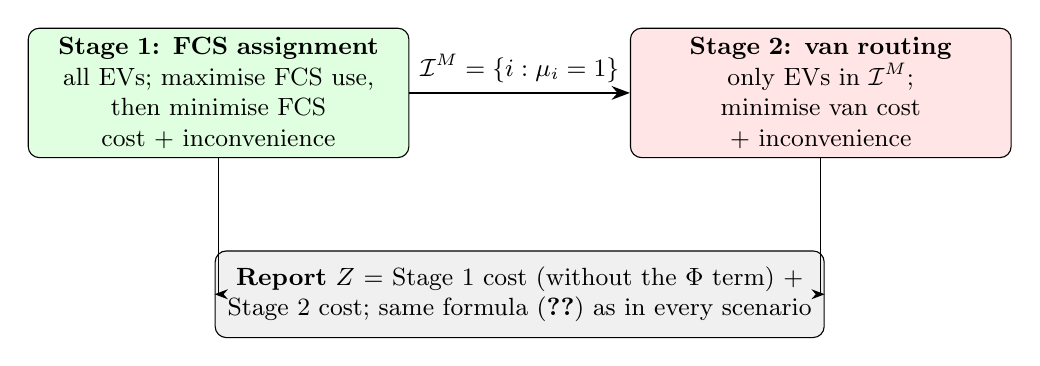
\begin{tikzpicture}[>=Stealth,box/.style={draw,rounded corners,align=center,minimum height=1.1cm,font=\small}]
  \node[box,fill=green!12,text width=4.6cm] (s1) {\textbf{Stage 1: FCS assignment}\\all EVs; maximise FCS use,\\then minimise FCS cost + inconvenience};
  \node[box,fill=red!10,text width=4.6cm,right=2.8cm of s1] (s2) {\textbf{Stage 2: van routing}\\only EVs in $\I^M$;\\minimise van cost + inconvenience};
  \draw[->,thick] (s1) -- node[above,font=\small]{$\I^M=\{i:\mu_i=1\}$} (s2);
  \node[box,fill=black!6,text width=7.5cm,below=2.0cm of $(s1)!0.5!(s2)$] (ev) {\textbf{Report} $Z=$ Stage~1 cost (without the $\Phi$ term) $+$ Stage~2 cost; same formula \eqref{eq:Z} as in every scenario};
  \draw[->] (s1) |- (ev); \draw[->] (s2) |- (ev);
\end{tikzpicture}
\end{center}

Stage~1 does not look at the vans, and Stage~2 cannot change what Stage~1 decided. That is the definition of ``FCS first, then MCS''.

%----------------------------------------------------------------
\subsection{Stage 1: assign EVs to fixed stations}

\textbf{Objective.}
\begin{equation}
\begin{split}
\min\ Z^{(1)}=\;&\underbrace{\Phi\sum_{i\in\I}\mu_i}_{\text{FCS first}}
+\underbrace{c^{EV}\sum_i\sum_{f\in\F_i}d_{if}Y_{if}}_{Z_1}
+\underbrace{Z^F_{\text{energy}}}_{\text{FCS part of }Z_4}\\
&+\underbrace{\sum_i\sum_{f\in\F_i}\rho^F_{if}Y_{if}+\alpha\sum_i w_i(C_i-r_i)+c^L\sum_i w_iL_i}_{\text{FCS customers' inconvenience}}
\end{split}
\label{eq:obj1}
\end{equation}
with $C_i=S_i+\tau^F_iY_i$ in this stage. $\Phi$ is a penalty for handing an EV to the vans. It is chosen larger than anything an extra FCS customer can add to the rest of \eqref{eq:obj1}, e.g.
\[
\Phi > \max_{i}\max_{f\in\F_i}\big(c^{EV}d_{if}+\pi^{\max}E_i+\rho^F_{if}\big)+n\,(\alpha+c^L)\,w_{\max}\,T,
\]
so Stage~1 first \textbf{maximises the number of EVs served at an FCS}, and only among those solutions minimises FCS cost and inconvenience. ($\pi^{\max}$ is the highest grid price.) A numerically safer equivalent is to solve twice: first $\max\sum_iY_i$, then fix that number and minimise the rest.
\ifTOU
Because $Z^F_{\text{energy}}$ uses the peak price, Stage~1 may \emph{start sessions later} to leave the peak, if the price saving beats the extra waiting cost (Section~\ref{sec:expect}).
\fi

\textbf{Constraints.}
\begin{align}
\sum_{g\in\G_i}y_{ig}+\mu_i &= 1 && \forall i\in\I \label{eq:s1assign}\\
S_i &\ge r_i+\sum_{f\in\F_i}t_{if}Y_{if} && \forall i\in\I \label{eq:fcsarr}\\
S_i &\le r_i+T\,(1-\mu_i) && \forall i\in\I \label{eq:s1park}\\
S_j &\ge S_i+\tau^F_i-(T+\tau^F_i)(3-y_{ig}-y_{jg}-o_{ij}) && \forall g,\ (i,j)\in\mathcal{P}_g \label{eq:disj1}\\
S_i &\ge S_j+\tau^F_j-(T+\tau^F_j)(2-y_{ig}-y_{jg}+o_{ij}) && \forall g,\ (i,j)\in\mathcal{P}_g \label{eq:disj2}\\
\sum_i y_{ig_1} &\ge \sum_i y_{ig_2} && \forall f,\ \G_f=\{g_1,g_2\} \label{eq:gunsym}\\
S_i+\tau^F_iY_i &\le T,\qquad L_i\ge S_i+\tau^F_iY_i-l_i && \forall i\in\I \label{eq:s1time}
\end{align}
\ifTOU plus the time-of-use split \eqref{eq:tou1}--\eqref{eq:tou5} of each FCS session (Section~\ref{sec:price}).\fi
\desc{\eqref{eq:s1assign}: every EV either gets one reachable gun or is handed to the vans. An EV that reaches no FCS ($\G_i=\emptyset$) is forced to $\mu_i=1$. \eqref{eq:fcsarr}: an FCS session cannot start before the EV has asked and driven to the station. \eqref{eq:s1park}: for an EV handed to the vans, $S_i$ is parked at $r_i$, so it adds no waiting in Stage~1 (its real start time is decided in Stage~2). \eqref{eq:disj1}--\eqref{eq:disj2}: two EVs on the same gun do not overlap; $o_{ij}$ picks who goes first. With two guns per station this means at most two EVs charge at a station at a time. \eqref{eq:gunsym}: symmetry breaking between the two identical guns (optional). \eqref{eq:s1time}: finished by $T$; lateness.}

\textbf{Optional acceptability rule.} An operator may refuse to send a driver to a station that is ``too inconvenient'', e.g.\ only allow gun $g$ of station $f$ for EV $i$ if $\hat\rho^F_{if}\le\bar\rho$. This only shrinks $\G_i$, so EVs whose stations are all too far go to the vans. Report results with and without it.

\textbf{Output:} $\I^M=\{i:\mu_i=1\}$, the EVs left for the vans; plus each FCS customer's gun and start time.

%----------------------------------------------------------------
\subsection{Stage 2: route the vans to the leftover EVs}

Stage~2 is a vehicle routing problem with time windows, on the EVs in $\I^M$ only. Here $C_i=S_i+\tau^M_i$.

\textbf{Objective.}
\begin{equation}
\begin{split}
\min\ Z^{(2)}=\;&\underbrace{c^M\sum_m\sum_{(i,j)\in\A^M}d_{ij}x_{ijm}}_{Z_2}+\underbrace{\sum_m c^D_mu_m}_{Z_3}+\underbrace{Z^M_{\text{energy}}}_{\text{van part of }Z_4}\\
&+\underbrace{\sum_{i\in\I^M}\sum_m\rho^M_{im}z_{im}+\alpha\sum_{i\in\I^M}w_i(C_i-r_i)+c^L\sum_{i\in\I^M}w_iL_i}_{\text{van customers' inconvenience}}
\end{split}
\label{eq:obj2}
\end{equation}
Since every EV in $\I^M$ must be served by some van, $Z^M_{\text{energy}}$ and the $\rho^M$ term are constants here. They are kept so that $Z^{(2)}$ is the true cost of Stage~2. Waiting and lateness make the vans visit urgent EVs early.

\textbf{Constraints.}
\begin{align}
\sum_{m\in\M}z_{im} &= 1 && \forall i\in\I^M \label{eq:s2assign}\\
\sum_{j:(0,j)\in\A^M}x_{0jm} = \sum_{i:(i,n+1)\in\A^M}x_{i,n+1,m} &= u_m && \forall m \label{eq:depot}\\
\sum_{i:(i,j)\in\A^M}x_{ijm} = \sum_{k:(j,k)\in\A^M}x_{jkm} &= z_{jm} && \forall j\in\I^M,\ m \label{eq:flow}\\
\sum_{i\in\I^M}z_{im} &\le Q_m\,u_m && \forall m \label{eq:cap}\\
\sum_{i\in\I^M}\frac{E_i}{\eta}z_{im}+\beta\sum_{(i,j)\in\A^M}d_{ij}x_{ijm} &\le B_m\,u_m && \forall m \label{eq:batt}
\end{align}
\begin{align}
S_j &\ge \max\{r_j,\ t_{0j}\,x_{0jm}\} && \forall j\in\I^M,\ m \label{eq:depart}\\
S_j &\ge S_i+\tau^M_i+t_{ij}-(T+\tau^M_i+t_{ij})(1-x_{ijm}) && \forall i\neq j,\ m \label{eq:seq}\\
S_i+\tau^M_i+t_{i,n+1} &\le T+(\tau^M_i+t_{i,n+1})(1-x_{i,n+1,m}) && \forall i,\ m \label{eq:return}\\
S_i+\tau^M_i \le T,\quad L_i &\ge S_i+\tau^M_i-l_i && \forall i\in\I^M \label{eq:s2time}\\
u_m &\ge u_{m+1} && m<|\M| \label{eq:vansym}
\end{align}
\desc{\eqref{eq:s2assign}: each leftover EV gets one van. \eqref{eq:depot}: a used van leaves and returns to the depot once. \eqref{eq:flow}: each EV on van $m$ is entered and left exactly once by that van. \eqref{eq:cap}: at most $Q_m$ EVs per van. \eqref{eq:batt}: delivered energy (with transfer losses) plus driving energy fits in the van battery. \eqref{eq:depart}: no start before the request, or before the van can drive there from the depot (written as two linear constraints). \eqref{eq:seq}: if the van goes $i\to j$, it finishes $i$ and drives to $j$ before starting $j$. This gives one EV at a time and removes subtours (MTZ-type). \eqref{eq:return}: back at the depot by $T$. \eqref{eq:s2time}: finished by $T$; lateness. \eqref{eq:vansym}: use identical vans in index order.}

\textbf{If Stage 2 is infeasible} (too many leftover EVs for the fleet by $T$), the sequential policy has \emph{failed} on that instance. For diagnosis, add $s_i\in\{0,1\}$ (``unserved''), replace \eqref{eq:s2assign} by $\sum_mz_{im}+s_i=1$ and add $\Phi^U\sum_is_i$ to \eqref{eq:obj2}. Then report the number of EVs that could not be served. This is a useful comparison with the integrated scenario, which may serve all of them.

%----------------------------------------------------------------
\subsection{Reported value}
\[
Z^{\text{S\scen}}=\big(Z^{(1)*}-\Phi\,|\I^M|\big)+Z^{(2)*},
\]
which is exactly \eqref{eq:Z} evaluated at the combined solution. The stage-1 solution plus the stage-2 solution is a feasible solution of the integrated model (S\ifTOU 4\else 3\fi), so
$Z^{\text{S\ifTOU 4\else 3\fi}}\le Z^{\text{S\scen}}$. The difference is the \emph{value of integration}.

\else
%---------------------------------------------------------------- INT
\subsection{Objective}
\begin{equation}
\min\ Z \quad\text{as in \eqref{eq:Z}, with }Z^F_{\text{energy}}=\ifTOU P^F\textstyle\sum_i\big[\pi^\off(\theta^1_i+\theta^3_i)+\pi^\pk\theta^2_i\big]\else\pi^F\textstyle\sum_iE_iY_i\fi,\quad C_i=S_i+\tau^F_iY_i+\tau^M_iZ_i. \label{eq:objint}
\end{equation}
Written out in full:
\begin{align*}
\min\ Z=\;& c^{EV}\sum_i\sum_{f\in\F_i}d_{if}Y_{if}+c^M\sum_m\sum_{(i,j)\in\A}d_{ij}x_{ijm}+\sum_mc^D_mu_m\\
&+\ifTOU P^F\sum_i\big[\pi^\off(\theta^1_i+\theta^3_i)+\pi^\pk\theta^2_i\big]\else\pi^F\sum_iE_iY_i\fi
+\pi^M\sum_i\sum_m\frac{E_i}{\eta}z_{im}\\
&+\sum_i\sum_{f\in\F_i}\rho^F_{if}Y_{if}+\sum_i\sum_m\rho^M_{im}z_{im}+\alpha\sum_iw_i(C_i-r_i)+c^L\sum_iw_iL_i .
\end{align*}
Every term is linear. One model weighs everything at once: an EV goes to a van exactly when the van's extra km, dispatch and energy cost are outweighed by the effort and waiting it saves the driver\ifTOU, or by the peak-price energy it avoids\fi.

\subsection{Constraints}

\textbf{Assignment.}
\begin{equation}
\sum_{g\in\G_i}y_{ig}+\sum_{m\in\M}z_{im}=1\qquad\forall i\in\I \label{eq:assign}
\end{equation}
\desc{Exactly one resource per EV: one reachable gun or one van. EVs that reach no FCS are forced onto a van.}

\textbf{Fixed stations.}
\begin{align}
S_i &\ge r_i+\sum_{f\in\F_i}t_{if}Y_{if} && \forall i \label{eq:fcsarr}\\
S_j &\ge S_i+\tau^F_i-(T+\tau^F_i)(3-y_{ig}-y_{jg}-o_{ij}) && \forall g,\ (i,j)\in\mathcal{P}_g \label{eq:disj1}\\
S_i &\ge S_j+\tau^F_j-(T+\tau^F_j)(2-y_{ig}-y_{jg}+o_{ij}) && \forall g,\ (i,j)\in\mathcal{P}_g \label{eq:disj2}\\
\sum_iy_{ig_1} &\ge \sum_iy_{ig_2} && \forall f,\ \G_f=\{g_1,g_2\} \label{eq:gunsym}
\end{align}
\desc{\eqref{eq:fcsarr}: an FCS session starts after the request and the drive to the station (for a van customer this is just $S_i\ge r_i$). \eqref{eq:disj1}--\eqref{eq:disj2}: EVs on the same gun do not overlap; $o_{ij}$ chooses the order. \eqref{eq:gunsym}: optional symmetry breaking.}

\textbf{Vans: routes, capacity, battery.}
\begin{align}
\sum_{j:(0,j)\in\A}x_{0jm}=\sum_{i:(i,n+1)\in\A}x_{i,n+1,m} &= u_m && \forall m \label{eq:depot}\\
\sum_{i:(i,j)\in\A}x_{ijm}=\sum_{k:(j,k)\in\A}x_{jkm} &= z_{jm} && \forall j\in\I,\ m \label{eq:flow}\\
\sum_iz_{im} &\le Q_mu_m && \forall m \label{eq:cap}\\
\sum_i\frac{E_i}{\eta}z_{im}+\beta\sum_{(i,j)\in\A}d_{ij}x_{ijm} &\le B_mu_m && \forall m \label{eq:batt}
\end{align}
\desc{\eqref{eq:depot}: a used van leaves and returns once. \eqref{eq:flow}: each EV on van $m$ is visited exactly once by it. \eqref{eq:cap}: at most $Q_m$ EVs. \eqref{eq:batt}: delivered energy (with losses) plus driving energy fits in the battery.}

\textbf{Vans: timing (one EV at a time, no subtours).}
\begin{align}
S_j &\ge t_{0j}\,x_{0jm} && \forall j\in\I,\ m \label{eq:depart}\\
S_j &\ge S_i+\tau^M_i+t_{ij}-(T+\tau^M_i+t_{ij})(1-x_{ijm}) && \forall i\neq j\in\I,\ m \label{eq:seq}\\
S_i+\tau^M_i+t_{i,n+1} &\le T+(\tau^M_i+t_{i,n+1})(1-x_{i,n+1,m}) && \forall i,\ m \label{eq:return}
\end{align}
\desc{\eqref{eq:depart}: the first stop cannot start before the van has driven there. \eqref{eq:seq}: $i\to j$ means finish $i$, drive, then start $j$; start times rise along a route, so no subtour can close. \eqref{eq:return}: back at the depot by $T$.}

\textbf{Horizon and lateness.}
\begin{equation}
C_i\le T,\qquad L_i\ge C_i-l_i\qquad\forall i\in\I \label{eq:time}
\end{equation}
\desc{Every EV is fully charged within the horizon; $L_i$ measures lateness.}

\ifTOU
\textbf{Time-of-use split.} Constraints \eqref{eq:tou1}--\eqref{eq:tou5} of Section~\ref{sec:price}.
\fi

\textbf{Symmetry and domains.}
\begin{equation}
u_m\ge u_{m+1};\qquad y,z,x,u,o\ifTOU,\kappa\fi\in\{0,1\};\qquad S_i,L_i\ifTOU,\theta^p_i\fi\ge0 \label{eq:dom}
\end{equation}
\fi

%=====================================================================
\section{Learning-to-optimise (RL) formulation}\label{sec:rl}

\textbf{Main rule:} the reward of each action is \emph{minus the increase in $Z$ that the action causes}. The rewards over an episode then add up to $-Z$ of the solution the policy builds. RL and MILP results are measured on the same yardstick \eqref{eq:Z}, and the MILP optimum is the benchmark for the RL gap.

\ifSEQ
%---------------------------------------------------------------- RL SEQ
The RL pipeline has the same two stages as the MILP.

\subsection{Stage 1 policy: FCS assignment}
\begin{itemize}[leftmargin=1.4em,itemsep=2pt]
  \item \textbf{Episode / epochs:} EVs are taken in order of request time $r_i$ (ties: higher $w_i$ first). One decision per EV.
  \item \textbf{State:} features of the current EV $k$ ($E_k,r_k,l_k,w_k,R_k$, location); for each gun $g$ the time $F_g$ it becomes free; summary features of the EVs still to come (count and positions near each station)\ifTOU; the current price and the time until $T_1$ and $T_2$\fi.
  \item \textbf{Action:} a gun $g\in\G_k$, or ``hand to vans''. \textbf{FCS-first mask:} ``hand to vans'' is allowed \emph{only} if no gun can finish EV $k$ by $T$ (or, with the optional rule, if all remaining guns have $\hat\rho^F_{kf}>\bar\rho$).
  \ifTOU\item \textbf{Optional timing action:} ``gun $g$, start after the peak'', i.e.\ $S_k=\max\{\text{earliest},T_2\}$, allowed only if the session still ends by $T$.\fi
  \item \textbf{Transition:} $S_k=\max\{r_k+t_{kf},F_g\}$ (or later, for the timing action); $F_g\leftarrow S_k+\tau^F_k$.
  \item \textbf{Reward:} $-\Big[c^{EV}d_{kf}+\text{energy}_k+\rho^F_{kf}+\alpha w_k(S_k+\tau^F_k-r_k)+c^Lw_k(S_k+\tau^F_k-l_k)^+\Big]$, where energy$_k$ = \ifTOU$P^F\big[\pi^\off\cdot(\text{off-peak hours of }[S_k,S_k+\tau^F_k])+\pi^\pk\cdot(\text{peak hours})\big]$, computed exactly in the simulator\else$\pi^FE_k$\fi. Handing an EV to the vans gives reward $0$ here; its cost is counted in Stage~2.
\end{itemize}
Note: a simple baseline for Stage~1 is the greedy rule ``gun with the largest one-step reward''. What RL can learn on top of this is, for example, to keep a nearby gun free for an urgent EV that arrives later.

\subsection{Stage 2 policy: van routing over $\I^M$}
\begin{itemize}[leftmargin=1.4em,itemsep=2pt]
  \item \textbf{Epochs:} whenever a van becomes free (the earliest-free van decides first).
  \item \textbf{State:} for each van: position, time free, remaining battery $b_m$, EVs served so far, dispatched or not; for each unserved EV in $\I^M$: location, $E_i,r_i,l_i,w_i$; current time.
  \item \textbf{Action:} the next EV $j$ for this van, or ``return to depot'' (ends the route). Mask: $j$ must be feasible: battery covers $E_j/\eta$ plus driving to $j$ and back to the depot, the count stays $\le Q_m$, and $j$ can be finished with the van back at the depot by $T$.
  \item \textbf{Transition:} $S_j=\max\{r_j,\ \text{time free}+t_{\text{pos},j}\}$; the van moves to $j$ and is free at $S_j+\tau^M_j$; $b_m$ falls by $E_j/\eta+\beta d_{\text{pos},j}$.
  \item \textbf{Reward:} serving $j$: $-\Big[c^Md_{\text{pos},j}+c^D_m[\text{first stop}]+\pi^M\frac{E_j}{\eta}+\rho^M_{jm}+\alpha w_j(S_j+\tau^M_j-r_j)+c^Lw_j(S_j+\tau^M_j-l_j)^+\Big]$; returning: $-c^Md_{\text{pos},0}$. EVs still unserved at the end: $-\Phi^U$ each.
  \item \textbf{Policy:} an attention-based routing policy (e.g.\ Kool et al., 2019, ``Attention, Learn to Solve Routing Problems!'') trained with REINFORCE or PPO. Baseline: nearest-feasible-EV heuristic.
\end{itemize}
Episode return of Stage~1 + Stage~2 $=-Z^{\text{S\scen}}$.

\else
%---------------------------------------------------------------- RL INT
One policy decides both who serves each EV and the van routes.
\begin{itemize}[leftmargin=1.4em,itemsep=2pt]
  \item \textbf{Episode / epochs:} EVs are taken in order of request time $r_i$ (ties: higher $w_i$ first). One decision per EV.
  \item \textbf{State:} (i) the current EV $k$: location, $E_k,r_k,l_k,w_k,R_k$, reachable stations; (ii) each gun $g$: time $F_g$ it becomes free; (iii) each van $m$: current end-of-route position, time free, remaining battery $b_m$, EVs served, dispatched or not; (iv) embeddings of the not-yet-assigned EVs (for look-ahead)\ifTOU; (v) current price, time until $T_1$ and $T_2$\fi.
  \item \textbf{Action:} $a\in\G_k\cup\M$: a gun, or a van (EV $k$ is appended to the end of that van's route). \textbf{Mask} infeasible actions: a gun that cannot finish $k$ by $T$; a van without enough battery for $E_k/\eta$ plus the drive to $k$ and back to the depot, with $Q_m$ reached, or unable to finish $k$ and return by $T$.
  \ifTOU\item \textbf{Optional timing action:} ``gun $g$, start after the peak'' ($S_k=\max\{\text{earliest},T_2\}$, if it still ends by $T$).\fi
  \item \textbf{Transition:} gun: $S_k=\max\{r_k+t_{kf},F_g\}$, $F_g\leftarrow S_k+\tau^F_k$. Van: $S_k=\max\{r_k,\ \text{free}_m+t_{\text{pos}_m,k}\}$, then the van moves to $k$, $\text{free}_m\leftarrow S_k+\tau^M_k$, $b_m\mathrel{-}=E_k/\eta+\beta d_{\text{pos}_m,k}$.
  \item \textbf{Reward} $=-\Delta Z$:
  \begin{align*}
  \text{gun } g\text{ at }f:&\quad -\Big[c^{EV}d_{kf}+\text{energy}^F_k+\rho^F_{kf}+\alpha w_k(C_k-r_k)+c^Lw_k(C_k-l_k)^+\Big]\\
  \text{van } m:&\quad -\Big[c^M\big(d_{\text{pos}_m,k}+d_{k,0}-d_{\text{pos}_m,0}\big)+c^D_m[\text{first use}]+\pi^M\tfrac{E_k}{\eta}\\
  &\qquad\quad+\rho^M_{km}+\alpha w_k(C_k-r_k)+c^Lw_k(C_k-l_k)^+\Big]
  \end{align*}
  The van distance term is the \emph{change} in route length when $k$ is inserted before the return to the depot, so the sum over the episode equals the total route length (the return legs telescope). energy$^F_k$ = \ifTOU$P^F\big[\pi^\off\cdot(\text{off-peak hours})+\pi^\pk\cdot(\text{peak hours of }[S_k,C_k])\big]$, computed exactly by the simulator; no linearisation is needed in RL\else$\pi^FE_k$\fi.
  \item \textbf{Dead end:} if every action is masked, EV $k$ is unserved: reward $-\Phi^U$, and the episode continues. Report the count.
  \item \textbf{Policy:} masked categorical policy over guns and vans, encoder with attention over EVs, guns and vans; trained with PPO. Natural baseline: greedy, i.e.\ choose the action with the largest one-step reward. That is the pairwise rule ``smallest $\hat\rho$ + cost'' from Section~\ref{sec:inc}.
\end{itemize}
Restriction to note: vans serve EVs in assignment order (append only). A variant that inserts $k$ at the cheapest position of a route is more flexible but has a larger action space.
\fi

\textbf{Reward scaling.} For stable training divide every reward by a constant, e.g.\ the greedy baseline's average $Z$ on the training instances. This does not change the optimal policy.

%=====================================================================
\section{What to expect and what to report}\label{sec:expect}

\ifnum\scen=1
\begin{itemize}[leftmargin=1.4em,itemsep=2pt]
  \item Vans serve only EVs that reach no station, or that the stations cannot finish by $T$. If stations have spare capacity, very few vans are dispatched.
  \item Inconvenience is high for EVs far from the nearest station (worked example: Rs\,682 at the FCS, against Rs\,458 if a van had been allowed).
  \item With too few vans Stage~2 becomes infeasible (unserved EVs), even when the integrated model S3 could serve everyone. Report the smallest $|\M|$ at which S1 is feasible and compare it with S3.
\end{itemize}
\fi
\ifnum\scen=2
\begin{itemize}[leftmargin=1.4em,itemsep=2pt]
  \item \textbf{When does Stage~1 delay a session to avoid the peak?} Moving one hour of charging out of the peak saves $(\pi^\pk-\pi^\off)P^F=3\times22=$ Rs\,66, but delays completion by up to an hour, which costs $\alpha w_i\ge$ Rs\,200. So with the default values Stage~1 almost never delays. It mostly pays the higher price, and S2 costs roughly S1 plus the peak surcharge. Sessions start later only if $\alpha$ is small (try $\lambda<0.33$ in the sensitivity analysis).
  \item The van assignment is the same as in S1 unless Stage~1's timing changes which EVs fit at the stations. Stage~1 cannot use vans to escape the peak price.
  \item Extra KPI: \textbf{grid energy drawn at FCS during the peak}, $P^F\sum_i\theta^2_i$ (kWh). Compare with S4.
\end{itemize}
\fi
\ifnum\scen=3
\begin{itemize}[leftmargin=1.4em,itemsep=2pt]
  \item Vans take EVs for which the saved inconvenience exceeds the extra van cost (worked example: van chosen, saving Rs\,224). Expect vans to serve EVs that are far from every station, have low range (high $w_i$), or have early deadlines, while EVs near a station still use it.
  \item \textbf{Value of integration under flat price:} $Z^{\text{S1}}-Z^{\text{S3}}\ge0$. Report it per component ($Z_1,\dots,Z_5$): typically operating cost rises a little and inconvenience falls a lot.
  \item Vary $|\M|$ (0, 1, 2, \dots): the first few vans lower $Z$ sharply, then the effect levels off. That curve shows the scenarios where mobile chargers help most.
\end{itemize}
\fi
\ifnum\scen=4
\begin{itemize}[leftmargin=1.4em,itemsep=2pt]
  \item During the peak a van kWh costs about the same as an FCS kWh (Rs\,10.0 each), so the vans' energy disadvantage disappears and vans also absorb \emph{peak-hour} demand that would otherwise be charged on the grid at peak price.
  \item Expect more van usage than in S3, concentrated on requests in $[T_1,T_2]$, and lower grid energy at the stations during the peak, $P^F\sum_i\theta^2_i$, than in S2.
  \item \textbf{Value of integration under peak pricing:} $Z^{\text{S2}}-Z^{\text{S4}}$. It should be larger than $Z^{\text{S1}}-Z^{\text{S3}}$, because integration now also allows price arbitrage.
  \item \textbf{Peak pricing with full flexibility:} $Z^{\text{S4}}-Z^{\text{S3}}$ should be smaller than $Z^{\text{S2}}-Z^{\text{S1}}$: vans cushion the price increase.
\end{itemize}
\fi

\textbf{Cross-scenario comparison table} (fill in from the four runs):
\begin{center}
\renewcommand{\arraystretch}{1.2}
\begin{tabular}{@{}lll@{}}
\toprule
\textbf{Comparison} & \textbf{Measures} & \textbf{Expected sign} \\
\midrule
S1 $-$ S3 & value of integration, flat price & $\ge0$ \\
S2 $-$ S4 & value of integration, peak price & $\ge0$, larger than S1 $-$ S3 \\
S2 $-$ S1 & cost of peak pricing, FCS-first operator & $>0$ \\
S4 $-$ S3 & cost of peak pricing, flexible operator & $>0$, smaller than S2 $-$ S1 \\
\bottomrule
\end{tabular}
\end{center}
Report for each: $Z$ and its components, number of vans used, EVs per resource, mean and maximum inconvenience per EV, total lateness, peak-hour grid energy, solve time, and (for RL) the gap to the MILP optimum.

%=====================================================================
\appendix
\section{Illustrative parameter values}\label{app:values}

These are starting values for experiments, not data. All are meant to be varied in the analysis. Values in Rs.

\begin{center}
\renewcommand{\arraystretch}{1.15}
\begin{tabular}{@{}llp{6.2cm}@{}}
\toprule
\textbf{Parameter} & \textbf{Value} & \textbf{Note} \\
\midrule
$T$, $[T_1,T_2]$ & 7 h, $[2,6]$ & 16:00--23:00, peak 18:00--22:00 \\
$P^F$, $P^M$ & 22 kW, 30 kW & \\
$v$, $\beta$, $\eta$ & 25 km/h, 0.25 kWh/km, 0.9 & \\
$B_m$, $Q_m$, $|\M|$ & 150 kWh, 6, 2--6 & \\
$c^{EV}$, $c^M$, $c^D_m$ & Rs\,4/km, Rs\,15/km, Rs\,1500 & van km includes driver time \\
$\pi^F$ (flat) & Rs\,8.7/kWh & equals the time-average of the ToU tariff over $[0,T]$ \\
$\pi^\off$, $\pi^\pk$ (ToU) & Rs\,7/kWh, Rs\,10/kWh & $(3\times7+4\times10)/7=8.7$ \\
$c^{bat}$ & Rs\,2/kWh & van battery wear \\
$\pi^M$ & Rs\,10.7 (flat) / Rs\,9.0 (ToU) & $=\pi^F+c^{bat}$ / $=\pi^\off+c^{bat}$ \\
$\alpha$, $\alpha^D$ & Rs\,200/h, Rs\,100/h & value of time; extra for attended time \\
$h^F$, $h^M$, $\varphi$ & Rs\,50, Rs\,10, Rs\,100 & trip hassle, hand-over, range stress \\
$c^L$ & Rs\,300/h & lateness \\
$w_i$ & $1+2(1-R_i/R_{\max})$, $R_i\sim U[3,40]$ km & priority from remaining range \\
\bottomrule
\end{tabular}
\end{center}

The flat price is set to the time-average of the peak tariff. The price \emph{level} is then the same in both pricing cases, and only the price \emph{shape} differs. Without this, part of S1 vs S2 would just reflect a different average price.

\end{document}
"
%    pdflatex -jobname=scenario2_peak_sequential   "\def\scen{2}% =====================================================================
%  One source, four PDFs.  Build with build.sh (or by hand):
%    pdflatex -jobname=scenario1_flat_sequential   "\def\scen{1}% =====================================================================
%  One source, four PDFs.  Build with build.sh (or by hand):
%    pdflatex -jobname=scenario1_flat_sequential   "\def\scen{1}\input{scenario_master}"
%    pdflatex -jobname=scenario2_peak_sequential   "\def\scen{2}\input{scenario_master}"
%    pdflatex -jobname=scenario3_flat_integrated   "\def\scen{3}\input{scenario_master}"
%    pdflatex -jobname=scenario4_peak_integrated   "\def\scen{4}\input{scenario_master}"
%  (run each twice for cross-references)
% =====================================================================
\documentclass[11pt,a4paper]{article}
\usepackage[margin=2.2cm]{geometry}
\usepackage{amsmath,amssymb,amsfonts}
\usepackage{booktabs,array,tabularx}
\usepackage{enumitem}
\usepackage[table]{xcolor}
\usepackage{tikz}
\usetikzlibrary{arrows.meta,positioning,calc}
\usepackage[colorlinks=true,linkcolor=blue!50!black,urlcolor=blue!50!black]{hyperref}
\usepackage{titlesec}
\titleformat{\section}{\large\bfseries}{\thesection}{0.8em}{}
\titleformat{\subsection}{\normalsize\bfseries}{\thesubsection}{0.8em}{}
\setlength{\parindent}{0pt}
\setlength{\parskip}{5pt}

% ---------------- scenario switches ----------------
\ifdefined\scen\else\def\scen{1}\fi
\newif\ifTOU \TOUfalse   % true = time-of-use (peak) price
\newif\ifSEQ \SEQfalse   % true = FCS first, then MCS
\ifnum\scen=1 \SEQtrue \fi
\ifnum\scen=2 \TOUtrue \SEQtrue \fi
\ifnum\scen=4 \TOUtrue \fi

\newcommand{\pricename}{\ifTOU time-of-use price (dearer evening peak)\else single (flat) price all day\fi}
\newcommand{\structname}{\ifSEQ FCS first, then MCS (sequential)\else FCS and MCS together (integrated)\fi}

% ---------------- notation ----------------
\newcommand{\I}{\mathcal{I}}
\newcommand{\F}{\mathcal{F}}
\newcommand{\G}{\mathcal{G}}
\newcommand{\M}{\mathcal{M}}
\newcommand{\N}{\mathcal{N}}
\newcommand{\A}{\mathcal{A}}
\newcommand{\Rs}{\text{Rs}\,}
\newcommand{\pk}{\mathrm{pk}}
\newcommand{\off}{\mathrm{off}}
\newcommand{\desc}[1]{\par\vspace{-2pt}{\small\color{black!75}\textit{Meaning:} #1}\par\vspace{4pt}}
\newcommand{\cell}[2]{\ifnum\scen=#1\cellcolor{blue!18}\textbf{S#1 (this document)}\\\textbf{#2}\else S#1\\#2\fi}

\title{\textbf{EV Charging Network Optimisation}\\[4pt]
\large Scenario \scen: \pricename\ $+$ \structname\\[2pt]
\normalsize MILP and RL formulation}
\author{CP 320 OR for Mobility Management, course project}
\date{2 October 2026}

\begin{document}
\maketitle

%=====================================================================
\section{Where this scenario sits}

The project studies four scenarios: two ways of pricing grid electricity, times two ways of making the decisions.

\begin{center}
\renewcommand{\arraystretch}{1.5}
\begin{tabular}{>{\raggedright\arraybackslash}p{4.2cm}|>{\centering\arraybackslash}p{4.6cm}|>{\centering\arraybackslash}p{4.6cm}}
 & \textbf{Flat price all day} & \textbf{Time-of-use (peak) price} \\ \hline
\textbf{Sequential:} FCS first, leftover EVs to MCS &
\begin{tabular}[c]{@{}c@{}}\cell{1}{flat + sequential}\end{tabular} &
\begin{tabular}[c]{@{}c@{}}\cell{2}{peak + sequential}\end{tabular} \\ \hline
\textbf{Integrated:} FCS and MCS decided together &
\begin{tabular}[c]{@{}c@{}}\cell{3}{flat + integrated}\end{tabular} &
\begin{tabular}[c]{@{}c@{}}\cell{4}{peak + integrated}\end{tabular} \\
\end{tabular}
\end{center}

\textbf{The four scenarios do not have four different objectives.} They share \emph{one} cost yardstick $Z$ (Section~\ref{sec:obj}): the same cost terms and the same customer inconvenience (Section~\ref{sec:inc}). Only two things change:
\begin{itemize}[leftmargin=1.4em,itemsep=1pt]
  \item \textbf{Pricing} changes the formula for one term, the FCS energy cost (Section~\ref{sec:price}).
  \item \textbf{Decision structure} changes \emph{how} $Z$ is minimised: in one model (integrated), or in two stages (sequential), where each stage minimises its own part of $Z$.
\end{itemize}
Because the yardstick is the same, the four optimal values can be compared directly. The differences measure the \emph{value of integration} (S1$\to$S3, S2$\to$S4) and the \emph{effect of peak pricing} (S1$\to$S2, S3$\to$S4).

\ifnum\scen=1
\textbf{This scenario (S1)} is the baseline, the ``status quo''. Electricity costs the same at every hour, every EV that can be charged at a fixed station is sent there, and vans only take what is left over.
\fi
\ifnum\scen=2
\textbf{This scenario (S2)} keeps the FCS-first rule of S1, but grid electricity is dearer during the evening peak. Stage~1 can react to the price only by \emph{rescheduling} FCS sessions. It cannot hand a peak-hour EV to a van.
\fi
\ifnum\scen=3
\textbf{This scenario (S3)} keeps the flat price of S1, but the operator decides FCS and MCS service \emph{together}. An EV can be sent to a van even when a fixed station could take it, whenever that lowers total cost plus inconvenience.
\fi
\ifnum\scen=4
\textbf{This scenario (S4)} is the most flexible one: peak pricing at fixed stations, and FCS and MCS decided together. Van energy was bought off-peak, so vans can also be used to keep charging \emph{out of the expensive peak}.
\fi

%=====================================================================
\section{Setting and assumptions}\label{sec:setting}

\textbf{Time.} The planning horizon is $[0,T]$ with $T=7$\,h (16:00--23:00). It contains the evening peak window $[T_1,T_2]=[2,6]$ (18:00--22:00). The horizon is the same in all four scenarios. It is wider than the peak itself so that, under peak pricing, there is cheaper time on both sides of the peak.\ifTOU\else\ In this scenario the price is flat, so the window plays no role in the model.\fi

\textbf{Assumptions} (the same as MILP v3, plus two about energy):
\begin{enumerate}[leftmargin=1.6em,itemsep=1pt]
  \item Static, continuous time. All requests in the horizon are known at time $0$, and request $i$ becomes active at $r_i$.
  \item An EV served by an FCS drives there itself on its own battery (only to stations within its range $R_i$). The driver stays with the car while it waits for a free gun and while it charges.
  \item An EV served by an MCS stays parked where it is, and the driver is free in the meantime.
  \item Each FCS gun and each van charges one EV at a time, without interruption, at constant power.
  \item A van's battery covers both its driving and the energy it delivers. \textbf{The van battery is charged at the depot before the horizon starts}\ifTOU, i.e.\ at the off-peak price\fi, and is not recharged during the horizon.
  \item Every EV must be fully charged by $T$ (hard). Finishing after the driver's desired time $l_i$ is allowed but penalised.
\end{enumerate}

%=====================================================================
\section{Notation}\label{sec:notation}

\subsection*{Sets}
\begin{tabularx}{\textwidth}{@{}lX@{}}
\toprule
$\I=\{1,\dots,n\}$ & EV charging requests \\
$\F$; $\G_f$ ($|\G_f|=2$); $\G=\bigcup_f\G_f$ & fixed charging stations; guns of FCS $f$; all guns ($f(g)$ = station of gun $g$) \\
$\F_i=\{f: d_{if}\le R_i\}$, $\G_i=\bigcup_{f\in\F_i}\G_f$ & stations / guns EV $i$ can reach on its remaining range \\
$\M$ & mobile charging vans (MCS) \\
$0,\ n+1$ & depot as start node / end node (same place) \\
$\N=\{0\}\cup\I\cup\{n+1\}$, $\A$ & routing nodes; allowed van arcs $(i,j)$, $i\in\{0\}\cup\I$, $j\in\I\cup\{n+1\}$, $i\neq j$ \\
$\mathcal{P}_g=\{(i,j): i<j,\ g\in\G_i\cap\G_j\}$ & pairs of EVs that could share gun $g$ \\
\ifSEQ
$\I^M\subseteq\I$ & EVs handed to the vans by Stage~1 (an \emph{output} of Stage~1, a fixed input to Stage~2) \\
$\N^M$, $\A^M$ & routing nodes / arcs restricted to $\I^M$ \\
\fi
\bottomrule
\end{tabularx}

\subsection*{Parameters}
\begin{tabularx}{\textwidth}{@{}lX@{}}
\toprule
$E_i,\ r_i,\ l_i,\ R_i$ & energy demand (kWh), request time, desired completion time (h), remaining range (km) \\
$w_i\ge1$ & priority of EV $i$; $w_i=1+\kappa(1-R_i/R_{\max})$, so low-range EVs weigh more \\
$P^F,\ P^M$ & charging power of an FCS gun (22\,kW) / of a van (e.g.\ 30\,kW) \\
$\tau^F_i=E_i/P^F,\ \tau^M_i=E_i/P^M$ & charging time of EV $i$ at an FCS / by a van (h) \\
$d_{if},t_{if}$;\ $d_{ij},t_{ij}$ & distance (km) and time (h): EV$\to$FCS; between routing nodes ($t=d/v$) \\
$B_m,\ Q_m,\ \beta,\ \eta$ & van battery (kWh), max EVs per van, van consumption (kWh/km), transfer efficiency \\
$c^{EV},\ c^M,\ c^D_m$ & cost per km of EV driving, per km of van driving; fixed dispatch cost of van $m$ \\
\ifTOU
$\pi^\off,\ \pi^\pk$ & grid price (Rs/kWh) off-peak / in $[T_1,T_2]$, with $\pi^\pk\ge\pi^\off$ \\
\else
$\pi^F$ & grid price (Rs/kWh), the same at every hour \\
\fi
$c^{bat}$ & van battery wear per kWh cycled \\
$\pi^M$ & cost of 1 kWh taken from a van battery: $\pi^M=\ifTOU\pi^\off\else\pi^F\fi+c^{bat}$ (Section~\ref{sec:price}) \\
$\alpha,\ \alpha^D,\ h^F,\ h^M,\ \varphi,\ c^L$ & inconvenience coefficients (Section~\ref{sec:inc}) \\
\bottomrule
\end{tabularx}

\subsection*{Decision variables}
\begin{tabularx}{\textwidth}{@{}llX@{}}
\toprule
$y_{ig}$ & $\{0,1\}$ & EV $i$ charged at gun $g\in\G_i$ \\
$z_{im}$ & $\{0,1\}$ & EV $i$ served by van $m$ \\
$x_{ijm}$ & $\{0,1\}$ & van $m$ drives arc $(i,j)$ \\
$u_m$ & $\{0,1\}$ & van $m$ is dispatched \\
$o_{ij}$ & $\{0,1\}$ & for EVs $i<j$ that could share a gun: 1 if $i$ is charged before $j$ \\
\ifSEQ
$\mu_i$ & $\{0,1\}$ & Stage~1 only: EV $i$ is handed to the van fleet \\
\fi
\ifTOU
$\theta^1_i,\theta^2_i,\theta^3_i$ & $\ge0$ & hours of EV $i$'s FCS session before / inside / after the peak \\
$\kappa^1_i,\kappa^3_i$ & $\{0,1\}$ & EV $i$'s FCS session starts before $T_1$ / ends after $T_2$ \\
\fi
$S_i$ & $\ge0$ & time charging of EV $i$ starts (h), on whichever resource \\
$L_i$ & $\ge0$ & lateness of EV $i$ beyond $l_i$ (h) \\
\bottomrule
\end{tabularx}

\textbf{Short-hands} (linear expressions, not new variables):
\[
Y_{if}=\sum_{g\in\G_f}y_{ig},\qquad Y_i=\sum_{g\in\G_i}y_{ig}\ (\text{EV $i$ uses an FCS}),\qquad Z_i=\sum_{m\in\M}z_{im}\ (\text{EV $i$ uses a van}),
\]
\[
C_i=S_i+\tau^F_i\,Y_i+\tau^M_i\,Z_i \quad\text{(time EV $i$ is fully charged).}
\]

%=====================================================================
\section{Customer inconvenience}\label{sec:inc}

This section is \textbf{identical in all four scenario documents}. Inconvenience is a property of the customer, not of the price or of the planning method.

\subsection{What we mean by inconvenience}

Inconvenience is \emph{what the driver loses} from the moment they ask for a charge ($r_i$) until the car is fully charged ($C_i$), \emph{converted into rupees} so it can be added to the operator's costs. A driver loses three different things:

\begin{enumerate}[leftmargin=1.6em,itemsep=2pt]
  \item \textbf{Waiting:} the car is not ready. This lasts $C_i-r_i$ hours and affects \emph{every} driver, FCS or MCS.
  \item \textbf{Effort:} only an FCS customer has to drive to the station and sit there while the car charges. An MCS customer stays at home or at work and does something else. Driving to a far station also uses scarce battery range, which causes stress (``range anxiety'').
  \item \textbf{A missed deadline:} the car is still not ready at the time $l_i$ the driver needs it.
\end{enumerate}

Each loss gets a price in Rs per hour (or per event). All of them are multiplied by the priority $w_i$: an hour of delay for an EV with 5\,km of range left counts more than for one with 40\,km.

\subsection{The three components}

\begin{center}
\renewcommand{\arraystretch}{1.3}
\begin{tabularx}{\textwidth}{@{}>{\raggedright\arraybackslash}p{2.6cm}>{\raggedright\arraybackslash}X>{\raggedright\arraybackslash}X>{\raggedright\arraybackslash}p{3.0cm}@{}}
\toprule
\textbf{Component} & \textbf{EV $i$ at FCS $f$} & \textbf{EV $i$ by a van} & \textbf{Known when?} \\
\midrule
Effort & $w_i\big[\alpha^D(t_{if}+\tau^F_i)+h^F+\varphi\,d_{if}/R_i\big]$: driving and sitting at the station, a fixed trip hassle, range stress & $w_i\,h^M$: being reachable and handing over the car & \textbf{Static:} known as soon as the resource is chosen \\
Waiting & $w_i\,\alpha\,(C_i-r_i)$ = drive + \emph{queue at the gun} + charge & $w_i\,\alpha\,(C_i-r_i)$ = \emph{wait for the van} + charge & \textbf{Dynamic:} depends on the queue / van route \\
Missed deadline & $w_i\,c^L\,L_i$, $L_i=\max\{0,C_i-l_i\}$ & same & Dynamic \\
\bottomrule
\end{tabularx}
\end{center}

\textbf{Coefficients.}
$\alpha$ (Rs/h) is the value of an hour the car is not ready.
$\alpha^D$ (Rs/h) is the \emph{extra} value of an hour the driver must personally spend driving or sitting at the station: an hour at the station costs $\alpha+\alpha^D$, an hour waiting at home for a van costs only $\alpha$.
$h^F,h^M$ (Rs) are fixed hassle costs of one trip to a station / one van hand-over.
$\varphi$ (Rs) is the range-stress cost of a trip that uses the \emph{whole} remaining range ($d_{if}/R_i\le1$ is the fraction used).
$c^L$ (Rs/h) is the cost per hour late.

\subsection{Pairwise form: inconvenience of a (customer, resource) pair}

The natural first idea is: \emph{for every pair (EV $i$, FCS $f$) and every pair (EV $i$, van $m$) there is an inconvenience number, and the operator picks the pair with the lowest cost plus inconvenience.} The static part fits this idea exactly:
\[
\boxed{\;\rho^F_{if}=w_i\Big[\alpha^D\,(t_{if}+\tau^F_i)+h^F+\varphi\,\frac{d_{if}}{R_i}\Big]\qquad
\rho^M_{im}=w_i\,h^M\;}
\]
These are \textbf{parameters}, computed before solving, one number per (EV, FCS) pair and per (EV, van) pair. In the objective they appear linearly: $\sum_i\sum_f\rho^F_{if}Y_{if}+\sum_i\sum_m\rho^M_{im}z_{im}$.

Note that $\rho^M_{im}$ does not depend on $m$. Vans are identical and all start at the same depot, so the driver does not care \emph{which} van comes, only \emph{when} it comes. That ``when'' is the waiting part.

\subsection{Why waiting cannot be a fixed pairwise number}

It is tempting to also write the waiting as a pairwise number, e.g.\ ``the van needs 5 minutes to reach EV $i$''. But that depends on \emph{where the van is coming from}, which depends on the route the model is still choosing: if EV $i$ is the 4th stop of a van, the wait is the time for three charging sessions plus four drives. Likewise, waiting at an FCS depends on how many EVs are queued at that gun. So waiting is not known before solving. It is a function of decision variables:
\[
\text{waiting cost of EV } i \;=\; w_i\,\alpha\,(C_i-r_i),\qquad C_i=S_i+\tau^F_iY_i+\tau^M_iZ_i .
\]
This is \textbf{linear} in the variables ($S_i$, $y$, $z$), so it fits in a MILP directly. The constraints of Section~\ref{sec:milp} make $S_i$ equal to the true start time, including driving, queueing at the gun and the van's route. The term $\sum_i w_i\alpha r_i$ is a constant and may be dropped when solving.

\textbf{Pairwise \emph{estimate}} (used for intuition, by the RL policy and in heuristics): if there is no queue and the van comes straight to $i$,
\[
\hat\rho^{F}_{if}=\rho^F_{if}+w_i\alpha\,(t_{if}+\tau^F_i),\qquad
\hat\rho^{M}_{im}=\rho^M_{im}+w_i\alpha\,(t^{\text{van}}_{m\to i}+\tau^M_i),
\]
where $t^{\text{van}}_{m\to i}$ is the time until van $m$ can reach $i$ from where it currently is. In the RL formulation (Section~\ref{sec:rl}) the van's position \emph{is} known at each decision, so there this estimate becomes exact.

\subsection{Total inconvenience and how it enters the objective}

\begin{equation}
\boxed{\;
Z_{\text{inc}}=\underbrace{\sum_{i\in\I}\sum_{f\in\F_i}\rho^F_{if}Y_{if}+\sum_{i\in\I}\sum_{m\in\M}\rho^M_{im}z_{im}}_{\text{effort (static, pairwise)}}
+\underbrace{\alpha\sum_{i\in\I}w_i\,(C_i-r_i)}_{\text{waiting (dynamic)}}
+\underbrace{c^L\sum_{i\in\I}w_i\,L_i}_{\text{missed deadline}}
\;}\label{eq:inc}
\end{equation}
All three parts are in rupees, so $Z_{\text{inc}}$ is simply added to the operating costs. Nothing has to be normalised.

\subsection{Worked example: your ``10 km to the FCS vs.\ van in 5 minutes'' case}

EV $i$: $E_i=20$\,kWh, $R_i=40$\,km (so $w_i=1$); nearest free FCS $d_{if}=10$\,km away, $t_{if}=0.4$\,h at 25\,km/h; a van finishing next door can reach it in 5\,min ($0.083$\,h), adding about 4\,km to its route. $\tau^F_i=20/22=0.909$\,h, $\tau^M_i=20/30=0.667$\,h. Coefficients from Appendix~\ref{app:values}, flat price.

\begin{center}
\renewcommand{\arraystretch}{1.25}
\begin{tabular}{@{}lrr@{}}
\toprule
 & \textbf{FCS} & \textbf{Van} \\
\midrule
Driving (EV / extra van km) & $4\times10=40.0$ & $15\times4=60.0$ \\
Energy & $8.7\times20=174.0$ & $10.7\times20/0.9=237.8$ \\
\textbf{Operating cost only} & \textbf{214.0} & \textbf{297.8} \\
\midrule
Effort $\rho$ & $100(0.4+0.909)+50+100\cdot\tfrac{10}{40}=205.9$ & $10.0$ \\
Waiting $\alpha(C_i-r_i)$ & $200\times1.309=261.8$ & $200\times0.75=150.0$ \\
\textbf{Cost + inconvenience} & \textbf{681.7} & \textbf{457.8} \\
\bottomrule
\end{tabular}
\end{center}

On operating cost alone the FCS is cheaper, so a cost-only model would \emph{always} send this driver 10\,km away. With inconvenience included the van is better by about Rs\,224, and the integrated model chooses $z_{im}=1$, as you expected. If the FCS were only 1\,km away, the FCS would win both comparisons. The inconvenience term is what makes the model choose between ``cheap for the operator'' and ``convenient for the driver'', rather than following a fixed rule.

\subsection{Relation to a single penalty $\rho_i$ per EV}

The first draft used a penalty $\rho_i$ that is charged whenever EV $i$ goes to \emph{any} FCS: $\sum_i\sum_f\rho_iy_{if}$. Because $\sum_f y_{if}=1-\sum_m z_{im}$, this only says ``a van is worth $\rho_i$ more to EV $i$'', and that holds whether the station is 1\,km or 15\,km away, and whether the van arrives in 5 minutes or in 3 hours. The form above fixes both problems: $\rho^F_{if}$ grows with the distance to \emph{that} station, and the waiting term grows with how late the van or the free gun actually is. The old model is the special case $\alpha=\alpha^D=\varphi=c^L=0$, $h^F=\rho_i$.

\subsection{Choosing the coefficients}
\begin{itemize}[leftmargin=1.4em,itemsep=2pt]
  \item Use a value of time for $\alpha$ (e.g.\ Rs\,150--300/h for urban car users), and set $\alpha^D\approx0.5\alpha$: sitting at a station is worse than waiting at home.
  \item Keep $c^L>\alpha$, so missing the deadline is worse than ordinary waiting.
  \item \textbf{Sensitivity analysis:} multiply all inconvenience coefficients by a factor $\lambda\in\{0,0.25,0.5,1,2,4\}$ and plot operating cost against total inconvenience. $\lambda=0$ is the pure cost-minimising operator, and large $\lambda$ is a customer-first operator. This trade-off curve is a strong result for the ``Analysis'' part of the project.
\end{itemize}

\subsection{What inconvenience does in \emph{this} scenario}
\ifSEQ
In a sequential scenario inconvenience \textbf{cannot move an EV from an FCS to a van}: Stage~1 sends every EV that \emph{can} use an FCS to one. It still matters inside each stage. In Stage~1 it decides \emph{which} station and \emph{when} (urgent EVs get the near station and the first free gun). In Stage~2 it decides the \emph{order} in which vans visit EVs (urgent EVs first). In the worked example, this scenario sends the driver 10\,km to the FCS. That is the weakness the integrated scenarios remove.
\else
In an integrated scenario inconvenience is weighed directly against operating cost when choosing the resource. That is how the worked example ends up with a van. It also decides which station and which gun order, and the order of each van route.
\fi

%=====================================================================
\section{Electricity price in this scenario}\label{sec:price}

\textbf{Van energy (same in all scenarios).} A van's battery is charged at the depot \emph{before} the horizon, so its energy was bought at the
\ifTOU off-peak \fi
price, whatever time the van later delivers it. Each kWh taken from the van also wears the battery ($c^{bat}$), and a fraction $1-\eta$ is lost in transfer:
\[
Z^M_{\text{energy}}=\pi^M\sum_{i\in\I}\sum_{m\in\M}\frac{E_i}{\eta}\,z_{im},\qquad \pi^M=\ifTOU\pi^\off\else\pi^F\fi+c^{bat}.
\]

\ifTOU
\textbf{FCS energy (time-of-use).} An FCS draws from the grid while it charges. Energy delivered inside $[T_1,T_2]$ costs $\pi^\pk$, and energy outside it costs $\pi^\off$. A session $[S_i,S_i+\tau^F_i]$ may overlap the peak partly. Split its duration into the hours before, inside and after the peak, $\theta^1_i+\theta^2_i+\theta^3_i$:
\[
Z^F_{\text{energy}}=P^F\sum_{i\in\I}\Big[\pi^\off(\theta^1_i+\theta^3_i)+\pi^\pk\,\theta^2_i\Big].
\]
Constraints \eqref{eq:tou1}--\eqref{eq:tou5} below make the $\theta$'s equal to the true overlaps. Peak hours are dearer, so the solver wants $\theta^1_i,\theta^3_i$ as large as possible. It is enough to bound them from above by the true off-peak overlap, and the constraints need one binary per side:
\begin{align}
\theta^1_i+\theta^2_i+\theta^3_i &= \tau^F_i\,Y_i && \forall i\in\I \label{eq:tou1}\\
\theta^1_i &\le \tau^F_i\,\kappa^1_i && \forall i\in\I \label{eq:tou2}\\
\theta^1_i &\le T_1-S_i+T\,(1-\kappa^1_i) && \forall i\in\I \label{eq:tou3}\\
\theta^3_i &\le \tau^F_i\,\kappa^3_i && \forall i\in\I \label{eq:tou4}\\
\theta^3_i &\le S_i+\tau^F_i-T_2+T\,(1-\kappa^3_i) && \forall i\in\I \label{eq:tou5}
\end{align}
\desc{\eqref{eq:tou1}: the FCS session's hours are split into three parts; for a van customer ($Y_i=0$) all three are zero. \eqref{eq:tou2}--\eqref{eq:tou3}: off-peak time before the peak is only possible if the session starts before $T_1$ ($\kappa^1_i=1$), and is at most $T_1-S_i$. \eqref{eq:tou4}--\eqref{eq:tou5}: the same for time after $T_2$. $\theta^2_i\ge0$ prevents counting more off-peak hours than exist. Checking the cases (entirely before / inside / after the peak, straddling one edge, covering the whole peak) shows that at the optimum the $\theta$'s equal the exact overlaps. This needs $\pi^\pk\ge\pi^\off$, which is true for a peak tariff.}

\textbf{Why vans become more attractive.} Compare the cost of 1\,kWh delivered to an EV during the peak (values from Appendix~\ref{app:values}):
FCS $=\pi^\pk=$ Rs\,10.0, van $=(\pi^\off+c^{bat})/\eta=9/0.9=$ Rs\,10.0. They are at parity. Under the flat price the van is about Rs\,3.2/kWh dearer (FCS Rs\,8.7, van $10.7/0.9=$ Rs\,11.9). Peak pricing therefore removes the vans' main cost disadvantage, but only for EVs whose FCS session would fall in the peak.
\ifSEQ\ In this sequential scenario Stage~1 cannot use that, because it does not consider vans. It can only shift FCS sessions in time.\fi
\else
\textbf{FCS energy (flat).} Every kWh delivered at a fixed station costs $\pi^F$, whenever it is delivered:
\[
Z^F_{\text{energy}}=\pi^F\sum_{i\in\I}E_i\,Y_i .
\]
The start time therefore does not affect the energy cost. Under the flat price a van kWh costs $(\pi^F+c^{bat})/\eta\approx$ Rs\,11.9 against Rs\,8.7 at an FCS (Appendix~\ref{app:values}), so on energy alone the FCS always wins.
\fi

%=====================================================================
\section{MILP formulation}\label{sec:milp}

\subsection{The common cost yardstick $Z$}\label{sec:obj}

For any complete solution (every EV assigned, every route and start time known), the system cost is
\begin{equation}
\boxed{\;
Z=\underbrace{c^{EV}\sum_{i}\sum_{f\in\F_i}d_{if}Y_{if}}_{Z_1:\ \text{EV driving}}
+\underbrace{c^M\sum_{m}\sum_{(i,j)\in\A}d_{ij}x_{ijm}}_{Z_2:\ \text{van driving}}
+\underbrace{\sum_m c^D_m u_m}_{Z_3:\ \text{dispatch}}
+\underbrace{Z^F_{\text{energy}}+Z^M_{\text{energy}}}_{Z_4:\ \text{energy}}
+\underbrace{Z_{\text{inc}}}_{Z_5:\ \text{inconv.\ \eqref{eq:inc}}}
\;}\label{eq:Z}
\end{equation}
$Z_4$ is defined in Section~\ref{sec:price}. $Z_1$--$Z_4$ are the operator's costs listed in the brief (EV travel, MCS travel, MCS operating cost) plus energy. $Z_5$ is the customer inconvenience penalty. \textbf{The same formula is used to report results in all four scenarios.}

\ifSEQ
%---------------------------------------------------------------- SEQ
\subsection{Structure: two stages}

\begin{center}
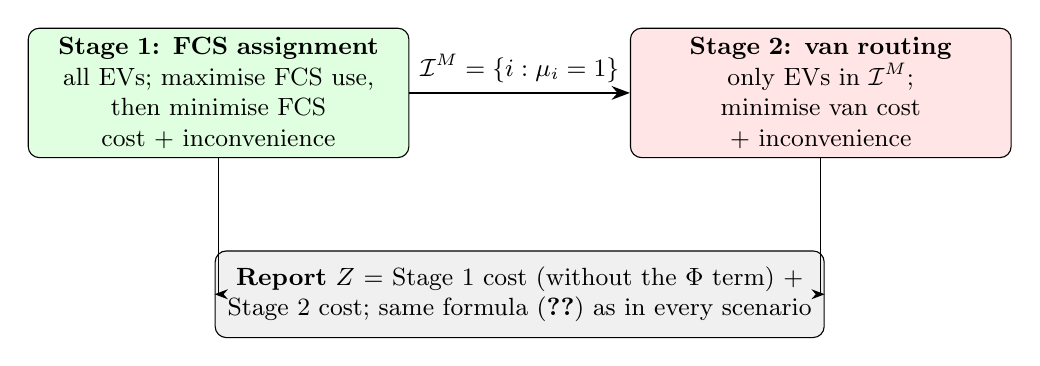
\begin{tikzpicture}[>=Stealth,box/.style={draw,rounded corners,align=center,minimum height=1.1cm,font=\small}]
  \node[box,fill=green!12,text width=4.6cm] (s1) {\textbf{Stage 1: FCS assignment}\\all EVs; maximise FCS use,\\then minimise FCS cost + inconvenience};
  \node[box,fill=red!10,text width=4.6cm,right=2.8cm of s1] (s2) {\textbf{Stage 2: van routing}\\only EVs in $\I^M$;\\minimise van cost + inconvenience};
  \draw[->,thick] (s1) -- node[above,font=\small]{$\I^M=\{i:\mu_i=1\}$} (s2);
  \node[box,fill=black!6,text width=7.5cm,below=2.0cm of $(s1)!0.5!(s2)$] (ev) {\textbf{Report} $Z=$ Stage~1 cost (without the $\Phi$ term) $+$ Stage~2 cost; same formula \eqref{eq:Z} as in every scenario};
  \draw[->] (s1) |- (ev); \draw[->] (s2) |- (ev);
\end{tikzpicture}
\end{center}

Stage~1 does not look at the vans, and Stage~2 cannot change what Stage~1 decided. That is the definition of ``FCS first, then MCS''.

%----------------------------------------------------------------
\subsection{Stage 1: assign EVs to fixed stations}

\textbf{Objective.}
\begin{equation}
\begin{split}
\min\ Z^{(1)}=\;&\underbrace{\Phi\sum_{i\in\I}\mu_i}_{\text{FCS first}}
+\underbrace{c^{EV}\sum_i\sum_{f\in\F_i}d_{if}Y_{if}}_{Z_1}
+\underbrace{Z^F_{\text{energy}}}_{\text{FCS part of }Z_4}\\
&+\underbrace{\sum_i\sum_{f\in\F_i}\rho^F_{if}Y_{if}+\alpha\sum_i w_i(C_i-r_i)+c^L\sum_i w_iL_i}_{\text{FCS customers' inconvenience}}
\end{split}
\label{eq:obj1}
\end{equation}
with $C_i=S_i+\tau^F_iY_i$ in this stage. $\Phi$ is a penalty for handing an EV to the vans. It is chosen larger than anything an extra FCS customer can add to the rest of \eqref{eq:obj1}, e.g.
\[
\Phi > \max_{i}\max_{f\in\F_i}\big(c^{EV}d_{if}+\pi^{\max}E_i+\rho^F_{if}\big)+n\,(\alpha+c^L)\,w_{\max}\,T,
\]
so Stage~1 first \textbf{maximises the number of EVs served at an FCS}, and only among those solutions minimises FCS cost and inconvenience. ($\pi^{\max}$ is the highest grid price.) A numerically safer equivalent is to solve twice: first $\max\sum_iY_i$, then fix that number and minimise the rest.
\ifTOU
Because $Z^F_{\text{energy}}$ uses the peak price, Stage~1 may \emph{start sessions later} to leave the peak, if the price saving beats the extra waiting cost (Section~\ref{sec:expect}).
\fi

\textbf{Constraints.}
\begin{align}
\sum_{g\in\G_i}y_{ig}+\mu_i &= 1 && \forall i\in\I \label{eq:s1assign}\\
S_i &\ge r_i+\sum_{f\in\F_i}t_{if}Y_{if} && \forall i\in\I \label{eq:fcsarr}\\
S_i &\le r_i+T\,(1-\mu_i) && \forall i\in\I \label{eq:s1park}\\
S_j &\ge S_i+\tau^F_i-(T+\tau^F_i)(3-y_{ig}-y_{jg}-o_{ij}) && \forall g,\ (i,j)\in\mathcal{P}_g \label{eq:disj1}\\
S_i &\ge S_j+\tau^F_j-(T+\tau^F_j)(2-y_{ig}-y_{jg}+o_{ij}) && \forall g,\ (i,j)\in\mathcal{P}_g \label{eq:disj2}\\
\sum_i y_{ig_1} &\ge \sum_i y_{ig_2} && \forall f,\ \G_f=\{g_1,g_2\} \label{eq:gunsym}\\
S_i+\tau^F_iY_i &\le T,\qquad L_i\ge S_i+\tau^F_iY_i-l_i && \forall i\in\I \label{eq:s1time}
\end{align}
\ifTOU plus the time-of-use split \eqref{eq:tou1}--\eqref{eq:tou5} of each FCS session (Section~\ref{sec:price}).\fi
\desc{\eqref{eq:s1assign}: every EV either gets one reachable gun or is handed to the vans. An EV that reaches no FCS ($\G_i=\emptyset$) is forced to $\mu_i=1$. \eqref{eq:fcsarr}: an FCS session cannot start before the EV has asked and driven to the station. \eqref{eq:s1park}: for an EV handed to the vans, $S_i$ is parked at $r_i$, so it adds no waiting in Stage~1 (its real start time is decided in Stage~2). \eqref{eq:disj1}--\eqref{eq:disj2}: two EVs on the same gun do not overlap; $o_{ij}$ picks who goes first. With two guns per station this means at most two EVs charge at a station at a time. \eqref{eq:gunsym}: symmetry breaking between the two identical guns (optional). \eqref{eq:s1time}: finished by $T$; lateness.}

\textbf{Optional acceptability rule.} An operator may refuse to send a driver to a station that is ``too inconvenient'', e.g.\ only allow gun $g$ of station $f$ for EV $i$ if $\hat\rho^F_{if}\le\bar\rho$. This only shrinks $\G_i$, so EVs whose stations are all too far go to the vans. Report results with and without it.

\textbf{Output:} $\I^M=\{i:\mu_i=1\}$, the EVs left for the vans; plus each FCS customer's gun and start time.

%----------------------------------------------------------------
\subsection{Stage 2: route the vans to the leftover EVs}

Stage~2 is a vehicle routing problem with time windows, on the EVs in $\I^M$ only. Here $C_i=S_i+\tau^M_i$.

\textbf{Objective.}
\begin{equation}
\begin{split}
\min\ Z^{(2)}=\;&\underbrace{c^M\sum_m\sum_{(i,j)\in\A^M}d_{ij}x_{ijm}}_{Z_2}+\underbrace{\sum_m c^D_mu_m}_{Z_3}+\underbrace{Z^M_{\text{energy}}}_{\text{van part of }Z_4}\\
&+\underbrace{\sum_{i\in\I^M}\sum_m\rho^M_{im}z_{im}+\alpha\sum_{i\in\I^M}w_i(C_i-r_i)+c^L\sum_{i\in\I^M}w_iL_i}_{\text{van customers' inconvenience}}
\end{split}
\label{eq:obj2}
\end{equation}
Since every EV in $\I^M$ must be served by some van, $Z^M_{\text{energy}}$ and the $\rho^M$ term are constants here. They are kept so that $Z^{(2)}$ is the true cost of Stage~2. Waiting and lateness make the vans visit urgent EVs early.

\textbf{Constraints.}
\begin{align}
\sum_{m\in\M}z_{im} &= 1 && \forall i\in\I^M \label{eq:s2assign}\\
\sum_{j:(0,j)\in\A^M}x_{0jm} = \sum_{i:(i,n+1)\in\A^M}x_{i,n+1,m} &= u_m && \forall m \label{eq:depot}\\
\sum_{i:(i,j)\in\A^M}x_{ijm} = \sum_{k:(j,k)\in\A^M}x_{jkm} &= z_{jm} && \forall j\in\I^M,\ m \label{eq:flow}\\
\sum_{i\in\I^M}z_{im} &\le Q_m\,u_m && \forall m \label{eq:cap}\\
\sum_{i\in\I^M}\frac{E_i}{\eta}z_{im}+\beta\sum_{(i,j)\in\A^M}d_{ij}x_{ijm} &\le B_m\,u_m && \forall m \label{eq:batt}
\end{align}
\begin{align}
S_j &\ge \max\{r_j,\ t_{0j}\,x_{0jm}\} && \forall j\in\I^M,\ m \label{eq:depart}\\
S_j &\ge S_i+\tau^M_i+t_{ij}-(T+\tau^M_i+t_{ij})(1-x_{ijm}) && \forall i\neq j,\ m \label{eq:seq}\\
S_i+\tau^M_i+t_{i,n+1} &\le T+(\tau^M_i+t_{i,n+1})(1-x_{i,n+1,m}) && \forall i,\ m \label{eq:return}\\
S_i+\tau^M_i \le T,\quad L_i &\ge S_i+\tau^M_i-l_i && \forall i\in\I^M \label{eq:s2time}\\
u_m &\ge u_{m+1} && m<|\M| \label{eq:vansym}
\end{align}
\desc{\eqref{eq:s2assign}: each leftover EV gets one van. \eqref{eq:depot}: a used van leaves and returns to the depot once. \eqref{eq:flow}: each EV on van $m$ is entered and left exactly once by that van. \eqref{eq:cap}: at most $Q_m$ EVs per van. \eqref{eq:batt}: delivered energy (with transfer losses) plus driving energy fits in the van battery. \eqref{eq:depart}: no start before the request, or before the van can drive there from the depot (written as two linear constraints). \eqref{eq:seq}: if the van goes $i\to j$, it finishes $i$ and drives to $j$ before starting $j$. This gives one EV at a time and removes subtours (MTZ-type). \eqref{eq:return}: back at the depot by $T$. \eqref{eq:s2time}: finished by $T$; lateness. \eqref{eq:vansym}: use identical vans in index order.}

\textbf{If Stage 2 is infeasible} (too many leftover EVs for the fleet by $T$), the sequential policy has \emph{failed} on that instance. For diagnosis, add $s_i\in\{0,1\}$ (``unserved''), replace \eqref{eq:s2assign} by $\sum_mz_{im}+s_i=1$ and add $\Phi^U\sum_is_i$ to \eqref{eq:obj2}. Then report the number of EVs that could not be served. This is a useful comparison with the integrated scenario, which may serve all of them.

%----------------------------------------------------------------
\subsection{Reported value}
\[
Z^{\text{S\scen}}=\big(Z^{(1)*}-\Phi\,|\I^M|\big)+Z^{(2)*},
\]
which is exactly \eqref{eq:Z} evaluated at the combined solution. The stage-1 solution plus the stage-2 solution is a feasible solution of the integrated model (S\ifTOU 4\else 3\fi), so
$Z^{\text{S\ifTOU 4\else 3\fi}}\le Z^{\text{S\scen}}$. The difference is the \emph{value of integration}.

\else
%---------------------------------------------------------------- INT
\subsection{Objective}
\begin{equation}
\min\ Z \quad\text{as in \eqref{eq:Z}, with }Z^F_{\text{energy}}=\ifTOU P^F\textstyle\sum_i\big[\pi^\off(\theta^1_i+\theta^3_i)+\pi^\pk\theta^2_i\big]\else\pi^F\textstyle\sum_iE_iY_i\fi,\quad C_i=S_i+\tau^F_iY_i+\tau^M_iZ_i. \label{eq:objint}
\end{equation}
Written out in full:
\begin{align*}
\min\ Z=\;& c^{EV}\sum_i\sum_{f\in\F_i}d_{if}Y_{if}+c^M\sum_m\sum_{(i,j)\in\A}d_{ij}x_{ijm}+\sum_mc^D_mu_m\\
&+\ifTOU P^F\sum_i\big[\pi^\off(\theta^1_i+\theta^3_i)+\pi^\pk\theta^2_i\big]\else\pi^F\sum_iE_iY_i\fi
+\pi^M\sum_i\sum_m\frac{E_i}{\eta}z_{im}\\
&+\sum_i\sum_{f\in\F_i}\rho^F_{if}Y_{if}+\sum_i\sum_m\rho^M_{im}z_{im}+\alpha\sum_iw_i(C_i-r_i)+c^L\sum_iw_iL_i .
\end{align*}
Every term is linear. One model weighs everything at once: an EV goes to a van exactly when the van's extra km, dispatch and energy cost are outweighed by the effort and waiting it saves the driver\ifTOU, or by the peak-price energy it avoids\fi.

\subsection{Constraints}

\textbf{Assignment.}
\begin{equation}
\sum_{g\in\G_i}y_{ig}+\sum_{m\in\M}z_{im}=1\qquad\forall i\in\I \label{eq:assign}
\end{equation}
\desc{Exactly one resource per EV: one reachable gun or one van. EVs that reach no FCS are forced onto a van.}

\textbf{Fixed stations.}
\begin{align}
S_i &\ge r_i+\sum_{f\in\F_i}t_{if}Y_{if} && \forall i \label{eq:fcsarr}\\
S_j &\ge S_i+\tau^F_i-(T+\tau^F_i)(3-y_{ig}-y_{jg}-o_{ij}) && \forall g,\ (i,j)\in\mathcal{P}_g \label{eq:disj1}\\
S_i &\ge S_j+\tau^F_j-(T+\tau^F_j)(2-y_{ig}-y_{jg}+o_{ij}) && \forall g,\ (i,j)\in\mathcal{P}_g \label{eq:disj2}\\
\sum_iy_{ig_1} &\ge \sum_iy_{ig_2} && \forall f,\ \G_f=\{g_1,g_2\} \label{eq:gunsym}
\end{align}
\desc{\eqref{eq:fcsarr}: an FCS session starts after the request and the drive to the station (for a van customer this is just $S_i\ge r_i$). \eqref{eq:disj1}--\eqref{eq:disj2}: EVs on the same gun do not overlap; $o_{ij}$ chooses the order. \eqref{eq:gunsym}: optional symmetry breaking.}

\textbf{Vans: routes, capacity, battery.}
\begin{align}
\sum_{j:(0,j)\in\A}x_{0jm}=\sum_{i:(i,n+1)\in\A}x_{i,n+1,m} &= u_m && \forall m \label{eq:depot}\\
\sum_{i:(i,j)\in\A}x_{ijm}=\sum_{k:(j,k)\in\A}x_{jkm} &= z_{jm} && \forall j\in\I,\ m \label{eq:flow}\\
\sum_iz_{im} &\le Q_mu_m && \forall m \label{eq:cap}\\
\sum_i\frac{E_i}{\eta}z_{im}+\beta\sum_{(i,j)\in\A}d_{ij}x_{ijm} &\le B_mu_m && \forall m \label{eq:batt}
\end{align}
\desc{\eqref{eq:depot}: a used van leaves and returns once. \eqref{eq:flow}: each EV on van $m$ is visited exactly once by it. \eqref{eq:cap}: at most $Q_m$ EVs. \eqref{eq:batt}: delivered energy (with losses) plus driving energy fits in the battery.}

\textbf{Vans: timing (one EV at a time, no subtours).}
\begin{align}
S_j &\ge t_{0j}\,x_{0jm} && \forall j\in\I,\ m \label{eq:depart}\\
S_j &\ge S_i+\tau^M_i+t_{ij}-(T+\tau^M_i+t_{ij})(1-x_{ijm}) && \forall i\neq j\in\I,\ m \label{eq:seq}\\
S_i+\tau^M_i+t_{i,n+1} &\le T+(\tau^M_i+t_{i,n+1})(1-x_{i,n+1,m}) && \forall i,\ m \label{eq:return}
\end{align}
\desc{\eqref{eq:depart}: the first stop cannot start before the van has driven there. \eqref{eq:seq}: $i\to j$ means finish $i$, drive, then start $j$; start times rise along a route, so no subtour can close. \eqref{eq:return}: back at the depot by $T$.}

\textbf{Horizon and lateness.}
\begin{equation}
C_i\le T,\qquad L_i\ge C_i-l_i\qquad\forall i\in\I \label{eq:time}
\end{equation}
\desc{Every EV is fully charged within the horizon; $L_i$ measures lateness.}

\ifTOU
\textbf{Time-of-use split.} Constraints \eqref{eq:tou1}--\eqref{eq:tou5} of Section~\ref{sec:price}.
\fi

\textbf{Symmetry and domains.}
\begin{equation}
u_m\ge u_{m+1};\qquad y,z,x,u,o\ifTOU,\kappa\fi\in\{0,1\};\qquad S_i,L_i\ifTOU,\theta^p_i\fi\ge0 \label{eq:dom}
\end{equation}
\fi

%=====================================================================
\section{Learning-to-optimise (RL) formulation}\label{sec:rl}

\textbf{Main rule:} the reward of each action is \emph{minus the increase in $Z$ that the action causes}. The rewards over an episode then add up to $-Z$ of the solution the policy builds. RL and MILP results are measured on the same yardstick \eqref{eq:Z}, and the MILP optimum is the benchmark for the RL gap.

\ifSEQ
%---------------------------------------------------------------- RL SEQ
The RL pipeline has the same two stages as the MILP.

\subsection{Stage 1 policy: FCS assignment}
\begin{itemize}[leftmargin=1.4em,itemsep=2pt]
  \item \textbf{Episode / epochs:} EVs are taken in order of request time $r_i$ (ties: higher $w_i$ first). One decision per EV.
  \item \textbf{State:} features of the current EV $k$ ($E_k,r_k,l_k,w_k,R_k$, location); for each gun $g$ the time $F_g$ it becomes free; summary features of the EVs still to come (count and positions near each station)\ifTOU; the current price and the time until $T_1$ and $T_2$\fi.
  \item \textbf{Action:} a gun $g\in\G_k$, or ``hand to vans''. \textbf{FCS-first mask:} ``hand to vans'' is allowed \emph{only} if no gun can finish EV $k$ by $T$ (or, with the optional rule, if all remaining guns have $\hat\rho^F_{kf}>\bar\rho$).
  \ifTOU\item \textbf{Optional timing action:} ``gun $g$, start after the peak'', i.e.\ $S_k=\max\{\text{earliest},T_2\}$, allowed only if the session still ends by $T$.\fi
  \item \textbf{Transition:} $S_k=\max\{r_k+t_{kf},F_g\}$ (or later, for the timing action); $F_g\leftarrow S_k+\tau^F_k$.
  \item \textbf{Reward:} $-\Big[c^{EV}d_{kf}+\text{energy}_k+\rho^F_{kf}+\alpha w_k(S_k+\tau^F_k-r_k)+c^Lw_k(S_k+\tau^F_k-l_k)^+\Big]$, where energy$_k$ = \ifTOU$P^F\big[\pi^\off\cdot(\text{off-peak hours of }[S_k,S_k+\tau^F_k])+\pi^\pk\cdot(\text{peak hours})\big]$, computed exactly in the simulator\else$\pi^FE_k$\fi. Handing an EV to the vans gives reward $0$ here; its cost is counted in Stage~2.
\end{itemize}
Note: a simple baseline for Stage~1 is the greedy rule ``gun with the largest one-step reward''. What RL can learn on top of this is, for example, to keep a nearby gun free for an urgent EV that arrives later.

\subsection{Stage 2 policy: van routing over $\I^M$}
\begin{itemize}[leftmargin=1.4em,itemsep=2pt]
  \item \textbf{Epochs:} whenever a van becomes free (the earliest-free van decides first).
  \item \textbf{State:} for each van: position, time free, remaining battery $b_m$, EVs served so far, dispatched or not; for each unserved EV in $\I^M$: location, $E_i,r_i,l_i,w_i$; current time.
  \item \textbf{Action:} the next EV $j$ for this van, or ``return to depot'' (ends the route). Mask: $j$ must be feasible: battery covers $E_j/\eta$ plus driving to $j$ and back to the depot, the count stays $\le Q_m$, and $j$ can be finished with the van back at the depot by $T$.
  \item \textbf{Transition:} $S_j=\max\{r_j,\ \text{time free}+t_{\text{pos},j}\}$; the van moves to $j$ and is free at $S_j+\tau^M_j$; $b_m$ falls by $E_j/\eta+\beta d_{\text{pos},j}$.
  \item \textbf{Reward:} serving $j$: $-\Big[c^Md_{\text{pos},j}+c^D_m[\text{first stop}]+\pi^M\frac{E_j}{\eta}+\rho^M_{jm}+\alpha w_j(S_j+\tau^M_j-r_j)+c^Lw_j(S_j+\tau^M_j-l_j)^+\Big]$; returning: $-c^Md_{\text{pos},0}$. EVs still unserved at the end: $-\Phi^U$ each.
  \item \textbf{Policy:} an attention-based routing policy (e.g.\ Kool et al., 2019, ``Attention, Learn to Solve Routing Problems!'') trained with REINFORCE or PPO. Baseline: nearest-feasible-EV heuristic.
\end{itemize}
Episode return of Stage~1 + Stage~2 $=-Z^{\text{S\scen}}$.

\else
%---------------------------------------------------------------- RL INT
One policy decides both who serves each EV and the van routes.
\begin{itemize}[leftmargin=1.4em,itemsep=2pt]
  \item \textbf{Episode / epochs:} EVs are taken in order of request time $r_i$ (ties: higher $w_i$ first). One decision per EV.
  \item \textbf{State:} (i) the current EV $k$: location, $E_k,r_k,l_k,w_k,R_k$, reachable stations; (ii) each gun $g$: time $F_g$ it becomes free; (iii) each van $m$: current end-of-route position, time free, remaining battery $b_m$, EVs served, dispatched or not; (iv) embeddings of the not-yet-assigned EVs (for look-ahead)\ifTOU; (v) current price, time until $T_1$ and $T_2$\fi.
  \item \textbf{Action:} $a\in\G_k\cup\M$: a gun, or a van (EV $k$ is appended to the end of that van's route). \textbf{Mask} infeasible actions: a gun that cannot finish $k$ by $T$; a van without enough battery for $E_k/\eta$ plus the drive to $k$ and back to the depot, with $Q_m$ reached, or unable to finish $k$ and return by $T$.
  \ifTOU\item \textbf{Optional timing action:} ``gun $g$, start after the peak'' ($S_k=\max\{\text{earliest},T_2\}$, if it still ends by $T$).\fi
  \item \textbf{Transition:} gun: $S_k=\max\{r_k+t_{kf},F_g\}$, $F_g\leftarrow S_k+\tau^F_k$. Van: $S_k=\max\{r_k,\ \text{free}_m+t_{\text{pos}_m,k}\}$, then the van moves to $k$, $\text{free}_m\leftarrow S_k+\tau^M_k$, $b_m\mathrel{-}=E_k/\eta+\beta d_{\text{pos}_m,k}$.
  \item \textbf{Reward} $=-\Delta Z$:
  \begin{align*}
  \text{gun } g\text{ at }f:&\quad -\Big[c^{EV}d_{kf}+\text{energy}^F_k+\rho^F_{kf}+\alpha w_k(C_k-r_k)+c^Lw_k(C_k-l_k)^+\Big]\\
  \text{van } m:&\quad -\Big[c^M\big(d_{\text{pos}_m,k}+d_{k,0}-d_{\text{pos}_m,0}\big)+c^D_m[\text{first use}]+\pi^M\tfrac{E_k}{\eta}\\
  &\qquad\quad+\rho^M_{km}+\alpha w_k(C_k-r_k)+c^Lw_k(C_k-l_k)^+\Big]
  \end{align*}
  The van distance term is the \emph{change} in route length when $k$ is inserted before the return to the depot, so the sum over the episode equals the total route length (the return legs telescope). energy$^F_k$ = \ifTOU$P^F\big[\pi^\off\cdot(\text{off-peak hours})+\pi^\pk\cdot(\text{peak hours of }[S_k,C_k])\big]$, computed exactly by the simulator; no linearisation is needed in RL\else$\pi^FE_k$\fi.
  \item \textbf{Dead end:} if every action is masked, EV $k$ is unserved: reward $-\Phi^U$, and the episode continues. Report the count.
  \item \textbf{Policy:} masked categorical policy over guns and vans, encoder with attention over EVs, guns and vans; trained with PPO. Natural baseline: greedy, i.e.\ choose the action with the largest one-step reward. That is the pairwise rule ``smallest $\hat\rho$ + cost'' from Section~\ref{sec:inc}.
\end{itemize}
Restriction to note: vans serve EVs in assignment order (append only). A variant that inserts $k$ at the cheapest position of a route is more flexible but has a larger action space.
\fi

\textbf{Reward scaling.} For stable training divide every reward by a constant, e.g.\ the greedy baseline's average $Z$ on the training instances. This does not change the optimal policy.

%=====================================================================
\section{What to expect and what to report}\label{sec:expect}

\ifnum\scen=1
\begin{itemize}[leftmargin=1.4em,itemsep=2pt]
  \item Vans serve only EVs that reach no station, or that the stations cannot finish by $T$. If stations have spare capacity, very few vans are dispatched.
  \item Inconvenience is high for EVs far from the nearest station (worked example: Rs\,682 at the FCS, against Rs\,458 if a van had been allowed).
  \item With too few vans Stage~2 becomes infeasible (unserved EVs), even when the integrated model S3 could serve everyone. Report the smallest $|\M|$ at which S1 is feasible and compare it with S3.
\end{itemize}
\fi
\ifnum\scen=2
\begin{itemize}[leftmargin=1.4em,itemsep=2pt]
  \item \textbf{When does Stage~1 delay a session to avoid the peak?} Moving one hour of charging out of the peak saves $(\pi^\pk-\pi^\off)P^F=3\times22=$ Rs\,66, but delays completion by up to an hour, which costs $\alpha w_i\ge$ Rs\,200. So with the default values Stage~1 almost never delays. It mostly pays the higher price, and S2 costs roughly S1 plus the peak surcharge. Sessions start later only if $\alpha$ is small (try $\lambda<0.33$ in the sensitivity analysis).
  \item The van assignment is the same as in S1 unless Stage~1's timing changes which EVs fit at the stations. Stage~1 cannot use vans to escape the peak price.
  \item Extra KPI: \textbf{grid energy drawn at FCS during the peak}, $P^F\sum_i\theta^2_i$ (kWh). Compare with S4.
\end{itemize}
\fi
\ifnum\scen=3
\begin{itemize}[leftmargin=1.4em,itemsep=2pt]
  \item Vans take EVs for which the saved inconvenience exceeds the extra van cost (worked example: van chosen, saving Rs\,224). Expect vans to serve EVs that are far from every station, have low range (high $w_i$), or have early deadlines, while EVs near a station still use it.
  \item \textbf{Value of integration under flat price:} $Z^{\text{S1}}-Z^{\text{S3}}\ge0$. Report it per component ($Z_1,\dots,Z_5$): typically operating cost rises a little and inconvenience falls a lot.
  \item Vary $|\M|$ (0, 1, 2, \dots): the first few vans lower $Z$ sharply, then the effect levels off. That curve shows the scenarios where mobile chargers help most.
\end{itemize}
\fi
\ifnum\scen=4
\begin{itemize}[leftmargin=1.4em,itemsep=2pt]
  \item During the peak a van kWh costs about the same as an FCS kWh (Rs\,10.0 each), so the vans' energy disadvantage disappears and vans also absorb \emph{peak-hour} demand that would otherwise be charged on the grid at peak price.
  \item Expect more van usage than in S3, concentrated on requests in $[T_1,T_2]$, and lower grid energy at the stations during the peak, $P^F\sum_i\theta^2_i$, than in S2.
  \item \textbf{Value of integration under peak pricing:} $Z^{\text{S2}}-Z^{\text{S4}}$. It should be larger than $Z^{\text{S1}}-Z^{\text{S3}}$, because integration now also allows price arbitrage.
  \item \textbf{Peak pricing with full flexibility:} $Z^{\text{S4}}-Z^{\text{S3}}$ should be smaller than $Z^{\text{S2}}-Z^{\text{S1}}$: vans cushion the price increase.
\end{itemize}
\fi

\textbf{Cross-scenario comparison table} (fill in from the four runs):
\begin{center}
\renewcommand{\arraystretch}{1.2}
\begin{tabular}{@{}lll@{}}
\toprule
\textbf{Comparison} & \textbf{Measures} & \textbf{Expected sign} \\
\midrule
S1 $-$ S3 & value of integration, flat price & $\ge0$ \\
S2 $-$ S4 & value of integration, peak price & $\ge0$, larger than S1 $-$ S3 \\
S2 $-$ S1 & cost of peak pricing, FCS-first operator & $>0$ \\
S4 $-$ S3 & cost of peak pricing, flexible operator & $>0$, smaller than S2 $-$ S1 \\
\bottomrule
\end{tabular}
\end{center}
Report for each: $Z$ and its components, number of vans used, EVs per resource, mean and maximum inconvenience per EV, total lateness, peak-hour grid energy, solve time, and (for RL) the gap to the MILP optimum.

%=====================================================================
\appendix
\section{Illustrative parameter values}\label{app:values}

These are starting values for experiments, not data. All are meant to be varied in the analysis. Values in Rs.

\begin{center}
\renewcommand{\arraystretch}{1.15}
\begin{tabular}{@{}llp{6.2cm}@{}}
\toprule
\textbf{Parameter} & \textbf{Value} & \textbf{Note} \\
\midrule
$T$, $[T_1,T_2]$ & 7 h, $[2,6]$ & 16:00--23:00, peak 18:00--22:00 \\
$P^F$, $P^M$ & 22 kW, 30 kW & \\
$v$, $\beta$, $\eta$ & 25 km/h, 0.25 kWh/km, 0.9 & \\
$B_m$, $Q_m$, $|\M|$ & 150 kWh, 6, 2--6 & \\
$c^{EV}$, $c^M$, $c^D_m$ & Rs\,4/km, Rs\,15/km, Rs\,1500 & van km includes driver time \\
$\pi^F$ (flat) & Rs\,8.7/kWh & equals the time-average of the ToU tariff over $[0,T]$ \\
$\pi^\off$, $\pi^\pk$ (ToU) & Rs\,7/kWh, Rs\,10/kWh & $(3\times7+4\times10)/7=8.7$ \\
$c^{bat}$ & Rs\,2/kWh & van battery wear \\
$\pi^M$ & Rs\,10.7 (flat) / Rs\,9.0 (ToU) & $=\pi^F+c^{bat}$ / $=\pi^\off+c^{bat}$ \\
$\alpha$, $\alpha^D$ & Rs\,200/h, Rs\,100/h & value of time; extra for attended time \\
$h^F$, $h^M$, $\varphi$ & Rs\,50, Rs\,10, Rs\,100 & trip hassle, hand-over, range stress \\
$c^L$ & Rs\,300/h & lateness \\
$w_i$ & $1+2(1-R_i/R_{\max})$, $R_i\sim U[3,40]$ km & priority from remaining range \\
\bottomrule
\end{tabular}
\end{center}

The flat price is set to the time-average of the peak tariff. The price \emph{level} is then the same in both pricing cases, and only the price \emph{shape} differs. Without this, part of S1 vs S2 would just reflect a different average price.

\end{document}
"
%    pdflatex -jobname=scenario2_peak_sequential   "\def\scen{2}% =====================================================================
%  One source, four PDFs.  Build with build.sh (or by hand):
%    pdflatex -jobname=scenario1_flat_sequential   "\def\scen{1}\input{scenario_master}"
%    pdflatex -jobname=scenario2_peak_sequential   "\def\scen{2}\input{scenario_master}"
%    pdflatex -jobname=scenario3_flat_integrated   "\def\scen{3}\input{scenario_master}"
%    pdflatex -jobname=scenario4_peak_integrated   "\def\scen{4}\input{scenario_master}"
%  (run each twice for cross-references)
% =====================================================================
\documentclass[11pt,a4paper]{article}
\usepackage[margin=2.2cm]{geometry}
\usepackage{amsmath,amssymb,amsfonts}
\usepackage{booktabs,array,tabularx}
\usepackage{enumitem}
\usepackage[table]{xcolor}
\usepackage{tikz}
\usetikzlibrary{arrows.meta,positioning,calc}
\usepackage[colorlinks=true,linkcolor=blue!50!black,urlcolor=blue!50!black]{hyperref}
\usepackage{titlesec}
\titleformat{\section}{\large\bfseries}{\thesection}{0.8em}{}
\titleformat{\subsection}{\normalsize\bfseries}{\thesubsection}{0.8em}{}
\setlength{\parindent}{0pt}
\setlength{\parskip}{5pt}

% ---------------- scenario switches ----------------
\ifdefined\scen\else\def\scen{1}\fi
\newif\ifTOU \TOUfalse   % true = time-of-use (peak) price
\newif\ifSEQ \SEQfalse   % true = FCS first, then MCS
\ifnum\scen=1 \SEQtrue \fi
\ifnum\scen=2 \TOUtrue \SEQtrue \fi
\ifnum\scen=4 \TOUtrue \fi

\newcommand{\pricename}{\ifTOU time-of-use price (dearer evening peak)\else single (flat) price all day\fi}
\newcommand{\structname}{\ifSEQ FCS first, then MCS (sequential)\else FCS and MCS together (integrated)\fi}

% ---------------- notation ----------------
\newcommand{\I}{\mathcal{I}}
\newcommand{\F}{\mathcal{F}}
\newcommand{\G}{\mathcal{G}}
\newcommand{\M}{\mathcal{M}}
\newcommand{\N}{\mathcal{N}}
\newcommand{\A}{\mathcal{A}}
\newcommand{\Rs}{\text{Rs}\,}
\newcommand{\pk}{\mathrm{pk}}
\newcommand{\off}{\mathrm{off}}
\newcommand{\desc}[1]{\par\vspace{-2pt}{\small\color{black!75}\textit{Meaning:} #1}\par\vspace{4pt}}
\newcommand{\cell}[2]{\ifnum\scen=#1\cellcolor{blue!18}\textbf{S#1 (this document)}\\\textbf{#2}\else S#1\\#2\fi}

\title{\textbf{EV Charging Network Optimisation}\\[4pt]
\large Scenario \scen: \pricename\ $+$ \structname\\[2pt]
\normalsize MILP and RL formulation}
\author{CP 320 OR for Mobility Management, course project}
\date{2 October 2026}

\begin{document}
\maketitle

%=====================================================================
\section{Where this scenario sits}

The project studies four scenarios: two ways of pricing grid electricity, times two ways of making the decisions.

\begin{center}
\renewcommand{\arraystretch}{1.5}
\begin{tabular}{>{\raggedright\arraybackslash}p{4.2cm}|>{\centering\arraybackslash}p{4.6cm}|>{\centering\arraybackslash}p{4.6cm}}
 & \textbf{Flat price all day} & \textbf{Time-of-use (peak) price} \\ \hline
\textbf{Sequential:} FCS first, leftover EVs to MCS &
\begin{tabular}[c]{@{}c@{}}\cell{1}{flat + sequential}\end{tabular} &
\begin{tabular}[c]{@{}c@{}}\cell{2}{peak + sequential}\end{tabular} \\ \hline
\textbf{Integrated:} FCS and MCS decided together &
\begin{tabular}[c]{@{}c@{}}\cell{3}{flat + integrated}\end{tabular} &
\begin{tabular}[c]{@{}c@{}}\cell{4}{peak + integrated}\end{tabular} \\
\end{tabular}
\end{center}

\textbf{The four scenarios do not have four different objectives.} They share \emph{one} cost yardstick $Z$ (Section~\ref{sec:obj}): the same cost terms and the same customer inconvenience (Section~\ref{sec:inc}). Only two things change:
\begin{itemize}[leftmargin=1.4em,itemsep=1pt]
  \item \textbf{Pricing} changes the formula for one term, the FCS energy cost (Section~\ref{sec:price}).
  \item \textbf{Decision structure} changes \emph{how} $Z$ is minimised: in one model (integrated), or in two stages (sequential), where each stage minimises its own part of $Z$.
\end{itemize}
Because the yardstick is the same, the four optimal values can be compared directly. The differences measure the \emph{value of integration} (S1$\to$S3, S2$\to$S4) and the \emph{effect of peak pricing} (S1$\to$S2, S3$\to$S4).

\ifnum\scen=1
\textbf{This scenario (S1)} is the baseline, the ``status quo''. Electricity costs the same at every hour, every EV that can be charged at a fixed station is sent there, and vans only take what is left over.
\fi
\ifnum\scen=2
\textbf{This scenario (S2)} keeps the FCS-first rule of S1, but grid electricity is dearer during the evening peak. Stage~1 can react to the price only by \emph{rescheduling} FCS sessions. It cannot hand a peak-hour EV to a van.
\fi
\ifnum\scen=3
\textbf{This scenario (S3)} keeps the flat price of S1, but the operator decides FCS and MCS service \emph{together}. An EV can be sent to a van even when a fixed station could take it, whenever that lowers total cost plus inconvenience.
\fi
\ifnum\scen=4
\textbf{This scenario (S4)} is the most flexible one: peak pricing at fixed stations, and FCS and MCS decided together. Van energy was bought off-peak, so vans can also be used to keep charging \emph{out of the expensive peak}.
\fi

%=====================================================================
\section{Setting and assumptions}\label{sec:setting}

\textbf{Time.} The planning horizon is $[0,T]$ with $T=7$\,h (16:00--23:00). It contains the evening peak window $[T_1,T_2]=[2,6]$ (18:00--22:00). The horizon is the same in all four scenarios. It is wider than the peak itself so that, under peak pricing, there is cheaper time on both sides of the peak.\ifTOU\else\ In this scenario the price is flat, so the window plays no role in the model.\fi

\textbf{Assumptions} (the same as MILP v3, plus two about energy):
\begin{enumerate}[leftmargin=1.6em,itemsep=1pt]
  \item Static, continuous time. All requests in the horizon are known at time $0$, and request $i$ becomes active at $r_i$.
  \item An EV served by an FCS drives there itself on its own battery (only to stations within its range $R_i$). The driver stays with the car while it waits for a free gun and while it charges.
  \item An EV served by an MCS stays parked where it is, and the driver is free in the meantime.
  \item Each FCS gun and each van charges one EV at a time, without interruption, at constant power.
  \item A van's battery covers both its driving and the energy it delivers. \textbf{The van battery is charged at the depot before the horizon starts}\ifTOU, i.e.\ at the off-peak price\fi, and is not recharged during the horizon.
  \item Every EV must be fully charged by $T$ (hard). Finishing after the driver's desired time $l_i$ is allowed but penalised.
\end{enumerate}

%=====================================================================
\section{Notation}\label{sec:notation}

\subsection*{Sets}
\begin{tabularx}{\textwidth}{@{}lX@{}}
\toprule
$\I=\{1,\dots,n\}$ & EV charging requests \\
$\F$; $\G_f$ ($|\G_f|=2$); $\G=\bigcup_f\G_f$ & fixed charging stations; guns of FCS $f$; all guns ($f(g)$ = station of gun $g$) \\
$\F_i=\{f: d_{if}\le R_i\}$, $\G_i=\bigcup_{f\in\F_i}\G_f$ & stations / guns EV $i$ can reach on its remaining range \\
$\M$ & mobile charging vans (MCS) \\
$0,\ n+1$ & depot as start node / end node (same place) \\
$\N=\{0\}\cup\I\cup\{n+1\}$, $\A$ & routing nodes; allowed van arcs $(i,j)$, $i\in\{0\}\cup\I$, $j\in\I\cup\{n+1\}$, $i\neq j$ \\
$\mathcal{P}_g=\{(i,j): i<j,\ g\in\G_i\cap\G_j\}$ & pairs of EVs that could share gun $g$ \\
\ifSEQ
$\I^M\subseteq\I$ & EVs handed to the vans by Stage~1 (an \emph{output} of Stage~1, a fixed input to Stage~2) \\
$\N^M$, $\A^M$ & routing nodes / arcs restricted to $\I^M$ \\
\fi
\bottomrule
\end{tabularx}

\subsection*{Parameters}
\begin{tabularx}{\textwidth}{@{}lX@{}}
\toprule
$E_i,\ r_i,\ l_i,\ R_i$ & energy demand (kWh), request time, desired completion time (h), remaining range (km) \\
$w_i\ge1$ & priority of EV $i$; $w_i=1+\kappa(1-R_i/R_{\max})$, so low-range EVs weigh more \\
$P^F,\ P^M$ & charging power of an FCS gun (22\,kW) / of a van (e.g.\ 30\,kW) \\
$\tau^F_i=E_i/P^F,\ \tau^M_i=E_i/P^M$ & charging time of EV $i$ at an FCS / by a van (h) \\
$d_{if},t_{if}$;\ $d_{ij},t_{ij}$ & distance (km) and time (h): EV$\to$FCS; between routing nodes ($t=d/v$) \\
$B_m,\ Q_m,\ \beta,\ \eta$ & van battery (kWh), max EVs per van, van consumption (kWh/km), transfer efficiency \\
$c^{EV},\ c^M,\ c^D_m$ & cost per km of EV driving, per km of van driving; fixed dispatch cost of van $m$ \\
\ifTOU
$\pi^\off,\ \pi^\pk$ & grid price (Rs/kWh) off-peak / in $[T_1,T_2]$, with $\pi^\pk\ge\pi^\off$ \\
\else
$\pi^F$ & grid price (Rs/kWh), the same at every hour \\
\fi
$c^{bat}$ & van battery wear per kWh cycled \\
$\pi^M$ & cost of 1 kWh taken from a van battery: $\pi^M=\ifTOU\pi^\off\else\pi^F\fi+c^{bat}$ (Section~\ref{sec:price}) \\
$\alpha,\ \alpha^D,\ h^F,\ h^M,\ \varphi,\ c^L$ & inconvenience coefficients (Section~\ref{sec:inc}) \\
\bottomrule
\end{tabularx}

\subsection*{Decision variables}
\begin{tabularx}{\textwidth}{@{}llX@{}}
\toprule
$y_{ig}$ & $\{0,1\}$ & EV $i$ charged at gun $g\in\G_i$ \\
$z_{im}$ & $\{0,1\}$ & EV $i$ served by van $m$ \\
$x_{ijm}$ & $\{0,1\}$ & van $m$ drives arc $(i,j)$ \\
$u_m$ & $\{0,1\}$ & van $m$ is dispatched \\
$o_{ij}$ & $\{0,1\}$ & for EVs $i<j$ that could share a gun: 1 if $i$ is charged before $j$ \\
\ifSEQ
$\mu_i$ & $\{0,1\}$ & Stage~1 only: EV $i$ is handed to the van fleet \\
\fi
\ifTOU
$\theta^1_i,\theta^2_i,\theta^3_i$ & $\ge0$ & hours of EV $i$'s FCS session before / inside / after the peak \\
$\kappa^1_i,\kappa^3_i$ & $\{0,1\}$ & EV $i$'s FCS session starts before $T_1$ / ends after $T_2$ \\
\fi
$S_i$ & $\ge0$ & time charging of EV $i$ starts (h), on whichever resource \\
$L_i$ & $\ge0$ & lateness of EV $i$ beyond $l_i$ (h) \\
\bottomrule
\end{tabularx}

\textbf{Short-hands} (linear expressions, not new variables):
\[
Y_{if}=\sum_{g\in\G_f}y_{ig},\qquad Y_i=\sum_{g\in\G_i}y_{ig}\ (\text{EV $i$ uses an FCS}),\qquad Z_i=\sum_{m\in\M}z_{im}\ (\text{EV $i$ uses a van}),
\]
\[
C_i=S_i+\tau^F_i\,Y_i+\tau^M_i\,Z_i \quad\text{(time EV $i$ is fully charged).}
\]

%=====================================================================
\section{Customer inconvenience}\label{sec:inc}

This section is \textbf{identical in all four scenario documents}. Inconvenience is a property of the customer, not of the price or of the planning method.

\subsection{What we mean by inconvenience}

Inconvenience is \emph{what the driver loses} from the moment they ask for a charge ($r_i$) until the car is fully charged ($C_i$), \emph{converted into rupees} so it can be added to the operator's costs. A driver loses three different things:

\begin{enumerate}[leftmargin=1.6em,itemsep=2pt]
  \item \textbf{Waiting:} the car is not ready. This lasts $C_i-r_i$ hours and affects \emph{every} driver, FCS or MCS.
  \item \textbf{Effort:} only an FCS customer has to drive to the station and sit there while the car charges. An MCS customer stays at home or at work and does something else. Driving to a far station also uses scarce battery range, which causes stress (``range anxiety'').
  \item \textbf{A missed deadline:} the car is still not ready at the time $l_i$ the driver needs it.
\end{enumerate}

Each loss gets a price in Rs per hour (or per event). All of them are multiplied by the priority $w_i$: an hour of delay for an EV with 5\,km of range left counts more than for one with 40\,km.

\subsection{The three components}

\begin{center}
\renewcommand{\arraystretch}{1.3}
\begin{tabularx}{\textwidth}{@{}>{\raggedright\arraybackslash}p{2.6cm}>{\raggedright\arraybackslash}X>{\raggedright\arraybackslash}X>{\raggedright\arraybackslash}p{3.0cm}@{}}
\toprule
\textbf{Component} & \textbf{EV $i$ at FCS $f$} & \textbf{EV $i$ by a van} & \textbf{Known when?} \\
\midrule
Effort & $w_i\big[\alpha^D(t_{if}+\tau^F_i)+h^F+\varphi\,d_{if}/R_i\big]$: driving and sitting at the station, a fixed trip hassle, range stress & $w_i\,h^M$: being reachable and handing over the car & \textbf{Static:} known as soon as the resource is chosen \\
Waiting & $w_i\,\alpha\,(C_i-r_i)$ = drive + \emph{queue at the gun} + charge & $w_i\,\alpha\,(C_i-r_i)$ = \emph{wait for the van} + charge & \textbf{Dynamic:} depends on the queue / van route \\
Missed deadline & $w_i\,c^L\,L_i$, $L_i=\max\{0,C_i-l_i\}$ & same & Dynamic \\
\bottomrule
\end{tabularx}
\end{center}

\textbf{Coefficients.}
$\alpha$ (Rs/h) is the value of an hour the car is not ready.
$\alpha^D$ (Rs/h) is the \emph{extra} value of an hour the driver must personally spend driving or sitting at the station: an hour at the station costs $\alpha+\alpha^D$, an hour waiting at home for a van costs only $\alpha$.
$h^F,h^M$ (Rs) are fixed hassle costs of one trip to a station / one van hand-over.
$\varphi$ (Rs) is the range-stress cost of a trip that uses the \emph{whole} remaining range ($d_{if}/R_i\le1$ is the fraction used).
$c^L$ (Rs/h) is the cost per hour late.

\subsection{Pairwise form: inconvenience of a (customer, resource) pair}

The natural first idea is: \emph{for every pair (EV $i$, FCS $f$) and every pair (EV $i$, van $m$) there is an inconvenience number, and the operator picks the pair with the lowest cost plus inconvenience.} The static part fits this idea exactly:
\[
\boxed{\;\rho^F_{if}=w_i\Big[\alpha^D\,(t_{if}+\tau^F_i)+h^F+\varphi\,\frac{d_{if}}{R_i}\Big]\qquad
\rho^M_{im}=w_i\,h^M\;}
\]
These are \textbf{parameters}, computed before solving, one number per (EV, FCS) pair and per (EV, van) pair. In the objective they appear linearly: $\sum_i\sum_f\rho^F_{if}Y_{if}+\sum_i\sum_m\rho^M_{im}z_{im}$.

Note that $\rho^M_{im}$ does not depend on $m$. Vans are identical and all start at the same depot, so the driver does not care \emph{which} van comes, only \emph{when} it comes. That ``when'' is the waiting part.

\subsection{Why waiting cannot be a fixed pairwise number}

It is tempting to also write the waiting as a pairwise number, e.g.\ ``the van needs 5 minutes to reach EV $i$''. But that depends on \emph{where the van is coming from}, which depends on the route the model is still choosing: if EV $i$ is the 4th stop of a van, the wait is the time for three charging sessions plus four drives. Likewise, waiting at an FCS depends on how many EVs are queued at that gun. So waiting is not known before solving. It is a function of decision variables:
\[
\text{waiting cost of EV } i \;=\; w_i\,\alpha\,(C_i-r_i),\qquad C_i=S_i+\tau^F_iY_i+\tau^M_iZ_i .
\]
This is \textbf{linear} in the variables ($S_i$, $y$, $z$), so it fits in a MILP directly. The constraints of Section~\ref{sec:milp} make $S_i$ equal to the true start time, including driving, queueing at the gun and the van's route. The term $\sum_i w_i\alpha r_i$ is a constant and may be dropped when solving.

\textbf{Pairwise \emph{estimate}} (used for intuition, by the RL policy and in heuristics): if there is no queue and the van comes straight to $i$,
\[
\hat\rho^{F}_{if}=\rho^F_{if}+w_i\alpha\,(t_{if}+\tau^F_i),\qquad
\hat\rho^{M}_{im}=\rho^M_{im}+w_i\alpha\,(t^{\text{van}}_{m\to i}+\tau^M_i),
\]
where $t^{\text{van}}_{m\to i}$ is the time until van $m$ can reach $i$ from where it currently is. In the RL formulation (Section~\ref{sec:rl}) the van's position \emph{is} known at each decision, so there this estimate becomes exact.

\subsection{Total inconvenience and how it enters the objective}

\begin{equation}
\boxed{\;
Z_{\text{inc}}=\underbrace{\sum_{i\in\I}\sum_{f\in\F_i}\rho^F_{if}Y_{if}+\sum_{i\in\I}\sum_{m\in\M}\rho^M_{im}z_{im}}_{\text{effort (static, pairwise)}}
+\underbrace{\alpha\sum_{i\in\I}w_i\,(C_i-r_i)}_{\text{waiting (dynamic)}}
+\underbrace{c^L\sum_{i\in\I}w_i\,L_i}_{\text{missed deadline}}
\;}\label{eq:inc}
\end{equation}
All three parts are in rupees, so $Z_{\text{inc}}$ is simply added to the operating costs. Nothing has to be normalised.

\subsection{Worked example: your ``10 km to the FCS vs.\ van in 5 minutes'' case}

EV $i$: $E_i=20$\,kWh, $R_i=40$\,km (so $w_i=1$); nearest free FCS $d_{if}=10$\,km away, $t_{if}=0.4$\,h at 25\,km/h; a van finishing next door can reach it in 5\,min ($0.083$\,h), adding about 4\,km to its route. $\tau^F_i=20/22=0.909$\,h, $\tau^M_i=20/30=0.667$\,h. Coefficients from Appendix~\ref{app:values}, flat price.

\begin{center}
\renewcommand{\arraystretch}{1.25}
\begin{tabular}{@{}lrr@{}}
\toprule
 & \textbf{FCS} & \textbf{Van} \\
\midrule
Driving (EV / extra van km) & $4\times10=40.0$ & $15\times4=60.0$ \\
Energy & $8.7\times20=174.0$ & $10.7\times20/0.9=237.8$ \\
\textbf{Operating cost only} & \textbf{214.0} & \textbf{297.8} \\
\midrule
Effort $\rho$ & $100(0.4+0.909)+50+100\cdot\tfrac{10}{40}=205.9$ & $10.0$ \\
Waiting $\alpha(C_i-r_i)$ & $200\times1.309=261.8$ & $200\times0.75=150.0$ \\
\textbf{Cost + inconvenience} & \textbf{681.7} & \textbf{457.8} \\
\bottomrule
\end{tabular}
\end{center}

On operating cost alone the FCS is cheaper, so a cost-only model would \emph{always} send this driver 10\,km away. With inconvenience included the van is better by about Rs\,224, and the integrated model chooses $z_{im}=1$, as you expected. If the FCS were only 1\,km away, the FCS would win both comparisons. The inconvenience term is what makes the model choose between ``cheap for the operator'' and ``convenient for the driver'', rather than following a fixed rule.

\subsection{Relation to a single penalty $\rho_i$ per EV}

The first draft used a penalty $\rho_i$ that is charged whenever EV $i$ goes to \emph{any} FCS: $\sum_i\sum_f\rho_iy_{if}$. Because $\sum_f y_{if}=1-\sum_m z_{im}$, this only says ``a van is worth $\rho_i$ more to EV $i$'', and that holds whether the station is 1\,km or 15\,km away, and whether the van arrives in 5 minutes or in 3 hours. The form above fixes both problems: $\rho^F_{if}$ grows with the distance to \emph{that} station, and the waiting term grows with how late the van or the free gun actually is. The old model is the special case $\alpha=\alpha^D=\varphi=c^L=0$, $h^F=\rho_i$.

\subsection{Choosing the coefficients}
\begin{itemize}[leftmargin=1.4em,itemsep=2pt]
  \item Use a value of time for $\alpha$ (e.g.\ Rs\,150--300/h for urban car users), and set $\alpha^D\approx0.5\alpha$: sitting at a station is worse than waiting at home.
  \item Keep $c^L>\alpha$, so missing the deadline is worse than ordinary waiting.
  \item \textbf{Sensitivity analysis:} multiply all inconvenience coefficients by a factor $\lambda\in\{0,0.25,0.5,1,2,4\}$ and plot operating cost against total inconvenience. $\lambda=0$ is the pure cost-minimising operator, and large $\lambda$ is a customer-first operator. This trade-off curve is a strong result for the ``Analysis'' part of the project.
\end{itemize}

\subsection{What inconvenience does in \emph{this} scenario}
\ifSEQ
In a sequential scenario inconvenience \textbf{cannot move an EV from an FCS to a van}: Stage~1 sends every EV that \emph{can} use an FCS to one. It still matters inside each stage. In Stage~1 it decides \emph{which} station and \emph{when} (urgent EVs get the near station and the first free gun). In Stage~2 it decides the \emph{order} in which vans visit EVs (urgent EVs first). In the worked example, this scenario sends the driver 10\,km to the FCS. That is the weakness the integrated scenarios remove.
\else
In an integrated scenario inconvenience is weighed directly against operating cost when choosing the resource. That is how the worked example ends up with a van. It also decides which station and which gun order, and the order of each van route.
\fi

%=====================================================================
\section{Electricity price in this scenario}\label{sec:price}

\textbf{Van energy (same in all scenarios).} A van's battery is charged at the depot \emph{before} the horizon, so its energy was bought at the
\ifTOU off-peak \fi
price, whatever time the van later delivers it. Each kWh taken from the van also wears the battery ($c^{bat}$), and a fraction $1-\eta$ is lost in transfer:
\[
Z^M_{\text{energy}}=\pi^M\sum_{i\in\I}\sum_{m\in\M}\frac{E_i}{\eta}\,z_{im},\qquad \pi^M=\ifTOU\pi^\off\else\pi^F\fi+c^{bat}.
\]

\ifTOU
\textbf{FCS energy (time-of-use).} An FCS draws from the grid while it charges. Energy delivered inside $[T_1,T_2]$ costs $\pi^\pk$, and energy outside it costs $\pi^\off$. A session $[S_i,S_i+\tau^F_i]$ may overlap the peak partly. Split its duration into the hours before, inside and after the peak, $\theta^1_i+\theta^2_i+\theta^3_i$:
\[
Z^F_{\text{energy}}=P^F\sum_{i\in\I}\Big[\pi^\off(\theta^1_i+\theta^3_i)+\pi^\pk\,\theta^2_i\Big].
\]
Constraints \eqref{eq:tou1}--\eqref{eq:tou5} below make the $\theta$'s equal to the true overlaps. Peak hours are dearer, so the solver wants $\theta^1_i,\theta^3_i$ as large as possible. It is enough to bound them from above by the true off-peak overlap, and the constraints need one binary per side:
\begin{align}
\theta^1_i+\theta^2_i+\theta^3_i &= \tau^F_i\,Y_i && \forall i\in\I \label{eq:tou1}\\
\theta^1_i &\le \tau^F_i\,\kappa^1_i && \forall i\in\I \label{eq:tou2}\\
\theta^1_i &\le T_1-S_i+T\,(1-\kappa^1_i) && \forall i\in\I \label{eq:tou3}\\
\theta^3_i &\le \tau^F_i\,\kappa^3_i && \forall i\in\I \label{eq:tou4}\\
\theta^3_i &\le S_i+\tau^F_i-T_2+T\,(1-\kappa^3_i) && \forall i\in\I \label{eq:tou5}
\end{align}
\desc{\eqref{eq:tou1}: the FCS session's hours are split into three parts; for a van customer ($Y_i=0$) all three are zero. \eqref{eq:tou2}--\eqref{eq:tou3}: off-peak time before the peak is only possible if the session starts before $T_1$ ($\kappa^1_i=1$), and is at most $T_1-S_i$. \eqref{eq:tou4}--\eqref{eq:tou5}: the same for time after $T_2$. $\theta^2_i\ge0$ prevents counting more off-peak hours than exist. Checking the cases (entirely before / inside / after the peak, straddling one edge, covering the whole peak) shows that at the optimum the $\theta$'s equal the exact overlaps. This needs $\pi^\pk\ge\pi^\off$, which is true for a peak tariff.}

\textbf{Why vans become more attractive.} Compare the cost of 1\,kWh delivered to an EV during the peak (values from Appendix~\ref{app:values}):
FCS $=\pi^\pk=$ Rs\,10.0, van $=(\pi^\off+c^{bat})/\eta=9/0.9=$ Rs\,10.0. They are at parity. Under the flat price the van is about Rs\,3.2/kWh dearer (FCS Rs\,8.7, van $10.7/0.9=$ Rs\,11.9). Peak pricing therefore removes the vans' main cost disadvantage, but only for EVs whose FCS session would fall in the peak.
\ifSEQ\ In this sequential scenario Stage~1 cannot use that, because it does not consider vans. It can only shift FCS sessions in time.\fi
\else
\textbf{FCS energy (flat).} Every kWh delivered at a fixed station costs $\pi^F$, whenever it is delivered:
\[
Z^F_{\text{energy}}=\pi^F\sum_{i\in\I}E_i\,Y_i .
\]
The start time therefore does not affect the energy cost. Under the flat price a van kWh costs $(\pi^F+c^{bat})/\eta\approx$ Rs\,11.9 against Rs\,8.7 at an FCS (Appendix~\ref{app:values}), so on energy alone the FCS always wins.
\fi

%=====================================================================
\section{MILP formulation}\label{sec:milp}

\subsection{The common cost yardstick $Z$}\label{sec:obj}

For any complete solution (every EV assigned, every route and start time known), the system cost is
\begin{equation}
\boxed{\;
Z=\underbrace{c^{EV}\sum_{i}\sum_{f\in\F_i}d_{if}Y_{if}}_{Z_1:\ \text{EV driving}}
+\underbrace{c^M\sum_{m}\sum_{(i,j)\in\A}d_{ij}x_{ijm}}_{Z_2:\ \text{van driving}}
+\underbrace{\sum_m c^D_m u_m}_{Z_3:\ \text{dispatch}}
+\underbrace{Z^F_{\text{energy}}+Z^M_{\text{energy}}}_{Z_4:\ \text{energy}}
+\underbrace{Z_{\text{inc}}}_{Z_5:\ \text{inconv.\ \eqref{eq:inc}}}
\;}\label{eq:Z}
\end{equation}
$Z_4$ is defined in Section~\ref{sec:price}. $Z_1$--$Z_4$ are the operator's costs listed in the brief (EV travel, MCS travel, MCS operating cost) plus energy. $Z_5$ is the customer inconvenience penalty. \textbf{The same formula is used to report results in all four scenarios.}

\ifSEQ
%---------------------------------------------------------------- SEQ
\subsection{Structure: two stages}

\begin{center}
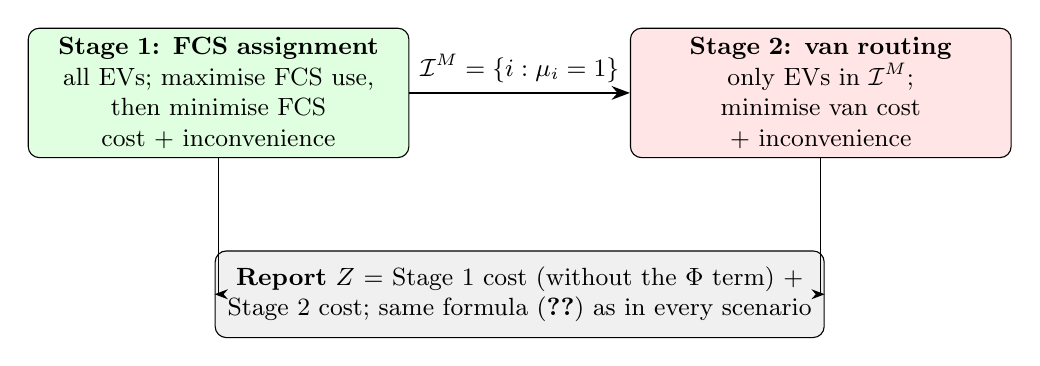
\begin{tikzpicture}[>=Stealth,box/.style={draw,rounded corners,align=center,minimum height=1.1cm,font=\small}]
  \node[box,fill=green!12,text width=4.6cm] (s1) {\textbf{Stage 1: FCS assignment}\\all EVs; maximise FCS use,\\then minimise FCS cost + inconvenience};
  \node[box,fill=red!10,text width=4.6cm,right=2.8cm of s1] (s2) {\textbf{Stage 2: van routing}\\only EVs in $\I^M$;\\minimise van cost + inconvenience};
  \draw[->,thick] (s1) -- node[above,font=\small]{$\I^M=\{i:\mu_i=1\}$} (s2);
  \node[box,fill=black!6,text width=7.5cm,below=2.0cm of $(s1)!0.5!(s2)$] (ev) {\textbf{Report} $Z=$ Stage~1 cost (without the $\Phi$ term) $+$ Stage~2 cost; same formula \eqref{eq:Z} as in every scenario};
  \draw[->] (s1) |- (ev); \draw[->] (s2) |- (ev);
\end{tikzpicture}
\end{center}

Stage~1 does not look at the vans, and Stage~2 cannot change what Stage~1 decided. That is the definition of ``FCS first, then MCS''.

%----------------------------------------------------------------
\subsection{Stage 1: assign EVs to fixed stations}

\textbf{Objective.}
\begin{equation}
\begin{split}
\min\ Z^{(1)}=\;&\underbrace{\Phi\sum_{i\in\I}\mu_i}_{\text{FCS first}}
+\underbrace{c^{EV}\sum_i\sum_{f\in\F_i}d_{if}Y_{if}}_{Z_1}
+\underbrace{Z^F_{\text{energy}}}_{\text{FCS part of }Z_4}\\
&+\underbrace{\sum_i\sum_{f\in\F_i}\rho^F_{if}Y_{if}+\alpha\sum_i w_i(C_i-r_i)+c^L\sum_i w_iL_i}_{\text{FCS customers' inconvenience}}
\end{split}
\label{eq:obj1}
\end{equation}
with $C_i=S_i+\tau^F_iY_i$ in this stage. $\Phi$ is a penalty for handing an EV to the vans. It is chosen larger than anything an extra FCS customer can add to the rest of \eqref{eq:obj1}, e.g.
\[
\Phi > \max_{i}\max_{f\in\F_i}\big(c^{EV}d_{if}+\pi^{\max}E_i+\rho^F_{if}\big)+n\,(\alpha+c^L)\,w_{\max}\,T,
\]
so Stage~1 first \textbf{maximises the number of EVs served at an FCS}, and only among those solutions minimises FCS cost and inconvenience. ($\pi^{\max}$ is the highest grid price.) A numerically safer equivalent is to solve twice: first $\max\sum_iY_i$, then fix that number and minimise the rest.
\ifTOU
Because $Z^F_{\text{energy}}$ uses the peak price, Stage~1 may \emph{start sessions later} to leave the peak, if the price saving beats the extra waiting cost (Section~\ref{sec:expect}).
\fi

\textbf{Constraints.}
\begin{align}
\sum_{g\in\G_i}y_{ig}+\mu_i &= 1 && \forall i\in\I \label{eq:s1assign}\\
S_i &\ge r_i+\sum_{f\in\F_i}t_{if}Y_{if} && \forall i\in\I \label{eq:fcsarr}\\
S_i &\le r_i+T\,(1-\mu_i) && \forall i\in\I \label{eq:s1park}\\
S_j &\ge S_i+\tau^F_i-(T+\tau^F_i)(3-y_{ig}-y_{jg}-o_{ij}) && \forall g,\ (i,j)\in\mathcal{P}_g \label{eq:disj1}\\
S_i &\ge S_j+\tau^F_j-(T+\tau^F_j)(2-y_{ig}-y_{jg}+o_{ij}) && \forall g,\ (i,j)\in\mathcal{P}_g \label{eq:disj2}\\
\sum_i y_{ig_1} &\ge \sum_i y_{ig_2} && \forall f,\ \G_f=\{g_1,g_2\} \label{eq:gunsym}\\
S_i+\tau^F_iY_i &\le T,\qquad L_i\ge S_i+\tau^F_iY_i-l_i && \forall i\in\I \label{eq:s1time}
\end{align}
\ifTOU plus the time-of-use split \eqref{eq:tou1}--\eqref{eq:tou5} of each FCS session (Section~\ref{sec:price}).\fi
\desc{\eqref{eq:s1assign}: every EV either gets one reachable gun or is handed to the vans. An EV that reaches no FCS ($\G_i=\emptyset$) is forced to $\mu_i=1$. \eqref{eq:fcsarr}: an FCS session cannot start before the EV has asked and driven to the station. \eqref{eq:s1park}: for an EV handed to the vans, $S_i$ is parked at $r_i$, so it adds no waiting in Stage~1 (its real start time is decided in Stage~2). \eqref{eq:disj1}--\eqref{eq:disj2}: two EVs on the same gun do not overlap; $o_{ij}$ picks who goes first. With two guns per station this means at most two EVs charge at a station at a time. \eqref{eq:gunsym}: symmetry breaking between the two identical guns (optional). \eqref{eq:s1time}: finished by $T$; lateness.}

\textbf{Optional acceptability rule.} An operator may refuse to send a driver to a station that is ``too inconvenient'', e.g.\ only allow gun $g$ of station $f$ for EV $i$ if $\hat\rho^F_{if}\le\bar\rho$. This only shrinks $\G_i$, so EVs whose stations are all too far go to the vans. Report results with and without it.

\textbf{Output:} $\I^M=\{i:\mu_i=1\}$, the EVs left for the vans; plus each FCS customer's gun and start time.

%----------------------------------------------------------------
\subsection{Stage 2: route the vans to the leftover EVs}

Stage~2 is a vehicle routing problem with time windows, on the EVs in $\I^M$ only. Here $C_i=S_i+\tau^M_i$.

\textbf{Objective.}
\begin{equation}
\begin{split}
\min\ Z^{(2)}=\;&\underbrace{c^M\sum_m\sum_{(i,j)\in\A^M}d_{ij}x_{ijm}}_{Z_2}+\underbrace{\sum_m c^D_mu_m}_{Z_3}+\underbrace{Z^M_{\text{energy}}}_{\text{van part of }Z_4}\\
&+\underbrace{\sum_{i\in\I^M}\sum_m\rho^M_{im}z_{im}+\alpha\sum_{i\in\I^M}w_i(C_i-r_i)+c^L\sum_{i\in\I^M}w_iL_i}_{\text{van customers' inconvenience}}
\end{split}
\label{eq:obj2}
\end{equation}
Since every EV in $\I^M$ must be served by some van, $Z^M_{\text{energy}}$ and the $\rho^M$ term are constants here. They are kept so that $Z^{(2)}$ is the true cost of Stage~2. Waiting and lateness make the vans visit urgent EVs early.

\textbf{Constraints.}
\begin{align}
\sum_{m\in\M}z_{im} &= 1 && \forall i\in\I^M \label{eq:s2assign}\\
\sum_{j:(0,j)\in\A^M}x_{0jm} = \sum_{i:(i,n+1)\in\A^M}x_{i,n+1,m} &= u_m && \forall m \label{eq:depot}\\
\sum_{i:(i,j)\in\A^M}x_{ijm} = \sum_{k:(j,k)\in\A^M}x_{jkm} &= z_{jm} && \forall j\in\I^M,\ m \label{eq:flow}\\
\sum_{i\in\I^M}z_{im} &\le Q_m\,u_m && \forall m \label{eq:cap}\\
\sum_{i\in\I^M}\frac{E_i}{\eta}z_{im}+\beta\sum_{(i,j)\in\A^M}d_{ij}x_{ijm} &\le B_m\,u_m && \forall m \label{eq:batt}
\end{align}
\begin{align}
S_j &\ge \max\{r_j,\ t_{0j}\,x_{0jm}\} && \forall j\in\I^M,\ m \label{eq:depart}\\
S_j &\ge S_i+\tau^M_i+t_{ij}-(T+\tau^M_i+t_{ij})(1-x_{ijm}) && \forall i\neq j,\ m \label{eq:seq}\\
S_i+\tau^M_i+t_{i,n+1} &\le T+(\tau^M_i+t_{i,n+1})(1-x_{i,n+1,m}) && \forall i,\ m \label{eq:return}\\
S_i+\tau^M_i \le T,\quad L_i &\ge S_i+\tau^M_i-l_i && \forall i\in\I^M \label{eq:s2time}\\
u_m &\ge u_{m+1} && m<|\M| \label{eq:vansym}
\end{align}
\desc{\eqref{eq:s2assign}: each leftover EV gets one van. \eqref{eq:depot}: a used van leaves and returns to the depot once. \eqref{eq:flow}: each EV on van $m$ is entered and left exactly once by that van. \eqref{eq:cap}: at most $Q_m$ EVs per van. \eqref{eq:batt}: delivered energy (with transfer losses) plus driving energy fits in the van battery. \eqref{eq:depart}: no start before the request, or before the van can drive there from the depot (written as two linear constraints). \eqref{eq:seq}: if the van goes $i\to j$, it finishes $i$ and drives to $j$ before starting $j$. This gives one EV at a time and removes subtours (MTZ-type). \eqref{eq:return}: back at the depot by $T$. \eqref{eq:s2time}: finished by $T$; lateness. \eqref{eq:vansym}: use identical vans in index order.}

\textbf{If Stage 2 is infeasible} (too many leftover EVs for the fleet by $T$), the sequential policy has \emph{failed} on that instance. For diagnosis, add $s_i\in\{0,1\}$ (``unserved''), replace \eqref{eq:s2assign} by $\sum_mz_{im}+s_i=1$ and add $\Phi^U\sum_is_i$ to \eqref{eq:obj2}. Then report the number of EVs that could not be served. This is a useful comparison with the integrated scenario, which may serve all of them.

%----------------------------------------------------------------
\subsection{Reported value}
\[
Z^{\text{S\scen}}=\big(Z^{(1)*}-\Phi\,|\I^M|\big)+Z^{(2)*},
\]
which is exactly \eqref{eq:Z} evaluated at the combined solution. The stage-1 solution plus the stage-2 solution is a feasible solution of the integrated model (S\ifTOU 4\else 3\fi), so
$Z^{\text{S\ifTOU 4\else 3\fi}}\le Z^{\text{S\scen}}$. The difference is the \emph{value of integration}.

\else
%---------------------------------------------------------------- INT
\subsection{Objective}
\begin{equation}
\min\ Z \quad\text{as in \eqref{eq:Z}, with }Z^F_{\text{energy}}=\ifTOU P^F\textstyle\sum_i\big[\pi^\off(\theta^1_i+\theta^3_i)+\pi^\pk\theta^2_i\big]\else\pi^F\textstyle\sum_iE_iY_i\fi,\quad C_i=S_i+\tau^F_iY_i+\tau^M_iZ_i. \label{eq:objint}
\end{equation}
Written out in full:
\begin{align*}
\min\ Z=\;& c^{EV}\sum_i\sum_{f\in\F_i}d_{if}Y_{if}+c^M\sum_m\sum_{(i,j)\in\A}d_{ij}x_{ijm}+\sum_mc^D_mu_m\\
&+\ifTOU P^F\sum_i\big[\pi^\off(\theta^1_i+\theta^3_i)+\pi^\pk\theta^2_i\big]\else\pi^F\sum_iE_iY_i\fi
+\pi^M\sum_i\sum_m\frac{E_i}{\eta}z_{im}\\
&+\sum_i\sum_{f\in\F_i}\rho^F_{if}Y_{if}+\sum_i\sum_m\rho^M_{im}z_{im}+\alpha\sum_iw_i(C_i-r_i)+c^L\sum_iw_iL_i .
\end{align*}
Every term is linear. One model weighs everything at once: an EV goes to a van exactly when the van's extra km, dispatch and energy cost are outweighed by the effort and waiting it saves the driver\ifTOU, or by the peak-price energy it avoids\fi.

\subsection{Constraints}

\textbf{Assignment.}
\begin{equation}
\sum_{g\in\G_i}y_{ig}+\sum_{m\in\M}z_{im}=1\qquad\forall i\in\I \label{eq:assign}
\end{equation}
\desc{Exactly one resource per EV: one reachable gun or one van. EVs that reach no FCS are forced onto a van.}

\textbf{Fixed stations.}
\begin{align}
S_i &\ge r_i+\sum_{f\in\F_i}t_{if}Y_{if} && \forall i \label{eq:fcsarr}\\
S_j &\ge S_i+\tau^F_i-(T+\tau^F_i)(3-y_{ig}-y_{jg}-o_{ij}) && \forall g,\ (i,j)\in\mathcal{P}_g \label{eq:disj1}\\
S_i &\ge S_j+\tau^F_j-(T+\tau^F_j)(2-y_{ig}-y_{jg}+o_{ij}) && \forall g,\ (i,j)\in\mathcal{P}_g \label{eq:disj2}\\
\sum_iy_{ig_1} &\ge \sum_iy_{ig_2} && \forall f,\ \G_f=\{g_1,g_2\} \label{eq:gunsym}
\end{align}
\desc{\eqref{eq:fcsarr}: an FCS session starts after the request and the drive to the station (for a van customer this is just $S_i\ge r_i$). \eqref{eq:disj1}--\eqref{eq:disj2}: EVs on the same gun do not overlap; $o_{ij}$ chooses the order. \eqref{eq:gunsym}: optional symmetry breaking.}

\textbf{Vans: routes, capacity, battery.}
\begin{align}
\sum_{j:(0,j)\in\A}x_{0jm}=\sum_{i:(i,n+1)\in\A}x_{i,n+1,m} &= u_m && \forall m \label{eq:depot}\\
\sum_{i:(i,j)\in\A}x_{ijm}=\sum_{k:(j,k)\in\A}x_{jkm} &= z_{jm} && \forall j\in\I,\ m \label{eq:flow}\\
\sum_iz_{im} &\le Q_mu_m && \forall m \label{eq:cap}\\
\sum_i\frac{E_i}{\eta}z_{im}+\beta\sum_{(i,j)\in\A}d_{ij}x_{ijm} &\le B_mu_m && \forall m \label{eq:batt}
\end{align}
\desc{\eqref{eq:depot}: a used van leaves and returns once. \eqref{eq:flow}: each EV on van $m$ is visited exactly once by it. \eqref{eq:cap}: at most $Q_m$ EVs. \eqref{eq:batt}: delivered energy (with losses) plus driving energy fits in the battery.}

\textbf{Vans: timing (one EV at a time, no subtours).}
\begin{align}
S_j &\ge t_{0j}\,x_{0jm} && \forall j\in\I,\ m \label{eq:depart}\\
S_j &\ge S_i+\tau^M_i+t_{ij}-(T+\tau^M_i+t_{ij})(1-x_{ijm}) && \forall i\neq j\in\I,\ m \label{eq:seq}\\
S_i+\tau^M_i+t_{i,n+1} &\le T+(\tau^M_i+t_{i,n+1})(1-x_{i,n+1,m}) && \forall i,\ m \label{eq:return}
\end{align}
\desc{\eqref{eq:depart}: the first stop cannot start before the van has driven there. \eqref{eq:seq}: $i\to j$ means finish $i$, drive, then start $j$; start times rise along a route, so no subtour can close. \eqref{eq:return}: back at the depot by $T$.}

\textbf{Horizon and lateness.}
\begin{equation}
C_i\le T,\qquad L_i\ge C_i-l_i\qquad\forall i\in\I \label{eq:time}
\end{equation}
\desc{Every EV is fully charged within the horizon; $L_i$ measures lateness.}

\ifTOU
\textbf{Time-of-use split.} Constraints \eqref{eq:tou1}--\eqref{eq:tou5} of Section~\ref{sec:price}.
\fi

\textbf{Symmetry and domains.}
\begin{equation}
u_m\ge u_{m+1};\qquad y,z,x,u,o\ifTOU,\kappa\fi\in\{0,1\};\qquad S_i,L_i\ifTOU,\theta^p_i\fi\ge0 \label{eq:dom}
\end{equation}
\fi

%=====================================================================
\section{Learning-to-optimise (RL) formulation}\label{sec:rl}

\textbf{Main rule:} the reward of each action is \emph{minus the increase in $Z$ that the action causes}. The rewards over an episode then add up to $-Z$ of the solution the policy builds. RL and MILP results are measured on the same yardstick \eqref{eq:Z}, and the MILP optimum is the benchmark for the RL gap.

\ifSEQ
%---------------------------------------------------------------- RL SEQ
The RL pipeline has the same two stages as the MILP.

\subsection{Stage 1 policy: FCS assignment}
\begin{itemize}[leftmargin=1.4em,itemsep=2pt]
  \item \textbf{Episode / epochs:} EVs are taken in order of request time $r_i$ (ties: higher $w_i$ first). One decision per EV.
  \item \textbf{State:} features of the current EV $k$ ($E_k,r_k,l_k,w_k,R_k$, location); for each gun $g$ the time $F_g$ it becomes free; summary features of the EVs still to come (count and positions near each station)\ifTOU; the current price and the time until $T_1$ and $T_2$\fi.
  \item \textbf{Action:} a gun $g\in\G_k$, or ``hand to vans''. \textbf{FCS-first mask:} ``hand to vans'' is allowed \emph{only} if no gun can finish EV $k$ by $T$ (or, with the optional rule, if all remaining guns have $\hat\rho^F_{kf}>\bar\rho$).
  \ifTOU\item \textbf{Optional timing action:} ``gun $g$, start after the peak'', i.e.\ $S_k=\max\{\text{earliest},T_2\}$, allowed only if the session still ends by $T$.\fi
  \item \textbf{Transition:} $S_k=\max\{r_k+t_{kf},F_g\}$ (or later, for the timing action); $F_g\leftarrow S_k+\tau^F_k$.
  \item \textbf{Reward:} $-\Big[c^{EV}d_{kf}+\text{energy}_k+\rho^F_{kf}+\alpha w_k(S_k+\tau^F_k-r_k)+c^Lw_k(S_k+\tau^F_k-l_k)^+\Big]$, where energy$_k$ = \ifTOU$P^F\big[\pi^\off\cdot(\text{off-peak hours of }[S_k,S_k+\tau^F_k])+\pi^\pk\cdot(\text{peak hours})\big]$, computed exactly in the simulator\else$\pi^FE_k$\fi. Handing an EV to the vans gives reward $0$ here; its cost is counted in Stage~2.
\end{itemize}
Note: a simple baseline for Stage~1 is the greedy rule ``gun with the largest one-step reward''. What RL can learn on top of this is, for example, to keep a nearby gun free for an urgent EV that arrives later.

\subsection{Stage 2 policy: van routing over $\I^M$}
\begin{itemize}[leftmargin=1.4em,itemsep=2pt]
  \item \textbf{Epochs:} whenever a van becomes free (the earliest-free van decides first).
  \item \textbf{State:} for each van: position, time free, remaining battery $b_m$, EVs served so far, dispatched or not; for each unserved EV in $\I^M$: location, $E_i,r_i,l_i,w_i$; current time.
  \item \textbf{Action:} the next EV $j$ for this van, or ``return to depot'' (ends the route). Mask: $j$ must be feasible: battery covers $E_j/\eta$ plus driving to $j$ and back to the depot, the count stays $\le Q_m$, and $j$ can be finished with the van back at the depot by $T$.
  \item \textbf{Transition:} $S_j=\max\{r_j,\ \text{time free}+t_{\text{pos},j}\}$; the van moves to $j$ and is free at $S_j+\tau^M_j$; $b_m$ falls by $E_j/\eta+\beta d_{\text{pos},j}$.
  \item \textbf{Reward:} serving $j$: $-\Big[c^Md_{\text{pos},j}+c^D_m[\text{first stop}]+\pi^M\frac{E_j}{\eta}+\rho^M_{jm}+\alpha w_j(S_j+\tau^M_j-r_j)+c^Lw_j(S_j+\tau^M_j-l_j)^+\Big]$; returning: $-c^Md_{\text{pos},0}$. EVs still unserved at the end: $-\Phi^U$ each.
  \item \textbf{Policy:} an attention-based routing policy (e.g.\ Kool et al., 2019, ``Attention, Learn to Solve Routing Problems!'') trained with REINFORCE or PPO. Baseline: nearest-feasible-EV heuristic.
\end{itemize}
Episode return of Stage~1 + Stage~2 $=-Z^{\text{S\scen}}$.

\else
%---------------------------------------------------------------- RL INT
One policy decides both who serves each EV and the van routes.
\begin{itemize}[leftmargin=1.4em,itemsep=2pt]
  \item \textbf{Episode / epochs:} EVs are taken in order of request time $r_i$ (ties: higher $w_i$ first). One decision per EV.
  \item \textbf{State:} (i) the current EV $k$: location, $E_k,r_k,l_k,w_k,R_k$, reachable stations; (ii) each gun $g$: time $F_g$ it becomes free; (iii) each van $m$: current end-of-route position, time free, remaining battery $b_m$, EVs served, dispatched or not; (iv) embeddings of the not-yet-assigned EVs (for look-ahead)\ifTOU; (v) current price, time until $T_1$ and $T_2$\fi.
  \item \textbf{Action:} $a\in\G_k\cup\M$: a gun, or a van (EV $k$ is appended to the end of that van's route). \textbf{Mask} infeasible actions: a gun that cannot finish $k$ by $T$; a van without enough battery for $E_k/\eta$ plus the drive to $k$ and back to the depot, with $Q_m$ reached, or unable to finish $k$ and return by $T$.
  \ifTOU\item \textbf{Optional timing action:} ``gun $g$, start after the peak'' ($S_k=\max\{\text{earliest},T_2\}$, if it still ends by $T$).\fi
  \item \textbf{Transition:} gun: $S_k=\max\{r_k+t_{kf},F_g\}$, $F_g\leftarrow S_k+\tau^F_k$. Van: $S_k=\max\{r_k,\ \text{free}_m+t_{\text{pos}_m,k}\}$, then the van moves to $k$, $\text{free}_m\leftarrow S_k+\tau^M_k$, $b_m\mathrel{-}=E_k/\eta+\beta d_{\text{pos}_m,k}$.
  \item \textbf{Reward} $=-\Delta Z$:
  \begin{align*}
  \text{gun } g\text{ at }f:&\quad -\Big[c^{EV}d_{kf}+\text{energy}^F_k+\rho^F_{kf}+\alpha w_k(C_k-r_k)+c^Lw_k(C_k-l_k)^+\Big]\\
  \text{van } m:&\quad -\Big[c^M\big(d_{\text{pos}_m,k}+d_{k,0}-d_{\text{pos}_m,0}\big)+c^D_m[\text{first use}]+\pi^M\tfrac{E_k}{\eta}\\
  &\qquad\quad+\rho^M_{km}+\alpha w_k(C_k-r_k)+c^Lw_k(C_k-l_k)^+\Big]
  \end{align*}
  The van distance term is the \emph{change} in route length when $k$ is inserted before the return to the depot, so the sum over the episode equals the total route length (the return legs telescope). energy$^F_k$ = \ifTOU$P^F\big[\pi^\off\cdot(\text{off-peak hours})+\pi^\pk\cdot(\text{peak hours of }[S_k,C_k])\big]$, computed exactly by the simulator; no linearisation is needed in RL\else$\pi^FE_k$\fi.
  \item \textbf{Dead end:} if every action is masked, EV $k$ is unserved: reward $-\Phi^U$, and the episode continues. Report the count.
  \item \textbf{Policy:} masked categorical policy over guns and vans, encoder with attention over EVs, guns and vans; trained with PPO. Natural baseline: greedy, i.e.\ choose the action with the largest one-step reward. That is the pairwise rule ``smallest $\hat\rho$ + cost'' from Section~\ref{sec:inc}.
\end{itemize}
Restriction to note: vans serve EVs in assignment order (append only). A variant that inserts $k$ at the cheapest position of a route is more flexible but has a larger action space.
\fi

\textbf{Reward scaling.} For stable training divide every reward by a constant, e.g.\ the greedy baseline's average $Z$ on the training instances. This does not change the optimal policy.

%=====================================================================
\section{What to expect and what to report}\label{sec:expect}

\ifnum\scen=1
\begin{itemize}[leftmargin=1.4em,itemsep=2pt]
  \item Vans serve only EVs that reach no station, or that the stations cannot finish by $T$. If stations have spare capacity, very few vans are dispatched.
  \item Inconvenience is high for EVs far from the nearest station (worked example: Rs\,682 at the FCS, against Rs\,458 if a van had been allowed).
  \item With too few vans Stage~2 becomes infeasible (unserved EVs), even when the integrated model S3 could serve everyone. Report the smallest $|\M|$ at which S1 is feasible and compare it with S3.
\end{itemize}
\fi
\ifnum\scen=2
\begin{itemize}[leftmargin=1.4em,itemsep=2pt]
  \item \textbf{When does Stage~1 delay a session to avoid the peak?} Moving one hour of charging out of the peak saves $(\pi^\pk-\pi^\off)P^F=3\times22=$ Rs\,66, but delays completion by up to an hour, which costs $\alpha w_i\ge$ Rs\,200. So with the default values Stage~1 almost never delays. It mostly pays the higher price, and S2 costs roughly S1 plus the peak surcharge. Sessions start later only if $\alpha$ is small (try $\lambda<0.33$ in the sensitivity analysis).
  \item The van assignment is the same as in S1 unless Stage~1's timing changes which EVs fit at the stations. Stage~1 cannot use vans to escape the peak price.
  \item Extra KPI: \textbf{grid energy drawn at FCS during the peak}, $P^F\sum_i\theta^2_i$ (kWh). Compare with S4.
\end{itemize}
\fi
\ifnum\scen=3
\begin{itemize}[leftmargin=1.4em,itemsep=2pt]
  \item Vans take EVs for which the saved inconvenience exceeds the extra van cost (worked example: van chosen, saving Rs\,224). Expect vans to serve EVs that are far from every station, have low range (high $w_i$), or have early deadlines, while EVs near a station still use it.
  \item \textbf{Value of integration under flat price:} $Z^{\text{S1}}-Z^{\text{S3}}\ge0$. Report it per component ($Z_1,\dots,Z_5$): typically operating cost rises a little and inconvenience falls a lot.
  \item Vary $|\M|$ (0, 1, 2, \dots): the first few vans lower $Z$ sharply, then the effect levels off. That curve shows the scenarios where mobile chargers help most.
\end{itemize}
\fi
\ifnum\scen=4
\begin{itemize}[leftmargin=1.4em,itemsep=2pt]
  \item During the peak a van kWh costs about the same as an FCS kWh (Rs\,10.0 each), so the vans' energy disadvantage disappears and vans also absorb \emph{peak-hour} demand that would otherwise be charged on the grid at peak price.
  \item Expect more van usage than in S3, concentrated on requests in $[T_1,T_2]$, and lower grid energy at the stations during the peak, $P^F\sum_i\theta^2_i$, than in S2.
  \item \textbf{Value of integration under peak pricing:} $Z^{\text{S2}}-Z^{\text{S4}}$. It should be larger than $Z^{\text{S1}}-Z^{\text{S3}}$, because integration now also allows price arbitrage.
  \item \textbf{Peak pricing with full flexibility:} $Z^{\text{S4}}-Z^{\text{S3}}$ should be smaller than $Z^{\text{S2}}-Z^{\text{S1}}$: vans cushion the price increase.
\end{itemize}
\fi

\textbf{Cross-scenario comparison table} (fill in from the four runs):
\begin{center}
\renewcommand{\arraystretch}{1.2}
\begin{tabular}{@{}lll@{}}
\toprule
\textbf{Comparison} & \textbf{Measures} & \textbf{Expected sign} \\
\midrule
S1 $-$ S3 & value of integration, flat price & $\ge0$ \\
S2 $-$ S4 & value of integration, peak price & $\ge0$, larger than S1 $-$ S3 \\
S2 $-$ S1 & cost of peak pricing, FCS-first operator & $>0$ \\
S4 $-$ S3 & cost of peak pricing, flexible operator & $>0$, smaller than S2 $-$ S1 \\
\bottomrule
\end{tabular}
\end{center}
Report for each: $Z$ and its components, number of vans used, EVs per resource, mean and maximum inconvenience per EV, total lateness, peak-hour grid energy, solve time, and (for RL) the gap to the MILP optimum.

%=====================================================================
\appendix
\section{Illustrative parameter values}\label{app:values}

These are starting values for experiments, not data. All are meant to be varied in the analysis. Values in Rs.

\begin{center}
\renewcommand{\arraystretch}{1.15}
\begin{tabular}{@{}llp{6.2cm}@{}}
\toprule
\textbf{Parameter} & \textbf{Value} & \textbf{Note} \\
\midrule
$T$, $[T_1,T_2]$ & 7 h, $[2,6]$ & 16:00--23:00, peak 18:00--22:00 \\
$P^F$, $P^M$ & 22 kW, 30 kW & \\
$v$, $\beta$, $\eta$ & 25 km/h, 0.25 kWh/km, 0.9 & \\
$B_m$, $Q_m$, $|\M|$ & 150 kWh, 6, 2--6 & \\
$c^{EV}$, $c^M$, $c^D_m$ & Rs\,4/km, Rs\,15/km, Rs\,1500 & van km includes driver time \\
$\pi^F$ (flat) & Rs\,8.7/kWh & equals the time-average of the ToU tariff over $[0,T]$ \\
$\pi^\off$, $\pi^\pk$ (ToU) & Rs\,7/kWh, Rs\,10/kWh & $(3\times7+4\times10)/7=8.7$ \\
$c^{bat}$ & Rs\,2/kWh & van battery wear \\
$\pi^M$ & Rs\,10.7 (flat) / Rs\,9.0 (ToU) & $=\pi^F+c^{bat}$ / $=\pi^\off+c^{bat}$ \\
$\alpha$, $\alpha^D$ & Rs\,200/h, Rs\,100/h & value of time; extra for attended time \\
$h^F$, $h^M$, $\varphi$ & Rs\,50, Rs\,10, Rs\,100 & trip hassle, hand-over, range stress \\
$c^L$ & Rs\,300/h & lateness \\
$w_i$ & $1+2(1-R_i/R_{\max})$, $R_i\sim U[3,40]$ km & priority from remaining range \\
\bottomrule
\end{tabular}
\end{center}

The flat price is set to the time-average of the peak tariff. The price \emph{level} is then the same in both pricing cases, and only the price \emph{shape} differs. Without this, part of S1 vs S2 would just reflect a different average price.

\end{document}
"
%    pdflatex -jobname=scenario3_flat_integrated   "\def\scen{3}% =====================================================================
%  One source, four PDFs.  Build with build.sh (or by hand):
%    pdflatex -jobname=scenario1_flat_sequential   "\def\scen{1}\input{scenario_master}"
%    pdflatex -jobname=scenario2_peak_sequential   "\def\scen{2}\input{scenario_master}"
%    pdflatex -jobname=scenario3_flat_integrated   "\def\scen{3}\input{scenario_master}"
%    pdflatex -jobname=scenario4_peak_integrated   "\def\scen{4}\input{scenario_master}"
%  (run each twice for cross-references)
% =====================================================================
\documentclass[11pt,a4paper]{article}
\usepackage[margin=2.2cm]{geometry}
\usepackage{amsmath,amssymb,amsfonts}
\usepackage{booktabs,array,tabularx}
\usepackage{enumitem}
\usepackage[table]{xcolor}
\usepackage{tikz}
\usetikzlibrary{arrows.meta,positioning,calc}
\usepackage[colorlinks=true,linkcolor=blue!50!black,urlcolor=blue!50!black]{hyperref}
\usepackage{titlesec}
\titleformat{\section}{\large\bfseries}{\thesection}{0.8em}{}
\titleformat{\subsection}{\normalsize\bfseries}{\thesubsection}{0.8em}{}
\setlength{\parindent}{0pt}
\setlength{\parskip}{5pt}

% ---------------- scenario switches ----------------
\ifdefined\scen\else\def\scen{1}\fi
\newif\ifTOU \TOUfalse   % true = time-of-use (peak) price
\newif\ifSEQ \SEQfalse   % true = FCS first, then MCS
\ifnum\scen=1 \SEQtrue \fi
\ifnum\scen=2 \TOUtrue \SEQtrue \fi
\ifnum\scen=4 \TOUtrue \fi

\newcommand{\pricename}{\ifTOU time-of-use price (dearer evening peak)\else single (flat) price all day\fi}
\newcommand{\structname}{\ifSEQ FCS first, then MCS (sequential)\else FCS and MCS together (integrated)\fi}

% ---------------- notation ----------------
\newcommand{\I}{\mathcal{I}}
\newcommand{\F}{\mathcal{F}}
\newcommand{\G}{\mathcal{G}}
\newcommand{\M}{\mathcal{M}}
\newcommand{\N}{\mathcal{N}}
\newcommand{\A}{\mathcal{A}}
\newcommand{\Rs}{\text{Rs}\,}
\newcommand{\pk}{\mathrm{pk}}
\newcommand{\off}{\mathrm{off}}
\newcommand{\desc}[1]{\par\vspace{-2pt}{\small\color{black!75}\textit{Meaning:} #1}\par\vspace{4pt}}
\newcommand{\cell}[2]{\ifnum\scen=#1\cellcolor{blue!18}\textbf{S#1 (this document)}\\\textbf{#2}\else S#1\\#2\fi}

\title{\textbf{EV Charging Network Optimisation}\\[4pt]
\large Scenario \scen: \pricename\ $+$ \structname\\[2pt]
\normalsize MILP and RL formulation}
\author{CP 320 OR for Mobility Management, course project}
\date{2 October 2026}

\begin{document}
\maketitle

%=====================================================================
\section{Where this scenario sits}

The project studies four scenarios: two ways of pricing grid electricity, times two ways of making the decisions.

\begin{center}
\renewcommand{\arraystretch}{1.5}
\begin{tabular}{>{\raggedright\arraybackslash}p{4.2cm}|>{\centering\arraybackslash}p{4.6cm}|>{\centering\arraybackslash}p{4.6cm}}
 & \textbf{Flat price all day} & \textbf{Time-of-use (peak) price} \\ \hline
\textbf{Sequential:} FCS first, leftover EVs to MCS &
\begin{tabular}[c]{@{}c@{}}\cell{1}{flat + sequential}\end{tabular} &
\begin{tabular}[c]{@{}c@{}}\cell{2}{peak + sequential}\end{tabular} \\ \hline
\textbf{Integrated:} FCS and MCS decided together &
\begin{tabular}[c]{@{}c@{}}\cell{3}{flat + integrated}\end{tabular} &
\begin{tabular}[c]{@{}c@{}}\cell{4}{peak + integrated}\end{tabular} \\
\end{tabular}
\end{center}

\textbf{The four scenarios do not have four different objectives.} They share \emph{one} cost yardstick $Z$ (Section~\ref{sec:obj}): the same cost terms and the same customer inconvenience (Section~\ref{sec:inc}). Only two things change:
\begin{itemize}[leftmargin=1.4em,itemsep=1pt]
  \item \textbf{Pricing} changes the formula for one term, the FCS energy cost (Section~\ref{sec:price}).
  \item \textbf{Decision structure} changes \emph{how} $Z$ is minimised: in one model (integrated), or in two stages (sequential), where each stage minimises its own part of $Z$.
\end{itemize}
Because the yardstick is the same, the four optimal values can be compared directly. The differences measure the \emph{value of integration} (S1$\to$S3, S2$\to$S4) and the \emph{effect of peak pricing} (S1$\to$S2, S3$\to$S4).

\ifnum\scen=1
\textbf{This scenario (S1)} is the baseline, the ``status quo''. Electricity costs the same at every hour, every EV that can be charged at a fixed station is sent there, and vans only take what is left over.
\fi
\ifnum\scen=2
\textbf{This scenario (S2)} keeps the FCS-first rule of S1, but grid electricity is dearer during the evening peak. Stage~1 can react to the price only by \emph{rescheduling} FCS sessions. It cannot hand a peak-hour EV to a van.
\fi
\ifnum\scen=3
\textbf{This scenario (S3)} keeps the flat price of S1, but the operator decides FCS and MCS service \emph{together}. An EV can be sent to a van even when a fixed station could take it, whenever that lowers total cost plus inconvenience.
\fi
\ifnum\scen=4
\textbf{This scenario (S4)} is the most flexible one: peak pricing at fixed stations, and FCS and MCS decided together. Van energy was bought off-peak, so vans can also be used to keep charging \emph{out of the expensive peak}.
\fi

%=====================================================================
\section{Setting and assumptions}\label{sec:setting}

\textbf{Time.} The planning horizon is $[0,T]$ with $T=7$\,h (16:00--23:00). It contains the evening peak window $[T_1,T_2]=[2,6]$ (18:00--22:00). The horizon is the same in all four scenarios. It is wider than the peak itself so that, under peak pricing, there is cheaper time on both sides of the peak.\ifTOU\else\ In this scenario the price is flat, so the window plays no role in the model.\fi

\textbf{Assumptions} (the same as MILP v3, plus two about energy):
\begin{enumerate}[leftmargin=1.6em,itemsep=1pt]
  \item Static, continuous time. All requests in the horizon are known at time $0$, and request $i$ becomes active at $r_i$.
  \item An EV served by an FCS drives there itself on its own battery (only to stations within its range $R_i$). The driver stays with the car while it waits for a free gun and while it charges.
  \item An EV served by an MCS stays parked where it is, and the driver is free in the meantime.
  \item Each FCS gun and each van charges one EV at a time, without interruption, at constant power.
  \item A van's battery covers both its driving and the energy it delivers. \textbf{The van battery is charged at the depot before the horizon starts}\ifTOU, i.e.\ at the off-peak price\fi, and is not recharged during the horizon.
  \item Every EV must be fully charged by $T$ (hard). Finishing after the driver's desired time $l_i$ is allowed but penalised.
\end{enumerate}

%=====================================================================
\section{Notation}\label{sec:notation}

\subsection*{Sets}
\begin{tabularx}{\textwidth}{@{}lX@{}}
\toprule
$\I=\{1,\dots,n\}$ & EV charging requests \\
$\F$; $\G_f$ ($|\G_f|=2$); $\G=\bigcup_f\G_f$ & fixed charging stations; guns of FCS $f$; all guns ($f(g)$ = station of gun $g$) \\
$\F_i=\{f: d_{if}\le R_i\}$, $\G_i=\bigcup_{f\in\F_i}\G_f$ & stations / guns EV $i$ can reach on its remaining range \\
$\M$ & mobile charging vans (MCS) \\
$0,\ n+1$ & depot as start node / end node (same place) \\
$\N=\{0\}\cup\I\cup\{n+1\}$, $\A$ & routing nodes; allowed van arcs $(i,j)$, $i\in\{0\}\cup\I$, $j\in\I\cup\{n+1\}$, $i\neq j$ \\
$\mathcal{P}_g=\{(i,j): i<j,\ g\in\G_i\cap\G_j\}$ & pairs of EVs that could share gun $g$ \\
\ifSEQ
$\I^M\subseteq\I$ & EVs handed to the vans by Stage~1 (an \emph{output} of Stage~1, a fixed input to Stage~2) \\
$\N^M$, $\A^M$ & routing nodes / arcs restricted to $\I^M$ \\
\fi
\bottomrule
\end{tabularx}

\subsection*{Parameters}
\begin{tabularx}{\textwidth}{@{}lX@{}}
\toprule
$E_i,\ r_i,\ l_i,\ R_i$ & energy demand (kWh), request time, desired completion time (h), remaining range (km) \\
$w_i\ge1$ & priority of EV $i$; $w_i=1+\kappa(1-R_i/R_{\max})$, so low-range EVs weigh more \\
$P^F,\ P^M$ & charging power of an FCS gun (22\,kW) / of a van (e.g.\ 30\,kW) \\
$\tau^F_i=E_i/P^F,\ \tau^M_i=E_i/P^M$ & charging time of EV $i$ at an FCS / by a van (h) \\
$d_{if},t_{if}$;\ $d_{ij},t_{ij}$ & distance (km) and time (h): EV$\to$FCS; between routing nodes ($t=d/v$) \\
$B_m,\ Q_m,\ \beta,\ \eta$ & van battery (kWh), max EVs per van, van consumption (kWh/km), transfer efficiency \\
$c^{EV},\ c^M,\ c^D_m$ & cost per km of EV driving, per km of van driving; fixed dispatch cost of van $m$ \\
\ifTOU
$\pi^\off,\ \pi^\pk$ & grid price (Rs/kWh) off-peak / in $[T_1,T_2]$, with $\pi^\pk\ge\pi^\off$ \\
\else
$\pi^F$ & grid price (Rs/kWh), the same at every hour \\
\fi
$c^{bat}$ & van battery wear per kWh cycled \\
$\pi^M$ & cost of 1 kWh taken from a van battery: $\pi^M=\ifTOU\pi^\off\else\pi^F\fi+c^{bat}$ (Section~\ref{sec:price}) \\
$\alpha,\ \alpha^D,\ h^F,\ h^M,\ \varphi,\ c^L$ & inconvenience coefficients (Section~\ref{sec:inc}) \\
\bottomrule
\end{tabularx}

\subsection*{Decision variables}
\begin{tabularx}{\textwidth}{@{}llX@{}}
\toprule
$y_{ig}$ & $\{0,1\}$ & EV $i$ charged at gun $g\in\G_i$ \\
$z_{im}$ & $\{0,1\}$ & EV $i$ served by van $m$ \\
$x_{ijm}$ & $\{0,1\}$ & van $m$ drives arc $(i,j)$ \\
$u_m$ & $\{0,1\}$ & van $m$ is dispatched \\
$o_{ij}$ & $\{0,1\}$ & for EVs $i<j$ that could share a gun: 1 if $i$ is charged before $j$ \\
\ifSEQ
$\mu_i$ & $\{0,1\}$ & Stage~1 only: EV $i$ is handed to the van fleet \\
\fi
\ifTOU
$\theta^1_i,\theta^2_i,\theta^3_i$ & $\ge0$ & hours of EV $i$'s FCS session before / inside / after the peak \\
$\kappa^1_i,\kappa^3_i$ & $\{0,1\}$ & EV $i$'s FCS session starts before $T_1$ / ends after $T_2$ \\
\fi
$S_i$ & $\ge0$ & time charging of EV $i$ starts (h), on whichever resource \\
$L_i$ & $\ge0$ & lateness of EV $i$ beyond $l_i$ (h) \\
\bottomrule
\end{tabularx}

\textbf{Short-hands} (linear expressions, not new variables):
\[
Y_{if}=\sum_{g\in\G_f}y_{ig},\qquad Y_i=\sum_{g\in\G_i}y_{ig}\ (\text{EV $i$ uses an FCS}),\qquad Z_i=\sum_{m\in\M}z_{im}\ (\text{EV $i$ uses a van}),
\]
\[
C_i=S_i+\tau^F_i\,Y_i+\tau^M_i\,Z_i \quad\text{(time EV $i$ is fully charged).}
\]

%=====================================================================
\section{Customer inconvenience}\label{sec:inc}

This section is \textbf{identical in all four scenario documents}. Inconvenience is a property of the customer, not of the price or of the planning method.

\subsection{What we mean by inconvenience}

Inconvenience is \emph{what the driver loses} from the moment they ask for a charge ($r_i$) until the car is fully charged ($C_i$), \emph{converted into rupees} so it can be added to the operator's costs. A driver loses three different things:

\begin{enumerate}[leftmargin=1.6em,itemsep=2pt]
  \item \textbf{Waiting:} the car is not ready. This lasts $C_i-r_i$ hours and affects \emph{every} driver, FCS or MCS.
  \item \textbf{Effort:} only an FCS customer has to drive to the station and sit there while the car charges. An MCS customer stays at home or at work and does something else. Driving to a far station also uses scarce battery range, which causes stress (``range anxiety'').
  \item \textbf{A missed deadline:} the car is still not ready at the time $l_i$ the driver needs it.
\end{enumerate}

Each loss gets a price in Rs per hour (or per event). All of them are multiplied by the priority $w_i$: an hour of delay for an EV with 5\,km of range left counts more than for one with 40\,km.

\subsection{The three components}

\begin{center}
\renewcommand{\arraystretch}{1.3}
\begin{tabularx}{\textwidth}{@{}>{\raggedright\arraybackslash}p{2.6cm}>{\raggedright\arraybackslash}X>{\raggedright\arraybackslash}X>{\raggedright\arraybackslash}p{3.0cm}@{}}
\toprule
\textbf{Component} & \textbf{EV $i$ at FCS $f$} & \textbf{EV $i$ by a van} & \textbf{Known when?} \\
\midrule
Effort & $w_i\big[\alpha^D(t_{if}+\tau^F_i)+h^F+\varphi\,d_{if}/R_i\big]$: driving and sitting at the station, a fixed trip hassle, range stress & $w_i\,h^M$: being reachable and handing over the car & \textbf{Static:} known as soon as the resource is chosen \\
Waiting & $w_i\,\alpha\,(C_i-r_i)$ = drive + \emph{queue at the gun} + charge & $w_i\,\alpha\,(C_i-r_i)$ = \emph{wait for the van} + charge & \textbf{Dynamic:} depends on the queue / van route \\
Missed deadline & $w_i\,c^L\,L_i$, $L_i=\max\{0,C_i-l_i\}$ & same & Dynamic \\
\bottomrule
\end{tabularx}
\end{center}

\textbf{Coefficients.}
$\alpha$ (Rs/h) is the value of an hour the car is not ready.
$\alpha^D$ (Rs/h) is the \emph{extra} value of an hour the driver must personally spend driving or sitting at the station: an hour at the station costs $\alpha+\alpha^D$, an hour waiting at home for a van costs only $\alpha$.
$h^F,h^M$ (Rs) are fixed hassle costs of one trip to a station / one van hand-over.
$\varphi$ (Rs) is the range-stress cost of a trip that uses the \emph{whole} remaining range ($d_{if}/R_i\le1$ is the fraction used).
$c^L$ (Rs/h) is the cost per hour late.

\subsection{Pairwise form: inconvenience of a (customer, resource) pair}

The natural first idea is: \emph{for every pair (EV $i$, FCS $f$) and every pair (EV $i$, van $m$) there is an inconvenience number, and the operator picks the pair with the lowest cost plus inconvenience.} The static part fits this idea exactly:
\[
\boxed{\;\rho^F_{if}=w_i\Big[\alpha^D\,(t_{if}+\tau^F_i)+h^F+\varphi\,\frac{d_{if}}{R_i}\Big]\qquad
\rho^M_{im}=w_i\,h^M\;}
\]
These are \textbf{parameters}, computed before solving, one number per (EV, FCS) pair and per (EV, van) pair. In the objective they appear linearly: $\sum_i\sum_f\rho^F_{if}Y_{if}+\sum_i\sum_m\rho^M_{im}z_{im}$.

Note that $\rho^M_{im}$ does not depend on $m$. Vans are identical and all start at the same depot, so the driver does not care \emph{which} van comes, only \emph{when} it comes. That ``when'' is the waiting part.

\subsection{Why waiting cannot be a fixed pairwise number}

It is tempting to also write the waiting as a pairwise number, e.g.\ ``the van needs 5 minutes to reach EV $i$''. But that depends on \emph{where the van is coming from}, which depends on the route the model is still choosing: if EV $i$ is the 4th stop of a van, the wait is the time for three charging sessions plus four drives. Likewise, waiting at an FCS depends on how many EVs are queued at that gun. So waiting is not known before solving. It is a function of decision variables:
\[
\text{waiting cost of EV } i \;=\; w_i\,\alpha\,(C_i-r_i),\qquad C_i=S_i+\tau^F_iY_i+\tau^M_iZ_i .
\]
This is \textbf{linear} in the variables ($S_i$, $y$, $z$), so it fits in a MILP directly. The constraints of Section~\ref{sec:milp} make $S_i$ equal to the true start time, including driving, queueing at the gun and the van's route. The term $\sum_i w_i\alpha r_i$ is a constant and may be dropped when solving.

\textbf{Pairwise \emph{estimate}} (used for intuition, by the RL policy and in heuristics): if there is no queue and the van comes straight to $i$,
\[
\hat\rho^{F}_{if}=\rho^F_{if}+w_i\alpha\,(t_{if}+\tau^F_i),\qquad
\hat\rho^{M}_{im}=\rho^M_{im}+w_i\alpha\,(t^{\text{van}}_{m\to i}+\tau^M_i),
\]
where $t^{\text{van}}_{m\to i}$ is the time until van $m$ can reach $i$ from where it currently is. In the RL formulation (Section~\ref{sec:rl}) the van's position \emph{is} known at each decision, so there this estimate becomes exact.

\subsection{Total inconvenience and how it enters the objective}

\begin{equation}
\boxed{\;
Z_{\text{inc}}=\underbrace{\sum_{i\in\I}\sum_{f\in\F_i}\rho^F_{if}Y_{if}+\sum_{i\in\I}\sum_{m\in\M}\rho^M_{im}z_{im}}_{\text{effort (static, pairwise)}}
+\underbrace{\alpha\sum_{i\in\I}w_i\,(C_i-r_i)}_{\text{waiting (dynamic)}}
+\underbrace{c^L\sum_{i\in\I}w_i\,L_i}_{\text{missed deadline}}
\;}\label{eq:inc}
\end{equation}
All three parts are in rupees, so $Z_{\text{inc}}$ is simply added to the operating costs. Nothing has to be normalised.

\subsection{Worked example: your ``10 km to the FCS vs.\ van in 5 minutes'' case}

EV $i$: $E_i=20$\,kWh, $R_i=40$\,km (so $w_i=1$); nearest free FCS $d_{if}=10$\,km away, $t_{if}=0.4$\,h at 25\,km/h; a van finishing next door can reach it in 5\,min ($0.083$\,h), adding about 4\,km to its route. $\tau^F_i=20/22=0.909$\,h, $\tau^M_i=20/30=0.667$\,h. Coefficients from Appendix~\ref{app:values}, flat price.

\begin{center}
\renewcommand{\arraystretch}{1.25}
\begin{tabular}{@{}lrr@{}}
\toprule
 & \textbf{FCS} & \textbf{Van} \\
\midrule
Driving (EV / extra van km) & $4\times10=40.0$ & $15\times4=60.0$ \\
Energy & $8.7\times20=174.0$ & $10.7\times20/0.9=237.8$ \\
\textbf{Operating cost only} & \textbf{214.0} & \textbf{297.8} \\
\midrule
Effort $\rho$ & $100(0.4+0.909)+50+100\cdot\tfrac{10}{40}=205.9$ & $10.0$ \\
Waiting $\alpha(C_i-r_i)$ & $200\times1.309=261.8$ & $200\times0.75=150.0$ \\
\textbf{Cost + inconvenience} & \textbf{681.7} & \textbf{457.8} \\
\bottomrule
\end{tabular}
\end{center}

On operating cost alone the FCS is cheaper, so a cost-only model would \emph{always} send this driver 10\,km away. With inconvenience included the van is better by about Rs\,224, and the integrated model chooses $z_{im}=1$, as you expected. If the FCS were only 1\,km away, the FCS would win both comparisons. The inconvenience term is what makes the model choose between ``cheap for the operator'' and ``convenient for the driver'', rather than following a fixed rule.

\subsection{Relation to a single penalty $\rho_i$ per EV}

The first draft used a penalty $\rho_i$ that is charged whenever EV $i$ goes to \emph{any} FCS: $\sum_i\sum_f\rho_iy_{if}$. Because $\sum_f y_{if}=1-\sum_m z_{im}$, this only says ``a van is worth $\rho_i$ more to EV $i$'', and that holds whether the station is 1\,km or 15\,km away, and whether the van arrives in 5 minutes or in 3 hours. The form above fixes both problems: $\rho^F_{if}$ grows with the distance to \emph{that} station, and the waiting term grows with how late the van or the free gun actually is. The old model is the special case $\alpha=\alpha^D=\varphi=c^L=0$, $h^F=\rho_i$.

\subsection{Choosing the coefficients}
\begin{itemize}[leftmargin=1.4em,itemsep=2pt]
  \item Use a value of time for $\alpha$ (e.g.\ Rs\,150--300/h for urban car users), and set $\alpha^D\approx0.5\alpha$: sitting at a station is worse than waiting at home.
  \item Keep $c^L>\alpha$, so missing the deadline is worse than ordinary waiting.
  \item \textbf{Sensitivity analysis:} multiply all inconvenience coefficients by a factor $\lambda\in\{0,0.25,0.5,1,2,4\}$ and plot operating cost against total inconvenience. $\lambda=0$ is the pure cost-minimising operator, and large $\lambda$ is a customer-first operator. This trade-off curve is a strong result for the ``Analysis'' part of the project.
\end{itemize}

\subsection{What inconvenience does in \emph{this} scenario}
\ifSEQ
In a sequential scenario inconvenience \textbf{cannot move an EV from an FCS to a van}: Stage~1 sends every EV that \emph{can} use an FCS to one. It still matters inside each stage. In Stage~1 it decides \emph{which} station and \emph{when} (urgent EVs get the near station and the first free gun). In Stage~2 it decides the \emph{order} in which vans visit EVs (urgent EVs first). In the worked example, this scenario sends the driver 10\,km to the FCS. That is the weakness the integrated scenarios remove.
\else
In an integrated scenario inconvenience is weighed directly against operating cost when choosing the resource. That is how the worked example ends up with a van. It also decides which station and which gun order, and the order of each van route.
\fi

%=====================================================================
\section{Electricity price in this scenario}\label{sec:price}

\textbf{Van energy (same in all scenarios).} A van's battery is charged at the depot \emph{before} the horizon, so its energy was bought at the
\ifTOU off-peak \fi
price, whatever time the van later delivers it. Each kWh taken from the van also wears the battery ($c^{bat}$), and a fraction $1-\eta$ is lost in transfer:
\[
Z^M_{\text{energy}}=\pi^M\sum_{i\in\I}\sum_{m\in\M}\frac{E_i}{\eta}\,z_{im},\qquad \pi^M=\ifTOU\pi^\off\else\pi^F\fi+c^{bat}.
\]

\ifTOU
\textbf{FCS energy (time-of-use).} An FCS draws from the grid while it charges. Energy delivered inside $[T_1,T_2]$ costs $\pi^\pk$, and energy outside it costs $\pi^\off$. A session $[S_i,S_i+\tau^F_i]$ may overlap the peak partly. Split its duration into the hours before, inside and after the peak, $\theta^1_i+\theta^2_i+\theta^3_i$:
\[
Z^F_{\text{energy}}=P^F\sum_{i\in\I}\Big[\pi^\off(\theta^1_i+\theta^3_i)+\pi^\pk\,\theta^2_i\Big].
\]
Constraints \eqref{eq:tou1}--\eqref{eq:tou5} below make the $\theta$'s equal to the true overlaps. Peak hours are dearer, so the solver wants $\theta^1_i,\theta^3_i$ as large as possible. It is enough to bound them from above by the true off-peak overlap, and the constraints need one binary per side:
\begin{align}
\theta^1_i+\theta^2_i+\theta^3_i &= \tau^F_i\,Y_i && \forall i\in\I \label{eq:tou1}\\
\theta^1_i &\le \tau^F_i\,\kappa^1_i && \forall i\in\I \label{eq:tou2}\\
\theta^1_i &\le T_1-S_i+T\,(1-\kappa^1_i) && \forall i\in\I \label{eq:tou3}\\
\theta^3_i &\le \tau^F_i\,\kappa^3_i && \forall i\in\I \label{eq:tou4}\\
\theta^3_i &\le S_i+\tau^F_i-T_2+T\,(1-\kappa^3_i) && \forall i\in\I \label{eq:tou5}
\end{align}
\desc{\eqref{eq:tou1}: the FCS session's hours are split into three parts; for a van customer ($Y_i=0$) all three are zero. \eqref{eq:tou2}--\eqref{eq:tou3}: off-peak time before the peak is only possible if the session starts before $T_1$ ($\kappa^1_i=1$), and is at most $T_1-S_i$. \eqref{eq:tou4}--\eqref{eq:tou5}: the same for time after $T_2$. $\theta^2_i\ge0$ prevents counting more off-peak hours than exist. Checking the cases (entirely before / inside / after the peak, straddling one edge, covering the whole peak) shows that at the optimum the $\theta$'s equal the exact overlaps. This needs $\pi^\pk\ge\pi^\off$, which is true for a peak tariff.}

\textbf{Why vans become more attractive.} Compare the cost of 1\,kWh delivered to an EV during the peak (values from Appendix~\ref{app:values}):
FCS $=\pi^\pk=$ Rs\,10.0, van $=(\pi^\off+c^{bat})/\eta=9/0.9=$ Rs\,10.0. They are at parity. Under the flat price the van is about Rs\,3.2/kWh dearer (FCS Rs\,8.7, van $10.7/0.9=$ Rs\,11.9). Peak pricing therefore removes the vans' main cost disadvantage, but only for EVs whose FCS session would fall in the peak.
\ifSEQ\ In this sequential scenario Stage~1 cannot use that, because it does not consider vans. It can only shift FCS sessions in time.\fi
\else
\textbf{FCS energy (flat).} Every kWh delivered at a fixed station costs $\pi^F$, whenever it is delivered:
\[
Z^F_{\text{energy}}=\pi^F\sum_{i\in\I}E_i\,Y_i .
\]
The start time therefore does not affect the energy cost. Under the flat price a van kWh costs $(\pi^F+c^{bat})/\eta\approx$ Rs\,11.9 against Rs\,8.7 at an FCS (Appendix~\ref{app:values}), so on energy alone the FCS always wins.
\fi

%=====================================================================
\section{MILP formulation}\label{sec:milp}

\subsection{The common cost yardstick $Z$}\label{sec:obj}

For any complete solution (every EV assigned, every route and start time known), the system cost is
\begin{equation}
\boxed{\;
Z=\underbrace{c^{EV}\sum_{i}\sum_{f\in\F_i}d_{if}Y_{if}}_{Z_1:\ \text{EV driving}}
+\underbrace{c^M\sum_{m}\sum_{(i,j)\in\A}d_{ij}x_{ijm}}_{Z_2:\ \text{van driving}}
+\underbrace{\sum_m c^D_m u_m}_{Z_3:\ \text{dispatch}}
+\underbrace{Z^F_{\text{energy}}+Z^M_{\text{energy}}}_{Z_4:\ \text{energy}}
+\underbrace{Z_{\text{inc}}}_{Z_5:\ \text{inconv.\ \eqref{eq:inc}}}
\;}\label{eq:Z}
\end{equation}
$Z_4$ is defined in Section~\ref{sec:price}. $Z_1$--$Z_4$ are the operator's costs listed in the brief (EV travel, MCS travel, MCS operating cost) plus energy. $Z_5$ is the customer inconvenience penalty. \textbf{The same formula is used to report results in all four scenarios.}

\ifSEQ
%---------------------------------------------------------------- SEQ
\subsection{Structure: two stages}

\begin{center}
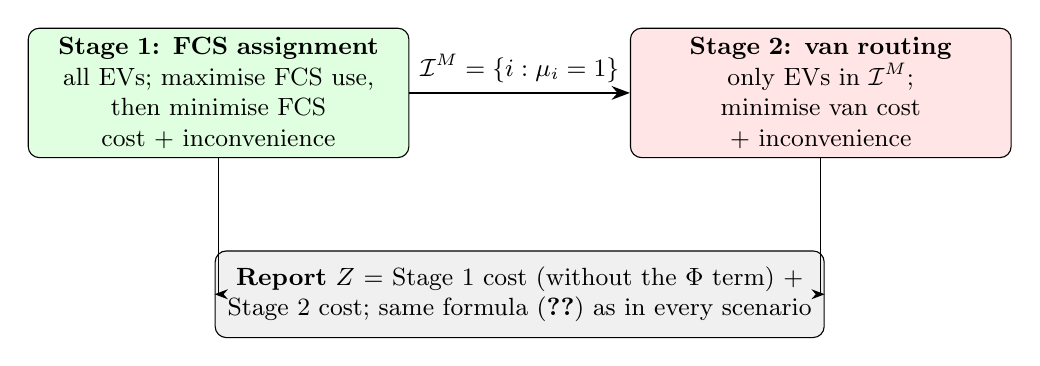
\begin{tikzpicture}[>=Stealth,box/.style={draw,rounded corners,align=center,minimum height=1.1cm,font=\small}]
  \node[box,fill=green!12,text width=4.6cm] (s1) {\textbf{Stage 1: FCS assignment}\\all EVs; maximise FCS use,\\then minimise FCS cost + inconvenience};
  \node[box,fill=red!10,text width=4.6cm,right=2.8cm of s1] (s2) {\textbf{Stage 2: van routing}\\only EVs in $\I^M$;\\minimise van cost + inconvenience};
  \draw[->,thick] (s1) -- node[above,font=\small]{$\I^M=\{i:\mu_i=1\}$} (s2);
  \node[box,fill=black!6,text width=7.5cm,below=2.0cm of $(s1)!0.5!(s2)$] (ev) {\textbf{Report} $Z=$ Stage~1 cost (without the $\Phi$ term) $+$ Stage~2 cost; same formula \eqref{eq:Z} as in every scenario};
  \draw[->] (s1) |- (ev); \draw[->] (s2) |- (ev);
\end{tikzpicture}
\end{center}

Stage~1 does not look at the vans, and Stage~2 cannot change what Stage~1 decided. That is the definition of ``FCS first, then MCS''.

%----------------------------------------------------------------
\subsection{Stage 1: assign EVs to fixed stations}

\textbf{Objective.}
\begin{equation}
\begin{split}
\min\ Z^{(1)}=\;&\underbrace{\Phi\sum_{i\in\I}\mu_i}_{\text{FCS first}}
+\underbrace{c^{EV}\sum_i\sum_{f\in\F_i}d_{if}Y_{if}}_{Z_1}
+\underbrace{Z^F_{\text{energy}}}_{\text{FCS part of }Z_4}\\
&+\underbrace{\sum_i\sum_{f\in\F_i}\rho^F_{if}Y_{if}+\alpha\sum_i w_i(C_i-r_i)+c^L\sum_i w_iL_i}_{\text{FCS customers' inconvenience}}
\end{split}
\label{eq:obj1}
\end{equation}
with $C_i=S_i+\tau^F_iY_i$ in this stage. $\Phi$ is a penalty for handing an EV to the vans. It is chosen larger than anything an extra FCS customer can add to the rest of \eqref{eq:obj1}, e.g.
\[
\Phi > \max_{i}\max_{f\in\F_i}\big(c^{EV}d_{if}+\pi^{\max}E_i+\rho^F_{if}\big)+n\,(\alpha+c^L)\,w_{\max}\,T,
\]
so Stage~1 first \textbf{maximises the number of EVs served at an FCS}, and only among those solutions minimises FCS cost and inconvenience. ($\pi^{\max}$ is the highest grid price.) A numerically safer equivalent is to solve twice: first $\max\sum_iY_i$, then fix that number and minimise the rest.
\ifTOU
Because $Z^F_{\text{energy}}$ uses the peak price, Stage~1 may \emph{start sessions later} to leave the peak, if the price saving beats the extra waiting cost (Section~\ref{sec:expect}).
\fi

\textbf{Constraints.}
\begin{align}
\sum_{g\in\G_i}y_{ig}+\mu_i &= 1 && \forall i\in\I \label{eq:s1assign}\\
S_i &\ge r_i+\sum_{f\in\F_i}t_{if}Y_{if} && \forall i\in\I \label{eq:fcsarr}\\
S_i &\le r_i+T\,(1-\mu_i) && \forall i\in\I \label{eq:s1park}\\
S_j &\ge S_i+\tau^F_i-(T+\tau^F_i)(3-y_{ig}-y_{jg}-o_{ij}) && \forall g,\ (i,j)\in\mathcal{P}_g \label{eq:disj1}\\
S_i &\ge S_j+\tau^F_j-(T+\tau^F_j)(2-y_{ig}-y_{jg}+o_{ij}) && \forall g,\ (i,j)\in\mathcal{P}_g \label{eq:disj2}\\
\sum_i y_{ig_1} &\ge \sum_i y_{ig_2} && \forall f,\ \G_f=\{g_1,g_2\} \label{eq:gunsym}\\
S_i+\tau^F_iY_i &\le T,\qquad L_i\ge S_i+\tau^F_iY_i-l_i && \forall i\in\I \label{eq:s1time}
\end{align}
\ifTOU plus the time-of-use split \eqref{eq:tou1}--\eqref{eq:tou5} of each FCS session (Section~\ref{sec:price}).\fi
\desc{\eqref{eq:s1assign}: every EV either gets one reachable gun or is handed to the vans. An EV that reaches no FCS ($\G_i=\emptyset$) is forced to $\mu_i=1$. \eqref{eq:fcsarr}: an FCS session cannot start before the EV has asked and driven to the station. \eqref{eq:s1park}: for an EV handed to the vans, $S_i$ is parked at $r_i$, so it adds no waiting in Stage~1 (its real start time is decided in Stage~2). \eqref{eq:disj1}--\eqref{eq:disj2}: two EVs on the same gun do not overlap; $o_{ij}$ picks who goes first. With two guns per station this means at most two EVs charge at a station at a time. \eqref{eq:gunsym}: symmetry breaking between the two identical guns (optional). \eqref{eq:s1time}: finished by $T$; lateness.}

\textbf{Optional acceptability rule.} An operator may refuse to send a driver to a station that is ``too inconvenient'', e.g.\ only allow gun $g$ of station $f$ for EV $i$ if $\hat\rho^F_{if}\le\bar\rho$. This only shrinks $\G_i$, so EVs whose stations are all too far go to the vans. Report results with and without it.

\textbf{Output:} $\I^M=\{i:\mu_i=1\}$, the EVs left for the vans; plus each FCS customer's gun and start time.

%----------------------------------------------------------------
\subsection{Stage 2: route the vans to the leftover EVs}

Stage~2 is a vehicle routing problem with time windows, on the EVs in $\I^M$ only. Here $C_i=S_i+\tau^M_i$.

\textbf{Objective.}
\begin{equation}
\begin{split}
\min\ Z^{(2)}=\;&\underbrace{c^M\sum_m\sum_{(i,j)\in\A^M}d_{ij}x_{ijm}}_{Z_2}+\underbrace{\sum_m c^D_mu_m}_{Z_3}+\underbrace{Z^M_{\text{energy}}}_{\text{van part of }Z_4}\\
&+\underbrace{\sum_{i\in\I^M}\sum_m\rho^M_{im}z_{im}+\alpha\sum_{i\in\I^M}w_i(C_i-r_i)+c^L\sum_{i\in\I^M}w_iL_i}_{\text{van customers' inconvenience}}
\end{split}
\label{eq:obj2}
\end{equation}
Since every EV in $\I^M$ must be served by some van, $Z^M_{\text{energy}}$ and the $\rho^M$ term are constants here. They are kept so that $Z^{(2)}$ is the true cost of Stage~2. Waiting and lateness make the vans visit urgent EVs early.

\textbf{Constraints.}
\begin{align}
\sum_{m\in\M}z_{im} &= 1 && \forall i\in\I^M \label{eq:s2assign}\\
\sum_{j:(0,j)\in\A^M}x_{0jm} = \sum_{i:(i,n+1)\in\A^M}x_{i,n+1,m} &= u_m && \forall m \label{eq:depot}\\
\sum_{i:(i,j)\in\A^M}x_{ijm} = \sum_{k:(j,k)\in\A^M}x_{jkm} &= z_{jm} && \forall j\in\I^M,\ m \label{eq:flow}\\
\sum_{i\in\I^M}z_{im} &\le Q_m\,u_m && \forall m \label{eq:cap}\\
\sum_{i\in\I^M}\frac{E_i}{\eta}z_{im}+\beta\sum_{(i,j)\in\A^M}d_{ij}x_{ijm} &\le B_m\,u_m && \forall m \label{eq:batt}
\end{align}
\begin{align}
S_j &\ge \max\{r_j,\ t_{0j}\,x_{0jm}\} && \forall j\in\I^M,\ m \label{eq:depart}\\
S_j &\ge S_i+\tau^M_i+t_{ij}-(T+\tau^M_i+t_{ij})(1-x_{ijm}) && \forall i\neq j,\ m \label{eq:seq}\\
S_i+\tau^M_i+t_{i,n+1} &\le T+(\tau^M_i+t_{i,n+1})(1-x_{i,n+1,m}) && \forall i,\ m \label{eq:return}\\
S_i+\tau^M_i \le T,\quad L_i &\ge S_i+\tau^M_i-l_i && \forall i\in\I^M \label{eq:s2time}\\
u_m &\ge u_{m+1} && m<|\M| \label{eq:vansym}
\end{align}
\desc{\eqref{eq:s2assign}: each leftover EV gets one van. \eqref{eq:depot}: a used van leaves and returns to the depot once. \eqref{eq:flow}: each EV on van $m$ is entered and left exactly once by that van. \eqref{eq:cap}: at most $Q_m$ EVs per van. \eqref{eq:batt}: delivered energy (with transfer losses) plus driving energy fits in the van battery. \eqref{eq:depart}: no start before the request, or before the van can drive there from the depot (written as two linear constraints). \eqref{eq:seq}: if the van goes $i\to j$, it finishes $i$ and drives to $j$ before starting $j$. This gives one EV at a time and removes subtours (MTZ-type). \eqref{eq:return}: back at the depot by $T$. \eqref{eq:s2time}: finished by $T$; lateness. \eqref{eq:vansym}: use identical vans in index order.}

\textbf{If Stage 2 is infeasible} (too many leftover EVs for the fleet by $T$), the sequential policy has \emph{failed} on that instance. For diagnosis, add $s_i\in\{0,1\}$ (``unserved''), replace \eqref{eq:s2assign} by $\sum_mz_{im}+s_i=1$ and add $\Phi^U\sum_is_i$ to \eqref{eq:obj2}. Then report the number of EVs that could not be served. This is a useful comparison with the integrated scenario, which may serve all of them.

%----------------------------------------------------------------
\subsection{Reported value}
\[
Z^{\text{S\scen}}=\big(Z^{(1)*}-\Phi\,|\I^M|\big)+Z^{(2)*},
\]
which is exactly \eqref{eq:Z} evaluated at the combined solution. The stage-1 solution plus the stage-2 solution is a feasible solution of the integrated model (S\ifTOU 4\else 3\fi), so
$Z^{\text{S\ifTOU 4\else 3\fi}}\le Z^{\text{S\scen}}$. The difference is the \emph{value of integration}.

\else
%---------------------------------------------------------------- INT
\subsection{Objective}
\begin{equation}
\min\ Z \quad\text{as in \eqref{eq:Z}, with }Z^F_{\text{energy}}=\ifTOU P^F\textstyle\sum_i\big[\pi^\off(\theta^1_i+\theta^3_i)+\pi^\pk\theta^2_i\big]\else\pi^F\textstyle\sum_iE_iY_i\fi,\quad C_i=S_i+\tau^F_iY_i+\tau^M_iZ_i. \label{eq:objint}
\end{equation}
Written out in full:
\begin{align*}
\min\ Z=\;& c^{EV}\sum_i\sum_{f\in\F_i}d_{if}Y_{if}+c^M\sum_m\sum_{(i,j)\in\A}d_{ij}x_{ijm}+\sum_mc^D_mu_m\\
&+\ifTOU P^F\sum_i\big[\pi^\off(\theta^1_i+\theta^3_i)+\pi^\pk\theta^2_i\big]\else\pi^F\sum_iE_iY_i\fi
+\pi^M\sum_i\sum_m\frac{E_i}{\eta}z_{im}\\
&+\sum_i\sum_{f\in\F_i}\rho^F_{if}Y_{if}+\sum_i\sum_m\rho^M_{im}z_{im}+\alpha\sum_iw_i(C_i-r_i)+c^L\sum_iw_iL_i .
\end{align*}
Every term is linear. One model weighs everything at once: an EV goes to a van exactly when the van's extra km, dispatch and energy cost are outweighed by the effort and waiting it saves the driver\ifTOU, or by the peak-price energy it avoids\fi.

\subsection{Constraints}

\textbf{Assignment.}
\begin{equation}
\sum_{g\in\G_i}y_{ig}+\sum_{m\in\M}z_{im}=1\qquad\forall i\in\I \label{eq:assign}
\end{equation}
\desc{Exactly one resource per EV: one reachable gun or one van. EVs that reach no FCS are forced onto a van.}

\textbf{Fixed stations.}
\begin{align}
S_i &\ge r_i+\sum_{f\in\F_i}t_{if}Y_{if} && \forall i \label{eq:fcsarr}\\
S_j &\ge S_i+\tau^F_i-(T+\tau^F_i)(3-y_{ig}-y_{jg}-o_{ij}) && \forall g,\ (i,j)\in\mathcal{P}_g \label{eq:disj1}\\
S_i &\ge S_j+\tau^F_j-(T+\tau^F_j)(2-y_{ig}-y_{jg}+o_{ij}) && \forall g,\ (i,j)\in\mathcal{P}_g \label{eq:disj2}\\
\sum_iy_{ig_1} &\ge \sum_iy_{ig_2} && \forall f,\ \G_f=\{g_1,g_2\} \label{eq:gunsym}
\end{align}
\desc{\eqref{eq:fcsarr}: an FCS session starts after the request and the drive to the station (for a van customer this is just $S_i\ge r_i$). \eqref{eq:disj1}--\eqref{eq:disj2}: EVs on the same gun do not overlap; $o_{ij}$ chooses the order. \eqref{eq:gunsym}: optional symmetry breaking.}

\textbf{Vans: routes, capacity, battery.}
\begin{align}
\sum_{j:(0,j)\in\A}x_{0jm}=\sum_{i:(i,n+1)\in\A}x_{i,n+1,m} &= u_m && \forall m \label{eq:depot}\\
\sum_{i:(i,j)\in\A}x_{ijm}=\sum_{k:(j,k)\in\A}x_{jkm} &= z_{jm} && \forall j\in\I,\ m \label{eq:flow}\\
\sum_iz_{im} &\le Q_mu_m && \forall m \label{eq:cap}\\
\sum_i\frac{E_i}{\eta}z_{im}+\beta\sum_{(i,j)\in\A}d_{ij}x_{ijm} &\le B_mu_m && \forall m \label{eq:batt}
\end{align}
\desc{\eqref{eq:depot}: a used van leaves and returns once. \eqref{eq:flow}: each EV on van $m$ is visited exactly once by it. \eqref{eq:cap}: at most $Q_m$ EVs. \eqref{eq:batt}: delivered energy (with losses) plus driving energy fits in the battery.}

\textbf{Vans: timing (one EV at a time, no subtours).}
\begin{align}
S_j &\ge t_{0j}\,x_{0jm} && \forall j\in\I,\ m \label{eq:depart}\\
S_j &\ge S_i+\tau^M_i+t_{ij}-(T+\tau^M_i+t_{ij})(1-x_{ijm}) && \forall i\neq j\in\I,\ m \label{eq:seq}\\
S_i+\tau^M_i+t_{i,n+1} &\le T+(\tau^M_i+t_{i,n+1})(1-x_{i,n+1,m}) && \forall i,\ m \label{eq:return}
\end{align}
\desc{\eqref{eq:depart}: the first stop cannot start before the van has driven there. \eqref{eq:seq}: $i\to j$ means finish $i$, drive, then start $j$; start times rise along a route, so no subtour can close. \eqref{eq:return}: back at the depot by $T$.}

\textbf{Horizon and lateness.}
\begin{equation}
C_i\le T,\qquad L_i\ge C_i-l_i\qquad\forall i\in\I \label{eq:time}
\end{equation}
\desc{Every EV is fully charged within the horizon; $L_i$ measures lateness.}

\ifTOU
\textbf{Time-of-use split.} Constraints \eqref{eq:tou1}--\eqref{eq:tou5} of Section~\ref{sec:price}.
\fi

\textbf{Symmetry and domains.}
\begin{equation}
u_m\ge u_{m+1};\qquad y,z,x,u,o\ifTOU,\kappa\fi\in\{0,1\};\qquad S_i,L_i\ifTOU,\theta^p_i\fi\ge0 \label{eq:dom}
\end{equation}
\fi

%=====================================================================
\section{Learning-to-optimise (RL) formulation}\label{sec:rl}

\textbf{Main rule:} the reward of each action is \emph{minus the increase in $Z$ that the action causes}. The rewards over an episode then add up to $-Z$ of the solution the policy builds. RL and MILP results are measured on the same yardstick \eqref{eq:Z}, and the MILP optimum is the benchmark for the RL gap.

\ifSEQ
%---------------------------------------------------------------- RL SEQ
The RL pipeline has the same two stages as the MILP.

\subsection{Stage 1 policy: FCS assignment}
\begin{itemize}[leftmargin=1.4em,itemsep=2pt]
  \item \textbf{Episode / epochs:} EVs are taken in order of request time $r_i$ (ties: higher $w_i$ first). One decision per EV.
  \item \textbf{State:} features of the current EV $k$ ($E_k,r_k,l_k,w_k,R_k$, location); for each gun $g$ the time $F_g$ it becomes free; summary features of the EVs still to come (count and positions near each station)\ifTOU; the current price and the time until $T_1$ and $T_2$\fi.
  \item \textbf{Action:} a gun $g\in\G_k$, or ``hand to vans''. \textbf{FCS-first mask:} ``hand to vans'' is allowed \emph{only} if no gun can finish EV $k$ by $T$ (or, with the optional rule, if all remaining guns have $\hat\rho^F_{kf}>\bar\rho$).
  \ifTOU\item \textbf{Optional timing action:} ``gun $g$, start after the peak'', i.e.\ $S_k=\max\{\text{earliest},T_2\}$, allowed only if the session still ends by $T$.\fi
  \item \textbf{Transition:} $S_k=\max\{r_k+t_{kf},F_g\}$ (or later, for the timing action); $F_g\leftarrow S_k+\tau^F_k$.
  \item \textbf{Reward:} $-\Big[c^{EV}d_{kf}+\text{energy}_k+\rho^F_{kf}+\alpha w_k(S_k+\tau^F_k-r_k)+c^Lw_k(S_k+\tau^F_k-l_k)^+\Big]$, where energy$_k$ = \ifTOU$P^F\big[\pi^\off\cdot(\text{off-peak hours of }[S_k,S_k+\tau^F_k])+\pi^\pk\cdot(\text{peak hours})\big]$, computed exactly in the simulator\else$\pi^FE_k$\fi. Handing an EV to the vans gives reward $0$ here; its cost is counted in Stage~2.
\end{itemize}
Note: a simple baseline for Stage~1 is the greedy rule ``gun with the largest one-step reward''. What RL can learn on top of this is, for example, to keep a nearby gun free for an urgent EV that arrives later.

\subsection{Stage 2 policy: van routing over $\I^M$}
\begin{itemize}[leftmargin=1.4em,itemsep=2pt]
  \item \textbf{Epochs:} whenever a van becomes free (the earliest-free van decides first).
  \item \textbf{State:} for each van: position, time free, remaining battery $b_m$, EVs served so far, dispatched or not; for each unserved EV in $\I^M$: location, $E_i,r_i,l_i,w_i$; current time.
  \item \textbf{Action:} the next EV $j$ for this van, or ``return to depot'' (ends the route). Mask: $j$ must be feasible: battery covers $E_j/\eta$ plus driving to $j$ and back to the depot, the count stays $\le Q_m$, and $j$ can be finished with the van back at the depot by $T$.
  \item \textbf{Transition:} $S_j=\max\{r_j,\ \text{time free}+t_{\text{pos},j}\}$; the van moves to $j$ and is free at $S_j+\tau^M_j$; $b_m$ falls by $E_j/\eta+\beta d_{\text{pos},j}$.
  \item \textbf{Reward:} serving $j$: $-\Big[c^Md_{\text{pos},j}+c^D_m[\text{first stop}]+\pi^M\frac{E_j}{\eta}+\rho^M_{jm}+\alpha w_j(S_j+\tau^M_j-r_j)+c^Lw_j(S_j+\tau^M_j-l_j)^+\Big]$; returning: $-c^Md_{\text{pos},0}$. EVs still unserved at the end: $-\Phi^U$ each.
  \item \textbf{Policy:} an attention-based routing policy (e.g.\ Kool et al., 2019, ``Attention, Learn to Solve Routing Problems!'') trained with REINFORCE or PPO. Baseline: nearest-feasible-EV heuristic.
\end{itemize}
Episode return of Stage~1 + Stage~2 $=-Z^{\text{S\scen}}$.

\else
%---------------------------------------------------------------- RL INT
One policy decides both who serves each EV and the van routes.
\begin{itemize}[leftmargin=1.4em,itemsep=2pt]
  \item \textbf{Episode / epochs:} EVs are taken in order of request time $r_i$ (ties: higher $w_i$ first). One decision per EV.
  \item \textbf{State:} (i) the current EV $k$: location, $E_k,r_k,l_k,w_k,R_k$, reachable stations; (ii) each gun $g$: time $F_g$ it becomes free; (iii) each van $m$: current end-of-route position, time free, remaining battery $b_m$, EVs served, dispatched or not; (iv) embeddings of the not-yet-assigned EVs (for look-ahead)\ifTOU; (v) current price, time until $T_1$ and $T_2$\fi.
  \item \textbf{Action:} $a\in\G_k\cup\M$: a gun, or a van (EV $k$ is appended to the end of that van's route). \textbf{Mask} infeasible actions: a gun that cannot finish $k$ by $T$; a van without enough battery for $E_k/\eta$ plus the drive to $k$ and back to the depot, with $Q_m$ reached, or unable to finish $k$ and return by $T$.
  \ifTOU\item \textbf{Optional timing action:} ``gun $g$, start after the peak'' ($S_k=\max\{\text{earliest},T_2\}$, if it still ends by $T$).\fi
  \item \textbf{Transition:} gun: $S_k=\max\{r_k+t_{kf},F_g\}$, $F_g\leftarrow S_k+\tau^F_k$. Van: $S_k=\max\{r_k,\ \text{free}_m+t_{\text{pos}_m,k}\}$, then the van moves to $k$, $\text{free}_m\leftarrow S_k+\tau^M_k$, $b_m\mathrel{-}=E_k/\eta+\beta d_{\text{pos}_m,k}$.
  \item \textbf{Reward} $=-\Delta Z$:
  \begin{align*}
  \text{gun } g\text{ at }f:&\quad -\Big[c^{EV}d_{kf}+\text{energy}^F_k+\rho^F_{kf}+\alpha w_k(C_k-r_k)+c^Lw_k(C_k-l_k)^+\Big]\\
  \text{van } m:&\quad -\Big[c^M\big(d_{\text{pos}_m,k}+d_{k,0}-d_{\text{pos}_m,0}\big)+c^D_m[\text{first use}]+\pi^M\tfrac{E_k}{\eta}\\
  &\qquad\quad+\rho^M_{km}+\alpha w_k(C_k-r_k)+c^Lw_k(C_k-l_k)^+\Big]
  \end{align*}
  The van distance term is the \emph{change} in route length when $k$ is inserted before the return to the depot, so the sum over the episode equals the total route length (the return legs telescope). energy$^F_k$ = \ifTOU$P^F\big[\pi^\off\cdot(\text{off-peak hours})+\pi^\pk\cdot(\text{peak hours of }[S_k,C_k])\big]$, computed exactly by the simulator; no linearisation is needed in RL\else$\pi^FE_k$\fi.
  \item \textbf{Dead end:} if every action is masked, EV $k$ is unserved: reward $-\Phi^U$, and the episode continues. Report the count.
  \item \textbf{Policy:} masked categorical policy over guns and vans, encoder with attention over EVs, guns and vans; trained with PPO. Natural baseline: greedy, i.e.\ choose the action with the largest one-step reward. That is the pairwise rule ``smallest $\hat\rho$ + cost'' from Section~\ref{sec:inc}.
\end{itemize}
Restriction to note: vans serve EVs in assignment order (append only). A variant that inserts $k$ at the cheapest position of a route is more flexible but has a larger action space.
\fi

\textbf{Reward scaling.} For stable training divide every reward by a constant, e.g.\ the greedy baseline's average $Z$ on the training instances. This does not change the optimal policy.

%=====================================================================
\section{What to expect and what to report}\label{sec:expect}

\ifnum\scen=1
\begin{itemize}[leftmargin=1.4em,itemsep=2pt]
  \item Vans serve only EVs that reach no station, or that the stations cannot finish by $T$. If stations have spare capacity, very few vans are dispatched.
  \item Inconvenience is high for EVs far from the nearest station (worked example: Rs\,682 at the FCS, against Rs\,458 if a van had been allowed).
  \item With too few vans Stage~2 becomes infeasible (unserved EVs), even when the integrated model S3 could serve everyone. Report the smallest $|\M|$ at which S1 is feasible and compare it with S3.
\end{itemize}
\fi
\ifnum\scen=2
\begin{itemize}[leftmargin=1.4em,itemsep=2pt]
  \item \textbf{When does Stage~1 delay a session to avoid the peak?} Moving one hour of charging out of the peak saves $(\pi^\pk-\pi^\off)P^F=3\times22=$ Rs\,66, but delays completion by up to an hour, which costs $\alpha w_i\ge$ Rs\,200. So with the default values Stage~1 almost never delays. It mostly pays the higher price, and S2 costs roughly S1 plus the peak surcharge. Sessions start later only if $\alpha$ is small (try $\lambda<0.33$ in the sensitivity analysis).
  \item The van assignment is the same as in S1 unless Stage~1's timing changes which EVs fit at the stations. Stage~1 cannot use vans to escape the peak price.
  \item Extra KPI: \textbf{grid energy drawn at FCS during the peak}, $P^F\sum_i\theta^2_i$ (kWh). Compare with S4.
\end{itemize}
\fi
\ifnum\scen=3
\begin{itemize}[leftmargin=1.4em,itemsep=2pt]
  \item Vans take EVs for which the saved inconvenience exceeds the extra van cost (worked example: van chosen, saving Rs\,224). Expect vans to serve EVs that are far from every station, have low range (high $w_i$), or have early deadlines, while EVs near a station still use it.
  \item \textbf{Value of integration under flat price:} $Z^{\text{S1}}-Z^{\text{S3}}\ge0$. Report it per component ($Z_1,\dots,Z_5$): typically operating cost rises a little and inconvenience falls a lot.
  \item Vary $|\M|$ (0, 1, 2, \dots): the first few vans lower $Z$ sharply, then the effect levels off. That curve shows the scenarios where mobile chargers help most.
\end{itemize}
\fi
\ifnum\scen=4
\begin{itemize}[leftmargin=1.4em,itemsep=2pt]
  \item During the peak a van kWh costs about the same as an FCS kWh (Rs\,10.0 each), so the vans' energy disadvantage disappears and vans also absorb \emph{peak-hour} demand that would otherwise be charged on the grid at peak price.
  \item Expect more van usage than in S3, concentrated on requests in $[T_1,T_2]$, and lower grid energy at the stations during the peak, $P^F\sum_i\theta^2_i$, than in S2.
  \item \textbf{Value of integration under peak pricing:} $Z^{\text{S2}}-Z^{\text{S4}}$. It should be larger than $Z^{\text{S1}}-Z^{\text{S3}}$, because integration now also allows price arbitrage.
  \item \textbf{Peak pricing with full flexibility:} $Z^{\text{S4}}-Z^{\text{S3}}$ should be smaller than $Z^{\text{S2}}-Z^{\text{S1}}$: vans cushion the price increase.
\end{itemize}
\fi

\textbf{Cross-scenario comparison table} (fill in from the four runs):
\begin{center}
\renewcommand{\arraystretch}{1.2}
\begin{tabular}{@{}lll@{}}
\toprule
\textbf{Comparison} & \textbf{Measures} & \textbf{Expected sign} \\
\midrule
S1 $-$ S3 & value of integration, flat price & $\ge0$ \\
S2 $-$ S4 & value of integration, peak price & $\ge0$, larger than S1 $-$ S3 \\
S2 $-$ S1 & cost of peak pricing, FCS-first operator & $>0$ \\
S4 $-$ S3 & cost of peak pricing, flexible operator & $>0$, smaller than S2 $-$ S1 \\
\bottomrule
\end{tabular}
\end{center}
Report for each: $Z$ and its components, number of vans used, EVs per resource, mean and maximum inconvenience per EV, total lateness, peak-hour grid energy, solve time, and (for RL) the gap to the MILP optimum.

%=====================================================================
\appendix
\section{Illustrative parameter values}\label{app:values}

These are starting values for experiments, not data. All are meant to be varied in the analysis. Values in Rs.

\begin{center}
\renewcommand{\arraystretch}{1.15}
\begin{tabular}{@{}llp{6.2cm}@{}}
\toprule
\textbf{Parameter} & \textbf{Value} & \textbf{Note} \\
\midrule
$T$, $[T_1,T_2]$ & 7 h, $[2,6]$ & 16:00--23:00, peak 18:00--22:00 \\
$P^F$, $P^M$ & 22 kW, 30 kW & \\
$v$, $\beta$, $\eta$ & 25 km/h, 0.25 kWh/km, 0.9 & \\
$B_m$, $Q_m$, $|\M|$ & 150 kWh, 6, 2--6 & \\
$c^{EV}$, $c^M$, $c^D_m$ & Rs\,4/km, Rs\,15/km, Rs\,1500 & van km includes driver time \\
$\pi^F$ (flat) & Rs\,8.7/kWh & equals the time-average of the ToU tariff over $[0,T]$ \\
$\pi^\off$, $\pi^\pk$ (ToU) & Rs\,7/kWh, Rs\,10/kWh & $(3\times7+4\times10)/7=8.7$ \\
$c^{bat}$ & Rs\,2/kWh & van battery wear \\
$\pi^M$ & Rs\,10.7 (flat) / Rs\,9.0 (ToU) & $=\pi^F+c^{bat}$ / $=\pi^\off+c^{bat}$ \\
$\alpha$, $\alpha^D$ & Rs\,200/h, Rs\,100/h & value of time; extra for attended time \\
$h^F$, $h^M$, $\varphi$ & Rs\,50, Rs\,10, Rs\,100 & trip hassle, hand-over, range stress \\
$c^L$ & Rs\,300/h & lateness \\
$w_i$ & $1+2(1-R_i/R_{\max})$, $R_i\sim U[3,40]$ km & priority from remaining range \\
\bottomrule
\end{tabular}
\end{center}

The flat price is set to the time-average of the peak tariff. The price \emph{level} is then the same in both pricing cases, and only the price \emph{shape} differs. Without this, part of S1 vs S2 would just reflect a different average price.

\end{document}
"
%    pdflatex -jobname=scenario4_peak_integrated   "\def\scen{4}% =====================================================================
%  One source, four PDFs.  Build with build.sh (or by hand):
%    pdflatex -jobname=scenario1_flat_sequential   "\def\scen{1}\input{scenario_master}"
%    pdflatex -jobname=scenario2_peak_sequential   "\def\scen{2}\input{scenario_master}"
%    pdflatex -jobname=scenario3_flat_integrated   "\def\scen{3}\input{scenario_master}"
%    pdflatex -jobname=scenario4_peak_integrated   "\def\scen{4}\input{scenario_master}"
%  (run each twice for cross-references)
% =====================================================================
\documentclass[11pt,a4paper]{article}
\usepackage[margin=2.2cm]{geometry}
\usepackage{amsmath,amssymb,amsfonts}
\usepackage{booktabs,array,tabularx}
\usepackage{enumitem}
\usepackage[table]{xcolor}
\usepackage{tikz}
\usetikzlibrary{arrows.meta,positioning,calc}
\usepackage[colorlinks=true,linkcolor=blue!50!black,urlcolor=blue!50!black]{hyperref}
\usepackage{titlesec}
\titleformat{\section}{\large\bfseries}{\thesection}{0.8em}{}
\titleformat{\subsection}{\normalsize\bfseries}{\thesubsection}{0.8em}{}
\setlength{\parindent}{0pt}
\setlength{\parskip}{5pt}

% ---------------- scenario switches ----------------
\ifdefined\scen\else\def\scen{1}\fi
\newif\ifTOU \TOUfalse   % true = time-of-use (peak) price
\newif\ifSEQ \SEQfalse   % true = FCS first, then MCS
\ifnum\scen=1 \SEQtrue \fi
\ifnum\scen=2 \TOUtrue \SEQtrue \fi
\ifnum\scen=4 \TOUtrue \fi

\newcommand{\pricename}{\ifTOU time-of-use price (dearer evening peak)\else single (flat) price all day\fi}
\newcommand{\structname}{\ifSEQ FCS first, then MCS (sequential)\else FCS and MCS together (integrated)\fi}

% ---------------- notation ----------------
\newcommand{\I}{\mathcal{I}}
\newcommand{\F}{\mathcal{F}}
\newcommand{\G}{\mathcal{G}}
\newcommand{\M}{\mathcal{M}}
\newcommand{\N}{\mathcal{N}}
\newcommand{\A}{\mathcal{A}}
\newcommand{\Rs}{\text{Rs}\,}
\newcommand{\pk}{\mathrm{pk}}
\newcommand{\off}{\mathrm{off}}
\newcommand{\desc}[1]{\par\vspace{-2pt}{\small\color{black!75}\textit{Meaning:} #1}\par\vspace{4pt}}
\newcommand{\cell}[2]{\ifnum\scen=#1\cellcolor{blue!18}\textbf{S#1 (this document)}\\\textbf{#2}\else S#1\\#2\fi}

\title{\textbf{EV Charging Network Optimisation}\\[4pt]
\large Scenario \scen: \pricename\ $+$ \structname\\[2pt]
\normalsize MILP and RL formulation}
\author{CP 320 OR for Mobility Management, course project}
\date{2 October 2026}

\begin{document}
\maketitle

%=====================================================================
\section{Where this scenario sits}

The project studies four scenarios: two ways of pricing grid electricity, times two ways of making the decisions.

\begin{center}
\renewcommand{\arraystretch}{1.5}
\begin{tabular}{>{\raggedright\arraybackslash}p{4.2cm}|>{\centering\arraybackslash}p{4.6cm}|>{\centering\arraybackslash}p{4.6cm}}
 & \textbf{Flat price all day} & \textbf{Time-of-use (peak) price} \\ \hline
\textbf{Sequential:} FCS first, leftover EVs to MCS &
\begin{tabular}[c]{@{}c@{}}\cell{1}{flat + sequential}\end{tabular} &
\begin{tabular}[c]{@{}c@{}}\cell{2}{peak + sequential}\end{tabular} \\ \hline
\textbf{Integrated:} FCS and MCS decided together &
\begin{tabular}[c]{@{}c@{}}\cell{3}{flat + integrated}\end{tabular} &
\begin{tabular}[c]{@{}c@{}}\cell{4}{peak + integrated}\end{tabular} \\
\end{tabular}
\end{center}

\textbf{The four scenarios do not have four different objectives.} They share \emph{one} cost yardstick $Z$ (Section~\ref{sec:obj}): the same cost terms and the same customer inconvenience (Section~\ref{sec:inc}). Only two things change:
\begin{itemize}[leftmargin=1.4em,itemsep=1pt]
  \item \textbf{Pricing} changes the formula for one term, the FCS energy cost (Section~\ref{sec:price}).
  \item \textbf{Decision structure} changes \emph{how} $Z$ is minimised: in one model (integrated), or in two stages (sequential), where each stage minimises its own part of $Z$.
\end{itemize}
Because the yardstick is the same, the four optimal values can be compared directly. The differences measure the \emph{value of integration} (S1$\to$S3, S2$\to$S4) and the \emph{effect of peak pricing} (S1$\to$S2, S3$\to$S4).

\ifnum\scen=1
\textbf{This scenario (S1)} is the baseline, the ``status quo''. Electricity costs the same at every hour, every EV that can be charged at a fixed station is sent there, and vans only take what is left over.
\fi
\ifnum\scen=2
\textbf{This scenario (S2)} keeps the FCS-first rule of S1, but grid electricity is dearer during the evening peak. Stage~1 can react to the price only by \emph{rescheduling} FCS sessions. It cannot hand a peak-hour EV to a van.
\fi
\ifnum\scen=3
\textbf{This scenario (S3)} keeps the flat price of S1, but the operator decides FCS and MCS service \emph{together}. An EV can be sent to a van even when a fixed station could take it, whenever that lowers total cost plus inconvenience.
\fi
\ifnum\scen=4
\textbf{This scenario (S4)} is the most flexible one: peak pricing at fixed stations, and FCS and MCS decided together. Van energy was bought off-peak, so vans can also be used to keep charging \emph{out of the expensive peak}.
\fi

%=====================================================================
\section{Setting and assumptions}\label{sec:setting}

\textbf{Time.} The planning horizon is $[0,T]$ with $T=7$\,h (16:00--23:00). It contains the evening peak window $[T_1,T_2]=[2,6]$ (18:00--22:00). The horizon is the same in all four scenarios. It is wider than the peak itself so that, under peak pricing, there is cheaper time on both sides of the peak.\ifTOU\else\ In this scenario the price is flat, so the window plays no role in the model.\fi

\textbf{Assumptions} (the same as MILP v3, plus two about energy):
\begin{enumerate}[leftmargin=1.6em,itemsep=1pt]
  \item Static, continuous time. All requests in the horizon are known at time $0$, and request $i$ becomes active at $r_i$.
  \item An EV served by an FCS drives there itself on its own battery (only to stations within its range $R_i$). The driver stays with the car while it waits for a free gun and while it charges.
  \item An EV served by an MCS stays parked where it is, and the driver is free in the meantime.
  \item Each FCS gun and each van charges one EV at a time, without interruption, at constant power.
  \item A van's battery covers both its driving and the energy it delivers. \textbf{The van battery is charged at the depot before the horizon starts}\ifTOU, i.e.\ at the off-peak price\fi, and is not recharged during the horizon.
  \item Every EV must be fully charged by $T$ (hard). Finishing after the driver's desired time $l_i$ is allowed but penalised.
\end{enumerate}

%=====================================================================
\section{Notation}\label{sec:notation}

\subsection*{Sets}
\begin{tabularx}{\textwidth}{@{}lX@{}}
\toprule
$\I=\{1,\dots,n\}$ & EV charging requests \\
$\F$; $\G_f$ ($|\G_f|=2$); $\G=\bigcup_f\G_f$ & fixed charging stations; guns of FCS $f$; all guns ($f(g)$ = station of gun $g$) \\
$\F_i=\{f: d_{if}\le R_i\}$, $\G_i=\bigcup_{f\in\F_i}\G_f$ & stations / guns EV $i$ can reach on its remaining range \\
$\M$ & mobile charging vans (MCS) \\
$0,\ n+1$ & depot as start node / end node (same place) \\
$\N=\{0\}\cup\I\cup\{n+1\}$, $\A$ & routing nodes; allowed van arcs $(i,j)$, $i\in\{0\}\cup\I$, $j\in\I\cup\{n+1\}$, $i\neq j$ \\
$\mathcal{P}_g=\{(i,j): i<j,\ g\in\G_i\cap\G_j\}$ & pairs of EVs that could share gun $g$ \\
\ifSEQ
$\I^M\subseteq\I$ & EVs handed to the vans by Stage~1 (an \emph{output} of Stage~1, a fixed input to Stage~2) \\
$\N^M$, $\A^M$ & routing nodes / arcs restricted to $\I^M$ \\
\fi
\bottomrule
\end{tabularx}

\subsection*{Parameters}
\begin{tabularx}{\textwidth}{@{}lX@{}}
\toprule
$E_i,\ r_i,\ l_i,\ R_i$ & energy demand (kWh), request time, desired completion time (h), remaining range (km) \\
$w_i\ge1$ & priority of EV $i$; $w_i=1+\kappa(1-R_i/R_{\max})$, so low-range EVs weigh more \\
$P^F,\ P^M$ & charging power of an FCS gun (22\,kW) / of a van (e.g.\ 30\,kW) \\
$\tau^F_i=E_i/P^F,\ \tau^M_i=E_i/P^M$ & charging time of EV $i$ at an FCS / by a van (h) \\
$d_{if},t_{if}$;\ $d_{ij},t_{ij}$ & distance (km) and time (h): EV$\to$FCS; between routing nodes ($t=d/v$) \\
$B_m,\ Q_m,\ \beta,\ \eta$ & van battery (kWh), max EVs per van, van consumption (kWh/km), transfer efficiency \\
$c^{EV},\ c^M,\ c^D_m$ & cost per km of EV driving, per km of van driving; fixed dispatch cost of van $m$ \\
\ifTOU
$\pi^\off,\ \pi^\pk$ & grid price (Rs/kWh) off-peak / in $[T_1,T_2]$, with $\pi^\pk\ge\pi^\off$ \\
\else
$\pi^F$ & grid price (Rs/kWh), the same at every hour \\
\fi
$c^{bat}$ & van battery wear per kWh cycled \\
$\pi^M$ & cost of 1 kWh taken from a van battery: $\pi^M=\ifTOU\pi^\off\else\pi^F\fi+c^{bat}$ (Section~\ref{sec:price}) \\
$\alpha,\ \alpha^D,\ h^F,\ h^M,\ \varphi,\ c^L$ & inconvenience coefficients (Section~\ref{sec:inc}) \\
\bottomrule
\end{tabularx}

\subsection*{Decision variables}
\begin{tabularx}{\textwidth}{@{}llX@{}}
\toprule
$y_{ig}$ & $\{0,1\}$ & EV $i$ charged at gun $g\in\G_i$ \\
$z_{im}$ & $\{0,1\}$ & EV $i$ served by van $m$ \\
$x_{ijm}$ & $\{0,1\}$ & van $m$ drives arc $(i,j)$ \\
$u_m$ & $\{0,1\}$ & van $m$ is dispatched \\
$o_{ij}$ & $\{0,1\}$ & for EVs $i<j$ that could share a gun: 1 if $i$ is charged before $j$ \\
\ifSEQ
$\mu_i$ & $\{0,1\}$ & Stage~1 only: EV $i$ is handed to the van fleet \\
\fi
\ifTOU
$\theta^1_i,\theta^2_i,\theta^3_i$ & $\ge0$ & hours of EV $i$'s FCS session before / inside / after the peak \\
$\kappa^1_i,\kappa^3_i$ & $\{0,1\}$ & EV $i$'s FCS session starts before $T_1$ / ends after $T_2$ \\
\fi
$S_i$ & $\ge0$ & time charging of EV $i$ starts (h), on whichever resource \\
$L_i$ & $\ge0$ & lateness of EV $i$ beyond $l_i$ (h) \\
\bottomrule
\end{tabularx}

\textbf{Short-hands} (linear expressions, not new variables):
\[
Y_{if}=\sum_{g\in\G_f}y_{ig},\qquad Y_i=\sum_{g\in\G_i}y_{ig}\ (\text{EV $i$ uses an FCS}),\qquad Z_i=\sum_{m\in\M}z_{im}\ (\text{EV $i$ uses a van}),
\]
\[
C_i=S_i+\tau^F_i\,Y_i+\tau^M_i\,Z_i \quad\text{(time EV $i$ is fully charged).}
\]

%=====================================================================
\section{Customer inconvenience}\label{sec:inc}

This section is \textbf{identical in all four scenario documents}. Inconvenience is a property of the customer, not of the price or of the planning method.

\subsection{What we mean by inconvenience}

Inconvenience is \emph{what the driver loses} from the moment they ask for a charge ($r_i$) until the car is fully charged ($C_i$), \emph{converted into rupees} so it can be added to the operator's costs. A driver loses three different things:

\begin{enumerate}[leftmargin=1.6em,itemsep=2pt]
  \item \textbf{Waiting:} the car is not ready. This lasts $C_i-r_i$ hours and affects \emph{every} driver, FCS or MCS.
  \item \textbf{Effort:} only an FCS customer has to drive to the station and sit there while the car charges. An MCS customer stays at home or at work and does something else. Driving to a far station also uses scarce battery range, which causes stress (``range anxiety'').
  \item \textbf{A missed deadline:} the car is still not ready at the time $l_i$ the driver needs it.
\end{enumerate}

Each loss gets a price in Rs per hour (or per event). All of them are multiplied by the priority $w_i$: an hour of delay for an EV with 5\,km of range left counts more than for one with 40\,km.

\subsection{The three components}

\begin{center}
\renewcommand{\arraystretch}{1.3}
\begin{tabularx}{\textwidth}{@{}>{\raggedright\arraybackslash}p{2.6cm}>{\raggedright\arraybackslash}X>{\raggedright\arraybackslash}X>{\raggedright\arraybackslash}p{3.0cm}@{}}
\toprule
\textbf{Component} & \textbf{EV $i$ at FCS $f$} & \textbf{EV $i$ by a van} & \textbf{Known when?} \\
\midrule
Effort & $w_i\big[\alpha^D(t_{if}+\tau^F_i)+h^F+\varphi\,d_{if}/R_i\big]$: driving and sitting at the station, a fixed trip hassle, range stress & $w_i\,h^M$: being reachable and handing over the car & \textbf{Static:} known as soon as the resource is chosen \\
Waiting & $w_i\,\alpha\,(C_i-r_i)$ = drive + \emph{queue at the gun} + charge & $w_i\,\alpha\,(C_i-r_i)$ = \emph{wait for the van} + charge & \textbf{Dynamic:} depends on the queue / van route \\
Missed deadline & $w_i\,c^L\,L_i$, $L_i=\max\{0,C_i-l_i\}$ & same & Dynamic \\
\bottomrule
\end{tabularx}
\end{center}

\textbf{Coefficients.}
$\alpha$ (Rs/h) is the value of an hour the car is not ready.
$\alpha^D$ (Rs/h) is the \emph{extra} value of an hour the driver must personally spend driving or sitting at the station: an hour at the station costs $\alpha+\alpha^D$, an hour waiting at home for a van costs only $\alpha$.
$h^F,h^M$ (Rs) are fixed hassle costs of one trip to a station / one van hand-over.
$\varphi$ (Rs) is the range-stress cost of a trip that uses the \emph{whole} remaining range ($d_{if}/R_i\le1$ is the fraction used).
$c^L$ (Rs/h) is the cost per hour late.

\subsection{Pairwise form: inconvenience of a (customer, resource) pair}

The natural first idea is: \emph{for every pair (EV $i$, FCS $f$) and every pair (EV $i$, van $m$) there is an inconvenience number, and the operator picks the pair with the lowest cost plus inconvenience.} The static part fits this idea exactly:
\[
\boxed{\;\rho^F_{if}=w_i\Big[\alpha^D\,(t_{if}+\tau^F_i)+h^F+\varphi\,\frac{d_{if}}{R_i}\Big]\qquad
\rho^M_{im}=w_i\,h^M\;}
\]
These are \textbf{parameters}, computed before solving, one number per (EV, FCS) pair and per (EV, van) pair. In the objective they appear linearly: $\sum_i\sum_f\rho^F_{if}Y_{if}+\sum_i\sum_m\rho^M_{im}z_{im}$.

Note that $\rho^M_{im}$ does not depend on $m$. Vans are identical and all start at the same depot, so the driver does not care \emph{which} van comes, only \emph{when} it comes. That ``when'' is the waiting part.

\subsection{Why waiting cannot be a fixed pairwise number}

It is tempting to also write the waiting as a pairwise number, e.g.\ ``the van needs 5 minutes to reach EV $i$''. But that depends on \emph{where the van is coming from}, which depends on the route the model is still choosing: if EV $i$ is the 4th stop of a van, the wait is the time for three charging sessions plus four drives. Likewise, waiting at an FCS depends on how many EVs are queued at that gun. So waiting is not known before solving. It is a function of decision variables:
\[
\text{waiting cost of EV } i \;=\; w_i\,\alpha\,(C_i-r_i),\qquad C_i=S_i+\tau^F_iY_i+\tau^M_iZ_i .
\]
This is \textbf{linear} in the variables ($S_i$, $y$, $z$), so it fits in a MILP directly. The constraints of Section~\ref{sec:milp} make $S_i$ equal to the true start time, including driving, queueing at the gun and the van's route. The term $\sum_i w_i\alpha r_i$ is a constant and may be dropped when solving.

\textbf{Pairwise \emph{estimate}} (used for intuition, by the RL policy and in heuristics): if there is no queue and the van comes straight to $i$,
\[
\hat\rho^{F}_{if}=\rho^F_{if}+w_i\alpha\,(t_{if}+\tau^F_i),\qquad
\hat\rho^{M}_{im}=\rho^M_{im}+w_i\alpha\,(t^{\text{van}}_{m\to i}+\tau^M_i),
\]
where $t^{\text{van}}_{m\to i}$ is the time until van $m$ can reach $i$ from where it currently is. In the RL formulation (Section~\ref{sec:rl}) the van's position \emph{is} known at each decision, so there this estimate becomes exact.

\subsection{Total inconvenience and how it enters the objective}

\begin{equation}
\boxed{\;
Z_{\text{inc}}=\underbrace{\sum_{i\in\I}\sum_{f\in\F_i}\rho^F_{if}Y_{if}+\sum_{i\in\I}\sum_{m\in\M}\rho^M_{im}z_{im}}_{\text{effort (static, pairwise)}}
+\underbrace{\alpha\sum_{i\in\I}w_i\,(C_i-r_i)}_{\text{waiting (dynamic)}}
+\underbrace{c^L\sum_{i\in\I}w_i\,L_i}_{\text{missed deadline}}
\;}\label{eq:inc}
\end{equation}
All three parts are in rupees, so $Z_{\text{inc}}$ is simply added to the operating costs. Nothing has to be normalised.

\subsection{Worked example: your ``10 km to the FCS vs.\ van in 5 minutes'' case}

EV $i$: $E_i=20$\,kWh, $R_i=40$\,km (so $w_i=1$); nearest free FCS $d_{if}=10$\,km away, $t_{if}=0.4$\,h at 25\,km/h; a van finishing next door can reach it in 5\,min ($0.083$\,h), adding about 4\,km to its route. $\tau^F_i=20/22=0.909$\,h, $\tau^M_i=20/30=0.667$\,h. Coefficients from Appendix~\ref{app:values}, flat price.

\begin{center}
\renewcommand{\arraystretch}{1.25}
\begin{tabular}{@{}lrr@{}}
\toprule
 & \textbf{FCS} & \textbf{Van} \\
\midrule
Driving (EV / extra van km) & $4\times10=40.0$ & $15\times4=60.0$ \\
Energy & $8.7\times20=174.0$ & $10.7\times20/0.9=237.8$ \\
\textbf{Operating cost only} & \textbf{214.0} & \textbf{297.8} \\
\midrule
Effort $\rho$ & $100(0.4+0.909)+50+100\cdot\tfrac{10}{40}=205.9$ & $10.0$ \\
Waiting $\alpha(C_i-r_i)$ & $200\times1.309=261.8$ & $200\times0.75=150.0$ \\
\textbf{Cost + inconvenience} & \textbf{681.7} & \textbf{457.8} \\
\bottomrule
\end{tabular}
\end{center}

On operating cost alone the FCS is cheaper, so a cost-only model would \emph{always} send this driver 10\,km away. With inconvenience included the van is better by about Rs\,224, and the integrated model chooses $z_{im}=1$, as you expected. If the FCS were only 1\,km away, the FCS would win both comparisons. The inconvenience term is what makes the model choose between ``cheap for the operator'' and ``convenient for the driver'', rather than following a fixed rule.

\subsection{Relation to a single penalty $\rho_i$ per EV}

The first draft used a penalty $\rho_i$ that is charged whenever EV $i$ goes to \emph{any} FCS: $\sum_i\sum_f\rho_iy_{if}$. Because $\sum_f y_{if}=1-\sum_m z_{im}$, this only says ``a van is worth $\rho_i$ more to EV $i$'', and that holds whether the station is 1\,km or 15\,km away, and whether the van arrives in 5 minutes or in 3 hours. The form above fixes both problems: $\rho^F_{if}$ grows with the distance to \emph{that} station, and the waiting term grows with how late the van or the free gun actually is. The old model is the special case $\alpha=\alpha^D=\varphi=c^L=0$, $h^F=\rho_i$.

\subsection{Choosing the coefficients}
\begin{itemize}[leftmargin=1.4em,itemsep=2pt]
  \item Use a value of time for $\alpha$ (e.g.\ Rs\,150--300/h for urban car users), and set $\alpha^D\approx0.5\alpha$: sitting at a station is worse than waiting at home.
  \item Keep $c^L>\alpha$, so missing the deadline is worse than ordinary waiting.
  \item \textbf{Sensitivity analysis:} multiply all inconvenience coefficients by a factor $\lambda\in\{0,0.25,0.5,1,2,4\}$ and plot operating cost against total inconvenience. $\lambda=0$ is the pure cost-minimising operator, and large $\lambda$ is a customer-first operator. This trade-off curve is a strong result for the ``Analysis'' part of the project.
\end{itemize}

\subsection{What inconvenience does in \emph{this} scenario}
\ifSEQ
In a sequential scenario inconvenience \textbf{cannot move an EV from an FCS to a van}: Stage~1 sends every EV that \emph{can} use an FCS to one. It still matters inside each stage. In Stage~1 it decides \emph{which} station and \emph{when} (urgent EVs get the near station and the first free gun). In Stage~2 it decides the \emph{order} in which vans visit EVs (urgent EVs first). In the worked example, this scenario sends the driver 10\,km to the FCS. That is the weakness the integrated scenarios remove.
\else
In an integrated scenario inconvenience is weighed directly against operating cost when choosing the resource. That is how the worked example ends up with a van. It also decides which station and which gun order, and the order of each van route.
\fi

%=====================================================================
\section{Electricity price in this scenario}\label{sec:price}

\textbf{Van energy (same in all scenarios).} A van's battery is charged at the depot \emph{before} the horizon, so its energy was bought at the
\ifTOU off-peak \fi
price, whatever time the van later delivers it. Each kWh taken from the van also wears the battery ($c^{bat}$), and a fraction $1-\eta$ is lost in transfer:
\[
Z^M_{\text{energy}}=\pi^M\sum_{i\in\I}\sum_{m\in\M}\frac{E_i}{\eta}\,z_{im},\qquad \pi^M=\ifTOU\pi^\off\else\pi^F\fi+c^{bat}.
\]

\ifTOU
\textbf{FCS energy (time-of-use).} An FCS draws from the grid while it charges. Energy delivered inside $[T_1,T_2]$ costs $\pi^\pk$, and energy outside it costs $\pi^\off$. A session $[S_i,S_i+\tau^F_i]$ may overlap the peak partly. Split its duration into the hours before, inside and after the peak, $\theta^1_i+\theta^2_i+\theta^3_i$:
\[
Z^F_{\text{energy}}=P^F\sum_{i\in\I}\Big[\pi^\off(\theta^1_i+\theta^3_i)+\pi^\pk\,\theta^2_i\Big].
\]
Constraints \eqref{eq:tou1}--\eqref{eq:tou5} below make the $\theta$'s equal to the true overlaps. Peak hours are dearer, so the solver wants $\theta^1_i,\theta^3_i$ as large as possible. It is enough to bound them from above by the true off-peak overlap, and the constraints need one binary per side:
\begin{align}
\theta^1_i+\theta^2_i+\theta^3_i &= \tau^F_i\,Y_i && \forall i\in\I \label{eq:tou1}\\
\theta^1_i &\le \tau^F_i\,\kappa^1_i && \forall i\in\I \label{eq:tou2}\\
\theta^1_i &\le T_1-S_i+T\,(1-\kappa^1_i) && \forall i\in\I \label{eq:tou3}\\
\theta^3_i &\le \tau^F_i\,\kappa^3_i && \forall i\in\I \label{eq:tou4}\\
\theta^3_i &\le S_i+\tau^F_i-T_2+T\,(1-\kappa^3_i) && \forall i\in\I \label{eq:tou5}
\end{align}
\desc{\eqref{eq:tou1}: the FCS session's hours are split into three parts; for a van customer ($Y_i=0$) all three are zero. \eqref{eq:tou2}--\eqref{eq:tou3}: off-peak time before the peak is only possible if the session starts before $T_1$ ($\kappa^1_i=1$), and is at most $T_1-S_i$. \eqref{eq:tou4}--\eqref{eq:tou5}: the same for time after $T_2$. $\theta^2_i\ge0$ prevents counting more off-peak hours than exist. Checking the cases (entirely before / inside / after the peak, straddling one edge, covering the whole peak) shows that at the optimum the $\theta$'s equal the exact overlaps. This needs $\pi^\pk\ge\pi^\off$, which is true for a peak tariff.}

\textbf{Why vans become more attractive.} Compare the cost of 1\,kWh delivered to an EV during the peak (values from Appendix~\ref{app:values}):
FCS $=\pi^\pk=$ Rs\,10.0, van $=(\pi^\off+c^{bat})/\eta=9/0.9=$ Rs\,10.0. They are at parity. Under the flat price the van is about Rs\,3.2/kWh dearer (FCS Rs\,8.7, van $10.7/0.9=$ Rs\,11.9). Peak pricing therefore removes the vans' main cost disadvantage, but only for EVs whose FCS session would fall in the peak.
\ifSEQ\ In this sequential scenario Stage~1 cannot use that, because it does not consider vans. It can only shift FCS sessions in time.\fi
\else
\textbf{FCS energy (flat).} Every kWh delivered at a fixed station costs $\pi^F$, whenever it is delivered:
\[
Z^F_{\text{energy}}=\pi^F\sum_{i\in\I}E_i\,Y_i .
\]
The start time therefore does not affect the energy cost. Under the flat price a van kWh costs $(\pi^F+c^{bat})/\eta\approx$ Rs\,11.9 against Rs\,8.7 at an FCS (Appendix~\ref{app:values}), so on energy alone the FCS always wins.
\fi

%=====================================================================
\section{MILP formulation}\label{sec:milp}

\subsection{The common cost yardstick $Z$}\label{sec:obj}

For any complete solution (every EV assigned, every route and start time known), the system cost is
\begin{equation}
\boxed{\;
Z=\underbrace{c^{EV}\sum_{i}\sum_{f\in\F_i}d_{if}Y_{if}}_{Z_1:\ \text{EV driving}}
+\underbrace{c^M\sum_{m}\sum_{(i,j)\in\A}d_{ij}x_{ijm}}_{Z_2:\ \text{van driving}}
+\underbrace{\sum_m c^D_m u_m}_{Z_3:\ \text{dispatch}}
+\underbrace{Z^F_{\text{energy}}+Z^M_{\text{energy}}}_{Z_4:\ \text{energy}}
+\underbrace{Z_{\text{inc}}}_{Z_5:\ \text{inconv.\ \eqref{eq:inc}}}
\;}\label{eq:Z}
\end{equation}
$Z_4$ is defined in Section~\ref{sec:price}. $Z_1$--$Z_4$ are the operator's costs listed in the brief (EV travel, MCS travel, MCS operating cost) plus energy. $Z_5$ is the customer inconvenience penalty. \textbf{The same formula is used to report results in all four scenarios.}

\ifSEQ
%---------------------------------------------------------------- SEQ
\subsection{Structure: two stages}

\begin{center}
\begin{tikzpicture}[>=Stealth,box/.style={draw,rounded corners,align=center,minimum height=1.1cm,font=\small}]
  \node[box,fill=green!12,text width=4.6cm] (s1) {\textbf{Stage 1: FCS assignment}\\all EVs; maximise FCS use,\\then minimise FCS cost + inconvenience};
  \node[box,fill=red!10,text width=4.6cm,right=2.8cm of s1] (s2) {\textbf{Stage 2: van routing}\\only EVs in $\I^M$;\\minimise van cost + inconvenience};
  \draw[->,thick] (s1) -- node[above,font=\small]{$\I^M=\{i:\mu_i=1\}$} (s2);
  \node[box,fill=black!6,text width=7.5cm,below=2.0cm of $(s1)!0.5!(s2)$] (ev) {\textbf{Report} $Z=$ Stage~1 cost (without the $\Phi$ term) $+$ Stage~2 cost; same formula \eqref{eq:Z} as in every scenario};
  \draw[->] (s1) |- (ev); \draw[->] (s2) |- (ev);
\end{tikzpicture}
\end{center}

Stage~1 does not look at the vans, and Stage~2 cannot change what Stage~1 decided. That is the definition of ``FCS first, then MCS''.

%----------------------------------------------------------------
\subsection{Stage 1: assign EVs to fixed stations}

\textbf{Objective.}
\begin{equation}
\begin{split}
\min\ Z^{(1)}=\;&\underbrace{\Phi\sum_{i\in\I}\mu_i}_{\text{FCS first}}
+\underbrace{c^{EV}\sum_i\sum_{f\in\F_i}d_{if}Y_{if}}_{Z_1}
+\underbrace{Z^F_{\text{energy}}}_{\text{FCS part of }Z_4}\\
&+\underbrace{\sum_i\sum_{f\in\F_i}\rho^F_{if}Y_{if}+\alpha\sum_i w_i(C_i-r_i)+c^L\sum_i w_iL_i}_{\text{FCS customers' inconvenience}}
\end{split}
\label{eq:obj1}
\end{equation}
with $C_i=S_i+\tau^F_iY_i$ in this stage. $\Phi$ is a penalty for handing an EV to the vans. It is chosen larger than anything an extra FCS customer can add to the rest of \eqref{eq:obj1}, e.g.
\[
\Phi > \max_{i}\max_{f\in\F_i}\big(c^{EV}d_{if}+\pi^{\max}E_i+\rho^F_{if}\big)+n\,(\alpha+c^L)\,w_{\max}\,T,
\]
so Stage~1 first \textbf{maximises the number of EVs served at an FCS}, and only among those solutions minimises FCS cost and inconvenience. ($\pi^{\max}$ is the highest grid price.) A numerically safer equivalent is to solve twice: first $\max\sum_iY_i$, then fix that number and minimise the rest.
\ifTOU
Because $Z^F_{\text{energy}}$ uses the peak price, Stage~1 may \emph{start sessions later} to leave the peak, if the price saving beats the extra waiting cost (Section~\ref{sec:expect}).
\fi

\textbf{Constraints.}
\begin{align}
\sum_{g\in\G_i}y_{ig}+\mu_i &= 1 && \forall i\in\I \label{eq:s1assign}\\
S_i &\ge r_i+\sum_{f\in\F_i}t_{if}Y_{if} && \forall i\in\I \label{eq:fcsarr}\\
S_i &\le r_i+T\,(1-\mu_i) && \forall i\in\I \label{eq:s1park}\\
S_j &\ge S_i+\tau^F_i-(T+\tau^F_i)(3-y_{ig}-y_{jg}-o_{ij}) && \forall g,\ (i,j)\in\mathcal{P}_g \label{eq:disj1}\\
S_i &\ge S_j+\tau^F_j-(T+\tau^F_j)(2-y_{ig}-y_{jg}+o_{ij}) && \forall g,\ (i,j)\in\mathcal{P}_g \label{eq:disj2}\\
\sum_i y_{ig_1} &\ge \sum_i y_{ig_2} && \forall f,\ \G_f=\{g_1,g_2\} \label{eq:gunsym}\\
S_i+\tau^F_iY_i &\le T,\qquad L_i\ge S_i+\tau^F_iY_i-l_i && \forall i\in\I \label{eq:s1time}
\end{align}
\ifTOU plus the time-of-use split \eqref{eq:tou1}--\eqref{eq:tou5} of each FCS session (Section~\ref{sec:price}).\fi
\desc{\eqref{eq:s1assign}: every EV either gets one reachable gun or is handed to the vans. An EV that reaches no FCS ($\G_i=\emptyset$) is forced to $\mu_i=1$. \eqref{eq:fcsarr}: an FCS session cannot start before the EV has asked and driven to the station. \eqref{eq:s1park}: for an EV handed to the vans, $S_i$ is parked at $r_i$, so it adds no waiting in Stage~1 (its real start time is decided in Stage~2). \eqref{eq:disj1}--\eqref{eq:disj2}: two EVs on the same gun do not overlap; $o_{ij}$ picks who goes first. With two guns per station this means at most two EVs charge at a station at a time. \eqref{eq:gunsym}: symmetry breaking between the two identical guns (optional). \eqref{eq:s1time}: finished by $T$; lateness.}

\textbf{Optional acceptability rule.} An operator may refuse to send a driver to a station that is ``too inconvenient'', e.g.\ only allow gun $g$ of station $f$ for EV $i$ if $\hat\rho^F_{if}\le\bar\rho$. This only shrinks $\G_i$, so EVs whose stations are all too far go to the vans. Report results with and without it.

\textbf{Output:} $\I^M=\{i:\mu_i=1\}$, the EVs left for the vans; plus each FCS customer's gun and start time.

%----------------------------------------------------------------
\subsection{Stage 2: route the vans to the leftover EVs}

Stage~2 is a vehicle routing problem with time windows, on the EVs in $\I^M$ only. Here $C_i=S_i+\tau^M_i$.

\textbf{Objective.}
\begin{equation}
\begin{split}
\min\ Z^{(2)}=\;&\underbrace{c^M\sum_m\sum_{(i,j)\in\A^M}d_{ij}x_{ijm}}_{Z_2}+\underbrace{\sum_m c^D_mu_m}_{Z_3}+\underbrace{Z^M_{\text{energy}}}_{\text{van part of }Z_4}\\
&+\underbrace{\sum_{i\in\I^M}\sum_m\rho^M_{im}z_{im}+\alpha\sum_{i\in\I^M}w_i(C_i-r_i)+c^L\sum_{i\in\I^M}w_iL_i}_{\text{van customers' inconvenience}}
\end{split}
\label{eq:obj2}
\end{equation}
Since every EV in $\I^M$ must be served by some van, $Z^M_{\text{energy}}$ and the $\rho^M$ term are constants here. They are kept so that $Z^{(2)}$ is the true cost of Stage~2. Waiting and lateness make the vans visit urgent EVs early.

\textbf{Constraints.}
\begin{align}
\sum_{m\in\M}z_{im} &= 1 && \forall i\in\I^M \label{eq:s2assign}\\
\sum_{j:(0,j)\in\A^M}x_{0jm} = \sum_{i:(i,n+1)\in\A^M}x_{i,n+1,m} &= u_m && \forall m \label{eq:depot}\\
\sum_{i:(i,j)\in\A^M}x_{ijm} = \sum_{k:(j,k)\in\A^M}x_{jkm} &= z_{jm} && \forall j\in\I^M,\ m \label{eq:flow}\\
\sum_{i\in\I^M}z_{im} &\le Q_m\,u_m && \forall m \label{eq:cap}\\
\sum_{i\in\I^M}\frac{E_i}{\eta}z_{im}+\beta\sum_{(i,j)\in\A^M}d_{ij}x_{ijm} &\le B_m\,u_m && \forall m \label{eq:batt}
\end{align}
\begin{align}
S_j &\ge \max\{r_j,\ t_{0j}\,x_{0jm}\} && \forall j\in\I^M,\ m \label{eq:depart}\\
S_j &\ge S_i+\tau^M_i+t_{ij}-(T+\tau^M_i+t_{ij})(1-x_{ijm}) && \forall i\neq j,\ m \label{eq:seq}\\
S_i+\tau^M_i+t_{i,n+1} &\le T+(\tau^M_i+t_{i,n+1})(1-x_{i,n+1,m}) && \forall i,\ m \label{eq:return}\\
S_i+\tau^M_i \le T,\quad L_i &\ge S_i+\tau^M_i-l_i && \forall i\in\I^M \label{eq:s2time}\\
u_m &\ge u_{m+1} && m<|\M| \label{eq:vansym}
\end{align}
\desc{\eqref{eq:s2assign}: each leftover EV gets one van. \eqref{eq:depot}: a used van leaves and returns to the depot once. \eqref{eq:flow}: each EV on van $m$ is entered and left exactly once by that van. \eqref{eq:cap}: at most $Q_m$ EVs per van. \eqref{eq:batt}: delivered energy (with transfer losses) plus driving energy fits in the van battery. \eqref{eq:depart}: no start before the request, or before the van can drive there from the depot (written as two linear constraints). \eqref{eq:seq}: if the van goes $i\to j$, it finishes $i$ and drives to $j$ before starting $j$. This gives one EV at a time and removes subtours (MTZ-type). \eqref{eq:return}: back at the depot by $T$. \eqref{eq:s2time}: finished by $T$; lateness. \eqref{eq:vansym}: use identical vans in index order.}

\textbf{If Stage 2 is infeasible} (too many leftover EVs for the fleet by $T$), the sequential policy has \emph{failed} on that instance. For diagnosis, add $s_i\in\{0,1\}$ (``unserved''), replace \eqref{eq:s2assign} by $\sum_mz_{im}+s_i=1$ and add $\Phi^U\sum_is_i$ to \eqref{eq:obj2}. Then report the number of EVs that could not be served. This is a useful comparison with the integrated scenario, which may serve all of them.

%----------------------------------------------------------------
\subsection{Reported value}
\[
Z^{\text{S\scen}}=\big(Z^{(1)*}-\Phi\,|\I^M|\big)+Z^{(2)*},
\]
which is exactly \eqref{eq:Z} evaluated at the combined solution. The stage-1 solution plus the stage-2 solution is a feasible solution of the integrated model (S\ifTOU 4\else 3\fi), so
$Z^{\text{S\ifTOU 4\else 3\fi}}\le Z^{\text{S\scen}}$. The difference is the \emph{value of integration}.

\else
%---------------------------------------------------------------- INT
\subsection{Objective}
\begin{equation}
\min\ Z \quad\text{as in \eqref{eq:Z}, with }Z^F_{\text{energy}}=\ifTOU P^F\textstyle\sum_i\big[\pi^\off(\theta^1_i+\theta^3_i)+\pi^\pk\theta^2_i\big]\else\pi^F\textstyle\sum_iE_iY_i\fi,\quad C_i=S_i+\tau^F_iY_i+\tau^M_iZ_i. \label{eq:objint}
\end{equation}
Written out in full:
\begin{align*}
\min\ Z=\;& c^{EV}\sum_i\sum_{f\in\F_i}d_{if}Y_{if}+c^M\sum_m\sum_{(i,j)\in\A}d_{ij}x_{ijm}+\sum_mc^D_mu_m\\
&+\ifTOU P^F\sum_i\big[\pi^\off(\theta^1_i+\theta^3_i)+\pi^\pk\theta^2_i\big]\else\pi^F\sum_iE_iY_i\fi
+\pi^M\sum_i\sum_m\frac{E_i}{\eta}z_{im}\\
&+\sum_i\sum_{f\in\F_i}\rho^F_{if}Y_{if}+\sum_i\sum_m\rho^M_{im}z_{im}+\alpha\sum_iw_i(C_i-r_i)+c^L\sum_iw_iL_i .
\end{align*}
Every term is linear. One model weighs everything at once: an EV goes to a van exactly when the van's extra km, dispatch and energy cost are outweighed by the effort and waiting it saves the driver\ifTOU, or by the peak-price energy it avoids\fi.

\subsection{Constraints}

\textbf{Assignment.}
\begin{equation}
\sum_{g\in\G_i}y_{ig}+\sum_{m\in\M}z_{im}=1\qquad\forall i\in\I \label{eq:assign}
\end{equation}
\desc{Exactly one resource per EV: one reachable gun or one van. EVs that reach no FCS are forced onto a van.}

\textbf{Fixed stations.}
\begin{align}
S_i &\ge r_i+\sum_{f\in\F_i}t_{if}Y_{if} && \forall i \label{eq:fcsarr}\\
S_j &\ge S_i+\tau^F_i-(T+\tau^F_i)(3-y_{ig}-y_{jg}-o_{ij}) && \forall g,\ (i,j)\in\mathcal{P}_g \label{eq:disj1}\\
S_i &\ge S_j+\tau^F_j-(T+\tau^F_j)(2-y_{ig}-y_{jg}+o_{ij}) && \forall g,\ (i,j)\in\mathcal{P}_g \label{eq:disj2}\\
\sum_iy_{ig_1} &\ge \sum_iy_{ig_2} && \forall f,\ \G_f=\{g_1,g_2\} \label{eq:gunsym}
\end{align}
\desc{\eqref{eq:fcsarr}: an FCS session starts after the request and the drive to the station (for a van customer this is just $S_i\ge r_i$). \eqref{eq:disj1}--\eqref{eq:disj2}: EVs on the same gun do not overlap; $o_{ij}$ chooses the order. \eqref{eq:gunsym}: optional symmetry breaking.}

\textbf{Vans: routes, capacity, battery.}
\begin{align}
\sum_{j:(0,j)\in\A}x_{0jm}=\sum_{i:(i,n+1)\in\A}x_{i,n+1,m} &= u_m && \forall m \label{eq:depot}\\
\sum_{i:(i,j)\in\A}x_{ijm}=\sum_{k:(j,k)\in\A}x_{jkm} &= z_{jm} && \forall j\in\I,\ m \label{eq:flow}\\
\sum_iz_{im} &\le Q_mu_m && \forall m \label{eq:cap}\\
\sum_i\frac{E_i}{\eta}z_{im}+\beta\sum_{(i,j)\in\A}d_{ij}x_{ijm} &\le B_mu_m && \forall m \label{eq:batt}
\end{align}
\desc{\eqref{eq:depot}: a used van leaves and returns once. \eqref{eq:flow}: each EV on van $m$ is visited exactly once by it. \eqref{eq:cap}: at most $Q_m$ EVs. \eqref{eq:batt}: delivered energy (with losses) plus driving energy fits in the battery.}

\textbf{Vans: timing (one EV at a time, no subtours).}
\begin{align}
S_j &\ge t_{0j}\,x_{0jm} && \forall j\in\I,\ m \label{eq:depart}\\
S_j &\ge S_i+\tau^M_i+t_{ij}-(T+\tau^M_i+t_{ij})(1-x_{ijm}) && \forall i\neq j\in\I,\ m \label{eq:seq}\\
S_i+\tau^M_i+t_{i,n+1} &\le T+(\tau^M_i+t_{i,n+1})(1-x_{i,n+1,m}) && \forall i,\ m \label{eq:return}
\end{align}
\desc{\eqref{eq:depart}: the first stop cannot start before the van has driven there. \eqref{eq:seq}: $i\to j$ means finish $i$, drive, then start $j$; start times rise along a route, so no subtour can close. \eqref{eq:return}: back at the depot by $T$.}

\textbf{Horizon and lateness.}
\begin{equation}
C_i\le T,\qquad L_i\ge C_i-l_i\qquad\forall i\in\I \label{eq:time}
\end{equation}
\desc{Every EV is fully charged within the horizon; $L_i$ measures lateness.}

\ifTOU
\textbf{Time-of-use split.} Constraints \eqref{eq:tou1}--\eqref{eq:tou5} of Section~\ref{sec:price}.
\fi

\textbf{Symmetry and domains.}
\begin{equation}
u_m\ge u_{m+1};\qquad y,z,x,u,o\ifTOU,\kappa\fi\in\{0,1\};\qquad S_i,L_i\ifTOU,\theta^p_i\fi\ge0 \label{eq:dom}
\end{equation}
\fi

%=====================================================================
\section{Learning-to-optimise (RL) formulation}\label{sec:rl}

\textbf{Main rule:} the reward of each action is \emph{minus the increase in $Z$ that the action causes}. The rewards over an episode then add up to $-Z$ of the solution the policy builds. RL and MILP results are measured on the same yardstick \eqref{eq:Z}, and the MILP optimum is the benchmark for the RL gap.

\ifSEQ
%---------------------------------------------------------------- RL SEQ
The RL pipeline has the same two stages as the MILP.

\subsection{Stage 1 policy: FCS assignment}
\begin{itemize}[leftmargin=1.4em,itemsep=2pt]
  \item \textbf{Episode / epochs:} EVs are taken in order of request time $r_i$ (ties: higher $w_i$ first). One decision per EV.
  \item \textbf{State:} features of the current EV $k$ ($E_k,r_k,l_k,w_k,R_k$, location); for each gun $g$ the time $F_g$ it becomes free; summary features of the EVs still to come (count and positions near each station)\ifTOU; the current price and the time until $T_1$ and $T_2$\fi.
  \item \textbf{Action:} a gun $g\in\G_k$, or ``hand to vans''. \textbf{FCS-first mask:} ``hand to vans'' is allowed \emph{only} if no gun can finish EV $k$ by $T$ (or, with the optional rule, if all remaining guns have $\hat\rho^F_{kf}>\bar\rho$).
  \ifTOU\item \textbf{Optional timing action:} ``gun $g$, start after the peak'', i.e.\ $S_k=\max\{\text{earliest},T_2\}$, allowed only if the session still ends by $T$.\fi
  \item \textbf{Transition:} $S_k=\max\{r_k+t_{kf},F_g\}$ (or later, for the timing action); $F_g\leftarrow S_k+\tau^F_k$.
  \item \textbf{Reward:} $-\Big[c^{EV}d_{kf}+\text{energy}_k+\rho^F_{kf}+\alpha w_k(S_k+\tau^F_k-r_k)+c^Lw_k(S_k+\tau^F_k-l_k)^+\Big]$, where energy$_k$ = \ifTOU$P^F\big[\pi^\off\cdot(\text{off-peak hours of }[S_k,S_k+\tau^F_k])+\pi^\pk\cdot(\text{peak hours})\big]$, computed exactly in the simulator\else$\pi^FE_k$\fi. Handing an EV to the vans gives reward $0$ here; its cost is counted in Stage~2.
\end{itemize}
Note: a simple baseline for Stage~1 is the greedy rule ``gun with the largest one-step reward''. What RL can learn on top of this is, for example, to keep a nearby gun free for an urgent EV that arrives later.

\subsection{Stage 2 policy: van routing over $\I^M$}
\begin{itemize}[leftmargin=1.4em,itemsep=2pt]
  \item \textbf{Epochs:} whenever a van becomes free (the earliest-free van decides first).
  \item \textbf{State:} for each van: position, time free, remaining battery $b_m$, EVs served so far, dispatched or not; for each unserved EV in $\I^M$: location, $E_i,r_i,l_i,w_i$; current time.
  \item \textbf{Action:} the next EV $j$ for this van, or ``return to depot'' (ends the route). Mask: $j$ must be feasible: battery covers $E_j/\eta$ plus driving to $j$ and back to the depot, the count stays $\le Q_m$, and $j$ can be finished with the van back at the depot by $T$.
  \item \textbf{Transition:} $S_j=\max\{r_j,\ \text{time free}+t_{\text{pos},j}\}$; the van moves to $j$ and is free at $S_j+\tau^M_j$; $b_m$ falls by $E_j/\eta+\beta d_{\text{pos},j}$.
  \item \textbf{Reward:} serving $j$: $-\Big[c^Md_{\text{pos},j}+c^D_m[\text{first stop}]+\pi^M\frac{E_j}{\eta}+\rho^M_{jm}+\alpha w_j(S_j+\tau^M_j-r_j)+c^Lw_j(S_j+\tau^M_j-l_j)^+\Big]$; returning: $-c^Md_{\text{pos},0}$. EVs still unserved at the end: $-\Phi^U$ each.
  \item \textbf{Policy:} an attention-based routing policy (e.g.\ Kool et al., 2019, ``Attention, Learn to Solve Routing Problems!'') trained with REINFORCE or PPO. Baseline: nearest-feasible-EV heuristic.
\end{itemize}
Episode return of Stage~1 + Stage~2 $=-Z^{\text{S\scen}}$.

\else
%---------------------------------------------------------------- RL INT
One policy decides both who serves each EV and the van routes.
\begin{itemize}[leftmargin=1.4em,itemsep=2pt]
  \item \textbf{Episode / epochs:} EVs are taken in order of request time $r_i$ (ties: higher $w_i$ first). One decision per EV.
  \item \textbf{State:} (i) the current EV $k$: location, $E_k,r_k,l_k,w_k,R_k$, reachable stations; (ii) each gun $g$: time $F_g$ it becomes free; (iii) each van $m$: current end-of-route position, time free, remaining battery $b_m$, EVs served, dispatched or not; (iv) embeddings of the not-yet-assigned EVs (for look-ahead)\ifTOU; (v) current price, time until $T_1$ and $T_2$\fi.
  \item \textbf{Action:} $a\in\G_k\cup\M$: a gun, or a van (EV $k$ is appended to the end of that van's route). \textbf{Mask} infeasible actions: a gun that cannot finish $k$ by $T$; a van without enough battery for $E_k/\eta$ plus the drive to $k$ and back to the depot, with $Q_m$ reached, or unable to finish $k$ and return by $T$.
  \ifTOU\item \textbf{Optional timing action:} ``gun $g$, start after the peak'' ($S_k=\max\{\text{earliest},T_2\}$, if it still ends by $T$).\fi
  \item \textbf{Transition:} gun: $S_k=\max\{r_k+t_{kf},F_g\}$, $F_g\leftarrow S_k+\tau^F_k$. Van: $S_k=\max\{r_k,\ \text{free}_m+t_{\text{pos}_m,k}\}$, then the van moves to $k$, $\text{free}_m\leftarrow S_k+\tau^M_k$, $b_m\mathrel{-}=E_k/\eta+\beta d_{\text{pos}_m,k}$.
  \item \textbf{Reward} $=-\Delta Z$:
  \begin{align*}
  \text{gun } g\text{ at }f:&\quad -\Big[c^{EV}d_{kf}+\text{energy}^F_k+\rho^F_{kf}+\alpha w_k(C_k-r_k)+c^Lw_k(C_k-l_k)^+\Big]\\
  \text{van } m:&\quad -\Big[c^M\big(d_{\text{pos}_m,k}+d_{k,0}-d_{\text{pos}_m,0}\big)+c^D_m[\text{first use}]+\pi^M\tfrac{E_k}{\eta}\\
  &\qquad\quad+\rho^M_{km}+\alpha w_k(C_k-r_k)+c^Lw_k(C_k-l_k)^+\Big]
  \end{align*}
  The van distance term is the \emph{change} in route length when $k$ is inserted before the return to the depot, so the sum over the episode equals the total route length (the return legs telescope). energy$^F_k$ = \ifTOU$P^F\big[\pi^\off\cdot(\text{off-peak hours})+\pi^\pk\cdot(\text{peak hours of }[S_k,C_k])\big]$, computed exactly by the simulator; no linearisation is needed in RL\else$\pi^FE_k$\fi.
  \item \textbf{Dead end:} if every action is masked, EV $k$ is unserved: reward $-\Phi^U$, and the episode continues. Report the count.
  \item \textbf{Policy:} masked categorical policy over guns and vans, encoder with attention over EVs, guns and vans; trained with PPO. Natural baseline: greedy, i.e.\ choose the action with the largest one-step reward. That is the pairwise rule ``smallest $\hat\rho$ + cost'' from Section~\ref{sec:inc}.
\end{itemize}
Restriction to note: vans serve EVs in assignment order (append only). A variant that inserts $k$ at the cheapest position of a route is more flexible but has a larger action space.
\fi

\textbf{Reward scaling.} For stable training divide every reward by a constant, e.g.\ the greedy baseline's average $Z$ on the training instances. This does not change the optimal policy.

%=====================================================================
\section{What to expect and what to report}\label{sec:expect}

\ifnum\scen=1
\begin{itemize}[leftmargin=1.4em,itemsep=2pt]
  \item Vans serve only EVs that reach no station, or that the stations cannot finish by $T$. If stations have spare capacity, very few vans are dispatched.
  \item Inconvenience is high for EVs far from the nearest station (worked example: Rs\,682 at the FCS, against Rs\,458 if a van had been allowed).
  \item With too few vans Stage~2 becomes infeasible (unserved EVs), even when the integrated model S3 could serve everyone. Report the smallest $|\M|$ at which S1 is feasible and compare it with S3.
\end{itemize}
\fi
\ifnum\scen=2
\begin{itemize}[leftmargin=1.4em,itemsep=2pt]
  \item \textbf{When does Stage~1 delay a session to avoid the peak?} Moving one hour of charging out of the peak saves $(\pi^\pk-\pi^\off)P^F=3\times22=$ Rs\,66, but delays completion by up to an hour, which costs $\alpha w_i\ge$ Rs\,200. So with the default values Stage~1 almost never delays. It mostly pays the higher price, and S2 costs roughly S1 plus the peak surcharge. Sessions start later only if $\alpha$ is small (try $\lambda<0.33$ in the sensitivity analysis).
  \item The van assignment is the same as in S1 unless Stage~1's timing changes which EVs fit at the stations. Stage~1 cannot use vans to escape the peak price.
  \item Extra KPI: \textbf{grid energy drawn at FCS during the peak}, $P^F\sum_i\theta^2_i$ (kWh). Compare with S4.
\end{itemize}
\fi
\ifnum\scen=3
\begin{itemize}[leftmargin=1.4em,itemsep=2pt]
  \item Vans take EVs for which the saved inconvenience exceeds the extra van cost (worked example: van chosen, saving Rs\,224). Expect vans to serve EVs that are far from every station, have low range (high $w_i$), or have early deadlines, while EVs near a station still use it.
  \item \textbf{Value of integration under flat price:} $Z^{\text{S1}}-Z^{\text{S3}}\ge0$. Report it per component ($Z_1,\dots,Z_5$): typically operating cost rises a little and inconvenience falls a lot.
  \item Vary $|\M|$ (0, 1, 2, \dots): the first few vans lower $Z$ sharply, then the effect levels off. That curve shows the scenarios where mobile chargers help most.
\end{itemize}
\fi
\ifnum\scen=4
\begin{itemize}[leftmargin=1.4em,itemsep=2pt]
  \item During the peak a van kWh costs about the same as an FCS kWh (Rs\,10.0 each), so the vans' energy disadvantage disappears and vans also absorb \emph{peak-hour} demand that would otherwise be charged on the grid at peak price.
  \item Expect more van usage than in S3, concentrated on requests in $[T_1,T_2]$, and lower grid energy at the stations during the peak, $P^F\sum_i\theta^2_i$, than in S2.
  \item \textbf{Value of integration under peak pricing:} $Z^{\text{S2}}-Z^{\text{S4}}$. It should be larger than $Z^{\text{S1}}-Z^{\text{S3}}$, because integration now also allows price arbitrage.
  \item \textbf{Peak pricing with full flexibility:} $Z^{\text{S4}}-Z^{\text{S3}}$ should be smaller than $Z^{\text{S2}}-Z^{\text{S1}}$: vans cushion the price increase.
\end{itemize}
\fi

\textbf{Cross-scenario comparison table} (fill in from the four runs):
\begin{center}
\renewcommand{\arraystretch}{1.2}
\begin{tabular}{@{}lll@{}}
\toprule
\textbf{Comparison} & \textbf{Measures} & \textbf{Expected sign} \\
\midrule
S1 $-$ S3 & value of integration, flat price & $\ge0$ \\
S2 $-$ S4 & value of integration, peak price & $\ge0$, larger than S1 $-$ S3 \\
S2 $-$ S1 & cost of peak pricing, FCS-first operator & $>0$ \\
S4 $-$ S3 & cost of peak pricing, flexible operator & $>0$, smaller than S2 $-$ S1 \\
\bottomrule
\end{tabular}
\end{center}
Report for each: $Z$ and its components, number of vans used, EVs per resource, mean and maximum inconvenience per EV, total lateness, peak-hour grid energy, solve time, and (for RL) the gap to the MILP optimum.

%=====================================================================
\appendix
\section{Illustrative parameter values}\label{app:values}

These are starting values for experiments, not data. All are meant to be varied in the analysis. Values in Rs.

\begin{center}
\renewcommand{\arraystretch}{1.15}
\begin{tabular}{@{}llp{6.2cm}@{}}
\toprule
\textbf{Parameter} & \textbf{Value} & \textbf{Note} \\
\midrule
$T$, $[T_1,T_2]$ & 7 h, $[2,6]$ & 16:00--23:00, peak 18:00--22:00 \\
$P^F$, $P^M$ & 22 kW, 30 kW & \\
$v$, $\beta$, $\eta$ & 25 km/h, 0.25 kWh/km, 0.9 & \\
$B_m$, $Q_m$, $|\M|$ & 150 kWh, 6, 2--6 & \\
$c^{EV}$, $c^M$, $c^D_m$ & Rs\,4/km, Rs\,15/km, Rs\,1500 & van km includes driver time \\
$\pi^F$ (flat) & Rs\,8.7/kWh & equals the time-average of the ToU tariff over $[0,T]$ \\
$\pi^\off$, $\pi^\pk$ (ToU) & Rs\,7/kWh, Rs\,10/kWh & $(3\times7+4\times10)/7=8.7$ \\
$c^{bat}$ & Rs\,2/kWh & van battery wear \\
$\pi^M$ & Rs\,10.7 (flat) / Rs\,9.0 (ToU) & $=\pi^F+c^{bat}$ / $=\pi^\off+c^{bat}$ \\
$\alpha$, $\alpha^D$ & Rs\,200/h, Rs\,100/h & value of time; extra for attended time \\
$h^F$, $h^M$, $\varphi$ & Rs\,50, Rs\,10, Rs\,100 & trip hassle, hand-over, range stress \\
$c^L$ & Rs\,300/h & lateness \\
$w_i$ & $1+2(1-R_i/R_{\max})$, $R_i\sim U[3,40]$ km & priority from remaining range \\
\bottomrule
\end{tabular}
\end{center}

The flat price is set to the time-average of the peak tariff. The price \emph{level} is then the same in both pricing cases, and only the price \emph{shape} differs. Without this, part of S1 vs S2 would just reflect a different average price.

\end{document}
"
%  (run each twice for cross-references)
% =====================================================================
\documentclass[11pt,a4paper]{article}
\usepackage[margin=2.2cm]{geometry}
\usepackage{amsmath,amssymb,amsfonts}
\usepackage{booktabs,array,tabularx}
\usepackage{enumitem}
\usepackage[table]{xcolor}
\usepackage{tikz}
\usetikzlibrary{arrows.meta,positioning,calc}
\usepackage[colorlinks=true,linkcolor=blue!50!black,urlcolor=blue!50!black]{hyperref}
\usepackage{titlesec}
\titleformat{\section}{\large\bfseries}{\thesection}{0.8em}{}
\titleformat{\subsection}{\normalsize\bfseries}{\thesubsection}{0.8em}{}
\setlength{\parindent}{0pt}
\setlength{\parskip}{5pt}

% ---------------- scenario switches ----------------
\ifdefined\scen\else\def\scen{1}\fi
\newif\ifTOU \TOUfalse   % true = time-of-use (peak) price
\newif\ifSEQ \SEQfalse   % true = FCS first, then MCS
\ifnum\scen=1 \SEQtrue \fi
\ifnum\scen=2 \TOUtrue \SEQtrue \fi
\ifnum\scen=4 \TOUtrue \fi

\newcommand{\pricename}{\ifTOU time-of-use price (dearer evening peak)\else single (flat) price all day\fi}
\newcommand{\structname}{\ifSEQ FCS first, then MCS (sequential)\else FCS and MCS together (integrated)\fi}

% ---------------- notation ----------------
\newcommand{\I}{\mathcal{I}}
\newcommand{\F}{\mathcal{F}}
\newcommand{\G}{\mathcal{G}}
\newcommand{\M}{\mathcal{M}}
\newcommand{\N}{\mathcal{N}}
\newcommand{\A}{\mathcal{A}}
\newcommand{\Rs}{\text{Rs}\,}
\newcommand{\pk}{\mathrm{pk}}
\newcommand{\off}{\mathrm{off}}
\newcommand{\desc}[1]{\par\vspace{-2pt}{\small\color{black!75}\textit{Meaning:} #1}\par\vspace{4pt}}
\newcommand{\cell}[2]{\ifnum\scen=#1\cellcolor{blue!18}\textbf{S#1 (this document)}\\\textbf{#2}\else S#1\\#2\fi}

\title{\textbf{EV Charging Network Optimisation}\\[4pt]
\large Scenario \scen: \pricename\ $+$ \structname\\[2pt]
\normalsize MILP and RL formulation}
\author{CP 320 OR for Mobility Management, course project}
\date{2 October 2026}

\begin{document}
\maketitle

%=====================================================================
\section{Where this scenario sits}

The project studies four scenarios: two ways of pricing grid electricity, times two ways of making the decisions.

\begin{center}
\renewcommand{\arraystretch}{1.5}
\begin{tabular}{>{\raggedright\arraybackslash}p{4.2cm}|>{\centering\arraybackslash}p{4.6cm}|>{\centering\arraybackslash}p{4.6cm}}
 & \textbf{Flat price all day} & \textbf{Time-of-use (peak) price} \\ \hline
\textbf{Sequential:} FCS first, leftover EVs to MCS &
\begin{tabular}[c]{@{}c@{}}\cell{1}{flat + sequential}\end{tabular} &
\begin{tabular}[c]{@{}c@{}}\cell{2}{peak + sequential}\end{tabular} \\ \hline
\textbf{Integrated:} FCS and MCS decided together &
\begin{tabular}[c]{@{}c@{}}\cell{3}{flat + integrated}\end{tabular} &
\begin{tabular}[c]{@{}c@{}}\cell{4}{peak + integrated}\end{tabular} \\
\end{tabular}
\end{center}

\textbf{The four scenarios do not have four different objectives.} They share \emph{one} cost yardstick $Z$ (Section~\ref{sec:obj}): the same cost terms and the same customer inconvenience (Section~\ref{sec:inc}). Only two things change:
\begin{itemize}[leftmargin=1.4em,itemsep=1pt]
  \item \textbf{Pricing} changes the formula for one term, the FCS energy cost (Section~\ref{sec:price}).
  \item \textbf{Decision structure} changes \emph{how} $Z$ is minimised: in one model (integrated), or in two stages (sequential), where each stage minimises its own part of $Z$.
\end{itemize}
Because the yardstick is the same, the four optimal values can be compared directly. The differences measure the \emph{value of integration} (S1$\to$S3, S2$\to$S4) and the \emph{effect of peak pricing} (S1$\to$S2, S3$\to$S4).

\ifnum\scen=1
\textbf{This scenario (S1)} is the baseline, the ``status quo''. Electricity costs the same at every hour, every EV that can be charged at a fixed station is sent there, and vans only take what is left over.
\fi
\ifnum\scen=2
\textbf{This scenario (S2)} keeps the FCS-first rule of S1, but grid electricity is dearer during the evening peak. Stage~1 can react to the price only by \emph{rescheduling} FCS sessions. It cannot hand a peak-hour EV to a van.
\fi
\ifnum\scen=3
\textbf{This scenario (S3)} keeps the flat price of S1, but the operator decides FCS and MCS service \emph{together}. An EV can be sent to a van even when a fixed station could take it, whenever that lowers total cost plus inconvenience.
\fi
\ifnum\scen=4
\textbf{This scenario (S4)} is the most flexible one: peak pricing at fixed stations, and FCS and MCS decided together. Van energy was bought off-peak, so vans can also be used to keep charging \emph{out of the expensive peak}.
\fi

%=====================================================================
\section{Setting and assumptions}\label{sec:setting}

\textbf{Time.} The planning horizon is $[0,T]$ with $T=7$\,h (16:00--23:00). It contains the evening peak window $[T_1,T_2]=[2,6]$ (18:00--22:00). The horizon is the same in all four scenarios. It is wider than the peak itself so that, under peak pricing, there is cheaper time on both sides of the peak.\ifTOU\else\ In this scenario the price is flat, so the window plays no role in the model.\fi

\textbf{Assumptions} (the same as MILP v3, plus two about energy):
\begin{enumerate}[leftmargin=1.6em,itemsep=1pt]
  \item Static, continuous time. All requests in the horizon are known at time $0$, and request $i$ becomes active at $r_i$.
  \item An EV served by an FCS drives there itself on its own battery (only to stations within its range $R_i$). The driver stays with the car while it waits for a free gun and while it charges.
  \item An EV served by an MCS stays parked where it is, and the driver is free in the meantime.
  \item Each FCS gun and each van charges one EV at a time, without interruption, at constant power.
  \item A van's battery covers both its driving and the energy it delivers. \textbf{The van battery is charged at the depot before the horizon starts}\ifTOU, i.e.\ at the off-peak price\fi, and is not recharged during the horizon.
  \item Every EV must be fully charged by $T$ (hard). Finishing after the driver's desired time $l_i$ is allowed but penalised.
\end{enumerate}

%=====================================================================
\section{Notation}\label{sec:notation}

\subsection*{Sets}
\begin{tabularx}{\textwidth}{@{}lX@{}}
\toprule
$\I=\{1,\dots,n\}$ & EV charging requests \\
$\F$; $\G_f$ ($|\G_f|=2$); $\G=\bigcup_f\G_f$ & fixed charging stations; guns of FCS $f$; all guns ($f(g)$ = station of gun $g$) \\
$\F_i=\{f: d_{if}\le R_i\}$, $\G_i=\bigcup_{f\in\F_i}\G_f$ & stations / guns EV $i$ can reach on its remaining range \\
$\M$ & mobile charging vans (MCS) \\
$0,\ n+1$ & depot as start node / end node (same place) \\
$\N=\{0\}\cup\I\cup\{n+1\}$, $\A$ & routing nodes; allowed van arcs $(i,j)$, $i\in\{0\}\cup\I$, $j\in\I\cup\{n+1\}$, $i\neq j$ \\
$\mathcal{P}_g=\{(i,j): i<j,\ g\in\G_i\cap\G_j\}$ & pairs of EVs that could share gun $g$ \\
\ifSEQ
$\I^M\subseteq\I$ & EVs handed to the vans by Stage~1 (an \emph{output} of Stage~1, a fixed input to Stage~2) \\
$\N^M$, $\A^M$ & routing nodes / arcs restricted to $\I^M$ \\
\fi
\bottomrule
\end{tabularx}

\subsection*{Parameters}
\begin{tabularx}{\textwidth}{@{}lX@{}}
\toprule
$E_i,\ r_i,\ l_i,\ R_i$ & energy demand (kWh), request time, desired completion time (h), remaining range (km) \\
$w_i\ge1$ & priority of EV $i$; $w_i=1+\kappa(1-R_i/R_{\max})$, so low-range EVs weigh more \\
$P^F,\ P^M$ & charging power of an FCS gun (22\,kW) / of a van (e.g.\ 30\,kW) \\
$\tau^F_i=E_i/P^F,\ \tau^M_i=E_i/P^M$ & charging time of EV $i$ at an FCS / by a van (h) \\
$d_{if},t_{if}$;\ $d_{ij},t_{ij}$ & distance (km) and time (h): EV$\to$FCS; between routing nodes ($t=d/v$) \\
$B_m,\ Q_m,\ \beta,\ \eta$ & van battery (kWh), max EVs per van, van consumption (kWh/km), transfer efficiency \\
$c^{EV},\ c^M,\ c^D_m$ & cost per km of EV driving, per km of van driving; fixed dispatch cost of van $m$ \\
\ifTOU
$\pi^\off,\ \pi^\pk$ & grid price (Rs/kWh) off-peak / in $[T_1,T_2]$, with $\pi^\pk\ge\pi^\off$ \\
\else
$\pi^F$ & grid price (Rs/kWh), the same at every hour \\
\fi
$c^{bat}$ & van battery wear per kWh cycled \\
$\pi^M$ & cost of 1 kWh taken from a van battery: $\pi^M=\ifTOU\pi^\off\else\pi^F\fi+c^{bat}$ (Section~\ref{sec:price}) \\
$\alpha,\ \alpha^D,\ h^F,\ h^M,\ \varphi,\ c^L$ & inconvenience coefficients (Section~\ref{sec:inc}) \\
\bottomrule
\end{tabularx}

\subsection*{Decision variables}
\begin{tabularx}{\textwidth}{@{}llX@{}}
\toprule
$y_{ig}$ & $\{0,1\}$ & EV $i$ charged at gun $g\in\G_i$ \\
$z_{im}$ & $\{0,1\}$ & EV $i$ served by van $m$ \\
$x_{ijm}$ & $\{0,1\}$ & van $m$ drives arc $(i,j)$ \\
$u_m$ & $\{0,1\}$ & van $m$ is dispatched \\
$o_{ij}$ & $\{0,1\}$ & for EVs $i<j$ that could share a gun: 1 if $i$ is charged before $j$ \\
\ifSEQ
$\mu_i$ & $\{0,1\}$ & Stage~1 only: EV $i$ is handed to the van fleet \\
\fi
\ifTOU
$\theta^1_i,\theta^2_i,\theta^3_i$ & $\ge0$ & hours of EV $i$'s FCS session before / inside / after the peak \\
$\kappa^1_i,\kappa^3_i$ & $\{0,1\}$ & EV $i$'s FCS session starts before $T_1$ / ends after $T_2$ \\
\fi
$S_i$ & $\ge0$ & time charging of EV $i$ starts (h), on whichever resource \\
$L_i$ & $\ge0$ & lateness of EV $i$ beyond $l_i$ (h) \\
\bottomrule
\end{tabularx}

\textbf{Short-hands} (linear expressions, not new variables):
\[
Y_{if}=\sum_{g\in\G_f}y_{ig},\qquad Y_i=\sum_{g\in\G_i}y_{ig}\ (\text{EV $i$ uses an FCS}),\qquad Z_i=\sum_{m\in\M}z_{im}\ (\text{EV $i$ uses a van}),
\]
\[
C_i=S_i+\tau^F_i\,Y_i+\tau^M_i\,Z_i \quad\text{(time EV $i$ is fully charged).}
\]

%=====================================================================
\section{Customer inconvenience}\label{sec:inc}

This section is \textbf{identical in all four scenario documents}. Inconvenience is a property of the customer, not of the price or of the planning method.

\subsection{What we mean by inconvenience}

Inconvenience is \emph{what the driver loses} from the moment they ask for a charge ($r_i$) until the car is fully charged ($C_i$), \emph{converted into rupees} so it can be added to the operator's costs. A driver loses three different things:

\begin{enumerate}[leftmargin=1.6em,itemsep=2pt]
  \item \textbf{Waiting:} the car is not ready. This lasts $C_i-r_i$ hours and affects \emph{every} driver, FCS or MCS.
  \item \textbf{Effort:} only an FCS customer has to drive to the station and sit there while the car charges. An MCS customer stays at home or at work and does something else. Driving to a far station also uses scarce battery range, which causes stress (``range anxiety'').
  \item \textbf{A missed deadline:} the car is still not ready at the time $l_i$ the driver needs it.
\end{enumerate}

Each loss gets a price in Rs per hour (or per event). All of them are multiplied by the priority $w_i$: an hour of delay for an EV with 5\,km of range left counts more than for one with 40\,km.

\subsection{The three components}

\begin{center}
\renewcommand{\arraystretch}{1.3}
\begin{tabularx}{\textwidth}{@{}>{\raggedright\arraybackslash}p{2.6cm}>{\raggedright\arraybackslash}X>{\raggedright\arraybackslash}X>{\raggedright\arraybackslash}p{3.0cm}@{}}
\toprule
\textbf{Component} & \textbf{EV $i$ at FCS $f$} & \textbf{EV $i$ by a van} & \textbf{Known when?} \\
\midrule
Effort & $w_i\big[\alpha^D(t_{if}+\tau^F_i)+h^F+\varphi\,d_{if}/R_i\big]$: driving and sitting at the station, a fixed trip hassle, range stress & $w_i\,h^M$: being reachable and handing over the car & \textbf{Static:} known as soon as the resource is chosen \\
Waiting & $w_i\,\alpha\,(C_i-r_i)$ = drive + \emph{queue at the gun} + charge & $w_i\,\alpha\,(C_i-r_i)$ = \emph{wait for the van} + charge & \textbf{Dynamic:} depends on the queue / van route \\
Missed deadline & $w_i\,c^L\,L_i$, $L_i=\max\{0,C_i-l_i\}$ & same & Dynamic \\
\bottomrule
\end{tabularx}
\end{center}

\textbf{Coefficients.}
$\alpha$ (Rs/h) is the value of an hour the car is not ready.
$\alpha^D$ (Rs/h) is the \emph{extra} value of an hour the driver must personally spend driving or sitting at the station: an hour at the station costs $\alpha+\alpha^D$, an hour waiting at home for a van costs only $\alpha$.
$h^F,h^M$ (Rs) are fixed hassle costs of one trip to a station / one van hand-over.
$\varphi$ (Rs) is the range-stress cost of a trip that uses the \emph{whole} remaining range ($d_{if}/R_i\le1$ is the fraction used).
$c^L$ (Rs/h) is the cost per hour late.

\subsection{Pairwise form: inconvenience of a (customer, resource) pair}

The natural first idea is: \emph{for every pair (EV $i$, FCS $f$) and every pair (EV $i$, van $m$) there is an inconvenience number, and the operator picks the pair with the lowest cost plus inconvenience.} The static part fits this idea exactly:
\[
\boxed{\;\rho^F_{if}=w_i\Big[\alpha^D\,(t_{if}+\tau^F_i)+h^F+\varphi\,\frac{d_{if}}{R_i}\Big]\qquad
\rho^M_{im}=w_i\,h^M\;}
\]
These are \textbf{parameters}, computed before solving, one number per (EV, FCS) pair and per (EV, van) pair. In the objective they appear linearly: $\sum_i\sum_f\rho^F_{if}Y_{if}+\sum_i\sum_m\rho^M_{im}z_{im}$.

Note that $\rho^M_{im}$ does not depend on $m$. Vans are identical and all start at the same depot, so the driver does not care \emph{which} van comes, only \emph{when} it comes. That ``when'' is the waiting part.

\subsection{Why waiting cannot be a fixed pairwise number}

It is tempting to also write the waiting as a pairwise number, e.g.\ ``the van needs 5 minutes to reach EV $i$''. But that depends on \emph{where the van is coming from}, which depends on the route the model is still choosing: if EV $i$ is the 4th stop of a van, the wait is the time for three charging sessions plus four drives. Likewise, waiting at an FCS depends on how many EVs are queued at that gun. So waiting is not known before solving. It is a function of decision variables:
\[
\text{waiting cost of EV } i \;=\; w_i\,\alpha\,(C_i-r_i),\qquad C_i=S_i+\tau^F_iY_i+\tau^M_iZ_i .
\]
This is \textbf{linear} in the variables ($S_i$, $y$, $z$), so it fits in a MILP directly. The constraints of Section~\ref{sec:milp} make $S_i$ equal to the true start time, including driving, queueing at the gun and the van's route. The term $\sum_i w_i\alpha r_i$ is a constant and may be dropped when solving.

\textbf{Pairwise \emph{estimate}} (used for intuition, by the RL policy and in heuristics): if there is no queue and the van comes straight to $i$,
\[
\hat\rho^{F}_{if}=\rho^F_{if}+w_i\alpha\,(t_{if}+\tau^F_i),\qquad
\hat\rho^{M}_{im}=\rho^M_{im}+w_i\alpha\,(t^{\text{van}}_{m\to i}+\tau^M_i),
\]
where $t^{\text{van}}_{m\to i}$ is the time until van $m$ can reach $i$ from where it currently is. In the RL formulation (Section~\ref{sec:rl}) the van's position \emph{is} known at each decision, so there this estimate becomes exact.

\subsection{Total inconvenience and how it enters the objective}

\begin{equation}
\boxed{\;
Z_{\text{inc}}=\underbrace{\sum_{i\in\I}\sum_{f\in\F_i}\rho^F_{if}Y_{if}+\sum_{i\in\I}\sum_{m\in\M}\rho^M_{im}z_{im}}_{\text{effort (static, pairwise)}}
+\underbrace{\alpha\sum_{i\in\I}w_i\,(C_i-r_i)}_{\text{waiting (dynamic)}}
+\underbrace{c^L\sum_{i\in\I}w_i\,L_i}_{\text{missed deadline}}
\;}\label{eq:inc}
\end{equation}
All three parts are in rupees, so $Z_{\text{inc}}$ is simply added to the operating costs. Nothing has to be normalised.

\subsection{Worked example: your ``10 km to the FCS vs.\ van in 5 minutes'' case}

EV $i$: $E_i=20$\,kWh, $R_i=40$\,km (so $w_i=1$); nearest free FCS $d_{if}=10$\,km away, $t_{if}=0.4$\,h at 25\,km/h; a van finishing next door can reach it in 5\,min ($0.083$\,h), adding about 4\,km to its route. $\tau^F_i=20/22=0.909$\,h, $\tau^M_i=20/30=0.667$\,h. Coefficients from Appendix~\ref{app:values}, flat price.

\begin{center}
\renewcommand{\arraystretch}{1.25}
\begin{tabular}{@{}lrr@{}}
\toprule
 & \textbf{FCS} & \textbf{Van} \\
\midrule
Driving (EV / extra van km) & $4\times10=40.0$ & $15\times4=60.0$ \\
Energy & $8.7\times20=174.0$ & $10.7\times20/0.9=237.8$ \\
\textbf{Operating cost only} & \textbf{214.0} & \textbf{297.8} \\
\midrule
Effort $\rho$ & $100(0.4+0.909)+50+100\cdot\tfrac{10}{40}=205.9$ & $10.0$ \\
Waiting $\alpha(C_i-r_i)$ & $200\times1.309=261.8$ & $200\times0.75=150.0$ \\
\textbf{Cost + inconvenience} & \textbf{681.7} & \textbf{457.8} \\
\bottomrule
\end{tabular}
\end{center}

On operating cost alone the FCS is cheaper, so a cost-only model would \emph{always} send this driver 10\,km away. With inconvenience included the van is better by about Rs\,224, and the integrated model chooses $z_{im}=1$, as you expected. If the FCS were only 1\,km away, the FCS would win both comparisons. The inconvenience term is what makes the model choose between ``cheap for the operator'' and ``convenient for the driver'', rather than following a fixed rule.

\subsection{Relation to a single penalty $\rho_i$ per EV}

The first draft used a penalty $\rho_i$ that is charged whenever EV $i$ goes to \emph{any} FCS: $\sum_i\sum_f\rho_iy_{if}$. Because $\sum_f y_{if}=1-\sum_m z_{im}$, this only says ``a van is worth $\rho_i$ more to EV $i$'', and that holds whether the station is 1\,km or 15\,km away, and whether the van arrives in 5 minutes or in 3 hours. The form above fixes both problems: $\rho^F_{if}$ grows with the distance to \emph{that} station, and the waiting term grows with how late the van or the free gun actually is. The old model is the special case $\alpha=\alpha^D=\varphi=c^L=0$, $h^F=\rho_i$.

\subsection{Choosing the coefficients}
\begin{itemize}[leftmargin=1.4em,itemsep=2pt]
  \item Use a value of time for $\alpha$ (e.g.\ Rs\,150--300/h for urban car users), and set $\alpha^D\approx0.5\alpha$: sitting at a station is worse than waiting at home.
  \item Keep $c^L>\alpha$, so missing the deadline is worse than ordinary waiting.
  \item \textbf{Sensitivity analysis:} multiply all inconvenience coefficients by a factor $\lambda\in\{0,0.25,0.5,1,2,4\}$ and plot operating cost against total inconvenience. $\lambda=0$ is the pure cost-minimising operator, and large $\lambda$ is a customer-first operator. This trade-off curve is a strong result for the ``Analysis'' part of the project.
\end{itemize}

\subsection{What inconvenience does in \emph{this} scenario}
\ifSEQ
In a sequential scenario inconvenience \textbf{cannot move an EV from an FCS to a van}: Stage~1 sends every EV that \emph{can} use an FCS to one. It still matters inside each stage. In Stage~1 it decides \emph{which} station and \emph{when} (urgent EVs get the near station and the first free gun). In Stage~2 it decides the \emph{order} in which vans visit EVs (urgent EVs first). In the worked example, this scenario sends the driver 10\,km to the FCS. That is the weakness the integrated scenarios remove.
\else
In an integrated scenario inconvenience is weighed directly against operating cost when choosing the resource. That is how the worked example ends up with a van. It also decides which station and which gun order, and the order of each van route.
\fi

%=====================================================================
\section{Electricity price in this scenario}\label{sec:price}

\textbf{Van energy (same in all scenarios).} A van's battery is charged at the depot \emph{before} the horizon, so its energy was bought at the
\ifTOU off-peak \fi
price, whatever time the van later delivers it. Each kWh taken from the van also wears the battery ($c^{bat}$), and a fraction $1-\eta$ is lost in transfer:
\[
Z^M_{\text{energy}}=\pi^M\sum_{i\in\I}\sum_{m\in\M}\frac{E_i}{\eta}\,z_{im},\qquad \pi^M=\ifTOU\pi^\off\else\pi^F\fi+c^{bat}.
\]

\ifTOU
\textbf{FCS energy (time-of-use).} An FCS draws from the grid while it charges. Energy delivered inside $[T_1,T_2]$ costs $\pi^\pk$, and energy outside it costs $\pi^\off$. A session $[S_i,S_i+\tau^F_i]$ may overlap the peak partly. Split its duration into the hours before, inside and after the peak, $\theta^1_i+\theta^2_i+\theta^3_i$:
\[
Z^F_{\text{energy}}=P^F\sum_{i\in\I}\Big[\pi^\off(\theta^1_i+\theta^3_i)+\pi^\pk\,\theta^2_i\Big].
\]
Constraints \eqref{eq:tou1}--\eqref{eq:tou5} below make the $\theta$'s equal to the true overlaps. Peak hours are dearer, so the solver wants $\theta^1_i,\theta^3_i$ as large as possible. It is enough to bound them from above by the true off-peak overlap, and the constraints need one binary per side:
\begin{align}
\theta^1_i+\theta^2_i+\theta^3_i &= \tau^F_i\,Y_i && \forall i\in\I \label{eq:tou1}\\
\theta^1_i &\le \tau^F_i\,\kappa^1_i && \forall i\in\I \label{eq:tou2}\\
\theta^1_i &\le T_1-S_i+T\,(1-\kappa^1_i) && \forall i\in\I \label{eq:tou3}\\
\theta^3_i &\le \tau^F_i\,\kappa^3_i && \forall i\in\I \label{eq:tou4}\\
\theta^3_i &\le S_i+\tau^F_i-T_2+T\,(1-\kappa^3_i) && \forall i\in\I \label{eq:tou5}
\end{align}
\desc{\eqref{eq:tou1}: the FCS session's hours are split into three parts; for a van customer ($Y_i=0$) all three are zero. \eqref{eq:tou2}--\eqref{eq:tou3}: off-peak time before the peak is only possible if the session starts before $T_1$ ($\kappa^1_i=1$), and is at most $T_1-S_i$. \eqref{eq:tou4}--\eqref{eq:tou5}: the same for time after $T_2$. $\theta^2_i\ge0$ prevents counting more off-peak hours than exist. Checking the cases (entirely before / inside / after the peak, straddling one edge, covering the whole peak) shows that at the optimum the $\theta$'s equal the exact overlaps. This needs $\pi^\pk\ge\pi^\off$, which is true for a peak tariff.}

\textbf{Why vans become more attractive.} Compare the cost of 1\,kWh delivered to an EV during the peak (values from Appendix~\ref{app:values}):
FCS $=\pi^\pk=$ Rs\,10.0, van $=(\pi^\off+c^{bat})/\eta=9/0.9=$ Rs\,10.0. They are at parity. Under the flat price the van is about Rs\,3.2/kWh dearer (FCS Rs\,8.7, van $10.7/0.9=$ Rs\,11.9). Peak pricing therefore removes the vans' main cost disadvantage, but only for EVs whose FCS session would fall in the peak.
\ifSEQ\ In this sequential scenario Stage~1 cannot use that, because it does not consider vans. It can only shift FCS sessions in time.\fi
\else
\textbf{FCS energy (flat).} Every kWh delivered at a fixed station costs $\pi^F$, whenever it is delivered:
\[
Z^F_{\text{energy}}=\pi^F\sum_{i\in\I}E_i\,Y_i .
\]
The start time therefore does not affect the energy cost. Under the flat price a van kWh costs $(\pi^F+c^{bat})/\eta\approx$ Rs\,11.9 against Rs\,8.7 at an FCS (Appendix~\ref{app:values}), so on energy alone the FCS always wins.
\fi

%=====================================================================
\section{MILP formulation}\label{sec:milp}

\subsection{The common cost yardstick $Z$}\label{sec:obj}

For any complete solution (every EV assigned, every route and start time known), the system cost is
\begin{equation}
\boxed{\;
Z=\underbrace{c^{EV}\sum_{i}\sum_{f\in\F_i}d_{if}Y_{if}}_{Z_1:\ \text{EV driving}}
+\underbrace{c^M\sum_{m}\sum_{(i,j)\in\A}d_{ij}x_{ijm}}_{Z_2:\ \text{van driving}}
+\underbrace{\sum_m c^D_m u_m}_{Z_3:\ \text{dispatch}}
+\underbrace{Z^F_{\text{energy}}+Z^M_{\text{energy}}}_{Z_4:\ \text{energy}}
+\underbrace{Z_{\text{inc}}}_{Z_5:\ \text{inconv.\ \eqref{eq:inc}}}
\;}\label{eq:Z}
\end{equation}
$Z_4$ is defined in Section~\ref{sec:price}. $Z_1$--$Z_4$ are the operator's costs listed in the brief (EV travel, MCS travel, MCS operating cost) plus energy. $Z_5$ is the customer inconvenience penalty. \textbf{The same formula is used to report results in all four scenarios.}

\ifSEQ
%---------------------------------------------------------------- SEQ
\subsection{Structure: two stages}

\begin{center}
\begin{tikzpicture}[>=Stealth,box/.style={draw,rounded corners,align=center,minimum height=1.1cm,font=\small}]
  \node[box,fill=green!12,text width=4.6cm] (s1) {\textbf{Stage 1: FCS assignment}\\all EVs; maximise FCS use,\\then minimise FCS cost + inconvenience};
  \node[box,fill=red!10,text width=4.6cm,right=2.8cm of s1] (s2) {\textbf{Stage 2: van routing}\\only EVs in $\I^M$;\\minimise van cost + inconvenience};
  \draw[->,thick] (s1) -- node[above,font=\small]{$\I^M=\{i:\mu_i=1\}$} (s2);
  \node[box,fill=black!6,text width=7.5cm,below=2.0cm of $(s1)!0.5!(s2)$] (ev) {\textbf{Report} $Z=$ Stage~1 cost (without the $\Phi$ term) $+$ Stage~2 cost; same formula \eqref{eq:Z} as in every scenario};
  \draw[->] (s1) |- (ev); \draw[->] (s2) |- (ev);
\end{tikzpicture}
\end{center}

Stage~1 does not look at the vans, and Stage~2 cannot change what Stage~1 decided. That is the definition of ``FCS first, then MCS''.

%----------------------------------------------------------------
\subsection{Stage 1: assign EVs to fixed stations}

\textbf{Objective.}
\begin{equation}
\begin{split}
\min\ Z^{(1)}=\;&\underbrace{\Phi\sum_{i\in\I}\mu_i}_{\text{FCS first}}
+\underbrace{c^{EV}\sum_i\sum_{f\in\F_i}d_{if}Y_{if}}_{Z_1}
+\underbrace{Z^F_{\text{energy}}}_{\text{FCS part of }Z_4}\\
&+\underbrace{\sum_i\sum_{f\in\F_i}\rho^F_{if}Y_{if}+\alpha\sum_i w_i(C_i-r_i)+c^L\sum_i w_iL_i}_{\text{FCS customers' inconvenience}}
\end{split}
\label{eq:obj1}
\end{equation}
with $C_i=S_i+\tau^F_iY_i$ in this stage. $\Phi$ is a penalty for handing an EV to the vans. It is chosen larger than anything an extra FCS customer can add to the rest of \eqref{eq:obj1}, e.g.
\[
\Phi > \max_{i}\max_{f\in\F_i}\big(c^{EV}d_{if}+\pi^{\max}E_i+\rho^F_{if}\big)+n\,(\alpha+c^L)\,w_{\max}\,T,
\]
so Stage~1 first \textbf{maximises the number of EVs served at an FCS}, and only among those solutions minimises FCS cost and inconvenience. ($\pi^{\max}$ is the highest grid price.) A numerically safer equivalent is to solve twice: first $\max\sum_iY_i$, then fix that number and minimise the rest.
\ifTOU
Because $Z^F_{\text{energy}}$ uses the peak price, Stage~1 may \emph{start sessions later} to leave the peak, if the price saving beats the extra waiting cost (Section~\ref{sec:expect}).
\fi

\textbf{Constraints.}
\begin{align}
\sum_{g\in\G_i}y_{ig}+\mu_i &= 1 && \forall i\in\I \label{eq:s1assign}\\
S_i &\ge r_i+\sum_{f\in\F_i}t_{if}Y_{if} && \forall i\in\I \label{eq:fcsarr}\\
S_i &\le r_i+T\,(1-\mu_i) && \forall i\in\I \label{eq:s1park}\\
S_j &\ge S_i+\tau^F_i-(T+\tau^F_i)(3-y_{ig}-y_{jg}-o_{ij}) && \forall g,\ (i,j)\in\mathcal{P}_g \label{eq:disj1}\\
S_i &\ge S_j+\tau^F_j-(T+\tau^F_j)(2-y_{ig}-y_{jg}+o_{ij}) && \forall g,\ (i,j)\in\mathcal{P}_g \label{eq:disj2}\\
\sum_i y_{ig_1} &\ge \sum_i y_{ig_2} && \forall f,\ \G_f=\{g_1,g_2\} \label{eq:gunsym}\\
S_i+\tau^F_iY_i &\le T,\qquad L_i\ge S_i+\tau^F_iY_i-l_i && \forall i\in\I \label{eq:s1time}
\end{align}
\ifTOU plus the time-of-use split \eqref{eq:tou1}--\eqref{eq:tou5} of each FCS session (Section~\ref{sec:price}).\fi
\desc{\eqref{eq:s1assign}: every EV either gets one reachable gun or is handed to the vans. An EV that reaches no FCS ($\G_i=\emptyset$) is forced to $\mu_i=1$. \eqref{eq:fcsarr}: an FCS session cannot start before the EV has asked and driven to the station. \eqref{eq:s1park}: for an EV handed to the vans, $S_i$ is parked at $r_i$, so it adds no waiting in Stage~1 (its real start time is decided in Stage~2). \eqref{eq:disj1}--\eqref{eq:disj2}: two EVs on the same gun do not overlap; $o_{ij}$ picks who goes first. With two guns per station this means at most two EVs charge at a station at a time. \eqref{eq:gunsym}: symmetry breaking between the two identical guns (optional). \eqref{eq:s1time}: finished by $T$; lateness.}

\textbf{Optional acceptability rule.} An operator may refuse to send a driver to a station that is ``too inconvenient'', e.g.\ only allow gun $g$ of station $f$ for EV $i$ if $\hat\rho^F_{if}\le\bar\rho$. This only shrinks $\G_i$, so EVs whose stations are all too far go to the vans. Report results with and without it.

\textbf{Output:} $\I^M=\{i:\mu_i=1\}$, the EVs left for the vans; plus each FCS customer's gun and start time.

%----------------------------------------------------------------
\subsection{Stage 2: route the vans to the leftover EVs}

Stage~2 is a vehicle routing problem with time windows, on the EVs in $\I^M$ only. Here $C_i=S_i+\tau^M_i$.

\textbf{Objective.}
\begin{equation}
\begin{split}
\min\ Z^{(2)}=\;&\underbrace{c^M\sum_m\sum_{(i,j)\in\A^M}d_{ij}x_{ijm}}_{Z_2}+\underbrace{\sum_m c^D_mu_m}_{Z_3}+\underbrace{Z^M_{\text{energy}}}_{\text{van part of }Z_4}\\
&+\underbrace{\sum_{i\in\I^M}\sum_m\rho^M_{im}z_{im}+\alpha\sum_{i\in\I^M}w_i(C_i-r_i)+c^L\sum_{i\in\I^M}w_iL_i}_{\text{van customers' inconvenience}}
\end{split}
\label{eq:obj2}
\end{equation}
Since every EV in $\I^M$ must be served by some van, $Z^M_{\text{energy}}$ and the $\rho^M$ term are constants here. They are kept so that $Z^{(2)}$ is the true cost of Stage~2. Waiting and lateness make the vans visit urgent EVs early.

\textbf{Constraints.}
\begin{align}
\sum_{m\in\M}z_{im} &= 1 && \forall i\in\I^M \label{eq:s2assign}\\
\sum_{j:(0,j)\in\A^M}x_{0jm} = \sum_{i:(i,n+1)\in\A^M}x_{i,n+1,m} &= u_m && \forall m \label{eq:depot}\\
\sum_{i:(i,j)\in\A^M}x_{ijm} = \sum_{k:(j,k)\in\A^M}x_{jkm} &= z_{jm} && \forall j\in\I^M,\ m \label{eq:flow}\\
\sum_{i\in\I^M}z_{im} &\le Q_m\,u_m && \forall m \label{eq:cap}\\
\sum_{i\in\I^M}\frac{E_i}{\eta}z_{im}+\beta\sum_{(i,j)\in\A^M}d_{ij}x_{ijm} &\le B_m\,u_m && \forall m \label{eq:batt}
\end{align}
\begin{align}
S_j &\ge \max\{r_j,\ t_{0j}\,x_{0jm}\} && \forall j\in\I^M,\ m \label{eq:depart}\\
S_j &\ge S_i+\tau^M_i+t_{ij}-(T+\tau^M_i+t_{ij})(1-x_{ijm}) && \forall i\neq j,\ m \label{eq:seq}\\
S_i+\tau^M_i+t_{i,n+1} &\le T+(\tau^M_i+t_{i,n+1})(1-x_{i,n+1,m}) && \forall i,\ m \label{eq:return}\\
S_i+\tau^M_i \le T,\quad L_i &\ge S_i+\tau^M_i-l_i && \forall i\in\I^M \label{eq:s2time}\\
u_m &\ge u_{m+1} && m<|\M| \label{eq:vansym}
\end{align}
\desc{\eqref{eq:s2assign}: each leftover EV gets one van. \eqref{eq:depot}: a used van leaves and returns to the depot once. \eqref{eq:flow}: each EV on van $m$ is entered and left exactly once by that van. \eqref{eq:cap}: at most $Q_m$ EVs per van. \eqref{eq:batt}: delivered energy (with transfer losses) plus driving energy fits in the van battery. \eqref{eq:depart}: no start before the request, or before the van can drive there from the depot (written as two linear constraints). \eqref{eq:seq}: if the van goes $i\to j$, it finishes $i$ and drives to $j$ before starting $j$. This gives one EV at a time and removes subtours (MTZ-type). \eqref{eq:return}: back at the depot by $T$. \eqref{eq:s2time}: finished by $T$; lateness. \eqref{eq:vansym}: use identical vans in index order.}

\textbf{If Stage 2 is infeasible} (too many leftover EVs for the fleet by $T$), the sequential policy has \emph{failed} on that instance. For diagnosis, add $s_i\in\{0,1\}$ (``unserved''), replace \eqref{eq:s2assign} by $\sum_mz_{im}+s_i=1$ and add $\Phi^U\sum_is_i$ to \eqref{eq:obj2}. Then report the number of EVs that could not be served. This is a useful comparison with the integrated scenario, which may serve all of them.

%----------------------------------------------------------------
\subsection{Reported value}
\[
Z^{\text{S\scen}}=\big(Z^{(1)*}-\Phi\,|\I^M|\big)+Z^{(2)*},
\]
which is exactly \eqref{eq:Z} evaluated at the combined solution. The stage-1 solution plus the stage-2 solution is a feasible solution of the integrated model (S\ifTOU 4\else 3\fi), so
$Z^{\text{S\ifTOU 4\else 3\fi}}\le Z^{\text{S\scen}}$. The difference is the \emph{value of integration}.

\else
%---------------------------------------------------------------- INT
\subsection{Objective}
\begin{equation}
\min\ Z \quad\text{as in \eqref{eq:Z}, with }Z^F_{\text{energy}}=\ifTOU P^F\textstyle\sum_i\big[\pi^\off(\theta^1_i+\theta^3_i)+\pi^\pk\theta^2_i\big]\else\pi^F\textstyle\sum_iE_iY_i\fi,\quad C_i=S_i+\tau^F_iY_i+\tau^M_iZ_i. \label{eq:objint}
\end{equation}
Written out in full:
\begin{align*}
\min\ Z=\;& c^{EV}\sum_i\sum_{f\in\F_i}d_{if}Y_{if}+c^M\sum_m\sum_{(i,j)\in\A}d_{ij}x_{ijm}+\sum_mc^D_mu_m\\
&+\ifTOU P^F\sum_i\big[\pi^\off(\theta^1_i+\theta^3_i)+\pi^\pk\theta^2_i\big]\else\pi^F\sum_iE_iY_i\fi
+\pi^M\sum_i\sum_m\frac{E_i}{\eta}z_{im}\\
&+\sum_i\sum_{f\in\F_i}\rho^F_{if}Y_{if}+\sum_i\sum_m\rho^M_{im}z_{im}+\alpha\sum_iw_i(C_i-r_i)+c^L\sum_iw_iL_i .
\end{align*}
Every term is linear. One model weighs everything at once: an EV goes to a van exactly when the van's extra km, dispatch and energy cost are outweighed by the effort and waiting it saves the driver\ifTOU, or by the peak-price energy it avoids\fi.

\subsection{Constraints}

\textbf{Assignment.}
\begin{equation}
\sum_{g\in\G_i}y_{ig}+\sum_{m\in\M}z_{im}=1\qquad\forall i\in\I \label{eq:assign}
\end{equation}
\desc{Exactly one resource per EV: one reachable gun or one van. EVs that reach no FCS are forced onto a van.}

\textbf{Fixed stations.}
\begin{align}
S_i &\ge r_i+\sum_{f\in\F_i}t_{if}Y_{if} && \forall i \label{eq:fcsarr}\\
S_j &\ge S_i+\tau^F_i-(T+\tau^F_i)(3-y_{ig}-y_{jg}-o_{ij}) && \forall g,\ (i,j)\in\mathcal{P}_g \label{eq:disj1}\\
S_i &\ge S_j+\tau^F_j-(T+\tau^F_j)(2-y_{ig}-y_{jg}+o_{ij}) && \forall g,\ (i,j)\in\mathcal{P}_g \label{eq:disj2}\\
\sum_iy_{ig_1} &\ge \sum_iy_{ig_2} && \forall f,\ \G_f=\{g_1,g_2\} \label{eq:gunsym}
\end{align}
\desc{\eqref{eq:fcsarr}: an FCS session starts after the request and the drive to the station (for a van customer this is just $S_i\ge r_i$). \eqref{eq:disj1}--\eqref{eq:disj2}: EVs on the same gun do not overlap; $o_{ij}$ chooses the order. \eqref{eq:gunsym}: optional symmetry breaking.}

\textbf{Vans: routes, capacity, battery.}
\begin{align}
\sum_{j:(0,j)\in\A}x_{0jm}=\sum_{i:(i,n+1)\in\A}x_{i,n+1,m} &= u_m && \forall m \label{eq:depot}\\
\sum_{i:(i,j)\in\A}x_{ijm}=\sum_{k:(j,k)\in\A}x_{jkm} &= z_{jm} && \forall j\in\I,\ m \label{eq:flow}\\
\sum_iz_{im} &\le Q_mu_m && \forall m \label{eq:cap}\\
\sum_i\frac{E_i}{\eta}z_{im}+\beta\sum_{(i,j)\in\A}d_{ij}x_{ijm} &\le B_mu_m && \forall m \label{eq:batt}
\end{align}
\desc{\eqref{eq:depot}: a used van leaves and returns once. \eqref{eq:flow}: each EV on van $m$ is visited exactly once by it. \eqref{eq:cap}: at most $Q_m$ EVs. \eqref{eq:batt}: delivered energy (with losses) plus driving energy fits in the battery.}

\textbf{Vans: timing (one EV at a time, no subtours).}
\begin{align}
S_j &\ge t_{0j}\,x_{0jm} && \forall j\in\I,\ m \label{eq:depart}\\
S_j &\ge S_i+\tau^M_i+t_{ij}-(T+\tau^M_i+t_{ij})(1-x_{ijm}) && \forall i\neq j\in\I,\ m \label{eq:seq}\\
S_i+\tau^M_i+t_{i,n+1} &\le T+(\tau^M_i+t_{i,n+1})(1-x_{i,n+1,m}) && \forall i,\ m \label{eq:return}
\end{align}
\desc{\eqref{eq:depart}: the first stop cannot start before the van has driven there. \eqref{eq:seq}: $i\to j$ means finish $i$, drive, then start $j$; start times rise along a route, so no subtour can close. \eqref{eq:return}: back at the depot by $T$.}

\textbf{Horizon and lateness.}
\begin{equation}
C_i\le T,\qquad L_i\ge C_i-l_i\qquad\forall i\in\I \label{eq:time}
\end{equation}
\desc{Every EV is fully charged within the horizon; $L_i$ measures lateness.}

\ifTOU
\textbf{Time-of-use split.} Constraints \eqref{eq:tou1}--\eqref{eq:tou5} of Section~\ref{sec:price}.
\fi

\textbf{Symmetry and domains.}
\begin{equation}
u_m\ge u_{m+1};\qquad y,z,x,u,o\ifTOU,\kappa\fi\in\{0,1\};\qquad S_i,L_i\ifTOU,\theta^p_i\fi\ge0 \label{eq:dom}
\end{equation}
\fi

%=====================================================================
\section{Learning-to-optimise (RL) formulation}\label{sec:rl}

\textbf{Main rule:} the reward of each action is \emph{minus the increase in $Z$ that the action causes}. The rewards over an episode then add up to $-Z$ of the solution the policy builds. RL and MILP results are measured on the same yardstick \eqref{eq:Z}, and the MILP optimum is the benchmark for the RL gap.

\ifSEQ
%---------------------------------------------------------------- RL SEQ
The RL pipeline has the same two stages as the MILP.

\subsection{Stage 1 policy: FCS assignment}
\begin{itemize}[leftmargin=1.4em,itemsep=2pt]
  \item \textbf{Episode / epochs:} EVs are taken in order of request time $r_i$ (ties: higher $w_i$ first). One decision per EV.
  \item \textbf{State:} features of the current EV $k$ ($E_k,r_k,l_k,w_k,R_k$, location); for each gun $g$ the time $F_g$ it becomes free; summary features of the EVs still to come (count and positions near each station)\ifTOU; the current price and the time until $T_1$ and $T_2$\fi.
  \item \textbf{Action:} a gun $g\in\G_k$, or ``hand to vans''. \textbf{FCS-first mask:} ``hand to vans'' is allowed \emph{only} if no gun can finish EV $k$ by $T$ (or, with the optional rule, if all remaining guns have $\hat\rho^F_{kf}>\bar\rho$).
  \ifTOU\item \textbf{Optional timing action:} ``gun $g$, start after the peak'', i.e.\ $S_k=\max\{\text{earliest},T_2\}$, allowed only if the session still ends by $T$.\fi
  \item \textbf{Transition:} $S_k=\max\{r_k+t_{kf},F_g\}$ (or later, for the timing action); $F_g\leftarrow S_k+\tau^F_k$.
  \item \textbf{Reward:} $-\Big[c^{EV}d_{kf}+\text{energy}_k+\rho^F_{kf}+\alpha w_k(S_k+\tau^F_k-r_k)+c^Lw_k(S_k+\tau^F_k-l_k)^+\Big]$, where energy$_k$ = \ifTOU$P^F\big[\pi^\off\cdot(\text{off-peak hours of }[S_k,S_k+\tau^F_k])+\pi^\pk\cdot(\text{peak hours})\big]$, computed exactly in the simulator\else$\pi^FE_k$\fi. Handing an EV to the vans gives reward $0$ here; its cost is counted in Stage~2.
\end{itemize}
Note: a simple baseline for Stage~1 is the greedy rule ``gun with the largest one-step reward''. What RL can learn on top of this is, for example, to keep a nearby gun free for an urgent EV that arrives later.

\subsection{Stage 2 policy: van routing over $\I^M$}
\begin{itemize}[leftmargin=1.4em,itemsep=2pt]
  \item \textbf{Epochs:} whenever a van becomes free (the earliest-free van decides first).
  \item \textbf{State:} for each van: position, time free, remaining battery $b_m$, EVs served so far, dispatched or not; for each unserved EV in $\I^M$: location, $E_i,r_i,l_i,w_i$; current time.
  \item \textbf{Action:} the next EV $j$ for this van, or ``return to depot'' (ends the route). Mask: $j$ must be feasible: battery covers $E_j/\eta$ plus driving to $j$ and back to the depot, the count stays $\le Q_m$, and $j$ can be finished with the van back at the depot by $T$.
  \item \textbf{Transition:} $S_j=\max\{r_j,\ \text{time free}+t_{\text{pos},j}\}$; the van moves to $j$ and is free at $S_j+\tau^M_j$; $b_m$ falls by $E_j/\eta+\beta d_{\text{pos},j}$.
  \item \textbf{Reward:} serving $j$: $-\Big[c^Md_{\text{pos},j}+c^D_m[\text{first stop}]+\pi^M\frac{E_j}{\eta}+\rho^M_{jm}+\alpha w_j(S_j+\tau^M_j-r_j)+c^Lw_j(S_j+\tau^M_j-l_j)^+\Big]$; returning: $-c^Md_{\text{pos},0}$. EVs still unserved at the end: $-\Phi^U$ each.
  \item \textbf{Policy:} an attention-based routing policy (e.g.\ Kool et al., 2019, ``Attention, Learn to Solve Routing Problems!'') trained with REINFORCE or PPO. Baseline: nearest-feasible-EV heuristic.
\end{itemize}
Episode return of Stage~1 + Stage~2 $=-Z^{\text{S\scen}}$.

\else
%---------------------------------------------------------------- RL INT
One policy decides both who serves each EV and the van routes.
\begin{itemize}[leftmargin=1.4em,itemsep=2pt]
  \item \textbf{Episode / epochs:} EVs are taken in order of request time $r_i$ (ties: higher $w_i$ first). One decision per EV.
  \item \textbf{State:} (i) the current EV $k$: location, $E_k,r_k,l_k,w_k,R_k$, reachable stations; (ii) each gun $g$: time $F_g$ it becomes free; (iii) each van $m$: current end-of-route position, time free, remaining battery $b_m$, EVs served, dispatched or not; (iv) embeddings of the not-yet-assigned EVs (for look-ahead)\ifTOU; (v) current price, time until $T_1$ and $T_2$\fi.
  \item \textbf{Action:} $a\in\G_k\cup\M$: a gun, or a van (EV $k$ is appended to the end of that van's route). \textbf{Mask} infeasible actions: a gun that cannot finish $k$ by $T$; a van without enough battery for $E_k/\eta$ plus the drive to $k$ and back to the depot, with $Q_m$ reached, or unable to finish $k$ and return by $T$.
  \ifTOU\item \textbf{Optional timing action:} ``gun $g$, start after the peak'' ($S_k=\max\{\text{earliest},T_2\}$, if it still ends by $T$).\fi
  \item \textbf{Transition:} gun: $S_k=\max\{r_k+t_{kf},F_g\}$, $F_g\leftarrow S_k+\tau^F_k$. Van: $S_k=\max\{r_k,\ \text{free}_m+t_{\text{pos}_m,k}\}$, then the van moves to $k$, $\text{free}_m\leftarrow S_k+\tau^M_k$, $b_m\mathrel{-}=E_k/\eta+\beta d_{\text{pos}_m,k}$.
  \item \textbf{Reward} $=-\Delta Z$:
  \begin{align*}
  \text{gun } g\text{ at }f:&\quad -\Big[c^{EV}d_{kf}+\text{energy}^F_k+\rho^F_{kf}+\alpha w_k(C_k-r_k)+c^Lw_k(C_k-l_k)^+\Big]\\
  \text{van } m:&\quad -\Big[c^M\big(d_{\text{pos}_m,k}+d_{k,0}-d_{\text{pos}_m,0}\big)+c^D_m[\text{first use}]+\pi^M\tfrac{E_k}{\eta}\\
  &\qquad\quad+\rho^M_{km}+\alpha w_k(C_k-r_k)+c^Lw_k(C_k-l_k)^+\Big]
  \end{align*}
  The van distance term is the \emph{change} in route length when $k$ is inserted before the return to the depot, so the sum over the episode equals the total route length (the return legs telescope). energy$^F_k$ = \ifTOU$P^F\big[\pi^\off\cdot(\text{off-peak hours})+\pi^\pk\cdot(\text{peak hours of }[S_k,C_k])\big]$, computed exactly by the simulator; no linearisation is needed in RL\else$\pi^FE_k$\fi.
  \item \textbf{Dead end:} if every action is masked, EV $k$ is unserved: reward $-\Phi^U$, and the episode continues. Report the count.
  \item \textbf{Policy:} masked categorical policy over guns and vans, encoder with attention over EVs, guns and vans; trained with PPO. Natural baseline: greedy, i.e.\ choose the action with the largest one-step reward. That is the pairwise rule ``smallest $\hat\rho$ + cost'' from Section~\ref{sec:inc}.
\end{itemize}
Restriction to note: vans serve EVs in assignment order (append only). A variant that inserts $k$ at the cheapest position of a route is more flexible but has a larger action space.
\fi

\textbf{Reward scaling.} For stable training divide every reward by a constant, e.g.\ the greedy baseline's average $Z$ on the training instances. This does not change the optimal policy.

%=====================================================================
\section{What to expect and what to report}\label{sec:expect}

\ifnum\scen=1
\begin{itemize}[leftmargin=1.4em,itemsep=2pt]
  \item Vans serve only EVs that reach no station, or that the stations cannot finish by $T$. If stations have spare capacity, very few vans are dispatched.
  \item Inconvenience is high for EVs far from the nearest station (worked example: Rs\,682 at the FCS, against Rs\,458 if a van had been allowed).
  \item With too few vans Stage~2 becomes infeasible (unserved EVs), even when the integrated model S3 could serve everyone. Report the smallest $|\M|$ at which S1 is feasible and compare it with S3.
\end{itemize}
\fi
\ifnum\scen=2
\begin{itemize}[leftmargin=1.4em,itemsep=2pt]
  \item \textbf{When does Stage~1 delay a session to avoid the peak?} Moving one hour of charging out of the peak saves $(\pi^\pk-\pi^\off)P^F=3\times22=$ Rs\,66, but delays completion by up to an hour, which costs $\alpha w_i\ge$ Rs\,200. So with the default values Stage~1 almost never delays. It mostly pays the higher price, and S2 costs roughly S1 plus the peak surcharge. Sessions start later only if $\alpha$ is small (try $\lambda<0.33$ in the sensitivity analysis).
  \item The van assignment is the same as in S1 unless Stage~1's timing changes which EVs fit at the stations. Stage~1 cannot use vans to escape the peak price.
  \item Extra KPI: \textbf{grid energy drawn at FCS during the peak}, $P^F\sum_i\theta^2_i$ (kWh). Compare with S4.
\end{itemize}
\fi
\ifnum\scen=3
\begin{itemize}[leftmargin=1.4em,itemsep=2pt]
  \item Vans take EVs for which the saved inconvenience exceeds the extra van cost (worked example: van chosen, saving Rs\,224). Expect vans to serve EVs that are far from every station, have low range (high $w_i$), or have early deadlines, while EVs near a station still use it.
  \item \textbf{Value of integration under flat price:} $Z^{\text{S1}}-Z^{\text{S3}}\ge0$. Report it per component ($Z_1,\dots,Z_5$): typically operating cost rises a little and inconvenience falls a lot.
  \item Vary $|\M|$ (0, 1, 2, \dots): the first few vans lower $Z$ sharply, then the effect levels off. That curve shows the scenarios where mobile chargers help most.
\end{itemize}
\fi
\ifnum\scen=4
\begin{itemize}[leftmargin=1.4em,itemsep=2pt]
  \item During the peak a van kWh costs about the same as an FCS kWh (Rs\,10.0 each), so the vans' energy disadvantage disappears and vans also absorb \emph{peak-hour} demand that would otherwise be charged on the grid at peak price.
  \item Expect more van usage than in S3, concentrated on requests in $[T_1,T_2]$, and lower grid energy at the stations during the peak, $P^F\sum_i\theta^2_i$, than in S2.
  \item \textbf{Value of integration under peak pricing:} $Z^{\text{S2}}-Z^{\text{S4}}$. It should be larger than $Z^{\text{S1}}-Z^{\text{S3}}$, because integration now also allows price arbitrage.
  \item \textbf{Peak pricing with full flexibility:} $Z^{\text{S4}}-Z^{\text{S3}}$ should be smaller than $Z^{\text{S2}}-Z^{\text{S1}}$: vans cushion the price increase.
\end{itemize}
\fi

\textbf{Cross-scenario comparison table} (fill in from the four runs):
\begin{center}
\renewcommand{\arraystretch}{1.2}
\begin{tabular}{@{}lll@{}}
\toprule
\textbf{Comparison} & \textbf{Measures} & \textbf{Expected sign} \\
\midrule
S1 $-$ S3 & value of integration, flat price & $\ge0$ \\
S2 $-$ S4 & value of integration, peak price & $\ge0$, larger than S1 $-$ S3 \\
S2 $-$ S1 & cost of peak pricing, FCS-first operator & $>0$ \\
S4 $-$ S3 & cost of peak pricing, flexible operator & $>0$, smaller than S2 $-$ S1 \\
\bottomrule
\end{tabular}
\end{center}
Report for each: $Z$ and its components, number of vans used, EVs per resource, mean and maximum inconvenience per EV, total lateness, peak-hour grid energy, solve time, and (for RL) the gap to the MILP optimum.

%=====================================================================
\appendix
\section{Illustrative parameter values}\label{app:values}

These are starting values for experiments, not data. All are meant to be varied in the analysis. Values in Rs.

\begin{center}
\renewcommand{\arraystretch}{1.15}
\begin{tabular}{@{}llp{6.2cm}@{}}
\toprule
\textbf{Parameter} & \textbf{Value} & \textbf{Note} \\
\midrule
$T$, $[T_1,T_2]$ & 7 h, $[2,6]$ & 16:00--23:00, peak 18:00--22:00 \\
$P^F$, $P^M$ & 22 kW, 30 kW & \\
$v$, $\beta$, $\eta$ & 25 km/h, 0.25 kWh/km, 0.9 & \\
$B_m$, $Q_m$, $|\M|$ & 150 kWh, 6, 2--6 & \\
$c^{EV}$, $c^M$, $c^D_m$ & Rs\,4/km, Rs\,15/km, Rs\,1500 & van km includes driver time \\
$\pi^F$ (flat) & Rs\,8.7/kWh & equals the time-average of the ToU tariff over $[0,T]$ \\
$\pi^\off$, $\pi^\pk$ (ToU) & Rs\,7/kWh, Rs\,10/kWh & $(3\times7+4\times10)/7=8.7$ \\
$c^{bat}$ & Rs\,2/kWh & van battery wear \\
$\pi^M$ & Rs\,10.7 (flat) / Rs\,9.0 (ToU) & $=\pi^F+c^{bat}$ / $=\pi^\off+c^{bat}$ \\
$\alpha$, $\alpha^D$ & Rs\,200/h, Rs\,100/h & value of time; extra for attended time \\
$h^F$, $h^M$, $\varphi$ & Rs\,50, Rs\,10, Rs\,100 & trip hassle, hand-over, range stress \\
$c^L$ & Rs\,300/h & lateness \\
$w_i$ & $1+2(1-R_i/R_{\max})$, $R_i\sim U[3,40]$ km & priority from remaining range \\
\bottomrule
\end{tabular}
\end{center}

The flat price is set to the time-average of the peak tariff. The price \emph{level} is then the same in both pricing cases, and only the price \emph{shape} differs. Without this, part of S1 vs S2 would just reflect a different average price.

\end{document}
"
%    pdflatex -jobname=scenario3_flat_integrated   "\def\scen{3}% =====================================================================
%  One source, four PDFs.  Build with build.sh (or by hand):
%    pdflatex -jobname=scenario1_flat_sequential   "\def\scen{1}% =====================================================================
%  One source, four PDFs.  Build with build.sh (or by hand):
%    pdflatex -jobname=scenario1_flat_sequential   "\def\scen{1}\input{scenario_master}"
%    pdflatex -jobname=scenario2_peak_sequential   "\def\scen{2}\input{scenario_master}"
%    pdflatex -jobname=scenario3_flat_integrated   "\def\scen{3}\input{scenario_master}"
%    pdflatex -jobname=scenario4_peak_integrated   "\def\scen{4}\input{scenario_master}"
%  (run each twice for cross-references)
% =====================================================================
\documentclass[11pt,a4paper]{article}
\usepackage[margin=2.2cm]{geometry}
\usepackage{amsmath,amssymb,amsfonts}
\usepackage{booktabs,array,tabularx}
\usepackage{enumitem}
\usepackage[table]{xcolor}
\usepackage{tikz}
\usetikzlibrary{arrows.meta,positioning,calc}
\usepackage[colorlinks=true,linkcolor=blue!50!black,urlcolor=blue!50!black]{hyperref}
\usepackage{titlesec}
\titleformat{\section}{\large\bfseries}{\thesection}{0.8em}{}
\titleformat{\subsection}{\normalsize\bfseries}{\thesubsection}{0.8em}{}
\setlength{\parindent}{0pt}
\setlength{\parskip}{5pt}

% ---------------- scenario switches ----------------
\ifdefined\scen\else\def\scen{1}\fi
\newif\ifTOU \TOUfalse   % true = time-of-use (peak) price
\newif\ifSEQ \SEQfalse   % true = FCS first, then MCS
\ifnum\scen=1 \SEQtrue \fi
\ifnum\scen=2 \TOUtrue \SEQtrue \fi
\ifnum\scen=4 \TOUtrue \fi

\newcommand{\pricename}{\ifTOU time-of-use price (dearer evening peak)\else single (flat) price all day\fi}
\newcommand{\structname}{\ifSEQ FCS first, then MCS (sequential)\else FCS and MCS together (integrated)\fi}

% ---------------- notation ----------------
\newcommand{\I}{\mathcal{I}}
\newcommand{\F}{\mathcal{F}}
\newcommand{\G}{\mathcal{G}}
\newcommand{\M}{\mathcal{M}}
\newcommand{\N}{\mathcal{N}}
\newcommand{\A}{\mathcal{A}}
\newcommand{\Rs}{\text{Rs}\,}
\newcommand{\pk}{\mathrm{pk}}
\newcommand{\off}{\mathrm{off}}
\newcommand{\desc}[1]{\par\vspace{-2pt}{\small\color{black!75}\textit{Meaning:} #1}\par\vspace{4pt}}
\newcommand{\cell}[2]{\ifnum\scen=#1\cellcolor{blue!18}\textbf{S#1 (this document)}\\\textbf{#2}\else S#1\\#2\fi}

\title{\textbf{EV Charging Network Optimisation}\\[4pt]
\large Scenario \scen: \pricename\ $+$ \structname\\[2pt]
\normalsize MILP and RL formulation}
\author{CP 320 OR for Mobility Management, course project}
\date{2 October 2026}

\begin{document}
\maketitle

%=====================================================================
\section{Where this scenario sits}

The project studies four scenarios: two ways of pricing grid electricity, times two ways of making the decisions.

\begin{center}
\renewcommand{\arraystretch}{1.5}
\begin{tabular}{>{\raggedright\arraybackslash}p{4.2cm}|>{\centering\arraybackslash}p{4.6cm}|>{\centering\arraybackslash}p{4.6cm}}
 & \textbf{Flat price all day} & \textbf{Time-of-use (peak) price} \\ \hline
\textbf{Sequential:} FCS first, leftover EVs to MCS &
\begin{tabular}[c]{@{}c@{}}\cell{1}{flat + sequential}\end{tabular} &
\begin{tabular}[c]{@{}c@{}}\cell{2}{peak + sequential}\end{tabular} \\ \hline
\textbf{Integrated:} FCS and MCS decided together &
\begin{tabular}[c]{@{}c@{}}\cell{3}{flat + integrated}\end{tabular} &
\begin{tabular}[c]{@{}c@{}}\cell{4}{peak + integrated}\end{tabular} \\
\end{tabular}
\end{center}

\textbf{The four scenarios do not have four different objectives.} They share \emph{one} cost yardstick $Z$ (Section~\ref{sec:obj}): the same cost terms and the same customer inconvenience (Section~\ref{sec:inc}). Only two things change:
\begin{itemize}[leftmargin=1.4em,itemsep=1pt]
  \item \textbf{Pricing} changes the formula for one term, the FCS energy cost (Section~\ref{sec:price}).
  \item \textbf{Decision structure} changes \emph{how} $Z$ is minimised: in one model (integrated), or in two stages (sequential), where each stage minimises its own part of $Z$.
\end{itemize}
Because the yardstick is the same, the four optimal values can be compared directly. The differences measure the \emph{value of integration} (S1$\to$S3, S2$\to$S4) and the \emph{effect of peak pricing} (S1$\to$S2, S3$\to$S4).

\ifnum\scen=1
\textbf{This scenario (S1)} is the baseline, the ``status quo''. Electricity costs the same at every hour, every EV that can be charged at a fixed station is sent there, and vans only take what is left over.
\fi
\ifnum\scen=2
\textbf{This scenario (S2)} keeps the FCS-first rule of S1, but grid electricity is dearer during the evening peak. Stage~1 can react to the price only by \emph{rescheduling} FCS sessions. It cannot hand a peak-hour EV to a van.
\fi
\ifnum\scen=3
\textbf{This scenario (S3)} keeps the flat price of S1, but the operator decides FCS and MCS service \emph{together}. An EV can be sent to a van even when a fixed station could take it, whenever that lowers total cost plus inconvenience.
\fi
\ifnum\scen=4
\textbf{This scenario (S4)} is the most flexible one: peak pricing at fixed stations, and FCS and MCS decided together. Van energy was bought off-peak, so vans can also be used to keep charging \emph{out of the expensive peak}.
\fi

%=====================================================================
\section{Setting and assumptions}\label{sec:setting}

\textbf{Time.} The planning horizon is $[0,T]$ with $T=7$\,h (16:00--23:00). It contains the evening peak window $[T_1,T_2]=[2,6]$ (18:00--22:00). The horizon is the same in all four scenarios. It is wider than the peak itself so that, under peak pricing, there is cheaper time on both sides of the peak.\ifTOU\else\ In this scenario the price is flat, so the window plays no role in the model.\fi

\textbf{Assumptions} (the same as MILP v3, plus two about energy):
\begin{enumerate}[leftmargin=1.6em,itemsep=1pt]
  \item Static, continuous time. All requests in the horizon are known at time $0$, and request $i$ becomes active at $r_i$.
  \item An EV served by an FCS drives there itself on its own battery (only to stations within its range $R_i$). The driver stays with the car while it waits for a free gun and while it charges.
  \item An EV served by an MCS stays parked where it is, and the driver is free in the meantime.
  \item Each FCS gun and each van charges one EV at a time, without interruption, at constant power.
  \item A van's battery covers both its driving and the energy it delivers. \textbf{The van battery is charged at the depot before the horizon starts}\ifTOU, i.e.\ at the off-peak price\fi, and is not recharged during the horizon.
  \item Every EV must be fully charged by $T$ (hard). Finishing after the driver's desired time $l_i$ is allowed but penalised.
\end{enumerate}

%=====================================================================
\section{Notation}\label{sec:notation}

\subsection*{Sets}
\begin{tabularx}{\textwidth}{@{}lX@{}}
\toprule
$\I=\{1,\dots,n\}$ & EV charging requests \\
$\F$; $\G_f$ ($|\G_f|=2$); $\G=\bigcup_f\G_f$ & fixed charging stations; guns of FCS $f$; all guns ($f(g)$ = station of gun $g$) \\
$\F_i=\{f: d_{if}\le R_i\}$, $\G_i=\bigcup_{f\in\F_i}\G_f$ & stations / guns EV $i$ can reach on its remaining range \\
$\M$ & mobile charging vans (MCS) \\
$0,\ n+1$ & depot as start node / end node (same place) \\
$\N=\{0\}\cup\I\cup\{n+1\}$, $\A$ & routing nodes; allowed van arcs $(i,j)$, $i\in\{0\}\cup\I$, $j\in\I\cup\{n+1\}$, $i\neq j$ \\
$\mathcal{P}_g=\{(i,j): i<j,\ g\in\G_i\cap\G_j\}$ & pairs of EVs that could share gun $g$ \\
\ifSEQ
$\I^M\subseteq\I$ & EVs handed to the vans by Stage~1 (an \emph{output} of Stage~1, a fixed input to Stage~2) \\
$\N^M$, $\A^M$ & routing nodes / arcs restricted to $\I^M$ \\
\fi
\bottomrule
\end{tabularx}

\subsection*{Parameters}
\begin{tabularx}{\textwidth}{@{}lX@{}}
\toprule
$E_i,\ r_i,\ l_i,\ R_i$ & energy demand (kWh), request time, desired completion time (h), remaining range (km) \\
$w_i\ge1$ & priority of EV $i$; $w_i=1+\kappa(1-R_i/R_{\max})$, so low-range EVs weigh more \\
$P^F,\ P^M$ & charging power of an FCS gun (22\,kW) / of a van (e.g.\ 30\,kW) \\
$\tau^F_i=E_i/P^F,\ \tau^M_i=E_i/P^M$ & charging time of EV $i$ at an FCS / by a van (h) \\
$d_{if},t_{if}$;\ $d_{ij},t_{ij}$ & distance (km) and time (h): EV$\to$FCS; between routing nodes ($t=d/v$) \\
$B_m,\ Q_m,\ \beta,\ \eta$ & van battery (kWh), max EVs per van, van consumption (kWh/km), transfer efficiency \\
$c^{EV},\ c^M,\ c^D_m$ & cost per km of EV driving, per km of van driving; fixed dispatch cost of van $m$ \\
\ifTOU
$\pi^\off,\ \pi^\pk$ & grid price (Rs/kWh) off-peak / in $[T_1,T_2]$, with $\pi^\pk\ge\pi^\off$ \\
\else
$\pi^F$ & grid price (Rs/kWh), the same at every hour \\
\fi
$c^{bat}$ & van battery wear per kWh cycled \\
$\pi^M$ & cost of 1 kWh taken from a van battery: $\pi^M=\ifTOU\pi^\off\else\pi^F\fi+c^{bat}$ (Section~\ref{sec:price}) \\
$\alpha,\ \alpha^D,\ h^F,\ h^M,\ \varphi,\ c^L$ & inconvenience coefficients (Section~\ref{sec:inc}) \\
\bottomrule
\end{tabularx}

\subsection*{Decision variables}
\begin{tabularx}{\textwidth}{@{}llX@{}}
\toprule
$y_{ig}$ & $\{0,1\}$ & EV $i$ charged at gun $g\in\G_i$ \\
$z_{im}$ & $\{0,1\}$ & EV $i$ served by van $m$ \\
$x_{ijm}$ & $\{0,1\}$ & van $m$ drives arc $(i,j)$ \\
$u_m$ & $\{0,1\}$ & van $m$ is dispatched \\
$o_{ij}$ & $\{0,1\}$ & for EVs $i<j$ that could share a gun: 1 if $i$ is charged before $j$ \\
\ifSEQ
$\mu_i$ & $\{0,1\}$ & Stage~1 only: EV $i$ is handed to the van fleet \\
\fi
\ifTOU
$\theta^1_i,\theta^2_i,\theta^3_i$ & $\ge0$ & hours of EV $i$'s FCS session before / inside / after the peak \\
$\kappa^1_i,\kappa^3_i$ & $\{0,1\}$ & EV $i$'s FCS session starts before $T_1$ / ends after $T_2$ \\
\fi
$S_i$ & $\ge0$ & time charging of EV $i$ starts (h), on whichever resource \\
$L_i$ & $\ge0$ & lateness of EV $i$ beyond $l_i$ (h) \\
\bottomrule
\end{tabularx}

\textbf{Short-hands} (linear expressions, not new variables):
\[
Y_{if}=\sum_{g\in\G_f}y_{ig},\qquad Y_i=\sum_{g\in\G_i}y_{ig}\ (\text{EV $i$ uses an FCS}),\qquad Z_i=\sum_{m\in\M}z_{im}\ (\text{EV $i$ uses a van}),
\]
\[
C_i=S_i+\tau^F_i\,Y_i+\tau^M_i\,Z_i \quad\text{(time EV $i$ is fully charged).}
\]

%=====================================================================
\section{Customer inconvenience}\label{sec:inc}

This section is \textbf{identical in all four scenario documents}. Inconvenience is a property of the customer, not of the price or of the planning method.

\subsection{What we mean by inconvenience}

Inconvenience is \emph{what the driver loses} from the moment they ask for a charge ($r_i$) until the car is fully charged ($C_i$), \emph{converted into rupees} so it can be added to the operator's costs. A driver loses three different things:

\begin{enumerate}[leftmargin=1.6em,itemsep=2pt]
  \item \textbf{Waiting:} the car is not ready. This lasts $C_i-r_i$ hours and affects \emph{every} driver, FCS or MCS.
  \item \textbf{Effort:} only an FCS customer has to drive to the station and sit there while the car charges. An MCS customer stays at home or at work and does something else. Driving to a far station also uses scarce battery range, which causes stress (``range anxiety'').
  \item \textbf{A missed deadline:} the car is still not ready at the time $l_i$ the driver needs it.
\end{enumerate}

Each loss gets a price in Rs per hour (or per event). All of them are multiplied by the priority $w_i$: an hour of delay for an EV with 5\,km of range left counts more than for one with 40\,km.

\subsection{The three components}

\begin{center}
\renewcommand{\arraystretch}{1.3}
\begin{tabularx}{\textwidth}{@{}>{\raggedright\arraybackslash}p{2.6cm}>{\raggedright\arraybackslash}X>{\raggedright\arraybackslash}X>{\raggedright\arraybackslash}p{3.0cm}@{}}
\toprule
\textbf{Component} & \textbf{EV $i$ at FCS $f$} & \textbf{EV $i$ by a van} & \textbf{Known when?} \\
\midrule
Effort & $w_i\big[\alpha^D(t_{if}+\tau^F_i)+h^F+\varphi\,d_{if}/R_i\big]$: driving and sitting at the station, a fixed trip hassle, range stress & $w_i\,h^M$: being reachable and handing over the car & \textbf{Static:} known as soon as the resource is chosen \\
Waiting & $w_i\,\alpha\,(C_i-r_i)$ = drive + \emph{queue at the gun} + charge & $w_i\,\alpha\,(C_i-r_i)$ = \emph{wait for the van} + charge & \textbf{Dynamic:} depends on the queue / van route \\
Missed deadline & $w_i\,c^L\,L_i$, $L_i=\max\{0,C_i-l_i\}$ & same & Dynamic \\
\bottomrule
\end{tabularx}
\end{center}

\textbf{Coefficients.}
$\alpha$ (Rs/h) is the value of an hour the car is not ready.
$\alpha^D$ (Rs/h) is the \emph{extra} value of an hour the driver must personally spend driving or sitting at the station: an hour at the station costs $\alpha+\alpha^D$, an hour waiting at home for a van costs only $\alpha$.
$h^F,h^M$ (Rs) are fixed hassle costs of one trip to a station / one van hand-over.
$\varphi$ (Rs) is the range-stress cost of a trip that uses the \emph{whole} remaining range ($d_{if}/R_i\le1$ is the fraction used).
$c^L$ (Rs/h) is the cost per hour late.

\subsection{Pairwise form: inconvenience of a (customer, resource) pair}

The natural first idea is: \emph{for every pair (EV $i$, FCS $f$) and every pair (EV $i$, van $m$) there is an inconvenience number, and the operator picks the pair with the lowest cost plus inconvenience.} The static part fits this idea exactly:
\[
\boxed{\;\rho^F_{if}=w_i\Big[\alpha^D\,(t_{if}+\tau^F_i)+h^F+\varphi\,\frac{d_{if}}{R_i}\Big]\qquad
\rho^M_{im}=w_i\,h^M\;}
\]
These are \textbf{parameters}, computed before solving, one number per (EV, FCS) pair and per (EV, van) pair. In the objective they appear linearly: $\sum_i\sum_f\rho^F_{if}Y_{if}+\sum_i\sum_m\rho^M_{im}z_{im}$.

Note that $\rho^M_{im}$ does not depend on $m$. Vans are identical and all start at the same depot, so the driver does not care \emph{which} van comes, only \emph{when} it comes. That ``when'' is the waiting part.

\subsection{Why waiting cannot be a fixed pairwise number}

It is tempting to also write the waiting as a pairwise number, e.g.\ ``the van needs 5 minutes to reach EV $i$''. But that depends on \emph{where the van is coming from}, which depends on the route the model is still choosing: if EV $i$ is the 4th stop of a van, the wait is the time for three charging sessions plus four drives. Likewise, waiting at an FCS depends on how many EVs are queued at that gun. So waiting is not known before solving. It is a function of decision variables:
\[
\text{waiting cost of EV } i \;=\; w_i\,\alpha\,(C_i-r_i),\qquad C_i=S_i+\tau^F_iY_i+\tau^M_iZ_i .
\]
This is \textbf{linear} in the variables ($S_i$, $y$, $z$), so it fits in a MILP directly. The constraints of Section~\ref{sec:milp} make $S_i$ equal to the true start time, including driving, queueing at the gun and the van's route. The term $\sum_i w_i\alpha r_i$ is a constant and may be dropped when solving.

\textbf{Pairwise \emph{estimate}} (used for intuition, by the RL policy and in heuristics): if there is no queue and the van comes straight to $i$,
\[
\hat\rho^{F}_{if}=\rho^F_{if}+w_i\alpha\,(t_{if}+\tau^F_i),\qquad
\hat\rho^{M}_{im}=\rho^M_{im}+w_i\alpha\,(t^{\text{van}}_{m\to i}+\tau^M_i),
\]
where $t^{\text{van}}_{m\to i}$ is the time until van $m$ can reach $i$ from where it currently is. In the RL formulation (Section~\ref{sec:rl}) the van's position \emph{is} known at each decision, so there this estimate becomes exact.

\subsection{Total inconvenience and how it enters the objective}

\begin{equation}
\boxed{\;
Z_{\text{inc}}=\underbrace{\sum_{i\in\I}\sum_{f\in\F_i}\rho^F_{if}Y_{if}+\sum_{i\in\I}\sum_{m\in\M}\rho^M_{im}z_{im}}_{\text{effort (static, pairwise)}}
+\underbrace{\alpha\sum_{i\in\I}w_i\,(C_i-r_i)}_{\text{waiting (dynamic)}}
+\underbrace{c^L\sum_{i\in\I}w_i\,L_i}_{\text{missed deadline}}
\;}\label{eq:inc}
\end{equation}
All three parts are in rupees, so $Z_{\text{inc}}$ is simply added to the operating costs. Nothing has to be normalised.

\subsection{Worked example: your ``10 km to the FCS vs.\ van in 5 minutes'' case}

EV $i$: $E_i=20$\,kWh, $R_i=40$\,km (so $w_i=1$); nearest free FCS $d_{if}=10$\,km away, $t_{if}=0.4$\,h at 25\,km/h; a van finishing next door can reach it in 5\,min ($0.083$\,h), adding about 4\,km to its route. $\tau^F_i=20/22=0.909$\,h, $\tau^M_i=20/30=0.667$\,h. Coefficients from Appendix~\ref{app:values}, flat price.

\begin{center}
\renewcommand{\arraystretch}{1.25}
\begin{tabular}{@{}lrr@{}}
\toprule
 & \textbf{FCS} & \textbf{Van} \\
\midrule
Driving (EV / extra van km) & $4\times10=40.0$ & $15\times4=60.0$ \\
Energy & $8.7\times20=174.0$ & $10.7\times20/0.9=237.8$ \\
\textbf{Operating cost only} & \textbf{214.0} & \textbf{297.8} \\
\midrule
Effort $\rho$ & $100(0.4+0.909)+50+100\cdot\tfrac{10}{40}=205.9$ & $10.0$ \\
Waiting $\alpha(C_i-r_i)$ & $200\times1.309=261.8$ & $200\times0.75=150.0$ \\
\textbf{Cost + inconvenience} & \textbf{681.7} & \textbf{457.8} \\
\bottomrule
\end{tabular}
\end{center}

On operating cost alone the FCS is cheaper, so a cost-only model would \emph{always} send this driver 10\,km away. With inconvenience included the van is better by about Rs\,224, and the integrated model chooses $z_{im}=1$, as you expected. If the FCS were only 1\,km away, the FCS would win both comparisons. The inconvenience term is what makes the model choose between ``cheap for the operator'' and ``convenient for the driver'', rather than following a fixed rule.

\subsection{Relation to a single penalty $\rho_i$ per EV}

The first draft used a penalty $\rho_i$ that is charged whenever EV $i$ goes to \emph{any} FCS: $\sum_i\sum_f\rho_iy_{if}$. Because $\sum_f y_{if}=1-\sum_m z_{im}$, this only says ``a van is worth $\rho_i$ more to EV $i$'', and that holds whether the station is 1\,km or 15\,km away, and whether the van arrives in 5 minutes or in 3 hours. The form above fixes both problems: $\rho^F_{if}$ grows with the distance to \emph{that} station, and the waiting term grows with how late the van or the free gun actually is. The old model is the special case $\alpha=\alpha^D=\varphi=c^L=0$, $h^F=\rho_i$.

\subsection{Choosing the coefficients}
\begin{itemize}[leftmargin=1.4em,itemsep=2pt]
  \item Use a value of time for $\alpha$ (e.g.\ Rs\,150--300/h for urban car users), and set $\alpha^D\approx0.5\alpha$: sitting at a station is worse than waiting at home.
  \item Keep $c^L>\alpha$, so missing the deadline is worse than ordinary waiting.
  \item \textbf{Sensitivity analysis:} multiply all inconvenience coefficients by a factor $\lambda\in\{0,0.25,0.5,1,2,4\}$ and plot operating cost against total inconvenience. $\lambda=0$ is the pure cost-minimising operator, and large $\lambda$ is a customer-first operator. This trade-off curve is a strong result for the ``Analysis'' part of the project.
\end{itemize}

\subsection{What inconvenience does in \emph{this} scenario}
\ifSEQ
In a sequential scenario inconvenience \textbf{cannot move an EV from an FCS to a van}: Stage~1 sends every EV that \emph{can} use an FCS to one. It still matters inside each stage. In Stage~1 it decides \emph{which} station and \emph{when} (urgent EVs get the near station and the first free gun). In Stage~2 it decides the \emph{order} in which vans visit EVs (urgent EVs first). In the worked example, this scenario sends the driver 10\,km to the FCS. That is the weakness the integrated scenarios remove.
\else
In an integrated scenario inconvenience is weighed directly against operating cost when choosing the resource. That is how the worked example ends up with a van. It also decides which station and which gun order, and the order of each van route.
\fi

%=====================================================================
\section{Electricity price in this scenario}\label{sec:price}

\textbf{Van energy (same in all scenarios).} A van's battery is charged at the depot \emph{before} the horizon, so its energy was bought at the
\ifTOU off-peak \fi
price, whatever time the van later delivers it. Each kWh taken from the van also wears the battery ($c^{bat}$), and a fraction $1-\eta$ is lost in transfer:
\[
Z^M_{\text{energy}}=\pi^M\sum_{i\in\I}\sum_{m\in\M}\frac{E_i}{\eta}\,z_{im},\qquad \pi^M=\ifTOU\pi^\off\else\pi^F\fi+c^{bat}.
\]

\ifTOU
\textbf{FCS energy (time-of-use).} An FCS draws from the grid while it charges. Energy delivered inside $[T_1,T_2]$ costs $\pi^\pk$, and energy outside it costs $\pi^\off$. A session $[S_i,S_i+\tau^F_i]$ may overlap the peak partly. Split its duration into the hours before, inside and after the peak, $\theta^1_i+\theta^2_i+\theta^3_i$:
\[
Z^F_{\text{energy}}=P^F\sum_{i\in\I}\Big[\pi^\off(\theta^1_i+\theta^3_i)+\pi^\pk\,\theta^2_i\Big].
\]
Constraints \eqref{eq:tou1}--\eqref{eq:tou5} below make the $\theta$'s equal to the true overlaps. Peak hours are dearer, so the solver wants $\theta^1_i,\theta^3_i$ as large as possible. It is enough to bound them from above by the true off-peak overlap, and the constraints need one binary per side:
\begin{align}
\theta^1_i+\theta^2_i+\theta^3_i &= \tau^F_i\,Y_i && \forall i\in\I \label{eq:tou1}\\
\theta^1_i &\le \tau^F_i\,\kappa^1_i && \forall i\in\I \label{eq:tou2}\\
\theta^1_i &\le T_1-S_i+T\,(1-\kappa^1_i) && \forall i\in\I \label{eq:tou3}\\
\theta^3_i &\le \tau^F_i\,\kappa^3_i && \forall i\in\I \label{eq:tou4}\\
\theta^3_i &\le S_i+\tau^F_i-T_2+T\,(1-\kappa^3_i) && \forall i\in\I \label{eq:tou5}
\end{align}
\desc{\eqref{eq:tou1}: the FCS session's hours are split into three parts; for a van customer ($Y_i=0$) all three are zero. \eqref{eq:tou2}--\eqref{eq:tou3}: off-peak time before the peak is only possible if the session starts before $T_1$ ($\kappa^1_i=1$), and is at most $T_1-S_i$. \eqref{eq:tou4}--\eqref{eq:tou5}: the same for time after $T_2$. $\theta^2_i\ge0$ prevents counting more off-peak hours than exist. Checking the cases (entirely before / inside / after the peak, straddling one edge, covering the whole peak) shows that at the optimum the $\theta$'s equal the exact overlaps. This needs $\pi^\pk\ge\pi^\off$, which is true for a peak tariff.}

\textbf{Why vans become more attractive.} Compare the cost of 1\,kWh delivered to an EV during the peak (values from Appendix~\ref{app:values}):
FCS $=\pi^\pk=$ Rs\,10.0, van $=(\pi^\off+c^{bat})/\eta=9/0.9=$ Rs\,10.0. They are at parity. Under the flat price the van is about Rs\,3.2/kWh dearer (FCS Rs\,8.7, van $10.7/0.9=$ Rs\,11.9). Peak pricing therefore removes the vans' main cost disadvantage, but only for EVs whose FCS session would fall in the peak.
\ifSEQ\ In this sequential scenario Stage~1 cannot use that, because it does not consider vans. It can only shift FCS sessions in time.\fi
\else
\textbf{FCS energy (flat).} Every kWh delivered at a fixed station costs $\pi^F$, whenever it is delivered:
\[
Z^F_{\text{energy}}=\pi^F\sum_{i\in\I}E_i\,Y_i .
\]
The start time therefore does not affect the energy cost. Under the flat price a van kWh costs $(\pi^F+c^{bat})/\eta\approx$ Rs\,11.9 against Rs\,8.7 at an FCS (Appendix~\ref{app:values}), so on energy alone the FCS always wins.
\fi

%=====================================================================
\section{MILP formulation}\label{sec:milp}

\subsection{The common cost yardstick $Z$}\label{sec:obj}

For any complete solution (every EV assigned, every route and start time known), the system cost is
\begin{equation}
\boxed{\;
Z=\underbrace{c^{EV}\sum_{i}\sum_{f\in\F_i}d_{if}Y_{if}}_{Z_1:\ \text{EV driving}}
+\underbrace{c^M\sum_{m}\sum_{(i,j)\in\A}d_{ij}x_{ijm}}_{Z_2:\ \text{van driving}}
+\underbrace{\sum_m c^D_m u_m}_{Z_3:\ \text{dispatch}}
+\underbrace{Z^F_{\text{energy}}+Z^M_{\text{energy}}}_{Z_4:\ \text{energy}}
+\underbrace{Z_{\text{inc}}}_{Z_5:\ \text{inconv.\ \eqref{eq:inc}}}
\;}\label{eq:Z}
\end{equation}
$Z_4$ is defined in Section~\ref{sec:price}. $Z_1$--$Z_4$ are the operator's costs listed in the brief (EV travel, MCS travel, MCS operating cost) plus energy. $Z_5$ is the customer inconvenience penalty. \textbf{The same formula is used to report results in all four scenarios.}

\ifSEQ
%---------------------------------------------------------------- SEQ
\subsection{Structure: two stages}

\begin{center}
\begin{tikzpicture}[>=Stealth,box/.style={draw,rounded corners,align=center,minimum height=1.1cm,font=\small}]
  \node[box,fill=green!12,text width=4.6cm] (s1) {\textbf{Stage 1: FCS assignment}\\all EVs; maximise FCS use,\\then minimise FCS cost + inconvenience};
  \node[box,fill=red!10,text width=4.6cm,right=2.8cm of s1] (s2) {\textbf{Stage 2: van routing}\\only EVs in $\I^M$;\\minimise van cost + inconvenience};
  \draw[->,thick] (s1) -- node[above,font=\small]{$\I^M=\{i:\mu_i=1\}$} (s2);
  \node[box,fill=black!6,text width=7.5cm,below=2.0cm of $(s1)!0.5!(s2)$] (ev) {\textbf{Report} $Z=$ Stage~1 cost (without the $\Phi$ term) $+$ Stage~2 cost; same formula \eqref{eq:Z} as in every scenario};
  \draw[->] (s1) |- (ev); \draw[->] (s2) |- (ev);
\end{tikzpicture}
\end{center}

Stage~1 does not look at the vans, and Stage~2 cannot change what Stage~1 decided. That is the definition of ``FCS first, then MCS''.

%----------------------------------------------------------------
\subsection{Stage 1: assign EVs to fixed stations}

\textbf{Objective.}
\begin{equation}
\begin{split}
\min\ Z^{(1)}=\;&\underbrace{\Phi\sum_{i\in\I}\mu_i}_{\text{FCS first}}
+\underbrace{c^{EV}\sum_i\sum_{f\in\F_i}d_{if}Y_{if}}_{Z_1}
+\underbrace{Z^F_{\text{energy}}}_{\text{FCS part of }Z_4}\\
&+\underbrace{\sum_i\sum_{f\in\F_i}\rho^F_{if}Y_{if}+\alpha\sum_i w_i(C_i-r_i)+c^L\sum_i w_iL_i}_{\text{FCS customers' inconvenience}}
\end{split}
\label{eq:obj1}
\end{equation}
with $C_i=S_i+\tau^F_iY_i$ in this stage. $\Phi$ is a penalty for handing an EV to the vans. It is chosen larger than anything an extra FCS customer can add to the rest of \eqref{eq:obj1}, e.g.
\[
\Phi > \max_{i}\max_{f\in\F_i}\big(c^{EV}d_{if}+\pi^{\max}E_i+\rho^F_{if}\big)+n\,(\alpha+c^L)\,w_{\max}\,T,
\]
so Stage~1 first \textbf{maximises the number of EVs served at an FCS}, and only among those solutions minimises FCS cost and inconvenience. ($\pi^{\max}$ is the highest grid price.) A numerically safer equivalent is to solve twice: first $\max\sum_iY_i$, then fix that number and minimise the rest.
\ifTOU
Because $Z^F_{\text{energy}}$ uses the peak price, Stage~1 may \emph{start sessions later} to leave the peak, if the price saving beats the extra waiting cost (Section~\ref{sec:expect}).
\fi

\textbf{Constraints.}
\begin{align}
\sum_{g\in\G_i}y_{ig}+\mu_i &= 1 && \forall i\in\I \label{eq:s1assign}\\
S_i &\ge r_i+\sum_{f\in\F_i}t_{if}Y_{if} && \forall i\in\I \label{eq:fcsarr}\\
S_i &\le r_i+T\,(1-\mu_i) && \forall i\in\I \label{eq:s1park}\\
S_j &\ge S_i+\tau^F_i-(T+\tau^F_i)(3-y_{ig}-y_{jg}-o_{ij}) && \forall g,\ (i,j)\in\mathcal{P}_g \label{eq:disj1}\\
S_i &\ge S_j+\tau^F_j-(T+\tau^F_j)(2-y_{ig}-y_{jg}+o_{ij}) && \forall g,\ (i,j)\in\mathcal{P}_g \label{eq:disj2}\\
\sum_i y_{ig_1} &\ge \sum_i y_{ig_2} && \forall f,\ \G_f=\{g_1,g_2\} \label{eq:gunsym}\\
S_i+\tau^F_iY_i &\le T,\qquad L_i\ge S_i+\tau^F_iY_i-l_i && \forall i\in\I \label{eq:s1time}
\end{align}
\ifTOU plus the time-of-use split \eqref{eq:tou1}--\eqref{eq:tou5} of each FCS session (Section~\ref{sec:price}).\fi
\desc{\eqref{eq:s1assign}: every EV either gets one reachable gun or is handed to the vans. An EV that reaches no FCS ($\G_i=\emptyset$) is forced to $\mu_i=1$. \eqref{eq:fcsarr}: an FCS session cannot start before the EV has asked and driven to the station. \eqref{eq:s1park}: for an EV handed to the vans, $S_i$ is parked at $r_i$, so it adds no waiting in Stage~1 (its real start time is decided in Stage~2). \eqref{eq:disj1}--\eqref{eq:disj2}: two EVs on the same gun do not overlap; $o_{ij}$ picks who goes first. With two guns per station this means at most two EVs charge at a station at a time. \eqref{eq:gunsym}: symmetry breaking between the two identical guns (optional). \eqref{eq:s1time}: finished by $T$; lateness.}

\textbf{Optional acceptability rule.} An operator may refuse to send a driver to a station that is ``too inconvenient'', e.g.\ only allow gun $g$ of station $f$ for EV $i$ if $\hat\rho^F_{if}\le\bar\rho$. This only shrinks $\G_i$, so EVs whose stations are all too far go to the vans. Report results with and without it.

\textbf{Output:} $\I^M=\{i:\mu_i=1\}$, the EVs left for the vans; plus each FCS customer's gun and start time.

%----------------------------------------------------------------
\subsection{Stage 2: route the vans to the leftover EVs}

Stage~2 is a vehicle routing problem with time windows, on the EVs in $\I^M$ only. Here $C_i=S_i+\tau^M_i$.

\textbf{Objective.}
\begin{equation}
\begin{split}
\min\ Z^{(2)}=\;&\underbrace{c^M\sum_m\sum_{(i,j)\in\A^M}d_{ij}x_{ijm}}_{Z_2}+\underbrace{\sum_m c^D_mu_m}_{Z_3}+\underbrace{Z^M_{\text{energy}}}_{\text{van part of }Z_4}\\
&+\underbrace{\sum_{i\in\I^M}\sum_m\rho^M_{im}z_{im}+\alpha\sum_{i\in\I^M}w_i(C_i-r_i)+c^L\sum_{i\in\I^M}w_iL_i}_{\text{van customers' inconvenience}}
\end{split}
\label{eq:obj2}
\end{equation}
Since every EV in $\I^M$ must be served by some van, $Z^M_{\text{energy}}$ and the $\rho^M$ term are constants here. They are kept so that $Z^{(2)}$ is the true cost of Stage~2. Waiting and lateness make the vans visit urgent EVs early.

\textbf{Constraints.}
\begin{align}
\sum_{m\in\M}z_{im} &= 1 && \forall i\in\I^M \label{eq:s2assign}\\
\sum_{j:(0,j)\in\A^M}x_{0jm} = \sum_{i:(i,n+1)\in\A^M}x_{i,n+1,m} &= u_m && \forall m \label{eq:depot}\\
\sum_{i:(i,j)\in\A^M}x_{ijm} = \sum_{k:(j,k)\in\A^M}x_{jkm} &= z_{jm} && \forall j\in\I^M,\ m \label{eq:flow}\\
\sum_{i\in\I^M}z_{im} &\le Q_m\,u_m && \forall m \label{eq:cap}\\
\sum_{i\in\I^M}\frac{E_i}{\eta}z_{im}+\beta\sum_{(i,j)\in\A^M}d_{ij}x_{ijm} &\le B_m\,u_m && \forall m \label{eq:batt}
\end{align}
\begin{align}
S_j &\ge \max\{r_j,\ t_{0j}\,x_{0jm}\} && \forall j\in\I^M,\ m \label{eq:depart}\\
S_j &\ge S_i+\tau^M_i+t_{ij}-(T+\tau^M_i+t_{ij})(1-x_{ijm}) && \forall i\neq j,\ m \label{eq:seq}\\
S_i+\tau^M_i+t_{i,n+1} &\le T+(\tau^M_i+t_{i,n+1})(1-x_{i,n+1,m}) && \forall i,\ m \label{eq:return}\\
S_i+\tau^M_i \le T,\quad L_i &\ge S_i+\tau^M_i-l_i && \forall i\in\I^M \label{eq:s2time}\\
u_m &\ge u_{m+1} && m<|\M| \label{eq:vansym}
\end{align}
\desc{\eqref{eq:s2assign}: each leftover EV gets one van. \eqref{eq:depot}: a used van leaves and returns to the depot once. \eqref{eq:flow}: each EV on van $m$ is entered and left exactly once by that van. \eqref{eq:cap}: at most $Q_m$ EVs per van. \eqref{eq:batt}: delivered energy (with transfer losses) plus driving energy fits in the van battery. \eqref{eq:depart}: no start before the request, or before the van can drive there from the depot (written as two linear constraints). \eqref{eq:seq}: if the van goes $i\to j$, it finishes $i$ and drives to $j$ before starting $j$. This gives one EV at a time and removes subtours (MTZ-type). \eqref{eq:return}: back at the depot by $T$. \eqref{eq:s2time}: finished by $T$; lateness. \eqref{eq:vansym}: use identical vans in index order.}

\textbf{If Stage 2 is infeasible} (too many leftover EVs for the fleet by $T$), the sequential policy has \emph{failed} on that instance. For diagnosis, add $s_i\in\{0,1\}$ (``unserved''), replace \eqref{eq:s2assign} by $\sum_mz_{im}+s_i=1$ and add $\Phi^U\sum_is_i$ to \eqref{eq:obj2}. Then report the number of EVs that could not be served. This is a useful comparison with the integrated scenario, which may serve all of them.

%----------------------------------------------------------------
\subsection{Reported value}
\[
Z^{\text{S\scen}}=\big(Z^{(1)*}-\Phi\,|\I^M|\big)+Z^{(2)*},
\]
which is exactly \eqref{eq:Z} evaluated at the combined solution. The stage-1 solution plus the stage-2 solution is a feasible solution of the integrated model (S\ifTOU 4\else 3\fi), so
$Z^{\text{S\ifTOU 4\else 3\fi}}\le Z^{\text{S\scen}}$. The difference is the \emph{value of integration}.

\else
%---------------------------------------------------------------- INT
\subsection{Objective}
\begin{equation}
\min\ Z \quad\text{as in \eqref{eq:Z}, with }Z^F_{\text{energy}}=\ifTOU P^F\textstyle\sum_i\big[\pi^\off(\theta^1_i+\theta^3_i)+\pi^\pk\theta^2_i\big]\else\pi^F\textstyle\sum_iE_iY_i\fi,\quad C_i=S_i+\tau^F_iY_i+\tau^M_iZ_i. \label{eq:objint}
\end{equation}
Written out in full:
\begin{align*}
\min\ Z=\;& c^{EV}\sum_i\sum_{f\in\F_i}d_{if}Y_{if}+c^M\sum_m\sum_{(i,j)\in\A}d_{ij}x_{ijm}+\sum_mc^D_mu_m\\
&+\ifTOU P^F\sum_i\big[\pi^\off(\theta^1_i+\theta^3_i)+\pi^\pk\theta^2_i\big]\else\pi^F\sum_iE_iY_i\fi
+\pi^M\sum_i\sum_m\frac{E_i}{\eta}z_{im}\\
&+\sum_i\sum_{f\in\F_i}\rho^F_{if}Y_{if}+\sum_i\sum_m\rho^M_{im}z_{im}+\alpha\sum_iw_i(C_i-r_i)+c^L\sum_iw_iL_i .
\end{align*}
Every term is linear. One model weighs everything at once: an EV goes to a van exactly when the van's extra km, dispatch and energy cost are outweighed by the effort and waiting it saves the driver\ifTOU, or by the peak-price energy it avoids\fi.

\subsection{Constraints}

\textbf{Assignment.}
\begin{equation}
\sum_{g\in\G_i}y_{ig}+\sum_{m\in\M}z_{im}=1\qquad\forall i\in\I \label{eq:assign}
\end{equation}
\desc{Exactly one resource per EV: one reachable gun or one van. EVs that reach no FCS are forced onto a van.}

\textbf{Fixed stations.}
\begin{align}
S_i &\ge r_i+\sum_{f\in\F_i}t_{if}Y_{if} && \forall i \label{eq:fcsarr}\\
S_j &\ge S_i+\tau^F_i-(T+\tau^F_i)(3-y_{ig}-y_{jg}-o_{ij}) && \forall g,\ (i,j)\in\mathcal{P}_g \label{eq:disj1}\\
S_i &\ge S_j+\tau^F_j-(T+\tau^F_j)(2-y_{ig}-y_{jg}+o_{ij}) && \forall g,\ (i,j)\in\mathcal{P}_g \label{eq:disj2}\\
\sum_iy_{ig_1} &\ge \sum_iy_{ig_2} && \forall f,\ \G_f=\{g_1,g_2\} \label{eq:gunsym}
\end{align}
\desc{\eqref{eq:fcsarr}: an FCS session starts after the request and the drive to the station (for a van customer this is just $S_i\ge r_i$). \eqref{eq:disj1}--\eqref{eq:disj2}: EVs on the same gun do not overlap; $o_{ij}$ chooses the order. \eqref{eq:gunsym}: optional symmetry breaking.}

\textbf{Vans: routes, capacity, battery.}
\begin{align}
\sum_{j:(0,j)\in\A}x_{0jm}=\sum_{i:(i,n+1)\in\A}x_{i,n+1,m} &= u_m && \forall m \label{eq:depot}\\
\sum_{i:(i,j)\in\A}x_{ijm}=\sum_{k:(j,k)\in\A}x_{jkm} &= z_{jm} && \forall j\in\I,\ m \label{eq:flow}\\
\sum_iz_{im} &\le Q_mu_m && \forall m \label{eq:cap}\\
\sum_i\frac{E_i}{\eta}z_{im}+\beta\sum_{(i,j)\in\A}d_{ij}x_{ijm} &\le B_mu_m && \forall m \label{eq:batt}
\end{align}
\desc{\eqref{eq:depot}: a used van leaves and returns once. \eqref{eq:flow}: each EV on van $m$ is visited exactly once by it. \eqref{eq:cap}: at most $Q_m$ EVs. \eqref{eq:batt}: delivered energy (with losses) plus driving energy fits in the battery.}

\textbf{Vans: timing (one EV at a time, no subtours).}
\begin{align}
S_j &\ge t_{0j}\,x_{0jm} && \forall j\in\I,\ m \label{eq:depart}\\
S_j &\ge S_i+\tau^M_i+t_{ij}-(T+\tau^M_i+t_{ij})(1-x_{ijm}) && \forall i\neq j\in\I,\ m \label{eq:seq}\\
S_i+\tau^M_i+t_{i,n+1} &\le T+(\tau^M_i+t_{i,n+1})(1-x_{i,n+1,m}) && \forall i,\ m \label{eq:return}
\end{align}
\desc{\eqref{eq:depart}: the first stop cannot start before the van has driven there. \eqref{eq:seq}: $i\to j$ means finish $i$, drive, then start $j$; start times rise along a route, so no subtour can close. \eqref{eq:return}: back at the depot by $T$.}

\textbf{Horizon and lateness.}
\begin{equation}
C_i\le T,\qquad L_i\ge C_i-l_i\qquad\forall i\in\I \label{eq:time}
\end{equation}
\desc{Every EV is fully charged within the horizon; $L_i$ measures lateness.}

\ifTOU
\textbf{Time-of-use split.} Constraints \eqref{eq:tou1}--\eqref{eq:tou5} of Section~\ref{sec:price}.
\fi

\textbf{Symmetry and domains.}
\begin{equation}
u_m\ge u_{m+1};\qquad y,z,x,u,o\ifTOU,\kappa\fi\in\{0,1\};\qquad S_i,L_i\ifTOU,\theta^p_i\fi\ge0 \label{eq:dom}
\end{equation}
\fi

%=====================================================================
\section{Learning-to-optimise (RL) formulation}\label{sec:rl}

\textbf{Main rule:} the reward of each action is \emph{minus the increase in $Z$ that the action causes}. The rewards over an episode then add up to $-Z$ of the solution the policy builds. RL and MILP results are measured on the same yardstick \eqref{eq:Z}, and the MILP optimum is the benchmark for the RL gap.

\ifSEQ
%---------------------------------------------------------------- RL SEQ
The RL pipeline has the same two stages as the MILP.

\subsection{Stage 1 policy: FCS assignment}
\begin{itemize}[leftmargin=1.4em,itemsep=2pt]
  \item \textbf{Episode / epochs:} EVs are taken in order of request time $r_i$ (ties: higher $w_i$ first). One decision per EV.
  \item \textbf{State:} features of the current EV $k$ ($E_k,r_k,l_k,w_k,R_k$, location); for each gun $g$ the time $F_g$ it becomes free; summary features of the EVs still to come (count and positions near each station)\ifTOU; the current price and the time until $T_1$ and $T_2$\fi.
  \item \textbf{Action:} a gun $g\in\G_k$, or ``hand to vans''. \textbf{FCS-first mask:} ``hand to vans'' is allowed \emph{only} if no gun can finish EV $k$ by $T$ (or, with the optional rule, if all remaining guns have $\hat\rho^F_{kf}>\bar\rho$).
  \ifTOU\item \textbf{Optional timing action:} ``gun $g$, start after the peak'', i.e.\ $S_k=\max\{\text{earliest},T_2\}$, allowed only if the session still ends by $T$.\fi
  \item \textbf{Transition:} $S_k=\max\{r_k+t_{kf},F_g\}$ (or later, for the timing action); $F_g\leftarrow S_k+\tau^F_k$.
  \item \textbf{Reward:} $-\Big[c^{EV}d_{kf}+\text{energy}_k+\rho^F_{kf}+\alpha w_k(S_k+\tau^F_k-r_k)+c^Lw_k(S_k+\tau^F_k-l_k)^+\Big]$, where energy$_k$ = \ifTOU$P^F\big[\pi^\off\cdot(\text{off-peak hours of }[S_k,S_k+\tau^F_k])+\pi^\pk\cdot(\text{peak hours})\big]$, computed exactly in the simulator\else$\pi^FE_k$\fi. Handing an EV to the vans gives reward $0$ here; its cost is counted in Stage~2.
\end{itemize}
Note: a simple baseline for Stage~1 is the greedy rule ``gun with the largest one-step reward''. What RL can learn on top of this is, for example, to keep a nearby gun free for an urgent EV that arrives later.

\subsection{Stage 2 policy: van routing over $\I^M$}
\begin{itemize}[leftmargin=1.4em,itemsep=2pt]
  \item \textbf{Epochs:} whenever a van becomes free (the earliest-free van decides first).
  \item \textbf{State:} for each van: position, time free, remaining battery $b_m$, EVs served so far, dispatched or not; for each unserved EV in $\I^M$: location, $E_i,r_i,l_i,w_i$; current time.
  \item \textbf{Action:} the next EV $j$ for this van, or ``return to depot'' (ends the route). Mask: $j$ must be feasible: battery covers $E_j/\eta$ plus driving to $j$ and back to the depot, the count stays $\le Q_m$, and $j$ can be finished with the van back at the depot by $T$.
  \item \textbf{Transition:} $S_j=\max\{r_j,\ \text{time free}+t_{\text{pos},j}\}$; the van moves to $j$ and is free at $S_j+\tau^M_j$; $b_m$ falls by $E_j/\eta+\beta d_{\text{pos},j}$.
  \item \textbf{Reward:} serving $j$: $-\Big[c^Md_{\text{pos},j}+c^D_m[\text{first stop}]+\pi^M\frac{E_j}{\eta}+\rho^M_{jm}+\alpha w_j(S_j+\tau^M_j-r_j)+c^Lw_j(S_j+\tau^M_j-l_j)^+\Big]$; returning: $-c^Md_{\text{pos},0}$. EVs still unserved at the end: $-\Phi^U$ each.
  \item \textbf{Policy:} an attention-based routing policy (e.g.\ Kool et al., 2019, ``Attention, Learn to Solve Routing Problems!'') trained with REINFORCE or PPO. Baseline: nearest-feasible-EV heuristic.
\end{itemize}
Episode return of Stage~1 + Stage~2 $=-Z^{\text{S\scen}}$.

\else
%---------------------------------------------------------------- RL INT
One policy decides both who serves each EV and the van routes.
\begin{itemize}[leftmargin=1.4em,itemsep=2pt]
  \item \textbf{Episode / epochs:} EVs are taken in order of request time $r_i$ (ties: higher $w_i$ first). One decision per EV.
  \item \textbf{State:} (i) the current EV $k$: location, $E_k,r_k,l_k,w_k,R_k$, reachable stations; (ii) each gun $g$: time $F_g$ it becomes free; (iii) each van $m$: current end-of-route position, time free, remaining battery $b_m$, EVs served, dispatched or not; (iv) embeddings of the not-yet-assigned EVs (for look-ahead)\ifTOU; (v) current price, time until $T_1$ and $T_2$\fi.
  \item \textbf{Action:} $a\in\G_k\cup\M$: a gun, or a van (EV $k$ is appended to the end of that van's route). \textbf{Mask} infeasible actions: a gun that cannot finish $k$ by $T$; a van without enough battery for $E_k/\eta$ plus the drive to $k$ and back to the depot, with $Q_m$ reached, or unable to finish $k$ and return by $T$.
  \ifTOU\item \textbf{Optional timing action:} ``gun $g$, start after the peak'' ($S_k=\max\{\text{earliest},T_2\}$, if it still ends by $T$).\fi
  \item \textbf{Transition:} gun: $S_k=\max\{r_k+t_{kf},F_g\}$, $F_g\leftarrow S_k+\tau^F_k$. Van: $S_k=\max\{r_k,\ \text{free}_m+t_{\text{pos}_m,k}\}$, then the van moves to $k$, $\text{free}_m\leftarrow S_k+\tau^M_k$, $b_m\mathrel{-}=E_k/\eta+\beta d_{\text{pos}_m,k}$.
  \item \textbf{Reward} $=-\Delta Z$:
  \begin{align*}
  \text{gun } g\text{ at }f:&\quad -\Big[c^{EV}d_{kf}+\text{energy}^F_k+\rho^F_{kf}+\alpha w_k(C_k-r_k)+c^Lw_k(C_k-l_k)^+\Big]\\
  \text{van } m:&\quad -\Big[c^M\big(d_{\text{pos}_m,k}+d_{k,0}-d_{\text{pos}_m,0}\big)+c^D_m[\text{first use}]+\pi^M\tfrac{E_k}{\eta}\\
  &\qquad\quad+\rho^M_{km}+\alpha w_k(C_k-r_k)+c^Lw_k(C_k-l_k)^+\Big]
  \end{align*}
  The van distance term is the \emph{change} in route length when $k$ is inserted before the return to the depot, so the sum over the episode equals the total route length (the return legs telescope). energy$^F_k$ = \ifTOU$P^F\big[\pi^\off\cdot(\text{off-peak hours})+\pi^\pk\cdot(\text{peak hours of }[S_k,C_k])\big]$, computed exactly by the simulator; no linearisation is needed in RL\else$\pi^FE_k$\fi.
  \item \textbf{Dead end:} if every action is masked, EV $k$ is unserved: reward $-\Phi^U$, and the episode continues. Report the count.
  \item \textbf{Policy:} masked categorical policy over guns and vans, encoder with attention over EVs, guns and vans; trained with PPO. Natural baseline: greedy, i.e.\ choose the action with the largest one-step reward. That is the pairwise rule ``smallest $\hat\rho$ + cost'' from Section~\ref{sec:inc}.
\end{itemize}
Restriction to note: vans serve EVs in assignment order (append only). A variant that inserts $k$ at the cheapest position of a route is more flexible but has a larger action space.
\fi

\textbf{Reward scaling.} For stable training divide every reward by a constant, e.g.\ the greedy baseline's average $Z$ on the training instances. This does not change the optimal policy.

%=====================================================================
\section{What to expect and what to report}\label{sec:expect}

\ifnum\scen=1
\begin{itemize}[leftmargin=1.4em,itemsep=2pt]
  \item Vans serve only EVs that reach no station, or that the stations cannot finish by $T$. If stations have spare capacity, very few vans are dispatched.
  \item Inconvenience is high for EVs far from the nearest station (worked example: Rs\,682 at the FCS, against Rs\,458 if a van had been allowed).
  \item With too few vans Stage~2 becomes infeasible (unserved EVs), even when the integrated model S3 could serve everyone. Report the smallest $|\M|$ at which S1 is feasible and compare it with S3.
\end{itemize}
\fi
\ifnum\scen=2
\begin{itemize}[leftmargin=1.4em,itemsep=2pt]
  \item \textbf{When does Stage~1 delay a session to avoid the peak?} Moving one hour of charging out of the peak saves $(\pi^\pk-\pi^\off)P^F=3\times22=$ Rs\,66, but delays completion by up to an hour, which costs $\alpha w_i\ge$ Rs\,200. So with the default values Stage~1 almost never delays. It mostly pays the higher price, and S2 costs roughly S1 plus the peak surcharge. Sessions start later only if $\alpha$ is small (try $\lambda<0.33$ in the sensitivity analysis).
  \item The van assignment is the same as in S1 unless Stage~1's timing changes which EVs fit at the stations. Stage~1 cannot use vans to escape the peak price.
  \item Extra KPI: \textbf{grid energy drawn at FCS during the peak}, $P^F\sum_i\theta^2_i$ (kWh). Compare with S4.
\end{itemize}
\fi
\ifnum\scen=3
\begin{itemize}[leftmargin=1.4em,itemsep=2pt]
  \item Vans take EVs for which the saved inconvenience exceeds the extra van cost (worked example: van chosen, saving Rs\,224). Expect vans to serve EVs that are far from every station, have low range (high $w_i$), or have early deadlines, while EVs near a station still use it.
  \item \textbf{Value of integration under flat price:} $Z^{\text{S1}}-Z^{\text{S3}}\ge0$. Report it per component ($Z_1,\dots,Z_5$): typically operating cost rises a little and inconvenience falls a lot.
  \item Vary $|\M|$ (0, 1, 2, \dots): the first few vans lower $Z$ sharply, then the effect levels off. That curve shows the scenarios where mobile chargers help most.
\end{itemize}
\fi
\ifnum\scen=4
\begin{itemize}[leftmargin=1.4em,itemsep=2pt]
  \item During the peak a van kWh costs about the same as an FCS kWh (Rs\,10.0 each), so the vans' energy disadvantage disappears and vans also absorb \emph{peak-hour} demand that would otherwise be charged on the grid at peak price.
  \item Expect more van usage than in S3, concentrated on requests in $[T_1,T_2]$, and lower grid energy at the stations during the peak, $P^F\sum_i\theta^2_i$, than in S2.
  \item \textbf{Value of integration under peak pricing:} $Z^{\text{S2}}-Z^{\text{S4}}$. It should be larger than $Z^{\text{S1}}-Z^{\text{S3}}$, because integration now also allows price arbitrage.
  \item \textbf{Peak pricing with full flexibility:} $Z^{\text{S4}}-Z^{\text{S3}}$ should be smaller than $Z^{\text{S2}}-Z^{\text{S1}}$: vans cushion the price increase.
\end{itemize}
\fi

\textbf{Cross-scenario comparison table} (fill in from the four runs):
\begin{center}
\renewcommand{\arraystretch}{1.2}
\begin{tabular}{@{}lll@{}}
\toprule
\textbf{Comparison} & \textbf{Measures} & \textbf{Expected sign} \\
\midrule
S1 $-$ S3 & value of integration, flat price & $\ge0$ \\
S2 $-$ S4 & value of integration, peak price & $\ge0$, larger than S1 $-$ S3 \\
S2 $-$ S1 & cost of peak pricing, FCS-first operator & $>0$ \\
S4 $-$ S3 & cost of peak pricing, flexible operator & $>0$, smaller than S2 $-$ S1 \\
\bottomrule
\end{tabular}
\end{center}
Report for each: $Z$ and its components, number of vans used, EVs per resource, mean and maximum inconvenience per EV, total lateness, peak-hour grid energy, solve time, and (for RL) the gap to the MILP optimum.

%=====================================================================
\appendix
\section{Illustrative parameter values}\label{app:values}

These are starting values for experiments, not data. All are meant to be varied in the analysis. Values in Rs.

\begin{center}
\renewcommand{\arraystretch}{1.15}
\begin{tabular}{@{}llp{6.2cm}@{}}
\toprule
\textbf{Parameter} & \textbf{Value} & \textbf{Note} \\
\midrule
$T$, $[T_1,T_2]$ & 7 h, $[2,6]$ & 16:00--23:00, peak 18:00--22:00 \\
$P^F$, $P^M$ & 22 kW, 30 kW & \\
$v$, $\beta$, $\eta$ & 25 km/h, 0.25 kWh/km, 0.9 & \\
$B_m$, $Q_m$, $|\M|$ & 150 kWh, 6, 2--6 & \\
$c^{EV}$, $c^M$, $c^D_m$ & Rs\,4/km, Rs\,15/km, Rs\,1500 & van km includes driver time \\
$\pi^F$ (flat) & Rs\,8.7/kWh & equals the time-average of the ToU tariff over $[0,T]$ \\
$\pi^\off$, $\pi^\pk$ (ToU) & Rs\,7/kWh, Rs\,10/kWh & $(3\times7+4\times10)/7=8.7$ \\
$c^{bat}$ & Rs\,2/kWh & van battery wear \\
$\pi^M$ & Rs\,10.7 (flat) / Rs\,9.0 (ToU) & $=\pi^F+c^{bat}$ / $=\pi^\off+c^{bat}$ \\
$\alpha$, $\alpha^D$ & Rs\,200/h, Rs\,100/h & value of time; extra for attended time \\
$h^F$, $h^M$, $\varphi$ & Rs\,50, Rs\,10, Rs\,100 & trip hassle, hand-over, range stress \\
$c^L$ & Rs\,300/h & lateness \\
$w_i$ & $1+2(1-R_i/R_{\max})$, $R_i\sim U[3,40]$ km & priority from remaining range \\
\bottomrule
\end{tabular}
\end{center}

The flat price is set to the time-average of the peak tariff. The price \emph{level} is then the same in both pricing cases, and only the price \emph{shape} differs. Without this, part of S1 vs S2 would just reflect a different average price.

\end{document}
"
%    pdflatex -jobname=scenario2_peak_sequential   "\def\scen{2}% =====================================================================
%  One source, four PDFs.  Build with build.sh (or by hand):
%    pdflatex -jobname=scenario1_flat_sequential   "\def\scen{1}\input{scenario_master}"
%    pdflatex -jobname=scenario2_peak_sequential   "\def\scen{2}\input{scenario_master}"
%    pdflatex -jobname=scenario3_flat_integrated   "\def\scen{3}\input{scenario_master}"
%    pdflatex -jobname=scenario4_peak_integrated   "\def\scen{4}\input{scenario_master}"
%  (run each twice for cross-references)
% =====================================================================
\documentclass[11pt,a4paper]{article}
\usepackage[margin=2.2cm]{geometry}
\usepackage{amsmath,amssymb,amsfonts}
\usepackage{booktabs,array,tabularx}
\usepackage{enumitem}
\usepackage[table]{xcolor}
\usepackage{tikz}
\usetikzlibrary{arrows.meta,positioning,calc}
\usepackage[colorlinks=true,linkcolor=blue!50!black,urlcolor=blue!50!black]{hyperref}
\usepackage{titlesec}
\titleformat{\section}{\large\bfseries}{\thesection}{0.8em}{}
\titleformat{\subsection}{\normalsize\bfseries}{\thesubsection}{0.8em}{}
\setlength{\parindent}{0pt}
\setlength{\parskip}{5pt}

% ---------------- scenario switches ----------------
\ifdefined\scen\else\def\scen{1}\fi
\newif\ifTOU \TOUfalse   % true = time-of-use (peak) price
\newif\ifSEQ \SEQfalse   % true = FCS first, then MCS
\ifnum\scen=1 \SEQtrue \fi
\ifnum\scen=2 \TOUtrue \SEQtrue \fi
\ifnum\scen=4 \TOUtrue \fi

\newcommand{\pricename}{\ifTOU time-of-use price (dearer evening peak)\else single (flat) price all day\fi}
\newcommand{\structname}{\ifSEQ FCS first, then MCS (sequential)\else FCS and MCS together (integrated)\fi}

% ---------------- notation ----------------
\newcommand{\I}{\mathcal{I}}
\newcommand{\F}{\mathcal{F}}
\newcommand{\G}{\mathcal{G}}
\newcommand{\M}{\mathcal{M}}
\newcommand{\N}{\mathcal{N}}
\newcommand{\A}{\mathcal{A}}
\newcommand{\Rs}{\text{Rs}\,}
\newcommand{\pk}{\mathrm{pk}}
\newcommand{\off}{\mathrm{off}}
\newcommand{\desc}[1]{\par\vspace{-2pt}{\small\color{black!75}\textit{Meaning:} #1}\par\vspace{4pt}}
\newcommand{\cell}[2]{\ifnum\scen=#1\cellcolor{blue!18}\textbf{S#1 (this document)}\\\textbf{#2}\else S#1\\#2\fi}

\title{\textbf{EV Charging Network Optimisation}\\[4pt]
\large Scenario \scen: \pricename\ $+$ \structname\\[2pt]
\normalsize MILP and RL formulation}
\author{CP 320 OR for Mobility Management, course project}
\date{2 October 2026}

\begin{document}
\maketitle

%=====================================================================
\section{Where this scenario sits}

The project studies four scenarios: two ways of pricing grid electricity, times two ways of making the decisions.

\begin{center}
\renewcommand{\arraystretch}{1.5}
\begin{tabular}{>{\raggedright\arraybackslash}p{4.2cm}|>{\centering\arraybackslash}p{4.6cm}|>{\centering\arraybackslash}p{4.6cm}}
 & \textbf{Flat price all day} & \textbf{Time-of-use (peak) price} \\ \hline
\textbf{Sequential:} FCS first, leftover EVs to MCS &
\begin{tabular}[c]{@{}c@{}}\cell{1}{flat + sequential}\end{tabular} &
\begin{tabular}[c]{@{}c@{}}\cell{2}{peak + sequential}\end{tabular} \\ \hline
\textbf{Integrated:} FCS and MCS decided together &
\begin{tabular}[c]{@{}c@{}}\cell{3}{flat + integrated}\end{tabular} &
\begin{tabular}[c]{@{}c@{}}\cell{4}{peak + integrated}\end{tabular} \\
\end{tabular}
\end{center}

\textbf{The four scenarios do not have four different objectives.} They share \emph{one} cost yardstick $Z$ (Section~\ref{sec:obj}): the same cost terms and the same customer inconvenience (Section~\ref{sec:inc}). Only two things change:
\begin{itemize}[leftmargin=1.4em,itemsep=1pt]
  \item \textbf{Pricing} changes the formula for one term, the FCS energy cost (Section~\ref{sec:price}).
  \item \textbf{Decision structure} changes \emph{how} $Z$ is minimised: in one model (integrated), or in two stages (sequential), where each stage minimises its own part of $Z$.
\end{itemize}
Because the yardstick is the same, the four optimal values can be compared directly. The differences measure the \emph{value of integration} (S1$\to$S3, S2$\to$S4) and the \emph{effect of peak pricing} (S1$\to$S2, S3$\to$S4).

\ifnum\scen=1
\textbf{This scenario (S1)} is the baseline, the ``status quo''. Electricity costs the same at every hour, every EV that can be charged at a fixed station is sent there, and vans only take what is left over.
\fi
\ifnum\scen=2
\textbf{This scenario (S2)} keeps the FCS-first rule of S1, but grid electricity is dearer during the evening peak. Stage~1 can react to the price only by \emph{rescheduling} FCS sessions. It cannot hand a peak-hour EV to a van.
\fi
\ifnum\scen=3
\textbf{This scenario (S3)} keeps the flat price of S1, but the operator decides FCS and MCS service \emph{together}. An EV can be sent to a van even when a fixed station could take it, whenever that lowers total cost plus inconvenience.
\fi
\ifnum\scen=4
\textbf{This scenario (S4)} is the most flexible one: peak pricing at fixed stations, and FCS and MCS decided together. Van energy was bought off-peak, so vans can also be used to keep charging \emph{out of the expensive peak}.
\fi

%=====================================================================
\section{Setting and assumptions}\label{sec:setting}

\textbf{Time.} The planning horizon is $[0,T]$ with $T=7$\,h (16:00--23:00). It contains the evening peak window $[T_1,T_2]=[2,6]$ (18:00--22:00). The horizon is the same in all four scenarios. It is wider than the peak itself so that, under peak pricing, there is cheaper time on both sides of the peak.\ifTOU\else\ In this scenario the price is flat, so the window plays no role in the model.\fi

\textbf{Assumptions} (the same as MILP v3, plus two about energy):
\begin{enumerate}[leftmargin=1.6em,itemsep=1pt]
  \item Static, continuous time. All requests in the horizon are known at time $0$, and request $i$ becomes active at $r_i$.
  \item An EV served by an FCS drives there itself on its own battery (only to stations within its range $R_i$). The driver stays with the car while it waits for a free gun and while it charges.
  \item An EV served by an MCS stays parked where it is, and the driver is free in the meantime.
  \item Each FCS gun and each van charges one EV at a time, without interruption, at constant power.
  \item A van's battery covers both its driving and the energy it delivers. \textbf{The van battery is charged at the depot before the horizon starts}\ifTOU, i.e.\ at the off-peak price\fi, and is not recharged during the horizon.
  \item Every EV must be fully charged by $T$ (hard). Finishing after the driver's desired time $l_i$ is allowed but penalised.
\end{enumerate}

%=====================================================================
\section{Notation}\label{sec:notation}

\subsection*{Sets}
\begin{tabularx}{\textwidth}{@{}lX@{}}
\toprule
$\I=\{1,\dots,n\}$ & EV charging requests \\
$\F$; $\G_f$ ($|\G_f|=2$); $\G=\bigcup_f\G_f$ & fixed charging stations; guns of FCS $f$; all guns ($f(g)$ = station of gun $g$) \\
$\F_i=\{f: d_{if}\le R_i\}$, $\G_i=\bigcup_{f\in\F_i}\G_f$ & stations / guns EV $i$ can reach on its remaining range \\
$\M$ & mobile charging vans (MCS) \\
$0,\ n+1$ & depot as start node / end node (same place) \\
$\N=\{0\}\cup\I\cup\{n+1\}$, $\A$ & routing nodes; allowed van arcs $(i,j)$, $i\in\{0\}\cup\I$, $j\in\I\cup\{n+1\}$, $i\neq j$ \\
$\mathcal{P}_g=\{(i,j): i<j,\ g\in\G_i\cap\G_j\}$ & pairs of EVs that could share gun $g$ \\
\ifSEQ
$\I^M\subseteq\I$ & EVs handed to the vans by Stage~1 (an \emph{output} of Stage~1, a fixed input to Stage~2) \\
$\N^M$, $\A^M$ & routing nodes / arcs restricted to $\I^M$ \\
\fi
\bottomrule
\end{tabularx}

\subsection*{Parameters}
\begin{tabularx}{\textwidth}{@{}lX@{}}
\toprule
$E_i,\ r_i,\ l_i,\ R_i$ & energy demand (kWh), request time, desired completion time (h), remaining range (km) \\
$w_i\ge1$ & priority of EV $i$; $w_i=1+\kappa(1-R_i/R_{\max})$, so low-range EVs weigh more \\
$P^F,\ P^M$ & charging power of an FCS gun (22\,kW) / of a van (e.g.\ 30\,kW) \\
$\tau^F_i=E_i/P^F,\ \tau^M_i=E_i/P^M$ & charging time of EV $i$ at an FCS / by a van (h) \\
$d_{if},t_{if}$;\ $d_{ij},t_{ij}$ & distance (km) and time (h): EV$\to$FCS; between routing nodes ($t=d/v$) \\
$B_m,\ Q_m,\ \beta,\ \eta$ & van battery (kWh), max EVs per van, van consumption (kWh/km), transfer efficiency \\
$c^{EV},\ c^M,\ c^D_m$ & cost per km of EV driving, per km of van driving; fixed dispatch cost of van $m$ \\
\ifTOU
$\pi^\off,\ \pi^\pk$ & grid price (Rs/kWh) off-peak / in $[T_1,T_2]$, with $\pi^\pk\ge\pi^\off$ \\
\else
$\pi^F$ & grid price (Rs/kWh), the same at every hour \\
\fi
$c^{bat}$ & van battery wear per kWh cycled \\
$\pi^M$ & cost of 1 kWh taken from a van battery: $\pi^M=\ifTOU\pi^\off\else\pi^F\fi+c^{bat}$ (Section~\ref{sec:price}) \\
$\alpha,\ \alpha^D,\ h^F,\ h^M,\ \varphi,\ c^L$ & inconvenience coefficients (Section~\ref{sec:inc}) \\
\bottomrule
\end{tabularx}

\subsection*{Decision variables}
\begin{tabularx}{\textwidth}{@{}llX@{}}
\toprule
$y_{ig}$ & $\{0,1\}$ & EV $i$ charged at gun $g\in\G_i$ \\
$z_{im}$ & $\{0,1\}$ & EV $i$ served by van $m$ \\
$x_{ijm}$ & $\{0,1\}$ & van $m$ drives arc $(i,j)$ \\
$u_m$ & $\{0,1\}$ & van $m$ is dispatched \\
$o_{ij}$ & $\{0,1\}$ & for EVs $i<j$ that could share a gun: 1 if $i$ is charged before $j$ \\
\ifSEQ
$\mu_i$ & $\{0,1\}$ & Stage~1 only: EV $i$ is handed to the van fleet \\
\fi
\ifTOU
$\theta^1_i,\theta^2_i,\theta^3_i$ & $\ge0$ & hours of EV $i$'s FCS session before / inside / after the peak \\
$\kappa^1_i,\kappa^3_i$ & $\{0,1\}$ & EV $i$'s FCS session starts before $T_1$ / ends after $T_2$ \\
\fi
$S_i$ & $\ge0$ & time charging of EV $i$ starts (h), on whichever resource \\
$L_i$ & $\ge0$ & lateness of EV $i$ beyond $l_i$ (h) \\
\bottomrule
\end{tabularx}

\textbf{Short-hands} (linear expressions, not new variables):
\[
Y_{if}=\sum_{g\in\G_f}y_{ig},\qquad Y_i=\sum_{g\in\G_i}y_{ig}\ (\text{EV $i$ uses an FCS}),\qquad Z_i=\sum_{m\in\M}z_{im}\ (\text{EV $i$ uses a van}),
\]
\[
C_i=S_i+\tau^F_i\,Y_i+\tau^M_i\,Z_i \quad\text{(time EV $i$ is fully charged).}
\]

%=====================================================================
\section{Customer inconvenience}\label{sec:inc}

This section is \textbf{identical in all four scenario documents}. Inconvenience is a property of the customer, not of the price or of the planning method.

\subsection{What we mean by inconvenience}

Inconvenience is \emph{what the driver loses} from the moment they ask for a charge ($r_i$) until the car is fully charged ($C_i$), \emph{converted into rupees} so it can be added to the operator's costs. A driver loses three different things:

\begin{enumerate}[leftmargin=1.6em,itemsep=2pt]
  \item \textbf{Waiting:} the car is not ready. This lasts $C_i-r_i$ hours and affects \emph{every} driver, FCS or MCS.
  \item \textbf{Effort:} only an FCS customer has to drive to the station and sit there while the car charges. An MCS customer stays at home or at work and does something else. Driving to a far station also uses scarce battery range, which causes stress (``range anxiety'').
  \item \textbf{A missed deadline:} the car is still not ready at the time $l_i$ the driver needs it.
\end{enumerate}

Each loss gets a price in Rs per hour (or per event). All of them are multiplied by the priority $w_i$: an hour of delay for an EV with 5\,km of range left counts more than for one with 40\,km.

\subsection{The three components}

\begin{center}
\renewcommand{\arraystretch}{1.3}
\begin{tabularx}{\textwidth}{@{}>{\raggedright\arraybackslash}p{2.6cm}>{\raggedright\arraybackslash}X>{\raggedright\arraybackslash}X>{\raggedright\arraybackslash}p{3.0cm}@{}}
\toprule
\textbf{Component} & \textbf{EV $i$ at FCS $f$} & \textbf{EV $i$ by a van} & \textbf{Known when?} \\
\midrule
Effort & $w_i\big[\alpha^D(t_{if}+\tau^F_i)+h^F+\varphi\,d_{if}/R_i\big]$: driving and sitting at the station, a fixed trip hassle, range stress & $w_i\,h^M$: being reachable and handing over the car & \textbf{Static:} known as soon as the resource is chosen \\
Waiting & $w_i\,\alpha\,(C_i-r_i)$ = drive + \emph{queue at the gun} + charge & $w_i\,\alpha\,(C_i-r_i)$ = \emph{wait for the van} + charge & \textbf{Dynamic:} depends on the queue / van route \\
Missed deadline & $w_i\,c^L\,L_i$, $L_i=\max\{0,C_i-l_i\}$ & same & Dynamic \\
\bottomrule
\end{tabularx}
\end{center}

\textbf{Coefficients.}
$\alpha$ (Rs/h) is the value of an hour the car is not ready.
$\alpha^D$ (Rs/h) is the \emph{extra} value of an hour the driver must personally spend driving or sitting at the station: an hour at the station costs $\alpha+\alpha^D$, an hour waiting at home for a van costs only $\alpha$.
$h^F,h^M$ (Rs) are fixed hassle costs of one trip to a station / one van hand-over.
$\varphi$ (Rs) is the range-stress cost of a trip that uses the \emph{whole} remaining range ($d_{if}/R_i\le1$ is the fraction used).
$c^L$ (Rs/h) is the cost per hour late.

\subsection{Pairwise form: inconvenience of a (customer, resource) pair}

The natural first idea is: \emph{for every pair (EV $i$, FCS $f$) and every pair (EV $i$, van $m$) there is an inconvenience number, and the operator picks the pair with the lowest cost plus inconvenience.} The static part fits this idea exactly:
\[
\boxed{\;\rho^F_{if}=w_i\Big[\alpha^D\,(t_{if}+\tau^F_i)+h^F+\varphi\,\frac{d_{if}}{R_i}\Big]\qquad
\rho^M_{im}=w_i\,h^M\;}
\]
These are \textbf{parameters}, computed before solving, one number per (EV, FCS) pair and per (EV, van) pair. In the objective they appear linearly: $\sum_i\sum_f\rho^F_{if}Y_{if}+\sum_i\sum_m\rho^M_{im}z_{im}$.

Note that $\rho^M_{im}$ does not depend on $m$. Vans are identical and all start at the same depot, so the driver does not care \emph{which} van comes, only \emph{when} it comes. That ``when'' is the waiting part.

\subsection{Why waiting cannot be a fixed pairwise number}

It is tempting to also write the waiting as a pairwise number, e.g.\ ``the van needs 5 minutes to reach EV $i$''. But that depends on \emph{where the van is coming from}, which depends on the route the model is still choosing: if EV $i$ is the 4th stop of a van, the wait is the time for three charging sessions plus four drives. Likewise, waiting at an FCS depends on how many EVs are queued at that gun. So waiting is not known before solving. It is a function of decision variables:
\[
\text{waiting cost of EV } i \;=\; w_i\,\alpha\,(C_i-r_i),\qquad C_i=S_i+\tau^F_iY_i+\tau^M_iZ_i .
\]
This is \textbf{linear} in the variables ($S_i$, $y$, $z$), so it fits in a MILP directly. The constraints of Section~\ref{sec:milp} make $S_i$ equal to the true start time, including driving, queueing at the gun and the van's route. The term $\sum_i w_i\alpha r_i$ is a constant and may be dropped when solving.

\textbf{Pairwise \emph{estimate}} (used for intuition, by the RL policy and in heuristics): if there is no queue and the van comes straight to $i$,
\[
\hat\rho^{F}_{if}=\rho^F_{if}+w_i\alpha\,(t_{if}+\tau^F_i),\qquad
\hat\rho^{M}_{im}=\rho^M_{im}+w_i\alpha\,(t^{\text{van}}_{m\to i}+\tau^M_i),
\]
where $t^{\text{van}}_{m\to i}$ is the time until van $m$ can reach $i$ from where it currently is. In the RL formulation (Section~\ref{sec:rl}) the van's position \emph{is} known at each decision, so there this estimate becomes exact.

\subsection{Total inconvenience and how it enters the objective}

\begin{equation}
\boxed{\;
Z_{\text{inc}}=\underbrace{\sum_{i\in\I}\sum_{f\in\F_i}\rho^F_{if}Y_{if}+\sum_{i\in\I}\sum_{m\in\M}\rho^M_{im}z_{im}}_{\text{effort (static, pairwise)}}
+\underbrace{\alpha\sum_{i\in\I}w_i\,(C_i-r_i)}_{\text{waiting (dynamic)}}
+\underbrace{c^L\sum_{i\in\I}w_i\,L_i}_{\text{missed deadline}}
\;}\label{eq:inc}
\end{equation}
All three parts are in rupees, so $Z_{\text{inc}}$ is simply added to the operating costs. Nothing has to be normalised.

\subsection{Worked example: your ``10 km to the FCS vs.\ van in 5 minutes'' case}

EV $i$: $E_i=20$\,kWh, $R_i=40$\,km (so $w_i=1$); nearest free FCS $d_{if}=10$\,km away, $t_{if}=0.4$\,h at 25\,km/h; a van finishing next door can reach it in 5\,min ($0.083$\,h), adding about 4\,km to its route. $\tau^F_i=20/22=0.909$\,h, $\tau^M_i=20/30=0.667$\,h. Coefficients from Appendix~\ref{app:values}, flat price.

\begin{center}
\renewcommand{\arraystretch}{1.25}
\begin{tabular}{@{}lrr@{}}
\toprule
 & \textbf{FCS} & \textbf{Van} \\
\midrule
Driving (EV / extra van km) & $4\times10=40.0$ & $15\times4=60.0$ \\
Energy & $8.7\times20=174.0$ & $10.7\times20/0.9=237.8$ \\
\textbf{Operating cost only} & \textbf{214.0} & \textbf{297.8} \\
\midrule
Effort $\rho$ & $100(0.4+0.909)+50+100\cdot\tfrac{10}{40}=205.9$ & $10.0$ \\
Waiting $\alpha(C_i-r_i)$ & $200\times1.309=261.8$ & $200\times0.75=150.0$ \\
\textbf{Cost + inconvenience} & \textbf{681.7} & \textbf{457.8} \\
\bottomrule
\end{tabular}
\end{center}

On operating cost alone the FCS is cheaper, so a cost-only model would \emph{always} send this driver 10\,km away. With inconvenience included the van is better by about Rs\,224, and the integrated model chooses $z_{im}=1$, as you expected. If the FCS were only 1\,km away, the FCS would win both comparisons. The inconvenience term is what makes the model choose between ``cheap for the operator'' and ``convenient for the driver'', rather than following a fixed rule.

\subsection{Relation to a single penalty $\rho_i$ per EV}

The first draft used a penalty $\rho_i$ that is charged whenever EV $i$ goes to \emph{any} FCS: $\sum_i\sum_f\rho_iy_{if}$. Because $\sum_f y_{if}=1-\sum_m z_{im}$, this only says ``a van is worth $\rho_i$ more to EV $i$'', and that holds whether the station is 1\,km or 15\,km away, and whether the van arrives in 5 minutes or in 3 hours. The form above fixes both problems: $\rho^F_{if}$ grows with the distance to \emph{that} station, and the waiting term grows with how late the van or the free gun actually is. The old model is the special case $\alpha=\alpha^D=\varphi=c^L=0$, $h^F=\rho_i$.

\subsection{Choosing the coefficients}
\begin{itemize}[leftmargin=1.4em,itemsep=2pt]
  \item Use a value of time for $\alpha$ (e.g.\ Rs\,150--300/h for urban car users), and set $\alpha^D\approx0.5\alpha$: sitting at a station is worse than waiting at home.
  \item Keep $c^L>\alpha$, so missing the deadline is worse than ordinary waiting.
  \item \textbf{Sensitivity analysis:} multiply all inconvenience coefficients by a factor $\lambda\in\{0,0.25,0.5,1,2,4\}$ and plot operating cost against total inconvenience. $\lambda=0$ is the pure cost-minimising operator, and large $\lambda$ is a customer-first operator. This trade-off curve is a strong result for the ``Analysis'' part of the project.
\end{itemize}

\subsection{What inconvenience does in \emph{this} scenario}
\ifSEQ
In a sequential scenario inconvenience \textbf{cannot move an EV from an FCS to a van}: Stage~1 sends every EV that \emph{can} use an FCS to one. It still matters inside each stage. In Stage~1 it decides \emph{which} station and \emph{when} (urgent EVs get the near station and the first free gun). In Stage~2 it decides the \emph{order} in which vans visit EVs (urgent EVs first). In the worked example, this scenario sends the driver 10\,km to the FCS. That is the weakness the integrated scenarios remove.
\else
In an integrated scenario inconvenience is weighed directly against operating cost when choosing the resource. That is how the worked example ends up with a van. It also decides which station and which gun order, and the order of each van route.
\fi

%=====================================================================
\section{Electricity price in this scenario}\label{sec:price}

\textbf{Van energy (same in all scenarios).} A van's battery is charged at the depot \emph{before} the horizon, so its energy was bought at the
\ifTOU off-peak \fi
price, whatever time the van later delivers it. Each kWh taken from the van also wears the battery ($c^{bat}$), and a fraction $1-\eta$ is lost in transfer:
\[
Z^M_{\text{energy}}=\pi^M\sum_{i\in\I}\sum_{m\in\M}\frac{E_i}{\eta}\,z_{im},\qquad \pi^M=\ifTOU\pi^\off\else\pi^F\fi+c^{bat}.
\]

\ifTOU
\textbf{FCS energy (time-of-use).} An FCS draws from the grid while it charges. Energy delivered inside $[T_1,T_2]$ costs $\pi^\pk$, and energy outside it costs $\pi^\off$. A session $[S_i,S_i+\tau^F_i]$ may overlap the peak partly. Split its duration into the hours before, inside and after the peak, $\theta^1_i+\theta^2_i+\theta^3_i$:
\[
Z^F_{\text{energy}}=P^F\sum_{i\in\I}\Big[\pi^\off(\theta^1_i+\theta^3_i)+\pi^\pk\,\theta^2_i\Big].
\]
Constraints \eqref{eq:tou1}--\eqref{eq:tou5} below make the $\theta$'s equal to the true overlaps. Peak hours are dearer, so the solver wants $\theta^1_i,\theta^3_i$ as large as possible. It is enough to bound them from above by the true off-peak overlap, and the constraints need one binary per side:
\begin{align}
\theta^1_i+\theta^2_i+\theta^3_i &= \tau^F_i\,Y_i && \forall i\in\I \label{eq:tou1}\\
\theta^1_i &\le \tau^F_i\,\kappa^1_i && \forall i\in\I \label{eq:tou2}\\
\theta^1_i &\le T_1-S_i+T\,(1-\kappa^1_i) && \forall i\in\I \label{eq:tou3}\\
\theta^3_i &\le \tau^F_i\,\kappa^3_i && \forall i\in\I \label{eq:tou4}\\
\theta^3_i &\le S_i+\tau^F_i-T_2+T\,(1-\kappa^3_i) && \forall i\in\I \label{eq:tou5}
\end{align}
\desc{\eqref{eq:tou1}: the FCS session's hours are split into three parts; for a van customer ($Y_i=0$) all three are zero. \eqref{eq:tou2}--\eqref{eq:tou3}: off-peak time before the peak is only possible if the session starts before $T_1$ ($\kappa^1_i=1$), and is at most $T_1-S_i$. \eqref{eq:tou4}--\eqref{eq:tou5}: the same for time after $T_2$. $\theta^2_i\ge0$ prevents counting more off-peak hours than exist. Checking the cases (entirely before / inside / after the peak, straddling one edge, covering the whole peak) shows that at the optimum the $\theta$'s equal the exact overlaps. This needs $\pi^\pk\ge\pi^\off$, which is true for a peak tariff.}

\textbf{Why vans become more attractive.} Compare the cost of 1\,kWh delivered to an EV during the peak (values from Appendix~\ref{app:values}):
FCS $=\pi^\pk=$ Rs\,10.0, van $=(\pi^\off+c^{bat})/\eta=9/0.9=$ Rs\,10.0. They are at parity. Under the flat price the van is about Rs\,3.2/kWh dearer (FCS Rs\,8.7, van $10.7/0.9=$ Rs\,11.9). Peak pricing therefore removes the vans' main cost disadvantage, but only for EVs whose FCS session would fall in the peak.
\ifSEQ\ In this sequential scenario Stage~1 cannot use that, because it does not consider vans. It can only shift FCS sessions in time.\fi
\else
\textbf{FCS energy (flat).} Every kWh delivered at a fixed station costs $\pi^F$, whenever it is delivered:
\[
Z^F_{\text{energy}}=\pi^F\sum_{i\in\I}E_i\,Y_i .
\]
The start time therefore does not affect the energy cost. Under the flat price a van kWh costs $(\pi^F+c^{bat})/\eta\approx$ Rs\,11.9 against Rs\,8.7 at an FCS (Appendix~\ref{app:values}), so on energy alone the FCS always wins.
\fi

%=====================================================================
\section{MILP formulation}\label{sec:milp}

\subsection{The common cost yardstick $Z$}\label{sec:obj}

For any complete solution (every EV assigned, every route and start time known), the system cost is
\begin{equation}
\boxed{\;
Z=\underbrace{c^{EV}\sum_{i}\sum_{f\in\F_i}d_{if}Y_{if}}_{Z_1:\ \text{EV driving}}
+\underbrace{c^M\sum_{m}\sum_{(i,j)\in\A}d_{ij}x_{ijm}}_{Z_2:\ \text{van driving}}
+\underbrace{\sum_m c^D_m u_m}_{Z_3:\ \text{dispatch}}
+\underbrace{Z^F_{\text{energy}}+Z^M_{\text{energy}}}_{Z_4:\ \text{energy}}
+\underbrace{Z_{\text{inc}}}_{Z_5:\ \text{inconv.\ \eqref{eq:inc}}}
\;}\label{eq:Z}
\end{equation}
$Z_4$ is defined in Section~\ref{sec:price}. $Z_1$--$Z_4$ are the operator's costs listed in the brief (EV travel, MCS travel, MCS operating cost) plus energy. $Z_5$ is the customer inconvenience penalty. \textbf{The same formula is used to report results in all four scenarios.}

\ifSEQ
%---------------------------------------------------------------- SEQ
\subsection{Structure: two stages}

\begin{center}
\begin{tikzpicture}[>=Stealth,box/.style={draw,rounded corners,align=center,minimum height=1.1cm,font=\small}]
  \node[box,fill=green!12,text width=4.6cm] (s1) {\textbf{Stage 1: FCS assignment}\\all EVs; maximise FCS use,\\then minimise FCS cost + inconvenience};
  \node[box,fill=red!10,text width=4.6cm,right=2.8cm of s1] (s2) {\textbf{Stage 2: van routing}\\only EVs in $\I^M$;\\minimise van cost + inconvenience};
  \draw[->,thick] (s1) -- node[above,font=\small]{$\I^M=\{i:\mu_i=1\}$} (s2);
  \node[box,fill=black!6,text width=7.5cm,below=2.0cm of $(s1)!0.5!(s2)$] (ev) {\textbf{Report} $Z=$ Stage~1 cost (without the $\Phi$ term) $+$ Stage~2 cost; same formula \eqref{eq:Z} as in every scenario};
  \draw[->] (s1) |- (ev); \draw[->] (s2) |- (ev);
\end{tikzpicture}
\end{center}

Stage~1 does not look at the vans, and Stage~2 cannot change what Stage~1 decided. That is the definition of ``FCS first, then MCS''.

%----------------------------------------------------------------
\subsection{Stage 1: assign EVs to fixed stations}

\textbf{Objective.}
\begin{equation}
\begin{split}
\min\ Z^{(1)}=\;&\underbrace{\Phi\sum_{i\in\I}\mu_i}_{\text{FCS first}}
+\underbrace{c^{EV}\sum_i\sum_{f\in\F_i}d_{if}Y_{if}}_{Z_1}
+\underbrace{Z^F_{\text{energy}}}_{\text{FCS part of }Z_4}\\
&+\underbrace{\sum_i\sum_{f\in\F_i}\rho^F_{if}Y_{if}+\alpha\sum_i w_i(C_i-r_i)+c^L\sum_i w_iL_i}_{\text{FCS customers' inconvenience}}
\end{split}
\label{eq:obj1}
\end{equation}
with $C_i=S_i+\tau^F_iY_i$ in this stage. $\Phi$ is a penalty for handing an EV to the vans. It is chosen larger than anything an extra FCS customer can add to the rest of \eqref{eq:obj1}, e.g.
\[
\Phi > \max_{i}\max_{f\in\F_i}\big(c^{EV}d_{if}+\pi^{\max}E_i+\rho^F_{if}\big)+n\,(\alpha+c^L)\,w_{\max}\,T,
\]
so Stage~1 first \textbf{maximises the number of EVs served at an FCS}, and only among those solutions minimises FCS cost and inconvenience. ($\pi^{\max}$ is the highest grid price.) A numerically safer equivalent is to solve twice: first $\max\sum_iY_i$, then fix that number and minimise the rest.
\ifTOU
Because $Z^F_{\text{energy}}$ uses the peak price, Stage~1 may \emph{start sessions later} to leave the peak, if the price saving beats the extra waiting cost (Section~\ref{sec:expect}).
\fi

\textbf{Constraints.}
\begin{align}
\sum_{g\in\G_i}y_{ig}+\mu_i &= 1 && \forall i\in\I \label{eq:s1assign}\\
S_i &\ge r_i+\sum_{f\in\F_i}t_{if}Y_{if} && \forall i\in\I \label{eq:fcsarr}\\
S_i &\le r_i+T\,(1-\mu_i) && \forall i\in\I \label{eq:s1park}\\
S_j &\ge S_i+\tau^F_i-(T+\tau^F_i)(3-y_{ig}-y_{jg}-o_{ij}) && \forall g,\ (i,j)\in\mathcal{P}_g \label{eq:disj1}\\
S_i &\ge S_j+\tau^F_j-(T+\tau^F_j)(2-y_{ig}-y_{jg}+o_{ij}) && \forall g,\ (i,j)\in\mathcal{P}_g \label{eq:disj2}\\
\sum_i y_{ig_1} &\ge \sum_i y_{ig_2} && \forall f,\ \G_f=\{g_1,g_2\} \label{eq:gunsym}\\
S_i+\tau^F_iY_i &\le T,\qquad L_i\ge S_i+\tau^F_iY_i-l_i && \forall i\in\I \label{eq:s1time}
\end{align}
\ifTOU plus the time-of-use split \eqref{eq:tou1}--\eqref{eq:tou5} of each FCS session (Section~\ref{sec:price}).\fi
\desc{\eqref{eq:s1assign}: every EV either gets one reachable gun or is handed to the vans. An EV that reaches no FCS ($\G_i=\emptyset$) is forced to $\mu_i=1$. \eqref{eq:fcsarr}: an FCS session cannot start before the EV has asked and driven to the station. \eqref{eq:s1park}: for an EV handed to the vans, $S_i$ is parked at $r_i$, so it adds no waiting in Stage~1 (its real start time is decided in Stage~2). \eqref{eq:disj1}--\eqref{eq:disj2}: two EVs on the same gun do not overlap; $o_{ij}$ picks who goes first. With two guns per station this means at most two EVs charge at a station at a time. \eqref{eq:gunsym}: symmetry breaking between the two identical guns (optional). \eqref{eq:s1time}: finished by $T$; lateness.}

\textbf{Optional acceptability rule.} An operator may refuse to send a driver to a station that is ``too inconvenient'', e.g.\ only allow gun $g$ of station $f$ for EV $i$ if $\hat\rho^F_{if}\le\bar\rho$. This only shrinks $\G_i$, so EVs whose stations are all too far go to the vans. Report results with and without it.

\textbf{Output:} $\I^M=\{i:\mu_i=1\}$, the EVs left for the vans; plus each FCS customer's gun and start time.

%----------------------------------------------------------------
\subsection{Stage 2: route the vans to the leftover EVs}

Stage~2 is a vehicle routing problem with time windows, on the EVs in $\I^M$ only. Here $C_i=S_i+\tau^M_i$.

\textbf{Objective.}
\begin{equation}
\begin{split}
\min\ Z^{(2)}=\;&\underbrace{c^M\sum_m\sum_{(i,j)\in\A^M}d_{ij}x_{ijm}}_{Z_2}+\underbrace{\sum_m c^D_mu_m}_{Z_3}+\underbrace{Z^M_{\text{energy}}}_{\text{van part of }Z_4}\\
&+\underbrace{\sum_{i\in\I^M}\sum_m\rho^M_{im}z_{im}+\alpha\sum_{i\in\I^M}w_i(C_i-r_i)+c^L\sum_{i\in\I^M}w_iL_i}_{\text{van customers' inconvenience}}
\end{split}
\label{eq:obj2}
\end{equation}
Since every EV in $\I^M$ must be served by some van, $Z^M_{\text{energy}}$ and the $\rho^M$ term are constants here. They are kept so that $Z^{(2)}$ is the true cost of Stage~2. Waiting and lateness make the vans visit urgent EVs early.

\textbf{Constraints.}
\begin{align}
\sum_{m\in\M}z_{im} &= 1 && \forall i\in\I^M \label{eq:s2assign}\\
\sum_{j:(0,j)\in\A^M}x_{0jm} = \sum_{i:(i,n+1)\in\A^M}x_{i,n+1,m} &= u_m && \forall m \label{eq:depot}\\
\sum_{i:(i,j)\in\A^M}x_{ijm} = \sum_{k:(j,k)\in\A^M}x_{jkm} &= z_{jm} && \forall j\in\I^M,\ m \label{eq:flow}\\
\sum_{i\in\I^M}z_{im} &\le Q_m\,u_m && \forall m \label{eq:cap}\\
\sum_{i\in\I^M}\frac{E_i}{\eta}z_{im}+\beta\sum_{(i,j)\in\A^M}d_{ij}x_{ijm} &\le B_m\,u_m && \forall m \label{eq:batt}
\end{align}
\begin{align}
S_j &\ge \max\{r_j,\ t_{0j}\,x_{0jm}\} && \forall j\in\I^M,\ m \label{eq:depart}\\
S_j &\ge S_i+\tau^M_i+t_{ij}-(T+\tau^M_i+t_{ij})(1-x_{ijm}) && \forall i\neq j,\ m \label{eq:seq}\\
S_i+\tau^M_i+t_{i,n+1} &\le T+(\tau^M_i+t_{i,n+1})(1-x_{i,n+1,m}) && \forall i,\ m \label{eq:return}\\
S_i+\tau^M_i \le T,\quad L_i &\ge S_i+\tau^M_i-l_i && \forall i\in\I^M \label{eq:s2time}\\
u_m &\ge u_{m+1} && m<|\M| \label{eq:vansym}
\end{align}
\desc{\eqref{eq:s2assign}: each leftover EV gets one van. \eqref{eq:depot}: a used van leaves and returns to the depot once. \eqref{eq:flow}: each EV on van $m$ is entered and left exactly once by that van. \eqref{eq:cap}: at most $Q_m$ EVs per van. \eqref{eq:batt}: delivered energy (with transfer losses) plus driving energy fits in the van battery. \eqref{eq:depart}: no start before the request, or before the van can drive there from the depot (written as two linear constraints). \eqref{eq:seq}: if the van goes $i\to j$, it finishes $i$ and drives to $j$ before starting $j$. This gives one EV at a time and removes subtours (MTZ-type). \eqref{eq:return}: back at the depot by $T$. \eqref{eq:s2time}: finished by $T$; lateness. \eqref{eq:vansym}: use identical vans in index order.}

\textbf{If Stage 2 is infeasible} (too many leftover EVs for the fleet by $T$), the sequential policy has \emph{failed} on that instance. For diagnosis, add $s_i\in\{0,1\}$ (``unserved''), replace \eqref{eq:s2assign} by $\sum_mz_{im}+s_i=1$ and add $\Phi^U\sum_is_i$ to \eqref{eq:obj2}. Then report the number of EVs that could not be served. This is a useful comparison with the integrated scenario, which may serve all of them.

%----------------------------------------------------------------
\subsection{Reported value}
\[
Z^{\text{S\scen}}=\big(Z^{(1)*}-\Phi\,|\I^M|\big)+Z^{(2)*},
\]
which is exactly \eqref{eq:Z} evaluated at the combined solution. The stage-1 solution plus the stage-2 solution is a feasible solution of the integrated model (S\ifTOU 4\else 3\fi), so
$Z^{\text{S\ifTOU 4\else 3\fi}}\le Z^{\text{S\scen}}$. The difference is the \emph{value of integration}.

\else
%---------------------------------------------------------------- INT
\subsection{Objective}
\begin{equation}
\min\ Z \quad\text{as in \eqref{eq:Z}, with }Z^F_{\text{energy}}=\ifTOU P^F\textstyle\sum_i\big[\pi^\off(\theta^1_i+\theta^3_i)+\pi^\pk\theta^2_i\big]\else\pi^F\textstyle\sum_iE_iY_i\fi,\quad C_i=S_i+\tau^F_iY_i+\tau^M_iZ_i. \label{eq:objint}
\end{equation}
Written out in full:
\begin{align*}
\min\ Z=\;& c^{EV}\sum_i\sum_{f\in\F_i}d_{if}Y_{if}+c^M\sum_m\sum_{(i,j)\in\A}d_{ij}x_{ijm}+\sum_mc^D_mu_m\\
&+\ifTOU P^F\sum_i\big[\pi^\off(\theta^1_i+\theta^3_i)+\pi^\pk\theta^2_i\big]\else\pi^F\sum_iE_iY_i\fi
+\pi^M\sum_i\sum_m\frac{E_i}{\eta}z_{im}\\
&+\sum_i\sum_{f\in\F_i}\rho^F_{if}Y_{if}+\sum_i\sum_m\rho^M_{im}z_{im}+\alpha\sum_iw_i(C_i-r_i)+c^L\sum_iw_iL_i .
\end{align*}
Every term is linear. One model weighs everything at once: an EV goes to a van exactly when the van's extra km, dispatch and energy cost are outweighed by the effort and waiting it saves the driver\ifTOU, or by the peak-price energy it avoids\fi.

\subsection{Constraints}

\textbf{Assignment.}
\begin{equation}
\sum_{g\in\G_i}y_{ig}+\sum_{m\in\M}z_{im}=1\qquad\forall i\in\I \label{eq:assign}
\end{equation}
\desc{Exactly one resource per EV: one reachable gun or one van. EVs that reach no FCS are forced onto a van.}

\textbf{Fixed stations.}
\begin{align}
S_i &\ge r_i+\sum_{f\in\F_i}t_{if}Y_{if} && \forall i \label{eq:fcsarr}\\
S_j &\ge S_i+\tau^F_i-(T+\tau^F_i)(3-y_{ig}-y_{jg}-o_{ij}) && \forall g,\ (i,j)\in\mathcal{P}_g \label{eq:disj1}\\
S_i &\ge S_j+\tau^F_j-(T+\tau^F_j)(2-y_{ig}-y_{jg}+o_{ij}) && \forall g,\ (i,j)\in\mathcal{P}_g \label{eq:disj2}\\
\sum_iy_{ig_1} &\ge \sum_iy_{ig_2} && \forall f,\ \G_f=\{g_1,g_2\} \label{eq:gunsym}
\end{align}
\desc{\eqref{eq:fcsarr}: an FCS session starts after the request and the drive to the station (for a van customer this is just $S_i\ge r_i$). \eqref{eq:disj1}--\eqref{eq:disj2}: EVs on the same gun do not overlap; $o_{ij}$ chooses the order. \eqref{eq:gunsym}: optional symmetry breaking.}

\textbf{Vans: routes, capacity, battery.}
\begin{align}
\sum_{j:(0,j)\in\A}x_{0jm}=\sum_{i:(i,n+1)\in\A}x_{i,n+1,m} &= u_m && \forall m \label{eq:depot}\\
\sum_{i:(i,j)\in\A}x_{ijm}=\sum_{k:(j,k)\in\A}x_{jkm} &= z_{jm} && \forall j\in\I,\ m \label{eq:flow}\\
\sum_iz_{im} &\le Q_mu_m && \forall m \label{eq:cap}\\
\sum_i\frac{E_i}{\eta}z_{im}+\beta\sum_{(i,j)\in\A}d_{ij}x_{ijm} &\le B_mu_m && \forall m \label{eq:batt}
\end{align}
\desc{\eqref{eq:depot}: a used van leaves and returns once. \eqref{eq:flow}: each EV on van $m$ is visited exactly once by it. \eqref{eq:cap}: at most $Q_m$ EVs. \eqref{eq:batt}: delivered energy (with losses) plus driving energy fits in the battery.}

\textbf{Vans: timing (one EV at a time, no subtours).}
\begin{align}
S_j &\ge t_{0j}\,x_{0jm} && \forall j\in\I,\ m \label{eq:depart}\\
S_j &\ge S_i+\tau^M_i+t_{ij}-(T+\tau^M_i+t_{ij})(1-x_{ijm}) && \forall i\neq j\in\I,\ m \label{eq:seq}\\
S_i+\tau^M_i+t_{i,n+1} &\le T+(\tau^M_i+t_{i,n+1})(1-x_{i,n+1,m}) && \forall i,\ m \label{eq:return}
\end{align}
\desc{\eqref{eq:depart}: the first stop cannot start before the van has driven there. \eqref{eq:seq}: $i\to j$ means finish $i$, drive, then start $j$; start times rise along a route, so no subtour can close. \eqref{eq:return}: back at the depot by $T$.}

\textbf{Horizon and lateness.}
\begin{equation}
C_i\le T,\qquad L_i\ge C_i-l_i\qquad\forall i\in\I \label{eq:time}
\end{equation}
\desc{Every EV is fully charged within the horizon; $L_i$ measures lateness.}

\ifTOU
\textbf{Time-of-use split.} Constraints \eqref{eq:tou1}--\eqref{eq:tou5} of Section~\ref{sec:price}.
\fi

\textbf{Symmetry and domains.}
\begin{equation}
u_m\ge u_{m+1};\qquad y,z,x,u,o\ifTOU,\kappa\fi\in\{0,1\};\qquad S_i,L_i\ifTOU,\theta^p_i\fi\ge0 \label{eq:dom}
\end{equation}
\fi

%=====================================================================
\section{Learning-to-optimise (RL) formulation}\label{sec:rl}

\textbf{Main rule:} the reward of each action is \emph{minus the increase in $Z$ that the action causes}. The rewards over an episode then add up to $-Z$ of the solution the policy builds. RL and MILP results are measured on the same yardstick \eqref{eq:Z}, and the MILP optimum is the benchmark for the RL gap.

\ifSEQ
%---------------------------------------------------------------- RL SEQ
The RL pipeline has the same two stages as the MILP.

\subsection{Stage 1 policy: FCS assignment}
\begin{itemize}[leftmargin=1.4em,itemsep=2pt]
  \item \textbf{Episode / epochs:} EVs are taken in order of request time $r_i$ (ties: higher $w_i$ first). One decision per EV.
  \item \textbf{State:} features of the current EV $k$ ($E_k,r_k,l_k,w_k,R_k$, location); for each gun $g$ the time $F_g$ it becomes free; summary features of the EVs still to come (count and positions near each station)\ifTOU; the current price and the time until $T_1$ and $T_2$\fi.
  \item \textbf{Action:} a gun $g\in\G_k$, or ``hand to vans''. \textbf{FCS-first mask:} ``hand to vans'' is allowed \emph{only} if no gun can finish EV $k$ by $T$ (or, with the optional rule, if all remaining guns have $\hat\rho^F_{kf}>\bar\rho$).
  \ifTOU\item \textbf{Optional timing action:} ``gun $g$, start after the peak'', i.e.\ $S_k=\max\{\text{earliest},T_2\}$, allowed only if the session still ends by $T$.\fi
  \item \textbf{Transition:} $S_k=\max\{r_k+t_{kf},F_g\}$ (or later, for the timing action); $F_g\leftarrow S_k+\tau^F_k$.
  \item \textbf{Reward:} $-\Big[c^{EV}d_{kf}+\text{energy}_k+\rho^F_{kf}+\alpha w_k(S_k+\tau^F_k-r_k)+c^Lw_k(S_k+\tau^F_k-l_k)^+\Big]$, where energy$_k$ = \ifTOU$P^F\big[\pi^\off\cdot(\text{off-peak hours of }[S_k,S_k+\tau^F_k])+\pi^\pk\cdot(\text{peak hours})\big]$, computed exactly in the simulator\else$\pi^FE_k$\fi. Handing an EV to the vans gives reward $0$ here; its cost is counted in Stage~2.
\end{itemize}
Note: a simple baseline for Stage~1 is the greedy rule ``gun with the largest one-step reward''. What RL can learn on top of this is, for example, to keep a nearby gun free for an urgent EV that arrives later.

\subsection{Stage 2 policy: van routing over $\I^M$}
\begin{itemize}[leftmargin=1.4em,itemsep=2pt]
  \item \textbf{Epochs:} whenever a van becomes free (the earliest-free van decides first).
  \item \textbf{State:} for each van: position, time free, remaining battery $b_m$, EVs served so far, dispatched or not; for each unserved EV in $\I^M$: location, $E_i,r_i,l_i,w_i$; current time.
  \item \textbf{Action:} the next EV $j$ for this van, or ``return to depot'' (ends the route). Mask: $j$ must be feasible: battery covers $E_j/\eta$ plus driving to $j$ and back to the depot, the count stays $\le Q_m$, and $j$ can be finished with the van back at the depot by $T$.
  \item \textbf{Transition:} $S_j=\max\{r_j,\ \text{time free}+t_{\text{pos},j}\}$; the van moves to $j$ and is free at $S_j+\tau^M_j$; $b_m$ falls by $E_j/\eta+\beta d_{\text{pos},j}$.
  \item \textbf{Reward:} serving $j$: $-\Big[c^Md_{\text{pos},j}+c^D_m[\text{first stop}]+\pi^M\frac{E_j}{\eta}+\rho^M_{jm}+\alpha w_j(S_j+\tau^M_j-r_j)+c^Lw_j(S_j+\tau^M_j-l_j)^+\Big]$; returning: $-c^Md_{\text{pos},0}$. EVs still unserved at the end: $-\Phi^U$ each.
  \item \textbf{Policy:} an attention-based routing policy (e.g.\ Kool et al., 2019, ``Attention, Learn to Solve Routing Problems!'') trained with REINFORCE or PPO. Baseline: nearest-feasible-EV heuristic.
\end{itemize}
Episode return of Stage~1 + Stage~2 $=-Z^{\text{S\scen}}$.

\else
%---------------------------------------------------------------- RL INT
One policy decides both who serves each EV and the van routes.
\begin{itemize}[leftmargin=1.4em,itemsep=2pt]
  \item \textbf{Episode / epochs:} EVs are taken in order of request time $r_i$ (ties: higher $w_i$ first). One decision per EV.
  \item \textbf{State:} (i) the current EV $k$: location, $E_k,r_k,l_k,w_k,R_k$, reachable stations; (ii) each gun $g$: time $F_g$ it becomes free; (iii) each van $m$: current end-of-route position, time free, remaining battery $b_m$, EVs served, dispatched or not; (iv) embeddings of the not-yet-assigned EVs (for look-ahead)\ifTOU; (v) current price, time until $T_1$ and $T_2$\fi.
  \item \textbf{Action:} $a\in\G_k\cup\M$: a gun, or a van (EV $k$ is appended to the end of that van's route). \textbf{Mask} infeasible actions: a gun that cannot finish $k$ by $T$; a van without enough battery for $E_k/\eta$ plus the drive to $k$ and back to the depot, with $Q_m$ reached, or unable to finish $k$ and return by $T$.
  \ifTOU\item \textbf{Optional timing action:} ``gun $g$, start after the peak'' ($S_k=\max\{\text{earliest},T_2\}$, if it still ends by $T$).\fi
  \item \textbf{Transition:} gun: $S_k=\max\{r_k+t_{kf},F_g\}$, $F_g\leftarrow S_k+\tau^F_k$. Van: $S_k=\max\{r_k,\ \text{free}_m+t_{\text{pos}_m,k}\}$, then the van moves to $k$, $\text{free}_m\leftarrow S_k+\tau^M_k$, $b_m\mathrel{-}=E_k/\eta+\beta d_{\text{pos}_m,k}$.
  \item \textbf{Reward} $=-\Delta Z$:
  \begin{align*}
  \text{gun } g\text{ at }f:&\quad -\Big[c^{EV}d_{kf}+\text{energy}^F_k+\rho^F_{kf}+\alpha w_k(C_k-r_k)+c^Lw_k(C_k-l_k)^+\Big]\\
  \text{van } m:&\quad -\Big[c^M\big(d_{\text{pos}_m,k}+d_{k,0}-d_{\text{pos}_m,0}\big)+c^D_m[\text{first use}]+\pi^M\tfrac{E_k}{\eta}\\
  &\qquad\quad+\rho^M_{km}+\alpha w_k(C_k-r_k)+c^Lw_k(C_k-l_k)^+\Big]
  \end{align*}
  The van distance term is the \emph{change} in route length when $k$ is inserted before the return to the depot, so the sum over the episode equals the total route length (the return legs telescope). energy$^F_k$ = \ifTOU$P^F\big[\pi^\off\cdot(\text{off-peak hours})+\pi^\pk\cdot(\text{peak hours of }[S_k,C_k])\big]$, computed exactly by the simulator; no linearisation is needed in RL\else$\pi^FE_k$\fi.
  \item \textbf{Dead end:} if every action is masked, EV $k$ is unserved: reward $-\Phi^U$, and the episode continues. Report the count.
  \item \textbf{Policy:} masked categorical policy over guns and vans, encoder with attention over EVs, guns and vans; trained with PPO. Natural baseline: greedy, i.e.\ choose the action with the largest one-step reward. That is the pairwise rule ``smallest $\hat\rho$ + cost'' from Section~\ref{sec:inc}.
\end{itemize}
Restriction to note: vans serve EVs in assignment order (append only). A variant that inserts $k$ at the cheapest position of a route is more flexible but has a larger action space.
\fi

\textbf{Reward scaling.} For stable training divide every reward by a constant, e.g.\ the greedy baseline's average $Z$ on the training instances. This does not change the optimal policy.

%=====================================================================
\section{What to expect and what to report}\label{sec:expect}

\ifnum\scen=1
\begin{itemize}[leftmargin=1.4em,itemsep=2pt]
  \item Vans serve only EVs that reach no station, or that the stations cannot finish by $T$. If stations have spare capacity, very few vans are dispatched.
  \item Inconvenience is high for EVs far from the nearest station (worked example: Rs\,682 at the FCS, against Rs\,458 if a van had been allowed).
  \item With too few vans Stage~2 becomes infeasible (unserved EVs), even when the integrated model S3 could serve everyone. Report the smallest $|\M|$ at which S1 is feasible and compare it with S3.
\end{itemize}
\fi
\ifnum\scen=2
\begin{itemize}[leftmargin=1.4em,itemsep=2pt]
  \item \textbf{When does Stage~1 delay a session to avoid the peak?} Moving one hour of charging out of the peak saves $(\pi^\pk-\pi^\off)P^F=3\times22=$ Rs\,66, but delays completion by up to an hour, which costs $\alpha w_i\ge$ Rs\,200. So with the default values Stage~1 almost never delays. It mostly pays the higher price, and S2 costs roughly S1 plus the peak surcharge. Sessions start later only if $\alpha$ is small (try $\lambda<0.33$ in the sensitivity analysis).
  \item The van assignment is the same as in S1 unless Stage~1's timing changes which EVs fit at the stations. Stage~1 cannot use vans to escape the peak price.
  \item Extra KPI: \textbf{grid energy drawn at FCS during the peak}, $P^F\sum_i\theta^2_i$ (kWh). Compare with S4.
\end{itemize}
\fi
\ifnum\scen=3
\begin{itemize}[leftmargin=1.4em,itemsep=2pt]
  \item Vans take EVs for which the saved inconvenience exceeds the extra van cost (worked example: van chosen, saving Rs\,224). Expect vans to serve EVs that are far from every station, have low range (high $w_i$), or have early deadlines, while EVs near a station still use it.
  \item \textbf{Value of integration under flat price:} $Z^{\text{S1}}-Z^{\text{S3}}\ge0$. Report it per component ($Z_1,\dots,Z_5$): typically operating cost rises a little and inconvenience falls a lot.
  \item Vary $|\M|$ (0, 1, 2, \dots): the first few vans lower $Z$ sharply, then the effect levels off. That curve shows the scenarios where mobile chargers help most.
\end{itemize}
\fi
\ifnum\scen=4
\begin{itemize}[leftmargin=1.4em,itemsep=2pt]
  \item During the peak a van kWh costs about the same as an FCS kWh (Rs\,10.0 each), so the vans' energy disadvantage disappears and vans also absorb \emph{peak-hour} demand that would otherwise be charged on the grid at peak price.
  \item Expect more van usage than in S3, concentrated on requests in $[T_1,T_2]$, and lower grid energy at the stations during the peak, $P^F\sum_i\theta^2_i$, than in S2.
  \item \textbf{Value of integration under peak pricing:} $Z^{\text{S2}}-Z^{\text{S4}}$. It should be larger than $Z^{\text{S1}}-Z^{\text{S3}}$, because integration now also allows price arbitrage.
  \item \textbf{Peak pricing with full flexibility:} $Z^{\text{S4}}-Z^{\text{S3}}$ should be smaller than $Z^{\text{S2}}-Z^{\text{S1}}$: vans cushion the price increase.
\end{itemize}
\fi

\textbf{Cross-scenario comparison table} (fill in from the four runs):
\begin{center}
\renewcommand{\arraystretch}{1.2}
\begin{tabular}{@{}lll@{}}
\toprule
\textbf{Comparison} & \textbf{Measures} & \textbf{Expected sign} \\
\midrule
S1 $-$ S3 & value of integration, flat price & $\ge0$ \\
S2 $-$ S4 & value of integration, peak price & $\ge0$, larger than S1 $-$ S3 \\
S2 $-$ S1 & cost of peak pricing, FCS-first operator & $>0$ \\
S4 $-$ S3 & cost of peak pricing, flexible operator & $>0$, smaller than S2 $-$ S1 \\
\bottomrule
\end{tabular}
\end{center}
Report for each: $Z$ and its components, number of vans used, EVs per resource, mean and maximum inconvenience per EV, total lateness, peak-hour grid energy, solve time, and (for RL) the gap to the MILP optimum.

%=====================================================================
\appendix
\section{Illustrative parameter values}\label{app:values}

These are starting values for experiments, not data. All are meant to be varied in the analysis. Values in Rs.

\begin{center}
\renewcommand{\arraystretch}{1.15}
\begin{tabular}{@{}llp{6.2cm}@{}}
\toprule
\textbf{Parameter} & \textbf{Value} & \textbf{Note} \\
\midrule
$T$, $[T_1,T_2]$ & 7 h, $[2,6]$ & 16:00--23:00, peak 18:00--22:00 \\
$P^F$, $P^M$ & 22 kW, 30 kW & \\
$v$, $\beta$, $\eta$ & 25 km/h, 0.25 kWh/km, 0.9 & \\
$B_m$, $Q_m$, $|\M|$ & 150 kWh, 6, 2--6 & \\
$c^{EV}$, $c^M$, $c^D_m$ & Rs\,4/km, Rs\,15/km, Rs\,1500 & van km includes driver time \\
$\pi^F$ (flat) & Rs\,8.7/kWh & equals the time-average of the ToU tariff over $[0,T]$ \\
$\pi^\off$, $\pi^\pk$ (ToU) & Rs\,7/kWh, Rs\,10/kWh & $(3\times7+4\times10)/7=8.7$ \\
$c^{bat}$ & Rs\,2/kWh & van battery wear \\
$\pi^M$ & Rs\,10.7 (flat) / Rs\,9.0 (ToU) & $=\pi^F+c^{bat}$ / $=\pi^\off+c^{bat}$ \\
$\alpha$, $\alpha^D$ & Rs\,200/h, Rs\,100/h & value of time; extra for attended time \\
$h^F$, $h^M$, $\varphi$ & Rs\,50, Rs\,10, Rs\,100 & trip hassle, hand-over, range stress \\
$c^L$ & Rs\,300/h & lateness \\
$w_i$ & $1+2(1-R_i/R_{\max})$, $R_i\sim U[3,40]$ km & priority from remaining range \\
\bottomrule
\end{tabular}
\end{center}

The flat price is set to the time-average of the peak tariff. The price \emph{level} is then the same in both pricing cases, and only the price \emph{shape} differs. Without this, part of S1 vs S2 would just reflect a different average price.

\end{document}
"
%    pdflatex -jobname=scenario3_flat_integrated   "\def\scen{3}% =====================================================================
%  One source, four PDFs.  Build with build.sh (or by hand):
%    pdflatex -jobname=scenario1_flat_sequential   "\def\scen{1}\input{scenario_master}"
%    pdflatex -jobname=scenario2_peak_sequential   "\def\scen{2}\input{scenario_master}"
%    pdflatex -jobname=scenario3_flat_integrated   "\def\scen{3}\input{scenario_master}"
%    pdflatex -jobname=scenario4_peak_integrated   "\def\scen{4}\input{scenario_master}"
%  (run each twice for cross-references)
% =====================================================================
\documentclass[11pt,a4paper]{article}
\usepackage[margin=2.2cm]{geometry}
\usepackage{amsmath,amssymb,amsfonts}
\usepackage{booktabs,array,tabularx}
\usepackage{enumitem}
\usepackage[table]{xcolor}
\usepackage{tikz}
\usetikzlibrary{arrows.meta,positioning,calc}
\usepackage[colorlinks=true,linkcolor=blue!50!black,urlcolor=blue!50!black]{hyperref}
\usepackage{titlesec}
\titleformat{\section}{\large\bfseries}{\thesection}{0.8em}{}
\titleformat{\subsection}{\normalsize\bfseries}{\thesubsection}{0.8em}{}
\setlength{\parindent}{0pt}
\setlength{\parskip}{5pt}

% ---------------- scenario switches ----------------
\ifdefined\scen\else\def\scen{1}\fi
\newif\ifTOU \TOUfalse   % true = time-of-use (peak) price
\newif\ifSEQ \SEQfalse   % true = FCS first, then MCS
\ifnum\scen=1 \SEQtrue \fi
\ifnum\scen=2 \TOUtrue \SEQtrue \fi
\ifnum\scen=4 \TOUtrue \fi

\newcommand{\pricename}{\ifTOU time-of-use price (dearer evening peak)\else single (flat) price all day\fi}
\newcommand{\structname}{\ifSEQ FCS first, then MCS (sequential)\else FCS and MCS together (integrated)\fi}

% ---------------- notation ----------------
\newcommand{\I}{\mathcal{I}}
\newcommand{\F}{\mathcal{F}}
\newcommand{\G}{\mathcal{G}}
\newcommand{\M}{\mathcal{M}}
\newcommand{\N}{\mathcal{N}}
\newcommand{\A}{\mathcal{A}}
\newcommand{\Rs}{\text{Rs}\,}
\newcommand{\pk}{\mathrm{pk}}
\newcommand{\off}{\mathrm{off}}
\newcommand{\desc}[1]{\par\vspace{-2pt}{\small\color{black!75}\textit{Meaning:} #1}\par\vspace{4pt}}
\newcommand{\cell}[2]{\ifnum\scen=#1\cellcolor{blue!18}\textbf{S#1 (this document)}\\\textbf{#2}\else S#1\\#2\fi}

\title{\textbf{EV Charging Network Optimisation}\\[4pt]
\large Scenario \scen: \pricename\ $+$ \structname\\[2pt]
\normalsize MILP and RL formulation}
\author{CP 320 OR for Mobility Management, course project}
\date{2 October 2026}

\begin{document}
\maketitle

%=====================================================================
\section{Where this scenario sits}

The project studies four scenarios: two ways of pricing grid electricity, times two ways of making the decisions.

\begin{center}
\renewcommand{\arraystretch}{1.5}
\begin{tabular}{>{\raggedright\arraybackslash}p{4.2cm}|>{\centering\arraybackslash}p{4.6cm}|>{\centering\arraybackslash}p{4.6cm}}
 & \textbf{Flat price all day} & \textbf{Time-of-use (peak) price} \\ \hline
\textbf{Sequential:} FCS first, leftover EVs to MCS &
\begin{tabular}[c]{@{}c@{}}\cell{1}{flat + sequential}\end{tabular} &
\begin{tabular}[c]{@{}c@{}}\cell{2}{peak + sequential}\end{tabular} \\ \hline
\textbf{Integrated:} FCS and MCS decided together &
\begin{tabular}[c]{@{}c@{}}\cell{3}{flat + integrated}\end{tabular} &
\begin{tabular}[c]{@{}c@{}}\cell{4}{peak + integrated}\end{tabular} \\
\end{tabular}
\end{center}

\textbf{The four scenarios do not have four different objectives.} They share \emph{one} cost yardstick $Z$ (Section~\ref{sec:obj}): the same cost terms and the same customer inconvenience (Section~\ref{sec:inc}). Only two things change:
\begin{itemize}[leftmargin=1.4em,itemsep=1pt]
  \item \textbf{Pricing} changes the formula for one term, the FCS energy cost (Section~\ref{sec:price}).
  \item \textbf{Decision structure} changes \emph{how} $Z$ is minimised: in one model (integrated), or in two stages (sequential), where each stage minimises its own part of $Z$.
\end{itemize}
Because the yardstick is the same, the four optimal values can be compared directly. The differences measure the \emph{value of integration} (S1$\to$S3, S2$\to$S4) and the \emph{effect of peak pricing} (S1$\to$S2, S3$\to$S4).

\ifnum\scen=1
\textbf{This scenario (S1)} is the baseline, the ``status quo''. Electricity costs the same at every hour, every EV that can be charged at a fixed station is sent there, and vans only take what is left over.
\fi
\ifnum\scen=2
\textbf{This scenario (S2)} keeps the FCS-first rule of S1, but grid electricity is dearer during the evening peak. Stage~1 can react to the price only by \emph{rescheduling} FCS sessions. It cannot hand a peak-hour EV to a van.
\fi
\ifnum\scen=3
\textbf{This scenario (S3)} keeps the flat price of S1, but the operator decides FCS and MCS service \emph{together}. An EV can be sent to a van even when a fixed station could take it, whenever that lowers total cost plus inconvenience.
\fi
\ifnum\scen=4
\textbf{This scenario (S4)} is the most flexible one: peak pricing at fixed stations, and FCS and MCS decided together. Van energy was bought off-peak, so vans can also be used to keep charging \emph{out of the expensive peak}.
\fi

%=====================================================================
\section{Setting and assumptions}\label{sec:setting}

\textbf{Time.} The planning horizon is $[0,T]$ with $T=7$\,h (16:00--23:00). It contains the evening peak window $[T_1,T_2]=[2,6]$ (18:00--22:00). The horizon is the same in all four scenarios. It is wider than the peak itself so that, under peak pricing, there is cheaper time on both sides of the peak.\ifTOU\else\ In this scenario the price is flat, so the window plays no role in the model.\fi

\textbf{Assumptions} (the same as MILP v3, plus two about energy):
\begin{enumerate}[leftmargin=1.6em,itemsep=1pt]
  \item Static, continuous time. All requests in the horizon are known at time $0$, and request $i$ becomes active at $r_i$.
  \item An EV served by an FCS drives there itself on its own battery (only to stations within its range $R_i$). The driver stays with the car while it waits for a free gun and while it charges.
  \item An EV served by an MCS stays parked where it is, and the driver is free in the meantime.
  \item Each FCS gun and each van charges one EV at a time, without interruption, at constant power.
  \item A van's battery covers both its driving and the energy it delivers. \textbf{The van battery is charged at the depot before the horizon starts}\ifTOU, i.e.\ at the off-peak price\fi, and is not recharged during the horizon.
  \item Every EV must be fully charged by $T$ (hard). Finishing after the driver's desired time $l_i$ is allowed but penalised.
\end{enumerate}

%=====================================================================
\section{Notation}\label{sec:notation}

\subsection*{Sets}
\begin{tabularx}{\textwidth}{@{}lX@{}}
\toprule
$\I=\{1,\dots,n\}$ & EV charging requests \\
$\F$; $\G_f$ ($|\G_f|=2$); $\G=\bigcup_f\G_f$ & fixed charging stations; guns of FCS $f$; all guns ($f(g)$ = station of gun $g$) \\
$\F_i=\{f: d_{if}\le R_i\}$, $\G_i=\bigcup_{f\in\F_i}\G_f$ & stations / guns EV $i$ can reach on its remaining range \\
$\M$ & mobile charging vans (MCS) \\
$0,\ n+1$ & depot as start node / end node (same place) \\
$\N=\{0\}\cup\I\cup\{n+1\}$, $\A$ & routing nodes; allowed van arcs $(i,j)$, $i\in\{0\}\cup\I$, $j\in\I\cup\{n+1\}$, $i\neq j$ \\
$\mathcal{P}_g=\{(i,j): i<j,\ g\in\G_i\cap\G_j\}$ & pairs of EVs that could share gun $g$ \\
\ifSEQ
$\I^M\subseteq\I$ & EVs handed to the vans by Stage~1 (an \emph{output} of Stage~1, a fixed input to Stage~2) \\
$\N^M$, $\A^M$ & routing nodes / arcs restricted to $\I^M$ \\
\fi
\bottomrule
\end{tabularx}

\subsection*{Parameters}
\begin{tabularx}{\textwidth}{@{}lX@{}}
\toprule
$E_i,\ r_i,\ l_i,\ R_i$ & energy demand (kWh), request time, desired completion time (h), remaining range (km) \\
$w_i\ge1$ & priority of EV $i$; $w_i=1+\kappa(1-R_i/R_{\max})$, so low-range EVs weigh more \\
$P^F,\ P^M$ & charging power of an FCS gun (22\,kW) / of a van (e.g.\ 30\,kW) \\
$\tau^F_i=E_i/P^F,\ \tau^M_i=E_i/P^M$ & charging time of EV $i$ at an FCS / by a van (h) \\
$d_{if},t_{if}$;\ $d_{ij},t_{ij}$ & distance (km) and time (h): EV$\to$FCS; between routing nodes ($t=d/v$) \\
$B_m,\ Q_m,\ \beta,\ \eta$ & van battery (kWh), max EVs per van, van consumption (kWh/km), transfer efficiency \\
$c^{EV},\ c^M,\ c^D_m$ & cost per km of EV driving, per km of van driving; fixed dispatch cost of van $m$ \\
\ifTOU
$\pi^\off,\ \pi^\pk$ & grid price (Rs/kWh) off-peak / in $[T_1,T_2]$, with $\pi^\pk\ge\pi^\off$ \\
\else
$\pi^F$ & grid price (Rs/kWh), the same at every hour \\
\fi
$c^{bat}$ & van battery wear per kWh cycled \\
$\pi^M$ & cost of 1 kWh taken from a van battery: $\pi^M=\ifTOU\pi^\off\else\pi^F\fi+c^{bat}$ (Section~\ref{sec:price}) \\
$\alpha,\ \alpha^D,\ h^F,\ h^M,\ \varphi,\ c^L$ & inconvenience coefficients (Section~\ref{sec:inc}) \\
\bottomrule
\end{tabularx}

\subsection*{Decision variables}
\begin{tabularx}{\textwidth}{@{}llX@{}}
\toprule
$y_{ig}$ & $\{0,1\}$ & EV $i$ charged at gun $g\in\G_i$ \\
$z_{im}$ & $\{0,1\}$ & EV $i$ served by van $m$ \\
$x_{ijm}$ & $\{0,1\}$ & van $m$ drives arc $(i,j)$ \\
$u_m$ & $\{0,1\}$ & van $m$ is dispatched \\
$o_{ij}$ & $\{0,1\}$ & for EVs $i<j$ that could share a gun: 1 if $i$ is charged before $j$ \\
\ifSEQ
$\mu_i$ & $\{0,1\}$ & Stage~1 only: EV $i$ is handed to the van fleet \\
\fi
\ifTOU
$\theta^1_i,\theta^2_i,\theta^3_i$ & $\ge0$ & hours of EV $i$'s FCS session before / inside / after the peak \\
$\kappa^1_i,\kappa^3_i$ & $\{0,1\}$ & EV $i$'s FCS session starts before $T_1$ / ends after $T_2$ \\
\fi
$S_i$ & $\ge0$ & time charging of EV $i$ starts (h), on whichever resource \\
$L_i$ & $\ge0$ & lateness of EV $i$ beyond $l_i$ (h) \\
\bottomrule
\end{tabularx}

\textbf{Short-hands} (linear expressions, not new variables):
\[
Y_{if}=\sum_{g\in\G_f}y_{ig},\qquad Y_i=\sum_{g\in\G_i}y_{ig}\ (\text{EV $i$ uses an FCS}),\qquad Z_i=\sum_{m\in\M}z_{im}\ (\text{EV $i$ uses a van}),
\]
\[
C_i=S_i+\tau^F_i\,Y_i+\tau^M_i\,Z_i \quad\text{(time EV $i$ is fully charged).}
\]

%=====================================================================
\section{Customer inconvenience}\label{sec:inc}

This section is \textbf{identical in all four scenario documents}. Inconvenience is a property of the customer, not of the price or of the planning method.

\subsection{What we mean by inconvenience}

Inconvenience is \emph{what the driver loses} from the moment they ask for a charge ($r_i$) until the car is fully charged ($C_i$), \emph{converted into rupees} so it can be added to the operator's costs. A driver loses three different things:

\begin{enumerate}[leftmargin=1.6em,itemsep=2pt]
  \item \textbf{Waiting:} the car is not ready. This lasts $C_i-r_i$ hours and affects \emph{every} driver, FCS or MCS.
  \item \textbf{Effort:} only an FCS customer has to drive to the station and sit there while the car charges. An MCS customer stays at home or at work and does something else. Driving to a far station also uses scarce battery range, which causes stress (``range anxiety'').
  \item \textbf{A missed deadline:} the car is still not ready at the time $l_i$ the driver needs it.
\end{enumerate}

Each loss gets a price in Rs per hour (or per event). All of them are multiplied by the priority $w_i$: an hour of delay for an EV with 5\,km of range left counts more than for one with 40\,km.

\subsection{The three components}

\begin{center}
\renewcommand{\arraystretch}{1.3}
\begin{tabularx}{\textwidth}{@{}>{\raggedright\arraybackslash}p{2.6cm}>{\raggedright\arraybackslash}X>{\raggedright\arraybackslash}X>{\raggedright\arraybackslash}p{3.0cm}@{}}
\toprule
\textbf{Component} & \textbf{EV $i$ at FCS $f$} & \textbf{EV $i$ by a van} & \textbf{Known when?} \\
\midrule
Effort & $w_i\big[\alpha^D(t_{if}+\tau^F_i)+h^F+\varphi\,d_{if}/R_i\big]$: driving and sitting at the station, a fixed trip hassle, range stress & $w_i\,h^M$: being reachable and handing over the car & \textbf{Static:} known as soon as the resource is chosen \\
Waiting & $w_i\,\alpha\,(C_i-r_i)$ = drive + \emph{queue at the gun} + charge & $w_i\,\alpha\,(C_i-r_i)$ = \emph{wait for the van} + charge & \textbf{Dynamic:} depends on the queue / van route \\
Missed deadline & $w_i\,c^L\,L_i$, $L_i=\max\{0,C_i-l_i\}$ & same & Dynamic \\
\bottomrule
\end{tabularx}
\end{center}

\textbf{Coefficients.}
$\alpha$ (Rs/h) is the value of an hour the car is not ready.
$\alpha^D$ (Rs/h) is the \emph{extra} value of an hour the driver must personally spend driving or sitting at the station: an hour at the station costs $\alpha+\alpha^D$, an hour waiting at home for a van costs only $\alpha$.
$h^F,h^M$ (Rs) are fixed hassle costs of one trip to a station / one van hand-over.
$\varphi$ (Rs) is the range-stress cost of a trip that uses the \emph{whole} remaining range ($d_{if}/R_i\le1$ is the fraction used).
$c^L$ (Rs/h) is the cost per hour late.

\subsection{Pairwise form: inconvenience of a (customer, resource) pair}

The natural first idea is: \emph{for every pair (EV $i$, FCS $f$) and every pair (EV $i$, van $m$) there is an inconvenience number, and the operator picks the pair with the lowest cost plus inconvenience.} The static part fits this idea exactly:
\[
\boxed{\;\rho^F_{if}=w_i\Big[\alpha^D\,(t_{if}+\tau^F_i)+h^F+\varphi\,\frac{d_{if}}{R_i}\Big]\qquad
\rho^M_{im}=w_i\,h^M\;}
\]
These are \textbf{parameters}, computed before solving, one number per (EV, FCS) pair and per (EV, van) pair. In the objective they appear linearly: $\sum_i\sum_f\rho^F_{if}Y_{if}+\sum_i\sum_m\rho^M_{im}z_{im}$.

Note that $\rho^M_{im}$ does not depend on $m$. Vans are identical and all start at the same depot, so the driver does not care \emph{which} van comes, only \emph{when} it comes. That ``when'' is the waiting part.

\subsection{Why waiting cannot be a fixed pairwise number}

It is tempting to also write the waiting as a pairwise number, e.g.\ ``the van needs 5 minutes to reach EV $i$''. But that depends on \emph{where the van is coming from}, which depends on the route the model is still choosing: if EV $i$ is the 4th stop of a van, the wait is the time for three charging sessions plus four drives. Likewise, waiting at an FCS depends on how many EVs are queued at that gun. So waiting is not known before solving. It is a function of decision variables:
\[
\text{waiting cost of EV } i \;=\; w_i\,\alpha\,(C_i-r_i),\qquad C_i=S_i+\tau^F_iY_i+\tau^M_iZ_i .
\]
This is \textbf{linear} in the variables ($S_i$, $y$, $z$), so it fits in a MILP directly. The constraints of Section~\ref{sec:milp} make $S_i$ equal to the true start time, including driving, queueing at the gun and the van's route. The term $\sum_i w_i\alpha r_i$ is a constant and may be dropped when solving.

\textbf{Pairwise \emph{estimate}} (used for intuition, by the RL policy and in heuristics): if there is no queue and the van comes straight to $i$,
\[
\hat\rho^{F}_{if}=\rho^F_{if}+w_i\alpha\,(t_{if}+\tau^F_i),\qquad
\hat\rho^{M}_{im}=\rho^M_{im}+w_i\alpha\,(t^{\text{van}}_{m\to i}+\tau^M_i),
\]
where $t^{\text{van}}_{m\to i}$ is the time until van $m$ can reach $i$ from where it currently is. In the RL formulation (Section~\ref{sec:rl}) the van's position \emph{is} known at each decision, so there this estimate becomes exact.

\subsection{Total inconvenience and how it enters the objective}

\begin{equation}
\boxed{\;
Z_{\text{inc}}=\underbrace{\sum_{i\in\I}\sum_{f\in\F_i}\rho^F_{if}Y_{if}+\sum_{i\in\I}\sum_{m\in\M}\rho^M_{im}z_{im}}_{\text{effort (static, pairwise)}}
+\underbrace{\alpha\sum_{i\in\I}w_i\,(C_i-r_i)}_{\text{waiting (dynamic)}}
+\underbrace{c^L\sum_{i\in\I}w_i\,L_i}_{\text{missed deadline}}
\;}\label{eq:inc}
\end{equation}
All three parts are in rupees, so $Z_{\text{inc}}$ is simply added to the operating costs. Nothing has to be normalised.

\subsection{Worked example: your ``10 km to the FCS vs.\ van in 5 minutes'' case}

EV $i$: $E_i=20$\,kWh, $R_i=40$\,km (so $w_i=1$); nearest free FCS $d_{if}=10$\,km away, $t_{if}=0.4$\,h at 25\,km/h; a van finishing next door can reach it in 5\,min ($0.083$\,h), adding about 4\,km to its route. $\tau^F_i=20/22=0.909$\,h, $\tau^M_i=20/30=0.667$\,h. Coefficients from Appendix~\ref{app:values}, flat price.

\begin{center}
\renewcommand{\arraystretch}{1.25}
\begin{tabular}{@{}lrr@{}}
\toprule
 & \textbf{FCS} & \textbf{Van} \\
\midrule
Driving (EV / extra van km) & $4\times10=40.0$ & $15\times4=60.0$ \\
Energy & $8.7\times20=174.0$ & $10.7\times20/0.9=237.8$ \\
\textbf{Operating cost only} & \textbf{214.0} & \textbf{297.8} \\
\midrule
Effort $\rho$ & $100(0.4+0.909)+50+100\cdot\tfrac{10}{40}=205.9$ & $10.0$ \\
Waiting $\alpha(C_i-r_i)$ & $200\times1.309=261.8$ & $200\times0.75=150.0$ \\
\textbf{Cost + inconvenience} & \textbf{681.7} & \textbf{457.8} \\
\bottomrule
\end{tabular}
\end{center}

On operating cost alone the FCS is cheaper, so a cost-only model would \emph{always} send this driver 10\,km away. With inconvenience included the van is better by about Rs\,224, and the integrated model chooses $z_{im}=1$, as you expected. If the FCS were only 1\,km away, the FCS would win both comparisons. The inconvenience term is what makes the model choose between ``cheap for the operator'' and ``convenient for the driver'', rather than following a fixed rule.

\subsection{Relation to a single penalty $\rho_i$ per EV}

The first draft used a penalty $\rho_i$ that is charged whenever EV $i$ goes to \emph{any} FCS: $\sum_i\sum_f\rho_iy_{if}$. Because $\sum_f y_{if}=1-\sum_m z_{im}$, this only says ``a van is worth $\rho_i$ more to EV $i$'', and that holds whether the station is 1\,km or 15\,km away, and whether the van arrives in 5 minutes or in 3 hours. The form above fixes both problems: $\rho^F_{if}$ grows with the distance to \emph{that} station, and the waiting term grows with how late the van or the free gun actually is. The old model is the special case $\alpha=\alpha^D=\varphi=c^L=0$, $h^F=\rho_i$.

\subsection{Choosing the coefficients}
\begin{itemize}[leftmargin=1.4em,itemsep=2pt]
  \item Use a value of time for $\alpha$ (e.g.\ Rs\,150--300/h for urban car users), and set $\alpha^D\approx0.5\alpha$: sitting at a station is worse than waiting at home.
  \item Keep $c^L>\alpha$, so missing the deadline is worse than ordinary waiting.
  \item \textbf{Sensitivity analysis:} multiply all inconvenience coefficients by a factor $\lambda\in\{0,0.25,0.5,1,2,4\}$ and plot operating cost against total inconvenience. $\lambda=0$ is the pure cost-minimising operator, and large $\lambda$ is a customer-first operator. This trade-off curve is a strong result for the ``Analysis'' part of the project.
\end{itemize}

\subsection{What inconvenience does in \emph{this} scenario}
\ifSEQ
In a sequential scenario inconvenience \textbf{cannot move an EV from an FCS to a van}: Stage~1 sends every EV that \emph{can} use an FCS to one. It still matters inside each stage. In Stage~1 it decides \emph{which} station and \emph{when} (urgent EVs get the near station and the first free gun). In Stage~2 it decides the \emph{order} in which vans visit EVs (urgent EVs first). In the worked example, this scenario sends the driver 10\,km to the FCS. That is the weakness the integrated scenarios remove.
\else
In an integrated scenario inconvenience is weighed directly against operating cost when choosing the resource. That is how the worked example ends up with a van. It also decides which station and which gun order, and the order of each van route.
\fi

%=====================================================================
\section{Electricity price in this scenario}\label{sec:price}

\textbf{Van energy (same in all scenarios).} A van's battery is charged at the depot \emph{before} the horizon, so its energy was bought at the
\ifTOU off-peak \fi
price, whatever time the van later delivers it. Each kWh taken from the van also wears the battery ($c^{bat}$), and a fraction $1-\eta$ is lost in transfer:
\[
Z^M_{\text{energy}}=\pi^M\sum_{i\in\I}\sum_{m\in\M}\frac{E_i}{\eta}\,z_{im},\qquad \pi^M=\ifTOU\pi^\off\else\pi^F\fi+c^{bat}.
\]

\ifTOU
\textbf{FCS energy (time-of-use).} An FCS draws from the grid while it charges. Energy delivered inside $[T_1,T_2]$ costs $\pi^\pk$, and energy outside it costs $\pi^\off$. A session $[S_i,S_i+\tau^F_i]$ may overlap the peak partly. Split its duration into the hours before, inside and after the peak, $\theta^1_i+\theta^2_i+\theta^3_i$:
\[
Z^F_{\text{energy}}=P^F\sum_{i\in\I}\Big[\pi^\off(\theta^1_i+\theta^3_i)+\pi^\pk\,\theta^2_i\Big].
\]
Constraints \eqref{eq:tou1}--\eqref{eq:tou5} below make the $\theta$'s equal to the true overlaps. Peak hours are dearer, so the solver wants $\theta^1_i,\theta^3_i$ as large as possible. It is enough to bound them from above by the true off-peak overlap, and the constraints need one binary per side:
\begin{align}
\theta^1_i+\theta^2_i+\theta^3_i &= \tau^F_i\,Y_i && \forall i\in\I \label{eq:tou1}\\
\theta^1_i &\le \tau^F_i\,\kappa^1_i && \forall i\in\I \label{eq:tou2}\\
\theta^1_i &\le T_1-S_i+T\,(1-\kappa^1_i) && \forall i\in\I \label{eq:tou3}\\
\theta^3_i &\le \tau^F_i\,\kappa^3_i && \forall i\in\I \label{eq:tou4}\\
\theta^3_i &\le S_i+\tau^F_i-T_2+T\,(1-\kappa^3_i) && \forall i\in\I \label{eq:tou5}
\end{align}
\desc{\eqref{eq:tou1}: the FCS session's hours are split into three parts; for a van customer ($Y_i=0$) all three are zero. \eqref{eq:tou2}--\eqref{eq:tou3}: off-peak time before the peak is only possible if the session starts before $T_1$ ($\kappa^1_i=1$), and is at most $T_1-S_i$. \eqref{eq:tou4}--\eqref{eq:tou5}: the same for time after $T_2$. $\theta^2_i\ge0$ prevents counting more off-peak hours than exist. Checking the cases (entirely before / inside / after the peak, straddling one edge, covering the whole peak) shows that at the optimum the $\theta$'s equal the exact overlaps. This needs $\pi^\pk\ge\pi^\off$, which is true for a peak tariff.}

\textbf{Why vans become more attractive.} Compare the cost of 1\,kWh delivered to an EV during the peak (values from Appendix~\ref{app:values}):
FCS $=\pi^\pk=$ Rs\,10.0, van $=(\pi^\off+c^{bat})/\eta=9/0.9=$ Rs\,10.0. They are at parity. Under the flat price the van is about Rs\,3.2/kWh dearer (FCS Rs\,8.7, van $10.7/0.9=$ Rs\,11.9). Peak pricing therefore removes the vans' main cost disadvantage, but only for EVs whose FCS session would fall in the peak.
\ifSEQ\ In this sequential scenario Stage~1 cannot use that, because it does not consider vans. It can only shift FCS sessions in time.\fi
\else
\textbf{FCS energy (flat).} Every kWh delivered at a fixed station costs $\pi^F$, whenever it is delivered:
\[
Z^F_{\text{energy}}=\pi^F\sum_{i\in\I}E_i\,Y_i .
\]
The start time therefore does not affect the energy cost. Under the flat price a van kWh costs $(\pi^F+c^{bat})/\eta\approx$ Rs\,11.9 against Rs\,8.7 at an FCS (Appendix~\ref{app:values}), so on energy alone the FCS always wins.
\fi

%=====================================================================
\section{MILP formulation}\label{sec:milp}

\subsection{The common cost yardstick $Z$}\label{sec:obj}

For any complete solution (every EV assigned, every route and start time known), the system cost is
\begin{equation}
\boxed{\;
Z=\underbrace{c^{EV}\sum_{i}\sum_{f\in\F_i}d_{if}Y_{if}}_{Z_1:\ \text{EV driving}}
+\underbrace{c^M\sum_{m}\sum_{(i,j)\in\A}d_{ij}x_{ijm}}_{Z_2:\ \text{van driving}}
+\underbrace{\sum_m c^D_m u_m}_{Z_3:\ \text{dispatch}}
+\underbrace{Z^F_{\text{energy}}+Z^M_{\text{energy}}}_{Z_4:\ \text{energy}}
+\underbrace{Z_{\text{inc}}}_{Z_5:\ \text{inconv.\ \eqref{eq:inc}}}
\;}\label{eq:Z}
\end{equation}
$Z_4$ is defined in Section~\ref{sec:price}. $Z_1$--$Z_4$ are the operator's costs listed in the brief (EV travel, MCS travel, MCS operating cost) plus energy. $Z_5$ is the customer inconvenience penalty. \textbf{The same formula is used to report results in all four scenarios.}

\ifSEQ
%---------------------------------------------------------------- SEQ
\subsection{Structure: two stages}

\begin{center}
\begin{tikzpicture}[>=Stealth,box/.style={draw,rounded corners,align=center,minimum height=1.1cm,font=\small}]
  \node[box,fill=green!12,text width=4.6cm] (s1) {\textbf{Stage 1: FCS assignment}\\all EVs; maximise FCS use,\\then minimise FCS cost + inconvenience};
  \node[box,fill=red!10,text width=4.6cm,right=2.8cm of s1] (s2) {\textbf{Stage 2: van routing}\\only EVs in $\I^M$;\\minimise van cost + inconvenience};
  \draw[->,thick] (s1) -- node[above,font=\small]{$\I^M=\{i:\mu_i=1\}$} (s2);
  \node[box,fill=black!6,text width=7.5cm,below=2.0cm of $(s1)!0.5!(s2)$] (ev) {\textbf{Report} $Z=$ Stage~1 cost (without the $\Phi$ term) $+$ Stage~2 cost; same formula \eqref{eq:Z} as in every scenario};
  \draw[->] (s1) |- (ev); \draw[->] (s2) |- (ev);
\end{tikzpicture}
\end{center}

Stage~1 does not look at the vans, and Stage~2 cannot change what Stage~1 decided. That is the definition of ``FCS first, then MCS''.

%----------------------------------------------------------------
\subsection{Stage 1: assign EVs to fixed stations}

\textbf{Objective.}
\begin{equation}
\begin{split}
\min\ Z^{(1)}=\;&\underbrace{\Phi\sum_{i\in\I}\mu_i}_{\text{FCS first}}
+\underbrace{c^{EV}\sum_i\sum_{f\in\F_i}d_{if}Y_{if}}_{Z_1}
+\underbrace{Z^F_{\text{energy}}}_{\text{FCS part of }Z_4}\\
&+\underbrace{\sum_i\sum_{f\in\F_i}\rho^F_{if}Y_{if}+\alpha\sum_i w_i(C_i-r_i)+c^L\sum_i w_iL_i}_{\text{FCS customers' inconvenience}}
\end{split}
\label{eq:obj1}
\end{equation}
with $C_i=S_i+\tau^F_iY_i$ in this stage. $\Phi$ is a penalty for handing an EV to the vans. It is chosen larger than anything an extra FCS customer can add to the rest of \eqref{eq:obj1}, e.g.
\[
\Phi > \max_{i}\max_{f\in\F_i}\big(c^{EV}d_{if}+\pi^{\max}E_i+\rho^F_{if}\big)+n\,(\alpha+c^L)\,w_{\max}\,T,
\]
so Stage~1 first \textbf{maximises the number of EVs served at an FCS}, and only among those solutions minimises FCS cost and inconvenience. ($\pi^{\max}$ is the highest grid price.) A numerically safer equivalent is to solve twice: first $\max\sum_iY_i$, then fix that number and minimise the rest.
\ifTOU
Because $Z^F_{\text{energy}}$ uses the peak price, Stage~1 may \emph{start sessions later} to leave the peak, if the price saving beats the extra waiting cost (Section~\ref{sec:expect}).
\fi

\textbf{Constraints.}
\begin{align}
\sum_{g\in\G_i}y_{ig}+\mu_i &= 1 && \forall i\in\I \label{eq:s1assign}\\
S_i &\ge r_i+\sum_{f\in\F_i}t_{if}Y_{if} && \forall i\in\I \label{eq:fcsarr}\\
S_i &\le r_i+T\,(1-\mu_i) && \forall i\in\I \label{eq:s1park}\\
S_j &\ge S_i+\tau^F_i-(T+\tau^F_i)(3-y_{ig}-y_{jg}-o_{ij}) && \forall g,\ (i,j)\in\mathcal{P}_g \label{eq:disj1}\\
S_i &\ge S_j+\tau^F_j-(T+\tau^F_j)(2-y_{ig}-y_{jg}+o_{ij}) && \forall g,\ (i,j)\in\mathcal{P}_g \label{eq:disj2}\\
\sum_i y_{ig_1} &\ge \sum_i y_{ig_2} && \forall f,\ \G_f=\{g_1,g_2\} \label{eq:gunsym}\\
S_i+\tau^F_iY_i &\le T,\qquad L_i\ge S_i+\tau^F_iY_i-l_i && \forall i\in\I \label{eq:s1time}
\end{align}
\ifTOU plus the time-of-use split \eqref{eq:tou1}--\eqref{eq:tou5} of each FCS session (Section~\ref{sec:price}).\fi
\desc{\eqref{eq:s1assign}: every EV either gets one reachable gun or is handed to the vans. An EV that reaches no FCS ($\G_i=\emptyset$) is forced to $\mu_i=1$. \eqref{eq:fcsarr}: an FCS session cannot start before the EV has asked and driven to the station. \eqref{eq:s1park}: for an EV handed to the vans, $S_i$ is parked at $r_i$, so it adds no waiting in Stage~1 (its real start time is decided in Stage~2). \eqref{eq:disj1}--\eqref{eq:disj2}: two EVs on the same gun do not overlap; $o_{ij}$ picks who goes first. With two guns per station this means at most two EVs charge at a station at a time. \eqref{eq:gunsym}: symmetry breaking between the two identical guns (optional). \eqref{eq:s1time}: finished by $T$; lateness.}

\textbf{Optional acceptability rule.} An operator may refuse to send a driver to a station that is ``too inconvenient'', e.g.\ only allow gun $g$ of station $f$ for EV $i$ if $\hat\rho^F_{if}\le\bar\rho$. This only shrinks $\G_i$, so EVs whose stations are all too far go to the vans. Report results with and without it.

\textbf{Output:} $\I^M=\{i:\mu_i=1\}$, the EVs left for the vans; plus each FCS customer's gun and start time.

%----------------------------------------------------------------
\subsection{Stage 2: route the vans to the leftover EVs}

Stage~2 is a vehicle routing problem with time windows, on the EVs in $\I^M$ only. Here $C_i=S_i+\tau^M_i$.

\textbf{Objective.}
\begin{equation}
\begin{split}
\min\ Z^{(2)}=\;&\underbrace{c^M\sum_m\sum_{(i,j)\in\A^M}d_{ij}x_{ijm}}_{Z_2}+\underbrace{\sum_m c^D_mu_m}_{Z_3}+\underbrace{Z^M_{\text{energy}}}_{\text{van part of }Z_4}\\
&+\underbrace{\sum_{i\in\I^M}\sum_m\rho^M_{im}z_{im}+\alpha\sum_{i\in\I^M}w_i(C_i-r_i)+c^L\sum_{i\in\I^M}w_iL_i}_{\text{van customers' inconvenience}}
\end{split}
\label{eq:obj2}
\end{equation}
Since every EV in $\I^M$ must be served by some van, $Z^M_{\text{energy}}$ and the $\rho^M$ term are constants here. They are kept so that $Z^{(2)}$ is the true cost of Stage~2. Waiting and lateness make the vans visit urgent EVs early.

\textbf{Constraints.}
\begin{align}
\sum_{m\in\M}z_{im} &= 1 && \forall i\in\I^M \label{eq:s2assign}\\
\sum_{j:(0,j)\in\A^M}x_{0jm} = \sum_{i:(i,n+1)\in\A^M}x_{i,n+1,m} &= u_m && \forall m \label{eq:depot}\\
\sum_{i:(i,j)\in\A^M}x_{ijm} = \sum_{k:(j,k)\in\A^M}x_{jkm} &= z_{jm} && \forall j\in\I^M,\ m \label{eq:flow}\\
\sum_{i\in\I^M}z_{im} &\le Q_m\,u_m && \forall m \label{eq:cap}\\
\sum_{i\in\I^M}\frac{E_i}{\eta}z_{im}+\beta\sum_{(i,j)\in\A^M}d_{ij}x_{ijm} &\le B_m\,u_m && \forall m \label{eq:batt}
\end{align}
\begin{align}
S_j &\ge \max\{r_j,\ t_{0j}\,x_{0jm}\} && \forall j\in\I^M,\ m \label{eq:depart}\\
S_j &\ge S_i+\tau^M_i+t_{ij}-(T+\tau^M_i+t_{ij})(1-x_{ijm}) && \forall i\neq j,\ m \label{eq:seq}\\
S_i+\tau^M_i+t_{i,n+1} &\le T+(\tau^M_i+t_{i,n+1})(1-x_{i,n+1,m}) && \forall i,\ m \label{eq:return}\\
S_i+\tau^M_i \le T,\quad L_i &\ge S_i+\tau^M_i-l_i && \forall i\in\I^M \label{eq:s2time}\\
u_m &\ge u_{m+1} && m<|\M| \label{eq:vansym}
\end{align}
\desc{\eqref{eq:s2assign}: each leftover EV gets one van. \eqref{eq:depot}: a used van leaves and returns to the depot once. \eqref{eq:flow}: each EV on van $m$ is entered and left exactly once by that van. \eqref{eq:cap}: at most $Q_m$ EVs per van. \eqref{eq:batt}: delivered energy (with transfer losses) plus driving energy fits in the van battery. \eqref{eq:depart}: no start before the request, or before the van can drive there from the depot (written as two linear constraints). \eqref{eq:seq}: if the van goes $i\to j$, it finishes $i$ and drives to $j$ before starting $j$. This gives one EV at a time and removes subtours (MTZ-type). \eqref{eq:return}: back at the depot by $T$. \eqref{eq:s2time}: finished by $T$; lateness. \eqref{eq:vansym}: use identical vans in index order.}

\textbf{If Stage 2 is infeasible} (too many leftover EVs for the fleet by $T$), the sequential policy has \emph{failed} on that instance. For diagnosis, add $s_i\in\{0,1\}$ (``unserved''), replace \eqref{eq:s2assign} by $\sum_mz_{im}+s_i=1$ and add $\Phi^U\sum_is_i$ to \eqref{eq:obj2}. Then report the number of EVs that could not be served. This is a useful comparison with the integrated scenario, which may serve all of them.

%----------------------------------------------------------------
\subsection{Reported value}
\[
Z^{\text{S\scen}}=\big(Z^{(1)*}-\Phi\,|\I^M|\big)+Z^{(2)*},
\]
which is exactly \eqref{eq:Z} evaluated at the combined solution. The stage-1 solution plus the stage-2 solution is a feasible solution of the integrated model (S\ifTOU 4\else 3\fi), so
$Z^{\text{S\ifTOU 4\else 3\fi}}\le Z^{\text{S\scen}}$. The difference is the \emph{value of integration}.

\else
%---------------------------------------------------------------- INT
\subsection{Objective}
\begin{equation}
\min\ Z \quad\text{as in \eqref{eq:Z}, with }Z^F_{\text{energy}}=\ifTOU P^F\textstyle\sum_i\big[\pi^\off(\theta^1_i+\theta^3_i)+\pi^\pk\theta^2_i\big]\else\pi^F\textstyle\sum_iE_iY_i\fi,\quad C_i=S_i+\tau^F_iY_i+\tau^M_iZ_i. \label{eq:objint}
\end{equation}
Written out in full:
\begin{align*}
\min\ Z=\;& c^{EV}\sum_i\sum_{f\in\F_i}d_{if}Y_{if}+c^M\sum_m\sum_{(i,j)\in\A}d_{ij}x_{ijm}+\sum_mc^D_mu_m\\
&+\ifTOU P^F\sum_i\big[\pi^\off(\theta^1_i+\theta^3_i)+\pi^\pk\theta^2_i\big]\else\pi^F\sum_iE_iY_i\fi
+\pi^M\sum_i\sum_m\frac{E_i}{\eta}z_{im}\\
&+\sum_i\sum_{f\in\F_i}\rho^F_{if}Y_{if}+\sum_i\sum_m\rho^M_{im}z_{im}+\alpha\sum_iw_i(C_i-r_i)+c^L\sum_iw_iL_i .
\end{align*}
Every term is linear. One model weighs everything at once: an EV goes to a van exactly when the van's extra km, dispatch and energy cost are outweighed by the effort and waiting it saves the driver\ifTOU, or by the peak-price energy it avoids\fi.

\subsection{Constraints}

\textbf{Assignment.}
\begin{equation}
\sum_{g\in\G_i}y_{ig}+\sum_{m\in\M}z_{im}=1\qquad\forall i\in\I \label{eq:assign}
\end{equation}
\desc{Exactly one resource per EV: one reachable gun or one van. EVs that reach no FCS are forced onto a van.}

\textbf{Fixed stations.}
\begin{align}
S_i &\ge r_i+\sum_{f\in\F_i}t_{if}Y_{if} && \forall i \label{eq:fcsarr}\\
S_j &\ge S_i+\tau^F_i-(T+\tau^F_i)(3-y_{ig}-y_{jg}-o_{ij}) && \forall g,\ (i,j)\in\mathcal{P}_g \label{eq:disj1}\\
S_i &\ge S_j+\tau^F_j-(T+\tau^F_j)(2-y_{ig}-y_{jg}+o_{ij}) && \forall g,\ (i,j)\in\mathcal{P}_g \label{eq:disj2}\\
\sum_iy_{ig_1} &\ge \sum_iy_{ig_2} && \forall f,\ \G_f=\{g_1,g_2\} \label{eq:gunsym}
\end{align}
\desc{\eqref{eq:fcsarr}: an FCS session starts after the request and the drive to the station (for a van customer this is just $S_i\ge r_i$). \eqref{eq:disj1}--\eqref{eq:disj2}: EVs on the same gun do not overlap; $o_{ij}$ chooses the order. \eqref{eq:gunsym}: optional symmetry breaking.}

\textbf{Vans: routes, capacity, battery.}
\begin{align}
\sum_{j:(0,j)\in\A}x_{0jm}=\sum_{i:(i,n+1)\in\A}x_{i,n+1,m} &= u_m && \forall m \label{eq:depot}\\
\sum_{i:(i,j)\in\A}x_{ijm}=\sum_{k:(j,k)\in\A}x_{jkm} &= z_{jm} && \forall j\in\I,\ m \label{eq:flow}\\
\sum_iz_{im} &\le Q_mu_m && \forall m \label{eq:cap}\\
\sum_i\frac{E_i}{\eta}z_{im}+\beta\sum_{(i,j)\in\A}d_{ij}x_{ijm} &\le B_mu_m && \forall m \label{eq:batt}
\end{align}
\desc{\eqref{eq:depot}: a used van leaves and returns once. \eqref{eq:flow}: each EV on van $m$ is visited exactly once by it. \eqref{eq:cap}: at most $Q_m$ EVs. \eqref{eq:batt}: delivered energy (with losses) plus driving energy fits in the battery.}

\textbf{Vans: timing (one EV at a time, no subtours).}
\begin{align}
S_j &\ge t_{0j}\,x_{0jm} && \forall j\in\I,\ m \label{eq:depart}\\
S_j &\ge S_i+\tau^M_i+t_{ij}-(T+\tau^M_i+t_{ij})(1-x_{ijm}) && \forall i\neq j\in\I,\ m \label{eq:seq}\\
S_i+\tau^M_i+t_{i,n+1} &\le T+(\tau^M_i+t_{i,n+1})(1-x_{i,n+1,m}) && \forall i,\ m \label{eq:return}
\end{align}
\desc{\eqref{eq:depart}: the first stop cannot start before the van has driven there. \eqref{eq:seq}: $i\to j$ means finish $i$, drive, then start $j$; start times rise along a route, so no subtour can close. \eqref{eq:return}: back at the depot by $T$.}

\textbf{Horizon and lateness.}
\begin{equation}
C_i\le T,\qquad L_i\ge C_i-l_i\qquad\forall i\in\I \label{eq:time}
\end{equation}
\desc{Every EV is fully charged within the horizon; $L_i$ measures lateness.}

\ifTOU
\textbf{Time-of-use split.} Constraints \eqref{eq:tou1}--\eqref{eq:tou5} of Section~\ref{sec:price}.
\fi

\textbf{Symmetry and domains.}
\begin{equation}
u_m\ge u_{m+1};\qquad y,z,x,u,o\ifTOU,\kappa\fi\in\{0,1\};\qquad S_i,L_i\ifTOU,\theta^p_i\fi\ge0 \label{eq:dom}
\end{equation}
\fi

%=====================================================================
\section{Learning-to-optimise (RL) formulation}\label{sec:rl}

\textbf{Main rule:} the reward of each action is \emph{minus the increase in $Z$ that the action causes}. The rewards over an episode then add up to $-Z$ of the solution the policy builds. RL and MILP results are measured on the same yardstick \eqref{eq:Z}, and the MILP optimum is the benchmark for the RL gap.

\ifSEQ
%---------------------------------------------------------------- RL SEQ
The RL pipeline has the same two stages as the MILP.

\subsection{Stage 1 policy: FCS assignment}
\begin{itemize}[leftmargin=1.4em,itemsep=2pt]
  \item \textbf{Episode / epochs:} EVs are taken in order of request time $r_i$ (ties: higher $w_i$ first). One decision per EV.
  \item \textbf{State:} features of the current EV $k$ ($E_k,r_k,l_k,w_k,R_k$, location); for each gun $g$ the time $F_g$ it becomes free; summary features of the EVs still to come (count and positions near each station)\ifTOU; the current price and the time until $T_1$ and $T_2$\fi.
  \item \textbf{Action:} a gun $g\in\G_k$, or ``hand to vans''. \textbf{FCS-first mask:} ``hand to vans'' is allowed \emph{only} if no gun can finish EV $k$ by $T$ (or, with the optional rule, if all remaining guns have $\hat\rho^F_{kf}>\bar\rho$).
  \ifTOU\item \textbf{Optional timing action:} ``gun $g$, start after the peak'', i.e.\ $S_k=\max\{\text{earliest},T_2\}$, allowed only if the session still ends by $T$.\fi
  \item \textbf{Transition:} $S_k=\max\{r_k+t_{kf},F_g\}$ (or later, for the timing action); $F_g\leftarrow S_k+\tau^F_k$.
  \item \textbf{Reward:} $-\Big[c^{EV}d_{kf}+\text{energy}_k+\rho^F_{kf}+\alpha w_k(S_k+\tau^F_k-r_k)+c^Lw_k(S_k+\tau^F_k-l_k)^+\Big]$, where energy$_k$ = \ifTOU$P^F\big[\pi^\off\cdot(\text{off-peak hours of }[S_k,S_k+\tau^F_k])+\pi^\pk\cdot(\text{peak hours})\big]$, computed exactly in the simulator\else$\pi^FE_k$\fi. Handing an EV to the vans gives reward $0$ here; its cost is counted in Stage~2.
\end{itemize}
Note: a simple baseline for Stage~1 is the greedy rule ``gun with the largest one-step reward''. What RL can learn on top of this is, for example, to keep a nearby gun free for an urgent EV that arrives later.

\subsection{Stage 2 policy: van routing over $\I^M$}
\begin{itemize}[leftmargin=1.4em,itemsep=2pt]
  \item \textbf{Epochs:} whenever a van becomes free (the earliest-free van decides first).
  \item \textbf{State:} for each van: position, time free, remaining battery $b_m$, EVs served so far, dispatched or not; for each unserved EV in $\I^M$: location, $E_i,r_i,l_i,w_i$; current time.
  \item \textbf{Action:} the next EV $j$ for this van, or ``return to depot'' (ends the route). Mask: $j$ must be feasible: battery covers $E_j/\eta$ plus driving to $j$ and back to the depot, the count stays $\le Q_m$, and $j$ can be finished with the van back at the depot by $T$.
  \item \textbf{Transition:} $S_j=\max\{r_j,\ \text{time free}+t_{\text{pos},j}\}$; the van moves to $j$ and is free at $S_j+\tau^M_j$; $b_m$ falls by $E_j/\eta+\beta d_{\text{pos},j}$.
  \item \textbf{Reward:} serving $j$: $-\Big[c^Md_{\text{pos},j}+c^D_m[\text{first stop}]+\pi^M\frac{E_j}{\eta}+\rho^M_{jm}+\alpha w_j(S_j+\tau^M_j-r_j)+c^Lw_j(S_j+\tau^M_j-l_j)^+\Big]$; returning: $-c^Md_{\text{pos},0}$. EVs still unserved at the end: $-\Phi^U$ each.
  \item \textbf{Policy:} an attention-based routing policy (e.g.\ Kool et al., 2019, ``Attention, Learn to Solve Routing Problems!'') trained with REINFORCE or PPO. Baseline: nearest-feasible-EV heuristic.
\end{itemize}
Episode return of Stage~1 + Stage~2 $=-Z^{\text{S\scen}}$.

\else
%---------------------------------------------------------------- RL INT
One policy decides both who serves each EV and the van routes.
\begin{itemize}[leftmargin=1.4em,itemsep=2pt]
  \item \textbf{Episode / epochs:} EVs are taken in order of request time $r_i$ (ties: higher $w_i$ first). One decision per EV.
  \item \textbf{State:} (i) the current EV $k$: location, $E_k,r_k,l_k,w_k,R_k$, reachable stations; (ii) each gun $g$: time $F_g$ it becomes free; (iii) each van $m$: current end-of-route position, time free, remaining battery $b_m$, EVs served, dispatched or not; (iv) embeddings of the not-yet-assigned EVs (for look-ahead)\ifTOU; (v) current price, time until $T_1$ and $T_2$\fi.
  \item \textbf{Action:} $a\in\G_k\cup\M$: a gun, or a van (EV $k$ is appended to the end of that van's route). \textbf{Mask} infeasible actions: a gun that cannot finish $k$ by $T$; a van without enough battery for $E_k/\eta$ plus the drive to $k$ and back to the depot, with $Q_m$ reached, or unable to finish $k$ and return by $T$.
  \ifTOU\item \textbf{Optional timing action:} ``gun $g$, start after the peak'' ($S_k=\max\{\text{earliest},T_2\}$, if it still ends by $T$).\fi
  \item \textbf{Transition:} gun: $S_k=\max\{r_k+t_{kf},F_g\}$, $F_g\leftarrow S_k+\tau^F_k$. Van: $S_k=\max\{r_k,\ \text{free}_m+t_{\text{pos}_m,k}\}$, then the van moves to $k$, $\text{free}_m\leftarrow S_k+\tau^M_k$, $b_m\mathrel{-}=E_k/\eta+\beta d_{\text{pos}_m,k}$.
  \item \textbf{Reward} $=-\Delta Z$:
  \begin{align*}
  \text{gun } g\text{ at }f:&\quad -\Big[c^{EV}d_{kf}+\text{energy}^F_k+\rho^F_{kf}+\alpha w_k(C_k-r_k)+c^Lw_k(C_k-l_k)^+\Big]\\
  \text{van } m:&\quad -\Big[c^M\big(d_{\text{pos}_m,k}+d_{k,0}-d_{\text{pos}_m,0}\big)+c^D_m[\text{first use}]+\pi^M\tfrac{E_k}{\eta}\\
  &\qquad\quad+\rho^M_{km}+\alpha w_k(C_k-r_k)+c^Lw_k(C_k-l_k)^+\Big]
  \end{align*}
  The van distance term is the \emph{change} in route length when $k$ is inserted before the return to the depot, so the sum over the episode equals the total route length (the return legs telescope). energy$^F_k$ = \ifTOU$P^F\big[\pi^\off\cdot(\text{off-peak hours})+\pi^\pk\cdot(\text{peak hours of }[S_k,C_k])\big]$, computed exactly by the simulator; no linearisation is needed in RL\else$\pi^FE_k$\fi.
  \item \textbf{Dead end:} if every action is masked, EV $k$ is unserved: reward $-\Phi^U$, and the episode continues. Report the count.
  \item \textbf{Policy:} masked categorical policy over guns and vans, encoder with attention over EVs, guns and vans; trained with PPO. Natural baseline: greedy, i.e.\ choose the action with the largest one-step reward. That is the pairwise rule ``smallest $\hat\rho$ + cost'' from Section~\ref{sec:inc}.
\end{itemize}
Restriction to note: vans serve EVs in assignment order (append only). A variant that inserts $k$ at the cheapest position of a route is more flexible but has a larger action space.
\fi

\textbf{Reward scaling.} For stable training divide every reward by a constant, e.g.\ the greedy baseline's average $Z$ on the training instances. This does not change the optimal policy.

%=====================================================================
\section{What to expect and what to report}\label{sec:expect}

\ifnum\scen=1
\begin{itemize}[leftmargin=1.4em,itemsep=2pt]
  \item Vans serve only EVs that reach no station, or that the stations cannot finish by $T$. If stations have spare capacity, very few vans are dispatched.
  \item Inconvenience is high for EVs far from the nearest station (worked example: Rs\,682 at the FCS, against Rs\,458 if a van had been allowed).
  \item With too few vans Stage~2 becomes infeasible (unserved EVs), even when the integrated model S3 could serve everyone. Report the smallest $|\M|$ at which S1 is feasible and compare it with S3.
\end{itemize}
\fi
\ifnum\scen=2
\begin{itemize}[leftmargin=1.4em,itemsep=2pt]
  \item \textbf{When does Stage~1 delay a session to avoid the peak?} Moving one hour of charging out of the peak saves $(\pi^\pk-\pi^\off)P^F=3\times22=$ Rs\,66, but delays completion by up to an hour, which costs $\alpha w_i\ge$ Rs\,200. So with the default values Stage~1 almost never delays. It mostly pays the higher price, and S2 costs roughly S1 plus the peak surcharge. Sessions start later only if $\alpha$ is small (try $\lambda<0.33$ in the sensitivity analysis).
  \item The van assignment is the same as in S1 unless Stage~1's timing changes which EVs fit at the stations. Stage~1 cannot use vans to escape the peak price.
  \item Extra KPI: \textbf{grid energy drawn at FCS during the peak}, $P^F\sum_i\theta^2_i$ (kWh). Compare with S4.
\end{itemize}
\fi
\ifnum\scen=3
\begin{itemize}[leftmargin=1.4em,itemsep=2pt]
  \item Vans take EVs for which the saved inconvenience exceeds the extra van cost (worked example: van chosen, saving Rs\,224). Expect vans to serve EVs that are far from every station, have low range (high $w_i$), or have early deadlines, while EVs near a station still use it.
  \item \textbf{Value of integration under flat price:} $Z^{\text{S1}}-Z^{\text{S3}}\ge0$. Report it per component ($Z_1,\dots,Z_5$): typically operating cost rises a little and inconvenience falls a lot.
  \item Vary $|\M|$ (0, 1, 2, \dots): the first few vans lower $Z$ sharply, then the effect levels off. That curve shows the scenarios where mobile chargers help most.
\end{itemize}
\fi
\ifnum\scen=4
\begin{itemize}[leftmargin=1.4em,itemsep=2pt]
  \item During the peak a van kWh costs about the same as an FCS kWh (Rs\,10.0 each), so the vans' energy disadvantage disappears and vans also absorb \emph{peak-hour} demand that would otherwise be charged on the grid at peak price.
  \item Expect more van usage than in S3, concentrated on requests in $[T_1,T_2]$, and lower grid energy at the stations during the peak, $P^F\sum_i\theta^2_i$, than in S2.
  \item \textbf{Value of integration under peak pricing:} $Z^{\text{S2}}-Z^{\text{S4}}$. It should be larger than $Z^{\text{S1}}-Z^{\text{S3}}$, because integration now also allows price arbitrage.
  \item \textbf{Peak pricing with full flexibility:} $Z^{\text{S4}}-Z^{\text{S3}}$ should be smaller than $Z^{\text{S2}}-Z^{\text{S1}}$: vans cushion the price increase.
\end{itemize}
\fi

\textbf{Cross-scenario comparison table} (fill in from the four runs):
\begin{center}
\renewcommand{\arraystretch}{1.2}
\begin{tabular}{@{}lll@{}}
\toprule
\textbf{Comparison} & \textbf{Measures} & \textbf{Expected sign} \\
\midrule
S1 $-$ S3 & value of integration, flat price & $\ge0$ \\
S2 $-$ S4 & value of integration, peak price & $\ge0$, larger than S1 $-$ S3 \\
S2 $-$ S1 & cost of peak pricing, FCS-first operator & $>0$ \\
S4 $-$ S3 & cost of peak pricing, flexible operator & $>0$, smaller than S2 $-$ S1 \\
\bottomrule
\end{tabular}
\end{center}
Report for each: $Z$ and its components, number of vans used, EVs per resource, mean and maximum inconvenience per EV, total lateness, peak-hour grid energy, solve time, and (for RL) the gap to the MILP optimum.

%=====================================================================
\appendix
\section{Illustrative parameter values}\label{app:values}

These are starting values for experiments, not data. All are meant to be varied in the analysis. Values in Rs.

\begin{center}
\renewcommand{\arraystretch}{1.15}
\begin{tabular}{@{}llp{6.2cm}@{}}
\toprule
\textbf{Parameter} & \textbf{Value} & \textbf{Note} \\
\midrule
$T$, $[T_1,T_2]$ & 7 h, $[2,6]$ & 16:00--23:00, peak 18:00--22:00 \\
$P^F$, $P^M$ & 22 kW, 30 kW & \\
$v$, $\beta$, $\eta$ & 25 km/h, 0.25 kWh/km, 0.9 & \\
$B_m$, $Q_m$, $|\M|$ & 150 kWh, 6, 2--6 & \\
$c^{EV}$, $c^M$, $c^D_m$ & Rs\,4/km, Rs\,15/km, Rs\,1500 & van km includes driver time \\
$\pi^F$ (flat) & Rs\,8.7/kWh & equals the time-average of the ToU tariff over $[0,T]$ \\
$\pi^\off$, $\pi^\pk$ (ToU) & Rs\,7/kWh, Rs\,10/kWh & $(3\times7+4\times10)/7=8.7$ \\
$c^{bat}$ & Rs\,2/kWh & van battery wear \\
$\pi^M$ & Rs\,10.7 (flat) / Rs\,9.0 (ToU) & $=\pi^F+c^{bat}$ / $=\pi^\off+c^{bat}$ \\
$\alpha$, $\alpha^D$ & Rs\,200/h, Rs\,100/h & value of time; extra for attended time \\
$h^F$, $h^M$, $\varphi$ & Rs\,50, Rs\,10, Rs\,100 & trip hassle, hand-over, range stress \\
$c^L$ & Rs\,300/h & lateness \\
$w_i$ & $1+2(1-R_i/R_{\max})$, $R_i\sim U[3,40]$ km & priority from remaining range \\
\bottomrule
\end{tabular}
\end{center}

The flat price is set to the time-average of the peak tariff. The price \emph{level} is then the same in both pricing cases, and only the price \emph{shape} differs. Without this, part of S1 vs S2 would just reflect a different average price.

\end{document}
"
%    pdflatex -jobname=scenario4_peak_integrated   "\def\scen{4}% =====================================================================
%  One source, four PDFs.  Build with build.sh (or by hand):
%    pdflatex -jobname=scenario1_flat_sequential   "\def\scen{1}\input{scenario_master}"
%    pdflatex -jobname=scenario2_peak_sequential   "\def\scen{2}\input{scenario_master}"
%    pdflatex -jobname=scenario3_flat_integrated   "\def\scen{3}\input{scenario_master}"
%    pdflatex -jobname=scenario4_peak_integrated   "\def\scen{4}\input{scenario_master}"
%  (run each twice for cross-references)
% =====================================================================
\documentclass[11pt,a4paper]{article}
\usepackage[margin=2.2cm]{geometry}
\usepackage{amsmath,amssymb,amsfonts}
\usepackage{booktabs,array,tabularx}
\usepackage{enumitem}
\usepackage[table]{xcolor}
\usepackage{tikz}
\usetikzlibrary{arrows.meta,positioning,calc}
\usepackage[colorlinks=true,linkcolor=blue!50!black,urlcolor=blue!50!black]{hyperref}
\usepackage{titlesec}
\titleformat{\section}{\large\bfseries}{\thesection}{0.8em}{}
\titleformat{\subsection}{\normalsize\bfseries}{\thesubsection}{0.8em}{}
\setlength{\parindent}{0pt}
\setlength{\parskip}{5pt}

% ---------------- scenario switches ----------------
\ifdefined\scen\else\def\scen{1}\fi
\newif\ifTOU \TOUfalse   % true = time-of-use (peak) price
\newif\ifSEQ \SEQfalse   % true = FCS first, then MCS
\ifnum\scen=1 \SEQtrue \fi
\ifnum\scen=2 \TOUtrue \SEQtrue \fi
\ifnum\scen=4 \TOUtrue \fi

\newcommand{\pricename}{\ifTOU time-of-use price (dearer evening peak)\else single (flat) price all day\fi}
\newcommand{\structname}{\ifSEQ FCS first, then MCS (sequential)\else FCS and MCS together (integrated)\fi}

% ---------------- notation ----------------
\newcommand{\I}{\mathcal{I}}
\newcommand{\F}{\mathcal{F}}
\newcommand{\G}{\mathcal{G}}
\newcommand{\M}{\mathcal{M}}
\newcommand{\N}{\mathcal{N}}
\newcommand{\A}{\mathcal{A}}
\newcommand{\Rs}{\text{Rs}\,}
\newcommand{\pk}{\mathrm{pk}}
\newcommand{\off}{\mathrm{off}}
\newcommand{\desc}[1]{\par\vspace{-2pt}{\small\color{black!75}\textit{Meaning:} #1}\par\vspace{4pt}}
\newcommand{\cell}[2]{\ifnum\scen=#1\cellcolor{blue!18}\textbf{S#1 (this document)}\\\textbf{#2}\else S#1\\#2\fi}

\title{\textbf{EV Charging Network Optimisation}\\[4pt]
\large Scenario \scen: \pricename\ $+$ \structname\\[2pt]
\normalsize MILP and RL formulation}
\author{CP 320 OR for Mobility Management, course project}
\date{2 October 2026}

\begin{document}
\maketitle

%=====================================================================
\section{Where this scenario sits}

The project studies four scenarios: two ways of pricing grid electricity, times two ways of making the decisions.

\begin{center}
\renewcommand{\arraystretch}{1.5}
\begin{tabular}{>{\raggedright\arraybackslash}p{4.2cm}|>{\centering\arraybackslash}p{4.6cm}|>{\centering\arraybackslash}p{4.6cm}}
 & \textbf{Flat price all day} & \textbf{Time-of-use (peak) price} \\ \hline
\textbf{Sequential:} FCS first, leftover EVs to MCS &
\begin{tabular}[c]{@{}c@{}}\cell{1}{flat + sequential}\end{tabular} &
\begin{tabular}[c]{@{}c@{}}\cell{2}{peak + sequential}\end{tabular} \\ \hline
\textbf{Integrated:} FCS and MCS decided together &
\begin{tabular}[c]{@{}c@{}}\cell{3}{flat + integrated}\end{tabular} &
\begin{tabular}[c]{@{}c@{}}\cell{4}{peak + integrated}\end{tabular} \\
\end{tabular}
\end{center}

\textbf{The four scenarios do not have four different objectives.} They share \emph{one} cost yardstick $Z$ (Section~\ref{sec:obj}): the same cost terms and the same customer inconvenience (Section~\ref{sec:inc}). Only two things change:
\begin{itemize}[leftmargin=1.4em,itemsep=1pt]
  \item \textbf{Pricing} changes the formula for one term, the FCS energy cost (Section~\ref{sec:price}).
  \item \textbf{Decision structure} changes \emph{how} $Z$ is minimised: in one model (integrated), or in two stages (sequential), where each stage minimises its own part of $Z$.
\end{itemize}
Because the yardstick is the same, the four optimal values can be compared directly. The differences measure the \emph{value of integration} (S1$\to$S3, S2$\to$S4) and the \emph{effect of peak pricing} (S1$\to$S2, S3$\to$S4).

\ifnum\scen=1
\textbf{This scenario (S1)} is the baseline, the ``status quo''. Electricity costs the same at every hour, every EV that can be charged at a fixed station is sent there, and vans only take what is left over.
\fi
\ifnum\scen=2
\textbf{This scenario (S2)} keeps the FCS-first rule of S1, but grid electricity is dearer during the evening peak. Stage~1 can react to the price only by \emph{rescheduling} FCS sessions. It cannot hand a peak-hour EV to a van.
\fi
\ifnum\scen=3
\textbf{This scenario (S3)} keeps the flat price of S1, but the operator decides FCS and MCS service \emph{together}. An EV can be sent to a van even when a fixed station could take it, whenever that lowers total cost plus inconvenience.
\fi
\ifnum\scen=4
\textbf{This scenario (S4)} is the most flexible one: peak pricing at fixed stations, and FCS and MCS decided together. Van energy was bought off-peak, so vans can also be used to keep charging \emph{out of the expensive peak}.
\fi

%=====================================================================
\section{Setting and assumptions}\label{sec:setting}

\textbf{Time.} The planning horizon is $[0,T]$ with $T=7$\,h (16:00--23:00). It contains the evening peak window $[T_1,T_2]=[2,6]$ (18:00--22:00). The horizon is the same in all four scenarios. It is wider than the peak itself so that, under peak pricing, there is cheaper time on both sides of the peak.\ifTOU\else\ In this scenario the price is flat, so the window plays no role in the model.\fi

\textbf{Assumptions} (the same as MILP v3, plus two about energy):
\begin{enumerate}[leftmargin=1.6em,itemsep=1pt]
  \item Static, continuous time. All requests in the horizon are known at time $0$, and request $i$ becomes active at $r_i$.
  \item An EV served by an FCS drives there itself on its own battery (only to stations within its range $R_i$). The driver stays with the car while it waits for a free gun and while it charges.
  \item An EV served by an MCS stays parked where it is, and the driver is free in the meantime.
  \item Each FCS gun and each van charges one EV at a time, without interruption, at constant power.
  \item A van's battery covers both its driving and the energy it delivers. \textbf{The van battery is charged at the depot before the horizon starts}\ifTOU, i.e.\ at the off-peak price\fi, and is not recharged during the horizon.
  \item Every EV must be fully charged by $T$ (hard). Finishing after the driver's desired time $l_i$ is allowed but penalised.
\end{enumerate}

%=====================================================================
\section{Notation}\label{sec:notation}

\subsection*{Sets}
\begin{tabularx}{\textwidth}{@{}lX@{}}
\toprule
$\I=\{1,\dots,n\}$ & EV charging requests \\
$\F$; $\G_f$ ($|\G_f|=2$); $\G=\bigcup_f\G_f$ & fixed charging stations; guns of FCS $f$; all guns ($f(g)$ = station of gun $g$) \\
$\F_i=\{f: d_{if}\le R_i\}$, $\G_i=\bigcup_{f\in\F_i}\G_f$ & stations / guns EV $i$ can reach on its remaining range \\
$\M$ & mobile charging vans (MCS) \\
$0,\ n+1$ & depot as start node / end node (same place) \\
$\N=\{0\}\cup\I\cup\{n+1\}$, $\A$ & routing nodes; allowed van arcs $(i,j)$, $i\in\{0\}\cup\I$, $j\in\I\cup\{n+1\}$, $i\neq j$ \\
$\mathcal{P}_g=\{(i,j): i<j,\ g\in\G_i\cap\G_j\}$ & pairs of EVs that could share gun $g$ \\
\ifSEQ
$\I^M\subseteq\I$ & EVs handed to the vans by Stage~1 (an \emph{output} of Stage~1, a fixed input to Stage~2) \\
$\N^M$, $\A^M$ & routing nodes / arcs restricted to $\I^M$ \\
\fi
\bottomrule
\end{tabularx}

\subsection*{Parameters}
\begin{tabularx}{\textwidth}{@{}lX@{}}
\toprule
$E_i,\ r_i,\ l_i,\ R_i$ & energy demand (kWh), request time, desired completion time (h), remaining range (km) \\
$w_i\ge1$ & priority of EV $i$; $w_i=1+\kappa(1-R_i/R_{\max})$, so low-range EVs weigh more \\
$P^F,\ P^M$ & charging power of an FCS gun (22\,kW) / of a van (e.g.\ 30\,kW) \\
$\tau^F_i=E_i/P^F,\ \tau^M_i=E_i/P^M$ & charging time of EV $i$ at an FCS / by a van (h) \\
$d_{if},t_{if}$;\ $d_{ij},t_{ij}$ & distance (km) and time (h): EV$\to$FCS; between routing nodes ($t=d/v$) \\
$B_m,\ Q_m,\ \beta,\ \eta$ & van battery (kWh), max EVs per van, van consumption (kWh/km), transfer efficiency \\
$c^{EV},\ c^M,\ c^D_m$ & cost per km of EV driving, per km of van driving; fixed dispatch cost of van $m$ \\
\ifTOU
$\pi^\off,\ \pi^\pk$ & grid price (Rs/kWh) off-peak / in $[T_1,T_2]$, with $\pi^\pk\ge\pi^\off$ \\
\else
$\pi^F$ & grid price (Rs/kWh), the same at every hour \\
\fi
$c^{bat}$ & van battery wear per kWh cycled \\
$\pi^M$ & cost of 1 kWh taken from a van battery: $\pi^M=\ifTOU\pi^\off\else\pi^F\fi+c^{bat}$ (Section~\ref{sec:price}) \\
$\alpha,\ \alpha^D,\ h^F,\ h^M,\ \varphi,\ c^L$ & inconvenience coefficients (Section~\ref{sec:inc}) \\
\bottomrule
\end{tabularx}

\subsection*{Decision variables}
\begin{tabularx}{\textwidth}{@{}llX@{}}
\toprule
$y_{ig}$ & $\{0,1\}$ & EV $i$ charged at gun $g\in\G_i$ \\
$z_{im}$ & $\{0,1\}$ & EV $i$ served by van $m$ \\
$x_{ijm}$ & $\{0,1\}$ & van $m$ drives arc $(i,j)$ \\
$u_m$ & $\{0,1\}$ & van $m$ is dispatched \\
$o_{ij}$ & $\{0,1\}$ & for EVs $i<j$ that could share a gun: 1 if $i$ is charged before $j$ \\
\ifSEQ
$\mu_i$ & $\{0,1\}$ & Stage~1 only: EV $i$ is handed to the van fleet \\
\fi
\ifTOU
$\theta^1_i,\theta^2_i,\theta^3_i$ & $\ge0$ & hours of EV $i$'s FCS session before / inside / after the peak \\
$\kappa^1_i,\kappa^3_i$ & $\{0,1\}$ & EV $i$'s FCS session starts before $T_1$ / ends after $T_2$ \\
\fi
$S_i$ & $\ge0$ & time charging of EV $i$ starts (h), on whichever resource \\
$L_i$ & $\ge0$ & lateness of EV $i$ beyond $l_i$ (h) \\
\bottomrule
\end{tabularx}

\textbf{Short-hands} (linear expressions, not new variables):
\[
Y_{if}=\sum_{g\in\G_f}y_{ig},\qquad Y_i=\sum_{g\in\G_i}y_{ig}\ (\text{EV $i$ uses an FCS}),\qquad Z_i=\sum_{m\in\M}z_{im}\ (\text{EV $i$ uses a van}),
\]
\[
C_i=S_i+\tau^F_i\,Y_i+\tau^M_i\,Z_i \quad\text{(time EV $i$ is fully charged).}
\]

%=====================================================================
\section{Customer inconvenience}\label{sec:inc}

This section is \textbf{identical in all four scenario documents}. Inconvenience is a property of the customer, not of the price or of the planning method.

\subsection{What we mean by inconvenience}

Inconvenience is \emph{what the driver loses} from the moment they ask for a charge ($r_i$) until the car is fully charged ($C_i$), \emph{converted into rupees} so it can be added to the operator's costs. A driver loses three different things:

\begin{enumerate}[leftmargin=1.6em,itemsep=2pt]
  \item \textbf{Waiting:} the car is not ready. This lasts $C_i-r_i$ hours and affects \emph{every} driver, FCS or MCS.
  \item \textbf{Effort:} only an FCS customer has to drive to the station and sit there while the car charges. An MCS customer stays at home or at work and does something else. Driving to a far station also uses scarce battery range, which causes stress (``range anxiety'').
  \item \textbf{A missed deadline:} the car is still not ready at the time $l_i$ the driver needs it.
\end{enumerate}

Each loss gets a price in Rs per hour (or per event). All of them are multiplied by the priority $w_i$: an hour of delay for an EV with 5\,km of range left counts more than for one with 40\,km.

\subsection{The three components}

\begin{center}
\renewcommand{\arraystretch}{1.3}
\begin{tabularx}{\textwidth}{@{}>{\raggedright\arraybackslash}p{2.6cm}>{\raggedright\arraybackslash}X>{\raggedright\arraybackslash}X>{\raggedright\arraybackslash}p{3.0cm}@{}}
\toprule
\textbf{Component} & \textbf{EV $i$ at FCS $f$} & \textbf{EV $i$ by a van} & \textbf{Known when?} \\
\midrule
Effort & $w_i\big[\alpha^D(t_{if}+\tau^F_i)+h^F+\varphi\,d_{if}/R_i\big]$: driving and sitting at the station, a fixed trip hassle, range stress & $w_i\,h^M$: being reachable and handing over the car & \textbf{Static:} known as soon as the resource is chosen \\
Waiting & $w_i\,\alpha\,(C_i-r_i)$ = drive + \emph{queue at the gun} + charge & $w_i\,\alpha\,(C_i-r_i)$ = \emph{wait for the van} + charge & \textbf{Dynamic:} depends on the queue / van route \\
Missed deadline & $w_i\,c^L\,L_i$, $L_i=\max\{0,C_i-l_i\}$ & same & Dynamic \\
\bottomrule
\end{tabularx}
\end{center}

\textbf{Coefficients.}
$\alpha$ (Rs/h) is the value of an hour the car is not ready.
$\alpha^D$ (Rs/h) is the \emph{extra} value of an hour the driver must personally spend driving or sitting at the station: an hour at the station costs $\alpha+\alpha^D$, an hour waiting at home for a van costs only $\alpha$.
$h^F,h^M$ (Rs) are fixed hassle costs of one trip to a station / one van hand-over.
$\varphi$ (Rs) is the range-stress cost of a trip that uses the \emph{whole} remaining range ($d_{if}/R_i\le1$ is the fraction used).
$c^L$ (Rs/h) is the cost per hour late.

\subsection{Pairwise form: inconvenience of a (customer, resource) pair}

The natural first idea is: \emph{for every pair (EV $i$, FCS $f$) and every pair (EV $i$, van $m$) there is an inconvenience number, and the operator picks the pair with the lowest cost plus inconvenience.} The static part fits this idea exactly:
\[
\boxed{\;\rho^F_{if}=w_i\Big[\alpha^D\,(t_{if}+\tau^F_i)+h^F+\varphi\,\frac{d_{if}}{R_i}\Big]\qquad
\rho^M_{im}=w_i\,h^M\;}
\]
These are \textbf{parameters}, computed before solving, one number per (EV, FCS) pair and per (EV, van) pair. In the objective they appear linearly: $\sum_i\sum_f\rho^F_{if}Y_{if}+\sum_i\sum_m\rho^M_{im}z_{im}$.

Note that $\rho^M_{im}$ does not depend on $m$. Vans are identical and all start at the same depot, so the driver does not care \emph{which} van comes, only \emph{when} it comes. That ``when'' is the waiting part.

\subsection{Why waiting cannot be a fixed pairwise number}

It is tempting to also write the waiting as a pairwise number, e.g.\ ``the van needs 5 minutes to reach EV $i$''. But that depends on \emph{where the van is coming from}, which depends on the route the model is still choosing: if EV $i$ is the 4th stop of a van, the wait is the time for three charging sessions plus four drives. Likewise, waiting at an FCS depends on how many EVs are queued at that gun. So waiting is not known before solving. It is a function of decision variables:
\[
\text{waiting cost of EV } i \;=\; w_i\,\alpha\,(C_i-r_i),\qquad C_i=S_i+\tau^F_iY_i+\tau^M_iZ_i .
\]
This is \textbf{linear} in the variables ($S_i$, $y$, $z$), so it fits in a MILP directly. The constraints of Section~\ref{sec:milp} make $S_i$ equal to the true start time, including driving, queueing at the gun and the van's route. The term $\sum_i w_i\alpha r_i$ is a constant and may be dropped when solving.

\textbf{Pairwise \emph{estimate}} (used for intuition, by the RL policy and in heuristics): if there is no queue and the van comes straight to $i$,
\[
\hat\rho^{F}_{if}=\rho^F_{if}+w_i\alpha\,(t_{if}+\tau^F_i),\qquad
\hat\rho^{M}_{im}=\rho^M_{im}+w_i\alpha\,(t^{\text{van}}_{m\to i}+\tau^M_i),
\]
where $t^{\text{van}}_{m\to i}$ is the time until van $m$ can reach $i$ from where it currently is. In the RL formulation (Section~\ref{sec:rl}) the van's position \emph{is} known at each decision, so there this estimate becomes exact.

\subsection{Total inconvenience and how it enters the objective}

\begin{equation}
\boxed{\;
Z_{\text{inc}}=\underbrace{\sum_{i\in\I}\sum_{f\in\F_i}\rho^F_{if}Y_{if}+\sum_{i\in\I}\sum_{m\in\M}\rho^M_{im}z_{im}}_{\text{effort (static, pairwise)}}
+\underbrace{\alpha\sum_{i\in\I}w_i\,(C_i-r_i)}_{\text{waiting (dynamic)}}
+\underbrace{c^L\sum_{i\in\I}w_i\,L_i}_{\text{missed deadline}}
\;}\label{eq:inc}
\end{equation}
All three parts are in rupees, so $Z_{\text{inc}}$ is simply added to the operating costs. Nothing has to be normalised.

\subsection{Worked example: your ``10 km to the FCS vs.\ van in 5 minutes'' case}

EV $i$: $E_i=20$\,kWh, $R_i=40$\,km (so $w_i=1$); nearest free FCS $d_{if}=10$\,km away, $t_{if}=0.4$\,h at 25\,km/h; a van finishing next door can reach it in 5\,min ($0.083$\,h), adding about 4\,km to its route. $\tau^F_i=20/22=0.909$\,h, $\tau^M_i=20/30=0.667$\,h. Coefficients from Appendix~\ref{app:values}, flat price.

\begin{center}
\renewcommand{\arraystretch}{1.25}
\begin{tabular}{@{}lrr@{}}
\toprule
 & \textbf{FCS} & \textbf{Van} \\
\midrule
Driving (EV / extra van km) & $4\times10=40.0$ & $15\times4=60.0$ \\
Energy & $8.7\times20=174.0$ & $10.7\times20/0.9=237.8$ \\
\textbf{Operating cost only} & \textbf{214.0} & \textbf{297.8} \\
\midrule
Effort $\rho$ & $100(0.4+0.909)+50+100\cdot\tfrac{10}{40}=205.9$ & $10.0$ \\
Waiting $\alpha(C_i-r_i)$ & $200\times1.309=261.8$ & $200\times0.75=150.0$ \\
\textbf{Cost + inconvenience} & \textbf{681.7} & \textbf{457.8} \\
\bottomrule
\end{tabular}
\end{center}

On operating cost alone the FCS is cheaper, so a cost-only model would \emph{always} send this driver 10\,km away. With inconvenience included the van is better by about Rs\,224, and the integrated model chooses $z_{im}=1$, as you expected. If the FCS were only 1\,km away, the FCS would win both comparisons. The inconvenience term is what makes the model choose between ``cheap for the operator'' and ``convenient for the driver'', rather than following a fixed rule.

\subsection{Relation to a single penalty $\rho_i$ per EV}

The first draft used a penalty $\rho_i$ that is charged whenever EV $i$ goes to \emph{any} FCS: $\sum_i\sum_f\rho_iy_{if}$. Because $\sum_f y_{if}=1-\sum_m z_{im}$, this only says ``a van is worth $\rho_i$ more to EV $i$'', and that holds whether the station is 1\,km or 15\,km away, and whether the van arrives in 5 minutes or in 3 hours. The form above fixes both problems: $\rho^F_{if}$ grows with the distance to \emph{that} station, and the waiting term grows with how late the van or the free gun actually is. The old model is the special case $\alpha=\alpha^D=\varphi=c^L=0$, $h^F=\rho_i$.

\subsection{Choosing the coefficients}
\begin{itemize}[leftmargin=1.4em,itemsep=2pt]
  \item Use a value of time for $\alpha$ (e.g.\ Rs\,150--300/h for urban car users), and set $\alpha^D\approx0.5\alpha$: sitting at a station is worse than waiting at home.
  \item Keep $c^L>\alpha$, so missing the deadline is worse than ordinary waiting.
  \item \textbf{Sensitivity analysis:} multiply all inconvenience coefficients by a factor $\lambda\in\{0,0.25,0.5,1,2,4\}$ and plot operating cost against total inconvenience. $\lambda=0$ is the pure cost-minimising operator, and large $\lambda$ is a customer-first operator. This trade-off curve is a strong result for the ``Analysis'' part of the project.
\end{itemize}

\subsection{What inconvenience does in \emph{this} scenario}
\ifSEQ
In a sequential scenario inconvenience \textbf{cannot move an EV from an FCS to a van}: Stage~1 sends every EV that \emph{can} use an FCS to one. It still matters inside each stage. In Stage~1 it decides \emph{which} station and \emph{when} (urgent EVs get the near station and the first free gun). In Stage~2 it decides the \emph{order} in which vans visit EVs (urgent EVs first). In the worked example, this scenario sends the driver 10\,km to the FCS. That is the weakness the integrated scenarios remove.
\else
In an integrated scenario inconvenience is weighed directly against operating cost when choosing the resource. That is how the worked example ends up with a van. It also decides which station and which gun order, and the order of each van route.
\fi

%=====================================================================
\section{Electricity price in this scenario}\label{sec:price}

\textbf{Van energy (same in all scenarios).} A van's battery is charged at the depot \emph{before} the horizon, so its energy was bought at the
\ifTOU off-peak \fi
price, whatever time the van later delivers it. Each kWh taken from the van also wears the battery ($c^{bat}$), and a fraction $1-\eta$ is lost in transfer:
\[
Z^M_{\text{energy}}=\pi^M\sum_{i\in\I}\sum_{m\in\M}\frac{E_i}{\eta}\,z_{im},\qquad \pi^M=\ifTOU\pi^\off\else\pi^F\fi+c^{bat}.
\]

\ifTOU
\textbf{FCS energy (time-of-use).} An FCS draws from the grid while it charges. Energy delivered inside $[T_1,T_2]$ costs $\pi^\pk$, and energy outside it costs $\pi^\off$. A session $[S_i,S_i+\tau^F_i]$ may overlap the peak partly. Split its duration into the hours before, inside and after the peak, $\theta^1_i+\theta^2_i+\theta^3_i$:
\[
Z^F_{\text{energy}}=P^F\sum_{i\in\I}\Big[\pi^\off(\theta^1_i+\theta^3_i)+\pi^\pk\,\theta^2_i\Big].
\]
Constraints \eqref{eq:tou1}--\eqref{eq:tou5} below make the $\theta$'s equal to the true overlaps. Peak hours are dearer, so the solver wants $\theta^1_i,\theta^3_i$ as large as possible. It is enough to bound them from above by the true off-peak overlap, and the constraints need one binary per side:
\begin{align}
\theta^1_i+\theta^2_i+\theta^3_i &= \tau^F_i\,Y_i && \forall i\in\I \label{eq:tou1}\\
\theta^1_i &\le \tau^F_i\,\kappa^1_i && \forall i\in\I \label{eq:tou2}\\
\theta^1_i &\le T_1-S_i+T\,(1-\kappa^1_i) && \forall i\in\I \label{eq:tou3}\\
\theta^3_i &\le \tau^F_i\,\kappa^3_i && \forall i\in\I \label{eq:tou4}\\
\theta^3_i &\le S_i+\tau^F_i-T_2+T\,(1-\kappa^3_i) && \forall i\in\I \label{eq:tou5}
\end{align}
\desc{\eqref{eq:tou1}: the FCS session's hours are split into three parts; for a van customer ($Y_i=0$) all three are zero. \eqref{eq:tou2}--\eqref{eq:tou3}: off-peak time before the peak is only possible if the session starts before $T_1$ ($\kappa^1_i=1$), and is at most $T_1-S_i$. \eqref{eq:tou4}--\eqref{eq:tou5}: the same for time after $T_2$. $\theta^2_i\ge0$ prevents counting more off-peak hours than exist. Checking the cases (entirely before / inside / after the peak, straddling one edge, covering the whole peak) shows that at the optimum the $\theta$'s equal the exact overlaps. This needs $\pi^\pk\ge\pi^\off$, which is true for a peak tariff.}

\textbf{Why vans become more attractive.} Compare the cost of 1\,kWh delivered to an EV during the peak (values from Appendix~\ref{app:values}):
FCS $=\pi^\pk=$ Rs\,10.0, van $=(\pi^\off+c^{bat})/\eta=9/0.9=$ Rs\,10.0. They are at parity. Under the flat price the van is about Rs\,3.2/kWh dearer (FCS Rs\,8.7, van $10.7/0.9=$ Rs\,11.9). Peak pricing therefore removes the vans' main cost disadvantage, but only for EVs whose FCS session would fall in the peak.
\ifSEQ\ In this sequential scenario Stage~1 cannot use that, because it does not consider vans. It can only shift FCS sessions in time.\fi
\else
\textbf{FCS energy (flat).} Every kWh delivered at a fixed station costs $\pi^F$, whenever it is delivered:
\[
Z^F_{\text{energy}}=\pi^F\sum_{i\in\I}E_i\,Y_i .
\]
The start time therefore does not affect the energy cost. Under the flat price a van kWh costs $(\pi^F+c^{bat})/\eta\approx$ Rs\,11.9 against Rs\,8.7 at an FCS (Appendix~\ref{app:values}), so on energy alone the FCS always wins.
\fi

%=====================================================================
\section{MILP formulation}\label{sec:milp}

\subsection{The common cost yardstick $Z$}\label{sec:obj}

For any complete solution (every EV assigned, every route and start time known), the system cost is
\begin{equation}
\boxed{\;
Z=\underbrace{c^{EV}\sum_{i}\sum_{f\in\F_i}d_{if}Y_{if}}_{Z_1:\ \text{EV driving}}
+\underbrace{c^M\sum_{m}\sum_{(i,j)\in\A}d_{ij}x_{ijm}}_{Z_2:\ \text{van driving}}
+\underbrace{\sum_m c^D_m u_m}_{Z_3:\ \text{dispatch}}
+\underbrace{Z^F_{\text{energy}}+Z^M_{\text{energy}}}_{Z_4:\ \text{energy}}
+\underbrace{Z_{\text{inc}}}_{Z_5:\ \text{inconv.\ \eqref{eq:inc}}}
\;}\label{eq:Z}
\end{equation}
$Z_4$ is defined in Section~\ref{sec:price}. $Z_1$--$Z_4$ are the operator's costs listed in the brief (EV travel, MCS travel, MCS operating cost) plus energy. $Z_5$ is the customer inconvenience penalty. \textbf{The same formula is used to report results in all four scenarios.}

\ifSEQ
%---------------------------------------------------------------- SEQ
\subsection{Structure: two stages}

\begin{center}
\begin{tikzpicture}[>=Stealth,box/.style={draw,rounded corners,align=center,minimum height=1.1cm,font=\small}]
  \node[box,fill=green!12,text width=4.6cm] (s1) {\textbf{Stage 1: FCS assignment}\\all EVs; maximise FCS use,\\then minimise FCS cost + inconvenience};
  \node[box,fill=red!10,text width=4.6cm,right=2.8cm of s1] (s2) {\textbf{Stage 2: van routing}\\only EVs in $\I^M$;\\minimise van cost + inconvenience};
  \draw[->,thick] (s1) -- node[above,font=\small]{$\I^M=\{i:\mu_i=1\}$} (s2);
  \node[box,fill=black!6,text width=7.5cm,below=2.0cm of $(s1)!0.5!(s2)$] (ev) {\textbf{Report} $Z=$ Stage~1 cost (without the $\Phi$ term) $+$ Stage~2 cost; same formula \eqref{eq:Z} as in every scenario};
  \draw[->] (s1) |- (ev); \draw[->] (s2) |- (ev);
\end{tikzpicture}
\end{center}

Stage~1 does not look at the vans, and Stage~2 cannot change what Stage~1 decided. That is the definition of ``FCS first, then MCS''.

%----------------------------------------------------------------
\subsection{Stage 1: assign EVs to fixed stations}

\textbf{Objective.}
\begin{equation}
\begin{split}
\min\ Z^{(1)}=\;&\underbrace{\Phi\sum_{i\in\I}\mu_i}_{\text{FCS first}}
+\underbrace{c^{EV}\sum_i\sum_{f\in\F_i}d_{if}Y_{if}}_{Z_1}
+\underbrace{Z^F_{\text{energy}}}_{\text{FCS part of }Z_4}\\
&+\underbrace{\sum_i\sum_{f\in\F_i}\rho^F_{if}Y_{if}+\alpha\sum_i w_i(C_i-r_i)+c^L\sum_i w_iL_i}_{\text{FCS customers' inconvenience}}
\end{split}
\label{eq:obj1}
\end{equation}
with $C_i=S_i+\tau^F_iY_i$ in this stage. $\Phi$ is a penalty for handing an EV to the vans. It is chosen larger than anything an extra FCS customer can add to the rest of \eqref{eq:obj1}, e.g.
\[
\Phi > \max_{i}\max_{f\in\F_i}\big(c^{EV}d_{if}+\pi^{\max}E_i+\rho^F_{if}\big)+n\,(\alpha+c^L)\,w_{\max}\,T,
\]
so Stage~1 first \textbf{maximises the number of EVs served at an FCS}, and only among those solutions minimises FCS cost and inconvenience. ($\pi^{\max}$ is the highest grid price.) A numerically safer equivalent is to solve twice: first $\max\sum_iY_i$, then fix that number and minimise the rest.
\ifTOU
Because $Z^F_{\text{energy}}$ uses the peak price, Stage~1 may \emph{start sessions later} to leave the peak, if the price saving beats the extra waiting cost (Section~\ref{sec:expect}).
\fi

\textbf{Constraints.}
\begin{align}
\sum_{g\in\G_i}y_{ig}+\mu_i &= 1 && \forall i\in\I \label{eq:s1assign}\\
S_i &\ge r_i+\sum_{f\in\F_i}t_{if}Y_{if} && \forall i\in\I \label{eq:fcsarr}\\
S_i &\le r_i+T\,(1-\mu_i) && \forall i\in\I \label{eq:s1park}\\
S_j &\ge S_i+\tau^F_i-(T+\tau^F_i)(3-y_{ig}-y_{jg}-o_{ij}) && \forall g,\ (i,j)\in\mathcal{P}_g \label{eq:disj1}\\
S_i &\ge S_j+\tau^F_j-(T+\tau^F_j)(2-y_{ig}-y_{jg}+o_{ij}) && \forall g,\ (i,j)\in\mathcal{P}_g \label{eq:disj2}\\
\sum_i y_{ig_1} &\ge \sum_i y_{ig_2} && \forall f,\ \G_f=\{g_1,g_2\} \label{eq:gunsym}\\
S_i+\tau^F_iY_i &\le T,\qquad L_i\ge S_i+\tau^F_iY_i-l_i && \forall i\in\I \label{eq:s1time}
\end{align}
\ifTOU plus the time-of-use split \eqref{eq:tou1}--\eqref{eq:tou5} of each FCS session (Section~\ref{sec:price}).\fi
\desc{\eqref{eq:s1assign}: every EV either gets one reachable gun or is handed to the vans. An EV that reaches no FCS ($\G_i=\emptyset$) is forced to $\mu_i=1$. \eqref{eq:fcsarr}: an FCS session cannot start before the EV has asked and driven to the station. \eqref{eq:s1park}: for an EV handed to the vans, $S_i$ is parked at $r_i$, so it adds no waiting in Stage~1 (its real start time is decided in Stage~2). \eqref{eq:disj1}--\eqref{eq:disj2}: two EVs on the same gun do not overlap; $o_{ij}$ picks who goes first. With two guns per station this means at most two EVs charge at a station at a time. \eqref{eq:gunsym}: symmetry breaking between the two identical guns (optional). \eqref{eq:s1time}: finished by $T$; lateness.}

\textbf{Optional acceptability rule.} An operator may refuse to send a driver to a station that is ``too inconvenient'', e.g.\ only allow gun $g$ of station $f$ for EV $i$ if $\hat\rho^F_{if}\le\bar\rho$. This only shrinks $\G_i$, so EVs whose stations are all too far go to the vans. Report results with and without it.

\textbf{Output:} $\I^M=\{i:\mu_i=1\}$, the EVs left for the vans; plus each FCS customer's gun and start time.

%----------------------------------------------------------------
\subsection{Stage 2: route the vans to the leftover EVs}

Stage~2 is a vehicle routing problem with time windows, on the EVs in $\I^M$ only. Here $C_i=S_i+\tau^M_i$.

\textbf{Objective.}
\begin{equation}
\begin{split}
\min\ Z^{(2)}=\;&\underbrace{c^M\sum_m\sum_{(i,j)\in\A^M}d_{ij}x_{ijm}}_{Z_2}+\underbrace{\sum_m c^D_mu_m}_{Z_3}+\underbrace{Z^M_{\text{energy}}}_{\text{van part of }Z_4}\\
&+\underbrace{\sum_{i\in\I^M}\sum_m\rho^M_{im}z_{im}+\alpha\sum_{i\in\I^M}w_i(C_i-r_i)+c^L\sum_{i\in\I^M}w_iL_i}_{\text{van customers' inconvenience}}
\end{split}
\label{eq:obj2}
\end{equation}
Since every EV in $\I^M$ must be served by some van, $Z^M_{\text{energy}}$ and the $\rho^M$ term are constants here. They are kept so that $Z^{(2)}$ is the true cost of Stage~2. Waiting and lateness make the vans visit urgent EVs early.

\textbf{Constraints.}
\begin{align}
\sum_{m\in\M}z_{im} &= 1 && \forall i\in\I^M \label{eq:s2assign}\\
\sum_{j:(0,j)\in\A^M}x_{0jm} = \sum_{i:(i,n+1)\in\A^M}x_{i,n+1,m} &= u_m && \forall m \label{eq:depot}\\
\sum_{i:(i,j)\in\A^M}x_{ijm} = \sum_{k:(j,k)\in\A^M}x_{jkm} &= z_{jm} && \forall j\in\I^M,\ m \label{eq:flow}\\
\sum_{i\in\I^M}z_{im} &\le Q_m\,u_m && \forall m \label{eq:cap}\\
\sum_{i\in\I^M}\frac{E_i}{\eta}z_{im}+\beta\sum_{(i,j)\in\A^M}d_{ij}x_{ijm} &\le B_m\,u_m && \forall m \label{eq:batt}
\end{align}
\begin{align}
S_j &\ge \max\{r_j,\ t_{0j}\,x_{0jm}\} && \forall j\in\I^M,\ m \label{eq:depart}\\
S_j &\ge S_i+\tau^M_i+t_{ij}-(T+\tau^M_i+t_{ij})(1-x_{ijm}) && \forall i\neq j,\ m \label{eq:seq}\\
S_i+\tau^M_i+t_{i,n+1} &\le T+(\tau^M_i+t_{i,n+1})(1-x_{i,n+1,m}) && \forall i,\ m \label{eq:return}\\
S_i+\tau^M_i \le T,\quad L_i &\ge S_i+\tau^M_i-l_i && \forall i\in\I^M \label{eq:s2time}\\
u_m &\ge u_{m+1} && m<|\M| \label{eq:vansym}
\end{align}
\desc{\eqref{eq:s2assign}: each leftover EV gets one van. \eqref{eq:depot}: a used van leaves and returns to the depot once. \eqref{eq:flow}: each EV on van $m$ is entered and left exactly once by that van. \eqref{eq:cap}: at most $Q_m$ EVs per van. \eqref{eq:batt}: delivered energy (with transfer losses) plus driving energy fits in the van battery. \eqref{eq:depart}: no start before the request, or before the van can drive there from the depot (written as two linear constraints). \eqref{eq:seq}: if the van goes $i\to j$, it finishes $i$ and drives to $j$ before starting $j$. This gives one EV at a time and removes subtours (MTZ-type). \eqref{eq:return}: back at the depot by $T$. \eqref{eq:s2time}: finished by $T$; lateness. \eqref{eq:vansym}: use identical vans in index order.}

\textbf{If Stage 2 is infeasible} (too many leftover EVs for the fleet by $T$), the sequential policy has \emph{failed} on that instance. For diagnosis, add $s_i\in\{0,1\}$ (``unserved''), replace \eqref{eq:s2assign} by $\sum_mz_{im}+s_i=1$ and add $\Phi^U\sum_is_i$ to \eqref{eq:obj2}. Then report the number of EVs that could not be served. This is a useful comparison with the integrated scenario, which may serve all of them.

%----------------------------------------------------------------
\subsection{Reported value}
\[
Z^{\text{S\scen}}=\big(Z^{(1)*}-\Phi\,|\I^M|\big)+Z^{(2)*},
\]
which is exactly \eqref{eq:Z} evaluated at the combined solution. The stage-1 solution plus the stage-2 solution is a feasible solution of the integrated model (S\ifTOU 4\else 3\fi), so
$Z^{\text{S\ifTOU 4\else 3\fi}}\le Z^{\text{S\scen}}$. The difference is the \emph{value of integration}.

\else
%---------------------------------------------------------------- INT
\subsection{Objective}
\begin{equation}
\min\ Z \quad\text{as in \eqref{eq:Z}, with }Z^F_{\text{energy}}=\ifTOU P^F\textstyle\sum_i\big[\pi^\off(\theta^1_i+\theta^3_i)+\pi^\pk\theta^2_i\big]\else\pi^F\textstyle\sum_iE_iY_i\fi,\quad C_i=S_i+\tau^F_iY_i+\tau^M_iZ_i. \label{eq:objint}
\end{equation}
Written out in full:
\begin{align*}
\min\ Z=\;& c^{EV}\sum_i\sum_{f\in\F_i}d_{if}Y_{if}+c^M\sum_m\sum_{(i,j)\in\A}d_{ij}x_{ijm}+\sum_mc^D_mu_m\\
&+\ifTOU P^F\sum_i\big[\pi^\off(\theta^1_i+\theta^3_i)+\pi^\pk\theta^2_i\big]\else\pi^F\sum_iE_iY_i\fi
+\pi^M\sum_i\sum_m\frac{E_i}{\eta}z_{im}\\
&+\sum_i\sum_{f\in\F_i}\rho^F_{if}Y_{if}+\sum_i\sum_m\rho^M_{im}z_{im}+\alpha\sum_iw_i(C_i-r_i)+c^L\sum_iw_iL_i .
\end{align*}
Every term is linear. One model weighs everything at once: an EV goes to a van exactly when the van's extra km, dispatch and energy cost are outweighed by the effort and waiting it saves the driver\ifTOU, or by the peak-price energy it avoids\fi.

\subsection{Constraints}

\textbf{Assignment.}
\begin{equation}
\sum_{g\in\G_i}y_{ig}+\sum_{m\in\M}z_{im}=1\qquad\forall i\in\I \label{eq:assign}
\end{equation}
\desc{Exactly one resource per EV: one reachable gun or one van. EVs that reach no FCS are forced onto a van.}

\textbf{Fixed stations.}
\begin{align}
S_i &\ge r_i+\sum_{f\in\F_i}t_{if}Y_{if} && \forall i \label{eq:fcsarr}\\
S_j &\ge S_i+\tau^F_i-(T+\tau^F_i)(3-y_{ig}-y_{jg}-o_{ij}) && \forall g,\ (i,j)\in\mathcal{P}_g \label{eq:disj1}\\
S_i &\ge S_j+\tau^F_j-(T+\tau^F_j)(2-y_{ig}-y_{jg}+o_{ij}) && \forall g,\ (i,j)\in\mathcal{P}_g \label{eq:disj2}\\
\sum_iy_{ig_1} &\ge \sum_iy_{ig_2} && \forall f,\ \G_f=\{g_1,g_2\} \label{eq:gunsym}
\end{align}
\desc{\eqref{eq:fcsarr}: an FCS session starts after the request and the drive to the station (for a van customer this is just $S_i\ge r_i$). \eqref{eq:disj1}--\eqref{eq:disj2}: EVs on the same gun do not overlap; $o_{ij}$ chooses the order. \eqref{eq:gunsym}: optional symmetry breaking.}

\textbf{Vans: routes, capacity, battery.}
\begin{align}
\sum_{j:(0,j)\in\A}x_{0jm}=\sum_{i:(i,n+1)\in\A}x_{i,n+1,m} &= u_m && \forall m \label{eq:depot}\\
\sum_{i:(i,j)\in\A}x_{ijm}=\sum_{k:(j,k)\in\A}x_{jkm} &= z_{jm} && \forall j\in\I,\ m \label{eq:flow}\\
\sum_iz_{im} &\le Q_mu_m && \forall m \label{eq:cap}\\
\sum_i\frac{E_i}{\eta}z_{im}+\beta\sum_{(i,j)\in\A}d_{ij}x_{ijm} &\le B_mu_m && \forall m \label{eq:batt}
\end{align}
\desc{\eqref{eq:depot}: a used van leaves and returns once. \eqref{eq:flow}: each EV on van $m$ is visited exactly once by it. \eqref{eq:cap}: at most $Q_m$ EVs. \eqref{eq:batt}: delivered energy (with losses) plus driving energy fits in the battery.}

\textbf{Vans: timing (one EV at a time, no subtours).}
\begin{align}
S_j &\ge t_{0j}\,x_{0jm} && \forall j\in\I,\ m \label{eq:depart}\\
S_j &\ge S_i+\tau^M_i+t_{ij}-(T+\tau^M_i+t_{ij})(1-x_{ijm}) && \forall i\neq j\in\I,\ m \label{eq:seq}\\
S_i+\tau^M_i+t_{i,n+1} &\le T+(\tau^M_i+t_{i,n+1})(1-x_{i,n+1,m}) && \forall i,\ m \label{eq:return}
\end{align}
\desc{\eqref{eq:depart}: the first stop cannot start before the van has driven there. \eqref{eq:seq}: $i\to j$ means finish $i$, drive, then start $j$; start times rise along a route, so no subtour can close. \eqref{eq:return}: back at the depot by $T$.}

\textbf{Horizon and lateness.}
\begin{equation}
C_i\le T,\qquad L_i\ge C_i-l_i\qquad\forall i\in\I \label{eq:time}
\end{equation}
\desc{Every EV is fully charged within the horizon; $L_i$ measures lateness.}

\ifTOU
\textbf{Time-of-use split.} Constraints \eqref{eq:tou1}--\eqref{eq:tou5} of Section~\ref{sec:price}.
\fi

\textbf{Symmetry and domains.}
\begin{equation}
u_m\ge u_{m+1};\qquad y,z,x,u,o\ifTOU,\kappa\fi\in\{0,1\};\qquad S_i,L_i\ifTOU,\theta^p_i\fi\ge0 \label{eq:dom}
\end{equation}
\fi

%=====================================================================
\section{Learning-to-optimise (RL) formulation}\label{sec:rl}

\textbf{Main rule:} the reward of each action is \emph{minus the increase in $Z$ that the action causes}. The rewards over an episode then add up to $-Z$ of the solution the policy builds. RL and MILP results are measured on the same yardstick \eqref{eq:Z}, and the MILP optimum is the benchmark for the RL gap.

\ifSEQ
%---------------------------------------------------------------- RL SEQ
The RL pipeline has the same two stages as the MILP.

\subsection{Stage 1 policy: FCS assignment}
\begin{itemize}[leftmargin=1.4em,itemsep=2pt]
  \item \textbf{Episode / epochs:} EVs are taken in order of request time $r_i$ (ties: higher $w_i$ first). One decision per EV.
  \item \textbf{State:} features of the current EV $k$ ($E_k,r_k,l_k,w_k,R_k$, location); for each gun $g$ the time $F_g$ it becomes free; summary features of the EVs still to come (count and positions near each station)\ifTOU; the current price and the time until $T_1$ and $T_2$\fi.
  \item \textbf{Action:} a gun $g\in\G_k$, or ``hand to vans''. \textbf{FCS-first mask:} ``hand to vans'' is allowed \emph{only} if no gun can finish EV $k$ by $T$ (or, with the optional rule, if all remaining guns have $\hat\rho^F_{kf}>\bar\rho$).
  \ifTOU\item \textbf{Optional timing action:} ``gun $g$, start after the peak'', i.e.\ $S_k=\max\{\text{earliest},T_2\}$, allowed only if the session still ends by $T$.\fi
  \item \textbf{Transition:} $S_k=\max\{r_k+t_{kf},F_g\}$ (or later, for the timing action); $F_g\leftarrow S_k+\tau^F_k$.
  \item \textbf{Reward:} $-\Big[c^{EV}d_{kf}+\text{energy}_k+\rho^F_{kf}+\alpha w_k(S_k+\tau^F_k-r_k)+c^Lw_k(S_k+\tau^F_k-l_k)^+\Big]$, where energy$_k$ = \ifTOU$P^F\big[\pi^\off\cdot(\text{off-peak hours of }[S_k,S_k+\tau^F_k])+\pi^\pk\cdot(\text{peak hours})\big]$, computed exactly in the simulator\else$\pi^FE_k$\fi. Handing an EV to the vans gives reward $0$ here; its cost is counted in Stage~2.
\end{itemize}
Note: a simple baseline for Stage~1 is the greedy rule ``gun with the largest one-step reward''. What RL can learn on top of this is, for example, to keep a nearby gun free for an urgent EV that arrives later.

\subsection{Stage 2 policy: van routing over $\I^M$}
\begin{itemize}[leftmargin=1.4em,itemsep=2pt]
  \item \textbf{Epochs:} whenever a van becomes free (the earliest-free van decides first).
  \item \textbf{State:} for each van: position, time free, remaining battery $b_m$, EVs served so far, dispatched or not; for each unserved EV in $\I^M$: location, $E_i,r_i,l_i,w_i$; current time.
  \item \textbf{Action:} the next EV $j$ for this van, or ``return to depot'' (ends the route). Mask: $j$ must be feasible: battery covers $E_j/\eta$ plus driving to $j$ and back to the depot, the count stays $\le Q_m$, and $j$ can be finished with the van back at the depot by $T$.
  \item \textbf{Transition:} $S_j=\max\{r_j,\ \text{time free}+t_{\text{pos},j}\}$; the van moves to $j$ and is free at $S_j+\tau^M_j$; $b_m$ falls by $E_j/\eta+\beta d_{\text{pos},j}$.
  \item \textbf{Reward:} serving $j$: $-\Big[c^Md_{\text{pos},j}+c^D_m[\text{first stop}]+\pi^M\frac{E_j}{\eta}+\rho^M_{jm}+\alpha w_j(S_j+\tau^M_j-r_j)+c^Lw_j(S_j+\tau^M_j-l_j)^+\Big]$; returning: $-c^Md_{\text{pos},0}$. EVs still unserved at the end: $-\Phi^U$ each.
  \item \textbf{Policy:} an attention-based routing policy (e.g.\ Kool et al., 2019, ``Attention, Learn to Solve Routing Problems!'') trained with REINFORCE or PPO. Baseline: nearest-feasible-EV heuristic.
\end{itemize}
Episode return of Stage~1 + Stage~2 $=-Z^{\text{S\scen}}$.

\else
%---------------------------------------------------------------- RL INT
One policy decides both who serves each EV and the van routes.
\begin{itemize}[leftmargin=1.4em,itemsep=2pt]
  \item \textbf{Episode / epochs:} EVs are taken in order of request time $r_i$ (ties: higher $w_i$ first). One decision per EV.
  \item \textbf{State:} (i) the current EV $k$: location, $E_k,r_k,l_k,w_k,R_k$, reachable stations; (ii) each gun $g$: time $F_g$ it becomes free; (iii) each van $m$: current end-of-route position, time free, remaining battery $b_m$, EVs served, dispatched or not; (iv) embeddings of the not-yet-assigned EVs (for look-ahead)\ifTOU; (v) current price, time until $T_1$ and $T_2$\fi.
  \item \textbf{Action:} $a\in\G_k\cup\M$: a gun, or a van (EV $k$ is appended to the end of that van's route). \textbf{Mask} infeasible actions: a gun that cannot finish $k$ by $T$; a van without enough battery for $E_k/\eta$ plus the drive to $k$ and back to the depot, with $Q_m$ reached, or unable to finish $k$ and return by $T$.
  \ifTOU\item \textbf{Optional timing action:} ``gun $g$, start after the peak'' ($S_k=\max\{\text{earliest},T_2\}$, if it still ends by $T$).\fi
  \item \textbf{Transition:} gun: $S_k=\max\{r_k+t_{kf},F_g\}$, $F_g\leftarrow S_k+\tau^F_k$. Van: $S_k=\max\{r_k,\ \text{free}_m+t_{\text{pos}_m,k}\}$, then the van moves to $k$, $\text{free}_m\leftarrow S_k+\tau^M_k$, $b_m\mathrel{-}=E_k/\eta+\beta d_{\text{pos}_m,k}$.
  \item \textbf{Reward} $=-\Delta Z$:
  \begin{align*}
  \text{gun } g\text{ at }f:&\quad -\Big[c^{EV}d_{kf}+\text{energy}^F_k+\rho^F_{kf}+\alpha w_k(C_k-r_k)+c^Lw_k(C_k-l_k)^+\Big]\\
  \text{van } m:&\quad -\Big[c^M\big(d_{\text{pos}_m,k}+d_{k,0}-d_{\text{pos}_m,0}\big)+c^D_m[\text{first use}]+\pi^M\tfrac{E_k}{\eta}\\
  &\qquad\quad+\rho^M_{km}+\alpha w_k(C_k-r_k)+c^Lw_k(C_k-l_k)^+\Big]
  \end{align*}
  The van distance term is the \emph{change} in route length when $k$ is inserted before the return to the depot, so the sum over the episode equals the total route length (the return legs telescope). energy$^F_k$ = \ifTOU$P^F\big[\pi^\off\cdot(\text{off-peak hours})+\pi^\pk\cdot(\text{peak hours of }[S_k,C_k])\big]$, computed exactly by the simulator; no linearisation is needed in RL\else$\pi^FE_k$\fi.
  \item \textbf{Dead end:} if every action is masked, EV $k$ is unserved: reward $-\Phi^U$, and the episode continues. Report the count.
  \item \textbf{Policy:} masked categorical policy over guns and vans, encoder with attention over EVs, guns and vans; trained with PPO. Natural baseline: greedy, i.e.\ choose the action with the largest one-step reward. That is the pairwise rule ``smallest $\hat\rho$ + cost'' from Section~\ref{sec:inc}.
\end{itemize}
Restriction to note: vans serve EVs in assignment order (append only). A variant that inserts $k$ at the cheapest position of a route is more flexible but has a larger action space.
\fi

\textbf{Reward scaling.} For stable training divide every reward by a constant, e.g.\ the greedy baseline's average $Z$ on the training instances. This does not change the optimal policy.

%=====================================================================
\section{What to expect and what to report}\label{sec:expect}

\ifnum\scen=1
\begin{itemize}[leftmargin=1.4em,itemsep=2pt]
  \item Vans serve only EVs that reach no station, or that the stations cannot finish by $T$. If stations have spare capacity, very few vans are dispatched.
  \item Inconvenience is high for EVs far from the nearest station (worked example: Rs\,682 at the FCS, against Rs\,458 if a van had been allowed).
  \item With too few vans Stage~2 becomes infeasible (unserved EVs), even when the integrated model S3 could serve everyone. Report the smallest $|\M|$ at which S1 is feasible and compare it with S3.
\end{itemize}
\fi
\ifnum\scen=2
\begin{itemize}[leftmargin=1.4em,itemsep=2pt]
  \item \textbf{When does Stage~1 delay a session to avoid the peak?} Moving one hour of charging out of the peak saves $(\pi^\pk-\pi^\off)P^F=3\times22=$ Rs\,66, but delays completion by up to an hour, which costs $\alpha w_i\ge$ Rs\,200. So with the default values Stage~1 almost never delays. It mostly pays the higher price, and S2 costs roughly S1 plus the peak surcharge. Sessions start later only if $\alpha$ is small (try $\lambda<0.33$ in the sensitivity analysis).
  \item The van assignment is the same as in S1 unless Stage~1's timing changes which EVs fit at the stations. Stage~1 cannot use vans to escape the peak price.
  \item Extra KPI: \textbf{grid energy drawn at FCS during the peak}, $P^F\sum_i\theta^2_i$ (kWh). Compare with S4.
\end{itemize}
\fi
\ifnum\scen=3
\begin{itemize}[leftmargin=1.4em,itemsep=2pt]
  \item Vans take EVs for which the saved inconvenience exceeds the extra van cost (worked example: van chosen, saving Rs\,224). Expect vans to serve EVs that are far from every station, have low range (high $w_i$), or have early deadlines, while EVs near a station still use it.
  \item \textbf{Value of integration under flat price:} $Z^{\text{S1}}-Z^{\text{S3}}\ge0$. Report it per component ($Z_1,\dots,Z_5$): typically operating cost rises a little and inconvenience falls a lot.
  \item Vary $|\M|$ (0, 1, 2, \dots): the first few vans lower $Z$ sharply, then the effect levels off. That curve shows the scenarios where mobile chargers help most.
\end{itemize}
\fi
\ifnum\scen=4
\begin{itemize}[leftmargin=1.4em,itemsep=2pt]
  \item During the peak a van kWh costs about the same as an FCS kWh (Rs\,10.0 each), so the vans' energy disadvantage disappears and vans also absorb \emph{peak-hour} demand that would otherwise be charged on the grid at peak price.
  \item Expect more van usage than in S3, concentrated on requests in $[T_1,T_2]$, and lower grid energy at the stations during the peak, $P^F\sum_i\theta^2_i$, than in S2.
  \item \textbf{Value of integration under peak pricing:} $Z^{\text{S2}}-Z^{\text{S4}}$. It should be larger than $Z^{\text{S1}}-Z^{\text{S3}}$, because integration now also allows price arbitrage.
  \item \textbf{Peak pricing with full flexibility:} $Z^{\text{S4}}-Z^{\text{S3}}$ should be smaller than $Z^{\text{S2}}-Z^{\text{S1}}$: vans cushion the price increase.
\end{itemize}
\fi

\textbf{Cross-scenario comparison table} (fill in from the four runs):
\begin{center}
\renewcommand{\arraystretch}{1.2}
\begin{tabular}{@{}lll@{}}
\toprule
\textbf{Comparison} & \textbf{Measures} & \textbf{Expected sign} \\
\midrule
S1 $-$ S3 & value of integration, flat price & $\ge0$ \\
S2 $-$ S4 & value of integration, peak price & $\ge0$, larger than S1 $-$ S3 \\
S2 $-$ S1 & cost of peak pricing, FCS-first operator & $>0$ \\
S4 $-$ S3 & cost of peak pricing, flexible operator & $>0$, smaller than S2 $-$ S1 \\
\bottomrule
\end{tabular}
\end{center}
Report for each: $Z$ and its components, number of vans used, EVs per resource, mean and maximum inconvenience per EV, total lateness, peak-hour grid energy, solve time, and (for RL) the gap to the MILP optimum.

%=====================================================================
\appendix
\section{Illustrative parameter values}\label{app:values}

These are starting values for experiments, not data. All are meant to be varied in the analysis. Values in Rs.

\begin{center}
\renewcommand{\arraystretch}{1.15}
\begin{tabular}{@{}llp{6.2cm}@{}}
\toprule
\textbf{Parameter} & \textbf{Value} & \textbf{Note} \\
\midrule
$T$, $[T_1,T_2]$ & 7 h, $[2,6]$ & 16:00--23:00, peak 18:00--22:00 \\
$P^F$, $P^M$ & 22 kW, 30 kW & \\
$v$, $\beta$, $\eta$ & 25 km/h, 0.25 kWh/km, 0.9 & \\
$B_m$, $Q_m$, $|\M|$ & 150 kWh, 6, 2--6 & \\
$c^{EV}$, $c^M$, $c^D_m$ & Rs\,4/km, Rs\,15/km, Rs\,1500 & van km includes driver time \\
$\pi^F$ (flat) & Rs\,8.7/kWh & equals the time-average of the ToU tariff over $[0,T]$ \\
$\pi^\off$, $\pi^\pk$ (ToU) & Rs\,7/kWh, Rs\,10/kWh & $(3\times7+4\times10)/7=8.7$ \\
$c^{bat}$ & Rs\,2/kWh & van battery wear \\
$\pi^M$ & Rs\,10.7 (flat) / Rs\,9.0 (ToU) & $=\pi^F+c^{bat}$ / $=\pi^\off+c^{bat}$ \\
$\alpha$, $\alpha^D$ & Rs\,200/h, Rs\,100/h & value of time; extra for attended time \\
$h^F$, $h^M$, $\varphi$ & Rs\,50, Rs\,10, Rs\,100 & trip hassle, hand-over, range stress \\
$c^L$ & Rs\,300/h & lateness \\
$w_i$ & $1+2(1-R_i/R_{\max})$, $R_i\sim U[3,40]$ km & priority from remaining range \\
\bottomrule
\end{tabular}
\end{center}

The flat price is set to the time-average of the peak tariff. The price \emph{level} is then the same in both pricing cases, and only the price \emph{shape} differs. Without this, part of S1 vs S2 would just reflect a different average price.

\end{document}
"
%  (run each twice for cross-references)
% =====================================================================
\documentclass[11pt,a4paper]{article}
\usepackage[margin=2.2cm]{geometry}
\usepackage{amsmath,amssymb,amsfonts}
\usepackage{booktabs,array,tabularx}
\usepackage{enumitem}
\usepackage[table]{xcolor}
\usepackage{tikz}
\usetikzlibrary{arrows.meta,positioning,calc}
\usepackage[colorlinks=true,linkcolor=blue!50!black,urlcolor=blue!50!black]{hyperref}
\usepackage{titlesec}
\titleformat{\section}{\large\bfseries}{\thesection}{0.8em}{}
\titleformat{\subsection}{\normalsize\bfseries}{\thesubsection}{0.8em}{}
\setlength{\parindent}{0pt}
\setlength{\parskip}{5pt}

% ---------------- scenario switches ----------------
\ifdefined\scen\else\def\scen{1}\fi
\newif\ifTOU \TOUfalse   % true = time-of-use (peak) price
\newif\ifSEQ \SEQfalse   % true = FCS first, then MCS
\ifnum\scen=1 \SEQtrue \fi
\ifnum\scen=2 \TOUtrue \SEQtrue \fi
\ifnum\scen=4 \TOUtrue \fi

\newcommand{\pricename}{\ifTOU time-of-use price (dearer evening peak)\else single (flat) price all day\fi}
\newcommand{\structname}{\ifSEQ FCS first, then MCS (sequential)\else FCS and MCS together (integrated)\fi}

% ---------------- notation ----------------
\newcommand{\I}{\mathcal{I}}
\newcommand{\F}{\mathcal{F}}
\newcommand{\G}{\mathcal{G}}
\newcommand{\M}{\mathcal{M}}
\newcommand{\N}{\mathcal{N}}
\newcommand{\A}{\mathcal{A}}
\newcommand{\Rs}{\text{Rs}\,}
\newcommand{\pk}{\mathrm{pk}}
\newcommand{\off}{\mathrm{off}}
\newcommand{\desc}[1]{\par\vspace{-2pt}{\small\color{black!75}\textit{Meaning:} #1}\par\vspace{4pt}}
\newcommand{\cell}[2]{\ifnum\scen=#1\cellcolor{blue!18}\textbf{S#1 (this document)}\\\textbf{#2}\else S#1\\#2\fi}

\title{\textbf{EV Charging Network Optimisation}\\[4pt]
\large Scenario \scen: \pricename\ $+$ \structname\\[2pt]
\normalsize MILP and RL formulation}
\author{CP 320 OR for Mobility Management, course project}
\date{2 October 2026}

\begin{document}
\maketitle

%=====================================================================
\section{Where this scenario sits}

The project studies four scenarios: two ways of pricing grid electricity, times two ways of making the decisions.

\begin{center}
\renewcommand{\arraystretch}{1.5}
\begin{tabular}{>{\raggedright\arraybackslash}p{4.2cm}|>{\centering\arraybackslash}p{4.6cm}|>{\centering\arraybackslash}p{4.6cm}}
 & \textbf{Flat price all day} & \textbf{Time-of-use (peak) price} \\ \hline
\textbf{Sequential:} FCS first, leftover EVs to MCS &
\begin{tabular}[c]{@{}c@{}}\cell{1}{flat + sequential}\end{tabular} &
\begin{tabular}[c]{@{}c@{}}\cell{2}{peak + sequential}\end{tabular} \\ \hline
\textbf{Integrated:} FCS and MCS decided together &
\begin{tabular}[c]{@{}c@{}}\cell{3}{flat + integrated}\end{tabular} &
\begin{tabular}[c]{@{}c@{}}\cell{4}{peak + integrated}\end{tabular} \\
\end{tabular}
\end{center}

\textbf{The four scenarios do not have four different objectives.} They share \emph{one} cost yardstick $Z$ (Section~\ref{sec:obj}): the same cost terms and the same customer inconvenience (Section~\ref{sec:inc}). Only two things change:
\begin{itemize}[leftmargin=1.4em,itemsep=1pt]
  \item \textbf{Pricing} changes the formula for one term, the FCS energy cost (Section~\ref{sec:price}).
  \item \textbf{Decision structure} changes \emph{how} $Z$ is minimised: in one model (integrated), or in two stages (sequential), where each stage minimises its own part of $Z$.
\end{itemize}
Because the yardstick is the same, the four optimal values can be compared directly. The differences measure the \emph{value of integration} (S1$\to$S3, S2$\to$S4) and the \emph{effect of peak pricing} (S1$\to$S2, S3$\to$S4).

\ifnum\scen=1
\textbf{This scenario (S1)} is the baseline, the ``status quo''. Electricity costs the same at every hour, every EV that can be charged at a fixed station is sent there, and vans only take what is left over.
\fi
\ifnum\scen=2
\textbf{This scenario (S2)} keeps the FCS-first rule of S1, but grid electricity is dearer during the evening peak. Stage~1 can react to the price only by \emph{rescheduling} FCS sessions. It cannot hand a peak-hour EV to a van.
\fi
\ifnum\scen=3
\textbf{This scenario (S3)} keeps the flat price of S1, but the operator decides FCS and MCS service \emph{together}. An EV can be sent to a van even when a fixed station could take it, whenever that lowers total cost plus inconvenience.
\fi
\ifnum\scen=4
\textbf{This scenario (S4)} is the most flexible one: peak pricing at fixed stations, and FCS and MCS decided together. Van energy was bought off-peak, so vans can also be used to keep charging \emph{out of the expensive peak}.
\fi

%=====================================================================
\section{Setting and assumptions}\label{sec:setting}

\textbf{Time.} The planning horizon is $[0,T]$ with $T=7$\,h (16:00--23:00). It contains the evening peak window $[T_1,T_2]=[2,6]$ (18:00--22:00). The horizon is the same in all four scenarios. It is wider than the peak itself so that, under peak pricing, there is cheaper time on both sides of the peak.\ifTOU\else\ In this scenario the price is flat, so the window plays no role in the model.\fi

\textbf{Assumptions} (the same as MILP v3, plus two about energy):
\begin{enumerate}[leftmargin=1.6em,itemsep=1pt]
  \item Static, continuous time. All requests in the horizon are known at time $0$, and request $i$ becomes active at $r_i$.
  \item An EV served by an FCS drives there itself on its own battery (only to stations within its range $R_i$). The driver stays with the car while it waits for a free gun and while it charges.
  \item An EV served by an MCS stays parked where it is, and the driver is free in the meantime.
  \item Each FCS gun and each van charges one EV at a time, without interruption, at constant power.
  \item A van's battery covers both its driving and the energy it delivers. \textbf{The van battery is charged at the depot before the horizon starts}\ifTOU, i.e.\ at the off-peak price\fi, and is not recharged during the horizon.
  \item Every EV must be fully charged by $T$ (hard). Finishing after the driver's desired time $l_i$ is allowed but penalised.
\end{enumerate}

%=====================================================================
\section{Notation}\label{sec:notation}

\subsection*{Sets}
\begin{tabularx}{\textwidth}{@{}lX@{}}
\toprule
$\I=\{1,\dots,n\}$ & EV charging requests \\
$\F$; $\G_f$ ($|\G_f|=2$); $\G=\bigcup_f\G_f$ & fixed charging stations; guns of FCS $f$; all guns ($f(g)$ = station of gun $g$) \\
$\F_i=\{f: d_{if}\le R_i\}$, $\G_i=\bigcup_{f\in\F_i}\G_f$ & stations / guns EV $i$ can reach on its remaining range \\
$\M$ & mobile charging vans (MCS) \\
$0,\ n+1$ & depot as start node / end node (same place) \\
$\N=\{0\}\cup\I\cup\{n+1\}$, $\A$ & routing nodes; allowed van arcs $(i,j)$, $i\in\{0\}\cup\I$, $j\in\I\cup\{n+1\}$, $i\neq j$ \\
$\mathcal{P}_g=\{(i,j): i<j,\ g\in\G_i\cap\G_j\}$ & pairs of EVs that could share gun $g$ \\
\ifSEQ
$\I^M\subseteq\I$ & EVs handed to the vans by Stage~1 (an \emph{output} of Stage~1, a fixed input to Stage~2) \\
$\N^M$, $\A^M$ & routing nodes / arcs restricted to $\I^M$ \\
\fi
\bottomrule
\end{tabularx}

\subsection*{Parameters}
\begin{tabularx}{\textwidth}{@{}lX@{}}
\toprule
$E_i,\ r_i,\ l_i,\ R_i$ & energy demand (kWh), request time, desired completion time (h), remaining range (km) \\
$w_i\ge1$ & priority of EV $i$; $w_i=1+\kappa(1-R_i/R_{\max})$, so low-range EVs weigh more \\
$P^F,\ P^M$ & charging power of an FCS gun (22\,kW) / of a van (e.g.\ 30\,kW) \\
$\tau^F_i=E_i/P^F,\ \tau^M_i=E_i/P^M$ & charging time of EV $i$ at an FCS / by a van (h) \\
$d_{if},t_{if}$;\ $d_{ij},t_{ij}$ & distance (km) and time (h): EV$\to$FCS; between routing nodes ($t=d/v$) \\
$B_m,\ Q_m,\ \beta,\ \eta$ & van battery (kWh), max EVs per van, van consumption (kWh/km), transfer efficiency \\
$c^{EV},\ c^M,\ c^D_m$ & cost per km of EV driving, per km of van driving; fixed dispatch cost of van $m$ \\
\ifTOU
$\pi^\off,\ \pi^\pk$ & grid price (Rs/kWh) off-peak / in $[T_1,T_2]$, with $\pi^\pk\ge\pi^\off$ \\
\else
$\pi^F$ & grid price (Rs/kWh), the same at every hour \\
\fi
$c^{bat}$ & van battery wear per kWh cycled \\
$\pi^M$ & cost of 1 kWh taken from a van battery: $\pi^M=\ifTOU\pi^\off\else\pi^F\fi+c^{bat}$ (Section~\ref{sec:price}) \\
$\alpha,\ \alpha^D,\ h^F,\ h^M,\ \varphi,\ c^L$ & inconvenience coefficients (Section~\ref{sec:inc}) \\
\bottomrule
\end{tabularx}

\subsection*{Decision variables}
\begin{tabularx}{\textwidth}{@{}llX@{}}
\toprule
$y_{ig}$ & $\{0,1\}$ & EV $i$ charged at gun $g\in\G_i$ \\
$z_{im}$ & $\{0,1\}$ & EV $i$ served by van $m$ \\
$x_{ijm}$ & $\{0,1\}$ & van $m$ drives arc $(i,j)$ \\
$u_m$ & $\{0,1\}$ & van $m$ is dispatched \\
$o_{ij}$ & $\{0,1\}$ & for EVs $i<j$ that could share a gun: 1 if $i$ is charged before $j$ \\
\ifSEQ
$\mu_i$ & $\{0,1\}$ & Stage~1 only: EV $i$ is handed to the van fleet \\
\fi
\ifTOU
$\theta^1_i,\theta^2_i,\theta^3_i$ & $\ge0$ & hours of EV $i$'s FCS session before / inside / after the peak \\
$\kappa^1_i,\kappa^3_i$ & $\{0,1\}$ & EV $i$'s FCS session starts before $T_1$ / ends after $T_2$ \\
\fi
$S_i$ & $\ge0$ & time charging of EV $i$ starts (h), on whichever resource \\
$L_i$ & $\ge0$ & lateness of EV $i$ beyond $l_i$ (h) \\
\bottomrule
\end{tabularx}

\textbf{Short-hands} (linear expressions, not new variables):
\[
Y_{if}=\sum_{g\in\G_f}y_{ig},\qquad Y_i=\sum_{g\in\G_i}y_{ig}\ (\text{EV $i$ uses an FCS}),\qquad Z_i=\sum_{m\in\M}z_{im}\ (\text{EV $i$ uses a van}),
\]
\[
C_i=S_i+\tau^F_i\,Y_i+\tau^M_i\,Z_i \quad\text{(time EV $i$ is fully charged).}
\]

%=====================================================================
\section{Customer inconvenience}\label{sec:inc}

This section is \textbf{identical in all four scenario documents}. Inconvenience is a property of the customer, not of the price or of the planning method.

\subsection{What we mean by inconvenience}

Inconvenience is \emph{what the driver loses} from the moment they ask for a charge ($r_i$) until the car is fully charged ($C_i$), \emph{converted into rupees} so it can be added to the operator's costs. A driver loses three different things:

\begin{enumerate}[leftmargin=1.6em,itemsep=2pt]
  \item \textbf{Waiting:} the car is not ready. This lasts $C_i-r_i$ hours and affects \emph{every} driver, FCS or MCS.
  \item \textbf{Effort:} only an FCS customer has to drive to the station and sit there while the car charges. An MCS customer stays at home or at work and does something else. Driving to a far station also uses scarce battery range, which causes stress (``range anxiety'').
  \item \textbf{A missed deadline:} the car is still not ready at the time $l_i$ the driver needs it.
\end{enumerate}

Each loss gets a price in Rs per hour (or per event). All of them are multiplied by the priority $w_i$: an hour of delay for an EV with 5\,km of range left counts more than for one with 40\,km.

\subsection{The three components}

\begin{center}
\renewcommand{\arraystretch}{1.3}
\begin{tabularx}{\textwidth}{@{}>{\raggedright\arraybackslash}p{2.6cm}>{\raggedright\arraybackslash}X>{\raggedright\arraybackslash}X>{\raggedright\arraybackslash}p{3.0cm}@{}}
\toprule
\textbf{Component} & \textbf{EV $i$ at FCS $f$} & \textbf{EV $i$ by a van} & \textbf{Known when?} \\
\midrule
Effort & $w_i\big[\alpha^D(t_{if}+\tau^F_i)+h^F+\varphi\,d_{if}/R_i\big]$: driving and sitting at the station, a fixed trip hassle, range stress & $w_i\,h^M$: being reachable and handing over the car & \textbf{Static:} known as soon as the resource is chosen \\
Waiting & $w_i\,\alpha\,(C_i-r_i)$ = drive + \emph{queue at the gun} + charge & $w_i\,\alpha\,(C_i-r_i)$ = \emph{wait for the van} + charge & \textbf{Dynamic:} depends on the queue / van route \\
Missed deadline & $w_i\,c^L\,L_i$, $L_i=\max\{0,C_i-l_i\}$ & same & Dynamic \\
\bottomrule
\end{tabularx}
\end{center}

\textbf{Coefficients.}
$\alpha$ (Rs/h) is the value of an hour the car is not ready.
$\alpha^D$ (Rs/h) is the \emph{extra} value of an hour the driver must personally spend driving or sitting at the station: an hour at the station costs $\alpha+\alpha^D$, an hour waiting at home for a van costs only $\alpha$.
$h^F,h^M$ (Rs) are fixed hassle costs of one trip to a station / one van hand-over.
$\varphi$ (Rs) is the range-stress cost of a trip that uses the \emph{whole} remaining range ($d_{if}/R_i\le1$ is the fraction used).
$c^L$ (Rs/h) is the cost per hour late.

\subsection{Pairwise form: inconvenience of a (customer, resource) pair}

The natural first idea is: \emph{for every pair (EV $i$, FCS $f$) and every pair (EV $i$, van $m$) there is an inconvenience number, and the operator picks the pair with the lowest cost plus inconvenience.} The static part fits this idea exactly:
\[
\boxed{\;\rho^F_{if}=w_i\Big[\alpha^D\,(t_{if}+\tau^F_i)+h^F+\varphi\,\frac{d_{if}}{R_i}\Big]\qquad
\rho^M_{im}=w_i\,h^M\;}
\]
These are \textbf{parameters}, computed before solving, one number per (EV, FCS) pair and per (EV, van) pair. In the objective they appear linearly: $\sum_i\sum_f\rho^F_{if}Y_{if}+\sum_i\sum_m\rho^M_{im}z_{im}$.

Note that $\rho^M_{im}$ does not depend on $m$. Vans are identical and all start at the same depot, so the driver does not care \emph{which} van comes, only \emph{when} it comes. That ``when'' is the waiting part.

\subsection{Why waiting cannot be a fixed pairwise number}

It is tempting to also write the waiting as a pairwise number, e.g.\ ``the van needs 5 minutes to reach EV $i$''. But that depends on \emph{where the van is coming from}, which depends on the route the model is still choosing: if EV $i$ is the 4th stop of a van, the wait is the time for three charging sessions plus four drives. Likewise, waiting at an FCS depends on how many EVs are queued at that gun. So waiting is not known before solving. It is a function of decision variables:
\[
\text{waiting cost of EV } i \;=\; w_i\,\alpha\,(C_i-r_i),\qquad C_i=S_i+\tau^F_iY_i+\tau^M_iZ_i .
\]
This is \textbf{linear} in the variables ($S_i$, $y$, $z$), so it fits in a MILP directly. The constraints of Section~\ref{sec:milp} make $S_i$ equal to the true start time, including driving, queueing at the gun and the van's route. The term $\sum_i w_i\alpha r_i$ is a constant and may be dropped when solving.

\textbf{Pairwise \emph{estimate}} (used for intuition, by the RL policy and in heuristics): if there is no queue and the van comes straight to $i$,
\[
\hat\rho^{F}_{if}=\rho^F_{if}+w_i\alpha\,(t_{if}+\tau^F_i),\qquad
\hat\rho^{M}_{im}=\rho^M_{im}+w_i\alpha\,(t^{\text{van}}_{m\to i}+\tau^M_i),
\]
where $t^{\text{van}}_{m\to i}$ is the time until van $m$ can reach $i$ from where it currently is. In the RL formulation (Section~\ref{sec:rl}) the van's position \emph{is} known at each decision, so there this estimate becomes exact.

\subsection{Total inconvenience and how it enters the objective}

\begin{equation}
\boxed{\;
Z_{\text{inc}}=\underbrace{\sum_{i\in\I}\sum_{f\in\F_i}\rho^F_{if}Y_{if}+\sum_{i\in\I}\sum_{m\in\M}\rho^M_{im}z_{im}}_{\text{effort (static, pairwise)}}
+\underbrace{\alpha\sum_{i\in\I}w_i\,(C_i-r_i)}_{\text{waiting (dynamic)}}
+\underbrace{c^L\sum_{i\in\I}w_i\,L_i}_{\text{missed deadline}}
\;}\label{eq:inc}
\end{equation}
All three parts are in rupees, so $Z_{\text{inc}}$ is simply added to the operating costs. Nothing has to be normalised.

\subsection{Worked example: your ``10 km to the FCS vs.\ van in 5 minutes'' case}

EV $i$: $E_i=20$\,kWh, $R_i=40$\,km (so $w_i=1$); nearest free FCS $d_{if}=10$\,km away, $t_{if}=0.4$\,h at 25\,km/h; a van finishing next door can reach it in 5\,min ($0.083$\,h), adding about 4\,km to its route. $\tau^F_i=20/22=0.909$\,h, $\tau^M_i=20/30=0.667$\,h. Coefficients from Appendix~\ref{app:values}, flat price.

\begin{center}
\renewcommand{\arraystretch}{1.25}
\begin{tabular}{@{}lrr@{}}
\toprule
 & \textbf{FCS} & \textbf{Van} \\
\midrule
Driving (EV / extra van km) & $4\times10=40.0$ & $15\times4=60.0$ \\
Energy & $8.7\times20=174.0$ & $10.7\times20/0.9=237.8$ \\
\textbf{Operating cost only} & \textbf{214.0} & \textbf{297.8} \\
\midrule
Effort $\rho$ & $100(0.4+0.909)+50+100\cdot\tfrac{10}{40}=205.9$ & $10.0$ \\
Waiting $\alpha(C_i-r_i)$ & $200\times1.309=261.8$ & $200\times0.75=150.0$ \\
\textbf{Cost + inconvenience} & \textbf{681.7} & \textbf{457.8} \\
\bottomrule
\end{tabular}
\end{center}

On operating cost alone the FCS is cheaper, so a cost-only model would \emph{always} send this driver 10\,km away. With inconvenience included the van is better by about Rs\,224, and the integrated model chooses $z_{im}=1$, as you expected. If the FCS were only 1\,km away, the FCS would win both comparisons. The inconvenience term is what makes the model choose between ``cheap for the operator'' and ``convenient for the driver'', rather than following a fixed rule.

\subsection{Relation to a single penalty $\rho_i$ per EV}

The first draft used a penalty $\rho_i$ that is charged whenever EV $i$ goes to \emph{any} FCS: $\sum_i\sum_f\rho_iy_{if}$. Because $\sum_f y_{if}=1-\sum_m z_{im}$, this only says ``a van is worth $\rho_i$ more to EV $i$'', and that holds whether the station is 1\,km or 15\,km away, and whether the van arrives in 5 minutes or in 3 hours. The form above fixes both problems: $\rho^F_{if}$ grows with the distance to \emph{that} station, and the waiting term grows with how late the van or the free gun actually is. The old model is the special case $\alpha=\alpha^D=\varphi=c^L=0$, $h^F=\rho_i$.

\subsection{Choosing the coefficients}
\begin{itemize}[leftmargin=1.4em,itemsep=2pt]
  \item Use a value of time for $\alpha$ (e.g.\ Rs\,150--300/h for urban car users), and set $\alpha^D\approx0.5\alpha$: sitting at a station is worse than waiting at home.
  \item Keep $c^L>\alpha$, so missing the deadline is worse than ordinary waiting.
  \item \textbf{Sensitivity analysis:} multiply all inconvenience coefficients by a factor $\lambda\in\{0,0.25,0.5,1,2,4\}$ and plot operating cost against total inconvenience. $\lambda=0$ is the pure cost-minimising operator, and large $\lambda$ is a customer-first operator. This trade-off curve is a strong result for the ``Analysis'' part of the project.
\end{itemize}

\subsection{What inconvenience does in \emph{this} scenario}
\ifSEQ
In a sequential scenario inconvenience \textbf{cannot move an EV from an FCS to a van}: Stage~1 sends every EV that \emph{can} use an FCS to one. It still matters inside each stage. In Stage~1 it decides \emph{which} station and \emph{when} (urgent EVs get the near station and the first free gun). In Stage~2 it decides the \emph{order} in which vans visit EVs (urgent EVs first). In the worked example, this scenario sends the driver 10\,km to the FCS. That is the weakness the integrated scenarios remove.
\else
In an integrated scenario inconvenience is weighed directly against operating cost when choosing the resource. That is how the worked example ends up with a van. It also decides which station and which gun order, and the order of each van route.
\fi

%=====================================================================
\section{Electricity price in this scenario}\label{sec:price}

\textbf{Van energy (same in all scenarios).} A van's battery is charged at the depot \emph{before} the horizon, so its energy was bought at the
\ifTOU off-peak \fi
price, whatever time the van later delivers it. Each kWh taken from the van also wears the battery ($c^{bat}$), and a fraction $1-\eta$ is lost in transfer:
\[
Z^M_{\text{energy}}=\pi^M\sum_{i\in\I}\sum_{m\in\M}\frac{E_i}{\eta}\,z_{im},\qquad \pi^M=\ifTOU\pi^\off\else\pi^F\fi+c^{bat}.
\]

\ifTOU
\textbf{FCS energy (time-of-use).} An FCS draws from the grid while it charges. Energy delivered inside $[T_1,T_2]$ costs $\pi^\pk$, and energy outside it costs $\pi^\off$. A session $[S_i,S_i+\tau^F_i]$ may overlap the peak partly. Split its duration into the hours before, inside and after the peak, $\theta^1_i+\theta^2_i+\theta^3_i$:
\[
Z^F_{\text{energy}}=P^F\sum_{i\in\I}\Big[\pi^\off(\theta^1_i+\theta^3_i)+\pi^\pk\,\theta^2_i\Big].
\]
Constraints \eqref{eq:tou1}--\eqref{eq:tou5} below make the $\theta$'s equal to the true overlaps. Peak hours are dearer, so the solver wants $\theta^1_i,\theta^3_i$ as large as possible. It is enough to bound them from above by the true off-peak overlap, and the constraints need one binary per side:
\begin{align}
\theta^1_i+\theta^2_i+\theta^3_i &= \tau^F_i\,Y_i && \forall i\in\I \label{eq:tou1}\\
\theta^1_i &\le \tau^F_i\,\kappa^1_i && \forall i\in\I \label{eq:tou2}\\
\theta^1_i &\le T_1-S_i+T\,(1-\kappa^1_i) && \forall i\in\I \label{eq:tou3}\\
\theta^3_i &\le \tau^F_i\,\kappa^3_i && \forall i\in\I \label{eq:tou4}\\
\theta^3_i &\le S_i+\tau^F_i-T_2+T\,(1-\kappa^3_i) && \forall i\in\I \label{eq:tou5}
\end{align}
\desc{\eqref{eq:tou1}: the FCS session's hours are split into three parts; for a van customer ($Y_i=0$) all three are zero. \eqref{eq:tou2}--\eqref{eq:tou3}: off-peak time before the peak is only possible if the session starts before $T_1$ ($\kappa^1_i=1$), and is at most $T_1-S_i$. \eqref{eq:tou4}--\eqref{eq:tou5}: the same for time after $T_2$. $\theta^2_i\ge0$ prevents counting more off-peak hours than exist. Checking the cases (entirely before / inside / after the peak, straddling one edge, covering the whole peak) shows that at the optimum the $\theta$'s equal the exact overlaps. This needs $\pi^\pk\ge\pi^\off$, which is true for a peak tariff.}

\textbf{Why vans become more attractive.} Compare the cost of 1\,kWh delivered to an EV during the peak (values from Appendix~\ref{app:values}):
FCS $=\pi^\pk=$ Rs\,10.0, van $=(\pi^\off+c^{bat})/\eta=9/0.9=$ Rs\,10.0. They are at parity. Under the flat price the van is about Rs\,3.2/kWh dearer (FCS Rs\,8.7, van $10.7/0.9=$ Rs\,11.9). Peak pricing therefore removes the vans' main cost disadvantage, but only for EVs whose FCS session would fall in the peak.
\ifSEQ\ In this sequential scenario Stage~1 cannot use that, because it does not consider vans. It can only shift FCS sessions in time.\fi
\else
\textbf{FCS energy (flat).} Every kWh delivered at a fixed station costs $\pi^F$, whenever it is delivered:
\[
Z^F_{\text{energy}}=\pi^F\sum_{i\in\I}E_i\,Y_i .
\]
The start time therefore does not affect the energy cost. Under the flat price a van kWh costs $(\pi^F+c^{bat})/\eta\approx$ Rs\,11.9 against Rs\,8.7 at an FCS (Appendix~\ref{app:values}), so on energy alone the FCS always wins.
\fi

%=====================================================================
\section{MILP formulation}\label{sec:milp}

\subsection{The common cost yardstick $Z$}\label{sec:obj}

For any complete solution (every EV assigned, every route and start time known), the system cost is
\begin{equation}
\boxed{\;
Z=\underbrace{c^{EV}\sum_{i}\sum_{f\in\F_i}d_{if}Y_{if}}_{Z_1:\ \text{EV driving}}
+\underbrace{c^M\sum_{m}\sum_{(i,j)\in\A}d_{ij}x_{ijm}}_{Z_2:\ \text{van driving}}
+\underbrace{\sum_m c^D_m u_m}_{Z_3:\ \text{dispatch}}
+\underbrace{Z^F_{\text{energy}}+Z^M_{\text{energy}}}_{Z_4:\ \text{energy}}
+\underbrace{Z_{\text{inc}}}_{Z_5:\ \text{inconv.\ \eqref{eq:inc}}}
\;}\label{eq:Z}
\end{equation}
$Z_4$ is defined in Section~\ref{sec:price}. $Z_1$--$Z_4$ are the operator's costs listed in the brief (EV travel, MCS travel, MCS operating cost) plus energy. $Z_5$ is the customer inconvenience penalty. \textbf{The same formula is used to report results in all four scenarios.}

\ifSEQ
%---------------------------------------------------------------- SEQ
\subsection{Structure: two stages}

\begin{center}
\begin{tikzpicture}[>=Stealth,box/.style={draw,rounded corners,align=center,minimum height=1.1cm,font=\small}]
  \node[box,fill=green!12,text width=4.6cm] (s1) {\textbf{Stage 1: FCS assignment}\\all EVs; maximise FCS use,\\then minimise FCS cost + inconvenience};
  \node[box,fill=red!10,text width=4.6cm,right=2.8cm of s1] (s2) {\textbf{Stage 2: van routing}\\only EVs in $\I^M$;\\minimise van cost + inconvenience};
  \draw[->,thick] (s1) -- node[above,font=\small]{$\I^M=\{i:\mu_i=1\}$} (s2);
  \node[box,fill=black!6,text width=7.5cm,below=2.0cm of $(s1)!0.5!(s2)$] (ev) {\textbf{Report} $Z=$ Stage~1 cost (without the $\Phi$ term) $+$ Stage~2 cost; same formula \eqref{eq:Z} as in every scenario};
  \draw[->] (s1) |- (ev); \draw[->] (s2) |- (ev);
\end{tikzpicture}
\end{center}

Stage~1 does not look at the vans, and Stage~2 cannot change what Stage~1 decided. That is the definition of ``FCS first, then MCS''.

%----------------------------------------------------------------
\subsection{Stage 1: assign EVs to fixed stations}

\textbf{Objective.}
\begin{equation}
\begin{split}
\min\ Z^{(1)}=\;&\underbrace{\Phi\sum_{i\in\I}\mu_i}_{\text{FCS first}}
+\underbrace{c^{EV}\sum_i\sum_{f\in\F_i}d_{if}Y_{if}}_{Z_1}
+\underbrace{Z^F_{\text{energy}}}_{\text{FCS part of }Z_4}\\
&+\underbrace{\sum_i\sum_{f\in\F_i}\rho^F_{if}Y_{if}+\alpha\sum_i w_i(C_i-r_i)+c^L\sum_i w_iL_i}_{\text{FCS customers' inconvenience}}
\end{split}
\label{eq:obj1}
\end{equation}
with $C_i=S_i+\tau^F_iY_i$ in this stage. $\Phi$ is a penalty for handing an EV to the vans. It is chosen larger than anything an extra FCS customer can add to the rest of \eqref{eq:obj1}, e.g.
\[
\Phi > \max_{i}\max_{f\in\F_i}\big(c^{EV}d_{if}+\pi^{\max}E_i+\rho^F_{if}\big)+n\,(\alpha+c^L)\,w_{\max}\,T,
\]
so Stage~1 first \textbf{maximises the number of EVs served at an FCS}, and only among those solutions minimises FCS cost and inconvenience. ($\pi^{\max}$ is the highest grid price.) A numerically safer equivalent is to solve twice: first $\max\sum_iY_i$, then fix that number and minimise the rest.
\ifTOU
Because $Z^F_{\text{energy}}$ uses the peak price, Stage~1 may \emph{start sessions later} to leave the peak, if the price saving beats the extra waiting cost (Section~\ref{sec:expect}).
\fi

\textbf{Constraints.}
\begin{align}
\sum_{g\in\G_i}y_{ig}+\mu_i &= 1 && \forall i\in\I \label{eq:s1assign}\\
S_i &\ge r_i+\sum_{f\in\F_i}t_{if}Y_{if} && \forall i\in\I \label{eq:fcsarr}\\
S_i &\le r_i+T\,(1-\mu_i) && \forall i\in\I \label{eq:s1park}\\
S_j &\ge S_i+\tau^F_i-(T+\tau^F_i)(3-y_{ig}-y_{jg}-o_{ij}) && \forall g,\ (i,j)\in\mathcal{P}_g \label{eq:disj1}\\
S_i &\ge S_j+\tau^F_j-(T+\tau^F_j)(2-y_{ig}-y_{jg}+o_{ij}) && \forall g,\ (i,j)\in\mathcal{P}_g \label{eq:disj2}\\
\sum_i y_{ig_1} &\ge \sum_i y_{ig_2} && \forall f,\ \G_f=\{g_1,g_2\} \label{eq:gunsym}\\
S_i+\tau^F_iY_i &\le T,\qquad L_i\ge S_i+\tau^F_iY_i-l_i && \forall i\in\I \label{eq:s1time}
\end{align}
\ifTOU plus the time-of-use split \eqref{eq:tou1}--\eqref{eq:tou5} of each FCS session (Section~\ref{sec:price}).\fi
\desc{\eqref{eq:s1assign}: every EV either gets one reachable gun or is handed to the vans. An EV that reaches no FCS ($\G_i=\emptyset$) is forced to $\mu_i=1$. \eqref{eq:fcsarr}: an FCS session cannot start before the EV has asked and driven to the station. \eqref{eq:s1park}: for an EV handed to the vans, $S_i$ is parked at $r_i$, so it adds no waiting in Stage~1 (its real start time is decided in Stage~2). \eqref{eq:disj1}--\eqref{eq:disj2}: two EVs on the same gun do not overlap; $o_{ij}$ picks who goes first. With two guns per station this means at most two EVs charge at a station at a time. \eqref{eq:gunsym}: symmetry breaking between the two identical guns (optional). \eqref{eq:s1time}: finished by $T$; lateness.}

\textbf{Optional acceptability rule.} An operator may refuse to send a driver to a station that is ``too inconvenient'', e.g.\ only allow gun $g$ of station $f$ for EV $i$ if $\hat\rho^F_{if}\le\bar\rho$. This only shrinks $\G_i$, so EVs whose stations are all too far go to the vans. Report results with and without it.

\textbf{Output:} $\I^M=\{i:\mu_i=1\}$, the EVs left for the vans; plus each FCS customer's gun and start time.

%----------------------------------------------------------------
\subsection{Stage 2: route the vans to the leftover EVs}

Stage~2 is a vehicle routing problem with time windows, on the EVs in $\I^M$ only. Here $C_i=S_i+\tau^M_i$.

\textbf{Objective.}
\begin{equation}
\begin{split}
\min\ Z^{(2)}=\;&\underbrace{c^M\sum_m\sum_{(i,j)\in\A^M}d_{ij}x_{ijm}}_{Z_2}+\underbrace{\sum_m c^D_mu_m}_{Z_3}+\underbrace{Z^M_{\text{energy}}}_{\text{van part of }Z_4}\\
&+\underbrace{\sum_{i\in\I^M}\sum_m\rho^M_{im}z_{im}+\alpha\sum_{i\in\I^M}w_i(C_i-r_i)+c^L\sum_{i\in\I^M}w_iL_i}_{\text{van customers' inconvenience}}
\end{split}
\label{eq:obj2}
\end{equation}
Since every EV in $\I^M$ must be served by some van, $Z^M_{\text{energy}}$ and the $\rho^M$ term are constants here. They are kept so that $Z^{(2)}$ is the true cost of Stage~2. Waiting and lateness make the vans visit urgent EVs early.

\textbf{Constraints.}
\begin{align}
\sum_{m\in\M}z_{im} &= 1 && \forall i\in\I^M \label{eq:s2assign}\\
\sum_{j:(0,j)\in\A^M}x_{0jm} = \sum_{i:(i,n+1)\in\A^M}x_{i,n+1,m} &= u_m && \forall m \label{eq:depot}\\
\sum_{i:(i,j)\in\A^M}x_{ijm} = \sum_{k:(j,k)\in\A^M}x_{jkm} &= z_{jm} && \forall j\in\I^M,\ m \label{eq:flow}\\
\sum_{i\in\I^M}z_{im} &\le Q_m\,u_m && \forall m \label{eq:cap}\\
\sum_{i\in\I^M}\frac{E_i}{\eta}z_{im}+\beta\sum_{(i,j)\in\A^M}d_{ij}x_{ijm} &\le B_m\,u_m && \forall m \label{eq:batt}
\end{align}
\begin{align}
S_j &\ge \max\{r_j,\ t_{0j}\,x_{0jm}\} && \forall j\in\I^M,\ m \label{eq:depart}\\
S_j &\ge S_i+\tau^M_i+t_{ij}-(T+\tau^M_i+t_{ij})(1-x_{ijm}) && \forall i\neq j,\ m \label{eq:seq}\\
S_i+\tau^M_i+t_{i,n+1} &\le T+(\tau^M_i+t_{i,n+1})(1-x_{i,n+1,m}) && \forall i,\ m \label{eq:return}\\
S_i+\tau^M_i \le T,\quad L_i &\ge S_i+\tau^M_i-l_i && \forall i\in\I^M \label{eq:s2time}\\
u_m &\ge u_{m+1} && m<|\M| \label{eq:vansym}
\end{align}
\desc{\eqref{eq:s2assign}: each leftover EV gets one van. \eqref{eq:depot}: a used van leaves and returns to the depot once. \eqref{eq:flow}: each EV on van $m$ is entered and left exactly once by that van. \eqref{eq:cap}: at most $Q_m$ EVs per van. \eqref{eq:batt}: delivered energy (with transfer losses) plus driving energy fits in the van battery. \eqref{eq:depart}: no start before the request, or before the van can drive there from the depot (written as two linear constraints). \eqref{eq:seq}: if the van goes $i\to j$, it finishes $i$ and drives to $j$ before starting $j$. This gives one EV at a time and removes subtours (MTZ-type). \eqref{eq:return}: back at the depot by $T$. \eqref{eq:s2time}: finished by $T$; lateness. \eqref{eq:vansym}: use identical vans in index order.}

\textbf{If Stage 2 is infeasible} (too many leftover EVs for the fleet by $T$), the sequential policy has \emph{failed} on that instance. For diagnosis, add $s_i\in\{0,1\}$ (``unserved''), replace \eqref{eq:s2assign} by $\sum_mz_{im}+s_i=1$ and add $\Phi^U\sum_is_i$ to \eqref{eq:obj2}. Then report the number of EVs that could not be served. This is a useful comparison with the integrated scenario, which may serve all of them.

%----------------------------------------------------------------
\subsection{Reported value}
\[
Z^{\text{S\scen}}=\big(Z^{(1)*}-\Phi\,|\I^M|\big)+Z^{(2)*},
\]
which is exactly \eqref{eq:Z} evaluated at the combined solution. The stage-1 solution plus the stage-2 solution is a feasible solution of the integrated model (S\ifTOU 4\else 3\fi), so
$Z^{\text{S\ifTOU 4\else 3\fi}}\le Z^{\text{S\scen}}$. The difference is the \emph{value of integration}.

\else
%---------------------------------------------------------------- INT
\subsection{Objective}
\begin{equation}
\min\ Z \quad\text{as in \eqref{eq:Z}, with }Z^F_{\text{energy}}=\ifTOU P^F\textstyle\sum_i\big[\pi^\off(\theta^1_i+\theta^3_i)+\pi^\pk\theta^2_i\big]\else\pi^F\textstyle\sum_iE_iY_i\fi,\quad C_i=S_i+\tau^F_iY_i+\tau^M_iZ_i. \label{eq:objint}
\end{equation}
Written out in full:
\begin{align*}
\min\ Z=\;& c^{EV}\sum_i\sum_{f\in\F_i}d_{if}Y_{if}+c^M\sum_m\sum_{(i,j)\in\A}d_{ij}x_{ijm}+\sum_mc^D_mu_m\\
&+\ifTOU P^F\sum_i\big[\pi^\off(\theta^1_i+\theta^3_i)+\pi^\pk\theta^2_i\big]\else\pi^F\sum_iE_iY_i\fi
+\pi^M\sum_i\sum_m\frac{E_i}{\eta}z_{im}\\
&+\sum_i\sum_{f\in\F_i}\rho^F_{if}Y_{if}+\sum_i\sum_m\rho^M_{im}z_{im}+\alpha\sum_iw_i(C_i-r_i)+c^L\sum_iw_iL_i .
\end{align*}
Every term is linear. One model weighs everything at once: an EV goes to a van exactly when the van's extra km, dispatch and energy cost are outweighed by the effort and waiting it saves the driver\ifTOU, or by the peak-price energy it avoids\fi.

\subsection{Constraints}

\textbf{Assignment.}
\begin{equation}
\sum_{g\in\G_i}y_{ig}+\sum_{m\in\M}z_{im}=1\qquad\forall i\in\I \label{eq:assign}
\end{equation}
\desc{Exactly one resource per EV: one reachable gun or one van. EVs that reach no FCS are forced onto a van.}

\textbf{Fixed stations.}
\begin{align}
S_i &\ge r_i+\sum_{f\in\F_i}t_{if}Y_{if} && \forall i \label{eq:fcsarr}\\
S_j &\ge S_i+\tau^F_i-(T+\tau^F_i)(3-y_{ig}-y_{jg}-o_{ij}) && \forall g,\ (i,j)\in\mathcal{P}_g \label{eq:disj1}\\
S_i &\ge S_j+\tau^F_j-(T+\tau^F_j)(2-y_{ig}-y_{jg}+o_{ij}) && \forall g,\ (i,j)\in\mathcal{P}_g \label{eq:disj2}\\
\sum_iy_{ig_1} &\ge \sum_iy_{ig_2} && \forall f,\ \G_f=\{g_1,g_2\} \label{eq:gunsym}
\end{align}
\desc{\eqref{eq:fcsarr}: an FCS session starts after the request and the drive to the station (for a van customer this is just $S_i\ge r_i$). \eqref{eq:disj1}--\eqref{eq:disj2}: EVs on the same gun do not overlap; $o_{ij}$ chooses the order. \eqref{eq:gunsym}: optional symmetry breaking.}

\textbf{Vans: routes, capacity, battery.}
\begin{align}
\sum_{j:(0,j)\in\A}x_{0jm}=\sum_{i:(i,n+1)\in\A}x_{i,n+1,m} &= u_m && \forall m \label{eq:depot}\\
\sum_{i:(i,j)\in\A}x_{ijm}=\sum_{k:(j,k)\in\A}x_{jkm} &= z_{jm} && \forall j\in\I,\ m \label{eq:flow}\\
\sum_iz_{im} &\le Q_mu_m && \forall m \label{eq:cap}\\
\sum_i\frac{E_i}{\eta}z_{im}+\beta\sum_{(i,j)\in\A}d_{ij}x_{ijm} &\le B_mu_m && \forall m \label{eq:batt}
\end{align}
\desc{\eqref{eq:depot}: a used van leaves and returns once. \eqref{eq:flow}: each EV on van $m$ is visited exactly once by it. \eqref{eq:cap}: at most $Q_m$ EVs. \eqref{eq:batt}: delivered energy (with losses) plus driving energy fits in the battery.}

\textbf{Vans: timing (one EV at a time, no subtours).}
\begin{align}
S_j &\ge t_{0j}\,x_{0jm} && \forall j\in\I,\ m \label{eq:depart}\\
S_j &\ge S_i+\tau^M_i+t_{ij}-(T+\tau^M_i+t_{ij})(1-x_{ijm}) && \forall i\neq j\in\I,\ m \label{eq:seq}\\
S_i+\tau^M_i+t_{i,n+1} &\le T+(\tau^M_i+t_{i,n+1})(1-x_{i,n+1,m}) && \forall i,\ m \label{eq:return}
\end{align}
\desc{\eqref{eq:depart}: the first stop cannot start before the van has driven there. \eqref{eq:seq}: $i\to j$ means finish $i$, drive, then start $j$; start times rise along a route, so no subtour can close. \eqref{eq:return}: back at the depot by $T$.}

\textbf{Horizon and lateness.}
\begin{equation}
C_i\le T,\qquad L_i\ge C_i-l_i\qquad\forall i\in\I \label{eq:time}
\end{equation}
\desc{Every EV is fully charged within the horizon; $L_i$ measures lateness.}

\ifTOU
\textbf{Time-of-use split.} Constraints \eqref{eq:tou1}--\eqref{eq:tou5} of Section~\ref{sec:price}.
\fi

\textbf{Symmetry and domains.}
\begin{equation}
u_m\ge u_{m+1};\qquad y,z,x,u,o\ifTOU,\kappa\fi\in\{0,1\};\qquad S_i,L_i\ifTOU,\theta^p_i\fi\ge0 \label{eq:dom}
\end{equation}
\fi

%=====================================================================
\section{Learning-to-optimise (RL) formulation}\label{sec:rl}

\textbf{Main rule:} the reward of each action is \emph{minus the increase in $Z$ that the action causes}. The rewards over an episode then add up to $-Z$ of the solution the policy builds. RL and MILP results are measured on the same yardstick \eqref{eq:Z}, and the MILP optimum is the benchmark for the RL gap.

\ifSEQ
%---------------------------------------------------------------- RL SEQ
The RL pipeline has the same two stages as the MILP.

\subsection{Stage 1 policy: FCS assignment}
\begin{itemize}[leftmargin=1.4em,itemsep=2pt]
  \item \textbf{Episode / epochs:} EVs are taken in order of request time $r_i$ (ties: higher $w_i$ first). One decision per EV.
  \item \textbf{State:} features of the current EV $k$ ($E_k,r_k,l_k,w_k,R_k$, location); for each gun $g$ the time $F_g$ it becomes free; summary features of the EVs still to come (count and positions near each station)\ifTOU; the current price and the time until $T_1$ and $T_2$\fi.
  \item \textbf{Action:} a gun $g\in\G_k$, or ``hand to vans''. \textbf{FCS-first mask:} ``hand to vans'' is allowed \emph{only} if no gun can finish EV $k$ by $T$ (or, with the optional rule, if all remaining guns have $\hat\rho^F_{kf}>\bar\rho$).
  \ifTOU\item \textbf{Optional timing action:} ``gun $g$, start after the peak'', i.e.\ $S_k=\max\{\text{earliest},T_2\}$, allowed only if the session still ends by $T$.\fi
  \item \textbf{Transition:} $S_k=\max\{r_k+t_{kf},F_g\}$ (or later, for the timing action); $F_g\leftarrow S_k+\tau^F_k$.
  \item \textbf{Reward:} $-\Big[c^{EV}d_{kf}+\text{energy}_k+\rho^F_{kf}+\alpha w_k(S_k+\tau^F_k-r_k)+c^Lw_k(S_k+\tau^F_k-l_k)^+\Big]$, where energy$_k$ = \ifTOU$P^F\big[\pi^\off\cdot(\text{off-peak hours of }[S_k,S_k+\tau^F_k])+\pi^\pk\cdot(\text{peak hours})\big]$, computed exactly in the simulator\else$\pi^FE_k$\fi. Handing an EV to the vans gives reward $0$ here; its cost is counted in Stage~2.
\end{itemize}
Note: a simple baseline for Stage~1 is the greedy rule ``gun with the largest one-step reward''. What RL can learn on top of this is, for example, to keep a nearby gun free for an urgent EV that arrives later.

\subsection{Stage 2 policy: van routing over $\I^M$}
\begin{itemize}[leftmargin=1.4em,itemsep=2pt]
  \item \textbf{Epochs:} whenever a van becomes free (the earliest-free van decides first).
  \item \textbf{State:} for each van: position, time free, remaining battery $b_m$, EVs served so far, dispatched or not; for each unserved EV in $\I^M$: location, $E_i,r_i,l_i,w_i$; current time.
  \item \textbf{Action:} the next EV $j$ for this van, or ``return to depot'' (ends the route). Mask: $j$ must be feasible: battery covers $E_j/\eta$ plus driving to $j$ and back to the depot, the count stays $\le Q_m$, and $j$ can be finished with the van back at the depot by $T$.
  \item \textbf{Transition:} $S_j=\max\{r_j,\ \text{time free}+t_{\text{pos},j}\}$; the van moves to $j$ and is free at $S_j+\tau^M_j$; $b_m$ falls by $E_j/\eta+\beta d_{\text{pos},j}$.
  \item \textbf{Reward:} serving $j$: $-\Big[c^Md_{\text{pos},j}+c^D_m[\text{first stop}]+\pi^M\frac{E_j}{\eta}+\rho^M_{jm}+\alpha w_j(S_j+\tau^M_j-r_j)+c^Lw_j(S_j+\tau^M_j-l_j)^+\Big]$; returning: $-c^Md_{\text{pos},0}$. EVs still unserved at the end: $-\Phi^U$ each.
  \item \textbf{Policy:} an attention-based routing policy (e.g.\ Kool et al., 2019, ``Attention, Learn to Solve Routing Problems!'') trained with REINFORCE or PPO. Baseline: nearest-feasible-EV heuristic.
\end{itemize}
Episode return of Stage~1 + Stage~2 $=-Z^{\text{S\scen}}$.

\else
%---------------------------------------------------------------- RL INT
One policy decides both who serves each EV and the van routes.
\begin{itemize}[leftmargin=1.4em,itemsep=2pt]
  \item \textbf{Episode / epochs:} EVs are taken in order of request time $r_i$ (ties: higher $w_i$ first). One decision per EV.
  \item \textbf{State:} (i) the current EV $k$: location, $E_k,r_k,l_k,w_k,R_k$, reachable stations; (ii) each gun $g$: time $F_g$ it becomes free; (iii) each van $m$: current end-of-route position, time free, remaining battery $b_m$, EVs served, dispatched or not; (iv) embeddings of the not-yet-assigned EVs (for look-ahead)\ifTOU; (v) current price, time until $T_1$ and $T_2$\fi.
  \item \textbf{Action:} $a\in\G_k\cup\M$: a gun, or a van (EV $k$ is appended to the end of that van's route). \textbf{Mask} infeasible actions: a gun that cannot finish $k$ by $T$; a van without enough battery for $E_k/\eta$ plus the drive to $k$ and back to the depot, with $Q_m$ reached, or unable to finish $k$ and return by $T$.
  \ifTOU\item \textbf{Optional timing action:} ``gun $g$, start after the peak'' ($S_k=\max\{\text{earliest},T_2\}$, if it still ends by $T$).\fi
  \item \textbf{Transition:} gun: $S_k=\max\{r_k+t_{kf},F_g\}$, $F_g\leftarrow S_k+\tau^F_k$. Van: $S_k=\max\{r_k,\ \text{free}_m+t_{\text{pos}_m,k}\}$, then the van moves to $k$, $\text{free}_m\leftarrow S_k+\tau^M_k$, $b_m\mathrel{-}=E_k/\eta+\beta d_{\text{pos}_m,k}$.
  \item \textbf{Reward} $=-\Delta Z$:
  \begin{align*}
  \text{gun } g\text{ at }f:&\quad -\Big[c^{EV}d_{kf}+\text{energy}^F_k+\rho^F_{kf}+\alpha w_k(C_k-r_k)+c^Lw_k(C_k-l_k)^+\Big]\\
  \text{van } m:&\quad -\Big[c^M\big(d_{\text{pos}_m,k}+d_{k,0}-d_{\text{pos}_m,0}\big)+c^D_m[\text{first use}]+\pi^M\tfrac{E_k}{\eta}\\
  &\qquad\quad+\rho^M_{km}+\alpha w_k(C_k-r_k)+c^Lw_k(C_k-l_k)^+\Big]
  \end{align*}
  The van distance term is the \emph{change} in route length when $k$ is inserted before the return to the depot, so the sum over the episode equals the total route length (the return legs telescope). energy$^F_k$ = \ifTOU$P^F\big[\pi^\off\cdot(\text{off-peak hours})+\pi^\pk\cdot(\text{peak hours of }[S_k,C_k])\big]$, computed exactly by the simulator; no linearisation is needed in RL\else$\pi^FE_k$\fi.
  \item \textbf{Dead end:} if every action is masked, EV $k$ is unserved: reward $-\Phi^U$, and the episode continues. Report the count.
  \item \textbf{Policy:} masked categorical policy over guns and vans, encoder with attention over EVs, guns and vans; trained with PPO. Natural baseline: greedy, i.e.\ choose the action with the largest one-step reward. That is the pairwise rule ``smallest $\hat\rho$ + cost'' from Section~\ref{sec:inc}.
\end{itemize}
Restriction to note: vans serve EVs in assignment order (append only). A variant that inserts $k$ at the cheapest position of a route is more flexible but has a larger action space.
\fi

\textbf{Reward scaling.} For stable training divide every reward by a constant, e.g.\ the greedy baseline's average $Z$ on the training instances. This does not change the optimal policy.

%=====================================================================
\section{What to expect and what to report}\label{sec:expect}

\ifnum\scen=1
\begin{itemize}[leftmargin=1.4em,itemsep=2pt]
  \item Vans serve only EVs that reach no station, or that the stations cannot finish by $T$. If stations have spare capacity, very few vans are dispatched.
  \item Inconvenience is high for EVs far from the nearest station (worked example: Rs\,682 at the FCS, against Rs\,458 if a van had been allowed).
  \item With too few vans Stage~2 becomes infeasible (unserved EVs), even when the integrated model S3 could serve everyone. Report the smallest $|\M|$ at which S1 is feasible and compare it with S3.
\end{itemize}
\fi
\ifnum\scen=2
\begin{itemize}[leftmargin=1.4em,itemsep=2pt]
  \item \textbf{When does Stage~1 delay a session to avoid the peak?} Moving one hour of charging out of the peak saves $(\pi^\pk-\pi^\off)P^F=3\times22=$ Rs\,66, but delays completion by up to an hour, which costs $\alpha w_i\ge$ Rs\,200. So with the default values Stage~1 almost never delays. It mostly pays the higher price, and S2 costs roughly S1 plus the peak surcharge. Sessions start later only if $\alpha$ is small (try $\lambda<0.33$ in the sensitivity analysis).
  \item The van assignment is the same as in S1 unless Stage~1's timing changes which EVs fit at the stations. Stage~1 cannot use vans to escape the peak price.
  \item Extra KPI: \textbf{grid energy drawn at FCS during the peak}, $P^F\sum_i\theta^2_i$ (kWh). Compare with S4.
\end{itemize}
\fi
\ifnum\scen=3
\begin{itemize}[leftmargin=1.4em,itemsep=2pt]
  \item Vans take EVs for which the saved inconvenience exceeds the extra van cost (worked example: van chosen, saving Rs\,224). Expect vans to serve EVs that are far from every station, have low range (high $w_i$), or have early deadlines, while EVs near a station still use it.
  \item \textbf{Value of integration under flat price:} $Z^{\text{S1}}-Z^{\text{S3}}\ge0$. Report it per component ($Z_1,\dots,Z_5$): typically operating cost rises a little and inconvenience falls a lot.
  \item Vary $|\M|$ (0, 1, 2, \dots): the first few vans lower $Z$ sharply, then the effect levels off. That curve shows the scenarios where mobile chargers help most.
\end{itemize}
\fi
\ifnum\scen=4
\begin{itemize}[leftmargin=1.4em,itemsep=2pt]
  \item During the peak a van kWh costs about the same as an FCS kWh (Rs\,10.0 each), so the vans' energy disadvantage disappears and vans also absorb \emph{peak-hour} demand that would otherwise be charged on the grid at peak price.
  \item Expect more van usage than in S3, concentrated on requests in $[T_1,T_2]$, and lower grid energy at the stations during the peak, $P^F\sum_i\theta^2_i$, than in S2.
  \item \textbf{Value of integration under peak pricing:} $Z^{\text{S2}}-Z^{\text{S4}}$. It should be larger than $Z^{\text{S1}}-Z^{\text{S3}}$, because integration now also allows price arbitrage.
  \item \textbf{Peak pricing with full flexibility:} $Z^{\text{S4}}-Z^{\text{S3}}$ should be smaller than $Z^{\text{S2}}-Z^{\text{S1}}$: vans cushion the price increase.
\end{itemize}
\fi

\textbf{Cross-scenario comparison table} (fill in from the four runs):
\begin{center}
\renewcommand{\arraystretch}{1.2}
\begin{tabular}{@{}lll@{}}
\toprule
\textbf{Comparison} & \textbf{Measures} & \textbf{Expected sign} \\
\midrule
S1 $-$ S3 & value of integration, flat price & $\ge0$ \\
S2 $-$ S4 & value of integration, peak price & $\ge0$, larger than S1 $-$ S3 \\
S2 $-$ S1 & cost of peak pricing, FCS-first operator & $>0$ \\
S4 $-$ S3 & cost of peak pricing, flexible operator & $>0$, smaller than S2 $-$ S1 \\
\bottomrule
\end{tabular}
\end{center}
Report for each: $Z$ and its components, number of vans used, EVs per resource, mean and maximum inconvenience per EV, total lateness, peak-hour grid energy, solve time, and (for RL) the gap to the MILP optimum.

%=====================================================================
\appendix
\section{Illustrative parameter values}\label{app:values}

These are starting values for experiments, not data. All are meant to be varied in the analysis. Values in Rs.

\begin{center}
\renewcommand{\arraystretch}{1.15}
\begin{tabular}{@{}llp{6.2cm}@{}}
\toprule
\textbf{Parameter} & \textbf{Value} & \textbf{Note} \\
\midrule
$T$, $[T_1,T_2]$ & 7 h, $[2,6]$ & 16:00--23:00, peak 18:00--22:00 \\
$P^F$, $P^M$ & 22 kW, 30 kW & \\
$v$, $\beta$, $\eta$ & 25 km/h, 0.25 kWh/km, 0.9 & \\
$B_m$, $Q_m$, $|\M|$ & 150 kWh, 6, 2--6 & \\
$c^{EV}$, $c^M$, $c^D_m$ & Rs\,4/km, Rs\,15/km, Rs\,1500 & van km includes driver time \\
$\pi^F$ (flat) & Rs\,8.7/kWh & equals the time-average of the ToU tariff over $[0,T]$ \\
$\pi^\off$, $\pi^\pk$ (ToU) & Rs\,7/kWh, Rs\,10/kWh & $(3\times7+4\times10)/7=8.7$ \\
$c^{bat}$ & Rs\,2/kWh & van battery wear \\
$\pi^M$ & Rs\,10.7 (flat) / Rs\,9.0 (ToU) & $=\pi^F+c^{bat}$ / $=\pi^\off+c^{bat}$ \\
$\alpha$, $\alpha^D$ & Rs\,200/h, Rs\,100/h & value of time; extra for attended time \\
$h^F$, $h^M$, $\varphi$ & Rs\,50, Rs\,10, Rs\,100 & trip hassle, hand-over, range stress \\
$c^L$ & Rs\,300/h & lateness \\
$w_i$ & $1+2(1-R_i/R_{\max})$, $R_i\sim U[3,40]$ km & priority from remaining range \\
\bottomrule
\end{tabular}
\end{center}

The flat price is set to the time-average of the peak tariff. The price \emph{level} is then the same in both pricing cases, and only the price \emph{shape} differs. Without this, part of S1 vs S2 would just reflect a different average price.

\end{document}
"
%    pdflatex -jobname=scenario4_peak_integrated   "\def\scen{4}% =====================================================================
%  One source, four PDFs.  Build with build.sh (or by hand):
%    pdflatex -jobname=scenario1_flat_sequential   "\def\scen{1}% =====================================================================
%  One source, four PDFs.  Build with build.sh (or by hand):
%    pdflatex -jobname=scenario1_flat_sequential   "\def\scen{1}\input{scenario_master}"
%    pdflatex -jobname=scenario2_peak_sequential   "\def\scen{2}\input{scenario_master}"
%    pdflatex -jobname=scenario3_flat_integrated   "\def\scen{3}\input{scenario_master}"
%    pdflatex -jobname=scenario4_peak_integrated   "\def\scen{4}\input{scenario_master}"
%  (run each twice for cross-references)
% =====================================================================
\documentclass[11pt,a4paper]{article}
\usepackage[margin=2.2cm]{geometry}
\usepackage{amsmath,amssymb,amsfonts}
\usepackage{booktabs,array,tabularx}
\usepackage{enumitem}
\usepackage[table]{xcolor}
\usepackage{tikz}
\usetikzlibrary{arrows.meta,positioning,calc}
\usepackage[colorlinks=true,linkcolor=blue!50!black,urlcolor=blue!50!black]{hyperref}
\usepackage{titlesec}
\titleformat{\section}{\large\bfseries}{\thesection}{0.8em}{}
\titleformat{\subsection}{\normalsize\bfseries}{\thesubsection}{0.8em}{}
\setlength{\parindent}{0pt}
\setlength{\parskip}{5pt}

% ---------------- scenario switches ----------------
\ifdefined\scen\else\def\scen{1}\fi
\newif\ifTOU \TOUfalse   % true = time-of-use (peak) price
\newif\ifSEQ \SEQfalse   % true = FCS first, then MCS
\ifnum\scen=1 \SEQtrue \fi
\ifnum\scen=2 \TOUtrue \SEQtrue \fi
\ifnum\scen=4 \TOUtrue \fi

\newcommand{\pricename}{\ifTOU time-of-use price (dearer evening peak)\else single (flat) price all day\fi}
\newcommand{\structname}{\ifSEQ FCS first, then MCS (sequential)\else FCS and MCS together (integrated)\fi}

% ---------------- notation ----------------
\newcommand{\I}{\mathcal{I}}
\newcommand{\F}{\mathcal{F}}
\newcommand{\G}{\mathcal{G}}
\newcommand{\M}{\mathcal{M}}
\newcommand{\N}{\mathcal{N}}
\newcommand{\A}{\mathcal{A}}
\newcommand{\Rs}{\text{Rs}\,}
\newcommand{\pk}{\mathrm{pk}}
\newcommand{\off}{\mathrm{off}}
\newcommand{\desc}[1]{\par\vspace{-2pt}{\small\color{black!75}\textit{Meaning:} #1}\par\vspace{4pt}}
\newcommand{\cell}[2]{\ifnum\scen=#1\cellcolor{blue!18}\textbf{S#1 (this document)}\\\textbf{#2}\else S#1\\#2\fi}

\title{\textbf{EV Charging Network Optimisation}\\[4pt]
\large Scenario \scen: \pricename\ $+$ \structname\\[2pt]
\normalsize MILP and RL formulation}
\author{CP 320 OR for Mobility Management, course project}
\date{2 October 2026}

\begin{document}
\maketitle

%=====================================================================
\section{Where this scenario sits}

The project studies four scenarios: two ways of pricing grid electricity, times two ways of making the decisions.

\begin{center}
\renewcommand{\arraystretch}{1.5}
\begin{tabular}{>{\raggedright\arraybackslash}p{4.2cm}|>{\centering\arraybackslash}p{4.6cm}|>{\centering\arraybackslash}p{4.6cm}}
 & \textbf{Flat price all day} & \textbf{Time-of-use (peak) price} \\ \hline
\textbf{Sequential:} FCS first, leftover EVs to MCS &
\begin{tabular}[c]{@{}c@{}}\cell{1}{flat + sequential}\end{tabular} &
\begin{tabular}[c]{@{}c@{}}\cell{2}{peak + sequential}\end{tabular} \\ \hline
\textbf{Integrated:} FCS and MCS decided together &
\begin{tabular}[c]{@{}c@{}}\cell{3}{flat + integrated}\end{tabular} &
\begin{tabular}[c]{@{}c@{}}\cell{4}{peak + integrated}\end{tabular} \\
\end{tabular}
\end{center}

\textbf{The four scenarios do not have four different objectives.} They share \emph{one} cost yardstick $Z$ (Section~\ref{sec:obj}): the same cost terms and the same customer inconvenience (Section~\ref{sec:inc}). Only two things change:
\begin{itemize}[leftmargin=1.4em,itemsep=1pt]
  \item \textbf{Pricing} changes the formula for one term, the FCS energy cost (Section~\ref{sec:price}).
  \item \textbf{Decision structure} changes \emph{how} $Z$ is minimised: in one model (integrated), or in two stages (sequential), where each stage minimises its own part of $Z$.
\end{itemize}
Because the yardstick is the same, the four optimal values can be compared directly. The differences measure the \emph{value of integration} (S1$\to$S3, S2$\to$S4) and the \emph{effect of peak pricing} (S1$\to$S2, S3$\to$S4).

\ifnum\scen=1
\textbf{This scenario (S1)} is the baseline, the ``status quo''. Electricity costs the same at every hour, every EV that can be charged at a fixed station is sent there, and vans only take what is left over.
\fi
\ifnum\scen=2
\textbf{This scenario (S2)} keeps the FCS-first rule of S1, but grid electricity is dearer during the evening peak. Stage~1 can react to the price only by \emph{rescheduling} FCS sessions. It cannot hand a peak-hour EV to a van.
\fi
\ifnum\scen=3
\textbf{This scenario (S3)} keeps the flat price of S1, but the operator decides FCS and MCS service \emph{together}. An EV can be sent to a van even when a fixed station could take it, whenever that lowers total cost plus inconvenience.
\fi
\ifnum\scen=4
\textbf{This scenario (S4)} is the most flexible one: peak pricing at fixed stations, and FCS and MCS decided together. Van energy was bought off-peak, so vans can also be used to keep charging \emph{out of the expensive peak}.
\fi

%=====================================================================
\section{Setting and assumptions}\label{sec:setting}

\textbf{Time.} The planning horizon is $[0,T]$ with $T=7$\,h (16:00--23:00). It contains the evening peak window $[T_1,T_2]=[2,6]$ (18:00--22:00). The horizon is the same in all four scenarios. It is wider than the peak itself so that, under peak pricing, there is cheaper time on both sides of the peak.\ifTOU\else\ In this scenario the price is flat, so the window plays no role in the model.\fi

\textbf{Assumptions} (the same as MILP v3, plus two about energy):
\begin{enumerate}[leftmargin=1.6em,itemsep=1pt]
  \item Static, continuous time. All requests in the horizon are known at time $0$, and request $i$ becomes active at $r_i$.
  \item An EV served by an FCS drives there itself on its own battery (only to stations within its range $R_i$). The driver stays with the car while it waits for a free gun and while it charges.
  \item An EV served by an MCS stays parked where it is, and the driver is free in the meantime.
  \item Each FCS gun and each van charges one EV at a time, without interruption, at constant power.
  \item A van's battery covers both its driving and the energy it delivers. \textbf{The van battery is charged at the depot before the horizon starts}\ifTOU, i.e.\ at the off-peak price\fi, and is not recharged during the horizon.
  \item Every EV must be fully charged by $T$ (hard). Finishing after the driver's desired time $l_i$ is allowed but penalised.
\end{enumerate}

%=====================================================================
\section{Notation}\label{sec:notation}

\subsection*{Sets}
\begin{tabularx}{\textwidth}{@{}lX@{}}
\toprule
$\I=\{1,\dots,n\}$ & EV charging requests \\
$\F$; $\G_f$ ($|\G_f|=2$); $\G=\bigcup_f\G_f$ & fixed charging stations; guns of FCS $f$; all guns ($f(g)$ = station of gun $g$) \\
$\F_i=\{f: d_{if}\le R_i\}$, $\G_i=\bigcup_{f\in\F_i}\G_f$ & stations / guns EV $i$ can reach on its remaining range \\
$\M$ & mobile charging vans (MCS) \\
$0,\ n+1$ & depot as start node / end node (same place) \\
$\N=\{0\}\cup\I\cup\{n+1\}$, $\A$ & routing nodes; allowed van arcs $(i,j)$, $i\in\{0\}\cup\I$, $j\in\I\cup\{n+1\}$, $i\neq j$ \\
$\mathcal{P}_g=\{(i,j): i<j,\ g\in\G_i\cap\G_j\}$ & pairs of EVs that could share gun $g$ \\
\ifSEQ
$\I^M\subseteq\I$ & EVs handed to the vans by Stage~1 (an \emph{output} of Stage~1, a fixed input to Stage~2) \\
$\N^M$, $\A^M$ & routing nodes / arcs restricted to $\I^M$ \\
\fi
\bottomrule
\end{tabularx}

\subsection*{Parameters}
\begin{tabularx}{\textwidth}{@{}lX@{}}
\toprule
$E_i,\ r_i,\ l_i,\ R_i$ & energy demand (kWh), request time, desired completion time (h), remaining range (km) \\
$w_i\ge1$ & priority of EV $i$; $w_i=1+\kappa(1-R_i/R_{\max})$, so low-range EVs weigh more \\
$P^F,\ P^M$ & charging power of an FCS gun (22\,kW) / of a van (e.g.\ 30\,kW) \\
$\tau^F_i=E_i/P^F,\ \tau^M_i=E_i/P^M$ & charging time of EV $i$ at an FCS / by a van (h) \\
$d_{if},t_{if}$;\ $d_{ij},t_{ij}$ & distance (km) and time (h): EV$\to$FCS; between routing nodes ($t=d/v$) \\
$B_m,\ Q_m,\ \beta,\ \eta$ & van battery (kWh), max EVs per van, van consumption (kWh/km), transfer efficiency \\
$c^{EV},\ c^M,\ c^D_m$ & cost per km of EV driving, per km of van driving; fixed dispatch cost of van $m$ \\
\ifTOU
$\pi^\off,\ \pi^\pk$ & grid price (Rs/kWh) off-peak / in $[T_1,T_2]$, with $\pi^\pk\ge\pi^\off$ \\
\else
$\pi^F$ & grid price (Rs/kWh), the same at every hour \\
\fi
$c^{bat}$ & van battery wear per kWh cycled \\
$\pi^M$ & cost of 1 kWh taken from a van battery: $\pi^M=\ifTOU\pi^\off\else\pi^F\fi+c^{bat}$ (Section~\ref{sec:price}) \\
$\alpha,\ \alpha^D,\ h^F,\ h^M,\ \varphi,\ c^L$ & inconvenience coefficients (Section~\ref{sec:inc}) \\
\bottomrule
\end{tabularx}

\subsection*{Decision variables}
\begin{tabularx}{\textwidth}{@{}llX@{}}
\toprule
$y_{ig}$ & $\{0,1\}$ & EV $i$ charged at gun $g\in\G_i$ \\
$z_{im}$ & $\{0,1\}$ & EV $i$ served by van $m$ \\
$x_{ijm}$ & $\{0,1\}$ & van $m$ drives arc $(i,j)$ \\
$u_m$ & $\{0,1\}$ & van $m$ is dispatched \\
$o_{ij}$ & $\{0,1\}$ & for EVs $i<j$ that could share a gun: 1 if $i$ is charged before $j$ \\
\ifSEQ
$\mu_i$ & $\{0,1\}$ & Stage~1 only: EV $i$ is handed to the van fleet \\
\fi
\ifTOU
$\theta^1_i,\theta^2_i,\theta^3_i$ & $\ge0$ & hours of EV $i$'s FCS session before / inside / after the peak \\
$\kappa^1_i,\kappa^3_i$ & $\{0,1\}$ & EV $i$'s FCS session starts before $T_1$ / ends after $T_2$ \\
\fi
$S_i$ & $\ge0$ & time charging of EV $i$ starts (h), on whichever resource \\
$L_i$ & $\ge0$ & lateness of EV $i$ beyond $l_i$ (h) \\
\bottomrule
\end{tabularx}

\textbf{Short-hands} (linear expressions, not new variables):
\[
Y_{if}=\sum_{g\in\G_f}y_{ig},\qquad Y_i=\sum_{g\in\G_i}y_{ig}\ (\text{EV $i$ uses an FCS}),\qquad Z_i=\sum_{m\in\M}z_{im}\ (\text{EV $i$ uses a van}),
\]
\[
C_i=S_i+\tau^F_i\,Y_i+\tau^M_i\,Z_i \quad\text{(time EV $i$ is fully charged).}
\]

%=====================================================================
\section{Customer inconvenience}\label{sec:inc}

This section is \textbf{identical in all four scenario documents}. Inconvenience is a property of the customer, not of the price or of the planning method.

\subsection{What we mean by inconvenience}

Inconvenience is \emph{what the driver loses} from the moment they ask for a charge ($r_i$) until the car is fully charged ($C_i$), \emph{converted into rupees} so it can be added to the operator's costs. A driver loses three different things:

\begin{enumerate}[leftmargin=1.6em,itemsep=2pt]
  \item \textbf{Waiting:} the car is not ready. This lasts $C_i-r_i$ hours and affects \emph{every} driver, FCS or MCS.
  \item \textbf{Effort:} only an FCS customer has to drive to the station and sit there while the car charges. An MCS customer stays at home or at work and does something else. Driving to a far station also uses scarce battery range, which causes stress (``range anxiety'').
  \item \textbf{A missed deadline:} the car is still not ready at the time $l_i$ the driver needs it.
\end{enumerate}

Each loss gets a price in Rs per hour (or per event). All of them are multiplied by the priority $w_i$: an hour of delay for an EV with 5\,km of range left counts more than for one with 40\,km.

\subsection{The three components}

\begin{center}
\renewcommand{\arraystretch}{1.3}
\begin{tabularx}{\textwidth}{@{}>{\raggedright\arraybackslash}p{2.6cm}>{\raggedright\arraybackslash}X>{\raggedright\arraybackslash}X>{\raggedright\arraybackslash}p{3.0cm}@{}}
\toprule
\textbf{Component} & \textbf{EV $i$ at FCS $f$} & \textbf{EV $i$ by a van} & \textbf{Known when?} \\
\midrule
Effort & $w_i\big[\alpha^D(t_{if}+\tau^F_i)+h^F+\varphi\,d_{if}/R_i\big]$: driving and sitting at the station, a fixed trip hassle, range stress & $w_i\,h^M$: being reachable and handing over the car & \textbf{Static:} known as soon as the resource is chosen \\
Waiting & $w_i\,\alpha\,(C_i-r_i)$ = drive + \emph{queue at the gun} + charge & $w_i\,\alpha\,(C_i-r_i)$ = \emph{wait for the van} + charge & \textbf{Dynamic:} depends on the queue / van route \\
Missed deadline & $w_i\,c^L\,L_i$, $L_i=\max\{0,C_i-l_i\}$ & same & Dynamic \\
\bottomrule
\end{tabularx}
\end{center}

\textbf{Coefficients.}
$\alpha$ (Rs/h) is the value of an hour the car is not ready.
$\alpha^D$ (Rs/h) is the \emph{extra} value of an hour the driver must personally spend driving or sitting at the station: an hour at the station costs $\alpha+\alpha^D$, an hour waiting at home for a van costs only $\alpha$.
$h^F,h^M$ (Rs) are fixed hassle costs of one trip to a station / one van hand-over.
$\varphi$ (Rs) is the range-stress cost of a trip that uses the \emph{whole} remaining range ($d_{if}/R_i\le1$ is the fraction used).
$c^L$ (Rs/h) is the cost per hour late.

\subsection{Pairwise form: inconvenience of a (customer, resource) pair}

The natural first idea is: \emph{for every pair (EV $i$, FCS $f$) and every pair (EV $i$, van $m$) there is an inconvenience number, and the operator picks the pair with the lowest cost plus inconvenience.} The static part fits this idea exactly:
\[
\boxed{\;\rho^F_{if}=w_i\Big[\alpha^D\,(t_{if}+\tau^F_i)+h^F+\varphi\,\frac{d_{if}}{R_i}\Big]\qquad
\rho^M_{im}=w_i\,h^M\;}
\]
These are \textbf{parameters}, computed before solving, one number per (EV, FCS) pair and per (EV, van) pair. In the objective they appear linearly: $\sum_i\sum_f\rho^F_{if}Y_{if}+\sum_i\sum_m\rho^M_{im}z_{im}$.

Note that $\rho^M_{im}$ does not depend on $m$. Vans are identical and all start at the same depot, so the driver does not care \emph{which} van comes, only \emph{when} it comes. That ``when'' is the waiting part.

\subsection{Why waiting cannot be a fixed pairwise number}

It is tempting to also write the waiting as a pairwise number, e.g.\ ``the van needs 5 minutes to reach EV $i$''. But that depends on \emph{where the van is coming from}, which depends on the route the model is still choosing: if EV $i$ is the 4th stop of a van, the wait is the time for three charging sessions plus four drives. Likewise, waiting at an FCS depends on how many EVs are queued at that gun. So waiting is not known before solving. It is a function of decision variables:
\[
\text{waiting cost of EV } i \;=\; w_i\,\alpha\,(C_i-r_i),\qquad C_i=S_i+\tau^F_iY_i+\tau^M_iZ_i .
\]
This is \textbf{linear} in the variables ($S_i$, $y$, $z$), so it fits in a MILP directly. The constraints of Section~\ref{sec:milp} make $S_i$ equal to the true start time, including driving, queueing at the gun and the van's route. The term $\sum_i w_i\alpha r_i$ is a constant and may be dropped when solving.

\textbf{Pairwise \emph{estimate}} (used for intuition, by the RL policy and in heuristics): if there is no queue and the van comes straight to $i$,
\[
\hat\rho^{F}_{if}=\rho^F_{if}+w_i\alpha\,(t_{if}+\tau^F_i),\qquad
\hat\rho^{M}_{im}=\rho^M_{im}+w_i\alpha\,(t^{\text{van}}_{m\to i}+\tau^M_i),
\]
where $t^{\text{van}}_{m\to i}$ is the time until van $m$ can reach $i$ from where it currently is. In the RL formulation (Section~\ref{sec:rl}) the van's position \emph{is} known at each decision, so there this estimate becomes exact.

\subsection{Total inconvenience and how it enters the objective}

\begin{equation}
\boxed{\;
Z_{\text{inc}}=\underbrace{\sum_{i\in\I}\sum_{f\in\F_i}\rho^F_{if}Y_{if}+\sum_{i\in\I}\sum_{m\in\M}\rho^M_{im}z_{im}}_{\text{effort (static, pairwise)}}
+\underbrace{\alpha\sum_{i\in\I}w_i\,(C_i-r_i)}_{\text{waiting (dynamic)}}
+\underbrace{c^L\sum_{i\in\I}w_i\,L_i}_{\text{missed deadline}}
\;}\label{eq:inc}
\end{equation}
All three parts are in rupees, so $Z_{\text{inc}}$ is simply added to the operating costs. Nothing has to be normalised.

\subsection{Worked example: your ``10 km to the FCS vs.\ van in 5 minutes'' case}

EV $i$: $E_i=20$\,kWh, $R_i=40$\,km (so $w_i=1$); nearest free FCS $d_{if}=10$\,km away, $t_{if}=0.4$\,h at 25\,km/h; a van finishing next door can reach it in 5\,min ($0.083$\,h), adding about 4\,km to its route. $\tau^F_i=20/22=0.909$\,h, $\tau^M_i=20/30=0.667$\,h. Coefficients from Appendix~\ref{app:values}, flat price.

\begin{center}
\renewcommand{\arraystretch}{1.25}
\begin{tabular}{@{}lrr@{}}
\toprule
 & \textbf{FCS} & \textbf{Van} \\
\midrule
Driving (EV / extra van km) & $4\times10=40.0$ & $15\times4=60.0$ \\
Energy & $8.7\times20=174.0$ & $10.7\times20/0.9=237.8$ \\
\textbf{Operating cost only} & \textbf{214.0} & \textbf{297.8} \\
\midrule
Effort $\rho$ & $100(0.4+0.909)+50+100\cdot\tfrac{10}{40}=205.9$ & $10.0$ \\
Waiting $\alpha(C_i-r_i)$ & $200\times1.309=261.8$ & $200\times0.75=150.0$ \\
\textbf{Cost + inconvenience} & \textbf{681.7} & \textbf{457.8} \\
\bottomrule
\end{tabular}
\end{center}

On operating cost alone the FCS is cheaper, so a cost-only model would \emph{always} send this driver 10\,km away. With inconvenience included the van is better by about Rs\,224, and the integrated model chooses $z_{im}=1$, as you expected. If the FCS were only 1\,km away, the FCS would win both comparisons. The inconvenience term is what makes the model choose between ``cheap for the operator'' and ``convenient for the driver'', rather than following a fixed rule.

\subsection{Relation to a single penalty $\rho_i$ per EV}

The first draft used a penalty $\rho_i$ that is charged whenever EV $i$ goes to \emph{any} FCS: $\sum_i\sum_f\rho_iy_{if}$. Because $\sum_f y_{if}=1-\sum_m z_{im}$, this only says ``a van is worth $\rho_i$ more to EV $i$'', and that holds whether the station is 1\,km or 15\,km away, and whether the van arrives in 5 minutes or in 3 hours. The form above fixes both problems: $\rho^F_{if}$ grows with the distance to \emph{that} station, and the waiting term grows with how late the van or the free gun actually is. The old model is the special case $\alpha=\alpha^D=\varphi=c^L=0$, $h^F=\rho_i$.

\subsection{Choosing the coefficients}
\begin{itemize}[leftmargin=1.4em,itemsep=2pt]
  \item Use a value of time for $\alpha$ (e.g.\ Rs\,150--300/h for urban car users), and set $\alpha^D\approx0.5\alpha$: sitting at a station is worse than waiting at home.
  \item Keep $c^L>\alpha$, so missing the deadline is worse than ordinary waiting.
  \item \textbf{Sensitivity analysis:} multiply all inconvenience coefficients by a factor $\lambda\in\{0,0.25,0.5,1,2,4\}$ and plot operating cost against total inconvenience. $\lambda=0$ is the pure cost-minimising operator, and large $\lambda$ is a customer-first operator. This trade-off curve is a strong result for the ``Analysis'' part of the project.
\end{itemize}

\subsection{What inconvenience does in \emph{this} scenario}
\ifSEQ
In a sequential scenario inconvenience \textbf{cannot move an EV from an FCS to a van}: Stage~1 sends every EV that \emph{can} use an FCS to one. It still matters inside each stage. In Stage~1 it decides \emph{which} station and \emph{when} (urgent EVs get the near station and the first free gun). In Stage~2 it decides the \emph{order} in which vans visit EVs (urgent EVs first). In the worked example, this scenario sends the driver 10\,km to the FCS. That is the weakness the integrated scenarios remove.
\else
In an integrated scenario inconvenience is weighed directly against operating cost when choosing the resource. That is how the worked example ends up with a van. It also decides which station and which gun order, and the order of each van route.
\fi

%=====================================================================
\section{Electricity price in this scenario}\label{sec:price}

\textbf{Van energy (same in all scenarios).} A van's battery is charged at the depot \emph{before} the horizon, so its energy was bought at the
\ifTOU off-peak \fi
price, whatever time the van later delivers it. Each kWh taken from the van also wears the battery ($c^{bat}$), and a fraction $1-\eta$ is lost in transfer:
\[
Z^M_{\text{energy}}=\pi^M\sum_{i\in\I}\sum_{m\in\M}\frac{E_i}{\eta}\,z_{im},\qquad \pi^M=\ifTOU\pi^\off\else\pi^F\fi+c^{bat}.
\]

\ifTOU
\textbf{FCS energy (time-of-use).} An FCS draws from the grid while it charges. Energy delivered inside $[T_1,T_2]$ costs $\pi^\pk$, and energy outside it costs $\pi^\off$. A session $[S_i,S_i+\tau^F_i]$ may overlap the peak partly. Split its duration into the hours before, inside and after the peak, $\theta^1_i+\theta^2_i+\theta^3_i$:
\[
Z^F_{\text{energy}}=P^F\sum_{i\in\I}\Big[\pi^\off(\theta^1_i+\theta^3_i)+\pi^\pk\,\theta^2_i\Big].
\]
Constraints \eqref{eq:tou1}--\eqref{eq:tou5} below make the $\theta$'s equal to the true overlaps. Peak hours are dearer, so the solver wants $\theta^1_i,\theta^3_i$ as large as possible. It is enough to bound them from above by the true off-peak overlap, and the constraints need one binary per side:
\begin{align}
\theta^1_i+\theta^2_i+\theta^3_i &= \tau^F_i\,Y_i && \forall i\in\I \label{eq:tou1}\\
\theta^1_i &\le \tau^F_i\,\kappa^1_i && \forall i\in\I \label{eq:tou2}\\
\theta^1_i &\le T_1-S_i+T\,(1-\kappa^1_i) && \forall i\in\I \label{eq:tou3}\\
\theta^3_i &\le \tau^F_i\,\kappa^3_i && \forall i\in\I \label{eq:tou4}\\
\theta^3_i &\le S_i+\tau^F_i-T_2+T\,(1-\kappa^3_i) && \forall i\in\I \label{eq:tou5}
\end{align}
\desc{\eqref{eq:tou1}: the FCS session's hours are split into three parts; for a van customer ($Y_i=0$) all three are zero. \eqref{eq:tou2}--\eqref{eq:tou3}: off-peak time before the peak is only possible if the session starts before $T_1$ ($\kappa^1_i=1$), and is at most $T_1-S_i$. \eqref{eq:tou4}--\eqref{eq:tou5}: the same for time after $T_2$. $\theta^2_i\ge0$ prevents counting more off-peak hours than exist. Checking the cases (entirely before / inside / after the peak, straddling one edge, covering the whole peak) shows that at the optimum the $\theta$'s equal the exact overlaps. This needs $\pi^\pk\ge\pi^\off$, which is true for a peak tariff.}

\textbf{Why vans become more attractive.} Compare the cost of 1\,kWh delivered to an EV during the peak (values from Appendix~\ref{app:values}):
FCS $=\pi^\pk=$ Rs\,10.0, van $=(\pi^\off+c^{bat})/\eta=9/0.9=$ Rs\,10.0. They are at parity. Under the flat price the van is about Rs\,3.2/kWh dearer (FCS Rs\,8.7, van $10.7/0.9=$ Rs\,11.9). Peak pricing therefore removes the vans' main cost disadvantage, but only for EVs whose FCS session would fall in the peak.
\ifSEQ\ In this sequential scenario Stage~1 cannot use that, because it does not consider vans. It can only shift FCS sessions in time.\fi
\else
\textbf{FCS energy (flat).} Every kWh delivered at a fixed station costs $\pi^F$, whenever it is delivered:
\[
Z^F_{\text{energy}}=\pi^F\sum_{i\in\I}E_i\,Y_i .
\]
The start time therefore does not affect the energy cost. Under the flat price a van kWh costs $(\pi^F+c^{bat})/\eta\approx$ Rs\,11.9 against Rs\,8.7 at an FCS (Appendix~\ref{app:values}), so on energy alone the FCS always wins.
\fi

%=====================================================================
\section{MILP formulation}\label{sec:milp}

\subsection{The common cost yardstick $Z$}\label{sec:obj}

For any complete solution (every EV assigned, every route and start time known), the system cost is
\begin{equation}
\boxed{\;
Z=\underbrace{c^{EV}\sum_{i}\sum_{f\in\F_i}d_{if}Y_{if}}_{Z_1:\ \text{EV driving}}
+\underbrace{c^M\sum_{m}\sum_{(i,j)\in\A}d_{ij}x_{ijm}}_{Z_2:\ \text{van driving}}
+\underbrace{\sum_m c^D_m u_m}_{Z_3:\ \text{dispatch}}
+\underbrace{Z^F_{\text{energy}}+Z^M_{\text{energy}}}_{Z_4:\ \text{energy}}
+\underbrace{Z_{\text{inc}}}_{Z_5:\ \text{inconv.\ \eqref{eq:inc}}}
\;}\label{eq:Z}
\end{equation}
$Z_4$ is defined in Section~\ref{sec:price}. $Z_1$--$Z_4$ are the operator's costs listed in the brief (EV travel, MCS travel, MCS operating cost) plus energy. $Z_5$ is the customer inconvenience penalty. \textbf{The same formula is used to report results in all four scenarios.}

\ifSEQ
%---------------------------------------------------------------- SEQ
\subsection{Structure: two stages}

\begin{center}
\begin{tikzpicture}[>=Stealth,box/.style={draw,rounded corners,align=center,minimum height=1.1cm,font=\small}]
  \node[box,fill=green!12,text width=4.6cm] (s1) {\textbf{Stage 1: FCS assignment}\\all EVs; maximise FCS use,\\then minimise FCS cost + inconvenience};
  \node[box,fill=red!10,text width=4.6cm,right=2.8cm of s1] (s2) {\textbf{Stage 2: van routing}\\only EVs in $\I^M$;\\minimise van cost + inconvenience};
  \draw[->,thick] (s1) -- node[above,font=\small]{$\I^M=\{i:\mu_i=1\}$} (s2);
  \node[box,fill=black!6,text width=7.5cm,below=2.0cm of $(s1)!0.5!(s2)$] (ev) {\textbf{Report} $Z=$ Stage~1 cost (without the $\Phi$ term) $+$ Stage~2 cost; same formula \eqref{eq:Z} as in every scenario};
  \draw[->] (s1) |- (ev); \draw[->] (s2) |- (ev);
\end{tikzpicture}
\end{center}

Stage~1 does not look at the vans, and Stage~2 cannot change what Stage~1 decided. That is the definition of ``FCS first, then MCS''.

%----------------------------------------------------------------
\subsection{Stage 1: assign EVs to fixed stations}

\textbf{Objective.}
\begin{equation}
\begin{split}
\min\ Z^{(1)}=\;&\underbrace{\Phi\sum_{i\in\I}\mu_i}_{\text{FCS first}}
+\underbrace{c^{EV}\sum_i\sum_{f\in\F_i}d_{if}Y_{if}}_{Z_1}
+\underbrace{Z^F_{\text{energy}}}_{\text{FCS part of }Z_4}\\
&+\underbrace{\sum_i\sum_{f\in\F_i}\rho^F_{if}Y_{if}+\alpha\sum_i w_i(C_i-r_i)+c^L\sum_i w_iL_i}_{\text{FCS customers' inconvenience}}
\end{split}
\label{eq:obj1}
\end{equation}
with $C_i=S_i+\tau^F_iY_i$ in this stage. $\Phi$ is a penalty for handing an EV to the vans. It is chosen larger than anything an extra FCS customer can add to the rest of \eqref{eq:obj1}, e.g.
\[
\Phi > \max_{i}\max_{f\in\F_i}\big(c^{EV}d_{if}+\pi^{\max}E_i+\rho^F_{if}\big)+n\,(\alpha+c^L)\,w_{\max}\,T,
\]
so Stage~1 first \textbf{maximises the number of EVs served at an FCS}, and only among those solutions minimises FCS cost and inconvenience. ($\pi^{\max}$ is the highest grid price.) A numerically safer equivalent is to solve twice: first $\max\sum_iY_i$, then fix that number and minimise the rest.
\ifTOU
Because $Z^F_{\text{energy}}$ uses the peak price, Stage~1 may \emph{start sessions later} to leave the peak, if the price saving beats the extra waiting cost (Section~\ref{sec:expect}).
\fi

\textbf{Constraints.}
\begin{align}
\sum_{g\in\G_i}y_{ig}+\mu_i &= 1 && \forall i\in\I \label{eq:s1assign}\\
S_i &\ge r_i+\sum_{f\in\F_i}t_{if}Y_{if} && \forall i\in\I \label{eq:fcsarr}\\
S_i &\le r_i+T\,(1-\mu_i) && \forall i\in\I \label{eq:s1park}\\
S_j &\ge S_i+\tau^F_i-(T+\tau^F_i)(3-y_{ig}-y_{jg}-o_{ij}) && \forall g,\ (i,j)\in\mathcal{P}_g \label{eq:disj1}\\
S_i &\ge S_j+\tau^F_j-(T+\tau^F_j)(2-y_{ig}-y_{jg}+o_{ij}) && \forall g,\ (i,j)\in\mathcal{P}_g \label{eq:disj2}\\
\sum_i y_{ig_1} &\ge \sum_i y_{ig_2} && \forall f,\ \G_f=\{g_1,g_2\} \label{eq:gunsym}\\
S_i+\tau^F_iY_i &\le T,\qquad L_i\ge S_i+\tau^F_iY_i-l_i && \forall i\in\I \label{eq:s1time}
\end{align}
\ifTOU plus the time-of-use split \eqref{eq:tou1}--\eqref{eq:tou5} of each FCS session (Section~\ref{sec:price}).\fi
\desc{\eqref{eq:s1assign}: every EV either gets one reachable gun or is handed to the vans. An EV that reaches no FCS ($\G_i=\emptyset$) is forced to $\mu_i=1$. \eqref{eq:fcsarr}: an FCS session cannot start before the EV has asked and driven to the station. \eqref{eq:s1park}: for an EV handed to the vans, $S_i$ is parked at $r_i$, so it adds no waiting in Stage~1 (its real start time is decided in Stage~2). \eqref{eq:disj1}--\eqref{eq:disj2}: two EVs on the same gun do not overlap; $o_{ij}$ picks who goes first. With two guns per station this means at most two EVs charge at a station at a time. \eqref{eq:gunsym}: symmetry breaking between the two identical guns (optional). \eqref{eq:s1time}: finished by $T$; lateness.}

\textbf{Optional acceptability rule.} An operator may refuse to send a driver to a station that is ``too inconvenient'', e.g.\ only allow gun $g$ of station $f$ for EV $i$ if $\hat\rho^F_{if}\le\bar\rho$. This only shrinks $\G_i$, so EVs whose stations are all too far go to the vans. Report results with and without it.

\textbf{Output:} $\I^M=\{i:\mu_i=1\}$, the EVs left for the vans; plus each FCS customer's gun and start time.

%----------------------------------------------------------------
\subsection{Stage 2: route the vans to the leftover EVs}

Stage~2 is a vehicle routing problem with time windows, on the EVs in $\I^M$ only. Here $C_i=S_i+\tau^M_i$.

\textbf{Objective.}
\begin{equation}
\begin{split}
\min\ Z^{(2)}=\;&\underbrace{c^M\sum_m\sum_{(i,j)\in\A^M}d_{ij}x_{ijm}}_{Z_2}+\underbrace{\sum_m c^D_mu_m}_{Z_3}+\underbrace{Z^M_{\text{energy}}}_{\text{van part of }Z_4}\\
&+\underbrace{\sum_{i\in\I^M}\sum_m\rho^M_{im}z_{im}+\alpha\sum_{i\in\I^M}w_i(C_i-r_i)+c^L\sum_{i\in\I^M}w_iL_i}_{\text{van customers' inconvenience}}
\end{split}
\label{eq:obj2}
\end{equation}
Since every EV in $\I^M$ must be served by some van, $Z^M_{\text{energy}}$ and the $\rho^M$ term are constants here. They are kept so that $Z^{(2)}$ is the true cost of Stage~2. Waiting and lateness make the vans visit urgent EVs early.

\textbf{Constraints.}
\begin{align}
\sum_{m\in\M}z_{im} &= 1 && \forall i\in\I^M \label{eq:s2assign}\\
\sum_{j:(0,j)\in\A^M}x_{0jm} = \sum_{i:(i,n+1)\in\A^M}x_{i,n+1,m} &= u_m && \forall m \label{eq:depot}\\
\sum_{i:(i,j)\in\A^M}x_{ijm} = \sum_{k:(j,k)\in\A^M}x_{jkm} &= z_{jm} && \forall j\in\I^M,\ m \label{eq:flow}\\
\sum_{i\in\I^M}z_{im} &\le Q_m\,u_m && \forall m \label{eq:cap}\\
\sum_{i\in\I^M}\frac{E_i}{\eta}z_{im}+\beta\sum_{(i,j)\in\A^M}d_{ij}x_{ijm} &\le B_m\,u_m && \forall m \label{eq:batt}
\end{align}
\begin{align}
S_j &\ge \max\{r_j,\ t_{0j}\,x_{0jm}\} && \forall j\in\I^M,\ m \label{eq:depart}\\
S_j &\ge S_i+\tau^M_i+t_{ij}-(T+\tau^M_i+t_{ij})(1-x_{ijm}) && \forall i\neq j,\ m \label{eq:seq}\\
S_i+\tau^M_i+t_{i,n+1} &\le T+(\tau^M_i+t_{i,n+1})(1-x_{i,n+1,m}) && \forall i,\ m \label{eq:return}\\
S_i+\tau^M_i \le T,\quad L_i &\ge S_i+\tau^M_i-l_i && \forall i\in\I^M \label{eq:s2time}\\
u_m &\ge u_{m+1} && m<|\M| \label{eq:vansym}
\end{align}
\desc{\eqref{eq:s2assign}: each leftover EV gets one van. \eqref{eq:depot}: a used van leaves and returns to the depot once. \eqref{eq:flow}: each EV on van $m$ is entered and left exactly once by that van. \eqref{eq:cap}: at most $Q_m$ EVs per van. \eqref{eq:batt}: delivered energy (with transfer losses) plus driving energy fits in the van battery. \eqref{eq:depart}: no start before the request, or before the van can drive there from the depot (written as two linear constraints). \eqref{eq:seq}: if the van goes $i\to j$, it finishes $i$ and drives to $j$ before starting $j$. This gives one EV at a time and removes subtours (MTZ-type). \eqref{eq:return}: back at the depot by $T$. \eqref{eq:s2time}: finished by $T$; lateness. \eqref{eq:vansym}: use identical vans in index order.}

\textbf{If Stage 2 is infeasible} (too many leftover EVs for the fleet by $T$), the sequential policy has \emph{failed} on that instance. For diagnosis, add $s_i\in\{0,1\}$ (``unserved''), replace \eqref{eq:s2assign} by $\sum_mz_{im}+s_i=1$ and add $\Phi^U\sum_is_i$ to \eqref{eq:obj2}. Then report the number of EVs that could not be served. This is a useful comparison with the integrated scenario, which may serve all of them.

%----------------------------------------------------------------
\subsection{Reported value}
\[
Z^{\text{S\scen}}=\big(Z^{(1)*}-\Phi\,|\I^M|\big)+Z^{(2)*},
\]
which is exactly \eqref{eq:Z} evaluated at the combined solution. The stage-1 solution plus the stage-2 solution is a feasible solution of the integrated model (S\ifTOU 4\else 3\fi), so
$Z^{\text{S\ifTOU 4\else 3\fi}}\le Z^{\text{S\scen}}$. The difference is the \emph{value of integration}.

\else
%---------------------------------------------------------------- INT
\subsection{Objective}
\begin{equation}
\min\ Z \quad\text{as in \eqref{eq:Z}, with }Z^F_{\text{energy}}=\ifTOU P^F\textstyle\sum_i\big[\pi^\off(\theta^1_i+\theta^3_i)+\pi^\pk\theta^2_i\big]\else\pi^F\textstyle\sum_iE_iY_i\fi,\quad C_i=S_i+\tau^F_iY_i+\tau^M_iZ_i. \label{eq:objint}
\end{equation}
Written out in full:
\begin{align*}
\min\ Z=\;& c^{EV}\sum_i\sum_{f\in\F_i}d_{if}Y_{if}+c^M\sum_m\sum_{(i,j)\in\A}d_{ij}x_{ijm}+\sum_mc^D_mu_m\\
&+\ifTOU P^F\sum_i\big[\pi^\off(\theta^1_i+\theta^3_i)+\pi^\pk\theta^2_i\big]\else\pi^F\sum_iE_iY_i\fi
+\pi^M\sum_i\sum_m\frac{E_i}{\eta}z_{im}\\
&+\sum_i\sum_{f\in\F_i}\rho^F_{if}Y_{if}+\sum_i\sum_m\rho^M_{im}z_{im}+\alpha\sum_iw_i(C_i-r_i)+c^L\sum_iw_iL_i .
\end{align*}
Every term is linear. One model weighs everything at once: an EV goes to a van exactly when the van's extra km, dispatch and energy cost are outweighed by the effort and waiting it saves the driver\ifTOU, or by the peak-price energy it avoids\fi.

\subsection{Constraints}

\textbf{Assignment.}
\begin{equation}
\sum_{g\in\G_i}y_{ig}+\sum_{m\in\M}z_{im}=1\qquad\forall i\in\I \label{eq:assign}
\end{equation}
\desc{Exactly one resource per EV: one reachable gun or one van. EVs that reach no FCS are forced onto a van.}

\textbf{Fixed stations.}
\begin{align}
S_i &\ge r_i+\sum_{f\in\F_i}t_{if}Y_{if} && \forall i \label{eq:fcsarr}\\
S_j &\ge S_i+\tau^F_i-(T+\tau^F_i)(3-y_{ig}-y_{jg}-o_{ij}) && \forall g,\ (i,j)\in\mathcal{P}_g \label{eq:disj1}\\
S_i &\ge S_j+\tau^F_j-(T+\tau^F_j)(2-y_{ig}-y_{jg}+o_{ij}) && \forall g,\ (i,j)\in\mathcal{P}_g \label{eq:disj2}\\
\sum_iy_{ig_1} &\ge \sum_iy_{ig_2} && \forall f,\ \G_f=\{g_1,g_2\} \label{eq:gunsym}
\end{align}
\desc{\eqref{eq:fcsarr}: an FCS session starts after the request and the drive to the station (for a van customer this is just $S_i\ge r_i$). \eqref{eq:disj1}--\eqref{eq:disj2}: EVs on the same gun do not overlap; $o_{ij}$ chooses the order. \eqref{eq:gunsym}: optional symmetry breaking.}

\textbf{Vans: routes, capacity, battery.}
\begin{align}
\sum_{j:(0,j)\in\A}x_{0jm}=\sum_{i:(i,n+1)\in\A}x_{i,n+1,m} &= u_m && \forall m \label{eq:depot}\\
\sum_{i:(i,j)\in\A}x_{ijm}=\sum_{k:(j,k)\in\A}x_{jkm} &= z_{jm} && \forall j\in\I,\ m \label{eq:flow}\\
\sum_iz_{im} &\le Q_mu_m && \forall m \label{eq:cap}\\
\sum_i\frac{E_i}{\eta}z_{im}+\beta\sum_{(i,j)\in\A}d_{ij}x_{ijm} &\le B_mu_m && \forall m \label{eq:batt}
\end{align}
\desc{\eqref{eq:depot}: a used van leaves and returns once. \eqref{eq:flow}: each EV on van $m$ is visited exactly once by it. \eqref{eq:cap}: at most $Q_m$ EVs. \eqref{eq:batt}: delivered energy (with losses) plus driving energy fits in the battery.}

\textbf{Vans: timing (one EV at a time, no subtours).}
\begin{align}
S_j &\ge t_{0j}\,x_{0jm} && \forall j\in\I,\ m \label{eq:depart}\\
S_j &\ge S_i+\tau^M_i+t_{ij}-(T+\tau^M_i+t_{ij})(1-x_{ijm}) && \forall i\neq j\in\I,\ m \label{eq:seq}\\
S_i+\tau^M_i+t_{i,n+1} &\le T+(\tau^M_i+t_{i,n+1})(1-x_{i,n+1,m}) && \forall i,\ m \label{eq:return}
\end{align}
\desc{\eqref{eq:depart}: the first stop cannot start before the van has driven there. \eqref{eq:seq}: $i\to j$ means finish $i$, drive, then start $j$; start times rise along a route, so no subtour can close. \eqref{eq:return}: back at the depot by $T$.}

\textbf{Horizon and lateness.}
\begin{equation}
C_i\le T,\qquad L_i\ge C_i-l_i\qquad\forall i\in\I \label{eq:time}
\end{equation}
\desc{Every EV is fully charged within the horizon; $L_i$ measures lateness.}

\ifTOU
\textbf{Time-of-use split.} Constraints \eqref{eq:tou1}--\eqref{eq:tou5} of Section~\ref{sec:price}.
\fi

\textbf{Symmetry and domains.}
\begin{equation}
u_m\ge u_{m+1};\qquad y,z,x,u,o\ifTOU,\kappa\fi\in\{0,1\};\qquad S_i,L_i\ifTOU,\theta^p_i\fi\ge0 \label{eq:dom}
\end{equation}
\fi

%=====================================================================
\section{Learning-to-optimise (RL) formulation}\label{sec:rl}

\textbf{Main rule:} the reward of each action is \emph{minus the increase in $Z$ that the action causes}. The rewards over an episode then add up to $-Z$ of the solution the policy builds. RL and MILP results are measured on the same yardstick \eqref{eq:Z}, and the MILP optimum is the benchmark for the RL gap.

\ifSEQ
%---------------------------------------------------------------- RL SEQ
The RL pipeline has the same two stages as the MILP.

\subsection{Stage 1 policy: FCS assignment}
\begin{itemize}[leftmargin=1.4em,itemsep=2pt]
  \item \textbf{Episode / epochs:} EVs are taken in order of request time $r_i$ (ties: higher $w_i$ first). One decision per EV.
  \item \textbf{State:} features of the current EV $k$ ($E_k,r_k,l_k,w_k,R_k$, location); for each gun $g$ the time $F_g$ it becomes free; summary features of the EVs still to come (count and positions near each station)\ifTOU; the current price and the time until $T_1$ and $T_2$\fi.
  \item \textbf{Action:} a gun $g\in\G_k$, or ``hand to vans''. \textbf{FCS-first mask:} ``hand to vans'' is allowed \emph{only} if no gun can finish EV $k$ by $T$ (or, with the optional rule, if all remaining guns have $\hat\rho^F_{kf}>\bar\rho$).
  \ifTOU\item \textbf{Optional timing action:} ``gun $g$, start after the peak'', i.e.\ $S_k=\max\{\text{earliest},T_2\}$, allowed only if the session still ends by $T$.\fi
  \item \textbf{Transition:} $S_k=\max\{r_k+t_{kf},F_g\}$ (or later, for the timing action); $F_g\leftarrow S_k+\tau^F_k$.
  \item \textbf{Reward:} $-\Big[c^{EV}d_{kf}+\text{energy}_k+\rho^F_{kf}+\alpha w_k(S_k+\tau^F_k-r_k)+c^Lw_k(S_k+\tau^F_k-l_k)^+\Big]$, where energy$_k$ = \ifTOU$P^F\big[\pi^\off\cdot(\text{off-peak hours of }[S_k,S_k+\tau^F_k])+\pi^\pk\cdot(\text{peak hours})\big]$, computed exactly in the simulator\else$\pi^FE_k$\fi. Handing an EV to the vans gives reward $0$ here; its cost is counted in Stage~2.
\end{itemize}
Note: a simple baseline for Stage~1 is the greedy rule ``gun with the largest one-step reward''. What RL can learn on top of this is, for example, to keep a nearby gun free for an urgent EV that arrives later.

\subsection{Stage 2 policy: van routing over $\I^M$}
\begin{itemize}[leftmargin=1.4em,itemsep=2pt]
  \item \textbf{Epochs:} whenever a van becomes free (the earliest-free van decides first).
  \item \textbf{State:} for each van: position, time free, remaining battery $b_m$, EVs served so far, dispatched or not; for each unserved EV in $\I^M$: location, $E_i,r_i,l_i,w_i$; current time.
  \item \textbf{Action:} the next EV $j$ for this van, or ``return to depot'' (ends the route). Mask: $j$ must be feasible: battery covers $E_j/\eta$ plus driving to $j$ and back to the depot, the count stays $\le Q_m$, and $j$ can be finished with the van back at the depot by $T$.
  \item \textbf{Transition:} $S_j=\max\{r_j,\ \text{time free}+t_{\text{pos},j}\}$; the van moves to $j$ and is free at $S_j+\tau^M_j$; $b_m$ falls by $E_j/\eta+\beta d_{\text{pos},j}$.
  \item \textbf{Reward:} serving $j$: $-\Big[c^Md_{\text{pos},j}+c^D_m[\text{first stop}]+\pi^M\frac{E_j}{\eta}+\rho^M_{jm}+\alpha w_j(S_j+\tau^M_j-r_j)+c^Lw_j(S_j+\tau^M_j-l_j)^+\Big]$; returning: $-c^Md_{\text{pos},0}$. EVs still unserved at the end: $-\Phi^U$ each.
  \item \textbf{Policy:} an attention-based routing policy (e.g.\ Kool et al., 2019, ``Attention, Learn to Solve Routing Problems!'') trained with REINFORCE or PPO. Baseline: nearest-feasible-EV heuristic.
\end{itemize}
Episode return of Stage~1 + Stage~2 $=-Z^{\text{S\scen}}$.

\else
%---------------------------------------------------------------- RL INT
One policy decides both who serves each EV and the van routes.
\begin{itemize}[leftmargin=1.4em,itemsep=2pt]
  \item \textbf{Episode / epochs:} EVs are taken in order of request time $r_i$ (ties: higher $w_i$ first). One decision per EV.
  \item \textbf{State:} (i) the current EV $k$: location, $E_k,r_k,l_k,w_k,R_k$, reachable stations; (ii) each gun $g$: time $F_g$ it becomes free; (iii) each van $m$: current end-of-route position, time free, remaining battery $b_m$, EVs served, dispatched or not; (iv) embeddings of the not-yet-assigned EVs (for look-ahead)\ifTOU; (v) current price, time until $T_1$ and $T_2$\fi.
  \item \textbf{Action:} $a\in\G_k\cup\M$: a gun, or a van (EV $k$ is appended to the end of that van's route). \textbf{Mask} infeasible actions: a gun that cannot finish $k$ by $T$; a van without enough battery for $E_k/\eta$ plus the drive to $k$ and back to the depot, with $Q_m$ reached, or unable to finish $k$ and return by $T$.
  \ifTOU\item \textbf{Optional timing action:} ``gun $g$, start after the peak'' ($S_k=\max\{\text{earliest},T_2\}$, if it still ends by $T$).\fi
  \item \textbf{Transition:} gun: $S_k=\max\{r_k+t_{kf},F_g\}$, $F_g\leftarrow S_k+\tau^F_k$. Van: $S_k=\max\{r_k,\ \text{free}_m+t_{\text{pos}_m,k}\}$, then the van moves to $k$, $\text{free}_m\leftarrow S_k+\tau^M_k$, $b_m\mathrel{-}=E_k/\eta+\beta d_{\text{pos}_m,k}$.
  \item \textbf{Reward} $=-\Delta Z$:
  \begin{align*}
  \text{gun } g\text{ at }f:&\quad -\Big[c^{EV}d_{kf}+\text{energy}^F_k+\rho^F_{kf}+\alpha w_k(C_k-r_k)+c^Lw_k(C_k-l_k)^+\Big]\\
  \text{van } m:&\quad -\Big[c^M\big(d_{\text{pos}_m,k}+d_{k,0}-d_{\text{pos}_m,0}\big)+c^D_m[\text{first use}]+\pi^M\tfrac{E_k}{\eta}\\
  &\qquad\quad+\rho^M_{km}+\alpha w_k(C_k-r_k)+c^Lw_k(C_k-l_k)^+\Big]
  \end{align*}
  The van distance term is the \emph{change} in route length when $k$ is inserted before the return to the depot, so the sum over the episode equals the total route length (the return legs telescope). energy$^F_k$ = \ifTOU$P^F\big[\pi^\off\cdot(\text{off-peak hours})+\pi^\pk\cdot(\text{peak hours of }[S_k,C_k])\big]$, computed exactly by the simulator; no linearisation is needed in RL\else$\pi^FE_k$\fi.
  \item \textbf{Dead end:} if every action is masked, EV $k$ is unserved: reward $-\Phi^U$, and the episode continues. Report the count.
  \item \textbf{Policy:} masked categorical policy over guns and vans, encoder with attention over EVs, guns and vans; trained with PPO. Natural baseline: greedy, i.e.\ choose the action with the largest one-step reward. That is the pairwise rule ``smallest $\hat\rho$ + cost'' from Section~\ref{sec:inc}.
\end{itemize}
Restriction to note: vans serve EVs in assignment order (append only). A variant that inserts $k$ at the cheapest position of a route is more flexible but has a larger action space.
\fi

\textbf{Reward scaling.} For stable training divide every reward by a constant, e.g.\ the greedy baseline's average $Z$ on the training instances. This does not change the optimal policy.

%=====================================================================
\section{What to expect and what to report}\label{sec:expect}

\ifnum\scen=1
\begin{itemize}[leftmargin=1.4em,itemsep=2pt]
  \item Vans serve only EVs that reach no station, or that the stations cannot finish by $T$. If stations have spare capacity, very few vans are dispatched.
  \item Inconvenience is high for EVs far from the nearest station (worked example: Rs\,682 at the FCS, against Rs\,458 if a van had been allowed).
  \item With too few vans Stage~2 becomes infeasible (unserved EVs), even when the integrated model S3 could serve everyone. Report the smallest $|\M|$ at which S1 is feasible and compare it with S3.
\end{itemize}
\fi
\ifnum\scen=2
\begin{itemize}[leftmargin=1.4em,itemsep=2pt]
  \item \textbf{When does Stage~1 delay a session to avoid the peak?} Moving one hour of charging out of the peak saves $(\pi^\pk-\pi^\off)P^F=3\times22=$ Rs\,66, but delays completion by up to an hour, which costs $\alpha w_i\ge$ Rs\,200. So with the default values Stage~1 almost never delays. It mostly pays the higher price, and S2 costs roughly S1 plus the peak surcharge. Sessions start later only if $\alpha$ is small (try $\lambda<0.33$ in the sensitivity analysis).
  \item The van assignment is the same as in S1 unless Stage~1's timing changes which EVs fit at the stations. Stage~1 cannot use vans to escape the peak price.
  \item Extra KPI: \textbf{grid energy drawn at FCS during the peak}, $P^F\sum_i\theta^2_i$ (kWh). Compare with S4.
\end{itemize}
\fi
\ifnum\scen=3
\begin{itemize}[leftmargin=1.4em,itemsep=2pt]
  \item Vans take EVs for which the saved inconvenience exceeds the extra van cost (worked example: van chosen, saving Rs\,224). Expect vans to serve EVs that are far from every station, have low range (high $w_i$), or have early deadlines, while EVs near a station still use it.
  \item \textbf{Value of integration under flat price:} $Z^{\text{S1}}-Z^{\text{S3}}\ge0$. Report it per component ($Z_1,\dots,Z_5$): typically operating cost rises a little and inconvenience falls a lot.
  \item Vary $|\M|$ (0, 1, 2, \dots): the first few vans lower $Z$ sharply, then the effect levels off. That curve shows the scenarios where mobile chargers help most.
\end{itemize}
\fi
\ifnum\scen=4
\begin{itemize}[leftmargin=1.4em,itemsep=2pt]
  \item During the peak a van kWh costs about the same as an FCS kWh (Rs\,10.0 each), so the vans' energy disadvantage disappears and vans also absorb \emph{peak-hour} demand that would otherwise be charged on the grid at peak price.
  \item Expect more van usage than in S3, concentrated on requests in $[T_1,T_2]$, and lower grid energy at the stations during the peak, $P^F\sum_i\theta^2_i$, than in S2.
  \item \textbf{Value of integration under peak pricing:} $Z^{\text{S2}}-Z^{\text{S4}}$. It should be larger than $Z^{\text{S1}}-Z^{\text{S3}}$, because integration now also allows price arbitrage.
  \item \textbf{Peak pricing with full flexibility:} $Z^{\text{S4}}-Z^{\text{S3}}$ should be smaller than $Z^{\text{S2}}-Z^{\text{S1}}$: vans cushion the price increase.
\end{itemize}
\fi

\textbf{Cross-scenario comparison table} (fill in from the four runs):
\begin{center}
\renewcommand{\arraystretch}{1.2}
\begin{tabular}{@{}lll@{}}
\toprule
\textbf{Comparison} & \textbf{Measures} & \textbf{Expected sign} \\
\midrule
S1 $-$ S3 & value of integration, flat price & $\ge0$ \\
S2 $-$ S4 & value of integration, peak price & $\ge0$, larger than S1 $-$ S3 \\
S2 $-$ S1 & cost of peak pricing, FCS-first operator & $>0$ \\
S4 $-$ S3 & cost of peak pricing, flexible operator & $>0$, smaller than S2 $-$ S1 \\
\bottomrule
\end{tabular}
\end{center}
Report for each: $Z$ and its components, number of vans used, EVs per resource, mean and maximum inconvenience per EV, total lateness, peak-hour grid energy, solve time, and (for RL) the gap to the MILP optimum.

%=====================================================================
\appendix
\section{Illustrative parameter values}\label{app:values}

These are starting values for experiments, not data. All are meant to be varied in the analysis. Values in Rs.

\begin{center}
\renewcommand{\arraystretch}{1.15}
\begin{tabular}{@{}llp{6.2cm}@{}}
\toprule
\textbf{Parameter} & \textbf{Value} & \textbf{Note} \\
\midrule
$T$, $[T_1,T_2]$ & 7 h, $[2,6]$ & 16:00--23:00, peak 18:00--22:00 \\
$P^F$, $P^M$ & 22 kW, 30 kW & \\
$v$, $\beta$, $\eta$ & 25 km/h, 0.25 kWh/km, 0.9 & \\
$B_m$, $Q_m$, $|\M|$ & 150 kWh, 6, 2--6 & \\
$c^{EV}$, $c^M$, $c^D_m$ & Rs\,4/km, Rs\,15/km, Rs\,1500 & van km includes driver time \\
$\pi^F$ (flat) & Rs\,8.7/kWh & equals the time-average of the ToU tariff over $[0,T]$ \\
$\pi^\off$, $\pi^\pk$ (ToU) & Rs\,7/kWh, Rs\,10/kWh & $(3\times7+4\times10)/7=8.7$ \\
$c^{bat}$ & Rs\,2/kWh & van battery wear \\
$\pi^M$ & Rs\,10.7 (flat) / Rs\,9.0 (ToU) & $=\pi^F+c^{bat}$ / $=\pi^\off+c^{bat}$ \\
$\alpha$, $\alpha^D$ & Rs\,200/h, Rs\,100/h & value of time; extra for attended time \\
$h^F$, $h^M$, $\varphi$ & Rs\,50, Rs\,10, Rs\,100 & trip hassle, hand-over, range stress \\
$c^L$ & Rs\,300/h & lateness \\
$w_i$ & $1+2(1-R_i/R_{\max})$, $R_i\sim U[3,40]$ km & priority from remaining range \\
\bottomrule
\end{tabular}
\end{center}

The flat price is set to the time-average of the peak tariff. The price \emph{level} is then the same in both pricing cases, and only the price \emph{shape} differs. Without this, part of S1 vs S2 would just reflect a different average price.

\end{document}
"
%    pdflatex -jobname=scenario2_peak_sequential   "\def\scen{2}% =====================================================================
%  One source, four PDFs.  Build with build.sh (or by hand):
%    pdflatex -jobname=scenario1_flat_sequential   "\def\scen{1}\input{scenario_master}"
%    pdflatex -jobname=scenario2_peak_sequential   "\def\scen{2}\input{scenario_master}"
%    pdflatex -jobname=scenario3_flat_integrated   "\def\scen{3}\input{scenario_master}"
%    pdflatex -jobname=scenario4_peak_integrated   "\def\scen{4}\input{scenario_master}"
%  (run each twice for cross-references)
% =====================================================================
\documentclass[11pt,a4paper]{article}
\usepackage[margin=2.2cm]{geometry}
\usepackage{amsmath,amssymb,amsfonts}
\usepackage{booktabs,array,tabularx}
\usepackage{enumitem}
\usepackage[table]{xcolor}
\usepackage{tikz}
\usetikzlibrary{arrows.meta,positioning,calc}
\usepackage[colorlinks=true,linkcolor=blue!50!black,urlcolor=blue!50!black]{hyperref}
\usepackage{titlesec}
\titleformat{\section}{\large\bfseries}{\thesection}{0.8em}{}
\titleformat{\subsection}{\normalsize\bfseries}{\thesubsection}{0.8em}{}
\setlength{\parindent}{0pt}
\setlength{\parskip}{5pt}

% ---------------- scenario switches ----------------
\ifdefined\scen\else\def\scen{1}\fi
\newif\ifTOU \TOUfalse   % true = time-of-use (peak) price
\newif\ifSEQ \SEQfalse   % true = FCS first, then MCS
\ifnum\scen=1 \SEQtrue \fi
\ifnum\scen=2 \TOUtrue \SEQtrue \fi
\ifnum\scen=4 \TOUtrue \fi

\newcommand{\pricename}{\ifTOU time-of-use price (dearer evening peak)\else single (flat) price all day\fi}
\newcommand{\structname}{\ifSEQ FCS first, then MCS (sequential)\else FCS and MCS together (integrated)\fi}

% ---------------- notation ----------------
\newcommand{\I}{\mathcal{I}}
\newcommand{\F}{\mathcal{F}}
\newcommand{\G}{\mathcal{G}}
\newcommand{\M}{\mathcal{M}}
\newcommand{\N}{\mathcal{N}}
\newcommand{\A}{\mathcal{A}}
\newcommand{\Rs}{\text{Rs}\,}
\newcommand{\pk}{\mathrm{pk}}
\newcommand{\off}{\mathrm{off}}
\newcommand{\desc}[1]{\par\vspace{-2pt}{\small\color{black!75}\textit{Meaning:} #1}\par\vspace{4pt}}
\newcommand{\cell}[2]{\ifnum\scen=#1\cellcolor{blue!18}\textbf{S#1 (this document)}\\\textbf{#2}\else S#1\\#2\fi}

\title{\textbf{EV Charging Network Optimisation}\\[4pt]
\large Scenario \scen: \pricename\ $+$ \structname\\[2pt]
\normalsize MILP and RL formulation}
\author{CP 320 OR for Mobility Management, course project}
\date{2 October 2026}

\begin{document}
\maketitle

%=====================================================================
\section{Where this scenario sits}

The project studies four scenarios: two ways of pricing grid electricity, times two ways of making the decisions.

\begin{center}
\renewcommand{\arraystretch}{1.5}
\begin{tabular}{>{\raggedright\arraybackslash}p{4.2cm}|>{\centering\arraybackslash}p{4.6cm}|>{\centering\arraybackslash}p{4.6cm}}
 & \textbf{Flat price all day} & \textbf{Time-of-use (peak) price} \\ \hline
\textbf{Sequential:} FCS first, leftover EVs to MCS &
\begin{tabular}[c]{@{}c@{}}\cell{1}{flat + sequential}\end{tabular} &
\begin{tabular}[c]{@{}c@{}}\cell{2}{peak + sequential}\end{tabular} \\ \hline
\textbf{Integrated:} FCS and MCS decided together &
\begin{tabular}[c]{@{}c@{}}\cell{3}{flat + integrated}\end{tabular} &
\begin{tabular}[c]{@{}c@{}}\cell{4}{peak + integrated}\end{tabular} \\
\end{tabular}
\end{center}

\textbf{The four scenarios do not have four different objectives.} They share \emph{one} cost yardstick $Z$ (Section~\ref{sec:obj}): the same cost terms and the same customer inconvenience (Section~\ref{sec:inc}). Only two things change:
\begin{itemize}[leftmargin=1.4em,itemsep=1pt]
  \item \textbf{Pricing} changes the formula for one term, the FCS energy cost (Section~\ref{sec:price}).
  \item \textbf{Decision structure} changes \emph{how} $Z$ is minimised: in one model (integrated), or in two stages (sequential), where each stage minimises its own part of $Z$.
\end{itemize}
Because the yardstick is the same, the four optimal values can be compared directly. The differences measure the \emph{value of integration} (S1$\to$S3, S2$\to$S4) and the \emph{effect of peak pricing} (S1$\to$S2, S3$\to$S4).

\ifnum\scen=1
\textbf{This scenario (S1)} is the baseline, the ``status quo''. Electricity costs the same at every hour, every EV that can be charged at a fixed station is sent there, and vans only take what is left over.
\fi
\ifnum\scen=2
\textbf{This scenario (S2)} keeps the FCS-first rule of S1, but grid electricity is dearer during the evening peak. Stage~1 can react to the price only by \emph{rescheduling} FCS sessions. It cannot hand a peak-hour EV to a van.
\fi
\ifnum\scen=3
\textbf{This scenario (S3)} keeps the flat price of S1, but the operator decides FCS and MCS service \emph{together}. An EV can be sent to a van even when a fixed station could take it, whenever that lowers total cost plus inconvenience.
\fi
\ifnum\scen=4
\textbf{This scenario (S4)} is the most flexible one: peak pricing at fixed stations, and FCS and MCS decided together. Van energy was bought off-peak, so vans can also be used to keep charging \emph{out of the expensive peak}.
\fi

%=====================================================================
\section{Setting and assumptions}\label{sec:setting}

\textbf{Time.} The planning horizon is $[0,T]$ with $T=7$\,h (16:00--23:00). It contains the evening peak window $[T_1,T_2]=[2,6]$ (18:00--22:00). The horizon is the same in all four scenarios. It is wider than the peak itself so that, under peak pricing, there is cheaper time on both sides of the peak.\ifTOU\else\ In this scenario the price is flat, so the window plays no role in the model.\fi

\textbf{Assumptions} (the same as MILP v3, plus two about energy):
\begin{enumerate}[leftmargin=1.6em,itemsep=1pt]
  \item Static, continuous time. All requests in the horizon are known at time $0$, and request $i$ becomes active at $r_i$.
  \item An EV served by an FCS drives there itself on its own battery (only to stations within its range $R_i$). The driver stays with the car while it waits for a free gun and while it charges.
  \item An EV served by an MCS stays parked where it is, and the driver is free in the meantime.
  \item Each FCS gun and each van charges one EV at a time, without interruption, at constant power.
  \item A van's battery covers both its driving and the energy it delivers. \textbf{The van battery is charged at the depot before the horizon starts}\ifTOU, i.e.\ at the off-peak price\fi, and is not recharged during the horizon.
  \item Every EV must be fully charged by $T$ (hard). Finishing after the driver's desired time $l_i$ is allowed but penalised.
\end{enumerate}

%=====================================================================
\section{Notation}\label{sec:notation}

\subsection*{Sets}
\begin{tabularx}{\textwidth}{@{}lX@{}}
\toprule
$\I=\{1,\dots,n\}$ & EV charging requests \\
$\F$; $\G_f$ ($|\G_f|=2$); $\G=\bigcup_f\G_f$ & fixed charging stations; guns of FCS $f$; all guns ($f(g)$ = station of gun $g$) \\
$\F_i=\{f: d_{if}\le R_i\}$, $\G_i=\bigcup_{f\in\F_i}\G_f$ & stations / guns EV $i$ can reach on its remaining range \\
$\M$ & mobile charging vans (MCS) \\
$0,\ n+1$ & depot as start node / end node (same place) \\
$\N=\{0\}\cup\I\cup\{n+1\}$, $\A$ & routing nodes; allowed van arcs $(i,j)$, $i\in\{0\}\cup\I$, $j\in\I\cup\{n+1\}$, $i\neq j$ \\
$\mathcal{P}_g=\{(i,j): i<j,\ g\in\G_i\cap\G_j\}$ & pairs of EVs that could share gun $g$ \\
\ifSEQ
$\I^M\subseteq\I$ & EVs handed to the vans by Stage~1 (an \emph{output} of Stage~1, a fixed input to Stage~2) \\
$\N^M$, $\A^M$ & routing nodes / arcs restricted to $\I^M$ \\
\fi
\bottomrule
\end{tabularx}

\subsection*{Parameters}
\begin{tabularx}{\textwidth}{@{}lX@{}}
\toprule
$E_i,\ r_i,\ l_i,\ R_i$ & energy demand (kWh), request time, desired completion time (h), remaining range (km) \\
$w_i\ge1$ & priority of EV $i$; $w_i=1+\kappa(1-R_i/R_{\max})$, so low-range EVs weigh more \\
$P^F,\ P^M$ & charging power of an FCS gun (22\,kW) / of a van (e.g.\ 30\,kW) \\
$\tau^F_i=E_i/P^F,\ \tau^M_i=E_i/P^M$ & charging time of EV $i$ at an FCS / by a van (h) \\
$d_{if},t_{if}$;\ $d_{ij},t_{ij}$ & distance (km) and time (h): EV$\to$FCS; between routing nodes ($t=d/v$) \\
$B_m,\ Q_m,\ \beta,\ \eta$ & van battery (kWh), max EVs per van, van consumption (kWh/km), transfer efficiency \\
$c^{EV},\ c^M,\ c^D_m$ & cost per km of EV driving, per km of van driving; fixed dispatch cost of van $m$ \\
\ifTOU
$\pi^\off,\ \pi^\pk$ & grid price (Rs/kWh) off-peak / in $[T_1,T_2]$, with $\pi^\pk\ge\pi^\off$ \\
\else
$\pi^F$ & grid price (Rs/kWh), the same at every hour \\
\fi
$c^{bat}$ & van battery wear per kWh cycled \\
$\pi^M$ & cost of 1 kWh taken from a van battery: $\pi^M=\ifTOU\pi^\off\else\pi^F\fi+c^{bat}$ (Section~\ref{sec:price}) \\
$\alpha,\ \alpha^D,\ h^F,\ h^M,\ \varphi,\ c^L$ & inconvenience coefficients (Section~\ref{sec:inc}) \\
\bottomrule
\end{tabularx}

\subsection*{Decision variables}
\begin{tabularx}{\textwidth}{@{}llX@{}}
\toprule
$y_{ig}$ & $\{0,1\}$ & EV $i$ charged at gun $g\in\G_i$ \\
$z_{im}$ & $\{0,1\}$ & EV $i$ served by van $m$ \\
$x_{ijm}$ & $\{0,1\}$ & van $m$ drives arc $(i,j)$ \\
$u_m$ & $\{0,1\}$ & van $m$ is dispatched \\
$o_{ij}$ & $\{0,1\}$ & for EVs $i<j$ that could share a gun: 1 if $i$ is charged before $j$ \\
\ifSEQ
$\mu_i$ & $\{0,1\}$ & Stage~1 only: EV $i$ is handed to the van fleet \\
\fi
\ifTOU
$\theta^1_i,\theta^2_i,\theta^3_i$ & $\ge0$ & hours of EV $i$'s FCS session before / inside / after the peak \\
$\kappa^1_i,\kappa^3_i$ & $\{0,1\}$ & EV $i$'s FCS session starts before $T_1$ / ends after $T_2$ \\
\fi
$S_i$ & $\ge0$ & time charging of EV $i$ starts (h), on whichever resource \\
$L_i$ & $\ge0$ & lateness of EV $i$ beyond $l_i$ (h) \\
\bottomrule
\end{tabularx}

\textbf{Short-hands} (linear expressions, not new variables):
\[
Y_{if}=\sum_{g\in\G_f}y_{ig},\qquad Y_i=\sum_{g\in\G_i}y_{ig}\ (\text{EV $i$ uses an FCS}),\qquad Z_i=\sum_{m\in\M}z_{im}\ (\text{EV $i$ uses a van}),
\]
\[
C_i=S_i+\tau^F_i\,Y_i+\tau^M_i\,Z_i \quad\text{(time EV $i$ is fully charged).}
\]

%=====================================================================
\section{Customer inconvenience}\label{sec:inc}

This section is \textbf{identical in all four scenario documents}. Inconvenience is a property of the customer, not of the price or of the planning method.

\subsection{What we mean by inconvenience}

Inconvenience is \emph{what the driver loses} from the moment they ask for a charge ($r_i$) until the car is fully charged ($C_i$), \emph{converted into rupees} so it can be added to the operator's costs. A driver loses three different things:

\begin{enumerate}[leftmargin=1.6em,itemsep=2pt]
  \item \textbf{Waiting:} the car is not ready. This lasts $C_i-r_i$ hours and affects \emph{every} driver, FCS or MCS.
  \item \textbf{Effort:} only an FCS customer has to drive to the station and sit there while the car charges. An MCS customer stays at home or at work and does something else. Driving to a far station also uses scarce battery range, which causes stress (``range anxiety'').
  \item \textbf{A missed deadline:} the car is still not ready at the time $l_i$ the driver needs it.
\end{enumerate}

Each loss gets a price in Rs per hour (or per event). All of them are multiplied by the priority $w_i$: an hour of delay for an EV with 5\,km of range left counts more than for one with 40\,km.

\subsection{The three components}

\begin{center}
\renewcommand{\arraystretch}{1.3}
\begin{tabularx}{\textwidth}{@{}>{\raggedright\arraybackslash}p{2.6cm}>{\raggedright\arraybackslash}X>{\raggedright\arraybackslash}X>{\raggedright\arraybackslash}p{3.0cm}@{}}
\toprule
\textbf{Component} & \textbf{EV $i$ at FCS $f$} & \textbf{EV $i$ by a van} & \textbf{Known when?} \\
\midrule
Effort & $w_i\big[\alpha^D(t_{if}+\tau^F_i)+h^F+\varphi\,d_{if}/R_i\big]$: driving and sitting at the station, a fixed trip hassle, range stress & $w_i\,h^M$: being reachable and handing over the car & \textbf{Static:} known as soon as the resource is chosen \\
Waiting & $w_i\,\alpha\,(C_i-r_i)$ = drive + \emph{queue at the gun} + charge & $w_i\,\alpha\,(C_i-r_i)$ = \emph{wait for the van} + charge & \textbf{Dynamic:} depends on the queue / van route \\
Missed deadline & $w_i\,c^L\,L_i$, $L_i=\max\{0,C_i-l_i\}$ & same & Dynamic \\
\bottomrule
\end{tabularx}
\end{center}

\textbf{Coefficients.}
$\alpha$ (Rs/h) is the value of an hour the car is not ready.
$\alpha^D$ (Rs/h) is the \emph{extra} value of an hour the driver must personally spend driving or sitting at the station: an hour at the station costs $\alpha+\alpha^D$, an hour waiting at home for a van costs only $\alpha$.
$h^F,h^M$ (Rs) are fixed hassle costs of one trip to a station / one van hand-over.
$\varphi$ (Rs) is the range-stress cost of a trip that uses the \emph{whole} remaining range ($d_{if}/R_i\le1$ is the fraction used).
$c^L$ (Rs/h) is the cost per hour late.

\subsection{Pairwise form: inconvenience of a (customer, resource) pair}

The natural first idea is: \emph{for every pair (EV $i$, FCS $f$) and every pair (EV $i$, van $m$) there is an inconvenience number, and the operator picks the pair with the lowest cost plus inconvenience.} The static part fits this idea exactly:
\[
\boxed{\;\rho^F_{if}=w_i\Big[\alpha^D\,(t_{if}+\tau^F_i)+h^F+\varphi\,\frac{d_{if}}{R_i}\Big]\qquad
\rho^M_{im}=w_i\,h^M\;}
\]
These are \textbf{parameters}, computed before solving, one number per (EV, FCS) pair and per (EV, van) pair. In the objective they appear linearly: $\sum_i\sum_f\rho^F_{if}Y_{if}+\sum_i\sum_m\rho^M_{im}z_{im}$.

Note that $\rho^M_{im}$ does not depend on $m$. Vans are identical and all start at the same depot, so the driver does not care \emph{which} van comes, only \emph{when} it comes. That ``when'' is the waiting part.

\subsection{Why waiting cannot be a fixed pairwise number}

It is tempting to also write the waiting as a pairwise number, e.g.\ ``the van needs 5 minutes to reach EV $i$''. But that depends on \emph{where the van is coming from}, which depends on the route the model is still choosing: if EV $i$ is the 4th stop of a van, the wait is the time for three charging sessions plus four drives. Likewise, waiting at an FCS depends on how many EVs are queued at that gun. So waiting is not known before solving. It is a function of decision variables:
\[
\text{waiting cost of EV } i \;=\; w_i\,\alpha\,(C_i-r_i),\qquad C_i=S_i+\tau^F_iY_i+\tau^M_iZ_i .
\]
This is \textbf{linear} in the variables ($S_i$, $y$, $z$), so it fits in a MILP directly. The constraints of Section~\ref{sec:milp} make $S_i$ equal to the true start time, including driving, queueing at the gun and the van's route. The term $\sum_i w_i\alpha r_i$ is a constant and may be dropped when solving.

\textbf{Pairwise \emph{estimate}} (used for intuition, by the RL policy and in heuristics): if there is no queue and the van comes straight to $i$,
\[
\hat\rho^{F}_{if}=\rho^F_{if}+w_i\alpha\,(t_{if}+\tau^F_i),\qquad
\hat\rho^{M}_{im}=\rho^M_{im}+w_i\alpha\,(t^{\text{van}}_{m\to i}+\tau^M_i),
\]
where $t^{\text{van}}_{m\to i}$ is the time until van $m$ can reach $i$ from where it currently is. In the RL formulation (Section~\ref{sec:rl}) the van's position \emph{is} known at each decision, so there this estimate becomes exact.

\subsection{Total inconvenience and how it enters the objective}

\begin{equation}
\boxed{\;
Z_{\text{inc}}=\underbrace{\sum_{i\in\I}\sum_{f\in\F_i}\rho^F_{if}Y_{if}+\sum_{i\in\I}\sum_{m\in\M}\rho^M_{im}z_{im}}_{\text{effort (static, pairwise)}}
+\underbrace{\alpha\sum_{i\in\I}w_i\,(C_i-r_i)}_{\text{waiting (dynamic)}}
+\underbrace{c^L\sum_{i\in\I}w_i\,L_i}_{\text{missed deadline}}
\;}\label{eq:inc}
\end{equation}
All three parts are in rupees, so $Z_{\text{inc}}$ is simply added to the operating costs. Nothing has to be normalised.

\subsection{Worked example: your ``10 km to the FCS vs.\ van in 5 minutes'' case}

EV $i$: $E_i=20$\,kWh, $R_i=40$\,km (so $w_i=1$); nearest free FCS $d_{if}=10$\,km away, $t_{if}=0.4$\,h at 25\,km/h; a van finishing next door can reach it in 5\,min ($0.083$\,h), adding about 4\,km to its route. $\tau^F_i=20/22=0.909$\,h, $\tau^M_i=20/30=0.667$\,h. Coefficients from Appendix~\ref{app:values}, flat price.

\begin{center}
\renewcommand{\arraystretch}{1.25}
\begin{tabular}{@{}lrr@{}}
\toprule
 & \textbf{FCS} & \textbf{Van} \\
\midrule
Driving (EV / extra van km) & $4\times10=40.0$ & $15\times4=60.0$ \\
Energy & $8.7\times20=174.0$ & $10.7\times20/0.9=237.8$ \\
\textbf{Operating cost only} & \textbf{214.0} & \textbf{297.8} \\
\midrule
Effort $\rho$ & $100(0.4+0.909)+50+100\cdot\tfrac{10}{40}=205.9$ & $10.0$ \\
Waiting $\alpha(C_i-r_i)$ & $200\times1.309=261.8$ & $200\times0.75=150.0$ \\
\textbf{Cost + inconvenience} & \textbf{681.7} & \textbf{457.8} \\
\bottomrule
\end{tabular}
\end{center}

On operating cost alone the FCS is cheaper, so a cost-only model would \emph{always} send this driver 10\,km away. With inconvenience included the van is better by about Rs\,224, and the integrated model chooses $z_{im}=1$, as you expected. If the FCS were only 1\,km away, the FCS would win both comparisons. The inconvenience term is what makes the model choose between ``cheap for the operator'' and ``convenient for the driver'', rather than following a fixed rule.

\subsection{Relation to a single penalty $\rho_i$ per EV}

The first draft used a penalty $\rho_i$ that is charged whenever EV $i$ goes to \emph{any} FCS: $\sum_i\sum_f\rho_iy_{if}$. Because $\sum_f y_{if}=1-\sum_m z_{im}$, this only says ``a van is worth $\rho_i$ more to EV $i$'', and that holds whether the station is 1\,km or 15\,km away, and whether the van arrives in 5 minutes or in 3 hours. The form above fixes both problems: $\rho^F_{if}$ grows with the distance to \emph{that} station, and the waiting term grows with how late the van or the free gun actually is. The old model is the special case $\alpha=\alpha^D=\varphi=c^L=0$, $h^F=\rho_i$.

\subsection{Choosing the coefficients}
\begin{itemize}[leftmargin=1.4em,itemsep=2pt]
  \item Use a value of time for $\alpha$ (e.g.\ Rs\,150--300/h for urban car users), and set $\alpha^D\approx0.5\alpha$: sitting at a station is worse than waiting at home.
  \item Keep $c^L>\alpha$, so missing the deadline is worse than ordinary waiting.
  \item \textbf{Sensitivity analysis:} multiply all inconvenience coefficients by a factor $\lambda\in\{0,0.25,0.5,1,2,4\}$ and plot operating cost against total inconvenience. $\lambda=0$ is the pure cost-minimising operator, and large $\lambda$ is a customer-first operator. This trade-off curve is a strong result for the ``Analysis'' part of the project.
\end{itemize}

\subsection{What inconvenience does in \emph{this} scenario}
\ifSEQ
In a sequential scenario inconvenience \textbf{cannot move an EV from an FCS to a van}: Stage~1 sends every EV that \emph{can} use an FCS to one. It still matters inside each stage. In Stage~1 it decides \emph{which} station and \emph{when} (urgent EVs get the near station and the first free gun). In Stage~2 it decides the \emph{order} in which vans visit EVs (urgent EVs first). In the worked example, this scenario sends the driver 10\,km to the FCS. That is the weakness the integrated scenarios remove.
\else
In an integrated scenario inconvenience is weighed directly against operating cost when choosing the resource. That is how the worked example ends up with a van. It also decides which station and which gun order, and the order of each van route.
\fi

%=====================================================================
\section{Electricity price in this scenario}\label{sec:price}

\textbf{Van energy (same in all scenarios).} A van's battery is charged at the depot \emph{before} the horizon, so its energy was bought at the
\ifTOU off-peak \fi
price, whatever time the van later delivers it. Each kWh taken from the van also wears the battery ($c^{bat}$), and a fraction $1-\eta$ is lost in transfer:
\[
Z^M_{\text{energy}}=\pi^M\sum_{i\in\I}\sum_{m\in\M}\frac{E_i}{\eta}\,z_{im},\qquad \pi^M=\ifTOU\pi^\off\else\pi^F\fi+c^{bat}.
\]

\ifTOU
\textbf{FCS energy (time-of-use).} An FCS draws from the grid while it charges. Energy delivered inside $[T_1,T_2]$ costs $\pi^\pk$, and energy outside it costs $\pi^\off$. A session $[S_i,S_i+\tau^F_i]$ may overlap the peak partly. Split its duration into the hours before, inside and after the peak, $\theta^1_i+\theta^2_i+\theta^3_i$:
\[
Z^F_{\text{energy}}=P^F\sum_{i\in\I}\Big[\pi^\off(\theta^1_i+\theta^3_i)+\pi^\pk\,\theta^2_i\Big].
\]
Constraints \eqref{eq:tou1}--\eqref{eq:tou5} below make the $\theta$'s equal to the true overlaps. Peak hours are dearer, so the solver wants $\theta^1_i,\theta^3_i$ as large as possible. It is enough to bound them from above by the true off-peak overlap, and the constraints need one binary per side:
\begin{align}
\theta^1_i+\theta^2_i+\theta^3_i &= \tau^F_i\,Y_i && \forall i\in\I \label{eq:tou1}\\
\theta^1_i &\le \tau^F_i\,\kappa^1_i && \forall i\in\I \label{eq:tou2}\\
\theta^1_i &\le T_1-S_i+T\,(1-\kappa^1_i) && \forall i\in\I \label{eq:tou3}\\
\theta^3_i &\le \tau^F_i\,\kappa^3_i && \forall i\in\I \label{eq:tou4}\\
\theta^3_i &\le S_i+\tau^F_i-T_2+T\,(1-\kappa^3_i) && \forall i\in\I \label{eq:tou5}
\end{align}
\desc{\eqref{eq:tou1}: the FCS session's hours are split into three parts; for a van customer ($Y_i=0$) all three are zero. \eqref{eq:tou2}--\eqref{eq:tou3}: off-peak time before the peak is only possible if the session starts before $T_1$ ($\kappa^1_i=1$), and is at most $T_1-S_i$. \eqref{eq:tou4}--\eqref{eq:tou5}: the same for time after $T_2$. $\theta^2_i\ge0$ prevents counting more off-peak hours than exist. Checking the cases (entirely before / inside / after the peak, straddling one edge, covering the whole peak) shows that at the optimum the $\theta$'s equal the exact overlaps. This needs $\pi^\pk\ge\pi^\off$, which is true for a peak tariff.}

\textbf{Why vans become more attractive.} Compare the cost of 1\,kWh delivered to an EV during the peak (values from Appendix~\ref{app:values}):
FCS $=\pi^\pk=$ Rs\,10.0, van $=(\pi^\off+c^{bat})/\eta=9/0.9=$ Rs\,10.0. They are at parity. Under the flat price the van is about Rs\,3.2/kWh dearer (FCS Rs\,8.7, van $10.7/0.9=$ Rs\,11.9). Peak pricing therefore removes the vans' main cost disadvantage, but only for EVs whose FCS session would fall in the peak.
\ifSEQ\ In this sequential scenario Stage~1 cannot use that, because it does not consider vans. It can only shift FCS sessions in time.\fi
\else
\textbf{FCS energy (flat).} Every kWh delivered at a fixed station costs $\pi^F$, whenever it is delivered:
\[
Z^F_{\text{energy}}=\pi^F\sum_{i\in\I}E_i\,Y_i .
\]
The start time therefore does not affect the energy cost. Under the flat price a van kWh costs $(\pi^F+c^{bat})/\eta\approx$ Rs\,11.9 against Rs\,8.7 at an FCS (Appendix~\ref{app:values}), so on energy alone the FCS always wins.
\fi

%=====================================================================
\section{MILP formulation}\label{sec:milp}

\subsection{The common cost yardstick $Z$}\label{sec:obj}

For any complete solution (every EV assigned, every route and start time known), the system cost is
\begin{equation}
\boxed{\;
Z=\underbrace{c^{EV}\sum_{i}\sum_{f\in\F_i}d_{if}Y_{if}}_{Z_1:\ \text{EV driving}}
+\underbrace{c^M\sum_{m}\sum_{(i,j)\in\A}d_{ij}x_{ijm}}_{Z_2:\ \text{van driving}}
+\underbrace{\sum_m c^D_m u_m}_{Z_3:\ \text{dispatch}}
+\underbrace{Z^F_{\text{energy}}+Z^M_{\text{energy}}}_{Z_4:\ \text{energy}}
+\underbrace{Z_{\text{inc}}}_{Z_5:\ \text{inconv.\ \eqref{eq:inc}}}
\;}\label{eq:Z}
\end{equation}
$Z_4$ is defined in Section~\ref{sec:price}. $Z_1$--$Z_4$ are the operator's costs listed in the brief (EV travel, MCS travel, MCS operating cost) plus energy. $Z_5$ is the customer inconvenience penalty. \textbf{The same formula is used to report results in all four scenarios.}

\ifSEQ
%---------------------------------------------------------------- SEQ
\subsection{Structure: two stages}

\begin{center}
\begin{tikzpicture}[>=Stealth,box/.style={draw,rounded corners,align=center,minimum height=1.1cm,font=\small}]
  \node[box,fill=green!12,text width=4.6cm] (s1) {\textbf{Stage 1: FCS assignment}\\all EVs; maximise FCS use,\\then minimise FCS cost + inconvenience};
  \node[box,fill=red!10,text width=4.6cm,right=2.8cm of s1] (s2) {\textbf{Stage 2: van routing}\\only EVs in $\I^M$;\\minimise van cost + inconvenience};
  \draw[->,thick] (s1) -- node[above,font=\small]{$\I^M=\{i:\mu_i=1\}$} (s2);
  \node[box,fill=black!6,text width=7.5cm,below=2.0cm of $(s1)!0.5!(s2)$] (ev) {\textbf{Report} $Z=$ Stage~1 cost (without the $\Phi$ term) $+$ Stage~2 cost; same formula \eqref{eq:Z} as in every scenario};
  \draw[->] (s1) |- (ev); \draw[->] (s2) |- (ev);
\end{tikzpicture}
\end{center}

Stage~1 does not look at the vans, and Stage~2 cannot change what Stage~1 decided. That is the definition of ``FCS first, then MCS''.

%----------------------------------------------------------------
\subsection{Stage 1: assign EVs to fixed stations}

\textbf{Objective.}
\begin{equation}
\begin{split}
\min\ Z^{(1)}=\;&\underbrace{\Phi\sum_{i\in\I}\mu_i}_{\text{FCS first}}
+\underbrace{c^{EV}\sum_i\sum_{f\in\F_i}d_{if}Y_{if}}_{Z_1}
+\underbrace{Z^F_{\text{energy}}}_{\text{FCS part of }Z_4}\\
&+\underbrace{\sum_i\sum_{f\in\F_i}\rho^F_{if}Y_{if}+\alpha\sum_i w_i(C_i-r_i)+c^L\sum_i w_iL_i}_{\text{FCS customers' inconvenience}}
\end{split}
\label{eq:obj1}
\end{equation}
with $C_i=S_i+\tau^F_iY_i$ in this stage. $\Phi$ is a penalty for handing an EV to the vans. It is chosen larger than anything an extra FCS customer can add to the rest of \eqref{eq:obj1}, e.g.
\[
\Phi > \max_{i}\max_{f\in\F_i}\big(c^{EV}d_{if}+\pi^{\max}E_i+\rho^F_{if}\big)+n\,(\alpha+c^L)\,w_{\max}\,T,
\]
so Stage~1 first \textbf{maximises the number of EVs served at an FCS}, and only among those solutions minimises FCS cost and inconvenience. ($\pi^{\max}$ is the highest grid price.) A numerically safer equivalent is to solve twice: first $\max\sum_iY_i$, then fix that number and minimise the rest.
\ifTOU
Because $Z^F_{\text{energy}}$ uses the peak price, Stage~1 may \emph{start sessions later} to leave the peak, if the price saving beats the extra waiting cost (Section~\ref{sec:expect}).
\fi

\textbf{Constraints.}
\begin{align}
\sum_{g\in\G_i}y_{ig}+\mu_i &= 1 && \forall i\in\I \label{eq:s1assign}\\
S_i &\ge r_i+\sum_{f\in\F_i}t_{if}Y_{if} && \forall i\in\I \label{eq:fcsarr}\\
S_i &\le r_i+T\,(1-\mu_i) && \forall i\in\I \label{eq:s1park}\\
S_j &\ge S_i+\tau^F_i-(T+\tau^F_i)(3-y_{ig}-y_{jg}-o_{ij}) && \forall g,\ (i,j)\in\mathcal{P}_g \label{eq:disj1}\\
S_i &\ge S_j+\tau^F_j-(T+\tau^F_j)(2-y_{ig}-y_{jg}+o_{ij}) && \forall g,\ (i,j)\in\mathcal{P}_g \label{eq:disj2}\\
\sum_i y_{ig_1} &\ge \sum_i y_{ig_2} && \forall f,\ \G_f=\{g_1,g_2\} \label{eq:gunsym}\\
S_i+\tau^F_iY_i &\le T,\qquad L_i\ge S_i+\tau^F_iY_i-l_i && \forall i\in\I \label{eq:s1time}
\end{align}
\ifTOU plus the time-of-use split \eqref{eq:tou1}--\eqref{eq:tou5} of each FCS session (Section~\ref{sec:price}).\fi
\desc{\eqref{eq:s1assign}: every EV either gets one reachable gun or is handed to the vans. An EV that reaches no FCS ($\G_i=\emptyset$) is forced to $\mu_i=1$. \eqref{eq:fcsarr}: an FCS session cannot start before the EV has asked and driven to the station. \eqref{eq:s1park}: for an EV handed to the vans, $S_i$ is parked at $r_i$, so it adds no waiting in Stage~1 (its real start time is decided in Stage~2). \eqref{eq:disj1}--\eqref{eq:disj2}: two EVs on the same gun do not overlap; $o_{ij}$ picks who goes first. With two guns per station this means at most two EVs charge at a station at a time. \eqref{eq:gunsym}: symmetry breaking between the two identical guns (optional). \eqref{eq:s1time}: finished by $T$; lateness.}

\textbf{Optional acceptability rule.} An operator may refuse to send a driver to a station that is ``too inconvenient'', e.g.\ only allow gun $g$ of station $f$ for EV $i$ if $\hat\rho^F_{if}\le\bar\rho$. This only shrinks $\G_i$, so EVs whose stations are all too far go to the vans. Report results with and without it.

\textbf{Output:} $\I^M=\{i:\mu_i=1\}$, the EVs left for the vans; plus each FCS customer's gun and start time.

%----------------------------------------------------------------
\subsection{Stage 2: route the vans to the leftover EVs}

Stage~2 is a vehicle routing problem with time windows, on the EVs in $\I^M$ only. Here $C_i=S_i+\tau^M_i$.

\textbf{Objective.}
\begin{equation}
\begin{split}
\min\ Z^{(2)}=\;&\underbrace{c^M\sum_m\sum_{(i,j)\in\A^M}d_{ij}x_{ijm}}_{Z_2}+\underbrace{\sum_m c^D_mu_m}_{Z_3}+\underbrace{Z^M_{\text{energy}}}_{\text{van part of }Z_4}\\
&+\underbrace{\sum_{i\in\I^M}\sum_m\rho^M_{im}z_{im}+\alpha\sum_{i\in\I^M}w_i(C_i-r_i)+c^L\sum_{i\in\I^M}w_iL_i}_{\text{van customers' inconvenience}}
\end{split}
\label{eq:obj2}
\end{equation}
Since every EV in $\I^M$ must be served by some van, $Z^M_{\text{energy}}$ and the $\rho^M$ term are constants here. They are kept so that $Z^{(2)}$ is the true cost of Stage~2. Waiting and lateness make the vans visit urgent EVs early.

\textbf{Constraints.}
\begin{align}
\sum_{m\in\M}z_{im} &= 1 && \forall i\in\I^M \label{eq:s2assign}\\
\sum_{j:(0,j)\in\A^M}x_{0jm} = \sum_{i:(i,n+1)\in\A^M}x_{i,n+1,m} &= u_m && \forall m \label{eq:depot}\\
\sum_{i:(i,j)\in\A^M}x_{ijm} = \sum_{k:(j,k)\in\A^M}x_{jkm} &= z_{jm} && \forall j\in\I^M,\ m \label{eq:flow}\\
\sum_{i\in\I^M}z_{im} &\le Q_m\,u_m && \forall m \label{eq:cap}\\
\sum_{i\in\I^M}\frac{E_i}{\eta}z_{im}+\beta\sum_{(i,j)\in\A^M}d_{ij}x_{ijm} &\le B_m\,u_m && \forall m \label{eq:batt}
\end{align}
\begin{align}
S_j &\ge \max\{r_j,\ t_{0j}\,x_{0jm}\} && \forall j\in\I^M,\ m \label{eq:depart}\\
S_j &\ge S_i+\tau^M_i+t_{ij}-(T+\tau^M_i+t_{ij})(1-x_{ijm}) && \forall i\neq j,\ m \label{eq:seq}\\
S_i+\tau^M_i+t_{i,n+1} &\le T+(\tau^M_i+t_{i,n+1})(1-x_{i,n+1,m}) && \forall i,\ m \label{eq:return}\\
S_i+\tau^M_i \le T,\quad L_i &\ge S_i+\tau^M_i-l_i && \forall i\in\I^M \label{eq:s2time}\\
u_m &\ge u_{m+1} && m<|\M| \label{eq:vansym}
\end{align}
\desc{\eqref{eq:s2assign}: each leftover EV gets one van. \eqref{eq:depot}: a used van leaves and returns to the depot once. \eqref{eq:flow}: each EV on van $m$ is entered and left exactly once by that van. \eqref{eq:cap}: at most $Q_m$ EVs per van. \eqref{eq:batt}: delivered energy (with transfer losses) plus driving energy fits in the van battery. \eqref{eq:depart}: no start before the request, or before the van can drive there from the depot (written as two linear constraints). \eqref{eq:seq}: if the van goes $i\to j$, it finishes $i$ and drives to $j$ before starting $j$. This gives one EV at a time and removes subtours (MTZ-type). \eqref{eq:return}: back at the depot by $T$. \eqref{eq:s2time}: finished by $T$; lateness. \eqref{eq:vansym}: use identical vans in index order.}

\textbf{If Stage 2 is infeasible} (too many leftover EVs for the fleet by $T$), the sequential policy has \emph{failed} on that instance. For diagnosis, add $s_i\in\{0,1\}$ (``unserved''), replace \eqref{eq:s2assign} by $\sum_mz_{im}+s_i=1$ and add $\Phi^U\sum_is_i$ to \eqref{eq:obj2}. Then report the number of EVs that could not be served. This is a useful comparison with the integrated scenario, which may serve all of them.

%----------------------------------------------------------------
\subsection{Reported value}
\[
Z^{\text{S\scen}}=\big(Z^{(1)*}-\Phi\,|\I^M|\big)+Z^{(2)*},
\]
which is exactly \eqref{eq:Z} evaluated at the combined solution. The stage-1 solution plus the stage-2 solution is a feasible solution of the integrated model (S\ifTOU 4\else 3\fi), so
$Z^{\text{S\ifTOU 4\else 3\fi}}\le Z^{\text{S\scen}}$. The difference is the \emph{value of integration}.

\else
%---------------------------------------------------------------- INT
\subsection{Objective}
\begin{equation}
\min\ Z \quad\text{as in \eqref{eq:Z}, with }Z^F_{\text{energy}}=\ifTOU P^F\textstyle\sum_i\big[\pi^\off(\theta^1_i+\theta^3_i)+\pi^\pk\theta^2_i\big]\else\pi^F\textstyle\sum_iE_iY_i\fi,\quad C_i=S_i+\tau^F_iY_i+\tau^M_iZ_i. \label{eq:objint}
\end{equation}
Written out in full:
\begin{align*}
\min\ Z=\;& c^{EV}\sum_i\sum_{f\in\F_i}d_{if}Y_{if}+c^M\sum_m\sum_{(i,j)\in\A}d_{ij}x_{ijm}+\sum_mc^D_mu_m\\
&+\ifTOU P^F\sum_i\big[\pi^\off(\theta^1_i+\theta^3_i)+\pi^\pk\theta^2_i\big]\else\pi^F\sum_iE_iY_i\fi
+\pi^M\sum_i\sum_m\frac{E_i}{\eta}z_{im}\\
&+\sum_i\sum_{f\in\F_i}\rho^F_{if}Y_{if}+\sum_i\sum_m\rho^M_{im}z_{im}+\alpha\sum_iw_i(C_i-r_i)+c^L\sum_iw_iL_i .
\end{align*}
Every term is linear. One model weighs everything at once: an EV goes to a van exactly when the van's extra km, dispatch and energy cost are outweighed by the effort and waiting it saves the driver\ifTOU, or by the peak-price energy it avoids\fi.

\subsection{Constraints}

\textbf{Assignment.}
\begin{equation}
\sum_{g\in\G_i}y_{ig}+\sum_{m\in\M}z_{im}=1\qquad\forall i\in\I \label{eq:assign}
\end{equation}
\desc{Exactly one resource per EV: one reachable gun or one van. EVs that reach no FCS are forced onto a van.}

\textbf{Fixed stations.}
\begin{align}
S_i &\ge r_i+\sum_{f\in\F_i}t_{if}Y_{if} && \forall i \label{eq:fcsarr}\\
S_j &\ge S_i+\tau^F_i-(T+\tau^F_i)(3-y_{ig}-y_{jg}-o_{ij}) && \forall g,\ (i,j)\in\mathcal{P}_g \label{eq:disj1}\\
S_i &\ge S_j+\tau^F_j-(T+\tau^F_j)(2-y_{ig}-y_{jg}+o_{ij}) && \forall g,\ (i,j)\in\mathcal{P}_g \label{eq:disj2}\\
\sum_iy_{ig_1} &\ge \sum_iy_{ig_2} && \forall f,\ \G_f=\{g_1,g_2\} \label{eq:gunsym}
\end{align}
\desc{\eqref{eq:fcsarr}: an FCS session starts after the request and the drive to the station (for a van customer this is just $S_i\ge r_i$). \eqref{eq:disj1}--\eqref{eq:disj2}: EVs on the same gun do not overlap; $o_{ij}$ chooses the order. \eqref{eq:gunsym}: optional symmetry breaking.}

\textbf{Vans: routes, capacity, battery.}
\begin{align}
\sum_{j:(0,j)\in\A}x_{0jm}=\sum_{i:(i,n+1)\in\A}x_{i,n+1,m} &= u_m && \forall m \label{eq:depot}\\
\sum_{i:(i,j)\in\A}x_{ijm}=\sum_{k:(j,k)\in\A}x_{jkm} &= z_{jm} && \forall j\in\I,\ m \label{eq:flow}\\
\sum_iz_{im} &\le Q_mu_m && \forall m \label{eq:cap}\\
\sum_i\frac{E_i}{\eta}z_{im}+\beta\sum_{(i,j)\in\A}d_{ij}x_{ijm} &\le B_mu_m && \forall m \label{eq:batt}
\end{align}
\desc{\eqref{eq:depot}: a used van leaves and returns once. \eqref{eq:flow}: each EV on van $m$ is visited exactly once by it. \eqref{eq:cap}: at most $Q_m$ EVs. \eqref{eq:batt}: delivered energy (with losses) plus driving energy fits in the battery.}

\textbf{Vans: timing (one EV at a time, no subtours).}
\begin{align}
S_j &\ge t_{0j}\,x_{0jm} && \forall j\in\I,\ m \label{eq:depart}\\
S_j &\ge S_i+\tau^M_i+t_{ij}-(T+\tau^M_i+t_{ij})(1-x_{ijm}) && \forall i\neq j\in\I,\ m \label{eq:seq}\\
S_i+\tau^M_i+t_{i,n+1} &\le T+(\tau^M_i+t_{i,n+1})(1-x_{i,n+1,m}) && \forall i,\ m \label{eq:return}
\end{align}
\desc{\eqref{eq:depart}: the first stop cannot start before the van has driven there. \eqref{eq:seq}: $i\to j$ means finish $i$, drive, then start $j$; start times rise along a route, so no subtour can close. \eqref{eq:return}: back at the depot by $T$.}

\textbf{Horizon and lateness.}
\begin{equation}
C_i\le T,\qquad L_i\ge C_i-l_i\qquad\forall i\in\I \label{eq:time}
\end{equation}
\desc{Every EV is fully charged within the horizon; $L_i$ measures lateness.}

\ifTOU
\textbf{Time-of-use split.} Constraints \eqref{eq:tou1}--\eqref{eq:tou5} of Section~\ref{sec:price}.
\fi

\textbf{Symmetry and domains.}
\begin{equation}
u_m\ge u_{m+1};\qquad y,z,x,u,o\ifTOU,\kappa\fi\in\{0,1\};\qquad S_i,L_i\ifTOU,\theta^p_i\fi\ge0 \label{eq:dom}
\end{equation}
\fi

%=====================================================================
\section{Learning-to-optimise (RL) formulation}\label{sec:rl}

\textbf{Main rule:} the reward of each action is \emph{minus the increase in $Z$ that the action causes}. The rewards over an episode then add up to $-Z$ of the solution the policy builds. RL and MILP results are measured on the same yardstick \eqref{eq:Z}, and the MILP optimum is the benchmark for the RL gap.

\ifSEQ
%---------------------------------------------------------------- RL SEQ
The RL pipeline has the same two stages as the MILP.

\subsection{Stage 1 policy: FCS assignment}
\begin{itemize}[leftmargin=1.4em,itemsep=2pt]
  \item \textbf{Episode / epochs:} EVs are taken in order of request time $r_i$ (ties: higher $w_i$ first). One decision per EV.
  \item \textbf{State:} features of the current EV $k$ ($E_k,r_k,l_k,w_k,R_k$, location); for each gun $g$ the time $F_g$ it becomes free; summary features of the EVs still to come (count and positions near each station)\ifTOU; the current price and the time until $T_1$ and $T_2$\fi.
  \item \textbf{Action:} a gun $g\in\G_k$, or ``hand to vans''. \textbf{FCS-first mask:} ``hand to vans'' is allowed \emph{only} if no gun can finish EV $k$ by $T$ (or, with the optional rule, if all remaining guns have $\hat\rho^F_{kf}>\bar\rho$).
  \ifTOU\item \textbf{Optional timing action:} ``gun $g$, start after the peak'', i.e.\ $S_k=\max\{\text{earliest},T_2\}$, allowed only if the session still ends by $T$.\fi
  \item \textbf{Transition:} $S_k=\max\{r_k+t_{kf},F_g\}$ (or later, for the timing action); $F_g\leftarrow S_k+\tau^F_k$.
  \item \textbf{Reward:} $-\Big[c^{EV}d_{kf}+\text{energy}_k+\rho^F_{kf}+\alpha w_k(S_k+\tau^F_k-r_k)+c^Lw_k(S_k+\tau^F_k-l_k)^+\Big]$, where energy$_k$ = \ifTOU$P^F\big[\pi^\off\cdot(\text{off-peak hours of }[S_k,S_k+\tau^F_k])+\pi^\pk\cdot(\text{peak hours})\big]$, computed exactly in the simulator\else$\pi^FE_k$\fi. Handing an EV to the vans gives reward $0$ here; its cost is counted in Stage~2.
\end{itemize}
Note: a simple baseline for Stage~1 is the greedy rule ``gun with the largest one-step reward''. What RL can learn on top of this is, for example, to keep a nearby gun free for an urgent EV that arrives later.

\subsection{Stage 2 policy: van routing over $\I^M$}
\begin{itemize}[leftmargin=1.4em,itemsep=2pt]
  \item \textbf{Epochs:} whenever a van becomes free (the earliest-free van decides first).
  \item \textbf{State:} for each van: position, time free, remaining battery $b_m$, EVs served so far, dispatched or not; for each unserved EV in $\I^M$: location, $E_i,r_i,l_i,w_i$; current time.
  \item \textbf{Action:} the next EV $j$ for this van, or ``return to depot'' (ends the route). Mask: $j$ must be feasible: battery covers $E_j/\eta$ plus driving to $j$ and back to the depot, the count stays $\le Q_m$, and $j$ can be finished with the van back at the depot by $T$.
  \item \textbf{Transition:} $S_j=\max\{r_j,\ \text{time free}+t_{\text{pos},j}\}$; the van moves to $j$ and is free at $S_j+\tau^M_j$; $b_m$ falls by $E_j/\eta+\beta d_{\text{pos},j}$.
  \item \textbf{Reward:} serving $j$: $-\Big[c^Md_{\text{pos},j}+c^D_m[\text{first stop}]+\pi^M\frac{E_j}{\eta}+\rho^M_{jm}+\alpha w_j(S_j+\tau^M_j-r_j)+c^Lw_j(S_j+\tau^M_j-l_j)^+\Big]$; returning: $-c^Md_{\text{pos},0}$. EVs still unserved at the end: $-\Phi^U$ each.
  \item \textbf{Policy:} an attention-based routing policy (e.g.\ Kool et al., 2019, ``Attention, Learn to Solve Routing Problems!'') trained with REINFORCE or PPO. Baseline: nearest-feasible-EV heuristic.
\end{itemize}
Episode return of Stage~1 + Stage~2 $=-Z^{\text{S\scen}}$.

\else
%---------------------------------------------------------------- RL INT
One policy decides both who serves each EV and the van routes.
\begin{itemize}[leftmargin=1.4em,itemsep=2pt]
  \item \textbf{Episode / epochs:} EVs are taken in order of request time $r_i$ (ties: higher $w_i$ first). One decision per EV.
  \item \textbf{State:} (i) the current EV $k$: location, $E_k,r_k,l_k,w_k,R_k$, reachable stations; (ii) each gun $g$: time $F_g$ it becomes free; (iii) each van $m$: current end-of-route position, time free, remaining battery $b_m$, EVs served, dispatched or not; (iv) embeddings of the not-yet-assigned EVs (for look-ahead)\ifTOU; (v) current price, time until $T_1$ and $T_2$\fi.
  \item \textbf{Action:} $a\in\G_k\cup\M$: a gun, or a van (EV $k$ is appended to the end of that van's route). \textbf{Mask} infeasible actions: a gun that cannot finish $k$ by $T$; a van without enough battery for $E_k/\eta$ plus the drive to $k$ and back to the depot, with $Q_m$ reached, or unable to finish $k$ and return by $T$.
  \ifTOU\item \textbf{Optional timing action:} ``gun $g$, start after the peak'' ($S_k=\max\{\text{earliest},T_2\}$, if it still ends by $T$).\fi
  \item \textbf{Transition:} gun: $S_k=\max\{r_k+t_{kf},F_g\}$, $F_g\leftarrow S_k+\tau^F_k$. Van: $S_k=\max\{r_k,\ \text{free}_m+t_{\text{pos}_m,k}\}$, then the van moves to $k$, $\text{free}_m\leftarrow S_k+\tau^M_k$, $b_m\mathrel{-}=E_k/\eta+\beta d_{\text{pos}_m,k}$.
  \item \textbf{Reward} $=-\Delta Z$:
  \begin{align*}
  \text{gun } g\text{ at }f:&\quad -\Big[c^{EV}d_{kf}+\text{energy}^F_k+\rho^F_{kf}+\alpha w_k(C_k-r_k)+c^Lw_k(C_k-l_k)^+\Big]\\
  \text{van } m:&\quad -\Big[c^M\big(d_{\text{pos}_m,k}+d_{k,0}-d_{\text{pos}_m,0}\big)+c^D_m[\text{first use}]+\pi^M\tfrac{E_k}{\eta}\\
  &\qquad\quad+\rho^M_{km}+\alpha w_k(C_k-r_k)+c^Lw_k(C_k-l_k)^+\Big]
  \end{align*}
  The van distance term is the \emph{change} in route length when $k$ is inserted before the return to the depot, so the sum over the episode equals the total route length (the return legs telescope). energy$^F_k$ = \ifTOU$P^F\big[\pi^\off\cdot(\text{off-peak hours})+\pi^\pk\cdot(\text{peak hours of }[S_k,C_k])\big]$, computed exactly by the simulator; no linearisation is needed in RL\else$\pi^FE_k$\fi.
  \item \textbf{Dead end:} if every action is masked, EV $k$ is unserved: reward $-\Phi^U$, and the episode continues. Report the count.
  \item \textbf{Policy:} masked categorical policy over guns and vans, encoder with attention over EVs, guns and vans; trained with PPO. Natural baseline: greedy, i.e.\ choose the action with the largest one-step reward. That is the pairwise rule ``smallest $\hat\rho$ + cost'' from Section~\ref{sec:inc}.
\end{itemize}
Restriction to note: vans serve EVs in assignment order (append only). A variant that inserts $k$ at the cheapest position of a route is more flexible but has a larger action space.
\fi

\textbf{Reward scaling.} For stable training divide every reward by a constant, e.g.\ the greedy baseline's average $Z$ on the training instances. This does not change the optimal policy.

%=====================================================================
\section{What to expect and what to report}\label{sec:expect}

\ifnum\scen=1
\begin{itemize}[leftmargin=1.4em,itemsep=2pt]
  \item Vans serve only EVs that reach no station, or that the stations cannot finish by $T$. If stations have spare capacity, very few vans are dispatched.
  \item Inconvenience is high for EVs far from the nearest station (worked example: Rs\,682 at the FCS, against Rs\,458 if a van had been allowed).
  \item With too few vans Stage~2 becomes infeasible (unserved EVs), even when the integrated model S3 could serve everyone. Report the smallest $|\M|$ at which S1 is feasible and compare it with S3.
\end{itemize}
\fi
\ifnum\scen=2
\begin{itemize}[leftmargin=1.4em,itemsep=2pt]
  \item \textbf{When does Stage~1 delay a session to avoid the peak?} Moving one hour of charging out of the peak saves $(\pi^\pk-\pi^\off)P^F=3\times22=$ Rs\,66, but delays completion by up to an hour, which costs $\alpha w_i\ge$ Rs\,200. So with the default values Stage~1 almost never delays. It mostly pays the higher price, and S2 costs roughly S1 plus the peak surcharge. Sessions start later only if $\alpha$ is small (try $\lambda<0.33$ in the sensitivity analysis).
  \item The van assignment is the same as in S1 unless Stage~1's timing changes which EVs fit at the stations. Stage~1 cannot use vans to escape the peak price.
  \item Extra KPI: \textbf{grid energy drawn at FCS during the peak}, $P^F\sum_i\theta^2_i$ (kWh). Compare with S4.
\end{itemize}
\fi
\ifnum\scen=3
\begin{itemize}[leftmargin=1.4em,itemsep=2pt]
  \item Vans take EVs for which the saved inconvenience exceeds the extra van cost (worked example: van chosen, saving Rs\,224). Expect vans to serve EVs that are far from every station, have low range (high $w_i$), or have early deadlines, while EVs near a station still use it.
  \item \textbf{Value of integration under flat price:} $Z^{\text{S1}}-Z^{\text{S3}}\ge0$. Report it per component ($Z_1,\dots,Z_5$): typically operating cost rises a little and inconvenience falls a lot.
  \item Vary $|\M|$ (0, 1, 2, \dots): the first few vans lower $Z$ sharply, then the effect levels off. That curve shows the scenarios where mobile chargers help most.
\end{itemize}
\fi
\ifnum\scen=4
\begin{itemize}[leftmargin=1.4em,itemsep=2pt]
  \item During the peak a van kWh costs about the same as an FCS kWh (Rs\,10.0 each), so the vans' energy disadvantage disappears and vans also absorb \emph{peak-hour} demand that would otherwise be charged on the grid at peak price.
  \item Expect more van usage than in S3, concentrated on requests in $[T_1,T_2]$, and lower grid energy at the stations during the peak, $P^F\sum_i\theta^2_i$, than in S2.
  \item \textbf{Value of integration under peak pricing:} $Z^{\text{S2}}-Z^{\text{S4}}$. It should be larger than $Z^{\text{S1}}-Z^{\text{S3}}$, because integration now also allows price arbitrage.
  \item \textbf{Peak pricing with full flexibility:} $Z^{\text{S4}}-Z^{\text{S3}}$ should be smaller than $Z^{\text{S2}}-Z^{\text{S1}}$: vans cushion the price increase.
\end{itemize}
\fi

\textbf{Cross-scenario comparison table} (fill in from the four runs):
\begin{center}
\renewcommand{\arraystretch}{1.2}
\begin{tabular}{@{}lll@{}}
\toprule
\textbf{Comparison} & \textbf{Measures} & \textbf{Expected sign} \\
\midrule
S1 $-$ S3 & value of integration, flat price & $\ge0$ \\
S2 $-$ S4 & value of integration, peak price & $\ge0$, larger than S1 $-$ S3 \\
S2 $-$ S1 & cost of peak pricing, FCS-first operator & $>0$ \\
S4 $-$ S3 & cost of peak pricing, flexible operator & $>0$, smaller than S2 $-$ S1 \\
\bottomrule
\end{tabular}
\end{center}
Report for each: $Z$ and its components, number of vans used, EVs per resource, mean and maximum inconvenience per EV, total lateness, peak-hour grid energy, solve time, and (for RL) the gap to the MILP optimum.

%=====================================================================
\appendix
\section{Illustrative parameter values}\label{app:values}

These are starting values for experiments, not data. All are meant to be varied in the analysis. Values in Rs.

\begin{center}
\renewcommand{\arraystretch}{1.15}
\begin{tabular}{@{}llp{6.2cm}@{}}
\toprule
\textbf{Parameter} & \textbf{Value} & \textbf{Note} \\
\midrule
$T$, $[T_1,T_2]$ & 7 h, $[2,6]$ & 16:00--23:00, peak 18:00--22:00 \\
$P^F$, $P^M$ & 22 kW, 30 kW & \\
$v$, $\beta$, $\eta$ & 25 km/h, 0.25 kWh/km, 0.9 & \\
$B_m$, $Q_m$, $|\M|$ & 150 kWh, 6, 2--6 & \\
$c^{EV}$, $c^M$, $c^D_m$ & Rs\,4/km, Rs\,15/km, Rs\,1500 & van km includes driver time \\
$\pi^F$ (flat) & Rs\,8.7/kWh & equals the time-average of the ToU tariff over $[0,T]$ \\
$\pi^\off$, $\pi^\pk$ (ToU) & Rs\,7/kWh, Rs\,10/kWh & $(3\times7+4\times10)/7=8.7$ \\
$c^{bat}$ & Rs\,2/kWh & van battery wear \\
$\pi^M$ & Rs\,10.7 (flat) / Rs\,9.0 (ToU) & $=\pi^F+c^{bat}$ / $=\pi^\off+c^{bat}$ \\
$\alpha$, $\alpha^D$ & Rs\,200/h, Rs\,100/h & value of time; extra for attended time \\
$h^F$, $h^M$, $\varphi$ & Rs\,50, Rs\,10, Rs\,100 & trip hassle, hand-over, range stress \\
$c^L$ & Rs\,300/h & lateness \\
$w_i$ & $1+2(1-R_i/R_{\max})$, $R_i\sim U[3,40]$ km & priority from remaining range \\
\bottomrule
\end{tabular}
\end{center}

The flat price is set to the time-average of the peak tariff. The price \emph{level} is then the same in both pricing cases, and only the price \emph{shape} differs. Without this, part of S1 vs S2 would just reflect a different average price.

\end{document}
"
%    pdflatex -jobname=scenario3_flat_integrated   "\def\scen{3}% =====================================================================
%  One source, four PDFs.  Build with build.sh (or by hand):
%    pdflatex -jobname=scenario1_flat_sequential   "\def\scen{1}\input{scenario_master}"
%    pdflatex -jobname=scenario2_peak_sequential   "\def\scen{2}\input{scenario_master}"
%    pdflatex -jobname=scenario3_flat_integrated   "\def\scen{3}\input{scenario_master}"
%    pdflatex -jobname=scenario4_peak_integrated   "\def\scen{4}\input{scenario_master}"
%  (run each twice for cross-references)
% =====================================================================
\documentclass[11pt,a4paper]{article}
\usepackage[margin=2.2cm]{geometry}
\usepackage{amsmath,amssymb,amsfonts}
\usepackage{booktabs,array,tabularx}
\usepackage{enumitem}
\usepackage[table]{xcolor}
\usepackage{tikz}
\usetikzlibrary{arrows.meta,positioning,calc}
\usepackage[colorlinks=true,linkcolor=blue!50!black,urlcolor=blue!50!black]{hyperref}
\usepackage{titlesec}
\titleformat{\section}{\large\bfseries}{\thesection}{0.8em}{}
\titleformat{\subsection}{\normalsize\bfseries}{\thesubsection}{0.8em}{}
\setlength{\parindent}{0pt}
\setlength{\parskip}{5pt}

% ---------------- scenario switches ----------------
\ifdefined\scen\else\def\scen{1}\fi
\newif\ifTOU \TOUfalse   % true = time-of-use (peak) price
\newif\ifSEQ \SEQfalse   % true = FCS first, then MCS
\ifnum\scen=1 \SEQtrue \fi
\ifnum\scen=2 \TOUtrue \SEQtrue \fi
\ifnum\scen=4 \TOUtrue \fi

\newcommand{\pricename}{\ifTOU time-of-use price (dearer evening peak)\else single (flat) price all day\fi}
\newcommand{\structname}{\ifSEQ FCS first, then MCS (sequential)\else FCS and MCS together (integrated)\fi}

% ---------------- notation ----------------
\newcommand{\I}{\mathcal{I}}
\newcommand{\F}{\mathcal{F}}
\newcommand{\G}{\mathcal{G}}
\newcommand{\M}{\mathcal{M}}
\newcommand{\N}{\mathcal{N}}
\newcommand{\A}{\mathcal{A}}
\newcommand{\Rs}{\text{Rs}\,}
\newcommand{\pk}{\mathrm{pk}}
\newcommand{\off}{\mathrm{off}}
\newcommand{\desc}[1]{\par\vspace{-2pt}{\small\color{black!75}\textit{Meaning:} #1}\par\vspace{4pt}}
\newcommand{\cell}[2]{\ifnum\scen=#1\cellcolor{blue!18}\textbf{S#1 (this document)}\\\textbf{#2}\else S#1\\#2\fi}

\title{\textbf{EV Charging Network Optimisation}\\[4pt]
\large Scenario \scen: \pricename\ $+$ \structname\\[2pt]
\normalsize MILP and RL formulation}
\author{CP 320 OR for Mobility Management, course project}
\date{2 October 2026}

\begin{document}
\maketitle

%=====================================================================
\section{Where this scenario sits}

The project studies four scenarios: two ways of pricing grid electricity, times two ways of making the decisions.

\begin{center}
\renewcommand{\arraystretch}{1.5}
\begin{tabular}{>{\raggedright\arraybackslash}p{4.2cm}|>{\centering\arraybackslash}p{4.6cm}|>{\centering\arraybackslash}p{4.6cm}}
 & \textbf{Flat price all day} & \textbf{Time-of-use (peak) price} \\ \hline
\textbf{Sequential:} FCS first, leftover EVs to MCS &
\begin{tabular}[c]{@{}c@{}}\cell{1}{flat + sequential}\end{tabular} &
\begin{tabular}[c]{@{}c@{}}\cell{2}{peak + sequential}\end{tabular} \\ \hline
\textbf{Integrated:} FCS and MCS decided together &
\begin{tabular}[c]{@{}c@{}}\cell{3}{flat + integrated}\end{tabular} &
\begin{tabular}[c]{@{}c@{}}\cell{4}{peak + integrated}\end{tabular} \\
\end{tabular}
\end{center}

\textbf{The four scenarios do not have four different objectives.} They share \emph{one} cost yardstick $Z$ (Section~\ref{sec:obj}): the same cost terms and the same customer inconvenience (Section~\ref{sec:inc}). Only two things change:
\begin{itemize}[leftmargin=1.4em,itemsep=1pt]
  \item \textbf{Pricing} changes the formula for one term, the FCS energy cost (Section~\ref{sec:price}).
  \item \textbf{Decision structure} changes \emph{how} $Z$ is minimised: in one model (integrated), or in two stages (sequential), where each stage minimises its own part of $Z$.
\end{itemize}
Because the yardstick is the same, the four optimal values can be compared directly. The differences measure the \emph{value of integration} (S1$\to$S3, S2$\to$S4) and the \emph{effect of peak pricing} (S1$\to$S2, S3$\to$S4).

\ifnum\scen=1
\textbf{This scenario (S1)} is the baseline, the ``status quo''. Electricity costs the same at every hour, every EV that can be charged at a fixed station is sent there, and vans only take what is left over.
\fi
\ifnum\scen=2
\textbf{This scenario (S2)} keeps the FCS-first rule of S1, but grid electricity is dearer during the evening peak. Stage~1 can react to the price only by \emph{rescheduling} FCS sessions. It cannot hand a peak-hour EV to a van.
\fi
\ifnum\scen=3
\textbf{This scenario (S3)} keeps the flat price of S1, but the operator decides FCS and MCS service \emph{together}. An EV can be sent to a van even when a fixed station could take it, whenever that lowers total cost plus inconvenience.
\fi
\ifnum\scen=4
\textbf{This scenario (S4)} is the most flexible one: peak pricing at fixed stations, and FCS and MCS decided together. Van energy was bought off-peak, so vans can also be used to keep charging \emph{out of the expensive peak}.
\fi

%=====================================================================
\section{Setting and assumptions}\label{sec:setting}

\textbf{Time.} The planning horizon is $[0,T]$ with $T=7$\,h (16:00--23:00). It contains the evening peak window $[T_1,T_2]=[2,6]$ (18:00--22:00). The horizon is the same in all four scenarios. It is wider than the peak itself so that, under peak pricing, there is cheaper time on both sides of the peak.\ifTOU\else\ In this scenario the price is flat, so the window plays no role in the model.\fi

\textbf{Assumptions} (the same as MILP v3, plus two about energy):
\begin{enumerate}[leftmargin=1.6em,itemsep=1pt]
  \item Static, continuous time. All requests in the horizon are known at time $0$, and request $i$ becomes active at $r_i$.
  \item An EV served by an FCS drives there itself on its own battery (only to stations within its range $R_i$). The driver stays with the car while it waits for a free gun and while it charges.
  \item An EV served by an MCS stays parked where it is, and the driver is free in the meantime.
  \item Each FCS gun and each van charges one EV at a time, without interruption, at constant power.
  \item A van's battery covers both its driving and the energy it delivers. \textbf{The van battery is charged at the depot before the horizon starts}\ifTOU, i.e.\ at the off-peak price\fi, and is not recharged during the horizon.
  \item Every EV must be fully charged by $T$ (hard). Finishing after the driver's desired time $l_i$ is allowed but penalised.
\end{enumerate}

%=====================================================================
\section{Notation}\label{sec:notation}

\subsection*{Sets}
\begin{tabularx}{\textwidth}{@{}lX@{}}
\toprule
$\I=\{1,\dots,n\}$ & EV charging requests \\
$\F$; $\G_f$ ($|\G_f|=2$); $\G=\bigcup_f\G_f$ & fixed charging stations; guns of FCS $f$; all guns ($f(g)$ = station of gun $g$) \\
$\F_i=\{f: d_{if}\le R_i\}$, $\G_i=\bigcup_{f\in\F_i}\G_f$ & stations / guns EV $i$ can reach on its remaining range \\
$\M$ & mobile charging vans (MCS) \\
$0,\ n+1$ & depot as start node / end node (same place) \\
$\N=\{0\}\cup\I\cup\{n+1\}$, $\A$ & routing nodes; allowed van arcs $(i,j)$, $i\in\{0\}\cup\I$, $j\in\I\cup\{n+1\}$, $i\neq j$ \\
$\mathcal{P}_g=\{(i,j): i<j,\ g\in\G_i\cap\G_j\}$ & pairs of EVs that could share gun $g$ \\
\ifSEQ
$\I^M\subseteq\I$ & EVs handed to the vans by Stage~1 (an \emph{output} of Stage~1, a fixed input to Stage~2) \\
$\N^M$, $\A^M$ & routing nodes / arcs restricted to $\I^M$ \\
\fi
\bottomrule
\end{tabularx}

\subsection*{Parameters}
\begin{tabularx}{\textwidth}{@{}lX@{}}
\toprule
$E_i,\ r_i,\ l_i,\ R_i$ & energy demand (kWh), request time, desired completion time (h), remaining range (km) \\
$w_i\ge1$ & priority of EV $i$; $w_i=1+\kappa(1-R_i/R_{\max})$, so low-range EVs weigh more \\
$P^F,\ P^M$ & charging power of an FCS gun (22\,kW) / of a van (e.g.\ 30\,kW) \\
$\tau^F_i=E_i/P^F,\ \tau^M_i=E_i/P^M$ & charging time of EV $i$ at an FCS / by a van (h) \\
$d_{if},t_{if}$;\ $d_{ij},t_{ij}$ & distance (km) and time (h): EV$\to$FCS; between routing nodes ($t=d/v$) \\
$B_m,\ Q_m,\ \beta,\ \eta$ & van battery (kWh), max EVs per van, van consumption (kWh/km), transfer efficiency \\
$c^{EV},\ c^M,\ c^D_m$ & cost per km of EV driving, per km of van driving; fixed dispatch cost of van $m$ \\
\ifTOU
$\pi^\off,\ \pi^\pk$ & grid price (Rs/kWh) off-peak / in $[T_1,T_2]$, with $\pi^\pk\ge\pi^\off$ \\
\else
$\pi^F$ & grid price (Rs/kWh), the same at every hour \\
\fi
$c^{bat}$ & van battery wear per kWh cycled \\
$\pi^M$ & cost of 1 kWh taken from a van battery: $\pi^M=\ifTOU\pi^\off\else\pi^F\fi+c^{bat}$ (Section~\ref{sec:price}) \\
$\alpha,\ \alpha^D,\ h^F,\ h^M,\ \varphi,\ c^L$ & inconvenience coefficients (Section~\ref{sec:inc}) \\
\bottomrule
\end{tabularx}

\subsection*{Decision variables}
\begin{tabularx}{\textwidth}{@{}llX@{}}
\toprule
$y_{ig}$ & $\{0,1\}$ & EV $i$ charged at gun $g\in\G_i$ \\
$z_{im}$ & $\{0,1\}$ & EV $i$ served by van $m$ \\
$x_{ijm}$ & $\{0,1\}$ & van $m$ drives arc $(i,j)$ \\
$u_m$ & $\{0,1\}$ & van $m$ is dispatched \\
$o_{ij}$ & $\{0,1\}$ & for EVs $i<j$ that could share a gun: 1 if $i$ is charged before $j$ \\
\ifSEQ
$\mu_i$ & $\{0,1\}$ & Stage~1 only: EV $i$ is handed to the van fleet \\
\fi
\ifTOU
$\theta^1_i,\theta^2_i,\theta^3_i$ & $\ge0$ & hours of EV $i$'s FCS session before / inside / after the peak \\
$\kappa^1_i,\kappa^3_i$ & $\{0,1\}$ & EV $i$'s FCS session starts before $T_1$ / ends after $T_2$ \\
\fi
$S_i$ & $\ge0$ & time charging of EV $i$ starts (h), on whichever resource \\
$L_i$ & $\ge0$ & lateness of EV $i$ beyond $l_i$ (h) \\
\bottomrule
\end{tabularx}

\textbf{Short-hands} (linear expressions, not new variables):
\[
Y_{if}=\sum_{g\in\G_f}y_{ig},\qquad Y_i=\sum_{g\in\G_i}y_{ig}\ (\text{EV $i$ uses an FCS}),\qquad Z_i=\sum_{m\in\M}z_{im}\ (\text{EV $i$ uses a van}),
\]
\[
C_i=S_i+\tau^F_i\,Y_i+\tau^M_i\,Z_i \quad\text{(time EV $i$ is fully charged).}
\]

%=====================================================================
\section{Customer inconvenience}\label{sec:inc}

This section is \textbf{identical in all four scenario documents}. Inconvenience is a property of the customer, not of the price or of the planning method.

\subsection{What we mean by inconvenience}

Inconvenience is \emph{what the driver loses} from the moment they ask for a charge ($r_i$) until the car is fully charged ($C_i$), \emph{converted into rupees} so it can be added to the operator's costs. A driver loses three different things:

\begin{enumerate}[leftmargin=1.6em,itemsep=2pt]
  \item \textbf{Waiting:} the car is not ready. This lasts $C_i-r_i$ hours and affects \emph{every} driver, FCS or MCS.
  \item \textbf{Effort:} only an FCS customer has to drive to the station and sit there while the car charges. An MCS customer stays at home or at work and does something else. Driving to a far station also uses scarce battery range, which causes stress (``range anxiety'').
  \item \textbf{A missed deadline:} the car is still not ready at the time $l_i$ the driver needs it.
\end{enumerate}

Each loss gets a price in Rs per hour (or per event). All of them are multiplied by the priority $w_i$: an hour of delay for an EV with 5\,km of range left counts more than for one with 40\,km.

\subsection{The three components}

\begin{center}
\renewcommand{\arraystretch}{1.3}
\begin{tabularx}{\textwidth}{@{}>{\raggedright\arraybackslash}p{2.6cm}>{\raggedright\arraybackslash}X>{\raggedright\arraybackslash}X>{\raggedright\arraybackslash}p{3.0cm}@{}}
\toprule
\textbf{Component} & \textbf{EV $i$ at FCS $f$} & \textbf{EV $i$ by a van} & \textbf{Known when?} \\
\midrule
Effort & $w_i\big[\alpha^D(t_{if}+\tau^F_i)+h^F+\varphi\,d_{if}/R_i\big]$: driving and sitting at the station, a fixed trip hassle, range stress & $w_i\,h^M$: being reachable and handing over the car & \textbf{Static:} known as soon as the resource is chosen \\
Waiting & $w_i\,\alpha\,(C_i-r_i)$ = drive + \emph{queue at the gun} + charge & $w_i\,\alpha\,(C_i-r_i)$ = \emph{wait for the van} + charge & \textbf{Dynamic:} depends on the queue / van route \\
Missed deadline & $w_i\,c^L\,L_i$, $L_i=\max\{0,C_i-l_i\}$ & same & Dynamic \\
\bottomrule
\end{tabularx}
\end{center}

\textbf{Coefficients.}
$\alpha$ (Rs/h) is the value of an hour the car is not ready.
$\alpha^D$ (Rs/h) is the \emph{extra} value of an hour the driver must personally spend driving or sitting at the station: an hour at the station costs $\alpha+\alpha^D$, an hour waiting at home for a van costs only $\alpha$.
$h^F,h^M$ (Rs) are fixed hassle costs of one trip to a station / one van hand-over.
$\varphi$ (Rs) is the range-stress cost of a trip that uses the \emph{whole} remaining range ($d_{if}/R_i\le1$ is the fraction used).
$c^L$ (Rs/h) is the cost per hour late.

\subsection{Pairwise form: inconvenience of a (customer, resource) pair}

The natural first idea is: \emph{for every pair (EV $i$, FCS $f$) and every pair (EV $i$, van $m$) there is an inconvenience number, and the operator picks the pair with the lowest cost plus inconvenience.} The static part fits this idea exactly:
\[
\boxed{\;\rho^F_{if}=w_i\Big[\alpha^D\,(t_{if}+\tau^F_i)+h^F+\varphi\,\frac{d_{if}}{R_i}\Big]\qquad
\rho^M_{im}=w_i\,h^M\;}
\]
These are \textbf{parameters}, computed before solving, one number per (EV, FCS) pair and per (EV, van) pair. In the objective they appear linearly: $\sum_i\sum_f\rho^F_{if}Y_{if}+\sum_i\sum_m\rho^M_{im}z_{im}$.

Note that $\rho^M_{im}$ does not depend on $m$. Vans are identical and all start at the same depot, so the driver does not care \emph{which} van comes, only \emph{when} it comes. That ``when'' is the waiting part.

\subsection{Why waiting cannot be a fixed pairwise number}

It is tempting to also write the waiting as a pairwise number, e.g.\ ``the van needs 5 minutes to reach EV $i$''. But that depends on \emph{where the van is coming from}, which depends on the route the model is still choosing: if EV $i$ is the 4th stop of a van, the wait is the time for three charging sessions plus four drives. Likewise, waiting at an FCS depends on how many EVs are queued at that gun. So waiting is not known before solving. It is a function of decision variables:
\[
\text{waiting cost of EV } i \;=\; w_i\,\alpha\,(C_i-r_i),\qquad C_i=S_i+\tau^F_iY_i+\tau^M_iZ_i .
\]
This is \textbf{linear} in the variables ($S_i$, $y$, $z$), so it fits in a MILP directly. The constraints of Section~\ref{sec:milp} make $S_i$ equal to the true start time, including driving, queueing at the gun and the van's route. The term $\sum_i w_i\alpha r_i$ is a constant and may be dropped when solving.

\textbf{Pairwise \emph{estimate}} (used for intuition, by the RL policy and in heuristics): if there is no queue and the van comes straight to $i$,
\[
\hat\rho^{F}_{if}=\rho^F_{if}+w_i\alpha\,(t_{if}+\tau^F_i),\qquad
\hat\rho^{M}_{im}=\rho^M_{im}+w_i\alpha\,(t^{\text{van}}_{m\to i}+\tau^M_i),
\]
where $t^{\text{van}}_{m\to i}$ is the time until van $m$ can reach $i$ from where it currently is. In the RL formulation (Section~\ref{sec:rl}) the van's position \emph{is} known at each decision, so there this estimate becomes exact.

\subsection{Total inconvenience and how it enters the objective}

\begin{equation}
\boxed{\;
Z_{\text{inc}}=\underbrace{\sum_{i\in\I}\sum_{f\in\F_i}\rho^F_{if}Y_{if}+\sum_{i\in\I}\sum_{m\in\M}\rho^M_{im}z_{im}}_{\text{effort (static, pairwise)}}
+\underbrace{\alpha\sum_{i\in\I}w_i\,(C_i-r_i)}_{\text{waiting (dynamic)}}
+\underbrace{c^L\sum_{i\in\I}w_i\,L_i}_{\text{missed deadline}}
\;}\label{eq:inc}
\end{equation}
All three parts are in rupees, so $Z_{\text{inc}}$ is simply added to the operating costs. Nothing has to be normalised.

\subsection{Worked example: your ``10 km to the FCS vs.\ van in 5 minutes'' case}

EV $i$: $E_i=20$\,kWh, $R_i=40$\,km (so $w_i=1$); nearest free FCS $d_{if}=10$\,km away, $t_{if}=0.4$\,h at 25\,km/h; a van finishing next door can reach it in 5\,min ($0.083$\,h), adding about 4\,km to its route. $\tau^F_i=20/22=0.909$\,h, $\tau^M_i=20/30=0.667$\,h. Coefficients from Appendix~\ref{app:values}, flat price.

\begin{center}
\renewcommand{\arraystretch}{1.25}
\begin{tabular}{@{}lrr@{}}
\toprule
 & \textbf{FCS} & \textbf{Van} \\
\midrule
Driving (EV / extra van km) & $4\times10=40.0$ & $15\times4=60.0$ \\
Energy & $8.7\times20=174.0$ & $10.7\times20/0.9=237.8$ \\
\textbf{Operating cost only} & \textbf{214.0} & \textbf{297.8} \\
\midrule
Effort $\rho$ & $100(0.4+0.909)+50+100\cdot\tfrac{10}{40}=205.9$ & $10.0$ \\
Waiting $\alpha(C_i-r_i)$ & $200\times1.309=261.8$ & $200\times0.75=150.0$ \\
\textbf{Cost + inconvenience} & \textbf{681.7} & \textbf{457.8} \\
\bottomrule
\end{tabular}
\end{center}

On operating cost alone the FCS is cheaper, so a cost-only model would \emph{always} send this driver 10\,km away. With inconvenience included the van is better by about Rs\,224, and the integrated model chooses $z_{im}=1$, as you expected. If the FCS were only 1\,km away, the FCS would win both comparisons. The inconvenience term is what makes the model choose between ``cheap for the operator'' and ``convenient for the driver'', rather than following a fixed rule.

\subsection{Relation to a single penalty $\rho_i$ per EV}

The first draft used a penalty $\rho_i$ that is charged whenever EV $i$ goes to \emph{any} FCS: $\sum_i\sum_f\rho_iy_{if}$. Because $\sum_f y_{if}=1-\sum_m z_{im}$, this only says ``a van is worth $\rho_i$ more to EV $i$'', and that holds whether the station is 1\,km or 15\,km away, and whether the van arrives in 5 minutes or in 3 hours. The form above fixes both problems: $\rho^F_{if}$ grows with the distance to \emph{that} station, and the waiting term grows with how late the van or the free gun actually is. The old model is the special case $\alpha=\alpha^D=\varphi=c^L=0$, $h^F=\rho_i$.

\subsection{Choosing the coefficients}
\begin{itemize}[leftmargin=1.4em,itemsep=2pt]
  \item Use a value of time for $\alpha$ (e.g.\ Rs\,150--300/h for urban car users), and set $\alpha^D\approx0.5\alpha$: sitting at a station is worse than waiting at home.
  \item Keep $c^L>\alpha$, so missing the deadline is worse than ordinary waiting.
  \item \textbf{Sensitivity analysis:} multiply all inconvenience coefficients by a factor $\lambda\in\{0,0.25,0.5,1,2,4\}$ and plot operating cost against total inconvenience. $\lambda=0$ is the pure cost-minimising operator, and large $\lambda$ is a customer-first operator. This trade-off curve is a strong result for the ``Analysis'' part of the project.
\end{itemize}

\subsection{What inconvenience does in \emph{this} scenario}
\ifSEQ
In a sequential scenario inconvenience \textbf{cannot move an EV from an FCS to a van}: Stage~1 sends every EV that \emph{can} use an FCS to one. It still matters inside each stage. In Stage~1 it decides \emph{which} station and \emph{when} (urgent EVs get the near station and the first free gun). In Stage~2 it decides the \emph{order} in which vans visit EVs (urgent EVs first). In the worked example, this scenario sends the driver 10\,km to the FCS. That is the weakness the integrated scenarios remove.
\else
In an integrated scenario inconvenience is weighed directly against operating cost when choosing the resource. That is how the worked example ends up with a van. It also decides which station and which gun order, and the order of each van route.
\fi

%=====================================================================
\section{Electricity price in this scenario}\label{sec:price}

\textbf{Van energy (same in all scenarios).} A van's battery is charged at the depot \emph{before} the horizon, so its energy was bought at the
\ifTOU off-peak \fi
price, whatever time the van later delivers it. Each kWh taken from the van also wears the battery ($c^{bat}$), and a fraction $1-\eta$ is lost in transfer:
\[
Z^M_{\text{energy}}=\pi^M\sum_{i\in\I}\sum_{m\in\M}\frac{E_i}{\eta}\,z_{im},\qquad \pi^M=\ifTOU\pi^\off\else\pi^F\fi+c^{bat}.
\]

\ifTOU
\textbf{FCS energy (time-of-use).} An FCS draws from the grid while it charges. Energy delivered inside $[T_1,T_2]$ costs $\pi^\pk$, and energy outside it costs $\pi^\off$. A session $[S_i,S_i+\tau^F_i]$ may overlap the peak partly. Split its duration into the hours before, inside and after the peak, $\theta^1_i+\theta^2_i+\theta^3_i$:
\[
Z^F_{\text{energy}}=P^F\sum_{i\in\I}\Big[\pi^\off(\theta^1_i+\theta^3_i)+\pi^\pk\,\theta^2_i\Big].
\]
Constraints \eqref{eq:tou1}--\eqref{eq:tou5} below make the $\theta$'s equal to the true overlaps. Peak hours are dearer, so the solver wants $\theta^1_i,\theta^3_i$ as large as possible. It is enough to bound them from above by the true off-peak overlap, and the constraints need one binary per side:
\begin{align}
\theta^1_i+\theta^2_i+\theta^3_i &= \tau^F_i\,Y_i && \forall i\in\I \label{eq:tou1}\\
\theta^1_i &\le \tau^F_i\,\kappa^1_i && \forall i\in\I \label{eq:tou2}\\
\theta^1_i &\le T_1-S_i+T\,(1-\kappa^1_i) && \forall i\in\I \label{eq:tou3}\\
\theta^3_i &\le \tau^F_i\,\kappa^3_i && \forall i\in\I \label{eq:tou4}\\
\theta^3_i &\le S_i+\tau^F_i-T_2+T\,(1-\kappa^3_i) && \forall i\in\I \label{eq:tou5}
\end{align}
\desc{\eqref{eq:tou1}: the FCS session's hours are split into three parts; for a van customer ($Y_i=0$) all three are zero. \eqref{eq:tou2}--\eqref{eq:tou3}: off-peak time before the peak is only possible if the session starts before $T_1$ ($\kappa^1_i=1$), and is at most $T_1-S_i$. \eqref{eq:tou4}--\eqref{eq:tou5}: the same for time after $T_2$. $\theta^2_i\ge0$ prevents counting more off-peak hours than exist. Checking the cases (entirely before / inside / after the peak, straddling one edge, covering the whole peak) shows that at the optimum the $\theta$'s equal the exact overlaps. This needs $\pi^\pk\ge\pi^\off$, which is true for a peak tariff.}

\textbf{Why vans become more attractive.} Compare the cost of 1\,kWh delivered to an EV during the peak (values from Appendix~\ref{app:values}):
FCS $=\pi^\pk=$ Rs\,10.0, van $=(\pi^\off+c^{bat})/\eta=9/0.9=$ Rs\,10.0. They are at parity. Under the flat price the van is about Rs\,3.2/kWh dearer (FCS Rs\,8.7, van $10.7/0.9=$ Rs\,11.9). Peak pricing therefore removes the vans' main cost disadvantage, but only for EVs whose FCS session would fall in the peak.
\ifSEQ\ In this sequential scenario Stage~1 cannot use that, because it does not consider vans. It can only shift FCS sessions in time.\fi
\else
\textbf{FCS energy (flat).} Every kWh delivered at a fixed station costs $\pi^F$, whenever it is delivered:
\[
Z^F_{\text{energy}}=\pi^F\sum_{i\in\I}E_i\,Y_i .
\]
The start time therefore does not affect the energy cost. Under the flat price a van kWh costs $(\pi^F+c^{bat})/\eta\approx$ Rs\,11.9 against Rs\,8.7 at an FCS (Appendix~\ref{app:values}), so on energy alone the FCS always wins.
\fi

%=====================================================================
\section{MILP formulation}\label{sec:milp}

\subsection{The common cost yardstick $Z$}\label{sec:obj}

For any complete solution (every EV assigned, every route and start time known), the system cost is
\begin{equation}
\boxed{\;
Z=\underbrace{c^{EV}\sum_{i}\sum_{f\in\F_i}d_{if}Y_{if}}_{Z_1:\ \text{EV driving}}
+\underbrace{c^M\sum_{m}\sum_{(i,j)\in\A}d_{ij}x_{ijm}}_{Z_2:\ \text{van driving}}
+\underbrace{\sum_m c^D_m u_m}_{Z_3:\ \text{dispatch}}
+\underbrace{Z^F_{\text{energy}}+Z^M_{\text{energy}}}_{Z_4:\ \text{energy}}
+\underbrace{Z_{\text{inc}}}_{Z_5:\ \text{inconv.\ \eqref{eq:inc}}}
\;}\label{eq:Z}
\end{equation}
$Z_4$ is defined in Section~\ref{sec:price}. $Z_1$--$Z_4$ are the operator's costs listed in the brief (EV travel, MCS travel, MCS operating cost) plus energy. $Z_5$ is the customer inconvenience penalty. \textbf{The same formula is used to report results in all four scenarios.}

\ifSEQ
%---------------------------------------------------------------- SEQ
\subsection{Structure: two stages}

\begin{center}
\begin{tikzpicture}[>=Stealth,box/.style={draw,rounded corners,align=center,minimum height=1.1cm,font=\small}]
  \node[box,fill=green!12,text width=4.6cm] (s1) {\textbf{Stage 1: FCS assignment}\\all EVs; maximise FCS use,\\then minimise FCS cost + inconvenience};
  \node[box,fill=red!10,text width=4.6cm,right=2.8cm of s1] (s2) {\textbf{Stage 2: van routing}\\only EVs in $\I^M$;\\minimise van cost + inconvenience};
  \draw[->,thick] (s1) -- node[above,font=\small]{$\I^M=\{i:\mu_i=1\}$} (s2);
  \node[box,fill=black!6,text width=7.5cm,below=2.0cm of $(s1)!0.5!(s2)$] (ev) {\textbf{Report} $Z=$ Stage~1 cost (without the $\Phi$ term) $+$ Stage~2 cost; same formula \eqref{eq:Z} as in every scenario};
  \draw[->] (s1) |- (ev); \draw[->] (s2) |- (ev);
\end{tikzpicture}
\end{center}

Stage~1 does not look at the vans, and Stage~2 cannot change what Stage~1 decided. That is the definition of ``FCS first, then MCS''.

%----------------------------------------------------------------
\subsection{Stage 1: assign EVs to fixed stations}

\textbf{Objective.}
\begin{equation}
\begin{split}
\min\ Z^{(1)}=\;&\underbrace{\Phi\sum_{i\in\I}\mu_i}_{\text{FCS first}}
+\underbrace{c^{EV}\sum_i\sum_{f\in\F_i}d_{if}Y_{if}}_{Z_1}
+\underbrace{Z^F_{\text{energy}}}_{\text{FCS part of }Z_4}\\
&+\underbrace{\sum_i\sum_{f\in\F_i}\rho^F_{if}Y_{if}+\alpha\sum_i w_i(C_i-r_i)+c^L\sum_i w_iL_i}_{\text{FCS customers' inconvenience}}
\end{split}
\label{eq:obj1}
\end{equation}
with $C_i=S_i+\tau^F_iY_i$ in this stage. $\Phi$ is a penalty for handing an EV to the vans. It is chosen larger than anything an extra FCS customer can add to the rest of \eqref{eq:obj1}, e.g.
\[
\Phi > \max_{i}\max_{f\in\F_i}\big(c^{EV}d_{if}+\pi^{\max}E_i+\rho^F_{if}\big)+n\,(\alpha+c^L)\,w_{\max}\,T,
\]
so Stage~1 first \textbf{maximises the number of EVs served at an FCS}, and only among those solutions minimises FCS cost and inconvenience. ($\pi^{\max}$ is the highest grid price.) A numerically safer equivalent is to solve twice: first $\max\sum_iY_i$, then fix that number and minimise the rest.
\ifTOU
Because $Z^F_{\text{energy}}$ uses the peak price, Stage~1 may \emph{start sessions later} to leave the peak, if the price saving beats the extra waiting cost (Section~\ref{sec:expect}).
\fi

\textbf{Constraints.}
\begin{align}
\sum_{g\in\G_i}y_{ig}+\mu_i &= 1 && \forall i\in\I \label{eq:s1assign}\\
S_i &\ge r_i+\sum_{f\in\F_i}t_{if}Y_{if} && \forall i\in\I \label{eq:fcsarr}\\
S_i &\le r_i+T\,(1-\mu_i) && \forall i\in\I \label{eq:s1park}\\
S_j &\ge S_i+\tau^F_i-(T+\tau^F_i)(3-y_{ig}-y_{jg}-o_{ij}) && \forall g,\ (i,j)\in\mathcal{P}_g \label{eq:disj1}\\
S_i &\ge S_j+\tau^F_j-(T+\tau^F_j)(2-y_{ig}-y_{jg}+o_{ij}) && \forall g,\ (i,j)\in\mathcal{P}_g \label{eq:disj2}\\
\sum_i y_{ig_1} &\ge \sum_i y_{ig_2} && \forall f,\ \G_f=\{g_1,g_2\} \label{eq:gunsym}\\
S_i+\tau^F_iY_i &\le T,\qquad L_i\ge S_i+\tau^F_iY_i-l_i && \forall i\in\I \label{eq:s1time}
\end{align}
\ifTOU plus the time-of-use split \eqref{eq:tou1}--\eqref{eq:tou5} of each FCS session (Section~\ref{sec:price}).\fi
\desc{\eqref{eq:s1assign}: every EV either gets one reachable gun or is handed to the vans. An EV that reaches no FCS ($\G_i=\emptyset$) is forced to $\mu_i=1$. \eqref{eq:fcsarr}: an FCS session cannot start before the EV has asked and driven to the station. \eqref{eq:s1park}: for an EV handed to the vans, $S_i$ is parked at $r_i$, so it adds no waiting in Stage~1 (its real start time is decided in Stage~2). \eqref{eq:disj1}--\eqref{eq:disj2}: two EVs on the same gun do not overlap; $o_{ij}$ picks who goes first. With two guns per station this means at most two EVs charge at a station at a time. \eqref{eq:gunsym}: symmetry breaking between the two identical guns (optional). \eqref{eq:s1time}: finished by $T$; lateness.}

\textbf{Optional acceptability rule.} An operator may refuse to send a driver to a station that is ``too inconvenient'', e.g.\ only allow gun $g$ of station $f$ for EV $i$ if $\hat\rho^F_{if}\le\bar\rho$. This only shrinks $\G_i$, so EVs whose stations are all too far go to the vans. Report results with and without it.

\textbf{Output:} $\I^M=\{i:\mu_i=1\}$, the EVs left for the vans; plus each FCS customer's gun and start time.

%----------------------------------------------------------------
\subsection{Stage 2: route the vans to the leftover EVs}

Stage~2 is a vehicle routing problem with time windows, on the EVs in $\I^M$ only. Here $C_i=S_i+\tau^M_i$.

\textbf{Objective.}
\begin{equation}
\begin{split}
\min\ Z^{(2)}=\;&\underbrace{c^M\sum_m\sum_{(i,j)\in\A^M}d_{ij}x_{ijm}}_{Z_2}+\underbrace{\sum_m c^D_mu_m}_{Z_3}+\underbrace{Z^M_{\text{energy}}}_{\text{van part of }Z_4}\\
&+\underbrace{\sum_{i\in\I^M}\sum_m\rho^M_{im}z_{im}+\alpha\sum_{i\in\I^M}w_i(C_i-r_i)+c^L\sum_{i\in\I^M}w_iL_i}_{\text{van customers' inconvenience}}
\end{split}
\label{eq:obj2}
\end{equation}
Since every EV in $\I^M$ must be served by some van, $Z^M_{\text{energy}}$ and the $\rho^M$ term are constants here. They are kept so that $Z^{(2)}$ is the true cost of Stage~2. Waiting and lateness make the vans visit urgent EVs early.

\textbf{Constraints.}
\begin{align}
\sum_{m\in\M}z_{im} &= 1 && \forall i\in\I^M \label{eq:s2assign}\\
\sum_{j:(0,j)\in\A^M}x_{0jm} = \sum_{i:(i,n+1)\in\A^M}x_{i,n+1,m} &= u_m && \forall m \label{eq:depot}\\
\sum_{i:(i,j)\in\A^M}x_{ijm} = \sum_{k:(j,k)\in\A^M}x_{jkm} &= z_{jm} && \forall j\in\I^M,\ m \label{eq:flow}\\
\sum_{i\in\I^M}z_{im} &\le Q_m\,u_m && \forall m \label{eq:cap}\\
\sum_{i\in\I^M}\frac{E_i}{\eta}z_{im}+\beta\sum_{(i,j)\in\A^M}d_{ij}x_{ijm} &\le B_m\,u_m && \forall m \label{eq:batt}
\end{align}
\begin{align}
S_j &\ge \max\{r_j,\ t_{0j}\,x_{0jm}\} && \forall j\in\I^M,\ m \label{eq:depart}\\
S_j &\ge S_i+\tau^M_i+t_{ij}-(T+\tau^M_i+t_{ij})(1-x_{ijm}) && \forall i\neq j,\ m \label{eq:seq}\\
S_i+\tau^M_i+t_{i,n+1} &\le T+(\tau^M_i+t_{i,n+1})(1-x_{i,n+1,m}) && \forall i,\ m \label{eq:return}\\
S_i+\tau^M_i \le T,\quad L_i &\ge S_i+\tau^M_i-l_i && \forall i\in\I^M \label{eq:s2time}\\
u_m &\ge u_{m+1} && m<|\M| \label{eq:vansym}
\end{align}
\desc{\eqref{eq:s2assign}: each leftover EV gets one van. \eqref{eq:depot}: a used van leaves and returns to the depot once. \eqref{eq:flow}: each EV on van $m$ is entered and left exactly once by that van. \eqref{eq:cap}: at most $Q_m$ EVs per van. \eqref{eq:batt}: delivered energy (with transfer losses) plus driving energy fits in the van battery. \eqref{eq:depart}: no start before the request, or before the van can drive there from the depot (written as two linear constraints). \eqref{eq:seq}: if the van goes $i\to j$, it finishes $i$ and drives to $j$ before starting $j$. This gives one EV at a time and removes subtours (MTZ-type). \eqref{eq:return}: back at the depot by $T$. \eqref{eq:s2time}: finished by $T$; lateness. \eqref{eq:vansym}: use identical vans in index order.}

\textbf{If Stage 2 is infeasible} (too many leftover EVs for the fleet by $T$), the sequential policy has \emph{failed} on that instance. For diagnosis, add $s_i\in\{0,1\}$ (``unserved''), replace \eqref{eq:s2assign} by $\sum_mz_{im}+s_i=1$ and add $\Phi^U\sum_is_i$ to \eqref{eq:obj2}. Then report the number of EVs that could not be served. This is a useful comparison with the integrated scenario, which may serve all of them.

%----------------------------------------------------------------
\subsection{Reported value}
\[
Z^{\text{S\scen}}=\big(Z^{(1)*}-\Phi\,|\I^M|\big)+Z^{(2)*},
\]
which is exactly \eqref{eq:Z} evaluated at the combined solution. The stage-1 solution plus the stage-2 solution is a feasible solution of the integrated model (S\ifTOU 4\else 3\fi), so
$Z^{\text{S\ifTOU 4\else 3\fi}}\le Z^{\text{S\scen}}$. The difference is the \emph{value of integration}.

\else
%---------------------------------------------------------------- INT
\subsection{Objective}
\begin{equation}
\min\ Z \quad\text{as in \eqref{eq:Z}, with }Z^F_{\text{energy}}=\ifTOU P^F\textstyle\sum_i\big[\pi^\off(\theta^1_i+\theta^3_i)+\pi^\pk\theta^2_i\big]\else\pi^F\textstyle\sum_iE_iY_i\fi,\quad C_i=S_i+\tau^F_iY_i+\tau^M_iZ_i. \label{eq:objint}
\end{equation}
Written out in full:
\begin{align*}
\min\ Z=\;& c^{EV}\sum_i\sum_{f\in\F_i}d_{if}Y_{if}+c^M\sum_m\sum_{(i,j)\in\A}d_{ij}x_{ijm}+\sum_mc^D_mu_m\\
&+\ifTOU P^F\sum_i\big[\pi^\off(\theta^1_i+\theta^3_i)+\pi^\pk\theta^2_i\big]\else\pi^F\sum_iE_iY_i\fi
+\pi^M\sum_i\sum_m\frac{E_i}{\eta}z_{im}\\
&+\sum_i\sum_{f\in\F_i}\rho^F_{if}Y_{if}+\sum_i\sum_m\rho^M_{im}z_{im}+\alpha\sum_iw_i(C_i-r_i)+c^L\sum_iw_iL_i .
\end{align*}
Every term is linear. One model weighs everything at once: an EV goes to a van exactly when the van's extra km, dispatch and energy cost are outweighed by the effort and waiting it saves the driver\ifTOU, or by the peak-price energy it avoids\fi.

\subsection{Constraints}

\textbf{Assignment.}
\begin{equation}
\sum_{g\in\G_i}y_{ig}+\sum_{m\in\M}z_{im}=1\qquad\forall i\in\I \label{eq:assign}
\end{equation}
\desc{Exactly one resource per EV: one reachable gun or one van. EVs that reach no FCS are forced onto a van.}

\textbf{Fixed stations.}
\begin{align}
S_i &\ge r_i+\sum_{f\in\F_i}t_{if}Y_{if} && \forall i \label{eq:fcsarr}\\
S_j &\ge S_i+\tau^F_i-(T+\tau^F_i)(3-y_{ig}-y_{jg}-o_{ij}) && \forall g,\ (i,j)\in\mathcal{P}_g \label{eq:disj1}\\
S_i &\ge S_j+\tau^F_j-(T+\tau^F_j)(2-y_{ig}-y_{jg}+o_{ij}) && \forall g,\ (i,j)\in\mathcal{P}_g \label{eq:disj2}\\
\sum_iy_{ig_1} &\ge \sum_iy_{ig_2} && \forall f,\ \G_f=\{g_1,g_2\} \label{eq:gunsym}
\end{align}
\desc{\eqref{eq:fcsarr}: an FCS session starts after the request and the drive to the station (for a van customer this is just $S_i\ge r_i$). \eqref{eq:disj1}--\eqref{eq:disj2}: EVs on the same gun do not overlap; $o_{ij}$ chooses the order. \eqref{eq:gunsym}: optional symmetry breaking.}

\textbf{Vans: routes, capacity, battery.}
\begin{align}
\sum_{j:(0,j)\in\A}x_{0jm}=\sum_{i:(i,n+1)\in\A}x_{i,n+1,m} &= u_m && \forall m \label{eq:depot}\\
\sum_{i:(i,j)\in\A}x_{ijm}=\sum_{k:(j,k)\in\A}x_{jkm} &= z_{jm} && \forall j\in\I,\ m \label{eq:flow}\\
\sum_iz_{im} &\le Q_mu_m && \forall m \label{eq:cap}\\
\sum_i\frac{E_i}{\eta}z_{im}+\beta\sum_{(i,j)\in\A}d_{ij}x_{ijm} &\le B_mu_m && \forall m \label{eq:batt}
\end{align}
\desc{\eqref{eq:depot}: a used van leaves and returns once. \eqref{eq:flow}: each EV on van $m$ is visited exactly once by it. \eqref{eq:cap}: at most $Q_m$ EVs. \eqref{eq:batt}: delivered energy (with losses) plus driving energy fits in the battery.}

\textbf{Vans: timing (one EV at a time, no subtours).}
\begin{align}
S_j &\ge t_{0j}\,x_{0jm} && \forall j\in\I,\ m \label{eq:depart}\\
S_j &\ge S_i+\tau^M_i+t_{ij}-(T+\tau^M_i+t_{ij})(1-x_{ijm}) && \forall i\neq j\in\I,\ m \label{eq:seq}\\
S_i+\tau^M_i+t_{i,n+1} &\le T+(\tau^M_i+t_{i,n+1})(1-x_{i,n+1,m}) && \forall i,\ m \label{eq:return}
\end{align}
\desc{\eqref{eq:depart}: the first stop cannot start before the van has driven there. \eqref{eq:seq}: $i\to j$ means finish $i$, drive, then start $j$; start times rise along a route, so no subtour can close. \eqref{eq:return}: back at the depot by $T$.}

\textbf{Horizon and lateness.}
\begin{equation}
C_i\le T,\qquad L_i\ge C_i-l_i\qquad\forall i\in\I \label{eq:time}
\end{equation}
\desc{Every EV is fully charged within the horizon; $L_i$ measures lateness.}

\ifTOU
\textbf{Time-of-use split.} Constraints \eqref{eq:tou1}--\eqref{eq:tou5} of Section~\ref{sec:price}.
\fi

\textbf{Symmetry and domains.}
\begin{equation}
u_m\ge u_{m+1};\qquad y,z,x,u,o\ifTOU,\kappa\fi\in\{0,1\};\qquad S_i,L_i\ifTOU,\theta^p_i\fi\ge0 \label{eq:dom}
\end{equation}
\fi

%=====================================================================
\section{Learning-to-optimise (RL) formulation}\label{sec:rl}

\textbf{Main rule:} the reward of each action is \emph{minus the increase in $Z$ that the action causes}. The rewards over an episode then add up to $-Z$ of the solution the policy builds. RL and MILP results are measured on the same yardstick \eqref{eq:Z}, and the MILP optimum is the benchmark for the RL gap.

\ifSEQ
%---------------------------------------------------------------- RL SEQ
The RL pipeline has the same two stages as the MILP.

\subsection{Stage 1 policy: FCS assignment}
\begin{itemize}[leftmargin=1.4em,itemsep=2pt]
  \item \textbf{Episode / epochs:} EVs are taken in order of request time $r_i$ (ties: higher $w_i$ first). One decision per EV.
  \item \textbf{State:} features of the current EV $k$ ($E_k,r_k,l_k,w_k,R_k$, location); for each gun $g$ the time $F_g$ it becomes free; summary features of the EVs still to come (count and positions near each station)\ifTOU; the current price and the time until $T_1$ and $T_2$\fi.
  \item \textbf{Action:} a gun $g\in\G_k$, or ``hand to vans''. \textbf{FCS-first mask:} ``hand to vans'' is allowed \emph{only} if no gun can finish EV $k$ by $T$ (or, with the optional rule, if all remaining guns have $\hat\rho^F_{kf}>\bar\rho$).
  \ifTOU\item \textbf{Optional timing action:} ``gun $g$, start after the peak'', i.e.\ $S_k=\max\{\text{earliest},T_2\}$, allowed only if the session still ends by $T$.\fi
  \item \textbf{Transition:} $S_k=\max\{r_k+t_{kf},F_g\}$ (or later, for the timing action); $F_g\leftarrow S_k+\tau^F_k$.
  \item \textbf{Reward:} $-\Big[c^{EV}d_{kf}+\text{energy}_k+\rho^F_{kf}+\alpha w_k(S_k+\tau^F_k-r_k)+c^Lw_k(S_k+\tau^F_k-l_k)^+\Big]$, where energy$_k$ = \ifTOU$P^F\big[\pi^\off\cdot(\text{off-peak hours of }[S_k,S_k+\tau^F_k])+\pi^\pk\cdot(\text{peak hours})\big]$, computed exactly in the simulator\else$\pi^FE_k$\fi. Handing an EV to the vans gives reward $0$ here; its cost is counted in Stage~2.
\end{itemize}
Note: a simple baseline for Stage~1 is the greedy rule ``gun with the largest one-step reward''. What RL can learn on top of this is, for example, to keep a nearby gun free for an urgent EV that arrives later.

\subsection{Stage 2 policy: van routing over $\I^M$}
\begin{itemize}[leftmargin=1.4em,itemsep=2pt]
  \item \textbf{Epochs:} whenever a van becomes free (the earliest-free van decides first).
  \item \textbf{State:} for each van: position, time free, remaining battery $b_m$, EVs served so far, dispatched or not; for each unserved EV in $\I^M$: location, $E_i,r_i,l_i,w_i$; current time.
  \item \textbf{Action:} the next EV $j$ for this van, or ``return to depot'' (ends the route). Mask: $j$ must be feasible: battery covers $E_j/\eta$ plus driving to $j$ and back to the depot, the count stays $\le Q_m$, and $j$ can be finished with the van back at the depot by $T$.
  \item \textbf{Transition:} $S_j=\max\{r_j,\ \text{time free}+t_{\text{pos},j}\}$; the van moves to $j$ and is free at $S_j+\tau^M_j$; $b_m$ falls by $E_j/\eta+\beta d_{\text{pos},j}$.
  \item \textbf{Reward:} serving $j$: $-\Big[c^Md_{\text{pos},j}+c^D_m[\text{first stop}]+\pi^M\frac{E_j}{\eta}+\rho^M_{jm}+\alpha w_j(S_j+\tau^M_j-r_j)+c^Lw_j(S_j+\tau^M_j-l_j)^+\Big]$; returning: $-c^Md_{\text{pos},0}$. EVs still unserved at the end: $-\Phi^U$ each.
  \item \textbf{Policy:} an attention-based routing policy (e.g.\ Kool et al., 2019, ``Attention, Learn to Solve Routing Problems!'') trained with REINFORCE or PPO. Baseline: nearest-feasible-EV heuristic.
\end{itemize}
Episode return of Stage~1 + Stage~2 $=-Z^{\text{S\scen}}$.

\else
%---------------------------------------------------------------- RL INT
One policy decides both who serves each EV and the van routes.
\begin{itemize}[leftmargin=1.4em,itemsep=2pt]
  \item \textbf{Episode / epochs:} EVs are taken in order of request time $r_i$ (ties: higher $w_i$ first). One decision per EV.
  \item \textbf{State:} (i) the current EV $k$: location, $E_k,r_k,l_k,w_k,R_k$, reachable stations; (ii) each gun $g$: time $F_g$ it becomes free; (iii) each van $m$: current end-of-route position, time free, remaining battery $b_m$, EVs served, dispatched or not; (iv) embeddings of the not-yet-assigned EVs (for look-ahead)\ifTOU; (v) current price, time until $T_1$ and $T_2$\fi.
  \item \textbf{Action:} $a\in\G_k\cup\M$: a gun, or a van (EV $k$ is appended to the end of that van's route). \textbf{Mask} infeasible actions: a gun that cannot finish $k$ by $T$; a van without enough battery for $E_k/\eta$ plus the drive to $k$ and back to the depot, with $Q_m$ reached, or unable to finish $k$ and return by $T$.
  \ifTOU\item \textbf{Optional timing action:} ``gun $g$, start after the peak'' ($S_k=\max\{\text{earliest},T_2\}$, if it still ends by $T$).\fi
  \item \textbf{Transition:} gun: $S_k=\max\{r_k+t_{kf},F_g\}$, $F_g\leftarrow S_k+\tau^F_k$. Van: $S_k=\max\{r_k,\ \text{free}_m+t_{\text{pos}_m,k}\}$, then the van moves to $k$, $\text{free}_m\leftarrow S_k+\tau^M_k$, $b_m\mathrel{-}=E_k/\eta+\beta d_{\text{pos}_m,k}$.
  \item \textbf{Reward} $=-\Delta Z$:
  \begin{align*}
  \text{gun } g\text{ at }f:&\quad -\Big[c^{EV}d_{kf}+\text{energy}^F_k+\rho^F_{kf}+\alpha w_k(C_k-r_k)+c^Lw_k(C_k-l_k)^+\Big]\\
  \text{van } m:&\quad -\Big[c^M\big(d_{\text{pos}_m,k}+d_{k,0}-d_{\text{pos}_m,0}\big)+c^D_m[\text{first use}]+\pi^M\tfrac{E_k}{\eta}\\
  &\qquad\quad+\rho^M_{km}+\alpha w_k(C_k-r_k)+c^Lw_k(C_k-l_k)^+\Big]
  \end{align*}
  The van distance term is the \emph{change} in route length when $k$ is inserted before the return to the depot, so the sum over the episode equals the total route length (the return legs telescope). energy$^F_k$ = \ifTOU$P^F\big[\pi^\off\cdot(\text{off-peak hours})+\pi^\pk\cdot(\text{peak hours of }[S_k,C_k])\big]$, computed exactly by the simulator; no linearisation is needed in RL\else$\pi^FE_k$\fi.
  \item \textbf{Dead end:} if every action is masked, EV $k$ is unserved: reward $-\Phi^U$, and the episode continues. Report the count.
  \item \textbf{Policy:} masked categorical policy over guns and vans, encoder with attention over EVs, guns and vans; trained with PPO. Natural baseline: greedy, i.e.\ choose the action with the largest one-step reward. That is the pairwise rule ``smallest $\hat\rho$ + cost'' from Section~\ref{sec:inc}.
\end{itemize}
Restriction to note: vans serve EVs in assignment order (append only). A variant that inserts $k$ at the cheapest position of a route is more flexible but has a larger action space.
\fi

\textbf{Reward scaling.} For stable training divide every reward by a constant, e.g.\ the greedy baseline's average $Z$ on the training instances. This does not change the optimal policy.

%=====================================================================
\section{What to expect and what to report}\label{sec:expect}

\ifnum\scen=1
\begin{itemize}[leftmargin=1.4em,itemsep=2pt]
  \item Vans serve only EVs that reach no station, or that the stations cannot finish by $T$. If stations have spare capacity, very few vans are dispatched.
  \item Inconvenience is high for EVs far from the nearest station (worked example: Rs\,682 at the FCS, against Rs\,458 if a van had been allowed).
  \item With too few vans Stage~2 becomes infeasible (unserved EVs), even when the integrated model S3 could serve everyone. Report the smallest $|\M|$ at which S1 is feasible and compare it with S3.
\end{itemize}
\fi
\ifnum\scen=2
\begin{itemize}[leftmargin=1.4em,itemsep=2pt]
  \item \textbf{When does Stage~1 delay a session to avoid the peak?} Moving one hour of charging out of the peak saves $(\pi^\pk-\pi^\off)P^F=3\times22=$ Rs\,66, but delays completion by up to an hour, which costs $\alpha w_i\ge$ Rs\,200. So with the default values Stage~1 almost never delays. It mostly pays the higher price, and S2 costs roughly S1 plus the peak surcharge. Sessions start later only if $\alpha$ is small (try $\lambda<0.33$ in the sensitivity analysis).
  \item The van assignment is the same as in S1 unless Stage~1's timing changes which EVs fit at the stations. Stage~1 cannot use vans to escape the peak price.
  \item Extra KPI: \textbf{grid energy drawn at FCS during the peak}, $P^F\sum_i\theta^2_i$ (kWh). Compare with S4.
\end{itemize}
\fi
\ifnum\scen=3
\begin{itemize}[leftmargin=1.4em,itemsep=2pt]
  \item Vans take EVs for which the saved inconvenience exceeds the extra van cost (worked example: van chosen, saving Rs\,224). Expect vans to serve EVs that are far from every station, have low range (high $w_i$), or have early deadlines, while EVs near a station still use it.
  \item \textbf{Value of integration under flat price:} $Z^{\text{S1}}-Z^{\text{S3}}\ge0$. Report it per component ($Z_1,\dots,Z_5$): typically operating cost rises a little and inconvenience falls a lot.
  \item Vary $|\M|$ (0, 1, 2, \dots): the first few vans lower $Z$ sharply, then the effect levels off. That curve shows the scenarios where mobile chargers help most.
\end{itemize}
\fi
\ifnum\scen=4
\begin{itemize}[leftmargin=1.4em,itemsep=2pt]
  \item During the peak a van kWh costs about the same as an FCS kWh (Rs\,10.0 each), so the vans' energy disadvantage disappears and vans also absorb \emph{peak-hour} demand that would otherwise be charged on the grid at peak price.
  \item Expect more van usage than in S3, concentrated on requests in $[T_1,T_2]$, and lower grid energy at the stations during the peak, $P^F\sum_i\theta^2_i$, than in S2.
  \item \textbf{Value of integration under peak pricing:} $Z^{\text{S2}}-Z^{\text{S4}}$. It should be larger than $Z^{\text{S1}}-Z^{\text{S3}}$, because integration now also allows price arbitrage.
  \item \textbf{Peak pricing with full flexibility:} $Z^{\text{S4}}-Z^{\text{S3}}$ should be smaller than $Z^{\text{S2}}-Z^{\text{S1}}$: vans cushion the price increase.
\end{itemize}
\fi

\textbf{Cross-scenario comparison table} (fill in from the four runs):
\begin{center}
\renewcommand{\arraystretch}{1.2}
\begin{tabular}{@{}lll@{}}
\toprule
\textbf{Comparison} & \textbf{Measures} & \textbf{Expected sign} \\
\midrule
S1 $-$ S3 & value of integration, flat price & $\ge0$ \\
S2 $-$ S4 & value of integration, peak price & $\ge0$, larger than S1 $-$ S3 \\
S2 $-$ S1 & cost of peak pricing, FCS-first operator & $>0$ \\
S4 $-$ S3 & cost of peak pricing, flexible operator & $>0$, smaller than S2 $-$ S1 \\
\bottomrule
\end{tabular}
\end{center}
Report for each: $Z$ and its components, number of vans used, EVs per resource, mean and maximum inconvenience per EV, total lateness, peak-hour grid energy, solve time, and (for RL) the gap to the MILP optimum.

%=====================================================================
\appendix
\section{Illustrative parameter values}\label{app:values}

These are starting values for experiments, not data. All are meant to be varied in the analysis. Values in Rs.

\begin{center}
\renewcommand{\arraystretch}{1.15}
\begin{tabular}{@{}llp{6.2cm}@{}}
\toprule
\textbf{Parameter} & \textbf{Value} & \textbf{Note} \\
\midrule
$T$, $[T_1,T_2]$ & 7 h, $[2,6]$ & 16:00--23:00, peak 18:00--22:00 \\
$P^F$, $P^M$ & 22 kW, 30 kW & \\
$v$, $\beta$, $\eta$ & 25 km/h, 0.25 kWh/km, 0.9 & \\
$B_m$, $Q_m$, $|\M|$ & 150 kWh, 6, 2--6 & \\
$c^{EV}$, $c^M$, $c^D_m$ & Rs\,4/km, Rs\,15/km, Rs\,1500 & van km includes driver time \\
$\pi^F$ (flat) & Rs\,8.7/kWh & equals the time-average of the ToU tariff over $[0,T]$ \\
$\pi^\off$, $\pi^\pk$ (ToU) & Rs\,7/kWh, Rs\,10/kWh & $(3\times7+4\times10)/7=8.7$ \\
$c^{bat}$ & Rs\,2/kWh & van battery wear \\
$\pi^M$ & Rs\,10.7 (flat) / Rs\,9.0 (ToU) & $=\pi^F+c^{bat}$ / $=\pi^\off+c^{bat}$ \\
$\alpha$, $\alpha^D$ & Rs\,200/h, Rs\,100/h & value of time; extra for attended time \\
$h^F$, $h^M$, $\varphi$ & Rs\,50, Rs\,10, Rs\,100 & trip hassle, hand-over, range stress \\
$c^L$ & Rs\,300/h & lateness \\
$w_i$ & $1+2(1-R_i/R_{\max})$, $R_i\sim U[3,40]$ km & priority from remaining range \\
\bottomrule
\end{tabular}
\end{center}

The flat price is set to the time-average of the peak tariff. The price \emph{level} is then the same in both pricing cases, and only the price \emph{shape} differs. Without this, part of S1 vs S2 would just reflect a different average price.

\end{document}
"
%    pdflatex -jobname=scenario4_peak_integrated   "\def\scen{4}% =====================================================================
%  One source, four PDFs.  Build with build.sh (or by hand):
%    pdflatex -jobname=scenario1_flat_sequential   "\def\scen{1}\input{scenario_master}"
%    pdflatex -jobname=scenario2_peak_sequential   "\def\scen{2}\input{scenario_master}"
%    pdflatex -jobname=scenario3_flat_integrated   "\def\scen{3}\input{scenario_master}"
%    pdflatex -jobname=scenario4_peak_integrated   "\def\scen{4}\input{scenario_master}"
%  (run each twice for cross-references)
% =====================================================================
\documentclass[11pt,a4paper]{article}
\usepackage[margin=2.2cm]{geometry}
\usepackage{amsmath,amssymb,amsfonts}
\usepackage{booktabs,array,tabularx}
\usepackage{enumitem}
\usepackage[table]{xcolor}
\usepackage{tikz}
\usetikzlibrary{arrows.meta,positioning,calc}
\usepackage[colorlinks=true,linkcolor=blue!50!black,urlcolor=blue!50!black]{hyperref}
\usepackage{titlesec}
\titleformat{\section}{\large\bfseries}{\thesection}{0.8em}{}
\titleformat{\subsection}{\normalsize\bfseries}{\thesubsection}{0.8em}{}
\setlength{\parindent}{0pt}
\setlength{\parskip}{5pt}

% ---------------- scenario switches ----------------
\ifdefined\scen\else\def\scen{1}\fi
\newif\ifTOU \TOUfalse   % true = time-of-use (peak) price
\newif\ifSEQ \SEQfalse   % true = FCS first, then MCS
\ifnum\scen=1 \SEQtrue \fi
\ifnum\scen=2 \TOUtrue \SEQtrue \fi
\ifnum\scen=4 \TOUtrue \fi

\newcommand{\pricename}{\ifTOU time-of-use price (dearer evening peak)\else single (flat) price all day\fi}
\newcommand{\structname}{\ifSEQ FCS first, then MCS (sequential)\else FCS and MCS together (integrated)\fi}

% ---------------- notation ----------------
\newcommand{\I}{\mathcal{I}}
\newcommand{\F}{\mathcal{F}}
\newcommand{\G}{\mathcal{G}}
\newcommand{\M}{\mathcal{M}}
\newcommand{\N}{\mathcal{N}}
\newcommand{\A}{\mathcal{A}}
\newcommand{\Rs}{\text{Rs}\,}
\newcommand{\pk}{\mathrm{pk}}
\newcommand{\off}{\mathrm{off}}
\newcommand{\desc}[1]{\par\vspace{-2pt}{\small\color{black!75}\textit{Meaning:} #1}\par\vspace{4pt}}
\newcommand{\cell}[2]{\ifnum\scen=#1\cellcolor{blue!18}\textbf{S#1 (this document)}\\\textbf{#2}\else S#1\\#2\fi}

\title{\textbf{EV Charging Network Optimisation}\\[4pt]
\large Scenario \scen: \pricename\ $+$ \structname\\[2pt]
\normalsize MILP and RL formulation}
\author{CP 320 OR for Mobility Management, course project}
\date{2 October 2026}

\begin{document}
\maketitle

%=====================================================================
\section{Where this scenario sits}

The project studies four scenarios: two ways of pricing grid electricity, times two ways of making the decisions.

\begin{center}
\renewcommand{\arraystretch}{1.5}
\begin{tabular}{>{\raggedright\arraybackslash}p{4.2cm}|>{\centering\arraybackslash}p{4.6cm}|>{\centering\arraybackslash}p{4.6cm}}
 & \textbf{Flat price all day} & \textbf{Time-of-use (peak) price} \\ \hline
\textbf{Sequential:} FCS first, leftover EVs to MCS &
\begin{tabular}[c]{@{}c@{}}\cell{1}{flat + sequential}\end{tabular} &
\begin{tabular}[c]{@{}c@{}}\cell{2}{peak + sequential}\end{tabular} \\ \hline
\textbf{Integrated:} FCS and MCS decided together &
\begin{tabular}[c]{@{}c@{}}\cell{3}{flat + integrated}\end{tabular} &
\begin{tabular}[c]{@{}c@{}}\cell{4}{peak + integrated}\end{tabular} \\
\end{tabular}
\end{center}

\textbf{The four scenarios do not have four different objectives.} They share \emph{one} cost yardstick $Z$ (Section~\ref{sec:obj}): the same cost terms and the same customer inconvenience (Section~\ref{sec:inc}). Only two things change:
\begin{itemize}[leftmargin=1.4em,itemsep=1pt]
  \item \textbf{Pricing} changes the formula for one term, the FCS energy cost (Section~\ref{sec:price}).
  \item \textbf{Decision structure} changes \emph{how} $Z$ is minimised: in one model (integrated), or in two stages (sequential), where each stage minimises its own part of $Z$.
\end{itemize}
Because the yardstick is the same, the four optimal values can be compared directly. The differences measure the \emph{value of integration} (S1$\to$S3, S2$\to$S4) and the \emph{effect of peak pricing} (S1$\to$S2, S3$\to$S4).

\ifnum\scen=1
\textbf{This scenario (S1)} is the baseline, the ``status quo''. Electricity costs the same at every hour, every EV that can be charged at a fixed station is sent there, and vans only take what is left over.
\fi
\ifnum\scen=2
\textbf{This scenario (S2)} keeps the FCS-first rule of S1, but grid electricity is dearer during the evening peak. Stage~1 can react to the price only by \emph{rescheduling} FCS sessions. It cannot hand a peak-hour EV to a van.
\fi
\ifnum\scen=3
\textbf{This scenario (S3)} keeps the flat price of S1, but the operator decides FCS and MCS service \emph{together}. An EV can be sent to a van even when a fixed station could take it, whenever that lowers total cost plus inconvenience.
\fi
\ifnum\scen=4
\textbf{This scenario (S4)} is the most flexible one: peak pricing at fixed stations, and FCS and MCS decided together. Van energy was bought off-peak, so vans can also be used to keep charging \emph{out of the expensive peak}.
\fi

%=====================================================================
\section{Setting and assumptions}\label{sec:setting}

\textbf{Time.} The planning horizon is $[0,T]$ with $T=7$\,h (16:00--23:00). It contains the evening peak window $[T_1,T_2]=[2,6]$ (18:00--22:00). The horizon is the same in all four scenarios. It is wider than the peak itself so that, under peak pricing, there is cheaper time on both sides of the peak.\ifTOU\else\ In this scenario the price is flat, so the window plays no role in the model.\fi

\textbf{Assumptions} (the same as MILP v3, plus two about energy):
\begin{enumerate}[leftmargin=1.6em,itemsep=1pt]
  \item Static, continuous time. All requests in the horizon are known at time $0$, and request $i$ becomes active at $r_i$.
  \item An EV served by an FCS drives there itself on its own battery (only to stations within its range $R_i$). The driver stays with the car while it waits for a free gun and while it charges.
  \item An EV served by an MCS stays parked where it is, and the driver is free in the meantime.
  \item Each FCS gun and each van charges one EV at a time, without interruption, at constant power.
  \item A van's battery covers both its driving and the energy it delivers. \textbf{The van battery is charged at the depot before the horizon starts}\ifTOU, i.e.\ at the off-peak price\fi, and is not recharged during the horizon.
  \item Every EV must be fully charged by $T$ (hard). Finishing after the driver's desired time $l_i$ is allowed but penalised.
\end{enumerate}

%=====================================================================
\section{Notation}\label{sec:notation}

\subsection*{Sets}
\begin{tabularx}{\textwidth}{@{}lX@{}}
\toprule
$\I=\{1,\dots,n\}$ & EV charging requests \\
$\F$; $\G_f$ ($|\G_f|=2$); $\G=\bigcup_f\G_f$ & fixed charging stations; guns of FCS $f$; all guns ($f(g)$ = station of gun $g$) \\
$\F_i=\{f: d_{if}\le R_i\}$, $\G_i=\bigcup_{f\in\F_i}\G_f$ & stations / guns EV $i$ can reach on its remaining range \\
$\M$ & mobile charging vans (MCS) \\
$0,\ n+1$ & depot as start node / end node (same place) \\
$\N=\{0\}\cup\I\cup\{n+1\}$, $\A$ & routing nodes; allowed van arcs $(i,j)$, $i\in\{0\}\cup\I$, $j\in\I\cup\{n+1\}$, $i\neq j$ \\
$\mathcal{P}_g=\{(i,j): i<j,\ g\in\G_i\cap\G_j\}$ & pairs of EVs that could share gun $g$ \\
\ifSEQ
$\I^M\subseteq\I$ & EVs handed to the vans by Stage~1 (an \emph{output} of Stage~1, a fixed input to Stage~2) \\
$\N^M$, $\A^M$ & routing nodes / arcs restricted to $\I^M$ \\
\fi
\bottomrule
\end{tabularx}

\subsection*{Parameters}
\begin{tabularx}{\textwidth}{@{}lX@{}}
\toprule
$E_i,\ r_i,\ l_i,\ R_i$ & energy demand (kWh), request time, desired completion time (h), remaining range (km) \\
$w_i\ge1$ & priority of EV $i$; $w_i=1+\kappa(1-R_i/R_{\max})$, so low-range EVs weigh more \\
$P^F,\ P^M$ & charging power of an FCS gun (22\,kW) / of a van (e.g.\ 30\,kW) \\
$\tau^F_i=E_i/P^F,\ \tau^M_i=E_i/P^M$ & charging time of EV $i$ at an FCS / by a van (h) \\
$d_{if},t_{if}$;\ $d_{ij},t_{ij}$ & distance (km) and time (h): EV$\to$FCS; between routing nodes ($t=d/v$) \\
$B_m,\ Q_m,\ \beta,\ \eta$ & van battery (kWh), max EVs per van, van consumption (kWh/km), transfer efficiency \\
$c^{EV},\ c^M,\ c^D_m$ & cost per km of EV driving, per km of van driving; fixed dispatch cost of van $m$ \\
\ifTOU
$\pi^\off,\ \pi^\pk$ & grid price (Rs/kWh) off-peak / in $[T_1,T_2]$, with $\pi^\pk\ge\pi^\off$ \\
\else
$\pi^F$ & grid price (Rs/kWh), the same at every hour \\
\fi
$c^{bat}$ & van battery wear per kWh cycled \\
$\pi^M$ & cost of 1 kWh taken from a van battery: $\pi^M=\ifTOU\pi^\off\else\pi^F\fi+c^{bat}$ (Section~\ref{sec:price}) \\
$\alpha,\ \alpha^D,\ h^F,\ h^M,\ \varphi,\ c^L$ & inconvenience coefficients (Section~\ref{sec:inc}) \\
\bottomrule
\end{tabularx}

\subsection*{Decision variables}
\begin{tabularx}{\textwidth}{@{}llX@{}}
\toprule
$y_{ig}$ & $\{0,1\}$ & EV $i$ charged at gun $g\in\G_i$ \\
$z_{im}$ & $\{0,1\}$ & EV $i$ served by van $m$ \\
$x_{ijm}$ & $\{0,1\}$ & van $m$ drives arc $(i,j)$ \\
$u_m$ & $\{0,1\}$ & van $m$ is dispatched \\
$o_{ij}$ & $\{0,1\}$ & for EVs $i<j$ that could share a gun: 1 if $i$ is charged before $j$ \\
\ifSEQ
$\mu_i$ & $\{0,1\}$ & Stage~1 only: EV $i$ is handed to the van fleet \\
\fi
\ifTOU
$\theta^1_i,\theta^2_i,\theta^3_i$ & $\ge0$ & hours of EV $i$'s FCS session before / inside / after the peak \\
$\kappa^1_i,\kappa^3_i$ & $\{0,1\}$ & EV $i$'s FCS session starts before $T_1$ / ends after $T_2$ \\
\fi
$S_i$ & $\ge0$ & time charging of EV $i$ starts (h), on whichever resource \\
$L_i$ & $\ge0$ & lateness of EV $i$ beyond $l_i$ (h) \\
\bottomrule
\end{tabularx}

\textbf{Short-hands} (linear expressions, not new variables):
\[
Y_{if}=\sum_{g\in\G_f}y_{ig},\qquad Y_i=\sum_{g\in\G_i}y_{ig}\ (\text{EV $i$ uses an FCS}),\qquad Z_i=\sum_{m\in\M}z_{im}\ (\text{EV $i$ uses a van}),
\]
\[
C_i=S_i+\tau^F_i\,Y_i+\tau^M_i\,Z_i \quad\text{(time EV $i$ is fully charged).}
\]

%=====================================================================
\section{Customer inconvenience}\label{sec:inc}

This section is \textbf{identical in all four scenario documents}. Inconvenience is a property of the customer, not of the price or of the planning method.

\subsection{What we mean by inconvenience}

Inconvenience is \emph{what the driver loses} from the moment they ask for a charge ($r_i$) until the car is fully charged ($C_i$), \emph{converted into rupees} so it can be added to the operator's costs. A driver loses three different things:

\begin{enumerate}[leftmargin=1.6em,itemsep=2pt]
  \item \textbf{Waiting:} the car is not ready. This lasts $C_i-r_i$ hours and affects \emph{every} driver, FCS or MCS.
  \item \textbf{Effort:} only an FCS customer has to drive to the station and sit there while the car charges. An MCS customer stays at home or at work and does something else. Driving to a far station also uses scarce battery range, which causes stress (``range anxiety'').
  \item \textbf{A missed deadline:} the car is still not ready at the time $l_i$ the driver needs it.
\end{enumerate}

Each loss gets a price in Rs per hour (or per event). All of them are multiplied by the priority $w_i$: an hour of delay for an EV with 5\,km of range left counts more than for one with 40\,km.

\subsection{The three components}

\begin{center}
\renewcommand{\arraystretch}{1.3}
\begin{tabularx}{\textwidth}{@{}>{\raggedright\arraybackslash}p{2.6cm}>{\raggedright\arraybackslash}X>{\raggedright\arraybackslash}X>{\raggedright\arraybackslash}p{3.0cm}@{}}
\toprule
\textbf{Component} & \textbf{EV $i$ at FCS $f$} & \textbf{EV $i$ by a van} & \textbf{Known when?} \\
\midrule
Effort & $w_i\big[\alpha^D(t_{if}+\tau^F_i)+h^F+\varphi\,d_{if}/R_i\big]$: driving and sitting at the station, a fixed trip hassle, range stress & $w_i\,h^M$: being reachable and handing over the car & \textbf{Static:} known as soon as the resource is chosen \\
Waiting & $w_i\,\alpha\,(C_i-r_i)$ = drive + \emph{queue at the gun} + charge & $w_i\,\alpha\,(C_i-r_i)$ = \emph{wait for the van} + charge & \textbf{Dynamic:} depends on the queue / van route \\
Missed deadline & $w_i\,c^L\,L_i$, $L_i=\max\{0,C_i-l_i\}$ & same & Dynamic \\
\bottomrule
\end{tabularx}
\end{center}

\textbf{Coefficients.}
$\alpha$ (Rs/h) is the value of an hour the car is not ready.
$\alpha^D$ (Rs/h) is the \emph{extra} value of an hour the driver must personally spend driving or sitting at the station: an hour at the station costs $\alpha+\alpha^D$, an hour waiting at home for a van costs only $\alpha$.
$h^F,h^M$ (Rs) are fixed hassle costs of one trip to a station / one van hand-over.
$\varphi$ (Rs) is the range-stress cost of a trip that uses the \emph{whole} remaining range ($d_{if}/R_i\le1$ is the fraction used).
$c^L$ (Rs/h) is the cost per hour late.

\subsection{Pairwise form: inconvenience of a (customer, resource) pair}

The natural first idea is: \emph{for every pair (EV $i$, FCS $f$) and every pair (EV $i$, van $m$) there is an inconvenience number, and the operator picks the pair with the lowest cost plus inconvenience.} The static part fits this idea exactly:
\[
\boxed{\;\rho^F_{if}=w_i\Big[\alpha^D\,(t_{if}+\tau^F_i)+h^F+\varphi\,\frac{d_{if}}{R_i}\Big]\qquad
\rho^M_{im}=w_i\,h^M\;}
\]
These are \textbf{parameters}, computed before solving, one number per (EV, FCS) pair and per (EV, van) pair. In the objective they appear linearly: $\sum_i\sum_f\rho^F_{if}Y_{if}+\sum_i\sum_m\rho^M_{im}z_{im}$.

Note that $\rho^M_{im}$ does not depend on $m$. Vans are identical and all start at the same depot, so the driver does not care \emph{which} van comes, only \emph{when} it comes. That ``when'' is the waiting part.

\subsection{Why waiting cannot be a fixed pairwise number}

It is tempting to also write the waiting as a pairwise number, e.g.\ ``the van needs 5 minutes to reach EV $i$''. But that depends on \emph{where the van is coming from}, which depends on the route the model is still choosing: if EV $i$ is the 4th stop of a van, the wait is the time for three charging sessions plus four drives. Likewise, waiting at an FCS depends on how many EVs are queued at that gun. So waiting is not known before solving. It is a function of decision variables:
\[
\text{waiting cost of EV } i \;=\; w_i\,\alpha\,(C_i-r_i),\qquad C_i=S_i+\tau^F_iY_i+\tau^M_iZ_i .
\]
This is \textbf{linear} in the variables ($S_i$, $y$, $z$), so it fits in a MILP directly. The constraints of Section~\ref{sec:milp} make $S_i$ equal to the true start time, including driving, queueing at the gun and the van's route. The term $\sum_i w_i\alpha r_i$ is a constant and may be dropped when solving.

\textbf{Pairwise \emph{estimate}} (used for intuition, by the RL policy and in heuristics): if there is no queue and the van comes straight to $i$,
\[
\hat\rho^{F}_{if}=\rho^F_{if}+w_i\alpha\,(t_{if}+\tau^F_i),\qquad
\hat\rho^{M}_{im}=\rho^M_{im}+w_i\alpha\,(t^{\text{van}}_{m\to i}+\tau^M_i),
\]
where $t^{\text{van}}_{m\to i}$ is the time until van $m$ can reach $i$ from where it currently is. In the RL formulation (Section~\ref{sec:rl}) the van's position \emph{is} known at each decision, so there this estimate becomes exact.

\subsection{Total inconvenience and how it enters the objective}

\begin{equation}
\boxed{\;
Z_{\text{inc}}=\underbrace{\sum_{i\in\I}\sum_{f\in\F_i}\rho^F_{if}Y_{if}+\sum_{i\in\I}\sum_{m\in\M}\rho^M_{im}z_{im}}_{\text{effort (static, pairwise)}}
+\underbrace{\alpha\sum_{i\in\I}w_i\,(C_i-r_i)}_{\text{waiting (dynamic)}}
+\underbrace{c^L\sum_{i\in\I}w_i\,L_i}_{\text{missed deadline}}
\;}\label{eq:inc}
\end{equation}
All three parts are in rupees, so $Z_{\text{inc}}$ is simply added to the operating costs. Nothing has to be normalised.

\subsection{Worked example: your ``10 km to the FCS vs.\ van in 5 minutes'' case}

EV $i$: $E_i=20$\,kWh, $R_i=40$\,km (so $w_i=1$); nearest free FCS $d_{if}=10$\,km away, $t_{if}=0.4$\,h at 25\,km/h; a van finishing next door can reach it in 5\,min ($0.083$\,h), adding about 4\,km to its route. $\tau^F_i=20/22=0.909$\,h, $\tau^M_i=20/30=0.667$\,h. Coefficients from Appendix~\ref{app:values}, flat price.

\begin{center}
\renewcommand{\arraystretch}{1.25}
\begin{tabular}{@{}lrr@{}}
\toprule
 & \textbf{FCS} & \textbf{Van} \\
\midrule
Driving (EV / extra van km) & $4\times10=40.0$ & $15\times4=60.0$ \\
Energy & $8.7\times20=174.0$ & $10.7\times20/0.9=237.8$ \\
\textbf{Operating cost only} & \textbf{214.0} & \textbf{297.8} \\
\midrule
Effort $\rho$ & $100(0.4+0.909)+50+100\cdot\tfrac{10}{40}=205.9$ & $10.0$ \\
Waiting $\alpha(C_i-r_i)$ & $200\times1.309=261.8$ & $200\times0.75=150.0$ \\
\textbf{Cost + inconvenience} & \textbf{681.7} & \textbf{457.8} \\
\bottomrule
\end{tabular}
\end{center}

On operating cost alone the FCS is cheaper, so a cost-only model would \emph{always} send this driver 10\,km away. With inconvenience included the van is better by about Rs\,224, and the integrated model chooses $z_{im}=1$, as you expected. If the FCS were only 1\,km away, the FCS would win both comparisons. The inconvenience term is what makes the model choose between ``cheap for the operator'' and ``convenient for the driver'', rather than following a fixed rule.

\subsection{Relation to a single penalty $\rho_i$ per EV}

The first draft used a penalty $\rho_i$ that is charged whenever EV $i$ goes to \emph{any} FCS: $\sum_i\sum_f\rho_iy_{if}$. Because $\sum_f y_{if}=1-\sum_m z_{im}$, this only says ``a van is worth $\rho_i$ more to EV $i$'', and that holds whether the station is 1\,km or 15\,km away, and whether the van arrives in 5 minutes or in 3 hours. The form above fixes both problems: $\rho^F_{if}$ grows with the distance to \emph{that} station, and the waiting term grows with how late the van or the free gun actually is. The old model is the special case $\alpha=\alpha^D=\varphi=c^L=0$, $h^F=\rho_i$.

\subsection{Choosing the coefficients}
\begin{itemize}[leftmargin=1.4em,itemsep=2pt]
  \item Use a value of time for $\alpha$ (e.g.\ Rs\,150--300/h for urban car users), and set $\alpha^D\approx0.5\alpha$: sitting at a station is worse than waiting at home.
  \item Keep $c^L>\alpha$, so missing the deadline is worse than ordinary waiting.
  \item \textbf{Sensitivity analysis:} multiply all inconvenience coefficients by a factor $\lambda\in\{0,0.25,0.5,1,2,4\}$ and plot operating cost against total inconvenience. $\lambda=0$ is the pure cost-minimising operator, and large $\lambda$ is a customer-first operator. This trade-off curve is a strong result for the ``Analysis'' part of the project.
\end{itemize}

\subsection{What inconvenience does in \emph{this} scenario}
\ifSEQ
In a sequential scenario inconvenience \textbf{cannot move an EV from an FCS to a van}: Stage~1 sends every EV that \emph{can} use an FCS to one. It still matters inside each stage. In Stage~1 it decides \emph{which} station and \emph{when} (urgent EVs get the near station and the first free gun). In Stage~2 it decides the \emph{order} in which vans visit EVs (urgent EVs first). In the worked example, this scenario sends the driver 10\,km to the FCS. That is the weakness the integrated scenarios remove.
\else
In an integrated scenario inconvenience is weighed directly against operating cost when choosing the resource. That is how the worked example ends up with a van. It also decides which station and which gun order, and the order of each van route.
\fi

%=====================================================================
\section{Electricity price in this scenario}\label{sec:price}

\textbf{Van energy (same in all scenarios).} A van's battery is charged at the depot \emph{before} the horizon, so its energy was bought at the
\ifTOU off-peak \fi
price, whatever time the van later delivers it. Each kWh taken from the van also wears the battery ($c^{bat}$), and a fraction $1-\eta$ is lost in transfer:
\[
Z^M_{\text{energy}}=\pi^M\sum_{i\in\I}\sum_{m\in\M}\frac{E_i}{\eta}\,z_{im},\qquad \pi^M=\ifTOU\pi^\off\else\pi^F\fi+c^{bat}.
\]

\ifTOU
\textbf{FCS energy (time-of-use).} An FCS draws from the grid while it charges. Energy delivered inside $[T_1,T_2]$ costs $\pi^\pk$, and energy outside it costs $\pi^\off$. A session $[S_i,S_i+\tau^F_i]$ may overlap the peak partly. Split its duration into the hours before, inside and after the peak, $\theta^1_i+\theta^2_i+\theta^3_i$:
\[
Z^F_{\text{energy}}=P^F\sum_{i\in\I}\Big[\pi^\off(\theta^1_i+\theta^3_i)+\pi^\pk\,\theta^2_i\Big].
\]
Constraints \eqref{eq:tou1}--\eqref{eq:tou5} below make the $\theta$'s equal to the true overlaps. Peak hours are dearer, so the solver wants $\theta^1_i,\theta^3_i$ as large as possible. It is enough to bound them from above by the true off-peak overlap, and the constraints need one binary per side:
\begin{align}
\theta^1_i+\theta^2_i+\theta^3_i &= \tau^F_i\,Y_i && \forall i\in\I \label{eq:tou1}\\
\theta^1_i &\le \tau^F_i\,\kappa^1_i && \forall i\in\I \label{eq:tou2}\\
\theta^1_i &\le T_1-S_i+T\,(1-\kappa^1_i) && \forall i\in\I \label{eq:tou3}\\
\theta^3_i &\le \tau^F_i\,\kappa^3_i && \forall i\in\I \label{eq:tou4}\\
\theta^3_i &\le S_i+\tau^F_i-T_2+T\,(1-\kappa^3_i) && \forall i\in\I \label{eq:tou5}
\end{align}
\desc{\eqref{eq:tou1}: the FCS session's hours are split into three parts; for a van customer ($Y_i=0$) all three are zero. \eqref{eq:tou2}--\eqref{eq:tou3}: off-peak time before the peak is only possible if the session starts before $T_1$ ($\kappa^1_i=1$), and is at most $T_1-S_i$. \eqref{eq:tou4}--\eqref{eq:tou5}: the same for time after $T_2$. $\theta^2_i\ge0$ prevents counting more off-peak hours than exist. Checking the cases (entirely before / inside / after the peak, straddling one edge, covering the whole peak) shows that at the optimum the $\theta$'s equal the exact overlaps. This needs $\pi^\pk\ge\pi^\off$, which is true for a peak tariff.}

\textbf{Why vans become more attractive.} Compare the cost of 1\,kWh delivered to an EV during the peak (values from Appendix~\ref{app:values}):
FCS $=\pi^\pk=$ Rs\,10.0, van $=(\pi^\off+c^{bat})/\eta=9/0.9=$ Rs\,10.0. They are at parity. Under the flat price the van is about Rs\,3.2/kWh dearer (FCS Rs\,8.7, van $10.7/0.9=$ Rs\,11.9). Peak pricing therefore removes the vans' main cost disadvantage, but only for EVs whose FCS session would fall in the peak.
\ifSEQ\ In this sequential scenario Stage~1 cannot use that, because it does not consider vans. It can only shift FCS sessions in time.\fi
\else
\textbf{FCS energy (flat).} Every kWh delivered at a fixed station costs $\pi^F$, whenever it is delivered:
\[
Z^F_{\text{energy}}=\pi^F\sum_{i\in\I}E_i\,Y_i .
\]
The start time therefore does not affect the energy cost. Under the flat price a van kWh costs $(\pi^F+c^{bat})/\eta\approx$ Rs\,11.9 against Rs\,8.7 at an FCS (Appendix~\ref{app:values}), so on energy alone the FCS always wins.
\fi

%=====================================================================
\section{MILP formulation}\label{sec:milp}

\subsection{The common cost yardstick $Z$}\label{sec:obj}

For any complete solution (every EV assigned, every route and start time known), the system cost is
\begin{equation}
\boxed{\;
Z=\underbrace{c^{EV}\sum_{i}\sum_{f\in\F_i}d_{if}Y_{if}}_{Z_1:\ \text{EV driving}}
+\underbrace{c^M\sum_{m}\sum_{(i,j)\in\A}d_{ij}x_{ijm}}_{Z_2:\ \text{van driving}}
+\underbrace{\sum_m c^D_m u_m}_{Z_3:\ \text{dispatch}}
+\underbrace{Z^F_{\text{energy}}+Z^M_{\text{energy}}}_{Z_4:\ \text{energy}}
+\underbrace{Z_{\text{inc}}}_{Z_5:\ \text{inconv.\ \eqref{eq:inc}}}
\;}\label{eq:Z}
\end{equation}
$Z_4$ is defined in Section~\ref{sec:price}. $Z_1$--$Z_4$ are the operator's costs listed in the brief (EV travel, MCS travel, MCS operating cost) plus energy. $Z_5$ is the customer inconvenience penalty. \textbf{The same formula is used to report results in all four scenarios.}

\ifSEQ
%---------------------------------------------------------------- SEQ
\subsection{Structure: two stages}

\begin{center}
\begin{tikzpicture}[>=Stealth,box/.style={draw,rounded corners,align=center,minimum height=1.1cm,font=\small}]
  \node[box,fill=green!12,text width=4.6cm] (s1) {\textbf{Stage 1: FCS assignment}\\all EVs; maximise FCS use,\\then minimise FCS cost + inconvenience};
  \node[box,fill=red!10,text width=4.6cm,right=2.8cm of s1] (s2) {\textbf{Stage 2: van routing}\\only EVs in $\I^M$;\\minimise van cost + inconvenience};
  \draw[->,thick] (s1) -- node[above,font=\small]{$\I^M=\{i:\mu_i=1\}$} (s2);
  \node[box,fill=black!6,text width=7.5cm,below=2.0cm of $(s1)!0.5!(s2)$] (ev) {\textbf{Report} $Z=$ Stage~1 cost (without the $\Phi$ term) $+$ Stage~2 cost; same formula \eqref{eq:Z} as in every scenario};
  \draw[->] (s1) |- (ev); \draw[->] (s2) |- (ev);
\end{tikzpicture}
\end{center}

Stage~1 does not look at the vans, and Stage~2 cannot change what Stage~1 decided. That is the definition of ``FCS first, then MCS''.

%----------------------------------------------------------------
\subsection{Stage 1: assign EVs to fixed stations}

\textbf{Objective.}
\begin{equation}
\begin{split}
\min\ Z^{(1)}=\;&\underbrace{\Phi\sum_{i\in\I}\mu_i}_{\text{FCS first}}
+\underbrace{c^{EV}\sum_i\sum_{f\in\F_i}d_{if}Y_{if}}_{Z_1}
+\underbrace{Z^F_{\text{energy}}}_{\text{FCS part of }Z_4}\\
&+\underbrace{\sum_i\sum_{f\in\F_i}\rho^F_{if}Y_{if}+\alpha\sum_i w_i(C_i-r_i)+c^L\sum_i w_iL_i}_{\text{FCS customers' inconvenience}}
\end{split}
\label{eq:obj1}
\end{equation}
with $C_i=S_i+\tau^F_iY_i$ in this stage. $\Phi$ is a penalty for handing an EV to the vans. It is chosen larger than anything an extra FCS customer can add to the rest of \eqref{eq:obj1}, e.g.
\[
\Phi > \max_{i}\max_{f\in\F_i}\big(c^{EV}d_{if}+\pi^{\max}E_i+\rho^F_{if}\big)+n\,(\alpha+c^L)\,w_{\max}\,T,
\]
so Stage~1 first \textbf{maximises the number of EVs served at an FCS}, and only among those solutions minimises FCS cost and inconvenience. ($\pi^{\max}$ is the highest grid price.) A numerically safer equivalent is to solve twice: first $\max\sum_iY_i$, then fix that number and minimise the rest.
\ifTOU
Because $Z^F_{\text{energy}}$ uses the peak price, Stage~1 may \emph{start sessions later} to leave the peak, if the price saving beats the extra waiting cost (Section~\ref{sec:expect}).
\fi

\textbf{Constraints.}
\begin{align}
\sum_{g\in\G_i}y_{ig}+\mu_i &= 1 && \forall i\in\I \label{eq:s1assign}\\
S_i &\ge r_i+\sum_{f\in\F_i}t_{if}Y_{if} && \forall i\in\I \label{eq:fcsarr}\\
S_i &\le r_i+T\,(1-\mu_i) && \forall i\in\I \label{eq:s1park}\\
S_j &\ge S_i+\tau^F_i-(T+\tau^F_i)(3-y_{ig}-y_{jg}-o_{ij}) && \forall g,\ (i,j)\in\mathcal{P}_g \label{eq:disj1}\\
S_i &\ge S_j+\tau^F_j-(T+\tau^F_j)(2-y_{ig}-y_{jg}+o_{ij}) && \forall g,\ (i,j)\in\mathcal{P}_g \label{eq:disj2}\\
\sum_i y_{ig_1} &\ge \sum_i y_{ig_2} && \forall f,\ \G_f=\{g_1,g_2\} \label{eq:gunsym}\\
S_i+\tau^F_iY_i &\le T,\qquad L_i\ge S_i+\tau^F_iY_i-l_i && \forall i\in\I \label{eq:s1time}
\end{align}
\ifTOU plus the time-of-use split \eqref{eq:tou1}--\eqref{eq:tou5} of each FCS session (Section~\ref{sec:price}).\fi
\desc{\eqref{eq:s1assign}: every EV either gets one reachable gun or is handed to the vans. An EV that reaches no FCS ($\G_i=\emptyset$) is forced to $\mu_i=1$. \eqref{eq:fcsarr}: an FCS session cannot start before the EV has asked and driven to the station. \eqref{eq:s1park}: for an EV handed to the vans, $S_i$ is parked at $r_i$, so it adds no waiting in Stage~1 (its real start time is decided in Stage~2). \eqref{eq:disj1}--\eqref{eq:disj2}: two EVs on the same gun do not overlap; $o_{ij}$ picks who goes first. With two guns per station this means at most two EVs charge at a station at a time. \eqref{eq:gunsym}: symmetry breaking between the two identical guns (optional). \eqref{eq:s1time}: finished by $T$; lateness.}

\textbf{Optional acceptability rule.} An operator may refuse to send a driver to a station that is ``too inconvenient'', e.g.\ only allow gun $g$ of station $f$ for EV $i$ if $\hat\rho^F_{if}\le\bar\rho$. This only shrinks $\G_i$, so EVs whose stations are all too far go to the vans. Report results with and without it.

\textbf{Output:} $\I^M=\{i:\mu_i=1\}$, the EVs left for the vans; plus each FCS customer's gun and start time.

%----------------------------------------------------------------
\subsection{Stage 2: route the vans to the leftover EVs}

Stage~2 is a vehicle routing problem with time windows, on the EVs in $\I^M$ only. Here $C_i=S_i+\tau^M_i$.

\textbf{Objective.}
\begin{equation}
\begin{split}
\min\ Z^{(2)}=\;&\underbrace{c^M\sum_m\sum_{(i,j)\in\A^M}d_{ij}x_{ijm}}_{Z_2}+\underbrace{\sum_m c^D_mu_m}_{Z_3}+\underbrace{Z^M_{\text{energy}}}_{\text{van part of }Z_4}\\
&+\underbrace{\sum_{i\in\I^M}\sum_m\rho^M_{im}z_{im}+\alpha\sum_{i\in\I^M}w_i(C_i-r_i)+c^L\sum_{i\in\I^M}w_iL_i}_{\text{van customers' inconvenience}}
\end{split}
\label{eq:obj2}
\end{equation}
Since every EV in $\I^M$ must be served by some van, $Z^M_{\text{energy}}$ and the $\rho^M$ term are constants here. They are kept so that $Z^{(2)}$ is the true cost of Stage~2. Waiting and lateness make the vans visit urgent EVs early.

\textbf{Constraints.}
\begin{align}
\sum_{m\in\M}z_{im} &= 1 && \forall i\in\I^M \label{eq:s2assign}\\
\sum_{j:(0,j)\in\A^M}x_{0jm} = \sum_{i:(i,n+1)\in\A^M}x_{i,n+1,m} &= u_m && \forall m \label{eq:depot}\\
\sum_{i:(i,j)\in\A^M}x_{ijm} = \sum_{k:(j,k)\in\A^M}x_{jkm} &= z_{jm} && \forall j\in\I^M,\ m \label{eq:flow}\\
\sum_{i\in\I^M}z_{im} &\le Q_m\,u_m && \forall m \label{eq:cap}\\
\sum_{i\in\I^M}\frac{E_i}{\eta}z_{im}+\beta\sum_{(i,j)\in\A^M}d_{ij}x_{ijm} &\le B_m\,u_m && \forall m \label{eq:batt}
\end{align}
\begin{align}
S_j &\ge \max\{r_j,\ t_{0j}\,x_{0jm}\} && \forall j\in\I^M,\ m \label{eq:depart}\\
S_j &\ge S_i+\tau^M_i+t_{ij}-(T+\tau^M_i+t_{ij})(1-x_{ijm}) && \forall i\neq j,\ m \label{eq:seq}\\
S_i+\tau^M_i+t_{i,n+1} &\le T+(\tau^M_i+t_{i,n+1})(1-x_{i,n+1,m}) && \forall i,\ m \label{eq:return}\\
S_i+\tau^M_i \le T,\quad L_i &\ge S_i+\tau^M_i-l_i && \forall i\in\I^M \label{eq:s2time}\\
u_m &\ge u_{m+1} && m<|\M| \label{eq:vansym}
\end{align}
\desc{\eqref{eq:s2assign}: each leftover EV gets one van. \eqref{eq:depot}: a used van leaves and returns to the depot once. \eqref{eq:flow}: each EV on van $m$ is entered and left exactly once by that van. \eqref{eq:cap}: at most $Q_m$ EVs per van. \eqref{eq:batt}: delivered energy (with transfer losses) plus driving energy fits in the van battery. \eqref{eq:depart}: no start before the request, or before the van can drive there from the depot (written as two linear constraints). \eqref{eq:seq}: if the van goes $i\to j$, it finishes $i$ and drives to $j$ before starting $j$. This gives one EV at a time and removes subtours (MTZ-type). \eqref{eq:return}: back at the depot by $T$. \eqref{eq:s2time}: finished by $T$; lateness. \eqref{eq:vansym}: use identical vans in index order.}

\textbf{If Stage 2 is infeasible} (too many leftover EVs for the fleet by $T$), the sequential policy has \emph{failed} on that instance. For diagnosis, add $s_i\in\{0,1\}$ (``unserved''), replace \eqref{eq:s2assign} by $\sum_mz_{im}+s_i=1$ and add $\Phi^U\sum_is_i$ to \eqref{eq:obj2}. Then report the number of EVs that could not be served. This is a useful comparison with the integrated scenario, which may serve all of them.

%----------------------------------------------------------------
\subsection{Reported value}
\[
Z^{\text{S\scen}}=\big(Z^{(1)*}-\Phi\,|\I^M|\big)+Z^{(2)*},
\]
which is exactly \eqref{eq:Z} evaluated at the combined solution. The stage-1 solution plus the stage-2 solution is a feasible solution of the integrated model (S\ifTOU 4\else 3\fi), so
$Z^{\text{S\ifTOU 4\else 3\fi}}\le Z^{\text{S\scen}}$. The difference is the \emph{value of integration}.

\else
%---------------------------------------------------------------- INT
\subsection{Objective}
\begin{equation}
\min\ Z \quad\text{as in \eqref{eq:Z}, with }Z^F_{\text{energy}}=\ifTOU P^F\textstyle\sum_i\big[\pi^\off(\theta^1_i+\theta^3_i)+\pi^\pk\theta^2_i\big]\else\pi^F\textstyle\sum_iE_iY_i\fi,\quad C_i=S_i+\tau^F_iY_i+\tau^M_iZ_i. \label{eq:objint}
\end{equation}
Written out in full:
\begin{align*}
\min\ Z=\;& c^{EV}\sum_i\sum_{f\in\F_i}d_{if}Y_{if}+c^M\sum_m\sum_{(i,j)\in\A}d_{ij}x_{ijm}+\sum_mc^D_mu_m\\
&+\ifTOU P^F\sum_i\big[\pi^\off(\theta^1_i+\theta^3_i)+\pi^\pk\theta^2_i\big]\else\pi^F\sum_iE_iY_i\fi
+\pi^M\sum_i\sum_m\frac{E_i}{\eta}z_{im}\\
&+\sum_i\sum_{f\in\F_i}\rho^F_{if}Y_{if}+\sum_i\sum_m\rho^M_{im}z_{im}+\alpha\sum_iw_i(C_i-r_i)+c^L\sum_iw_iL_i .
\end{align*}
Every term is linear. One model weighs everything at once: an EV goes to a van exactly when the van's extra km, dispatch and energy cost are outweighed by the effort and waiting it saves the driver\ifTOU, or by the peak-price energy it avoids\fi.

\subsection{Constraints}

\textbf{Assignment.}
\begin{equation}
\sum_{g\in\G_i}y_{ig}+\sum_{m\in\M}z_{im}=1\qquad\forall i\in\I \label{eq:assign}
\end{equation}
\desc{Exactly one resource per EV: one reachable gun or one van. EVs that reach no FCS are forced onto a van.}

\textbf{Fixed stations.}
\begin{align}
S_i &\ge r_i+\sum_{f\in\F_i}t_{if}Y_{if} && \forall i \label{eq:fcsarr}\\
S_j &\ge S_i+\tau^F_i-(T+\tau^F_i)(3-y_{ig}-y_{jg}-o_{ij}) && \forall g,\ (i,j)\in\mathcal{P}_g \label{eq:disj1}\\
S_i &\ge S_j+\tau^F_j-(T+\tau^F_j)(2-y_{ig}-y_{jg}+o_{ij}) && \forall g,\ (i,j)\in\mathcal{P}_g \label{eq:disj2}\\
\sum_iy_{ig_1} &\ge \sum_iy_{ig_2} && \forall f,\ \G_f=\{g_1,g_2\} \label{eq:gunsym}
\end{align}
\desc{\eqref{eq:fcsarr}: an FCS session starts after the request and the drive to the station (for a van customer this is just $S_i\ge r_i$). \eqref{eq:disj1}--\eqref{eq:disj2}: EVs on the same gun do not overlap; $o_{ij}$ chooses the order. \eqref{eq:gunsym}: optional symmetry breaking.}

\textbf{Vans: routes, capacity, battery.}
\begin{align}
\sum_{j:(0,j)\in\A}x_{0jm}=\sum_{i:(i,n+1)\in\A}x_{i,n+1,m} &= u_m && \forall m \label{eq:depot}\\
\sum_{i:(i,j)\in\A}x_{ijm}=\sum_{k:(j,k)\in\A}x_{jkm} &= z_{jm} && \forall j\in\I,\ m \label{eq:flow}\\
\sum_iz_{im} &\le Q_mu_m && \forall m \label{eq:cap}\\
\sum_i\frac{E_i}{\eta}z_{im}+\beta\sum_{(i,j)\in\A}d_{ij}x_{ijm} &\le B_mu_m && \forall m \label{eq:batt}
\end{align}
\desc{\eqref{eq:depot}: a used van leaves and returns once. \eqref{eq:flow}: each EV on van $m$ is visited exactly once by it. \eqref{eq:cap}: at most $Q_m$ EVs. \eqref{eq:batt}: delivered energy (with losses) plus driving energy fits in the battery.}

\textbf{Vans: timing (one EV at a time, no subtours).}
\begin{align}
S_j &\ge t_{0j}\,x_{0jm} && \forall j\in\I,\ m \label{eq:depart}\\
S_j &\ge S_i+\tau^M_i+t_{ij}-(T+\tau^M_i+t_{ij})(1-x_{ijm}) && \forall i\neq j\in\I,\ m \label{eq:seq}\\
S_i+\tau^M_i+t_{i,n+1} &\le T+(\tau^M_i+t_{i,n+1})(1-x_{i,n+1,m}) && \forall i,\ m \label{eq:return}
\end{align}
\desc{\eqref{eq:depart}: the first stop cannot start before the van has driven there. \eqref{eq:seq}: $i\to j$ means finish $i$, drive, then start $j$; start times rise along a route, so no subtour can close. \eqref{eq:return}: back at the depot by $T$.}

\textbf{Horizon and lateness.}
\begin{equation}
C_i\le T,\qquad L_i\ge C_i-l_i\qquad\forall i\in\I \label{eq:time}
\end{equation}
\desc{Every EV is fully charged within the horizon; $L_i$ measures lateness.}

\ifTOU
\textbf{Time-of-use split.} Constraints \eqref{eq:tou1}--\eqref{eq:tou5} of Section~\ref{sec:price}.
\fi

\textbf{Symmetry and domains.}
\begin{equation}
u_m\ge u_{m+1};\qquad y,z,x,u,o\ifTOU,\kappa\fi\in\{0,1\};\qquad S_i,L_i\ifTOU,\theta^p_i\fi\ge0 \label{eq:dom}
\end{equation}
\fi

%=====================================================================
\section{Learning-to-optimise (RL) formulation}\label{sec:rl}

\textbf{Main rule:} the reward of each action is \emph{minus the increase in $Z$ that the action causes}. The rewards over an episode then add up to $-Z$ of the solution the policy builds. RL and MILP results are measured on the same yardstick \eqref{eq:Z}, and the MILP optimum is the benchmark for the RL gap.

\ifSEQ
%---------------------------------------------------------------- RL SEQ
The RL pipeline has the same two stages as the MILP.

\subsection{Stage 1 policy: FCS assignment}
\begin{itemize}[leftmargin=1.4em,itemsep=2pt]
  \item \textbf{Episode / epochs:} EVs are taken in order of request time $r_i$ (ties: higher $w_i$ first). One decision per EV.
  \item \textbf{State:} features of the current EV $k$ ($E_k,r_k,l_k,w_k,R_k$, location); for each gun $g$ the time $F_g$ it becomes free; summary features of the EVs still to come (count and positions near each station)\ifTOU; the current price and the time until $T_1$ and $T_2$\fi.
  \item \textbf{Action:} a gun $g\in\G_k$, or ``hand to vans''. \textbf{FCS-first mask:} ``hand to vans'' is allowed \emph{only} if no gun can finish EV $k$ by $T$ (or, with the optional rule, if all remaining guns have $\hat\rho^F_{kf}>\bar\rho$).
  \ifTOU\item \textbf{Optional timing action:} ``gun $g$, start after the peak'', i.e.\ $S_k=\max\{\text{earliest},T_2\}$, allowed only if the session still ends by $T$.\fi
  \item \textbf{Transition:} $S_k=\max\{r_k+t_{kf},F_g\}$ (or later, for the timing action); $F_g\leftarrow S_k+\tau^F_k$.
  \item \textbf{Reward:} $-\Big[c^{EV}d_{kf}+\text{energy}_k+\rho^F_{kf}+\alpha w_k(S_k+\tau^F_k-r_k)+c^Lw_k(S_k+\tau^F_k-l_k)^+\Big]$, where energy$_k$ = \ifTOU$P^F\big[\pi^\off\cdot(\text{off-peak hours of }[S_k,S_k+\tau^F_k])+\pi^\pk\cdot(\text{peak hours})\big]$, computed exactly in the simulator\else$\pi^FE_k$\fi. Handing an EV to the vans gives reward $0$ here; its cost is counted in Stage~2.
\end{itemize}
Note: a simple baseline for Stage~1 is the greedy rule ``gun with the largest one-step reward''. What RL can learn on top of this is, for example, to keep a nearby gun free for an urgent EV that arrives later.

\subsection{Stage 2 policy: van routing over $\I^M$}
\begin{itemize}[leftmargin=1.4em,itemsep=2pt]
  \item \textbf{Epochs:} whenever a van becomes free (the earliest-free van decides first).
  \item \textbf{State:} for each van: position, time free, remaining battery $b_m$, EVs served so far, dispatched or not; for each unserved EV in $\I^M$: location, $E_i,r_i,l_i,w_i$; current time.
  \item \textbf{Action:} the next EV $j$ for this van, or ``return to depot'' (ends the route). Mask: $j$ must be feasible: battery covers $E_j/\eta$ plus driving to $j$ and back to the depot, the count stays $\le Q_m$, and $j$ can be finished with the van back at the depot by $T$.
  \item \textbf{Transition:} $S_j=\max\{r_j,\ \text{time free}+t_{\text{pos},j}\}$; the van moves to $j$ and is free at $S_j+\tau^M_j$; $b_m$ falls by $E_j/\eta+\beta d_{\text{pos},j}$.
  \item \textbf{Reward:} serving $j$: $-\Big[c^Md_{\text{pos},j}+c^D_m[\text{first stop}]+\pi^M\frac{E_j}{\eta}+\rho^M_{jm}+\alpha w_j(S_j+\tau^M_j-r_j)+c^Lw_j(S_j+\tau^M_j-l_j)^+\Big]$; returning: $-c^Md_{\text{pos},0}$. EVs still unserved at the end: $-\Phi^U$ each.
  \item \textbf{Policy:} an attention-based routing policy (e.g.\ Kool et al., 2019, ``Attention, Learn to Solve Routing Problems!'') trained with REINFORCE or PPO. Baseline: nearest-feasible-EV heuristic.
\end{itemize}
Episode return of Stage~1 + Stage~2 $=-Z^{\text{S\scen}}$.

\else
%---------------------------------------------------------------- RL INT
One policy decides both who serves each EV and the van routes.
\begin{itemize}[leftmargin=1.4em,itemsep=2pt]
  \item \textbf{Episode / epochs:} EVs are taken in order of request time $r_i$ (ties: higher $w_i$ first). One decision per EV.
  \item \textbf{State:} (i) the current EV $k$: location, $E_k,r_k,l_k,w_k,R_k$, reachable stations; (ii) each gun $g$: time $F_g$ it becomes free; (iii) each van $m$: current end-of-route position, time free, remaining battery $b_m$, EVs served, dispatched or not; (iv) embeddings of the not-yet-assigned EVs (for look-ahead)\ifTOU; (v) current price, time until $T_1$ and $T_2$\fi.
  \item \textbf{Action:} $a\in\G_k\cup\M$: a gun, or a van (EV $k$ is appended to the end of that van's route). \textbf{Mask} infeasible actions: a gun that cannot finish $k$ by $T$; a van without enough battery for $E_k/\eta$ plus the drive to $k$ and back to the depot, with $Q_m$ reached, or unable to finish $k$ and return by $T$.
  \ifTOU\item \textbf{Optional timing action:} ``gun $g$, start after the peak'' ($S_k=\max\{\text{earliest},T_2\}$, if it still ends by $T$).\fi
  \item \textbf{Transition:} gun: $S_k=\max\{r_k+t_{kf},F_g\}$, $F_g\leftarrow S_k+\tau^F_k$. Van: $S_k=\max\{r_k,\ \text{free}_m+t_{\text{pos}_m,k}\}$, then the van moves to $k$, $\text{free}_m\leftarrow S_k+\tau^M_k$, $b_m\mathrel{-}=E_k/\eta+\beta d_{\text{pos}_m,k}$.
  \item \textbf{Reward} $=-\Delta Z$:
  \begin{align*}
  \text{gun } g\text{ at }f:&\quad -\Big[c^{EV}d_{kf}+\text{energy}^F_k+\rho^F_{kf}+\alpha w_k(C_k-r_k)+c^Lw_k(C_k-l_k)^+\Big]\\
  \text{van } m:&\quad -\Big[c^M\big(d_{\text{pos}_m,k}+d_{k,0}-d_{\text{pos}_m,0}\big)+c^D_m[\text{first use}]+\pi^M\tfrac{E_k}{\eta}\\
  &\qquad\quad+\rho^M_{km}+\alpha w_k(C_k-r_k)+c^Lw_k(C_k-l_k)^+\Big]
  \end{align*}
  The van distance term is the \emph{change} in route length when $k$ is inserted before the return to the depot, so the sum over the episode equals the total route length (the return legs telescope). energy$^F_k$ = \ifTOU$P^F\big[\pi^\off\cdot(\text{off-peak hours})+\pi^\pk\cdot(\text{peak hours of }[S_k,C_k])\big]$, computed exactly by the simulator; no linearisation is needed in RL\else$\pi^FE_k$\fi.
  \item \textbf{Dead end:} if every action is masked, EV $k$ is unserved: reward $-\Phi^U$, and the episode continues. Report the count.
  \item \textbf{Policy:} masked categorical policy over guns and vans, encoder with attention over EVs, guns and vans; trained with PPO. Natural baseline: greedy, i.e.\ choose the action with the largest one-step reward. That is the pairwise rule ``smallest $\hat\rho$ + cost'' from Section~\ref{sec:inc}.
\end{itemize}
Restriction to note: vans serve EVs in assignment order (append only). A variant that inserts $k$ at the cheapest position of a route is more flexible but has a larger action space.
\fi

\textbf{Reward scaling.} For stable training divide every reward by a constant, e.g.\ the greedy baseline's average $Z$ on the training instances. This does not change the optimal policy.

%=====================================================================
\section{What to expect and what to report}\label{sec:expect}

\ifnum\scen=1
\begin{itemize}[leftmargin=1.4em,itemsep=2pt]
  \item Vans serve only EVs that reach no station, or that the stations cannot finish by $T$. If stations have spare capacity, very few vans are dispatched.
  \item Inconvenience is high for EVs far from the nearest station (worked example: Rs\,682 at the FCS, against Rs\,458 if a van had been allowed).
  \item With too few vans Stage~2 becomes infeasible (unserved EVs), even when the integrated model S3 could serve everyone. Report the smallest $|\M|$ at which S1 is feasible and compare it with S3.
\end{itemize}
\fi
\ifnum\scen=2
\begin{itemize}[leftmargin=1.4em,itemsep=2pt]
  \item \textbf{When does Stage~1 delay a session to avoid the peak?} Moving one hour of charging out of the peak saves $(\pi^\pk-\pi^\off)P^F=3\times22=$ Rs\,66, but delays completion by up to an hour, which costs $\alpha w_i\ge$ Rs\,200. So with the default values Stage~1 almost never delays. It mostly pays the higher price, and S2 costs roughly S1 plus the peak surcharge. Sessions start later only if $\alpha$ is small (try $\lambda<0.33$ in the sensitivity analysis).
  \item The van assignment is the same as in S1 unless Stage~1's timing changes which EVs fit at the stations. Stage~1 cannot use vans to escape the peak price.
  \item Extra KPI: \textbf{grid energy drawn at FCS during the peak}, $P^F\sum_i\theta^2_i$ (kWh). Compare with S4.
\end{itemize}
\fi
\ifnum\scen=3
\begin{itemize}[leftmargin=1.4em,itemsep=2pt]
  \item Vans take EVs for which the saved inconvenience exceeds the extra van cost (worked example: van chosen, saving Rs\,224). Expect vans to serve EVs that are far from every station, have low range (high $w_i$), or have early deadlines, while EVs near a station still use it.
  \item \textbf{Value of integration under flat price:} $Z^{\text{S1}}-Z^{\text{S3}}\ge0$. Report it per component ($Z_1,\dots,Z_5$): typically operating cost rises a little and inconvenience falls a lot.
  \item Vary $|\M|$ (0, 1, 2, \dots): the first few vans lower $Z$ sharply, then the effect levels off. That curve shows the scenarios where mobile chargers help most.
\end{itemize}
\fi
\ifnum\scen=4
\begin{itemize}[leftmargin=1.4em,itemsep=2pt]
  \item During the peak a van kWh costs about the same as an FCS kWh (Rs\,10.0 each), so the vans' energy disadvantage disappears and vans also absorb \emph{peak-hour} demand that would otherwise be charged on the grid at peak price.
  \item Expect more van usage than in S3, concentrated on requests in $[T_1,T_2]$, and lower grid energy at the stations during the peak, $P^F\sum_i\theta^2_i$, than in S2.
  \item \textbf{Value of integration under peak pricing:} $Z^{\text{S2}}-Z^{\text{S4}}$. It should be larger than $Z^{\text{S1}}-Z^{\text{S3}}$, because integration now also allows price arbitrage.
  \item \textbf{Peak pricing with full flexibility:} $Z^{\text{S4}}-Z^{\text{S3}}$ should be smaller than $Z^{\text{S2}}-Z^{\text{S1}}$: vans cushion the price increase.
\end{itemize}
\fi

\textbf{Cross-scenario comparison table} (fill in from the four runs):
\begin{center}
\renewcommand{\arraystretch}{1.2}
\begin{tabular}{@{}lll@{}}
\toprule
\textbf{Comparison} & \textbf{Measures} & \textbf{Expected sign} \\
\midrule
S1 $-$ S3 & value of integration, flat price & $\ge0$ \\
S2 $-$ S4 & value of integration, peak price & $\ge0$, larger than S1 $-$ S3 \\
S2 $-$ S1 & cost of peak pricing, FCS-first operator & $>0$ \\
S4 $-$ S3 & cost of peak pricing, flexible operator & $>0$, smaller than S2 $-$ S1 \\
\bottomrule
\end{tabular}
\end{center}
Report for each: $Z$ and its components, number of vans used, EVs per resource, mean and maximum inconvenience per EV, total lateness, peak-hour grid energy, solve time, and (for RL) the gap to the MILP optimum.

%=====================================================================
\appendix
\section{Illustrative parameter values}\label{app:values}

These are starting values for experiments, not data. All are meant to be varied in the analysis. Values in Rs.

\begin{center}
\renewcommand{\arraystretch}{1.15}
\begin{tabular}{@{}llp{6.2cm}@{}}
\toprule
\textbf{Parameter} & \textbf{Value} & \textbf{Note} \\
\midrule
$T$, $[T_1,T_2]$ & 7 h, $[2,6]$ & 16:00--23:00, peak 18:00--22:00 \\
$P^F$, $P^M$ & 22 kW, 30 kW & \\
$v$, $\beta$, $\eta$ & 25 km/h, 0.25 kWh/km, 0.9 & \\
$B_m$, $Q_m$, $|\M|$ & 150 kWh, 6, 2--6 & \\
$c^{EV}$, $c^M$, $c^D_m$ & Rs\,4/km, Rs\,15/km, Rs\,1500 & van km includes driver time \\
$\pi^F$ (flat) & Rs\,8.7/kWh & equals the time-average of the ToU tariff over $[0,T]$ \\
$\pi^\off$, $\pi^\pk$ (ToU) & Rs\,7/kWh, Rs\,10/kWh & $(3\times7+4\times10)/7=8.7$ \\
$c^{bat}$ & Rs\,2/kWh & van battery wear \\
$\pi^M$ & Rs\,10.7 (flat) / Rs\,9.0 (ToU) & $=\pi^F+c^{bat}$ / $=\pi^\off+c^{bat}$ \\
$\alpha$, $\alpha^D$ & Rs\,200/h, Rs\,100/h & value of time; extra for attended time \\
$h^F$, $h^M$, $\varphi$ & Rs\,50, Rs\,10, Rs\,100 & trip hassle, hand-over, range stress \\
$c^L$ & Rs\,300/h & lateness \\
$w_i$ & $1+2(1-R_i/R_{\max})$, $R_i\sim U[3,40]$ km & priority from remaining range \\
\bottomrule
\end{tabular}
\end{center}

The flat price is set to the time-average of the peak tariff. The price \emph{level} is then the same in both pricing cases, and only the price \emph{shape} differs. Without this, part of S1 vs S2 would just reflect a different average price.

\end{document}
"
%  (run each twice for cross-references)
% =====================================================================
\documentclass[11pt,a4paper]{article}
\usepackage[margin=2.2cm]{geometry}
\usepackage{amsmath,amssymb,amsfonts}
\usepackage{booktabs,array,tabularx}
\usepackage{enumitem}
\usepackage[table]{xcolor}
\usepackage{tikz}
\usetikzlibrary{arrows.meta,positioning,calc}
\usepackage[colorlinks=true,linkcolor=blue!50!black,urlcolor=blue!50!black]{hyperref}
\usepackage{titlesec}
\titleformat{\section}{\large\bfseries}{\thesection}{0.8em}{}
\titleformat{\subsection}{\normalsize\bfseries}{\thesubsection}{0.8em}{}
\setlength{\parindent}{0pt}
\setlength{\parskip}{5pt}

% ---------------- scenario switches ----------------
\ifdefined\scen\else\def\scen{1}\fi
\newif\ifTOU \TOUfalse   % true = time-of-use (peak) price
\newif\ifSEQ \SEQfalse   % true = FCS first, then MCS
\ifnum\scen=1 \SEQtrue \fi
\ifnum\scen=2 \TOUtrue \SEQtrue \fi
\ifnum\scen=4 \TOUtrue \fi

\newcommand{\pricename}{\ifTOU time-of-use price (dearer evening peak)\else single (flat) price all day\fi}
\newcommand{\structname}{\ifSEQ FCS first, then MCS (sequential)\else FCS and MCS together (integrated)\fi}

% ---------------- notation ----------------
\newcommand{\I}{\mathcal{I}}
\newcommand{\F}{\mathcal{F}}
\newcommand{\G}{\mathcal{G}}
\newcommand{\M}{\mathcal{M}}
\newcommand{\N}{\mathcal{N}}
\newcommand{\A}{\mathcal{A}}
\newcommand{\Rs}{\text{Rs}\,}
\newcommand{\pk}{\mathrm{pk}}
\newcommand{\off}{\mathrm{off}}
\newcommand{\desc}[1]{\par\vspace{-2pt}{\small\color{black!75}\textit{Meaning:} #1}\par\vspace{4pt}}
\newcommand{\cell}[2]{\ifnum\scen=#1\cellcolor{blue!18}\textbf{S#1 (this document)}\\\textbf{#2}\else S#1\\#2\fi}

\title{\textbf{EV Charging Network Optimisation}\\[4pt]
\large Scenario \scen: \pricename\ $+$ \structname\\[2pt]
\normalsize MILP and RL formulation}
\author{CP 320 OR for Mobility Management, course project}
\date{2 October 2026}

\begin{document}
\maketitle

%=====================================================================
\section{Where this scenario sits}

The project studies four scenarios: two ways of pricing grid electricity, times two ways of making the decisions.

\begin{center}
\renewcommand{\arraystretch}{1.5}
\begin{tabular}{>{\raggedright\arraybackslash}p{4.2cm}|>{\centering\arraybackslash}p{4.6cm}|>{\centering\arraybackslash}p{4.6cm}}
 & \textbf{Flat price all day} & \textbf{Time-of-use (peak) price} \\ \hline
\textbf{Sequential:} FCS first, leftover EVs to MCS &
\begin{tabular}[c]{@{}c@{}}\cell{1}{flat + sequential}\end{tabular} &
\begin{tabular}[c]{@{}c@{}}\cell{2}{peak + sequential}\end{tabular} \\ \hline
\textbf{Integrated:} FCS and MCS decided together &
\begin{tabular}[c]{@{}c@{}}\cell{3}{flat + integrated}\end{tabular} &
\begin{tabular}[c]{@{}c@{}}\cell{4}{peak + integrated}\end{tabular} \\
\end{tabular}
\end{center}

\textbf{The four scenarios do not have four different objectives.} They share \emph{one} cost yardstick $Z$ (Section~\ref{sec:obj}): the same cost terms and the same customer inconvenience (Section~\ref{sec:inc}). Only two things change:
\begin{itemize}[leftmargin=1.4em,itemsep=1pt]
  \item \textbf{Pricing} changes the formula for one term, the FCS energy cost (Section~\ref{sec:price}).
  \item \textbf{Decision structure} changes \emph{how} $Z$ is minimised: in one model (integrated), or in two stages (sequential), where each stage minimises its own part of $Z$.
\end{itemize}
Because the yardstick is the same, the four optimal values can be compared directly. The differences measure the \emph{value of integration} (S1$\to$S3, S2$\to$S4) and the \emph{effect of peak pricing} (S1$\to$S2, S3$\to$S4).

\ifnum\scen=1
\textbf{This scenario (S1)} is the baseline, the ``status quo''. Electricity costs the same at every hour, every EV that can be charged at a fixed station is sent there, and vans only take what is left over.
\fi
\ifnum\scen=2
\textbf{This scenario (S2)} keeps the FCS-first rule of S1, but grid electricity is dearer during the evening peak. Stage~1 can react to the price only by \emph{rescheduling} FCS sessions. It cannot hand a peak-hour EV to a van.
\fi
\ifnum\scen=3
\textbf{This scenario (S3)} keeps the flat price of S1, but the operator decides FCS and MCS service \emph{together}. An EV can be sent to a van even when a fixed station could take it, whenever that lowers total cost plus inconvenience.
\fi
\ifnum\scen=4
\textbf{This scenario (S4)} is the most flexible one: peak pricing at fixed stations, and FCS and MCS decided together. Van energy was bought off-peak, so vans can also be used to keep charging \emph{out of the expensive peak}.
\fi

%=====================================================================
\section{Setting and assumptions}\label{sec:setting}

\textbf{Time.} The planning horizon is $[0,T]$ with $T=7$\,h (16:00--23:00). It contains the evening peak window $[T_1,T_2]=[2,6]$ (18:00--22:00). The horizon is the same in all four scenarios. It is wider than the peak itself so that, under peak pricing, there is cheaper time on both sides of the peak.\ifTOU\else\ In this scenario the price is flat, so the window plays no role in the model.\fi

\textbf{Assumptions} (the same as MILP v3, plus two about energy):
\begin{enumerate}[leftmargin=1.6em,itemsep=1pt]
  \item Static, continuous time. All requests in the horizon are known at time $0$, and request $i$ becomes active at $r_i$.
  \item An EV served by an FCS drives there itself on its own battery (only to stations within its range $R_i$). The driver stays with the car while it waits for a free gun and while it charges.
  \item An EV served by an MCS stays parked where it is, and the driver is free in the meantime.
  \item Each FCS gun and each van charges one EV at a time, without interruption, at constant power.
  \item A van's battery covers both its driving and the energy it delivers. \textbf{The van battery is charged at the depot before the horizon starts}\ifTOU, i.e.\ at the off-peak price\fi, and is not recharged during the horizon.
  \item Every EV must be fully charged by $T$ (hard). Finishing after the driver's desired time $l_i$ is allowed but penalised.
\end{enumerate}

%=====================================================================
\section{Notation}\label{sec:notation}

\subsection*{Sets}
\begin{tabularx}{\textwidth}{@{}lX@{}}
\toprule
$\I=\{1,\dots,n\}$ & EV charging requests \\
$\F$; $\G_f$ ($|\G_f|=2$); $\G=\bigcup_f\G_f$ & fixed charging stations; guns of FCS $f$; all guns ($f(g)$ = station of gun $g$) \\
$\F_i=\{f: d_{if}\le R_i\}$, $\G_i=\bigcup_{f\in\F_i}\G_f$ & stations / guns EV $i$ can reach on its remaining range \\
$\M$ & mobile charging vans (MCS) \\
$0,\ n+1$ & depot as start node / end node (same place) \\
$\N=\{0\}\cup\I\cup\{n+1\}$, $\A$ & routing nodes; allowed van arcs $(i,j)$, $i\in\{0\}\cup\I$, $j\in\I\cup\{n+1\}$, $i\neq j$ \\
$\mathcal{P}_g=\{(i,j): i<j,\ g\in\G_i\cap\G_j\}$ & pairs of EVs that could share gun $g$ \\
\ifSEQ
$\I^M\subseteq\I$ & EVs handed to the vans by Stage~1 (an \emph{output} of Stage~1, a fixed input to Stage~2) \\
$\N^M$, $\A^M$ & routing nodes / arcs restricted to $\I^M$ \\
\fi
\bottomrule
\end{tabularx}

\subsection*{Parameters}
\begin{tabularx}{\textwidth}{@{}lX@{}}
\toprule
$E_i,\ r_i,\ l_i,\ R_i$ & energy demand (kWh), request time, desired completion time (h), remaining range (km) \\
$w_i\ge1$ & priority of EV $i$; $w_i=1+\kappa(1-R_i/R_{\max})$, so low-range EVs weigh more \\
$P^F,\ P^M$ & charging power of an FCS gun (22\,kW) / of a van (e.g.\ 30\,kW) \\
$\tau^F_i=E_i/P^F,\ \tau^M_i=E_i/P^M$ & charging time of EV $i$ at an FCS / by a van (h) \\
$d_{if},t_{if}$;\ $d_{ij},t_{ij}$ & distance (km) and time (h): EV$\to$FCS; between routing nodes ($t=d/v$) \\
$B_m,\ Q_m,\ \beta,\ \eta$ & van battery (kWh), max EVs per van, van consumption (kWh/km), transfer efficiency \\
$c^{EV},\ c^M,\ c^D_m$ & cost per km of EV driving, per km of van driving; fixed dispatch cost of van $m$ \\
\ifTOU
$\pi^\off,\ \pi^\pk$ & grid price (Rs/kWh) off-peak / in $[T_1,T_2]$, with $\pi^\pk\ge\pi^\off$ \\
\else
$\pi^F$ & grid price (Rs/kWh), the same at every hour \\
\fi
$c^{bat}$ & van battery wear per kWh cycled \\
$\pi^M$ & cost of 1 kWh taken from a van battery: $\pi^M=\ifTOU\pi^\off\else\pi^F\fi+c^{bat}$ (Section~\ref{sec:price}) \\
$\alpha,\ \alpha^D,\ h^F,\ h^M,\ \varphi,\ c^L$ & inconvenience coefficients (Section~\ref{sec:inc}) \\
\bottomrule
\end{tabularx}

\subsection*{Decision variables}
\begin{tabularx}{\textwidth}{@{}llX@{}}
\toprule
$y_{ig}$ & $\{0,1\}$ & EV $i$ charged at gun $g\in\G_i$ \\
$z_{im}$ & $\{0,1\}$ & EV $i$ served by van $m$ \\
$x_{ijm}$ & $\{0,1\}$ & van $m$ drives arc $(i,j)$ \\
$u_m$ & $\{0,1\}$ & van $m$ is dispatched \\
$o_{ij}$ & $\{0,1\}$ & for EVs $i<j$ that could share a gun: 1 if $i$ is charged before $j$ \\
\ifSEQ
$\mu_i$ & $\{0,1\}$ & Stage~1 only: EV $i$ is handed to the van fleet \\
\fi
\ifTOU
$\theta^1_i,\theta^2_i,\theta^3_i$ & $\ge0$ & hours of EV $i$'s FCS session before / inside / after the peak \\
$\kappa^1_i,\kappa^3_i$ & $\{0,1\}$ & EV $i$'s FCS session starts before $T_1$ / ends after $T_2$ \\
\fi
$S_i$ & $\ge0$ & time charging of EV $i$ starts (h), on whichever resource \\
$L_i$ & $\ge0$ & lateness of EV $i$ beyond $l_i$ (h) \\
\bottomrule
\end{tabularx}

\textbf{Short-hands} (linear expressions, not new variables):
\[
Y_{if}=\sum_{g\in\G_f}y_{ig},\qquad Y_i=\sum_{g\in\G_i}y_{ig}\ (\text{EV $i$ uses an FCS}),\qquad Z_i=\sum_{m\in\M}z_{im}\ (\text{EV $i$ uses a van}),
\]
\[
C_i=S_i+\tau^F_i\,Y_i+\tau^M_i\,Z_i \quad\text{(time EV $i$ is fully charged).}
\]

%=====================================================================
\section{Customer inconvenience}\label{sec:inc}

This section is \textbf{identical in all four scenario documents}. Inconvenience is a property of the customer, not of the price or of the planning method.

\subsection{What we mean by inconvenience}

Inconvenience is \emph{what the driver loses} from the moment they ask for a charge ($r_i$) until the car is fully charged ($C_i$), \emph{converted into rupees} so it can be added to the operator's costs. A driver loses three different things:

\begin{enumerate}[leftmargin=1.6em,itemsep=2pt]
  \item \textbf{Waiting:} the car is not ready. This lasts $C_i-r_i$ hours and affects \emph{every} driver, FCS or MCS.
  \item \textbf{Effort:} only an FCS customer has to drive to the station and sit there while the car charges. An MCS customer stays at home or at work and does something else. Driving to a far station also uses scarce battery range, which causes stress (``range anxiety'').
  \item \textbf{A missed deadline:} the car is still not ready at the time $l_i$ the driver needs it.
\end{enumerate}

Each loss gets a price in Rs per hour (or per event). All of them are multiplied by the priority $w_i$: an hour of delay for an EV with 5\,km of range left counts more than for one with 40\,km.

\subsection{The three components}

\begin{center}
\renewcommand{\arraystretch}{1.3}
\begin{tabularx}{\textwidth}{@{}>{\raggedright\arraybackslash}p{2.6cm}>{\raggedright\arraybackslash}X>{\raggedright\arraybackslash}X>{\raggedright\arraybackslash}p{3.0cm}@{}}
\toprule
\textbf{Component} & \textbf{EV $i$ at FCS $f$} & \textbf{EV $i$ by a van} & \textbf{Known when?} \\
\midrule
Effort & $w_i\big[\alpha^D(t_{if}+\tau^F_i)+h^F+\varphi\,d_{if}/R_i\big]$: driving and sitting at the station, a fixed trip hassle, range stress & $w_i\,h^M$: being reachable and handing over the car & \textbf{Static:} known as soon as the resource is chosen \\
Waiting & $w_i\,\alpha\,(C_i-r_i)$ = drive + \emph{queue at the gun} + charge & $w_i\,\alpha\,(C_i-r_i)$ = \emph{wait for the van} + charge & \textbf{Dynamic:} depends on the queue / van route \\
Missed deadline & $w_i\,c^L\,L_i$, $L_i=\max\{0,C_i-l_i\}$ & same & Dynamic \\
\bottomrule
\end{tabularx}
\end{center}

\textbf{Coefficients.}
$\alpha$ (Rs/h) is the value of an hour the car is not ready.
$\alpha^D$ (Rs/h) is the \emph{extra} value of an hour the driver must personally spend driving or sitting at the station: an hour at the station costs $\alpha+\alpha^D$, an hour waiting at home for a van costs only $\alpha$.
$h^F,h^M$ (Rs) are fixed hassle costs of one trip to a station / one van hand-over.
$\varphi$ (Rs) is the range-stress cost of a trip that uses the \emph{whole} remaining range ($d_{if}/R_i\le1$ is the fraction used).
$c^L$ (Rs/h) is the cost per hour late.

\subsection{Pairwise form: inconvenience of a (customer, resource) pair}

The natural first idea is: \emph{for every pair (EV $i$, FCS $f$) and every pair (EV $i$, van $m$) there is an inconvenience number, and the operator picks the pair with the lowest cost plus inconvenience.} The static part fits this idea exactly:
\[
\boxed{\;\rho^F_{if}=w_i\Big[\alpha^D\,(t_{if}+\tau^F_i)+h^F+\varphi\,\frac{d_{if}}{R_i}\Big]\qquad
\rho^M_{im}=w_i\,h^M\;}
\]
These are \textbf{parameters}, computed before solving, one number per (EV, FCS) pair and per (EV, van) pair. In the objective they appear linearly: $\sum_i\sum_f\rho^F_{if}Y_{if}+\sum_i\sum_m\rho^M_{im}z_{im}$.

Note that $\rho^M_{im}$ does not depend on $m$. Vans are identical and all start at the same depot, so the driver does not care \emph{which} van comes, only \emph{when} it comes. That ``when'' is the waiting part.

\subsection{Why waiting cannot be a fixed pairwise number}

It is tempting to also write the waiting as a pairwise number, e.g.\ ``the van needs 5 minutes to reach EV $i$''. But that depends on \emph{where the van is coming from}, which depends on the route the model is still choosing: if EV $i$ is the 4th stop of a van, the wait is the time for three charging sessions plus four drives. Likewise, waiting at an FCS depends on how many EVs are queued at that gun. So waiting is not known before solving. It is a function of decision variables:
\[
\text{waiting cost of EV } i \;=\; w_i\,\alpha\,(C_i-r_i),\qquad C_i=S_i+\tau^F_iY_i+\tau^M_iZ_i .
\]
This is \textbf{linear} in the variables ($S_i$, $y$, $z$), so it fits in a MILP directly. The constraints of Section~\ref{sec:milp} make $S_i$ equal to the true start time, including driving, queueing at the gun and the van's route. The term $\sum_i w_i\alpha r_i$ is a constant and may be dropped when solving.

\textbf{Pairwise \emph{estimate}} (used for intuition, by the RL policy and in heuristics): if there is no queue and the van comes straight to $i$,
\[
\hat\rho^{F}_{if}=\rho^F_{if}+w_i\alpha\,(t_{if}+\tau^F_i),\qquad
\hat\rho^{M}_{im}=\rho^M_{im}+w_i\alpha\,(t^{\text{van}}_{m\to i}+\tau^M_i),
\]
where $t^{\text{van}}_{m\to i}$ is the time until van $m$ can reach $i$ from where it currently is. In the RL formulation (Section~\ref{sec:rl}) the van's position \emph{is} known at each decision, so there this estimate becomes exact.

\subsection{Total inconvenience and how it enters the objective}

\begin{equation}
\boxed{\;
Z_{\text{inc}}=\underbrace{\sum_{i\in\I}\sum_{f\in\F_i}\rho^F_{if}Y_{if}+\sum_{i\in\I}\sum_{m\in\M}\rho^M_{im}z_{im}}_{\text{effort (static, pairwise)}}
+\underbrace{\alpha\sum_{i\in\I}w_i\,(C_i-r_i)}_{\text{waiting (dynamic)}}
+\underbrace{c^L\sum_{i\in\I}w_i\,L_i}_{\text{missed deadline}}
\;}\label{eq:inc}
\end{equation}
All three parts are in rupees, so $Z_{\text{inc}}$ is simply added to the operating costs. Nothing has to be normalised.

\subsection{Worked example: your ``10 km to the FCS vs.\ van in 5 minutes'' case}

EV $i$: $E_i=20$\,kWh, $R_i=40$\,km (so $w_i=1$); nearest free FCS $d_{if}=10$\,km away, $t_{if}=0.4$\,h at 25\,km/h; a van finishing next door can reach it in 5\,min ($0.083$\,h), adding about 4\,km to its route. $\tau^F_i=20/22=0.909$\,h, $\tau^M_i=20/30=0.667$\,h. Coefficients from Appendix~\ref{app:values}, flat price.

\begin{center}
\renewcommand{\arraystretch}{1.25}
\begin{tabular}{@{}lrr@{}}
\toprule
 & \textbf{FCS} & \textbf{Van} \\
\midrule
Driving (EV / extra van km) & $4\times10=40.0$ & $15\times4=60.0$ \\
Energy & $8.7\times20=174.0$ & $10.7\times20/0.9=237.8$ \\
\textbf{Operating cost only} & \textbf{214.0} & \textbf{297.8} \\
\midrule
Effort $\rho$ & $100(0.4+0.909)+50+100\cdot\tfrac{10}{40}=205.9$ & $10.0$ \\
Waiting $\alpha(C_i-r_i)$ & $200\times1.309=261.8$ & $200\times0.75=150.0$ \\
\textbf{Cost + inconvenience} & \textbf{681.7} & \textbf{457.8} \\
\bottomrule
\end{tabular}
\end{center}

On operating cost alone the FCS is cheaper, so a cost-only model would \emph{always} send this driver 10\,km away. With inconvenience included the van is better by about Rs\,224, and the integrated model chooses $z_{im}=1$, as you expected. If the FCS were only 1\,km away, the FCS would win both comparisons. The inconvenience term is what makes the model choose between ``cheap for the operator'' and ``convenient for the driver'', rather than following a fixed rule.

\subsection{Relation to a single penalty $\rho_i$ per EV}

The first draft used a penalty $\rho_i$ that is charged whenever EV $i$ goes to \emph{any} FCS: $\sum_i\sum_f\rho_iy_{if}$. Because $\sum_f y_{if}=1-\sum_m z_{im}$, this only says ``a van is worth $\rho_i$ more to EV $i$'', and that holds whether the station is 1\,km or 15\,km away, and whether the van arrives in 5 minutes or in 3 hours. The form above fixes both problems: $\rho^F_{if}$ grows with the distance to \emph{that} station, and the waiting term grows with how late the van or the free gun actually is. The old model is the special case $\alpha=\alpha^D=\varphi=c^L=0$, $h^F=\rho_i$.

\subsection{Choosing the coefficients}
\begin{itemize}[leftmargin=1.4em,itemsep=2pt]
  \item Use a value of time for $\alpha$ (e.g.\ Rs\,150--300/h for urban car users), and set $\alpha^D\approx0.5\alpha$: sitting at a station is worse than waiting at home.
  \item Keep $c^L>\alpha$, so missing the deadline is worse than ordinary waiting.
  \item \textbf{Sensitivity analysis:} multiply all inconvenience coefficients by a factor $\lambda\in\{0,0.25,0.5,1,2,4\}$ and plot operating cost against total inconvenience. $\lambda=0$ is the pure cost-minimising operator, and large $\lambda$ is a customer-first operator. This trade-off curve is a strong result for the ``Analysis'' part of the project.
\end{itemize}

\subsection{What inconvenience does in \emph{this} scenario}
\ifSEQ
In a sequential scenario inconvenience \textbf{cannot move an EV from an FCS to a van}: Stage~1 sends every EV that \emph{can} use an FCS to one. It still matters inside each stage. In Stage~1 it decides \emph{which} station and \emph{when} (urgent EVs get the near station and the first free gun). In Stage~2 it decides the \emph{order} in which vans visit EVs (urgent EVs first). In the worked example, this scenario sends the driver 10\,km to the FCS. That is the weakness the integrated scenarios remove.
\else
In an integrated scenario inconvenience is weighed directly against operating cost when choosing the resource. That is how the worked example ends up with a van. It also decides which station and which gun order, and the order of each van route.
\fi

%=====================================================================
\section{Electricity price in this scenario}\label{sec:price}

\textbf{Van energy (same in all scenarios).} A van's battery is charged at the depot \emph{before} the horizon, so its energy was bought at the
\ifTOU off-peak \fi
price, whatever time the van later delivers it. Each kWh taken from the van also wears the battery ($c^{bat}$), and a fraction $1-\eta$ is lost in transfer:
\[
Z^M_{\text{energy}}=\pi^M\sum_{i\in\I}\sum_{m\in\M}\frac{E_i}{\eta}\,z_{im},\qquad \pi^M=\ifTOU\pi^\off\else\pi^F\fi+c^{bat}.
\]

\ifTOU
\textbf{FCS energy (time-of-use).} An FCS draws from the grid while it charges. Energy delivered inside $[T_1,T_2]$ costs $\pi^\pk$, and energy outside it costs $\pi^\off$. A session $[S_i,S_i+\tau^F_i]$ may overlap the peak partly. Split its duration into the hours before, inside and after the peak, $\theta^1_i+\theta^2_i+\theta^3_i$:
\[
Z^F_{\text{energy}}=P^F\sum_{i\in\I}\Big[\pi^\off(\theta^1_i+\theta^3_i)+\pi^\pk\,\theta^2_i\Big].
\]
Constraints \eqref{eq:tou1}--\eqref{eq:tou5} below make the $\theta$'s equal to the true overlaps. Peak hours are dearer, so the solver wants $\theta^1_i,\theta^3_i$ as large as possible. It is enough to bound them from above by the true off-peak overlap, and the constraints need one binary per side:
\begin{align}
\theta^1_i+\theta^2_i+\theta^3_i &= \tau^F_i\,Y_i && \forall i\in\I \label{eq:tou1}\\
\theta^1_i &\le \tau^F_i\,\kappa^1_i && \forall i\in\I \label{eq:tou2}\\
\theta^1_i &\le T_1-S_i+T\,(1-\kappa^1_i) && \forall i\in\I \label{eq:tou3}\\
\theta^3_i &\le \tau^F_i\,\kappa^3_i && \forall i\in\I \label{eq:tou4}\\
\theta^3_i &\le S_i+\tau^F_i-T_2+T\,(1-\kappa^3_i) && \forall i\in\I \label{eq:tou5}
\end{align}
\desc{\eqref{eq:tou1}: the FCS session's hours are split into three parts; for a van customer ($Y_i=0$) all three are zero. \eqref{eq:tou2}--\eqref{eq:tou3}: off-peak time before the peak is only possible if the session starts before $T_1$ ($\kappa^1_i=1$), and is at most $T_1-S_i$. \eqref{eq:tou4}--\eqref{eq:tou5}: the same for time after $T_2$. $\theta^2_i\ge0$ prevents counting more off-peak hours than exist. Checking the cases (entirely before / inside / after the peak, straddling one edge, covering the whole peak) shows that at the optimum the $\theta$'s equal the exact overlaps. This needs $\pi^\pk\ge\pi^\off$, which is true for a peak tariff.}

\textbf{Why vans become more attractive.} Compare the cost of 1\,kWh delivered to an EV during the peak (values from Appendix~\ref{app:values}):
FCS $=\pi^\pk=$ Rs\,10.0, van $=(\pi^\off+c^{bat})/\eta=9/0.9=$ Rs\,10.0. They are at parity. Under the flat price the van is about Rs\,3.2/kWh dearer (FCS Rs\,8.7, van $10.7/0.9=$ Rs\,11.9). Peak pricing therefore removes the vans' main cost disadvantage, but only for EVs whose FCS session would fall in the peak.
\ifSEQ\ In this sequential scenario Stage~1 cannot use that, because it does not consider vans. It can only shift FCS sessions in time.\fi
\else
\textbf{FCS energy (flat).} Every kWh delivered at a fixed station costs $\pi^F$, whenever it is delivered:
\[
Z^F_{\text{energy}}=\pi^F\sum_{i\in\I}E_i\,Y_i .
\]
The start time therefore does not affect the energy cost. Under the flat price a van kWh costs $(\pi^F+c^{bat})/\eta\approx$ Rs\,11.9 against Rs\,8.7 at an FCS (Appendix~\ref{app:values}), so on energy alone the FCS always wins.
\fi

%=====================================================================
\section{MILP formulation}\label{sec:milp}

\subsection{The common cost yardstick $Z$}\label{sec:obj}

For any complete solution (every EV assigned, every route and start time known), the system cost is
\begin{equation}
\boxed{\;
Z=\underbrace{c^{EV}\sum_{i}\sum_{f\in\F_i}d_{if}Y_{if}}_{Z_1:\ \text{EV driving}}
+\underbrace{c^M\sum_{m}\sum_{(i,j)\in\A}d_{ij}x_{ijm}}_{Z_2:\ \text{van driving}}
+\underbrace{\sum_m c^D_m u_m}_{Z_3:\ \text{dispatch}}
+\underbrace{Z^F_{\text{energy}}+Z^M_{\text{energy}}}_{Z_4:\ \text{energy}}
+\underbrace{Z_{\text{inc}}}_{Z_5:\ \text{inconv.\ \eqref{eq:inc}}}
\;}\label{eq:Z}
\end{equation}
$Z_4$ is defined in Section~\ref{sec:price}. $Z_1$--$Z_4$ are the operator's costs listed in the brief (EV travel, MCS travel, MCS operating cost) plus energy. $Z_5$ is the customer inconvenience penalty. \textbf{The same formula is used to report results in all four scenarios.}

\ifSEQ
%---------------------------------------------------------------- SEQ
\subsection{Structure: two stages}

\begin{center}
\begin{tikzpicture}[>=Stealth,box/.style={draw,rounded corners,align=center,minimum height=1.1cm,font=\small}]
  \node[box,fill=green!12,text width=4.6cm] (s1) {\textbf{Stage 1: FCS assignment}\\all EVs; maximise FCS use,\\then minimise FCS cost + inconvenience};
  \node[box,fill=red!10,text width=4.6cm,right=2.8cm of s1] (s2) {\textbf{Stage 2: van routing}\\only EVs in $\I^M$;\\minimise van cost + inconvenience};
  \draw[->,thick] (s1) -- node[above,font=\small]{$\I^M=\{i:\mu_i=1\}$} (s2);
  \node[box,fill=black!6,text width=7.5cm,below=2.0cm of $(s1)!0.5!(s2)$] (ev) {\textbf{Report} $Z=$ Stage~1 cost (without the $\Phi$ term) $+$ Stage~2 cost; same formula \eqref{eq:Z} as in every scenario};
  \draw[->] (s1) |- (ev); \draw[->] (s2) |- (ev);
\end{tikzpicture}
\end{center}

Stage~1 does not look at the vans, and Stage~2 cannot change what Stage~1 decided. That is the definition of ``FCS first, then MCS''.

%----------------------------------------------------------------
\subsection{Stage 1: assign EVs to fixed stations}

\textbf{Objective.}
\begin{equation}
\begin{split}
\min\ Z^{(1)}=\;&\underbrace{\Phi\sum_{i\in\I}\mu_i}_{\text{FCS first}}
+\underbrace{c^{EV}\sum_i\sum_{f\in\F_i}d_{if}Y_{if}}_{Z_1}
+\underbrace{Z^F_{\text{energy}}}_{\text{FCS part of }Z_4}\\
&+\underbrace{\sum_i\sum_{f\in\F_i}\rho^F_{if}Y_{if}+\alpha\sum_i w_i(C_i-r_i)+c^L\sum_i w_iL_i}_{\text{FCS customers' inconvenience}}
\end{split}
\label{eq:obj1}
\end{equation}
with $C_i=S_i+\tau^F_iY_i$ in this stage. $\Phi$ is a penalty for handing an EV to the vans. It is chosen larger than anything an extra FCS customer can add to the rest of \eqref{eq:obj1}, e.g.
\[
\Phi > \max_{i}\max_{f\in\F_i}\big(c^{EV}d_{if}+\pi^{\max}E_i+\rho^F_{if}\big)+n\,(\alpha+c^L)\,w_{\max}\,T,
\]
so Stage~1 first \textbf{maximises the number of EVs served at an FCS}, and only among those solutions minimises FCS cost and inconvenience. ($\pi^{\max}$ is the highest grid price.) A numerically safer equivalent is to solve twice: first $\max\sum_iY_i$, then fix that number and minimise the rest.
\ifTOU
Because $Z^F_{\text{energy}}$ uses the peak price, Stage~1 may \emph{start sessions later} to leave the peak, if the price saving beats the extra waiting cost (Section~\ref{sec:expect}).
\fi

\textbf{Constraints.}
\begin{align}
\sum_{g\in\G_i}y_{ig}+\mu_i &= 1 && \forall i\in\I \label{eq:s1assign}\\
S_i &\ge r_i+\sum_{f\in\F_i}t_{if}Y_{if} && \forall i\in\I \label{eq:fcsarr}\\
S_i &\le r_i+T\,(1-\mu_i) && \forall i\in\I \label{eq:s1park}\\
S_j &\ge S_i+\tau^F_i-(T+\tau^F_i)(3-y_{ig}-y_{jg}-o_{ij}) && \forall g,\ (i,j)\in\mathcal{P}_g \label{eq:disj1}\\
S_i &\ge S_j+\tau^F_j-(T+\tau^F_j)(2-y_{ig}-y_{jg}+o_{ij}) && \forall g,\ (i,j)\in\mathcal{P}_g \label{eq:disj2}\\
\sum_i y_{ig_1} &\ge \sum_i y_{ig_2} && \forall f,\ \G_f=\{g_1,g_2\} \label{eq:gunsym}\\
S_i+\tau^F_iY_i &\le T,\qquad L_i\ge S_i+\tau^F_iY_i-l_i && \forall i\in\I \label{eq:s1time}
\end{align}
\ifTOU plus the time-of-use split \eqref{eq:tou1}--\eqref{eq:tou5} of each FCS session (Section~\ref{sec:price}).\fi
\desc{\eqref{eq:s1assign}: every EV either gets one reachable gun or is handed to the vans. An EV that reaches no FCS ($\G_i=\emptyset$) is forced to $\mu_i=1$. \eqref{eq:fcsarr}: an FCS session cannot start before the EV has asked and driven to the station. \eqref{eq:s1park}: for an EV handed to the vans, $S_i$ is parked at $r_i$, so it adds no waiting in Stage~1 (its real start time is decided in Stage~2). \eqref{eq:disj1}--\eqref{eq:disj2}: two EVs on the same gun do not overlap; $o_{ij}$ picks who goes first. With two guns per station this means at most two EVs charge at a station at a time. \eqref{eq:gunsym}: symmetry breaking between the two identical guns (optional). \eqref{eq:s1time}: finished by $T$; lateness.}

\textbf{Optional acceptability rule.} An operator may refuse to send a driver to a station that is ``too inconvenient'', e.g.\ only allow gun $g$ of station $f$ for EV $i$ if $\hat\rho^F_{if}\le\bar\rho$. This only shrinks $\G_i$, so EVs whose stations are all too far go to the vans. Report results with and without it.

\textbf{Output:} $\I^M=\{i:\mu_i=1\}$, the EVs left for the vans; plus each FCS customer's gun and start time.

%----------------------------------------------------------------
\subsection{Stage 2: route the vans to the leftover EVs}

Stage~2 is a vehicle routing problem with time windows, on the EVs in $\I^M$ only. Here $C_i=S_i+\tau^M_i$.

\textbf{Objective.}
\begin{equation}
\begin{split}
\min\ Z^{(2)}=\;&\underbrace{c^M\sum_m\sum_{(i,j)\in\A^M}d_{ij}x_{ijm}}_{Z_2}+\underbrace{\sum_m c^D_mu_m}_{Z_3}+\underbrace{Z^M_{\text{energy}}}_{\text{van part of }Z_4}\\
&+\underbrace{\sum_{i\in\I^M}\sum_m\rho^M_{im}z_{im}+\alpha\sum_{i\in\I^M}w_i(C_i-r_i)+c^L\sum_{i\in\I^M}w_iL_i}_{\text{van customers' inconvenience}}
\end{split}
\label{eq:obj2}
\end{equation}
Since every EV in $\I^M$ must be served by some van, $Z^M_{\text{energy}}$ and the $\rho^M$ term are constants here. They are kept so that $Z^{(2)}$ is the true cost of Stage~2. Waiting and lateness make the vans visit urgent EVs early.

\textbf{Constraints.}
\begin{align}
\sum_{m\in\M}z_{im} &= 1 && \forall i\in\I^M \label{eq:s2assign}\\
\sum_{j:(0,j)\in\A^M}x_{0jm} = \sum_{i:(i,n+1)\in\A^M}x_{i,n+1,m} &= u_m && \forall m \label{eq:depot}\\
\sum_{i:(i,j)\in\A^M}x_{ijm} = \sum_{k:(j,k)\in\A^M}x_{jkm} &= z_{jm} && \forall j\in\I^M,\ m \label{eq:flow}\\
\sum_{i\in\I^M}z_{im} &\le Q_m\,u_m && \forall m \label{eq:cap}\\
\sum_{i\in\I^M}\frac{E_i}{\eta}z_{im}+\beta\sum_{(i,j)\in\A^M}d_{ij}x_{ijm} &\le B_m\,u_m && \forall m \label{eq:batt}
\end{align}
\begin{align}
S_j &\ge \max\{r_j,\ t_{0j}\,x_{0jm}\} && \forall j\in\I^M,\ m \label{eq:depart}\\
S_j &\ge S_i+\tau^M_i+t_{ij}-(T+\tau^M_i+t_{ij})(1-x_{ijm}) && \forall i\neq j,\ m \label{eq:seq}\\
S_i+\tau^M_i+t_{i,n+1} &\le T+(\tau^M_i+t_{i,n+1})(1-x_{i,n+1,m}) && \forall i,\ m \label{eq:return}\\
S_i+\tau^M_i \le T,\quad L_i &\ge S_i+\tau^M_i-l_i && \forall i\in\I^M \label{eq:s2time}\\
u_m &\ge u_{m+1} && m<|\M| \label{eq:vansym}
\end{align}
\desc{\eqref{eq:s2assign}: each leftover EV gets one van. \eqref{eq:depot}: a used van leaves and returns to the depot once. \eqref{eq:flow}: each EV on van $m$ is entered and left exactly once by that van. \eqref{eq:cap}: at most $Q_m$ EVs per van. \eqref{eq:batt}: delivered energy (with transfer losses) plus driving energy fits in the van battery. \eqref{eq:depart}: no start before the request, or before the van can drive there from the depot (written as two linear constraints). \eqref{eq:seq}: if the van goes $i\to j$, it finishes $i$ and drives to $j$ before starting $j$. This gives one EV at a time and removes subtours (MTZ-type). \eqref{eq:return}: back at the depot by $T$. \eqref{eq:s2time}: finished by $T$; lateness. \eqref{eq:vansym}: use identical vans in index order.}

\textbf{If Stage 2 is infeasible} (too many leftover EVs for the fleet by $T$), the sequential policy has \emph{failed} on that instance. For diagnosis, add $s_i\in\{0,1\}$ (``unserved''), replace \eqref{eq:s2assign} by $\sum_mz_{im}+s_i=1$ and add $\Phi^U\sum_is_i$ to \eqref{eq:obj2}. Then report the number of EVs that could not be served. This is a useful comparison with the integrated scenario, which may serve all of them.

%----------------------------------------------------------------
\subsection{Reported value}
\[
Z^{\text{S\scen}}=\big(Z^{(1)*}-\Phi\,|\I^M|\big)+Z^{(2)*},
\]
which is exactly \eqref{eq:Z} evaluated at the combined solution. The stage-1 solution plus the stage-2 solution is a feasible solution of the integrated model (S\ifTOU 4\else 3\fi), so
$Z^{\text{S\ifTOU 4\else 3\fi}}\le Z^{\text{S\scen}}$. The difference is the \emph{value of integration}.

\else
%---------------------------------------------------------------- INT
\subsection{Objective}
\begin{equation}
\min\ Z \quad\text{as in \eqref{eq:Z}, with }Z^F_{\text{energy}}=\ifTOU P^F\textstyle\sum_i\big[\pi^\off(\theta^1_i+\theta^3_i)+\pi^\pk\theta^2_i\big]\else\pi^F\textstyle\sum_iE_iY_i\fi,\quad C_i=S_i+\tau^F_iY_i+\tau^M_iZ_i. \label{eq:objint}
\end{equation}
Written out in full:
\begin{align*}
\min\ Z=\;& c^{EV}\sum_i\sum_{f\in\F_i}d_{if}Y_{if}+c^M\sum_m\sum_{(i,j)\in\A}d_{ij}x_{ijm}+\sum_mc^D_mu_m\\
&+\ifTOU P^F\sum_i\big[\pi^\off(\theta^1_i+\theta^3_i)+\pi^\pk\theta^2_i\big]\else\pi^F\sum_iE_iY_i\fi
+\pi^M\sum_i\sum_m\frac{E_i}{\eta}z_{im}\\
&+\sum_i\sum_{f\in\F_i}\rho^F_{if}Y_{if}+\sum_i\sum_m\rho^M_{im}z_{im}+\alpha\sum_iw_i(C_i-r_i)+c^L\sum_iw_iL_i .
\end{align*}
Every term is linear. One model weighs everything at once: an EV goes to a van exactly when the van's extra km, dispatch and energy cost are outweighed by the effort and waiting it saves the driver\ifTOU, or by the peak-price energy it avoids\fi.

\subsection{Constraints}

\textbf{Assignment.}
\begin{equation}
\sum_{g\in\G_i}y_{ig}+\sum_{m\in\M}z_{im}=1\qquad\forall i\in\I \label{eq:assign}
\end{equation}
\desc{Exactly one resource per EV: one reachable gun or one van. EVs that reach no FCS are forced onto a van.}

\textbf{Fixed stations.}
\begin{align}
S_i &\ge r_i+\sum_{f\in\F_i}t_{if}Y_{if} && \forall i \label{eq:fcsarr}\\
S_j &\ge S_i+\tau^F_i-(T+\tau^F_i)(3-y_{ig}-y_{jg}-o_{ij}) && \forall g,\ (i,j)\in\mathcal{P}_g \label{eq:disj1}\\
S_i &\ge S_j+\tau^F_j-(T+\tau^F_j)(2-y_{ig}-y_{jg}+o_{ij}) && \forall g,\ (i,j)\in\mathcal{P}_g \label{eq:disj2}\\
\sum_iy_{ig_1} &\ge \sum_iy_{ig_2} && \forall f,\ \G_f=\{g_1,g_2\} \label{eq:gunsym}
\end{align}
\desc{\eqref{eq:fcsarr}: an FCS session starts after the request and the drive to the station (for a van customer this is just $S_i\ge r_i$). \eqref{eq:disj1}--\eqref{eq:disj2}: EVs on the same gun do not overlap; $o_{ij}$ chooses the order. \eqref{eq:gunsym}: optional symmetry breaking.}

\textbf{Vans: routes, capacity, battery.}
\begin{align}
\sum_{j:(0,j)\in\A}x_{0jm}=\sum_{i:(i,n+1)\in\A}x_{i,n+1,m} &= u_m && \forall m \label{eq:depot}\\
\sum_{i:(i,j)\in\A}x_{ijm}=\sum_{k:(j,k)\in\A}x_{jkm} &= z_{jm} && \forall j\in\I,\ m \label{eq:flow}\\
\sum_iz_{im} &\le Q_mu_m && \forall m \label{eq:cap}\\
\sum_i\frac{E_i}{\eta}z_{im}+\beta\sum_{(i,j)\in\A}d_{ij}x_{ijm} &\le B_mu_m && \forall m \label{eq:batt}
\end{align}
\desc{\eqref{eq:depot}: a used van leaves and returns once. \eqref{eq:flow}: each EV on van $m$ is visited exactly once by it. \eqref{eq:cap}: at most $Q_m$ EVs. \eqref{eq:batt}: delivered energy (with losses) plus driving energy fits in the battery.}

\textbf{Vans: timing (one EV at a time, no subtours).}
\begin{align}
S_j &\ge t_{0j}\,x_{0jm} && \forall j\in\I,\ m \label{eq:depart}\\
S_j &\ge S_i+\tau^M_i+t_{ij}-(T+\tau^M_i+t_{ij})(1-x_{ijm}) && \forall i\neq j\in\I,\ m \label{eq:seq}\\
S_i+\tau^M_i+t_{i,n+1} &\le T+(\tau^M_i+t_{i,n+1})(1-x_{i,n+1,m}) && \forall i,\ m \label{eq:return}
\end{align}
\desc{\eqref{eq:depart}: the first stop cannot start before the van has driven there. \eqref{eq:seq}: $i\to j$ means finish $i$, drive, then start $j$; start times rise along a route, so no subtour can close. \eqref{eq:return}: back at the depot by $T$.}

\textbf{Horizon and lateness.}
\begin{equation}
C_i\le T,\qquad L_i\ge C_i-l_i\qquad\forall i\in\I \label{eq:time}
\end{equation}
\desc{Every EV is fully charged within the horizon; $L_i$ measures lateness.}

\ifTOU
\textbf{Time-of-use split.} Constraints \eqref{eq:tou1}--\eqref{eq:tou5} of Section~\ref{sec:price}.
\fi

\textbf{Symmetry and domains.}
\begin{equation}
u_m\ge u_{m+1};\qquad y,z,x,u,o\ifTOU,\kappa\fi\in\{0,1\};\qquad S_i,L_i\ifTOU,\theta^p_i\fi\ge0 \label{eq:dom}
\end{equation}
\fi

%=====================================================================
\section{Learning-to-optimise (RL) formulation}\label{sec:rl}

\textbf{Main rule:} the reward of each action is \emph{minus the increase in $Z$ that the action causes}. The rewards over an episode then add up to $-Z$ of the solution the policy builds. RL and MILP results are measured on the same yardstick \eqref{eq:Z}, and the MILP optimum is the benchmark for the RL gap.

\ifSEQ
%---------------------------------------------------------------- RL SEQ
The RL pipeline has the same two stages as the MILP.

\subsection{Stage 1 policy: FCS assignment}
\begin{itemize}[leftmargin=1.4em,itemsep=2pt]
  \item \textbf{Episode / epochs:} EVs are taken in order of request time $r_i$ (ties: higher $w_i$ first). One decision per EV.
  \item \textbf{State:} features of the current EV $k$ ($E_k,r_k,l_k,w_k,R_k$, location); for each gun $g$ the time $F_g$ it becomes free; summary features of the EVs still to come (count and positions near each station)\ifTOU; the current price and the time until $T_1$ and $T_2$\fi.
  \item \textbf{Action:} a gun $g\in\G_k$, or ``hand to vans''. \textbf{FCS-first mask:} ``hand to vans'' is allowed \emph{only} if no gun can finish EV $k$ by $T$ (or, with the optional rule, if all remaining guns have $\hat\rho^F_{kf}>\bar\rho$).
  \ifTOU\item \textbf{Optional timing action:} ``gun $g$, start after the peak'', i.e.\ $S_k=\max\{\text{earliest},T_2\}$, allowed only if the session still ends by $T$.\fi
  \item \textbf{Transition:} $S_k=\max\{r_k+t_{kf},F_g\}$ (or later, for the timing action); $F_g\leftarrow S_k+\tau^F_k$.
  \item \textbf{Reward:} $-\Big[c^{EV}d_{kf}+\text{energy}_k+\rho^F_{kf}+\alpha w_k(S_k+\tau^F_k-r_k)+c^Lw_k(S_k+\tau^F_k-l_k)^+\Big]$, where energy$_k$ = \ifTOU$P^F\big[\pi^\off\cdot(\text{off-peak hours of }[S_k,S_k+\tau^F_k])+\pi^\pk\cdot(\text{peak hours})\big]$, computed exactly in the simulator\else$\pi^FE_k$\fi. Handing an EV to the vans gives reward $0$ here; its cost is counted in Stage~2.
\end{itemize}
Note: a simple baseline for Stage~1 is the greedy rule ``gun with the largest one-step reward''. What RL can learn on top of this is, for example, to keep a nearby gun free for an urgent EV that arrives later.

\subsection{Stage 2 policy: van routing over $\I^M$}
\begin{itemize}[leftmargin=1.4em,itemsep=2pt]
  \item \textbf{Epochs:} whenever a van becomes free (the earliest-free van decides first).
  \item \textbf{State:} for each van: position, time free, remaining battery $b_m$, EVs served so far, dispatched or not; for each unserved EV in $\I^M$: location, $E_i,r_i,l_i,w_i$; current time.
  \item \textbf{Action:} the next EV $j$ for this van, or ``return to depot'' (ends the route). Mask: $j$ must be feasible: battery covers $E_j/\eta$ plus driving to $j$ and back to the depot, the count stays $\le Q_m$, and $j$ can be finished with the van back at the depot by $T$.
  \item \textbf{Transition:} $S_j=\max\{r_j,\ \text{time free}+t_{\text{pos},j}\}$; the van moves to $j$ and is free at $S_j+\tau^M_j$; $b_m$ falls by $E_j/\eta+\beta d_{\text{pos},j}$.
  \item \textbf{Reward:} serving $j$: $-\Big[c^Md_{\text{pos},j}+c^D_m[\text{first stop}]+\pi^M\frac{E_j}{\eta}+\rho^M_{jm}+\alpha w_j(S_j+\tau^M_j-r_j)+c^Lw_j(S_j+\tau^M_j-l_j)^+\Big]$; returning: $-c^Md_{\text{pos},0}$. EVs still unserved at the end: $-\Phi^U$ each.
  \item \textbf{Policy:} an attention-based routing policy (e.g.\ Kool et al., 2019, ``Attention, Learn to Solve Routing Problems!'') trained with REINFORCE or PPO. Baseline: nearest-feasible-EV heuristic.
\end{itemize}
Episode return of Stage~1 + Stage~2 $=-Z^{\text{S\scen}}$.

\else
%---------------------------------------------------------------- RL INT
One policy decides both who serves each EV and the van routes.
\begin{itemize}[leftmargin=1.4em,itemsep=2pt]
  \item \textbf{Episode / epochs:} EVs are taken in order of request time $r_i$ (ties: higher $w_i$ first). One decision per EV.
  \item \textbf{State:} (i) the current EV $k$: location, $E_k,r_k,l_k,w_k,R_k$, reachable stations; (ii) each gun $g$: time $F_g$ it becomes free; (iii) each van $m$: current end-of-route position, time free, remaining battery $b_m$, EVs served, dispatched or not; (iv) embeddings of the not-yet-assigned EVs (for look-ahead)\ifTOU; (v) current price, time until $T_1$ and $T_2$\fi.
  \item \textbf{Action:} $a\in\G_k\cup\M$: a gun, or a van (EV $k$ is appended to the end of that van's route). \textbf{Mask} infeasible actions: a gun that cannot finish $k$ by $T$; a van without enough battery for $E_k/\eta$ plus the drive to $k$ and back to the depot, with $Q_m$ reached, or unable to finish $k$ and return by $T$.
  \ifTOU\item \textbf{Optional timing action:} ``gun $g$, start after the peak'' ($S_k=\max\{\text{earliest},T_2\}$, if it still ends by $T$).\fi
  \item \textbf{Transition:} gun: $S_k=\max\{r_k+t_{kf},F_g\}$, $F_g\leftarrow S_k+\tau^F_k$. Van: $S_k=\max\{r_k,\ \text{free}_m+t_{\text{pos}_m,k}\}$, then the van moves to $k$, $\text{free}_m\leftarrow S_k+\tau^M_k$, $b_m\mathrel{-}=E_k/\eta+\beta d_{\text{pos}_m,k}$.
  \item \textbf{Reward} $=-\Delta Z$:
  \begin{align*}
  \text{gun } g\text{ at }f:&\quad -\Big[c^{EV}d_{kf}+\text{energy}^F_k+\rho^F_{kf}+\alpha w_k(C_k-r_k)+c^Lw_k(C_k-l_k)^+\Big]\\
  \text{van } m:&\quad -\Big[c^M\big(d_{\text{pos}_m,k}+d_{k,0}-d_{\text{pos}_m,0}\big)+c^D_m[\text{first use}]+\pi^M\tfrac{E_k}{\eta}\\
  &\qquad\quad+\rho^M_{km}+\alpha w_k(C_k-r_k)+c^Lw_k(C_k-l_k)^+\Big]
  \end{align*}
  The van distance term is the \emph{change} in route length when $k$ is inserted before the return to the depot, so the sum over the episode equals the total route length (the return legs telescope). energy$^F_k$ = \ifTOU$P^F\big[\pi^\off\cdot(\text{off-peak hours})+\pi^\pk\cdot(\text{peak hours of }[S_k,C_k])\big]$, computed exactly by the simulator; no linearisation is needed in RL\else$\pi^FE_k$\fi.
  \item \textbf{Dead end:} if every action is masked, EV $k$ is unserved: reward $-\Phi^U$, and the episode continues. Report the count.
  \item \textbf{Policy:} masked categorical policy over guns and vans, encoder with attention over EVs, guns and vans; trained with PPO. Natural baseline: greedy, i.e.\ choose the action with the largest one-step reward. That is the pairwise rule ``smallest $\hat\rho$ + cost'' from Section~\ref{sec:inc}.
\end{itemize}
Restriction to note: vans serve EVs in assignment order (append only). A variant that inserts $k$ at the cheapest position of a route is more flexible but has a larger action space.
\fi

\textbf{Reward scaling.} For stable training divide every reward by a constant, e.g.\ the greedy baseline's average $Z$ on the training instances. This does not change the optimal policy.

%=====================================================================
\section{What to expect and what to report}\label{sec:expect}

\ifnum\scen=1
\begin{itemize}[leftmargin=1.4em,itemsep=2pt]
  \item Vans serve only EVs that reach no station, or that the stations cannot finish by $T$. If stations have spare capacity, very few vans are dispatched.
  \item Inconvenience is high for EVs far from the nearest station (worked example: Rs\,682 at the FCS, against Rs\,458 if a van had been allowed).
  \item With too few vans Stage~2 becomes infeasible (unserved EVs), even when the integrated model S3 could serve everyone. Report the smallest $|\M|$ at which S1 is feasible and compare it with S3.
\end{itemize}
\fi
\ifnum\scen=2
\begin{itemize}[leftmargin=1.4em,itemsep=2pt]
  \item \textbf{When does Stage~1 delay a session to avoid the peak?} Moving one hour of charging out of the peak saves $(\pi^\pk-\pi^\off)P^F=3\times22=$ Rs\,66, but delays completion by up to an hour, which costs $\alpha w_i\ge$ Rs\,200. So with the default values Stage~1 almost never delays. It mostly pays the higher price, and S2 costs roughly S1 plus the peak surcharge. Sessions start later only if $\alpha$ is small (try $\lambda<0.33$ in the sensitivity analysis).
  \item The van assignment is the same as in S1 unless Stage~1's timing changes which EVs fit at the stations. Stage~1 cannot use vans to escape the peak price.
  \item Extra KPI: \textbf{grid energy drawn at FCS during the peak}, $P^F\sum_i\theta^2_i$ (kWh). Compare with S4.
\end{itemize}
\fi
\ifnum\scen=3
\begin{itemize}[leftmargin=1.4em,itemsep=2pt]
  \item Vans take EVs for which the saved inconvenience exceeds the extra van cost (worked example: van chosen, saving Rs\,224). Expect vans to serve EVs that are far from every station, have low range (high $w_i$), or have early deadlines, while EVs near a station still use it.
  \item \textbf{Value of integration under flat price:} $Z^{\text{S1}}-Z^{\text{S3}}\ge0$. Report it per component ($Z_1,\dots,Z_5$): typically operating cost rises a little and inconvenience falls a lot.
  \item Vary $|\M|$ (0, 1, 2, \dots): the first few vans lower $Z$ sharply, then the effect levels off. That curve shows the scenarios where mobile chargers help most.
\end{itemize}
\fi
\ifnum\scen=4
\begin{itemize}[leftmargin=1.4em,itemsep=2pt]
  \item During the peak a van kWh costs about the same as an FCS kWh (Rs\,10.0 each), so the vans' energy disadvantage disappears and vans also absorb \emph{peak-hour} demand that would otherwise be charged on the grid at peak price.
  \item Expect more van usage than in S3, concentrated on requests in $[T_1,T_2]$, and lower grid energy at the stations during the peak, $P^F\sum_i\theta^2_i$, than in S2.
  \item \textbf{Value of integration under peak pricing:} $Z^{\text{S2}}-Z^{\text{S4}}$. It should be larger than $Z^{\text{S1}}-Z^{\text{S3}}$, because integration now also allows price arbitrage.
  \item \textbf{Peak pricing with full flexibility:} $Z^{\text{S4}}-Z^{\text{S3}}$ should be smaller than $Z^{\text{S2}}-Z^{\text{S1}}$: vans cushion the price increase.
\end{itemize}
\fi

\textbf{Cross-scenario comparison table} (fill in from the four runs):
\begin{center}
\renewcommand{\arraystretch}{1.2}
\begin{tabular}{@{}lll@{}}
\toprule
\textbf{Comparison} & \textbf{Measures} & \textbf{Expected sign} \\
\midrule
S1 $-$ S3 & value of integration, flat price & $\ge0$ \\
S2 $-$ S4 & value of integration, peak price & $\ge0$, larger than S1 $-$ S3 \\
S2 $-$ S1 & cost of peak pricing, FCS-first operator & $>0$ \\
S4 $-$ S3 & cost of peak pricing, flexible operator & $>0$, smaller than S2 $-$ S1 \\
\bottomrule
\end{tabular}
\end{center}
Report for each: $Z$ and its components, number of vans used, EVs per resource, mean and maximum inconvenience per EV, total lateness, peak-hour grid energy, solve time, and (for RL) the gap to the MILP optimum.

%=====================================================================
\appendix
\section{Illustrative parameter values}\label{app:values}

These are starting values for experiments, not data. All are meant to be varied in the analysis. Values in Rs.

\begin{center}
\renewcommand{\arraystretch}{1.15}
\begin{tabular}{@{}llp{6.2cm}@{}}
\toprule
\textbf{Parameter} & \textbf{Value} & \textbf{Note} \\
\midrule
$T$, $[T_1,T_2]$ & 7 h, $[2,6]$ & 16:00--23:00, peak 18:00--22:00 \\
$P^F$, $P^M$ & 22 kW, 30 kW & \\
$v$, $\beta$, $\eta$ & 25 km/h, 0.25 kWh/km, 0.9 & \\
$B_m$, $Q_m$, $|\M|$ & 150 kWh, 6, 2--6 & \\
$c^{EV}$, $c^M$, $c^D_m$ & Rs\,4/km, Rs\,15/km, Rs\,1500 & van km includes driver time \\
$\pi^F$ (flat) & Rs\,8.7/kWh & equals the time-average of the ToU tariff over $[0,T]$ \\
$\pi^\off$, $\pi^\pk$ (ToU) & Rs\,7/kWh, Rs\,10/kWh & $(3\times7+4\times10)/7=8.7$ \\
$c^{bat}$ & Rs\,2/kWh & van battery wear \\
$\pi^M$ & Rs\,10.7 (flat) / Rs\,9.0 (ToU) & $=\pi^F+c^{bat}$ / $=\pi^\off+c^{bat}$ \\
$\alpha$, $\alpha^D$ & Rs\,200/h, Rs\,100/h & value of time; extra for attended time \\
$h^F$, $h^M$, $\varphi$ & Rs\,50, Rs\,10, Rs\,100 & trip hassle, hand-over, range stress \\
$c^L$ & Rs\,300/h & lateness \\
$w_i$ & $1+2(1-R_i/R_{\max})$, $R_i\sim U[3,40]$ km & priority from remaining range \\
\bottomrule
\end{tabular}
\end{center}

The flat price is set to the time-average of the peak tariff. The price \emph{level} is then the same in both pricing cases, and only the price \emph{shape} differs. Without this, part of S1 vs S2 would just reflect a different average price.

\end{document}
"
%  (run each twice for cross-references)
% =====================================================================
\documentclass[11pt,a4paper]{article}
\usepackage[margin=2.2cm]{geometry}
\usepackage{amsmath,amssymb,amsfonts}
\usepackage{booktabs,array,tabularx}
\usepackage{enumitem}
\usepackage[table]{xcolor}
\usepackage{tikz}
\usetikzlibrary{arrows.meta,positioning,calc}
\usepackage[colorlinks=true,linkcolor=blue!50!black,urlcolor=blue!50!black]{hyperref}
\usepackage{titlesec}
\titleformat{\section}{\large\bfseries}{\thesection}{0.8em}{}
\titleformat{\subsection}{\normalsize\bfseries}{\thesubsection}{0.8em}{}
\setlength{\parindent}{0pt}
\setlength{\parskip}{5pt}

% ---------------- scenario switches ----------------
\ifdefined\scen\else\def\scen{1}\fi
\newif\ifTOU \TOUfalse   % true = time-of-use (peak) price
\newif\ifSEQ \SEQfalse   % true = FCS first, then MCS
\ifnum\scen=1 \SEQtrue \fi
\ifnum\scen=2 \TOUtrue \SEQtrue \fi
\ifnum\scen=4 \TOUtrue \fi

\newcommand{\pricename}{\ifTOU time-of-use price (dearer evening peak)\else single (flat) price all day\fi}
\newcommand{\structname}{\ifSEQ FCS first, then MCS (sequential)\else FCS and MCS together (integrated)\fi}

% ---------------- notation ----------------
\newcommand{\I}{\mathcal{I}}
\newcommand{\F}{\mathcal{F}}
\newcommand{\G}{\mathcal{G}}
\newcommand{\M}{\mathcal{M}}
\newcommand{\N}{\mathcal{N}}
\newcommand{\A}{\mathcal{A}}
\newcommand{\Rs}{\text{Rs}\,}
\newcommand{\pk}{\mathrm{pk}}
\newcommand{\off}{\mathrm{off}}
\newcommand{\desc}[1]{\par\vspace{-2pt}{\small\color{black!75}\textit{Meaning:} #1}\par\vspace{4pt}}
\newcommand{\cell}[2]{\ifnum\scen=#1\cellcolor{blue!18}\textbf{S#1 (this document)}\\\textbf{#2}\else S#1\\#2\fi}

\title{\textbf{EV Charging Network Optimisation}\\[4pt]
\large Scenario \scen: \pricename\ $+$ \structname\\[2pt]
\normalsize MILP and RL formulation}
\author{CP 320 OR for Mobility Management, course project}
\date{2 October 2026}

\begin{document}
\maketitle

%=====================================================================
\section{Where this scenario sits}

The project studies four scenarios: two ways of pricing grid electricity, times two ways of making the decisions.

\begin{center}
\renewcommand{\arraystretch}{1.5}
\begin{tabular}{>{\raggedright\arraybackslash}p{4.2cm}|>{\centering\arraybackslash}p{4.6cm}|>{\centering\arraybackslash}p{4.6cm}}
 & \textbf{Flat price all day} & \textbf{Time-of-use (peak) price} \\ \hline
\textbf{Sequential:} FCS first, leftover EVs to MCS &
\begin{tabular}[c]{@{}c@{}}\cell{1}{flat + sequential}\end{tabular} &
\begin{tabular}[c]{@{}c@{}}\cell{2}{peak + sequential}\end{tabular} \\ \hline
\textbf{Integrated:} FCS and MCS decided together &
\begin{tabular}[c]{@{}c@{}}\cell{3}{flat + integrated}\end{tabular} &
\begin{tabular}[c]{@{}c@{}}\cell{4}{peak + integrated}\end{tabular} \\
\end{tabular}
\end{center}

\textbf{The four scenarios do not have four different objectives.} They share \emph{one} cost yardstick $Z$ (Section~\ref{sec:obj}): the same cost terms and the same customer inconvenience (Section~\ref{sec:inc}). Only two things change:
\begin{itemize}[leftmargin=1.4em,itemsep=1pt]
  \item \textbf{Pricing} changes the formula for one term, the FCS energy cost (Section~\ref{sec:price}).
  \item \textbf{Decision structure} changes \emph{how} $Z$ is minimised: in one model (integrated), or in two stages (sequential), where each stage minimises its own part of $Z$.
\end{itemize}
Because the yardstick is the same, the four optimal values can be compared directly. The differences measure the \emph{value of integration} (S1$\to$S3, S2$\to$S4) and the \emph{effect of peak pricing} (S1$\to$S2, S3$\to$S4).

\ifnum\scen=1
\textbf{This scenario (S1)} is the baseline, the ``status quo''. Electricity costs the same at every hour, every EV that can be charged at a fixed station is sent there, and vans only take what is left over.
\fi
\ifnum\scen=2
\textbf{This scenario (S2)} keeps the FCS-first rule of S1, but grid electricity is dearer during the evening peak. Stage~1 can react to the price only by \emph{rescheduling} FCS sessions. It cannot hand a peak-hour EV to a van.
\fi
\ifnum\scen=3
\textbf{This scenario (S3)} keeps the flat price of S1, but the operator decides FCS and MCS service \emph{together}. An EV can be sent to a van even when a fixed station could take it, whenever that lowers total cost plus inconvenience.
\fi
\ifnum\scen=4
\textbf{This scenario (S4)} is the most flexible one: peak pricing at fixed stations, and FCS and MCS decided together. Van energy was bought off-peak, so vans can also be used to keep charging \emph{out of the expensive peak}.
\fi

%=====================================================================
\section{Setting and assumptions}\label{sec:setting}

\textbf{Time.} The planning horizon is $[0,T]$ with $T=7$\,h (16:00--23:00). It contains the evening peak window $[T_1,T_2]=[2,6]$ (18:00--22:00). The horizon is the same in all four scenarios. It is wider than the peak itself so that, under peak pricing, there is cheaper time on both sides of the peak.\ifTOU\else\ In this scenario the price is flat, so the window plays no role in the model.\fi

\textbf{Assumptions} (the same as MILP v3, plus two about energy):
\begin{enumerate}[leftmargin=1.6em,itemsep=1pt]
  \item Static, continuous time. All requests in the horizon are known at time $0$, and request $i$ becomes active at $r_i$.
  \item An EV served by an FCS drives there itself on its own battery (only to stations within its range $R_i$). The driver stays with the car while it waits for a free gun and while it charges.
  \item An EV served by an MCS stays parked where it is, and the driver is free in the meantime.
  \item Each FCS gun and each van charges one EV at a time, without interruption, at constant power.
  \item A van's battery covers both its driving and the energy it delivers. \textbf{The van battery is charged at the depot before the horizon starts}\ifTOU, i.e.\ at the off-peak price\fi, and is not recharged during the horizon.
  \item Every EV must be fully charged by $T$ (hard). Finishing after the driver's desired time $l_i$ is allowed but penalised.
\end{enumerate}

%=====================================================================
\section{Notation}\label{sec:notation}

\subsection*{Sets}
\begin{tabularx}{\textwidth}{@{}lX@{}}
\toprule
$\I=\{1,\dots,n\}$ & EV charging requests \\
$\F$; $\G_f$ ($|\G_f|=2$); $\G=\bigcup_f\G_f$ & fixed charging stations; guns of FCS $f$; all guns ($f(g)$ = station of gun $g$) \\
$\F_i=\{f: d_{if}\le R_i\}$, $\G_i=\bigcup_{f\in\F_i}\G_f$ & stations / guns EV $i$ can reach on its remaining range \\
$\M$ & mobile charging vans (MCS) \\
$0,\ n+1$ & depot as start node / end node (same place) \\
$\N=\{0\}\cup\I\cup\{n+1\}$, $\A$ & routing nodes; allowed van arcs $(i,j)$, $i\in\{0\}\cup\I$, $j\in\I\cup\{n+1\}$, $i\neq j$ \\
$\mathcal{P}_g=\{(i,j): i<j,\ g\in\G_i\cap\G_j\}$ & pairs of EVs that could share gun $g$ \\
\ifSEQ
$\I^M\subseteq\I$ & EVs handed to the vans by Stage~1 (an \emph{output} of Stage~1, a fixed input to Stage~2) \\
$\N^M$, $\A^M$ & routing nodes / arcs restricted to $\I^M$ \\
\fi
\bottomrule
\end{tabularx}

\subsection*{Parameters}
\begin{tabularx}{\textwidth}{@{}lX@{}}
\toprule
$E_i,\ r_i,\ l_i,\ R_i$ & energy demand (kWh), request time, desired completion time (h), remaining range (km) \\
$w_i\ge1$ & priority of EV $i$; $w_i=1+\kappa(1-R_i/R_{\max})$, so low-range EVs weigh more \\
$P^F,\ P^M$ & charging power of an FCS gun (22\,kW) / of a van (e.g.\ 30\,kW) \\
$\tau^F_i=E_i/P^F,\ \tau^M_i=E_i/P^M$ & charging time of EV $i$ at an FCS / by a van (h) \\
$d_{if},t_{if}$;\ $d_{ij},t_{ij}$ & distance (km) and time (h): EV$\to$FCS; between routing nodes ($t=d/v$) \\
$B_m,\ Q_m,\ \beta,\ \eta$ & van battery (kWh), max EVs per van, van consumption (kWh/km), transfer efficiency \\
$c^{EV},\ c^M,\ c^D_m$ & cost per km of EV driving, per km of van driving; fixed dispatch cost of van $m$ \\
\ifTOU
$\pi^\off,\ \pi^\pk$ & grid price (Rs/kWh) off-peak / in $[T_1,T_2]$, with $\pi^\pk\ge\pi^\off$ \\
\else
$\pi^F$ & grid price (Rs/kWh), the same at every hour \\
\fi
$c^{bat}$ & van battery wear per kWh cycled \\
$\pi^M$ & cost of 1 kWh taken from a van battery: $\pi^M=\ifTOU\pi^\off\else\pi^F\fi+c^{bat}$ (Section~\ref{sec:price}) \\
$\alpha,\ \alpha^D,\ h^F,\ h^M,\ \varphi,\ c^L$ & inconvenience coefficients (Section~\ref{sec:inc}) \\
\bottomrule
\end{tabularx}

\subsection*{Decision variables}
\begin{tabularx}{\textwidth}{@{}llX@{}}
\toprule
$y_{ig}$ & $\{0,1\}$ & EV $i$ charged at gun $g\in\G_i$ \\
$z_{im}$ & $\{0,1\}$ & EV $i$ served by van $m$ \\
$x_{ijm}$ & $\{0,1\}$ & van $m$ drives arc $(i,j)$ \\
$u_m$ & $\{0,1\}$ & van $m$ is dispatched \\
$o_{ij}$ & $\{0,1\}$ & for EVs $i<j$ that could share a gun: 1 if $i$ is charged before $j$ \\
\ifSEQ
$\mu_i$ & $\{0,1\}$ & Stage~1 only: EV $i$ is handed to the van fleet \\
\fi
\ifTOU
$\theta^1_i,\theta^2_i,\theta^3_i$ & $\ge0$ & hours of EV $i$'s FCS session before / inside / after the peak \\
$\kappa^1_i,\kappa^3_i$ & $\{0,1\}$ & EV $i$'s FCS session starts before $T_1$ / ends after $T_2$ \\
\fi
$S_i$ & $\ge0$ & time charging of EV $i$ starts (h), on whichever resource \\
$L_i$ & $\ge0$ & lateness of EV $i$ beyond $l_i$ (h) \\
\bottomrule
\end{tabularx}

\textbf{Short-hands} (linear expressions, not new variables):
\[
Y_{if}=\sum_{g\in\G_f}y_{ig},\qquad Y_i=\sum_{g\in\G_i}y_{ig}\ (\text{EV $i$ uses an FCS}),\qquad Z_i=\sum_{m\in\M}z_{im}\ (\text{EV $i$ uses a van}),
\]
\[
C_i=S_i+\tau^F_i\,Y_i+\tau^M_i\,Z_i \quad\text{(time EV $i$ is fully charged).}
\]

%=====================================================================
\section{Customer inconvenience}\label{sec:inc}

This section is \textbf{identical in all four scenario documents}. Inconvenience is a property of the customer, not of the price or of the planning method.

\subsection{What we mean by inconvenience}

Inconvenience is \emph{what the driver loses} from the moment they ask for a charge ($r_i$) until the car is fully charged ($C_i$), \emph{converted into rupees} so it can be added to the operator's costs. A driver loses three different things:

\begin{enumerate}[leftmargin=1.6em,itemsep=2pt]
  \item \textbf{Waiting:} the car is not ready. This lasts $C_i-r_i$ hours and affects \emph{every} driver, FCS or MCS.
  \item \textbf{Effort:} only an FCS customer has to drive to the station and sit there while the car charges. An MCS customer stays at home or at work and does something else. Driving to a far station also uses scarce battery range, which causes stress (``range anxiety'').
  \item \textbf{A missed deadline:} the car is still not ready at the time $l_i$ the driver needs it.
\end{enumerate}

Each loss gets a price in Rs per hour (or per event). All of them are multiplied by the priority $w_i$: an hour of delay for an EV with 5\,km of range left counts more than for one with 40\,km.

\subsection{The three components}

\begin{center}
\renewcommand{\arraystretch}{1.3}
\begin{tabularx}{\textwidth}{@{}>{\raggedright\arraybackslash}p{2.6cm}>{\raggedright\arraybackslash}X>{\raggedright\arraybackslash}X>{\raggedright\arraybackslash}p{3.0cm}@{}}
\toprule
\textbf{Component} & \textbf{EV $i$ at FCS $f$} & \textbf{EV $i$ by a van} & \textbf{Known when?} \\
\midrule
Effort & $w_i\big[\alpha^D(t_{if}+\tau^F_i)+h^F+\varphi\,d_{if}/R_i\big]$: driving and sitting at the station, a fixed trip hassle, range stress & $w_i\,h^M$: being reachable and handing over the car & \textbf{Static:} known as soon as the resource is chosen \\
Waiting & $w_i\,\alpha\,(C_i-r_i)$ = drive + \emph{queue at the gun} + charge & $w_i\,\alpha\,(C_i-r_i)$ = \emph{wait for the van} + charge & \textbf{Dynamic:} depends on the queue / van route \\
Missed deadline & $w_i\,c^L\,L_i$, $L_i=\max\{0,C_i-l_i\}$ & same & Dynamic \\
\bottomrule
\end{tabularx}
\end{center}

\textbf{Coefficients.}
$\alpha$ (Rs/h) is the value of an hour the car is not ready.
$\alpha^D$ (Rs/h) is the \emph{extra} value of an hour the driver must personally spend driving or sitting at the station: an hour at the station costs $\alpha+\alpha^D$, an hour waiting at home for a van costs only $\alpha$.
$h^F,h^M$ (Rs) are fixed hassle costs of one trip to a station / one van hand-over.
$\varphi$ (Rs) is the range-stress cost of a trip that uses the \emph{whole} remaining range ($d_{if}/R_i\le1$ is the fraction used).
$c^L$ (Rs/h) is the cost per hour late.

\subsection{Pairwise form: inconvenience of a (customer, resource) pair}

The natural first idea is: \emph{for every pair (EV $i$, FCS $f$) and every pair (EV $i$, van $m$) there is an inconvenience number, and the operator picks the pair with the lowest cost plus inconvenience.} The static part fits this idea exactly:
\[
\boxed{\;\rho^F_{if}=w_i\Big[\alpha^D\,(t_{if}+\tau^F_i)+h^F+\varphi\,\frac{d_{if}}{R_i}\Big]\qquad
\rho^M_{im}=w_i\,h^M\;}
\]
These are \textbf{parameters}, computed before solving, one number per (EV, FCS) pair and per (EV, van) pair. In the objective they appear linearly: $\sum_i\sum_f\rho^F_{if}Y_{if}+\sum_i\sum_m\rho^M_{im}z_{im}$.

Note that $\rho^M_{im}$ does not depend on $m$. Vans are identical and all start at the same depot, so the driver does not care \emph{which} van comes, only \emph{when} it comes. That ``when'' is the waiting part.

\subsection{Why waiting cannot be a fixed pairwise number}

It is tempting to also write the waiting as a pairwise number, e.g.\ ``the van needs 5 minutes to reach EV $i$''. But that depends on \emph{where the van is coming from}, which depends on the route the model is still choosing: if EV $i$ is the 4th stop of a van, the wait is the time for three charging sessions plus four drives. Likewise, waiting at an FCS depends on how many EVs are queued at that gun. So waiting is not known before solving. It is a function of decision variables:
\[
\text{waiting cost of EV } i \;=\; w_i\,\alpha\,(C_i-r_i),\qquad C_i=S_i+\tau^F_iY_i+\tau^M_iZ_i .
\]
This is \textbf{linear} in the variables ($S_i$, $y$, $z$), so it fits in a MILP directly. The constraints of Section~\ref{sec:milp} make $S_i$ equal to the true start time, including driving, queueing at the gun and the van's route. The term $\sum_i w_i\alpha r_i$ is a constant and may be dropped when solving.

\textbf{Pairwise \emph{estimate}} (used for intuition, by the RL policy and in heuristics): if there is no queue and the van comes straight to $i$,
\[
\hat\rho^{F}_{if}=\rho^F_{if}+w_i\alpha\,(t_{if}+\tau^F_i),\qquad
\hat\rho^{M}_{im}=\rho^M_{im}+w_i\alpha\,(t^{\text{van}}_{m\to i}+\tau^M_i),
\]
where $t^{\text{van}}_{m\to i}$ is the time until van $m$ can reach $i$ from where it currently is. In the RL formulation (Section~\ref{sec:rl}) the van's position \emph{is} known at each decision, so there this estimate becomes exact.

\subsection{Total inconvenience and how it enters the objective}

\begin{equation}
\boxed{\;
Z_{\text{inc}}=\underbrace{\sum_{i\in\I}\sum_{f\in\F_i}\rho^F_{if}Y_{if}+\sum_{i\in\I}\sum_{m\in\M}\rho^M_{im}z_{im}}_{\text{effort (static, pairwise)}}
+\underbrace{\alpha\sum_{i\in\I}w_i\,(C_i-r_i)}_{\text{waiting (dynamic)}}
+\underbrace{c^L\sum_{i\in\I}w_i\,L_i}_{\text{missed deadline}}
\;}\label{eq:inc}
\end{equation}
All three parts are in rupees, so $Z_{\text{inc}}$ is simply added to the operating costs. Nothing has to be normalised.

\subsection{Worked example: your ``10 km to the FCS vs.\ van in 5 minutes'' case}

EV $i$: $E_i=20$\,kWh, $R_i=40$\,km (so $w_i=1$); nearest free FCS $d_{if}=10$\,km away, $t_{if}=0.4$\,h at 25\,km/h; a van finishing next door can reach it in 5\,min ($0.083$\,h), adding about 4\,km to its route. $\tau^F_i=20/22=0.909$\,h, $\tau^M_i=20/30=0.667$\,h. Coefficients from Appendix~\ref{app:values}, flat price.

\begin{center}
\renewcommand{\arraystretch}{1.25}
\begin{tabular}{@{}lrr@{}}
\toprule
 & \textbf{FCS} & \textbf{Van} \\
\midrule
Driving (EV / extra van km) & $4\times10=40.0$ & $15\times4=60.0$ \\
Energy & $8.7\times20=174.0$ & $10.7\times20/0.9=237.8$ \\
\textbf{Operating cost only} & \textbf{214.0} & \textbf{297.8} \\
\midrule
Effort $\rho$ & $100(0.4+0.909)+50+100\cdot\tfrac{10}{40}=205.9$ & $10.0$ \\
Waiting $\alpha(C_i-r_i)$ & $200\times1.309=261.8$ & $200\times0.75=150.0$ \\
\textbf{Cost + inconvenience} & \textbf{681.7} & \textbf{457.8} \\
\bottomrule
\end{tabular}
\end{center}

On operating cost alone the FCS is cheaper, so a cost-only model would \emph{always} send this driver 10\,km away. With inconvenience included the van is better by about Rs\,224, and the integrated model chooses $z_{im}=1$, as you expected. If the FCS were only 1\,km away, the FCS would win both comparisons. The inconvenience term is what makes the model choose between ``cheap for the operator'' and ``convenient for the driver'', rather than following a fixed rule.

\subsection{Relation to a single penalty $\rho_i$ per EV}

The first draft used a penalty $\rho_i$ that is charged whenever EV $i$ goes to \emph{any} FCS: $\sum_i\sum_f\rho_iy_{if}$. Because $\sum_f y_{if}=1-\sum_m z_{im}$, this only says ``a van is worth $\rho_i$ more to EV $i$'', and that holds whether the station is 1\,km or 15\,km away, and whether the van arrives in 5 minutes or in 3 hours. The form above fixes both problems: $\rho^F_{if}$ grows with the distance to \emph{that} station, and the waiting term grows with how late the van or the free gun actually is. The old model is the special case $\alpha=\alpha^D=\varphi=c^L=0$, $h^F=\rho_i$.

\subsection{Choosing the coefficients}
\begin{itemize}[leftmargin=1.4em,itemsep=2pt]
  \item Use a value of time for $\alpha$ (e.g.\ Rs\,150--300/h for urban car users), and set $\alpha^D\approx0.5\alpha$: sitting at a station is worse than waiting at home.
  \item Keep $c^L>\alpha$, so missing the deadline is worse than ordinary waiting.
  \item \textbf{Sensitivity analysis:} multiply all inconvenience coefficients by a factor $\lambda\in\{0,0.25,0.5,1,2,4\}$ and plot operating cost against total inconvenience. $\lambda=0$ is the pure cost-minimising operator, and large $\lambda$ is a customer-first operator. This trade-off curve is a strong result for the ``Analysis'' part of the project.
\end{itemize}

\subsection{What inconvenience does in \emph{this} scenario}
\ifSEQ
In a sequential scenario inconvenience \textbf{cannot move an EV from an FCS to a van}: Stage~1 sends every EV that \emph{can} use an FCS to one. It still matters inside each stage. In Stage~1 it decides \emph{which} station and \emph{when} (urgent EVs get the near station and the first free gun). In Stage~2 it decides the \emph{order} in which vans visit EVs (urgent EVs first). In the worked example, this scenario sends the driver 10\,km to the FCS. That is the weakness the integrated scenarios remove.
\else
In an integrated scenario inconvenience is weighed directly against operating cost when choosing the resource. That is how the worked example ends up with a van. It also decides which station and which gun order, and the order of each van route.
\fi

%=====================================================================
\section{Electricity price in this scenario}\label{sec:price}

\textbf{Van energy (same in all scenarios).} A van's battery is charged at the depot \emph{before} the horizon, so its energy was bought at the
\ifTOU off-peak \fi
price, whatever time the van later delivers it. Each kWh taken from the van also wears the battery ($c^{bat}$), and a fraction $1-\eta$ is lost in transfer:
\[
Z^M_{\text{energy}}=\pi^M\sum_{i\in\I}\sum_{m\in\M}\frac{E_i}{\eta}\,z_{im},\qquad \pi^M=\ifTOU\pi^\off\else\pi^F\fi+c^{bat}.
\]

\ifTOU
\textbf{FCS energy (time-of-use).} An FCS draws from the grid while it charges. Energy delivered inside $[T_1,T_2]$ costs $\pi^\pk$, and energy outside it costs $\pi^\off$. A session $[S_i,S_i+\tau^F_i]$ may overlap the peak partly. Split its duration into the hours before, inside and after the peak, $\theta^1_i+\theta^2_i+\theta^3_i$:
\[
Z^F_{\text{energy}}=P^F\sum_{i\in\I}\Big[\pi^\off(\theta^1_i+\theta^3_i)+\pi^\pk\,\theta^2_i\Big].
\]
Constraints \eqref{eq:tou1}--\eqref{eq:tou5} below make the $\theta$'s equal to the true overlaps. Peak hours are dearer, so the solver wants $\theta^1_i,\theta^3_i$ as large as possible. It is enough to bound them from above by the true off-peak overlap, and the constraints need one binary per side:
\begin{align}
\theta^1_i+\theta^2_i+\theta^3_i &= \tau^F_i\,Y_i && \forall i\in\I \label{eq:tou1}\\
\theta^1_i &\le \tau^F_i\,\kappa^1_i && \forall i\in\I \label{eq:tou2}\\
\theta^1_i &\le T_1-S_i+T\,(1-\kappa^1_i) && \forall i\in\I \label{eq:tou3}\\
\theta^3_i &\le \tau^F_i\,\kappa^3_i && \forall i\in\I \label{eq:tou4}\\
\theta^3_i &\le S_i+\tau^F_i-T_2+T\,(1-\kappa^3_i) && \forall i\in\I \label{eq:tou5}
\end{align}
\desc{\eqref{eq:tou1}: the FCS session's hours are split into three parts; for a van customer ($Y_i=0$) all three are zero. \eqref{eq:tou2}--\eqref{eq:tou3}: off-peak time before the peak is only possible if the session starts before $T_1$ ($\kappa^1_i=1$), and is at most $T_1-S_i$. \eqref{eq:tou4}--\eqref{eq:tou5}: the same for time after $T_2$. $\theta^2_i\ge0$ prevents counting more off-peak hours than exist. Checking the cases (entirely before / inside / after the peak, straddling one edge, covering the whole peak) shows that at the optimum the $\theta$'s equal the exact overlaps. This needs $\pi^\pk\ge\pi^\off$, which is true for a peak tariff.}

\textbf{Why vans become more attractive.} Compare the cost of 1\,kWh delivered to an EV during the peak (values from Appendix~\ref{app:values}):
FCS $=\pi^\pk=$ Rs\,10.0, van $=(\pi^\off+c^{bat})/\eta=9/0.9=$ Rs\,10.0. They are at parity. Under the flat price the van is about Rs\,3.2/kWh dearer (FCS Rs\,8.7, van $10.7/0.9=$ Rs\,11.9). Peak pricing therefore removes the vans' main cost disadvantage, but only for EVs whose FCS session would fall in the peak.
\ifSEQ\ In this sequential scenario Stage~1 cannot use that, because it does not consider vans. It can only shift FCS sessions in time.\fi
\else
\textbf{FCS energy (flat).} Every kWh delivered at a fixed station costs $\pi^F$, whenever it is delivered:
\[
Z^F_{\text{energy}}=\pi^F\sum_{i\in\I}E_i\,Y_i .
\]
The start time therefore does not affect the energy cost. Under the flat price a van kWh costs $(\pi^F+c^{bat})/\eta\approx$ Rs\,11.9 against Rs\,8.7 at an FCS (Appendix~\ref{app:values}), so on energy alone the FCS always wins.
\fi

%=====================================================================
\section{MILP formulation}\label{sec:milp}

\subsection{The common cost yardstick $Z$}\label{sec:obj}

For any complete solution (every EV assigned, every route and start time known), the system cost is
\begin{equation}
\boxed{\;
Z=\underbrace{c^{EV}\sum_{i}\sum_{f\in\F_i}d_{if}Y_{if}}_{Z_1:\ \text{EV driving}}
+\underbrace{c^M\sum_{m}\sum_{(i,j)\in\A}d_{ij}x_{ijm}}_{Z_2:\ \text{van driving}}
+\underbrace{\sum_m c^D_m u_m}_{Z_3:\ \text{dispatch}}
+\underbrace{Z^F_{\text{energy}}+Z^M_{\text{energy}}}_{Z_4:\ \text{energy}}
+\underbrace{Z_{\text{inc}}}_{Z_5:\ \text{inconv.\ \eqref{eq:inc}}}
\;}\label{eq:Z}
\end{equation}
$Z_4$ is defined in Section~\ref{sec:price}. $Z_1$--$Z_4$ are the operator's costs listed in the brief (EV travel, MCS travel, MCS operating cost) plus energy. $Z_5$ is the customer inconvenience penalty. \textbf{The same formula is used to report results in all four scenarios.}

\ifSEQ
%---------------------------------------------------------------- SEQ
\subsection{Structure: two stages}

\begin{center}
\begin{tikzpicture}[>=Stealth,box/.style={draw,rounded corners,align=center,minimum height=1.1cm,font=\small}]
  \node[box,fill=green!12,text width=4.6cm] (s1) {\textbf{Stage 1: FCS assignment}\\all EVs; maximise FCS use,\\then minimise FCS cost + inconvenience};
  \node[box,fill=red!10,text width=4.6cm,right=2.8cm of s1] (s2) {\textbf{Stage 2: van routing}\\only EVs in $\I^M$;\\minimise van cost + inconvenience};
  \draw[->,thick] (s1) -- node[above,font=\small]{$\I^M=\{i:\mu_i=1\}$} (s2);
  \node[box,fill=black!6,text width=7.5cm,below=2.0cm of $(s1)!0.5!(s2)$] (ev) {\textbf{Report} $Z=$ Stage~1 cost (without the $\Phi$ term) $+$ Stage~2 cost; same formula \eqref{eq:Z} as in every scenario};
  \draw[->] (s1) |- (ev); \draw[->] (s2) |- (ev);
\end{tikzpicture}
\end{center}

Stage~1 does not look at the vans, and Stage~2 cannot change what Stage~1 decided. That is the definition of ``FCS first, then MCS''.

%----------------------------------------------------------------
\subsection{Stage 1: assign EVs to fixed stations}

\textbf{Objective.}
\begin{equation}
\begin{split}
\min\ Z^{(1)}=\;&\underbrace{\Phi\sum_{i\in\I}\mu_i}_{\text{FCS first}}
+\underbrace{c^{EV}\sum_i\sum_{f\in\F_i}d_{if}Y_{if}}_{Z_1}
+\underbrace{Z^F_{\text{energy}}}_{\text{FCS part of }Z_4}\\
&+\underbrace{\sum_i\sum_{f\in\F_i}\rho^F_{if}Y_{if}+\alpha\sum_i w_i(C_i-r_i)+c^L\sum_i w_iL_i}_{\text{FCS customers' inconvenience}}
\end{split}
\label{eq:obj1}
\end{equation}
with $C_i=S_i+\tau^F_iY_i$ in this stage. $\Phi$ is a penalty for handing an EV to the vans. It is chosen larger than anything an extra FCS customer can add to the rest of \eqref{eq:obj1}, e.g.
\[
\Phi > \max_{i}\max_{f\in\F_i}\big(c^{EV}d_{if}+\pi^{\max}E_i+\rho^F_{if}\big)+n\,(\alpha+c^L)\,w_{\max}\,T,
\]
so Stage~1 first \textbf{maximises the number of EVs served at an FCS}, and only among those solutions minimises FCS cost and inconvenience. ($\pi^{\max}$ is the highest grid price.) A numerically safer equivalent is to solve twice: first $\max\sum_iY_i$, then fix that number and minimise the rest.
\ifTOU
Because $Z^F_{\text{energy}}$ uses the peak price, Stage~1 may \emph{start sessions later} to leave the peak, if the price saving beats the extra waiting cost (Section~\ref{sec:expect}).
\fi

\textbf{Constraints.}
\begin{align}
\sum_{g\in\G_i}y_{ig}+\mu_i &= 1 && \forall i\in\I \label{eq:s1assign}\\
S_i &\ge r_i+\sum_{f\in\F_i}t_{if}Y_{if} && \forall i\in\I \label{eq:fcsarr}\\
S_i &\le r_i+T\,(1-\mu_i) && \forall i\in\I \label{eq:s1park}\\
S_j &\ge S_i+\tau^F_i-(T+\tau^F_i)(3-y_{ig}-y_{jg}-o_{ij}) && \forall g,\ (i,j)\in\mathcal{P}_g \label{eq:disj1}\\
S_i &\ge S_j+\tau^F_j-(T+\tau^F_j)(2-y_{ig}-y_{jg}+o_{ij}) && \forall g,\ (i,j)\in\mathcal{P}_g \label{eq:disj2}\\
\sum_i y_{ig_1} &\ge \sum_i y_{ig_2} && \forall f,\ \G_f=\{g_1,g_2\} \label{eq:gunsym}\\
S_i+\tau^F_iY_i &\le T,\qquad L_i\ge S_i+\tau^F_iY_i-l_i && \forall i\in\I \label{eq:s1time}
\end{align}
\ifTOU plus the time-of-use split \eqref{eq:tou1}--\eqref{eq:tou5} of each FCS session (Section~\ref{sec:price}).\fi
\desc{\eqref{eq:s1assign}: every EV either gets one reachable gun or is handed to the vans. An EV that reaches no FCS ($\G_i=\emptyset$) is forced to $\mu_i=1$. \eqref{eq:fcsarr}: an FCS session cannot start before the EV has asked and driven to the station. \eqref{eq:s1park}: for an EV handed to the vans, $S_i$ is parked at $r_i$, so it adds no waiting in Stage~1 (its real start time is decided in Stage~2). \eqref{eq:disj1}--\eqref{eq:disj2}: two EVs on the same gun do not overlap; $o_{ij}$ picks who goes first. With two guns per station this means at most two EVs charge at a station at a time. \eqref{eq:gunsym}: symmetry breaking between the two identical guns (optional). \eqref{eq:s1time}: finished by $T$; lateness.}

\textbf{Optional acceptability rule.} An operator may refuse to send a driver to a station that is ``too inconvenient'', e.g.\ only allow gun $g$ of station $f$ for EV $i$ if $\hat\rho^F_{if}\le\bar\rho$. This only shrinks $\G_i$, so EVs whose stations are all too far go to the vans. Report results with and without it.

\textbf{Output:} $\I^M=\{i:\mu_i=1\}$, the EVs left for the vans; plus each FCS customer's gun and start time.

%----------------------------------------------------------------
\subsection{Stage 2: route the vans to the leftover EVs}

Stage~2 is a vehicle routing problem with time windows, on the EVs in $\I^M$ only. Here $C_i=S_i+\tau^M_i$.

\textbf{Objective.}
\begin{equation}
\begin{split}
\min\ Z^{(2)}=\;&\underbrace{c^M\sum_m\sum_{(i,j)\in\A^M}d_{ij}x_{ijm}}_{Z_2}+\underbrace{\sum_m c^D_mu_m}_{Z_3}+\underbrace{Z^M_{\text{energy}}}_{\text{van part of }Z_4}\\
&+\underbrace{\sum_{i\in\I^M}\sum_m\rho^M_{im}z_{im}+\alpha\sum_{i\in\I^M}w_i(C_i-r_i)+c^L\sum_{i\in\I^M}w_iL_i}_{\text{van customers' inconvenience}}
\end{split}
\label{eq:obj2}
\end{equation}
Since every EV in $\I^M$ must be served by some van, $Z^M_{\text{energy}}$ and the $\rho^M$ term are constants here. They are kept so that $Z^{(2)}$ is the true cost of Stage~2. Waiting and lateness make the vans visit urgent EVs early.

\textbf{Constraints.}
\begin{align}
\sum_{m\in\M}z_{im} &= 1 && \forall i\in\I^M \label{eq:s2assign}\\
\sum_{j:(0,j)\in\A^M}x_{0jm} = \sum_{i:(i,n+1)\in\A^M}x_{i,n+1,m} &= u_m && \forall m \label{eq:depot}\\
\sum_{i:(i,j)\in\A^M}x_{ijm} = \sum_{k:(j,k)\in\A^M}x_{jkm} &= z_{jm} && \forall j\in\I^M,\ m \label{eq:flow}\\
\sum_{i\in\I^M}z_{im} &\le Q_m\,u_m && \forall m \label{eq:cap}\\
\sum_{i\in\I^M}\frac{E_i}{\eta}z_{im}+\beta\sum_{(i,j)\in\A^M}d_{ij}x_{ijm} &\le B_m\,u_m && \forall m \label{eq:batt}
\end{align}
\begin{align}
S_j &\ge \max\{r_j,\ t_{0j}\,x_{0jm}\} && \forall j\in\I^M,\ m \label{eq:depart}\\
S_j &\ge S_i+\tau^M_i+t_{ij}-(T+\tau^M_i+t_{ij})(1-x_{ijm}) && \forall i\neq j,\ m \label{eq:seq}\\
S_i+\tau^M_i+t_{i,n+1} &\le T+(\tau^M_i+t_{i,n+1})(1-x_{i,n+1,m}) && \forall i,\ m \label{eq:return}\\
S_i+\tau^M_i \le T,\quad L_i &\ge S_i+\tau^M_i-l_i && \forall i\in\I^M \label{eq:s2time}\\
u_m &\ge u_{m+1} && m<|\M| \label{eq:vansym}
\end{align}
\desc{\eqref{eq:s2assign}: each leftover EV gets one van. \eqref{eq:depot}: a used van leaves and returns to the depot once. \eqref{eq:flow}: each EV on van $m$ is entered and left exactly once by that van. \eqref{eq:cap}: at most $Q_m$ EVs per van. \eqref{eq:batt}: delivered energy (with transfer losses) plus driving energy fits in the van battery. \eqref{eq:depart}: no start before the request, or before the van can drive there from the depot (written as two linear constraints). \eqref{eq:seq}: if the van goes $i\to j$, it finishes $i$ and drives to $j$ before starting $j$. This gives one EV at a time and removes subtours (MTZ-type). \eqref{eq:return}: back at the depot by $T$. \eqref{eq:s2time}: finished by $T$; lateness. \eqref{eq:vansym}: use identical vans in index order.}

\textbf{If Stage 2 is infeasible} (too many leftover EVs for the fleet by $T$), the sequential policy has \emph{failed} on that instance. For diagnosis, add $s_i\in\{0,1\}$ (``unserved''), replace \eqref{eq:s2assign} by $\sum_mz_{im}+s_i=1$ and add $\Phi^U\sum_is_i$ to \eqref{eq:obj2}. Then report the number of EVs that could not be served. This is a useful comparison with the integrated scenario, which may serve all of them.

%----------------------------------------------------------------
\subsection{Reported value}
\[
Z^{\text{S\scen}}=\big(Z^{(1)*}-\Phi\,|\I^M|\big)+Z^{(2)*},
\]
which is exactly \eqref{eq:Z} evaluated at the combined solution. The stage-1 solution plus the stage-2 solution is a feasible solution of the integrated model (S\ifTOU 4\else 3\fi), so
$Z^{\text{S\ifTOU 4\else 3\fi}}\le Z^{\text{S\scen}}$. The difference is the \emph{value of integration}.

\else
%---------------------------------------------------------------- INT
\subsection{Objective}
\begin{equation}
\min\ Z \quad\text{as in \eqref{eq:Z}, with }Z^F_{\text{energy}}=\ifTOU P^F\textstyle\sum_i\big[\pi^\off(\theta^1_i+\theta^3_i)+\pi^\pk\theta^2_i\big]\else\pi^F\textstyle\sum_iE_iY_i\fi,\quad C_i=S_i+\tau^F_iY_i+\tau^M_iZ_i. \label{eq:objint}
\end{equation}
Written out in full:
\begin{align*}
\min\ Z=\;& c^{EV}\sum_i\sum_{f\in\F_i}d_{if}Y_{if}+c^M\sum_m\sum_{(i,j)\in\A}d_{ij}x_{ijm}+\sum_mc^D_mu_m\\
&+\ifTOU P^F\sum_i\big[\pi^\off(\theta^1_i+\theta^3_i)+\pi^\pk\theta^2_i\big]\else\pi^F\sum_iE_iY_i\fi
+\pi^M\sum_i\sum_m\frac{E_i}{\eta}z_{im}\\
&+\sum_i\sum_{f\in\F_i}\rho^F_{if}Y_{if}+\sum_i\sum_m\rho^M_{im}z_{im}+\alpha\sum_iw_i(C_i-r_i)+c^L\sum_iw_iL_i .
\end{align*}
Every term is linear. One model weighs everything at once: an EV goes to a van exactly when the van's extra km, dispatch and energy cost are outweighed by the effort and waiting it saves the driver\ifTOU, or by the peak-price energy it avoids\fi.

\subsection{Constraints}

\textbf{Assignment.}
\begin{equation}
\sum_{g\in\G_i}y_{ig}+\sum_{m\in\M}z_{im}=1\qquad\forall i\in\I \label{eq:assign}
\end{equation}
\desc{Exactly one resource per EV: one reachable gun or one van. EVs that reach no FCS are forced onto a van.}

\textbf{Fixed stations.}
\begin{align}
S_i &\ge r_i+\sum_{f\in\F_i}t_{if}Y_{if} && \forall i \label{eq:fcsarr}\\
S_j &\ge S_i+\tau^F_i-(T+\tau^F_i)(3-y_{ig}-y_{jg}-o_{ij}) && \forall g,\ (i,j)\in\mathcal{P}_g \label{eq:disj1}\\
S_i &\ge S_j+\tau^F_j-(T+\tau^F_j)(2-y_{ig}-y_{jg}+o_{ij}) && \forall g,\ (i,j)\in\mathcal{P}_g \label{eq:disj2}\\
\sum_iy_{ig_1} &\ge \sum_iy_{ig_2} && \forall f,\ \G_f=\{g_1,g_2\} \label{eq:gunsym}
\end{align}
\desc{\eqref{eq:fcsarr}: an FCS session starts after the request and the drive to the station (for a van customer this is just $S_i\ge r_i$). \eqref{eq:disj1}--\eqref{eq:disj2}: EVs on the same gun do not overlap; $o_{ij}$ chooses the order. \eqref{eq:gunsym}: optional symmetry breaking.}

\textbf{Vans: routes, capacity, battery.}
\begin{align}
\sum_{j:(0,j)\in\A}x_{0jm}=\sum_{i:(i,n+1)\in\A}x_{i,n+1,m} &= u_m && \forall m \label{eq:depot}\\
\sum_{i:(i,j)\in\A}x_{ijm}=\sum_{k:(j,k)\in\A}x_{jkm} &= z_{jm} && \forall j\in\I,\ m \label{eq:flow}\\
\sum_iz_{im} &\le Q_mu_m && \forall m \label{eq:cap}\\
\sum_i\frac{E_i}{\eta}z_{im}+\beta\sum_{(i,j)\in\A}d_{ij}x_{ijm} &\le B_mu_m && \forall m \label{eq:batt}
\end{align}
\desc{\eqref{eq:depot}: a used van leaves and returns once. \eqref{eq:flow}: each EV on van $m$ is visited exactly once by it. \eqref{eq:cap}: at most $Q_m$ EVs. \eqref{eq:batt}: delivered energy (with losses) plus driving energy fits in the battery.}

\textbf{Vans: timing (one EV at a time, no subtours).}
\begin{align}
S_j &\ge t_{0j}\,x_{0jm} && \forall j\in\I,\ m \label{eq:depart}\\
S_j &\ge S_i+\tau^M_i+t_{ij}-(T+\tau^M_i+t_{ij})(1-x_{ijm}) && \forall i\neq j\in\I,\ m \label{eq:seq}\\
S_i+\tau^M_i+t_{i,n+1} &\le T+(\tau^M_i+t_{i,n+1})(1-x_{i,n+1,m}) && \forall i,\ m \label{eq:return}
\end{align}
\desc{\eqref{eq:depart}: the first stop cannot start before the van has driven there. \eqref{eq:seq}: $i\to j$ means finish $i$, drive, then start $j$; start times rise along a route, so no subtour can close. \eqref{eq:return}: back at the depot by $T$.}

\textbf{Horizon and lateness.}
\begin{equation}
C_i\le T,\qquad L_i\ge C_i-l_i\qquad\forall i\in\I \label{eq:time}
\end{equation}
\desc{Every EV is fully charged within the horizon; $L_i$ measures lateness.}

\ifTOU
\textbf{Time-of-use split.} Constraints \eqref{eq:tou1}--\eqref{eq:tou5} of Section~\ref{sec:price}.
\fi

\textbf{Symmetry and domains.}
\begin{equation}
u_m\ge u_{m+1};\qquad y,z,x,u,o\ifTOU,\kappa\fi\in\{0,1\};\qquad S_i,L_i\ifTOU,\theta^p_i\fi\ge0 \label{eq:dom}
\end{equation}
\fi

%=====================================================================
\section{Learning-to-optimise (RL) formulation}\label{sec:rl}

\textbf{Main rule:} the reward of each action is \emph{minus the increase in $Z$ that the action causes}. The rewards over an episode then add up to $-Z$ of the solution the policy builds. RL and MILP results are measured on the same yardstick \eqref{eq:Z}, and the MILP optimum is the benchmark for the RL gap.

\ifSEQ
%---------------------------------------------------------------- RL SEQ
The RL pipeline has the same two stages as the MILP.

\subsection{Stage 1 policy: FCS assignment}
\begin{itemize}[leftmargin=1.4em,itemsep=2pt]
  \item \textbf{Episode / epochs:} EVs are taken in order of request time $r_i$ (ties: higher $w_i$ first). One decision per EV.
  \item \textbf{State:} features of the current EV $k$ ($E_k,r_k,l_k,w_k,R_k$, location); for each gun $g$ the time $F_g$ it becomes free; summary features of the EVs still to come (count and positions near each station)\ifTOU; the current price and the time until $T_1$ and $T_2$\fi.
  \item \textbf{Action:} a gun $g\in\G_k$, or ``hand to vans''. \textbf{FCS-first mask:} ``hand to vans'' is allowed \emph{only} if no gun can finish EV $k$ by $T$ (or, with the optional rule, if all remaining guns have $\hat\rho^F_{kf}>\bar\rho$).
  \ifTOU\item \textbf{Optional timing action:} ``gun $g$, start after the peak'', i.e.\ $S_k=\max\{\text{earliest},T_2\}$, allowed only if the session still ends by $T$.\fi
  \item \textbf{Transition:} $S_k=\max\{r_k+t_{kf},F_g\}$ (or later, for the timing action); $F_g\leftarrow S_k+\tau^F_k$.
  \item \textbf{Reward:} $-\Big[c^{EV}d_{kf}+\text{energy}_k+\rho^F_{kf}+\alpha w_k(S_k+\tau^F_k-r_k)+c^Lw_k(S_k+\tau^F_k-l_k)^+\Big]$, where energy$_k$ = \ifTOU$P^F\big[\pi^\off\cdot(\text{off-peak hours of }[S_k,S_k+\tau^F_k])+\pi^\pk\cdot(\text{peak hours})\big]$, computed exactly in the simulator\else$\pi^FE_k$\fi. Handing an EV to the vans gives reward $0$ here; its cost is counted in Stage~2.
\end{itemize}
Note: a simple baseline for Stage~1 is the greedy rule ``gun with the largest one-step reward''. What RL can learn on top of this is, for example, to keep a nearby gun free for an urgent EV that arrives later.

\subsection{Stage 2 policy: van routing over $\I^M$}
\begin{itemize}[leftmargin=1.4em,itemsep=2pt]
  \item \textbf{Epochs:} whenever a van becomes free (the earliest-free van decides first).
  \item \textbf{State:} for each van: position, time free, remaining battery $b_m$, EVs served so far, dispatched or not; for each unserved EV in $\I^M$: location, $E_i,r_i,l_i,w_i$; current time.
  \item \textbf{Action:} the next EV $j$ for this van, or ``return to depot'' (ends the route). Mask: $j$ must be feasible: battery covers $E_j/\eta$ plus driving to $j$ and back to the depot, the count stays $\le Q_m$, and $j$ can be finished with the van back at the depot by $T$.
  \item \textbf{Transition:} $S_j=\max\{r_j,\ \text{time free}+t_{\text{pos},j}\}$; the van moves to $j$ and is free at $S_j+\tau^M_j$; $b_m$ falls by $E_j/\eta+\beta d_{\text{pos},j}$.
  \item \textbf{Reward:} serving $j$: $-\Big[c^Md_{\text{pos},j}+c^D_m[\text{first stop}]+\pi^M\frac{E_j}{\eta}+\rho^M_{jm}+\alpha w_j(S_j+\tau^M_j-r_j)+c^Lw_j(S_j+\tau^M_j-l_j)^+\Big]$; returning: $-c^Md_{\text{pos},0}$. EVs still unserved at the end: $-\Phi^U$ each.
  \item \textbf{Policy:} an attention-based routing policy (e.g.\ Kool et al., 2019, ``Attention, Learn to Solve Routing Problems!'') trained with REINFORCE or PPO. Baseline: nearest-feasible-EV heuristic.
\end{itemize}
Episode return of Stage~1 + Stage~2 $=-Z^{\text{S\scen}}$.

\else
%---------------------------------------------------------------- RL INT
One policy decides both who serves each EV and the van routes.
\begin{itemize}[leftmargin=1.4em,itemsep=2pt]
  \item \textbf{Episode / epochs:} EVs are taken in order of request time $r_i$ (ties: higher $w_i$ first). One decision per EV.
  \item \textbf{State:} (i) the current EV $k$: location, $E_k,r_k,l_k,w_k,R_k$, reachable stations; (ii) each gun $g$: time $F_g$ it becomes free; (iii) each van $m$: current end-of-route position, time free, remaining battery $b_m$, EVs served, dispatched or not; (iv) embeddings of the not-yet-assigned EVs (for look-ahead)\ifTOU; (v) current price, time until $T_1$ and $T_2$\fi.
  \item \textbf{Action:} $a\in\G_k\cup\M$: a gun, or a van (EV $k$ is appended to the end of that van's route). \textbf{Mask} infeasible actions: a gun that cannot finish $k$ by $T$; a van without enough battery for $E_k/\eta$ plus the drive to $k$ and back to the depot, with $Q_m$ reached, or unable to finish $k$ and return by $T$.
  \ifTOU\item \textbf{Optional timing action:} ``gun $g$, start after the peak'' ($S_k=\max\{\text{earliest},T_2\}$, if it still ends by $T$).\fi
  \item \textbf{Transition:} gun: $S_k=\max\{r_k+t_{kf},F_g\}$, $F_g\leftarrow S_k+\tau^F_k$. Van: $S_k=\max\{r_k,\ \text{free}_m+t_{\text{pos}_m,k}\}$, then the van moves to $k$, $\text{free}_m\leftarrow S_k+\tau^M_k$, $b_m\mathrel{-}=E_k/\eta+\beta d_{\text{pos}_m,k}$.
  \item \textbf{Reward} $=-\Delta Z$:
  \begin{align*}
  \text{gun } g\text{ at }f:&\quad -\Big[c^{EV}d_{kf}+\text{energy}^F_k+\rho^F_{kf}+\alpha w_k(C_k-r_k)+c^Lw_k(C_k-l_k)^+\Big]\\
  \text{van } m:&\quad -\Big[c^M\big(d_{\text{pos}_m,k}+d_{k,0}-d_{\text{pos}_m,0}\big)+c^D_m[\text{first use}]+\pi^M\tfrac{E_k}{\eta}\\
  &\qquad\quad+\rho^M_{km}+\alpha w_k(C_k-r_k)+c^Lw_k(C_k-l_k)^+\Big]
  \end{align*}
  The van distance term is the \emph{change} in route length when $k$ is inserted before the return to the depot, so the sum over the episode equals the total route length (the return legs telescope). energy$^F_k$ = \ifTOU$P^F\big[\pi^\off\cdot(\text{off-peak hours})+\pi^\pk\cdot(\text{peak hours of }[S_k,C_k])\big]$, computed exactly by the simulator; no linearisation is needed in RL\else$\pi^FE_k$\fi.
  \item \textbf{Dead end:} if every action is masked, EV $k$ is unserved: reward $-\Phi^U$, and the episode continues. Report the count.
  \item \textbf{Policy:} masked categorical policy over guns and vans, encoder with attention over EVs, guns and vans; trained with PPO. Natural baseline: greedy, i.e.\ choose the action with the largest one-step reward. That is the pairwise rule ``smallest $\hat\rho$ + cost'' from Section~\ref{sec:inc}.
\end{itemize}
Restriction to note: vans serve EVs in assignment order (append only). A variant that inserts $k$ at the cheapest position of a route is more flexible but has a larger action space.
\fi

\textbf{Reward scaling.} For stable training divide every reward by a constant, e.g.\ the greedy baseline's average $Z$ on the training instances. This does not change the optimal policy.

%=====================================================================
\section{What to expect and what to report}\label{sec:expect}

\ifnum\scen=1
\begin{itemize}[leftmargin=1.4em,itemsep=2pt]
  \item Vans serve only EVs that reach no station, or that the stations cannot finish by $T$. If stations have spare capacity, very few vans are dispatched.
  \item Inconvenience is high for EVs far from the nearest station (worked example: Rs\,682 at the FCS, against Rs\,458 if a van had been allowed).
  \item With too few vans Stage~2 becomes infeasible (unserved EVs), even when the integrated model S3 could serve everyone. Report the smallest $|\M|$ at which S1 is feasible and compare it with S3.
\end{itemize}
\fi
\ifnum\scen=2
\begin{itemize}[leftmargin=1.4em,itemsep=2pt]
  \item \textbf{When does Stage~1 delay a session to avoid the peak?} Moving one hour of charging out of the peak saves $(\pi^\pk-\pi^\off)P^F=3\times22=$ Rs\,66, but delays completion by up to an hour, which costs $\alpha w_i\ge$ Rs\,200. So with the default values Stage~1 almost never delays. It mostly pays the higher price, and S2 costs roughly S1 plus the peak surcharge. Sessions start later only if $\alpha$ is small (try $\lambda<0.33$ in the sensitivity analysis).
  \item The van assignment is the same as in S1 unless Stage~1's timing changes which EVs fit at the stations. Stage~1 cannot use vans to escape the peak price.
  \item Extra KPI: \textbf{grid energy drawn at FCS during the peak}, $P^F\sum_i\theta^2_i$ (kWh). Compare with S4.
\end{itemize}
\fi
\ifnum\scen=3
\begin{itemize}[leftmargin=1.4em,itemsep=2pt]
  \item Vans take EVs for which the saved inconvenience exceeds the extra van cost (worked example: van chosen, saving Rs\,224). Expect vans to serve EVs that are far from every station, have low range (high $w_i$), or have early deadlines, while EVs near a station still use it.
  \item \textbf{Value of integration under flat price:} $Z^{\text{S1}}-Z^{\text{S3}}\ge0$. Report it per component ($Z_1,\dots,Z_5$): typically operating cost rises a little and inconvenience falls a lot.
  \item Vary $|\M|$ (0, 1, 2, \dots): the first few vans lower $Z$ sharply, then the effect levels off. That curve shows the scenarios where mobile chargers help most.
\end{itemize}
\fi
\ifnum\scen=4
\begin{itemize}[leftmargin=1.4em,itemsep=2pt]
  \item During the peak a van kWh costs about the same as an FCS kWh (Rs\,10.0 each), so the vans' energy disadvantage disappears and vans also absorb \emph{peak-hour} demand that would otherwise be charged on the grid at peak price.
  \item Expect more van usage than in S3, concentrated on requests in $[T_1,T_2]$, and lower grid energy at the stations during the peak, $P^F\sum_i\theta^2_i$, than in S2.
  \item \textbf{Value of integration under peak pricing:} $Z^{\text{S2}}-Z^{\text{S4}}$. It should be larger than $Z^{\text{S1}}-Z^{\text{S3}}$, because integration now also allows price arbitrage.
  \item \textbf{Peak pricing with full flexibility:} $Z^{\text{S4}}-Z^{\text{S3}}$ should be smaller than $Z^{\text{S2}}-Z^{\text{S1}}$: vans cushion the price increase.
\end{itemize}
\fi

\textbf{Cross-scenario comparison table} (fill in from the four runs):
\begin{center}
\renewcommand{\arraystretch}{1.2}
\begin{tabular}{@{}lll@{}}
\toprule
\textbf{Comparison} & \textbf{Measures} & \textbf{Expected sign} \\
\midrule
S1 $-$ S3 & value of integration, flat price & $\ge0$ \\
S2 $-$ S4 & value of integration, peak price & $\ge0$, larger than S1 $-$ S3 \\
S2 $-$ S1 & cost of peak pricing, FCS-first operator & $>0$ \\
S4 $-$ S3 & cost of peak pricing, flexible operator & $>0$, smaller than S2 $-$ S1 \\
\bottomrule
\end{tabular}
\end{center}
Report for each: $Z$ and its components, number of vans used, EVs per resource, mean and maximum inconvenience per EV, total lateness, peak-hour grid energy, solve time, and (for RL) the gap to the MILP optimum.

%=====================================================================
\appendix
\section{Illustrative parameter values}\label{app:values}

These are starting values for experiments, not data. All are meant to be varied in the analysis. Values in Rs.

\begin{center}
\renewcommand{\arraystretch}{1.15}
\begin{tabular}{@{}llp{6.2cm}@{}}
\toprule
\textbf{Parameter} & \textbf{Value} & \textbf{Note} \\
\midrule
$T$, $[T_1,T_2]$ & 7 h, $[2,6]$ & 16:00--23:00, peak 18:00--22:00 \\
$P^F$, $P^M$ & 22 kW, 30 kW & \\
$v$, $\beta$, $\eta$ & 25 km/h, 0.25 kWh/km, 0.9 & \\
$B_m$, $Q_m$, $|\M|$ & 150 kWh, 6, 2--6 & \\
$c^{EV}$, $c^M$, $c^D_m$ & Rs\,4/km, Rs\,15/km, Rs\,1500 & van km includes driver time \\
$\pi^F$ (flat) & Rs\,8.7/kWh & equals the time-average of the ToU tariff over $[0,T]$ \\
$\pi^\off$, $\pi^\pk$ (ToU) & Rs\,7/kWh, Rs\,10/kWh & $(3\times7+4\times10)/7=8.7$ \\
$c^{bat}$ & Rs\,2/kWh & van battery wear \\
$\pi^M$ & Rs\,10.7 (flat) / Rs\,9.0 (ToU) & $=\pi^F+c^{bat}$ / $=\pi^\off+c^{bat}$ \\
$\alpha$, $\alpha^D$ & Rs\,200/h, Rs\,100/h & value of time; extra for attended time \\
$h^F$, $h^M$, $\varphi$ & Rs\,50, Rs\,10, Rs\,100 & trip hassle, hand-over, range stress \\
$c^L$ & Rs\,300/h & lateness \\
$w_i$ & $1+2(1-R_i/R_{\max})$, $R_i\sim U[3,40]$ km & priority from remaining range \\
\bottomrule
\end{tabular}
\end{center}

The flat price is set to the time-average of the peak tariff. The price \emph{level} is then the same in both pricing cases, and only the price \emph{shape} differs. Without this, part of S1 vs S2 would just reflect a different average price.

\end{document}
"
%    pdflatex -jobname=scenario4_peak_integrated   "\def\scen{4}% =====================================================================
%  One source, four PDFs.  Build with build.sh (or by hand):
%    pdflatex -jobname=scenario1_flat_sequential   "\def\scen{1}% =====================================================================
%  One source, four PDFs.  Build with build.sh (or by hand):
%    pdflatex -jobname=scenario1_flat_sequential   "\def\scen{1}% =====================================================================
%  One source, four PDFs.  Build with build.sh (or by hand):
%    pdflatex -jobname=scenario1_flat_sequential   "\def\scen{1}\input{scenario_master}"
%    pdflatex -jobname=scenario2_peak_sequential   "\def\scen{2}\input{scenario_master}"
%    pdflatex -jobname=scenario3_flat_integrated   "\def\scen{3}\input{scenario_master}"
%    pdflatex -jobname=scenario4_peak_integrated   "\def\scen{4}\input{scenario_master}"
%  (run each twice for cross-references)
% =====================================================================
\documentclass[11pt,a4paper]{article}
\usepackage[margin=2.2cm]{geometry}
\usepackage{amsmath,amssymb,amsfonts}
\usepackage{booktabs,array,tabularx}
\usepackage{enumitem}
\usepackage[table]{xcolor}
\usepackage{tikz}
\usetikzlibrary{arrows.meta,positioning,calc}
\usepackage[colorlinks=true,linkcolor=blue!50!black,urlcolor=blue!50!black]{hyperref}
\usepackage{titlesec}
\titleformat{\section}{\large\bfseries}{\thesection}{0.8em}{}
\titleformat{\subsection}{\normalsize\bfseries}{\thesubsection}{0.8em}{}
\setlength{\parindent}{0pt}
\setlength{\parskip}{5pt}

% ---------------- scenario switches ----------------
\ifdefined\scen\else\def\scen{1}\fi
\newif\ifTOU \TOUfalse   % true = time-of-use (peak) price
\newif\ifSEQ \SEQfalse   % true = FCS first, then MCS
\ifnum\scen=1 \SEQtrue \fi
\ifnum\scen=2 \TOUtrue \SEQtrue \fi
\ifnum\scen=4 \TOUtrue \fi

\newcommand{\pricename}{\ifTOU time-of-use price (dearer evening peak)\else single (flat) price all day\fi}
\newcommand{\structname}{\ifSEQ FCS first, then MCS (sequential)\else FCS and MCS together (integrated)\fi}

% ---------------- notation ----------------
\newcommand{\I}{\mathcal{I}}
\newcommand{\F}{\mathcal{F}}
\newcommand{\G}{\mathcal{G}}
\newcommand{\M}{\mathcal{M}}
\newcommand{\N}{\mathcal{N}}
\newcommand{\A}{\mathcal{A}}
\newcommand{\Rs}{\text{Rs}\,}
\newcommand{\pk}{\mathrm{pk}}
\newcommand{\off}{\mathrm{off}}
\newcommand{\desc}[1]{\par\vspace{-2pt}{\small\color{black!75}\textit{Meaning:} #1}\par\vspace{4pt}}
\newcommand{\cell}[2]{\ifnum\scen=#1\cellcolor{blue!18}\textbf{S#1 (this document)}\\\textbf{#2}\else S#1\\#2\fi}

\title{\textbf{EV Charging Network Optimisation}\\[4pt]
\large Scenario \scen: \pricename\ $+$ \structname\\[2pt]
\normalsize MILP and RL formulation}
\author{CP 320 OR for Mobility Management, course project}
\date{2 October 2026}

\begin{document}
\maketitle

%=====================================================================
\section{Where this scenario sits}

The project studies four scenarios: two ways of pricing grid electricity, times two ways of making the decisions.

\begin{center}
\renewcommand{\arraystretch}{1.5}
\begin{tabular}{>{\raggedright\arraybackslash}p{4.2cm}|>{\centering\arraybackslash}p{4.6cm}|>{\centering\arraybackslash}p{4.6cm}}
 & \textbf{Flat price all day} & \textbf{Time-of-use (peak) price} \\ \hline
\textbf{Sequential:} FCS first, leftover EVs to MCS &
\begin{tabular}[c]{@{}c@{}}\cell{1}{flat + sequential}\end{tabular} &
\begin{tabular}[c]{@{}c@{}}\cell{2}{peak + sequential}\end{tabular} \\ \hline
\textbf{Integrated:} FCS and MCS decided together &
\begin{tabular}[c]{@{}c@{}}\cell{3}{flat + integrated}\end{tabular} &
\begin{tabular}[c]{@{}c@{}}\cell{4}{peak + integrated}\end{tabular} \\
\end{tabular}
\end{center}

\textbf{The four scenarios do not have four different objectives.} They share \emph{one} cost yardstick $Z$ (Section~\ref{sec:obj}): the same cost terms and the same customer inconvenience (Section~\ref{sec:inc}). Only two things change:
\begin{itemize}[leftmargin=1.4em,itemsep=1pt]
  \item \textbf{Pricing} changes the formula for one term, the FCS energy cost (Section~\ref{sec:price}).
  \item \textbf{Decision structure} changes \emph{how} $Z$ is minimised: in one model (integrated), or in two stages (sequential), where each stage minimises its own part of $Z$.
\end{itemize}
Because the yardstick is the same, the four optimal values can be compared directly. The differences measure the \emph{value of integration} (S1$\to$S3, S2$\to$S4) and the \emph{effect of peak pricing} (S1$\to$S2, S3$\to$S4).

\ifnum\scen=1
\textbf{This scenario (S1)} is the baseline, the ``status quo''. Electricity costs the same at every hour, every EV that can be charged at a fixed station is sent there, and vans only take what is left over.
\fi
\ifnum\scen=2
\textbf{This scenario (S2)} keeps the FCS-first rule of S1, but grid electricity is dearer during the evening peak. Stage~1 can react to the price only by \emph{rescheduling} FCS sessions. It cannot hand a peak-hour EV to a van.
\fi
\ifnum\scen=3
\textbf{This scenario (S3)} keeps the flat price of S1, but the operator decides FCS and MCS service \emph{together}. An EV can be sent to a van even when a fixed station could take it, whenever that lowers total cost plus inconvenience.
\fi
\ifnum\scen=4
\textbf{This scenario (S4)} is the most flexible one: peak pricing at fixed stations, and FCS and MCS decided together. Van energy was bought off-peak, so vans can also be used to keep charging \emph{out of the expensive peak}.
\fi

%=====================================================================
\section{Setting and assumptions}\label{sec:setting}

\textbf{Time.} The planning horizon is $[0,T]$ with $T=7$\,h (16:00--23:00). It contains the evening peak window $[T_1,T_2]=[2,6]$ (18:00--22:00). The horizon is the same in all four scenarios. It is wider than the peak itself so that, under peak pricing, there is cheaper time on both sides of the peak.\ifTOU\else\ In this scenario the price is flat, so the window plays no role in the model.\fi

\textbf{Assumptions} (the same as MILP v3, plus two about energy):
\begin{enumerate}[leftmargin=1.6em,itemsep=1pt]
  \item Static, continuous time. All requests in the horizon are known at time $0$, and request $i$ becomes active at $r_i$.
  \item An EV served by an FCS drives there itself on its own battery (only to stations within its range $R_i$). The driver stays with the car while it waits for a free gun and while it charges.
  \item An EV served by an MCS stays parked where it is, and the driver is free in the meantime.
  \item Each FCS gun and each van charges one EV at a time, without interruption, at constant power.
  \item A van's battery covers both its driving and the energy it delivers. \textbf{The van battery is charged at the depot before the horizon starts}\ifTOU, i.e.\ at the off-peak price\fi, and is not recharged during the horizon.
  \item Every EV must be fully charged by $T$ (hard). Finishing after the driver's desired time $l_i$ is allowed but penalised.
\end{enumerate}

%=====================================================================
\section{Notation}\label{sec:notation}

\subsection*{Sets}
\begin{tabularx}{\textwidth}{@{}lX@{}}
\toprule
$\I=\{1,\dots,n\}$ & EV charging requests \\
$\F$; $\G_f$ ($|\G_f|=2$); $\G=\bigcup_f\G_f$ & fixed charging stations; guns of FCS $f$; all guns ($f(g)$ = station of gun $g$) \\
$\F_i=\{f: d_{if}\le R_i\}$, $\G_i=\bigcup_{f\in\F_i}\G_f$ & stations / guns EV $i$ can reach on its remaining range \\
$\M$ & mobile charging vans (MCS) \\
$0,\ n+1$ & depot as start node / end node (same place) \\
$\N=\{0\}\cup\I\cup\{n+1\}$, $\A$ & routing nodes; allowed van arcs $(i,j)$, $i\in\{0\}\cup\I$, $j\in\I\cup\{n+1\}$, $i\neq j$ \\
$\mathcal{P}_g=\{(i,j): i<j,\ g\in\G_i\cap\G_j\}$ & pairs of EVs that could share gun $g$ \\
\ifSEQ
$\I^M\subseteq\I$ & EVs handed to the vans by Stage~1 (an \emph{output} of Stage~1, a fixed input to Stage~2) \\
$\N^M$, $\A^M$ & routing nodes / arcs restricted to $\I^M$ \\
\fi
\bottomrule
\end{tabularx}

\subsection*{Parameters}
\begin{tabularx}{\textwidth}{@{}lX@{}}
\toprule
$E_i,\ r_i,\ l_i,\ R_i$ & energy demand (kWh), request time, desired completion time (h), remaining range (km) \\
$w_i\ge1$ & priority of EV $i$; $w_i=1+\kappa(1-R_i/R_{\max})$, so low-range EVs weigh more \\
$P^F,\ P^M$ & charging power of an FCS gun (22\,kW) / of a van (e.g.\ 30\,kW) \\
$\tau^F_i=E_i/P^F,\ \tau^M_i=E_i/P^M$ & charging time of EV $i$ at an FCS / by a van (h) \\
$d_{if},t_{if}$;\ $d_{ij},t_{ij}$ & distance (km) and time (h): EV$\to$FCS; between routing nodes ($t=d/v$) \\
$B_m,\ Q_m,\ \beta,\ \eta$ & van battery (kWh), max EVs per van, van consumption (kWh/km), transfer efficiency \\
$c^{EV},\ c^M,\ c^D_m$ & cost per km of EV driving, per km of van driving; fixed dispatch cost of van $m$ \\
\ifTOU
$\pi^\off,\ \pi^\pk$ & grid price (Rs/kWh) off-peak / in $[T_1,T_2]$, with $\pi^\pk\ge\pi^\off$ \\
\else
$\pi^F$ & grid price (Rs/kWh), the same at every hour \\
\fi
$c^{bat}$ & van battery wear per kWh cycled \\
$\pi^M$ & cost of 1 kWh taken from a van battery: $\pi^M=\ifTOU\pi^\off\else\pi^F\fi+c^{bat}$ (Section~\ref{sec:price}) \\
$\alpha,\ \alpha^D,\ h^F,\ h^M,\ \varphi,\ c^L$ & inconvenience coefficients (Section~\ref{sec:inc}) \\
\bottomrule
\end{tabularx}

\subsection*{Decision variables}
\begin{tabularx}{\textwidth}{@{}llX@{}}
\toprule
$y_{ig}$ & $\{0,1\}$ & EV $i$ charged at gun $g\in\G_i$ \\
$z_{im}$ & $\{0,1\}$ & EV $i$ served by van $m$ \\
$x_{ijm}$ & $\{0,1\}$ & van $m$ drives arc $(i,j)$ \\
$u_m$ & $\{0,1\}$ & van $m$ is dispatched \\
$o_{ij}$ & $\{0,1\}$ & for EVs $i<j$ that could share a gun: 1 if $i$ is charged before $j$ \\
\ifSEQ
$\mu_i$ & $\{0,1\}$ & Stage~1 only: EV $i$ is handed to the van fleet \\
\fi
\ifTOU
$\theta^1_i,\theta^2_i,\theta^3_i$ & $\ge0$ & hours of EV $i$'s FCS session before / inside / after the peak \\
$\kappa^1_i,\kappa^3_i$ & $\{0,1\}$ & EV $i$'s FCS session starts before $T_1$ / ends after $T_2$ \\
\fi
$S_i$ & $\ge0$ & time charging of EV $i$ starts (h), on whichever resource \\
$L_i$ & $\ge0$ & lateness of EV $i$ beyond $l_i$ (h) \\
\bottomrule
\end{tabularx}

\textbf{Short-hands} (linear expressions, not new variables):
\[
Y_{if}=\sum_{g\in\G_f}y_{ig},\qquad Y_i=\sum_{g\in\G_i}y_{ig}\ (\text{EV $i$ uses an FCS}),\qquad Z_i=\sum_{m\in\M}z_{im}\ (\text{EV $i$ uses a van}),
\]
\[
C_i=S_i+\tau^F_i\,Y_i+\tau^M_i\,Z_i \quad\text{(time EV $i$ is fully charged).}
\]

%=====================================================================
\section{Customer inconvenience}\label{sec:inc}

This section is \textbf{identical in all four scenario documents}. Inconvenience is a property of the customer, not of the price or of the planning method.

\subsection{What we mean by inconvenience}

Inconvenience is \emph{what the driver loses} from the moment they ask for a charge ($r_i$) until the car is fully charged ($C_i$), \emph{converted into rupees} so it can be added to the operator's costs. A driver loses three different things:

\begin{enumerate}[leftmargin=1.6em,itemsep=2pt]
  \item \textbf{Waiting:} the car is not ready. This lasts $C_i-r_i$ hours and affects \emph{every} driver, FCS or MCS.
  \item \textbf{Effort:} only an FCS customer has to drive to the station and sit there while the car charges. An MCS customer stays at home or at work and does something else. Driving to a far station also uses scarce battery range, which causes stress (``range anxiety'').
  \item \textbf{A missed deadline:} the car is still not ready at the time $l_i$ the driver needs it.
\end{enumerate}

Each loss gets a price in Rs per hour (or per event). All of them are multiplied by the priority $w_i$: an hour of delay for an EV with 5\,km of range left counts more than for one with 40\,km.

\subsection{The three components}

\begin{center}
\renewcommand{\arraystretch}{1.3}
\begin{tabularx}{\textwidth}{@{}>{\raggedright\arraybackslash}p{2.6cm}>{\raggedright\arraybackslash}X>{\raggedright\arraybackslash}X>{\raggedright\arraybackslash}p{3.0cm}@{}}
\toprule
\textbf{Component} & \textbf{EV $i$ at FCS $f$} & \textbf{EV $i$ by a van} & \textbf{Known when?} \\
\midrule
Effort & $w_i\big[\alpha^D(t_{if}+\tau^F_i)+h^F+\varphi\,d_{if}/R_i\big]$: driving and sitting at the station, a fixed trip hassle, range stress & $w_i\,h^M$: being reachable and handing over the car & \textbf{Static:} known as soon as the resource is chosen \\
Waiting & $w_i\,\alpha\,(C_i-r_i)$ = drive + \emph{queue at the gun} + charge & $w_i\,\alpha\,(C_i-r_i)$ = \emph{wait for the van} + charge & \textbf{Dynamic:} depends on the queue / van route \\
Missed deadline & $w_i\,c^L\,L_i$, $L_i=\max\{0,C_i-l_i\}$ & same & Dynamic \\
\bottomrule
\end{tabularx}
\end{center}

\textbf{Coefficients.}
$\alpha$ (Rs/h) is the value of an hour the car is not ready.
$\alpha^D$ (Rs/h) is the \emph{extra} value of an hour the driver must personally spend driving or sitting at the station: an hour at the station costs $\alpha+\alpha^D$, an hour waiting at home for a van costs only $\alpha$.
$h^F,h^M$ (Rs) are fixed hassle costs of one trip to a station / one van hand-over.
$\varphi$ (Rs) is the range-stress cost of a trip that uses the \emph{whole} remaining range ($d_{if}/R_i\le1$ is the fraction used).
$c^L$ (Rs/h) is the cost per hour late.

\subsection{Pairwise form: inconvenience of a (customer, resource) pair}

The natural first idea is: \emph{for every pair (EV $i$, FCS $f$) and every pair (EV $i$, van $m$) there is an inconvenience number, and the operator picks the pair with the lowest cost plus inconvenience.} The static part fits this idea exactly:
\[
\boxed{\;\rho^F_{if}=w_i\Big[\alpha^D\,(t_{if}+\tau^F_i)+h^F+\varphi\,\frac{d_{if}}{R_i}\Big]\qquad
\rho^M_{im}=w_i\,h^M\;}
\]
These are \textbf{parameters}, computed before solving, one number per (EV, FCS) pair and per (EV, van) pair. In the objective they appear linearly: $\sum_i\sum_f\rho^F_{if}Y_{if}+\sum_i\sum_m\rho^M_{im}z_{im}$.

Note that $\rho^M_{im}$ does not depend on $m$. Vans are identical and all start at the same depot, so the driver does not care \emph{which} van comes, only \emph{when} it comes. That ``when'' is the waiting part.

\subsection{Why waiting cannot be a fixed pairwise number}

It is tempting to also write the waiting as a pairwise number, e.g.\ ``the van needs 5 minutes to reach EV $i$''. But that depends on \emph{where the van is coming from}, which depends on the route the model is still choosing: if EV $i$ is the 4th stop of a van, the wait is the time for three charging sessions plus four drives. Likewise, waiting at an FCS depends on how many EVs are queued at that gun. So waiting is not known before solving. It is a function of decision variables:
\[
\text{waiting cost of EV } i \;=\; w_i\,\alpha\,(C_i-r_i),\qquad C_i=S_i+\tau^F_iY_i+\tau^M_iZ_i .
\]
This is \textbf{linear} in the variables ($S_i$, $y$, $z$), so it fits in a MILP directly. The constraints of Section~\ref{sec:milp} make $S_i$ equal to the true start time, including driving, queueing at the gun and the van's route. The term $\sum_i w_i\alpha r_i$ is a constant and may be dropped when solving.

\textbf{Pairwise \emph{estimate}} (used for intuition, by the RL policy and in heuristics): if there is no queue and the van comes straight to $i$,
\[
\hat\rho^{F}_{if}=\rho^F_{if}+w_i\alpha\,(t_{if}+\tau^F_i),\qquad
\hat\rho^{M}_{im}=\rho^M_{im}+w_i\alpha\,(t^{\text{van}}_{m\to i}+\tau^M_i),
\]
where $t^{\text{van}}_{m\to i}$ is the time until van $m$ can reach $i$ from where it currently is. In the RL formulation (Section~\ref{sec:rl}) the van's position \emph{is} known at each decision, so there this estimate becomes exact.

\subsection{Total inconvenience and how it enters the objective}

\begin{equation}
\boxed{\;
Z_{\text{inc}}=\underbrace{\sum_{i\in\I}\sum_{f\in\F_i}\rho^F_{if}Y_{if}+\sum_{i\in\I}\sum_{m\in\M}\rho^M_{im}z_{im}}_{\text{effort (static, pairwise)}}
+\underbrace{\alpha\sum_{i\in\I}w_i\,(C_i-r_i)}_{\text{waiting (dynamic)}}
+\underbrace{c^L\sum_{i\in\I}w_i\,L_i}_{\text{missed deadline}}
\;}\label{eq:inc}
\end{equation}
All three parts are in rupees, so $Z_{\text{inc}}$ is simply added to the operating costs. Nothing has to be normalised.

\subsection{Worked example: your ``10 km to the FCS vs.\ van in 5 minutes'' case}

EV $i$: $E_i=20$\,kWh, $R_i=40$\,km (so $w_i=1$); nearest free FCS $d_{if}=10$\,km away, $t_{if}=0.4$\,h at 25\,km/h; a van finishing next door can reach it in 5\,min ($0.083$\,h), adding about 4\,km to its route. $\tau^F_i=20/22=0.909$\,h, $\tau^M_i=20/30=0.667$\,h. Coefficients from Appendix~\ref{app:values}, flat price.

\begin{center}
\renewcommand{\arraystretch}{1.25}
\begin{tabular}{@{}lrr@{}}
\toprule
 & \textbf{FCS} & \textbf{Van} \\
\midrule
Driving (EV / extra van km) & $4\times10=40.0$ & $15\times4=60.0$ \\
Energy & $8.7\times20=174.0$ & $10.7\times20/0.9=237.8$ \\
\textbf{Operating cost only} & \textbf{214.0} & \textbf{297.8} \\
\midrule
Effort $\rho$ & $100(0.4+0.909)+50+100\cdot\tfrac{10}{40}=205.9$ & $10.0$ \\
Waiting $\alpha(C_i-r_i)$ & $200\times1.309=261.8$ & $200\times0.75=150.0$ \\
\textbf{Cost + inconvenience} & \textbf{681.7} & \textbf{457.8} \\
\bottomrule
\end{tabular}
\end{center}

On operating cost alone the FCS is cheaper, so a cost-only model would \emph{always} send this driver 10\,km away. With inconvenience included the van is better by about Rs\,224, and the integrated model chooses $z_{im}=1$, as you expected. If the FCS were only 1\,km away, the FCS would win both comparisons. The inconvenience term is what makes the model choose between ``cheap for the operator'' and ``convenient for the driver'', rather than following a fixed rule.

\subsection{Relation to a single penalty $\rho_i$ per EV}

The first draft used a penalty $\rho_i$ that is charged whenever EV $i$ goes to \emph{any} FCS: $\sum_i\sum_f\rho_iy_{if}$. Because $\sum_f y_{if}=1-\sum_m z_{im}$, this only says ``a van is worth $\rho_i$ more to EV $i$'', and that holds whether the station is 1\,km or 15\,km away, and whether the van arrives in 5 minutes or in 3 hours. The form above fixes both problems: $\rho^F_{if}$ grows with the distance to \emph{that} station, and the waiting term grows with how late the van or the free gun actually is. The old model is the special case $\alpha=\alpha^D=\varphi=c^L=0$, $h^F=\rho_i$.

\subsection{Choosing the coefficients}
\begin{itemize}[leftmargin=1.4em,itemsep=2pt]
  \item Use a value of time for $\alpha$ (e.g.\ Rs\,150--300/h for urban car users), and set $\alpha^D\approx0.5\alpha$: sitting at a station is worse than waiting at home.
  \item Keep $c^L>\alpha$, so missing the deadline is worse than ordinary waiting.
  \item \textbf{Sensitivity analysis:} multiply all inconvenience coefficients by a factor $\lambda\in\{0,0.25,0.5,1,2,4\}$ and plot operating cost against total inconvenience. $\lambda=0$ is the pure cost-minimising operator, and large $\lambda$ is a customer-first operator. This trade-off curve is a strong result for the ``Analysis'' part of the project.
\end{itemize}

\subsection{What inconvenience does in \emph{this} scenario}
\ifSEQ
In a sequential scenario inconvenience \textbf{cannot move an EV from an FCS to a van}: Stage~1 sends every EV that \emph{can} use an FCS to one. It still matters inside each stage. In Stage~1 it decides \emph{which} station and \emph{when} (urgent EVs get the near station and the first free gun). In Stage~2 it decides the \emph{order} in which vans visit EVs (urgent EVs first). In the worked example, this scenario sends the driver 10\,km to the FCS. That is the weakness the integrated scenarios remove.
\else
In an integrated scenario inconvenience is weighed directly against operating cost when choosing the resource. That is how the worked example ends up with a van. It also decides which station and which gun order, and the order of each van route.
\fi

%=====================================================================
\section{Electricity price in this scenario}\label{sec:price}

\textbf{Van energy (same in all scenarios).} A van's battery is charged at the depot \emph{before} the horizon, so its energy was bought at the
\ifTOU off-peak \fi
price, whatever time the van later delivers it. Each kWh taken from the van also wears the battery ($c^{bat}$), and a fraction $1-\eta$ is lost in transfer:
\[
Z^M_{\text{energy}}=\pi^M\sum_{i\in\I}\sum_{m\in\M}\frac{E_i}{\eta}\,z_{im},\qquad \pi^M=\ifTOU\pi^\off\else\pi^F\fi+c^{bat}.
\]

\ifTOU
\textbf{FCS energy (time-of-use).} An FCS draws from the grid while it charges. Energy delivered inside $[T_1,T_2]$ costs $\pi^\pk$, and energy outside it costs $\pi^\off$. A session $[S_i,S_i+\tau^F_i]$ may overlap the peak partly. Split its duration into the hours before, inside and after the peak, $\theta^1_i+\theta^2_i+\theta^3_i$:
\[
Z^F_{\text{energy}}=P^F\sum_{i\in\I}\Big[\pi^\off(\theta^1_i+\theta^3_i)+\pi^\pk\,\theta^2_i\Big].
\]
Constraints \eqref{eq:tou1}--\eqref{eq:tou5} below make the $\theta$'s equal to the true overlaps. Peak hours are dearer, so the solver wants $\theta^1_i,\theta^3_i$ as large as possible. It is enough to bound them from above by the true off-peak overlap, and the constraints need one binary per side:
\begin{align}
\theta^1_i+\theta^2_i+\theta^3_i &= \tau^F_i\,Y_i && \forall i\in\I \label{eq:tou1}\\
\theta^1_i &\le \tau^F_i\,\kappa^1_i && \forall i\in\I \label{eq:tou2}\\
\theta^1_i &\le T_1-S_i+T\,(1-\kappa^1_i) && \forall i\in\I \label{eq:tou3}\\
\theta^3_i &\le \tau^F_i\,\kappa^3_i && \forall i\in\I \label{eq:tou4}\\
\theta^3_i &\le S_i+\tau^F_i-T_2+T\,(1-\kappa^3_i) && \forall i\in\I \label{eq:tou5}
\end{align}
\desc{\eqref{eq:tou1}: the FCS session's hours are split into three parts; for a van customer ($Y_i=0$) all three are zero. \eqref{eq:tou2}--\eqref{eq:tou3}: off-peak time before the peak is only possible if the session starts before $T_1$ ($\kappa^1_i=1$), and is at most $T_1-S_i$. \eqref{eq:tou4}--\eqref{eq:tou5}: the same for time after $T_2$. $\theta^2_i\ge0$ prevents counting more off-peak hours than exist. Checking the cases (entirely before / inside / after the peak, straddling one edge, covering the whole peak) shows that at the optimum the $\theta$'s equal the exact overlaps. This needs $\pi^\pk\ge\pi^\off$, which is true for a peak tariff.}

\textbf{Why vans become more attractive.} Compare the cost of 1\,kWh delivered to an EV during the peak (values from Appendix~\ref{app:values}):
FCS $=\pi^\pk=$ Rs\,10.0, van $=(\pi^\off+c^{bat})/\eta=9/0.9=$ Rs\,10.0. They are at parity. Under the flat price the van is about Rs\,3.2/kWh dearer (FCS Rs\,8.7, van $10.7/0.9=$ Rs\,11.9). Peak pricing therefore removes the vans' main cost disadvantage, but only for EVs whose FCS session would fall in the peak.
\ifSEQ\ In this sequential scenario Stage~1 cannot use that, because it does not consider vans. It can only shift FCS sessions in time.\fi
\else
\textbf{FCS energy (flat).} Every kWh delivered at a fixed station costs $\pi^F$, whenever it is delivered:
\[
Z^F_{\text{energy}}=\pi^F\sum_{i\in\I}E_i\,Y_i .
\]
The start time therefore does not affect the energy cost. Under the flat price a van kWh costs $(\pi^F+c^{bat})/\eta\approx$ Rs\,11.9 against Rs\,8.7 at an FCS (Appendix~\ref{app:values}), so on energy alone the FCS always wins.
\fi

%=====================================================================
\section{MILP formulation}\label{sec:milp}

\subsection{The common cost yardstick $Z$}\label{sec:obj}

For any complete solution (every EV assigned, every route and start time known), the system cost is
\begin{equation}
\boxed{\;
Z=\underbrace{c^{EV}\sum_{i}\sum_{f\in\F_i}d_{if}Y_{if}}_{Z_1:\ \text{EV driving}}
+\underbrace{c^M\sum_{m}\sum_{(i,j)\in\A}d_{ij}x_{ijm}}_{Z_2:\ \text{van driving}}
+\underbrace{\sum_m c^D_m u_m}_{Z_3:\ \text{dispatch}}
+\underbrace{Z^F_{\text{energy}}+Z^M_{\text{energy}}}_{Z_4:\ \text{energy}}
+\underbrace{Z_{\text{inc}}}_{Z_5:\ \text{inconv.\ \eqref{eq:inc}}}
\;}\label{eq:Z}
\end{equation}
$Z_4$ is defined in Section~\ref{sec:price}. $Z_1$--$Z_4$ are the operator's costs listed in the brief (EV travel, MCS travel, MCS operating cost) plus energy. $Z_5$ is the customer inconvenience penalty. \textbf{The same formula is used to report results in all four scenarios.}

\ifSEQ
%---------------------------------------------------------------- SEQ
\subsection{Structure: two stages}

\begin{center}
\begin{tikzpicture}[>=Stealth,box/.style={draw,rounded corners,align=center,minimum height=1.1cm,font=\small}]
  \node[box,fill=green!12,text width=4.6cm] (s1) {\textbf{Stage 1: FCS assignment}\\all EVs; maximise FCS use,\\then minimise FCS cost + inconvenience};
  \node[box,fill=red!10,text width=4.6cm,right=2.8cm of s1] (s2) {\textbf{Stage 2: van routing}\\only EVs in $\I^M$;\\minimise van cost + inconvenience};
  \draw[->,thick] (s1) -- node[above,font=\small]{$\I^M=\{i:\mu_i=1\}$} (s2);
  \node[box,fill=black!6,text width=7.5cm,below=2.0cm of $(s1)!0.5!(s2)$] (ev) {\textbf{Report} $Z=$ Stage~1 cost (without the $\Phi$ term) $+$ Stage~2 cost; same formula \eqref{eq:Z} as in every scenario};
  \draw[->] (s1) |- (ev); \draw[->] (s2) |- (ev);
\end{tikzpicture}
\end{center}

Stage~1 does not look at the vans, and Stage~2 cannot change what Stage~1 decided. That is the definition of ``FCS first, then MCS''.

%----------------------------------------------------------------
\subsection{Stage 1: assign EVs to fixed stations}

\textbf{Objective.}
\begin{equation}
\begin{split}
\min\ Z^{(1)}=\;&\underbrace{\Phi\sum_{i\in\I}\mu_i}_{\text{FCS first}}
+\underbrace{c^{EV}\sum_i\sum_{f\in\F_i}d_{if}Y_{if}}_{Z_1}
+\underbrace{Z^F_{\text{energy}}}_{\text{FCS part of }Z_4}\\
&+\underbrace{\sum_i\sum_{f\in\F_i}\rho^F_{if}Y_{if}+\alpha\sum_i w_i(C_i-r_i)+c^L\sum_i w_iL_i}_{\text{FCS customers' inconvenience}}
\end{split}
\label{eq:obj1}
\end{equation}
with $C_i=S_i+\tau^F_iY_i$ in this stage. $\Phi$ is a penalty for handing an EV to the vans. It is chosen larger than anything an extra FCS customer can add to the rest of \eqref{eq:obj1}, e.g.
\[
\Phi > \max_{i}\max_{f\in\F_i}\big(c^{EV}d_{if}+\pi^{\max}E_i+\rho^F_{if}\big)+n\,(\alpha+c^L)\,w_{\max}\,T,
\]
so Stage~1 first \textbf{maximises the number of EVs served at an FCS}, and only among those solutions minimises FCS cost and inconvenience. ($\pi^{\max}$ is the highest grid price.) A numerically safer equivalent is to solve twice: first $\max\sum_iY_i$, then fix that number and minimise the rest.
\ifTOU
Because $Z^F_{\text{energy}}$ uses the peak price, Stage~1 may \emph{start sessions later} to leave the peak, if the price saving beats the extra waiting cost (Section~\ref{sec:expect}).
\fi

\textbf{Constraints.}
\begin{align}
\sum_{g\in\G_i}y_{ig}+\mu_i &= 1 && \forall i\in\I \label{eq:s1assign}\\
S_i &\ge r_i+\sum_{f\in\F_i}t_{if}Y_{if} && \forall i\in\I \label{eq:fcsarr}\\
S_i &\le r_i+T\,(1-\mu_i) && \forall i\in\I \label{eq:s1park}\\
S_j &\ge S_i+\tau^F_i-(T+\tau^F_i)(3-y_{ig}-y_{jg}-o_{ij}) && \forall g,\ (i,j)\in\mathcal{P}_g \label{eq:disj1}\\
S_i &\ge S_j+\tau^F_j-(T+\tau^F_j)(2-y_{ig}-y_{jg}+o_{ij}) && \forall g,\ (i,j)\in\mathcal{P}_g \label{eq:disj2}\\
\sum_i y_{ig_1} &\ge \sum_i y_{ig_2} && \forall f,\ \G_f=\{g_1,g_2\} \label{eq:gunsym}\\
S_i+\tau^F_iY_i &\le T,\qquad L_i\ge S_i+\tau^F_iY_i-l_i && \forall i\in\I \label{eq:s1time}
\end{align}
\ifTOU plus the time-of-use split \eqref{eq:tou1}--\eqref{eq:tou5} of each FCS session (Section~\ref{sec:price}).\fi
\desc{\eqref{eq:s1assign}: every EV either gets one reachable gun or is handed to the vans. An EV that reaches no FCS ($\G_i=\emptyset$) is forced to $\mu_i=1$. \eqref{eq:fcsarr}: an FCS session cannot start before the EV has asked and driven to the station. \eqref{eq:s1park}: for an EV handed to the vans, $S_i$ is parked at $r_i$, so it adds no waiting in Stage~1 (its real start time is decided in Stage~2). \eqref{eq:disj1}--\eqref{eq:disj2}: two EVs on the same gun do not overlap; $o_{ij}$ picks who goes first. With two guns per station this means at most two EVs charge at a station at a time. \eqref{eq:gunsym}: symmetry breaking between the two identical guns (optional). \eqref{eq:s1time}: finished by $T$; lateness.}

\textbf{Optional acceptability rule.} An operator may refuse to send a driver to a station that is ``too inconvenient'', e.g.\ only allow gun $g$ of station $f$ for EV $i$ if $\hat\rho^F_{if}\le\bar\rho$. This only shrinks $\G_i$, so EVs whose stations are all too far go to the vans. Report results with and without it.

\textbf{Output:} $\I^M=\{i:\mu_i=1\}$, the EVs left for the vans; plus each FCS customer's gun and start time.

%----------------------------------------------------------------
\subsection{Stage 2: route the vans to the leftover EVs}

Stage~2 is a vehicle routing problem with time windows, on the EVs in $\I^M$ only. Here $C_i=S_i+\tau^M_i$.

\textbf{Objective.}
\begin{equation}
\begin{split}
\min\ Z^{(2)}=\;&\underbrace{c^M\sum_m\sum_{(i,j)\in\A^M}d_{ij}x_{ijm}}_{Z_2}+\underbrace{\sum_m c^D_mu_m}_{Z_3}+\underbrace{Z^M_{\text{energy}}}_{\text{van part of }Z_4}\\
&+\underbrace{\sum_{i\in\I^M}\sum_m\rho^M_{im}z_{im}+\alpha\sum_{i\in\I^M}w_i(C_i-r_i)+c^L\sum_{i\in\I^M}w_iL_i}_{\text{van customers' inconvenience}}
\end{split}
\label{eq:obj2}
\end{equation}
Since every EV in $\I^M$ must be served by some van, $Z^M_{\text{energy}}$ and the $\rho^M$ term are constants here. They are kept so that $Z^{(2)}$ is the true cost of Stage~2. Waiting and lateness make the vans visit urgent EVs early.

\textbf{Constraints.}
\begin{align}
\sum_{m\in\M}z_{im} &= 1 && \forall i\in\I^M \label{eq:s2assign}\\
\sum_{j:(0,j)\in\A^M}x_{0jm} = \sum_{i:(i,n+1)\in\A^M}x_{i,n+1,m} &= u_m && \forall m \label{eq:depot}\\
\sum_{i:(i,j)\in\A^M}x_{ijm} = \sum_{k:(j,k)\in\A^M}x_{jkm} &= z_{jm} && \forall j\in\I^M,\ m \label{eq:flow}\\
\sum_{i\in\I^M}z_{im} &\le Q_m\,u_m && \forall m \label{eq:cap}\\
\sum_{i\in\I^M}\frac{E_i}{\eta}z_{im}+\beta\sum_{(i,j)\in\A^M}d_{ij}x_{ijm} &\le B_m\,u_m && \forall m \label{eq:batt}
\end{align}
\begin{align}
S_j &\ge \max\{r_j,\ t_{0j}\,x_{0jm}\} && \forall j\in\I^M,\ m \label{eq:depart}\\
S_j &\ge S_i+\tau^M_i+t_{ij}-(T+\tau^M_i+t_{ij})(1-x_{ijm}) && \forall i\neq j,\ m \label{eq:seq}\\
S_i+\tau^M_i+t_{i,n+1} &\le T+(\tau^M_i+t_{i,n+1})(1-x_{i,n+1,m}) && \forall i,\ m \label{eq:return}\\
S_i+\tau^M_i \le T,\quad L_i &\ge S_i+\tau^M_i-l_i && \forall i\in\I^M \label{eq:s2time}\\
u_m &\ge u_{m+1} && m<|\M| \label{eq:vansym}
\end{align}
\desc{\eqref{eq:s2assign}: each leftover EV gets one van. \eqref{eq:depot}: a used van leaves and returns to the depot once. \eqref{eq:flow}: each EV on van $m$ is entered and left exactly once by that van. \eqref{eq:cap}: at most $Q_m$ EVs per van. \eqref{eq:batt}: delivered energy (with transfer losses) plus driving energy fits in the van battery. \eqref{eq:depart}: no start before the request, or before the van can drive there from the depot (written as two linear constraints). \eqref{eq:seq}: if the van goes $i\to j$, it finishes $i$ and drives to $j$ before starting $j$. This gives one EV at a time and removes subtours (MTZ-type). \eqref{eq:return}: back at the depot by $T$. \eqref{eq:s2time}: finished by $T$; lateness. \eqref{eq:vansym}: use identical vans in index order.}

\textbf{If Stage 2 is infeasible} (too many leftover EVs for the fleet by $T$), the sequential policy has \emph{failed} on that instance. For diagnosis, add $s_i\in\{0,1\}$ (``unserved''), replace \eqref{eq:s2assign} by $\sum_mz_{im}+s_i=1$ and add $\Phi^U\sum_is_i$ to \eqref{eq:obj2}. Then report the number of EVs that could not be served. This is a useful comparison with the integrated scenario, which may serve all of them.

%----------------------------------------------------------------
\subsection{Reported value}
\[
Z^{\text{S\scen}}=\big(Z^{(1)*}-\Phi\,|\I^M|\big)+Z^{(2)*},
\]
which is exactly \eqref{eq:Z} evaluated at the combined solution. The stage-1 solution plus the stage-2 solution is a feasible solution of the integrated model (S\ifTOU 4\else 3\fi), so
$Z^{\text{S\ifTOU 4\else 3\fi}}\le Z^{\text{S\scen}}$. The difference is the \emph{value of integration}.

\else
%---------------------------------------------------------------- INT
\subsection{Objective}
\begin{equation}
\min\ Z \quad\text{as in \eqref{eq:Z}, with }Z^F_{\text{energy}}=\ifTOU P^F\textstyle\sum_i\big[\pi^\off(\theta^1_i+\theta^3_i)+\pi^\pk\theta^2_i\big]\else\pi^F\textstyle\sum_iE_iY_i\fi,\quad C_i=S_i+\tau^F_iY_i+\tau^M_iZ_i. \label{eq:objint}
\end{equation}
Written out in full:
\begin{align*}
\min\ Z=\;& c^{EV}\sum_i\sum_{f\in\F_i}d_{if}Y_{if}+c^M\sum_m\sum_{(i,j)\in\A}d_{ij}x_{ijm}+\sum_mc^D_mu_m\\
&+\ifTOU P^F\sum_i\big[\pi^\off(\theta^1_i+\theta^3_i)+\pi^\pk\theta^2_i\big]\else\pi^F\sum_iE_iY_i\fi
+\pi^M\sum_i\sum_m\frac{E_i}{\eta}z_{im}\\
&+\sum_i\sum_{f\in\F_i}\rho^F_{if}Y_{if}+\sum_i\sum_m\rho^M_{im}z_{im}+\alpha\sum_iw_i(C_i-r_i)+c^L\sum_iw_iL_i .
\end{align*}
Every term is linear. One model weighs everything at once: an EV goes to a van exactly when the van's extra km, dispatch and energy cost are outweighed by the effort and waiting it saves the driver\ifTOU, or by the peak-price energy it avoids\fi.

\subsection{Constraints}

\textbf{Assignment.}
\begin{equation}
\sum_{g\in\G_i}y_{ig}+\sum_{m\in\M}z_{im}=1\qquad\forall i\in\I \label{eq:assign}
\end{equation}
\desc{Exactly one resource per EV: one reachable gun or one van. EVs that reach no FCS are forced onto a van.}

\textbf{Fixed stations.}
\begin{align}
S_i &\ge r_i+\sum_{f\in\F_i}t_{if}Y_{if} && \forall i \label{eq:fcsarr}\\
S_j &\ge S_i+\tau^F_i-(T+\tau^F_i)(3-y_{ig}-y_{jg}-o_{ij}) && \forall g,\ (i,j)\in\mathcal{P}_g \label{eq:disj1}\\
S_i &\ge S_j+\tau^F_j-(T+\tau^F_j)(2-y_{ig}-y_{jg}+o_{ij}) && \forall g,\ (i,j)\in\mathcal{P}_g \label{eq:disj2}\\
\sum_iy_{ig_1} &\ge \sum_iy_{ig_2} && \forall f,\ \G_f=\{g_1,g_2\} \label{eq:gunsym}
\end{align}
\desc{\eqref{eq:fcsarr}: an FCS session starts after the request and the drive to the station (for a van customer this is just $S_i\ge r_i$). \eqref{eq:disj1}--\eqref{eq:disj2}: EVs on the same gun do not overlap; $o_{ij}$ chooses the order. \eqref{eq:gunsym}: optional symmetry breaking.}

\textbf{Vans: routes, capacity, battery.}
\begin{align}
\sum_{j:(0,j)\in\A}x_{0jm}=\sum_{i:(i,n+1)\in\A}x_{i,n+1,m} &= u_m && \forall m \label{eq:depot}\\
\sum_{i:(i,j)\in\A}x_{ijm}=\sum_{k:(j,k)\in\A}x_{jkm} &= z_{jm} && \forall j\in\I,\ m \label{eq:flow}\\
\sum_iz_{im} &\le Q_mu_m && \forall m \label{eq:cap}\\
\sum_i\frac{E_i}{\eta}z_{im}+\beta\sum_{(i,j)\in\A}d_{ij}x_{ijm} &\le B_mu_m && \forall m \label{eq:batt}
\end{align}
\desc{\eqref{eq:depot}: a used van leaves and returns once. \eqref{eq:flow}: each EV on van $m$ is visited exactly once by it. \eqref{eq:cap}: at most $Q_m$ EVs. \eqref{eq:batt}: delivered energy (with losses) plus driving energy fits in the battery.}

\textbf{Vans: timing (one EV at a time, no subtours).}
\begin{align}
S_j &\ge t_{0j}\,x_{0jm} && \forall j\in\I,\ m \label{eq:depart}\\
S_j &\ge S_i+\tau^M_i+t_{ij}-(T+\tau^M_i+t_{ij})(1-x_{ijm}) && \forall i\neq j\in\I,\ m \label{eq:seq}\\
S_i+\tau^M_i+t_{i,n+1} &\le T+(\tau^M_i+t_{i,n+1})(1-x_{i,n+1,m}) && \forall i,\ m \label{eq:return}
\end{align}
\desc{\eqref{eq:depart}: the first stop cannot start before the van has driven there. \eqref{eq:seq}: $i\to j$ means finish $i$, drive, then start $j$; start times rise along a route, so no subtour can close. \eqref{eq:return}: back at the depot by $T$.}

\textbf{Horizon and lateness.}
\begin{equation}
C_i\le T,\qquad L_i\ge C_i-l_i\qquad\forall i\in\I \label{eq:time}
\end{equation}
\desc{Every EV is fully charged within the horizon; $L_i$ measures lateness.}

\ifTOU
\textbf{Time-of-use split.} Constraints \eqref{eq:tou1}--\eqref{eq:tou5} of Section~\ref{sec:price}.
\fi

\textbf{Symmetry and domains.}
\begin{equation}
u_m\ge u_{m+1};\qquad y,z,x,u,o\ifTOU,\kappa\fi\in\{0,1\};\qquad S_i,L_i\ifTOU,\theta^p_i\fi\ge0 \label{eq:dom}
\end{equation}
\fi

%=====================================================================
\section{Learning-to-optimise (RL) formulation}\label{sec:rl}

\textbf{Main rule:} the reward of each action is \emph{minus the increase in $Z$ that the action causes}. The rewards over an episode then add up to $-Z$ of the solution the policy builds. RL and MILP results are measured on the same yardstick \eqref{eq:Z}, and the MILP optimum is the benchmark for the RL gap.

\ifSEQ
%---------------------------------------------------------------- RL SEQ
The RL pipeline has the same two stages as the MILP.

\subsection{Stage 1 policy: FCS assignment}
\begin{itemize}[leftmargin=1.4em,itemsep=2pt]
  \item \textbf{Episode / epochs:} EVs are taken in order of request time $r_i$ (ties: higher $w_i$ first). One decision per EV.
  \item \textbf{State:} features of the current EV $k$ ($E_k,r_k,l_k,w_k,R_k$, location); for each gun $g$ the time $F_g$ it becomes free; summary features of the EVs still to come (count and positions near each station)\ifTOU; the current price and the time until $T_1$ and $T_2$\fi.
  \item \textbf{Action:} a gun $g\in\G_k$, or ``hand to vans''. \textbf{FCS-first mask:} ``hand to vans'' is allowed \emph{only} if no gun can finish EV $k$ by $T$ (or, with the optional rule, if all remaining guns have $\hat\rho^F_{kf}>\bar\rho$).
  \ifTOU\item \textbf{Optional timing action:} ``gun $g$, start after the peak'', i.e.\ $S_k=\max\{\text{earliest},T_2\}$, allowed only if the session still ends by $T$.\fi
  \item \textbf{Transition:} $S_k=\max\{r_k+t_{kf},F_g\}$ (or later, for the timing action); $F_g\leftarrow S_k+\tau^F_k$.
  \item \textbf{Reward:} $-\Big[c^{EV}d_{kf}+\text{energy}_k+\rho^F_{kf}+\alpha w_k(S_k+\tau^F_k-r_k)+c^Lw_k(S_k+\tau^F_k-l_k)^+\Big]$, where energy$_k$ = \ifTOU$P^F\big[\pi^\off\cdot(\text{off-peak hours of }[S_k,S_k+\tau^F_k])+\pi^\pk\cdot(\text{peak hours})\big]$, computed exactly in the simulator\else$\pi^FE_k$\fi. Handing an EV to the vans gives reward $0$ here; its cost is counted in Stage~2.
\end{itemize}
Note: a simple baseline for Stage~1 is the greedy rule ``gun with the largest one-step reward''. What RL can learn on top of this is, for example, to keep a nearby gun free for an urgent EV that arrives later.

\subsection{Stage 2 policy: van routing over $\I^M$}
\begin{itemize}[leftmargin=1.4em,itemsep=2pt]
  \item \textbf{Epochs:} whenever a van becomes free (the earliest-free van decides first).
  \item \textbf{State:} for each van: position, time free, remaining battery $b_m$, EVs served so far, dispatched or not; for each unserved EV in $\I^M$: location, $E_i,r_i,l_i,w_i$; current time.
  \item \textbf{Action:} the next EV $j$ for this van, or ``return to depot'' (ends the route). Mask: $j$ must be feasible: battery covers $E_j/\eta$ plus driving to $j$ and back to the depot, the count stays $\le Q_m$, and $j$ can be finished with the van back at the depot by $T$.
  \item \textbf{Transition:} $S_j=\max\{r_j,\ \text{time free}+t_{\text{pos},j}\}$; the van moves to $j$ and is free at $S_j+\tau^M_j$; $b_m$ falls by $E_j/\eta+\beta d_{\text{pos},j}$.
  \item \textbf{Reward:} serving $j$: $-\Big[c^Md_{\text{pos},j}+c^D_m[\text{first stop}]+\pi^M\frac{E_j}{\eta}+\rho^M_{jm}+\alpha w_j(S_j+\tau^M_j-r_j)+c^Lw_j(S_j+\tau^M_j-l_j)^+\Big]$; returning: $-c^Md_{\text{pos},0}$. EVs still unserved at the end: $-\Phi^U$ each.
  \item \textbf{Policy:} an attention-based routing policy (e.g.\ Kool et al., 2019, ``Attention, Learn to Solve Routing Problems!'') trained with REINFORCE or PPO. Baseline: nearest-feasible-EV heuristic.
\end{itemize}
Episode return of Stage~1 + Stage~2 $=-Z^{\text{S\scen}}$.

\else
%---------------------------------------------------------------- RL INT
One policy decides both who serves each EV and the van routes.
\begin{itemize}[leftmargin=1.4em,itemsep=2pt]
  \item \textbf{Episode / epochs:} EVs are taken in order of request time $r_i$ (ties: higher $w_i$ first). One decision per EV.
  \item \textbf{State:} (i) the current EV $k$: location, $E_k,r_k,l_k,w_k,R_k$, reachable stations; (ii) each gun $g$: time $F_g$ it becomes free; (iii) each van $m$: current end-of-route position, time free, remaining battery $b_m$, EVs served, dispatched or not; (iv) embeddings of the not-yet-assigned EVs (for look-ahead)\ifTOU; (v) current price, time until $T_1$ and $T_2$\fi.
  \item \textbf{Action:} $a\in\G_k\cup\M$: a gun, or a van (EV $k$ is appended to the end of that van's route). \textbf{Mask} infeasible actions: a gun that cannot finish $k$ by $T$; a van without enough battery for $E_k/\eta$ plus the drive to $k$ and back to the depot, with $Q_m$ reached, or unable to finish $k$ and return by $T$.
  \ifTOU\item \textbf{Optional timing action:} ``gun $g$, start after the peak'' ($S_k=\max\{\text{earliest},T_2\}$, if it still ends by $T$).\fi
  \item \textbf{Transition:} gun: $S_k=\max\{r_k+t_{kf},F_g\}$, $F_g\leftarrow S_k+\tau^F_k$. Van: $S_k=\max\{r_k,\ \text{free}_m+t_{\text{pos}_m,k}\}$, then the van moves to $k$, $\text{free}_m\leftarrow S_k+\tau^M_k$, $b_m\mathrel{-}=E_k/\eta+\beta d_{\text{pos}_m,k}$.
  \item \textbf{Reward} $=-\Delta Z$:
  \begin{align*}
  \text{gun } g\text{ at }f:&\quad -\Big[c^{EV}d_{kf}+\text{energy}^F_k+\rho^F_{kf}+\alpha w_k(C_k-r_k)+c^Lw_k(C_k-l_k)^+\Big]\\
  \text{van } m:&\quad -\Big[c^M\big(d_{\text{pos}_m,k}+d_{k,0}-d_{\text{pos}_m,0}\big)+c^D_m[\text{first use}]+\pi^M\tfrac{E_k}{\eta}\\
  &\qquad\quad+\rho^M_{km}+\alpha w_k(C_k-r_k)+c^Lw_k(C_k-l_k)^+\Big]
  \end{align*}
  The van distance term is the \emph{change} in route length when $k$ is inserted before the return to the depot, so the sum over the episode equals the total route length (the return legs telescope). energy$^F_k$ = \ifTOU$P^F\big[\pi^\off\cdot(\text{off-peak hours})+\pi^\pk\cdot(\text{peak hours of }[S_k,C_k])\big]$, computed exactly by the simulator; no linearisation is needed in RL\else$\pi^FE_k$\fi.
  \item \textbf{Dead end:} if every action is masked, EV $k$ is unserved: reward $-\Phi^U$, and the episode continues. Report the count.
  \item \textbf{Policy:} masked categorical policy over guns and vans, encoder with attention over EVs, guns and vans; trained with PPO. Natural baseline: greedy, i.e.\ choose the action with the largest one-step reward. That is the pairwise rule ``smallest $\hat\rho$ + cost'' from Section~\ref{sec:inc}.
\end{itemize}
Restriction to note: vans serve EVs in assignment order (append only). A variant that inserts $k$ at the cheapest position of a route is more flexible but has a larger action space.
\fi

\textbf{Reward scaling.} For stable training divide every reward by a constant, e.g.\ the greedy baseline's average $Z$ on the training instances. This does not change the optimal policy.

%=====================================================================
\section{What to expect and what to report}\label{sec:expect}

\ifnum\scen=1
\begin{itemize}[leftmargin=1.4em,itemsep=2pt]
  \item Vans serve only EVs that reach no station, or that the stations cannot finish by $T$. If stations have spare capacity, very few vans are dispatched.
  \item Inconvenience is high for EVs far from the nearest station (worked example: Rs\,682 at the FCS, against Rs\,458 if a van had been allowed).
  \item With too few vans Stage~2 becomes infeasible (unserved EVs), even when the integrated model S3 could serve everyone. Report the smallest $|\M|$ at which S1 is feasible and compare it with S3.
\end{itemize}
\fi
\ifnum\scen=2
\begin{itemize}[leftmargin=1.4em,itemsep=2pt]
  \item \textbf{When does Stage~1 delay a session to avoid the peak?} Moving one hour of charging out of the peak saves $(\pi^\pk-\pi^\off)P^F=3\times22=$ Rs\,66, but delays completion by up to an hour, which costs $\alpha w_i\ge$ Rs\,200. So with the default values Stage~1 almost never delays. It mostly pays the higher price, and S2 costs roughly S1 plus the peak surcharge. Sessions start later only if $\alpha$ is small (try $\lambda<0.33$ in the sensitivity analysis).
  \item The van assignment is the same as in S1 unless Stage~1's timing changes which EVs fit at the stations. Stage~1 cannot use vans to escape the peak price.
  \item Extra KPI: \textbf{grid energy drawn at FCS during the peak}, $P^F\sum_i\theta^2_i$ (kWh). Compare with S4.
\end{itemize}
\fi
\ifnum\scen=3
\begin{itemize}[leftmargin=1.4em,itemsep=2pt]
  \item Vans take EVs for which the saved inconvenience exceeds the extra van cost (worked example: van chosen, saving Rs\,224). Expect vans to serve EVs that are far from every station, have low range (high $w_i$), or have early deadlines, while EVs near a station still use it.
  \item \textbf{Value of integration under flat price:} $Z^{\text{S1}}-Z^{\text{S3}}\ge0$. Report it per component ($Z_1,\dots,Z_5$): typically operating cost rises a little and inconvenience falls a lot.
  \item Vary $|\M|$ (0, 1, 2, \dots): the first few vans lower $Z$ sharply, then the effect levels off. That curve shows the scenarios where mobile chargers help most.
\end{itemize}
\fi
\ifnum\scen=4
\begin{itemize}[leftmargin=1.4em,itemsep=2pt]
  \item During the peak a van kWh costs about the same as an FCS kWh (Rs\,10.0 each), so the vans' energy disadvantage disappears and vans also absorb \emph{peak-hour} demand that would otherwise be charged on the grid at peak price.
  \item Expect more van usage than in S3, concentrated on requests in $[T_1,T_2]$, and lower grid energy at the stations during the peak, $P^F\sum_i\theta^2_i$, than in S2.
  \item \textbf{Value of integration under peak pricing:} $Z^{\text{S2}}-Z^{\text{S4}}$. It should be larger than $Z^{\text{S1}}-Z^{\text{S3}}$, because integration now also allows price arbitrage.
  \item \textbf{Peak pricing with full flexibility:} $Z^{\text{S4}}-Z^{\text{S3}}$ should be smaller than $Z^{\text{S2}}-Z^{\text{S1}}$: vans cushion the price increase.
\end{itemize}
\fi

\textbf{Cross-scenario comparison table} (fill in from the four runs):
\begin{center}
\renewcommand{\arraystretch}{1.2}
\begin{tabular}{@{}lll@{}}
\toprule
\textbf{Comparison} & \textbf{Measures} & \textbf{Expected sign} \\
\midrule
S1 $-$ S3 & value of integration, flat price & $\ge0$ \\
S2 $-$ S4 & value of integration, peak price & $\ge0$, larger than S1 $-$ S3 \\
S2 $-$ S1 & cost of peak pricing, FCS-first operator & $>0$ \\
S4 $-$ S3 & cost of peak pricing, flexible operator & $>0$, smaller than S2 $-$ S1 \\
\bottomrule
\end{tabular}
\end{center}
Report for each: $Z$ and its components, number of vans used, EVs per resource, mean and maximum inconvenience per EV, total lateness, peak-hour grid energy, solve time, and (for RL) the gap to the MILP optimum.

%=====================================================================
\appendix
\section{Illustrative parameter values}\label{app:values}

These are starting values for experiments, not data. All are meant to be varied in the analysis. Values in Rs.

\begin{center}
\renewcommand{\arraystretch}{1.15}
\begin{tabular}{@{}llp{6.2cm}@{}}
\toprule
\textbf{Parameter} & \textbf{Value} & \textbf{Note} \\
\midrule
$T$, $[T_1,T_2]$ & 7 h, $[2,6]$ & 16:00--23:00, peak 18:00--22:00 \\
$P^F$, $P^M$ & 22 kW, 30 kW & \\
$v$, $\beta$, $\eta$ & 25 km/h, 0.25 kWh/km, 0.9 & \\
$B_m$, $Q_m$, $|\M|$ & 150 kWh, 6, 2--6 & \\
$c^{EV}$, $c^M$, $c^D_m$ & Rs\,4/km, Rs\,15/km, Rs\,1500 & van km includes driver time \\
$\pi^F$ (flat) & Rs\,8.7/kWh & equals the time-average of the ToU tariff over $[0,T]$ \\
$\pi^\off$, $\pi^\pk$ (ToU) & Rs\,7/kWh, Rs\,10/kWh & $(3\times7+4\times10)/7=8.7$ \\
$c^{bat}$ & Rs\,2/kWh & van battery wear \\
$\pi^M$ & Rs\,10.7 (flat) / Rs\,9.0 (ToU) & $=\pi^F+c^{bat}$ / $=\pi^\off+c^{bat}$ \\
$\alpha$, $\alpha^D$ & Rs\,200/h, Rs\,100/h & value of time; extra for attended time \\
$h^F$, $h^M$, $\varphi$ & Rs\,50, Rs\,10, Rs\,100 & trip hassle, hand-over, range stress \\
$c^L$ & Rs\,300/h & lateness \\
$w_i$ & $1+2(1-R_i/R_{\max})$, $R_i\sim U[3,40]$ km & priority from remaining range \\
\bottomrule
\end{tabular}
\end{center}

The flat price is set to the time-average of the peak tariff. The price \emph{level} is then the same in both pricing cases, and only the price \emph{shape} differs. Without this, part of S1 vs S2 would just reflect a different average price.

\end{document}
"
%    pdflatex -jobname=scenario2_peak_sequential   "\def\scen{2}% =====================================================================
%  One source, four PDFs.  Build with build.sh (or by hand):
%    pdflatex -jobname=scenario1_flat_sequential   "\def\scen{1}\input{scenario_master}"
%    pdflatex -jobname=scenario2_peak_sequential   "\def\scen{2}\input{scenario_master}"
%    pdflatex -jobname=scenario3_flat_integrated   "\def\scen{3}\input{scenario_master}"
%    pdflatex -jobname=scenario4_peak_integrated   "\def\scen{4}\input{scenario_master}"
%  (run each twice for cross-references)
% =====================================================================
\documentclass[11pt,a4paper]{article}
\usepackage[margin=2.2cm]{geometry}
\usepackage{amsmath,amssymb,amsfonts}
\usepackage{booktabs,array,tabularx}
\usepackage{enumitem}
\usepackage[table]{xcolor}
\usepackage{tikz}
\usetikzlibrary{arrows.meta,positioning,calc}
\usepackage[colorlinks=true,linkcolor=blue!50!black,urlcolor=blue!50!black]{hyperref}
\usepackage{titlesec}
\titleformat{\section}{\large\bfseries}{\thesection}{0.8em}{}
\titleformat{\subsection}{\normalsize\bfseries}{\thesubsection}{0.8em}{}
\setlength{\parindent}{0pt}
\setlength{\parskip}{5pt}

% ---------------- scenario switches ----------------
\ifdefined\scen\else\def\scen{1}\fi
\newif\ifTOU \TOUfalse   % true = time-of-use (peak) price
\newif\ifSEQ \SEQfalse   % true = FCS first, then MCS
\ifnum\scen=1 \SEQtrue \fi
\ifnum\scen=2 \TOUtrue \SEQtrue \fi
\ifnum\scen=4 \TOUtrue \fi

\newcommand{\pricename}{\ifTOU time-of-use price (dearer evening peak)\else single (flat) price all day\fi}
\newcommand{\structname}{\ifSEQ FCS first, then MCS (sequential)\else FCS and MCS together (integrated)\fi}

% ---------------- notation ----------------
\newcommand{\I}{\mathcal{I}}
\newcommand{\F}{\mathcal{F}}
\newcommand{\G}{\mathcal{G}}
\newcommand{\M}{\mathcal{M}}
\newcommand{\N}{\mathcal{N}}
\newcommand{\A}{\mathcal{A}}
\newcommand{\Rs}{\text{Rs}\,}
\newcommand{\pk}{\mathrm{pk}}
\newcommand{\off}{\mathrm{off}}
\newcommand{\desc}[1]{\par\vspace{-2pt}{\small\color{black!75}\textit{Meaning:} #1}\par\vspace{4pt}}
\newcommand{\cell}[2]{\ifnum\scen=#1\cellcolor{blue!18}\textbf{S#1 (this document)}\\\textbf{#2}\else S#1\\#2\fi}

\title{\textbf{EV Charging Network Optimisation}\\[4pt]
\large Scenario \scen: \pricename\ $+$ \structname\\[2pt]
\normalsize MILP and RL formulation}
\author{CP 320 OR for Mobility Management, course project}
\date{2 October 2026}

\begin{document}
\maketitle

%=====================================================================
\section{Where this scenario sits}

The project studies four scenarios: two ways of pricing grid electricity, times two ways of making the decisions.

\begin{center}
\renewcommand{\arraystretch}{1.5}
\begin{tabular}{>{\raggedright\arraybackslash}p{4.2cm}|>{\centering\arraybackslash}p{4.6cm}|>{\centering\arraybackslash}p{4.6cm}}
 & \textbf{Flat price all day} & \textbf{Time-of-use (peak) price} \\ \hline
\textbf{Sequential:} FCS first, leftover EVs to MCS &
\begin{tabular}[c]{@{}c@{}}\cell{1}{flat + sequential}\end{tabular} &
\begin{tabular}[c]{@{}c@{}}\cell{2}{peak + sequential}\end{tabular} \\ \hline
\textbf{Integrated:} FCS and MCS decided together &
\begin{tabular}[c]{@{}c@{}}\cell{3}{flat + integrated}\end{tabular} &
\begin{tabular}[c]{@{}c@{}}\cell{4}{peak + integrated}\end{tabular} \\
\end{tabular}
\end{center}

\textbf{The four scenarios do not have four different objectives.} They share \emph{one} cost yardstick $Z$ (Section~\ref{sec:obj}): the same cost terms and the same customer inconvenience (Section~\ref{sec:inc}). Only two things change:
\begin{itemize}[leftmargin=1.4em,itemsep=1pt]
  \item \textbf{Pricing} changes the formula for one term, the FCS energy cost (Section~\ref{sec:price}).
  \item \textbf{Decision structure} changes \emph{how} $Z$ is minimised: in one model (integrated), or in two stages (sequential), where each stage minimises its own part of $Z$.
\end{itemize}
Because the yardstick is the same, the four optimal values can be compared directly. The differences measure the \emph{value of integration} (S1$\to$S3, S2$\to$S4) and the \emph{effect of peak pricing} (S1$\to$S2, S3$\to$S4).

\ifnum\scen=1
\textbf{This scenario (S1)} is the baseline, the ``status quo''. Electricity costs the same at every hour, every EV that can be charged at a fixed station is sent there, and vans only take what is left over.
\fi
\ifnum\scen=2
\textbf{This scenario (S2)} keeps the FCS-first rule of S1, but grid electricity is dearer during the evening peak. Stage~1 can react to the price only by \emph{rescheduling} FCS sessions. It cannot hand a peak-hour EV to a van.
\fi
\ifnum\scen=3
\textbf{This scenario (S3)} keeps the flat price of S1, but the operator decides FCS and MCS service \emph{together}. An EV can be sent to a van even when a fixed station could take it, whenever that lowers total cost plus inconvenience.
\fi
\ifnum\scen=4
\textbf{This scenario (S4)} is the most flexible one: peak pricing at fixed stations, and FCS and MCS decided together. Van energy was bought off-peak, so vans can also be used to keep charging \emph{out of the expensive peak}.
\fi

%=====================================================================
\section{Setting and assumptions}\label{sec:setting}

\textbf{Time.} The planning horizon is $[0,T]$ with $T=7$\,h (16:00--23:00). It contains the evening peak window $[T_1,T_2]=[2,6]$ (18:00--22:00). The horizon is the same in all four scenarios. It is wider than the peak itself so that, under peak pricing, there is cheaper time on both sides of the peak.\ifTOU\else\ In this scenario the price is flat, so the window plays no role in the model.\fi

\textbf{Assumptions} (the same as MILP v3, plus two about energy):
\begin{enumerate}[leftmargin=1.6em,itemsep=1pt]
  \item Static, continuous time. All requests in the horizon are known at time $0$, and request $i$ becomes active at $r_i$.
  \item An EV served by an FCS drives there itself on its own battery (only to stations within its range $R_i$). The driver stays with the car while it waits for a free gun and while it charges.
  \item An EV served by an MCS stays parked where it is, and the driver is free in the meantime.
  \item Each FCS gun and each van charges one EV at a time, without interruption, at constant power.
  \item A van's battery covers both its driving and the energy it delivers. \textbf{The van battery is charged at the depot before the horizon starts}\ifTOU, i.e.\ at the off-peak price\fi, and is not recharged during the horizon.
  \item Every EV must be fully charged by $T$ (hard). Finishing after the driver's desired time $l_i$ is allowed but penalised.
\end{enumerate}

%=====================================================================
\section{Notation}\label{sec:notation}

\subsection*{Sets}
\begin{tabularx}{\textwidth}{@{}lX@{}}
\toprule
$\I=\{1,\dots,n\}$ & EV charging requests \\
$\F$; $\G_f$ ($|\G_f|=2$); $\G=\bigcup_f\G_f$ & fixed charging stations; guns of FCS $f$; all guns ($f(g)$ = station of gun $g$) \\
$\F_i=\{f: d_{if}\le R_i\}$, $\G_i=\bigcup_{f\in\F_i}\G_f$ & stations / guns EV $i$ can reach on its remaining range \\
$\M$ & mobile charging vans (MCS) \\
$0,\ n+1$ & depot as start node / end node (same place) \\
$\N=\{0\}\cup\I\cup\{n+1\}$, $\A$ & routing nodes; allowed van arcs $(i,j)$, $i\in\{0\}\cup\I$, $j\in\I\cup\{n+1\}$, $i\neq j$ \\
$\mathcal{P}_g=\{(i,j): i<j,\ g\in\G_i\cap\G_j\}$ & pairs of EVs that could share gun $g$ \\
\ifSEQ
$\I^M\subseteq\I$ & EVs handed to the vans by Stage~1 (an \emph{output} of Stage~1, a fixed input to Stage~2) \\
$\N^M$, $\A^M$ & routing nodes / arcs restricted to $\I^M$ \\
\fi
\bottomrule
\end{tabularx}

\subsection*{Parameters}
\begin{tabularx}{\textwidth}{@{}lX@{}}
\toprule
$E_i,\ r_i,\ l_i,\ R_i$ & energy demand (kWh), request time, desired completion time (h), remaining range (km) \\
$w_i\ge1$ & priority of EV $i$; $w_i=1+\kappa(1-R_i/R_{\max})$, so low-range EVs weigh more \\
$P^F,\ P^M$ & charging power of an FCS gun (22\,kW) / of a van (e.g.\ 30\,kW) \\
$\tau^F_i=E_i/P^F,\ \tau^M_i=E_i/P^M$ & charging time of EV $i$ at an FCS / by a van (h) \\
$d_{if},t_{if}$;\ $d_{ij},t_{ij}$ & distance (km) and time (h): EV$\to$FCS; between routing nodes ($t=d/v$) \\
$B_m,\ Q_m,\ \beta,\ \eta$ & van battery (kWh), max EVs per van, van consumption (kWh/km), transfer efficiency \\
$c^{EV},\ c^M,\ c^D_m$ & cost per km of EV driving, per km of van driving; fixed dispatch cost of van $m$ \\
\ifTOU
$\pi^\off,\ \pi^\pk$ & grid price (Rs/kWh) off-peak / in $[T_1,T_2]$, with $\pi^\pk\ge\pi^\off$ \\
\else
$\pi^F$ & grid price (Rs/kWh), the same at every hour \\
\fi
$c^{bat}$ & van battery wear per kWh cycled \\
$\pi^M$ & cost of 1 kWh taken from a van battery: $\pi^M=\ifTOU\pi^\off\else\pi^F\fi+c^{bat}$ (Section~\ref{sec:price}) \\
$\alpha,\ \alpha^D,\ h^F,\ h^M,\ \varphi,\ c^L$ & inconvenience coefficients (Section~\ref{sec:inc}) \\
\bottomrule
\end{tabularx}

\subsection*{Decision variables}
\begin{tabularx}{\textwidth}{@{}llX@{}}
\toprule
$y_{ig}$ & $\{0,1\}$ & EV $i$ charged at gun $g\in\G_i$ \\
$z_{im}$ & $\{0,1\}$ & EV $i$ served by van $m$ \\
$x_{ijm}$ & $\{0,1\}$ & van $m$ drives arc $(i,j)$ \\
$u_m$ & $\{0,1\}$ & van $m$ is dispatched \\
$o_{ij}$ & $\{0,1\}$ & for EVs $i<j$ that could share a gun: 1 if $i$ is charged before $j$ \\
\ifSEQ
$\mu_i$ & $\{0,1\}$ & Stage~1 only: EV $i$ is handed to the van fleet \\
\fi
\ifTOU
$\theta^1_i,\theta^2_i,\theta^3_i$ & $\ge0$ & hours of EV $i$'s FCS session before / inside / after the peak \\
$\kappa^1_i,\kappa^3_i$ & $\{0,1\}$ & EV $i$'s FCS session starts before $T_1$ / ends after $T_2$ \\
\fi
$S_i$ & $\ge0$ & time charging of EV $i$ starts (h), on whichever resource \\
$L_i$ & $\ge0$ & lateness of EV $i$ beyond $l_i$ (h) \\
\bottomrule
\end{tabularx}

\textbf{Short-hands} (linear expressions, not new variables):
\[
Y_{if}=\sum_{g\in\G_f}y_{ig},\qquad Y_i=\sum_{g\in\G_i}y_{ig}\ (\text{EV $i$ uses an FCS}),\qquad Z_i=\sum_{m\in\M}z_{im}\ (\text{EV $i$ uses a van}),
\]
\[
C_i=S_i+\tau^F_i\,Y_i+\tau^M_i\,Z_i \quad\text{(time EV $i$ is fully charged).}
\]

%=====================================================================
\section{Customer inconvenience}\label{sec:inc}

This section is \textbf{identical in all four scenario documents}. Inconvenience is a property of the customer, not of the price or of the planning method.

\subsection{What we mean by inconvenience}

Inconvenience is \emph{what the driver loses} from the moment they ask for a charge ($r_i$) until the car is fully charged ($C_i$), \emph{converted into rupees} so it can be added to the operator's costs. A driver loses three different things:

\begin{enumerate}[leftmargin=1.6em,itemsep=2pt]
  \item \textbf{Waiting:} the car is not ready. This lasts $C_i-r_i$ hours and affects \emph{every} driver, FCS or MCS.
  \item \textbf{Effort:} only an FCS customer has to drive to the station and sit there while the car charges. An MCS customer stays at home or at work and does something else. Driving to a far station also uses scarce battery range, which causes stress (``range anxiety'').
  \item \textbf{A missed deadline:} the car is still not ready at the time $l_i$ the driver needs it.
\end{enumerate}

Each loss gets a price in Rs per hour (or per event). All of them are multiplied by the priority $w_i$: an hour of delay for an EV with 5\,km of range left counts more than for one with 40\,km.

\subsection{The three components}

\begin{center}
\renewcommand{\arraystretch}{1.3}
\begin{tabularx}{\textwidth}{@{}>{\raggedright\arraybackslash}p{2.6cm}>{\raggedright\arraybackslash}X>{\raggedright\arraybackslash}X>{\raggedright\arraybackslash}p{3.0cm}@{}}
\toprule
\textbf{Component} & \textbf{EV $i$ at FCS $f$} & \textbf{EV $i$ by a van} & \textbf{Known when?} \\
\midrule
Effort & $w_i\big[\alpha^D(t_{if}+\tau^F_i)+h^F+\varphi\,d_{if}/R_i\big]$: driving and sitting at the station, a fixed trip hassle, range stress & $w_i\,h^M$: being reachable and handing over the car & \textbf{Static:} known as soon as the resource is chosen \\
Waiting & $w_i\,\alpha\,(C_i-r_i)$ = drive + \emph{queue at the gun} + charge & $w_i\,\alpha\,(C_i-r_i)$ = \emph{wait for the van} + charge & \textbf{Dynamic:} depends on the queue / van route \\
Missed deadline & $w_i\,c^L\,L_i$, $L_i=\max\{0,C_i-l_i\}$ & same & Dynamic \\
\bottomrule
\end{tabularx}
\end{center}

\textbf{Coefficients.}
$\alpha$ (Rs/h) is the value of an hour the car is not ready.
$\alpha^D$ (Rs/h) is the \emph{extra} value of an hour the driver must personally spend driving or sitting at the station: an hour at the station costs $\alpha+\alpha^D$, an hour waiting at home for a van costs only $\alpha$.
$h^F,h^M$ (Rs) are fixed hassle costs of one trip to a station / one van hand-over.
$\varphi$ (Rs) is the range-stress cost of a trip that uses the \emph{whole} remaining range ($d_{if}/R_i\le1$ is the fraction used).
$c^L$ (Rs/h) is the cost per hour late.

\subsection{Pairwise form: inconvenience of a (customer, resource) pair}

The natural first idea is: \emph{for every pair (EV $i$, FCS $f$) and every pair (EV $i$, van $m$) there is an inconvenience number, and the operator picks the pair with the lowest cost plus inconvenience.} The static part fits this idea exactly:
\[
\boxed{\;\rho^F_{if}=w_i\Big[\alpha^D\,(t_{if}+\tau^F_i)+h^F+\varphi\,\frac{d_{if}}{R_i}\Big]\qquad
\rho^M_{im}=w_i\,h^M\;}
\]
These are \textbf{parameters}, computed before solving, one number per (EV, FCS) pair and per (EV, van) pair. In the objective they appear linearly: $\sum_i\sum_f\rho^F_{if}Y_{if}+\sum_i\sum_m\rho^M_{im}z_{im}$.

Note that $\rho^M_{im}$ does not depend on $m$. Vans are identical and all start at the same depot, so the driver does not care \emph{which} van comes, only \emph{when} it comes. That ``when'' is the waiting part.

\subsection{Why waiting cannot be a fixed pairwise number}

It is tempting to also write the waiting as a pairwise number, e.g.\ ``the van needs 5 minutes to reach EV $i$''. But that depends on \emph{where the van is coming from}, which depends on the route the model is still choosing: if EV $i$ is the 4th stop of a van, the wait is the time for three charging sessions plus four drives. Likewise, waiting at an FCS depends on how many EVs are queued at that gun. So waiting is not known before solving. It is a function of decision variables:
\[
\text{waiting cost of EV } i \;=\; w_i\,\alpha\,(C_i-r_i),\qquad C_i=S_i+\tau^F_iY_i+\tau^M_iZ_i .
\]
This is \textbf{linear} in the variables ($S_i$, $y$, $z$), so it fits in a MILP directly. The constraints of Section~\ref{sec:milp} make $S_i$ equal to the true start time, including driving, queueing at the gun and the van's route. The term $\sum_i w_i\alpha r_i$ is a constant and may be dropped when solving.

\textbf{Pairwise \emph{estimate}} (used for intuition, by the RL policy and in heuristics): if there is no queue and the van comes straight to $i$,
\[
\hat\rho^{F}_{if}=\rho^F_{if}+w_i\alpha\,(t_{if}+\tau^F_i),\qquad
\hat\rho^{M}_{im}=\rho^M_{im}+w_i\alpha\,(t^{\text{van}}_{m\to i}+\tau^M_i),
\]
where $t^{\text{van}}_{m\to i}$ is the time until van $m$ can reach $i$ from where it currently is. In the RL formulation (Section~\ref{sec:rl}) the van's position \emph{is} known at each decision, so there this estimate becomes exact.

\subsection{Total inconvenience and how it enters the objective}

\begin{equation}
\boxed{\;
Z_{\text{inc}}=\underbrace{\sum_{i\in\I}\sum_{f\in\F_i}\rho^F_{if}Y_{if}+\sum_{i\in\I}\sum_{m\in\M}\rho^M_{im}z_{im}}_{\text{effort (static, pairwise)}}
+\underbrace{\alpha\sum_{i\in\I}w_i\,(C_i-r_i)}_{\text{waiting (dynamic)}}
+\underbrace{c^L\sum_{i\in\I}w_i\,L_i}_{\text{missed deadline}}
\;}\label{eq:inc}
\end{equation}
All three parts are in rupees, so $Z_{\text{inc}}$ is simply added to the operating costs. Nothing has to be normalised.

\subsection{Worked example: your ``10 km to the FCS vs.\ van in 5 minutes'' case}

EV $i$: $E_i=20$\,kWh, $R_i=40$\,km (so $w_i=1$); nearest free FCS $d_{if}=10$\,km away, $t_{if}=0.4$\,h at 25\,km/h; a van finishing next door can reach it in 5\,min ($0.083$\,h), adding about 4\,km to its route. $\tau^F_i=20/22=0.909$\,h, $\tau^M_i=20/30=0.667$\,h. Coefficients from Appendix~\ref{app:values}, flat price.

\begin{center}
\renewcommand{\arraystretch}{1.25}
\begin{tabular}{@{}lrr@{}}
\toprule
 & \textbf{FCS} & \textbf{Van} \\
\midrule
Driving (EV / extra van km) & $4\times10=40.0$ & $15\times4=60.0$ \\
Energy & $8.7\times20=174.0$ & $10.7\times20/0.9=237.8$ \\
\textbf{Operating cost only} & \textbf{214.0} & \textbf{297.8} \\
\midrule
Effort $\rho$ & $100(0.4+0.909)+50+100\cdot\tfrac{10}{40}=205.9$ & $10.0$ \\
Waiting $\alpha(C_i-r_i)$ & $200\times1.309=261.8$ & $200\times0.75=150.0$ \\
\textbf{Cost + inconvenience} & \textbf{681.7} & \textbf{457.8} \\
\bottomrule
\end{tabular}
\end{center}

On operating cost alone the FCS is cheaper, so a cost-only model would \emph{always} send this driver 10\,km away. With inconvenience included the van is better by about Rs\,224, and the integrated model chooses $z_{im}=1$, as you expected. If the FCS were only 1\,km away, the FCS would win both comparisons. The inconvenience term is what makes the model choose between ``cheap for the operator'' and ``convenient for the driver'', rather than following a fixed rule.

\subsection{Relation to a single penalty $\rho_i$ per EV}

The first draft used a penalty $\rho_i$ that is charged whenever EV $i$ goes to \emph{any} FCS: $\sum_i\sum_f\rho_iy_{if}$. Because $\sum_f y_{if}=1-\sum_m z_{im}$, this only says ``a van is worth $\rho_i$ more to EV $i$'', and that holds whether the station is 1\,km or 15\,km away, and whether the van arrives in 5 minutes or in 3 hours. The form above fixes both problems: $\rho^F_{if}$ grows with the distance to \emph{that} station, and the waiting term grows with how late the van or the free gun actually is. The old model is the special case $\alpha=\alpha^D=\varphi=c^L=0$, $h^F=\rho_i$.

\subsection{Choosing the coefficients}
\begin{itemize}[leftmargin=1.4em,itemsep=2pt]
  \item Use a value of time for $\alpha$ (e.g.\ Rs\,150--300/h for urban car users), and set $\alpha^D\approx0.5\alpha$: sitting at a station is worse than waiting at home.
  \item Keep $c^L>\alpha$, so missing the deadline is worse than ordinary waiting.
  \item \textbf{Sensitivity analysis:} multiply all inconvenience coefficients by a factor $\lambda\in\{0,0.25,0.5,1,2,4\}$ and plot operating cost against total inconvenience. $\lambda=0$ is the pure cost-minimising operator, and large $\lambda$ is a customer-first operator. This trade-off curve is a strong result for the ``Analysis'' part of the project.
\end{itemize}

\subsection{What inconvenience does in \emph{this} scenario}
\ifSEQ
In a sequential scenario inconvenience \textbf{cannot move an EV from an FCS to a van}: Stage~1 sends every EV that \emph{can} use an FCS to one. It still matters inside each stage. In Stage~1 it decides \emph{which} station and \emph{when} (urgent EVs get the near station and the first free gun). In Stage~2 it decides the \emph{order} in which vans visit EVs (urgent EVs first). In the worked example, this scenario sends the driver 10\,km to the FCS. That is the weakness the integrated scenarios remove.
\else
In an integrated scenario inconvenience is weighed directly against operating cost when choosing the resource. That is how the worked example ends up with a van. It also decides which station and which gun order, and the order of each van route.
\fi

%=====================================================================
\section{Electricity price in this scenario}\label{sec:price}

\textbf{Van energy (same in all scenarios).} A van's battery is charged at the depot \emph{before} the horizon, so its energy was bought at the
\ifTOU off-peak \fi
price, whatever time the van later delivers it. Each kWh taken from the van also wears the battery ($c^{bat}$), and a fraction $1-\eta$ is lost in transfer:
\[
Z^M_{\text{energy}}=\pi^M\sum_{i\in\I}\sum_{m\in\M}\frac{E_i}{\eta}\,z_{im},\qquad \pi^M=\ifTOU\pi^\off\else\pi^F\fi+c^{bat}.
\]

\ifTOU
\textbf{FCS energy (time-of-use).} An FCS draws from the grid while it charges. Energy delivered inside $[T_1,T_2]$ costs $\pi^\pk$, and energy outside it costs $\pi^\off$. A session $[S_i,S_i+\tau^F_i]$ may overlap the peak partly. Split its duration into the hours before, inside and after the peak, $\theta^1_i+\theta^2_i+\theta^3_i$:
\[
Z^F_{\text{energy}}=P^F\sum_{i\in\I}\Big[\pi^\off(\theta^1_i+\theta^3_i)+\pi^\pk\,\theta^2_i\Big].
\]
Constraints \eqref{eq:tou1}--\eqref{eq:tou5} below make the $\theta$'s equal to the true overlaps. Peak hours are dearer, so the solver wants $\theta^1_i,\theta^3_i$ as large as possible. It is enough to bound them from above by the true off-peak overlap, and the constraints need one binary per side:
\begin{align}
\theta^1_i+\theta^2_i+\theta^3_i &= \tau^F_i\,Y_i && \forall i\in\I \label{eq:tou1}\\
\theta^1_i &\le \tau^F_i\,\kappa^1_i && \forall i\in\I \label{eq:tou2}\\
\theta^1_i &\le T_1-S_i+T\,(1-\kappa^1_i) && \forall i\in\I \label{eq:tou3}\\
\theta^3_i &\le \tau^F_i\,\kappa^3_i && \forall i\in\I \label{eq:tou4}\\
\theta^3_i &\le S_i+\tau^F_i-T_2+T\,(1-\kappa^3_i) && \forall i\in\I \label{eq:tou5}
\end{align}
\desc{\eqref{eq:tou1}: the FCS session's hours are split into three parts; for a van customer ($Y_i=0$) all three are zero. \eqref{eq:tou2}--\eqref{eq:tou3}: off-peak time before the peak is only possible if the session starts before $T_1$ ($\kappa^1_i=1$), and is at most $T_1-S_i$. \eqref{eq:tou4}--\eqref{eq:tou5}: the same for time after $T_2$. $\theta^2_i\ge0$ prevents counting more off-peak hours than exist. Checking the cases (entirely before / inside / after the peak, straddling one edge, covering the whole peak) shows that at the optimum the $\theta$'s equal the exact overlaps. This needs $\pi^\pk\ge\pi^\off$, which is true for a peak tariff.}

\textbf{Why vans become more attractive.} Compare the cost of 1\,kWh delivered to an EV during the peak (values from Appendix~\ref{app:values}):
FCS $=\pi^\pk=$ Rs\,10.0, van $=(\pi^\off+c^{bat})/\eta=9/0.9=$ Rs\,10.0. They are at parity. Under the flat price the van is about Rs\,3.2/kWh dearer (FCS Rs\,8.7, van $10.7/0.9=$ Rs\,11.9). Peak pricing therefore removes the vans' main cost disadvantage, but only for EVs whose FCS session would fall in the peak.
\ifSEQ\ In this sequential scenario Stage~1 cannot use that, because it does not consider vans. It can only shift FCS sessions in time.\fi
\else
\textbf{FCS energy (flat).} Every kWh delivered at a fixed station costs $\pi^F$, whenever it is delivered:
\[
Z^F_{\text{energy}}=\pi^F\sum_{i\in\I}E_i\,Y_i .
\]
The start time therefore does not affect the energy cost. Under the flat price a van kWh costs $(\pi^F+c^{bat})/\eta\approx$ Rs\,11.9 against Rs\,8.7 at an FCS (Appendix~\ref{app:values}), so on energy alone the FCS always wins.
\fi

%=====================================================================
\section{MILP formulation}\label{sec:milp}

\subsection{The common cost yardstick $Z$}\label{sec:obj}

For any complete solution (every EV assigned, every route and start time known), the system cost is
\begin{equation}
\boxed{\;
Z=\underbrace{c^{EV}\sum_{i}\sum_{f\in\F_i}d_{if}Y_{if}}_{Z_1:\ \text{EV driving}}
+\underbrace{c^M\sum_{m}\sum_{(i,j)\in\A}d_{ij}x_{ijm}}_{Z_2:\ \text{van driving}}
+\underbrace{\sum_m c^D_m u_m}_{Z_3:\ \text{dispatch}}
+\underbrace{Z^F_{\text{energy}}+Z^M_{\text{energy}}}_{Z_4:\ \text{energy}}
+\underbrace{Z_{\text{inc}}}_{Z_5:\ \text{inconv.\ \eqref{eq:inc}}}
\;}\label{eq:Z}
\end{equation}
$Z_4$ is defined in Section~\ref{sec:price}. $Z_1$--$Z_4$ are the operator's costs listed in the brief (EV travel, MCS travel, MCS operating cost) plus energy. $Z_5$ is the customer inconvenience penalty. \textbf{The same formula is used to report results in all four scenarios.}

\ifSEQ
%---------------------------------------------------------------- SEQ
\subsection{Structure: two stages}

\begin{center}
\begin{tikzpicture}[>=Stealth,box/.style={draw,rounded corners,align=center,minimum height=1.1cm,font=\small}]
  \node[box,fill=green!12,text width=4.6cm] (s1) {\textbf{Stage 1: FCS assignment}\\all EVs; maximise FCS use,\\then minimise FCS cost + inconvenience};
  \node[box,fill=red!10,text width=4.6cm,right=2.8cm of s1] (s2) {\textbf{Stage 2: van routing}\\only EVs in $\I^M$;\\minimise van cost + inconvenience};
  \draw[->,thick] (s1) -- node[above,font=\small]{$\I^M=\{i:\mu_i=1\}$} (s2);
  \node[box,fill=black!6,text width=7.5cm,below=2.0cm of $(s1)!0.5!(s2)$] (ev) {\textbf{Report} $Z=$ Stage~1 cost (without the $\Phi$ term) $+$ Stage~2 cost; same formula \eqref{eq:Z} as in every scenario};
  \draw[->] (s1) |- (ev); \draw[->] (s2) |- (ev);
\end{tikzpicture}
\end{center}

Stage~1 does not look at the vans, and Stage~2 cannot change what Stage~1 decided. That is the definition of ``FCS first, then MCS''.

%----------------------------------------------------------------
\subsection{Stage 1: assign EVs to fixed stations}

\textbf{Objective.}
\begin{equation}
\begin{split}
\min\ Z^{(1)}=\;&\underbrace{\Phi\sum_{i\in\I}\mu_i}_{\text{FCS first}}
+\underbrace{c^{EV}\sum_i\sum_{f\in\F_i}d_{if}Y_{if}}_{Z_1}
+\underbrace{Z^F_{\text{energy}}}_{\text{FCS part of }Z_4}\\
&+\underbrace{\sum_i\sum_{f\in\F_i}\rho^F_{if}Y_{if}+\alpha\sum_i w_i(C_i-r_i)+c^L\sum_i w_iL_i}_{\text{FCS customers' inconvenience}}
\end{split}
\label{eq:obj1}
\end{equation}
with $C_i=S_i+\tau^F_iY_i$ in this stage. $\Phi$ is a penalty for handing an EV to the vans. It is chosen larger than anything an extra FCS customer can add to the rest of \eqref{eq:obj1}, e.g.
\[
\Phi > \max_{i}\max_{f\in\F_i}\big(c^{EV}d_{if}+\pi^{\max}E_i+\rho^F_{if}\big)+n\,(\alpha+c^L)\,w_{\max}\,T,
\]
so Stage~1 first \textbf{maximises the number of EVs served at an FCS}, and only among those solutions minimises FCS cost and inconvenience. ($\pi^{\max}$ is the highest grid price.) A numerically safer equivalent is to solve twice: first $\max\sum_iY_i$, then fix that number and minimise the rest.
\ifTOU
Because $Z^F_{\text{energy}}$ uses the peak price, Stage~1 may \emph{start sessions later} to leave the peak, if the price saving beats the extra waiting cost (Section~\ref{sec:expect}).
\fi

\textbf{Constraints.}
\begin{align}
\sum_{g\in\G_i}y_{ig}+\mu_i &= 1 && \forall i\in\I \label{eq:s1assign}\\
S_i &\ge r_i+\sum_{f\in\F_i}t_{if}Y_{if} && \forall i\in\I \label{eq:fcsarr}\\
S_i &\le r_i+T\,(1-\mu_i) && \forall i\in\I \label{eq:s1park}\\
S_j &\ge S_i+\tau^F_i-(T+\tau^F_i)(3-y_{ig}-y_{jg}-o_{ij}) && \forall g,\ (i,j)\in\mathcal{P}_g \label{eq:disj1}\\
S_i &\ge S_j+\tau^F_j-(T+\tau^F_j)(2-y_{ig}-y_{jg}+o_{ij}) && \forall g,\ (i,j)\in\mathcal{P}_g \label{eq:disj2}\\
\sum_i y_{ig_1} &\ge \sum_i y_{ig_2} && \forall f,\ \G_f=\{g_1,g_2\} \label{eq:gunsym}\\
S_i+\tau^F_iY_i &\le T,\qquad L_i\ge S_i+\tau^F_iY_i-l_i && \forall i\in\I \label{eq:s1time}
\end{align}
\ifTOU plus the time-of-use split \eqref{eq:tou1}--\eqref{eq:tou5} of each FCS session (Section~\ref{sec:price}).\fi
\desc{\eqref{eq:s1assign}: every EV either gets one reachable gun or is handed to the vans. An EV that reaches no FCS ($\G_i=\emptyset$) is forced to $\mu_i=1$. \eqref{eq:fcsarr}: an FCS session cannot start before the EV has asked and driven to the station. \eqref{eq:s1park}: for an EV handed to the vans, $S_i$ is parked at $r_i$, so it adds no waiting in Stage~1 (its real start time is decided in Stage~2). \eqref{eq:disj1}--\eqref{eq:disj2}: two EVs on the same gun do not overlap; $o_{ij}$ picks who goes first. With two guns per station this means at most two EVs charge at a station at a time. \eqref{eq:gunsym}: symmetry breaking between the two identical guns (optional). \eqref{eq:s1time}: finished by $T$; lateness.}

\textbf{Optional acceptability rule.} An operator may refuse to send a driver to a station that is ``too inconvenient'', e.g.\ only allow gun $g$ of station $f$ for EV $i$ if $\hat\rho^F_{if}\le\bar\rho$. This only shrinks $\G_i$, so EVs whose stations are all too far go to the vans. Report results with and without it.

\textbf{Output:} $\I^M=\{i:\mu_i=1\}$, the EVs left for the vans; plus each FCS customer's gun and start time.

%----------------------------------------------------------------
\subsection{Stage 2: route the vans to the leftover EVs}

Stage~2 is a vehicle routing problem with time windows, on the EVs in $\I^M$ only. Here $C_i=S_i+\tau^M_i$.

\textbf{Objective.}
\begin{equation}
\begin{split}
\min\ Z^{(2)}=\;&\underbrace{c^M\sum_m\sum_{(i,j)\in\A^M}d_{ij}x_{ijm}}_{Z_2}+\underbrace{\sum_m c^D_mu_m}_{Z_3}+\underbrace{Z^M_{\text{energy}}}_{\text{van part of }Z_4}\\
&+\underbrace{\sum_{i\in\I^M}\sum_m\rho^M_{im}z_{im}+\alpha\sum_{i\in\I^M}w_i(C_i-r_i)+c^L\sum_{i\in\I^M}w_iL_i}_{\text{van customers' inconvenience}}
\end{split}
\label{eq:obj2}
\end{equation}
Since every EV in $\I^M$ must be served by some van, $Z^M_{\text{energy}}$ and the $\rho^M$ term are constants here. They are kept so that $Z^{(2)}$ is the true cost of Stage~2. Waiting and lateness make the vans visit urgent EVs early.

\textbf{Constraints.}
\begin{align}
\sum_{m\in\M}z_{im} &= 1 && \forall i\in\I^M \label{eq:s2assign}\\
\sum_{j:(0,j)\in\A^M}x_{0jm} = \sum_{i:(i,n+1)\in\A^M}x_{i,n+1,m} &= u_m && \forall m \label{eq:depot}\\
\sum_{i:(i,j)\in\A^M}x_{ijm} = \sum_{k:(j,k)\in\A^M}x_{jkm} &= z_{jm} && \forall j\in\I^M,\ m \label{eq:flow}\\
\sum_{i\in\I^M}z_{im} &\le Q_m\,u_m && \forall m \label{eq:cap}\\
\sum_{i\in\I^M}\frac{E_i}{\eta}z_{im}+\beta\sum_{(i,j)\in\A^M}d_{ij}x_{ijm} &\le B_m\,u_m && \forall m \label{eq:batt}
\end{align}
\begin{align}
S_j &\ge \max\{r_j,\ t_{0j}\,x_{0jm}\} && \forall j\in\I^M,\ m \label{eq:depart}\\
S_j &\ge S_i+\tau^M_i+t_{ij}-(T+\tau^M_i+t_{ij})(1-x_{ijm}) && \forall i\neq j,\ m \label{eq:seq}\\
S_i+\tau^M_i+t_{i,n+1} &\le T+(\tau^M_i+t_{i,n+1})(1-x_{i,n+1,m}) && \forall i,\ m \label{eq:return}\\
S_i+\tau^M_i \le T,\quad L_i &\ge S_i+\tau^M_i-l_i && \forall i\in\I^M \label{eq:s2time}\\
u_m &\ge u_{m+1} && m<|\M| \label{eq:vansym}
\end{align}
\desc{\eqref{eq:s2assign}: each leftover EV gets one van. \eqref{eq:depot}: a used van leaves and returns to the depot once. \eqref{eq:flow}: each EV on van $m$ is entered and left exactly once by that van. \eqref{eq:cap}: at most $Q_m$ EVs per van. \eqref{eq:batt}: delivered energy (with transfer losses) plus driving energy fits in the van battery. \eqref{eq:depart}: no start before the request, or before the van can drive there from the depot (written as two linear constraints). \eqref{eq:seq}: if the van goes $i\to j$, it finishes $i$ and drives to $j$ before starting $j$. This gives one EV at a time and removes subtours (MTZ-type). \eqref{eq:return}: back at the depot by $T$. \eqref{eq:s2time}: finished by $T$; lateness. \eqref{eq:vansym}: use identical vans in index order.}

\textbf{If Stage 2 is infeasible} (too many leftover EVs for the fleet by $T$), the sequential policy has \emph{failed} on that instance. For diagnosis, add $s_i\in\{0,1\}$ (``unserved''), replace \eqref{eq:s2assign} by $\sum_mz_{im}+s_i=1$ and add $\Phi^U\sum_is_i$ to \eqref{eq:obj2}. Then report the number of EVs that could not be served. This is a useful comparison with the integrated scenario, which may serve all of them.

%----------------------------------------------------------------
\subsection{Reported value}
\[
Z^{\text{S\scen}}=\big(Z^{(1)*}-\Phi\,|\I^M|\big)+Z^{(2)*},
\]
which is exactly \eqref{eq:Z} evaluated at the combined solution. The stage-1 solution plus the stage-2 solution is a feasible solution of the integrated model (S\ifTOU 4\else 3\fi), so
$Z^{\text{S\ifTOU 4\else 3\fi}}\le Z^{\text{S\scen}}$. The difference is the \emph{value of integration}.

\else
%---------------------------------------------------------------- INT
\subsection{Objective}
\begin{equation}
\min\ Z \quad\text{as in \eqref{eq:Z}, with }Z^F_{\text{energy}}=\ifTOU P^F\textstyle\sum_i\big[\pi^\off(\theta^1_i+\theta^3_i)+\pi^\pk\theta^2_i\big]\else\pi^F\textstyle\sum_iE_iY_i\fi,\quad C_i=S_i+\tau^F_iY_i+\tau^M_iZ_i. \label{eq:objint}
\end{equation}
Written out in full:
\begin{align*}
\min\ Z=\;& c^{EV}\sum_i\sum_{f\in\F_i}d_{if}Y_{if}+c^M\sum_m\sum_{(i,j)\in\A}d_{ij}x_{ijm}+\sum_mc^D_mu_m\\
&+\ifTOU P^F\sum_i\big[\pi^\off(\theta^1_i+\theta^3_i)+\pi^\pk\theta^2_i\big]\else\pi^F\sum_iE_iY_i\fi
+\pi^M\sum_i\sum_m\frac{E_i}{\eta}z_{im}\\
&+\sum_i\sum_{f\in\F_i}\rho^F_{if}Y_{if}+\sum_i\sum_m\rho^M_{im}z_{im}+\alpha\sum_iw_i(C_i-r_i)+c^L\sum_iw_iL_i .
\end{align*}
Every term is linear. One model weighs everything at once: an EV goes to a van exactly when the van's extra km, dispatch and energy cost are outweighed by the effort and waiting it saves the driver\ifTOU, or by the peak-price energy it avoids\fi.

\subsection{Constraints}

\textbf{Assignment.}
\begin{equation}
\sum_{g\in\G_i}y_{ig}+\sum_{m\in\M}z_{im}=1\qquad\forall i\in\I \label{eq:assign}
\end{equation}
\desc{Exactly one resource per EV: one reachable gun or one van. EVs that reach no FCS are forced onto a van.}

\textbf{Fixed stations.}
\begin{align}
S_i &\ge r_i+\sum_{f\in\F_i}t_{if}Y_{if} && \forall i \label{eq:fcsarr}\\
S_j &\ge S_i+\tau^F_i-(T+\tau^F_i)(3-y_{ig}-y_{jg}-o_{ij}) && \forall g,\ (i,j)\in\mathcal{P}_g \label{eq:disj1}\\
S_i &\ge S_j+\tau^F_j-(T+\tau^F_j)(2-y_{ig}-y_{jg}+o_{ij}) && \forall g,\ (i,j)\in\mathcal{P}_g \label{eq:disj2}\\
\sum_iy_{ig_1} &\ge \sum_iy_{ig_2} && \forall f,\ \G_f=\{g_1,g_2\} \label{eq:gunsym}
\end{align}
\desc{\eqref{eq:fcsarr}: an FCS session starts after the request and the drive to the station (for a van customer this is just $S_i\ge r_i$). \eqref{eq:disj1}--\eqref{eq:disj2}: EVs on the same gun do not overlap; $o_{ij}$ chooses the order. \eqref{eq:gunsym}: optional symmetry breaking.}

\textbf{Vans: routes, capacity, battery.}
\begin{align}
\sum_{j:(0,j)\in\A}x_{0jm}=\sum_{i:(i,n+1)\in\A}x_{i,n+1,m} &= u_m && \forall m \label{eq:depot}\\
\sum_{i:(i,j)\in\A}x_{ijm}=\sum_{k:(j,k)\in\A}x_{jkm} &= z_{jm} && \forall j\in\I,\ m \label{eq:flow}\\
\sum_iz_{im} &\le Q_mu_m && \forall m \label{eq:cap}\\
\sum_i\frac{E_i}{\eta}z_{im}+\beta\sum_{(i,j)\in\A}d_{ij}x_{ijm} &\le B_mu_m && \forall m \label{eq:batt}
\end{align}
\desc{\eqref{eq:depot}: a used van leaves and returns once. \eqref{eq:flow}: each EV on van $m$ is visited exactly once by it. \eqref{eq:cap}: at most $Q_m$ EVs. \eqref{eq:batt}: delivered energy (with losses) plus driving energy fits in the battery.}

\textbf{Vans: timing (one EV at a time, no subtours).}
\begin{align}
S_j &\ge t_{0j}\,x_{0jm} && \forall j\in\I,\ m \label{eq:depart}\\
S_j &\ge S_i+\tau^M_i+t_{ij}-(T+\tau^M_i+t_{ij})(1-x_{ijm}) && \forall i\neq j\in\I,\ m \label{eq:seq}\\
S_i+\tau^M_i+t_{i,n+1} &\le T+(\tau^M_i+t_{i,n+1})(1-x_{i,n+1,m}) && \forall i,\ m \label{eq:return}
\end{align}
\desc{\eqref{eq:depart}: the first stop cannot start before the van has driven there. \eqref{eq:seq}: $i\to j$ means finish $i$, drive, then start $j$; start times rise along a route, so no subtour can close. \eqref{eq:return}: back at the depot by $T$.}

\textbf{Horizon and lateness.}
\begin{equation}
C_i\le T,\qquad L_i\ge C_i-l_i\qquad\forall i\in\I \label{eq:time}
\end{equation}
\desc{Every EV is fully charged within the horizon; $L_i$ measures lateness.}

\ifTOU
\textbf{Time-of-use split.} Constraints \eqref{eq:tou1}--\eqref{eq:tou5} of Section~\ref{sec:price}.
\fi

\textbf{Symmetry and domains.}
\begin{equation}
u_m\ge u_{m+1};\qquad y,z,x,u,o\ifTOU,\kappa\fi\in\{0,1\};\qquad S_i,L_i\ifTOU,\theta^p_i\fi\ge0 \label{eq:dom}
\end{equation}
\fi

%=====================================================================
\section{Learning-to-optimise (RL) formulation}\label{sec:rl}

\textbf{Main rule:} the reward of each action is \emph{minus the increase in $Z$ that the action causes}. The rewards over an episode then add up to $-Z$ of the solution the policy builds. RL and MILP results are measured on the same yardstick \eqref{eq:Z}, and the MILP optimum is the benchmark for the RL gap.

\ifSEQ
%---------------------------------------------------------------- RL SEQ
The RL pipeline has the same two stages as the MILP.

\subsection{Stage 1 policy: FCS assignment}
\begin{itemize}[leftmargin=1.4em,itemsep=2pt]
  \item \textbf{Episode / epochs:} EVs are taken in order of request time $r_i$ (ties: higher $w_i$ first). One decision per EV.
  \item \textbf{State:} features of the current EV $k$ ($E_k,r_k,l_k,w_k,R_k$, location); for each gun $g$ the time $F_g$ it becomes free; summary features of the EVs still to come (count and positions near each station)\ifTOU; the current price and the time until $T_1$ and $T_2$\fi.
  \item \textbf{Action:} a gun $g\in\G_k$, or ``hand to vans''. \textbf{FCS-first mask:} ``hand to vans'' is allowed \emph{only} if no gun can finish EV $k$ by $T$ (or, with the optional rule, if all remaining guns have $\hat\rho^F_{kf}>\bar\rho$).
  \ifTOU\item \textbf{Optional timing action:} ``gun $g$, start after the peak'', i.e.\ $S_k=\max\{\text{earliest},T_2\}$, allowed only if the session still ends by $T$.\fi
  \item \textbf{Transition:} $S_k=\max\{r_k+t_{kf},F_g\}$ (or later, for the timing action); $F_g\leftarrow S_k+\tau^F_k$.
  \item \textbf{Reward:} $-\Big[c^{EV}d_{kf}+\text{energy}_k+\rho^F_{kf}+\alpha w_k(S_k+\tau^F_k-r_k)+c^Lw_k(S_k+\tau^F_k-l_k)^+\Big]$, where energy$_k$ = \ifTOU$P^F\big[\pi^\off\cdot(\text{off-peak hours of }[S_k,S_k+\tau^F_k])+\pi^\pk\cdot(\text{peak hours})\big]$, computed exactly in the simulator\else$\pi^FE_k$\fi. Handing an EV to the vans gives reward $0$ here; its cost is counted in Stage~2.
\end{itemize}
Note: a simple baseline for Stage~1 is the greedy rule ``gun with the largest one-step reward''. What RL can learn on top of this is, for example, to keep a nearby gun free for an urgent EV that arrives later.

\subsection{Stage 2 policy: van routing over $\I^M$}
\begin{itemize}[leftmargin=1.4em,itemsep=2pt]
  \item \textbf{Epochs:} whenever a van becomes free (the earliest-free van decides first).
  \item \textbf{State:} for each van: position, time free, remaining battery $b_m$, EVs served so far, dispatched or not; for each unserved EV in $\I^M$: location, $E_i,r_i,l_i,w_i$; current time.
  \item \textbf{Action:} the next EV $j$ for this van, or ``return to depot'' (ends the route). Mask: $j$ must be feasible: battery covers $E_j/\eta$ plus driving to $j$ and back to the depot, the count stays $\le Q_m$, and $j$ can be finished with the van back at the depot by $T$.
  \item \textbf{Transition:} $S_j=\max\{r_j,\ \text{time free}+t_{\text{pos},j}\}$; the van moves to $j$ and is free at $S_j+\tau^M_j$; $b_m$ falls by $E_j/\eta+\beta d_{\text{pos},j}$.
  \item \textbf{Reward:} serving $j$: $-\Big[c^Md_{\text{pos},j}+c^D_m[\text{first stop}]+\pi^M\frac{E_j}{\eta}+\rho^M_{jm}+\alpha w_j(S_j+\tau^M_j-r_j)+c^Lw_j(S_j+\tau^M_j-l_j)^+\Big]$; returning: $-c^Md_{\text{pos},0}$. EVs still unserved at the end: $-\Phi^U$ each.
  \item \textbf{Policy:} an attention-based routing policy (e.g.\ Kool et al., 2019, ``Attention, Learn to Solve Routing Problems!'') trained with REINFORCE or PPO. Baseline: nearest-feasible-EV heuristic.
\end{itemize}
Episode return of Stage~1 + Stage~2 $=-Z^{\text{S\scen}}$.

\else
%---------------------------------------------------------------- RL INT
One policy decides both who serves each EV and the van routes.
\begin{itemize}[leftmargin=1.4em,itemsep=2pt]
  \item \textbf{Episode / epochs:} EVs are taken in order of request time $r_i$ (ties: higher $w_i$ first). One decision per EV.
  \item \textbf{State:} (i) the current EV $k$: location, $E_k,r_k,l_k,w_k,R_k$, reachable stations; (ii) each gun $g$: time $F_g$ it becomes free; (iii) each van $m$: current end-of-route position, time free, remaining battery $b_m$, EVs served, dispatched or not; (iv) embeddings of the not-yet-assigned EVs (for look-ahead)\ifTOU; (v) current price, time until $T_1$ and $T_2$\fi.
  \item \textbf{Action:} $a\in\G_k\cup\M$: a gun, or a van (EV $k$ is appended to the end of that van's route). \textbf{Mask} infeasible actions: a gun that cannot finish $k$ by $T$; a van without enough battery for $E_k/\eta$ plus the drive to $k$ and back to the depot, with $Q_m$ reached, or unable to finish $k$ and return by $T$.
  \ifTOU\item \textbf{Optional timing action:} ``gun $g$, start after the peak'' ($S_k=\max\{\text{earliest},T_2\}$, if it still ends by $T$).\fi
  \item \textbf{Transition:} gun: $S_k=\max\{r_k+t_{kf},F_g\}$, $F_g\leftarrow S_k+\tau^F_k$. Van: $S_k=\max\{r_k,\ \text{free}_m+t_{\text{pos}_m,k}\}$, then the van moves to $k$, $\text{free}_m\leftarrow S_k+\tau^M_k$, $b_m\mathrel{-}=E_k/\eta+\beta d_{\text{pos}_m,k}$.
  \item \textbf{Reward} $=-\Delta Z$:
  \begin{align*}
  \text{gun } g\text{ at }f:&\quad -\Big[c^{EV}d_{kf}+\text{energy}^F_k+\rho^F_{kf}+\alpha w_k(C_k-r_k)+c^Lw_k(C_k-l_k)^+\Big]\\
  \text{van } m:&\quad -\Big[c^M\big(d_{\text{pos}_m,k}+d_{k,0}-d_{\text{pos}_m,0}\big)+c^D_m[\text{first use}]+\pi^M\tfrac{E_k}{\eta}\\
  &\qquad\quad+\rho^M_{km}+\alpha w_k(C_k-r_k)+c^Lw_k(C_k-l_k)^+\Big]
  \end{align*}
  The van distance term is the \emph{change} in route length when $k$ is inserted before the return to the depot, so the sum over the episode equals the total route length (the return legs telescope). energy$^F_k$ = \ifTOU$P^F\big[\pi^\off\cdot(\text{off-peak hours})+\pi^\pk\cdot(\text{peak hours of }[S_k,C_k])\big]$, computed exactly by the simulator; no linearisation is needed in RL\else$\pi^FE_k$\fi.
  \item \textbf{Dead end:} if every action is masked, EV $k$ is unserved: reward $-\Phi^U$, and the episode continues. Report the count.
  \item \textbf{Policy:} masked categorical policy over guns and vans, encoder with attention over EVs, guns and vans; trained with PPO. Natural baseline: greedy, i.e.\ choose the action with the largest one-step reward. That is the pairwise rule ``smallest $\hat\rho$ + cost'' from Section~\ref{sec:inc}.
\end{itemize}
Restriction to note: vans serve EVs in assignment order (append only). A variant that inserts $k$ at the cheapest position of a route is more flexible but has a larger action space.
\fi

\textbf{Reward scaling.} For stable training divide every reward by a constant, e.g.\ the greedy baseline's average $Z$ on the training instances. This does not change the optimal policy.

%=====================================================================
\section{What to expect and what to report}\label{sec:expect}

\ifnum\scen=1
\begin{itemize}[leftmargin=1.4em,itemsep=2pt]
  \item Vans serve only EVs that reach no station, or that the stations cannot finish by $T$. If stations have spare capacity, very few vans are dispatched.
  \item Inconvenience is high for EVs far from the nearest station (worked example: Rs\,682 at the FCS, against Rs\,458 if a van had been allowed).
  \item With too few vans Stage~2 becomes infeasible (unserved EVs), even when the integrated model S3 could serve everyone. Report the smallest $|\M|$ at which S1 is feasible and compare it with S3.
\end{itemize}
\fi
\ifnum\scen=2
\begin{itemize}[leftmargin=1.4em,itemsep=2pt]
  \item \textbf{When does Stage~1 delay a session to avoid the peak?} Moving one hour of charging out of the peak saves $(\pi^\pk-\pi^\off)P^F=3\times22=$ Rs\,66, but delays completion by up to an hour, which costs $\alpha w_i\ge$ Rs\,200. So with the default values Stage~1 almost never delays. It mostly pays the higher price, and S2 costs roughly S1 plus the peak surcharge. Sessions start later only if $\alpha$ is small (try $\lambda<0.33$ in the sensitivity analysis).
  \item The van assignment is the same as in S1 unless Stage~1's timing changes which EVs fit at the stations. Stage~1 cannot use vans to escape the peak price.
  \item Extra KPI: \textbf{grid energy drawn at FCS during the peak}, $P^F\sum_i\theta^2_i$ (kWh). Compare with S4.
\end{itemize}
\fi
\ifnum\scen=3
\begin{itemize}[leftmargin=1.4em,itemsep=2pt]
  \item Vans take EVs for which the saved inconvenience exceeds the extra van cost (worked example: van chosen, saving Rs\,224). Expect vans to serve EVs that are far from every station, have low range (high $w_i$), or have early deadlines, while EVs near a station still use it.
  \item \textbf{Value of integration under flat price:} $Z^{\text{S1}}-Z^{\text{S3}}\ge0$. Report it per component ($Z_1,\dots,Z_5$): typically operating cost rises a little and inconvenience falls a lot.
  \item Vary $|\M|$ (0, 1, 2, \dots): the first few vans lower $Z$ sharply, then the effect levels off. That curve shows the scenarios where mobile chargers help most.
\end{itemize}
\fi
\ifnum\scen=4
\begin{itemize}[leftmargin=1.4em,itemsep=2pt]
  \item During the peak a van kWh costs about the same as an FCS kWh (Rs\,10.0 each), so the vans' energy disadvantage disappears and vans also absorb \emph{peak-hour} demand that would otherwise be charged on the grid at peak price.
  \item Expect more van usage than in S3, concentrated on requests in $[T_1,T_2]$, and lower grid energy at the stations during the peak, $P^F\sum_i\theta^2_i$, than in S2.
  \item \textbf{Value of integration under peak pricing:} $Z^{\text{S2}}-Z^{\text{S4}}$. It should be larger than $Z^{\text{S1}}-Z^{\text{S3}}$, because integration now also allows price arbitrage.
  \item \textbf{Peak pricing with full flexibility:} $Z^{\text{S4}}-Z^{\text{S3}}$ should be smaller than $Z^{\text{S2}}-Z^{\text{S1}}$: vans cushion the price increase.
\end{itemize}
\fi

\textbf{Cross-scenario comparison table} (fill in from the four runs):
\begin{center}
\renewcommand{\arraystretch}{1.2}
\begin{tabular}{@{}lll@{}}
\toprule
\textbf{Comparison} & \textbf{Measures} & \textbf{Expected sign} \\
\midrule
S1 $-$ S3 & value of integration, flat price & $\ge0$ \\
S2 $-$ S4 & value of integration, peak price & $\ge0$, larger than S1 $-$ S3 \\
S2 $-$ S1 & cost of peak pricing, FCS-first operator & $>0$ \\
S4 $-$ S3 & cost of peak pricing, flexible operator & $>0$, smaller than S2 $-$ S1 \\
\bottomrule
\end{tabular}
\end{center}
Report for each: $Z$ and its components, number of vans used, EVs per resource, mean and maximum inconvenience per EV, total lateness, peak-hour grid energy, solve time, and (for RL) the gap to the MILP optimum.

%=====================================================================
\appendix
\section{Illustrative parameter values}\label{app:values}

These are starting values for experiments, not data. All are meant to be varied in the analysis. Values in Rs.

\begin{center}
\renewcommand{\arraystretch}{1.15}
\begin{tabular}{@{}llp{6.2cm}@{}}
\toprule
\textbf{Parameter} & \textbf{Value} & \textbf{Note} \\
\midrule
$T$, $[T_1,T_2]$ & 7 h, $[2,6]$ & 16:00--23:00, peak 18:00--22:00 \\
$P^F$, $P^M$ & 22 kW, 30 kW & \\
$v$, $\beta$, $\eta$ & 25 km/h, 0.25 kWh/km, 0.9 & \\
$B_m$, $Q_m$, $|\M|$ & 150 kWh, 6, 2--6 & \\
$c^{EV}$, $c^M$, $c^D_m$ & Rs\,4/km, Rs\,15/km, Rs\,1500 & van km includes driver time \\
$\pi^F$ (flat) & Rs\,8.7/kWh & equals the time-average of the ToU tariff over $[0,T]$ \\
$\pi^\off$, $\pi^\pk$ (ToU) & Rs\,7/kWh, Rs\,10/kWh & $(3\times7+4\times10)/7=8.7$ \\
$c^{bat}$ & Rs\,2/kWh & van battery wear \\
$\pi^M$ & Rs\,10.7 (flat) / Rs\,9.0 (ToU) & $=\pi^F+c^{bat}$ / $=\pi^\off+c^{bat}$ \\
$\alpha$, $\alpha^D$ & Rs\,200/h, Rs\,100/h & value of time; extra for attended time \\
$h^F$, $h^M$, $\varphi$ & Rs\,50, Rs\,10, Rs\,100 & trip hassle, hand-over, range stress \\
$c^L$ & Rs\,300/h & lateness \\
$w_i$ & $1+2(1-R_i/R_{\max})$, $R_i\sim U[3,40]$ km & priority from remaining range \\
\bottomrule
\end{tabular}
\end{center}

The flat price is set to the time-average of the peak tariff. The price \emph{level} is then the same in both pricing cases, and only the price \emph{shape} differs. Without this, part of S1 vs S2 would just reflect a different average price.

\end{document}
"
%    pdflatex -jobname=scenario3_flat_integrated   "\def\scen{3}% =====================================================================
%  One source, four PDFs.  Build with build.sh (or by hand):
%    pdflatex -jobname=scenario1_flat_sequential   "\def\scen{1}\input{scenario_master}"
%    pdflatex -jobname=scenario2_peak_sequential   "\def\scen{2}\input{scenario_master}"
%    pdflatex -jobname=scenario3_flat_integrated   "\def\scen{3}\input{scenario_master}"
%    pdflatex -jobname=scenario4_peak_integrated   "\def\scen{4}\input{scenario_master}"
%  (run each twice for cross-references)
% =====================================================================
\documentclass[11pt,a4paper]{article}
\usepackage[margin=2.2cm]{geometry}
\usepackage{amsmath,amssymb,amsfonts}
\usepackage{booktabs,array,tabularx}
\usepackage{enumitem}
\usepackage[table]{xcolor}
\usepackage{tikz}
\usetikzlibrary{arrows.meta,positioning,calc}
\usepackage[colorlinks=true,linkcolor=blue!50!black,urlcolor=blue!50!black]{hyperref}
\usepackage{titlesec}
\titleformat{\section}{\large\bfseries}{\thesection}{0.8em}{}
\titleformat{\subsection}{\normalsize\bfseries}{\thesubsection}{0.8em}{}
\setlength{\parindent}{0pt}
\setlength{\parskip}{5pt}

% ---------------- scenario switches ----------------
\ifdefined\scen\else\def\scen{1}\fi
\newif\ifTOU \TOUfalse   % true = time-of-use (peak) price
\newif\ifSEQ \SEQfalse   % true = FCS first, then MCS
\ifnum\scen=1 \SEQtrue \fi
\ifnum\scen=2 \TOUtrue \SEQtrue \fi
\ifnum\scen=4 \TOUtrue \fi

\newcommand{\pricename}{\ifTOU time-of-use price (dearer evening peak)\else single (flat) price all day\fi}
\newcommand{\structname}{\ifSEQ FCS first, then MCS (sequential)\else FCS and MCS together (integrated)\fi}

% ---------------- notation ----------------
\newcommand{\I}{\mathcal{I}}
\newcommand{\F}{\mathcal{F}}
\newcommand{\G}{\mathcal{G}}
\newcommand{\M}{\mathcal{M}}
\newcommand{\N}{\mathcal{N}}
\newcommand{\A}{\mathcal{A}}
\newcommand{\Rs}{\text{Rs}\,}
\newcommand{\pk}{\mathrm{pk}}
\newcommand{\off}{\mathrm{off}}
\newcommand{\desc}[1]{\par\vspace{-2pt}{\small\color{black!75}\textit{Meaning:} #1}\par\vspace{4pt}}
\newcommand{\cell}[2]{\ifnum\scen=#1\cellcolor{blue!18}\textbf{S#1 (this document)}\\\textbf{#2}\else S#1\\#2\fi}

\title{\textbf{EV Charging Network Optimisation}\\[4pt]
\large Scenario \scen: \pricename\ $+$ \structname\\[2pt]
\normalsize MILP and RL formulation}
\author{CP 320 OR for Mobility Management, course project}
\date{2 October 2026}

\begin{document}
\maketitle

%=====================================================================
\section{Where this scenario sits}

The project studies four scenarios: two ways of pricing grid electricity, times two ways of making the decisions.

\begin{center}
\renewcommand{\arraystretch}{1.5}
\begin{tabular}{>{\raggedright\arraybackslash}p{4.2cm}|>{\centering\arraybackslash}p{4.6cm}|>{\centering\arraybackslash}p{4.6cm}}
 & \textbf{Flat price all day} & \textbf{Time-of-use (peak) price} \\ \hline
\textbf{Sequential:} FCS first, leftover EVs to MCS &
\begin{tabular}[c]{@{}c@{}}\cell{1}{flat + sequential}\end{tabular} &
\begin{tabular}[c]{@{}c@{}}\cell{2}{peak + sequential}\end{tabular} \\ \hline
\textbf{Integrated:} FCS and MCS decided together &
\begin{tabular}[c]{@{}c@{}}\cell{3}{flat + integrated}\end{tabular} &
\begin{tabular}[c]{@{}c@{}}\cell{4}{peak + integrated}\end{tabular} \\
\end{tabular}
\end{center}

\textbf{The four scenarios do not have four different objectives.} They share \emph{one} cost yardstick $Z$ (Section~\ref{sec:obj}): the same cost terms and the same customer inconvenience (Section~\ref{sec:inc}). Only two things change:
\begin{itemize}[leftmargin=1.4em,itemsep=1pt]
  \item \textbf{Pricing} changes the formula for one term, the FCS energy cost (Section~\ref{sec:price}).
  \item \textbf{Decision structure} changes \emph{how} $Z$ is minimised: in one model (integrated), or in two stages (sequential), where each stage minimises its own part of $Z$.
\end{itemize}
Because the yardstick is the same, the four optimal values can be compared directly. The differences measure the \emph{value of integration} (S1$\to$S3, S2$\to$S4) and the \emph{effect of peak pricing} (S1$\to$S2, S3$\to$S4).

\ifnum\scen=1
\textbf{This scenario (S1)} is the baseline, the ``status quo''. Electricity costs the same at every hour, every EV that can be charged at a fixed station is sent there, and vans only take what is left over.
\fi
\ifnum\scen=2
\textbf{This scenario (S2)} keeps the FCS-first rule of S1, but grid electricity is dearer during the evening peak. Stage~1 can react to the price only by \emph{rescheduling} FCS sessions. It cannot hand a peak-hour EV to a van.
\fi
\ifnum\scen=3
\textbf{This scenario (S3)} keeps the flat price of S1, but the operator decides FCS and MCS service \emph{together}. An EV can be sent to a van even when a fixed station could take it, whenever that lowers total cost plus inconvenience.
\fi
\ifnum\scen=4
\textbf{This scenario (S4)} is the most flexible one: peak pricing at fixed stations, and FCS and MCS decided together. Van energy was bought off-peak, so vans can also be used to keep charging \emph{out of the expensive peak}.
\fi

%=====================================================================
\section{Setting and assumptions}\label{sec:setting}

\textbf{Time.} The planning horizon is $[0,T]$ with $T=7$\,h (16:00--23:00). It contains the evening peak window $[T_1,T_2]=[2,6]$ (18:00--22:00). The horizon is the same in all four scenarios. It is wider than the peak itself so that, under peak pricing, there is cheaper time on both sides of the peak.\ifTOU\else\ In this scenario the price is flat, so the window plays no role in the model.\fi

\textbf{Assumptions} (the same as MILP v3, plus two about energy):
\begin{enumerate}[leftmargin=1.6em,itemsep=1pt]
  \item Static, continuous time. All requests in the horizon are known at time $0$, and request $i$ becomes active at $r_i$.
  \item An EV served by an FCS drives there itself on its own battery (only to stations within its range $R_i$). The driver stays with the car while it waits for a free gun and while it charges.
  \item An EV served by an MCS stays parked where it is, and the driver is free in the meantime.
  \item Each FCS gun and each van charges one EV at a time, without interruption, at constant power.
  \item A van's battery covers both its driving and the energy it delivers. \textbf{The van battery is charged at the depot before the horizon starts}\ifTOU, i.e.\ at the off-peak price\fi, and is not recharged during the horizon.
  \item Every EV must be fully charged by $T$ (hard). Finishing after the driver's desired time $l_i$ is allowed but penalised.
\end{enumerate}

%=====================================================================
\section{Notation}\label{sec:notation}

\subsection*{Sets}
\begin{tabularx}{\textwidth}{@{}lX@{}}
\toprule
$\I=\{1,\dots,n\}$ & EV charging requests \\
$\F$; $\G_f$ ($|\G_f|=2$); $\G=\bigcup_f\G_f$ & fixed charging stations; guns of FCS $f$; all guns ($f(g)$ = station of gun $g$) \\
$\F_i=\{f: d_{if}\le R_i\}$, $\G_i=\bigcup_{f\in\F_i}\G_f$ & stations / guns EV $i$ can reach on its remaining range \\
$\M$ & mobile charging vans (MCS) \\
$0,\ n+1$ & depot as start node / end node (same place) \\
$\N=\{0\}\cup\I\cup\{n+1\}$, $\A$ & routing nodes; allowed van arcs $(i,j)$, $i\in\{0\}\cup\I$, $j\in\I\cup\{n+1\}$, $i\neq j$ \\
$\mathcal{P}_g=\{(i,j): i<j,\ g\in\G_i\cap\G_j\}$ & pairs of EVs that could share gun $g$ \\
\ifSEQ
$\I^M\subseteq\I$ & EVs handed to the vans by Stage~1 (an \emph{output} of Stage~1, a fixed input to Stage~2) \\
$\N^M$, $\A^M$ & routing nodes / arcs restricted to $\I^M$ \\
\fi
\bottomrule
\end{tabularx}

\subsection*{Parameters}
\begin{tabularx}{\textwidth}{@{}lX@{}}
\toprule
$E_i,\ r_i,\ l_i,\ R_i$ & energy demand (kWh), request time, desired completion time (h), remaining range (km) \\
$w_i\ge1$ & priority of EV $i$; $w_i=1+\kappa(1-R_i/R_{\max})$, so low-range EVs weigh more \\
$P^F,\ P^M$ & charging power of an FCS gun (22\,kW) / of a van (e.g.\ 30\,kW) \\
$\tau^F_i=E_i/P^F,\ \tau^M_i=E_i/P^M$ & charging time of EV $i$ at an FCS / by a van (h) \\
$d_{if},t_{if}$;\ $d_{ij},t_{ij}$ & distance (km) and time (h): EV$\to$FCS; between routing nodes ($t=d/v$) \\
$B_m,\ Q_m,\ \beta,\ \eta$ & van battery (kWh), max EVs per van, van consumption (kWh/km), transfer efficiency \\
$c^{EV},\ c^M,\ c^D_m$ & cost per km of EV driving, per km of van driving; fixed dispatch cost of van $m$ \\
\ifTOU
$\pi^\off,\ \pi^\pk$ & grid price (Rs/kWh) off-peak / in $[T_1,T_2]$, with $\pi^\pk\ge\pi^\off$ \\
\else
$\pi^F$ & grid price (Rs/kWh), the same at every hour \\
\fi
$c^{bat}$ & van battery wear per kWh cycled \\
$\pi^M$ & cost of 1 kWh taken from a van battery: $\pi^M=\ifTOU\pi^\off\else\pi^F\fi+c^{bat}$ (Section~\ref{sec:price}) \\
$\alpha,\ \alpha^D,\ h^F,\ h^M,\ \varphi,\ c^L$ & inconvenience coefficients (Section~\ref{sec:inc}) \\
\bottomrule
\end{tabularx}

\subsection*{Decision variables}
\begin{tabularx}{\textwidth}{@{}llX@{}}
\toprule
$y_{ig}$ & $\{0,1\}$ & EV $i$ charged at gun $g\in\G_i$ \\
$z_{im}$ & $\{0,1\}$ & EV $i$ served by van $m$ \\
$x_{ijm}$ & $\{0,1\}$ & van $m$ drives arc $(i,j)$ \\
$u_m$ & $\{0,1\}$ & van $m$ is dispatched \\
$o_{ij}$ & $\{0,1\}$ & for EVs $i<j$ that could share a gun: 1 if $i$ is charged before $j$ \\
\ifSEQ
$\mu_i$ & $\{0,1\}$ & Stage~1 only: EV $i$ is handed to the van fleet \\
\fi
\ifTOU
$\theta^1_i,\theta^2_i,\theta^3_i$ & $\ge0$ & hours of EV $i$'s FCS session before / inside / after the peak \\
$\kappa^1_i,\kappa^3_i$ & $\{0,1\}$ & EV $i$'s FCS session starts before $T_1$ / ends after $T_2$ \\
\fi
$S_i$ & $\ge0$ & time charging of EV $i$ starts (h), on whichever resource \\
$L_i$ & $\ge0$ & lateness of EV $i$ beyond $l_i$ (h) \\
\bottomrule
\end{tabularx}

\textbf{Short-hands} (linear expressions, not new variables):
\[
Y_{if}=\sum_{g\in\G_f}y_{ig},\qquad Y_i=\sum_{g\in\G_i}y_{ig}\ (\text{EV $i$ uses an FCS}),\qquad Z_i=\sum_{m\in\M}z_{im}\ (\text{EV $i$ uses a van}),
\]
\[
C_i=S_i+\tau^F_i\,Y_i+\tau^M_i\,Z_i \quad\text{(time EV $i$ is fully charged).}
\]

%=====================================================================
\section{Customer inconvenience}\label{sec:inc}

This section is \textbf{identical in all four scenario documents}. Inconvenience is a property of the customer, not of the price or of the planning method.

\subsection{What we mean by inconvenience}

Inconvenience is \emph{what the driver loses} from the moment they ask for a charge ($r_i$) until the car is fully charged ($C_i$), \emph{converted into rupees} so it can be added to the operator's costs. A driver loses three different things:

\begin{enumerate}[leftmargin=1.6em,itemsep=2pt]
  \item \textbf{Waiting:} the car is not ready. This lasts $C_i-r_i$ hours and affects \emph{every} driver, FCS or MCS.
  \item \textbf{Effort:} only an FCS customer has to drive to the station and sit there while the car charges. An MCS customer stays at home or at work and does something else. Driving to a far station also uses scarce battery range, which causes stress (``range anxiety'').
  \item \textbf{A missed deadline:} the car is still not ready at the time $l_i$ the driver needs it.
\end{enumerate}

Each loss gets a price in Rs per hour (or per event). All of them are multiplied by the priority $w_i$: an hour of delay for an EV with 5\,km of range left counts more than for one with 40\,km.

\subsection{The three components}

\begin{center}
\renewcommand{\arraystretch}{1.3}
\begin{tabularx}{\textwidth}{@{}>{\raggedright\arraybackslash}p{2.6cm}>{\raggedright\arraybackslash}X>{\raggedright\arraybackslash}X>{\raggedright\arraybackslash}p{3.0cm}@{}}
\toprule
\textbf{Component} & \textbf{EV $i$ at FCS $f$} & \textbf{EV $i$ by a van} & \textbf{Known when?} \\
\midrule
Effort & $w_i\big[\alpha^D(t_{if}+\tau^F_i)+h^F+\varphi\,d_{if}/R_i\big]$: driving and sitting at the station, a fixed trip hassle, range stress & $w_i\,h^M$: being reachable and handing over the car & \textbf{Static:} known as soon as the resource is chosen \\
Waiting & $w_i\,\alpha\,(C_i-r_i)$ = drive + \emph{queue at the gun} + charge & $w_i\,\alpha\,(C_i-r_i)$ = \emph{wait for the van} + charge & \textbf{Dynamic:} depends on the queue / van route \\
Missed deadline & $w_i\,c^L\,L_i$, $L_i=\max\{0,C_i-l_i\}$ & same & Dynamic \\
\bottomrule
\end{tabularx}
\end{center}

\textbf{Coefficients.}
$\alpha$ (Rs/h) is the value of an hour the car is not ready.
$\alpha^D$ (Rs/h) is the \emph{extra} value of an hour the driver must personally spend driving or sitting at the station: an hour at the station costs $\alpha+\alpha^D$, an hour waiting at home for a van costs only $\alpha$.
$h^F,h^M$ (Rs) are fixed hassle costs of one trip to a station / one van hand-over.
$\varphi$ (Rs) is the range-stress cost of a trip that uses the \emph{whole} remaining range ($d_{if}/R_i\le1$ is the fraction used).
$c^L$ (Rs/h) is the cost per hour late.

\subsection{Pairwise form: inconvenience of a (customer, resource) pair}

The natural first idea is: \emph{for every pair (EV $i$, FCS $f$) and every pair (EV $i$, van $m$) there is an inconvenience number, and the operator picks the pair with the lowest cost plus inconvenience.} The static part fits this idea exactly:
\[
\boxed{\;\rho^F_{if}=w_i\Big[\alpha^D\,(t_{if}+\tau^F_i)+h^F+\varphi\,\frac{d_{if}}{R_i}\Big]\qquad
\rho^M_{im}=w_i\,h^M\;}
\]
These are \textbf{parameters}, computed before solving, one number per (EV, FCS) pair and per (EV, van) pair. In the objective they appear linearly: $\sum_i\sum_f\rho^F_{if}Y_{if}+\sum_i\sum_m\rho^M_{im}z_{im}$.

Note that $\rho^M_{im}$ does not depend on $m$. Vans are identical and all start at the same depot, so the driver does not care \emph{which} van comes, only \emph{when} it comes. That ``when'' is the waiting part.

\subsection{Why waiting cannot be a fixed pairwise number}

It is tempting to also write the waiting as a pairwise number, e.g.\ ``the van needs 5 minutes to reach EV $i$''. But that depends on \emph{where the van is coming from}, which depends on the route the model is still choosing: if EV $i$ is the 4th stop of a van, the wait is the time for three charging sessions plus four drives. Likewise, waiting at an FCS depends on how many EVs are queued at that gun. So waiting is not known before solving. It is a function of decision variables:
\[
\text{waiting cost of EV } i \;=\; w_i\,\alpha\,(C_i-r_i),\qquad C_i=S_i+\tau^F_iY_i+\tau^M_iZ_i .
\]
This is \textbf{linear} in the variables ($S_i$, $y$, $z$), so it fits in a MILP directly. The constraints of Section~\ref{sec:milp} make $S_i$ equal to the true start time, including driving, queueing at the gun and the van's route. The term $\sum_i w_i\alpha r_i$ is a constant and may be dropped when solving.

\textbf{Pairwise \emph{estimate}} (used for intuition, by the RL policy and in heuristics): if there is no queue and the van comes straight to $i$,
\[
\hat\rho^{F}_{if}=\rho^F_{if}+w_i\alpha\,(t_{if}+\tau^F_i),\qquad
\hat\rho^{M}_{im}=\rho^M_{im}+w_i\alpha\,(t^{\text{van}}_{m\to i}+\tau^M_i),
\]
where $t^{\text{van}}_{m\to i}$ is the time until van $m$ can reach $i$ from where it currently is. In the RL formulation (Section~\ref{sec:rl}) the van's position \emph{is} known at each decision, so there this estimate becomes exact.

\subsection{Total inconvenience and how it enters the objective}

\begin{equation}
\boxed{\;
Z_{\text{inc}}=\underbrace{\sum_{i\in\I}\sum_{f\in\F_i}\rho^F_{if}Y_{if}+\sum_{i\in\I}\sum_{m\in\M}\rho^M_{im}z_{im}}_{\text{effort (static, pairwise)}}
+\underbrace{\alpha\sum_{i\in\I}w_i\,(C_i-r_i)}_{\text{waiting (dynamic)}}
+\underbrace{c^L\sum_{i\in\I}w_i\,L_i}_{\text{missed deadline}}
\;}\label{eq:inc}
\end{equation}
All three parts are in rupees, so $Z_{\text{inc}}$ is simply added to the operating costs. Nothing has to be normalised.

\subsection{Worked example: your ``10 km to the FCS vs.\ van in 5 minutes'' case}

EV $i$: $E_i=20$\,kWh, $R_i=40$\,km (so $w_i=1$); nearest free FCS $d_{if}=10$\,km away, $t_{if}=0.4$\,h at 25\,km/h; a van finishing next door can reach it in 5\,min ($0.083$\,h), adding about 4\,km to its route. $\tau^F_i=20/22=0.909$\,h, $\tau^M_i=20/30=0.667$\,h. Coefficients from Appendix~\ref{app:values}, flat price.

\begin{center}
\renewcommand{\arraystretch}{1.25}
\begin{tabular}{@{}lrr@{}}
\toprule
 & \textbf{FCS} & \textbf{Van} \\
\midrule
Driving (EV / extra van km) & $4\times10=40.0$ & $15\times4=60.0$ \\
Energy & $8.7\times20=174.0$ & $10.7\times20/0.9=237.8$ \\
\textbf{Operating cost only} & \textbf{214.0} & \textbf{297.8} \\
\midrule
Effort $\rho$ & $100(0.4+0.909)+50+100\cdot\tfrac{10}{40}=205.9$ & $10.0$ \\
Waiting $\alpha(C_i-r_i)$ & $200\times1.309=261.8$ & $200\times0.75=150.0$ \\
\textbf{Cost + inconvenience} & \textbf{681.7} & \textbf{457.8} \\
\bottomrule
\end{tabular}
\end{center}

On operating cost alone the FCS is cheaper, so a cost-only model would \emph{always} send this driver 10\,km away. With inconvenience included the van is better by about Rs\,224, and the integrated model chooses $z_{im}=1$, as you expected. If the FCS were only 1\,km away, the FCS would win both comparisons. The inconvenience term is what makes the model choose between ``cheap for the operator'' and ``convenient for the driver'', rather than following a fixed rule.

\subsection{Relation to a single penalty $\rho_i$ per EV}

The first draft used a penalty $\rho_i$ that is charged whenever EV $i$ goes to \emph{any} FCS: $\sum_i\sum_f\rho_iy_{if}$. Because $\sum_f y_{if}=1-\sum_m z_{im}$, this only says ``a van is worth $\rho_i$ more to EV $i$'', and that holds whether the station is 1\,km or 15\,km away, and whether the van arrives in 5 minutes or in 3 hours. The form above fixes both problems: $\rho^F_{if}$ grows with the distance to \emph{that} station, and the waiting term grows with how late the van or the free gun actually is. The old model is the special case $\alpha=\alpha^D=\varphi=c^L=0$, $h^F=\rho_i$.

\subsection{Choosing the coefficients}
\begin{itemize}[leftmargin=1.4em,itemsep=2pt]
  \item Use a value of time for $\alpha$ (e.g.\ Rs\,150--300/h for urban car users), and set $\alpha^D\approx0.5\alpha$: sitting at a station is worse than waiting at home.
  \item Keep $c^L>\alpha$, so missing the deadline is worse than ordinary waiting.
  \item \textbf{Sensitivity analysis:} multiply all inconvenience coefficients by a factor $\lambda\in\{0,0.25,0.5,1,2,4\}$ and plot operating cost against total inconvenience. $\lambda=0$ is the pure cost-minimising operator, and large $\lambda$ is a customer-first operator. This trade-off curve is a strong result for the ``Analysis'' part of the project.
\end{itemize}

\subsection{What inconvenience does in \emph{this} scenario}
\ifSEQ
In a sequential scenario inconvenience \textbf{cannot move an EV from an FCS to a van}: Stage~1 sends every EV that \emph{can} use an FCS to one. It still matters inside each stage. In Stage~1 it decides \emph{which} station and \emph{when} (urgent EVs get the near station and the first free gun). In Stage~2 it decides the \emph{order} in which vans visit EVs (urgent EVs first). In the worked example, this scenario sends the driver 10\,km to the FCS. That is the weakness the integrated scenarios remove.
\else
In an integrated scenario inconvenience is weighed directly against operating cost when choosing the resource. That is how the worked example ends up with a van. It also decides which station and which gun order, and the order of each van route.
\fi

%=====================================================================
\section{Electricity price in this scenario}\label{sec:price}

\textbf{Van energy (same in all scenarios).} A van's battery is charged at the depot \emph{before} the horizon, so its energy was bought at the
\ifTOU off-peak \fi
price, whatever time the van later delivers it. Each kWh taken from the van also wears the battery ($c^{bat}$), and a fraction $1-\eta$ is lost in transfer:
\[
Z^M_{\text{energy}}=\pi^M\sum_{i\in\I}\sum_{m\in\M}\frac{E_i}{\eta}\,z_{im},\qquad \pi^M=\ifTOU\pi^\off\else\pi^F\fi+c^{bat}.
\]

\ifTOU
\textbf{FCS energy (time-of-use).} An FCS draws from the grid while it charges. Energy delivered inside $[T_1,T_2]$ costs $\pi^\pk$, and energy outside it costs $\pi^\off$. A session $[S_i,S_i+\tau^F_i]$ may overlap the peak partly. Split its duration into the hours before, inside and after the peak, $\theta^1_i+\theta^2_i+\theta^3_i$:
\[
Z^F_{\text{energy}}=P^F\sum_{i\in\I}\Big[\pi^\off(\theta^1_i+\theta^3_i)+\pi^\pk\,\theta^2_i\Big].
\]
Constraints \eqref{eq:tou1}--\eqref{eq:tou5} below make the $\theta$'s equal to the true overlaps. Peak hours are dearer, so the solver wants $\theta^1_i,\theta^3_i$ as large as possible. It is enough to bound them from above by the true off-peak overlap, and the constraints need one binary per side:
\begin{align}
\theta^1_i+\theta^2_i+\theta^3_i &= \tau^F_i\,Y_i && \forall i\in\I \label{eq:tou1}\\
\theta^1_i &\le \tau^F_i\,\kappa^1_i && \forall i\in\I \label{eq:tou2}\\
\theta^1_i &\le T_1-S_i+T\,(1-\kappa^1_i) && \forall i\in\I \label{eq:tou3}\\
\theta^3_i &\le \tau^F_i\,\kappa^3_i && \forall i\in\I \label{eq:tou4}\\
\theta^3_i &\le S_i+\tau^F_i-T_2+T\,(1-\kappa^3_i) && \forall i\in\I \label{eq:tou5}
\end{align}
\desc{\eqref{eq:tou1}: the FCS session's hours are split into three parts; for a van customer ($Y_i=0$) all three are zero. \eqref{eq:tou2}--\eqref{eq:tou3}: off-peak time before the peak is only possible if the session starts before $T_1$ ($\kappa^1_i=1$), and is at most $T_1-S_i$. \eqref{eq:tou4}--\eqref{eq:tou5}: the same for time after $T_2$. $\theta^2_i\ge0$ prevents counting more off-peak hours than exist. Checking the cases (entirely before / inside / after the peak, straddling one edge, covering the whole peak) shows that at the optimum the $\theta$'s equal the exact overlaps. This needs $\pi^\pk\ge\pi^\off$, which is true for a peak tariff.}

\textbf{Why vans become more attractive.} Compare the cost of 1\,kWh delivered to an EV during the peak (values from Appendix~\ref{app:values}):
FCS $=\pi^\pk=$ Rs\,10.0, van $=(\pi^\off+c^{bat})/\eta=9/0.9=$ Rs\,10.0. They are at parity. Under the flat price the van is about Rs\,3.2/kWh dearer (FCS Rs\,8.7, van $10.7/0.9=$ Rs\,11.9). Peak pricing therefore removes the vans' main cost disadvantage, but only for EVs whose FCS session would fall in the peak.
\ifSEQ\ In this sequential scenario Stage~1 cannot use that, because it does not consider vans. It can only shift FCS sessions in time.\fi
\else
\textbf{FCS energy (flat).} Every kWh delivered at a fixed station costs $\pi^F$, whenever it is delivered:
\[
Z^F_{\text{energy}}=\pi^F\sum_{i\in\I}E_i\,Y_i .
\]
The start time therefore does not affect the energy cost. Under the flat price a van kWh costs $(\pi^F+c^{bat})/\eta\approx$ Rs\,11.9 against Rs\,8.7 at an FCS (Appendix~\ref{app:values}), so on energy alone the FCS always wins.
\fi

%=====================================================================
\section{MILP formulation}\label{sec:milp}

\subsection{The common cost yardstick $Z$}\label{sec:obj}

For any complete solution (every EV assigned, every route and start time known), the system cost is
\begin{equation}
\boxed{\;
Z=\underbrace{c^{EV}\sum_{i}\sum_{f\in\F_i}d_{if}Y_{if}}_{Z_1:\ \text{EV driving}}
+\underbrace{c^M\sum_{m}\sum_{(i,j)\in\A}d_{ij}x_{ijm}}_{Z_2:\ \text{van driving}}
+\underbrace{\sum_m c^D_m u_m}_{Z_3:\ \text{dispatch}}
+\underbrace{Z^F_{\text{energy}}+Z^M_{\text{energy}}}_{Z_4:\ \text{energy}}
+\underbrace{Z_{\text{inc}}}_{Z_5:\ \text{inconv.\ \eqref{eq:inc}}}
\;}\label{eq:Z}
\end{equation}
$Z_4$ is defined in Section~\ref{sec:price}. $Z_1$--$Z_4$ are the operator's costs listed in the brief (EV travel, MCS travel, MCS operating cost) plus energy. $Z_5$ is the customer inconvenience penalty. \textbf{The same formula is used to report results in all four scenarios.}

\ifSEQ
%---------------------------------------------------------------- SEQ
\subsection{Structure: two stages}

\begin{center}
\begin{tikzpicture}[>=Stealth,box/.style={draw,rounded corners,align=center,minimum height=1.1cm,font=\small}]
  \node[box,fill=green!12,text width=4.6cm] (s1) {\textbf{Stage 1: FCS assignment}\\all EVs; maximise FCS use,\\then minimise FCS cost + inconvenience};
  \node[box,fill=red!10,text width=4.6cm,right=2.8cm of s1] (s2) {\textbf{Stage 2: van routing}\\only EVs in $\I^M$;\\minimise van cost + inconvenience};
  \draw[->,thick] (s1) -- node[above,font=\small]{$\I^M=\{i:\mu_i=1\}$} (s2);
  \node[box,fill=black!6,text width=7.5cm,below=2.0cm of $(s1)!0.5!(s2)$] (ev) {\textbf{Report} $Z=$ Stage~1 cost (without the $\Phi$ term) $+$ Stage~2 cost; same formula \eqref{eq:Z} as in every scenario};
  \draw[->] (s1) |- (ev); \draw[->] (s2) |- (ev);
\end{tikzpicture}
\end{center}

Stage~1 does not look at the vans, and Stage~2 cannot change what Stage~1 decided. That is the definition of ``FCS first, then MCS''.

%----------------------------------------------------------------
\subsection{Stage 1: assign EVs to fixed stations}

\textbf{Objective.}
\begin{equation}
\begin{split}
\min\ Z^{(1)}=\;&\underbrace{\Phi\sum_{i\in\I}\mu_i}_{\text{FCS first}}
+\underbrace{c^{EV}\sum_i\sum_{f\in\F_i}d_{if}Y_{if}}_{Z_1}
+\underbrace{Z^F_{\text{energy}}}_{\text{FCS part of }Z_4}\\
&+\underbrace{\sum_i\sum_{f\in\F_i}\rho^F_{if}Y_{if}+\alpha\sum_i w_i(C_i-r_i)+c^L\sum_i w_iL_i}_{\text{FCS customers' inconvenience}}
\end{split}
\label{eq:obj1}
\end{equation}
with $C_i=S_i+\tau^F_iY_i$ in this stage. $\Phi$ is a penalty for handing an EV to the vans. It is chosen larger than anything an extra FCS customer can add to the rest of \eqref{eq:obj1}, e.g.
\[
\Phi > \max_{i}\max_{f\in\F_i}\big(c^{EV}d_{if}+\pi^{\max}E_i+\rho^F_{if}\big)+n\,(\alpha+c^L)\,w_{\max}\,T,
\]
so Stage~1 first \textbf{maximises the number of EVs served at an FCS}, and only among those solutions minimises FCS cost and inconvenience. ($\pi^{\max}$ is the highest grid price.) A numerically safer equivalent is to solve twice: first $\max\sum_iY_i$, then fix that number and minimise the rest.
\ifTOU
Because $Z^F_{\text{energy}}$ uses the peak price, Stage~1 may \emph{start sessions later} to leave the peak, if the price saving beats the extra waiting cost (Section~\ref{sec:expect}).
\fi

\textbf{Constraints.}
\begin{align}
\sum_{g\in\G_i}y_{ig}+\mu_i &= 1 && \forall i\in\I \label{eq:s1assign}\\
S_i &\ge r_i+\sum_{f\in\F_i}t_{if}Y_{if} && \forall i\in\I \label{eq:fcsarr}\\
S_i &\le r_i+T\,(1-\mu_i) && \forall i\in\I \label{eq:s1park}\\
S_j &\ge S_i+\tau^F_i-(T+\tau^F_i)(3-y_{ig}-y_{jg}-o_{ij}) && \forall g,\ (i,j)\in\mathcal{P}_g \label{eq:disj1}\\
S_i &\ge S_j+\tau^F_j-(T+\tau^F_j)(2-y_{ig}-y_{jg}+o_{ij}) && \forall g,\ (i,j)\in\mathcal{P}_g \label{eq:disj2}\\
\sum_i y_{ig_1} &\ge \sum_i y_{ig_2} && \forall f,\ \G_f=\{g_1,g_2\} \label{eq:gunsym}\\
S_i+\tau^F_iY_i &\le T,\qquad L_i\ge S_i+\tau^F_iY_i-l_i && \forall i\in\I \label{eq:s1time}
\end{align}
\ifTOU plus the time-of-use split \eqref{eq:tou1}--\eqref{eq:tou5} of each FCS session (Section~\ref{sec:price}).\fi
\desc{\eqref{eq:s1assign}: every EV either gets one reachable gun or is handed to the vans. An EV that reaches no FCS ($\G_i=\emptyset$) is forced to $\mu_i=1$. \eqref{eq:fcsarr}: an FCS session cannot start before the EV has asked and driven to the station. \eqref{eq:s1park}: for an EV handed to the vans, $S_i$ is parked at $r_i$, so it adds no waiting in Stage~1 (its real start time is decided in Stage~2). \eqref{eq:disj1}--\eqref{eq:disj2}: two EVs on the same gun do not overlap; $o_{ij}$ picks who goes first. With two guns per station this means at most two EVs charge at a station at a time. \eqref{eq:gunsym}: symmetry breaking between the two identical guns (optional). \eqref{eq:s1time}: finished by $T$; lateness.}

\textbf{Optional acceptability rule.} An operator may refuse to send a driver to a station that is ``too inconvenient'', e.g.\ only allow gun $g$ of station $f$ for EV $i$ if $\hat\rho^F_{if}\le\bar\rho$. This only shrinks $\G_i$, so EVs whose stations are all too far go to the vans. Report results with and without it.

\textbf{Output:} $\I^M=\{i:\mu_i=1\}$, the EVs left for the vans; plus each FCS customer's gun and start time.

%----------------------------------------------------------------
\subsection{Stage 2: route the vans to the leftover EVs}

Stage~2 is a vehicle routing problem with time windows, on the EVs in $\I^M$ only. Here $C_i=S_i+\tau^M_i$.

\textbf{Objective.}
\begin{equation}
\begin{split}
\min\ Z^{(2)}=\;&\underbrace{c^M\sum_m\sum_{(i,j)\in\A^M}d_{ij}x_{ijm}}_{Z_2}+\underbrace{\sum_m c^D_mu_m}_{Z_3}+\underbrace{Z^M_{\text{energy}}}_{\text{van part of }Z_4}\\
&+\underbrace{\sum_{i\in\I^M}\sum_m\rho^M_{im}z_{im}+\alpha\sum_{i\in\I^M}w_i(C_i-r_i)+c^L\sum_{i\in\I^M}w_iL_i}_{\text{van customers' inconvenience}}
\end{split}
\label{eq:obj2}
\end{equation}
Since every EV in $\I^M$ must be served by some van, $Z^M_{\text{energy}}$ and the $\rho^M$ term are constants here. They are kept so that $Z^{(2)}$ is the true cost of Stage~2. Waiting and lateness make the vans visit urgent EVs early.

\textbf{Constraints.}
\begin{align}
\sum_{m\in\M}z_{im} &= 1 && \forall i\in\I^M \label{eq:s2assign}\\
\sum_{j:(0,j)\in\A^M}x_{0jm} = \sum_{i:(i,n+1)\in\A^M}x_{i,n+1,m} &= u_m && \forall m \label{eq:depot}\\
\sum_{i:(i,j)\in\A^M}x_{ijm} = \sum_{k:(j,k)\in\A^M}x_{jkm} &= z_{jm} && \forall j\in\I^M,\ m \label{eq:flow}\\
\sum_{i\in\I^M}z_{im} &\le Q_m\,u_m && \forall m \label{eq:cap}\\
\sum_{i\in\I^M}\frac{E_i}{\eta}z_{im}+\beta\sum_{(i,j)\in\A^M}d_{ij}x_{ijm} &\le B_m\,u_m && \forall m \label{eq:batt}
\end{align}
\begin{align}
S_j &\ge \max\{r_j,\ t_{0j}\,x_{0jm}\} && \forall j\in\I^M,\ m \label{eq:depart}\\
S_j &\ge S_i+\tau^M_i+t_{ij}-(T+\tau^M_i+t_{ij})(1-x_{ijm}) && \forall i\neq j,\ m \label{eq:seq}\\
S_i+\tau^M_i+t_{i,n+1} &\le T+(\tau^M_i+t_{i,n+1})(1-x_{i,n+1,m}) && \forall i,\ m \label{eq:return}\\
S_i+\tau^M_i \le T,\quad L_i &\ge S_i+\tau^M_i-l_i && \forall i\in\I^M \label{eq:s2time}\\
u_m &\ge u_{m+1} && m<|\M| \label{eq:vansym}
\end{align}
\desc{\eqref{eq:s2assign}: each leftover EV gets one van. \eqref{eq:depot}: a used van leaves and returns to the depot once. \eqref{eq:flow}: each EV on van $m$ is entered and left exactly once by that van. \eqref{eq:cap}: at most $Q_m$ EVs per van. \eqref{eq:batt}: delivered energy (with transfer losses) plus driving energy fits in the van battery. \eqref{eq:depart}: no start before the request, or before the van can drive there from the depot (written as two linear constraints). \eqref{eq:seq}: if the van goes $i\to j$, it finishes $i$ and drives to $j$ before starting $j$. This gives one EV at a time and removes subtours (MTZ-type). \eqref{eq:return}: back at the depot by $T$. \eqref{eq:s2time}: finished by $T$; lateness. \eqref{eq:vansym}: use identical vans in index order.}

\textbf{If Stage 2 is infeasible} (too many leftover EVs for the fleet by $T$), the sequential policy has \emph{failed} on that instance. For diagnosis, add $s_i\in\{0,1\}$ (``unserved''), replace \eqref{eq:s2assign} by $\sum_mz_{im}+s_i=1$ and add $\Phi^U\sum_is_i$ to \eqref{eq:obj2}. Then report the number of EVs that could not be served. This is a useful comparison with the integrated scenario, which may serve all of them.

%----------------------------------------------------------------
\subsection{Reported value}
\[
Z^{\text{S\scen}}=\big(Z^{(1)*}-\Phi\,|\I^M|\big)+Z^{(2)*},
\]
which is exactly \eqref{eq:Z} evaluated at the combined solution. The stage-1 solution plus the stage-2 solution is a feasible solution of the integrated model (S\ifTOU 4\else 3\fi), so
$Z^{\text{S\ifTOU 4\else 3\fi}}\le Z^{\text{S\scen}}$. The difference is the \emph{value of integration}.

\else
%---------------------------------------------------------------- INT
\subsection{Objective}
\begin{equation}
\min\ Z \quad\text{as in \eqref{eq:Z}, with }Z^F_{\text{energy}}=\ifTOU P^F\textstyle\sum_i\big[\pi^\off(\theta^1_i+\theta^3_i)+\pi^\pk\theta^2_i\big]\else\pi^F\textstyle\sum_iE_iY_i\fi,\quad C_i=S_i+\tau^F_iY_i+\tau^M_iZ_i. \label{eq:objint}
\end{equation}
Written out in full:
\begin{align*}
\min\ Z=\;& c^{EV}\sum_i\sum_{f\in\F_i}d_{if}Y_{if}+c^M\sum_m\sum_{(i,j)\in\A}d_{ij}x_{ijm}+\sum_mc^D_mu_m\\
&+\ifTOU P^F\sum_i\big[\pi^\off(\theta^1_i+\theta^3_i)+\pi^\pk\theta^2_i\big]\else\pi^F\sum_iE_iY_i\fi
+\pi^M\sum_i\sum_m\frac{E_i}{\eta}z_{im}\\
&+\sum_i\sum_{f\in\F_i}\rho^F_{if}Y_{if}+\sum_i\sum_m\rho^M_{im}z_{im}+\alpha\sum_iw_i(C_i-r_i)+c^L\sum_iw_iL_i .
\end{align*}
Every term is linear. One model weighs everything at once: an EV goes to a van exactly when the van's extra km, dispatch and energy cost are outweighed by the effort and waiting it saves the driver\ifTOU, or by the peak-price energy it avoids\fi.

\subsection{Constraints}

\textbf{Assignment.}
\begin{equation}
\sum_{g\in\G_i}y_{ig}+\sum_{m\in\M}z_{im}=1\qquad\forall i\in\I \label{eq:assign}
\end{equation}
\desc{Exactly one resource per EV: one reachable gun or one van. EVs that reach no FCS are forced onto a van.}

\textbf{Fixed stations.}
\begin{align}
S_i &\ge r_i+\sum_{f\in\F_i}t_{if}Y_{if} && \forall i \label{eq:fcsarr}\\
S_j &\ge S_i+\tau^F_i-(T+\tau^F_i)(3-y_{ig}-y_{jg}-o_{ij}) && \forall g,\ (i,j)\in\mathcal{P}_g \label{eq:disj1}\\
S_i &\ge S_j+\tau^F_j-(T+\tau^F_j)(2-y_{ig}-y_{jg}+o_{ij}) && \forall g,\ (i,j)\in\mathcal{P}_g \label{eq:disj2}\\
\sum_iy_{ig_1} &\ge \sum_iy_{ig_2} && \forall f,\ \G_f=\{g_1,g_2\} \label{eq:gunsym}
\end{align}
\desc{\eqref{eq:fcsarr}: an FCS session starts after the request and the drive to the station (for a van customer this is just $S_i\ge r_i$). \eqref{eq:disj1}--\eqref{eq:disj2}: EVs on the same gun do not overlap; $o_{ij}$ chooses the order. \eqref{eq:gunsym}: optional symmetry breaking.}

\textbf{Vans: routes, capacity, battery.}
\begin{align}
\sum_{j:(0,j)\in\A}x_{0jm}=\sum_{i:(i,n+1)\in\A}x_{i,n+1,m} &= u_m && \forall m \label{eq:depot}\\
\sum_{i:(i,j)\in\A}x_{ijm}=\sum_{k:(j,k)\in\A}x_{jkm} &= z_{jm} && \forall j\in\I,\ m \label{eq:flow}\\
\sum_iz_{im} &\le Q_mu_m && \forall m \label{eq:cap}\\
\sum_i\frac{E_i}{\eta}z_{im}+\beta\sum_{(i,j)\in\A}d_{ij}x_{ijm} &\le B_mu_m && \forall m \label{eq:batt}
\end{align}
\desc{\eqref{eq:depot}: a used van leaves and returns once. \eqref{eq:flow}: each EV on van $m$ is visited exactly once by it. \eqref{eq:cap}: at most $Q_m$ EVs. \eqref{eq:batt}: delivered energy (with losses) plus driving energy fits in the battery.}

\textbf{Vans: timing (one EV at a time, no subtours).}
\begin{align}
S_j &\ge t_{0j}\,x_{0jm} && \forall j\in\I,\ m \label{eq:depart}\\
S_j &\ge S_i+\tau^M_i+t_{ij}-(T+\tau^M_i+t_{ij})(1-x_{ijm}) && \forall i\neq j\in\I,\ m \label{eq:seq}\\
S_i+\tau^M_i+t_{i,n+1} &\le T+(\tau^M_i+t_{i,n+1})(1-x_{i,n+1,m}) && \forall i,\ m \label{eq:return}
\end{align}
\desc{\eqref{eq:depart}: the first stop cannot start before the van has driven there. \eqref{eq:seq}: $i\to j$ means finish $i$, drive, then start $j$; start times rise along a route, so no subtour can close. \eqref{eq:return}: back at the depot by $T$.}

\textbf{Horizon and lateness.}
\begin{equation}
C_i\le T,\qquad L_i\ge C_i-l_i\qquad\forall i\in\I \label{eq:time}
\end{equation}
\desc{Every EV is fully charged within the horizon; $L_i$ measures lateness.}

\ifTOU
\textbf{Time-of-use split.} Constraints \eqref{eq:tou1}--\eqref{eq:tou5} of Section~\ref{sec:price}.
\fi

\textbf{Symmetry and domains.}
\begin{equation}
u_m\ge u_{m+1};\qquad y,z,x,u,o\ifTOU,\kappa\fi\in\{0,1\};\qquad S_i,L_i\ifTOU,\theta^p_i\fi\ge0 \label{eq:dom}
\end{equation}
\fi

%=====================================================================
\section{Learning-to-optimise (RL) formulation}\label{sec:rl}

\textbf{Main rule:} the reward of each action is \emph{minus the increase in $Z$ that the action causes}. The rewards over an episode then add up to $-Z$ of the solution the policy builds. RL and MILP results are measured on the same yardstick \eqref{eq:Z}, and the MILP optimum is the benchmark for the RL gap.

\ifSEQ
%---------------------------------------------------------------- RL SEQ
The RL pipeline has the same two stages as the MILP.

\subsection{Stage 1 policy: FCS assignment}
\begin{itemize}[leftmargin=1.4em,itemsep=2pt]
  \item \textbf{Episode / epochs:} EVs are taken in order of request time $r_i$ (ties: higher $w_i$ first). One decision per EV.
  \item \textbf{State:} features of the current EV $k$ ($E_k,r_k,l_k,w_k,R_k$, location); for each gun $g$ the time $F_g$ it becomes free; summary features of the EVs still to come (count and positions near each station)\ifTOU; the current price and the time until $T_1$ and $T_2$\fi.
  \item \textbf{Action:} a gun $g\in\G_k$, or ``hand to vans''. \textbf{FCS-first mask:} ``hand to vans'' is allowed \emph{only} if no gun can finish EV $k$ by $T$ (or, with the optional rule, if all remaining guns have $\hat\rho^F_{kf}>\bar\rho$).
  \ifTOU\item \textbf{Optional timing action:} ``gun $g$, start after the peak'', i.e.\ $S_k=\max\{\text{earliest},T_2\}$, allowed only if the session still ends by $T$.\fi
  \item \textbf{Transition:} $S_k=\max\{r_k+t_{kf},F_g\}$ (or later, for the timing action); $F_g\leftarrow S_k+\tau^F_k$.
  \item \textbf{Reward:} $-\Big[c^{EV}d_{kf}+\text{energy}_k+\rho^F_{kf}+\alpha w_k(S_k+\tau^F_k-r_k)+c^Lw_k(S_k+\tau^F_k-l_k)^+\Big]$, where energy$_k$ = \ifTOU$P^F\big[\pi^\off\cdot(\text{off-peak hours of }[S_k,S_k+\tau^F_k])+\pi^\pk\cdot(\text{peak hours})\big]$, computed exactly in the simulator\else$\pi^FE_k$\fi. Handing an EV to the vans gives reward $0$ here; its cost is counted in Stage~2.
\end{itemize}
Note: a simple baseline for Stage~1 is the greedy rule ``gun with the largest one-step reward''. What RL can learn on top of this is, for example, to keep a nearby gun free for an urgent EV that arrives later.

\subsection{Stage 2 policy: van routing over $\I^M$}
\begin{itemize}[leftmargin=1.4em,itemsep=2pt]
  \item \textbf{Epochs:} whenever a van becomes free (the earliest-free van decides first).
  \item \textbf{State:} for each van: position, time free, remaining battery $b_m$, EVs served so far, dispatched or not; for each unserved EV in $\I^M$: location, $E_i,r_i,l_i,w_i$; current time.
  \item \textbf{Action:} the next EV $j$ for this van, or ``return to depot'' (ends the route). Mask: $j$ must be feasible: battery covers $E_j/\eta$ plus driving to $j$ and back to the depot, the count stays $\le Q_m$, and $j$ can be finished with the van back at the depot by $T$.
  \item \textbf{Transition:} $S_j=\max\{r_j,\ \text{time free}+t_{\text{pos},j}\}$; the van moves to $j$ and is free at $S_j+\tau^M_j$; $b_m$ falls by $E_j/\eta+\beta d_{\text{pos},j}$.
  \item \textbf{Reward:} serving $j$: $-\Big[c^Md_{\text{pos},j}+c^D_m[\text{first stop}]+\pi^M\frac{E_j}{\eta}+\rho^M_{jm}+\alpha w_j(S_j+\tau^M_j-r_j)+c^Lw_j(S_j+\tau^M_j-l_j)^+\Big]$; returning: $-c^Md_{\text{pos},0}$. EVs still unserved at the end: $-\Phi^U$ each.
  \item \textbf{Policy:} an attention-based routing policy (e.g.\ Kool et al., 2019, ``Attention, Learn to Solve Routing Problems!'') trained with REINFORCE or PPO. Baseline: nearest-feasible-EV heuristic.
\end{itemize}
Episode return of Stage~1 + Stage~2 $=-Z^{\text{S\scen}}$.

\else
%---------------------------------------------------------------- RL INT
One policy decides both who serves each EV and the van routes.
\begin{itemize}[leftmargin=1.4em,itemsep=2pt]
  \item \textbf{Episode / epochs:} EVs are taken in order of request time $r_i$ (ties: higher $w_i$ first). One decision per EV.
  \item \textbf{State:} (i) the current EV $k$: location, $E_k,r_k,l_k,w_k,R_k$, reachable stations; (ii) each gun $g$: time $F_g$ it becomes free; (iii) each van $m$: current end-of-route position, time free, remaining battery $b_m$, EVs served, dispatched or not; (iv) embeddings of the not-yet-assigned EVs (for look-ahead)\ifTOU; (v) current price, time until $T_1$ and $T_2$\fi.
  \item \textbf{Action:} $a\in\G_k\cup\M$: a gun, or a van (EV $k$ is appended to the end of that van's route). \textbf{Mask} infeasible actions: a gun that cannot finish $k$ by $T$; a van without enough battery for $E_k/\eta$ plus the drive to $k$ and back to the depot, with $Q_m$ reached, or unable to finish $k$ and return by $T$.
  \ifTOU\item \textbf{Optional timing action:} ``gun $g$, start after the peak'' ($S_k=\max\{\text{earliest},T_2\}$, if it still ends by $T$).\fi
  \item \textbf{Transition:} gun: $S_k=\max\{r_k+t_{kf},F_g\}$, $F_g\leftarrow S_k+\tau^F_k$. Van: $S_k=\max\{r_k,\ \text{free}_m+t_{\text{pos}_m,k}\}$, then the van moves to $k$, $\text{free}_m\leftarrow S_k+\tau^M_k$, $b_m\mathrel{-}=E_k/\eta+\beta d_{\text{pos}_m,k}$.
  \item \textbf{Reward} $=-\Delta Z$:
  \begin{align*}
  \text{gun } g\text{ at }f:&\quad -\Big[c^{EV}d_{kf}+\text{energy}^F_k+\rho^F_{kf}+\alpha w_k(C_k-r_k)+c^Lw_k(C_k-l_k)^+\Big]\\
  \text{van } m:&\quad -\Big[c^M\big(d_{\text{pos}_m,k}+d_{k,0}-d_{\text{pos}_m,0}\big)+c^D_m[\text{first use}]+\pi^M\tfrac{E_k}{\eta}\\
  &\qquad\quad+\rho^M_{km}+\alpha w_k(C_k-r_k)+c^Lw_k(C_k-l_k)^+\Big]
  \end{align*}
  The van distance term is the \emph{change} in route length when $k$ is inserted before the return to the depot, so the sum over the episode equals the total route length (the return legs telescope). energy$^F_k$ = \ifTOU$P^F\big[\pi^\off\cdot(\text{off-peak hours})+\pi^\pk\cdot(\text{peak hours of }[S_k,C_k])\big]$, computed exactly by the simulator; no linearisation is needed in RL\else$\pi^FE_k$\fi.
  \item \textbf{Dead end:} if every action is masked, EV $k$ is unserved: reward $-\Phi^U$, and the episode continues. Report the count.
  \item \textbf{Policy:} masked categorical policy over guns and vans, encoder with attention over EVs, guns and vans; trained with PPO. Natural baseline: greedy, i.e.\ choose the action with the largest one-step reward. That is the pairwise rule ``smallest $\hat\rho$ + cost'' from Section~\ref{sec:inc}.
\end{itemize}
Restriction to note: vans serve EVs in assignment order (append only). A variant that inserts $k$ at the cheapest position of a route is more flexible but has a larger action space.
\fi

\textbf{Reward scaling.} For stable training divide every reward by a constant, e.g.\ the greedy baseline's average $Z$ on the training instances. This does not change the optimal policy.

%=====================================================================
\section{What to expect and what to report}\label{sec:expect}

\ifnum\scen=1
\begin{itemize}[leftmargin=1.4em,itemsep=2pt]
  \item Vans serve only EVs that reach no station, or that the stations cannot finish by $T$. If stations have spare capacity, very few vans are dispatched.
  \item Inconvenience is high for EVs far from the nearest station (worked example: Rs\,682 at the FCS, against Rs\,458 if a van had been allowed).
  \item With too few vans Stage~2 becomes infeasible (unserved EVs), even when the integrated model S3 could serve everyone. Report the smallest $|\M|$ at which S1 is feasible and compare it with S3.
\end{itemize}
\fi
\ifnum\scen=2
\begin{itemize}[leftmargin=1.4em,itemsep=2pt]
  \item \textbf{When does Stage~1 delay a session to avoid the peak?} Moving one hour of charging out of the peak saves $(\pi^\pk-\pi^\off)P^F=3\times22=$ Rs\,66, but delays completion by up to an hour, which costs $\alpha w_i\ge$ Rs\,200. So with the default values Stage~1 almost never delays. It mostly pays the higher price, and S2 costs roughly S1 plus the peak surcharge. Sessions start later only if $\alpha$ is small (try $\lambda<0.33$ in the sensitivity analysis).
  \item The van assignment is the same as in S1 unless Stage~1's timing changes which EVs fit at the stations. Stage~1 cannot use vans to escape the peak price.
  \item Extra KPI: \textbf{grid energy drawn at FCS during the peak}, $P^F\sum_i\theta^2_i$ (kWh). Compare with S4.
\end{itemize}
\fi
\ifnum\scen=3
\begin{itemize}[leftmargin=1.4em,itemsep=2pt]
  \item Vans take EVs for which the saved inconvenience exceeds the extra van cost (worked example: van chosen, saving Rs\,224). Expect vans to serve EVs that are far from every station, have low range (high $w_i$), or have early deadlines, while EVs near a station still use it.
  \item \textbf{Value of integration under flat price:} $Z^{\text{S1}}-Z^{\text{S3}}\ge0$. Report it per component ($Z_1,\dots,Z_5$): typically operating cost rises a little and inconvenience falls a lot.
  \item Vary $|\M|$ (0, 1, 2, \dots): the first few vans lower $Z$ sharply, then the effect levels off. That curve shows the scenarios where mobile chargers help most.
\end{itemize}
\fi
\ifnum\scen=4
\begin{itemize}[leftmargin=1.4em,itemsep=2pt]
  \item During the peak a van kWh costs about the same as an FCS kWh (Rs\,10.0 each), so the vans' energy disadvantage disappears and vans also absorb \emph{peak-hour} demand that would otherwise be charged on the grid at peak price.
  \item Expect more van usage than in S3, concentrated on requests in $[T_1,T_2]$, and lower grid energy at the stations during the peak, $P^F\sum_i\theta^2_i$, than in S2.
  \item \textbf{Value of integration under peak pricing:} $Z^{\text{S2}}-Z^{\text{S4}}$. It should be larger than $Z^{\text{S1}}-Z^{\text{S3}}$, because integration now also allows price arbitrage.
  \item \textbf{Peak pricing with full flexibility:} $Z^{\text{S4}}-Z^{\text{S3}}$ should be smaller than $Z^{\text{S2}}-Z^{\text{S1}}$: vans cushion the price increase.
\end{itemize}
\fi

\textbf{Cross-scenario comparison table} (fill in from the four runs):
\begin{center}
\renewcommand{\arraystretch}{1.2}
\begin{tabular}{@{}lll@{}}
\toprule
\textbf{Comparison} & \textbf{Measures} & \textbf{Expected sign} \\
\midrule
S1 $-$ S3 & value of integration, flat price & $\ge0$ \\
S2 $-$ S4 & value of integration, peak price & $\ge0$, larger than S1 $-$ S3 \\
S2 $-$ S1 & cost of peak pricing, FCS-first operator & $>0$ \\
S4 $-$ S3 & cost of peak pricing, flexible operator & $>0$, smaller than S2 $-$ S1 \\
\bottomrule
\end{tabular}
\end{center}
Report for each: $Z$ and its components, number of vans used, EVs per resource, mean and maximum inconvenience per EV, total lateness, peak-hour grid energy, solve time, and (for RL) the gap to the MILP optimum.

%=====================================================================
\appendix
\section{Illustrative parameter values}\label{app:values}

These are starting values for experiments, not data. All are meant to be varied in the analysis. Values in Rs.

\begin{center}
\renewcommand{\arraystretch}{1.15}
\begin{tabular}{@{}llp{6.2cm}@{}}
\toprule
\textbf{Parameter} & \textbf{Value} & \textbf{Note} \\
\midrule
$T$, $[T_1,T_2]$ & 7 h, $[2,6]$ & 16:00--23:00, peak 18:00--22:00 \\
$P^F$, $P^M$ & 22 kW, 30 kW & \\
$v$, $\beta$, $\eta$ & 25 km/h, 0.25 kWh/km, 0.9 & \\
$B_m$, $Q_m$, $|\M|$ & 150 kWh, 6, 2--6 & \\
$c^{EV}$, $c^M$, $c^D_m$ & Rs\,4/km, Rs\,15/km, Rs\,1500 & van km includes driver time \\
$\pi^F$ (flat) & Rs\,8.7/kWh & equals the time-average of the ToU tariff over $[0,T]$ \\
$\pi^\off$, $\pi^\pk$ (ToU) & Rs\,7/kWh, Rs\,10/kWh & $(3\times7+4\times10)/7=8.7$ \\
$c^{bat}$ & Rs\,2/kWh & van battery wear \\
$\pi^M$ & Rs\,10.7 (flat) / Rs\,9.0 (ToU) & $=\pi^F+c^{bat}$ / $=\pi^\off+c^{bat}$ \\
$\alpha$, $\alpha^D$ & Rs\,200/h, Rs\,100/h & value of time; extra for attended time \\
$h^F$, $h^M$, $\varphi$ & Rs\,50, Rs\,10, Rs\,100 & trip hassle, hand-over, range stress \\
$c^L$ & Rs\,300/h & lateness \\
$w_i$ & $1+2(1-R_i/R_{\max})$, $R_i\sim U[3,40]$ km & priority from remaining range \\
\bottomrule
\end{tabular}
\end{center}

The flat price is set to the time-average of the peak tariff. The price \emph{level} is then the same in both pricing cases, and only the price \emph{shape} differs. Without this, part of S1 vs S2 would just reflect a different average price.

\end{document}
"
%    pdflatex -jobname=scenario4_peak_integrated   "\def\scen{4}% =====================================================================
%  One source, four PDFs.  Build with build.sh (or by hand):
%    pdflatex -jobname=scenario1_flat_sequential   "\def\scen{1}\input{scenario_master}"
%    pdflatex -jobname=scenario2_peak_sequential   "\def\scen{2}\input{scenario_master}"
%    pdflatex -jobname=scenario3_flat_integrated   "\def\scen{3}\input{scenario_master}"
%    pdflatex -jobname=scenario4_peak_integrated   "\def\scen{4}\input{scenario_master}"
%  (run each twice for cross-references)
% =====================================================================
\documentclass[11pt,a4paper]{article}
\usepackage[margin=2.2cm]{geometry}
\usepackage{amsmath,amssymb,amsfonts}
\usepackage{booktabs,array,tabularx}
\usepackage{enumitem}
\usepackage[table]{xcolor}
\usepackage{tikz}
\usetikzlibrary{arrows.meta,positioning,calc}
\usepackage[colorlinks=true,linkcolor=blue!50!black,urlcolor=blue!50!black]{hyperref}
\usepackage{titlesec}
\titleformat{\section}{\large\bfseries}{\thesection}{0.8em}{}
\titleformat{\subsection}{\normalsize\bfseries}{\thesubsection}{0.8em}{}
\setlength{\parindent}{0pt}
\setlength{\parskip}{5pt}

% ---------------- scenario switches ----------------
\ifdefined\scen\else\def\scen{1}\fi
\newif\ifTOU \TOUfalse   % true = time-of-use (peak) price
\newif\ifSEQ \SEQfalse   % true = FCS first, then MCS
\ifnum\scen=1 \SEQtrue \fi
\ifnum\scen=2 \TOUtrue \SEQtrue \fi
\ifnum\scen=4 \TOUtrue \fi

\newcommand{\pricename}{\ifTOU time-of-use price (dearer evening peak)\else single (flat) price all day\fi}
\newcommand{\structname}{\ifSEQ FCS first, then MCS (sequential)\else FCS and MCS together (integrated)\fi}

% ---------------- notation ----------------
\newcommand{\I}{\mathcal{I}}
\newcommand{\F}{\mathcal{F}}
\newcommand{\G}{\mathcal{G}}
\newcommand{\M}{\mathcal{M}}
\newcommand{\N}{\mathcal{N}}
\newcommand{\A}{\mathcal{A}}
\newcommand{\Rs}{\text{Rs}\,}
\newcommand{\pk}{\mathrm{pk}}
\newcommand{\off}{\mathrm{off}}
\newcommand{\desc}[1]{\par\vspace{-2pt}{\small\color{black!75}\textit{Meaning:} #1}\par\vspace{4pt}}
\newcommand{\cell}[2]{\ifnum\scen=#1\cellcolor{blue!18}\textbf{S#1 (this document)}\\\textbf{#2}\else S#1\\#2\fi}

\title{\textbf{EV Charging Network Optimisation}\\[4pt]
\large Scenario \scen: \pricename\ $+$ \structname\\[2pt]
\normalsize MILP and RL formulation}
\author{CP 320 OR for Mobility Management, course project}
\date{2 October 2026}

\begin{document}
\maketitle

%=====================================================================
\section{Where this scenario sits}

The project studies four scenarios: two ways of pricing grid electricity, times two ways of making the decisions.

\begin{center}
\renewcommand{\arraystretch}{1.5}
\begin{tabular}{>{\raggedright\arraybackslash}p{4.2cm}|>{\centering\arraybackslash}p{4.6cm}|>{\centering\arraybackslash}p{4.6cm}}
 & \textbf{Flat price all day} & \textbf{Time-of-use (peak) price} \\ \hline
\textbf{Sequential:} FCS first, leftover EVs to MCS &
\begin{tabular}[c]{@{}c@{}}\cell{1}{flat + sequential}\end{tabular} &
\begin{tabular}[c]{@{}c@{}}\cell{2}{peak + sequential}\end{tabular} \\ \hline
\textbf{Integrated:} FCS and MCS decided together &
\begin{tabular}[c]{@{}c@{}}\cell{3}{flat + integrated}\end{tabular} &
\begin{tabular}[c]{@{}c@{}}\cell{4}{peak + integrated}\end{tabular} \\
\end{tabular}
\end{center}

\textbf{The four scenarios do not have four different objectives.} They share \emph{one} cost yardstick $Z$ (Section~\ref{sec:obj}): the same cost terms and the same customer inconvenience (Section~\ref{sec:inc}). Only two things change:
\begin{itemize}[leftmargin=1.4em,itemsep=1pt]
  \item \textbf{Pricing} changes the formula for one term, the FCS energy cost (Section~\ref{sec:price}).
  \item \textbf{Decision structure} changes \emph{how} $Z$ is minimised: in one model (integrated), or in two stages (sequential), where each stage minimises its own part of $Z$.
\end{itemize}
Because the yardstick is the same, the four optimal values can be compared directly. The differences measure the \emph{value of integration} (S1$\to$S3, S2$\to$S4) and the \emph{effect of peak pricing} (S1$\to$S2, S3$\to$S4).

\ifnum\scen=1
\textbf{This scenario (S1)} is the baseline, the ``status quo''. Electricity costs the same at every hour, every EV that can be charged at a fixed station is sent there, and vans only take what is left over.
\fi
\ifnum\scen=2
\textbf{This scenario (S2)} keeps the FCS-first rule of S1, but grid electricity is dearer during the evening peak. Stage~1 can react to the price only by \emph{rescheduling} FCS sessions. It cannot hand a peak-hour EV to a van.
\fi
\ifnum\scen=3
\textbf{This scenario (S3)} keeps the flat price of S1, but the operator decides FCS and MCS service \emph{together}. An EV can be sent to a van even when a fixed station could take it, whenever that lowers total cost plus inconvenience.
\fi
\ifnum\scen=4
\textbf{This scenario (S4)} is the most flexible one: peak pricing at fixed stations, and FCS and MCS decided together. Van energy was bought off-peak, so vans can also be used to keep charging \emph{out of the expensive peak}.
\fi

%=====================================================================
\section{Setting and assumptions}\label{sec:setting}

\textbf{Time.} The planning horizon is $[0,T]$ with $T=7$\,h (16:00--23:00). It contains the evening peak window $[T_1,T_2]=[2,6]$ (18:00--22:00). The horizon is the same in all four scenarios. It is wider than the peak itself so that, under peak pricing, there is cheaper time on both sides of the peak.\ifTOU\else\ In this scenario the price is flat, so the window plays no role in the model.\fi

\textbf{Assumptions} (the same as MILP v3, plus two about energy):
\begin{enumerate}[leftmargin=1.6em,itemsep=1pt]
  \item Static, continuous time. All requests in the horizon are known at time $0$, and request $i$ becomes active at $r_i$.
  \item An EV served by an FCS drives there itself on its own battery (only to stations within its range $R_i$). The driver stays with the car while it waits for a free gun and while it charges.
  \item An EV served by an MCS stays parked where it is, and the driver is free in the meantime.
  \item Each FCS gun and each van charges one EV at a time, without interruption, at constant power.
  \item A van's battery covers both its driving and the energy it delivers. \textbf{The van battery is charged at the depot before the horizon starts}\ifTOU, i.e.\ at the off-peak price\fi, and is not recharged during the horizon.
  \item Every EV must be fully charged by $T$ (hard). Finishing after the driver's desired time $l_i$ is allowed but penalised.
\end{enumerate}

%=====================================================================
\section{Notation}\label{sec:notation}

\subsection*{Sets}
\begin{tabularx}{\textwidth}{@{}lX@{}}
\toprule
$\I=\{1,\dots,n\}$ & EV charging requests \\
$\F$; $\G_f$ ($|\G_f|=2$); $\G=\bigcup_f\G_f$ & fixed charging stations; guns of FCS $f$; all guns ($f(g)$ = station of gun $g$) \\
$\F_i=\{f: d_{if}\le R_i\}$, $\G_i=\bigcup_{f\in\F_i}\G_f$ & stations / guns EV $i$ can reach on its remaining range \\
$\M$ & mobile charging vans (MCS) \\
$0,\ n+1$ & depot as start node / end node (same place) \\
$\N=\{0\}\cup\I\cup\{n+1\}$, $\A$ & routing nodes; allowed van arcs $(i,j)$, $i\in\{0\}\cup\I$, $j\in\I\cup\{n+1\}$, $i\neq j$ \\
$\mathcal{P}_g=\{(i,j): i<j,\ g\in\G_i\cap\G_j\}$ & pairs of EVs that could share gun $g$ \\
\ifSEQ
$\I^M\subseteq\I$ & EVs handed to the vans by Stage~1 (an \emph{output} of Stage~1, a fixed input to Stage~2) \\
$\N^M$, $\A^M$ & routing nodes / arcs restricted to $\I^M$ \\
\fi
\bottomrule
\end{tabularx}

\subsection*{Parameters}
\begin{tabularx}{\textwidth}{@{}lX@{}}
\toprule
$E_i,\ r_i,\ l_i,\ R_i$ & energy demand (kWh), request time, desired completion time (h), remaining range (km) \\
$w_i\ge1$ & priority of EV $i$; $w_i=1+\kappa(1-R_i/R_{\max})$, so low-range EVs weigh more \\
$P^F,\ P^M$ & charging power of an FCS gun (22\,kW) / of a van (e.g.\ 30\,kW) \\
$\tau^F_i=E_i/P^F,\ \tau^M_i=E_i/P^M$ & charging time of EV $i$ at an FCS / by a van (h) \\
$d_{if},t_{if}$;\ $d_{ij},t_{ij}$ & distance (km) and time (h): EV$\to$FCS; between routing nodes ($t=d/v$) \\
$B_m,\ Q_m,\ \beta,\ \eta$ & van battery (kWh), max EVs per van, van consumption (kWh/km), transfer efficiency \\
$c^{EV},\ c^M,\ c^D_m$ & cost per km of EV driving, per km of van driving; fixed dispatch cost of van $m$ \\
\ifTOU
$\pi^\off,\ \pi^\pk$ & grid price (Rs/kWh) off-peak / in $[T_1,T_2]$, with $\pi^\pk\ge\pi^\off$ \\
\else
$\pi^F$ & grid price (Rs/kWh), the same at every hour \\
\fi
$c^{bat}$ & van battery wear per kWh cycled \\
$\pi^M$ & cost of 1 kWh taken from a van battery: $\pi^M=\ifTOU\pi^\off\else\pi^F\fi+c^{bat}$ (Section~\ref{sec:price}) \\
$\alpha,\ \alpha^D,\ h^F,\ h^M,\ \varphi,\ c^L$ & inconvenience coefficients (Section~\ref{sec:inc}) \\
\bottomrule
\end{tabularx}

\subsection*{Decision variables}
\begin{tabularx}{\textwidth}{@{}llX@{}}
\toprule
$y_{ig}$ & $\{0,1\}$ & EV $i$ charged at gun $g\in\G_i$ \\
$z_{im}$ & $\{0,1\}$ & EV $i$ served by van $m$ \\
$x_{ijm}$ & $\{0,1\}$ & van $m$ drives arc $(i,j)$ \\
$u_m$ & $\{0,1\}$ & van $m$ is dispatched \\
$o_{ij}$ & $\{0,1\}$ & for EVs $i<j$ that could share a gun: 1 if $i$ is charged before $j$ \\
\ifSEQ
$\mu_i$ & $\{0,1\}$ & Stage~1 only: EV $i$ is handed to the van fleet \\
\fi
\ifTOU
$\theta^1_i,\theta^2_i,\theta^3_i$ & $\ge0$ & hours of EV $i$'s FCS session before / inside / after the peak \\
$\kappa^1_i,\kappa^3_i$ & $\{0,1\}$ & EV $i$'s FCS session starts before $T_1$ / ends after $T_2$ \\
\fi
$S_i$ & $\ge0$ & time charging of EV $i$ starts (h), on whichever resource \\
$L_i$ & $\ge0$ & lateness of EV $i$ beyond $l_i$ (h) \\
\bottomrule
\end{tabularx}

\textbf{Short-hands} (linear expressions, not new variables):
\[
Y_{if}=\sum_{g\in\G_f}y_{ig},\qquad Y_i=\sum_{g\in\G_i}y_{ig}\ (\text{EV $i$ uses an FCS}),\qquad Z_i=\sum_{m\in\M}z_{im}\ (\text{EV $i$ uses a van}),
\]
\[
C_i=S_i+\tau^F_i\,Y_i+\tau^M_i\,Z_i \quad\text{(time EV $i$ is fully charged).}
\]

%=====================================================================
\section{Customer inconvenience}\label{sec:inc}

This section is \textbf{identical in all four scenario documents}. Inconvenience is a property of the customer, not of the price or of the planning method.

\subsection{What we mean by inconvenience}

Inconvenience is \emph{what the driver loses} from the moment they ask for a charge ($r_i$) until the car is fully charged ($C_i$), \emph{converted into rupees} so it can be added to the operator's costs. A driver loses three different things:

\begin{enumerate}[leftmargin=1.6em,itemsep=2pt]
  \item \textbf{Waiting:} the car is not ready. This lasts $C_i-r_i$ hours and affects \emph{every} driver, FCS or MCS.
  \item \textbf{Effort:} only an FCS customer has to drive to the station and sit there while the car charges. An MCS customer stays at home or at work and does something else. Driving to a far station also uses scarce battery range, which causes stress (``range anxiety'').
  \item \textbf{A missed deadline:} the car is still not ready at the time $l_i$ the driver needs it.
\end{enumerate}

Each loss gets a price in Rs per hour (or per event). All of them are multiplied by the priority $w_i$: an hour of delay for an EV with 5\,km of range left counts more than for one with 40\,km.

\subsection{The three components}

\begin{center}
\renewcommand{\arraystretch}{1.3}
\begin{tabularx}{\textwidth}{@{}>{\raggedright\arraybackslash}p{2.6cm}>{\raggedright\arraybackslash}X>{\raggedright\arraybackslash}X>{\raggedright\arraybackslash}p{3.0cm}@{}}
\toprule
\textbf{Component} & \textbf{EV $i$ at FCS $f$} & \textbf{EV $i$ by a van} & \textbf{Known when?} \\
\midrule
Effort & $w_i\big[\alpha^D(t_{if}+\tau^F_i)+h^F+\varphi\,d_{if}/R_i\big]$: driving and sitting at the station, a fixed trip hassle, range stress & $w_i\,h^M$: being reachable and handing over the car & \textbf{Static:} known as soon as the resource is chosen \\
Waiting & $w_i\,\alpha\,(C_i-r_i)$ = drive + \emph{queue at the gun} + charge & $w_i\,\alpha\,(C_i-r_i)$ = \emph{wait for the van} + charge & \textbf{Dynamic:} depends on the queue / van route \\
Missed deadline & $w_i\,c^L\,L_i$, $L_i=\max\{0,C_i-l_i\}$ & same & Dynamic \\
\bottomrule
\end{tabularx}
\end{center}

\textbf{Coefficients.}
$\alpha$ (Rs/h) is the value of an hour the car is not ready.
$\alpha^D$ (Rs/h) is the \emph{extra} value of an hour the driver must personally spend driving or sitting at the station: an hour at the station costs $\alpha+\alpha^D$, an hour waiting at home for a van costs only $\alpha$.
$h^F,h^M$ (Rs) are fixed hassle costs of one trip to a station / one van hand-over.
$\varphi$ (Rs) is the range-stress cost of a trip that uses the \emph{whole} remaining range ($d_{if}/R_i\le1$ is the fraction used).
$c^L$ (Rs/h) is the cost per hour late.

\subsection{Pairwise form: inconvenience of a (customer, resource) pair}

The natural first idea is: \emph{for every pair (EV $i$, FCS $f$) and every pair (EV $i$, van $m$) there is an inconvenience number, and the operator picks the pair with the lowest cost plus inconvenience.} The static part fits this idea exactly:
\[
\boxed{\;\rho^F_{if}=w_i\Big[\alpha^D\,(t_{if}+\tau^F_i)+h^F+\varphi\,\frac{d_{if}}{R_i}\Big]\qquad
\rho^M_{im}=w_i\,h^M\;}
\]
These are \textbf{parameters}, computed before solving, one number per (EV, FCS) pair and per (EV, van) pair. In the objective they appear linearly: $\sum_i\sum_f\rho^F_{if}Y_{if}+\sum_i\sum_m\rho^M_{im}z_{im}$.

Note that $\rho^M_{im}$ does not depend on $m$. Vans are identical and all start at the same depot, so the driver does not care \emph{which} van comes, only \emph{when} it comes. That ``when'' is the waiting part.

\subsection{Why waiting cannot be a fixed pairwise number}

It is tempting to also write the waiting as a pairwise number, e.g.\ ``the van needs 5 minutes to reach EV $i$''. But that depends on \emph{where the van is coming from}, which depends on the route the model is still choosing: if EV $i$ is the 4th stop of a van, the wait is the time for three charging sessions plus four drives. Likewise, waiting at an FCS depends on how many EVs are queued at that gun. So waiting is not known before solving. It is a function of decision variables:
\[
\text{waiting cost of EV } i \;=\; w_i\,\alpha\,(C_i-r_i),\qquad C_i=S_i+\tau^F_iY_i+\tau^M_iZ_i .
\]
This is \textbf{linear} in the variables ($S_i$, $y$, $z$), so it fits in a MILP directly. The constraints of Section~\ref{sec:milp} make $S_i$ equal to the true start time, including driving, queueing at the gun and the van's route. The term $\sum_i w_i\alpha r_i$ is a constant and may be dropped when solving.

\textbf{Pairwise \emph{estimate}} (used for intuition, by the RL policy and in heuristics): if there is no queue and the van comes straight to $i$,
\[
\hat\rho^{F}_{if}=\rho^F_{if}+w_i\alpha\,(t_{if}+\tau^F_i),\qquad
\hat\rho^{M}_{im}=\rho^M_{im}+w_i\alpha\,(t^{\text{van}}_{m\to i}+\tau^M_i),
\]
where $t^{\text{van}}_{m\to i}$ is the time until van $m$ can reach $i$ from where it currently is. In the RL formulation (Section~\ref{sec:rl}) the van's position \emph{is} known at each decision, so there this estimate becomes exact.

\subsection{Total inconvenience and how it enters the objective}

\begin{equation}
\boxed{\;
Z_{\text{inc}}=\underbrace{\sum_{i\in\I}\sum_{f\in\F_i}\rho^F_{if}Y_{if}+\sum_{i\in\I}\sum_{m\in\M}\rho^M_{im}z_{im}}_{\text{effort (static, pairwise)}}
+\underbrace{\alpha\sum_{i\in\I}w_i\,(C_i-r_i)}_{\text{waiting (dynamic)}}
+\underbrace{c^L\sum_{i\in\I}w_i\,L_i}_{\text{missed deadline}}
\;}\label{eq:inc}
\end{equation}
All three parts are in rupees, so $Z_{\text{inc}}$ is simply added to the operating costs. Nothing has to be normalised.

\subsection{Worked example: your ``10 km to the FCS vs.\ van in 5 minutes'' case}

EV $i$: $E_i=20$\,kWh, $R_i=40$\,km (so $w_i=1$); nearest free FCS $d_{if}=10$\,km away, $t_{if}=0.4$\,h at 25\,km/h; a van finishing next door can reach it in 5\,min ($0.083$\,h), adding about 4\,km to its route. $\tau^F_i=20/22=0.909$\,h, $\tau^M_i=20/30=0.667$\,h. Coefficients from Appendix~\ref{app:values}, flat price.

\begin{center}
\renewcommand{\arraystretch}{1.25}
\begin{tabular}{@{}lrr@{}}
\toprule
 & \textbf{FCS} & \textbf{Van} \\
\midrule
Driving (EV / extra van km) & $4\times10=40.0$ & $15\times4=60.0$ \\
Energy & $8.7\times20=174.0$ & $10.7\times20/0.9=237.8$ \\
\textbf{Operating cost only} & \textbf{214.0} & \textbf{297.8} \\
\midrule
Effort $\rho$ & $100(0.4+0.909)+50+100\cdot\tfrac{10}{40}=205.9$ & $10.0$ \\
Waiting $\alpha(C_i-r_i)$ & $200\times1.309=261.8$ & $200\times0.75=150.0$ \\
\textbf{Cost + inconvenience} & \textbf{681.7} & \textbf{457.8} \\
\bottomrule
\end{tabular}
\end{center}

On operating cost alone the FCS is cheaper, so a cost-only model would \emph{always} send this driver 10\,km away. With inconvenience included the van is better by about Rs\,224, and the integrated model chooses $z_{im}=1$, as you expected. If the FCS were only 1\,km away, the FCS would win both comparisons. The inconvenience term is what makes the model choose between ``cheap for the operator'' and ``convenient for the driver'', rather than following a fixed rule.

\subsection{Relation to a single penalty $\rho_i$ per EV}

The first draft used a penalty $\rho_i$ that is charged whenever EV $i$ goes to \emph{any} FCS: $\sum_i\sum_f\rho_iy_{if}$. Because $\sum_f y_{if}=1-\sum_m z_{im}$, this only says ``a van is worth $\rho_i$ more to EV $i$'', and that holds whether the station is 1\,km or 15\,km away, and whether the van arrives in 5 minutes or in 3 hours. The form above fixes both problems: $\rho^F_{if}$ grows with the distance to \emph{that} station, and the waiting term grows with how late the van or the free gun actually is. The old model is the special case $\alpha=\alpha^D=\varphi=c^L=0$, $h^F=\rho_i$.

\subsection{Choosing the coefficients}
\begin{itemize}[leftmargin=1.4em,itemsep=2pt]
  \item Use a value of time for $\alpha$ (e.g.\ Rs\,150--300/h for urban car users), and set $\alpha^D\approx0.5\alpha$: sitting at a station is worse than waiting at home.
  \item Keep $c^L>\alpha$, so missing the deadline is worse than ordinary waiting.
  \item \textbf{Sensitivity analysis:} multiply all inconvenience coefficients by a factor $\lambda\in\{0,0.25,0.5,1,2,4\}$ and plot operating cost against total inconvenience. $\lambda=0$ is the pure cost-minimising operator, and large $\lambda$ is a customer-first operator. This trade-off curve is a strong result for the ``Analysis'' part of the project.
\end{itemize}

\subsection{What inconvenience does in \emph{this} scenario}
\ifSEQ
In a sequential scenario inconvenience \textbf{cannot move an EV from an FCS to a van}: Stage~1 sends every EV that \emph{can} use an FCS to one. It still matters inside each stage. In Stage~1 it decides \emph{which} station and \emph{when} (urgent EVs get the near station and the first free gun). In Stage~2 it decides the \emph{order} in which vans visit EVs (urgent EVs first). In the worked example, this scenario sends the driver 10\,km to the FCS. That is the weakness the integrated scenarios remove.
\else
In an integrated scenario inconvenience is weighed directly against operating cost when choosing the resource. That is how the worked example ends up with a van. It also decides which station and which gun order, and the order of each van route.
\fi

%=====================================================================
\section{Electricity price in this scenario}\label{sec:price}

\textbf{Van energy (same in all scenarios).} A van's battery is charged at the depot \emph{before} the horizon, so its energy was bought at the
\ifTOU off-peak \fi
price, whatever time the van later delivers it. Each kWh taken from the van also wears the battery ($c^{bat}$), and a fraction $1-\eta$ is lost in transfer:
\[
Z^M_{\text{energy}}=\pi^M\sum_{i\in\I}\sum_{m\in\M}\frac{E_i}{\eta}\,z_{im},\qquad \pi^M=\ifTOU\pi^\off\else\pi^F\fi+c^{bat}.
\]

\ifTOU
\textbf{FCS energy (time-of-use).} An FCS draws from the grid while it charges. Energy delivered inside $[T_1,T_2]$ costs $\pi^\pk$, and energy outside it costs $\pi^\off$. A session $[S_i,S_i+\tau^F_i]$ may overlap the peak partly. Split its duration into the hours before, inside and after the peak, $\theta^1_i+\theta^2_i+\theta^3_i$:
\[
Z^F_{\text{energy}}=P^F\sum_{i\in\I}\Big[\pi^\off(\theta^1_i+\theta^3_i)+\pi^\pk\,\theta^2_i\Big].
\]
Constraints \eqref{eq:tou1}--\eqref{eq:tou5} below make the $\theta$'s equal to the true overlaps. Peak hours are dearer, so the solver wants $\theta^1_i,\theta^3_i$ as large as possible. It is enough to bound them from above by the true off-peak overlap, and the constraints need one binary per side:
\begin{align}
\theta^1_i+\theta^2_i+\theta^3_i &= \tau^F_i\,Y_i && \forall i\in\I \label{eq:tou1}\\
\theta^1_i &\le \tau^F_i\,\kappa^1_i && \forall i\in\I \label{eq:tou2}\\
\theta^1_i &\le T_1-S_i+T\,(1-\kappa^1_i) && \forall i\in\I \label{eq:tou3}\\
\theta^3_i &\le \tau^F_i\,\kappa^3_i && \forall i\in\I \label{eq:tou4}\\
\theta^3_i &\le S_i+\tau^F_i-T_2+T\,(1-\kappa^3_i) && \forall i\in\I \label{eq:tou5}
\end{align}
\desc{\eqref{eq:tou1}: the FCS session's hours are split into three parts; for a van customer ($Y_i=0$) all three are zero. \eqref{eq:tou2}--\eqref{eq:tou3}: off-peak time before the peak is only possible if the session starts before $T_1$ ($\kappa^1_i=1$), and is at most $T_1-S_i$. \eqref{eq:tou4}--\eqref{eq:tou5}: the same for time after $T_2$. $\theta^2_i\ge0$ prevents counting more off-peak hours than exist. Checking the cases (entirely before / inside / after the peak, straddling one edge, covering the whole peak) shows that at the optimum the $\theta$'s equal the exact overlaps. This needs $\pi^\pk\ge\pi^\off$, which is true for a peak tariff.}

\textbf{Why vans become more attractive.} Compare the cost of 1\,kWh delivered to an EV during the peak (values from Appendix~\ref{app:values}):
FCS $=\pi^\pk=$ Rs\,10.0, van $=(\pi^\off+c^{bat})/\eta=9/0.9=$ Rs\,10.0. They are at parity. Under the flat price the van is about Rs\,3.2/kWh dearer (FCS Rs\,8.7, van $10.7/0.9=$ Rs\,11.9). Peak pricing therefore removes the vans' main cost disadvantage, but only for EVs whose FCS session would fall in the peak.
\ifSEQ\ In this sequential scenario Stage~1 cannot use that, because it does not consider vans. It can only shift FCS sessions in time.\fi
\else
\textbf{FCS energy (flat).} Every kWh delivered at a fixed station costs $\pi^F$, whenever it is delivered:
\[
Z^F_{\text{energy}}=\pi^F\sum_{i\in\I}E_i\,Y_i .
\]
The start time therefore does not affect the energy cost. Under the flat price a van kWh costs $(\pi^F+c^{bat})/\eta\approx$ Rs\,11.9 against Rs\,8.7 at an FCS (Appendix~\ref{app:values}), so on energy alone the FCS always wins.
\fi

%=====================================================================
\section{MILP formulation}\label{sec:milp}

\subsection{The common cost yardstick $Z$}\label{sec:obj}

For any complete solution (every EV assigned, every route and start time known), the system cost is
\begin{equation}
\boxed{\;
Z=\underbrace{c^{EV}\sum_{i}\sum_{f\in\F_i}d_{if}Y_{if}}_{Z_1:\ \text{EV driving}}
+\underbrace{c^M\sum_{m}\sum_{(i,j)\in\A}d_{ij}x_{ijm}}_{Z_2:\ \text{van driving}}
+\underbrace{\sum_m c^D_m u_m}_{Z_3:\ \text{dispatch}}
+\underbrace{Z^F_{\text{energy}}+Z^M_{\text{energy}}}_{Z_4:\ \text{energy}}
+\underbrace{Z_{\text{inc}}}_{Z_5:\ \text{inconv.\ \eqref{eq:inc}}}
\;}\label{eq:Z}
\end{equation}
$Z_4$ is defined in Section~\ref{sec:price}. $Z_1$--$Z_4$ are the operator's costs listed in the brief (EV travel, MCS travel, MCS operating cost) plus energy. $Z_5$ is the customer inconvenience penalty. \textbf{The same formula is used to report results in all four scenarios.}

\ifSEQ
%---------------------------------------------------------------- SEQ
\subsection{Structure: two stages}

\begin{center}
\begin{tikzpicture}[>=Stealth,box/.style={draw,rounded corners,align=center,minimum height=1.1cm,font=\small}]
  \node[box,fill=green!12,text width=4.6cm] (s1) {\textbf{Stage 1: FCS assignment}\\all EVs; maximise FCS use,\\then minimise FCS cost + inconvenience};
  \node[box,fill=red!10,text width=4.6cm,right=2.8cm of s1] (s2) {\textbf{Stage 2: van routing}\\only EVs in $\I^M$;\\minimise van cost + inconvenience};
  \draw[->,thick] (s1) -- node[above,font=\small]{$\I^M=\{i:\mu_i=1\}$} (s2);
  \node[box,fill=black!6,text width=7.5cm,below=2.0cm of $(s1)!0.5!(s2)$] (ev) {\textbf{Report} $Z=$ Stage~1 cost (without the $\Phi$ term) $+$ Stage~2 cost; same formula \eqref{eq:Z} as in every scenario};
  \draw[->] (s1) |- (ev); \draw[->] (s2) |- (ev);
\end{tikzpicture}
\end{center}

Stage~1 does not look at the vans, and Stage~2 cannot change what Stage~1 decided. That is the definition of ``FCS first, then MCS''.

%----------------------------------------------------------------
\subsection{Stage 1: assign EVs to fixed stations}

\textbf{Objective.}
\begin{equation}
\begin{split}
\min\ Z^{(1)}=\;&\underbrace{\Phi\sum_{i\in\I}\mu_i}_{\text{FCS first}}
+\underbrace{c^{EV}\sum_i\sum_{f\in\F_i}d_{if}Y_{if}}_{Z_1}
+\underbrace{Z^F_{\text{energy}}}_{\text{FCS part of }Z_4}\\
&+\underbrace{\sum_i\sum_{f\in\F_i}\rho^F_{if}Y_{if}+\alpha\sum_i w_i(C_i-r_i)+c^L\sum_i w_iL_i}_{\text{FCS customers' inconvenience}}
\end{split}
\label{eq:obj1}
\end{equation}
with $C_i=S_i+\tau^F_iY_i$ in this stage. $\Phi$ is a penalty for handing an EV to the vans. It is chosen larger than anything an extra FCS customer can add to the rest of \eqref{eq:obj1}, e.g.
\[
\Phi > \max_{i}\max_{f\in\F_i}\big(c^{EV}d_{if}+\pi^{\max}E_i+\rho^F_{if}\big)+n\,(\alpha+c^L)\,w_{\max}\,T,
\]
so Stage~1 first \textbf{maximises the number of EVs served at an FCS}, and only among those solutions minimises FCS cost and inconvenience. ($\pi^{\max}$ is the highest grid price.) A numerically safer equivalent is to solve twice: first $\max\sum_iY_i$, then fix that number and minimise the rest.
\ifTOU
Because $Z^F_{\text{energy}}$ uses the peak price, Stage~1 may \emph{start sessions later} to leave the peak, if the price saving beats the extra waiting cost (Section~\ref{sec:expect}).
\fi

\textbf{Constraints.}
\begin{align}
\sum_{g\in\G_i}y_{ig}+\mu_i &= 1 && \forall i\in\I \label{eq:s1assign}\\
S_i &\ge r_i+\sum_{f\in\F_i}t_{if}Y_{if} && \forall i\in\I \label{eq:fcsarr}\\
S_i &\le r_i+T\,(1-\mu_i) && \forall i\in\I \label{eq:s1park}\\
S_j &\ge S_i+\tau^F_i-(T+\tau^F_i)(3-y_{ig}-y_{jg}-o_{ij}) && \forall g,\ (i,j)\in\mathcal{P}_g \label{eq:disj1}\\
S_i &\ge S_j+\tau^F_j-(T+\tau^F_j)(2-y_{ig}-y_{jg}+o_{ij}) && \forall g,\ (i,j)\in\mathcal{P}_g \label{eq:disj2}\\
\sum_i y_{ig_1} &\ge \sum_i y_{ig_2} && \forall f,\ \G_f=\{g_1,g_2\} \label{eq:gunsym}\\
S_i+\tau^F_iY_i &\le T,\qquad L_i\ge S_i+\tau^F_iY_i-l_i && \forall i\in\I \label{eq:s1time}
\end{align}
\ifTOU plus the time-of-use split \eqref{eq:tou1}--\eqref{eq:tou5} of each FCS session (Section~\ref{sec:price}).\fi
\desc{\eqref{eq:s1assign}: every EV either gets one reachable gun or is handed to the vans. An EV that reaches no FCS ($\G_i=\emptyset$) is forced to $\mu_i=1$. \eqref{eq:fcsarr}: an FCS session cannot start before the EV has asked and driven to the station. \eqref{eq:s1park}: for an EV handed to the vans, $S_i$ is parked at $r_i$, so it adds no waiting in Stage~1 (its real start time is decided in Stage~2). \eqref{eq:disj1}--\eqref{eq:disj2}: two EVs on the same gun do not overlap; $o_{ij}$ picks who goes first. With two guns per station this means at most two EVs charge at a station at a time. \eqref{eq:gunsym}: symmetry breaking between the two identical guns (optional). \eqref{eq:s1time}: finished by $T$; lateness.}

\textbf{Optional acceptability rule.} An operator may refuse to send a driver to a station that is ``too inconvenient'', e.g.\ only allow gun $g$ of station $f$ for EV $i$ if $\hat\rho^F_{if}\le\bar\rho$. This only shrinks $\G_i$, so EVs whose stations are all too far go to the vans. Report results with and without it.

\textbf{Output:} $\I^M=\{i:\mu_i=1\}$, the EVs left for the vans; plus each FCS customer's gun and start time.

%----------------------------------------------------------------
\subsection{Stage 2: route the vans to the leftover EVs}

Stage~2 is a vehicle routing problem with time windows, on the EVs in $\I^M$ only. Here $C_i=S_i+\tau^M_i$.

\textbf{Objective.}
\begin{equation}
\begin{split}
\min\ Z^{(2)}=\;&\underbrace{c^M\sum_m\sum_{(i,j)\in\A^M}d_{ij}x_{ijm}}_{Z_2}+\underbrace{\sum_m c^D_mu_m}_{Z_3}+\underbrace{Z^M_{\text{energy}}}_{\text{van part of }Z_4}\\
&+\underbrace{\sum_{i\in\I^M}\sum_m\rho^M_{im}z_{im}+\alpha\sum_{i\in\I^M}w_i(C_i-r_i)+c^L\sum_{i\in\I^M}w_iL_i}_{\text{van customers' inconvenience}}
\end{split}
\label{eq:obj2}
\end{equation}
Since every EV in $\I^M$ must be served by some van, $Z^M_{\text{energy}}$ and the $\rho^M$ term are constants here. They are kept so that $Z^{(2)}$ is the true cost of Stage~2. Waiting and lateness make the vans visit urgent EVs early.

\textbf{Constraints.}
\begin{align}
\sum_{m\in\M}z_{im} &= 1 && \forall i\in\I^M \label{eq:s2assign}\\
\sum_{j:(0,j)\in\A^M}x_{0jm} = \sum_{i:(i,n+1)\in\A^M}x_{i,n+1,m} &= u_m && \forall m \label{eq:depot}\\
\sum_{i:(i,j)\in\A^M}x_{ijm} = \sum_{k:(j,k)\in\A^M}x_{jkm} &= z_{jm} && \forall j\in\I^M,\ m \label{eq:flow}\\
\sum_{i\in\I^M}z_{im} &\le Q_m\,u_m && \forall m \label{eq:cap}\\
\sum_{i\in\I^M}\frac{E_i}{\eta}z_{im}+\beta\sum_{(i,j)\in\A^M}d_{ij}x_{ijm} &\le B_m\,u_m && \forall m \label{eq:batt}
\end{align}
\begin{align}
S_j &\ge \max\{r_j,\ t_{0j}\,x_{0jm}\} && \forall j\in\I^M,\ m \label{eq:depart}\\
S_j &\ge S_i+\tau^M_i+t_{ij}-(T+\tau^M_i+t_{ij})(1-x_{ijm}) && \forall i\neq j,\ m \label{eq:seq}\\
S_i+\tau^M_i+t_{i,n+1} &\le T+(\tau^M_i+t_{i,n+1})(1-x_{i,n+1,m}) && \forall i,\ m \label{eq:return}\\
S_i+\tau^M_i \le T,\quad L_i &\ge S_i+\tau^M_i-l_i && \forall i\in\I^M \label{eq:s2time}\\
u_m &\ge u_{m+1} && m<|\M| \label{eq:vansym}
\end{align}
\desc{\eqref{eq:s2assign}: each leftover EV gets one van. \eqref{eq:depot}: a used van leaves and returns to the depot once. \eqref{eq:flow}: each EV on van $m$ is entered and left exactly once by that van. \eqref{eq:cap}: at most $Q_m$ EVs per van. \eqref{eq:batt}: delivered energy (with transfer losses) plus driving energy fits in the van battery. \eqref{eq:depart}: no start before the request, or before the van can drive there from the depot (written as two linear constraints). \eqref{eq:seq}: if the van goes $i\to j$, it finishes $i$ and drives to $j$ before starting $j$. This gives one EV at a time and removes subtours (MTZ-type). \eqref{eq:return}: back at the depot by $T$. \eqref{eq:s2time}: finished by $T$; lateness. \eqref{eq:vansym}: use identical vans in index order.}

\textbf{If Stage 2 is infeasible} (too many leftover EVs for the fleet by $T$), the sequential policy has \emph{failed} on that instance. For diagnosis, add $s_i\in\{0,1\}$ (``unserved''), replace \eqref{eq:s2assign} by $\sum_mz_{im}+s_i=1$ and add $\Phi^U\sum_is_i$ to \eqref{eq:obj2}. Then report the number of EVs that could not be served. This is a useful comparison with the integrated scenario, which may serve all of them.

%----------------------------------------------------------------
\subsection{Reported value}
\[
Z^{\text{S\scen}}=\big(Z^{(1)*}-\Phi\,|\I^M|\big)+Z^{(2)*},
\]
which is exactly \eqref{eq:Z} evaluated at the combined solution. The stage-1 solution plus the stage-2 solution is a feasible solution of the integrated model (S\ifTOU 4\else 3\fi), so
$Z^{\text{S\ifTOU 4\else 3\fi}}\le Z^{\text{S\scen}}$. The difference is the \emph{value of integration}.

\else
%---------------------------------------------------------------- INT
\subsection{Objective}
\begin{equation}
\min\ Z \quad\text{as in \eqref{eq:Z}, with }Z^F_{\text{energy}}=\ifTOU P^F\textstyle\sum_i\big[\pi^\off(\theta^1_i+\theta^3_i)+\pi^\pk\theta^2_i\big]\else\pi^F\textstyle\sum_iE_iY_i\fi,\quad C_i=S_i+\tau^F_iY_i+\tau^M_iZ_i. \label{eq:objint}
\end{equation}
Written out in full:
\begin{align*}
\min\ Z=\;& c^{EV}\sum_i\sum_{f\in\F_i}d_{if}Y_{if}+c^M\sum_m\sum_{(i,j)\in\A}d_{ij}x_{ijm}+\sum_mc^D_mu_m\\
&+\ifTOU P^F\sum_i\big[\pi^\off(\theta^1_i+\theta^3_i)+\pi^\pk\theta^2_i\big]\else\pi^F\sum_iE_iY_i\fi
+\pi^M\sum_i\sum_m\frac{E_i}{\eta}z_{im}\\
&+\sum_i\sum_{f\in\F_i}\rho^F_{if}Y_{if}+\sum_i\sum_m\rho^M_{im}z_{im}+\alpha\sum_iw_i(C_i-r_i)+c^L\sum_iw_iL_i .
\end{align*}
Every term is linear. One model weighs everything at once: an EV goes to a van exactly when the van's extra km, dispatch and energy cost are outweighed by the effort and waiting it saves the driver\ifTOU, or by the peak-price energy it avoids\fi.

\subsection{Constraints}

\textbf{Assignment.}
\begin{equation}
\sum_{g\in\G_i}y_{ig}+\sum_{m\in\M}z_{im}=1\qquad\forall i\in\I \label{eq:assign}
\end{equation}
\desc{Exactly one resource per EV: one reachable gun or one van. EVs that reach no FCS are forced onto a van.}

\textbf{Fixed stations.}
\begin{align}
S_i &\ge r_i+\sum_{f\in\F_i}t_{if}Y_{if} && \forall i \label{eq:fcsarr}\\
S_j &\ge S_i+\tau^F_i-(T+\tau^F_i)(3-y_{ig}-y_{jg}-o_{ij}) && \forall g,\ (i,j)\in\mathcal{P}_g \label{eq:disj1}\\
S_i &\ge S_j+\tau^F_j-(T+\tau^F_j)(2-y_{ig}-y_{jg}+o_{ij}) && \forall g,\ (i,j)\in\mathcal{P}_g \label{eq:disj2}\\
\sum_iy_{ig_1} &\ge \sum_iy_{ig_2} && \forall f,\ \G_f=\{g_1,g_2\} \label{eq:gunsym}
\end{align}
\desc{\eqref{eq:fcsarr}: an FCS session starts after the request and the drive to the station (for a van customer this is just $S_i\ge r_i$). \eqref{eq:disj1}--\eqref{eq:disj2}: EVs on the same gun do not overlap; $o_{ij}$ chooses the order. \eqref{eq:gunsym}: optional symmetry breaking.}

\textbf{Vans: routes, capacity, battery.}
\begin{align}
\sum_{j:(0,j)\in\A}x_{0jm}=\sum_{i:(i,n+1)\in\A}x_{i,n+1,m} &= u_m && \forall m \label{eq:depot}\\
\sum_{i:(i,j)\in\A}x_{ijm}=\sum_{k:(j,k)\in\A}x_{jkm} &= z_{jm} && \forall j\in\I,\ m \label{eq:flow}\\
\sum_iz_{im} &\le Q_mu_m && \forall m \label{eq:cap}\\
\sum_i\frac{E_i}{\eta}z_{im}+\beta\sum_{(i,j)\in\A}d_{ij}x_{ijm} &\le B_mu_m && \forall m \label{eq:batt}
\end{align}
\desc{\eqref{eq:depot}: a used van leaves and returns once. \eqref{eq:flow}: each EV on van $m$ is visited exactly once by it. \eqref{eq:cap}: at most $Q_m$ EVs. \eqref{eq:batt}: delivered energy (with losses) plus driving energy fits in the battery.}

\textbf{Vans: timing (one EV at a time, no subtours).}
\begin{align}
S_j &\ge t_{0j}\,x_{0jm} && \forall j\in\I,\ m \label{eq:depart}\\
S_j &\ge S_i+\tau^M_i+t_{ij}-(T+\tau^M_i+t_{ij})(1-x_{ijm}) && \forall i\neq j\in\I,\ m \label{eq:seq}\\
S_i+\tau^M_i+t_{i,n+1} &\le T+(\tau^M_i+t_{i,n+1})(1-x_{i,n+1,m}) && \forall i,\ m \label{eq:return}
\end{align}
\desc{\eqref{eq:depart}: the first stop cannot start before the van has driven there. \eqref{eq:seq}: $i\to j$ means finish $i$, drive, then start $j$; start times rise along a route, so no subtour can close. \eqref{eq:return}: back at the depot by $T$.}

\textbf{Horizon and lateness.}
\begin{equation}
C_i\le T,\qquad L_i\ge C_i-l_i\qquad\forall i\in\I \label{eq:time}
\end{equation}
\desc{Every EV is fully charged within the horizon; $L_i$ measures lateness.}

\ifTOU
\textbf{Time-of-use split.} Constraints \eqref{eq:tou1}--\eqref{eq:tou5} of Section~\ref{sec:price}.
\fi

\textbf{Symmetry and domains.}
\begin{equation}
u_m\ge u_{m+1};\qquad y,z,x,u,o\ifTOU,\kappa\fi\in\{0,1\};\qquad S_i,L_i\ifTOU,\theta^p_i\fi\ge0 \label{eq:dom}
\end{equation}
\fi

%=====================================================================
\section{Learning-to-optimise (RL) formulation}\label{sec:rl}

\textbf{Main rule:} the reward of each action is \emph{minus the increase in $Z$ that the action causes}. The rewards over an episode then add up to $-Z$ of the solution the policy builds. RL and MILP results are measured on the same yardstick \eqref{eq:Z}, and the MILP optimum is the benchmark for the RL gap.

\ifSEQ
%---------------------------------------------------------------- RL SEQ
The RL pipeline has the same two stages as the MILP.

\subsection{Stage 1 policy: FCS assignment}
\begin{itemize}[leftmargin=1.4em,itemsep=2pt]
  \item \textbf{Episode / epochs:} EVs are taken in order of request time $r_i$ (ties: higher $w_i$ first). One decision per EV.
  \item \textbf{State:} features of the current EV $k$ ($E_k,r_k,l_k,w_k,R_k$, location); for each gun $g$ the time $F_g$ it becomes free; summary features of the EVs still to come (count and positions near each station)\ifTOU; the current price and the time until $T_1$ and $T_2$\fi.
  \item \textbf{Action:} a gun $g\in\G_k$, or ``hand to vans''. \textbf{FCS-first mask:} ``hand to vans'' is allowed \emph{only} if no gun can finish EV $k$ by $T$ (or, with the optional rule, if all remaining guns have $\hat\rho^F_{kf}>\bar\rho$).
  \ifTOU\item \textbf{Optional timing action:} ``gun $g$, start after the peak'', i.e.\ $S_k=\max\{\text{earliest},T_2\}$, allowed only if the session still ends by $T$.\fi
  \item \textbf{Transition:} $S_k=\max\{r_k+t_{kf},F_g\}$ (or later, for the timing action); $F_g\leftarrow S_k+\tau^F_k$.
  \item \textbf{Reward:} $-\Big[c^{EV}d_{kf}+\text{energy}_k+\rho^F_{kf}+\alpha w_k(S_k+\tau^F_k-r_k)+c^Lw_k(S_k+\tau^F_k-l_k)^+\Big]$, where energy$_k$ = \ifTOU$P^F\big[\pi^\off\cdot(\text{off-peak hours of }[S_k,S_k+\tau^F_k])+\pi^\pk\cdot(\text{peak hours})\big]$, computed exactly in the simulator\else$\pi^FE_k$\fi. Handing an EV to the vans gives reward $0$ here; its cost is counted in Stage~2.
\end{itemize}
Note: a simple baseline for Stage~1 is the greedy rule ``gun with the largest one-step reward''. What RL can learn on top of this is, for example, to keep a nearby gun free for an urgent EV that arrives later.

\subsection{Stage 2 policy: van routing over $\I^M$}
\begin{itemize}[leftmargin=1.4em,itemsep=2pt]
  \item \textbf{Epochs:} whenever a van becomes free (the earliest-free van decides first).
  \item \textbf{State:} for each van: position, time free, remaining battery $b_m$, EVs served so far, dispatched or not; for each unserved EV in $\I^M$: location, $E_i,r_i,l_i,w_i$; current time.
  \item \textbf{Action:} the next EV $j$ for this van, or ``return to depot'' (ends the route). Mask: $j$ must be feasible: battery covers $E_j/\eta$ plus driving to $j$ and back to the depot, the count stays $\le Q_m$, and $j$ can be finished with the van back at the depot by $T$.
  \item \textbf{Transition:} $S_j=\max\{r_j,\ \text{time free}+t_{\text{pos},j}\}$; the van moves to $j$ and is free at $S_j+\tau^M_j$; $b_m$ falls by $E_j/\eta+\beta d_{\text{pos},j}$.
  \item \textbf{Reward:} serving $j$: $-\Big[c^Md_{\text{pos},j}+c^D_m[\text{first stop}]+\pi^M\frac{E_j}{\eta}+\rho^M_{jm}+\alpha w_j(S_j+\tau^M_j-r_j)+c^Lw_j(S_j+\tau^M_j-l_j)^+\Big]$; returning: $-c^Md_{\text{pos},0}$. EVs still unserved at the end: $-\Phi^U$ each.
  \item \textbf{Policy:} an attention-based routing policy (e.g.\ Kool et al., 2019, ``Attention, Learn to Solve Routing Problems!'') trained with REINFORCE or PPO. Baseline: nearest-feasible-EV heuristic.
\end{itemize}
Episode return of Stage~1 + Stage~2 $=-Z^{\text{S\scen}}$.

\else
%---------------------------------------------------------------- RL INT
One policy decides both who serves each EV and the van routes.
\begin{itemize}[leftmargin=1.4em,itemsep=2pt]
  \item \textbf{Episode / epochs:} EVs are taken in order of request time $r_i$ (ties: higher $w_i$ first). One decision per EV.
  \item \textbf{State:} (i) the current EV $k$: location, $E_k,r_k,l_k,w_k,R_k$, reachable stations; (ii) each gun $g$: time $F_g$ it becomes free; (iii) each van $m$: current end-of-route position, time free, remaining battery $b_m$, EVs served, dispatched or not; (iv) embeddings of the not-yet-assigned EVs (for look-ahead)\ifTOU; (v) current price, time until $T_1$ and $T_2$\fi.
  \item \textbf{Action:} $a\in\G_k\cup\M$: a gun, or a van (EV $k$ is appended to the end of that van's route). \textbf{Mask} infeasible actions: a gun that cannot finish $k$ by $T$; a van without enough battery for $E_k/\eta$ plus the drive to $k$ and back to the depot, with $Q_m$ reached, or unable to finish $k$ and return by $T$.
  \ifTOU\item \textbf{Optional timing action:} ``gun $g$, start after the peak'' ($S_k=\max\{\text{earliest},T_2\}$, if it still ends by $T$).\fi
  \item \textbf{Transition:} gun: $S_k=\max\{r_k+t_{kf},F_g\}$, $F_g\leftarrow S_k+\tau^F_k$. Van: $S_k=\max\{r_k,\ \text{free}_m+t_{\text{pos}_m,k}\}$, then the van moves to $k$, $\text{free}_m\leftarrow S_k+\tau^M_k$, $b_m\mathrel{-}=E_k/\eta+\beta d_{\text{pos}_m,k}$.
  \item \textbf{Reward} $=-\Delta Z$:
  \begin{align*}
  \text{gun } g\text{ at }f:&\quad -\Big[c^{EV}d_{kf}+\text{energy}^F_k+\rho^F_{kf}+\alpha w_k(C_k-r_k)+c^Lw_k(C_k-l_k)^+\Big]\\
  \text{van } m:&\quad -\Big[c^M\big(d_{\text{pos}_m,k}+d_{k,0}-d_{\text{pos}_m,0}\big)+c^D_m[\text{first use}]+\pi^M\tfrac{E_k}{\eta}\\
  &\qquad\quad+\rho^M_{km}+\alpha w_k(C_k-r_k)+c^Lw_k(C_k-l_k)^+\Big]
  \end{align*}
  The van distance term is the \emph{change} in route length when $k$ is inserted before the return to the depot, so the sum over the episode equals the total route length (the return legs telescope). energy$^F_k$ = \ifTOU$P^F\big[\pi^\off\cdot(\text{off-peak hours})+\pi^\pk\cdot(\text{peak hours of }[S_k,C_k])\big]$, computed exactly by the simulator; no linearisation is needed in RL\else$\pi^FE_k$\fi.
  \item \textbf{Dead end:} if every action is masked, EV $k$ is unserved: reward $-\Phi^U$, and the episode continues. Report the count.
  \item \textbf{Policy:} masked categorical policy over guns and vans, encoder with attention over EVs, guns and vans; trained with PPO. Natural baseline: greedy, i.e.\ choose the action with the largest one-step reward. That is the pairwise rule ``smallest $\hat\rho$ + cost'' from Section~\ref{sec:inc}.
\end{itemize}
Restriction to note: vans serve EVs in assignment order (append only). A variant that inserts $k$ at the cheapest position of a route is more flexible but has a larger action space.
\fi

\textbf{Reward scaling.} For stable training divide every reward by a constant, e.g.\ the greedy baseline's average $Z$ on the training instances. This does not change the optimal policy.

%=====================================================================
\section{What to expect and what to report}\label{sec:expect}

\ifnum\scen=1
\begin{itemize}[leftmargin=1.4em,itemsep=2pt]
  \item Vans serve only EVs that reach no station, or that the stations cannot finish by $T$. If stations have spare capacity, very few vans are dispatched.
  \item Inconvenience is high for EVs far from the nearest station (worked example: Rs\,682 at the FCS, against Rs\,458 if a van had been allowed).
  \item With too few vans Stage~2 becomes infeasible (unserved EVs), even when the integrated model S3 could serve everyone. Report the smallest $|\M|$ at which S1 is feasible and compare it with S3.
\end{itemize}
\fi
\ifnum\scen=2
\begin{itemize}[leftmargin=1.4em,itemsep=2pt]
  \item \textbf{When does Stage~1 delay a session to avoid the peak?} Moving one hour of charging out of the peak saves $(\pi^\pk-\pi^\off)P^F=3\times22=$ Rs\,66, but delays completion by up to an hour, which costs $\alpha w_i\ge$ Rs\,200. So with the default values Stage~1 almost never delays. It mostly pays the higher price, and S2 costs roughly S1 plus the peak surcharge. Sessions start later only if $\alpha$ is small (try $\lambda<0.33$ in the sensitivity analysis).
  \item The van assignment is the same as in S1 unless Stage~1's timing changes which EVs fit at the stations. Stage~1 cannot use vans to escape the peak price.
  \item Extra KPI: \textbf{grid energy drawn at FCS during the peak}, $P^F\sum_i\theta^2_i$ (kWh). Compare with S4.
\end{itemize}
\fi
\ifnum\scen=3
\begin{itemize}[leftmargin=1.4em,itemsep=2pt]
  \item Vans take EVs for which the saved inconvenience exceeds the extra van cost (worked example: van chosen, saving Rs\,224). Expect vans to serve EVs that are far from every station, have low range (high $w_i$), or have early deadlines, while EVs near a station still use it.
  \item \textbf{Value of integration under flat price:} $Z^{\text{S1}}-Z^{\text{S3}}\ge0$. Report it per component ($Z_1,\dots,Z_5$): typically operating cost rises a little and inconvenience falls a lot.
  \item Vary $|\M|$ (0, 1, 2, \dots): the first few vans lower $Z$ sharply, then the effect levels off. That curve shows the scenarios where mobile chargers help most.
\end{itemize}
\fi
\ifnum\scen=4
\begin{itemize}[leftmargin=1.4em,itemsep=2pt]
  \item During the peak a van kWh costs about the same as an FCS kWh (Rs\,10.0 each), so the vans' energy disadvantage disappears and vans also absorb \emph{peak-hour} demand that would otherwise be charged on the grid at peak price.
  \item Expect more van usage than in S3, concentrated on requests in $[T_1,T_2]$, and lower grid energy at the stations during the peak, $P^F\sum_i\theta^2_i$, than in S2.
  \item \textbf{Value of integration under peak pricing:} $Z^{\text{S2}}-Z^{\text{S4}}$. It should be larger than $Z^{\text{S1}}-Z^{\text{S3}}$, because integration now also allows price arbitrage.
  \item \textbf{Peak pricing with full flexibility:} $Z^{\text{S4}}-Z^{\text{S3}}$ should be smaller than $Z^{\text{S2}}-Z^{\text{S1}}$: vans cushion the price increase.
\end{itemize}
\fi

\textbf{Cross-scenario comparison table} (fill in from the four runs):
\begin{center}
\renewcommand{\arraystretch}{1.2}
\begin{tabular}{@{}lll@{}}
\toprule
\textbf{Comparison} & \textbf{Measures} & \textbf{Expected sign} \\
\midrule
S1 $-$ S3 & value of integration, flat price & $\ge0$ \\
S2 $-$ S4 & value of integration, peak price & $\ge0$, larger than S1 $-$ S3 \\
S2 $-$ S1 & cost of peak pricing, FCS-first operator & $>0$ \\
S4 $-$ S3 & cost of peak pricing, flexible operator & $>0$, smaller than S2 $-$ S1 \\
\bottomrule
\end{tabular}
\end{center}
Report for each: $Z$ and its components, number of vans used, EVs per resource, mean and maximum inconvenience per EV, total lateness, peak-hour grid energy, solve time, and (for RL) the gap to the MILP optimum.

%=====================================================================
\appendix
\section{Illustrative parameter values}\label{app:values}

These are starting values for experiments, not data. All are meant to be varied in the analysis. Values in Rs.

\begin{center}
\renewcommand{\arraystretch}{1.15}
\begin{tabular}{@{}llp{6.2cm}@{}}
\toprule
\textbf{Parameter} & \textbf{Value} & \textbf{Note} \\
\midrule
$T$, $[T_1,T_2]$ & 7 h, $[2,6]$ & 16:00--23:00, peak 18:00--22:00 \\
$P^F$, $P^M$ & 22 kW, 30 kW & \\
$v$, $\beta$, $\eta$ & 25 km/h, 0.25 kWh/km, 0.9 & \\
$B_m$, $Q_m$, $|\M|$ & 150 kWh, 6, 2--6 & \\
$c^{EV}$, $c^M$, $c^D_m$ & Rs\,4/km, Rs\,15/km, Rs\,1500 & van km includes driver time \\
$\pi^F$ (flat) & Rs\,8.7/kWh & equals the time-average of the ToU tariff over $[0,T]$ \\
$\pi^\off$, $\pi^\pk$ (ToU) & Rs\,7/kWh, Rs\,10/kWh & $(3\times7+4\times10)/7=8.7$ \\
$c^{bat}$ & Rs\,2/kWh & van battery wear \\
$\pi^M$ & Rs\,10.7 (flat) / Rs\,9.0 (ToU) & $=\pi^F+c^{bat}$ / $=\pi^\off+c^{bat}$ \\
$\alpha$, $\alpha^D$ & Rs\,200/h, Rs\,100/h & value of time; extra for attended time \\
$h^F$, $h^M$, $\varphi$ & Rs\,50, Rs\,10, Rs\,100 & trip hassle, hand-over, range stress \\
$c^L$ & Rs\,300/h & lateness \\
$w_i$ & $1+2(1-R_i/R_{\max})$, $R_i\sim U[3,40]$ km & priority from remaining range \\
\bottomrule
\end{tabular}
\end{center}

The flat price is set to the time-average of the peak tariff. The price \emph{level} is then the same in both pricing cases, and only the price \emph{shape} differs. Without this, part of S1 vs S2 would just reflect a different average price.

\end{document}
"
%  (run each twice for cross-references)
% =====================================================================
\documentclass[11pt,a4paper]{article}
\usepackage[margin=2.2cm]{geometry}
\usepackage{amsmath,amssymb,amsfonts}
\usepackage{booktabs,array,tabularx}
\usepackage{enumitem}
\usepackage[table]{xcolor}
\usepackage{tikz}
\usetikzlibrary{arrows.meta,positioning,calc}
\usepackage[colorlinks=true,linkcolor=blue!50!black,urlcolor=blue!50!black]{hyperref}
\usepackage{titlesec}
\titleformat{\section}{\large\bfseries}{\thesection}{0.8em}{}
\titleformat{\subsection}{\normalsize\bfseries}{\thesubsection}{0.8em}{}
\setlength{\parindent}{0pt}
\setlength{\parskip}{5pt}

% ---------------- scenario switches ----------------
\ifdefined\scen\else\def\scen{1}\fi
\newif\ifTOU \TOUfalse   % true = time-of-use (peak) price
\newif\ifSEQ \SEQfalse   % true = FCS first, then MCS
\ifnum\scen=1 \SEQtrue \fi
\ifnum\scen=2 \TOUtrue \SEQtrue \fi
\ifnum\scen=4 \TOUtrue \fi

\newcommand{\pricename}{\ifTOU time-of-use price (dearer evening peak)\else single (flat) price all day\fi}
\newcommand{\structname}{\ifSEQ FCS first, then MCS (sequential)\else FCS and MCS together (integrated)\fi}

% ---------------- notation ----------------
\newcommand{\I}{\mathcal{I}}
\newcommand{\F}{\mathcal{F}}
\newcommand{\G}{\mathcal{G}}
\newcommand{\M}{\mathcal{M}}
\newcommand{\N}{\mathcal{N}}
\newcommand{\A}{\mathcal{A}}
\newcommand{\Rs}{\text{Rs}\,}
\newcommand{\pk}{\mathrm{pk}}
\newcommand{\off}{\mathrm{off}}
\newcommand{\desc}[1]{\par\vspace{-2pt}{\small\color{black!75}\textit{Meaning:} #1}\par\vspace{4pt}}
\newcommand{\cell}[2]{\ifnum\scen=#1\cellcolor{blue!18}\textbf{S#1 (this document)}\\\textbf{#2}\else S#1\\#2\fi}

\title{\textbf{EV Charging Network Optimisation}\\[4pt]
\large Scenario \scen: \pricename\ $+$ \structname\\[2pt]
\normalsize MILP and RL formulation}
\author{CP 320 OR for Mobility Management, course project}
\date{2 October 2026}

\begin{document}
\maketitle

%=====================================================================
\section{Where this scenario sits}

The project studies four scenarios: two ways of pricing grid electricity, times two ways of making the decisions.

\begin{center}
\renewcommand{\arraystretch}{1.5}
\begin{tabular}{>{\raggedright\arraybackslash}p{4.2cm}|>{\centering\arraybackslash}p{4.6cm}|>{\centering\arraybackslash}p{4.6cm}}
 & \textbf{Flat price all day} & \textbf{Time-of-use (peak) price} \\ \hline
\textbf{Sequential:} FCS first, leftover EVs to MCS &
\begin{tabular}[c]{@{}c@{}}\cell{1}{flat + sequential}\end{tabular} &
\begin{tabular}[c]{@{}c@{}}\cell{2}{peak + sequential}\end{tabular} \\ \hline
\textbf{Integrated:} FCS and MCS decided together &
\begin{tabular}[c]{@{}c@{}}\cell{3}{flat + integrated}\end{tabular} &
\begin{tabular}[c]{@{}c@{}}\cell{4}{peak + integrated}\end{tabular} \\
\end{tabular}
\end{center}

\textbf{The four scenarios do not have four different objectives.} They share \emph{one} cost yardstick $Z$ (Section~\ref{sec:obj}): the same cost terms and the same customer inconvenience (Section~\ref{sec:inc}). Only two things change:
\begin{itemize}[leftmargin=1.4em,itemsep=1pt]
  \item \textbf{Pricing} changes the formula for one term, the FCS energy cost (Section~\ref{sec:price}).
  \item \textbf{Decision structure} changes \emph{how} $Z$ is minimised: in one model (integrated), or in two stages (sequential), where each stage minimises its own part of $Z$.
\end{itemize}
Because the yardstick is the same, the four optimal values can be compared directly. The differences measure the \emph{value of integration} (S1$\to$S3, S2$\to$S4) and the \emph{effect of peak pricing} (S1$\to$S2, S3$\to$S4).

\ifnum\scen=1
\textbf{This scenario (S1)} is the baseline, the ``status quo''. Electricity costs the same at every hour, every EV that can be charged at a fixed station is sent there, and vans only take what is left over.
\fi
\ifnum\scen=2
\textbf{This scenario (S2)} keeps the FCS-first rule of S1, but grid electricity is dearer during the evening peak. Stage~1 can react to the price only by \emph{rescheduling} FCS sessions. It cannot hand a peak-hour EV to a van.
\fi
\ifnum\scen=3
\textbf{This scenario (S3)} keeps the flat price of S1, but the operator decides FCS and MCS service \emph{together}. An EV can be sent to a van even when a fixed station could take it, whenever that lowers total cost plus inconvenience.
\fi
\ifnum\scen=4
\textbf{This scenario (S4)} is the most flexible one: peak pricing at fixed stations, and FCS and MCS decided together. Van energy was bought off-peak, so vans can also be used to keep charging \emph{out of the expensive peak}.
\fi

%=====================================================================
\section{Setting and assumptions}\label{sec:setting}

\textbf{Time.} The planning horizon is $[0,T]$ with $T=7$\,h (16:00--23:00). It contains the evening peak window $[T_1,T_2]=[2,6]$ (18:00--22:00). The horizon is the same in all four scenarios. It is wider than the peak itself so that, under peak pricing, there is cheaper time on both sides of the peak.\ifTOU\else\ In this scenario the price is flat, so the window plays no role in the model.\fi

\textbf{Assumptions} (the same as MILP v3, plus two about energy):
\begin{enumerate}[leftmargin=1.6em,itemsep=1pt]
  \item Static, continuous time. All requests in the horizon are known at time $0$, and request $i$ becomes active at $r_i$.
  \item An EV served by an FCS drives there itself on its own battery (only to stations within its range $R_i$). The driver stays with the car while it waits for a free gun and while it charges.
  \item An EV served by an MCS stays parked where it is, and the driver is free in the meantime.
  \item Each FCS gun and each van charges one EV at a time, without interruption, at constant power.
  \item A van's battery covers both its driving and the energy it delivers. \textbf{The van battery is charged at the depot before the horizon starts}\ifTOU, i.e.\ at the off-peak price\fi, and is not recharged during the horizon.
  \item Every EV must be fully charged by $T$ (hard). Finishing after the driver's desired time $l_i$ is allowed but penalised.
\end{enumerate}

%=====================================================================
\section{Notation}\label{sec:notation}

\subsection*{Sets}
\begin{tabularx}{\textwidth}{@{}lX@{}}
\toprule
$\I=\{1,\dots,n\}$ & EV charging requests \\
$\F$; $\G_f$ ($|\G_f|=2$); $\G=\bigcup_f\G_f$ & fixed charging stations; guns of FCS $f$; all guns ($f(g)$ = station of gun $g$) \\
$\F_i=\{f: d_{if}\le R_i\}$, $\G_i=\bigcup_{f\in\F_i}\G_f$ & stations / guns EV $i$ can reach on its remaining range \\
$\M$ & mobile charging vans (MCS) \\
$0,\ n+1$ & depot as start node / end node (same place) \\
$\N=\{0\}\cup\I\cup\{n+1\}$, $\A$ & routing nodes; allowed van arcs $(i,j)$, $i\in\{0\}\cup\I$, $j\in\I\cup\{n+1\}$, $i\neq j$ \\
$\mathcal{P}_g=\{(i,j): i<j,\ g\in\G_i\cap\G_j\}$ & pairs of EVs that could share gun $g$ \\
\ifSEQ
$\I^M\subseteq\I$ & EVs handed to the vans by Stage~1 (an \emph{output} of Stage~1, a fixed input to Stage~2) \\
$\N^M$, $\A^M$ & routing nodes / arcs restricted to $\I^M$ \\
\fi
\bottomrule
\end{tabularx}

\subsection*{Parameters}
\begin{tabularx}{\textwidth}{@{}lX@{}}
\toprule
$E_i,\ r_i,\ l_i,\ R_i$ & energy demand (kWh), request time, desired completion time (h), remaining range (km) \\
$w_i\ge1$ & priority of EV $i$; $w_i=1+\kappa(1-R_i/R_{\max})$, so low-range EVs weigh more \\
$P^F,\ P^M$ & charging power of an FCS gun (22\,kW) / of a van (e.g.\ 30\,kW) \\
$\tau^F_i=E_i/P^F,\ \tau^M_i=E_i/P^M$ & charging time of EV $i$ at an FCS / by a van (h) \\
$d_{if},t_{if}$;\ $d_{ij},t_{ij}$ & distance (km) and time (h): EV$\to$FCS; between routing nodes ($t=d/v$) \\
$B_m,\ Q_m,\ \beta,\ \eta$ & van battery (kWh), max EVs per van, van consumption (kWh/km), transfer efficiency \\
$c^{EV},\ c^M,\ c^D_m$ & cost per km of EV driving, per km of van driving; fixed dispatch cost of van $m$ \\
\ifTOU
$\pi^\off,\ \pi^\pk$ & grid price (Rs/kWh) off-peak / in $[T_1,T_2]$, with $\pi^\pk\ge\pi^\off$ \\
\else
$\pi^F$ & grid price (Rs/kWh), the same at every hour \\
\fi
$c^{bat}$ & van battery wear per kWh cycled \\
$\pi^M$ & cost of 1 kWh taken from a van battery: $\pi^M=\ifTOU\pi^\off\else\pi^F\fi+c^{bat}$ (Section~\ref{sec:price}) \\
$\alpha,\ \alpha^D,\ h^F,\ h^M,\ \varphi,\ c^L$ & inconvenience coefficients (Section~\ref{sec:inc}) \\
\bottomrule
\end{tabularx}

\subsection*{Decision variables}
\begin{tabularx}{\textwidth}{@{}llX@{}}
\toprule
$y_{ig}$ & $\{0,1\}$ & EV $i$ charged at gun $g\in\G_i$ \\
$z_{im}$ & $\{0,1\}$ & EV $i$ served by van $m$ \\
$x_{ijm}$ & $\{0,1\}$ & van $m$ drives arc $(i,j)$ \\
$u_m$ & $\{0,1\}$ & van $m$ is dispatched \\
$o_{ij}$ & $\{0,1\}$ & for EVs $i<j$ that could share a gun: 1 if $i$ is charged before $j$ \\
\ifSEQ
$\mu_i$ & $\{0,1\}$ & Stage~1 only: EV $i$ is handed to the van fleet \\
\fi
\ifTOU
$\theta^1_i,\theta^2_i,\theta^3_i$ & $\ge0$ & hours of EV $i$'s FCS session before / inside / after the peak \\
$\kappa^1_i,\kappa^3_i$ & $\{0,1\}$ & EV $i$'s FCS session starts before $T_1$ / ends after $T_2$ \\
\fi
$S_i$ & $\ge0$ & time charging of EV $i$ starts (h), on whichever resource \\
$L_i$ & $\ge0$ & lateness of EV $i$ beyond $l_i$ (h) \\
\bottomrule
\end{tabularx}

\textbf{Short-hands} (linear expressions, not new variables):
\[
Y_{if}=\sum_{g\in\G_f}y_{ig},\qquad Y_i=\sum_{g\in\G_i}y_{ig}\ (\text{EV $i$ uses an FCS}),\qquad Z_i=\sum_{m\in\M}z_{im}\ (\text{EV $i$ uses a van}),
\]
\[
C_i=S_i+\tau^F_i\,Y_i+\tau^M_i\,Z_i \quad\text{(time EV $i$ is fully charged).}
\]

%=====================================================================
\section{Customer inconvenience}\label{sec:inc}

This section is \textbf{identical in all four scenario documents}. Inconvenience is a property of the customer, not of the price or of the planning method.

\subsection{What we mean by inconvenience}

Inconvenience is \emph{what the driver loses} from the moment they ask for a charge ($r_i$) until the car is fully charged ($C_i$), \emph{converted into rupees} so it can be added to the operator's costs. A driver loses three different things:

\begin{enumerate}[leftmargin=1.6em,itemsep=2pt]
  \item \textbf{Waiting:} the car is not ready. This lasts $C_i-r_i$ hours and affects \emph{every} driver, FCS or MCS.
  \item \textbf{Effort:} only an FCS customer has to drive to the station and sit there while the car charges. An MCS customer stays at home or at work and does something else. Driving to a far station also uses scarce battery range, which causes stress (``range anxiety'').
  \item \textbf{A missed deadline:} the car is still not ready at the time $l_i$ the driver needs it.
\end{enumerate}

Each loss gets a price in Rs per hour (or per event). All of them are multiplied by the priority $w_i$: an hour of delay for an EV with 5\,km of range left counts more than for one with 40\,km.

\subsection{The three components}

\begin{center}
\renewcommand{\arraystretch}{1.3}
\begin{tabularx}{\textwidth}{@{}>{\raggedright\arraybackslash}p{2.6cm}>{\raggedright\arraybackslash}X>{\raggedright\arraybackslash}X>{\raggedright\arraybackslash}p{3.0cm}@{}}
\toprule
\textbf{Component} & \textbf{EV $i$ at FCS $f$} & \textbf{EV $i$ by a van} & \textbf{Known when?} \\
\midrule
Effort & $w_i\big[\alpha^D(t_{if}+\tau^F_i)+h^F+\varphi\,d_{if}/R_i\big]$: driving and sitting at the station, a fixed trip hassle, range stress & $w_i\,h^M$: being reachable and handing over the car & \textbf{Static:} known as soon as the resource is chosen \\
Waiting & $w_i\,\alpha\,(C_i-r_i)$ = drive + \emph{queue at the gun} + charge & $w_i\,\alpha\,(C_i-r_i)$ = \emph{wait for the van} + charge & \textbf{Dynamic:} depends on the queue / van route \\
Missed deadline & $w_i\,c^L\,L_i$, $L_i=\max\{0,C_i-l_i\}$ & same & Dynamic \\
\bottomrule
\end{tabularx}
\end{center}

\textbf{Coefficients.}
$\alpha$ (Rs/h) is the value of an hour the car is not ready.
$\alpha^D$ (Rs/h) is the \emph{extra} value of an hour the driver must personally spend driving or sitting at the station: an hour at the station costs $\alpha+\alpha^D$, an hour waiting at home for a van costs only $\alpha$.
$h^F,h^M$ (Rs) are fixed hassle costs of one trip to a station / one van hand-over.
$\varphi$ (Rs) is the range-stress cost of a trip that uses the \emph{whole} remaining range ($d_{if}/R_i\le1$ is the fraction used).
$c^L$ (Rs/h) is the cost per hour late.

\subsection{Pairwise form: inconvenience of a (customer, resource) pair}

The natural first idea is: \emph{for every pair (EV $i$, FCS $f$) and every pair (EV $i$, van $m$) there is an inconvenience number, and the operator picks the pair with the lowest cost plus inconvenience.} The static part fits this idea exactly:
\[
\boxed{\;\rho^F_{if}=w_i\Big[\alpha^D\,(t_{if}+\tau^F_i)+h^F+\varphi\,\frac{d_{if}}{R_i}\Big]\qquad
\rho^M_{im}=w_i\,h^M\;}
\]
These are \textbf{parameters}, computed before solving, one number per (EV, FCS) pair and per (EV, van) pair. In the objective they appear linearly: $\sum_i\sum_f\rho^F_{if}Y_{if}+\sum_i\sum_m\rho^M_{im}z_{im}$.

Note that $\rho^M_{im}$ does not depend on $m$. Vans are identical and all start at the same depot, so the driver does not care \emph{which} van comes, only \emph{when} it comes. That ``when'' is the waiting part.

\subsection{Why waiting cannot be a fixed pairwise number}

It is tempting to also write the waiting as a pairwise number, e.g.\ ``the van needs 5 minutes to reach EV $i$''. But that depends on \emph{where the van is coming from}, which depends on the route the model is still choosing: if EV $i$ is the 4th stop of a van, the wait is the time for three charging sessions plus four drives. Likewise, waiting at an FCS depends on how many EVs are queued at that gun. So waiting is not known before solving. It is a function of decision variables:
\[
\text{waiting cost of EV } i \;=\; w_i\,\alpha\,(C_i-r_i),\qquad C_i=S_i+\tau^F_iY_i+\tau^M_iZ_i .
\]
This is \textbf{linear} in the variables ($S_i$, $y$, $z$), so it fits in a MILP directly. The constraints of Section~\ref{sec:milp} make $S_i$ equal to the true start time, including driving, queueing at the gun and the van's route. The term $\sum_i w_i\alpha r_i$ is a constant and may be dropped when solving.

\textbf{Pairwise \emph{estimate}} (used for intuition, by the RL policy and in heuristics): if there is no queue and the van comes straight to $i$,
\[
\hat\rho^{F}_{if}=\rho^F_{if}+w_i\alpha\,(t_{if}+\tau^F_i),\qquad
\hat\rho^{M}_{im}=\rho^M_{im}+w_i\alpha\,(t^{\text{van}}_{m\to i}+\tau^M_i),
\]
where $t^{\text{van}}_{m\to i}$ is the time until van $m$ can reach $i$ from where it currently is. In the RL formulation (Section~\ref{sec:rl}) the van's position \emph{is} known at each decision, so there this estimate becomes exact.

\subsection{Total inconvenience and how it enters the objective}

\begin{equation}
\boxed{\;
Z_{\text{inc}}=\underbrace{\sum_{i\in\I}\sum_{f\in\F_i}\rho^F_{if}Y_{if}+\sum_{i\in\I}\sum_{m\in\M}\rho^M_{im}z_{im}}_{\text{effort (static, pairwise)}}
+\underbrace{\alpha\sum_{i\in\I}w_i\,(C_i-r_i)}_{\text{waiting (dynamic)}}
+\underbrace{c^L\sum_{i\in\I}w_i\,L_i}_{\text{missed deadline}}
\;}\label{eq:inc}
\end{equation}
All three parts are in rupees, so $Z_{\text{inc}}$ is simply added to the operating costs. Nothing has to be normalised.

\subsection{Worked example: your ``10 km to the FCS vs.\ van in 5 minutes'' case}

EV $i$: $E_i=20$\,kWh, $R_i=40$\,km (so $w_i=1$); nearest free FCS $d_{if}=10$\,km away, $t_{if}=0.4$\,h at 25\,km/h; a van finishing next door can reach it in 5\,min ($0.083$\,h), adding about 4\,km to its route. $\tau^F_i=20/22=0.909$\,h, $\tau^M_i=20/30=0.667$\,h. Coefficients from Appendix~\ref{app:values}, flat price.

\begin{center}
\renewcommand{\arraystretch}{1.25}
\begin{tabular}{@{}lrr@{}}
\toprule
 & \textbf{FCS} & \textbf{Van} \\
\midrule
Driving (EV / extra van km) & $4\times10=40.0$ & $15\times4=60.0$ \\
Energy & $8.7\times20=174.0$ & $10.7\times20/0.9=237.8$ \\
\textbf{Operating cost only} & \textbf{214.0} & \textbf{297.8} \\
\midrule
Effort $\rho$ & $100(0.4+0.909)+50+100\cdot\tfrac{10}{40}=205.9$ & $10.0$ \\
Waiting $\alpha(C_i-r_i)$ & $200\times1.309=261.8$ & $200\times0.75=150.0$ \\
\textbf{Cost + inconvenience} & \textbf{681.7} & \textbf{457.8} \\
\bottomrule
\end{tabular}
\end{center}

On operating cost alone the FCS is cheaper, so a cost-only model would \emph{always} send this driver 10\,km away. With inconvenience included the van is better by about Rs\,224, and the integrated model chooses $z_{im}=1$, as you expected. If the FCS were only 1\,km away, the FCS would win both comparisons. The inconvenience term is what makes the model choose between ``cheap for the operator'' and ``convenient for the driver'', rather than following a fixed rule.

\subsection{Relation to a single penalty $\rho_i$ per EV}

The first draft used a penalty $\rho_i$ that is charged whenever EV $i$ goes to \emph{any} FCS: $\sum_i\sum_f\rho_iy_{if}$. Because $\sum_f y_{if}=1-\sum_m z_{im}$, this only says ``a van is worth $\rho_i$ more to EV $i$'', and that holds whether the station is 1\,km or 15\,km away, and whether the van arrives in 5 minutes or in 3 hours. The form above fixes both problems: $\rho^F_{if}$ grows with the distance to \emph{that} station, and the waiting term grows with how late the van or the free gun actually is. The old model is the special case $\alpha=\alpha^D=\varphi=c^L=0$, $h^F=\rho_i$.

\subsection{Choosing the coefficients}
\begin{itemize}[leftmargin=1.4em,itemsep=2pt]
  \item Use a value of time for $\alpha$ (e.g.\ Rs\,150--300/h for urban car users), and set $\alpha^D\approx0.5\alpha$: sitting at a station is worse than waiting at home.
  \item Keep $c^L>\alpha$, so missing the deadline is worse than ordinary waiting.
  \item \textbf{Sensitivity analysis:} multiply all inconvenience coefficients by a factor $\lambda\in\{0,0.25,0.5,1,2,4\}$ and plot operating cost against total inconvenience. $\lambda=0$ is the pure cost-minimising operator, and large $\lambda$ is a customer-first operator. This trade-off curve is a strong result for the ``Analysis'' part of the project.
\end{itemize}

\subsection{What inconvenience does in \emph{this} scenario}
\ifSEQ
In a sequential scenario inconvenience \textbf{cannot move an EV from an FCS to a van}: Stage~1 sends every EV that \emph{can} use an FCS to one. It still matters inside each stage. In Stage~1 it decides \emph{which} station and \emph{when} (urgent EVs get the near station and the first free gun). In Stage~2 it decides the \emph{order} in which vans visit EVs (urgent EVs first). In the worked example, this scenario sends the driver 10\,km to the FCS. That is the weakness the integrated scenarios remove.
\else
In an integrated scenario inconvenience is weighed directly against operating cost when choosing the resource. That is how the worked example ends up with a van. It also decides which station and which gun order, and the order of each van route.
\fi

%=====================================================================
\section{Electricity price in this scenario}\label{sec:price}

\textbf{Van energy (same in all scenarios).} A van's battery is charged at the depot \emph{before} the horizon, so its energy was bought at the
\ifTOU off-peak \fi
price, whatever time the van later delivers it. Each kWh taken from the van also wears the battery ($c^{bat}$), and a fraction $1-\eta$ is lost in transfer:
\[
Z^M_{\text{energy}}=\pi^M\sum_{i\in\I}\sum_{m\in\M}\frac{E_i}{\eta}\,z_{im},\qquad \pi^M=\ifTOU\pi^\off\else\pi^F\fi+c^{bat}.
\]

\ifTOU
\textbf{FCS energy (time-of-use).} An FCS draws from the grid while it charges. Energy delivered inside $[T_1,T_2]$ costs $\pi^\pk$, and energy outside it costs $\pi^\off$. A session $[S_i,S_i+\tau^F_i]$ may overlap the peak partly. Split its duration into the hours before, inside and after the peak, $\theta^1_i+\theta^2_i+\theta^3_i$:
\[
Z^F_{\text{energy}}=P^F\sum_{i\in\I}\Big[\pi^\off(\theta^1_i+\theta^3_i)+\pi^\pk\,\theta^2_i\Big].
\]
Constraints \eqref{eq:tou1}--\eqref{eq:tou5} below make the $\theta$'s equal to the true overlaps. Peak hours are dearer, so the solver wants $\theta^1_i,\theta^3_i$ as large as possible. It is enough to bound them from above by the true off-peak overlap, and the constraints need one binary per side:
\begin{align}
\theta^1_i+\theta^2_i+\theta^3_i &= \tau^F_i\,Y_i && \forall i\in\I \label{eq:tou1}\\
\theta^1_i &\le \tau^F_i\,\kappa^1_i && \forall i\in\I \label{eq:tou2}\\
\theta^1_i &\le T_1-S_i+T\,(1-\kappa^1_i) && \forall i\in\I \label{eq:tou3}\\
\theta^3_i &\le \tau^F_i\,\kappa^3_i && \forall i\in\I \label{eq:tou4}\\
\theta^3_i &\le S_i+\tau^F_i-T_2+T\,(1-\kappa^3_i) && \forall i\in\I \label{eq:tou5}
\end{align}
\desc{\eqref{eq:tou1}: the FCS session's hours are split into three parts; for a van customer ($Y_i=0$) all three are zero. \eqref{eq:tou2}--\eqref{eq:tou3}: off-peak time before the peak is only possible if the session starts before $T_1$ ($\kappa^1_i=1$), and is at most $T_1-S_i$. \eqref{eq:tou4}--\eqref{eq:tou5}: the same for time after $T_2$. $\theta^2_i\ge0$ prevents counting more off-peak hours than exist. Checking the cases (entirely before / inside / after the peak, straddling one edge, covering the whole peak) shows that at the optimum the $\theta$'s equal the exact overlaps. This needs $\pi^\pk\ge\pi^\off$, which is true for a peak tariff.}

\textbf{Why vans become more attractive.} Compare the cost of 1\,kWh delivered to an EV during the peak (values from Appendix~\ref{app:values}):
FCS $=\pi^\pk=$ Rs\,10.0, van $=(\pi^\off+c^{bat})/\eta=9/0.9=$ Rs\,10.0. They are at parity. Under the flat price the van is about Rs\,3.2/kWh dearer (FCS Rs\,8.7, van $10.7/0.9=$ Rs\,11.9). Peak pricing therefore removes the vans' main cost disadvantage, but only for EVs whose FCS session would fall in the peak.
\ifSEQ\ In this sequential scenario Stage~1 cannot use that, because it does not consider vans. It can only shift FCS sessions in time.\fi
\else
\textbf{FCS energy (flat).} Every kWh delivered at a fixed station costs $\pi^F$, whenever it is delivered:
\[
Z^F_{\text{energy}}=\pi^F\sum_{i\in\I}E_i\,Y_i .
\]
The start time therefore does not affect the energy cost. Under the flat price a van kWh costs $(\pi^F+c^{bat})/\eta\approx$ Rs\,11.9 against Rs\,8.7 at an FCS (Appendix~\ref{app:values}), so on energy alone the FCS always wins.
\fi

%=====================================================================
\section{MILP formulation}\label{sec:milp}

\subsection{The common cost yardstick $Z$}\label{sec:obj}

For any complete solution (every EV assigned, every route and start time known), the system cost is
\begin{equation}
\boxed{\;
Z=\underbrace{c^{EV}\sum_{i}\sum_{f\in\F_i}d_{if}Y_{if}}_{Z_1:\ \text{EV driving}}
+\underbrace{c^M\sum_{m}\sum_{(i,j)\in\A}d_{ij}x_{ijm}}_{Z_2:\ \text{van driving}}
+\underbrace{\sum_m c^D_m u_m}_{Z_3:\ \text{dispatch}}
+\underbrace{Z^F_{\text{energy}}+Z^M_{\text{energy}}}_{Z_4:\ \text{energy}}
+\underbrace{Z_{\text{inc}}}_{Z_5:\ \text{inconv.\ \eqref{eq:inc}}}
\;}\label{eq:Z}
\end{equation}
$Z_4$ is defined in Section~\ref{sec:price}. $Z_1$--$Z_4$ are the operator's costs listed in the brief (EV travel, MCS travel, MCS operating cost) plus energy. $Z_5$ is the customer inconvenience penalty. \textbf{The same formula is used to report results in all four scenarios.}

\ifSEQ
%---------------------------------------------------------------- SEQ
\subsection{Structure: two stages}

\begin{center}
\begin{tikzpicture}[>=Stealth,box/.style={draw,rounded corners,align=center,minimum height=1.1cm,font=\small}]
  \node[box,fill=green!12,text width=4.6cm] (s1) {\textbf{Stage 1: FCS assignment}\\all EVs; maximise FCS use,\\then minimise FCS cost + inconvenience};
  \node[box,fill=red!10,text width=4.6cm,right=2.8cm of s1] (s2) {\textbf{Stage 2: van routing}\\only EVs in $\I^M$;\\minimise van cost + inconvenience};
  \draw[->,thick] (s1) -- node[above,font=\small]{$\I^M=\{i:\mu_i=1\}$} (s2);
  \node[box,fill=black!6,text width=7.5cm,below=2.0cm of $(s1)!0.5!(s2)$] (ev) {\textbf{Report} $Z=$ Stage~1 cost (without the $\Phi$ term) $+$ Stage~2 cost; same formula \eqref{eq:Z} as in every scenario};
  \draw[->] (s1) |- (ev); \draw[->] (s2) |- (ev);
\end{tikzpicture}
\end{center}

Stage~1 does not look at the vans, and Stage~2 cannot change what Stage~1 decided. That is the definition of ``FCS first, then MCS''.

%----------------------------------------------------------------
\subsection{Stage 1: assign EVs to fixed stations}

\textbf{Objective.}
\begin{equation}
\begin{split}
\min\ Z^{(1)}=\;&\underbrace{\Phi\sum_{i\in\I}\mu_i}_{\text{FCS first}}
+\underbrace{c^{EV}\sum_i\sum_{f\in\F_i}d_{if}Y_{if}}_{Z_1}
+\underbrace{Z^F_{\text{energy}}}_{\text{FCS part of }Z_4}\\
&+\underbrace{\sum_i\sum_{f\in\F_i}\rho^F_{if}Y_{if}+\alpha\sum_i w_i(C_i-r_i)+c^L\sum_i w_iL_i}_{\text{FCS customers' inconvenience}}
\end{split}
\label{eq:obj1}
\end{equation}
with $C_i=S_i+\tau^F_iY_i$ in this stage. $\Phi$ is a penalty for handing an EV to the vans. It is chosen larger than anything an extra FCS customer can add to the rest of \eqref{eq:obj1}, e.g.
\[
\Phi > \max_{i}\max_{f\in\F_i}\big(c^{EV}d_{if}+\pi^{\max}E_i+\rho^F_{if}\big)+n\,(\alpha+c^L)\,w_{\max}\,T,
\]
so Stage~1 first \textbf{maximises the number of EVs served at an FCS}, and only among those solutions minimises FCS cost and inconvenience. ($\pi^{\max}$ is the highest grid price.) A numerically safer equivalent is to solve twice: first $\max\sum_iY_i$, then fix that number and minimise the rest.
\ifTOU
Because $Z^F_{\text{energy}}$ uses the peak price, Stage~1 may \emph{start sessions later} to leave the peak, if the price saving beats the extra waiting cost (Section~\ref{sec:expect}).
\fi

\textbf{Constraints.}
\begin{align}
\sum_{g\in\G_i}y_{ig}+\mu_i &= 1 && \forall i\in\I \label{eq:s1assign}\\
S_i &\ge r_i+\sum_{f\in\F_i}t_{if}Y_{if} && \forall i\in\I \label{eq:fcsarr}\\
S_i &\le r_i+T\,(1-\mu_i) && \forall i\in\I \label{eq:s1park}\\
S_j &\ge S_i+\tau^F_i-(T+\tau^F_i)(3-y_{ig}-y_{jg}-o_{ij}) && \forall g,\ (i,j)\in\mathcal{P}_g \label{eq:disj1}\\
S_i &\ge S_j+\tau^F_j-(T+\tau^F_j)(2-y_{ig}-y_{jg}+o_{ij}) && \forall g,\ (i,j)\in\mathcal{P}_g \label{eq:disj2}\\
\sum_i y_{ig_1} &\ge \sum_i y_{ig_2} && \forall f,\ \G_f=\{g_1,g_2\} \label{eq:gunsym}\\
S_i+\tau^F_iY_i &\le T,\qquad L_i\ge S_i+\tau^F_iY_i-l_i && \forall i\in\I \label{eq:s1time}
\end{align}
\ifTOU plus the time-of-use split \eqref{eq:tou1}--\eqref{eq:tou5} of each FCS session (Section~\ref{sec:price}).\fi
\desc{\eqref{eq:s1assign}: every EV either gets one reachable gun or is handed to the vans. An EV that reaches no FCS ($\G_i=\emptyset$) is forced to $\mu_i=1$. \eqref{eq:fcsarr}: an FCS session cannot start before the EV has asked and driven to the station. \eqref{eq:s1park}: for an EV handed to the vans, $S_i$ is parked at $r_i$, so it adds no waiting in Stage~1 (its real start time is decided in Stage~2). \eqref{eq:disj1}--\eqref{eq:disj2}: two EVs on the same gun do not overlap; $o_{ij}$ picks who goes first. With two guns per station this means at most two EVs charge at a station at a time. \eqref{eq:gunsym}: symmetry breaking between the two identical guns (optional). \eqref{eq:s1time}: finished by $T$; lateness.}

\textbf{Optional acceptability rule.} An operator may refuse to send a driver to a station that is ``too inconvenient'', e.g.\ only allow gun $g$ of station $f$ for EV $i$ if $\hat\rho^F_{if}\le\bar\rho$. This only shrinks $\G_i$, so EVs whose stations are all too far go to the vans. Report results with and without it.

\textbf{Output:} $\I^M=\{i:\mu_i=1\}$, the EVs left for the vans; plus each FCS customer's gun and start time.

%----------------------------------------------------------------
\subsection{Stage 2: route the vans to the leftover EVs}

Stage~2 is a vehicle routing problem with time windows, on the EVs in $\I^M$ only. Here $C_i=S_i+\tau^M_i$.

\textbf{Objective.}
\begin{equation}
\begin{split}
\min\ Z^{(2)}=\;&\underbrace{c^M\sum_m\sum_{(i,j)\in\A^M}d_{ij}x_{ijm}}_{Z_2}+\underbrace{\sum_m c^D_mu_m}_{Z_3}+\underbrace{Z^M_{\text{energy}}}_{\text{van part of }Z_4}\\
&+\underbrace{\sum_{i\in\I^M}\sum_m\rho^M_{im}z_{im}+\alpha\sum_{i\in\I^M}w_i(C_i-r_i)+c^L\sum_{i\in\I^M}w_iL_i}_{\text{van customers' inconvenience}}
\end{split}
\label{eq:obj2}
\end{equation}
Since every EV in $\I^M$ must be served by some van, $Z^M_{\text{energy}}$ and the $\rho^M$ term are constants here. They are kept so that $Z^{(2)}$ is the true cost of Stage~2. Waiting and lateness make the vans visit urgent EVs early.

\textbf{Constraints.}
\begin{align}
\sum_{m\in\M}z_{im} &= 1 && \forall i\in\I^M \label{eq:s2assign}\\
\sum_{j:(0,j)\in\A^M}x_{0jm} = \sum_{i:(i,n+1)\in\A^M}x_{i,n+1,m} &= u_m && \forall m \label{eq:depot}\\
\sum_{i:(i,j)\in\A^M}x_{ijm} = \sum_{k:(j,k)\in\A^M}x_{jkm} &= z_{jm} && \forall j\in\I^M,\ m \label{eq:flow}\\
\sum_{i\in\I^M}z_{im} &\le Q_m\,u_m && \forall m \label{eq:cap}\\
\sum_{i\in\I^M}\frac{E_i}{\eta}z_{im}+\beta\sum_{(i,j)\in\A^M}d_{ij}x_{ijm} &\le B_m\,u_m && \forall m \label{eq:batt}
\end{align}
\begin{align}
S_j &\ge \max\{r_j,\ t_{0j}\,x_{0jm}\} && \forall j\in\I^M,\ m \label{eq:depart}\\
S_j &\ge S_i+\tau^M_i+t_{ij}-(T+\tau^M_i+t_{ij})(1-x_{ijm}) && \forall i\neq j,\ m \label{eq:seq}\\
S_i+\tau^M_i+t_{i,n+1} &\le T+(\tau^M_i+t_{i,n+1})(1-x_{i,n+1,m}) && \forall i,\ m \label{eq:return}\\
S_i+\tau^M_i \le T,\quad L_i &\ge S_i+\tau^M_i-l_i && \forall i\in\I^M \label{eq:s2time}\\
u_m &\ge u_{m+1} && m<|\M| \label{eq:vansym}
\end{align}
\desc{\eqref{eq:s2assign}: each leftover EV gets one van. \eqref{eq:depot}: a used van leaves and returns to the depot once. \eqref{eq:flow}: each EV on van $m$ is entered and left exactly once by that van. \eqref{eq:cap}: at most $Q_m$ EVs per van. \eqref{eq:batt}: delivered energy (with transfer losses) plus driving energy fits in the van battery. \eqref{eq:depart}: no start before the request, or before the van can drive there from the depot (written as two linear constraints). \eqref{eq:seq}: if the van goes $i\to j$, it finishes $i$ and drives to $j$ before starting $j$. This gives one EV at a time and removes subtours (MTZ-type). \eqref{eq:return}: back at the depot by $T$. \eqref{eq:s2time}: finished by $T$; lateness. \eqref{eq:vansym}: use identical vans in index order.}

\textbf{If Stage 2 is infeasible} (too many leftover EVs for the fleet by $T$), the sequential policy has \emph{failed} on that instance. For diagnosis, add $s_i\in\{0,1\}$ (``unserved''), replace \eqref{eq:s2assign} by $\sum_mz_{im}+s_i=1$ and add $\Phi^U\sum_is_i$ to \eqref{eq:obj2}. Then report the number of EVs that could not be served. This is a useful comparison with the integrated scenario, which may serve all of them.

%----------------------------------------------------------------
\subsection{Reported value}
\[
Z^{\text{S\scen}}=\big(Z^{(1)*}-\Phi\,|\I^M|\big)+Z^{(2)*},
\]
which is exactly \eqref{eq:Z} evaluated at the combined solution. The stage-1 solution plus the stage-2 solution is a feasible solution of the integrated model (S\ifTOU 4\else 3\fi), so
$Z^{\text{S\ifTOU 4\else 3\fi}}\le Z^{\text{S\scen}}$. The difference is the \emph{value of integration}.

\else
%---------------------------------------------------------------- INT
\subsection{Objective}
\begin{equation}
\min\ Z \quad\text{as in \eqref{eq:Z}, with }Z^F_{\text{energy}}=\ifTOU P^F\textstyle\sum_i\big[\pi^\off(\theta^1_i+\theta^3_i)+\pi^\pk\theta^2_i\big]\else\pi^F\textstyle\sum_iE_iY_i\fi,\quad C_i=S_i+\tau^F_iY_i+\tau^M_iZ_i. \label{eq:objint}
\end{equation}
Written out in full:
\begin{align*}
\min\ Z=\;& c^{EV}\sum_i\sum_{f\in\F_i}d_{if}Y_{if}+c^M\sum_m\sum_{(i,j)\in\A}d_{ij}x_{ijm}+\sum_mc^D_mu_m\\
&+\ifTOU P^F\sum_i\big[\pi^\off(\theta^1_i+\theta^3_i)+\pi^\pk\theta^2_i\big]\else\pi^F\sum_iE_iY_i\fi
+\pi^M\sum_i\sum_m\frac{E_i}{\eta}z_{im}\\
&+\sum_i\sum_{f\in\F_i}\rho^F_{if}Y_{if}+\sum_i\sum_m\rho^M_{im}z_{im}+\alpha\sum_iw_i(C_i-r_i)+c^L\sum_iw_iL_i .
\end{align*}
Every term is linear. One model weighs everything at once: an EV goes to a van exactly when the van's extra km, dispatch and energy cost are outweighed by the effort and waiting it saves the driver\ifTOU, or by the peak-price energy it avoids\fi.

\subsection{Constraints}

\textbf{Assignment.}
\begin{equation}
\sum_{g\in\G_i}y_{ig}+\sum_{m\in\M}z_{im}=1\qquad\forall i\in\I \label{eq:assign}
\end{equation}
\desc{Exactly one resource per EV: one reachable gun or one van. EVs that reach no FCS are forced onto a van.}

\textbf{Fixed stations.}
\begin{align}
S_i &\ge r_i+\sum_{f\in\F_i}t_{if}Y_{if} && \forall i \label{eq:fcsarr}\\
S_j &\ge S_i+\tau^F_i-(T+\tau^F_i)(3-y_{ig}-y_{jg}-o_{ij}) && \forall g,\ (i,j)\in\mathcal{P}_g \label{eq:disj1}\\
S_i &\ge S_j+\tau^F_j-(T+\tau^F_j)(2-y_{ig}-y_{jg}+o_{ij}) && \forall g,\ (i,j)\in\mathcal{P}_g \label{eq:disj2}\\
\sum_iy_{ig_1} &\ge \sum_iy_{ig_2} && \forall f,\ \G_f=\{g_1,g_2\} \label{eq:gunsym}
\end{align}
\desc{\eqref{eq:fcsarr}: an FCS session starts after the request and the drive to the station (for a van customer this is just $S_i\ge r_i$). \eqref{eq:disj1}--\eqref{eq:disj2}: EVs on the same gun do not overlap; $o_{ij}$ chooses the order. \eqref{eq:gunsym}: optional symmetry breaking.}

\textbf{Vans: routes, capacity, battery.}
\begin{align}
\sum_{j:(0,j)\in\A}x_{0jm}=\sum_{i:(i,n+1)\in\A}x_{i,n+1,m} &= u_m && \forall m \label{eq:depot}\\
\sum_{i:(i,j)\in\A}x_{ijm}=\sum_{k:(j,k)\in\A}x_{jkm} &= z_{jm} && \forall j\in\I,\ m \label{eq:flow}\\
\sum_iz_{im} &\le Q_mu_m && \forall m \label{eq:cap}\\
\sum_i\frac{E_i}{\eta}z_{im}+\beta\sum_{(i,j)\in\A}d_{ij}x_{ijm} &\le B_mu_m && \forall m \label{eq:batt}
\end{align}
\desc{\eqref{eq:depot}: a used van leaves and returns once. \eqref{eq:flow}: each EV on van $m$ is visited exactly once by it. \eqref{eq:cap}: at most $Q_m$ EVs. \eqref{eq:batt}: delivered energy (with losses) plus driving energy fits in the battery.}

\textbf{Vans: timing (one EV at a time, no subtours).}
\begin{align}
S_j &\ge t_{0j}\,x_{0jm} && \forall j\in\I,\ m \label{eq:depart}\\
S_j &\ge S_i+\tau^M_i+t_{ij}-(T+\tau^M_i+t_{ij})(1-x_{ijm}) && \forall i\neq j\in\I,\ m \label{eq:seq}\\
S_i+\tau^M_i+t_{i,n+1} &\le T+(\tau^M_i+t_{i,n+1})(1-x_{i,n+1,m}) && \forall i,\ m \label{eq:return}
\end{align}
\desc{\eqref{eq:depart}: the first stop cannot start before the van has driven there. \eqref{eq:seq}: $i\to j$ means finish $i$, drive, then start $j$; start times rise along a route, so no subtour can close. \eqref{eq:return}: back at the depot by $T$.}

\textbf{Horizon and lateness.}
\begin{equation}
C_i\le T,\qquad L_i\ge C_i-l_i\qquad\forall i\in\I \label{eq:time}
\end{equation}
\desc{Every EV is fully charged within the horizon; $L_i$ measures lateness.}

\ifTOU
\textbf{Time-of-use split.} Constraints \eqref{eq:tou1}--\eqref{eq:tou5} of Section~\ref{sec:price}.
\fi

\textbf{Symmetry and domains.}
\begin{equation}
u_m\ge u_{m+1};\qquad y,z,x,u,o\ifTOU,\kappa\fi\in\{0,1\};\qquad S_i,L_i\ifTOU,\theta^p_i\fi\ge0 \label{eq:dom}
\end{equation}
\fi

%=====================================================================
\section{Learning-to-optimise (RL) formulation}\label{sec:rl}

\textbf{Main rule:} the reward of each action is \emph{minus the increase in $Z$ that the action causes}. The rewards over an episode then add up to $-Z$ of the solution the policy builds. RL and MILP results are measured on the same yardstick \eqref{eq:Z}, and the MILP optimum is the benchmark for the RL gap.

\ifSEQ
%---------------------------------------------------------------- RL SEQ
The RL pipeline has the same two stages as the MILP.

\subsection{Stage 1 policy: FCS assignment}
\begin{itemize}[leftmargin=1.4em,itemsep=2pt]
  \item \textbf{Episode / epochs:} EVs are taken in order of request time $r_i$ (ties: higher $w_i$ first). One decision per EV.
  \item \textbf{State:} features of the current EV $k$ ($E_k,r_k,l_k,w_k,R_k$, location); for each gun $g$ the time $F_g$ it becomes free; summary features of the EVs still to come (count and positions near each station)\ifTOU; the current price and the time until $T_1$ and $T_2$\fi.
  \item \textbf{Action:} a gun $g\in\G_k$, or ``hand to vans''. \textbf{FCS-first mask:} ``hand to vans'' is allowed \emph{only} if no gun can finish EV $k$ by $T$ (or, with the optional rule, if all remaining guns have $\hat\rho^F_{kf}>\bar\rho$).
  \ifTOU\item \textbf{Optional timing action:} ``gun $g$, start after the peak'', i.e.\ $S_k=\max\{\text{earliest},T_2\}$, allowed only if the session still ends by $T$.\fi
  \item \textbf{Transition:} $S_k=\max\{r_k+t_{kf},F_g\}$ (or later, for the timing action); $F_g\leftarrow S_k+\tau^F_k$.
  \item \textbf{Reward:} $-\Big[c^{EV}d_{kf}+\text{energy}_k+\rho^F_{kf}+\alpha w_k(S_k+\tau^F_k-r_k)+c^Lw_k(S_k+\tau^F_k-l_k)^+\Big]$, where energy$_k$ = \ifTOU$P^F\big[\pi^\off\cdot(\text{off-peak hours of }[S_k,S_k+\tau^F_k])+\pi^\pk\cdot(\text{peak hours})\big]$, computed exactly in the simulator\else$\pi^FE_k$\fi. Handing an EV to the vans gives reward $0$ here; its cost is counted in Stage~2.
\end{itemize}
Note: a simple baseline for Stage~1 is the greedy rule ``gun with the largest one-step reward''. What RL can learn on top of this is, for example, to keep a nearby gun free for an urgent EV that arrives later.

\subsection{Stage 2 policy: van routing over $\I^M$}
\begin{itemize}[leftmargin=1.4em,itemsep=2pt]
  \item \textbf{Epochs:} whenever a van becomes free (the earliest-free van decides first).
  \item \textbf{State:} for each van: position, time free, remaining battery $b_m$, EVs served so far, dispatched or not; for each unserved EV in $\I^M$: location, $E_i,r_i,l_i,w_i$; current time.
  \item \textbf{Action:} the next EV $j$ for this van, or ``return to depot'' (ends the route). Mask: $j$ must be feasible: battery covers $E_j/\eta$ plus driving to $j$ and back to the depot, the count stays $\le Q_m$, and $j$ can be finished with the van back at the depot by $T$.
  \item \textbf{Transition:} $S_j=\max\{r_j,\ \text{time free}+t_{\text{pos},j}\}$; the van moves to $j$ and is free at $S_j+\tau^M_j$; $b_m$ falls by $E_j/\eta+\beta d_{\text{pos},j}$.
  \item \textbf{Reward:} serving $j$: $-\Big[c^Md_{\text{pos},j}+c^D_m[\text{first stop}]+\pi^M\frac{E_j}{\eta}+\rho^M_{jm}+\alpha w_j(S_j+\tau^M_j-r_j)+c^Lw_j(S_j+\tau^M_j-l_j)^+\Big]$; returning: $-c^Md_{\text{pos},0}$. EVs still unserved at the end: $-\Phi^U$ each.
  \item \textbf{Policy:} an attention-based routing policy (e.g.\ Kool et al., 2019, ``Attention, Learn to Solve Routing Problems!'') trained with REINFORCE or PPO. Baseline: nearest-feasible-EV heuristic.
\end{itemize}
Episode return of Stage~1 + Stage~2 $=-Z^{\text{S\scen}}$.

\else
%---------------------------------------------------------------- RL INT
One policy decides both who serves each EV and the van routes.
\begin{itemize}[leftmargin=1.4em,itemsep=2pt]
  \item \textbf{Episode / epochs:} EVs are taken in order of request time $r_i$ (ties: higher $w_i$ first). One decision per EV.
  \item \textbf{State:} (i) the current EV $k$: location, $E_k,r_k,l_k,w_k,R_k$, reachable stations; (ii) each gun $g$: time $F_g$ it becomes free; (iii) each van $m$: current end-of-route position, time free, remaining battery $b_m$, EVs served, dispatched or not; (iv) embeddings of the not-yet-assigned EVs (for look-ahead)\ifTOU; (v) current price, time until $T_1$ and $T_2$\fi.
  \item \textbf{Action:} $a\in\G_k\cup\M$: a gun, or a van (EV $k$ is appended to the end of that van's route). \textbf{Mask} infeasible actions: a gun that cannot finish $k$ by $T$; a van without enough battery for $E_k/\eta$ plus the drive to $k$ and back to the depot, with $Q_m$ reached, or unable to finish $k$ and return by $T$.
  \ifTOU\item \textbf{Optional timing action:} ``gun $g$, start after the peak'' ($S_k=\max\{\text{earliest},T_2\}$, if it still ends by $T$).\fi
  \item \textbf{Transition:} gun: $S_k=\max\{r_k+t_{kf},F_g\}$, $F_g\leftarrow S_k+\tau^F_k$. Van: $S_k=\max\{r_k,\ \text{free}_m+t_{\text{pos}_m,k}\}$, then the van moves to $k$, $\text{free}_m\leftarrow S_k+\tau^M_k$, $b_m\mathrel{-}=E_k/\eta+\beta d_{\text{pos}_m,k}$.
  \item \textbf{Reward} $=-\Delta Z$:
  \begin{align*}
  \text{gun } g\text{ at }f:&\quad -\Big[c^{EV}d_{kf}+\text{energy}^F_k+\rho^F_{kf}+\alpha w_k(C_k-r_k)+c^Lw_k(C_k-l_k)^+\Big]\\
  \text{van } m:&\quad -\Big[c^M\big(d_{\text{pos}_m,k}+d_{k,0}-d_{\text{pos}_m,0}\big)+c^D_m[\text{first use}]+\pi^M\tfrac{E_k}{\eta}\\
  &\qquad\quad+\rho^M_{km}+\alpha w_k(C_k-r_k)+c^Lw_k(C_k-l_k)^+\Big]
  \end{align*}
  The van distance term is the \emph{change} in route length when $k$ is inserted before the return to the depot, so the sum over the episode equals the total route length (the return legs telescope). energy$^F_k$ = \ifTOU$P^F\big[\pi^\off\cdot(\text{off-peak hours})+\pi^\pk\cdot(\text{peak hours of }[S_k,C_k])\big]$, computed exactly by the simulator; no linearisation is needed in RL\else$\pi^FE_k$\fi.
  \item \textbf{Dead end:} if every action is masked, EV $k$ is unserved: reward $-\Phi^U$, and the episode continues. Report the count.
  \item \textbf{Policy:} masked categorical policy over guns and vans, encoder with attention over EVs, guns and vans; trained with PPO. Natural baseline: greedy, i.e.\ choose the action with the largest one-step reward. That is the pairwise rule ``smallest $\hat\rho$ + cost'' from Section~\ref{sec:inc}.
\end{itemize}
Restriction to note: vans serve EVs in assignment order (append only). A variant that inserts $k$ at the cheapest position of a route is more flexible but has a larger action space.
\fi

\textbf{Reward scaling.} For stable training divide every reward by a constant, e.g.\ the greedy baseline's average $Z$ on the training instances. This does not change the optimal policy.

%=====================================================================
\section{What to expect and what to report}\label{sec:expect}

\ifnum\scen=1
\begin{itemize}[leftmargin=1.4em,itemsep=2pt]
  \item Vans serve only EVs that reach no station, or that the stations cannot finish by $T$. If stations have spare capacity, very few vans are dispatched.
  \item Inconvenience is high for EVs far from the nearest station (worked example: Rs\,682 at the FCS, against Rs\,458 if a van had been allowed).
  \item With too few vans Stage~2 becomes infeasible (unserved EVs), even when the integrated model S3 could serve everyone. Report the smallest $|\M|$ at which S1 is feasible and compare it with S3.
\end{itemize}
\fi
\ifnum\scen=2
\begin{itemize}[leftmargin=1.4em,itemsep=2pt]
  \item \textbf{When does Stage~1 delay a session to avoid the peak?} Moving one hour of charging out of the peak saves $(\pi^\pk-\pi^\off)P^F=3\times22=$ Rs\,66, but delays completion by up to an hour, which costs $\alpha w_i\ge$ Rs\,200. So with the default values Stage~1 almost never delays. It mostly pays the higher price, and S2 costs roughly S1 plus the peak surcharge. Sessions start later only if $\alpha$ is small (try $\lambda<0.33$ in the sensitivity analysis).
  \item The van assignment is the same as in S1 unless Stage~1's timing changes which EVs fit at the stations. Stage~1 cannot use vans to escape the peak price.
  \item Extra KPI: \textbf{grid energy drawn at FCS during the peak}, $P^F\sum_i\theta^2_i$ (kWh). Compare with S4.
\end{itemize}
\fi
\ifnum\scen=3
\begin{itemize}[leftmargin=1.4em,itemsep=2pt]
  \item Vans take EVs for which the saved inconvenience exceeds the extra van cost (worked example: van chosen, saving Rs\,224). Expect vans to serve EVs that are far from every station, have low range (high $w_i$), or have early deadlines, while EVs near a station still use it.
  \item \textbf{Value of integration under flat price:} $Z^{\text{S1}}-Z^{\text{S3}}\ge0$. Report it per component ($Z_1,\dots,Z_5$): typically operating cost rises a little and inconvenience falls a lot.
  \item Vary $|\M|$ (0, 1, 2, \dots): the first few vans lower $Z$ sharply, then the effect levels off. That curve shows the scenarios where mobile chargers help most.
\end{itemize}
\fi
\ifnum\scen=4
\begin{itemize}[leftmargin=1.4em,itemsep=2pt]
  \item During the peak a van kWh costs about the same as an FCS kWh (Rs\,10.0 each), so the vans' energy disadvantage disappears and vans also absorb \emph{peak-hour} demand that would otherwise be charged on the grid at peak price.
  \item Expect more van usage than in S3, concentrated on requests in $[T_1,T_2]$, and lower grid energy at the stations during the peak, $P^F\sum_i\theta^2_i$, than in S2.
  \item \textbf{Value of integration under peak pricing:} $Z^{\text{S2}}-Z^{\text{S4}}$. It should be larger than $Z^{\text{S1}}-Z^{\text{S3}}$, because integration now also allows price arbitrage.
  \item \textbf{Peak pricing with full flexibility:} $Z^{\text{S4}}-Z^{\text{S3}}$ should be smaller than $Z^{\text{S2}}-Z^{\text{S1}}$: vans cushion the price increase.
\end{itemize}
\fi

\textbf{Cross-scenario comparison table} (fill in from the four runs):
\begin{center}
\renewcommand{\arraystretch}{1.2}
\begin{tabular}{@{}lll@{}}
\toprule
\textbf{Comparison} & \textbf{Measures} & \textbf{Expected sign} \\
\midrule
S1 $-$ S3 & value of integration, flat price & $\ge0$ \\
S2 $-$ S4 & value of integration, peak price & $\ge0$, larger than S1 $-$ S3 \\
S2 $-$ S1 & cost of peak pricing, FCS-first operator & $>0$ \\
S4 $-$ S3 & cost of peak pricing, flexible operator & $>0$, smaller than S2 $-$ S1 \\
\bottomrule
\end{tabular}
\end{center}
Report for each: $Z$ and its components, number of vans used, EVs per resource, mean and maximum inconvenience per EV, total lateness, peak-hour grid energy, solve time, and (for RL) the gap to the MILP optimum.

%=====================================================================
\appendix
\section{Illustrative parameter values}\label{app:values}

These are starting values for experiments, not data. All are meant to be varied in the analysis. Values in Rs.

\begin{center}
\renewcommand{\arraystretch}{1.15}
\begin{tabular}{@{}llp{6.2cm}@{}}
\toprule
\textbf{Parameter} & \textbf{Value} & \textbf{Note} \\
\midrule
$T$, $[T_1,T_2]$ & 7 h, $[2,6]$ & 16:00--23:00, peak 18:00--22:00 \\
$P^F$, $P^M$ & 22 kW, 30 kW & \\
$v$, $\beta$, $\eta$ & 25 km/h, 0.25 kWh/km, 0.9 & \\
$B_m$, $Q_m$, $|\M|$ & 150 kWh, 6, 2--6 & \\
$c^{EV}$, $c^M$, $c^D_m$ & Rs\,4/km, Rs\,15/km, Rs\,1500 & van km includes driver time \\
$\pi^F$ (flat) & Rs\,8.7/kWh & equals the time-average of the ToU tariff over $[0,T]$ \\
$\pi^\off$, $\pi^\pk$ (ToU) & Rs\,7/kWh, Rs\,10/kWh & $(3\times7+4\times10)/7=8.7$ \\
$c^{bat}$ & Rs\,2/kWh & van battery wear \\
$\pi^M$ & Rs\,10.7 (flat) / Rs\,9.0 (ToU) & $=\pi^F+c^{bat}$ / $=\pi^\off+c^{bat}$ \\
$\alpha$, $\alpha^D$ & Rs\,200/h, Rs\,100/h & value of time; extra for attended time \\
$h^F$, $h^M$, $\varphi$ & Rs\,50, Rs\,10, Rs\,100 & trip hassle, hand-over, range stress \\
$c^L$ & Rs\,300/h & lateness \\
$w_i$ & $1+2(1-R_i/R_{\max})$, $R_i\sim U[3,40]$ km & priority from remaining range \\
\bottomrule
\end{tabular}
\end{center}

The flat price is set to the time-average of the peak tariff. The price \emph{level} is then the same in both pricing cases, and only the price \emph{shape} differs. Without this, part of S1 vs S2 would just reflect a different average price.

\end{document}
"
%    pdflatex -jobname=scenario2_peak_sequential   "\def\scen{2}% =====================================================================
%  One source, four PDFs.  Build with build.sh (or by hand):
%    pdflatex -jobname=scenario1_flat_sequential   "\def\scen{1}% =====================================================================
%  One source, four PDFs.  Build with build.sh (or by hand):
%    pdflatex -jobname=scenario1_flat_sequential   "\def\scen{1}\input{scenario_master}"
%    pdflatex -jobname=scenario2_peak_sequential   "\def\scen{2}\input{scenario_master}"
%    pdflatex -jobname=scenario3_flat_integrated   "\def\scen{3}\input{scenario_master}"
%    pdflatex -jobname=scenario4_peak_integrated   "\def\scen{4}\input{scenario_master}"
%  (run each twice for cross-references)
% =====================================================================
\documentclass[11pt,a4paper]{article}
\usepackage[margin=2.2cm]{geometry}
\usepackage{amsmath,amssymb,amsfonts}
\usepackage{booktabs,array,tabularx}
\usepackage{enumitem}
\usepackage[table]{xcolor}
\usepackage{tikz}
\usetikzlibrary{arrows.meta,positioning,calc}
\usepackage[colorlinks=true,linkcolor=blue!50!black,urlcolor=blue!50!black]{hyperref}
\usepackage{titlesec}
\titleformat{\section}{\large\bfseries}{\thesection}{0.8em}{}
\titleformat{\subsection}{\normalsize\bfseries}{\thesubsection}{0.8em}{}
\setlength{\parindent}{0pt}
\setlength{\parskip}{5pt}

% ---------------- scenario switches ----------------
\ifdefined\scen\else\def\scen{1}\fi
\newif\ifTOU \TOUfalse   % true = time-of-use (peak) price
\newif\ifSEQ \SEQfalse   % true = FCS first, then MCS
\ifnum\scen=1 \SEQtrue \fi
\ifnum\scen=2 \TOUtrue \SEQtrue \fi
\ifnum\scen=4 \TOUtrue \fi

\newcommand{\pricename}{\ifTOU time-of-use price (dearer evening peak)\else single (flat) price all day\fi}
\newcommand{\structname}{\ifSEQ FCS first, then MCS (sequential)\else FCS and MCS together (integrated)\fi}

% ---------------- notation ----------------
\newcommand{\I}{\mathcal{I}}
\newcommand{\F}{\mathcal{F}}
\newcommand{\G}{\mathcal{G}}
\newcommand{\M}{\mathcal{M}}
\newcommand{\N}{\mathcal{N}}
\newcommand{\A}{\mathcal{A}}
\newcommand{\Rs}{\text{Rs}\,}
\newcommand{\pk}{\mathrm{pk}}
\newcommand{\off}{\mathrm{off}}
\newcommand{\desc}[1]{\par\vspace{-2pt}{\small\color{black!75}\textit{Meaning:} #1}\par\vspace{4pt}}
\newcommand{\cell}[2]{\ifnum\scen=#1\cellcolor{blue!18}\textbf{S#1 (this document)}\\\textbf{#2}\else S#1\\#2\fi}

\title{\textbf{EV Charging Network Optimisation}\\[4pt]
\large Scenario \scen: \pricename\ $+$ \structname\\[2pt]
\normalsize MILP and RL formulation}
\author{CP 320 OR for Mobility Management, course project}
\date{2 October 2026}

\begin{document}
\maketitle

%=====================================================================
\section{Where this scenario sits}

The project studies four scenarios: two ways of pricing grid electricity, times two ways of making the decisions.

\begin{center}
\renewcommand{\arraystretch}{1.5}
\begin{tabular}{>{\raggedright\arraybackslash}p{4.2cm}|>{\centering\arraybackslash}p{4.6cm}|>{\centering\arraybackslash}p{4.6cm}}
 & \textbf{Flat price all day} & \textbf{Time-of-use (peak) price} \\ \hline
\textbf{Sequential:} FCS first, leftover EVs to MCS &
\begin{tabular}[c]{@{}c@{}}\cell{1}{flat + sequential}\end{tabular} &
\begin{tabular}[c]{@{}c@{}}\cell{2}{peak + sequential}\end{tabular} \\ \hline
\textbf{Integrated:} FCS and MCS decided together &
\begin{tabular}[c]{@{}c@{}}\cell{3}{flat + integrated}\end{tabular} &
\begin{tabular}[c]{@{}c@{}}\cell{4}{peak + integrated}\end{tabular} \\
\end{tabular}
\end{center}

\textbf{The four scenarios do not have four different objectives.} They share \emph{one} cost yardstick $Z$ (Section~\ref{sec:obj}): the same cost terms and the same customer inconvenience (Section~\ref{sec:inc}). Only two things change:
\begin{itemize}[leftmargin=1.4em,itemsep=1pt]
  \item \textbf{Pricing} changes the formula for one term, the FCS energy cost (Section~\ref{sec:price}).
  \item \textbf{Decision structure} changes \emph{how} $Z$ is minimised: in one model (integrated), or in two stages (sequential), where each stage minimises its own part of $Z$.
\end{itemize}
Because the yardstick is the same, the four optimal values can be compared directly. The differences measure the \emph{value of integration} (S1$\to$S3, S2$\to$S4) and the \emph{effect of peak pricing} (S1$\to$S2, S3$\to$S4).

\ifnum\scen=1
\textbf{This scenario (S1)} is the baseline, the ``status quo''. Electricity costs the same at every hour, every EV that can be charged at a fixed station is sent there, and vans only take what is left over.
\fi
\ifnum\scen=2
\textbf{This scenario (S2)} keeps the FCS-first rule of S1, but grid electricity is dearer during the evening peak. Stage~1 can react to the price only by \emph{rescheduling} FCS sessions. It cannot hand a peak-hour EV to a van.
\fi
\ifnum\scen=3
\textbf{This scenario (S3)} keeps the flat price of S1, but the operator decides FCS and MCS service \emph{together}. An EV can be sent to a van even when a fixed station could take it, whenever that lowers total cost plus inconvenience.
\fi
\ifnum\scen=4
\textbf{This scenario (S4)} is the most flexible one: peak pricing at fixed stations, and FCS and MCS decided together. Van energy was bought off-peak, so vans can also be used to keep charging \emph{out of the expensive peak}.
\fi

%=====================================================================
\section{Setting and assumptions}\label{sec:setting}

\textbf{Time.} The planning horizon is $[0,T]$ with $T=7$\,h (16:00--23:00). It contains the evening peak window $[T_1,T_2]=[2,6]$ (18:00--22:00). The horizon is the same in all four scenarios. It is wider than the peak itself so that, under peak pricing, there is cheaper time on both sides of the peak.\ifTOU\else\ In this scenario the price is flat, so the window plays no role in the model.\fi

\textbf{Assumptions} (the same as MILP v3, plus two about energy):
\begin{enumerate}[leftmargin=1.6em,itemsep=1pt]
  \item Static, continuous time. All requests in the horizon are known at time $0$, and request $i$ becomes active at $r_i$.
  \item An EV served by an FCS drives there itself on its own battery (only to stations within its range $R_i$). The driver stays with the car while it waits for a free gun and while it charges.
  \item An EV served by an MCS stays parked where it is, and the driver is free in the meantime.
  \item Each FCS gun and each van charges one EV at a time, without interruption, at constant power.
  \item A van's battery covers both its driving and the energy it delivers. \textbf{The van battery is charged at the depot before the horizon starts}\ifTOU, i.e.\ at the off-peak price\fi, and is not recharged during the horizon.
  \item Every EV must be fully charged by $T$ (hard). Finishing after the driver's desired time $l_i$ is allowed but penalised.
\end{enumerate}

%=====================================================================
\section{Notation}\label{sec:notation}

\subsection*{Sets}
\begin{tabularx}{\textwidth}{@{}lX@{}}
\toprule
$\I=\{1,\dots,n\}$ & EV charging requests \\
$\F$; $\G_f$ ($|\G_f|=2$); $\G=\bigcup_f\G_f$ & fixed charging stations; guns of FCS $f$; all guns ($f(g)$ = station of gun $g$) \\
$\F_i=\{f: d_{if}\le R_i\}$, $\G_i=\bigcup_{f\in\F_i}\G_f$ & stations / guns EV $i$ can reach on its remaining range \\
$\M$ & mobile charging vans (MCS) \\
$0,\ n+1$ & depot as start node / end node (same place) \\
$\N=\{0\}\cup\I\cup\{n+1\}$, $\A$ & routing nodes; allowed van arcs $(i,j)$, $i\in\{0\}\cup\I$, $j\in\I\cup\{n+1\}$, $i\neq j$ \\
$\mathcal{P}_g=\{(i,j): i<j,\ g\in\G_i\cap\G_j\}$ & pairs of EVs that could share gun $g$ \\
\ifSEQ
$\I^M\subseteq\I$ & EVs handed to the vans by Stage~1 (an \emph{output} of Stage~1, a fixed input to Stage~2) \\
$\N^M$, $\A^M$ & routing nodes / arcs restricted to $\I^M$ \\
\fi
\bottomrule
\end{tabularx}

\subsection*{Parameters}
\begin{tabularx}{\textwidth}{@{}lX@{}}
\toprule
$E_i,\ r_i,\ l_i,\ R_i$ & energy demand (kWh), request time, desired completion time (h), remaining range (km) \\
$w_i\ge1$ & priority of EV $i$; $w_i=1+\kappa(1-R_i/R_{\max})$, so low-range EVs weigh more \\
$P^F,\ P^M$ & charging power of an FCS gun (22\,kW) / of a van (e.g.\ 30\,kW) \\
$\tau^F_i=E_i/P^F,\ \tau^M_i=E_i/P^M$ & charging time of EV $i$ at an FCS / by a van (h) \\
$d_{if},t_{if}$;\ $d_{ij},t_{ij}$ & distance (km) and time (h): EV$\to$FCS; between routing nodes ($t=d/v$) \\
$B_m,\ Q_m,\ \beta,\ \eta$ & van battery (kWh), max EVs per van, van consumption (kWh/km), transfer efficiency \\
$c^{EV},\ c^M,\ c^D_m$ & cost per km of EV driving, per km of van driving; fixed dispatch cost of van $m$ \\
\ifTOU
$\pi^\off,\ \pi^\pk$ & grid price (Rs/kWh) off-peak / in $[T_1,T_2]$, with $\pi^\pk\ge\pi^\off$ \\
\else
$\pi^F$ & grid price (Rs/kWh), the same at every hour \\
\fi
$c^{bat}$ & van battery wear per kWh cycled \\
$\pi^M$ & cost of 1 kWh taken from a van battery: $\pi^M=\ifTOU\pi^\off\else\pi^F\fi+c^{bat}$ (Section~\ref{sec:price}) \\
$\alpha,\ \alpha^D,\ h^F,\ h^M,\ \varphi,\ c^L$ & inconvenience coefficients (Section~\ref{sec:inc}) \\
\bottomrule
\end{tabularx}

\subsection*{Decision variables}
\begin{tabularx}{\textwidth}{@{}llX@{}}
\toprule
$y_{ig}$ & $\{0,1\}$ & EV $i$ charged at gun $g\in\G_i$ \\
$z_{im}$ & $\{0,1\}$ & EV $i$ served by van $m$ \\
$x_{ijm}$ & $\{0,1\}$ & van $m$ drives arc $(i,j)$ \\
$u_m$ & $\{0,1\}$ & van $m$ is dispatched \\
$o_{ij}$ & $\{0,1\}$ & for EVs $i<j$ that could share a gun: 1 if $i$ is charged before $j$ \\
\ifSEQ
$\mu_i$ & $\{0,1\}$ & Stage~1 only: EV $i$ is handed to the van fleet \\
\fi
\ifTOU
$\theta^1_i,\theta^2_i,\theta^3_i$ & $\ge0$ & hours of EV $i$'s FCS session before / inside / after the peak \\
$\kappa^1_i,\kappa^3_i$ & $\{0,1\}$ & EV $i$'s FCS session starts before $T_1$ / ends after $T_2$ \\
\fi
$S_i$ & $\ge0$ & time charging of EV $i$ starts (h), on whichever resource \\
$L_i$ & $\ge0$ & lateness of EV $i$ beyond $l_i$ (h) \\
\bottomrule
\end{tabularx}

\textbf{Short-hands} (linear expressions, not new variables):
\[
Y_{if}=\sum_{g\in\G_f}y_{ig},\qquad Y_i=\sum_{g\in\G_i}y_{ig}\ (\text{EV $i$ uses an FCS}),\qquad Z_i=\sum_{m\in\M}z_{im}\ (\text{EV $i$ uses a van}),
\]
\[
C_i=S_i+\tau^F_i\,Y_i+\tau^M_i\,Z_i \quad\text{(time EV $i$ is fully charged).}
\]

%=====================================================================
\section{Customer inconvenience}\label{sec:inc}

This section is \textbf{identical in all four scenario documents}. Inconvenience is a property of the customer, not of the price or of the planning method.

\subsection{What we mean by inconvenience}

Inconvenience is \emph{what the driver loses} from the moment they ask for a charge ($r_i$) until the car is fully charged ($C_i$), \emph{converted into rupees} so it can be added to the operator's costs. A driver loses three different things:

\begin{enumerate}[leftmargin=1.6em,itemsep=2pt]
  \item \textbf{Waiting:} the car is not ready. This lasts $C_i-r_i$ hours and affects \emph{every} driver, FCS or MCS.
  \item \textbf{Effort:} only an FCS customer has to drive to the station and sit there while the car charges. An MCS customer stays at home or at work and does something else. Driving to a far station also uses scarce battery range, which causes stress (``range anxiety'').
  \item \textbf{A missed deadline:} the car is still not ready at the time $l_i$ the driver needs it.
\end{enumerate}

Each loss gets a price in Rs per hour (or per event). All of them are multiplied by the priority $w_i$: an hour of delay for an EV with 5\,km of range left counts more than for one with 40\,km.

\subsection{The three components}

\begin{center}
\renewcommand{\arraystretch}{1.3}
\begin{tabularx}{\textwidth}{@{}>{\raggedright\arraybackslash}p{2.6cm}>{\raggedright\arraybackslash}X>{\raggedright\arraybackslash}X>{\raggedright\arraybackslash}p{3.0cm}@{}}
\toprule
\textbf{Component} & \textbf{EV $i$ at FCS $f$} & \textbf{EV $i$ by a van} & \textbf{Known when?} \\
\midrule
Effort & $w_i\big[\alpha^D(t_{if}+\tau^F_i)+h^F+\varphi\,d_{if}/R_i\big]$: driving and sitting at the station, a fixed trip hassle, range stress & $w_i\,h^M$: being reachable and handing over the car & \textbf{Static:} known as soon as the resource is chosen \\
Waiting & $w_i\,\alpha\,(C_i-r_i)$ = drive + \emph{queue at the gun} + charge & $w_i\,\alpha\,(C_i-r_i)$ = \emph{wait for the van} + charge & \textbf{Dynamic:} depends on the queue / van route \\
Missed deadline & $w_i\,c^L\,L_i$, $L_i=\max\{0,C_i-l_i\}$ & same & Dynamic \\
\bottomrule
\end{tabularx}
\end{center}

\textbf{Coefficients.}
$\alpha$ (Rs/h) is the value of an hour the car is not ready.
$\alpha^D$ (Rs/h) is the \emph{extra} value of an hour the driver must personally spend driving or sitting at the station: an hour at the station costs $\alpha+\alpha^D$, an hour waiting at home for a van costs only $\alpha$.
$h^F,h^M$ (Rs) are fixed hassle costs of one trip to a station / one van hand-over.
$\varphi$ (Rs) is the range-stress cost of a trip that uses the \emph{whole} remaining range ($d_{if}/R_i\le1$ is the fraction used).
$c^L$ (Rs/h) is the cost per hour late.

\subsection{Pairwise form: inconvenience of a (customer, resource) pair}

The natural first idea is: \emph{for every pair (EV $i$, FCS $f$) and every pair (EV $i$, van $m$) there is an inconvenience number, and the operator picks the pair with the lowest cost plus inconvenience.} The static part fits this idea exactly:
\[
\boxed{\;\rho^F_{if}=w_i\Big[\alpha^D\,(t_{if}+\tau^F_i)+h^F+\varphi\,\frac{d_{if}}{R_i}\Big]\qquad
\rho^M_{im}=w_i\,h^M\;}
\]
These are \textbf{parameters}, computed before solving, one number per (EV, FCS) pair and per (EV, van) pair. In the objective they appear linearly: $\sum_i\sum_f\rho^F_{if}Y_{if}+\sum_i\sum_m\rho^M_{im}z_{im}$.

Note that $\rho^M_{im}$ does not depend on $m$. Vans are identical and all start at the same depot, so the driver does not care \emph{which} van comes, only \emph{when} it comes. That ``when'' is the waiting part.

\subsection{Why waiting cannot be a fixed pairwise number}

It is tempting to also write the waiting as a pairwise number, e.g.\ ``the van needs 5 minutes to reach EV $i$''. But that depends on \emph{where the van is coming from}, which depends on the route the model is still choosing: if EV $i$ is the 4th stop of a van, the wait is the time for three charging sessions plus four drives. Likewise, waiting at an FCS depends on how many EVs are queued at that gun. So waiting is not known before solving. It is a function of decision variables:
\[
\text{waiting cost of EV } i \;=\; w_i\,\alpha\,(C_i-r_i),\qquad C_i=S_i+\tau^F_iY_i+\tau^M_iZ_i .
\]
This is \textbf{linear} in the variables ($S_i$, $y$, $z$), so it fits in a MILP directly. The constraints of Section~\ref{sec:milp} make $S_i$ equal to the true start time, including driving, queueing at the gun and the van's route. The term $\sum_i w_i\alpha r_i$ is a constant and may be dropped when solving.

\textbf{Pairwise \emph{estimate}} (used for intuition, by the RL policy and in heuristics): if there is no queue and the van comes straight to $i$,
\[
\hat\rho^{F}_{if}=\rho^F_{if}+w_i\alpha\,(t_{if}+\tau^F_i),\qquad
\hat\rho^{M}_{im}=\rho^M_{im}+w_i\alpha\,(t^{\text{van}}_{m\to i}+\tau^M_i),
\]
where $t^{\text{van}}_{m\to i}$ is the time until van $m$ can reach $i$ from where it currently is. In the RL formulation (Section~\ref{sec:rl}) the van's position \emph{is} known at each decision, so there this estimate becomes exact.

\subsection{Total inconvenience and how it enters the objective}

\begin{equation}
\boxed{\;
Z_{\text{inc}}=\underbrace{\sum_{i\in\I}\sum_{f\in\F_i}\rho^F_{if}Y_{if}+\sum_{i\in\I}\sum_{m\in\M}\rho^M_{im}z_{im}}_{\text{effort (static, pairwise)}}
+\underbrace{\alpha\sum_{i\in\I}w_i\,(C_i-r_i)}_{\text{waiting (dynamic)}}
+\underbrace{c^L\sum_{i\in\I}w_i\,L_i}_{\text{missed deadline}}
\;}\label{eq:inc}
\end{equation}
All three parts are in rupees, so $Z_{\text{inc}}$ is simply added to the operating costs. Nothing has to be normalised.

\subsection{Worked example: your ``10 km to the FCS vs.\ van in 5 minutes'' case}

EV $i$: $E_i=20$\,kWh, $R_i=40$\,km (so $w_i=1$); nearest free FCS $d_{if}=10$\,km away, $t_{if}=0.4$\,h at 25\,km/h; a van finishing next door can reach it in 5\,min ($0.083$\,h), adding about 4\,km to its route. $\tau^F_i=20/22=0.909$\,h, $\tau^M_i=20/30=0.667$\,h. Coefficients from Appendix~\ref{app:values}, flat price.

\begin{center}
\renewcommand{\arraystretch}{1.25}
\begin{tabular}{@{}lrr@{}}
\toprule
 & \textbf{FCS} & \textbf{Van} \\
\midrule
Driving (EV / extra van km) & $4\times10=40.0$ & $15\times4=60.0$ \\
Energy & $8.7\times20=174.0$ & $10.7\times20/0.9=237.8$ \\
\textbf{Operating cost only} & \textbf{214.0} & \textbf{297.8} \\
\midrule
Effort $\rho$ & $100(0.4+0.909)+50+100\cdot\tfrac{10}{40}=205.9$ & $10.0$ \\
Waiting $\alpha(C_i-r_i)$ & $200\times1.309=261.8$ & $200\times0.75=150.0$ \\
\textbf{Cost + inconvenience} & \textbf{681.7} & \textbf{457.8} \\
\bottomrule
\end{tabular}
\end{center}

On operating cost alone the FCS is cheaper, so a cost-only model would \emph{always} send this driver 10\,km away. With inconvenience included the van is better by about Rs\,224, and the integrated model chooses $z_{im}=1$, as you expected. If the FCS were only 1\,km away, the FCS would win both comparisons. The inconvenience term is what makes the model choose between ``cheap for the operator'' and ``convenient for the driver'', rather than following a fixed rule.

\subsection{Relation to a single penalty $\rho_i$ per EV}

The first draft used a penalty $\rho_i$ that is charged whenever EV $i$ goes to \emph{any} FCS: $\sum_i\sum_f\rho_iy_{if}$. Because $\sum_f y_{if}=1-\sum_m z_{im}$, this only says ``a van is worth $\rho_i$ more to EV $i$'', and that holds whether the station is 1\,km or 15\,km away, and whether the van arrives in 5 minutes or in 3 hours. The form above fixes both problems: $\rho^F_{if}$ grows with the distance to \emph{that} station, and the waiting term grows with how late the van or the free gun actually is. The old model is the special case $\alpha=\alpha^D=\varphi=c^L=0$, $h^F=\rho_i$.

\subsection{Choosing the coefficients}
\begin{itemize}[leftmargin=1.4em,itemsep=2pt]
  \item Use a value of time for $\alpha$ (e.g.\ Rs\,150--300/h for urban car users), and set $\alpha^D\approx0.5\alpha$: sitting at a station is worse than waiting at home.
  \item Keep $c^L>\alpha$, so missing the deadline is worse than ordinary waiting.
  \item \textbf{Sensitivity analysis:} multiply all inconvenience coefficients by a factor $\lambda\in\{0,0.25,0.5,1,2,4\}$ and plot operating cost against total inconvenience. $\lambda=0$ is the pure cost-minimising operator, and large $\lambda$ is a customer-first operator. This trade-off curve is a strong result for the ``Analysis'' part of the project.
\end{itemize}

\subsection{What inconvenience does in \emph{this} scenario}
\ifSEQ
In a sequential scenario inconvenience \textbf{cannot move an EV from an FCS to a van}: Stage~1 sends every EV that \emph{can} use an FCS to one. It still matters inside each stage. In Stage~1 it decides \emph{which} station and \emph{when} (urgent EVs get the near station and the first free gun). In Stage~2 it decides the \emph{order} in which vans visit EVs (urgent EVs first). In the worked example, this scenario sends the driver 10\,km to the FCS. That is the weakness the integrated scenarios remove.
\else
In an integrated scenario inconvenience is weighed directly against operating cost when choosing the resource. That is how the worked example ends up with a van. It also decides which station and which gun order, and the order of each van route.
\fi

%=====================================================================
\section{Electricity price in this scenario}\label{sec:price}

\textbf{Van energy (same in all scenarios).} A van's battery is charged at the depot \emph{before} the horizon, so its energy was bought at the
\ifTOU off-peak \fi
price, whatever time the van later delivers it. Each kWh taken from the van also wears the battery ($c^{bat}$), and a fraction $1-\eta$ is lost in transfer:
\[
Z^M_{\text{energy}}=\pi^M\sum_{i\in\I}\sum_{m\in\M}\frac{E_i}{\eta}\,z_{im},\qquad \pi^M=\ifTOU\pi^\off\else\pi^F\fi+c^{bat}.
\]

\ifTOU
\textbf{FCS energy (time-of-use).} An FCS draws from the grid while it charges. Energy delivered inside $[T_1,T_2]$ costs $\pi^\pk$, and energy outside it costs $\pi^\off$. A session $[S_i,S_i+\tau^F_i]$ may overlap the peak partly. Split its duration into the hours before, inside and after the peak, $\theta^1_i+\theta^2_i+\theta^3_i$:
\[
Z^F_{\text{energy}}=P^F\sum_{i\in\I}\Big[\pi^\off(\theta^1_i+\theta^3_i)+\pi^\pk\,\theta^2_i\Big].
\]
Constraints \eqref{eq:tou1}--\eqref{eq:tou5} below make the $\theta$'s equal to the true overlaps. Peak hours are dearer, so the solver wants $\theta^1_i,\theta^3_i$ as large as possible. It is enough to bound them from above by the true off-peak overlap, and the constraints need one binary per side:
\begin{align}
\theta^1_i+\theta^2_i+\theta^3_i &= \tau^F_i\,Y_i && \forall i\in\I \label{eq:tou1}\\
\theta^1_i &\le \tau^F_i\,\kappa^1_i && \forall i\in\I \label{eq:tou2}\\
\theta^1_i &\le T_1-S_i+T\,(1-\kappa^1_i) && \forall i\in\I \label{eq:tou3}\\
\theta^3_i &\le \tau^F_i\,\kappa^3_i && \forall i\in\I \label{eq:tou4}\\
\theta^3_i &\le S_i+\tau^F_i-T_2+T\,(1-\kappa^3_i) && \forall i\in\I \label{eq:tou5}
\end{align}
\desc{\eqref{eq:tou1}: the FCS session's hours are split into three parts; for a van customer ($Y_i=0$) all three are zero. \eqref{eq:tou2}--\eqref{eq:tou3}: off-peak time before the peak is only possible if the session starts before $T_1$ ($\kappa^1_i=1$), and is at most $T_1-S_i$. \eqref{eq:tou4}--\eqref{eq:tou5}: the same for time after $T_2$. $\theta^2_i\ge0$ prevents counting more off-peak hours than exist. Checking the cases (entirely before / inside / after the peak, straddling one edge, covering the whole peak) shows that at the optimum the $\theta$'s equal the exact overlaps. This needs $\pi^\pk\ge\pi^\off$, which is true for a peak tariff.}

\textbf{Why vans become more attractive.} Compare the cost of 1\,kWh delivered to an EV during the peak (values from Appendix~\ref{app:values}):
FCS $=\pi^\pk=$ Rs\,10.0, van $=(\pi^\off+c^{bat})/\eta=9/0.9=$ Rs\,10.0. They are at parity. Under the flat price the van is about Rs\,3.2/kWh dearer (FCS Rs\,8.7, van $10.7/0.9=$ Rs\,11.9). Peak pricing therefore removes the vans' main cost disadvantage, but only for EVs whose FCS session would fall in the peak.
\ifSEQ\ In this sequential scenario Stage~1 cannot use that, because it does not consider vans. It can only shift FCS sessions in time.\fi
\else
\textbf{FCS energy (flat).} Every kWh delivered at a fixed station costs $\pi^F$, whenever it is delivered:
\[
Z^F_{\text{energy}}=\pi^F\sum_{i\in\I}E_i\,Y_i .
\]
The start time therefore does not affect the energy cost. Under the flat price a van kWh costs $(\pi^F+c^{bat})/\eta\approx$ Rs\,11.9 against Rs\,8.7 at an FCS (Appendix~\ref{app:values}), so on energy alone the FCS always wins.
\fi

%=====================================================================
\section{MILP formulation}\label{sec:milp}

\subsection{The common cost yardstick $Z$}\label{sec:obj}

For any complete solution (every EV assigned, every route and start time known), the system cost is
\begin{equation}
\boxed{\;
Z=\underbrace{c^{EV}\sum_{i}\sum_{f\in\F_i}d_{if}Y_{if}}_{Z_1:\ \text{EV driving}}
+\underbrace{c^M\sum_{m}\sum_{(i,j)\in\A}d_{ij}x_{ijm}}_{Z_2:\ \text{van driving}}
+\underbrace{\sum_m c^D_m u_m}_{Z_3:\ \text{dispatch}}
+\underbrace{Z^F_{\text{energy}}+Z^M_{\text{energy}}}_{Z_4:\ \text{energy}}
+\underbrace{Z_{\text{inc}}}_{Z_5:\ \text{inconv.\ \eqref{eq:inc}}}
\;}\label{eq:Z}
\end{equation}
$Z_4$ is defined in Section~\ref{sec:price}. $Z_1$--$Z_4$ are the operator's costs listed in the brief (EV travel, MCS travel, MCS operating cost) plus energy. $Z_5$ is the customer inconvenience penalty. \textbf{The same formula is used to report results in all four scenarios.}

\ifSEQ
%---------------------------------------------------------------- SEQ
\subsection{Structure: two stages}

\begin{center}
\begin{tikzpicture}[>=Stealth,box/.style={draw,rounded corners,align=center,minimum height=1.1cm,font=\small}]
  \node[box,fill=green!12,text width=4.6cm] (s1) {\textbf{Stage 1: FCS assignment}\\all EVs; maximise FCS use,\\then minimise FCS cost + inconvenience};
  \node[box,fill=red!10,text width=4.6cm,right=2.8cm of s1] (s2) {\textbf{Stage 2: van routing}\\only EVs in $\I^M$;\\minimise van cost + inconvenience};
  \draw[->,thick] (s1) -- node[above,font=\small]{$\I^M=\{i:\mu_i=1\}$} (s2);
  \node[box,fill=black!6,text width=7.5cm,below=2.0cm of $(s1)!0.5!(s2)$] (ev) {\textbf{Report} $Z=$ Stage~1 cost (without the $\Phi$ term) $+$ Stage~2 cost; same formula \eqref{eq:Z} as in every scenario};
  \draw[->] (s1) |- (ev); \draw[->] (s2) |- (ev);
\end{tikzpicture}
\end{center}

Stage~1 does not look at the vans, and Stage~2 cannot change what Stage~1 decided. That is the definition of ``FCS first, then MCS''.

%----------------------------------------------------------------
\subsection{Stage 1: assign EVs to fixed stations}

\textbf{Objective.}
\begin{equation}
\begin{split}
\min\ Z^{(1)}=\;&\underbrace{\Phi\sum_{i\in\I}\mu_i}_{\text{FCS first}}
+\underbrace{c^{EV}\sum_i\sum_{f\in\F_i}d_{if}Y_{if}}_{Z_1}
+\underbrace{Z^F_{\text{energy}}}_{\text{FCS part of }Z_4}\\
&+\underbrace{\sum_i\sum_{f\in\F_i}\rho^F_{if}Y_{if}+\alpha\sum_i w_i(C_i-r_i)+c^L\sum_i w_iL_i}_{\text{FCS customers' inconvenience}}
\end{split}
\label{eq:obj1}
\end{equation}
with $C_i=S_i+\tau^F_iY_i$ in this stage. $\Phi$ is a penalty for handing an EV to the vans. It is chosen larger than anything an extra FCS customer can add to the rest of \eqref{eq:obj1}, e.g.
\[
\Phi > \max_{i}\max_{f\in\F_i}\big(c^{EV}d_{if}+\pi^{\max}E_i+\rho^F_{if}\big)+n\,(\alpha+c^L)\,w_{\max}\,T,
\]
so Stage~1 first \textbf{maximises the number of EVs served at an FCS}, and only among those solutions minimises FCS cost and inconvenience. ($\pi^{\max}$ is the highest grid price.) A numerically safer equivalent is to solve twice: first $\max\sum_iY_i$, then fix that number and minimise the rest.
\ifTOU
Because $Z^F_{\text{energy}}$ uses the peak price, Stage~1 may \emph{start sessions later} to leave the peak, if the price saving beats the extra waiting cost (Section~\ref{sec:expect}).
\fi

\textbf{Constraints.}
\begin{align}
\sum_{g\in\G_i}y_{ig}+\mu_i &= 1 && \forall i\in\I \label{eq:s1assign}\\
S_i &\ge r_i+\sum_{f\in\F_i}t_{if}Y_{if} && \forall i\in\I \label{eq:fcsarr}\\
S_i &\le r_i+T\,(1-\mu_i) && \forall i\in\I \label{eq:s1park}\\
S_j &\ge S_i+\tau^F_i-(T+\tau^F_i)(3-y_{ig}-y_{jg}-o_{ij}) && \forall g,\ (i,j)\in\mathcal{P}_g \label{eq:disj1}\\
S_i &\ge S_j+\tau^F_j-(T+\tau^F_j)(2-y_{ig}-y_{jg}+o_{ij}) && \forall g,\ (i,j)\in\mathcal{P}_g \label{eq:disj2}\\
\sum_i y_{ig_1} &\ge \sum_i y_{ig_2} && \forall f,\ \G_f=\{g_1,g_2\} \label{eq:gunsym}\\
S_i+\tau^F_iY_i &\le T,\qquad L_i\ge S_i+\tau^F_iY_i-l_i && \forall i\in\I \label{eq:s1time}
\end{align}
\ifTOU plus the time-of-use split \eqref{eq:tou1}--\eqref{eq:tou5} of each FCS session (Section~\ref{sec:price}).\fi
\desc{\eqref{eq:s1assign}: every EV either gets one reachable gun or is handed to the vans. An EV that reaches no FCS ($\G_i=\emptyset$) is forced to $\mu_i=1$. \eqref{eq:fcsarr}: an FCS session cannot start before the EV has asked and driven to the station. \eqref{eq:s1park}: for an EV handed to the vans, $S_i$ is parked at $r_i$, so it adds no waiting in Stage~1 (its real start time is decided in Stage~2). \eqref{eq:disj1}--\eqref{eq:disj2}: two EVs on the same gun do not overlap; $o_{ij}$ picks who goes first. With two guns per station this means at most two EVs charge at a station at a time. \eqref{eq:gunsym}: symmetry breaking between the two identical guns (optional). \eqref{eq:s1time}: finished by $T$; lateness.}

\textbf{Optional acceptability rule.} An operator may refuse to send a driver to a station that is ``too inconvenient'', e.g.\ only allow gun $g$ of station $f$ for EV $i$ if $\hat\rho^F_{if}\le\bar\rho$. This only shrinks $\G_i$, so EVs whose stations are all too far go to the vans. Report results with and without it.

\textbf{Output:} $\I^M=\{i:\mu_i=1\}$, the EVs left for the vans; plus each FCS customer's gun and start time.

%----------------------------------------------------------------
\subsection{Stage 2: route the vans to the leftover EVs}

Stage~2 is a vehicle routing problem with time windows, on the EVs in $\I^M$ only. Here $C_i=S_i+\tau^M_i$.

\textbf{Objective.}
\begin{equation}
\begin{split}
\min\ Z^{(2)}=\;&\underbrace{c^M\sum_m\sum_{(i,j)\in\A^M}d_{ij}x_{ijm}}_{Z_2}+\underbrace{\sum_m c^D_mu_m}_{Z_3}+\underbrace{Z^M_{\text{energy}}}_{\text{van part of }Z_4}\\
&+\underbrace{\sum_{i\in\I^M}\sum_m\rho^M_{im}z_{im}+\alpha\sum_{i\in\I^M}w_i(C_i-r_i)+c^L\sum_{i\in\I^M}w_iL_i}_{\text{van customers' inconvenience}}
\end{split}
\label{eq:obj2}
\end{equation}
Since every EV in $\I^M$ must be served by some van, $Z^M_{\text{energy}}$ and the $\rho^M$ term are constants here. They are kept so that $Z^{(2)}$ is the true cost of Stage~2. Waiting and lateness make the vans visit urgent EVs early.

\textbf{Constraints.}
\begin{align}
\sum_{m\in\M}z_{im} &= 1 && \forall i\in\I^M \label{eq:s2assign}\\
\sum_{j:(0,j)\in\A^M}x_{0jm} = \sum_{i:(i,n+1)\in\A^M}x_{i,n+1,m} &= u_m && \forall m \label{eq:depot}\\
\sum_{i:(i,j)\in\A^M}x_{ijm} = \sum_{k:(j,k)\in\A^M}x_{jkm} &= z_{jm} && \forall j\in\I^M,\ m \label{eq:flow}\\
\sum_{i\in\I^M}z_{im} &\le Q_m\,u_m && \forall m \label{eq:cap}\\
\sum_{i\in\I^M}\frac{E_i}{\eta}z_{im}+\beta\sum_{(i,j)\in\A^M}d_{ij}x_{ijm} &\le B_m\,u_m && \forall m \label{eq:batt}
\end{align}
\begin{align}
S_j &\ge \max\{r_j,\ t_{0j}\,x_{0jm}\} && \forall j\in\I^M,\ m \label{eq:depart}\\
S_j &\ge S_i+\tau^M_i+t_{ij}-(T+\tau^M_i+t_{ij})(1-x_{ijm}) && \forall i\neq j,\ m \label{eq:seq}\\
S_i+\tau^M_i+t_{i,n+1} &\le T+(\tau^M_i+t_{i,n+1})(1-x_{i,n+1,m}) && \forall i,\ m \label{eq:return}\\
S_i+\tau^M_i \le T,\quad L_i &\ge S_i+\tau^M_i-l_i && \forall i\in\I^M \label{eq:s2time}\\
u_m &\ge u_{m+1} && m<|\M| \label{eq:vansym}
\end{align}
\desc{\eqref{eq:s2assign}: each leftover EV gets one van. \eqref{eq:depot}: a used van leaves and returns to the depot once. \eqref{eq:flow}: each EV on van $m$ is entered and left exactly once by that van. \eqref{eq:cap}: at most $Q_m$ EVs per van. \eqref{eq:batt}: delivered energy (with transfer losses) plus driving energy fits in the van battery. \eqref{eq:depart}: no start before the request, or before the van can drive there from the depot (written as two linear constraints). \eqref{eq:seq}: if the van goes $i\to j$, it finishes $i$ and drives to $j$ before starting $j$. This gives one EV at a time and removes subtours (MTZ-type). \eqref{eq:return}: back at the depot by $T$. \eqref{eq:s2time}: finished by $T$; lateness. \eqref{eq:vansym}: use identical vans in index order.}

\textbf{If Stage 2 is infeasible} (too many leftover EVs for the fleet by $T$), the sequential policy has \emph{failed} on that instance. For diagnosis, add $s_i\in\{0,1\}$ (``unserved''), replace \eqref{eq:s2assign} by $\sum_mz_{im}+s_i=1$ and add $\Phi^U\sum_is_i$ to \eqref{eq:obj2}. Then report the number of EVs that could not be served. This is a useful comparison with the integrated scenario, which may serve all of them.

%----------------------------------------------------------------
\subsection{Reported value}
\[
Z^{\text{S\scen}}=\big(Z^{(1)*}-\Phi\,|\I^M|\big)+Z^{(2)*},
\]
which is exactly \eqref{eq:Z} evaluated at the combined solution. The stage-1 solution plus the stage-2 solution is a feasible solution of the integrated model (S\ifTOU 4\else 3\fi), so
$Z^{\text{S\ifTOU 4\else 3\fi}}\le Z^{\text{S\scen}}$. The difference is the \emph{value of integration}.

\else
%---------------------------------------------------------------- INT
\subsection{Objective}
\begin{equation}
\min\ Z \quad\text{as in \eqref{eq:Z}, with }Z^F_{\text{energy}}=\ifTOU P^F\textstyle\sum_i\big[\pi^\off(\theta^1_i+\theta^3_i)+\pi^\pk\theta^2_i\big]\else\pi^F\textstyle\sum_iE_iY_i\fi,\quad C_i=S_i+\tau^F_iY_i+\tau^M_iZ_i. \label{eq:objint}
\end{equation}
Written out in full:
\begin{align*}
\min\ Z=\;& c^{EV}\sum_i\sum_{f\in\F_i}d_{if}Y_{if}+c^M\sum_m\sum_{(i,j)\in\A}d_{ij}x_{ijm}+\sum_mc^D_mu_m\\
&+\ifTOU P^F\sum_i\big[\pi^\off(\theta^1_i+\theta^3_i)+\pi^\pk\theta^2_i\big]\else\pi^F\sum_iE_iY_i\fi
+\pi^M\sum_i\sum_m\frac{E_i}{\eta}z_{im}\\
&+\sum_i\sum_{f\in\F_i}\rho^F_{if}Y_{if}+\sum_i\sum_m\rho^M_{im}z_{im}+\alpha\sum_iw_i(C_i-r_i)+c^L\sum_iw_iL_i .
\end{align*}
Every term is linear. One model weighs everything at once: an EV goes to a van exactly when the van's extra km, dispatch and energy cost are outweighed by the effort and waiting it saves the driver\ifTOU, or by the peak-price energy it avoids\fi.

\subsection{Constraints}

\textbf{Assignment.}
\begin{equation}
\sum_{g\in\G_i}y_{ig}+\sum_{m\in\M}z_{im}=1\qquad\forall i\in\I \label{eq:assign}
\end{equation}
\desc{Exactly one resource per EV: one reachable gun or one van. EVs that reach no FCS are forced onto a van.}

\textbf{Fixed stations.}
\begin{align}
S_i &\ge r_i+\sum_{f\in\F_i}t_{if}Y_{if} && \forall i \label{eq:fcsarr}\\
S_j &\ge S_i+\tau^F_i-(T+\tau^F_i)(3-y_{ig}-y_{jg}-o_{ij}) && \forall g,\ (i,j)\in\mathcal{P}_g \label{eq:disj1}\\
S_i &\ge S_j+\tau^F_j-(T+\tau^F_j)(2-y_{ig}-y_{jg}+o_{ij}) && \forall g,\ (i,j)\in\mathcal{P}_g \label{eq:disj2}\\
\sum_iy_{ig_1} &\ge \sum_iy_{ig_2} && \forall f,\ \G_f=\{g_1,g_2\} \label{eq:gunsym}
\end{align}
\desc{\eqref{eq:fcsarr}: an FCS session starts after the request and the drive to the station (for a van customer this is just $S_i\ge r_i$). \eqref{eq:disj1}--\eqref{eq:disj2}: EVs on the same gun do not overlap; $o_{ij}$ chooses the order. \eqref{eq:gunsym}: optional symmetry breaking.}

\textbf{Vans: routes, capacity, battery.}
\begin{align}
\sum_{j:(0,j)\in\A}x_{0jm}=\sum_{i:(i,n+1)\in\A}x_{i,n+1,m} &= u_m && \forall m \label{eq:depot}\\
\sum_{i:(i,j)\in\A}x_{ijm}=\sum_{k:(j,k)\in\A}x_{jkm} &= z_{jm} && \forall j\in\I,\ m \label{eq:flow}\\
\sum_iz_{im} &\le Q_mu_m && \forall m \label{eq:cap}\\
\sum_i\frac{E_i}{\eta}z_{im}+\beta\sum_{(i,j)\in\A}d_{ij}x_{ijm} &\le B_mu_m && \forall m \label{eq:batt}
\end{align}
\desc{\eqref{eq:depot}: a used van leaves and returns once. \eqref{eq:flow}: each EV on van $m$ is visited exactly once by it. \eqref{eq:cap}: at most $Q_m$ EVs. \eqref{eq:batt}: delivered energy (with losses) plus driving energy fits in the battery.}

\textbf{Vans: timing (one EV at a time, no subtours).}
\begin{align}
S_j &\ge t_{0j}\,x_{0jm} && \forall j\in\I,\ m \label{eq:depart}\\
S_j &\ge S_i+\tau^M_i+t_{ij}-(T+\tau^M_i+t_{ij})(1-x_{ijm}) && \forall i\neq j\in\I,\ m \label{eq:seq}\\
S_i+\tau^M_i+t_{i,n+1} &\le T+(\tau^M_i+t_{i,n+1})(1-x_{i,n+1,m}) && \forall i,\ m \label{eq:return}
\end{align}
\desc{\eqref{eq:depart}: the first stop cannot start before the van has driven there. \eqref{eq:seq}: $i\to j$ means finish $i$, drive, then start $j$; start times rise along a route, so no subtour can close. \eqref{eq:return}: back at the depot by $T$.}

\textbf{Horizon and lateness.}
\begin{equation}
C_i\le T,\qquad L_i\ge C_i-l_i\qquad\forall i\in\I \label{eq:time}
\end{equation}
\desc{Every EV is fully charged within the horizon; $L_i$ measures lateness.}

\ifTOU
\textbf{Time-of-use split.} Constraints \eqref{eq:tou1}--\eqref{eq:tou5} of Section~\ref{sec:price}.
\fi

\textbf{Symmetry and domains.}
\begin{equation}
u_m\ge u_{m+1};\qquad y,z,x,u,o\ifTOU,\kappa\fi\in\{0,1\};\qquad S_i,L_i\ifTOU,\theta^p_i\fi\ge0 \label{eq:dom}
\end{equation}
\fi

%=====================================================================
\section{Learning-to-optimise (RL) formulation}\label{sec:rl}

\textbf{Main rule:} the reward of each action is \emph{minus the increase in $Z$ that the action causes}. The rewards over an episode then add up to $-Z$ of the solution the policy builds. RL and MILP results are measured on the same yardstick \eqref{eq:Z}, and the MILP optimum is the benchmark for the RL gap.

\ifSEQ
%---------------------------------------------------------------- RL SEQ
The RL pipeline has the same two stages as the MILP.

\subsection{Stage 1 policy: FCS assignment}
\begin{itemize}[leftmargin=1.4em,itemsep=2pt]
  \item \textbf{Episode / epochs:} EVs are taken in order of request time $r_i$ (ties: higher $w_i$ first). One decision per EV.
  \item \textbf{State:} features of the current EV $k$ ($E_k,r_k,l_k,w_k,R_k$, location); for each gun $g$ the time $F_g$ it becomes free; summary features of the EVs still to come (count and positions near each station)\ifTOU; the current price and the time until $T_1$ and $T_2$\fi.
  \item \textbf{Action:} a gun $g\in\G_k$, or ``hand to vans''. \textbf{FCS-first mask:} ``hand to vans'' is allowed \emph{only} if no gun can finish EV $k$ by $T$ (or, with the optional rule, if all remaining guns have $\hat\rho^F_{kf}>\bar\rho$).
  \ifTOU\item \textbf{Optional timing action:} ``gun $g$, start after the peak'', i.e.\ $S_k=\max\{\text{earliest},T_2\}$, allowed only if the session still ends by $T$.\fi
  \item \textbf{Transition:} $S_k=\max\{r_k+t_{kf},F_g\}$ (or later, for the timing action); $F_g\leftarrow S_k+\tau^F_k$.
  \item \textbf{Reward:} $-\Big[c^{EV}d_{kf}+\text{energy}_k+\rho^F_{kf}+\alpha w_k(S_k+\tau^F_k-r_k)+c^Lw_k(S_k+\tau^F_k-l_k)^+\Big]$, where energy$_k$ = \ifTOU$P^F\big[\pi^\off\cdot(\text{off-peak hours of }[S_k,S_k+\tau^F_k])+\pi^\pk\cdot(\text{peak hours})\big]$, computed exactly in the simulator\else$\pi^FE_k$\fi. Handing an EV to the vans gives reward $0$ here; its cost is counted in Stage~2.
\end{itemize}
Note: a simple baseline for Stage~1 is the greedy rule ``gun with the largest one-step reward''. What RL can learn on top of this is, for example, to keep a nearby gun free for an urgent EV that arrives later.

\subsection{Stage 2 policy: van routing over $\I^M$}
\begin{itemize}[leftmargin=1.4em,itemsep=2pt]
  \item \textbf{Epochs:} whenever a van becomes free (the earliest-free van decides first).
  \item \textbf{State:} for each van: position, time free, remaining battery $b_m$, EVs served so far, dispatched or not; for each unserved EV in $\I^M$: location, $E_i,r_i,l_i,w_i$; current time.
  \item \textbf{Action:} the next EV $j$ for this van, or ``return to depot'' (ends the route). Mask: $j$ must be feasible: battery covers $E_j/\eta$ plus driving to $j$ and back to the depot, the count stays $\le Q_m$, and $j$ can be finished with the van back at the depot by $T$.
  \item \textbf{Transition:} $S_j=\max\{r_j,\ \text{time free}+t_{\text{pos},j}\}$; the van moves to $j$ and is free at $S_j+\tau^M_j$; $b_m$ falls by $E_j/\eta+\beta d_{\text{pos},j}$.
  \item \textbf{Reward:} serving $j$: $-\Big[c^Md_{\text{pos},j}+c^D_m[\text{first stop}]+\pi^M\frac{E_j}{\eta}+\rho^M_{jm}+\alpha w_j(S_j+\tau^M_j-r_j)+c^Lw_j(S_j+\tau^M_j-l_j)^+\Big]$; returning: $-c^Md_{\text{pos},0}$. EVs still unserved at the end: $-\Phi^U$ each.
  \item \textbf{Policy:} an attention-based routing policy (e.g.\ Kool et al., 2019, ``Attention, Learn to Solve Routing Problems!'') trained with REINFORCE or PPO. Baseline: nearest-feasible-EV heuristic.
\end{itemize}
Episode return of Stage~1 + Stage~2 $=-Z^{\text{S\scen}}$.

\else
%---------------------------------------------------------------- RL INT
One policy decides both who serves each EV and the van routes.
\begin{itemize}[leftmargin=1.4em,itemsep=2pt]
  \item \textbf{Episode / epochs:} EVs are taken in order of request time $r_i$ (ties: higher $w_i$ first). One decision per EV.
  \item \textbf{State:} (i) the current EV $k$: location, $E_k,r_k,l_k,w_k,R_k$, reachable stations; (ii) each gun $g$: time $F_g$ it becomes free; (iii) each van $m$: current end-of-route position, time free, remaining battery $b_m$, EVs served, dispatched or not; (iv) embeddings of the not-yet-assigned EVs (for look-ahead)\ifTOU; (v) current price, time until $T_1$ and $T_2$\fi.
  \item \textbf{Action:} $a\in\G_k\cup\M$: a gun, or a van (EV $k$ is appended to the end of that van's route). \textbf{Mask} infeasible actions: a gun that cannot finish $k$ by $T$; a van without enough battery for $E_k/\eta$ plus the drive to $k$ and back to the depot, with $Q_m$ reached, or unable to finish $k$ and return by $T$.
  \ifTOU\item \textbf{Optional timing action:} ``gun $g$, start after the peak'' ($S_k=\max\{\text{earliest},T_2\}$, if it still ends by $T$).\fi
  \item \textbf{Transition:} gun: $S_k=\max\{r_k+t_{kf},F_g\}$, $F_g\leftarrow S_k+\tau^F_k$. Van: $S_k=\max\{r_k,\ \text{free}_m+t_{\text{pos}_m,k}\}$, then the van moves to $k$, $\text{free}_m\leftarrow S_k+\tau^M_k$, $b_m\mathrel{-}=E_k/\eta+\beta d_{\text{pos}_m,k}$.
  \item \textbf{Reward} $=-\Delta Z$:
  \begin{align*}
  \text{gun } g\text{ at }f:&\quad -\Big[c^{EV}d_{kf}+\text{energy}^F_k+\rho^F_{kf}+\alpha w_k(C_k-r_k)+c^Lw_k(C_k-l_k)^+\Big]\\
  \text{van } m:&\quad -\Big[c^M\big(d_{\text{pos}_m,k}+d_{k,0}-d_{\text{pos}_m,0}\big)+c^D_m[\text{first use}]+\pi^M\tfrac{E_k}{\eta}\\
  &\qquad\quad+\rho^M_{km}+\alpha w_k(C_k-r_k)+c^Lw_k(C_k-l_k)^+\Big]
  \end{align*}
  The van distance term is the \emph{change} in route length when $k$ is inserted before the return to the depot, so the sum over the episode equals the total route length (the return legs telescope). energy$^F_k$ = \ifTOU$P^F\big[\pi^\off\cdot(\text{off-peak hours})+\pi^\pk\cdot(\text{peak hours of }[S_k,C_k])\big]$, computed exactly by the simulator; no linearisation is needed in RL\else$\pi^FE_k$\fi.
  \item \textbf{Dead end:} if every action is masked, EV $k$ is unserved: reward $-\Phi^U$, and the episode continues. Report the count.
  \item \textbf{Policy:} masked categorical policy over guns and vans, encoder with attention over EVs, guns and vans; trained with PPO. Natural baseline: greedy, i.e.\ choose the action with the largest one-step reward. That is the pairwise rule ``smallest $\hat\rho$ + cost'' from Section~\ref{sec:inc}.
\end{itemize}
Restriction to note: vans serve EVs in assignment order (append only). A variant that inserts $k$ at the cheapest position of a route is more flexible but has a larger action space.
\fi

\textbf{Reward scaling.} For stable training divide every reward by a constant, e.g.\ the greedy baseline's average $Z$ on the training instances. This does not change the optimal policy.

%=====================================================================
\section{What to expect and what to report}\label{sec:expect}

\ifnum\scen=1
\begin{itemize}[leftmargin=1.4em,itemsep=2pt]
  \item Vans serve only EVs that reach no station, or that the stations cannot finish by $T$. If stations have spare capacity, very few vans are dispatched.
  \item Inconvenience is high for EVs far from the nearest station (worked example: Rs\,682 at the FCS, against Rs\,458 if a van had been allowed).
  \item With too few vans Stage~2 becomes infeasible (unserved EVs), even when the integrated model S3 could serve everyone. Report the smallest $|\M|$ at which S1 is feasible and compare it with S3.
\end{itemize}
\fi
\ifnum\scen=2
\begin{itemize}[leftmargin=1.4em,itemsep=2pt]
  \item \textbf{When does Stage~1 delay a session to avoid the peak?} Moving one hour of charging out of the peak saves $(\pi^\pk-\pi^\off)P^F=3\times22=$ Rs\,66, but delays completion by up to an hour, which costs $\alpha w_i\ge$ Rs\,200. So with the default values Stage~1 almost never delays. It mostly pays the higher price, and S2 costs roughly S1 plus the peak surcharge. Sessions start later only if $\alpha$ is small (try $\lambda<0.33$ in the sensitivity analysis).
  \item The van assignment is the same as in S1 unless Stage~1's timing changes which EVs fit at the stations. Stage~1 cannot use vans to escape the peak price.
  \item Extra KPI: \textbf{grid energy drawn at FCS during the peak}, $P^F\sum_i\theta^2_i$ (kWh). Compare with S4.
\end{itemize}
\fi
\ifnum\scen=3
\begin{itemize}[leftmargin=1.4em,itemsep=2pt]
  \item Vans take EVs for which the saved inconvenience exceeds the extra van cost (worked example: van chosen, saving Rs\,224). Expect vans to serve EVs that are far from every station, have low range (high $w_i$), or have early deadlines, while EVs near a station still use it.
  \item \textbf{Value of integration under flat price:} $Z^{\text{S1}}-Z^{\text{S3}}\ge0$. Report it per component ($Z_1,\dots,Z_5$): typically operating cost rises a little and inconvenience falls a lot.
  \item Vary $|\M|$ (0, 1, 2, \dots): the first few vans lower $Z$ sharply, then the effect levels off. That curve shows the scenarios where mobile chargers help most.
\end{itemize}
\fi
\ifnum\scen=4
\begin{itemize}[leftmargin=1.4em,itemsep=2pt]
  \item During the peak a van kWh costs about the same as an FCS kWh (Rs\,10.0 each), so the vans' energy disadvantage disappears and vans also absorb \emph{peak-hour} demand that would otherwise be charged on the grid at peak price.
  \item Expect more van usage than in S3, concentrated on requests in $[T_1,T_2]$, and lower grid energy at the stations during the peak, $P^F\sum_i\theta^2_i$, than in S2.
  \item \textbf{Value of integration under peak pricing:} $Z^{\text{S2}}-Z^{\text{S4}}$. It should be larger than $Z^{\text{S1}}-Z^{\text{S3}}$, because integration now also allows price arbitrage.
  \item \textbf{Peak pricing with full flexibility:} $Z^{\text{S4}}-Z^{\text{S3}}$ should be smaller than $Z^{\text{S2}}-Z^{\text{S1}}$: vans cushion the price increase.
\end{itemize}
\fi

\textbf{Cross-scenario comparison table} (fill in from the four runs):
\begin{center}
\renewcommand{\arraystretch}{1.2}
\begin{tabular}{@{}lll@{}}
\toprule
\textbf{Comparison} & \textbf{Measures} & \textbf{Expected sign} \\
\midrule
S1 $-$ S3 & value of integration, flat price & $\ge0$ \\
S2 $-$ S4 & value of integration, peak price & $\ge0$, larger than S1 $-$ S3 \\
S2 $-$ S1 & cost of peak pricing, FCS-first operator & $>0$ \\
S4 $-$ S3 & cost of peak pricing, flexible operator & $>0$, smaller than S2 $-$ S1 \\
\bottomrule
\end{tabular}
\end{center}
Report for each: $Z$ and its components, number of vans used, EVs per resource, mean and maximum inconvenience per EV, total lateness, peak-hour grid energy, solve time, and (for RL) the gap to the MILP optimum.

%=====================================================================
\appendix
\section{Illustrative parameter values}\label{app:values}

These are starting values for experiments, not data. All are meant to be varied in the analysis. Values in Rs.

\begin{center}
\renewcommand{\arraystretch}{1.15}
\begin{tabular}{@{}llp{6.2cm}@{}}
\toprule
\textbf{Parameter} & \textbf{Value} & \textbf{Note} \\
\midrule
$T$, $[T_1,T_2]$ & 7 h, $[2,6]$ & 16:00--23:00, peak 18:00--22:00 \\
$P^F$, $P^M$ & 22 kW, 30 kW & \\
$v$, $\beta$, $\eta$ & 25 km/h, 0.25 kWh/km, 0.9 & \\
$B_m$, $Q_m$, $|\M|$ & 150 kWh, 6, 2--6 & \\
$c^{EV}$, $c^M$, $c^D_m$ & Rs\,4/km, Rs\,15/km, Rs\,1500 & van km includes driver time \\
$\pi^F$ (flat) & Rs\,8.7/kWh & equals the time-average of the ToU tariff over $[0,T]$ \\
$\pi^\off$, $\pi^\pk$ (ToU) & Rs\,7/kWh, Rs\,10/kWh & $(3\times7+4\times10)/7=8.7$ \\
$c^{bat}$ & Rs\,2/kWh & van battery wear \\
$\pi^M$ & Rs\,10.7 (flat) / Rs\,9.0 (ToU) & $=\pi^F+c^{bat}$ / $=\pi^\off+c^{bat}$ \\
$\alpha$, $\alpha^D$ & Rs\,200/h, Rs\,100/h & value of time; extra for attended time \\
$h^F$, $h^M$, $\varphi$ & Rs\,50, Rs\,10, Rs\,100 & trip hassle, hand-over, range stress \\
$c^L$ & Rs\,300/h & lateness \\
$w_i$ & $1+2(1-R_i/R_{\max})$, $R_i\sim U[3,40]$ km & priority from remaining range \\
\bottomrule
\end{tabular}
\end{center}

The flat price is set to the time-average of the peak tariff. The price \emph{level} is then the same in both pricing cases, and only the price \emph{shape} differs. Without this, part of S1 vs S2 would just reflect a different average price.

\end{document}
"
%    pdflatex -jobname=scenario2_peak_sequential   "\def\scen{2}% =====================================================================
%  One source, four PDFs.  Build with build.sh (or by hand):
%    pdflatex -jobname=scenario1_flat_sequential   "\def\scen{1}\input{scenario_master}"
%    pdflatex -jobname=scenario2_peak_sequential   "\def\scen{2}\input{scenario_master}"
%    pdflatex -jobname=scenario3_flat_integrated   "\def\scen{3}\input{scenario_master}"
%    pdflatex -jobname=scenario4_peak_integrated   "\def\scen{4}\input{scenario_master}"
%  (run each twice for cross-references)
% =====================================================================
\documentclass[11pt,a4paper]{article}
\usepackage[margin=2.2cm]{geometry}
\usepackage{amsmath,amssymb,amsfonts}
\usepackage{booktabs,array,tabularx}
\usepackage{enumitem}
\usepackage[table]{xcolor}
\usepackage{tikz}
\usetikzlibrary{arrows.meta,positioning,calc}
\usepackage[colorlinks=true,linkcolor=blue!50!black,urlcolor=blue!50!black]{hyperref}
\usepackage{titlesec}
\titleformat{\section}{\large\bfseries}{\thesection}{0.8em}{}
\titleformat{\subsection}{\normalsize\bfseries}{\thesubsection}{0.8em}{}
\setlength{\parindent}{0pt}
\setlength{\parskip}{5pt}

% ---------------- scenario switches ----------------
\ifdefined\scen\else\def\scen{1}\fi
\newif\ifTOU \TOUfalse   % true = time-of-use (peak) price
\newif\ifSEQ \SEQfalse   % true = FCS first, then MCS
\ifnum\scen=1 \SEQtrue \fi
\ifnum\scen=2 \TOUtrue \SEQtrue \fi
\ifnum\scen=4 \TOUtrue \fi

\newcommand{\pricename}{\ifTOU time-of-use price (dearer evening peak)\else single (flat) price all day\fi}
\newcommand{\structname}{\ifSEQ FCS first, then MCS (sequential)\else FCS and MCS together (integrated)\fi}

% ---------------- notation ----------------
\newcommand{\I}{\mathcal{I}}
\newcommand{\F}{\mathcal{F}}
\newcommand{\G}{\mathcal{G}}
\newcommand{\M}{\mathcal{M}}
\newcommand{\N}{\mathcal{N}}
\newcommand{\A}{\mathcal{A}}
\newcommand{\Rs}{\text{Rs}\,}
\newcommand{\pk}{\mathrm{pk}}
\newcommand{\off}{\mathrm{off}}
\newcommand{\desc}[1]{\par\vspace{-2pt}{\small\color{black!75}\textit{Meaning:} #1}\par\vspace{4pt}}
\newcommand{\cell}[2]{\ifnum\scen=#1\cellcolor{blue!18}\textbf{S#1 (this document)}\\\textbf{#2}\else S#1\\#2\fi}

\title{\textbf{EV Charging Network Optimisation}\\[4pt]
\large Scenario \scen: \pricename\ $+$ \structname\\[2pt]
\normalsize MILP and RL formulation}
\author{CP 320 OR for Mobility Management, course project}
\date{2 October 2026}

\begin{document}
\maketitle

%=====================================================================
\section{Where this scenario sits}

The project studies four scenarios: two ways of pricing grid electricity, times two ways of making the decisions.

\begin{center}
\renewcommand{\arraystretch}{1.5}
\begin{tabular}{>{\raggedright\arraybackslash}p{4.2cm}|>{\centering\arraybackslash}p{4.6cm}|>{\centering\arraybackslash}p{4.6cm}}
 & \textbf{Flat price all day} & \textbf{Time-of-use (peak) price} \\ \hline
\textbf{Sequential:} FCS first, leftover EVs to MCS &
\begin{tabular}[c]{@{}c@{}}\cell{1}{flat + sequential}\end{tabular} &
\begin{tabular}[c]{@{}c@{}}\cell{2}{peak + sequential}\end{tabular} \\ \hline
\textbf{Integrated:} FCS and MCS decided together &
\begin{tabular}[c]{@{}c@{}}\cell{3}{flat + integrated}\end{tabular} &
\begin{tabular}[c]{@{}c@{}}\cell{4}{peak + integrated}\end{tabular} \\
\end{tabular}
\end{center}

\textbf{The four scenarios do not have four different objectives.} They share \emph{one} cost yardstick $Z$ (Section~\ref{sec:obj}): the same cost terms and the same customer inconvenience (Section~\ref{sec:inc}). Only two things change:
\begin{itemize}[leftmargin=1.4em,itemsep=1pt]
  \item \textbf{Pricing} changes the formula for one term, the FCS energy cost (Section~\ref{sec:price}).
  \item \textbf{Decision structure} changes \emph{how} $Z$ is minimised: in one model (integrated), or in two stages (sequential), where each stage minimises its own part of $Z$.
\end{itemize}
Because the yardstick is the same, the four optimal values can be compared directly. The differences measure the \emph{value of integration} (S1$\to$S3, S2$\to$S4) and the \emph{effect of peak pricing} (S1$\to$S2, S3$\to$S4).

\ifnum\scen=1
\textbf{This scenario (S1)} is the baseline, the ``status quo''. Electricity costs the same at every hour, every EV that can be charged at a fixed station is sent there, and vans only take what is left over.
\fi
\ifnum\scen=2
\textbf{This scenario (S2)} keeps the FCS-first rule of S1, but grid electricity is dearer during the evening peak. Stage~1 can react to the price only by \emph{rescheduling} FCS sessions. It cannot hand a peak-hour EV to a van.
\fi
\ifnum\scen=3
\textbf{This scenario (S3)} keeps the flat price of S1, but the operator decides FCS and MCS service \emph{together}. An EV can be sent to a van even when a fixed station could take it, whenever that lowers total cost plus inconvenience.
\fi
\ifnum\scen=4
\textbf{This scenario (S4)} is the most flexible one: peak pricing at fixed stations, and FCS and MCS decided together. Van energy was bought off-peak, so vans can also be used to keep charging \emph{out of the expensive peak}.
\fi

%=====================================================================
\section{Setting and assumptions}\label{sec:setting}

\textbf{Time.} The planning horizon is $[0,T]$ with $T=7$\,h (16:00--23:00). It contains the evening peak window $[T_1,T_2]=[2,6]$ (18:00--22:00). The horizon is the same in all four scenarios. It is wider than the peak itself so that, under peak pricing, there is cheaper time on both sides of the peak.\ifTOU\else\ In this scenario the price is flat, so the window plays no role in the model.\fi

\textbf{Assumptions} (the same as MILP v3, plus two about energy):
\begin{enumerate}[leftmargin=1.6em,itemsep=1pt]
  \item Static, continuous time. All requests in the horizon are known at time $0$, and request $i$ becomes active at $r_i$.
  \item An EV served by an FCS drives there itself on its own battery (only to stations within its range $R_i$). The driver stays with the car while it waits for a free gun and while it charges.
  \item An EV served by an MCS stays parked where it is, and the driver is free in the meantime.
  \item Each FCS gun and each van charges one EV at a time, without interruption, at constant power.
  \item A van's battery covers both its driving and the energy it delivers. \textbf{The van battery is charged at the depot before the horizon starts}\ifTOU, i.e.\ at the off-peak price\fi, and is not recharged during the horizon.
  \item Every EV must be fully charged by $T$ (hard). Finishing after the driver's desired time $l_i$ is allowed but penalised.
\end{enumerate}

%=====================================================================
\section{Notation}\label{sec:notation}

\subsection*{Sets}
\begin{tabularx}{\textwidth}{@{}lX@{}}
\toprule
$\I=\{1,\dots,n\}$ & EV charging requests \\
$\F$; $\G_f$ ($|\G_f|=2$); $\G=\bigcup_f\G_f$ & fixed charging stations; guns of FCS $f$; all guns ($f(g)$ = station of gun $g$) \\
$\F_i=\{f: d_{if}\le R_i\}$, $\G_i=\bigcup_{f\in\F_i}\G_f$ & stations / guns EV $i$ can reach on its remaining range \\
$\M$ & mobile charging vans (MCS) \\
$0,\ n+1$ & depot as start node / end node (same place) \\
$\N=\{0\}\cup\I\cup\{n+1\}$, $\A$ & routing nodes; allowed van arcs $(i,j)$, $i\in\{0\}\cup\I$, $j\in\I\cup\{n+1\}$, $i\neq j$ \\
$\mathcal{P}_g=\{(i,j): i<j,\ g\in\G_i\cap\G_j\}$ & pairs of EVs that could share gun $g$ \\
\ifSEQ
$\I^M\subseteq\I$ & EVs handed to the vans by Stage~1 (an \emph{output} of Stage~1, a fixed input to Stage~2) \\
$\N^M$, $\A^M$ & routing nodes / arcs restricted to $\I^M$ \\
\fi
\bottomrule
\end{tabularx}

\subsection*{Parameters}
\begin{tabularx}{\textwidth}{@{}lX@{}}
\toprule
$E_i,\ r_i,\ l_i,\ R_i$ & energy demand (kWh), request time, desired completion time (h), remaining range (km) \\
$w_i\ge1$ & priority of EV $i$; $w_i=1+\kappa(1-R_i/R_{\max})$, so low-range EVs weigh more \\
$P^F,\ P^M$ & charging power of an FCS gun (22\,kW) / of a van (e.g.\ 30\,kW) \\
$\tau^F_i=E_i/P^F,\ \tau^M_i=E_i/P^M$ & charging time of EV $i$ at an FCS / by a van (h) \\
$d_{if},t_{if}$;\ $d_{ij},t_{ij}$ & distance (km) and time (h): EV$\to$FCS; between routing nodes ($t=d/v$) \\
$B_m,\ Q_m,\ \beta,\ \eta$ & van battery (kWh), max EVs per van, van consumption (kWh/km), transfer efficiency \\
$c^{EV},\ c^M,\ c^D_m$ & cost per km of EV driving, per km of van driving; fixed dispatch cost of van $m$ \\
\ifTOU
$\pi^\off,\ \pi^\pk$ & grid price (Rs/kWh) off-peak / in $[T_1,T_2]$, with $\pi^\pk\ge\pi^\off$ \\
\else
$\pi^F$ & grid price (Rs/kWh), the same at every hour \\
\fi
$c^{bat}$ & van battery wear per kWh cycled \\
$\pi^M$ & cost of 1 kWh taken from a van battery: $\pi^M=\ifTOU\pi^\off\else\pi^F\fi+c^{bat}$ (Section~\ref{sec:price}) \\
$\alpha,\ \alpha^D,\ h^F,\ h^M,\ \varphi,\ c^L$ & inconvenience coefficients (Section~\ref{sec:inc}) \\
\bottomrule
\end{tabularx}

\subsection*{Decision variables}
\begin{tabularx}{\textwidth}{@{}llX@{}}
\toprule
$y_{ig}$ & $\{0,1\}$ & EV $i$ charged at gun $g\in\G_i$ \\
$z_{im}$ & $\{0,1\}$ & EV $i$ served by van $m$ \\
$x_{ijm}$ & $\{0,1\}$ & van $m$ drives arc $(i,j)$ \\
$u_m$ & $\{0,1\}$ & van $m$ is dispatched \\
$o_{ij}$ & $\{0,1\}$ & for EVs $i<j$ that could share a gun: 1 if $i$ is charged before $j$ \\
\ifSEQ
$\mu_i$ & $\{0,1\}$ & Stage~1 only: EV $i$ is handed to the van fleet \\
\fi
\ifTOU
$\theta^1_i,\theta^2_i,\theta^3_i$ & $\ge0$ & hours of EV $i$'s FCS session before / inside / after the peak \\
$\kappa^1_i,\kappa^3_i$ & $\{0,1\}$ & EV $i$'s FCS session starts before $T_1$ / ends after $T_2$ \\
\fi
$S_i$ & $\ge0$ & time charging of EV $i$ starts (h), on whichever resource \\
$L_i$ & $\ge0$ & lateness of EV $i$ beyond $l_i$ (h) \\
\bottomrule
\end{tabularx}

\textbf{Short-hands} (linear expressions, not new variables):
\[
Y_{if}=\sum_{g\in\G_f}y_{ig},\qquad Y_i=\sum_{g\in\G_i}y_{ig}\ (\text{EV $i$ uses an FCS}),\qquad Z_i=\sum_{m\in\M}z_{im}\ (\text{EV $i$ uses a van}),
\]
\[
C_i=S_i+\tau^F_i\,Y_i+\tau^M_i\,Z_i \quad\text{(time EV $i$ is fully charged).}
\]

%=====================================================================
\section{Customer inconvenience}\label{sec:inc}

This section is \textbf{identical in all four scenario documents}. Inconvenience is a property of the customer, not of the price or of the planning method.

\subsection{What we mean by inconvenience}

Inconvenience is \emph{what the driver loses} from the moment they ask for a charge ($r_i$) until the car is fully charged ($C_i$), \emph{converted into rupees} so it can be added to the operator's costs. A driver loses three different things:

\begin{enumerate}[leftmargin=1.6em,itemsep=2pt]
  \item \textbf{Waiting:} the car is not ready. This lasts $C_i-r_i$ hours and affects \emph{every} driver, FCS or MCS.
  \item \textbf{Effort:} only an FCS customer has to drive to the station and sit there while the car charges. An MCS customer stays at home or at work and does something else. Driving to a far station also uses scarce battery range, which causes stress (``range anxiety'').
  \item \textbf{A missed deadline:} the car is still not ready at the time $l_i$ the driver needs it.
\end{enumerate}

Each loss gets a price in Rs per hour (or per event). All of them are multiplied by the priority $w_i$: an hour of delay for an EV with 5\,km of range left counts more than for one with 40\,km.

\subsection{The three components}

\begin{center}
\renewcommand{\arraystretch}{1.3}
\begin{tabularx}{\textwidth}{@{}>{\raggedright\arraybackslash}p{2.6cm}>{\raggedright\arraybackslash}X>{\raggedright\arraybackslash}X>{\raggedright\arraybackslash}p{3.0cm}@{}}
\toprule
\textbf{Component} & \textbf{EV $i$ at FCS $f$} & \textbf{EV $i$ by a van} & \textbf{Known when?} \\
\midrule
Effort & $w_i\big[\alpha^D(t_{if}+\tau^F_i)+h^F+\varphi\,d_{if}/R_i\big]$: driving and sitting at the station, a fixed trip hassle, range stress & $w_i\,h^M$: being reachable and handing over the car & \textbf{Static:} known as soon as the resource is chosen \\
Waiting & $w_i\,\alpha\,(C_i-r_i)$ = drive + \emph{queue at the gun} + charge & $w_i\,\alpha\,(C_i-r_i)$ = \emph{wait for the van} + charge & \textbf{Dynamic:} depends on the queue / van route \\
Missed deadline & $w_i\,c^L\,L_i$, $L_i=\max\{0,C_i-l_i\}$ & same & Dynamic \\
\bottomrule
\end{tabularx}
\end{center}

\textbf{Coefficients.}
$\alpha$ (Rs/h) is the value of an hour the car is not ready.
$\alpha^D$ (Rs/h) is the \emph{extra} value of an hour the driver must personally spend driving or sitting at the station: an hour at the station costs $\alpha+\alpha^D$, an hour waiting at home for a van costs only $\alpha$.
$h^F,h^M$ (Rs) are fixed hassle costs of one trip to a station / one van hand-over.
$\varphi$ (Rs) is the range-stress cost of a trip that uses the \emph{whole} remaining range ($d_{if}/R_i\le1$ is the fraction used).
$c^L$ (Rs/h) is the cost per hour late.

\subsection{Pairwise form: inconvenience of a (customer, resource) pair}

The natural first idea is: \emph{for every pair (EV $i$, FCS $f$) and every pair (EV $i$, van $m$) there is an inconvenience number, and the operator picks the pair with the lowest cost plus inconvenience.} The static part fits this idea exactly:
\[
\boxed{\;\rho^F_{if}=w_i\Big[\alpha^D\,(t_{if}+\tau^F_i)+h^F+\varphi\,\frac{d_{if}}{R_i}\Big]\qquad
\rho^M_{im}=w_i\,h^M\;}
\]
These are \textbf{parameters}, computed before solving, one number per (EV, FCS) pair and per (EV, van) pair. In the objective they appear linearly: $\sum_i\sum_f\rho^F_{if}Y_{if}+\sum_i\sum_m\rho^M_{im}z_{im}$.

Note that $\rho^M_{im}$ does not depend on $m$. Vans are identical and all start at the same depot, so the driver does not care \emph{which} van comes, only \emph{when} it comes. That ``when'' is the waiting part.

\subsection{Why waiting cannot be a fixed pairwise number}

It is tempting to also write the waiting as a pairwise number, e.g.\ ``the van needs 5 minutes to reach EV $i$''. But that depends on \emph{where the van is coming from}, which depends on the route the model is still choosing: if EV $i$ is the 4th stop of a van, the wait is the time for three charging sessions plus four drives. Likewise, waiting at an FCS depends on how many EVs are queued at that gun. So waiting is not known before solving. It is a function of decision variables:
\[
\text{waiting cost of EV } i \;=\; w_i\,\alpha\,(C_i-r_i),\qquad C_i=S_i+\tau^F_iY_i+\tau^M_iZ_i .
\]
This is \textbf{linear} in the variables ($S_i$, $y$, $z$), so it fits in a MILP directly. The constraints of Section~\ref{sec:milp} make $S_i$ equal to the true start time, including driving, queueing at the gun and the van's route. The term $\sum_i w_i\alpha r_i$ is a constant and may be dropped when solving.

\textbf{Pairwise \emph{estimate}} (used for intuition, by the RL policy and in heuristics): if there is no queue and the van comes straight to $i$,
\[
\hat\rho^{F}_{if}=\rho^F_{if}+w_i\alpha\,(t_{if}+\tau^F_i),\qquad
\hat\rho^{M}_{im}=\rho^M_{im}+w_i\alpha\,(t^{\text{van}}_{m\to i}+\tau^M_i),
\]
where $t^{\text{van}}_{m\to i}$ is the time until van $m$ can reach $i$ from where it currently is. In the RL formulation (Section~\ref{sec:rl}) the van's position \emph{is} known at each decision, so there this estimate becomes exact.

\subsection{Total inconvenience and how it enters the objective}

\begin{equation}
\boxed{\;
Z_{\text{inc}}=\underbrace{\sum_{i\in\I}\sum_{f\in\F_i}\rho^F_{if}Y_{if}+\sum_{i\in\I}\sum_{m\in\M}\rho^M_{im}z_{im}}_{\text{effort (static, pairwise)}}
+\underbrace{\alpha\sum_{i\in\I}w_i\,(C_i-r_i)}_{\text{waiting (dynamic)}}
+\underbrace{c^L\sum_{i\in\I}w_i\,L_i}_{\text{missed deadline}}
\;}\label{eq:inc}
\end{equation}
All three parts are in rupees, so $Z_{\text{inc}}$ is simply added to the operating costs. Nothing has to be normalised.

\subsection{Worked example: your ``10 km to the FCS vs.\ van in 5 minutes'' case}

EV $i$: $E_i=20$\,kWh, $R_i=40$\,km (so $w_i=1$); nearest free FCS $d_{if}=10$\,km away, $t_{if}=0.4$\,h at 25\,km/h; a van finishing next door can reach it in 5\,min ($0.083$\,h), adding about 4\,km to its route. $\tau^F_i=20/22=0.909$\,h, $\tau^M_i=20/30=0.667$\,h. Coefficients from Appendix~\ref{app:values}, flat price.

\begin{center}
\renewcommand{\arraystretch}{1.25}
\begin{tabular}{@{}lrr@{}}
\toprule
 & \textbf{FCS} & \textbf{Van} \\
\midrule
Driving (EV / extra van km) & $4\times10=40.0$ & $15\times4=60.0$ \\
Energy & $8.7\times20=174.0$ & $10.7\times20/0.9=237.8$ \\
\textbf{Operating cost only} & \textbf{214.0} & \textbf{297.8} \\
\midrule
Effort $\rho$ & $100(0.4+0.909)+50+100\cdot\tfrac{10}{40}=205.9$ & $10.0$ \\
Waiting $\alpha(C_i-r_i)$ & $200\times1.309=261.8$ & $200\times0.75=150.0$ \\
\textbf{Cost + inconvenience} & \textbf{681.7} & \textbf{457.8} \\
\bottomrule
\end{tabular}
\end{center}

On operating cost alone the FCS is cheaper, so a cost-only model would \emph{always} send this driver 10\,km away. With inconvenience included the van is better by about Rs\,224, and the integrated model chooses $z_{im}=1$, as you expected. If the FCS were only 1\,km away, the FCS would win both comparisons. The inconvenience term is what makes the model choose between ``cheap for the operator'' and ``convenient for the driver'', rather than following a fixed rule.

\subsection{Relation to a single penalty $\rho_i$ per EV}

The first draft used a penalty $\rho_i$ that is charged whenever EV $i$ goes to \emph{any} FCS: $\sum_i\sum_f\rho_iy_{if}$. Because $\sum_f y_{if}=1-\sum_m z_{im}$, this only says ``a van is worth $\rho_i$ more to EV $i$'', and that holds whether the station is 1\,km or 15\,km away, and whether the van arrives in 5 minutes or in 3 hours. The form above fixes both problems: $\rho^F_{if}$ grows with the distance to \emph{that} station, and the waiting term grows with how late the van or the free gun actually is. The old model is the special case $\alpha=\alpha^D=\varphi=c^L=0$, $h^F=\rho_i$.

\subsection{Choosing the coefficients}
\begin{itemize}[leftmargin=1.4em,itemsep=2pt]
  \item Use a value of time for $\alpha$ (e.g.\ Rs\,150--300/h for urban car users), and set $\alpha^D\approx0.5\alpha$: sitting at a station is worse than waiting at home.
  \item Keep $c^L>\alpha$, so missing the deadline is worse than ordinary waiting.
  \item \textbf{Sensitivity analysis:} multiply all inconvenience coefficients by a factor $\lambda\in\{0,0.25,0.5,1,2,4\}$ and plot operating cost against total inconvenience. $\lambda=0$ is the pure cost-minimising operator, and large $\lambda$ is a customer-first operator. This trade-off curve is a strong result for the ``Analysis'' part of the project.
\end{itemize}

\subsection{What inconvenience does in \emph{this} scenario}
\ifSEQ
In a sequential scenario inconvenience \textbf{cannot move an EV from an FCS to a van}: Stage~1 sends every EV that \emph{can} use an FCS to one. It still matters inside each stage. In Stage~1 it decides \emph{which} station and \emph{when} (urgent EVs get the near station and the first free gun). In Stage~2 it decides the \emph{order} in which vans visit EVs (urgent EVs first). In the worked example, this scenario sends the driver 10\,km to the FCS. That is the weakness the integrated scenarios remove.
\else
In an integrated scenario inconvenience is weighed directly against operating cost when choosing the resource. That is how the worked example ends up with a van. It also decides which station and which gun order, and the order of each van route.
\fi

%=====================================================================
\section{Electricity price in this scenario}\label{sec:price}

\textbf{Van energy (same in all scenarios).} A van's battery is charged at the depot \emph{before} the horizon, so its energy was bought at the
\ifTOU off-peak \fi
price, whatever time the van later delivers it. Each kWh taken from the van also wears the battery ($c^{bat}$), and a fraction $1-\eta$ is lost in transfer:
\[
Z^M_{\text{energy}}=\pi^M\sum_{i\in\I}\sum_{m\in\M}\frac{E_i}{\eta}\,z_{im},\qquad \pi^M=\ifTOU\pi^\off\else\pi^F\fi+c^{bat}.
\]

\ifTOU
\textbf{FCS energy (time-of-use).} An FCS draws from the grid while it charges. Energy delivered inside $[T_1,T_2]$ costs $\pi^\pk$, and energy outside it costs $\pi^\off$. A session $[S_i,S_i+\tau^F_i]$ may overlap the peak partly. Split its duration into the hours before, inside and after the peak, $\theta^1_i+\theta^2_i+\theta^3_i$:
\[
Z^F_{\text{energy}}=P^F\sum_{i\in\I}\Big[\pi^\off(\theta^1_i+\theta^3_i)+\pi^\pk\,\theta^2_i\Big].
\]
Constraints \eqref{eq:tou1}--\eqref{eq:tou5} below make the $\theta$'s equal to the true overlaps. Peak hours are dearer, so the solver wants $\theta^1_i,\theta^3_i$ as large as possible. It is enough to bound them from above by the true off-peak overlap, and the constraints need one binary per side:
\begin{align}
\theta^1_i+\theta^2_i+\theta^3_i &= \tau^F_i\,Y_i && \forall i\in\I \label{eq:tou1}\\
\theta^1_i &\le \tau^F_i\,\kappa^1_i && \forall i\in\I \label{eq:tou2}\\
\theta^1_i &\le T_1-S_i+T\,(1-\kappa^1_i) && \forall i\in\I \label{eq:tou3}\\
\theta^3_i &\le \tau^F_i\,\kappa^3_i && \forall i\in\I \label{eq:tou4}\\
\theta^3_i &\le S_i+\tau^F_i-T_2+T\,(1-\kappa^3_i) && \forall i\in\I \label{eq:tou5}
\end{align}
\desc{\eqref{eq:tou1}: the FCS session's hours are split into three parts; for a van customer ($Y_i=0$) all three are zero. \eqref{eq:tou2}--\eqref{eq:tou3}: off-peak time before the peak is only possible if the session starts before $T_1$ ($\kappa^1_i=1$), and is at most $T_1-S_i$. \eqref{eq:tou4}--\eqref{eq:tou5}: the same for time after $T_2$. $\theta^2_i\ge0$ prevents counting more off-peak hours than exist. Checking the cases (entirely before / inside / after the peak, straddling one edge, covering the whole peak) shows that at the optimum the $\theta$'s equal the exact overlaps. This needs $\pi^\pk\ge\pi^\off$, which is true for a peak tariff.}

\textbf{Why vans become more attractive.} Compare the cost of 1\,kWh delivered to an EV during the peak (values from Appendix~\ref{app:values}):
FCS $=\pi^\pk=$ Rs\,10.0, van $=(\pi^\off+c^{bat})/\eta=9/0.9=$ Rs\,10.0. They are at parity. Under the flat price the van is about Rs\,3.2/kWh dearer (FCS Rs\,8.7, van $10.7/0.9=$ Rs\,11.9). Peak pricing therefore removes the vans' main cost disadvantage, but only for EVs whose FCS session would fall in the peak.
\ifSEQ\ In this sequential scenario Stage~1 cannot use that, because it does not consider vans. It can only shift FCS sessions in time.\fi
\else
\textbf{FCS energy (flat).} Every kWh delivered at a fixed station costs $\pi^F$, whenever it is delivered:
\[
Z^F_{\text{energy}}=\pi^F\sum_{i\in\I}E_i\,Y_i .
\]
The start time therefore does not affect the energy cost. Under the flat price a van kWh costs $(\pi^F+c^{bat})/\eta\approx$ Rs\,11.9 against Rs\,8.7 at an FCS (Appendix~\ref{app:values}), so on energy alone the FCS always wins.
\fi

%=====================================================================
\section{MILP formulation}\label{sec:milp}

\subsection{The common cost yardstick $Z$}\label{sec:obj}

For any complete solution (every EV assigned, every route and start time known), the system cost is
\begin{equation}
\boxed{\;
Z=\underbrace{c^{EV}\sum_{i}\sum_{f\in\F_i}d_{if}Y_{if}}_{Z_1:\ \text{EV driving}}
+\underbrace{c^M\sum_{m}\sum_{(i,j)\in\A}d_{ij}x_{ijm}}_{Z_2:\ \text{van driving}}
+\underbrace{\sum_m c^D_m u_m}_{Z_3:\ \text{dispatch}}
+\underbrace{Z^F_{\text{energy}}+Z^M_{\text{energy}}}_{Z_4:\ \text{energy}}
+\underbrace{Z_{\text{inc}}}_{Z_5:\ \text{inconv.\ \eqref{eq:inc}}}
\;}\label{eq:Z}
\end{equation}
$Z_4$ is defined in Section~\ref{sec:price}. $Z_1$--$Z_4$ are the operator's costs listed in the brief (EV travel, MCS travel, MCS operating cost) plus energy. $Z_5$ is the customer inconvenience penalty. \textbf{The same formula is used to report results in all four scenarios.}

\ifSEQ
%---------------------------------------------------------------- SEQ
\subsection{Structure: two stages}

\begin{center}
\begin{tikzpicture}[>=Stealth,box/.style={draw,rounded corners,align=center,minimum height=1.1cm,font=\small}]
  \node[box,fill=green!12,text width=4.6cm] (s1) {\textbf{Stage 1: FCS assignment}\\all EVs; maximise FCS use,\\then minimise FCS cost + inconvenience};
  \node[box,fill=red!10,text width=4.6cm,right=2.8cm of s1] (s2) {\textbf{Stage 2: van routing}\\only EVs in $\I^M$;\\minimise van cost + inconvenience};
  \draw[->,thick] (s1) -- node[above,font=\small]{$\I^M=\{i:\mu_i=1\}$} (s2);
  \node[box,fill=black!6,text width=7.5cm,below=2.0cm of $(s1)!0.5!(s2)$] (ev) {\textbf{Report} $Z=$ Stage~1 cost (without the $\Phi$ term) $+$ Stage~2 cost; same formula \eqref{eq:Z} as in every scenario};
  \draw[->] (s1) |- (ev); \draw[->] (s2) |- (ev);
\end{tikzpicture}
\end{center}

Stage~1 does not look at the vans, and Stage~2 cannot change what Stage~1 decided. That is the definition of ``FCS first, then MCS''.

%----------------------------------------------------------------
\subsection{Stage 1: assign EVs to fixed stations}

\textbf{Objective.}
\begin{equation}
\begin{split}
\min\ Z^{(1)}=\;&\underbrace{\Phi\sum_{i\in\I}\mu_i}_{\text{FCS first}}
+\underbrace{c^{EV}\sum_i\sum_{f\in\F_i}d_{if}Y_{if}}_{Z_1}
+\underbrace{Z^F_{\text{energy}}}_{\text{FCS part of }Z_4}\\
&+\underbrace{\sum_i\sum_{f\in\F_i}\rho^F_{if}Y_{if}+\alpha\sum_i w_i(C_i-r_i)+c^L\sum_i w_iL_i}_{\text{FCS customers' inconvenience}}
\end{split}
\label{eq:obj1}
\end{equation}
with $C_i=S_i+\tau^F_iY_i$ in this stage. $\Phi$ is a penalty for handing an EV to the vans. It is chosen larger than anything an extra FCS customer can add to the rest of \eqref{eq:obj1}, e.g.
\[
\Phi > \max_{i}\max_{f\in\F_i}\big(c^{EV}d_{if}+\pi^{\max}E_i+\rho^F_{if}\big)+n\,(\alpha+c^L)\,w_{\max}\,T,
\]
so Stage~1 first \textbf{maximises the number of EVs served at an FCS}, and only among those solutions minimises FCS cost and inconvenience. ($\pi^{\max}$ is the highest grid price.) A numerically safer equivalent is to solve twice: first $\max\sum_iY_i$, then fix that number and minimise the rest.
\ifTOU
Because $Z^F_{\text{energy}}$ uses the peak price, Stage~1 may \emph{start sessions later} to leave the peak, if the price saving beats the extra waiting cost (Section~\ref{sec:expect}).
\fi

\textbf{Constraints.}
\begin{align}
\sum_{g\in\G_i}y_{ig}+\mu_i &= 1 && \forall i\in\I \label{eq:s1assign}\\
S_i &\ge r_i+\sum_{f\in\F_i}t_{if}Y_{if} && \forall i\in\I \label{eq:fcsarr}\\
S_i &\le r_i+T\,(1-\mu_i) && \forall i\in\I \label{eq:s1park}\\
S_j &\ge S_i+\tau^F_i-(T+\tau^F_i)(3-y_{ig}-y_{jg}-o_{ij}) && \forall g,\ (i,j)\in\mathcal{P}_g \label{eq:disj1}\\
S_i &\ge S_j+\tau^F_j-(T+\tau^F_j)(2-y_{ig}-y_{jg}+o_{ij}) && \forall g,\ (i,j)\in\mathcal{P}_g \label{eq:disj2}\\
\sum_i y_{ig_1} &\ge \sum_i y_{ig_2} && \forall f,\ \G_f=\{g_1,g_2\} \label{eq:gunsym}\\
S_i+\tau^F_iY_i &\le T,\qquad L_i\ge S_i+\tau^F_iY_i-l_i && \forall i\in\I \label{eq:s1time}
\end{align}
\ifTOU plus the time-of-use split \eqref{eq:tou1}--\eqref{eq:tou5} of each FCS session (Section~\ref{sec:price}).\fi
\desc{\eqref{eq:s1assign}: every EV either gets one reachable gun or is handed to the vans. An EV that reaches no FCS ($\G_i=\emptyset$) is forced to $\mu_i=1$. \eqref{eq:fcsarr}: an FCS session cannot start before the EV has asked and driven to the station. \eqref{eq:s1park}: for an EV handed to the vans, $S_i$ is parked at $r_i$, so it adds no waiting in Stage~1 (its real start time is decided in Stage~2). \eqref{eq:disj1}--\eqref{eq:disj2}: two EVs on the same gun do not overlap; $o_{ij}$ picks who goes first. With two guns per station this means at most two EVs charge at a station at a time. \eqref{eq:gunsym}: symmetry breaking between the two identical guns (optional). \eqref{eq:s1time}: finished by $T$; lateness.}

\textbf{Optional acceptability rule.} An operator may refuse to send a driver to a station that is ``too inconvenient'', e.g.\ only allow gun $g$ of station $f$ for EV $i$ if $\hat\rho^F_{if}\le\bar\rho$. This only shrinks $\G_i$, so EVs whose stations are all too far go to the vans. Report results with and without it.

\textbf{Output:} $\I^M=\{i:\mu_i=1\}$, the EVs left for the vans; plus each FCS customer's gun and start time.

%----------------------------------------------------------------
\subsection{Stage 2: route the vans to the leftover EVs}

Stage~2 is a vehicle routing problem with time windows, on the EVs in $\I^M$ only. Here $C_i=S_i+\tau^M_i$.

\textbf{Objective.}
\begin{equation}
\begin{split}
\min\ Z^{(2)}=\;&\underbrace{c^M\sum_m\sum_{(i,j)\in\A^M}d_{ij}x_{ijm}}_{Z_2}+\underbrace{\sum_m c^D_mu_m}_{Z_3}+\underbrace{Z^M_{\text{energy}}}_{\text{van part of }Z_4}\\
&+\underbrace{\sum_{i\in\I^M}\sum_m\rho^M_{im}z_{im}+\alpha\sum_{i\in\I^M}w_i(C_i-r_i)+c^L\sum_{i\in\I^M}w_iL_i}_{\text{van customers' inconvenience}}
\end{split}
\label{eq:obj2}
\end{equation}
Since every EV in $\I^M$ must be served by some van, $Z^M_{\text{energy}}$ and the $\rho^M$ term are constants here. They are kept so that $Z^{(2)}$ is the true cost of Stage~2. Waiting and lateness make the vans visit urgent EVs early.

\textbf{Constraints.}
\begin{align}
\sum_{m\in\M}z_{im} &= 1 && \forall i\in\I^M \label{eq:s2assign}\\
\sum_{j:(0,j)\in\A^M}x_{0jm} = \sum_{i:(i,n+1)\in\A^M}x_{i,n+1,m} &= u_m && \forall m \label{eq:depot}\\
\sum_{i:(i,j)\in\A^M}x_{ijm} = \sum_{k:(j,k)\in\A^M}x_{jkm} &= z_{jm} && \forall j\in\I^M,\ m \label{eq:flow}\\
\sum_{i\in\I^M}z_{im} &\le Q_m\,u_m && \forall m \label{eq:cap}\\
\sum_{i\in\I^M}\frac{E_i}{\eta}z_{im}+\beta\sum_{(i,j)\in\A^M}d_{ij}x_{ijm} &\le B_m\,u_m && \forall m \label{eq:batt}
\end{align}
\begin{align}
S_j &\ge \max\{r_j,\ t_{0j}\,x_{0jm}\} && \forall j\in\I^M,\ m \label{eq:depart}\\
S_j &\ge S_i+\tau^M_i+t_{ij}-(T+\tau^M_i+t_{ij})(1-x_{ijm}) && \forall i\neq j,\ m \label{eq:seq}\\
S_i+\tau^M_i+t_{i,n+1} &\le T+(\tau^M_i+t_{i,n+1})(1-x_{i,n+1,m}) && \forall i,\ m \label{eq:return}\\
S_i+\tau^M_i \le T,\quad L_i &\ge S_i+\tau^M_i-l_i && \forall i\in\I^M \label{eq:s2time}\\
u_m &\ge u_{m+1} && m<|\M| \label{eq:vansym}
\end{align}
\desc{\eqref{eq:s2assign}: each leftover EV gets one van. \eqref{eq:depot}: a used van leaves and returns to the depot once. \eqref{eq:flow}: each EV on van $m$ is entered and left exactly once by that van. \eqref{eq:cap}: at most $Q_m$ EVs per van. \eqref{eq:batt}: delivered energy (with transfer losses) plus driving energy fits in the van battery. \eqref{eq:depart}: no start before the request, or before the van can drive there from the depot (written as two linear constraints). \eqref{eq:seq}: if the van goes $i\to j$, it finishes $i$ and drives to $j$ before starting $j$. This gives one EV at a time and removes subtours (MTZ-type). \eqref{eq:return}: back at the depot by $T$. \eqref{eq:s2time}: finished by $T$; lateness. \eqref{eq:vansym}: use identical vans in index order.}

\textbf{If Stage 2 is infeasible} (too many leftover EVs for the fleet by $T$), the sequential policy has \emph{failed} on that instance. For diagnosis, add $s_i\in\{0,1\}$ (``unserved''), replace \eqref{eq:s2assign} by $\sum_mz_{im}+s_i=1$ and add $\Phi^U\sum_is_i$ to \eqref{eq:obj2}. Then report the number of EVs that could not be served. This is a useful comparison with the integrated scenario, which may serve all of them.

%----------------------------------------------------------------
\subsection{Reported value}
\[
Z^{\text{S\scen}}=\big(Z^{(1)*}-\Phi\,|\I^M|\big)+Z^{(2)*},
\]
which is exactly \eqref{eq:Z} evaluated at the combined solution. The stage-1 solution plus the stage-2 solution is a feasible solution of the integrated model (S\ifTOU 4\else 3\fi), so
$Z^{\text{S\ifTOU 4\else 3\fi}}\le Z^{\text{S\scen}}$. The difference is the \emph{value of integration}.

\else
%---------------------------------------------------------------- INT
\subsection{Objective}
\begin{equation}
\min\ Z \quad\text{as in \eqref{eq:Z}, with }Z^F_{\text{energy}}=\ifTOU P^F\textstyle\sum_i\big[\pi^\off(\theta^1_i+\theta^3_i)+\pi^\pk\theta^2_i\big]\else\pi^F\textstyle\sum_iE_iY_i\fi,\quad C_i=S_i+\tau^F_iY_i+\tau^M_iZ_i. \label{eq:objint}
\end{equation}
Written out in full:
\begin{align*}
\min\ Z=\;& c^{EV}\sum_i\sum_{f\in\F_i}d_{if}Y_{if}+c^M\sum_m\sum_{(i,j)\in\A}d_{ij}x_{ijm}+\sum_mc^D_mu_m\\
&+\ifTOU P^F\sum_i\big[\pi^\off(\theta^1_i+\theta^3_i)+\pi^\pk\theta^2_i\big]\else\pi^F\sum_iE_iY_i\fi
+\pi^M\sum_i\sum_m\frac{E_i}{\eta}z_{im}\\
&+\sum_i\sum_{f\in\F_i}\rho^F_{if}Y_{if}+\sum_i\sum_m\rho^M_{im}z_{im}+\alpha\sum_iw_i(C_i-r_i)+c^L\sum_iw_iL_i .
\end{align*}
Every term is linear. One model weighs everything at once: an EV goes to a van exactly when the van's extra km, dispatch and energy cost are outweighed by the effort and waiting it saves the driver\ifTOU, or by the peak-price energy it avoids\fi.

\subsection{Constraints}

\textbf{Assignment.}
\begin{equation}
\sum_{g\in\G_i}y_{ig}+\sum_{m\in\M}z_{im}=1\qquad\forall i\in\I \label{eq:assign}
\end{equation}
\desc{Exactly one resource per EV: one reachable gun or one van. EVs that reach no FCS are forced onto a van.}

\textbf{Fixed stations.}
\begin{align}
S_i &\ge r_i+\sum_{f\in\F_i}t_{if}Y_{if} && \forall i \label{eq:fcsarr}\\
S_j &\ge S_i+\tau^F_i-(T+\tau^F_i)(3-y_{ig}-y_{jg}-o_{ij}) && \forall g,\ (i,j)\in\mathcal{P}_g \label{eq:disj1}\\
S_i &\ge S_j+\tau^F_j-(T+\tau^F_j)(2-y_{ig}-y_{jg}+o_{ij}) && \forall g,\ (i,j)\in\mathcal{P}_g \label{eq:disj2}\\
\sum_iy_{ig_1} &\ge \sum_iy_{ig_2} && \forall f,\ \G_f=\{g_1,g_2\} \label{eq:gunsym}
\end{align}
\desc{\eqref{eq:fcsarr}: an FCS session starts after the request and the drive to the station (for a van customer this is just $S_i\ge r_i$). \eqref{eq:disj1}--\eqref{eq:disj2}: EVs on the same gun do not overlap; $o_{ij}$ chooses the order. \eqref{eq:gunsym}: optional symmetry breaking.}

\textbf{Vans: routes, capacity, battery.}
\begin{align}
\sum_{j:(0,j)\in\A}x_{0jm}=\sum_{i:(i,n+1)\in\A}x_{i,n+1,m} &= u_m && \forall m \label{eq:depot}\\
\sum_{i:(i,j)\in\A}x_{ijm}=\sum_{k:(j,k)\in\A}x_{jkm} &= z_{jm} && \forall j\in\I,\ m \label{eq:flow}\\
\sum_iz_{im} &\le Q_mu_m && \forall m \label{eq:cap}\\
\sum_i\frac{E_i}{\eta}z_{im}+\beta\sum_{(i,j)\in\A}d_{ij}x_{ijm} &\le B_mu_m && \forall m \label{eq:batt}
\end{align}
\desc{\eqref{eq:depot}: a used van leaves and returns once. \eqref{eq:flow}: each EV on van $m$ is visited exactly once by it. \eqref{eq:cap}: at most $Q_m$ EVs. \eqref{eq:batt}: delivered energy (with losses) plus driving energy fits in the battery.}

\textbf{Vans: timing (one EV at a time, no subtours).}
\begin{align}
S_j &\ge t_{0j}\,x_{0jm} && \forall j\in\I,\ m \label{eq:depart}\\
S_j &\ge S_i+\tau^M_i+t_{ij}-(T+\tau^M_i+t_{ij})(1-x_{ijm}) && \forall i\neq j\in\I,\ m \label{eq:seq}\\
S_i+\tau^M_i+t_{i,n+1} &\le T+(\tau^M_i+t_{i,n+1})(1-x_{i,n+1,m}) && \forall i,\ m \label{eq:return}
\end{align}
\desc{\eqref{eq:depart}: the first stop cannot start before the van has driven there. \eqref{eq:seq}: $i\to j$ means finish $i$, drive, then start $j$; start times rise along a route, so no subtour can close. \eqref{eq:return}: back at the depot by $T$.}

\textbf{Horizon and lateness.}
\begin{equation}
C_i\le T,\qquad L_i\ge C_i-l_i\qquad\forall i\in\I \label{eq:time}
\end{equation}
\desc{Every EV is fully charged within the horizon; $L_i$ measures lateness.}

\ifTOU
\textbf{Time-of-use split.} Constraints \eqref{eq:tou1}--\eqref{eq:tou5} of Section~\ref{sec:price}.
\fi

\textbf{Symmetry and domains.}
\begin{equation}
u_m\ge u_{m+1};\qquad y,z,x,u,o\ifTOU,\kappa\fi\in\{0,1\};\qquad S_i,L_i\ifTOU,\theta^p_i\fi\ge0 \label{eq:dom}
\end{equation}
\fi

%=====================================================================
\section{Learning-to-optimise (RL) formulation}\label{sec:rl}

\textbf{Main rule:} the reward of each action is \emph{minus the increase in $Z$ that the action causes}. The rewards over an episode then add up to $-Z$ of the solution the policy builds. RL and MILP results are measured on the same yardstick \eqref{eq:Z}, and the MILP optimum is the benchmark for the RL gap.

\ifSEQ
%---------------------------------------------------------------- RL SEQ
The RL pipeline has the same two stages as the MILP.

\subsection{Stage 1 policy: FCS assignment}
\begin{itemize}[leftmargin=1.4em,itemsep=2pt]
  \item \textbf{Episode / epochs:} EVs are taken in order of request time $r_i$ (ties: higher $w_i$ first). One decision per EV.
  \item \textbf{State:} features of the current EV $k$ ($E_k,r_k,l_k,w_k,R_k$, location); for each gun $g$ the time $F_g$ it becomes free; summary features of the EVs still to come (count and positions near each station)\ifTOU; the current price and the time until $T_1$ and $T_2$\fi.
  \item \textbf{Action:} a gun $g\in\G_k$, or ``hand to vans''. \textbf{FCS-first mask:} ``hand to vans'' is allowed \emph{only} if no gun can finish EV $k$ by $T$ (or, with the optional rule, if all remaining guns have $\hat\rho^F_{kf}>\bar\rho$).
  \ifTOU\item \textbf{Optional timing action:} ``gun $g$, start after the peak'', i.e.\ $S_k=\max\{\text{earliest},T_2\}$, allowed only if the session still ends by $T$.\fi
  \item \textbf{Transition:} $S_k=\max\{r_k+t_{kf},F_g\}$ (or later, for the timing action); $F_g\leftarrow S_k+\tau^F_k$.
  \item \textbf{Reward:} $-\Big[c^{EV}d_{kf}+\text{energy}_k+\rho^F_{kf}+\alpha w_k(S_k+\tau^F_k-r_k)+c^Lw_k(S_k+\tau^F_k-l_k)^+\Big]$, where energy$_k$ = \ifTOU$P^F\big[\pi^\off\cdot(\text{off-peak hours of }[S_k,S_k+\tau^F_k])+\pi^\pk\cdot(\text{peak hours})\big]$, computed exactly in the simulator\else$\pi^FE_k$\fi. Handing an EV to the vans gives reward $0$ here; its cost is counted in Stage~2.
\end{itemize}
Note: a simple baseline for Stage~1 is the greedy rule ``gun with the largest one-step reward''. What RL can learn on top of this is, for example, to keep a nearby gun free for an urgent EV that arrives later.

\subsection{Stage 2 policy: van routing over $\I^M$}
\begin{itemize}[leftmargin=1.4em,itemsep=2pt]
  \item \textbf{Epochs:} whenever a van becomes free (the earliest-free van decides first).
  \item \textbf{State:} for each van: position, time free, remaining battery $b_m$, EVs served so far, dispatched or not; for each unserved EV in $\I^M$: location, $E_i,r_i,l_i,w_i$; current time.
  \item \textbf{Action:} the next EV $j$ for this van, or ``return to depot'' (ends the route). Mask: $j$ must be feasible: battery covers $E_j/\eta$ plus driving to $j$ and back to the depot, the count stays $\le Q_m$, and $j$ can be finished with the van back at the depot by $T$.
  \item \textbf{Transition:} $S_j=\max\{r_j,\ \text{time free}+t_{\text{pos},j}\}$; the van moves to $j$ and is free at $S_j+\tau^M_j$; $b_m$ falls by $E_j/\eta+\beta d_{\text{pos},j}$.
  \item \textbf{Reward:} serving $j$: $-\Big[c^Md_{\text{pos},j}+c^D_m[\text{first stop}]+\pi^M\frac{E_j}{\eta}+\rho^M_{jm}+\alpha w_j(S_j+\tau^M_j-r_j)+c^Lw_j(S_j+\tau^M_j-l_j)^+\Big]$; returning: $-c^Md_{\text{pos},0}$. EVs still unserved at the end: $-\Phi^U$ each.
  \item \textbf{Policy:} an attention-based routing policy (e.g.\ Kool et al., 2019, ``Attention, Learn to Solve Routing Problems!'') trained with REINFORCE or PPO. Baseline: nearest-feasible-EV heuristic.
\end{itemize}
Episode return of Stage~1 + Stage~2 $=-Z^{\text{S\scen}}$.

\else
%---------------------------------------------------------------- RL INT
One policy decides both who serves each EV and the van routes.
\begin{itemize}[leftmargin=1.4em,itemsep=2pt]
  \item \textbf{Episode / epochs:} EVs are taken in order of request time $r_i$ (ties: higher $w_i$ first). One decision per EV.
  \item \textbf{State:} (i) the current EV $k$: location, $E_k,r_k,l_k,w_k,R_k$, reachable stations; (ii) each gun $g$: time $F_g$ it becomes free; (iii) each van $m$: current end-of-route position, time free, remaining battery $b_m$, EVs served, dispatched or not; (iv) embeddings of the not-yet-assigned EVs (for look-ahead)\ifTOU; (v) current price, time until $T_1$ and $T_2$\fi.
  \item \textbf{Action:} $a\in\G_k\cup\M$: a gun, or a van (EV $k$ is appended to the end of that van's route). \textbf{Mask} infeasible actions: a gun that cannot finish $k$ by $T$; a van without enough battery for $E_k/\eta$ plus the drive to $k$ and back to the depot, with $Q_m$ reached, or unable to finish $k$ and return by $T$.
  \ifTOU\item \textbf{Optional timing action:} ``gun $g$, start after the peak'' ($S_k=\max\{\text{earliest},T_2\}$, if it still ends by $T$).\fi
  \item \textbf{Transition:} gun: $S_k=\max\{r_k+t_{kf},F_g\}$, $F_g\leftarrow S_k+\tau^F_k$. Van: $S_k=\max\{r_k,\ \text{free}_m+t_{\text{pos}_m,k}\}$, then the van moves to $k$, $\text{free}_m\leftarrow S_k+\tau^M_k$, $b_m\mathrel{-}=E_k/\eta+\beta d_{\text{pos}_m,k}$.
  \item \textbf{Reward} $=-\Delta Z$:
  \begin{align*}
  \text{gun } g\text{ at }f:&\quad -\Big[c^{EV}d_{kf}+\text{energy}^F_k+\rho^F_{kf}+\alpha w_k(C_k-r_k)+c^Lw_k(C_k-l_k)^+\Big]\\
  \text{van } m:&\quad -\Big[c^M\big(d_{\text{pos}_m,k}+d_{k,0}-d_{\text{pos}_m,0}\big)+c^D_m[\text{first use}]+\pi^M\tfrac{E_k}{\eta}\\
  &\qquad\quad+\rho^M_{km}+\alpha w_k(C_k-r_k)+c^Lw_k(C_k-l_k)^+\Big]
  \end{align*}
  The van distance term is the \emph{change} in route length when $k$ is inserted before the return to the depot, so the sum over the episode equals the total route length (the return legs telescope). energy$^F_k$ = \ifTOU$P^F\big[\pi^\off\cdot(\text{off-peak hours})+\pi^\pk\cdot(\text{peak hours of }[S_k,C_k])\big]$, computed exactly by the simulator; no linearisation is needed in RL\else$\pi^FE_k$\fi.
  \item \textbf{Dead end:} if every action is masked, EV $k$ is unserved: reward $-\Phi^U$, and the episode continues. Report the count.
  \item \textbf{Policy:} masked categorical policy over guns and vans, encoder with attention over EVs, guns and vans; trained with PPO. Natural baseline: greedy, i.e.\ choose the action with the largest one-step reward. That is the pairwise rule ``smallest $\hat\rho$ + cost'' from Section~\ref{sec:inc}.
\end{itemize}
Restriction to note: vans serve EVs in assignment order (append only). A variant that inserts $k$ at the cheapest position of a route is more flexible but has a larger action space.
\fi

\textbf{Reward scaling.} For stable training divide every reward by a constant, e.g.\ the greedy baseline's average $Z$ on the training instances. This does not change the optimal policy.

%=====================================================================
\section{What to expect and what to report}\label{sec:expect}

\ifnum\scen=1
\begin{itemize}[leftmargin=1.4em,itemsep=2pt]
  \item Vans serve only EVs that reach no station, or that the stations cannot finish by $T$. If stations have spare capacity, very few vans are dispatched.
  \item Inconvenience is high for EVs far from the nearest station (worked example: Rs\,682 at the FCS, against Rs\,458 if a van had been allowed).
  \item With too few vans Stage~2 becomes infeasible (unserved EVs), even when the integrated model S3 could serve everyone. Report the smallest $|\M|$ at which S1 is feasible and compare it with S3.
\end{itemize}
\fi
\ifnum\scen=2
\begin{itemize}[leftmargin=1.4em,itemsep=2pt]
  \item \textbf{When does Stage~1 delay a session to avoid the peak?} Moving one hour of charging out of the peak saves $(\pi^\pk-\pi^\off)P^F=3\times22=$ Rs\,66, but delays completion by up to an hour, which costs $\alpha w_i\ge$ Rs\,200. So with the default values Stage~1 almost never delays. It mostly pays the higher price, and S2 costs roughly S1 plus the peak surcharge. Sessions start later only if $\alpha$ is small (try $\lambda<0.33$ in the sensitivity analysis).
  \item The van assignment is the same as in S1 unless Stage~1's timing changes which EVs fit at the stations. Stage~1 cannot use vans to escape the peak price.
  \item Extra KPI: \textbf{grid energy drawn at FCS during the peak}, $P^F\sum_i\theta^2_i$ (kWh). Compare with S4.
\end{itemize}
\fi
\ifnum\scen=3
\begin{itemize}[leftmargin=1.4em,itemsep=2pt]
  \item Vans take EVs for which the saved inconvenience exceeds the extra van cost (worked example: van chosen, saving Rs\,224). Expect vans to serve EVs that are far from every station, have low range (high $w_i$), or have early deadlines, while EVs near a station still use it.
  \item \textbf{Value of integration under flat price:} $Z^{\text{S1}}-Z^{\text{S3}}\ge0$. Report it per component ($Z_1,\dots,Z_5$): typically operating cost rises a little and inconvenience falls a lot.
  \item Vary $|\M|$ (0, 1, 2, \dots): the first few vans lower $Z$ sharply, then the effect levels off. That curve shows the scenarios where mobile chargers help most.
\end{itemize}
\fi
\ifnum\scen=4
\begin{itemize}[leftmargin=1.4em,itemsep=2pt]
  \item During the peak a van kWh costs about the same as an FCS kWh (Rs\,10.0 each), so the vans' energy disadvantage disappears and vans also absorb \emph{peak-hour} demand that would otherwise be charged on the grid at peak price.
  \item Expect more van usage than in S3, concentrated on requests in $[T_1,T_2]$, and lower grid energy at the stations during the peak, $P^F\sum_i\theta^2_i$, than in S2.
  \item \textbf{Value of integration under peak pricing:} $Z^{\text{S2}}-Z^{\text{S4}}$. It should be larger than $Z^{\text{S1}}-Z^{\text{S3}}$, because integration now also allows price arbitrage.
  \item \textbf{Peak pricing with full flexibility:} $Z^{\text{S4}}-Z^{\text{S3}}$ should be smaller than $Z^{\text{S2}}-Z^{\text{S1}}$: vans cushion the price increase.
\end{itemize}
\fi

\textbf{Cross-scenario comparison table} (fill in from the four runs):
\begin{center}
\renewcommand{\arraystretch}{1.2}
\begin{tabular}{@{}lll@{}}
\toprule
\textbf{Comparison} & \textbf{Measures} & \textbf{Expected sign} \\
\midrule
S1 $-$ S3 & value of integration, flat price & $\ge0$ \\
S2 $-$ S4 & value of integration, peak price & $\ge0$, larger than S1 $-$ S3 \\
S2 $-$ S1 & cost of peak pricing, FCS-first operator & $>0$ \\
S4 $-$ S3 & cost of peak pricing, flexible operator & $>0$, smaller than S2 $-$ S1 \\
\bottomrule
\end{tabular}
\end{center}
Report for each: $Z$ and its components, number of vans used, EVs per resource, mean and maximum inconvenience per EV, total lateness, peak-hour grid energy, solve time, and (for RL) the gap to the MILP optimum.

%=====================================================================
\appendix
\section{Illustrative parameter values}\label{app:values}

These are starting values for experiments, not data. All are meant to be varied in the analysis. Values in Rs.

\begin{center}
\renewcommand{\arraystretch}{1.15}
\begin{tabular}{@{}llp{6.2cm}@{}}
\toprule
\textbf{Parameter} & \textbf{Value} & \textbf{Note} \\
\midrule
$T$, $[T_1,T_2]$ & 7 h, $[2,6]$ & 16:00--23:00, peak 18:00--22:00 \\
$P^F$, $P^M$ & 22 kW, 30 kW & \\
$v$, $\beta$, $\eta$ & 25 km/h, 0.25 kWh/km, 0.9 & \\
$B_m$, $Q_m$, $|\M|$ & 150 kWh, 6, 2--6 & \\
$c^{EV}$, $c^M$, $c^D_m$ & Rs\,4/km, Rs\,15/km, Rs\,1500 & van km includes driver time \\
$\pi^F$ (flat) & Rs\,8.7/kWh & equals the time-average of the ToU tariff over $[0,T]$ \\
$\pi^\off$, $\pi^\pk$ (ToU) & Rs\,7/kWh, Rs\,10/kWh & $(3\times7+4\times10)/7=8.7$ \\
$c^{bat}$ & Rs\,2/kWh & van battery wear \\
$\pi^M$ & Rs\,10.7 (flat) / Rs\,9.0 (ToU) & $=\pi^F+c^{bat}$ / $=\pi^\off+c^{bat}$ \\
$\alpha$, $\alpha^D$ & Rs\,200/h, Rs\,100/h & value of time; extra for attended time \\
$h^F$, $h^M$, $\varphi$ & Rs\,50, Rs\,10, Rs\,100 & trip hassle, hand-over, range stress \\
$c^L$ & Rs\,300/h & lateness \\
$w_i$ & $1+2(1-R_i/R_{\max})$, $R_i\sim U[3,40]$ km & priority from remaining range \\
\bottomrule
\end{tabular}
\end{center}

The flat price is set to the time-average of the peak tariff. The price \emph{level} is then the same in both pricing cases, and only the price \emph{shape} differs. Without this, part of S1 vs S2 would just reflect a different average price.

\end{document}
"
%    pdflatex -jobname=scenario3_flat_integrated   "\def\scen{3}% =====================================================================
%  One source, four PDFs.  Build with build.sh (or by hand):
%    pdflatex -jobname=scenario1_flat_sequential   "\def\scen{1}\input{scenario_master}"
%    pdflatex -jobname=scenario2_peak_sequential   "\def\scen{2}\input{scenario_master}"
%    pdflatex -jobname=scenario3_flat_integrated   "\def\scen{3}\input{scenario_master}"
%    pdflatex -jobname=scenario4_peak_integrated   "\def\scen{4}\input{scenario_master}"
%  (run each twice for cross-references)
% =====================================================================
\documentclass[11pt,a4paper]{article}
\usepackage[margin=2.2cm]{geometry}
\usepackage{amsmath,amssymb,amsfonts}
\usepackage{booktabs,array,tabularx}
\usepackage{enumitem}
\usepackage[table]{xcolor}
\usepackage{tikz}
\usetikzlibrary{arrows.meta,positioning,calc}
\usepackage[colorlinks=true,linkcolor=blue!50!black,urlcolor=blue!50!black]{hyperref}
\usepackage{titlesec}
\titleformat{\section}{\large\bfseries}{\thesection}{0.8em}{}
\titleformat{\subsection}{\normalsize\bfseries}{\thesubsection}{0.8em}{}
\setlength{\parindent}{0pt}
\setlength{\parskip}{5pt}

% ---------------- scenario switches ----------------
\ifdefined\scen\else\def\scen{1}\fi
\newif\ifTOU \TOUfalse   % true = time-of-use (peak) price
\newif\ifSEQ \SEQfalse   % true = FCS first, then MCS
\ifnum\scen=1 \SEQtrue \fi
\ifnum\scen=2 \TOUtrue \SEQtrue \fi
\ifnum\scen=4 \TOUtrue \fi

\newcommand{\pricename}{\ifTOU time-of-use price (dearer evening peak)\else single (flat) price all day\fi}
\newcommand{\structname}{\ifSEQ FCS first, then MCS (sequential)\else FCS and MCS together (integrated)\fi}

% ---------------- notation ----------------
\newcommand{\I}{\mathcal{I}}
\newcommand{\F}{\mathcal{F}}
\newcommand{\G}{\mathcal{G}}
\newcommand{\M}{\mathcal{M}}
\newcommand{\N}{\mathcal{N}}
\newcommand{\A}{\mathcal{A}}
\newcommand{\Rs}{\text{Rs}\,}
\newcommand{\pk}{\mathrm{pk}}
\newcommand{\off}{\mathrm{off}}
\newcommand{\desc}[1]{\par\vspace{-2pt}{\small\color{black!75}\textit{Meaning:} #1}\par\vspace{4pt}}
\newcommand{\cell}[2]{\ifnum\scen=#1\cellcolor{blue!18}\textbf{S#1 (this document)}\\\textbf{#2}\else S#1\\#2\fi}

\title{\textbf{EV Charging Network Optimisation}\\[4pt]
\large Scenario \scen: \pricename\ $+$ \structname\\[2pt]
\normalsize MILP and RL formulation}
\author{CP 320 OR for Mobility Management, course project}
\date{2 October 2026}

\begin{document}
\maketitle

%=====================================================================
\section{Where this scenario sits}

The project studies four scenarios: two ways of pricing grid electricity, times two ways of making the decisions.

\begin{center}
\renewcommand{\arraystretch}{1.5}
\begin{tabular}{>{\raggedright\arraybackslash}p{4.2cm}|>{\centering\arraybackslash}p{4.6cm}|>{\centering\arraybackslash}p{4.6cm}}
 & \textbf{Flat price all day} & \textbf{Time-of-use (peak) price} \\ \hline
\textbf{Sequential:} FCS first, leftover EVs to MCS &
\begin{tabular}[c]{@{}c@{}}\cell{1}{flat + sequential}\end{tabular} &
\begin{tabular}[c]{@{}c@{}}\cell{2}{peak + sequential}\end{tabular} \\ \hline
\textbf{Integrated:} FCS and MCS decided together &
\begin{tabular}[c]{@{}c@{}}\cell{3}{flat + integrated}\end{tabular} &
\begin{tabular}[c]{@{}c@{}}\cell{4}{peak + integrated}\end{tabular} \\
\end{tabular}
\end{center}

\textbf{The four scenarios do not have four different objectives.} They share \emph{one} cost yardstick $Z$ (Section~\ref{sec:obj}): the same cost terms and the same customer inconvenience (Section~\ref{sec:inc}). Only two things change:
\begin{itemize}[leftmargin=1.4em,itemsep=1pt]
  \item \textbf{Pricing} changes the formula for one term, the FCS energy cost (Section~\ref{sec:price}).
  \item \textbf{Decision structure} changes \emph{how} $Z$ is minimised: in one model (integrated), or in two stages (sequential), where each stage minimises its own part of $Z$.
\end{itemize}
Because the yardstick is the same, the four optimal values can be compared directly. The differences measure the \emph{value of integration} (S1$\to$S3, S2$\to$S4) and the \emph{effect of peak pricing} (S1$\to$S2, S3$\to$S4).

\ifnum\scen=1
\textbf{This scenario (S1)} is the baseline, the ``status quo''. Electricity costs the same at every hour, every EV that can be charged at a fixed station is sent there, and vans only take what is left over.
\fi
\ifnum\scen=2
\textbf{This scenario (S2)} keeps the FCS-first rule of S1, but grid electricity is dearer during the evening peak. Stage~1 can react to the price only by \emph{rescheduling} FCS sessions. It cannot hand a peak-hour EV to a van.
\fi
\ifnum\scen=3
\textbf{This scenario (S3)} keeps the flat price of S1, but the operator decides FCS and MCS service \emph{together}. An EV can be sent to a van even when a fixed station could take it, whenever that lowers total cost plus inconvenience.
\fi
\ifnum\scen=4
\textbf{This scenario (S4)} is the most flexible one: peak pricing at fixed stations, and FCS and MCS decided together. Van energy was bought off-peak, so vans can also be used to keep charging \emph{out of the expensive peak}.
\fi

%=====================================================================
\section{Setting and assumptions}\label{sec:setting}

\textbf{Time.} The planning horizon is $[0,T]$ with $T=7$\,h (16:00--23:00). It contains the evening peak window $[T_1,T_2]=[2,6]$ (18:00--22:00). The horizon is the same in all four scenarios. It is wider than the peak itself so that, under peak pricing, there is cheaper time on both sides of the peak.\ifTOU\else\ In this scenario the price is flat, so the window plays no role in the model.\fi

\textbf{Assumptions} (the same as MILP v3, plus two about energy):
\begin{enumerate}[leftmargin=1.6em,itemsep=1pt]
  \item Static, continuous time. All requests in the horizon are known at time $0$, and request $i$ becomes active at $r_i$.
  \item An EV served by an FCS drives there itself on its own battery (only to stations within its range $R_i$). The driver stays with the car while it waits for a free gun and while it charges.
  \item An EV served by an MCS stays parked where it is, and the driver is free in the meantime.
  \item Each FCS gun and each van charges one EV at a time, without interruption, at constant power.
  \item A van's battery covers both its driving and the energy it delivers. \textbf{The van battery is charged at the depot before the horizon starts}\ifTOU, i.e.\ at the off-peak price\fi, and is not recharged during the horizon.
  \item Every EV must be fully charged by $T$ (hard). Finishing after the driver's desired time $l_i$ is allowed but penalised.
\end{enumerate}

%=====================================================================
\section{Notation}\label{sec:notation}

\subsection*{Sets}
\begin{tabularx}{\textwidth}{@{}lX@{}}
\toprule
$\I=\{1,\dots,n\}$ & EV charging requests \\
$\F$; $\G_f$ ($|\G_f|=2$); $\G=\bigcup_f\G_f$ & fixed charging stations; guns of FCS $f$; all guns ($f(g)$ = station of gun $g$) \\
$\F_i=\{f: d_{if}\le R_i\}$, $\G_i=\bigcup_{f\in\F_i}\G_f$ & stations / guns EV $i$ can reach on its remaining range \\
$\M$ & mobile charging vans (MCS) \\
$0,\ n+1$ & depot as start node / end node (same place) \\
$\N=\{0\}\cup\I\cup\{n+1\}$, $\A$ & routing nodes; allowed van arcs $(i,j)$, $i\in\{0\}\cup\I$, $j\in\I\cup\{n+1\}$, $i\neq j$ \\
$\mathcal{P}_g=\{(i,j): i<j,\ g\in\G_i\cap\G_j\}$ & pairs of EVs that could share gun $g$ \\
\ifSEQ
$\I^M\subseteq\I$ & EVs handed to the vans by Stage~1 (an \emph{output} of Stage~1, a fixed input to Stage~2) \\
$\N^M$, $\A^M$ & routing nodes / arcs restricted to $\I^M$ \\
\fi
\bottomrule
\end{tabularx}

\subsection*{Parameters}
\begin{tabularx}{\textwidth}{@{}lX@{}}
\toprule
$E_i,\ r_i,\ l_i,\ R_i$ & energy demand (kWh), request time, desired completion time (h), remaining range (km) \\
$w_i\ge1$ & priority of EV $i$; $w_i=1+\kappa(1-R_i/R_{\max})$, so low-range EVs weigh more \\
$P^F,\ P^M$ & charging power of an FCS gun (22\,kW) / of a van (e.g.\ 30\,kW) \\
$\tau^F_i=E_i/P^F,\ \tau^M_i=E_i/P^M$ & charging time of EV $i$ at an FCS / by a van (h) \\
$d_{if},t_{if}$;\ $d_{ij},t_{ij}$ & distance (km) and time (h): EV$\to$FCS; between routing nodes ($t=d/v$) \\
$B_m,\ Q_m,\ \beta,\ \eta$ & van battery (kWh), max EVs per van, van consumption (kWh/km), transfer efficiency \\
$c^{EV},\ c^M,\ c^D_m$ & cost per km of EV driving, per km of van driving; fixed dispatch cost of van $m$ \\
\ifTOU
$\pi^\off,\ \pi^\pk$ & grid price (Rs/kWh) off-peak / in $[T_1,T_2]$, with $\pi^\pk\ge\pi^\off$ \\
\else
$\pi^F$ & grid price (Rs/kWh), the same at every hour \\
\fi
$c^{bat}$ & van battery wear per kWh cycled \\
$\pi^M$ & cost of 1 kWh taken from a van battery: $\pi^M=\ifTOU\pi^\off\else\pi^F\fi+c^{bat}$ (Section~\ref{sec:price}) \\
$\alpha,\ \alpha^D,\ h^F,\ h^M,\ \varphi,\ c^L$ & inconvenience coefficients (Section~\ref{sec:inc}) \\
\bottomrule
\end{tabularx}

\subsection*{Decision variables}
\begin{tabularx}{\textwidth}{@{}llX@{}}
\toprule
$y_{ig}$ & $\{0,1\}$ & EV $i$ charged at gun $g\in\G_i$ \\
$z_{im}$ & $\{0,1\}$ & EV $i$ served by van $m$ \\
$x_{ijm}$ & $\{0,1\}$ & van $m$ drives arc $(i,j)$ \\
$u_m$ & $\{0,1\}$ & van $m$ is dispatched \\
$o_{ij}$ & $\{0,1\}$ & for EVs $i<j$ that could share a gun: 1 if $i$ is charged before $j$ \\
\ifSEQ
$\mu_i$ & $\{0,1\}$ & Stage~1 only: EV $i$ is handed to the van fleet \\
\fi
\ifTOU
$\theta^1_i,\theta^2_i,\theta^3_i$ & $\ge0$ & hours of EV $i$'s FCS session before / inside / after the peak \\
$\kappa^1_i,\kappa^3_i$ & $\{0,1\}$ & EV $i$'s FCS session starts before $T_1$ / ends after $T_2$ \\
\fi
$S_i$ & $\ge0$ & time charging of EV $i$ starts (h), on whichever resource \\
$L_i$ & $\ge0$ & lateness of EV $i$ beyond $l_i$ (h) \\
\bottomrule
\end{tabularx}

\textbf{Short-hands} (linear expressions, not new variables):
\[
Y_{if}=\sum_{g\in\G_f}y_{ig},\qquad Y_i=\sum_{g\in\G_i}y_{ig}\ (\text{EV $i$ uses an FCS}),\qquad Z_i=\sum_{m\in\M}z_{im}\ (\text{EV $i$ uses a van}),
\]
\[
C_i=S_i+\tau^F_i\,Y_i+\tau^M_i\,Z_i \quad\text{(time EV $i$ is fully charged).}
\]

%=====================================================================
\section{Customer inconvenience}\label{sec:inc}

This section is \textbf{identical in all four scenario documents}. Inconvenience is a property of the customer, not of the price or of the planning method.

\subsection{What we mean by inconvenience}

Inconvenience is \emph{what the driver loses} from the moment they ask for a charge ($r_i$) until the car is fully charged ($C_i$), \emph{converted into rupees} so it can be added to the operator's costs. A driver loses three different things:

\begin{enumerate}[leftmargin=1.6em,itemsep=2pt]
  \item \textbf{Waiting:} the car is not ready. This lasts $C_i-r_i$ hours and affects \emph{every} driver, FCS or MCS.
  \item \textbf{Effort:} only an FCS customer has to drive to the station and sit there while the car charges. An MCS customer stays at home or at work and does something else. Driving to a far station also uses scarce battery range, which causes stress (``range anxiety'').
  \item \textbf{A missed deadline:} the car is still not ready at the time $l_i$ the driver needs it.
\end{enumerate}

Each loss gets a price in Rs per hour (or per event). All of them are multiplied by the priority $w_i$: an hour of delay for an EV with 5\,km of range left counts more than for one with 40\,km.

\subsection{The three components}

\begin{center}
\renewcommand{\arraystretch}{1.3}
\begin{tabularx}{\textwidth}{@{}>{\raggedright\arraybackslash}p{2.6cm}>{\raggedright\arraybackslash}X>{\raggedright\arraybackslash}X>{\raggedright\arraybackslash}p{3.0cm}@{}}
\toprule
\textbf{Component} & \textbf{EV $i$ at FCS $f$} & \textbf{EV $i$ by a van} & \textbf{Known when?} \\
\midrule
Effort & $w_i\big[\alpha^D(t_{if}+\tau^F_i)+h^F+\varphi\,d_{if}/R_i\big]$: driving and sitting at the station, a fixed trip hassle, range stress & $w_i\,h^M$: being reachable and handing over the car & \textbf{Static:} known as soon as the resource is chosen \\
Waiting & $w_i\,\alpha\,(C_i-r_i)$ = drive + \emph{queue at the gun} + charge & $w_i\,\alpha\,(C_i-r_i)$ = \emph{wait for the van} + charge & \textbf{Dynamic:} depends on the queue / van route \\
Missed deadline & $w_i\,c^L\,L_i$, $L_i=\max\{0,C_i-l_i\}$ & same & Dynamic \\
\bottomrule
\end{tabularx}
\end{center}

\textbf{Coefficients.}
$\alpha$ (Rs/h) is the value of an hour the car is not ready.
$\alpha^D$ (Rs/h) is the \emph{extra} value of an hour the driver must personally spend driving or sitting at the station: an hour at the station costs $\alpha+\alpha^D$, an hour waiting at home for a van costs only $\alpha$.
$h^F,h^M$ (Rs) are fixed hassle costs of one trip to a station / one van hand-over.
$\varphi$ (Rs) is the range-stress cost of a trip that uses the \emph{whole} remaining range ($d_{if}/R_i\le1$ is the fraction used).
$c^L$ (Rs/h) is the cost per hour late.

\subsection{Pairwise form: inconvenience of a (customer, resource) pair}

The natural first idea is: \emph{for every pair (EV $i$, FCS $f$) and every pair (EV $i$, van $m$) there is an inconvenience number, and the operator picks the pair with the lowest cost plus inconvenience.} The static part fits this idea exactly:
\[
\boxed{\;\rho^F_{if}=w_i\Big[\alpha^D\,(t_{if}+\tau^F_i)+h^F+\varphi\,\frac{d_{if}}{R_i}\Big]\qquad
\rho^M_{im}=w_i\,h^M\;}
\]
These are \textbf{parameters}, computed before solving, one number per (EV, FCS) pair and per (EV, van) pair. In the objective they appear linearly: $\sum_i\sum_f\rho^F_{if}Y_{if}+\sum_i\sum_m\rho^M_{im}z_{im}$.

Note that $\rho^M_{im}$ does not depend on $m$. Vans are identical and all start at the same depot, so the driver does not care \emph{which} van comes, only \emph{when} it comes. That ``when'' is the waiting part.

\subsection{Why waiting cannot be a fixed pairwise number}

It is tempting to also write the waiting as a pairwise number, e.g.\ ``the van needs 5 minutes to reach EV $i$''. But that depends on \emph{where the van is coming from}, which depends on the route the model is still choosing: if EV $i$ is the 4th stop of a van, the wait is the time for three charging sessions plus four drives. Likewise, waiting at an FCS depends on how many EVs are queued at that gun. So waiting is not known before solving. It is a function of decision variables:
\[
\text{waiting cost of EV } i \;=\; w_i\,\alpha\,(C_i-r_i),\qquad C_i=S_i+\tau^F_iY_i+\tau^M_iZ_i .
\]
This is \textbf{linear} in the variables ($S_i$, $y$, $z$), so it fits in a MILP directly. The constraints of Section~\ref{sec:milp} make $S_i$ equal to the true start time, including driving, queueing at the gun and the van's route. The term $\sum_i w_i\alpha r_i$ is a constant and may be dropped when solving.

\textbf{Pairwise \emph{estimate}} (used for intuition, by the RL policy and in heuristics): if there is no queue and the van comes straight to $i$,
\[
\hat\rho^{F}_{if}=\rho^F_{if}+w_i\alpha\,(t_{if}+\tau^F_i),\qquad
\hat\rho^{M}_{im}=\rho^M_{im}+w_i\alpha\,(t^{\text{van}}_{m\to i}+\tau^M_i),
\]
where $t^{\text{van}}_{m\to i}$ is the time until van $m$ can reach $i$ from where it currently is. In the RL formulation (Section~\ref{sec:rl}) the van's position \emph{is} known at each decision, so there this estimate becomes exact.

\subsection{Total inconvenience and how it enters the objective}

\begin{equation}
\boxed{\;
Z_{\text{inc}}=\underbrace{\sum_{i\in\I}\sum_{f\in\F_i}\rho^F_{if}Y_{if}+\sum_{i\in\I}\sum_{m\in\M}\rho^M_{im}z_{im}}_{\text{effort (static, pairwise)}}
+\underbrace{\alpha\sum_{i\in\I}w_i\,(C_i-r_i)}_{\text{waiting (dynamic)}}
+\underbrace{c^L\sum_{i\in\I}w_i\,L_i}_{\text{missed deadline}}
\;}\label{eq:inc}
\end{equation}
All three parts are in rupees, so $Z_{\text{inc}}$ is simply added to the operating costs. Nothing has to be normalised.

\subsection{Worked example: your ``10 km to the FCS vs.\ van in 5 minutes'' case}

EV $i$: $E_i=20$\,kWh, $R_i=40$\,km (so $w_i=1$); nearest free FCS $d_{if}=10$\,km away, $t_{if}=0.4$\,h at 25\,km/h; a van finishing next door can reach it in 5\,min ($0.083$\,h), adding about 4\,km to its route. $\tau^F_i=20/22=0.909$\,h, $\tau^M_i=20/30=0.667$\,h. Coefficients from Appendix~\ref{app:values}, flat price.

\begin{center}
\renewcommand{\arraystretch}{1.25}
\begin{tabular}{@{}lrr@{}}
\toprule
 & \textbf{FCS} & \textbf{Van} \\
\midrule
Driving (EV / extra van km) & $4\times10=40.0$ & $15\times4=60.0$ \\
Energy & $8.7\times20=174.0$ & $10.7\times20/0.9=237.8$ \\
\textbf{Operating cost only} & \textbf{214.0} & \textbf{297.8} \\
\midrule
Effort $\rho$ & $100(0.4+0.909)+50+100\cdot\tfrac{10}{40}=205.9$ & $10.0$ \\
Waiting $\alpha(C_i-r_i)$ & $200\times1.309=261.8$ & $200\times0.75=150.0$ \\
\textbf{Cost + inconvenience} & \textbf{681.7} & \textbf{457.8} \\
\bottomrule
\end{tabular}
\end{center}

On operating cost alone the FCS is cheaper, so a cost-only model would \emph{always} send this driver 10\,km away. With inconvenience included the van is better by about Rs\,224, and the integrated model chooses $z_{im}=1$, as you expected. If the FCS were only 1\,km away, the FCS would win both comparisons. The inconvenience term is what makes the model choose between ``cheap for the operator'' and ``convenient for the driver'', rather than following a fixed rule.

\subsection{Relation to a single penalty $\rho_i$ per EV}

The first draft used a penalty $\rho_i$ that is charged whenever EV $i$ goes to \emph{any} FCS: $\sum_i\sum_f\rho_iy_{if}$. Because $\sum_f y_{if}=1-\sum_m z_{im}$, this only says ``a van is worth $\rho_i$ more to EV $i$'', and that holds whether the station is 1\,km or 15\,km away, and whether the van arrives in 5 minutes or in 3 hours. The form above fixes both problems: $\rho^F_{if}$ grows with the distance to \emph{that} station, and the waiting term grows with how late the van or the free gun actually is. The old model is the special case $\alpha=\alpha^D=\varphi=c^L=0$, $h^F=\rho_i$.

\subsection{Choosing the coefficients}
\begin{itemize}[leftmargin=1.4em,itemsep=2pt]
  \item Use a value of time for $\alpha$ (e.g.\ Rs\,150--300/h for urban car users), and set $\alpha^D\approx0.5\alpha$: sitting at a station is worse than waiting at home.
  \item Keep $c^L>\alpha$, so missing the deadline is worse than ordinary waiting.
  \item \textbf{Sensitivity analysis:} multiply all inconvenience coefficients by a factor $\lambda\in\{0,0.25,0.5,1,2,4\}$ and plot operating cost against total inconvenience. $\lambda=0$ is the pure cost-minimising operator, and large $\lambda$ is a customer-first operator. This trade-off curve is a strong result for the ``Analysis'' part of the project.
\end{itemize}

\subsection{What inconvenience does in \emph{this} scenario}
\ifSEQ
In a sequential scenario inconvenience \textbf{cannot move an EV from an FCS to a van}: Stage~1 sends every EV that \emph{can} use an FCS to one. It still matters inside each stage. In Stage~1 it decides \emph{which} station and \emph{when} (urgent EVs get the near station and the first free gun). In Stage~2 it decides the \emph{order} in which vans visit EVs (urgent EVs first). In the worked example, this scenario sends the driver 10\,km to the FCS. That is the weakness the integrated scenarios remove.
\else
In an integrated scenario inconvenience is weighed directly against operating cost when choosing the resource. That is how the worked example ends up with a van. It also decides which station and which gun order, and the order of each van route.
\fi

%=====================================================================
\section{Electricity price in this scenario}\label{sec:price}

\textbf{Van energy (same in all scenarios).} A van's battery is charged at the depot \emph{before} the horizon, so its energy was bought at the
\ifTOU off-peak \fi
price, whatever time the van later delivers it. Each kWh taken from the van also wears the battery ($c^{bat}$), and a fraction $1-\eta$ is lost in transfer:
\[
Z^M_{\text{energy}}=\pi^M\sum_{i\in\I}\sum_{m\in\M}\frac{E_i}{\eta}\,z_{im},\qquad \pi^M=\ifTOU\pi^\off\else\pi^F\fi+c^{bat}.
\]

\ifTOU
\textbf{FCS energy (time-of-use).} An FCS draws from the grid while it charges. Energy delivered inside $[T_1,T_2]$ costs $\pi^\pk$, and energy outside it costs $\pi^\off$. A session $[S_i,S_i+\tau^F_i]$ may overlap the peak partly. Split its duration into the hours before, inside and after the peak, $\theta^1_i+\theta^2_i+\theta^3_i$:
\[
Z^F_{\text{energy}}=P^F\sum_{i\in\I}\Big[\pi^\off(\theta^1_i+\theta^3_i)+\pi^\pk\,\theta^2_i\Big].
\]
Constraints \eqref{eq:tou1}--\eqref{eq:tou5} below make the $\theta$'s equal to the true overlaps. Peak hours are dearer, so the solver wants $\theta^1_i,\theta^3_i$ as large as possible. It is enough to bound them from above by the true off-peak overlap, and the constraints need one binary per side:
\begin{align}
\theta^1_i+\theta^2_i+\theta^3_i &= \tau^F_i\,Y_i && \forall i\in\I \label{eq:tou1}\\
\theta^1_i &\le \tau^F_i\,\kappa^1_i && \forall i\in\I \label{eq:tou2}\\
\theta^1_i &\le T_1-S_i+T\,(1-\kappa^1_i) && \forall i\in\I \label{eq:tou3}\\
\theta^3_i &\le \tau^F_i\,\kappa^3_i && \forall i\in\I \label{eq:tou4}\\
\theta^3_i &\le S_i+\tau^F_i-T_2+T\,(1-\kappa^3_i) && \forall i\in\I \label{eq:tou5}
\end{align}
\desc{\eqref{eq:tou1}: the FCS session's hours are split into three parts; for a van customer ($Y_i=0$) all three are zero. \eqref{eq:tou2}--\eqref{eq:tou3}: off-peak time before the peak is only possible if the session starts before $T_1$ ($\kappa^1_i=1$), and is at most $T_1-S_i$. \eqref{eq:tou4}--\eqref{eq:tou5}: the same for time after $T_2$. $\theta^2_i\ge0$ prevents counting more off-peak hours than exist. Checking the cases (entirely before / inside / after the peak, straddling one edge, covering the whole peak) shows that at the optimum the $\theta$'s equal the exact overlaps. This needs $\pi^\pk\ge\pi^\off$, which is true for a peak tariff.}

\textbf{Why vans become more attractive.} Compare the cost of 1\,kWh delivered to an EV during the peak (values from Appendix~\ref{app:values}):
FCS $=\pi^\pk=$ Rs\,10.0, van $=(\pi^\off+c^{bat})/\eta=9/0.9=$ Rs\,10.0. They are at parity. Under the flat price the van is about Rs\,3.2/kWh dearer (FCS Rs\,8.7, van $10.7/0.9=$ Rs\,11.9). Peak pricing therefore removes the vans' main cost disadvantage, but only for EVs whose FCS session would fall in the peak.
\ifSEQ\ In this sequential scenario Stage~1 cannot use that, because it does not consider vans. It can only shift FCS sessions in time.\fi
\else
\textbf{FCS energy (flat).} Every kWh delivered at a fixed station costs $\pi^F$, whenever it is delivered:
\[
Z^F_{\text{energy}}=\pi^F\sum_{i\in\I}E_i\,Y_i .
\]
The start time therefore does not affect the energy cost. Under the flat price a van kWh costs $(\pi^F+c^{bat})/\eta\approx$ Rs\,11.9 against Rs\,8.7 at an FCS (Appendix~\ref{app:values}), so on energy alone the FCS always wins.
\fi

%=====================================================================
\section{MILP formulation}\label{sec:milp}

\subsection{The common cost yardstick $Z$}\label{sec:obj}

For any complete solution (every EV assigned, every route and start time known), the system cost is
\begin{equation}
\boxed{\;
Z=\underbrace{c^{EV}\sum_{i}\sum_{f\in\F_i}d_{if}Y_{if}}_{Z_1:\ \text{EV driving}}
+\underbrace{c^M\sum_{m}\sum_{(i,j)\in\A}d_{ij}x_{ijm}}_{Z_2:\ \text{van driving}}
+\underbrace{\sum_m c^D_m u_m}_{Z_3:\ \text{dispatch}}
+\underbrace{Z^F_{\text{energy}}+Z^M_{\text{energy}}}_{Z_4:\ \text{energy}}
+\underbrace{Z_{\text{inc}}}_{Z_5:\ \text{inconv.\ \eqref{eq:inc}}}
\;}\label{eq:Z}
\end{equation}
$Z_4$ is defined in Section~\ref{sec:price}. $Z_1$--$Z_4$ are the operator's costs listed in the brief (EV travel, MCS travel, MCS operating cost) plus energy. $Z_5$ is the customer inconvenience penalty. \textbf{The same formula is used to report results in all four scenarios.}

\ifSEQ
%---------------------------------------------------------------- SEQ
\subsection{Structure: two stages}

\begin{center}
\begin{tikzpicture}[>=Stealth,box/.style={draw,rounded corners,align=center,minimum height=1.1cm,font=\small}]
  \node[box,fill=green!12,text width=4.6cm] (s1) {\textbf{Stage 1: FCS assignment}\\all EVs; maximise FCS use,\\then minimise FCS cost + inconvenience};
  \node[box,fill=red!10,text width=4.6cm,right=2.8cm of s1] (s2) {\textbf{Stage 2: van routing}\\only EVs in $\I^M$;\\minimise van cost + inconvenience};
  \draw[->,thick] (s1) -- node[above,font=\small]{$\I^M=\{i:\mu_i=1\}$} (s2);
  \node[box,fill=black!6,text width=7.5cm,below=2.0cm of $(s1)!0.5!(s2)$] (ev) {\textbf{Report} $Z=$ Stage~1 cost (without the $\Phi$ term) $+$ Stage~2 cost; same formula \eqref{eq:Z} as in every scenario};
  \draw[->] (s1) |- (ev); \draw[->] (s2) |- (ev);
\end{tikzpicture}
\end{center}

Stage~1 does not look at the vans, and Stage~2 cannot change what Stage~1 decided. That is the definition of ``FCS first, then MCS''.

%----------------------------------------------------------------
\subsection{Stage 1: assign EVs to fixed stations}

\textbf{Objective.}
\begin{equation}
\begin{split}
\min\ Z^{(1)}=\;&\underbrace{\Phi\sum_{i\in\I}\mu_i}_{\text{FCS first}}
+\underbrace{c^{EV}\sum_i\sum_{f\in\F_i}d_{if}Y_{if}}_{Z_1}
+\underbrace{Z^F_{\text{energy}}}_{\text{FCS part of }Z_4}\\
&+\underbrace{\sum_i\sum_{f\in\F_i}\rho^F_{if}Y_{if}+\alpha\sum_i w_i(C_i-r_i)+c^L\sum_i w_iL_i}_{\text{FCS customers' inconvenience}}
\end{split}
\label{eq:obj1}
\end{equation}
with $C_i=S_i+\tau^F_iY_i$ in this stage. $\Phi$ is a penalty for handing an EV to the vans. It is chosen larger than anything an extra FCS customer can add to the rest of \eqref{eq:obj1}, e.g.
\[
\Phi > \max_{i}\max_{f\in\F_i}\big(c^{EV}d_{if}+\pi^{\max}E_i+\rho^F_{if}\big)+n\,(\alpha+c^L)\,w_{\max}\,T,
\]
so Stage~1 first \textbf{maximises the number of EVs served at an FCS}, and only among those solutions minimises FCS cost and inconvenience. ($\pi^{\max}$ is the highest grid price.) A numerically safer equivalent is to solve twice: first $\max\sum_iY_i$, then fix that number and minimise the rest.
\ifTOU
Because $Z^F_{\text{energy}}$ uses the peak price, Stage~1 may \emph{start sessions later} to leave the peak, if the price saving beats the extra waiting cost (Section~\ref{sec:expect}).
\fi

\textbf{Constraints.}
\begin{align}
\sum_{g\in\G_i}y_{ig}+\mu_i &= 1 && \forall i\in\I \label{eq:s1assign}\\
S_i &\ge r_i+\sum_{f\in\F_i}t_{if}Y_{if} && \forall i\in\I \label{eq:fcsarr}\\
S_i &\le r_i+T\,(1-\mu_i) && \forall i\in\I \label{eq:s1park}\\
S_j &\ge S_i+\tau^F_i-(T+\tau^F_i)(3-y_{ig}-y_{jg}-o_{ij}) && \forall g,\ (i,j)\in\mathcal{P}_g \label{eq:disj1}\\
S_i &\ge S_j+\tau^F_j-(T+\tau^F_j)(2-y_{ig}-y_{jg}+o_{ij}) && \forall g,\ (i,j)\in\mathcal{P}_g \label{eq:disj2}\\
\sum_i y_{ig_1} &\ge \sum_i y_{ig_2} && \forall f,\ \G_f=\{g_1,g_2\} \label{eq:gunsym}\\
S_i+\tau^F_iY_i &\le T,\qquad L_i\ge S_i+\tau^F_iY_i-l_i && \forall i\in\I \label{eq:s1time}
\end{align}
\ifTOU plus the time-of-use split \eqref{eq:tou1}--\eqref{eq:tou5} of each FCS session (Section~\ref{sec:price}).\fi
\desc{\eqref{eq:s1assign}: every EV either gets one reachable gun or is handed to the vans. An EV that reaches no FCS ($\G_i=\emptyset$) is forced to $\mu_i=1$. \eqref{eq:fcsarr}: an FCS session cannot start before the EV has asked and driven to the station. \eqref{eq:s1park}: for an EV handed to the vans, $S_i$ is parked at $r_i$, so it adds no waiting in Stage~1 (its real start time is decided in Stage~2). \eqref{eq:disj1}--\eqref{eq:disj2}: two EVs on the same gun do not overlap; $o_{ij}$ picks who goes first. With two guns per station this means at most two EVs charge at a station at a time. \eqref{eq:gunsym}: symmetry breaking between the two identical guns (optional). \eqref{eq:s1time}: finished by $T$; lateness.}

\textbf{Optional acceptability rule.} An operator may refuse to send a driver to a station that is ``too inconvenient'', e.g.\ only allow gun $g$ of station $f$ for EV $i$ if $\hat\rho^F_{if}\le\bar\rho$. This only shrinks $\G_i$, so EVs whose stations are all too far go to the vans. Report results with and without it.

\textbf{Output:} $\I^M=\{i:\mu_i=1\}$, the EVs left for the vans; plus each FCS customer's gun and start time.

%----------------------------------------------------------------
\subsection{Stage 2: route the vans to the leftover EVs}

Stage~2 is a vehicle routing problem with time windows, on the EVs in $\I^M$ only. Here $C_i=S_i+\tau^M_i$.

\textbf{Objective.}
\begin{equation}
\begin{split}
\min\ Z^{(2)}=\;&\underbrace{c^M\sum_m\sum_{(i,j)\in\A^M}d_{ij}x_{ijm}}_{Z_2}+\underbrace{\sum_m c^D_mu_m}_{Z_3}+\underbrace{Z^M_{\text{energy}}}_{\text{van part of }Z_4}\\
&+\underbrace{\sum_{i\in\I^M}\sum_m\rho^M_{im}z_{im}+\alpha\sum_{i\in\I^M}w_i(C_i-r_i)+c^L\sum_{i\in\I^M}w_iL_i}_{\text{van customers' inconvenience}}
\end{split}
\label{eq:obj2}
\end{equation}
Since every EV in $\I^M$ must be served by some van, $Z^M_{\text{energy}}$ and the $\rho^M$ term are constants here. They are kept so that $Z^{(2)}$ is the true cost of Stage~2. Waiting and lateness make the vans visit urgent EVs early.

\textbf{Constraints.}
\begin{align}
\sum_{m\in\M}z_{im} &= 1 && \forall i\in\I^M \label{eq:s2assign}\\
\sum_{j:(0,j)\in\A^M}x_{0jm} = \sum_{i:(i,n+1)\in\A^M}x_{i,n+1,m} &= u_m && \forall m \label{eq:depot}\\
\sum_{i:(i,j)\in\A^M}x_{ijm} = \sum_{k:(j,k)\in\A^M}x_{jkm} &= z_{jm} && \forall j\in\I^M,\ m \label{eq:flow}\\
\sum_{i\in\I^M}z_{im} &\le Q_m\,u_m && \forall m \label{eq:cap}\\
\sum_{i\in\I^M}\frac{E_i}{\eta}z_{im}+\beta\sum_{(i,j)\in\A^M}d_{ij}x_{ijm} &\le B_m\,u_m && \forall m \label{eq:batt}
\end{align}
\begin{align}
S_j &\ge \max\{r_j,\ t_{0j}\,x_{0jm}\} && \forall j\in\I^M,\ m \label{eq:depart}\\
S_j &\ge S_i+\tau^M_i+t_{ij}-(T+\tau^M_i+t_{ij})(1-x_{ijm}) && \forall i\neq j,\ m \label{eq:seq}\\
S_i+\tau^M_i+t_{i,n+1} &\le T+(\tau^M_i+t_{i,n+1})(1-x_{i,n+1,m}) && \forall i,\ m \label{eq:return}\\
S_i+\tau^M_i \le T,\quad L_i &\ge S_i+\tau^M_i-l_i && \forall i\in\I^M \label{eq:s2time}\\
u_m &\ge u_{m+1} && m<|\M| \label{eq:vansym}
\end{align}
\desc{\eqref{eq:s2assign}: each leftover EV gets one van. \eqref{eq:depot}: a used van leaves and returns to the depot once. \eqref{eq:flow}: each EV on van $m$ is entered and left exactly once by that van. \eqref{eq:cap}: at most $Q_m$ EVs per van. \eqref{eq:batt}: delivered energy (with transfer losses) plus driving energy fits in the van battery. \eqref{eq:depart}: no start before the request, or before the van can drive there from the depot (written as two linear constraints). \eqref{eq:seq}: if the van goes $i\to j$, it finishes $i$ and drives to $j$ before starting $j$. This gives one EV at a time and removes subtours (MTZ-type). \eqref{eq:return}: back at the depot by $T$. \eqref{eq:s2time}: finished by $T$; lateness. \eqref{eq:vansym}: use identical vans in index order.}

\textbf{If Stage 2 is infeasible} (too many leftover EVs for the fleet by $T$), the sequential policy has \emph{failed} on that instance. For diagnosis, add $s_i\in\{0,1\}$ (``unserved''), replace \eqref{eq:s2assign} by $\sum_mz_{im}+s_i=1$ and add $\Phi^U\sum_is_i$ to \eqref{eq:obj2}. Then report the number of EVs that could not be served. This is a useful comparison with the integrated scenario, which may serve all of them.

%----------------------------------------------------------------
\subsection{Reported value}
\[
Z^{\text{S\scen}}=\big(Z^{(1)*}-\Phi\,|\I^M|\big)+Z^{(2)*},
\]
which is exactly \eqref{eq:Z} evaluated at the combined solution. The stage-1 solution plus the stage-2 solution is a feasible solution of the integrated model (S\ifTOU 4\else 3\fi), so
$Z^{\text{S\ifTOU 4\else 3\fi}}\le Z^{\text{S\scen}}$. The difference is the \emph{value of integration}.

\else
%---------------------------------------------------------------- INT
\subsection{Objective}
\begin{equation}
\min\ Z \quad\text{as in \eqref{eq:Z}, with }Z^F_{\text{energy}}=\ifTOU P^F\textstyle\sum_i\big[\pi^\off(\theta^1_i+\theta^3_i)+\pi^\pk\theta^2_i\big]\else\pi^F\textstyle\sum_iE_iY_i\fi,\quad C_i=S_i+\tau^F_iY_i+\tau^M_iZ_i. \label{eq:objint}
\end{equation}
Written out in full:
\begin{align*}
\min\ Z=\;& c^{EV}\sum_i\sum_{f\in\F_i}d_{if}Y_{if}+c^M\sum_m\sum_{(i,j)\in\A}d_{ij}x_{ijm}+\sum_mc^D_mu_m\\
&+\ifTOU P^F\sum_i\big[\pi^\off(\theta^1_i+\theta^3_i)+\pi^\pk\theta^2_i\big]\else\pi^F\sum_iE_iY_i\fi
+\pi^M\sum_i\sum_m\frac{E_i}{\eta}z_{im}\\
&+\sum_i\sum_{f\in\F_i}\rho^F_{if}Y_{if}+\sum_i\sum_m\rho^M_{im}z_{im}+\alpha\sum_iw_i(C_i-r_i)+c^L\sum_iw_iL_i .
\end{align*}
Every term is linear. One model weighs everything at once: an EV goes to a van exactly when the van's extra km, dispatch and energy cost are outweighed by the effort and waiting it saves the driver\ifTOU, or by the peak-price energy it avoids\fi.

\subsection{Constraints}

\textbf{Assignment.}
\begin{equation}
\sum_{g\in\G_i}y_{ig}+\sum_{m\in\M}z_{im}=1\qquad\forall i\in\I \label{eq:assign}
\end{equation}
\desc{Exactly one resource per EV: one reachable gun or one van. EVs that reach no FCS are forced onto a van.}

\textbf{Fixed stations.}
\begin{align}
S_i &\ge r_i+\sum_{f\in\F_i}t_{if}Y_{if} && \forall i \label{eq:fcsarr}\\
S_j &\ge S_i+\tau^F_i-(T+\tau^F_i)(3-y_{ig}-y_{jg}-o_{ij}) && \forall g,\ (i,j)\in\mathcal{P}_g \label{eq:disj1}\\
S_i &\ge S_j+\tau^F_j-(T+\tau^F_j)(2-y_{ig}-y_{jg}+o_{ij}) && \forall g,\ (i,j)\in\mathcal{P}_g \label{eq:disj2}\\
\sum_iy_{ig_1} &\ge \sum_iy_{ig_2} && \forall f,\ \G_f=\{g_1,g_2\} \label{eq:gunsym}
\end{align}
\desc{\eqref{eq:fcsarr}: an FCS session starts after the request and the drive to the station (for a van customer this is just $S_i\ge r_i$). \eqref{eq:disj1}--\eqref{eq:disj2}: EVs on the same gun do not overlap; $o_{ij}$ chooses the order. \eqref{eq:gunsym}: optional symmetry breaking.}

\textbf{Vans: routes, capacity, battery.}
\begin{align}
\sum_{j:(0,j)\in\A}x_{0jm}=\sum_{i:(i,n+1)\in\A}x_{i,n+1,m} &= u_m && \forall m \label{eq:depot}\\
\sum_{i:(i,j)\in\A}x_{ijm}=\sum_{k:(j,k)\in\A}x_{jkm} &= z_{jm} && \forall j\in\I,\ m \label{eq:flow}\\
\sum_iz_{im} &\le Q_mu_m && \forall m \label{eq:cap}\\
\sum_i\frac{E_i}{\eta}z_{im}+\beta\sum_{(i,j)\in\A}d_{ij}x_{ijm} &\le B_mu_m && \forall m \label{eq:batt}
\end{align}
\desc{\eqref{eq:depot}: a used van leaves and returns once. \eqref{eq:flow}: each EV on van $m$ is visited exactly once by it. \eqref{eq:cap}: at most $Q_m$ EVs. \eqref{eq:batt}: delivered energy (with losses) plus driving energy fits in the battery.}

\textbf{Vans: timing (one EV at a time, no subtours).}
\begin{align}
S_j &\ge t_{0j}\,x_{0jm} && \forall j\in\I,\ m \label{eq:depart}\\
S_j &\ge S_i+\tau^M_i+t_{ij}-(T+\tau^M_i+t_{ij})(1-x_{ijm}) && \forall i\neq j\in\I,\ m \label{eq:seq}\\
S_i+\tau^M_i+t_{i,n+1} &\le T+(\tau^M_i+t_{i,n+1})(1-x_{i,n+1,m}) && \forall i,\ m \label{eq:return}
\end{align}
\desc{\eqref{eq:depart}: the first stop cannot start before the van has driven there. \eqref{eq:seq}: $i\to j$ means finish $i$, drive, then start $j$; start times rise along a route, so no subtour can close. \eqref{eq:return}: back at the depot by $T$.}

\textbf{Horizon and lateness.}
\begin{equation}
C_i\le T,\qquad L_i\ge C_i-l_i\qquad\forall i\in\I \label{eq:time}
\end{equation}
\desc{Every EV is fully charged within the horizon; $L_i$ measures lateness.}

\ifTOU
\textbf{Time-of-use split.} Constraints \eqref{eq:tou1}--\eqref{eq:tou5} of Section~\ref{sec:price}.
\fi

\textbf{Symmetry and domains.}
\begin{equation}
u_m\ge u_{m+1};\qquad y,z,x,u,o\ifTOU,\kappa\fi\in\{0,1\};\qquad S_i,L_i\ifTOU,\theta^p_i\fi\ge0 \label{eq:dom}
\end{equation}
\fi

%=====================================================================
\section{Learning-to-optimise (RL) formulation}\label{sec:rl}

\textbf{Main rule:} the reward of each action is \emph{minus the increase in $Z$ that the action causes}. The rewards over an episode then add up to $-Z$ of the solution the policy builds. RL and MILP results are measured on the same yardstick \eqref{eq:Z}, and the MILP optimum is the benchmark for the RL gap.

\ifSEQ
%---------------------------------------------------------------- RL SEQ
The RL pipeline has the same two stages as the MILP.

\subsection{Stage 1 policy: FCS assignment}
\begin{itemize}[leftmargin=1.4em,itemsep=2pt]
  \item \textbf{Episode / epochs:} EVs are taken in order of request time $r_i$ (ties: higher $w_i$ first). One decision per EV.
  \item \textbf{State:} features of the current EV $k$ ($E_k,r_k,l_k,w_k,R_k$, location); for each gun $g$ the time $F_g$ it becomes free; summary features of the EVs still to come (count and positions near each station)\ifTOU; the current price and the time until $T_1$ and $T_2$\fi.
  \item \textbf{Action:} a gun $g\in\G_k$, or ``hand to vans''. \textbf{FCS-first mask:} ``hand to vans'' is allowed \emph{only} if no gun can finish EV $k$ by $T$ (or, with the optional rule, if all remaining guns have $\hat\rho^F_{kf}>\bar\rho$).
  \ifTOU\item \textbf{Optional timing action:} ``gun $g$, start after the peak'', i.e.\ $S_k=\max\{\text{earliest},T_2\}$, allowed only if the session still ends by $T$.\fi
  \item \textbf{Transition:} $S_k=\max\{r_k+t_{kf},F_g\}$ (or later, for the timing action); $F_g\leftarrow S_k+\tau^F_k$.
  \item \textbf{Reward:} $-\Big[c^{EV}d_{kf}+\text{energy}_k+\rho^F_{kf}+\alpha w_k(S_k+\tau^F_k-r_k)+c^Lw_k(S_k+\tau^F_k-l_k)^+\Big]$, where energy$_k$ = \ifTOU$P^F\big[\pi^\off\cdot(\text{off-peak hours of }[S_k,S_k+\tau^F_k])+\pi^\pk\cdot(\text{peak hours})\big]$, computed exactly in the simulator\else$\pi^FE_k$\fi. Handing an EV to the vans gives reward $0$ here; its cost is counted in Stage~2.
\end{itemize}
Note: a simple baseline for Stage~1 is the greedy rule ``gun with the largest one-step reward''. What RL can learn on top of this is, for example, to keep a nearby gun free for an urgent EV that arrives later.

\subsection{Stage 2 policy: van routing over $\I^M$}
\begin{itemize}[leftmargin=1.4em,itemsep=2pt]
  \item \textbf{Epochs:} whenever a van becomes free (the earliest-free van decides first).
  \item \textbf{State:} for each van: position, time free, remaining battery $b_m$, EVs served so far, dispatched or not; for each unserved EV in $\I^M$: location, $E_i,r_i,l_i,w_i$; current time.
  \item \textbf{Action:} the next EV $j$ for this van, or ``return to depot'' (ends the route). Mask: $j$ must be feasible: battery covers $E_j/\eta$ plus driving to $j$ and back to the depot, the count stays $\le Q_m$, and $j$ can be finished with the van back at the depot by $T$.
  \item \textbf{Transition:} $S_j=\max\{r_j,\ \text{time free}+t_{\text{pos},j}\}$; the van moves to $j$ and is free at $S_j+\tau^M_j$; $b_m$ falls by $E_j/\eta+\beta d_{\text{pos},j}$.
  \item \textbf{Reward:} serving $j$: $-\Big[c^Md_{\text{pos},j}+c^D_m[\text{first stop}]+\pi^M\frac{E_j}{\eta}+\rho^M_{jm}+\alpha w_j(S_j+\tau^M_j-r_j)+c^Lw_j(S_j+\tau^M_j-l_j)^+\Big]$; returning: $-c^Md_{\text{pos},0}$. EVs still unserved at the end: $-\Phi^U$ each.
  \item \textbf{Policy:} an attention-based routing policy (e.g.\ Kool et al., 2019, ``Attention, Learn to Solve Routing Problems!'') trained with REINFORCE or PPO. Baseline: nearest-feasible-EV heuristic.
\end{itemize}
Episode return of Stage~1 + Stage~2 $=-Z^{\text{S\scen}}$.

\else
%---------------------------------------------------------------- RL INT
One policy decides both who serves each EV and the van routes.
\begin{itemize}[leftmargin=1.4em,itemsep=2pt]
  \item \textbf{Episode / epochs:} EVs are taken in order of request time $r_i$ (ties: higher $w_i$ first). One decision per EV.
  \item \textbf{State:} (i) the current EV $k$: location, $E_k,r_k,l_k,w_k,R_k$, reachable stations; (ii) each gun $g$: time $F_g$ it becomes free; (iii) each van $m$: current end-of-route position, time free, remaining battery $b_m$, EVs served, dispatched or not; (iv) embeddings of the not-yet-assigned EVs (for look-ahead)\ifTOU; (v) current price, time until $T_1$ and $T_2$\fi.
  \item \textbf{Action:} $a\in\G_k\cup\M$: a gun, or a van (EV $k$ is appended to the end of that van's route). \textbf{Mask} infeasible actions: a gun that cannot finish $k$ by $T$; a van without enough battery for $E_k/\eta$ plus the drive to $k$ and back to the depot, with $Q_m$ reached, or unable to finish $k$ and return by $T$.
  \ifTOU\item \textbf{Optional timing action:} ``gun $g$, start after the peak'' ($S_k=\max\{\text{earliest},T_2\}$, if it still ends by $T$).\fi
  \item \textbf{Transition:} gun: $S_k=\max\{r_k+t_{kf},F_g\}$, $F_g\leftarrow S_k+\tau^F_k$. Van: $S_k=\max\{r_k,\ \text{free}_m+t_{\text{pos}_m,k}\}$, then the van moves to $k$, $\text{free}_m\leftarrow S_k+\tau^M_k$, $b_m\mathrel{-}=E_k/\eta+\beta d_{\text{pos}_m,k}$.
  \item \textbf{Reward} $=-\Delta Z$:
  \begin{align*}
  \text{gun } g\text{ at }f:&\quad -\Big[c^{EV}d_{kf}+\text{energy}^F_k+\rho^F_{kf}+\alpha w_k(C_k-r_k)+c^Lw_k(C_k-l_k)^+\Big]\\
  \text{van } m:&\quad -\Big[c^M\big(d_{\text{pos}_m,k}+d_{k,0}-d_{\text{pos}_m,0}\big)+c^D_m[\text{first use}]+\pi^M\tfrac{E_k}{\eta}\\
  &\qquad\quad+\rho^M_{km}+\alpha w_k(C_k-r_k)+c^Lw_k(C_k-l_k)^+\Big]
  \end{align*}
  The van distance term is the \emph{change} in route length when $k$ is inserted before the return to the depot, so the sum over the episode equals the total route length (the return legs telescope). energy$^F_k$ = \ifTOU$P^F\big[\pi^\off\cdot(\text{off-peak hours})+\pi^\pk\cdot(\text{peak hours of }[S_k,C_k])\big]$, computed exactly by the simulator; no linearisation is needed in RL\else$\pi^FE_k$\fi.
  \item \textbf{Dead end:} if every action is masked, EV $k$ is unserved: reward $-\Phi^U$, and the episode continues. Report the count.
  \item \textbf{Policy:} masked categorical policy over guns and vans, encoder with attention over EVs, guns and vans; trained with PPO. Natural baseline: greedy, i.e.\ choose the action with the largest one-step reward. That is the pairwise rule ``smallest $\hat\rho$ + cost'' from Section~\ref{sec:inc}.
\end{itemize}
Restriction to note: vans serve EVs in assignment order (append only). A variant that inserts $k$ at the cheapest position of a route is more flexible but has a larger action space.
\fi

\textbf{Reward scaling.} For stable training divide every reward by a constant, e.g.\ the greedy baseline's average $Z$ on the training instances. This does not change the optimal policy.

%=====================================================================
\section{What to expect and what to report}\label{sec:expect}

\ifnum\scen=1
\begin{itemize}[leftmargin=1.4em,itemsep=2pt]
  \item Vans serve only EVs that reach no station, or that the stations cannot finish by $T$. If stations have spare capacity, very few vans are dispatched.
  \item Inconvenience is high for EVs far from the nearest station (worked example: Rs\,682 at the FCS, against Rs\,458 if a van had been allowed).
  \item With too few vans Stage~2 becomes infeasible (unserved EVs), even when the integrated model S3 could serve everyone. Report the smallest $|\M|$ at which S1 is feasible and compare it with S3.
\end{itemize}
\fi
\ifnum\scen=2
\begin{itemize}[leftmargin=1.4em,itemsep=2pt]
  \item \textbf{When does Stage~1 delay a session to avoid the peak?} Moving one hour of charging out of the peak saves $(\pi^\pk-\pi^\off)P^F=3\times22=$ Rs\,66, but delays completion by up to an hour, which costs $\alpha w_i\ge$ Rs\,200. So with the default values Stage~1 almost never delays. It mostly pays the higher price, and S2 costs roughly S1 plus the peak surcharge. Sessions start later only if $\alpha$ is small (try $\lambda<0.33$ in the sensitivity analysis).
  \item The van assignment is the same as in S1 unless Stage~1's timing changes which EVs fit at the stations. Stage~1 cannot use vans to escape the peak price.
  \item Extra KPI: \textbf{grid energy drawn at FCS during the peak}, $P^F\sum_i\theta^2_i$ (kWh). Compare with S4.
\end{itemize}
\fi
\ifnum\scen=3
\begin{itemize}[leftmargin=1.4em,itemsep=2pt]
  \item Vans take EVs for which the saved inconvenience exceeds the extra van cost (worked example: van chosen, saving Rs\,224). Expect vans to serve EVs that are far from every station, have low range (high $w_i$), or have early deadlines, while EVs near a station still use it.
  \item \textbf{Value of integration under flat price:} $Z^{\text{S1}}-Z^{\text{S3}}\ge0$. Report it per component ($Z_1,\dots,Z_5$): typically operating cost rises a little and inconvenience falls a lot.
  \item Vary $|\M|$ (0, 1, 2, \dots): the first few vans lower $Z$ sharply, then the effect levels off. That curve shows the scenarios where mobile chargers help most.
\end{itemize}
\fi
\ifnum\scen=4
\begin{itemize}[leftmargin=1.4em,itemsep=2pt]
  \item During the peak a van kWh costs about the same as an FCS kWh (Rs\,10.0 each), so the vans' energy disadvantage disappears and vans also absorb \emph{peak-hour} demand that would otherwise be charged on the grid at peak price.
  \item Expect more van usage than in S3, concentrated on requests in $[T_1,T_2]$, and lower grid energy at the stations during the peak, $P^F\sum_i\theta^2_i$, than in S2.
  \item \textbf{Value of integration under peak pricing:} $Z^{\text{S2}}-Z^{\text{S4}}$. It should be larger than $Z^{\text{S1}}-Z^{\text{S3}}$, because integration now also allows price arbitrage.
  \item \textbf{Peak pricing with full flexibility:} $Z^{\text{S4}}-Z^{\text{S3}}$ should be smaller than $Z^{\text{S2}}-Z^{\text{S1}}$: vans cushion the price increase.
\end{itemize}
\fi

\textbf{Cross-scenario comparison table} (fill in from the four runs):
\begin{center}
\renewcommand{\arraystretch}{1.2}
\begin{tabular}{@{}lll@{}}
\toprule
\textbf{Comparison} & \textbf{Measures} & \textbf{Expected sign} \\
\midrule
S1 $-$ S3 & value of integration, flat price & $\ge0$ \\
S2 $-$ S4 & value of integration, peak price & $\ge0$, larger than S1 $-$ S3 \\
S2 $-$ S1 & cost of peak pricing, FCS-first operator & $>0$ \\
S4 $-$ S3 & cost of peak pricing, flexible operator & $>0$, smaller than S2 $-$ S1 \\
\bottomrule
\end{tabular}
\end{center}
Report for each: $Z$ and its components, number of vans used, EVs per resource, mean and maximum inconvenience per EV, total lateness, peak-hour grid energy, solve time, and (for RL) the gap to the MILP optimum.

%=====================================================================
\appendix
\section{Illustrative parameter values}\label{app:values}

These are starting values for experiments, not data. All are meant to be varied in the analysis. Values in Rs.

\begin{center}
\renewcommand{\arraystretch}{1.15}
\begin{tabular}{@{}llp{6.2cm}@{}}
\toprule
\textbf{Parameter} & \textbf{Value} & \textbf{Note} \\
\midrule
$T$, $[T_1,T_2]$ & 7 h, $[2,6]$ & 16:00--23:00, peak 18:00--22:00 \\
$P^F$, $P^M$ & 22 kW, 30 kW & \\
$v$, $\beta$, $\eta$ & 25 km/h, 0.25 kWh/km, 0.9 & \\
$B_m$, $Q_m$, $|\M|$ & 150 kWh, 6, 2--6 & \\
$c^{EV}$, $c^M$, $c^D_m$ & Rs\,4/km, Rs\,15/km, Rs\,1500 & van km includes driver time \\
$\pi^F$ (flat) & Rs\,8.7/kWh & equals the time-average of the ToU tariff over $[0,T]$ \\
$\pi^\off$, $\pi^\pk$ (ToU) & Rs\,7/kWh, Rs\,10/kWh & $(3\times7+4\times10)/7=8.7$ \\
$c^{bat}$ & Rs\,2/kWh & van battery wear \\
$\pi^M$ & Rs\,10.7 (flat) / Rs\,9.0 (ToU) & $=\pi^F+c^{bat}$ / $=\pi^\off+c^{bat}$ \\
$\alpha$, $\alpha^D$ & Rs\,200/h, Rs\,100/h & value of time; extra for attended time \\
$h^F$, $h^M$, $\varphi$ & Rs\,50, Rs\,10, Rs\,100 & trip hassle, hand-over, range stress \\
$c^L$ & Rs\,300/h & lateness \\
$w_i$ & $1+2(1-R_i/R_{\max})$, $R_i\sim U[3,40]$ km & priority from remaining range \\
\bottomrule
\end{tabular}
\end{center}

The flat price is set to the time-average of the peak tariff. The price \emph{level} is then the same in both pricing cases, and only the price \emph{shape} differs. Without this, part of S1 vs S2 would just reflect a different average price.

\end{document}
"
%    pdflatex -jobname=scenario4_peak_integrated   "\def\scen{4}% =====================================================================
%  One source, four PDFs.  Build with build.sh (or by hand):
%    pdflatex -jobname=scenario1_flat_sequential   "\def\scen{1}\input{scenario_master}"
%    pdflatex -jobname=scenario2_peak_sequential   "\def\scen{2}\input{scenario_master}"
%    pdflatex -jobname=scenario3_flat_integrated   "\def\scen{3}\input{scenario_master}"
%    pdflatex -jobname=scenario4_peak_integrated   "\def\scen{4}\input{scenario_master}"
%  (run each twice for cross-references)
% =====================================================================
\documentclass[11pt,a4paper]{article}
\usepackage[margin=2.2cm]{geometry}
\usepackage{amsmath,amssymb,amsfonts}
\usepackage{booktabs,array,tabularx}
\usepackage{enumitem}
\usepackage[table]{xcolor}
\usepackage{tikz}
\usetikzlibrary{arrows.meta,positioning,calc}
\usepackage[colorlinks=true,linkcolor=blue!50!black,urlcolor=blue!50!black]{hyperref}
\usepackage{titlesec}
\titleformat{\section}{\large\bfseries}{\thesection}{0.8em}{}
\titleformat{\subsection}{\normalsize\bfseries}{\thesubsection}{0.8em}{}
\setlength{\parindent}{0pt}
\setlength{\parskip}{5pt}

% ---------------- scenario switches ----------------
\ifdefined\scen\else\def\scen{1}\fi
\newif\ifTOU \TOUfalse   % true = time-of-use (peak) price
\newif\ifSEQ \SEQfalse   % true = FCS first, then MCS
\ifnum\scen=1 \SEQtrue \fi
\ifnum\scen=2 \TOUtrue \SEQtrue \fi
\ifnum\scen=4 \TOUtrue \fi

\newcommand{\pricename}{\ifTOU time-of-use price (dearer evening peak)\else single (flat) price all day\fi}
\newcommand{\structname}{\ifSEQ FCS first, then MCS (sequential)\else FCS and MCS together (integrated)\fi}

% ---------------- notation ----------------
\newcommand{\I}{\mathcal{I}}
\newcommand{\F}{\mathcal{F}}
\newcommand{\G}{\mathcal{G}}
\newcommand{\M}{\mathcal{M}}
\newcommand{\N}{\mathcal{N}}
\newcommand{\A}{\mathcal{A}}
\newcommand{\Rs}{\text{Rs}\,}
\newcommand{\pk}{\mathrm{pk}}
\newcommand{\off}{\mathrm{off}}
\newcommand{\desc}[1]{\par\vspace{-2pt}{\small\color{black!75}\textit{Meaning:} #1}\par\vspace{4pt}}
\newcommand{\cell}[2]{\ifnum\scen=#1\cellcolor{blue!18}\textbf{S#1 (this document)}\\\textbf{#2}\else S#1\\#2\fi}

\title{\textbf{EV Charging Network Optimisation}\\[4pt]
\large Scenario \scen: \pricename\ $+$ \structname\\[2pt]
\normalsize MILP and RL formulation}
\author{CP 320 OR for Mobility Management, course project}
\date{2 October 2026}

\begin{document}
\maketitle

%=====================================================================
\section{Where this scenario sits}

The project studies four scenarios: two ways of pricing grid electricity, times two ways of making the decisions.

\begin{center}
\renewcommand{\arraystretch}{1.5}
\begin{tabular}{>{\raggedright\arraybackslash}p{4.2cm}|>{\centering\arraybackslash}p{4.6cm}|>{\centering\arraybackslash}p{4.6cm}}
 & \textbf{Flat price all day} & \textbf{Time-of-use (peak) price} \\ \hline
\textbf{Sequential:} FCS first, leftover EVs to MCS &
\begin{tabular}[c]{@{}c@{}}\cell{1}{flat + sequential}\end{tabular} &
\begin{tabular}[c]{@{}c@{}}\cell{2}{peak + sequential}\end{tabular} \\ \hline
\textbf{Integrated:} FCS and MCS decided together &
\begin{tabular}[c]{@{}c@{}}\cell{3}{flat + integrated}\end{tabular} &
\begin{tabular}[c]{@{}c@{}}\cell{4}{peak + integrated}\end{tabular} \\
\end{tabular}
\end{center}

\textbf{The four scenarios do not have four different objectives.} They share \emph{one} cost yardstick $Z$ (Section~\ref{sec:obj}): the same cost terms and the same customer inconvenience (Section~\ref{sec:inc}). Only two things change:
\begin{itemize}[leftmargin=1.4em,itemsep=1pt]
  \item \textbf{Pricing} changes the formula for one term, the FCS energy cost (Section~\ref{sec:price}).
  \item \textbf{Decision structure} changes \emph{how} $Z$ is minimised: in one model (integrated), or in two stages (sequential), where each stage minimises its own part of $Z$.
\end{itemize}
Because the yardstick is the same, the four optimal values can be compared directly. The differences measure the \emph{value of integration} (S1$\to$S3, S2$\to$S4) and the \emph{effect of peak pricing} (S1$\to$S2, S3$\to$S4).

\ifnum\scen=1
\textbf{This scenario (S1)} is the baseline, the ``status quo''. Electricity costs the same at every hour, every EV that can be charged at a fixed station is sent there, and vans only take what is left over.
\fi
\ifnum\scen=2
\textbf{This scenario (S2)} keeps the FCS-first rule of S1, but grid electricity is dearer during the evening peak. Stage~1 can react to the price only by \emph{rescheduling} FCS sessions. It cannot hand a peak-hour EV to a van.
\fi
\ifnum\scen=3
\textbf{This scenario (S3)} keeps the flat price of S1, but the operator decides FCS and MCS service \emph{together}. An EV can be sent to a van even when a fixed station could take it, whenever that lowers total cost plus inconvenience.
\fi
\ifnum\scen=4
\textbf{This scenario (S4)} is the most flexible one: peak pricing at fixed stations, and FCS and MCS decided together. Van energy was bought off-peak, so vans can also be used to keep charging \emph{out of the expensive peak}.
\fi

%=====================================================================
\section{Setting and assumptions}\label{sec:setting}

\textbf{Time.} The planning horizon is $[0,T]$ with $T=7$\,h (16:00--23:00). It contains the evening peak window $[T_1,T_2]=[2,6]$ (18:00--22:00). The horizon is the same in all four scenarios. It is wider than the peak itself so that, under peak pricing, there is cheaper time on both sides of the peak.\ifTOU\else\ In this scenario the price is flat, so the window plays no role in the model.\fi

\textbf{Assumptions} (the same as MILP v3, plus two about energy):
\begin{enumerate}[leftmargin=1.6em,itemsep=1pt]
  \item Static, continuous time. All requests in the horizon are known at time $0$, and request $i$ becomes active at $r_i$.
  \item An EV served by an FCS drives there itself on its own battery (only to stations within its range $R_i$). The driver stays with the car while it waits for a free gun and while it charges.
  \item An EV served by an MCS stays parked where it is, and the driver is free in the meantime.
  \item Each FCS gun and each van charges one EV at a time, without interruption, at constant power.
  \item A van's battery covers both its driving and the energy it delivers. \textbf{The van battery is charged at the depot before the horizon starts}\ifTOU, i.e.\ at the off-peak price\fi, and is not recharged during the horizon.
  \item Every EV must be fully charged by $T$ (hard). Finishing after the driver's desired time $l_i$ is allowed but penalised.
\end{enumerate}

%=====================================================================
\section{Notation}\label{sec:notation}

\subsection*{Sets}
\begin{tabularx}{\textwidth}{@{}lX@{}}
\toprule
$\I=\{1,\dots,n\}$ & EV charging requests \\
$\F$; $\G_f$ ($|\G_f|=2$); $\G=\bigcup_f\G_f$ & fixed charging stations; guns of FCS $f$; all guns ($f(g)$ = station of gun $g$) \\
$\F_i=\{f: d_{if}\le R_i\}$, $\G_i=\bigcup_{f\in\F_i}\G_f$ & stations / guns EV $i$ can reach on its remaining range \\
$\M$ & mobile charging vans (MCS) \\
$0,\ n+1$ & depot as start node / end node (same place) \\
$\N=\{0\}\cup\I\cup\{n+1\}$, $\A$ & routing nodes; allowed van arcs $(i,j)$, $i\in\{0\}\cup\I$, $j\in\I\cup\{n+1\}$, $i\neq j$ \\
$\mathcal{P}_g=\{(i,j): i<j,\ g\in\G_i\cap\G_j\}$ & pairs of EVs that could share gun $g$ \\
\ifSEQ
$\I^M\subseteq\I$ & EVs handed to the vans by Stage~1 (an \emph{output} of Stage~1, a fixed input to Stage~2) \\
$\N^M$, $\A^M$ & routing nodes / arcs restricted to $\I^M$ \\
\fi
\bottomrule
\end{tabularx}

\subsection*{Parameters}
\begin{tabularx}{\textwidth}{@{}lX@{}}
\toprule
$E_i,\ r_i,\ l_i,\ R_i$ & energy demand (kWh), request time, desired completion time (h), remaining range (km) \\
$w_i\ge1$ & priority of EV $i$; $w_i=1+\kappa(1-R_i/R_{\max})$, so low-range EVs weigh more \\
$P^F,\ P^M$ & charging power of an FCS gun (22\,kW) / of a van (e.g.\ 30\,kW) \\
$\tau^F_i=E_i/P^F,\ \tau^M_i=E_i/P^M$ & charging time of EV $i$ at an FCS / by a van (h) \\
$d_{if},t_{if}$;\ $d_{ij},t_{ij}$ & distance (km) and time (h): EV$\to$FCS; between routing nodes ($t=d/v$) \\
$B_m,\ Q_m,\ \beta,\ \eta$ & van battery (kWh), max EVs per van, van consumption (kWh/km), transfer efficiency \\
$c^{EV},\ c^M,\ c^D_m$ & cost per km of EV driving, per km of van driving; fixed dispatch cost of van $m$ \\
\ifTOU
$\pi^\off,\ \pi^\pk$ & grid price (Rs/kWh) off-peak / in $[T_1,T_2]$, with $\pi^\pk\ge\pi^\off$ \\
\else
$\pi^F$ & grid price (Rs/kWh), the same at every hour \\
\fi
$c^{bat}$ & van battery wear per kWh cycled \\
$\pi^M$ & cost of 1 kWh taken from a van battery: $\pi^M=\ifTOU\pi^\off\else\pi^F\fi+c^{bat}$ (Section~\ref{sec:price}) \\
$\alpha,\ \alpha^D,\ h^F,\ h^M,\ \varphi,\ c^L$ & inconvenience coefficients (Section~\ref{sec:inc}) \\
\bottomrule
\end{tabularx}

\subsection*{Decision variables}
\begin{tabularx}{\textwidth}{@{}llX@{}}
\toprule
$y_{ig}$ & $\{0,1\}$ & EV $i$ charged at gun $g\in\G_i$ \\
$z_{im}$ & $\{0,1\}$ & EV $i$ served by van $m$ \\
$x_{ijm}$ & $\{0,1\}$ & van $m$ drives arc $(i,j)$ \\
$u_m$ & $\{0,1\}$ & van $m$ is dispatched \\
$o_{ij}$ & $\{0,1\}$ & for EVs $i<j$ that could share a gun: 1 if $i$ is charged before $j$ \\
\ifSEQ
$\mu_i$ & $\{0,1\}$ & Stage~1 only: EV $i$ is handed to the van fleet \\
\fi
\ifTOU
$\theta^1_i,\theta^2_i,\theta^3_i$ & $\ge0$ & hours of EV $i$'s FCS session before / inside / after the peak \\
$\kappa^1_i,\kappa^3_i$ & $\{0,1\}$ & EV $i$'s FCS session starts before $T_1$ / ends after $T_2$ \\
\fi
$S_i$ & $\ge0$ & time charging of EV $i$ starts (h), on whichever resource \\
$L_i$ & $\ge0$ & lateness of EV $i$ beyond $l_i$ (h) \\
\bottomrule
\end{tabularx}

\textbf{Short-hands} (linear expressions, not new variables):
\[
Y_{if}=\sum_{g\in\G_f}y_{ig},\qquad Y_i=\sum_{g\in\G_i}y_{ig}\ (\text{EV $i$ uses an FCS}),\qquad Z_i=\sum_{m\in\M}z_{im}\ (\text{EV $i$ uses a van}),
\]
\[
C_i=S_i+\tau^F_i\,Y_i+\tau^M_i\,Z_i \quad\text{(time EV $i$ is fully charged).}
\]

%=====================================================================
\section{Customer inconvenience}\label{sec:inc}

This section is \textbf{identical in all four scenario documents}. Inconvenience is a property of the customer, not of the price or of the planning method.

\subsection{What we mean by inconvenience}

Inconvenience is \emph{what the driver loses} from the moment they ask for a charge ($r_i$) until the car is fully charged ($C_i$), \emph{converted into rupees} so it can be added to the operator's costs. A driver loses three different things:

\begin{enumerate}[leftmargin=1.6em,itemsep=2pt]
  \item \textbf{Waiting:} the car is not ready. This lasts $C_i-r_i$ hours and affects \emph{every} driver, FCS or MCS.
  \item \textbf{Effort:} only an FCS customer has to drive to the station and sit there while the car charges. An MCS customer stays at home or at work and does something else. Driving to a far station also uses scarce battery range, which causes stress (``range anxiety'').
  \item \textbf{A missed deadline:} the car is still not ready at the time $l_i$ the driver needs it.
\end{enumerate}

Each loss gets a price in Rs per hour (or per event). All of them are multiplied by the priority $w_i$: an hour of delay for an EV with 5\,km of range left counts more than for one with 40\,km.

\subsection{The three components}

\begin{center}
\renewcommand{\arraystretch}{1.3}
\begin{tabularx}{\textwidth}{@{}>{\raggedright\arraybackslash}p{2.6cm}>{\raggedright\arraybackslash}X>{\raggedright\arraybackslash}X>{\raggedright\arraybackslash}p{3.0cm}@{}}
\toprule
\textbf{Component} & \textbf{EV $i$ at FCS $f$} & \textbf{EV $i$ by a van} & \textbf{Known when?} \\
\midrule
Effort & $w_i\big[\alpha^D(t_{if}+\tau^F_i)+h^F+\varphi\,d_{if}/R_i\big]$: driving and sitting at the station, a fixed trip hassle, range stress & $w_i\,h^M$: being reachable and handing over the car & \textbf{Static:} known as soon as the resource is chosen \\
Waiting & $w_i\,\alpha\,(C_i-r_i)$ = drive + \emph{queue at the gun} + charge & $w_i\,\alpha\,(C_i-r_i)$ = \emph{wait for the van} + charge & \textbf{Dynamic:} depends on the queue / van route \\
Missed deadline & $w_i\,c^L\,L_i$, $L_i=\max\{0,C_i-l_i\}$ & same & Dynamic \\
\bottomrule
\end{tabularx}
\end{center}

\textbf{Coefficients.}
$\alpha$ (Rs/h) is the value of an hour the car is not ready.
$\alpha^D$ (Rs/h) is the \emph{extra} value of an hour the driver must personally spend driving or sitting at the station: an hour at the station costs $\alpha+\alpha^D$, an hour waiting at home for a van costs only $\alpha$.
$h^F,h^M$ (Rs) are fixed hassle costs of one trip to a station / one van hand-over.
$\varphi$ (Rs) is the range-stress cost of a trip that uses the \emph{whole} remaining range ($d_{if}/R_i\le1$ is the fraction used).
$c^L$ (Rs/h) is the cost per hour late.

\subsection{Pairwise form: inconvenience of a (customer, resource) pair}

The natural first idea is: \emph{for every pair (EV $i$, FCS $f$) and every pair (EV $i$, van $m$) there is an inconvenience number, and the operator picks the pair with the lowest cost plus inconvenience.} The static part fits this idea exactly:
\[
\boxed{\;\rho^F_{if}=w_i\Big[\alpha^D\,(t_{if}+\tau^F_i)+h^F+\varphi\,\frac{d_{if}}{R_i}\Big]\qquad
\rho^M_{im}=w_i\,h^M\;}
\]
These are \textbf{parameters}, computed before solving, one number per (EV, FCS) pair and per (EV, van) pair. In the objective they appear linearly: $\sum_i\sum_f\rho^F_{if}Y_{if}+\sum_i\sum_m\rho^M_{im}z_{im}$.

Note that $\rho^M_{im}$ does not depend on $m$. Vans are identical and all start at the same depot, so the driver does not care \emph{which} van comes, only \emph{when} it comes. That ``when'' is the waiting part.

\subsection{Why waiting cannot be a fixed pairwise number}

It is tempting to also write the waiting as a pairwise number, e.g.\ ``the van needs 5 minutes to reach EV $i$''. But that depends on \emph{where the van is coming from}, which depends on the route the model is still choosing: if EV $i$ is the 4th stop of a van, the wait is the time for three charging sessions plus four drives. Likewise, waiting at an FCS depends on how many EVs are queued at that gun. So waiting is not known before solving. It is a function of decision variables:
\[
\text{waiting cost of EV } i \;=\; w_i\,\alpha\,(C_i-r_i),\qquad C_i=S_i+\tau^F_iY_i+\tau^M_iZ_i .
\]
This is \textbf{linear} in the variables ($S_i$, $y$, $z$), so it fits in a MILP directly. The constraints of Section~\ref{sec:milp} make $S_i$ equal to the true start time, including driving, queueing at the gun and the van's route. The term $\sum_i w_i\alpha r_i$ is a constant and may be dropped when solving.

\textbf{Pairwise \emph{estimate}} (used for intuition, by the RL policy and in heuristics): if there is no queue and the van comes straight to $i$,
\[
\hat\rho^{F}_{if}=\rho^F_{if}+w_i\alpha\,(t_{if}+\tau^F_i),\qquad
\hat\rho^{M}_{im}=\rho^M_{im}+w_i\alpha\,(t^{\text{van}}_{m\to i}+\tau^M_i),
\]
where $t^{\text{van}}_{m\to i}$ is the time until van $m$ can reach $i$ from where it currently is. In the RL formulation (Section~\ref{sec:rl}) the van's position \emph{is} known at each decision, so there this estimate becomes exact.

\subsection{Total inconvenience and how it enters the objective}

\begin{equation}
\boxed{\;
Z_{\text{inc}}=\underbrace{\sum_{i\in\I}\sum_{f\in\F_i}\rho^F_{if}Y_{if}+\sum_{i\in\I}\sum_{m\in\M}\rho^M_{im}z_{im}}_{\text{effort (static, pairwise)}}
+\underbrace{\alpha\sum_{i\in\I}w_i\,(C_i-r_i)}_{\text{waiting (dynamic)}}
+\underbrace{c^L\sum_{i\in\I}w_i\,L_i}_{\text{missed deadline}}
\;}\label{eq:inc}
\end{equation}
All three parts are in rupees, so $Z_{\text{inc}}$ is simply added to the operating costs. Nothing has to be normalised.

\subsection{Worked example: your ``10 km to the FCS vs.\ van in 5 minutes'' case}

EV $i$: $E_i=20$\,kWh, $R_i=40$\,km (so $w_i=1$); nearest free FCS $d_{if}=10$\,km away, $t_{if}=0.4$\,h at 25\,km/h; a van finishing next door can reach it in 5\,min ($0.083$\,h), adding about 4\,km to its route. $\tau^F_i=20/22=0.909$\,h, $\tau^M_i=20/30=0.667$\,h. Coefficients from Appendix~\ref{app:values}, flat price.

\begin{center}
\renewcommand{\arraystretch}{1.25}
\begin{tabular}{@{}lrr@{}}
\toprule
 & \textbf{FCS} & \textbf{Van} \\
\midrule
Driving (EV / extra van km) & $4\times10=40.0$ & $15\times4=60.0$ \\
Energy & $8.7\times20=174.0$ & $10.7\times20/0.9=237.8$ \\
\textbf{Operating cost only} & \textbf{214.0} & \textbf{297.8} \\
\midrule
Effort $\rho$ & $100(0.4+0.909)+50+100\cdot\tfrac{10}{40}=205.9$ & $10.0$ \\
Waiting $\alpha(C_i-r_i)$ & $200\times1.309=261.8$ & $200\times0.75=150.0$ \\
\textbf{Cost + inconvenience} & \textbf{681.7} & \textbf{457.8} \\
\bottomrule
\end{tabular}
\end{center}

On operating cost alone the FCS is cheaper, so a cost-only model would \emph{always} send this driver 10\,km away. With inconvenience included the van is better by about Rs\,224, and the integrated model chooses $z_{im}=1$, as you expected. If the FCS were only 1\,km away, the FCS would win both comparisons. The inconvenience term is what makes the model choose between ``cheap for the operator'' and ``convenient for the driver'', rather than following a fixed rule.

\subsection{Relation to a single penalty $\rho_i$ per EV}

The first draft used a penalty $\rho_i$ that is charged whenever EV $i$ goes to \emph{any} FCS: $\sum_i\sum_f\rho_iy_{if}$. Because $\sum_f y_{if}=1-\sum_m z_{im}$, this only says ``a van is worth $\rho_i$ more to EV $i$'', and that holds whether the station is 1\,km or 15\,km away, and whether the van arrives in 5 minutes or in 3 hours. The form above fixes both problems: $\rho^F_{if}$ grows with the distance to \emph{that} station, and the waiting term grows with how late the van or the free gun actually is. The old model is the special case $\alpha=\alpha^D=\varphi=c^L=0$, $h^F=\rho_i$.

\subsection{Choosing the coefficients}
\begin{itemize}[leftmargin=1.4em,itemsep=2pt]
  \item Use a value of time for $\alpha$ (e.g.\ Rs\,150--300/h for urban car users), and set $\alpha^D\approx0.5\alpha$: sitting at a station is worse than waiting at home.
  \item Keep $c^L>\alpha$, so missing the deadline is worse than ordinary waiting.
  \item \textbf{Sensitivity analysis:} multiply all inconvenience coefficients by a factor $\lambda\in\{0,0.25,0.5,1,2,4\}$ and plot operating cost against total inconvenience. $\lambda=0$ is the pure cost-minimising operator, and large $\lambda$ is a customer-first operator. This trade-off curve is a strong result for the ``Analysis'' part of the project.
\end{itemize}

\subsection{What inconvenience does in \emph{this} scenario}
\ifSEQ
In a sequential scenario inconvenience \textbf{cannot move an EV from an FCS to a van}: Stage~1 sends every EV that \emph{can} use an FCS to one. It still matters inside each stage. In Stage~1 it decides \emph{which} station and \emph{when} (urgent EVs get the near station and the first free gun). In Stage~2 it decides the \emph{order} in which vans visit EVs (urgent EVs first). In the worked example, this scenario sends the driver 10\,km to the FCS. That is the weakness the integrated scenarios remove.
\else
In an integrated scenario inconvenience is weighed directly against operating cost when choosing the resource. That is how the worked example ends up with a van. It also decides which station and which gun order, and the order of each van route.
\fi

%=====================================================================
\section{Electricity price in this scenario}\label{sec:price}

\textbf{Van energy (same in all scenarios).} A van's battery is charged at the depot \emph{before} the horizon, so its energy was bought at the
\ifTOU off-peak \fi
price, whatever time the van later delivers it. Each kWh taken from the van also wears the battery ($c^{bat}$), and a fraction $1-\eta$ is lost in transfer:
\[
Z^M_{\text{energy}}=\pi^M\sum_{i\in\I}\sum_{m\in\M}\frac{E_i}{\eta}\,z_{im},\qquad \pi^M=\ifTOU\pi^\off\else\pi^F\fi+c^{bat}.
\]

\ifTOU
\textbf{FCS energy (time-of-use).} An FCS draws from the grid while it charges. Energy delivered inside $[T_1,T_2]$ costs $\pi^\pk$, and energy outside it costs $\pi^\off$. A session $[S_i,S_i+\tau^F_i]$ may overlap the peak partly. Split its duration into the hours before, inside and after the peak, $\theta^1_i+\theta^2_i+\theta^3_i$:
\[
Z^F_{\text{energy}}=P^F\sum_{i\in\I}\Big[\pi^\off(\theta^1_i+\theta^3_i)+\pi^\pk\,\theta^2_i\Big].
\]
Constraints \eqref{eq:tou1}--\eqref{eq:tou5} below make the $\theta$'s equal to the true overlaps. Peak hours are dearer, so the solver wants $\theta^1_i,\theta^3_i$ as large as possible. It is enough to bound them from above by the true off-peak overlap, and the constraints need one binary per side:
\begin{align}
\theta^1_i+\theta^2_i+\theta^3_i &= \tau^F_i\,Y_i && \forall i\in\I \label{eq:tou1}\\
\theta^1_i &\le \tau^F_i\,\kappa^1_i && \forall i\in\I \label{eq:tou2}\\
\theta^1_i &\le T_1-S_i+T\,(1-\kappa^1_i) && \forall i\in\I \label{eq:tou3}\\
\theta^3_i &\le \tau^F_i\,\kappa^3_i && \forall i\in\I \label{eq:tou4}\\
\theta^3_i &\le S_i+\tau^F_i-T_2+T\,(1-\kappa^3_i) && \forall i\in\I \label{eq:tou5}
\end{align}
\desc{\eqref{eq:tou1}: the FCS session's hours are split into three parts; for a van customer ($Y_i=0$) all three are zero. \eqref{eq:tou2}--\eqref{eq:tou3}: off-peak time before the peak is only possible if the session starts before $T_1$ ($\kappa^1_i=1$), and is at most $T_1-S_i$. \eqref{eq:tou4}--\eqref{eq:tou5}: the same for time after $T_2$. $\theta^2_i\ge0$ prevents counting more off-peak hours than exist. Checking the cases (entirely before / inside / after the peak, straddling one edge, covering the whole peak) shows that at the optimum the $\theta$'s equal the exact overlaps. This needs $\pi^\pk\ge\pi^\off$, which is true for a peak tariff.}

\textbf{Why vans become more attractive.} Compare the cost of 1\,kWh delivered to an EV during the peak (values from Appendix~\ref{app:values}):
FCS $=\pi^\pk=$ Rs\,10.0, van $=(\pi^\off+c^{bat})/\eta=9/0.9=$ Rs\,10.0. They are at parity. Under the flat price the van is about Rs\,3.2/kWh dearer (FCS Rs\,8.7, van $10.7/0.9=$ Rs\,11.9). Peak pricing therefore removes the vans' main cost disadvantage, but only for EVs whose FCS session would fall in the peak.
\ifSEQ\ In this sequential scenario Stage~1 cannot use that, because it does not consider vans. It can only shift FCS sessions in time.\fi
\else
\textbf{FCS energy (flat).} Every kWh delivered at a fixed station costs $\pi^F$, whenever it is delivered:
\[
Z^F_{\text{energy}}=\pi^F\sum_{i\in\I}E_i\,Y_i .
\]
The start time therefore does not affect the energy cost. Under the flat price a van kWh costs $(\pi^F+c^{bat})/\eta\approx$ Rs\,11.9 against Rs\,8.7 at an FCS (Appendix~\ref{app:values}), so on energy alone the FCS always wins.
\fi

%=====================================================================
\section{MILP formulation}\label{sec:milp}

\subsection{The common cost yardstick $Z$}\label{sec:obj}

For any complete solution (every EV assigned, every route and start time known), the system cost is
\begin{equation}
\boxed{\;
Z=\underbrace{c^{EV}\sum_{i}\sum_{f\in\F_i}d_{if}Y_{if}}_{Z_1:\ \text{EV driving}}
+\underbrace{c^M\sum_{m}\sum_{(i,j)\in\A}d_{ij}x_{ijm}}_{Z_2:\ \text{van driving}}
+\underbrace{\sum_m c^D_m u_m}_{Z_3:\ \text{dispatch}}
+\underbrace{Z^F_{\text{energy}}+Z^M_{\text{energy}}}_{Z_4:\ \text{energy}}
+\underbrace{Z_{\text{inc}}}_{Z_5:\ \text{inconv.\ \eqref{eq:inc}}}
\;}\label{eq:Z}
\end{equation}
$Z_4$ is defined in Section~\ref{sec:price}. $Z_1$--$Z_4$ are the operator's costs listed in the brief (EV travel, MCS travel, MCS operating cost) plus energy. $Z_5$ is the customer inconvenience penalty. \textbf{The same formula is used to report results in all four scenarios.}

\ifSEQ
%---------------------------------------------------------------- SEQ
\subsection{Structure: two stages}

\begin{center}
\begin{tikzpicture}[>=Stealth,box/.style={draw,rounded corners,align=center,minimum height=1.1cm,font=\small}]
  \node[box,fill=green!12,text width=4.6cm] (s1) {\textbf{Stage 1: FCS assignment}\\all EVs; maximise FCS use,\\then minimise FCS cost + inconvenience};
  \node[box,fill=red!10,text width=4.6cm,right=2.8cm of s1] (s2) {\textbf{Stage 2: van routing}\\only EVs in $\I^M$;\\minimise van cost + inconvenience};
  \draw[->,thick] (s1) -- node[above,font=\small]{$\I^M=\{i:\mu_i=1\}$} (s2);
  \node[box,fill=black!6,text width=7.5cm,below=2.0cm of $(s1)!0.5!(s2)$] (ev) {\textbf{Report} $Z=$ Stage~1 cost (without the $\Phi$ term) $+$ Stage~2 cost; same formula \eqref{eq:Z} as in every scenario};
  \draw[->] (s1) |- (ev); \draw[->] (s2) |- (ev);
\end{tikzpicture}
\end{center}

Stage~1 does not look at the vans, and Stage~2 cannot change what Stage~1 decided. That is the definition of ``FCS first, then MCS''.

%----------------------------------------------------------------
\subsection{Stage 1: assign EVs to fixed stations}

\textbf{Objective.}
\begin{equation}
\begin{split}
\min\ Z^{(1)}=\;&\underbrace{\Phi\sum_{i\in\I}\mu_i}_{\text{FCS first}}
+\underbrace{c^{EV}\sum_i\sum_{f\in\F_i}d_{if}Y_{if}}_{Z_1}
+\underbrace{Z^F_{\text{energy}}}_{\text{FCS part of }Z_4}\\
&+\underbrace{\sum_i\sum_{f\in\F_i}\rho^F_{if}Y_{if}+\alpha\sum_i w_i(C_i-r_i)+c^L\sum_i w_iL_i}_{\text{FCS customers' inconvenience}}
\end{split}
\label{eq:obj1}
\end{equation}
with $C_i=S_i+\tau^F_iY_i$ in this stage. $\Phi$ is a penalty for handing an EV to the vans. It is chosen larger than anything an extra FCS customer can add to the rest of \eqref{eq:obj1}, e.g.
\[
\Phi > \max_{i}\max_{f\in\F_i}\big(c^{EV}d_{if}+\pi^{\max}E_i+\rho^F_{if}\big)+n\,(\alpha+c^L)\,w_{\max}\,T,
\]
so Stage~1 first \textbf{maximises the number of EVs served at an FCS}, and only among those solutions minimises FCS cost and inconvenience. ($\pi^{\max}$ is the highest grid price.) A numerically safer equivalent is to solve twice: first $\max\sum_iY_i$, then fix that number and minimise the rest.
\ifTOU
Because $Z^F_{\text{energy}}$ uses the peak price, Stage~1 may \emph{start sessions later} to leave the peak, if the price saving beats the extra waiting cost (Section~\ref{sec:expect}).
\fi

\textbf{Constraints.}
\begin{align}
\sum_{g\in\G_i}y_{ig}+\mu_i &= 1 && \forall i\in\I \label{eq:s1assign}\\
S_i &\ge r_i+\sum_{f\in\F_i}t_{if}Y_{if} && \forall i\in\I \label{eq:fcsarr}\\
S_i &\le r_i+T\,(1-\mu_i) && \forall i\in\I \label{eq:s1park}\\
S_j &\ge S_i+\tau^F_i-(T+\tau^F_i)(3-y_{ig}-y_{jg}-o_{ij}) && \forall g,\ (i,j)\in\mathcal{P}_g \label{eq:disj1}\\
S_i &\ge S_j+\tau^F_j-(T+\tau^F_j)(2-y_{ig}-y_{jg}+o_{ij}) && \forall g,\ (i,j)\in\mathcal{P}_g \label{eq:disj2}\\
\sum_i y_{ig_1} &\ge \sum_i y_{ig_2} && \forall f,\ \G_f=\{g_1,g_2\} \label{eq:gunsym}\\
S_i+\tau^F_iY_i &\le T,\qquad L_i\ge S_i+\tau^F_iY_i-l_i && \forall i\in\I \label{eq:s1time}
\end{align}
\ifTOU plus the time-of-use split \eqref{eq:tou1}--\eqref{eq:tou5} of each FCS session (Section~\ref{sec:price}).\fi
\desc{\eqref{eq:s1assign}: every EV either gets one reachable gun or is handed to the vans. An EV that reaches no FCS ($\G_i=\emptyset$) is forced to $\mu_i=1$. \eqref{eq:fcsarr}: an FCS session cannot start before the EV has asked and driven to the station. \eqref{eq:s1park}: for an EV handed to the vans, $S_i$ is parked at $r_i$, so it adds no waiting in Stage~1 (its real start time is decided in Stage~2). \eqref{eq:disj1}--\eqref{eq:disj2}: two EVs on the same gun do not overlap; $o_{ij}$ picks who goes first. With two guns per station this means at most two EVs charge at a station at a time. \eqref{eq:gunsym}: symmetry breaking between the two identical guns (optional). \eqref{eq:s1time}: finished by $T$; lateness.}

\textbf{Optional acceptability rule.} An operator may refuse to send a driver to a station that is ``too inconvenient'', e.g.\ only allow gun $g$ of station $f$ for EV $i$ if $\hat\rho^F_{if}\le\bar\rho$. This only shrinks $\G_i$, so EVs whose stations are all too far go to the vans. Report results with and without it.

\textbf{Output:} $\I^M=\{i:\mu_i=1\}$, the EVs left for the vans; plus each FCS customer's gun and start time.

%----------------------------------------------------------------
\subsection{Stage 2: route the vans to the leftover EVs}

Stage~2 is a vehicle routing problem with time windows, on the EVs in $\I^M$ only. Here $C_i=S_i+\tau^M_i$.

\textbf{Objective.}
\begin{equation}
\begin{split}
\min\ Z^{(2)}=\;&\underbrace{c^M\sum_m\sum_{(i,j)\in\A^M}d_{ij}x_{ijm}}_{Z_2}+\underbrace{\sum_m c^D_mu_m}_{Z_3}+\underbrace{Z^M_{\text{energy}}}_{\text{van part of }Z_4}\\
&+\underbrace{\sum_{i\in\I^M}\sum_m\rho^M_{im}z_{im}+\alpha\sum_{i\in\I^M}w_i(C_i-r_i)+c^L\sum_{i\in\I^M}w_iL_i}_{\text{van customers' inconvenience}}
\end{split}
\label{eq:obj2}
\end{equation}
Since every EV in $\I^M$ must be served by some van, $Z^M_{\text{energy}}$ and the $\rho^M$ term are constants here. They are kept so that $Z^{(2)}$ is the true cost of Stage~2. Waiting and lateness make the vans visit urgent EVs early.

\textbf{Constraints.}
\begin{align}
\sum_{m\in\M}z_{im} &= 1 && \forall i\in\I^M \label{eq:s2assign}\\
\sum_{j:(0,j)\in\A^M}x_{0jm} = \sum_{i:(i,n+1)\in\A^M}x_{i,n+1,m} &= u_m && \forall m \label{eq:depot}\\
\sum_{i:(i,j)\in\A^M}x_{ijm} = \sum_{k:(j,k)\in\A^M}x_{jkm} &= z_{jm} && \forall j\in\I^M,\ m \label{eq:flow}\\
\sum_{i\in\I^M}z_{im} &\le Q_m\,u_m && \forall m \label{eq:cap}\\
\sum_{i\in\I^M}\frac{E_i}{\eta}z_{im}+\beta\sum_{(i,j)\in\A^M}d_{ij}x_{ijm} &\le B_m\,u_m && \forall m \label{eq:batt}
\end{align}
\begin{align}
S_j &\ge \max\{r_j,\ t_{0j}\,x_{0jm}\} && \forall j\in\I^M,\ m \label{eq:depart}\\
S_j &\ge S_i+\tau^M_i+t_{ij}-(T+\tau^M_i+t_{ij})(1-x_{ijm}) && \forall i\neq j,\ m \label{eq:seq}\\
S_i+\tau^M_i+t_{i,n+1} &\le T+(\tau^M_i+t_{i,n+1})(1-x_{i,n+1,m}) && \forall i,\ m \label{eq:return}\\
S_i+\tau^M_i \le T,\quad L_i &\ge S_i+\tau^M_i-l_i && \forall i\in\I^M \label{eq:s2time}\\
u_m &\ge u_{m+1} && m<|\M| \label{eq:vansym}
\end{align}
\desc{\eqref{eq:s2assign}: each leftover EV gets one van. \eqref{eq:depot}: a used van leaves and returns to the depot once. \eqref{eq:flow}: each EV on van $m$ is entered and left exactly once by that van. \eqref{eq:cap}: at most $Q_m$ EVs per van. \eqref{eq:batt}: delivered energy (with transfer losses) plus driving energy fits in the van battery. \eqref{eq:depart}: no start before the request, or before the van can drive there from the depot (written as two linear constraints). \eqref{eq:seq}: if the van goes $i\to j$, it finishes $i$ and drives to $j$ before starting $j$. This gives one EV at a time and removes subtours (MTZ-type). \eqref{eq:return}: back at the depot by $T$. \eqref{eq:s2time}: finished by $T$; lateness. \eqref{eq:vansym}: use identical vans in index order.}

\textbf{If Stage 2 is infeasible} (too many leftover EVs for the fleet by $T$), the sequential policy has \emph{failed} on that instance. For diagnosis, add $s_i\in\{0,1\}$ (``unserved''), replace \eqref{eq:s2assign} by $\sum_mz_{im}+s_i=1$ and add $\Phi^U\sum_is_i$ to \eqref{eq:obj2}. Then report the number of EVs that could not be served. This is a useful comparison with the integrated scenario, which may serve all of them.

%----------------------------------------------------------------
\subsection{Reported value}
\[
Z^{\text{S\scen}}=\big(Z^{(1)*}-\Phi\,|\I^M|\big)+Z^{(2)*},
\]
which is exactly \eqref{eq:Z} evaluated at the combined solution. The stage-1 solution plus the stage-2 solution is a feasible solution of the integrated model (S\ifTOU 4\else 3\fi), so
$Z^{\text{S\ifTOU 4\else 3\fi}}\le Z^{\text{S\scen}}$. The difference is the \emph{value of integration}.

\else
%---------------------------------------------------------------- INT
\subsection{Objective}
\begin{equation}
\min\ Z \quad\text{as in \eqref{eq:Z}, with }Z^F_{\text{energy}}=\ifTOU P^F\textstyle\sum_i\big[\pi^\off(\theta^1_i+\theta^3_i)+\pi^\pk\theta^2_i\big]\else\pi^F\textstyle\sum_iE_iY_i\fi,\quad C_i=S_i+\tau^F_iY_i+\tau^M_iZ_i. \label{eq:objint}
\end{equation}
Written out in full:
\begin{align*}
\min\ Z=\;& c^{EV}\sum_i\sum_{f\in\F_i}d_{if}Y_{if}+c^M\sum_m\sum_{(i,j)\in\A}d_{ij}x_{ijm}+\sum_mc^D_mu_m\\
&+\ifTOU P^F\sum_i\big[\pi^\off(\theta^1_i+\theta^3_i)+\pi^\pk\theta^2_i\big]\else\pi^F\sum_iE_iY_i\fi
+\pi^M\sum_i\sum_m\frac{E_i}{\eta}z_{im}\\
&+\sum_i\sum_{f\in\F_i}\rho^F_{if}Y_{if}+\sum_i\sum_m\rho^M_{im}z_{im}+\alpha\sum_iw_i(C_i-r_i)+c^L\sum_iw_iL_i .
\end{align*}
Every term is linear. One model weighs everything at once: an EV goes to a van exactly when the van's extra km, dispatch and energy cost are outweighed by the effort and waiting it saves the driver\ifTOU, or by the peak-price energy it avoids\fi.

\subsection{Constraints}

\textbf{Assignment.}
\begin{equation}
\sum_{g\in\G_i}y_{ig}+\sum_{m\in\M}z_{im}=1\qquad\forall i\in\I \label{eq:assign}
\end{equation}
\desc{Exactly one resource per EV: one reachable gun or one van. EVs that reach no FCS are forced onto a van.}

\textbf{Fixed stations.}
\begin{align}
S_i &\ge r_i+\sum_{f\in\F_i}t_{if}Y_{if} && \forall i \label{eq:fcsarr}\\
S_j &\ge S_i+\tau^F_i-(T+\tau^F_i)(3-y_{ig}-y_{jg}-o_{ij}) && \forall g,\ (i,j)\in\mathcal{P}_g \label{eq:disj1}\\
S_i &\ge S_j+\tau^F_j-(T+\tau^F_j)(2-y_{ig}-y_{jg}+o_{ij}) && \forall g,\ (i,j)\in\mathcal{P}_g \label{eq:disj2}\\
\sum_iy_{ig_1} &\ge \sum_iy_{ig_2} && \forall f,\ \G_f=\{g_1,g_2\} \label{eq:gunsym}
\end{align}
\desc{\eqref{eq:fcsarr}: an FCS session starts after the request and the drive to the station (for a van customer this is just $S_i\ge r_i$). \eqref{eq:disj1}--\eqref{eq:disj2}: EVs on the same gun do not overlap; $o_{ij}$ chooses the order. \eqref{eq:gunsym}: optional symmetry breaking.}

\textbf{Vans: routes, capacity, battery.}
\begin{align}
\sum_{j:(0,j)\in\A}x_{0jm}=\sum_{i:(i,n+1)\in\A}x_{i,n+1,m} &= u_m && \forall m \label{eq:depot}\\
\sum_{i:(i,j)\in\A}x_{ijm}=\sum_{k:(j,k)\in\A}x_{jkm} &= z_{jm} && \forall j\in\I,\ m \label{eq:flow}\\
\sum_iz_{im} &\le Q_mu_m && \forall m \label{eq:cap}\\
\sum_i\frac{E_i}{\eta}z_{im}+\beta\sum_{(i,j)\in\A}d_{ij}x_{ijm} &\le B_mu_m && \forall m \label{eq:batt}
\end{align}
\desc{\eqref{eq:depot}: a used van leaves and returns once. \eqref{eq:flow}: each EV on van $m$ is visited exactly once by it. \eqref{eq:cap}: at most $Q_m$ EVs. \eqref{eq:batt}: delivered energy (with losses) plus driving energy fits in the battery.}

\textbf{Vans: timing (one EV at a time, no subtours).}
\begin{align}
S_j &\ge t_{0j}\,x_{0jm} && \forall j\in\I,\ m \label{eq:depart}\\
S_j &\ge S_i+\tau^M_i+t_{ij}-(T+\tau^M_i+t_{ij})(1-x_{ijm}) && \forall i\neq j\in\I,\ m \label{eq:seq}\\
S_i+\tau^M_i+t_{i,n+1} &\le T+(\tau^M_i+t_{i,n+1})(1-x_{i,n+1,m}) && \forall i,\ m \label{eq:return}
\end{align}
\desc{\eqref{eq:depart}: the first stop cannot start before the van has driven there. \eqref{eq:seq}: $i\to j$ means finish $i$, drive, then start $j$; start times rise along a route, so no subtour can close. \eqref{eq:return}: back at the depot by $T$.}

\textbf{Horizon and lateness.}
\begin{equation}
C_i\le T,\qquad L_i\ge C_i-l_i\qquad\forall i\in\I \label{eq:time}
\end{equation}
\desc{Every EV is fully charged within the horizon; $L_i$ measures lateness.}

\ifTOU
\textbf{Time-of-use split.} Constraints \eqref{eq:tou1}--\eqref{eq:tou5} of Section~\ref{sec:price}.
\fi

\textbf{Symmetry and domains.}
\begin{equation}
u_m\ge u_{m+1};\qquad y,z,x,u,o\ifTOU,\kappa\fi\in\{0,1\};\qquad S_i,L_i\ifTOU,\theta^p_i\fi\ge0 \label{eq:dom}
\end{equation}
\fi

%=====================================================================
\section{Learning-to-optimise (RL) formulation}\label{sec:rl}

\textbf{Main rule:} the reward of each action is \emph{minus the increase in $Z$ that the action causes}. The rewards over an episode then add up to $-Z$ of the solution the policy builds. RL and MILP results are measured on the same yardstick \eqref{eq:Z}, and the MILP optimum is the benchmark for the RL gap.

\ifSEQ
%---------------------------------------------------------------- RL SEQ
The RL pipeline has the same two stages as the MILP.

\subsection{Stage 1 policy: FCS assignment}
\begin{itemize}[leftmargin=1.4em,itemsep=2pt]
  \item \textbf{Episode / epochs:} EVs are taken in order of request time $r_i$ (ties: higher $w_i$ first). One decision per EV.
  \item \textbf{State:} features of the current EV $k$ ($E_k,r_k,l_k,w_k,R_k$, location); for each gun $g$ the time $F_g$ it becomes free; summary features of the EVs still to come (count and positions near each station)\ifTOU; the current price and the time until $T_1$ and $T_2$\fi.
  \item \textbf{Action:} a gun $g\in\G_k$, or ``hand to vans''. \textbf{FCS-first mask:} ``hand to vans'' is allowed \emph{only} if no gun can finish EV $k$ by $T$ (or, with the optional rule, if all remaining guns have $\hat\rho^F_{kf}>\bar\rho$).
  \ifTOU\item \textbf{Optional timing action:} ``gun $g$, start after the peak'', i.e.\ $S_k=\max\{\text{earliest},T_2\}$, allowed only if the session still ends by $T$.\fi
  \item \textbf{Transition:} $S_k=\max\{r_k+t_{kf},F_g\}$ (or later, for the timing action); $F_g\leftarrow S_k+\tau^F_k$.
  \item \textbf{Reward:} $-\Big[c^{EV}d_{kf}+\text{energy}_k+\rho^F_{kf}+\alpha w_k(S_k+\tau^F_k-r_k)+c^Lw_k(S_k+\tau^F_k-l_k)^+\Big]$, where energy$_k$ = \ifTOU$P^F\big[\pi^\off\cdot(\text{off-peak hours of }[S_k,S_k+\tau^F_k])+\pi^\pk\cdot(\text{peak hours})\big]$, computed exactly in the simulator\else$\pi^FE_k$\fi. Handing an EV to the vans gives reward $0$ here; its cost is counted in Stage~2.
\end{itemize}
Note: a simple baseline for Stage~1 is the greedy rule ``gun with the largest one-step reward''. What RL can learn on top of this is, for example, to keep a nearby gun free for an urgent EV that arrives later.

\subsection{Stage 2 policy: van routing over $\I^M$}
\begin{itemize}[leftmargin=1.4em,itemsep=2pt]
  \item \textbf{Epochs:} whenever a van becomes free (the earliest-free van decides first).
  \item \textbf{State:} for each van: position, time free, remaining battery $b_m$, EVs served so far, dispatched or not; for each unserved EV in $\I^M$: location, $E_i,r_i,l_i,w_i$; current time.
  \item \textbf{Action:} the next EV $j$ for this van, or ``return to depot'' (ends the route). Mask: $j$ must be feasible: battery covers $E_j/\eta$ plus driving to $j$ and back to the depot, the count stays $\le Q_m$, and $j$ can be finished with the van back at the depot by $T$.
  \item \textbf{Transition:} $S_j=\max\{r_j,\ \text{time free}+t_{\text{pos},j}\}$; the van moves to $j$ and is free at $S_j+\tau^M_j$; $b_m$ falls by $E_j/\eta+\beta d_{\text{pos},j}$.
  \item \textbf{Reward:} serving $j$: $-\Big[c^Md_{\text{pos},j}+c^D_m[\text{first stop}]+\pi^M\frac{E_j}{\eta}+\rho^M_{jm}+\alpha w_j(S_j+\tau^M_j-r_j)+c^Lw_j(S_j+\tau^M_j-l_j)^+\Big]$; returning: $-c^Md_{\text{pos},0}$. EVs still unserved at the end: $-\Phi^U$ each.
  \item \textbf{Policy:} an attention-based routing policy (e.g.\ Kool et al., 2019, ``Attention, Learn to Solve Routing Problems!'') trained with REINFORCE or PPO. Baseline: nearest-feasible-EV heuristic.
\end{itemize}
Episode return of Stage~1 + Stage~2 $=-Z^{\text{S\scen}}$.

\else
%---------------------------------------------------------------- RL INT
One policy decides both who serves each EV and the van routes.
\begin{itemize}[leftmargin=1.4em,itemsep=2pt]
  \item \textbf{Episode / epochs:} EVs are taken in order of request time $r_i$ (ties: higher $w_i$ first). One decision per EV.
  \item \textbf{State:} (i) the current EV $k$: location, $E_k,r_k,l_k,w_k,R_k$, reachable stations; (ii) each gun $g$: time $F_g$ it becomes free; (iii) each van $m$: current end-of-route position, time free, remaining battery $b_m$, EVs served, dispatched or not; (iv) embeddings of the not-yet-assigned EVs (for look-ahead)\ifTOU; (v) current price, time until $T_1$ and $T_2$\fi.
  \item \textbf{Action:} $a\in\G_k\cup\M$: a gun, or a van (EV $k$ is appended to the end of that van's route). \textbf{Mask} infeasible actions: a gun that cannot finish $k$ by $T$; a van without enough battery for $E_k/\eta$ plus the drive to $k$ and back to the depot, with $Q_m$ reached, or unable to finish $k$ and return by $T$.
  \ifTOU\item \textbf{Optional timing action:} ``gun $g$, start after the peak'' ($S_k=\max\{\text{earliest},T_2\}$, if it still ends by $T$).\fi
  \item \textbf{Transition:} gun: $S_k=\max\{r_k+t_{kf},F_g\}$, $F_g\leftarrow S_k+\tau^F_k$. Van: $S_k=\max\{r_k,\ \text{free}_m+t_{\text{pos}_m,k}\}$, then the van moves to $k$, $\text{free}_m\leftarrow S_k+\tau^M_k$, $b_m\mathrel{-}=E_k/\eta+\beta d_{\text{pos}_m,k}$.
  \item \textbf{Reward} $=-\Delta Z$:
  \begin{align*}
  \text{gun } g\text{ at }f:&\quad -\Big[c^{EV}d_{kf}+\text{energy}^F_k+\rho^F_{kf}+\alpha w_k(C_k-r_k)+c^Lw_k(C_k-l_k)^+\Big]\\
  \text{van } m:&\quad -\Big[c^M\big(d_{\text{pos}_m,k}+d_{k,0}-d_{\text{pos}_m,0}\big)+c^D_m[\text{first use}]+\pi^M\tfrac{E_k}{\eta}\\
  &\qquad\quad+\rho^M_{km}+\alpha w_k(C_k-r_k)+c^Lw_k(C_k-l_k)^+\Big]
  \end{align*}
  The van distance term is the \emph{change} in route length when $k$ is inserted before the return to the depot, so the sum over the episode equals the total route length (the return legs telescope). energy$^F_k$ = \ifTOU$P^F\big[\pi^\off\cdot(\text{off-peak hours})+\pi^\pk\cdot(\text{peak hours of }[S_k,C_k])\big]$, computed exactly by the simulator; no linearisation is needed in RL\else$\pi^FE_k$\fi.
  \item \textbf{Dead end:} if every action is masked, EV $k$ is unserved: reward $-\Phi^U$, and the episode continues. Report the count.
  \item \textbf{Policy:} masked categorical policy over guns and vans, encoder with attention over EVs, guns and vans; trained with PPO. Natural baseline: greedy, i.e.\ choose the action with the largest one-step reward. That is the pairwise rule ``smallest $\hat\rho$ + cost'' from Section~\ref{sec:inc}.
\end{itemize}
Restriction to note: vans serve EVs in assignment order (append only). A variant that inserts $k$ at the cheapest position of a route is more flexible but has a larger action space.
\fi

\textbf{Reward scaling.} For stable training divide every reward by a constant, e.g.\ the greedy baseline's average $Z$ on the training instances. This does not change the optimal policy.

%=====================================================================
\section{What to expect and what to report}\label{sec:expect}

\ifnum\scen=1
\begin{itemize}[leftmargin=1.4em,itemsep=2pt]
  \item Vans serve only EVs that reach no station, or that the stations cannot finish by $T$. If stations have spare capacity, very few vans are dispatched.
  \item Inconvenience is high for EVs far from the nearest station (worked example: Rs\,682 at the FCS, against Rs\,458 if a van had been allowed).
  \item With too few vans Stage~2 becomes infeasible (unserved EVs), even when the integrated model S3 could serve everyone. Report the smallest $|\M|$ at which S1 is feasible and compare it with S3.
\end{itemize}
\fi
\ifnum\scen=2
\begin{itemize}[leftmargin=1.4em,itemsep=2pt]
  \item \textbf{When does Stage~1 delay a session to avoid the peak?} Moving one hour of charging out of the peak saves $(\pi^\pk-\pi^\off)P^F=3\times22=$ Rs\,66, but delays completion by up to an hour, which costs $\alpha w_i\ge$ Rs\,200. So with the default values Stage~1 almost never delays. It mostly pays the higher price, and S2 costs roughly S1 plus the peak surcharge. Sessions start later only if $\alpha$ is small (try $\lambda<0.33$ in the sensitivity analysis).
  \item The van assignment is the same as in S1 unless Stage~1's timing changes which EVs fit at the stations. Stage~1 cannot use vans to escape the peak price.
  \item Extra KPI: \textbf{grid energy drawn at FCS during the peak}, $P^F\sum_i\theta^2_i$ (kWh). Compare with S4.
\end{itemize}
\fi
\ifnum\scen=3
\begin{itemize}[leftmargin=1.4em,itemsep=2pt]
  \item Vans take EVs for which the saved inconvenience exceeds the extra van cost (worked example: van chosen, saving Rs\,224). Expect vans to serve EVs that are far from every station, have low range (high $w_i$), or have early deadlines, while EVs near a station still use it.
  \item \textbf{Value of integration under flat price:} $Z^{\text{S1}}-Z^{\text{S3}}\ge0$. Report it per component ($Z_1,\dots,Z_5$): typically operating cost rises a little and inconvenience falls a lot.
  \item Vary $|\M|$ (0, 1, 2, \dots): the first few vans lower $Z$ sharply, then the effect levels off. That curve shows the scenarios where mobile chargers help most.
\end{itemize}
\fi
\ifnum\scen=4
\begin{itemize}[leftmargin=1.4em,itemsep=2pt]
  \item During the peak a van kWh costs about the same as an FCS kWh (Rs\,10.0 each), so the vans' energy disadvantage disappears and vans also absorb \emph{peak-hour} demand that would otherwise be charged on the grid at peak price.
  \item Expect more van usage than in S3, concentrated on requests in $[T_1,T_2]$, and lower grid energy at the stations during the peak, $P^F\sum_i\theta^2_i$, than in S2.
  \item \textbf{Value of integration under peak pricing:} $Z^{\text{S2}}-Z^{\text{S4}}$. It should be larger than $Z^{\text{S1}}-Z^{\text{S3}}$, because integration now also allows price arbitrage.
  \item \textbf{Peak pricing with full flexibility:} $Z^{\text{S4}}-Z^{\text{S3}}$ should be smaller than $Z^{\text{S2}}-Z^{\text{S1}}$: vans cushion the price increase.
\end{itemize}
\fi

\textbf{Cross-scenario comparison table} (fill in from the four runs):
\begin{center}
\renewcommand{\arraystretch}{1.2}
\begin{tabular}{@{}lll@{}}
\toprule
\textbf{Comparison} & \textbf{Measures} & \textbf{Expected sign} \\
\midrule
S1 $-$ S3 & value of integration, flat price & $\ge0$ \\
S2 $-$ S4 & value of integration, peak price & $\ge0$, larger than S1 $-$ S3 \\
S2 $-$ S1 & cost of peak pricing, FCS-first operator & $>0$ \\
S4 $-$ S3 & cost of peak pricing, flexible operator & $>0$, smaller than S2 $-$ S1 \\
\bottomrule
\end{tabular}
\end{center}
Report for each: $Z$ and its components, number of vans used, EVs per resource, mean and maximum inconvenience per EV, total lateness, peak-hour grid energy, solve time, and (for RL) the gap to the MILP optimum.

%=====================================================================
\appendix
\section{Illustrative parameter values}\label{app:values}

These are starting values for experiments, not data. All are meant to be varied in the analysis. Values in Rs.

\begin{center}
\renewcommand{\arraystretch}{1.15}
\begin{tabular}{@{}llp{6.2cm}@{}}
\toprule
\textbf{Parameter} & \textbf{Value} & \textbf{Note} \\
\midrule
$T$, $[T_1,T_2]$ & 7 h, $[2,6]$ & 16:00--23:00, peak 18:00--22:00 \\
$P^F$, $P^M$ & 22 kW, 30 kW & \\
$v$, $\beta$, $\eta$ & 25 km/h, 0.25 kWh/km, 0.9 & \\
$B_m$, $Q_m$, $|\M|$ & 150 kWh, 6, 2--6 & \\
$c^{EV}$, $c^M$, $c^D_m$ & Rs\,4/km, Rs\,15/km, Rs\,1500 & van km includes driver time \\
$\pi^F$ (flat) & Rs\,8.7/kWh & equals the time-average of the ToU tariff over $[0,T]$ \\
$\pi^\off$, $\pi^\pk$ (ToU) & Rs\,7/kWh, Rs\,10/kWh & $(3\times7+4\times10)/7=8.7$ \\
$c^{bat}$ & Rs\,2/kWh & van battery wear \\
$\pi^M$ & Rs\,10.7 (flat) / Rs\,9.0 (ToU) & $=\pi^F+c^{bat}$ / $=\pi^\off+c^{bat}$ \\
$\alpha$, $\alpha^D$ & Rs\,200/h, Rs\,100/h & value of time; extra for attended time \\
$h^F$, $h^M$, $\varphi$ & Rs\,50, Rs\,10, Rs\,100 & trip hassle, hand-over, range stress \\
$c^L$ & Rs\,300/h & lateness \\
$w_i$ & $1+2(1-R_i/R_{\max})$, $R_i\sim U[3,40]$ km & priority from remaining range \\
\bottomrule
\end{tabular}
\end{center}

The flat price is set to the time-average of the peak tariff. The price \emph{level} is then the same in both pricing cases, and only the price \emph{shape} differs. Without this, part of S1 vs S2 would just reflect a different average price.

\end{document}
"
%  (run each twice for cross-references)
% =====================================================================
\documentclass[11pt,a4paper]{article}
\usepackage[margin=2.2cm]{geometry}
\usepackage{amsmath,amssymb,amsfonts}
\usepackage{booktabs,array,tabularx}
\usepackage{enumitem}
\usepackage[table]{xcolor}
\usepackage{tikz}
\usetikzlibrary{arrows.meta,positioning,calc}
\usepackage[colorlinks=true,linkcolor=blue!50!black,urlcolor=blue!50!black]{hyperref}
\usepackage{titlesec}
\titleformat{\section}{\large\bfseries}{\thesection}{0.8em}{}
\titleformat{\subsection}{\normalsize\bfseries}{\thesubsection}{0.8em}{}
\setlength{\parindent}{0pt}
\setlength{\parskip}{5pt}

% ---------------- scenario switches ----------------
\ifdefined\scen\else\def\scen{1}\fi
\newif\ifTOU \TOUfalse   % true = time-of-use (peak) price
\newif\ifSEQ \SEQfalse   % true = FCS first, then MCS
\ifnum\scen=1 \SEQtrue \fi
\ifnum\scen=2 \TOUtrue \SEQtrue \fi
\ifnum\scen=4 \TOUtrue \fi

\newcommand{\pricename}{\ifTOU time-of-use price (dearer evening peak)\else single (flat) price all day\fi}
\newcommand{\structname}{\ifSEQ FCS first, then MCS (sequential)\else FCS and MCS together (integrated)\fi}

% ---------------- notation ----------------
\newcommand{\I}{\mathcal{I}}
\newcommand{\F}{\mathcal{F}}
\newcommand{\G}{\mathcal{G}}
\newcommand{\M}{\mathcal{M}}
\newcommand{\N}{\mathcal{N}}
\newcommand{\A}{\mathcal{A}}
\newcommand{\Rs}{\text{Rs}\,}
\newcommand{\pk}{\mathrm{pk}}
\newcommand{\off}{\mathrm{off}}
\newcommand{\desc}[1]{\par\vspace{-2pt}{\small\color{black!75}\textit{Meaning:} #1}\par\vspace{4pt}}
\newcommand{\cell}[2]{\ifnum\scen=#1\cellcolor{blue!18}\textbf{S#1 (this document)}\\\textbf{#2}\else S#1\\#2\fi}

\title{\textbf{EV Charging Network Optimisation}\\[4pt]
\large Scenario \scen: \pricename\ $+$ \structname\\[2pt]
\normalsize MILP and RL formulation}
\author{CP 320 OR for Mobility Management, course project}
\date{2 October 2026}

\begin{document}
\maketitle

%=====================================================================
\section{Where this scenario sits}

The project studies four scenarios: two ways of pricing grid electricity, times two ways of making the decisions.

\begin{center}
\renewcommand{\arraystretch}{1.5}
\begin{tabular}{>{\raggedright\arraybackslash}p{4.2cm}|>{\centering\arraybackslash}p{4.6cm}|>{\centering\arraybackslash}p{4.6cm}}
 & \textbf{Flat price all day} & \textbf{Time-of-use (peak) price} \\ \hline
\textbf{Sequential:} FCS first, leftover EVs to MCS &
\begin{tabular}[c]{@{}c@{}}\cell{1}{flat + sequential}\end{tabular} &
\begin{tabular}[c]{@{}c@{}}\cell{2}{peak + sequential}\end{tabular} \\ \hline
\textbf{Integrated:} FCS and MCS decided together &
\begin{tabular}[c]{@{}c@{}}\cell{3}{flat + integrated}\end{tabular} &
\begin{tabular}[c]{@{}c@{}}\cell{4}{peak + integrated}\end{tabular} \\
\end{tabular}
\end{center}

\textbf{The four scenarios do not have four different objectives.} They share \emph{one} cost yardstick $Z$ (Section~\ref{sec:obj}): the same cost terms and the same customer inconvenience (Section~\ref{sec:inc}). Only two things change:
\begin{itemize}[leftmargin=1.4em,itemsep=1pt]
  \item \textbf{Pricing} changes the formula for one term, the FCS energy cost (Section~\ref{sec:price}).
  \item \textbf{Decision structure} changes \emph{how} $Z$ is minimised: in one model (integrated), or in two stages (sequential), where each stage minimises its own part of $Z$.
\end{itemize}
Because the yardstick is the same, the four optimal values can be compared directly. The differences measure the \emph{value of integration} (S1$\to$S3, S2$\to$S4) and the \emph{effect of peak pricing} (S1$\to$S2, S3$\to$S4).

\ifnum\scen=1
\textbf{This scenario (S1)} is the baseline, the ``status quo''. Electricity costs the same at every hour, every EV that can be charged at a fixed station is sent there, and vans only take what is left over.
\fi
\ifnum\scen=2
\textbf{This scenario (S2)} keeps the FCS-first rule of S1, but grid electricity is dearer during the evening peak. Stage~1 can react to the price only by \emph{rescheduling} FCS sessions. It cannot hand a peak-hour EV to a van.
\fi
\ifnum\scen=3
\textbf{This scenario (S3)} keeps the flat price of S1, but the operator decides FCS and MCS service \emph{together}. An EV can be sent to a van even when a fixed station could take it, whenever that lowers total cost plus inconvenience.
\fi
\ifnum\scen=4
\textbf{This scenario (S4)} is the most flexible one: peak pricing at fixed stations, and FCS and MCS decided together. Van energy was bought off-peak, so vans can also be used to keep charging \emph{out of the expensive peak}.
\fi

%=====================================================================
\section{Setting and assumptions}\label{sec:setting}

\textbf{Time.} The planning horizon is $[0,T]$ with $T=7$\,h (16:00--23:00). It contains the evening peak window $[T_1,T_2]=[2,6]$ (18:00--22:00). The horizon is the same in all four scenarios. It is wider than the peak itself so that, under peak pricing, there is cheaper time on both sides of the peak.\ifTOU\else\ In this scenario the price is flat, so the window plays no role in the model.\fi

\textbf{Assumptions} (the same as MILP v3, plus two about energy):
\begin{enumerate}[leftmargin=1.6em,itemsep=1pt]
  \item Static, continuous time. All requests in the horizon are known at time $0$, and request $i$ becomes active at $r_i$.
  \item An EV served by an FCS drives there itself on its own battery (only to stations within its range $R_i$). The driver stays with the car while it waits for a free gun and while it charges.
  \item An EV served by an MCS stays parked where it is, and the driver is free in the meantime.
  \item Each FCS gun and each van charges one EV at a time, without interruption, at constant power.
  \item A van's battery covers both its driving and the energy it delivers. \textbf{The van battery is charged at the depot before the horizon starts}\ifTOU, i.e.\ at the off-peak price\fi, and is not recharged during the horizon.
  \item Every EV must be fully charged by $T$ (hard). Finishing after the driver's desired time $l_i$ is allowed but penalised.
\end{enumerate}

%=====================================================================
\section{Notation}\label{sec:notation}

\subsection*{Sets}
\begin{tabularx}{\textwidth}{@{}lX@{}}
\toprule
$\I=\{1,\dots,n\}$ & EV charging requests \\
$\F$; $\G_f$ ($|\G_f|=2$); $\G=\bigcup_f\G_f$ & fixed charging stations; guns of FCS $f$; all guns ($f(g)$ = station of gun $g$) \\
$\F_i=\{f: d_{if}\le R_i\}$, $\G_i=\bigcup_{f\in\F_i}\G_f$ & stations / guns EV $i$ can reach on its remaining range \\
$\M$ & mobile charging vans (MCS) \\
$0,\ n+1$ & depot as start node / end node (same place) \\
$\N=\{0\}\cup\I\cup\{n+1\}$, $\A$ & routing nodes; allowed van arcs $(i,j)$, $i\in\{0\}\cup\I$, $j\in\I\cup\{n+1\}$, $i\neq j$ \\
$\mathcal{P}_g=\{(i,j): i<j,\ g\in\G_i\cap\G_j\}$ & pairs of EVs that could share gun $g$ \\
\ifSEQ
$\I^M\subseteq\I$ & EVs handed to the vans by Stage~1 (an \emph{output} of Stage~1, a fixed input to Stage~2) \\
$\N^M$, $\A^M$ & routing nodes / arcs restricted to $\I^M$ \\
\fi
\bottomrule
\end{tabularx}

\subsection*{Parameters}
\begin{tabularx}{\textwidth}{@{}lX@{}}
\toprule
$E_i,\ r_i,\ l_i,\ R_i$ & energy demand (kWh), request time, desired completion time (h), remaining range (km) \\
$w_i\ge1$ & priority of EV $i$; $w_i=1+\kappa(1-R_i/R_{\max})$, so low-range EVs weigh more \\
$P^F,\ P^M$ & charging power of an FCS gun (22\,kW) / of a van (e.g.\ 30\,kW) \\
$\tau^F_i=E_i/P^F,\ \tau^M_i=E_i/P^M$ & charging time of EV $i$ at an FCS / by a van (h) \\
$d_{if},t_{if}$;\ $d_{ij},t_{ij}$ & distance (km) and time (h): EV$\to$FCS; between routing nodes ($t=d/v$) \\
$B_m,\ Q_m,\ \beta,\ \eta$ & van battery (kWh), max EVs per van, van consumption (kWh/km), transfer efficiency \\
$c^{EV},\ c^M,\ c^D_m$ & cost per km of EV driving, per km of van driving; fixed dispatch cost of van $m$ \\
\ifTOU
$\pi^\off,\ \pi^\pk$ & grid price (Rs/kWh) off-peak / in $[T_1,T_2]$, with $\pi^\pk\ge\pi^\off$ \\
\else
$\pi^F$ & grid price (Rs/kWh), the same at every hour \\
\fi
$c^{bat}$ & van battery wear per kWh cycled \\
$\pi^M$ & cost of 1 kWh taken from a van battery: $\pi^M=\ifTOU\pi^\off\else\pi^F\fi+c^{bat}$ (Section~\ref{sec:price}) \\
$\alpha,\ \alpha^D,\ h^F,\ h^M,\ \varphi,\ c^L$ & inconvenience coefficients (Section~\ref{sec:inc}) \\
\bottomrule
\end{tabularx}

\subsection*{Decision variables}
\begin{tabularx}{\textwidth}{@{}llX@{}}
\toprule
$y_{ig}$ & $\{0,1\}$ & EV $i$ charged at gun $g\in\G_i$ \\
$z_{im}$ & $\{0,1\}$ & EV $i$ served by van $m$ \\
$x_{ijm}$ & $\{0,1\}$ & van $m$ drives arc $(i,j)$ \\
$u_m$ & $\{0,1\}$ & van $m$ is dispatched \\
$o_{ij}$ & $\{0,1\}$ & for EVs $i<j$ that could share a gun: 1 if $i$ is charged before $j$ \\
\ifSEQ
$\mu_i$ & $\{0,1\}$ & Stage~1 only: EV $i$ is handed to the van fleet \\
\fi
\ifTOU
$\theta^1_i,\theta^2_i,\theta^3_i$ & $\ge0$ & hours of EV $i$'s FCS session before / inside / after the peak \\
$\kappa^1_i,\kappa^3_i$ & $\{0,1\}$ & EV $i$'s FCS session starts before $T_1$ / ends after $T_2$ \\
\fi
$S_i$ & $\ge0$ & time charging of EV $i$ starts (h), on whichever resource \\
$L_i$ & $\ge0$ & lateness of EV $i$ beyond $l_i$ (h) \\
\bottomrule
\end{tabularx}

\textbf{Short-hands} (linear expressions, not new variables):
\[
Y_{if}=\sum_{g\in\G_f}y_{ig},\qquad Y_i=\sum_{g\in\G_i}y_{ig}\ (\text{EV $i$ uses an FCS}),\qquad Z_i=\sum_{m\in\M}z_{im}\ (\text{EV $i$ uses a van}),
\]
\[
C_i=S_i+\tau^F_i\,Y_i+\tau^M_i\,Z_i \quad\text{(time EV $i$ is fully charged).}
\]

%=====================================================================
\section{Customer inconvenience}\label{sec:inc}

This section is \textbf{identical in all four scenario documents}. Inconvenience is a property of the customer, not of the price or of the planning method.

\subsection{What we mean by inconvenience}

Inconvenience is \emph{what the driver loses} from the moment they ask for a charge ($r_i$) until the car is fully charged ($C_i$), \emph{converted into rupees} so it can be added to the operator's costs. A driver loses three different things:

\begin{enumerate}[leftmargin=1.6em,itemsep=2pt]
  \item \textbf{Waiting:} the car is not ready. This lasts $C_i-r_i$ hours and affects \emph{every} driver, FCS or MCS.
  \item \textbf{Effort:} only an FCS customer has to drive to the station and sit there while the car charges. An MCS customer stays at home or at work and does something else. Driving to a far station also uses scarce battery range, which causes stress (``range anxiety'').
  \item \textbf{A missed deadline:} the car is still not ready at the time $l_i$ the driver needs it.
\end{enumerate}

Each loss gets a price in Rs per hour (or per event). All of them are multiplied by the priority $w_i$: an hour of delay for an EV with 5\,km of range left counts more than for one with 40\,km.

\subsection{The three components}

\begin{center}
\renewcommand{\arraystretch}{1.3}
\begin{tabularx}{\textwidth}{@{}>{\raggedright\arraybackslash}p{2.6cm}>{\raggedright\arraybackslash}X>{\raggedright\arraybackslash}X>{\raggedright\arraybackslash}p{3.0cm}@{}}
\toprule
\textbf{Component} & \textbf{EV $i$ at FCS $f$} & \textbf{EV $i$ by a van} & \textbf{Known when?} \\
\midrule
Effort & $w_i\big[\alpha^D(t_{if}+\tau^F_i)+h^F+\varphi\,d_{if}/R_i\big]$: driving and sitting at the station, a fixed trip hassle, range stress & $w_i\,h^M$: being reachable and handing over the car & \textbf{Static:} known as soon as the resource is chosen \\
Waiting & $w_i\,\alpha\,(C_i-r_i)$ = drive + \emph{queue at the gun} + charge & $w_i\,\alpha\,(C_i-r_i)$ = \emph{wait for the van} + charge & \textbf{Dynamic:} depends on the queue / van route \\
Missed deadline & $w_i\,c^L\,L_i$, $L_i=\max\{0,C_i-l_i\}$ & same & Dynamic \\
\bottomrule
\end{tabularx}
\end{center}

\textbf{Coefficients.}
$\alpha$ (Rs/h) is the value of an hour the car is not ready.
$\alpha^D$ (Rs/h) is the \emph{extra} value of an hour the driver must personally spend driving or sitting at the station: an hour at the station costs $\alpha+\alpha^D$, an hour waiting at home for a van costs only $\alpha$.
$h^F,h^M$ (Rs) are fixed hassle costs of one trip to a station / one van hand-over.
$\varphi$ (Rs) is the range-stress cost of a trip that uses the \emph{whole} remaining range ($d_{if}/R_i\le1$ is the fraction used).
$c^L$ (Rs/h) is the cost per hour late.

\subsection{Pairwise form: inconvenience of a (customer, resource) pair}

The natural first idea is: \emph{for every pair (EV $i$, FCS $f$) and every pair (EV $i$, van $m$) there is an inconvenience number, and the operator picks the pair with the lowest cost plus inconvenience.} The static part fits this idea exactly:
\[
\boxed{\;\rho^F_{if}=w_i\Big[\alpha^D\,(t_{if}+\tau^F_i)+h^F+\varphi\,\frac{d_{if}}{R_i}\Big]\qquad
\rho^M_{im}=w_i\,h^M\;}
\]
These are \textbf{parameters}, computed before solving, one number per (EV, FCS) pair and per (EV, van) pair. In the objective they appear linearly: $\sum_i\sum_f\rho^F_{if}Y_{if}+\sum_i\sum_m\rho^M_{im}z_{im}$.

Note that $\rho^M_{im}$ does not depend on $m$. Vans are identical and all start at the same depot, so the driver does not care \emph{which} van comes, only \emph{when} it comes. That ``when'' is the waiting part.

\subsection{Why waiting cannot be a fixed pairwise number}

It is tempting to also write the waiting as a pairwise number, e.g.\ ``the van needs 5 minutes to reach EV $i$''. But that depends on \emph{where the van is coming from}, which depends on the route the model is still choosing: if EV $i$ is the 4th stop of a van, the wait is the time for three charging sessions plus four drives. Likewise, waiting at an FCS depends on how many EVs are queued at that gun. So waiting is not known before solving. It is a function of decision variables:
\[
\text{waiting cost of EV } i \;=\; w_i\,\alpha\,(C_i-r_i),\qquad C_i=S_i+\tau^F_iY_i+\tau^M_iZ_i .
\]
This is \textbf{linear} in the variables ($S_i$, $y$, $z$), so it fits in a MILP directly. The constraints of Section~\ref{sec:milp} make $S_i$ equal to the true start time, including driving, queueing at the gun and the van's route. The term $\sum_i w_i\alpha r_i$ is a constant and may be dropped when solving.

\textbf{Pairwise \emph{estimate}} (used for intuition, by the RL policy and in heuristics): if there is no queue and the van comes straight to $i$,
\[
\hat\rho^{F}_{if}=\rho^F_{if}+w_i\alpha\,(t_{if}+\tau^F_i),\qquad
\hat\rho^{M}_{im}=\rho^M_{im}+w_i\alpha\,(t^{\text{van}}_{m\to i}+\tau^M_i),
\]
where $t^{\text{van}}_{m\to i}$ is the time until van $m$ can reach $i$ from where it currently is. In the RL formulation (Section~\ref{sec:rl}) the van's position \emph{is} known at each decision, so there this estimate becomes exact.

\subsection{Total inconvenience and how it enters the objective}

\begin{equation}
\boxed{\;
Z_{\text{inc}}=\underbrace{\sum_{i\in\I}\sum_{f\in\F_i}\rho^F_{if}Y_{if}+\sum_{i\in\I}\sum_{m\in\M}\rho^M_{im}z_{im}}_{\text{effort (static, pairwise)}}
+\underbrace{\alpha\sum_{i\in\I}w_i\,(C_i-r_i)}_{\text{waiting (dynamic)}}
+\underbrace{c^L\sum_{i\in\I}w_i\,L_i}_{\text{missed deadline}}
\;}\label{eq:inc}
\end{equation}
All three parts are in rupees, so $Z_{\text{inc}}$ is simply added to the operating costs. Nothing has to be normalised.

\subsection{Worked example: your ``10 km to the FCS vs.\ van in 5 minutes'' case}

EV $i$: $E_i=20$\,kWh, $R_i=40$\,km (so $w_i=1$); nearest free FCS $d_{if}=10$\,km away, $t_{if}=0.4$\,h at 25\,km/h; a van finishing next door can reach it in 5\,min ($0.083$\,h), adding about 4\,km to its route. $\tau^F_i=20/22=0.909$\,h, $\tau^M_i=20/30=0.667$\,h. Coefficients from Appendix~\ref{app:values}, flat price.

\begin{center}
\renewcommand{\arraystretch}{1.25}
\begin{tabular}{@{}lrr@{}}
\toprule
 & \textbf{FCS} & \textbf{Van} \\
\midrule
Driving (EV / extra van km) & $4\times10=40.0$ & $15\times4=60.0$ \\
Energy & $8.7\times20=174.0$ & $10.7\times20/0.9=237.8$ \\
\textbf{Operating cost only} & \textbf{214.0} & \textbf{297.8} \\
\midrule
Effort $\rho$ & $100(0.4+0.909)+50+100\cdot\tfrac{10}{40}=205.9$ & $10.0$ \\
Waiting $\alpha(C_i-r_i)$ & $200\times1.309=261.8$ & $200\times0.75=150.0$ \\
\textbf{Cost + inconvenience} & \textbf{681.7} & \textbf{457.8} \\
\bottomrule
\end{tabular}
\end{center}

On operating cost alone the FCS is cheaper, so a cost-only model would \emph{always} send this driver 10\,km away. With inconvenience included the van is better by about Rs\,224, and the integrated model chooses $z_{im}=1$, as you expected. If the FCS were only 1\,km away, the FCS would win both comparisons. The inconvenience term is what makes the model choose between ``cheap for the operator'' and ``convenient for the driver'', rather than following a fixed rule.

\subsection{Relation to a single penalty $\rho_i$ per EV}

The first draft used a penalty $\rho_i$ that is charged whenever EV $i$ goes to \emph{any} FCS: $\sum_i\sum_f\rho_iy_{if}$. Because $\sum_f y_{if}=1-\sum_m z_{im}$, this only says ``a van is worth $\rho_i$ more to EV $i$'', and that holds whether the station is 1\,km or 15\,km away, and whether the van arrives in 5 minutes or in 3 hours. The form above fixes both problems: $\rho^F_{if}$ grows with the distance to \emph{that} station, and the waiting term grows with how late the van or the free gun actually is. The old model is the special case $\alpha=\alpha^D=\varphi=c^L=0$, $h^F=\rho_i$.

\subsection{Choosing the coefficients}
\begin{itemize}[leftmargin=1.4em,itemsep=2pt]
  \item Use a value of time for $\alpha$ (e.g.\ Rs\,150--300/h for urban car users), and set $\alpha^D\approx0.5\alpha$: sitting at a station is worse than waiting at home.
  \item Keep $c^L>\alpha$, so missing the deadline is worse than ordinary waiting.
  \item \textbf{Sensitivity analysis:} multiply all inconvenience coefficients by a factor $\lambda\in\{0,0.25,0.5,1,2,4\}$ and plot operating cost against total inconvenience. $\lambda=0$ is the pure cost-minimising operator, and large $\lambda$ is a customer-first operator. This trade-off curve is a strong result for the ``Analysis'' part of the project.
\end{itemize}

\subsection{What inconvenience does in \emph{this} scenario}
\ifSEQ
In a sequential scenario inconvenience \textbf{cannot move an EV from an FCS to a van}: Stage~1 sends every EV that \emph{can} use an FCS to one. It still matters inside each stage. In Stage~1 it decides \emph{which} station and \emph{when} (urgent EVs get the near station and the first free gun). In Stage~2 it decides the \emph{order} in which vans visit EVs (urgent EVs first). In the worked example, this scenario sends the driver 10\,km to the FCS. That is the weakness the integrated scenarios remove.
\else
In an integrated scenario inconvenience is weighed directly against operating cost when choosing the resource. That is how the worked example ends up with a van. It also decides which station and which gun order, and the order of each van route.
\fi

%=====================================================================
\section{Electricity price in this scenario}\label{sec:price}

\textbf{Van energy (same in all scenarios).} A van's battery is charged at the depot \emph{before} the horizon, so its energy was bought at the
\ifTOU off-peak \fi
price, whatever time the van later delivers it. Each kWh taken from the van also wears the battery ($c^{bat}$), and a fraction $1-\eta$ is lost in transfer:
\[
Z^M_{\text{energy}}=\pi^M\sum_{i\in\I}\sum_{m\in\M}\frac{E_i}{\eta}\,z_{im},\qquad \pi^M=\ifTOU\pi^\off\else\pi^F\fi+c^{bat}.
\]

\ifTOU
\textbf{FCS energy (time-of-use).} An FCS draws from the grid while it charges. Energy delivered inside $[T_1,T_2]$ costs $\pi^\pk$, and energy outside it costs $\pi^\off$. A session $[S_i,S_i+\tau^F_i]$ may overlap the peak partly. Split its duration into the hours before, inside and after the peak, $\theta^1_i+\theta^2_i+\theta^3_i$:
\[
Z^F_{\text{energy}}=P^F\sum_{i\in\I}\Big[\pi^\off(\theta^1_i+\theta^3_i)+\pi^\pk\,\theta^2_i\Big].
\]
Constraints \eqref{eq:tou1}--\eqref{eq:tou5} below make the $\theta$'s equal to the true overlaps. Peak hours are dearer, so the solver wants $\theta^1_i,\theta^3_i$ as large as possible. It is enough to bound them from above by the true off-peak overlap, and the constraints need one binary per side:
\begin{align}
\theta^1_i+\theta^2_i+\theta^3_i &= \tau^F_i\,Y_i && \forall i\in\I \label{eq:tou1}\\
\theta^1_i &\le \tau^F_i\,\kappa^1_i && \forall i\in\I \label{eq:tou2}\\
\theta^1_i &\le T_1-S_i+T\,(1-\kappa^1_i) && \forall i\in\I \label{eq:tou3}\\
\theta^3_i &\le \tau^F_i\,\kappa^3_i && \forall i\in\I \label{eq:tou4}\\
\theta^3_i &\le S_i+\tau^F_i-T_2+T\,(1-\kappa^3_i) && \forall i\in\I \label{eq:tou5}
\end{align}
\desc{\eqref{eq:tou1}: the FCS session's hours are split into three parts; for a van customer ($Y_i=0$) all three are zero. \eqref{eq:tou2}--\eqref{eq:tou3}: off-peak time before the peak is only possible if the session starts before $T_1$ ($\kappa^1_i=1$), and is at most $T_1-S_i$. \eqref{eq:tou4}--\eqref{eq:tou5}: the same for time after $T_2$. $\theta^2_i\ge0$ prevents counting more off-peak hours than exist. Checking the cases (entirely before / inside / after the peak, straddling one edge, covering the whole peak) shows that at the optimum the $\theta$'s equal the exact overlaps. This needs $\pi^\pk\ge\pi^\off$, which is true for a peak tariff.}

\textbf{Why vans become more attractive.} Compare the cost of 1\,kWh delivered to an EV during the peak (values from Appendix~\ref{app:values}):
FCS $=\pi^\pk=$ Rs\,10.0, van $=(\pi^\off+c^{bat})/\eta=9/0.9=$ Rs\,10.0. They are at parity. Under the flat price the van is about Rs\,3.2/kWh dearer (FCS Rs\,8.7, van $10.7/0.9=$ Rs\,11.9). Peak pricing therefore removes the vans' main cost disadvantage, but only for EVs whose FCS session would fall in the peak.
\ifSEQ\ In this sequential scenario Stage~1 cannot use that, because it does not consider vans. It can only shift FCS sessions in time.\fi
\else
\textbf{FCS energy (flat).} Every kWh delivered at a fixed station costs $\pi^F$, whenever it is delivered:
\[
Z^F_{\text{energy}}=\pi^F\sum_{i\in\I}E_i\,Y_i .
\]
The start time therefore does not affect the energy cost. Under the flat price a van kWh costs $(\pi^F+c^{bat})/\eta\approx$ Rs\,11.9 against Rs\,8.7 at an FCS (Appendix~\ref{app:values}), so on energy alone the FCS always wins.
\fi

%=====================================================================
\section{MILP formulation}\label{sec:milp}

\subsection{The common cost yardstick $Z$}\label{sec:obj}

For any complete solution (every EV assigned, every route and start time known), the system cost is
\begin{equation}
\boxed{\;
Z=\underbrace{c^{EV}\sum_{i}\sum_{f\in\F_i}d_{if}Y_{if}}_{Z_1:\ \text{EV driving}}
+\underbrace{c^M\sum_{m}\sum_{(i,j)\in\A}d_{ij}x_{ijm}}_{Z_2:\ \text{van driving}}
+\underbrace{\sum_m c^D_m u_m}_{Z_3:\ \text{dispatch}}
+\underbrace{Z^F_{\text{energy}}+Z^M_{\text{energy}}}_{Z_4:\ \text{energy}}
+\underbrace{Z_{\text{inc}}}_{Z_5:\ \text{inconv.\ \eqref{eq:inc}}}
\;}\label{eq:Z}
\end{equation}
$Z_4$ is defined in Section~\ref{sec:price}. $Z_1$--$Z_4$ are the operator's costs listed in the brief (EV travel, MCS travel, MCS operating cost) plus energy. $Z_5$ is the customer inconvenience penalty. \textbf{The same formula is used to report results in all four scenarios.}

\ifSEQ
%---------------------------------------------------------------- SEQ
\subsection{Structure: two stages}

\begin{center}
\begin{tikzpicture}[>=Stealth,box/.style={draw,rounded corners,align=center,minimum height=1.1cm,font=\small}]
  \node[box,fill=green!12,text width=4.6cm] (s1) {\textbf{Stage 1: FCS assignment}\\all EVs; maximise FCS use,\\then minimise FCS cost + inconvenience};
  \node[box,fill=red!10,text width=4.6cm,right=2.8cm of s1] (s2) {\textbf{Stage 2: van routing}\\only EVs in $\I^M$;\\minimise van cost + inconvenience};
  \draw[->,thick] (s1) -- node[above,font=\small]{$\I^M=\{i:\mu_i=1\}$} (s2);
  \node[box,fill=black!6,text width=7.5cm,below=2.0cm of $(s1)!0.5!(s2)$] (ev) {\textbf{Report} $Z=$ Stage~1 cost (without the $\Phi$ term) $+$ Stage~2 cost; same formula \eqref{eq:Z} as in every scenario};
  \draw[->] (s1) |- (ev); \draw[->] (s2) |- (ev);
\end{tikzpicture}
\end{center}

Stage~1 does not look at the vans, and Stage~2 cannot change what Stage~1 decided. That is the definition of ``FCS first, then MCS''.

%----------------------------------------------------------------
\subsection{Stage 1: assign EVs to fixed stations}

\textbf{Objective.}
\begin{equation}
\begin{split}
\min\ Z^{(1)}=\;&\underbrace{\Phi\sum_{i\in\I}\mu_i}_{\text{FCS first}}
+\underbrace{c^{EV}\sum_i\sum_{f\in\F_i}d_{if}Y_{if}}_{Z_1}
+\underbrace{Z^F_{\text{energy}}}_{\text{FCS part of }Z_4}\\
&+\underbrace{\sum_i\sum_{f\in\F_i}\rho^F_{if}Y_{if}+\alpha\sum_i w_i(C_i-r_i)+c^L\sum_i w_iL_i}_{\text{FCS customers' inconvenience}}
\end{split}
\label{eq:obj1}
\end{equation}
with $C_i=S_i+\tau^F_iY_i$ in this stage. $\Phi$ is a penalty for handing an EV to the vans. It is chosen larger than anything an extra FCS customer can add to the rest of \eqref{eq:obj1}, e.g.
\[
\Phi > \max_{i}\max_{f\in\F_i}\big(c^{EV}d_{if}+\pi^{\max}E_i+\rho^F_{if}\big)+n\,(\alpha+c^L)\,w_{\max}\,T,
\]
so Stage~1 first \textbf{maximises the number of EVs served at an FCS}, and only among those solutions minimises FCS cost and inconvenience. ($\pi^{\max}$ is the highest grid price.) A numerically safer equivalent is to solve twice: first $\max\sum_iY_i$, then fix that number and minimise the rest.
\ifTOU
Because $Z^F_{\text{energy}}$ uses the peak price, Stage~1 may \emph{start sessions later} to leave the peak, if the price saving beats the extra waiting cost (Section~\ref{sec:expect}).
\fi

\textbf{Constraints.}
\begin{align}
\sum_{g\in\G_i}y_{ig}+\mu_i &= 1 && \forall i\in\I \label{eq:s1assign}\\
S_i &\ge r_i+\sum_{f\in\F_i}t_{if}Y_{if} && \forall i\in\I \label{eq:fcsarr}\\
S_i &\le r_i+T\,(1-\mu_i) && \forall i\in\I \label{eq:s1park}\\
S_j &\ge S_i+\tau^F_i-(T+\tau^F_i)(3-y_{ig}-y_{jg}-o_{ij}) && \forall g,\ (i,j)\in\mathcal{P}_g \label{eq:disj1}\\
S_i &\ge S_j+\tau^F_j-(T+\tau^F_j)(2-y_{ig}-y_{jg}+o_{ij}) && \forall g,\ (i,j)\in\mathcal{P}_g \label{eq:disj2}\\
\sum_i y_{ig_1} &\ge \sum_i y_{ig_2} && \forall f,\ \G_f=\{g_1,g_2\} \label{eq:gunsym}\\
S_i+\tau^F_iY_i &\le T,\qquad L_i\ge S_i+\tau^F_iY_i-l_i && \forall i\in\I \label{eq:s1time}
\end{align}
\ifTOU plus the time-of-use split \eqref{eq:tou1}--\eqref{eq:tou5} of each FCS session (Section~\ref{sec:price}).\fi
\desc{\eqref{eq:s1assign}: every EV either gets one reachable gun or is handed to the vans. An EV that reaches no FCS ($\G_i=\emptyset$) is forced to $\mu_i=1$. \eqref{eq:fcsarr}: an FCS session cannot start before the EV has asked and driven to the station. \eqref{eq:s1park}: for an EV handed to the vans, $S_i$ is parked at $r_i$, so it adds no waiting in Stage~1 (its real start time is decided in Stage~2). \eqref{eq:disj1}--\eqref{eq:disj2}: two EVs on the same gun do not overlap; $o_{ij}$ picks who goes first. With two guns per station this means at most two EVs charge at a station at a time. \eqref{eq:gunsym}: symmetry breaking between the two identical guns (optional). \eqref{eq:s1time}: finished by $T$; lateness.}

\textbf{Optional acceptability rule.} An operator may refuse to send a driver to a station that is ``too inconvenient'', e.g.\ only allow gun $g$ of station $f$ for EV $i$ if $\hat\rho^F_{if}\le\bar\rho$. This only shrinks $\G_i$, so EVs whose stations are all too far go to the vans. Report results with and without it.

\textbf{Output:} $\I^M=\{i:\mu_i=1\}$, the EVs left for the vans; plus each FCS customer's gun and start time.

%----------------------------------------------------------------
\subsection{Stage 2: route the vans to the leftover EVs}

Stage~2 is a vehicle routing problem with time windows, on the EVs in $\I^M$ only. Here $C_i=S_i+\tau^M_i$.

\textbf{Objective.}
\begin{equation}
\begin{split}
\min\ Z^{(2)}=\;&\underbrace{c^M\sum_m\sum_{(i,j)\in\A^M}d_{ij}x_{ijm}}_{Z_2}+\underbrace{\sum_m c^D_mu_m}_{Z_3}+\underbrace{Z^M_{\text{energy}}}_{\text{van part of }Z_4}\\
&+\underbrace{\sum_{i\in\I^M}\sum_m\rho^M_{im}z_{im}+\alpha\sum_{i\in\I^M}w_i(C_i-r_i)+c^L\sum_{i\in\I^M}w_iL_i}_{\text{van customers' inconvenience}}
\end{split}
\label{eq:obj2}
\end{equation}
Since every EV in $\I^M$ must be served by some van, $Z^M_{\text{energy}}$ and the $\rho^M$ term are constants here. They are kept so that $Z^{(2)}$ is the true cost of Stage~2. Waiting and lateness make the vans visit urgent EVs early.

\textbf{Constraints.}
\begin{align}
\sum_{m\in\M}z_{im} &= 1 && \forall i\in\I^M \label{eq:s2assign}\\
\sum_{j:(0,j)\in\A^M}x_{0jm} = \sum_{i:(i,n+1)\in\A^M}x_{i,n+1,m} &= u_m && \forall m \label{eq:depot}\\
\sum_{i:(i,j)\in\A^M}x_{ijm} = \sum_{k:(j,k)\in\A^M}x_{jkm} &= z_{jm} && \forall j\in\I^M,\ m \label{eq:flow}\\
\sum_{i\in\I^M}z_{im} &\le Q_m\,u_m && \forall m \label{eq:cap}\\
\sum_{i\in\I^M}\frac{E_i}{\eta}z_{im}+\beta\sum_{(i,j)\in\A^M}d_{ij}x_{ijm} &\le B_m\,u_m && \forall m \label{eq:batt}
\end{align}
\begin{align}
S_j &\ge \max\{r_j,\ t_{0j}\,x_{0jm}\} && \forall j\in\I^M,\ m \label{eq:depart}\\
S_j &\ge S_i+\tau^M_i+t_{ij}-(T+\tau^M_i+t_{ij})(1-x_{ijm}) && \forall i\neq j,\ m \label{eq:seq}\\
S_i+\tau^M_i+t_{i,n+1} &\le T+(\tau^M_i+t_{i,n+1})(1-x_{i,n+1,m}) && \forall i,\ m \label{eq:return}\\
S_i+\tau^M_i \le T,\quad L_i &\ge S_i+\tau^M_i-l_i && \forall i\in\I^M \label{eq:s2time}\\
u_m &\ge u_{m+1} && m<|\M| \label{eq:vansym}
\end{align}
\desc{\eqref{eq:s2assign}: each leftover EV gets one van. \eqref{eq:depot}: a used van leaves and returns to the depot once. \eqref{eq:flow}: each EV on van $m$ is entered and left exactly once by that van. \eqref{eq:cap}: at most $Q_m$ EVs per van. \eqref{eq:batt}: delivered energy (with transfer losses) plus driving energy fits in the van battery. \eqref{eq:depart}: no start before the request, or before the van can drive there from the depot (written as two linear constraints). \eqref{eq:seq}: if the van goes $i\to j$, it finishes $i$ and drives to $j$ before starting $j$. This gives one EV at a time and removes subtours (MTZ-type). \eqref{eq:return}: back at the depot by $T$. \eqref{eq:s2time}: finished by $T$; lateness. \eqref{eq:vansym}: use identical vans in index order.}

\textbf{If Stage 2 is infeasible} (too many leftover EVs for the fleet by $T$), the sequential policy has \emph{failed} on that instance. For diagnosis, add $s_i\in\{0,1\}$ (``unserved''), replace \eqref{eq:s2assign} by $\sum_mz_{im}+s_i=1$ and add $\Phi^U\sum_is_i$ to \eqref{eq:obj2}. Then report the number of EVs that could not be served. This is a useful comparison with the integrated scenario, which may serve all of them.

%----------------------------------------------------------------
\subsection{Reported value}
\[
Z^{\text{S\scen}}=\big(Z^{(1)*}-\Phi\,|\I^M|\big)+Z^{(2)*},
\]
which is exactly \eqref{eq:Z} evaluated at the combined solution. The stage-1 solution plus the stage-2 solution is a feasible solution of the integrated model (S\ifTOU 4\else 3\fi), so
$Z^{\text{S\ifTOU 4\else 3\fi}}\le Z^{\text{S\scen}}$. The difference is the \emph{value of integration}.

\else
%---------------------------------------------------------------- INT
\subsection{Objective}
\begin{equation}
\min\ Z \quad\text{as in \eqref{eq:Z}, with }Z^F_{\text{energy}}=\ifTOU P^F\textstyle\sum_i\big[\pi^\off(\theta^1_i+\theta^3_i)+\pi^\pk\theta^2_i\big]\else\pi^F\textstyle\sum_iE_iY_i\fi,\quad C_i=S_i+\tau^F_iY_i+\tau^M_iZ_i. \label{eq:objint}
\end{equation}
Written out in full:
\begin{align*}
\min\ Z=\;& c^{EV}\sum_i\sum_{f\in\F_i}d_{if}Y_{if}+c^M\sum_m\sum_{(i,j)\in\A}d_{ij}x_{ijm}+\sum_mc^D_mu_m\\
&+\ifTOU P^F\sum_i\big[\pi^\off(\theta^1_i+\theta^3_i)+\pi^\pk\theta^2_i\big]\else\pi^F\sum_iE_iY_i\fi
+\pi^M\sum_i\sum_m\frac{E_i}{\eta}z_{im}\\
&+\sum_i\sum_{f\in\F_i}\rho^F_{if}Y_{if}+\sum_i\sum_m\rho^M_{im}z_{im}+\alpha\sum_iw_i(C_i-r_i)+c^L\sum_iw_iL_i .
\end{align*}
Every term is linear. One model weighs everything at once: an EV goes to a van exactly when the van's extra km, dispatch and energy cost are outweighed by the effort and waiting it saves the driver\ifTOU, or by the peak-price energy it avoids\fi.

\subsection{Constraints}

\textbf{Assignment.}
\begin{equation}
\sum_{g\in\G_i}y_{ig}+\sum_{m\in\M}z_{im}=1\qquad\forall i\in\I \label{eq:assign}
\end{equation}
\desc{Exactly one resource per EV: one reachable gun or one van. EVs that reach no FCS are forced onto a van.}

\textbf{Fixed stations.}
\begin{align}
S_i &\ge r_i+\sum_{f\in\F_i}t_{if}Y_{if} && \forall i \label{eq:fcsarr}\\
S_j &\ge S_i+\tau^F_i-(T+\tau^F_i)(3-y_{ig}-y_{jg}-o_{ij}) && \forall g,\ (i,j)\in\mathcal{P}_g \label{eq:disj1}\\
S_i &\ge S_j+\tau^F_j-(T+\tau^F_j)(2-y_{ig}-y_{jg}+o_{ij}) && \forall g,\ (i,j)\in\mathcal{P}_g \label{eq:disj2}\\
\sum_iy_{ig_1} &\ge \sum_iy_{ig_2} && \forall f,\ \G_f=\{g_1,g_2\} \label{eq:gunsym}
\end{align}
\desc{\eqref{eq:fcsarr}: an FCS session starts after the request and the drive to the station (for a van customer this is just $S_i\ge r_i$). \eqref{eq:disj1}--\eqref{eq:disj2}: EVs on the same gun do not overlap; $o_{ij}$ chooses the order. \eqref{eq:gunsym}: optional symmetry breaking.}

\textbf{Vans: routes, capacity, battery.}
\begin{align}
\sum_{j:(0,j)\in\A}x_{0jm}=\sum_{i:(i,n+1)\in\A}x_{i,n+1,m} &= u_m && \forall m \label{eq:depot}\\
\sum_{i:(i,j)\in\A}x_{ijm}=\sum_{k:(j,k)\in\A}x_{jkm} &= z_{jm} && \forall j\in\I,\ m \label{eq:flow}\\
\sum_iz_{im} &\le Q_mu_m && \forall m \label{eq:cap}\\
\sum_i\frac{E_i}{\eta}z_{im}+\beta\sum_{(i,j)\in\A}d_{ij}x_{ijm} &\le B_mu_m && \forall m \label{eq:batt}
\end{align}
\desc{\eqref{eq:depot}: a used van leaves and returns once. \eqref{eq:flow}: each EV on van $m$ is visited exactly once by it. \eqref{eq:cap}: at most $Q_m$ EVs. \eqref{eq:batt}: delivered energy (with losses) plus driving energy fits in the battery.}

\textbf{Vans: timing (one EV at a time, no subtours).}
\begin{align}
S_j &\ge t_{0j}\,x_{0jm} && \forall j\in\I,\ m \label{eq:depart}\\
S_j &\ge S_i+\tau^M_i+t_{ij}-(T+\tau^M_i+t_{ij})(1-x_{ijm}) && \forall i\neq j\in\I,\ m \label{eq:seq}\\
S_i+\tau^M_i+t_{i,n+1} &\le T+(\tau^M_i+t_{i,n+1})(1-x_{i,n+1,m}) && \forall i,\ m \label{eq:return}
\end{align}
\desc{\eqref{eq:depart}: the first stop cannot start before the van has driven there. \eqref{eq:seq}: $i\to j$ means finish $i$, drive, then start $j$; start times rise along a route, so no subtour can close. \eqref{eq:return}: back at the depot by $T$.}

\textbf{Horizon and lateness.}
\begin{equation}
C_i\le T,\qquad L_i\ge C_i-l_i\qquad\forall i\in\I \label{eq:time}
\end{equation}
\desc{Every EV is fully charged within the horizon; $L_i$ measures lateness.}

\ifTOU
\textbf{Time-of-use split.} Constraints \eqref{eq:tou1}--\eqref{eq:tou5} of Section~\ref{sec:price}.
\fi

\textbf{Symmetry and domains.}
\begin{equation}
u_m\ge u_{m+1};\qquad y,z,x,u,o\ifTOU,\kappa\fi\in\{0,1\};\qquad S_i,L_i\ifTOU,\theta^p_i\fi\ge0 \label{eq:dom}
\end{equation}
\fi

%=====================================================================
\section{Learning-to-optimise (RL) formulation}\label{sec:rl}

\textbf{Main rule:} the reward of each action is \emph{minus the increase in $Z$ that the action causes}. The rewards over an episode then add up to $-Z$ of the solution the policy builds. RL and MILP results are measured on the same yardstick \eqref{eq:Z}, and the MILP optimum is the benchmark for the RL gap.

\ifSEQ
%---------------------------------------------------------------- RL SEQ
The RL pipeline has the same two stages as the MILP.

\subsection{Stage 1 policy: FCS assignment}
\begin{itemize}[leftmargin=1.4em,itemsep=2pt]
  \item \textbf{Episode / epochs:} EVs are taken in order of request time $r_i$ (ties: higher $w_i$ first). One decision per EV.
  \item \textbf{State:} features of the current EV $k$ ($E_k,r_k,l_k,w_k,R_k$, location); for each gun $g$ the time $F_g$ it becomes free; summary features of the EVs still to come (count and positions near each station)\ifTOU; the current price and the time until $T_1$ and $T_2$\fi.
  \item \textbf{Action:} a gun $g\in\G_k$, or ``hand to vans''. \textbf{FCS-first mask:} ``hand to vans'' is allowed \emph{only} if no gun can finish EV $k$ by $T$ (or, with the optional rule, if all remaining guns have $\hat\rho^F_{kf}>\bar\rho$).
  \ifTOU\item \textbf{Optional timing action:} ``gun $g$, start after the peak'', i.e.\ $S_k=\max\{\text{earliest},T_2\}$, allowed only if the session still ends by $T$.\fi
  \item \textbf{Transition:} $S_k=\max\{r_k+t_{kf},F_g\}$ (or later, for the timing action); $F_g\leftarrow S_k+\tau^F_k$.
  \item \textbf{Reward:} $-\Big[c^{EV}d_{kf}+\text{energy}_k+\rho^F_{kf}+\alpha w_k(S_k+\tau^F_k-r_k)+c^Lw_k(S_k+\tau^F_k-l_k)^+\Big]$, where energy$_k$ = \ifTOU$P^F\big[\pi^\off\cdot(\text{off-peak hours of }[S_k,S_k+\tau^F_k])+\pi^\pk\cdot(\text{peak hours})\big]$, computed exactly in the simulator\else$\pi^FE_k$\fi. Handing an EV to the vans gives reward $0$ here; its cost is counted in Stage~2.
\end{itemize}
Note: a simple baseline for Stage~1 is the greedy rule ``gun with the largest one-step reward''. What RL can learn on top of this is, for example, to keep a nearby gun free for an urgent EV that arrives later.

\subsection{Stage 2 policy: van routing over $\I^M$}
\begin{itemize}[leftmargin=1.4em,itemsep=2pt]
  \item \textbf{Epochs:} whenever a van becomes free (the earliest-free van decides first).
  \item \textbf{State:} for each van: position, time free, remaining battery $b_m$, EVs served so far, dispatched or not; for each unserved EV in $\I^M$: location, $E_i,r_i,l_i,w_i$; current time.
  \item \textbf{Action:} the next EV $j$ for this van, or ``return to depot'' (ends the route). Mask: $j$ must be feasible: battery covers $E_j/\eta$ plus driving to $j$ and back to the depot, the count stays $\le Q_m$, and $j$ can be finished with the van back at the depot by $T$.
  \item \textbf{Transition:} $S_j=\max\{r_j,\ \text{time free}+t_{\text{pos},j}\}$; the van moves to $j$ and is free at $S_j+\tau^M_j$; $b_m$ falls by $E_j/\eta+\beta d_{\text{pos},j}$.
  \item \textbf{Reward:} serving $j$: $-\Big[c^Md_{\text{pos},j}+c^D_m[\text{first stop}]+\pi^M\frac{E_j}{\eta}+\rho^M_{jm}+\alpha w_j(S_j+\tau^M_j-r_j)+c^Lw_j(S_j+\tau^M_j-l_j)^+\Big]$; returning: $-c^Md_{\text{pos},0}$. EVs still unserved at the end: $-\Phi^U$ each.
  \item \textbf{Policy:} an attention-based routing policy (e.g.\ Kool et al., 2019, ``Attention, Learn to Solve Routing Problems!'') trained with REINFORCE or PPO. Baseline: nearest-feasible-EV heuristic.
\end{itemize}
Episode return of Stage~1 + Stage~2 $=-Z^{\text{S\scen}}$.

\else
%---------------------------------------------------------------- RL INT
One policy decides both who serves each EV and the van routes.
\begin{itemize}[leftmargin=1.4em,itemsep=2pt]
  \item \textbf{Episode / epochs:} EVs are taken in order of request time $r_i$ (ties: higher $w_i$ first). One decision per EV.
  \item \textbf{State:} (i) the current EV $k$: location, $E_k,r_k,l_k,w_k,R_k$, reachable stations; (ii) each gun $g$: time $F_g$ it becomes free; (iii) each van $m$: current end-of-route position, time free, remaining battery $b_m$, EVs served, dispatched or not; (iv) embeddings of the not-yet-assigned EVs (for look-ahead)\ifTOU; (v) current price, time until $T_1$ and $T_2$\fi.
  \item \textbf{Action:} $a\in\G_k\cup\M$: a gun, or a van (EV $k$ is appended to the end of that van's route). \textbf{Mask} infeasible actions: a gun that cannot finish $k$ by $T$; a van without enough battery for $E_k/\eta$ plus the drive to $k$ and back to the depot, with $Q_m$ reached, or unable to finish $k$ and return by $T$.
  \ifTOU\item \textbf{Optional timing action:} ``gun $g$, start after the peak'' ($S_k=\max\{\text{earliest},T_2\}$, if it still ends by $T$).\fi
  \item \textbf{Transition:} gun: $S_k=\max\{r_k+t_{kf},F_g\}$, $F_g\leftarrow S_k+\tau^F_k$. Van: $S_k=\max\{r_k,\ \text{free}_m+t_{\text{pos}_m,k}\}$, then the van moves to $k$, $\text{free}_m\leftarrow S_k+\tau^M_k$, $b_m\mathrel{-}=E_k/\eta+\beta d_{\text{pos}_m,k}$.
  \item \textbf{Reward} $=-\Delta Z$:
  \begin{align*}
  \text{gun } g\text{ at }f:&\quad -\Big[c^{EV}d_{kf}+\text{energy}^F_k+\rho^F_{kf}+\alpha w_k(C_k-r_k)+c^Lw_k(C_k-l_k)^+\Big]\\
  \text{van } m:&\quad -\Big[c^M\big(d_{\text{pos}_m,k}+d_{k,0}-d_{\text{pos}_m,0}\big)+c^D_m[\text{first use}]+\pi^M\tfrac{E_k}{\eta}\\
  &\qquad\quad+\rho^M_{km}+\alpha w_k(C_k-r_k)+c^Lw_k(C_k-l_k)^+\Big]
  \end{align*}
  The van distance term is the \emph{change} in route length when $k$ is inserted before the return to the depot, so the sum over the episode equals the total route length (the return legs telescope). energy$^F_k$ = \ifTOU$P^F\big[\pi^\off\cdot(\text{off-peak hours})+\pi^\pk\cdot(\text{peak hours of }[S_k,C_k])\big]$, computed exactly by the simulator; no linearisation is needed in RL\else$\pi^FE_k$\fi.
  \item \textbf{Dead end:} if every action is masked, EV $k$ is unserved: reward $-\Phi^U$, and the episode continues. Report the count.
  \item \textbf{Policy:} masked categorical policy over guns and vans, encoder with attention over EVs, guns and vans; trained with PPO. Natural baseline: greedy, i.e.\ choose the action with the largest one-step reward. That is the pairwise rule ``smallest $\hat\rho$ + cost'' from Section~\ref{sec:inc}.
\end{itemize}
Restriction to note: vans serve EVs in assignment order (append only). A variant that inserts $k$ at the cheapest position of a route is more flexible but has a larger action space.
\fi

\textbf{Reward scaling.} For stable training divide every reward by a constant, e.g.\ the greedy baseline's average $Z$ on the training instances. This does not change the optimal policy.

%=====================================================================
\section{What to expect and what to report}\label{sec:expect}

\ifnum\scen=1
\begin{itemize}[leftmargin=1.4em,itemsep=2pt]
  \item Vans serve only EVs that reach no station, or that the stations cannot finish by $T$. If stations have spare capacity, very few vans are dispatched.
  \item Inconvenience is high for EVs far from the nearest station (worked example: Rs\,682 at the FCS, against Rs\,458 if a van had been allowed).
  \item With too few vans Stage~2 becomes infeasible (unserved EVs), even when the integrated model S3 could serve everyone. Report the smallest $|\M|$ at which S1 is feasible and compare it with S3.
\end{itemize}
\fi
\ifnum\scen=2
\begin{itemize}[leftmargin=1.4em,itemsep=2pt]
  \item \textbf{When does Stage~1 delay a session to avoid the peak?} Moving one hour of charging out of the peak saves $(\pi^\pk-\pi^\off)P^F=3\times22=$ Rs\,66, but delays completion by up to an hour, which costs $\alpha w_i\ge$ Rs\,200. So with the default values Stage~1 almost never delays. It mostly pays the higher price, and S2 costs roughly S1 plus the peak surcharge. Sessions start later only if $\alpha$ is small (try $\lambda<0.33$ in the sensitivity analysis).
  \item The van assignment is the same as in S1 unless Stage~1's timing changes which EVs fit at the stations. Stage~1 cannot use vans to escape the peak price.
  \item Extra KPI: \textbf{grid energy drawn at FCS during the peak}, $P^F\sum_i\theta^2_i$ (kWh). Compare with S4.
\end{itemize}
\fi
\ifnum\scen=3
\begin{itemize}[leftmargin=1.4em,itemsep=2pt]
  \item Vans take EVs for which the saved inconvenience exceeds the extra van cost (worked example: van chosen, saving Rs\,224). Expect vans to serve EVs that are far from every station, have low range (high $w_i$), or have early deadlines, while EVs near a station still use it.
  \item \textbf{Value of integration under flat price:} $Z^{\text{S1}}-Z^{\text{S3}}\ge0$. Report it per component ($Z_1,\dots,Z_5$): typically operating cost rises a little and inconvenience falls a lot.
  \item Vary $|\M|$ (0, 1, 2, \dots): the first few vans lower $Z$ sharply, then the effect levels off. That curve shows the scenarios where mobile chargers help most.
\end{itemize}
\fi
\ifnum\scen=4
\begin{itemize}[leftmargin=1.4em,itemsep=2pt]
  \item During the peak a van kWh costs about the same as an FCS kWh (Rs\,10.0 each), so the vans' energy disadvantage disappears and vans also absorb \emph{peak-hour} demand that would otherwise be charged on the grid at peak price.
  \item Expect more van usage than in S3, concentrated on requests in $[T_1,T_2]$, and lower grid energy at the stations during the peak, $P^F\sum_i\theta^2_i$, than in S2.
  \item \textbf{Value of integration under peak pricing:} $Z^{\text{S2}}-Z^{\text{S4}}$. It should be larger than $Z^{\text{S1}}-Z^{\text{S3}}$, because integration now also allows price arbitrage.
  \item \textbf{Peak pricing with full flexibility:} $Z^{\text{S4}}-Z^{\text{S3}}$ should be smaller than $Z^{\text{S2}}-Z^{\text{S1}}$: vans cushion the price increase.
\end{itemize}
\fi

\textbf{Cross-scenario comparison table} (fill in from the four runs):
\begin{center}
\renewcommand{\arraystretch}{1.2}
\begin{tabular}{@{}lll@{}}
\toprule
\textbf{Comparison} & \textbf{Measures} & \textbf{Expected sign} \\
\midrule
S1 $-$ S3 & value of integration, flat price & $\ge0$ \\
S2 $-$ S4 & value of integration, peak price & $\ge0$, larger than S1 $-$ S3 \\
S2 $-$ S1 & cost of peak pricing, FCS-first operator & $>0$ \\
S4 $-$ S3 & cost of peak pricing, flexible operator & $>0$, smaller than S2 $-$ S1 \\
\bottomrule
\end{tabular}
\end{center}
Report for each: $Z$ and its components, number of vans used, EVs per resource, mean and maximum inconvenience per EV, total lateness, peak-hour grid energy, solve time, and (for RL) the gap to the MILP optimum.

%=====================================================================
\appendix
\section{Illustrative parameter values}\label{app:values}

These are starting values for experiments, not data. All are meant to be varied in the analysis. Values in Rs.

\begin{center}
\renewcommand{\arraystretch}{1.15}
\begin{tabular}{@{}llp{6.2cm}@{}}
\toprule
\textbf{Parameter} & \textbf{Value} & \textbf{Note} \\
\midrule
$T$, $[T_1,T_2]$ & 7 h, $[2,6]$ & 16:00--23:00, peak 18:00--22:00 \\
$P^F$, $P^M$ & 22 kW, 30 kW & \\
$v$, $\beta$, $\eta$ & 25 km/h, 0.25 kWh/km, 0.9 & \\
$B_m$, $Q_m$, $|\M|$ & 150 kWh, 6, 2--6 & \\
$c^{EV}$, $c^M$, $c^D_m$ & Rs\,4/km, Rs\,15/km, Rs\,1500 & van km includes driver time \\
$\pi^F$ (flat) & Rs\,8.7/kWh & equals the time-average of the ToU tariff over $[0,T]$ \\
$\pi^\off$, $\pi^\pk$ (ToU) & Rs\,7/kWh, Rs\,10/kWh & $(3\times7+4\times10)/7=8.7$ \\
$c^{bat}$ & Rs\,2/kWh & van battery wear \\
$\pi^M$ & Rs\,10.7 (flat) / Rs\,9.0 (ToU) & $=\pi^F+c^{bat}$ / $=\pi^\off+c^{bat}$ \\
$\alpha$, $\alpha^D$ & Rs\,200/h, Rs\,100/h & value of time; extra for attended time \\
$h^F$, $h^M$, $\varphi$ & Rs\,50, Rs\,10, Rs\,100 & trip hassle, hand-over, range stress \\
$c^L$ & Rs\,300/h & lateness \\
$w_i$ & $1+2(1-R_i/R_{\max})$, $R_i\sim U[3,40]$ km & priority from remaining range \\
\bottomrule
\end{tabular}
\end{center}

The flat price is set to the time-average of the peak tariff. The price \emph{level} is then the same in both pricing cases, and only the price \emph{shape} differs. Without this, part of S1 vs S2 would just reflect a different average price.

\end{document}
"
%    pdflatex -jobname=scenario3_flat_integrated   "\def\scen{3}% =====================================================================
%  One source, four PDFs.  Build with build.sh (or by hand):
%    pdflatex -jobname=scenario1_flat_sequential   "\def\scen{1}% =====================================================================
%  One source, four PDFs.  Build with build.sh (or by hand):
%    pdflatex -jobname=scenario1_flat_sequential   "\def\scen{1}\input{scenario_master}"
%    pdflatex -jobname=scenario2_peak_sequential   "\def\scen{2}\input{scenario_master}"
%    pdflatex -jobname=scenario3_flat_integrated   "\def\scen{3}\input{scenario_master}"
%    pdflatex -jobname=scenario4_peak_integrated   "\def\scen{4}\input{scenario_master}"
%  (run each twice for cross-references)
% =====================================================================
\documentclass[11pt,a4paper]{article}
\usepackage[margin=2.2cm]{geometry}
\usepackage{amsmath,amssymb,amsfonts}
\usepackage{booktabs,array,tabularx}
\usepackage{enumitem}
\usepackage[table]{xcolor}
\usepackage{tikz}
\usetikzlibrary{arrows.meta,positioning,calc}
\usepackage[colorlinks=true,linkcolor=blue!50!black,urlcolor=blue!50!black]{hyperref}
\usepackage{titlesec}
\titleformat{\section}{\large\bfseries}{\thesection}{0.8em}{}
\titleformat{\subsection}{\normalsize\bfseries}{\thesubsection}{0.8em}{}
\setlength{\parindent}{0pt}
\setlength{\parskip}{5pt}

% ---------------- scenario switches ----------------
\ifdefined\scen\else\def\scen{1}\fi
\newif\ifTOU \TOUfalse   % true = time-of-use (peak) price
\newif\ifSEQ \SEQfalse   % true = FCS first, then MCS
\ifnum\scen=1 \SEQtrue \fi
\ifnum\scen=2 \TOUtrue \SEQtrue \fi
\ifnum\scen=4 \TOUtrue \fi

\newcommand{\pricename}{\ifTOU time-of-use price (dearer evening peak)\else single (flat) price all day\fi}
\newcommand{\structname}{\ifSEQ FCS first, then MCS (sequential)\else FCS and MCS together (integrated)\fi}

% ---------------- notation ----------------
\newcommand{\I}{\mathcal{I}}
\newcommand{\F}{\mathcal{F}}
\newcommand{\G}{\mathcal{G}}
\newcommand{\M}{\mathcal{M}}
\newcommand{\N}{\mathcal{N}}
\newcommand{\A}{\mathcal{A}}
\newcommand{\Rs}{\text{Rs}\,}
\newcommand{\pk}{\mathrm{pk}}
\newcommand{\off}{\mathrm{off}}
\newcommand{\desc}[1]{\par\vspace{-2pt}{\small\color{black!75}\textit{Meaning:} #1}\par\vspace{4pt}}
\newcommand{\cell}[2]{\ifnum\scen=#1\cellcolor{blue!18}\textbf{S#1 (this document)}\\\textbf{#2}\else S#1\\#2\fi}

\title{\textbf{EV Charging Network Optimisation}\\[4pt]
\large Scenario \scen: \pricename\ $+$ \structname\\[2pt]
\normalsize MILP and RL formulation}
\author{CP 320 OR for Mobility Management, course project}
\date{2 October 2026}

\begin{document}
\maketitle

%=====================================================================
\section{Where this scenario sits}

The project studies four scenarios: two ways of pricing grid electricity, times two ways of making the decisions.

\begin{center}
\renewcommand{\arraystretch}{1.5}
\begin{tabular}{>{\raggedright\arraybackslash}p{4.2cm}|>{\centering\arraybackslash}p{4.6cm}|>{\centering\arraybackslash}p{4.6cm}}
 & \textbf{Flat price all day} & \textbf{Time-of-use (peak) price} \\ \hline
\textbf{Sequential:} FCS first, leftover EVs to MCS &
\begin{tabular}[c]{@{}c@{}}\cell{1}{flat + sequential}\end{tabular} &
\begin{tabular}[c]{@{}c@{}}\cell{2}{peak + sequential}\end{tabular} \\ \hline
\textbf{Integrated:} FCS and MCS decided together &
\begin{tabular}[c]{@{}c@{}}\cell{3}{flat + integrated}\end{tabular} &
\begin{tabular}[c]{@{}c@{}}\cell{4}{peak + integrated}\end{tabular} \\
\end{tabular}
\end{center}

\textbf{The four scenarios do not have four different objectives.} They share \emph{one} cost yardstick $Z$ (Section~\ref{sec:obj}): the same cost terms and the same customer inconvenience (Section~\ref{sec:inc}). Only two things change:
\begin{itemize}[leftmargin=1.4em,itemsep=1pt]
  \item \textbf{Pricing} changes the formula for one term, the FCS energy cost (Section~\ref{sec:price}).
  \item \textbf{Decision structure} changes \emph{how} $Z$ is minimised: in one model (integrated), or in two stages (sequential), where each stage minimises its own part of $Z$.
\end{itemize}
Because the yardstick is the same, the four optimal values can be compared directly. The differences measure the \emph{value of integration} (S1$\to$S3, S2$\to$S4) and the \emph{effect of peak pricing} (S1$\to$S2, S3$\to$S4).

\ifnum\scen=1
\textbf{This scenario (S1)} is the baseline, the ``status quo''. Electricity costs the same at every hour, every EV that can be charged at a fixed station is sent there, and vans only take what is left over.
\fi
\ifnum\scen=2
\textbf{This scenario (S2)} keeps the FCS-first rule of S1, but grid electricity is dearer during the evening peak. Stage~1 can react to the price only by \emph{rescheduling} FCS sessions. It cannot hand a peak-hour EV to a van.
\fi
\ifnum\scen=3
\textbf{This scenario (S3)} keeps the flat price of S1, but the operator decides FCS and MCS service \emph{together}. An EV can be sent to a van even when a fixed station could take it, whenever that lowers total cost plus inconvenience.
\fi
\ifnum\scen=4
\textbf{This scenario (S4)} is the most flexible one: peak pricing at fixed stations, and FCS and MCS decided together. Van energy was bought off-peak, so vans can also be used to keep charging \emph{out of the expensive peak}.
\fi

%=====================================================================
\section{Setting and assumptions}\label{sec:setting}

\textbf{Time.} The planning horizon is $[0,T]$ with $T=7$\,h (16:00--23:00). It contains the evening peak window $[T_1,T_2]=[2,6]$ (18:00--22:00). The horizon is the same in all four scenarios. It is wider than the peak itself so that, under peak pricing, there is cheaper time on both sides of the peak.\ifTOU\else\ In this scenario the price is flat, so the window plays no role in the model.\fi

\textbf{Assumptions} (the same as MILP v3, plus two about energy):
\begin{enumerate}[leftmargin=1.6em,itemsep=1pt]
  \item Static, continuous time. All requests in the horizon are known at time $0$, and request $i$ becomes active at $r_i$.
  \item An EV served by an FCS drives there itself on its own battery (only to stations within its range $R_i$). The driver stays with the car while it waits for a free gun and while it charges.
  \item An EV served by an MCS stays parked where it is, and the driver is free in the meantime.
  \item Each FCS gun and each van charges one EV at a time, without interruption, at constant power.
  \item A van's battery covers both its driving and the energy it delivers. \textbf{The van battery is charged at the depot before the horizon starts}\ifTOU, i.e.\ at the off-peak price\fi, and is not recharged during the horizon.
  \item Every EV must be fully charged by $T$ (hard). Finishing after the driver's desired time $l_i$ is allowed but penalised.
\end{enumerate}

%=====================================================================
\section{Notation}\label{sec:notation}

\subsection*{Sets}
\begin{tabularx}{\textwidth}{@{}lX@{}}
\toprule
$\I=\{1,\dots,n\}$ & EV charging requests \\
$\F$; $\G_f$ ($|\G_f|=2$); $\G=\bigcup_f\G_f$ & fixed charging stations; guns of FCS $f$; all guns ($f(g)$ = station of gun $g$) \\
$\F_i=\{f: d_{if}\le R_i\}$, $\G_i=\bigcup_{f\in\F_i}\G_f$ & stations / guns EV $i$ can reach on its remaining range \\
$\M$ & mobile charging vans (MCS) \\
$0,\ n+1$ & depot as start node / end node (same place) \\
$\N=\{0\}\cup\I\cup\{n+1\}$, $\A$ & routing nodes; allowed van arcs $(i,j)$, $i\in\{0\}\cup\I$, $j\in\I\cup\{n+1\}$, $i\neq j$ \\
$\mathcal{P}_g=\{(i,j): i<j,\ g\in\G_i\cap\G_j\}$ & pairs of EVs that could share gun $g$ \\
\ifSEQ
$\I^M\subseteq\I$ & EVs handed to the vans by Stage~1 (an \emph{output} of Stage~1, a fixed input to Stage~2) \\
$\N^M$, $\A^M$ & routing nodes / arcs restricted to $\I^M$ \\
\fi
\bottomrule
\end{tabularx}

\subsection*{Parameters}
\begin{tabularx}{\textwidth}{@{}lX@{}}
\toprule
$E_i,\ r_i,\ l_i,\ R_i$ & energy demand (kWh), request time, desired completion time (h), remaining range (km) \\
$w_i\ge1$ & priority of EV $i$; $w_i=1+\kappa(1-R_i/R_{\max})$, so low-range EVs weigh more \\
$P^F,\ P^M$ & charging power of an FCS gun (22\,kW) / of a van (e.g.\ 30\,kW) \\
$\tau^F_i=E_i/P^F,\ \tau^M_i=E_i/P^M$ & charging time of EV $i$ at an FCS / by a van (h) \\
$d_{if},t_{if}$;\ $d_{ij},t_{ij}$ & distance (km) and time (h): EV$\to$FCS; between routing nodes ($t=d/v$) \\
$B_m,\ Q_m,\ \beta,\ \eta$ & van battery (kWh), max EVs per van, van consumption (kWh/km), transfer efficiency \\
$c^{EV},\ c^M,\ c^D_m$ & cost per km of EV driving, per km of van driving; fixed dispatch cost of van $m$ \\
\ifTOU
$\pi^\off,\ \pi^\pk$ & grid price (Rs/kWh) off-peak / in $[T_1,T_2]$, with $\pi^\pk\ge\pi^\off$ \\
\else
$\pi^F$ & grid price (Rs/kWh), the same at every hour \\
\fi
$c^{bat}$ & van battery wear per kWh cycled \\
$\pi^M$ & cost of 1 kWh taken from a van battery: $\pi^M=\ifTOU\pi^\off\else\pi^F\fi+c^{bat}$ (Section~\ref{sec:price}) \\
$\alpha,\ \alpha^D,\ h^F,\ h^M,\ \varphi,\ c^L$ & inconvenience coefficients (Section~\ref{sec:inc}) \\
\bottomrule
\end{tabularx}

\subsection*{Decision variables}
\begin{tabularx}{\textwidth}{@{}llX@{}}
\toprule
$y_{ig}$ & $\{0,1\}$ & EV $i$ charged at gun $g\in\G_i$ \\
$z_{im}$ & $\{0,1\}$ & EV $i$ served by van $m$ \\
$x_{ijm}$ & $\{0,1\}$ & van $m$ drives arc $(i,j)$ \\
$u_m$ & $\{0,1\}$ & van $m$ is dispatched \\
$o_{ij}$ & $\{0,1\}$ & for EVs $i<j$ that could share a gun: 1 if $i$ is charged before $j$ \\
\ifSEQ
$\mu_i$ & $\{0,1\}$ & Stage~1 only: EV $i$ is handed to the van fleet \\
\fi
\ifTOU
$\theta^1_i,\theta^2_i,\theta^3_i$ & $\ge0$ & hours of EV $i$'s FCS session before / inside / after the peak \\
$\kappa^1_i,\kappa^3_i$ & $\{0,1\}$ & EV $i$'s FCS session starts before $T_1$ / ends after $T_2$ \\
\fi
$S_i$ & $\ge0$ & time charging of EV $i$ starts (h), on whichever resource \\
$L_i$ & $\ge0$ & lateness of EV $i$ beyond $l_i$ (h) \\
\bottomrule
\end{tabularx}

\textbf{Short-hands} (linear expressions, not new variables):
\[
Y_{if}=\sum_{g\in\G_f}y_{ig},\qquad Y_i=\sum_{g\in\G_i}y_{ig}\ (\text{EV $i$ uses an FCS}),\qquad Z_i=\sum_{m\in\M}z_{im}\ (\text{EV $i$ uses a van}),
\]
\[
C_i=S_i+\tau^F_i\,Y_i+\tau^M_i\,Z_i \quad\text{(time EV $i$ is fully charged).}
\]

%=====================================================================
\section{Customer inconvenience}\label{sec:inc}

This section is \textbf{identical in all four scenario documents}. Inconvenience is a property of the customer, not of the price or of the planning method.

\subsection{What we mean by inconvenience}

Inconvenience is \emph{what the driver loses} from the moment they ask for a charge ($r_i$) until the car is fully charged ($C_i$), \emph{converted into rupees} so it can be added to the operator's costs. A driver loses three different things:

\begin{enumerate}[leftmargin=1.6em,itemsep=2pt]
  \item \textbf{Waiting:} the car is not ready. This lasts $C_i-r_i$ hours and affects \emph{every} driver, FCS or MCS.
  \item \textbf{Effort:} only an FCS customer has to drive to the station and sit there while the car charges. An MCS customer stays at home or at work and does something else. Driving to a far station also uses scarce battery range, which causes stress (``range anxiety'').
  \item \textbf{A missed deadline:} the car is still not ready at the time $l_i$ the driver needs it.
\end{enumerate}

Each loss gets a price in Rs per hour (or per event). All of them are multiplied by the priority $w_i$: an hour of delay for an EV with 5\,km of range left counts more than for one with 40\,km.

\subsection{The three components}

\begin{center}
\renewcommand{\arraystretch}{1.3}
\begin{tabularx}{\textwidth}{@{}>{\raggedright\arraybackslash}p{2.6cm}>{\raggedright\arraybackslash}X>{\raggedright\arraybackslash}X>{\raggedright\arraybackslash}p{3.0cm}@{}}
\toprule
\textbf{Component} & \textbf{EV $i$ at FCS $f$} & \textbf{EV $i$ by a van} & \textbf{Known when?} \\
\midrule
Effort & $w_i\big[\alpha^D(t_{if}+\tau^F_i)+h^F+\varphi\,d_{if}/R_i\big]$: driving and sitting at the station, a fixed trip hassle, range stress & $w_i\,h^M$: being reachable and handing over the car & \textbf{Static:} known as soon as the resource is chosen \\
Waiting & $w_i\,\alpha\,(C_i-r_i)$ = drive + \emph{queue at the gun} + charge & $w_i\,\alpha\,(C_i-r_i)$ = \emph{wait for the van} + charge & \textbf{Dynamic:} depends on the queue / van route \\
Missed deadline & $w_i\,c^L\,L_i$, $L_i=\max\{0,C_i-l_i\}$ & same & Dynamic \\
\bottomrule
\end{tabularx}
\end{center}

\textbf{Coefficients.}
$\alpha$ (Rs/h) is the value of an hour the car is not ready.
$\alpha^D$ (Rs/h) is the \emph{extra} value of an hour the driver must personally spend driving or sitting at the station: an hour at the station costs $\alpha+\alpha^D$, an hour waiting at home for a van costs only $\alpha$.
$h^F,h^M$ (Rs) are fixed hassle costs of one trip to a station / one van hand-over.
$\varphi$ (Rs) is the range-stress cost of a trip that uses the \emph{whole} remaining range ($d_{if}/R_i\le1$ is the fraction used).
$c^L$ (Rs/h) is the cost per hour late.

\subsection{Pairwise form: inconvenience of a (customer, resource) pair}

The natural first idea is: \emph{for every pair (EV $i$, FCS $f$) and every pair (EV $i$, van $m$) there is an inconvenience number, and the operator picks the pair with the lowest cost plus inconvenience.} The static part fits this idea exactly:
\[
\boxed{\;\rho^F_{if}=w_i\Big[\alpha^D\,(t_{if}+\tau^F_i)+h^F+\varphi\,\frac{d_{if}}{R_i}\Big]\qquad
\rho^M_{im}=w_i\,h^M\;}
\]
These are \textbf{parameters}, computed before solving, one number per (EV, FCS) pair and per (EV, van) pair. In the objective they appear linearly: $\sum_i\sum_f\rho^F_{if}Y_{if}+\sum_i\sum_m\rho^M_{im}z_{im}$.

Note that $\rho^M_{im}$ does not depend on $m$. Vans are identical and all start at the same depot, so the driver does not care \emph{which} van comes, only \emph{when} it comes. That ``when'' is the waiting part.

\subsection{Why waiting cannot be a fixed pairwise number}

It is tempting to also write the waiting as a pairwise number, e.g.\ ``the van needs 5 minutes to reach EV $i$''. But that depends on \emph{where the van is coming from}, which depends on the route the model is still choosing: if EV $i$ is the 4th stop of a van, the wait is the time for three charging sessions plus four drives. Likewise, waiting at an FCS depends on how many EVs are queued at that gun. So waiting is not known before solving. It is a function of decision variables:
\[
\text{waiting cost of EV } i \;=\; w_i\,\alpha\,(C_i-r_i),\qquad C_i=S_i+\tau^F_iY_i+\tau^M_iZ_i .
\]
This is \textbf{linear} in the variables ($S_i$, $y$, $z$), so it fits in a MILP directly. The constraints of Section~\ref{sec:milp} make $S_i$ equal to the true start time, including driving, queueing at the gun and the van's route. The term $\sum_i w_i\alpha r_i$ is a constant and may be dropped when solving.

\textbf{Pairwise \emph{estimate}} (used for intuition, by the RL policy and in heuristics): if there is no queue and the van comes straight to $i$,
\[
\hat\rho^{F}_{if}=\rho^F_{if}+w_i\alpha\,(t_{if}+\tau^F_i),\qquad
\hat\rho^{M}_{im}=\rho^M_{im}+w_i\alpha\,(t^{\text{van}}_{m\to i}+\tau^M_i),
\]
where $t^{\text{van}}_{m\to i}$ is the time until van $m$ can reach $i$ from where it currently is. In the RL formulation (Section~\ref{sec:rl}) the van's position \emph{is} known at each decision, so there this estimate becomes exact.

\subsection{Total inconvenience and how it enters the objective}

\begin{equation}
\boxed{\;
Z_{\text{inc}}=\underbrace{\sum_{i\in\I}\sum_{f\in\F_i}\rho^F_{if}Y_{if}+\sum_{i\in\I}\sum_{m\in\M}\rho^M_{im}z_{im}}_{\text{effort (static, pairwise)}}
+\underbrace{\alpha\sum_{i\in\I}w_i\,(C_i-r_i)}_{\text{waiting (dynamic)}}
+\underbrace{c^L\sum_{i\in\I}w_i\,L_i}_{\text{missed deadline}}
\;}\label{eq:inc}
\end{equation}
All three parts are in rupees, so $Z_{\text{inc}}$ is simply added to the operating costs. Nothing has to be normalised.

\subsection{Worked example: your ``10 km to the FCS vs.\ van in 5 minutes'' case}

EV $i$: $E_i=20$\,kWh, $R_i=40$\,km (so $w_i=1$); nearest free FCS $d_{if}=10$\,km away, $t_{if}=0.4$\,h at 25\,km/h; a van finishing next door can reach it in 5\,min ($0.083$\,h), adding about 4\,km to its route. $\tau^F_i=20/22=0.909$\,h, $\tau^M_i=20/30=0.667$\,h. Coefficients from Appendix~\ref{app:values}, flat price.

\begin{center}
\renewcommand{\arraystretch}{1.25}
\begin{tabular}{@{}lrr@{}}
\toprule
 & \textbf{FCS} & \textbf{Van} \\
\midrule
Driving (EV / extra van km) & $4\times10=40.0$ & $15\times4=60.0$ \\
Energy & $8.7\times20=174.0$ & $10.7\times20/0.9=237.8$ \\
\textbf{Operating cost only} & \textbf{214.0} & \textbf{297.8} \\
\midrule
Effort $\rho$ & $100(0.4+0.909)+50+100\cdot\tfrac{10}{40}=205.9$ & $10.0$ \\
Waiting $\alpha(C_i-r_i)$ & $200\times1.309=261.8$ & $200\times0.75=150.0$ \\
\textbf{Cost + inconvenience} & \textbf{681.7} & \textbf{457.8} \\
\bottomrule
\end{tabular}
\end{center}

On operating cost alone the FCS is cheaper, so a cost-only model would \emph{always} send this driver 10\,km away. With inconvenience included the van is better by about Rs\,224, and the integrated model chooses $z_{im}=1$, as you expected. If the FCS were only 1\,km away, the FCS would win both comparisons. The inconvenience term is what makes the model choose between ``cheap for the operator'' and ``convenient for the driver'', rather than following a fixed rule.

\subsection{Relation to a single penalty $\rho_i$ per EV}

The first draft used a penalty $\rho_i$ that is charged whenever EV $i$ goes to \emph{any} FCS: $\sum_i\sum_f\rho_iy_{if}$. Because $\sum_f y_{if}=1-\sum_m z_{im}$, this only says ``a van is worth $\rho_i$ more to EV $i$'', and that holds whether the station is 1\,km or 15\,km away, and whether the van arrives in 5 minutes or in 3 hours. The form above fixes both problems: $\rho^F_{if}$ grows with the distance to \emph{that} station, and the waiting term grows with how late the van or the free gun actually is. The old model is the special case $\alpha=\alpha^D=\varphi=c^L=0$, $h^F=\rho_i$.

\subsection{Choosing the coefficients}
\begin{itemize}[leftmargin=1.4em,itemsep=2pt]
  \item Use a value of time for $\alpha$ (e.g.\ Rs\,150--300/h for urban car users), and set $\alpha^D\approx0.5\alpha$: sitting at a station is worse than waiting at home.
  \item Keep $c^L>\alpha$, so missing the deadline is worse than ordinary waiting.
  \item \textbf{Sensitivity analysis:} multiply all inconvenience coefficients by a factor $\lambda\in\{0,0.25,0.5,1,2,4\}$ and plot operating cost against total inconvenience. $\lambda=0$ is the pure cost-minimising operator, and large $\lambda$ is a customer-first operator. This trade-off curve is a strong result for the ``Analysis'' part of the project.
\end{itemize}

\subsection{What inconvenience does in \emph{this} scenario}
\ifSEQ
In a sequential scenario inconvenience \textbf{cannot move an EV from an FCS to a van}: Stage~1 sends every EV that \emph{can} use an FCS to one. It still matters inside each stage. In Stage~1 it decides \emph{which} station and \emph{when} (urgent EVs get the near station and the first free gun). In Stage~2 it decides the \emph{order} in which vans visit EVs (urgent EVs first). In the worked example, this scenario sends the driver 10\,km to the FCS. That is the weakness the integrated scenarios remove.
\else
In an integrated scenario inconvenience is weighed directly against operating cost when choosing the resource. That is how the worked example ends up with a van. It also decides which station and which gun order, and the order of each van route.
\fi

%=====================================================================
\section{Electricity price in this scenario}\label{sec:price}

\textbf{Van energy (same in all scenarios).} A van's battery is charged at the depot \emph{before} the horizon, so its energy was bought at the
\ifTOU off-peak \fi
price, whatever time the van later delivers it. Each kWh taken from the van also wears the battery ($c^{bat}$), and a fraction $1-\eta$ is lost in transfer:
\[
Z^M_{\text{energy}}=\pi^M\sum_{i\in\I}\sum_{m\in\M}\frac{E_i}{\eta}\,z_{im},\qquad \pi^M=\ifTOU\pi^\off\else\pi^F\fi+c^{bat}.
\]

\ifTOU
\textbf{FCS energy (time-of-use).} An FCS draws from the grid while it charges. Energy delivered inside $[T_1,T_2]$ costs $\pi^\pk$, and energy outside it costs $\pi^\off$. A session $[S_i,S_i+\tau^F_i]$ may overlap the peak partly. Split its duration into the hours before, inside and after the peak, $\theta^1_i+\theta^2_i+\theta^3_i$:
\[
Z^F_{\text{energy}}=P^F\sum_{i\in\I}\Big[\pi^\off(\theta^1_i+\theta^3_i)+\pi^\pk\,\theta^2_i\Big].
\]
Constraints \eqref{eq:tou1}--\eqref{eq:tou5} below make the $\theta$'s equal to the true overlaps. Peak hours are dearer, so the solver wants $\theta^1_i,\theta^3_i$ as large as possible. It is enough to bound them from above by the true off-peak overlap, and the constraints need one binary per side:
\begin{align}
\theta^1_i+\theta^2_i+\theta^3_i &= \tau^F_i\,Y_i && \forall i\in\I \label{eq:tou1}\\
\theta^1_i &\le \tau^F_i\,\kappa^1_i && \forall i\in\I \label{eq:tou2}\\
\theta^1_i &\le T_1-S_i+T\,(1-\kappa^1_i) && \forall i\in\I \label{eq:tou3}\\
\theta^3_i &\le \tau^F_i\,\kappa^3_i && \forall i\in\I \label{eq:tou4}\\
\theta^3_i &\le S_i+\tau^F_i-T_2+T\,(1-\kappa^3_i) && \forall i\in\I \label{eq:tou5}
\end{align}
\desc{\eqref{eq:tou1}: the FCS session's hours are split into three parts; for a van customer ($Y_i=0$) all three are zero. \eqref{eq:tou2}--\eqref{eq:tou3}: off-peak time before the peak is only possible if the session starts before $T_1$ ($\kappa^1_i=1$), and is at most $T_1-S_i$. \eqref{eq:tou4}--\eqref{eq:tou5}: the same for time after $T_2$. $\theta^2_i\ge0$ prevents counting more off-peak hours than exist. Checking the cases (entirely before / inside / after the peak, straddling one edge, covering the whole peak) shows that at the optimum the $\theta$'s equal the exact overlaps. This needs $\pi^\pk\ge\pi^\off$, which is true for a peak tariff.}

\textbf{Why vans become more attractive.} Compare the cost of 1\,kWh delivered to an EV during the peak (values from Appendix~\ref{app:values}):
FCS $=\pi^\pk=$ Rs\,10.0, van $=(\pi^\off+c^{bat})/\eta=9/0.9=$ Rs\,10.0. They are at parity. Under the flat price the van is about Rs\,3.2/kWh dearer (FCS Rs\,8.7, van $10.7/0.9=$ Rs\,11.9). Peak pricing therefore removes the vans' main cost disadvantage, but only for EVs whose FCS session would fall in the peak.
\ifSEQ\ In this sequential scenario Stage~1 cannot use that, because it does not consider vans. It can only shift FCS sessions in time.\fi
\else
\textbf{FCS energy (flat).} Every kWh delivered at a fixed station costs $\pi^F$, whenever it is delivered:
\[
Z^F_{\text{energy}}=\pi^F\sum_{i\in\I}E_i\,Y_i .
\]
The start time therefore does not affect the energy cost. Under the flat price a van kWh costs $(\pi^F+c^{bat})/\eta\approx$ Rs\,11.9 against Rs\,8.7 at an FCS (Appendix~\ref{app:values}), so on energy alone the FCS always wins.
\fi

%=====================================================================
\section{MILP formulation}\label{sec:milp}

\subsection{The common cost yardstick $Z$}\label{sec:obj}

For any complete solution (every EV assigned, every route and start time known), the system cost is
\begin{equation}
\boxed{\;
Z=\underbrace{c^{EV}\sum_{i}\sum_{f\in\F_i}d_{if}Y_{if}}_{Z_1:\ \text{EV driving}}
+\underbrace{c^M\sum_{m}\sum_{(i,j)\in\A}d_{ij}x_{ijm}}_{Z_2:\ \text{van driving}}
+\underbrace{\sum_m c^D_m u_m}_{Z_3:\ \text{dispatch}}
+\underbrace{Z^F_{\text{energy}}+Z^M_{\text{energy}}}_{Z_4:\ \text{energy}}
+\underbrace{Z_{\text{inc}}}_{Z_5:\ \text{inconv.\ \eqref{eq:inc}}}
\;}\label{eq:Z}
\end{equation}
$Z_4$ is defined in Section~\ref{sec:price}. $Z_1$--$Z_4$ are the operator's costs listed in the brief (EV travel, MCS travel, MCS operating cost) plus energy. $Z_5$ is the customer inconvenience penalty. \textbf{The same formula is used to report results in all four scenarios.}

\ifSEQ
%---------------------------------------------------------------- SEQ
\subsection{Structure: two stages}

\begin{center}
\begin{tikzpicture}[>=Stealth,box/.style={draw,rounded corners,align=center,minimum height=1.1cm,font=\small}]
  \node[box,fill=green!12,text width=4.6cm] (s1) {\textbf{Stage 1: FCS assignment}\\all EVs; maximise FCS use,\\then minimise FCS cost + inconvenience};
  \node[box,fill=red!10,text width=4.6cm,right=2.8cm of s1] (s2) {\textbf{Stage 2: van routing}\\only EVs in $\I^M$;\\minimise van cost + inconvenience};
  \draw[->,thick] (s1) -- node[above,font=\small]{$\I^M=\{i:\mu_i=1\}$} (s2);
  \node[box,fill=black!6,text width=7.5cm,below=2.0cm of $(s1)!0.5!(s2)$] (ev) {\textbf{Report} $Z=$ Stage~1 cost (without the $\Phi$ term) $+$ Stage~2 cost; same formula \eqref{eq:Z} as in every scenario};
  \draw[->] (s1) |- (ev); \draw[->] (s2) |- (ev);
\end{tikzpicture}
\end{center}

Stage~1 does not look at the vans, and Stage~2 cannot change what Stage~1 decided. That is the definition of ``FCS first, then MCS''.

%----------------------------------------------------------------
\subsection{Stage 1: assign EVs to fixed stations}

\textbf{Objective.}
\begin{equation}
\begin{split}
\min\ Z^{(1)}=\;&\underbrace{\Phi\sum_{i\in\I}\mu_i}_{\text{FCS first}}
+\underbrace{c^{EV}\sum_i\sum_{f\in\F_i}d_{if}Y_{if}}_{Z_1}
+\underbrace{Z^F_{\text{energy}}}_{\text{FCS part of }Z_4}\\
&+\underbrace{\sum_i\sum_{f\in\F_i}\rho^F_{if}Y_{if}+\alpha\sum_i w_i(C_i-r_i)+c^L\sum_i w_iL_i}_{\text{FCS customers' inconvenience}}
\end{split}
\label{eq:obj1}
\end{equation}
with $C_i=S_i+\tau^F_iY_i$ in this stage. $\Phi$ is a penalty for handing an EV to the vans. It is chosen larger than anything an extra FCS customer can add to the rest of \eqref{eq:obj1}, e.g.
\[
\Phi > \max_{i}\max_{f\in\F_i}\big(c^{EV}d_{if}+\pi^{\max}E_i+\rho^F_{if}\big)+n\,(\alpha+c^L)\,w_{\max}\,T,
\]
so Stage~1 first \textbf{maximises the number of EVs served at an FCS}, and only among those solutions minimises FCS cost and inconvenience. ($\pi^{\max}$ is the highest grid price.) A numerically safer equivalent is to solve twice: first $\max\sum_iY_i$, then fix that number and minimise the rest.
\ifTOU
Because $Z^F_{\text{energy}}$ uses the peak price, Stage~1 may \emph{start sessions later} to leave the peak, if the price saving beats the extra waiting cost (Section~\ref{sec:expect}).
\fi

\textbf{Constraints.}
\begin{align}
\sum_{g\in\G_i}y_{ig}+\mu_i &= 1 && \forall i\in\I \label{eq:s1assign}\\
S_i &\ge r_i+\sum_{f\in\F_i}t_{if}Y_{if} && \forall i\in\I \label{eq:fcsarr}\\
S_i &\le r_i+T\,(1-\mu_i) && \forall i\in\I \label{eq:s1park}\\
S_j &\ge S_i+\tau^F_i-(T+\tau^F_i)(3-y_{ig}-y_{jg}-o_{ij}) && \forall g,\ (i,j)\in\mathcal{P}_g \label{eq:disj1}\\
S_i &\ge S_j+\tau^F_j-(T+\tau^F_j)(2-y_{ig}-y_{jg}+o_{ij}) && \forall g,\ (i,j)\in\mathcal{P}_g \label{eq:disj2}\\
\sum_i y_{ig_1} &\ge \sum_i y_{ig_2} && \forall f,\ \G_f=\{g_1,g_2\} \label{eq:gunsym}\\
S_i+\tau^F_iY_i &\le T,\qquad L_i\ge S_i+\tau^F_iY_i-l_i && \forall i\in\I \label{eq:s1time}
\end{align}
\ifTOU plus the time-of-use split \eqref{eq:tou1}--\eqref{eq:tou5} of each FCS session (Section~\ref{sec:price}).\fi
\desc{\eqref{eq:s1assign}: every EV either gets one reachable gun or is handed to the vans. An EV that reaches no FCS ($\G_i=\emptyset$) is forced to $\mu_i=1$. \eqref{eq:fcsarr}: an FCS session cannot start before the EV has asked and driven to the station. \eqref{eq:s1park}: for an EV handed to the vans, $S_i$ is parked at $r_i$, so it adds no waiting in Stage~1 (its real start time is decided in Stage~2). \eqref{eq:disj1}--\eqref{eq:disj2}: two EVs on the same gun do not overlap; $o_{ij}$ picks who goes first. With two guns per station this means at most two EVs charge at a station at a time. \eqref{eq:gunsym}: symmetry breaking between the two identical guns (optional). \eqref{eq:s1time}: finished by $T$; lateness.}

\textbf{Optional acceptability rule.} An operator may refuse to send a driver to a station that is ``too inconvenient'', e.g.\ only allow gun $g$ of station $f$ for EV $i$ if $\hat\rho^F_{if}\le\bar\rho$. This only shrinks $\G_i$, so EVs whose stations are all too far go to the vans. Report results with and without it.

\textbf{Output:} $\I^M=\{i:\mu_i=1\}$, the EVs left for the vans; plus each FCS customer's gun and start time.

%----------------------------------------------------------------
\subsection{Stage 2: route the vans to the leftover EVs}

Stage~2 is a vehicle routing problem with time windows, on the EVs in $\I^M$ only. Here $C_i=S_i+\tau^M_i$.

\textbf{Objective.}
\begin{equation}
\begin{split}
\min\ Z^{(2)}=\;&\underbrace{c^M\sum_m\sum_{(i,j)\in\A^M}d_{ij}x_{ijm}}_{Z_2}+\underbrace{\sum_m c^D_mu_m}_{Z_3}+\underbrace{Z^M_{\text{energy}}}_{\text{van part of }Z_4}\\
&+\underbrace{\sum_{i\in\I^M}\sum_m\rho^M_{im}z_{im}+\alpha\sum_{i\in\I^M}w_i(C_i-r_i)+c^L\sum_{i\in\I^M}w_iL_i}_{\text{van customers' inconvenience}}
\end{split}
\label{eq:obj2}
\end{equation}
Since every EV in $\I^M$ must be served by some van, $Z^M_{\text{energy}}$ and the $\rho^M$ term are constants here. They are kept so that $Z^{(2)}$ is the true cost of Stage~2. Waiting and lateness make the vans visit urgent EVs early.

\textbf{Constraints.}
\begin{align}
\sum_{m\in\M}z_{im} &= 1 && \forall i\in\I^M \label{eq:s2assign}\\
\sum_{j:(0,j)\in\A^M}x_{0jm} = \sum_{i:(i,n+1)\in\A^M}x_{i,n+1,m} &= u_m && \forall m \label{eq:depot}\\
\sum_{i:(i,j)\in\A^M}x_{ijm} = \sum_{k:(j,k)\in\A^M}x_{jkm} &= z_{jm} && \forall j\in\I^M,\ m \label{eq:flow}\\
\sum_{i\in\I^M}z_{im} &\le Q_m\,u_m && \forall m \label{eq:cap}\\
\sum_{i\in\I^M}\frac{E_i}{\eta}z_{im}+\beta\sum_{(i,j)\in\A^M}d_{ij}x_{ijm} &\le B_m\,u_m && \forall m \label{eq:batt}
\end{align}
\begin{align}
S_j &\ge \max\{r_j,\ t_{0j}\,x_{0jm}\} && \forall j\in\I^M,\ m \label{eq:depart}\\
S_j &\ge S_i+\tau^M_i+t_{ij}-(T+\tau^M_i+t_{ij})(1-x_{ijm}) && \forall i\neq j,\ m \label{eq:seq}\\
S_i+\tau^M_i+t_{i,n+1} &\le T+(\tau^M_i+t_{i,n+1})(1-x_{i,n+1,m}) && \forall i,\ m \label{eq:return}\\
S_i+\tau^M_i \le T,\quad L_i &\ge S_i+\tau^M_i-l_i && \forall i\in\I^M \label{eq:s2time}\\
u_m &\ge u_{m+1} && m<|\M| \label{eq:vansym}
\end{align}
\desc{\eqref{eq:s2assign}: each leftover EV gets one van. \eqref{eq:depot}: a used van leaves and returns to the depot once. \eqref{eq:flow}: each EV on van $m$ is entered and left exactly once by that van. \eqref{eq:cap}: at most $Q_m$ EVs per van. \eqref{eq:batt}: delivered energy (with transfer losses) plus driving energy fits in the van battery. \eqref{eq:depart}: no start before the request, or before the van can drive there from the depot (written as two linear constraints). \eqref{eq:seq}: if the van goes $i\to j$, it finishes $i$ and drives to $j$ before starting $j$. This gives one EV at a time and removes subtours (MTZ-type). \eqref{eq:return}: back at the depot by $T$. \eqref{eq:s2time}: finished by $T$; lateness. \eqref{eq:vansym}: use identical vans in index order.}

\textbf{If Stage 2 is infeasible} (too many leftover EVs for the fleet by $T$), the sequential policy has \emph{failed} on that instance. For diagnosis, add $s_i\in\{0,1\}$ (``unserved''), replace \eqref{eq:s2assign} by $\sum_mz_{im}+s_i=1$ and add $\Phi^U\sum_is_i$ to \eqref{eq:obj2}. Then report the number of EVs that could not be served. This is a useful comparison with the integrated scenario, which may serve all of them.

%----------------------------------------------------------------
\subsection{Reported value}
\[
Z^{\text{S\scen}}=\big(Z^{(1)*}-\Phi\,|\I^M|\big)+Z^{(2)*},
\]
which is exactly \eqref{eq:Z} evaluated at the combined solution. The stage-1 solution plus the stage-2 solution is a feasible solution of the integrated model (S\ifTOU 4\else 3\fi), so
$Z^{\text{S\ifTOU 4\else 3\fi}}\le Z^{\text{S\scen}}$. The difference is the \emph{value of integration}.

\else
%---------------------------------------------------------------- INT
\subsection{Objective}
\begin{equation}
\min\ Z \quad\text{as in \eqref{eq:Z}, with }Z^F_{\text{energy}}=\ifTOU P^F\textstyle\sum_i\big[\pi^\off(\theta^1_i+\theta^3_i)+\pi^\pk\theta^2_i\big]\else\pi^F\textstyle\sum_iE_iY_i\fi,\quad C_i=S_i+\tau^F_iY_i+\tau^M_iZ_i. \label{eq:objint}
\end{equation}
Written out in full:
\begin{align*}
\min\ Z=\;& c^{EV}\sum_i\sum_{f\in\F_i}d_{if}Y_{if}+c^M\sum_m\sum_{(i,j)\in\A}d_{ij}x_{ijm}+\sum_mc^D_mu_m\\
&+\ifTOU P^F\sum_i\big[\pi^\off(\theta^1_i+\theta^3_i)+\pi^\pk\theta^2_i\big]\else\pi^F\sum_iE_iY_i\fi
+\pi^M\sum_i\sum_m\frac{E_i}{\eta}z_{im}\\
&+\sum_i\sum_{f\in\F_i}\rho^F_{if}Y_{if}+\sum_i\sum_m\rho^M_{im}z_{im}+\alpha\sum_iw_i(C_i-r_i)+c^L\sum_iw_iL_i .
\end{align*}
Every term is linear. One model weighs everything at once: an EV goes to a van exactly when the van's extra km, dispatch and energy cost are outweighed by the effort and waiting it saves the driver\ifTOU, or by the peak-price energy it avoids\fi.

\subsection{Constraints}

\textbf{Assignment.}
\begin{equation}
\sum_{g\in\G_i}y_{ig}+\sum_{m\in\M}z_{im}=1\qquad\forall i\in\I \label{eq:assign}
\end{equation}
\desc{Exactly one resource per EV: one reachable gun or one van. EVs that reach no FCS are forced onto a van.}

\textbf{Fixed stations.}
\begin{align}
S_i &\ge r_i+\sum_{f\in\F_i}t_{if}Y_{if} && \forall i \label{eq:fcsarr}\\
S_j &\ge S_i+\tau^F_i-(T+\tau^F_i)(3-y_{ig}-y_{jg}-o_{ij}) && \forall g,\ (i,j)\in\mathcal{P}_g \label{eq:disj1}\\
S_i &\ge S_j+\tau^F_j-(T+\tau^F_j)(2-y_{ig}-y_{jg}+o_{ij}) && \forall g,\ (i,j)\in\mathcal{P}_g \label{eq:disj2}\\
\sum_iy_{ig_1} &\ge \sum_iy_{ig_2} && \forall f,\ \G_f=\{g_1,g_2\} \label{eq:gunsym}
\end{align}
\desc{\eqref{eq:fcsarr}: an FCS session starts after the request and the drive to the station (for a van customer this is just $S_i\ge r_i$). \eqref{eq:disj1}--\eqref{eq:disj2}: EVs on the same gun do not overlap; $o_{ij}$ chooses the order. \eqref{eq:gunsym}: optional symmetry breaking.}

\textbf{Vans: routes, capacity, battery.}
\begin{align}
\sum_{j:(0,j)\in\A}x_{0jm}=\sum_{i:(i,n+1)\in\A}x_{i,n+1,m} &= u_m && \forall m \label{eq:depot}\\
\sum_{i:(i,j)\in\A}x_{ijm}=\sum_{k:(j,k)\in\A}x_{jkm} &= z_{jm} && \forall j\in\I,\ m \label{eq:flow}\\
\sum_iz_{im} &\le Q_mu_m && \forall m \label{eq:cap}\\
\sum_i\frac{E_i}{\eta}z_{im}+\beta\sum_{(i,j)\in\A}d_{ij}x_{ijm} &\le B_mu_m && \forall m \label{eq:batt}
\end{align}
\desc{\eqref{eq:depot}: a used van leaves and returns once. \eqref{eq:flow}: each EV on van $m$ is visited exactly once by it. \eqref{eq:cap}: at most $Q_m$ EVs. \eqref{eq:batt}: delivered energy (with losses) plus driving energy fits in the battery.}

\textbf{Vans: timing (one EV at a time, no subtours).}
\begin{align}
S_j &\ge t_{0j}\,x_{0jm} && \forall j\in\I,\ m \label{eq:depart}\\
S_j &\ge S_i+\tau^M_i+t_{ij}-(T+\tau^M_i+t_{ij})(1-x_{ijm}) && \forall i\neq j\in\I,\ m \label{eq:seq}\\
S_i+\tau^M_i+t_{i,n+1} &\le T+(\tau^M_i+t_{i,n+1})(1-x_{i,n+1,m}) && \forall i,\ m \label{eq:return}
\end{align}
\desc{\eqref{eq:depart}: the first stop cannot start before the van has driven there. \eqref{eq:seq}: $i\to j$ means finish $i$, drive, then start $j$; start times rise along a route, so no subtour can close. \eqref{eq:return}: back at the depot by $T$.}

\textbf{Horizon and lateness.}
\begin{equation}
C_i\le T,\qquad L_i\ge C_i-l_i\qquad\forall i\in\I \label{eq:time}
\end{equation}
\desc{Every EV is fully charged within the horizon; $L_i$ measures lateness.}

\ifTOU
\textbf{Time-of-use split.} Constraints \eqref{eq:tou1}--\eqref{eq:tou5} of Section~\ref{sec:price}.
\fi

\textbf{Symmetry and domains.}
\begin{equation}
u_m\ge u_{m+1};\qquad y,z,x,u,o\ifTOU,\kappa\fi\in\{0,1\};\qquad S_i,L_i\ifTOU,\theta^p_i\fi\ge0 \label{eq:dom}
\end{equation}
\fi

%=====================================================================
\section{Learning-to-optimise (RL) formulation}\label{sec:rl}

\textbf{Main rule:} the reward of each action is \emph{minus the increase in $Z$ that the action causes}. The rewards over an episode then add up to $-Z$ of the solution the policy builds. RL and MILP results are measured on the same yardstick \eqref{eq:Z}, and the MILP optimum is the benchmark for the RL gap.

\ifSEQ
%---------------------------------------------------------------- RL SEQ
The RL pipeline has the same two stages as the MILP.

\subsection{Stage 1 policy: FCS assignment}
\begin{itemize}[leftmargin=1.4em,itemsep=2pt]
  \item \textbf{Episode / epochs:} EVs are taken in order of request time $r_i$ (ties: higher $w_i$ first). One decision per EV.
  \item \textbf{State:} features of the current EV $k$ ($E_k,r_k,l_k,w_k,R_k$, location); for each gun $g$ the time $F_g$ it becomes free; summary features of the EVs still to come (count and positions near each station)\ifTOU; the current price and the time until $T_1$ and $T_2$\fi.
  \item \textbf{Action:} a gun $g\in\G_k$, or ``hand to vans''. \textbf{FCS-first mask:} ``hand to vans'' is allowed \emph{only} if no gun can finish EV $k$ by $T$ (or, with the optional rule, if all remaining guns have $\hat\rho^F_{kf}>\bar\rho$).
  \ifTOU\item \textbf{Optional timing action:} ``gun $g$, start after the peak'', i.e.\ $S_k=\max\{\text{earliest},T_2\}$, allowed only if the session still ends by $T$.\fi
  \item \textbf{Transition:} $S_k=\max\{r_k+t_{kf},F_g\}$ (or later, for the timing action); $F_g\leftarrow S_k+\tau^F_k$.
  \item \textbf{Reward:} $-\Big[c^{EV}d_{kf}+\text{energy}_k+\rho^F_{kf}+\alpha w_k(S_k+\tau^F_k-r_k)+c^Lw_k(S_k+\tau^F_k-l_k)^+\Big]$, where energy$_k$ = \ifTOU$P^F\big[\pi^\off\cdot(\text{off-peak hours of }[S_k,S_k+\tau^F_k])+\pi^\pk\cdot(\text{peak hours})\big]$, computed exactly in the simulator\else$\pi^FE_k$\fi. Handing an EV to the vans gives reward $0$ here; its cost is counted in Stage~2.
\end{itemize}
Note: a simple baseline for Stage~1 is the greedy rule ``gun with the largest one-step reward''. What RL can learn on top of this is, for example, to keep a nearby gun free for an urgent EV that arrives later.

\subsection{Stage 2 policy: van routing over $\I^M$}
\begin{itemize}[leftmargin=1.4em,itemsep=2pt]
  \item \textbf{Epochs:} whenever a van becomes free (the earliest-free van decides first).
  \item \textbf{State:} for each van: position, time free, remaining battery $b_m$, EVs served so far, dispatched or not; for each unserved EV in $\I^M$: location, $E_i,r_i,l_i,w_i$; current time.
  \item \textbf{Action:} the next EV $j$ for this van, or ``return to depot'' (ends the route). Mask: $j$ must be feasible: battery covers $E_j/\eta$ plus driving to $j$ and back to the depot, the count stays $\le Q_m$, and $j$ can be finished with the van back at the depot by $T$.
  \item \textbf{Transition:} $S_j=\max\{r_j,\ \text{time free}+t_{\text{pos},j}\}$; the van moves to $j$ and is free at $S_j+\tau^M_j$; $b_m$ falls by $E_j/\eta+\beta d_{\text{pos},j}$.
  \item \textbf{Reward:} serving $j$: $-\Big[c^Md_{\text{pos},j}+c^D_m[\text{first stop}]+\pi^M\frac{E_j}{\eta}+\rho^M_{jm}+\alpha w_j(S_j+\tau^M_j-r_j)+c^Lw_j(S_j+\tau^M_j-l_j)^+\Big]$; returning: $-c^Md_{\text{pos},0}$. EVs still unserved at the end: $-\Phi^U$ each.
  \item \textbf{Policy:} an attention-based routing policy (e.g.\ Kool et al., 2019, ``Attention, Learn to Solve Routing Problems!'') trained with REINFORCE or PPO. Baseline: nearest-feasible-EV heuristic.
\end{itemize}
Episode return of Stage~1 + Stage~2 $=-Z^{\text{S\scen}}$.

\else
%---------------------------------------------------------------- RL INT
One policy decides both who serves each EV and the van routes.
\begin{itemize}[leftmargin=1.4em,itemsep=2pt]
  \item \textbf{Episode / epochs:} EVs are taken in order of request time $r_i$ (ties: higher $w_i$ first). One decision per EV.
  \item \textbf{State:} (i) the current EV $k$: location, $E_k,r_k,l_k,w_k,R_k$, reachable stations; (ii) each gun $g$: time $F_g$ it becomes free; (iii) each van $m$: current end-of-route position, time free, remaining battery $b_m$, EVs served, dispatched or not; (iv) embeddings of the not-yet-assigned EVs (for look-ahead)\ifTOU; (v) current price, time until $T_1$ and $T_2$\fi.
  \item \textbf{Action:} $a\in\G_k\cup\M$: a gun, or a van (EV $k$ is appended to the end of that van's route). \textbf{Mask} infeasible actions: a gun that cannot finish $k$ by $T$; a van without enough battery for $E_k/\eta$ plus the drive to $k$ and back to the depot, with $Q_m$ reached, or unable to finish $k$ and return by $T$.
  \ifTOU\item \textbf{Optional timing action:} ``gun $g$, start after the peak'' ($S_k=\max\{\text{earliest},T_2\}$, if it still ends by $T$).\fi
  \item \textbf{Transition:} gun: $S_k=\max\{r_k+t_{kf},F_g\}$, $F_g\leftarrow S_k+\tau^F_k$. Van: $S_k=\max\{r_k,\ \text{free}_m+t_{\text{pos}_m,k}\}$, then the van moves to $k$, $\text{free}_m\leftarrow S_k+\tau^M_k$, $b_m\mathrel{-}=E_k/\eta+\beta d_{\text{pos}_m,k}$.
  \item \textbf{Reward} $=-\Delta Z$:
  \begin{align*}
  \text{gun } g\text{ at }f:&\quad -\Big[c^{EV}d_{kf}+\text{energy}^F_k+\rho^F_{kf}+\alpha w_k(C_k-r_k)+c^Lw_k(C_k-l_k)^+\Big]\\
  \text{van } m:&\quad -\Big[c^M\big(d_{\text{pos}_m,k}+d_{k,0}-d_{\text{pos}_m,0}\big)+c^D_m[\text{first use}]+\pi^M\tfrac{E_k}{\eta}\\
  &\qquad\quad+\rho^M_{km}+\alpha w_k(C_k-r_k)+c^Lw_k(C_k-l_k)^+\Big]
  \end{align*}
  The van distance term is the \emph{change} in route length when $k$ is inserted before the return to the depot, so the sum over the episode equals the total route length (the return legs telescope). energy$^F_k$ = \ifTOU$P^F\big[\pi^\off\cdot(\text{off-peak hours})+\pi^\pk\cdot(\text{peak hours of }[S_k,C_k])\big]$, computed exactly by the simulator; no linearisation is needed in RL\else$\pi^FE_k$\fi.
  \item \textbf{Dead end:} if every action is masked, EV $k$ is unserved: reward $-\Phi^U$, and the episode continues. Report the count.
  \item \textbf{Policy:} masked categorical policy over guns and vans, encoder with attention over EVs, guns and vans; trained with PPO. Natural baseline: greedy, i.e.\ choose the action with the largest one-step reward. That is the pairwise rule ``smallest $\hat\rho$ + cost'' from Section~\ref{sec:inc}.
\end{itemize}
Restriction to note: vans serve EVs in assignment order (append only). A variant that inserts $k$ at the cheapest position of a route is more flexible but has a larger action space.
\fi

\textbf{Reward scaling.} For stable training divide every reward by a constant, e.g.\ the greedy baseline's average $Z$ on the training instances. This does not change the optimal policy.

%=====================================================================
\section{What to expect and what to report}\label{sec:expect}

\ifnum\scen=1
\begin{itemize}[leftmargin=1.4em,itemsep=2pt]
  \item Vans serve only EVs that reach no station, or that the stations cannot finish by $T$. If stations have spare capacity, very few vans are dispatched.
  \item Inconvenience is high for EVs far from the nearest station (worked example: Rs\,682 at the FCS, against Rs\,458 if a van had been allowed).
  \item With too few vans Stage~2 becomes infeasible (unserved EVs), even when the integrated model S3 could serve everyone. Report the smallest $|\M|$ at which S1 is feasible and compare it with S3.
\end{itemize}
\fi
\ifnum\scen=2
\begin{itemize}[leftmargin=1.4em,itemsep=2pt]
  \item \textbf{When does Stage~1 delay a session to avoid the peak?} Moving one hour of charging out of the peak saves $(\pi^\pk-\pi^\off)P^F=3\times22=$ Rs\,66, but delays completion by up to an hour, which costs $\alpha w_i\ge$ Rs\,200. So with the default values Stage~1 almost never delays. It mostly pays the higher price, and S2 costs roughly S1 plus the peak surcharge. Sessions start later only if $\alpha$ is small (try $\lambda<0.33$ in the sensitivity analysis).
  \item The van assignment is the same as in S1 unless Stage~1's timing changes which EVs fit at the stations. Stage~1 cannot use vans to escape the peak price.
  \item Extra KPI: \textbf{grid energy drawn at FCS during the peak}, $P^F\sum_i\theta^2_i$ (kWh). Compare with S4.
\end{itemize}
\fi
\ifnum\scen=3
\begin{itemize}[leftmargin=1.4em,itemsep=2pt]
  \item Vans take EVs for which the saved inconvenience exceeds the extra van cost (worked example: van chosen, saving Rs\,224). Expect vans to serve EVs that are far from every station, have low range (high $w_i$), or have early deadlines, while EVs near a station still use it.
  \item \textbf{Value of integration under flat price:} $Z^{\text{S1}}-Z^{\text{S3}}\ge0$. Report it per component ($Z_1,\dots,Z_5$): typically operating cost rises a little and inconvenience falls a lot.
  \item Vary $|\M|$ (0, 1, 2, \dots): the first few vans lower $Z$ sharply, then the effect levels off. That curve shows the scenarios where mobile chargers help most.
\end{itemize}
\fi
\ifnum\scen=4
\begin{itemize}[leftmargin=1.4em,itemsep=2pt]
  \item During the peak a van kWh costs about the same as an FCS kWh (Rs\,10.0 each), so the vans' energy disadvantage disappears and vans also absorb \emph{peak-hour} demand that would otherwise be charged on the grid at peak price.
  \item Expect more van usage than in S3, concentrated on requests in $[T_1,T_2]$, and lower grid energy at the stations during the peak, $P^F\sum_i\theta^2_i$, than in S2.
  \item \textbf{Value of integration under peak pricing:} $Z^{\text{S2}}-Z^{\text{S4}}$. It should be larger than $Z^{\text{S1}}-Z^{\text{S3}}$, because integration now also allows price arbitrage.
  \item \textbf{Peak pricing with full flexibility:} $Z^{\text{S4}}-Z^{\text{S3}}$ should be smaller than $Z^{\text{S2}}-Z^{\text{S1}}$: vans cushion the price increase.
\end{itemize}
\fi

\textbf{Cross-scenario comparison table} (fill in from the four runs):
\begin{center}
\renewcommand{\arraystretch}{1.2}
\begin{tabular}{@{}lll@{}}
\toprule
\textbf{Comparison} & \textbf{Measures} & \textbf{Expected sign} \\
\midrule
S1 $-$ S3 & value of integration, flat price & $\ge0$ \\
S2 $-$ S4 & value of integration, peak price & $\ge0$, larger than S1 $-$ S3 \\
S2 $-$ S1 & cost of peak pricing, FCS-first operator & $>0$ \\
S4 $-$ S3 & cost of peak pricing, flexible operator & $>0$, smaller than S2 $-$ S1 \\
\bottomrule
\end{tabular}
\end{center}
Report for each: $Z$ and its components, number of vans used, EVs per resource, mean and maximum inconvenience per EV, total lateness, peak-hour grid energy, solve time, and (for RL) the gap to the MILP optimum.

%=====================================================================
\appendix
\section{Illustrative parameter values}\label{app:values}

These are starting values for experiments, not data. All are meant to be varied in the analysis. Values in Rs.

\begin{center}
\renewcommand{\arraystretch}{1.15}
\begin{tabular}{@{}llp{6.2cm}@{}}
\toprule
\textbf{Parameter} & \textbf{Value} & \textbf{Note} \\
\midrule
$T$, $[T_1,T_2]$ & 7 h, $[2,6]$ & 16:00--23:00, peak 18:00--22:00 \\
$P^F$, $P^M$ & 22 kW, 30 kW & \\
$v$, $\beta$, $\eta$ & 25 km/h, 0.25 kWh/km, 0.9 & \\
$B_m$, $Q_m$, $|\M|$ & 150 kWh, 6, 2--6 & \\
$c^{EV}$, $c^M$, $c^D_m$ & Rs\,4/km, Rs\,15/km, Rs\,1500 & van km includes driver time \\
$\pi^F$ (flat) & Rs\,8.7/kWh & equals the time-average of the ToU tariff over $[0,T]$ \\
$\pi^\off$, $\pi^\pk$ (ToU) & Rs\,7/kWh, Rs\,10/kWh & $(3\times7+4\times10)/7=8.7$ \\
$c^{bat}$ & Rs\,2/kWh & van battery wear \\
$\pi^M$ & Rs\,10.7 (flat) / Rs\,9.0 (ToU) & $=\pi^F+c^{bat}$ / $=\pi^\off+c^{bat}$ \\
$\alpha$, $\alpha^D$ & Rs\,200/h, Rs\,100/h & value of time; extra for attended time \\
$h^F$, $h^M$, $\varphi$ & Rs\,50, Rs\,10, Rs\,100 & trip hassle, hand-over, range stress \\
$c^L$ & Rs\,300/h & lateness \\
$w_i$ & $1+2(1-R_i/R_{\max})$, $R_i\sim U[3,40]$ km & priority from remaining range \\
\bottomrule
\end{tabular}
\end{center}

The flat price is set to the time-average of the peak tariff. The price \emph{level} is then the same in both pricing cases, and only the price \emph{shape} differs. Without this, part of S1 vs S2 would just reflect a different average price.

\end{document}
"
%    pdflatex -jobname=scenario2_peak_sequential   "\def\scen{2}% =====================================================================
%  One source, four PDFs.  Build with build.sh (or by hand):
%    pdflatex -jobname=scenario1_flat_sequential   "\def\scen{1}\input{scenario_master}"
%    pdflatex -jobname=scenario2_peak_sequential   "\def\scen{2}\input{scenario_master}"
%    pdflatex -jobname=scenario3_flat_integrated   "\def\scen{3}\input{scenario_master}"
%    pdflatex -jobname=scenario4_peak_integrated   "\def\scen{4}\input{scenario_master}"
%  (run each twice for cross-references)
% =====================================================================
\documentclass[11pt,a4paper]{article}
\usepackage[margin=2.2cm]{geometry}
\usepackage{amsmath,amssymb,amsfonts}
\usepackage{booktabs,array,tabularx}
\usepackage{enumitem}
\usepackage[table]{xcolor}
\usepackage{tikz}
\usetikzlibrary{arrows.meta,positioning,calc}
\usepackage[colorlinks=true,linkcolor=blue!50!black,urlcolor=blue!50!black]{hyperref}
\usepackage{titlesec}
\titleformat{\section}{\large\bfseries}{\thesection}{0.8em}{}
\titleformat{\subsection}{\normalsize\bfseries}{\thesubsection}{0.8em}{}
\setlength{\parindent}{0pt}
\setlength{\parskip}{5pt}

% ---------------- scenario switches ----------------
\ifdefined\scen\else\def\scen{1}\fi
\newif\ifTOU \TOUfalse   % true = time-of-use (peak) price
\newif\ifSEQ \SEQfalse   % true = FCS first, then MCS
\ifnum\scen=1 \SEQtrue \fi
\ifnum\scen=2 \TOUtrue \SEQtrue \fi
\ifnum\scen=4 \TOUtrue \fi

\newcommand{\pricename}{\ifTOU time-of-use price (dearer evening peak)\else single (flat) price all day\fi}
\newcommand{\structname}{\ifSEQ FCS first, then MCS (sequential)\else FCS and MCS together (integrated)\fi}

% ---------------- notation ----------------
\newcommand{\I}{\mathcal{I}}
\newcommand{\F}{\mathcal{F}}
\newcommand{\G}{\mathcal{G}}
\newcommand{\M}{\mathcal{M}}
\newcommand{\N}{\mathcal{N}}
\newcommand{\A}{\mathcal{A}}
\newcommand{\Rs}{\text{Rs}\,}
\newcommand{\pk}{\mathrm{pk}}
\newcommand{\off}{\mathrm{off}}
\newcommand{\desc}[1]{\par\vspace{-2pt}{\small\color{black!75}\textit{Meaning:} #1}\par\vspace{4pt}}
\newcommand{\cell}[2]{\ifnum\scen=#1\cellcolor{blue!18}\textbf{S#1 (this document)}\\\textbf{#2}\else S#1\\#2\fi}

\title{\textbf{EV Charging Network Optimisation}\\[4pt]
\large Scenario \scen: \pricename\ $+$ \structname\\[2pt]
\normalsize MILP and RL formulation}
\author{CP 320 OR for Mobility Management, course project}
\date{2 October 2026}

\begin{document}
\maketitle

%=====================================================================
\section{Where this scenario sits}

The project studies four scenarios: two ways of pricing grid electricity, times two ways of making the decisions.

\begin{center}
\renewcommand{\arraystretch}{1.5}
\begin{tabular}{>{\raggedright\arraybackslash}p{4.2cm}|>{\centering\arraybackslash}p{4.6cm}|>{\centering\arraybackslash}p{4.6cm}}
 & \textbf{Flat price all day} & \textbf{Time-of-use (peak) price} \\ \hline
\textbf{Sequential:} FCS first, leftover EVs to MCS &
\begin{tabular}[c]{@{}c@{}}\cell{1}{flat + sequential}\end{tabular} &
\begin{tabular}[c]{@{}c@{}}\cell{2}{peak + sequential}\end{tabular} \\ \hline
\textbf{Integrated:} FCS and MCS decided together &
\begin{tabular}[c]{@{}c@{}}\cell{3}{flat + integrated}\end{tabular} &
\begin{tabular}[c]{@{}c@{}}\cell{4}{peak + integrated}\end{tabular} \\
\end{tabular}
\end{center}

\textbf{The four scenarios do not have four different objectives.} They share \emph{one} cost yardstick $Z$ (Section~\ref{sec:obj}): the same cost terms and the same customer inconvenience (Section~\ref{sec:inc}). Only two things change:
\begin{itemize}[leftmargin=1.4em,itemsep=1pt]
  \item \textbf{Pricing} changes the formula for one term, the FCS energy cost (Section~\ref{sec:price}).
  \item \textbf{Decision structure} changes \emph{how} $Z$ is minimised: in one model (integrated), or in two stages (sequential), where each stage minimises its own part of $Z$.
\end{itemize}
Because the yardstick is the same, the four optimal values can be compared directly. The differences measure the \emph{value of integration} (S1$\to$S3, S2$\to$S4) and the \emph{effect of peak pricing} (S1$\to$S2, S3$\to$S4).

\ifnum\scen=1
\textbf{This scenario (S1)} is the baseline, the ``status quo''. Electricity costs the same at every hour, every EV that can be charged at a fixed station is sent there, and vans only take what is left over.
\fi
\ifnum\scen=2
\textbf{This scenario (S2)} keeps the FCS-first rule of S1, but grid electricity is dearer during the evening peak. Stage~1 can react to the price only by \emph{rescheduling} FCS sessions. It cannot hand a peak-hour EV to a van.
\fi
\ifnum\scen=3
\textbf{This scenario (S3)} keeps the flat price of S1, but the operator decides FCS and MCS service \emph{together}. An EV can be sent to a van even when a fixed station could take it, whenever that lowers total cost plus inconvenience.
\fi
\ifnum\scen=4
\textbf{This scenario (S4)} is the most flexible one: peak pricing at fixed stations, and FCS and MCS decided together. Van energy was bought off-peak, so vans can also be used to keep charging \emph{out of the expensive peak}.
\fi

%=====================================================================
\section{Setting and assumptions}\label{sec:setting}

\textbf{Time.} The planning horizon is $[0,T]$ with $T=7$\,h (16:00--23:00). It contains the evening peak window $[T_1,T_2]=[2,6]$ (18:00--22:00). The horizon is the same in all four scenarios. It is wider than the peak itself so that, under peak pricing, there is cheaper time on both sides of the peak.\ifTOU\else\ In this scenario the price is flat, so the window plays no role in the model.\fi

\textbf{Assumptions} (the same as MILP v3, plus two about energy):
\begin{enumerate}[leftmargin=1.6em,itemsep=1pt]
  \item Static, continuous time. All requests in the horizon are known at time $0$, and request $i$ becomes active at $r_i$.
  \item An EV served by an FCS drives there itself on its own battery (only to stations within its range $R_i$). The driver stays with the car while it waits for a free gun and while it charges.
  \item An EV served by an MCS stays parked where it is, and the driver is free in the meantime.
  \item Each FCS gun and each van charges one EV at a time, without interruption, at constant power.
  \item A van's battery covers both its driving and the energy it delivers. \textbf{The van battery is charged at the depot before the horizon starts}\ifTOU, i.e.\ at the off-peak price\fi, and is not recharged during the horizon.
  \item Every EV must be fully charged by $T$ (hard). Finishing after the driver's desired time $l_i$ is allowed but penalised.
\end{enumerate}

%=====================================================================
\section{Notation}\label{sec:notation}

\subsection*{Sets}
\begin{tabularx}{\textwidth}{@{}lX@{}}
\toprule
$\I=\{1,\dots,n\}$ & EV charging requests \\
$\F$; $\G_f$ ($|\G_f|=2$); $\G=\bigcup_f\G_f$ & fixed charging stations; guns of FCS $f$; all guns ($f(g)$ = station of gun $g$) \\
$\F_i=\{f: d_{if}\le R_i\}$, $\G_i=\bigcup_{f\in\F_i}\G_f$ & stations / guns EV $i$ can reach on its remaining range \\
$\M$ & mobile charging vans (MCS) \\
$0,\ n+1$ & depot as start node / end node (same place) \\
$\N=\{0\}\cup\I\cup\{n+1\}$, $\A$ & routing nodes; allowed van arcs $(i,j)$, $i\in\{0\}\cup\I$, $j\in\I\cup\{n+1\}$, $i\neq j$ \\
$\mathcal{P}_g=\{(i,j): i<j,\ g\in\G_i\cap\G_j\}$ & pairs of EVs that could share gun $g$ \\
\ifSEQ
$\I^M\subseteq\I$ & EVs handed to the vans by Stage~1 (an \emph{output} of Stage~1, a fixed input to Stage~2) \\
$\N^M$, $\A^M$ & routing nodes / arcs restricted to $\I^M$ \\
\fi
\bottomrule
\end{tabularx}

\subsection*{Parameters}
\begin{tabularx}{\textwidth}{@{}lX@{}}
\toprule
$E_i,\ r_i,\ l_i,\ R_i$ & energy demand (kWh), request time, desired completion time (h), remaining range (km) \\
$w_i\ge1$ & priority of EV $i$; $w_i=1+\kappa(1-R_i/R_{\max})$, so low-range EVs weigh more \\
$P^F,\ P^M$ & charging power of an FCS gun (22\,kW) / of a van (e.g.\ 30\,kW) \\
$\tau^F_i=E_i/P^F,\ \tau^M_i=E_i/P^M$ & charging time of EV $i$ at an FCS / by a van (h) \\
$d_{if},t_{if}$;\ $d_{ij},t_{ij}$ & distance (km) and time (h): EV$\to$FCS; between routing nodes ($t=d/v$) \\
$B_m,\ Q_m,\ \beta,\ \eta$ & van battery (kWh), max EVs per van, van consumption (kWh/km), transfer efficiency \\
$c^{EV},\ c^M,\ c^D_m$ & cost per km of EV driving, per km of van driving; fixed dispatch cost of van $m$ \\
\ifTOU
$\pi^\off,\ \pi^\pk$ & grid price (Rs/kWh) off-peak / in $[T_1,T_2]$, with $\pi^\pk\ge\pi^\off$ \\
\else
$\pi^F$ & grid price (Rs/kWh), the same at every hour \\
\fi
$c^{bat}$ & van battery wear per kWh cycled \\
$\pi^M$ & cost of 1 kWh taken from a van battery: $\pi^M=\ifTOU\pi^\off\else\pi^F\fi+c^{bat}$ (Section~\ref{sec:price}) \\
$\alpha,\ \alpha^D,\ h^F,\ h^M,\ \varphi,\ c^L$ & inconvenience coefficients (Section~\ref{sec:inc}) \\
\bottomrule
\end{tabularx}

\subsection*{Decision variables}
\begin{tabularx}{\textwidth}{@{}llX@{}}
\toprule
$y_{ig}$ & $\{0,1\}$ & EV $i$ charged at gun $g\in\G_i$ \\
$z_{im}$ & $\{0,1\}$ & EV $i$ served by van $m$ \\
$x_{ijm}$ & $\{0,1\}$ & van $m$ drives arc $(i,j)$ \\
$u_m$ & $\{0,1\}$ & van $m$ is dispatched \\
$o_{ij}$ & $\{0,1\}$ & for EVs $i<j$ that could share a gun: 1 if $i$ is charged before $j$ \\
\ifSEQ
$\mu_i$ & $\{0,1\}$ & Stage~1 only: EV $i$ is handed to the van fleet \\
\fi
\ifTOU
$\theta^1_i,\theta^2_i,\theta^3_i$ & $\ge0$ & hours of EV $i$'s FCS session before / inside / after the peak \\
$\kappa^1_i,\kappa^3_i$ & $\{0,1\}$ & EV $i$'s FCS session starts before $T_1$ / ends after $T_2$ \\
\fi
$S_i$ & $\ge0$ & time charging of EV $i$ starts (h), on whichever resource \\
$L_i$ & $\ge0$ & lateness of EV $i$ beyond $l_i$ (h) \\
\bottomrule
\end{tabularx}

\textbf{Short-hands} (linear expressions, not new variables):
\[
Y_{if}=\sum_{g\in\G_f}y_{ig},\qquad Y_i=\sum_{g\in\G_i}y_{ig}\ (\text{EV $i$ uses an FCS}),\qquad Z_i=\sum_{m\in\M}z_{im}\ (\text{EV $i$ uses a van}),
\]
\[
C_i=S_i+\tau^F_i\,Y_i+\tau^M_i\,Z_i \quad\text{(time EV $i$ is fully charged).}
\]

%=====================================================================
\section{Customer inconvenience}\label{sec:inc}

This section is \textbf{identical in all four scenario documents}. Inconvenience is a property of the customer, not of the price or of the planning method.

\subsection{What we mean by inconvenience}

Inconvenience is \emph{what the driver loses} from the moment they ask for a charge ($r_i$) until the car is fully charged ($C_i$), \emph{converted into rupees} so it can be added to the operator's costs. A driver loses three different things:

\begin{enumerate}[leftmargin=1.6em,itemsep=2pt]
  \item \textbf{Waiting:} the car is not ready. This lasts $C_i-r_i$ hours and affects \emph{every} driver, FCS or MCS.
  \item \textbf{Effort:} only an FCS customer has to drive to the station and sit there while the car charges. An MCS customer stays at home or at work and does something else. Driving to a far station also uses scarce battery range, which causes stress (``range anxiety'').
  \item \textbf{A missed deadline:} the car is still not ready at the time $l_i$ the driver needs it.
\end{enumerate}

Each loss gets a price in Rs per hour (or per event). All of them are multiplied by the priority $w_i$: an hour of delay for an EV with 5\,km of range left counts more than for one with 40\,km.

\subsection{The three components}

\begin{center}
\renewcommand{\arraystretch}{1.3}
\begin{tabularx}{\textwidth}{@{}>{\raggedright\arraybackslash}p{2.6cm}>{\raggedright\arraybackslash}X>{\raggedright\arraybackslash}X>{\raggedright\arraybackslash}p{3.0cm}@{}}
\toprule
\textbf{Component} & \textbf{EV $i$ at FCS $f$} & \textbf{EV $i$ by a van} & \textbf{Known when?} \\
\midrule
Effort & $w_i\big[\alpha^D(t_{if}+\tau^F_i)+h^F+\varphi\,d_{if}/R_i\big]$: driving and sitting at the station, a fixed trip hassle, range stress & $w_i\,h^M$: being reachable and handing over the car & \textbf{Static:} known as soon as the resource is chosen \\
Waiting & $w_i\,\alpha\,(C_i-r_i)$ = drive + \emph{queue at the gun} + charge & $w_i\,\alpha\,(C_i-r_i)$ = \emph{wait for the van} + charge & \textbf{Dynamic:} depends on the queue / van route \\
Missed deadline & $w_i\,c^L\,L_i$, $L_i=\max\{0,C_i-l_i\}$ & same & Dynamic \\
\bottomrule
\end{tabularx}
\end{center}

\textbf{Coefficients.}
$\alpha$ (Rs/h) is the value of an hour the car is not ready.
$\alpha^D$ (Rs/h) is the \emph{extra} value of an hour the driver must personally spend driving or sitting at the station: an hour at the station costs $\alpha+\alpha^D$, an hour waiting at home for a van costs only $\alpha$.
$h^F,h^M$ (Rs) are fixed hassle costs of one trip to a station / one van hand-over.
$\varphi$ (Rs) is the range-stress cost of a trip that uses the \emph{whole} remaining range ($d_{if}/R_i\le1$ is the fraction used).
$c^L$ (Rs/h) is the cost per hour late.

\subsection{Pairwise form: inconvenience of a (customer, resource) pair}

The natural first idea is: \emph{for every pair (EV $i$, FCS $f$) and every pair (EV $i$, van $m$) there is an inconvenience number, and the operator picks the pair with the lowest cost plus inconvenience.} The static part fits this idea exactly:
\[
\boxed{\;\rho^F_{if}=w_i\Big[\alpha^D\,(t_{if}+\tau^F_i)+h^F+\varphi\,\frac{d_{if}}{R_i}\Big]\qquad
\rho^M_{im}=w_i\,h^M\;}
\]
These are \textbf{parameters}, computed before solving, one number per (EV, FCS) pair and per (EV, van) pair. In the objective they appear linearly: $\sum_i\sum_f\rho^F_{if}Y_{if}+\sum_i\sum_m\rho^M_{im}z_{im}$.

Note that $\rho^M_{im}$ does not depend on $m$. Vans are identical and all start at the same depot, so the driver does not care \emph{which} van comes, only \emph{when} it comes. That ``when'' is the waiting part.

\subsection{Why waiting cannot be a fixed pairwise number}

It is tempting to also write the waiting as a pairwise number, e.g.\ ``the van needs 5 minutes to reach EV $i$''. But that depends on \emph{where the van is coming from}, which depends on the route the model is still choosing: if EV $i$ is the 4th stop of a van, the wait is the time for three charging sessions plus four drives. Likewise, waiting at an FCS depends on how many EVs are queued at that gun. So waiting is not known before solving. It is a function of decision variables:
\[
\text{waiting cost of EV } i \;=\; w_i\,\alpha\,(C_i-r_i),\qquad C_i=S_i+\tau^F_iY_i+\tau^M_iZ_i .
\]
This is \textbf{linear} in the variables ($S_i$, $y$, $z$), so it fits in a MILP directly. The constraints of Section~\ref{sec:milp} make $S_i$ equal to the true start time, including driving, queueing at the gun and the van's route. The term $\sum_i w_i\alpha r_i$ is a constant and may be dropped when solving.

\textbf{Pairwise \emph{estimate}} (used for intuition, by the RL policy and in heuristics): if there is no queue and the van comes straight to $i$,
\[
\hat\rho^{F}_{if}=\rho^F_{if}+w_i\alpha\,(t_{if}+\tau^F_i),\qquad
\hat\rho^{M}_{im}=\rho^M_{im}+w_i\alpha\,(t^{\text{van}}_{m\to i}+\tau^M_i),
\]
where $t^{\text{van}}_{m\to i}$ is the time until van $m$ can reach $i$ from where it currently is. In the RL formulation (Section~\ref{sec:rl}) the van's position \emph{is} known at each decision, so there this estimate becomes exact.

\subsection{Total inconvenience and how it enters the objective}

\begin{equation}
\boxed{\;
Z_{\text{inc}}=\underbrace{\sum_{i\in\I}\sum_{f\in\F_i}\rho^F_{if}Y_{if}+\sum_{i\in\I}\sum_{m\in\M}\rho^M_{im}z_{im}}_{\text{effort (static, pairwise)}}
+\underbrace{\alpha\sum_{i\in\I}w_i\,(C_i-r_i)}_{\text{waiting (dynamic)}}
+\underbrace{c^L\sum_{i\in\I}w_i\,L_i}_{\text{missed deadline}}
\;}\label{eq:inc}
\end{equation}
All three parts are in rupees, so $Z_{\text{inc}}$ is simply added to the operating costs. Nothing has to be normalised.

\subsection{Worked example: your ``10 km to the FCS vs.\ van in 5 minutes'' case}

EV $i$: $E_i=20$\,kWh, $R_i=40$\,km (so $w_i=1$); nearest free FCS $d_{if}=10$\,km away, $t_{if}=0.4$\,h at 25\,km/h; a van finishing next door can reach it in 5\,min ($0.083$\,h), adding about 4\,km to its route. $\tau^F_i=20/22=0.909$\,h, $\tau^M_i=20/30=0.667$\,h. Coefficients from Appendix~\ref{app:values}, flat price.

\begin{center}
\renewcommand{\arraystretch}{1.25}
\begin{tabular}{@{}lrr@{}}
\toprule
 & \textbf{FCS} & \textbf{Van} \\
\midrule
Driving (EV / extra van km) & $4\times10=40.0$ & $15\times4=60.0$ \\
Energy & $8.7\times20=174.0$ & $10.7\times20/0.9=237.8$ \\
\textbf{Operating cost only} & \textbf{214.0} & \textbf{297.8} \\
\midrule
Effort $\rho$ & $100(0.4+0.909)+50+100\cdot\tfrac{10}{40}=205.9$ & $10.0$ \\
Waiting $\alpha(C_i-r_i)$ & $200\times1.309=261.8$ & $200\times0.75=150.0$ \\
\textbf{Cost + inconvenience} & \textbf{681.7} & \textbf{457.8} \\
\bottomrule
\end{tabular}
\end{center}

On operating cost alone the FCS is cheaper, so a cost-only model would \emph{always} send this driver 10\,km away. With inconvenience included the van is better by about Rs\,224, and the integrated model chooses $z_{im}=1$, as you expected. If the FCS were only 1\,km away, the FCS would win both comparisons. The inconvenience term is what makes the model choose between ``cheap for the operator'' and ``convenient for the driver'', rather than following a fixed rule.

\subsection{Relation to a single penalty $\rho_i$ per EV}

The first draft used a penalty $\rho_i$ that is charged whenever EV $i$ goes to \emph{any} FCS: $\sum_i\sum_f\rho_iy_{if}$. Because $\sum_f y_{if}=1-\sum_m z_{im}$, this only says ``a van is worth $\rho_i$ more to EV $i$'', and that holds whether the station is 1\,km or 15\,km away, and whether the van arrives in 5 minutes or in 3 hours. The form above fixes both problems: $\rho^F_{if}$ grows with the distance to \emph{that} station, and the waiting term grows with how late the van or the free gun actually is. The old model is the special case $\alpha=\alpha^D=\varphi=c^L=0$, $h^F=\rho_i$.

\subsection{Choosing the coefficients}
\begin{itemize}[leftmargin=1.4em,itemsep=2pt]
  \item Use a value of time for $\alpha$ (e.g.\ Rs\,150--300/h for urban car users), and set $\alpha^D\approx0.5\alpha$: sitting at a station is worse than waiting at home.
  \item Keep $c^L>\alpha$, so missing the deadline is worse than ordinary waiting.
  \item \textbf{Sensitivity analysis:} multiply all inconvenience coefficients by a factor $\lambda\in\{0,0.25,0.5,1,2,4\}$ and plot operating cost against total inconvenience. $\lambda=0$ is the pure cost-minimising operator, and large $\lambda$ is a customer-first operator. This trade-off curve is a strong result for the ``Analysis'' part of the project.
\end{itemize}

\subsection{What inconvenience does in \emph{this} scenario}
\ifSEQ
In a sequential scenario inconvenience \textbf{cannot move an EV from an FCS to a van}: Stage~1 sends every EV that \emph{can} use an FCS to one. It still matters inside each stage. In Stage~1 it decides \emph{which} station and \emph{when} (urgent EVs get the near station and the first free gun). In Stage~2 it decides the \emph{order} in which vans visit EVs (urgent EVs first). In the worked example, this scenario sends the driver 10\,km to the FCS. That is the weakness the integrated scenarios remove.
\else
In an integrated scenario inconvenience is weighed directly against operating cost when choosing the resource. That is how the worked example ends up with a van. It also decides which station and which gun order, and the order of each van route.
\fi

%=====================================================================
\section{Electricity price in this scenario}\label{sec:price}

\textbf{Van energy (same in all scenarios).} A van's battery is charged at the depot \emph{before} the horizon, so its energy was bought at the
\ifTOU off-peak \fi
price, whatever time the van later delivers it. Each kWh taken from the van also wears the battery ($c^{bat}$), and a fraction $1-\eta$ is lost in transfer:
\[
Z^M_{\text{energy}}=\pi^M\sum_{i\in\I}\sum_{m\in\M}\frac{E_i}{\eta}\,z_{im},\qquad \pi^M=\ifTOU\pi^\off\else\pi^F\fi+c^{bat}.
\]

\ifTOU
\textbf{FCS energy (time-of-use).} An FCS draws from the grid while it charges. Energy delivered inside $[T_1,T_2]$ costs $\pi^\pk$, and energy outside it costs $\pi^\off$. A session $[S_i,S_i+\tau^F_i]$ may overlap the peak partly. Split its duration into the hours before, inside and after the peak, $\theta^1_i+\theta^2_i+\theta^3_i$:
\[
Z^F_{\text{energy}}=P^F\sum_{i\in\I}\Big[\pi^\off(\theta^1_i+\theta^3_i)+\pi^\pk\,\theta^2_i\Big].
\]
Constraints \eqref{eq:tou1}--\eqref{eq:tou5} below make the $\theta$'s equal to the true overlaps. Peak hours are dearer, so the solver wants $\theta^1_i,\theta^3_i$ as large as possible. It is enough to bound them from above by the true off-peak overlap, and the constraints need one binary per side:
\begin{align}
\theta^1_i+\theta^2_i+\theta^3_i &= \tau^F_i\,Y_i && \forall i\in\I \label{eq:tou1}\\
\theta^1_i &\le \tau^F_i\,\kappa^1_i && \forall i\in\I \label{eq:tou2}\\
\theta^1_i &\le T_1-S_i+T\,(1-\kappa^1_i) && \forall i\in\I \label{eq:tou3}\\
\theta^3_i &\le \tau^F_i\,\kappa^3_i && \forall i\in\I \label{eq:tou4}\\
\theta^3_i &\le S_i+\tau^F_i-T_2+T\,(1-\kappa^3_i) && \forall i\in\I \label{eq:tou5}
\end{align}
\desc{\eqref{eq:tou1}: the FCS session's hours are split into three parts; for a van customer ($Y_i=0$) all three are zero. \eqref{eq:tou2}--\eqref{eq:tou3}: off-peak time before the peak is only possible if the session starts before $T_1$ ($\kappa^1_i=1$), and is at most $T_1-S_i$. \eqref{eq:tou4}--\eqref{eq:tou5}: the same for time after $T_2$. $\theta^2_i\ge0$ prevents counting more off-peak hours than exist. Checking the cases (entirely before / inside / after the peak, straddling one edge, covering the whole peak) shows that at the optimum the $\theta$'s equal the exact overlaps. This needs $\pi^\pk\ge\pi^\off$, which is true for a peak tariff.}

\textbf{Why vans become more attractive.} Compare the cost of 1\,kWh delivered to an EV during the peak (values from Appendix~\ref{app:values}):
FCS $=\pi^\pk=$ Rs\,10.0, van $=(\pi^\off+c^{bat})/\eta=9/0.9=$ Rs\,10.0. They are at parity. Under the flat price the van is about Rs\,3.2/kWh dearer (FCS Rs\,8.7, van $10.7/0.9=$ Rs\,11.9). Peak pricing therefore removes the vans' main cost disadvantage, but only for EVs whose FCS session would fall in the peak.
\ifSEQ\ In this sequential scenario Stage~1 cannot use that, because it does not consider vans. It can only shift FCS sessions in time.\fi
\else
\textbf{FCS energy (flat).} Every kWh delivered at a fixed station costs $\pi^F$, whenever it is delivered:
\[
Z^F_{\text{energy}}=\pi^F\sum_{i\in\I}E_i\,Y_i .
\]
The start time therefore does not affect the energy cost. Under the flat price a van kWh costs $(\pi^F+c^{bat})/\eta\approx$ Rs\,11.9 against Rs\,8.7 at an FCS (Appendix~\ref{app:values}), so on energy alone the FCS always wins.
\fi

%=====================================================================
\section{MILP formulation}\label{sec:milp}

\subsection{The common cost yardstick $Z$}\label{sec:obj}

For any complete solution (every EV assigned, every route and start time known), the system cost is
\begin{equation}
\boxed{\;
Z=\underbrace{c^{EV}\sum_{i}\sum_{f\in\F_i}d_{if}Y_{if}}_{Z_1:\ \text{EV driving}}
+\underbrace{c^M\sum_{m}\sum_{(i,j)\in\A}d_{ij}x_{ijm}}_{Z_2:\ \text{van driving}}
+\underbrace{\sum_m c^D_m u_m}_{Z_3:\ \text{dispatch}}
+\underbrace{Z^F_{\text{energy}}+Z^M_{\text{energy}}}_{Z_4:\ \text{energy}}
+\underbrace{Z_{\text{inc}}}_{Z_5:\ \text{inconv.\ \eqref{eq:inc}}}
\;}\label{eq:Z}
\end{equation}
$Z_4$ is defined in Section~\ref{sec:price}. $Z_1$--$Z_4$ are the operator's costs listed in the brief (EV travel, MCS travel, MCS operating cost) plus energy. $Z_5$ is the customer inconvenience penalty. \textbf{The same formula is used to report results in all four scenarios.}

\ifSEQ
%---------------------------------------------------------------- SEQ
\subsection{Structure: two stages}

\begin{center}
\begin{tikzpicture}[>=Stealth,box/.style={draw,rounded corners,align=center,minimum height=1.1cm,font=\small}]
  \node[box,fill=green!12,text width=4.6cm] (s1) {\textbf{Stage 1: FCS assignment}\\all EVs; maximise FCS use,\\then minimise FCS cost + inconvenience};
  \node[box,fill=red!10,text width=4.6cm,right=2.8cm of s1] (s2) {\textbf{Stage 2: van routing}\\only EVs in $\I^M$;\\minimise van cost + inconvenience};
  \draw[->,thick] (s1) -- node[above,font=\small]{$\I^M=\{i:\mu_i=1\}$} (s2);
  \node[box,fill=black!6,text width=7.5cm,below=2.0cm of $(s1)!0.5!(s2)$] (ev) {\textbf{Report} $Z=$ Stage~1 cost (without the $\Phi$ term) $+$ Stage~2 cost; same formula \eqref{eq:Z} as in every scenario};
  \draw[->] (s1) |- (ev); \draw[->] (s2) |- (ev);
\end{tikzpicture}
\end{center}

Stage~1 does not look at the vans, and Stage~2 cannot change what Stage~1 decided. That is the definition of ``FCS first, then MCS''.

%----------------------------------------------------------------
\subsection{Stage 1: assign EVs to fixed stations}

\textbf{Objective.}
\begin{equation}
\begin{split}
\min\ Z^{(1)}=\;&\underbrace{\Phi\sum_{i\in\I}\mu_i}_{\text{FCS first}}
+\underbrace{c^{EV}\sum_i\sum_{f\in\F_i}d_{if}Y_{if}}_{Z_1}
+\underbrace{Z^F_{\text{energy}}}_{\text{FCS part of }Z_4}\\
&+\underbrace{\sum_i\sum_{f\in\F_i}\rho^F_{if}Y_{if}+\alpha\sum_i w_i(C_i-r_i)+c^L\sum_i w_iL_i}_{\text{FCS customers' inconvenience}}
\end{split}
\label{eq:obj1}
\end{equation}
with $C_i=S_i+\tau^F_iY_i$ in this stage. $\Phi$ is a penalty for handing an EV to the vans. It is chosen larger than anything an extra FCS customer can add to the rest of \eqref{eq:obj1}, e.g.
\[
\Phi > \max_{i}\max_{f\in\F_i}\big(c^{EV}d_{if}+\pi^{\max}E_i+\rho^F_{if}\big)+n\,(\alpha+c^L)\,w_{\max}\,T,
\]
so Stage~1 first \textbf{maximises the number of EVs served at an FCS}, and only among those solutions minimises FCS cost and inconvenience. ($\pi^{\max}$ is the highest grid price.) A numerically safer equivalent is to solve twice: first $\max\sum_iY_i$, then fix that number and minimise the rest.
\ifTOU
Because $Z^F_{\text{energy}}$ uses the peak price, Stage~1 may \emph{start sessions later} to leave the peak, if the price saving beats the extra waiting cost (Section~\ref{sec:expect}).
\fi

\textbf{Constraints.}
\begin{align}
\sum_{g\in\G_i}y_{ig}+\mu_i &= 1 && \forall i\in\I \label{eq:s1assign}\\
S_i &\ge r_i+\sum_{f\in\F_i}t_{if}Y_{if} && \forall i\in\I \label{eq:fcsarr}\\
S_i &\le r_i+T\,(1-\mu_i) && \forall i\in\I \label{eq:s1park}\\
S_j &\ge S_i+\tau^F_i-(T+\tau^F_i)(3-y_{ig}-y_{jg}-o_{ij}) && \forall g,\ (i,j)\in\mathcal{P}_g \label{eq:disj1}\\
S_i &\ge S_j+\tau^F_j-(T+\tau^F_j)(2-y_{ig}-y_{jg}+o_{ij}) && \forall g,\ (i,j)\in\mathcal{P}_g \label{eq:disj2}\\
\sum_i y_{ig_1} &\ge \sum_i y_{ig_2} && \forall f,\ \G_f=\{g_1,g_2\} \label{eq:gunsym}\\
S_i+\tau^F_iY_i &\le T,\qquad L_i\ge S_i+\tau^F_iY_i-l_i && \forall i\in\I \label{eq:s1time}
\end{align}
\ifTOU plus the time-of-use split \eqref{eq:tou1}--\eqref{eq:tou5} of each FCS session (Section~\ref{sec:price}).\fi
\desc{\eqref{eq:s1assign}: every EV either gets one reachable gun or is handed to the vans. An EV that reaches no FCS ($\G_i=\emptyset$) is forced to $\mu_i=1$. \eqref{eq:fcsarr}: an FCS session cannot start before the EV has asked and driven to the station. \eqref{eq:s1park}: for an EV handed to the vans, $S_i$ is parked at $r_i$, so it adds no waiting in Stage~1 (its real start time is decided in Stage~2). \eqref{eq:disj1}--\eqref{eq:disj2}: two EVs on the same gun do not overlap; $o_{ij}$ picks who goes first. With two guns per station this means at most two EVs charge at a station at a time. \eqref{eq:gunsym}: symmetry breaking between the two identical guns (optional). \eqref{eq:s1time}: finished by $T$; lateness.}

\textbf{Optional acceptability rule.} An operator may refuse to send a driver to a station that is ``too inconvenient'', e.g.\ only allow gun $g$ of station $f$ for EV $i$ if $\hat\rho^F_{if}\le\bar\rho$. This only shrinks $\G_i$, so EVs whose stations are all too far go to the vans. Report results with and without it.

\textbf{Output:} $\I^M=\{i:\mu_i=1\}$, the EVs left for the vans; plus each FCS customer's gun and start time.

%----------------------------------------------------------------
\subsection{Stage 2: route the vans to the leftover EVs}

Stage~2 is a vehicle routing problem with time windows, on the EVs in $\I^M$ only. Here $C_i=S_i+\tau^M_i$.

\textbf{Objective.}
\begin{equation}
\begin{split}
\min\ Z^{(2)}=\;&\underbrace{c^M\sum_m\sum_{(i,j)\in\A^M}d_{ij}x_{ijm}}_{Z_2}+\underbrace{\sum_m c^D_mu_m}_{Z_3}+\underbrace{Z^M_{\text{energy}}}_{\text{van part of }Z_4}\\
&+\underbrace{\sum_{i\in\I^M}\sum_m\rho^M_{im}z_{im}+\alpha\sum_{i\in\I^M}w_i(C_i-r_i)+c^L\sum_{i\in\I^M}w_iL_i}_{\text{van customers' inconvenience}}
\end{split}
\label{eq:obj2}
\end{equation}
Since every EV in $\I^M$ must be served by some van, $Z^M_{\text{energy}}$ and the $\rho^M$ term are constants here. They are kept so that $Z^{(2)}$ is the true cost of Stage~2. Waiting and lateness make the vans visit urgent EVs early.

\textbf{Constraints.}
\begin{align}
\sum_{m\in\M}z_{im} &= 1 && \forall i\in\I^M \label{eq:s2assign}\\
\sum_{j:(0,j)\in\A^M}x_{0jm} = \sum_{i:(i,n+1)\in\A^M}x_{i,n+1,m} &= u_m && \forall m \label{eq:depot}\\
\sum_{i:(i,j)\in\A^M}x_{ijm} = \sum_{k:(j,k)\in\A^M}x_{jkm} &= z_{jm} && \forall j\in\I^M,\ m \label{eq:flow}\\
\sum_{i\in\I^M}z_{im} &\le Q_m\,u_m && \forall m \label{eq:cap}\\
\sum_{i\in\I^M}\frac{E_i}{\eta}z_{im}+\beta\sum_{(i,j)\in\A^M}d_{ij}x_{ijm} &\le B_m\,u_m && \forall m \label{eq:batt}
\end{align}
\begin{align}
S_j &\ge \max\{r_j,\ t_{0j}\,x_{0jm}\} && \forall j\in\I^M,\ m \label{eq:depart}\\
S_j &\ge S_i+\tau^M_i+t_{ij}-(T+\tau^M_i+t_{ij})(1-x_{ijm}) && \forall i\neq j,\ m \label{eq:seq}\\
S_i+\tau^M_i+t_{i,n+1} &\le T+(\tau^M_i+t_{i,n+1})(1-x_{i,n+1,m}) && \forall i,\ m \label{eq:return}\\
S_i+\tau^M_i \le T,\quad L_i &\ge S_i+\tau^M_i-l_i && \forall i\in\I^M \label{eq:s2time}\\
u_m &\ge u_{m+1} && m<|\M| \label{eq:vansym}
\end{align}
\desc{\eqref{eq:s2assign}: each leftover EV gets one van. \eqref{eq:depot}: a used van leaves and returns to the depot once. \eqref{eq:flow}: each EV on van $m$ is entered and left exactly once by that van. \eqref{eq:cap}: at most $Q_m$ EVs per van. \eqref{eq:batt}: delivered energy (with transfer losses) plus driving energy fits in the van battery. \eqref{eq:depart}: no start before the request, or before the van can drive there from the depot (written as two linear constraints). \eqref{eq:seq}: if the van goes $i\to j$, it finishes $i$ and drives to $j$ before starting $j$. This gives one EV at a time and removes subtours (MTZ-type). \eqref{eq:return}: back at the depot by $T$. \eqref{eq:s2time}: finished by $T$; lateness. \eqref{eq:vansym}: use identical vans in index order.}

\textbf{If Stage 2 is infeasible} (too many leftover EVs for the fleet by $T$), the sequential policy has \emph{failed} on that instance. For diagnosis, add $s_i\in\{0,1\}$ (``unserved''), replace \eqref{eq:s2assign} by $\sum_mz_{im}+s_i=1$ and add $\Phi^U\sum_is_i$ to \eqref{eq:obj2}. Then report the number of EVs that could not be served. This is a useful comparison with the integrated scenario, which may serve all of them.

%----------------------------------------------------------------
\subsection{Reported value}
\[
Z^{\text{S\scen}}=\big(Z^{(1)*}-\Phi\,|\I^M|\big)+Z^{(2)*},
\]
which is exactly \eqref{eq:Z} evaluated at the combined solution. The stage-1 solution plus the stage-2 solution is a feasible solution of the integrated model (S\ifTOU 4\else 3\fi), so
$Z^{\text{S\ifTOU 4\else 3\fi}}\le Z^{\text{S\scen}}$. The difference is the \emph{value of integration}.

\else
%---------------------------------------------------------------- INT
\subsection{Objective}
\begin{equation}
\min\ Z \quad\text{as in \eqref{eq:Z}, with }Z^F_{\text{energy}}=\ifTOU P^F\textstyle\sum_i\big[\pi^\off(\theta^1_i+\theta^3_i)+\pi^\pk\theta^2_i\big]\else\pi^F\textstyle\sum_iE_iY_i\fi,\quad C_i=S_i+\tau^F_iY_i+\tau^M_iZ_i. \label{eq:objint}
\end{equation}
Written out in full:
\begin{align*}
\min\ Z=\;& c^{EV}\sum_i\sum_{f\in\F_i}d_{if}Y_{if}+c^M\sum_m\sum_{(i,j)\in\A}d_{ij}x_{ijm}+\sum_mc^D_mu_m\\
&+\ifTOU P^F\sum_i\big[\pi^\off(\theta^1_i+\theta^3_i)+\pi^\pk\theta^2_i\big]\else\pi^F\sum_iE_iY_i\fi
+\pi^M\sum_i\sum_m\frac{E_i}{\eta}z_{im}\\
&+\sum_i\sum_{f\in\F_i}\rho^F_{if}Y_{if}+\sum_i\sum_m\rho^M_{im}z_{im}+\alpha\sum_iw_i(C_i-r_i)+c^L\sum_iw_iL_i .
\end{align*}
Every term is linear. One model weighs everything at once: an EV goes to a van exactly when the van's extra km, dispatch and energy cost are outweighed by the effort and waiting it saves the driver\ifTOU, or by the peak-price energy it avoids\fi.

\subsection{Constraints}

\textbf{Assignment.}
\begin{equation}
\sum_{g\in\G_i}y_{ig}+\sum_{m\in\M}z_{im}=1\qquad\forall i\in\I \label{eq:assign}
\end{equation}
\desc{Exactly one resource per EV: one reachable gun or one van. EVs that reach no FCS are forced onto a van.}

\textbf{Fixed stations.}
\begin{align}
S_i &\ge r_i+\sum_{f\in\F_i}t_{if}Y_{if} && \forall i \label{eq:fcsarr}\\
S_j &\ge S_i+\tau^F_i-(T+\tau^F_i)(3-y_{ig}-y_{jg}-o_{ij}) && \forall g,\ (i,j)\in\mathcal{P}_g \label{eq:disj1}\\
S_i &\ge S_j+\tau^F_j-(T+\tau^F_j)(2-y_{ig}-y_{jg}+o_{ij}) && \forall g,\ (i,j)\in\mathcal{P}_g \label{eq:disj2}\\
\sum_iy_{ig_1} &\ge \sum_iy_{ig_2} && \forall f,\ \G_f=\{g_1,g_2\} \label{eq:gunsym}
\end{align}
\desc{\eqref{eq:fcsarr}: an FCS session starts after the request and the drive to the station (for a van customer this is just $S_i\ge r_i$). \eqref{eq:disj1}--\eqref{eq:disj2}: EVs on the same gun do not overlap; $o_{ij}$ chooses the order. \eqref{eq:gunsym}: optional symmetry breaking.}

\textbf{Vans: routes, capacity, battery.}
\begin{align}
\sum_{j:(0,j)\in\A}x_{0jm}=\sum_{i:(i,n+1)\in\A}x_{i,n+1,m} &= u_m && \forall m \label{eq:depot}\\
\sum_{i:(i,j)\in\A}x_{ijm}=\sum_{k:(j,k)\in\A}x_{jkm} &= z_{jm} && \forall j\in\I,\ m \label{eq:flow}\\
\sum_iz_{im} &\le Q_mu_m && \forall m \label{eq:cap}\\
\sum_i\frac{E_i}{\eta}z_{im}+\beta\sum_{(i,j)\in\A}d_{ij}x_{ijm} &\le B_mu_m && \forall m \label{eq:batt}
\end{align}
\desc{\eqref{eq:depot}: a used van leaves and returns once. \eqref{eq:flow}: each EV on van $m$ is visited exactly once by it. \eqref{eq:cap}: at most $Q_m$ EVs. \eqref{eq:batt}: delivered energy (with losses) plus driving energy fits in the battery.}

\textbf{Vans: timing (one EV at a time, no subtours).}
\begin{align}
S_j &\ge t_{0j}\,x_{0jm} && \forall j\in\I,\ m \label{eq:depart}\\
S_j &\ge S_i+\tau^M_i+t_{ij}-(T+\tau^M_i+t_{ij})(1-x_{ijm}) && \forall i\neq j\in\I,\ m \label{eq:seq}\\
S_i+\tau^M_i+t_{i,n+1} &\le T+(\tau^M_i+t_{i,n+1})(1-x_{i,n+1,m}) && \forall i,\ m \label{eq:return}
\end{align}
\desc{\eqref{eq:depart}: the first stop cannot start before the van has driven there. \eqref{eq:seq}: $i\to j$ means finish $i$, drive, then start $j$; start times rise along a route, so no subtour can close. \eqref{eq:return}: back at the depot by $T$.}

\textbf{Horizon and lateness.}
\begin{equation}
C_i\le T,\qquad L_i\ge C_i-l_i\qquad\forall i\in\I \label{eq:time}
\end{equation}
\desc{Every EV is fully charged within the horizon; $L_i$ measures lateness.}

\ifTOU
\textbf{Time-of-use split.} Constraints \eqref{eq:tou1}--\eqref{eq:tou5} of Section~\ref{sec:price}.
\fi

\textbf{Symmetry and domains.}
\begin{equation}
u_m\ge u_{m+1};\qquad y,z,x,u,o\ifTOU,\kappa\fi\in\{0,1\};\qquad S_i,L_i\ifTOU,\theta^p_i\fi\ge0 \label{eq:dom}
\end{equation}
\fi

%=====================================================================
\section{Learning-to-optimise (RL) formulation}\label{sec:rl}

\textbf{Main rule:} the reward of each action is \emph{minus the increase in $Z$ that the action causes}. The rewards over an episode then add up to $-Z$ of the solution the policy builds. RL and MILP results are measured on the same yardstick \eqref{eq:Z}, and the MILP optimum is the benchmark for the RL gap.

\ifSEQ
%---------------------------------------------------------------- RL SEQ
The RL pipeline has the same two stages as the MILP.

\subsection{Stage 1 policy: FCS assignment}
\begin{itemize}[leftmargin=1.4em,itemsep=2pt]
  \item \textbf{Episode / epochs:} EVs are taken in order of request time $r_i$ (ties: higher $w_i$ first). One decision per EV.
  \item \textbf{State:} features of the current EV $k$ ($E_k,r_k,l_k,w_k,R_k$, location); for each gun $g$ the time $F_g$ it becomes free; summary features of the EVs still to come (count and positions near each station)\ifTOU; the current price and the time until $T_1$ and $T_2$\fi.
  \item \textbf{Action:} a gun $g\in\G_k$, or ``hand to vans''. \textbf{FCS-first mask:} ``hand to vans'' is allowed \emph{only} if no gun can finish EV $k$ by $T$ (or, with the optional rule, if all remaining guns have $\hat\rho^F_{kf}>\bar\rho$).
  \ifTOU\item \textbf{Optional timing action:} ``gun $g$, start after the peak'', i.e.\ $S_k=\max\{\text{earliest},T_2\}$, allowed only if the session still ends by $T$.\fi
  \item \textbf{Transition:} $S_k=\max\{r_k+t_{kf},F_g\}$ (or later, for the timing action); $F_g\leftarrow S_k+\tau^F_k$.
  \item \textbf{Reward:} $-\Big[c^{EV}d_{kf}+\text{energy}_k+\rho^F_{kf}+\alpha w_k(S_k+\tau^F_k-r_k)+c^Lw_k(S_k+\tau^F_k-l_k)^+\Big]$, where energy$_k$ = \ifTOU$P^F\big[\pi^\off\cdot(\text{off-peak hours of }[S_k,S_k+\tau^F_k])+\pi^\pk\cdot(\text{peak hours})\big]$, computed exactly in the simulator\else$\pi^FE_k$\fi. Handing an EV to the vans gives reward $0$ here; its cost is counted in Stage~2.
\end{itemize}
Note: a simple baseline for Stage~1 is the greedy rule ``gun with the largest one-step reward''. What RL can learn on top of this is, for example, to keep a nearby gun free for an urgent EV that arrives later.

\subsection{Stage 2 policy: van routing over $\I^M$}
\begin{itemize}[leftmargin=1.4em,itemsep=2pt]
  \item \textbf{Epochs:} whenever a van becomes free (the earliest-free van decides first).
  \item \textbf{State:} for each van: position, time free, remaining battery $b_m$, EVs served so far, dispatched or not; for each unserved EV in $\I^M$: location, $E_i,r_i,l_i,w_i$; current time.
  \item \textbf{Action:} the next EV $j$ for this van, or ``return to depot'' (ends the route). Mask: $j$ must be feasible: battery covers $E_j/\eta$ plus driving to $j$ and back to the depot, the count stays $\le Q_m$, and $j$ can be finished with the van back at the depot by $T$.
  \item \textbf{Transition:} $S_j=\max\{r_j,\ \text{time free}+t_{\text{pos},j}\}$; the van moves to $j$ and is free at $S_j+\tau^M_j$; $b_m$ falls by $E_j/\eta+\beta d_{\text{pos},j}$.
  \item \textbf{Reward:} serving $j$: $-\Big[c^Md_{\text{pos},j}+c^D_m[\text{first stop}]+\pi^M\frac{E_j}{\eta}+\rho^M_{jm}+\alpha w_j(S_j+\tau^M_j-r_j)+c^Lw_j(S_j+\tau^M_j-l_j)^+\Big]$; returning: $-c^Md_{\text{pos},0}$. EVs still unserved at the end: $-\Phi^U$ each.
  \item \textbf{Policy:} an attention-based routing policy (e.g.\ Kool et al., 2019, ``Attention, Learn to Solve Routing Problems!'') trained with REINFORCE or PPO. Baseline: nearest-feasible-EV heuristic.
\end{itemize}
Episode return of Stage~1 + Stage~2 $=-Z^{\text{S\scen}}$.

\else
%---------------------------------------------------------------- RL INT
One policy decides both who serves each EV and the van routes.
\begin{itemize}[leftmargin=1.4em,itemsep=2pt]
  \item \textbf{Episode / epochs:} EVs are taken in order of request time $r_i$ (ties: higher $w_i$ first). One decision per EV.
  \item \textbf{State:} (i) the current EV $k$: location, $E_k,r_k,l_k,w_k,R_k$, reachable stations; (ii) each gun $g$: time $F_g$ it becomes free; (iii) each van $m$: current end-of-route position, time free, remaining battery $b_m$, EVs served, dispatched or not; (iv) embeddings of the not-yet-assigned EVs (for look-ahead)\ifTOU; (v) current price, time until $T_1$ and $T_2$\fi.
  \item \textbf{Action:} $a\in\G_k\cup\M$: a gun, or a van (EV $k$ is appended to the end of that van's route). \textbf{Mask} infeasible actions: a gun that cannot finish $k$ by $T$; a van without enough battery for $E_k/\eta$ plus the drive to $k$ and back to the depot, with $Q_m$ reached, or unable to finish $k$ and return by $T$.
  \ifTOU\item \textbf{Optional timing action:} ``gun $g$, start after the peak'' ($S_k=\max\{\text{earliest},T_2\}$, if it still ends by $T$).\fi
  \item \textbf{Transition:} gun: $S_k=\max\{r_k+t_{kf},F_g\}$, $F_g\leftarrow S_k+\tau^F_k$. Van: $S_k=\max\{r_k,\ \text{free}_m+t_{\text{pos}_m,k}\}$, then the van moves to $k$, $\text{free}_m\leftarrow S_k+\tau^M_k$, $b_m\mathrel{-}=E_k/\eta+\beta d_{\text{pos}_m,k}$.
  \item \textbf{Reward} $=-\Delta Z$:
  \begin{align*}
  \text{gun } g\text{ at }f:&\quad -\Big[c^{EV}d_{kf}+\text{energy}^F_k+\rho^F_{kf}+\alpha w_k(C_k-r_k)+c^Lw_k(C_k-l_k)^+\Big]\\
  \text{van } m:&\quad -\Big[c^M\big(d_{\text{pos}_m,k}+d_{k,0}-d_{\text{pos}_m,0}\big)+c^D_m[\text{first use}]+\pi^M\tfrac{E_k}{\eta}\\
  &\qquad\quad+\rho^M_{km}+\alpha w_k(C_k-r_k)+c^Lw_k(C_k-l_k)^+\Big]
  \end{align*}
  The van distance term is the \emph{change} in route length when $k$ is inserted before the return to the depot, so the sum over the episode equals the total route length (the return legs telescope). energy$^F_k$ = \ifTOU$P^F\big[\pi^\off\cdot(\text{off-peak hours})+\pi^\pk\cdot(\text{peak hours of }[S_k,C_k])\big]$, computed exactly by the simulator; no linearisation is needed in RL\else$\pi^FE_k$\fi.
  \item \textbf{Dead end:} if every action is masked, EV $k$ is unserved: reward $-\Phi^U$, and the episode continues. Report the count.
  \item \textbf{Policy:} masked categorical policy over guns and vans, encoder with attention over EVs, guns and vans; trained with PPO. Natural baseline: greedy, i.e.\ choose the action with the largest one-step reward. That is the pairwise rule ``smallest $\hat\rho$ + cost'' from Section~\ref{sec:inc}.
\end{itemize}
Restriction to note: vans serve EVs in assignment order (append only). A variant that inserts $k$ at the cheapest position of a route is more flexible but has a larger action space.
\fi

\textbf{Reward scaling.} For stable training divide every reward by a constant, e.g.\ the greedy baseline's average $Z$ on the training instances. This does not change the optimal policy.

%=====================================================================
\section{What to expect and what to report}\label{sec:expect}

\ifnum\scen=1
\begin{itemize}[leftmargin=1.4em,itemsep=2pt]
  \item Vans serve only EVs that reach no station, or that the stations cannot finish by $T$. If stations have spare capacity, very few vans are dispatched.
  \item Inconvenience is high for EVs far from the nearest station (worked example: Rs\,682 at the FCS, against Rs\,458 if a van had been allowed).
  \item With too few vans Stage~2 becomes infeasible (unserved EVs), even when the integrated model S3 could serve everyone. Report the smallest $|\M|$ at which S1 is feasible and compare it with S3.
\end{itemize}
\fi
\ifnum\scen=2
\begin{itemize}[leftmargin=1.4em,itemsep=2pt]
  \item \textbf{When does Stage~1 delay a session to avoid the peak?} Moving one hour of charging out of the peak saves $(\pi^\pk-\pi^\off)P^F=3\times22=$ Rs\,66, but delays completion by up to an hour, which costs $\alpha w_i\ge$ Rs\,200. So with the default values Stage~1 almost never delays. It mostly pays the higher price, and S2 costs roughly S1 plus the peak surcharge. Sessions start later only if $\alpha$ is small (try $\lambda<0.33$ in the sensitivity analysis).
  \item The van assignment is the same as in S1 unless Stage~1's timing changes which EVs fit at the stations. Stage~1 cannot use vans to escape the peak price.
  \item Extra KPI: \textbf{grid energy drawn at FCS during the peak}, $P^F\sum_i\theta^2_i$ (kWh). Compare with S4.
\end{itemize}
\fi
\ifnum\scen=3
\begin{itemize}[leftmargin=1.4em,itemsep=2pt]
  \item Vans take EVs for which the saved inconvenience exceeds the extra van cost (worked example: van chosen, saving Rs\,224). Expect vans to serve EVs that are far from every station, have low range (high $w_i$), or have early deadlines, while EVs near a station still use it.
  \item \textbf{Value of integration under flat price:} $Z^{\text{S1}}-Z^{\text{S3}}\ge0$. Report it per component ($Z_1,\dots,Z_5$): typically operating cost rises a little and inconvenience falls a lot.
  \item Vary $|\M|$ (0, 1, 2, \dots): the first few vans lower $Z$ sharply, then the effect levels off. That curve shows the scenarios where mobile chargers help most.
\end{itemize}
\fi
\ifnum\scen=4
\begin{itemize}[leftmargin=1.4em,itemsep=2pt]
  \item During the peak a van kWh costs about the same as an FCS kWh (Rs\,10.0 each), so the vans' energy disadvantage disappears and vans also absorb \emph{peak-hour} demand that would otherwise be charged on the grid at peak price.
  \item Expect more van usage than in S3, concentrated on requests in $[T_1,T_2]$, and lower grid energy at the stations during the peak, $P^F\sum_i\theta^2_i$, than in S2.
  \item \textbf{Value of integration under peak pricing:} $Z^{\text{S2}}-Z^{\text{S4}}$. It should be larger than $Z^{\text{S1}}-Z^{\text{S3}}$, because integration now also allows price arbitrage.
  \item \textbf{Peak pricing with full flexibility:} $Z^{\text{S4}}-Z^{\text{S3}}$ should be smaller than $Z^{\text{S2}}-Z^{\text{S1}}$: vans cushion the price increase.
\end{itemize}
\fi

\textbf{Cross-scenario comparison table} (fill in from the four runs):
\begin{center}
\renewcommand{\arraystretch}{1.2}
\begin{tabular}{@{}lll@{}}
\toprule
\textbf{Comparison} & \textbf{Measures} & \textbf{Expected sign} \\
\midrule
S1 $-$ S3 & value of integration, flat price & $\ge0$ \\
S2 $-$ S4 & value of integration, peak price & $\ge0$, larger than S1 $-$ S3 \\
S2 $-$ S1 & cost of peak pricing, FCS-first operator & $>0$ \\
S4 $-$ S3 & cost of peak pricing, flexible operator & $>0$, smaller than S2 $-$ S1 \\
\bottomrule
\end{tabular}
\end{center}
Report for each: $Z$ and its components, number of vans used, EVs per resource, mean and maximum inconvenience per EV, total lateness, peak-hour grid energy, solve time, and (for RL) the gap to the MILP optimum.

%=====================================================================
\appendix
\section{Illustrative parameter values}\label{app:values}

These are starting values for experiments, not data. All are meant to be varied in the analysis. Values in Rs.

\begin{center}
\renewcommand{\arraystretch}{1.15}
\begin{tabular}{@{}llp{6.2cm}@{}}
\toprule
\textbf{Parameter} & \textbf{Value} & \textbf{Note} \\
\midrule
$T$, $[T_1,T_2]$ & 7 h, $[2,6]$ & 16:00--23:00, peak 18:00--22:00 \\
$P^F$, $P^M$ & 22 kW, 30 kW & \\
$v$, $\beta$, $\eta$ & 25 km/h, 0.25 kWh/km, 0.9 & \\
$B_m$, $Q_m$, $|\M|$ & 150 kWh, 6, 2--6 & \\
$c^{EV}$, $c^M$, $c^D_m$ & Rs\,4/km, Rs\,15/km, Rs\,1500 & van km includes driver time \\
$\pi^F$ (flat) & Rs\,8.7/kWh & equals the time-average of the ToU tariff over $[0,T]$ \\
$\pi^\off$, $\pi^\pk$ (ToU) & Rs\,7/kWh, Rs\,10/kWh & $(3\times7+4\times10)/7=8.7$ \\
$c^{bat}$ & Rs\,2/kWh & van battery wear \\
$\pi^M$ & Rs\,10.7 (flat) / Rs\,9.0 (ToU) & $=\pi^F+c^{bat}$ / $=\pi^\off+c^{bat}$ \\
$\alpha$, $\alpha^D$ & Rs\,200/h, Rs\,100/h & value of time; extra for attended time \\
$h^F$, $h^M$, $\varphi$ & Rs\,50, Rs\,10, Rs\,100 & trip hassle, hand-over, range stress \\
$c^L$ & Rs\,300/h & lateness \\
$w_i$ & $1+2(1-R_i/R_{\max})$, $R_i\sim U[3,40]$ km & priority from remaining range \\
\bottomrule
\end{tabular}
\end{center}

The flat price is set to the time-average of the peak tariff. The price \emph{level} is then the same in both pricing cases, and only the price \emph{shape} differs. Without this, part of S1 vs S2 would just reflect a different average price.

\end{document}
"
%    pdflatex -jobname=scenario3_flat_integrated   "\def\scen{3}% =====================================================================
%  One source, four PDFs.  Build with build.sh (or by hand):
%    pdflatex -jobname=scenario1_flat_sequential   "\def\scen{1}\input{scenario_master}"
%    pdflatex -jobname=scenario2_peak_sequential   "\def\scen{2}\input{scenario_master}"
%    pdflatex -jobname=scenario3_flat_integrated   "\def\scen{3}\input{scenario_master}"
%    pdflatex -jobname=scenario4_peak_integrated   "\def\scen{4}\input{scenario_master}"
%  (run each twice for cross-references)
% =====================================================================
\documentclass[11pt,a4paper]{article}
\usepackage[margin=2.2cm]{geometry}
\usepackage{amsmath,amssymb,amsfonts}
\usepackage{booktabs,array,tabularx}
\usepackage{enumitem}
\usepackage[table]{xcolor}
\usepackage{tikz}
\usetikzlibrary{arrows.meta,positioning,calc}
\usepackage[colorlinks=true,linkcolor=blue!50!black,urlcolor=blue!50!black]{hyperref}
\usepackage{titlesec}
\titleformat{\section}{\large\bfseries}{\thesection}{0.8em}{}
\titleformat{\subsection}{\normalsize\bfseries}{\thesubsection}{0.8em}{}
\setlength{\parindent}{0pt}
\setlength{\parskip}{5pt}

% ---------------- scenario switches ----------------
\ifdefined\scen\else\def\scen{1}\fi
\newif\ifTOU \TOUfalse   % true = time-of-use (peak) price
\newif\ifSEQ \SEQfalse   % true = FCS first, then MCS
\ifnum\scen=1 \SEQtrue \fi
\ifnum\scen=2 \TOUtrue \SEQtrue \fi
\ifnum\scen=4 \TOUtrue \fi

\newcommand{\pricename}{\ifTOU time-of-use price (dearer evening peak)\else single (flat) price all day\fi}
\newcommand{\structname}{\ifSEQ FCS first, then MCS (sequential)\else FCS and MCS together (integrated)\fi}

% ---------------- notation ----------------
\newcommand{\I}{\mathcal{I}}
\newcommand{\F}{\mathcal{F}}
\newcommand{\G}{\mathcal{G}}
\newcommand{\M}{\mathcal{M}}
\newcommand{\N}{\mathcal{N}}
\newcommand{\A}{\mathcal{A}}
\newcommand{\Rs}{\text{Rs}\,}
\newcommand{\pk}{\mathrm{pk}}
\newcommand{\off}{\mathrm{off}}
\newcommand{\desc}[1]{\par\vspace{-2pt}{\small\color{black!75}\textit{Meaning:} #1}\par\vspace{4pt}}
\newcommand{\cell}[2]{\ifnum\scen=#1\cellcolor{blue!18}\textbf{S#1 (this document)}\\\textbf{#2}\else S#1\\#2\fi}

\title{\textbf{EV Charging Network Optimisation}\\[4pt]
\large Scenario \scen: \pricename\ $+$ \structname\\[2pt]
\normalsize MILP and RL formulation}
\author{CP 320 OR for Mobility Management, course project}
\date{2 October 2026}

\begin{document}
\maketitle

%=====================================================================
\section{Where this scenario sits}

The project studies four scenarios: two ways of pricing grid electricity, times two ways of making the decisions.

\begin{center}
\renewcommand{\arraystretch}{1.5}
\begin{tabular}{>{\raggedright\arraybackslash}p{4.2cm}|>{\centering\arraybackslash}p{4.6cm}|>{\centering\arraybackslash}p{4.6cm}}
 & \textbf{Flat price all day} & \textbf{Time-of-use (peak) price} \\ \hline
\textbf{Sequential:} FCS first, leftover EVs to MCS &
\begin{tabular}[c]{@{}c@{}}\cell{1}{flat + sequential}\end{tabular} &
\begin{tabular}[c]{@{}c@{}}\cell{2}{peak + sequential}\end{tabular} \\ \hline
\textbf{Integrated:} FCS and MCS decided together &
\begin{tabular}[c]{@{}c@{}}\cell{3}{flat + integrated}\end{tabular} &
\begin{tabular}[c]{@{}c@{}}\cell{4}{peak + integrated}\end{tabular} \\
\end{tabular}
\end{center}

\textbf{The four scenarios do not have four different objectives.} They share \emph{one} cost yardstick $Z$ (Section~\ref{sec:obj}): the same cost terms and the same customer inconvenience (Section~\ref{sec:inc}). Only two things change:
\begin{itemize}[leftmargin=1.4em,itemsep=1pt]
  \item \textbf{Pricing} changes the formula for one term, the FCS energy cost (Section~\ref{sec:price}).
  \item \textbf{Decision structure} changes \emph{how} $Z$ is minimised: in one model (integrated), or in two stages (sequential), where each stage minimises its own part of $Z$.
\end{itemize}
Because the yardstick is the same, the four optimal values can be compared directly. The differences measure the \emph{value of integration} (S1$\to$S3, S2$\to$S4) and the \emph{effect of peak pricing} (S1$\to$S2, S3$\to$S4).

\ifnum\scen=1
\textbf{This scenario (S1)} is the baseline, the ``status quo''. Electricity costs the same at every hour, every EV that can be charged at a fixed station is sent there, and vans only take what is left over.
\fi
\ifnum\scen=2
\textbf{This scenario (S2)} keeps the FCS-first rule of S1, but grid electricity is dearer during the evening peak. Stage~1 can react to the price only by \emph{rescheduling} FCS sessions. It cannot hand a peak-hour EV to a van.
\fi
\ifnum\scen=3
\textbf{This scenario (S3)} keeps the flat price of S1, but the operator decides FCS and MCS service \emph{together}. An EV can be sent to a van even when a fixed station could take it, whenever that lowers total cost plus inconvenience.
\fi
\ifnum\scen=4
\textbf{This scenario (S4)} is the most flexible one: peak pricing at fixed stations, and FCS and MCS decided together. Van energy was bought off-peak, so vans can also be used to keep charging \emph{out of the expensive peak}.
\fi

%=====================================================================
\section{Setting and assumptions}\label{sec:setting}

\textbf{Time.} The planning horizon is $[0,T]$ with $T=7$\,h (16:00--23:00). It contains the evening peak window $[T_1,T_2]=[2,6]$ (18:00--22:00). The horizon is the same in all four scenarios. It is wider than the peak itself so that, under peak pricing, there is cheaper time on both sides of the peak.\ifTOU\else\ In this scenario the price is flat, so the window plays no role in the model.\fi

\textbf{Assumptions} (the same as MILP v3, plus two about energy):
\begin{enumerate}[leftmargin=1.6em,itemsep=1pt]
  \item Static, continuous time. All requests in the horizon are known at time $0$, and request $i$ becomes active at $r_i$.
  \item An EV served by an FCS drives there itself on its own battery (only to stations within its range $R_i$). The driver stays with the car while it waits for a free gun and while it charges.
  \item An EV served by an MCS stays parked where it is, and the driver is free in the meantime.
  \item Each FCS gun and each van charges one EV at a time, without interruption, at constant power.
  \item A van's battery covers both its driving and the energy it delivers. \textbf{The van battery is charged at the depot before the horizon starts}\ifTOU, i.e.\ at the off-peak price\fi, and is not recharged during the horizon.
  \item Every EV must be fully charged by $T$ (hard). Finishing after the driver's desired time $l_i$ is allowed but penalised.
\end{enumerate}

%=====================================================================
\section{Notation}\label{sec:notation}

\subsection*{Sets}
\begin{tabularx}{\textwidth}{@{}lX@{}}
\toprule
$\I=\{1,\dots,n\}$ & EV charging requests \\
$\F$; $\G_f$ ($|\G_f|=2$); $\G=\bigcup_f\G_f$ & fixed charging stations; guns of FCS $f$; all guns ($f(g)$ = station of gun $g$) \\
$\F_i=\{f: d_{if}\le R_i\}$, $\G_i=\bigcup_{f\in\F_i}\G_f$ & stations / guns EV $i$ can reach on its remaining range \\
$\M$ & mobile charging vans (MCS) \\
$0,\ n+1$ & depot as start node / end node (same place) \\
$\N=\{0\}\cup\I\cup\{n+1\}$, $\A$ & routing nodes; allowed van arcs $(i,j)$, $i\in\{0\}\cup\I$, $j\in\I\cup\{n+1\}$, $i\neq j$ \\
$\mathcal{P}_g=\{(i,j): i<j,\ g\in\G_i\cap\G_j\}$ & pairs of EVs that could share gun $g$ \\
\ifSEQ
$\I^M\subseteq\I$ & EVs handed to the vans by Stage~1 (an \emph{output} of Stage~1, a fixed input to Stage~2) \\
$\N^M$, $\A^M$ & routing nodes / arcs restricted to $\I^M$ \\
\fi
\bottomrule
\end{tabularx}

\subsection*{Parameters}
\begin{tabularx}{\textwidth}{@{}lX@{}}
\toprule
$E_i,\ r_i,\ l_i,\ R_i$ & energy demand (kWh), request time, desired completion time (h), remaining range (km) \\
$w_i\ge1$ & priority of EV $i$; $w_i=1+\kappa(1-R_i/R_{\max})$, so low-range EVs weigh more \\
$P^F,\ P^M$ & charging power of an FCS gun (22\,kW) / of a van (e.g.\ 30\,kW) \\
$\tau^F_i=E_i/P^F,\ \tau^M_i=E_i/P^M$ & charging time of EV $i$ at an FCS / by a van (h) \\
$d_{if},t_{if}$;\ $d_{ij},t_{ij}$ & distance (km) and time (h): EV$\to$FCS; between routing nodes ($t=d/v$) \\
$B_m,\ Q_m,\ \beta,\ \eta$ & van battery (kWh), max EVs per van, van consumption (kWh/km), transfer efficiency \\
$c^{EV},\ c^M,\ c^D_m$ & cost per km of EV driving, per km of van driving; fixed dispatch cost of van $m$ \\
\ifTOU
$\pi^\off,\ \pi^\pk$ & grid price (Rs/kWh) off-peak / in $[T_1,T_2]$, with $\pi^\pk\ge\pi^\off$ \\
\else
$\pi^F$ & grid price (Rs/kWh), the same at every hour \\
\fi
$c^{bat}$ & van battery wear per kWh cycled \\
$\pi^M$ & cost of 1 kWh taken from a van battery: $\pi^M=\ifTOU\pi^\off\else\pi^F\fi+c^{bat}$ (Section~\ref{sec:price}) \\
$\alpha,\ \alpha^D,\ h^F,\ h^M,\ \varphi,\ c^L$ & inconvenience coefficients (Section~\ref{sec:inc}) \\
\bottomrule
\end{tabularx}

\subsection*{Decision variables}
\begin{tabularx}{\textwidth}{@{}llX@{}}
\toprule
$y_{ig}$ & $\{0,1\}$ & EV $i$ charged at gun $g\in\G_i$ \\
$z_{im}$ & $\{0,1\}$ & EV $i$ served by van $m$ \\
$x_{ijm}$ & $\{0,1\}$ & van $m$ drives arc $(i,j)$ \\
$u_m$ & $\{0,1\}$ & van $m$ is dispatched \\
$o_{ij}$ & $\{0,1\}$ & for EVs $i<j$ that could share a gun: 1 if $i$ is charged before $j$ \\
\ifSEQ
$\mu_i$ & $\{0,1\}$ & Stage~1 only: EV $i$ is handed to the van fleet \\
\fi
\ifTOU
$\theta^1_i,\theta^2_i,\theta^3_i$ & $\ge0$ & hours of EV $i$'s FCS session before / inside / after the peak \\
$\kappa^1_i,\kappa^3_i$ & $\{0,1\}$ & EV $i$'s FCS session starts before $T_1$ / ends after $T_2$ \\
\fi
$S_i$ & $\ge0$ & time charging of EV $i$ starts (h), on whichever resource \\
$L_i$ & $\ge0$ & lateness of EV $i$ beyond $l_i$ (h) \\
\bottomrule
\end{tabularx}

\textbf{Short-hands} (linear expressions, not new variables):
\[
Y_{if}=\sum_{g\in\G_f}y_{ig},\qquad Y_i=\sum_{g\in\G_i}y_{ig}\ (\text{EV $i$ uses an FCS}),\qquad Z_i=\sum_{m\in\M}z_{im}\ (\text{EV $i$ uses a van}),
\]
\[
C_i=S_i+\tau^F_i\,Y_i+\tau^M_i\,Z_i \quad\text{(time EV $i$ is fully charged).}
\]

%=====================================================================
\section{Customer inconvenience}\label{sec:inc}

This section is \textbf{identical in all four scenario documents}. Inconvenience is a property of the customer, not of the price or of the planning method.

\subsection{What we mean by inconvenience}

Inconvenience is \emph{what the driver loses} from the moment they ask for a charge ($r_i$) until the car is fully charged ($C_i$), \emph{converted into rupees} so it can be added to the operator's costs. A driver loses three different things:

\begin{enumerate}[leftmargin=1.6em,itemsep=2pt]
  \item \textbf{Waiting:} the car is not ready. This lasts $C_i-r_i$ hours and affects \emph{every} driver, FCS or MCS.
  \item \textbf{Effort:} only an FCS customer has to drive to the station and sit there while the car charges. An MCS customer stays at home or at work and does something else. Driving to a far station also uses scarce battery range, which causes stress (``range anxiety'').
  \item \textbf{A missed deadline:} the car is still not ready at the time $l_i$ the driver needs it.
\end{enumerate}

Each loss gets a price in Rs per hour (or per event). All of them are multiplied by the priority $w_i$: an hour of delay for an EV with 5\,km of range left counts more than for one with 40\,km.

\subsection{The three components}

\begin{center}
\renewcommand{\arraystretch}{1.3}
\begin{tabularx}{\textwidth}{@{}>{\raggedright\arraybackslash}p{2.6cm}>{\raggedright\arraybackslash}X>{\raggedright\arraybackslash}X>{\raggedright\arraybackslash}p{3.0cm}@{}}
\toprule
\textbf{Component} & \textbf{EV $i$ at FCS $f$} & \textbf{EV $i$ by a van} & \textbf{Known when?} \\
\midrule
Effort & $w_i\big[\alpha^D(t_{if}+\tau^F_i)+h^F+\varphi\,d_{if}/R_i\big]$: driving and sitting at the station, a fixed trip hassle, range stress & $w_i\,h^M$: being reachable and handing over the car & \textbf{Static:} known as soon as the resource is chosen \\
Waiting & $w_i\,\alpha\,(C_i-r_i)$ = drive + \emph{queue at the gun} + charge & $w_i\,\alpha\,(C_i-r_i)$ = \emph{wait for the van} + charge & \textbf{Dynamic:} depends on the queue / van route \\
Missed deadline & $w_i\,c^L\,L_i$, $L_i=\max\{0,C_i-l_i\}$ & same & Dynamic \\
\bottomrule
\end{tabularx}
\end{center}

\textbf{Coefficients.}
$\alpha$ (Rs/h) is the value of an hour the car is not ready.
$\alpha^D$ (Rs/h) is the \emph{extra} value of an hour the driver must personally spend driving or sitting at the station: an hour at the station costs $\alpha+\alpha^D$, an hour waiting at home for a van costs only $\alpha$.
$h^F,h^M$ (Rs) are fixed hassle costs of one trip to a station / one van hand-over.
$\varphi$ (Rs) is the range-stress cost of a trip that uses the \emph{whole} remaining range ($d_{if}/R_i\le1$ is the fraction used).
$c^L$ (Rs/h) is the cost per hour late.

\subsection{Pairwise form: inconvenience of a (customer, resource) pair}

The natural first idea is: \emph{for every pair (EV $i$, FCS $f$) and every pair (EV $i$, van $m$) there is an inconvenience number, and the operator picks the pair with the lowest cost plus inconvenience.} The static part fits this idea exactly:
\[
\boxed{\;\rho^F_{if}=w_i\Big[\alpha^D\,(t_{if}+\tau^F_i)+h^F+\varphi\,\frac{d_{if}}{R_i}\Big]\qquad
\rho^M_{im}=w_i\,h^M\;}
\]
These are \textbf{parameters}, computed before solving, one number per (EV, FCS) pair and per (EV, van) pair. In the objective they appear linearly: $\sum_i\sum_f\rho^F_{if}Y_{if}+\sum_i\sum_m\rho^M_{im}z_{im}$.

Note that $\rho^M_{im}$ does not depend on $m$. Vans are identical and all start at the same depot, so the driver does not care \emph{which} van comes, only \emph{when} it comes. That ``when'' is the waiting part.

\subsection{Why waiting cannot be a fixed pairwise number}

It is tempting to also write the waiting as a pairwise number, e.g.\ ``the van needs 5 minutes to reach EV $i$''. But that depends on \emph{where the van is coming from}, which depends on the route the model is still choosing: if EV $i$ is the 4th stop of a van, the wait is the time for three charging sessions plus four drives. Likewise, waiting at an FCS depends on how many EVs are queued at that gun. So waiting is not known before solving. It is a function of decision variables:
\[
\text{waiting cost of EV } i \;=\; w_i\,\alpha\,(C_i-r_i),\qquad C_i=S_i+\tau^F_iY_i+\tau^M_iZ_i .
\]
This is \textbf{linear} in the variables ($S_i$, $y$, $z$), so it fits in a MILP directly. The constraints of Section~\ref{sec:milp} make $S_i$ equal to the true start time, including driving, queueing at the gun and the van's route. The term $\sum_i w_i\alpha r_i$ is a constant and may be dropped when solving.

\textbf{Pairwise \emph{estimate}} (used for intuition, by the RL policy and in heuristics): if there is no queue and the van comes straight to $i$,
\[
\hat\rho^{F}_{if}=\rho^F_{if}+w_i\alpha\,(t_{if}+\tau^F_i),\qquad
\hat\rho^{M}_{im}=\rho^M_{im}+w_i\alpha\,(t^{\text{van}}_{m\to i}+\tau^M_i),
\]
where $t^{\text{van}}_{m\to i}$ is the time until van $m$ can reach $i$ from where it currently is. In the RL formulation (Section~\ref{sec:rl}) the van's position \emph{is} known at each decision, so there this estimate becomes exact.

\subsection{Total inconvenience and how it enters the objective}

\begin{equation}
\boxed{\;
Z_{\text{inc}}=\underbrace{\sum_{i\in\I}\sum_{f\in\F_i}\rho^F_{if}Y_{if}+\sum_{i\in\I}\sum_{m\in\M}\rho^M_{im}z_{im}}_{\text{effort (static, pairwise)}}
+\underbrace{\alpha\sum_{i\in\I}w_i\,(C_i-r_i)}_{\text{waiting (dynamic)}}
+\underbrace{c^L\sum_{i\in\I}w_i\,L_i}_{\text{missed deadline}}
\;}\label{eq:inc}
\end{equation}
All three parts are in rupees, so $Z_{\text{inc}}$ is simply added to the operating costs. Nothing has to be normalised.

\subsection{Worked example: your ``10 km to the FCS vs.\ van in 5 minutes'' case}

EV $i$: $E_i=20$\,kWh, $R_i=40$\,km (so $w_i=1$); nearest free FCS $d_{if}=10$\,km away, $t_{if}=0.4$\,h at 25\,km/h; a van finishing next door can reach it in 5\,min ($0.083$\,h), adding about 4\,km to its route. $\tau^F_i=20/22=0.909$\,h, $\tau^M_i=20/30=0.667$\,h. Coefficients from Appendix~\ref{app:values}, flat price.

\begin{center}
\renewcommand{\arraystretch}{1.25}
\begin{tabular}{@{}lrr@{}}
\toprule
 & \textbf{FCS} & \textbf{Van} \\
\midrule
Driving (EV / extra van km) & $4\times10=40.0$ & $15\times4=60.0$ \\
Energy & $8.7\times20=174.0$ & $10.7\times20/0.9=237.8$ \\
\textbf{Operating cost only} & \textbf{214.0} & \textbf{297.8} \\
\midrule
Effort $\rho$ & $100(0.4+0.909)+50+100\cdot\tfrac{10}{40}=205.9$ & $10.0$ \\
Waiting $\alpha(C_i-r_i)$ & $200\times1.309=261.8$ & $200\times0.75=150.0$ \\
\textbf{Cost + inconvenience} & \textbf{681.7} & \textbf{457.8} \\
\bottomrule
\end{tabular}
\end{center}

On operating cost alone the FCS is cheaper, so a cost-only model would \emph{always} send this driver 10\,km away. With inconvenience included the van is better by about Rs\,224, and the integrated model chooses $z_{im}=1$, as you expected. If the FCS were only 1\,km away, the FCS would win both comparisons. The inconvenience term is what makes the model choose between ``cheap for the operator'' and ``convenient for the driver'', rather than following a fixed rule.

\subsection{Relation to a single penalty $\rho_i$ per EV}

The first draft used a penalty $\rho_i$ that is charged whenever EV $i$ goes to \emph{any} FCS: $\sum_i\sum_f\rho_iy_{if}$. Because $\sum_f y_{if}=1-\sum_m z_{im}$, this only says ``a van is worth $\rho_i$ more to EV $i$'', and that holds whether the station is 1\,km or 15\,km away, and whether the van arrives in 5 minutes or in 3 hours. The form above fixes both problems: $\rho^F_{if}$ grows with the distance to \emph{that} station, and the waiting term grows with how late the van or the free gun actually is. The old model is the special case $\alpha=\alpha^D=\varphi=c^L=0$, $h^F=\rho_i$.

\subsection{Choosing the coefficients}
\begin{itemize}[leftmargin=1.4em,itemsep=2pt]
  \item Use a value of time for $\alpha$ (e.g.\ Rs\,150--300/h for urban car users), and set $\alpha^D\approx0.5\alpha$: sitting at a station is worse than waiting at home.
  \item Keep $c^L>\alpha$, so missing the deadline is worse than ordinary waiting.
  \item \textbf{Sensitivity analysis:} multiply all inconvenience coefficients by a factor $\lambda\in\{0,0.25,0.5,1,2,4\}$ and plot operating cost against total inconvenience. $\lambda=0$ is the pure cost-minimising operator, and large $\lambda$ is a customer-first operator. This trade-off curve is a strong result for the ``Analysis'' part of the project.
\end{itemize}

\subsection{What inconvenience does in \emph{this} scenario}
\ifSEQ
In a sequential scenario inconvenience \textbf{cannot move an EV from an FCS to a van}: Stage~1 sends every EV that \emph{can} use an FCS to one. It still matters inside each stage. In Stage~1 it decides \emph{which} station and \emph{when} (urgent EVs get the near station and the first free gun). In Stage~2 it decides the \emph{order} in which vans visit EVs (urgent EVs first). In the worked example, this scenario sends the driver 10\,km to the FCS. That is the weakness the integrated scenarios remove.
\else
In an integrated scenario inconvenience is weighed directly against operating cost when choosing the resource. That is how the worked example ends up with a van. It also decides which station and which gun order, and the order of each van route.
\fi

%=====================================================================
\section{Electricity price in this scenario}\label{sec:price}

\textbf{Van energy (same in all scenarios).} A van's battery is charged at the depot \emph{before} the horizon, so its energy was bought at the
\ifTOU off-peak \fi
price, whatever time the van later delivers it. Each kWh taken from the van also wears the battery ($c^{bat}$), and a fraction $1-\eta$ is lost in transfer:
\[
Z^M_{\text{energy}}=\pi^M\sum_{i\in\I}\sum_{m\in\M}\frac{E_i}{\eta}\,z_{im},\qquad \pi^M=\ifTOU\pi^\off\else\pi^F\fi+c^{bat}.
\]

\ifTOU
\textbf{FCS energy (time-of-use).} An FCS draws from the grid while it charges. Energy delivered inside $[T_1,T_2]$ costs $\pi^\pk$, and energy outside it costs $\pi^\off$. A session $[S_i,S_i+\tau^F_i]$ may overlap the peak partly. Split its duration into the hours before, inside and after the peak, $\theta^1_i+\theta^2_i+\theta^3_i$:
\[
Z^F_{\text{energy}}=P^F\sum_{i\in\I}\Big[\pi^\off(\theta^1_i+\theta^3_i)+\pi^\pk\,\theta^2_i\Big].
\]
Constraints \eqref{eq:tou1}--\eqref{eq:tou5} below make the $\theta$'s equal to the true overlaps. Peak hours are dearer, so the solver wants $\theta^1_i,\theta^3_i$ as large as possible. It is enough to bound them from above by the true off-peak overlap, and the constraints need one binary per side:
\begin{align}
\theta^1_i+\theta^2_i+\theta^3_i &= \tau^F_i\,Y_i && \forall i\in\I \label{eq:tou1}\\
\theta^1_i &\le \tau^F_i\,\kappa^1_i && \forall i\in\I \label{eq:tou2}\\
\theta^1_i &\le T_1-S_i+T\,(1-\kappa^1_i) && \forall i\in\I \label{eq:tou3}\\
\theta^3_i &\le \tau^F_i\,\kappa^3_i && \forall i\in\I \label{eq:tou4}\\
\theta^3_i &\le S_i+\tau^F_i-T_2+T\,(1-\kappa^3_i) && \forall i\in\I \label{eq:tou5}
\end{align}
\desc{\eqref{eq:tou1}: the FCS session's hours are split into three parts; for a van customer ($Y_i=0$) all three are zero. \eqref{eq:tou2}--\eqref{eq:tou3}: off-peak time before the peak is only possible if the session starts before $T_1$ ($\kappa^1_i=1$), and is at most $T_1-S_i$. \eqref{eq:tou4}--\eqref{eq:tou5}: the same for time after $T_2$. $\theta^2_i\ge0$ prevents counting more off-peak hours than exist. Checking the cases (entirely before / inside / after the peak, straddling one edge, covering the whole peak) shows that at the optimum the $\theta$'s equal the exact overlaps. This needs $\pi^\pk\ge\pi^\off$, which is true for a peak tariff.}

\textbf{Why vans become more attractive.} Compare the cost of 1\,kWh delivered to an EV during the peak (values from Appendix~\ref{app:values}):
FCS $=\pi^\pk=$ Rs\,10.0, van $=(\pi^\off+c^{bat})/\eta=9/0.9=$ Rs\,10.0. They are at parity. Under the flat price the van is about Rs\,3.2/kWh dearer (FCS Rs\,8.7, van $10.7/0.9=$ Rs\,11.9). Peak pricing therefore removes the vans' main cost disadvantage, but only for EVs whose FCS session would fall in the peak.
\ifSEQ\ In this sequential scenario Stage~1 cannot use that, because it does not consider vans. It can only shift FCS sessions in time.\fi
\else
\textbf{FCS energy (flat).} Every kWh delivered at a fixed station costs $\pi^F$, whenever it is delivered:
\[
Z^F_{\text{energy}}=\pi^F\sum_{i\in\I}E_i\,Y_i .
\]
The start time therefore does not affect the energy cost. Under the flat price a van kWh costs $(\pi^F+c^{bat})/\eta\approx$ Rs\,11.9 against Rs\,8.7 at an FCS (Appendix~\ref{app:values}), so on energy alone the FCS always wins.
\fi

%=====================================================================
\section{MILP formulation}\label{sec:milp}

\subsection{The common cost yardstick $Z$}\label{sec:obj}

For any complete solution (every EV assigned, every route and start time known), the system cost is
\begin{equation}
\boxed{\;
Z=\underbrace{c^{EV}\sum_{i}\sum_{f\in\F_i}d_{if}Y_{if}}_{Z_1:\ \text{EV driving}}
+\underbrace{c^M\sum_{m}\sum_{(i,j)\in\A}d_{ij}x_{ijm}}_{Z_2:\ \text{van driving}}
+\underbrace{\sum_m c^D_m u_m}_{Z_3:\ \text{dispatch}}
+\underbrace{Z^F_{\text{energy}}+Z^M_{\text{energy}}}_{Z_4:\ \text{energy}}
+\underbrace{Z_{\text{inc}}}_{Z_5:\ \text{inconv.\ \eqref{eq:inc}}}
\;}\label{eq:Z}
\end{equation}
$Z_4$ is defined in Section~\ref{sec:price}. $Z_1$--$Z_4$ are the operator's costs listed in the brief (EV travel, MCS travel, MCS operating cost) plus energy. $Z_5$ is the customer inconvenience penalty. \textbf{The same formula is used to report results in all four scenarios.}

\ifSEQ
%---------------------------------------------------------------- SEQ
\subsection{Structure: two stages}

\begin{center}
\begin{tikzpicture}[>=Stealth,box/.style={draw,rounded corners,align=center,minimum height=1.1cm,font=\small}]
  \node[box,fill=green!12,text width=4.6cm] (s1) {\textbf{Stage 1: FCS assignment}\\all EVs; maximise FCS use,\\then minimise FCS cost + inconvenience};
  \node[box,fill=red!10,text width=4.6cm,right=2.8cm of s1] (s2) {\textbf{Stage 2: van routing}\\only EVs in $\I^M$;\\minimise van cost + inconvenience};
  \draw[->,thick] (s1) -- node[above,font=\small]{$\I^M=\{i:\mu_i=1\}$} (s2);
  \node[box,fill=black!6,text width=7.5cm,below=2.0cm of $(s1)!0.5!(s2)$] (ev) {\textbf{Report} $Z=$ Stage~1 cost (without the $\Phi$ term) $+$ Stage~2 cost; same formula \eqref{eq:Z} as in every scenario};
  \draw[->] (s1) |- (ev); \draw[->] (s2) |- (ev);
\end{tikzpicture}
\end{center}

Stage~1 does not look at the vans, and Stage~2 cannot change what Stage~1 decided. That is the definition of ``FCS first, then MCS''.

%----------------------------------------------------------------
\subsection{Stage 1: assign EVs to fixed stations}

\textbf{Objective.}
\begin{equation}
\begin{split}
\min\ Z^{(1)}=\;&\underbrace{\Phi\sum_{i\in\I}\mu_i}_{\text{FCS first}}
+\underbrace{c^{EV}\sum_i\sum_{f\in\F_i}d_{if}Y_{if}}_{Z_1}
+\underbrace{Z^F_{\text{energy}}}_{\text{FCS part of }Z_4}\\
&+\underbrace{\sum_i\sum_{f\in\F_i}\rho^F_{if}Y_{if}+\alpha\sum_i w_i(C_i-r_i)+c^L\sum_i w_iL_i}_{\text{FCS customers' inconvenience}}
\end{split}
\label{eq:obj1}
\end{equation}
with $C_i=S_i+\tau^F_iY_i$ in this stage. $\Phi$ is a penalty for handing an EV to the vans. It is chosen larger than anything an extra FCS customer can add to the rest of \eqref{eq:obj1}, e.g.
\[
\Phi > \max_{i}\max_{f\in\F_i}\big(c^{EV}d_{if}+\pi^{\max}E_i+\rho^F_{if}\big)+n\,(\alpha+c^L)\,w_{\max}\,T,
\]
so Stage~1 first \textbf{maximises the number of EVs served at an FCS}, and only among those solutions minimises FCS cost and inconvenience. ($\pi^{\max}$ is the highest grid price.) A numerically safer equivalent is to solve twice: first $\max\sum_iY_i$, then fix that number and minimise the rest.
\ifTOU
Because $Z^F_{\text{energy}}$ uses the peak price, Stage~1 may \emph{start sessions later} to leave the peak, if the price saving beats the extra waiting cost (Section~\ref{sec:expect}).
\fi

\textbf{Constraints.}
\begin{align}
\sum_{g\in\G_i}y_{ig}+\mu_i &= 1 && \forall i\in\I \label{eq:s1assign}\\
S_i &\ge r_i+\sum_{f\in\F_i}t_{if}Y_{if} && \forall i\in\I \label{eq:fcsarr}\\
S_i &\le r_i+T\,(1-\mu_i) && \forall i\in\I \label{eq:s1park}\\
S_j &\ge S_i+\tau^F_i-(T+\tau^F_i)(3-y_{ig}-y_{jg}-o_{ij}) && \forall g,\ (i,j)\in\mathcal{P}_g \label{eq:disj1}\\
S_i &\ge S_j+\tau^F_j-(T+\tau^F_j)(2-y_{ig}-y_{jg}+o_{ij}) && \forall g,\ (i,j)\in\mathcal{P}_g \label{eq:disj2}\\
\sum_i y_{ig_1} &\ge \sum_i y_{ig_2} && \forall f,\ \G_f=\{g_1,g_2\} \label{eq:gunsym}\\
S_i+\tau^F_iY_i &\le T,\qquad L_i\ge S_i+\tau^F_iY_i-l_i && \forall i\in\I \label{eq:s1time}
\end{align}
\ifTOU plus the time-of-use split \eqref{eq:tou1}--\eqref{eq:tou5} of each FCS session (Section~\ref{sec:price}).\fi
\desc{\eqref{eq:s1assign}: every EV either gets one reachable gun or is handed to the vans. An EV that reaches no FCS ($\G_i=\emptyset$) is forced to $\mu_i=1$. \eqref{eq:fcsarr}: an FCS session cannot start before the EV has asked and driven to the station. \eqref{eq:s1park}: for an EV handed to the vans, $S_i$ is parked at $r_i$, so it adds no waiting in Stage~1 (its real start time is decided in Stage~2). \eqref{eq:disj1}--\eqref{eq:disj2}: two EVs on the same gun do not overlap; $o_{ij}$ picks who goes first. With two guns per station this means at most two EVs charge at a station at a time. \eqref{eq:gunsym}: symmetry breaking between the two identical guns (optional). \eqref{eq:s1time}: finished by $T$; lateness.}

\textbf{Optional acceptability rule.} An operator may refuse to send a driver to a station that is ``too inconvenient'', e.g.\ only allow gun $g$ of station $f$ for EV $i$ if $\hat\rho^F_{if}\le\bar\rho$. This only shrinks $\G_i$, so EVs whose stations are all too far go to the vans. Report results with and without it.

\textbf{Output:} $\I^M=\{i:\mu_i=1\}$, the EVs left for the vans; plus each FCS customer's gun and start time.

%----------------------------------------------------------------
\subsection{Stage 2: route the vans to the leftover EVs}

Stage~2 is a vehicle routing problem with time windows, on the EVs in $\I^M$ only. Here $C_i=S_i+\tau^M_i$.

\textbf{Objective.}
\begin{equation}
\begin{split}
\min\ Z^{(2)}=\;&\underbrace{c^M\sum_m\sum_{(i,j)\in\A^M}d_{ij}x_{ijm}}_{Z_2}+\underbrace{\sum_m c^D_mu_m}_{Z_3}+\underbrace{Z^M_{\text{energy}}}_{\text{van part of }Z_4}\\
&+\underbrace{\sum_{i\in\I^M}\sum_m\rho^M_{im}z_{im}+\alpha\sum_{i\in\I^M}w_i(C_i-r_i)+c^L\sum_{i\in\I^M}w_iL_i}_{\text{van customers' inconvenience}}
\end{split}
\label{eq:obj2}
\end{equation}
Since every EV in $\I^M$ must be served by some van, $Z^M_{\text{energy}}$ and the $\rho^M$ term are constants here. They are kept so that $Z^{(2)}$ is the true cost of Stage~2. Waiting and lateness make the vans visit urgent EVs early.

\textbf{Constraints.}
\begin{align}
\sum_{m\in\M}z_{im} &= 1 && \forall i\in\I^M \label{eq:s2assign}\\
\sum_{j:(0,j)\in\A^M}x_{0jm} = \sum_{i:(i,n+1)\in\A^M}x_{i,n+1,m} &= u_m && \forall m \label{eq:depot}\\
\sum_{i:(i,j)\in\A^M}x_{ijm} = \sum_{k:(j,k)\in\A^M}x_{jkm} &= z_{jm} && \forall j\in\I^M,\ m \label{eq:flow}\\
\sum_{i\in\I^M}z_{im} &\le Q_m\,u_m && \forall m \label{eq:cap}\\
\sum_{i\in\I^M}\frac{E_i}{\eta}z_{im}+\beta\sum_{(i,j)\in\A^M}d_{ij}x_{ijm} &\le B_m\,u_m && \forall m \label{eq:batt}
\end{align}
\begin{align}
S_j &\ge \max\{r_j,\ t_{0j}\,x_{0jm}\} && \forall j\in\I^M,\ m \label{eq:depart}\\
S_j &\ge S_i+\tau^M_i+t_{ij}-(T+\tau^M_i+t_{ij})(1-x_{ijm}) && \forall i\neq j,\ m \label{eq:seq}\\
S_i+\tau^M_i+t_{i,n+1} &\le T+(\tau^M_i+t_{i,n+1})(1-x_{i,n+1,m}) && \forall i,\ m \label{eq:return}\\
S_i+\tau^M_i \le T,\quad L_i &\ge S_i+\tau^M_i-l_i && \forall i\in\I^M \label{eq:s2time}\\
u_m &\ge u_{m+1} && m<|\M| \label{eq:vansym}
\end{align}
\desc{\eqref{eq:s2assign}: each leftover EV gets one van. \eqref{eq:depot}: a used van leaves and returns to the depot once. \eqref{eq:flow}: each EV on van $m$ is entered and left exactly once by that van. \eqref{eq:cap}: at most $Q_m$ EVs per van. \eqref{eq:batt}: delivered energy (with transfer losses) plus driving energy fits in the van battery. \eqref{eq:depart}: no start before the request, or before the van can drive there from the depot (written as two linear constraints). \eqref{eq:seq}: if the van goes $i\to j$, it finishes $i$ and drives to $j$ before starting $j$. This gives one EV at a time and removes subtours (MTZ-type). \eqref{eq:return}: back at the depot by $T$. \eqref{eq:s2time}: finished by $T$; lateness. \eqref{eq:vansym}: use identical vans in index order.}

\textbf{If Stage 2 is infeasible} (too many leftover EVs for the fleet by $T$), the sequential policy has \emph{failed} on that instance. For diagnosis, add $s_i\in\{0,1\}$ (``unserved''), replace \eqref{eq:s2assign} by $\sum_mz_{im}+s_i=1$ and add $\Phi^U\sum_is_i$ to \eqref{eq:obj2}. Then report the number of EVs that could not be served. This is a useful comparison with the integrated scenario, which may serve all of them.

%----------------------------------------------------------------
\subsection{Reported value}
\[
Z^{\text{S\scen}}=\big(Z^{(1)*}-\Phi\,|\I^M|\big)+Z^{(2)*},
\]
which is exactly \eqref{eq:Z} evaluated at the combined solution. The stage-1 solution plus the stage-2 solution is a feasible solution of the integrated model (S\ifTOU 4\else 3\fi), so
$Z^{\text{S\ifTOU 4\else 3\fi}}\le Z^{\text{S\scen}}$. The difference is the \emph{value of integration}.

\else
%---------------------------------------------------------------- INT
\subsection{Objective}
\begin{equation}
\min\ Z \quad\text{as in \eqref{eq:Z}, with }Z^F_{\text{energy}}=\ifTOU P^F\textstyle\sum_i\big[\pi^\off(\theta^1_i+\theta^3_i)+\pi^\pk\theta^2_i\big]\else\pi^F\textstyle\sum_iE_iY_i\fi,\quad C_i=S_i+\tau^F_iY_i+\tau^M_iZ_i. \label{eq:objint}
\end{equation}
Written out in full:
\begin{align*}
\min\ Z=\;& c^{EV}\sum_i\sum_{f\in\F_i}d_{if}Y_{if}+c^M\sum_m\sum_{(i,j)\in\A}d_{ij}x_{ijm}+\sum_mc^D_mu_m\\
&+\ifTOU P^F\sum_i\big[\pi^\off(\theta^1_i+\theta^3_i)+\pi^\pk\theta^2_i\big]\else\pi^F\sum_iE_iY_i\fi
+\pi^M\sum_i\sum_m\frac{E_i}{\eta}z_{im}\\
&+\sum_i\sum_{f\in\F_i}\rho^F_{if}Y_{if}+\sum_i\sum_m\rho^M_{im}z_{im}+\alpha\sum_iw_i(C_i-r_i)+c^L\sum_iw_iL_i .
\end{align*}
Every term is linear. One model weighs everything at once: an EV goes to a van exactly when the van's extra km, dispatch and energy cost are outweighed by the effort and waiting it saves the driver\ifTOU, or by the peak-price energy it avoids\fi.

\subsection{Constraints}

\textbf{Assignment.}
\begin{equation}
\sum_{g\in\G_i}y_{ig}+\sum_{m\in\M}z_{im}=1\qquad\forall i\in\I \label{eq:assign}
\end{equation}
\desc{Exactly one resource per EV: one reachable gun or one van. EVs that reach no FCS are forced onto a van.}

\textbf{Fixed stations.}
\begin{align}
S_i &\ge r_i+\sum_{f\in\F_i}t_{if}Y_{if} && \forall i \label{eq:fcsarr}\\
S_j &\ge S_i+\tau^F_i-(T+\tau^F_i)(3-y_{ig}-y_{jg}-o_{ij}) && \forall g,\ (i,j)\in\mathcal{P}_g \label{eq:disj1}\\
S_i &\ge S_j+\tau^F_j-(T+\tau^F_j)(2-y_{ig}-y_{jg}+o_{ij}) && \forall g,\ (i,j)\in\mathcal{P}_g \label{eq:disj2}\\
\sum_iy_{ig_1} &\ge \sum_iy_{ig_2} && \forall f,\ \G_f=\{g_1,g_2\} \label{eq:gunsym}
\end{align}
\desc{\eqref{eq:fcsarr}: an FCS session starts after the request and the drive to the station (for a van customer this is just $S_i\ge r_i$). \eqref{eq:disj1}--\eqref{eq:disj2}: EVs on the same gun do not overlap; $o_{ij}$ chooses the order. \eqref{eq:gunsym}: optional symmetry breaking.}

\textbf{Vans: routes, capacity, battery.}
\begin{align}
\sum_{j:(0,j)\in\A}x_{0jm}=\sum_{i:(i,n+1)\in\A}x_{i,n+1,m} &= u_m && \forall m \label{eq:depot}\\
\sum_{i:(i,j)\in\A}x_{ijm}=\sum_{k:(j,k)\in\A}x_{jkm} &= z_{jm} && \forall j\in\I,\ m \label{eq:flow}\\
\sum_iz_{im} &\le Q_mu_m && \forall m \label{eq:cap}\\
\sum_i\frac{E_i}{\eta}z_{im}+\beta\sum_{(i,j)\in\A}d_{ij}x_{ijm} &\le B_mu_m && \forall m \label{eq:batt}
\end{align}
\desc{\eqref{eq:depot}: a used van leaves and returns once. \eqref{eq:flow}: each EV on van $m$ is visited exactly once by it. \eqref{eq:cap}: at most $Q_m$ EVs. \eqref{eq:batt}: delivered energy (with losses) plus driving energy fits in the battery.}

\textbf{Vans: timing (one EV at a time, no subtours).}
\begin{align}
S_j &\ge t_{0j}\,x_{0jm} && \forall j\in\I,\ m \label{eq:depart}\\
S_j &\ge S_i+\tau^M_i+t_{ij}-(T+\tau^M_i+t_{ij})(1-x_{ijm}) && \forall i\neq j\in\I,\ m \label{eq:seq}\\
S_i+\tau^M_i+t_{i,n+1} &\le T+(\tau^M_i+t_{i,n+1})(1-x_{i,n+1,m}) && \forall i,\ m \label{eq:return}
\end{align}
\desc{\eqref{eq:depart}: the first stop cannot start before the van has driven there. \eqref{eq:seq}: $i\to j$ means finish $i$, drive, then start $j$; start times rise along a route, so no subtour can close. \eqref{eq:return}: back at the depot by $T$.}

\textbf{Horizon and lateness.}
\begin{equation}
C_i\le T,\qquad L_i\ge C_i-l_i\qquad\forall i\in\I \label{eq:time}
\end{equation}
\desc{Every EV is fully charged within the horizon; $L_i$ measures lateness.}

\ifTOU
\textbf{Time-of-use split.} Constraints \eqref{eq:tou1}--\eqref{eq:tou5} of Section~\ref{sec:price}.
\fi

\textbf{Symmetry and domains.}
\begin{equation}
u_m\ge u_{m+1};\qquad y,z,x,u,o\ifTOU,\kappa\fi\in\{0,1\};\qquad S_i,L_i\ifTOU,\theta^p_i\fi\ge0 \label{eq:dom}
\end{equation}
\fi

%=====================================================================
\section{Learning-to-optimise (RL) formulation}\label{sec:rl}

\textbf{Main rule:} the reward of each action is \emph{minus the increase in $Z$ that the action causes}. The rewards over an episode then add up to $-Z$ of the solution the policy builds. RL and MILP results are measured on the same yardstick \eqref{eq:Z}, and the MILP optimum is the benchmark for the RL gap.

\ifSEQ
%---------------------------------------------------------------- RL SEQ
The RL pipeline has the same two stages as the MILP.

\subsection{Stage 1 policy: FCS assignment}
\begin{itemize}[leftmargin=1.4em,itemsep=2pt]
  \item \textbf{Episode / epochs:} EVs are taken in order of request time $r_i$ (ties: higher $w_i$ first). One decision per EV.
  \item \textbf{State:} features of the current EV $k$ ($E_k,r_k,l_k,w_k,R_k$, location); for each gun $g$ the time $F_g$ it becomes free; summary features of the EVs still to come (count and positions near each station)\ifTOU; the current price and the time until $T_1$ and $T_2$\fi.
  \item \textbf{Action:} a gun $g\in\G_k$, or ``hand to vans''. \textbf{FCS-first mask:} ``hand to vans'' is allowed \emph{only} if no gun can finish EV $k$ by $T$ (or, with the optional rule, if all remaining guns have $\hat\rho^F_{kf}>\bar\rho$).
  \ifTOU\item \textbf{Optional timing action:} ``gun $g$, start after the peak'', i.e.\ $S_k=\max\{\text{earliest},T_2\}$, allowed only if the session still ends by $T$.\fi
  \item \textbf{Transition:} $S_k=\max\{r_k+t_{kf},F_g\}$ (or later, for the timing action); $F_g\leftarrow S_k+\tau^F_k$.
  \item \textbf{Reward:} $-\Big[c^{EV}d_{kf}+\text{energy}_k+\rho^F_{kf}+\alpha w_k(S_k+\tau^F_k-r_k)+c^Lw_k(S_k+\tau^F_k-l_k)^+\Big]$, where energy$_k$ = \ifTOU$P^F\big[\pi^\off\cdot(\text{off-peak hours of }[S_k,S_k+\tau^F_k])+\pi^\pk\cdot(\text{peak hours})\big]$, computed exactly in the simulator\else$\pi^FE_k$\fi. Handing an EV to the vans gives reward $0$ here; its cost is counted in Stage~2.
\end{itemize}
Note: a simple baseline for Stage~1 is the greedy rule ``gun with the largest one-step reward''. What RL can learn on top of this is, for example, to keep a nearby gun free for an urgent EV that arrives later.

\subsection{Stage 2 policy: van routing over $\I^M$}
\begin{itemize}[leftmargin=1.4em,itemsep=2pt]
  \item \textbf{Epochs:} whenever a van becomes free (the earliest-free van decides first).
  \item \textbf{State:} for each van: position, time free, remaining battery $b_m$, EVs served so far, dispatched or not; for each unserved EV in $\I^M$: location, $E_i,r_i,l_i,w_i$; current time.
  \item \textbf{Action:} the next EV $j$ for this van, or ``return to depot'' (ends the route). Mask: $j$ must be feasible: battery covers $E_j/\eta$ plus driving to $j$ and back to the depot, the count stays $\le Q_m$, and $j$ can be finished with the van back at the depot by $T$.
  \item \textbf{Transition:} $S_j=\max\{r_j,\ \text{time free}+t_{\text{pos},j}\}$; the van moves to $j$ and is free at $S_j+\tau^M_j$; $b_m$ falls by $E_j/\eta+\beta d_{\text{pos},j}$.
  \item \textbf{Reward:} serving $j$: $-\Big[c^Md_{\text{pos},j}+c^D_m[\text{first stop}]+\pi^M\frac{E_j}{\eta}+\rho^M_{jm}+\alpha w_j(S_j+\tau^M_j-r_j)+c^Lw_j(S_j+\tau^M_j-l_j)^+\Big]$; returning: $-c^Md_{\text{pos},0}$. EVs still unserved at the end: $-\Phi^U$ each.
  \item \textbf{Policy:} an attention-based routing policy (e.g.\ Kool et al., 2019, ``Attention, Learn to Solve Routing Problems!'') trained with REINFORCE or PPO. Baseline: nearest-feasible-EV heuristic.
\end{itemize}
Episode return of Stage~1 + Stage~2 $=-Z^{\text{S\scen}}$.

\else
%---------------------------------------------------------------- RL INT
One policy decides both who serves each EV and the van routes.
\begin{itemize}[leftmargin=1.4em,itemsep=2pt]
  \item \textbf{Episode / epochs:} EVs are taken in order of request time $r_i$ (ties: higher $w_i$ first). One decision per EV.
  \item \textbf{State:} (i) the current EV $k$: location, $E_k,r_k,l_k,w_k,R_k$, reachable stations; (ii) each gun $g$: time $F_g$ it becomes free; (iii) each van $m$: current end-of-route position, time free, remaining battery $b_m$, EVs served, dispatched or not; (iv) embeddings of the not-yet-assigned EVs (for look-ahead)\ifTOU; (v) current price, time until $T_1$ and $T_2$\fi.
  \item \textbf{Action:} $a\in\G_k\cup\M$: a gun, or a van (EV $k$ is appended to the end of that van's route). \textbf{Mask} infeasible actions: a gun that cannot finish $k$ by $T$; a van without enough battery for $E_k/\eta$ plus the drive to $k$ and back to the depot, with $Q_m$ reached, or unable to finish $k$ and return by $T$.
  \ifTOU\item \textbf{Optional timing action:} ``gun $g$, start after the peak'' ($S_k=\max\{\text{earliest},T_2\}$, if it still ends by $T$).\fi
  \item \textbf{Transition:} gun: $S_k=\max\{r_k+t_{kf},F_g\}$, $F_g\leftarrow S_k+\tau^F_k$. Van: $S_k=\max\{r_k,\ \text{free}_m+t_{\text{pos}_m,k}\}$, then the van moves to $k$, $\text{free}_m\leftarrow S_k+\tau^M_k$, $b_m\mathrel{-}=E_k/\eta+\beta d_{\text{pos}_m,k}$.
  \item \textbf{Reward} $=-\Delta Z$:
  \begin{align*}
  \text{gun } g\text{ at }f:&\quad -\Big[c^{EV}d_{kf}+\text{energy}^F_k+\rho^F_{kf}+\alpha w_k(C_k-r_k)+c^Lw_k(C_k-l_k)^+\Big]\\
  \text{van } m:&\quad -\Big[c^M\big(d_{\text{pos}_m,k}+d_{k,0}-d_{\text{pos}_m,0}\big)+c^D_m[\text{first use}]+\pi^M\tfrac{E_k}{\eta}\\
  &\qquad\quad+\rho^M_{km}+\alpha w_k(C_k-r_k)+c^Lw_k(C_k-l_k)^+\Big]
  \end{align*}
  The van distance term is the \emph{change} in route length when $k$ is inserted before the return to the depot, so the sum over the episode equals the total route length (the return legs telescope). energy$^F_k$ = \ifTOU$P^F\big[\pi^\off\cdot(\text{off-peak hours})+\pi^\pk\cdot(\text{peak hours of }[S_k,C_k])\big]$, computed exactly by the simulator; no linearisation is needed in RL\else$\pi^FE_k$\fi.
  \item \textbf{Dead end:} if every action is masked, EV $k$ is unserved: reward $-\Phi^U$, and the episode continues. Report the count.
  \item \textbf{Policy:} masked categorical policy over guns and vans, encoder with attention over EVs, guns and vans; trained with PPO. Natural baseline: greedy, i.e.\ choose the action with the largest one-step reward. That is the pairwise rule ``smallest $\hat\rho$ + cost'' from Section~\ref{sec:inc}.
\end{itemize}
Restriction to note: vans serve EVs in assignment order (append only). A variant that inserts $k$ at the cheapest position of a route is more flexible but has a larger action space.
\fi

\textbf{Reward scaling.} For stable training divide every reward by a constant, e.g.\ the greedy baseline's average $Z$ on the training instances. This does not change the optimal policy.

%=====================================================================
\section{What to expect and what to report}\label{sec:expect}

\ifnum\scen=1
\begin{itemize}[leftmargin=1.4em,itemsep=2pt]
  \item Vans serve only EVs that reach no station, or that the stations cannot finish by $T$. If stations have spare capacity, very few vans are dispatched.
  \item Inconvenience is high for EVs far from the nearest station (worked example: Rs\,682 at the FCS, against Rs\,458 if a van had been allowed).
  \item With too few vans Stage~2 becomes infeasible (unserved EVs), even when the integrated model S3 could serve everyone. Report the smallest $|\M|$ at which S1 is feasible and compare it with S3.
\end{itemize}
\fi
\ifnum\scen=2
\begin{itemize}[leftmargin=1.4em,itemsep=2pt]
  \item \textbf{When does Stage~1 delay a session to avoid the peak?} Moving one hour of charging out of the peak saves $(\pi^\pk-\pi^\off)P^F=3\times22=$ Rs\,66, but delays completion by up to an hour, which costs $\alpha w_i\ge$ Rs\,200. So with the default values Stage~1 almost never delays. It mostly pays the higher price, and S2 costs roughly S1 plus the peak surcharge. Sessions start later only if $\alpha$ is small (try $\lambda<0.33$ in the sensitivity analysis).
  \item The van assignment is the same as in S1 unless Stage~1's timing changes which EVs fit at the stations. Stage~1 cannot use vans to escape the peak price.
  \item Extra KPI: \textbf{grid energy drawn at FCS during the peak}, $P^F\sum_i\theta^2_i$ (kWh). Compare with S4.
\end{itemize}
\fi
\ifnum\scen=3
\begin{itemize}[leftmargin=1.4em,itemsep=2pt]
  \item Vans take EVs for which the saved inconvenience exceeds the extra van cost (worked example: van chosen, saving Rs\,224). Expect vans to serve EVs that are far from every station, have low range (high $w_i$), or have early deadlines, while EVs near a station still use it.
  \item \textbf{Value of integration under flat price:} $Z^{\text{S1}}-Z^{\text{S3}}\ge0$. Report it per component ($Z_1,\dots,Z_5$): typically operating cost rises a little and inconvenience falls a lot.
  \item Vary $|\M|$ (0, 1, 2, \dots): the first few vans lower $Z$ sharply, then the effect levels off. That curve shows the scenarios where mobile chargers help most.
\end{itemize}
\fi
\ifnum\scen=4
\begin{itemize}[leftmargin=1.4em,itemsep=2pt]
  \item During the peak a van kWh costs about the same as an FCS kWh (Rs\,10.0 each), so the vans' energy disadvantage disappears and vans also absorb \emph{peak-hour} demand that would otherwise be charged on the grid at peak price.
  \item Expect more van usage than in S3, concentrated on requests in $[T_1,T_2]$, and lower grid energy at the stations during the peak, $P^F\sum_i\theta^2_i$, than in S2.
  \item \textbf{Value of integration under peak pricing:} $Z^{\text{S2}}-Z^{\text{S4}}$. It should be larger than $Z^{\text{S1}}-Z^{\text{S3}}$, because integration now also allows price arbitrage.
  \item \textbf{Peak pricing with full flexibility:} $Z^{\text{S4}}-Z^{\text{S3}}$ should be smaller than $Z^{\text{S2}}-Z^{\text{S1}}$: vans cushion the price increase.
\end{itemize}
\fi

\textbf{Cross-scenario comparison table} (fill in from the four runs):
\begin{center}
\renewcommand{\arraystretch}{1.2}
\begin{tabular}{@{}lll@{}}
\toprule
\textbf{Comparison} & \textbf{Measures} & \textbf{Expected sign} \\
\midrule
S1 $-$ S3 & value of integration, flat price & $\ge0$ \\
S2 $-$ S4 & value of integration, peak price & $\ge0$, larger than S1 $-$ S3 \\
S2 $-$ S1 & cost of peak pricing, FCS-first operator & $>0$ \\
S4 $-$ S3 & cost of peak pricing, flexible operator & $>0$, smaller than S2 $-$ S1 \\
\bottomrule
\end{tabular}
\end{center}
Report for each: $Z$ and its components, number of vans used, EVs per resource, mean and maximum inconvenience per EV, total lateness, peak-hour grid energy, solve time, and (for RL) the gap to the MILP optimum.

%=====================================================================
\appendix
\section{Illustrative parameter values}\label{app:values}

These are starting values for experiments, not data. All are meant to be varied in the analysis. Values in Rs.

\begin{center}
\renewcommand{\arraystretch}{1.15}
\begin{tabular}{@{}llp{6.2cm}@{}}
\toprule
\textbf{Parameter} & \textbf{Value} & \textbf{Note} \\
\midrule
$T$, $[T_1,T_2]$ & 7 h, $[2,6]$ & 16:00--23:00, peak 18:00--22:00 \\
$P^F$, $P^M$ & 22 kW, 30 kW & \\
$v$, $\beta$, $\eta$ & 25 km/h, 0.25 kWh/km, 0.9 & \\
$B_m$, $Q_m$, $|\M|$ & 150 kWh, 6, 2--6 & \\
$c^{EV}$, $c^M$, $c^D_m$ & Rs\,4/km, Rs\,15/km, Rs\,1500 & van km includes driver time \\
$\pi^F$ (flat) & Rs\,8.7/kWh & equals the time-average of the ToU tariff over $[0,T]$ \\
$\pi^\off$, $\pi^\pk$ (ToU) & Rs\,7/kWh, Rs\,10/kWh & $(3\times7+4\times10)/7=8.7$ \\
$c^{bat}$ & Rs\,2/kWh & van battery wear \\
$\pi^M$ & Rs\,10.7 (flat) / Rs\,9.0 (ToU) & $=\pi^F+c^{bat}$ / $=\pi^\off+c^{bat}$ \\
$\alpha$, $\alpha^D$ & Rs\,200/h, Rs\,100/h & value of time; extra for attended time \\
$h^F$, $h^M$, $\varphi$ & Rs\,50, Rs\,10, Rs\,100 & trip hassle, hand-over, range stress \\
$c^L$ & Rs\,300/h & lateness \\
$w_i$ & $1+2(1-R_i/R_{\max})$, $R_i\sim U[3,40]$ km & priority from remaining range \\
\bottomrule
\end{tabular}
\end{center}

The flat price is set to the time-average of the peak tariff. The price \emph{level} is then the same in both pricing cases, and only the price \emph{shape} differs. Without this, part of S1 vs S2 would just reflect a different average price.

\end{document}
"
%    pdflatex -jobname=scenario4_peak_integrated   "\def\scen{4}% =====================================================================
%  One source, four PDFs.  Build with build.sh (or by hand):
%    pdflatex -jobname=scenario1_flat_sequential   "\def\scen{1}\input{scenario_master}"
%    pdflatex -jobname=scenario2_peak_sequential   "\def\scen{2}\input{scenario_master}"
%    pdflatex -jobname=scenario3_flat_integrated   "\def\scen{3}\input{scenario_master}"
%    pdflatex -jobname=scenario4_peak_integrated   "\def\scen{4}\input{scenario_master}"
%  (run each twice for cross-references)
% =====================================================================
\documentclass[11pt,a4paper]{article}
\usepackage[margin=2.2cm]{geometry}
\usepackage{amsmath,amssymb,amsfonts}
\usepackage{booktabs,array,tabularx}
\usepackage{enumitem}
\usepackage[table]{xcolor}
\usepackage{tikz}
\usetikzlibrary{arrows.meta,positioning,calc}
\usepackage[colorlinks=true,linkcolor=blue!50!black,urlcolor=blue!50!black]{hyperref}
\usepackage{titlesec}
\titleformat{\section}{\large\bfseries}{\thesection}{0.8em}{}
\titleformat{\subsection}{\normalsize\bfseries}{\thesubsection}{0.8em}{}
\setlength{\parindent}{0pt}
\setlength{\parskip}{5pt}

% ---------------- scenario switches ----------------
\ifdefined\scen\else\def\scen{1}\fi
\newif\ifTOU \TOUfalse   % true = time-of-use (peak) price
\newif\ifSEQ \SEQfalse   % true = FCS first, then MCS
\ifnum\scen=1 \SEQtrue \fi
\ifnum\scen=2 \TOUtrue \SEQtrue \fi
\ifnum\scen=4 \TOUtrue \fi

\newcommand{\pricename}{\ifTOU time-of-use price (dearer evening peak)\else single (flat) price all day\fi}
\newcommand{\structname}{\ifSEQ FCS first, then MCS (sequential)\else FCS and MCS together (integrated)\fi}

% ---------------- notation ----------------
\newcommand{\I}{\mathcal{I}}
\newcommand{\F}{\mathcal{F}}
\newcommand{\G}{\mathcal{G}}
\newcommand{\M}{\mathcal{M}}
\newcommand{\N}{\mathcal{N}}
\newcommand{\A}{\mathcal{A}}
\newcommand{\Rs}{\text{Rs}\,}
\newcommand{\pk}{\mathrm{pk}}
\newcommand{\off}{\mathrm{off}}
\newcommand{\desc}[1]{\par\vspace{-2pt}{\small\color{black!75}\textit{Meaning:} #1}\par\vspace{4pt}}
\newcommand{\cell}[2]{\ifnum\scen=#1\cellcolor{blue!18}\textbf{S#1 (this document)}\\\textbf{#2}\else S#1\\#2\fi}

\title{\textbf{EV Charging Network Optimisation}\\[4pt]
\large Scenario \scen: \pricename\ $+$ \structname\\[2pt]
\normalsize MILP and RL formulation}
\author{CP 320 OR for Mobility Management, course project}
\date{2 October 2026}

\begin{document}
\maketitle

%=====================================================================
\section{Where this scenario sits}

The project studies four scenarios: two ways of pricing grid electricity, times two ways of making the decisions.

\begin{center}
\renewcommand{\arraystretch}{1.5}
\begin{tabular}{>{\raggedright\arraybackslash}p{4.2cm}|>{\centering\arraybackslash}p{4.6cm}|>{\centering\arraybackslash}p{4.6cm}}
 & \textbf{Flat price all day} & \textbf{Time-of-use (peak) price} \\ \hline
\textbf{Sequential:} FCS first, leftover EVs to MCS &
\begin{tabular}[c]{@{}c@{}}\cell{1}{flat + sequential}\end{tabular} &
\begin{tabular}[c]{@{}c@{}}\cell{2}{peak + sequential}\end{tabular} \\ \hline
\textbf{Integrated:} FCS and MCS decided together &
\begin{tabular}[c]{@{}c@{}}\cell{3}{flat + integrated}\end{tabular} &
\begin{tabular}[c]{@{}c@{}}\cell{4}{peak + integrated}\end{tabular} \\
\end{tabular}
\end{center}

\textbf{The four scenarios do not have four different objectives.} They share \emph{one} cost yardstick $Z$ (Section~\ref{sec:obj}): the same cost terms and the same customer inconvenience (Section~\ref{sec:inc}). Only two things change:
\begin{itemize}[leftmargin=1.4em,itemsep=1pt]
  \item \textbf{Pricing} changes the formula for one term, the FCS energy cost (Section~\ref{sec:price}).
  \item \textbf{Decision structure} changes \emph{how} $Z$ is minimised: in one model (integrated), or in two stages (sequential), where each stage minimises its own part of $Z$.
\end{itemize}
Because the yardstick is the same, the four optimal values can be compared directly. The differences measure the \emph{value of integration} (S1$\to$S3, S2$\to$S4) and the \emph{effect of peak pricing} (S1$\to$S2, S3$\to$S4).

\ifnum\scen=1
\textbf{This scenario (S1)} is the baseline, the ``status quo''. Electricity costs the same at every hour, every EV that can be charged at a fixed station is sent there, and vans only take what is left over.
\fi
\ifnum\scen=2
\textbf{This scenario (S2)} keeps the FCS-first rule of S1, but grid electricity is dearer during the evening peak. Stage~1 can react to the price only by \emph{rescheduling} FCS sessions. It cannot hand a peak-hour EV to a van.
\fi
\ifnum\scen=3
\textbf{This scenario (S3)} keeps the flat price of S1, but the operator decides FCS and MCS service \emph{together}. An EV can be sent to a van even when a fixed station could take it, whenever that lowers total cost plus inconvenience.
\fi
\ifnum\scen=4
\textbf{This scenario (S4)} is the most flexible one: peak pricing at fixed stations, and FCS and MCS decided together. Van energy was bought off-peak, so vans can also be used to keep charging \emph{out of the expensive peak}.
\fi

%=====================================================================
\section{Setting and assumptions}\label{sec:setting}

\textbf{Time.} The planning horizon is $[0,T]$ with $T=7$\,h (16:00--23:00). It contains the evening peak window $[T_1,T_2]=[2,6]$ (18:00--22:00). The horizon is the same in all four scenarios. It is wider than the peak itself so that, under peak pricing, there is cheaper time on both sides of the peak.\ifTOU\else\ In this scenario the price is flat, so the window plays no role in the model.\fi

\textbf{Assumptions} (the same as MILP v3, plus two about energy):
\begin{enumerate}[leftmargin=1.6em,itemsep=1pt]
  \item Static, continuous time. All requests in the horizon are known at time $0$, and request $i$ becomes active at $r_i$.
  \item An EV served by an FCS drives there itself on its own battery (only to stations within its range $R_i$). The driver stays with the car while it waits for a free gun and while it charges.
  \item An EV served by an MCS stays parked where it is, and the driver is free in the meantime.
  \item Each FCS gun and each van charges one EV at a time, without interruption, at constant power.
  \item A van's battery covers both its driving and the energy it delivers. \textbf{The van battery is charged at the depot before the horizon starts}\ifTOU, i.e.\ at the off-peak price\fi, and is not recharged during the horizon.
  \item Every EV must be fully charged by $T$ (hard). Finishing after the driver's desired time $l_i$ is allowed but penalised.
\end{enumerate}

%=====================================================================
\section{Notation}\label{sec:notation}

\subsection*{Sets}
\begin{tabularx}{\textwidth}{@{}lX@{}}
\toprule
$\I=\{1,\dots,n\}$ & EV charging requests \\
$\F$; $\G_f$ ($|\G_f|=2$); $\G=\bigcup_f\G_f$ & fixed charging stations; guns of FCS $f$; all guns ($f(g)$ = station of gun $g$) \\
$\F_i=\{f: d_{if}\le R_i\}$, $\G_i=\bigcup_{f\in\F_i}\G_f$ & stations / guns EV $i$ can reach on its remaining range \\
$\M$ & mobile charging vans (MCS) \\
$0,\ n+1$ & depot as start node / end node (same place) \\
$\N=\{0\}\cup\I\cup\{n+1\}$, $\A$ & routing nodes; allowed van arcs $(i,j)$, $i\in\{0\}\cup\I$, $j\in\I\cup\{n+1\}$, $i\neq j$ \\
$\mathcal{P}_g=\{(i,j): i<j,\ g\in\G_i\cap\G_j\}$ & pairs of EVs that could share gun $g$ \\
\ifSEQ
$\I^M\subseteq\I$ & EVs handed to the vans by Stage~1 (an \emph{output} of Stage~1, a fixed input to Stage~2) \\
$\N^M$, $\A^M$ & routing nodes / arcs restricted to $\I^M$ \\
\fi
\bottomrule
\end{tabularx}

\subsection*{Parameters}
\begin{tabularx}{\textwidth}{@{}lX@{}}
\toprule
$E_i,\ r_i,\ l_i,\ R_i$ & energy demand (kWh), request time, desired completion time (h), remaining range (km) \\
$w_i\ge1$ & priority of EV $i$; $w_i=1+\kappa(1-R_i/R_{\max})$, so low-range EVs weigh more \\
$P^F,\ P^M$ & charging power of an FCS gun (22\,kW) / of a van (e.g.\ 30\,kW) \\
$\tau^F_i=E_i/P^F,\ \tau^M_i=E_i/P^M$ & charging time of EV $i$ at an FCS / by a van (h) \\
$d_{if},t_{if}$;\ $d_{ij},t_{ij}$ & distance (km) and time (h): EV$\to$FCS; between routing nodes ($t=d/v$) \\
$B_m,\ Q_m,\ \beta,\ \eta$ & van battery (kWh), max EVs per van, van consumption (kWh/km), transfer efficiency \\
$c^{EV},\ c^M,\ c^D_m$ & cost per km of EV driving, per km of van driving; fixed dispatch cost of van $m$ \\
\ifTOU
$\pi^\off,\ \pi^\pk$ & grid price (Rs/kWh) off-peak / in $[T_1,T_2]$, with $\pi^\pk\ge\pi^\off$ \\
\else
$\pi^F$ & grid price (Rs/kWh), the same at every hour \\
\fi
$c^{bat}$ & van battery wear per kWh cycled \\
$\pi^M$ & cost of 1 kWh taken from a van battery: $\pi^M=\ifTOU\pi^\off\else\pi^F\fi+c^{bat}$ (Section~\ref{sec:price}) \\
$\alpha,\ \alpha^D,\ h^F,\ h^M,\ \varphi,\ c^L$ & inconvenience coefficients (Section~\ref{sec:inc}) \\
\bottomrule
\end{tabularx}

\subsection*{Decision variables}
\begin{tabularx}{\textwidth}{@{}llX@{}}
\toprule
$y_{ig}$ & $\{0,1\}$ & EV $i$ charged at gun $g\in\G_i$ \\
$z_{im}$ & $\{0,1\}$ & EV $i$ served by van $m$ \\
$x_{ijm}$ & $\{0,1\}$ & van $m$ drives arc $(i,j)$ \\
$u_m$ & $\{0,1\}$ & van $m$ is dispatched \\
$o_{ij}$ & $\{0,1\}$ & for EVs $i<j$ that could share a gun: 1 if $i$ is charged before $j$ \\
\ifSEQ
$\mu_i$ & $\{0,1\}$ & Stage~1 only: EV $i$ is handed to the van fleet \\
\fi
\ifTOU
$\theta^1_i,\theta^2_i,\theta^3_i$ & $\ge0$ & hours of EV $i$'s FCS session before / inside / after the peak \\
$\kappa^1_i,\kappa^3_i$ & $\{0,1\}$ & EV $i$'s FCS session starts before $T_1$ / ends after $T_2$ \\
\fi
$S_i$ & $\ge0$ & time charging of EV $i$ starts (h), on whichever resource \\
$L_i$ & $\ge0$ & lateness of EV $i$ beyond $l_i$ (h) \\
\bottomrule
\end{tabularx}

\textbf{Short-hands} (linear expressions, not new variables):
\[
Y_{if}=\sum_{g\in\G_f}y_{ig},\qquad Y_i=\sum_{g\in\G_i}y_{ig}\ (\text{EV $i$ uses an FCS}),\qquad Z_i=\sum_{m\in\M}z_{im}\ (\text{EV $i$ uses a van}),
\]
\[
C_i=S_i+\tau^F_i\,Y_i+\tau^M_i\,Z_i \quad\text{(time EV $i$ is fully charged).}
\]

%=====================================================================
\section{Customer inconvenience}\label{sec:inc}

This section is \textbf{identical in all four scenario documents}. Inconvenience is a property of the customer, not of the price or of the planning method.

\subsection{What we mean by inconvenience}

Inconvenience is \emph{what the driver loses} from the moment they ask for a charge ($r_i$) until the car is fully charged ($C_i$), \emph{converted into rupees} so it can be added to the operator's costs. A driver loses three different things:

\begin{enumerate}[leftmargin=1.6em,itemsep=2pt]
  \item \textbf{Waiting:} the car is not ready. This lasts $C_i-r_i$ hours and affects \emph{every} driver, FCS or MCS.
  \item \textbf{Effort:} only an FCS customer has to drive to the station and sit there while the car charges. An MCS customer stays at home or at work and does something else. Driving to a far station also uses scarce battery range, which causes stress (``range anxiety'').
  \item \textbf{A missed deadline:} the car is still not ready at the time $l_i$ the driver needs it.
\end{enumerate}

Each loss gets a price in Rs per hour (or per event). All of them are multiplied by the priority $w_i$: an hour of delay for an EV with 5\,km of range left counts more than for one with 40\,km.

\subsection{The three components}

\begin{center}
\renewcommand{\arraystretch}{1.3}
\begin{tabularx}{\textwidth}{@{}>{\raggedright\arraybackslash}p{2.6cm}>{\raggedright\arraybackslash}X>{\raggedright\arraybackslash}X>{\raggedright\arraybackslash}p{3.0cm}@{}}
\toprule
\textbf{Component} & \textbf{EV $i$ at FCS $f$} & \textbf{EV $i$ by a van} & \textbf{Known when?} \\
\midrule
Effort & $w_i\big[\alpha^D(t_{if}+\tau^F_i)+h^F+\varphi\,d_{if}/R_i\big]$: driving and sitting at the station, a fixed trip hassle, range stress & $w_i\,h^M$: being reachable and handing over the car & \textbf{Static:} known as soon as the resource is chosen \\
Waiting & $w_i\,\alpha\,(C_i-r_i)$ = drive + \emph{queue at the gun} + charge & $w_i\,\alpha\,(C_i-r_i)$ = \emph{wait for the van} + charge & \textbf{Dynamic:} depends on the queue / van route \\
Missed deadline & $w_i\,c^L\,L_i$, $L_i=\max\{0,C_i-l_i\}$ & same & Dynamic \\
\bottomrule
\end{tabularx}
\end{center}

\textbf{Coefficients.}
$\alpha$ (Rs/h) is the value of an hour the car is not ready.
$\alpha^D$ (Rs/h) is the \emph{extra} value of an hour the driver must personally spend driving or sitting at the station: an hour at the station costs $\alpha+\alpha^D$, an hour waiting at home for a van costs only $\alpha$.
$h^F,h^M$ (Rs) are fixed hassle costs of one trip to a station / one van hand-over.
$\varphi$ (Rs) is the range-stress cost of a trip that uses the \emph{whole} remaining range ($d_{if}/R_i\le1$ is the fraction used).
$c^L$ (Rs/h) is the cost per hour late.

\subsection{Pairwise form: inconvenience of a (customer, resource) pair}

The natural first idea is: \emph{for every pair (EV $i$, FCS $f$) and every pair (EV $i$, van $m$) there is an inconvenience number, and the operator picks the pair with the lowest cost plus inconvenience.} The static part fits this idea exactly:
\[
\boxed{\;\rho^F_{if}=w_i\Big[\alpha^D\,(t_{if}+\tau^F_i)+h^F+\varphi\,\frac{d_{if}}{R_i}\Big]\qquad
\rho^M_{im}=w_i\,h^M\;}
\]
These are \textbf{parameters}, computed before solving, one number per (EV, FCS) pair and per (EV, van) pair. In the objective they appear linearly: $\sum_i\sum_f\rho^F_{if}Y_{if}+\sum_i\sum_m\rho^M_{im}z_{im}$.

Note that $\rho^M_{im}$ does not depend on $m$. Vans are identical and all start at the same depot, so the driver does not care \emph{which} van comes, only \emph{when} it comes. That ``when'' is the waiting part.

\subsection{Why waiting cannot be a fixed pairwise number}

It is tempting to also write the waiting as a pairwise number, e.g.\ ``the van needs 5 minutes to reach EV $i$''. But that depends on \emph{where the van is coming from}, which depends on the route the model is still choosing: if EV $i$ is the 4th stop of a van, the wait is the time for three charging sessions plus four drives. Likewise, waiting at an FCS depends on how many EVs are queued at that gun. So waiting is not known before solving. It is a function of decision variables:
\[
\text{waiting cost of EV } i \;=\; w_i\,\alpha\,(C_i-r_i),\qquad C_i=S_i+\tau^F_iY_i+\tau^M_iZ_i .
\]
This is \textbf{linear} in the variables ($S_i$, $y$, $z$), so it fits in a MILP directly. The constraints of Section~\ref{sec:milp} make $S_i$ equal to the true start time, including driving, queueing at the gun and the van's route. The term $\sum_i w_i\alpha r_i$ is a constant and may be dropped when solving.

\textbf{Pairwise \emph{estimate}} (used for intuition, by the RL policy and in heuristics): if there is no queue and the van comes straight to $i$,
\[
\hat\rho^{F}_{if}=\rho^F_{if}+w_i\alpha\,(t_{if}+\tau^F_i),\qquad
\hat\rho^{M}_{im}=\rho^M_{im}+w_i\alpha\,(t^{\text{van}}_{m\to i}+\tau^M_i),
\]
where $t^{\text{van}}_{m\to i}$ is the time until van $m$ can reach $i$ from where it currently is. In the RL formulation (Section~\ref{sec:rl}) the van's position \emph{is} known at each decision, so there this estimate becomes exact.

\subsection{Total inconvenience and how it enters the objective}

\begin{equation}
\boxed{\;
Z_{\text{inc}}=\underbrace{\sum_{i\in\I}\sum_{f\in\F_i}\rho^F_{if}Y_{if}+\sum_{i\in\I}\sum_{m\in\M}\rho^M_{im}z_{im}}_{\text{effort (static, pairwise)}}
+\underbrace{\alpha\sum_{i\in\I}w_i\,(C_i-r_i)}_{\text{waiting (dynamic)}}
+\underbrace{c^L\sum_{i\in\I}w_i\,L_i}_{\text{missed deadline}}
\;}\label{eq:inc}
\end{equation}
All three parts are in rupees, so $Z_{\text{inc}}$ is simply added to the operating costs. Nothing has to be normalised.

\subsection{Worked example: your ``10 km to the FCS vs.\ van in 5 minutes'' case}

EV $i$: $E_i=20$\,kWh, $R_i=40$\,km (so $w_i=1$); nearest free FCS $d_{if}=10$\,km away, $t_{if}=0.4$\,h at 25\,km/h; a van finishing next door can reach it in 5\,min ($0.083$\,h), adding about 4\,km to its route. $\tau^F_i=20/22=0.909$\,h, $\tau^M_i=20/30=0.667$\,h. Coefficients from Appendix~\ref{app:values}, flat price.

\begin{center}
\renewcommand{\arraystretch}{1.25}
\begin{tabular}{@{}lrr@{}}
\toprule
 & \textbf{FCS} & \textbf{Van} \\
\midrule
Driving (EV / extra van km) & $4\times10=40.0$ & $15\times4=60.0$ \\
Energy & $8.7\times20=174.0$ & $10.7\times20/0.9=237.8$ \\
\textbf{Operating cost only} & \textbf{214.0} & \textbf{297.8} \\
\midrule
Effort $\rho$ & $100(0.4+0.909)+50+100\cdot\tfrac{10}{40}=205.9$ & $10.0$ \\
Waiting $\alpha(C_i-r_i)$ & $200\times1.309=261.8$ & $200\times0.75=150.0$ \\
\textbf{Cost + inconvenience} & \textbf{681.7} & \textbf{457.8} \\
\bottomrule
\end{tabular}
\end{center}

On operating cost alone the FCS is cheaper, so a cost-only model would \emph{always} send this driver 10\,km away. With inconvenience included the van is better by about Rs\,224, and the integrated model chooses $z_{im}=1$, as you expected. If the FCS were only 1\,km away, the FCS would win both comparisons. The inconvenience term is what makes the model choose between ``cheap for the operator'' and ``convenient for the driver'', rather than following a fixed rule.

\subsection{Relation to a single penalty $\rho_i$ per EV}

The first draft used a penalty $\rho_i$ that is charged whenever EV $i$ goes to \emph{any} FCS: $\sum_i\sum_f\rho_iy_{if}$. Because $\sum_f y_{if}=1-\sum_m z_{im}$, this only says ``a van is worth $\rho_i$ more to EV $i$'', and that holds whether the station is 1\,km or 15\,km away, and whether the van arrives in 5 minutes or in 3 hours. The form above fixes both problems: $\rho^F_{if}$ grows with the distance to \emph{that} station, and the waiting term grows with how late the van or the free gun actually is. The old model is the special case $\alpha=\alpha^D=\varphi=c^L=0$, $h^F=\rho_i$.

\subsection{Choosing the coefficients}
\begin{itemize}[leftmargin=1.4em,itemsep=2pt]
  \item Use a value of time for $\alpha$ (e.g.\ Rs\,150--300/h for urban car users), and set $\alpha^D\approx0.5\alpha$: sitting at a station is worse than waiting at home.
  \item Keep $c^L>\alpha$, so missing the deadline is worse than ordinary waiting.
  \item \textbf{Sensitivity analysis:} multiply all inconvenience coefficients by a factor $\lambda\in\{0,0.25,0.5,1,2,4\}$ and plot operating cost against total inconvenience. $\lambda=0$ is the pure cost-minimising operator, and large $\lambda$ is a customer-first operator. This trade-off curve is a strong result for the ``Analysis'' part of the project.
\end{itemize}

\subsection{What inconvenience does in \emph{this} scenario}
\ifSEQ
In a sequential scenario inconvenience \textbf{cannot move an EV from an FCS to a van}: Stage~1 sends every EV that \emph{can} use an FCS to one. It still matters inside each stage. In Stage~1 it decides \emph{which} station and \emph{when} (urgent EVs get the near station and the first free gun). In Stage~2 it decides the \emph{order} in which vans visit EVs (urgent EVs first). In the worked example, this scenario sends the driver 10\,km to the FCS. That is the weakness the integrated scenarios remove.
\else
In an integrated scenario inconvenience is weighed directly against operating cost when choosing the resource. That is how the worked example ends up with a van. It also decides which station and which gun order, and the order of each van route.
\fi

%=====================================================================
\section{Electricity price in this scenario}\label{sec:price}

\textbf{Van energy (same in all scenarios).} A van's battery is charged at the depot \emph{before} the horizon, so its energy was bought at the
\ifTOU off-peak \fi
price, whatever time the van later delivers it. Each kWh taken from the van also wears the battery ($c^{bat}$), and a fraction $1-\eta$ is lost in transfer:
\[
Z^M_{\text{energy}}=\pi^M\sum_{i\in\I}\sum_{m\in\M}\frac{E_i}{\eta}\,z_{im},\qquad \pi^M=\ifTOU\pi^\off\else\pi^F\fi+c^{bat}.
\]

\ifTOU
\textbf{FCS energy (time-of-use).} An FCS draws from the grid while it charges. Energy delivered inside $[T_1,T_2]$ costs $\pi^\pk$, and energy outside it costs $\pi^\off$. A session $[S_i,S_i+\tau^F_i]$ may overlap the peak partly. Split its duration into the hours before, inside and after the peak, $\theta^1_i+\theta^2_i+\theta^3_i$:
\[
Z^F_{\text{energy}}=P^F\sum_{i\in\I}\Big[\pi^\off(\theta^1_i+\theta^3_i)+\pi^\pk\,\theta^2_i\Big].
\]
Constraints \eqref{eq:tou1}--\eqref{eq:tou5} below make the $\theta$'s equal to the true overlaps. Peak hours are dearer, so the solver wants $\theta^1_i,\theta^3_i$ as large as possible. It is enough to bound them from above by the true off-peak overlap, and the constraints need one binary per side:
\begin{align}
\theta^1_i+\theta^2_i+\theta^3_i &= \tau^F_i\,Y_i && \forall i\in\I \label{eq:tou1}\\
\theta^1_i &\le \tau^F_i\,\kappa^1_i && \forall i\in\I \label{eq:tou2}\\
\theta^1_i &\le T_1-S_i+T\,(1-\kappa^1_i) && \forall i\in\I \label{eq:tou3}\\
\theta^3_i &\le \tau^F_i\,\kappa^3_i && \forall i\in\I \label{eq:tou4}\\
\theta^3_i &\le S_i+\tau^F_i-T_2+T\,(1-\kappa^3_i) && \forall i\in\I \label{eq:tou5}
\end{align}
\desc{\eqref{eq:tou1}: the FCS session's hours are split into three parts; for a van customer ($Y_i=0$) all three are zero. \eqref{eq:tou2}--\eqref{eq:tou3}: off-peak time before the peak is only possible if the session starts before $T_1$ ($\kappa^1_i=1$), and is at most $T_1-S_i$. \eqref{eq:tou4}--\eqref{eq:tou5}: the same for time after $T_2$. $\theta^2_i\ge0$ prevents counting more off-peak hours than exist. Checking the cases (entirely before / inside / after the peak, straddling one edge, covering the whole peak) shows that at the optimum the $\theta$'s equal the exact overlaps. This needs $\pi^\pk\ge\pi^\off$, which is true for a peak tariff.}

\textbf{Why vans become more attractive.} Compare the cost of 1\,kWh delivered to an EV during the peak (values from Appendix~\ref{app:values}):
FCS $=\pi^\pk=$ Rs\,10.0, van $=(\pi^\off+c^{bat})/\eta=9/0.9=$ Rs\,10.0. They are at parity. Under the flat price the van is about Rs\,3.2/kWh dearer (FCS Rs\,8.7, van $10.7/0.9=$ Rs\,11.9). Peak pricing therefore removes the vans' main cost disadvantage, but only for EVs whose FCS session would fall in the peak.
\ifSEQ\ In this sequential scenario Stage~1 cannot use that, because it does not consider vans. It can only shift FCS sessions in time.\fi
\else
\textbf{FCS energy (flat).} Every kWh delivered at a fixed station costs $\pi^F$, whenever it is delivered:
\[
Z^F_{\text{energy}}=\pi^F\sum_{i\in\I}E_i\,Y_i .
\]
The start time therefore does not affect the energy cost. Under the flat price a van kWh costs $(\pi^F+c^{bat})/\eta\approx$ Rs\,11.9 against Rs\,8.7 at an FCS (Appendix~\ref{app:values}), so on energy alone the FCS always wins.
\fi

%=====================================================================
\section{MILP formulation}\label{sec:milp}

\subsection{The common cost yardstick $Z$}\label{sec:obj}

For any complete solution (every EV assigned, every route and start time known), the system cost is
\begin{equation}
\boxed{\;
Z=\underbrace{c^{EV}\sum_{i}\sum_{f\in\F_i}d_{if}Y_{if}}_{Z_1:\ \text{EV driving}}
+\underbrace{c^M\sum_{m}\sum_{(i,j)\in\A}d_{ij}x_{ijm}}_{Z_2:\ \text{van driving}}
+\underbrace{\sum_m c^D_m u_m}_{Z_3:\ \text{dispatch}}
+\underbrace{Z^F_{\text{energy}}+Z^M_{\text{energy}}}_{Z_4:\ \text{energy}}
+\underbrace{Z_{\text{inc}}}_{Z_5:\ \text{inconv.\ \eqref{eq:inc}}}
\;}\label{eq:Z}
\end{equation}
$Z_4$ is defined in Section~\ref{sec:price}. $Z_1$--$Z_4$ are the operator's costs listed in the brief (EV travel, MCS travel, MCS operating cost) plus energy. $Z_5$ is the customer inconvenience penalty. \textbf{The same formula is used to report results in all four scenarios.}

\ifSEQ
%---------------------------------------------------------------- SEQ
\subsection{Structure: two stages}

\begin{center}
\begin{tikzpicture}[>=Stealth,box/.style={draw,rounded corners,align=center,minimum height=1.1cm,font=\small}]
  \node[box,fill=green!12,text width=4.6cm] (s1) {\textbf{Stage 1: FCS assignment}\\all EVs; maximise FCS use,\\then minimise FCS cost + inconvenience};
  \node[box,fill=red!10,text width=4.6cm,right=2.8cm of s1] (s2) {\textbf{Stage 2: van routing}\\only EVs in $\I^M$;\\minimise van cost + inconvenience};
  \draw[->,thick] (s1) -- node[above,font=\small]{$\I^M=\{i:\mu_i=1\}$} (s2);
  \node[box,fill=black!6,text width=7.5cm,below=2.0cm of $(s1)!0.5!(s2)$] (ev) {\textbf{Report} $Z=$ Stage~1 cost (without the $\Phi$ term) $+$ Stage~2 cost; same formula \eqref{eq:Z} as in every scenario};
  \draw[->] (s1) |- (ev); \draw[->] (s2) |- (ev);
\end{tikzpicture}
\end{center}

Stage~1 does not look at the vans, and Stage~2 cannot change what Stage~1 decided. That is the definition of ``FCS first, then MCS''.

%----------------------------------------------------------------
\subsection{Stage 1: assign EVs to fixed stations}

\textbf{Objective.}
\begin{equation}
\begin{split}
\min\ Z^{(1)}=\;&\underbrace{\Phi\sum_{i\in\I}\mu_i}_{\text{FCS first}}
+\underbrace{c^{EV}\sum_i\sum_{f\in\F_i}d_{if}Y_{if}}_{Z_1}
+\underbrace{Z^F_{\text{energy}}}_{\text{FCS part of }Z_4}\\
&+\underbrace{\sum_i\sum_{f\in\F_i}\rho^F_{if}Y_{if}+\alpha\sum_i w_i(C_i-r_i)+c^L\sum_i w_iL_i}_{\text{FCS customers' inconvenience}}
\end{split}
\label{eq:obj1}
\end{equation}
with $C_i=S_i+\tau^F_iY_i$ in this stage. $\Phi$ is a penalty for handing an EV to the vans. It is chosen larger than anything an extra FCS customer can add to the rest of \eqref{eq:obj1}, e.g.
\[
\Phi > \max_{i}\max_{f\in\F_i}\big(c^{EV}d_{if}+\pi^{\max}E_i+\rho^F_{if}\big)+n\,(\alpha+c^L)\,w_{\max}\,T,
\]
so Stage~1 first \textbf{maximises the number of EVs served at an FCS}, and only among those solutions minimises FCS cost and inconvenience. ($\pi^{\max}$ is the highest grid price.) A numerically safer equivalent is to solve twice: first $\max\sum_iY_i$, then fix that number and minimise the rest.
\ifTOU
Because $Z^F_{\text{energy}}$ uses the peak price, Stage~1 may \emph{start sessions later} to leave the peak, if the price saving beats the extra waiting cost (Section~\ref{sec:expect}).
\fi

\textbf{Constraints.}
\begin{align}
\sum_{g\in\G_i}y_{ig}+\mu_i &= 1 && \forall i\in\I \label{eq:s1assign}\\
S_i &\ge r_i+\sum_{f\in\F_i}t_{if}Y_{if} && \forall i\in\I \label{eq:fcsarr}\\
S_i &\le r_i+T\,(1-\mu_i) && \forall i\in\I \label{eq:s1park}\\
S_j &\ge S_i+\tau^F_i-(T+\tau^F_i)(3-y_{ig}-y_{jg}-o_{ij}) && \forall g,\ (i,j)\in\mathcal{P}_g \label{eq:disj1}\\
S_i &\ge S_j+\tau^F_j-(T+\tau^F_j)(2-y_{ig}-y_{jg}+o_{ij}) && \forall g,\ (i,j)\in\mathcal{P}_g \label{eq:disj2}\\
\sum_i y_{ig_1} &\ge \sum_i y_{ig_2} && \forall f,\ \G_f=\{g_1,g_2\} \label{eq:gunsym}\\
S_i+\tau^F_iY_i &\le T,\qquad L_i\ge S_i+\tau^F_iY_i-l_i && \forall i\in\I \label{eq:s1time}
\end{align}
\ifTOU plus the time-of-use split \eqref{eq:tou1}--\eqref{eq:tou5} of each FCS session (Section~\ref{sec:price}).\fi
\desc{\eqref{eq:s1assign}: every EV either gets one reachable gun or is handed to the vans. An EV that reaches no FCS ($\G_i=\emptyset$) is forced to $\mu_i=1$. \eqref{eq:fcsarr}: an FCS session cannot start before the EV has asked and driven to the station. \eqref{eq:s1park}: for an EV handed to the vans, $S_i$ is parked at $r_i$, so it adds no waiting in Stage~1 (its real start time is decided in Stage~2). \eqref{eq:disj1}--\eqref{eq:disj2}: two EVs on the same gun do not overlap; $o_{ij}$ picks who goes first. With two guns per station this means at most two EVs charge at a station at a time. \eqref{eq:gunsym}: symmetry breaking between the two identical guns (optional). \eqref{eq:s1time}: finished by $T$; lateness.}

\textbf{Optional acceptability rule.} An operator may refuse to send a driver to a station that is ``too inconvenient'', e.g.\ only allow gun $g$ of station $f$ for EV $i$ if $\hat\rho^F_{if}\le\bar\rho$. This only shrinks $\G_i$, so EVs whose stations are all too far go to the vans. Report results with and without it.

\textbf{Output:} $\I^M=\{i:\mu_i=1\}$, the EVs left for the vans; plus each FCS customer's gun and start time.

%----------------------------------------------------------------
\subsection{Stage 2: route the vans to the leftover EVs}

Stage~2 is a vehicle routing problem with time windows, on the EVs in $\I^M$ only. Here $C_i=S_i+\tau^M_i$.

\textbf{Objective.}
\begin{equation}
\begin{split}
\min\ Z^{(2)}=\;&\underbrace{c^M\sum_m\sum_{(i,j)\in\A^M}d_{ij}x_{ijm}}_{Z_2}+\underbrace{\sum_m c^D_mu_m}_{Z_3}+\underbrace{Z^M_{\text{energy}}}_{\text{van part of }Z_4}\\
&+\underbrace{\sum_{i\in\I^M}\sum_m\rho^M_{im}z_{im}+\alpha\sum_{i\in\I^M}w_i(C_i-r_i)+c^L\sum_{i\in\I^M}w_iL_i}_{\text{van customers' inconvenience}}
\end{split}
\label{eq:obj2}
\end{equation}
Since every EV in $\I^M$ must be served by some van, $Z^M_{\text{energy}}$ and the $\rho^M$ term are constants here. They are kept so that $Z^{(2)}$ is the true cost of Stage~2. Waiting and lateness make the vans visit urgent EVs early.

\textbf{Constraints.}
\begin{align}
\sum_{m\in\M}z_{im} &= 1 && \forall i\in\I^M \label{eq:s2assign}\\
\sum_{j:(0,j)\in\A^M}x_{0jm} = \sum_{i:(i,n+1)\in\A^M}x_{i,n+1,m} &= u_m && \forall m \label{eq:depot}\\
\sum_{i:(i,j)\in\A^M}x_{ijm} = \sum_{k:(j,k)\in\A^M}x_{jkm} &= z_{jm} && \forall j\in\I^M,\ m \label{eq:flow}\\
\sum_{i\in\I^M}z_{im} &\le Q_m\,u_m && \forall m \label{eq:cap}\\
\sum_{i\in\I^M}\frac{E_i}{\eta}z_{im}+\beta\sum_{(i,j)\in\A^M}d_{ij}x_{ijm} &\le B_m\,u_m && \forall m \label{eq:batt}
\end{align}
\begin{align}
S_j &\ge \max\{r_j,\ t_{0j}\,x_{0jm}\} && \forall j\in\I^M,\ m \label{eq:depart}\\
S_j &\ge S_i+\tau^M_i+t_{ij}-(T+\tau^M_i+t_{ij})(1-x_{ijm}) && \forall i\neq j,\ m \label{eq:seq}\\
S_i+\tau^M_i+t_{i,n+1} &\le T+(\tau^M_i+t_{i,n+1})(1-x_{i,n+1,m}) && \forall i,\ m \label{eq:return}\\
S_i+\tau^M_i \le T,\quad L_i &\ge S_i+\tau^M_i-l_i && \forall i\in\I^M \label{eq:s2time}\\
u_m &\ge u_{m+1} && m<|\M| \label{eq:vansym}
\end{align}
\desc{\eqref{eq:s2assign}: each leftover EV gets one van. \eqref{eq:depot}: a used van leaves and returns to the depot once. \eqref{eq:flow}: each EV on van $m$ is entered and left exactly once by that van. \eqref{eq:cap}: at most $Q_m$ EVs per van. \eqref{eq:batt}: delivered energy (with transfer losses) plus driving energy fits in the van battery. \eqref{eq:depart}: no start before the request, or before the van can drive there from the depot (written as two linear constraints). \eqref{eq:seq}: if the van goes $i\to j$, it finishes $i$ and drives to $j$ before starting $j$. This gives one EV at a time and removes subtours (MTZ-type). \eqref{eq:return}: back at the depot by $T$. \eqref{eq:s2time}: finished by $T$; lateness. \eqref{eq:vansym}: use identical vans in index order.}

\textbf{If Stage 2 is infeasible} (too many leftover EVs for the fleet by $T$), the sequential policy has \emph{failed} on that instance. For diagnosis, add $s_i\in\{0,1\}$ (``unserved''), replace \eqref{eq:s2assign} by $\sum_mz_{im}+s_i=1$ and add $\Phi^U\sum_is_i$ to \eqref{eq:obj2}. Then report the number of EVs that could not be served. This is a useful comparison with the integrated scenario, which may serve all of them.

%----------------------------------------------------------------
\subsection{Reported value}
\[
Z^{\text{S\scen}}=\big(Z^{(1)*}-\Phi\,|\I^M|\big)+Z^{(2)*},
\]
which is exactly \eqref{eq:Z} evaluated at the combined solution. The stage-1 solution plus the stage-2 solution is a feasible solution of the integrated model (S\ifTOU 4\else 3\fi), so
$Z^{\text{S\ifTOU 4\else 3\fi}}\le Z^{\text{S\scen}}$. The difference is the \emph{value of integration}.

\else
%---------------------------------------------------------------- INT
\subsection{Objective}
\begin{equation}
\min\ Z \quad\text{as in \eqref{eq:Z}, with }Z^F_{\text{energy}}=\ifTOU P^F\textstyle\sum_i\big[\pi^\off(\theta^1_i+\theta^3_i)+\pi^\pk\theta^2_i\big]\else\pi^F\textstyle\sum_iE_iY_i\fi,\quad C_i=S_i+\tau^F_iY_i+\tau^M_iZ_i. \label{eq:objint}
\end{equation}
Written out in full:
\begin{align*}
\min\ Z=\;& c^{EV}\sum_i\sum_{f\in\F_i}d_{if}Y_{if}+c^M\sum_m\sum_{(i,j)\in\A}d_{ij}x_{ijm}+\sum_mc^D_mu_m\\
&+\ifTOU P^F\sum_i\big[\pi^\off(\theta^1_i+\theta^3_i)+\pi^\pk\theta^2_i\big]\else\pi^F\sum_iE_iY_i\fi
+\pi^M\sum_i\sum_m\frac{E_i}{\eta}z_{im}\\
&+\sum_i\sum_{f\in\F_i}\rho^F_{if}Y_{if}+\sum_i\sum_m\rho^M_{im}z_{im}+\alpha\sum_iw_i(C_i-r_i)+c^L\sum_iw_iL_i .
\end{align*}
Every term is linear. One model weighs everything at once: an EV goes to a van exactly when the van's extra km, dispatch and energy cost are outweighed by the effort and waiting it saves the driver\ifTOU, or by the peak-price energy it avoids\fi.

\subsection{Constraints}

\textbf{Assignment.}
\begin{equation}
\sum_{g\in\G_i}y_{ig}+\sum_{m\in\M}z_{im}=1\qquad\forall i\in\I \label{eq:assign}
\end{equation}
\desc{Exactly one resource per EV: one reachable gun or one van. EVs that reach no FCS are forced onto a van.}

\textbf{Fixed stations.}
\begin{align}
S_i &\ge r_i+\sum_{f\in\F_i}t_{if}Y_{if} && \forall i \label{eq:fcsarr}\\
S_j &\ge S_i+\tau^F_i-(T+\tau^F_i)(3-y_{ig}-y_{jg}-o_{ij}) && \forall g,\ (i,j)\in\mathcal{P}_g \label{eq:disj1}\\
S_i &\ge S_j+\tau^F_j-(T+\tau^F_j)(2-y_{ig}-y_{jg}+o_{ij}) && \forall g,\ (i,j)\in\mathcal{P}_g \label{eq:disj2}\\
\sum_iy_{ig_1} &\ge \sum_iy_{ig_2} && \forall f,\ \G_f=\{g_1,g_2\} \label{eq:gunsym}
\end{align}
\desc{\eqref{eq:fcsarr}: an FCS session starts after the request and the drive to the station (for a van customer this is just $S_i\ge r_i$). \eqref{eq:disj1}--\eqref{eq:disj2}: EVs on the same gun do not overlap; $o_{ij}$ chooses the order. \eqref{eq:gunsym}: optional symmetry breaking.}

\textbf{Vans: routes, capacity, battery.}
\begin{align}
\sum_{j:(0,j)\in\A}x_{0jm}=\sum_{i:(i,n+1)\in\A}x_{i,n+1,m} &= u_m && \forall m \label{eq:depot}\\
\sum_{i:(i,j)\in\A}x_{ijm}=\sum_{k:(j,k)\in\A}x_{jkm} &= z_{jm} && \forall j\in\I,\ m \label{eq:flow}\\
\sum_iz_{im} &\le Q_mu_m && \forall m \label{eq:cap}\\
\sum_i\frac{E_i}{\eta}z_{im}+\beta\sum_{(i,j)\in\A}d_{ij}x_{ijm} &\le B_mu_m && \forall m \label{eq:batt}
\end{align}
\desc{\eqref{eq:depot}: a used van leaves and returns once. \eqref{eq:flow}: each EV on van $m$ is visited exactly once by it. \eqref{eq:cap}: at most $Q_m$ EVs. \eqref{eq:batt}: delivered energy (with losses) plus driving energy fits in the battery.}

\textbf{Vans: timing (one EV at a time, no subtours).}
\begin{align}
S_j &\ge t_{0j}\,x_{0jm} && \forall j\in\I,\ m \label{eq:depart}\\
S_j &\ge S_i+\tau^M_i+t_{ij}-(T+\tau^M_i+t_{ij})(1-x_{ijm}) && \forall i\neq j\in\I,\ m \label{eq:seq}\\
S_i+\tau^M_i+t_{i,n+1} &\le T+(\tau^M_i+t_{i,n+1})(1-x_{i,n+1,m}) && \forall i,\ m \label{eq:return}
\end{align}
\desc{\eqref{eq:depart}: the first stop cannot start before the van has driven there. \eqref{eq:seq}: $i\to j$ means finish $i$, drive, then start $j$; start times rise along a route, so no subtour can close. \eqref{eq:return}: back at the depot by $T$.}

\textbf{Horizon and lateness.}
\begin{equation}
C_i\le T,\qquad L_i\ge C_i-l_i\qquad\forall i\in\I \label{eq:time}
\end{equation}
\desc{Every EV is fully charged within the horizon; $L_i$ measures lateness.}

\ifTOU
\textbf{Time-of-use split.} Constraints \eqref{eq:tou1}--\eqref{eq:tou5} of Section~\ref{sec:price}.
\fi

\textbf{Symmetry and domains.}
\begin{equation}
u_m\ge u_{m+1};\qquad y,z,x,u,o\ifTOU,\kappa\fi\in\{0,1\};\qquad S_i,L_i\ifTOU,\theta^p_i\fi\ge0 \label{eq:dom}
\end{equation}
\fi

%=====================================================================
\section{Learning-to-optimise (RL) formulation}\label{sec:rl}

\textbf{Main rule:} the reward of each action is \emph{minus the increase in $Z$ that the action causes}. The rewards over an episode then add up to $-Z$ of the solution the policy builds. RL and MILP results are measured on the same yardstick \eqref{eq:Z}, and the MILP optimum is the benchmark for the RL gap.

\ifSEQ
%---------------------------------------------------------------- RL SEQ
The RL pipeline has the same two stages as the MILP.

\subsection{Stage 1 policy: FCS assignment}
\begin{itemize}[leftmargin=1.4em,itemsep=2pt]
  \item \textbf{Episode / epochs:} EVs are taken in order of request time $r_i$ (ties: higher $w_i$ first). One decision per EV.
  \item \textbf{State:} features of the current EV $k$ ($E_k,r_k,l_k,w_k,R_k$, location); for each gun $g$ the time $F_g$ it becomes free; summary features of the EVs still to come (count and positions near each station)\ifTOU; the current price and the time until $T_1$ and $T_2$\fi.
  \item \textbf{Action:} a gun $g\in\G_k$, or ``hand to vans''. \textbf{FCS-first mask:} ``hand to vans'' is allowed \emph{only} if no gun can finish EV $k$ by $T$ (or, with the optional rule, if all remaining guns have $\hat\rho^F_{kf}>\bar\rho$).
  \ifTOU\item \textbf{Optional timing action:} ``gun $g$, start after the peak'', i.e.\ $S_k=\max\{\text{earliest},T_2\}$, allowed only if the session still ends by $T$.\fi
  \item \textbf{Transition:} $S_k=\max\{r_k+t_{kf},F_g\}$ (or later, for the timing action); $F_g\leftarrow S_k+\tau^F_k$.
  \item \textbf{Reward:} $-\Big[c^{EV}d_{kf}+\text{energy}_k+\rho^F_{kf}+\alpha w_k(S_k+\tau^F_k-r_k)+c^Lw_k(S_k+\tau^F_k-l_k)^+\Big]$, where energy$_k$ = \ifTOU$P^F\big[\pi^\off\cdot(\text{off-peak hours of }[S_k,S_k+\tau^F_k])+\pi^\pk\cdot(\text{peak hours})\big]$, computed exactly in the simulator\else$\pi^FE_k$\fi. Handing an EV to the vans gives reward $0$ here; its cost is counted in Stage~2.
\end{itemize}
Note: a simple baseline for Stage~1 is the greedy rule ``gun with the largest one-step reward''. What RL can learn on top of this is, for example, to keep a nearby gun free for an urgent EV that arrives later.

\subsection{Stage 2 policy: van routing over $\I^M$}
\begin{itemize}[leftmargin=1.4em,itemsep=2pt]
  \item \textbf{Epochs:} whenever a van becomes free (the earliest-free van decides first).
  \item \textbf{State:} for each van: position, time free, remaining battery $b_m$, EVs served so far, dispatched or not; for each unserved EV in $\I^M$: location, $E_i,r_i,l_i,w_i$; current time.
  \item \textbf{Action:} the next EV $j$ for this van, or ``return to depot'' (ends the route). Mask: $j$ must be feasible: battery covers $E_j/\eta$ plus driving to $j$ and back to the depot, the count stays $\le Q_m$, and $j$ can be finished with the van back at the depot by $T$.
  \item \textbf{Transition:} $S_j=\max\{r_j,\ \text{time free}+t_{\text{pos},j}\}$; the van moves to $j$ and is free at $S_j+\tau^M_j$; $b_m$ falls by $E_j/\eta+\beta d_{\text{pos},j}$.
  \item \textbf{Reward:} serving $j$: $-\Big[c^Md_{\text{pos},j}+c^D_m[\text{first stop}]+\pi^M\frac{E_j}{\eta}+\rho^M_{jm}+\alpha w_j(S_j+\tau^M_j-r_j)+c^Lw_j(S_j+\tau^M_j-l_j)^+\Big]$; returning: $-c^Md_{\text{pos},0}$. EVs still unserved at the end: $-\Phi^U$ each.
  \item \textbf{Policy:} an attention-based routing policy (e.g.\ Kool et al., 2019, ``Attention, Learn to Solve Routing Problems!'') trained with REINFORCE or PPO. Baseline: nearest-feasible-EV heuristic.
\end{itemize}
Episode return of Stage~1 + Stage~2 $=-Z^{\text{S\scen}}$.

\else
%---------------------------------------------------------------- RL INT
One policy decides both who serves each EV and the van routes.
\begin{itemize}[leftmargin=1.4em,itemsep=2pt]
  \item \textbf{Episode / epochs:} EVs are taken in order of request time $r_i$ (ties: higher $w_i$ first). One decision per EV.
  \item \textbf{State:} (i) the current EV $k$: location, $E_k,r_k,l_k,w_k,R_k$, reachable stations; (ii) each gun $g$: time $F_g$ it becomes free; (iii) each van $m$: current end-of-route position, time free, remaining battery $b_m$, EVs served, dispatched or not; (iv) embeddings of the not-yet-assigned EVs (for look-ahead)\ifTOU; (v) current price, time until $T_1$ and $T_2$\fi.
  \item \textbf{Action:} $a\in\G_k\cup\M$: a gun, or a van (EV $k$ is appended to the end of that van's route). \textbf{Mask} infeasible actions: a gun that cannot finish $k$ by $T$; a van without enough battery for $E_k/\eta$ plus the drive to $k$ and back to the depot, with $Q_m$ reached, or unable to finish $k$ and return by $T$.
  \ifTOU\item \textbf{Optional timing action:} ``gun $g$, start after the peak'' ($S_k=\max\{\text{earliest},T_2\}$, if it still ends by $T$).\fi
  \item \textbf{Transition:} gun: $S_k=\max\{r_k+t_{kf},F_g\}$, $F_g\leftarrow S_k+\tau^F_k$. Van: $S_k=\max\{r_k,\ \text{free}_m+t_{\text{pos}_m,k}\}$, then the van moves to $k$, $\text{free}_m\leftarrow S_k+\tau^M_k$, $b_m\mathrel{-}=E_k/\eta+\beta d_{\text{pos}_m,k}$.
  \item \textbf{Reward} $=-\Delta Z$:
  \begin{align*}
  \text{gun } g\text{ at }f:&\quad -\Big[c^{EV}d_{kf}+\text{energy}^F_k+\rho^F_{kf}+\alpha w_k(C_k-r_k)+c^Lw_k(C_k-l_k)^+\Big]\\
  \text{van } m:&\quad -\Big[c^M\big(d_{\text{pos}_m,k}+d_{k,0}-d_{\text{pos}_m,0}\big)+c^D_m[\text{first use}]+\pi^M\tfrac{E_k}{\eta}\\
  &\qquad\quad+\rho^M_{km}+\alpha w_k(C_k-r_k)+c^Lw_k(C_k-l_k)^+\Big]
  \end{align*}
  The van distance term is the \emph{change} in route length when $k$ is inserted before the return to the depot, so the sum over the episode equals the total route length (the return legs telescope). energy$^F_k$ = \ifTOU$P^F\big[\pi^\off\cdot(\text{off-peak hours})+\pi^\pk\cdot(\text{peak hours of }[S_k,C_k])\big]$, computed exactly by the simulator; no linearisation is needed in RL\else$\pi^FE_k$\fi.
  \item \textbf{Dead end:} if every action is masked, EV $k$ is unserved: reward $-\Phi^U$, and the episode continues. Report the count.
  \item \textbf{Policy:} masked categorical policy over guns and vans, encoder with attention over EVs, guns and vans; trained with PPO. Natural baseline: greedy, i.e.\ choose the action with the largest one-step reward. That is the pairwise rule ``smallest $\hat\rho$ + cost'' from Section~\ref{sec:inc}.
\end{itemize}
Restriction to note: vans serve EVs in assignment order (append only). A variant that inserts $k$ at the cheapest position of a route is more flexible but has a larger action space.
\fi

\textbf{Reward scaling.} For stable training divide every reward by a constant, e.g.\ the greedy baseline's average $Z$ on the training instances. This does not change the optimal policy.

%=====================================================================
\section{What to expect and what to report}\label{sec:expect}

\ifnum\scen=1
\begin{itemize}[leftmargin=1.4em,itemsep=2pt]
  \item Vans serve only EVs that reach no station, or that the stations cannot finish by $T$. If stations have spare capacity, very few vans are dispatched.
  \item Inconvenience is high for EVs far from the nearest station (worked example: Rs\,682 at the FCS, against Rs\,458 if a van had been allowed).
  \item With too few vans Stage~2 becomes infeasible (unserved EVs), even when the integrated model S3 could serve everyone. Report the smallest $|\M|$ at which S1 is feasible and compare it with S3.
\end{itemize}
\fi
\ifnum\scen=2
\begin{itemize}[leftmargin=1.4em,itemsep=2pt]
  \item \textbf{When does Stage~1 delay a session to avoid the peak?} Moving one hour of charging out of the peak saves $(\pi^\pk-\pi^\off)P^F=3\times22=$ Rs\,66, but delays completion by up to an hour, which costs $\alpha w_i\ge$ Rs\,200. So with the default values Stage~1 almost never delays. It mostly pays the higher price, and S2 costs roughly S1 plus the peak surcharge. Sessions start later only if $\alpha$ is small (try $\lambda<0.33$ in the sensitivity analysis).
  \item The van assignment is the same as in S1 unless Stage~1's timing changes which EVs fit at the stations. Stage~1 cannot use vans to escape the peak price.
  \item Extra KPI: \textbf{grid energy drawn at FCS during the peak}, $P^F\sum_i\theta^2_i$ (kWh). Compare with S4.
\end{itemize}
\fi
\ifnum\scen=3
\begin{itemize}[leftmargin=1.4em,itemsep=2pt]
  \item Vans take EVs for which the saved inconvenience exceeds the extra van cost (worked example: van chosen, saving Rs\,224). Expect vans to serve EVs that are far from every station, have low range (high $w_i$), or have early deadlines, while EVs near a station still use it.
  \item \textbf{Value of integration under flat price:} $Z^{\text{S1}}-Z^{\text{S3}}\ge0$. Report it per component ($Z_1,\dots,Z_5$): typically operating cost rises a little and inconvenience falls a lot.
  \item Vary $|\M|$ (0, 1, 2, \dots): the first few vans lower $Z$ sharply, then the effect levels off. That curve shows the scenarios where mobile chargers help most.
\end{itemize}
\fi
\ifnum\scen=4
\begin{itemize}[leftmargin=1.4em,itemsep=2pt]
  \item During the peak a van kWh costs about the same as an FCS kWh (Rs\,10.0 each), so the vans' energy disadvantage disappears and vans also absorb \emph{peak-hour} demand that would otherwise be charged on the grid at peak price.
  \item Expect more van usage than in S3, concentrated on requests in $[T_1,T_2]$, and lower grid energy at the stations during the peak, $P^F\sum_i\theta^2_i$, than in S2.
  \item \textbf{Value of integration under peak pricing:} $Z^{\text{S2}}-Z^{\text{S4}}$. It should be larger than $Z^{\text{S1}}-Z^{\text{S3}}$, because integration now also allows price arbitrage.
  \item \textbf{Peak pricing with full flexibility:} $Z^{\text{S4}}-Z^{\text{S3}}$ should be smaller than $Z^{\text{S2}}-Z^{\text{S1}}$: vans cushion the price increase.
\end{itemize}
\fi

\textbf{Cross-scenario comparison table} (fill in from the four runs):
\begin{center}
\renewcommand{\arraystretch}{1.2}
\begin{tabular}{@{}lll@{}}
\toprule
\textbf{Comparison} & \textbf{Measures} & \textbf{Expected sign} \\
\midrule
S1 $-$ S3 & value of integration, flat price & $\ge0$ \\
S2 $-$ S4 & value of integration, peak price & $\ge0$, larger than S1 $-$ S3 \\
S2 $-$ S1 & cost of peak pricing, FCS-first operator & $>0$ \\
S4 $-$ S3 & cost of peak pricing, flexible operator & $>0$, smaller than S2 $-$ S1 \\
\bottomrule
\end{tabular}
\end{center}
Report for each: $Z$ and its components, number of vans used, EVs per resource, mean and maximum inconvenience per EV, total lateness, peak-hour grid energy, solve time, and (for RL) the gap to the MILP optimum.

%=====================================================================
\appendix
\section{Illustrative parameter values}\label{app:values}

These are starting values for experiments, not data. All are meant to be varied in the analysis. Values in Rs.

\begin{center}
\renewcommand{\arraystretch}{1.15}
\begin{tabular}{@{}llp{6.2cm}@{}}
\toprule
\textbf{Parameter} & \textbf{Value} & \textbf{Note} \\
\midrule
$T$, $[T_1,T_2]$ & 7 h, $[2,6]$ & 16:00--23:00, peak 18:00--22:00 \\
$P^F$, $P^M$ & 22 kW, 30 kW & \\
$v$, $\beta$, $\eta$ & 25 km/h, 0.25 kWh/km, 0.9 & \\
$B_m$, $Q_m$, $|\M|$ & 150 kWh, 6, 2--6 & \\
$c^{EV}$, $c^M$, $c^D_m$ & Rs\,4/km, Rs\,15/km, Rs\,1500 & van km includes driver time \\
$\pi^F$ (flat) & Rs\,8.7/kWh & equals the time-average of the ToU tariff over $[0,T]$ \\
$\pi^\off$, $\pi^\pk$ (ToU) & Rs\,7/kWh, Rs\,10/kWh & $(3\times7+4\times10)/7=8.7$ \\
$c^{bat}$ & Rs\,2/kWh & van battery wear \\
$\pi^M$ & Rs\,10.7 (flat) / Rs\,9.0 (ToU) & $=\pi^F+c^{bat}$ / $=\pi^\off+c^{bat}$ \\
$\alpha$, $\alpha^D$ & Rs\,200/h, Rs\,100/h & value of time; extra for attended time \\
$h^F$, $h^M$, $\varphi$ & Rs\,50, Rs\,10, Rs\,100 & trip hassle, hand-over, range stress \\
$c^L$ & Rs\,300/h & lateness \\
$w_i$ & $1+2(1-R_i/R_{\max})$, $R_i\sim U[3,40]$ km & priority from remaining range \\
\bottomrule
\end{tabular}
\end{center}

The flat price is set to the time-average of the peak tariff. The price \emph{level} is then the same in both pricing cases, and only the price \emph{shape} differs. Without this, part of S1 vs S2 would just reflect a different average price.

\end{document}
"
%  (run each twice for cross-references)
% =====================================================================
\documentclass[11pt,a4paper]{article}
\usepackage[margin=2.2cm]{geometry}
\usepackage{amsmath,amssymb,amsfonts}
\usepackage{booktabs,array,tabularx}
\usepackage{enumitem}
\usepackage[table]{xcolor}
\usepackage{tikz}
\usetikzlibrary{arrows.meta,positioning,calc}
\usepackage[colorlinks=true,linkcolor=blue!50!black,urlcolor=blue!50!black]{hyperref}
\usepackage{titlesec}
\titleformat{\section}{\large\bfseries}{\thesection}{0.8em}{}
\titleformat{\subsection}{\normalsize\bfseries}{\thesubsection}{0.8em}{}
\setlength{\parindent}{0pt}
\setlength{\parskip}{5pt}

% ---------------- scenario switches ----------------
\ifdefined\scen\else\def\scen{1}\fi
\newif\ifTOU \TOUfalse   % true = time-of-use (peak) price
\newif\ifSEQ \SEQfalse   % true = FCS first, then MCS
\ifnum\scen=1 \SEQtrue \fi
\ifnum\scen=2 \TOUtrue \SEQtrue \fi
\ifnum\scen=4 \TOUtrue \fi

\newcommand{\pricename}{\ifTOU time-of-use price (dearer evening peak)\else single (flat) price all day\fi}
\newcommand{\structname}{\ifSEQ FCS first, then MCS (sequential)\else FCS and MCS together (integrated)\fi}

% ---------------- notation ----------------
\newcommand{\I}{\mathcal{I}}
\newcommand{\F}{\mathcal{F}}
\newcommand{\G}{\mathcal{G}}
\newcommand{\M}{\mathcal{M}}
\newcommand{\N}{\mathcal{N}}
\newcommand{\A}{\mathcal{A}}
\newcommand{\Rs}{\text{Rs}\,}
\newcommand{\pk}{\mathrm{pk}}
\newcommand{\off}{\mathrm{off}}
\newcommand{\desc}[1]{\par\vspace{-2pt}{\small\color{black!75}\textit{Meaning:} #1}\par\vspace{4pt}}
\newcommand{\cell}[2]{\ifnum\scen=#1\cellcolor{blue!18}\textbf{S#1 (this document)}\\\textbf{#2}\else S#1\\#2\fi}

\title{\textbf{EV Charging Network Optimisation}\\[4pt]
\large Scenario \scen: \pricename\ $+$ \structname\\[2pt]
\normalsize MILP and RL formulation}
\author{CP 320 OR for Mobility Management, course project}
\date{2 October 2026}

\begin{document}
\maketitle

%=====================================================================
\section{Where this scenario sits}

The project studies four scenarios: two ways of pricing grid electricity, times two ways of making the decisions.

\begin{center}
\renewcommand{\arraystretch}{1.5}
\begin{tabular}{>{\raggedright\arraybackslash}p{4.2cm}|>{\centering\arraybackslash}p{4.6cm}|>{\centering\arraybackslash}p{4.6cm}}
 & \textbf{Flat price all day} & \textbf{Time-of-use (peak) price} \\ \hline
\textbf{Sequential:} FCS first, leftover EVs to MCS &
\begin{tabular}[c]{@{}c@{}}\cell{1}{flat + sequential}\end{tabular} &
\begin{tabular}[c]{@{}c@{}}\cell{2}{peak + sequential}\end{tabular} \\ \hline
\textbf{Integrated:} FCS and MCS decided together &
\begin{tabular}[c]{@{}c@{}}\cell{3}{flat + integrated}\end{tabular} &
\begin{tabular}[c]{@{}c@{}}\cell{4}{peak + integrated}\end{tabular} \\
\end{tabular}
\end{center}

\textbf{The four scenarios do not have four different objectives.} They share \emph{one} cost yardstick $Z$ (Section~\ref{sec:obj}): the same cost terms and the same customer inconvenience (Section~\ref{sec:inc}). Only two things change:
\begin{itemize}[leftmargin=1.4em,itemsep=1pt]
  \item \textbf{Pricing} changes the formula for one term, the FCS energy cost (Section~\ref{sec:price}).
  \item \textbf{Decision structure} changes \emph{how} $Z$ is minimised: in one model (integrated), or in two stages (sequential), where each stage minimises its own part of $Z$.
\end{itemize}
Because the yardstick is the same, the four optimal values can be compared directly. The differences measure the \emph{value of integration} (S1$\to$S3, S2$\to$S4) and the \emph{effect of peak pricing} (S1$\to$S2, S3$\to$S4).

\ifnum\scen=1
\textbf{This scenario (S1)} is the baseline, the ``status quo''. Electricity costs the same at every hour, every EV that can be charged at a fixed station is sent there, and vans only take what is left over.
\fi
\ifnum\scen=2
\textbf{This scenario (S2)} keeps the FCS-first rule of S1, but grid electricity is dearer during the evening peak. Stage~1 can react to the price only by \emph{rescheduling} FCS sessions. It cannot hand a peak-hour EV to a van.
\fi
\ifnum\scen=3
\textbf{This scenario (S3)} keeps the flat price of S1, but the operator decides FCS and MCS service \emph{together}. An EV can be sent to a van even when a fixed station could take it, whenever that lowers total cost plus inconvenience.
\fi
\ifnum\scen=4
\textbf{This scenario (S4)} is the most flexible one: peak pricing at fixed stations, and FCS and MCS decided together. Van energy was bought off-peak, so vans can also be used to keep charging \emph{out of the expensive peak}.
\fi

%=====================================================================
\section{Setting and assumptions}\label{sec:setting}

\textbf{Time.} The planning horizon is $[0,T]$ with $T=7$\,h (16:00--23:00). It contains the evening peak window $[T_1,T_2]=[2,6]$ (18:00--22:00). The horizon is the same in all four scenarios. It is wider than the peak itself so that, under peak pricing, there is cheaper time on both sides of the peak.\ifTOU\else\ In this scenario the price is flat, so the window plays no role in the model.\fi

\textbf{Assumptions} (the same as MILP v3, plus two about energy):
\begin{enumerate}[leftmargin=1.6em,itemsep=1pt]
  \item Static, continuous time. All requests in the horizon are known at time $0$, and request $i$ becomes active at $r_i$.
  \item An EV served by an FCS drives there itself on its own battery (only to stations within its range $R_i$). The driver stays with the car while it waits for a free gun and while it charges.
  \item An EV served by an MCS stays parked where it is, and the driver is free in the meantime.
  \item Each FCS gun and each van charges one EV at a time, without interruption, at constant power.
  \item A van's battery covers both its driving and the energy it delivers. \textbf{The van battery is charged at the depot before the horizon starts}\ifTOU, i.e.\ at the off-peak price\fi, and is not recharged during the horizon.
  \item Every EV must be fully charged by $T$ (hard). Finishing after the driver's desired time $l_i$ is allowed but penalised.
\end{enumerate}

%=====================================================================
\section{Notation}\label{sec:notation}

\subsection*{Sets}
\begin{tabularx}{\textwidth}{@{}lX@{}}
\toprule
$\I=\{1,\dots,n\}$ & EV charging requests \\
$\F$; $\G_f$ ($|\G_f|=2$); $\G=\bigcup_f\G_f$ & fixed charging stations; guns of FCS $f$; all guns ($f(g)$ = station of gun $g$) \\
$\F_i=\{f: d_{if}\le R_i\}$, $\G_i=\bigcup_{f\in\F_i}\G_f$ & stations / guns EV $i$ can reach on its remaining range \\
$\M$ & mobile charging vans (MCS) \\
$0,\ n+1$ & depot as start node / end node (same place) \\
$\N=\{0\}\cup\I\cup\{n+1\}$, $\A$ & routing nodes; allowed van arcs $(i,j)$, $i\in\{0\}\cup\I$, $j\in\I\cup\{n+1\}$, $i\neq j$ \\
$\mathcal{P}_g=\{(i,j): i<j,\ g\in\G_i\cap\G_j\}$ & pairs of EVs that could share gun $g$ \\
\ifSEQ
$\I^M\subseteq\I$ & EVs handed to the vans by Stage~1 (an \emph{output} of Stage~1, a fixed input to Stage~2) \\
$\N^M$, $\A^M$ & routing nodes / arcs restricted to $\I^M$ \\
\fi
\bottomrule
\end{tabularx}

\subsection*{Parameters}
\begin{tabularx}{\textwidth}{@{}lX@{}}
\toprule
$E_i,\ r_i,\ l_i,\ R_i$ & energy demand (kWh), request time, desired completion time (h), remaining range (km) \\
$w_i\ge1$ & priority of EV $i$; $w_i=1+\kappa(1-R_i/R_{\max})$, so low-range EVs weigh more \\
$P^F,\ P^M$ & charging power of an FCS gun (22\,kW) / of a van (e.g.\ 30\,kW) \\
$\tau^F_i=E_i/P^F,\ \tau^M_i=E_i/P^M$ & charging time of EV $i$ at an FCS / by a van (h) \\
$d_{if},t_{if}$;\ $d_{ij},t_{ij}$ & distance (km) and time (h): EV$\to$FCS; between routing nodes ($t=d/v$) \\
$B_m,\ Q_m,\ \beta,\ \eta$ & van battery (kWh), max EVs per van, van consumption (kWh/km), transfer efficiency \\
$c^{EV},\ c^M,\ c^D_m$ & cost per km of EV driving, per km of van driving; fixed dispatch cost of van $m$ \\
\ifTOU
$\pi^\off,\ \pi^\pk$ & grid price (Rs/kWh) off-peak / in $[T_1,T_2]$, with $\pi^\pk\ge\pi^\off$ \\
\else
$\pi^F$ & grid price (Rs/kWh), the same at every hour \\
\fi
$c^{bat}$ & van battery wear per kWh cycled \\
$\pi^M$ & cost of 1 kWh taken from a van battery: $\pi^M=\ifTOU\pi^\off\else\pi^F\fi+c^{bat}$ (Section~\ref{sec:price}) \\
$\alpha,\ \alpha^D,\ h^F,\ h^M,\ \varphi,\ c^L$ & inconvenience coefficients (Section~\ref{sec:inc}) \\
\bottomrule
\end{tabularx}

\subsection*{Decision variables}
\begin{tabularx}{\textwidth}{@{}llX@{}}
\toprule
$y_{ig}$ & $\{0,1\}$ & EV $i$ charged at gun $g\in\G_i$ \\
$z_{im}$ & $\{0,1\}$ & EV $i$ served by van $m$ \\
$x_{ijm}$ & $\{0,1\}$ & van $m$ drives arc $(i,j)$ \\
$u_m$ & $\{0,1\}$ & van $m$ is dispatched \\
$o_{ij}$ & $\{0,1\}$ & for EVs $i<j$ that could share a gun: 1 if $i$ is charged before $j$ \\
\ifSEQ
$\mu_i$ & $\{0,1\}$ & Stage~1 only: EV $i$ is handed to the van fleet \\
\fi
\ifTOU
$\theta^1_i,\theta^2_i,\theta^3_i$ & $\ge0$ & hours of EV $i$'s FCS session before / inside / after the peak \\
$\kappa^1_i,\kappa^3_i$ & $\{0,1\}$ & EV $i$'s FCS session starts before $T_1$ / ends after $T_2$ \\
\fi
$S_i$ & $\ge0$ & time charging of EV $i$ starts (h), on whichever resource \\
$L_i$ & $\ge0$ & lateness of EV $i$ beyond $l_i$ (h) \\
\bottomrule
\end{tabularx}

\textbf{Short-hands} (linear expressions, not new variables):
\[
Y_{if}=\sum_{g\in\G_f}y_{ig},\qquad Y_i=\sum_{g\in\G_i}y_{ig}\ (\text{EV $i$ uses an FCS}),\qquad Z_i=\sum_{m\in\M}z_{im}\ (\text{EV $i$ uses a van}),
\]
\[
C_i=S_i+\tau^F_i\,Y_i+\tau^M_i\,Z_i \quad\text{(time EV $i$ is fully charged).}
\]

%=====================================================================
\section{Customer inconvenience}\label{sec:inc}

This section is \textbf{identical in all four scenario documents}. Inconvenience is a property of the customer, not of the price or of the planning method.

\subsection{What we mean by inconvenience}

Inconvenience is \emph{what the driver loses} from the moment they ask for a charge ($r_i$) until the car is fully charged ($C_i$), \emph{converted into rupees} so it can be added to the operator's costs. A driver loses three different things:

\begin{enumerate}[leftmargin=1.6em,itemsep=2pt]
  \item \textbf{Waiting:} the car is not ready. This lasts $C_i-r_i$ hours and affects \emph{every} driver, FCS or MCS.
  \item \textbf{Effort:} only an FCS customer has to drive to the station and sit there while the car charges. An MCS customer stays at home or at work and does something else. Driving to a far station also uses scarce battery range, which causes stress (``range anxiety'').
  \item \textbf{A missed deadline:} the car is still not ready at the time $l_i$ the driver needs it.
\end{enumerate}

Each loss gets a price in Rs per hour (or per event). All of them are multiplied by the priority $w_i$: an hour of delay for an EV with 5\,km of range left counts more than for one with 40\,km.

\subsection{The three components}

\begin{center}
\renewcommand{\arraystretch}{1.3}
\begin{tabularx}{\textwidth}{@{}>{\raggedright\arraybackslash}p{2.6cm}>{\raggedright\arraybackslash}X>{\raggedright\arraybackslash}X>{\raggedright\arraybackslash}p{3.0cm}@{}}
\toprule
\textbf{Component} & \textbf{EV $i$ at FCS $f$} & \textbf{EV $i$ by a van} & \textbf{Known when?} \\
\midrule
Effort & $w_i\big[\alpha^D(t_{if}+\tau^F_i)+h^F+\varphi\,d_{if}/R_i\big]$: driving and sitting at the station, a fixed trip hassle, range stress & $w_i\,h^M$: being reachable and handing over the car & \textbf{Static:} known as soon as the resource is chosen \\
Waiting & $w_i\,\alpha\,(C_i-r_i)$ = drive + \emph{queue at the gun} + charge & $w_i\,\alpha\,(C_i-r_i)$ = \emph{wait for the van} + charge & \textbf{Dynamic:} depends on the queue / van route \\
Missed deadline & $w_i\,c^L\,L_i$, $L_i=\max\{0,C_i-l_i\}$ & same & Dynamic \\
\bottomrule
\end{tabularx}
\end{center}

\textbf{Coefficients.}
$\alpha$ (Rs/h) is the value of an hour the car is not ready.
$\alpha^D$ (Rs/h) is the \emph{extra} value of an hour the driver must personally spend driving or sitting at the station: an hour at the station costs $\alpha+\alpha^D$, an hour waiting at home for a van costs only $\alpha$.
$h^F,h^M$ (Rs) are fixed hassle costs of one trip to a station / one van hand-over.
$\varphi$ (Rs) is the range-stress cost of a trip that uses the \emph{whole} remaining range ($d_{if}/R_i\le1$ is the fraction used).
$c^L$ (Rs/h) is the cost per hour late.

\subsection{Pairwise form: inconvenience of a (customer, resource) pair}

The natural first idea is: \emph{for every pair (EV $i$, FCS $f$) and every pair (EV $i$, van $m$) there is an inconvenience number, and the operator picks the pair with the lowest cost plus inconvenience.} The static part fits this idea exactly:
\[
\boxed{\;\rho^F_{if}=w_i\Big[\alpha^D\,(t_{if}+\tau^F_i)+h^F+\varphi\,\frac{d_{if}}{R_i}\Big]\qquad
\rho^M_{im}=w_i\,h^M\;}
\]
These are \textbf{parameters}, computed before solving, one number per (EV, FCS) pair and per (EV, van) pair. In the objective they appear linearly: $\sum_i\sum_f\rho^F_{if}Y_{if}+\sum_i\sum_m\rho^M_{im}z_{im}$.

Note that $\rho^M_{im}$ does not depend on $m$. Vans are identical and all start at the same depot, so the driver does not care \emph{which} van comes, only \emph{when} it comes. That ``when'' is the waiting part.

\subsection{Why waiting cannot be a fixed pairwise number}

It is tempting to also write the waiting as a pairwise number, e.g.\ ``the van needs 5 minutes to reach EV $i$''. But that depends on \emph{where the van is coming from}, which depends on the route the model is still choosing: if EV $i$ is the 4th stop of a van, the wait is the time for three charging sessions plus four drives. Likewise, waiting at an FCS depends on how many EVs are queued at that gun. So waiting is not known before solving. It is a function of decision variables:
\[
\text{waiting cost of EV } i \;=\; w_i\,\alpha\,(C_i-r_i),\qquad C_i=S_i+\tau^F_iY_i+\tau^M_iZ_i .
\]
This is \textbf{linear} in the variables ($S_i$, $y$, $z$), so it fits in a MILP directly. The constraints of Section~\ref{sec:milp} make $S_i$ equal to the true start time, including driving, queueing at the gun and the van's route. The term $\sum_i w_i\alpha r_i$ is a constant and may be dropped when solving.

\textbf{Pairwise \emph{estimate}} (used for intuition, by the RL policy and in heuristics): if there is no queue and the van comes straight to $i$,
\[
\hat\rho^{F}_{if}=\rho^F_{if}+w_i\alpha\,(t_{if}+\tau^F_i),\qquad
\hat\rho^{M}_{im}=\rho^M_{im}+w_i\alpha\,(t^{\text{van}}_{m\to i}+\tau^M_i),
\]
where $t^{\text{van}}_{m\to i}$ is the time until van $m$ can reach $i$ from where it currently is. In the RL formulation (Section~\ref{sec:rl}) the van's position \emph{is} known at each decision, so there this estimate becomes exact.

\subsection{Total inconvenience and how it enters the objective}

\begin{equation}
\boxed{\;
Z_{\text{inc}}=\underbrace{\sum_{i\in\I}\sum_{f\in\F_i}\rho^F_{if}Y_{if}+\sum_{i\in\I}\sum_{m\in\M}\rho^M_{im}z_{im}}_{\text{effort (static, pairwise)}}
+\underbrace{\alpha\sum_{i\in\I}w_i\,(C_i-r_i)}_{\text{waiting (dynamic)}}
+\underbrace{c^L\sum_{i\in\I}w_i\,L_i}_{\text{missed deadline}}
\;}\label{eq:inc}
\end{equation}
All three parts are in rupees, so $Z_{\text{inc}}$ is simply added to the operating costs. Nothing has to be normalised.

\subsection{Worked example: your ``10 km to the FCS vs.\ van in 5 minutes'' case}

EV $i$: $E_i=20$\,kWh, $R_i=40$\,km (so $w_i=1$); nearest free FCS $d_{if}=10$\,km away, $t_{if}=0.4$\,h at 25\,km/h; a van finishing next door can reach it in 5\,min ($0.083$\,h), adding about 4\,km to its route. $\tau^F_i=20/22=0.909$\,h, $\tau^M_i=20/30=0.667$\,h. Coefficients from Appendix~\ref{app:values}, flat price.

\begin{center}
\renewcommand{\arraystretch}{1.25}
\begin{tabular}{@{}lrr@{}}
\toprule
 & \textbf{FCS} & \textbf{Van} \\
\midrule
Driving (EV / extra van km) & $4\times10=40.0$ & $15\times4=60.0$ \\
Energy & $8.7\times20=174.0$ & $10.7\times20/0.9=237.8$ \\
\textbf{Operating cost only} & \textbf{214.0} & \textbf{297.8} \\
\midrule
Effort $\rho$ & $100(0.4+0.909)+50+100\cdot\tfrac{10}{40}=205.9$ & $10.0$ \\
Waiting $\alpha(C_i-r_i)$ & $200\times1.309=261.8$ & $200\times0.75=150.0$ \\
\textbf{Cost + inconvenience} & \textbf{681.7} & \textbf{457.8} \\
\bottomrule
\end{tabular}
\end{center}

On operating cost alone the FCS is cheaper, so a cost-only model would \emph{always} send this driver 10\,km away. With inconvenience included the van is better by about Rs\,224, and the integrated model chooses $z_{im}=1$, as you expected. If the FCS were only 1\,km away, the FCS would win both comparisons. The inconvenience term is what makes the model choose between ``cheap for the operator'' and ``convenient for the driver'', rather than following a fixed rule.

\subsection{Relation to a single penalty $\rho_i$ per EV}

The first draft used a penalty $\rho_i$ that is charged whenever EV $i$ goes to \emph{any} FCS: $\sum_i\sum_f\rho_iy_{if}$. Because $\sum_f y_{if}=1-\sum_m z_{im}$, this only says ``a van is worth $\rho_i$ more to EV $i$'', and that holds whether the station is 1\,km or 15\,km away, and whether the van arrives in 5 minutes or in 3 hours. The form above fixes both problems: $\rho^F_{if}$ grows with the distance to \emph{that} station, and the waiting term grows with how late the van or the free gun actually is. The old model is the special case $\alpha=\alpha^D=\varphi=c^L=0$, $h^F=\rho_i$.

\subsection{Choosing the coefficients}
\begin{itemize}[leftmargin=1.4em,itemsep=2pt]
  \item Use a value of time for $\alpha$ (e.g.\ Rs\,150--300/h for urban car users), and set $\alpha^D\approx0.5\alpha$: sitting at a station is worse than waiting at home.
  \item Keep $c^L>\alpha$, so missing the deadline is worse than ordinary waiting.
  \item \textbf{Sensitivity analysis:} multiply all inconvenience coefficients by a factor $\lambda\in\{0,0.25,0.5,1,2,4\}$ and plot operating cost against total inconvenience. $\lambda=0$ is the pure cost-minimising operator, and large $\lambda$ is a customer-first operator. This trade-off curve is a strong result for the ``Analysis'' part of the project.
\end{itemize}

\subsection{What inconvenience does in \emph{this} scenario}
\ifSEQ
In a sequential scenario inconvenience \textbf{cannot move an EV from an FCS to a van}: Stage~1 sends every EV that \emph{can} use an FCS to one. It still matters inside each stage. In Stage~1 it decides \emph{which} station and \emph{when} (urgent EVs get the near station and the first free gun). In Stage~2 it decides the \emph{order} in which vans visit EVs (urgent EVs first). In the worked example, this scenario sends the driver 10\,km to the FCS. That is the weakness the integrated scenarios remove.
\else
In an integrated scenario inconvenience is weighed directly against operating cost when choosing the resource. That is how the worked example ends up with a van. It also decides which station and which gun order, and the order of each van route.
\fi

%=====================================================================
\section{Electricity price in this scenario}\label{sec:price}

\textbf{Van energy (same in all scenarios).} A van's battery is charged at the depot \emph{before} the horizon, so its energy was bought at the
\ifTOU off-peak \fi
price, whatever time the van later delivers it. Each kWh taken from the van also wears the battery ($c^{bat}$), and a fraction $1-\eta$ is lost in transfer:
\[
Z^M_{\text{energy}}=\pi^M\sum_{i\in\I}\sum_{m\in\M}\frac{E_i}{\eta}\,z_{im},\qquad \pi^M=\ifTOU\pi^\off\else\pi^F\fi+c^{bat}.
\]

\ifTOU
\textbf{FCS energy (time-of-use).} An FCS draws from the grid while it charges. Energy delivered inside $[T_1,T_2]$ costs $\pi^\pk$, and energy outside it costs $\pi^\off$. A session $[S_i,S_i+\tau^F_i]$ may overlap the peak partly. Split its duration into the hours before, inside and after the peak, $\theta^1_i+\theta^2_i+\theta^3_i$:
\[
Z^F_{\text{energy}}=P^F\sum_{i\in\I}\Big[\pi^\off(\theta^1_i+\theta^3_i)+\pi^\pk\,\theta^2_i\Big].
\]
Constraints \eqref{eq:tou1}--\eqref{eq:tou5} below make the $\theta$'s equal to the true overlaps. Peak hours are dearer, so the solver wants $\theta^1_i,\theta^3_i$ as large as possible. It is enough to bound them from above by the true off-peak overlap, and the constraints need one binary per side:
\begin{align}
\theta^1_i+\theta^2_i+\theta^3_i &= \tau^F_i\,Y_i && \forall i\in\I \label{eq:tou1}\\
\theta^1_i &\le \tau^F_i\,\kappa^1_i && \forall i\in\I \label{eq:tou2}\\
\theta^1_i &\le T_1-S_i+T\,(1-\kappa^1_i) && \forall i\in\I \label{eq:tou3}\\
\theta^3_i &\le \tau^F_i\,\kappa^3_i && \forall i\in\I \label{eq:tou4}\\
\theta^3_i &\le S_i+\tau^F_i-T_2+T\,(1-\kappa^3_i) && \forall i\in\I \label{eq:tou5}
\end{align}
\desc{\eqref{eq:tou1}: the FCS session's hours are split into three parts; for a van customer ($Y_i=0$) all three are zero. \eqref{eq:tou2}--\eqref{eq:tou3}: off-peak time before the peak is only possible if the session starts before $T_1$ ($\kappa^1_i=1$), and is at most $T_1-S_i$. \eqref{eq:tou4}--\eqref{eq:tou5}: the same for time after $T_2$. $\theta^2_i\ge0$ prevents counting more off-peak hours than exist. Checking the cases (entirely before / inside / after the peak, straddling one edge, covering the whole peak) shows that at the optimum the $\theta$'s equal the exact overlaps. This needs $\pi^\pk\ge\pi^\off$, which is true for a peak tariff.}

\textbf{Why vans become more attractive.} Compare the cost of 1\,kWh delivered to an EV during the peak (values from Appendix~\ref{app:values}):
FCS $=\pi^\pk=$ Rs\,10.0, van $=(\pi^\off+c^{bat})/\eta=9/0.9=$ Rs\,10.0. They are at parity. Under the flat price the van is about Rs\,3.2/kWh dearer (FCS Rs\,8.7, van $10.7/0.9=$ Rs\,11.9). Peak pricing therefore removes the vans' main cost disadvantage, but only for EVs whose FCS session would fall in the peak.
\ifSEQ\ In this sequential scenario Stage~1 cannot use that, because it does not consider vans. It can only shift FCS sessions in time.\fi
\else
\textbf{FCS energy (flat).} Every kWh delivered at a fixed station costs $\pi^F$, whenever it is delivered:
\[
Z^F_{\text{energy}}=\pi^F\sum_{i\in\I}E_i\,Y_i .
\]
The start time therefore does not affect the energy cost. Under the flat price a van kWh costs $(\pi^F+c^{bat})/\eta\approx$ Rs\,11.9 against Rs\,8.7 at an FCS (Appendix~\ref{app:values}), so on energy alone the FCS always wins.
\fi

%=====================================================================
\section{MILP formulation}\label{sec:milp}

\subsection{The common cost yardstick $Z$}\label{sec:obj}

For any complete solution (every EV assigned, every route and start time known), the system cost is
\begin{equation}
\boxed{\;
Z=\underbrace{c^{EV}\sum_{i}\sum_{f\in\F_i}d_{if}Y_{if}}_{Z_1:\ \text{EV driving}}
+\underbrace{c^M\sum_{m}\sum_{(i,j)\in\A}d_{ij}x_{ijm}}_{Z_2:\ \text{van driving}}
+\underbrace{\sum_m c^D_m u_m}_{Z_3:\ \text{dispatch}}
+\underbrace{Z^F_{\text{energy}}+Z^M_{\text{energy}}}_{Z_4:\ \text{energy}}
+\underbrace{Z_{\text{inc}}}_{Z_5:\ \text{inconv.\ \eqref{eq:inc}}}
\;}\label{eq:Z}
\end{equation}
$Z_4$ is defined in Section~\ref{sec:price}. $Z_1$--$Z_4$ are the operator's costs listed in the brief (EV travel, MCS travel, MCS operating cost) plus energy. $Z_5$ is the customer inconvenience penalty. \textbf{The same formula is used to report results in all four scenarios.}

\ifSEQ
%---------------------------------------------------------------- SEQ
\subsection{Structure: two stages}

\begin{center}
\begin{tikzpicture}[>=Stealth,box/.style={draw,rounded corners,align=center,minimum height=1.1cm,font=\small}]
  \node[box,fill=green!12,text width=4.6cm] (s1) {\textbf{Stage 1: FCS assignment}\\all EVs; maximise FCS use,\\then minimise FCS cost + inconvenience};
  \node[box,fill=red!10,text width=4.6cm,right=2.8cm of s1] (s2) {\textbf{Stage 2: van routing}\\only EVs in $\I^M$;\\minimise van cost + inconvenience};
  \draw[->,thick] (s1) -- node[above,font=\small]{$\I^M=\{i:\mu_i=1\}$} (s2);
  \node[box,fill=black!6,text width=7.5cm,below=2.0cm of $(s1)!0.5!(s2)$] (ev) {\textbf{Report} $Z=$ Stage~1 cost (without the $\Phi$ term) $+$ Stage~2 cost; same formula \eqref{eq:Z} as in every scenario};
  \draw[->] (s1) |- (ev); \draw[->] (s2) |- (ev);
\end{tikzpicture}
\end{center}

Stage~1 does not look at the vans, and Stage~2 cannot change what Stage~1 decided. That is the definition of ``FCS first, then MCS''.

%----------------------------------------------------------------
\subsection{Stage 1: assign EVs to fixed stations}

\textbf{Objective.}
\begin{equation}
\begin{split}
\min\ Z^{(1)}=\;&\underbrace{\Phi\sum_{i\in\I}\mu_i}_{\text{FCS first}}
+\underbrace{c^{EV}\sum_i\sum_{f\in\F_i}d_{if}Y_{if}}_{Z_1}
+\underbrace{Z^F_{\text{energy}}}_{\text{FCS part of }Z_4}\\
&+\underbrace{\sum_i\sum_{f\in\F_i}\rho^F_{if}Y_{if}+\alpha\sum_i w_i(C_i-r_i)+c^L\sum_i w_iL_i}_{\text{FCS customers' inconvenience}}
\end{split}
\label{eq:obj1}
\end{equation}
with $C_i=S_i+\tau^F_iY_i$ in this stage. $\Phi$ is a penalty for handing an EV to the vans. It is chosen larger than anything an extra FCS customer can add to the rest of \eqref{eq:obj1}, e.g.
\[
\Phi > \max_{i}\max_{f\in\F_i}\big(c^{EV}d_{if}+\pi^{\max}E_i+\rho^F_{if}\big)+n\,(\alpha+c^L)\,w_{\max}\,T,
\]
so Stage~1 first \textbf{maximises the number of EVs served at an FCS}, and only among those solutions minimises FCS cost and inconvenience. ($\pi^{\max}$ is the highest grid price.) A numerically safer equivalent is to solve twice: first $\max\sum_iY_i$, then fix that number and minimise the rest.
\ifTOU
Because $Z^F_{\text{energy}}$ uses the peak price, Stage~1 may \emph{start sessions later} to leave the peak, if the price saving beats the extra waiting cost (Section~\ref{sec:expect}).
\fi

\textbf{Constraints.}
\begin{align}
\sum_{g\in\G_i}y_{ig}+\mu_i &= 1 && \forall i\in\I \label{eq:s1assign}\\
S_i &\ge r_i+\sum_{f\in\F_i}t_{if}Y_{if} && \forall i\in\I \label{eq:fcsarr}\\
S_i &\le r_i+T\,(1-\mu_i) && \forall i\in\I \label{eq:s1park}\\
S_j &\ge S_i+\tau^F_i-(T+\tau^F_i)(3-y_{ig}-y_{jg}-o_{ij}) && \forall g,\ (i,j)\in\mathcal{P}_g \label{eq:disj1}\\
S_i &\ge S_j+\tau^F_j-(T+\tau^F_j)(2-y_{ig}-y_{jg}+o_{ij}) && \forall g,\ (i,j)\in\mathcal{P}_g \label{eq:disj2}\\
\sum_i y_{ig_1} &\ge \sum_i y_{ig_2} && \forall f,\ \G_f=\{g_1,g_2\} \label{eq:gunsym}\\
S_i+\tau^F_iY_i &\le T,\qquad L_i\ge S_i+\tau^F_iY_i-l_i && \forall i\in\I \label{eq:s1time}
\end{align}
\ifTOU plus the time-of-use split \eqref{eq:tou1}--\eqref{eq:tou5} of each FCS session (Section~\ref{sec:price}).\fi
\desc{\eqref{eq:s1assign}: every EV either gets one reachable gun or is handed to the vans. An EV that reaches no FCS ($\G_i=\emptyset$) is forced to $\mu_i=1$. \eqref{eq:fcsarr}: an FCS session cannot start before the EV has asked and driven to the station. \eqref{eq:s1park}: for an EV handed to the vans, $S_i$ is parked at $r_i$, so it adds no waiting in Stage~1 (its real start time is decided in Stage~2). \eqref{eq:disj1}--\eqref{eq:disj2}: two EVs on the same gun do not overlap; $o_{ij}$ picks who goes first. With two guns per station this means at most two EVs charge at a station at a time. \eqref{eq:gunsym}: symmetry breaking between the two identical guns (optional). \eqref{eq:s1time}: finished by $T$; lateness.}

\textbf{Optional acceptability rule.} An operator may refuse to send a driver to a station that is ``too inconvenient'', e.g.\ only allow gun $g$ of station $f$ for EV $i$ if $\hat\rho^F_{if}\le\bar\rho$. This only shrinks $\G_i$, so EVs whose stations are all too far go to the vans. Report results with and without it.

\textbf{Output:} $\I^M=\{i:\mu_i=1\}$, the EVs left for the vans; plus each FCS customer's gun and start time.

%----------------------------------------------------------------
\subsection{Stage 2: route the vans to the leftover EVs}

Stage~2 is a vehicle routing problem with time windows, on the EVs in $\I^M$ only. Here $C_i=S_i+\tau^M_i$.

\textbf{Objective.}
\begin{equation}
\begin{split}
\min\ Z^{(2)}=\;&\underbrace{c^M\sum_m\sum_{(i,j)\in\A^M}d_{ij}x_{ijm}}_{Z_2}+\underbrace{\sum_m c^D_mu_m}_{Z_3}+\underbrace{Z^M_{\text{energy}}}_{\text{van part of }Z_4}\\
&+\underbrace{\sum_{i\in\I^M}\sum_m\rho^M_{im}z_{im}+\alpha\sum_{i\in\I^M}w_i(C_i-r_i)+c^L\sum_{i\in\I^M}w_iL_i}_{\text{van customers' inconvenience}}
\end{split}
\label{eq:obj2}
\end{equation}
Since every EV in $\I^M$ must be served by some van, $Z^M_{\text{energy}}$ and the $\rho^M$ term are constants here. They are kept so that $Z^{(2)}$ is the true cost of Stage~2. Waiting and lateness make the vans visit urgent EVs early.

\textbf{Constraints.}
\begin{align}
\sum_{m\in\M}z_{im} &= 1 && \forall i\in\I^M \label{eq:s2assign}\\
\sum_{j:(0,j)\in\A^M}x_{0jm} = \sum_{i:(i,n+1)\in\A^M}x_{i,n+1,m} &= u_m && \forall m \label{eq:depot}\\
\sum_{i:(i,j)\in\A^M}x_{ijm} = \sum_{k:(j,k)\in\A^M}x_{jkm} &= z_{jm} && \forall j\in\I^M,\ m \label{eq:flow}\\
\sum_{i\in\I^M}z_{im} &\le Q_m\,u_m && \forall m \label{eq:cap}\\
\sum_{i\in\I^M}\frac{E_i}{\eta}z_{im}+\beta\sum_{(i,j)\in\A^M}d_{ij}x_{ijm} &\le B_m\,u_m && \forall m \label{eq:batt}
\end{align}
\begin{align}
S_j &\ge \max\{r_j,\ t_{0j}\,x_{0jm}\} && \forall j\in\I^M,\ m \label{eq:depart}\\
S_j &\ge S_i+\tau^M_i+t_{ij}-(T+\tau^M_i+t_{ij})(1-x_{ijm}) && \forall i\neq j,\ m \label{eq:seq}\\
S_i+\tau^M_i+t_{i,n+1} &\le T+(\tau^M_i+t_{i,n+1})(1-x_{i,n+1,m}) && \forall i,\ m \label{eq:return}\\
S_i+\tau^M_i \le T,\quad L_i &\ge S_i+\tau^M_i-l_i && \forall i\in\I^M \label{eq:s2time}\\
u_m &\ge u_{m+1} && m<|\M| \label{eq:vansym}
\end{align}
\desc{\eqref{eq:s2assign}: each leftover EV gets one van. \eqref{eq:depot}: a used van leaves and returns to the depot once. \eqref{eq:flow}: each EV on van $m$ is entered and left exactly once by that van. \eqref{eq:cap}: at most $Q_m$ EVs per van. \eqref{eq:batt}: delivered energy (with transfer losses) plus driving energy fits in the van battery. \eqref{eq:depart}: no start before the request, or before the van can drive there from the depot (written as two linear constraints). \eqref{eq:seq}: if the van goes $i\to j$, it finishes $i$ and drives to $j$ before starting $j$. This gives one EV at a time and removes subtours (MTZ-type). \eqref{eq:return}: back at the depot by $T$. \eqref{eq:s2time}: finished by $T$; lateness. \eqref{eq:vansym}: use identical vans in index order.}

\textbf{If Stage 2 is infeasible} (too many leftover EVs for the fleet by $T$), the sequential policy has \emph{failed} on that instance. For diagnosis, add $s_i\in\{0,1\}$ (``unserved''), replace \eqref{eq:s2assign} by $\sum_mz_{im}+s_i=1$ and add $\Phi^U\sum_is_i$ to \eqref{eq:obj2}. Then report the number of EVs that could not be served. This is a useful comparison with the integrated scenario, which may serve all of them.

%----------------------------------------------------------------
\subsection{Reported value}
\[
Z^{\text{S\scen}}=\big(Z^{(1)*}-\Phi\,|\I^M|\big)+Z^{(2)*},
\]
which is exactly \eqref{eq:Z} evaluated at the combined solution. The stage-1 solution plus the stage-2 solution is a feasible solution of the integrated model (S\ifTOU 4\else 3\fi), so
$Z^{\text{S\ifTOU 4\else 3\fi}}\le Z^{\text{S\scen}}$. The difference is the \emph{value of integration}.

\else
%---------------------------------------------------------------- INT
\subsection{Objective}
\begin{equation}
\min\ Z \quad\text{as in \eqref{eq:Z}, with }Z^F_{\text{energy}}=\ifTOU P^F\textstyle\sum_i\big[\pi^\off(\theta^1_i+\theta^3_i)+\pi^\pk\theta^2_i\big]\else\pi^F\textstyle\sum_iE_iY_i\fi,\quad C_i=S_i+\tau^F_iY_i+\tau^M_iZ_i. \label{eq:objint}
\end{equation}
Written out in full:
\begin{align*}
\min\ Z=\;& c^{EV}\sum_i\sum_{f\in\F_i}d_{if}Y_{if}+c^M\sum_m\sum_{(i,j)\in\A}d_{ij}x_{ijm}+\sum_mc^D_mu_m\\
&+\ifTOU P^F\sum_i\big[\pi^\off(\theta^1_i+\theta^3_i)+\pi^\pk\theta^2_i\big]\else\pi^F\sum_iE_iY_i\fi
+\pi^M\sum_i\sum_m\frac{E_i}{\eta}z_{im}\\
&+\sum_i\sum_{f\in\F_i}\rho^F_{if}Y_{if}+\sum_i\sum_m\rho^M_{im}z_{im}+\alpha\sum_iw_i(C_i-r_i)+c^L\sum_iw_iL_i .
\end{align*}
Every term is linear. One model weighs everything at once: an EV goes to a van exactly when the van's extra km, dispatch and energy cost are outweighed by the effort and waiting it saves the driver\ifTOU, or by the peak-price energy it avoids\fi.

\subsection{Constraints}

\textbf{Assignment.}
\begin{equation}
\sum_{g\in\G_i}y_{ig}+\sum_{m\in\M}z_{im}=1\qquad\forall i\in\I \label{eq:assign}
\end{equation}
\desc{Exactly one resource per EV: one reachable gun or one van. EVs that reach no FCS are forced onto a van.}

\textbf{Fixed stations.}
\begin{align}
S_i &\ge r_i+\sum_{f\in\F_i}t_{if}Y_{if} && \forall i \label{eq:fcsarr}\\
S_j &\ge S_i+\tau^F_i-(T+\tau^F_i)(3-y_{ig}-y_{jg}-o_{ij}) && \forall g,\ (i,j)\in\mathcal{P}_g \label{eq:disj1}\\
S_i &\ge S_j+\tau^F_j-(T+\tau^F_j)(2-y_{ig}-y_{jg}+o_{ij}) && \forall g,\ (i,j)\in\mathcal{P}_g \label{eq:disj2}\\
\sum_iy_{ig_1} &\ge \sum_iy_{ig_2} && \forall f,\ \G_f=\{g_1,g_2\} \label{eq:gunsym}
\end{align}
\desc{\eqref{eq:fcsarr}: an FCS session starts after the request and the drive to the station (for a van customer this is just $S_i\ge r_i$). \eqref{eq:disj1}--\eqref{eq:disj2}: EVs on the same gun do not overlap; $o_{ij}$ chooses the order. \eqref{eq:gunsym}: optional symmetry breaking.}

\textbf{Vans: routes, capacity, battery.}
\begin{align}
\sum_{j:(0,j)\in\A}x_{0jm}=\sum_{i:(i,n+1)\in\A}x_{i,n+1,m} &= u_m && \forall m \label{eq:depot}\\
\sum_{i:(i,j)\in\A}x_{ijm}=\sum_{k:(j,k)\in\A}x_{jkm} &= z_{jm} && \forall j\in\I,\ m \label{eq:flow}\\
\sum_iz_{im} &\le Q_mu_m && \forall m \label{eq:cap}\\
\sum_i\frac{E_i}{\eta}z_{im}+\beta\sum_{(i,j)\in\A}d_{ij}x_{ijm} &\le B_mu_m && \forall m \label{eq:batt}
\end{align}
\desc{\eqref{eq:depot}: a used van leaves and returns once. \eqref{eq:flow}: each EV on van $m$ is visited exactly once by it. \eqref{eq:cap}: at most $Q_m$ EVs. \eqref{eq:batt}: delivered energy (with losses) plus driving energy fits in the battery.}

\textbf{Vans: timing (one EV at a time, no subtours).}
\begin{align}
S_j &\ge t_{0j}\,x_{0jm} && \forall j\in\I,\ m \label{eq:depart}\\
S_j &\ge S_i+\tau^M_i+t_{ij}-(T+\tau^M_i+t_{ij})(1-x_{ijm}) && \forall i\neq j\in\I,\ m \label{eq:seq}\\
S_i+\tau^M_i+t_{i,n+1} &\le T+(\tau^M_i+t_{i,n+1})(1-x_{i,n+1,m}) && \forall i,\ m \label{eq:return}
\end{align}
\desc{\eqref{eq:depart}: the first stop cannot start before the van has driven there. \eqref{eq:seq}: $i\to j$ means finish $i$, drive, then start $j$; start times rise along a route, so no subtour can close. \eqref{eq:return}: back at the depot by $T$.}

\textbf{Horizon and lateness.}
\begin{equation}
C_i\le T,\qquad L_i\ge C_i-l_i\qquad\forall i\in\I \label{eq:time}
\end{equation}
\desc{Every EV is fully charged within the horizon; $L_i$ measures lateness.}

\ifTOU
\textbf{Time-of-use split.} Constraints \eqref{eq:tou1}--\eqref{eq:tou5} of Section~\ref{sec:price}.
\fi

\textbf{Symmetry and domains.}
\begin{equation}
u_m\ge u_{m+1};\qquad y,z,x,u,o\ifTOU,\kappa\fi\in\{0,1\};\qquad S_i,L_i\ifTOU,\theta^p_i\fi\ge0 \label{eq:dom}
\end{equation}
\fi

%=====================================================================
\section{Learning-to-optimise (RL) formulation}\label{sec:rl}

\textbf{Main rule:} the reward of each action is \emph{minus the increase in $Z$ that the action causes}. The rewards over an episode then add up to $-Z$ of the solution the policy builds. RL and MILP results are measured on the same yardstick \eqref{eq:Z}, and the MILP optimum is the benchmark for the RL gap.

\ifSEQ
%---------------------------------------------------------------- RL SEQ
The RL pipeline has the same two stages as the MILP.

\subsection{Stage 1 policy: FCS assignment}
\begin{itemize}[leftmargin=1.4em,itemsep=2pt]
  \item \textbf{Episode / epochs:} EVs are taken in order of request time $r_i$ (ties: higher $w_i$ first). One decision per EV.
  \item \textbf{State:} features of the current EV $k$ ($E_k,r_k,l_k,w_k,R_k$, location); for each gun $g$ the time $F_g$ it becomes free; summary features of the EVs still to come (count and positions near each station)\ifTOU; the current price and the time until $T_1$ and $T_2$\fi.
  \item \textbf{Action:} a gun $g\in\G_k$, or ``hand to vans''. \textbf{FCS-first mask:} ``hand to vans'' is allowed \emph{only} if no gun can finish EV $k$ by $T$ (or, with the optional rule, if all remaining guns have $\hat\rho^F_{kf}>\bar\rho$).
  \ifTOU\item \textbf{Optional timing action:} ``gun $g$, start after the peak'', i.e.\ $S_k=\max\{\text{earliest},T_2\}$, allowed only if the session still ends by $T$.\fi
  \item \textbf{Transition:} $S_k=\max\{r_k+t_{kf},F_g\}$ (or later, for the timing action); $F_g\leftarrow S_k+\tau^F_k$.
  \item \textbf{Reward:} $-\Big[c^{EV}d_{kf}+\text{energy}_k+\rho^F_{kf}+\alpha w_k(S_k+\tau^F_k-r_k)+c^Lw_k(S_k+\tau^F_k-l_k)^+\Big]$, where energy$_k$ = \ifTOU$P^F\big[\pi^\off\cdot(\text{off-peak hours of }[S_k,S_k+\tau^F_k])+\pi^\pk\cdot(\text{peak hours})\big]$, computed exactly in the simulator\else$\pi^FE_k$\fi. Handing an EV to the vans gives reward $0$ here; its cost is counted in Stage~2.
\end{itemize}
Note: a simple baseline for Stage~1 is the greedy rule ``gun with the largest one-step reward''. What RL can learn on top of this is, for example, to keep a nearby gun free for an urgent EV that arrives later.

\subsection{Stage 2 policy: van routing over $\I^M$}
\begin{itemize}[leftmargin=1.4em,itemsep=2pt]
  \item \textbf{Epochs:} whenever a van becomes free (the earliest-free van decides first).
  \item \textbf{State:} for each van: position, time free, remaining battery $b_m$, EVs served so far, dispatched or not; for each unserved EV in $\I^M$: location, $E_i,r_i,l_i,w_i$; current time.
  \item \textbf{Action:} the next EV $j$ for this van, or ``return to depot'' (ends the route). Mask: $j$ must be feasible: battery covers $E_j/\eta$ plus driving to $j$ and back to the depot, the count stays $\le Q_m$, and $j$ can be finished with the van back at the depot by $T$.
  \item \textbf{Transition:} $S_j=\max\{r_j,\ \text{time free}+t_{\text{pos},j}\}$; the van moves to $j$ and is free at $S_j+\tau^M_j$; $b_m$ falls by $E_j/\eta+\beta d_{\text{pos},j}$.
  \item \textbf{Reward:} serving $j$: $-\Big[c^Md_{\text{pos},j}+c^D_m[\text{first stop}]+\pi^M\frac{E_j}{\eta}+\rho^M_{jm}+\alpha w_j(S_j+\tau^M_j-r_j)+c^Lw_j(S_j+\tau^M_j-l_j)^+\Big]$; returning: $-c^Md_{\text{pos},0}$. EVs still unserved at the end: $-\Phi^U$ each.
  \item \textbf{Policy:} an attention-based routing policy (e.g.\ Kool et al., 2019, ``Attention, Learn to Solve Routing Problems!'') trained with REINFORCE or PPO. Baseline: nearest-feasible-EV heuristic.
\end{itemize}
Episode return of Stage~1 + Stage~2 $=-Z^{\text{S\scen}}$.

\else
%---------------------------------------------------------------- RL INT
One policy decides both who serves each EV and the van routes.
\begin{itemize}[leftmargin=1.4em,itemsep=2pt]
  \item \textbf{Episode / epochs:} EVs are taken in order of request time $r_i$ (ties: higher $w_i$ first). One decision per EV.
  \item \textbf{State:} (i) the current EV $k$: location, $E_k,r_k,l_k,w_k,R_k$, reachable stations; (ii) each gun $g$: time $F_g$ it becomes free; (iii) each van $m$: current end-of-route position, time free, remaining battery $b_m$, EVs served, dispatched or not; (iv) embeddings of the not-yet-assigned EVs (for look-ahead)\ifTOU; (v) current price, time until $T_1$ and $T_2$\fi.
  \item \textbf{Action:} $a\in\G_k\cup\M$: a gun, or a van (EV $k$ is appended to the end of that van's route). \textbf{Mask} infeasible actions: a gun that cannot finish $k$ by $T$; a van without enough battery for $E_k/\eta$ plus the drive to $k$ and back to the depot, with $Q_m$ reached, or unable to finish $k$ and return by $T$.
  \ifTOU\item \textbf{Optional timing action:} ``gun $g$, start after the peak'' ($S_k=\max\{\text{earliest},T_2\}$, if it still ends by $T$).\fi
  \item \textbf{Transition:} gun: $S_k=\max\{r_k+t_{kf},F_g\}$, $F_g\leftarrow S_k+\tau^F_k$. Van: $S_k=\max\{r_k,\ \text{free}_m+t_{\text{pos}_m,k}\}$, then the van moves to $k$, $\text{free}_m\leftarrow S_k+\tau^M_k$, $b_m\mathrel{-}=E_k/\eta+\beta d_{\text{pos}_m,k}$.
  \item \textbf{Reward} $=-\Delta Z$:
  \begin{align*}
  \text{gun } g\text{ at }f:&\quad -\Big[c^{EV}d_{kf}+\text{energy}^F_k+\rho^F_{kf}+\alpha w_k(C_k-r_k)+c^Lw_k(C_k-l_k)^+\Big]\\
  \text{van } m:&\quad -\Big[c^M\big(d_{\text{pos}_m,k}+d_{k,0}-d_{\text{pos}_m,0}\big)+c^D_m[\text{first use}]+\pi^M\tfrac{E_k}{\eta}\\
  &\qquad\quad+\rho^M_{km}+\alpha w_k(C_k-r_k)+c^Lw_k(C_k-l_k)^+\Big]
  \end{align*}
  The van distance term is the \emph{change} in route length when $k$ is inserted before the return to the depot, so the sum over the episode equals the total route length (the return legs telescope). energy$^F_k$ = \ifTOU$P^F\big[\pi^\off\cdot(\text{off-peak hours})+\pi^\pk\cdot(\text{peak hours of }[S_k,C_k])\big]$, computed exactly by the simulator; no linearisation is needed in RL\else$\pi^FE_k$\fi.
  \item \textbf{Dead end:} if every action is masked, EV $k$ is unserved: reward $-\Phi^U$, and the episode continues. Report the count.
  \item \textbf{Policy:} masked categorical policy over guns and vans, encoder with attention over EVs, guns and vans; trained with PPO. Natural baseline: greedy, i.e.\ choose the action with the largest one-step reward. That is the pairwise rule ``smallest $\hat\rho$ + cost'' from Section~\ref{sec:inc}.
\end{itemize}
Restriction to note: vans serve EVs in assignment order (append only). A variant that inserts $k$ at the cheapest position of a route is more flexible but has a larger action space.
\fi

\textbf{Reward scaling.} For stable training divide every reward by a constant, e.g.\ the greedy baseline's average $Z$ on the training instances. This does not change the optimal policy.

%=====================================================================
\section{What to expect and what to report}\label{sec:expect}

\ifnum\scen=1
\begin{itemize}[leftmargin=1.4em,itemsep=2pt]
  \item Vans serve only EVs that reach no station, or that the stations cannot finish by $T$. If stations have spare capacity, very few vans are dispatched.
  \item Inconvenience is high for EVs far from the nearest station (worked example: Rs\,682 at the FCS, against Rs\,458 if a van had been allowed).
  \item With too few vans Stage~2 becomes infeasible (unserved EVs), even when the integrated model S3 could serve everyone. Report the smallest $|\M|$ at which S1 is feasible and compare it with S3.
\end{itemize}
\fi
\ifnum\scen=2
\begin{itemize}[leftmargin=1.4em,itemsep=2pt]
  \item \textbf{When does Stage~1 delay a session to avoid the peak?} Moving one hour of charging out of the peak saves $(\pi^\pk-\pi^\off)P^F=3\times22=$ Rs\,66, but delays completion by up to an hour, which costs $\alpha w_i\ge$ Rs\,200. So with the default values Stage~1 almost never delays. It mostly pays the higher price, and S2 costs roughly S1 plus the peak surcharge. Sessions start later only if $\alpha$ is small (try $\lambda<0.33$ in the sensitivity analysis).
  \item The van assignment is the same as in S1 unless Stage~1's timing changes which EVs fit at the stations. Stage~1 cannot use vans to escape the peak price.
  \item Extra KPI: \textbf{grid energy drawn at FCS during the peak}, $P^F\sum_i\theta^2_i$ (kWh). Compare with S4.
\end{itemize}
\fi
\ifnum\scen=3
\begin{itemize}[leftmargin=1.4em,itemsep=2pt]
  \item Vans take EVs for which the saved inconvenience exceeds the extra van cost (worked example: van chosen, saving Rs\,224). Expect vans to serve EVs that are far from every station, have low range (high $w_i$), or have early deadlines, while EVs near a station still use it.
  \item \textbf{Value of integration under flat price:} $Z^{\text{S1}}-Z^{\text{S3}}\ge0$. Report it per component ($Z_1,\dots,Z_5$): typically operating cost rises a little and inconvenience falls a lot.
  \item Vary $|\M|$ (0, 1, 2, \dots): the first few vans lower $Z$ sharply, then the effect levels off. That curve shows the scenarios where mobile chargers help most.
\end{itemize}
\fi
\ifnum\scen=4
\begin{itemize}[leftmargin=1.4em,itemsep=2pt]
  \item During the peak a van kWh costs about the same as an FCS kWh (Rs\,10.0 each), so the vans' energy disadvantage disappears and vans also absorb \emph{peak-hour} demand that would otherwise be charged on the grid at peak price.
  \item Expect more van usage than in S3, concentrated on requests in $[T_1,T_2]$, and lower grid energy at the stations during the peak, $P^F\sum_i\theta^2_i$, than in S2.
  \item \textbf{Value of integration under peak pricing:} $Z^{\text{S2}}-Z^{\text{S4}}$. It should be larger than $Z^{\text{S1}}-Z^{\text{S3}}$, because integration now also allows price arbitrage.
  \item \textbf{Peak pricing with full flexibility:} $Z^{\text{S4}}-Z^{\text{S3}}$ should be smaller than $Z^{\text{S2}}-Z^{\text{S1}}$: vans cushion the price increase.
\end{itemize}
\fi

\textbf{Cross-scenario comparison table} (fill in from the four runs):
\begin{center}
\renewcommand{\arraystretch}{1.2}
\begin{tabular}{@{}lll@{}}
\toprule
\textbf{Comparison} & \textbf{Measures} & \textbf{Expected sign} \\
\midrule
S1 $-$ S3 & value of integration, flat price & $\ge0$ \\
S2 $-$ S4 & value of integration, peak price & $\ge0$, larger than S1 $-$ S3 \\
S2 $-$ S1 & cost of peak pricing, FCS-first operator & $>0$ \\
S4 $-$ S3 & cost of peak pricing, flexible operator & $>0$, smaller than S2 $-$ S1 \\
\bottomrule
\end{tabular}
\end{center}
Report for each: $Z$ and its components, number of vans used, EVs per resource, mean and maximum inconvenience per EV, total lateness, peak-hour grid energy, solve time, and (for RL) the gap to the MILP optimum.

%=====================================================================
\appendix
\section{Illustrative parameter values}\label{app:values}

These are starting values for experiments, not data. All are meant to be varied in the analysis. Values in Rs.

\begin{center}
\renewcommand{\arraystretch}{1.15}
\begin{tabular}{@{}llp{6.2cm}@{}}
\toprule
\textbf{Parameter} & \textbf{Value} & \textbf{Note} \\
\midrule
$T$, $[T_1,T_2]$ & 7 h, $[2,6]$ & 16:00--23:00, peak 18:00--22:00 \\
$P^F$, $P^M$ & 22 kW, 30 kW & \\
$v$, $\beta$, $\eta$ & 25 km/h, 0.25 kWh/km, 0.9 & \\
$B_m$, $Q_m$, $|\M|$ & 150 kWh, 6, 2--6 & \\
$c^{EV}$, $c^M$, $c^D_m$ & Rs\,4/km, Rs\,15/km, Rs\,1500 & van km includes driver time \\
$\pi^F$ (flat) & Rs\,8.7/kWh & equals the time-average of the ToU tariff over $[0,T]$ \\
$\pi^\off$, $\pi^\pk$ (ToU) & Rs\,7/kWh, Rs\,10/kWh & $(3\times7+4\times10)/7=8.7$ \\
$c^{bat}$ & Rs\,2/kWh & van battery wear \\
$\pi^M$ & Rs\,10.7 (flat) / Rs\,9.0 (ToU) & $=\pi^F+c^{bat}$ / $=\pi^\off+c^{bat}$ \\
$\alpha$, $\alpha^D$ & Rs\,200/h, Rs\,100/h & value of time; extra for attended time \\
$h^F$, $h^M$, $\varphi$ & Rs\,50, Rs\,10, Rs\,100 & trip hassle, hand-over, range stress \\
$c^L$ & Rs\,300/h & lateness \\
$w_i$ & $1+2(1-R_i/R_{\max})$, $R_i\sim U[3,40]$ km & priority from remaining range \\
\bottomrule
\end{tabular}
\end{center}

The flat price is set to the time-average of the peak tariff. The price \emph{level} is then the same in both pricing cases, and only the price \emph{shape} differs. Without this, part of S1 vs S2 would just reflect a different average price.

\end{document}
"
%    pdflatex -jobname=scenario4_peak_integrated   "\def\scen{4}% =====================================================================
%  One source, four PDFs.  Build with build.sh (or by hand):
%    pdflatex -jobname=scenario1_flat_sequential   "\def\scen{1}% =====================================================================
%  One source, four PDFs.  Build with build.sh (or by hand):
%    pdflatex -jobname=scenario1_flat_sequential   "\def\scen{1}\input{scenario_master}"
%    pdflatex -jobname=scenario2_peak_sequential   "\def\scen{2}\input{scenario_master}"
%    pdflatex -jobname=scenario3_flat_integrated   "\def\scen{3}\input{scenario_master}"
%    pdflatex -jobname=scenario4_peak_integrated   "\def\scen{4}\input{scenario_master}"
%  (run each twice for cross-references)
% =====================================================================
\documentclass[11pt,a4paper]{article}
\usepackage[margin=2.2cm]{geometry}
\usepackage{amsmath,amssymb,amsfonts}
\usepackage{booktabs,array,tabularx}
\usepackage{enumitem}
\usepackage[table]{xcolor}
\usepackage{tikz}
\usetikzlibrary{arrows.meta,positioning,calc}
\usepackage[colorlinks=true,linkcolor=blue!50!black,urlcolor=blue!50!black]{hyperref}
\usepackage{titlesec}
\titleformat{\section}{\large\bfseries}{\thesection}{0.8em}{}
\titleformat{\subsection}{\normalsize\bfseries}{\thesubsection}{0.8em}{}
\setlength{\parindent}{0pt}
\setlength{\parskip}{5pt}

% ---------------- scenario switches ----------------
\ifdefined\scen\else\def\scen{1}\fi
\newif\ifTOU \TOUfalse   % true = time-of-use (peak) price
\newif\ifSEQ \SEQfalse   % true = FCS first, then MCS
\ifnum\scen=1 \SEQtrue \fi
\ifnum\scen=2 \TOUtrue \SEQtrue \fi
\ifnum\scen=4 \TOUtrue \fi

\newcommand{\pricename}{\ifTOU time-of-use price (dearer evening peak)\else single (flat) price all day\fi}
\newcommand{\structname}{\ifSEQ FCS first, then MCS (sequential)\else FCS and MCS together (integrated)\fi}

% ---------------- notation ----------------
\newcommand{\I}{\mathcal{I}}
\newcommand{\F}{\mathcal{F}}
\newcommand{\G}{\mathcal{G}}
\newcommand{\M}{\mathcal{M}}
\newcommand{\N}{\mathcal{N}}
\newcommand{\A}{\mathcal{A}}
\newcommand{\Rs}{\text{Rs}\,}
\newcommand{\pk}{\mathrm{pk}}
\newcommand{\off}{\mathrm{off}}
\newcommand{\desc}[1]{\par\vspace{-2pt}{\small\color{black!75}\textit{Meaning:} #1}\par\vspace{4pt}}
\newcommand{\cell}[2]{\ifnum\scen=#1\cellcolor{blue!18}\textbf{S#1 (this document)}\\\textbf{#2}\else S#1\\#2\fi}

\title{\textbf{EV Charging Network Optimisation}\\[4pt]
\large Scenario \scen: \pricename\ $+$ \structname\\[2pt]
\normalsize MILP and RL formulation}
\author{CP 320 OR for Mobility Management, course project}
\date{2 October 2026}

\begin{document}
\maketitle

%=====================================================================
\section{Where this scenario sits}

The project studies four scenarios: two ways of pricing grid electricity, times two ways of making the decisions.

\begin{center}
\renewcommand{\arraystretch}{1.5}
\begin{tabular}{>{\raggedright\arraybackslash}p{4.2cm}|>{\centering\arraybackslash}p{4.6cm}|>{\centering\arraybackslash}p{4.6cm}}
 & \textbf{Flat price all day} & \textbf{Time-of-use (peak) price} \\ \hline
\textbf{Sequential:} FCS first, leftover EVs to MCS &
\begin{tabular}[c]{@{}c@{}}\cell{1}{flat + sequential}\end{tabular} &
\begin{tabular}[c]{@{}c@{}}\cell{2}{peak + sequential}\end{tabular} \\ \hline
\textbf{Integrated:} FCS and MCS decided together &
\begin{tabular}[c]{@{}c@{}}\cell{3}{flat + integrated}\end{tabular} &
\begin{tabular}[c]{@{}c@{}}\cell{4}{peak + integrated}\end{tabular} \\
\end{tabular}
\end{center}

\textbf{The four scenarios do not have four different objectives.} They share \emph{one} cost yardstick $Z$ (Section~\ref{sec:obj}): the same cost terms and the same customer inconvenience (Section~\ref{sec:inc}). Only two things change:
\begin{itemize}[leftmargin=1.4em,itemsep=1pt]
  \item \textbf{Pricing} changes the formula for one term, the FCS energy cost (Section~\ref{sec:price}).
  \item \textbf{Decision structure} changes \emph{how} $Z$ is minimised: in one model (integrated), or in two stages (sequential), where each stage minimises its own part of $Z$.
\end{itemize}
Because the yardstick is the same, the four optimal values can be compared directly. The differences measure the \emph{value of integration} (S1$\to$S3, S2$\to$S4) and the \emph{effect of peak pricing} (S1$\to$S2, S3$\to$S4).

\ifnum\scen=1
\textbf{This scenario (S1)} is the baseline, the ``status quo''. Electricity costs the same at every hour, every EV that can be charged at a fixed station is sent there, and vans only take what is left over.
\fi
\ifnum\scen=2
\textbf{This scenario (S2)} keeps the FCS-first rule of S1, but grid electricity is dearer during the evening peak. Stage~1 can react to the price only by \emph{rescheduling} FCS sessions. It cannot hand a peak-hour EV to a van.
\fi
\ifnum\scen=3
\textbf{This scenario (S3)} keeps the flat price of S1, but the operator decides FCS and MCS service \emph{together}. An EV can be sent to a van even when a fixed station could take it, whenever that lowers total cost plus inconvenience.
\fi
\ifnum\scen=4
\textbf{This scenario (S4)} is the most flexible one: peak pricing at fixed stations, and FCS and MCS decided together. Van energy was bought off-peak, so vans can also be used to keep charging \emph{out of the expensive peak}.
\fi

%=====================================================================
\section{Setting and assumptions}\label{sec:setting}

\textbf{Time.} The planning horizon is $[0,T]$ with $T=7$\,h (16:00--23:00). It contains the evening peak window $[T_1,T_2]=[2,6]$ (18:00--22:00). The horizon is the same in all four scenarios. It is wider than the peak itself so that, under peak pricing, there is cheaper time on both sides of the peak.\ifTOU\else\ In this scenario the price is flat, so the window plays no role in the model.\fi

\textbf{Assumptions} (the same as MILP v3, plus two about energy):
\begin{enumerate}[leftmargin=1.6em,itemsep=1pt]
  \item Static, continuous time. All requests in the horizon are known at time $0$, and request $i$ becomes active at $r_i$.
  \item An EV served by an FCS drives there itself on its own battery (only to stations within its range $R_i$). The driver stays with the car while it waits for a free gun and while it charges.
  \item An EV served by an MCS stays parked where it is, and the driver is free in the meantime.
  \item Each FCS gun and each van charges one EV at a time, without interruption, at constant power.
  \item A van's battery covers both its driving and the energy it delivers. \textbf{The van battery is charged at the depot before the horizon starts}\ifTOU, i.e.\ at the off-peak price\fi, and is not recharged during the horizon.
  \item Every EV must be fully charged by $T$ (hard). Finishing after the driver's desired time $l_i$ is allowed but penalised.
\end{enumerate}

%=====================================================================
\section{Notation}\label{sec:notation}

\subsection*{Sets}
\begin{tabularx}{\textwidth}{@{}lX@{}}
\toprule
$\I=\{1,\dots,n\}$ & EV charging requests \\
$\F$; $\G_f$ ($|\G_f|=2$); $\G=\bigcup_f\G_f$ & fixed charging stations; guns of FCS $f$; all guns ($f(g)$ = station of gun $g$) \\
$\F_i=\{f: d_{if}\le R_i\}$, $\G_i=\bigcup_{f\in\F_i}\G_f$ & stations / guns EV $i$ can reach on its remaining range \\
$\M$ & mobile charging vans (MCS) \\
$0,\ n+1$ & depot as start node / end node (same place) \\
$\N=\{0\}\cup\I\cup\{n+1\}$, $\A$ & routing nodes; allowed van arcs $(i,j)$, $i\in\{0\}\cup\I$, $j\in\I\cup\{n+1\}$, $i\neq j$ \\
$\mathcal{P}_g=\{(i,j): i<j,\ g\in\G_i\cap\G_j\}$ & pairs of EVs that could share gun $g$ \\
\ifSEQ
$\I^M\subseteq\I$ & EVs handed to the vans by Stage~1 (an \emph{output} of Stage~1, a fixed input to Stage~2) \\
$\N^M$, $\A^M$ & routing nodes / arcs restricted to $\I^M$ \\
\fi
\bottomrule
\end{tabularx}

\subsection*{Parameters}
\begin{tabularx}{\textwidth}{@{}lX@{}}
\toprule
$E_i,\ r_i,\ l_i,\ R_i$ & energy demand (kWh), request time, desired completion time (h), remaining range (km) \\
$w_i\ge1$ & priority of EV $i$; $w_i=1+\kappa(1-R_i/R_{\max})$, so low-range EVs weigh more \\
$P^F,\ P^M$ & charging power of an FCS gun (22\,kW) / of a van (e.g.\ 30\,kW) \\
$\tau^F_i=E_i/P^F,\ \tau^M_i=E_i/P^M$ & charging time of EV $i$ at an FCS / by a van (h) \\
$d_{if},t_{if}$;\ $d_{ij},t_{ij}$ & distance (km) and time (h): EV$\to$FCS; between routing nodes ($t=d/v$) \\
$B_m,\ Q_m,\ \beta,\ \eta$ & van battery (kWh), max EVs per van, van consumption (kWh/km), transfer efficiency \\
$c^{EV},\ c^M,\ c^D_m$ & cost per km of EV driving, per km of van driving; fixed dispatch cost of van $m$ \\
\ifTOU
$\pi^\off,\ \pi^\pk$ & grid price (Rs/kWh) off-peak / in $[T_1,T_2]$, with $\pi^\pk\ge\pi^\off$ \\
\else
$\pi^F$ & grid price (Rs/kWh), the same at every hour \\
\fi
$c^{bat}$ & van battery wear per kWh cycled \\
$\pi^M$ & cost of 1 kWh taken from a van battery: $\pi^M=\ifTOU\pi^\off\else\pi^F\fi+c^{bat}$ (Section~\ref{sec:price}) \\
$\alpha,\ \alpha^D,\ h^F,\ h^M,\ \varphi,\ c^L$ & inconvenience coefficients (Section~\ref{sec:inc}) \\
\bottomrule
\end{tabularx}

\subsection*{Decision variables}
\begin{tabularx}{\textwidth}{@{}llX@{}}
\toprule
$y_{ig}$ & $\{0,1\}$ & EV $i$ charged at gun $g\in\G_i$ \\
$z_{im}$ & $\{0,1\}$ & EV $i$ served by van $m$ \\
$x_{ijm}$ & $\{0,1\}$ & van $m$ drives arc $(i,j)$ \\
$u_m$ & $\{0,1\}$ & van $m$ is dispatched \\
$o_{ij}$ & $\{0,1\}$ & for EVs $i<j$ that could share a gun: 1 if $i$ is charged before $j$ \\
\ifSEQ
$\mu_i$ & $\{0,1\}$ & Stage~1 only: EV $i$ is handed to the van fleet \\
\fi
\ifTOU
$\theta^1_i,\theta^2_i,\theta^3_i$ & $\ge0$ & hours of EV $i$'s FCS session before / inside / after the peak \\
$\kappa^1_i,\kappa^3_i$ & $\{0,1\}$ & EV $i$'s FCS session starts before $T_1$ / ends after $T_2$ \\
\fi
$S_i$ & $\ge0$ & time charging of EV $i$ starts (h), on whichever resource \\
$L_i$ & $\ge0$ & lateness of EV $i$ beyond $l_i$ (h) \\
\bottomrule
\end{tabularx}

\textbf{Short-hands} (linear expressions, not new variables):
\[
Y_{if}=\sum_{g\in\G_f}y_{ig},\qquad Y_i=\sum_{g\in\G_i}y_{ig}\ (\text{EV $i$ uses an FCS}),\qquad Z_i=\sum_{m\in\M}z_{im}\ (\text{EV $i$ uses a van}),
\]
\[
C_i=S_i+\tau^F_i\,Y_i+\tau^M_i\,Z_i \quad\text{(time EV $i$ is fully charged).}
\]

%=====================================================================
\section{Customer inconvenience}\label{sec:inc}

This section is \textbf{identical in all four scenario documents}. Inconvenience is a property of the customer, not of the price or of the planning method.

\subsection{What we mean by inconvenience}

Inconvenience is \emph{what the driver loses} from the moment they ask for a charge ($r_i$) until the car is fully charged ($C_i$), \emph{converted into rupees} so it can be added to the operator's costs. A driver loses three different things:

\begin{enumerate}[leftmargin=1.6em,itemsep=2pt]
  \item \textbf{Waiting:} the car is not ready. This lasts $C_i-r_i$ hours and affects \emph{every} driver, FCS or MCS.
  \item \textbf{Effort:} only an FCS customer has to drive to the station and sit there while the car charges. An MCS customer stays at home or at work and does something else. Driving to a far station also uses scarce battery range, which causes stress (``range anxiety'').
  \item \textbf{A missed deadline:} the car is still not ready at the time $l_i$ the driver needs it.
\end{enumerate}

Each loss gets a price in Rs per hour (or per event). All of them are multiplied by the priority $w_i$: an hour of delay for an EV with 5\,km of range left counts more than for one with 40\,km.

\subsection{The three components}

\begin{center}
\renewcommand{\arraystretch}{1.3}
\begin{tabularx}{\textwidth}{@{}>{\raggedright\arraybackslash}p{2.6cm}>{\raggedright\arraybackslash}X>{\raggedright\arraybackslash}X>{\raggedright\arraybackslash}p{3.0cm}@{}}
\toprule
\textbf{Component} & \textbf{EV $i$ at FCS $f$} & \textbf{EV $i$ by a van} & \textbf{Known when?} \\
\midrule
Effort & $w_i\big[\alpha^D(t_{if}+\tau^F_i)+h^F+\varphi\,d_{if}/R_i\big]$: driving and sitting at the station, a fixed trip hassle, range stress & $w_i\,h^M$: being reachable and handing over the car & \textbf{Static:} known as soon as the resource is chosen \\
Waiting & $w_i\,\alpha\,(C_i-r_i)$ = drive + \emph{queue at the gun} + charge & $w_i\,\alpha\,(C_i-r_i)$ = \emph{wait for the van} + charge & \textbf{Dynamic:} depends on the queue / van route \\
Missed deadline & $w_i\,c^L\,L_i$, $L_i=\max\{0,C_i-l_i\}$ & same & Dynamic \\
\bottomrule
\end{tabularx}
\end{center}

\textbf{Coefficients.}
$\alpha$ (Rs/h) is the value of an hour the car is not ready.
$\alpha^D$ (Rs/h) is the \emph{extra} value of an hour the driver must personally spend driving or sitting at the station: an hour at the station costs $\alpha+\alpha^D$, an hour waiting at home for a van costs only $\alpha$.
$h^F,h^M$ (Rs) are fixed hassle costs of one trip to a station / one van hand-over.
$\varphi$ (Rs) is the range-stress cost of a trip that uses the \emph{whole} remaining range ($d_{if}/R_i\le1$ is the fraction used).
$c^L$ (Rs/h) is the cost per hour late.

\subsection{Pairwise form: inconvenience of a (customer, resource) pair}

The natural first idea is: \emph{for every pair (EV $i$, FCS $f$) and every pair (EV $i$, van $m$) there is an inconvenience number, and the operator picks the pair with the lowest cost plus inconvenience.} The static part fits this idea exactly:
\[
\boxed{\;\rho^F_{if}=w_i\Big[\alpha^D\,(t_{if}+\tau^F_i)+h^F+\varphi\,\frac{d_{if}}{R_i}\Big]\qquad
\rho^M_{im}=w_i\,h^M\;}
\]
These are \textbf{parameters}, computed before solving, one number per (EV, FCS) pair and per (EV, van) pair. In the objective they appear linearly: $\sum_i\sum_f\rho^F_{if}Y_{if}+\sum_i\sum_m\rho^M_{im}z_{im}$.

Note that $\rho^M_{im}$ does not depend on $m$. Vans are identical and all start at the same depot, so the driver does not care \emph{which} van comes, only \emph{when} it comes. That ``when'' is the waiting part.

\subsection{Why waiting cannot be a fixed pairwise number}

It is tempting to also write the waiting as a pairwise number, e.g.\ ``the van needs 5 minutes to reach EV $i$''. But that depends on \emph{where the van is coming from}, which depends on the route the model is still choosing: if EV $i$ is the 4th stop of a van, the wait is the time for three charging sessions plus four drives. Likewise, waiting at an FCS depends on how many EVs are queued at that gun. So waiting is not known before solving. It is a function of decision variables:
\[
\text{waiting cost of EV } i \;=\; w_i\,\alpha\,(C_i-r_i),\qquad C_i=S_i+\tau^F_iY_i+\tau^M_iZ_i .
\]
This is \textbf{linear} in the variables ($S_i$, $y$, $z$), so it fits in a MILP directly. The constraints of Section~\ref{sec:milp} make $S_i$ equal to the true start time, including driving, queueing at the gun and the van's route. The term $\sum_i w_i\alpha r_i$ is a constant and may be dropped when solving.

\textbf{Pairwise \emph{estimate}} (used for intuition, by the RL policy and in heuristics): if there is no queue and the van comes straight to $i$,
\[
\hat\rho^{F}_{if}=\rho^F_{if}+w_i\alpha\,(t_{if}+\tau^F_i),\qquad
\hat\rho^{M}_{im}=\rho^M_{im}+w_i\alpha\,(t^{\text{van}}_{m\to i}+\tau^M_i),
\]
where $t^{\text{van}}_{m\to i}$ is the time until van $m$ can reach $i$ from where it currently is. In the RL formulation (Section~\ref{sec:rl}) the van's position \emph{is} known at each decision, so there this estimate becomes exact.

\subsection{Total inconvenience and how it enters the objective}

\begin{equation}
\boxed{\;
Z_{\text{inc}}=\underbrace{\sum_{i\in\I}\sum_{f\in\F_i}\rho^F_{if}Y_{if}+\sum_{i\in\I}\sum_{m\in\M}\rho^M_{im}z_{im}}_{\text{effort (static, pairwise)}}
+\underbrace{\alpha\sum_{i\in\I}w_i\,(C_i-r_i)}_{\text{waiting (dynamic)}}
+\underbrace{c^L\sum_{i\in\I}w_i\,L_i}_{\text{missed deadline}}
\;}\label{eq:inc}
\end{equation}
All three parts are in rupees, so $Z_{\text{inc}}$ is simply added to the operating costs. Nothing has to be normalised.

\subsection{Worked example: your ``10 km to the FCS vs.\ van in 5 minutes'' case}

EV $i$: $E_i=20$\,kWh, $R_i=40$\,km (so $w_i=1$); nearest free FCS $d_{if}=10$\,km away, $t_{if}=0.4$\,h at 25\,km/h; a van finishing next door can reach it in 5\,min ($0.083$\,h), adding about 4\,km to its route. $\tau^F_i=20/22=0.909$\,h, $\tau^M_i=20/30=0.667$\,h. Coefficients from Appendix~\ref{app:values}, flat price.

\begin{center}
\renewcommand{\arraystretch}{1.25}
\begin{tabular}{@{}lrr@{}}
\toprule
 & \textbf{FCS} & \textbf{Van} \\
\midrule
Driving (EV / extra van km) & $4\times10=40.0$ & $15\times4=60.0$ \\
Energy & $8.7\times20=174.0$ & $10.7\times20/0.9=237.8$ \\
\textbf{Operating cost only} & \textbf{214.0} & \textbf{297.8} \\
\midrule
Effort $\rho$ & $100(0.4+0.909)+50+100\cdot\tfrac{10}{40}=205.9$ & $10.0$ \\
Waiting $\alpha(C_i-r_i)$ & $200\times1.309=261.8$ & $200\times0.75=150.0$ \\
\textbf{Cost + inconvenience} & \textbf{681.7} & \textbf{457.8} \\
\bottomrule
\end{tabular}
\end{center}

On operating cost alone the FCS is cheaper, so a cost-only model would \emph{always} send this driver 10\,km away. With inconvenience included the van is better by about Rs\,224, and the integrated model chooses $z_{im}=1$, as you expected. If the FCS were only 1\,km away, the FCS would win both comparisons. The inconvenience term is what makes the model choose between ``cheap for the operator'' and ``convenient for the driver'', rather than following a fixed rule.

\subsection{Relation to a single penalty $\rho_i$ per EV}

The first draft used a penalty $\rho_i$ that is charged whenever EV $i$ goes to \emph{any} FCS: $\sum_i\sum_f\rho_iy_{if}$. Because $\sum_f y_{if}=1-\sum_m z_{im}$, this only says ``a van is worth $\rho_i$ more to EV $i$'', and that holds whether the station is 1\,km or 15\,km away, and whether the van arrives in 5 minutes or in 3 hours. The form above fixes both problems: $\rho^F_{if}$ grows with the distance to \emph{that} station, and the waiting term grows with how late the van or the free gun actually is. The old model is the special case $\alpha=\alpha^D=\varphi=c^L=0$, $h^F=\rho_i$.

\subsection{Choosing the coefficients}
\begin{itemize}[leftmargin=1.4em,itemsep=2pt]
  \item Use a value of time for $\alpha$ (e.g.\ Rs\,150--300/h for urban car users), and set $\alpha^D\approx0.5\alpha$: sitting at a station is worse than waiting at home.
  \item Keep $c^L>\alpha$, so missing the deadline is worse than ordinary waiting.
  \item \textbf{Sensitivity analysis:} multiply all inconvenience coefficients by a factor $\lambda\in\{0,0.25,0.5,1,2,4\}$ and plot operating cost against total inconvenience. $\lambda=0$ is the pure cost-minimising operator, and large $\lambda$ is a customer-first operator. This trade-off curve is a strong result for the ``Analysis'' part of the project.
\end{itemize}

\subsection{What inconvenience does in \emph{this} scenario}
\ifSEQ
In a sequential scenario inconvenience \textbf{cannot move an EV from an FCS to a van}: Stage~1 sends every EV that \emph{can} use an FCS to one. It still matters inside each stage. In Stage~1 it decides \emph{which} station and \emph{when} (urgent EVs get the near station and the first free gun). In Stage~2 it decides the \emph{order} in which vans visit EVs (urgent EVs first). In the worked example, this scenario sends the driver 10\,km to the FCS. That is the weakness the integrated scenarios remove.
\else
In an integrated scenario inconvenience is weighed directly against operating cost when choosing the resource. That is how the worked example ends up with a van. It also decides which station and which gun order, and the order of each van route.
\fi

%=====================================================================
\section{Electricity price in this scenario}\label{sec:price}

\textbf{Van energy (same in all scenarios).} A van's battery is charged at the depot \emph{before} the horizon, so its energy was bought at the
\ifTOU off-peak \fi
price, whatever time the van later delivers it. Each kWh taken from the van also wears the battery ($c^{bat}$), and a fraction $1-\eta$ is lost in transfer:
\[
Z^M_{\text{energy}}=\pi^M\sum_{i\in\I}\sum_{m\in\M}\frac{E_i}{\eta}\,z_{im},\qquad \pi^M=\ifTOU\pi^\off\else\pi^F\fi+c^{bat}.
\]

\ifTOU
\textbf{FCS energy (time-of-use).} An FCS draws from the grid while it charges. Energy delivered inside $[T_1,T_2]$ costs $\pi^\pk$, and energy outside it costs $\pi^\off$. A session $[S_i,S_i+\tau^F_i]$ may overlap the peak partly. Split its duration into the hours before, inside and after the peak, $\theta^1_i+\theta^2_i+\theta^3_i$:
\[
Z^F_{\text{energy}}=P^F\sum_{i\in\I}\Big[\pi^\off(\theta^1_i+\theta^3_i)+\pi^\pk\,\theta^2_i\Big].
\]
Constraints \eqref{eq:tou1}--\eqref{eq:tou5} below make the $\theta$'s equal to the true overlaps. Peak hours are dearer, so the solver wants $\theta^1_i,\theta^3_i$ as large as possible. It is enough to bound them from above by the true off-peak overlap, and the constraints need one binary per side:
\begin{align}
\theta^1_i+\theta^2_i+\theta^3_i &= \tau^F_i\,Y_i && \forall i\in\I \label{eq:tou1}\\
\theta^1_i &\le \tau^F_i\,\kappa^1_i && \forall i\in\I \label{eq:tou2}\\
\theta^1_i &\le T_1-S_i+T\,(1-\kappa^1_i) && \forall i\in\I \label{eq:tou3}\\
\theta^3_i &\le \tau^F_i\,\kappa^3_i && \forall i\in\I \label{eq:tou4}\\
\theta^3_i &\le S_i+\tau^F_i-T_2+T\,(1-\kappa^3_i) && \forall i\in\I \label{eq:tou5}
\end{align}
\desc{\eqref{eq:tou1}: the FCS session's hours are split into three parts; for a van customer ($Y_i=0$) all three are zero. \eqref{eq:tou2}--\eqref{eq:tou3}: off-peak time before the peak is only possible if the session starts before $T_1$ ($\kappa^1_i=1$), and is at most $T_1-S_i$. \eqref{eq:tou4}--\eqref{eq:tou5}: the same for time after $T_2$. $\theta^2_i\ge0$ prevents counting more off-peak hours than exist. Checking the cases (entirely before / inside / after the peak, straddling one edge, covering the whole peak) shows that at the optimum the $\theta$'s equal the exact overlaps. This needs $\pi^\pk\ge\pi^\off$, which is true for a peak tariff.}

\textbf{Why vans become more attractive.} Compare the cost of 1\,kWh delivered to an EV during the peak (values from Appendix~\ref{app:values}):
FCS $=\pi^\pk=$ Rs\,10.0, van $=(\pi^\off+c^{bat})/\eta=9/0.9=$ Rs\,10.0. They are at parity. Under the flat price the van is about Rs\,3.2/kWh dearer (FCS Rs\,8.7, van $10.7/0.9=$ Rs\,11.9). Peak pricing therefore removes the vans' main cost disadvantage, but only for EVs whose FCS session would fall in the peak.
\ifSEQ\ In this sequential scenario Stage~1 cannot use that, because it does not consider vans. It can only shift FCS sessions in time.\fi
\else
\textbf{FCS energy (flat).} Every kWh delivered at a fixed station costs $\pi^F$, whenever it is delivered:
\[
Z^F_{\text{energy}}=\pi^F\sum_{i\in\I}E_i\,Y_i .
\]
The start time therefore does not affect the energy cost. Under the flat price a van kWh costs $(\pi^F+c^{bat})/\eta\approx$ Rs\,11.9 against Rs\,8.7 at an FCS (Appendix~\ref{app:values}), so on energy alone the FCS always wins.
\fi

%=====================================================================
\section{MILP formulation}\label{sec:milp}

\subsection{The common cost yardstick $Z$}\label{sec:obj}

For any complete solution (every EV assigned, every route and start time known), the system cost is
\begin{equation}
\boxed{\;
Z=\underbrace{c^{EV}\sum_{i}\sum_{f\in\F_i}d_{if}Y_{if}}_{Z_1:\ \text{EV driving}}
+\underbrace{c^M\sum_{m}\sum_{(i,j)\in\A}d_{ij}x_{ijm}}_{Z_2:\ \text{van driving}}
+\underbrace{\sum_m c^D_m u_m}_{Z_3:\ \text{dispatch}}
+\underbrace{Z^F_{\text{energy}}+Z^M_{\text{energy}}}_{Z_4:\ \text{energy}}
+\underbrace{Z_{\text{inc}}}_{Z_5:\ \text{inconv.\ \eqref{eq:inc}}}
\;}\label{eq:Z}
\end{equation}
$Z_4$ is defined in Section~\ref{sec:price}. $Z_1$--$Z_4$ are the operator's costs listed in the brief (EV travel, MCS travel, MCS operating cost) plus energy. $Z_5$ is the customer inconvenience penalty. \textbf{The same formula is used to report results in all four scenarios.}

\ifSEQ
%---------------------------------------------------------------- SEQ
\subsection{Structure: two stages}

\begin{center}
\begin{tikzpicture}[>=Stealth,box/.style={draw,rounded corners,align=center,minimum height=1.1cm,font=\small}]
  \node[box,fill=green!12,text width=4.6cm] (s1) {\textbf{Stage 1: FCS assignment}\\all EVs; maximise FCS use,\\then minimise FCS cost + inconvenience};
  \node[box,fill=red!10,text width=4.6cm,right=2.8cm of s1] (s2) {\textbf{Stage 2: van routing}\\only EVs in $\I^M$;\\minimise van cost + inconvenience};
  \draw[->,thick] (s1) -- node[above,font=\small]{$\I^M=\{i:\mu_i=1\}$} (s2);
  \node[box,fill=black!6,text width=7.5cm,below=2.0cm of $(s1)!0.5!(s2)$] (ev) {\textbf{Report} $Z=$ Stage~1 cost (without the $\Phi$ term) $+$ Stage~2 cost; same formula \eqref{eq:Z} as in every scenario};
  \draw[->] (s1) |- (ev); \draw[->] (s2) |- (ev);
\end{tikzpicture}
\end{center}

Stage~1 does not look at the vans, and Stage~2 cannot change what Stage~1 decided. That is the definition of ``FCS first, then MCS''.

%----------------------------------------------------------------
\subsection{Stage 1: assign EVs to fixed stations}

\textbf{Objective.}
\begin{equation}
\begin{split}
\min\ Z^{(1)}=\;&\underbrace{\Phi\sum_{i\in\I}\mu_i}_{\text{FCS first}}
+\underbrace{c^{EV}\sum_i\sum_{f\in\F_i}d_{if}Y_{if}}_{Z_1}
+\underbrace{Z^F_{\text{energy}}}_{\text{FCS part of }Z_4}\\
&+\underbrace{\sum_i\sum_{f\in\F_i}\rho^F_{if}Y_{if}+\alpha\sum_i w_i(C_i-r_i)+c^L\sum_i w_iL_i}_{\text{FCS customers' inconvenience}}
\end{split}
\label{eq:obj1}
\end{equation}
with $C_i=S_i+\tau^F_iY_i$ in this stage. $\Phi$ is a penalty for handing an EV to the vans. It is chosen larger than anything an extra FCS customer can add to the rest of \eqref{eq:obj1}, e.g.
\[
\Phi > \max_{i}\max_{f\in\F_i}\big(c^{EV}d_{if}+\pi^{\max}E_i+\rho^F_{if}\big)+n\,(\alpha+c^L)\,w_{\max}\,T,
\]
so Stage~1 first \textbf{maximises the number of EVs served at an FCS}, and only among those solutions minimises FCS cost and inconvenience. ($\pi^{\max}$ is the highest grid price.) A numerically safer equivalent is to solve twice: first $\max\sum_iY_i$, then fix that number and minimise the rest.
\ifTOU
Because $Z^F_{\text{energy}}$ uses the peak price, Stage~1 may \emph{start sessions later} to leave the peak, if the price saving beats the extra waiting cost (Section~\ref{sec:expect}).
\fi

\textbf{Constraints.}
\begin{align}
\sum_{g\in\G_i}y_{ig}+\mu_i &= 1 && \forall i\in\I \label{eq:s1assign}\\
S_i &\ge r_i+\sum_{f\in\F_i}t_{if}Y_{if} && \forall i\in\I \label{eq:fcsarr}\\
S_i &\le r_i+T\,(1-\mu_i) && \forall i\in\I \label{eq:s1park}\\
S_j &\ge S_i+\tau^F_i-(T+\tau^F_i)(3-y_{ig}-y_{jg}-o_{ij}) && \forall g,\ (i,j)\in\mathcal{P}_g \label{eq:disj1}\\
S_i &\ge S_j+\tau^F_j-(T+\tau^F_j)(2-y_{ig}-y_{jg}+o_{ij}) && \forall g,\ (i,j)\in\mathcal{P}_g \label{eq:disj2}\\
\sum_i y_{ig_1} &\ge \sum_i y_{ig_2} && \forall f,\ \G_f=\{g_1,g_2\} \label{eq:gunsym}\\
S_i+\tau^F_iY_i &\le T,\qquad L_i\ge S_i+\tau^F_iY_i-l_i && \forall i\in\I \label{eq:s1time}
\end{align}
\ifTOU plus the time-of-use split \eqref{eq:tou1}--\eqref{eq:tou5} of each FCS session (Section~\ref{sec:price}).\fi
\desc{\eqref{eq:s1assign}: every EV either gets one reachable gun or is handed to the vans. An EV that reaches no FCS ($\G_i=\emptyset$) is forced to $\mu_i=1$. \eqref{eq:fcsarr}: an FCS session cannot start before the EV has asked and driven to the station. \eqref{eq:s1park}: for an EV handed to the vans, $S_i$ is parked at $r_i$, so it adds no waiting in Stage~1 (its real start time is decided in Stage~2). \eqref{eq:disj1}--\eqref{eq:disj2}: two EVs on the same gun do not overlap; $o_{ij}$ picks who goes first. With two guns per station this means at most two EVs charge at a station at a time. \eqref{eq:gunsym}: symmetry breaking between the two identical guns (optional). \eqref{eq:s1time}: finished by $T$; lateness.}

\textbf{Optional acceptability rule.} An operator may refuse to send a driver to a station that is ``too inconvenient'', e.g.\ only allow gun $g$ of station $f$ for EV $i$ if $\hat\rho^F_{if}\le\bar\rho$. This only shrinks $\G_i$, so EVs whose stations are all too far go to the vans. Report results with and without it.

\textbf{Output:} $\I^M=\{i:\mu_i=1\}$, the EVs left for the vans; plus each FCS customer's gun and start time.

%----------------------------------------------------------------
\subsection{Stage 2: route the vans to the leftover EVs}

Stage~2 is a vehicle routing problem with time windows, on the EVs in $\I^M$ only. Here $C_i=S_i+\tau^M_i$.

\textbf{Objective.}
\begin{equation}
\begin{split}
\min\ Z^{(2)}=\;&\underbrace{c^M\sum_m\sum_{(i,j)\in\A^M}d_{ij}x_{ijm}}_{Z_2}+\underbrace{\sum_m c^D_mu_m}_{Z_3}+\underbrace{Z^M_{\text{energy}}}_{\text{van part of }Z_4}\\
&+\underbrace{\sum_{i\in\I^M}\sum_m\rho^M_{im}z_{im}+\alpha\sum_{i\in\I^M}w_i(C_i-r_i)+c^L\sum_{i\in\I^M}w_iL_i}_{\text{van customers' inconvenience}}
\end{split}
\label{eq:obj2}
\end{equation}
Since every EV in $\I^M$ must be served by some van, $Z^M_{\text{energy}}$ and the $\rho^M$ term are constants here. They are kept so that $Z^{(2)}$ is the true cost of Stage~2. Waiting and lateness make the vans visit urgent EVs early.

\textbf{Constraints.}
\begin{align}
\sum_{m\in\M}z_{im} &= 1 && \forall i\in\I^M \label{eq:s2assign}\\
\sum_{j:(0,j)\in\A^M}x_{0jm} = \sum_{i:(i,n+1)\in\A^M}x_{i,n+1,m} &= u_m && \forall m \label{eq:depot}\\
\sum_{i:(i,j)\in\A^M}x_{ijm} = \sum_{k:(j,k)\in\A^M}x_{jkm} &= z_{jm} && \forall j\in\I^M,\ m \label{eq:flow}\\
\sum_{i\in\I^M}z_{im} &\le Q_m\,u_m && \forall m \label{eq:cap}\\
\sum_{i\in\I^M}\frac{E_i}{\eta}z_{im}+\beta\sum_{(i,j)\in\A^M}d_{ij}x_{ijm} &\le B_m\,u_m && \forall m \label{eq:batt}
\end{align}
\begin{align}
S_j &\ge \max\{r_j,\ t_{0j}\,x_{0jm}\} && \forall j\in\I^M,\ m \label{eq:depart}\\
S_j &\ge S_i+\tau^M_i+t_{ij}-(T+\tau^M_i+t_{ij})(1-x_{ijm}) && \forall i\neq j,\ m \label{eq:seq}\\
S_i+\tau^M_i+t_{i,n+1} &\le T+(\tau^M_i+t_{i,n+1})(1-x_{i,n+1,m}) && \forall i,\ m \label{eq:return}\\
S_i+\tau^M_i \le T,\quad L_i &\ge S_i+\tau^M_i-l_i && \forall i\in\I^M \label{eq:s2time}\\
u_m &\ge u_{m+1} && m<|\M| \label{eq:vansym}
\end{align}
\desc{\eqref{eq:s2assign}: each leftover EV gets one van. \eqref{eq:depot}: a used van leaves and returns to the depot once. \eqref{eq:flow}: each EV on van $m$ is entered and left exactly once by that van. \eqref{eq:cap}: at most $Q_m$ EVs per van. \eqref{eq:batt}: delivered energy (with transfer losses) plus driving energy fits in the van battery. \eqref{eq:depart}: no start before the request, or before the van can drive there from the depot (written as two linear constraints). \eqref{eq:seq}: if the van goes $i\to j$, it finishes $i$ and drives to $j$ before starting $j$. This gives one EV at a time and removes subtours (MTZ-type). \eqref{eq:return}: back at the depot by $T$. \eqref{eq:s2time}: finished by $T$; lateness. \eqref{eq:vansym}: use identical vans in index order.}

\textbf{If Stage 2 is infeasible} (too many leftover EVs for the fleet by $T$), the sequential policy has \emph{failed} on that instance. For diagnosis, add $s_i\in\{0,1\}$ (``unserved''), replace \eqref{eq:s2assign} by $\sum_mz_{im}+s_i=1$ and add $\Phi^U\sum_is_i$ to \eqref{eq:obj2}. Then report the number of EVs that could not be served. This is a useful comparison with the integrated scenario, which may serve all of them.

%----------------------------------------------------------------
\subsection{Reported value}
\[
Z^{\text{S\scen}}=\big(Z^{(1)*}-\Phi\,|\I^M|\big)+Z^{(2)*},
\]
which is exactly \eqref{eq:Z} evaluated at the combined solution. The stage-1 solution plus the stage-2 solution is a feasible solution of the integrated model (S\ifTOU 4\else 3\fi), so
$Z^{\text{S\ifTOU 4\else 3\fi}}\le Z^{\text{S\scen}}$. The difference is the \emph{value of integration}.

\else
%---------------------------------------------------------------- INT
\subsection{Objective}
\begin{equation}
\min\ Z \quad\text{as in \eqref{eq:Z}, with }Z^F_{\text{energy}}=\ifTOU P^F\textstyle\sum_i\big[\pi^\off(\theta^1_i+\theta^3_i)+\pi^\pk\theta^2_i\big]\else\pi^F\textstyle\sum_iE_iY_i\fi,\quad C_i=S_i+\tau^F_iY_i+\tau^M_iZ_i. \label{eq:objint}
\end{equation}
Written out in full:
\begin{align*}
\min\ Z=\;& c^{EV}\sum_i\sum_{f\in\F_i}d_{if}Y_{if}+c^M\sum_m\sum_{(i,j)\in\A}d_{ij}x_{ijm}+\sum_mc^D_mu_m\\
&+\ifTOU P^F\sum_i\big[\pi^\off(\theta^1_i+\theta^3_i)+\pi^\pk\theta^2_i\big]\else\pi^F\sum_iE_iY_i\fi
+\pi^M\sum_i\sum_m\frac{E_i}{\eta}z_{im}\\
&+\sum_i\sum_{f\in\F_i}\rho^F_{if}Y_{if}+\sum_i\sum_m\rho^M_{im}z_{im}+\alpha\sum_iw_i(C_i-r_i)+c^L\sum_iw_iL_i .
\end{align*}
Every term is linear. One model weighs everything at once: an EV goes to a van exactly when the van's extra km, dispatch and energy cost are outweighed by the effort and waiting it saves the driver\ifTOU, or by the peak-price energy it avoids\fi.

\subsection{Constraints}

\textbf{Assignment.}
\begin{equation}
\sum_{g\in\G_i}y_{ig}+\sum_{m\in\M}z_{im}=1\qquad\forall i\in\I \label{eq:assign}
\end{equation}
\desc{Exactly one resource per EV: one reachable gun or one van. EVs that reach no FCS are forced onto a van.}

\textbf{Fixed stations.}
\begin{align}
S_i &\ge r_i+\sum_{f\in\F_i}t_{if}Y_{if} && \forall i \label{eq:fcsarr}\\
S_j &\ge S_i+\tau^F_i-(T+\tau^F_i)(3-y_{ig}-y_{jg}-o_{ij}) && \forall g,\ (i,j)\in\mathcal{P}_g \label{eq:disj1}\\
S_i &\ge S_j+\tau^F_j-(T+\tau^F_j)(2-y_{ig}-y_{jg}+o_{ij}) && \forall g,\ (i,j)\in\mathcal{P}_g \label{eq:disj2}\\
\sum_iy_{ig_1} &\ge \sum_iy_{ig_2} && \forall f,\ \G_f=\{g_1,g_2\} \label{eq:gunsym}
\end{align}
\desc{\eqref{eq:fcsarr}: an FCS session starts after the request and the drive to the station (for a van customer this is just $S_i\ge r_i$). \eqref{eq:disj1}--\eqref{eq:disj2}: EVs on the same gun do not overlap; $o_{ij}$ chooses the order. \eqref{eq:gunsym}: optional symmetry breaking.}

\textbf{Vans: routes, capacity, battery.}
\begin{align}
\sum_{j:(0,j)\in\A}x_{0jm}=\sum_{i:(i,n+1)\in\A}x_{i,n+1,m} &= u_m && \forall m \label{eq:depot}\\
\sum_{i:(i,j)\in\A}x_{ijm}=\sum_{k:(j,k)\in\A}x_{jkm} &= z_{jm} && \forall j\in\I,\ m \label{eq:flow}\\
\sum_iz_{im} &\le Q_mu_m && \forall m \label{eq:cap}\\
\sum_i\frac{E_i}{\eta}z_{im}+\beta\sum_{(i,j)\in\A}d_{ij}x_{ijm} &\le B_mu_m && \forall m \label{eq:batt}
\end{align}
\desc{\eqref{eq:depot}: a used van leaves and returns once. \eqref{eq:flow}: each EV on van $m$ is visited exactly once by it. \eqref{eq:cap}: at most $Q_m$ EVs. \eqref{eq:batt}: delivered energy (with losses) plus driving energy fits in the battery.}

\textbf{Vans: timing (one EV at a time, no subtours).}
\begin{align}
S_j &\ge t_{0j}\,x_{0jm} && \forall j\in\I,\ m \label{eq:depart}\\
S_j &\ge S_i+\tau^M_i+t_{ij}-(T+\tau^M_i+t_{ij})(1-x_{ijm}) && \forall i\neq j\in\I,\ m \label{eq:seq}\\
S_i+\tau^M_i+t_{i,n+1} &\le T+(\tau^M_i+t_{i,n+1})(1-x_{i,n+1,m}) && \forall i,\ m \label{eq:return}
\end{align}
\desc{\eqref{eq:depart}: the first stop cannot start before the van has driven there. \eqref{eq:seq}: $i\to j$ means finish $i$, drive, then start $j$; start times rise along a route, so no subtour can close. \eqref{eq:return}: back at the depot by $T$.}

\textbf{Horizon and lateness.}
\begin{equation}
C_i\le T,\qquad L_i\ge C_i-l_i\qquad\forall i\in\I \label{eq:time}
\end{equation}
\desc{Every EV is fully charged within the horizon; $L_i$ measures lateness.}

\ifTOU
\textbf{Time-of-use split.} Constraints \eqref{eq:tou1}--\eqref{eq:tou5} of Section~\ref{sec:price}.
\fi

\textbf{Symmetry and domains.}
\begin{equation}
u_m\ge u_{m+1};\qquad y,z,x,u,o\ifTOU,\kappa\fi\in\{0,1\};\qquad S_i,L_i\ifTOU,\theta^p_i\fi\ge0 \label{eq:dom}
\end{equation}
\fi

%=====================================================================
\section{Learning-to-optimise (RL) formulation}\label{sec:rl}

\textbf{Main rule:} the reward of each action is \emph{minus the increase in $Z$ that the action causes}. The rewards over an episode then add up to $-Z$ of the solution the policy builds. RL and MILP results are measured on the same yardstick \eqref{eq:Z}, and the MILP optimum is the benchmark for the RL gap.

\ifSEQ
%---------------------------------------------------------------- RL SEQ
The RL pipeline has the same two stages as the MILP.

\subsection{Stage 1 policy: FCS assignment}
\begin{itemize}[leftmargin=1.4em,itemsep=2pt]
  \item \textbf{Episode / epochs:} EVs are taken in order of request time $r_i$ (ties: higher $w_i$ first). One decision per EV.
  \item \textbf{State:} features of the current EV $k$ ($E_k,r_k,l_k,w_k,R_k$, location); for each gun $g$ the time $F_g$ it becomes free; summary features of the EVs still to come (count and positions near each station)\ifTOU; the current price and the time until $T_1$ and $T_2$\fi.
  \item \textbf{Action:} a gun $g\in\G_k$, or ``hand to vans''. \textbf{FCS-first mask:} ``hand to vans'' is allowed \emph{only} if no gun can finish EV $k$ by $T$ (or, with the optional rule, if all remaining guns have $\hat\rho^F_{kf}>\bar\rho$).
  \ifTOU\item \textbf{Optional timing action:} ``gun $g$, start after the peak'', i.e.\ $S_k=\max\{\text{earliest},T_2\}$, allowed only if the session still ends by $T$.\fi
  \item \textbf{Transition:} $S_k=\max\{r_k+t_{kf},F_g\}$ (or later, for the timing action); $F_g\leftarrow S_k+\tau^F_k$.
  \item \textbf{Reward:} $-\Big[c^{EV}d_{kf}+\text{energy}_k+\rho^F_{kf}+\alpha w_k(S_k+\tau^F_k-r_k)+c^Lw_k(S_k+\tau^F_k-l_k)^+\Big]$, where energy$_k$ = \ifTOU$P^F\big[\pi^\off\cdot(\text{off-peak hours of }[S_k,S_k+\tau^F_k])+\pi^\pk\cdot(\text{peak hours})\big]$, computed exactly in the simulator\else$\pi^FE_k$\fi. Handing an EV to the vans gives reward $0$ here; its cost is counted in Stage~2.
\end{itemize}
Note: a simple baseline for Stage~1 is the greedy rule ``gun with the largest one-step reward''. What RL can learn on top of this is, for example, to keep a nearby gun free for an urgent EV that arrives later.

\subsection{Stage 2 policy: van routing over $\I^M$}
\begin{itemize}[leftmargin=1.4em,itemsep=2pt]
  \item \textbf{Epochs:} whenever a van becomes free (the earliest-free van decides first).
  \item \textbf{State:} for each van: position, time free, remaining battery $b_m$, EVs served so far, dispatched or not; for each unserved EV in $\I^M$: location, $E_i,r_i,l_i,w_i$; current time.
  \item \textbf{Action:} the next EV $j$ for this van, or ``return to depot'' (ends the route). Mask: $j$ must be feasible: battery covers $E_j/\eta$ plus driving to $j$ and back to the depot, the count stays $\le Q_m$, and $j$ can be finished with the van back at the depot by $T$.
  \item \textbf{Transition:} $S_j=\max\{r_j,\ \text{time free}+t_{\text{pos},j}\}$; the van moves to $j$ and is free at $S_j+\tau^M_j$; $b_m$ falls by $E_j/\eta+\beta d_{\text{pos},j}$.
  \item \textbf{Reward:} serving $j$: $-\Big[c^Md_{\text{pos},j}+c^D_m[\text{first stop}]+\pi^M\frac{E_j}{\eta}+\rho^M_{jm}+\alpha w_j(S_j+\tau^M_j-r_j)+c^Lw_j(S_j+\tau^M_j-l_j)^+\Big]$; returning: $-c^Md_{\text{pos},0}$. EVs still unserved at the end: $-\Phi^U$ each.
  \item \textbf{Policy:} an attention-based routing policy (e.g.\ Kool et al., 2019, ``Attention, Learn to Solve Routing Problems!'') trained with REINFORCE or PPO. Baseline: nearest-feasible-EV heuristic.
\end{itemize}
Episode return of Stage~1 + Stage~2 $=-Z^{\text{S\scen}}$.

\else
%---------------------------------------------------------------- RL INT
One policy decides both who serves each EV and the van routes.
\begin{itemize}[leftmargin=1.4em,itemsep=2pt]
  \item \textbf{Episode / epochs:} EVs are taken in order of request time $r_i$ (ties: higher $w_i$ first). One decision per EV.
  \item \textbf{State:} (i) the current EV $k$: location, $E_k,r_k,l_k,w_k,R_k$, reachable stations; (ii) each gun $g$: time $F_g$ it becomes free; (iii) each van $m$: current end-of-route position, time free, remaining battery $b_m$, EVs served, dispatched or not; (iv) embeddings of the not-yet-assigned EVs (for look-ahead)\ifTOU; (v) current price, time until $T_1$ and $T_2$\fi.
  \item \textbf{Action:} $a\in\G_k\cup\M$: a gun, or a van (EV $k$ is appended to the end of that van's route). \textbf{Mask} infeasible actions: a gun that cannot finish $k$ by $T$; a van without enough battery for $E_k/\eta$ plus the drive to $k$ and back to the depot, with $Q_m$ reached, or unable to finish $k$ and return by $T$.
  \ifTOU\item \textbf{Optional timing action:} ``gun $g$, start after the peak'' ($S_k=\max\{\text{earliest},T_2\}$, if it still ends by $T$).\fi
  \item \textbf{Transition:} gun: $S_k=\max\{r_k+t_{kf},F_g\}$, $F_g\leftarrow S_k+\tau^F_k$. Van: $S_k=\max\{r_k,\ \text{free}_m+t_{\text{pos}_m,k}\}$, then the van moves to $k$, $\text{free}_m\leftarrow S_k+\tau^M_k$, $b_m\mathrel{-}=E_k/\eta+\beta d_{\text{pos}_m,k}$.
  \item \textbf{Reward} $=-\Delta Z$:
  \begin{align*}
  \text{gun } g\text{ at }f:&\quad -\Big[c^{EV}d_{kf}+\text{energy}^F_k+\rho^F_{kf}+\alpha w_k(C_k-r_k)+c^Lw_k(C_k-l_k)^+\Big]\\
  \text{van } m:&\quad -\Big[c^M\big(d_{\text{pos}_m,k}+d_{k,0}-d_{\text{pos}_m,0}\big)+c^D_m[\text{first use}]+\pi^M\tfrac{E_k}{\eta}\\
  &\qquad\quad+\rho^M_{km}+\alpha w_k(C_k-r_k)+c^Lw_k(C_k-l_k)^+\Big]
  \end{align*}
  The van distance term is the \emph{change} in route length when $k$ is inserted before the return to the depot, so the sum over the episode equals the total route length (the return legs telescope). energy$^F_k$ = \ifTOU$P^F\big[\pi^\off\cdot(\text{off-peak hours})+\pi^\pk\cdot(\text{peak hours of }[S_k,C_k])\big]$, computed exactly by the simulator; no linearisation is needed in RL\else$\pi^FE_k$\fi.
  \item \textbf{Dead end:} if every action is masked, EV $k$ is unserved: reward $-\Phi^U$, and the episode continues. Report the count.
  \item \textbf{Policy:} masked categorical policy over guns and vans, encoder with attention over EVs, guns and vans; trained with PPO. Natural baseline: greedy, i.e.\ choose the action with the largest one-step reward. That is the pairwise rule ``smallest $\hat\rho$ + cost'' from Section~\ref{sec:inc}.
\end{itemize}
Restriction to note: vans serve EVs in assignment order (append only). A variant that inserts $k$ at the cheapest position of a route is more flexible but has a larger action space.
\fi

\textbf{Reward scaling.} For stable training divide every reward by a constant, e.g.\ the greedy baseline's average $Z$ on the training instances. This does not change the optimal policy.

%=====================================================================
\section{What to expect and what to report}\label{sec:expect}

\ifnum\scen=1
\begin{itemize}[leftmargin=1.4em,itemsep=2pt]
  \item Vans serve only EVs that reach no station, or that the stations cannot finish by $T$. If stations have spare capacity, very few vans are dispatched.
  \item Inconvenience is high for EVs far from the nearest station (worked example: Rs\,682 at the FCS, against Rs\,458 if a van had been allowed).
  \item With too few vans Stage~2 becomes infeasible (unserved EVs), even when the integrated model S3 could serve everyone. Report the smallest $|\M|$ at which S1 is feasible and compare it with S3.
\end{itemize}
\fi
\ifnum\scen=2
\begin{itemize}[leftmargin=1.4em,itemsep=2pt]
  \item \textbf{When does Stage~1 delay a session to avoid the peak?} Moving one hour of charging out of the peak saves $(\pi^\pk-\pi^\off)P^F=3\times22=$ Rs\,66, but delays completion by up to an hour, which costs $\alpha w_i\ge$ Rs\,200. So with the default values Stage~1 almost never delays. It mostly pays the higher price, and S2 costs roughly S1 plus the peak surcharge. Sessions start later only if $\alpha$ is small (try $\lambda<0.33$ in the sensitivity analysis).
  \item The van assignment is the same as in S1 unless Stage~1's timing changes which EVs fit at the stations. Stage~1 cannot use vans to escape the peak price.
  \item Extra KPI: \textbf{grid energy drawn at FCS during the peak}, $P^F\sum_i\theta^2_i$ (kWh). Compare with S4.
\end{itemize}
\fi
\ifnum\scen=3
\begin{itemize}[leftmargin=1.4em,itemsep=2pt]
  \item Vans take EVs for which the saved inconvenience exceeds the extra van cost (worked example: van chosen, saving Rs\,224). Expect vans to serve EVs that are far from every station, have low range (high $w_i$), or have early deadlines, while EVs near a station still use it.
  \item \textbf{Value of integration under flat price:} $Z^{\text{S1}}-Z^{\text{S3}}\ge0$. Report it per component ($Z_1,\dots,Z_5$): typically operating cost rises a little and inconvenience falls a lot.
  \item Vary $|\M|$ (0, 1, 2, \dots): the first few vans lower $Z$ sharply, then the effect levels off. That curve shows the scenarios where mobile chargers help most.
\end{itemize}
\fi
\ifnum\scen=4
\begin{itemize}[leftmargin=1.4em,itemsep=2pt]
  \item During the peak a van kWh costs about the same as an FCS kWh (Rs\,10.0 each), so the vans' energy disadvantage disappears and vans also absorb \emph{peak-hour} demand that would otherwise be charged on the grid at peak price.
  \item Expect more van usage than in S3, concentrated on requests in $[T_1,T_2]$, and lower grid energy at the stations during the peak, $P^F\sum_i\theta^2_i$, than in S2.
  \item \textbf{Value of integration under peak pricing:} $Z^{\text{S2}}-Z^{\text{S4}}$. It should be larger than $Z^{\text{S1}}-Z^{\text{S3}}$, because integration now also allows price arbitrage.
  \item \textbf{Peak pricing with full flexibility:} $Z^{\text{S4}}-Z^{\text{S3}}$ should be smaller than $Z^{\text{S2}}-Z^{\text{S1}}$: vans cushion the price increase.
\end{itemize}
\fi

\textbf{Cross-scenario comparison table} (fill in from the four runs):
\begin{center}
\renewcommand{\arraystretch}{1.2}
\begin{tabular}{@{}lll@{}}
\toprule
\textbf{Comparison} & \textbf{Measures} & \textbf{Expected sign} \\
\midrule
S1 $-$ S3 & value of integration, flat price & $\ge0$ \\
S2 $-$ S4 & value of integration, peak price & $\ge0$, larger than S1 $-$ S3 \\
S2 $-$ S1 & cost of peak pricing, FCS-first operator & $>0$ \\
S4 $-$ S3 & cost of peak pricing, flexible operator & $>0$, smaller than S2 $-$ S1 \\
\bottomrule
\end{tabular}
\end{center}
Report for each: $Z$ and its components, number of vans used, EVs per resource, mean and maximum inconvenience per EV, total lateness, peak-hour grid energy, solve time, and (for RL) the gap to the MILP optimum.

%=====================================================================
\appendix
\section{Illustrative parameter values}\label{app:values}

These are starting values for experiments, not data. All are meant to be varied in the analysis. Values in Rs.

\begin{center}
\renewcommand{\arraystretch}{1.15}
\begin{tabular}{@{}llp{6.2cm}@{}}
\toprule
\textbf{Parameter} & \textbf{Value} & \textbf{Note} \\
\midrule
$T$, $[T_1,T_2]$ & 7 h, $[2,6]$ & 16:00--23:00, peak 18:00--22:00 \\
$P^F$, $P^M$ & 22 kW, 30 kW & \\
$v$, $\beta$, $\eta$ & 25 km/h, 0.25 kWh/km, 0.9 & \\
$B_m$, $Q_m$, $|\M|$ & 150 kWh, 6, 2--6 & \\
$c^{EV}$, $c^M$, $c^D_m$ & Rs\,4/km, Rs\,15/km, Rs\,1500 & van km includes driver time \\
$\pi^F$ (flat) & Rs\,8.7/kWh & equals the time-average of the ToU tariff over $[0,T]$ \\
$\pi^\off$, $\pi^\pk$ (ToU) & Rs\,7/kWh, Rs\,10/kWh & $(3\times7+4\times10)/7=8.7$ \\
$c^{bat}$ & Rs\,2/kWh & van battery wear \\
$\pi^M$ & Rs\,10.7 (flat) / Rs\,9.0 (ToU) & $=\pi^F+c^{bat}$ / $=\pi^\off+c^{bat}$ \\
$\alpha$, $\alpha^D$ & Rs\,200/h, Rs\,100/h & value of time; extra for attended time \\
$h^F$, $h^M$, $\varphi$ & Rs\,50, Rs\,10, Rs\,100 & trip hassle, hand-over, range stress \\
$c^L$ & Rs\,300/h & lateness \\
$w_i$ & $1+2(1-R_i/R_{\max})$, $R_i\sim U[3,40]$ km & priority from remaining range \\
\bottomrule
\end{tabular}
\end{center}

The flat price is set to the time-average of the peak tariff. The price \emph{level} is then the same in both pricing cases, and only the price \emph{shape} differs. Without this, part of S1 vs S2 would just reflect a different average price.

\end{document}
"
%    pdflatex -jobname=scenario2_peak_sequential   "\def\scen{2}% =====================================================================
%  One source, four PDFs.  Build with build.sh (or by hand):
%    pdflatex -jobname=scenario1_flat_sequential   "\def\scen{1}\input{scenario_master}"
%    pdflatex -jobname=scenario2_peak_sequential   "\def\scen{2}\input{scenario_master}"
%    pdflatex -jobname=scenario3_flat_integrated   "\def\scen{3}\input{scenario_master}"
%    pdflatex -jobname=scenario4_peak_integrated   "\def\scen{4}\input{scenario_master}"
%  (run each twice for cross-references)
% =====================================================================
\documentclass[11pt,a4paper]{article}
\usepackage[margin=2.2cm]{geometry}
\usepackage{amsmath,amssymb,amsfonts}
\usepackage{booktabs,array,tabularx}
\usepackage{enumitem}
\usepackage[table]{xcolor}
\usepackage{tikz}
\usetikzlibrary{arrows.meta,positioning,calc}
\usepackage[colorlinks=true,linkcolor=blue!50!black,urlcolor=blue!50!black]{hyperref}
\usepackage{titlesec}
\titleformat{\section}{\large\bfseries}{\thesection}{0.8em}{}
\titleformat{\subsection}{\normalsize\bfseries}{\thesubsection}{0.8em}{}
\setlength{\parindent}{0pt}
\setlength{\parskip}{5pt}

% ---------------- scenario switches ----------------
\ifdefined\scen\else\def\scen{1}\fi
\newif\ifTOU \TOUfalse   % true = time-of-use (peak) price
\newif\ifSEQ \SEQfalse   % true = FCS first, then MCS
\ifnum\scen=1 \SEQtrue \fi
\ifnum\scen=2 \TOUtrue \SEQtrue \fi
\ifnum\scen=4 \TOUtrue \fi

\newcommand{\pricename}{\ifTOU time-of-use price (dearer evening peak)\else single (flat) price all day\fi}
\newcommand{\structname}{\ifSEQ FCS first, then MCS (sequential)\else FCS and MCS together (integrated)\fi}

% ---------------- notation ----------------
\newcommand{\I}{\mathcal{I}}
\newcommand{\F}{\mathcal{F}}
\newcommand{\G}{\mathcal{G}}
\newcommand{\M}{\mathcal{M}}
\newcommand{\N}{\mathcal{N}}
\newcommand{\A}{\mathcal{A}}
\newcommand{\Rs}{\text{Rs}\,}
\newcommand{\pk}{\mathrm{pk}}
\newcommand{\off}{\mathrm{off}}
\newcommand{\desc}[1]{\par\vspace{-2pt}{\small\color{black!75}\textit{Meaning:} #1}\par\vspace{4pt}}
\newcommand{\cell}[2]{\ifnum\scen=#1\cellcolor{blue!18}\textbf{S#1 (this document)}\\\textbf{#2}\else S#1\\#2\fi}

\title{\textbf{EV Charging Network Optimisation}\\[4pt]
\large Scenario \scen: \pricename\ $+$ \structname\\[2pt]
\normalsize MILP and RL formulation}
\author{CP 320 OR for Mobility Management, course project}
\date{2 October 2026}

\begin{document}
\maketitle

%=====================================================================
\section{Where this scenario sits}

The project studies four scenarios: two ways of pricing grid electricity, times two ways of making the decisions.

\begin{center}
\renewcommand{\arraystretch}{1.5}
\begin{tabular}{>{\raggedright\arraybackslash}p{4.2cm}|>{\centering\arraybackslash}p{4.6cm}|>{\centering\arraybackslash}p{4.6cm}}
 & \textbf{Flat price all day} & \textbf{Time-of-use (peak) price} \\ \hline
\textbf{Sequential:} FCS first, leftover EVs to MCS &
\begin{tabular}[c]{@{}c@{}}\cell{1}{flat + sequential}\end{tabular} &
\begin{tabular}[c]{@{}c@{}}\cell{2}{peak + sequential}\end{tabular} \\ \hline
\textbf{Integrated:} FCS and MCS decided together &
\begin{tabular}[c]{@{}c@{}}\cell{3}{flat + integrated}\end{tabular} &
\begin{tabular}[c]{@{}c@{}}\cell{4}{peak + integrated}\end{tabular} \\
\end{tabular}
\end{center}

\textbf{The four scenarios do not have four different objectives.} They share \emph{one} cost yardstick $Z$ (Section~\ref{sec:obj}): the same cost terms and the same customer inconvenience (Section~\ref{sec:inc}). Only two things change:
\begin{itemize}[leftmargin=1.4em,itemsep=1pt]
  \item \textbf{Pricing} changes the formula for one term, the FCS energy cost (Section~\ref{sec:price}).
  \item \textbf{Decision structure} changes \emph{how} $Z$ is minimised: in one model (integrated), or in two stages (sequential), where each stage minimises its own part of $Z$.
\end{itemize}
Because the yardstick is the same, the four optimal values can be compared directly. The differences measure the \emph{value of integration} (S1$\to$S3, S2$\to$S4) and the \emph{effect of peak pricing} (S1$\to$S2, S3$\to$S4).

\ifnum\scen=1
\textbf{This scenario (S1)} is the baseline, the ``status quo''. Electricity costs the same at every hour, every EV that can be charged at a fixed station is sent there, and vans only take what is left over.
\fi
\ifnum\scen=2
\textbf{This scenario (S2)} keeps the FCS-first rule of S1, but grid electricity is dearer during the evening peak. Stage~1 can react to the price only by \emph{rescheduling} FCS sessions. It cannot hand a peak-hour EV to a van.
\fi
\ifnum\scen=3
\textbf{This scenario (S3)} keeps the flat price of S1, but the operator decides FCS and MCS service \emph{together}. An EV can be sent to a van even when a fixed station could take it, whenever that lowers total cost plus inconvenience.
\fi
\ifnum\scen=4
\textbf{This scenario (S4)} is the most flexible one: peak pricing at fixed stations, and FCS and MCS decided together. Van energy was bought off-peak, so vans can also be used to keep charging \emph{out of the expensive peak}.
\fi

%=====================================================================
\section{Setting and assumptions}\label{sec:setting}

\textbf{Time.} The planning horizon is $[0,T]$ with $T=7$\,h (16:00--23:00). It contains the evening peak window $[T_1,T_2]=[2,6]$ (18:00--22:00). The horizon is the same in all four scenarios. It is wider than the peak itself so that, under peak pricing, there is cheaper time on both sides of the peak.\ifTOU\else\ In this scenario the price is flat, so the window plays no role in the model.\fi

\textbf{Assumptions} (the same as MILP v3, plus two about energy):
\begin{enumerate}[leftmargin=1.6em,itemsep=1pt]
  \item Static, continuous time. All requests in the horizon are known at time $0$, and request $i$ becomes active at $r_i$.
  \item An EV served by an FCS drives there itself on its own battery (only to stations within its range $R_i$). The driver stays with the car while it waits for a free gun and while it charges.
  \item An EV served by an MCS stays parked where it is, and the driver is free in the meantime.
  \item Each FCS gun and each van charges one EV at a time, without interruption, at constant power.
  \item A van's battery covers both its driving and the energy it delivers. \textbf{The van battery is charged at the depot before the horizon starts}\ifTOU, i.e.\ at the off-peak price\fi, and is not recharged during the horizon.
  \item Every EV must be fully charged by $T$ (hard). Finishing after the driver's desired time $l_i$ is allowed but penalised.
\end{enumerate}

%=====================================================================
\section{Notation}\label{sec:notation}

\subsection*{Sets}
\begin{tabularx}{\textwidth}{@{}lX@{}}
\toprule
$\I=\{1,\dots,n\}$ & EV charging requests \\
$\F$; $\G_f$ ($|\G_f|=2$); $\G=\bigcup_f\G_f$ & fixed charging stations; guns of FCS $f$; all guns ($f(g)$ = station of gun $g$) \\
$\F_i=\{f: d_{if}\le R_i\}$, $\G_i=\bigcup_{f\in\F_i}\G_f$ & stations / guns EV $i$ can reach on its remaining range \\
$\M$ & mobile charging vans (MCS) \\
$0,\ n+1$ & depot as start node / end node (same place) \\
$\N=\{0\}\cup\I\cup\{n+1\}$, $\A$ & routing nodes; allowed van arcs $(i,j)$, $i\in\{0\}\cup\I$, $j\in\I\cup\{n+1\}$, $i\neq j$ \\
$\mathcal{P}_g=\{(i,j): i<j,\ g\in\G_i\cap\G_j\}$ & pairs of EVs that could share gun $g$ \\
\ifSEQ
$\I^M\subseteq\I$ & EVs handed to the vans by Stage~1 (an \emph{output} of Stage~1, a fixed input to Stage~2) \\
$\N^M$, $\A^M$ & routing nodes / arcs restricted to $\I^M$ \\
\fi
\bottomrule
\end{tabularx}

\subsection*{Parameters}
\begin{tabularx}{\textwidth}{@{}lX@{}}
\toprule
$E_i,\ r_i,\ l_i,\ R_i$ & energy demand (kWh), request time, desired completion time (h), remaining range (km) \\
$w_i\ge1$ & priority of EV $i$; $w_i=1+\kappa(1-R_i/R_{\max})$, so low-range EVs weigh more \\
$P^F,\ P^M$ & charging power of an FCS gun (22\,kW) / of a van (e.g.\ 30\,kW) \\
$\tau^F_i=E_i/P^F,\ \tau^M_i=E_i/P^M$ & charging time of EV $i$ at an FCS / by a van (h) \\
$d_{if},t_{if}$;\ $d_{ij},t_{ij}$ & distance (km) and time (h): EV$\to$FCS; between routing nodes ($t=d/v$) \\
$B_m,\ Q_m,\ \beta,\ \eta$ & van battery (kWh), max EVs per van, van consumption (kWh/km), transfer efficiency \\
$c^{EV},\ c^M,\ c^D_m$ & cost per km of EV driving, per km of van driving; fixed dispatch cost of van $m$ \\
\ifTOU
$\pi^\off,\ \pi^\pk$ & grid price (Rs/kWh) off-peak / in $[T_1,T_2]$, with $\pi^\pk\ge\pi^\off$ \\
\else
$\pi^F$ & grid price (Rs/kWh), the same at every hour \\
\fi
$c^{bat}$ & van battery wear per kWh cycled \\
$\pi^M$ & cost of 1 kWh taken from a van battery: $\pi^M=\ifTOU\pi^\off\else\pi^F\fi+c^{bat}$ (Section~\ref{sec:price}) \\
$\alpha,\ \alpha^D,\ h^F,\ h^M,\ \varphi,\ c^L$ & inconvenience coefficients (Section~\ref{sec:inc}) \\
\bottomrule
\end{tabularx}

\subsection*{Decision variables}
\begin{tabularx}{\textwidth}{@{}llX@{}}
\toprule
$y_{ig}$ & $\{0,1\}$ & EV $i$ charged at gun $g\in\G_i$ \\
$z_{im}$ & $\{0,1\}$ & EV $i$ served by van $m$ \\
$x_{ijm}$ & $\{0,1\}$ & van $m$ drives arc $(i,j)$ \\
$u_m$ & $\{0,1\}$ & van $m$ is dispatched \\
$o_{ij}$ & $\{0,1\}$ & for EVs $i<j$ that could share a gun: 1 if $i$ is charged before $j$ \\
\ifSEQ
$\mu_i$ & $\{0,1\}$ & Stage~1 only: EV $i$ is handed to the van fleet \\
\fi
\ifTOU
$\theta^1_i,\theta^2_i,\theta^3_i$ & $\ge0$ & hours of EV $i$'s FCS session before / inside / after the peak \\
$\kappa^1_i,\kappa^3_i$ & $\{0,1\}$ & EV $i$'s FCS session starts before $T_1$ / ends after $T_2$ \\
\fi
$S_i$ & $\ge0$ & time charging of EV $i$ starts (h), on whichever resource \\
$L_i$ & $\ge0$ & lateness of EV $i$ beyond $l_i$ (h) \\
\bottomrule
\end{tabularx}

\textbf{Short-hands} (linear expressions, not new variables):
\[
Y_{if}=\sum_{g\in\G_f}y_{ig},\qquad Y_i=\sum_{g\in\G_i}y_{ig}\ (\text{EV $i$ uses an FCS}),\qquad Z_i=\sum_{m\in\M}z_{im}\ (\text{EV $i$ uses a van}),
\]
\[
C_i=S_i+\tau^F_i\,Y_i+\tau^M_i\,Z_i \quad\text{(time EV $i$ is fully charged).}
\]

%=====================================================================
\section{Customer inconvenience}\label{sec:inc}

This section is \textbf{identical in all four scenario documents}. Inconvenience is a property of the customer, not of the price or of the planning method.

\subsection{What we mean by inconvenience}

Inconvenience is \emph{what the driver loses} from the moment they ask for a charge ($r_i$) until the car is fully charged ($C_i$), \emph{converted into rupees} so it can be added to the operator's costs. A driver loses three different things:

\begin{enumerate}[leftmargin=1.6em,itemsep=2pt]
  \item \textbf{Waiting:} the car is not ready. This lasts $C_i-r_i$ hours and affects \emph{every} driver, FCS or MCS.
  \item \textbf{Effort:} only an FCS customer has to drive to the station and sit there while the car charges. An MCS customer stays at home or at work and does something else. Driving to a far station also uses scarce battery range, which causes stress (``range anxiety'').
  \item \textbf{A missed deadline:} the car is still not ready at the time $l_i$ the driver needs it.
\end{enumerate}

Each loss gets a price in Rs per hour (or per event). All of them are multiplied by the priority $w_i$: an hour of delay for an EV with 5\,km of range left counts more than for one with 40\,km.

\subsection{The three components}

\begin{center}
\renewcommand{\arraystretch}{1.3}
\begin{tabularx}{\textwidth}{@{}>{\raggedright\arraybackslash}p{2.6cm}>{\raggedright\arraybackslash}X>{\raggedright\arraybackslash}X>{\raggedright\arraybackslash}p{3.0cm}@{}}
\toprule
\textbf{Component} & \textbf{EV $i$ at FCS $f$} & \textbf{EV $i$ by a van} & \textbf{Known when?} \\
\midrule
Effort & $w_i\big[\alpha^D(t_{if}+\tau^F_i)+h^F+\varphi\,d_{if}/R_i\big]$: driving and sitting at the station, a fixed trip hassle, range stress & $w_i\,h^M$: being reachable and handing over the car & \textbf{Static:} known as soon as the resource is chosen \\
Waiting & $w_i\,\alpha\,(C_i-r_i)$ = drive + \emph{queue at the gun} + charge & $w_i\,\alpha\,(C_i-r_i)$ = \emph{wait for the van} + charge & \textbf{Dynamic:} depends on the queue / van route \\
Missed deadline & $w_i\,c^L\,L_i$, $L_i=\max\{0,C_i-l_i\}$ & same & Dynamic \\
\bottomrule
\end{tabularx}
\end{center}

\textbf{Coefficients.}
$\alpha$ (Rs/h) is the value of an hour the car is not ready.
$\alpha^D$ (Rs/h) is the \emph{extra} value of an hour the driver must personally spend driving or sitting at the station: an hour at the station costs $\alpha+\alpha^D$, an hour waiting at home for a van costs only $\alpha$.
$h^F,h^M$ (Rs) are fixed hassle costs of one trip to a station / one van hand-over.
$\varphi$ (Rs) is the range-stress cost of a trip that uses the \emph{whole} remaining range ($d_{if}/R_i\le1$ is the fraction used).
$c^L$ (Rs/h) is the cost per hour late.

\subsection{Pairwise form: inconvenience of a (customer, resource) pair}

The natural first idea is: \emph{for every pair (EV $i$, FCS $f$) and every pair (EV $i$, van $m$) there is an inconvenience number, and the operator picks the pair with the lowest cost plus inconvenience.} The static part fits this idea exactly:
\[
\boxed{\;\rho^F_{if}=w_i\Big[\alpha^D\,(t_{if}+\tau^F_i)+h^F+\varphi\,\frac{d_{if}}{R_i}\Big]\qquad
\rho^M_{im}=w_i\,h^M\;}
\]
These are \textbf{parameters}, computed before solving, one number per (EV, FCS) pair and per (EV, van) pair. In the objective they appear linearly: $\sum_i\sum_f\rho^F_{if}Y_{if}+\sum_i\sum_m\rho^M_{im}z_{im}$.

Note that $\rho^M_{im}$ does not depend on $m$. Vans are identical and all start at the same depot, so the driver does not care \emph{which} van comes, only \emph{when} it comes. That ``when'' is the waiting part.

\subsection{Why waiting cannot be a fixed pairwise number}

It is tempting to also write the waiting as a pairwise number, e.g.\ ``the van needs 5 minutes to reach EV $i$''. But that depends on \emph{where the van is coming from}, which depends on the route the model is still choosing: if EV $i$ is the 4th stop of a van, the wait is the time for three charging sessions plus four drives. Likewise, waiting at an FCS depends on how many EVs are queued at that gun. So waiting is not known before solving. It is a function of decision variables:
\[
\text{waiting cost of EV } i \;=\; w_i\,\alpha\,(C_i-r_i),\qquad C_i=S_i+\tau^F_iY_i+\tau^M_iZ_i .
\]
This is \textbf{linear} in the variables ($S_i$, $y$, $z$), so it fits in a MILP directly. The constraints of Section~\ref{sec:milp} make $S_i$ equal to the true start time, including driving, queueing at the gun and the van's route. The term $\sum_i w_i\alpha r_i$ is a constant and may be dropped when solving.

\textbf{Pairwise \emph{estimate}} (used for intuition, by the RL policy and in heuristics): if there is no queue and the van comes straight to $i$,
\[
\hat\rho^{F}_{if}=\rho^F_{if}+w_i\alpha\,(t_{if}+\tau^F_i),\qquad
\hat\rho^{M}_{im}=\rho^M_{im}+w_i\alpha\,(t^{\text{van}}_{m\to i}+\tau^M_i),
\]
where $t^{\text{van}}_{m\to i}$ is the time until van $m$ can reach $i$ from where it currently is. In the RL formulation (Section~\ref{sec:rl}) the van's position \emph{is} known at each decision, so there this estimate becomes exact.

\subsection{Total inconvenience and how it enters the objective}

\begin{equation}
\boxed{\;
Z_{\text{inc}}=\underbrace{\sum_{i\in\I}\sum_{f\in\F_i}\rho^F_{if}Y_{if}+\sum_{i\in\I}\sum_{m\in\M}\rho^M_{im}z_{im}}_{\text{effort (static, pairwise)}}
+\underbrace{\alpha\sum_{i\in\I}w_i\,(C_i-r_i)}_{\text{waiting (dynamic)}}
+\underbrace{c^L\sum_{i\in\I}w_i\,L_i}_{\text{missed deadline}}
\;}\label{eq:inc}
\end{equation}
All three parts are in rupees, so $Z_{\text{inc}}$ is simply added to the operating costs. Nothing has to be normalised.

\subsection{Worked example: your ``10 km to the FCS vs.\ van in 5 minutes'' case}

EV $i$: $E_i=20$\,kWh, $R_i=40$\,km (so $w_i=1$); nearest free FCS $d_{if}=10$\,km away, $t_{if}=0.4$\,h at 25\,km/h; a van finishing next door can reach it in 5\,min ($0.083$\,h), adding about 4\,km to its route. $\tau^F_i=20/22=0.909$\,h, $\tau^M_i=20/30=0.667$\,h. Coefficients from Appendix~\ref{app:values}, flat price.

\begin{center}
\renewcommand{\arraystretch}{1.25}
\begin{tabular}{@{}lrr@{}}
\toprule
 & \textbf{FCS} & \textbf{Van} \\
\midrule
Driving (EV / extra van km) & $4\times10=40.0$ & $15\times4=60.0$ \\
Energy & $8.7\times20=174.0$ & $10.7\times20/0.9=237.8$ \\
\textbf{Operating cost only} & \textbf{214.0} & \textbf{297.8} \\
\midrule
Effort $\rho$ & $100(0.4+0.909)+50+100\cdot\tfrac{10}{40}=205.9$ & $10.0$ \\
Waiting $\alpha(C_i-r_i)$ & $200\times1.309=261.8$ & $200\times0.75=150.0$ \\
\textbf{Cost + inconvenience} & \textbf{681.7} & \textbf{457.8} \\
\bottomrule
\end{tabular}
\end{center}

On operating cost alone the FCS is cheaper, so a cost-only model would \emph{always} send this driver 10\,km away. With inconvenience included the van is better by about Rs\,224, and the integrated model chooses $z_{im}=1$, as you expected. If the FCS were only 1\,km away, the FCS would win both comparisons. The inconvenience term is what makes the model choose between ``cheap for the operator'' and ``convenient for the driver'', rather than following a fixed rule.

\subsection{Relation to a single penalty $\rho_i$ per EV}

The first draft used a penalty $\rho_i$ that is charged whenever EV $i$ goes to \emph{any} FCS: $\sum_i\sum_f\rho_iy_{if}$. Because $\sum_f y_{if}=1-\sum_m z_{im}$, this only says ``a van is worth $\rho_i$ more to EV $i$'', and that holds whether the station is 1\,km or 15\,km away, and whether the van arrives in 5 minutes or in 3 hours. The form above fixes both problems: $\rho^F_{if}$ grows with the distance to \emph{that} station, and the waiting term grows with how late the van or the free gun actually is. The old model is the special case $\alpha=\alpha^D=\varphi=c^L=0$, $h^F=\rho_i$.

\subsection{Choosing the coefficients}
\begin{itemize}[leftmargin=1.4em,itemsep=2pt]
  \item Use a value of time for $\alpha$ (e.g.\ Rs\,150--300/h for urban car users), and set $\alpha^D\approx0.5\alpha$: sitting at a station is worse than waiting at home.
  \item Keep $c^L>\alpha$, so missing the deadline is worse than ordinary waiting.
  \item \textbf{Sensitivity analysis:} multiply all inconvenience coefficients by a factor $\lambda\in\{0,0.25,0.5,1,2,4\}$ and plot operating cost against total inconvenience. $\lambda=0$ is the pure cost-minimising operator, and large $\lambda$ is a customer-first operator. This trade-off curve is a strong result for the ``Analysis'' part of the project.
\end{itemize}

\subsection{What inconvenience does in \emph{this} scenario}
\ifSEQ
In a sequential scenario inconvenience \textbf{cannot move an EV from an FCS to a van}: Stage~1 sends every EV that \emph{can} use an FCS to one. It still matters inside each stage. In Stage~1 it decides \emph{which} station and \emph{when} (urgent EVs get the near station and the first free gun). In Stage~2 it decides the \emph{order} in which vans visit EVs (urgent EVs first). In the worked example, this scenario sends the driver 10\,km to the FCS. That is the weakness the integrated scenarios remove.
\else
In an integrated scenario inconvenience is weighed directly against operating cost when choosing the resource. That is how the worked example ends up with a van. It also decides which station and which gun order, and the order of each van route.
\fi

%=====================================================================
\section{Electricity price in this scenario}\label{sec:price}

\textbf{Van energy (same in all scenarios).} A van's battery is charged at the depot \emph{before} the horizon, so its energy was bought at the
\ifTOU off-peak \fi
price, whatever time the van later delivers it. Each kWh taken from the van also wears the battery ($c^{bat}$), and a fraction $1-\eta$ is lost in transfer:
\[
Z^M_{\text{energy}}=\pi^M\sum_{i\in\I}\sum_{m\in\M}\frac{E_i}{\eta}\,z_{im},\qquad \pi^M=\ifTOU\pi^\off\else\pi^F\fi+c^{bat}.
\]

\ifTOU
\textbf{FCS energy (time-of-use).} An FCS draws from the grid while it charges. Energy delivered inside $[T_1,T_2]$ costs $\pi^\pk$, and energy outside it costs $\pi^\off$. A session $[S_i,S_i+\tau^F_i]$ may overlap the peak partly. Split its duration into the hours before, inside and after the peak, $\theta^1_i+\theta^2_i+\theta^3_i$:
\[
Z^F_{\text{energy}}=P^F\sum_{i\in\I}\Big[\pi^\off(\theta^1_i+\theta^3_i)+\pi^\pk\,\theta^2_i\Big].
\]
Constraints \eqref{eq:tou1}--\eqref{eq:tou5} below make the $\theta$'s equal to the true overlaps. Peak hours are dearer, so the solver wants $\theta^1_i,\theta^3_i$ as large as possible. It is enough to bound them from above by the true off-peak overlap, and the constraints need one binary per side:
\begin{align}
\theta^1_i+\theta^2_i+\theta^3_i &= \tau^F_i\,Y_i && \forall i\in\I \label{eq:tou1}\\
\theta^1_i &\le \tau^F_i\,\kappa^1_i && \forall i\in\I \label{eq:tou2}\\
\theta^1_i &\le T_1-S_i+T\,(1-\kappa^1_i) && \forall i\in\I \label{eq:tou3}\\
\theta^3_i &\le \tau^F_i\,\kappa^3_i && \forall i\in\I \label{eq:tou4}\\
\theta^3_i &\le S_i+\tau^F_i-T_2+T\,(1-\kappa^3_i) && \forall i\in\I \label{eq:tou5}
\end{align}
\desc{\eqref{eq:tou1}: the FCS session's hours are split into three parts; for a van customer ($Y_i=0$) all three are zero. \eqref{eq:tou2}--\eqref{eq:tou3}: off-peak time before the peak is only possible if the session starts before $T_1$ ($\kappa^1_i=1$), and is at most $T_1-S_i$. \eqref{eq:tou4}--\eqref{eq:tou5}: the same for time after $T_2$. $\theta^2_i\ge0$ prevents counting more off-peak hours than exist. Checking the cases (entirely before / inside / after the peak, straddling one edge, covering the whole peak) shows that at the optimum the $\theta$'s equal the exact overlaps. This needs $\pi^\pk\ge\pi^\off$, which is true for a peak tariff.}

\textbf{Why vans become more attractive.} Compare the cost of 1\,kWh delivered to an EV during the peak (values from Appendix~\ref{app:values}):
FCS $=\pi^\pk=$ Rs\,10.0, van $=(\pi^\off+c^{bat})/\eta=9/0.9=$ Rs\,10.0. They are at parity. Under the flat price the van is about Rs\,3.2/kWh dearer (FCS Rs\,8.7, van $10.7/0.9=$ Rs\,11.9). Peak pricing therefore removes the vans' main cost disadvantage, but only for EVs whose FCS session would fall in the peak.
\ifSEQ\ In this sequential scenario Stage~1 cannot use that, because it does not consider vans. It can only shift FCS sessions in time.\fi
\else
\textbf{FCS energy (flat).} Every kWh delivered at a fixed station costs $\pi^F$, whenever it is delivered:
\[
Z^F_{\text{energy}}=\pi^F\sum_{i\in\I}E_i\,Y_i .
\]
The start time therefore does not affect the energy cost. Under the flat price a van kWh costs $(\pi^F+c^{bat})/\eta\approx$ Rs\,11.9 against Rs\,8.7 at an FCS (Appendix~\ref{app:values}), so on energy alone the FCS always wins.
\fi

%=====================================================================
\section{MILP formulation}\label{sec:milp}

\subsection{The common cost yardstick $Z$}\label{sec:obj}

For any complete solution (every EV assigned, every route and start time known), the system cost is
\begin{equation}
\boxed{\;
Z=\underbrace{c^{EV}\sum_{i}\sum_{f\in\F_i}d_{if}Y_{if}}_{Z_1:\ \text{EV driving}}
+\underbrace{c^M\sum_{m}\sum_{(i,j)\in\A}d_{ij}x_{ijm}}_{Z_2:\ \text{van driving}}
+\underbrace{\sum_m c^D_m u_m}_{Z_3:\ \text{dispatch}}
+\underbrace{Z^F_{\text{energy}}+Z^M_{\text{energy}}}_{Z_4:\ \text{energy}}
+\underbrace{Z_{\text{inc}}}_{Z_5:\ \text{inconv.\ \eqref{eq:inc}}}
\;}\label{eq:Z}
\end{equation}
$Z_4$ is defined in Section~\ref{sec:price}. $Z_1$--$Z_4$ are the operator's costs listed in the brief (EV travel, MCS travel, MCS operating cost) plus energy. $Z_5$ is the customer inconvenience penalty. \textbf{The same formula is used to report results in all four scenarios.}

\ifSEQ
%---------------------------------------------------------------- SEQ
\subsection{Structure: two stages}

\begin{center}
\begin{tikzpicture}[>=Stealth,box/.style={draw,rounded corners,align=center,minimum height=1.1cm,font=\small}]
  \node[box,fill=green!12,text width=4.6cm] (s1) {\textbf{Stage 1: FCS assignment}\\all EVs; maximise FCS use,\\then minimise FCS cost + inconvenience};
  \node[box,fill=red!10,text width=4.6cm,right=2.8cm of s1] (s2) {\textbf{Stage 2: van routing}\\only EVs in $\I^M$;\\minimise van cost + inconvenience};
  \draw[->,thick] (s1) -- node[above,font=\small]{$\I^M=\{i:\mu_i=1\}$} (s2);
  \node[box,fill=black!6,text width=7.5cm,below=2.0cm of $(s1)!0.5!(s2)$] (ev) {\textbf{Report} $Z=$ Stage~1 cost (without the $\Phi$ term) $+$ Stage~2 cost; same formula \eqref{eq:Z} as in every scenario};
  \draw[->] (s1) |- (ev); \draw[->] (s2) |- (ev);
\end{tikzpicture}
\end{center}

Stage~1 does not look at the vans, and Stage~2 cannot change what Stage~1 decided. That is the definition of ``FCS first, then MCS''.

%----------------------------------------------------------------
\subsection{Stage 1: assign EVs to fixed stations}

\textbf{Objective.}
\begin{equation}
\begin{split}
\min\ Z^{(1)}=\;&\underbrace{\Phi\sum_{i\in\I}\mu_i}_{\text{FCS first}}
+\underbrace{c^{EV}\sum_i\sum_{f\in\F_i}d_{if}Y_{if}}_{Z_1}
+\underbrace{Z^F_{\text{energy}}}_{\text{FCS part of }Z_4}\\
&+\underbrace{\sum_i\sum_{f\in\F_i}\rho^F_{if}Y_{if}+\alpha\sum_i w_i(C_i-r_i)+c^L\sum_i w_iL_i}_{\text{FCS customers' inconvenience}}
\end{split}
\label{eq:obj1}
\end{equation}
with $C_i=S_i+\tau^F_iY_i$ in this stage. $\Phi$ is a penalty for handing an EV to the vans. It is chosen larger than anything an extra FCS customer can add to the rest of \eqref{eq:obj1}, e.g.
\[
\Phi > \max_{i}\max_{f\in\F_i}\big(c^{EV}d_{if}+\pi^{\max}E_i+\rho^F_{if}\big)+n\,(\alpha+c^L)\,w_{\max}\,T,
\]
so Stage~1 first \textbf{maximises the number of EVs served at an FCS}, and only among those solutions minimises FCS cost and inconvenience. ($\pi^{\max}$ is the highest grid price.) A numerically safer equivalent is to solve twice: first $\max\sum_iY_i$, then fix that number and minimise the rest.
\ifTOU
Because $Z^F_{\text{energy}}$ uses the peak price, Stage~1 may \emph{start sessions later} to leave the peak, if the price saving beats the extra waiting cost (Section~\ref{sec:expect}).
\fi

\textbf{Constraints.}
\begin{align}
\sum_{g\in\G_i}y_{ig}+\mu_i &= 1 && \forall i\in\I \label{eq:s1assign}\\
S_i &\ge r_i+\sum_{f\in\F_i}t_{if}Y_{if} && \forall i\in\I \label{eq:fcsarr}\\
S_i &\le r_i+T\,(1-\mu_i) && \forall i\in\I \label{eq:s1park}\\
S_j &\ge S_i+\tau^F_i-(T+\tau^F_i)(3-y_{ig}-y_{jg}-o_{ij}) && \forall g,\ (i,j)\in\mathcal{P}_g \label{eq:disj1}\\
S_i &\ge S_j+\tau^F_j-(T+\tau^F_j)(2-y_{ig}-y_{jg}+o_{ij}) && \forall g,\ (i,j)\in\mathcal{P}_g \label{eq:disj2}\\
\sum_i y_{ig_1} &\ge \sum_i y_{ig_2} && \forall f,\ \G_f=\{g_1,g_2\} \label{eq:gunsym}\\
S_i+\tau^F_iY_i &\le T,\qquad L_i\ge S_i+\tau^F_iY_i-l_i && \forall i\in\I \label{eq:s1time}
\end{align}
\ifTOU plus the time-of-use split \eqref{eq:tou1}--\eqref{eq:tou5} of each FCS session (Section~\ref{sec:price}).\fi
\desc{\eqref{eq:s1assign}: every EV either gets one reachable gun or is handed to the vans. An EV that reaches no FCS ($\G_i=\emptyset$) is forced to $\mu_i=1$. \eqref{eq:fcsarr}: an FCS session cannot start before the EV has asked and driven to the station. \eqref{eq:s1park}: for an EV handed to the vans, $S_i$ is parked at $r_i$, so it adds no waiting in Stage~1 (its real start time is decided in Stage~2). \eqref{eq:disj1}--\eqref{eq:disj2}: two EVs on the same gun do not overlap; $o_{ij}$ picks who goes first. With two guns per station this means at most two EVs charge at a station at a time. \eqref{eq:gunsym}: symmetry breaking between the two identical guns (optional). \eqref{eq:s1time}: finished by $T$; lateness.}

\textbf{Optional acceptability rule.} An operator may refuse to send a driver to a station that is ``too inconvenient'', e.g.\ only allow gun $g$ of station $f$ for EV $i$ if $\hat\rho^F_{if}\le\bar\rho$. This only shrinks $\G_i$, so EVs whose stations are all too far go to the vans. Report results with and without it.

\textbf{Output:} $\I^M=\{i:\mu_i=1\}$, the EVs left for the vans; plus each FCS customer's gun and start time.

%----------------------------------------------------------------
\subsection{Stage 2: route the vans to the leftover EVs}

Stage~2 is a vehicle routing problem with time windows, on the EVs in $\I^M$ only. Here $C_i=S_i+\tau^M_i$.

\textbf{Objective.}
\begin{equation}
\begin{split}
\min\ Z^{(2)}=\;&\underbrace{c^M\sum_m\sum_{(i,j)\in\A^M}d_{ij}x_{ijm}}_{Z_2}+\underbrace{\sum_m c^D_mu_m}_{Z_3}+\underbrace{Z^M_{\text{energy}}}_{\text{van part of }Z_4}\\
&+\underbrace{\sum_{i\in\I^M}\sum_m\rho^M_{im}z_{im}+\alpha\sum_{i\in\I^M}w_i(C_i-r_i)+c^L\sum_{i\in\I^M}w_iL_i}_{\text{van customers' inconvenience}}
\end{split}
\label{eq:obj2}
\end{equation}
Since every EV in $\I^M$ must be served by some van, $Z^M_{\text{energy}}$ and the $\rho^M$ term are constants here. They are kept so that $Z^{(2)}$ is the true cost of Stage~2. Waiting and lateness make the vans visit urgent EVs early.

\textbf{Constraints.}
\begin{align}
\sum_{m\in\M}z_{im} &= 1 && \forall i\in\I^M \label{eq:s2assign}\\
\sum_{j:(0,j)\in\A^M}x_{0jm} = \sum_{i:(i,n+1)\in\A^M}x_{i,n+1,m} &= u_m && \forall m \label{eq:depot}\\
\sum_{i:(i,j)\in\A^M}x_{ijm} = \sum_{k:(j,k)\in\A^M}x_{jkm} &= z_{jm} && \forall j\in\I^M,\ m \label{eq:flow}\\
\sum_{i\in\I^M}z_{im} &\le Q_m\,u_m && \forall m \label{eq:cap}\\
\sum_{i\in\I^M}\frac{E_i}{\eta}z_{im}+\beta\sum_{(i,j)\in\A^M}d_{ij}x_{ijm} &\le B_m\,u_m && \forall m \label{eq:batt}
\end{align}
\begin{align}
S_j &\ge \max\{r_j,\ t_{0j}\,x_{0jm}\} && \forall j\in\I^M,\ m \label{eq:depart}\\
S_j &\ge S_i+\tau^M_i+t_{ij}-(T+\tau^M_i+t_{ij})(1-x_{ijm}) && \forall i\neq j,\ m \label{eq:seq}\\
S_i+\tau^M_i+t_{i,n+1} &\le T+(\tau^M_i+t_{i,n+1})(1-x_{i,n+1,m}) && \forall i,\ m \label{eq:return}\\
S_i+\tau^M_i \le T,\quad L_i &\ge S_i+\tau^M_i-l_i && \forall i\in\I^M \label{eq:s2time}\\
u_m &\ge u_{m+1} && m<|\M| \label{eq:vansym}
\end{align}
\desc{\eqref{eq:s2assign}: each leftover EV gets one van. \eqref{eq:depot}: a used van leaves and returns to the depot once. \eqref{eq:flow}: each EV on van $m$ is entered and left exactly once by that van. \eqref{eq:cap}: at most $Q_m$ EVs per van. \eqref{eq:batt}: delivered energy (with transfer losses) plus driving energy fits in the van battery. \eqref{eq:depart}: no start before the request, or before the van can drive there from the depot (written as two linear constraints). \eqref{eq:seq}: if the van goes $i\to j$, it finishes $i$ and drives to $j$ before starting $j$. This gives one EV at a time and removes subtours (MTZ-type). \eqref{eq:return}: back at the depot by $T$. \eqref{eq:s2time}: finished by $T$; lateness. \eqref{eq:vansym}: use identical vans in index order.}

\textbf{If Stage 2 is infeasible} (too many leftover EVs for the fleet by $T$), the sequential policy has \emph{failed} on that instance. For diagnosis, add $s_i\in\{0,1\}$ (``unserved''), replace \eqref{eq:s2assign} by $\sum_mz_{im}+s_i=1$ and add $\Phi^U\sum_is_i$ to \eqref{eq:obj2}. Then report the number of EVs that could not be served. This is a useful comparison with the integrated scenario, which may serve all of them.

%----------------------------------------------------------------
\subsection{Reported value}
\[
Z^{\text{S\scen}}=\big(Z^{(1)*}-\Phi\,|\I^M|\big)+Z^{(2)*},
\]
which is exactly \eqref{eq:Z} evaluated at the combined solution. The stage-1 solution plus the stage-2 solution is a feasible solution of the integrated model (S\ifTOU 4\else 3\fi), so
$Z^{\text{S\ifTOU 4\else 3\fi}}\le Z^{\text{S\scen}}$. The difference is the \emph{value of integration}.

\else
%---------------------------------------------------------------- INT
\subsection{Objective}
\begin{equation}
\min\ Z \quad\text{as in \eqref{eq:Z}, with }Z^F_{\text{energy}}=\ifTOU P^F\textstyle\sum_i\big[\pi^\off(\theta^1_i+\theta^3_i)+\pi^\pk\theta^2_i\big]\else\pi^F\textstyle\sum_iE_iY_i\fi,\quad C_i=S_i+\tau^F_iY_i+\tau^M_iZ_i. \label{eq:objint}
\end{equation}
Written out in full:
\begin{align*}
\min\ Z=\;& c^{EV}\sum_i\sum_{f\in\F_i}d_{if}Y_{if}+c^M\sum_m\sum_{(i,j)\in\A}d_{ij}x_{ijm}+\sum_mc^D_mu_m\\
&+\ifTOU P^F\sum_i\big[\pi^\off(\theta^1_i+\theta^3_i)+\pi^\pk\theta^2_i\big]\else\pi^F\sum_iE_iY_i\fi
+\pi^M\sum_i\sum_m\frac{E_i}{\eta}z_{im}\\
&+\sum_i\sum_{f\in\F_i}\rho^F_{if}Y_{if}+\sum_i\sum_m\rho^M_{im}z_{im}+\alpha\sum_iw_i(C_i-r_i)+c^L\sum_iw_iL_i .
\end{align*}
Every term is linear. One model weighs everything at once: an EV goes to a van exactly when the van's extra km, dispatch and energy cost are outweighed by the effort and waiting it saves the driver\ifTOU, or by the peak-price energy it avoids\fi.

\subsection{Constraints}

\textbf{Assignment.}
\begin{equation}
\sum_{g\in\G_i}y_{ig}+\sum_{m\in\M}z_{im}=1\qquad\forall i\in\I \label{eq:assign}
\end{equation}
\desc{Exactly one resource per EV: one reachable gun or one van. EVs that reach no FCS are forced onto a van.}

\textbf{Fixed stations.}
\begin{align}
S_i &\ge r_i+\sum_{f\in\F_i}t_{if}Y_{if} && \forall i \label{eq:fcsarr}\\
S_j &\ge S_i+\tau^F_i-(T+\tau^F_i)(3-y_{ig}-y_{jg}-o_{ij}) && \forall g,\ (i,j)\in\mathcal{P}_g \label{eq:disj1}\\
S_i &\ge S_j+\tau^F_j-(T+\tau^F_j)(2-y_{ig}-y_{jg}+o_{ij}) && \forall g,\ (i,j)\in\mathcal{P}_g \label{eq:disj2}\\
\sum_iy_{ig_1} &\ge \sum_iy_{ig_2} && \forall f,\ \G_f=\{g_1,g_2\} \label{eq:gunsym}
\end{align}
\desc{\eqref{eq:fcsarr}: an FCS session starts after the request and the drive to the station (for a van customer this is just $S_i\ge r_i$). \eqref{eq:disj1}--\eqref{eq:disj2}: EVs on the same gun do not overlap; $o_{ij}$ chooses the order. \eqref{eq:gunsym}: optional symmetry breaking.}

\textbf{Vans: routes, capacity, battery.}
\begin{align}
\sum_{j:(0,j)\in\A}x_{0jm}=\sum_{i:(i,n+1)\in\A}x_{i,n+1,m} &= u_m && \forall m \label{eq:depot}\\
\sum_{i:(i,j)\in\A}x_{ijm}=\sum_{k:(j,k)\in\A}x_{jkm} &= z_{jm} && \forall j\in\I,\ m \label{eq:flow}\\
\sum_iz_{im} &\le Q_mu_m && \forall m \label{eq:cap}\\
\sum_i\frac{E_i}{\eta}z_{im}+\beta\sum_{(i,j)\in\A}d_{ij}x_{ijm} &\le B_mu_m && \forall m \label{eq:batt}
\end{align}
\desc{\eqref{eq:depot}: a used van leaves and returns once. \eqref{eq:flow}: each EV on van $m$ is visited exactly once by it. \eqref{eq:cap}: at most $Q_m$ EVs. \eqref{eq:batt}: delivered energy (with losses) plus driving energy fits in the battery.}

\textbf{Vans: timing (one EV at a time, no subtours).}
\begin{align}
S_j &\ge t_{0j}\,x_{0jm} && \forall j\in\I,\ m \label{eq:depart}\\
S_j &\ge S_i+\tau^M_i+t_{ij}-(T+\tau^M_i+t_{ij})(1-x_{ijm}) && \forall i\neq j\in\I,\ m \label{eq:seq}\\
S_i+\tau^M_i+t_{i,n+1} &\le T+(\tau^M_i+t_{i,n+1})(1-x_{i,n+1,m}) && \forall i,\ m \label{eq:return}
\end{align}
\desc{\eqref{eq:depart}: the first stop cannot start before the van has driven there. \eqref{eq:seq}: $i\to j$ means finish $i$, drive, then start $j$; start times rise along a route, so no subtour can close. \eqref{eq:return}: back at the depot by $T$.}

\textbf{Horizon and lateness.}
\begin{equation}
C_i\le T,\qquad L_i\ge C_i-l_i\qquad\forall i\in\I \label{eq:time}
\end{equation}
\desc{Every EV is fully charged within the horizon; $L_i$ measures lateness.}

\ifTOU
\textbf{Time-of-use split.} Constraints \eqref{eq:tou1}--\eqref{eq:tou5} of Section~\ref{sec:price}.
\fi

\textbf{Symmetry and domains.}
\begin{equation}
u_m\ge u_{m+1};\qquad y,z,x,u,o\ifTOU,\kappa\fi\in\{0,1\};\qquad S_i,L_i\ifTOU,\theta^p_i\fi\ge0 \label{eq:dom}
\end{equation}
\fi

%=====================================================================
\section{Learning-to-optimise (RL) formulation}\label{sec:rl}

\textbf{Main rule:} the reward of each action is \emph{minus the increase in $Z$ that the action causes}. The rewards over an episode then add up to $-Z$ of the solution the policy builds. RL and MILP results are measured on the same yardstick \eqref{eq:Z}, and the MILP optimum is the benchmark for the RL gap.

\ifSEQ
%---------------------------------------------------------------- RL SEQ
The RL pipeline has the same two stages as the MILP.

\subsection{Stage 1 policy: FCS assignment}
\begin{itemize}[leftmargin=1.4em,itemsep=2pt]
  \item \textbf{Episode / epochs:} EVs are taken in order of request time $r_i$ (ties: higher $w_i$ first). One decision per EV.
  \item \textbf{State:} features of the current EV $k$ ($E_k,r_k,l_k,w_k,R_k$, location); for each gun $g$ the time $F_g$ it becomes free; summary features of the EVs still to come (count and positions near each station)\ifTOU; the current price and the time until $T_1$ and $T_2$\fi.
  \item \textbf{Action:} a gun $g\in\G_k$, or ``hand to vans''. \textbf{FCS-first mask:} ``hand to vans'' is allowed \emph{only} if no gun can finish EV $k$ by $T$ (or, with the optional rule, if all remaining guns have $\hat\rho^F_{kf}>\bar\rho$).
  \ifTOU\item \textbf{Optional timing action:} ``gun $g$, start after the peak'', i.e.\ $S_k=\max\{\text{earliest},T_2\}$, allowed only if the session still ends by $T$.\fi
  \item \textbf{Transition:} $S_k=\max\{r_k+t_{kf},F_g\}$ (or later, for the timing action); $F_g\leftarrow S_k+\tau^F_k$.
  \item \textbf{Reward:} $-\Big[c^{EV}d_{kf}+\text{energy}_k+\rho^F_{kf}+\alpha w_k(S_k+\tau^F_k-r_k)+c^Lw_k(S_k+\tau^F_k-l_k)^+\Big]$, where energy$_k$ = \ifTOU$P^F\big[\pi^\off\cdot(\text{off-peak hours of }[S_k,S_k+\tau^F_k])+\pi^\pk\cdot(\text{peak hours})\big]$, computed exactly in the simulator\else$\pi^FE_k$\fi. Handing an EV to the vans gives reward $0$ here; its cost is counted in Stage~2.
\end{itemize}
Note: a simple baseline for Stage~1 is the greedy rule ``gun with the largest one-step reward''. What RL can learn on top of this is, for example, to keep a nearby gun free for an urgent EV that arrives later.

\subsection{Stage 2 policy: van routing over $\I^M$}
\begin{itemize}[leftmargin=1.4em,itemsep=2pt]
  \item \textbf{Epochs:} whenever a van becomes free (the earliest-free van decides first).
  \item \textbf{State:} for each van: position, time free, remaining battery $b_m$, EVs served so far, dispatched or not; for each unserved EV in $\I^M$: location, $E_i,r_i,l_i,w_i$; current time.
  \item \textbf{Action:} the next EV $j$ for this van, or ``return to depot'' (ends the route). Mask: $j$ must be feasible: battery covers $E_j/\eta$ plus driving to $j$ and back to the depot, the count stays $\le Q_m$, and $j$ can be finished with the van back at the depot by $T$.
  \item \textbf{Transition:} $S_j=\max\{r_j,\ \text{time free}+t_{\text{pos},j}\}$; the van moves to $j$ and is free at $S_j+\tau^M_j$; $b_m$ falls by $E_j/\eta+\beta d_{\text{pos},j}$.
  \item \textbf{Reward:} serving $j$: $-\Big[c^Md_{\text{pos},j}+c^D_m[\text{first stop}]+\pi^M\frac{E_j}{\eta}+\rho^M_{jm}+\alpha w_j(S_j+\tau^M_j-r_j)+c^Lw_j(S_j+\tau^M_j-l_j)^+\Big]$; returning: $-c^Md_{\text{pos},0}$. EVs still unserved at the end: $-\Phi^U$ each.
  \item \textbf{Policy:} an attention-based routing policy (e.g.\ Kool et al., 2019, ``Attention, Learn to Solve Routing Problems!'') trained with REINFORCE or PPO. Baseline: nearest-feasible-EV heuristic.
\end{itemize}
Episode return of Stage~1 + Stage~2 $=-Z^{\text{S\scen}}$.

\else
%---------------------------------------------------------------- RL INT
One policy decides both who serves each EV and the van routes.
\begin{itemize}[leftmargin=1.4em,itemsep=2pt]
  \item \textbf{Episode / epochs:} EVs are taken in order of request time $r_i$ (ties: higher $w_i$ first). One decision per EV.
  \item \textbf{State:} (i) the current EV $k$: location, $E_k,r_k,l_k,w_k,R_k$, reachable stations; (ii) each gun $g$: time $F_g$ it becomes free; (iii) each van $m$: current end-of-route position, time free, remaining battery $b_m$, EVs served, dispatched or not; (iv) embeddings of the not-yet-assigned EVs (for look-ahead)\ifTOU; (v) current price, time until $T_1$ and $T_2$\fi.
  \item \textbf{Action:} $a\in\G_k\cup\M$: a gun, or a van (EV $k$ is appended to the end of that van's route). \textbf{Mask} infeasible actions: a gun that cannot finish $k$ by $T$; a van without enough battery for $E_k/\eta$ plus the drive to $k$ and back to the depot, with $Q_m$ reached, or unable to finish $k$ and return by $T$.
  \ifTOU\item \textbf{Optional timing action:} ``gun $g$, start after the peak'' ($S_k=\max\{\text{earliest},T_2\}$, if it still ends by $T$).\fi
  \item \textbf{Transition:} gun: $S_k=\max\{r_k+t_{kf},F_g\}$, $F_g\leftarrow S_k+\tau^F_k$. Van: $S_k=\max\{r_k,\ \text{free}_m+t_{\text{pos}_m,k}\}$, then the van moves to $k$, $\text{free}_m\leftarrow S_k+\tau^M_k$, $b_m\mathrel{-}=E_k/\eta+\beta d_{\text{pos}_m,k}$.
  \item \textbf{Reward} $=-\Delta Z$:
  \begin{align*}
  \text{gun } g\text{ at }f:&\quad -\Big[c^{EV}d_{kf}+\text{energy}^F_k+\rho^F_{kf}+\alpha w_k(C_k-r_k)+c^Lw_k(C_k-l_k)^+\Big]\\
  \text{van } m:&\quad -\Big[c^M\big(d_{\text{pos}_m,k}+d_{k,0}-d_{\text{pos}_m,0}\big)+c^D_m[\text{first use}]+\pi^M\tfrac{E_k}{\eta}\\
  &\qquad\quad+\rho^M_{km}+\alpha w_k(C_k-r_k)+c^Lw_k(C_k-l_k)^+\Big]
  \end{align*}
  The van distance term is the \emph{change} in route length when $k$ is inserted before the return to the depot, so the sum over the episode equals the total route length (the return legs telescope). energy$^F_k$ = \ifTOU$P^F\big[\pi^\off\cdot(\text{off-peak hours})+\pi^\pk\cdot(\text{peak hours of }[S_k,C_k])\big]$, computed exactly by the simulator; no linearisation is needed in RL\else$\pi^FE_k$\fi.
  \item \textbf{Dead end:} if every action is masked, EV $k$ is unserved: reward $-\Phi^U$, and the episode continues. Report the count.
  \item \textbf{Policy:} masked categorical policy over guns and vans, encoder with attention over EVs, guns and vans; trained with PPO. Natural baseline: greedy, i.e.\ choose the action with the largest one-step reward. That is the pairwise rule ``smallest $\hat\rho$ + cost'' from Section~\ref{sec:inc}.
\end{itemize}
Restriction to note: vans serve EVs in assignment order (append only). A variant that inserts $k$ at the cheapest position of a route is more flexible but has a larger action space.
\fi

\textbf{Reward scaling.} For stable training divide every reward by a constant, e.g.\ the greedy baseline's average $Z$ on the training instances. This does not change the optimal policy.

%=====================================================================
\section{What to expect and what to report}\label{sec:expect}

\ifnum\scen=1
\begin{itemize}[leftmargin=1.4em,itemsep=2pt]
  \item Vans serve only EVs that reach no station, or that the stations cannot finish by $T$. If stations have spare capacity, very few vans are dispatched.
  \item Inconvenience is high for EVs far from the nearest station (worked example: Rs\,682 at the FCS, against Rs\,458 if a van had been allowed).
  \item With too few vans Stage~2 becomes infeasible (unserved EVs), even when the integrated model S3 could serve everyone. Report the smallest $|\M|$ at which S1 is feasible and compare it with S3.
\end{itemize}
\fi
\ifnum\scen=2
\begin{itemize}[leftmargin=1.4em,itemsep=2pt]
  \item \textbf{When does Stage~1 delay a session to avoid the peak?} Moving one hour of charging out of the peak saves $(\pi^\pk-\pi^\off)P^F=3\times22=$ Rs\,66, but delays completion by up to an hour, which costs $\alpha w_i\ge$ Rs\,200. So with the default values Stage~1 almost never delays. It mostly pays the higher price, and S2 costs roughly S1 plus the peak surcharge. Sessions start later only if $\alpha$ is small (try $\lambda<0.33$ in the sensitivity analysis).
  \item The van assignment is the same as in S1 unless Stage~1's timing changes which EVs fit at the stations. Stage~1 cannot use vans to escape the peak price.
  \item Extra KPI: \textbf{grid energy drawn at FCS during the peak}, $P^F\sum_i\theta^2_i$ (kWh). Compare with S4.
\end{itemize}
\fi
\ifnum\scen=3
\begin{itemize}[leftmargin=1.4em,itemsep=2pt]
  \item Vans take EVs for which the saved inconvenience exceeds the extra van cost (worked example: van chosen, saving Rs\,224). Expect vans to serve EVs that are far from every station, have low range (high $w_i$), or have early deadlines, while EVs near a station still use it.
  \item \textbf{Value of integration under flat price:} $Z^{\text{S1}}-Z^{\text{S3}}\ge0$. Report it per component ($Z_1,\dots,Z_5$): typically operating cost rises a little and inconvenience falls a lot.
  \item Vary $|\M|$ (0, 1, 2, \dots): the first few vans lower $Z$ sharply, then the effect levels off. That curve shows the scenarios where mobile chargers help most.
\end{itemize}
\fi
\ifnum\scen=4
\begin{itemize}[leftmargin=1.4em,itemsep=2pt]
  \item During the peak a van kWh costs about the same as an FCS kWh (Rs\,10.0 each), so the vans' energy disadvantage disappears and vans also absorb \emph{peak-hour} demand that would otherwise be charged on the grid at peak price.
  \item Expect more van usage than in S3, concentrated on requests in $[T_1,T_2]$, and lower grid energy at the stations during the peak, $P^F\sum_i\theta^2_i$, than in S2.
  \item \textbf{Value of integration under peak pricing:} $Z^{\text{S2}}-Z^{\text{S4}}$. It should be larger than $Z^{\text{S1}}-Z^{\text{S3}}$, because integration now also allows price arbitrage.
  \item \textbf{Peak pricing with full flexibility:} $Z^{\text{S4}}-Z^{\text{S3}}$ should be smaller than $Z^{\text{S2}}-Z^{\text{S1}}$: vans cushion the price increase.
\end{itemize}
\fi

\textbf{Cross-scenario comparison table} (fill in from the four runs):
\begin{center}
\renewcommand{\arraystretch}{1.2}
\begin{tabular}{@{}lll@{}}
\toprule
\textbf{Comparison} & \textbf{Measures} & \textbf{Expected sign} \\
\midrule
S1 $-$ S3 & value of integration, flat price & $\ge0$ \\
S2 $-$ S4 & value of integration, peak price & $\ge0$, larger than S1 $-$ S3 \\
S2 $-$ S1 & cost of peak pricing, FCS-first operator & $>0$ \\
S4 $-$ S3 & cost of peak pricing, flexible operator & $>0$, smaller than S2 $-$ S1 \\
\bottomrule
\end{tabular}
\end{center}
Report for each: $Z$ and its components, number of vans used, EVs per resource, mean and maximum inconvenience per EV, total lateness, peak-hour grid energy, solve time, and (for RL) the gap to the MILP optimum.

%=====================================================================
\appendix
\section{Illustrative parameter values}\label{app:values}

These are starting values for experiments, not data. All are meant to be varied in the analysis. Values in Rs.

\begin{center}
\renewcommand{\arraystretch}{1.15}
\begin{tabular}{@{}llp{6.2cm}@{}}
\toprule
\textbf{Parameter} & \textbf{Value} & \textbf{Note} \\
\midrule
$T$, $[T_1,T_2]$ & 7 h, $[2,6]$ & 16:00--23:00, peak 18:00--22:00 \\
$P^F$, $P^M$ & 22 kW, 30 kW & \\
$v$, $\beta$, $\eta$ & 25 km/h, 0.25 kWh/km, 0.9 & \\
$B_m$, $Q_m$, $|\M|$ & 150 kWh, 6, 2--6 & \\
$c^{EV}$, $c^M$, $c^D_m$ & Rs\,4/km, Rs\,15/km, Rs\,1500 & van km includes driver time \\
$\pi^F$ (flat) & Rs\,8.7/kWh & equals the time-average of the ToU tariff over $[0,T]$ \\
$\pi^\off$, $\pi^\pk$ (ToU) & Rs\,7/kWh, Rs\,10/kWh & $(3\times7+4\times10)/7=8.7$ \\
$c^{bat}$ & Rs\,2/kWh & van battery wear \\
$\pi^M$ & Rs\,10.7 (flat) / Rs\,9.0 (ToU) & $=\pi^F+c^{bat}$ / $=\pi^\off+c^{bat}$ \\
$\alpha$, $\alpha^D$ & Rs\,200/h, Rs\,100/h & value of time; extra for attended time \\
$h^F$, $h^M$, $\varphi$ & Rs\,50, Rs\,10, Rs\,100 & trip hassle, hand-over, range stress \\
$c^L$ & Rs\,300/h & lateness \\
$w_i$ & $1+2(1-R_i/R_{\max})$, $R_i\sim U[3,40]$ km & priority from remaining range \\
\bottomrule
\end{tabular}
\end{center}

The flat price is set to the time-average of the peak tariff. The price \emph{level} is then the same in both pricing cases, and only the price \emph{shape} differs. Without this, part of S1 vs S2 would just reflect a different average price.

\end{document}
"
%    pdflatex -jobname=scenario3_flat_integrated   "\def\scen{3}% =====================================================================
%  One source, four PDFs.  Build with build.sh (or by hand):
%    pdflatex -jobname=scenario1_flat_sequential   "\def\scen{1}\input{scenario_master}"
%    pdflatex -jobname=scenario2_peak_sequential   "\def\scen{2}\input{scenario_master}"
%    pdflatex -jobname=scenario3_flat_integrated   "\def\scen{3}\input{scenario_master}"
%    pdflatex -jobname=scenario4_peak_integrated   "\def\scen{4}\input{scenario_master}"
%  (run each twice for cross-references)
% =====================================================================
\documentclass[11pt,a4paper]{article}
\usepackage[margin=2.2cm]{geometry}
\usepackage{amsmath,amssymb,amsfonts}
\usepackage{booktabs,array,tabularx}
\usepackage{enumitem}
\usepackage[table]{xcolor}
\usepackage{tikz}
\usetikzlibrary{arrows.meta,positioning,calc}
\usepackage[colorlinks=true,linkcolor=blue!50!black,urlcolor=blue!50!black]{hyperref}
\usepackage{titlesec}
\titleformat{\section}{\large\bfseries}{\thesection}{0.8em}{}
\titleformat{\subsection}{\normalsize\bfseries}{\thesubsection}{0.8em}{}
\setlength{\parindent}{0pt}
\setlength{\parskip}{5pt}

% ---------------- scenario switches ----------------
\ifdefined\scen\else\def\scen{1}\fi
\newif\ifTOU \TOUfalse   % true = time-of-use (peak) price
\newif\ifSEQ \SEQfalse   % true = FCS first, then MCS
\ifnum\scen=1 \SEQtrue \fi
\ifnum\scen=2 \TOUtrue \SEQtrue \fi
\ifnum\scen=4 \TOUtrue \fi

\newcommand{\pricename}{\ifTOU time-of-use price (dearer evening peak)\else single (flat) price all day\fi}
\newcommand{\structname}{\ifSEQ FCS first, then MCS (sequential)\else FCS and MCS together (integrated)\fi}

% ---------------- notation ----------------
\newcommand{\I}{\mathcal{I}}
\newcommand{\F}{\mathcal{F}}
\newcommand{\G}{\mathcal{G}}
\newcommand{\M}{\mathcal{M}}
\newcommand{\N}{\mathcal{N}}
\newcommand{\A}{\mathcal{A}}
\newcommand{\Rs}{\text{Rs}\,}
\newcommand{\pk}{\mathrm{pk}}
\newcommand{\off}{\mathrm{off}}
\newcommand{\desc}[1]{\par\vspace{-2pt}{\small\color{black!75}\textit{Meaning:} #1}\par\vspace{4pt}}
\newcommand{\cell}[2]{\ifnum\scen=#1\cellcolor{blue!18}\textbf{S#1 (this document)}\\\textbf{#2}\else S#1\\#2\fi}

\title{\textbf{EV Charging Network Optimisation}\\[4pt]
\large Scenario \scen: \pricename\ $+$ \structname\\[2pt]
\normalsize MILP and RL formulation}
\author{CP 320 OR for Mobility Management, course project}
\date{2 October 2026}

\begin{document}
\maketitle

%=====================================================================
\section{Where this scenario sits}

The project studies four scenarios: two ways of pricing grid electricity, times two ways of making the decisions.

\begin{center}
\renewcommand{\arraystretch}{1.5}
\begin{tabular}{>{\raggedright\arraybackslash}p{4.2cm}|>{\centering\arraybackslash}p{4.6cm}|>{\centering\arraybackslash}p{4.6cm}}
 & \textbf{Flat price all day} & \textbf{Time-of-use (peak) price} \\ \hline
\textbf{Sequential:} FCS first, leftover EVs to MCS &
\begin{tabular}[c]{@{}c@{}}\cell{1}{flat + sequential}\end{tabular} &
\begin{tabular}[c]{@{}c@{}}\cell{2}{peak + sequential}\end{tabular} \\ \hline
\textbf{Integrated:} FCS and MCS decided together &
\begin{tabular}[c]{@{}c@{}}\cell{3}{flat + integrated}\end{tabular} &
\begin{tabular}[c]{@{}c@{}}\cell{4}{peak + integrated}\end{tabular} \\
\end{tabular}
\end{center}

\textbf{The four scenarios do not have four different objectives.} They share \emph{one} cost yardstick $Z$ (Section~\ref{sec:obj}): the same cost terms and the same customer inconvenience (Section~\ref{sec:inc}). Only two things change:
\begin{itemize}[leftmargin=1.4em,itemsep=1pt]
  \item \textbf{Pricing} changes the formula for one term, the FCS energy cost (Section~\ref{sec:price}).
  \item \textbf{Decision structure} changes \emph{how} $Z$ is minimised: in one model (integrated), or in two stages (sequential), where each stage minimises its own part of $Z$.
\end{itemize}
Because the yardstick is the same, the four optimal values can be compared directly. The differences measure the \emph{value of integration} (S1$\to$S3, S2$\to$S4) and the \emph{effect of peak pricing} (S1$\to$S2, S3$\to$S4).

\ifnum\scen=1
\textbf{This scenario (S1)} is the baseline, the ``status quo''. Electricity costs the same at every hour, every EV that can be charged at a fixed station is sent there, and vans only take what is left over.
\fi
\ifnum\scen=2
\textbf{This scenario (S2)} keeps the FCS-first rule of S1, but grid electricity is dearer during the evening peak. Stage~1 can react to the price only by \emph{rescheduling} FCS sessions. It cannot hand a peak-hour EV to a van.
\fi
\ifnum\scen=3
\textbf{This scenario (S3)} keeps the flat price of S1, but the operator decides FCS and MCS service \emph{together}. An EV can be sent to a van even when a fixed station could take it, whenever that lowers total cost plus inconvenience.
\fi
\ifnum\scen=4
\textbf{This scenario (S4)} is the most flexible one: peak pricing at fixed stations, and FCS and MCS decided together. Van energy was bought off-peak, so vans can also be used to keep charging \emph{out of the expensive peak}.
\fi

%=====================================================================
\section{Setting and assumptions}\label{sec:setting}

\textbf{Time.} The planning horizon is $[0,T]$ with $T=7$\,h (16:00--23:00). It contains the evening peak window $[T_1,T_2]=[2,6]$ (18:00--22:00). The horizon is the same in all four scenarios. It is wider than the peak itself so that, under peak pricing, there is cheaper time on both sides of the peak.\ifTOU\else\ In this scenario the price is flat, so the window plays no role in the model.\fi

\textbf{Assumptions} (the same as MILP v3, plus two about energy):
\begin{enumerate}[leftmargin=1.6em,itemsep=1pt]
  \item Static, continuous time. All requests in the horizon are known at time $0$, and request $i$ becomes active at $r_i$.
  \item An EV served by an FCS drives there itself on its own battery (only to stations within its range $R_i$). The driver stays with the car while it waits for a free gun and while it charges.
  \item An EV served by an MCS stays parked where it is, and the driver is free in the meantime.
  \item Each FCS gun and each van charges one EV at a time, without interruption, at constant power.
  \item A van's battery covers both its driving and the energy it delivers. \textbf{The van battery is charged at the depot before the horizon starts}\ifTOU, i.e.\ at the off-peak price\fi, and is not recharged during the horizon.
  \item Every EV must be fully charged by $T$ (hard). Finishing after the driver's desired time $l_i$ is allowed but penalised.
\end{enumerate}

%=====================================================================
\section{Notation}\label{sec:notation}

\subsection*{Sets}
\begin{tabularx}{\textwidth}{@{}lX@{}}
\toprule
$\I=\{1,\dots,n\}$ & EV charging requests \\
$\F$; $\G_f$ ($|\G_f|=2$); $\G=\bigcup_f\G_f$ & fixed charging stations; guns of FCS $f$; all guns ($f(g)$ = station of gun $g$) \\
$\F_i=\{f: d_{if}\le R_i\}$, $\G_i=\bigcup_{f\in\F_i}\G_f$ & stations / guns EV $i$ can reach on its remaining range \\
$\M$ & mobile charging vans (MCS) \\
$0,\ n+1$ & depot as start node / end node (same place) \\
$\N=\{0\}\cup\I\cup\{n+1\}$, $\A$ & routing nodes; allowed van arcs $(i,j)$, $i\in\{0\}\cup\I$, $j\in\I\cup\{n+1\}$, $i\neq j$ \\
$\mathcal{P}_g=\{(i,j): i<j,\ g\in\G_i\cap\G_j\}$ & pairs of EVs that could share gun $g$ \\
\ifSEQ
$\I^M\subseteq\I$ & EVs handed to the vans by Stage~1 (an \emph{output} of Stage~1, a fixed input to Stage~2) \\
$\N^M$, $\A^M$ & routing nodes / arcs restricted to $\I^M$ \\
\fi
\bottomrule
\end{tabularx}

\subsection*{Parameters}
\begin{tabularx}{\textwidth}{@{}lX@{}}
\toprule
$E_i,\ r_i,\ l_i,\ R_i$ & energy demand (kWh), request time, desired completion time (h), remaining range (km) \\
$w_i\ge1$ & priority of EV $i$; $w_i=1+\kappa(1-R_i/R_{\max})$, so low-range EVs weigh more \\
$P^F,\ P^M$ & charging power of an FCS gun (22\,kW) / of a van (e.g.\ 30\,kW) \\
$\tau^F_i=E_i/P^F,\ \tau^M_i=E_i/P^M$ & charging time of EV $i$ at an FCS / by a van (h) \\
$d_{if},t_{if}$;\ $d_{ij},t_{ij}$ & distance (km) and time (h): EV$\to$FCS; between routing nodes ($t=d/v$) \\
$B_m,\ Q_m,\ \beta,\ \eta$ & van battery (kWh), max EVs per van, van consumption (kWh/km), transfer efficiency \\
$c^{EV},\ c^M,\ c^D_m$ & cost per km of EV driving, per km of van driving; fixed dispatch cost of van $m$ \\
\ifTOU
$\pi^\off,\ \pi^\pk$ & grid price (Rs/kWh) off-peak / in $[T_1,T_2]$, with $\pi^\pk\ge\pi^\off$ \\
\else
$\pi^F$ & grid price (Rs/kWh), the same at every hour \\
\fi
$c^{bat}$ & van battery wear per kWh cycled \\
$\pi^M$ & cost of 1 kWh taken from a van battery: $\pi^M=\ifTOU\pi^\off\else\pi^F\fi+c^{bat}$ (Section~\ref{sec:price}) \\
$\alpha,\ \alpha^D,\ h^F,\ h^M,\ \varphi,\ c^L$ & inconvenience coefficients (Section~\ref{sec:inc}) \\
\bottomrule
\end{tabularx}

\subsection*{Decision variables}
\begin{tabularx}{\textwidth}{@{}llX@{}}
\toprule
$y_{ig}$ & $\{0,1\}$ & EV $i$ charged at gun $g\in\G_i$ \\
$z_{im}$ & $\{0,1\}$ & EV $i$ served by van $m$ \\
$x_{ijm}$ & $\{0,1\}$ & van $m$ drives arc $(i,j)$ \\
$u_m$ & $\{0,1\}$ & van $m$ is dispatched \\
$o_{ij}$ & $\{0,1\}$ & for EVs $i<j$ that could share a gun: 1 if $i$ is charged before $j$ \\
\ifSEQ
$\mu_i$ & $\{0,1\}$ & Stage~1 only: EV $i$ is handed to the van fleet \\
\fi
\ifTOU
$\theta^1_i,\theta^2_i,\theta^3_i$ & $\ge0$ & hours of EV $i$'s FCS session before / inside / after the peak \\
$\kappa^1_i,\kappa^3_i$ & $\{0,1\}$ & EV $i$'s FCS session starts before $T_1$ / ends after $T_2$ \\
\fi
$S_i$ & $\ge0$ & time charging of EV $i$ starts (h), on whichever resource \\
$L_i$ & $\ge0$ & lateness of EV $i$ beyond $l_i$ (h) \\
\bottomrule
\end{tabularx}

\textbf{Short-hands} (linear expressions, not new variables):
\[
Y_{if}=\sum_{g\in\G_f}y_{ig},\qquad Y_i=\sum_{g\in\G_i}y_{ig}\ (\text{EV $i$ uses an FCS}),\qquad Z_i=\sum_{m\in\M}z_{im}\ (\text{EV $i$ uses a van}),
\]
\[
C_i=S_i+\tau^F_i\,Y_i+\tau^M_i\,Z_i \quad\text{(time EV $i$ is fully charged).}
\]

%=====================================================================
\section{Customer inconvenience}\label{sec:inc}

This section is \textbf{identical in all four scenario documents}. Inconvenience is a property of the customer, not of the price or of the planning method.

\subsection{What we mean by inconvenience}

Inconvenience is \emph{what the driver loses} from the moment they ask for a charge ($r_i$) until the car is fully charged ($C_i$), \emph{converted into rupees} so it can be added to the operator's costs. A driver loses three different things:

\begin{enumerate}[leftmargin=1.6em,itemsep=2pt]
  \item \textbf{Waiting:} the car is not ready. This lasts $C_i-r_i$ hours and affects \emph{every} driver, FCS or MCS.
  \item \textbf{Effort:} only an FCS customer has to drive to the station and sit there while the car charges. An MCS customer stays at home or at work and does something else. Driving to a far station also uses scarce battery range, which causes stress (``range anxiety'').
  \item \textbf{A missed deadline:} the car is still not ready at the time $l_i$ the driver needs it.
\end{enumerate}

Each loss gets a price in Rs per hour (or per event). All of them are multiplied by the priority $w_i$: an hour of delay for an EV with 5\,km of range left counts more than for one with 40\,km.

\subsection{The three components}

\begin{center}
\renewcommand{\arraystretch}{1.3}
\begin{tabularx}{\textwidth}{@{}>{\raggedright\arraybackslash}p{2.6cm}>{\raggedright\arraybackslash}X>{\raggedright\arraybackslash}X>{\raggedright\arraybackslash}p{3.0cm}@{}}
\toprule
\textbf{Component} & \textbf{EV $i$ at FCS $f$} & \textbf{EV $i$ by a van} & \textbf{Known when?} \\
\midrule
Effort & $w_i\big[\alpha^D(t_{if}+\tau^F_i)+h^F+\varphi\,d_{if}/R_i\big]$: driving and sitting at the station, a fixed trip hassle, range stress & $w_i\,h^M$: being reachable and handing over the car & \textbf{Static:} known as soon as the resource is chosen \\
Waiting & $w_i\,\alpha\,(C_i-r_i)$ = drive + \emph{queue at the gun} + charge & $w_i\,\alpha\,(C_i-r_i)$ = \emph{wait for the van} + charge & \textbf{Dynamic:} depends on the queue / van route \\
Missed deadline & $w_i\,c^L\,L_i$, $L_i=\max\{0,C_i-l_i\}$ & same & Dynamic \\
\bottomrule
\end{tabularx}
\end{center}

\textbf{Coefficients.}
$\alpha$ (Rs/h) is the value of an hour the car is not ready.
$\alpha^D$ (Rs/h) is the \emph{extra} value of an hour the driver must personally spend driving or sitting at the station: an hour at the station costs $\alpha+\alpha^D$, an hour waiting at home for a van costs only $\alpha$.
$h^F,h^M$ (Rs) are fixed hassle costs of one trip to a station / one van hand-over.
$\varphi$ (Rs) is the range-stress cost of a trip that uses the \emph{whole} remaining range ($d_{if}/R_i\le1$ is the fraction used).
$c^L$ (Rs/h) is the cost per hour late.

\subsection{Pairwise form: inconvenience of a (customer, resource) pair}

The natural first idea is: \emph{for every pair (EV $i$, FCS $f$) and every pair (EV $i$, van $m$) there is an inconvenience number, and the operator picks the pair with the lowest cost plus inconvenience.} The static part fits this idea exactly:
\[
\boxed{\;\rho^F_{if}=w_i\Big[\alpha^D\,(t_{if}+\tau^F_i)+h^F+\varphi\,\frac{d_{if}}{R_i}\Big]\qquad
\rho^M_{im}=w_i\,h^M\;}
\]
These are \textbf{parameters}, computed before solving, one number per (EV, FCS) pair and per (EV, van) pair. In the objective they appear linearly: $\sum_i\sum_f\rho^F_{if}Y_{if}+\sum_i\sum_m\rho^M_{im}z_{im}$.

Note that $\rho^M_{im}$ does not depend on $m$. Vans are identical and all start at the same depot, so the driver does not care \emph{which} van comes, only \emph{when} it comes. That ``when'' is the waiting part.

\subsection{Why waiting cannot be a fixed pairwise number}

It is tempting to also write the waiting as a pairwise number, e.g.\ ``the van needs 5 minutes to reach EV $i$''. But that depends on \emph{where the van is coming from}, which depends on the route the model is still choosing: if EV $i$ is the 4th stop of a van, the wait is the time for three charging sessions plus four drives. Likewise, waiting at an FCS depends on how many EVs are queued at that gun. So waiting is not known before solving. It is a function of decision variables:
\[
\text{waiting cost of EV } i \;=\; w_i\,\alpha\,(C_i-r_i),\qquad C_i=S_i+\tau^F_iY_i+\tau^M_iZ_i .
\]
This is \textbf{linear} in the variables ($S_i$, $y$, $z$), so it fits in a MILP directly. The constraints of Section~\ref{sec:milp} make $S_i$ equal to the true start time, including driving, queueing at the gun and the van's route. The term $\sum_i w_i\alpha r_i$ is a constant and may be dropped when solving.

\textbf{Pairwise \emph{estimate}} (used for intuition, by the RL policy and in heuristics): if there is no queue and the van comes straight to $i$,
\[
\hat\rho^{F}_{if}=\rho^F_{if}+w_i\alpha\,(t_{if}+\tau^F_i),\qquad
\hat\rho^{M}_{im}=\rho^M_{im}+w_i\alpha\,(t^{\text{van}}_{m\to i}+\tau^M_i),
\]
where $t^{\text{van}}_{m\to i}$ is the time until van $m$ can reach $i$ from where it currently is. In the RL formulation (Section~\ref{sec:rl}) the van's position \emph{is} known at each decision, so there this estimate becomes exact.

\subsection{Total inconvenience and how it enters the objective}

\begin{equation}
\boxed{\;
Z_{\text{inc}}=\underbrace{\sum_{i\in\I}\sum_{f\in\F_i}\rho^F_{if}Y_{if}+\sum_{i\in\I}\sum_{m\in\M}\rho^M_{im}z_{im}}_{\text{effort (static, pairwise)}}
+\underbrace{\alpha\sum_{i\in\I}w_i\,(C_i-r_i)}_{\text{waiting (dynamic)}}
+\underbrace{c^L\sum_{i\in\I}w_i\,L_i}_{\text{missed deadline}}
\;}\label{eq:inc}
\end{equation}
All three parts are in rupees, so $Z_{\text{inc}}$ is simply added to the operating costs. Nothing has to be normalised.

\subsection{Worked example: your ``10 km to the FCS vs.\ van in 5 minutes'' case}

EV $i$: $E_i=20$\,kWh, $R_i=40$\,km (so $w_i=1$); nearest free FCS $d_{if}=10$\,km away, $t_{if}=0.4$\,h at 25\,km/h; a van finishing next door can reach it in 5\,min ($0.083$\,h), adding about 4\,km to its route. $\tau^F_i=20/22=0.909$\,h, $\tau^M_i=20/30=0.667$\,h. Coefficients from Appendix~\ref{app:values}, flat price.

\begin{center}
\renewcommand{\arraystretch}{1.25}
\begin{tabular}{@{}lrr@{}}
\toprule
 & \textbf{FCS} & \textbf{Van} \\
\midrule
Driving (EV / extra van km) & $4\times10=40.0$ & $15\times4=60.0$ \\
Energy & $8.7\times20=174.0$ & $10.7\times20/0.9=237.8$ \\
\textbf{Operating cost only} & \textbf{214.0} & \textbf{297.8} \\
\midrule
Effort $\rho$ & $100(0.4+0.909)+50+100\cdot\tfrac{10}{40}=205.9$ & $10.0$ \\
Waiting $\alpha(C_i-r_i)$ & $200\times1.309=261.8$ & $200\times0.75=150.0$ \\
\textbf{Cost + inconvenience} & \textbf{681.7} & \textbf{457.8} \\
\bottomrule
\end{tabular}
\end{center}

On operating cost alone the FCS is cheaper, so a cost-only model would \emph{always} send this driver 10\,km away. With inconvenience included the van is better by about Rs\,224, and the integrated model chooses $z_{im}=1$, as you expected. If the FCS were only 1\,km away, the FCS would win both comparisons. The inconvenience term is what makes the model choose between ``cheap for the operator'' and ``convenient for the driver'', rather than following a fixed rule.

\subsection{Relation to a single penalty $\rho_i$ per EV}

The first draft used a penalty $\rho_i$ that is charged whenever EV $i$ goes to \emph{any} FCS: $\sum_i\sum_f\rho_iy_{if}$. Because $\sum_f y_{if}=1-\sum_m z_{im}$, this only says ``a van is worth $\rho_i$ more to EV $i$'', and that holds whether the station is 1\,km or 15\,km away, and whether the van arrives in 5 minutes or in 3 hours. The form above fixes both problems: $\rho^F_{if}$ grows with the distance to \emph{that} station, and the waiting term grows with how late the van or the free gun actually is. The old model is the special case $\alpha=\alpha^D=\varphi=c^L=0$, $h^F=\rho_i$.

\subsection{Choosing the coefficients}
\begin{itemize}[leftmargin=1.4em,itemsep=2pt]
  \item Use a value of time for $\alpha$ (e.g.\ Rs\,150--300/h for urban car users), and set $\alpha^D\approx0.5\alpha$: sitting at a station is worse than waiting at home.
  \item Keep $c^L>\alpha$, so missing the deadline is worse than ordinary waiting.
  \item \textbf{Sensitivity analysis:} multiply all inconvenience coefficients by a factor $\lambda\in\{0,0.25,0.5,1,2,4\}$ and plot operating cost against total inconvenience. $\lambda=0$ is the pure cost-minimising operator, and large $\lambda$ is a customer-first operator. This trade-off curve is a strong result for the ``Analysis'' part of the project.
\end{itemize}

\subsection{What inconvenience does in \emph{this} scenario}
\ifSEQ
In a sequential scenario inconvenience \textbf{cannot move an EV from an FCS to a van}: Stage~1 sends every EV that \emph{can} use an FCS to one. It still matters inside each stage. In Stage~1 it decides \emph{which} station and \emph{when} (urgent EVs get the near station and the first free gun). In Stage~2 it decides the \emph{order} in which vans visit EVs (urgent EVs first). In the worked example, this scenario sends the driver 10\,km to the FCS. That is the weakness the integrated scenarios remove.
\else
In an integrated scenario inconvenience is weighed directly against operating cost when choosing the resource. That is how the worked example ends up with a van. It also decides which station and which gun order, and the order of each van route.
\fi

%=====================================================================
\section{Electricity price in this scenario}\label{sec:price}

\textbf{Van energy (same in all scenarios).} A van's battery is charged at the depot \emph{before} the horizon, so its energy was bought at the
\ifTOU off-peak \fi
price, whatever time the van later delivers it. Each kWh taken from the van also wears the battery ($c^{bat}$), and a fraction $1-\eta$ is lost in transfer:
\[
Z^M_{\text{energy}}=\pi^M\sum_{i\in\I}\sum_{m\in\M}\frac{E_i}{\eta}\,z_{im},\qquad \pi^M=\ifTOU\pi^\off\else\pi^F\fi+c^{bat}.
\]

\ifTOU
\textbf{FCS energy (time-of-use).} An FCS draws from the grid while it charges. Energy delivered inside $[T_1,T_2]$ costs $\pi^\pk$, and energy outside it costs $\pi^\off$. A session $[S_i,S_i+\tau^F_i]$ may overlap the peak partly. Split its duration into the hours before, inside and after the peak, $\theta^1_i+\theta^2_i+\theta^3_i$:
\[
Z^F_{\text{energy}}=P^F\sum_{i\in\I}\Big[\pi^\off(\theta^1_i+\theta^3_i)+\pi^\pk\,\theta^2_i\Big].
\]
Constraints \eqref{eq:tou1}--\eqref{eq:tou5} below make the $\theta$'s equal to the true overlaps. Peak hours are dearer, so the solver wants $\theta^1_i,\theta^3_i$ as large as possible. It is enough to bound them from above by the true off-peak overlap, and the constraints need one binary per side:
\begin{align}
\theta^1_i+\theta^2_i+\theta^3_i &= \tau^F_i\,Y_i && \forall i\in\I \label{eq:tou1}\\
\theta^1_i &\le \tau^F_i\,\kappa^1_i && \forall i\in\I \label{eq:tou2}\\
\theta^1_i &\le T_1-S_i+T\,(1-\kappa^1_i) && \forall i\in\I \label{eq:tou3}\\
\theta^3_i &\le \tau^F_i\,\kappa^3_i && \forall i\in\I \label{eq:tou4}\\
\theta^3_i &\le S_i+\tau^F_i-T_2+T\,(1-\kappa^3_i) && \forall i\in\I \label{eq:tou5}
\end{align}
\desc{\eqref{eq:tou1}: the FCS session's hours are split into three parts; for a van customer ($Y_i=0$) all three are zero. \eqref{eq:tou2}--\eqref{eq:tou3}: off-peak time before the peak is only possible if the session starts before $T_1$ ($\kappa^1_i=1$), and is at most $T_1-S_i$. \eqref{eq:tou4}--\eqref{eq:tou5}: the same for time after $T_2$. $\theta^2_i\ge0$ prevents counting more off-peak hours than exist. Checking the cases (entirely before / inside / after the peak, straddling one edge, covering the whole peak) shows that at the optimum the $\theta$'s equal the exact overlaps. This needs $\pi^\pk\ge\pi^\off$, which is true for a peak tariff.}

\textbf{Why vans become more attractive.} Compare the cost of 1\,kWh delivered to an EV during the peak (values from Appendix~\ref{app:values}):
FCS $=\pi^\pk=$ Rs\,10.0, van $=(\pi^\off+c^{bat})/\eta=9/0.9=$ Rs\,10.0. They are at parity. Under the flat price the van is about Rs\,3.2/kWh dearer (FCS Rs\,8.7, van $10.7/0.9=$ Rs\,11.9). Peak pricing therefore removes the vans' main cost disadvantage, but only for EVs whose FCS session would fall in the peak.
\ifSEQ\ In this sequential scenario Stage~1 cannot use that, because it does not consider vans. It can only shift FCS sessions in time.\fi
\else
\textbf{FCS energy (flat).} Every kWh delivered at a fixed station costs $\pi^F$, whenever it is delivered:
\[
Z^F_{\text{energy}}=\pi^F\sum_{i\in\I}E_i\,Y_i .
\]
The start time therefore does not affect the energy cost. Under the flat price a van kWh costs $(\pi^F+c^{bat})/\eta\approx$ Rs\,11.9 against Rs\,8.7 at an FCS (Appendix~\ref{app:values}), so on energy alone the FCS always wins.
\fi

%=====================================================================
\section{MILP formulation}\label{sec:milp}

\subsection{The common cost yardstick $Z$}\label{sec:obj}

For any complete solution (every EV assigned, every route and start time known), the system cost is
\begin{equation}
\boxed{\;
Z=\underbrace{c^{EV}\sum_{i}\sum_{f\in\F_i}d_{if}Y_{if}}_{Z_1:\ \text{EV driving}}
+\underbrace{c^M\sum_{m}\sum_{(i,j)\in\A}d_{ij}x_{ijm}}_{Z_2:\ \text{van driving}}
+\underbrace{\sum_m c^D_m u_m}_{Z_3:\ \text{dispatch}}
+\underbrace{Z^F_{\text{energy}}+Z^M_{\text{energy}}}_{Z_4:\ \text{energy}}
+\underbrace{Z_{\text{inc}}}_{Z_5:\ \text{inconv.\ \eqref{eq:inc}}}
\;}\label{eq:Z}
\end{equation}
$Z_4$ is defined in Section~\ref{sec:price}. $Z_1$--$Z_4$ are the operator's costs listed in the brief (EV travel, MCS travel, MCS operating cost) plus energy. $Z_5$ is the customer inconvenience penalty. \textbf{The same formula is used to report results in all four scenarios.}

\ifSEQ
%---------------------------------------------------------------- SEQ
\subsection{Structure: two stages}

\begin{center}
\begin{tikzpicture}[>=Stealth,box/.style={draw,rounded corners,align=center,minimum height=1.1cm,font=\small}]
  \node[box,fill=green!12,text width=4.6cm] (s1) {\textbf{Stage 1: FCS assignment}\\all EVs; maximise FCS use,\\then minimise FCS cost + inconvenience};
  \node[box,fill=red!10,text width=4.6cm,right=2.8cm of s1] (s2) {\textbf{Stage 2: van routing}\\only EVs in $\I^M$;\\minimise van cost + inconvenience};
  \draw[->,thick] (s1) -- node[above,font=\small]{$\I^M=\{i:\mu_i=1\}$} (s2);
  \node[box,fill=black!6,text width=7.5cm,below=2.0cm of $(s1)!0.5!(s2)$] (ev) {\textbf{Report} $Z=$ Stage~1 cost (without the $\Phi$ term) $+$ Stage~2 cost; same formula \eqref{eq:Z} as in every scenario};
  \draw[->] (s1) |- (ev); \draw[->] (s2) |- (ev);
\end{tikzpicture}
\end{center}

Stage~1 does not look at the vans, and Stage~2 cannot change what Stage~1 decided. That is the definition of ``FCS first, then MCS''.

%----------------------------------------------------------------
\subsection{Stage 1: assign EVs to fixed stations}

\textbf{Objective.}
\begin{equation}
\begin{split}
\min\ Z^{(1)}=\;&\underbrace{\Phi\sum_{i\in\I}\mu_i}_{\text{FCS first}}
+\underbrace{c^{EV}\sum_i\sum_{f\in\F_i}d_{if}Y_{if}}_{Z_1}
+\underbrace{Z^F_{\text{energy}}}_{\text{FCS part of }Z_4}\\
&+\underbrace{\sum_i\sum_{f\in\F_i}\rho^F_{if}Y_{if}+\alpha\sum_i w_i(C_i-r_i)+c^L\sum_i w_iL_i}_{\text{FCS customers' inconvenience}}
\end{split}
\label{eq:obj1}
\end{equation}
with $C_i=S_i+\tau^F_iY_i$ in this stage. $\Phi$ is a penalty for handing an EV to the vans. It is chosen larger than anything an extra FCS customer can add to the rest of \eqref{eq:obj1}, e.g.
\[
\Phi > \max_{i}\max_{f\in\F_i}\big(c^{EV}d_{if}+\pi^{\max}E_i+\rho^F_{if}\big)+n\,(\alpha+c^L)\,w_{\max}\,T,
\]
so Stage~1 first \textbf{maximises the number of EVs served at an FCS}, and only among those solutions minimises FCS cost and inconvenience. ($\pi^{\max}$ is the highest grid price.) A numerically safer equivalent is to solve twice: first $\max\sum_iY_i$, then fix that number and minimise the rest.
\ifTOU
Because $Z^F_{\text{energy}}$ uses the peak price, Stage~1 may \emph{start sessions later} to leave the peak, if the price saving beats the extra waiting cost (Section~\ref{sec:expect}).
\fi

\textbf{Constraints.}
\begin{align}
\sum_{g\in\G_i}y_{ig}+\mu_i &= 1 && \forall i\in\I \label{eq:s1assign}\\
S_i &\ge r_i+\sum_{f\in\F_i}t_{if}Y_{if} && \forall i\in\I \label{eq:fcsarr}\\
S_i &\le r_i+T\,(1-\mu_i) && \forall i\in\I \label{eq:s1park}\\
S_j &\ge S_i+\tau^F_i-(T+\tau^F_i)(3-y_{ig}-y_{jg}-o_{ij}) && \forall g,\ (i,j)\in\mathcal{P}_g \label{eq:disj1}\\
S_i &\ge S_j+\tau^F_j-(T+\tau^F_j)(2-y_{ig}-y_{jg}+o_{ij}) && \forall g,\ (i,j)\in\mathcal{P}_g \label{eq:disj2}\\
\sum_i y_{ig_1} &\ge \sum_i y_{ig_2} && \forall f,\ \G_f=\{g_1,g_2\} \label{eq:gunsym}\\
S_i+\tau^F_iY_i &\le T,\qquad L_i\ge S_i+\tau^F_iY_i-l_i && \forall i\in\I \label{eq:s1time}
\end{align}
\ifTOU plus the time-of-use split \eqref{eq:tou1}--\eqref{eq:tou5} of each FCS session (Section~\ref{sec:price}).\fi
\desc{\eqref{eq:s1assign}: every EV either gets one reachable gun or is handed to the vans. An EV that reaches no FCS ($\G_i=\emptyset$) is forced to $\mu_i=1$. \eqref{eq:fcsarr}: an FCS session cannot start before the EV has asked and driven to the station. \eqref{eq:s1park}: for an EV handed to the vans, $S_i$ is parked at $r_i$, so it adds no waiting in Stage~1 (its real start time is decided in Stage~2). \eqref{eq:disj1}--\eqref{eq:disj2}: two EVs on the same gun do not overlap; $o_{ij}$ picks who goes first. With two guns per station this means at most two EVs charge at a station at a time. \eqref{eq:gunsym}: symmetry breaking between the two identical guns (optional). \eqref{eq:s1time}: finished by $T$; lateness.}

\textbf{Optional acceptability rule.} An operator may refuse to send a driver to a station that is ``too inconvenient'', e.g.\ only allow gun $g$ of station $f$ for EV $i$ if $\hat\rho^F_{if}\le\bar\rho$. This only shrinks $\G_i$, so EVs whose stations are all too far go to the vans. Report results with and without it.

\textbf{Output:} $\I^M=\{i:\mu_i=1\}$, the EVs left for the vans; plus each FCS customer's gun and start time.

%----------------------------------------------------------------
\subsection{Stage 2: route the vans to the leftover EVs}

Stage~2 is a vehicle routing problem with time windows, on the EVs in $\I^M$ only. Here $C_i=S_i+\tau^M_i$.

\textbf{Objective.}
\begin{equation}
\begin{split}
\min\ Z^{(2)}=\;&\underbrace{c^M\sum_m\sum_{(i,j)\in\A^M}d_{ij}x_{ijm}}_{Z_2}+\underbrace{\sum_m c^D_mu_m}_{Z_3}+\underbrace{Z^M_{\text{energy}}}_{\text{van part of }Z_4}\\
&+\underbrace{\sum_{i\in\I^M}\sum_m\rho^M_{im}z_{im}+\alpha\sum_{i\in\I^M}w_i(C_i-r_i)+c^L\sum_{i\in\I^M}w_iL_i}_{\text{van customers' inconvenience}}
\end{split}
\label{eq:obj2}
\end{equation}
Since every EV in $\I^M$ must be served by some van, $Z^M_{\text{energy}}$ and the $\rho^M$ term are constants here. They are kept so that $Z^{(2)}$ is the true cost of Stage~2. Waiting and lateness make the vans visit urgent EVs early.

\textbf{Constraints.}
\begin{align}
\sum_{m\in\M}z_{im} &= 1 && \forall i\in\I^M \label{eq:s2assign}\\
\sum_{j:(0,j)\in\A^M}x_{0jm} = \sum_{i:(i,n+1)\in\A^M}x_{i,n+1,m} &= u_m && \forall m \label{eq:depot}\\
\sum_{i:(i,j)\in\A^M}x_{ijm} = \sum_{k:(j,k)\in\A^M}x_{jkm} &= z_{jm} && \forall j\in\I^M,\ m \label{eq:flow}\\
\sum_{i\in\I^M}z_{im} &\le Q_m\,u_m && \forall m \label{eq:cap}\\
\sum_{i\in\I^M}\frac{E_i}{\eta}z_{im}+\beta\sum_{(i,j)\in\A^M}d_{ij}x_{ijm} &\le B_m\,u_m && \forall m \label{eq:batt}
\end{align}
\begin{align}
S_j &\ge \max\{r_j,\ t_{0j}\,x_{0jm}\} && \forall j\in\I^M,\ m \label{eq:depart}\\
S_j &\ge S_i+\tau^M_i+t_{ij}-(T+\tau^M_i+t_{ij})(1-x_{ijm}) && \forall i\neq j,\ m \label{eq:seq}\\
S_i+\tau^M_i+t_{i,n+1} &\le T+(\tau^M_i+t_{i,n+1})(1-x_{i,n+1,m}) && \forall i,\ m \label{eq:return}\\
S_i+\tau^M_i \le T,\quad L_i &\ge S_i+\tau^M_i-l_i && \forall i\in\I^M \label{eq:s2time}\\
u_m &\ge u_{m+1} && m<|\M| \label{eq:vansym}
\end{align}
\desc{\eqref{eq:s2assign}: each leftover EV gets one van. \eqref{eq:depot}: a used van leaves and returns to the depot once. \eqref{eq:flow}: each EV on van $m$ is entered and left exactly once by that van. \eqref{eq:cap}: at most $Q_m$ EVs per van. \eqref{eq:batt}: delivered energy (with transfer losses) plus driving energy fits in the van battery. \eqref{eq:depart}: no start before the request, or before the van can drive there from the depot (written as two linear constraints). \eqref{eq:seq}: if the van goes $i\to j$, it finishes $i$ and drives to $j$ before starting $j$. This gives one EV at a time and removes subtours (MTZ-type). \eqref{eq:return}: back at the depot by $T$. \eqref{eq:s2time}: finished by $T$; lateness. \eqref{eq:vansym}: use identical vans in index order.}

\textbf{If Stage 2 is infeasible} (too many leftover EVs for the fleet by $T$), the sequential policy has \emph{failed} on that instance. For diagnosis, add $s_i\in\{0,1\}$ (``unserved''), replace \eqref{eq:s2assign} by $\sum_mz_{im}+s_i=1$ and add $\Phi^U\sum_is_i$ to \eqref{eq:obj2}. Then report the number of EVs that could not be served. This is a useful comparison with the integrated scenario, which may serve all of them.

%----------------------------------------------------------------
\subsection{Reported value}
\[
Z^{\text{S\scen}}=\big(Z^{(1)*}-\Phi\,|\I^M|\big)+Z^{(2)*},
\]
which is exactly \eqref{eq:Z} evaluated at the combined solution. The stage-1 solution plus the stage-2 solution is a feasible solution of the integrated model (S\ifTOU 4\else 3\fi), so
$Z^{\text{S\ifTOU 4\else 3\fi}}\le Z^{\text{S\scen}}$. The difference is the \emph{value of integration}.

\else
%---------------------------------------------------------------- INT
\subsection{Objective}
\begin{equation}
\min\ Z \quad\text{as in \eqref{eq:Z}, with }Z^F_{\text{energy}}=\ifTOU P^F\textstyle\sum_i\big[\pi^\off(\theta^1_i+\theta^3_i)+\pi^\pk\theta^2_i\big]\else\pi^F\textstyle\sum_iE_iY_i\fi,\quad C_i=S_i+\tau^F_iY_i+\tau^M_iZ_i. \label{eq:objint}
\end{equation}
Written out in full:
\begin{align*}
\min\ Z=\;& c^{EV}\sum_i\sum_{f\in\F_i}d_{if}Y_{if}+c^M\sum_m\sum_{(i,j)\in\A}d_{ij}x_{ijm}+\sum_mc^D_mu_m\\
&+\ifTOU P^F\sum_i\big[\pi^\off(\theta^1_i+\theta^3_i)+\pi^\pk\theta^2_i\big]\else\pi^F\sum_iE_iY_i\fi
+\pi^M\sum_i\sum_m\frac{E_i}{\eta}z_{im}\\
&+\sum_i\sum_{f\in\F_i}\rho^F_{if}Y_{if}+\sum_i\sum_m\rho^M_{im}z_{im}+\alpha\sum_iw_i(C_i-r_i)+c^L\sum_iw_iL_i .
\end{align*}
Every term is linear. One model weighs everything at once: an EV goes to a van exactly when the van's extra km, dispatch and energy cost are outweighed by the effort and waiting it saves the driver\ifTOU, or by the peak-price energy it avoids\fi.

\subsection{Constraints}

\textbf{Assignment.}
\begin{equation}
\sum_{g\in\G_i}y_{ig}+\sum_{m\in\M}z_{im}=1\qquad\forall i\in\I \label{eq:assign}
\end{equation}
\desc{Exactly one resource per EV: one reachable gun or one van. EVs that reach no FCS are forced onto a van.}

\textbf{Fixed stations.}
\begin{align}
S_i &\ge r_i+\sum_{f\in\F_i}t_{if}Y_{if} && \forall i \label{eq:fcsarr}\\
S_j &\ge S_i+\tau^F_i-(T+\tau^F_i)(3-y_{ig}-y_{jg}-o_{ij}) && \forall g,\ (i,j)\in\mathcal{P}_g \label{eq:disj1}\\
S_i &\ge S_j+\tau^F_j-(T+\tau^F_j)(2-y_{ig}-y_{jg}+o_{ij}) && \forall g,\ (i,j)\in\mathcal{P}_g \label{eq:disj2}\\
\sum_iy_{ig_1} &\ge \sum_iy_{ig_2} && \forall f,\ \G_f=\{g_1,g_2\} \label{eq:gunsym}
\end{align}
\desc{\eqref{eq:fcsarr}: an FCS session starts after the request and the drive to the station (for a van customer this is just $S_i\ge r_i$). \eqref{eq:disj1}--\eqref{eq:disj2}: EVs on the same gun do not overlap; $o_{ij}$ chooses the order. \eqref{eq:gunsym}: optional symmetry breaking.}

\textbf{Vans: routes, capacity, battery.}
\begin{align}
\sum_{j:(0,j)\in\A}x_{0jm}=\sum_{i:(i,n+1)\in\A}x_{i,n+1,m} &= u_m && \forall m \label{eq:depot}\\
\sum_{i:(i,j)\in\A}x_{ijm}=\sum_{k:(j,k)\in\A}x_{jkm} &= z_{jm} && \forall j\in\I,\ m \label{eq:flow}\\
\sum_iz_{im} &\le Q_mu_m && \forall m \label{eq:cap}\\
\sum_i\frac{E_i}{\eta}z_{im}+\beta\sum_{(i,j)\in\A}d_{ij}x_{ijm} &\le B_mu_m && \forall m \label{eq:batt}
\end{align}
\desc{\eqref{eq:depot}: a used van leaves and returns once. \eqref{eq:flow}: each EV on van $m$ is visited exactly once by it. \eqref{eq:cap}: at most $Q_m$ EVs. \eqref{eq:batt}: delivered energy (with losses) plus driving energy fits in the battery.}

\textbf{Vans: timing (one EV at a time, no subtours).}
\begin{align}
S_j &\ge t_{0j}\,x_{0jm} && \forall j\in\I,\ m \label{eq:depart}\\
S_j &\ge S_i+\tau^M_i+t_{ij}-(T+\tau^M_i+t_{ij})(1-x_{ijm}) && \forall i\neq j\in\I,\ m \label{eq:seq}\\
S_i+\tau^M_i+t_{i,n+1} &\le T+(\tau^M_i+t_{i,n+1})(1-x_{i,n+1,m}) && \forall i,\ m \label{eq:return}
\end{align}
\desc{\eqref{eq:depart}: the first stop cannot start before the van has driven there. \eqref{eq:seq}: $i\to j$ means finish $i$, drive, then start $j$; start times rise along a route, so no subtour can close. \eqref{eq:return}: back at the depot by $T$.}

\textbf{Horizon and lateness.}
\begin{equation}
C_i\le T,\qquad L_i\ge C_i-l_i\qquad\forall i\in\I \label{eq:time}
\end{equation}
\desc{Every EV is fully charged within the horizon; $L_i$ measures lateness.}

\ifTOU
\textbf{Time-of-use split.} Constraints \eqref{eq:tou1}--\eqref{eq:tou5} of Section~\ref{sec:price}.
\fi

\textbf{Symmetry and domains.}
\begin{equation}
u_m\ge u_{m+1};\qquad y,z,x,u,o\ifTOU,\kappa\fi\in\{0,1\};\qquad S_i,L_i\ifTOU,\theta^p_i\fi\ge0 \label{eq:dom}
\end{equation}
\fi

%=====================================================================
\section{Learning-to-optimise (RL) formulation}\label{sec:rl}

\textbf{Main rule:} the reward of each action is \emph{minus the increase in $Z$ that the action causes}. The rewards over an episode then add up to $-Z$ of the solution the policy builds. RL and MILP results are measured on the same yardstick \eqref{eq:Z}, and the MILP optimum is the benchmark for the RL gap.

\ifSEQ
%---------------------------------------------------------------- RL SEQ
The RL pipeline has the same two stages as the MILP.

\subsection{Stage 1 policy: FCS assignment}
\begin{itemize}[leftmargin=1.4em,itemsep=2pt]
  \item \textbf{Episode / epochs:} EVs are taken in order of request time $r_i$ (ties: higher $w_i$ first). One decision per EV.
  \item \textbf{State:} features of the current EV $k$ ($E_k,r_k,l_k,w_k,R_k$, location); for each gun $g$ the time $F_g$ it becomes free; summary features of the EVs still to come (count and positions near each station)\ifTOU; the current price and the time until $T_1$ and $T_2$\fi.
  \item \textbf{Action:} a gun $g\in\G_k$, or ``hand to vans''. \textbf{FCS-first mask:} ``hand to vans'' is allowed \emph{only} if no gun can finish EV $k$ by $T$ (or, with the optional rule, if all remaining guns have $\hat\rho^F_{kf}>\bar\rho$).
  \ifTOU\item \textbf{Optional timing action:} ``gun $g$, start after the peak'', i.e.\ $S_k=\max\{\text{earliest},T_2\}$, allowed only if the session still ends by $T$.\fi
  \item \textbf{Transition:} $S_k=\max\{r_k+t_{kf},F_g\}$ (or later, for the timing action); $F_g\leftarrow S_k+\tau^F_k$.
  \item \textbf{Reward:} $-\Big[c^{EV}d_{kf}+\text{energy}_k+\rho^F_{kf}+\alpha w_k(S_k+\tau^F_k-r_k)+c^Lw_k(S_k+\tau^F_k-l_k)^+\Big]$, where energy$_k$ = \ifTOU$P^F\big[\pi^\off\cdot(\text{off-peak hours of }[S_k,S_k+\tau^F_k])+\pi^\pk\cdot(\text{peak hours})\big]$, computed exactly in the simulator\else$\pi^FE_k$\fi. Handing an EV to the vans gives reward $0$ here; its cost is counted in Stage~2.
\end{itemize}
Note: a simple baseline for Stage~1 is the greedy rule ``gun with the largest one-step reward''. What RL can learn on top of this is, for example, to keep a nearby gun free for an urgent EV that arrives later.

\subsection{Stage 2 policy: van routing over $\I^M$}
\begin{itemize}[leftmargin=1.4em,itemsep=2pt]
  \item \textbf{Epochs:} whenever a van becomes free (the earliest-free van decides first).
  \item \textbf{State:} for each van: position, time free, remaining battery $b_m$, EVs served so far, dispatched or not; for each unserved EV in $\I^M$: location, $E_i,r_i,l_i,w_i$; current time.
  \item \textbf{Action:} the next EV $j$ for this van, or ``return to depot'' (ends the route). Mask: $j$ must be feasible: battery covers $E_j/\eta$ plus driving to $j$ and back to the depot, the count stays $\le Q_m$, and $j$ can be finished with the van back at the depot by $T$.
  \item \textbf{Transition:} $S_j=\max\{r_j,\ \text{time free}+t_{\text{pos},j}\}$; the van moves to $j$ and is free at $S_j+\tau^M_j$; $b_m$ falls by $E_j/\eta+\beta d_{\text{pos},j}$.
  \item \textbf{Reward:} serving $j$: $-\Big[c^Md_{\text{pos},j}+c^D_m[\text{first stop}]+\pi^M\frac{E_j}{\eta}+\rho^M_{jm}+\alpha w_j(S_j+\tau^M_j-r_j)+c^Lw_j(S_j+\tau^M_j-l_j)^+\Big]$; returning: $-c^Md_{\text{pos},0}$. EVs still unserved at the end: $-\Phi^U$ each.
  \item \textbf{Policy:} an attention-based routing policy (e.g.\ Kool et al., 2019, ``Attention, Learn to Solve Routing Problems!'') trained with REINFORCE or PPO. Baseline: nearest-feasible-EV heuristic.
\end{itemize}
Episode return of Stage~1 + Stage~2 $=-Z^{\text{S\scen}}$.

\else
%---------------------------------------------------------------- RL INT
One policy decides both who serves each EV and the van routes.
\begin{itemize}[leftmargin=1.4em,itemsep=2pt]
  \item \textbf{Episode / epochs:} EVs are taken in order of request time $r_i$ (ties: higher $w_i$ first). One decision per EV.
  \item \textbf{State:} (i) the current EV $k$: location, $E_k,r_k,l_k,w_k,R_k$, reachable stations; (ii) each gun $g$: time $F_g$ it becomes free; (iii) each van $m$: current end-of-route position, time free, remaining battery $b_m$, EVs served, dispatched or not; (iv) embeddings of the not-yet-assigned EVs (for look-ahead)\ifTOU; (v) current price, time until $T_1$ and $T_2$\fi.
  \item \textbf{Action:} $a\in\G_k\cup\M$: a gun, or a van (EV $k$ is appended to the end of that van's route). \textbf{Mask} infeasible actions: a gun that cannot finish $k$ by $T$; a van without enough battery for $E_k/\eta$ plus the drive to $k$ and back to the depot, with $Q_m$ reached, or unable to finish $k$ and return by $T$.
  \ifTOU\item \textbf{Optional timing action:} ``gun $g$, start after the peak'' ($S_k=\max\{\text{earliest},T_2\}$, if it still ends by $T$).\fi
  \item \textbf{Transition:} gun: $S_k=\max\{r_k+t_{kf},F_g\}$, $F_g\leftarrow S_k+\tau^F_k$. Van: $S_k=\max\{r_k,\ \text{free}_m+t_{\text{pos}_m,k}\}$, then the van moves to $k$, $\text{free}_m\leftarrow S_k+\tau^M_k$, $b_m\mathrel{-}=E_k/\eta+\beta d_{\text{pos}_m,k}$.
  \item \textbf{Reward} $=-\Delta Z$:
  \begin{align*}
  \text{gun } g\text{ at }f:&\quad -\Big[c^{EV}d_{kf}+\text{energy}^F_k+\rho^F_{kf}+\alpha w_k(C_k-r_k)+c^Lw_k(C_k-l_k)^+\Big]\\
  \text{van } m:&\quad -\Big[c^M\big(d_{\text{pos}_m,k}+d_{k,0}-d_{\text{pos}_m,0}\big)+c^D_m[\text{first use}]+\pi^M\tfrac{E_k}{\eta}\\
  &\qquad\quad+\rho^M_{km}+\alpha w_k(C_k-r_k)+c^Lw_k(C_k-l_k)^+\Big]
  \end{align*}
  The van distance term is the \emph{change} in route length when $k$ is inserted before the return to the depot, so the sum over the episode equals the total route length (the return legs telescope). energy$^F_k$ = \ifTOU$P^F\big[\pi^\off\cdot(\text{off-peak hours})+\pi^\pk\cdot(\text{peak hours of }[S_k,C_k])\big]$, computed exactly by the simulator; no linearisation is needed in RL\else$\pi^FE_k$\fi.
  \item \textbf{Dead end:} if every action is masked, EV $k$ is unserved: reward $-\Phi^U$, and the episode continues. Report the count.
  \item \textbf{Policy:} masked categorical policy over guns and vans, encoder with attention over EVs, guns and vans; trained with PPO. Natural baseline: greedy, i.e.\ choose the action with the largest one-step reward. That is the pairwise rule ``smallest $\hat\rho$ + cost'' from Section~\ref{sec:inc}.
\end{itemize}
Restriction to note: vans serve EVs in assignment order (append only). A variant that inserts $k$ at the cheapest position of a route is more flexible but has a larger action space.
\fi

\textbf{Reward scaling.} For stable training divide every reward by a constant, e.g.\ the greedy baseline's average $Z$ on the training instances. This does not change the optimal policy.

%=====================================================================
\section{What to expect and what to report}\label{sec:expect}

\ifnum\scen=1
\begin{itemize}[leftmargin=1.4em,itemsep=2pt]
  \item Vans serve only EVs that reach no station, or that the stations cannot finish by $T$. If stations have spare capacity, very few vans are dispatched.
  \item Inconvenience is high for EVs far from the nearest station (worked example: Rs\,682 at the FCS, against Rs\,458 if a van had been allowed).
  \item With too few vans Stage~2 becomes infeasible (unserved EVs), even when the integrated model S3 could serve everyone. Report the smallest $|\M|$ at which S1 is feasible and compare it with S3.
\end{itemize}
\fi
\ifnum\scen=2
\begin{itemize}[leftmargin=1.4em,itemsep=2pt]
  \item \textbf{When does Stage~1 delay a session to avoid the peak?} Moving one hour of charging out of the peak saves $(\pi^\pk-\pi^\off)P^F=3\times22=$ Rs\,66, but delays completion by up to an hour, which costs $\alpha w_i\ge$ Rs\,200. So with the default values Stage~1 almost never delays. It mostly pays the higher price, and S2 costs roughly S1 plus the peak surcharge. Sessions start later only if $\alpha$ is small (try $\lambda<0.33$ in the sensitivity analysis).
  \item The van assignment is the same as in S1 unless Stage~1's timing changes which EVs fit at the stations. Stage~1 cannot use vans to escape the peak price.
  \item Extra KPI: \textbf{grid energy drawn at FCS during the peak}, $P^F\sum_i\theta^2_i$ (kWh). Compare with S4.
\end{itemize}
\fi
\ifnum\scen=3
\begin{itemize}[leftmargin=1.4em,itemsep=2pt]
  \item Vans take EVs for which the saved inconvenience exceeds the extra van cost (worked example: van chosen, saving Rs\,224). Expect vans to serve EVs that are far from every station, have low range (high $w_i$), or have early deadlines, while EVs near a station still use it.
  \item \textbf{Value of integration under flat price:} $Z^{\text{S1}}-Z^{\text{S3}}\ge0$. Report it per component ($Z_1,\dots,Z_5$): typically operating cost rises a little and inconvenience falls a lot.
  \item Vary $|\M|$ (0, 1, 2, \dots): the first few vans lower $Z$ sharply, then the effect levels off. That curve shows the scenarios where mobile chargers help most.
\end{itemize}
\fi
\ifnum\scen=4
\begin{itemize}[leftmargin=1.4em,itemsep=2pt]
  \item During the peak a van kWh costs about the same as an FCS kWh (Rs\,10.0 each), so the vans' energy disadvantage disappears and vans also absorb \emph{peak-hour} demand that would otherwise be charged on the grid at peak price.
  \item Expect more van usage than in S3, concentrated on requests in $[T_1,T_2]$, and lower grid energy at the stations during the peak, $P^F\sum_i\theta^2_i$, than in S2.
  \item \textbf{Value of integration under peak pricing:} $Z^{\text{S2}}-Z^{\text{S4}}$. It should be larger than $Z^{\text{S1}}-Z^{\text{S3}}$, because integration now also allows price arbitrage.
  \item \textbf{Peak pricing with full flexibility:} $Z^{\text{S4}}-Z^{\text{S3}}$ should be smaller than $Z^{\text{S2}}-Z^{\text{S1}}$: vans cushion the price increase.
\end{itemize}
\fi

\textbf{Cross-scenario comparison table} (fill in from the four runs):
\begin{center}
\renewcommand{\arraystretch}{1.2}
\begin{tabular}{@{}lll@{}}
\toprule
\textbf{Comparison} & \textbf{Measures} & \textbf{Expected sign} \\
\midrule
S1 $-$ S3 & value of integration, flat price & $\ge0$ \\
S2 $-$ S4 & value of integration, peak price & $\ge0$, larger than S1 $-$ S3 \\
S2 $-$ S1 & cost of peak pricing, FCS-first operator & $>0$ \\
S4 $-$ S3 & cost of peak pricing, flexible operator & $>0$, smaller than S2 $-$ S1 \\
\bottomrule
\end{tabular}
\end{center}
Report for each: $Z$ and its components, number of vans used, EVs per resource, mean and maximum inconvenience per EV, total lateness, peak-hour grid energy, solve time, and (for RL) the gap to the MILP optimum.

%=====================================================================
\appendix
\section{Illustrative parameter values}\label{app:values}

These are starting values for experiments, not data. All are meant to be varied in the analysis. Values in Rs.

\begin{center}
\renewcommand{\arraystretch}{1.15}
\begin{tabular}{@{}llp{6.2cm}@{}}
\toprule
\textbf{Parameter} & \textbf{Value} & \textbf{Note} \\
\midrule
$T$, $[T_1,T_2]$ & 7 h, $[2,6]$ & 16:00--23:00, peak 18:00--22:00 \\
$P^F$, $P^M$ & 22 kW, 30 kW & \\
$v$, $\beta$, $\eta$ & 25 km/h, 0.25 kWh/km, 0.9 & \\
$B_m$, $Q_m$, $|\M|$ & 150 kWh, 6, 2--6 & \\
$c^{EV}$, $c^M$, $c^D_m$ & Rs\,4/km, Rs\,15/km, Rs\,1500 & van km includes driver time \\
$\pi^F$ (flat) & Rs\,8.7/kWh & equals the time-average of the ToU tariff over $[0,T]$ \\
$\pi^\off$, $\pi^\pk$ (ToU) & Rs\,7/kWh, Rs\,10/kWh & $(3\times7+4\times10)/7=8.7$ \\
$c^{bat}$ & Rs\,2/kWh & van battery wear \\
$\pi^M$ & Rs\,10.7 (flat) / Rs\,9.0 (ToU) & $=\pi^F+c^{bat}$ / $=\pi^\off+c^{bat}$ \\
$\alpha$, $\alpha^D$ & Rs\,200/h, Rs\,100/h & value of time; extra for attended time \\
$h^F$, $h^M$, $\varphi$ & Rs\,50, Rs\,10, Rs\,100 & trip hassle, hand-over, range stress \\
$c^L$ & Rs\,300/h & lateness \\
$w_i$ & $1+2(1-R_i/R_{\max})$, $R_i\sim U[3,40]$ km & priority from remaining range \\
\bottomrule
\end{tabular}
\end{center}

The flat price is set to the time-average of the peak tariff. The price \emph{level} is then the same in both pricing cases, and only the price \emph{shape} differs. Without this, part of S1 vs S2 would just reflect a different average price.

\end{document}
"
%    pdflatex -jobname=scenario4_peak_integrated   "\def\scen{4}% =====================================================================
%  One source, four PDFs.  Build with build.sh (or by hand):
%    pdflatex -jobname=scenario1_flat_sequential   "\def\scen{1}\input{scenario_master}"
%    pdflatex -jobname=scenario2_peak_sequential   "\def\scen{2}\input{scenario_master}"
%    pdflatex -jobname=scenario3_flat_integrated   "\def\scen{3}\input{scenario_master}"
%    pdflatex -jobname=scenario4_peak_integrated   "\def\scen{4}\input{scenario_master}"
%  (run each twice for cross-references)
% =====================================================================
\documentclass[11pt,a4paper]{article}
\usepackage[margin=2.2cm]{geometry}
\usepackage{amsmath,amssymb,amsfonts}
\usepackage{booktabs,array,tabularx}
\usepackage{enumitem}
\usepackage[table]{xcolor}
\usepackage{tikz}
\usetikzlibrary{arrows.meta,positioning,calc}
\usepackage[colorlinks=true,linkcolor=blue!50!black,urlcolor=blue!50!black]{hyperref}
\usepackage{titlesec}
\titleformat{\section}{\large\bfseries}{\thesection}{0.8em}{}
\titleformat{\subsection}{\normalsize\bfseries}{\thesubsection}{0.8em}{}
\setlength{\parindent}{0pt}
\setlength{\parskip}{5pt}

% ---------------- scenario switches ----------------
\ifdefined\scen\else\def\scen{1}\fi
\newif\ifTOU \TOUfalse   % true = time-of-use (peak) price
\newif\ifSEQ \SEQfalse   % true = FCS first, then MCS
\ifnum\scen=1 \SEQtrue \fi
\ifnum\scen=2 \TOUtrue \SEQtrue \fi
\ifnum\scen=4 \TOUtrue \fi

\newcommand{\pricename}{\ifTOU time-of-use price (dearer evening peak)\else single (flat) price all day\fi}
\newcommand{\structname}{\ifSEQ FCS first, then MCS (sequential)\else FCS and MCS together (integrated)\fi}

% ---------------- notation ----------------
\newcommand{\I}{\mathcal{I}}
\newcommand{\F}{\mathcal{F}}
\newcommand{\G}{\mathcal{G}}
\newcommand{\M}{\mathcal{M}}
\newcommand{\N}{\mathcal{N}}
\newcommand{\A}{\mathcal{A}}
\newcommand{\Rs}{\text{Rs}\,}
\newcommand{\pk}{\mathrm{pk}}
\newcommand{\off}{\mathrm{off}}
\newcommand{\desc}[1]{\par\vspace{-2pt}{\small\color{black!75}\textit{Meaning:} #1}\par\vspace{4pt}}
\newcommand{\cell}[2]{\ifnum\scen=#1\cellcolor{blue!18}\textbf{S#1 (this document)}\\\textbf{#2}\else S#1\\#2\fi}

\title{\textbf{EV Charging Network Optimisation}\\[4pt]
\large Scenario \scen: \pricename\ $+$ \structname\\[2pt]
\normalsize MILP and RL formulation}
\author{CP 320 OR for Mobility Management, course project}
\date{2 October 2026}

\begin{document}
\maketitle

%=====================================================================
\section{Where this scenario sits}

The project studies four scenarios: two ways of pricing grid electricity, times two ways of making the decisions.

\begin{center}
\renewcommand{\arraystretch}{1.5}
\begin{tabular}{>{\raggedright\arraybackslash}p{4.2cm}|>{\centering\arraybackslash}p{4.6cm}|>{\centering\arraybackslash}p{4.6cm}}
 & \textbf{Flat price all day} & \textbf{Time-of-use (peak) price} \\ \hline
\textbf{Sequential:} FCS first, leftover EVs to MCS &
\begin{tabular}[c]{@{}c@{}}\cell{1}{flat + sequential}\end{tabular} &
\begin{tabular}[c]{@{}c@{}}\cell{2}{peak + sequential}\end{tabular} \\ \hline
\textbf{Integrated:} FCS and MCS decided together &
\begin{tabular}[c]{@{}c@{}}\cell{3}{flat + integrated}\end{tabular} &
\begin{tabular}[c]{@{}c@{}}\cell{4}{peak + integrated}\end{tabular} \\
\end{tabular}
\end{center}

\textbf{The four scenarios do not have four different objectives.} They share \emph{one} cost yardstick $Z$ (Section~\ref{sec:obj}): the same cost terms and the same customer inconvenience (Section~\ref{sec:inc}). Only two things change:
\begin{itemize}[leftmargin=1.4em,itemsep=1pt]
  \item \textbf{Pricing} changes the formula for one term, the FCS energy cost (Section~\ref{sec:price}).
  \item \textbf{Decision structure} changes \emph{how} $Z$ is minimised: in one model (integrated), or in two stages (sequential), where each stage minimises its own part of $Z$.
\end{itemize}
Because the yardstick is the same, the four optimal values can be compared directly. The differences measure the \emph{value of integration} (S1$\to$S3, S2$\to$S4) and the \emph{effect of peak pricing} (S1$\to$S2, S3$\to$S4).

\ifnum\scen=1
\textbf{This scenario (S1)} is the baseline, the ``status quo''. Electricity costs the same at every hour, every EV that can be charged at a fixed station is sent there, and vans only take what is left over.
\fi
\ifnum\scen=2
\textbf{This scenario (S2)} keeps the FCS-first rule of S1, but grid electricity is dearer during the evening peak. Stage~1 can react to the price only by \emph{rescheduling} FCS sessions. It cannot hand a peak-hour EV to a van.
\fi
\ifnum\scen=3
\textbf{This scenario (S3)} keeps the flat price of S1, but the operator decides FCS and MCS service \emph{together}. An EV can be sent to a van even when a fixed station could take it, whenever that lowers total cost plus inconvenience.
\fi
\ifnum\scen=4
\textbf{This scenario (S4)} is the most flexible one: peak pricing at fixed stations, and FCS and MCS decided together. Van energy was bought off-peak, so vans can also be used to keep charging \emph{out of the expensive peak}.
\fi

%=====================================================================
\section{Setting and assumptions}\label{sec:setting}

\textbf{Time.} The planning horizon is $[0,T]$ with $T=7$\,h (16:00--23:00). It contains the evening peak window $[T_1,T_2]=[2,6]$ (18:00--22:00). The horizon is the same in all four scenarios. It is wider than the peak itself so that, under peak pricing, there is cheaper time on both sides of the peak.\ifTOU\else\ In this scenario the price is flat, so the window plays no role in the model.\fi

\textbf{Assumptions} (the same as MILP v3, plus two about energy):
\begin{enumerate}[leftmargin=1.6em,itemsep=1pt]
  \item Static, continuous time. All requests in the horizon are known at time $0$, and request $i$ becomes active at $r_i$.
  \item An EV served by an FCS drives there itself on its own battery (only to stations within its range $R_i$). The driver stays with the car while it waits for a free gun and while it charges.
  \item An EV served by an MCS stays parked where it is, and the driver is free in the meantime.
  \item Each FCS gun and each van charges one EV at a time, without interruption, at constant power.
  \item A van's battery covers both its driving and the energy it delivers. \textbf{The van battery is charged at the depot before the horizon starts}\ifTOU, i.e.\ at the off-peak price\fi, and is not recharged during the horizon.
  \item Every EV must be fully charged by $T$ (hard). Finishing after the driver's desired time $l_i$ is allowed but penalised.
\end{enumerate}

%=====================================================================
\section{Notation}\label{sec:notation}

\subsection*{Sets}
\begin{tabularx}{\textwidth}{@{}lX@{}}
\toprule
$\I=\{1,\dots,n\}$ & EV charging requests \\
$\F$; $\G_f$ ($|\G_f|=2$); $\G=\bigcup_f\G_f$ & fixed charging stations; guns of FCS $f$; all guns ($f(g)$ = station of gun $g$) \\
$\F_i=\{f: d_{if}\le R_i\}$, $\G_i=\bigcup_{f\in\F_i}\G_f$ & stations / guns EV $i$ can reach on its remaining range \\
$\M$ & mobile charging vans (MCS) \\
$0,\ n+1$ & depot as start node / end node (same place) \\
$\N=\{0\}\cup\I\cup\{n+1\}$, $\A$ & routing nodes; allowed van arcs $(i,j)$, $i\in\{0\}\cup\I$, $j\in\I\cup\{n+1\}$, $i\neq j$ \\
$\mathcal{P}_g=\{(i,j): i<j,\ g\in\G_i\cap\G_j\}$ & pairs of EVs that could share gun $g$ \\
\ifSEQ
$\I^M\subseteq\I$ & EVs handed to the vans by Stage~1 (an \emph{output} of Stage~1, a fixed input to Stage~2) \\
$\N^M$, $\A^M$ & routing nodes / arcs restricted to $\I^M$ \\
\fi
\bottomrule
\end{tabularx}

\subsection*{Parameters}
\begin{tabularx}{\textwidth}{@{}lX@{}}
\toprule
$E_i,\ r_i,\ l_i,\ R_i$ & energy demand (kWh), request time, desired completion time (h), remaining range (km) \\
$w_i\ge1$ & priority of EV $i$; $w_i=1+\kappa(1-R_i/R_{\max})$, so low-range EVs weigh more \\
$P^F,\ P^M$ & charging power of an FCS gun (22\,kW) / of a van (e.g.\ 30\,kW) \\
$\tau^F_i=E_i/P^F,\ \tau^M_i=E_i/P^M$ & charging time of EV $i$ at an FCS / by a van (h) \\
$d_{if},t_{if}$;\ $d_{ij},t_{ij}$ & distance (km) and time (h): EV$\to$FCS; between routing nodes ($t=d/v$) \\
$B_m,\ Q_m,\ \beta,\ \eta$ & van battery (kWh), max EVs per van, van consumption (kWh/km), transfer efficiency \\
$c^{EV},\ c^M,\ c^D_m$ & cost per km of EV driving, per km of van driving; fixed dispatch cost of van $m$ \\
\ifTOU
$\pi^\off,\ \pi^\pk$ & grid price (Rs/kWh) off-peak / in $[T_1,T_2]$, with $\pi^\pk\ge\pi^\off$ \\
\else
$\pi^F$ & grid price (Rs/kWh), the same at every hour \\
\fi
$c^{bat}$ & van battery wear per kWh cycled \\
$\pi^M$ & cost of 1 kWh taken from a van battery: $\pi^M=\ifTOU\pi^\off\else\pi^F\fi+c^{bat}$ (Section~\ref{sec:price}) \\
$\alpha,\ \alpha^D,\ h^F,\ h^M,\ \varphi,\ c^L$ & inconvenience coefficients (Section~\ref{sec:inc}) \\
\bottomrule
\end{tabularx}

\subsection*{Decision variables}
\begin{tabularx}{\textwidth}{@{}llX@{}}
\toprule
$y_{ig}$ & $\{0,1\}$ & EV $i$ charged at gun $g\in\G_i$ \\
$z_{im}$ & $\{0,1\}$ & EV $i$ served by van $m$ \\
$x_{ijm}$ & $\{0,1\}$ & van $m$ drives arc $(i,j)$ \\
$u_m$ & $\{0,1\}$ & van $m$ is dispatched \\
$o_{ij}$ & $\{0,1\}$ & for EVs $i<j$ that could share a gun: 1 if $i$ is charged before $j$ \\
\ifSEQ
$\mu_i$ & $\{0,1\}$ & Stage~1 only: EV $i$ is handed to the van fleet \\
\fi
\ifTOU
$\theta^1_i,\theta^2_i,\theta^3_i$ & $\ge0$ & hours of EV $i$'s FCS session before / inside / after the peak \\
$\kappa^1_i,\kappa^3_i$ & $\{0,1\}$ & EV $i$'s FCS session starts before $T_1$ / ends after $T_2$ \\
\fi
$S_i$ & $\ge0$ & time charging of EV $i$ starts (h), on whichever resource \\
$L_i$ & $\ge0$ & lateness of EV $i$ beyond $l_i$ (h) \\
\bottomrule
\end{tabularx}

\textbf{Short-hands} (linear expressions, not new variables):
\[
Y_{if}=\sum_{g\in\G_f}y_{ig},\qquad Y_i=\sum_{g\in\G_i}y_{ig}\ (\text{EV $i$ uses an FCS}),\qquad Z_i=\sum_{m\in\M}z_{im}\ (\text{EV $i$ uses a van}),
\]
\[
C_i=S_i+\tau^F_i\,Y_i+\tau^M_i\,Z_i \quad\text{(time EV $i$ is fully charged).}
\]

%=====================================================================
\section{Customer inconvenience}\label{sec:inc}

This section is \textbf{identical in all four scenario documents}. Inconvenience is a property of the customer, not of the price or of the planning method.

\subsection{What we mean by inconvenience}

Inconvenience is \emph{what the driver loses} from the moment they ask for a charge ($r_i$) until the car is fully charged ($C_i$), \emph{converted into rupees} so it can be added to the operator's costs. A driver loses three different things:

\begin{enumerate}[leftmargin=1.6em,itemsep=2pt]
  \item \textbf{Waiting:} the car is not ready. This lasts $C_i-r_i$ hours and affects \emph{every} driver, FCS or MCS.
  \item \textbf{Effort:} only an FCS customer has to drive to the station and sit there while the car charges. An MCS customer stays at home or at work and does something else. Driving to a far station also uses scarce battery range, which causes stress (``range anxiety'').
  \item \textbf{A missed deadline:} the car is still not ready at the time $l_i$ the driver needs it.
\end{enumerate}

Each loss gets a price in Rs per hour (or per event). All of them are multiplied by the priority $w_i$: an hour of delay for an EV with 5\,km of range left counts more than for one with 40\,km.

\subsection{The three components}

\begin{center}
\renewcommand{\arraystretch}{1.3}
\begin{tabularx}{\textwidth}{@{}>{\raggedright\arraybackslash}p{2.6cm}>{\raggedright\arraybackslash}X>{\raggedright\arraybackslash}X>{\raggedright\arraybackslash}p{3.0cm}@{}}
\toprule
\textbf{Component} & \textbf{EV $i$ at FCS $f$} & \textbf{EV $i$ by a van} & \textbf{Known when?} \\
\midrule
Effort & $w_i\big[\alpha^D(t_{if}+\tau^F_i)+h^F+\varphi\,d_{if}/R_i\big]$: driving and sitting at the station, a fixed trip hassle, range stress & $w_i\,h^M$: being reachable and handing over the car & \textbf{Static:} known as soon as the resource is chosen \\
Waiting & $w_i\,\alpha\,(C_i-r_i)$ = drive + \emph{queue at the gun} + charge & $w_i\,\alpha\,(C_i-r_i)$ = \emph{wait for the van} + charge & \textbf{Dynamic:} depends on the queue / van route \\
Missed deadline & $w_i\,c^L\,L_i$, $L_i=\max\{0,C_i-l_i\}$ & same & Dynamic \\
\bottomrule
\end{tabularx}
\end{center}

\textbf{Coefficients.}
$\alpha$ (Rs/h) is the value of an hour the car is not ready.
$\alpha^D$ (Rs/h) is the \emph{extra} value of an hour the driver must personally spend driving or sitting at the station: an hour at the station costs $\alpha+\alpha^D$, an hour waiting at home for a van costs only $\alpha$.
$h^F,h^M$ (Rs) are fixed hassle costs of one trip to a station / one van hand-over.
$\varphi$ (Rs) is the range-stress cost of a trip that uses the \emph{whole} remaining range ($d_{if}/R_i\le1$ is the fraction used).
$c^L$ (Rs/h) is the cost per hour late.

\subsection{Pairwise form: inconvenience of a (customer, resource) pair}

The natural first idea is: \emph{for every pair (EV $i$, FCS $f$) and every pair (EV $i$, van $m$) there is an inconvenience number, and the operator picks the pair with the lowest cost plus inconvenience.} The static part fits this idea exactly:
\[
\boxed{\;\rho^F_{if}=w_i\Big[\alpha^D\,(t_{if}+\tau^F_i)+h^F+\varphi\,\frac{d_{if}}{R_i}\Big]\qquad
\rho^M_{im}=w_i\,h^M\;}
\]
These are \textbf{parameters}, computed before solving, one number per (EV, FCS) pair and per (EV, van) pair. In the objective they appear linearly: $\sum_i\sum_f\rho^F_{if}Y_{if}+\sum_i\sum_m\rho^M_{im}z_{im}$.

Note that $\rho^M_{im}$ does not depend on $m$. Vans are identical and all start at the same depot, so the driver does not care \emph{which} van comes, only \emph{when} it comes. That ``when'' is the waiting part.

\subsection{Why waiting cannot be a fixed pairwise number}

It is tempting to also write the waiting as a pairwise number, e.g.\ ``the van needs 5 minutes to reach EV $i$''. But that depends on \emph{where the van is coming from}, which depends on the route the model is still choosing: if EV $i$ is the 4th stop of a van, the wait is the time for three charging sessions plus four drives. Likewise, waiting at an FCS depends on how many EVs are queued at that gun. So waiting is not known before solving. It is a function of decision variables:
\[
\text{waiting cost of EV } i \;=\; w_i\,\alpha\,(C_i-r_i),\qquad C_i=S_i+\tau^F_iY_i+\tau^M_iZ_i .
\]
This is \textbf{linear} in the variables ($S_i$, $y$, $z$), so it fits in a MILP directly. The constraints of Section~\ref{sec:milp} make $S_i$ equal to the true start time, including driving, queueing at the gun and the van's route. The term $\sum_i w_i\alpha r_i$ is a constant and may be dropped when solving.

\textbf{Pairwise \emph{estimate}} (used for intuition, by the RL policy and in heuristics): if there is no queue and the van comes straight to $i$,
\[
\hat\rho^{F}_{if}=\rho^F_{if}+w_i\alpha\,(t_{if}+\tau^F_i),\qquad
\hat\rho^{M}_{im}=\rho^M_{im}+w_i\alpha\,(t^{\text{van}}_{m\to i}+\tau^M_i),
\]
where $t^{\text{van}}_{m\to i}$ is the time until van $m$ can reach $i$ from where it currently is. In the RL formulation (Section~\ref{sec:rl}) the van's position \emph{is} known at each decision, so there this estimate becomes exact.

\subsection{Total inconvenience and how it enters the objective}

\begin{equation}
\boxed{\;
Z_{\text{inc}}=\underbrace{\sum_{i\in\I}\sum_{f\in\F_i}\rho^F_{if}Y_{if}+\sum_{i\in\I}\sum_{m\in\M}\rho^M_{im}z_{im}}_{\text{effort (static, pairwise)}}
+\underbrace{\alpha\sum_{i\in\I}w_i\,(C_i-r_i)}_{\text{waiting (dynamic)}}
+\underbrace{c^L\sum_{i\in\I}w_i\,L_i}_{\text{missed deadline}}
\;}\label{eq:inc}
\end{equation}
All three parts are in rupees, so $Z_{\text{inc}}$ is simply added to the operating costs. Nothing has to be normalised.

\subsection{Worked example: your ``10 km to the FCS vs.\ van in 5 minutes'' case}

EV $i$: $E_i=20$\,kWh, $R_i=40$\,km (so $w_i=1$); nearest free FCS $d_{if}=10$\,km away, $t_{if}=0.4$\,h at 25\,km/h; a van finishing next door can reach it in 5\,min ($0.083$\,h), adding about 4\,km to its route. $\tau^F_i=20/22=0.909$\,h, $\tau^M_i=20/30=0.667$\,h. Coefficients from Appendix~\ref{app:values}, flat price.

\begin{center}
\renewcommand{\arraystretch}{1.25}
\begin{tabular}{@{}lrr@{}}
\toprule
 & \textbf{FCS} & \textbf{Van} \\
\midrule
Driving (EV / extra van km) & $4\times10=40.0$ & $15\times4=60.0$ \\
Energy & $8.7\times20=174.0$ & $10.7\times20/0.9=237.8$ \\
\textbf{Operating cost only} & \textbf{214.0} & \textbf{297.8} \\
\midrule
Effort $\rho$ & $100(0.4+0.909)+50+100\cdot\tfrac{10}{40}=205.9$ & $10.0$ \\
Waiting $\alpha(C_i-r_i)$ & $200\times1.309=261.8$ & $200\times0.75=150.0$ \\
\textbf{Cost + inconvenience} & \textbf{681.7} & \textbf{457.8} \\
\bottomrule
\end{tabular}
\end{center}

On operating cost alone the FCS is cheaper, so a cost-only model would \emph{always} send this driver 10\,km away. With inconvenience included the van is better by about Rs\,224, and the integrated model chooses $z_{im}=1$, as you expected. If the FCS were only 1\,km away, the FCS would win both comparisons. The inconvenience term is what makes the model choose between ``cheap for the operator'' and ``convenient for the driver'', rather than following a fixed rule.

\subsection{Relation to a single penalty $\rho_i$ per EV}

The first draft used a penalty $\rho_i$ that is charged whenever EV $i$ goes to \emph{any} FCS: $\sum_i\sum_f\rho_iy_{if}$. Because $\sum_f y_{if}=1-\sum_m z_{im}$, this only says ``a van is worth $\rho_i$ more to EV $i$'', and that holds whether the station is 1\,km or 15\,km away, and whether the van arrives in 5 minutes or in 3 hours. The form above fixes both problems: $\rho^F_{if}$ grows with the distance to \emph{that} station, and the waiting term grows with how late the van or the free gun actually is. The old model is the special case $\alpha=\alpha^D=\varphi=c^L=0$, $h^F=\rho_i$.

\subsection{Choosing the coefficients}
\begin{itemize}[leftmargin=1.4em,itemsep=2pt]
  \item Use a value of time for $\alpha$ (e.g.\ Rs\,150--300/h for urban car users), and set $\alpha^D\approx0.5\alpha$: sitting at a station is worse than waiting at home.
  \item Keep $c^L>\alpha$, so missing the deadline is worse than ordinary waiting.
  \item \textbf{Sensitivity analysis:} multiply all inconvenience coefficients by a factor $\lambda\in\{0,0.25,0.5,1,2,4\}$ and plot operating cost against total inconvenience. $\lambda=0$ is the pure cost-minimising operator, and large $\lambda$ is a customer-first operator. This trade-off curve is a strong result for the ``Analysis'' part of the project.
\end{itemize}

\subsection{What inconvenience does in \emph{this} scenario}
\ifSEQ
In a sequential scenario inconvenience \textbf{cannot move an EV from an FCS to a van}: Stage~1 sends every EV that \emph{can} use an FCS to one. It still matters inside each stage. In Stage~1 it decides \emph{which} station and \emph{when} (urgent EVs get the near station and the first free gun). In Stage~2 it decides the \emph{order} in which vans visit EVs (urgent EVs first). In the worked example, this scenario sends the driver 10\,km to the FCS. That is the weakness the integrated scenarios remove.
\else
In an integrated scenario inconvenience is weighed directly against operating cost when choosing the resource. That is how the worked example ends up with a van. It also decides which station and which gun order, and the order of each van route.
\fi

%=====================================================================
\section{Electricity price in this scenario}\label{sec:price}

\textbf{Van energy (same in all scenarios).} A van's battery is charged at the depot \emph{before} the horizon, so its energy was bought at the
\ifTOU off-peak \fi
price, whatever time the van later delivers it. Each kWh taken from the van also wears the battery ($c^{bat}$), and a fraction $1-\eta$ is lost in transfer:
\[
Z^M_{\text{energy}}=\pi^M\sum_{i\in\I}\sum_{m\in\M}\frac{E_i}{\eta}\,z_{im},\qquad \pi^M=\ifTOU\pi^\off\else\pi^F\fi+c^{bat}.
\]

\ifTOU
\textbf{FCS energy (time-of-use).} An FCS draws from the grid while it charges. Energy delivered inside $[T_1,T_2]$ costs $\pi^\pk$, and energy outside it costs $\pi^\off$. A session $[S_i,S_i+\tau^F_i]$ may overlap the peak partly. Split its duration into the hours before, inside and after the peak, $\theta^1_i+\theta^2_i+\theta^3_i$:
\[
Z^F_{\text{energy}}=P^F\sum_{i\in\I}\Big[\pi^\off(\theta^1_i+\theta^3_i)+\pi^\pk\,\theta^2_i\Big].
\]
Constraints \eqref{eq:tou1}--\eqref{eq:tou5} below make the $\theta$'s equal to the true overlaps. Peak hours are dearer, so the solver wants $\theta^1_i,\theta^3_i$ as large as possible. It is enough to bound them from above by the true off-peak overlap, and the constraints need one binary per side:
\begin{align}
\theta^1_i+\theta^2_i+\theta^3_i &= \tau^F_i\,Y_i && \forall i\in\I \label{eq:tou1}\\
\theta^1_i &\le \tau^F_i\,\kappa^1_i && \forall i\in\I \label{eq:tou2}\\
\theta^1_i &\le T_1-S_i+T\,(1-\kappa^1_i) && \forall i\in\I \label{eq:tou3}\\
\theta^3_i &\le \tau^F_i\,\kappa^3_i && \forall i\in\I \label{eq:tou4}\\
\theta^3_i &\le S_i+\tau^F_i-T_2+T\,(1-\kappa^3_i) && \forall i\in\I \label{eq:tou5}
\end{align}
\desc{\eqref{eq:tou1}: the FCS session's hours are split into three parts; for a van customer ($Y_i=0$) all three are zero. \eqref{eq:tou2}--\eqref{eq:tou3}: off-peak time before the peak is only possible if the session starts before $T_1$ ($\kappa^1_i=1$), and is at most $T_1-S_i$. \eqref{eq:tou4}--\eqref{eq:tou5}: the same for time after $T_2$. $\theta^2_i\ge0$ prevents counting more off-peak hours than exist. Checking the cases (entirely before / inside / after the peak, straddling one edge, covering the whole peak) shows that at the optimum the $\theta$'s equal the exact overlaps. This needs $\pi^\pk\ge\pi^\off$, which is true for a peak tariff.}

\textbf{Why vans become more attractive.} Compare the cost of 1\,kWh delivered to an EV during the peak (values from Appendix~\ref{app:values}):
FCS $=\pi^\pk=$ Rs\,10.0, van $=(\pi^\off+c^{bat})/\eta=9/0.9=$ Rs\,10.0. They are at parity. Under the flat price the van is about Rs\,3.2/kWh dearer (FCS Rs\,8.7, van $10.7/0.9=$ Rs\,11.9). Peak pricing therefore removes the vans' main cost disadvantage, but only for EVs whose FCS session would fall in the peak.
\ifSEQ\ In this sequential scenario Stage~1 cannot use that, because it does not consider vans. It can only shift FCS sessions in time.\fi
\else
\textbf{FCS energy (flat).} Every kWh delivered at a fixed station costs $\pi^F$, whenever it is delivered:
\[
Z^F_{\text{energy}}=\pi^F\sum_{i\in\I}E_i\,Y_i .
\]
The start time therefore does not affect the energy cost. Under the flat price a van kWh costs $(\pi^F+c^{bat})/\eta\approx$ Rs\,11.9 against Rs\,8.7 at an FCS (Appendix~\ref{app:values}), so on energy alone the FCS always wins.
\fi

%=====================================================================
\section{MILP formulation}\label{sec:milp}

\subsection{The common cost yardstick $Z$}\label{sec:obj}

For any complete solution (every EV assigned, every route and start time known), the system cost is
\begin{equation}
\boxed{\;
Z=\underbrace{c^{EV}\sum_{i}\sum_{f\in\F_i}d_{if}Y_{if}}_{Z_1:\ \text{EV driving}}
+\underbrace{c^M\sum_{m}\sum_{(i,j)\in\A}d_{ij}x_{ijm}}_{Z_2:\ \text{van driving}}
+\underbrace{\sum_m c^D_m u_m}_{Z_3:\ \text{dispatch}}
+\underbrace{Z^F_{\text{energy}}+Z^M_{\text{energy}}}_{Z_4:\ \text{energy}}
+\underbrace{Z_{\text{inc}}}_{Z_5:\ \text{inconv.\ \eqref{eq:inc}}}
\;}\label{eq:Z}
\end{equation}
$Z_4$ is defined in Section~\ref{sec:price}. $Z_1$--$Z_4$ are the operator's costs listed in the brief (EV travel, MCS travel, MCS operating cost) plus energy. $Z_5$ is the customer inconvenience penalty. \textbf{The same formula is used to report results in all four scenarios.}

\ifSEQ
%---------------------------------------------------------------- SEQ
\subsection{Structure: two stages}

\begin{center}
\begin{tikzpicture}[>=Stealth,box/.style={draw,rounded corners,align=center,minimum height=1.1cm,font=\small}]
  \node[box,fill=green!12,text width=4.6cm] (s1) {\textbf{Stage 1: FCS assignment}\\all EVs; maximise FCS use,\\then minimise FCS cost + inconvenience};
  \node[box,fill=red!10,text width=4.6cm,right=2.8cm of s1] (s2) {\textbf{Stage 2: van routing}\\only EVs in $\I^M$;\\minimise van cost + inconvenience};
  \draw[->,thick] (s1) -- node[above,font=\small]{$\I^M=\{i:\mu_i=1\}$} (s2);
  \node[box,fill=black!6,text width=7.5cm,below=2.0cm of $(s1)!0.5!(s2)$] (ev) {\textbf{Report} $Z=$ Stage~1 cost (without the $\Phi$ term) $+$ Stage~2 cost; same formula \eqref{eq:Z} as in every scenario};
  \draw[->] (s1) |- (ev); \draw[->] (s2) |- (ev);
\end{tikzpicture}
\end{center}

Stage~1 does not look at the vans, and Stage~2 cannot change what Stage~1 decided. That is the definition of ``FCS first, then MCS''.

%----------------------------------------------------------------
\subsection{Stage 1: assign EVs to fixed stations}

\textbf{Objective.}
\begin{equation}
\begin{split}
\min\ Z^{(1)}=\;&\underbrace{\Phi\sum_{i\in\I}\mu_i}_{\text{FCS first}}
+\underbrace{c^{EV}\sum_i\sum_{f\in\F_i}d_{if}Y_{if}}_{Z_1}
+\underbrace{Z^F_{\text{energy}}}_{\text{FCS part of }Z_4}\\
&+\underbrace{\sum_i\sum_{f\in\F_i}\rho^F_{if}Y_{if}+\alpha\sum_i w_i(C_i-r_i)+c^L\sum_i w_iL_i}_{\text{FCS customers' inconvenience}}
\end{split}
\label{eq:obj1}
\end{equation}
with $C_i=S_i+\tau^F_iY_i$ in this stage. $\Phi$ is a penalty for handing an EV to the vans. It is chosen larger than anything an extra FCS customer can add to the rest of \eqref{eq:obj1}, e.g.
\[
\Phi > \max_{i}\max_{f\in\F_i}\big(c^{EV}d_{if}+\pi^{\max}E_i+\rho^F_{if}\big)+n\,(\alpha+c^L)\,w_{\max}\,T,
\]
so Stage~1 first \textbf{maximises the number of EVs served at an FCS}, and only among those solutions minimises FCS cost and inconvenience. ($\pi^{\max}$ is the highest grid price.) A numerically safer equivalent is to solve twice: first $\max\sum_iY_i$, then fix that number and minimise the rest.
\ifTOU
Because $Z^F_{\text{energy}}$ uses the peak price, Stage~1 may \emph{start sessions later} to leave the peak, if the price saving beats the extra waiting cost (Section~\ref{sec:expect}).
\fi

\textbf{Constraints.}
\begin{align}
\sum_{g\in\G_i}y_{ig}+\mu_i &= 1 && \forall i\in\I \label{eq:s1assign}\\
S_i &\ge r_i+\sum_{f\in\F_i}t_{if}Y_{if} && \forall i\in\I \label{eq:fcsarr}\\
S_i &\le r_i+T\,(1-\mu_i) && \forall i\in\I \label{eq:s1park}\\
S_j &\ge S_i+\tau^F_i-(T+\tau^F_i)(3-y_{ig}-y_{jg}-o_{ij}) && \forall g,\ (i,j)\in\mathcal{P}_g \label{eq:disj1}\\
S_i &\ge S_j+\tau^F_j-(T+\tau^F_j)(2-y_{ig}-y_{jg}+o_{ij}) && \forall g,\ (i,j)\in\mathcal{P}_g \label{eq:disj2}\\
\sum_i y_{ig_1} &\ge \sum_i y_{ig_2} && \forall f,\ \G_f=\{g_1,g_2\} \label{eq:gunsym}\\
S_i+\tau^F_iY_i &\le T,\qquad L_i\ge S_i+\tau^F_iY_i-l_i && \forall i\in\I \label{eq:s1time}
\end{align}
\ifTOU plus the time-of-use split \eqref{eq:tou1}--\eqref{eq:tou5} of each FCS session (Section~\ref{sec:price}).\fi
\desc{\eqref{eq:s1assign}: every EV either gets one reachable gun or is handed to the vans. An EV that reaches no FCS ($\G_i=\emptyset$) is forced to $\mu_i=1$. \eqref{eq:fcsarr}: an FCS session cannot start before the EV has asked and driven to the station. \eqref{eq:s1park}: for an EV handed to the vans, $S_i$ is parked at $r_i$, so it adds no waiting in Stage~1 (its real start time is decided in Stage~2). \eqref{eq:disj1}--\eqref{eq:disj2}: two EVs on the same gun do not overlap; $o_{ij}$ picks who goes first. With two guns per station this means at most two EVs charge at a station at a time. \eqref{eq:gunsym}: symmetry breaking between the two identical guns (optional). \eqref{eq:s1time}: finished by $T$; lateness.}

\textbf{Optional acceptability rule.} An operator may refuse to send a driver to a station that is ``too inconvenient'', e.g.\ only allow gun $g$ of station $f$ for EV $i$ if $\hat\rho^F_{if}\le\bar\rho$. This only shrinks $\G_i$, so EVs whose stations are all too far go to the vans. Report results with and without it.

\textbf{Output:} $\I^M=\{i:\mu_i=1\}$, the EVs left for the vans; plus each FCS customer's gun and start time.

%----------------------------------------------------------------
\subsection{Stage 2: route the vans to the leftover EVs}

Stage~2 is a vehicle routing problem with time windows, on the EVs in $\I^M$ only. Here $C_i=S_i+\tau^M_i$.

\textbf{Objective.}
\begin{equation}
\begin{split}
\min\ Z^{(2)}=\;&\underbrace{c^M\sum_m\sum_{(i,j)\in\A^M}d_{ij}x_{ijm}}_{Z_2}+\underbrace{\sum_m c^D_mu_m}_{Z_3}+\underbrace{Z^M_{\text{energy}}}_{\text{van part of }Z_4}\\
&+\underbrace{\sum_{i\in\I^M}\sum_m\rho^M_{im}z_{im}+\alpha\sum_{i\in\I^M}w_i(C_i-r_i)+c^L\sum_{i\in\I^M}w_iL_i}_{\text{van customers' inconvenience}}
\end{split}
\label{eq:obj2}
\end{equation}
Since every EV in $\I^M$ must be served by some van, $Z^M_{\text{energy}}$ and the $\rho^M$ term are constants here. They are kept so that $Z^{(2)}$ is the true cost of Stage~2. Waiting and lateness make the vans visit urgent EVs early.

\textbf{Constraints.}
\begin{align}
\sum_{m\in\M}z_{im} &= 1 && \forall i\in\I^M \label{eq:s2assign}\\
\sum_{j:(0,j)\in\A^M}x_{0jm} = \sum_{i:(i,n+1)\in\A^M}x_{i,n+1,m} &= u_m && \forall m \label{eq:depot}\\
\sum_{i:(i,j)\in\A^M}x_{ijm} = \sum_{k:(j,k)\in\A^M}x_{jkm} &= z_{jm} && \forall j\in\I^M,\ m \label{eq:flow}\\
\sum_{i\in\I^M}z_{im} &\le Q_m\,u_m && \forall m \label{eq:cap}\\
\sum_{i\in\I^M}\frac{E_i}{\eta}z_{im}+\beta\sum_{(i,j)\in\A^M}d_{ij}x_{ijm} &\le B_m\,u_m && \forall m \label{eq:batt}
\end{align}
\begin{align}
S_j &\ge \max\{r_j,\ t_{0j}\,x_{0jm}\} && \forall j\in\I^M,\ m \label{eq:depart}\\
S_j &\ge S_i+\tau^M_i+t_{ij}-(T+\tau^M_i+t_{ij})(1-x_{ijm}) && \forall i\neq j,\ m \label{eq:seq}\\
S_i+\tau^M_i+t_{i,n+1} &\le T+(\tau^M_i+t_{i,n+1})(1-x_{i,n+1,m}) && \forall i,\ m \label{eq:return}\\
S_i+\tau^M_i \le T,\quad L_i &\ge S_i+\tau^M_i-l_i && \forall i\in\I^M \label{eq:s2time}\\
u_m &\ge u_{m+1} && m<|\M| \label{eq:vansym}
\end{align}
\desc{\eqref{eq:s2assign}: each leftover EV gets one van. \eqref{eq:depot}: a used van leaves and returns to the depot once. \eqref{eq:flow}: each EV on van $m$ is entered and left exactly once by that van. \eqref{eq:cap}: at most $Q_m$ EVs per van. \eqref{eq:batt}: delivered energy (with transfer losses) plus driving energy fits in the van battery. \eqref{eq:depart}: no start before the request, or before the van can drive there from the depot (written as two linear constraints). \eqref{eq:seq}: if the van goes $i\to j$, it finishes $i$ and drives to $j$ before starting $j$. This gives one EV at a time and removes subtours (MTZ-type). \eqref{eq:return}: back at the depot by $T$. \eqref{eq:s2time}: finished by $T$; lateness. \eqref{eq:vansym}: use identical vans in index order.}

\textbf{If Stage 2 is infeasible} (too many leftover EVs for the fleet by $T$), the sequential policy has \emph{failed} on that instance. For diagnosis, add $s_i\in\{0,1\}$ (``unserved''), replace \eqref{eq:s2assign} by $\sum_mz_{im}+s_i=1$ and add $\Phi^U\sum_is_i$ to \eqref{eq:obj2}. Then report the number of EVs that could not be served. This is a useful comparison with the integrated scenario, which may serve all of them.

%----------------------------------------------------------------
\subsection{Reported value}
\[
Z^{\text{S\scen}}=\big(Z^{(1)*}-\Phi\,|\I^M|\big)+Z^{(2)*},
\]
which is exactly \eqref{eq:Z} evaluated at the combined solution. The stage-1 solution plus the stage-2 solution is a feasible solution of the integrated model (S\ifTOU 4\else 3\fi), so
$Z^{\text{S\ifTOU 4\else 3\fi}}\le Z^{\text{S\scen}}$. The difference is the \emph{value of integration}.

\else
%---------------------------------------------------------------- INT
\subsection{Objective}
\begin{equation}
\min\ Z \quad\text{as in \eqref{eq:Z}, with }Z^F_{\text{energy}}=\ifTOU P^F\textstyle\sum_i\big[\pi^\off(\theta^1_i+\theta^3_i)+\pi^\pk\theta^2_i\big]\else\pi^F\textstyle\sum_iE_iY_i\fi,\quad C_i=S_i+\tau^F_iY_i+\tau^M_iZ_i. \label{eq:objint}
\end{equation}
Written out in full:
\begin{align*}
\min\ Z=\;& c^{EV}\sum_i\sum_{f\in\F_i}d_{if}Y_{if}+c^M\sum_m\sum_{(i,j)\in\A}d_{ij}x_{ijm}+\sum_mc^D_mu_m\\
&+\ifTOU P^F\sum_i\big[\pi^\off(\theta^1_i+\theta^3_i)+\pi^\pk\theta^2_i\big]\else\pi^F\sum_iE_iY_i\fi
+\pi^M\sum_i\sum_m\frac{E_i}{\eta}z_{im}\\
&+\sum_i\sum_{f\in\F_i}\rho^F_{if}Y_{if}+\sum_i\sum_m\rho^M_{im}z_{im}+\alpha\sum_iw_i(C_i-r_i)+c^L\sum_iw_iL_i .
\end{align*}
Every term is linear. One model weighs everything at once: an EV goes to a van exactly when the van's extra km, dispatch and energy cost are outweighed by the effort and waiting it saves the driver\ifTOU, or by the peak-price energy it avoids\fi.

\subsection{Constraints}

\textbf{Assignment.}
\begin{equation}
\sum_{g\in\G_i}y_{ig}+\sum_{m\in\M}z_{im}=1\qquad\forall i\in\I \label{eq:assign}
\end{equation}
\desc{Exactly one resource per EV: one reachable gun or one van. EVs that reach no FCS are forced onto a van.}

\textbf{Fixed stations.}
\begin{align}
S_i &\ge r_i+\sum_{f\in\F_i}t_{if}Y_{if} && \forall i \label{eq:fcsarr}\\
S_j &\ge S_i+\tau^F_i-(T+\tau^F_i)(3-y_{ig}-y_{jg}-o_{ij}) && \forall g,\ (i,j)\in\mathcal{P}_g \label{eq:disj1}\\
S_i &\ge S_j+\tau^F_j-(T+\tau^F_j)(2-y_{ig}-y_{jg}+o_{ij}) && \forall g,\ (i,j)\in\mathcal{P}_g \label{eq:disj2}\\
\sum_iy_{ig_1} &\ge \sum_iy_{ig_2} && \forall f,\ \G_f=\{g_1,g_2\} \label{eq:gunsym}
\end{align}
\desc{\eqref{eq:fcsarr}: an FCS session starts after the request and the drive to the station (for a van customer this is just $S_i\ge r_i$). \eqref{eq:disj1}--\eqref{eq:disj2}: EVs on the same gun do not overlap; $o_{ij}$ chooses the order. \eqref{eq:gunsym}: optional symmetry breaking.}

\textbf{Vans: routes, capacity, battery.}
\begin{align}
\sum_{j:(0,j)\in\A}x_{0jm}=\sum_{i:(i,n+1)\in\A}x_{i,n+1,m} &= u_m && \forall m \label{eq:depot}\\
\sum_{i:(i,j)\in\A}x_{ijm}=\sum_{k:(j,k)\in\A}x_{jkm} &= z_{jm} && \forall j\in\I,\ m \label{eq:flow}\\
\sum_iz_{im} &\le Q_mu_m && \forall m \label{eq:cap}\\
\sum_i\frac{E_i}{\eta}z_{im}+\beta\sum_{(i,j)\in\A}d_{ij}x_{ijm} &\le B_mu_m && \forall m \label{eq:batt}
\end{align}
\desc{\eqref{eq:depot}: a used van leaves and returns once. \eqref{eq:flow}: each EV on van $m$ is visited exactly once by it. \eqref{eq:cap}: at most $Q_m$ EVs. \eqref{eq:batt}: delivered energy (with losses) plus driving energy fits in the battery.}

\textbf{Vans: timing (one EV at a time, no subtours).}
\begin{align}
S_j &\ge t_{0j}\,x_{0jm} && \forall j\in\I,\ m \label{eq:depart}\\
S_j &\ge S_i+\tau^M_i+t_{ij}-(T+\tau^M_i+t_{ij})(1-x_{ijm}) && \forall i\neq j\in\I,\ m \label{eq:seq}\\
S_i+\tau^M_i+t_{i,n+1} &\le T+(\tau^M_i+t_{i,n+1})(1-x_{i,n+1,m}) && \forall i,\ m \label{eq:return}
\end{align}
\desc{\eqref{eq:depart}: the first stop cannot start before the van has driven there. \eqref{eq:seq}: $i\to j$ means finish $i$, drive, then start $j$; start times rise along a route, so no subtour can close. \eqref{eq:return}: back at the depot by $T$.}

\textbf{Horizon and lateness.}
\begin{equation}
C_i\le T,\qquad L_i\ge C_i-l_i\qquad\forall i\in\I \label{eq:time}
\end{equation}
\desc{Every EV is fully charged within the horizon; $L_i$ measures lateness.}

\ifTOU
\textbf{Time-of-use split.} Constraints \eqref{eq:tou1}--\eqref{eq:tou5} of Section~\ref{sec:price}.
\fi

\textbf{Symmetry and domains.}
\begin{equation}
u_m\ge u_{m+1};\qquad y,z,x,u,o\ifTOU,\kappa\fi\in\{0,1\};\qquad S_i,L_i\ifTOU,\theta^p_i\fi\ge0 \label{eq:dom}
\end{equation}
\fi

%=====================================================================
\section{Learning-to-optimise (RL) formulation}\label{sec:rl}

\textbf{Main rule:} the reward of each action is \emph{minus the increase in $Z$ that the action causes}. The rewards over an episode then add up to $-Z$ of the solution the policy builds. RL and MILP results are measured on the same yardstick \eqref{eq:Z}, and the MILP optimum is the benchmark for the RL gap.

\ifSEQ
%---------------------------------------------------------------- RL SEQ
The RL pipeline has the same two stages as the MILP.

\subsection{Stage 1 policy: FCS assignment}
\begin{itemize}[leftmargin=1.4em,itemsep=2pt]
  \item \textbf{Episode / epochs:} EVs are taken in order of request time $r_i$ (ties: higher $w_i$ first). One decision per EV.
  \item \textbf{State:} features of the current EV $k$ ($E_k,r_k,l_k,w_k,R_k$, location); for each gun $g$ the time $F_g$ it becomes free; summary features of the EVs still to come (count and positions near each station)\ifTOU; the current price and the time until $T_1$ and $T_2$\fi.
  \item \textbf{Action:} a gun $g\in\G_k$, or ``hand to vans''. \textbf{FCS-first mask:} ``hand to vans'' is allowed \emph{only} if no gun can finish EV $k$ by $T$ (or, with the optional rule, if all remaining guns have $\hat\rho^F_{kf}>\bar\rho$).
  \ifTOU\item \textbf{Optional timing action:} ``gun $g$, start after the peak'', i.e.\ $S_k=\max\{\text{earliest},T_2\}$, allowed only if the session still ends by $T$.\fi
  \item \textbf{Transition:} $S_k=\max\{r_k+t_{kf},F_g\}$ (or later, for the timing action); $F_g\leftarrow S_k+\tau^F_k$.
  \item \textbf{Reward:} $-\Big[c^{EV}d_{kf}+\text{energy}_k+\rho^F_{kf}+\alpha w_k(S_k+\tau^F_k-r_k)+c^Lw_k(S_k+\tau^F_k-l_k)^+\Big]$, where energy$_k$ = \ifTOU$P^F\big[\pi^\off\cdot(\text{off-peak hours of }[S_k,S_k+\tau^F_k])+\pi^\pk\cdot(\text{peak hours})\big]$, computed exactly in the simulator\else$\pi^FE_k$\fi. Handing an EV to the vans gives reward $0$ here; its cost is counted in Stage~2.
\end{itemize}
Note: a simple baseline for Stage~1 is the greedy rule ``gun with the largest one-step reward''. What RL can learn on top of this is, for example, to keep a nearby gun free for an urgent EV that arrives later.

\subsection{Stage 2 policy: van routing over $\I^M$}
\begin{itemize}[leftmargin=1.4em,itemsep=2pt]
  \item \textbf{Epochs:} whenever a van becomes free (the earliest-free van decides first).
  \item \textbf{State:} for each van: position, time free, remaining battery $b_m$, EVs served so far, dispatched or not; for each unserved EV in $\I^M$: location, $E_i,r_i,l_i,w_i$; current time.
  \item \textbf{Action:} the next EV $j$ for this van, or ``return to depot'' (ends the route). Mask: $j$ must be feasible: battery covers $E_j/\eta$ plus driving to $j$ and back to the depot, the count stays $\le Q_m$, and $j$ can be finished with the van back at the depot by $T$.
  \item \textbf{Transition:} $S_j=\max\{r_j,\ \text{time free}+t_{\text{pos},j}\}$; the van moves to $j$ and is free at $S_j+\tau^M_j$; $b_m$ falls by $E_j/\eta+\beta d_{\text{pos},j}$.
  \item \textbf{Reward:} serving $j$: $-\Big[c^Md_{\text{pos},j}+c^D_m[\text{first stop}]+\pi^M\frac{E_j}{\eta}+\rho^M_{jm}+\alpha w_j(S_j+\tau^M_j-r_j)+c^Lw_j(S_j+\tau^M_j-l_j)^+\Big]$; returning: $-c^Md_{\text{pos},0}$. EVs still unserved at the end: $-\Phi^U$ each.
  \item \textbf{Policy:} an attention-based routing policy (e.g.\ Kool et al., 2019, ``Attention, Learn to Solve Routing Problems!'') trained with REINFORCE or PPO. Baseline: nearest-feasible-EV heuristic.
\end{itemize}
Episode return of Stage~1 + Stage~2 $=-Z^{\text{S\scen}}$.

\else
%---------------------------------------------------------------- RL INT
One policy decides both who serves each EV and the van routes.
\begin{itemize}[leftmargin=1.4em,itemsep=2pt]
  \item \textbf{Episode / epochs:} EVs are taken in order of request time $r_i$ (ties: higher $w_i$ first). One decision per EV.
  \item \textbf{State:} (i) the current EV $k$: location, $E_k,r_k,l_k,w_k,R_k$, reachable stations; (ii) each gun $g$: time $F_g$ it becomes free; (iii) each van $m$: current end-of-route position, time free, remaining battery $b_m$, EVs served, dispatched or not; (iv) embeddings of the not-yet-assigned EVs (for look-ahead)\ifTOU; (v) current price, time until $T_1$ and $T_2$\fi.
  \item \textbf{Action:} $a\in\G_k\cup\M$: a gun, or a van (EV $k$ is appended to the end of that van's route). \textbf{Mask} infeasible actions: a gun that cannot finish $k$ by $T$; a van without enough battery for $E_k/\eta$ plus the drive to $k$ and back to the depot, with $Q_m$ reached, or unable to finish $k$ and return by $T$.
  \ifTOU\item \textbf{Optional timing action:} ``gun $g$, start after the peak'' ($S_k=\max\{\text{earliest},T_2\}$, if it still ends by $T$).\fi
  \item \textbf{Transition:} gun: $S_k=\max\{r_k+t_{kf},F_g\}$, $F_g\leftarrow S_k+\tau^F_k$. Van: $S_k=\max\{r_k,\ \text{free}_m+t_{\text{pos}_m,k}\}$, then the van moves to $k$, $\text{free}_m\leftarrow S_k+\tau^M_k$, $b_m\mathrel{-}=E_k/\eta+\beta d_{\text{pos}_m,k}$.
  \item \textbf{Reward} $=-\Delta Z$:
  \begin{align*}
  \text{gun } g\text{ at }f:&\quad -\Big[c^{EV}d_{kf}+\text{energy}^F_k+\rho^F_{kf}+\alpha w_k(C_k-r_k)+c^Lw_k(C_k-l_k)^+\Big]\\
  \text{van } m:&\quad -\Big[c^M\big(d_{\text{pos}_m,k}+d_{k,0}-d_{\text{pos}_m,0}\big)+c^D_m[\text{first use}]+\pi^M\tfrac{E_k}{\eta}\\
  &\qquad\quad+\rho^M_{km}+\alpha w_k(C_k-r_k)+c^Lw_k(C_k-l_k)^+\Big]
  \end{align*}
  The van distance term is the \emph{change} in route length when $k$ is inserted before the return to the depot, so the sum over the episode equals the total route length (the return legs telescope). energy$^F_k$ = \ifTOU$P^F\big[\pi^\off\cdot(\text{off-peak hours})+\pi^\pk\cdot(\text{peak hours of }[S_k,C_k])\big]$, computed exactly by the simulator; no linearisation is needed in RL\else$\pi^FE_k$\fi.
  \item \textbf{Dead end:} if every action is masked, EV $k$ is unserved: reward $-\Phi^U$, and the episode continues. Report the count.
  \item \textbf{Policy:} masked categorical policy over guns and vans, encoder with attention over EVs, guns and vans; trained with PPO. Natural baseline: greedy, i.e.\ choose the action with the largest one-step reward. That is the pairwise rule ``smallest $\hat\rho$ + cost'' from Section~\ref{sec:inc}.
\end{itemize}
Restriction to note: vans serve EVs in assignment order (append only). A variant that inserts $k$ at the cheapest position of a route is more flexible but has a larger action space.
\fi

\textbf{Reward scaling.} For stable training divide every reward by a constant, e.g.\ the greedy baseline's average $Z$ on the training instances. This does not change the optimal policy.

%=====================================================================
\section{What to expect and what to report}\label{sec:expect}

\ifnum\scen=1
\begin{itemize}[leftmargin=1.4em,itemsep=2pt]
  \item Vans serve only EVs that reach no station, or that the stations cannot finish by $T$. If stations have spare capacity, very few vans are dispatched.
  \item Inconvenience is high for EVs far from the nearest station (worked example: Rs\,682 at the FCS, against Rs\,458 if a van had been allowed).
  \item With too few vans Stage~2 becomes infeasible (unserved EVs), even when the integrated model S3 could serve everyone. Report the smallest $|\M|$ at which S1 is feasible and compare it with S3.
\end{itemize}
\fi
\ifnum\scen=2
\begin{itemize}[leftmargin=1.4em,itemsep=2pt]
  \item \textbf{When does Stage~1 delay a session to avoid the peak?} Moving one hour of charging out of the peak saves $(\pi^\pk-\pi^\off)P^F=3\times22=$ Rs\,66, but delays completion by up to an hour, which costs $\alpha w_i\ge$ Rs\,200. So with the default values Stage~1 almost never delays. It mostly pays the higher price, and S2 costs roughly S1 plus the peak surcharge. Sessions start later only if $\alpha$ is small (try $\lambda<0.33$ in the sensitivity analysis).
  \item The van assignment is the same as in S1 unless Stage~1's timing changes which EVs fit at the stations. Stage~1 cannot use vans to escape the peak price.
  \item Extra KPI: \textbf{grid energy drawn at FCS during the peak}, $P^F\sum_i\theta^2_i$ (kWh). Compare with S4.
\end{itemize}
\fi
\ifnum\scen=3
\begin{itemize}[leftmargin=1.4em,itemsep=2pt]
  \item Vans take EVs for which the saved inconvenience exceeds the extra van cost (worked example: van chosen, saving Rs\,224). Expect vans to serve EVs that are far from every station, have low range (high $w_i$), or have early deadlines, while EVs near a station still use it.
  \item \textbf{Value of integration under flat price:} $Z^{\text{S1}}-Z^{\text{S3}}\ge0$. Report it per component ($Z_1,\dots,Z_5$): typically operating cost rises a little and inconvenience falls a lot.
  \item Vary $|\M|$ (0, 1, 2, \dots): the first few vans lower $Z$ sharply, then the effect levels off. That curve shows the scenarios where mobile chargers help most.
\end{itemize}
\fi
\ifnum\scen=4
\begin{itemize}[leftmargin=1.4em,itemsep=2pt]
  \item During the peak a van kWh costs about the same as an FCS kWh (Rs\,10.0 each), so the vans' energy disadvantage disappears and vans also absorb \emph{peak-hour} demand that would otherwise be charged on the grid at peak price.
  \item Expect more van usage than in S3, concentrated on requests in $[T_1,T_2]$, and lower grid energy at the stations during the peak, $P^F\sum_i\theta^2_i$, than in S2.
  \item \textbf{Value of integration under peak pricing:} $Z^{\text{S2}}-Z^{\text{S4}}$. It should be larger than $Z^{\text{S1}}-Z^{\text{S3}}$, because integration now also allows price arbitrage.
  \item \textbf{Peak pricing with full flexibility:} $Z^{\text{S4}}-Z^{\text{S3}}$ should be smaller than $Z^{\text{S2}}-Z^{\text{S1}}$: vans cushion the price increase.
\end{itemize}
\fi

\textbf{Cross-scenario comparison table} (fill in from the four runs):
\begin{center}
\renewcommand{\arraystretch}{1.2}
\begin{tabular}{@{}lll@{}}
\toprule
\textbf{Comparison} & \textbf{Measures} & \textbf{Expected sign} \\
\midrule
S1 $-$ S3 & value of integration, flat price & $\ge0$ \\
S2 $-$ S4 & value of integration, peak price & $\ge0$, larger than S1 $-$ S3 \\
S2 $-$ S1 & cost of peak pricing, FCS-first operator & $>0$ \\
S4 $-$ S3 & cost of peak pricing, flexible operator & $>0$, smaller than S2 $-$ S1 \\
\bottomrule
\end{tabular}
\end{center}
Report for each: $Z$ and its components, number of vans used, EVs per resource, mean and maximum inconvenience per EV, total lateness, peak-hour grid energy, solve time, and (for RL) the gap to the MILP optimum.

%=====================================================================
\appendix
\section{Illustrative parameter values}\label{app:values}

These are starting values for experiments, not data. All are meant to be varied in the analysis. Values in Rs.

\begin{center}
\renewcommand{\arraystretch}{1.15}
\begin{tabular}{@{}llp{6.2cm}@{}}
\toprule
\textbf{Parameter} & \textbf{Value} & \textbf{Note} \\
\midrule
$T$, $[T_1,T_2]$ & 7 h, $[2,6]$ & 16:00--23:00, peak 18:00--22:00 \\
$P^F$, $P^M$ & 22 kW, 30 kW & \\
$v$, $\beta$, $\eta$ & 25 km/h, 0.25 kWh/km, 0.9 & \\
$B_m$, $Q_m$, $|\M|$ & 150 kWh, 6, 2--6 & \\
$c^{EV}$, $c^M$, $c^D_m$ & Rs\,4/km, Rs\,15/km, Rs\,1500 & van km includes driver time \\
$\pi^F$ (flat) & Rs\,8.7/kWh & equals the time-average of the ToU tariff over $[0,T]$ \\
$\pi^\off$, $\pi^\pk$ (ToU) & Rs\,7/kWh, Rs\,10/kWh & $(3\times7+4\times10)/7=8.7$ \\
$c^{bat}$ & Rs\,2/kWh & van battery wear \\
$\pi^M$ & Rs\,10.7 (flat) / Rs\,9.0 (ToU) & $=\pi^F+c^{bat}$ / $=\pi^\off+c^{bat}$ \\
$\alpha$, $\alpha^D$ & Rs\,200/h, Rs\,100/h & value of time; extra for attended time \\
$h^F$, $h^M$, $\varphi$ & Rs\,50, Rs\,10, Rs\,100 & trip hassle, hand-over, range stress \\
$c^L$ & Rs\,300/h & lateness \\
$w_i$ & $1+2(1-R_i/R_{\max})$, $R_i\sim U[3,40]$ km & priority from remaining range \\
\bottomrule
\end{tabular}
\end{center}

The flat price is set to the time-average of the peak tariff. The price \emph{level} is then the same in both pricing cases, and only the price \emph{shape} differs. Without this, part of S1 vs S2 would just reflect a different average price.

\end{document}
"
%  (run each twice for cross-references)
% =====================================================================
\documentclass[11pt,a4paper]{article}
\usepackage[margin=2.2cm]{geometry}
\usepackage{amsmath,amssymb,amsfonts}
\usepackage{booktabs,array,tabularx}
\usepackage{enumitem}
\usepackage[table]{xcolor}
\usepackage{tikz}
\usetikzlibrary{arrows.meta,positioning,calc}
\usepackage[colorlinks=true,linkcolor=blue!50!black,urlcolor=blue!50!black]{hyperref}
\usepackage{titlesec}
\titleformat{\section}{\large\bfseries}{\thesection}{0.8em}{}
\titleformat{\subsection}{\normalsize\bfseries}{\thesubsection}{0.8em}{}
\setlength{\parindent}{0pt}
\setlength{\parskip}{5pt}

% ---------------- scenario switches ----------------
\ifdefined\scen\else\def\scen{1}\fi
\newif\ifTOU \TOUfalse   % true = time-of-use (peak) price
\newif\ifSEQ \SEQfalse   % true = FCS first, then MCS
\ifnum\scen=1 \SEQtrue \fi
\ifnum\scen=2 \TOUtrue \SEQtrue \fi
\ifnum\scen=4 \TOUtrue \fi

\newcommand{\pricename}{\ifTOU time-of-use price (dearer evening peak)\else single (flat) price all day\fi}
\newcommand{\structname}{\ifSEQ FCS first, then MCS (sequential)\else FCS and MCS together (integrated)\fi}

% ---------------- notation ----------------
\newcommand{\I}{\mathcal{I}}
\newcommand{\F}{\mathcal{F}}
\newcommand{\G}{\mathcal{G}}
\newcommand{\M}{\mathcal{M}}
\newcommand{\N}{\mathcal{N}}
\newcommand{\A}{\mathcal{A}}
\newcommand{\Rs}{\text{Rs}\,}
\newcommand{\pk}{\mathrm{pk}}
\newcommand{\off}{\mathrm{off}}
\newcommand{\desc}[1]{\par\vspace{-2pt}{\small\color{black!75}\textit{Meaning:} #1}\par\vspace{4pt}}
\newcommand{\cell}[2]{\ifnum\scen=#1\cellcolor{blue!18}\textbf{S#1 (this document)}\\\textbf{#2}\else S#1\\#2\fi}

\title{\textbf{EV Charging Network Optimisation}\\[4pt]
\large Scenario \scen: \pricename\ $+$ \structname\\[2pt]
\normalsize MILP and RL formulation}
\author{CP 320 OR for Mobility Management, course project}
\date{2 October 2026}

\begin{document}
\maketitle

%=====================================================================
\section{Where this scenario sits}

The project studies four scenarios: two ways of pricing grid electricity, times two ways of making the decisions.

\begin{center}
\renewcommand{\arraystretch}{1.5}
\begin{tabular}{>{\raggedright\arraybackslash}p{4.2cm}|>{\centering\arraybackslash}p{4.6cm}|>{\centering\arraybackslash}p{4.6cm}}
 & \textbf{Flat price all day} & \textbf{Time-of-use (peak) price} \\ \hline
\textbf{Sequential:} FCS first, leftover EVs to MCS &
\begin{tabular}[c]{@{}c@{}}\cell{1}{flat + sequential}\end{tabular} &
\begin{tabular}[c]{@{}c@{}}\cell{2}{peak + sequential}\end{tabular} \\ \hline
\textbf{Integrated:} FCS and MCS decided together &
\begin{tabular}[c]{@{}c@{}}\cell{3}{flat + integrated}\end{tabular} &
\begin{tabular}[c]{@{}c@{}}\cell{4}{peak + integrated}\end{tabular} \\
\end{tabular}
\end{center}

\textbf{The four scenarios do not have four different objectives.} They share \emph{one} cost yardstick $Z$ (Section~\ref{sec:obj}): the same cost terms and the same customer inconvenience (Section~\ref{sec:inc}). Only two things change:
\begin{itemize}[leftmargin=1.4em,itemsep=1pt]
  \item \textbf{Pricing} changes the formula for one term, the FCS energy cost (Section~\ref{sec:price}).
  \item \textbf{Decision structure} changes \emph{how} $Z$ is minimised: in one model (integrated), or in two stages (sequential), where each stage minimises its own part of $Z$.
\end{itemize}
Because the yardstick is the same, the four optimal values can be compared directly. The differences measure the \emph{value of integration} (S1$\to$S3, S2$\to$S4) and the \emph{effect of peak pricing} (S1$\to$S2, S3$\to$S4).

\ifnum\scen=1
\textbf{This scenario (S1)} is the baseline, the ``status quo''. Electricity costs the same at every hour, every EV that can be charged at a fixed station is sent there, and vans only take what is left over.
\fi
\ifnum\scen=2
\textbf{This scenario (S2)} keeps the FCS-first rule of S1, but grid electricity is dearer during the evening peak. Stage~1 can react to the price only by \emph{rescheduling} FCS sessions. It cannot hand a peak-hour EV to a van.
\fi
\ifnum\scen=3
\textbf{This scenario (S3)} keeps the flat price of S1, but the operator decides FCS and MCS service \emph{together}. An EV can be sent to a van even when a fixed station could take it, whenever that lowers total cost plus inconvenience.
\fi
\ifnum\scen=4
\textbf{This scenario (S4)} is the most flexible one: peak pricing at fixed stations, and FCS and MCS decided together. Van energy was bought off-peak, so vans can also be used to keep charging \emph{out of the expensive peak}.
\fi

%=====================================================================
\section{Setting and assumptions}\label{sec:setting}

\textbf{Time.} The planning horizon is $[0,T]$ with $T=7$\,h (16:00--23:00). It contains the evening peak window $[T_1,T_2]=[2,6]$ (18:00--22:00). The horizon is the same in all four scenarios. It is wider than the peak itself so that, under peak pricing, there is cheaper time on both sides of the peak.\ifTOU\else\ In this scenario the price is flat, so the window plays no role in the model.\fi

\textbf{Assumptions} (the same as MILP v3, plus two about energy):
\begin{enumerate}[leftmargin=1.6em,itemsep=1pt]
  \item Static, continuous time. All requests in the horizon are known at time $0$, and request $i$ becomes active at $r_i$.
  \item An EV served by an FCS drives there itself on its own battery (only to stations within its range $R_i$). The driver stays with the car while it waits for a free gun and while it charges.
  \item An EV served by an MCS stays parked where it is, and the driver is free in the meantime.
  \item Each FCS gun and each van charges one EV at a time, without interruption, at constant power.
  \item A van's battery covers both its driving and the energy it delivers. \textbf{The van battery is charged at the depot before the horizon starts}\ifTOU, i.e.\ at the off-peak price\fi, and is not recharged during the horizon.
  \item Every EV must be fully charged by $T$ (hard). Finishing after the driver's desired time $l_i$ is allowed but penalised.
\end{enumerate}

%=====================================================================
\section{Notation}\label{sec:notation}

\subsection*{Sets}
\begin{tabularx}{\textwidth}{@{}lX@{}}
\toprule
$\I=\{1,\dots,n\}$ & EV charging requests \\
$\F$; $\G_f$ ($|\G_f|=2$); $\G=\bigcup_f\G_f$ & fixed charging stations; guns of FCS $f$; all guns ($f(g)$ = station of gun $g$) \\
$\F_i=\{f: d_{if}\le R_i\}$, $\G_i=\bigcup_{f\in\F_i}\G_f$ & stations / guns EV $i$ can reach on its remaining range \\
$\M$ & mobile charging vans (MCS) \\
$0,\ n+1$ & depot as start node / end node (same place) \\
$\N=\{0\}\cup\I\cup\{n+1\}$, $\A$ & routing nodes; allowed van arcs $(i,j)$, $i\in\{0\}\cup\I$, $j\in\I\cup\{n+1\}$, $i\neq j$ \\
$\mathcal{P}_g=\{(i,j): i<j,\ g\in\G_i\cap\G_j\}$ & pairs of EVs that could share gun $g$ \\
\ifSEQ
$\I^M\subseteq\I$ & EVs handed to the vans by Stage~1 (an \emph{output} of Stage~1, a fixed input to Stage~2) \\
$\N^M$, $\A^M$ & routing nodes / arcs restricted to $\I^M$ \\
\fi
\bottomrule
\end{tabularx}

\subsection*{Parameters}
\begin{tabularx}{\textwidth}{@{}lX@{}}
\toprule
$E_i,\ r_i,\ l_i,\ R_i$ & energy demand (kWh), request time, desired completion time (h), remaining range (km) \\
$w_i\ge1$ & priority of EV $i$; $w_i=1+\kappa(1-R_i/R_{\max})$, so low-range EVs weigh more \\
$P^F,\ P^M$ & charging power of an FCS gun (22\,kW) / of a van (e.g.\ 30\,kW) \\
$\tau^F_i=E_i/P^F,\ \tau^M_i=E_i/P^M$ & charging time of EV $i$ at an FCS / by a van (h) \\
$d_{if},t_{if}$;\ $d_{ij},t_{ij}$ & distance (km) and time (h): EV$\to$FCS; between routing nodes ($t=d/v$) \\
$B_m,\ Q_m,\ \beta,\ \eta$ & van battery (kWh), max EVs per van, van consumption (kWh/km), transfer efficiency \\
$c^{EV},\ c^M,\ c^D_m$ & cost per km of EV driving, per km of van driving; fixed dispatch cost of van $m$ \\
\ifTOU
$\pi^\off,\ \pi^\pk$ & grid price (Rs/kWh) off-peak / in $[T_1,T_2]$, with $\pi^\pk\ge\pi^\off$ \\
\else
$\pi^F$ & grid price (Rs/kWh), the same at every hour \\
\fi
$c^{bat}$ & van battery wear per kWh cycled \\
$\pi^M$ & cost of 1 kWh taken from a van battery: $\pi^M=\ifTOU\pi^\off\else\pi^F\fi+c^{bat}$ (Section~\ref{sec:price}) \\
$\alpha,\ \alpha^D,\ h^F,\ h^M,\ \varphi,\ c^L$ & inconvenience coefficients (Section~\ref{sec:inc}) \\
\bottomrule
\end{tabularx}

\subsection*{Decision variables}
\begin{tabularx}{\textwidth}{@{}llX@{}}
\toprule
$y_{ig}$ & $\{0,1\}$ & EV $i$ charged at gun $g\in\G_i$ \\
$z_{im}$ & $\{0,1\}$ & EV $i$ served by van $m$ \\
$x_{ijm}$ & $\{0,1\}$ & van $m$ drives arc $(i,j)$ \\
$u_m$ & $\{0,1\}$ & van $m$ is dispatched \\
$o_{ij}$ & $\{0,1\}$ & for EVs $i<j$ that could share a gun: 1 if $i$ is charged before $j$ \\
\ifSEQ
$\mu_i$ & $\{0,1\}$ & Stage~1 only: EV $i$ is handed to the van fleet \\
\fi
\ifTOU
$\theta^1_i,\theta^2_i,\theta^3_i$ & $\ge0$ & hours of EV $i$'s FCS session before / inside / after the peak \\
$\kappa^1_i,\kappa^3_i$ & $\{0,1\}$ & EV $i$'s FCS session starts before $T_1$ / ends after $T_2$ \\
\fi
$S_i$ & $\ge0$ & time charging of EV $i$ starts (h), on whichever resource \\
$L_i$ & $\ge0$ & lateness of EV $i$ beyond $l_i$ (h) \\
\bottomrule
\end{tabularx}

\textbf{Short-hands} (linear expressions, not new variables):
\[
Y_{if}=\sum_{g\in\G_f}y_{ig},\qquad Y_i=\sum_{g\in\G_i}y_{ig}\ (\text{EV $i$ uses an FCS}),\qquad Z_i=\sum_{m\in\M}z_{im}\ (\text{EV $i$ uses a van}),
\]
\[
C_i=S_i+\tau^F_i\,Y_i+\tau^M_i\,Z_i \quad\text{(time EV $i$ is fully charged).}
\]

%=====================================================================
\section{Customer inconvenience}\label{sec:inc}

This section is \textbf{identical in all four scenario documents}. Inconvenience is a property of the customer, not of the price or of the planning method.

\subsection{What we mean by inconvenience}

Inconvenience is \emph{what the driver loses} from the moment they ask for a charge ($r_i$) until the car is fully charged ($C_i$), \emph{converted into rupees} so it can be added to the operator's costs. A driver loses three different things:

\begin{enumerate}[leftmargin=1.6em,itemsep=2pt]
  \item \textbf{Waiting:} the car is not ready. This lasts $C_i-r_i$ hours and affects \emph{every} driver, FCS or MCS.
  \item \textbf{Effort:} only an FCS customer has to drive to the station and sit there while the car charges. An MCS customer stays at home or at work and does something else. Driving to a far station also uses scarce battery range, which causes stress (``range anxiety'').
  \item \textbf{A missed deadline:} the car is still not ready at the time $l_i$ the driver needs it.
\end{enumerate}

Each loss gets a price in Rs per hour (or per event). All of them are multiplied by the priority $w_i$: an hour of delay for an EV with 5\,km of range left counts more than for one with 40\,km.

\subsection{The three components}

\begin{center}
\renewcommand{\arraystretch}{1.3}
\begin{tabularx}{\textwidth}{@{}>{\raggedright\arraybackslash}p{2.6cm}>{\raggedright\arraybackslash}X>{\raggedright\arraybackslash}X>{\raggedright\arraybackslash}p{3.0cm}@{}}
\toprule
\textbf{Component} & \textbf{EV $i$ at FCS $f$} & \textbf{EV $i$ by a van} & \textbf{Known when?} \\
\midrule
Effort & $w_i\big[\alpha^D(t_{if}+\tau^F_i)+h^F+\varphi\,d_{if}/R_i\big]$: driving and sitting at the station, a fixed trip hassle, range stress & $w_i\,h^M$: being reachable and handing over the car & \textbf{Static:} known as soon as the resource is chosen \\
Waiting & $w_i\,\alpha\,(C_i-r_i)$ = drive + \emph{queue at the gun} + charge & $w_i\,\alpha\,(C_i-r_i)$ = \emph{wait for the van} + charge & \textbf{Dynamic:} depends on the queue / van route \\
Missed deadline & $w_i\,c^L\,L_i$, $L_i=\max\{0,C_i-l_i\}$ & same & Dynamic \\
\bottomrule
\end{tabularx}
\end{center}

\textbf{Coefficients.}
$\alpha$ (Rs/h) is the value of an hour the car is not ready.
$\alpha^D$ (Rs/h) is the \emph{extra} value of an hour the driver must personally spend driving or sitting at the station: an hour at the station costs $\alpha+\alpha^D$, an hour waiting at home for a van costs only $\alpha$.
$h^F,h^M$ (Rs) are fixed hassle costs of one trip to a station / one van hand-over.
$\varphi$ (Rs) is the range-stress cost of a trip that uses the \emph{whole} remaining range ($d_{if}/R_i\le1$ is the fraction used).
$c^L$ (Rs/h) is the cost per hour late.

\subsection{Pairwise form: inconvenience of a (customer, resource) pair}

The natural first idea is: \emph{for every pair (EV $i$, FCS $f$) and every pair (EV $i$, van $m$) there is an inconvenience number, and the operator picks the pair with the lowest cost plus inconvenience.} The static part fits this idea exactly:
\[
\boxed{\;\rho^F_{if}=w_i\Big[\alpha^D\,(t_{if}+\tau^F_i)+h^F+\varphi\,\frac{d_{if}}{R_i}\Big]\qquad
\rho^M_{im}=w_i\,h^M\;}
\]
These are \textbf{parameters}, computed before solving, one number per (EV, FCS) pair and per (EV, van) pair. In the objective they appear linearly: $\sum_i\sum_f\rho^F_{if}Y_{if}+\sum_i\sum_m\rho^M_{im}z_{im}$.

Note that $\rho^M_{im}$ does not depend on $m$. Vans are identical and all start at the same depot, so the driver does not care \emph{which} van comes, only \emph{when} it comes. That ``when'' is the waiting part.

\subsection{Why waiting cannot be a fixed pairwise number}

It is tempting to also write the waiting as a pairwise number, e.g.\ ``the van needs 5 minutes to reach EV $i$''. But that depends on \emph{where the van is coming from}, which depends on the route the model is still choosing: if EV $i$ is the 4th stop of a van, the wait is the time for three charging sessions plus four drives. Likewise, waiting at an FCS depends on how many EVs are queued at that gun. So waiting is not known before solving. It is a function of decision variables:
\[
\text{waiting cost of EV } i \;=\; w_i\,\alpha\,(C_i-r_i),\qquad C_i=S_i+\tau^F_iY_i+\tau^M_iZ_i .
\]
This is \textbf{linear} in the variables ($S_i$, $y$, $z$), so it fits in a MILP directly. The constraints of Section~\ref{sec:milp} make $S_i$ equal to the true start time, including driving, queueing at the gun and the van's route. The term $\sum_i w_i\alpha r_i$ is a constant and may be dropped when solving.

\textbf{Pairwise \emph{estimate}} (used for intuition, by the RL policy and in heuristics): if there is no queue and the van comes straight to $i$,
\[
\hat\rho^{F}_{if}=\rho^F_{if}+w_i\alpha\,(t_{if}+\tau^F_i),\qquad
\hat\rho^{M}_{im}=\rho^M_{im}+w_i\alpha\,(t^{\text{van}}_{m\to i}+\tau^M_i),
\]
where $t^{\text{van}}_{m\to i}$ is the time until van $m$ can reach $i$ from where it currently is. In the RL formulation (Section~\ref{sec:rl}) the van's position \emph{is} known at each decision, so there this estimate becomes exact.

\subsection{Total inconvenience and how it enters the objective}

\begin{equation}
\boxed{\;
Z_{\text{inc}}=\underbrace{\sum_{i\in\I}\sum_{f\in\F_i}\rho^F_{if}Y_{if}+\sum_{i\in\I}\sum_{m\in\M}\rho^M_{im}z_{im}}_{\text{effort (static, pairwise)}}
+\underbrace{\alpha\sum_{i\in\I}w_i\,(C_i-r_i)}_{\text{waiting (dynamic)}}
+\underbrace{c^L\sum_{i\in\I}w_i\,L_i}_{\text{missed deadline}}
\;}\label{eq:inc}
\end{equation}
All three parts are in rupees, so $Z_{\text{inc}}$ is simply added to the operating costs. Nothing has to be normalised.

\subsection{Worked example: your ``10 km to the FCS vs.\ van in 5 minutes'' case}

EV $i$: $E_i=20$\,kWh, $R_i=40$\,km (so $w_i=1$); nearest free FCS $d_{if}=10$\,km away, $t_{if}=0.4$\,h at 25\,km/h; a van finishing next door can reach it in 5\,min ($0.083$\,h), adding about 4\,km to its route. $\tau^F_i=20/22=0.909$\,h, $\tau^M_i=20/30=0.667$\,h. Coefficients from Appendix~\ref{app:values}, flat price.

\begin{center}
\renewcommand{\arraystretch}{1.25}
\begin{tabular}{@{}lrr@{}}
\toprule
 & \textbf{FCS} & \textbf{Van} \\
\midrule
Driving (EV / extra van km) & $4\times10=40.0$ & $15\times4=60.0$ \\
Energy & $8.7\times20=174.0$ & $10.7\times20/0.9=237.8$ \\
\textbf{Operating cost only} & \textbf{214.0} & \textbf{297.8} \\
\midrule
Effort $\rho$ & $100(0.4+0.909)+50+100\cdot\tfrac{10}{40}=205.9$ & $10.0$ \\
Waiting $\alpha(C_i-r_i)$ & $200\times1.309=261.8$ & $200\times0.75=150.0$ \\
\textbf{Cost + inconvenience} & \textbf{681.7} & \textbf{457.8} \\
\bottomrule
\end{tabular}
\end{center}

On operating cost alone the FCS is cheaper, so a cost-only model would \emph{always} send this driver 10\,km away. With inconvenience included the van is better by about Rs\,224, and the integrated model chooses $z_{im}=1$, as you expected. If the FCS were only 1\,km away, the FCS would win both comparisons. The inconvenience term is what makes the model choose between ``cheap for the operator'' and ``convenient for the driver'', rather than following a fixed rule.

\subsection{Relation to a single penalty $\rho_i$ per EV}

The first draft used a penalty $\rho_i$ that is charged whenever EV $i$ goes to \emph{any} FCS: $\sum_i\sum_f\rho_iy_{if}$. Because $\sum_f y_{if}=1-\sum_m z_{im}$, this only says ``a van is worth $\rho_i$ more to EV $i$'', and that holds whether the station is 1\,km or 15\,km away, and whether the van arrives in 5 minutes or in 3 hours. The form above fixes both problems: $\rho^F_{if}$ grows with the distance to \emph{that} station, and the waiting term grows with how late the van or the free gun actually is. The old model is the special case $\alpha=\alpha^D=\varphi=c^L=0$, $h^F=\rho_i$.

\subsection{Choosing the coefficients}
\begin{itemize}[leftmargin=1.4em,itemsep=2pt]
  \item Use a value of time for $\alpha$ (e.g.\ Rs\,150--300/h for urban car users), and set $\alpha^D\approx0.5\alpha$: sitting at a station is worse than waiting at home.
  \item Keep $c^L>\alpha$, so missing the deadline is worse than ordinary waiting.
  \item \textbf{Sensitivity analysis:} multiply all inconvenience coefficients by a factor $\lambda\in\{0,0.25,0.5,1,2,4\}$ and plot operating cost against total inconvenience. $\lambda=0$ is the pure cost-minimising operator, and large $\lambda$ is a customer-first operator. This trade-off curve is a strong result for the ``Analysis'' part of the project.
\end{itemize}

\subsection{What inconvenience does in \emph{this} scenario}
\ifSEQ
In a sequential scenario inconvenience \textbf{cannot move an EV from an FCS to a van}: Stage~1 sends every EV that \emph{can} use an FCS to one. It still matters inside each stage. In Stage~1 it decides \emph{which} station and \emph{when} (urgent EVs get the near station and the first free gun). In Stage~2 it decides the \emph{order} in which vans visit EVs (urgent EVs first). In the worked example, this scenario sends the driver 10\,km to the FCS. That is the weakness the integrated scenarios remove.
\else
In an integrated scenario inconvenience is weighed directly against operating cost when choosing the resource. That is how the worked example ends up with a van. It also decides which station and which gun order, and the order of each van route.
\fi

%=====================================================================
\section{Electricity price in this scenario}\label{sec:price}

\textbf{Van energy (same in all scenarios).} A van's battery is charged at the depot \emph{before} the horizon, so its energy was bought at the
\ifTOU off-peak \fi
price, whatever time the van later delivers it. Each kWh taken from the van also wears the battery ($c^{bat}$), and a fraction $1-\eta$ is lost in transfer:
\[
Z^M_{\text{energy}}=\pi^M\sum_{i\in\I}\sum_{m\in\M}\frac{E_i}{\eta}\,z_{im},\qquad \pi^M=\ifTOU\pi^\off\else\pi^F\fi+c^{bat}.
\]

\ifTOU
\textbf{FCS energy (time-of-use).} An FCS draws from the grid while it charges. Energy delivered inside $[T_1,T_2]$ costs $\pi^\pk$, and energy outside it costs $\pi^\off$. A session $[S_i,S_i+\tau^F_i]$ may overlap the peak partly. Split its duration into the hours before, inside and after the peak, $\theta^1_i+\theta^2_i+\theta^3_i$:
\[
Z^F_{\text{energy}}=P^F\sum_{i\in\I}\Big[\pi^\off(\theta^1_i+\theta^3_i)+\pi^\pk\,\theta^2_i\Big].
\]
Constraints \eqref{eq:tou1}--\eqref{eq:tou5} below make the $\theta$'s equal to the true overlaps. Peak hours are dearer, so the solver wants $\theta^1_i,\theta^3_i$ as large as possible. It is enough to bound them from above by the true off-peak overlap, and the constraints need one binary per side:
\begin{align}
\theta^1_i+\theta^2_i+\theta^3_i &= \tau^F_i\,Y_i && \forall i\in\I \label{eq:tou1}\\
\theta^1_i &\le \tau^F_i\,\kappa^1_i && \forall i\in\I \label{eq:tou2}\\
\theta^1_i &\le T_1-S_i+T\,(1-\kappa^1_i) && \forall i\in\I \label{eq:tou3}\\
\theta^3_i &\le \tau^F_i\,\kappa^3_i && \forall i\in\I \label{eq:tou4}\\
\theta^3_i &\le S_i+\tau^F_i-T_2+T\,(1-\kappa^3_i) && \forall i\in\I \label{eq:tou5}
\end{align}
\desc{\eqref{eq:tou1}: the FCS session's hours are split into three parts; for a van customer ($Y_i=0$) all three are zero. \eqref{eq:tou2}--\eqref{eq:tou3}: off-peak time before the peak is only possible if the session starts before $T_1$ ($\kappa^1_i=1$), and is at most $T_1-S_i$. \eqref{eq:tou4}--\eqref{eq:tou5}: the same for time after $T_2$. $\theta^2_i\ge0$ prevents counting more off-peak hours than exist. Checking the cases (entirely before / inside / after the peak, straddling one edge, covering the whole peak) shows that at the optimum the $\theta$'s equal the exact overlaps. This needs $\pi^\pk\ge\pi^\off$, which is true for a peak tariff.}

\textbf{Why vans become more attractive.} Compare the cost of 1\,kWh delivered to an EV during the peak (values from Appendix~\ref{app:values}):
FCS $=\pi^\pk=$ Rs\,10.0, van $=(\pi^\off+c^{bat})/\eta=9/0.9=$ Rs\,10.0. They are at parity. Under the flat price the van is about Rs\,3.2/kWh dearer (FCS Rs\,8.7, van $10.7/0.9=$ Rs\,11.9). Peak pricing therefore removes the vans' main cost disadvantage, but only for EVs whose FCS session would fall in the peak.
\ifSEQ\ In this sequential scenario Stage~1 cannot use that, because it does not consider vans. It can only shift FCS sessions in time.\fi
\else
\textbf{FCS energy (flat).} Every kWh delivered at a fixed station costs $\pi^F$, whenever it is delivered:
\[
Z^F_{\text{energy}}=\pi^F\sum_{i\in\I}E_i\,Y_i .
\]
The start time therefore does not affect the energy cost. Under the flat price a van kWh costs $(\pi^F+c^{bat})/\eta\approx$ Rs\,11.9 against Rs\,8.7 at an FCS (Appendix~\ref{app:values}), so on energy alone the FCS always wins.
\fi

%=====================================================================
\section{MILP formulation}\label{sec:milp}

\subsection{The common cost yardstick $Z$}\label{sec:obj}

For any complete solution (every EV assigned, every route and start time known), the system cost is
\begin{equation}
\boxed{\;
Z=\underbrace{c^{EV}\sum_{i}\sum_{f\in\F_i}d_{if}Y_{if}}_{Z_1:\ \text{EV driving}}
+\underbrace{c^M\sum_{m}\sum_{(i,j)\in\A}d_{ij}x_{ijm}}_{Z_2:\ \text{van driving}}
+\underbrace{\sum_m c^D_m u_m}_{Z_3:\ \text{dispatch}}
+\underbrace{Z^F_{\text{energy}}+Z^M_{\text{energy}}}_{Z_4:\ \text{energy}}
+\underbrace{Z_{\text{inc}}}_{Z_5:\ \text{inconv.\ \eqref{eq:inc}}}
\;}\label{eq:Z}
\end{equation}
$Z_4$ is defined in Section~\ref{sec:price}. $Z_1$--$Z_4$ are the operator's costs listed in the brief (EV travel, MCS travel, MCS operating cost) plus energy. $Z_5$ is the customer inconvenience penalty. \textbf{The same formula is used to report results in all four scenarios.}

\ifSEQ
%---------------------------------------------------------------- SEQ
\subsection{Structure: two stages}

\begin{center}
\begin{tikzpicture}[>=Stealth,box/.style={draw,rounded corners,align=center,minimum height=1.1cm,font=\small}]
  \node[box,fill=green!12,text width=4.6cm] (s1) {\textbf{Stage 1: FCS assignment}\\all EVs; maximise FCS use,\\then minimise FCS cost + inconvenience};
  \node[box,fill=red!10,text width=4.6cm,right=2.8cm of s1] (s2) {\textbf{Stage 2: van routing}\\only EVs in $\I^M$;\\minimise van cost + inconvenience};
  \draw[->,thick] (s1) -- node[above,font=\small]{$\I^M=\{i:\mu_i=1\}$} (s2);
  \node[box,fill=black!6,text width=7.5cm,below=2.0cm of $(s1)!0.5!(s2)$] (ev) {\textbf{Report} $Z=$ Stage~1 cost (without the $\Phi$ term) $+$ Stage~2 cost; same formula \eqref{eq:Z} as in every scenario};
  \draw[->] (s1) |- (ev); \draw[->] (s2) |- (ev);
\end{tikzpicture}
\end{center}

Stage~1 does not look at the vans, and Stage~2 cannot change what Stage~1 decided. That is the definition of ``FCS first, then MCS''.

%----------------------------------------------------------------
\subsection{Stage 1: assign EVs to fixed stations}

\textbf{Objective.}
\begin{equation}
\begin{split}
\min\ Z^{(1)}=\;&\underbrace{\Phi\sum_{i\in\I}\mu_i}_{\text{FCS first}}
+\underbrace{c^{EV}\sum_i\sum_{f\in\F_i}d_{if}Y_{if}}_{Z_1}
+\underbrace{Z^F_{\text{energy}}}_{\text{FCS part of }Z_4}\\
&+\underbrace{\sum_i\sum_{f\in\F_i}\rho^F_{if}Y_{if}+\alpha\sum_i w_i(C_i-r_i)+c^L\sum_i w_iL_i}_{\text{FCS customers' inconvenience}}
\end{split}
\label{eq:obj1}
\end{equation}
with $C_i=S_i+\tau^F_iY_i$ in this stage. $\Phi$ is a penalty for handing an EV to the vans. It is chosen larger than anything an extra FCS customer can add to the rest of \eqref{eq:obj1}, e.g.
\[
\Phi > \max_{i}\max_{f\in\F_i}\big(c^{EV}d_{if}+\pi^{\max}E_i+\rho^F_{if}\big)+n\,(\alpha+c^L)\,w_{\max}\,T,
\]
so Stage~1 first \textbf{maximises the number of EVs served at an FCS}, and only among those solutions minimises FCS cost and inconvenience. ($\pi^{\max}$ is the highest grid price.) A numerically safer equivalent is to solve twice: first $\max\sum_iY_i$, then fix that number and minimise the rest.
\ifTOU
Because $Z^F_{\text{energy}}$ uses the peak price, Stage~1 may \emph{start sessions later} to leave the peak, if the price saving beats the extra waiting cost (Section~\ref{sec:expect}).
\fi

\textbf{Constraints.}
\begin{align}
\sum_{g\in\G_i}y_{ig}+\mu_i &= 1 && \forall i\in\I \label{eq:s1assign}\\
S_i &\ge r_i+\sum_{f\in\F_i}t_{if}Y_{if} && \forall i\in\I \label{eq:fcsarr}\\
S_i &\le r_i+T\,(1-\mu_i) && \forall i\in\I \label{eq:s1park}\\
S_j &\ge S_i+\tau^F_i-(T+\tau^F_i)(3-y_{ig}-y_{jg}-o_{ij}) && \forall g,\ (i,j)\in\mathcal{P}_g \label{eq:disj1}\\
S_i &\ge S_j+\tau^F_j-(T+\tau^F_j)(2-y_{ig}-y_{jg}+o_{ij}) && \forall g,\ (i,j)\in\mathcal{P}_g \label{eq:disj2}\\
\sum_i y_{ig_1} &\ge \sum_i y_{ig_2} && \forall f,\ \G_f=\{g_1,g_2\} \label{eq:gunsym}\\
S_i+\tau^F_iY_i &\le T,\qquad L_i\ge S_i+\tau^F_iY_i-l_i && \forall i\in\I \label{eq:s1time}
\end{align}
\ifTOU plus the time-of-use split \eqref{eq:tou1}--\eqref{eq:tou5} of each FCS session (Section~\ref{sec:price}).\fi
\desc{\eqref{eq:s1assign}: every EV either gets one reachable gun or is handed to the vans. An EV that reaches no FCS ($\G_i=\emptyset$) is forced to $\mu_i=1$. \eqref{eq:fcsarr}: an FCS session cannot start before the EV has asked and driven to the station. \eqref{eq:s1park}: for an EV handed to the vans, $S_i$ is parked at $r_i$, so it adds no waiting in Stage~1 (its real start time is decided in Stage~2). \eqref{eq:disj1}--\eqref{eq:disj2}: two EVs on the same gun do not overlap; $o_{ij}$ picks who goes first. With two guns per station this means at most two EVs charge at a station at a time. \eqref{eq:gunsym}: symmetry breaking between the two identical guns (optional). \eqref{eq:s1time}: finished by $T$; lateness.}

\textbf{Optional acceptability rule.} An operator may refuse to send a driver to a station that is ``too inconvenient'', e.g.\ only allow gun $g$ of station $f$ for EV $i$ if $\hat\rho^F_{if}\le\bar\rho$. This only shrinks $\G_i$, so EVs whose stations are all too far go to the vans. Report results with and without it.

\textbf{Output:} $\I^M=\{i:\mu_i=1\}$, the EVs left for the vans; plus each FCS customer's gun and start time.

%----------------------------------------------------------------
\subsection{Stage 2: route the vans to the leftover EVs}

Stage~2 is a vehicle routing problem with time windows, on the EVs in $\I^M$ only. Here $C_i=S_i+\tau^M_i$.

\textbf{Objective.}
\begin{equation}
\begin{split}
\min\ Z^{(2)}=\;&\underbrace{c^M\sum_m\sum_{(i,j)\in\A^M}d_{ij}x_{ijm}}_{Z_2}+\underbrace{\sum_m c^D_mu_m}_{Z_3}+\underbrace{Z^M_{\text{energy}}}_{\text{van part of }Z_4}\\
&+\underbrace{\sum_{i\in\I^M}\sum_m\rho^M_{im}z_{im}+\alpha\sum_{i\in\I^M}w_i(C_i-r_i)+c^L\sum_{i\in\I^M}w_iL_i}_{\text{van customers' inconvenience}}
\end{split}
\label{eq:obj2}
\end{equation}
Since every EV in $\I^M$ must be served by some van, $Z^M_{\text{energy}}$ and the $\rho^M$ term are constants here. They are kept so that $Z^{(2)}$ is the true cost of Stage~2. Waiting and lateness make the vans visit urgent EVs early.

\textbf{Constraints.}
\begin{align}
\sum_{m\in\M}z_{im} &= 1 && \forall i\in\I^M \label{eq:s2assign}\\
\sum_{j:(0,j)\in\A^M}x_{0jm} = \sum_{i:(i,n+1)\in\A^M}x_{i,n+1,m} &= u_m && \forall m \label{eq:depot}\\
\sum_{i:(i,j)\in\A^M}x_{ijm} = \sum_{k:(j,k)\in\A^M}x_{jkm} &= z_{jm} && \forall j\in\I^M,\ m \label{eq:flow}\\
\sum_{i\in\I^M}z_{im} &\le Q_m\,u_m && \forall m \label{eq:cap}\\
\sum_{i\in\I^M}\frac{E_i}{\eta}z_{im}+\beta\sum_{(i,j)\in\A^M}d_{ij}x_{ijm} &\le B_m\,u_m && \forall m \label{eq:batt}
\end{align}
\begin{align}
S_j &\ge \max\{r_j,\ t_{0j}\,x_{0jm}\} && \forall j\in\I^M,\ m \label{eq:depart}\\
S_j &\ge S_i+\tau^M_i+t_{ij}-(T+\tau^M_i+t_{ij})(1-x_{ijm}) && \forall i\neq j,\ m \label{eq:seq}\\
S_i+\tau^M_i+t_{i,n+1} &\le T+(\tau^M_i+t_{i,n+1})(1-x_{i,n+1,m}) && \forall i,\ m \label{eq:return}\\
S_i+\tau^M_i \le T,\quad L_i &\ge S_i+\tau^M_i-l_i && \forall i\in\I^M \label{eq:s2time}\\
u_m &\ge u_{m+1} && m<|\M| \label{eq:vansym}
\end{align}
\desc{\eqref{eq:s2assign}: each leftover EV gets one van. \eqref{eq:depot}: a used van leaves and returns to the depot once. \eqref{eq:flow}: each EV on van $m$ is entered and left exactly once by that van. \eqref{eq:cap}: at most $Q_m$ EVs per van. \eqref{eq:batt}: delivered energy (with transfer losses) plus driving energy fits in the van battery. \eqref{eq:depart}: no start before the request, or before the van can drive there from the depot (written as two linear constraints). \eqref{eq:seq}: if the van goes $i\to j$, it finishes $i$ and drives to $j$ before starting $j$. This gives one EV at a time and removes subtours (MTZ-type). \eqref{eq:return}: back at the depot by $T$. \eqref{eq:s2time}: finished by $T$; lateness. \eqref{eq:vansym}: use identical vans in index order.}

\textbf{If Stage 2 is infeasible} (too many leftover EVs for the fleet by $T$), the sequential policy has \emph{failed} on that instance. For diagnosis, add $s_i\in\{0,1\}$ (``unserved''), replace \eqref{eq:s2assign} by $\sum_mz_{im}+s_i=1$ and add $\Phi^U\sum_is_i$ to \eqref{eq:obj2}. Then report the number of EVs that could not be served. This is a useful comparison with the integrated scenario, which may serve all of them.

%----------------------------------------------------------------
\subsection{Reported value}
\[
Z^{\text{S\scen}}=\big(Z^{(1)*}-\Phi\,|\I^M|\big)+Z^{(2)*},
\]
which is exactly \eqref{eq:Z} evaluated at the combined solution. The stage-1 solution plus the stage-2 solution is a feasible solution of the integrated model (S\ifTOU 4\else 3\fi), so
$Z^{\text{S\ifTOU 4\else 3\fi}}\le Z^{\text{S\scen}}$. The difference is the \emph{value of integration}.

\else
%---------------------------------------------------------------- INT
\subsection{Objective}
\begin{equation}
\min\ Z \quad\text{as in \eqref{eq:Z}, with }Z^F_{\text{energy}}=\ifTOU P^F\textstyle\sum_i\big[\pi^\off(\theta^1_i+\theta^3_i)+\pi^\pk\theta^2_i\big]\else\pi^F\textstyle\sum_iE_iY_i\fi,\quad C_i=S_i+\tau^F_iY_i+\tau^M_iZ_i. \label{eq:objint}
\end{equation}
Written out in full:
\begin{align*}
\min\ Z=\;& c^{EV}\sum_i\sum_{f\in\F_i}d_{if}Y_{if}+c^M\sum_m\sum_{(i,j)\in\A}d_{ij}x_{ijm}+\sum_mc^D_mu_m\\
&+\ifTOU P^F\sum_i\big[\pi^\off(\theta^1_i+\theta^3_i)+\pi^\pk\theta^2_i\big]\else\pi^F\sum_iE_iY_i\fi
+\pi^M\sum_i\sum_m\frac{E_i}{\eta}z_{im}\\
&+\sum_i\sum_{f\in\F_i}\rho^F_{if}Y_{if}+\sum_i\sum_m\rho^M_{im}z_{im}+\alpha\sum_iw_i(C_i-r_i)+c^L\sum_iw_iL_i .
\end{align*}
Every term is linear. One model weighs everything at once: an EV goes to a van exactly when the van's extra km, dispatch and energy cost are outweighed by the effort and waiting it saves the driver\ifTOU, or by the peak-price energy it avoids\fi.

\subsection{Constraints}

\textbf{Assignment.}
\begin{equation}
\sum_{g\in\G_i}y_{ig}+\sum_{m\in\M}z_{im}=1\qquad\forall i\in\I \label{eq:assign}
\end{equation}
\desc{Exactly one resource per EV: one reachable gun or one van. EVs that reach no FCS are forced onto a van.}

\textbf{Fixed stations.}
\begin{align}
S_i &\ge r_i+\sum_{f\in\F_i}t_{if}Y_{if} && \forall i \label{eq:fcsarr}\\
S_j &\ge S_i+\tau^F_i-(T+\tau^F_i)(3-y_{ig}-y_{jg}-o_{ij}) && \forall g,\ (i,j)\in\mathcal{P}_g \label{eq:disj1}\\
S_i &\ge S_j+\tau^F_j-(T+\tau^F_j)(2-y_{ig}-y_{jg}+o_{ij}) && \forall g,\ (i,j)\in\mathcal{P}_g \label{eq:disj2}\\
\sum_iy_{ig_1} &\ge \sum_iy_{ig_2} && \forall f,\ \G_f=\{g_1,g_2\} \label{eq:gunsym}
\end{align}
\desc{\eqref{eq:fcsarr}: an FCS session starts after the request and the drive to the station (for a van customer this is just $S_i\ge r_i$). \eqref{eq:disj1}--\eqref{eq:disj2}: EVs on the same gun do not overlap; $o_{ij}$ chooses the order. \eqref{eq:gunsym}: optional symmetry breaking.}

\textbf{Vans: routes, capacity, battery.}
\begin{align}
\sum_{j:(0,j)\in\A}x_{0jm}=\sum_{i:(i,n+1)\in\A}x_{i,n+1,m} &= u_m && \forall m \label{eq:depot}\\
\sum_{i:(i,j)\in\A}x_{ijm}=\sum_{k:(j,k)\in\A}x_{jkm} &= z_{jm} && \forall j\in\I,\ m \label{eq:flow}\\
\sum_iz_{im} &\le Q_mu_m && \forall m \label{eq:cap}\\
\sum_i\frac{E_i}{\eta}z_{im}+\beta\sum_{(i,j)\in\A}d_{ij}x_{ijm} &\le B_mu_m && \forall m \label{eq:batt}
\end{align}
\desc{\eqref{eq:depot}: a used van leaves and returns once. \eqref{eq:flow}: each EV on van $m$ is visited exactly once by it. \eqref{eq:cap}: at most $Q_m$ EVs. \eqref{eq:batt}: delivered energy (with losses) plus driving energy fits in the battery.}

\textbf{Vans: timing (one EV at a time, no subtours).}
\begin{align}
S_j &\ge t_{0j}\,x_{0jm} && \forall j\in\I,\ m \label{eq:depart}\\
S_j &\ge S_i+\tau^M_i+t_{ij}-(T+\tau^M_i+t_{ij})(1-x_{ijm}) && \forall i\neq j\in\I,\ m \label{eq:seq}\\
S_i+\tau^M_i+t_{i,n+1} &\le T+(\tau^M_i+t_{i,n+1})(1-x_{i,n+1,m}) && \forall i,\ m \label{eq:return}
\end{align}
\desc{\eqref{eq:depart}: the first stop cannot start before the van has driven there. \eqref{eq:seq}: $i\to j$ means finish $i$, drive, then start $j$; start times rise along a route, so no subtour can close. \eqref{eq:return}: back at the depot by $T$.}

\textbf{Horizon and lateness.}
\begin{equation}
C_i\le T,\qquad L_i\ge C_i-l_i\qquad\forall i\in\I \label{eq:time}
\end{equation}
\desc{Every EV is fully charged within the horizon; $L_i$ measures lateness.}

\ifTOU
\textbf{Time-of-use split.} Constraints \eqref{eq:tou1}--\eqref{eq:tou5} of Section~\ref{sec:price}.
\fi

\textbf{Symmetry and domains.}
\begin{equation}
u_m\ge u_{m+1};\qquad y,z,x,u,o\ifTOU,\kappa\fi\in\{0,1\};\qquad S_i,L_i\ifTOU,\theta^p_i\fi\ge0 \label{eq:dom}
\end{equation}
\fi

%=====================================================================
\section{Learning-to-optimise (RL) formulation}\label{sec:rl}

\textbf{Main rule:} the reward of each action is \emph{minus the increase in $Z$ that the action causes}. The rewards over an episode then add up to $-Z$ of the solution the policy builds. RL and MILP results are measured on the same yardstick \eqref{eq:Z}, and the MILP optimum is the benchmark for the RL gap.

\ifSEQ
%---------------------------------------------------------------- RL SEQ
The RL pipeline has the same two stages as the MILP.

\subsection{Stage 1 policy: FCS assignment}
\begin{itemize}[leftmargin=1.4em,itemsep=2pt]
  \item \textbf{Episode / epochs:} EVs are taken in order of request time $r_i$ (ties: higher $w_i$ first). One decision per EV.
  \item \textbf{State:} features of the current EV $k$ ($E_k,r_k,l_k,w_k,R_k$, location); for each gun $g$ the time $F_g$ it becomes free; summary features of the EVs still to come (count and positions near each station)\ifTOU; the current price and the time until $T_1$ and $T_2$\fi.
  \item \textbf{Action:} a gun $g\in\G_k$, or ``hand to vans''. \textbf{FCS-first mask:} ``hand to vans'' is allowed \emph{only} if no gun can finish EV $k$ by $T$ (or, with the optional rule, if all remaining guns have $\hat\rho^F_{kf}>\bar\rho$).
  \ifTOU\item \textbf{Optional timing action:} ``gun $g$, start after the peak'', i.e.\ $S_k=\max\{\text{earliest},T_2\}$, allowed only if the session still ends by $T$.\fi
  \item \textbf{Transition:} $S_k=\max\{r_k+t_{kf},F_g\}$ (or later, for the timing action); $F_g\leftarrow S_k+\tau^F_k$.
  \item \textbf{Reward:} $-\Big[c^{EV}d_{kf}+\text{energy}_k+\rho^F_{kf}+\alpha w_k(S_k+\tau^F_k-r_k)+c^Lw_k(S_k+\tau^F_k-l_k)^+\Big]$, where energy$_k$ = \ifTOU$P^F\big[\pi^\off\cdot(\text{off-peak hours of }[S_k,S_k+\tau^F_k])+\pi^\pk\cdot(\text{peak hours})\big]$, computed exactly in the simulator\else$\pi^FE_k$\fi. Handing an EV to the vans gives reward $0$ here; its cost is counted in Stage~2.
\end{itemize}
Note: a simple baseline for Stage~1 is the greedy rule ``gun with the largest one-step reward''. What RL can learn on top of this is, for example, to keep a nearby gun free for an urgent EV that arrives later.

\subsection{Stage 2 policy: van routing over $\I^M$}
\begin{itemize}[leftmargin=1.4em,itemsep=2pt]
  \item \textbf{Epochs:} whenever a van becomes free (the earliest-free van decides first).
  \item \textbf{State:} for each van: position, time free, remaining battery $b_m$, EVs served so far, dispatched or not; for each unserved EV in $\I^M$: location, $E_i,r_i,l_i,w_i$; current time.
  \item \textbf{Action:} the next EV $j$ for this van, or ``return to depot'' (ends the route). Mask: $j$ must be feasible: battery covers $E_j/\eta$ plus driving to $j$ and back to the depot, the count stays $\le Q_m$, and $j$ can be finished with the van back at the depot by $T$.
  \item \textbf{Transition:} $S_j=\max\{r_j,\ \text{time free}+t_{\text{pos},j}\}$; the van moves to $j$ and is free at $S_j+\tau^M_j$; $b_m$ falls by $E_j/\eta+\beta d_{\text{pos},j}$.
  \item \textbf{Reward:} serving $j$: $-\Big[c^Md_{\text{pos},j}+c^D_m[\text{first stop}]+\pi^M\frac{E_j}{\eta}+\rho^M_{jm}+\alpha w_j(S_j+\tau^M_j-r_j)+c^Lw_j(S_j+\tau^M_j-l_j)^+\Big]$; returning: $-c^Md_{\text{pos},0}$. EVs still unserved at the end: $-\Phi^U$ each.
  \item \textbf{Policy:} an attention-based routing policy (e.g.\ Kool et al., 2019, ``Attention, Learn to Solve Routing Problems!'') trained with REINFORCE or PPO. Baseline: nearest-feasible-EV heuristic.
\end{itemize}
Episode return of Stage~1 + Stage~2 $=-Z^{\text{S\scen}}$.

\else
%---------------------------------------------------------------- RL INT
One policy decides both who serves each EV and the van routes.
\begin{itemize}[leftmargin=1.4em,itemsep=2pt]
  \item \textbf{Episode / epochs:} EVs are taken in order of request time $r_i$ (ties: higher $w_i$ first). One decision per EV.
  \item \textbf{State:} (i) the current EV $k$: location, $E_k,r_k,l_k,w_k,R_k$, reachable stations; (ii) each gun $g$: time $F_g$ it becomes free; (iii) each van $m$: current end-of-route position, time free, remaining battery $b_m$, EVs served, dispatched or not; (iv) embeddings of the not-yet-assigned EVs (for look-ahead)\ifTOU; (v) current price, time until $T_1$ and $T_2$\fi.
  \item \textbf{Action:} $a\in\G_k\cup\M$: a gun, or a van (EV $k$ is appended to the end of that van's route). \textbf{Mask} infeasible actions: a gun that cannot finish $k$ by $T$; a van without enough battery for $E_k/\eta$ plus the drive to $k$ and back to the depot, with $Q_m$ reached, or unable to finish $k$ and return by $T$.
  \ifTOU\item \textbf{Optional timing action:} ``gun $g$, start after the peak'' ($S_k=\max\{\text{earliest},T_2\}$, if it still ends by $T$).\fi
  \item \textbf{Transition:} gun: $S_k=\max\{r_k+t_{kf},F_g\}$, $F_g\leftarrow S_k+\tau^F_k$. Van: $S_k=\max\{r_k,\ \text{free}_m+t_{\text{pos}_m,k}\}$, then the van moves to $k$, $\text{free}_m\leftarrow S_k+\tau^M_k$, $b_m\mathrel{-}=E_k/\eta+\beta d_{\text{pos}_m,k}$.
  \item \textbf{Reward} $=-\Delta Z$:
  \begin{align*}
  \text{gun } g\text{ at }f:&\quad -\Big[c^{EV}d_{kf}+\text{energy}^F_k+\rho^F_{kf}+\alpha w_k(C_k-r_k)+c^Lw_k(C_k-l_k)^+\Big]\\
  \text{van } m:&\quad -\Big[c^M\big(d_{\text{pos}_m,k}+d_{k,0}-d_{\text{pos}_m,0}\big)+c^D_m[\text{first use}]+\pi^M\tfrac{E_k}{\eta}\\
  &\qquad\quad+\rho^M_{km}+\alpha w_k(C_k-r_k)+c^Lw_k(C_k-l_k)^+\Big]
  \end{align*}
  The van distance term is the \emph{change} in route length when $k$ is inserted before the return to the depot, so the sum over the episode equals the total route length (the return legs telescope). energy$^F_k$ = \ifTOU$P^F\big[\pi^\off\cdot(\text{off-peak hours})+\pi^\pk\cdot(\text{peak hours of }[S_k,C_k])\big]$, computed exactly by the simulator; no linearisation is needed in RL\else$\pi^FE_k$\fi.
  \item \textbf{Dead end:} if every action is masked, EV $k$ is unserved: reward $-\Phi^U$, and the episode continues. Report the count.
  \item \textbf{Policy:} masked categorical policy over guns and vans, encoder with attention over EVs, guns and vans; trained with PPO. Natural baseline: greedy, i.e.\ choose the action with the largest one-step reward. That is the pairwise rule ``smallest $\hat\rho$ + cost'' from Section~\ref{sec:inc}.
\end{itemize}
Restriction to note: vans serve EVs in assignment order (append only). A variant that inserts $k$ at the cheapest position of a route is more flexible but has a larger action space.
\fi

\textbf{Reward scaling.} For stable training divide every reward by a constant, e.g.\ the greedy baseline's average $Z$ on the training instances. This does not change the optimal policy.

%=====================================================================
\section{What to expect and what to report}\label{sec:expect}

\ifnum\scen=1
\begin{itemize}[leftmargin=1.4em,itemsep=2pt]
  \item Vans serve only EVs that reach no station, or that the stations cannot finish by $T$. If stations have spare capacity, very few vans are dispatched.
  \item Inconvenience is high for EVs far from the nearest station (worked example: Rs\,682 at the FCS, against Rs\,458 if a van had been allowed).
  \item With too few vans Stage~2 becomes infeasible (unserved EVs), even when the integrated model S3 could serve everyone. Report the smallest $|\M|$ at which S1 is feasible and compare it with S3.
\end{itemize}
\fi
\ifnum\scen=2
\begin{itemize}[leftmargin=1.4em,itemsep=2pt]
  \item \textbf{When does Stage~1 delay a session to avoid the peak?} Moving one hour of charging out of the peak saves $(\pi^\pk-\pi^\off)P^F=3\times22=$ Rs\,66, but delays completion by up to an hour, which costs $\alpha w_i\ge$ Rs\,200. So with the default values Stage~1 almost never delays. It mostly pays the higher price, and S2 costs roughly S1 plus the peak surcharge. Sessions start later only if $\alpha$ is small (try $\lambda<0.33$ in the sensitivity analysis).
  \item The van assignment is the same as in S1 unless Stage~1's timing changes which EVs fit at the stations. Stage~1 cannot use vans to escape the peak price.
  \item Extra KPI: \textbf{grid energy drawn at FCS during the peak}, $P^F\sum_i\theta^2_i$ (kWh). Compare with S4.
\end{itemize}
\fi
\ifnum\scen=3
\begin{itemize}[leftmargin=1.4em,itemsep=2pt]
  \item Vans take EVs for which the saved inconvenience exceeds the extra van cost (worked example: van chosen, saving Rs\,224). Expect vans to serve EVs that are far from every station, have low range (high $w_i$), or have early deadlines, while EVs near a station still use it.
  \item \textbf{Value of integration under flat price:} $Z^{\text{S1}}-Z^{\text{S3}}\ge0$. Report it per component ($Z_1,\dots,Z_5$): typically operating cost rises a little and inconvenience falls a lot.
  \item Vary $|\M|$ (0, 1, 2, \dots): the first few vans lower $Z$ sharply, then the effect levels off. That curve shows the scenarios where mobile chargers help most.
\end{itemize}
\fi
\ifnum\scen=4
\begin{itemize}[leftmargin=1.4em,itemsep=2pt]
  \item During the peak a van kWh costs about the same as an FCS kWh (Rs\,10.0 each), so the vans' energy disadvantage disappears and vans also absorb \emph{peak-hour} demand that would otherwise be charged on the grid at peak price.
  \item Expect more van usage than in S3, concentrated on requests in $[T_1,T_2]$, and lower grid energy at the stations during the peak, $P^F\sum_i\theta^2_i$, than in S2.
  \item \textbf{Value of integration under peak pricing:} $Z^{\text{S2}}-Z^{\text{S4}}$. It should be larger than $Z^{\text{S1}}-Z^{\text{S3}}$, because integration now also allows price arbitrage.
  \item \textbf{Peak pricing with full flexibility:} $Z^{\text{S4}}-Z^{\text{S3}}$ should be smaller than $Z^{\text{S2}}-Z^{\text{S1}}$: vans cushion the price increase.
\end{itemize}
\fi

\textbf{Cross-scenario comparison table} (fill in from the four runs):
\begin{center}
\renewcommand{\arraystretch}{1.2}
\begin{tabular}{@{}lll@{}}
\toprule
\textbf{Comparison} & \textbf{Measures} & \textbf{Expected sign} \\
\midrule
S1 $-$ S3 & value of integration, flat price & $\ge0$ \\
S2 $-$ S4 & value of integration, peak price & $\ge0$, larger than S1 $-$ S3 \\
S2 $-$ S1 & cost of peak pricing, FCS-first operator & $>0$ \\
S4 $-$ S3 & cost of peak pricing, flexible operator & $>0$, smaller than S2 $-$ S1 \\
\bottomrule
\end{tabular}
\end{center}
Report for each: $Z$ and its components, number of vans used, EVs per resource, mean and maximum inconvenience per EV, total lateness, peak-hour grid energy, solve time, and (for RL) the gap to the MILP optimum.

%=====================================================================
\appendix
\section{Illustrative parameter values}\label{app:values}

These are starting values for experiments, not data. All are meant to be varied in the analysis. Values in Rs.

\begin{center}
\renewcommand{\arraystretch}{1.15}
\begin{tabular}{@{}llp{6.2cm}@{}}
\toprule
\textbf{Parameter} & \textbf{Value} & \textbf{Note} \\
\midrule
$T$, $[T_1,T_2]$ & 7 h, $[2,6]$ & 16:00--23:00, peak 18:00--22:00 \\
$P^F$, $P^M$ & 22 kW, 30 kW & \\
$v$, $\beta$, $\eta$ & 25 km/h, 0.25 kWh/km, 0.9 & \\
$B_m$, $Q_m$, $|\M|$ & 150 kWh, 6, 2--6 & \\
$c^{EV}$, $c^M$, $c^D_m$ & Rs\,4/km, Rs\,15/km, Rs\,1500 & van km includes driver time \\
$\pi^F$ (flat) & Rs\,8.7/kWh & equals the time-average of the ToU tariff over $[0,T]$ \\
$\pi^\off$, $\pi^\pk$ (ToU) & Rs\,7/kWh, Rs\,10/kWh & $(3\times7+4\times10)/7=8.7$ \\
$c^{bat}$ & Rs\,2/kWh & van battery wear \\
$\pi^M$ & Rs\,10.7 (flat) / Rs\,9.0 (ToU) & $=\pi^F+c^{bat}$ / $=\pi^\off+c^{bat}$ \\
$\alpha$, $\alpha^D$ & Rs\,200/h, Rs\,100/h & value of time; extra for attended time \\
$h^F$, $h^M$, $\varphi$ & Rs\,50, Rs\,10, Rs\,100 & trip hassle, hand-over, range stress \\
$c^L$ & Rs\,300/h & lateness \\
$w_i$ & $1+2(1-R_i/R_{\max})$, $R_i\sim U[3,40]$ km & priority from remaining range \\
\bottomrule
\end{tabular}
\end{center}

The flat price is set to the time-average of the peak tariff. The price \emph{level} is then the same in both pricing cases, and only the price \emph{shape} differs. Without this, part of S1 vs S2 would just reflect a different average price.

\end{document}
"
%  (run each twice for cross-references)
% =====================================================================
\documentclass[11pt,a4paper]{article}
\usepackage[margin=2.2cm]{geometry}
\usepackage{amsmath,amssymb,amsfonts}
\usepackage{booktabs,array,tabularx}
\usepackage{enumitem}
\usepackage[table]{xcolor}
\usepackage{tikz}
\usetikzlibrary{arrows.meta,positioning,calc}
\usepackage[colorlinks=true,linkcolor=blue!50!black,urlcolor=blue!50!black]{hyperref}
\usepackage{titlesec}
\titleformat{\section}{\large\bfseries}{\thesection}{0.8em}{}
\titleformat{\subsection}{\normalsize\bfseries}{\thesubsection}{0.8em}{}
\setlength{\parindent}{0pt}
\setlength{\parskip}{5pt}

% ---------------- scenario switches ----------------
\ifdefined\scen\else\def\scen{1}\fi
\newif\ifTOU \TOUfalse   % true = time-of-use (peak) price
\newif\ifSEQ \SEQfalse   % true = FCS first, then MCS
\ifnum\scen=1 \SEQtrue \fi
\ifnum\scen=2 \TOUtrue \SEQtrue \fi
\ifnum\scen=4 \TOUtrue \fi

\newcommand{\pricename}{\ifTOU time-of-use price (dearer evening peak)\else single (flat) price all day\fi}
\newcommand{\structname}{\ifSEQ FCS first, then MCS (sequential)\else FCS and MCS together (integrated)\fi}

% ---------------- notation ----------------
\newcommand{\I}{\mathcal{I}}
\newcommand{\F}{\mathcal{F}}
\newcommand{\G}{\mathcal{G}}
\newcommand{\M}{\mathcal{M}}
\newcommand{\N}{\mathcal{N}}
\newcommand{\A}{\mathcal{A}}
\newcommand{\Rs}{\text{Rs}\,}
\newcommand{\pk}{\mathrm{pk}}
\newcommand{\off}{\mathrm{off}}
\newcommand{\desc}[1]{\par\vspace{-2pt}{\small\color{black!75}\textit{Meaning:} #1}\par\vspace{4pt}}
\newcommand{\cell}[2]{\ifnum\scen=#1\cellcolor{blue!18}\textbf{S#1 (this document)}\\\textbf{#2}\else S#1\\#2\fi}

\title{\textbf{EV Charging Network Optimisation}\\[4pt]
\large Scenario \scen: \pricename\ $+$ \structname\\[2pt]
\normalsize MILP and RL formulation}
\author{CP 320 OR for Mobility Management, course project}
\date{2 October 2026}

\begin{document}
\maketitle

%=====================================================================
\section{Where this scenario sits}

The project studies four scenarios: two ways of pricing grid electricity, times two ways of making the decisions.

\begin{center}
\renewcommand{\arraystretch}{1.5}
\begin{tabular}{>{\raggedright\arraybackslash}p{4.2cm}|>{\centering\arraybackslash}p{4.6cm}|>{\centering\arraybackslash}p{4.6cm}}
 & \textbf{Flat price all day} & \textbf{Time-of-use (peak) price} \\ \hline
\textbf{Sequential:} FCS first, leftover EVs to MCS &
\begin{tabular}[c]{@{}c@{}}\cell{1}{flat + sequential}\end{tabular} &
\begin{tabular}[c]{@{}c@{}}\cell{2}{peak + sequential}\end{tabular} \\ \hline
\textbf{Integrated:} FCS and MCS decided together &
\begin{tabular}[c]{@{}c@{}}\cell{3}{flat + integrated}\end{tabular} &
\begin{tabular}[c]{@{}c@{}}\cell{4}{peak + integrated}\end{tabular} \\
\end{tabular}
\end{center}

\textbf{The four scenarios do not have four different objectives.} They share \emph{one} cost yardstick $Z$ (Section~\ref{sec:obj}): the same cost terms and the same customer inconvenience (Section~\ref{sec:inc}). Only two things change:
\begin{itemize}[leftmargin=1.4em,itemsep=1pt]
  \item \textbf{Pricing} changes the formula for one term, the FCS energy cost (Section~\ref{sec:price}).
  \item \textbf{Decision structure} changes \emph{how} $Z$ is minimised: in one model (integrated), or in two stages (sequential), where each stage minimises its own part of $Z$.
\end{itemize}
Because the yardstick is the same, the four optimal values can be compared directly. The differences measure the \emph{value of integration} (S1$\to$S3, S2$\to$S4) and the \emph{effect of peak pricing} (S1$\to$S2, S3$\to$S4).

\ifnum\scen=1
\textbf{This scenario (S1)} is the baseline, the ``status quo''. Electricity costs the same at every hour, every EV that can be charged at a fixed station is sent there, and vans only take what is left over.
\fi
\ifnum\scen=2
\textbf{This scenario (S2)} keeps the FCS-first rule of S1, but grid electricity is dearer during the evening peak. Stage~1 can react to the price only by \emph{rescheduling} FCS sessions. It cannot hand a peak-hour EV to a van.
\fi
\ifnum\scen=3
\textbf{This scenario (S3)} keeps the flat price of S1, but the operator decides FCS and MCS service \emph{together}. An EV can be sent to a van even when a fixed station could take it, whenever that lowers total cost plus inconvenience.
\fi
\ifnum\scen=4
\textbf{This scenario (S4)} is the most flexible one: peak pricing at fixed stations, and FCS and MCS decided together. Van energy was bought off-peak, so vans can also be used to keep charging \emph{out of the expensive peak}.
\fi

%=====================================================================
\section{Setting and assumptions}\label{sec:setting}

\textbf{Time.} The planning horizon is $[0,T]$ with $T=7$\,h (16:00--23:00). It contains the evening peak window $[T_1,T_2]=[2,6]$ (18:00--22:00). The horizon is the same in all four scenarios. It is wider than the peak itself so that, under peak pricing, there is cheaper time on both sides of the peak.\ifTOU\else\ In this scenario the price is flat, so the window plays no role in the model.\fi

\textbf{Assumptions} (the same as MILP v3, plus two about energy):
\begin{enumerate}[leftmargin=1.6em,itemsep=1pt]
  \item Static, continuous time. All requests in the horizon are known at time $0$, and request $i$ becomes active at $r_i$.
  \item An EV served by an FCS drives there itself on its own battery (only to stations within its range $R_i$). The driver stays with the car while it waits for a free gun and while it charges.
  \item An EV served by an MCS stays parked where it is, and the driver is free in the meantime.
  \item Each FCS gun and each van charges one EV at a time, without interruption, at constant power.
  \item A van's battery covers both its driving and the energy it delivers. \textbf{The van battery is charged at the depot before the horizon starts}\ifTOU, i.e.\ at the off-peak price\fi, and is not recharged during the horizon.
  \item Every EV must be fully charged by $T$ (hard). Finishing after the driver's desired time $l_i$ is allowed but penalised.
\end{enumerate}

%=====================================================================
\section{Notation}\label{sec:notation}

\subsection*{Sets}
\begin{tabularx}{\textwidth}{@{}lX@{}}
\toprule
$\I=\{1,\dots,n\}$ & EV charging requests \\
$\F$; $\G_f$ ($|\G_f|=2$); $\G=\bigcup_f\G_f$ & fixed charging stations; guns of FCS $f$; all guns ($f(g)$ = station of gun $g$) \\
$\F_i=\{f: d_{if}\le R_i\}$, $\G_i=\bigcup_{f\in\F_i}\G_f$ & stations / guns EV $i$ can reach on its remaining range \\
$\M$ & mobile charging vans (MCS) \\
$0,\ n+1$ & depot as start node / end node (same place) \\
$\N=\{0\}\cup\I\cup\{n+1\}$, $\A$ & routing nodes; allowed van arcs $(i,j)$, $i\in\{0\}\cup\I$, $j\in\I\cup\{n+1\}$, $i\neq j$ \\
$\mathcal{P}_g=\{(i,j): i<j,\ g\in\G_i\cap\G_j\}$ & pairs of EVs that could share gun $g$ \\
\ifSEQ
$\I^M\subseteq\I$ & EVs handed to the vans by Stage~1 (an \emph{output} of Stage~1, a fixed input to Stage~2) \\
$\N^M$, $\A^M$ & routing nodes / arcs restricted to $\I^M$ \\
\fi
\bottomrule
\end{tabularx}

\subsection*{Parameters}
\begin{tabularx}{\textwidth}{@{}lX@{}}
\toprule
$E_i,\ r_i,\ l_i,\ R_i$ & energy demand (kWh), request time, desired completion time (h), remaining range (km) \\
$w_i\ge1$ & priority of EV $i$; $w_i=1+\kappa(1-R_i/R_{\max})$, so low-range EVs weigh more \\
$P^F,\ P^M$ & charging power of an FCS gun (22\,kW) / of a van (e.g.\ 30\,kW) \\
$\tau^F_i=E_i/P^F,\ \tau^M_i=E_i/P^M$ & charging time of EV $i$ at an FCS / by a van (h) \\
$d_{if},t_{if}$;\ $d_{ij},t_{ij}$ & distance (km) and time (h): EV$\to$FCS; between routing nodes ($t=d/v$) \\
$B_m,\ Q_m,\ \beta,\ \eta$ & van battery (kWh), max EVs per van, van consumption (kWh/km), transfer efficiency \\
$c^{EV},\ c^M,\ c^D_m$ & cost per km of EV driving, per km of van driving; fixed dispatch cost of van $m$ \\
\ifTOU
$\pi^\off,\ \pi^\pk$ & grid price (Rs/kWh) off-peak / in $[T_1,T_2]$, with $\pi^\pk\ge\pi^\off$ \\
\else
$\pi^F$ & grid price (Rs/kWh), the same at every hour \\
\fi
$c^{bat}$ & van battery wear per kWh cycled \\
$\pi^M$ & cost of 1 kWh taken from a van battery: $\pi^M=\ifTOU\pi^\off\else\pi^F\fi+c^{bat}$ (Section~\ref{sec:price}) \\
$\alpha,\ \alpha^D,\ h^F,\ h^M,\ \varphi,\ c^L$ & inconvenience coefficients (Section~\ref{sec:inc}) \\
\bottomrule
\end{tabularx}

\subsection*{Decision variables}
\begin{tabularx}{\textwidth}{@{}llX@{}}
\toprule
$y_{ig}$ & $\{0,1\}$ & EV $i$ charged at gun $g\in\G_i$ \\
$z_{im}$ & $\{0,1\}$ & EV $i$ served by van $m$ \\
$x_{ijm}$ & $\{0,1\}$ & van $m$ drives arc $(i,j)$ \\
$u_m$ & $\{0,1\}$ & van $m$ is dispatched \\
$o_{ij}$ & $\{0,1\}$ & for EVs $i<j$ that could share a gun: 1 if $i$ is charged before $j$ \\
\ifSEQ
$\mu_i$ & $\{0,1\}$ & Stage~1 only: EV $i$ is handed to the van fleet \\
\fi
\ifTOU
$\theta^1_i,\theta^2_i,\theta^3_i$ & $\ge0$ & hours of EV $i$'s FCS session before / inside / after the peak \\
$\kappa^1_i,\kappa^3_i$ & $\{0,1\}$ & EV $i$'s FCS session starts before $T_1$ / ends after $T_2$ \\
\fi
$S_i$ & $\ge0$ & time charging of EV $i$ starts (h), on whichever resource \\
$L_i$ & $\ge0$ & lateness of EV $i$ beyond $l_i$ (h) \\
\bottomrule
\end{tabularx}

\textbf{Short-hands} (linear expressions, not new variables):
\[
Y_{if}=\sum_{g\in\G_f}y_{ig},\qquad Y_i=\sum_{g\in\G_i}y_{ig}\ (\text{EV $i$ uses an FCS}),\qquad Z_i=\sum_{m\in\M}z_{im}\ (\text{EV $i$ uses a van}),
\]
\[
C_i=S_i+\tau^F_i\,Y_i+\tau^M_i\,Z_i \quad\text{(time EV $i$ is fully charged).}
\]

%=====================================================================
\section{Customer inconvenience}\label{sec:inc}

This section is \textbf{identical in all four scenario documents}. Inconvenience is a property of the customer, not of the price or of the planning method.

\subsection{What we mean by inconvenience}

Inconvenience is \emph{what the driver loses} from the moment they ask for a charge ($r_i$) until the car is fully charged ($C_i$), \emph{converted into rupees} so it can be added to the operator's costs. A driver loses three different things:

\begin{enumerate}[leftmargin=1.6em,itemsep=2pt]
  \item \textbf{Waiting:} the car is not ready. This lasts $C_i-r_i$ hours and affects \emph{every} driver, FCS or MCS.
  \item \textbf{Effort:} only an FCS customer has to drive to the station and sit there while the car charges. An MCS customer stays at home or at work and does something else. Driving to a far station also uses scarce battery range, which causes stress (``range anxiety'').
  \item \textbf{A missed deadline:} the car is still not ready at the time $l_i$ the driver needs it.
\end{enumerate}

Each loss gets a price in Rs per hour (or per event). All of them are multiplied by the priority $w_i$: an hour of delay for an EV with 5\,km of range left counts more than for one with 40\,km.

\subsection{The three components}

\begin{center}
\renewcommand{\arraystretch}{1.3}
\begin{tabularx}{\textwidth}{@{}>{\raggedright\arraybackslash}p{2.6cm}>{\raggedright\arraybackslash}X>{\raggedright\arraybackslash}X>{\raggedright\arraybackslash}p{3.0cm}@{}}
\toprule
\textbf{Component} & \textbf{EV $i$ at FCS $f$} & \textbf{EV $i$ by a van} & \textbf{Known when?} \\
\midrule
Effort & $w_i\big[\alpha^D(t_{if}+\tau^F_i)+h^F+\varphi\,d_{if}/R_i\big]$: driving and sitting at the station, a fixed trip hassle, range stress & $w_i\,h^M$: being reachable and handing over the car & \textbf{Static:} known as soon as the resource is chosen \\
Waiting & $w_i\,\alpha\,(C_i-r_i)$ = drive + \emph{queue at the gun} + charge & $w_i\,\alpha\,(C_i-r_i)$ = \emph{wait for the van} + charge & \textbf{Dynamic:} depends on the queue / van route \\
Missed deadline & $w_i\,c^L\,L_i$, $L_i=\max\{0,C_i-l_i\}$ & same & Dynamic \\
\bottomrule
\end{tabularx}
\end{center}

\textbf{Coefficients.}
$\alpha$ (Rs/h) is the value of an hour the car is not ready.
$\alpha^D$ (Rs/h) is the \emph{extra} value of an hour the driver must personally spend driving or sitting at the station: an hour at the station costs $\alpha+\alpha^D$, an hour waiting at home for a van costs only $\alpha$.
$h^F,h^M$ (Rs) are fixed hassle costs of one trip to a station / one van hand-over.
$\varphi$ (Rs) is the range-stress cost of a trip that uses the \emph{whole} remaining range ($d_{if}/R_i\le1$ is the fraction used).
$c^L$ (Rs/h) is the cost per hour late.

\subsection{Pairwise form: inconvenience of a (customer, resource) pair}

The natural first idea is: \emph{for every pair (EV $i$, FCS $f$) and every pair (EV $i$, van $m$) there is an inconvenience number, and the operator picks the pair with the lowest cost plus inconvenience.} The static part fits this idea exactly:
\[
\boxed{\;\rho^F_{if}=w_i\Big[\alpha^D\,(t_{if}+\tau^F_i)+h^F+\varphi\,\frac{d_{if}}{R_i}\Big]\qquad
\rho^M_{im}=w_i\,h^M\;}
\]
These are \textbf{parameters}, computed before solving, one number per (EV, FCS) pair and per (EV, van) pair. In the objective they appear linearly: $\sum_i\sum_f\rho^F_{if}Y_{if}+\sum_i\sum_m\rho^M_{im}z_{im}$.

Note that $\rho^M_{im}$ does not depend on $m$. Vans are identical and all start at the same depot, so the driver does not care \emph{which} van comes, only \emph{when} it comes. That ``when'' is the waiting part.

\subsection{Why waiting cannot be a fixed pairwise number}

It is tempting to also write the waiting as a pairwise number, e.g.\ ``the van needs 5 minutes to reach EV $i$''. But that depends on \emph{where the van is coming from}, which depends on the route the model is still choosing: if EV $i$ is the 4th stop of a van, the wait is the time for three charging sessions plus four drives. Likewise, waiting at an FCS depends on how many EVs are queued at that gun. So waiting is not known before solving. It is a function of decision variables:
\[
\text{waiting cost of EV } i \;=\; w_i\,\alpha\,(C_i-r_i),\qquad C_i=S_i+\tau^F_iY_i+\tau^M_iZ_i .
\]
This is \textbf{linear} in the variables ($S_i$, $y$, $z$), so it fits in a MILP directly. The constraints of Section~\ref{sec:milp} make $S_i$ equal to the true start time, including driving, queueing at the gun and the van's route. The term $\sum_i w_i\alpha r_i$ is a constant and may be dropped when solving.

\textbf{Pairwise \emph{estimate}} (used for intuition, by the RL policy and in heuristics): if there is no queue and the van comes straight to $i$,
\[
\hat\rho^{F}_{if}=\rho^F_{if}+w_i\alpha\,(t_{if}+\tau^F_i),\qquad
\hat\rho^{M}_{im}=\rho^M_{im}+w_i\alpha\,(t^{\text{van}}_{m\to i}+\tau^M_i),
\]
where $t^{\text{van}}_{m\to i}$ is the time until van $m$ can reach $i$ from where it currently is. In the RL formulation (Section~\ref{sec:rl}) the van's position \emph{is} known at each decision, so there this estimate becomes exact.

\subsection{Total inconvenience and how it enters the objective}

\begin{equation}
\boxed{\;
Z_{\text{inc}}=\underbrace{\sum_{i\in\I}\sum_{f\in\F_i}\rho^F_{if}Y_{if}+\sum_{i\in\I}\sum_{m\in\M}\rho^M_{im}z_{im}}_{\text{effort (static, pairwise)}}
+\underbrace{\alpha\sum_{i\in\I}w_i\,(C_i-r_i)}_{\text{waiting (dynamic)}}
+\underbrace{c^L\sum_{i\in\I}w_i\,L_i}_{\text{missed deadline}}
\;}\label{eq:inc}
\end{equation}
All three parts are in rupees, so $Z_{\text{inc}}$ is simply added to the operating costs. Nothing has to be normalised.

\subsection{Worked example: your ``10 km to the FCS vs.\ van in 5 minutes'' case}

EV $i$: $E_i=20$\,kWh, $R_i=40$\,km (so $w_i=1$); nearest free FCS $d_{if}=10$\,km away, $t_{if}=0.4$\,h at 25\,km/h; a van finishing next door can reach it in 5\,min ($0.083$\,h), adding about 4\,km to its route. $\tau^F_i=20/22=0.909$\,h, $\tau^M_i=20/30=0.667$\,h. Coefficients from Appendix~\ref{app:values}, flat price.

\begin{center}
\renewcommand{\arraystretch}{1.25}
\begin{tabular}{@{}lrr@{}}
\toprule
 & \textbf{FCS} & \textbf{Van} \\
\midrule
Driving (EV / extra van km) & $4\times10=40.0$ & $15\times4=60.0$ \\
Energy & $8.7\times20=174.0$ & $10.7\times20/0.9=237.8$ \\
\textbf{Operating cost only} & \textbf{214.0} & \textbf{297.8} \\
\midrule
Effort $\rho$ & $100(0.4+0.909)+50+100\cdot\tfrac{10}{40}=205.9$ & $10.0$ \\
Waiting $\alpha(C_i-r_i)$ & $200\times1.309=261.8$ & $200\times0.75=150.0$ \\
\textbf{Cost + inconvenience} & \textbf{681.7} & \textbf{457.8} \\
\bottomrule
\end{tabular}
\end{center}

On operating cost alone the FCS is cheaper, so a cost-only model would \emph{always} send this driver 10\,km away. With inconvenience included the van is better by about Rs\,224, and the integrated model chooses $z_{im}=1$, as you expected. If the FCS were only 1\,km away, the FCS would win both comparisons. The inconvenience term is what makes the model choose between ``cheap for the operator'' and ``convenient for the driver'', rather than following a fixed rule.

\subsection{Relation to a single penalty $\rho_i$ per EV}

The first draft used a penalty $\rho_i$ that is charged whenever EV $i$ goes to \emph{any} FCS: $\sum_i\sum_f\rho_iy_{if}$. Because $\sum_f y_{if}=1-\sum_m z_{im}$, this only says ``a van is worth $\rho_i$ more to EV $i$'', and that holds whether the station is 1\,km or 15\,km away, and whether the van arrives in 5 minutes or in 3 hours. The form above fixes both problems: $\rho^F_{if}$ grows with the distance to \emph{that} station, and the waiting term grows with how late the van or the free gun actually is. The old model is the special case $\alpha=\alpha^D=\varphi=c^L=0$, $h^F=\rho_i$.

\subsection{Choosing the coefficients}
\begin{itemize}[leftmargin=1.4em,itemsep=2pt]
  \item Use a value of time for $\alpha$ (e.g.\ Rs\,150--300/h for urban car users), and set $\alpha^D\approx0.5\alpha$: sitting at a station is worse than waiting at home.
  \item Keep $c^L>\alpha$, so missing the deadline is worse than ordinary waiting.
  \item \textbf{Sensitivity analysis:} multiply all inconvenience coefficients by a factor $\lambda\in\{0,0.25,0.5,1,2,4\}$ and plot operating cost against total inconvenience. $\lambda=0$ is the pure cost-minimising operator, and large $\lambda$ is a customer-first operator. This trade-off curve is a strong result for the ``Analysis'' part of the project.
\end{itemize}

\subsection{What inconvenience does in \emph{this} scenario}
\ifSEQ
In a sequential scenario inconvenience \textbf{cannot move an EV from an FCS to a van}: Stage~1 sends every EV that \emph{can} use an FCS to one. It still matters inside each stage. In Stage~1 it decides \emph{which} station and \emph{when} (urgent EVs get the near station and the first free gun). In Stage~2 it decides the \emph{order} in which vans visit EVs (urgent EVs first). In the worked example, this scenario sends the driver 10\,km to the FCS. That is the weakness the integrated scenarios remove.
\else
In an integrated scenario inconvenience is weighed directly against operating cost when choosing the resource. That is how the worked example ends up with a van. It also decides which station and which gun order, and the order of each van route.
\fi

%=====================================================================
\section{Electricity price in this scenario}\label{sec:price}

\textbf{Van energy (same in all scenarios).} A van's battery is charged at the depot \emph{before} the horizon, so its energy was bought at the
\ifTOU off-peak \fi
price, whatever time the van later delivers it. Each kWh taken from the van also wears the battery ($c^{bat}$), and a fraction $1-\eta$ is lost in transfer:
\[
Z^M_{\text{energy}}=\pi^M\sum_{i\in\I}\sum_{m\in\M}\frac{E_i}{\eta}\,z_{im},\qquad \pi^M=\ifTOU\pi^\off\else\pi^F\fi+c^{bat}.
\]

\ifTOU
\textbf{FCS energy (time-of-use).} An FCS draws from the grid while it charges. Energy delivered inside $[T_1,T_2]$ costs $\pi^\pk$, and energy outside it costs $\pi^\off$. A session $[S_i,S_i+\tau^F_i]$ may overlap the peak partly. Split its duration into the hours before, inside and after the peak, $\theta^1_i+\theta^2_i+\theta^3_i$:
\[
Z^F_{\text{energy}}=P^F\sum_{i\in\I}\Big[\pi^\off(\theta^1_i+\theta^3_i)+\pi^\pk\,\theta^2_i\Big].
\]
Constraints \eqref{eq:tou1}--\eqref{eq:tou5} below make the $\theta$'s equal to the true overlaps. Peak hours are dearer, so the solver wants $\theta^1_i,\theta^3_i$ as large as possible. It is enough to bound them from above by the true off-peak overlap, and the constraints need one binary per side:
\begin{align}
\theta^1_i+\theta^2_i+\theta^3_i &= \tau^F_i\,Y_i && \forall i\in\I \label{eq:tou1}\\
\theta^1_i &\le \tau^F_i\,\kappa^1_i && \forall i\in\I \label{eq:tou2}\\
\theta^1_i &\le T_1-S_i+T\,(1-\kappa^1_i) && \forall i\in\I \label{eq:tou3}\\
\theta^3_i &\le \tau^F_i\,\kappa^3_i && \forall i\in\I \label{eq:tou4}\\
\theta^3_i &\le S_i+\tau^F_i-T_2+T\,(1-\kappa^3_i) && \forall i\in\I \label{eq:tou5}
\end{align}
\desc{\eqref{eq:tou1}: the FCS session's hours are split into three parts; for a van customer ($Y_i=0$) all three are zero. \eqref{eq:tou2}--\eqref{eq:tou3}: off-peak time before the peak is only possible if the session starts before $T_1$ ($\kappa^1_i=1$), and is at most $T_1-S_i$. \eqref{eq:tou4}--\eqref{eq:tou5}: the same for time after $T_2$. $\theta^2_i\ge0$ prevents counting more off-peak hours than exist. Checking the cases (entirely before / inside / after the peak, straddling one edge, covering the whole peak) shows that at the optimum the $\theta$'s equal the exact overlaps. This needs $\pi^\pk\ge\pi^\off$, which is true for a peak tariff.}

\textbf{Why vans become more attractive.} Compare the cost of 1\,kWh delivered to an EV during the peak (values from Appendix~\ref{app:values}):
FCS $=\pi^\pk=$ Rs\,10.0, van $=(\pi^\off+c^{bat})/\eta=9/0.9=$ Rs\,10.0. They are at parity. Under the flat price the van is about Rs\,3.2/kWh dearer (FCS Rs\,8.7, van $10.7/0.9=$ Rs\,11.9). Peak pricing therefore removes the vans' main cost disadvantage, but only for EVs whose FCS session would fall in the peak.
\ifSEQ\ In this sequential scenario Stage~1 cannot use that, because it does not consider vans. It can only shift FCS sessions in time.\fi
\else
\textbf{FCS energy (flat).} Every kWh delivered at a fixed station costs $\pi^F$, whenever it is delivered:
\[
Z^F_{\text{energy}}=\pi^F\sum_{i\in\I}E_i\,Y_i .
\]
The start time therefore does not affect the energy cost. Under the flat price a van kWh costs $(\pi^F+c^{bat})/\eta\approx$ Rs\,11.9 against Rs\,8.7 at an FCS (Appendix~\ref{app:values}), so on energy alone the FCS always wins.
\fi

%=====================================================================
\section{MILP formulation}\label{sec:milp}

\subsection{The common cost yardstick $Z$}\label{sec:obj}

For any complete solution (every EV assigned, every route and start time known), the system cost is
\begin{equation}
\boxed{\;
Z=\underbrace{c^{EV}\sum_{i}\sum_{f\in\F_i}d_{if}Y_{if}}_{Z_1:\ \text{EV driving}}
+\underbrace{c^M\sum_{m}\sum_{(i,j)\in\A}d_{ij}x_{ijm}}_{Z_2:\ \text{van driving}}
+\underbrace{\sum_m c^D_m u_m}_{Z_3:\ \text{dispatch}}
+\underbrace{Z^F_{\text{energy}}+Z^M_{\text{energy}}}_{Z_4:\ \text{energy}}
+\underbrace{Z_{\text{inc}}}_{Z_5:\ \text{inconv.\ \eqref{eq:inc}}}
\;}\label{eq:Z}
\end{equation}
$Z_4$ is defined in Section~\ref{sec:price}. $Z_1$--$Z_4$ are the operator's costs listed in the brief (EV travel, MCS travel, MCS operating cost) plus energy. $Z_5$ is the customer inconvenience penalty. \textbf{The same formula is used to report results in all four scenarios.}

\ifSEQ
%---------------------------------------------------------------- SEQ
\subsection{Structure: two stages}

\begin{center}
\begin{tikzpicture}[>=Stealth,box/.style={draw,rounded corners,align=center,minimum height=1.1cm,font=\small}]
  \node[box,fill=green!12,text width=4.6cm] (s1) {\textbf{Stage 1: FCS assignment}\\all EVs; maximise FCS use,\\then minimise FCS cost + inconvenience};
  \node[box,fill=red!10,text width=4.6cm,right=2.8cm of s1] (s2) {\textbf{Stage 2: van routing}\\only EVs in $\I^M$;\\minimise van cost + inconvenience};
  \draw[->,thick] (s1) -- node[above,font=\small]{$\I^M=\{i:\mu_i=1\}$} (s2);
  \node[box,fill=black!6,text width=7.5cm,below=2.0cm of $(s1)!0.5!(s2)$] (ev) {\textbf{Report} $Z=$ Stage~1 cost (without the $\Phi$ term) $+$ Stage~2 cost; same formula \eqref{eq:Z} as in every scenario};
  \draw[->] (s1) |- (ev); \draw[->] (s2) |- (ev);
\end{tikzpicture}
\end{center}

Stage~1 does not look at the vans, and Stage~2 cannot change what Stage~1 decided. That is the definition of ``FCS first, then MCS''.

%----------------------------------------------------------------
\subsection{Stage 1: assign EVs to fixed stations}

\textbf{Objective.}
\begin{equation}
\begin{split}
\min\ Z^{(1)}=\;&\underbrace{\Phi\sum_{i\in\I}\mu_i}_{\text{FCS first}}
+\underbrace{c^{EV}\sum_i\sum_{f\in\F_i}d_{if}Y_{if}}_{Z_1}
+\underbrace{Z^F_{\text{energy}}}_{\text{FCS part of }Z_4}\\
&+\underbrace{\sum_i\sum_{f\in\F_i}\rho^F_{if}Y_{if}+\alpha\sum_i w_i(C_i-r_i)+c^L\sum_i w_iL_i}_{\text{FCS customers' inconvenience}}
\end{split}
\label{eq:obj1}
\end{equation}
with $C_i=S_i+\tau^F_iY_i$ in this stage. $\Phi$ is a penalty for handing an EV to the vans. It is chosen larger than anything an extra FCS customer can add to the rest of \eqref{eq:obj1}, e.g.
\[
\Phi > \max_{i}\max_{f\in\F_i}\big(c^{EV}d_{if}+\pi^{\max}E_i+\rho^F_{if}\big)+n\,(\alpha+c^L)\,w_{\max}\,T,
\]
so Stage~1 first \textbf{maximises the number of EVs served at an FCS}, and only among those solutions minimises FCS cost and inconvenience. ($\pi^{\max}$ is the highest grid price.) A numerically safer equivalent is to solve twice: first $\max\sum_iY_i$, then fix that number and minimise the rest.
\ifTOU
Because $Z^F_{\text{energy}}$ uses the peak price, Stage~1 may \emph{start sessions later} to leave the peak, if the price saving beats the extra waiting cost (Section~\ref{sec:expect}).
\fi

\textbf{Constraints.}
\begin{align}
\sum_{g\in\G_i}y_{ig}+\mu_i &= 1 && \forall i\in\I \label{eq:s1assign}\\
S_i &\ge r_i+\sum_{f\in\F_i}t_{if}Y_{if} && \forall i\in\I \label{eq:fcsarr}\\
S_i &\le r_i+T\,(1-\mu_i) && \forall i\in\I \label{eq:s1park}\\
S_j &\ge S_i+\tau^F_i-(T+\tau^F_i)(3-y_{ig}-y_{jg}-o_{ij}) && \forall g,\ (i,j)\in\mathcal{P}_g \label{eq:disj1}\\
S_i &\ge S_j+\tau^F_j-(T+\tau^F_j)(2-y_{ig}-y_{jg}+o_{ij}) && \forall g,\ (i,j)\in\mathcal{P}_g \label{eq:disj2}\\
\sum_i y_{ig_1} &\ge \sum_i y_{ig_2} && \forall f,\ \G_f=\{g_1,g_2\} \label{eq:gunsym}\\
S_i+\tau^F_iY_i &\le T,\qquad L_i\ge S_i+\tau^F_iY_i-l_i && \forall i\in\I \label{eq:s1time}
\end{align}
\ifTOU plus the time-of-use split \eqref{eq:tou1}--\eqref{eq:tou5} of each FCS session (Section~\ref{sec:price}).\fi
\desc{\eqref{eq:s1assign}: every EV either gets one reachable gun or is handed to the vans. An EV that reaches no FCS ($\G_i=\emptyset$) is forced to $\mu_i=1$. \eqref{eq:fcsarr}: an FCS session cannot start before the EV has asked and driven to the station. \eqref{eq:s1park}: for an EV handed to the vans, $S_i$ is parked at $r_i$, so it adds no waiting in Stage~1 (its real start time is decided in Stage~2). \eqref{eq:disj1}--\eqref{eq:disj2}: two EVs on the same gun do not overlap; $o_{ij}$ picks who goes first. With two guns per station this means at most two EVs charge at a station at a time. \eqref{eq:gunsym}: symmetry breaking between the two identical guns (optional). \eqref{eq:s1time}: finished by $T$; lateness.}

\textbf{Optional acceptability rule.} An operator may refuse to send a driver to a station that is ``too inconvenient'', e.g.\ only allow gun $g$ of station $f$ for EV $i$ if $\hat\rho^F_{if}\le\bar\rho$. This only shrinks $\G_i$, so EVs whose stations are all too far go to the vans. Report results with and without it.

\textbf{Output:} $\I^M=\{i:\mu_i=1\}$, the EVs left for the vans; plus each FCS customer's gun and start time.

%----------------------------------------------------------------
\subsection{Stage 2: route the vans to the leftover EVs}

Stage~2 is a vehicle routing problem with time windows, on the EVs in $\I^M$ only. Here $C_i=S_i+\tau^M_i$.

\textbf{Objective.}
\begin{equation}
\begin{split}
\min\ Z^{(2)}=\;&\underbrace{c^M\sum_m\sum_{(i,j)\in\A^M}d_{ij}x_{ijm}}_{Z_2}+\underbrace{\sum_m c^D_mu_m}_{Z_3}+\underbrace{Z^M_{\text{energy}}}_{\text{van part of }Z_4}\\
&+\underbrace{\sum_{i\in\I^M}\sum_m\rho^M_{im}z_{im}+\alpha\sum_{i\in\I^M}w_i(C_i-r_i)+c^L\sum_{i\in\I^M}w_iL_i}_{\text{van customers' inconvenience}}
\end{split}
\label{eq:obj2}
\end{equation}
Since every EV in $\I^M$ must be served by some van, $Z^M_{\text{energy}}$ and the $\rho^M$ term are constants here. They are kept so that $Z^{(2)}$ is the true cost of Stage~2. Waiting and lateness make the vans visit urgent EVs early.

\textbf{Constraints.}
\begin{align}
\sum_{m\in\M}z_{im} &= 1 && \forall i\in\I^M \label{eq:s2assign}\\
\sum_{j:(0,j)\in\A^M}x_{0jm} = \sum_{i:(i,n+1)\in\A^M}x_{i,n+1,m} &= u_m && \forall m \label{eq:depot}\\
\sum_{i:(i,j)\in\A^M}x_{ijm} = \sum_{k:(j,k)\in\A^M}x_{jkm} &= z_{jm} && \forall j\in\I^M,\ m \label{eq:flow}\\
\sum_{i\in\I^M}z_{im} &\le Q_m\,u_m && \forall m \label{eq:cap}\\
\sum_{i\in\I^M}\frac{E_i}{\eta}z_{im}+\beta\sum_{(i,j)\in\A^M}d_{ij}x_{ijm} &\le B_m\,u_m && \forall m \label{eq:batt}
\end{align}
\begin{align}
S_j &\ge \max\{r_j,\ t_{0j}\,x_{0jm}\} && \forall j\in\I^M,\ m \label{eq:depart}\\
S_j &\ge S_i+\tau^M_i+t_{ij}-(T+\tau^M_i+t_{ij})(1-x_{ijm}) && \forall i\neq j,\ m \label{eq:seq}\\
S_i+\tau^M_i+t_{i,n+1} &\le T+(\tau^M_i+t_{i,n+1})(1-x_{i,n+1,m}) && \forall i,\ m \label{eq:return}\\
S_i+\tau^M_i \le T,\quad L_i &\ge S_i+\tau^M_i-l_i && \forall i\in\I^M \label{eq:s2time}\\
u_m &\ge u_{m+1} && m<|\M| \label{eq:vansym}
\end{align}
\desc{\eqref{eq:s2assign}: each leftover EV gets one van. \eqref{eq:depot}: a used van leaves and returns to the depot once. \eqref{eq:flow}: each EV on van $m$ is entered and left exactly once by that van. \eqref{eq:cap}: at most $Q_m$ EVs per van. \eqref{eq:batt}: delivered energy (with transfer losses) plus driving energy fits in the van battery. \eqref{eq:depart}: no start before the request, or before the van can drive there from the depot (written as two linear constraints). \eqref{eq:seq}: if the van goes $i\to j$, it finishes $i$ and drives to $j$ before starting $j$. This gives one EV at a time and removes subtours (MTZ-type). \eqref{eq:return}: back at the depot by $T$. \eqref{eq:s2time}: finished by $T$; lateness. \eqref{eq:vansym}: use identical vans in index order.}

\textbf{If Stage 2 is infeasible} (too many leftover EVs for the fleet by $T$), the sequential policy has \emph{failed} on that instance. For diagnosis, add $s_i\in\{0,1\}$ (``unserved''), replace \eqref{eq:s2assign} by $\sum_mz_{im}+s_i=1$ and add $\Phi^U\sum_is_i$ to \eqref{eq:obj2}. Then report the number of EVs that could not be served. This is a useful comparison with the integrated scenario, which may serve all of them.

%----------------------------------------------------------------
\subsection{Reported value}
\[
Z^{\text{S\scen}}=\big(Z^{(1)*}-\Phi\,|\I^M|\big)+Z^{(2)*},
\]
which is exactly \eqref{eq:Z} evaluated at the combined solution. The stage-1 solution plus the stage-2 solution is a feasible solution of the integrated model (S\ifTOU 4\else 3\fi), so
$Z^{\text{S\ifTOU 4\else 3\fi}}\le Z^{\text{S\scen}}$. The difference is the \emph{value of integration}.

\else
%---------------------------------------------------------------- INT
\subsection{Objective}
\begin{equation}
\min\ Z \quad\text{as in \eqref{eq:Z}, with }Z^F_{\text{energy}}=\ifTOU P^F\textstyle\sum_i\big[\pi^\off(\theta^1_i+\theta^3_i)+\pi^\pk\theta^2_i\big]\else\pi^F\textstyle\sum_iE_iY_i\fi,\quad C_i=S_i+\tau^F_iY_i+\tau^M_iZ_i. \label{eq:objint}
\end{equation}
Written out in full:
\begin{align*}
\min\ Z=\;& c^{EV}\sum_i\sum_{f\in\F_i}d_{if}Y_{if}+c^M\sum_m\sum_{(i,j)\in\A}d_{ij}x_{ijm}+\sum_mc^D_mu_m\\
&+\ifTOU P^F\sum_i\big[\pi^\off(\theta^1_i+\theta^3_i)+\pi^\pk\theta^2_i\big]\else\pi^F\sum_iE_iY_i\fi
+\pi^M\sum_i\sum_m\frac{E_i}{\eta}z_{im}\\
&+\sum_i\sum_{f\in\F_i}\rho^F_{if}Y_{if}+\sum_i\sum_m\rho^M_{im}z_{im}+\alpha\sum_iw_i(C_i-r_i)+c^L\sum_iw_iL_i .
\end{align*}
Every term is linear. One model weighs everything at once: an EV goes to a van exactly when the van's extra km, dispatch and energy cost are outweighed by the effort and waiting it saves the driver\ifTOU, or by the peak-price energy it avoids\fi.

\subsection{Constraints}

\textbf{Assignment.}
\begin{equation}
\sum_{g\in\G_i}y_{ig}+\sum_{m\in\M}z_{im}=1\qquad\forall i\in\I \label{eq:assign}
\end{equation}
\desc{Exactly one resource per EV: one reachable gun or one van. EVs that reach no FCS are forced onto a van.}

\textbf{Fixed stations.}
\begin{align}
S_i &\ge r_i+\sum_{f\in\F_i}t_{if}Y_{if} && \forall i \label{eq:fcsarr}\\
S_j &\ge S_i+\tau^F_i-(T+\tau^F_i)(3-y_{ig}-y_{jg}-o_{ij}) && \forall g,\ (i,j)\in\mathcal{P}_g \label{eq:disj1}\\
S_i &\ge S_j+\tau^F_j-(T+\tau^F_j)(2-y_{ig}-y_{jg}+o_{ij}) && \forall g,\ (i,j)\in\mathcal{P}_g \label{eq:disj2}\\
\sum_iy_{ig_1} &\ge \sum_iy_{ig_2} && \forall f,\ \G_f=\{g_1,g_2\} \label{eq:gunsym}
\end{align}
\desc{\eqref{eq:fcsarr}: an FCS session starts after the request and the drive to the station (for a van customer this is just $S_i\ge r_i$). \eqref{eq:disj1}--\eqref{eq:disj2}: EVs on the same gun do not overlap; $o_{ij}$ chooses the order. \eqref{eq:gunsym}: optional symmetry breaking.}

\textbf{Vans: routes, capacity, battery.}
\begin{align}
\sum_{j:(0,j)\in\A}x_{0jm}=\sum_{i:(i,n+1)\in\A}x_{i,n+1,m} &= u_m && \forall m \label{eq:depot}\\
\sum_{i:(i,j)\in\A}x_{ijm}=\sum_{k:(j,k)\in\A}x_{jkm} &= z_{jm} && \forall j\in\I,\ m \label{eq:flow}\\
\sum_iz_{im} &\le Q_mu_m && \forall m \label{eq:cap}\\
\sum_i\frac{E_i}{\eta}z_{im}+\beta\sum_{(i,j)\in\A}d_{ij}x_{ijm} &\le B_mu_m && \forall m \label{eq:batt}
\end{align}
\desc{\eqref{eq:depot}: a used van leaves and returns once. \eqref{eq:flow}: each EV on van $m$ is visited exactly once by it. \eqref{eq:cap}: at most $Q_m$ EVs. \eqref{eq:batt}: delivered energy (with losses) plus driving energy fits in the battery.}

\textbf{Vans: timing (one EV at a time, no subtours).}
\begin{align}
S_j &\ge t_{0j}\,x_{0jm} && \forall j\in\I,\ m \label{eq:depart}\\
S_j &\ge S_i+\tau^M_i+t_{ij}-(T+\tau^M_i+t_{ij})(1-x_{ijm}) && \forall i\neq j\in\I,\ m \label{eq:seq}\\
S_i+\tau^M_i+t_{i,n+1} &\le T+(\tau^M_i+t_{i,n+1})(1-x_{i,n+1,m}) && \forall i,\ m \label{eq:return}
\end{align}
\desc{\eqref{eq:depart}: the first stop cannot start before the van has driven there. \eqref{eq:seq}: $i\to j$ means finish $i$, drive, then start $j$; start times rise along a route, so no subtour can close. \eqref{eq:return}: back at the depot by $T$.}

\textbf{Horizon and lateness.}
\begin{equation}
C_i\le T,\qquad L_i\ge C_i-l_i\qquad\forall i\in\I \label{eq:time}
\end{equation}
\desc{Every EV is fully charged within the horizon; $L_i$ measures lateness.}

\ifTOU
\textbf{Time-of-use split.} Constraints \eqref{eq:tou1}--\eqref{eq:tou5} of Section~\ref{sec:price}.
\fi

\textbf{Symmetry and domains.}
\begin{equation}
u_m\ge u_{m+1};\qquad y,z,x,u,o\ifTOU,\kappa\fi\in\{0,1\};\qquad S_i,L_i\ifTOU,\theta^p_i\fi\ge0 \label{eq:dom}
\end{equation}
\fi

%=====================================================================
\section{Learning-to-optimise (RL) formulation}\label{sec:rl}

\textbf{Main rule:} the reward of each action is \emph{minus the increase in $Z$ that the action causes}. The rewards over an episode then add up to $-Z$ of the solution the policy builds. RL and MILP results are measured on the same yardstick \eqref{eq:Z}, and the MILP optimum is the benchmark for the RL gap.

\ifSEQ
%---------------------------------------------------------------- RL SEQ
The RL pipeline has the same two stages as the MILP.

\subsection{Stage 1 policy: FCS assignment}
\begin{itemize}[leftmargin=1.4em,itemsep=2pt]
  \item \textbf{Episode / epochs:} EVs are taken in order of request time $r_i$ (ties: higher $w_i$ first). One decision per EV.
  \item \textbf{State:} features of the current EV $k$ ($E_k,r_k,l_k,w_k,R_k$, location); for each gun $g$ the time $F_g$ it becomes free; summary features of the EVs still to come (count and positions near each station)\ifTOU; the current price and the time until $T_1$ and $T_2$\fi.
  \item \textbf{Action:} a gun $g\in\G_k$, or ``hand to vans''. \textbf{FCS-first mask:} ``hand to vans'' is allowed \emph{only} if no gun can finish EV $k$ by $T$ (or, with the optional rule, if all remaining guns have $\hat\rho^F_{kf}>\bar\rho$).
  \ifTOU\item \textbf{Optional timing action:} ``gun $g$, start after the peak'', i.e.\ $S_k=\max\{\text{earliest},T_2\}$, allowed only if the session still ends by $T$.\fi
  \item \textbf{Transition:} $S_k=\max\{r_k+t_{kf},F_g\}$ (or later, for the timing action); $F_g\leftarrow S_k+\tau^F_k$.
  \item \textbf{Reward:} $-\Big[c^{EV}d_{kf}+\text{energy}_k+\rho^F_{kf}+\alpha w_k(S_k+\tau^F_k-r_k)+c^Lw_k(S_k+\tau^F_k-l_k)^+\Big]$, where energy$_k$ = \ifTOU$P^F\big[\pi^\off\cdot(\text{off-peak hours of }[S_k,S_k+\tau^F_k])+\pi^\pk\cdot(\text{peak hours})\big]$, computed exactly in the simulator\else$\pi^FE_k$\fi. Handing an EV to the vans gives reward $0$ here; its cost is counted in Stage~2.
\end{itemize}
Note: a simple baseline for Stage~1 is the greedy rule ``gun with the largest one-step reward''. What RL can learn on top of this is, for example, to keep a nearby gun free for an urgent EV that arrives later.

\subsection{Stage 2 policy: van routing over $\I^M$}
\begin{itemize}[leftmargin=1.4em,itemsep=2pt]
  \item \textbf{Epochs:} whenever a van becomes free (the earliest-free van decides first).
  \item \textbf{State:} for each van: position, time free, remaining battery $b_m$, EVs served so far, dispatched or not; for each unserved EV in $\I^M$: location, $E_i,r_i,l_i,w_i$; current time.
  \item \textbf{Action:} the next EV $j$ for this van, or ``return to depot'' (ends the route). Mask: $j$ must be feasible: battery covers $E_j/\eta$ plus driving to $j$ and back to the depot, the count stays $\le Q_m$, and $j$ can be finished with the van back at the depot by $T$.
  \item \textbf{Transition:} $S_j=\max\{r_j,\ \text{time free}+t_{\text{pos},j}\}$; the van moves to $j$ and is free at $S_j+\tau^M_j$; $b_m$ falls by $E_j/\eta+\beta d_{\text{pos},j}$.
  \item \textbf{Reward:} serving $j$: $-\Big[c^Md_{\text{pos},j}+c^D_m[\text{first stop}]+\pi^M\frac{E_j}{\eta}+\rho^M_{jm}+\alpha w_j(S_j+\tau^M_j-r_j)+c^Lw_j(S_j+\tau^M_j-l_j)^+\Big]$; returning: $-c^Md_{\text{pos},0}$. EVs still unserved at the end: $-\Phi^U$ each.
  \item \textbf{Policy:} an attention-based routing policy (e.g.\ Kool et al., 2019, ``Attention, Learn to Solve Routing Problems!'') trained with REINFORCE or PPO. Baseline: nearest-feasible-EV heuristic.
\end{itemize}
Episode return of Stage~1 + Stage~2 $=-Z^{\text{S\scen}}$.

\else
%---------------------------------------------------------------- RL INT
One policy decides both who serves each EV and the van routes.
\begin{itemize}[leftmargin=1.4em,itemsep=2pt]
  \item \textbf{Episode / epochs:} EVs are taken in order of request time $r_i$ (ties: higher $w_i$ first). One decision per EV.
  \item \textbf{State:} (i) the current EV $k$: location, $E_k,r_k,l_k,w_k,R_k$, reachable stations; (ii) each gun $g$: time $F_g$ it becomes free; (iii) each van $m$: current end-of-route position, time free, remaining battery $b_m$, EVs served, dispatched or not; (iv) embeddings of the not-yet-assigned EVs (for look-ahead)\ifTOU; (v) current price, time until $T_1$ and $T_2$\fi.
  \item \textbf{Action:} $a\in\G_k\cup\M$: a gun, or a van (EV $k$ is appended to the end of that van's route). \textbf{Mask} infeasible actions: a gun that cannot finish $k$ by $T$; a van without enough battery for $E_k/\eta$ plus the drive to $k$ and back to the depot, with $Q_m$ reached, or unable to finish $k$ and return by $T$.
  \ifTOU\item \textbf{Optional timing action:} ``gun $g$, start after the peak'' ($S_k=\max\{\text{earliest},T_2\}$, if it still ends by $T$).\fi
  \item \textbf{Transition:} gun: $S_k=\max\{r_k+t_{kf},F_g\}$, $F_g\leftarrow S_k+\tau^F_k$. Van: $S_k=\max\{r_k,\ \text{free}_m+t_{\text{pos}_m,k}\}$, then the van moves to $k$, $\text{free}_m\leftarrow S_k+\tau^M_k$, $b_m\mathrel{-}=E_k/\eta+\beta d_{\text{pos}_m,k}$.
  \item \textbf{Reward} $=-\Delta Z$:
  \begin{align*}
  \text{gun } g\text{ at }f:&\quad -\Big[c^{EV}d_{kf}+\text{energy}^F_k+\rho^F_{kf}+\alpha w_k(C_k-r_k)+c^Lw_k(C_k-l_k)^+\Big]\\
  \text{van } m:&\quad -\Big[c^M\big(d_{\text{pos}_m,k}+d_{k,0}-d_{\text{pos}_m,0}\big)+c^D_m[\text{first use}]+\pi^M\tfrac{E_k}{\eta}\\
  &\qquad\quad+\rho^M_{km}+\alpha w_k(C_k-r_k)+c^Lw_k(C_k-l_k)^+\Big]
  \end{align*}
  The van distance term is the \emph{change} in route length when $k$ is inserted before the return to the depot, so the sum over the episode equals the total route length (the return legs telescope). energy$^F_k$ = \ifTOU$P^F\big[\pi^\off\cdot(\text{off-peak hours})+\pi^\pk\cdot(\text{peak hours of }[S_k,C_k])\big]$, computed exactly by the simulator; no linearisation is needed in RL\else$\pi^FE_k$\fi.
  \item \textbf{Dead end:} if every action is masked, EV $k$ is unserved: reward $-\Phi^U$, and the episode continues. Report the count.
  \item \textbf{Policy:} masked categorical policy over guns and vans, encoder with attention over EVs, guns and vans; trained with PPO. Natural baseline: greedy, i.e.\ choose the action with the largest one-step reward. That is the pairwise rule ``smallest $\hat\rho$ + cost'' from Section~\ref{sec:inc}.
\end{itemize}
Restriction to note: vans serve EVs in assignment order (append only). A variant that inserts $k$ at the cheapest position of a route is more flexible but has a larger action space.
\fi

\textbf{Reward scaling.} For stable training divide every reward by a constant, e.g.\ the greedy baseline's average $Z$ on the training instances. This does not change the optimal policy.

%=====================================================================
\section{What to expect and what to report}\label{sec:expect}

\ifnum\scen=1
\begin{itemize}[leftmargin=1.4em,itemsep=2pt]
  \item Vans serve only EVs that reach no station, or that the stations cannot finish by $T$. If stations have spare capacity, very few vans are dispatched.
  \item Inconvenience is high for EVs far from the nearest station (worked example: Rs\,682 at the FCS, against Rs\,458 if a van had been allowed).
  \item With too few vans Stage~2 becomes infeasible (unserved EVs), even when the integrated model S3 could serve everyone. Report the smallest $|\M|$ at which S1 is feasible and compare it with S3.
\end{itemize}
\fi
\ifnum\scen=2
\begin{itemize}[leftmargin=1.4em,itemsep=2pt]
  \item \textbf{When does Stage~1 delay a session to avoid the peak?} Moving one hour of charging out of the peak saves $(\pi^\pk-\pi^\off)P^F=3\times22=$ Rs\,66, but delays completion by up to an hour, which costs $\alpha w_i\ge$ Rs\,200. So with the default values Stage~1 almost never delays. It mostly pays the higher price, and S2 costs roughly S1 plus the peak surcharge. Sessions start later only if $\alpha$ is small (try $\lambda<0.33$ in the sensitivity analysis).
  \item The van assignment is the same as in S1 unless Stage~1's timing changes which EVs fit at the stations. Stage~1 cannot use vans to escape the peak price.
  \item Extra KPI: \textbf{grid energy drawn at FCS during the peak}, $P^F\sum_i\theta^2_i$ (kWh). Compare with S4.
\end{itemize}
\fi
\ifnum\scen=3
\begin{itemize}[leftmargin=1.4em,itemsep=2pt]
  \item Vans take EVs for which the saved inconvenience exceeds the extra van cost (worked example: van chosen, saving Rs\,224). Expect vans to serve EVs that are far from every station, have low range (high $w_i$), or have early deadlines, while EVs near a station still use it.
  \item \textbf{Value of integration under flat price:} $Z^{\text{S1}}-Z^{\text{S3}}\ge0$. Report it per component ($Z_1,\dots,Z_5$): typically operating cost rises a little and inconvenience falls a lot.
  \item Vary $|\M|$ (0, 1, 2, \dots): the first few vans lower $Z$ sharply, then the effect levels off. That curve shows the scenarios where mobile chargers help most.
\end{itemize}
\fi
\ifnum\scen=4
\begin{itemize}[leftmargin=1.4em,itemsep=2pt]
  \item During the peak a van kWh costs about the same as an FCS kWh (Rs\,10.0 each), so the vans' energy disadvantage disappears and vans also absorb \emph{peak-hour} demand that would otherwise be charged on the grid at peak price.
  \item Expect more van usage than in S3, concentrated on requests in $[T_1,T_2]$, and lower grid energy at the stations during the peak, $P^F\sum_i\theta^2_i$, than in S2.
  \item \textbf{Value of integration under peak pricing:} $Z^{\text{S2}}-Z^{\text{S4}}$. It should be larger than $Z^{\text{S1}}-Z^{\text{S3}}$, because integration now also allows price arbitrage.
  \item \textbf{Peak pricing with full flexibility:} $Z^{\text{S4}}-Z^{\text{S3}}$ should be smaller than $Z^{\text{S2}}-Z^{\text{S1}}$: vans cushion the price increase.
\end{itemize}
\fi

\textbf{Cross-scenario comparison table} (fill in from the four runs):
\begin{center}
\renewcommand{\arraystretch}{1.2}
\begin{tabular}{@{}lll@{}}
\toprule
\textbf{Comparison} & \textbf{Measures} & \textbf{Expected sign} \\
\midrule
S1 $-$ S3 & value of integration, flat price & $\ge0$ \\
S2 $-$ S4 & value of integration, peak price & $\ge0$, larger than S1 $-$ S3 \\
S2 $-$ S1 & cost of peak pricing, FCS-first operator & $>0$ \\
S4 $-$ S3 & cost of peak pricing, flexible operator & $>0$, smaller than S2 $-$ S1 \\
\bottomrule
\end{tabular}
\end{center}
Report for each: $Z$ and its components, number of vans used, EVs per resource, mean and maximum inconvenience per EV, total lateness, peak-hour grid energy, solve time, and (for RL) the gap to the MILP optimum.

%=====================================================================
\appendix
\section{Illustrative parameter values}\label{app:values}

These are starting values for experiments, not data. All are meant to be varied in the analysis. Values in Rs.

\begin{center}
\renewcommand{\arraystretch}{1.15}
\begin{tabular}{@{}llp{6.2cm}@{}}
\toprule
\textbf{Parameter} & \textbf{Value} & \textbf{Note} \\
\midrule
$T$, $[T_1,T_2]$ & 7 h, $[2,6]$ & 16:00--23:00, peak 18:00--22:00 \\
$P^F$, $P^M$ & 22 kW, 30 kW & \\
$v$, $\beta$, $\eta$ & 25 km/h, 0.25 kWh/km, 0.9 & \\
$B_m$, $Q_m$, $|\M|$ & 150 kWh, 6, 2--6 & \\
$c^{EV}$, $c^M$, $c^D_m$ & Rs\,4/km, Rs\,15/km, Rs\,1500 & van km includes driver time \\
$\pi^F$ (flat) & Rs\,8.7/kWh & equals the time-average of the ToU tariff over $[0,T]$ \\
$\pi^\off$, $\pi^\pk$ (ToU) & Rs\,7/kWh, Rs\,10/kWh & $(3\times7+4\times10)/7=8.7$ \\
$c^{bat}$ & Rs\,2/kWh & van battery wear \\
$\pi^M$ & Rs\,10.7 (flat) / Rs\,9.0 (ToU) & $=\pi^F+c^{bat}$ / $=\pi^\off+c^{bat}$ \\
$\alpha$, $\alpha^D$ & Rs\,200/h, Rs\,100/h & value of time; extra for attended time \\
$h^F$, $h^M$, $\varphi$ & Rs\,50, Rs\,10, Rs\,100 & trip hassle, hand-over, range stress \\
$c^L$ & Rs\,300/h & lateness \\
$w_i$ & $1+2(1-R_i/R_{\max})$, $R_i\sim U[3,40]$ km & priority from remaining range \\
\bottomrule
\end{tabular}
\end{center}

The flat price is set to the time-average of the peak tariff. The price \emph{level} is then the same in both pricing cases, and only the price \emph{shape} differs. Without this, part of S1 vs S2 would just reflect a different average price.

\end{document}
"
%  (run each twice for cross-references)
% =====================================================================
\documentclass[11pt,a4paper]{article}
\usepackage[margin=2.2cm]{geometry}
\usepackage{amsmath,amssymb,amsfonts}
\usepackage{booktabs,array,tabularx}
\usepackage{enumitem}
\usepackage[table]{xcolor}
\usepackage{tikz}
\usetikzlibrary{arrows.meta,positioning,calc}
\usepackage[colorlinks=true,linkcolor=blue!50!black,urlcolor=blue!50!black]{hyperref}
\usepackage{titlesec}
\titleformat{\section}{\large\bfseries}{\thesection}{0.8em}{}
\titleformat{\subsection}{\normalsize\bfseries}{\thesubsection}{0.8em}{}
\setlength{\parindent}{0pt}
\setlength{\parskip}{5pt}

% ---------------- scenario switches ----------------
\ifdefined\scen\else\def\scen{1}\fi
\newif\ifTOU \TOUfalse   % true = time-of-use (peak) price
\newif\ifSEQ \SEQfalse   % true = FCS first, then MCS
\ifnum\scen=1 \SEQtrue \fi
\ifnum\scen=2 \TOUtrue \SEQtrue \fi
\ifnum\scen=4 \TOUtrue \fi

\newcommand{\pricename}{\ifTOU time-of-use price (dearer evening peak)\else single (flat) price all day\fi}
\newcommand{\structname}{\ifSEQ FCS first, then MCS (sequential)\else FCS and MCS together (integrated)\fi}

% ---------------- notation ----------------
\newcommand{\I}{\mathcal{I}}
\newcommand{\F}{\mathcal{F}}
\newcommand{\G}{\mathcal{G}}
\newcommand{\M}{\mathcal{M}}
\newcommand{\N}{\mathcal{N}}
\newcommand{\A}{\mathcal{A}}
\newcommand{\Rs}{\text{Rs}\,}
\newcommand{\pk}{\mathrm{pk}}
\newcommand{\off}{\mathrm{off}}
\newcommand{\desc}[1]{\par\vspace{-2pt}{\small\color{black!75}\textit{Meaning:} #1}\par\vspace{4pt}}
\newcommand{\cell}[2]{\ifnum\scen=#1\cellcolor{blue!18}\textbf{S#1 (this document)}\\\textbf{#2}\else S#1\\#2\fi}

\title{\textbf{EV Charging Network Optimisation}\\[4pt]
\large Scenario \scen: \pricename\ $+$ \structname\\[2pt]
\normalsize MILP and RL formulation}
\author{CP 320 OR for Mobility Management, course project}
\date{2 October 2026}

\begin{document}
\maketitle

%=====================================================================
\section{Where this scenario sits}

The project studies four scenarios: two ways of pricing grid electricity, times two ways of making the decisions.

\begin{center}
\renewcommand{\arraystretch}{1.5}
\begin{tabular}{>{\raggedright\arraybackslash}p{4.2cm}|>{\centering\arraybackslash}p{4.6cm}|>{\centering\arraybackslash}p{4.6cm}}
 & \textbf{Flat price all day} & \textbf{Time-of-use (peak) price} \\ \hline
\textbf{Sequential:} FCS first, leftover EVs to MCS &
\begin{tabular}[c]{@{}c@{}}\cell{1}{flat + sequential}\end{tabular} &
\begin{tabular}[c]{@{}c@{}}\cell{2}{peak + sequential}\end{tabular} \\ \hline
\textbf{Integrated:} FCS and MCS decided together &
\begin{tabular}[c]{@{}c@{}}\cell{3}{flat + integrated}\end{tabular} &
\begin{tabular}[c]{@{}c@{}}\cell{4}{peak + integrated}\end{tabular} \\
\end{tabular}
\end{center}

\textbf{The four scenarios do not have four different objectives.} They share \emph{one} cost yardstick $Z$ (Section~\ref{sec:obj}): the same cost terms and the same customer inconvenience (Section~\ref{sec:inc}). Only two things change:
\begin{itemize}[leftmargin=1.4em,itemsep=1pt]
  \item \textbf{Pricing} changes the formula for one term, the FCS energy cost (Section~\ref{sec:price}).
  \item \textbf{Decision structure} changes \emph{how} $Z$ is minimised: in one model (integrated), or in two stages (sequential), where each stage minimises its own part of $Z$.
\end{itemize}
Because the yardstick is the same, the four optimal values can be compared directly. The differences measure the \emph{value of integration} (S1$\to$S3, S2$\to$S4) and the \emph{effect of peak pricing} (S1$\to$S2, S3$\to$S4).

\ifnum\scen=1
\textbf{This scenario (S1)} is the baseline, the ``status quo''. Electricity costs the same at every hour, every EV that can be charged at a fixed station is sent there, and vans only take what is left over.
\fi
\ifnum\scen=2
\textbf{This scenario (S2)} keeps the FCS-first rule of S1, but grid electricity is dearer during the evening peak. Stage~1 can react to the price only by \emph{rescheduling} FCS sessions. It cannot hand a peak-hour EV to a van.
\fi
\ifnum\scen=3
\textbf{This scenario (S3)} keeps the flat price of S1, but the operator decides FCS and MCS service \emph{together}. An EV can be sent to a van even when a fixed station could take it, whenever that lowers total cost plus inconvenience.
\fi
\ifnum\scen=4
\textbf{This scenario (S4)} is the most flexible one: peak pricing at fixed stations, and FCS and MCS decided together. Van energy was bought off-peak, so vans can also be used to keep charging \emph{out of the expensive peak}.
\fi

%=====================================================================
\section{Setting and assumptions}\label{sec:setting}

\textbf{Time.} The planning horizon is $[0,T]$ with $T=7$\,h (16:00--23:00). It contains the evening peak window $[T_1,T_2]=[2,6]$ (18:00--22:00). The horizon is the same in all four scenarios. It is wider than the peak itself so that, under peak pricing, there is cheaper time on both sides of the peak.\ifTOU\else\ In this scenario the price is flat, so the window plays no role in the model.\fi

\textbf{Assumptions} (the same as MILP v3, plus two about energy):
\begin{enumerate}[leftmargin=1.6em,itemsep=1pt]
  \item Static, continuous time. All requests in the horizon are known at time $0$, and request $i$ becomes active at $r_i$.
  \item An EV served by an FCS drives there itself on its own battery (only to stations within its range $R_i$). The driver stays with the car while it waits for a free gun and while it charges.
  \item An EV served by an MCS stays parked where it is, and the driver is free in the meantime.
  \item Each FCS gun and each van charges one EV at a time, without interruption, at constant power.
  \item A van's battery covers both its driving and the energy it delivers. \textbf{The van battery is charged at the depot before the horizon starts}\ifTOU, i.e.\ at the off-peak price\fi, and is not recharged during the horizon.
  \item Every EV must be fully charged by $T$ (hard). Finishing after the driver's desired time $l_i$ is allowed but penalised.
\end{enumerate}

%=====================================================================
\section{Notation}\label{sec:notation}

\subsection*{Sets}
\begin{tabularx}{\textwidth}{@{}lX@{}}
\toprule
$\I=\{1,\dots,n\}$ & EV charging requests \\
$\F$; $\G_f$ ($|\G_f|=2$); $\G=\bigcup_f\G_f$ & fixed charging stations; guns of FCS $f$; all guns ($f(g)$ = station of gun $g$) \\
$\F_i=\{f: d_{if}\le R_i\}$, $\G_i=\bigcup_{f\in\F_i}\G_f$ & stations / guns EV $i$ can reach on its remaining range \\
$\M$ & mobile charging vans (MCS) \\
$0,\ n+1$ & depot as start node / end node (same place) \\
$\N=\{0\}\cup\I\cup\{n+1\}$, $\A$ & routing nodes; allowed van arcs $(i,j)$, $i\in\{0\}\cup\I$, $j\in\I\cup\{n+1\}$, $i\neq j$ \\
$\mathcal{P}_g=\{(i,j): i<j,\ g\in\G_i\cap\G_j\}$ & pairs of EVs that could share gun $g$ \\
\ifSEQ
$\I^M\subseteq\I$ & EVs handed to the vans by Stage~1 (an \emph{output} of Stage~1, a fixed input to Stage~2) \\
$\N^M$, $\A^M$ & routing nodes / arcs restricted to $\I^M$ \\
\fi
\bottomrule
\end{tabularx}

\subsection*{Parameters}
\begin{tabularx}{\textwidth}{@{}lX@{}}
\toprule
$E_i,\ r_i,\ l_i,\ R_i$ & energy demand (kWh), request time, desired completion time (h), remaining range (km) \\
$w_i\ge1$ & priority of EV $i$; $w_i=1+\kappa(1-R_i/R_{\max})$, so low-range EVs weigh more \\
$P^F,\ P^M$ & charging power of an FCS gun (22\,kW) / of a van (e.g.\ 30\,kW) \\
$\tau^F_i=E_i/P^F,\ \tau^M_i=E_i/P^M$ & charging time of EV $i$ at an FCS / by a van (h) \\
$d_{if},t_{if}$;\ $d_{ij},t_{ij}$ & distance (km) and time (h): EV$\to$FCS; between routing nodes ($t=d/v$) \\
$B_m,\ Q_m,\ \beta,\ \eta$ & van battery (kWh), max EVs per van, van consumption (kWh/km), transfer efficiency \\
$c^{EV},\ c^M,\ c^D_m$ & cost per km of EV driving, per km of van driving; fixed dispatch cost of van $m$ \\
\ifTOU
$\pi^\off,\ \pi^\pk$ & grid price (Rs/kWh) off-peak / in $[T_1,T_2]$, with $\pi^\pk\ge\pi^\off$ \\
\else
$\pi^F$ & grid price (Rs/kWh), the same at every hour \\
\fi
$c^{bat}$ & van battery wear per kWh cycled \\
$\pi^M$ & cost of 1 kWh taken from a van battery: $\pi^M=\ifTOU\pi^\off\else\pi^F\fi+c^{bat}$ (Section~\ref{sec:price}) \\
$\alpha,\ \alpha^D,\ h^F,\ h^M,\ \varphi,\ c^L$ & inconvenience coefficients (Section~\ref{sec:inc}) \\
\bottomrule
\end{tabularx}

\subsection*{Decision variables}
\begin{tabularx}{\textwidth}{@{}llX@{}}
\toprule
$y_{ig}$ & $\{0,1\}$ & EV $i$ charged at gun $g\in\G_i$ \\
$z_{im}$ & $\{0,1\}$ & EV $i$ served by van $m$ \\
$x_{ijm}$ & $\{0,1\}$ & van $m$ drives arc $(i,j)$ \\
$u_m$ & $\{0,1\}$ & van $m$ is dispatched \\
$o_{ij}$ & $\{0,1\}$ & for EVs $i<j$ that could share a gun: 1 if $i$ is charged before $j$ \\
\ifSEQ
$\mu_i$ & $\{0,1\}$ & Stage~1 only: EV $i$ is handed to the van fleet \\
\fi
\ifTOU
$\theta^1_i,\theta^2_i,\theta^3_i$ & $\ge0$ & hours of EV $i$'s FCS session before / inside / after the peak \\
$\kappa^1_i,\kappa^3_i$ & $\{0,1\}$ & EV $i$'s FCS session starts before $T_1$ / ends after $T_2$ \\
\fi
$S_i$ & $\ge0$ & time charging of EV $i$ starts (h), on whichever resource \\
$L_i$ & $\ge0$ & lateness of EV $i$ beyond $l_i$ (h) \\
\bottomrule
\end{tabularx}

\textbf{Short-hands} (linear expressions, not new variables):
\[
Y_{if}=\sum_{g\in\G_f}y_{ig},\qquad Y_i=\sum_{g\in\G_i}y_{ig}\ (\text{EV $i$ uses an FCS}),\qquad Z_i=\sum_{m\in\M}z_{im}\ (\text{EV $i$ uses a van}),
\]
\[
C_i=S_i+\tau^F_i\,Y_i+\tau^M_i\,Z_i \quad\text{(time EV $i$ is fully charged).}
\]

%=====================================================================
\section{Customer inconvenience}\label{sec:inc}

This section is \textbf{identical in all four scenario documents}. Inconvenience is a property of the customer, not of the price or of the planning method.

\subsection{What we mean by inconvenience}

Inconvenience is \emph{what the driver loses} from the moment they ask for a charge ($r_i$) until the car is fully charged ($C_i$), \emph{converted into rupees} so it can be added to the operator's costs. A driver loses three different things:

\begin{enumerate}[leftmargin=1.6em,itemsep=2pt]
  \item \textbf{Waiting:} the car is not ready. This lasts $C_i-r_i$ hours and affects \emph{every} driver, FCS or MCS.
  \item \textbf{Effort:} only an FCS customer has to drive to the station and sit there while the car charges. An MCS customer stays at home or at work and does something else. Driving to a far station also uses scarce battery range, which causes stress (``range anxiety'').
  \item \textbf{A missed deadline:} the car is still not ready at the time $l_i$ the driver needs it.
\end{enumerate}

Each loss gets a price in Rs per hour (or per event). All of them are multiplied by the priority $w_i$: an hour of delay for an EV with 5\,km of range left counts more than for one with 40\,km.

\subsection{The three components}

\begin{center}
\renewcommand{\arraystretch}{1.3}
\begin{tabularx}{\textwidth}{@{}>{\raggedright\arraybackslash}p{2.6cm}>{\raggedright\arraybackslash}X>{\raggedright\arraybackslash}X>{\raggedright\arraybackslash}p{3.0cm}@{}}
\toprule
\textbf{Component} & \textbf{EV $i$ at FCS $f$} & \textbf{EV $i$ by a van} & \textbf{Known when?} \\
\midrule
Effort & $w_i\big[\alpha^D(t_{if}+\tau^F_i)+h^F+\varphi\,d_{if}/R_i\big]$: driving and sitting at the station, a fixed trip hassle, range stress & $w_i\,h^M$: being reachable and handing over the car & \textbf{Static:} known as soon as the resource is chosen \\
Waiting & $w_i\,\alpha\,(C_i-r_i)$ = drive + \emph{queue at the gun} + charge & $w_i\,\alpha\,(C_i-r_i)$ = \emph{wait for the van} + charge & \textbf{Dynamic:} depends on the queue / van route \\
Missed deadline & $w_i\,c^L\,L_i$, $L_i=\max\{0,C_i-l_i\}$ & same & Dynamic \\
\bottomrule
\end{tabularx}
\end{center}

\textbf{Coefficients.}
$\alpha$ (Rs/h) is the value of an hour the car is not ready.
$\alpha^D$ (Rs/h) is the \emph{extra} value of an hour the driver must personally spend driving or sitting at the station: an hour at the station costs $\alpha+\alpha^D$, an hour waiting at home for a van costs only $\alpha$.
$h^F,h^M$ (Rs) are fixed hassle costs of one trip to a station / one van hand-over.
$\varphi$ (Rs) is the range-stress cost of a trip that uses the \emph{whole} remaining range ($d_{if}/R_i\le1$ is the fraction used).
$c^L$ (Rs/h) is the cost per hour late.

\subsection{Pairwise form: inconvenience of a (customer, resource) pair}

The natural first idea is: \emph{for every pair (EV $i$, FCS $f$) and every pair (EV $i$, van $m$) there is an inconvenience number, and the operator picks the pair with the lowest cost plus inconvenience.} The static part fits this idea exactly:
\[
\boxed{\;\rho^F_{if}=w_i\Big[\alpha^D\,(t_{if}+\tau^F_i)+h^F+\varphi\,\frac{d_{if}}{R_i}\Big]\qquad
\rho^M_{im}=w_i\,h^M\;}
\]
These are \textbf{parameters}, computed before solving, one number per (EV, FCS) pair and per (EV, van) pair. In the objective they appear linearly: $\sum_i\sum_f\rho^F_{if}Y_{if}+\sum_i\sum_m\rho^M_{im}z_{im}$.

Note that $\rho^M_{im}$ does not depend on $m$. Vans are identical and all start at the same depot, so the driver does not care \emph{which} van comes, only \emph{when} it comes. That ``when'' is the waiting part.

\subsection{Why waiting cannot be a fixed pairwise number}

It is tempting to also write the waiting as a pairwise number, e.g.\ ``the van needs 5 minutes to reach EV $i$''. But that depends on \emph{where the van is coming from}, which depends on the route the model is still choosing: if EV $i$ is the 4th stop of a van, the wait is the time for three charging sessions plus four drives. Likewise, waiting at an FCS depends on how many EVs are queued at that gun. So waiting is not known before solving. It is a function of decision variables:
\[
\text{waiting cost of EV } i \;=\; w_i\,\alpha\,(C_i-r_i),\qquad C_i=S_i+\tau^F_iY_i+\tau^M_iZ_i .
\]
This is \textbf{linear} in the variables ($S_i$, $y$, $z$), so it fits in a MILP directly. The constraints of Section~\ref{sec:milp} make $S_i$ equal to the true start time, including driving, queueing at the gun and the van's route. The term $\sum_i w_i\alpha r_i$ is a constant and may be dropped when solving.

\textbf{Pairwise \emph{estimate}} (used for intuition, by the RL policy and in heuristics): if there is no queue and the van comes straight to $i$,
\[
\hat\rho^{F}_{if}=\rho^F_{if}+w_i\alpha\,(t_{if}+\tau^F_i),\qquad
\hat\rho^{M}_{im}=\rho^M_{im}+w_i\alpha\,(t^{\text{van}}_{m\to i}+\tau^M_i),
\]
where $t^{\text{van}}_{m\to i}$ is the time until van $m$ can reach $i$ from where it currently is. In the RL formulation (Section~\ref{sec:rl}) the van's position \emph{is} known at each decision, so there this estimate becomes exact.

\subsection{Total inconvenience and how it enters the objective}

\begin{equation}
\boxed{\;
Z_{\text{inc}}=\underbrace{\sum_{i\in\I}\sum_{f\in\F_i}\rho^F_{if}Y_{if}+\sum_{i\in\I}\sum_{m\in\M}\rho^M_{im}z_{im}}_{\text{effort (static, pairwise)}}
+\underbrace{\alpha\sum_{i\in\I}w_i\,(C_i-r_i)}_{\text{waiting (dynamic)}}
+\underbrace{c^L\sum_{i\in\I}w_i\,L_i}_{\text{missed deadline}}
\;}\label{eq:inc}
\end{equation}
All three parts are in rupees, so $Z_{\text{inc}}$ is simply added to the operating costs. Nothing has to be normalised.

\subsection{Worked example: your ``10 km to the FCS vs.\ van in 5 minutes'' case}

EV $i$: $E_i=20$\,kWh, $R_i=40$\,km (so $w_i=1$); nearest free FCS $d_{if}=10$\,km away, $t_{if}=0.4$\,h at 25\,km/h; a van finishing next door can reach it in 5\,min ($0.083$\,h), adding about 4\,km to its route. $\tau^F_i=20/22=0.909$\,h, $\tau^M_i=20/30=0.667$\,h. Coefficients from Appendix~\ref{app:values}, flat price.

\begin{center}
\renewcommand{\arraystretch}{1.25}
\begin{tabular}{@{}lrr@{}}
\toprule
 & \textbf{FCS} & \textbf{Van} \\
\midrule
Driving (EV / extra van km) & $4\times10=40.0$ & $15\times4=60.0$ \\
Energy & $8.7\times20=174.0$ & $10.7\times20/0.9=237.8$ \\
\textbf{Operating cost only} & \textbf{214.0} & \textbf{297.8} \\
\midrule
Effort $\rho$ & $100(0.4+0.909)+50+100\cdot\tfrac{10}{40}=205.9$ & $10.0$ \\
Waiting $\alpha(C_i-r_i)$ & $200\times1.309=261.8$ & $200\times0.75=150.0$ \\
\textbf{Cost + inconvenience} & \textbf{681.7} & \textbf{457.8} \\
\bottomrule
\end{tabular}
\end{center}

On operating cost alone the FCS is cheaper, so a cost-only model would \emph{always} send this driver 10\,km away. With inconvenience included the van is better by about Rs\,224, and the integrated model chooses $z_{im}=1$, as you expected. If the FCS were only 1\,km away, the FCS would win both comparisons. The inconvenience term is what makes the model choose between ``cheap for the operator'' and ``convenient for the driver'', rather than following a fixed rule.

\subsection{Relation to a single penalty $\rho_i$ per EV}

The first draft used a penalty $\rho_i$ that is charged whenever EV $i$ goes to \emph{any} FCS: $\sum_i\sum_f\rho_iy_{if}$. Because $\sum_f y_{if}=1-\sum_m z_{im}$, this only says ``a van is worth $\rho_i$ more to EV $i$'', and that holds whether the station is 1\,km or 15\,km away, and whether the van arrives in 5 minutes or in 3 hours. The form above fixes both problems: $\rho^F_{if}$ grows with the distance to \emph{that} station, and the waiting term grows with how late the van or the free gun actually is. The old model is the special case $\alpha=\alpha^D=\varphi=c^L=0$, $h^F=\rho_i$.

\subsection{Choosing the coefficients}
\begin{itemize}[leftmargin=1.4em,itemsep=2pt]
  \item Use a value of time for $\alpha$ (e.g.\ Rs\,150--300/h for urban car users), and set $\alpha^D\approx0.5\alpha$: sitting at a station is worse than waiting at home.
  \item Keep $c^L>\alpha$, so missing the deadline is worse than ordinary waiting.
  \item \textbf{Sensitivity analysis:} multiply all inconvenience coefficients by a factor $\lambda\in\{0,0.25,0.5,1,2,4\}$ and plot operating cost against total inconvenience. $\lambda=0$ is the pure cost-minimising operator, and large $\lambda$ is a customer-first operator. This trade-off curve is a strong result for the ``Analysis'' part of the project.
\end{itemize}

\subsection{What inconvenience does in \emph{this} scenario}
\ifSEQ
In a sequential scenario inconvenience \textbf{cannot move an EV from an FCS to a van}: Stage~1 sends every EV that \emph{can} use an FCS to one. It still matters inside each stage. In Stage~1 it decides \emph{which} station and \emph{when} (urgent EVs get the near station and the first free gun). In Stage~2 it decides the \emph{order} in which vans visit EVs (urgent EVs first). In the worked example, this scenario sends the driver 10\,km to the FCS. That is the weakness the integrated scenarios remove.
\else
In an integrated scenario inconvenience is weighed directly against operating cost when choosing the resource. That is how the worked example ends up with a van. It also decides which station and which gun order, and the order of each van route.
\fi

%=====================================================================
\section{Electricity price in this scenario}\label{sec:price}

\textbf{Van energy (same in all scenarios).} A van's battery is charged at the depot \emph{before} the horizon, so its energy was bought at the
\ifTOU off-peak \fi
price, whatever time the van later delivers it. Each kWh taken from the van also wears the battery ($c^{bat}$), and a fraction $1-\eta$ is lost in transfer:
\[
Z^M_{\text{energy}}=\pi^M\sum_{i\in\I}\sum_{m\in\M}\frac{E_i}{\eta}\,z_{im},\qquad \pi^M=\ifTOU\pi^\off\else\pi^F\fi+c^{bat}.
\]

\ifTOU
\textbf{FCS energy (time-of-use).} An FCS draws from the grid while it charges. Energy delivered inside $[T_1,T_2]$ costs $\pi^\pk$, and energy outside it costs $\pi^\off$. A session $[S_i,S_i+\tau^F_i]$ may overlap the peak partly. Split its duration into the hours before, inside and after the peak, $\theta^1_i+\theta^2_i+\theta^3_i$:
\[
Z^F_{\text{energy}}=P^F\sum_{i\in\I}\Big[\pi^\off(\theta^1_i+\theta^3_i)+\pi^\pk\,\theta^2_i\Big].
\]
Constraints \eqref{eq:tou1}--\eqref{eq:tou5} below make the $\theta$'s equal to the true overlaps. Peak hours are dearer, so the solver wants $\theta^1_i,\theta^3_i$ as large as possible. It is enough to bound them from above by the true off-peak overlap, and the constraints need one binary per side:
\begin{align}
\theta^1_i+\theta^2_i+\theta^3_i &= \tau^F_i\,Y_i && \forall i\in\I \label{eq:tou1}\\
\theta^1_i &\le \tau^F_i\,\kappa^1_i && \forall i\in\I \label{eq:tou2}\\
\theta^1_i &\le T_1-S_i+T\,(1-\kappa^1_i) && \forall i\in\I \label{eq:tou3}\\
\theta^3_i &\le \tau^F_i\,\kappa^3_i && \forall i\in\I \label{eq:tou4}\\
\theta^3_i &\le S_i+\tau^F_i-T_2+T\,(1-\kappa^3_i) && \forall i\in\I \label{eq:tou5}
\end{align}
\desc{\eqref{eq:tou1}: the FCS session's hours are split into three parts; for a van customer ($Y_i=0$) all three are zero. \eqref{eq:tou2}--\eqref{eq:tou3}: off-peak time before the peak is only possible if the session starts before $T_1$ ($\kappa^1_i=1$), and is at most $T_1-S_i$. \eqref{eq:tou4}--\eqref{eq:tou5}: the same for time after $T_2$. $\theta^2_i\ge0$ prevents counting more off-peak hours than exist. Checking the cases (entirely before / inside / after the peak, straddling one edge, covering the whole peak) shows that at the optimum the $\theta$'s equal the exact overlaps. This needs $\pi^\pk\ge\pi^\off$, which is true for a peak tariff.}

\textbf{Why vans become more attractive.} Compare the cost of 1\,kWh delivered to an EV during the peak (values from Appendix~\ref{app:values}):
FCS $=\pi^\pk=$ Rs\,10.0, van $=(\pi^\off+c^{bat})/\eta=9/0.9=$ Rs\,10.0. They are at parity. Under the flat price the van is about Rs\,3.2/kWh dearer (FCS Rs\,8.7, van $10.7/0.9=$ Rs\,11.9). Peak pricing therefore removes the vans' main cost disadvantage, but only for EVs whose FCS session would fall in the peak.
\ifSEQ\ In this sequential scenario Stage~1 cannot use that, because it does not consider vans. It can only shift FCS sessions in time.\fi
\else
\textbf{FCS energy (flat).} Every kWh delivered at a fixed station costs $\pi^F$, whenever it is delivered:
\[
Z^F_{\text{energy}}=\pi^F\sum_{i\in\I}E_i\,Y_i .
\]
The start time therefore does not affect the energy cost. Under the flat price a van kWh costs $(\pi^F+c^{bat})/\eta\approx$ Rs\,11.9 against Rs\,8.7 at an FCS (Appendix~\ref{app:values}), so on energy alone the FCS always wins.
\fi

%=====================================================================
\section{MILP formulation}\label{sec:milp}

\subsection{The common cost yardstick $Z$}\label{sec:obj}

For any complete solution (every EV assigned, every route and start time known), the system cost is
\begin{equation}
\boxed{\;
Z=\underbrace{c^{EV}\sum_{i}\sum_{f\in\F_i}d_{if}Y_{if}}_{Z_1:\ \text{EV driving}}
+\underbrace{c^M\sum_{m}\sum_{(i,j)\in\A}d_{ij}x_{ijm}}_{Z_2:\ \text{van driving}}
+\underbrace{\sum_m c^D_m u_m}_{Z_3:\ \text{dispatch}}
+\underbrace{Z^F_{\text{energy}}+Z^M_{\text{energy}}}_{Z_4:\ \text{energy}}
+\underbrace{Z_{\text{inc}}}_{Z_5:\ \text{inconv.\ \eqref{eq:inc}}}
\;}\label{eq:Z}
\end{equation}
$Z_4$ is defined in Section~\ref{sec:price}. $Z_1$--$Z_4$ are the operator's costs listed in the brief (EV travel, MCS travel, MCS operating cost) plus energy. $Z_5$ is the customer inconvenience penalty. \textbf{The same formula is used to report results in all four scenarios.}

\ifSEQ
%---------------------------------------------------------------- SEQ
\subsection{Structure: two stages}

\begin{center}
\begin{tikzpicture}[>=Stealth,box/.style={draw,rounded corners,align=center,minimum height=1.1cm,font=\small}]
  \node[box,fill=green!12,text width=4.6cm] (s1) {\textbf{Stage 1: FCS assignment}\\all EVs; maximise FCS use,\\then minimise FCS cost + inconvenience};
  \node[box,fill=red!10,text width=4.6cm,right=2.8cm of s1] (s2) {\textbf{Stage 2: van routing}\\only EVs in $\I^M$;\\minimise van cost + inconvenience};
  \draw[->,thick] (s1) -- node[above,font=\small]{$\I^M=\{i:\mu_i=1\}$} (s2);
  \node[box,fill=black!6,text width=7.5cm,below=2.0cm of $(s1)!0.5!(s2)$] (ev) {\textbf{Report} $Z=$ Stage~1 cost (without the $\Phi$ term) $+$ Stage~2 cost; same formula \eqref{eq:Z} as in every scenario};
  \draw[->] (s1) |- (ev); \draw[->] (s2) |- (ev);
\end{tikzpicture}
\end{center}

Stage~1 does not look at the vans, and Stage~2 cannot change what Stage~1 decided. That is the definition of ``FCS first, then MCS''.

%----------------------------------------------------------------
\subsection{Stage 1: assign EVs to fixed stations}

\textbf{Objective.}
\begin{equation}
\begin{split}
\min\ Z^{(1)}=\;&\underbrace{\Phi\sum_{i\in\I}\mu_i}_{\text{FCS first}}
+\underbrace{c^{EV}\sum_i\sum_{f\in\F_i}d_{if}Y_{if}}_{Z_1}
+\underbrace{Z^F_{\text{energy}}}_{\text{FCS part of }Z_4}\\
&+\underbrace{\sum_i\sum_{f\in\F_i}\rho^F_{if}Y_{if}+\alpha\sum_i w_i(C_i-r_i)+c^L\sum_i w_iL_i}_{\text{FCS customers' inconvenience}}
\end{split}
\label{eq:obj1}
\end{equation}
with $C_i=S_i+\tau^F_iY_i$ in this stage. $\Phi$ is a penalty for handing an EV to the vans. It is chosen larger than anything an extra FCS customer can add to the rest of \eqref{eq:obj1}, e.g.
\[
\Phi > \max_{i}\max_{f\in\F_i}\big(c^{EV}d_{if}+\pi^{\max}E_i+\rho^F_{if}\big)+n\,(\alpha+c^L)\,w_{\max}\,T,
\]
so Stage~1 first \textbf{maximises the number of EVs served at an FCS}, and only among those solutions minimises FCS cost and inconvenience. ($\pi^{\max}$ is the highest grid price.) A numerically safer equivalent is to solve twice: first $\max\sum_iY_i$, then fix that number and minimise the rest.
\ifTOU
Because $Z^F_{\text{energy}}$ uses the peak price, Stage~1 may \emph{start sessions later} to leave the peak, if the price saving beats the extra waiting cost (Section~\ref{sec:expect}).
\fi

\textbf{Constraints.}
\begin{align}
\sum_{g\in\G_i}y_{ig}+\mu_i &= 1 && \forall i\in\I \label{eq:s1assign}\\
S_i &\ge r_i+\sum_{f\in\F_i}t_{if}Y_{if} && \forall i\in\I \label{eq:fcsarr}\\
S_i &\le r_i+T\,(1-\mu_i) && \forall i\in\I \label{eq:s1park}\\
S_j &\ge S_i+\tau^F_i-(T+\tau^F_i)(3-y_{ig}-y_{jg}-o_{ij}) && \forall g,\ (i,j)\in\mathcal{P}_g \label{eq:disj1}\\
S_i &\ge S_j+\tau^F_j-(T+\tau^F_j)(2-y_{ig}-y_{jg}+o_{ij}) && \forall g,\ (i,j)\in\mathcal{P}_g \label{eq:disj2}\\
\sum_i y_{ig_1} &\ge \sum_i y_{ig_2} && \forall f,\ \G_f=\{g_1,g_2\} \label{eq:gunsym}\\
S_i+\tau^F_iY_i &\le T,\qquad L_i\ge S_i+\tau^F_iY_i-l_i && \forall i\in\I \label{eq:s1time}
\end{align}
\ifTOU plus the time-of-use split \eqref{eq:tou1}--\eqref{eq:tou5} of each FCS session (Section~\ref{sec:price}).\fi
\desc{\eqref{eq:s1assign}: every EV either gets one reachable gun or is handed to the vans. An EV that reaches no FCS ($\G_i=\emptyset$) is forced to $\mu_i=1$. \eqref{eq:fcsarr}: an FCS session cannot start before the EV has asked and driven to the station. \eqref{eq:s1park}: for an EV handed to the vans, $S_i$ is parked at $r_i$, so it adds no waiting in Stage~1 (its real start time is decided in Stage~2). \eqref{eq:disj1}--\eqref{eq:disj2}: two EVs on the same gun do not overlap; $o_{ij}$ picks who goes first. With two guns per station this means at most two EVs charge at a station at a time. \eqref{eq:gunsym}: symmetry breaking between the two identical guns (optional). \eqref{eq:s1time}: finished by $T$; lateness.}

\textbf{Optional acceptability rule.} An operator may refuse to send a driver to a station that is ``too inconvenient'', e.g.\ only allow gun $g$ of station $f$ for EV $i$ if $\hat\rho^F_{if}\le\bar\rho$. This only shrinks $\G_i$, so EVs whose stations are all too far go to the vans. Report results with and without it.

\textbf{Output:} $\I^M=\{i:\mu_i=1\}$, the EVs left for the vans; plus each FCS customer's gun and start time.

%----------------------------------------------------------------
\subsection{Stage 2: route the vans to the leftover EVs}

Stage~2 is a vehicle routing problem with time windows, on the EVs in $\I^M$ only. Here $C_i=S_i+\tau^M_i$.

\textbf{Objective.}
\begin{equation}
\begin{split}
\min\ Z^{(2)}=\;&\underbrace{c^M\sum_m\sum_{(i,j)\in\A^M}d_{ij}x_{ijm}}_{Z_2}+\underbrace{\sum_m c^D_mu_m}_{Z_3}+\underbrace{Z^M_{\text{energy}}}_{\text{van part of }Z_4}\\
&+\underbrace{\sum_{i\in\I^M}\sum_m\rho^M_{im}z_{im}+\alpha\sum_{i\in\I^M}w_i(C_i-r_i)+c^L\sum_{i\in\I^M}w_iL_i}_{\text{van customers' inconvenience}}
\end{split}
\label{eq:obj2}
\end{equation}
Since every EV in $\I^M$ must be served by some van, $Z^M_{\text{energy}}$ and the $\rho^M$ term are constants here. They are kept so that $Z^{(2)}$ is the true cost of Stage~2. Waiting and lateness make the vans visit urgent EVs early.

\textbf{Constraints.}
\begin{align}
\sum_{m\in\M}z_{im} &= 1 && \forall i\in\I^M \label{eq:s2assign}\\
\sum_{j:(0,j)\in\A^M}x_{0jm} = \sum_{i:(i,n+1)\in\A^M}x_{i,n+1,m} &= u_m && \forall m \label{eq:depot}\\
\sum_{i:(i,j)\in\A^M}x_{ijm} = \sum_{k:(j,k)\in\A^M}x_{jkm} &= z_{jm} && \forall j\in\I^M,\ m \label{eq:flow}\\
\sum_{i\in\I^M}z_{im} &\le Q_m\,u_m && \forall m \label{eq:cap}\\
\sum_{i\in\I^M}\frac{E_i}{\eta}z_{im}+\beta\sum_{(i,j)\in\A^M}d_{ij}x_{ijm} &\le B_m\,u_m && \forall m \label{eq:batt}
\end{align}
\begin{align}
S_j &\ge \max\{r_j,\ t_{0j}\,x_{0jm}\} && \forall j\in\I^M,\ m \label{eq:depart}\\
S_j &\ge S_i+\tau^M_i+t_{ij}-(T+\tau^M_i+t_{ij})(1-x_{ijm}) && \forall i\neq j,\ m \label{eq:seq}\\
S_i+\tau^M_i+t_{i,n+1} &\le T+(\tau^M_i+t_{i,n+1})(1-x_{i,n+1,m}) && \forall i,\ m \label{eq:return}\\
S_i+\tau^M_i \le T,\quad L_i &\ge S_i+\tau^M_i-l_i && \forall i\in\I^M \label{eq:s2time}\\
u_m &\ge u_{m+1} && m<|\M| \label{eq:vansym}
\end{align}
\desc{\eqref{eq:s2assign}: each leftover EV gets one van. \eqref{eq:depot}: a used van leaves and returns to the depot once. \eqref{eq:flow}: each EV on van $m$ is entered and left exactly once by that van. \eqref{eq:cap}: at most $Q_m$ EVs per van. \eqref{eq:batt}: delivered energy (with transfer losses) plus driving energy fits in the van battery. \eqref{eq:depart}: no start before the request, or before the van can drive there from the depot (written as two linear constraints). \eqref{eq:seq}: if the van goes $i\to j$, it finishes $i$ and drives to $j$ before starting $j$. This gives one EV at a time and removes subtours (MTZ-type). \eqref{eq:return}: back at the depot by $T$. \eqref{eq:s2time}: finished by $T$; lateness. \eqref{eq:vansym}: use identical vans in index order.}

\textbf{If Stage 2 is infeasible} (too many leftover EVs for the fleet by $T$), the sequential policy has \emph{failed} on that instance. For diagnosis, add $s_i\in\{0,1\}$ (``unserved''), replace \eqref{eq:s2assign} by $\sum_mz_{im}+s_i=1$ and add $\Phi^U\sum_is_i$ to \eqref{eq:obj2}. Then report the number of EVs that could not be served. This is a useful comparison with the integrated scenario, which may serve all of them.

%----------------------------------------------------------------
\subsection{Reported value}
\[
Z^{\text{S\scen}}=\big(Z^{(1)*}-\Phi\,|\I^M|\big)+Z^{(2)*},
\]
which is exactly \eqref{eq:Z} evaluated at the combined solution. The stage-1 solution plus the stage-2 solution is a feasible solution of the integrated model (S\ifTOU 4\else 3\fi), so
$Z^{\text{S\ifTOU 4\else 3\fi}}\le Z^{\text{S\scen}}$. The difference is the \emph{value of integration}.

\else
%---------------------------------------------------------------- INT
\subsection{Objective}
\begin{equation}
\min\ Z \quad\text{as in \eqref{eq:Z}, with }Z^F_{\text{energy}}=\ifTOU P^F\textstyle\sum_i\big[\pi^\off(\theta^1_i+\theta^3_i)+\pi^\pk\theta^2_i\big]\else\pi^F\textstyle\sum_iE_iY_i\fi,\quad C_i=S_i+\tau^F_iY_i+\tau^M_iZ_i. \label{eq:objint}
\end{equation}
Written out in full:
\begin{align*}
\min\ Z=\;& c^{EV}\sum_i\sum_{f\in\F_i}d_{if}Y_{if}+c^M\sum_m\sum_{(i,j)\in\A}d_{ij}x_{ijm}+\sum_mc^D_mu_m\\
&+\ifTOU P^F\sum_i\big[\pi^\off(\theta^1_i+\theta^3_i)+\pi^\pk\theta^2_i\big]\else\pi^F\sum_iE_iY_i\fi
+\pi^M\sum_i\sum_m\frac{E_i}{\eta}z_{im}\\
&+\sum_i\sum_{f\in\F_i}\rho^F_{if}Y_{if}+\sum_i\sum_m\rho^M_{im}z_{im}+\alpha\sum_iw_i(C_i-r_i)+c^L\sum_iw_iL_i .
\end{align*}
Every term is linear. One model weighs everything at once: an EV goes to a van exactly when the van's extra km, dispatch and energy cost are outweighed by the effort and waiting it saves the driver\ifTOU, or by the peak-price energy it avoids\fi.

\subsection{Constraints}

\textbf{Assignment.}
\begin{equation}
\sum_{g\in\G_i}y_{ig}+\sum_{m\in\M}z_{im}=1\qquad\forall i\in\I \label{eq:assign}
\end{equation}
\desc{Exactly one resource per EV: one reachable gun or one van. EVs that reach no FCS are forced onto a van.}

\textbf{Fixed stations.}
\begin{align}
S_i &\ge r_i+\sum_{f\in\F_i}t_{if}Y_{if} && \forall i \label{eq:fcsarr}\\
S_j &\ge S_i+\tau^F_i-(T+\tau^F_i)(3-y_{ig}-y_{jg}-o_{ij}) && \forall g,\ (i,j)\in\mathcal{P}_g \label{eq:disj1}\\
S_i &\ge S_j+\tau^F_j-(T+\tau^F_j)(2-y_{ig}-y_{jg}+o_{ij}) && \forall g,\ (i,j)\in\mathcal{P}_g \label{eq:disj2}\\
\sum_iy_{ig_1} &\ge \sum_iy_{ig_2} && \forall f,\ \G_f=\{g_1,g_2\} \label{eq:gunsym}
\end{align}
\desc{\eqref{eq:fcsarr}: an FCS session starts after the request and the drive to the station (for a van customer this is just $S_i\ge r_i$). \eqref{eq:disj1}--\eqref{eq:disj2}: EVs on the same gun do not overlap; $o_{ij}$ chooses the order. \eqref{eq:gunsym}: optional symmetry breaking.}

\textbf{Vans: routes, capacity, battery.}
\begin{align}
\sum_{j:(0,j)\in\A}x_{0jm}=\sum_{i:(i,n+1)\in\A}x_{i,n+1,m} &= u_m && \forall m \label{eq:depot}\\
\sum_{i:(i,j)\in\A}x_{ijm}=\sum_{k:(j,k)\in\A}x_{jkm} &= z_{jm} && \forall j\in\I,\ m \label{eq:flow}\\
\sum_iz_{im} &\le Q_mu_m && \forall m \label{eq:cap}\\
\sum_i\frac{E_i}{\eta}z_{im}+\beta\sum_{(i,j)\in\A}d_{ij}x_{ijm} &\le B_mu_m && \forall m \label{eq:batt}
\end{align}
\desc{\eqref{eq:depot}: a used van leaves and returns once. \eqref{eq:flow}: each EV on van $m$ is visited exactly once by it. \eqref{eq:cap}: at most $Q_m$ EVs. \eqref{eq:batt}: delivered energy (with losses) plus driving energy fits in the battery.}

\textbf{Vans: timing (one EV at a time, no subtours).}
\begin{align}
S_j &\ge t_{0j}\,x_{0jm} && \forall j\in\I,\ m \label{eq:depart}\\
S_j &\ge S_i+\tau^M_i+t_{ij}-(T+\tau^M_i+t_{ij})(1-x_{ijm}) && \forall i\neq j\in\I,\ m \label{eq:seq}\\
S_i+\tau^M_i+t_{i,n+1} &\le T+(\tau^M_i+t_{i,n+1})(1-x_{i,n+1,m}) && \forall i,\ m \label{eq:return}
\end{align}
\desc{\eqref{eq:depart}: the first stop cannot start before the van has driven there. \eqref{eq:seq}: $i\to j$ means finish $i$, drive, then start $j$; start times rise along a route, so no subtour can close. \eqref{eq:return}: back at the depot by $T$.}

\textbf{Horizon and lateness.}
\begin{equation}
C_i\le T,\qquad L_i\ge C_i-l_i\qquad\forall i\in\I \label{eq:time}
\end{equation}
\desc{Every EV is fully charged within the horizon; $L_i$ measures lateness.}

\ifTOU
\textbf{Time-of-use split.} Constraints \eqref{eq:tou1}--\eqref{eq:tou5} of Section~\ref{sec:price}.
\fi

\textbf{Symmetry and domains.}
\begin{equation}
u_m\ge u_{m+1};\qquad y,z,x,u,o\ifTOU,\kappa\fi\in\{0,1\};\qquad S_i,L_i\ifTOU,\theta^p_i\fi\ge0 \label{eq:dom}
\end{equation}
\fi

%=====================================================================
\section{Learning-to-optimise (RL) formulation}\label{sec:rl}

\textbf{Main rule:} the reward of each action is \emph{minus the increase in $Z$ that the action causes}. The rewards over an episode then add up to $-Z$ of the solution the policy builds. RL and MILP results are measured on the same yardstick \eqref{eq:Z}, and the MILP optimum is the benchmark for the RL gap.

\ifSEQ
%---------------------------------------------------------------- RL SEQ
The RL pipeline has the same two stages as the MILP.

\subsection{Stage 1 policy: FCS assignment}
\begin{itemize}[leftmargin=1.4em,itemsep=2pt]
  \item \textbf{Episode / epochs:} EVs are taken in order of request time $r_i$ (ties: higher $w_i$ first). One decision per EV.
  \item \textbf{State:} features of the current EV $k$ ($E_k,r_k,l_k,w_k,R_k$, location); for each gun $g$ the time $F_g$ it becomes free; summary features of the EVs still to come (count and positions near each station)\ifTOU; the current price and the time until $T_1$ and $T_2$\fi.
  \item \textbf{Action:} a gun $g\in\G_k$, or ``hand to vans''. \textbf{FCS-first mask:} ``hand to vans'' is allowed \emph{only} if no gun can finish EV $k$ by $T$ (or, with the optional rule, if all remaining guns have $\hat\rho^F_{kf}>\bar\rho$).
  \ifTOU\item \textbf{Optional timing action:} ``gun $g$, start after the peak'', i.e.\ $S_k=\max\{\text{earliest},T_2\}$, allowed only if the session still ends by $T$.\fi
  \item \textbf{Transition:} $S_k=\max\{r_k+t_{kf},F_g\}$ (or later, for the timing action); $F_g\leftarrow S_k+\tau^F_k$.
  \item \textbf{Reward:} $-\Big[c^{EV}d_{kf}+\text{energy}_k+\rho^F_{kf}+\alpha w_k(S_k+\tau^F_k-r_k)+c^Lw_k(S_k+\tau^F_k-l_k)^+\Big]$, where energy$_k$ = \ifTOU$P^F\big[\pi^\off\cdot(\text{off-peak hours of }[S_k,S_k+\tau^F_k])+\pi^\pk\cdot(\text{peak hours})\big]$, computed exactly in the simulator\else$\pi^FE_k$\fi. Handing an EV to the vans gives reward $0$ here; its cost is counted in Stage~2.
\end{itemize}
Note: a simple baseline for Stage~1 is the greedy rule ``gun with the largest one-step reward''. What RL can learn on top of this is, for example, to keep a nearby gun free for an urgent EV that arrives later.

\subsection{Stage 2 policy: van routing over $\I^M$}
\begin{itemize}[leftmargin=1.4em,itemsep=2pt]
  \item \textbf{Epochs:} whenever a van becomes free (the earliest-free van decides first).
  \item \textbf{State:} for each van: position, time free, remaining battery $b_m$, EVs served so far, dispatched or not; for each unserved EV in $\I^M$: location, $E_i,r_i,l_i,w_i$; current time.
  \item \textbf{Action:} the next EV $j$ for this van, or ``return to depot'' (ends the route). Mask: $j$ must be feasible: battery covers $E_j/\eta$ plus driving to $j$ and back to the depot, the count stays $\le Q_m$, and $j$ can be finished with the van back at the depot by $T$.
  \item \textbf{Transition:} $S_j=\max\{r_j,\ \text{time free}+t_{\text{pos},j}\}$; the van moves to $j$ and is free at $S_j+\tau^M_j$; $b_m$ falls by $E_j/\eta+\beta d_{\text{pos},j}$.
  \item \textbf{Reward:} serving $j$: $-\Big[c^Md_{\text{pos},j}+c^D_m[\text{first stop}]+\pi^M\frac{E_j}{\eta}+\rho^M_{jm}+\alpha w_j(S_j+\tau^M_j-r_j)+c^Lw_j(S_j+\tau^M_j-l_j)^+\Big]$; returning: $-c^Md_{\text{pos},0}$. EVs still unserved at the end: $-\Phi^U$ each.
  \item \textbf{Policy:} an attention-based routing policy (e.g.\ Kool et al., 2019, ``Attention, Learn to Solve Routing Problems!'') trained with REINFORCE or PPO. Baseline: nearest-feasible-EV heuristic.
\end{itemize}
Episode return of Stage~1 + Stage~2 $=-Z^{\text{S\scen}}$.

\else
%---------------------------------------------------------------- RL INT
One policy decides both who serves each EV and the van routes.
\begin{itemize}[leftmargin=1.4em,itemsep=2pt]
  \item \textbf{Episode / epochs:} EVs are taken in order of request time $r_i$ (ties: higher $w_i$ first). One decision per EV.
  \item \textbf{State:} (i) the current EV $k$: location, $E_k,r_k,l_k,w_k,R_k$, reachable stations; (ii) each gun $g$: time $F_g$ it becomes free; (iii) each van $m$: current end-of-route position, time free, remaining battery $b_m$, EVs served, dispatched or not; (iv) embeddings of the not-yet-assigned EVs (for look-ahead)\ifTOU; (v) current price, time until $T_1$ and $T_2$\fi.
  \item \textbf{Action:} $a\in\G_k\cup\M$: a gun, or a van (EV $k$ is appended to the end of that van's route). \textbf{Mask} infeasible actions: a gun that cannot finish $k$ by $T$; a van without enough battery for $E_k/\eta$ plus the drive to $k$ and back to the depot, with $Q_m$ reached, or unable to finish $k$ and return by $T$.
  \ifTOU\item \textbf{Optional timing action:} ``gun $g$, start after the peak'' ($S_k=\max\{\text{earliest},T_2\}$, if it still ends by $T$).\fi
  \item \textbf{Transition:} gun: $S_k=\max\{r_k+t_{kf},F_g\}$, $F_g\leftarrow S_k+\tau^F_k$. Van: $S_k=\max\{r_k,\ \text{free}_m+t_{\text{pos}_m,k}\}$, then the van moves to $k$, $\text{free}_m\leftarrow S_k+\tau^M_k$, $b_m\mathrel{-}=E_k/\eta+\beta d_{\text{pos}_m,k}$.
  \item \textbf{Reward} $=-\Delta Z$:
  \begin{align*}
  \text{gun } g\text{ at }f:&\quad -\Big[c^{EV}d_{kf}+\text{energy}^F_k+\rho^F_{kf}+\alpha w_k(C_k-r_k)+c^Lw_k(C_k-l_k)^+\Big]\\
  \text{van } m:&\quad -\Big[c^M\big(d_{\text{pos}_m,k}+d_{k,0}-d_{\text{pos}_m,0}\big)+c^D_m[\text{first use}]+\pi^M\tfrac{E_k}{\eta}\\
  &\qquad\quad+\rho^M_{km}+\alpha w_k(C_k-r_k)+c^Lw_k(C_k-l_k)^+\Big]
  \end{align*}
  The van distance term is the \emph{change} in route length when $k$ is inserted before the return to the depot, so the sum over the episode equals the total route length (the return legs telescope). energy$^F_k$ = \ifTOU$P^F\big[\pi^\off\cdot(\text{off-peak hours})+\pi^\pk\cdot(\text{peak hours of }[S_k,C_k])\big]$, computed exactly by the simulator; no linearisation is needed in RL\else$\pi^FE_k$\fi.
  \item \textbf{Dead end:} if every action is masked, EV $k$ is unserved: reward $-\Phi^U$, and the episode continues. Report the count.
  \item \textbf{Policy:} masked categorical policy over guns and vans, encoder with attention over EVs, guns and vans; trained with PPO. Natural baseline: greedy, i.e.\ choose the action with the largest one-step reward. That is the pairwise rule ``smallest $\hat\rho$ + cost'' from Section~\ref{sec:inc}.
\end{itemize}
Restriction to note: vans serve EVs in assignment order (append only). A variant that inserts $k$ at the cheapest position of a route is more flexible but has a larger action space.
\fi

\textbf{Reward scaling.} For stable training divide every reward by a constant, e.g.\ the greedy baseline's average $Z$ on the training instances. This does not change the optimal policy.

%=====================================================================
\section{What to expect and what to report}\label{sec:expect}

\ifnum\scen=1
\begin{itemize}[leftmargin=1.4em,itemsep=2pt]
  \item Vans serve only EVs that reach no station, or that the stations cannot finish by $T$. If stations have spare capacity, very few vans are dispatched.
  \item Inconvenience is high for EVs far from the nearest station (worked example: Rs\,682 at the FCS, against Rs\,458 if a van had been allowed).
  \item With too few vans Stage~2 becomes infeasible (unserved EVs), even when the integrated model S3 could serve everyone. Report the smallest $|\M|$ at which S1 is feasible and compare it with S3.
\end{itemize}
\fi
\ifnum\scen=2
\begin{itemize}[leftmargin=1.4em,itemsep=2pt]
  \item \textbf{When does Stage~1 delay a session to avoid the peak?} Moving one hour of charging out of the peak saves $(\pi^\pk-\pi^\off)P^F=3\times22=$ Rs\,66, but delays completion by up to an hour, which costs $\alpha w_i\ge$ Rs\,200. So with the default values Stage~1 almost never delays. It mostly pays the higher price, and S2 costs roughly S1 plus the peak surcharge. Sessions start later only if $\alpha$ is small (try $\lambda<0.33$ in the sensitivity analysis).
  \item The van assignment is the same as in S1 unless Stage~1's timing changes which EVs fit at the stations. Stage~1 cannot use vans to escape the peak price.
  \item Extra KPI: \textbf{grid energy drawn at FCS during the peak}, $P^F\sum_i\theta^2_i$ (kWh). Compare with S4.
\end{itemize}
\fi
\ifnum\scen=3
\begin{itemize}[leftmargin=1.4em,itemsep=2pt]
  \item Vans take EVs for which the saved inconvenience exceeds the extra van cost (worked example: van chosen, saving Rs\,224). Expect vans to serve EVs that are far from every station, have low range (high $w_i$), or have early deadlines, while EVs near a station still use it.
  \item \textbf{Value of integration under flat price:} $Z^{\text{S1}}-Z^{\text{S3}}\ge0$. Report it per component ($Z_1,\dots,Z_5$): typically operating cost rises a little and inconvenience falls a lot.
  \item Vary $|\M|$ (0, 1, 2, \dots): the first few vans lower $Z$ sharply, then the effect levels off. That curve shows the scenarios where mobile chargers help most.
\end{itemize}
\fi
\ifnum\scen=4
\begin{itemize}[leftmargin=1.4em,itemsep=2pt]
  \item During the peak a van kWh costs about the same as an FCS kWh (Rs\,10.0 each), so the vans' energy disadvantage disappears and vans also absorb \emph{peak-hour} demand that would otherwise be charged on the grid at peak price.
  \item Expect more van usage than in S3, concentrated on requests in $[T_1,T_2]$, and lower grid energy at the stations during the peak, $P^F\sum_i\theta^2_i$, than in S2.
  \item \textbf{Value of integration under peak pricing:} $Z^{\text{S2}}-Z^{\text{S4}}$. It should be larger than $Z^{\text{S1}}-Z^{\text{S3}}$, because integration now also allows price arbitrage.
  \item \textbf{Peak pricing with full flexibility:} $Z^{\text{S4}}-Z^{\text{S3}}$ should be smaller than $Z^{\text{S2}}-Z^{\text{S1}}$: vans cushion the price increase.
\end{itemize}
\fi

\textbf{Cross-scenario comparison table} (fill in from the four runs):
\begin{center}
\renewcommand{\arraystretch}{1.2}
\begin{tabular}{@{}lll@{}}
\toprule
\textbf{Comparison} & \textbf{Measures} & \textbf{Expected sign} \\
\midrule
S1 $-$ S3 & value of integration, flat price & $\ge0$ \\
S2 $-$ S4 & value of integration, peak price & $\ge0$, larger than S1 $-$ S3 \\
S2 $-$ S1 & cost of peak pricing, FCS-first operator & $>0$ \\
S4 $-$ S3 & cost of peak pricing, flexible operator & $>0$, smaller than S2 $-$ S1 \\
\bottomrule
\end{tabular}
\end{center}
Report for each: $Z$ and its components, number of vans used, EVs per resource, mean and maximum inconvenience per EV, total lateness, peak-hour grid energy, solve time, and (for RL) the gap to the MILP optimum.

%=====================================================================
\appendix
\section{Illustrative parameter values}\label{app:values}

These are starting values for experiments, not data. All are meant to be varied in the analysis. Values in Rs.

\begin{center}
\renewcommand{\arraystretch}{1.15}
\begin{tabular}{@{}llp{6.2cm}@{}}
\toprule
\textbf{Parameter} & \textbf{Value} & \textbf{Note} \\
\midrule
$T$, $[T_1,T_2]$ & 7 h, $[2,6]$ & 16:00--23:00, peak 18:00--22:00 \\
$P^F$, $P^M$ & 22 kW, 30 kW & \\
$v$, $\beta$, $\eta$ & 25 km/h, 0.25 kWh/km, 0.9 & \\
$B_m$, $Q_m$, $|\M|$ & 150 kWh, 6, 2--6 & \\
$c^{EV}$, $c^M$, $c^D_m$ & Rs\,4/km, Rs\,15/km, Rs\,1500 & van km includes driver time \\
$\pi^F$ (flat) & Rs\,8.7/kWh & equals the time-average of the ToU tariff over $[0,T]$ \\
$\pi^\off$, $\pi^\pk$ (ToU) & Rs\,7/kWh, Rs\,10/kWh & $(3\times7+4\times10)/7=8.7$ \\
$c^{bat}$ & Rs\,2/kWh & van battery wear \\
$\pi^M$ & Rs\,10.7 (flat) / Rs\,9.0 (ToU) & $=\pi^F+c^{bat}$ / $=\pi^\off+c^{bat}$ \\
$\alpha$, $\alpha^D$ & Rs\,200/h, Rs\,100/h & value of time; extra for attended time \\
$h^F$, $h^M$, $\varphi$ & Rs\,50, Rs\,10, Rs\,100 & trip hassle, hand-over, range stress \\
$c^L$ & Rs\,300/h & lateness \\
$w_i$ & $1+2(1-R_i/R_{\max})$, $R_i\sim U[3,40]$ km & priority from remaining range \\
\bottomrule
\end{tabular}
\end{center}

The flat price is set to the time-average of the peak tariff. The price \emph{level} is then the same in both pricing cases, and only the price \emph{shape} differs. Without this, part of S1 vs S2 would just reflect a different average price.

\end{document}
